% !TeX program = lualatex
% !TeX encoding = UTF-8
% ~~~~~~~~~~~~~~~~~~~~~~~~~~~~~~~~~~~~~~~~~~~~~~~~~~~~~~~~~~~~~~~~~~~~~~~~~~~~~~~~~~~~~~~~~~~~~~~~~~
% text font size setting
\PassOptionsToClass{
  fontsize=10pt,
  twocolumn,
  open=any, 
  titlepage=false, 
  chapterprefix=true
}{scrbook}

% =================== Kindle ===================================================
% \PassOptionsToPackage{
%     verbose=true,                  % displays the parameter results on the terminal
%     % a6paper,                     %
%     paperwidth = 260.0pt,          % 
%     paperheight = 364.0pt,         %
%     % landscape,                   %
%     includehead, includefoot,      % include the head and foot into total body
%     scale=1.0,                     %
%     nomarginpar,                   % shrinks spaces for marginal notes to 0pt,
%     left=3pt, right=3pt,           %
%     top=2pt, bottom=9pt,           %
%     headsep=2pt, headheight=10pt,  % 
%     showframe=false, nofoot,       %
%     % noheadfoot=true,             % 
%     heightrounded                  % better use it
%   }{geometry} 

% =================== ReMarkable 10,3" =========================================
% * h-part:(L,W,R)=(3.0pt, 443.55354pt, 3.0pt)
% * v-part:(T,H,B)=(2.0pt, 586.50787pt, 9.0pt)
% * \paperwidth=449.55354pt
% * \paperheight=597.50787pt

\PassOptionsToPackage{
    % showframe=true,
    verbose=true,                   % displays the parameter results on the terminal
    paperwidth  = 447pt,            % 158mm 
    paperheight = 595pt,            % 210mm 
    % landscape,                    %
    includehead, includefoot,       % include the head and foot into total body
    scale=1.0,                      %
    nomarginpar,                    % shrinks spaces for marginal notes to 0pt,
                                    % \marginparwidth=0pt and \marginparwidth=0pt
    left=3pt, right=3pt,            %
    top=2pt, bottom=11pt,           %
    headsep=2pt,                    %
    headheight=12pt,                % At least 11.0pt needed!! 
    showframe=true,                 %
    nofoot,                         % noheadfoot=true, 
    heightrounded,                  % better use it
  }{geometry} 
  
  
  % tyto příkazy se neprovedou protože jsou volány před \documentclass{}
  % Edit individual page dimension variables, using the \addtolength and \setlength commands: 
  % \setlength{\textwidth}{6.5in}
  % \addtolength{\voffset}{-5pt}
  
  % https://tex.stackexchange.com/questions/20965/one-inch-margins-and-the-geometry-package
  % \setlength{\oddsidemargin}{0pt}
  % \addtolength{\oddsidemargin}{-.875in}
  % \addtolength{\evensidemargin}{-.875in}
  % \addtolength{\topmargin}{-.875in}

\documentclass{scrbook}
  \usepackage{xr-hyper} % To create hyperlinks to referenced objects in external documents
  \usepackage{luakoma}
  \usepackage{lualayout}
  \usepackage{luamath} 
  \usepackage{wikiWWWrefs}
  \usepackage{luadebug}

\providecommand\DebugMode{false}
\providecommand\eBookMode{true}
%============================= L * U * A * K * I* N * G ============================================
% \listfiles
\setcounter{tocdepth}{\partnumdepth}      % depth of TOC

\externaldocument[vol01:]{vol01}[vol01.pdf] 
\externaldocument[vol02:]{vol02}[vol02.pdf] 

\begin{document}
  \shorthandoff{-}
  
  \hbadness=99999
  \frontmatter
    % ====================== LAYOUT IFORMATION =========================================================
\ifthenelse{\equal{\DebugMode}{true}}{
  \overfullrule=1cm                       % Obviously Visible Bad Box Warnings
  \begin{itemize}
    \item Textwidth [mm]:      \uselengthunit{mm}\printlength{\textwidth}
    \item Textwidth [pt]:      \uselengthunit{pt}\printlength{\textwidth}
    \item Textheight [mm]:     \uselengthunit{mm}\printlength{\textheight}
    \item Textheight [pt]:     \uselengthunit{pt}\printlength{\textheight}
  \end{itemize}
}
{
% ========================== DEBUG was off==========================================================
% https://en.wikipedia.org/wiki/Monument_Valley#/media/File:Forrest_Gump_Point_Monument_Valley_November_2018_001.jpg
% https://tex.stackexchange.com/questions/287672/
\backgroundsetup{%
  scale=1,
  angle=0,
  contents={%
    
\includegraphics[width=\paperwidth,
                     height=\paperheight]{luaking_title4.jpg}  % Monument_Valley 150 px/cm
  },
  position=current page.north east,
  opacity=1,
  anchor=below left,
  }

  \begin{titlepage}
  \BgThispage
    \begin{center}
      \vspace*{2cm}
      % {\fontsize{32}{40}\selectfont\textcolor{white}{\textbf{LUAKING}}\par}
      
\includegraphics[width=0.9\linewidth]{luaking_title2.png}\par
      \vspace{1cm}
      
\includegraphics[width=0.8\linewidth]{luaking_title3.png}\par
      \vspace{1cm}
      {\textcolor{black!5}{\Large\textsc{Jaroslav Fait}}\par}
      \vspace{1\baselineskip}
      {\textcolor{black!5}{\large\today}\par}
      \vfill
      {\textcolor{black!10}{University of West Bohemia}\par}
      {\textcolor{black!10}{Faculty of Electrical Engineering}\par}
      \vspace{0.3cm}
      {\textcolor{black!10}{\footnotesize\luatexbanner}\par}
      {\textcolor{black!10}{\footnotesize and also \KOMAScriptVersion}}
      \vspace*{0.3cm} 
      % \hrule
    \end{center}
  \end{titlepage}
}
    \tableofcontents
  \mainmatter 
    \setcounter{page}{3} 
    %===================================================================================================
% Kybernetika
% TKY.tex
%===================================================================================================
% notes:
%~~~~~~~~~
% \label{tky:eq003}
% \label{tky:fig006}
% \label{tky:exam002}
% \label{tky:tab00?}
%---------------------------------------------------------------------------------------------------
% Setting path to image 
\graphicspath{{../src/TKY/img/}}
%---------------------------------------------------------------------------------------------------
%   #    #  #     #  ######   #######  ######   #     #  #######  #######  ###  #    #     #    
%   #   #    #   #   #     #  #        #     #  ##    #  #           #      #   #   #     # #   
%   #  #      # #    #     #  #        #     #  # #   #  #           #      #   #  #     #   #  
%   ###        #     ######   #####    ######   #  #  #  #####       #      #   ###     #     # 
%   #  #       #     #     #  #        #   #    #   # #  #           #      #   #  #    ####### 
%   #   #      #     #     #  #        #    #   #    ##  #           #      #   #   #   #     # 
%   #    #     #     ######   #######  #     #  #     #  #######     #     ###  #    #  #     #                                                                                                      
%---------------------------------------------------------------------------------------------------
\ifthenelse{ \equal{\DebugMode}{true} }{
% Debug mode ON
  % !TeX spellcheck = cs_CZ
%{\tikzset{external/prefix={tikz/TKY/}}
% \tikzset{external/figure name/.add={ch01_}{}}
%======================= Kapitola: Základy technické kybernetiky ===================================
\chapter{Základy technické kybernetiky}
\minitoc
  \section{Vznik a vývoj kybernetiky}
    Kybernetika je jedním z nejmladších vědních oborů a její vznik spadá do čtyřicátých let 
    dvacátého století. Vznik je úzce spjat s vývojem mnoha jiných vědních oborů jako matematická 
    logika, fyziologie, neurofyziologie a s rozvojem některých technických oborů jako je 
    elektronika, výpočetní technika, řídicí technika. Kybernetika není vědou, která by pouze 
    přebírala poznatky jiných věd. Ona hledá to, co jednotlivé vědní obory spojuje, postihuje 
    určité společné rysy různých vědních oborů a má snahu o jejich integraci. 

    \begin{figure}[ht!]
      \centering
      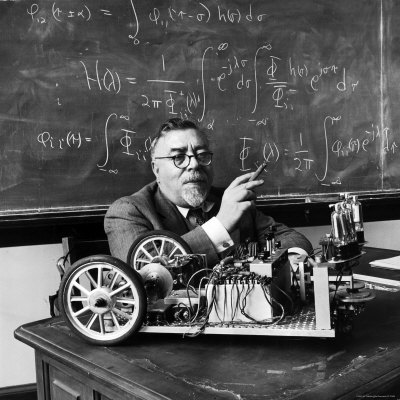
\includegraphics[width=0.8\linewidth]{Norbert_Wiener.jpg}
      \caption{Norbert Wiener (26. listopadu 1894 – 18. brezna 1964) byl americký matematik, který 
               je považován za zakladatele kybernetiky. }
      \label{tky:fig003}
    \end{figure}
  
    Historicky poskytlo impuls ke vzniku kybernetiky řešení problému řízeni palby protiletadlového 
    dělostřelectva za 2. světové války. Na tomto úkolu pracoval také americký matematik 
    \emph{Norbert Wiener}. Výsledkem matematického i konstrukčního úsilí bylo, že mířič - člověk 
    byl nahrazen přístrojem - zaměřovačem, který snímal údaje o současné poloze letadla, z ní 
    vypočítával polohu v budoucích okamžicích a servomechanismem se přenášela informace od 
    zaměřovače a počítače na kanóny. Norbert Wiener pak jako první zpracoval teorii 
    automatizovaných systémů řízeni pro účely protiletecké obrany. Tuto teorii zobecnil pro všechny 
    druhy technických, biologických a společenských systémů. Shrnul ji ve své proslulé knize 
    \emph{Kybernetika neboli řízení a sdělování v živých organismech a strojích}. Tato kniha vyšla 
    v roce \num{1948} a stala se světovým vědeckým bestsellerem. Svého autora proslavila jako 
    zakladatele kybernetiky.
    
    Řešení praktických (a bohužel vojenských) problémů použití elektronických počítačů k řízení 
    střel inspirovalo Wienera ke studiu řízení se zpětnou vazbou. Spolu s neurofyziologem 
    \emph{Arturem Rosenbluethem} hledali analogie k technickým zpětnovazebním systémům pro navádění 
    střel na pohyblivý cil. Takovou analogii nalezli u některých biologických systémů - konkrétně v 
    nervové soustavě živých organismů. Myšlenka zpětné vazby u živých a neživých systémů se stala 
    základem kybernetické koncepce vyložené v citované knize. Hledáni analogií mezi živým 
    organismem a strojem (případně také společnosti) znamená postihnout společné znaky zdánlivě 
    naprosto různorodých systémů. A tyto analogie pak vedou k používáni matematického a logického 
    aparátu i tam, kde to dosud nebylo možné.
    
    Nemůžeme ovšem nevidět všechny předcházející tendence a faktory v historii společnosti, které 
    vedly ke vzniku kybernetiky. Bylo by nesprávné tvrdit, že pouze Norbert Wiener a několik jeho 
    spolupracovníků vytvořilo kybernetiku. Její vznik byl pokračováním určité tendence, která se 
    projevovala již dávno předtím. Kybernetiku musíme chápat jako výsledek rozvoje materiálních sil 
    lidské společnosti a rozvoje vědeckého poznáváni světa.
    
    Název kybernetika pochází z řeckého slova \uv{kybernétés} neboli \uv{kormidelník}, \uv{člověk 
    řídící loď}. Objevuje se v dílech řeckých filosofů, např. v Platonově díle Dialogy; zde se 
    tímto termínem vyjadřuje \uv{umění řídit lodě a administrativně spravovat provincie}. V 
    novověku použil termín kybernetika A. M. Ampére v encyklopedii a to ve smyslu \uv{vědy o řízení 
    společnosti}. Termín se neujal a tak to byl až Wiener, který jím nazval nově vznikající vědní 
    obor. \cite[s.~6]{Svarc1986}.

    \subsection{Základní pojmy kybernetiky a její vymezení}
      Pro kybernetiku jsou charakteristická tři základní hlediska, z kterých nazírá na problémy a z 
      kterých dané problémy řeší. Jsou to

      \begin{figure}[ht!] %  \ref{tky:fig004} 
        \centering
        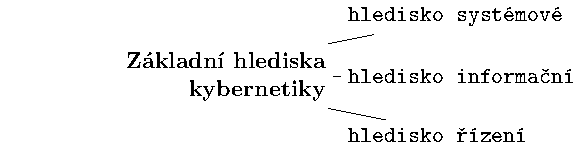
\includegraphics[width=0.7\linewidth]{tky_fig004.pdf}
        \caption*{ }
        \label{tky:fig004}
      \end{figure}
      
      Tím se dostáváme k nejzákladnějších pojmů kybernetiky: \textbf{systém}. \textbf{informace} a 
      \textbf{řízení}, Z těchto hledisek se pak vyvinuly základní obory teoretické kybernetiky - 
      teorie systémů, teorie informace a \hyperlink{tky:regulace}{teorie řízení}.
      
      Jako příklad vysvětlující tato hlediska kybernetiky si zvolme automobil. Automobil je z 
      hlediska konstruktéra složité technické zařízení, sloužící k dopravě osob a nákladu, které je 
      vyrobeno z různých materiálů. Je sestaven z mnoha součásti, pohon je motorem spalovacím nebo 
      vznětovým, k provozu jsou nezbytné látky jako benzín, oleje, voda, ... .To vše je důležité a 
      podstatné z hlediska konstruktéra automobilu, ale ne z hlediska kybernetiky.

      \begin{wrapfigure}[11]{r}{6cm}   %\ref{tky:fig001} 
        \centering
        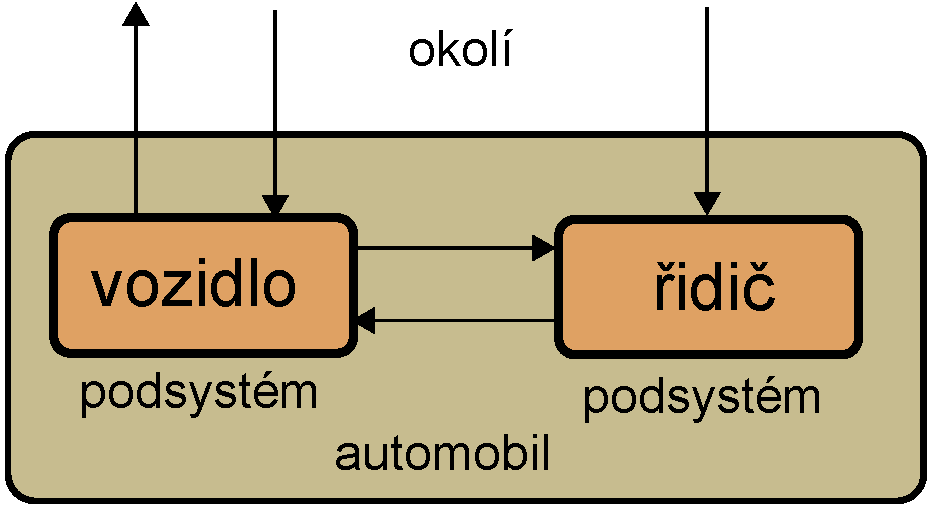
\includegraphics[width=0.9\linewidth]{tky_fig001.pdf}
        \caption{ }
        \label{tky:fig001} 
      \end{wrapfigure}
      Jaká jsou tedy hlediska kybernetiky? Kybernetika vidí v automobilu především tzv. 
      \textbf{dynamický systém}, jehož činnost je spojena s člověkem - řidičem a je ve vztahu k 
      okolnímu světu. Automobil uvažovaný jako systém se skládá ze dvou podsystémů (subsystémů). 
      Prvním z nich je vlastní vozidlo, druhým je člověk. Každý podsystém se pak skládá z 
      elementárních jednotek, vzájemně propojených, tzv. \emph{prvků systému}. Mezi prvky systému 
      existují různé vztahy. Ale nejenom mezi prvky nebo podsystémy existuji vztahy.

      Automobil není izolovaným systémem a proto má také četné vztahy k okolí. K okolí \uv{systému 
      automobil} patří ty části okolního světa, které mají vliv na jeho činnost. Jsou to např. 
      vozovka, křižovatky, zatáčky, jiná vozidla, chodci, dopravní značky apod. Na všechny vlivy 
      okolí reaguje systém automobil určitým způsobem. Reakce systému na okolí se nazývá 
      \textbf{chováni systému}. Pokud sleduje kybernetika automobil tímto způsobem, jedná se o 
      \emph{systémové hledisko} kybernetiky  (obr. \ref{tky:fig001}). Předběžně si vymezme pojem 
      systém jako soubor prvků, mezi nimiž existuji nějaké funkční vztahy. Sledujeme-li vzájemné 
      působeni systému a jeho okolí, jde o druhé základní kybernetické hledisko. Poněvadž se toto 
      působeni realizuje výměnou informaci mezi systémem a okolím, mluvíme o \emph{informačním 
      hledisku}. Pod pojmem informace si představíme zprávu, která má pro některé ze zúčastněných 
      systémů určitý význam. Nositelem informace jsou tzv. \textbf{signály}.
      
      Doposud jsme uvažovali prostou výměnu informaci mezi dvěma systémy. Je-li ale informace 
      využívána přijímacím systémem pro další činnost, pro dosaženi určitého předem stanoveného 
      cíle, pak už se jedná o \emph{řízení}. Pojem řízení vymezíme jako \emph{proces výměny 
      informace mezi dvěma systémy}, který se uskutečňuje plánovitě pro dosažení určitého cíle. Při 
      řízení se uplatňuje informační působení řídicího systému na řízený systém. Tím se dostáváme k 
      třetímu kybernetickému hledisku a to je \emph{hledisko řízení}. Zdůrazněme, že toto hledisko 
      provádí pouze informační bilancování a nikoliv látkové nebo energetické.
      
      Vraťme se k našemu automobilu. Systém automobil má dva podsystémy vozidlo a řidiče. Mezi nimi 
      probíhá informační výměna, jejíž cílem je pohyb automobilu po stanovené dráze, např. v přímém 
      směru. Řidič reaguje na nerovnosti vozovky nebo na boční vítr, které vychyluji vozidlo z 
      přímého směru tím, že pootáčí volantem. Řidič je tedy řídícím systémem a vozidlo řízeným 
      systémem a výměna informací probíhá za účelem udrženi pohybu vozidla v přímém směru - jedná 
      se o \textbf{proces řízení}.
      
      Všimněme si momentu, že řidič otáčí volantem na základě toho, jaký účinek vyvolalo předchozí 
      pootočení. Neustále sleduje směr vozidla a vyrovnává odchylky od přímého daného směru. Takový 
      způsob řízení označujeme v kybernetice jako \textbf{řízení se zpětnou vazbou} neboli 
      \textbf{regulace}. Systémy se zpětnou vazbou se tedy nazývají \textbf{regulační systémy}. 
      Systém automobil (řidič + vozidlo) můžeme pokládat za regulační systém, který je regulován na 
      přímý směr jízdy.
      
      Poněvadž systémy řízení se zpětnou vazbou, tedy regulační systémy, jsou pro kybernetiku 
      charakteristické, nazýváme třetí kybernetické hledisko také \emph{hlediskem regulačním}. 
      Samozřejmě existuje rovněž \textbf{řízení bez zpětné vazby}; v tom případě se mluví jen o 
      \textbf{systémech řízení} nebo o \textbf{systémech ovládání}.
      
      Řízení jako vzájemná interakce mezi systémy nebo mezi systémem a okolím probíhá vždy v 
      určitém pořadí činnosti některého ze systémů. obvykle řídicího. Soubor pravidel, podle něhož 
      řídící systém vykonává sled činností za účelem řízení, se nazývá \textbf{algoritmus}. Obecně 
      je \emph{algoritmus soubor pravidel, podle něhož probíhá řízení}.
      
      U zvoleného příkladu s automobilem bychom mohli například sestavit algoritmus spouštění 
      motoru, algoritmus vyjíždění automobilu, algoritmus předjíždění, atd. Algoritmy jsou objektem 
      zkoumání jednoho z oborů teoretické kybernetiky - \emph{teorie algoritmů}.
      
      Pe předběžném objasnění základních hledisek kybernetiky a základních pojmů kybernetiky je 
      možné se pokusit vyložit, ce vlastně kybernetika je a čím se zabývá. Jednotlivý autoři, kteří 
      se pokoušejí podat definici kybernetiky, protěžují více nebo méně některé ze tří základních 
      kybernetických hledisek (hledisko systémové, hledisko informační, hledisko řízení). Většina 
      starších definic kybernetiky vychází z klasické definice jejího uznávaného zakladatele 
      Norberta Wienera, který ji definoval jako \uv{vědu o řízení a sdělování v živých organismech 
      a strojích}. Tato definice, která je nerozlučně spjata s jejím vznikem, protěžuje hledisko 
      informační a hledisko řízení. Jejím nedostatkem je, že ještě nedoceňuje systémový přístup, 
      systémové hledisko při řešení problémů. Dále jako objekty zkoumání (tedy systémy) zahrnuje 
      pouze živé organismy a stroje. Nezahrnuje tedy další důležité objekty zkoumané dnešní 
      kybernetikou jako jsou objekty společenské a ekonomické a neuvažuje systémy matematické, 
      lingvistické a další a z technických systémů dnes tak různorodých se omezuje jen na stroje. 
      Ani informační hledisko této definice není úplné, protože se omezuje pouze na přenos 
      informaci a neuvažuje dnes tak důležité procesy uchování a zpracováni informace.
      
      Podobnými nedostatky se vyznačovaly definice kybernetiky dalších autorů. Byl to vždy 
      jednostranný přístup a neúplnost jednotlivých hledisek. Proto nelze žádnou z definic 
      akceptovat s definitivní platností.
      
      Nebudeme se tedy snažit za každou cenu zformulovat vyčerpávající definici, ale uveďme si 
      charakteristické rysy kybernetiky jako vědy.
      
      Kybernetika se zabývá různými rozdílnými problémy, které však byly většinou známy a zkoumány 
      před vznikem kybernetiky, např. krevní oběh, podmíněný reflex, radiolokace, konstrukce 
      počítačů, řízení různých technických zařízení, kódování atd. Kybernetika vnáší do těchto 
      problémů nový pohled, neboť si všímá toho, že na určitém stupni organizace a vývoje systémů 
      vzniká nový proces řízení. Tento proces se projevuje výměnou informací v systémech, kterým se 
      chování systémů zaměřuje k určitému cíli.
      
    \subsection{Rozdělení kybernetiky}
      Z praktického hlediska můžeme kybernetiku rozdělit podle přístupu a aplikací:
      \begin{itemize}\addtolength{\itemsep}{-0.5\baselineskip}
        \item \textbf{teoretická kybernetika},
        \item \textbf{aplikovaná kybernetika}.
      \end{itemize}

      \emph{Teoretická kybernetika} studuje především obecné vlastnosti a chování systémů. Zabývá 
      se obecným popisem vlastností a chování systémů. Z tohoto pohledu zahrnuje teoretická 
      kybernetika \emph{teorii systémů} a \emph{teoretickou informatiku}.
      
      \emph{Aplikovaná kybernetika} představuje použití kybernetického přístupu při analýze, 
      modelování a simulaci a návrhu systémů, dále aplikuje poznatky kybernetiky do dalších 
      oblastí. Aplikovaná kybernetika zasahuje do mnohých oblastí lidské činnosti - zahrnuje totiž 
      mj. následující obory:
      
      \begin{itemize}\addtolength{\itemsep}{-0.1\baselineskip}
        \item \textbf{Teoretická kybernetika}
              \begin{itemize}\addtolength{\itemsep}{-0.1\baselineskip}
                \item \emph{Dynamické systémy}: zpětná vazba, stavový popis, stochastické systémy,
                      řízení, aj.
                \item \emph{Přenos informace}: informační entropie, kapacita komunikačního kanálu, 
                      aj. 
                \item \emph{Umělá inteligence}: strojové vnímání a učení, multi-agentní systémy, 
                      robotika, modelování neuronových sítí, konekcionismus, vazba člověk-stroj, ...
                \item \emph{Teorie rozhodování}, her, teorie složitosti, chaotické systémy, aj.
              \end{itemize}
        \item \textbf{Informatika}
        \item \textbf{Biokybernetika}
        \item \textbf{...}
      \end{itemize}
      
  \section{Teorie systémů}
     Teorie systémů je jedna ze základních disciplin teoretické kybernetiky. Na druhé straně je ale 
     teorie systémů součásti tzv. \emph{obecné teorie systémů}, jejíž principy rozpracoval americký 
     biolog Ludwig von Bertalanffy. Pokusme se o vymezení vztahu mezi kybernetikou a teorií systémů.
     \cite[s.~11]{Svarc1986}.
     
     Obecná teorie systémů studuje systémy libovolné povahy, přičemž se zajímá o charakter prvků 
     systému, charakter vazeb mezi prvky a chováni systému. Důležitým pojmem je zde \textbf{vazba 
     mezi prvky} a pojem \textbf{chování systémů}. Zatímco obecná teorie systémů se zajímá o 
     libovolný druh vazeb mezi prvky a libovolné chování systémů, kybernetiku zajímá specifický 
     druh vazeb a specifické chování. Kybernetika studuje pouze ty vazby, které jsou realizovány 
     přenosem informace a chování, které lze zahrnout pod \textbf{pojmem řízení}. A to je náplni 
     teorie systémů jako discipliny teoretické kybernetiky.
     
     \textbf{Přenos informace} a \textbf{řízení} nejsou od sebe \emph{oddělitelné}. Aspoň tak, že 
     není možné řízení bez přenosu informace. Je však už sporné, je-li každý přenos informace již 
     řízením. Můžeme říci, že systémy mezi nimiž probíhá proces řízení musí mít určitou specifickou 
     strukturu a musí být mezi nimi zajištěn přenos informace. Pokud existuje pouhá výměna 
     informací mezi systémy, mluvíme o \textbf{informačních systémech}.
     
     \emph{Obecnou teorii systémů} tedy \emph{nemůžeme} zahrnout do kybernetiky; s kybernetikou má 
     společnou jen určitou část, která je zaměřena na studium systémů z hlediska informačních 
     vazeb. Hlavním úkolem obecné teorie systémů je postihnout a vyjádřit exaktním způsobem 
     vlastnosti a vztahy ve složité a dynamické (v čase se měnící) \emph{objektivní realitě} tak, 
     aby se neztratila její komplikovaná struktura a složitost. Jestliže dříve byl nějaký přírodní 
     nebo společenský jev pokládán za vysvětlený, když se nalezla jeho příčina, pak při systémovém 
     přístupu musí bý nalezena struktura a dynamika každého objektu, který se na daném jevu podílí.
     
     \subsection{Charakteristika základních pojmů z teorie systémů}
       Pro práci se složitými a rozsáhlými objekty, jako jsou například řízení výrobních a
       technologických procesů, je nutný \textbf{systémový přístup}. Například technologický proces
       exploatace uhlí na hlubinných nebo povrchových dolech, je charakterizován různorodostí
       pracovních činností, na něž působí celá řada vlivů. Komplexně jde o mnoha rozměrný
       dynamický celek, který se neustále mění v čase a v prostoru.
       
       \emph{Systémový přístup spočívá v tom, že jevy vyskytující se při řešení vzniklých problémů, 
       jsou chápany komplexně, se všemi souvislostmi ve svém dynamickém vývoji.}
       
       V souvislosti se systémovým přístupem je nejdůležitějším pojmem \textbf{systém}. Jestliže 
       chceme v dalším uvést základní pojmy teorie systémů, musíme nejdříve tento pojem vysvětlit. 
       Předběžně jsme ho vymezili jako \emph{soubor prvků, mezi nimiž existuji nějaké funkční 
       vztahy a který má jako celek vztah ke svému okolí}. Jinými slovy: \emph{Stanovíme- li 
       vztahy, mezi na sebe navzájem působících objektů materiální, ale i nemateriální povahy, je na
       objektivní realitě vytvořen systém.} Jiní autoři podávají tyto definice:
       \begin{itemize}\addtolength{\itemsep}{-0.5\baselineskip}
         \item Bertalanffy (1956): Systém je komplex prvků nacházejících se ve vzájemné interakci.
         \item Hall - Fagen (1966): Systém je souhrn prvků spolu se vztahy mezi prvky a mezi jejich 
               vlastnostmi.
       \end{itemize}

       \begin{definition}
        \textbf{Systém} je definován jako účelově uspořádaná množina prvků a množina vazeb mezi 
        nimi, s dynamickým chováním, které společně určují vlastnosti celku.
        \begin{equation}
          \mathscr{S} = \{S,R \},
        \end{equation}
        kde
        \begin{description}[leftmargin=5em,style=nextline]
          \item[\hspace{2em}\(S \ldots\)] \emph{množina všech prvků},
          \item[\hspace{2em}\(R \ldots\)] \emph{množina relací mezi prvky, reprezentující vzájmené 
                                         funkční vztahy jednotlivých prvků a vztah systému k okolí.}
        \end{description}
       \end{definition}
       
       V rámci dekompozice systému lze vyčlenit \textbf{podsystém}. Podsystém je podmnožina
       systémových prvků a vazeb, která je z nějakého důvodu vyčleněna ze systému a je chápána
       jako nový systém nebo jako prvek.
       
       \begin{definition}
        \textbf{Prvek} je část systému, který tvoří na dané rozlišovací úrovni dále nedělitelný 
        celek, jehož strukturu nechceme, nebo již nemůžeme v rámci analýzy rozlišit.
       \end{definition}
       
       \begin{note}
         \textbf{Rozlišovací úrovní} se označuje stupeň podrobnosti zkoumání systému. Změnou        
         rozlišovací úrovně se může dřívější prvek systému stát podsystémem, popřípadě i systémem a 
         naopak. Dekompozicí systému na jednodušší prvky, se zvyšuje rozlišovací úroveň.
       \end{note}
       
     \subsection{Klasifikace systémů}
       Někdy rozlišujeme pojem \textbf{statický} a \textbf{dynamický systém}, ale spíš známe pouze 
       systémy dynamické. Statický systém je totiž v čase konstantní, neměnný. Mezi statické 
       systémy můžeme někdy zařadit i systémy, u nichž se vlastnosti prvků mění velmi pomalu. V 
       přírodě se statické systémy prakticky nevyskytují, spíše se jedná o systémy s pomalou změnou 
       vlastností na čase. Naproti tomu dynamický systém je takový systém, u kterého existuje 
       alespoň jedna proměnná závislá na čase. Většina systémů je dynamických. V dalším textu jsou 
       proto popsány především \textbf{dynamické systémy a řídicí (regulační) systémy se zpětnou 
       vazbou}.
       
       Dynamické vlastnosti lineárních systémů lze popsat lineárními diferenciálními rovnicemi s 
       konstantními koeficienty a operátorovými přenosy. Dynamické vlastnosti nelineárních systémů 
       lze popsat nelineárními diferenciálními rovnicemi.
       
       Existují dvě možnosti studia dynamického systému. Prvním způsobem je zkoumání \emph{vnitřní 
       struktury systému}, tzn. vnitřní závislosti prvků a dále nás zajímají, jaké vnitřní změny 
       vznikají v systému při působení vnějších vlivů. To je podstatou \textbf{vnitřního popisu 
       dynamického systému}.
       
       Druhým způsobem je pojímání systému jako celek a studování pouze otázky, jaké výsledné 
       reakce systému vyvolávají vnější vlivy. Tomuto druhému způsobu se budeme věnovat při 
       \textbf{vnějším popisu dynamických systémů}.
     
     
  \section{Teorie informace}
    \textbf{Informace} jako stěžejní pojem kybernetiky, je pojem značně široký a hodně diskutovaný. 
    Je používán v celé řadě definic vymezujících předmět kybernetiky jako vědy, přičemž informační 
    hledisko považují někteří autoři za nejdůležitější.
      
    Přesná definice pojmu informace neexistuje. Obecně se tento pojem používá volně, v intuitivním 
    chápaní se vztahuje k pojmům jako zpráva, údaj, poznatek apod. Z hlediska kybernetiky je toto 
    chápáni příliš zúženo, neboť kybernetika sleduje přenos informace mezi dvěma nebo více systémy 
    s tím, že cílem přenosu může být řízení chování některého ze systému. Kybernetika říká, že 
    informace je jakékoliv sdělení, kterého lze reálně (právě nyní) nebe potenciálně (v budoucnu 
    při vhodné příležitosti) použit k řízeni systému.
    
    Pojem informace je \emph{pojmem abstraktním} a jako takový má \emph{nehmotnou povahy}. 
    Současně však informace má smysl jen ve spojení s hmotou a to jak z hlediska přenosu, tak z 
    hlediska obsahu (i abstraktní představy jsou spjaty s existenci hmoty).
    
    Informace (sděleni) má
    \begin{itemize}\addtolength{\itemsep}{-0.4\baselineskip}
      \item \textbf{formu},
      \item \textbf{obsah},
      \item \textbf{význam}.
    \end{itemize}
    \textbf{Forma} informace neboli sdělení musí být přístupná systémům, mezi nimiž dochází k 
    výměně informaci a je důležitá pro proces přenosu informace. Pro proces řízení systémů je 
    podstatný \textbf{obsah a význam informace} (sdělení). \textbf{Sdělení} je \emph{informační, 
    sémantický a pragmatický obsah}. \textbf{Informační obsah} vyjadřuje kvantitativní míru 
    informace v dále definované jednotce \textbf{bit}. Používáme pro něj termín míra či množství 
    informace. \textbf{Sémantický obsah} vyjadřuje významovou stránku znaků při jazykové komunikaci 
    a nedá se měřit (\emph{sémantika} - nauka o významu slov). \textbf{Pragmatický obsah} určuje 
    významnost sdělení a prioritu jednotlivých zpráv pro příjemce.
    
    Každá forma hmoty, která nese informaci se nazývá \textbf{zpráva}. Zpráva je hmotným nositelem 
    informace. Zpráva je způsob vyjádření informace textem, obrazem, řečí, posloupností znaků atd. 
    Zpráva může být tedy např. číslo (posloupnost číslic), abecední text (posloupnost písmen), 
    spouštěcí signál (posloupnost napěťových úrovní). Pojmy informace a zpráva nelze zaměňovat. 
    Informace jo pojem abstraktní, zpráva jo konkrétní materiální formou informace, bez níž by 
    informace neměla smysl a nemohla by být přenášena a působit na systémy, kterým je určena. Pojem 
    zpráva bývá někdy nahrazován užším pojmem \textbf{signál}. Signál je fyzikální realizace zprávy 
    ve formě elektrického proudu resp. elektromagnetických vln.
      
    Sledujeme-li blíže jakoukoliv dostatečně dlouhou zprávu, pak zjistíme, že je vždy vytvářena z 
    posloupnosti nějakých základních elementů - \textbf{prvků}. Možný počet odlišných prvků, ze 
    kterých je taková zpráva vytvářena, může být bud \emph{konečný} nebo \emph{nekonečný}. Tak 
    např. psaná zpráva ve formě českého textu je posloupností různých kombinací písmen české 
    abecedy. Možný počet různých písmen - prvků je konečný a je dán počtem písmen české abecedy.
      
    Základní prvky, ze kterých je vytvářena zpráva, bývají obecně nazývány \textbf{písmena} a celý 
    \emph{soubor} všech \emph{možných prvků} bývá nazýván \textbf{abecedou zdroje}. Zpráva je pak 
    vytvářena výběrem prvků z abecedy zdroje a jejich sestavou v posloupnost prvků. Přitom 
    libovolný prvek abecedy se může ve zprávě libovolně opakovat. Abychom mohli odlišovat prvky 
    abecedy od prvků, z nichž je sestavena konkrétní realizace zprávy, budeme libovolný prvek 
    realizace zprávy nazývat \textbf{symbol}. Nechť má abeceda zdroje celkem \(s\) možných různých 
    prvků. Nechť je délka zprávy, tj. počet symbolů, z nichž je složena realizace zprávy, dána 
    počtem \(L\) symbolů. Celkový možný počet \(L\) různých realizaci zpráv délky \(n\), které 
    mohou být produkovány zdrojem s abecedou o \(s\) prvcích a které se budou lišit nejméně v 
    jednom symbolu, je
    \begin{equation}\label{tky:eq0001}
      L = s^n
    \end{equation}
    (počet všech možných \emph{variací n symbolů s opakováním}, které lze vytvořit z \(s\) prvků).
    
    Má-li abeceda zdroje \emph{konečný počet} \(s\) možných prvků, pak takový zdroj nazýváme 
    zdrojem \textbf{diskrétních zpráv} (diskrétní zdroj). Má-li abeceda zdroje \emph{nekonečný 
    počet prvků}, pak ho nazýváme zdrojem \textbf{spojitých zpráv} (spojitý zdroj).
    
    \begin{example}
      Kolik zpráv o délce \num{10} symbolů můžeme vytvořit z abecedy o \num{2} písmenech?
      \newline
      Řešení: Počet realizaci \(L\) zpráv je dán vztahem (\ref{tky:eq0001})
      \begin{equation*}
        L = s^n = 2^{10} = 1024
      \end{equation*}      
    \end{example}
      
    \subsection{Přenos zpráv}
      Zprávu lze přenést buď \emph{přímo}, přenesením nosného média (pergamen, magnetická páska, 
      optický disk), anebo \emph{nepřímým} způsobem prostřednictvím \emph{signálu}, který je 
      realizací zprávy ve formě změn některé fyzikální veličiny, nejčastěji elektrického proudu.
      
      Při nepřímém způsobu \textbf{zdroj informace} generuje prostřednictvím \textbf{kodéru} 
      (kódovacího zařízeni) signály, které se přenáší \textbf{kanálem}. Kanál je vlastně cesta, 
      která přenáší změny dané fyzikální veličiny, aby mohla být zpráva přenesena z jednoho místa 
      na druhé. Je tvořený prostředím, kterým se přenáší signál. Může to být např. telefonní 
      vedeni, trubka pro přenos tlakového signálu, akustické nebe elektromagnetické vlnění.
      
      Na výstupu kanálu je signál přijímán \textbf{příjemcem informace} (Člověk nebe zařízeni). 
      Zná-li příjemce zákon, podle kterého byla provedena transformace zprávy na vstupu kanálu, pak 
      může určit zprávu obsaženou v přijatém signálu. To provede tzv. \emph{dekódováním} v zařízeni 
      zvaném \textbf{dekodér}. Souhrn všech uvedených objektů vytváří \textbf{sdělovací soustavu}.

      \begin{figure}[ht!]
        \centering
        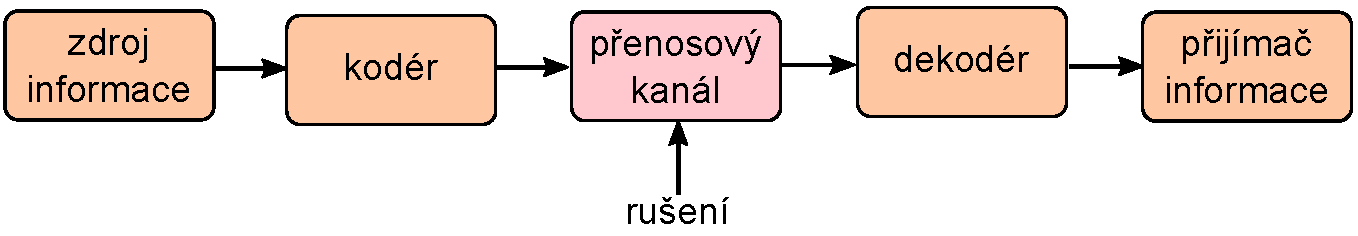
\includegraphics[width=0.9\linewidth]{tky_prenosovy_kanal.pdf}
        \caption{Nepřímý penos zprávy skrz přenosový kanál}
        \label{tky:fig002}
      \end{figure}

      Přenos signálu se může uskutečňovat v prvotní formě anebo v zprostředkované nepřímé formě, 
      kdy se pro přenos signálů používají pomocné tzv. \textbf{nosné signály}.
      
      Příkladem přenosu signálu v prvotní formě je přenos spojitých údajů o teplotě     
      prostřednictvím elektrického napětí ve vedení, přímo úměrné teplotě. 
      
      Při přenosu signálu v nepřímé formě se upravuje nosný signál tak, aby změny některého z jeho 
      parametrů zobrazovaly přenášenou zprávu. Tuto operaci vůči nosnému signálu nazýváme 
      \textbf{modulací}.
      
      
%} %tikzset
%~~~~~~~~~~~~~~~~~~~~~~~~~~~~~~~~~~~~~~~~~~~~~~~~~~~~~~~~~~~~~~~~~~~~~~~~~~~~~~~~~~~~~~~~~~~~~~~~~~
\printbibliography[title={Seznam literatury}, heading=subbibliography]
\addcontentsline{toc}{section}{Seznam literatury}
  % !TeX program = lualatex
% !TeX root = luaking.tex
% !TeX encoding = UTF-8
% !TeX spellcheck = cs_CZ
%---------------------------------------------------------------------------------------------------
% file tky1ch02.tex
%---------------------------------------------------------------------------------------------------
%================== Kapitola: LTI systém ===========================================================
\setchaptertoc
\chapter{LTI systém}\label{tky:IchII}
  \twocolumn[\section{Vlastnosti a popis lineárních systému}\label{tky:IchIIsecI}]
    Na soustavu obvodů můžeme nahlížet jako na seskupení (množinu) navzájem souvisejících součástí, 
    ke kterému je určen vstupní signál $x$, zvaný buzení a výstupní signál $y$, označovaný jako 
    odezva. Z hlediska vlastností jde o systém představující "černou skříňku", jejíž vlastnosti 
    můžeme identifikovat analýzou vstupního a výstupního signálu \cite{Bicak2007}.        

    \luagraphic[0.8]{tky_fig005.pdf}{Symbol soustavy s jedním vstupem a jedním výstupem}{tky:fig005}
    \begin{itemize}
      \item Systémy se spojitým časem (na vstupu i výstupu pracují se spojitými signály) - relace  
            mezi vstupem a výstupem můžeme symbolicky zapsat:
            \begin{equation}\label{tky:eq005}
              y(t)=\mathcal{S}\{x(t)\}
            \end{equation}
            kde $S$ je obecný popis systémové funkce, přiřazující vstupní veličině $x(t)$ odezvu 
            $y(t)$. Z rovnice je zřejmé, že u spojité (analogové) soustavy výstupní signál závisí 
            na všech hodnotách vstupního signálu, nikoli jen na některých jeho hodnotách v určitých 
            časových okamžicích.
      \item Systémy pracující s diskrétním časem lze obdobně symbolicky vyjádřit relací  
            vstup/výstup ve tvaru:
            \begin{equation}\label{tky:eq022}
              y[n]=\mathcal{S}\{x[n]\}
            \end{equation}
            kde $\mathcal{S}$ je tentokráte systémový operátor přiřazení posloupnosti 
            $x[n]\rightarrow y[n]$. U diskrétních systémů se zpracovávají posloupnosti hodnot 
            signálů, získaných vzorkováním spojitého signálu
    \end{itemize}
    
    \subsection{Linearita, časová invariance a kauzalita}\label{tky:IchIIsecIssecI}
      \textbf{Linearita systémů} ve spojité diskrétní oblasti má velký význam, neboť dovoluje
      využívat princip superpozice k zjednodušování úloh jejich analýzy  a syntézy.

      Předpokládejme, že na vstupu lineárního diskrétního systému jsou přivedeny dva signály
      $x_1[n]$ a $x_2[n]$. Účinky obou vstupních signálů na výstupní signál lze zkoumat odděleně a
      podle principu superpozice je na výstupu sečíst. Označme dílčí odezvy
      $y_1[n]=\mathcal{S}\{x_1[n]\}$ a $y_2[n]=\mathcal{S}\{x_2 [n]\}$, potom je
      \begin{equation}\label{tky:eq007}
        y[n]= y_1[n]+y_2[n]=S\{x_1[n]+x_2[n]\}
      \end{equation}
      Analogický vztah platí i pro lineární spojitý systém, tedy
      \begin{equation}\label{tky:eq008}
        y(t)= y_1(t)+ y_2(t)=S\{x_1(t)+x_2(t)\}
      \end{equation}
      Z uvedeného vyplývá významná vlastnost lineárního systému. Výstupní spektrum může obsahovat
      pouze ty frekvence, které jsou ve spektru vstupního signálu a žádné jiné. 

      Jedná-li se o \textbf{systém časově invariantní}, jsou události v čase závislé pouze na
      časovém intervalu (rozdílu časových událostí), nikoliv na každém časovém okamžiku samostatně.
      Systém je časově invariantní, jestliže časový posun ve vstupní signálu vede ke stejnému posunu
      výstupního signálu. Odezva diskrétního systému na posunutý vstupní signál $x[n-m]$ je pak
      určen vztahem
      \begin{equation}\label{tky:eq009}
        y[n-m]= \mathcal{S}\{x[n-m]\}
      \end{equation}
      a obdobně pro odezvu spojité soustavy na posunutý (zpožděný) vstupní signál $x(t-\tau)$ platí
      analogicky rovnice
      \begin{equation}\label{tky:eq010}
        y(t-\tau)= \mathcal{S}\{x(t-\tau)\}.
      \end{equation}

      Takový systém má konstantními parametry a je popsaný \emph{diferenčními rovnicemi s
      konstantními koeficienty}. 
      
      Zcela obecně se LTI systém vyznačuje ještě dalšími vlastnostmi, z nichž jsou pro analýzu
      významnější kauzalita a stabilita. 
      \begin{itemize}
        \item \textbf{Kauzální, příčinný systém} - výstupní signál závisí pouze na současných a
              minulých hodnotách vstupního signálu \(x[n]\), nikoliv na budoucích hodnotách, nikoliv
              na budoucích hodnotách. Nicméně existují významné struktury (např. filtry), při
              jejichž návrhu vycházíme z vlastností nerealizovatelné - ideální struktury, které
              vhodnou metodou aproximace vyjádříme realizovatelnou strukturou. U LTI systémů může
              být otázka kauzality převedena na vlastnosti impulzní odezvy - viz. odst.
              \ref{tky:IchIIsecIssecII}. Při uložení signálu do paměti lze realizovat i nekauzální
              systém, který ale nepracuje v reálném čase. 
        \item \textbf{Stabilní systém} - omezený vstup (v hodnotách) produkuje též omezený výstup.
              Jinak - není-li vstup divergentní, pak ani výstup nebude divergentní. Uvedené bude
              splněno, jestliže pro hodnoty impulzní odezvy \(h[n]\) bude platit
              \begin{equation*}
                \sum_{n=-\infty}^\infty\abs{h[n]} <\infty.
              \end{equation*}
              Problém stability se vyskytuje u rekurzivních struktur (struktury se zpětnou vazbou). 
      \end{itemize}
      

    \subsection{Konvoluce v diskrétních systémech}\label{tky:IchIIsecIssecII}
      Významnou charakteristikou lineárních časově invariantních systémů \emph{LTI} je
      \textbf{impulsní odezva}. Její znalost umožňuje stanovit odezvu systému na obecný signál, lze 
      ji využít i při syntéze systému \cite{Bicak2007}.

      Mějme diskrétní LTI systém \ref{tky:fig002}, na jehož vstup je přiveden \emph{jednotkový
      diskrétní impuls}\footnote{Nesmíme zaměňovat s Diracovým (také jednotkovým) impulsem.}.
      Jednotkový impuls je posloupnost $\delta[n]=0$ pro všechna $n$ s výjimkou $\delta[0]=1$.
      Odezva systému na jednotkový impuls $\delta[n]$ se nazývá impulsní odezva a platí
      \begin{equation}\label{tky:eq011}
        h[n]= \mathcal{S}\{\delta[n]\}.
      \end{equation}
      Vzhledem časové invariantnosti, posunutému jednotkovému impulsu odpovídá posunutá impulsní
      odezva, tedy
      \begin{equation}\label{tky:eq012}
        h[n-m]= \mathcal{S}\{\delta[n-m]\}.
      \end{equation}
      \emph{Jednotkový skok} $1[n]$ je posloupnost jedniček od počátku časové osy $n=0$,
      kterou můžeme zapsat součtem
      \begin{align}
        1[n]&= \sum_{m=0}^n\delta[n-m]                  \nonumber \\
            &=\delta[n]+\delta[n-1]+\delta[n-2]+\cdots. \label{tky:eq013}
      \end{align}
      \emph{Odezva systému na jednotkový skok} $\mathrm{1}[n]$ se nazývá \textbf{přechodová odezva}
      $s[n]$ a platí
      \begin{align}
        s[n]&= \mathcal{S}\{1[n]\}= S\{\sum_{m=0}^n\delta[n-m]\}        \nonumber \\
            &=\sum_{m=0}^nS\{\delta[n-m]\}.                             \label{tky:eq014}
      \end{align}

      Postupná úprava rovnice (\ref{tky:eq014}) je umožněna díky linearitě systému, kterou budeme
      studovat pro obecný vstupní signál
      \begin{equation}\label{tky:eq015}
        x[n]=\sum_{m=-\infty}^\infty x[m]\delta[n-m].
      \end{equation}
      Poznamenejme, že formou (\ref{tky:eq015}) lze zapsat každý diskrétní signál.

      \begin{figure}[ht!]
        \centering  
        \subcaptionbox{\label{tky:fig_006a}}{\luafigure[0.45]{tky_fig006a.pdf}}
        \subcaptionbox{\label{tky:fig_006b}}{\luafigure[0.45]{tky_fig006b.pdf}}
        \caption{Posloupnost jednotkového skoku a) \(1[n]\) a b) signálu \(x[n]\)}
        \label{tky:fig_006}
      \end{figure}

      Na obr. \ref{tky:fig_006} je znázorněna souvislost mezi posloupností jedniček a diskrétním
      signálem. \emph{Posloupnost jedniček tvoří bázi pro diskrétní signály}. Každá komponenta
      diskrétního signálu je vyjádřena součinem $x[m]\delta[n-m]$. V uvedeném příkladě jde o
      posloupnost příslušnou jednotkovému skoku
      \begin{equation*}
        1[n]=\sum_{m=0}^{15}\delta[n-m]
      \end{equation*}
      a odpovídající posloupnost konečného signálu
      \begin{equation*}
        x[n]=\sum_{m=0}^{15}x[m]\delta[n-m].
      \end{equation*}

      \begin{figure*}[ht!]
        \centering
        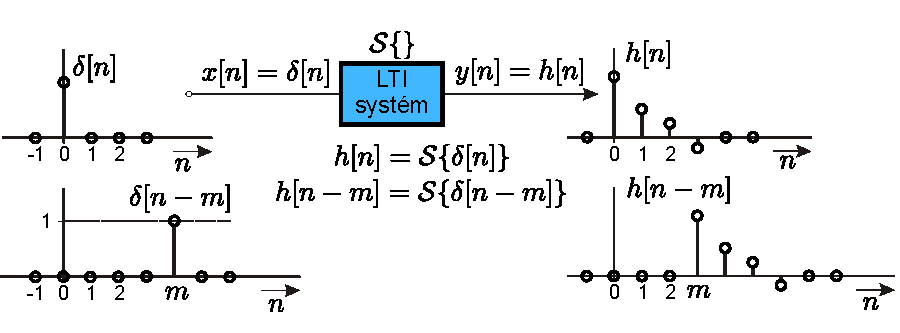
\includegraphics[scale=0.9]{tky_fig002.pdf}
         \caption[impulsní odezva]{Odezva kauzálního diskrétního systému na jednotkový impuls
                  $\delta[n]$ a posunutý impuls $\delta[n-m]$}
        \label{tky:fig002}
      \end{figure*}

      Princip superpozice dovoluje získat odezvu systému jako sumu odezev na jednotlivé dílčí
      součásti vstupního signálu, které v rovnici (\ref{tky:eq015}) tvoří vážené jednotlivé impulsy,
      ze kterých je signál složen
      \begin{align}
        y[n]=\mathcal{S}\{x[n]\}
          &=\mathcal{S}\{\sum_{m=-\infty}^{\infty}x[m]\delta[n-m]\}  \nonumber \\
          &=\sum_{m=-\infty}^{\infty}x[m]\mathcal{S}\{\delta[n-m]\}. \label{tky:eq016}
      \end{align}
      Protože platí (\ref{tky:eq011}) a v důsledku časové invariance vyplývá z rovnice
      \ref{tky:eq016} \textbf{konvoluční suma} 
      \begin{align}
        y[n]&=\sum_{m=-\infty}^{\infty}h[n-m]x[m]               \nonumber \\
            &=\sum_{k=-\infty}^{\infty}h[k]x[n-k].              \label{tky:eq017}
      \end{align}
      Uvedli jsme, že u kauzálního systému závisí výstupní signál $y[n]$ pouze na současných a
      minulých hodnotách vstupního signálu $x[n], x[n-1], x[n-2], \cdots ,$ takže v konvoluční sumě
      \ref{tky:eq017}
      \begin{align*}
        y[n]&=\sum_{k=-\infty}^{\infty}h[k]x[n-k]              \\               
            &=\sum_{k=-\infty}^{-1}h[k]x[n-k] + \sum_{k=0}^{\infty}h[k]x[n-k]  
      \end{align*}
      musíme položit všechny členy impulsní odezvy $h[k]=0$ pro $k<0$. Konvoluční suma pro
      lineární, časově invariantní a kauzální systém má pak tvar
      \begin{equation}\label{tky:eq018}
        y[n]=\sum_{k=0}^{\infty}h[k]x[n-k].
      \end{equation}
      Jestliže navíc budeme uvažovat vstupní a výstupní signály, které jsou nulové pro $n<0$ a
      $x[n]\neq0, y[n]\neq0$ pouze pro $n\geq0$, potom platí
      \begin{equation}\label{tky:eq019}
        \boxed{y[n]=\sum_{k=0}^{n}h[k]x[n-k].\,}
      \end{equation}
      nebo
      \begin{equation}\label{tky:eq024}
        \boxed{y[n]=\sum_{k=0}^{n}x[k]h[n-k].\,}
      \end{equation}
      kde \(n\) je pořadový index právě počítaného vzorku výstupní posloupnosti a \(k\) je pořadový
      index vstupní posloupnosti. Je-li délka vstupní posloupnosti \(N_x\) a délka impulzní odezvy
      \(N_h\), pak délka výstupní posloupnosti (počet jejich vzorků) je dána vztahem:
      \begin{equation}\label{tky:eq025}
        N_y = N_x + N_h - 1.
      \end{equation}
      Rovnice \ref{tky:eq019} a \ref{tky:eq024} určují způsob výpočtu výstupního signálu LTI
      systému. Výstupní signál \(y[n]\) je dán součtem prvků impulsové odezvy a vstupního signálu,
      přičemž buď vstupní signál \ref{tky:eq019} nebo impulsová odezva \ref{tky:eq024} jsou otočeny
      v čase \cite[s.~14]{Davidek1996}.
      
      Symbolicky se tato operace zapisuje 
      \begin{equation}\label{tky:eq026}
        \boxed{y[n] = h[n]*x[n]. \,}
      \end{equation}
      %---------------------------------------------------------------
      % !TeX spellcheck = cs_CZ Lineární obvody a systémy - Jan Bičák  - strana 10 Popis spojitých systémů
%===================================================================================================
\begin{mdframed}[style=mdexam]
  \begin{example}\label{tky:exam001}
    Uvažujme LTI systém, popsaný svou impulzní odezvou: \(h[n] = \{0.45, 1.72, 0.62\}\). Na jeho
    vstupu působí posloupnost \(x[n] = \{2,  0.95\}\). Úkolem  je vypočítat vzorky výstupní
    posloupnosti \(y[n]\).

    \noindent\textbf{Řešení:} Podle (\ref{tky:eq025}) bude délka výstupní posloupnosti \(N_y = 2 + 3
    - 1= 4\) s pořadovými indexy 0 až 3. Pro její výpočet rozepíšeme vztah (\ref{tky:eq024}):
    \begin{align*}
      y[0] &= \sum_{k=0}^0 x[0]h[0] = \num{2}\cdot\num{0.45} = \num{0.9}                   \\
      y[1] &= \sum_{k=0}^1 x[k]h[1-k] = x[0]h[1] + x[1]h[0] =                              \\
           &=  \num{2}\cdot\num{1.72} + \num{0.95}\cdot\num{0.45} = \num{3.8675}           \\
      y[2] &= \sum_{k=0}^2 x[k]h[2-k] =                                                    \\
           &= x[0]h[2] + x[1]h[1] + x[2]h[0] =                                             \\
           &= \num{2}\cdot\num{0.62} + \num{0.95}\cdot\num{1.72} + \num{0}\cdot\num{0.45}  
            = \num{2.8740}                                                                 \\
      y[3] &= \sum_{k=0}^3 x[k]h[3-k] =                                                    \\
           &= x[0]h[3] + x[1]h[2] + x[2]h[1] +  x[3]h[0] =                                 \\
           &= \num{2}\cdot\num{0} + \num{0.95}\cdot\num{0.62} + \num{0}\cdot\num{1.72}
            + \num{0}\cdot\num{0.45} =                                                     \\
           &= \num{0.589} 
    \end{align*} 
    Pro výstupní posloupnost tedy platí:
    \begin{equation*}
      y[n] = \{\num{0.9}, \num{3.8675}, \num{2.8740}, \num{0.589}\}
    \end{equation*}
    Situaci názorně shrnuje obr. \ref{tky:fig011}

    {\centering
      \captionsetup{type=figure}
      \luafigure[1]{tky_fig011.pdf}
      \captionof{figure}{Odezva lineárního číslicového systému na vstupní posloupnost. 
                \cite{Zaplatilek2013}}
      \label{tky:fig011}
    \par}

    V systému \textsc{MATLAB} je vestavěna vnitřní funkce \lstinline[style=luaMatlabText]!conv! pro
    snadný výpočet lineární diskrétní konvoluce, jak dokumentuje výpis \ref{tky:lst001}. Vyzkoušejme
    si, že obrátíme-li pořadí proměnných v příkazu \lstinline[style=luaMatlabText]!conv!, vyjde
    shodný výsledek (komutace symbolů).
  \end{example} 
  \begin{lstlisting}[style=luaMatlabText,gobble=4, label={tky:lst001}]
    h = [0.45, 1.72, 0.62];
    x = [2,  0.95];
    y = conv(x,h)
  \end{lstlisting}

\end{mdframed}
      %---------------------------------------------------------------

    \subsection{Konvoluce ve spojitých systémech}\label{tky:IchIIsecIssecIII}
      Podobně můžeme postupovat i v analogovém případě a odvodit pro lineární časově invariantní
      systém \emph{konvoluční integrál}. Vraťme se k výrazu \ref{tky:eq015} kterým jsme vyjádřili
      libovolný diskrétní signál. Pro případ spojitého signálu vytvořme analogickou formu zápisu
      využívající jednotkový impuls. Průběh obecného spojitého lze podle obr. \ref{tky:fig007}
      aproximovat stupňovitým průběhem, který můžeme vyjádřit jako sumu posunutých (zpožděných)
      impulsů. Výchozí aproximující impuls lze vyjádřit vztahem
      \begin{equation}\label{tky:eq027}
          \delta_\varepsilon(t)  =
            \begin{cases}
               \frac{1}{\varepsilon} & \text{pro } \abs{t} < \frac{\varepsilon}{2},      \\
               0                  & \text{pro } \abs{t} > \frac{\varepsilon}{2} > 0
            \end{cases}
      \end{equation}
      a je znázorněn na obr. \ref{tky:fig007b}. \emph{Jednotkový (Diracův) impuls} 
      má jednotkovou plochu.
      \begin{figure}[ht!]
        \centering
          \subcaptionbox{\label{tky:fig007a}}{\luafigure[0.60]{tky_fig007a.pdf}}                                                  
          \subcaptionbox{\label{tky:fig007b}}{\luafigure[0.27]{tky_fig007b.pdf}}                    
        \caption{a) Aproximace spojitého průběhu signálu, b) K odvození jednotkové impulsní funkce 
        (\cite[s.~7]{Bicak2007})}
        \label{tky:fig007}
      \end{figure}
      Matematicky můžeme Diracovův impuls definovat výrazem
      \begin{equation}\label{tky:eq028}
        \delta_\varepsilon(t) = \lim_{\varepsilon\rightarrow0} \delta_\varepsilon(t).
      \end{equation}
      Aproximaci spojitého průběhu $x(t)$ impulsy \ref{tky:eq027} lze vyjádřit rovnicí
      \begin{equation}\label{tky:eq029}
        x(t)=\sum_{m=-\infty}^\infty x(m\varepsilon)\delta_\varepsilon(t-m\varepsilon)\varepsilon.
      \end{equation}
      Zmenšování šířky impulsů $\varepsilon\rightarrow0$ se chyba aproximace zmenšuje a výraz přejde
      v limitu
      \begin{equation}\label{tky:eq030}
        x(t) = \lim_{\varepsilon\rightarrow0}
               \sum_{m=-\infty}^\infty x(m\varepsilon)\delta_\varepsilon(t-m\varepsilon)\varepsilon.        
      \end{equation}
      V limitě kdy $\varepsilon\rightarrow0$, můžeme sumu nahradit integrálem, dále součin
      $m\varepsilon$ integrační proměnnou $\tau$ a $\varepsilon$ jejím diferenciálem. Obdržíme
      \begin{equation}\label{tky:eq031}
        x(t) = \int_{-\infty}^{\infty}x(\tau)\delta(t-\tau)d\tau .
      \end{equation}
      Vztahem \ref{tky:eq031} jsme spojitý průběh signálu vyjádřili jako sumu
      nekonečného počtu posunutých jednotkových impulsů váženou jeho okamžitými hodnotami.
      Předpokládejme dále, že na vstup lineárního časově invariantního spojitého systému je převeden
      jednotkový (Diracův) impuls a systém vytvoří odezvu $h(t)$. V případě obecného vstupního
      spojitého signálu $x(t)$ aproximovaného vztahem \ref{tky:eq031}, bude odezva
      analogového systému
      \begin{equation}\label{tky:eq032}
        \boxed{y(t) = \int_{-\infty}^{\infty}x(\tau)h(t-\tau)d\tau, \,}
      \end{equation}
      nebo
      \begin{equation}\label{tky:eq033}
        \boxed{y(t) = \int_{-\infty}^{\infty}h(\tau)x(t-\tau)d\tau.\,}
      \end{equation}
      Uvedený integrál nazýváme \textbf{konvolucí} a velmi často ho označujeme jako 
      \begin{equation}\label{tky:eq034}
        \boxed{y(t) = h(t)*x(t).\,}
      \end{equation}
      Funkce $h(t)$ představuje \emph{impulsní odezvu}. Jedná se o výstupní signál systému, na 
      jehož vstupu se uplatní Diracův impuls $x(t)=\delta(t)$. Platí totiž
      \begin{equation}\label{tky:eq035}
        y(t) = \int_{-\infty}^{\infty}h(\tau)\delta(t-\tau)d\tau = h(t) . 
      \end{equation}     
      Z důvodů \emph{kauzality}, která vyjadřuje zachování příčinné posloupnosti událostí při 
      transformaci signálu ze vstupu na výstup, požadujeme
      \begin{align}\label{tky:eq036}
        h(t) &\neq  0 \text{   pro } \abs{t} \geq0, \\
        h(t) &  =   0 \text{   pro } \abs{t} < 0. 
      \end{align}    
      Potom můžeme konvoluční integrál \ref{tky:eq032} zapsat ve tvarem
      \begin{equation}\label{tky:eq037}
         y(t) = \int_0^{\infty}h(\tau)x(t-\tau)\dd\tau.
      \end{equation} 
  
  \section{Popis spojitých a diskrétních systémů, přenosová funkce}\label{tky:IchIIsecIII}
    \subsection{Spojité systémy}
      Lineární časově invariantní (LTI) spojitý systém je obecně popsán soustavou
      integrodiferenciálních rovnic s konstantními koeficienty, kterou lze postupným derivováním
      změnit na soustavu diferenciálních rovnic. Předpokládejme budící (nezávislou) veličinu
      $x(t)$ a odezvou (závislou) výstupní veličinu $y(t)$, pak eliminací ostatních proměnných bude
      soustava popsána jedinou diferenciální rovnicí s konstantními koeficienty tvaru
      \begin{equation}\label{tky:eq038}
          \sum_{i=0}^na_i\frac{d^iy(t)}{dt^i}=\sum_{j=0}^mb_j\frac{d^jx(t)}{dt^j},
      \end{equation}
      kde $a_0, a_1, \cdots ,a_n$ a $b_0, b_1, \cdots ,b_m$ jsou konstanty charakterizující lineární
      systém. Obecné řešení $y(t)$ rovnice \ref{tky:eq038} se sestává ze dvou částí, z 
      řešení \emph{homogenní rovnice} a \emph{partikulárního řešení}. K řešení je třeba znát 
      počáteční podmínky pro $y(t)$ a jeho derivace ve výchozím okamžiku.
  
      S použitím \emph{Laplaceovy transformace při nulových počátečních podmínkách} má rovnice
      (\ref{tky:eq038}) tvar
      \begin{equation}\label{tky:eq039}
        \sum_{i=0}^na_ip^iY(p)=\sum_{j=0}^mb_jp^jX(p),
      \end{equation}
      kde $X(p)=\mathcal{L}\{x(t)\}$ a $Y(p)=\mathcal{L}\{y(t)\}$ jsou Laplaceovy obrazy vstupní a
      výstupní veličiny, $p$ je Laplaceův operátor derivace a také komplexní kmitočet
      $p=\sigma+\jmath\omega$. Přenosová funkce $H(p)$ je definována jako podíl Laplaceova obrazu
      výstupní veličiny $Y(p)$ ku obrazu vstupní veličiny $x(p)$, při nulových počátečních
      podmínkách
      \begin{equation}\label{tky:eq040}
          H(p)=\frac{Y(p)}{X(p)}.
      \end{equation}
      Vzhledem k rovnici (\ref{tky:eq039}) je $H(p)$ racionálně lomenou funkcí tvaru
      \begin{align}
        H(p)&=\frac{b_mp^m+b_{m-1}p^{m-1}+\cdots+b_0}{a_np^n+b_{n-1}p^{n-1}+\cdots+a_0}  \nonumber\\
            &=\frac{\Pi_{j=1}^m(p-p_{0j})}{\Pi_{i=1}^n(p-p_{\infty i})}            \label{tky:eq002}
      \end{align}
      kde $p_{0j}$ jsou kořeny polynomu čitatele a představují \textbf{nulové body} a kořeny
      jmenovatele $p_{\infty i}$ jsou \textbf{póly} přenosové funkce, $H_0=\frac{b_m}{a_n}$ je
      násobná konstanta.
  
      Kmitočtové charakteristiky získáme z přenosové funkce substitucí
      \begin{equation}\label{tky:eq041}
          p = \jmath\omega,
      \end{equation}
      ve které $\omega$ je úhlový kmitočet. Platí tedy
      \begin{align}
          H(p)\mid_{p = \jmath\omega} 
            &=\frac{b_m(\jmath\omega)^m+b_{m-1}(\jmath\omega)^{m-1}                     
             +\cdots+b_0}{a_n(j\omega)^n+b_{n-1}(\jmath\omega)^{n-1}+\cdots+a_0}   \nonumber \\
            &=M(\omega)e^{\jmath\Phi(\omega)},                                     \label{tky:eq003}
      \end{align}
      kde $M(\omega) = \abs{H{\jmath\omega}}$ je \textbf{modulová charakteristika} a
      $\Phi(\omega)=\texttt{arg}H(j\omega)$ se nazývá \textbf{fázová charakteristika}. Skupinové
      zpoždění je definováno jako záporně vzatá derivace fázové charakteristiky podle kmitočtu
      \begin{equation}\label{tky:eq042}
        \tau(\omega)=-\frac{d\Phi(\omega)}{d\omega}= -\der{\texttt{arg} H(\jmath\omega)}{\omega}.
      \end{equation}
      V předchozí kapitole jsme ukázali, že \emph{relace vstup/výstup LTI systému} souvisí
      prostřednictvím \emph{konvoluce}
      \begin{equation}\label{tky:eq043}
          y(t)=\int_0^\infty h(\tau)x(t-\tau)d\tau = h(t)*x(t).
      \end{equation}
      Přenosová funkce je Laplaceova transformace impulsní odezvy $h(t)$
      \begin{equation}\label{tky:eq044}
          H(p)=\mathcal{L}[h(t)]=\int_0^\infty h(t)e^{-pt}dt,
      \end{equation}
      pro kterou je splněn vztah
      \begin{equation}\label{tky:eq045}
          Y(p)=H(p)X(p).
      \end{equation}
      Přechodová odezva $s(t)$ je definována jako integrál impulsní odezvy
      \begin{equation}\label{tky:eq046}
          s(t)=\int_0^th(\tau)d\tau,
      \end{equation}
      takže platí
      \begin{equation}\label{tky:eq047}
          s(t)=\mathcal{L}^{-1}\{\frac{H(p)}{p}\}.
      \end{equation}
      Algoritmus výpočtu impulsní odezvy z přenosové funkce je založen na výpočtu  reziduí a 
      rozkladu racionálně lomené funkce $H(p)=\frac{Q(p)}{N(p)}$ na částečné zlomky. Pokud má tato 
      funkce jednoduché póly, rozklad má tvar\footnote{Násobnost kořenů $N(p)$ neuvažujeme, protože 
      se v LTI obvodech neuplatňuje}.
      \begin{align}
         H(p)&=\frac{Q(p)}{N(p)} 
              =\sum_{\mu=1}^{n}\frac{k_\mu}{p-p_{\infty_\mu}}                  \nonumber \\
             &=\frac{k_1}{p-p_{\infty_1}}+\frac{k_2}{p-p_{\infty_2}}
               +\cdots+\frac{k_n}{p-p_{\infty_n}}                              \label{tky:eq004}
      \end{align}
      kde $k_\mu$ se nazývají rezidua v pólech $p_{\infty_\mu})$ a platí
      \begin{align}
        k_\mu &= \lim_{p\to p_{\infty_\mu}}(p-p_{\infty_\mu})\frac{Q(p)}{N(p)}  \nonumber \\
        \,    &= Q(p_{\infty_\mu})\lim_{p\to
                 p_{\infty_\mu}}\frac{1}{\frac{N(p)}{p-p_{\infty_\mu}}}=
                 Q(p_{\infty_\mu})\frac{1}{N'(p_{\infty_\mu})}                  \label{tky:eq006}
      \end{align}
      impulsní odezva je pak dána vztahem
      \begin{equation}\label{tky:eq023}
        h(t)=\mathcal{L}^{-1}[H(p)]=\sum_{\mu=1}^nk_\mu e^{p_{\infty_\mu}t}
      \end{equation}
      Póly jsou obecně komplexní $p_{\infty_{\mu}}=\alpha_\mu+j\beta_\mu$, nebo reálné
      $p_{\infty_{\mu}}=\alpha_\mu$. Jsou to kořeny rovnice $N(p)=0$. Rovnice \ref{tky:eq023} je
      důležitá i proto, že z ní poznáme, zda analogová soustava je stabilní. Je patrné, že soustava
      bude stabilní, jestliže bude $\mathcal{R}\{p_{\infty_{\mu}}\}=\alpha_\mu<0$, tj. leží-li
      kořeny $p_{\infty_{\mu}}$ v otevřené levé polorovině komplexní roviny
      $p_{\infty_{\mu}}=\sigma+j\omega$. Imaginární osa $j\omega$ je mezí stability, pravá
      polorovina je oblastí nestability. Polynom, který má kořeny v levé otevřené polorovině se
      označuje \textbf{Hurwitzův polynom}.
      
      %---------------------------------------------------------------
      % !TeX spellcheck = cs_CZ Lineární obvody a systémy - Jan Bičák  - strana 10 Popis spojitých systémů
%===================================================================================================
\begin{mdframed}[style=mdexam]
  \begin{example}\label{tky:exam002}
    Lineární spojitý systém je dán zapojením dle obrázku. Určete:
    \begin{enumerate}[leftmargin=12pt,noitemsep]
      \item diferenciální rovnici pro odezvu $u_2(t)$, je-li na vstupu buzen napětím $u_1(t)$,
      \item přenos napětí $H(p)=\dfrac{U_2(p)}{U_1(p)}$,
      \item impulsní odezvu $h(t)$.
    \end{enumerate}

    {\centering
      \captionsetup{type=figure}
      \luafigure[1]{tky_fig008.pdf}
      \captionof{figure}{Zapojení obvodu RLC.}
      \label{tky:fig008}
    \par}
    \noindent\textbf{Řešení:} Pro zapojení dle obrázku \ref{tky:fig008} získáme metodou uzlových
    napětí integrodiferenciální rovnice pro uzly \texttt{A} a \texttt{B}:
    \begin{gather*}
      \begin{align*} %\label{tky:eq019}
        \shortintertext{uzel A:}
        \frac{u_3(t)-u_1(t)}{R}+\frac{1}{L}\int_0^t{[u_3(t)-u_2(t)]}\dd{\tau}+i_L(0_+) &= 0  \\
        \shortintertext{uzel B:}
        \frac{1}{L}\int_0^t[(u_2(t)-u_3(t))]\dd{\tau}+C\der{u_2}{t}-i_L(0_+)           &= 0
      \end{align*}
    \end{gather*}
    ve kterých \(i_L(0_+)\) je počáteční podmínka pro proud induktoru. Derivováním a eliminací
    $u_3(t)$ z původních rovnic dostaneme pro odezvu $u_2(t)$ diferenciální rovnici II. řádu.
    Začneme derivováním rovnice v uzlu \texttt{B} tj. \(\frac{d}{dt}(B)\):
    \begin{align*}
      u_2(t)-u_3(t)+LC\frac{d^2u_2(t)}{dt^2} &=0 \Rightarrow   \\
      u_2(t)+LC\frac{d^2u_2(t)}{dt^2}        &=u_3(t)
    \end{align*}
    Nyní můžeme z rovnice pro uzel \texttt{A} odstranit napětí \(u_3(t)\):
    \begin{align*}
      \frac{u_2(t)+LC\dfrac{d^2u_2(t)}{dt^2}-u_1(t)}{R}             &+    \\
      \frac{1}{L}\int_0^t{(LC\frac{d^2u_2(t)}{dt^2})}\dd{\tau}+i_L(0_+) &=  0 \\
      \shortintertext{}
      u_2(t)+LC\frac{d^2u_2(t)}{dt^2}-u_1(t)                        &+    \\
      RC\left[\frac{du_2(t)}{dt}\right]_0^t+Ri_L(0_+)               &=  0
    \end{align*}
    Při nulových počátečních podmínkách: $\left.\frac{du_2(t)}{dt}\right\rvert_{t=0}=0$,
    $i_L(0_+)=0$ dostaneme:
    \begin{equation*}
      \boxed{LC\frac{d^2u_2(t)}{dt^2}+RC\frac{du_2(t)}{dt}+u_2(t)=u_1(t)}
    \end{equation*}
    V Laplaceově transformaci platí:
    \begin{align*}
      \mathcal{L}\left[\frac{du_2(t)}{dt}\right]     &= pU_2(p)-u_2(0) \\
      \mathcal{L}\left[\frac{d^2u_2(t)}{dt^2}\right] &= p^2U_2(p)-pu_2(0)-\dot{u}_2(0),
    \end{align*}
    kde \(\dot{u}_2(0)=\left.\frac{du_2(t)}{dt}\right\rvert_{t=0}\). Při nulových počátečních
    podmínkách \(u_2(0) = 0\), \(\dot{u}_2(0) = 0\) a užitím Laplaceovy transformace přejde
    diferenciální rovnice na algebraickou rovnici:
    \begin{equation*}
      p^2LCU_2(p)+pRCU_2(p)+U_2(p)=U_1(p)
    \end{equation*}
    Odtud vyplývá \textbf{přenosová funkce} $H(p)=\frac{U_2(p)}{U_1(p)}$
    \begin{align}
      H(p) &=\dfrac{1}{p^2LC+pRC+1}                                   \nonumber \\
           &=\dfrac{1}{LC}\frac{1}{p^2+p\dfrac{R}{L}+\dfrac{1}{LC}}
            =\frac{Q(p)}{N(p)}                                        \label{tky:eq020}
    \end{align}
    K nalezení \textbf{impulsní odezvy} nejprve určíme póly přenosové funkce řešením rovnice
    $N(p)=0$
    \begin{align}
      p_{\infty_{12}} 
        &=\dfrac{\dfrac{R}{L}\pm\sqrt{\left(\dfrac{R}{L}\right)^2-\dfrac{4}{LC}}}{2}   \nonumber \\
        &=\frac{R}{2L}\pm\sqrt{\left(\frac{R}{2L}\right)^2-\frac{1}{LC}}          \label{tky:eq021}
    \end{align}
    a přenosovou funkci pak upravíme do tvaru
    \begin{equation*}
      H(p)=\frac{K}{(p-p_{\infty_1})\cdot(p-p_{\infty_2})}, \quad K=\frac{1}{LC}
    \end{equation*}
    kde \(K\) je násobná konstanta a \(p_{\infty_{1,2}}\) jsou její póly. 
    \begin{itemize}[leftmargin=12pt,noitemsep]
      \item Uvažujeme-li jednoduché póly a bude-li $R>2\sqrt{\frac{L}{C}}$ , potom z  rov.
            \ref{tky:eq021} vyplývají dva reálné různé póly. Přenosovou funkci tedy můžeme
            zapsat obecným tvarem:
            \begin{equation*}
              H(p)=\frac{K}{(p+a_1)\cdot(p+a_2)}=\frac{k_1}{p+a_1}+\frac{k_2}{p+a_2}
            \end{equation*}
            kde $p_{\infty_1}=-a_1,\, p_{\infty_2}=-a_2$, Rezidua  \(k_1\), \(k_2\) určíme z rov.
            \ref{tky:eq006}. 
            \begin{equation*}
              k_1=\frac{K}{a_2-a_1}, \quad k_2=\frac{K}{a_1-a_2}.
            \end{equation*}
            Impulsní odezvu pak vypočteme užitím rov. \ref{tky:eq023}.
            \begin{align*}
              h(t)&=\mathcal{L}^{-1}[H(p)]               \\
                  &=\frac{K}{a_2-a_1}e^{-a_1t}+\frac{K}{a_1-a_2}e^{-a_2t}
            \end{align*}
      \item Když bude $R<2\sqrt{\frac{L}{C}}$, obdržíme dvojici komplexně sdružených pólů a
            přenosovou funkci může obecně zapsat takto:
            \begin{equation*}
              H(p)=\frac{K}{(p+a_1)\cdot(p+a_2)}=\frac{k_1}{p+a-jb}+\frac{k_2}{p+a+jb}
            \end{equation*}
            kde $p_{\infty_1}=-a+jb$, $p_{\infty_2}=-a-jb$. Rezidua v pólech jsou dány výrazy
            $k_1=-\frac{jK}{2b}$, $k_2=\frac{jK}{2b}$. Impulzní odezvu opět určíme užitím rov.
            \ref{sas:eq_impulzni_odezva}.
            \begin{equation*}
              h(t) = \frac{Ke^{-at}}{2b}\left[j\cdot\left(-e^{jbt}+e^{-jbt}\right)\right]
            \end{equation*}
            \begin{gather*}
              \begin{align*}
                \,  &= \frac{Ke^{-at}}{2b}\left[j\cdot
                \left(\underline{-\cos(bt)}-j\sin(bt)+
                \underline{\cos(bt)}-j\sin(bt)\right)\right]                        \\
                \,  &= \frac{K}{b}e^{-at}\sin(bt)                                   
              \end{align*}
            \end{gather*}
    \end{itemize}
    
    Na obr. \ref{tky:fig009} je uvedena impulsní charakteristika uvaožovaného obvodu odpovídající
    hodnotám stavebních prvků: \(R=\SI{1}{\kohm}\), \(L=\SI{11.5}{\milli\henry}\),
    \(C=\SI{22.5}{\nano\farad}\). Výpis m-file \texttt{SAS\_exam\_02\_symb\_Hp\_solve.m} ukazuje
    symbolický způsob řešení operátorových obvodových rovnic pomocí \texttt{MATLABu}. Jde o filtr
    typu \textbf{dolní propust}, jehož přenosová funkce má tvar:
    $$H(p)= \frac{3.9506\cdot10^9}{p^2+8.8889\cdot10^4p+3.9506\cdot10^9}.$$
    %---------------------------------------------------------------
      \lstinputlisting[% style=luaMatlabStyle,
      caption={TKY\_exam\_02\_symb\_Hp\_solve.m}]{../src/TKY/matlab/SAS_exam_02_symb_Hp_solve.m}
    %---------------------------------------------------------------
    Impulzní charakteristiku obdržíme dosazením do vztahu \ref{tky:eq005}
    $$h(t)=\frac{K}{b}e^{-at}\sin(bt) =8.8890\cdot10^4e^{-4.4444\cdot10^4t}\sin(4.4444\cdot10^4t).$$
    
      {\centering
      \captionsetup{type=figure}
      \luafigure[1]{tky_fig009.pdf}
      \captionof{figure}{Impulzní charakteristika}
      \label{tky:fig009}
      \par}
    
    Z hlediska analýzy obvodů v kmitočtové oblasti je výhodné sestavovat obvodové rovnice (metodami
    uzlových napětí a smyčkových proudů) přímo v operátorovém tvaru. Kirchhoffovy zákony pro
    uzavřenou smyčku a proudu do uzlu pak mají tvar $$\sum_{k=1}^{n}U_k(p) = 0, \qquad
    \sum_{k=1}^{n}I_k(p) = 0.$$ Metodou uzlových napětí pro zapojení na obr. \ref{tky:fig008}
    obdržíme rovnice
    \begin{align}
      \frac{U_3(p)-U_1(p)}{R}+\frac{U_3(p)-U_2(p)}{pL} &=  0 \\
      pCU_2(p) + \frac{U_2(p)-U_3(p)}{pL}              &=  0 
    \end{align}
    Na rozdíl od \ref{tky:eq019} jde o algebraické rovnice, ze kterých eliminací uzlového napětí
    $U_3(p)$ vyplývá přenosová funkce \ref{tky:eq020} $$H(p) = \frac{U_2(p)}{U_1(p)} =
    \frac{1}{LC}\frac{1}{p^2+p\frac{R}{L} + \frac{1}{LC}}$$
    
    {\centering
      \captionsetup{type=figure}
      \luafigure[1]{tky_fig010.pdf}
      \captionof{figure}{Modulová, fázová charakteristika a skupinové zpoždění filtru}
      \label{tky:fig010}
      \par}    
    
    Dosazením za $p=j\omega$ lze z přenosové funkce vyjádřit modulovou charakteristiku $H(j\omega)$
    a fázovou charakteristiku $\Phi(\omega)= \texttt{arg} H(j\omega)$. Skupinové zpoždění vyplývá ze
    vztahu \ref{SAS:eq_skupinove_zpozdeni}. Modulová, fázová charakteristika a skupinové zpoždění
    jsou na obr. \ref{tky:fig010}.
    
    Filtr má maximálně plochou modulovou charakteristiku přenosu. Mezní kmitočet propustného pásma
    je $f_p = 10 kHz$, při kterém je $\abs{H(j\omega_p)}= 0.707$. Tato hodnota odpovídá poklesu
    modulové charakteristiky o $3 dB$.
    
    %---------------------------------------------------------------
    \lstinputlisting[% style=luaMatlabStyle,
      caption={TKY\_exam\_03\_Hp.m}]{../src/TKY/matlab/SAS_exam_03_Hp.m}
    %---------------------------------------------------------------  
  \end{example} 
\end{mdframed}
      %---------------------------------------------------------------
% % !TeX spellcheck = cs_CZ
{\tikzset{external/prefix={tikz/TKY/}}
 \tikzset{external/figure name/.add={ch04_}{}}
%============ Kapitola: Regulační technika =========================================================
\chapter{Regulační technika}\hypertarget{tky:regulace}
\minitoc
  \section{Kde se vzala, tu se vzala, zpětná vazba}
    Protože stojící automobil má aktuální rychlost menší než žádaných \SI{50}{\km\per\hour}, 
    sešlápneme pedál plynu a automobil začne zrychlovat, což pozorujeme na tachometru. V momentě, 
    kdy je aktuální rychlost větší než žádaná, uvolníme v souladu s radami od instruktora pedál 
    plynu a rychlost automobilu začne klesat, až bude opět menší než je žádaných 
    \SI{50}{\km\per\hour}. Takto budeme dokola sešlapávat a uvolňovat pedál plynu, až dosáhneme 
    žádané rychlosti. Jistě si umíme představit, že rychlost dosažení žádané rychlosti, závisí 
    nejen na vlastnostech samotného automobilu, ale také na našich řidičských dovednostech. V 
    případě opatrného řidiče, bude rozjezd pomalý a tak se rychlost bude blížit žádané pomalu. V 
    případě zbrklého řidiče, bude rozjezd velice razantní, což povede k rychlému překročení žádané 
    rychlosti. Následné neuvážené odlehčení plynového pedálu povede k prudkému poklesu rychlosti, 
    viz zelený průběh na obr. \ref{tky:fig_feedback005}. V obou případech se nelze hovořit o dobrém 
    stylu jízdy. V prvním případě se řidič rozjíždí příliš dlouho, na vozovce představuje překážku 
    a delší dobu zbytečně unikají splodiny do ovzduší. Ve druhém případě je motor při extrémních 
    otáčkách příliš hlučný, dochází k nekvalitnímu spalování a opět k úniku škodlivin do ovzduší. 
    Styl jízdy nepůsobí příliš uklidňujícím dojmem na ostatní řidiče a účastníky silničního provozu.

    \begin{figure}[ht!] % \ref{tky:fig_feedback005}
      \centering
      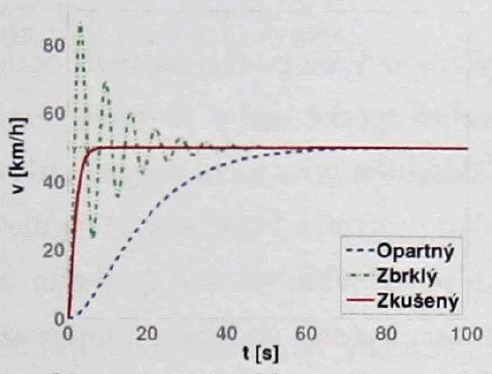
\includegraphics[width=0.7\linewidth]{Reg_smycka03.png}
      \caption{Rychlost automobilu \cite[s.~9]{Roubal2011}.}
      \label{tky:fig_feedback005}
    \end{figure}
    Pro kvalitní dosažení žádané hodnoty rychlosti je třeba znát \emph{dynamický model} automobilu. 
    Tedy nejen sešlápni pedál plynu, uvolni pedál plynu, což můžeme považovat za \emph{statický 
    model} (v čase neproměnný), ale právě popis jak rychle se automobil rozjíždí, když takovým a 
    takovým způsobem sešlápneme pedál plynu. V regulační technice budeme mít dynamický model 
    systému tvořený převážně diferenciálními (pohybovými) rovnicemi. Modelováním reálných 
    dynamických systémů se budeme zabývat v kapitole \ref{TKY:sec002}. Procesu získávání modelu 
    fyzikální reality říkáme \textbf{identifikace systému} a v našem příkladě s automobilem ji 
    vlastně provádíme tím, že se učíme jezdit. Na identifikaci dynamických systémů a její praktické 
    aspekty se zaměříme v kapitole \ref{TKY:sec003}.

    V momentě, kdy máme dynamický model systému, přichází další krok a to je vlastní \textbf{návrh 
    regulátoru}, neboli návrh algoritmu řízení. V momentě, kdy už řidič ví, jak automobil reaguje 
    na změny vstupu, může dosáhnout žádané výstupní veličiny mnohem lépe, viz obr. 
    \ref{tky:fig_feedback003}. Na rozdíl od řidiče, jenž má naučený regulátor ve své hlavě, v 
    regulační technice budeme využívat různé matematické metody. Možná nás nyní napadne, že model 
    automobilu není pouze závislost mezi pedálem plynu a rychlostí automobilu. Chování automobilu 
    ovlivňuje samozřejmě mnoho dalších okolností, jako je přilnavost pneumatik k povrchu vozovky, 
    vlhkost vozovky a podobně. V momentě, kdy například zaprší, může řidič se svým regulátorem v 
    zatáčce opustit vozovku, pokud jsme příliš agresivní, protože se reálný systém změnil, ale jeho 
    model tuto informaci nemá. Opět tedy musíme vzít v potaz nové faktory a provést identifikaci 
    znovu, a tím získat více informací o chování systému za těchto podmínek. Pak bude řidič schopen 
    jezdit bezpečně za sucha i za mokra a tak dále. V regulační technice je vždy přesnost modelu 
    zásadní otázkou. Na jedné straně požadujeme model systému co nejpřesnější, abychom byli schopni 
    navrhnout dobrý regulátor. Na druhé straně se pro příliš složitý model navrhuje regulátor 
    obtížněji. Proto vždy musíme zvolit jistý kompromis tak, aby v modelu byly zahrnuty všechny 
    podstatné vlastnosti systému.

    Tím ale regulace nekončí. Například cena paliva není již dnes zanedbatelná, a tak budeme třeba 
    chtít jezdit s minimální spotřebou. To znamená, že musíme zjistit závislost spotřeby paliva na 
    stylu jízdy. Poté musíme definovat nějaké kritérium kvality regulace obsahující tuto závislost 
    a podle něho navrhnout nový regulátor, který zajistí minimální spotřebu paliva.  Problémů v 
    oblasti řízení je samozřejmě mnohem a mnohem víc  (odhadování a filtrace, robustní řízení a 
    nelineární systémy). My však zde tento příklad ukončíme s konstatováním, že v regulační 
    technice jde především o tyto body:
    \begin{itemize}\addtolength{\itemsep}{-0.5\baselineskip}
      \item určení vstupů a výstupů systému,
      \item identifikace systému (určení chování systému na výstupech pro nějaké chování vstupů),
      \item návrh regulátoru pro zajištění požadovaných vlastností; testování regulátoru na 
            počítači; aplikace regulátoru na reálném systému; případně návrh v nějakém smyslu 
            optimálního regulátoru.
    \end{itemize}
    
  \section{Regulační smyčka a základní typy PID regulátorů}\label{TKY:sec001}
    Ve snaze řídit systémy rozeznáváme dva hlavní způsoby řízení:
      \begin{itemize}
        \item \textbf{přímovazební},
        \item \textbf{zpětnovazební}.
      \end{itemize}
    \textbf{Přímovazební řízení} (\emph{řízení v otevřené smyčce}), zvané také jako ovládání, má 
    jednodušší zapojení, ovšem jeho nevýhodou je nemožnost reagovat na poruchy či změny soustavy a 
    my se jím zde dále zabývat nebudeme. Naproti tomu \textbf{zpětnovazební řízení} (\emph{řízení v 
    uzavřené smyčce}), obecně označované jako \textbf{regulace}, porovnává \emph{výstup soustavy} 
    \(y(t)\) s \emph{požadovaným výstupem} \(w(t)\), a podle této informace generuje \emph{akční 
    zásah} \(u(t)\) do řízeného systému. Regulace nám tak dává mimo jiné možnost 
    \emph{stabilizovat} nestabilní soustavy.

    \begin{figure}[ht!] % \ref{tky:fig_feedback003}
      \centering
      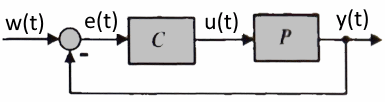
\includegraphics[width=0.8\linewidth]{Reg_smycka01.png}
      \caption{Regulační smyčka \cite[s.~215]{Roubal2011}.}
      \label{tky:fig_feedback003}
    \end{figure}
    V této kapitole se budeme věnovat regulaci, regulační smyčce a základním typů regulátorů. 
    Ukážeme si dvě základní zapojení regulačních smyček a zavedeme jednotné názvosloví, zejména 
    proto, že toto názvosloví není ustálené. Vysvětlíme si některé míry kvality řízení a ukážeme 
    názorně na příkladech vlastnosti základních \textbf{PID regulátorů}. Zvláštní pozornost bude 
    věnována filtraci derivační složky u tohoto regulátoru. Konkrétní způsoby návrhu regulátorů si 
    ukážeme v následujících kapitolách.
    
  
  \section{Modelování fyzikálních systémů}\label{TKY:sec002}
    Doposud jsme se v předešlých kapitolách zabývali různými nástroji, jak popisovat dynamické 
    chování systémů. Šlo spíše o teorii rozdělenou do kapitol bez větších souvislostí. V této kar 
    kapitole bychom chtěli ukázat použití těchto teoretických poznatků na konkrétních příkladech 
    fyzikálních systémů. Odvodíme zde několik matematických modelů fyzikálních systémů a připravíme 
    k těmto modelům simulinkové soubory s virtuální realitou pro Matlab (The Mathworks, 2009).
    
  \section{Identifikace systémů}\label{TKY:sec003}

} %tikzset
%---------------------------------------------------------------------------------------------------
\printbibliography[title={Seznam literatury}, heading=subbibliography]
\addcontentsline{toc}{section}{Seznam literatury}
% % !TeX spellcheck = cs_CZ
{\tikzset{external/prefix={tikz/TKY/}}
 \tikzset{external/figure name/.add={ch05_}{}}
%===============Kapitola: Měření teploty ===========================================================
\sisetup{
output-decimal-marker = {,},
}

\chapter{Snímače tepelných veličin}
\minitoc

  \section{Základní pojmy}
    \href{http://cs.wikipedia.org/wiki/Teplota}{Teplota} je charakteristika tepelného stavu hmoty.
    V obecném významu je to vlastnost předmětů a okolí, kterou je člověk schopen vnímat a přiřadit
    jí pocity studeného, teplého či horkého. V přírodních a technických vědách a jejich aplikacích
    je to \emph{skalární intenzivní veličina}, která je vzhledem ke svému pravděpodobnostnímu
    charakteru vhodná k popisu stavu ustálených makroskopických systémů. Teplota souvisí s
    kinetickou energií částic látky.

    Teplota je základní fyzikální veličinou soustavy \texttt{SI} s jednotkou kelvin (\si{\kelvin})
    a vedlejší jednotkou stupeň Celsia (\si{\degreeCelsius}). Nejnižší možnou teplotou je teplota
    absolutní nuly (\SI{0}{\kelvin}, resp. \SI{-273.15}{\degreeCelsius}), ke které se lze 
    libovolně
    přiblížit, avšak nelze jí dosáhnout.
         
    Do této skupiny patří především rozsáhlá část snímačů teploty. Z hlediska měřených veličin
    můžeme provést následující rozdělení.
    \begin{enumerate}\addtolength{\itemsep}{-0.5\baselineskip}
      \item \textbf{Snímače teploty}
        \begin{enumerate}[label=\emph{\alph*})]
          \item emph{Snímače pro dotykové měření} 
            \begin{itemize}
              \item elektrické
               \begin{itemize}
                 \item odporové kovové
                 \item odporové polovodičové
                 \item termoelektrické
                 \item polovodičové 
               \end{itemize}   
              \item dilatační
              \item termoelektrické
              \item tlakové
              \item speciální
            \end{itemize}
          \item \emph{Snímače pro bezdotykové měření}
            \begin{itemize}
              \item monochromatické pyrometry
              \item pásmové pyrometry
              \item radiační pyrometry
            \end{itemize}
        \end{enumerate}
      \item \textbf{Snímače tepla}
      \item \textbf{Snímače tepelného toku}
    \end{enumerate}  
       
      \subsection{Elektrické teploměry}
        \subsection{Odporové snímače}
          Odporové snímače využívají princip změny elektrického opdoru vlivem změny teplot.
          Základním požadavkem kladeným na materiál snímače je co největší a stálý teplontí
          součinitel odporu a zároveň co největší měrný odpor. Pro tyto účely se používají kovové a
          polovodičové materiály.
          
          \subsubsection{Kovové odporové snímače} 
            Jsou to především čisté kovy, které se používají pro realizaci vlastního odporového
            článku. Požadavkem je, aby nereagovaly s izolačním nebo ochranným krytem. Jakékoliv
            chemické nebo fyzikální vlivy by mohly způsobit nestálost odporu při stálé teplotě,
            Použitý materiál nemá vykazovat změnu teplotního součinitele odporu s časem (stárnutí)
            a hysterezi. Nejčastěji používanými materiály je \emph{platina, nikl, měď, slitina
            stříbro-zlato} a další \cite[s.~96]{Zehnula1983}.
             
            Platina je výhodná pro velkou chemickou stálost, vysokou teplotou tavení a možností
            dosažení vysoké čistoty. Pro snímače teploty se používá tzv. fyzikálně  čistá platina,
            jejíž čistota se pohybuje kolem 99,93 až 99,99 \% Pt. Měření ukázala, že změny
            základního odporu u sériově vyráběných přesných teploměru se pohybí kolem
            \num{5e-6}$R_o$ (což odpovídá \SI{0.001}{\kelvin}), u nejlepších teploměrů je tato
            hodnota ještě o řád menší. Proto se používá platina pro etalonový teplměr v oblasti
            teplot \SI{-259.34}{\degreeCelsius} až \SI{630.74}{\degreeCelsius}.
            
            Závislost odporu na teplotě pro rozsah \num{0} až \SI{630}{\degreeCelsius} se vyjadřuje
            rovnicí
            \begin{equation}\label{SAC:kov_Ro1}
              R_\vartheta = R_0(1 + A\vartheta + B\vartheta^2)
            \end{equation}
            kde 
            \begin{labeling}{$\omega t+\varphi_0$}
              \setlength{\itemindent}{2cm}
              \item[\(R_0\)]          \(\ldots\) \emph{odpor při \SI{0}{\degreeCelsius}}, 
              \item[\(\vartheta\)]    \(\ldots\) \emph{teplota ve \si{\degreeCelsius}}, 
              \item[\(A\)]            \(\ldots\) \emph{konst (\SI{3.9075e-3}{\per\degreeCelsius})},
              \item[\(B\)]            \(\ldots\) \emph{konst (\SI{-0.575e-6}{\per\degreeCelsius})}. 
            \end{labeling}
 
             V rozmezí od \SI{0}{\degreeCelsius} do \SI{-190}{\degreeCelsius} se vyjadřuje
             závislost odporu na teplotě rovnicí
             \begin{equation}\label{SAC:kov_Ro2}
               R_\vartheta = R_0[1 + A\vartheta + B\vartheta^2 + C(\vartheta - 100)\vartheta^3)]
             \end{equation}

} %tikzset
%---------------------------------------------------------------------------------------------------
\printbibliography[title={Seznam literatury}, heading=subbibliography]
\addcontentsline{toc}{section}{Seznam literatury}
  \printbibliography[title={Seznam literatury}, heading=bibliography]
}{
  \LuaPartBckgrnd{titleBG_fractal1.png}
  \LuaPartTitle{TKY}{Technická kybernetika}{TKY}
  \parttoc
% DEBUG was off
%======================= Kapitola: Základy technické kybernetiky ===================================
  % !TeX spellcheck = cs_CZ
%{\tikzset{external/prefix={tikz/TKY/}}
% \tikzset{external/figure name/.add={ch01_}{}}
%======================= Kapitola: Základy technické kybernetiky ===================================
\chapter{Základy technické kybernetiky}
\minitoc
  \section{Vznik a vývoj kybernetiky}
    Kybernetika je jedním z nejmladších vědních oborů a její vznik spadá do čtyřicátých let 
    dvacátého století. Vznik je úzce spjat s vývojem mnoha jiných vědních oborů jako matematická 
    logika, fyziologie, neurofyziologie a s rozvojem některých technických oborů jako je 
    elektronika, výpočetní technika, řídicí technika. Kybernetika není vědou, která by pouze 
    přebírala poznatky jiných věd. Ona hledá to, co jednotlivé vědní obory spojuje, postihuje 
    určité společné rysy různých vědních oborů a má snahu o jejich integraci. 

    \begin{figure}[ht!]
      \centering
      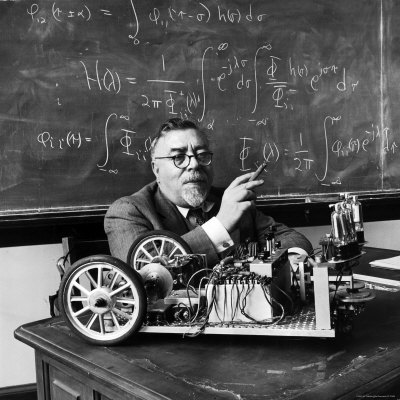
\includegraphics[width=0.8\linewidth]{Norbert_Wiener.jpg}
      \caption{Norbert Wiener (26. listopadu 1894 – 18. brezna 1964) byl americký matematik, který 
               je považován za zakladatele kybernetiky. }
      \label{tky:fig003}
    \end{figure}
  
    Historicky poskytlo impuls ke vzniku kybernetiky řešení problému řízeni palby protiletadlového 
    dělostřelectva za 2. světové války. Na tomto úkolu pracoval také americký matematik 
    \emph{Norbert Wiener}. Výsledkem matematického i konstrukčního úsilí bylo, že mířič - člověk 
    byl nahrazen přístrojem - zaměřovačem, který snímal údaje o současné poloze letadla, z ní 
    vypočítával polohu v budoucích okamžicích a servomechanismem se přenášela informace od 
    zaměřovače a počítače na kanóny. Norbert Wiener pak jako první zpracoval teorii 
    automatizovaných systémů řízeni pro účely protiletecké obrany. Tuto teorii zobecnil pro všechny 
    druhy technických, biologických a společenských systémů. Shrnul ji ve své proslulé knize 
    \emph{Kybernetika neboli řízení a sdělování v živých organismech a strojích}. Tato kniha vyšla 
    v roce \num{1948} a stala se světovým vědeckým bestsellerem. Svého autora proslavila jako 
    zakladatele kybernetiky.
    
    Řešení praktických (a bohužel vojenských) problémů použití elektronických počítačů k řízení 
    střel inspirovalo Wienera ke studiu řízení se zpětnou vazbou. Spolu s neurofyziologem 
    \emph{Arturem Rosenbluethem} hledali analogie k technickým zpětnovazebním systémům pro navádění 
    střel na pohyblivý cil. Takovou analogii nalezli u některých biologických systémů - konkrétně v 
    nervové soustavě živých organismů. Myšlenka zpětné vazby u živých a neživých systémů se stala 
    základem kybernetické koncepce vyložené v citované knize. Hledáni analogií mezi živým 
    organismem a strojem (případně také společnosti) znamená postihnout společné znaky zdánlivě 
    naprosto různorodých systémů. A tyto analogie pak vedou k používáni matematického a logického 
    aparátu i tam, kde to dosud nebylo možné.
    
    Nemůžeme ovšem nevidět všechny předcházející tendence a faktory v historii společnosti, které 
    vedly ke vzniku kybernetiky. Bylo by nesprávné tvrdit, že pouze Norbert Wiener a několik jeho 
    spolupracovníků vytvořilo kybernetiku. Její vznik byl pokračováním určité tendence, která se 
    projevovala již dávno předtím. Kybernetiku musíme chápat jako výsledek rozvoje materiálních sil 
    lidské společnosti a rozvoje vědeckého poznáváni světa.
    
    Název kybernetika pochází z řeckého slova \uv{kybernétés} neboli \uv{kormidelník}, \uv{člověk 
    řídící loď}. Objevuje se v dílech řeckých filosofů, např. v Platonově díle Dialogy; zde se 
    tímto termínem vyjadřuje \uv{umění řídit lodě a administrativně spravovat provincie}. V 
    novověku použil termín kybernetika A. M. Ampére v encyklopedii a to ve smyslu \uv{vědy o řízení 
    společnosti}. Termín se neujal a tak to byl až Wiener, který jím nazval nově vznikající vědní 
    obor. \cite[s.~6]{Svarc1986}.

    \subsection{Základní pojmy kybernetiky a její vymezení}
      Pro kybernetiku jsou charakteristická tři základní hlediska, z kterých nazírá na problémy a z 
      kterých dané problémy řeší. Jsou to

      \begin{figure}[ht!] %  \ref{tky:fig004} 
        \centering
        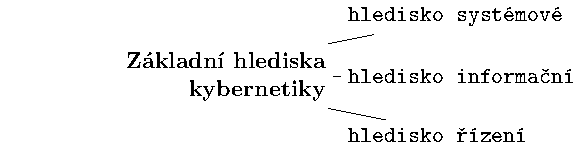
\includegraphics[width=0.7\linewidth]{tky_fig004.pdf}
        \caption*{ }
        \label{tky:fig004}
      \end{figure}
      
      Tím se dostáváme k nejzákladnějších pojmů kybernetiky: \textbf{systém}. \textbf{informace} a 
      \textbf{řízení}, Z těchto hledisek se pak vyvinuly základní obory teoretické kybernetiky - 
      teorie systémů, teorie informace a \hyperlink{tky:regulace}{teorie řízení}.
      
      Jako příklad vysvětlující tato hlediska kybernetiky si zvolme automobil. Automobil je z 
      hlediska konstruktéra složité technické zařízení, sloužící k dopravě osob a nákladu, které je 
      vyrobeno z různých materiálů. Je sestaven z mnoha součásti, pohon je motorem spalovacím nebo 
      vznětovým, k provozu jsou nezbytné látky jako benzín, oleje, voda, ... .To vše je důležité a 
      podstatné z hlediska konstruktéra automobilu, ale ne z hlediska kybernetiky.

      \begin{wrapfigure}[11]{r}{6cm}   %\ref{tky:fig001} 
        \centering
        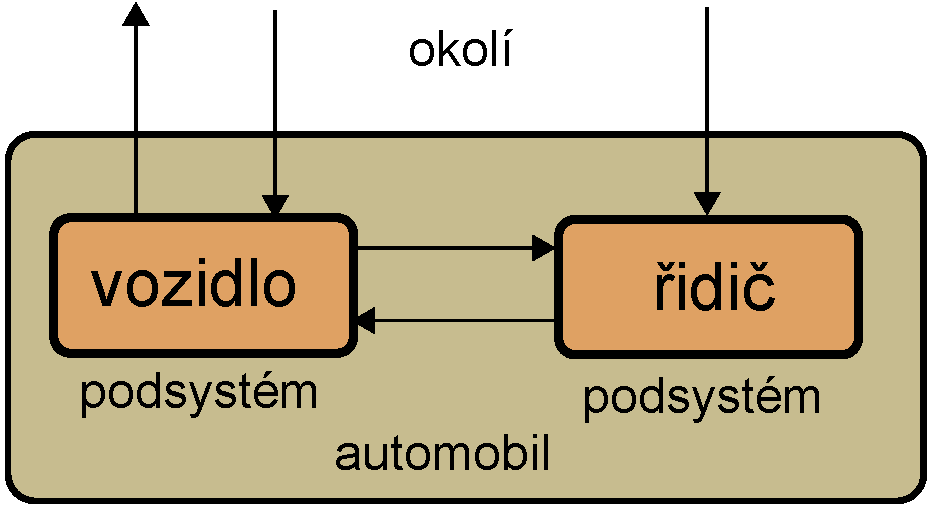
\includegraphics[width=0.9\linewidth]{tky_fig001.pdf}
        \caption{ }
        \label{tky:fig001} 
      \end{wrapfigure}
      Jaká jsou tedy hlediska kybernetiky? Kybernetika vidí v automobilu především tzv. 
      \textbf{dynamický systém}, jehož činnost je spojena s člověkem - řidičem a je ve vztahu k 
      okolnímu světu. Automobil uvažovaný jako systém se skládá ze dvou podsystémů (subsystémů). 
      Prvním z nich je vlastní vozidlo, druhým je člověk. Každý podsystém se pak skládá z 
      elementárních jednotek, vzájemně propojených, tzv. \emph{prvků systému}. Mezi prvky systému 
      existují různé vztahy. Ale nejenom mezi prvky nebo podsystémy existuji vztahy.

      Automobil není izolovaným systémem a proto má také četné vztahy k okolí. K okolí \uv{systému 
      automobil} patří ty části okolního světa, které mají vliv na jeho činnost. Jsou to např. 
      vozovka, křižovatky, zatáčky, jiná vozidla, chodci, dopravní značky apod. Na všechny vlivy 
      okolí reaguje systém automobil určitým způsobem. Reakce systému na okolí se nazývá 
      \textbf{chováni systému}. Pokud sleduje kybernetika automobil tímto způsobem, jedná se o 
      \emph{systémové hledisko} kybernetiky  (obr. \ref{tky:fig001}). Předběžně si vymezme pojem 
      systém jako soubor prvků, mezi nimiž existuji nějaké funkční vztahy. Sledujeme-li vzájemné 
      působeni systému a jeho okolí, jde o druhé základní kybernetické hledisko. Poněvadž se toto 
      působeni realizuje výměnou informaci mezi systémem a okolím, mluvíme o \emph{informačním 
      hledisku}. Pod pojmem informace si představíme zprávu, která má pro některé ze zúčastněných 
      systémů určitý význam. Nositelem informace jsou tzv. \textbf{signály}.
      
      Doposud jsme uvažovali prostou výměnu informaci mezi dvěma systémy. Je-li ale informace 
      využívána přijímacím systémem pro další činnost, pro dosaženi určitého předem stanoveného 
      cíle, pak už se jedná o \emph{řízení}. Pojem řízení vymezíme jako \emph{proces výměny 
      informace mezi dvěma systémy}, který se uskutečňuje plánovitě pro dosažení určitého cíle. Při 
      řízení se uplatňuje informační působení řídicího systému na řízený systém. Tím se dostáváme k 
      třetímu kybernetickému hledisku a to je \emph{hledisko řízení}. Zdůrazněme, že toto hledisko 
      provádí pouze informační bilancování a nikoliv látkové nebo energetické.
      
      Vraťme se k našemu automobilu. Systém automobil má dva podsystémy vozidlo a řidiče. Mezi nimi 
      probíhá informační výměna, jejíž cílem je pohyb automobilu po stanovené dráze, např. v přímém 
      směru. Řidič reaguje na nerovnosti vozovky nebo na boční vítr, které vychyluji vozidlo z 
      přímého směru tím, že pootáčí volantem. Řidič je tedy řídícím systémem a vozidlo řízeným 
      systémem a výměna informací probíhá za účelem udrženi pohybu vozidla v přímém směru - jedná 
      se o \textbf{proces řízení}.
      
      Všimněme si momentu, že řidič otáčí volantem na základě toho, jaký účinek vyvolalo předchozí 
      pootočení. Neustále sleduje směr vozidla a vyrovnává odchylky od přímého daného směru. Takový 
      způsob řízení označujeme v kybernetice jako \textbf{řízení se zpětnou vazbou} neboli 
      \textbf{regulace}. Systémy se zpětnou vazbou se tedy nazývají \textbf{regulační systémy}. 
      Systém automobil (řidič + vozidlo) můžeme pokládat za regulační systém, který je regulován na 
      přímý směr jízdy.
      
      Poněvadž systémy řízení se zpětnou vazbou, tedy regulační systémy, jsou pro kybernetiku 
      charakteristické, nazýváme třetí kybernetické hledisko také \emph{hlediskem regulačním}. 
      Samozřejmě existuje rovněž \textbf{řízení bez zpětné vazby}; v tom případě se mluví jen o 
      \textbf{systémech řízení} nebo o \textbf{systémech ovládání}.
      
      Řízení jako vzájemná interakce mezi systémy nebo mezi systémem a okolím probíhá vždy v 
      určitém pořadí činnosti některého ze systémů. obvykle řídicího. Soubor pravidel, podle něhož 
      řídící systém vykonává sled činností za účelem řízení, se nazývá \textbf{algoritmus}. Obecně 
      je \emph{algoritmus soubor pravidel, podle něhož probíhá řízení}.
      
      U zvoleného příkladu s automobilem bychom mohli například sestavit algoritmus spouštění 
      motoru, algoritmus vyjíždění automobilu, algoritmus předjíždění, atd. Algoritmy jsou objektem 
      zkoumání jednoho z oborů teoretické kybernetiky - \emph{teorie algoritmů}.
      
      Pe předběžném objasnění základních hledisek kybernetiky a základních pojmů kybernetiky je 
      možné se pokusit vyložit, ce vlastně kybernetika je a čím se zabývá. Jednotlivý autoři, kteří 
      se pokoušejí podat definici kybernetiky, protěžují více nebo méně některé ze tří základních 
      kybernetických hledisek (hledisko systémové, hledisko informační, hledisko řízení). Většina 
      starších definic kybernetiky vychází z klasické definice jejího uznávaného zakladatele 
      Norberta Wienera, který ji definoval jako \uv{vědu o řízení a sdělování v živých organismech 
      a strojích}. Tato definice, která je nerozlučně spjata s jejím vznikem, protěžuje hledisko 
      informační a hledisko řízení. Jejím nedostatkem je, že ještě nedoceňuje systémový přístup, 
      systémové hledisko při řešení problémů. Dále jako objekty zkoumání (tedy systémy) zahrnuje 
      pouze živé organismy a stroje. Nezahrnuje tedy další důležité objekty zkoumané dnešní 
      kybernetikou jako jsou objekty společenské a ekonomické a neuvažuje systémy matematické, 
      lingvistické a další a z technických systémů dnes tak různorodých se omezuje jen na stroje. 
      Ani informační hledisko této definice není úplné, protože se omezuje pouze na přenos 
      informaci a neuvažuje dnes tak důležité procesy uchování a zpracováni informace.
      
      Podobnými nedostatky se vyznačovaly definice kybernetiky dalších autorů. Byl to vždy 
      jednostranný přístup a neúplnost jednotlivých hledisek. Proto nelze žádnou z definic 
      akceptovat s definitivní platností.
      
      Nebudeme se tedy snažit za každou cenu zformulovat vyčerpávající definici, ale uveďme si 
      charakteristické rysy kybernetiky jako vědy.
      
      Kybernetika se zabývá různými rozdílnými problémy, které však byly většinou známy a zkoumány 
      před vznikem kybernetiky, např. krevní oběh, podmíněný reflex, radiolokace, konstrukce 
      počítačů, řízení různých technických zařízení, kódování atd. Kybernetika vnáší do těchto 
      problémů nový pohled, neboť si všímá toho, že na určitém stupni organizace a vývoje systémů 
      vzniká nový proces řízení. Tento proces se projevuje výměnou informací v systémech, kterým se 
      chování systémů zaměřuje k určitému cíli.
      
    \subsection{Rozdělení kybernetiky}
      Z praktického hlediska můžeme kybernetiku rozdělit podle přístupu a aplikací:
      \begin{itemize}\addtolength{\itemsep}{-0.5\baselineskip}
        \item \textbf{teoretická kybernetika},
        \item \textbf{aplikovaná kybernetika}.
      \end{itemize}

      \emph{Teoretická kybernetika} studuje především obecné vlastnosti a chování systémů. Zabývá 
      se obecným popisem vlastností a chování systémů. Z tohoto pohledu zahrnuje teoretická 
      kybernetika \emph{teorii systémů} a \emph{teoretickou informatiku}.
      
      \emph{Aplikovaná kybernetika} představuje použití kybernetického přístupu při analýze, 
      modelování a simulaci a návrhu systémů, dále aplikuje poznatky kybernetiky do dalších 
      oblastí. Aplikovaná kybernetika zasahuje do mnohých oblastí lidské činnosti - zahrnuje totiž 
      mj. následující obory:
      
      \begin{itemize}\addtolength{\itemsep}{-0.1\baselineskip}
        \item \textbf{Teoretická kybernetika}
              \begin{itemize}\addtolength{\itemsep}{-0.1\baselineskip}
                \item \emph{Dynamické systémy}: zpětná vazba, stavový popis, stochastické systémy,
                      řízení, aj.
                \item \emph{Přenos informace}: informační entropie, kapacita komunikačního kanálu, 
                      aj. 
                \item \emph{Umělá inteligence}: strojové vnímání a učení, multi-agentní systémy, 
                      robotika, modelování neuronových sítí, konekcionismus, vazba člověk-stroj, ...
                \item \emph{Teorie rozhodování}, her, teorie složitosti, chaotické systémy, aj.
              \end{itemize}
        \item \textbf{Informatika}
        \item \textbf{Biokybernetika}
        \item \textbf{...}
      \end{itemize}
      
  \section{Teorie systémů}
     Teorie systémů je jedna ze základních disciplin teoretické kybernetiky. Na druhé straně je ale 
     teorie systémů součásti tzv. \emph{obecné teorie systémů}, jejíž principy rozpracoval americký 
     biolog Ludwig von Bertalanffy. Pokusme se o vymezení vztahu mezi kybernetikou a teorií systémů.
     \cite[s.~11]{Svarc1986}.
     
     Obecná teorie systémů studuje systémy libovolné povahy, přičemž se zajímá o charakter prvků 
     systému, charakter vazeb mezi prvky a chováni systému. Důležitým pojmem je zde \textbf{vazba 
     mezi prvky} a pojem \textbf{chování systémů}. Zatímco obecná teorie systémů se zajímá o 
     libovolný druh vazeb mezi prvky a libovolné chování systémů, kybernetiku zajímá specifický 
     druh vazeb a specifické chování. Kybernetika studuje pouze ty vazby, které jsou realizovány 
     přenosem informace a chování, které lze zahrnout pod \textbf{pojmem řízení}. A to je náplni 
     teorie systémů jako discipliny teoretické kybernetiky.
     
     \textbf{Přenos informace} a \textbf{řízení} nejsou od sebe \emph{oddělitelné}. Aspoň tak, že 
     není možné řízení bez přenosu informace. Je však už sporné, je-li každý přenos informace již 
     řízením. Můžeme říci, že systémy mezi nimiž probíhá proces řízení musí mít určitou specifickou 
     strukturu a musí být mezi nimi zajištěn přenos informace. Pokud existuje pouhá výměna 
     informací mezi systémy, mluvíme o \textbf{informačních systémech}.
     
     \emph{Obecnou teorii systémů} tedy \emph{nemůžeme} zahrnout do kybernetiky; s kybernetikou má 
     společnou jen určitou část, která je zaměřena na studium systémů z hlediska informačních 
     vazeb. Hlavním úkolem obecné teorie systémů je postihnout a vyjádřit exaktním způsobem 
     vlastnosti a vztahy ve složité a dynamické (v čase se měnící) \emph{objektivní realitě} tak, 
     aby se neztratila její komplikovaná struktura a složitost. Jestliže dříve byl nějaký přírodní 
     nebo společenský jev pokládán za vysvětlený, když se nalezla jeho příčina, pak při systémovém 
     přístupu musí bý nalezena struktura a dynamika každého objektu, který se na daném jevu podílí.
     
     \subsection{Charakteristika základních pojmů z teorie systémů}
       Pro práci se složitými a rozsáhlými objekty, jako jsou například řízení výrobních a
       technologických procesů, je nutný \textbf{systémový přístup}. Například technologický proces
       exploatace uhlí na hlubinných nebo povrchových dolech, je charakterizován různorodostí
       pracovních činností, na něž působí celá řada vlivů. Komplexně jde o mnoha rozměrný
       dynamický celek, který se neustále mění v čase a v prostoru.
       
       \emph{Systémový přístup spočívá v tom, že jevy vyskytující se při řešení vzniklých problémů, 
       jsou chápany komplexně, se všemi souvislostmi ve svém dynamickém vývoji.}
       
       V souvislosti se systémovým přístupem je nejdůležitějším pojmem \textbf{systém}. Jestliže 
       chceme v dalším uvést základní pojmy teorie systémů, musíme nejdříve tento pojem vysvětlit. 
       Předběžně jsme ho vymezili jako \emph{soubor prvků, mezi nimiž existuji nějaké funkční 
       vztahy a který má jako celek vztah ke svému okolí}. Jinými slovy: \emph{Stanovíme- li 
       vztahy, mezi na sebe navzájem působících objektů materiální, ale i nemateriální povahy, je na
       objektivní realitě vytvořen systém.} Jiní autoři podávají tyto definice:
       \begin{itemize}\addtolength{\itemsep}{-0.5\baselineskip}
         \item Bertalanffy (1956): Systém je komplex prvků nacházejících se ve vzájemné interakci.
         \item Hall - Fagen (1966): Systém je souhrn prvků spolu se vztahy mezi prvky a mezi jejich 
               vlastnostmi.
       \end{itemize}

       \begin{definition}
        \textbf{Systém} je definován jako účelově uspořádaná množina prvků a množina vazeb mezi 
        nimi, s dynamickým chováním, které společně určují vlastnosti celku.
        \begin{equation}
          \mathscr{S} = \{S,R \},
        \end{equation}
        kde
        \begin{description}[leftmargin=5em,style=nextline]
          \item[\hspace{2em}\(S \ldots\)] \emph{množina všech prvků},
          \item[\hspace{2em}\(R \ldots\)] \emph{množina relací mezi prvky, reprezentující vzájmené 
                                         funkční vztahy jednotlivých prvků a vztah systému k okolí.}
        \end{description}
       \end{definition}
       
       V rámci dekompozice systému lze vyčlenit \textbf{podsystém}. Podsystém je podmnožina
       systémových prvků a vazeb, která je z nějakého důvodu vyčleněna ze systému a je chápána
       jako nový systém nebo jako prvek.
       
       \begin{definition}
        \textbf{Prvek} je část systému, který tvoří na dané rozlišovací úrovni dále nedělitelný 
        celek, jehož strukturu nechceme, nebo již nemůžeme v rámci analýzy rozlišit.
       \end{definition}
       
       \begin{note}
         \textbf{Rozlišovací úrovní} se označuje stupeň podrobnosti zkoumání systému. Změnou        
         rozlišovací úrovně se může dřívější prvek systému stát podsystémem, popřípadě i systémem a 
         naopak. Dekompozicí systému na jednodušší prvky, se zvyšuje rozlišovací úroveň.
       \end{note}
       
     \subsection{Klasifikace systémů}
       Někdy rozlišujeme pojem \textbf{statický} a \textbf{dynamický systém}, ale spíš známe pouze 
       systémy dynamické. Statický systém je totiž v čase konstantní, neměnný. Mezi statické 
       systémy můžeme někdy zařadit i systémy, u nichž se vlastnosti prvků mění velmi pomalu. V 
       přírodě se statické systémy prakticky nevyskytují, spíše se jedná o systémy s pomalou změnou 
       vlastností na čase. Naproti tomu dynamický systém je takový systém, u kterého existuje 
       alespoň jedna proměnná závislá na čase. Většina systémů je dynamických. V dalším textu jsou 
       proto popsány především \textbf{dynamické systémy a řídicí (regulační) systémy se zpětnou 
       vazbou}.
       
       Dynamické vlastnosti lineárních systémů lze popsat lineárními diferenciálními rovnicemi s 
       konstantními koeficienty a operátorovými přenosy. Dynamické vlastnosti nelineárních systémů 
       lze popsat nelineárními diferenciálními rovnicemi.
       
       Existují dvě možnosti studia dynamického systému. Prvním způsobem je zkoumání \emph{vnitřní 
       struktury systému}, tzn. vnitřní závislosti prvků a dále nás zajímají, jaké vnitřní změny 
       vznikají v systému při působení vnějších vlivů. To je podstatou \textbf{vnitřního popisu 
       dynamického systému}.
       
       Druhým způsobem je pojímání systému jako celek a studování pouze otázky, jaké výsledné 
       reakce systému vyvolávají vnější vlivy. Tomuto druhému způsobu se budeme věnovat při 
       \textbf{vnějším popisu dynamických systémů}.
     
     
  \section{Teorie informace}
    \textbf{Informace} jako stěžejní pojem kybernetiky, je pojem značně široký a hodně diskutovaný. 
    Je používán v celé řadě definic vymezujících předmět kybernetiky jako vědy, přičemž informační 
    hledisko považují někteří autoři za nejdůležitější.
      
    Přesná definice pojmu informace neexistuje. Obecně se tento pojem používá volně, v intuitivním 
    chápaní se vztahuje k pojmům jako zpráva, údaj, poznatek apod. Z hlediska kybernetiky je toto 
    chápáni příliš zúženo, neboť kybernetika sleduje přenos informace mezi dvěma nebo více systémy 
    s tím, že cílem přenosu může být řízení chování některého ze systému. Kybernetika říká, že 
    informace je jakékoliv sdělení, kterého lze reálně (právě nyní) nebe potenciálně (v budoucnu 
    při vhodné příležitosti) použit k řízeni systému.
    
    Pojem informace je \emph{pojmem abstraktním} a jako takový má \emph{nehmotnou povahy}. 
    Současně však informace má smysl jen ve spojení s hmotou a to jak z hlediska přenosu, tak z 
    hlediska obsahu (i abstraktní představy jsou spjaty s existenci hmoty).
    
    Informace (sděleni) má
    \begin{itemize}\addtolength{\itemsep}{-0.4\baselineskip}
      \item \textbf{formu},
      \item \textbf{obsah},
      \item \textbf{význam}.
    \end{itemize}
    \textbf{Forma} informace neboli sdělení musí být přístupná systémům, mezi nimiž dochází k 
    výměně informaci a je důležitá pro proces přenosu informace. Pro proces řízení systémů je 
    podstatný \textbf{obsah a význam informace} (sdělení). \textbf{Sdělení} je \emph{informační, 
    sémantický a pragmatický obsah}. \textbf{Informační obsah} vyjadřuje kvantitativní míru 
    informace v dále definované jednotce \textbf{bit}. Používáme pro něj termín míra či množství 
    informace. \textbf{Sémantický obsah} vyjadřuje významovou stránku znaků při jazykové komunikaci 
    a nedá se měřit (\emph{sémantika} - nauka o významu slov). \textbf{Pragmatický obsah} určuje 
    významnost sdělení a prioritu jednotlivých zpráv pro příjemce.
    
    Každá forma hmoty, která nese informaci se nazývá \textbf{zpráva}. Zpráva je hmotným nositelem 
    informace. Zpráva je způsob vyjádření informace textem, obrazem, řečí, posloupností znaků atd. 
    Zpráva může být tedy např. číslo (posloupnost číslic), abecední text (posloupnost písmen), 
    spouštěcí signál (posloupnost napěťových úrovní). Pojmy informace a zpráva nelze zaměňovat. 
    Informace jo pojem abstraktní, zpráva jo konkrétní materiální formou informace, bez níž by 
    informace neměla smysl a nemohla by být přenášena a působit na systémy, kterým je určena. Pojem 
    zpráva bývá někdy nahrazován užším pojmem \textbf{signál}. Signál je fyzikální realizace zprávy 
    ve formě elektrického proudu resp. elektromagnetických vln.
      
    Sledujeme-li blíže jakoukoliv dostatečně dlouhou zprávu, pak zjistíme, že je vždy vytvářena z 
    posloupnosti nějakých základních elementů - \textbf{prvků}. Možný počet odlišných prvků, ze 
    kterých je taková zpráva vytvářena, může být bud \emph{konečný} nebo \emph{nekonečný}. Tak 
    např. psaná zpráva ve formě českého textu je posloupností různých kombinací písmen české 
    abecedy. Možný počet různých písmen - prvků je konečný a je dán počtem písmen české abecedy.
      
    Základní prvky, ze kterých je vytvářena zpráva, bývají obecně nazývány \textbf{písmena} a celý 
    \emph{soubor} všech \emph{možných prvků} bývá nazýván \textbf{abecedou zdroje}. Zpráva je pak 
    vytvářena výběrem prvků z abecedy zdroje a jejich sestavou v posloupnost prvků. Přitom 
    libovolný prvek abecedy se může ve zprávě libovolně opakovat. Abychom mohli odlišovat prvky 
    abecedy od prvků, z nichž je sestavena konkrétní realizace zprávy, budeme libovolný prvek 
    realizace zprávy nazývat \textbf{symbol}. Nechť má abeceda zdroje celkem \(s\) možných různých 
    prvků. Nechť je délka zprávy, tj. počet symbolů, z nichž je složena realizace zprávy, dána 
    počtem \(L\) symbolů. Celkový možný počet \(L\) různých realizaci zpráv délky \(n\), které 
    mohou být produkovány zdrojem s abecedou o \(s\) prvcích a které se budou lišit nejméně v 
    jednom symbolu, je
    \begin{equation}\label{tky:eq0001}
      L = s^n
    \end{equation}
    (počet všech možných \emph{variací n symbolů s opakováním}, které lze vytvořit z \(s\) prvků).
    
    Má-li abeceda zdroje \emph{konečný počet} \(s\) možných prvků, pak takový zdroj nazýváme 
    zdrojem \textbf{diskrétních zpráv} (diskrétní zdroj). Má-li abeceda zdroje \emph{nekonečný 
    počet prvků}, pak ho nazýváme zdrojem \textbf{spojitých zpráv} (spojitý zdroj).
    
    \begin{example}
      Kolik zpráv o délce \num{10} symbolů můžeme vytvořit z abecedy o \num{2} písmenech?
      \newline
      Řešení: Počet realizaci \(L\) zpráv je dán vztahem (\ref{tky:eq0001})
      \begin{equation*}
        L = s^n = 2^{10} = 1024
      \end{equation*}      
    \end{example}
      
    \subsection{Přenos zpráv}
      Zprávu lze přenést buď \emph{přímo}, přenesením nosného média (pergamen, magnetická páska, 
      optický disk), anebo \emph{nepřímým} způsobem prostřednictvím \emph{signálu}, který je 
      realizací zprávy ve formě změn některé fyzikální veličiny, nejčastěji elektrického proudu.
      
      Při nepřímém způsobu \textbf{zdroj informace} generuje prostřednictvím \textbf{kodéru} 
      (kódovacího zařízeni) signály, které se přenáší \textbf{kanálem}. Kanál je vlastně cesta, 
      která přenáší změny dané fyzikální veličiny, aby mohla být zpráva přenesena z jednoho místa 
      na druhé. Je tvořený prostředím, kterým se přenáší signál. Může to být např. telefonní 
      vedeni, trubka pro přenos tlakového signálu, akustické nebe elektromagnetické vlnění.
      
      Na výstupu kanálu je signál přijímán \textbf{příjemcem informace} (Člověk nebe zařízeni). 
      Zná-li příjemce zákon, podle kterého byla provedena transformace zprávy na vstupu kanálu, pak 
      může určit zprávu obsaženou v přijatém signálu. To provede tzv. \emph{dekódováním} v zařízeni 
      zvaném \textbf{dekodér}. Souhrn všech uvedených objektů vytváří \textbf{sdělovací soustavu}.

      \begin{figure}[ht!]
        \centering
        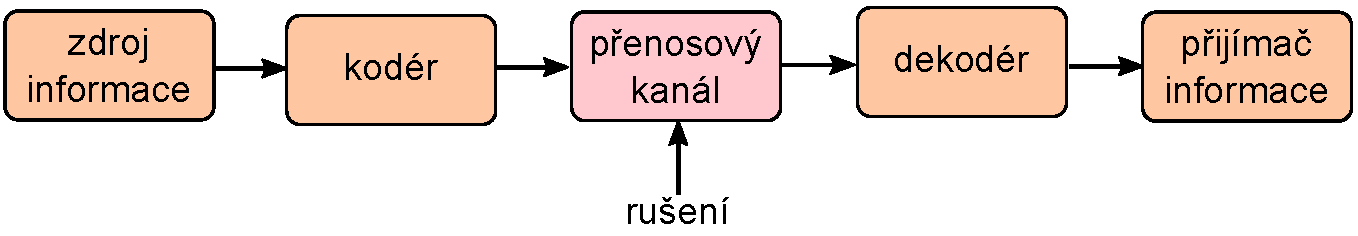
\includegraphics[width=0.9\linewidth]{tky_prenosovy_kanal.pdf}
        \caption{Nepřímý penos zprávy skrz přenosový kanál}
        \label{tky:fig002}
      \end{figure}

      Přenos signálu se může uskutečňovat v prvotní formě anebo v zprostředkované nepřímé formě, 
      kdy se pro přenos signálů používají pomocné tzv. \textbf{nosné signály}.
      
      Příkladem přenosu signálu v prvotní formě je přenos spojitých údajů o teplotě     
      prostřednictvím elektrického napětí ve vedení, přímo úměrné teplotě. 
      
      Při přenosu signálu v nepřímé formě se upravuje nosný signál tak, aby změny některého z jeho 
      parametrů zobrazovaly přenášenou zprávu. Tuto operaci vůči nosnému signálu nazýváme 
      \textbf{modulací}.
      
      
%} %tikzset
%~~~~~~~~~~~~~~~~~~~~~~~~~~~~~~~~~~~~~~~~~~~~~~~~~~~~~~~~~~~~~~~~~~~~~~~~~~~~~~~~~~~~~~~~~~~~~~~~~~
\printbibliography[title={Seznam literatury}, heading=subbibliography]
\addcontentsline{toc}{section}{Seznam literatury}
%======================= Kapitola: LTI systém ======================================================
  % !TeX program = lualatex
% !TeX root = luaking.tex
% !TeX encoding = UTF-8
% !TeX spellcheck = cs_CZ
%---------------------------------------------------------------------------------------------------
% file tky1ch02.tex
%---------------------------------------------------------------------------------------------------
%================== Kapitola: LTI systém ===========================================================
\setchaptertoc
\chapter{LTI systém}\label{tky:IchII}
  \twocolumn[\section{Vlastnosti a popis lineárních systému}\label{tky:IchIIsecI}]
    Na soustavu obvodů můžeme nahlížet jako na seskupení (množinu) navzájem souvisejících součástí, 
    ke kterému je určen vstupní signál $x$, zvaný buzení a výstupní signál $y$, označovaný jako 
    odezva. Z hlediska vlastností jde o systém představující "černou skříňku", jejíž vlastnosti 
    můžeme identifikovat analýzou vstupního a výstupního signálu \cite{Bicak2007}.        

    \luagraphic[0.8]{tky_fig005.pdf}{Symbol soustavy s jedním vstupem a jedním výstupem}{tky:fig005}
    \begin{itemize}
      \item Systémy se spojitým časem (na vstupu i výstupu pracují se spojitými signály) - relace  
            mezi vstupem a výstupem můžeme symbolicky zapsat:
            \begin{equation}\label{tky:eq005}
              y(t)=\mathcal{S}\{x(t)\}
            \end{equation}
            kde $S$ je obecný popis systémové funkce, přiřazující vstupní veličině $x(t)$ odezvu 
            $y(t)$. Z rovnice je zřejmé, že u spojité (analogové) soustavy výstupní signál závisí 
            na všech hodnotách vstupního signálu, nikoli jen na některých jeho hodnotách v určitých 
            časových okamžicích.
      \item Systémy pracující s diskrétním časem lze obdobně symbolicky vyjádřit relací  
            vstup/výstup ve tvaru:
            \begin{equation}\label{tky:eq022}
              y[n]=\mathcal{S}\{x[n]\}
            \end{equation}
            kde $\mathcal{S}$ je tentokráte systémový operátor přiřazení posloupnosti 
            $x[n]\rightarrow y[n]$. U diskrétních systémů se zpracovávají posloupnosti hodnot 
            signálů, získaných vzorkováním spojitého signálu
    \end{itemize}
    
    \subsection{Linearita, časová invariance a kauzalita}\label{tky:IchIIsecIssecI}
      \textbf{Linearita systémů} ve spojité diskrétní oblasti má velký význam, neboť dovoluje
      využívat princip superpozice k zjednodušování úloh jejich analýzy  a syntézy.

      Předpokládejme, že na vstupu lineárního diskrétního systému jsou přivedeny dva signály
      $x_1[n]$ a $x_2[n]$. Účinky obou vstupních signálů na výstupní signál lze zkoumat odděleně a
      podle principu superpozice je na výstupu sečíst. Označme dílčí odezvy
      $y_1[n]=\mathcal{S}\{x_1[n]\}$ a $y_2[n]=\mathcal{S}\{x_2 [n]\}$, potom je
      \begin{equation}\label{tky:eq007}
        y[n]= y_1[n]+y_2[n]=S\{x_1[n]+x_2[n]\}
      \end{equation}
      Analogický vztah platí i pro lineární spojitý systém, tedy
      \begin{equation}\label{tky:eq008}
        y(t)= y_1(t)+ y_2(t)=S\{x_1(t)+x_2(t)\}
      \end{equation}
      Z uvedeného vyplývá významná vlastnost lineárního systému. Výstupní spektrum může obsahovat
      pouze ty frekvence, které jsou ve spektru vstupního signálu a žádné jiné. 

      Jedná-li se o \textbf{systém časově invariantní}, jsou události v čase závislé pouze na
      časovém intervalu (rozdílu časových událostí), nikoliv na každém časovém okamžiku samostatně.
      Systém je časově invariantní, jestliže časový posun ve vstupní signálu vede ke stejnému posunu
      výstupního signálu. Odezva diskrétního systému na posunutý vstupní signál $x[n-m]$ je pak
      určen vztahem
      \begin{equation}\label{tky:eq009}
        y[n-m]= \mathcal{S}\{x[n-m]\}
      \end{equation}
      a obdobně pro odezvu spojité soustavy na posunutý (zpožděný) vstupní signál $x(t-\tau)$ platí
      analogicky rovnice
      \begin{equation}\label{tky:eq010}
        y(t-\tau)= \mathcal{S}\{x(t-\tau)\}.
      \end{equation}

      Takový systém má konstantními parametry a je popsaný \emph{diferenčními rovnicemi s
      konstantními koeficienty}. 
      
      Zcela obecně se LTI systém vyznačuje ještě dalšími vlastnostmi, z nichž jsou pro analýzu
      významnější kauzalita a stabilita. 
      \begin{itemize}
        \item \textbf{Kauzální, příčinný systém} - výstupní signál závisí pouze na současných a
              minulých hodnotách vstupního signálu \(x[n]\), nikoliv na budoucích hodnotách, nikoliv
              na budoucích hodnotách. Nicméně existují významné struktury (např. filtry), při
              jejichž návrhu vycházíme z vlastností nerealizovatelné - ideální struktury, které
              vhodnou metodou aproximace vyjádříme realizovatelnou strukturou. U LTI systémů může
              být otázka kauzality převedena na vlastnosti impulzní odezvy - viz. odst.
              \ref{tky:IchIIsecIssecII}. Při uložení signálu do paměti lze realizovat i nekauzální
              systém, který ale nepracuje v reálném čase. 
        \item \textbf{Stabilní systém} - omezený vstup (v hodnotách) produkuje též omezený výstup.
              Jinak - není-li vstup divergentní, pak ani výstup nebude divergentní. Uvedené bude
              splněno, jestliže pro hodnoty impulzní odezvy \(h[n]\) bude platit
              \begin{equation*}
                \sum_{n=-\infty}^\infty\abs{h[n]} <\infty.
              \end{equation*}
              Problém stability se vyskytuje u rekurzivních struktur (struktury se zpětnou vazbou). 
      \end{itemize}
      

    \subsection{Konvoluce v diskrétních systémech}\label{tky:IchIIsecIssecII}
      Významnou charakteristikou lineárních časově invariantních systémů \emph{LTI} je
      \textbf{impulsní odezva}. Její znalost umožňuje stanovit odezvu systému na obecný signál, lze 
      ji využít i při syntéze systému \cite{Bicak2007}.

      Mějme diskrétní LTI systém \ref{tky:fig002}, na jehož vstup je přiveden \emph{jednotkový
      diskrétní impuls}\footnote{Nesmíme zaměňovat s Diracovým (také jednotkovým) impulsem.}.
      Jednotkový impuls je posloupnost $\delta[n]=0$ pro všechna $n$ s výjimkou $\delta[0]=1$.
      Odezva systému na jednotkový impuls $\delta[n]$ se nazývá impulsní odezva a platí
      \begin{equation}\label{tky:eq011}
        h[n]= \mathcal{S}\{\delta[n]\}.
      \end{equation}
      Vzhledem časové invariantnosti, posunutému jednotkovému impulsu odpovídá posunutá impulsní
      odezva, tedy
      \begin{equation}\label{tky:eq012}
        h[n-m]= \mathcal{S}\{\delta[n-m]\}.
      \end{equation}
      \emph{Jednotkový skok} $1[n]$ je posloupnost jedniček od počátku časové osy $n=0$,
      kterou můžeme zapsat součtem
      \begin{align}
        1[n]&= \sum_{m=0}^n\delta[n-m]                  \nonumber \\
            &=\delta[n]+\delta[n-1]+\delta[n-2]+\cdots. \label{tky:eq013}
      \end{align}
      \emph{Odezva systému na jednotkový skok} $\mathrm{1}[n]$ se nazývá \textbf{přechodová odezva}
      $s[n]$ a platí
      \begin{align}
        s[n]&= \mathcal{S}\{1[n]\}= S\{\sum_{m=0}^n\delta[n-m]\}        \nonumber \\
            &=\sum_{m=0}^nS\{\delta[n-m]\}.                             \label{tky:eq014}
      \end{align}

      Postupná úprava rovnice (\ref{tky:eq014}) je umožněna díky linearitě systému, kterou budeme
      studovat pro obecný vstupní signál
      \begin{equation}\label{tky:eq015}
        x[n]=\sum_{m=-\infty}^\infty x[m]\delta[n-m].
      \end{equation}
      Poznamenejme, že formou (\ref{tky:eq015}) lze zapsat každý diskrétní signál.

      \begin{figure}[ht!]
        \centering  
        \subcaptionbox{\label{tky:fig_006a}}{\luafigure[0.45]{tky_fig006a.pdf}}
        \subcaptionbox{\label{tky:fig_006b}}{\luafigure[0.45]{tky_fig006b.pdf}}
        \caption{Posloupnost jednotkového skoku a) \(1[n]\) a b) signálu \(x[n]\)}
        \label{tky:fig_006}
      \end{figure}

      Na obr. \ref{tky:fig_006} je znázorněna souvislost mezi posloupností jedniček a diskrétním
      signálem. \emph{Posloupnost jedniček tvoří bázi pro diskrétní signály}. Každá komponenta
      diskrétního signálu je vyjádřena součinem $x[m]\delta[n-m]$. V uvedeném příkladě jde o
      posloupnost příslušnou jednotkovému skoku
      \begin{equation*}
        1[n]=\sum_{m=0}^{15}\delta[n-m]
      \end{equation*}
      a odpovídající posloupnost konečného signálu
      \begin{equation*}
        x[n]=\sum_{m=0}^{15}x[m]\delta[n-m].
      \end{equation*}

      \begin{figure*}[ht!]
        \centering
        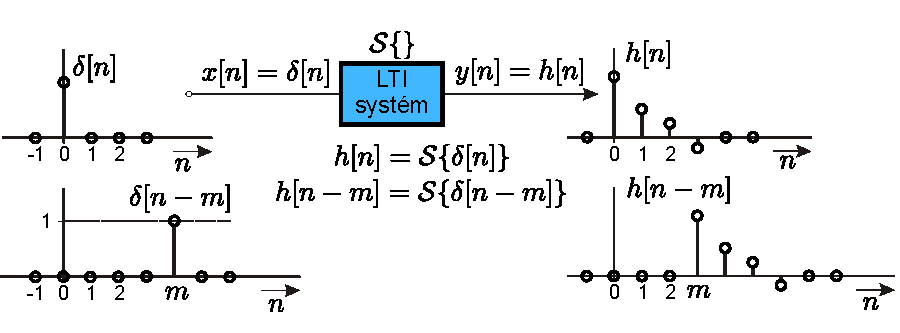
\includegraphics[scale=0.9]{tky_fig002.pdf}
         \caption[impulsní odezva]{Odezva kauzálního diskrétního systému na jednotkový impuls
                  $\delta[n]$ a posunutý impuls $\delta[n-m]$}
        \label{tky:fig002}
      \end{figure*}

      Princip superpozice dovoluje získat odezvu systému jako sumu odezev na jednotlivé dílčí
      součásti vstupního signálu, které v rovnici (\ref{tky:eq015}) tvoří vážené jednotlivé impulsy,
      ze kterých je signál složen
      \begin{align}
        y[n]=\mathcal{S}\{x[n]\}
          &=\mathcal{S}\{\sum_{m=-\infty}^{\infty}x[m]\delta[n-m]\}  \nonumber \\
          &=\sum_{m=-\infty}^{\infty}x[m]\mathcal{S}\{\delta[n-m]\}. \label{tky:eq016}
      \end{align}
      Protože platí (\ref{tky:eq011}) a v důsledku časové invariance vyplývá z rovnice
      \ref{tky:eq016} \textbf{konvoluční suma} 
      \begin{align}
        y[n]&=\sum_{m=-\infty}^{\infty}h[n-m]x[m]               \nonumber \\
            &=\sum_{k=-\infty}^{\infty}h[k]x[n-k].              \label{tky:eq017}
      \end{align}
      Uvedli jsme, že u kauzálního systému závisí výstupní signál $y[n]$ pouze na současných a
      minulých hodnotách vstupního signálu $x[n], x[n-1], x[n-2], \cdots ,$ takže v konvoluční sumě
      \ref{tky:eq017}
      \begin{align*}
        y[n]&=\sum_{k=-\infty}^{\infty}h[k]x[n-k]              \\               
            &=\sum_{k=-\infty}^{-1}h[k]x[n-k] + \sum_{k=0}^{\infty}h[k]x[n-k]  
      \end{align*}
      musíme položit všechny členy impulsní odezvy $h[k]=0$ pro $k<0$. Konvoluční suma pro
      lineární, časově invariantní a kauzální systém má pak tvar
      \begin{equation}\label{tky:eq018}
        y[n]=\sum_{k=0}^{\infty}h[k]x[n-k].
      \end{equation}
      Jestliže navíc budeme uvažovat vstupní a výstupní signály, které jsou nulové pro $n<0$ a
      $x[n]\neq0, y[n]\neq0$ pouze pro $n\geq0$, potom platí
      \begin{equation}\label{tky:eq019}
        \boxed{y[n]=\sum_{k=0}^{n}h[k]x[n-k].\,}
      \end{equation}
      nebo
      \begin{equation}\label{tky:eq024}
        \boxed{y[n]=\sum_{k=0}^{n}x[k]h[n-k].\,}
      \end{equation}
      kde \(n\) je pořadový index právě počítaného vzorku výstupní posloupnosti a \(k\) je pořadový
      index vstupní posloupnosti. Je-li délka vstupní posloupnosti \(N_x\) a délka impulzní odezvy
      \(N_h\), pak délka výstupní posloupnosti (počet jejich vzorků) je dána vztahem:
      \begin{equation}\label{tky:eq025}
        N_y = N_x + N_h - 1.
      \end{equation}
      Rovnice \ref{tky:eq019} a \ref{tky:eq024} určují způsob výpočtu výstupního signálu LTI
      systému. Výstupní signál \(y[n]\) je dán součtem prvků impulsové odezvy a vstupního signálu,
      přičemž buď vstupní signál \ref{tky:eq019} nebo impulsová odezva \ref{tky:eq024} jsou otočeny
      v čase \cite[s.~14]{Davidek1996}.
      
      Symbolicky se tato operace zapisuje 
      \begin{equation}\label{tky:eq026}
        \boxed{y[n] = h[n]*x[n]. \,}
      \end{equation}
      %---------------------------------------------------------------
      % !TeX spellcheck = cs_CZ Lineární obvody a systémy - Jan Bičák  - strana 10 Popis spojitých systémů
%===================================================================================================
\begin{mdframed}[style=mdexam]
  \begin{example}\label{tky:exam001}
    Uvažujme LTI systém, popsaný svou impulzní odezvou: \(h[n] = \{0.45, 1.72, 0.62\}\). Na jeho
    vstupu působí posloupnost \(x[n] = \{2,  0.95\}\). Úkolem  je vypočítat vzorky výstupní
    posloupnosti \(y[n]\).

    \noindent\textbf{Řešení:} Podle (\ref{tky:eq025}) bude délka výstupní posloupnosti \(N_y = 2 + 3
    - 1= 4\) s pořadovými indexy 0 až 3. Pro její výpočet rozepíšeme vztah (\ref{tky:eq024}):
    \begin{align*}
      y[0] &= \sum_{k=0}^0 x[0]h[0] = \num{2}\cdot\num{0.45} = \num{0.9}                   \\
      y[1] &= \sum_{k=0}^1 x[k]h[1-k] = x[0]h[1] + x[1]h[0] =                              \\
           &=  \num{2}\cdot\num{1.72} + \num{0.95}\cdot\num{0.45} = \num{3.8675}           \\
      y[2] &= \sum_{k=0}^2 x[k]h[2-k] =                                                    \\
           &= x[0]h[2] + x[1]h[1] + x[2]h[0] =                                             \\
           &= \num{2}\cdot\num{0.62} + \num{0.95}\cdot\num{1.72} + \num{0}\cdot\num{0.45}  
            = \num{2.8740}                                                                 \\
      y[3] &= \sum_{k=0}^3 x[k]h[3-k] =                                                    \\
           &= x[0]h[3] + x[1]h[2] + x[2]h[1] +  x[3]h[0] =                                 \\
           &= \num{2}\cdot\num{0} + \num{0.95}\cdot\num{0.62} + \num{0}\cdot\num{1.72}
            + \num{0}\cdot\num{0.45} =                                                     \\
           &= \num{0.589} 
    \end{align*} 
    Pro výstupní posloupnost tedy platí:
    \begin{equation*}
      y[n] = \{\num{0.9}, \num{3.8675}, \num{2.8740}, \num{0.589}\}
    \end{equation*}
    Situaci názorně shrnuje obr. \ref{tky:fig011}

    {\centering
      \captionsetup{type=figure}
      \luafigure[1]{tky_fig011.pdf}
      \captionof{figure}{Odezva lineárního číslicového systému na vstupní posloupnost. 
                \cite{Zaplatilek2013}}
      \label{tky:fig011}
    \par}

    V systému \textsc{MATLAB} je vestavěna vnitřní funkce \lstinline[style=luaMatlabText]!conv! pro
    snadný výpočet lineární diskrétní konvoluce, jak dokumentuje výpis \ref{tky:lst001}. Vyzkoušejme
    si, že obrátíme-li pořadí proměnných v příkazu \lstinline[style=luaMatlabText]!conv!, vyjde
    shodný výsledek (komutace symbolů).
  \end{example} 
  \begin{lstlisting}[style=luaMatlabText,gobble=4, label={tky:lst001}]
    h = [0.45, 1.72, 0.62];
    x = [2,  0.95];
    y = conv(x,h)
  \end{lstlisting}

\end{mdframed}
      %---------------------------------------------------------------

    \subsection{Konvoluce ve spojitých systémech}\label{tky:IchIIsecIssecIII}
      Podobně můžeme postupovat i v analogovém případě a odvodit pro lineární časově invariantní
      systém \emph{konvoluční integrál}. Vraťme se k výrazu \ref{tky:eq015} kterým jsme vyjádřili
      libovolný diskrétní signál. Pro případ spojitého signálu vytvořme analogickou formu zápisu
      využívající jednotkový impuls. Průběh obecného spojitého lze podle obr. \ref{tky:fig007}
      aproximovat stupňovitým průběhem, který můžeme vyjádřit jako sumu posunutých (zpožděných)
      impulsů. Výchozí aproximující impuls lze vyjádřit vztahem
      \begin{equation}\label{tky:eq027}
          \delta_\varepsilon(t)  =
            \begin{cases}
               \frac{1}{\varepsilon} & \text{pro } \abs{t} < \frac{\varepsilon}{2},      \\
               0                  & \text{pro } \abs{t} > \frac{\varepsilon}{2} > 0
            \end{cases}
      \end{equation}
      a je znázorněn na obr. \ref{tky:fig007b}. \emph{Jednotkový (Diracův) impuls} 
      má jednotkovou plochu.
      \begin{figure}[ht!]
        \centering
          \subcaptionbox{\label{tky:fig007a}}{\luafigure[0.60]{tky_fig007a.pdf}}                                                  
          \subcaptionbox{\label{tky:fig007b}}{\luafigure[0.27]{tky_fig007b.pdf}}                    
        \caption{a) Aproximace spojitého průběhu signálu, b) K odvození jednotkové impulsní funkce 
        (\cite[s.~7]{Bicak2007})}
        \label{tky:fig007}
      \end{figure}
      Matematicky můžeme Diracovův impuls definovat výrazem
      \begin{equation}\label{tky:eq028}
        \delta_\varepsilon(t) = \lim_{\varepsilon\rightarrow0} \delta_\varepsilon(t).
      \end{equation}
      Aproximaci spojitého průběhu $x(t)$ impulsy \ref{tky:eq027} lze vyjádřit rovnicí
      \begin{equation}\label{tky:eq029}
        x(t)=\sum_{m=-\infty}^\infty x(m\varepsilon)\delta_\varepsilon(t-m\varepsilon)\varepsilon.
      \end{equation}
      Zmenšování šířky impulsů $\varepsilon\rightarrow0$ se chyba aproximace zmenšuje a výraz přejde
      v limitu
      \begin{equation}\label{tky:eq030}
        x(t) = \lim_{\varepsilon\rightarrow0}
               \sum_{m=-\infty}^\infty x(m\varepsilon)\delta_\varepsilon(t-m\varepsilon)\varepsilon.        
      \end{equation}
      V limitě kdy $\varepsilon\rightarrow0$, můžeme sumu nahradit integrálem, dále součin
      $m\varepsilon$ integrační proměnnou $\tau$ a $\varepsilon$ jejím diferenciálem. Obdržíme
      \begin{equation}\label{tky:eq031}
        x(t) = \int_{-\infty}^{\infty}x(\tau)\delta(t-\tau)d\tau .
      \end{equation}
      Vztahem \ref{tky:eq031} jsme spojitý průběh signálu vyjádřili jako sumu
      nekonečného počtu posunutých jednotkových impulsů váženou jeho okamžitými hodnotami.
      Předpokládejme dále, že na vstup lineárního časově invariantního spojitého systému je převeden
      jednotkový (Diracův) impuls a systém vytvoří odezvu $h(t)$. V případě obecného vstupního
      spojitého signálu $x(t)$ aproximovaného vztahem \ref{tky:eq031}, bude odezva
      analogového systému
      \begin{equation}\label{tky:eq032}
        \boxed{y(t) = \int_{-\infty}^{\infty}x(\tau)h(t-\tau)d\tau, \,}
      \end{equation}
      nebo
      \begin{equation}\label{tky:eq033}
        \boxed{y(t) = \int_{-\infty}^{\infty}h(\tau)x(t-\tau)d\tau.\,}
      \end{equation}
      Uvedený integrál nazýváme \textbf{konvolucí} a velmi často ho označujeme jako 
      \begin{equation}\label{tky:eq034}
        \boxed{y(t) = h(t)*x(t).\,}
      \end{equation}
      Funkce $h(t)$ představuje \emph{impulsní odezvu}. Jedná se o výstupní signál systému, na 
      jehož vstupu se uplatní Diracův impuls $x(t)=\delta(t)$. Platí totiž
      \begin{equation}\label{tky:eq035}
        y(t) = \int_{-\infty}^{\infty}h(\tau)\delta(t-\tau)d\tau = h(t) . 
      \end{equation}     
      Z důvodů \emph{kauzality}, která vyjadřuje zachování příčinné posloupnosti událostí při 
      transformaci signálu ze vstupu na výstup, požadujeme
      \begin{align}\label{tky:eq036}
        h(t) &\neq  0 \text{   pro } \abs{t} \geq0, \\
        h(t) &  =   0 \text{   pro } \abs{t} < 0. 
      \end{align}    
      Potom můžeme konvoluční integrál \ref{tky:eq032} zapsat ve tvarem
      \begin{equation}\label{tky:eq037}
         y(t) = \int_0^{\infty}h(\tau)x(t-\tau)\dd\tau.
      \end{equation} 
  
  \section{Popis spojitých a diskrétních systémů, přenosová funkce}\label{tky:IchIIsecIII}
    \subsection{Spojité systémy}
      Lineární časově invariantní (LTI) spojitý systém je obecně popsán soustavou
      integrodiferenciálních rovnic s konstantními koeficienty, kterou lze postupným derivováním
      změnit na soustavu diferenciálních rovnic. Předpokládejme budící (nezávislou) veličinu
      $x(t)$ a odezvou (závislou) výstupní veličinu $y(t)$, pak eliminací ostatních proměnných bude
      soustava popsána jedinou diferenciální rovnicí s konstantními koeficienty tvaru
      \begin{equation}\label{tky:eq038}
          \sum_{i=0}^na_i\frac{d^iy(t)}{dt^i}=\sum_{j=0}^mb_j\frac{d^jx(t)}{dt^j},
      \end{equation}
      kde $a_0, a_1, \cdots ,a_n$ a $b_0, b_1, \cdots ,b_m$ jsou konstanty charakterizující lineární
      systém. Obecné řešení $y(t)$ rovnice \ref{tky:eq038} se sestává ze dvou částí, z 
      řešení \emph{homogenní rovnice} a \emph{partikulárního řešení}. K řešení je třeba znát 
      počáteční podmínky pro $y(t)$ a jeho derivace ve výchozím okamžiku.
  
      S použitím \emph{Laplaceovy transformace při nulových počátečních podmínkách} má rovnice
      (\ref{tky:eq038}) tvar
      \begin{equation}\label{tky:eq039}
        \sum_{i=0}^na_ip^iY(p)=\sum_{j=0}^mb_jp^jX(p),
      \end{equation}
      kde $X(p)=\mathcal{L}\{x(t)\}$ a $Y(p)=\mathcal{L}\{y(t)\}$ jsou Laplaceovy obrazy vstupní a
      výstupní veličiny, $p$ je Laplaceův operátor derivace a také komplexní kmitočet
      $p=\sigma+\jmath\omega$. Přenosová funkce $H(p)$ je definována jako podíl Laplaceova obrazu
      výstupní veličiny $Y(p)$ ku obrazu vstupní veličiny $x(p)$, při nulových počátečních
      podmínkách
      \begin{equation}\label{tky:eq040}
          H(p)=\frac{Y(p)}{X(p)}.
      \end{equation}
      Vzhledem k rovnici (\ref{tky:eq039}) je $H(p)$ racionálně lomenou funkcí tvaru
      \begin{align}
        H(p)&=\frac{b_mp^m+b_{m-1}p^{m-1}+\cdots+b_0}{a_np^n+b_{n-1}p^{n-1}+\cdots+a_0}  \nonumber\\
            &=\frac{\Pi_{j=1}^m(p-p_{0j})}{\Pi_{i=1}^n(p-p_{\infty i})}            \label{tky:eq002}
      \end{align}
      kde $p_{0j}$ jsou kořeny polynomu čitatele a představují \textbf{nulové body} a kořeny
      jmenovatele $p_{\infty i}$ jsou \textbf{póly} přenosové funkce, $H_0=\frac{b_m}{a_n}$ je
      násobná konstanta.
  
      Kmitočtové charakteristiky získáme z přenosové funkce substitucí
      \begin{equation}\label{tky:eq041}
          p = \jmath\omega,
      \end{equation}
      ve které $\omega$ je úhlový kmitočet. Platí tedy
      \begin{align}
          H(p)\mid_{p = \jmath\omega} 
            &=\frac{b_m(\jmath\omega)^m+b_{m-1}(\jmath\omega)^{m-1}                     
             +\cdots+b_0}{a_n(j\omega)^n+b_{n-1}(\jmath\omega)^{n-1}+\cdots+a_0}   \nonumber \\
            &=M(\omega)e^{\jmath\Phi(\omega)},                                     \label{tky:eq003}
      \end{align}
      kde $M(\omega) = \abs{H{\jmath\omega}}$ je \textbf{modulová charakteristika} a
      $\Phi(\omega)=\texttt{arg}H(j\omega)$ se nazývá \textbf{fázová charakteristika}. Skupinové
      zpoždění je definováno jako záporně vzatá derivace fázové charakteristiky podle kmitočtu
      \begin{equation}\label{tky:eq042}
        \tau(\omega)=-\frac{d\Phi(\omega)}{d\omega}= -\der{\texttt{arg} H(\jmath\omega)}{\omega}.
      \end{equation}
      V předchozí kapitole jsme ukázali, že \emph{relace vstup/výstup LTI systému} souvisí
      prostřednictvím \emph{konvoluce}
      \begin{equation}\label{tky:eq043}
          y(t)=\int_0^\infty h(\tau)x(t-\tau)d\tau = h(t)*x(t).
      \end{equation}
      Přenosová funkce je Laplaceova transformace impulsní odezvy $h(t)$
      \begin{equation}\label{tky:eq044}
          H(p)=\mathcal{L}[h(t)]=\int_0^\infty h(t)e^{-pt}dt,
      \end{equation}
      pro kterou je splněn vztah
      \begin{equation}\label{tky:eq045}
          Y(p)=H(p)X(p).
      \end{equation}
      Přechodová odezva $s(t)$ je definována jako integrál impulsní odezvy
      \begin{equation}\label{tky:eq046}
          s(t)=\int_0^th(\tau)d\tau,
      \end{equation}
      takže platí
      \begin{equation}\label{tky:eq047}
          s(t)=\mathcal{L}^{-1}\{\frac{H(p)}{p}\}.
      \end{equation}
      Algoritmus výpočtu impulsní odezvy z přenosové funkce je založen na výpočtu  reziduí a 
      rozkladu racionálně lomené funkce $H(p)=\frac{Q(p)}{N(p)}$ na částečné zlomky. Pokud má tato 
      funkce jednoduché póly, rozklad má tvar\footnote{Násobnost kořenů $N(p)$ neuvažujeme, protože 
      se v LTI obvodech neuplatňuje}.
      \begin{align}
         H(p)&=\frac{Q(p)}{N(p)} 
              =\sum_{\mu=1}^{n}\frac{k_\mu}{p-p_{\infty_\mu}}                  \nonumber \\
             &=\frac{k_1}{p-p_{\infty_1}}+\frac{k_2}{p-p_{\infty_2}}
               +\cdots+\frac{k_n}{p-p_{\infty_n}}                              \label{tky:eq004}
      \end{align}
      kde $k_\mu$ se nazývají rezidua v pólech $p_{\infty_\mu})$ a platí
      \begin{align}
        k_\mu &= \lim_{p\to p_{\infty_\mu}}(p-p_{\infty_\mu})\frac{Q(p)}{N(p)}  \nonumber \\
        \,    &= Q(p_{\infty_\mu})\lim_{p\to
                 p_{\infty_\mu}}\frac{1}{\frac{N(p)}{p-p_{\infty_\mu}}}=
                 Q(p_{\infty_\mu})\frac{1}{N'(p_{\infty_\mu})}                  \label{tky:eq006}
      \end{align}
      impulsní odezva je pak dána vztahem
      \begin{equation}\label{tky:eq023}
        h(t)=\mathcal{L}^{-1}[H(p)]=\sum_{\mu=1}^nk_\mu e^{p_{\infty_\mu}t}
      \end{equation}
      Póly jsou obecně komplexní $p_{\infty_{\mu}}=\alpha_\mu+j\beta_\mu$, nebo reálné
      $p_{\infty_{\mu}}=\alpha_\mu$. Jsou to kořeny rovnice $N(p)=0$. Rovnice \ref{tky:eq023} je
      důležitá i proto, že z ní poznáme, zda analogová soustava je stabilní. Je patrné, že soustava
      bude stabilní, jestliže bude $\mathcal{R}\{p_{\infty_{\mu}}\}=\alpha_\mu<0$, tj. leží-li
      kořeny $p_{\infty_{\mu}}$ v otevřené levé polorovině komplexní roviny
      $p_{\infty_{\mu}}=\sigma+j\omega$. Imaginární osa $j\omega$ je mezí stability, pravá
      polorovina je oblastí nestability. Polynom, který má kořeny v levé otevřené polorovině se
      označuje \textbf{Hurwitzův polynom}.
      
      %---------------------------------------------------------------
      % !TeX spellcheck = cs_CZ Lineární obvody a systémy - Jan Bičák  - strana 10 Popis spojitých systémů
%===================================================================================================
\begin{mdframed}[style=mdexam]
  \begin{example}\label{tky:exam002}
    Lineární spojitý systém je dán zapojením dle obrázku. Určete:
    \begin{enumerate}[leftmargin=12pt,noitemsep]
      \item diferenciální rovnici pro odezvu $u_2(t)$, je-li na vstupu buzen napětím $u_1(t)$,
      \item přenos napětí $H(p)=\dfrac{U_2(p)}{U_1(p)}$,
      \item impulsní odezvu $h(t)$.
    \end{enumerate}

    {\centering
      \captionsetup{type=figure}
      \luafigure[1]{tky_fig008.pdf}
      \captionof{figure}{Zapojení obvodu RLC.}
      \label{tky:fig008}
    \par}
    \noindent\textbf{Řešení:} Pro zapojení dle obrázku \ref{tky:fig008} získáme metodou uzlových
    napětí integrodiferenciální rovnice pro uzly \texttt{A} a \texttt{B}:
    \begin{gather*}
      \begin{align*} %\label{tky:eq019}
        \shortintertext{uzel A:}
        \frac{u_3(t)-u_1(t)}{R}+\frac{1}{L}\int_0^t{[u_3(t)-u_2(t)]}\dd{\tau}+i_L(0_+) &= 0  \\
        \shortintertext{uzel B:}
        \frac{1}{L}\int_0^t[(u_2(t)-u_3(t))]\dd{\tau}+C\der{u_2}{t}-i_L(0_+)           &= 0
      \end{align*}
    \end{gather*}
    ve kterých \(i_L(0_+)\) je počáteční podmínka pro proud induktoru. Derivováním a eliminací
    $u_3(t)$ z původních rovnic dostaneme pro odezvu $u_2(t)$ diferenciální rovnici II. řádu.
    Začneme derivováním rovnice v uzlu \texttt{B} tj. \(\frac{d}{dt}(B)\):
    \begin{align*}
      u_2(t)-u_3(t)+LC\frac{d^2u_2(t)}{dt^2} &=0 \Rightarrow   \\
      u_2(t)+LC\frac{d^2u_2(t)}{dt^2}        &=u_3(t)
    \end{align*}
    Nyní můžeme z rovnice pro uzel \texttt{A} odstranit napětí \(u_3(t)\):
    \begin{align*}
      \frac{u_2(t)+LC\dfrac{d^2u_2(t)}{dt^2}-u_1(t)}{R}             &+    \\
      \frac{1}{L}\int_0^t{(LC\frac{d^2u_2(t)}{dt^2})}\dd{\tau}+i_L(0_+) &=  0 \\
      \shortintertext{}
      u_2(t)+LC\frac{d^2u_2(t)}{dt^2}-u_1(t)                        &+    \\
      RC\left[\frac{du_2(t)}{dt}\right]_0^t+Ri_L(0_+)               &=  0
    \end{align*}
    Při nulových počátečních podmínkách: $\left.\frac{du_2(t)}{dt}\right\rvert_{t=0}=0$,
    $i_L(0_+)=0$ dostaneme:
    \begin{equation*}
      \boxed{LC\frac{d^2u_2(t)}{dt^2}+RC\frac{du_2(t)}{dt}+u_2(t)=u_1(t)}
    \end{equation*}
    V Laplaceově transformaci platí:
    \begin{align*}
      \mathcal{L}\left[\frac{du_2(t)}{dt}\right]     &= pU_2(p)-u_2(0) \\
      \mathcal{L}\left[\frac{d^2u_2(t)}{dt^2}\right] &= p^2U_2(p)-pu_2(0)-\dot{u}_2(0),
    \end{align*}
    kde \(\dot{u}_2(0)=\left.\frac{du_2(t)}{dt}\right\rvert_{t=0}\). Při nulových počátečních
    podmínkách \(u_2(0) = 0\), \(\dot{u}_2(0) = 0\) a užitím Laplaceovy transformace přejde
    diferenciální rovnice na algebraickou rovnici:
    \begin{equation*}
      p^2LCU_2(p)+pRCU_2(p)+U_2(p)=U_1(p)
    \end{equation*}
    Odtud vyplývá \textbf{přenosová funkce} $H(p)=\frac{U_2(p)}{U_1(p)}$
    \begin{align}
      H(p) &=\dfrac{1}{p^2LC+pRC+1}                                   \nonumber \\
           &=\dfrac{1}{LC}\frac{1}{p^2+p\dfrac{R}{L}+\dfrac{1}{LC}}
            =\frac{Q(p)}{N(p)}                                        \label{tky:eq020}
    \end{align}
    K nalezení \textbf{impulsní odezvy} nejprve určíme póly přenosové funkce řešením rovnice
    $N(p)=0$
    \begin{align}
      p_{\infty_{12}} 
        &=\dfrac{\dfrac{R}{L}\pm\sqrt{\left(\dfrac{R}{L}\right)^2-\dfrac{4}{LC}}}{2}   \nonumber \\
        &=\frac{R}{2L}\pm\sqrt{\left(\frac{R}{2L}\right)^2-\frac{1}{LC}}          \label{tky:eq021}
    \end{align}
    a přenosovou funkci pak upravíme do tvaru
    \begin{equation*}
      H(p)=\frac{K}{(p-p_{\infty_1})\cdot(p-p_{\infty_2})}, \quad K=\frac{1}{LC}
    \end{equation*}
    kde \(K\) je násobná konstanta a \(p_{\infty_{1,2}}\) jsou její póly. 
    \begin{itemize}[leftmargin=12pt,noitemsep]
      \item Uvažujeme-li jednoduché póly a bude-li $R>2\sqrt{\frac{L}{C}}$ , potom z  rov.
            \ref{tky:eq021} vyplývají dva reálné různé póly. Přenosovou funkci tedy můžeme
            zapsat obecným tvarem:
            \begin{equation*}
              H(p)=\frac{K}{(p+a_1)\cdot(p+a_2)}=\frac{k_1}{p+a_1}+\frac{k_2}{p+a_2}
            \end{equation*}
            kde $p_{\infty_1}=-a_1,\, p_{\infty_2}=-a_2$, Rezidua  \(k_1\), \(k_2\) určíme z rov.
            \ref{tky:eq006}. 
            \begin{equation*}
              k_1=\frac{K}{a_2-a_1}, \quad k_2=\frac{K}{a_1-a_2}.
            \end{equation*}
            Impulsní odezvu pak vypočteme užitím rov. \ref{tky:eq023}.
            \begin{align*}
              h(t)&=\mathcal{L}^{-1}[H(p)]               \\
                  &=\frac{K}{a_2-a_1}e^{-a_1t}+\frac{K}{a_1-a_2}e^{-a_2t}
            \end{align*}
      \item Když bude $R<2\sqrt{\frac{L}{C}}$, obdržíme dvojici komplexně sdružených pólů a
            přenosovou funkci může obecně zapsat takto:
            \begin{equation*}
              H(p)=\frac{K}{(p+a_1)\cdot(p+a_2)}=\frac{k_1}{p+a-jb}+\frac{k_2}{p+a+jb}
            \end{equation*}
            kde $p_{\infty_1}=-a+jb$, $p_{\infty_2}=-a-jb$. Rezidua v pólech jsou dány výrazy
            $k_1=-\frac{jK}{2b}$, $k_2=\frac{jK}{2b}$. Impulzní odezvu opět určíme užitím rov.
            \ref{sas:eq_impulzni_odezva}.
            \begin{equation*}
              h(t) = \frac{Ke^{-at}}{2b}\left[j\cdot\left(-e^{jbt}+e^{-jbt}\right)\right]
            \end{equation*}
            \begin{gather*}
              \begin{align*}
                \,  &= \frac{Ke^{-at}}{2b}\left[j\cdot
                \left(\underline{-\cos(bt)}-j\sin(bt)+
                \underline{\cos(bt)}-j\sin(bt)\right)\right]                        \\
                \,  &= \frac{K}{b}e^{-at}\sin(bt)                                   
              \end{align*}
            \end{gather*}
    \end{itemize}
    
    Na obr. \ref{tky:fig009} je uvedena impulsní charakteristika uvaožovaného obvodu odpovídající
    hodnotám stavebních prvků: \(R=\SI{1}{\kohm}\), \(L=\SI{11.5}{\milli\henry}\),
    \(C=\SI{22.5}{\nano\farad}\). Výpis m-file \texttt{SAS\_exam\_02\_symb\_Hp\_solve.m} ukazuje
    symbolický způsob řešení operátorových obvodových rovnic pomocí \texttt{MATLABu}. Jde o filtr
    typu \textbf{dolní propust}, jehož přenosová funkce má tvar:
    $$H(p)= \frac{3.9506\cdot10^9}{p^2+8.8889\cdot10^4p+3.9506\cdot10^9}.$$
    %---------------------------------------------------------------
      \lstinputlisting[% style=luaMatlabStyle,
      caption={TKY\_exam\_02\_symb\_Hp\_solve.m}]{../src/TKY/matlab/SAS_exam_02_symb_Hp_solve.m}
    %---------------------------------------------------------------
    Impulzní charakteristiku obdržíme dosazením do vztahu \ref{tky:eq005}
    $$h(t)=\frac{K}{b}e^{-at}\sin(bt) =8.8890\cdot10^4e^{-4.4444\cdot10^4t}\sin(4.4444\cdot10^4t).$$
    
      {\centering
      \captionsetup{type=figure}
      \luafigure[1]{tky_fig009.pdf}
      \captionof{figure}{Impulzní charakteristika}
      \label{tky:fig009}
      \par}
    
    Z hlediska analýzy obvodů v kmitočtové oblasti je výhodné sestavovat obvodové rovnice (metodami
    uzlových napětí a smyčkových proudů) přímo v operátorovém tvaru. Kirchhoffovy zákony pro
    uzavřenou smyčku a proudu do uzlu pak mají tvar $$\sum_{k=1}^{n}U_k(p) = 0, \qquad
    \sum_{k=1}^{n}I_k(p) = 0.$$ Metodou uzlových napětí pro zapojení na obr. \ref{tky:fig008}
    obdržíme rovnice
    \begin{align}
      \frac{U_3(p)-U_1(p)}{R}+\frac{U_3(p)-U_2(p)}{pL} &=  0 \\
      pCU_2(p) + \frac{U_2(p)-U_3(p)}{pL}              &=  0 
    \end{align}
    Na rozdíl od \ref{tky:eq019} jde o algebraické rovnice, ze kterých eliminací uzlového napětí
    $U_3(p)$ vyplývá přenosová funkce \ref{tky:eq020} $$H(p) = \frac{U_2(p)}{U_1(p)} =
    \frac{1}{LC}\frac{1}{p^2+p\frac{R}{L} + \frac{1}{LC}}$$
    
    {\centering
      \captionsetup{type=figure}
      \luafigure[1]{tky_fig010.pdf}
      \captionof{figure}{Modulová, fázová charakteristika a skupinové zpoždění filtru}
      \label{tky:fig010}
      \par}    
    
    Dosazením za $p=j\omega$ lze z přenosové funkce vyjádřit modulovou charakteristiku $H(j\omega)$
    a fázovou charakteristiku $\Phi(\omega)= \texttt{arg} H(j\omega)$. Skupinové zpoždění vyplývá ze
    vztahu \ref{SAS:eq_skupinove_zpozdeni}. Modulová, fázová charakteristika a skupinové zpoždění
    jsou na obr. \ref{tky:fig010}.
    
    Filtr má maximálně plochou modulovou charakteristiku přenosu. Mezní kmitočet propustného pásma
    je $f_p = 10 kHz$, při kterém je $\abs{H(j\omega_p)}= 0.707$. Tato hodnota odpovídá poklesu
    modulové charakteristiky o $3 dB$.
    
    %---------------------------------------------------------------
    \lstinputlisting[% style=luaMatlabStyle,
      caption={TKY\_exam\_03\_Hp.m}]{../src/TKY/matlab/SAS_exam_03_Hp.m}
    %---------------------------------------------------------------  
  \end{example} 
\end{mdframed}
      %---------------------------------------------------------------
%========================= Kapitola: Regulační technika ============================================
  % !TeX program = lualatex
% !TeX root = luaking.tex
% !TeX encoding = UTF-8
% !TeX spellcheck = cs_CZ
%---------------------------------------------------------------------------------------------------
% file tky1ch03.tex
%---------------------------------------------------------------------------------------------------
%============ Kapitola: Regulační technika =========================================================
\setchaptertoc
\chapter{Regulační technika}\label{tky:IchapIII}
  \twocolumn[\section{Kde se vzala, tu se vzala, zpětná vazba}\hypertarget{tky:IchapIII}]
    Protože stojící automobil má aktuální rychlost menší než žádaných \qty{50}{\km\per\hour},
    sešlápneme pedál plynu a automobil začne zrychlovat, což pozorujeme na tachometru. V momentě,
    kdy je aktuální rychlost větší než žádaná, uvolníme v souladu s radami od instruktora pedál
    plynu a rychlost automobilu začne klesat, až bude opět menší než je žádaných
    \qty{50}{\km\per\hour}. Takto budeme dokola sešlapávat a uvolňovat pedál plynu, až dosáhneme
    žádané rychlosti. Jistě si umíme představit, že rychlost dosažení žádané rychlosti, závisí nejen
    na vlastnostech samotného automobilu, ale také na našich řidičských dovednostech. V případě
    opatrného řidiče, bude rozjezd pomalý a tak se rychlost bude blížit žádané pomalu. V případě
    zbrklého řidiče, bude rozjezd velice razantní, což povede k rychlému překročení žádané
    rychlosti. Následné neuvážené odlehčení plynového pedálu povede k prudkému poklesu rychlosti,
    viz zelený průběh na obr. \ref{tky:fig_feedback005}. V obou případech se nelze hovořit o dobrém
    stylu jízdy. V prvním případě se řidič rozjíždí příliš dlouho, na vozovce představuje překážku a
    delší dobu zbytečně unikají splodiny do ovzduší. Ve druhém případě je motor při extrémních
    otáčkách příliš hlučný, dochází k nekvalitnímu spalování a opět k úniku škodlivin do ovzduší.
    Styl jízdy nepůsobí příliš uklidňujícím dojmem na ostatní řidiče a účastníky silničního provozu.

    \begin{figure}[ht!] % \ref{tky:fig_feedback005}
      \centering
      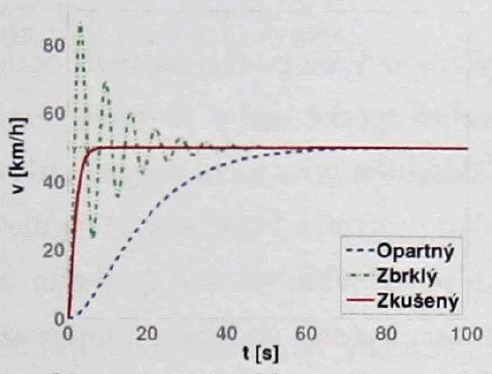
\includegraphics[width=0.7\linewidth]{Reg_smycka03.png}
      \caption{Rychlost automobilu \cite[s.~9]{Roubal2011}.}
      \label{tky:fig_feedback005}
    \end{figure}
    Pro kvalitní dosažení žádané hodnoty rychlosti je třeba znát \emph{dynamický model} automobilu. 
    Tedy nejen sešlápni pedál plynu, uvolni pedál plynu, což můžeme považovat za \emph{statický 
    model} (v čase neproměnný), ale právě popis jak rychle se automobil rozjíždí, když takovým a 
    takovým způsobem sešlápneme pedál plynu. V regulační technice budeme mít dynamický model 
    systému tvořený převážně diferenciálními (pohybovými) rovnicemi. Modelováním reálných 
    dynamických systémů se budeme zabývat v kapitole \ref{TKY:sec002}. Procesu získávání modelu 
    fyzikální reality říkáme \textbf{identifikace systému} a v našem příkladě s automobilem ji 
    vlastně provádíme tím, že se učíme jezdit. Na identifikaci dynamických systémů a její praktické 
    aspekty se zaměříme v kapitole \ref{TKY:sec003}.

    V momentě, kdy máme dynamický model systému, přichází další krok a to je vlastní \textbf{návrh 
    regulátoru}, neboli návrh algoritmu řízení. V momentě, kdy už řidič ví, jak automobil reaguje 
    na změny vstupu, může dosáhnout žádané výstupní veličiny mnohem lépe, viz obr. 
    \ref{tky:fig_feedback003}. Na rozdíl od řidiče, jenž má naučený regulátor ve své hlavě, v 
    regulační technice budeme využívat různé matematické metody. Možná nás nyní napadne, že model 
    automobilu není pouze závislost mezi pedálem plynu a rychlostí automobilu. Chování automobilu 
    ovlivňuje samozřejmě mnoho dalších okolností, jako je přilnavost pneumatik k povrchu vozovky, 
    vlhkost vozovky a podobně. V momentě, kdy například zaprší, může řidič se svým regulátorem v 
    zatáčce opustit vozovku, pokud jsme příliš agresivní, protože se reálný systém změnil, ale jeho 
    model tuto informaci nemá. Opět tedy musíme vzít v potaz nové faktory a provést identifikaci 
    znovu, a tím získat více informací o chování systému za těchto podmínek. Pak bude řidič schopen 
    jezdit bezpečně za sucha i za mokra a tak dále. V regulační technice je vždy přesnost modelu 
    zásadní otázkou. Na jedné straně požadujeme model systému co nejpřesnější, abychom byli schopni 
    navrhnout dobrý regulátor. Na druhé straně se pro příliš složitý model navrhuje regulátor 
    obtížněji. Proto vždy musíme zvolit jistý kompromis tak, aby v modelu byly zahrnuty všechny 
    podstatné vlastnosti systému.

    Tím ale regulace nekončí. Například cena paliva není již dnes zanedbatelná, a tak budeme třeba 
    chtít jezdit s minimální spotřebou. To znamená, že musíme zjistit závislost spotřeby paliva na 
    stylu jízdy. Poté musíme definovat nějaké kritérium kvality regulace obsahující tuto závislost 
    a podle něho navrhnout nový regulátor, který zajistí minimální spotřebu paliva.  Problémů v 
    oblasti řízení je samozřejmě mnohem a mnohem víc  (odhadování a filtrace, robustní řízení a 
    nelineární systémy). My však zde tento příklad ukončíme s konstatováním, že v regulační 
    technice jde především o tyto body:
    \begin{itemize}[noitemsep]
      \item určení vstupů a výstupů systému,
      \item identifikace systému (určení chování systému na výstupech pro nějaké chování vstupů),
      \item návrh regulátoru pro zajištění požadovaných vlastností; testování regulátoru na 
            počítači; aplikace regulátoru na reálném systému; případně návrh v nějakém smyslu 
            optimálního regulátoru.
    \end{itemize}
    
  \section{Regulační smyčka a základní typy PID regulátorů}\label{TKY:sec001}
    Ve snaze řídit systémy rozeznáváme dva hlavní způsoby řízení:
      \begin{itemize}
        \item \textbf{přímovazební},
        \item \textbf{zpětnovazební}.
      \end{itemize}
    \textbf{Přímovazební řízení} (\emph{řízení v otevřené smyčce}), zvané také jako ovládání, má 
    jednodušší zapojení, ovšem jeho nevýhodou je nemožnost reagovat na poruchy či změny soustavy a 
    my se jím zde dále zabývat nebudeme. Naproti tomu \textbf{zpětnovazební řízení} (\emph{řízení v 
    uzavřené smyčce}), obecně označované jako \textbf{regulace}, porovnává \emph{výstup soustavy} 
    \(y(t)\) s \emph{požadovaným výstupem} \(w(t)\), a podle této informace generuje \emph{akční 
    zásah} \(u(t)\) do řízeného systému. Regulace nám tak dává mimo jiné možnost 
    \emph{stabilizovat} nestabilní soustavy.

    \begin{figure}[ht!] % \ref{tky:fig_feedback003}
      \centering
      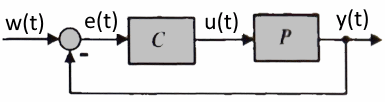
\includegraphics[width=0.8\linewidth]{Reg_smycka01.png}
      \caption{Regulační smyčka \cite[s.~215]{Roubal2011}.}
      \label{tky:fig_feedback003}
    \end{figure}
    V této kapitole se budeme věnovat regulaci, regulační smyčce a základním typů regulátorů. 
    Ukážeme si dvě základní zapojení regulačních smyček a zavedeme jednotné názvosloví, zejména 
    proto, že toto názvosloví není ustálené. Vysvětlíme si některé míry kvality řízení a ukážeme 
    názorně na příkladech vlastnosti základních \textbf{PID regulátorů}. Zvláštní pozornost bude 
    věnována filtraci derivační složky u tohoto regulátoru. Konkrétní způsoby návrhu regulátorů si 
    ukážeme v následujících kapitolách.
    
  
  \section{Modelování fyzikálních systémů}\label{TKY:sec002}
    Doposud jsme se v předešlých kapitolách zabývali různými nástroji, jak popisovat dynamické 
    chování systémů. Šlo spíše o teorii rozdělenou do kapitol bez větších souvislostí. V této kar 
    kapitole bychom chtěli ukázat použití těchto teoretických poznatků na konkrétních příkladech 
    fyzikálních systémů. Odvodíme zde několik matematických modelů fyzikálních systémů a připravíme 
    k těmto modelům simulinkové soubory s virtuální realitou pro Matlab (The Mathworks, 2009).
    
  \section{Identifikace systémů}\label{TKY:sec003}

%} %tikzset
%---------------------------------------------------------------------------------------------------
%========================= Kapitola: Senzory a akční členy =========================================
  % !TeX program = lualatex
% !TeX root = luaking.tex
% !TeX encoding = UTF-8
% !TeX spellcheck = cs_CZ
%---------------------------------------------------------------------------------------------------
% file tky1ch10.tex
%---------------------------------------------------------------------------------------------------
%===============Kapitola:Senzory a akční členy =====================================================
\setchaptertoc
\chapter{Senzory a akční členy}
  \section{Snímače tepelných veličin}
    \href{http://cs.wikipedia.org/wiki/Teplota}{Teplota} je charakteristika tepelného stavu hmoty.
    V obecném významu je to vlastnost předmětů a okolí, kterou je člověk schopen vnímat a přiřadit
    jí pocity studeného, teplého či horkého. V přírodních a technických vědách a jejich aplikacích
    je to \emph{skalární intenzivní veličina}, která je vzhledem ke svému pravděpodobnostnímu
    charakteru vhodná k popisu stavu ustálených makroskopických systémů. Teplota souvisí s
    kinetickou energií částic látky.

    Teplota je základní fyzikální veličinou soustavy \texttt{SI} s jednotkou kelvin (\unit{\kelvin}) a
    vedlejší jednotkou stupeň Celsia (\unit{\degreeCelsius}). Nejnižší možnou teplotou je teplota
    absolutní nuly (\qty{0}{\kelvin}, resp. \qty{-273.15}{\degreeCelsius}), ke které se lze libovolně
    přiblížit, avšak nelze jí dosáhnout.
         
    Do této skupiny patří především rozsáhlá část snímačů teploty. Z hlediska měřených veličin
    můžeme provést následující rozdělení.
    \begin{enumerate}[noitemsep]
      \item \textbf{Snímače teploty}
        \begin{enumerate}[label=\emph{\alph*}),noitemsep]
          \item emph{Snímače pro dotykové měření} 
            \begin{itemize}
              \item elektrické
               \begin{itemize}
                 \item odporové kovové
                 \item odporové polovodičové
                 \item termoelektrické
                 \item polovodičové 
               \end{itemize}   
              \item dilatační
              \item termoelektrické
              \item tlakové
              \item speciální
            \end{itemize}
          \item \emph{Snímače pro bezdotykové měření}
            \begin{itemize}
              \item monochromatické pyrometry
              \item pásmové pyrometry
              \item radiační pyrometry
            \end{itemize}
        \end{enumerate}
      \item \textbf{Snímače tepla}
      \item \textbf{Snímače tepelného toku}
    \end{enumerate}  
       
    \subsection{Elektrické teploměry}
      \subsubsection{Odporové snímače}
        Odporové snímače využívají princip změny elektrického opdoru vlivem změny teplot. Základním
        požadavkem kladeným na materiál snímače je co největší a stálý teplontí součinitel odporu a
        zároveň co největší měrný odpor. Pro tyto účely se používají kovové a polovodičové
        materiály.
        
      \subsubsection{Kovové odporové snímače} 
        Jsou to především čisté kovy, které se používají pro realizaci vlastního odporového
        článku. Požadavkem je, aby nereagovaly s izolačním nebo ochranným krytem. Jakékoliv
        chemické nebo fyzikální vlivy by mohly způsobit nestálost odporu při stálé teplotě,
        Použitý materiál nemá vykazovat změnu teplotního součinitele odporu s časem (stárnutí) a
        hysterezi. Nejčastěji používanými materiály je \emph{platina, nikl, měď, slitina
        stříbro-zlato} a další \cite[s.~96]{Zehnula1983}.
          
        Platina je výhodná pro velkou chemickou stálost, vysokou teplotou tavení a možností
        dosažení vysoké čistoty. Pro snímače teploty se používá tzv. fyzikálně  čistá platina,
        jejíž čistota se pohybuje kolem 99,93 až 99,99 \% Pt. Měření ukázala, že změny
        základního odporu u sériově vyráběných přesných teploměru se pohybují kolem
        \num{5e-6} \(R_o\) (což odpovídá \qty{0.001}{\kelvin}), u nejlepších teploměrů je tato
        hodnota ještě o řád menší. Proto se používá platina pro etalonový teplměr v oblasti
        teplot \qty{-259.34}{\degreeCelsius} až \qty{630.74}{\degreeCelsius}.
        
        Závislost odporu na teplotě pro rozsah \num{0} až \qty{630}{\degreeCelsius} se vyjadřuje
        rovnicí
        \begin{equation}\label{SAC:kov_Ro1}
          R_\vartheta = R_0(1 + A\vartheta + B\vartheta^2)
        \end{equation}
        kde 
        \begin{description}[leftmargin=5em,labelindent=2em, style=nextline]
          \item[\(R_0\)]        \(\ldots\) \emph{odpor při \qty{0}{\degreeCelsius}}, 
          \item[\(\vartheta\)]  \(\ldots\) \emph{teplota ve \unit{\degreeCelsius}}, 
          \item[\(A\)]          \(\ldots\) \emph{konst (\qty{3.9075e-3}{\per\degreeCelsius})},
          \item[\(B\)]          \(\ldots\) \emph{konst (\qty{-0.575e-6}{\per\degreeCelsius})}. 
        \end{description}

        V rozmezí od \qty{0}{\degreeCelsius} do \qty{-190}{\degreeCelsius} se vyjadřuje
        závislost odporu na teplotě rovnicí
        \begin{equation}\label{SAC:kov_Ro2}
          R_\vartheta = R_0[1 + A\vartheta + B\vartheta^2 + C(\vartheta - 100)\vartheta^3)]
        \end{equation}       
%=============== Seznam literatury ================================================================= 
  \printbibliography[title={Seznam literatury}, heading=bibliography]
}
    %===================================================================================================
% Teorie elektrických obvodů
% TEO.tex
%===================================================================================================
% notes:
%~~~~~~~~~
% \ref{TEO:eq100}
% \ref{teo:fig021}
% \ref{fyz:exam001}
% \ref{fyz:tab000}
%---------------------------------------------------------------------------------------------------
% Setting path to image 
\graphicspath{{../src/TEO/img/}}
%---------------------------------------------------------------------------------------------------
%                            /$$$$$$$$ /$$$$$$$$  /$$$$$$ 
%                            |__ $$__/| $$_____/ /$$__  $$
%                              | $$   | $$      | $$  \ $$
%                              | $$   | $$$$$   | $$  | $$
%                              | $$   | $$__/   | $$  | $$
%                              | $$   | $$      | $$  | $$
%                              | $$   | $$$$$$$$|  $$$$$$/
%                              |__/   |________/ \______/ 
%---------------------------------------------------------------------------------------------------
\ifthenelse{ \equal{\DebugMode}{true} }{% Debug mode ON
  % % !TeX program = lualatex
% !TeX root = luaking.tex
% !TeX encoding = UTF-8
% !TeX spellcheck = cs_CZ
%---------------------------------------------------------------------------------------------------
% file spojity_model_elmag_p.tex
\graphicspath{{../src/TEO/img/}}
%==============================Kapitola: Spojité matematické modely jednotlivých polí ==============
\setchaptertoc
\chapter{Spojité matematické modely polí}

  \section{Elektromagnetické pole}
    \subsection{Veličiny elektromagnetického pole a jejich jednotky}
      \fbox{Elektrický náboj} je \emph{skalární veličinou}. Jednotkou je \emph{coulomb [C]}. Má
         kvantový charakter (tj. je roven celistvému násobku elementárního náboje $e =
         1,602\cdot10^{-19}C$), avšak v technických aplikacích k tomu nepřihlížíme. Náboj $Q$
         může být rozložen:
         \begin{itemize}[noitemsep]
            \item \emph{prostorově} v objemu $V$ s objemovou hustotou
               \begin{equation}\label{TEMP:eq_q_varrho}
                  \varrho = \frac{dQ}{dV} \quad [C\cdot m^{-3}]
               \end{equation}               
            \item \emph{plošně} na ploše $S$, s plošnou hustotou
               \begin{equation}\label{TEMP:eq_q_sigma}
                  \sigma = \frac{dQ}{dS} \quad [C\cdot m^{-2}]
               \end{equation}                 
            \item \emph{lineárně} na křivce $l$, s lineární hustotou
               \begin{equation}\label{TEMP:eq_q_tau}
                  \tau = \frac{dQ}{dl} \quad [C\cdot m^{-1}]
               \end{equation}                 
         \end{itemize}
         Rozlišujeme:
           \begin{itemize}[noitemsep]
             \item \textbf{volné náboje}: mohou se přemisťovat v makroskopických
             vzdálenostech,
             \item \textbf{vázané náboje}: mohou se přemisťovat jen v
             mikroskopických vzdálenostech.
           \end{itemize}
         Volnými náboji jsou volné elektrony v kovech nebo ionty v elektrolytech (jsou odpoutány od
         atomů, resp. molekul a volně se mezi nimi pohybují); vázané náboje vznikají polarizací
         dielektrika.
         
      \vspace{1em}
      \fbox{Elektrický proud}\label{TEMP:kap_el_proud_velicina} je znám z každodenního života,
        přesto je velmi důležité umět tento pojem vnímat jak pro označení „jevu“ (kap.
        \ref{TEMP:kap_elproud_jev}), tak jako fyzikální veličinu, která tento jev kvantitativně
        popisuje (kap. \ref{TEMP:kap_el_proud_velicina} ). Elektrický proud je \emph{skalární
        fyzikální veličina} tzn. $I$ resp. $i$, jejíž jednotkou je základní jednotka soustavy SI:
        \emph{ampér} - [A]. V této soustavě jednotek je ampér definován na základě silových
        účinků mezi dvěma vodiči, kterými prochází elektrický proud. Tato síla je magnetického
        původu, avšak magnetické pole vzniká jako důsledek pohybu elektrického náboje. Je tvořen
        uspořádaným pohybem elektrických nábojů.
        
        Připojíme-li vodič ke zdroji elektrického napětí, elektrické pole uvnitř působí elektrickou
        silou na vodivostní elektrony, vyvolává jejich pohyb a tím vytváří elektrický proud, který
        je po krátké době \emph{stacionární} (ustálený, nezávislý na čase). Jestliže vodičem projde
        náboj $\Delta Q$ resp. $dQ$ za časový interval $\Delta t$ resp. $dt$, lze definovat
        \emph{průměrný} resp. \emph{okamžitý} proud ve vodiči:
        \begin{itemize}[noitemsep]
          \item \textbf{průměrný} elektrický proud: $$I_{AV} = \frac{\Delta Q}{\Delta t}
                \quad[A],$$
          \item \textbf{okamžitý} elektrický proud (který je limitním případem proudu průměrného,
                studujeme-li množství náboje, které projde průřezem vodiče za infinitezimální
                (nekonečně krátký) časový interval): $$i = \lim_{\Delta t \rightarrow 0}\frac{\Delta
                Q}{\Delta t} = \frac{dQ}{dt} \quad[A].$$ V ustáleném stavu protéká všemi průřezy
                vodiče stejně velký proud,
          \item speciálně pohybuje-li se náboj vodičem rovnoměrně, nazýváme proud
                \textbf{stejno\-směr\-ným}, $I(t) = \text{konst}$, a platí $$ I_{DC} =
                \frac{Q}{t}\quad[A] $$
        \end{itemize}        

        Elektrický proud jako \emph{jev} charakterizuje jednu z forem fyzikálního pohybu, kterou je
        \textbf{uspořádaný pohyb elektricky nabitých částic} v látce. Přestože jakýkoliv elektrický
        proud je vždy tvořen pohybujícími se náboji, nemusí všechny pohybující se náboje vytvářet
        elektrický proud. Ve vodiči dochází ke vzniku trvalého elektrického proudu za těchto
        podmínek:
          \begin{itemize}[noitemsep]
            \item vodič se musí nacházet v trvalém elektrickém poli, což je realizováno pomocí tzv.
                  \emph{zdroje} (generátoru) elektrického napětí,
            \item ve vodiči musí být přítomny volné nosiče elektrického náboje.
          \end{itemize}
        
        Podle charakteru vnějšího elektrického pole lze rozlišit tři základní druhy proudů:
          \begin{description}[noitemsep]
            \item\textbf{stejnosměrný} proud vzniká tehdy, jestliže má intenzita elektrického pole
                   konstantní orientaci,
            \item\textbf{střídavý} proud ve vodiči vytváří vnější elektrické pole, jehož intenzita
                  periodicky mění svou orientaci na opačnou,
            \item\textbf{stacionární} stejnosměrný proud vzniká ve vodiči, je-li intenzita
                  elektrického pole konstantní co do velikosti, směru i orientace.
          \end{description}  

       Nabité částice představující volný náboj ve vodičích jsou v neustálém chaotickém tepelném
       pohybu (viz molekulová fyzika a termodynamika). Jedná se o \emph{mikroskopický pohyb}, který
       nemá za následek makroskopicky pozorovatelné přemístění náboje. Pokud ve vodiči vytvoříme
       elektrické pole, tepelný pohyb nabitých částic neustane, ale k náhodné složce rychlosti
       přibude ještě složka rychlosti ve směru vloženého pole.
       
       Při studiu elektrického proudu v kovových vodičích se zabýváme ustálenými proudy
       vodivostních elektronů, které v kovu vytváří tzv. \emph{elektronový plyn}. Tyto vodivostní
       elektrony jsou téměř volné a pohybují se v poli kladných iontů uspořádaných v krystalové
       mřížce.
        
       Experimentálně lze elektromagnetické pole prokázat silovým působením na elektricky nabité
       částice (kapitola \ref{fyz:IIchapI}). Celkovou sílu $\vec{F}$ lze rozložit na elektrickou 
       sílu $\vec{F}_e$, nezávislou na tom, zda je nabitá částice v klidu nebo v pohybu vůči 
       vztažné soustavě a na magnetickou sílu $\vec{F}_m$, působící jen na pohybující se částice. 
       Elektromagnetické pole má tedy dvě složky: \textbf{elektrické pole}, působící na náboj silou 
       $\vec{F}_e$ a \textbf{magnetické pole}, působící na pohybující se náboj silou $\vec{F}_m$  
       \cite[s.~13]{Mayer2001}. 
      
      \vspace{1em}
      \fbox{Intenzita elektrického pole $\vec{E}$} je vektorovou veličinou charakterizující
        \emph{elektrické pole}.
        Je definována jako 
        \emph{síla působící na nepohybující se jednotkový bodový náboj}:
        \begin{equation}\label{TEMP:eq_E}
          \vec{E} = \frac{\vec{F}_e}{Q} \quad\left[\frac{V}{m}\right]  
        \end{equation}        
        kde $\vec{F}_e$ je elektrická síla působící na náboj $Q$.
      
      \vspace{1em}
      \fbox{Magnetická indukce $\vec{B}$} je vektorovou veličinou charakterizující \emph{magnetické
        pole}. Je definovována vztahem
        \begin{equation}\label{TEMP:eq_B}
          \vec{F}_m = Q(\vec{v}\times\vec{B}) \quad[T]  
        \end{equation}        
        kde $\vec{F}_m$ je magnetická síla působící na náboj $Q$ pohybující se rychlostí $\vec{v}$.
        Jednotkou je \emph{tesla} $[T]$.
    
        Síla, jež působí elektromagnetické pole na pohybující se náboj se nazývá \textbf{Lorentzova
        síla}
        \begin{equation}\label{TEMP:eq_Lorentz}
          \vec{F} = \vec{F}_e + \vec{F}_m =Q(\vec{E} + \vec{v}\times\vec{B}) \quad[N]  
        \end{equation}        

    \subsection{Maxwellovy rovnice}
      Makroskopická teorie elektromagnetického pole v klasickém pojetí vychází ze základních zákonů
      vyjádřených \emph{Maxwellovými rovnicemi (MR)}. Lze je zapsat buď v \textbf{integrálním} (viz 
      kap. \ref{fyz:IIchapIII}), nebo \textbf{diferenciálním tvaru} (viz kap. \ref{fyz:IIchapII}). 
      V integrálním tvaru popisují elektromagnetické pole v jisté prostorové oblasti $\Omega$, 
      kdežto v diferenciálním tvaru ve vnitřním bodě této oblasti. Soustavu vlastních MR 
      představují první čtyři páry rovnic; často se k nim připojuje jako další základní rovnice 
      elektromagnetického pole rovnice kontinuity pro vodivý proud. Její integrální a diferenciální 
      tvar reprezentují poslední dvě rovnice.
      \begin{subequations}
        \begin{alignat}{3}
          \oint_{\mathcal{C}}\vec{H} \dd{\vec{l}}, &= I+\der{\Psi}{t}
                                       \quad &&\rot{H}&&=\vec{J}+\pder{\vec{D}}{t}             \\
          \oint_{\mathcal{C}}\vec{E} \dd{\vec{l}}, &= -\der{\Phi}{t}
                                       \quad &&\rot{E}&&=-\pder{\vec{B}}{t}                    \\
           \int_{\mathcal{S}}\vec{D} \dd{\vec{S}}, &= Q \quad\quad\;   
                                       \quad &&\diver{D} &&=\rho_V                             \\
           \int_{\mathcal{S}}\vec{B} \dd{\vec{S}}, &= 0 \quad
                                       \quad &&\diver{B}&& =0                                  \\
           \int_{\mathcal{S}}\vec{J} \dd{\vec{S}}, &= -\der{Q}{t} 
                                       \quad &&\diver{J}&&=-\der{\rho_V}{t}
        \end{alignat}
      \end{subequations}

      Předpokládá se, že \emph{všechny křivky a plochy v integrálním tvaru MR jsou po částech
      hladké a všechny integrované veličiny jsou po částech spojité funkce}. Pak je zaručena
      existence integrálů v těchto rovnicích. V diferenciálním tvaru MR se předpokládají pouze
      \textbf{regulární body} oblastí, což jsou body, v nichž jsou veličiny $\vec{E}$, $\vec{D}$,
      $\vec{B}$ a $\vec{H}$ \emph{spojité a spojitě diferencovatelné funkce}; nejsou jimi tedy např.
      body rozhraní dvou různých prostředí, v elektrickém poli body v nichž jsou umístěny diskrétní
      náboje, v magnetickém poli body proudových vláken atd.

      % --------example: Energie v Kondenzátoru ------------------------
      % \label{TEO:exam019}
      % !TeX spellcheck = cs_CZ
\begin{mdframed}[style=mdexam]
  \begin{example}\label{teo:exam019}
    Mějme nabitý deskový kondenzátor \(C\) (obr. \ref{teo:fig019a}). Zvětšíme jeho kapacitu,
    například tím, že zvětšíme plochu jeho elektrod, nebo připojíme paralelně druhý stejné
    velikosti, viz obr. \ref{teo:fig019b}. Otázka zní, jak velká energie bude uložena v
    elektrostatickém poli obou kondeznátorů? Bude energie po rozdělení náboje mezi oba kondenzátory
    rovna původní energii nabitého kondenzátoru? Pokud ne, vysvětlete kam se část energie
    transformovala. 
    
    {\centering
      \captionsetup{type=figure}
      \subcaptionbox{\label{teo:fig019a}}{\luafigure[0.15]{teo_fig019a.png}}           
      \hspace{1em}
      \subcaptionbox{\label{teo:fig019b}}{\luafigure[0.35]{teo_fig019b.png}}
      \hspace{1em}
      \subcaptionbox{\label{teo:fig020}}{\luafigure[0.30]{teo_fig020.png}}
      \captionof{figure}{K příkladu \ref{teo:exam019}: a) Nabitý kondenzátor s rovnoběžnými
      rovinnými elektrodami; b) Rozložení náboje na obou kondenzátorech stejné velikosti; c)
      Rezistor \(R\) představuje ztráty, které nebyly v obvodu na obrázku \ref{teo:fig019b}
      předpokládány}
      \label{teo:fig019}
    \par}
    
    Je-li dielektrikum kondenzátoru lineární, pak pro energii elektrického pole akumulované v
    nabitém kondenzátoru platí. Podrobněji například v kapitole \ref{fyz:IIchapVsecXIX}.
    \begin{equation}
      W = \frac{1}{2}CU^2 \;\text{nebo}\; W = \frac{1}{2}\frac{Q^2}{C} \;\text{kde}\; 
      C = \frac{Q}{U}
    \end{equation}
    Předpokládejme ustálený stav po připojení druhého kondenzátoru, jak je znázorněno na obr.
    \ref{teo:fig019b}. V obvodu nepředpokládáme přítomnost odporu, který by způsobil ztrátu energie,
    vyzářené v podobě tepla. Kapacita je dvojnásobná a náboj zůstal stejný. Na každém kondenzátoru
    tedy očekáváme polovinu původního náboje. Sečteme-li energii uloženou v elektrických polích obou
    kondenzátorů dostaneme
    \begin{align*}
      W^* &= \frac{1}{2}\frac{(\frac{1}{2}Q)^2}{C} + \frac{1}{2}\frac{(\frac{1}{2}Q)^2}{C}   \\
          &= \frac{(\frac{1}{2}Q)^2}{C} =\frac{1}{4}\frac{Q^2}{C}                 
           \xrightarrow[C\rightarrow2C]{}
            \frac{1}{2}\frac{Q^2}{(2C)} = \frac{1}{2}W 
    \end{align*}
    Kupodivu, polovina energie prostě chybí a jelikož platí zákon zachování energie\footnote{viz
    partie Fyzika \ref{vol02:part:FYZI}, kapitola \ref{vol02:fyz:IchapIV})}, nezbývá nic jiného než
    uznat, že elektrický obvod dle \ref{teo:fig019b}, nemodeluje fyzikální problém dost věrně. Tím
    jsme dospěli k závěru, že je nutné do obvodu dodat rezistor, tak jak je znázorněno na obrázku
    \ref{teo:fig020}.
    
    Abychom mohli určit tepelné ztráty na rezistoru dané integrálem \(\int_{0}^{\infty}
    Ri^2(t)\dd{t}\), nejdříve sestavíme jednoduchou diferenciální rovnici prvního řádu aplikací II.
    Kirchhoffova zákona, ze které odvodíme vzorec pro časovou závislost proudu \(i(t)\). 
    \begin{align*}
      \frac{Q_0 - Q}{C} - Ri(t) - \frac{Q}{C}           &= 0 \quad/\der{ }{t}             \\
      -\frac{i(t)}{C} - R\der{i(t)}{t} - \frac{i(t)}{C} &= 0                              \\
                                          \der{i(t)}{t} &= - \frac{2}{RC}i(t) \quad/\int  \\
                                                   i(t) &= I_0e^{-\frac{2}{RC}t}
    \end{align*}
    Nyní můžeme stanovit energii disipované na rezitoru \(R\)
    \begin{align*}
      W   &= \int_{0}^{\infty}Ri^2(t)\dd{t} = RI_0^2\int_{0}^{\infty}e^{-\frac{4}{RC}t}\dd{t}   \\
      \shortintertext{Do integrované funkce dosadíme novou proměnnou \(u = \frac{4}{RC}t\), \(\dd{u} 
                      = \frac{4}{RC}\dd{t}\), \(\dd{t} = \frac{RC}{4}\dd{u}\)}
          &= RI_0^2\int_{0}^{\infty}e^{-u}\frac{RC}{4}\dd{u} 
          = R^2I_0^2\frac{C}{4}\underbrace{\int_{0}^{\infty}e^{-u}\dd{u}}_1 
      \end{align*}
    Jelikož platí \(I_0 = \frac{U}{R}=\frac{Q}{CR}\) dostaneme po dosazení
    \(\cancel{R^2}\frac{Q^2}{C^2\cancel{R^2}}\frac{C}{4} = \frac{Q^2}{4C}= \frac{1}{2}W\). Nyní je
    vše v pořádku. Druhá polovina energie je disipována na rezistoru a navíc z výsledku vyplývá, že
    vůbec nezávisí na \(R\)!
  \end{example}
\end{mdframed}  
      %-----------------------------------------------------------------
      
  % --------------- Stacionární magnetické pole-----------------------------------------------------
  \section{Stacionární proudové pole}
    V elektrostatice (tj. elektrickém poli nepohybujících se nábojů) neexistuje trvalý elektrický
    proud. Zdroje napětí (galvanické články, termočlánky, dynama aj.) mají tu vlastnost, že na
    jejich záporné svorce je trvale nadbytek elektronů, a na jejich kladné svorce jejich nedostatek.
    Těmito zdroji můžeme ve vodiči trvale udržovat elektrické pole a tedy i tok nosičů elektřiny.
    Jestliže se \emph{náboje pohybují konstantní rychlostí, hovoříme o stacionárním elektrickém
    proudu}. Základní rovnice elektrostatické pole jsou:

    \begin{table}[ht!]
      \centering
      \begin{tabular}{m{0.1\linewidth}|m{0.29\linewidth}|m{0.34\linewidth}|}
        \cline{2-3}
        \multicolumn{1}{l|}{} 
          & \textbf{integrální tvar} & \textbf{diferenciální tvar}                              \\
        \hline        
        \multicolumn{1}{|m{0.19\linewidth}|}{2. MR}         
          & \(\bigointsss\vec{E}\cdot \dd{\vec{l}} = 0\) & \(\rot{E} = 0\)                      \\ 
        \cline{1-3}       
        \hline        
        \multicolumn{1}{|m{0.19\linewidth}|}{Zákon kontinuity}        
          & \(\bigointsss\vec{J}\cdot \dd{\vec{S}}=0\) & \(\diver{J}=0\)                        \\
        \cline{1-3}       
        \multicolumn{1}{|m{0.19\linewidth}|}{Ohmův zákon}       
          & \(I=GU=\dfrac{U}{R}\) & \(\vec{J} = \gamma\vec{E} = \dfrac{1}{\rho}\vec{E}\)        \\
        \cline{1-3}
      \end{tabular}
      \caption{Základní rovnice stacionárního proudového pole}
    \end{table}
    
    \subsection{Elektrický proud v kovových vodičích}\label{TEMP:kap_elproud_jev}
      V předchozí kapitole \ref{TEMP:kap_el_proud_velicina} bylo o elektrickém proudu pojednáváno
      jako o skalární fyzikální veličině. V této kapitole nás bude zajímat makroskopický pohled na
      „jev“ známý jako \emph{elektrický proud}.
      
      Zopakujme, že elektrickým proudem je míněn uspořádaný pohyb elektrických ná\-bo\-jů, a aby se
      tyto náboje mohly pohybovat, musí být volné - jsou přítomny v látkách, které nazýváme
      \textbf{vodiče}. Vodiče mohou mít nositele náboje jednoho znaménka (elektrony v kovech,
      uhlíku a v polovodičových) anebo obojích znamének (kladné a záporné ionty v elektrolytech,
      ionty a elektrony v ionizovaných plynech). Volné nositele náboje (elektrony, ionty) lze
      rovněž oddělit od těchto látek (vodičů) a vytvořit elektrický proud ve vakuu nebo ve
      zředěných plynech.
      
      Z vodičů mají největší význam \textbf{kovy}, které jsou polykrystalickými látkami s kovovou
      vazbou. Každý mikroskopický monokrystal kovu má pevnou krystalovou mříž sestavenou z kladných
      iontů, mezi nimiž se přetržitě pohybují \emph{volné elektrony} rychlost\-mi, jejichž velikost
      je statisticky proměnná (co do velikosti i směru). Střední hodnota rychlosti (jako vektoru)
      všech elektronů je nulová. Střední hodnota rychlosti určitého elektronu je závislá na teplotě
      vodiče. Elektrony konají tzv. \emph{termický pohyb}. Rychlosti neuspořádaných termických
      pohybů dosahují jen o několik řádů větších hodnot, než kmity iontů v krystalech mřížky.

      \luagraphic[0.8]{vd_e_drift.pdf}{Pohyb elektronu ve vodiči. Fyzikálně je $v_d$ průměrná
        rychlost nosičů náboje uvnitř vodiče, který je vložen do vnějšího elektrického pole. Ve
        skutečnosti se ale elektron ve vodiči nepohybuje po přímce, jeho pohyb je
        chaotický.}{TEMP:fig_vd_e_drift}

      
      Připojíme-li vodič k vnějšímu zdroji elektrického pole (např. ke galvanickému článku), začne
      statisticky převládat uspořádaný pohyb nosičů kladného (záporného) náboje ve směru (proti
      směru) vnějšího pole nad termickým pohybem, což v makroskopickém měřít\-ku pozorujeme jako
      \textbf{makroskopický elektrický proud}. Jsou-li ve vodiči přítomny nosiče náboje obou
      polarit, dojde k pohybu ve vzájemně opačných směrech, přičemž směr toku nosičů kladného
      náboje se historicky ztotožňuje se směrem toku elektrického proudu. U kovových vodičů je tedy
      směr proudu právě opačný, než směr toku elektronů, jenž tento elektrický proud tvoří.
      
      Velikost (intenzitu) proudu posuzujeme podle velikosti náboje obojí polarity, který projde
      určitým průřezem vodiče ve vzájemně opačných směrech za jednotku času. Projde-li průřezem
      vodiče celkově náboj $dQ$ za čas $dt$, bude tok náboje vodičem charakterizovat skalární
      veličina
        \begin{equation}\label{TEMP:eq_I_01}
          I = \frac{dQ}{dt} \quad[A],  
        \end{equation}        
      která se nazývá \emph{elektrický proud} ($1C\cdot s^{-1} = 1A $ čteno \emph{ampér}). Tato
      jednotka patří mezi základní jednotky \texttt{SI} soustavy.
      
      Pro \emph{stacionární} (tj. časově neproměnný - ustálený) proud můžeme obecný výraz
      \ref{TEMP:eq_I_01} nahradit rovnicí
        \begin{equation}\label{TEMP:eq_I_02}
          I = \frac{Q}{t}.  
        \end{equation}       
      Jedná-li se o rovnoměrný pohyb bodového náboje $Q$ po kružnici s periodou $T$, resp. s
      úhlovou rychlostí $\omega$, můžeme vzniklý ustálený proud vyjádřit rovnicí 
        \begin{equation}\label{TEMP:eq_I_03}
          I = \frac{Q}{T} = \frac{\omega Q}{2\pi}.  
        \end{equation}
      
      Bude-li se element náboje $dQ$ pohybovat v lineárním útvaru rychlostí $v = \der{l}{t}$, bude 
      po dosazení do rov.\ref{TEMP:eq_I_01} reprezentovat elektrický proud 
        \begin{equation}\label{TEMP:eq_I_04}
          I = \frac{dQ}{dt} = \frac{dQ}{dl}v = \tau v, 
        \end{equation}      
      kde $\tau$ je \emph{délková hustota} náboje a $v$ je velikost \emph{okamžité rychlosti}
      náboje v uvažovaném místě lineárního útvaru. 

      \luagraphic[0.8]{teo_fig063.pdf}{Směr elektrického proudu byl implicitně stanoven jako směr
        pohybu kladných nábojů. Nositeli elektrického náboje uvnitř vodičů jsou ovšem záporně nabité
        volné elektrony, které se tedy dle  konvence pohybují proti směru elektrického proudu.
        Elektrický proud může protékat pevnými látkami (kovy, polovodiči), kapalinami (elektrolyty)
        a ionizovanými plyny. Látky, které nevedou elektrický proud, nazýváme nevodiči,
        izolanty}{teo:fig063}
      
      Elektrický proud je veličina, která obecně popisuje prostorový jev. Omezíme se nyní na běžný
      případ vodiče, jako je na obr. \ref{teo:fig063}, který má volné náboje jen jedné polarity (u
      kovových vodičů jde o elektrony) a označme $\rho_0$ prostorovou hustotu volného náboje a $v_d$
      velikost usměrněné rychlosti jejich nositelů (elektronů). Pak za čas $dt$ projde průřezem o
      obsahu $S_0$ ($S_0\bot v_d$) náboj $dQ = \rho_0 S_0 v_d dt$. Elektrický proud vyjádřený rov.
      \ref{TEMP:eq_I_01} můžeme přepsat do tvaru
        \begin{equation}\label{TEMP:eq_I_05}
          I = \rho_0 S_0 v_d = - e n_0 S_0 v_d, 
        \end{equation}         
      kde $\displaystyle{n_0 = \frac{\rho_0}{-e}}$ je počet nositelů volného náboje (tj. v našem
      případě elektronů, z nichž každý nese náboj $-e$ v jednotkovém objemu vodiče, přičemž pro
      elektrony zřejmě je $\rho_0<0$.

      Rovinnou plochou $S$ průřezu můžeme zavést jako vektor $\vec{S}$, který má směr daný normálou
      k ploše a pravidlem pravé ruky (ukazují-li prsty pravé ruky směr oběhu po hraniční křivce
      plochy, ukáže palec směr plochy jako vektoru $\vec{S}$). Protože driftová rychlost $v_d$ je
      také vektor, nebudeme obecně uvažovat vektory $\vec{S}, \vec{v_d}$ o stejném směru a rovnici
      \ref{TEMP:eq_I_05} přepíšeme do obecnějšího tvaru
      
      \begin{equation}\label{TEMP:eq_I_06}
        I = \rho_0 \vec{S_0}\cdot\vec{v}_d = jS\cos\alpha = jS_0, 
      \end{equation}      
      kde $S_0 = S$ pro $\alpha = 0$ (viz obr. \ref{teo:fig064}) a  
      \begin{equation}\label{TEMP:eq_I_07}
        \vec{j} = \rho_0\vec{v_d}, 
      \end{equation}        
      je proudová hustota. Je to vektor o velikosti
      \begin{equation}\label{TEMP:eq_I_08}
        j = \frac{I}{S\cos\alpha} = \frac{I}{S_0}  \quad A\cdot m^{-2}, 
      \end{equation}   
      obecněji
      \begin{equation}\label{TEMP:eq_I_09}
        j = \frac{dI}{dS}, 
      \end{equation}

      \luagraphic[0.6]{teo_fig064.pdf}{Rovinná plocha \(S = S_0\cos\alpha\).}{teo:fig064}
      o směru vektoru driftové rychlosti nositelů kladného náboje. Pro případ nositelů volného
      náboje - elektronů má proudová hustota opačný směr než driftová rychlost $v_d$ (obr.
      \ref{teo:fig064}).
      
      Velikost vektoru $\vec{j}$ má význam plošné hustoty elektrického proudu v uvažovaném místě
      průřezu. Jednotkou je $A\cdot m^{-2}$.
      
      Nebude-li proudová hustota na uvažovaném průřezu konstantní, bude celkový elektrický proud
      procházející průřezem o obsahu $S$ dán integrálem 
        \begin{equation}\label{TEMP:eq_I_10}
          I = \int_S \vec{j}\dd{\vec{S}}. 
        \end{equation} 

      % --------example: Driftová rychlost elektroknů ve vodiči --------
      % \label{TEO:exam008}
      % !TeX spellcheck = cs_CZ
%---------- Driftová rychlost elektroknů ve vodiči: 
\begin{mdframed}[style=mdexam]
\begin{example}\label{TEO:exam008} \emph{Driftová rychlost elektronů ve vodiči:} Vodičem z 
jednomocné mědi o
  průřezu $S_0 = \SI{1}{\mm^2}$ prochází elektrický proud $I = \SI{5}{\A}$. Vypočtěte:
  \begin{itemize}[noitemsep, leftmargin=2em]
    \item počet volných elektronů v jednotkovém objemu \ce{Cu},
    \item úhrnný náboj volných elektronů v jednotkovém objemu,
    \item driftovou rychlost volných elektronů při proudu \(I\).
  \end{itemize}
  Měď má poměrnou atomovou hmotnost $A_r = 63,54$ a hustotu\footnote{Pro hustotu budeme používat 
  alternativní značku $s$, s ohledem na kolizi značky $\rho$, jež označuje hustotu náboje.} $s = 
  \SI{8.93e3}{\kg.\m^{-3}}$.\newline  
  \textbf{Řešení:}
  \begin{itemize}[leftmargin=2em]
    \item Jeden mol mědi o molové hmotnosti $M = \SI{0.06354}{\kg\per\mol}$ a o molovém
          objemu 
          \begin{align*}
            V_m &= \frac{M}{s} 
                 = \frac{\SI{63.54e-3}{\kg.\mol^{-1}}}{\SI{8.93e3}{\kg.\m^{-3}}}      \\
                &= \SI{7.12e-6}{\m^3.\mol^{-1}}
          \end{align*}
          obsahuje $N_A = 6,0221\cdot10^{23}$ jednoatomových molekul \emph{Cu} na jeden mol,
          z nichž každý má volný jeden (valenční) elektron. Tedy počet volných elektronů v
          jednotkovém objemu je 
          \begin{align*}
            n_0 &= \frac{N_A}{V_m} = \frac{sN_A}{M}                                           
                 = \frac{\SI{6.0221e23}{\mol^{-1}}}{\SI{7.12e-6}{\m^{3}.\mol^{-1}}}    \\
                &= \SI{8.46e28}{\per\cubic\m}.
          \end{align*}  
    \item Úhrnný náboj volných elektronů v jednotkovém objemu mědi je 
          \begin{equation}
            Q_v = -e\cdot n_0 = \SI{-1.36e10}{\coulomb.m^{-3}}.
          \end{equation}
    \item Velikost driftové rychlosti určíme ze vztahu $I = -en_0v_dS_0 = - Q_v v_d S_0$ tj.
    \begin{align*}
      v_d &= \left\lvert\frac{I}{Q_v\cdot S_0}\right\rvert                       
           = \frac{\SI{5}{\coulomb\per\s}}{\SI{1.36e10}{\coulomb.m^{-3}}\cdot\SI{1e-6}{\m^2}}   \\
          &= \SI{3676e-4}{\m\per\s} = \SI{0.3676}{\mm\per\s}.  
    \end{align*}
  \end{itemize}
  Z provedených výpočtů si můžeme udělat názor o mikroskopických poměrech v kovových vodičích: počet
  volných nositelů náboje - elektronů a jejich úhrný náboj v jednotkovém objemu je značný a proto
  driftová rychlost elektronů potřebná k vyvolání proudu běžné velikosti v drátových vodičích je
  nesmírně malá (doslova hlemýždí).
\end{example}  
\end{mdframed}
  
      %-----------------------------------------------------------------

      % --------example: Velikost náboje v minci -----------------------
      % \label{TEO:exam009}
      % !TeX spellcheck = cs_CZ
%---------- Velikost náboje v minvi:
\begin{example}
  Elektricky neutrální měděná mince o hmotnosti \(m = \SI{3.11}{\g}\) obsahuje stejné množství 
  kladného a záporného náboje. Jaké je velikost kladného (nebo záporného) náboje obsaženého v 
  minci?\newline  
  \textbf{Řešení:}\newline
  Neutrální atom má záporný náboj \(Z\cdot e\), představovaný jeho elektrony a kladný náboj o 
  stejné velikosti představovaný protony v jádře. Pro měď je atomové číslo \(Z\) rovno \num{29}, 
  tj. atom mědi má \num{29} protonů, a je-li elektricky neutrální, také \num{29} elektronů.
  
  Náboj o velikosti \(Q_v\), který hledáme je roven \(N\cdot Z\cdot e\), kde \(N\) je počet atomů 
  obsažených v  jednom molu (Avogadrova konstanta: \(N_A = \SI{6.0221e23}{\per\mole}\)). Počet 
  molů mědi v minci \(\frac{m}{M}\), kde \(M = \SI{63.5}{\g\per\mole}\) je molární hmotnosti mědi: 
  \begin{equation*}
    N = N_A\cdot\frac{m}{M} = \SI{6.0221e23}{\per\mole}
           \frac{\SI{3.11}{\g}}{\SI{63.5}{\g\per\mole}} 
      = \num{2.95e22}.
  \end{equation*}
 Velikost celkového kladného (záporného) náboje v minci je pak 
  \begin{equation*}
    Q_v = N\cdot Z\cdot e = \num{2.95e22}\cdot\num{29}\cdot\SI{1.602e-19}{\coulomb} 
        = \SI{137039}{\coulomb}
  \end{equation*}
  To je obrovský náboj. Pro srovnání: třeme-li ebonitovou tyč vlněnou látkou, můžeme na tyč 
  přemístit stěží náboj o velikosti \SI{1e-9}{\coulomb}.
\end{example} 
  
      %-----------------------------------------------------------------

    % ----------------Práce a výkon elektrického proudu-----------------
    \subsection{Práce a výkon elektrického proudu}
      % --------example: Ponorný vařič ---------------------------------
      % \label{TEO:exam010}
      % !TeX spellcheck = cs_CZ
%---------- Ponorný vařič:
\begin{example}
  Za jakou dobu uvede ponorný vodič o příkonu $600\ W$ do varu $1\ l$ vody o počáteční teplotě 
  $20°C$. Uvažujte měrnou tepelnou kapacitu vody $c = 4200\ J\cdot kg^{-1}\cdot K^{-1}$. Výměnu 
  tepla s okolím neuvažujte. \newline 
  \textbf{Řešení:}\newline Pro var vody bude zapotřebí tepla dle rovnice $Q  = m\cdot c\cdot(T_2 - 
  T_1)$. Potřebná elektrická práce je $Q_e = P\cdot t = U\cdot I\cdot t$ a tedy dobu ohřevu 
  stanovíme z rovnice:
  \begin{align*}
  P\cdot t &= m\cdot c\cdot(T_2 - T_1)               \nonumber  \\
  t &= \frac{m\cdot c}{P}\cdot(T_2 - T_1)     \nonumber  \\
  t &= \frac{1\cdot 4200}{600}\cdot(100 - 20) = 560\ s
  \end{align*}         
\end{example}  
      %-----------------------------------------------------------------
 
    % ----------------Ohmův zákon------------------------------------------------------------------
    \subsection{Ohmův zákon}
      Uvažujme vodič u něhož jsou volnými nositeli náboje \emph{elektrony}. Nyní v mezích klasické
      mechaniky kvantitativně popíšeme mechanismus vedení proudu, který povede k všeobecně známému
      \textbf{Ohmovu zákonu}
      
      Umístíme-li vodič do elektrického pole o intenzitě $\vec{E}$ (např. připojením ke
      galvanickému článku), působí na každý volný elektron síla $\vec{F} = -e\vec{E}$, která mu
      podle \emph{Newtonova zákona} udělí zrychlení $\vec{a} = \frac{\vec{F}}{m_e} = -
      \frac{e}{m_e}\vec{E}$ proti směru vnějšího pole. Tím získávají chaoticky se pohybující
      elektrony ještě složku rychlosti v protisměru vloženého elektrického pole $\vec{E}$ a  dojde
      tedy k usměrnění driftového pohybu volných elektronů a v souladu s kapitolou
      \ref{TEMP:kap_elproud_jev} pozorujeme, že ve vodiči vznikl makroskopický elektrický proud.
      
      Pohyb elektronu se ovšem neobejde bez srážek s ionty v krystalové mřížce. Dráhu, kterou se
      elektronu podaří urazit, nazýváme \emph{volnou dráhou} $d$. Průměrná doba mezi dvěma po sobě
      jdoucími srážkami nechť je $\tau$ za tuto dobu se bude elektron rovnoměrně urychlovat a těsně
      před následující srážkou jeho rychlost dosáhne maxima tj. $\vec{v}_{max} = \vec{a}\cdot\tau$.
      Nás ovšem zajímá průměrná rychlost (\emph{driftová rychlost}) na volné dráze průměrné
      velikosti:
      \begin{equation}\label{TEMP:eq_vd_01}
        \vec{v}_d = \frac{\vec{v}_{max}}{2} =\frac{\vec{a}_{max}\cdot\tau}{2} 
                  = -\frac{e\tau}{2m_e}\vec{E}
      \end{equation}   
      Proudová hustota \ref{TEMP:eq_I_07} bude
      \begin{equation}\label{TEMP:eq_j_02}
        \vec{j} = \rho_0\vec{v}_d= -en_0\vec{v}_d = -\frac{e^2n_0\tau}{2m_e}\vec{E}
      \end{equation}       
      Koeficient úměrnosti 
      \begin{equation}\label{TEMP:eq_g_03}
        \gamma = \frac{e^2n_0\tau}{2m_e}
      \end{equation}     
      je závislý na počtů nositelů (elektronů) $n_0$ v jednotkovém objemu a na době $\tau$, neboli
      na délce volné dráhy. Veličina $\gamma$ se nazývá \emph{měrná elektrická vodivost} neboli
      \textbf{konduktivita} látky. Protože dobu $\tau$ nelze přímo měřit, určuje se $\gamma$
      experimentálně. Přitom se zjišťuje, že pro určitou teplotu zkoumané látky je $\gamma$
      konstantní.
      
      Po zavedení pojmu měrná elektrická vodivost látky \ref{TEMP:eq_g_03}, můžeme výraz
      \ref{TEMP:eq_j_02} přepsat do výsledného tvaru
      \begin{equation}\label{TEMP:eq_j_04}
        \vec{j} = \gamma\vec{E},
      \end{equation}              
      který se v literatuře označuje jako \emph{Ohmův zákon v diferenciálním tvaru} (i když se v
      pravém slova smyslu o diferenciální tvar nejedná). Výstižnější je označení \emph{lokální tvar
      Ohmova zákona}, protože výraz \ref{TEMP:eq_j_04} se vztahuje na určité místo, resp. bod,
      vodivého prostředí. Vztah říká, že proudová hustota v určitém bodě vodivého prostředí je
      přímo úměrná intenzitě vloženého elektrického pole v tomto bodě (platí pro určitou teplotu
      prostředí).
      
      Uvažujme nyní lineární homogenní vodič délky $l$ a příčného průřezu o obsahu $S_0$, připojený
      ke zdroji o napětí $U$. Pak intenzita pole uvnitř vodiče bude mít konstantní velikost
      $E=\frac{U}{l}$. Dosadíme-li za velikost proudové hustoty $j=\frac{I}{S_0}$ do
      \ref{TEMP:eq_j_04}, dostaneme vztah
      \begin{equation}\label{TEMP:eq_j_05}
        \frac{I}{S_0} = \gamma\frac{U}{l},
      \end{equation}        
      z něhož vyplývá známý vztah
      \begin{equation}\label{TEMP:eq_j_06}
        U = \frac{l}{\gamma S_0}I = RI,
      \end{equation}              
      kde
      \begin{equation}\label{TEMP:eq_j_07}
        R = \frac{l}{\gamma S_0} = \rho\frac{l}{S_0},
      \end{equation} 
      je \textbf{elektrický odpor} uvažovaného lineárního vodiče, přičemž $\rho = \frac{1}{\gamma}$
      je \emph{měrný elektrický odpor} (\textbf{rezistivita})\footnote{Zde je další kolize značky
      $\rho$. Nyní se tomuto problému vyhneme využíváním pouze konduktivity, jenž se častěji
      používá v teorii elektromagnetického pole.}. Výraz \ref{TEMP:eq_j_07} představuje klasický
      Ohmův zákon zákon experimentálně objevený r. 1826 \emph{G. S. Ohmem}. Jednotky:
      \begin{itemize}[noitemsep]
        \item elektrický odpor: \si{\V\per\A},
        \item měrný elektrický odpor: \si{\ohm\m},
        \item měrná elektrická vodivost: \si{\per\ohm\per\m}.
      \end{itemize}

      % --------example: Zemnicí elektroda -------------------
      % \label{TEO:exam011}
      % !TeX spellcheck = cs_CZ
\begin{example}
  \textbf{Zemnicí elektroda}: Uvažujte zemnicí elektrodu ve tvaru koule o poloměru  
  $a=\SI{200}{\mm}$, uloženou do zeminy v hloubce, která je značně větší než je poloměr $a$. Pro 
  jednoduchost řešení dále předpokládejte, že přívodní drát je od zeminy izolován (obr.
  \ref{TEMP:fig_zem_elektroda}). Zemina má měrnou vodivost $\gamma=\num[exponent-product =
  \cdot]{1,8e-2}\si{\per\ohm\per\m}$. Při zkratu teče přívodním drátem proud $I=\SI{50}{\A}$.
  Vypočítejte:
  
  %----------------------------------
  % image: TEMP_zem_elektroda.tex label: \label{TEMP:fig_zem_elektroda}
  \input{../src/TEO/img/TEMP_zem_elektroda.tex}  
  %----------------------------------         
  \begin{enumerate}[label=\emph{\alph*})]
    \item Závislost potenciálu $\varphi=\varphi(r)$ elektrického pole, které se vytvoří v
          zemině při zkratu, kde $r$ je vzdálenost od středu elektrody. Potenciál normujte
          volbou $\varphi(\infty)=0$.
    \item Zemnicí odpor elektrody, který je definován vztahem $$R_z=\frac{U_z}{I_z},$$ kde
          $U_z = \varphi(a)-\varphi(b)$ je zemnicí napětí 
    \item Ztrátový výkon při zkratu.            
  \end{enumerate}
  Řešení:    
  Ekvipotenciální a proudové plochy mají zřejmě kulový tvar se středem totožným s geometrickým 
  středem elektrody. Proudová hustota na kulové ploše obecného poloměru $r$ (viz. obr. 
  \ref{TEMP:fig_zem_elektroda}) je $$\vec{j}=\frac{I}{4\pi r^2}\vec{n},$$ kde $\vec{n}$ je 
  jednotkový vektor ve směru normály. Pak v bodech na této ploše musí být elektrické pole o 
  intenzitě $\vec{E}$, kterou určíme ze vztahu
  \begin{equation*}
    \vec{j}= \gamma\vec{E}\rightarrow\vec{E}=
    \frac{\vec{j}}{\gamma}=\frac{I}{4\pi\gamma r^2}\vec{n}.
  \end{equation*}
  Závislost potenciálu $\varphi=\varphi(r)$ tohoto elektrického pole stanovíme pomocí následujícího 
  integrálu
  \begin{equation}
    \varphi = - \int\vec{E}d\vec{r}+C = -\frac{I}{4\pi\gamma}\int\frac{dr}{r^2} + C 
            =   \frac{I}{4\pi\gamma r} + C, \nonumber
  \end{equation} 
  kde integrační konstantu $C$ určíme z okrajové podmínky $\varphi(\infty)=0$, odkud $C=0$.
  Hledaná závislost potenciálu je
  \begin{equation*}
    \varphi = \frac{I}{4\pi\gamma r}, \qquad r\in\langle a, \infty). 
  \end{equation*}           
  
  Zemina, v níž je uložena elektroda, je vlastně rezistorem, jehož jeden okraj tvoří elektrodu
  a druhým okrajem je nekonečně rozlehlý vodivý prostor. Potenciální rozdíl mezi těmito okraji je
  \begin{equation*}
    U_z = \varphi(a) - \varphi(\infty)= \frac{I}{4\pi\gamma a},
  \end{equation*} 
  \begin{minipage}[t]{0.5\textwidth}% first column            
    odkud zemnicí odpor 
    \begin{equation*}
      R_z = \frac{U_z}{I} = \frac{1}{4\pi\gamma a} = \SI{22,1}{\ohm}
    \end{equation*}
  \end{minipage}
  \begin{minipage}[t]{0.5\textwidth}% second column    
    a ztrátový výkon 
    \begin{equation*}
      P_z = R_z\cdot I^2 = \SI{55,3}{\kilo\watt}. 
    \end{equation*}
  \end{minipage}
\end{example}


  
      %-------------------------------------------------------

    % ------------------- Elektromotorické napětí -------------------------------------------------
    \subsection{Elektromotorické napětí}
      Uzavřený proudový okruh $C$, nechť je v dynamické rovnováze - prochází jím ustálený
      elektrický proud. Uvažujme pro jednoduchost představy kladný náboj - ten se musí pohybovat ve
      směru klesajícího potenciálu (záporný náboj ve směru stoupajícího potenciálu). Je-li okruh
      uzavřený, musí kladné náboje opět vystoupit na místo s vyšším potenciálem - musí se tedy
      pohybovat proti elektrostatickým silám. Proto proti úbytku      
               
  % ----------------Stacionární magnetické pole-----------------------------------------------------
  \section{Stacionární magnetické pole}
    Zdrojem stacionárního magnetického pole jsou stejnosměrné proudy nebo permanentní magnety.
    Základní rovnice stacionárního magnetického pole jsou:

    \begin{table}[ht!]
      \centering
      \begin{tabular}{lc|c|}
        \cline{2-3}
        \multicolumn{1}{l|}{} & \textbf{integrální tvar} & \textbf{diferenciální tvar} \\
        \hline
        \multicolumn{1}{|l|}{1. MR} & $\oint\vec{H}\cdot \dd{\vec{l}} = I$ & $\rot{H} = \vec{J}$ \\ 
        \cline{1-3}
        \hline
        \multicolumn{1}{|l|}{4. MR} & $\oint\vec{B}\cdot \dd{\vec{S}} = 0$ & $\diver{B} = 0$ \\
        \cline{1-3}
        & & $\vec{B} = \mu \vec{H}$ \\
        \cline{3-3}
      \end{tabular}
      \caption{Základní rovnice magnetického stacionárního pole}
    \end{table}

    Směr vektoru $\vec{H}$ se prakticky určí například \emph{pravidlem pravotočivého šroubu}: vodič
    nahradíme šroubem (s pravotočivým závitem) a otáčíme jím tak, aby se pohyboval ve směru proudu;
    směr otáčení pak udává směr vektoru $\vec{H}$. Vše je názorně vysvětleno na obrázku
    \ref{teo:fig067b}. Podobných pomůcek existuje více, např. \emph{pravidlo pravé ruky}: vodič
    uchopíme do dlaně pravé ruky tak, aby palec ukazoval směr proudu; prsty pak ukazují směr vektoru
    $\vec{H}$, obr. \ref{teo:fig067a}.

    \begin{figure}[ht!]
      \centering
      \subcaptionbox{\label{teo:fig067a}}{\luafigure[0.4]{teo_fig067a.pdf}}
      \hspace{1cm}
      \subcaptionbox{\label{teo:fig067b}}{\luafigure[0.4]{teo_fig067b.pdf}}
      \caption{Určení směru vektoru $\vec{H}$: a) pravidlem pravé ruky; b) pravidlem pravotočivého
              šroubu}
      \label{teo:fig067}
    \end{figure}
    K procvičení těchto pravidel je na obr. \ref{teo:fig068a} vyznačen směr indukčních čar
    kruhové\-ho závitu. Označení $\bigotimes$ vyjadřuje proud vstupující  do nákresny (symbol
    letícího šípu od pozorovatele) a označením $\bigodot$ proud vystupující z nákresny (symbol hrotu
    šípu).

    \begin{figure}[ht!]
      \centering
      \subcaptionbox{\label{teo:fig068a}}{\luafigure[0.4]{teo_fig068a.pdf}}
      \hspace{1cm}
      \subcaptionbox{\label{teo:fig068b}}{\luafigure[0.7]{teo_fig068b.pdf}}
      \caption{a) Indukční čáry kruhového závitu; b) K zákonu celkového proudu}
      \label{teo:fig068}
    \end{figure}

    Rovnice \ref{TEMP:eq_zak_celk_I} představuje \textbf{zákon celkového proudu} vyjadřující,
    rovnost oběhového magnetické napětí na libovolné uzavřené orientované křivce $c$ proudu, který
    je s křivkou $c$ spřažen. \uv{\emph{Spřaženým proudem}} rozumíme proud, který prochází 
    libovolnou plochou $S$, jež je ohraničená křivkou $c$, přičemž plocha $S$ je orientována vůči 
    křivce $c$ pravotočivě (obr. \ref{teo:fig068b}). \cite[s.~55]{Mayer2001}.

    \begin{equation}\label{TEMP:eq_zak_celk_I}
      \oint\vec{H}\cdot \dd{\vec{l}} = I   
    \end{equation}    
       
    Základní úlohou řešení stacionárních proudových magnetických polí je určení rozložení veličin 
    $\vec{H}$ a $\vec{B}$ v prostoru, je-li dáno prostorové a materiálové uspořádání a elektrické 
    proudy vybuzují řešené magnetické pole.
    
    V následujících úlohách se omezíme na analýzu jednodušších, souměrných magnetických polí v
    lineárním izotropním alespoň po částech homogenním prostředí. Pro zjednodušení budeme zanedbávat
    deformaci magnetického pole v okrajových oblastech a nebudeme uvažovat vliv blízkosti
    nesymetrického rozhraní a vliv blízkosti druhého zdroje magnetického pole. (Pro přesnější řešení
    by pak bylo nutné použít tzv. \emph{metodu zrcadlení}.) Některá složitější pole lze rozdělit na
    několik jednodušších polí souměrného charakteru, resp. typického uspořádání. Vzhledem k tomu, že
    v předpokládaném lineárním prostředí ($\mu = konst$) platí pro stacionární magnetické pole
    \emph{princip superpozice}, lze samostatně vyřešit nejprve dílčí jednodušší pole jednotlivých
    proudů $I_j$ a po jejich superpozici
    \begin{equation}\label{TEMP:eq_superp_mag_pole}
      \vec{H}= \sum_{j=1}^n\vec{H}_j(I_j), \quad\text{resp.}\quad \vec{B}= 
      \sum_{j=1}^n\vec{B}_j(I_j)   
    \end{equation}
    získáme výsledné pole celkového proudu \cite[s.~181]{Kotlan1999}. 

    \begin{figure}[ht!]
      \centering
      \subcaptionbox{$\oint\vec{H}\cdot \dd{\vec{l}} = 0$ \label{teo:fig069a}}
        {\luafigure[0.3]{teo_fig069a.pdf}}
      \subcaptionbox{$\oint\vec{H}\cdot \dd{\vec{l}} = 0$ \label{teo:fig069b}}
        {\luafigure[0.3]{teo_fig069b.pdf}}
      \subcaptionbox{$\oint\vec{H}\cdot \dd{\vec{l}} = 3I$ \label{teo:fig069c}}
        {\luafigure[0.3]{teo_fig069c.pdf}}             
      \caption{K pojmu \uv{proud spřažený s křivkoku} pro tři různé případy křivky $c$.}
      \label{teo:fig069}
    \end{figure}
    
    \textbf{Metodou přímé aplikace I. Maxwellovy rovnice v integrálním tvaru pro stacionární
    magnetické pole proudové}
    \begin{equation}\label{TEMP:eq_1MR_rozbor}
      \oint_{\mathcal{C}}\vec{H}\dd{\vec{l}} = \oint_{\mathcal{C}}H\cos\alpha dl = I_c
    \end{equation}    
    lze jednoduše použít tehdy, je-li ze zadané úlohy zřejmá taková symetrie pole, že lze z 
    nekonečně mnoha uzavřených křivek, splňující rov. \ref{TEMP:eq_1MR_rozbor}, nalézt takovou 
    integrační dráhu $c$, která obepíná proud $I_c$ vytvářející magnetické pole a v jejichž bodech 
    platí podmínka
    \begin{alignat}{3}
      & H &&= \text{konst}, \quad \alpha &&= \text{konst},  \label{TEMP:eq_H_alpha_konst}  \\
      \shortintertext{speciálně}  
      & H &&= \text{konst}, \quad \alpha &&= 0.             \label{TEMP:eq_alpha_0}
    \end{alignat}
    
    Podmínka \(\alpha = 0\), tj. $\vec{H}\| \dd{\vec{l}}$ je identicky splněna na siločáře magnetického 
    pole. Siločáry souměrných stacionárních magnetických polí splňují tedy podmínku 
    \ref{TEMP:eq_alpha_0} a řešení rovnice \ref{TEMP:eq_1MR_rozbor} při integraci po takovéto 
    siločáře je jednoduché
    \begin{equation}\label{TEMP:eq_1MR_alpha0}
      \oint_{\mathcal{C}}\vec{H}\dd{\vec{l}} = H\underbrace{\oint_{\mathcal{C}} dl}_{l_c} = 
                                        I_c \rightarrow H = \frac{I_c}{l_c}
    \end{equation}
    kde $l_c$ je délka integrační dráhy $c$ splňující podmínku \ref{TEMP:eq_alpha_0}.
      
    Klasickým případem takovéto úlohy je magnetické pole \emph{dlouhého přímého válcového vodiče} o
    poloměru $a$, délky $l$ protékaného proudem $I$ rozloženým po průřezu souměrně kolem osy vodiče,
    tzn, obecně s hustotou $J = J(r)$. Z osové (rotační) symetrie vyplývá, že siločáry magnetického
    pole mají tvar soustředných kružnic se středem v ose vodiče, ležících v rovině kolmé na osu
    vodiče obr. \ref{teo:fig070}.

    \luagraphic[0.8]{teo_fig070.pdf}{Průmět uzavřené plochy \(S\) do roviny \emph{x-y}. Průměty 
    do roviny \emph{y-z, z-x} lze získat podobně.}{teo:fig070}
      
    Úlohy proto řešíme ve válcových souřadnicích s osou $z$ totožnou s osou vodiče. Za 
    předpokladu, že průměr vodiče je zanedbatelný vůči jeho délce lze zanedbat deformaci pole 
    vlivem konců válcového vodiče a přejít na rovinný problém v polárních souřadnicích. Z důvodu 
    osové  souměrnosti je však pole závislé jen na vzdálenosti $r$ od osy vodiče tj. $$H = H(r), 
    \quad B = B(r).$$ Na kruhových siločárách je tedy splněna podmínka \ref{TEMP:eq_alpha_0} a z 
    I. Maxwellovy rovnice \ref{TEMP:eq_1MR_rozbor} 
    \begin{equation}\label{TEMP:eq_1MR_rozbor2}
      \oint_{\mathcal{C}}\vec{H}\dd{\vec{l}} = H\cos0\oint_{\mathcal{C}}dl = I(r),
    \end{equation}     
    kde $c$ je kružnice o poloměru $r$ a proud $I(r)$ je dán rovnicí
    \begin{equation}\label{TEMP:eq_1MR_Ir}
      I(r) = \int_{S(r)}\vec{J}(r)\dd{\vec{S}} = \int_0^rJ(r)2\pi rdr
    \end{equation}           
    je proud protékající přes kruhovou plochu $S(r)$ ohraničenou kružnicí o poloměru $r$. Pak
    intenzita magnetického pole ve vzdálenosti $r$ od osy vodiče má velikost
    \begin{equation}\label{TEMP:eq_Hr_vodice}
      H = H(r) = \frac{I(r)}{2\pi r},
    \end{equation}       
    a magnetická indukce 
    \begin{equation}\label{TEMP:eq_Br_vodice}
      B = B(r) = \frac{\mu I(r)}{2\pi r},
    \end{equation}       
    přičemž $\mu$ je \emph{permeabilita} v bodech na poloměru $r$. Magnetické pole v okolí
    kruhové\-ho přímého vodiče protékaného proudem $I$ viz obr. \ref{teo:fig021} je tedy v souladu 
    s předchozími úvahami dáno výrazy \cite[s.~183 - 185]{Kotlan1999}:

    \luagraphic[1]{teo_fig021.pdf}{Průběh intenzity magnetického pole dlouhého dutého vodiče
      protékaného konstantním proudem}{teo:fig021}
     
    \begin{equation}\label{TEMP:eq_Hr_Br_vodice}
      H = H(r) = \frac{I}{2\pi r}, \quad B = B(r) = \frac{\mu I}{2\pi r}.
    \end{equation}   
    Jelikož 1. MR má nenulovou pravou stranu v magnetickém poli obecně není splněna nutná a
    postačující podmínka, aby magnetické napětí
    \begin{equation}\label{TEMP:eq_mag_napeti}
      \int_{M(l)}^N\vec{H}\dd{\vec{l}} = U_{m_{MN}} \quad [A]
    \end{equation}       
    nezáviselo na tvaru integrační cesty $l$ z $M$ do $N$. Tedy obecně nelze zavést \emph{skalární
    magnetický potenciál}. Magnetické pole je tedy obecně \textbf{vírové (nepotenciální)}.

    Všimněme si však speciálních případů, kdy pravá strana 1. MR je nulová a tedy magnetické pole
    bude \textbf{nevírové (magnetostatické)}. K tomu dochází buď v oblasti kde 
    \begin{equation}\label{TEMP:eq_1MR_0}
      \oint_{\mathcal{C}}\vec{H}\dd{\vec{l}} = 0
    \end{equation}    
    tj. takové v němž neexistuje uzavřená křivka $c$ spřažená s nějakým proudem, nebo v takovém
    bodu, v němž platí
    \begin{equation}\label{TEMP:eq_rotH_0}
      \rot{\vec{H}} = 0
    \end{equation}
    tj. v bodu v němž je $\vec{J} = 0$.
    
    Analogicky jako v elektrostatice, lze pak zavést magnetický potenciál $\varphi_m$ vztahem  
    \begin{equation}\label{TEMP:eq_grad_varphi_m}
      \vec{H} = - \grad{\varphi_m}.
    \end{equation}              
    Jednotkou $\varphi_m$ je \emph{ampér} [A]. Pro magnetické napětí mezi body $M, N$ platí
    analogicky
    \begin{equation}\label{TEMP:eq_Umn_def}
      U_{MN} = \int_{M(l)}^N\vec{H}\dd{\vec{l}} = \varphi_m(M) - \varphi_m(N),
    \end{equation}        
    nezávisle na integrační cestě $l$. 
     
    % ----------------Magnetické pole vodičů s proudem v homogenním izotropním prostředí ----------
    \subsection{Magnetické pole vodičů s proudem v homogen\-ním izo\-trop\-ním prostředí}
      Z předchozí kapitoly vyplývá, že intenzitu magnetického pole $\vec{H}$ lze stanovit pomocí
      vztahu $\oint\vec{H}\cdot \dd{\vec{l}} = I$ tehdy, víme-li předem, že daným bodem prochází silová
      čára, na níž je intenzita pole konstantní, $H_s = \text{konst}$. V tomto případě se křikový
      integrál změní v pouhý součin intenzity pole a délky silové čáry
       
      \begin{equation}\label{TEMP:eq_1MR_v_hom_p}
        \oint_{\mathcal{C}}\vec{H}\dd{\vec{l}} = H_s\oint_{\mathcal{C}}\vec{l} = H_s\cdot l_s
      \end{equation}      
       
      takže lze vypočítat intenzitu pole $$H_s = \frac{I}{l_s}$$ pro body silové čary. 
      
      Tohoto postupu lze použít i tam, kde uvedená podmínka není splněna, avšak pole lze vyjádřit
      superpozicí dílčích polí, z nich každé tuto podmínku splňuje, viz příklad 
      \ref{TEMP:ex_koax_H}. 

      % --------example: $H=f(r)$ dlouhého dutého válcového vodiče ------
      % \label{TEO:exam012}
      % !TeX spellcheck = cs_CZ
\begin{mdframed}[style=mdexam]
  \begin{example}
    Stanovte intenzitu magnetického pole $H=f(r)$ dlouhého dutého válcového vodiče podle obr.
    \ref{teo:fig065} při rovnoměrném rozložení proudu $I$ po průřezu. 
    
    {\centering
      \captionsetup{type=figure}
      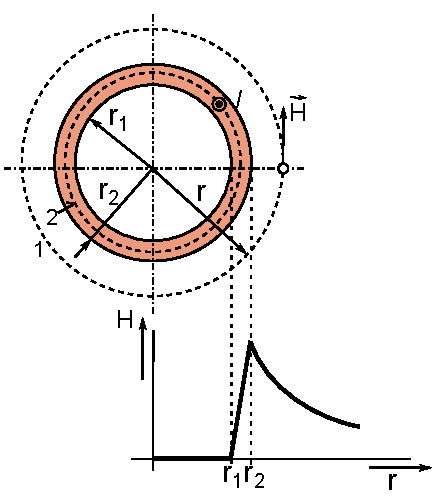
\includegraphics[width=0.8\linewidth]{teo_fig065.pdf}
      \captionof{figure}{K příkladu stanovení intenzity magnetického pole dlouhého dutého válcového 
                vodiče protékaného proudem}
      \label{teo:fig065}
    \par}
    
    Vodič s rovnoměrně rozloženým proudem podle obr. \ref{teo:fig065} je rotačně souměrný podle své
    osy a tedy i jeho magnetické pole je souměrné. Silové čáry jsou soustředné kružnice, vektor
    $\vr{H}$, jenž má směr tečny ke kružnici, je po celé délce kružnice stejně velký. Lze tedy
    snadno použít integrálního tvaru 1. MR (\textbf{zákon celkového proudu})
    
    Pro body ležící vně vodiče obepíná kruhová integrační dráha (vedená po silové čáře 1) celý
    proud vodiče $I$ a platí
    \begin{equation}\label{TEMP:eq_1MR_duty_valec}
      \oint_{\mathcal{C}}\vr{H}d\vr{l} = H\cdot 2\pi r = I
    \end{equation}
    takže intenzita pole je
    \begin{equation}\label{TEMP:eq_H_duty_valec}
      H = \frac{I}{2\pi r}
    \end{equation}
    
    Ve stěně dutého magnetického vodiče jsou silové čáry rovněž kružnice, neboť magnetické pole
    je i zde souměrné. Tyto siločáry však obepínají jen část proudu $I'$ vodiče pro oběh siločáry
    2 platí
    \begin{equation}\label{TEMP:eq_1MR_uvnitr_valce}
      \oint_{\mathcal{C}}\vr{H}d\vr{l} = H\cdot 2\pi r = I' = \pi(r^2-r_1^2)J
    \end{equation}
    kde $J$ je hustota proudu ve vodiči
    \begin{equation}\label{TEMP:eq_J_duty_valec}
      J = \frac{I}{S}= \frac{I}{\pi(r_2^2-r_1^2)}
    \end{equation}
    Ve stěně vodiče je tedy intenzita pole
    \begin{equation}\label{TEMP:eq_H_uvnitr_valce}
      H = \frac{I}{2\pi r}\frac{r^2-r_1^2}{r_2^2-r_1^2}
    \end{equation}
    V dutině vodiče je intenzita rovna nule. Vzhledem k souměrnosti pole by i zde muselo platit
    $\oint_{\mathcal{C}}\vr{H}d\vr{l} = H\cdot 2\pi r$. Protože dráha s poloměrem $r<r_1$ neobepíná
    žádný proud, je $\oint_{\mathcal{C}}\vr{H}d\vr{l} = 0$ a tedy musí byt $H = 0$.
  \end{example}    
\end{mdframed}  
      %------------------------------------------------------------------

      % --------example: $H=f(r)$ souosého kabelu -----------------------
      % \label{TEO:exam013}
      % !TeX spellcheck = cs_CZ
\begin{example}\label{TEMP:ex_koax_H}
  Stanovte intenzitu magnetického pole dlouhého přímého souosého kabelu podle obr.
  \ref{TEMP:fig_exam_koax}. Středním vodičem (\emph{žílou}) prochází proud $I$ a týž proud 
  opačného smyslu prochází vnějším vodičem (\emph{pláštěm}). Proudy jsou rovnoměrně rozloženy po 
  průřezech vodičů. Nakreslete graf průběhu $H = f(r)$ \cite[s.~92]{Dufek1970},
  \cite[s.~195]{Kotlan1999}.
  
  {\centering
   \begin{tabular}{cc}
     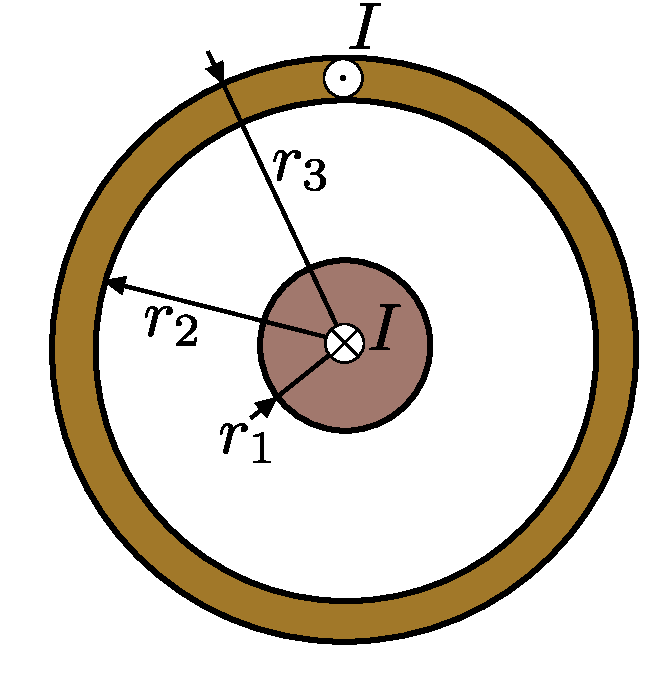
\includegraphics[width=0.4\linewidth]{vypocet_H_sousy_kabel.pdf}   &
     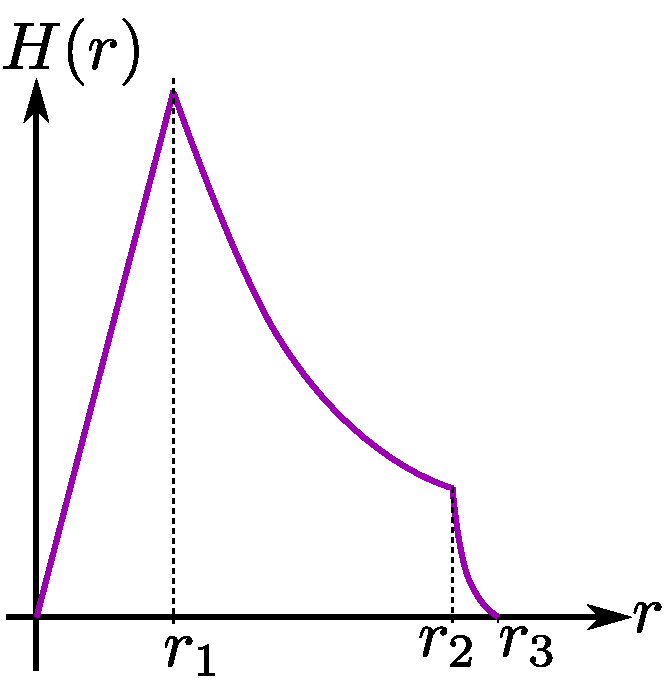
\includegraphics[width=0.4\linewidth]{koax_H_prubeh.pdf}
  \end{tabular}
  \captionsetup{type=figure}
  \captionof{figure}{K příkladu stanovení intenzity magnetického pole dlouhého souosého kabelu 
             protékaného proudem: a) náčrt; b) $H=f(r)$}
  \label{TEMP:fig_exam_koax}
  \par}
  
  \textbf{Řešení}: \newline Rovnici \ref{TEMP:eq_1MR_v_hom_p} aplikujeme na jednotlivé intervaly 
  osově souměrného stacionárního magnetického pole, přičemž se prakticky jedná o superpozici dvou
  polí. V oblasti $r<r_2$ se uplatňuje pouze pole vnitřního válcového vodiče (žíly), pro $r>r_2$ 
  přistupuje souosé pole vnějšího trubkového vodiče.
  \begin{itemize}
    \item Pro oblast $r<r_1$ je vzhledem k 
          \begin{align*}
              % \nonumber to remove numbering (before each equation)
              dI   &= \vr{J}d\vr{S} \\
              I(r) &= \int_S dI = \int_S \vr{J}d\vr{S} = \int_S J\cos\beta dS \\
                   &= \left|\begin{array}{cc}
                               \beta = 0 & H = \text{konst} \\
                             S = \pi r^2 & dS = 2\pi rdr \\
                            \end{array}
                      \right| = J\int_0^r 2\pi rdr = J\pi r^2
          \end{align*}
          hledané řešení 1. MR dáno 
          $$\oint_\mathcal{C}\vr{H}d\vr{l} = H_1 2\pi r = I(r) = J\pi r^2$$ kde celková proudová
          hustota je  $$J = \frac{I}{\pi r_1^2}$$ a tedy $$H_1 = \frac{I}{2\pi r_1^2}\cdot r$$
          
    \item Pro oblast $r_2>r>r_1$ řešíme v podstatě pole vně osamoceného válcového vodiče
          $I(r)$ a tedy $$H_2 = \frac{I}{2\pi r}$$
    \item Pro $r>r_3$ je magnetické pole vytvářeno celým proudem žíly $I$ a příslušnou částí
          proudu pláště $J\pi(r^2 - r_2^2)$, kde proudová hustota $$J =
          \frac{I}{\pi(r_3^2-r_2^2)}$$ má opačnou orientaci oproti proudové hustotě žíly. Pak 
          \begin{align*}
            I(r)                           &= I - I\frac{r^2-r_2^2}{r_3^2-r_2^2} \\
            \oint_\mathcal{C}\vr{H}d\vr{l} &= H_32\pi r = I(r)                   \\          
            H_3                            &= \frac{I}{2\pi r}\left(1 - 
            \frac{r^2 - r_2^2}{r_3^2 - r_2^2}\right) 
          \end{align*}
          Stejný výsledek dostaneme superpozicí opačně orientovaných polí $$H_3 = H'_3 - H''_3 =
          \frac{I}{2\pi r} - \frac{I}{2\pi r}\left(\frac{r^2 - r_2^2}{r_3^2 - r_2^2}\right)$$. 
  \end{itemize}
  Průběh $H(r)$ je na obr. \ref{TEMP:fig_exam_koax}.
\end{example}
  
      %------------------------------------------------------------------

    % -----------Magnetické pole elektrického proudu v diferenciálním tvaru-----------------------
    \subsection{Magnetické pole elektrického proudu v diferenciálním tvaru}
      Nechť je opět magnetické pole vyvoláno konstantním el. proudem $I = \text{konst}$. Jak
      vyplývá z předchozí kapitoly, základním vztahem pro toto pole je \emph{Ampérův zákon}
      $$\oint_{\mathcal{c}}\vec{H_c}\dd{\vec{l}} = I$$  Zvolme za integrační dráhu $c$ obvod malé plošky
      $\Delta S$, jíž prochází proud $\Delta I = J_n \Delta S$, kde $J_n$ je průmět vektoru hustoty
      proudu do směru normály plošky $\Delta S$ (předpokládáme, že ploška $\Delta S$ je dostatečně
      malá, aby se dalo počítat s konstantní hustotou proudu v celém jejím rozsahu)
      \cite[s.~13]{Trnka1972}. Pro zvolený případ platí
      
      \begin{equation}\label{TEMP:eq_amp_z1}
        \oint_{\mathcal{c}}\vec{H_c}\dd{\vec{l}}  =
          J_n \Delta S \rightarrow \frac{1}{\Delta S}\oint_{\mathcal{c}}\vec{H_c}\dd{\vec{l}} = J_n
      \end{equation} 
      
      Pro $\Delta S \rightarrow 0$ zavedeme označení 
      \begin{equation}\label{TEMP:eq_amp_z2}
        \rot{H}  = \frac{1}{\Delta S}\oint_{\mathcal{c}}\vec{H_c}\dd{\vec{l}}  = J_n
      \end{equation}
      
      Rovnice \ref{TEMP:eq_amp_z2} říká, že \emph{rotace vektoru} $\vec{H}$, ($\rot{H}$), jehož
      průmět do určitého směru je roven průmětu vektoru hustoty proudu do tohoto směřu. Z uvedených
      vztahu je patrný fyzikální význam rotace vektoru $\vec{H}$. Je to vektor, jehož velikost je
      rovna oběhovému magnetickému napětí po dráze v rovině kolmé k vektoru hustoty proudu,
      vztaženém k ploše obepínané oběhovou drahou (v nehomogenní poli to platí pro případ, že se
      plocha dráhy blíží k nule).
      
      Při použití pravoúhlé soustavy kartézských souřadnic \(x\), \(y\) a $z$ jsou průměty vektoru
      $\rot{H}$ do jednotlivých os
      \begin{equation}\label{TEMP:eq_amp_z3}
        \textsf{rot}_x\vec{H} = J_x,   \quad
        \textsf{rot}_y\vec{H} = J_y,   \quad
        \textsf{rot}_z\vec{H} = J_z    
      \end{equation}      
      Průmět $\textsf{rot}_x\vec{H}$ je dán oběhovým magnetickým napětím po obvodu plošky
      \(\dd{y}\dd{z}\) a platí
      \begin{align*}
        \textsf{rot}_x\vec{H} 
        &=\frac{1}{\dd{y}\dd{z}}\oint_{\mathcal{c}}\vec{H_c}\dd{\vec{l}} =               \nonumber\\
        &=\frac{1}{\dd{y}\dd{z}}\cdot\Biggl[\Biggr.\left[H_y\dd{y} 
         +\left(H_z + \pder{Hz}{y}\dd{y}\right)\dd{z}\right]                             \nonumber\\     
        &-\left[\left(H_y-\pder{H_y}{z}\dd{z}\right)\dd{y}-H_z\dd{z}\right]\Biggl.\Biggr]\nonumber\\
        &=\pder{H_z}{y}\dd{y}\dd{z} - \pder{H_y}{z}\dd{y}\dd{z}                          \nonumber\\    
        &=\pder{H_z}{y} - \pder{H_y}{z} = J_z
      \end{align*}       
      
      \luagraphic[0.8]{teo_fig062.pdf}{K odvození pojmu \(\textsf{rot}_z\vec{H}\)}{teo:fig062}
         
      tedy dostáváme
      \begin{subequations}
        \begin{align}\label{TEMP:eq_amp_z5}
          \textsf{rot}_x\vec{H} &= \pder{H_z}{y} - \pder{H_y}{z} = J_x       \\
          \textsf{rot}_y\vec{H} &= \pder{H_x}{z} - \pder{H_z}{x} = J_y       \\
          \textsf{rot}_z\vec{H} &= \pder{H_y}{x} - \pder{H_x}{y} = J_z            
        \end{align}    
    \end{subequations}    
      Pro \emph{pravoúhlé souřadnice} $x, y, z$ můžeme tedy vztah $\rot{H} = \vec{J}$ rozepsat na
      tvar
      \begin{align*}
        \textsf{rot}\vec{H} 
          &= \vec{i}\,\textsf{rot}_x\vec{H} + 
             \vec{j}\,\textsf{rot}_y\vec{H} +
             \vec{k}\,\textsf{rot}_z\vec{H}                                    \\
          &= \vec{i}\left(\pder{H_z}{y} - \pder{H_y}{z}\right) +               \\
          &+ \vec{j}\left(\pder{H_x}{z} - \pder{H_z}{x}\right) +               \\
          &+ \vec{k}\left(\pder{H_y}{x} - \pder{H_x}{y}\right)                 \\  
          &= \vec{i}\,J_x + \vec{j}\,J_y + \vec{k}\,J_z = \vec{J}.
      \end{align*}          
      
      Rotaci vektoru $\rot{H}$ můžeme též symbolicky vyjádřit vektorovým součinem Hamiltonova
      operátoru a vektoru $\vec{H}$
      \begin{align*}
        \rot{H} &= \nabla\times\vec{H}                                                      \\                                           
                &= \left(\vec{i}\,\pder{ }{x} + 
                   \vec{j}\,\pder{ }{y} + \vec{k}\,\pder{ }{z}\right)                       \\
                & \times(\vec{i}\,H_x + \vec{j}\,H_y + \vec{k}\,H_z)
      \end{align*}
      nebo také determinantu
      \begin{equation}\label{TEMP:eq_amp_z8}
        \rot{H} = \begin{vmatrix}
                    \vec{i}       & \vec{j}      & \vec{k}      \\
                    \pder{ }{x}  & \pder{ }{y} & \pder{ }{z} \\ 
                    H_x          & H_y         & H_z         \\
                  \end{vmatrix}      
      \end{equation}  
      \emph{cylindrických souřadnic} $r$, $\varphi$, $z$:
      \begin{align}\label{TEMP:eq_amp_z9}
        \textsf{rot}_r\vec{H}       
          &= \frac{1}{r}\pder{H_z}{\varphi} - \pder{H_\varphi}{z} = J_r           \nonumber \\ 
        \textsf{rot}_\varphi\vec{H} 
          &= \pder{H_r}{z} - \pder{H_z}{r}                        = J_\varphi     \nonumber \\
        \textsf{rot}_z\vec{H}       
          &= \frac{1}{r}\left[\pder{ }{r}
             \left(rH_\varphi\right)-\pder{H_r}{\varphi}\right]   = J_z
      \end{align} 
      \emph{sférických souřadnic} $r$, $\varphi$, $\vartheta$ 
      \begin{align}\label{TEMP:eq_amp_z10}
        \textsf{rot}_r\vec{H}        
           &= \frac{1}{r\sin\vartheta}\left[\pder{ }{\vartheta}(H_\varphi\sin\vartheta) - 
              \pder{H_\vartheta}{\varphi}\right]                     = J_r           \nonumber \\ 
        \textsf{rot}_\varphi\vec{H}   
           &= \frac{1}{r}\left[\pder{ }{r}(rH_\vartheta) - 
              \pder{H_r}{\vartheta}\right]                           = J_\varphi     \nonumber \\
        \textsf{rot}_\vartheta\vec{H} 
           &= \frac{1}{r\sin\vartheta}\left[\pder{H_r}{\varphi} -
              \pder{ }{r}\left(rH_\varphi\sin\vartheta\right)\right] = J_\vartheta    
    \end{align} 
      Podobně jako v elektrickém poli vyjadřujeme vztah $\oint\vec{D}\dd{\vec{S}} = Q$ vztahem 
      $\diver{D}
      = \rho$, tak i v magnetickém poli vyjadřujeme vztah $\oint\vec{B}\dd{\vec{S}} = 0$ vztahem
      $\diver{D} = 0$, nebo též v kartézských souřadnicích \(x\), \(y\) a $z$ jako $$\diver{D} =
      \nabla\cdot\vec{B} = \pder{B_x}{x} + \pder{B_y}{y} + \pder{B_z}{z} = 0$$
                     
    % ----------------Rovnice pro magnetický potenciál -------------------------------------------
    \subsection{Rovnice pro magnetický potenciál}
      V regulárních bodech lineárního homogenního izotropního magnetika platí pro $\varphi_m$
      \textbf{Laplaceova rovnice}
      \begin{equation}\label{TEMP:eq_varphi_m_laplace}
        \Delta\varphi_m = 0
      \end{equation}      
      Důkaz plyne z rovnice $\diver{B} = 0$ a rovnice $\vec{B} = \mu\vec{H}$: $$\diver{B} =
      \textsf{div}\mu\vec{H} = \textsf{div}\mu(-\textsf{grad}\varphi_m).$$ Pro $\mu = \text{konst}$
      dostáváme $\textsf{div}\textsf{grad}\varphi_m = 0$, což je rovnice
      \ref{TEMP:eq_varphi_m_laplace}.
      
      Na rozhraní mezi dvěma magneticky různými prostředími neplatí Maxwellovy rovnice v
      diferenciálním tvaru a tedy ani Laplaceova rovnice \ref{TEMP:eq_varphi_m_laplace}. Podmínky 
      pro $\vec{H}$ a $\vec{B}$ na rozhraní vyjádříme pomocí skalárního magnetického potenciálu
       \begin{align}\label{TEMP:eq_mag_U_rozhrani}
         \varphi_{m1}                 &= \varphi_{m2} \\
         \mu_1\pder{\varphi_{m1}}{n}  &= \mu_2\pder{\varphi_{m2}}{n} 
       \end{align}
      kde $\pder{}{n}$ jsou derivace ve směru normály k rozhraní. 
    
    \subsubsection{Vektorový magnetický potenciál}
      V elektrostatice jsme pro usnadnění mnohých problémů zavedli skalární elektrický potenciál -
      lze jej zavést vždy, neboť elektrostatické pole je vždy potenciální. Magnetické pole je však
      obecně vírové. Lze jej popsat skalárním potenciálem jen ve speciálních případech, tj.
      jestliže je polem potenciálním. Obecně je však zavedení skalárního potenciálu nepřípustné.
      Lze i pak zavést nějakou veličinu (analogickou skalárnímu potenciálu), s níž by se pracovalo
      snáze, než přímo s vektory pole?
      
      Dříve než definujeme vektorový magnetický potenciál, zopakujme zavedení skalárního potenciálu
      v elektrostatice. Vyjdeme z 2. MR a z rovnice známé z vektorové analýzy: $$\rot{E} = 0 \quad
      \text{a} \quad \textsf{rot}\,\textsf{grad}\varphi_m = 0.$$
      
      V magnetickém poli vyjdeme ze 4. MR a z jiné identity pro vektorovou funkci $\vec{A}$, známe z
      vektorové analýzy: $$\diver{B} = 0 \quad \text{a} \quad \textsf{div}\textsf{rot}\vec{A} =
      0$$ odtud
        \begin{equation}\label{TEMP:eq_B_rotA}
          \vec{B} = \rot{A}.
        \end{equation}       
               
%} % tikzset
%~~~~~~~~~~~~~~~~~~~~~~~~~~~~~~~~~~~~~~~~~~~~~~~~~~~~~~~~~~~~~~~~~~~~~~~~~~~~~~~~~~~~~~~~~~~~~~~~~~
  % % !TeX spellcheck = cs_CZ
% file: kap_zakld_zakn_elmag.tex
%{\tikzset{external/prefix={tikz/TEO/}}
% \tikzset{external/figure name/.add={ch02_}{}}
%====================Kapitola: Základní zákony elektromagnetismu====================================
\setchaptertoc
\chapter{Základní zákony elektromagnetismu}\label{teo:IchapII}
  V této teoreticky změřené kapitole budou shrnuty základní fyzikální zákony, kterými se řídí
  elektromagnetické jevy a jejichž znalost bude nezbytná při studiu následujících praktičtěji
  zaměřených kapitol. Mezi nejdůležitější patří zákon elektromagnetické indukce. Velký praktický
  význam má jeho zobecnění i pro případy nejsložitější, jakými jsou \emph{nelineární} a navíc
  \emph{parametrické} magnetické obvody. Důležitým pojmem je \emph{spřažený} magnetický tok cívky.
  Pro hlubší pochopení všech zákonitostí bude vhodné upozornit na \emph{topologické vlastnosti}
  elektromagnetického pole. Ukazuje se totiž, že topologický přístup je velice užitečným a silným
  nástrojem, který významně usnadňuje pochopení
  \href{http://en.wikipedia.org/wiki/Maxwell_theory}{Maxwellových rovnic} se všemi jejich důsledky
  \cite[s.~6]{Patocka4}. Topologii elektromagnetického pole je proto věnována celá kapitola
  \ref{teo:IchapIII}
  
  \section{Zákon elektromagnetické indukce}\label{teo:IchapIIsecI}
    Základní veličinou pro popis magnetických polí a jejich účinků je \emph{vektor magnetické
    indukce} \(\vec{B}\). Dle soustavy SI je jednotkou magnetické indukce \emph{tesla} \([T]\) a
    projevuje se silovými účinky na vodiče protékané proudy a indukováním napětí při jeho změně.

    Je proto dobře měřitelný. První rovnice (Ampérův zákon) ze souboru Maxwellových rovnic určuje
    rovnost oběhového integrálu magnetické indukce po uzavřené křivce proudům protékaných vodiči,
    jež jsou touto křivkou uzavřeny.
    \begin{equation}\label{es:eq_amp_law}
      \oint_l \vec{B} \cdot \vec{dl} = \sum I
    \end{equation}
    
    \luagraphic[0.6]{teo_fig034.pdf}{Elektrický proud ve vodiči způsobuje vznik magnetické pole v 
      jeho okolí.}{teo:fig034}

    Obrázek \ref{teo:fig034} ilustruje fakt, že elektrické proudy jsou vždy obklopeny 
    magnetickými poli. Tato pole se dají zesílit cívkou s magnetickým jádrem. Na tomto jevu je 
    založen jeden z elementárních principů elektrotechniky.    
       
    \begin{mdframed}[style=mdnote]
      Jaký je vztah jednotky magnetické indukce k ostatním základním jednotkám soustavy \textbf{SI}? 
      \begin{align*}
      1T &= 1\frac{V\cdot s}{m^2} = 1\frac{N}{A\cdot m} = 1\frac{Wb}{m^2}          \\
         &= 1\frac{kg}{C\cdot s} = 1\frac{kg}{A\cdot s^2} = 1\frac{N\cdot s}{C \cdot m}
      \end{align*}
    \end{mdframed}
    
    Při odvozování matematického modelu transformátoru se obvykle vychází ze zákona 
    \textbf{elektromagnetické indukce}, který říká, že \emph{časová změna magnetického pole vytvoří 
    vírové pole elektrické}:
    \begin{equation}\label{es:eq_ind_z}
      \oint_l \vec{E} \cdot \dd{\vec{l}} = - \der{\Psi}{t}
    \end{equation}
     
    Základní laboratorní experimenty, vedoucí k odhalení existence tohoto zákona, uskutečnil 
    \emph{Faraday}\footnote{Michael Faraday (1791 - 1867), samouk, zakladatel klasické 
    elektrodynamiky, vynikající experimentátor: Zavedl pojem fyzikálního prostorového pole pomocí 
    siločár, tzv. ''trubic''} r. 1831. Matematickou formulaci \emph{indukčního zákona} v podobě 
    rovnice
    \begin{equation}\label{ES:eq_zakl_elm25}
      u(t) = - \frac{d\Psi(t)}{\dd{t}}
    \end{equation} 
    stanovil již on sám, postupně význam zákona formálně upřesňovali další badatelé např.
    \emph{Neumann}\footnote{Franz Ernst Neumann (1798 - 1895), teoretický fyzik, matematik,
    mineralog. Definoval pojem magnetický vektorový potenciál, formuloval Neumannův vzorec pro
    vzájemnou indukčnost dvou smyček. Učitel G. R. Kirchhoffa.} kolem roku 1845. Konečné znění
    Maxwellovy teorie včetně formulace indukčního zákona do podoby II. Maxwellovy rovnice budoval
    Maxwell\footnote{James Clark Maxwell (1831 - 1879), teoretický fyzik, působil na Trinity College
    university v Cambridge, na King's College v Londýně, posléze první ředitel Cavendishovy
    laboratoře na univerzitě v Cambridge. Původně se zabýval teoretickou mechanikou a kinetickou
    teorií plynů. Soustavu čtyř Maxwellových rovnic odvodil především na základě
    mechanicko-elektrických analogií.} velmi pozvolna, v období 1855 až 1873. Z historického pohledu
    je zajímavé a důležité, že přesné \emph{kvantitativní} experimenty s elektromagnetickou indukcí
    byly v té době uskutečnitelné pouze pomocí
    \href{http://en.wikipedia.org/wiki/Galvanometer}{balistického galvanometru}. Lze odhadnout, že
    nebýt tohoto přístroje, přesná matematická formulace indukčního zákona by se pravděpodobně
    opozdila o několik let. Kupodivu, z psychologického hlediska je i v současnosti velmi vhodné
    vysvětlit princip indukčního zákona pomocí historických pokusů s balistickým galvanometrem.
    
    \subsection{Pokusy s balistickým galvanometrem}
      Jako každý elektromagnetický měnič energie (tj. motor), obsahuje i \emph{magnetoelektrické
      měřicí} ústrojí galvanometru dva akumulátory energie: moment setrvačnosti \(J\) otoč\-né 
      části a indukčnost cívky \(L\). Jedná se tedy o kmitavou soustavu 2. řádu. Každou takovou 
      soustavu lze kriticky, případně nadkriticky tlumit - především zařazením tlumicího odporu 
      vhodné velikosti do série s měřicím systémem (tlumení vlivem mechanického tření je úmyslně 
      konstrukčně potlačeno na zanedbatelnou úroveň). Balistický galvanometr je cíleně konstruován 
      s velkým momentem setrvačnosti \(J\) a s malou tuhostí \(k_d\) direkčních pružin, aby měl 
      dlouhou dobu kmitu \(T_G = 2\pi\sqrt{J/k_d}\) několik sekund. Proteče-li galvanometrem krátký 
      proudoý impuls \(i(t)\) o celkové délce \(t_i\) podle obr. \ref{teo:fig036}, pak lze snadno 
      dokázat, že za předpokladu \(t_i\ll T_G\) je první maximální výchylka \(\alpha_{max}\) 
      tlumeného pohybu ukazatele přímo úměrná celkovému náboji \(Q\) proudového impulsu podle 
      rovnice 
      \begin{equation}\label{ES:eq_zakl_elm01}
        \alpha_{max} = k_b Q = k_b\int_0^{t_i} i(t)\dd{t},
      \end{equation}
      kde \(k_b\) je \emph{balistická konstanta} použitého galvanometru. Balistický galvanometr tedy
      pracuje jako \emph{integrátor} proudu v přesném matematickém smyslu. 
      
      \luagraphic[1]{teo_fig036.pdf}{Příklad krátkého proudového impulsu prošlého balistickým 
        galvanometrem.}{teo:fig036}
  
      Uvažujme experiment uspořádaný podle obr. \ref{teo:fig037}. V uzavřeném obvodu
      galvanometru se nachází celkový odpor \(R\) a tuhá samonosná cívka v podobě kruhového závitu,
      připojená na dlouhé ohebné zkroucené přívody. Husté zkroucení zajišťuje, že do samotných
      přívodů se nemůže indukovat žádné napětí, pohybuje-li se cívka v magnetickém poli 
      permanentního magnetu. Při rychlém přesunu z polohy \emph{1} do vzdálené polohy \(\infty\) 
      klesne v cívce magnetický tok na nulu, časová změna toku zapříčiní vznik indukovaného napětí, 
      napětí protlačí obvodem proudový impuls odpovídající přibližně obr. \ref{teo:fig036}.
      
      \luagraphic[1]{teo_fig037.jpg}{Uspořádání experimentálního pracoviště s balistickým 
        galvanometrem}{teo:fig037}
      
      Za předpokladu kritického nebo nadkritického tlumení má odpor \(R\) relativně velkou hodnotu. 
      Proto lze s dobrou přesností zanedbat vnitřní indukčnost měřicího systému galvanoměru a 
      uvažovat, že celé napětí \(u(t)\), indukované v cívce při jejím pohybu, spočine pouze na 
      odporu. V uzavřeném okruhu o celkovém odporu \(R\) pak platí Ohmův zákon ve tvaru
      \begin{equation}\label{ES:eq_zakl_elm02}
        i(t)=\frac{u(t)}{R}.
      \end{equation}    
      Dosadíme-li rovnici \ref{ES:eq_zakl_elm02} do \ref{ES:eq_zakl_elm01}, po úpravě získáme vztah
      \begin{equation}\label{ES:eq_zakl_elm03}
       \int_0^{t_i}u(t)\dd{t}=\frac{\alpha_{max}R}{k_b}.
      \end{equation}     
      Experimentálně je možno dospět ke dvěma stěžejním poznatkům:
      \begin{itemize}
        \item Při přesunu cívky z polohy \emph{1} do polohy \(\infty\) nezávisí výchylka
              \(\alpha_{max}\) na \emph{rychlosti pohybu}. (Za předpokladu \(t_i\ll T_G\), což je
              omezení dané nedokonalostí přístroje a nijak nesouvisí se zkoumaným jevem.)
        \item Při přesunu cívky z polohy \emph{1} do polohy \(\infty\) zůstává součin
              (\(\alpha_{max}\times R\)) stále \emph{konstantní}, měníme-li úmyslně velikost odporu
              \(R\). To jest: při k-násobném zvýšení odporu klesne výchylka k-krát a naopak. 
      \end{itemize}
  
      V poloze „1“ prochází plochou cívky magnetický tok \(\Psi\). V poloze „\(\infty\)“ je zřejmě
      magnetický tok cívky nulový, tedy \(\Psi_\infty = 0\). S ohledem na rovnici
      (\ref{ES:eq_zakl_elm03}) lze pak oba experimentální poznatky interpretovat jediným možným
      způsobem:
       \begin{equation}\label{ES:eq_zakl_elm04}
       \int_0^{t_i}u(t)\dd{t}=\text{konst}=\Psi-\Psi_\infty=\Psi.
      \end{equation}    

      Experiment lze opakovat s cívkami libovolných rozměrů, tvarů i počtů závitů. Výsledky budou
      kvalitativně stejné. Veličina \(\Psi\) se nazývá \emph{spřažený magnetický tok cívky}. Je to 
      míra interakce cívky s magnetickým polem, které spojitě prostupuje celou plochou cívky. 
      Rovnici (\ref{ES:eq_zakl_elm04}) lze vyjádřit slovně: Spřažený magnetický tok cívky je úměrný 
      časovému integrálu svorkového napětí na zkoumané cívce. Je určitě výhodné zvolit jedničku 
      jako konstantu úměrnosti mezi tokem \(\Psi\) a integrálem napětí. \emph{Pak bude velikost 
      spřaženého toku přímo rovna integrálu napětí}. Určitý integrál v rovnici 
      (\ref{ES:eq_zakl_elm04}) lze nahradit integrálem neurčitým, pak je ale nutno přidat obecnou 
      počáteční integrační konstantu \(\Psi_0\)
      v newtonovském smyslu. Získáme tak zákon elektromagnetické indukce (indukční zákon) v
      integrálním tvaru
      \begin{equation}\label{ES:eq_zakl_elm05}
       \Psi(t) = \Psi_0 + \int u(t)\dd{t} \quad [Wb;\, V,\; s].
      \end{equation}   
    
    Z rovnice (\ref{ES:eq_zakl_elm05}) plyne, že jednotka magnetického toku Weber\footnote{Wilhelm
    Eduard Weber (1804-1891), teoretický fyzik, působil na univerzitách v Gottingenu a v Lipsku.
    Zakladatel předrelativistické elektrodynamiky. Určil totiž silu mezi náboji v závislosti nejen
    na vzdálenosti, ale i na rychlosti a zrychlení, jeho teorie je ale platná pouze pro \(v \ll c\).
    Blízký spolupracovník Gausse.} má rozměr \([Vs]\), Budeme-li obě strany rovnice derivovat podle
    času, rovnost tím neporušíme. Získáme tak ryze matematickou cestou indukční zákon v
    diferenciálním tvaru
    \begin{equation}\label{ES:eq_zakl_elm06}
     u(t) = \frac{d\Psi(t)}{\dd{t}}, \quad \text{resp.} \quad  u(t) = -\frac{d\Psi(t)}{\dd{t}}.
    \end{equation}   
    Obě rovnice (\ref{ES:eq_zakl_elm06}a), (\ref{ES:eq_zakl_elm06}b) se liší znaménkem \(+\) nebo
    \(-\) na pravé straně. Volba znaménka souvisí s domluvou, který režim cívky považujeme za
    základní: zda režim \emph{spotřebičový} podle rovnice (\ref{ES:eq_zakl_elm06}a), nebo režim
    \emph{zdrojový} podle rovnice (\ref{ES:eq_zakl_elm06}b). Oba režimy jakéhokoli dvojpólu jsou
    totiž jednoznačně definovány vzájemnou orientací napětí a proudu podle obr.
    \ref{teo:fig039}. Odpor nemůže nikdy pracovat jako zdroj, proto slouží jako
    „normál“ definující \emph{spotřebičovou} orientaci svorkových veličin. Oba režimy cívky se liší
    níže popsaným způsobem.

    \begin{figure}[ht!]
      \centering  
      \subcaptionbox{Odpor je vždy spotřebičem \label{teo:fig039a}    }{\luafigure[0.4]{teo_fig039a.pdf}}                    
      \subcaptionbox{Cívka ve spotřebičovém režimu \label{teo:fig039b}}{\luafigure[0.4]{teo_fig039b.pdf}}  
      \newline               
      \subcaptionbox{Cívka ve zdrojovém režimu \label{teo:fig039c}    }{\luafigure[0.4]{teo_fig039c.pdf}}
      \caption{Vzájemná orientace okamžité hodnoty proudu a napětí ve spotřebičovém a zdrojovém 
               režimu:} 
      \label{teo:fig039}
    \end{figure}
        
    \textbf{Spotřebičový režim:}
    \begin{itemize}[noitemsep]
      \item Orientace svorkového napětí \(u(t)\) je vůči proudu \(i(t)\) souhlasná. Platí rovnice
            (\ref{ES:eq_zakl_elm06}a).
      \item Cívka je připojena na zdroj napětí\(u(t)\), odebírá z něj proud \(i(t)\), tedy odebírá
            ze zdroje elektrickou energii a chová se jako spotřebič. Tuto energii přeměňuje na
            energii magnetického pole.
      \item Mezi směrem proudu a směrem toku platí \emph{pravidlo pravé ruky}, PPR.           
    \end{itemize}
    
    \textbf{Zdrojový režim:}
    \begin{itemize}[noitemsep]
      \item Orientace svorkového napětí u(t) je vůči proudu i(t) nesouhlasná. Platí rovnice
            (\ref{ES:eq_zakl_elm06}b).
      \item Cívka je vložena do proměnného magnetického pole \(B(t)\), na jejích svorkách vzniká
            indukované napětí \(u(t)\) (zastaralý výraz: „elektromotorická síla“). Z cívky se stal
            zdroj elektrického napětí u(t), tj. generátor. Připojíme-li na svorky odporovou zátěž,
            začne do ní generátor dodávat elektrickou energii.\footnote{Faraday s Maxwellem se
            znali osobně a po dohodě pokládali zdrojový režim cívky za základní, tedy pracovali s
            rovnicí (\ref{ES:eq_zakl_elm06}b). Maxwell navíc pracoval s pojmem „electromotive force
            \(P\)‘, který svým významem přesně odpovídal dnešní „intenzitě elektrického pole.
            Postupem času byl doslovně přeloženému výrazu „elektromotorická síla“ nešťastně
            přiřazen v české i zahraniční literatuře význam „napětí“, což ještě více zvýšilo
            zmatek. Proto je rozumné výraz „elektromotorická síla“ vůbec nepoužívat.}
    \end{itemize}

    \luagraphic[1]{teo_fig038.jpg}{Princip transformátoru. Primární cívka pracuje ve
    spotřebičovém režimu (PPR), sekundární cívka ve zdrojovém režimu (PLR)}{teo:fig038}

    Z uvedených skutečností lze učinit následující závěr. Volba znaménka v rovnicích
    (\ref{ES:eq_zakl_elm06}a, b) je věcí dohody, ale pouze v tom smyslu, zda zvolíme za základní
    režim spotřebičový či zdrojový\footnote{Ojediněle se v literatuře, např. v [5], vyskytne názor,
    že znaménko v rovnicích (\ref{ES:eq_zakl_elm06}a, b) je určeno tím, zda je cívka navinuta
    pravotočivě nebo levotočivé. To je chybné tvrzení. Pravotočivost či levotočivost cívky naprosto
    nijak nesouvisí se schopnosti cívky pracovat ve zdrojovém nebo spotřebičovém režimu.}. 
    Například při analýze měničů ve výkonové elektronice je ustáleným zvykem zvolit označení proudu
    a napětí na indukčnosti podle obr. \ref{teo:fig039b}. Bez ohledu na tuto volbu musíme v 
    konkrétní situaci vždy pečlivě rozlišovat, ve kterém režimu se cívka skutečně nachází.
    Příklad: primární cívka transformátoru se nachází vždy ve spotřebičovém režimu, sekundární
    cívka vždy ve zdrojovém režimu. Se zdrojovým či spotřebičovým režimem úzce souvisí \emph{Lenzův
    princip}\footnote{Heinrich Lenz (1804-1865), estonský fyzik, působil na univerzitě v
    Petrohradu. Princip po něm pojmenovaný objevil r. 1833.}. Jedná se o zvláštní případ
    obecnějšího přírodního principu, vyjádřitelného jako „zákon akce a reakce“. V elektromagnetismu
    má zákon následující tvar:

    Lenzův princip: Proud indukovaný v uzavřené vodivé smyčce vyvolá magnetické pole, které působí
    vždy proti původnímu budicímu poli, díky němuž indukovaný proud vznikl.

    Všimněme si, že zmíněná „uzavřená vodivá smyčka“ se nachází \emph{zdrojovém režimu}: je vložena
    do magnetického pole, indukuje se v ní napětí \(u(t)\), které protlačí vodivým obvodem proud
    \(i(t)\). Proud má ve \emph{zdrojovém režimu} takový směr, že působí proti budicímu magnetickému
    poli. Příkladem je již zmíněná sekundární cívka transformátoru podle Obr. /./-*/« nebo uzavřená
    smyčka vířivého proudu ve vnitřním prostoru transformátorového plechu podle Obr. 1.1-5.

    \luagraphic[1]{teo_fig040.jpg}{Vznik vířivého proudu uvnitř elektricky vodivého
    transformátorového plechu. Budicí cívka pracuje ve spotřebičovém režimu (PPR). Elementární
    smyčka vířivého proudu odpovídá sekundárnímu vinutí a pracuje ve zdrojovém režimu
    (PLR).}{teo:fig040}

    Integrací rovnice (\ref{ES:eq_zakl_elm06}a) lze zpětně dojít k integrálnímu tvaru
    (\ref{ES:eq_zakl_elm05}). Je nutno zdůraznit, že obě rovnice jsou naprosto rovnocenné, navzájem
    převoditelné, obě nesou stejné množství informace, žádná není důležitější než druhá. Je
    pravdou, že z psychologického pohledu je indukční zákon snáze pochopitelný v
    \emph{diferenciálním} tvaru (\ref{ES:eq_zakl_elm06}). Pro hluboké porozumění magnetickým jevům
    je však nezbytné uvědomit si především jeho \emph{integrální} podobu (\ref{ES:eq_zakl_elm05})
    se všemi matematickými důsledky:
    \begin{itemize}
      \item Spřažený tok je roven integrálu napětí. Zákon platí \emph{univerzálně}, bez ohledu na
            \emph{linearitu} či \emph{nelinearitu} magnetického obvodu. Rovnice
            (\ref{ES:eq_zakl_elm05}) totiž definuje funkční závislost \(\Psi=\Psi(u)\) mezi tokem a
            napětím, nikoli závislost \(\Psi=\Psi(i)\) mezi \emph{tokem a proudem}.  Případná
            nelinearita se totiž týká výlučně závislosti \(\Psi=\Psi(i)\), a tudíž nijak nenarušuje
            platnost rovnice (\ref{ES:eq_zakl_elm05}).
      \item Z předchozího bodu plyne, že v obecném \emph{nelineárním} případě není tok \(\Psi\)
            přímo úměrný proudu \(i\). Přímá úměra \(\Psi = Li\) totiž platí pouze ve zvláštním
            případě \emph{lineárního} magnetického obvodu.
      \item Rovnice (\ref{ES:eq_zakl_elm05}) platí ve spotřebičovém i generátorovém režimu cívky.
            Problém se znaménkem zůstává stejný jako u rovnic (\ref{ES:eq_zakl_elm06}).
      \item V uzavřené \emph{supravodivé} smyčce platí vždy \(u = 0\), i když jí teče konstantní
            ss. proud. Neurčitý integrál v rovnici (\ref{ES:eq_zakl_elm05}) má pak nulovou hodnotu
            \(\int0\dd{t}=0\), a zřejmě tedy platí \(\Psi(t)=\Psi_0\), kde \(\Psi_0\) je
            \emph{libovolná} počáteční integrační konstanta. Fyzikálně má konstanta význam
            počátečního toku, který je v cívce naintegrován z předchozích dějů. Případ
            \(\Psi_0\neq0\) odpovídá nabuzenému supravodivému magnetu, jehož tok \(\Psi(t)=\Psi_0
            = \text{konst.}\) se s časem nemění. Nabuzený supravodivý magnet se proto chová jako
            \emph{permanentní} magnet. Případ \(\Psi_0 = 0\) odpovídá magnetickému stínění pomocí
            \emph{závitu nakrátko}, např. tzv. Faradayova klec, nebo stínění koaxiálního kabelu
            podle obr. \ref{teo:fig041}. Každé oko \textbf{a-b-c-d} stínícího pláště
            tvoří „supravodivý“ závit nakrátko, v němž platí \(u = 0\), tedy \(\Psi=\int0\dd{t}=0\).
            Proto se do vnitřního prostoru ohraničeného pláštěm nemůže zvenčí dostat žádné
            \emph{střídavé} rušivé magnetické pole (jedině pole \emph{stejnosměrné} \(\Psi_{ss}\),
            ale to je neškodné, protože nezpůsobuje vznik rušivého napětí ve středním vodiči
            kabelu; derivace konstanty je totiž nulová: \(u(t)=\frac{d\Psi_{ss}}{\dd{t}}=0\)).
    \end{itemize}

    Na otázku „Proč je magnetický tok úměrný integrálu napětí?“ lze odpovědět pouze následujícím
    způsobem: „Protože je to jeden ze základních zákonů přírody, jehož správnost se nepodařilo
    experimentálně nikdy vyvrátit, nýbrž vždy pouze potvrdit.“ Deduktivní odvození indukčního
    zákona z vyšších přírodních zákonitostí není na úrovni klasické fyziky možné, není
    uskutečnitelné ani na vyšší úrovni \emph{kvantové elektrodynamiky}\footnote{Za objev kvantové
    elektrodynamiky obdržel Richard P. Feynman (1918-1988) Nobelovu cenu v r. 1965 (Feynmanovy
    fázorové diagramy a Feynmanův dráhový integrál; nositelé elektromagnetických sil jsou fotony). 
    Vynikající teoretický fyzik, ale i praktik. Celoživotně působil na kalifornském technickém
    institutu. Během druhé světové války byl členem týmu pracujícího na vývoji americké atomové
    bomby v Los Alamos (projekt Manhattan).}. Za povšimnutí stojí, že v diferenciální formě
    (\ref{ES:eq_zakl_elm06}) nebylo přesné kvantitativní ověření indukčního zákona v době objevu
    proveditelné s ohledem na možnosti tehdejšího přístrojového vybavení. Experiment v nehomogenním
    poli podle obr. \ref{teo:fig037} by byl i v současnosti velmi těžko   
    vyhodnotitelný. Naopak, ověření v integrálním tvaru je velmi snadné\footnote{V současnosti by
    byl balistický galvanometr nahrazen operačním zesilovačem zapojeným jako integrační zesilovač.
    Ten by zpracovával signál ze snímače proudu, např. z proudového bočníku. Po odeznění proudového
    impulsu by na výstupu zesilovače zůstalo naintegrováno určité konstantní napětí, jehož velikost
    by analogicky odpovídala maximální výchylce \(\alpha_{max}\) galvanometru.} . To opravňuje k
    domněnce vyslovené v historickém úvodu kapitoly.

    \begin{figure}[ht!]
      \centering  
      \subcaptionbox{\label{teo:fig041a}}{\luafigure[0.4]{teo_fig041a.jpg}}                    
      \subcaptionbox{\label{teo:fig041b}}{\luafigure[0.4]{teo_fig041b.jpg}}  
      \caption{Plášť koaxiálního kabelu. Každé oko \textbf{a-b-c-d} tvoří závit nakrátko.} 
      \label{teo:fig041}
    \end{figure}
      
    Supravodivá cívka podle obr. \ref{teo:fig042} začne být v okamžiku \(t = 0\)
    napájena ideálním zdrojem napětí \(u(t)\). Později na ni začne působit vnější magnetické pole
    přibližujícího se permanentního magnetu. Jaký vliv bude mít PM na velikost spřaženého toku
    cívky?
    
    Odpověď plyne přímo z rovnice (\ref{ES:eq_zakl_elm05}): \(\Psi(t) = \Psi_0 +\int u(t)\dd{t}\).
    
    Ze zadání příkladu vyplývá, že počáteční integrační konstanta je nulová. Neurčitý integrál je
    možno nahradit integrálem určitým. Velikost spřaženého toku je \emph{tvrdě definována}
    přiloženým napětím, tedy hodnotou určitého integrálu. Proto externí magnetické pole 
    \emph{nemůže} spřažený tok cívky nijak změnit. Ideální napěťový zdroj má \emph{nulový} 
    vnitřní odpor. Proto se supravodivá cívka napájená tímto zdrojem stále chová jako supravodivý
    závit nakrátko, do něhož nemůže vniknout žádná siločára externího magnetického pole.
    
    \begin{figure}[ht!]
      \centering  
      \subcaptionbox{\label{teo:fig042a}}{\luafigure[0.41]{teo_fig042a.jpg}}                    
      \hspace{1em}
      \subcaptionbox{\label{teo:fig042b}}{\luafigure[0.45]{teo_fig042b.jpg}}  
      \newline               
      \subcaptionbox{\label{teo:fig042c}}{\luafigure[0.41]{teo_fig042c.jpg}}
      \caption{K příkladu, a) Supravodivá cívka je napájená ideálním napěťovým zdrojem, b) Později
               na ni začne působit externí pole pohybujícího se magnetu, c) Náhradní zapojení.} 
      \label{teo:fig042}
    \end{figure}
  
    Jev lze vysvětlit následovně. Pohybující se magnet indukuje v cívce přídavné indukované napětí
    \(u(t)\). Toto napětí se přičte k napětí napájecímu a způsobí změnu proudu \(\Delta i(t)\)
    tekoucího cívkou. Podle Lenzova principu začne tento přídavný proud působit proti poli PM.
    Přídavný proud \(\Delta i(t)\) má přesně takovou velikost a směr, že uvnitř závitu dokonale
    vykompenzuje a zruší externí pole magnetu. Vnější pozorovatel tedy vidí, že supravodivý závit se
    chová jako magnetický izolant, jemuž se siločáry externího pole vyhnou, a celkový tok cívky není
    přítomností magnetu nijak ovlivněn. Celá soustava se navíc chová jako elektromechanický měnič
    energie (tj. motor), který je schopen pracovat v motorovém nebo generátorovém režimu. Pohybující
    se magnet totiž koná nebo spotřebovává mechanickou práci, protože na něj působí síla. Podle
    vzájemné okamžité orientace vektorů \emph{síly} a \emph{rychlosti} pracuje celá soustava buď
    jako motor (koná mechanickou práci), nebo jako generátor (spotřebovává mechanickou energii a
    ukládá ji do zdroje napětí).

    %------------- Spřažený tok vzduchové cívky ----------------------------------------------------
    \section{Spřažený tok vzduchové cívky}\label{ES:sec02}
      Experiment s galvanometrem popsaný v předchozí kapitole lze uskutečnit podrobněji ve čtyřech
      následujících modifikacích označených čísly \textbf{1} až \textbf{4}. Pro vyšší přehlednost
      budou těmito čísly systematicky značeny i veličiny v jednotlivých pokusech. Ze čtyř postupně
      gradujících experimentů vyplyne geometrická interpretace pojmu \emph{spřažený tok} vzduchové
      cívky. Poznámka: V následujících experimentech se pokusná  cívka nachází v generátorovém
      režimu. Učiníme však dohodu, že velikost toku budeme pro jednoduchost uvažovat v absolutní
      hodnotě, tj. bez ohledu na znaménko \cite[s.~12]{Patocka4}.

      \subsection{Experiment č. 1}
        Podle Obr \ref{teo:fig043} je na ohebných zkroucených přívodech umístěna tuhá samonosná
        cívka, která má jeden závit o ploše \(\Delta S\). Plocha musí být \emph{malá}, aby bylo
        možno předpokládat, že magnetické pole v těsném okolí cívky je \emph{homogenní} (vektor
        indukce \(\vec{B_1}\), musí být v rámci cívky konstantní). Malé rovinné ploše závitu je pak
        možno přiřadit vektor \(\Delta\vec{S_1}\), jehož směr je kolmý na onu rovinu. Opakováním
        pokusu při různých úhlech \(\alpha_1\), různě velkých plochách a různě velké indukci lze
        snadno zjistit, že velikost toku je přímo úměrná:

        \luagraphic[0.7]{teo_fig043.png}{Cívka má jeden závit o ploše \(\Delta S\). Výsledný vektor 
        plochy má proto velikost \(\Delta S_1 = 1\cdot\Delta S\). \cite[s.~13]{Patocka4}}{teo:fig043}

        \begin{itemize}[noitemsep]
          \item veličině \(\cos\alpha_1\),
          \item ploše závitu \(\Delta S_1 \equiv \Delta S\),
          \item magnetické indukce \(B_1\).
        \end{itemize}
        To vede k jednoznačnému závěru, že tok lze vyjádřit jako skalární součin vektoru plochy a
        vektoru mg. indukce v daném místě „l“:
        \begin{equation}\label{ES:eq_zakl_elm07}
          \int_0^{t_i} u(t)\dd{t} = \Psi_1 = B_1\Delta S_1\cos\alpha_1 = \vec{B_1}\cdot\Delta\vec{S_1}.
        \end{equation}  
     
      \subsection{Experiment č. 2}
        Vše zůstává stejné jako v předchozím experimentu. Na obr. \ref{teo:fig044} pouze vzrostl
        počet závitů cívky z jednoho na dva. Závity jsou umístěny těsně na sobě, proto máji stejnou
        plochu \(\Delta S\). Plochy se sčítají, proto má výsledný vektor \(\Delta \vec{S_2}\),
        velikost \(\Delta S_2\equiv2\Delta S\). Experiment ukazuje, že tok lze opět vyjádřit jako
        skalární součin vektoru plochy a vektoru magnetické indukce v místě „2“:

        \luagraphic[0.7]{teo_fig044.png}{Cívka má dva závity o ploše \(\Delta S\). Výsledný vektor
        plochy má proto velikost \(\Delta S_2 = 2\cdot\Delta S\).
        \cite[s.~13]{Patocka4}}{teo:fig044}
        
        \begin{align}
          \int_0^{t_i} u(t)\dd{t} = \Psi_2 
             &= B_2(2\Delta S)\cos\alpha_2                           \nonumber \\
             &= B_2(\Delta S_2)\cos\alpha_2 
              = \vec{B_2}\cdot\Delta\vec{S_2}.                       \label{ES:eq_zakl_elm08}
        \end{align}

      \subsection{Experiment č. 3}
        Na obr. \ref{teo:fig045} má cívka opět dva závity (počet závitů musí byt 
        přirozeným číslem). První závit má původní velikost \(\Delta S\), druhý závit má plochu 
        poloviční. Výsledný vektor \(\Delta S_3\), má tedy velikost \(\Delta S_3 = 
        \num{1.5}\cdot\Delta S\). Experiment ukazuje, že tok lze opět vyjádřit jako skalární součin 
        vektoru plochy a vektoru magnetické indukce v daném miste „3“:

        \luagraphic[0.7]{teo_fig045.png}{Cívka má dva závity první o ploše \(\Delta S\), druhý o
        ploše \(0,5\Delta S\). Výsledný vektor plochy má proto velikost \(\Delta S_1 =
        \num{1.5}\cdot\Delta S\). \cite[s.~13]{Patocka4}}{teo:fig045}

         \begin{align}
           \int_0^{t_i} u(t)\dd{t} = \Psi_3 
             &= B_3(\num{1.5}\Delta S)\cos\alpha_3                  \nonumber  \\
             &= B_3(\Delta S_3)\cos\alpha_3 
              = \vec{B_3}\cdot\Delta\vec{S_3}.                      \label{ES:eq_zakl_elm09}
         \end{align}
         
         Zdůrazněme, že číselný koeficient „\num{1.5}“ v rovnici (\ref{ES:eq_zakl_elm09}) 
         \textbf{nelze} interpretovat ve smyslu, že cívka má \num{1.5} závitů. Z topologického 
         hlediska není možné, aby počet závitů byl necelým číslem. Počet závitů musí být číslem 
         přirozeným, tj. 1, 2, 3, ... Nepřípustná je i nula: každý uzavřený obvod, kterým teče 
         proud, je totiž nutno topologicky interpretovat jako nejméně jeden závit. Koeficient 
         „\num{1.5}“ je proto nutno bezpodmínečně chápat jako velikost plochy, nikoli jako počet 
         závitů. Totéž platí o koeficientu „2“ v experimentu č. 2. Toto je klíčová topologická 
         úvaha, bez níž nelze pochopit geometrický význam pojmu spřažený tok cívky.
       
      \subsection{Experiment č. 4}
        Tento experiment je syntézou všech tři předchozích pokusů. Výsledná cívka na obr. 
        \ref{teo:fig046} je tvořena \emph{třemi dílčími cívkami}, přesně stejnými 
        jako v předchozích případech. Cívky tvoří tuhou samonosnou soustavu, navzájem jsou 
        nepohyblivé. Při pokusu se pohybují současně jako jediné těleso. Výchozí polohy „1“, „2“, 
        „3“ všech tří dílčích cívek jsou stejné jako dříve. Experiment pak ukazuje, že výsledný 
        tok je součtem toků ze všech tří předchozích pokusů:

        \luagraphic[0.7]{teo_fig046.png}{Výsledná cívka je tvořena třemi dílčími cívkami, přesně
        stejnými jako v předchozích případech. Cívky tvoří tuhou soustavu, která se pohybuje jako
        celek. \cite[s.~14l]{Patocka4}}{teo:fig046}

        \begin{align}
          \int_0^{t_i} u(t)\dd{t} = \Psi 
            &= \Psi_1 + \Psi_2 +\Psi_3                         \nonumber \\
            &= \vec{B_1}\cdot\Delta\vec{S_1} 
             + \vec{B_2}\cdot\Delta\vec{S_2} +
               \vec{B_3}\cdot\Delta\vec{S_3}.                  \label{ES:eq_zakl_elm10}
        \end{align}
        Experiment č. 4 je možno dále libovolně komplikovat, přidávat další dílčí cívky, měnit 
        jejich tvary, velikosti i počty závitů. Pro \(n\) dílčích cívek lze rovnici 
        (\ref{ES:eq_zakl_elm10}) psát v obecnějším tvaru:
        \begin{equation}\label{ES:eq_zakl_elm11}
          \Psi = \sum_{i=1}^n\vec{B_i}\cdot\Delta\vec{S_i}.
        \end{equation}

      \subsection{Vzduchová cívka ve tvaru šroubovice}
        Uvažujme však případ ještě složitější, jakým je vzduchová cívka ve tvaru šroubovice podle 
        obr. \ref{teo:fig047}. Nechť je cívka opět samonosná, navinutá z tuhého 
        vodiče zachovávajícího svůj pevný tvar. Z topologického pohledu má vodič význam hraniční 
        křivky \(l\), která tvoří hranici orientované plochy \(S\). Tvar plochy si lze představit 
        například těmito dvěma různými způsoby:

        \luagraphic[0.8]{teo_fig047.png}{Vzduchová cívka o čtyřech závitech. Celková plocha \(S\)
        cívky má tvar „čtyřzávitové šroubovice“. Vodič tvoří hraniční křivku \(l\) celkové plochy
        \(S\). \cite[s.~15]{Patocka4}}{teo:fig047}

        \begin{itemize}[noitemsep]
          \item Šroubovice, přibližně v tom smyslu jako šnek v mlýnku na maso nebo jako točité 
                schodiště.          
          \item Mýdlová membrána napnutá na vodič, pokud bychom vodič namočili a vzápětí vytáhli
                z mýdlového roztoku, podobně jako bublifuk.
        \end{itemize}
        Z topologického pohledu má plocha \(S\) dvě základní vlastnosti:
        \begin{itemize}[noitemsep]
          \item \textbf{ohraničená} - po obvodu je ohraničena nepřerušenou hraniční křivkou \(l\).
          \item \textbf{orientovaná} - má dvě izolované strany, které lze natřít dvěma různými 
                barvami, aniž se barvy potkají jinde než na protilehlých stranách hraniční křivky 
                \(l\).
        \end{itemize}
         
        Na obr. \ref{teo:fig047} je naznačeno, že všechny siločáry \(B\) nemusí procházet všemi
        čtyřmi závity. Pojem \emph{„průchod siločáry i-tým závitem“} je nutno chápat tak, že
        siločára protíná šroubovicovou plochu \(S\) v \emph{„i-tém poschodí šroubovice“}. Body
        protnutí jsou zdůrazněny tečkami. V horním závitu je naznačena diferenciální ploška \(dS)\),
        jejíž vektor \(\vec{dS}\) svírá s vektorem magnetické indukce \(\vec{B}\) úhel \(\alpha\).
        Při výpočtu celkového toku procházejícího cívkou (tedy celkovou plochou \(S\)) je nutno
        postupovat přesně podle rovnice (\ref{ES:eq_zakl_elm11}), tj.:
        \begin{itemize}[noitemsep]
          \item Plochu rozdělit na velké množství co nejmenších plošek \(\Delta\vec{S}\).
          \item Ve všech ploškách spočítat skalární součiny \(\vec{B}\cdot\Delta\vec{S}\).
          \item Skalární součiny sečíst.
        \end{itemize}
        
        Při neustálém zjemňování plošek přejde rovnice (\ref{ES:eq_zakl_elm11}) v limitním případě 
        do integrální podoby
        \begin{equation}\label{ES:eq_zakl_elm12}
          \Psi = \sum_{i=1}^n\vec{B_i}\cdot\Delta\vec{S_i} \qquad\Longrightarrow\qquad
          \Psi = \int_S\vec{B}\cdot \dd{\vec{S}}
        \end{equation}
        Integrál je nutno chápat jako \emph{plošný integrál} přes celou plochu \(S\). Uvnitř 
        integrálu musí figurovat \emph{skalární součin}, protože tok je skalár. Veličina \(\Psi\) 
        se nazývá \emph{spřažený tok} cívky. Je to celkový tok \emph{procházející} plochou \(S\) 
        neboli celkový tok \emph{interagující} s plochou \(S\). Zdůrazněme tyto skutečnosti:
        \begin{itemize}[noitemsep]
          \item Ve výpočtu nijak nefiguruje počet závitů \(N\), protože je již nepřímo obsažen v 
                podobě jednotlivých interakcí: protne-li některá siločára plochu k-krát, započte se 
                automaticky k interakcí.
        
          \item Plocha je orientovaná (má např. červenou a zelenou stranu). To znamená, že záleží 
                na směru protnutí, na \emph{směru} interakcí. Pak např. všechny interakce ve směru 
                \textbf{č} \(\rightarrow\) \textbf{z} jsou po dohodě \emph{kladné}, interakce 
                ve směru \textbf{z} \(\rightarrow\) \textbf{č} jsou \emph{záporné}.
        
          \item Cívka může mít podobu libovolně zdeformovaného vodiče. Pak bude velmi složitě 
                deformovaná i plocha \(S\). Plocha může libovolně protínat sama sebe a navinout se 
                libovolně několikrát na deformovaný vodič, viz kap. 2. Přesto bude rovnice 
                (\ref{ES:eq_zakl_elm12}) stále platná.
      \end{itemize}
      
      Je zřejmé, že ve složitých deformovaných případech nebude integrál (\ref{ES:eq_zakl_elm12}) 
      řešitelný v uzavřeném tvaru. To nevadí, smyslem těchto úvah totiž není řešení integrálu, 
      nýbrž pochopení jeho geometrického významu. Poznamenejme, že integrál je vždy možno vyřešit 
      numericky, pomocí rovnice (\ref{ES:eq_zakl_elm11}). Pouze je třeba rozdělit plochu na 
      dostatečně malé plošné elementy. Rovnici (\ref{ES:eq_zakl_elm11}) je tedy možno chápat jako 
      jeden ze základních návodů na řešení pole \emph{metodou konečných prvků}. Situace při výpočtu 
      integrálu (\ref{ES:eq_zakl_elm12}) však není tak beznadějná, jak se na první pohled zdá. Je 
      to dáno tím, že integrál má následující vynikající vlastnost, která bohužel obvykle nebývá v 
      literatuře zdůrazňována, a kterou lze vyslovit v podobě matematické věty:
      \begin{lemma}\label{es:fig_patocka_lemma01}
        Velikost plošného integrálu \(\Psi = \int_S\vec{B}\cdot\Delta \vec{S}\) přes plochu \(S\) 
        je \textbf{nezávislá} na tvaru plochy \(S\), ovšem při zachování \textbf{konstantního} 
        tvaru hraniční křivky.
      \end{lemma}
      
      Změna tvaru se musí týkat pouze samotné plochy \(S\). V průběhu deformací se nesmí měnit tvar 
      hraniční křivky \(l\). Jako příklad deformace plochy uveďme zmíněnou pružnou mýdlovou 
      membránu podle obr. \ref{teo:fig047}, do které foukáme a deformujeme ji 
      proudem vzduchu. Matematický důkaz Věty \ref{es:fig_patocka_lemma01} je založen na úvahách 
      vycházejících z obr. \ref{teo:fig048}. Vodič cívky má v obou případech a) i 
      b) tvar obdélníku. Obdélník je umístěn v homogenním poli rovnoběžných siločár. Rovina 
      obdélníku je kolmá k siločárám. V případě a) je plocha \(S\) totožná přímo s plochou 
      obdélníku \(S_a\). S ohledem na homogenitu pole má integrál (\ref{ES:eq_zakl_elm12}) velikost
      \begin{equation}\label{ES:eq_zakl_elm13}
        \Psi = \int_S\vec{B}\cdot\Delta \vec{S} = BS_a.
      \end{equation}

      V případě b) má plocha \(S\) tvar pravoúhlého dutého klínu (kapsa ve tvaru klínu). Boky a dno 
      klínu jsou rovnoběžné se siločárami, proto jimi žádné siločáry neprochází. Celý tok 
      prostupuje pouze horní šikmou stranou o ploše \(S_b\). Zřejmě platí
      \begin{equation}\label{ES:eq_zakl_elm14}
        S_b = \frac{S_a}{\cos\alpha}.
      \end{equation}
      Integrál (\ref{ES:eq_zakl_elm12}) bude mít proto velikost
      \begin{equation}\label{ES:eq_zakl_elm15}
        \Psi = \int_S\vec{B}\cdot\Delta \vec{S} = BS_b\cos\alpha 
             = B\frac{S_a}{\cos\alpha}\cos\alpha = BS_a.
      \end{equation}
      V obou případech a), b) jsme dospěli podle rovnic (\ref{ES:eq_zakl_elm13}), 
      (\ref{ES:eq_zakl_elm15}) ke stejnému výsledku. Důkaz věty pro libovolně zakřivenou plochu 
      \(S\) je založen na stejném principu, je ale nutno pracovat s diferenciálními ploškami.
      \begin{figure}[ht!]
        \centering  
        \subcaptionbox{\label{teo:fig048a}}{\luafigure[0.3]{teo_fig048a.png}}  
        \subcaptionbox{\label{teo:fig048b}}{\luafigure[0.6]{teo_fig048b.png}} 
        \caption{Celková plocha cívky má tvar a) obdélníku, b) dutého klínu. \cite[s.~16]{Patocka4}} 
        \label{teo:fig048}
      \end{figure}
      
    %------------- Spřažený tok cívky s feromagnetickým jádrem -------------------------------------
    \twocolumn[\section{Spřažený tok cívky s feromagnetickým jádrem}\label{ES:sec03}]
      Cívky navinuté na feromagnetickém jádře jsou v praxi velice často používané. Proto je žádoucí
      přesné pochopit geometrický význam spřaženého toku v tomto konkrétním technickém uspořádání.
      Na obr. \ref{teo:fig049} je nakreslena čtyřzávitová cívka, stejná jako na obr.
      \ref{teo:fig049}, ale s tím rozdílem, že je do ní vsunuta feromagnetická tyč tvořící
      \emph{uzavřený} magnetický obvod (na obrázku je vidět pouze část tyče). Průřez tyče \(S_{Fe}\)
      je po celém obvodu stejný. \emph{Měrná magnetická vodivost} neboli \textbf{permeabilita} bývá
      u feromagnetik typicky o tři řády větší než permeabilita vakua. Relativní permeabilita železa
      nebo magneticky měkkých feritů se totiž pohybuje kolem hodnot \(\mu_{r_{Fe}}\cong\)
      \numrange{1000}{3000}. Odtud plyne, že indukce magnetického pole \(B_{vz}\) v okolním vzduchu
      bude asi o tři řády menší než indukce \(B_{Fe}\) v železe. To lze vyjádřit nerovnostmi

      \begin{figure}[ht!]
        \centering  
        \subcaptionbox{\label{teo:fig049a}}{\luafigure[0.55]{teo_fig049a.png}}  
        \subcaptionbox{\label{teo:fig049b}}{\luafigure[0.35]{teo_fig049b.png}} 
        \caption{K výpočtu spřaženého toku cívky s feromagnetickým jádrem. \cite[s.~17]{Patocka4}} 
        \label{teo:fig049}
      \end{figure}

      \begin{equation}\label{ES:eq_zakl_elm16}
        \mu_0\ll\mu_{r_{Fe}}\qquad\Longleftrightarrow\qquad B_0\ll B_{Fe}. 
      \end{equation}
      
      Z obr.  \ref{teo:fig049} je zřejmé, že celková plocha \(S\) ve tvaru 
      „čtyřzávitové šroubovice“ má čtyři „patra“. Proto musí tyč plochu čtyřikrát protnout. 
      Vzniknou tak čtyři vyšrafované průnikové plochy \(S_{Fe_i}\), které \emph{nejsou kolmé} na 
      osu tyče. Index \(i\) zřejmě nabývá hodnot \(i =\) \numrange{1}{4}. V obecném případě \(N\) 
      závitů bude \(i =\) \num{1} až \(N\). Celková plocha \(S\) cívky se rozpadá na plochu 
      \(S_{vz}\) ležící ve vzduchu a na celkový počet \(N\) dílčích ploch \(S_{Fe_i}\) ležících 
      uvnitř feromagnetika:
      \begin{equation}\label{ES:eq_zakl_elm17}
        S = S_{vz} + \sum\limits_{i=1}^{N}S_{Fe_i} 
      \end{equation}
      Vyjdeme-li z definiční rovnice (\ref{ES:eq_zakl_elm12}), lze spřažený tok zkoumané cívky 
      vyjádřit ve tvaru
      \begin{equation}\label{ES:eq_zakl_elm18}
         \Psi(t) = \int \vec{B}_{vz}\cdot \dd{\vec{S}}_{vz} + 
                   \sum_{i=1}^{N}\int\vec{B}_{Fe}\cdot \dd{\vec{S}}_{Fe_i}
      \end{equation}
      První člen na pravé straně má význam \textbf{rozptylového toku} všech vzdušných cest. S 
      ohledem na nerovnosti (\ref{ES:eq_zakl_elm16}) lze člen zanedbat. Vznikne tím chyba o 
      velikosti řádově nikoli \(10^{-3}\) nýbrž asi \(10^{-2}\), protože celková vzdušná plocha 
      \(S_{vz}\) nebývá zrovna nejmenší, což má vliv na velikost integrálu. Pro běžnou technickou 
      praxi je však chyba okolo 1 \% až 5 \% vyhovující.
      
      Předpokládejme, že indukce \(B_{Fe}\) uvnitř tyče je v rámci průřezu \(S_{Fe}\) konstantní a 
      rovnoběžná s osou tyče. Při zanedbání rozptylového toku lze pak rovnici 
      (\ref{ES:eq_zakl_elm18}) vyjádřit v přibližném tvaru
      \begin{align}\label{ES:eq_zakl_elm20}
      \Psi(t) &= \sum_{i=1}^{N}\int\vec{B}_{Fe}\cdot \dd{\vec{S}}_{Fe_i} 
               = \sum_{i=1}^{N}\vec{B}_{Fe}\int \dd{\vec{S}}_{Fe_i}  \nonumber\\
              &= \sum_{i=1}^{N}\vec{B}_{Fe}\vec{S}_{Fe_i}
               = \sum_{i=1}^{N}B_{Fe}{S}_{Fe_i}\cos\alpha_i.
      \end{align}
      Připomeňme, že v rovnici (\ref{ES:eq_zakl_elm20}) se jedná o skalární součin. S přihlédnutím 
      k obr. \ref{teo:fig049}b) lze pro \emph{i}-tý průnik psát:
      \begin{equation}\label{ES:eq_zakl_elm21}
        S_{Fe_i} = \frac{S_{Fe_i}}{\cos\alpha_i}.
      \end{equation}
      Rovnice (\ref{ES:eq_zakl_elm21}) je konkrétní ukázkou, jak funguje \textbf{Věta} 
      \ref{es:fig_patocka_lemma01} o nezávislosti plošného integrálu na změně tvaru plochy. 
      Platnost věty přispívá k velkému zjednodušení výpočtů. Po dosazení rovnice 
      (\ref{ES:eq_zakl_elm21}) do (\ref{ES:eq_zakl_elm20}) totiž získáme spřažený tok cívky v 
      konečném jednoduchém tvaru
      \begin{align}\label{ES:eq_zakl_elm22}
        \Psi(t) &= \sum_{i=1}^{N}B_{Fe}{S}_{Fe_i}\cos\alpha_i 
                 = \sum_{i=1}^{N}B_{Fe}\frac{{S}_{Fe_i}}{\cos\alpha_i}\cos\alpha_i  \nonumber\\
                &= \sum_{i=1}^{N}\vec{B}_{Fe}\vec{S}_{Fe}
                 = N\vec{B}_{Fe}\vec{S}_{Fe} = N\Phi.
      \end{align}
      Rovnice (\ref{ES:eq_zakl_elm22}) potvrzuje známou empirickou zkušenost, že velikost 
      spřaženého toku cívky téměř \emph{nezávisí na způsobu, jakým je vodič navinut} na 
      feromagnetické jádro. Slovo „\emph{téměř}“ respektuje zanedbání rozptylového toku jdoucího 
      vzdušnými cestami \(S_{vz}\). Nezávislost spřaženého toku na způsobu vinutí vodiče je 
      \emph{topologickým efektem} přímo plynoucím z věty \ref{es:fig_patocka_lemma01}. Z rovnice 
      (\ref{ES:eq_zakl_elm22}) plyne, že je nutno velmi pečlivě rozlišovat \textbf{spražený tok} 
      \(\Psi\) (anglicky \emph{linkage flux}) od „\emph{vnitřního toku v železe}“ \(\Phi\). Železo 
      je totiž namáháno tokem \(\Phi\), nikoli tokem \(\Psi\). Železo „\emph{cítí}“ účinky 
      vnitřního toku \(\Phi\), který je v průřezu \(S_{Fe}\) rozprostřen s plošnou hustotou 
      \(B_{Fe}\). Z rovnice (\ref{ES:eq_zakl_elm22}) vyplývají známé vztahy:
      \begin{equation}\label{ES:eq_zakl_elm23}
        \begin{array}{rclclcl} 
          \Psi & \cong & N\Phi   &  \text{resp.}  & \Psi(t)& \cong & N\Phi(t),          \\ 
          \Phi & = & B_{Fe}S_{Fe}&  \text{resp.}  & \Phi(t)& =     & B_{Fe}(t)S_{Fe}.
        \end{array}
      \end{equation}
      V literatuře bývá někdy spřažený tok cívky \(\Psi\) bez vysvětlení „\emph{definován}“ pomocí 
      rovnice (\ref{ES:eq_zakl_elm23}). To je nutno považovat za nešťastné. Za prvé se nejedná o 
      „\emph{definici}“, ale o výsledek značně složitých výpočtů, za druhé tato rovnice 
      principiálně není přesná.

    \section{Druhá Maxwellova rovnice}\label{ES:sec04}
    
      V této kapitole bude odvozena \emph{II. Maxwellova rovnice v integrálním i diferenciálním 
      tvaru}. V souladu se zavedenou zvyklostí budeme uvažovat cívku v režimu zdrojovém. Konstrukce 
      II. Maxwellovy rovnice pak vychází přímočaře z Faradayova indukčního zákona 
      (\ref{ES:eq_zakl_elm06}b), který pro přehlednost znovu uvedeme:
      \begin{equation}\label{ES:eq_zakl_elm24}
      u(t) = -\der{\Psi(t)}{t}.
      \end{equation}
      
      Při pohledu na obr. \ref{teo:fig047} vidíme, že svorkové napětí cívky \(u\) je rozprostřeno po
      celé délce vodiče \(l\). Diferenciální přírůstek napětí \(du\) na diferenciální délce vodiče
      \(dl\) lze určit jako skalární součin \(du = \vec{E}\dd{\vec{l}}\) (napětí je skalár), kde
      \(\vec{E}\) je \emph{intenzita elektrického pole} v příslušném místě. Pak lze celkové napětí
      určit pomocí \emph{křivkového integrálu} z onoho skalárního součinu
      \begin{equation}\label{ES:eq_zakl_elm26}
        u(t) = \int_{l}\vec{E}(t)\cdot \dd{\vec{l}} \qquad (=\int_lE\cos\beta dl).
      \end{equation}
      Na levou stranu indukčního zákona (\ref{ES:eq_zakl_elm06}b) dosadíme rovnici
      (\ref{ES:eq_zakl_elm26}), na pravou stranu plošný integrál (\ref{ES:eq_zakl_elm12}). Výsledkem
      je výraz
      \begin{equation}\label{ES:eq_zakl_elm27}
        \int_{l}\vec{E}(t)\cdot \dd{\vec{l}} = -\der{}{t}\int_{S}\vec{B}(t)\cdot \dd{\vec{S}}.
        \qquad [V;s^{-1},Vs/m^2,m^2]
      \end{equation}
      Tím jsme získali II. Maxwellovu rovnici v \emph{integrálním} tvaru. Na levé straně rovnice
      (\ref{ES:eq_zakl_elm27}) převedeme křivkový integrál pomocí \textbf{Stokesovy věty} na
      integrál plošný:
      \begin{equation}\label{ES:eq_zakl_elm28}
        \int_{l}\vec{E}(t)\cdot \dd{\vec{l}} = \int_{S}\rot{E}(t)\cdot \dd{\vec{S}}.
      \end{equation}
      Na pravé straně rovnice (\ref{ES:eq_zakl_elm27}) uplatníme pravidlo o záměně pořadí integrace
      a derivace. Zdůrazněme, že je to možné jen tehdy, pokud se hraniční křivka \(l\) v prostoru
      nemění s časem. Po naznačených úpravách levé i pravé strany získá rovnice
      (\ref{ES:eq_zakl_elm27}) novou podobu
      \begin{equation}\label{ES:eq_zakl_elm29}
        \int_{S}\rot{E}(t)\cdot \dd{\vec{S}} = -\int_{S}\der{\vec{B}(t)}{t}\cdot \dd{\vec{S}}.
      \end{equation}
      Je zřejmé, že integranty na obou stranách rovnice (\ref{ES:eq_zakl_elm29}) se musí rovnat sobě
      navzájem:
      \begin{equation}\label{ES:eq_zakl_elm30}
        \rot{E}(t) = -\der{\vec{B}(t)}{t} \qquad [V/m^2;Vs/m^2,s^{-1}].
      \end{equation}
      Tak jsme získali \textbf{II. Maxwellovu rovnici v diferenciálním tvaru}.
      
      \subsection{Rotace vektoru E}\label{ES:sec05}
        Na obr \ref{teo:fig050} je naznačena diferenciální ploška \(dS\) ležící v rovině \(x-y\).
        Vektor plošky proto zaujímá směr osy \(z\). Vektor má velikost
        
        \luagraphic[1]{teo_fig050.png}{K vysvětlení pojmu rotace vektoru \(\vec{E}\)}{teo:fig050}
        
        \begin{equation}\label{ES:eq_zakl_elm31}
          dS_z= \dd{x}\cdot \dd{y}.
        \end{equation}
              
        Ploška \(dS\) je součásti roviny \(x-y\). Levý přední roh plochy má souřadnice \((x,y)\). 
        pravý zadní roh má souřadnice \((x+\dd{x}, y+\dd{y})\). Z hlediska topologie se opět jedná o 
        \emph{orientovanou} a \emph{uzavřenou plochu}, která je ohraničena hraniční křivkou \(l\). 
        Kladný smysl oběhu křivky je zvolen \emph{proti} směru hodinových ručiček (pravotočivý 
        šroub v souřadné soustavě \(x, y, z\)). Křivka \(l\) se skládá ze čtyř \emph{hran} 
        označených \(a, b, c, d\). Na hrany \(a, c\) působí složky \(E_x\), \(E_x+dE_x\) 
        elektrického pole. Na hrany 
        \(b, d\) působí složky \(E_y\),\(E_y + dE_y\), Složky mají tyto vlastnosti:
        \begin{itemize}[noitemsep]
          \item Složka \(E_x\) se mění podél souřadné osy \(y\) se strmostí, která je rovna 
                parciální derivaci \(\pder{E_x}{y}\) .
          \item Složka \(E_y\) se mění podél souřadné osy \(x\) se strmostí, která je rovna 
                parciální derivaci \(\pder{E_y}{x}\). 
        \end{itemize}
        
        \begin{table*}[ht!]
          \centering
          \begin{tabular}{|c|c|c|}
            \rowcolor[HTML]{FFFFC7}
            \hline Hrana      & E v místě hrany 
                              & Napětí na celé délce hrany                                     \\ 
            \hline \textbf{a} & \(E_x\)
                              & \(du_a=E_x\cdot \dd{x}\)                                           \\ 
            \hline \textbf{b} & \(E_y+dE_y = E_y + \pder{E_y}{x}\dd{y}\) 
                              & \(du_b= +\left(E_y + \pder{E_y}{x}\dd{y}\right)\dd{x}\)                \\ 
            \hline \textbf{c} & \(E_x+dE_x = E_x + \pder{E_x}{y}\dd{x}\)
                              & \(du_c= -\left(E_x + \pder{E_x}{y}\dd{x}\right)\dd{y}\)                \\ 
            \hline \textbf{d} & \(E_y\)                              
                              & \(du_d= - E_y\cdot \dd{y}\)                                        \\ 
            \hline 
          \end{tabular} 
          \caption{Podmínky, ve kterých se nacházejí hrany \(a, b, c, d\) diferenciální plochy 
                   \(dS_z\). Znaménko je vztaženo vůči zvolenému směru oběhu.}
          \label{es:tab_patocka_01}
        \end{table*}
        
        Uvažujeme stále generátorový režim cívky. Pak se hrany nacházejí v podmínkách, které jsou 
        pro přehlednost seřazeny do tabulky \ref{es:tab_patocka_01}. Celkové elementární napětí 
        \(du_z\) na obvodu diferenciální smyčky je dáno součtem příspěvků od jednotlivých hran.
        
        Podle obr. \ref{teo:fig050} a tab. \ref{es:tab_patocka_01} musí platit:
        \begin{align}
          du_z &= du_a + du_b + du_c + du_d                                  \nonumber  \\ 
               &= E_x\cdot \dd{x} + \left(E_y + \pder{E_y}{x}\dd{y}\right)\dd{x}         \nonumber  \\
               &- \left(E_x + \pder{E_x}{y}\dd{x}\right)\dd{y}  - E_y\cdot \dd{y} . \label{ES:eq_zakl_elm32}
        \end{align}
        Po roznásobení závorek se čtyři členy navzájem zruší. S využitím vztahu 
        (\ref{ES:eq_zakl_elm24}) pak vznikne rovnice:
        \begin{align}
          du_z&= \left(\pder{E_y}{x} - \pder{E_x}{y}\right)\dd{x}\dd{y}              \nonumber \\
              &= \left(\pder{E_y}{x} - \pder{E_x}{y}\right)dS_z 
               = (\rot{E})_z dS_z.                                   \label{ES:eq_zakl_elm33}
        \end{align}
        Z rovnice (\ref{ES:eq_zakl_elm33}) plyne, ze z-složka \((\rot{E})_z\) vektoru \(\rot{E}\) 
        má velikost
        \begin{align}
          (\rot{E})_z &= \left(\pder{E_y}{x} - \pder{E_x}{y}\right)        
                       = \frac{du_z}{dS_z}                                   \nonumber  \\
                      &= \frac{du_a + du_b + du_c + du_d}{dS_z} 
                         \quad[V/m^2; V/m, m^{-1}].                    \label{ES:eq_zakl_elm34}
        \end{align}
        Ostatní dvě složky získáme systematickou cyklickou záměnou všech indexů. Poznamenejme, že 
        elementární napětí \(du_z\) na obvodu diferenciální smyčky (\(dS_z\) se též nazývá 
        \emph{elementární cirkulací vektoru} \(\vec{E}\). Z uvedených jednotek je zřejmé, že 
        \(\rot{E}\) má význam plošné hustoty napětí, s jakou je celkové napětí rozprostřeno na 
        \emph{celkové} ploše smyčky.
      
      \subsection{Stokesova věta}\label{ES:sec06}
        Geometrický význam \emph{rotace} plyne přímo z rovnice (\ref{ES:eq_zakl_elm33}). Speciální 
        složkový tvar, uvedený pro \emph{z}-složku, přepíšeme do tvaru obecného. Obyčejný součin se 
        proto musí změnit na součin skalární (napětí je skalár):
        \begin{equation}\label{ES:eq_zakl_elm35}
          du = \rot{E}\cdot \dd{\vec{S}} \qquad[V; V/m^2, m^2].
        \end{equation}
        Z rovnice (\ref{ES:eq_zakl_elm35}) ihned plyne, že celkové napětí na obvodové křivce \(l\), 
        obepínající rozsáhlou orientovanou uzavřenou plochu \(S\), bude dáno plošným integrálem
        \begin{equation}\label{ES:eq_zakl_elm36}
          u = \int_S\rot{E} \cdot \dd{\vec{S}} \qquad[V; V/m^2, m^2].
        \end{equation}
        Pro uzavřený obvod obsahující \(k\) diskrétních spotřebičů, na nichž vznikají napěťové 
        úbytky \(u_k\), lze podle \emph{II. Kirchhoffova zákona} psát \(u=\sum_ku_k 
        =\sum_kE_kl_k\). Analogicky, pro smyčku s parametry spojitě rozprostřenými po obvodu \(l\) 
        musíme sumu nahradit integrálem, tj. bude platit rovnice  (\ref{ES:eq_zakl_elm26}), kterou 
        znovu uvedeme:
        \begin{equation*}
          u(t) = \int_{l}\vec{E}(t)\cdot \dd{\vec{l}} \qquad (=\int_lE\cos\beta dl).
        \end{equation*}
        Vidíme, že totéž obvodové napětí u je možno vypočítat dvěma různými způsoby: buď pomocí 
        rovnice  (\ref{ES:eq_zakl_elm26}), nebo (\ref{ES:eq_zakl_elm36}). Odtud ihned plyne 
        \textbf{Stokesova věta} (\ref{ES:eq_zakl_elm37}), kterou uvedeme znovu:
        \begin{equation}\label{ES:eq_zakl_elm37}
          \int_{l}\vec{E}(t)\cdot \dd{\vec{l}} = \int_S\rot{E} \cdot \dd{\vec{S}}.
        \end{equation}
        Z topologického hlediska se Stokesova věta\footnote{George Gabriel Stokes (1819-1903), 
        teoretický fyzik a matematik, působil na univerzitě v Cambridge, učitel Maxwella.} týká 
        orientované a uzavřené plochy \(S\) ohraničené uzavřenou křivkou \(l\). Věta převádí 
        křivkový integrál vektoru \(\vec{E}\) na plošný integrál zcela jiného vektoru \(\rot{E}\). 
        Význam věty spočívá v tom, že umožňuje elegantní přechod mezi integrálním a diferenciálním 
        tvarem \emph{II. Maxwellovy rovnice}. Princip důkazu Stokesovy věty je naznačen na obr. 
        \ref{teo:fig051}. Pro názornost bude nejdříve uveden v podobě číselného 
        příkladu.
        
        % --------example: Stokesovy věty ----------------------
        % \label{TEO:exam014}
        % !TeX spellcheck = cs_CZ
\begin{mdframed}[style=mdexam]
\begin{example}\label{TEO:exam014}
  Celková plocha \(S\) na obr. \ref{teo:fig051} leží v rovině \(x-y\) a je 
  sestavena z devíti „diferenciálních“ plošek o velikosti \(dS = \SI{1}{\cm} \cdot \SI{1}{\cm} = 
  \SI{1}{\cm^2}\). Čísla i směry šipek na hranách čtverečků byly zvoleny zcela nahodile. 
  Reprezentují složky \(E_x\), \(E_y\) lokálních intenzit nehomogenního elektrického pole. 
  Intenzity jsou měřeny ve \si{V/\cm}, Uvnitř čtverečků jsou zvoleny směry oběhu. Všechny směry 
  musí být shodné. V souladu s těmito směry je uvnitř každého čtverečku uvedena velikost 
  \(z\)-složky \(\rot{E}_x\) rotace v jednotkách \si{V/\cm^2}, vypočítaná podle rovnice 
  (\ref{ES:eq_zakl_elm34}). Rovnici znovu napíšeme, abychom na ni demonstrovali výpočet 
  \(z\)-složky rotace:
  \begin{align*}
    (\rot{E})_z   &= \left(\pder{E_y}{x} - \pder{E_x}{y}\right)                  
                  = \frac{du_z}{dS_z}                             \\
                  &= \frac{du_a + du_b + du_c + du_d}{dS_z}.
  \end{align*}
  V našem konkrétním případě mají všechny čtverečky délku hrany \SI{1}{\cm}, tak lze psát:
  \begin{multline*}
    (\rot{E})_z = \left(\pder{E_y}{x} - \pder{E_x}{y}\right)
                = \frac{du_z}{dS_z}                                          \\
                = \frac{E_a\cdot\SI{1}{\cm} + E_b\cdot\SI{1}{\cm} + 
                    E_c\cdot\SI{1}{\cm} + E_d\cdot\SI{1}{\cm}}{dS_z}.
  \end{multline*}
  Například pro prostřední čtvereček vychází:
  \begin{multline*}
    (\rot{E})_z 
      = \frac{\SI{3}{V/\cm}\cdot\SI{1}{\cm} + \SI{2}{V/\cm}\cdot\SI{1}{\cm}}{dS_z}  \\
      - \frac{\SI{1}{V/\cm}\cdot\SI{1}{\cm} - \SI{2}{V/\cm}\cdot\SI{1}{\cm}}{dS_z} 
      = + \SI{2}{V/\cm}.
  \end{multline*}
  
   {\centering
    \captionsetup{type=figure}
    \luafigure[1]{teo_fig051.png}
    \captionof{figure}{Konkrétní číselný příklad pro demonstraci Stokesovy věty.}
    \label{teo:fig051}
  \par}
  
  Podle \textbf{Stokesovy věty} lze celkové napětí \(u\) po obvodu velkého čtverce určit dvěma 
  způsoby. První způsob - podle rovnice (\ref{ES:eq_zakl_elm26}):
  \begin{align*}
    u &= \int_l\vec{E}\dd{\vec{l}} = \sum\limits_{i=1}^{12}E_i\cdot\SI{1}{\cm}     \\
      &= +3 +2 +3 +3 - 1 - 1 -2 + 2 + 1 + 3 + 1                                \\
      &= + \SI{12}{V}.
  \end{align*}
  Druhý způsob - podle rovnice (\ref{ES:eq_zakl_elm36}):
  \begin{align*}
    u &= \int_S\rot{E} \cdot \dd{\vec{S}} 
       = \sum\limits_{j=1}^{9}\left(\rot{E}_z,j\cdot\SI{1}{\cm^2}\right).      \\
      &= + 10 - 5 - 4 + 3 + 2 + 10 + 7 - 5 - 6                                 \\
      &= + \SI{12}{V}. 
  \end{align*}
  Oba způsoby dávají opravdu stejný výsledek. Je to geometricky snadno pochopitelné. Všimněme 
  si, že hrany malých čtverečků lze třídit na \emph{vnitřní} (nejsou součástí obvodové křivky) a na 
  \emph{vnější} (jsou součástí obvodové křivky). Kterákoli vnitřní hrana tvoří hranici mezi dvěma 
  sousedními čtverečky. Napětí této hrany přispívá do jednoho čtverečku v kladném smyslu, do 
  sousedního čtverečku v záporném smyslu. Při celkové sumaci počítané druhým způsobem se tedy 
  účinky všech vnitřních hran navzájem zcela zruší a ve výsledku se uplatní napětí pouze vnějších 
  hran - což je totéž, jako bychom počítali prvním způsobem. Poznamenejme, že podobně můžeme na 
  obr. \ref{teo:fig051} spočítat napětí na obvodu libovolné jinak zvolené plochy, 
  např. na obvodu „dolních šesti čtverečků“, na obvodu \emph{„písmene L“} atd. Celý příklad se dá 
  současně chápat jako další částečný návod pro numerické řešení pole metodou konečných prvků.
\end{example}
\end{mdframed}  
        %-------------------------------------------------------
        
        Přesný matematický důkaz Stokesovy věty lze konstruovat tak, že \emph{dvojný plošný 
        integrál} na pravé straně rovnice (\ref{ES:eq_zakl_elm36}) se budeme snažit převést 
        nezávislým matematickým postupem na jednoduchý křivkový integrál. Situace je znázorněna na 
        obr. \ref{teo:fig052}.

        \luagraphic[1]{teo_fig052.png}{Průmět uzavřené křivky \(l\) do směru osy \(x\). Průměty do
        směrů \(y, z\) lze konstruovat podobně.}{teo:fig052}
       
        Stokesovu větu znovu uvedeme:
        \begin{equation*}
          \int_{l}\vec{E}(t)\cdot \dd{\vec{l}} = \int_{S}\rot{E}(t)\cdot \dd{\vec{S}}.
        \end{equation*}
        Integrační meze \(x, y, z\) v následujících integrálech mají význam průmětů uzavřené křivky 
        \(l\) do jednotlivých os \(x, y, z\). Např. integrační mez \(x\) má podle obr. 
        \ref{teo:fig052} význam integračního intervalu \(\langle x_{min}, 
        x_{max}\rangle\). Z rovnice (\ref{ES:eq_zakl_elm34}) plyne
        \begin{align}\label{ES:eq_zakl_elm38}
          \int_S\rot{E}\cdot \dd{\vec{S}} 
             &= \int_y\int_z\left(\pder{E_z}{y} - \pder{E_y}{z}\right)\dd{y}\dd{z} \nonumber \\
             &+ \int_z\int_x\left(\pder{E_x}{z} - \pder{E_z}{x}\right)\dd{z}\dd{x} \nonumber \\
             &+ \int_x\int_y\left(\pder{E_y}{x} - \pder{E_x}{y}\right)\dd{x}\dd{y}. 
        \end{align}
        Zřejmě platí:
        \begin{equation*}
           \int_y\int_z\left(\pder{E_z}{y} - \pder{E_y}{z}\right)\dd{y}\dd{z} 
        \end{equation*}
        \begin{align*}
          {} &= \int_z\left(\int_y\pder{E_z}{y}\dd{y}\right)\dd{z} 
            - \int_y\left(\int_z\pder{E_y}{z}\dd{z}\right)\dd{y}                      \\
          {} &= \int_zE_z\dd{z} - \int_yE_y\dd{y}.                                    
        \end{align*}
        \begin{equation*}
          \int_z\int_x\left(\pder{E_x}{z} - \pder{E_z}{x}\right)\dd{z}\dd{x}
        \end{equation*}
        \begin{align*}
           &= \int_x\left(\int_z\pder{E_x}{z}\dd{z}\right)\dd{x} 
            - \int_z\left(\int_x\pder{E_z}{x}\dd{x}\right)\dd{z}                  \\
           &= \int_xE_x\dd{x} - \int_zE_z\dd{z}.                              \\
        \end{align*}
        \begin{equation*}
          \int_x\int_y\left(\pder{E_y}{x} - \pder{E_x}{y}\right)\dd{x}\dd{y}
        \end{equation*}
        \begin{align*}
           &= \int_y\left(\int_x\pder{E_y}{x}\dd{x}\right)\dd{y} 
            - \int_x\left(\int_y\pder{E_x}{y}\dd{y}\right)\dd{x}                      \\
           &= \int_yE_y\dd{y} - \int_xE_x\dd{x}.         
        \end{align*}
        Tři \emph{plošné} integrály se tedy podařilo převést na tři dvojice integrálů 
        \emph{křivkových}. Po dosazeni rovnic takto získaných rovnic do (\ref{ES:eq_zakl_elm38}) 
        získáme výraz
        \begin{align*}
          \int_{S}\rot{E}\cdot \dd{\vec{S}} 
            &= \int_zE_z\dd{z} - \int_yE_y\dd{y} + \int_xE_x\dd{x}                     \\
            &- \int_zE_z\dd{z} + \int_yE_y\dd{y} - \int_xE_x\dd{x}.
        \end{align*}
        Integrační meze \(x, y, z\) mají význam průmětů uzavřené křivky \(l\) do jednotlivých směrů 
        \(x, y, z\) podle obr. \ref{teo:fig052}. Protože je křivka \(l\) 
        uzavřená, v příslušném směru existují vždy dva různé průměty, které označme \(+x, -x, +y, 
        -y, +z, -z\). Těm odpovídají dvě různé složky intenzit: \(E_{+x}\), \(E_{-x}\), \(E_{+y}\), 
        \(E_{-y}\), \(E_{+z}\), \(E_{-z}\). Proto je nutno předchozí rovnici formálně přeznačit do 
        konečného tvaru:
        \begin{align*}
          \int_{S}\rot{E}\cdot \dd{\vec{S}} 
             &= \underbrace{\int_{+x}E_{+x}\dd{x} - \int_{-x}E_{-x}\dd{x}}_\text{dva průměty od osy x}  \\
             &+ \underbrace{\int_{+y}E_{+y}\dd{y} - \int_{-y}E_{-y}\dd{y}}_\text{dva průměty od osy y}  \\ 
             &+ \underbrace{\int_{+z}E_{+z}\dd{z} - \int_{-z}E_{-z}\dd{z}}_\text{dva průměty od osy z}.
        \end{align*}
        \textbf{Dvojný plošný integrál} se tedy podařilo převést na integrál jednoduchý křivkový. 
        Tím je důkaz Stokesovy věty dokončen. Důkaz je současně návodem k výpočtu křivkových 
        integrálů.
        
    \section{První Maxwellova rovnice}\label{ES:sec07}
      Před konstrukcí \textbf{I. Maxwellovy rovnice} je vhodné upozornit na pojem \textbf{proudová 
      hustota}, což je totéž co \emph{plošná hustota proudu tekoucího orientovanou plochou} \(S\). 
      Proudová hustota je pojem známý, ale v následující kapitole budou zdůrazněny některé 
      topologické souvislosti.
      
      \subsection{Proudová hustota}
        Mějme podle obr. \ref{ES:fig_patocka_mag_tok_exp11a} orientovanou plochu \(S\), která je 
        ohraničena uzavřenou křivkou \(l\). Plochou teče celkový proud \(i\). Je-li proudová 
        hustota \(J\) konstantní v celém průřezu \(S\), pro celkový proud platí známý vztah \(i = 
        JS\). Pokud je však proudová hustota rozložena v rámci plochy \(S\) \emph{nerovnoměrně}, 
        celkový proud \(i\) plochou \(S\) je určen rovnicí:
        \begin{equation}\label{ES:eq_zakl_elm39}
          i(t) = \int_S\vec{J}\cdot \dd{\vec{S}}
        \end{equation}         
        \begin{figure}[ht!]
          \centering  
          \subcaptionbox{\label{ES:fig_patocka_mag_tok_exp11a}}{\luafigure[0.3]{patocka_mag_tok_exp11a.png}}
          \subcaptionbox{\label{ES:fig_patocka_mag_tok_exp11b}}{\luafigure[0.3]{patocka_mag_tok_exp11b.png}}
          \subcaptionbox{\label{ES:fig_patocka_mag_tok_exp11c}}{\luafigure[0.3]{patocka_mag_tok_exp11c.png}}
          \caption{Průchod celkového proudu \(i\) plochou \(S\). Proudová hustota \(J\) je na 
                   ploše \(S\) rozprostřena a) spojitě, b) nespojitě (všude je nulová, proudy 
                   \(i_k\) tečou pouze v průřezech \(S_k\) jednotlivých vodičů), c) nespojitě, 
                   podobně jako v b), jedná se ale o tentýž vodič cívky, která má \(N\) závitů a 
                   teče jí proud \(i_c\).} 
          \label{ES:fig_patocka_mag_tok_exp11}
        \end{figure}
      
        V rovnici (\ref{ES:eq_zakl_elm39}) figuruje skalární součin (proud je skalár). Opět musí 
        platit věta \ref{es:fig_patocka_lemma01}, podle které velikost integrálu nezávisí na tvaru 
        plochy \(S\) (při pevné hraniční křivce \(l\)). Rovnice je totiž analogií vztahu 
        (\ref{ES:eq_zakl_elm12}) se všemi důsledky. Rovnice (\ref{ES:eq_zakl_elm39}) je obecná, 
        platí i v případech b), c) nespojitého rozprostření proudové hustoty podle obr. 
        \ref{ES:fig_patocka_mag_tok_exp11}. Ale tehdy ji lze modifikovat do formálně jednodušší 
        podoby:
        \begin{align}
          i(t) &= \sum_k\int_{S_k}\vec{J}_k\cdot \dd{\vec{S}}_k = \sum_k i_k 
                  \qquad\text{případně}\qquad                         \nonumber \\
          i(t) &= \int_S\vec{J}\cdot \dd{\vec{S}} = Ni_c                  \label{ES:eq_zakl_elm40}
        \end{align} 
        Druhá rovnice (\ref{ES:eq_zakl_elm40}) odpovídá případu, kdy se jedná o tentýž vodič jedné 
        cívky, která má \(N\) závitů a teče jí proud \(i_c\).
      
      \subsection{Ampérův zákon}
        Analogicky k elektrickému napětí \(u\) byl v magnetismu zaveden pojem \textbf{magnetického 
        napětí} \(u_m\):
        \begin{equation}\label{ES:eq_zakl_elm41}
          u_m \equiv i = \int_l \vec{H}\cdot \dd{\vec{l}} \qquad [A; A/m, m].
        \end{equation} 
        Z rozměrů fyzikálních jednotek plyne, že magnetické napětí má význam celkového proudu \(i\) 
        protékajícího plochou \(S\), která je ohraničena uzavřenou hraniční křivkou \(l\). Velikost 
        celkového proudu, tedy i magnetického napětí, není závislá na způsobu, jakým je proud 
        rozložen uvnitř plochy \(S\). Zdůrazněme, že tento fakt neplyne z rovnice 
        (\ref{ES:eq_zakl_elm41}), nýbrž jedině z rovnice (\ref{ES:eq_zakl_elm39}), protože:
        \begin{itemize}         
          \item jednak může být podle věty \ref{es:fig_patocka_lemma01} plocha \(S\) v rovnici 
                (\ref{ES:eq_zakl_elm39}) deformována libovolně,
          \item jednak může být navíc deformována i její hraniční křivka \(l\) (na rozdíl od věty 
                \ref{es:fig_patocka_lemma01}), ale pouze za podmínky, že všechny proudy leží stále 
                uvnitř plochy \(S\).
        \end{itemize}
        
        Tento jev se v literatuře vyjadřuje slovy: \emph{„Velikost magnetického napětí nezávisí na 
        tvaru integrační křivky \(l\).“} Jevu je možno využít především v případech b), c) podle 
        obr. \ref{ES:fig_patocka_mag_tok_exp11}, kde se dá vždy snadno zvolit takový (libovolný) 
        tvar integrační křivky \(l\), aby všechny diskrétní proudy ležely \emph{uvnitř} křivky. Do 
        rovnice (\ref{ES:eq_zakl_elm41}) lze za proud \(i\) dosadit pravé strany rovnic 
        (\ref{ES:eq_zakl_elm40}), a tak získáme vztah známý jako \textbf{Ampèrův zákon}:
        \begin{align}
          u_m &= \int_l \vec{H}\cdot \dd{\vec{l}} =\sum_k i_k 
          \qquad\text{případně}\qquad                                \nonumber \\
          u_m &= \int_l \vec{H}\cdot \dd{\vec{l}} =Ni_c.                 \label{ES:eq_zakl_elm42}
        \end{align}
     
    \subsection{Konstrukce první Maxwellovy rovnice}
      Protože v rovnicích (\ref{ES:eq_zakl_elm39}) a (\ref{ES:eq_zakl_elm41}) se jedná o tentýž 
      proud \(i\), musí se pravé strany obou rovnic rovnat sobě navzájem. Tak získáme I. 
      Maxwellovu rovnici v \emph{integrálním} tvaru:
      \begin{equation}\label{ES:eq_zakl_elm43}
        \int_l \vec{H}\cdot \dd{\vec{l}} = \int_S \vec{J}\cdot \dd{\vec{S}}.
      \end{equation} 
      Křivkový integrál na levé straně rovnice (\ref{ES:eq_zakl_elm43}) převedeme pomocí Stokesovy 
      věty na integrál plošný:	
      \begin{equation}\label{ES:eq_zakl_elm44}
        \int_l \vec{H}\cdot \dd{\vec{l}} = \int_S \rot{H}\cdot \dd{\vec{S}}.
      \end{equation} 
      Pak se musí rovnat sobě navzájem integranty uvnitř obou plošných integrálů na pravých 
      stranách rovnic (\ref{ES:eq_zakl_elm44}), (\ref{ES:eq_zakl_elm43}). Odtud plyne
      \begin{subequations}
        \begin{align}
          \rot{H} &= \vec{J} \quad [A/m^2], \quad\text{nebo}      \label{ES:eq_zakl_elm45a} \\
          \rot{H} &= \vec{J} + \pder{\vec{D}}{t} 
                     \quad [A/m^2; A/m^2, As/m^2, s^{-1}].        \label{ES:eq_zakl_elm45b}
        \end{align}
      \end{subequations}
      Tím jsme získali I. Maxwellovu rovnici v \emph{diferenciálním} tvaru. Posuvný dielektrický 
      (kapacitní) proud - pokud existuje - lze chápat buď jako implicitní součást proudové hustoty 
      \(J\), neboje možno vyjádřit ho explicitně ve tvaru rovnice (\ref{ES:eq_zakl_elm45b}) 
      jako derivaci elektrické indukce \(D\). Poznamenejme, že např. \emph{z}-složka vektoru 
      \(\rot{H}\) má tvar, který je formálně podobný rovnici (\ref{ES:eq_zakl_elm34}), kterou 
      znovu uvedeme:
      \begin{align*}
         (\rot{E})_z &= \left(\pder{E_y}{x} - \pder{E_x}{y}\right)
                      = \frac{du_z}{dS_z}                                                  \\
                     &= \frac{du_a + du_b + du_c + du_d}{dS_z} \quad[V/m^2; V/m, m^{-1}].
      \end{align*}
      Pro \emph{z}-složku vektoru \(\rot{H}\) lze psát analogicky:
      \begin{align*}
        (\rot{H})_z &= \left(\pder{H_y}{x} - \pder{H_x}{y}\right)
                     = \frac{di_z}{dS_z}                                                   \\
                    &= \frac{di_a + di_b + di_c + di_d}{dS_z} = J_z \quad[A/m^2; A/m, m^{-1}].
      \end{align*}
      
      \begin{figure}[ht!]
        \centering
        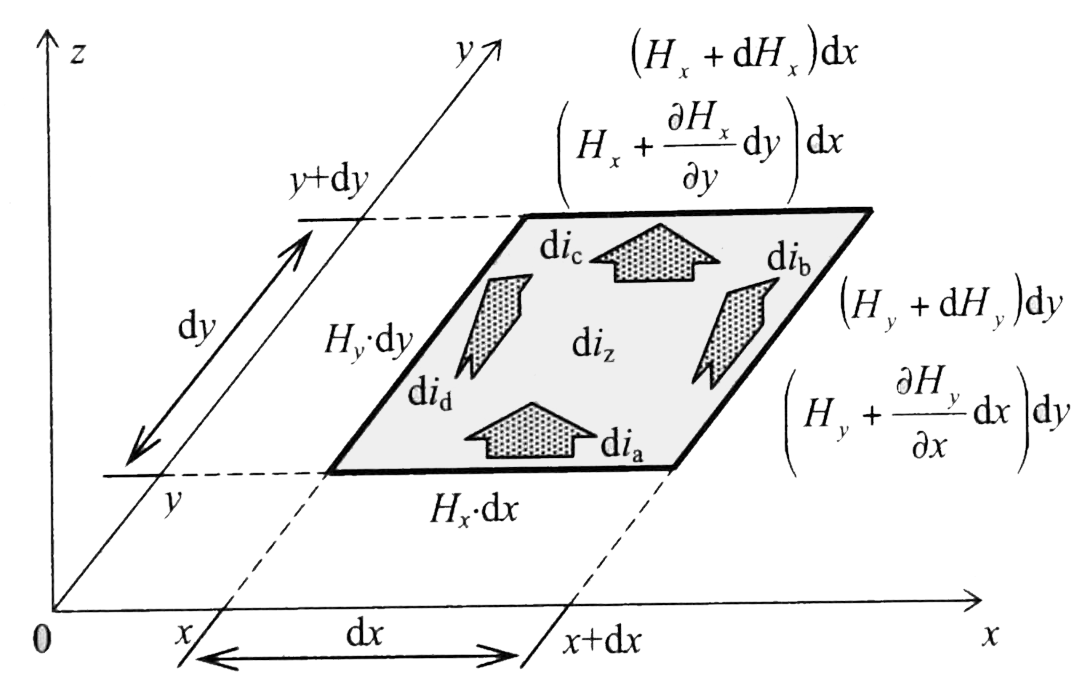
\includegraphics[width=0.8\linewidth]{patocka_mag_tok_exp12.png}
        \caption{Geometrická interpretace \emph{z}-složky \((\rot{H}_z)\) vektoru \(\rot{H}\).}
        \label{es:fig_patocka_mag_tok_exp12}
      \end{figure}
      Geometrický význam \emph{z}-složky \((\rot{H}_z)\) je zřejmý z obr. 
      \ref{es:fig_patocka_mag_tok_exp12}. Jedná se o podobnou situaci, jaká je zobrazena na Obr. 
      \ref{ES:fig_patocka_mag_tok_exp11a}. S ohledem na diferenciální velikost plochy \(dS_z\) je 
      totiž nutno proudy \(di_a, di_b\) ... chápat jako \emph{spojitě rozprostřené} v ploše 
      \(dS_z\), nikoli jako bodové (menší plocha než \(dS_z\) totiž neexistuje). Elementární proud 
      \(di_z = di_a + di_b + di_c + di_d\) tekoucí diferenciální smyčkou \(dS_z\) se nazývá 
      \textbf{ elementární cirkulací} vektoru \(\vec{H}\).

  \section{Třetí Maxwellova rovnice}\label{ES:sec08}
    Konstrukce třetí Maxwellovy rovnice je založena na pojmu \emph{divergence vektoru}, proto je 
    nezbytné nejdříve se s tímto pojmem seznámit.
    
    \subsection{Divergence vektoru D}\label{ES:ssec01}
      Elektrická indukce \(\vec{D}\) je \emph{vektor}, který má význam lokální \emph{plošné 
      hustoty} \(d\Psi_D/dS\) dielektrického toku \(\Psi_D\) neboli plošné hustoty \(dQ/dS\) náboje 
      \(Q\), protože platí identita \(\Psi\equiv Q\).
      
      Naproti tomu divergence \(\diver{D}\) vektoru je \emph{skalár}, který má význam lokální 
      \emph{objemové hustoty} \(\varrho\) náboje. Chceme-li získat objemovou hustotu \(\varrho\) 
      náboje, musíme každou složku \(D_x, D_y , D_z\) indukce \(\vec{D}\) derivovat podle příslušné 
      proměnné \(x, y, z\). Derivace totiž určuje \emph{přírůstek indukce} a ten musí být způsoben 
      \emph{výskytem lokálního náboje} v daném diferenciálním objemu \(dV\). Pro složku \(D_x\) 
      vektoru \(\vec{D}\) zřejmě podle obr. \ref{es:fig_patocka_mag_tok_exp13} platí:
      \begin{equation}\label{ES:eq_zakl_elm46}
        D_x = \frac{d\Psi_{D_x}}{dS_x} = \frac{d\Psi_{D_x}}{\dd{y}\,\dd{z}} = \frac{dQ_x}{\dd{y}\,\dd{z}}. 
      \end{equation} 
      Divergenci ve směru \(x\) získáme tak, že složku indukce \(D_x\) derivujeme podle příslušné 
      proměnné \(x\). S pomocí rovnice (\ref{ES:eq_zakl_elm46}) lze derivaci \(\frac{dD_x}{\dd{x}}\) 
      vyjádřit ve tvaru
      \begin{equation}\label{ES:eq_zakl_elm47}
        (\diver{D})_x = \frac{dD_x}{dS_x} = \frac{dQ_x}{\dd{x}\dd{y}\dd{z}} = \frac{dQ_x}{dV} = \varrho_x. 
      \end{equation} 
      Podobně můžeme získat složky divergence ve zbývajících směrech. Z rovnice 
      (\ref{ES:eq_zakl_elm47}) vyplývá, jak souvisí přírůstek indukce \(dD_x\) s objemovou hustotou 
      \(\varrho_x\) náboje a s divergenci. Na výstupu elementární krychle bude mít přírůstek 
      indukce ve směru \(x\) velikost
      \begin{equation}\label{ES:eq_zakl_elm48}
        dD_x = \varrho_x\,\dd{x} = (\diver{D})_x\,\dd{x} = \pder{D_x}{x}\,\dd{x}. 
      \end{equation} 
      \begin{figure}[ht!]
        \centering
        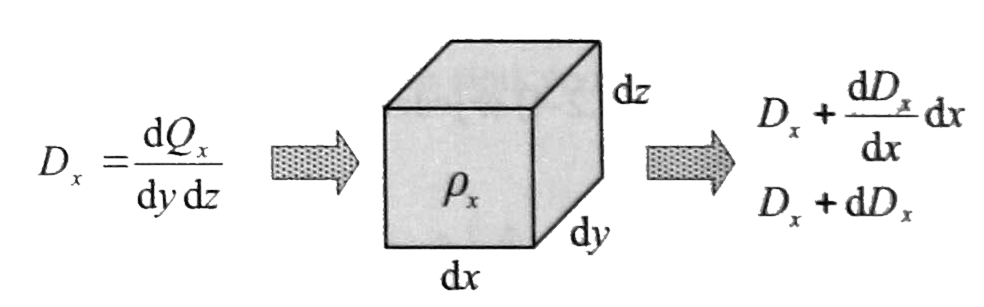
\includegraphics[width=0.9\linewidth]{patocka_mag_tok_exp13.png}
        \caption{Vztah mezi složkou elektrické indukce \(D_x\) a objemovou hustotou \(\varrho_x\) 
                 náboje.}
        \label{es:fig_patocka_mag_tok_exp13}
      \end{figure}
      
      Hustota náboje je \emph{skalární aditivní} veličina. Proto musíme algebraicky sečíst 
      příspěvky \(\varrho_x, \varrho_y, \varrho_z\) ode všech složek divergence ve směrech \(x, y, 
      z\), abychom získali celkovou hustotu \(\varrho\) náboje v elementárním objemu. Celkové 
      hustotě bude rovna i celková divergence v daném bodě:
      \begin{align}\label{ES:eq_zakl_elm49}
        \diver{D} &= (\diver{D})_x + (\diver{D})_y + (\diver{D})_z  \nonumber \\
                  &= \pder{D_x}{x} + \pder{D_y}{y} + \pder{D_z}{z} =
                     \varrho_x + \varrho_y + \varrho_z = \varrho. 
      \end{align} 
      Objemová hustota náboje, tedy i divergence, jsou \emph{skalární} veličiny.
      
    \subsection{Konstrukce třetí Maxwellovy rovnice}\label{ES:ssec02}
      Rovnice (\ref{ES:eq_zakl_elm49}) je přímo III. Maxwellovou rovnicí v diferenciálním tvaru:
      \begin{equation}\label{ES:eq_zakl_elm50}
        \diver{D} = \varrho \qquad [C/m^2, 1/m; C/m^3]. 
      \end{equation} 
      \begin{figure}[ht!]
        \centering
        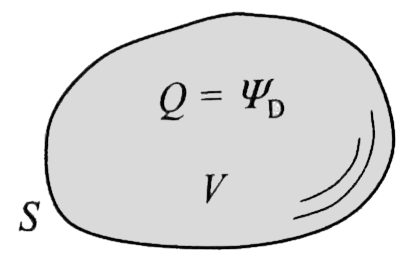
\includegraphics[width=0.4\linewidth]{patocka_mag_tok_exp14.png}
        \caption{Uzavřená orientovaná plocha \(S\) (např. koule) tvoří hranici vnitřního prostoru o 
                 objemu \(V\). Ve vnitřním prostoru se nachází náboj \(Q\).}
        \label{es:fig_patocka_mag_tok_exp14}
      \end{figure}
      
      Plocha \(S\) na obr \ref{es:fig_patocka_mag_tok_exp14} tvoří hranici vnitřního prostoru o 
      objemu \(V\). Z topologického hlediska se jedná o plochu \emph{neohraničenou} (nemá hraniční 
      křivku \(l\)) a \emph{orientovanou} (vnitřní stěnu lze natřít zeleně \textbf{z}, vnější 
      červeně \textbf{č}). Příkladem plochy může být \emph{koule}. Celkový dielektrický tok 
      \(\Psi_D\) prostupující plochou je roven celkovému náboji \(Q\) uvnitř plochy. Pro tok 
      \(\Psi_D\) platí analogie rovnic (\ref{ES:eq_zakl_elm12}), (\ref{ES:eq_zakl_elm39}), a to 
      včetně věty \ref{es:fig_patocka_lemma01} o nezávislosti integrálu na tvaru plochy:
      \begin{equation}\label{ES:eq_zakl_elm51}
        \Psi_D \equiv Q = \int_S\vec{D}\cdot \dd{\vec{S}}.
      \end{equation} 
      Plošný integrál (\ref{ES:eq_zakl_elm51}) převedeme pomocí \textbf{Gaussovy 
      věty}\footnote{Gaussovu větu vysvětlíme v následující kapitole} na integrál objemový:
      \begin{equation}\label{ES:eq_zakl_elm52}
        \Psi_D \equiv Q = \int_S\vec{D}\cdot \dd{\vec{S}} = \int_V\diver{D}\,dV.
      \end{equation} 
      Do rovnice (\ref{ES:eq_zakl_elm52}) dosadíme místo divergence \(\diver{D}\) pravou stranu 
      rovnice (\ref{ES:eq_zakl_elm50}), tj. nábojovou hustotu \(\varrho\). Tak získáme \emph{III. 
      Maxwellovu rovnici} v \emph{integrálním} tvaru
      \begin{equation}\label{ES:eq_zakl_elm53}
        \boxed{\int_S\vec{D}\cdot \dd{\vec{S}} = \int_V\varrho\,dV}.
      \end{equation} 
      Zdůrazněme, že na levé straně rovnice (\ref{ES:eq_zakl_elm53}) se jedná o skalární součin 
      dvou vektorů, na pravé straně o prostý součin dvou skalárů.
      
    \subsection{Gaussova věta}
      Plocha \(S\) tvoří podle obr. \ref{es:fig_patocka_mag_tok_exp14} hranici vnitřního prostoru o 
      objemu \(V\). Z topologického hlediska se jedná o plochu \emph{neohraničenou} a 
      \emph{orientovanou} (např. koule). Gaussova\footnote{Carl Fridrich Gauss (1777-1855), 
      vynikající matematik a fyzik, působil na univerzitě v Gottingenu. Kromě matematiky a 
      elektřiny se zabýval např. teorií geomagnetismu. Společně s W. E. Weberem sestrojili r. 1833 
      první telegraf.}  věta obecně převádí plošný integrál přes tuto plochu \(S\) na objemový 
      integrál přes objem \(V\). Pro pochopení věty velice pomáhá konkrétní fyzikální interpretace 
      jednotlivých veličin. Proto budeme větu zkoumat v konkrétním případě pro vektor indukce 
      \(\vec{D}\). Pak má věta tvar
      \begin{equation}\label{ES:eq_zakl_elm54}
        \int_S\vec{D}\cdot \dd{\vec{S}} = \int_V\diver{D}\,dV \quad(=Q).
      \end{equation} 
      Jak plyne z rovnic (\ref{ES:eq_zakl_elm51}), (\ref{ES:eq_zakl_elm52}), obě strany rovnice 
      (\ref{ES:eq_zakl_elm54}) mají význam celkového náboje \(Q\) uzavřeného uvnitř plochy. Důkaz 
      věty lze konstruovat tak, že \emph{trojný objemový} integrál na pravé straně rovnice 
      (\ref{ES:eq_zakl_elm54}) se budeme snažit převést nezávislým matematickým postupem na dvojný 
      plošný integrál. Z rovnice (\ref{ES:eq_zakl_elm49}) plyne
      \begin{equation}\label{ES:eq_zakl_elm55}
        \varrho = \varrho_x + \varrho_y + \varrho_z 
                = \der{D_x}{x} + \der{D_y}{y} + \der{D_z}{z}. 
      \end{equation}
      Pravou stranu rovnice (\ref{ES:eq_zakl_elm54}) vyjádříme ve tvaru trojného integrálu a 
      dosadíme do ní místo \(\varrho\) pravou stranu rovnice (\ref{ES:eq_zakl_elm55}):
      \begin{align}\label{ES:eq_zakl_elm56}
        Q &= \int_V\diver{D}dV = \int_V\varrho dV 
           = \limitint_{\mathclap{x_Vy_Vz_V}}\varrho\,\dd{x}\,\dd{y}\,\dd{z}   \nonumber\\
          &= \limitint_{\mathclap{x_Vy_Vz_V}}\left(dD_x\,\dd{y}\,\dd{z}+dD_y\,\dd{x}\,\dd{z}+dD_z\,\dd{x}\,\dd{y}\right).
      \end{align}      
      \begin{figure}[ht!]
        \centering
        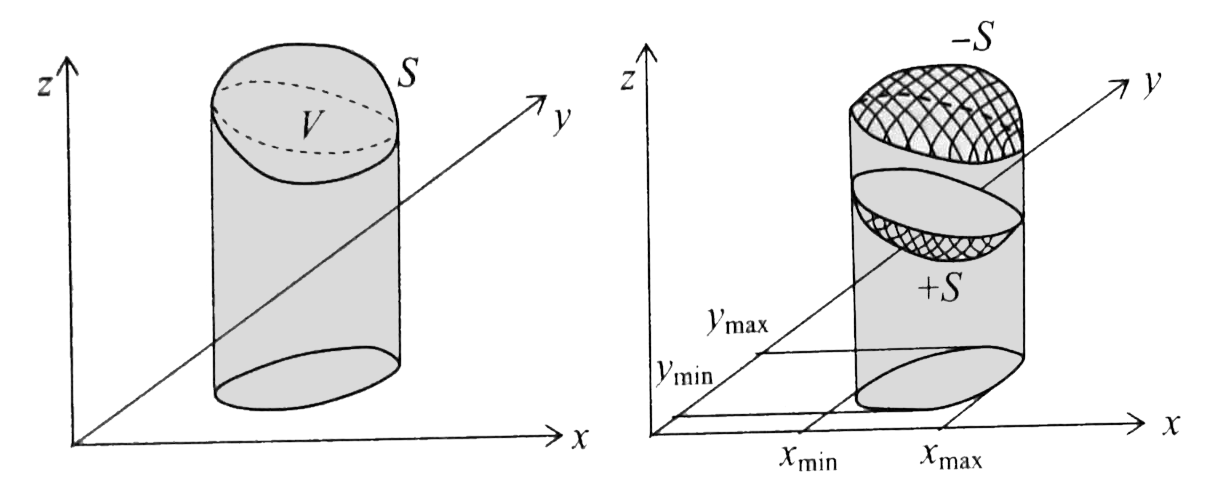
\includegraphics[width=0.9\linewidth]{patocka_mag_tok_exp15.png}
        \caption{Průmět uzavřené plochy \(S\) do roviny \emph{x-y}. Průměty do roviny \emph{y-z, 
                 z-x} lze získat podobně.}
        \label{es:fig_patocka_mag_tok_exp15}
      \end{figure}
      Integrační meze \(x_Vy_Vz_V\) odpovídají podle obr. \ref{es:fig_patocka_mag_tok_exp15} 
      průmětům prostoru \(V\) do příslušných souřadných rovin a z nich do příslušných souřadných 
      os. Zřejmě platí
      \begin{equation}\label{ES:eq_zakl_elm57}
        \limitint_{\mathclap{x_V}}dD_x = D_x \qquad
        \limitint_{\mathclap{y_V}}dD_y = D_y \qquad
        \limitint_{\mathclap{z_V}}dD_z = D_z.
      \end{equation}
      Po dosazení rovnic (\ref{ES:eq_zakl_elm57}) do (\ref{ES:eq_zakl_elm56}) získáme výraz
      \begin{align}\label{ES:eq_zakl_elm58}
        Q &= \iiint\limits_{x_Vy_Vz_V}\varrho\,\dd{x}\,\dd{y}\,\dd{z}   \nonumber\\ 
          &= \iint\limits_{y_Vz_V}D_x\,\dd{y}\,\dd{z} + 
             \iint\limits_{z_Vx_V}D_y\,\dd{z}\,\dd{x} + 
             \iint\limits_{x_Vy_V}D_z\,\dd{x}\,\dd{y}               \nonumber\\ 
          &= \int\limits_{S_x}D_x\,dS_x + 
             \int\limits_{S_y}D_y\,dS_y + 
             \int\limits_{S_z}D_z\,dS_z =  \int\limits_{S}\vec{D}\cdot\vec{S}
      \end{align}
      Ve třech dílčích integrálech nefiguruje součin skalární, nýbrž součin prostý (jedná se o 
      složky vektoru, nikoli o vektor). Integrační meze \(S_x, S_y, S_z\) mají význam 
      \emph{průmětů} plochy \(S\) do jednotlivých souřadných rovin \(y-z\), \(z-x\), \(x-y\). 
      Protože je plocha \(S\) uzavřená, v příslušné rovině existují vždy dva různé průměty: 
      \(S_{+x}, S_{-x}, S_{+y}, S_{-y}, S_{+z}, S_{-z}\). Těm odpovídají dvě různé indukce: 
      \(D_{+x}, D_{-x}, D_{+y}, D_{-y}, D_{+z}, D_{-z}\). V rovnici (\ref{ES:eq_zakl_elm58}) se 
      tedy ve skutečnosti objeví šest dílčích plošných integrálů, uspořádaných do tří dvojic:
      \begin{align*}   %\label{ES:eq_zakl_elm59}
        Q  = \iiint\limits_{x_Vy_Vz_V}\varrho\,\dd{x}\,\dd{y}\,\dd{z}   
          &= \int\limits_{S_x}D_x\,dS_x + 
             \int\limits_{S_y}D_y\,dS_y + 
             \int\limits_{S_z}D_z\,dS_z                                                \\
          &= \int\limits_{S_{+x}}D_{+x}\,dS_x - \int\limits_{S_{-x}}D_{-x}\,dS_x       \\
          &+ \int\limits_{S_{+y}}D_{+y}\,dS_y - \int\limits_{S_{-y}}D_{-y}\,dS_y       \\
          &+ \int\limits_{S_{+z}}D_{+z}\,dS_z - \int\limits_{S_{-z}}D_{-z}\,dS_z       \\
          &= \underbrace{\iint\limits_{y_Vz_V}D_{+x}\,\dd{y}\,\dd{z} 
           - \iint\limits_{y_Vz_V}D_{-x}\,\dd{y}\,\dd{z}}_{\text{dva průměty do roviny y-z}}   \\
          &+ \underbrace{\iint\limits_{z_Vx_V}D_{+y}\,\dd{z}\,\dd{x} 
           - \iint\limits_{z_Vx_V}D_{-y}\,\dd{z}\,\dd{x}}_{\text{dva průměty do roviny z-x}}   \\
          &+ \underbrace{\iint\limits_{x_Vy_V}D_{+z}\,\dd{x}\,\dd{y} 
           - \iint\limits_{x_Vy_V}D_{-z}\,\dd{x}\,\dd{y}}_{\text{dva průměty do roviny x-y}}
      \end{align*}
      Záporná znaménka u sudých integrálů plynou z faktu, že plochy ve dvojici příslušných průmětů 
      jsou opačně orientovány (\textbf{č}\(\rightarrow\)\textbf{z}, 
      \textbf{z}\(\rightarrow\)\textbf{č}). Trojný objemový integrál se tedy podařilo převést 
      na integrál dvojný plošný. Tím je důkaz věty dokončen.
      
  \section{Čtvrtá Maxwellova rovnice}\label{ES:sec09}
    Postup při odvození IV. Maxwellovy rovnice je formálně naprosto shodný s postupem v předchozích 
    kapitolách \ref{ES:ssec01}. a \ref{ES:ssec01}. Ve všech rovnicích pouze nahradíme 
    \emph{elektrické} veličiny analogickými veličinami \emph{magnetickými}, tj. \(D\rightarrow 
    B\), \(\Psi_D\rightarrow \Psi\), \(\varrho\rightarrow \varrho_m\). Proto budou oba 
    tvary IV. MR formálně podobné tvarům III. MR, tj. rovnicím (\ref{ES:eq_zakl_elm53}), 
    (\ref{ES:eq_zakl_elm53}). Velký rozdíl je ale v tom, že elektrické pole je \emph{zřídlové}, 
    kdežto magnetické pole je \emph{vírové}. Z topologického pohledu to znamená:
    \begin{itemize}[noitemsep]
      \item Siločáry elektrické intenzity \(\vec{E}\) nebo \(\vec{D}\) jsou \emph{neuzavřené} 
            křivky, které mají začátek ve „zřídlu“ +Q a konec ve „zřídlu“ -Q.
    
      \item Siločáry magnetické intenzity \(\vec{H}\) nebo \(\vec{B}\) jsou naopak \emph{uzavřené} 
            křivky (tj. „víry“), které  nemají ani začátek ani konec, protože neexistuje magnetický 
            náboj v podobě magnetického monopolu. V magnetismu tedy neexistuje analogie v podobě 
            „+zřídla“ a „-zřídla“. Odtud plyne, že objemová hustota magnetických monopolů 
            \(\varrho_m\) je vždy \emph{nulová}, proto musí být v obou rovnicích položeno 
            \(\varrho_m = 0\).
    \end{itemize}
    \emph{Diferenciální tvar} IV. Maxwellovy rovnice tedy bude:
    \begin{equation}\label{ES:eq_zakl_elm60}
      \diver{B} = 0 \qquad [Wb/m^2,1/m; Wb/m^3].
    \end{equation}
    \emph{Integrální tvar} IV. Maxwellovy rovnice bude:
    \begin{equation}\label{ES:eq_zakl_elm61}
      \int_S\vec{B}\cdot \dd{\vec{S}} = 0.
    \end{equation}    
    V rovnici (\ref{ES:eq_zakl_elm61}) se vždy jedná o \emph{uzavřenou neohraničenou orientovanou} 
    plochu \(S\) (např. kouli, jež má vnitřní stěnu natřenu zeleně \textbf{z}, vnější stěnu červeně 
    \textbf{č}), která tvoří hranici vnitřního prostoru o objemu \(V\), viz obr. 
    \ref{ES:fig_patocka_mag_tok_exp16}. Ve vnitřním prostoru se nemůže nacházet magnetický náboj 
    \(Q_m = \Psi\) v podobě magnetického monopolu - chybí tam zdroj siločar.
   
    \begin{figure}[ht!]
      \centering  
      \subcaptionbox{\label{ES:fig_patocka_mag_tok_exp16a}}{\luafigure[0.45]{patocka_mag_tok_exp16a.png}}
      \subcaptionbox{\label{ES:fig_patocka_mag_tok_exp16b}}{\luafigure[0.45]{patocka_mag_tok_exp16b.png}}
      \caption{Uzavřená orientovaná plocha \(S\) tvořící hranici vnitřního prostoru \(V\): a)   
               ve vnitřním prostoru se nemůže nacházet magnetický náboj \(Q_m = \Phi\) v podobě 
               magnetického monopólu, b) vnější tok vstupuje do vnitřního prostoru levou části 
               plochy ve směru \textbf{č\(\rightarrow\)z} a vystupuje pravou částí ve směru 
               \textbf{z\(\rightarrow\)č}.} 
      \label{ES:fig_patocka_mag_tok_exp16}
    \end{figure}

    Všechny vnější siločáry vstupují do vnitřního objemu částí plochy ve směru 
    \textbf{č}\(\rightarrow\)\textbf{z} a vystupují ven zbývající částí ve směru 
    \textbf{z}\(\rightarrow\)\textbf{č}. Tyto dvě části lze od sebe formálně oddělit uzavřenou 
    křivkou \(l\), která tvoří přirozenou hranici mezi těmito dvěma oblastmi - jedná se o 
    geometrické místo tečných bodů, v nichž se některé ze siločar pouze tečné dotknou plochy \(S\), 
    aniž ji protnou. Pak je možno na problém aplikovat větu \ref{es:fig_patocka_lemma01}: Integrál 
    přes oblast \textbf{č}\(\rightarrow\)\textbf{z} musí mít v absolutní hodnotě stejnou 
    velikost jako integrál přes oblast \textbf{z}\(\rightarrow\)\textbf{č}. S ohledem na opačné 
    orientace však musí mít oba integrály navzájem opačná znaménka. Proto musí platit:
    \begin{equation}\label{ES:eq_zakl_elm62}
      \int\limits_{S}\vec{B}\cdot \dd{\vec{S}} = 
      \int\limits_{\text{č}\rightarrow\text{z}}\vec{B}\cdot \dd{\vec{S}} -
      \int\limits_{\text{z}\rightarrow\text{č}}\vec{B}\cdot \dd{\vec{S}} = 0.
    \end{equation} 
    Celkový tok plochou \(S\) je tedy opravdu nulový.
    
  \section{Biotův-Savartův zákon}\label{ES:sec10}
    Oersted\footnote{Hans Christian Oersted (1777-1851), fyzik a chemik, působil na univerzitě v 
    Kodani. Ve víře v jednotnou přírodní sílu hledal souvislosti mezi přírodními jevy na první 
    pohled nesouvisejícími.} zveřejnil v roce 1820 své experimentální výsledky, týkající se 
    silového působení elektrického proudu na magnetku kompasu. Jeho výsledky však byly pouze 
    kvalitativní. Zanedlouho poté odvodili Biot\footnote{Jean Baptisté Biot (1774-1862), fyzik, 
    působil na Sorboně. Zabýval se elektrodynamikou a optikou.} se Savartem\footnote{Felix Savart 
    (1791-1841), lékař, později působil jako fyzik na Sorboně. Zabýval se elektrodynamikou a 
    akustikou.} na základě složitých experimentů kvantitativní vztah pro výpočet síly působící na 
    magnetku, který upravil Laplace do tvaru
    \begin{equation}\label{ES:eq_zakl_elm63}
      d\vec{F} = KI\frac{\dd{\vec{l}}\times \vec{r}}{r^3}
    \end{equation} 
    
    Konstanta \(K\) v Laplaceově\footnote{Pierre-Simon Laplace (1749-1827), matematik a astronom, 
    člen francouzské Akademie věd. Zabýval se mechanikou a gravitační stabilitou sluneční soustavy, 
    teorií potenciálu, je zakladatelem integrálních transformací v matematice.} rovnici je závislá 
    na použité soustavě jednotek. Zákon říká, že každá elementární část vodiče o diferenciální 
    délce \(dl\) působí na magnetku diferenciálním přírůstkem síly \(dF\). Oersted však zjistil, že 
    vodič \(L\) působí zcela stejně nejen na magnetku, ale i na malý kruhový závit, kterým protéká 
    jiný nezávislý proud. Na základě tohoto experimentálního faktu bylo možno o několik let 
    později, až po zavedení pojmu \emph{„magnetické pole“} Faradayem, modifikovat Biotův-Savartův 
    zákon do současné podoby. Současný tvar zákona, daný rovnicí (\ref{ES:eq_zakl_elm63}), umožňuje 
    výpočet magnetického pole \(H\) nebo \(B\), generovaného vodičem libovolného tvaru, v 
    libovolném bodě prostoru. Prostor ale musí být vyplněn magneticky \emph{izotropním, homogenním 
    a lineárním} prostředím. Předpokladem je, že tloušťka vodiče je zanedbatelná vůči rozměrům 
    vyšetřovaného prostoru. Zákon říká, že každá část vodiče o diferenciální délce \(dl\) vytváří 
    ve sledovaném bodě diferenciální přírůstek magnetického pole \(dH\), resp. \(dB\) podle rovnice
    \begin{equation}\label{ES:eq_zakl_elm64}
      d\vec{H} = \frac{I}{4\pi}\frac{\dd{\vec{l}}\times \vec{r}}{r^3}, \qquad\text{resp.}\qquad
      d\vec{B} = \mu_0\frac{I}{4\pi}\frac{\dd{\vec{l}}\times \vec{r}}{r^3}.
    \end{equation}     
    \begin{figure}[ht!]
      \centering
      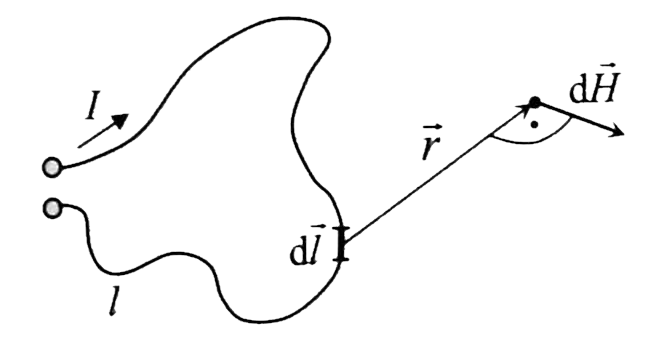
\includegraphics[width=0.5\linewidth]{patocka_mag_tok_exp17.png}
      \caption{K Biotovu-Savartovu zákonu.}
      \label{es:fig_patocka_mag_tok_exp17}
    \end{figure}
    Celkové pole v tomtéž sledovaném bodě lze určit integrací diferenciálních přírůstků 
    (\ref{ES:eq_zakl_elm64}), způsobených všemi diferenciálními částmi \(dl\) vodiče. Konečná 
    podoba Biotova-Savartova zákona má tvar křivkového integrálu, přičemž integrační křivka \(l\) 
    je určena tvarem vodiče:
    \begin{equation}\label{ES:eq_zakl_elm65}
      \vec{H} = \frac{I}{4\pi}\int_l\frac{\dd{\vec{l}}\times \vec{r}}{r^3}, \quad\text{resp.}\quad
      \vec{B} = \mu_0\frac{I}{4\pi}\int_l\frac{\dd{\vec{l}}\times \vec{r}}{r^3}.
    \end{equation} 
    
    Pro obecný tvar vodiče je výpočet křivkového integrálu tak složitý, že je obvykle v uzavřeném 
    tvaru neřešitelný. Snadno řešitelný je však ve \emph{zvláštních případech}, které vykazují 
    vhodnou geometrickou symetrii.
    
    Jedním z nich je výpočet pole \emph{přímého nekonečně dlouhého vodiče}. Je známo, že pole 
    \(\vec{H}\) takového vodiče je kruhově symetrické podle obr. 
    \ref{es:fig_patocka_mag_tok_exp18}. Pro bod umístěný ve vzdálenosti \(R\) od vodiče lze 
    druhou rovnici (\ref{ES:eq_zakl_elm64}) modifikovat do tvaru      
    \begin{figure}[ht!]
      \centering
      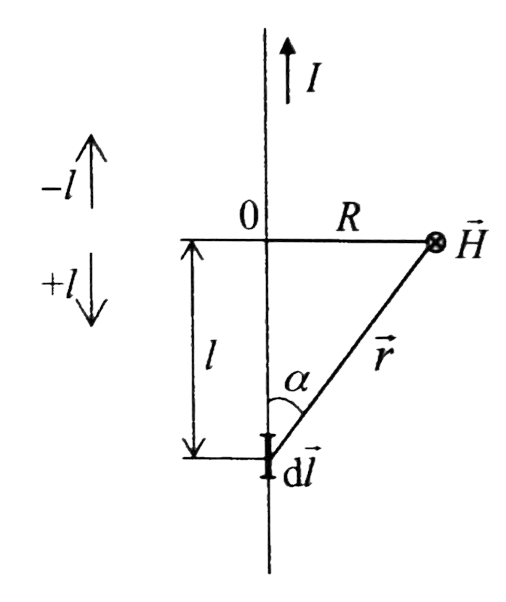
\includegraphics[width=0.4\linewidth]{patocka_mag_tok_exp18.png}
      \caption{K výpočtu pole přímého nekonečně dlouhého vodiče pomocí Biotova-Savartova zákona.}
      \label{es:fig_patocka_mag_tok_exp18}
    \end{figure}
    \begin{align}\label{ES:eq_zakl_elm66}
      d\vec{H} &= \frac{I}{4\pi}\frac{dl\,r\sin\alpha}{r^3}
                = \frac{I}{4\pi}\frac{dl\sin\alpha}{r^2}                 \nonumber \\
               &= \frac{I}{4\pi}\frac{Rdl}{r^3}
                = \frac{IR}{4\pi}\frac{dl}{\left(r^2+l^2\right)^{\frac{3}{2}}}
    \end{align}
    Podle rovnice (\ref{ES:eq_zakl_elm65}) pro \(\vec{H}\) bude mít intenzita magnetického pole 
    velikost 
    \begin{align}\label{ES:eq_zakl_elm67}
      \vec{H} &= \frac{IR}{4\pi}\int\limits_{-\infty}\limits^{+\infty}
                 \frac{dl}{\left(r^2+l^2\right)^{\frac{3}{2}}}
               = \frac{IR}{4\pi} 
                 \left[\frac{l}{R^2\sqrt{R^2+l^2}}\right]_{-\infty}^{+\infty}         \nonumber \\
              &= \frac{I}{4\pi R}
                 \left[\frac{1}{\sqrt{\dfrac{R^2}{l^2}+1}}\right]_{-\infty}^{+\infty} \nonumber \\
              &= \frac{I}{4\pi R}[1-(-1)] = \frac{I}{2\pi R}
    \end{align}
    Poznamenejme, že po krácení zlomku v prvních hranatých závorkách veličinou \(l\) nesmí 
    zaniknout informace o znaménku veličiny \(l\). Proto musí být hodnota následného zkráceného 
    zlomku ve druhých hranatých závorkách po dosazení dolní meze \emph{záporná}, po dosazení horní 
    meze \emph{kladná}. Takto jsme dospěli ke známému výsledku pro intenzitu magnetického pole 
    přímého dlouhého vodiče. Této intenzitě odpovídá magnetická indukce
    \begin{equation}\label{ES:eq_zakl_elm68}
      B = \mu_0H = \mu_0\frac{I}{2\pi R}
    \end{equation}
    
    Jiným zvláštním případem, vykazujícím geometrickou symetrii, je výpočet pole v rotační ose 
    kruhového závitu nebo válcové cívky ( např. \emph{Helmholtzovy cívky}). 
    
  \section{Elektromagnetické síly}\label{ES:sec11}
    Cílem této kapitoly je ukázat jednotné fyzikální principy vedoucí ke vzniku mechanických sil.
    
    \subsection{Vznik mechanických sil v elektromagnetickém poli}
      Koná-li síla \(F\) práci na dráze \(l\) a mění-li během pohybu svoji velikost, nelze použít k 
      výpočtu mechanické práce rovnici \(W_{mech}= Fl\), nýbrž je nutno použít její diferenciální 
      obdobu
      \begin{equation}\label{ES:eq_zakl_elm69}
        dW_{mech} = Fdl
      \end{equation}
      
      Platnost rovnice je založena na základním principu diferenciálního počtu, který říká, že v 
      limitním případě, na diferenciální dráze \(dl\), musí být síla \(F\) \emph{konstantní}. S 
      ohledem na \emph{limitně nulovou} délku dráhy \(dl\) se diferenciální přírůstek vykonané 
      práce \(dW_{mech}\) též někdy nazývá \textbf{virtuální prací}. Virtuální práce \(dW_{mech}\), 
      vykonaná izolovanou fyzikální soustavou, musí být kryta ze zdroje energie energetickým 
      příspěvkem \(dW\), a to takovým způsobem, aby \emph{celková energie soustavy zůstala 
      zachována}. Odtud plyne, že součet diferenciálních energetických přírůstků v izolované 
      soustavě musí být nulový:
      \begin{equation}\label{ES:eq_zakl_elm70}
        dW_{mech}+dW=0.
      \end{equation}
      Z rovnic (\ref{ES:eq_zakl_elm69}), (\ref{ES:eq_zakl_elm70}) plyne, že v soustavě nutně vzniká 
      mechanická síla
      \begin{equation}\label{ES:eq_zakl_elm71}
        \boxed{F = \frac{dW_{mech}}{dl} = -\frac{dW}{dl}},
      \end{equation}
      kde \(dW\) je přírůstek energie dodaný zdrojem.
      
      V případě elektromagnetu se železným jádrem a se vzduchovou mezerou lze zanedbat magnetickou 
      vodivost železa oproti vodivosti vzduchové mezery. Pak je veškerá magnetická energie 
      soustředěna pouze do objemu vzduchové mezery o délce \(l\):
      \begin{equation}\label{ES:eq_zakl_elm72}
        W =\frac{1}{2}Li^2 = \frac{1}{2}i^2N^2\mu_0\frac{S_{Fe}}{l}.
      \end{equation}
      Z rovnic (\ref{ES:eq_zakl_elm72}) a (\ref{ES:eq_zakl_elm71}) plyne, že ve vzduchové mezeře 
      magnetu vznikne síla
      \begin{align}\label{ES:eq_zakl_elm73}
         F = -\frac{dW}{dl} 
           &= +\frac{1}{2}i^2N^2\mu_0\frac{S_{Fe}}{l^2}
           =  \frac{1}{2}i^2\frac{L}{l} = \frac{1}{2}H^2\mu_0S_{Fe}              \nonumber \\
           &=  \frac{1}{2}BHS_{Fe} = \frac{1}{2}\frac{B^2}{\mu_0}S_{Fe}.
      \end{align}
      Mechanický tlak ve vzduchové mezeře bude
      \begin{equation}\label{ES:eq_zakl_elm74}
        p = \frac{F}{S_{Fe}} = \frac{1}{2}H^2\mu_0 = \frac{1}{2}BH = \frac{1}{2}\frac{B^2}{\mu_0}.
      \end{equation}
      Z rovnice (\ref{ES:eq_zakl_elm72}) rovněž vyplývá, že objemová hustota energie magnetického 
      pole ve vzduchové mezeře je \emph{identicky rovna} mechanickému tlaku:
      \begin{align}\label{ES:eq_zakl_elm75}
        w  = \frac{W}{V} 
          &= \frac{W}{S_{Fe}l} = \frac{1}{2}i^2N^2\mu_0\frac{1}{l^2}             \nonumber \\
          &= \frac{1}{2}H^2\mu_0 = \frac{1}{2}BH = \frac{1}{2}\frac{B^2}{\mu_0}.
      \end{align}
      Podobně v případě vzduchového kondenzátoru lze sílu určit pomocí elektrostatické energie 
      nashromážděné v prostoru mezi elektrodami:
      \begin{equation}\label{ES:eq_zakl_elm76}
        W = \frac{1}{2}u^2C = \frac{1}{2}u^2\varepsilon_0\frac{S}{l}.
      \end{equation}
      Z rovnic (\ref{ES:eq_zakl_elm76}) a (\ref{ES:eq_zakl_elm71}) plyne, že ve vzduchové mezeře 
      kondenzátoru vznikne síla
      \begin{align}\label{ES:eq_zakl_elm77}
        F  = \frac{dW}{dl} 
          &= \frac{1}{2}u^2\varepsilon_0\frac{S}{l^2}
           = \frac{1}{2}E^2\varepsilon_0S                                 \nonumber \\
          &= \frac{1}{2}DES           
           = \frac{1}{2}\frac{D^2}{\varepsilon_0}S.
      \end{align}
      Mechanický tlak mezi elektrodami kondenzátoru bude
      \begin{align}\label{ES:eq_zakl_elm78}
        F  = \frac{dW}{dl} 
          &= \frac{1}{2}u^2\varepsilon_0\frac{S}{l^2}
           = \frac{1}{2}E^2\varepsilon_0S                                 \nonumber \\
          &= \frac{1}{2}DES          
           = \frac{1}{2}\frac{D^2}{\varepsilon_0}S.
      \end{align}
      Z rovnice (\ref{ES:eq_zakl_elm76}) vyplývá, že objemová hustota energie elektrického pole 
      mezi elektrodami kondenzátoru je identicky rovna mechanickému tlaku:
      \begin{align}\label{ES:eq_zakl_elm79}
        w  = \frac{W}{V} 
          &= \frac{W}{Sl} 
           = \frac{1}{2}u^2\varepsilon_0\frac{1}{l^2}         \nonumber \\
          &= \frac{1}{2}E^2\varepsilon_0 = \frac{1}{2}DE 
           = \frac{1}{2}\frac{D^2}{\varepsilon_0}.
      \end{align}
      Je zajímavé, že v případě elektromagnetu i kondenzátoru je tlak ve vzduchové mezeře roven 
      objemové hustotě energie v téže mezeře, tj. \(p = w\).
      
      Pro dokreslení fyzikálních souvislostí porovnejme tento výsledek s termodynamikou plynů. U 
      plynu uzavřeného v nádobě se celková hustota kinetické energie molekul musí podle
      \emph{ekvipartičního teorému} rovnoměrně rozdělit mezi tři souřadné směry \(x, y, z\), proto 
      by tlak plynu na stěny nádoby měl být třetinový, ve skutečnosti je ze složitějších důvodů 
      dvoutřetinový oproti hustotě kinetické energie:
      \begin{equation}\label{ES:eq_zakl_elm80}
        p = \frac{2}{3}w
      \end{equation}
      V mezeře elektromagnetu i kondenzátoru vzniká tlak pouze v \emph{jediném} 
      směru\footnote{Předpokládáme, že pólové nástavce jsou v zákrytu. Při vychýleni jednoho z 
      nástavců do strany sice vznikne v mezeře i boční síla, ale to je zcela jiné geometrické 
      uspořádání, které neuvažujeme.}, proto platí \(p = w\). Nositelé \emph{elektromagnetických 
      silových interakcí} jsou fotony\footnote{Na této skutečnosti je založena Feynmanova teorie 
      kvantové elektrodynamiky.}. Ty plní ve vzduchové mezeře elektromagnetu nebo 
      kondenzátoru podobnou roli jako molekuly plynu v nádobě. Rozdíl je pouze v tom, že vznikající 
      síla je přitažlivá, nikoli odpudivá a že fotony působí v jediném směru (při dané geometrické 
      konfiguraci).
      
      Analogicky k rovnici (\ref{ES:eq_zakl_elm74}) lze určit mechanický tlak uvnitř železného 
      jádra elektromagnetu, lokalizovaný ve \emph{vnitřním objemu železa} o relativní permeabilitě 
      \(\mu_{r_{Fe}}\)
      \begin{equation}\label{ES:eq_zakl_elm81}
       p = \frac{1}{2}\frac{B^2}{\mu_0\mu_{r_{Fe}}}.
      \end{equation}
      Vnitřní mechanický tlak v železe je vnějšímu pozorovateli experimentálně nedostupný. Nicméně 
      existuje a vidíme, že je řádově 2000krát menší oproti tlaku v mezeře. Stejný je i poměr 
      hustot energií v železe a v mezeře. To nás plně oprávnilo k původnímu zanedbání železa při 
      výpočtu síly. Všimněme si, že při \emph{konstantním} toku \(\Phi = BS_{Fe} = \text{konst}\). 
      platí tyto zákonitosti:
      \begin{itemize}[noitemsep]
        \item Magnetická síla je tím menší, čím je permeabilita obvodu větší, viz rovnice     
              (\ref{ES:eq_zakl_elm81}).
        \item Magnetická síla je tím menši, čím je plocha \(S_{Fe}\) obvodu větší, viz rovnice 
              (\ref{ES:eq_zakl_elm73}). Zřejmě totiž platí \(F \cong B^2S_{Fe} = 
              \frac{\Phi^2}{S_{Fe}} = \frac{\text{konst.}}{S_{Fe}}\).
      \end{itemize}
      Obě zákonitosti lze zobecnit takto:
      \begin{itemize}[noitemsep]
        \item Magnetická síla, tedy i potenciální energie soustavy, je tím menší, čím větší je    
              magnetická vodivost obvodu.
        \item Tlakové pole vznikající v magnetickém obvodu zaujme vždy takové prostorové rozložení, 
              které se snaží zdeformovat obvod do tvaru, v němž je potenciální energie obvodu co 
              nejmenší\footnote{Z podobných důvodů působí síla na těleso umístěné v gravitačním 
              poli. Gravitační síla má takový směr. že se snaží zmenšit potenciální energii \(mgh\) 
              tělesa na nulu.}, tj. v němž je magnetická vodivost obvodu co největší.
      \end{itemize}
      
      V důsledku obou zobecněných zákonitostí vznikají následující jevy:
      \begin{itemize}[noitemsep]
        \item Je-li součástí obvodu vzduchová mezera, tlakové pole se snaží zkrátit její délku na 
              nulu.
        \item Proudovodič ve tvaru uzavřené smyčky, umístěný volně v prostoru, se tlakové pole   
              snaží \emph{roztáhnout} do co největší plochy, tj. napnout vodič do kružnice.
        \item Dva paralelní vodiče, kterými protékají proudy \emph{opačných} směrů, se 
              \emph{odpuzuji} (v podstatě se jedná o podlouhlou uzavřenou smyčku z předchozího 
              bodu). U transformátoru se odpuzuje sekundární vinutí od primárního (opačné směry 
              proudů). Podobně vzduchová cívka napájená střídavým proudem se odpuzuje od kovové 
              nemagnetické desky, ve které vznikají vířivé proudy.
        \item Dva paralelní vodiče, kterými protékají proudy \emph{souhlasných} směrů, se 
              \emph{přitahuji}. U transformátoru se vzájemně přitahují závity téhož vinutí.
      \end{itemize}
      
      Z uvedených skutečností je zřejmé, že existence magnetické síly nesouvisí s přítomností 
      železa. V magnetickém obvodu, obsahujícím společně železo i vzduchovou mezeru, plní železo 
      roli pouhého „soustřeďovače siločar“ do objemu vzduchové mezery. V mezeře se pak jedná o 
      silovou interakci čistě mezi magnetickým \emph{polem} a \emph{vakuem}. Pro lepší pochopení 
      elektromagnetických sil je vhodné nahlížet na vakuum jako na „pružný materiál“\footnote{Při 
      řešení teoretických fyzikálních problémů je často užitečný „inženýrský přistup“. Z 
      psychologických důvodů proto není na škodu považovat vakuum za plnohodnotný „konstrukční“ 
      materiál, u kterého známe s jistotou tři jeho materiálové konstanty: \(\varepsilon_0\), 
      \(\mu_0\) a měrnou hmotnost \(\varrho = 0\).}, který je magnetickým polem 
      deformován do takového tvaru, aby magnetická vodivost tohoto „materiálu“ byla co 
      \emph{největší}. Jinak řečeno, aktivní objem vakua je silou nucen zaujmout takový tvar, aby 
      celková potenciální energie pole byla co \emph{nejmenší}.
      
      V	případě \emph{rotačního} pohybuje možno modifikovat rovnici (\ref{ES:eq_zakl_elm71}) pro 
      výpočet \emph{momentu síly}. Stačí vynásobit obě strany rovnice délkou ramena \(r\), na němž 
      síla působí:
      \begin{equation*}
        Fr = \frac{dW_{mech}}{dl}r 
           = \frac{dW_{mech}}{\dfrac{dl}{r}} 
           = \frac{dW_{mech}}{d\alpha}
             \qquad \Longrightarrow
      \end{equation*}
      \begin{equation}\label{ES:eq_zakl_elm82}
        \boxed{M = \frac{dW_{mech}}{d\alpha} = \frac{dW}{d\alpha}}
      \end{equation}
      kde \(\alpha\) je úhel natočení. Rovnice je vhodná pro přímý výpočet momentu všech 
      \emph{reluktančních motorů}, jejichž princip je založen na tom, že magnetická vodivost 
      vzduchové mezery se výrazně mění s úhlem natočení hřídele.
      
      Rovnici (\ref{ES:eq_zakl_elm71}) lze interpretovat tak, že síla je rovna \emph{strmosti}, s 
      jakou se mění energie soustavy v závislosti na změně délkové souřadnice \(l\). Ve složitějším 
      geometrickém uspořádání soustavy lze rovnici (\ref{ES:eq_zakl_elm71}) zobecnit do vektorového 
      tvaru
      \begin{equation}\label{ES:eq_zakl_elm83}
       \vec{F} = -\vec{i}\frac{dW}{\dd{x}} -\vec{j}\frac{dW}{\dd{y}} -\vec{k}\frac{dW}{\dd{z}} 
               = - \grad{W},
      \end{equation}
      kde \(\vec{i}, \vec{j}, \vec{k},\) jsou jednotkové vektory ve směru příslušných os. Síla je 
      pak nejobecněji definována jako záporně vzatý gradient (vektor) ze skalární funkce 
      \(W(x,y,z)\).
      
    \subsection{Lorentzova síla}
      
      Elektromagnetické síly působící na elektrický náboj lze shrnout do jediné Lorentzovy rovnice
      \begin{equation}\label{ES:eq_zakl_elm84}
        \vec{F}=q(\vec{E}+\vec{v}\times\vec{B}),
      \end{equation}
      ve které první člen vyjadřuje Coulombovu\footnote{Charles Augustin de Coulomb (1736-1806), 
      absolvent vojenské školy v Paříži. Zákon síly mezi dvěma bodovými náboji odhalil v období 
      1785 až 1789 v soukromí. Později jmenován členem pařížské Akademie věd.} elektrostatickou 
      sílu, působící na náboj \(Q\) umístěný v elektrickém poli \(\vec{E}\) a druhý člen vyjadřuje 
      Lorentzovu\footnote{Henrik Antoon Lorentz (1853-1928), teoretický fyzik, působil na 
      univerzitě v Leidenu. R. 1902 obdržel Nobelovu cenu za fyziku.} sílu, která působí na 
      náboj, pohybující se relativní rychlostí \(v\) vůči magnetickému poli \(B\). Lorentz 
      formuloval obě složky síly zcela obecně, tj. pro náboj pohybující se i relativistickou 
      rychlostí \(v \rightarrow c\), a to pomocí známých Lorentzových transformací. Pro 
      dokreslení historických souvislostí lze dodat, že Coulombův zákon pro náboje pohybující se 
      nižšími nerelativistickými rychlostmi korigoval už Weber ve druhé polovině 19. stol.
      a elektrické pole E, vytvořené relativisticky se pohybujícím nábojem, odvodil 
      Heaviside\footnote{Oliver Heaviside (1850-1925), technik britské telegrafní společnosti, 
      vynálezce duplexního telegrafu. Později soukromý vědec, samouk.} již r. 1888, tj. 17 let před 
      vznikem speciální teorie relativity. 
      
      V běžné inženýrské praxi lze zcela zanedbat Coulombovy síly oproti silám Lorentzovým. Navíc 
      je průměrná transportní (nikoli okamžitá) rychlost volných elektronů v kovech velmi malá, 
      řádově dosahuje \si{\cm/\s}, tudíž není nutno uvažovat relativistické efekty. Pak 
      můžeme uvažovat pouze druhý člen v rovnici (\ref{ES:eq_zakl_elm84}), pomocí něhož lze snadno 
      odvodit elementární Lorentzovu sílu \(dF\), působící na vodič o diferenciální délce \(dl\), 
      který se nachází v magnetickém poli \(B\).
       
      Protéká-li vodičem proud \(I\), z rovnice plyne:
      \begin{equation}\label{ES:eq_zakl_elm85}
        d\vec{F} =  dQ\,\vec{v}\times\vec{B} 
                 = I\dd{t}\,\vec{v}\times\vec{B} 
                 = I\dd{t}\,\frac{\dd{\vec{l}}}{\dd{t}}\times\vec{B}
                 = I\,\vec{l}\times\vec{B}.
      \end{equation}
      Díky vektorovému součinu je síla \(d\vec{F}\) vždy \emph{kolmá} na oba vektory \(\dd{\vec{l}}\) a 
      \(\vec{B}\) a v absolutní hodnotě má velikost
      \begin{equation}\label{ES:eq_zakl_elm86}
              dF=I\,dl\,B\sin\alpha,
      \end{equation}
      kde \(\alpha\) je úhel sevřený oběma vektory \(\dd{\vec{l}}\) a \(\vec{B}\). Proto musí všechny 
      tři vektory v pořadí \(\dd{\vec{l}}\), \(\vec{B}\), \(d\vec{F}\) tvořit \textbf{pravotočivý 
      systém}. Jedná se o \emph{topologickou vlastnost}\footnote{Jednou z několika rozlišitelných 
      topologických kvalit je rozlišení pravé a levé strany.} elektromagnetického pole, která je 
      známa jako \emph{pravidlo levé ruky}.
      \begin{itemize}
        \item \textbf{Pravidlo levé ruky}: Čtyři natažené prsty levé ruky ukazují směr proudu (tj. 
              směr rychlosti náboje), siločáry magnetického pole vstupují do dlaně a palec ukazuje 
              směr síly.
      \end{itemize}

      Předpokládejme, že celý dlouhý vodič je mechanicky dokonale tuhý, nedeformovatelný. Pak 
      celková síla, působící na vodič libovolného tvaru o délce \(l\), bude určena křivkovým 
      integrálem
      \begin{equation}\label{ES:eq_zakl_elm87}
        \vec{F} = \int_ld\vec{F} 
                = I\int_l (\dd{\vec{l}}\times\vec{B}).
      \end{equation}
      Ve \emph{zvláštním} případě, pro přímý vodič o délce \(l\) vložený do \emph{homogenního} 
      magnetického pole \(B\) a orientovaný tak, že vodič je umístěn \emph{kolmo} na směr siločar, 
      dostáváme známý vztah
      \begin{align}\label{ES:eq_zakl_elm88}
        F  =  I\int_l (\dd{\vec{l}}\times\vec{B})
          &= BI\int_l \dd{\vec{l}} = BI\int\limits_{l_1}^{l_2}\dd{\vec{l}}  \nonumber \\
          &= BI[l]_{l_1}^{l_2}
           = BI[l_2 - l_1]
           = BIl.
      \end{align}
      Rovnice (\ref{ES:eq_zakl_elm88}) nachází uplatnění především v teorii stejnosměrných a 
      střídavých strojů. Rovnici lze psát obecněji pro časově proměnné veličiny a navíc modifikovat 
      pro moment síly:
      \begin{equation}\label{ES:eq_zakl_elm89}
        F(t)=B(t)i(t)l, \qquad\text{resp.} \qquad M(t)=B(t)i(t)lr,
      \end{equation}
      kde \(r\) je poloměr vzduchové mezery. V případě stejnosměrného stroje s konstantním buzením, 
      tj. \(B(t) = \text{konst.}\), plyne z rovnice přímá úměra mezi okamžitými hodnotami 
      \emph{proudu} a \emph{momentu} stroje.


    \subsection{Síla mezi dvěma dlouhými rovnoběžnými vodiči}      
      V kapitole \ref{ES:sec10} bylo pomocí Biotova-Savartova zákona odvozeno magnetické pole \(B\) 
      dlouhého přímého vodiče. Siločáry pole máji tvar soustředných kružnic, v jejichž středu leží 
      příslušný vodič. Protéká-li vodičem označeným 1 proud \(I_1\) pak vodič vybudí ve vzdálenosti 
      \(R\) magnetickou indukci
      pro moment síly:
      \begin{equation}\label{ES:eq_zakl_elm90}
        B_1 = \mu_0\frac{I_1}{2\pi R}.
      \end{equation}
      Ve vzdálenosti \(R\) umístíme rovnoběžně s vodičem 1 další vodič, označený 2. Pak se vodič 2 
      nachází v magnetickém poli o velikosti \(B_1\). Protéká-li vodičem 2 proud \(I_2\), pak podle 
      rovnice (\ref{ES:eq_zakl_elm88}) na něj působí síla
       pro moment síly:
      \begin{equation}\label{ES:eq_zakl_elm91}
        F_{1,2} = B_1 I_2 l = \mu_0\frac{I_1}{2\pi R}I_2 l.
      \end{equation}
      Pak měrná síla působící na jednotkovou délku vodiče bude mít velikost
      \begin{equation}\label{ES:eq_zakl_elm92}
        \frac{F_{1,2}}{l} = \mu_0\frac{I_1I_2}{2\pi R}.
      \end{equation}
      Záměnou obou vodičů, tj. záměnou indexů v rovnicích (\ref{ES:eq_zakl_elm90}) a 
      (\ref{ES:eq_zakl_elm91}) lze snadno dokázat, že mezi vodiči platí \emph{zákon akce a reakce} 
      ve tvaru \(F_{1,2} = F_{2,1}\) . Síla je přitažlivá, mají-li oba proudy stejný směr, 
      odpudivá, mají-li směr opačný. Rovnice (\ref{ES:eq_zakl_elm92}) slouží k \emph{dynamické 
      definici} jednotky elektrického proudu \SI{1}{\A}:
      
      Vakuum má z historických důvodů magnetickou permeabilitu
      \begin{equation}\label{ES:eq_zakl_elm93}
        \mu_0= 4\pi\times10^{-7}\,\si{\henry/\m} \cong l,256\times10^{-6}\,\si{\henry/\m}.
      \end{equation}
      Protéká-li oběma rovnoběžnými dlouhými vodiči stejný proud \(I\), síla na jednotku délky 
      vodiče bude mít velikost
      \begin{equation}\label{ES:eq_zakl_elm94}
        \frac{F_{1,2}}{l} = \mu_0\frac{I^2}{2\pi R} = 2\times10^{-7}\frac{I^2}{R}.
      \end{equation}
      Ze změřené síly a vzdálenosti vodičů \(R\) je pak možno určit velikost protékajícího proudu 
      \(I\).
    
%} % tikzset
%~~~~~~~~~~~~~~~~~~~~~~~~~~~~~~~~~~~~~~~~~~~~~~~~~~~~~~~~~~~~~~~~~~~~~~~~~~~~~~~~~~~~~~~~~~~~~~~~~~ 
}{ % DEBUG was off
\LuaPartBckgrnd{titleBG_fractal1.png}
\LuaPartTitle{TEO}{Teorie elektrických obvodů}{TEO}
\parttoc
%========== Kapitola: Základy elektrických obvodů =================================================
  % !TeX spellcheck = cs_CZ
%file:intro_TEO.tex
%{\tikzset{external/prefix={tikz/TEO/}}
% \tikzset{external/figure name/.add={ch09_}{}}
%================================= Kapitola: Základy elektrických obvodů ===========================
\chapter{Základy elektrických obvodů}
\minitoc

  \section{Struktura elektrických ob\-vo\-dů}
    Ke každému skutečnému, fyzicky realizovanému, elektrickému obvodu lze nakreslit 
    \textbf{obvodové schéma}. Toto schéma je vlastně \emph{obvodovým modelem} skutečného obvodu. 
    Obvodový model je sestaven ze základních obvodových prvků - \textbf{dvojpólů}. Název plyne z 
    důležité topologické vlastnosti dvojpólů - mají dvě svorky \cite[s.~12]{Patocka2}.
    
    \subsection{Teorie elektromagnetického pole a elektrické obvody}
      Uspokojivý výklad všech makroskopických elektromagnetických jevů, jež probíhají v 
      nepohyblivých látkových prostředích, poskytuje Maxwellova klasická teorie elektromagnetického 
      pole. Vyšetření elektromagnetického pole (tj. určení vektorů \(\vec{E}\) a \(\vec{B}\) ve 
      všech bodech zkoumané oblasti pro každý okamžik) lze vždy provést integrací Maxwellových 
      rovnic pro dané okrajové a počáteční podmínky. Rovnice elektromagnetického pole se mohou 
      mnohdy zjednodušit, např. zanedbáním Maxwellova („posuvného“) proudu proti proudu vodivému v 
      1. Maxwellově rovnici u kvazistacionárních magnetických polí, zjednodušením geometrické 
      konfigurace apod. Přesto však řada technických úloh vede k dosti náročným matematickým 
      problémům. V některých případech však lze dosáhnout \emph{podstatného zjednodušení} řešení 
      použitím metod teorie elektrických obvodů. Teorie elektromagnetického pole tím sice nepozbývá 
      svůj základní význam pro elektrotechniku, avšak teorie elektrických obvodů umožňuje 
      efektivnější koncepci řešení některých technických úloh.
      
      Přistoupíme k vysvětlení pojmu \textbf{elektrický obvod}. Různá elektrotechnická zařízení lze 
      často považovat za systém složený z jednoduchých částí rozmanitě mezi sebou spojených, jimiž 
      mohou procházet proudy. Dále budeme předpokládat, že elektromagnetické jevy v tomto systému 
      lze vyjádřit pomocí \emph{napětí a proudů}. (Nebudeme tedy používat veličin \(\vec{E}\); 
      \(\vec{B}\); \(\vec{D}\); \(\vec{H}\), jež lokálně charakterizují elektromagnetické pole.) 
      Takový systém nazýváme \emph{reálným elektrickým obvodem}. Při studiu reálného elektrického 
      obvodu se abstrahujeme od jeho nepodstatných vlastností a omezujeme se jen na ty, jež jsou 
      pro zkoumaný jev rozhodující. Touto idealizací přecházíme k jednoduššímu systému, který 
      obecně nazýváme \emph{modelem}. Modelem může být opět reálný elektrický obvod, který zkoumáme 
      \emph{experimentálně}, zde však budeme mít na zřeteli pouze abstraktní modely, které 
      vyšetřujeme teoreticky. Tyto modely, jejichž vlastnosti budeme dále zkoumat, nazýváme 
      \emph{ideálními elektrickými obvody} anebo krátce \emph{obvody}\cite[s.~19]{Meyer1978}.
      
      Sestavení obvodu, jenž dostatečně přesně vystihuje reálný elektrický obvod v jeho provozních 
      podmínkách, není předmětem teorie obvodů, nýbrž disciplín, které teorii obvodů používají 
      (např. teorie elektrických strojů, elektroenergetiky, radiotechniky, sdělovací 
      elektrotechniky). \emph{Teorie obvodů vychází z těchto modelů a zkoumá jejich vlastnosti a 
      metody řešení}, která zpravidla mají vysoký stupeň přesnosti. Naproti tomu při sestavení 
      obvodu bychom se mohli dopustit chyby, kdybychom jej neověřovali konfrontací jeho vlastností 
      s originálem. Jelikož obvod nevyjadřuje všechny vlastnosti reálného elektrického obvodu, 
      vznikají jisté rozpory mezi teorií obvodů a Maxwellovou teorií elektromagnetického pole. 
      Například v teorii obvodů se předpokládá, že elektrická energie se přenáší vodiči obvodu — 
      lze ji snadno určit z napětí a proudů těchto vodičů. Naproti tomu z Maxwellovy teorie plyne, 
      že se veškerá energie přenáší dielektrikem v okolí vodičů; vodiče pouze určují směr toku této 
      energie. Tyto rozpory však nejsou překážkou pro používání teorie obvodů v praxi.

      \begin{figure}[ht!]  %\ref{teo:fig023}
        \centering
        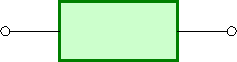
\includegraphics[width=0.7\linewidth]{teo_fig023.pdf}
        \caption{Dvojpól}
        \label{teo:fig023}
      \end{figure}

      Libovolnou část obvodu, která je vyvedena k jedné dvojici svorek, nazýváme 
      \textbf{dvojpólem}; jeho schematické označení je na obr. \ref{teo:fig023}. Veličinu, jež 
      fyzikálně charakterizuje dvojpól, nazýváme jeho parametrem. Dvojpóly, které lze 
      charakterizovat jediným reálným parametrem, nazýváme \textbf{ideálními prvky obvodu} anebo 
      krátce \emph{prvky obvodu}.
      
      Z Maxwellovy teorie plyne, že elektromagnetické vlnění vyvolané elektromagnetickými jevy v 
      obvodu se šíří prostorem rychlostí světla. Pro jednoduchost předpokládejme, že 
      elektromagnetická vlna má harmonický průběh. Jsou-li geometrické rozměry reálného 
      elektrického obvodu zanedbatelně malé ve srovnání s délkou elektromagnetického vlnění, lze 
      rychlost jeho šíření považovat za nekonečně velkou a geometrické rozměry reálného 
      elektrického obvodu se neuplatní — napětí a proudy v tomto obvodu jsou pak pouze funkcí času 
      t. Lze jej modelovat obvodem, jehož magnetické pole je \emph{kvazistacionámi}; parametry jeho 
      dvojpólů nejsou funkcemi geometrických souřadnic. Hovoříme o \emph{obvodu se soustředěnými 
      parametry}.
      
      Nejsou-li geometrické rozměry reálného elektrického obvodu zanedbatelné vzhledem k délce 
      elektromagnetické vlny, je nutné brát v úvahu konečnou rychlost šíření elektromagnetického 
      vlnění — napětí a proudy v tomto obvodu pak budou nejen funkcemi času \(t\), ale též polohy v 
      prostoru, určené souřadnicemi \(x, y, z\) (zpravidla postačí jediná souřadnice). Parametry 
      dvojpólů takového obvodu jsou též funkcemi polohy, a proto hovoříme o \emph{obvodu s 
      rozprostřenými (rozloženými) parametry}.
            
      Teorie obvodů je úzce spjata s kybernetikou, a proto jsou některé pojmy těchto vědních oborů 
      společné. Jak známo, kybernetika se zabývá studiem \emph{systémů libovolné povahy, které jsou 
      schopny přijímat, uschovávat a zpracovávat informaci a využívat ji k řízení}. Obvod je 
      speciálním případem systému, v němž dochází k interakci s okolím na \emph{vstupu (na 
      vstupních svorkách)} a na \emph{výstupu (na výstupních svorkách)}; na vstup jsou připojeny 
      \emph{zdroje energie}, na výstup \emph{spotřebiče}. Napětí a proudy na vstupu představují 
      \emph{podněty (stimuly)} čili \emph{vstupní veličiny}, na výstupu představují \emph{odezvy 
      (reakce)} čili \emph{výstupní veličiny}.
      
      Základními vlastnostmi obvodu jsou: \emph{chování obvodu}, tj. závislost mezi podněty a 
      odezvami a \emph{struktura obvodu}, tj. vlastnosti jeho prvků a způsob jejich spojení. 
      Strukturu obvodu charakterizují jednak fyzikální vlastnosti prvků tvořících obvod, jednak 
      způsob jejich vzájemného spojení. V prvém případě hovoříme o \emph{fyzikální struktuře} 
      obvodu, ve druhém o jeho \emph{topologické (geometrické) struktuře}\cite[s.~21]{Meyer1978}.
      
      
    \subsection{Fyzikální struktura obvodů} 
      \subsubsection{Uzly a větve obvodu, orientace větví, větvové proudy a 
      napětí}\label{TEO:chap_Term}
        Místo styku dvou nebo několika svorek prvků obvodu nazýváme \emph{uzlem obvodu}. Dvojpól 
        spojující dvojici uzlů nazýváme \emph{větví obvodu}. Větve obvodu orientujeme, jestliže 
        jeden z uzlů větve zvolíme za počáteční a druhý za koncový. Větve obvodu lze orientovat 
        libovolně, avšak pro pevně zvolený časový okamžik \(t\). Protože směry proudů ve větvích se 
        mohou s časem měnit, nemusí se v obecném okamžiku \(t\) shodovat orientace větví se směry 
        proudů ve větvích. Pro obvody se soustředěnými parametry a se zavedenou orientací větví 
        definujeme: \emph{Okamžitou hodnotou větvového proudu} \(i\) budeme nazývat okamžitou 
        hodnotu proudu procházejícího průřezem větve, jehož orientace (směr normály) je dána 
        orientací větve. Z této definice plyne, že okamžitá hodnota větvového proudu je kladná v 
        čase \(t\), kdy je směr proudu ve větvi souhlasný s orientací větve a záporná pro ta \(t\), 
        kdy je směr proudu opačný. Okamžitý směr proudu budeme ve schématech vyznačovat šipkou 
%        \begin{tikzpicture}\draw[-open triangle 45] (0,0) -- (1,0);\end{tikzpicture} podle obr. 
        \ref{teo:fig024}.

        \begin{figure}[ht!]  %\ref{teo:fig024}
          \centering
          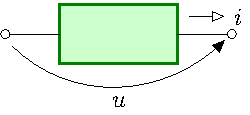
\includegraphics[width=0.7\linewidth]{teo_fig024.pdf}
          \caption{Větvový proud \(i\), větvové napětí \(u\) a orientace větve}
          \label{teo:fig024}
        \end{figure}

        \emph{Okamžitou hodnotou větvového napětí} u budeme nazývat okamžitou hodnotu napětí mezi 
        počátečním a koncovým uzlem orientované větve v daném čase \(t\). Orientaci větvového 
        napětí budeme ve schématech vyznačovat šipkou 
%        \begin{tikzpicture}\draw[-triangle 45] (0,0) to (1,0);\end{tikzpicture} podle obr. 
        \ref{teo:fig024}, přičemž šipka směřuje od počátečního ke koncovému uzlu 
        orientované dráhy, po níž se napětí měří.
        
      \subsubsection{Ideální prvky obvodu a jejich chování}
        Ideální prvky jsou z hlediska svých fyzikálních vlastností i matematického popisu 
        nejjednoduššími dvojpóly obvodu. O vodičích, které je spojují, předpokládáme, že mají 
        nulový odpor a že průchodem proudu nevzniká v jejich okolí magnetické pole. Elektrické 
        pole, jež je obecně vírové, je vně každého prvku obvodu polem potenciálním. Z toho plyne, 
        že hodnota napětí mezi dvojicemi uzlů obvodu nezávisí na tvaru integrační dráhy (tj. na 
        uspořádání přívodů voltmetru) mezi těmito uzly.
        
        Ideální prvky obvodu dělíme na aktivní a pasívní.
        
        \textbf{Aktivní prvky} jsou zdroje elektrické energie (generátory). Zpravidla přijímají 
        neelektrickou formu energie (např. mechanickou, chemickou, tepelnou) a přeměňují ji na 
        elektrickou energii, kterou dodávají do obvodu. Rozlišujeme dva typy aktivních prvků:
        \begin{itemize}
          \item ideální zdroje napětí obr. 5a), jejichž jediným parametrem je svorkové napětí     
                \(u_0 =  u_0(t)\)
          \item ideální zdroje proudu obr. 5b), jejichž jediným parametrem je dodávaný proud      
                \(i_0 = i_0(t)\)
        \end{itemize}
        
        Napětím ideálního napěťového zdroje rozumíme okamžitou hodnotu napětí mezi svorkami zdroje 
        v pořadí, jež stanovíme tím, že první svorku označíme znakem + a druhou znakem —. Svorky 
        zdroje tedy tvoří uspořádanou dvojici: svorka + se bere jako první a svorka — jako druhá. U 
        zdrojů časově proměnného napětí nemusejí znaky + a — představovat skutečnou polaritu 
        svorek; jsou to referenční znaky, jež pouze vyjadřují, že udávané napětí je měřeno od 
        svorky označené + ke svorce označené —. Skutečnou polaritu svorek vyjadřují v těch 
        okamžicích, v nichž je \(u_0(t) > 0\).
        
        V teorii obvodů se ideální zdroje dělí dále na \emph{nezávislé (autonomní)} a na 
        \emph{řízené (závislé, neautonomní)}.
        \begin{itemize}
          \item \textbf{Nezávislý ideální zdroj napětí} má svorkové napětí \(u_0 = u_0(t)\) 
                nezávislé na zatížení zdroje (tj. na výkonu dodávaném zdrojem do obvodu).
          \item \textbf{Nezávislý ideální zdroj proudu} dodává do obvodu proud \(i_0 = i_0(t)\) 
                nezávislý na zatížení zdroje.
          \item \textbf{Řízený ideální zdroj napětí, řízený napětím}, má svorkové napětí, jež je 
                funkcí napětí na některé části obvodu.
          \item \textbf{Řízený ideální zdroj napětí}, řízený proudem, má svorkové napětí, jež je 
                funkcí proudu v některé části obvodu.
          \item \textbf{Řízený ideální zdroj proudu}, řízený napětím, dodává proud, jenž je funkcí 
                napětí v některé části obvodu.
          \item \textbf{Řízený ideální zdroj proudu}, řízený proudem, dodává proud, jenž je funkcí 
                proudu v některé části obvodu.
        \end{itemize}
        
        S řízenými zdroji se často setkáváme v elektronice. Například zesilovač napětí lze nahradit 
        řízeným ideálním zdrojem napětí, přičemž napětí zdroje je funkcí napětí nebo proudu 
        přiváděného na vstup zesilovače.

        \emph{Základních obvodových prvků} je celkem pět: rezistor, cívka, kondenzátor, ideální 
        zdroj napětí, ideální zdroj proudu. Zdůrazněme následující skutečnosti:
        \begin{itemize}
          \itemsep0em 
          \item Každý ze základních prvků je uvažován jako \textbf{ideální} (nemá žádné jiné  
                parazitní vlastnosti).
          \item Kombinací základních prvků vznikne \textbf{náhradní zapojení} skutečného prvku, 
                včetně jeho parazitních vlastností.
          \item Z pěti základních prvků je tedy možno sestavit \textbf{libovolný obvodový model}
                (elektrický obvod) \textbf{pasivní} i \textbf{aktivní}.
          \item U \textbf{aktivních obvodů} (např. zesilovačů) se uplatňují řiditelné, neboli
                parametrické prvky. Typickým příkladem je bipolární tranzistor, jenž je řízen 
                proudem do báze.
        \end{itemize}
      
      \subsubsection{Přizpůsobení zdroje a spotřebiče}
        Zajímavé je sledovat, jak se mění napětí, proud a výkon na spotřebiči v závislosti na 
        poměru odporu spotřebiče a vnitřního odporu zdroje. Jednoduchou úvahou lze usoudit, že 
        největší napětí je naprázdno při nekonečném odporu spotřebiče a největší proud bude při 
        nulovém odporu spotřebiče (zkratu). Maximum výkonu nebude ani při maximálním proudu, 
        protože napětí na zkratu je nulové, ani při maximálním napětí, protože obvodem neprotéká 
        proud. Výkon, který je součinem napětí a proudu, je v obou případech nulový.
        
        Pokud připojíme k náhradnímu napěťovému schématu zdroje spotřebič, bude pro protékající 
        proud platit: \(I = \frac{U_i}{R_i + R_z}\). Po dosazení vztahu pro napětí na spotřebiči, 
        které je shodné se svorkovým napětím zdroje \(U=I\cdot R_z\), získáme vztah: \(U = 
        U_i\frac{R_z}{R_i + R_z}\).
        
  \section{Topologická struktura obvodů}
    Topologické vlastnosti obvodů lze studovat pomocí teorie grafů, jež je odvětvím 
    topologie\footnote{Topologie je moderní	matematická disciplína zabývající se studiem takových 
    vlastností objektů, jež jsou invariantní vzhledem k vzájemně jednoznačnému spojitému zobrazení, 
    jehož inverzní zobrazení je též spojité. Tyto vlastnosti se nazývají topologické vlastnosti 
    (topologické invarianty). (Zmíněné zobrazení lze názorně interpretovat jako takové deformování 
    zkoumaného objektu, při němž se nesmí objekt porušit ani spojovat.) Například hovoříme-li o 
    topologických vlastnostech obvodů, nemáme na mysli způsob rozmístění prvků obvodu v prostoru, 
    nýbrž počet prvků a vlastnosti jejich vzájemného spojení. Studium topologických vlastností 
    obvodů spadá do odvětví topologie, zvaného teorie grafů. Základy teorie grafů byly vybudovány 
    právě na základě potřeb teorie obvodů (G. Kirchhoff).}
    
    \subsection{Základní pojmy z topologie obvodů}
      Definice grafu obvodu. Mějme v prostoru body \(B_1; B_2;\cdots; B_{n_u}\) — nazveme je uzly. 
      Dvojice těchto uzlů nechť tvoří krajní body navzájem se neprotínajících oblouků (tzv. 
      topologických úseček) \(v_1; v_2; \cdots; v_{n_v}\) — nazveme je \emph{větvemi}. Množinu 
      všech větví pak nazýváme \emph{grafem obvodu}.
      
      Graf obvodu tedy vyjadřuje topologickou strukturu obvodu a získáme jej tím, že jej 
      abstrahujeme od fyzikálních vlastností prvků obvodu. U grafu nás nezajímají jeho metrické 
      vlastnosti, tj. uzly grafu lze libovolně rozmístit a jeho větve lze libovolně deformovat, 
      avšak nesmíme je přerušit a po jejich deformaci je popřípadě opět spojit.
      
      Graf, který vznikne z grafu \(\mathscr{G}\) těmito úpravami, nazýváme \emph{izomorfním} (čili 
      \emph{topologicky ekvivalentním}) s grafem \(\mathscr{G}\). Na obr. \ref{TEO:fig_topo01} je 
      příklad obvodu a jeho tří izomorfních grafů.
      
      \begin{figure}[ht!]
        \centering
        \includegraphics[width=0.9\linewidth]{TEO_topo01.jpg}
        \caption{ Obvod (a) a jeho topologicky ekvivalentní (izomorfní) grafy (b), (c), (d) 
                  \cite[s.~39]{Meyer1978}}
        \label{TEO:fig_topo01}
      \end{figure}
      
      Uzly grafu jsou charakterizovány svým stupněm: \emph{stupeň uzlu} \(\varepsilon\) udává počet 
      větví grafu, jež s uvažovaným uzlem \emph{incidují}\footnote{Dva geometrické útvary nazýváme 
      \textbf{incidentní} (resp. říkáme, že spolu incidují), jestliže jeden z nich obsahuje útvar 
      druhý. Například všechny přímky procházející daným bodem jsou s ním incidentní, nebo všechny 
      křivky ležící na ploše s ní incidují.}. Uzel stupně \(0\) (tzv. \emph{izolovaný uzel}) a uzel 
      stupně \(1\) (větev s ním incidující se nazývá \emph{izolovaná}) mají význam v matematické 
      teorii grafů, ale v grafech obvodů se setkáváme jen s uzly stupně \(\varepsilon\geqq 2\). 
      Někdy je výhodné vypustit uzly stupně \(2\) (tzv. vnitřní uzly větví) a uvažovat jen uzly 
      stupně \(\varepsilon\geqq 3\). Tím zmenšíme počet větví obvodu, avšak v jeho větvích obecně 
      nebude již jediný prvek, ale složitější dvojpól — sériové spojení prvků; např. v grafu obvodu 
      na obr. \ref{TEO:fig_topo01} jsou uzly \(B_1; B_2; B_3; B_4\) vesměs 3. stupně, uzly \(B_5; 
      B_6\) jsou 2. stupně vnitřní uzly); graf má \(n_v = 8\) větví. Omezíme-li se na uzly stupně 
      \(\varepsilon\geqq 3\), představují větve \(v_3; v4\) jedinou větev s krajními uzly \(B_2; 
      B_3\) a podobně větve \(v_7; v_6\) tvoří jedinou větev s uzly \(B_2; B_4\) graf má pak jen 
      \(n_v = 6\) větví.
      
      Dvojici grafů, jejichž izomorfismus je porušován jen uzly 2. stupně, nazýváme 
      \emph{homeomorfními}. Homeomorfní grafy jsou tedy takové grafy, jež se po odstraněni 
      některých uzlů 2. stupně stanou izomorfními.
  
  \section{Kirchhoffovy zákony}
    V této kapitole budeme formulovat Kirchhoffovy zákony a ukážeme, jak lze jejich použitím popsat 
    chováni obvodu soustavou rovnic.
    
    \subsection{Formulace prvního a druhého Kirchhoffova zákona}
      Kirchhoffovy zákony, spolu se vztahy mezi napětími a proudy pasivních prvků (tab. 3), mají 
      pro teorii obvodů základní význam. \emph{Platí pro jakýkoliv obvod se soustředěnými 
      parametry}, lineární i nelineární, s parametry časově konstantními i s časově proměnnými. Z 
      hlediska teorie obvodů lze Kirchhoffovy zákony považovat za postuláty, z nichž tato teorie 
      vychází. Z hlediska teorie elektromagnetického pole jsou však důsledkem plynoucím z 
      Maxwellovy teorie.
      
%     \begin{mdframed}[style=MyFrame]
      \textbf{První Kirchhoffův zákon}. Pro libovolný uzel obvodu platí: Součet okamžitých hodnot 
      proudů vystupujících z uzlu a proudů vstupujících do uzlu je roven nule. Přitom proudy 
      vystupující z uzlu bereme jako kladné a proudy vstupující do uzlu jako záporné.
%     \end{mdframed} 
      
      \begin{proof}
        Uvažujme libovolný uzel obvodu \(B_j\). Obklopíme jej libovolnou uzavřenou orientovanou 
        plochou \(S\) obr. \ref{TEO:fig_KZ01}a). Vzhledem k tomu, že magnetické pole obvodu se 
        soustředěnými parametry je kvazistacionární, má rovnice kontinuity tvar
        \begin{equation}
          \oint_s \vec{J}(t)\dd{\vec{S}} = 0
        \end{equation}
        \begin{figure}[ht!]
          \centering
          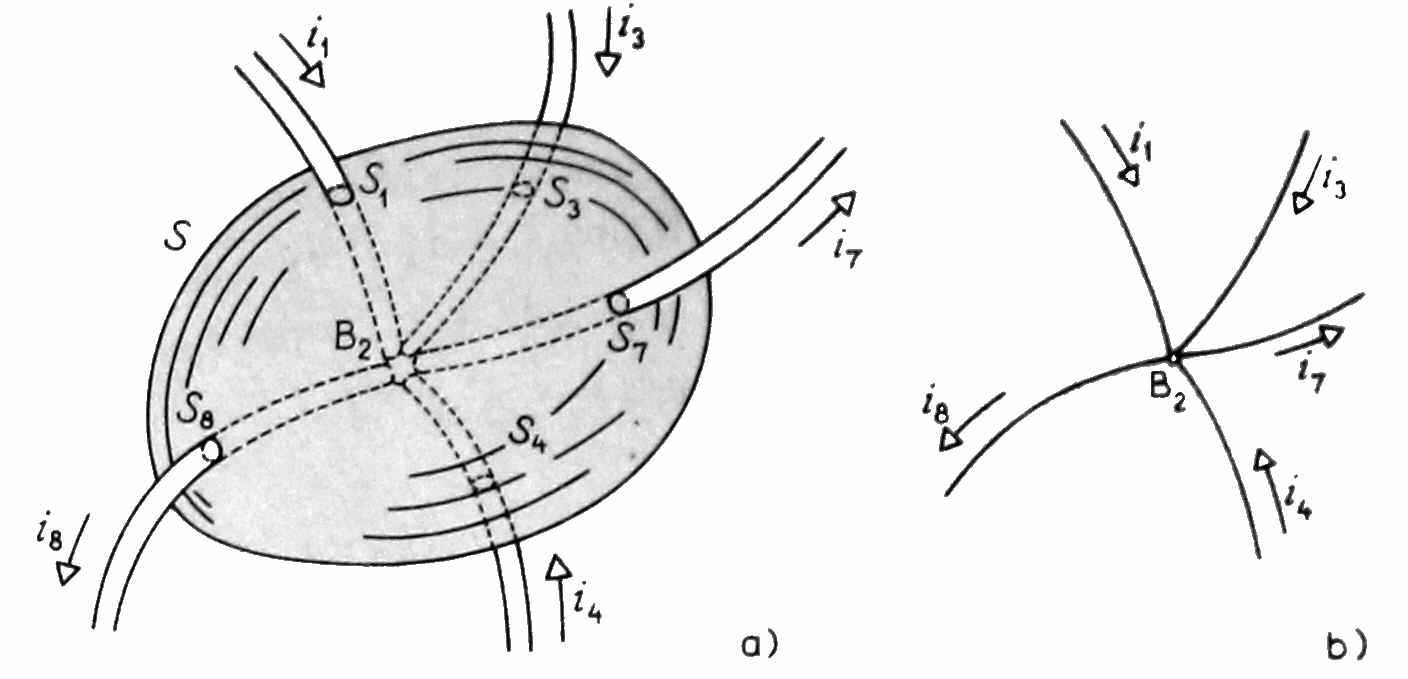
\includegraphics[width=0.9\linewidth]{TEO_KZ01.jpg}
          \caption{Uzel incidující s pěti větvemi: reálný elektrický obvod (a) a ideální obvod (b). 
                   (K odvozeni prvního Kirchhoffova zákona) \cite[s.~47]{Meyer1978}}
          \label{TEO:fig_KZ01}
        \end{figure}      
        Pro tok vektoru proudové hustoty uzavřenou plochou \(S\) podle obr. \ref{TEO:fig_KZ01}a) 
        platí
        \begin{equation}
          \oint_s \vec{J}(t)\dd{\vec{S}} = \sum_{\mathclap{\substack{k\\B_j\in v_k}}}
                                           \int_{S_k} \vec{J}(t)\dd{\vec{S}} 
        \end{equation}
        kde sumace na pravé straně rovnice je provedena přes indexy všech větví incidujících s 
        uzlem \(B_j\). Jednotliví sčítanci představují proudy vystupující z uzlu, resp. vstupující 
        do uzlu. Porovnáním obou uvedených vztahů plyne dokazovaný první Kirchhoffův zákon.
      \end{proof}
      
      Matematicky lze zapsat první Kirchhoffův zákon pro libovolný uzel obvodu \(B_j\) pomocí 
      větvových proudů \(i_k\) libovolně orientovaných větví \(v_k\)\footnote{Orientace větví 
      obvodu je libovolná, ale pevně zvolená (nezávislá na čase), viz kap. \ref{TEO:chap_Term}.} ve 
      tvaru 
      \cite[s.~47]{Meyer1978}
      \begin{equation}\label{TEO:eq_KZI}
        \sum_{\mathclap{\substack{k\\B_j\in v_k}}} \pm i_k = 0; \qquad j = 1;\ldots; n_u 
      \end{equation}
      Znaménko \(+\) platí, je-li větev \(v_k\) orientována tak, že uzel \(B_j\) je jejím 
      počátečním uzlem a znaménko \(—\) platí v opačném případě; sčítáme pro všechna \(k\), pro něž 
      uzel \(B_j\) inciduje s větví \(v_k (B_j\in v_k)\); \(n_u\) je počet všech uzlů obvodu. 
      Poznamenejme, že podle definice větvového proudu (viz kap. \ref{TEO:chap_Term}) je \(i_k > 
      0\), souhlasí-li směr proudu s orientaci větve a \(i_k < 0\) v opačném případě.
      
      Například pro uzel \(B_2\) podle obr. \ref{TEO:fig_KZ01}b) má první Kirchhoffův zákon tvar
      \begin{equation*}
        -i_1 - i_3 - i_4 + i_7 + i_8 = 0
      \end{equation*}
      Rovnice (\ref{TEO:eq_KZI}) je symbolickým zápisem prvního Kirchhoffova zákona, vyžadujícím 
      slovní komentář o tom, kdy máme brát znaménko \(+\) , kdy znaménko \(—\) a jakých hodnot 
      nabývá sčítací index \(k\). Tento zápis prvního Kirchhoffova zákona je velmi dobře použitelný 
      pro řešení jednodušších obvodů. Naproti tomu při řešení obvodů na počítači je třeba vyjádřit 
      první Kirchhoffův zákon výstižnějším zápisem ve tvaru
      \begin{equation}\label{TEO:eq_KZI_01}
        \sum\limits_{k=1}^{n_v} a_{jk} i_k = 0; \qquad j = 1;\ldots; n_u 
      \end{equation}
      \begin{figure}[ht!]
        \centering
        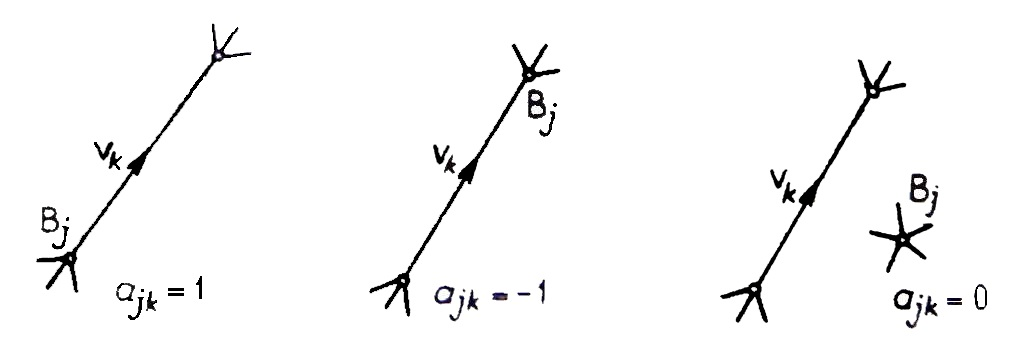
\includegraphics[width=0.9\linewidth]{TEO_KZ02.jpg}
        \caption{K určení hodnot koeficientů \(a_{jk}\) \cite[s.~47]{Meyer1978}}
        \label{TEO:fig_KZ02}
      \end{figure}
      kde koeficienty \(a_{jk}\) vyjadřují incidenci uzlů a větví v orientovaném grafu obvodu a 
      nabývají těchto hodnot: \(a_{jk} = 1\), když j-tý uzel je počátečním uzlem k-té větve, 
      \(a_{jk} = — 1\), když j-tý uzel je koncovým uzlem k-té větve a \(a_{jk} = 0\), když j-tý 
      uzel neinciduje s k-tou větví (obr. \ref{TEO:fig_KZ02}). Znaménko větvového proudu \(i_k\) 
      plyne ze souhlasnosti, resp. nesouhlasnosti orientace větve a směru větvového proudu (\(i_k > 
      0\), resp. \(i_k < 0\)).
      
      \textbf{Druhý Kirchhoffů v zákon}. Pro libovolnou orientovanou smyčku obvodu platí: Součet 
      okamžitých hodnot napětí na všech větvích incidujících s orientovanou smyčkou obvodu je roven 
      nule. Přitom napětí větví bereme jako kladná, jestliže proud ve větvi v daném okamžiku 
      prochází ve smyslu orientace smyčky a jako záporná, jestliže prochází v opačném směru.
      
      \begin{proof}
        Uvažujme libovolnou orientovanou uzavřenou křivku \(s_j\) procházející všemi uzly smyčky 
        obvodu a vedenou vně prvků (např. křivku vyznačenou na obr. \ref{TEO:fig_KZ03} tečkovaní). 
        Z vlastností ideálních prvků obvodu plyne, že II. Maxwellova rovnice v integrálním tvaru má 
        pro křivku \(s_j\) tvar
        \begin{align}
          \oint\vec{E}\dd{\vec{l}} &= 0    \label{TEO:eq_KZ01} \\
          \shortintertext{Pro oběhové napětí po křivce \(s_j\) (obr. \ref{TEO:fig_KZ03}) zároveň 
                          platí vztah}
          \oint\vec{E}\dd{\vec{l}} &= \sum_{\mathclap{\substack{k\\v_k\in s_j}}}\vec{E}\dd{\vec{l}}
        \end{align}
        Porovnáním obou uvedených vztahů plyne dokazovaný druhý Kirchhoffův zákon.
        \begin{figure}[ht!]
          \centering
          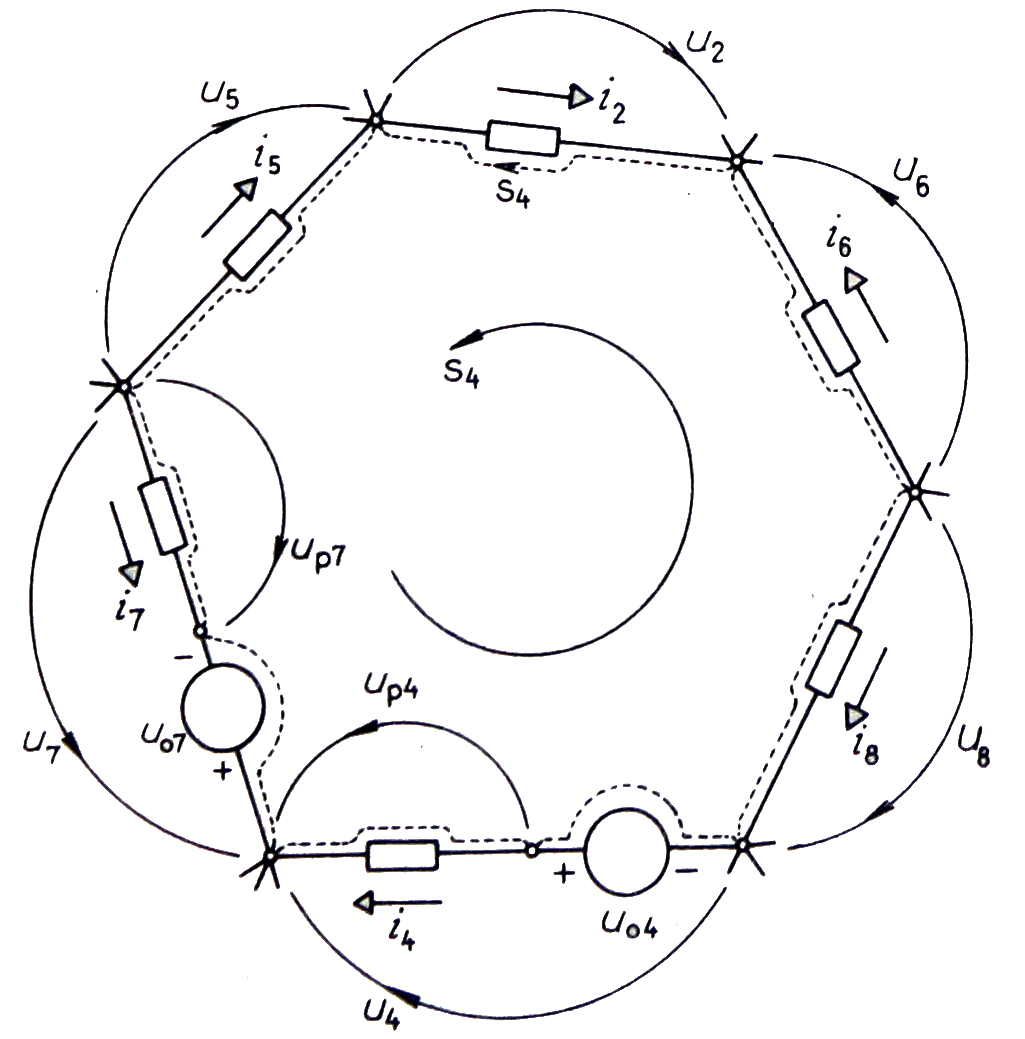
\includegraphics[width=0.7\linewidth]{TEO_KZ03.jpg}
          \caption{Smyčka incidující se šesti větvemi (K odvození druhého Kirchhoffova 
                   zákona)\cite[s.~48]{Meyer1978}}
          \label{TEO:fig_KZ03}
        \end{figure}
      \end{proof}
      Matematicky lze vyjádřit druhý Kirchhoffův zákon pro libovolnou orientovanou smyčku \(s_j\) 
      pomocí větvových napětí \(u_k\) libovolně orientovaných větví \(v_k\) ve tvaru
      \begin{equation}\label{TEO:eq_KZ03}
        \sum_{\mathclap{\substack{k\\v_k\in s_j}}} \pm u_k = 0 \qquad j=1;\cdots; n_s
      \end{equation}
      Znaménko \(+\) platí, je-li větev \(v_k\) orientována souhlasně se smyčkou \(s_j\) a znaménko 
      \(—\) platí v opačném případě; sčítáme pro všechna \(k\), pro něž větev \(v_k\) inciduje se 
      smyčkou \(s_j (v_k\in s_j)\); \(n_s\) je počet všech smyček obvodu.
      
      Například pro smyčku \(s_4\) podle obr. \ref{TEO:fig_KZ03} má druhý Kirchhoffův zákon tvar
      \begin{equation*}
        -u_2 -u_4 -u_5 +u_6 +u_7 -u_8 = 0
      \end{equation*}
      
      Vyjádření druhého Kirchhoffova zákona rovnicí (\ref{TEO:eq_KZ03}) je — obdobně jako vyjádření 
      prvního Kirchhoffova zákona rovnicí (\ref{TEO:eq_KZI}) — jen symbolickým zápisem, k němuž 
      bylo nutno připojit slovní komentář. Pro řešení obvodů na počítači je třeba vyjádřit druhý 
      Kirchhoffův zákon matematicky výstižnějším zápisem
      \begin{equation}\label{TEO:eq_KZ04}
        \sum\limits_{k=1}^{n_v} b_{jk} u_k = 0 \qquad j=1;\cdots; n_s
      \end{equation}      
      \begin{figure}[ht!]
        \centering
        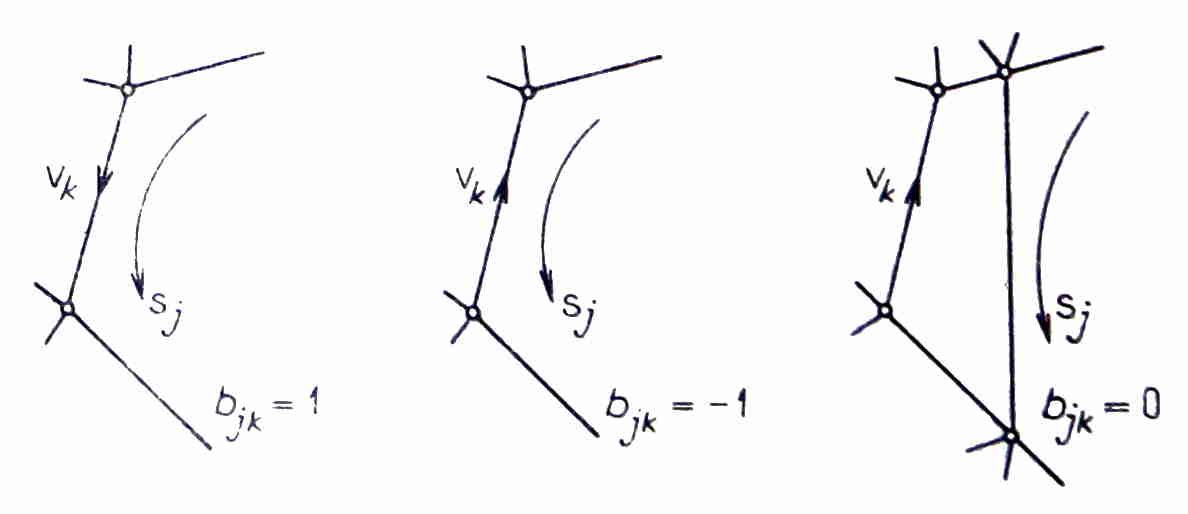
\includegraphics[width=0.9\linewidth]{TEO_KZ04.jpg}
        \caption{K určení koeficientů \(b_{jk}\) \cite[s.~49]{Meyer1978}}
        \label{TEO:fig_KZ04}
      \end{figure}      
      kde koeficienty \(b_{jk}\) vyjadřují incidenci smyček a větví v orientovaném grafu obvodu a 
      nabývají těchto hodnot: \(b_{jk} = 1\), když \(k\)-tá větev inciduje s \(j\)-tou smyčkou a 
      orientace obou se shodují, \(b_{jk} = — 1\), když \(k\)-tá větev inciduje s \(j\)-tou smyčkou 
      a orientace obou je opačná, a \(b_{jk} = 0\), když \(k\)-tá větev neinciduje s \(j\)-tou 
      smyčkou (obr. \ref{TEO:fig_KZ04}).
      
  \section{Analýza elektrických obvodů}
    Pojem \textbf{analýza} není v teorii elektrických obvodů používán v původním širokém smyslu. 
    Zejména v souvislosti s počítačovým řešením obvodů se pod analýzou obvykle rozumí 
    \emph{konkrétní metody získávání elektrických charakteristik obvodů z jejich modelů} (například 
    kmitočtová nebo stejnosměrná analýza).
    
    \subsection{Modelování, analýza, simulace}
      \emph{Analýzu} provádíme ve snaze získat informace o určitých vlastnostech zkoumaného obvodu, 
      které nás zajímají. Z praktických důvodů však zpravidla analýze nepodrobujeme samotný obvod, 
      nýbrž jeho \emph{model}. Jedním z dobrých důvodů může být skutečnost, že daný obvod dosud 
      existuje pouze v představě návrháře a před jeho výrobou je vhodné ověřit, zda je navržen 
      správně. K modelování obvodu máme k dispozici elementární modely elektrických prvků (pasivní 
      R, L, C, tranzistory, operační zesilovače apod.) ve formě matematického popisu jejich 
      fungování a  jejich elektrotechnických značek, které jsou začleněny do schématu celkového 
      zapojení. Z hlediska matematického je model obvodu představován soustavou rovnic, které lze 
      odvodit na základě rovnic dílčích elektrických prvků a Kirchhoffových rovnic, které 
      reprezentují způsob propojení součástek \cite[s.~16]{Biolek}.
      
      Při modelování obvodu je důležité nejprve uvážit, s jak složitým modelem bude vhodné 
      pracovat. Složité modely obvykle umožňují věrnější popis chování skutečného obvodu, avšak 
      současně prudce rostou požadavky na výkon analyzačního nástroje. Je zřejmé, že výpočty, které 
      provádíme jen pomocí papíru a tužky, případně kalkulačky, jsou vhodné pro analýzu méně 
      rozsáhlých obvodů s jednoduchými modely, kde nám jde buď o ověření správnosti základního 
      principu fungování, nebo o odhady chování obvodu s odhlédnutím od různých parazitních jevů a 
      vlivů reálných vlastností součástek na vlastnosti obvodu. Složité modely si můžeme dovolit 
      používat při analýze s využitím speciálních počítačových programů.

      Klasická teorie obvodů dává odpověď na otázku, s jakým minimálním počtem typů elementárních 
      modelů obvodových prvků je možné sestavit model jakkoliv složitého analogového obvodu se 
      soustředěnými parametry: jsou to pasivní prvky typu R,L,C a zdroje klasické a řízené. 
      Příslušné charakteristiky těchto prvků jsou popsány jednoduchými nebo složitými rovnicemi. Z 
      tohoto pohledu můžeme říci, že k sestavování modelů daných obvodů a k jejich využívání nemáme 
      k dispozici nic jiného než omezený počet modelů elementárních prvků s příslušnými 
      matematickými vzorci \cite[s.~17]{Biolek}.
      
      Od jisté úrovně modelování, která zajišťuje uspokojivou shodu chování modelu a originálu, je 
      možné model využívat k simulaci skutečného chování obvodu za konkrétních podmínek. Příkladem 
      může být sledování vlivu teploty na nastavený stejnosměrný pracovní bod tranzistorového 
      zesilovače. Dostáváme se k poslednímu pojmu z trojlístku \emph{modelování - analýza - 
      simulace}. Simulace je tedy něco více než analýza (v úzkém pojetí) a analýza je důležitá 
      součást simulace.
      
      \begin{figure}[ht!]
        \centering
        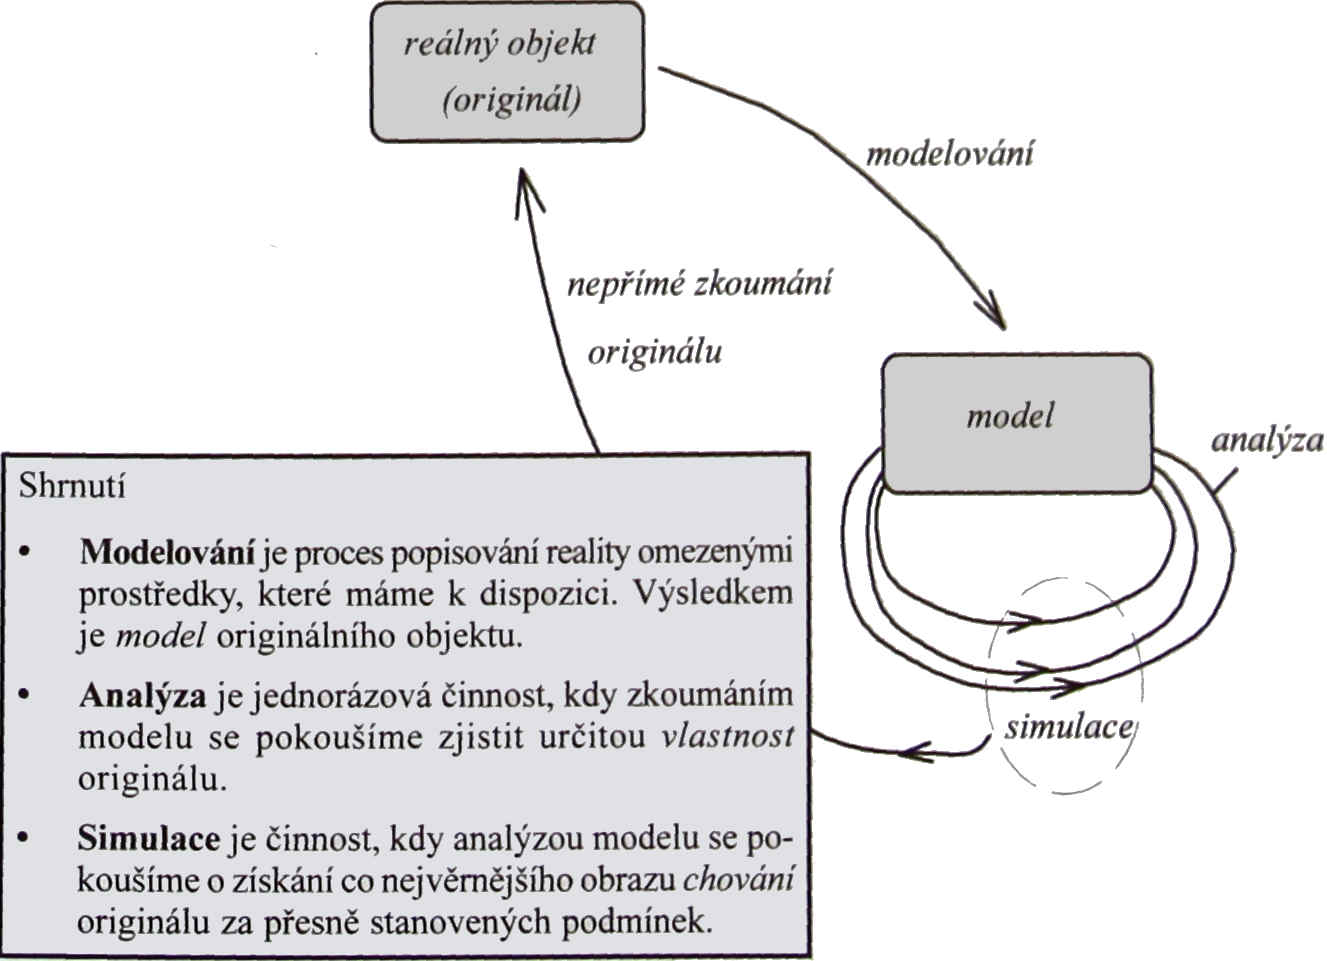
\includegraphics[width=0.95\linewidth]{Biolek_Modelovani.jpg}
        \caption{Modelováni, analýza, simulace \cite[s.~17]{Biolek}}
        \label{TEO:fig_modelovani}
      \end{figure}
      
      Shrnutí:
      \begin{itemize}
        \itemsep0em
        \item \emph{Při řešení obvodu pomocí „papíru, tužky a kalkulačky“} nejprve sestavíme model 
              obvodu ve formě schématu zapojení včetně parametrů, resp. charakteristik jednotlivých 
              součástek. Z tohoto modelu pak vzniká model matematický ve formě rovnic, které 
              vyplývají z vzájemného propojení a vlastností součástek, Kirchhoffových zákonů a 
              Ohmová zákona. Tento model pak podrobíme numerické analýze.      
        \item \emph{Při řešení pomocí počítačového programu} opět sestavujeme model obvodu,  
              většinou pomocí schematického editoru. Program je však schopen při tomto sestavování 
              účinně pomáhat tím, že je zdrojem složitých interních modelů součástek (tranzistory, 
              operační zesilovače, integrované obvody...). Vlastní sestavení rovnic, jejich řešení 
              a vizualizace výsledků je již plně v režii programu \cite[s.~18]{Biolek}.
      \end{itemize}
      
    \subsection{Metody analýzy heuristické a algoritmické}
      Metodu analýzy můžeme chápat jako konkrétní postup od modelu obvodu až po získání cíle analýzy.
      
      Všechny existující metody analýzy můžeme rozdělit na \emph{nealgoritmické (heuristické)} a 
      \emph{algoritmické}. Do první kategorie patří postupy, které řešitel volí na základě svých 
      předchozích zkušeností s využíváním tvůrčího přístupu. Například při výpočtu napětí na 
      výstupu zatíženého děliče napětí je možno nejprve sloučením zatěžovacího a pracovního 
      rezistoru převést řešení na problém děliče nezatíženého, posléze vypočítat proud děličem a 
      následně výstupní napětí. Jiným možným postupem je využití Théveninovy věty apod. 
      Algoritmická metoda oproti tomu definuje přesný postup — algoritmus, který vždy vede k cíli. 
      Výše uvedená úloha zatíženého děliče může být řešena například algoritmickou metodou 
      smyčkových proudů.
      
      Zjednodušené řečeno, heuristické metody jsou vhodné k ručnímu řešení méně rozsáhlých obvodů, 
      pokud jsme zběhlejší v elektrotechnických výpočtech a nechybí nám schopnost hledání vlastních 
      cest k cíli.
      
      Při analýze obvodů bez počítačové podpory bychom měli upřednostňovat nealgoritmické metody. 
      Pouze tam, kde je vyjadřování napěťových a proudových poměrů komplikované, např. v důsledku 
      působení speciálních obvodových prvků, je často rozumné úlohu vyřešit \emph{modifikovanou 
      metodou uzlových napětí} (část \ref{TEO:chap_MMUN}) nebo \emph{Masonovým-Coatesovým grafem} 
      (část 2.4). Každá z metod má svůj význam: nealgoritmická nutí k fyzikálnímu myšlení a k 
      pochopení funkce obvodu, který analyzujeme, algoritmická pak poskytuje účinný nástroj k 
      praktickému řešení.

  \section{Metody analýzy elektrických ob\-vo\-dů}
    \subsection{Klasická metoda uzlových napětí (MUN)}
      Metoda uzlových napětí je založena na tomto postupu:
      \begin{itemize}
       \item Jeden z uzlů obvodu se prohlásí za tzv. \textbf{referenční uzel}. Přiřadí se mu 
             číslo 0, případně v počítačovém simulátoru značka uzemnění. Vzhledem k tomuto uzlu se 
             budou vztahovat napětí ostatních uzlů obvodu. Tato napětí se nazývají \textbf{uzlová 
             napětí} a tvoří \textbf{soustavu neznámých obvodových veličin} metody. Je vhodné 
             orientovat všechna uzlová napětí tak, aby čítací šipky směřovaly do referenčního uzlu. 
             Uzlová napětí jsou neznámými metody i tehdy, je-li našim konečným cílem počítat 
             jiné obvodové veličiny. Každé napětí a každý proud v obvodu jsou totiž vyjádřitelné 
             jako lineární kombinace uzlových napětí.
       \item Pro každý uzel obvodu, vyjma referenčního, sestavíme rovnici 1. KZ ve tvaru:
             \emph{součet proudů tekoucích dovnitř uzlu z vnějších zdrojů proudu  = součtu proudů
             vytékajících větvemi obvodu ven z uzlu.}
       \item Rovnice vyřešíme, tj. získáme velikosti uzlových napětí. Z nich pak dopočteme  
             požadovaný výsledek analýzy.
      \end{itemize}
      
      Metodu uzlových napětí lze objasnit na příkladu zapojení na obr. \ref{teo:fig025}. Je
      třeba určit proud $I_{x2}$ 
      \begin{figure}[ht!]  %\ref{teo:fig025}
        \centering
        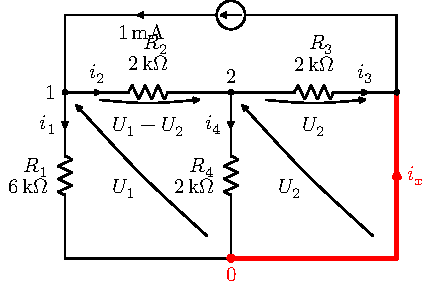
\includegraphics[width=0.7\linewidth]{teo_fig025.pdf}
        \caption{Řešení obvodu metodu uzlových napětí - MUN \cite[s.~62]{Biolek}}
        \label{teo:fig025}
      \end{figure}
      Nejprve očíslujeme uzly. Zvolíme referenční uzel a přiřadíme mu číslo 0. Zde je třeba  
      zdůraznit, že referenční uzel je možno volit zcela libovolně. Většinou se volí tak, aby 
      případné hledané napětí bylo rovno jednomu z napětí uzlových. Dále si všimneme, že uzel, v 
      němž je se spojuje rezistor $R_3$ a proudový zdroj, je vlastně součástí referenčního uzlu a 
      jako takový se přídavně nečísluje - má již označení \num{0}.
      
      Vyznačená uzlová napětí $U_1$ a $U_2$ tvoří soustavu dvou neznámých, k níž musíme sestavit 
      dvě rovnice. Budou to rovnice 1. KZ pro uzly 1 a 2. Protože počítáme proud $I_{x2}$, postačí 
      určit uzlové napětí $U_2$. Z něj totiž snadno určíme proud rezistorem $R_3$ a z něj $I_{x2}$.
      
      Podle obr. \ref{teo:fig025} napíšeme 1. KZ pro rovnováhu proudů v uzlech 1 a 2:
      \begin{align*}
        \text{uzel 1:} \qquad I &=  I_{R1} + I_{R2}            \\
        \text{uzel 2:} \qquad 0 &= -I_{R1} + I_{R2} + I_{R4}  
      \end{align*}
      
      Orientaci čítacích šipek větvových proudů můžeme volit naprosto libovolně. Pokud se v 
      orientaci zmýlíme, vyjde u daného proudu opačné znaménko.
      
      Větvové proudy na pravé straně rovnic vyjádříme pomocí větvových vodivostí a větvových 
      napětí, která závisí na uzlových napětí (viz obr. \ref{teo:fig025}):
      \begin{align}
       \text{uzel 1:} \qquad I &=  G_1U_1 + G_2(U_1-U_2)             \nonumber              \\ 
       \text{uzel 2:} \qquad 0 &= -G_2(U_1-U_2) + G_3U_2 + G_4U_2    \nonumber              \\
       \shortintertext{Vytknutím neznámých upravíme rovnice na konečný tvar}
       \text{uzel 1:} \qquad I &=  (G_1 + G_2)U_1 - G_2U_2           \label{TEO:eq_MUN_pr}  \\ 
       \text{uzel 2:} \qquad 0 &= -G_2U_1 + (G_2 + G_3 + G_4)U_2     \nonumber
       \shortintertext{Dosadíme-li vodivosti v [mS], vyjdou proudy na levé straně v [mA]}
       \text{uzel 1:} \qquad 1 &=  \frac{2}{3}U_1 - \frac{1}{2}U_2   \nonumber              \\ 
       \text{uzel 2:} \qquad 0 &= -\frac{1}{2}U_1 + \frac{3}{2}U_2   \nonumber
       \shortintertext{Tyto rovnice dávají řešení}
                   [U_1, U_2]  &= \left[2, \frac{2}{3}\right] \text{V}  \label{TEO:eq_MUN_vysl}
      \end{align}
      Pohledem na schéma \ref{teo:fig025} zjistíme, že při $U_2 = \frac{2}{3}V$ bude proud 
      $I_{R3} = \frac{1}{3} mA$ a hledaný proud $I_{x2}$ vychází z 1. KZ
      \begin{equation}\label{TEO:eq_MUN_Ix2}
        I_{x2} = I - I_{R3} = \left(1 - \frac{1}{3}\right) = \frac{2}{3} mA.
      \end{equation}

      \subsubsection{Pravidla pro sestavování rovnic}
        Nyní pusťme se do zobecnění poznatků z předchozího příkladu. Rovnice \ref{TEO:eq_MUN_pr} 
        zapíšeme v maticovém tvaru
        \begin{table}[ht!]
          % using \usepackage{array} and command \newcolumntype{C}[1]{>{\centering}m{#1}}!
          \centering
          \begin{tabular}{c|c|c|c|c|c|c|}
             \multicolumn{1}{c}{}      & \multicolumn{1}{c}{}      & \multicolumn{1}{c}{} & 
             \multicolumn{1}{c}{$U_1$} & \multicolumn{1}{c}{$U_2$} & \multicolumn{1}{c}{} & 
             \multicolumn{1}{c}{}              \\
             \cline{2-2} \cline{4-5} \cline{7-7}
              uzel 1:  & $I$   & \multirow{2}{*}{=} & $G_1+G_2$ & $-G_2$         &   & $U_2$    \\
             \cline{2-2} \cline{4-5} \cline{7-7}
              uzel 2:  &       &                    & $-G_2$    & $G_2+G_3+G_4$  &   & $U_2$    \\
             \cline{2-2} \cline{4-5} \cline{7-7}
          \end{tabular}
          \caption*{ }
        \end{table}
        Porovnáme-li maticovou rovnici s původním schématem obvodu \ref{teo:fig025} 
        dospějeme k následujícím pravidlům:
        \begin{itemize}
         \item Pravidlo o sestavení vektoru budicích proudů na levé straně maticové rovnice:
           \begin{itemize}
             \item V $\text{i-tém}$ řádku je algebraický součet proudů, tekoucích dovnitř  
                   $\text{i-tého}$ uzlu z vnějších zdrojů proudu.
           \end{itemize}
         \item Pravidla o sestavení čtvercové vodivostní (admitanční) matice:
           \begin{itemize}
             \item Prvek $i, j$ na hlavní diagonále obsahuje součet všech vodivostí (admitancí),  
                   které jsou připojeny k uzlu $i$.
             \item Prvek $i, j (i \neq j)$ mimo hlavní diagonálu obsahuje záporně vzatý součet všech 
                   vodivostí, které jsou připojeny bezprostředně mezi uzly $i$ a $j$.
           \end{itemize}
        \end{itemize}
        Základní lineární dvojpóly (R, L, C) jsou reciprocitní, tzn. chovají se stejně ve směru 
        obou uzlů. Jinými slovy, jejich impedance je v obou případech stejná. Proto u obvodů s 
        těmito součástkami vykazují admitanční matice \emph{symetrii}, tj. prvky matice \emph{i, j} 
        a \emph{j, i} jsou totožné.

    \subsection{Modifikovaná metoda uzlových napětí}\label{TEO:chap_MMUN}
      Výhodou metody uzlových napětí je její snadná algoritmizace: algoritmus pro sestavení 
      soustavy rovnic přímo ze schématu je velmi jednoduchý a lze jej tedy implementovat do 
      počítačových programů pro analýzu a simulaci. Nevýhodou metody ovšem je, že neumožňuje 
      analyzovat obvody se zdroji napětí a součástkami, které nemají admitanční rovnici. Bohužel, k 
      těmto součástkám patří nejen například takové prvky jako je obyčejný transformátor, ale i 
      různé operační zesilovače, konvejory, a další moderní analogové prvky \cite[s.~77]{Biolek}.
      
      Proto klasická metoda MUN musí být podrobena určité modifikaci, která jednak zachová její 
      výhodu - snadnou algoritmizovatelnost - jednak umožní analyzovat lineární obvody bez výše 
      uvedených omezení. Jsou to metody:
      \begin{itemize}\itemsep0em
        \item Metoda razítek
        \item Metoda zakázaného řádku
        \item Metoda U/I
      \end{itemize}

      \subsubsection{Metoda razítek}
        Každý "problémový" prvek je popsán minimálně jednou přídavnou rovnicí a o stejný počet 
        obohatí množinu neznámých. Současně dojde k modifikaci některých původních rovnic 1. KZ. 
        Maticová rovnice pak získá zvláštní strukturu: k původní admitanční matici MUN přibudou 
        řádky a sloupce, jejichž prvky obecně nemají rozměr admitancí. Jsou to tzv. \emph{razítka} 
        přídavných elektrických prvků. Celá matice se pak nazývá \textbf{pseudoadmitanční}. 
        Zvětšení rozměru soustavy rovnic obvykle při počítačové analýze nemusí být na závadu. Při 
        ručním řešení jde však prakticky vždy o problém \cite[s.~78]{Biolek}.
        
        Uvažujme obvod popsaný rovnicemi klasické MUN. Mezi uzly \emph{a} a \emph{b} obvodu 
        dodatečně připojíme obecný dvojpól, který je popsán svým Théveninovým modelem podle obr. 
        \ref{TEO:fig_MMUN_thev_dvojpol}. Včleněním dvojpólu dojde ke změně napěťových a proudových 
        poměrů v obvodu. Dvojpólem bude protékat proud $I_x$, který modifikuje proudové poměry mezi 
        v uzlech \emph{a} a \emph{b}. Dojde i k změně původních uzlových napětí.
        
        \begin{figure}[ht!]
          \centering
          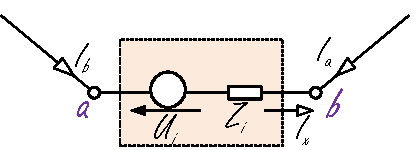
\includegraphics[width=0.7\linewidth]{Biolek_MMUN_thev_dvojpol.pdf}
          \caption[MMUN - Théveninův model dvojpólu]{Začlenění obecného lineárního dvojpólu, 
                   popsaného Théveninovým modelem do obvodu \cite[s.~78]{Biolek}}
          \label{TEO:fig_MMUN_thev_dvojpol}
        \end{figure}
        
        Původní rovnice popisující rovnováhu proudů v uzlu \emph{a} musí být na pravé straně 
        doplněna o proud $I_x$, vytékající ven z uzlu, a v uzlu \emph{b} o proud $I_x$ se záporným 
        znaménkem, protože vtéká dovnitř uzlu \emph{b}. Navíc uzlová napětí $U_a$ a $U_b$ jsou nyní 
        vázána podmínkou
        
        \begin{equation}\label{TEO:eq_MMUN_dvojpol}
          Z_iI_x + U_b = U_i + U_a, \quad\text{neboli}\quad U_i = Z_iI_x + U_b - U_a
        \end{equation}
        Všechny tyto modifikace lze zahrnout do nové soustavy rovnic MMUN:
        
        \begin{figure}[ht!]
          \centering
          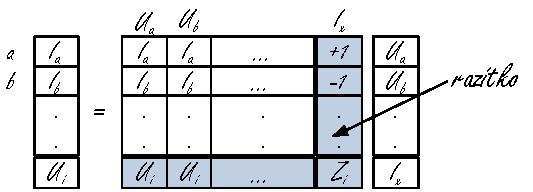
\includegraphics[width=1\linewidth]{Biolek_MMUN_razitko.pdf}
          \caption[MMUN - razítko]{ Razítko v pseudoadmitanční matici \cite[s.~79]{Biolek}}
          \label{TEO:fig_MMUN_razitko}
        \end{figure}
        
        Vektor neznámých uzlových napětí je rozšířen o další neznámou, $I_x$. Počet rovnic je 
        rovněž zvětšen o jedničku, a to o výše uvedenou podmínku mezi uzlovými napětími $U_a$ a 
        $U_b$. Přitom napětí $U_i$ je začleněno do vektoru známých budicích veličin na levé straně. 
        Modifikace rovnic 1. KZ pro uzly \emph{a} a \emph{b} je provedena zápisem $+1$ a $-1$ do 
        sloupce "$I_x$".
        
        Právě provedený zápis je návodem, jak pomocí MMUN analyzovat například obvody obsahující 
        zdroj napětí. Impedance $Z_i$ může být i nulová, pak se bude jednat o ideální zdroj napětí. 
        Při $U_i = 0$ a $I_i = 0$ lze modelovat zkrat mezi uzly a počítat proud, tekoucí tímto 
        zkratem. Toho lze využít například při analýze obvodů s proudem řízenými zdroji. 
        
        V případě, že se v obvodu nachází více prvků bez admitančního popisu, odpovídá každému z 
        nich samostatné razítko. Pseudoadmitanční matice pak nabývá na rozměrech. Metodu budeme 
        blíže konkretizovat na několika příkladech. 
  
        \subsubsection{Pasivní obvody obsahující zdroje napětí a proudu}
          Pomocí MMUN vyřešme zadání z obr. \ref{teo:fig026}. Je hledán proud \(I_x\) 
          vytékající ze zdroje napětí 
          \begin{figure}[ht!]  %\ref{teo:fig026}
            \centering
            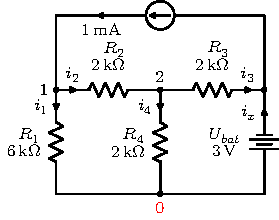
\includegraphics[width=0.7\linewidth]{teo_fig026.pdf}
            \caption{Analyzovaný obvod}
            \label{teo:fig026}
          \end{figure}
          
        \subsubsection{Obvody s ideálním operačním zesilovačem ty\-pu VFA}
          Ideální OPAMP, na obr. \ref{TEO:fig_MMUN_ideal_VFA} po vložení do obvodu způsobí 
          ztotožnění uzlových napětí $U_a$ a $U_b$, a modifikaci proudových poměrů v uzlu \emph{c}.
      
          \begin{figure}[ht!]
            \centering
            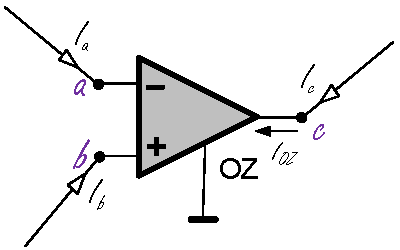
\includegraphics[width=0.6\linewidth]{MMUN_ideal_VFA.pdf}
            \caption[Ideální operační zesilovač typu VFA]{Ideální operační zesilovač typu VFA}
            \label{TEO:fig_MMUN_ideal_VFA}
          \end{figure}
          Ve spodním přídavném řádku je zapsána rovnice
          \begin{equation}\label{TEO:eq_MMUN_VFA}
              0 = 1\cdot U_a - 1\cdot U_b
          \end{equation}
          Výsledek řešení se nezmění, jestliže obě strany této rovnice vynásobíme libovolným 
          nenulovým číslem. Ve spodním řádku tedy může být namísto $[1,-1]$ například $[15,-15]$.
          \begin{figure}[ht!]
            \centering
            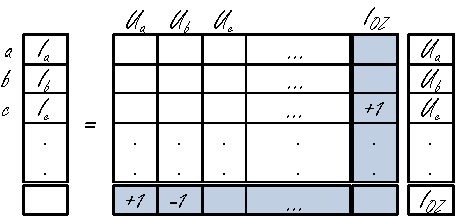
\includegraphics[width=\linewidth]{MMUN_ideal_VFA_matice.pdf}
            \caption[MMUN - pro ideální OPAMP]{MMUN - pro ideální OPAMP typu VFA}
            \label{TEO:fig_MMUN_VFA_matice}
          \end{figure}
          Je-li jeden ze vstupů OZ spojený s referenčním uzlem, neobjeví se příslušné uzlové napětí 
          v rovnicích a proto v posledním řádku bude figurovat jen jedna jednička místo uvedené 
          dvojice. 
          
          Jednička v řádku \emph{c} a sloupci $I_{OZ}$ reprezentuje připočtení proudu $I_{OZ}$ do 
          celkové bilance proudů, vytékající z uzlu \emph{c}.
        
          % --------example: Invertující zesilovač ---------------
          % \label{TEO:ex_InvOpamp01}
            % !TeX spellcheck = cs_CZ
\begin{example}\label{TEO:ex_InvOpamp01}
  Uvažujme invertující zesilovač s ideální operačním zesilovačem typu VFA s naznačenými uzly 
  tak, jak je na obr. \ref{TEO:fig_MMUN_inv_opamp}. Napište rovnice MMUN.
  
   {\centering
    \captionsetup{type=figure}
    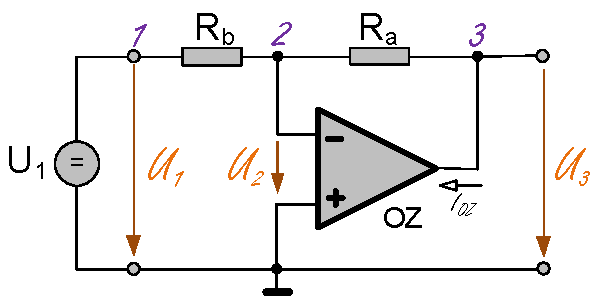
\includegraphics[width=0.7\linewidth]{MMUN_inv_OPAMP.pdf}
    \captionof{figure}{Invertující zesilovač}
    \label{TEO:fig_MMUN_inv_opamp}
    \par}
  
  Rovnice MMUN budou v maticovém zápisu vypadat takto:

    % using \usepackage{array} and command \newcolumntype{C}[1]{>{\centering}m{#1}}!
   {\centering
    \begin{tabular}{|C{0.6cm}|C{1.2cm}|C{0.6cm}|C{0.45cm}|C{0.45cm}|C{.3cm}|c|C{.33cm}|c|}
        \multicolumn{1}{c}{$U_1$}    & \multicolumn{1}{c}{$U_2$}    & \multicolumn{1}{c}{$U_3$}  & 
        \multicolumn{1}{c}{$I_1$}    & \multicolumn{1}{c}{$I_{OZ}$} & \multicolumn{1}{c}{ }      &  
        \multicolumn{1}{c}{x}        & \multicolumn{1}{c}{ }        & \multicolumn{1}{c}{b}       \\
      \cline{1-5}\cline{7-7} \cline{9-9}
      $G_b$  & $-G_b$    &  & -1  &  & \multirow{5}{*}{$\ast$} & $U_1$ & \multirow{5}{*}{=}     & \\
      \cline{1-5} \cline{7-7} \cline{9-9}
      $-G_b$ & $G_a+G_b$ & $-G_a$ &  &   & & $U_2$      &      &                                  \\
      \cline{1-5} \cline{7-7} \cline{9-9}
             & $-G_a$    & $G_a$  &  & 1 & & $U_3$      &      &                                  \\
      \cline{1-5} \cline{7-7} \cline{9-9}
         1   &           &        &  &   & & $I_1$      &      &    $U_{IN}$                      \\
      \cline{1-5} \cline{7-7} \cline{9-9}
             &     1     &        &  &   & & $I_{OZ}$   &      &                                  \\
      \cline{1-5} \cline{7-7} \cline{9-9}
    \end{tabular}
    \par}
  \vspace{1em}
  Předposlední rovnice říká, že uzlové napětí $U_1$ je rovno napětí signálového zdroje $U_{IN}$. 
  Jednička v posledním řádku reprezentuje jednoduchou rovnici $U_2 = 0$. Ačkoliv je obvod poměrně 
  jednoduchý, je pro ruční řešení neefektivní, neboť jsme získali soustavu o 5 rovnic a 5 neznámých.
\end{example}  
          %-------------------------------------------------------

          % --------example: Neinvertující zesilovač -------------
          % \label{TEO:ex_NeinvOpamp01}
            % !TeX spellcheck = cs_CZ
\begin{example}\label{TEO:ex_NeinvOpamp01} 
  Uvažujme neinvertující zesilovač s ideální operačním zesilovačem typu VFA s naznačenými uzly tak, 
  jak je na obr. \ref{TEO:fig_MMUN_neinv_opamp}. Napište rovnice MMUN.

   {\centering
    \captionsetup{type=figure}
    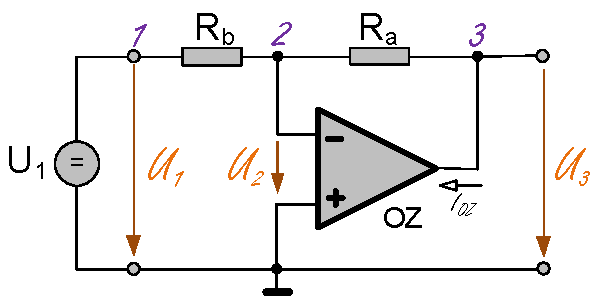
\includegraphics[width=0.7\linewidth]{MMUN_inv_OPAMP.pdf}
    \captionof{figure}{Neinvertující zesilovač}
    \label{TEO:fig_MMUN_neinv_opamp}
    \par}
   % using \usepackage{array} and command \newcolumntype{C}[1]{>{\centering}m{#1}}!
  {\centering
   \begin{tabular}{|C{0.45cm}|C{1.2cm}|C{0.6cm}|C{0.45cm}|C{0.45cm}|C{0.2cm}|c|C{.3cm}|c|}
      \multicolumn{1}{c}{$U_1$} & \multicolumn{1}{c}{$U_2$}   & \multicolumn{1}{c}{$U_3$} & 
      \multicolumn{1}{c}{$I_1$} & \multicolumn{1}{c}{$I_{OZ}$}& \multicolumn{1}{c}{ }     & 
      \multicolumn{1}{c}{x}     & \multicolumn{1}{c}{ }       & \multicolumn{1}{c}{b}     \\ 
      \cline{1-5} \cline{7-7} \cline{9-9}
           &   &   &  -1  &  & \multirow{5}{*}{$\ast$} & $U_1$ & \multirow{5}{*}{=}  &   \\
      \cline{1-5} \cline{7-7} \cline{9-9}
           & $G_a+G_b$ & $-G_a$ &      &   & & $U_2$     &   &                           \\
      \cline{1-5} \cline{7-7} \cline{9-9}
           & $-G_a$    & $G_a$ &       & 1 & & $U_3$     &   &                           \\
      \cline{1-5} \cline{7-7} \cline{9-9}
         1 &           &       &       &   & & $I_1$     &   & $U_{IN}$                  \\
      \cline{1-5} \cline{7-7} \cline{9-9}
           &     1     &       &       &   & & $I_{OZ}$  &   & $U_{IN}$                  \\
      \cline{1-5} \cline{7-7} \cline{9-9}
   \end{tabular}
   \par}
   \vspace{1em}
\end{example}  
          %-------------------------------------------------------
          \newpage
          % --------example: Diferenciální zesilovač -------------
          % \label{TEO:ex_DifOpamp01}
            % !TeX spellcheck = cs_CZ
\begin{mdframed}[style=mdexam]
\begin{example}\label{TEO:ex_DifOpamp01} 
  Uvažujme diferenciální zesilovač s ideální operačním zesilovačem typu VFA s naznačenými 
  uzly tak, jak je na obr. \ref{TEO:fig_MMUN_diff_opamp}. Napište rovnice MMUN.

   {\centering
    \captionsetup{type=figure}
    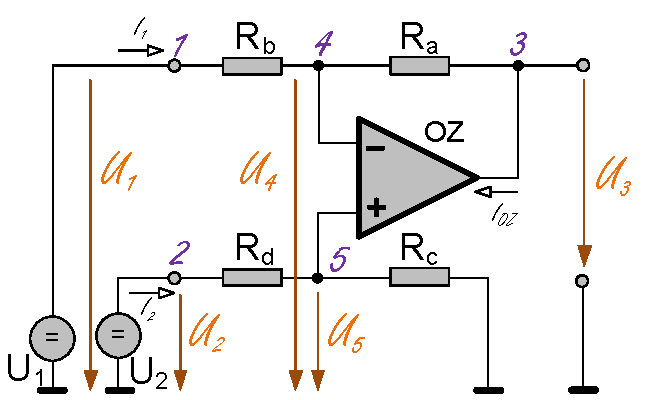
\includegraphics[width=0.7\linewidth]{MMUN_diff_OPAMP.pdf}
    \captionof{figure}{ Diferenciální zesilovač}
    \label{TEO:fig_MMUN_diff_opamp}
    \par}

    % using \usepackage{array} and command \newcolumntype{C}[1]{>{\centering}m{#1}}!
    {\centering
    \begin{tabular}{|C{0.6cm}|C{0.6cm}|C{0.6cm}|C{1.2cm}|C{0.6cm}|C{0.45cm}|C{0.45cm}|C{0.45cm}|}
        \multicolumn{1}{c}{$U_1$}  & \multicolumn{1}{c}{$U_2$}   & \multicolumn{1}{c}{$U_3$}  & 
        \multicolumn{1}{c}{$U_4$}  & \multicolumn{1}{c}{$U_5$}   & \multicolumn{1}{c}{$I_1$}  & 
        \multicolumn{1}{c}{$I_2$}  & \multicolumn{1}{c}{$I_{OZ}$}                      \\
        \hline
        $G_b$  &        &        & $-G_b$    &         & \(-1\) &        &             \\
        \hline
               & $G_d$  &        &           & $-G_d$  &        & \(-1\) &             \\
        \hline
               &        &  $G_a$ & $-G_a$    &         &        &        &             \\
        \hline 
        $-G_b$ &        & $-G_a$ & $G_a+G_b$ &         &        &        &             \\
        \hline
               & $-G_d$ &        & $G_c+G_d$ &         &        &        &             \\
        \hline
               &        &        &  \(-1\)   &  \(1\)  &        &        &             \\
        \hline
         1     &        &        &           &         &        &        &             \\
        \hline   
               & \(1\)  &        &           &         &        &        &             \\
        \hline    
    \end{tabular}
    \par}
\end{example}
\end{mdframed}  
          %-------------------------------------------------------

  \section{Analýza pomocí numerického simulátoru}
    \subsection{Analýza „DC“ neboli stejnosměrná analýza}
    \subsection{Rozšiřující typy analýz}
      \subsubsection{Citlivostní analýza („Sensitivity“)}
        Je počítána \emph{stejnosměrná citlivost} jedné nebo více veličin, vyjádřené vzorcem nebo 
        vzorci, na jednu nebo více vstupních proměnných.

          % --example: Citlivostní analýza napěťový děliče -------
          % \label{TEO:ex_CitDiveder01}
            % !TeX spellcheck = cs_CZ
\begin{example}\label{TEO:ex_CitDiveder01}
  V elektronických soustavách se největších přesností dosahuje u rezistorů, kde je standardně 
  zaručována chyba menší než 1\%, u přesných 0.1\% a u velmi přesných 0.01\%.

   {\centering
    \captionsetup{type=figure}
    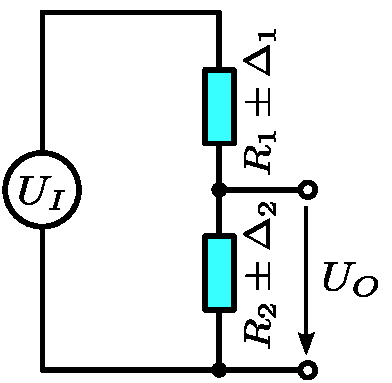
\includegraphics[width=0.4\linewidth]{voltage_divider.pdf}
    \captionof{figure}{ }
    \label{TEO:fig_voltage_divider}
    \par}

  Bude nás zajímat jaký vliv má tolerance rezistorů na výsledný poměr výstupního ku vstupnímu 
  napětí a také, zda-li při různě zvoleném poměru těchto rezistorů se bude měnit velikost chyby, 
  ačkoliv budou mít stejnou přesnost. Intuitivně předpokládáme, že  nejnepříznivější situace  
  nastane, když hodnoty použitých rezistorů padnou na opačné strany tolerančních pásem, jenž 
  reprezentuje $\Delta_1$ a $\Delta_2$ tj. $R_2 - \Delta_2R_2$ a $R_1 + \Delta_1R_1$ nebo $R_2 + 
  \Delta_2R_2$ a $R_1 - \Delta_1R_1$. V obou případech bude chyba stejná, proto si vybereme 
  například první případ a zapíšeme (rov. \ref{TEO:eq_divider_1}).
  \begin{equation}\label{TEO:eq_divider_1}
    \frac{U_o}{U_i} = \frac{R_2-\Delta_2 R_2}{R_1+\Delta_1 R_1+R_2-\Delta_2 R_2}
  \end{equation}
  a po úpravě
  \begin{equation*}
     \frac{U_o}{U_i} = \frac{(1-\Delta_2) R_2}{(1+\Delta_1) R_1+(1-\Delta_2) R_2}
  \end{equation*}
  Polynom ve jmenovateli rozvineme do následující podoby
  \begin{align*}
     [(1+\Delta_1) &+ (1-\Delta_2)](R_1+R_2)                \\
                   &= (1+\Delta_1)R_1 + (1-\Delta_2)R_2     \\
                   &+ (1+\Delta_1)R_2 + (1-\Delta_2)R_1     \\
   (1+\Delta_1)R_1 &+ (1-\Delta_2)R_2                       \\
                   &= [(1+\Delta_1)+(1-\Delta_2)](R_1+R_2)  \\
                   &- (1+\Delta_1)R_2 - (1-\Delta_2)R_1 
  \end{align*}
  a získáme %Further simplification of the denominator yields
  {\footnotesize
  \begin{equation*}
      \dfrac{U_o}{U_i}\ =
        \dfrac{(1-\Delta_2) R_2}{[(1+\Delta_1) + (1-\Delta_2)](R_1+R_2) - 
        [(1+\Delta_1) R_2\ +\ (1-\Delta_2) R_1] }
  \end{equation*}
  } %
  Nyní vydělíme jmenovatel i čitatel $(R_1 + R_2)$ a dostaneme 
  % Next divide both numerator and denominator by R1 + R2
  \begin{equation*}\label{TEO:eq_divider_2}
    \frac{U_o}{U_i}\ =\dfrac{\dfrac{(1-\Delta_2) R_2}{R_1+R2}}{[(1+\Delta_1)+(1-\Delta_2)] - 
    \dfrac{[(1+\Delta_1) R_2\ +\ (1-\Delta_2) R_1]}{R_1+R_2} }
  \end{equation*}
  Standardně rezistory volíme se stejnou tolerancí, tedy $\Delta_1 = \Delta_2 = \Delta$ a získáme 
  výslednou rovnici pro poměr $\frac{U_o}{U_i}$ 
  % Based on the assumption that both $\Delta1 = \Delta2 = \Delta$ then it should be possible to  
  % further simplify the expression for Vo/Vi:
  \begin{equation}
     \dfrac{U_o}{U_i} = \dfrac{\dfrac{(1-\Delta) R_2}{R_1+R_2}}{[(1+\Delta)+(1-\Delta)] - 
     \dfrac{[(1+\Delta)R_2 + (1-\Delta) R_1]}{R_1+R_2} }
  \end{equation}

  Řekněme například, že pro návrh děliče máme k dispozici rezistory s tolerancí 1\% a vstupní 
  napětí je 1 V. Obvod, ve kterém je dělič použit, umožňuje volit různé poměry, ale jejich součet 
  je konstantní. Na otázku jaký poměr zvolit, abychom při dané toleranci rezistorů dostali 
  výstupní napětí s největší přesností odpovídá následující tabulka.
  \vspace{1em}
  
  {\centering
   \setlength{\tabcolsep}{5pt}
   \begin{tabular}{|c|c|c|c|}
      \hline
        $R_1$                 & $1 k\Omega$  & $10 k\Omega$     & $19 k\Omega$   \\
      \hline
        $R_2$                 & $19 k\Omega$ & $10 k\Omega$     & $1 k\Omega$    \\
      \hline
        $U_{out}$             & 0,950        & 0,500            & 0,050          \\
      \hline
        $U_{out}^*$           & 0,949        & 0,495            & 0,049          \\
      \hline
        $\varepsilon_r [\%]$  & 0,101        & 1,000            & 1,883          \\
      \hline
   \end{tabular}
  \par}
  \vspace{1em}

  % Let's compare this answer to the formula I gave in a previous post using differentials. The  
  % relevant differential is
  % \begin{equation}\label{TEO:eq_divider_8}
  %   dV_0 = ( \frac{V}{R_1+R_2} - \alpha ) dR_1 - \alpha dR_2 + \frac{R_1}{R_1+R_2} dV
  % \end{equation}
  % where
  % \begin{equation}\label{TEO:eq_divider_9}
  %   \alpha = \frac{R_1 V}{(R_1+R_2)^2}
  % \end{equation}
\end{example}  
    
          %-------------------------------------------------------
%} % \tikzset

%---------------------------------------------------------------------------------------------------
\printbibliography[title={Seznam literatury}, heading=subbibliography]
\addcontentsline{toc}{section}{Seznam literatury}
%========== Kapitola: Přechodné děje ==============================================================
  % !TeX spellcheck = cs_CZ
% file: prechod_deje.tex
%{\tikzset{external/prefix={tikz/TEO/}}
% \tikzset{external/figure name/.add={ch10_}{}}
%========= Kapitola: Dynamické pochody v lineárních obvodechů ======================================
\setchaptertoc
\chapter{Dynamické pochody v lineárních obvodech}

  \section{Fyzikální podstata přechodných dějů}
    V obvodu, který je v ustáleném stavu, nechť dojde buďto
    \begin{itemize}
      \item ke změně parametru aktivního prvku (např. připojení nebo odpojení zdroje napětí nebo  
            proudu),
      \item ke změně parametru pasivního prvku (např. zvětšení nebo zmenšení odporu, indukčnosti  
            nebo kapacity),
      \item ke změně topologické struktury (např. přerušení větve, spojení větve nakrátko, připojení 
            další větve).
    \end{itemize}
    Kteroukoliv z uvedených změn dostaneme nový obvod jemuž přísluší nový \emph{ustálený stav}; 
    tento stav však nenastane okamžitě. Zmíněná změna přivede obvod do \emph{ne\-us\-tá\-le\-né\-ho 
    stavu}, v němž odezvy napětí a proudů - nazýváme je \textbf{přechodnými jevy} - se postupně 
    přibližují k hodnotám nového ustáleného stavu. Přechodné jevy, ač - přesně vzato - probíhají v 
    nekonečně dlouhé době, jsou v praxi jevy krátkodobými, neboť odezvy se trvale "dostatečně 
    těsně" přiblíží k hodnotám nového stavu již v poměrně krátké době - v běžných případech jsou to 
    mikrosekundy až milisekundy.

    Naskýtá se otázka, proč odezvy obvodu obecně nepřecházejí z původního do nového ustáleného 
    stavu skokem a proč dochází k neustálenému stavu obvodu. Obvod má elektromagnetickou energii 
    $W(t)$, která je součtem energií elektrického pole kondenzátoru $W_e(t)$ a energií magnetického 
    pole cívek $W_m(t)$. Elektromagnetická energie obvodu
    \begin{equation*}
      W(t)=\sum_kW_{e_k}(t)+\sum_kW_{m_k}(t)
    \end{equation*}
    je tedy funkcí napětí na jeho kondenzátorech a proudů v jeho cívkách. Protože tyto veličiny 
    určují energetický stav obvodu, nazýváme je \textbf{stavovými veličinami}.

    \begin{figure}[ht!]
       \centering
       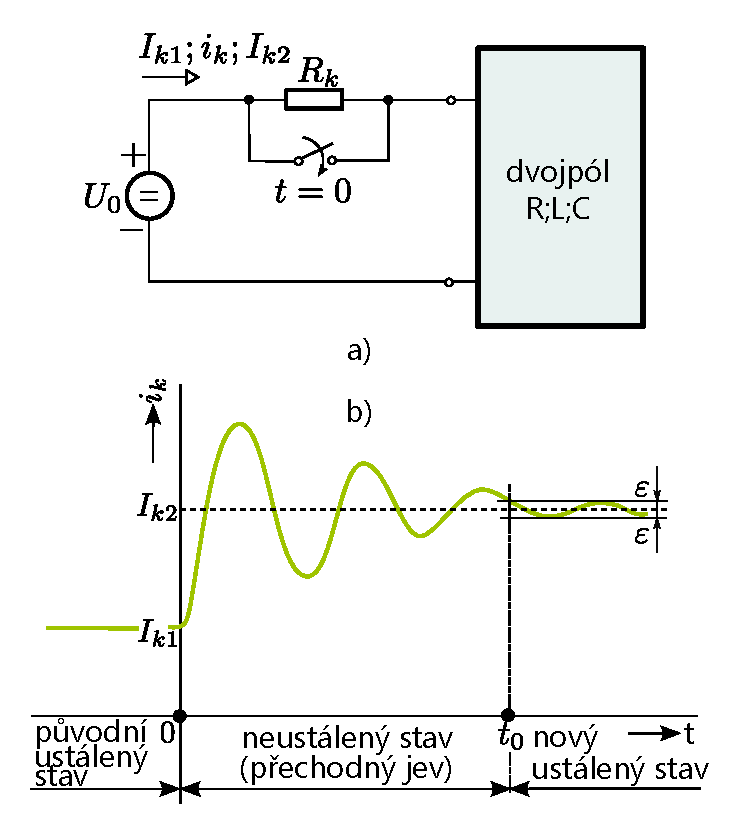
\includegraphics[width=0.8\linewidth]{prechodny_dej.pdf}
       \caption[Přechodný jev]{K objasnění pojmů "neustálený stav" a "přechodný jev"}
       \label{TEO:fig_prechodny_dej}
    \end{figure}

    Elektrické výkony $P$ v reálném elektrickém obvodu mají z fyzikálních důvodů vždy konečnou 
    hodnotu. U obvodů, které jsou dostatečně adekvátními modely respektujícími tuto skutečnost 
    (nazýváme je obvody s konečnými výkony) je to postačující podmínkou pro to, aby jejich energie 
    $W = W(t)$ byla spojitou funkcí času (neboť $P = \frac{dW}{dt}$). Z uvedených vztahů pro 
    energii obvodu $W(t)$ je patrné, že $W = W(t)$ bude spojitou funkcí, jsou-li stavové veličiny 
    \emph{spojitými funkcemi}. To znamená, že hodnota stavových veličin v okamžiku před vznikem 
    přechodného jevu je táž jako v okamžiku po jeho vzniku. Pro přechodný jev v okamžiku $t=0$ 
    platí tedy
    \begin{equation}\label{TEO:eq_spojite_fce}
      \lim_{t\rightarrow0_-}u_c(t)= \lim_{t\rightarrow0_+}u_c(t); \quad  
      \lim_{t\rightarrow0_-}i_L(t)= \lim_{t\rightarrow0_+}i_L(t)
    \end{equation}

     \subsection{Přechodné jevy v jednodušších obvodech; charakteristické pojmy a vlastnosti}
        % --------example: Transformátor -----------------------
        % \label{TEO:exam005}
          % !TeX spellcheck = cs_CZ
\begin{example}\label{TEO:exam005} \textbf{Transformátor}: \newline
  Na primární vinutí vzduchového transformátoru s činitelem $k < 1$ je v čase $t=0$ připojen zdroj 
  napětí $U_1 = konst$. Formulujte postup pro výpočet odezev $i_1(t)$ a $i_2(t)$ pro obecné 
  parametry zapojení a výsledky ověřte simulací pro následující hodnoty: $U_1 = 1V, R_1 = 1\Omega, 
  R_2 = 4\Omega, $ transformátor má převod $1:3$.
  
  {\centering
   \captionsetup{type=figure}
   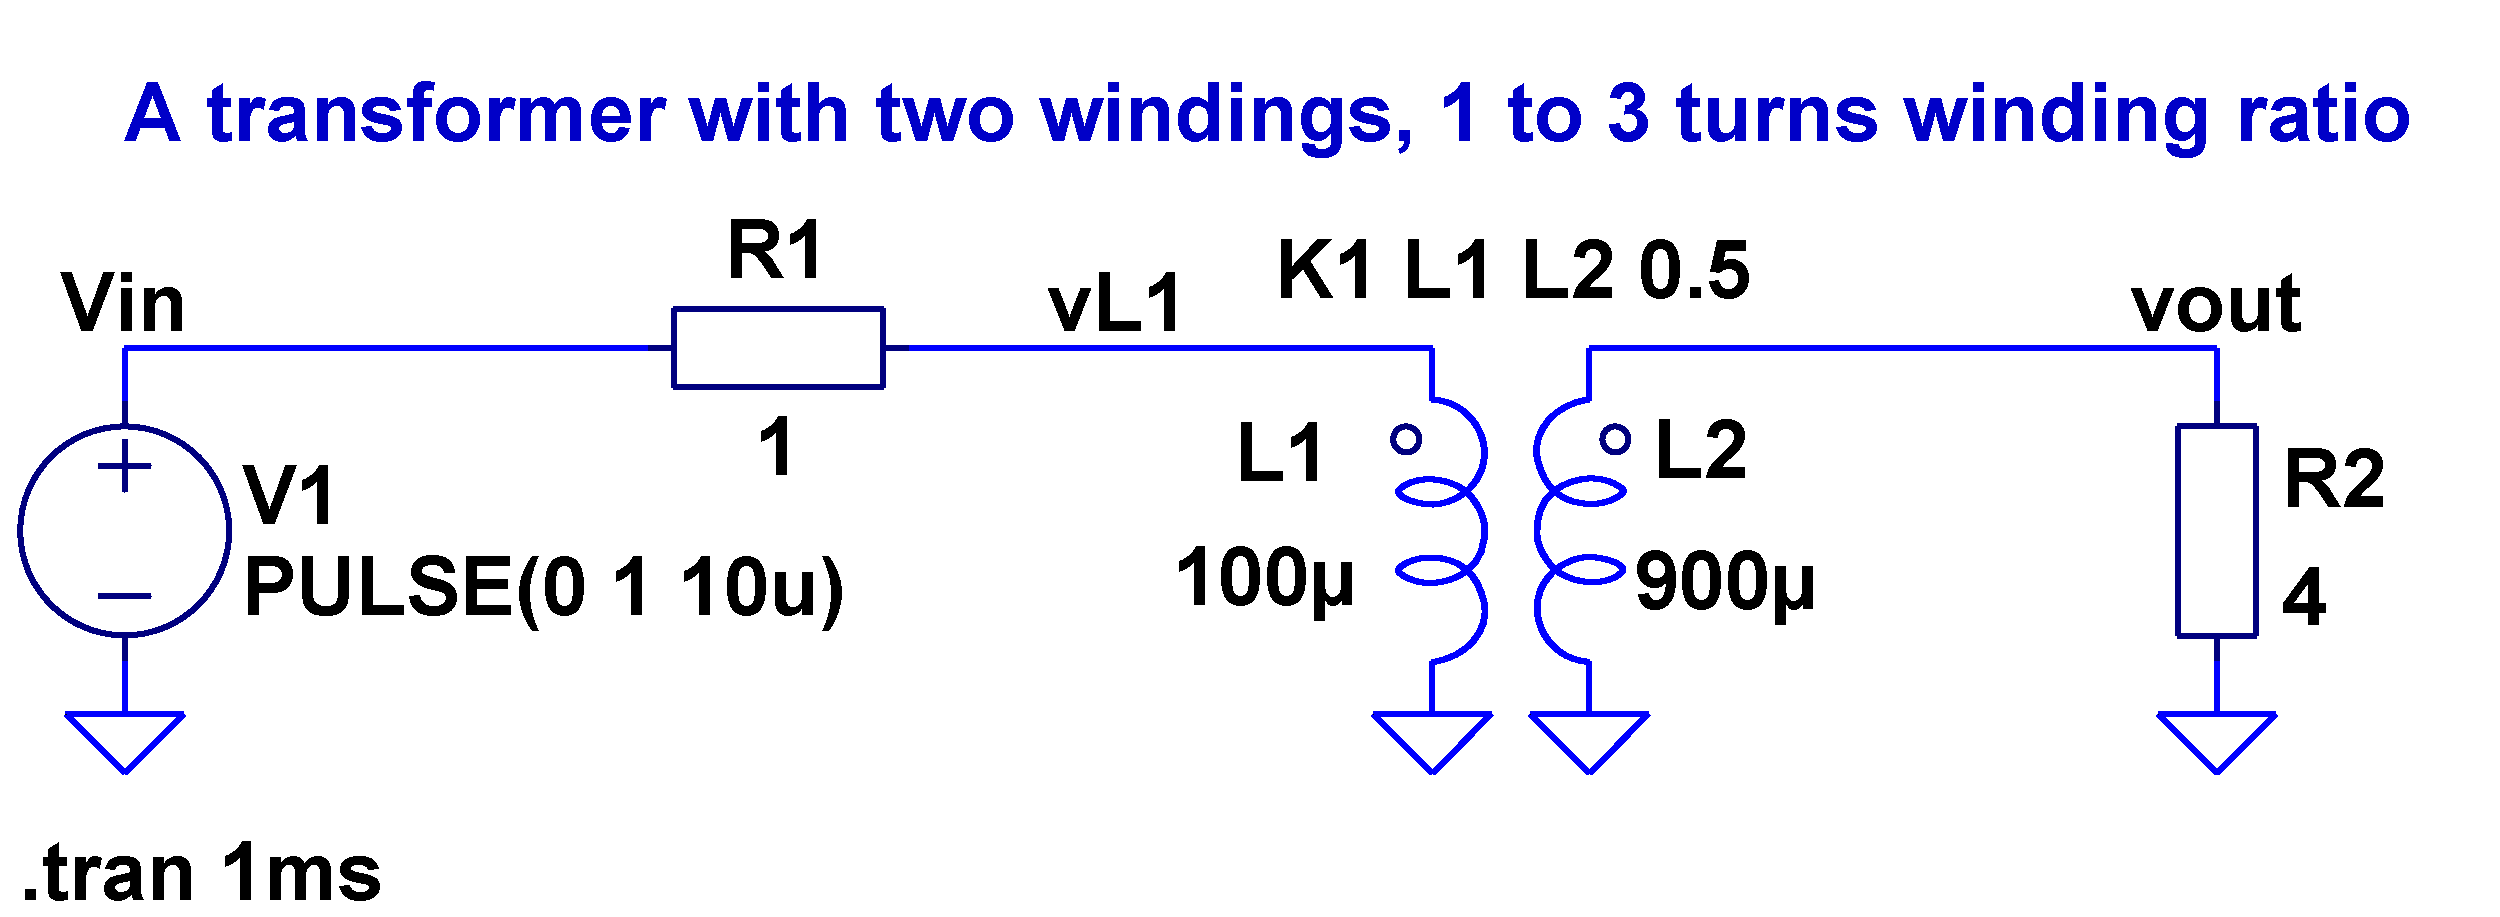
\includegraphics[width=0.9\linewidth]{Ideal_Trf_step_response_LTspice.pdf}
   \captionof{figure}{\texttt{Transformer.asc}: Zapojení vzduchového transformátoru
              pro simulaci v programu LTSpice}
   \label{TEO:fig_trafo_int_uprim}
   \par}
  
  \textbf{Klasické řešení}: Podle II. Kirchhoffova zákona platí soustava rovnic:
  \begin{subequations}\label{TEO:eq_trafo_IIKz}
    \begin{align}
      R_1i_1 + L_1\frac{di_1}{dt} + L_{12}\frac{di_2}{dt} &= U_1 \\
      R_2i_2 + L_2\frac{di_2}{dt} + L_{12}\frac{di_1}{dt} &= 0
    \end{align}
  \end{subequations}
  
  \begin{equation}\label{TEO:eq_char_rce}
  \left(
  \begin{array}{cc}
  R_1 + L_1\lambda & L_{12}\lambda  \\
  L_{12}\lambda    & R_2 + L_2\lambda
  \end{array}
  \right) = 0
  \end{equation}
  \begin{subequations}\label{TEO:eq_char_rce_solve}
    \begin{align}
      (R_1 + L_1\lambda) - L_{12}^2\lambda^2                                      &= 0      \\
      R_1R_2 + (L_1R_2 + L_2R_1)\lambda + L_1L_2\lambda - L_{12}^2\lambda^2       &= 0      \\
      \lambda^2(L_1L_2-L_{12}^2)+(L_1R_2+L_2R_1)\lambda +R_1R_2                   &= L_1L_2 \\
      \lambda^2(\frac{L_1L_2-L_{12}^2}{L_1L_2})+
      (\frac{L_1R_2+L_2R_1}{L_1L_2})\lambda +\frac{R1R2}{L_1L_2}                  &= 0
    \end{align}
  \end{subequations}
  Zavedeme-li $\tau_1 = \frac{L_1}{R_1}, \tau_2 = \frac{L_2}{R_2}$,
  $k=\frac{L_12}{\sqrt{L_1L_2}}, k^2=\frac{L_12^2}{L_1L_2}$, $\sigma = 1-k^2$ dostaneme
  \begin{subequations}\label{TEO:eq_trafo_vysl_rce}
    \begin{align}
      \sigma\lambda^2 + \left(\frac{1}{\tau_1}+\frac{1}{\tau_2}\right)\lambda + 
      \frac{1}{\tau_1}\frac{1}{\tau_2} = 0                                                 \\
      \lambda^2 + \frac{1}{\sigma}\left(\frac{1}{\tau_1}+\frac{1}{\tau_2}\right)\lambda + 
      \frac{1}{\sigma\tau_1\tau_2} = 0
    \end{align}
  \end{subequations}
  Je-li $\lambda_1 = -\beta+\alpha$ a $\lambda_2 = -\beta-\alpha$
  \begin{subequations}
    \label{TEO:eq_trafo_alphabeta}
    \begin{align}
    \alpha &= \frac{1}{2\sigma}
    \left(\frac{1}{\tau_1}+ 
    \frac{1}{\tau_2}\right)            \label{TEO:eq_trafo_alphabeta_a}     \\ 
    \beta  &= \frac{1}{2\sigma}
    \sqrt{\left(\frac{1}{\tau_1}+
      \frac{1}{\tau_2}\right)^2+
      \frac{4\sigma}{\tau_1\tau_2}}      \label{TEO:eq_trafo_alphabeta_b}
    \end{align}
  \end{subequations}
  Jelikož $k<1$; je $0<\sigma<1$; rozborem rovnice \ref{TEO:eq_trafo_alphabeta_b} plyne, že pak
  je $\alpha\neq0$, reálné. Soustava rovnic \ref{TEO:eq_trafo_IIKz} má tedy obecné řešení
  \begin{subequations}\label{TEO:eq_trafo_obecne_res}
    \begin{align}
      i_1(t) &= i_{1o} +i_{1p} = K_1e^{\lambda_1t} + K_2e^{\lambda_2t} +\frac{U_0}{R} \\
      i_2(t) &= i_{2o} +i_{2p} = K_3e^{\lambda_1t} + K_4e^{\lambda_2t}
    \end{align}
  \end{subequations}
  Integrační konstanty $K_1, K_2, K_3$ a $K_4$ určíme z matematických počátečních podmínek:
  $i_1(0)=i_2(0)=0$ (což jsou zároveň fyzikální počáteční podmínky) a $\frac{di_1}{dt}|_{t=0}, 
  \frac{di_2}{dt}|_{t=0}$, které určíme z rovnic \ref{TEO:eq_trafo_IIKz} pro $t=0$:
  \begin{subequations}\label{TEO:eq_trafo_didt_t0}
    \begin{align}
      L_1i_1'+L_{12}i_2' &= U_0 \Longrightarrow i_1' = \left(\frac{U_0-L_{12}i_2'}{L_1}\right)\\
      L_2i_2'+L_{12}i_1' &= 0
    \end{align}
  \end{subequations}
  Dále postupujeme tak, že do druhé rovnice dosadíme vyjádřenou první derivaci primárního
  proudu z první rovnice a získáme vztah pro první derivaci sekundárního proudu v čase $t=0$:
    \begin{subequations}\label{TEO:eq_trafo_dev_i1i2}
    \begin{align}
      \frac{di_1}{dt}|_{t=0} &=   \frac{L_{2}}{L_1L_2-L_{12}^2}U_0                        \\
      \frac{di_2}{dt}|_{t=0} &=  -\frac{L_{12}}{L_1L_2-L_{12}^2}U_0
    \end{align}
  \end{subequations}
  Aplikací těchto počátečních podmínek na obecné řešení \ref{TEO:eq_trafo_obecne_res} plynou
  vztahy
  \begin{subequations}
    \begin{align}
    i_1(0)                            &= K_1 + K_2 +\frac{U_0}{R}                         \\
    \frac{L_{2}}{L_1L_2-L_{12}^2}U_0  &= \lambda_1K_1 + \lambda_2K_2                      \\
    i_2(0)                            &= K_3 + K_4                                        \\
   -\frac{L_{12}}{L_1L_2-L_{12}^2}U_0 &= \lambda_1K_3 + \lambda_2K_4
    \end{align}
  \end{subequations}
  Z první a třetí rovnice vypočítáme $K_1; K_2$, ze druhé a čtvrté rovnice $K_3; K_4$.
  Do\-sa\-ze\-ním do rovnice \ref{TEO:eq_trafo_obecne_res} dostaneme po úpravě odezvy $i_1(t)$
  a $i_2(t)$. Speciálně pro $R_1=R_2=R$;$L_1=L_2=L$ je
  \begin{subequations}\label{TEO:eq_trafo_solved_RL}
    \begin{align}
      i_1(t) &= \frac{U_0}{2R}\left(2-e^{-\frac{t}{\tau_3}}-e^{-\frac{t}{\tau_4}}\right) \\
      i_2(t) &= \frac{U_0}{2R}\left(-e^{-\frac{t}{\tau_3}}+e^{-\frac{t}{\tau_4}}\right)
    \end{align}
  \end{subequations}
  kde je $\tau_3 = \frac{L + L_{12}}{R}; \tau_4 = \frac{L - L_{12}}{R}$
  
  \textbf{Operátorové řešení}: Laplaceovou transformací rovnice \ref{TEO:eq_trafo_IIKz}
  dostáváme
  \begin{subequations}\label{TEO:eq_trafo_laplace}
    \begin{align}
      (R_1 + pL_1)I_1(p)+pL_{12}I_2(p)   &= \frac{U_0}{p} \\
      pL_{12}I_1(p) + (R_2 + pL_2)I_2(p) &= 0
    \end{align}
  \end{subequations}
  Zavedeme $\sigma; \tau_1; \tau_2$, vypočítáme obrazy proudů a jejich zpětnou transformací
  do\-sta\-ne\-me rovnice pro odezvy $i_1(t)$ a $i_2(t)$.
  
  {\centering
   \captionsetup{type=figure}
   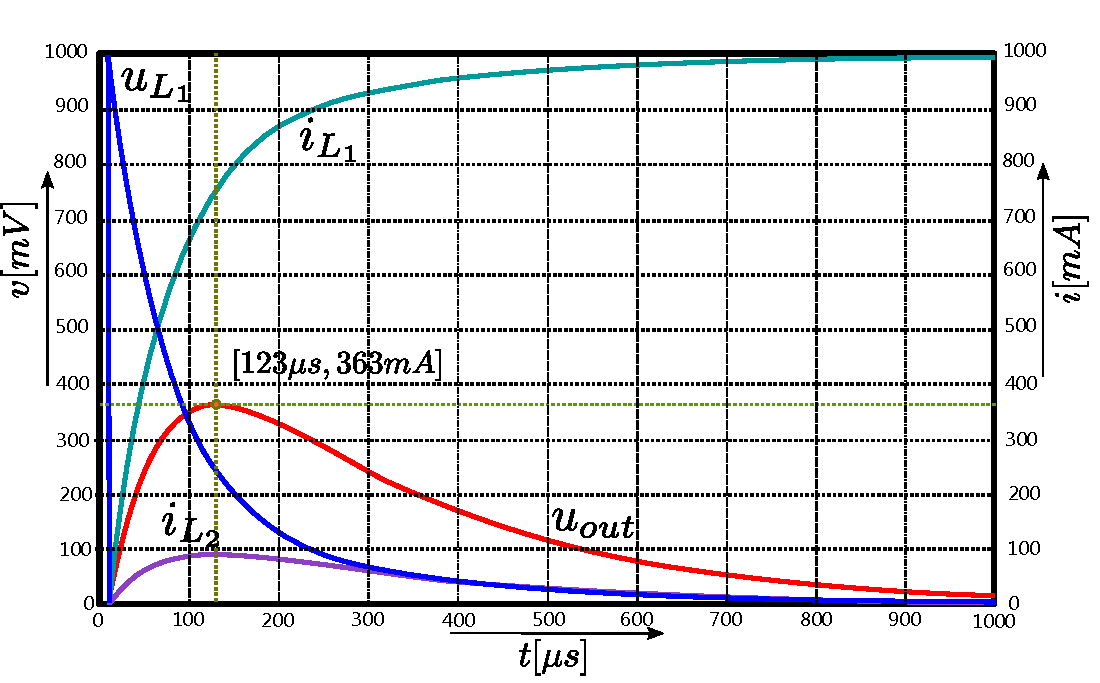
\includegraphics[width=1\linewidth]{Ideal_Trf_step_response_K05.pdf}
   \captionof{figure}{Odezva na jednotkový skok transformátoru s parametry: $k=0.5, L_1 = 100 \mu 
             H, L_2 = 900 \mu H$}
  \label{figure:trafo_int_uprim}
  \par}
\end{example}

  
        %-------------------------------------------------------

        % --------example: Obvod s kondenzátorem ---------------
        % \label{TEO:ex_10_8}
        % % !TeX spellcheck = cs_CZ
\begin{example}\label{TEO:ex_10_8} Najděte odezvu napětí na kondenzátoru $u_c(t)$ obvodu na
  obrázku \ref{TEO:fig_cir_10_8} pro $t>0$. (zdroj \cite[s.~456]{Dorf}) 
  
  {\centering
   \captionsetup{type=figure}
   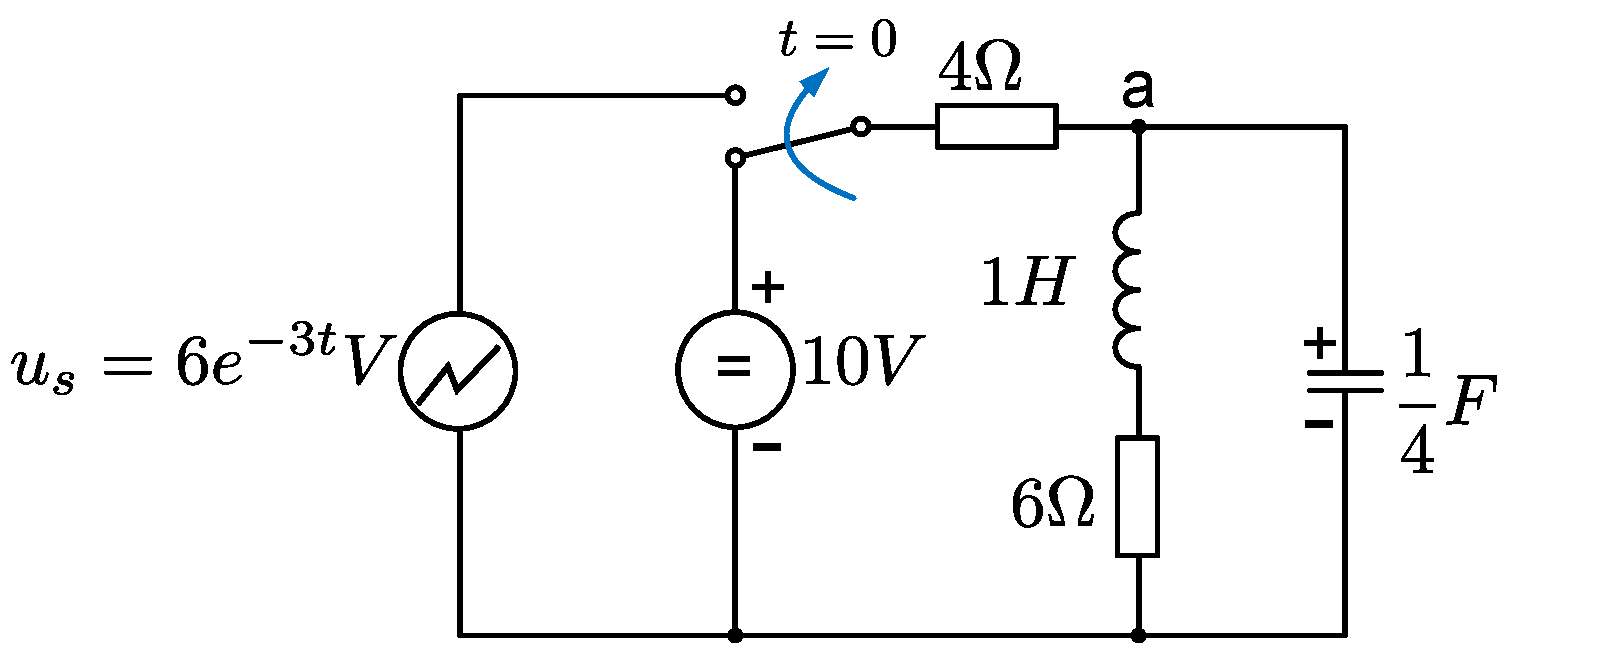
\includegraphics[width=1\linewidth]{response_ex10_8_RLC_cir.pdf}
   \captionof{figure}{Obvod k příkladu \ref{TEO:ex_10_8}}
   \label{TEO:fig_cir_10_8}
   \par}
  
  \textbf{Řešení:} Nejdříve stanovíme počáteční podmínky, které vyplývají z ustáleného stavu
  v době $t = 0^-$. Obvod na obr. \ref{TEO:fig_cir_10_8} můžeme překreslit do podoby na obr.
  \ref{TEO:fig_cir_10_8_steady} 
  
  {\centering
   \captionsetup{type=figure}
   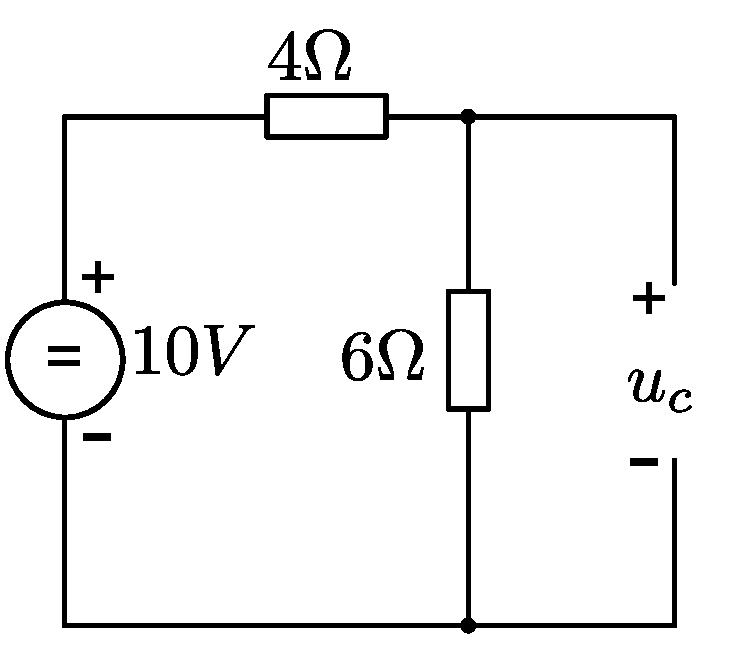
\includegraphics[width=0.4\linewidth]{response_ex10_8_steady.pdf}
   \captionof{figure}{Obvod k příkladu \ref{TEO:ex_10_8}}
   \label{TEO:fig_cir_10_8_steady}
   \par}
  \begin{equation}\label{TEO:eq_10_8_vysledek}
  u_c(t) = \frac{44}{3}e^{-2t}+\frac{1}{3}e^{-5t} - 9e^{-3t} \qquad [V]
  \end{equation}
\end{example}  
        %-------------------------------------------------------
            
  %--------------------- Přechodný jev kmitavého obvodu --------------------------------------------
  \section{Přechodný jev kmitavého obvodu}
    Kmitavým obvodem máme na mysli obvod s jedním stupněm volnosti, složeného z odporu $R$,
    kapacity $C$ a indukčnosti $L$, zapojených v sérii. Je jedním z nejdůležitějších případů
    elektrotechnické praxe. Dosud probírané případy (obvod \emph{RL} a \emph{RC}) jsou vždy určitým
    zjednodušením úplného obvodu s jedním stupněm volnosti, vzniklé tak, že buď indukčnost obvodu,
    nebo kapacita jsou zanedbatelné vzhledem k ostatním prvkům. Rozbor přechodného stavu kmitavého
    obvodu (dále stručně obvodu \emph{RLC}) umožňuje stanovit směrnice pro možnost tohoto
    zjednodušení a jeho důsledky.
    
    \luagraphic[0.5]{teo_fig027.pdf}{Schéma sériového kmitavého obvodu}{teo:fig027}

    Zopakujme, že přechodný stav, je vždy dán superpozicí nového ustáleného stavu a vlastní
    přechodné složky, jejíž průběh závisí jen na vlastnostech obvodu a počátečních podmínkách (a
    nikoliv na průběhu vstupního signálu), proto nejdříve budeme řešit tzv. \emph{volný stav
    obvodu}, tj. stav, kdy vnější působení na vstupu je nulové. Za těchto okolností může v obvodu
    existovat přechodný jev, je-li v obvodu (tj. v akumulačních prvcích) na počátku nahromaděná
    určitá energie. Vzhledem k tomu, že to může být jednak energie elektrického pole v kondenzátoru,
    jednak energie magnetického pole v cívce, je počáteční stav úplně určen, známe-li hodnoty napětí
    na kapacitě a proudu v indukčnosti v počátečním okamžiku; matematicky vyjádřeno, stanovíme
    počáteční podmínky vždy ve tvaru
    \begin{equation}\label{TEO:eq_RLC_00}
      u_C(0) = U_{C_0} \qquad i(0) = I_0.
    \end{equation}    
    Protože za volného stavu jsou vstupní svorky spojeny \emph{nakrátko}, je rovnice pro proud v
    obvodu
    \begin{align}\label{TEO:eq_RLC_01}
       u_R + u_L + u_C                                    &= 0 \\
       Ri + L\der{i}{t} +\frac{1}{C}\int_0^tidt + U_{C_0} &= 0
    \end{align}     
    Řešení provedeme pomocí Laplaceovy transformace. K přihlédnutím  k počátečním podmínkám
    \ref{TEO:eq_RLC_01} dostaneme rovnici
    \begin{equation}\label{TEO:eq_RLC_02}
      I(p)(R + Lp + \frac{1}{pC}) = I_0L - \frac{U_{C_0}}{p},
    \end{equation}     
    a z ní 
    \begin{equation}\label{TEO:eq_RLC_03}
      I(p) = \frac{pCLI_0 - CU_{C_0}}{p^2LC + pRC + 1}.
    \end{equation}

%} % tikzset
%---------------------------------------------------------------------------------------------------
%========== Kapitola: Obvody v harmonickém ustáleném stavu ========================================
  % !TeX spellcheck = cs_CZ
%=====================Kapitola: Obvody v harmonickém ustáleném stavu=======================
\chapter{Obvody v harmonickém ustáleném stavu}
  V této kapitole se seznámíme se \emph{symbolicko-komplexní metodou} (\texttt{SKM}), jež má
  základní důležitost pro teorii obvodů v harmonickém ustáleném stavu. Potom prozkoumáme vlastnosti
  jednodušších obvodů v tomto stavu a metody jejich analýzy. Posléze pojednáme o elektrickém výkon
  v obvodech a o nejdůležitějších otázkách přenosu energie \cite[s.~60]{Mayer1978}.
  
  \section{Periodické veličiny a jejich charakteristické hodnoty}
    \emph{Periodickou veličinou} nazýváme takovou veličinu $v$, jejíž závislost na čase lze
    vyjádřit periodickou funkcí, pro níž existuje konstanta $T>0$ taková, že pro každé $t$ platí
    vztah
    \begin{equation}\label{TEO:eq_harm01}
      v(t+T) = v(t),    
    \end{equation}  
    Konstanta $T$ se nazývá \textbf{perioda} resp. \emph{doba kmitu}. V aplikacích se zpravidla
    používá nejmenší kladná perioda, tzv. \emph{základní perioda}; pro stručnost budeme hovořit
    pouze o periodě. Je-li dána periodická veličina na jakémkoliv intervalu $(t_0, t_0+T)$, je tím
    zřejmě definována pro všechna $t>t_0$. Průběh veličiny $v$ na jakémkoliv intervalu délky $T$ se
    nazývá \emph{cyklem}. Počet cyklů za jednotku času (za sekundu) udává \textbf{kmitočet}, nebo
    též \emph{frekvenci} periodické veličiny
    \begin{equation}\label{TEO:eq_harm02}
      f = \frac{1}{T},
    \end{equation}
    V elektrotechnice rozdělujeme periodické veličiny do dvou skupin:
    \begin{figure}[ht!] % \ref{teo:fig029}
       \centering
       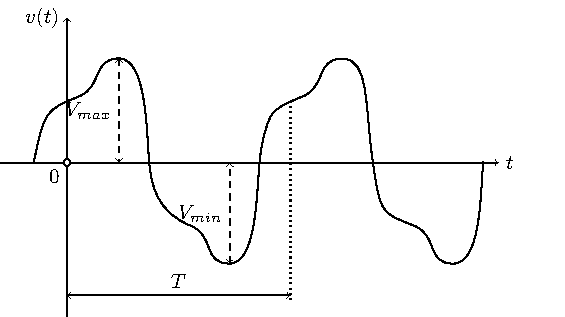
\includegraphics[width=0.8\linewidth]{teo_fig029.pdf}
       \caption{Příklad periodické veličiny $v=v(t)$ pro kterou platí $v(t+T)=v(t)$}
       \label{teo:fig029}
    \end{figure}

    \begin{figure}[ht!] % \ref{teo:fig030}
       \centering
       \includegraphics[width=0.8\linewidth]{teo_fig030.pdf}
       \caption{Časový průběh \textbf{střídavé veličiny} $v=v(t)$, pro kterou platí, že obsahy ploch
                v jednom cyklu nad osou $t$ a pod osou $t$ jsou totožné}
       \label{teo:fig030}
    \end{figure}

    \begin{itemize}
      \item Veličiny $v$, jež během svého cyklu \emph{změní znaménko} (obr.\ref{teo:fig029})
            nazýváme \textbf{kmitavé}. \emph{Speciálním případem} kmitavých veličin jsou
            \textbf{střídavé veličiny}, jež mají tu vlastnost, že po dobu $T/2$ jsou trvale kladné,
            po dobu $T/2$ naopak záporné a obsahy ploch omezených grafem funkce $v=v(t)$ v jednom
            cyklu nad osou $t$ a pod osou $t$ jsou \emph{totožné} (obr. \ref{teo:fig030}).
      \item Veličiny $v$, jež \emph{nemění své znaménko}, tj. jsou trvale kladné nebo trvale
            záporné (obr.\ref{teo:fig031}) nazýváme \textbf{pulzující}. \emph{Speciálním případem}
            jsou \textbf{stejnosměrné veličiny}, které nemění svou hodnotu, tj. $v=konst$
            (obr.\ref{teo:fig031} (b)).
    \end{itemize} 

    \begin{figure}[ht!] % \ref{teo:fig031}
       \centering
       \includegraphics[width=0.8\linewidth]{teo_fig031.pdf}
       \caption{Časový průběh pulsující periodické veličiny a konstantní veličiny}
       \label{teo:fig031}
    \end{figure}

    Praktický význam mají zejména tyto hodnoty periodických veličin:
    \begin{itemize}
      \item \emph{Maximální hodnota} $V_m$ periodické veličiny $v$, tj. největší hodnota, které
            tato veličina dosahuje $v_m=\max v(t)$
      \item \emph{Minimální hodnota} $V_{min}$ periodické veličiny $v$, tj. nejmenší hodnota, které
            tato veličina dosahuje $v_m=\min v(t)$
    \end{itemize}
      
    Maximální a minimální hodnoty střídavé veličiny se nazývají též \emph{vrcholovými hodnotami}
    (kladnými nebo zápornými), obr. \ref{teo:fig029} a \ref{teo:fig030}. 
    
    \fbox{Střední hodnota} veličiny $v$ v intervalu $\langle t_i, t_j\rangle$ je 
    \begin{equation}\label{TEO:eq_harm03}
      V_s = \frac{1}{t_j-t_s}\int_{t_j}^{t_s}v(t)dt
    \end{equation}
    U periodické veličiny se spravidla počítá střední hodnota v jedno cyklu. U střídavé veličiny je
    v jednom cyklu $V_s = 0$,  a proto střední hodnotu vyjadřujeme v takovém intervalu v němž je
    $v\geq0$.
    
    \fbox{Efektivní hodnota} periodické veličiny v intervalu $\langle 0, T\rangle$ je 
    \begin{equation}\label{TEO:eq_harm04}
      V = \sqrt{\frac{1}{T}\int_{0}^{T}v^2(t)dt}
    \end{equation}   
    U periodických napětí a proudů má praktický význam především jejich efektivní hodnota.
    Efektivní hodnotu periodického proudu $i=i(t)$ procházejícího konstatním odporem $R$ lze
    interpretovat jako stejnosměrný proud $I$, při němž se za dobu $T$ vyvine v odporu $R$ stejná
    tepelná energie, jako průchodem proudu $i$. Podle \emph{Joulova-Lenzova} zákona je totiž
    \begin{equation}\label{TEO:eq_harm05}
      RI^2T = \sqrt{\frac{1}{T}\int_{0}^{T}Ri^2(t)dt}
    \end{equation}       
    z čehož lze určit $I$ v souladu s rovnicí \ref{TEO:eq_harm04}. Obdobně lze fyzikálně
    interpretovat efektivní hodnotu napětí.
    
    Střední hodnotu periodického proudu $i=i(t)$ lze fyzikálně interpretovat jako stejnosměrný
    proud $I_s$, jimž se za dobu $T$ přenese stejný náboj $Q$ jako proudem $i$:
    \begin{equation}\label{TEO:eq_harm06}
      Q = I_sT = \int_{0}^{T}i(t)dt
    \end{equation}       
    z čehož plyne $I_s$ v souladu s rovnicí \ref{TEO:eq_harm03}.  
    
    Efektivní hodnotu napětí (proudu) lze změřit např. feromagnetickým, elektrodynamickým nebo
    tepelným voltmetrem (ampérmetrem). Střední hodnotu napětí (proudu) magnetoelektrickým
    voltmetrem (ampérmetrem) a střední hodnotu výkonu elektrodynamickým wattmetrem.

    \begin{figure}[ht!] % \ref{teo:fig032}
       \centering
       \includegraphics[width=0.8\linewidth]{teo_fig032.pdf}
       \caption{Haromincká funkce $v = V_m\cos(\omega t + \varphi)$ resp. 
                $v= V_m\cos(\omega t + \varphi')$ kde je $\varphi' = \varphi - \frac{T}{4}$}
       \label{teo:fig032}
    \end{figure}

    Střídavou veličinu $v$ lze též do jisté míry charakterizovat \emph{činitelem tvaru} $\beta$,
    \emph{činitelem výkyvu} $\gamma$ a \emph{činitelem plnění} $\alpha$ definovanými vztahy
    \begin{equation}\label{TEO:eq_harm07}
      \beta = \frac{V}{V_s}, \quad \gamma = \frac{V_m}{V}, \quad \alpha = \frac{V_s}{V_m}
    \end{equation}    
    Je zřejmé, že platí $\alpha\beta\gamma = 1$.
    
    V elektrotechnice mají velkou důležitost periodická napětí a proudy, jejichž závislost je dána
    sinusovou nebo kosinusovou funkcí, tj.
    \begin{equation}\label{TEO:eq_harm08}
      v = V_m\sin(\omega t + \varphi),
    \end{equation}        
    nebo
    \begin{equation}\label{TEO:eq_harm09}
      v = V_m\cos(\omega t + \varphi),
    \end{equation}  
    kde $V_m$, $\omega$, $\varphi$ jsou konstanty (obr. \ref{teo:fig032})
    
    Jelikož, tato napětí, resp. proudy představují \emph{harmonické kmity}, nazýváme je
    \emph{harmonicky proměnné}, nebo krátce \emph{harmonická napětí} resp. \emph{harmonická
    proudy}. Konstanta $V_m$ je maximální hodnota, či-li \emph{amplituda}, $\omega t + \varphi$ je
    \emph{fáze}, $\omega = 2\pi f = \frac{2\pi}{T}$ je \emph{úhlový kmitočet} a $\varphi$ je
    \emph{počáteční fáze} harmonické funkce.
    
    Rozdíl fází dvou harmonických veličin (stejného kmitočtu) nazýváme \emph{fázový posun}.
    
    % --------example: Efektivní hodnota výpočet -----------
    % \label{TEO:exam007}
    % !TeX spellcheck = cs_CZ
\begin{example}\label{TEO:exam007}
  Pro harmonickou veličinu, určete efektivní hodnotu, střední hodnotu, činitele tvaru, činitele
  výkyvu a činitele plnění \newline
  \textbf{Řešení:} Efektivní hodnota je:
  \begin{align}
    V &= \sqrt{\frac{1}{T}\int_0^TV_m^2\cos^2{(\omega t + \varphi)}\,dt}    \nonumber  \\
      &= \sqrt{\frac{1}{T}\int_0^TV_m^2\sin^2{(\omega t + \varphi)}\,dt} = 
         \frac{1}{\sqrt{2}}V_m \doteq 0.707 V_m   
  \end{align}
  Podrobný výpočet tohoto integrálu pomocí substituce $\omega t + \varphi=\dfrac{\alpha}{2}$ je
  poněkud zdlouhavější:
  \begin{align*}
      \omega t + \varphi=\dfrac{\alpha}{2}   
    & \rightarrow  2(\omega t + \varphi) = \alpha      \\ 
      \omega dt = \frac{1}{2}d\alpha         
    & \rightarrow dt = \frac{1}{2\omega}d\alpha
  \end{align*}
  Nesmíme zapomenout přepočítat meze $\alpha_d\lvert_{t=0}=2\varphi$ a $\alpha_h\lvert_{t=T} = 
  4\pi+2\varphi$ nového integrálu.
  \begin{align*}
    V^2  &= \frac{V_m}{2T\omega}\int_{\alpha_d}^{\alpha_h}\cos^2\frac{\alpha}{2}\,d\alpha    \\
         &= \frac{V_m}{4\pi}\int_{\alpha_d}^{\alpha_h}\frac{1+\cos\alpha}{2}\,d\alpha  
          = \frac{V_m}{4\pi}\left(\left.\frac{\alpha}{2}\right\rvert_{\alpha_d}^{\alpha_h}
          + \left.\frac{1}{2}\sin\alpha\right\rvert_{\alpha_d}^{\alpha_h}\right)             \\
         &= \frac{V_m}{4\pi}\left(2\pi+\varphi-\varphi 
          + \frac{1}{2}\sin(4\pi+2\varphi)
          - \frac{1}{2}\sin(2\varphi)\right) = \frac{V_m}{2}.  
  \end{align*}  
  Při zjednodušování integrálu je užito známého goniometrického vzorce \(\cos^2\dfrac{\alpha}{2} = 
  \dfrac{1+\cos\alpha}{2}\) a faktu \(\sin(x+2k\pi)=\sin x\)
  
  Střední hodnota kladné půlvlny je 
  \begin{align*}
    V_s &= \frac{2}{T}\int\limits_{-S\frac{T}{4}-
           \frac{\varphi}{\omega}}^{\frac{T}{4}-
           \frac{\varphi}{\omega}}{V_m\cos(\omega t +\varphi)}\,dt                            \\
        &= \frac{2}{T}\int\limits_{-\frac{\varphi}{\omega}}^{-\frac{T}{2}-
           \frac{\varphi}{\omega}}{V_m\sin(\omega t +\varphi)}\,dt                            \\
        &= \frac{2}{\pi}V_m \doteq 0,637V_m
  \end{align*}
  činitele tvaru, výkyvu a plnění jsou 
  \begin{align*}
    \beta  &=\frac{V}{V_s}   =\frac{\pi}{2\sqrt{2}}=1,111, \\ 
    \gamma &=\frac{V_m}{V}   =\sqrt{2}\doteq1.414,         \\
    \alpha &=\frac{V_s}{V_m} =\frac{2}{\pi}\doteq0,637 
  \end{align*}
\end{example}  
    %-------------------------------------------------------
      
 %--------------------------------------------------------------------------------------------------
  \section{Obvody s nastavitelnými parametry}
    V praxi se setkáváme s obvody, u nichž lze (spojitě nebo stupňovitě) nastavit odpor odporníku, 
    kapacitu kondenzátoru, vlastní nebo vzájemnou indukčnost cívek, amplitudu, fázi nebo kmitočet
    zdroje (napětí nebo proud). Nazveme je \emph{obvody s nastavitelnými parametry}.
 %--------------------------------------------------------------------------------------------------

%} % tikzset
%---------------------------------------------------------------------------------------------------
%========== Kapitola: Obvody s rozprostřenými parametry ===========================================
  % !TeX spellcheck = cs_CZ
%file: teo1ch03.tex
%===========Kapitola: Obvody s rozprostřenými parametry====================================
\setchaptertoc
\chapter{Obvody s rozprostřenými parametry}\label{teo:IchapIX}

%~~~~~~~~~~~~~~~~~~~~~~~~~~~~~~~~~~~~~~~~~~~~~~~~~~~~~~~~~~~~~~~~~~~~~~~~~~~~~~~~~~~~~~~~~~~~~~~~~~  
%=============== Seznam literatury ================================================================
  \printbibliography[title={Seznam literatury}, heading=bibliography]
}  % DEBUG was off
%--------------------------------------------------------------------------------------------------
%                                       /$$$$$$$$  /$$$$$$ 
%                                       | $$_____/ /$$__  $$
%                                       | $$      | $$  \__/
%                                       | $$$$$   |  $$$$$$ 
%                                       | $$__/    \____  $$
%                                       | $$       /$$  \ $$
%                                       | $$$$$$$$|  $$$$$$/
%                                       |________/ \______/                     
%--------------------------------------------------------------------------------------------------
\ifthenelse{ \equal{\DebugMode}{true} }{ % Debug mode ON
  % !TeX program = lualatex
% !TeX root = luaking.tex
% !TeX encoding = UTF-8
% !TeX spellcheck = cs_CZ
%=================== Kapitola: Bipolární tranzistory ==============================================
\setchaptertoc
\chapter{Bipolární tranzistory}\label{es:IchapV}
  \section{Všeobecné poznatky}\label{es:IchapVsecI}
    Tranzistor je polovodičový prvek určeny na zesilovaní nebo generovaní elektrických signálu,
    jedná se tedy o \emph{aktivní} součástku.

    Podle činnosti rozdělujeme tranzistory: 
    \begin{itemize}[noitemsep]
      \item s injekcí, které využívají majoritní i minoritní nosiče (bipolární),
      \item řízené polem, které využívají pouze majoritní nosiče náboje (unipolární).
    \end{itemize}
     
    Bipolámí tranzistory představují aktivní polovodičové prvky. Jsou tvořeny dvěma přechody PN,
    tzn. třemi vrstvami z rozdílně dotovaného polovodičového materiálu. Podle pořadí vrstev
    rozlišujeme dvě skupiny bipolárních tranzistorů, a to tranzistory \textsc{NPN} a tranzistory
    \textsc{PNP}. Obě uspořádání tranzistorů jsou znázorněna na obr. \ref{teo:fig053}, kde je
    zobrazeno jak pořadí vrstev, tak příslušná schematická značka.

    \begin{figure}[ht!]
      \centering  
      \subcaptionbox{\textsc{PNP}\label{teo:fig053a}}{\luafigure[0.3]{teo_fig053a.pdf}} \hspace{1em}
      \subcaptionbox{\textsc{NPN}\label{teo:fig053b}}{\luafigure[0.3]{teo_fig053b.pdf}} \\
      \subcaptionbox{\label{teo:fig053c}}{\luafigure[0.3]{teo_fig053c.pdf}}             \hspace{1em}
      \subcaptionbox{\label{teo:fig053d}}{\luafigure[0.3]{teo_fig053d.pdf}}                   
      \caption{Pořadí vrstev polovodiče a schematická značka bipolárních NPN a PNP 
      tranzistorů (\cite[s.~112]{Frohn2006})}
      \label{teo:fig053}
    \end{figure}
    
    Označení \uv{tranzistor} je uměle vytvořené slovo z anglických slov \textbf{tran}sfer = přenášet
    a re\textbf{zistor} = odpor. Označení \uv{bipolámí} (bi = dva) má poukázat na skutečnost, že je
    hlavní proud určen dvěma rozdílnými druhy nositelů náboje. Ve všeobecném povědomí se však pro
    bipolární tranzistor ustálil zjednodušený pojem tranzistor. Na rozdíl od bipolárních tranzistorů
    teče u unipolárních tranzistorů (unum = jeden) hlavní proud pouze jedinou oblastí a z toho
    vyplývá, že je určen pouze jediným typem nositele náboje podle toho, jakým způsobem byl dotován
    polovodičový materiál. Unipolární tranzistory často označujeme jako tranzistory řízené
    elektrickým polem. Jejich princip bude uveden v kapitole \ref{es:IchapVI}.
    
    Pro uživatele má velký význam znalost vlastností a chování jednotlivých typů tranzistorů. Proto
    výrobci ke každému typu tranzistoru vydávají katalogové listy, které obsahují charakteristické
    hodnoty, charakteristiky a mezní hodnoty (obdobně jako u diod).
    
    Protože tranzistor představuje dvojbran, jenž má dvě vstupní a dvě výstupní elektrody, je počet
    charakteristických hodnot a charakteristik podstatně větší než u polovodičových diod. Některé
    důležité parametry a charakteristiky budou blíže objasněny v následujících odstavcích.
    
    Bipolární tranzistory využívají jako výchozího materiálu nejčastěji křemíku, pro vysoké kmitočty
    se používají tranzistory ze sloučenin typu \(A^{III}B^{V}\).
    
    Tranzistory můžeme rozdělovat podle mnoha hledisek. Z hlediska konstrukce je zásadní rozdělení
    na tranzistory pro malé signály (nízkého výkonu) a výkonové tranzistory. Takovéto rozdělení
    podle konstrukce je uvedeno na obr. \ref{teo:fig073}.
    
    Tranzistory nízkého výkonu se převážně používají pro zesilování malých střídavých signálů.
    Tranzistory mají v tomto případě pevně nastavený klidový pracovní bod a přiváděné signálové
    napětí je malé, tzn. že nesmějí být příliš vybuzeny. Další oblastí použití tranzistorů nízkého
    výkonu jsou elektronické spínače, které jsou buzeny v celém možném rozsahu charakteristik.
    
    Výkonové tranzistory jsou dimenzovány na velké proudy a velká napětí. Mají proto relativně větší
    pouzdra, díky nimž je možné rychleji odvádět větší množství vznikajícího tepla z krystalu
    polovodiče. Výkonové tranzistory nalézají uplatnění v zesilovačích velkých signálů, tj.
    výkonových a koncových stupních nebo zastávají funkci elektronických spínačů.

    \begin{mdframed}[style=mdnote]
      \small
      Krátce po skončení války v roce 1945, Bellovy laboratoře vytvořily skupinu pro výzkum fyziky
      pevných látek, pod vedením \textsc{Shockleyho}. Jejich cílem bylo najít alternativu ke křehkým
      elektronkovým zesilovačům. Jejich první pokusy byly založeny na Shockleyově myšlence, že
      vnější elektrické pole na polovodiči ovlivní jeho vodivost. Jejich experimenty však záhadně
      selhávaly.

      Skupina začala studovat atomové struktury, které se na povrchu a uvnitř látek liší. Hledané
      výsledky se začaly dostavovat v okamžiku, když začali obklopovat body dotyku mezi polovodičem
      a přívodními vodiči elektrolytem. \textsc{Hilbert Moore} postavil okruh, který jim dovolil
      snadno měnit frekvenci vstupního signálu a navrhl, aby používali glykol boritan, viskózní
      chemikálii, která se nevypařovala. Nakonec získali důkaz schopnosti zesílení signálu, když
      fyzik \textsc{Gerald Pearson}, podle návrhu Shockleyho, uvedl napětí na kapičku glykol
      boritanu umístěnou přes \textsc{P-N} přechod. V prosinci 1947 Bardeen a Brattain - pracovali
      bez Shockleyho - uspěli ve stvoření hrotového tranzistoru, který zesiloval signál.

      Další měsíc začali patentoví zástupci Bellových laboratoří pracovat na patentových
      přihláškách. Brzo objevili, že Shockleyho vliv elektrického pole na polovodič byl předpovídán
      a patentován v roce 1930 \textsc{Juliem Lilienfeldem}, který si svůj \textsc{MESFET}
      patentoval v Kanadě již v 22. října 1925. Přesto byly podány celkem čtyři žádosti o patent. Na
      žádné z těchto přihlášek se však nevyskytovalo Shockleyovo jméno. To Shockleyho rozzlobilo,
      protože práce byla založena na jeho nápadu s účinkem elektrického pole. 
      
      Ve stejnou dobu tiše pokračoval ve vlastní práci na stavbě různých druhů tranzistoru
      založených na spojení místo bodového dotyku. Předpokládal, že tento typ tranzistoru bude více
      komerčně úspěšný. Shockley pracoval na \emph{teorii elektronů a děr v polovodičích}, která
      byla nakonec vydána jako 558 stránková monografie v roce 1950. V té Shockley vypracoval
      rozhodující myšlenky týkající se pohybu elektronů a děr a diferenciální rovnici, kterou se
      řídí tok elektronů v pevných krystalech.

      Shockleyho tato práce vedla k myšlence \emph{sendvičového tranzistoru} a ke vzniku klasického
      tranzistoru. Jeho objev byl oznámen 4. června 1951 a Shockley obdržel 25. září 1951 za jeho
      objev patent. Pro výrobu tohoto tranzistoru byla vyvinuta difúzní metoda a tento tranzistor
      brzy zastínil tranzistor s bodovými kontakty. Shockley pokračoval jako vedoucí skupiny v
      Bellových laboratořích ještě dva roky.

      {\centering
        \captionsetup{type=figure}
        \luafigure[1]{teo_fig071.png}
        \captionof{figure}{\textsc{John Bardeen}, \textsc{William Shockley} a \textsc{Walter Brattain} 
          v Bell Labs, 1948. (\cite[s.~6]{KolkaBiolek2011})
        \label{teo:fig071}}
      \par}

      V roce 1951 byl zvolen členem National Academy of Sciences (NAS). Za svůj objev tranzistoru
      získal mnoho cen. Bellovy laboratoře však představovaly všechny tři vynálezce (Shockleyho,
      Bardeena a Brattaina) jako tým. To vedlo k rozkolu a Shockley později blokoval práci Bardeena
      a Brattaina na klasickém tranzistoru.

      Shockley nakonec začal řídit svoji vlastní společnost, v níž se pokoušel vytvořit nové a
      technicky obtížné zařízení (původně nazvané čtyřvrstvá dioda a nyní známé jako tyristor).
      Projekt se ale rozvíjel velmi pomalu. 

      V roce 1956 Shockley získal, spolu s Bardeenem a Brattainem, Nobelovu cenu za fyziku. Ve své
      Nobelovské přednášce plně ocenil Brattaina a Bardeena jako vynálezce tranzistoru s bodovými
      kontakty.
    \end{mdframed}
    
    Pro lepší orientaci ve velkém množství vyráběných typů tranzistorů bylo zavedeno označovací
    schéma. Evropští výrobci používají hlavně značení \uv{Pro-Electron\footnote{Pro Electron nebo
    EECA je evropský typový a registrační systém pro aktivní komponenty (jako jsou polovodiče,
    displeje z tekutých krystalů, senzorová zařízení, elektronky a katodové trubice). Společnost Pro
    Electron byla založena v roce 1966 v belgickém Bruselu. V roce 1983 byla sloučena s Evropskou
    asociací výrobců elektronických součástek (EECA) a od té doby působí jako agentura EECA.}},
    které využívá kombinace písmen a číslic.

    \luagraphic[1]{teo_fig079.jpg}{Pohled na čip \textsc{MJ1000} v TO3 pouzdře. Čip obsahuje dva 
      tranzistory v Darlingtonovo zapojení. První, méně výkonný tranzistor se zesílením cca 100 
      budí druhý výkonový tranzistor se zesílením cca 10. Výsledný zesilovací činitel je dán 
      přibližně vynásobením zesilovacích činitelů obou tranzistorů (cca 1000).}{teo:fig079}

    Aby mohl tranzistor řádně pracovat, musí mít potřebné napětí nejen mezi kolektorem a emitorem,
    ale také dostatečně velké napětí mezi bází a emitorem. Velkou roli přitom hraje teplotní
    stabilizace klidového pracovního bodu. Je potřebná z toho důvodu, že při stoupající teplotě
    okolí narůstají též proudy, které tranzistorem protékají. Následkem zvyšování teploty se krystal
    ohřívá a roste tak jeho vodivost, čímž se příslušné proudy zvětšují. Tímto způsobem stoupá
    ztrátový výkon, tranzistor se proto více ohřívá atd. Na konci tohoto koloběhu je tepelná
    destrukce tranzistoru, který se tak stává nepoužitelným.

    \begin{figure*}
      \centering
      \luafigure[1]{teo_fig073.png}
      \caption{Druhy bipolárních tranzistorů podle konstrukce. (\cite[s.~115]{Frohn2006})}
      \label{teo:fig073}
    \end{figure*}

    Tranzistory mohou pracovat ve třech různých základních zapojeních - se společným emitorem
    (\textsc{SE}), se společným kolektorem (\textsc{SC}) a se společnou bází (\textsc{SB}). Zapojení
    je pojmenováno podle toho, která z elektrod je společná vstupu a výstupu zesilovacího stupně pro
    zesilování střídavých napětí, tj. která představuje společný pól signálového napětí na vstupu a
    na výstupu daného stupně. Každé z těchto základních zapojení má své přednosti a nedostatky.
    Nejčastěji se používá zapojení \textsc{SE}. Zapojení \textsc{SC} se používá jako měnič impedance
    (velká vstupní a malá výstupní impedance). Zapojení \textsc{SB} má svůj význam hlavně ve
    vysokofrekvenční technice, jinak představuje také měnič impedance, avšak s přesně opačným
    účinkem než předchozí zapojení (malá vstupní a velká výstupní impedance).

    Při praktickém využití musejí být tranzistory, a to ať se jedná o jakékoliv zapojení, doplněny
    dalšími součástkami. Zapojení těchto součástek (rezistorů a kondenzátorů) závisí na tom, jakou
    úlohu má zapojení s tranzistorem plnit. Musíme rozlišit, zda má tranzistor pracovat ve
    stejnosměrném zesilovači, v zesilovači střídavých napětí, ve výkonovém zesilovači nebo zda má
    mít funkci spínače.

    Stejnosměrné zesilovače se používají všude tam, kde je zapotřebí zesilovat stejnosměrná napětí a
    změny napětí od velmi malých až k vysokým frekvencím. Typickým představitelem je např. zesilovač
    Y osciloskopu. Aby stejnosměrné zesilovače mohly řádně plnit svou funkci, nesmějí obsahovat
    žádné součástky, které by ovlivňovaly jejich zesílení na různých frekvencích a neumožňovaly
    galvanickou vazbu (např. kondenzátory).

    Střídavé zesilovače mohou naproti tomu zesilovat střídavá napětí o frekvenci několika \si{\Hz}
    až do několika \si{\GHz} (podle typu tranzistoru a dimenzování zapojení), avšak nemusejí
    zesilovat stejnosměrná napětí. Důležitými prvky v těchto zesilovačích jsou kondenzátory.

    Výkonové zesilovače mají spotřebiči odevzdat pokud možno co největší signálový výkon. Spotřebič
    může být představován např. reproduktorem (nízkofrekvenční výkonový zesilovač), vysílací anténou
    (vysokofrekvenční výkonový zesilovač) nebo motorem (aplikace výkonového zesilovače v regulační
    technice). Na spínače jsou kladeny zcela jiné požadavky než na stejnosměrné nebo střídavé
    zesilovače. Spínače mají co nejrychleji přecházet ze stavu \uv{zapnuto} do stavu \uv{vypnuto} a
    naopak. V tomto případě hrají velkou roli parazitní kapacity tranzistorů.


  \section{Základní princip}\label{es:IchapVsecII}
    \subsection{Princip funkce NPN a PNP tranzistorů}\label{es:IchapVsecIIssecI}
      První tranzistory byly vyráběny legováním. Tato technologie byla převzata z výroby diod. Aby
      byly vyrobeny dva přechody, byly na obě strany dotovaného základního materiálu umístěny
      pilulky cizích prvků - donorů nebo akceptorů {obr. \ref{teo:fig072}. Při výrobním procesu pak
      cizí atomy z obou stran difundovaly do výchozího materiálu. Střední vrstva byla přitom velmi
      tenká a měla výrazně menší počet volných nositelů náboje než obě vnější vrstvy. Podle
      použitých výchozích materiálů a cizích prvků vznikl tranzistor NPN nebo PNP.

      \luagraphic[0.8]{teo_fig072.png}{Výroba tranzistoru NPN legováním.
        (\cite[s.~115]{Frohn2006})}{teo:fig072}
      
      Aby tranzistor fungoval, musí být mezi bázi a emitor připojen zdroj napětí tak, aby byl spodní
      přechod PN polarizován v propustném směru. Tranzistor NPN má proto bázi kladnější než emitor,
      tranzistor PNP má bázi zápornější než emitor. Napětí mezi bází a emitorem křemíkových
      tranzistorů má velikost \(U_{BE} \approx \SI{0.7}{\V}\), tj. stejné, jako je difuzní napětí
      křemíkových diod. Na obr. \ref{teo:fig074} a \ref{teo:fig075} zakreslené proudy vyznačují směr
      toku elektronů.

      \luagraphic[1]{teo_fig074.png}{Znázornění tranzistoru NPN. \(\longrightarrow\) udáva směr 
        toku elektronů). (\cite[s.~116]{Frohn2006})}{teo:fig074}
      
      Horní přechod PN pracuje v závěrném směru. Zdroje napětí jsou z tohoto důvodu zapojeny tak,
      aby byl kolektor u NPN tranzistoru kladnější než emitor, u PNP tranzistoru naopak zápornější
      než emitor.

      Vlivem připojených napětí bude spodní přechod PN zapojen v propustném směru a horní přechod PN
      v závěrném směru. Ve střední a horní oblasti se vytvoří závěrná vrstva. Ta se rozprostírá
      téměř po celé šířce střední oblasti, která je velmi tenká a obsahuje pouze malý počet nositelů
      náboje.        

      \luagraphic[1]{teo_fig075.png}{Znázornění tranzistoru PNP.  \(\longrightarrow\) udáva směr 
        toku elektronů). (\cite[s.~116]{Frohn2006})}{teo:fig075}
      
      Protože je spodní přechod PN zapojen v propustném směru, zaplavují nositelé náboje z emitoru
      závěrnou vrstvu ve střední oblasti. Tím se tato závěrná vrstva zmenší a její odpor klesne. Tím
      mohou nositelé náboje z emitoru projít zmenšenou závěrnou vrstvou do kolektorové oblasti a
      odtud odtéct k baterii (ke zdroji).

      Jelikož nositelé náboje pocházejí ze spodní oblasti, nazývá se tato oblast emitor. Střední
      oblast představuje výchozí bod pro oba přechody PN a nazývá se proto bází. Horní oblast
      shromažďuje všechny nositele náboje, které neodtekly bází a nese označení kolektor.

      \luagraphic[1]{teo_fig076.png}{Provozní napětí a proudy tranzistoru NPN. 
        (\cite[s.~117]{Frohn2006})}{teo:fig076}
      
      Proud \(l_B\), který odtéká vývodem báze, je podstatně menší než kolektorový proud \(l_C\),
      jenž protéká zmenšenou závěrnou vrstvou. Např. při napětí \(U_{BE} \approx \SI{0.7}{\V}\)
      protéká bází proud \(I_B = \SI{1}{\mA}\) a kolektorem proud \(I_C \approx \SI{100}{\mA}\).
      Jestliže nyní nepatrné zvětšíme \(U_{BE}\), vzroste proud báze např. na \(I_B = \SI{2}{\mA}\),
      čímž k závěrné vrstvě doputuje více nositelů náboje z emitoru. Tím se závěrná vrstva ještě
      více zmenší a kolektorový proud vzroste např. na \(I_C \approx \SI{200}{\mA}\). Naopak při
      zmenšení napětí \(U_{BE}\) a tím též proudu \(l_B\) se odpor závěrné vrstvy zvětší a
      kolektorový proud \(I_C\) klesne. Zjišťujeme, že proud báze \(l_B\) a proud kolektoru \(l_C\)
      tranzistoru se v širokém rozmezí mění proporcionálně. U tranzistoru je tak možné malým proudem
      báze \(l_B\), jenž představuje vstupní proud, řídit podstatně větší kolektorový proud \(l_C\),
      který je výstupním proudem. Tato souvislost se udává formou \emph{proudového zesílení
      nakrátko} \(\beta\).

      \begin{equation*}
        \beta = \dfrac{\Delta I_C}{\Delta I_B} \qquad \text{při (\(U_{CE} = 0\))}
      \end{equation*}
        
      \luagraphic[1]{teo_fig077.png}{Provozní napětí a proudy tranzistoru PNP. 
        (\cite[s.~117]{Frohn2006})}{teo:fig077}
      
      Tranzistory NPN a PNP se navzájem principiálně odlišují pořadím vrstev. Proto se odlišují též
      polaritou napětí \(U_{BE}\) a \(U_{CE}\). Obr. \ref {teo:fig076} a \ref {teo:fig077}
      vysvětluje souvislosti, které již byly naznačeny na obr. \ref{teo:fig074} a \ref{teo:fig075},
      tentokrát jsou ale použity schematické značky obou typů tranzistorů. Údaj napětí \(U_BE\) a
      \(U_{CE}\) je tvořen tak, že poslední písmeno udává vztažnou elektrodu, zde tedy emitor E. Při
      určování směru toku proudu vycházíme z technické orientace, jež je obvyklá (proud teče obvodem
      směrem od kladného k zápornému pólu zdroje). Všechny proudy, které tečou do tranzistoru, jsou
      kladné, vytékající proudy mají záporné znaménko.

      Aby byl tranzistor schopen činnosti, musí být vždy přechod báze-emitor v propustném směru a
      přechod báze-kolektor v závěrném směru.

      Na obr. \ref{teo:fig078a} je mezi vývod kolektoru a baterii zařazen ještě kolektorový rezistor
      \(R_C\), který plní funkci pracovního odporu. Ten omezuje proudové zesílení tranzistoru a
      přeměňuje je v napěťové zesílení. Tranzistor a kolektorový rezistor v tomto případě tvoří
      napěťový dělič pro napájecí napětí \(U_{CC} = \SI{+10}{\V}\). Při \(I_C = \SI{5}{\mA}\) a
      \(R_C = \SI{1}{\kohm}\) vzniká na kolektorovém rezistoru úbytek napětí
      \begin{equation*}
        U_{RC} = \SI{5e-3}{\mA}\cdot\SI{1}{\kohm} = \SI{5}{\V}
      \end{equation*}

      \luagraphic[1]{teo_fig078a.jpg}{apěťové zesílení tranzistoru NPN. 
        (\cite[s.~117]{Frohn2006})}{teo:fig078a}

      Napětí kolektor-emitor tranzistoru, které představuje výstupní napětí, bude 
      \begin{equation*}
        U_{CE} = U_{CC} - U_{RC} = \SI{10}{\V} - \SI{5}{\V} = \SI{5}{\V}
      \end{equation*}
      Jestliže se napětí \(U_{BE}\) vlivem střídavého napětí z připojeného generátoru v daný okamžik
      zvětší např. na \(U_{BE} = \SI{0.71}{\V}\), vzroste proud báze, který způsobí zvětšení
      kolektorového proudu, který, dejme tomu, vzroste z \(I_C = \SI{5}{\mA}\) na \(I_C =
      \SI{6.5}{\mA}\). Tento zvětšený kolektorový proud vyvolá na kolektorovém rezistoru zvětšený
      úbytek napětí
      \begin{equation*}
        U_{RC} = I_C\cdot R_C = \SI{6.5}{\mA}\cdot\SI{1}{\kohm} = \SI{6.5}{\V}
      \end{equation*}
      Tím napětí \(U_{CE}\) klesne na hodnotu \(U_{CE} = \SI{3.5}{\V}\). Při záporné půlvlně napětí
      generátoru se proud báze \(I_B\) zmenší, čímž se zmenši i proud kolektoru \(l_C\) a tím i
      úbytek napětí na kolektorovém rezistoru \(U_{RC}\). Důsledkem tohoto děje je zvětšení
      \(l_{CE}\) tranzistoru. Příslušné časové průběhy na obr. \ref{teo:fig078}. Generátor,
      připojený na bázi tranzistoru, způsobí změnu proudu báze \(\Delta I_B = \SI{20}{\micro\A}\),
      která vyvolá změnu kolektorového proudu \(\Delta I_C = \SI{3}{\mA}\).

      \begin{figure}[ht!]  %\ref{teo:fig078} 
        \centering
        \subcaptionbox{\(U_{BE}(t)\)\label{teo:fig078b}}{\luafigure[0.9]{teo_fig078b.jpg}}  \\                                                       
        \subcaptionbox{\(I_{B}(t)\) \label{teo:fig078c}}{\luafigure[0.9]{teo_fig078c.jpg}}  \\                  
        \subcaptionbox{\(I_{C}(t)\) \label{teo:fig078d}}{\luafigure[0.9]{teo_fig078d.jpg}}  \\                 
        \subcaptionbox{\(U_{RC}(t)\)\label{teo:fig078e}}{\luafigure[0.9]{teo_fig078e.jpg}}  \\                  
        \subcaptionbox{\(U_{CE}(t)\)\label{teo:fig078f}}{\luafigure[0.9]{teo_fig078f.jpg}}  \\                   
        \caption{Napěťové zesílení tranzistoru zapojeného podle obr. \ref{teo:fig078a} 
          (\cite[s.~118]{Frohn2006})}
        \label{teo:fig078}
      \end{figure}

      Odtud pro uvedený případ zjistíme \emph{proudové zesílení} tranzistoru
      \begin{equation*}
        \beta = \dfrac{\Delta I_C}{\Delta I_B} = \dfrac{\num{3e-3}}{\num{20e-6}} = 150
      \end{equation*}
      \emph{Napěťové zesílení} \(A_u\) zapojení s tranzistorem je definováno podobně jako proudové
      zesílení.
      \begin{equation*}
        A_u = \dfrac{\Delta U_{out}}{\Delta U_{in}} = \dfrac{\Delta U_{CE}}{\Delta U_{BE}}
      \end{equation*}
      Napěťové zesílení závisí kromě proudového zesílení také na velikosti kolektorového rezistoru
      \(R_C\). V příkladu způsobí vstupní střídavé napětí \(\Delta U_{BE} = \SI{-0.02}{\V}\) změnu
      výstupního střídavého napětí \(U_{CE} = \SI{-3}{\V}\). V tomto případě je tedy napěťové
      zesílení
      \begin{equation*}
        A_u = \dfrac{\Delta U_{CE}}{\Delta U_{BE}} = \dfrac{\num{-3}}{\num{0.02}} = -150
      \end{equation*}
      Pomocí kolektorového rezistoru \(R_{C}\) se změnilo proudové zesílení na napěťové zesílení
      tranzistoru. Znaménko \uv{-} naznačuje, že kladné půlvlně vstupního napětí odpovídá záporná
      půlvlna výstupního napětí.

  \section{Základní zapojení tranzistoru}\label{es:IchapVsecIII}
%---------------------------------------------------------------------------------------------------
}{ % DEBUG was off
\LuaPartBckgrnd{titleBG_fractal1.png}
\LuaPartTitle{ES I}{Elektronické součástky}{ESI}
\parttoc
%========== Kapitola: Pasivni součástky ==========================================================
  % !TeX spellcheck = cs_CZ
% file: kap_optocoupler.tex
%{\tikzset{external/prefix={tikz/TEO/}}
% \tikzset{external/figure name/.add={ch12_}{}}
%=================== Kapitola: Optoelektronika =====================================================
\setchaptertoc
\chapter{Pasivní elektronické součáskty}\label{teo:IchapXII}


  \section{Teplotní závislost pasivních prvků}\label{teo:IchapXIIsecI}
    
    \begin{example}\label{teo:exam001}
      Uvažujeme žárovku \SI{100}{\watt}, \SI{230}{\volt} s wolframovým vláknem s teplotním 
      součinitelem odporu \(\alpha = \SI{4.8e-3}{\per\kelvin}\).  Problematické je určení provozní 
      teploty vlákna. Vzhledem k tomu, že wolfram taje při teplotě \SI{3387}{\degreeCelsius} a 
      vlákno svítí bílým žárem, odhadneme teplotu na \SI{2500}{\degreeCelsius}. Ze vztahu \(P = 
      U^2/R\) určíme odpor vlákna: \(R = 230^2/100 = \SI{529}{\ohm}\). Odpor při pokojové teplotě 
      bude: 
      \(R_{20}=529/(1+\num{4.8e-3}\cdot2480) = \SI{41}{\ohm}\). 
      \begin{figure}[ht!]  %\ref{teo:fig018}
        \centering
        \includegraphics[width=0.3\linewidth]{teo_fig018.jpg}
        \caption{Žárovka jednoduchým způsobem přeměňuje elektrickou energii na světlo, zahříváním 
        tenkého wolframového vodiče průchodem elektrického proudu.}
        \label{teo:fig018}
      \end{figure}
      Podle tohoto přibližného výpočtu se zmenší odpor vlákna  téměř třináctkrát a odpovídajícím 
      způsobem vzrůstá i nárazový proud při zapnutí obvodu oproti ustálenému stavu. Z tohoto 
      pohledu měly původní Edisonovy uhlíkové žárovky lepší vlastnosti, protože teplotní součinitel 
      uhlíku je záporný (\cite[s.~84]{Lanicek1998}).
    \end{example}
%} % tikzset
%---------------------------------------------------------------------------------------------------
%========== Kapitola: Bipolární transzistory =====================================================
  % !TeX program = lualatex
% !TeX root = luaking.tex
% !TeX encoding = UTF-8
% !TeX spellcheck = cs_CZ
%=================== Kapitola: Bipolární tranzistory ==============================================
\setchaptertoc
\chapter{Bipolární tranzistory}\label{es:IchapV}
  \section{Všeobecné poznatky}\label{es:IchapVsecI}
    Tranzistor je polovodičový prvek určeny na zesilovaní nebo generovaní elektrických signálu,
    jedná se tedy o \emph{aktivní} součástku.

    Podle činnosti rozdělujeme tranzistory: 
    \begin{itemize}[noitemsep]
      \item s injekcí, které využívají majoritní i minoritní nosiče (bipolární),
      \item řízené polem, které využívají pouze majoritní nosiče náboje (unipolární).
    \end{itemize}
     
    Bipolámí tranzistory představují aktivní polovodičové prvky. Jsou tvořeny dvěma přechody PN,
    tzn. třemi vrstvami z rozdílně dotovaného polovodičového materiálu. Podle pořadí vrstev
    rozlišujeme dvě skupiny bipolárních tranzistorů, a to tranzistory \textsc{NPN} a tranzistory
    \textsc{PNP}. Obě uspořádání tranzistorů jsou znázorněna na obr. \ref{teo:fig053}, kde je
    zobrazeno jak pořadí vrstev, tak příslušná schematická značka.

    \begin{figure}[ht!]
      \centering  
      \subcaptionbox{\textsc{PNP}\label{teo:fig053a}}{\luafigure[0.3]{teo_fig053a.pdf}} \hspace{1em}
      \subcaptionbox{\textsc{NPN}\label{teo:fig053b}}{\luafigure[0.3]{teo_fig053b.pdf}} \\
      \subcaptionbox{\label{teo:fig053c}}{\luafigure[0.3]{teo_fig053c.pdf}}             \hspace{1em}
      \subcaptionbox{\label{teo:fig053d}}{\luafigure[0.3]{teo_fig053d.pdf}}                   
      \caption{Pořadí vrstev polovodiče a schematická značka bipolárních NPN a PNP 
      tranzistorů (\cite[s.~112]{Frohn2006})}
      \label{teo:fig053}
    \end{figure}
    
    Označení \uv{tranzistor} je uměle vytvořené slovo z anglických slov \textbf{tran}sfer = přenášet
    a re\textbf{zistor} = odpor. Označení \uv{bipolámí} (bi = dva) má poukázat na skutečnost, že je
    hlavní proud určen dvěma rozdílnými druhy nositelů náboje. Ve všeobecném povědomí se však pro
    bipolární tranzistor ustálil zjednodušený pojem tranzistor. Na rozdíl od bipolárních tranzistorů
    teče u unipolárních tranzistorů (unum = jeden) hlavní proud pouze jedinou oblastí a z toho
    vyplývá, že je určen pouze jediným typem nositele náboje podle toho, jakým způsobem byl dotován
    polovodičový materiál. Unipolární tranzistory často označujeme jako tranzistory řízené
    elektrickým polem. Jejich princip bude uveden v kapitole \ref{es:IchapVI}.
    
    Pro uživatele má velký význam znalost vlastností a chování jednotlivých typů tranzistorů. Proto
    výrobci ke každému typu tranzistoru vydávají katalogové listy, které obsahují charakteristické
    hodnoty, charakteristiky a mezní hodnoty (obdobně jako u diod).
    
    Protože tranzistor představuje dvojbran, jenž má dvě vstupní a dvě výstupní elektrody, je počet
    charakteristických hodnot a charakteristik podstatně větší než u polovodičových diod. Některé
    důležité parametry a charakteristiky budou blíže objasněny v následujících odstavcích.
    
    Bipolární tranzistory využívají jako výchozího materiálu nejčastěji křemíku, pro vysoké kmitočty
    se používají tranzistory ze sloučenin typu \(A^{III}B^{V}\).
    
    Tranzistory můžeme rozdělovat podle mnoha hledisek. Z hlediska konstrukce je zásadní rozdělení
    na tranzistory pro malé signály (nízkého výkonu) a výkonové tranzistory. Takovéto rozdělení
    podle konstrukce je uvedeno na obr. \ref{teo:fig073}.
    
    Tranzistory nízkého výkonu se převážně používají pro zesilování malých střídavých signálů.
    Tranzistory mají v tomto případě pevně nastavený klidový pracovní bod a přiváděné signálové
    napětí je malé, tzn. že nesmějí být příliš vybuzeny. Další oblastí použití tranzistorů nízkého
    výkonu jsou elektronické spínače, které jsou buzeny v celém možném rozsahu charakteristik.
    
    Výkonové tranzistory jsou dimenzovány na velké proudy a velká napětí. Mají proto relativně větší
    pouzdra, díky nimž je možné rychleji odvádět větší množství vznikajícího tepla z krystalu
    polovodiče. Výkonové tranzistory nalézají uplatnění v zesilovačích velkých signálů, tj.
    výkonových a koncových stupních nebo zastávají funkci elektronických spínačů.

    \begin{mdframed}[style=mdnote]
      \small
      Krátce po skončení války v roce 1945, Bellovy laboratoře vytvořily skupinu pro výzkum fyziky
      pevných látek, pod vedením \textsc{Shockleyho}. Jejich cílem bylo najít alternativu ke křehkým
      elektronkovým zesilovačům. Jejich první pokusy byly založeny na Shockleyově myšlence, že
      vnější elektrické pole na polovodiči ovlivní jeho vodivost. Jejich experimenty však záhadně
      selhávaly.

      Skupina začala studovat atomové struktury, které se na povrchu a uvnitř látek liší. Hledané
      výsledky se začaly dostavovat v okamžiku, když začali obklopovat body dotyku mezi polovodičem
      a přívodními vodiči elektrolytem. \textsc{Hilbert Moore} postavil okruh, který jim dovolil
      snadno měnit frekvenci vstupního signálu a navrhl, aby používali glykol boritan, viskózní
      chemikálii, která se nevypařovala. Nakonec získali důkaz schopnosti zesílení signálu, když
      fyzik \textsc{Gerald Pearson}, podle návrhu Shockleyho, uvedl napětí na kapičku glykol
      boritanu umístěnou přes \textsc{P-N} přechod. V prosinci 1947 Bardeen a Brattain - pracovali
      bez Shockleyho - uspěli ve stvoření hrotového tranzistoru, který zesiloval signál.

      Další měsíc začali patentoví zástupci Bellových laboratoří pracovat na patentových
      přihláškách. Brzo objevili, že Shockleyho vliv elektrického pole na polovodič byl předpovídán
      a patentován v roce 1930 \textsc{Juliem Lilienfeldem}, který si svůj \textsc{MESFET}
      patentoval v Kanadě již v 22. října 1925. Přesto byly podány celkem čtyři žádosti o patent. Na
      žádné z těchto přihlášek se však nevyskytovalo Shockleyovo jméno. To Shockleyho rozzlobilo,
      protože práce byla založena na jeho nápadu s účinkem elektrického pole. 
      
      Ve stejnou dobu tiše pokračoval ve vlastní práci na stavbě různých druhů tranzistoru
      založených na spojení místo bodového dotyku. Předpokládal, že tento typ tranzistoru bude více
      komerčně úspěšný. Shockley pracoval na \emph{teorii elektronů a děr v polovodičích}, která
      byla nakonec vydána jako 558 stránková monografie v roce 1950. V té Shockley vypracoval
      rozhodující myšlenky týkající se pohybu elektronů a děr a diferenciální rovnici, kterou se
      řídí tok elektronů v pevných krystalech.

      Shockleyho tato práce vedla k myšlence \emph{sendvičového tranzistoru} a ke vzniku klasického
      tranzistoru. Jeho objev byl oznámen 4. června 1951 a Shockley obdržel 25. září 1951 za jeho
      objev patent. Pro výrobu tohoto tranzistoru byla vyvinuta difúzní metoda a tento tranzistor
      brzy zastínil tranzistor s bodovými kontakty. Shockley pokračoval jako vedoucí skupiny v
      Bellových laboratořích ještě dva roky.

      {\centering
        \captionsetup{type=figure}
        \luafigure[1]{teo_fig071.png}
        \captionof{figure}{\textsc{John Bardeen}, \textsc{William Shockley} a \textsc{Walter Brattain} 
          v Bell Labs, 1948. (\cite[s.~6]{KolkaBiolek2011})
        \label{teo:fig071}}
      \par}

      V roce 1951 byl zvolen členem National Academy of Sciences (NAS). Za svůj objev tranzistoru
      získal mnoho cen. Bellovy laboratoře však představovaly všechny tři vynálezce (Shockleyho,
      Bardeena a Brattaina) jako tým. To vedlo k rozkolu a Shockley později blokoval práci Bardeena
      a Brattaina na klasickém tranzistoru.

      Shockley nakonec začal řídit svoji vlastní společnost, v níž se pokoušel vytvořit nové a
      technicky obtížné zařízení (původně nazvané čtyřvrstvá dioda a nyní známé jako tyristor).
      Projekt se ale rozvíjel velmi pomalu. 

      V roce 1956 Shockley získal, spolu s Bardeenem a Brattainem, Nobelovu cenu za fyziku. Ve své
      Nobelovské přednášce plně ocenil Brattaina a Bardeena jako vynálezce tranzistoru s bodovými
      kontakty.
    \end{mdframed}
    
    Pro lepší orientaci ve velkém množství vyráběných typů tranzistorů bylo zavedeno označovací
    schéma. Evropští výrobci používají hlavně značení \uv{Pro-Electron\footnote{Pro Electron nebo
    EECA je evropský typový a registrační systém pro aktivní komponenty (jako jsou polovodiče,
    displeje z tekutých krystalů, senzorová zařízení, elektronky a katodové trubice). Společnost Pro
    Electron byla založena v roce 1966 v belgickém Bruselu. V roce 1983 byla sloučena s Evropskou
    asociací výrobců elektronických součástek (EECA) a od té doby působí jako agentura EECA.}},
    které využívá kombinace písmen a číslic.

    \luagraphic[1]{teo_fig079.jpg}{Pohled na čip \textsc{MJ1000} v TO3 pouzdře. Čip obsahuje dva 
      tranzistory v Darlingtonovo zapojení. První, méně výkonný tranzistor se zesílením cca 100 
      budí druhý výkonový tranzistor se zesílením cca 10. Výsledný zesilovací činitel je dán 
      přibližně vynásobením zesilovacích činitelů obou tranzistorů (cca 1000).}{teo:fig079}

    Aby mohl tranzistor řádně pracovat, musí mít potřebné napětí nejen mezi kolektorem a emitorem,
    ale také dostatečně velké napětí mezi bází a emitorem. Velkou roli přitom hraje teplotní
    stabilizace klidového pracovního bodu. Je potřebná z toho důvodu, že při stoupající teplotě
    okolí narůstají též proudy, které tranzistorem protékají. Následkem zvyšování teploty se krystal
    ohřívá a roste tak jeho vodivost, čímž se příslušné proudy zvětšují. Tímto způsobem stoupá
    ztrátový výkon, tranzistor se proto více ohřívá atd. Na konci tohoto koloběhu je tepelná
    destrukce tranzistoru, který se tak stává nepoužitelným.

    \begin{figure*}
      \centering
      \luafigure[1]{teo_fig073.png}
      \caption{Druhy bipolárních tranzistorů podle konstrukce. (\cite[s.~115]{Frohn2006})}
      \label{teo:fig073}
    \end{figure*}

    Tranzistory mohou pracovat ve třech různých základních zapojeních - se společným emitorem
    (\textsc{SE}), se společným kolektorem (\textsc{SC}) a se společnou bází (\textsc{SB}). Zapojení
    je pojmenováno podle toho, která z elektrod je společná vstupu a výstupu zesilovacího stupně pro
    zesilování střídavých napětí, tj. která představuje společný pól signálového napětí na vstupu a
    na výstupu daného stupně. Každé z těchto základních zapojení má své přednosti a nedostatky.
    Nejčastěji se používá zapojení \textsc{SE}. Zapojení \textsc{SC} se používá jako měnič impedance
    (velká vstupní a malá výstupní impedance). Zapojení \textsc{SB} má svůj význam hlavně ve
    vysokofrekvenční technice, jinak představuje také měnič impedance, avšak s přesně opačným
    účinkem než předchozí zapojení (malá vstupní a velká výstupní impedance).

    Při praktickém využití musejí být tranzistory, a to ať se jedná o jakékoliv zapojení, doplněny
    dalšími součástkami. Zapojení těchto součástek (rezistorů a kondenzátorů) závisí na tom, jakou
    úlohu má zapojení s tranzistorem plnit. Musíme rozlišit, zda má tranzistor pracovat ve
    stejnosměrném zesilovači, v zesilovači střídavých napětí, ve výkonovém zesilovači nebo zda má
    mít funkci spínače.

    Stejnosměrné zesilovače se používají všude tam, kde je zapotřebí zesilovat stejnosměrná napětí a
    změny napětí od velmi malých až k vysokým frekvencím. Typickým představitelem je např. zesilovač
    Y osciloskopu. Aby stejnosměrné zesilovače mohly řádně plnit svou funkci, nesmějí obsahovat
    žádné součástky, které by ovlivňovaly jejich zesílení na různých frekvencích a neumožňovaly
    galvanickou vazbu (např. kondenzátory).

    Střídavé zesilovače mohou naproti tomu zesilovat střídavá napětí o frekvenci několika \si{\Hz}
    až do několika \si{\GHz} (podle typu tranzistoru a dimenzování zapojení), avšak nemusejí
    zesilovat stejnosměrná napětí. Důležitými prvky v těchto zesilovačích jsou kondenzátory.

    Výkonové zesilovače mají spotřebiči odevzdat pokud možno co největší signálový výkon. Spotřebič
    může být představován např. reproduktorem (nízkofrekvenční výkonový zesilovač), vysílací anténou
    (vysokofrekvenční výkonový zesilovač) nebo motorem (aplikace výkonového zesilovače v regulační
    technice). Na spínače jsou kladeny zcela jiné požadavky než na stejnosměrné nebo střídavé
    zesilovače. Spínače mají co nejrychleji přecházet ze stavu \uv{zapnuto} do stavu \uv{vypnuto} a
    naopak. V tomto případě hrají velkou roli parazitní kapacity tranzistorů.


  \section{Základní princip}\label{es:IchapVsecII}
    \subsection{Princip funkce NPN a PNP tranzistorů}\label{es:IchapVsecIIssecI}
      První tranzistory byly vyráběny legováním. Tato technologie byla převzata z výroby diod. Aby
      byly vyrobeny dva přechody, byly na obě strany dotovaného základního materiálu umístěny
      pilulky cizích prvků - donorů nebo akceptorů {obr. \ref{teo:fig072}. Při výrobním procesu pak
      cizí atomy z obou stran difundovaly do výchozího materiálu. Střední vrstva byla přitom velmi
      tenká a měla výrazně menší počet volných nositelů náboje než obě vnější vrstvy. Podle
      použitých výchozích materiálů a cizích prvků vznikl tranzistor NPN nebo PNP.

      \luagraphic[0.8]{teo_fig072.png}{Výroba tranzistoru NPN legováním.
        (\cite[s.~115]{Frohn2006})}{teo:fig072}
      
      Aby tranzistor fungoval, musí být mezi bázi a emitor připojen zdroj napětí tak, aby byl spodní
      přechod PN polarizován v propustném směru. Tranzistor NPN má proto bázi kladnější než emitor,
      tranzistor PNP má bázi zápornější než emitor. Napětí mezi bází a emitorem křemíkových
      tranzistorů má velikost \(U_{BE} \approx \SI{0.7}{\V}\), tj. stejné, jako je difuzní napětí
      křemíkových diod. Na obr. \ref{teo:fig074} a \ref{teo:fig075} zakreslené proudy vyznačují směr
      toku elektronů.

      \luagraphic[1]{teo_fig074.png}{Znázornění tranzistoru NPN. \(\longrightarrow\) udáva směr 
        toku elektronů). (\cite[s.~116]{Frohn2006})}{teo:fig074}
      
      Horní přechod PN pracuje v závěrném směru. Zdroje napětí jsou z tohoto důvodu zapojeny tak,
      aby byl kolektor u NPN tranzistoru kladnější než emitor, u PNP tranzistoru naopak zápornější
      než emitor.

      Vlivem připojených napětí bude spodní přechod PN zapojen v propustném směru a horní přechod PN
      v závěrném směru. Ve střední a horní oblasti se vytvoří závěrná vrstva. Ta se rozprostírá
      téměř po celé šířce střední oblasti, která je velmi tenká a obsahuje pouze malý počet nositelů
      náboje.        

      \luagraphic[1]{teo_fig075.png}{Znázornění tranzistoru PNP.  \(\longrightarrow\) udáva směr 
        toku elektronů). (\cite[s.~116]{Frohn2006})}{teo:fig075}
      
      Protože je spodní přechod PN zapojen v propustném směru, zaplavují nositelé náboje z emitoru
      závěrnou vrstvu ve střední oblasti. Tím se tato závěrná vrstva zmenší a její odpor klesne. Tím
      mohou nositelé náboje z emitoru projít zmenšenou závěrnou vrstvou do kolektorové oblasti a
      odtud odtéct k baterii (ke zdroji).

      Jelikož nositelé náboje pocházejí ze spodní oblasti, nazývá se tato oblast emitor. Střední
      oblast představuje výchozí bod pro oba přechody PN a nazývá se proto bází. Horní oblast
      shromažďuje všechny nositele náboje, které neodtekly bází a nese označení kolektor.

      \luagraphic[1]{teo_fig076.png}{Provozní napětí a proudy tranzistoru NPN. 
        (\cite[s.~117]{Frohn2006})}{teo:fig076}
      
      Proud \(l_B\), který odtéká vývodem báze, je podstatně menší než kolektorový proud \(l_C\),
      jenž protéká zmenšenou závěrnou vrstvou. Např. při napětí \(U_{BE} \approx \SI{0.7}{\V}\)
      protéká bází proud \(I_B = \SI{1}{\mA}\) a kolektorem proud \(I_C \approx \SI{100}{\mA}\).
      Jestliže nyní nepatrné zvětšíme \(U_{BE}\), vzroste proud báze např. na \(I_B = \SI{2}{\mA}\),
      čímž k závěrné vrstvě doputuje více nositelů náboje z emitoru. Tím se závěrná vrstva ještě
      více zmenší a kolektorový proud vzroste např. na \(I_C \approx \SI{200}{\mA}\). Naopak při
      zmenšení napětí \(U_{BE}\) a tím též proudu \(l_B\) se odpor závěrné vrstvy zvětší a
      kolektorový proud \(I_C\) klesne. Zjišťujeme, že proud báze \(l_B\) a proud kolektoru \(l_C\)
      tranzistoru se v širokém rozmezí mění proporcionálně. U tranzistoru je tak možné malým proudem
      báze \(l_B\), jenž představuje vstupní proud, řídit podstatně větší kolektorový proud \(l_C\),
      který je výstupním proudem. Tato souvislost se udává formou \emph{proudového zesílení
      nakrátko} \(\beta\).

      \begin{equation*}
        \beta = \dfrac{\Delta I_C}{\Delta I_B} \qquad \text{při (\(U_{CE} = 0\))}
      \end{equation*}
        
      \luagraphic[1]{teo_fig077.png}{Provozní napětí a proudy tranzistoru PNP. 
        (\cite[s.~117]{Frohn2006})}{teo:fig077}
      
      Tranzistory NPN a PNP se navzájem principiálně odlišují pořadím vrstev. Proto se odlišují též
      polaritou napětí \(U_{BE}\) a \(U_{CE}\). Obr. \ref {teo:fig076} a \ref {teo:fig077}
      vysvětluje souvislosti, které již byly naznačeny na obr. \ref{teo:fig074} a \ref{teo:fig075},
      tentokrát jsou ale použity schematické značky obou typů tranzistorů. Údaj napětí \(U_BE\) a
      \(U_{CE}\) je tvořen tak, že poslední písmeno udává vztažnou elektrodu, zde tedy emitor E. Při
      určování směru toku proudu vycházíme z technické orientace, jež je obvyklá (proud teče obvodem
      směrem od kladného k zápornému pólu zdroje). Všechny proudy, které tečou do tranzistoru, jsou
      kladné, vytékající proudy mají záporné znaménko.

      Aby byl tranzistor schopen činnosti, musí být vždy přechod báze-emitor v propustném směru a
      přechod báze-kolektor v závěrném směru.

      Na obr. \ref{teo:fig078a} je mezi vývod kolektoru a baterii zařazen ještě kolektorový rezistor
      \(R_C\), který plní funkci pracovního odporu. Ten omezuje proudové zesílení tranzistoru a
      přeměňuje je v napěťové zesílení. Tranzistor a kolektorový rezistor v tomto případě tvoří
      napěťový dělič pro napájecí napětí \(U_{CC} = \SI{+10}{\V}\). Při \(I_C = \SI{5}{\mA}\) a
      \(R_C = \SI{1}{\kohm}\) vzniká na kolektorovém rezistoru úbytek napětí
      \begin{equation*}
        U_{RC} = \SI{5e-3}{\mA}\cdot\SI{1}{\kohm} = \SI{5}{\V}
      \end{equation*}

      \luagraphic[1]{teo_fig078a.jpg}{apěťové zesílení tranzistoru NPN. 
        (\cite[s.~117]{Frohn2006})}{teo:fig078a}

      Napětí kolektor-emitor tranzistoru, které představuje výstupní napětí, bude 
      \begin{equation*}
        U_{CE} = U_{CC} - U_{RC} = \SI{10}{\V} - \SI{5}{\V} = \SI{5}{\V}
      \end{equation*}
      Jestliže se napětí \(U_{BE}\) vlivem střídavého napětí z připojeného generátoru v daný okamžik
      zvětší např. na \(U_{BE} = \SI{0.71}{\V}\), vzroste proud báze, který způsobí zvětšení
      kolektorového proudu, který, dejme tomu, vzroste z \(I_C = \SI{5}{\mA}\) na \(I_C =
      \SI{6.5}{\mA}\). Tento zvětšený kolektorový proud vyvolá na kolektorovém rezistoru zvětšený
      úbytek napětí
      \begin{equation*}
        U_{RC} = I_C\cdot R_C = \SI{6.5}{\mA}\cdot\SI{1}{\kohm} = \SI{6.5}{\V}
      \end{equation*}
      Tím napětí \(U_{CE}\) klesne na hodnotu \(U_{CE} = \SI{3.5}{\V}\). Při záporné půlvlně napětí
      generátoru se proud báze \(I_B\) zmenší, čímž se zmenši i proud kolektoru \(l_C\) a tím i
      úbytek napětí na kolektorovém rezistoru \(U_{RC}\). Důsledkem tohoto děje je zvětšení
      \(l_{CE}\) tranzistoru. Příslušné časové průběhy na obr. \ref{teo:fig078}. Generátor,
      připojený na bázi tranzistoru, způsobí změnu proudu báze \(\Delta I_B = \SI{20}{\micro\A}\),
      která vyvolá změnu kolektorového proudu \(\Delta I_C = \SI{3}{\mA}\).

      \begin{figure}[ht!]  %\ref{teo:fig078} 
        \centering
        \subcaptionbox{\(U_{BE}(t)\)\label{teo:fig078b}}{\luafigure[0.9]{teo_fig078b.jpg}}  \\                                                       
        \subcaptionbox{\(I_{B}(t)\) \label{teo:fig078c}}{\luafigure[0.9]{teo_fig078c.jpg}}  \\                  
        \subcaptionbox{\(I_{C}(t)\) \label{teo:fig078d}}{\luafigure[0.9]{teo_fig078d.jpg}}  \\                 
        \subcaptionbox{\(U_{RC}(t)\)\label{teo:fig078e}}{\luafigure[0.9]{teo_fig078e.jpg}}  \\                  
        \subcaptionbox{\(U_{CE}(t)\)\label{teo:fig078f}}{\luafigure[0.9]{teo_fig078f.jpg}}  \\                   
        \caption{Napěťové zesílení tranzistoru zapojeného podle obr. \ref{teo:fig078a} 
          (\cite[s.~118]{Frohn2006})}
        \label{teo:fig078}
      \end{figure}

      Odtud pro uvedený případ zjistíme \emph{proudové zesílení} tranzistoru
      \begin{equation*}
        \beta = \dfrac{\Delta I_C}{\Delta I_B} = \dfrac{\num{3e-3}}{\num{20e-6}} = 150
      \end{equation*}
      \emph{Napěťové zesílení} \(A_u\) zapojení s tranzistorem je definováno podobně jako proudové
      zesílení.
      \begin{equation*}
        A_u = \dfrac{\Delta U_{out}}{\Delta U_{in}} = \dfrac{\Delta U_{CE}}{\Delta U_{BE}}
      \end{equation*}
      Napěťové zesílení závisí kromě proudového zesílení také na velikosti kolektorového rezistoru
      \(R_C\). V příkladu způsobí vstupní střídavé napětí \(\Delta U_{BE} = \SI{-0.02}{\V}\) změnu
      výstupního střídavého napětí \(U_{CE} = \SI{-3}{\V}\). V tomto případě je tedy napěťové
      zesílení
      \begin{equation*}
        A_u = \dfrac{\Delta U_{CE}}{\Delta U_{BE}} = \dfrac{\num{-3}}{\num{0.02}} = -150
      \end{equation*}
      Pomocí kolektorového rezistoru \(R_{C}\) se změnilo proudové zesílení na napěťové zesílení
      tranzistoru. Znaménko \uv{-} naznačuje, že kladné půlvlně vstupního napětí odpovídá záporná
      půlvlna výstupního napětí.

  \section{Základní zapojení tranzistoru}\label{es:IchapVsecIII}
%---------------------------------------------------------------------------------------------------
%========== Kapitola: Optočleny ==================================================================
  % !TeX program = lualatex
% !TeX root = luaking.tex
% !TeX encoding = UTF-8
% !TeX spellcheck = cs_CZ
%=================== Kapitola: Optoelektronika =====================================================
\setchaptertoc
\chapter{Optoelektronika}\label{ES:kap_optocoupler}


  \section{Optoelektronické systémy}
    Velmi rozšířené je využití fotonové vazby pro galvanické oddělení pomocí optoelektronických 
    vazebních členů, optronů, a přenos dat pomocí optických kabelů. Optron je tvořen zdrojem 
    (obvykle GaAs LED) a detektorem záření (obvykle Si fotodioda nebo Si fototranzistor) vzájemně 
    spojených optickou vazbou v jednom pouzdře. Vstup a výstup jsou proto elektricky odizolovány a 
    podle typu pouzdra snesou izolační napětí\footnote{(izolačním napětím se myslí rozdíl 
    efektivních hodnot napětí mezi libovolnou vstupní a výstupní svorkou, při kterém dochází k 
    průrazu mezi vstupem a výstupem)} \SI{1.5}{\kV} až \SI{5}{\kV}.     
    
    \begin{figure}[ht!]  
      \centering
      \includegraphics[width=\linewidth]{zahlava_optoel_sys.jpg}
      \caption{Optoelektronické systémy \cite[p.~179]{Zahlava2001}}
      \label{ES:fig_opto_sys}
    \end{figure}
  
    Přenos signálu mezi zdrojem a detektorem na velkou vzdálenost se provádí prostředím s malým 
    útlumem a vysokou šumovou imunitou, kterým je optické vlákno. Jedno nebo několik takových 
    vláken s povrchovou a mechanickou ochranou (z kevlaru a polyuretanu) tvoří optický kabel. 
    Vlákno se skládá z vnitřního skleněného jádra (o průměru jednotek až desítek \(\mu m\)) s 
    indexem lomu \(n\), a je pokryto tenkým skleněným pláštěm (tlustým desítky \(\mu m\)) s indexem 
    lomu \(n_2\). Jelikož \(n_1>n2\), dochází pro určité rozmezí úhlu dopadu k odrazu záření na 
    rozhraní jádro-plášť a energie záření se pak šíří převážně jádrem vlákna. Z důvodu nízkého 
    útlumu vlákna se přenos uskutečňuje v přenosových oknech \SI{850}{\nano\meter}, 
    \SI{1300}{\nano\meter} a \SI{1550}{\nano\meter}, přičemž s rostoucí hodnotou vlnové délky útlum 
    vlákna klesá, ale cena potřebných optoprvků roste.
    
    \emph{Typy optronů z hlediska aplikace:}
      \begin{itemize}
        \item optrony vyráběné pro aplikace v lineárních obvodech mají dobrou linearitu a jsou
              používány pro galvanické oddělení analogových obvodů;
        \item optrony vyráběné pro aplikace v logických obvodech jsou určeny pro přenos pouze dvou
              úrovní signálů a proto je jejich realizace podstatně snadnější než realizace
              lineárních optronů.
      \end{itemize}
  
    \subsection{Statické parametry optoelektronických vazebních systémů}
      \subsubsection{Proudový přenosový poměr CTR}\label{ES:Opto_CTR}
        Přenosovou účinnost optoelektronického vazebního systému charakterizuje \emph{proudový
        přenosový poměr CTR} (Current Transfer Ratio), který udává poměr výstupního ku vstupnímu
        proudu optronu v procentech při daném pracovním napětí (nastavení pracovního bodu), zátěži a
        teplotě. 
        \begin{equation}\label{ES:eq_CTR1}
          CTR=\frac{I_{out}}{I_{in}}\times100  \qquad\text{[\%]} 
        \end{equation}
        S fotodiodou na výstupu je \(\text{CTR}\approx0,2-0,3\,\%\) a s fototranzistorem na výstupu
        je \(\text{CTR}\approx10-100\,\%\). Tento poměr vyjádřený rovnicí \ref{ES:eq_CTR1} je
        parametr svými vlastnostmi podobný proudovému zesilovacímu činiteli bipolárního tranzistoru
        \(h_{FE}\)\footnote{nebo též \(h_{21E}\) resp. \(\beta\). Jedná se o parametr vystupující
        v hybridních rovnicích popisující chování tranzistoru v zapojení se společným emitorem.
        \(h_{21E}\) jako diferenciální proudový přenos při výstupu nakrátko} a je s ním možné
        pracovat podobným způsobem.
               
        V následujích odstavcích se budeme předpokládat optoelektronický vazební systém s
        fotodiodou na vstupu a fototranzistorem na výstupu. V tomto případě je zřejmé, že CTR udává
        v procentech poměr velikosti kolektorového proudu přijímacího tranzistoru \(I_C\) ku proudu
        vysílací diodou \(I_F\).
        \begin{equation}\label{ES:eq_CTR2}
          CTR=\frac{I_{C}}{I_{F}}\times100  \qquad\text{[\%]} 
        \end{equation}
        Poměr je udáván pro určitý proud \(I_F\) diody LED a kolektorové napětí \(U_{CE}\)
        fototranzistoru, např. \(CTR = 50\,\%\) při \(I_F = \SI{1}{\milli\ampere}\), \(U_{CE} =
        \SI{5}{\volt}\) znamená, že když fotodiodou teče proud \(\SI{1}{\milli\ampere}\), je
        výstupní kolektorový proud \(I_F = \SI{0,5}{\milli\ampere}\).
        
        \begin{itemize}
          % CTR dependency on LED input current (IF)
          \item \emph{Závislost CTR na vstupním proudu fotodiody} na obr. \ref{ES:fig_opto_CTR01},
                není dáná monotónní funkcí, tj průběhem který by jen klesal, nebo naopak jen
                narůstal, ale vykazuje extrém, při kterém je dosažený přenosový poměr maximální.
                \begin{figure}[ht!]
                  \centering
                  \subcaptionbox{Závislost CTR na vstupním proudu fotodiody \label{ES:fig_opto_CTR01}}
                      {\luafigure[0.7]{ES_opto_CTR01.jpg}}   \newline
                  \subcaptionbox{Závislost CTR na teplotě \label{ES:fig_opto_CTR03}}
                      {\luafigure[0.7]{ES_opto_CTR03.jpg}}
                  \caption{Závislost CTR na vstupním proudu fotodiody a) a teplotě b)}
                  \label{ES:fig_opto_CTRparam}
                \end{figure}
          % CTR dependency on temperature      
          \item \emph{Závislost CTR na teplotě} na obr. \ref{ES:fig_opto_CTR02} ukazuje že
                zobrazená křivka je výsledkem kombinace dvou teplotních koeficintů. Zatímco
                světelná účinnost LED\footnote{LED luminous efficiency} vykazje záporný teplotní
                koeficient, tranzistor naproti tomu kladný teplotní koeficient.
                \ref{ES:fig_opto_CTR02}. 
                \begin{figure}[ht!]
                  \centering
                  \includegraphics[width=\linewidth]{ES_opto_CTR02.jpg}
                  \caption{Závislost CTR na teplotě}
                  \label{ES:fig_opto_CTR02}
                \end{figure}
          % Change of CTR over operating time      
          \item \emph{Závislost CTR na čase} na obr. \ref{ES:fig_opto_CTR04} a obr.
                \ref{ES:fig_opto_CTR05} udává velice důležitou vlastnost, na kterou je třeba klást
                důraz v aplikacích, vyžadující dlouhou životnost produktu. Mohou to být
                například větrné elektrárny, drážní zabezpečovací zařízení atd. Největší vliv má na
                pokles CTR rychlost stárnutí fotodiody. Světelná účinnost klesá tím rychleji, čím
                větší je pracovní proud \(I_F\) viz obr. \ref{ES:fig_opto_CTR04} a čím větší je
                okolní teplota viz obr. \ref{ES:fig_opto_CTR05}. V určité formě je degradace CTR
                způsobena také stárnutím optické vazby mezi fotodiodou a fototranzistorem a změnou
                účinnosti foto-elektrické konverze a stejnosměrného zesílení
                samotného fototranzisotru tj. \(h_{FE}\).              
                % The change of the CTR over operating time is mainly caused by a drop in the
                % luminous efficiency of the LED. In general, the larger the LED input current (IF)
                % and the higher the ambient temperature, the faster the CTR decreases.
                \begin{figure}[ht!]
                  \centering
                  \subcaptionbox{vliv pracovního proudu fotodiody \(I_F\) \label{ES:fig_opto_CTR04}}
                    {\luafigure[0.9]{ES_opto_CTR04.jpg}}   \newline
                  \subcaptionbox{Závislost CTR na provozní době           \label{ES:fig_opto_CTR05}}
                    {\luafigure[0.9]{ES_opto_CTR05.jpg}}   
                  \caption{Závislost CTR na provozní době}
                  \label{ES:fig_opto_CTRtime}
                \end{figure}
        \end{itemize}      
      \       
      % -----------------Dynamické parametry optoelektronických vazebních systémů-------------------
      \subsection{Dynamické parametry optoelektronických vazebních systémů}
        Rychlost optronu je většinou limitována detektorem na výstupu. Pro rychlý přenos číslicového
        signálu se proto vyrábí optrony s fotodiodou integrovanou na jednom čipu s rychlým
        zesilovačem, jehož výstup je přímo slučitelný s číslicovými obvody. 
      %\subsection{Response time}       
        The response time of a photocoupler is similar to that of a transistor, and is expressed as
        follows. tf // RL X hFE X CCB kde \(R_L\ldots\) zatěžovací odpor, \(h_{FE}\ldots\) proudový
        zesilovací činitel tranzitoru (DC amplification) , \(C_{CB}\ldots\) kapacita mezi kolektorem
        a bází.
                      
        From this formula, tf increases as the load resistance increases as shown in Figure 6, so
        for high-speed signal transfer, the load resistance must be designed as small as possible
        within the allowable rating range.      
         \begin{figure}[ht!]
           \centering
           \includegraphics[width=0.8\linewidth]{ES_opto_CTR06.jpg}
           \caption{Response Time vs. RL Characteristics }
           \label{es:fig_opto_CTR06}
         \end{figure}      
      
         \begin{figure}[ht!]
           \centering
           \includegraphics[width=0.9\linewidth]{ES_opto_CTR07.jpg}
           \caption{***}
           \label{es:fig_opto_CTR07}
         \end{figure}             
          However, when the load resistance is minimized, the transistor may not become completely
          ON and the output signal may be unstable unless the input current IF and output current IC
          are determined making sufficient allowance for factors such as the CTR specification
          range, the temperature characteristics, and the change over time.
                   
          Some examples of these characteristics are introduced below.      
                   
          Figure 7 shows an example of the variation in the response time according to the ambient
          temperature (TA).
         
          \begin{figure}[ht!]
            \centering
            \includegraphics[width=0.8\linewidth]{ES_opto_CTR08.jpg}
            \caption{***}
            \label{es:fig_opto_CTR08}
          \end{figure}       
          Figure 8 shows an example of the variation in the response time according to the input
          current (IF).
          
          \begin{figure}[ht!]
            \centering
            \subcaptionbox{Response Time vs. IF Characteristics \label{ES:fig_opto_CTR08}}
              {\luafigure[0.9]{ES_opto_CTR09.jpg}}                   \newline
            \subcaptionbox{Response Time vs. IF Characteristics \label{ES:fig_opto_CTR09}}
              {\luafigure[0.9]{ES_opto_CTR10.jpg}}   
             \caption{Závislost CTR na provozní době}
             \label{ES:fig_opto_tfvsIF}
          \end{figure}
       
          Figure 9 shows an example of the variation in the response time according to the power
          supply current (VCC).
          
      %-------------------Izolační parametry optronu------------------------------------------------
      \subsection{Izolační parametry optronu}
        V mnoha aplikacích je na izolační bariéry, kladen jen požadavek na kvalitní galvanického
        oddělení. Galvanické oddělení je obvykle efektivním prostředkem, jak potlačit šíření rušení
        mezi systémy, neboť jednoduše dokážeme přerušit zemní a jiné impedanční smyčky v obvodě.
        Kvalita tohoto oddělení je pak závislá na velikostech parazitních kapacit mezi vstupem a
        výstupem optoelektronického prvku. V těchto obvodech je optoelektronických vazebních prvků
        použito ačkoliv, oddělované signály mají stejný vztažný potenciál (např. GND). 
        
%       Izolace, na které jsou kladeny kromě funkčích také bezpečností požadavky, kritérium
%       jmenovitého izolačního napětí rozšířeno také další požadavky, které mohou vyplývat z norem
%       zabývajících se kooridancí izolací pro daný okruh aplikací, v jejichž souladu musí 
%       být dané
%       zařízení konstruované.  Účelem těchto norem je stanovit povrhové a vzdušné vzdálenosti pro
%       daný typ pracovní prostředí a druh konstručkního materiálu izolační bariéry.  a  tvořena
%       \emph{External creepage} je definována jako nejmenší vzdálenost vedenou přes izolační
%       bariéru po povrchu pouzda mezi vodivými prvky (vývody) optronu. \emph{external clearance}
%       je chápána jako nejmenší vzdušná vzdálenost vývodů.
        \begin{figure}[hb!]
          \centering
          \includegraphics[width=0.7\linewidth]{optocoupler_clearance.pdf}
          \caption{K pojmu external creepage a clearance}
          \label{es:fig_optocoupler_clearance}
        \end{figure}

%} % tikzset
%---------------------------------------------------------------------------------------------------
%=============== Seznam literatury ===============================================================
\printbibliography[title={Seznam literatury}, heading=bibliography]
}  % DEBUG was off
%--------------------------------------------------------------------------------------------------
%                            /$$      /$$  /$$$$$$   /$$$$$$          /$$   /$$                                   | $$$    /$$$ /$$__  $$ /$$__  $$
%                           | $$$    /$$$ /$$__  $$ /$$__  $$        | $$$ | $$                                   | $$$$  /$$$$| $$  \ $$| $$  \__/
%                           | $$$$  /$$$$| $$  \ $$| $$  \__/        | $$$$| $$                                   | $$ $$/$$ $$| $$$$$$$$| $$ /$$$$
%                           | $$ $$/$$ $$| $$$$$$$$| $$ /$$$$ /$$$$$$| $$ $$ $$                                   /$$      /$$  /$$$$$$   /$$$$$$ 
%                           | $$  $$$| $$| $$__  $$| $$|_  $$|______/| $$  $$$$                                   | $$  $$$| $$| $$__  $$| $$|_  $$
%                           | $$\  $ | $$| $$  | $$| $$  \ $$        | $$\  $$$                                   | $$\  $ | $$| $$  | $$| $$  \ $$
%                           | $$ \/  | $$| $$  | $$|  $$$$$$/        | $$ \  $$                                   | $$ \/  | $$| $$  | $$|  $$$$$$/
%                           |__/     |__/|__/  |__/ \______/         |__/  \__/                                   |__/     |__/|__/  |__/ \______/                    
%--------------------------------------------------------------------------------------------------
\ifthenelse{ \equal{\DebugMode}{true} }{% Debug mode ON
  % !TeX program = lualatex
% !TeX root = luaking.tex
% !TeX encoding = UTF-8
% !TeX spellcheck = cs_CZ
%---------------------------------------------------------------------------------------------------
% file spojity_model_elmag_p.tex
\graphicspath{{../src/TEO/img/}}
%==============================Kapitola: Spojité matematické modely jednotlivých polí ==============
\setchaptertoc
\chapter{Spojité matematické modely polí}

  \section{Elektromagnetické pole}
    \subsection{Veličiny elektromagnetického pole a jejich jednotky}
      \fbox{Elektrický náboj} je \emph{skalární veličinou}. Jednotkou je \emph{coulomb [C]}. Má
         kvantový charakter (tj. je roven celistvému násobku elementárního náboje $e =
         1,602\cdot10^{-19}C$), avšak v technických aplikacích k tomu nepřihlížíme. Náboj $Q$
         může být rozložen:
         \begin{itemize}[noitemsep]
            \item \emph{prostorově} v objemu $V$ s objemovou hustotou
               \begin{equation}\label{TEMP:eq_q_varrho}
                  \varrho = \frac{dQ}{dV} \quad [C\cdot m^{-3}]
               \end{equation}               
            \item \emph{plošně} na ploše $S$, s plošnou hustotou
               \begin{equation}\label{TEMP:eq_q_sigma}
                  \sigma = \frac{dQ}{dS} \quad [C\cdot m^{-2}]
               \end{equation}                 
            \item \emph{lineárně} na křivce $l$, s lineární hustotou
               \begin{equation}\label{TEMP:eq_q_tau}
                  \tau = \frac{dQ}{dl} \quad [C\cdot m^{-1}]
               \end{equation}                 
         \end{itemize}
         Rozlišujeme:
           \begin{itemize}[noitemsep]
             \item \textbf{volné náboje}: mohou se přemisťovat v makroskopických
             vzdálenostech,
             \item \textbf{vázané náboje}: mohou se přemisťovat jen v
             mikroskopických vzdálenostech.
           \end{itemize}
         Volnými náboji jsou volné elektrony v kovech nebo ionty v elektrolytech (jsou odpoutány od
         atomů, resp. molekul a volně se mezi nimi pohybují); vázané náboje vznikají polarizací
         dielektrika.
         
      \vspace{1em}
      \fbox{Elektrický proud}\label{TEMP:kap_el_proud_velicina} je znám z každodenního života,
        přesto je velmi důležité umět tento pojem vnímat jak pro označení „jevu“ (kap.
        \ref{TEMP:kap_elproud_jev}), tak jako fyzikální veličinu, která tento jev kvantitativně
        popisuje (kap. \ref{TEMP:kap_el_proud_velicina} ). Elektrický proud je \emph{skalární
        fyzikální veličina} tzn. $I$ resp. $i$, jejíž jednotkou je základní jednotka soustavy SI:
        \emph{ampér} - [A]. V této soustavě jednotek je ampér definován na základě silových
        účinků mezi dvěma vodiči, kterými prochází elektrický proud. Tato síla je magnetického
        původu, avšak magnetické pole vzniká jako důsledek pohybu elektrického náboje. Je tvořen
        uspořádaným pohybem elektrických nábojů.
        
        Připojíme-li vodič ke zdroji elektrického napětí, elektrické pole uvnitř působí elektrickou
        silou na vodivostní elektrony, vyvolává jejich pohyb a tím vytváří elektrický proud, který
        je po krátké době \emph{stacionární} (ustálený, nezávislý na čase). Jestliže vodičem projde
        náboj $\Delta Q$ resp. $dQ$ za časový interval $\Delta t$ resp. $dt$, lze definovat
        \emph{průměrný} resp. \emph{okamžitý} proud ve vodiči:
        \begin{itemize}[noitemsep]
          \item \textbf{průměrný} elektrický proud: $$I_{AV} = \frac{\Delta Q}{\Delta t}
                \quad[A],$$
          \item \textbf{okamžitý} elektrický proud (který je limitním případem proudu průměrného,
                studujeme-li množství náboje, které projde průřezem vodiče za infinitezimální
                (nekonečně krátký) časový interval): $$i = \lim_{\Delta t \rightarrow 0}\frac{\Delta
                Q}{\Delta t} = \frac{dQ}{dt} \quad[A].$$ V ustáleném stavu protéká všemi průřezy
                vodiče stejně velký proud,
          \item speciálně pohybuje-li se náboj vodičem rovnoměrně, nazýváme proud
                \textbf{stejno\-směr\-ným}, $I(t) = \text{konst}$, a platí $$ I_{DC} =
                \frac{Q}{t}\quad[A] $$
        \end{itemize}        

        Elektrický proud jako \emph{jev} charakterizuje jednu z forem fyzikálního pohybu, kterou je
        \textbf{uspořádaný pohyb elektricky nabitých částic} v látce. Přestože jakýkoliv elektrický
        proud je vždy tvořen pohybujícími se náboji, nemusí všechny pohybující se náboje vytvářet
        elektrický proud. Ve vodiči dochází ke vzniku trvalého elektrického proudu za těchto
        podmínek:
          \begin{itemize}[noitemsep]
            \item vodič se musí nacházet v trvalém elektrickém poli, což je realizováno pomocí tzv.
                  \emph{zdroje} (generátoru) elektrického napětí,
            \item ve vodiči musí být přítomny volné nosiče elektrického náboje.
          \end{itemize}
        
        Podle charakteru vnějšího elektrického pole lze rozlišit tři základní druhy proudů:
          \begin{description}[noitemsep]
            \item\textbf{stejnosměrný} proud vzniká tehdy, jestliže má intenzita elektrického pole
                   konstantní orientaci,
            \item\textbf{střídavý} proud ve vodiči vytváří vnější elektrické pole, jehož intenzita
                  periodicky mění svou orientaci na opačnou,
            \item\textbf{stacionární} stejnosměrný proud vzniká ve vodiči, je-li intenzita
                  elektrického pole konstantní co do velikosti, směru i orientace.
          \end{description}  

       Nabité částice představující volný náboj ve vodičích jsou v neustálém chaotickém tepelném
       pohybu (viz molekulová fyzika a termodynamika). Jedná se o \emph{mikroskopický pohyb}, který
       nemá za následek makroskopicky pozorovatelné přemístění náboje. Pokud ve vodiči vytvoříme
       elektrické pole, tepelný pohyb nabitých částic neustane, ale k náhodné složce rychlosti
       přibude ještě složka rychlosti ve směru vloženého pole.
       
       Při studiu elektrického proudu v kovových vodičích se zabýváme ustálenými proudy
       vodivostních elektronů, které v kovu vytváří tzv. \emph{elektronový plyn}. Tyto vodivostní
       elektrony jsou téměř volné a pohybují se v poli kladných iontů uspořádaných v krystalové
       mřížce.
        
       Experimentálně lze elektromagnetické pole prokázat silovým působením na elektricky nabité
       částice (kapitola \ref{fyz:IIchapI}). Celkovou sílu $\vec{F}$ lze rozložit na elektrickou 
       sílu $\vec{F}_e$, nezávislou na tom, zda je nabitá částice v klidu nebo v pohybu vůči 
       vztažné soustavě a na magnetickou sílu $\vec{F}_m$, působící jen na pohybující se částice. 
       Elektromagnetické pole má tedy dvě složky: \textbf{elektrické pole}, působící na náboj silou 
       $\vec{F}_e$ a \textbf{magnetické pole}, působící na pohybující se náboj silou $\vec{F}_m$  
       \cite[s.~13]{Mayer2001}. 
      
      \vspace{1em}
      \fbox{Intenzita elektrického pole $\vec{E}$} je vektorovou veličinou charakterizující
        \emph{elektrické pole}.
        Je definována jako 
        \emph{síla působící na nepohybující se jednotkový bodový náboj}:
        \begin{equation}\label{TEMP:eq_E}
          \vec{E} = \frac{\vec{F}_e}{Q} \quad\left[\frac{V}{m}\right]  
        \end{equation}        
        kde $\vec{F}_e$ je elektrická síla působící na náboj $Q$.
      
      \vspace{1em}
      \fbox{Magnetická indukce $\vec{B}$} je vektorovou veličinou charakterizující \emph{magnetické
        pole}. Je definovována vztahem
        \begin{equation}\label{TEMP:eq_B}
          \vec{F}_m = Q(\vec{v}\times\vec{B}) \quad[T]  
        \end{equation}        
        kde $\vec{F}_m$ je magnetická síla působící na náboj $Q$ pohybující se rychlostí $\vec{v}$.
        Jednotkou je \emph{tesla} $[T]$.
    
        Síla, jež působí elektromagnetické pole na pohybující se náboj se nazývá \textbf{Lorentzova
        síla}
        \begin{equation}\label{TEMP:eq_Lorentz}
          \vec{F} = \vec{F}_e + \vec{F}_m =Q(\vec{E} + \vec{v}\times\vec{B}) \quad[N]  
        \end{equation}        

    \subsection{Maxwellovy rovnice}
      Makroskopická teorie elektromagnetického pole v klasickém pojetí vychází ze základních zákonů
      vyjádřených \emph{Maxwellovými rovnicemi (MR)}. Lze je zapsat buď v \textbf{integrálním} (viz 
      kap. \ref{fyz:IIchapIII}), nebo \textbf{diferenciálním tvaru} (viz kap. \ref{fyz:IIchapII}). 
      V integrálním tvaru popisují elektromagnetické pole v jisté prostorové oblasti $\Omega$, 
      kdežto v diferenciálním tvaru ve vnitřním bodě této oblasti. Soustavu vlastních MR 
      představují první čtyři páry rovnic; často se k nim připojuje jako další základní rovnice 
      elektromagnetického pole rovnice kontinuity pro vodivý proud. Její integrální a diferenciální 
      tvar reprezentují poslední dvě rovnice.
      \begin{subequations}
        \begin{alignat}{3}
          \oint_{\mathcal{C}}\vec{H} \dd{\vec{l}}, &= I+\der{\Psi}{t}
                                       \quad &&\rot{H}&&=\vec{J}+\pder{\vec{D}}{t}             \\
          \oint_{\mathcal{C}}\vec{E} \dd{\vec{l}}, &= -\der{\Phi}{t}
                                       \quad &&\rot{E}&&=-\pder{\vec{B}}{t}                    \\
           \int_{\mathcal{S}}\vec{D} \dd{\vec{S}}, &= Q \quad\quad\;   
                                       \quad &&\diver{D} &&=\rho_V                             \\
           \int_{\mathcal{S}}\vec{B} \dd{\vec{S}}, &= 0 \quad
                                       \quad &&\diver{B}&& =0                                  \\
           \int_{\mathcal{S}}\vec{J} \dd{\vec{S}}, &= -\der{Q}{t} 
                                       \quad &&\diver{J}&&=-\der{\rho_V}{t}
        \end{alignat}
      \end{subequations}

      Předpokládá se, že \emph{všechny křivky a plochy v integrálním tvaru MR jsou po částech
      hladké a všechny integrované veličiny jsou po částech spojité funkce}. Pak je zaručena
      existence integrálů v těchto rovnicích. V diferenciálním tvaru MR se předpokládají pouze
      \textbf{regulární body} oblastí, což jsou body, v nichž jsou veličiny $\vec{E}$, $\vec{D}$,
      $\vec{B}$ a $\vec{H}$ \emph{spojité a spojitě diferencovatelné funkce}; nejsou jimi tedy např.
      body rozhraní dvou různých prostředí, v elektrickém poli body v nichž jsou umístěny diskrétní
      náboje, v magnetickém poli body proudových vláken atd.

      % --------example: Energie v Kondenzátoru ------------------------
      % \label{TEO:exam019}
      % !TeX spellcheck = cs_CZ
\begin{mdframed}[style=mdexam]
  \begin{example}\label{teo:exam019}
    Mějme nabitý deskový kondenzátor \(C\) (obr. \ref{teo:fig019a}). Zvětšíme jeho kapacitu,
    například tím, že zvětšíme plochu jeho elektrod, nebo připojíme paralelně druhý stejné
    velikosti, viz obr. \ref{teo:fig019b}. Otázka zní, jak velká energie bude uložena v
    elektrostatickém poli obou kondeznátorů? Bude energie po rozdělení náboje mezi oba kondenzátory
    rovna původní energii nabitého kondenzátoru? Pokud ne, vysvětlete kam se část energie
    transformovala. 
    
    {\centering
      \captionsetup{type=figure}
      \subcaptionbox{\label{teo:fig019a}}{\luafigure[0.15]{teo_fig019a.png}}           
      \hspace{1em}
      \subcaptionbox{\label{teo:fig019b}}{\luafigure[0.35]{teo_fig019b.png}}
      \hspace{1em}
      \subcaptionbox{\label{teo:fig020}}{\luafigure[0.30]{teo_fig020.png}}
      \captionof{figure}{K příkladu \ref{teo:exam019}: a) Nabitý kondenzátor s rovnoběžnými
      rovinnými elektrodami; b) Rozložení náboje na obou kondenzátorech stejné velikosti; c)
      Rezistor \(R\) představuje ztráty, které nebyly v obvodu na obrázku \ref{teo:fig019b}
      předpokládány}
      \label{teo:fig019}
    \par}
    
    Je-li dielektrikum kondenzátoru lineární, pak pro energii elektrického pole akumulované v
    nabitém kondenzátoru platí. Podrobněji například v kapitole \ref{fyz:IIchapVsecXIX}.
    \begin{equation}
      W = \frac{1}{2}CU^2 \;\text{nebo}\; W = \frac{1}{2}\frac{Q^2}{C} \;\text{kde}\; 
      C = \frac{Q}{U}
    \end{equation}
    Předpokládejme ustálený stav po připojení druhého kondenzátoru, jak je znázorněno na obr.
    \ref{teo:fig019b}. V obvodu nepředpokládáme přítomnost odporu, který by způsobil ztrátu energie,
    vyzářené v podobě tepla. Kapacita je dvojnásobná a náboj zůstal stejný. Na každém kondenzátoru
    tedy očekáváme polovinu původního náboje. Sečteme-li energii uloženou v elektrických polích obou
    kondenzátorů dostaneme
    \begin{align*}
      W^* &= \frac{1}{2}\frac{(\frac{1}{2}Q)^2}{C} + \frac{1}{2}\frac{(\frac{1}{2}Q)^2}{C}   \\
          &= \frac{(\frac{1}{2}Q)^2}{C} =\frac{1}{4}\frac{Q^2}{C}                 
           \xrightarrow[C\rightarrow2C]{}
            \frac{1}{2}\frac{Q^2}{(2C)} = \frac{1}{2}W 
    \end{align*}
    Kupodivu, polovina energie prostě chybí a jelikož platí zákon zachování energie\footnote{viz
    partie Fyzika \ref{vol02:part:FYZI}, kapitola \ref{vol02:fyz:IchapIV})}, nezbývá nic jiného než
    uznat, že elektrický obvod dle \ref{teo:fig019b}, nemodeluje fyzikální problém dost věrně. Tím
    jsme dospěli k závěru, že je nutné do obvodu dodat rezistor, tak jak je znázorněno na obrázku
    \ref{teo:fig020}.
    
    Abychom mohli určit tepelné ztráty na rezistoru dané integrálem \(\int_{0}^{\infty}
    Ri^2(t)\dd{t}\), nejdříve sestavíme jednoduchou diferenciální rovnici prvního řádu aplikací II.
    Kirchhoffova zákona, ze které odvodíme vzorec pro časovou závislost proudu \(i(t)\). 
    \begin{align*}
      \frac{Q_0 - Q}{C} - Ri(t) - \frac{Q}{C}           &= 0 \quad/\der{ }{t}             \\
      -\frac{i(t)}{C} - R\der{i(t)}{t} - \frac{i(t)}{C} &= 0                              \\
                                          \der{i(t)}{t} &= - \frac{2}{RC}i(t) \quad/\int  \\
                                                   i(t) &= I_0e^{-\frac{2}{RC}t}
    \end{align*}
    Nyní můžeme stanovit energii disipované na rezitoru \(R\)
    \begin{align*}
      W   &= \int_{0}^{\infty}Ri^2(t)\dd{t} = RI_0^2\int_{0}^{\infty}e^{-\frac{4}{RC}t}\dd{t}   \\
      \shortintertext{Do integrované funkce dosadíme novou proměnnou \(u = \frac{4}{RC}t\), \(\dd{u} 
                      = \frac{4}{RC}\dd{t}\), \(\dd{t} = \frac{RC}{4}\dd{u}\)}
          &= RI_0^2\int_{0}^{\infty}e^{-u}\frac{RC}{4}\dd{u} 
          = R^2I_0^2\frac{C}{4}\underbrace{\int_{0}^{\infty}e^{-u}\dd{u}}_1 
      \end{align*}
    Jelikož platí \(I_0 = \frac{U}{R}=\frac{Q}{CR}\) dostaneme po dosazení
    \(\cancel{R^2}\frac{Q^2}{C^2\cancel{R^2}}\frac{C}{4} = \frac{Q^2}{4C}= \frac{1}{2}W\). Nyní je
    vše v pořádku. Druhá polovina energie je disipována na rezistoru a navíc z výsledku vyplývá, že
    vůbec nezávisí na \(R\)!
  \end{example}
\end{mdframed}  
      %-----------------------------------------------------------------
      
  % --------------- Stacionární magnetické pole-----------------------------------------------------
  \section{Stacionární proudové pole}
    V elektrostatice (tj. elektrickém poli nepohybujících se nábojů) neexistuje trvalý elektrický
    proud. Zdroje napětí (galvanické články, termočlánky, dynama aj.) mají tu vlastnost, že na
    jejich záporné svorce je trvale nadbytek elektronů, a na jejich kladné svorce jejich nedostatek.
    Těmito zdroji můžeme ve vodiči trvale udržovat elektrické pole a tedy i tok nosičů elektřiny.
    Jestliže se \emph{náboje pohybují konstantní rychlostí, hovoříme o stacionárním elektrickém
    proudu}. Základní rovnice elektrostatické pole jsou:

    \begin{table}[ht!]
      \centering
      \begin{tabular}{m{0.1\linewidth}|m{0.29\linewidth}|m{0.34\linewidth}|}
        \cline{2-3}
        \multicolumn{1}{l|}{} 
          & \textbf{integrální tvar} & \textbf{diferenciální tvar}                              \\
        \hline        
        \multicolumn{1}{|m{0.19\linewidth}|}{2. MR}         
          & \(\bigointsss\vec{E}\cdot \dd{\vec{l}} = 0\) & \(\rot{E} = 0\)                      \\ 
        \cline{1-3}       
        \hline        
        \multicolumn{1}{|m{0.19\linewidth}|}{Zákon kontinuity}        
          & \(\bigointsss\vec{J}\cdot \dd{\vec{S}}=0\) & \(\diver{J}=0\)                        \\
        \cline{1-3}       
        \multicolumn{1}{|m{0.19\linewidth}|}{Ohmův zákon}       
          & \(I=GU=\dfrac{U}{R}\) & \(\vec{J} = \gamma\vec{E} = \dfrac{1}{\rho}\vec{E}\)        \\
        \cline{1-3}
      \end{tabular}
      \caption{Základní rovnice stacionárního proudového pole}
    \end{table}
    
    \subsection{Elektrický proud v kovových vodičích}\label{TEMP:kap_elproud_jev}
      V předchozí kapitole \ref{TEMP:kap_el_proud_velicina} bylo o elektrickém proudu pojednáváno
      jako o skalární fyzikální veličině. V této kapitole nás bude zajímat makroskopický pohled na
      „jev“ známý jako \emph{elektrický proud}.
      
      Zopakujme, že elektrickým proudem je míněn uspořádaný pohyb elektrických ná\-bo\-jů, a aby se
      tyto náboje mohly pohybovat, musí být volné - jsou přítomny v látkách, které nazýváme
      \textbf{vodiče}. Vodiče mohou mít nositele náboje jednoho znaménka (elektrony v kovech,
      uhlíku a v polovodičových) anebo obojích znamének (kladné a záporné ionty v elektrolytech,
      ionty a elektrony v ionizovaných plynech). Volné nositele náboje (elektrony, ionty) lze
      rovněž oddělit od těchto látek (vodičů) a vytvořit elektrický proud ve vakuu nebo ve
      zředěných plynech.
      
      Z vodičů mají největší význam \textbf{kovy}, které jsou polykrystalickými látkami s kovovou
      vazbou. Každý mikroskopický monokrystal kovu má pevnou krystalovou mříž sestavenou z kladných
      iontů, mezi nimiž se přetržitě pohybují \emph{volné elektrony} rychlost\-mi, jejichž velikost
      je statisticky proměnná (co do velikosti i směru). Střední hodnota rychlosti (jako vektoru)
      všech elektronů je nulová. Střední hodnota rychlosti určitého elektronu je závislá na teplotě
      vodiče. Elektrony konají tzv. \emph{termický pohyb}. Rychlosti neuspořádaných termických
      pohybů dosahují jen o několik řádů větších hodnot, než kmity iontů v krystalech mřížky.

      \luagraphic[0.8]{vd_e_drift.pdf}{Pohyb elektronu ve vodiči. Fyzikálně je $v_d$ průměrná
        rychlost nosičů náboje uvnitř vodiče, který je vložen do vnějšího elektrického pole. Ve
        skutečnosti se ale elektron ve vodiči nepohybuje po přímce, jeho pohyb je
        chaotický.}{TEMP:fig_vd_e_drift}

      
      Připojíme-li vodič k vnějšímu zdroji elektrického pole (např. ke galvanickému článku), začne
      statisticky převládat uspořádaný pohyb nosičů kladného (záporného) náboje ve směru (proti
      směru) vnějšího pole nad termickým pohybem, což v makroskopickém měřít\-ku pozorujeme jako
      \textbf{makroskopický elektrický proud}. Jsou-li ve vodiči přítomny nosiče náboje obou
      polarit, dojde k pohybu ve vzájemně opačných směrech, přičemž směr toku nosičů kladného
      náboje se historicky ztotožňuje se směrem toku elektrického proudu. U kovových vodičů je tedy
      směr proudu právě opačný, než směr toku elektronů, jenž tento elektrický proud tvoří.
      
      Velikost (intenzitu) proudu posuzujeme podle velikosti náboje obojí polarity, který projde
      určitým průřezem vodiče ve vzájemně opačných směrech za jednotku času. Projde-li průřezem
      vodiče celkově náboj $dQ$ za čas $dt$, bude tok náboje vodičem charakterizovat skalární
      veličina
        \begin{equation}\label{TEMP:eq_I_01}
          I = \frac{dQ}{dt} \quad[A],  
        \end{equation}        
      která se nazývá \emph{elektrický proud} ($1C\cdot s^{-1} = 1A $ čteno \emph{ampér}). Tato
      jednotka patří mezi základní jednotky \texttt{SI} soustavy.
      
      Pro \emph{stacionární} (tj. časově neproměnný - ustálený) proud můžeme obecný výraz
      \ref{TEMP:eq_I_01} nahradit rovnicí
        \begin{equation}\label{TEMP:eq_I_02}
          I = \frac{Q}{t}.  
        \end{equation}       
      Jedná-li se o rovnoměrný pohyb bodového náboje $Q$ po kružnici s periodou $T$, resp. s
      úhlovou rychlostí $\omega$, můžeme vzniklý ustálený proud vyjádřit rovnicí 
        \begin{equation}\label{TEMP:eq_I_03}
          I = \frac{Q}{T} = \frac{\omega Q}{2\pi}.  
        \end{equation}
      
      Bude-li se element náboje $dQ$ pohybovat v lineárním útvaru rychlostí $v = \der{l}{t}$, bude 
      po dosazení do rov.\ref{TEMP:eq_I_01} reprezentovat elektrický proud 
        \begin{equation}\label{TEMP:eq_I_04}
          I = \frac{dQ}{dt} = \frac{dQ}{dl}v = \tau v, 
        \end{equation}      
      kde $\tau$ je \emph{délková hustota} náboje a $v$ je velikost \emph{okamžité rychlosti}
      náboje v uvažovaném místě lineárního útvaru. 

      \luagraphic[0.8]{teo_fig063.pdf}{Směr elektrického proudu byl implicitně stanoven jako směr
        pohybu kladných nábojů. Nositeli elektrického náboje uvnitř vodičů jsou ovšem záporně nabité
        volné elektrony, které se tedy dle  konvence pohybují proti směru elektrického proudu.
        Elektrický proud může protékat pevnými látkami (kovy, polovodiči), kapalinami (elektrolyty)
        a ionizovanými plyny. Látky, které nevedou elektrický proud, nazýváme nevodiči,
        izolanty}{teo:fig063}
      
      Elektrický proud je veličina, která obecně popisuje prostorový jev. Omezíme se nyní na běžný
      případ vodiče, jako je na obr. \ref{teo:fig063}, který má volné náboje jen jedné polarity (u
      kovových vodičů jde o elektrony) a označme $\rho_0$ prostorovou hustotu volného náboje a $v_d$
      velikost usměrněné rychlosti jejich nositelů (elektronů). Pak za čas $dt$ projde průřezem o
      obsahu $S_0$ ($S_0\bot v_d$) náboj $dQ = \rho_0 S_0 v_d dt$. Elektrický proud vyjádřený rov.
      \ref{TEMP:eq_I_01} můžeme přepsat do tvaru
        \begin{equation}\label{TEMP:eq_I_05}
          I = \rho_0 S_0 v_d = - e n_0 S_0 v_d, 
        \end{equation}         
      kde $\displaystyle{n_0 = \frac{\rho_0}{-e}}$ je počet nositelů volného náboje (tj. v našem
      případě elektronů, z nichž každý nese náboj $-e$ v jednotkovém objemu vodiče, přičemž pro
      elektrony zřejmě je $\rho_0<0$.

      Rovinnou plochou $S$ průřezu můžeme zavést jako vektor $\vec{S}$, který má směr daný normálou
      k ploše a pravidlem pravé ruky (ukazují-li prsty pravé ruky směr oběhu po hraniční křivce
      plochy, ukáže palec směr plochy jako vektoru $\vec{S}$). Protože driftová rychlost $v_d$ je
      také vektor, nebudeme obecně uvažovat vektory $\vec{S}, \vec{v_d}$ o stejném směru a rovnici
      \ref{TEMP:eq_I_05} přepíšeme do obecnějšího tvaru
      
      \begin{equation}\label{TEMP:eq_I_06}
        I = \rho_0 \vec{S_0}\cdot\vec{v}_d = jS\cos\alpha = jS_0, 
      \end{equation}      
      kde $S_0 = S$ pro $\alpha = 0$ (viz obr. \ref{teo:fig064}) a  
      \begin{equation}\label{TEMP:eq_I_07}
        \vec{j} = \rho_0\vec{v_d}, 
      \end{equation}        
      je proudová hustota. Je to vektor o velikosti
      \begin{equation}\label{TEMP:eq_I_08}
        j = \frac{I}{S\cos\alpha} = \frac{I}{S_0}  \quad A\cdot m^{-2}, 
      \end{equation}   
      obecněji
      \begin{equation}\label{TEMP:eq_I_09}
        j = \frac{dI}{dS}, 
      \end{equation}

      \luagraphic[0.6]{teo_fig064.pdf}{Rovinná plocha \(S = S_0\cos\alpha\).}{teo:fig064}
      o směru vektoru driftové rychlosti nositelů kladného náboje. Pro případ nositelů volného
      náboje - elektronů má proudová hustota opačný směr než driftová rychlost $v_d$ (obr.
      \ref{teo:fig064}).
      
      Velikost vektoru $\vec{j}$ má význam plošné hustoty elektrického proudu v uvažovaném místě
      průřezu. Jednotkou je $A\cdot m^{-2}$.
      
      Nebude-li proudová hustota na uvažovaném průřezu konstantní, bude celkový elektrický proud
      procházející průřezem o obsahu $S$ dán integrálem 
        \begin{equation}\label{TEMP:eq_I_10}
          I = \int_S \vec{j}\dd{\vec{S}}. 
        \end{equation} 

      % --------example: Driftová rychlost elektroknů ve vodiči --------
      % \label{TEO:exam008}
      % !TeX spellcheck = cs_CZ
%---------- Driftová rychlost elektroknů ve vodiči: 
\begin{mdframed}[style=mdexam]
\begin{example}\label{TEO:exam008} \emph{Driftová rychlost elektronů ve vodiči:} Vodičem z 
jednomocné mědi o
  průřezu $S_0 = \SI{1}{\mm^2}$ prochází elektrický proud $I = \SI{5}{\A}$. Vypočtěte:
  \begin{itemize}[noitemsep, leftmargin=2em]
    \item počet volných elektronů v jednotkovém objemu \ce{Cu},
    \item úhrnný náboj volných elektronů v jednotkovém objemu,
    \item driftovou rychlost volných elektronů při proudu \(I\).
  \end{itemize}
  Měď má poměrnou atomovou hmotnost $A_r = 63,54$ a hustotu\footnote{Pro hustotu budeme používat 
  alternativní značku $s$, s ohledem na kolizi značky $\rho$, jež označuje hustotu náboje.} $s = 
  \SI{8.93e3}{\kg.\m^{-3}}$.\newline  
  \textbf{Řešení:}
  \begin{itemize}[leftmargin=2em]
    \item Jeden mol mědi o molové hmotnosti $M = \SI{0.06354}{\kg\per\mol}$ a o molovém
          objemu 
          \begin{align*}
            V_m &= \frac{M}{s} 
                 = \frac{\SI{63.54e-3}{\kg.\mol^{-1}}}{\SI{8.93e3}{\kg.\m^{-3}}}      \\
                &= \SI{7.12e-6}{\m^3.\mol^{-1}}
          \end{align*}
          obsahuje $N_A = 6,0221\cdot10^{23}$ jednoatomových molekul \emph{Cu} na jeden mol,
          z nichž každý má volný jeden (valenční) elektron. Tedy počet volných elektronů v
          jednotkovém objemu je 
          \begin{align*}
            n_0 &= \frac{N_A}{V_m} = \frac{sN_A}{M}                                           
                 = \frac{\SI{6.0221e23}{\mol^{-1}}}{\SI{7.12e-6}{\m^{3}.\mol^{-1}}}    \\
                &= \SI{8.46e28}{\per\cubic\m}.
          \end{align*}  
    \item Úhrnný náboj volných elektronů v jednotkovém objemu mědi je 
          \begin{equation}
            Q_v = -e\cdot n_0 = \SI{-1.36e10}{\coulomb.m^{-3}}.
          \end{equation}
    \item Velikost driftové rychlosti určíme ze vztahu $I = -en_0v_dS_0 = - Q_v v_d S_0$ tj.
    \begin{align*}
      v_d &= \left\lvert\frac{I}{Q_v\cdot S_0}\right\rvert                       
           = \frac{\SI{5}{\coulomb\per\s}}{\SI{1.36e10}{\coulomb.m^{-3}}\cdot\SI{1e-6}{\m^2}}   \\
          &= \SI{3676e-4}{\m\per\s} = \SI{0.3676}{\mm\per\s}.  
    \end{align*}
  \end{itemize}
  Z provedených výpočtů si můžeme udělat názor o mikroskopických poměrech v kovových vodičích: počet
  volných nositelů náboje - elektronů a jejich úhrný náboj v jednotkovém objemu je značný a proto
  driftová rychlost elektronů potřebná k vyvolání proudu běžné velikosti v drátových vodičích je
  nesmírně malá (doslova hlemýždí).
\end{example}  
\end{mdframed}
  
      %-----------------------------------------------------------------

      % --------example: Velikost náboje v minci -----------------------
      % \label{TEO:exam009}
      % !TeX spellcheck = cs_CZ
%---------- Velikost náboje v minvi:
\begin{example}
  Elektricky neutrální měděná mince o hmotnosti \(m = \SI{3.11}{\g}\) obsahuje stejné množství 
  kladného a záporného náboje. Jaké je velikost kladného (nebo záporného) náboje obsaženého v 
  minci?\newline  
  \textbf{Řešení:}\newline
  Neutrální atom má záporný náboj \(Z\cdot e\), představovaný jeho elektrony a kladný náboj o 
  stejné velikosti představovaný protony v jádře. Pro měď je atomové číslo \(Z\) rovno \num{29}, 
  tj. atom mědi má \num{29} protonů, a je-li elektricky neutrální, také \num{29} elektronů.
  
  Náboj o velikosti \(Q_v\), který hledáme je roven \(N\cdot Z\cdot e\), kde \(N\) je počet atomů 
  obsažených v  jednom molu (Avogadrova konstanta: \(N_A = \SI{6.0221e23}{\per\mole}\)). Počet 
  molů mědi v minci \(\frac{m}{M}\), kde \(M = \SI{63.5}{\g\per\mole}\) je molární hmotnosti mědi: 
  \begin{equation*}
    N = N_A\cdot\frac{m}{M} = \SI{6.0221e23}{\per\mole}
           \frac{\SI{3.11}{\g}}{\SI{63.5}{\g\per\mole}} 
      = \num{2.95e22}.
  \end{equation*}
 Velikost celkového kladného (záporného) náboje v minci je pak 
  \begin{equation*}
    Q_v = N\cdot Z\cdot e = \num{2.95e22}\cdot\num{29}\cdot\SI{1.602e-19}{\coulomb} 
        = \SI{137039}{\coulomb}
  \end{equation*}
  To je obrovský náboj. Pro srovnání: třeme-li ebonitovou tyč vlněnou látkou, můžeme na tyč 
  přemístit stěží náboj o velikosti \SI{1e-9}{\coulomb}.
\end{example} 
  
      %-----------------------------------------------------------------

    % ----------------Práce a výkon elektrického proudu-----------------
    \subsection{Práce a výkon elektrického proudu}
      % --------example: Ponorný vařič ---------------------------------
      % \label{TEO:exam010}
      % !TeX spellcheck = cs_CZ
%---------- Ponorný vařič:
\begin{example}
  Za jakou dobu uvede ponorný vodič o příkonu $600\ W$ do varu $1\ l$ vody o počáteční teplotě 
  $20°C$. Uvažujte měrnou tepelnou kapacitu vody $c = 4200\ J\cdot kg^{-1}\cdot K^{-1}$. Výměnu 
  tepla s okolím neuvažujte. \newline 
  \textbf{Řešení:}\newline Pro var vody bude zapotřebí tepla dle rovnice $Q  = m\cdot c\cdot(T_2 - 
  T_1)$. Potřebná elektrická práce je $Q_e = P\cdot t = U\cdot I\cdot t$ a tedy dobu ohřevu 
  stanovíme z rovnice:
  \begin{align*}
  P\cdot t &= m\cdot c\cdot(T_2 - T_1)               \nonumber  \\
  t &= \frac{m\cdot c}{P}\cdot(T_2 - T_1)     \nonumber  \\
  t &= \frac{1\cdot 4200}{600}\cdot(100 - 20) = 560\ s
  \end{align*}         
\end{example}  
      %-----------------------------------------------------------------
 
    % ----------------Ohmův zákon------------------------------------------------------------------
    \subsection{Ohmův zákon}
      Uvažujme vodič u něhož jsou volnými nositeli náboje \emph{elektrony}. Nyní v mezích klasické
      mechaniky kvantitativně popíšeme mechanismus vedení proudu, který povede k všeobecně známému
      \textbf{Ohmovu zákonu}
      
      Umístíme-li vodič do elektrického pole o intenzitě $\vec{E}$ (např. připojením ke
      galvanickému článku), působí na každý volný elektron síla $\vec{F} = -e\vec{E}$, která mu
      podle \emph{Newtonova zákona} udělí zrychlení $\vec{a} = \frac{\vec{F}}{m_e} = -
      \frac{e}{m_e}\vec{E}$ proti směru vnějšího pole. Tím získávají chaoticky se pohybující
      elektrony ještě složku rychlosti v protisměru vloženého elektrického pole $\vec{E}$ a  dojde
      tedy k usměrnění driftového pohybu volných elektronů a v souladu s kapitolou
      \ref{TEMP:kap_elproud_jev} pozorujeme, že ve vodiči vznikl makroskopický elektrický proud.
      
      Pohyb elektronu se ovšem neobejde bez srážek s ionty v krystalové mřížce. Dráhu, kterou se
      elektronu podaří urazit, nazýváme \emph{volnou dráhou} $d$. Průměrná doba mezi dvěma po sobě
      jdoucími srážkami nechť je $\tau$ za tuto dobu se bude elektron rovnoměrně urychlovat a těsně
      před následující srážkou jeho rychlost dosáhne maxima tj. $\vec{v}_{max} = \vec{a}\cdot\tau$.
      Nás ovšem zajímá průměrná rychlost (\emph{driftová rychlost}) na volné dráze průměrné
      velikosti:
      \begin{equation}\label{TEMP:eq_vd_01}
        \vec{v}_d = \frac{\vec{v}_{max}}{2} =\frac{\vec{a}_{max}\cdot\tau}{2} 
                  = -\frac{e\tau}{2m_e}\vec{E}
      \end{equation}   
      Proudová hustota \ref{TEMP:eq_I_07} bude
      \begin{equation}\label{TEMP:eq_j_02}
        \vec{j} = \rho_0\vec{v}_d= -en_0\vec{v}_d = -\frac{e^2n_0\tau}{2m_e}\vec{E}
      \end{equation}       
      Koeficient úměrnosti 
      \begin{equation}\label{TEMP:eq_g_03}
        \gamma = \frac{e^2n_0\tau}{2m_e}
      \end{equation}     
      je závislý na počtů nositelů (elektronů) $n_0$ v jednotkovém objemu a na době $\tau$, neboli
      na délce volné dráhy. Veličina $\gamma$ se nazývá \emph{měrná elektrická vodivost} neboli
      \textbf{konduktivita} látky. Protože dobu $\tau$ nelze přímo měřit, určuje se $\gamma$
      experimentálně. Přitom se zjišťuje, že pro určitou teplotu zkoumané látky je $\gamma$
      konstantní.
      
      Po zavedení pojmu měrná elektrická vodivost látky \ref{TEMP:eq_g_03}, můžeme výraz
      \ref{TEMP:eq_j_02} přepsat do výsledného tvaru
      \begin{equation}\label{TEMP:eq_j_04}
        \vec{j} = \gamma\vec{E},
      \end{equation}              
      který se v literatuře označuje jako \emph{Ohmův zákon v diferenciálním tvaru} (i když se v
      pravém slova smyslu o diferenciální tvar nejedná). Výstižnější je označení \emph{lokální tvar
      Ohmova zákona}, protože výraz \ref{TEMP:eq_j_04} se vztahuje na určité místo, resp. bod,
      vodivého prostředí. Vztah říká, že proudová hustota v určitém bodě vodivého prostředí je
      přímo úměrná intenzitě vloženého elektrického pole v tomto bodě (platí pro určitou teplotu
      prostředí).
      
      Uvažujme nyní lineární homogenní vodič délky $l$ a příčného průřezu o obsahu $S_0$, připojený
      ke zdroji o napětí $U$. Pak intenzita pole uvnitř vodiče bude mít konstantní velikost
      $E=\frac{U}{l}$. Dosadíme-li za velikost proudové hustoty $j=\frac{I}{S_0}$ do
      \ref{TEMP:eq_j_04}, dostaneme vztah
      \begin{equation}\label{TEMP:eq_j_05}
        \frac{I}{S_0} = \gamma\frac{U}{l},
      \end{equation}        
      z něhož vyplývá známý vztah
      \begin{equation}\label{TEMP:eq_j_06}
        U = \frac{l}{\gamma S_0}I = RI,
      \end{equation}              
      kde
      \begin{equation}\label{TEMP:eq_j_07}
        R = \frac{l}{\gamma S_0} = \rho\frac{l}{S_0},
      \end{equation} 
      je \textbf{elektrický odpor} uvažovaného lineárního vodiče, přičemž $\rho = \frac{1}{\gamma}$
      je \emph{měrný elektrický odpor} (\textbf{rezistivita})\footnote{Zde je další kolize značky
      $\rho$. Nyní se tomuto problému vyhneme využíváním pouze konduktivity, jenž se častěji
      používá v teorii elektromagnetického pole.}. Výraz \ref{TEMP:eq_j_07} představuje klasický
      Ohmův zákon zákon experimentálně objevený r. 1826 \emph{G. S. Ohmem}. Jednotky:
      \begin{itemize}[noitemsep]
        \item elektrický odpor: \si{\V\per\A},
        \item měrný elektrický odpor: \si{\ohm\m},
        \item měrná elektrická vodivost: \si{\per\ohm\per\m}.
      \end{itemize}

      % --------example: Zemnicí elektroda -------------------
      % \label{TEO:exam011}
      % !TeX spellcheck = cs_CZ
\begin{example}
  \textbf{Zemnicí elektroda}: Uvažujte zemnicí elektrodu ve tvaru koule o poloměru  
  $a=\SI{200}{\mm}$, uloženou do zeminy v hloubce, která je značně větší než je poloměr $a$. Pro 
  jednoduchost řešení dále předpokládejte, že přívodní drát je od zeminy izolován (obr.
  \ref{TEMP:fig_zem_elektroda}). Zemina má měrnou vodivost $\gamma=\num[exponent-product =
  \cdot]{1,8e-2}\si{\per\ohm\per\m}$. Při zkratu teče přívodním drátem proud $I=\SI{50}{\A}$.
  Vypočítejte:
  
  %----------------------------------
  % image: TEMP_zem_elektroda.tex label: \label{TEMP:fig_zem_elektroda}
  \input{../src/TEO/img/TEMP_zem_elektroda.tex}  
  %----------------------------------         
  \begin{enumerate}[label=\emph{\alph*})]
    \item Závislost potenciálu $\varphi=\varphi(r)$ elektrického pole, které se vytvoří v
          zemině při zkratu, kde $r$ je vzdálenost od středu elektrody. Potenciál normujte
          volbou $\varphi(\infty)=0$.
    \item Zemnicí odpor elektrody, který je definován vztahem $$R_z=\frac{U_z}{I_z},$$ kde
          $U_z = \varphi(a)-\varphi(b)$ je zemnicí napětí 
    \item Ztrátový výkon při zkratu.            
  \end{enumerate}
  Řešení:    
  Ekvipotenciální a proudové plochy mají zřejmě kulový tvar se středem totožným s geometrickým 
  středem elektrody. Proudová hustota na kulové ploše obecného poloměru $r$ (viz. obr. 
  \ref{TEMP:fig_zem_elektroda}) je $$\vec{j}=\frac{I}{4\pi r^2}\vec{n},$$ kde $\vec{n}$ je 
  jednotkový vektor ve směru normály. Pak v bodech na této ploše musí být elektrické pole o 
  intenzitě $\vec{E}$, kterou určíme ze vztahu
  \begin{equation*}
    \vec{j}= \gamma\vec{E}\rightarrow\vec{E}=
    \frac{\vec{j}}{\gamma}=\frac{I}{4\pi\gamma r^2}\vec{n}.
  \end{equation*}
  Závislost potenciálu $\varphi=\varphi(r)$ tohoto elektrického pole stanovíme pomocí následujícího 
  integrálu
  \begin{equation}
    \varphi = - \int\vec{E}d\vec{r}+C = -\frac{I}{4\pi\gamma}\int\frac{dr}{r^2} + C 
            =   \frac{I}{4\pi\gamma r} + C, \nonumber
  \end{equation} 
  kde integrační konstantu $C$ určíme z okrajové podmínky $\varphi(\infty)=0$, odkud $C=0$.
  Hledaná závislost potenciálu je
  \begin{equation*}
    \varphi = \frac{I}{4\pi\gamma r}, \qquad r\in\langle a, \infty). 
  \end{equation*}           
  
  Zemina, v níž je uložena elektroda, je vlastně rezistorem, jehož jeden okraj tvoří elektrodu
  a druhým okrajem je nekonečně rozlehlý vodivý prostor. Potenciální rozdíl mezi těmito okraji je
  \begin{equation*}
    U_z = \varphi(a) - \varphi(\infty)= \frac{I}{4\pi\gamma a},
  \end{equation*} 
  \begin{minipage}[t]{0.5\textwidth}% first column            
    odkud zemnicí odpor 
    \begin{equation*}
      R_z = \frac{U_z}{I} = \frac{1}{4\pi\gamma a} = \SI{22,1}{\ohm}
    \end{equation*}
  \end{minipage}
  \begin{minipage}[t]{0.5\textwidth}% second column    
    a ztrátový výkon 
    \begin{equation*}
      P_z = R_z\cdot I^2 = \SI{55,3}{\kilo\watt}. 
    \end{equation*}
  \end{minipage}
\end{example}


  
      %-------------------------------------------------------

    % ------------------- Elektromotorické napětí -------------------------------------------------
    \subsection{Elektromotorické napětí}
      Uzavřený proudový okruh $C$, nechť je v dynamické rovnováze - prochází jím ustálený
      elektrický proud. Uvažujme pro jednoduchost představy kladný náboj - ten se musí pohybovat ve
      směru klesajícího potenciálu (záporný náboj ve směru stoupajícího potenciálu). Je-li okruh
      uzavřený, musí kladné náboje opět vystoupit na místo s vyšším potenciálem - musí se tedy
      pohybovat proti elektrostatickým silám. Proto proti úbytku      
               
  % ----------------Stacionární magnetické pole-----------------------------------------------------
  \section{Stacionární magnetické pole}
    Zdrojem stacionárního magnetického pole jsou stejnosměrné proudy nebo permanentní magnety.
    Základní rovnice stacionárního magnetického pole jsou:

    \begin{table}[ht!]
      \centering
      \begin{tabular}{lc|c|}
        \cline{2-3}
        \multicolumn{1}{l|}{} & \textbf{integrální tvar} & \textbf{diferenciální tvar} \\
        \hline
        \multicolumn{1}{|l|}{1. MR} & $\oint\vec{H}\cdot \dd{\vec{l}} = I$ & $\rot{H} = \vec{J}$ \\ 
        \cline{1-3}
        \hline
        \multicolumn{1}{|l|}{4. MR} & $\oint\vec{B}\cdot \dd{\vec{S}} = 0$ & $\diver{B} = 0$ \\
        \cline{1-3}
        & & $\vec{B} = \mu \vec{H}$ \\
        \cline{3-3}
      \end{tabular}
      \caption{Základní rovnice magnetického stacionárního pole}
    \end{table}

    Směr vektoru $\vec{H}$ se prakticky určí například \emph{pravidlem pravotočivého šroubu}: vodič
    nahradíme šroubem (s pravotočivým závitem) a otáčíme jím tak, aby se pohyboval ve směru proudu;
    směr otáčení pak udává směr vektoru $\vec{H}$. Vše je názorně vysvětleno na obrázku
    \ref{teo:fig067b}. Podobných pomůcek existuje více, např. \emph{pravidlo pravé ruky}: vodič
    uchopíme do dlaně pravé ruky tak, aby palec ukazoval směr proudu; prsty pak ukazují směr vektoru
    $\vec{H}$, obr. \ref{teo:fig067a}.

    \begin{figure}[ht!]
      \centering
      \subcaptionbox{\label{teo:fig067a}}{\luafigure[0.4]{teo_fig067a.pdf}}
      \hspace{1cm}
      \subcaptionbox{\label{teo:fig067b}}{\luafigure[0.4]{teo_fig067b.pdf}}
      \caption{Určení směru vektoru $\vec{H}$: a) pravidlem pravé ruky; b) pravidlem pravotočivého
              šroubu}
      \label{teo:fig067}
    \end{figure}
    K procvičení těchto pravidel je na obr. \ref{teo:fig068a} vyznačen směr indukčních čar
    kruhové\-ho závitu. Označení $\bigotimes$ vyjadřuje proud vstupující  do nákresny (symbol
    letícího šípu od pozorovatele) a označením $\bigodot$ proud vystupující z nákresny (symbol hrotu
    šípu).

    \begin{figure}[ht!]
      \centering
      \subcaptionbox{\label{teo:fig068a}}{\luafigure[0.4]{teo_fig068a.pdf}}
      \hspace{1cm}
      \subcaptionbox{\label{teo:fig068b}}{\luafigure[0.7]{teo_fig068b.pdf}}
      \caption{a) Indukční čáry kruhového závitu; b) K zákonu celkového proudu}
      \label{teo:fig068}
    \end{figure}

    Rovnice \ref{TEMP:eq_zak_celk_I} představuje \textbf{zákon celkového proudu} vyjadřující,
    rovnost oběhového magnetické napětí na libovolné uzavřené orientované křivce $c$ proudu, který
    je s křivkou $c$ spřažen. \uv{\emph{Spřaženým proudem}} rozumíme proud, který prochází 
    libovolnou plochou $S$, jež je ohraničená křivkou $c$, přičemž plocha $S$ je orientována vůči 
    křivce $c$ pravotočivě (obr. \ref{teo:fig068b}). \cite[s.~55]{Mayer2001}.

    \begin{equation}\label{TEMP:eq_zak_celk_I}
      \oint\vec{H}\cdot \dd{\vec{l}} = I   
    \end{equation}    
       
    Základní úlohou řešení stacionárních proudových magnetických polí je určení rozložení veličin 
    $\vec{H}$ a $\vec{B}$ v prostoru, je-li dáno prostorové a materiálové uspořádání a elektrické 
    proudy vybuzují řešené magnetické pole.
    
    V následujících úlohách se omezíme na analýzu jednodušších, souměrných magnetických polí v
    lineárním izotropním alespoň po částech homogenním prostředí. Pro zjednodušení budeme zanedbávat
    deformaci magnetického pole v okrajových oblastech a nebudeme uvažovat vliv blízkosti
    nesymetrického rozhraní a vliv blízkosti druhého zdroje magnetického pole. (Pro přesnější řešení
    by pak bylo nutné použít tzv. \emph{metodu zrcadlení}.) Některá složitější pole lze rozdělit na
    několik jednodušších polí souměrného charakteru, resp. typického uspořádání. Vzhledem k tomu, že
    v předpokládaném lineárním prostředí ($\mu = konst$) platí pro stacionární magnetické pole
    \emph{princip superpozice}, lze samostatně vyřešit nejprve dílčí jednodušší pole jednotlivých
    proudů $I_j$ a po jejich superpozici
    \begin{equation}\label{TEMP:eq_superp_mag_pole}
      \vec{H}= \sum_{j=1}^n\vec{H}_j(I_j), \quad\text{resp.}\quad \vec{B}= 
      \sum_{j=1}^n\vec{B}_j(I_j)   
    \end{equation}
    získáme výsledné pole celkového proudu \cite[s.~181]{Kotlan1999}. 

    \begin{figure}[ht!]
      \centering
      \subcaptionbox{$\oint\vec{H}\cdot \dd{\vec{l}} = 0$ \label{teo:fig069a}}
        {\luafigure[0.3]{teo_fig069a.pdf}}
      \subcaptionbox{$\oint\vec{H}\cdot \dd{\vec{l}} = 0$ \label{teo:fig069b}}
        {\luafigure[0.3]{teo_fig069b.pdf}}
      \subcaptionbox{$\oint\vec{H}\cdot \dd{\vec{l}} = 3I$ \label{teo:fig069c}}
        {\luafigure[0.3]{teo_fig069c.pdf}}             
      \caption{K pojmu \uv{proud spřažený s křivkoku} pro tři různé případy křivky $c$.}
      \label{teo:fig069}
    \end{figure}
    
    \textbf{Metodou přímé aplikace I. Maxwellovy rovnice v integrálním tvaru pro stacionární
    magnetické pole proudové}
    \begin{equation}\label{TEMP:eq_1MR_rozbor}
      \oint_{\mathcal{C}}\vec{H}\dd{\vec{l}} = \oint_{\mathcal{C}}H\cos\alpha dl = I_c
    \end{equation}    
    lze jednoduše použít tehdy, je-li ze zadané úlohy zřejmá taková symetrie pole, že lze z 
    nekonečně mnoha uzavřených křivek, splňující rov. \ref{TEMP:eq_1MR_rozbor}, nalézt takovou 
    integrační dráhu $c$, která obepíná proud $I_c$ vytvářející magnetické pole a v jejichž bodech 
    platí podmínka
    \begin{alignat}{3}
      & H &&= \text{konst}, \quad \alpha &&= \text{konst},  \label{TEMP:eq_H_alpha_konst}  \\
      \shortintertext{speciálně}  
      & H &&= \text{konst}, \quad \alpha &&= 0.             \label{TEMP:eq_alpha_0}
    \end{alignat}
    
    Podmínka \(\alpha = 0\), tj. $\vec{H}\| \dd{\vec{l}}$ je identicky splněna na siločáře magnetického 
    pole. Siločáry souměrných stacionárních magnetických polí splňují tedy podmínku 
    \ref{TEMP:eq_alpha_0} a řešení rovnice \ref{TEMP:eq_1MR_rozbor} při integraci po takovéto 
    siločáře je jednoduché
    \begin{equation}\label{TEMP:eq_1MR_alpha0}
      \oint_{\mathcal{C}}\vec{H}\dd{\vec{l}} = H\underbrace{\oint_{\mathcal{C}} dl}_{l_c} = 
                                        I_c \rightarrow H = \frac{I_c}{l_c}
    \end{equation}
    kde $l_c$ je délka integrační dráhy $c$ splňující podmínku \ref{TEMP:eq_alpha_0}.
      
    Klasickým případem takovéto úlohy je magnetické pole \emph{dlouhého přímého válcového vodiče} o
    poloměru $a$, délky $l$ protékaného proudem $I$ rozloženým po průřezu souměrně kolem osy vodiče,
    tzn, obecně s hustotou $J = J(r)$. Z osové (rotační) symetrie vyplývá, že siločáry magnetického
    pole mají tvar soustředných kružnic se středem v ose vodiče, ležících v rovině kolmé na osu
    vodiče obr. \ref{teo:fig070}.

    \luagraphic[0.8]{teo_fig070.pdf}{Průmět uzavřené plochy \(S\) do roviny \emph{x-y}. Průměty 
    do roviny \emph{y-z, z-x} lze získat podobně.}{teo:fig070}
      
    Úlohy proto řešíme ve válcových souřadnicích s osou $z$ totožnou s osou vodiče. Za 
    předpokladu, že průměr vodiče je zanedbatelný vůči jeho délce lze zanedbat deformaci pole 
    vlivem konců válcového vodiče a přejít na rovinný problém v polárních souřadnicích. Z důvodu 
    osové  souměrnosti je však pole závislé jen na vzdálenosti $r$ od osy vodiče tj. $$H = H(r), 
    \quad B = B(r).$$ Na kruhových siločárách je tedy splněna podmínka \ref{TEMP:eq_alpha_0} a z 
    I. Maxwellovy rovnice \ref{TEMP:eq_1MR_rozbor} 
    \begin{equation}\label{TEMP:eq_1MR_rozbor2}
      \oint_{\mathcal{C}}\vec{H}\dd{\vec{l}} = H\cos0\oint_{\mathcal{C}}dl = I(r),
    \end{equation}     
    kde $c$ je kružnice o poloměru $r$ a proud $I(r)$ je dán rovnicí
    \begin{equation}\label{TEMP:eq_1MR_Ir}
      I(r) = \int_{S(r)}\vec{J}(r)\dd{\vec{S}} = \int_0^rJ(r)2\pi rdr
    \end{equation}           
    je proud protékající přes kruhovou plochu $S(r)$ ohraničenou kružnicí o poloměru $r$. Pak
    intenzita magnetického pole ve vzdálenosti $r$ od osy vodiče má velikost
    \begin{equation}\label{TEMP:eq_Hr_vodice}
      H = H(r) = \frac{I(r)}{2\pi r},
    \end{equation}       
    a magnetická indukce 
    \begin{equation}\label{TEMP:eq_Br_vodice}
      B = B(r) = \frac{\mu I(r)}{2\pi r},
    \end{equation}       
    přičemž $\mu$ je \emph{permeabilita} v bodech na poloměru $r$. Magnetické pole v okolí
    kruhové\-ho přímého vodiče protékaného proudem $I$ viz obr. \ref{teo:fig021} je tedy v souladu 
    s předchozími úvahami dáno výrazy \cite[s.~183 - 185]{Kotlan1999}:

    \luagraphic[1]{teo_fig021.pdf}{Průběh intenzity magnetického pole dlouhého dutého vodiče
      protékaného konstantním proudem}{teo:fig021}
     
    \begin{equation}\label{TEMP:eq_Hr_Br_vodice}
      H = H(r) = \frac{I}{2\pi r}, \quad B = B(r) = \frac{\mu I}{2\pi r}.
    \end{equation}   
    Jelikož 1. MR má nenulovou pravou stranu v magnetickém poli obecně není splněna nutná a
    postačující podmínka, aby magnetické napětí
    \begin{equation}\label{TEMP:eq_mag_napeti}
      \int_{M(l)}^N\vec{H}\dd{\vec{l}} = U_{m_{MN}} \quad [A]
    \end{equation}       
    nezáviselo na tvaru integrační cesty $l$ z $M$ do $N$. Tedy obecně nelze zavést \emph{skalární
    magnetický potenciál}. Magnetické pole je tedy obecně \textbf{vírové (nepotenciální)}.

    Všimněme si však speciálních případů, kdy pravá strana 1. MR je nulová a tedy magnetické pole
    bude \textbf{nevírové (magnetostatické)}. K tomu dochází buď v oblasti kde 
    \begin{equation}\label{TEMP:eq_1MR_0}
      \oint_{\mathcal{C}}\vec{H}\dd{\vec{l}} = 0
    \end{equation}    
    tj. takové v němž neexistuje uzavřená křivka $c$ spřažená s nějakým proudem, nebo v takovém
    bodu, v němž platí
    \begin{equation}\label{TEMP:eq_rotH_0}
      \rot{\vec{H}} = 0
    \end{equation}
    tj. v bodu v němž je $\vec{J} = 0$.
    
    Analogicky jako v elektrostatice, lze pak zavést magnetický potenciál $\varphi_m$ vztahem  
    \begin{equation}\label{TEMP:eq_grad_varphi_m}
      \vec{H} = - \grad{\varphi_m}.
    \end{equation}              
    Jednotkou $\varphi_m$ je \emph{ampér} [A]. Pro magnetické napětí mezi body $M, N$ platí
    analogicky
    \begin{equation}\label{TEMP:eq_Umn_def}
      U_{MN} = \int_{M(l)}^N\vec{H}\dd{\vec{l}} = \varphi_m(M) - \varphi_m(N),
    \end{equation}        
    nezávisle na integrační cestě $l$. 
     
    % ----------------Magnetické pole vodičů s proudem v homogenním izotropním prostředí ----------
    \subsection{Magnetické pole vodičů s proudem v homogen\-ním izo\-trop\-ním prostředí}
      Z předchozí kapitoly vyplývá, že intenzitu magnetického pole $\vec{H}$ lze stanovit pomocí
      vztahu $\oint\vec{H}\cdot \dd{\vec{l}} = I$ tehdy, víme-li předem, že daným bodem prochází silová
      čára, na níž je intenzita pole konstantní, $H_s = \text{konst}$. V tomto případě se křikový
      integrál změní v pouhý součin intenzity pole a délky silové čáry
       
      \begin{equation}\label{TEMP:eq_1MR_v_hom_p}
        \oint_{\mathcal{C}}\vec{H}\dd{\vec{l}} = H_s\oint_{\mathcal{C}}\vec{l} = H_s\cdot l_s
      \end{equation}      
       
      takže lze vypočítat intenzitu pole $$H_s = \frac{I}{l_s}$$ pro body silové čary. 
      
      Tohoto postupu lze použít i tam, kde uvedená podmínka není splněna, avšak pole lze vyjádřit
      superpozicí dílčích polí, z nich každé tuto podmínku splňuje, viz příklad 
      \ref{TEMP:ex_koax_H}. 

      % --------example: $H=f(r)$ dlouhého dutého válcového vodiče ------
      % \label{TEO:exam012}
      % !TeX spellcheck = cs_CZ
\begin{mdframed}[style=mdexam]
  \begin{example}
    Stanovte intenzitu magnetického pole $H=f(r)$ dlouhého dutého válcového vodiče podle obr.
    \ref{teo:fig065} při rovnoměrném rozložení proudu $I$ po průřezu. 
    
    {\centering
      \captionsetup{type=figure}
      \includegraphics[width=0.8\linewidth]{teo_fig065.pdf}
      \captionof{figure}{K příkladu stanovení intenzity magnetického pole dlouhého dutého válcového 
                vodiče protékaného proudem}
      \label{teo:fig065}
    \par}
    
    Vodič s rovnoměrně rozloženým proudem podle obr. \ref{teo:fig065} je rotačně souměrný podle své
    osy a tedy i jeho magnetické pole je souměrné. Silové čáry jsou soustředné kružnice, vektor
    $\vr{H}$, jenž má směr tečny ke kružnici, je po celé délce kružnice stejně velký. Lze tedy
    snadno použít integrálního tvaru 1. MR (\textbf{zákon celkového proudu})
    
    Pro body ležící vně vodiče obepíná kruhová integrační dráha (vedená po silové čáře 1) celý
    proud vodiče $I$ a platí
    \begin{equation}\label{TEMP:eq_1MR_duty_valec}
      \oint_{\mathcal{C}}\vr{H}d\vr{l} = H\cdot 2\pi r = I
    \end{equation}
    takže intenzita pole je
    \begin{equation}\label{TEMP:eq_H_duty_valec}
      H = \frac{I}{2\pi r}
    \end{equation}
    
    Ve stěně dutého magnetického vodiče jsou silové čáry rovněž kružnice, neboť magnetické pole
    je i zde souměrné. Tyto siločáry však obepínají jen část proudu $I'$ vodiče pro oběh siločáry
    2 platí
    \begin{equation}\label{TEMP:eq_1MR_uvnitr_valce}
      \oint_{\mathcal{C}}\vr{H}d\vr{l} = H\cdot 2\pi r = I' = \pi(r^2-r_1^2)J
    \end{equation}
    kde $J$ je hustota proudu ve vodiči
    \begin{equation}\label{TEMP:eq_J_duty_valec}
      J = \frac{I}{S}= \frac{I}{\pi(r_2^2-r_1^2)}
    \end{equation}
    Ve stěně vodiče je tedy intenzita pole
    \begin{equation}\label{TEMP:eq_H_uvnitr_valce}
      H = \frac{I}{2\pi r}\frac{r^2-r_1^2}{r_2^2-r_1^2}
    \end{equation}
    V dutině vodiče je intenzita rovna nule. Vzhledem k souměrnosti pole by i zde muselo platit
    $\oint_{\mathcal{C}}\vr{H}d\vr{l} = H\cdot 2\pi r$. Protože dráha s poloměrem $r<r_1$ neobepíná
    žádný proud, je $\oint_{\mathcal{C}}\vr{H}d\vr{l} = 0$ a tedy musí byt $H = 0$.
  \end{example}    
\end{mdframed}  
      %------------------------------------------------------------------

      % --------example: $H=f(r)$ souosého kabelu -----------------------
      % \label{TEO:exam013}
      % !TeX spellcheck = cs_CZ
\begin{example}\label{TEMP:ex_koax_H}
  Stanovte intenzitu magnetického pole dlouhého přímého souosého kabelu podle obr.
  \ref{TEMP:fig_exam_koax}. Středním vodičem (\emph{žílou}) prochází proud $I$ a týž proud 
  opačného smyslu prochází vnějším vodičem (\emph{pláštěm}). Proudy jsou rovnoměrně rozloženy po 
  průřezech vodičů. Nakreslete graf průběhu $H = f(r)$ \cite[s.~92]{Dufek1970},
  \cite[s.~195]{Kotlan1999}.
  
  {\centering
   \begin{tabular}{cc}
     \includegraphics[width=0.4\linewidth]{vypocet_H_sousy_kabel.pdf}   &
     \includegraphics[width=0.4\linewidth]{koax_H_prubeh.pdf}
  \end{tabular}
  \captionsetup{type=figure}
  \captionof{figure}{K příkladu stanovení intenzity magnetického pole dlouhého souosého kabelu 
             protékaného proudem: a) náčrt; b) $H=f(r)$}
  \label{TEMP:fig_exam_koax}
  \par}
  
  \textbf{Řešení}: \newline Rovnici \ref{TEMP:eq_1MR_v_hom_p} aplikujeme na jednotlivé intervaly 
  osově souměrného stacionárního magnetického pole, přičemž se prakticky jedná o superpozici dvou
  polí. V oblasti $r<r_2$ se uplatňuje pouze pole vnitřního válcového vodiče (žíly), pro $r>r_2$ 
  přistupuje souosé pole vnějšího trubkového vodiče.
  \begin{itemize}
    \item Pro oblast $r<r_1$ je vzhledem k 
          \begin{align*}
              % \nonumber to remove numbering (before each equation)
              dI   &= \vr{J}d\vr{S} \\
              I(r) &= \int_S dI = \int_S \vr{J}d\vr{S} = \int_S J\cos\beta dS \\
                   &= \left|\begin{array}{cc}
                               \beta = 0 & H = \text{konst} \\
                             S = \pi r^2 & dS = 2\pi rdr \\
                            \end{array}
                      \right| = J\int_0^r 2\pi rdr = J\pi r^2
          \end{align*}
          hledané řešení 1. MR dáno 
          $$\oint_\mathcal{C}\vr{H}d\vr{l} = H_1 2\pi r = I(r) = J\pi r^2$$ kde celková proudová
          hustota je  $$J = \frac{I}{\pi r_1^2}$$ a tedy $$H_1 = \frac{I}{2\pi r_1^2}\cdot r$$
          
    \item Pro oblast $r_2>r>r_1$ řešíme v podstatě pole vně osamoceného válcového vodiče
          $I(r)$ a tedy $$H_2 = \frac{I}{2\pi r}$$
    \item Pro $r>r_3$ je magnetické pole vytvářeno celým proudem žíly $I$ a příslušnou částí
          proudu pláště $J\pi(r^2 - r_2^2)$, kde proudová hustota $$J =
          \frac{I}{\pi(r_3^2-r_2^2)}$$ má opačnou orientaci oproti proudové hustotě žíly. Pak 
          \begin{align*}
            I(r)                           &= I - I\frac{r^2-r_2^2}{r_3^2-r_2^2} \\
            \oint_\mathcal{C}\vr{H}d\vr{l} &= H_32\pi r = I(r)                   \\          
            H_3                            &= \frac{I}{2\pi r}\left(1 - 
            \frac{r^2 - r_2^2}{r_3^2 - r_2^2}\right) 
          \end{align*}
          Stejný výsledek dostaneme superpozicí opačně orientovaných polí $$H_3 = H'_3 - H''_3 =
          \frac{I}{2\pi r} - \frac{I}{2\pi r}\left(\frac{r^2 - r_2^2}{r_3^2 - r_2^2}\right)$$. 
  \end{itemize}
  Průběh $H(r)$ je na obr. \ref{TEMP:fig_exam_koax}.
\end{example}
  
      %------------------------------------------------------------------

    % -----------Magnetické pole elektrického proudu v diferenciálním tvaru-----------------------
    \subsection{Magnetické pole elektrického proudu v diferenciálním tvaru}
      Nechť je opět magnetické pole vyvoláno konstantním el. proudem $I = \text{konst}$. Jak
      vyplývá z předchozí kapitoly, základním vztahem pro toto pole je \emph{Ampérův zákon}
      $$\oint_{\mathcal{c}}\vec{H_c}\dd{\vec{l}} = I$$  Zvolme za integrační dráhu $c$ obvod malé plošky
      $\Delta S$, jíž prochází proud $\Delta I = J_n \Delta S$, kde $J_n$ je průmět vektoru hustoty
      proudu do směru normály plošky $\Delta S$ (předpokládáme, že ploška $\Delta S$ je dostatečně
      malá, aby se dalo počítat s konstantní hustotou proudu v celém jejím rozsahu)
      \cite[s.~13]{Trnka1972}. Pro zvolený případ platí
      
      \begin{equation}\label{TEMP:eq_amp_z1}
        \oint_{\mathcal{c}}\vec{H_c}\dd{\vec{l}}  =
          J_n \Delta S \rightarrow \frac{1}{\Delta S}\oint_{\mathcal{c}}\vec{H_c}\dd{\vec{l}} = J_n
      \end{equation} 
      
      Pro $\Delta S \rightarrow 0$ zavedeme označení 
      \begin{equation}\label{TEMP:eq_amp_z2}
        \rot{H}  = \frac{1}{\Delta S}\oint_{\mathcal{c}}\vec{H_c}\dd{\vec{l}}  = J_n
      \end{equation}
      
      Rovnice \ref{TEMP:eq_amp_z2} říká, že \emph{rotace vektoru} $\vec{H}$, ($\rot{H}$), jehož
      průmět do určitého směru je roven průmětu vektoru hustoty proudu do tohoto směřu. Z uvedených
      vztahu je patrný fyzikální význam rotace vektoru $\vec{H}$. Je to vektor, jehož velikost je
      rovna oběhovému magnetickému napětí po dráze v rovině kolmé k vektoru hustoty proudu,
      vztaženém k ploše obepínané oběhovou drahou (v nehomogenní poli to platí pro případ, že se
      plocha dráhy blíží k nule).
      
      Při použití pravoúhlé soustavy kartézských souřadnic \(x\), \(y\) a $z$ jsou průměty vektoru
      $\rot{H}$ do jednotlivých os
      \begin{equation}\label{TEMP:eq_amp_z3}
        \textsf{rot}_x\vec{H} = J_x,   \quad
        \textsf{rot}_y\vec{H} = J_y,   \quad
        \textsf{rot}_z\vec{H} = J_z    
      \end{equation}      
      Průmět $\textsf{rot}_x\vec{H}$ je dán oběhovým magnetickým napětím po obvodu plošky
      \(\dd{y}\dd{z}\) a platí
      \begin{align*}
        \textsf{rot}_x\vec{H} 
        &=\frac{1}{\dd{y}\dd{z}}\oint_{\mathcal{c}}\vec{H_c}\dd{\vec{l}} =               \nonumber\\
        &=\frac{1}{\dd{y}\dd{z}}\cdot\Biggl[\Biggr.\left[H_y\dd{y} 
         +\left(H_z + \pder{Hz}{y}\dd{y}\right)\dd{z}\right]                             \nonumber\\     
        &-\left[\left(H_y-\pder{H_y}{z}\dd{z}\right)\dd{y}-H_z\dd{z}\right]\Biggl.\Biggr]\nonumber\\
        &=\pder{H_z}{y}\dd{y}\dd{z} - \pder{H_y}{z}\dd{y}\dd{z}                          \nonumber\\    
        &=\pder{H_z}{y} - \pder{H_y}{z} = J_z
      \end{align*}       
      
      \luagraphic[0.8]{teo_fig062.pdf}{K odvození pojmu \(\textsf{rot}_z\vec{H}\)}{teo:fig062}
         
      tedy dostáváme
      \begin{subequations}
        \begin{align}\label{TEMP:eq_amp_z5}
          \textsf{rot}_x\vec{H} &= \pder{H_z}{y} - \pder{H_y}{z} = J_x       \\
          \textsf{rot}_y\vec{H} &= \pder{H_x}{z} - \pder{H_z}{x} = J_y       \\
          \textsf{rot}_z\vec{H} &= \pder{H_y}{x} - \pder{H_x}{y} = J_z            
        \end{align}    
    \end{subequations}    
      Pro \emph{pravoúhlé souřadnice} $x, y, z$ můžeme tedy vztah $\rot{H} = \vec{J}$ rozepsat na
      tvar
      \begin{align*}
        \textsf{rot}\vec{H} 
          &= \vec{i}\,\textsf{rot}_x\vec{H} + 
             \vec{j}\,\textsf{rot}_y\vec{H} +
             \vec{k}\,\textsf{rot}_z\vec{H}                                    \\
          &= \vec{i}\left(\pder{H_z}{y} - \pder{H_y}{z}\right) +               \\
          &+ \vec{j}\left(\pder{H_x}{z} - \pder{H_z}{x}\right) +               \\
          &+ \vec{k}\left(\pder{H_y}{x} - \pder{H_x}{y}\right)                 \\  
          &= \vec{i}\,J_x + \vec{j}\,J_y + \vec{k}\,J_z = \vec{J}.
      \end{align*}          
      
      Rotaci vektoru $\rot{H}$ můžeme též symbolicky vyjádřit vektorovým součinem Hamiltonova
      operátoru a vektoru $\vec{H}$
      \begin{align*}
        \rot{H} &= \nabla\times\vec{H}                                                      \\                                           
                &= \left(\vec{i}\,\pder{ }{x} + 
                   \vec{j}\,\pder{ }{y} + \vec{k}\,\pder{ }{z}\right)                       \\
                & \times(\vec{i}\,H_x + \vec{j}\,H_y + \vec{k}\,H_z)
      \end{align*}
      nebo také determinantu
      \begin{equation}\label{TEMP:eq_amp_z8}
        \rot{H} = \begin{vmatrix}
                    \vec{i}       & \vec{j}      & \vec{k}      \\
                    \pder{ }{x}  & \pder{ }{y} & \pder{ }{z} \\ 
                    H_x          & H_y         & H_z         \\
                  \end{vmatrix}      
      \end{equation}  
      \emph{cylindrických souřadnic} $r$, $\varphi$, $z$:
      \begin{align}\label{TEMP:eq_amp_z9}
        \textsf{rot}_r\vec{H}       
          &= \frac{1}{r}\pder{H_z}{\varphi} - \pder{H_\varphi}{z} = J_r           \nonumber \\ 
        \textsf{rot}_\varphi\vec{H} 
          &= \pder{H_r}{z} - \pder{H_z}{r}                        = J_\varphi     \nonumber \\
        \textsf{rot}_z\vec{H}       
          &= \frac{1}{r}\left[\pder{ }{r}
             \left(rH_\varphi\right)-\pder{H_r}{\varphi}\right]   = J_z
      \end{align} 
      \emph{sférických souřadnic} $r$, $\varphi$, $\vartheta$ 
      \begin{align}\label{TEMP:eq_amp_z10}
        \textsf{rot}_r\vec{H}        
           &= \frac{1}{r\sin\vartheta}\left[\pder{ }{\vartheta}(H_\varphi\sin\vartheta) - 
              \pder{H_\vartheta}{\varphi}\right]                     = J_r           \nonumber \\ 
        \textsf{rot}_\varphi\vec{H}   
           &= \frac{1}{r}\left[\pder{ }{r}(rH_\vartheta) - 
              \pder{H_r}{\vartheta}\right]                           = J_\varphi     \nonumber \\
        \textsf{rot}_\vartheta\vec{H} 
           &= \frac{1}{r\sin\vartheta}\left[\pder{H_r}{\varphi} -
              \pder{ }{r}\left(rH_\varphi\sin\vartheta\right)\right] = J_\vartheta    
    \end{align} 
      Podobně jako v elektrickém poli vyjadřujeme vztah $\oint\vec{D}\dd{\vec{S}} = Q$ vztahem 
      $\diver{D}
      = \rho$, tak i v magnetickém poli vyjadřujeme vztah $\oint\vec{B}\dd{\vec{S}} = 0$ vztahem
      $\diver{D} = 0$, nebo též v kartézských souřadnicích \(x\), \(y\) a $z$ jako $$\diver{D} =
      \nabla\cdot\vec{B} = \pder{B_x}{x} + \pder{B_y}{y} + \pder{B_z}{z} = 0$$
                     
    % ----------------Rovnice pro magnetický potenciál -------------------------------------------
    \subsection{Rovnice pro magnetický potenciál}
      V regulárních bodech lineárního homogenního izotropního magnetika platí pro $\varphi_m$
      \textbf{Laplaceova rovnice}
      \begin{equation}\label{TEMP:eq_varphi_m_laplace}
        \Delta\varphi_m = 0
      \end{equation}      
      Důkaz plyne z rovnice $\diver{B} = 0$ a rovnice $\vec{B} = \mu\vec{H}$: $$\diver{B} =
      \textsf{div}\mu\vec{H} = \textsf{div}\mu(-\textsf{grad}\varphi_m).$$ Pro $\mu = \text{konst}$
      dostáváme $\textsf{div}\textsf{grad}\varphi_m = 0$, což je rovnice
      \ref{TEMP:eq_varphi_m_laplace}.
      
      Na rozhraní mezi dvěma magneticky různými prostředími neplatí Maxwellovy rovnice v
      diferenciálním tvaru a tedy ani Laplaceova rovnice \ref{TEMP:eq_varphi_m_laplace}. Podmínky 
      pro $\vec{H}$ a $\vec{B}$ na rozhraní vyjádříme pomocí skalárního magnetického potenciálu
       \begin{align}\label{TEMP:eq_mag_U_rozhrani}
         \varphi_{m1}                 &= \varphi_{m2} \\
         \mu_1\pder{\varphi_{m1}}{n}  &= \mu_2\pder{\varphi_{m2}}{n} 
       \end{align}
      kde $\pder{}{n}$ jsou derivace ve směru normály k rozhraní. 
    
    \subsubsection{Vektorový magnetický potenciál}
      V elektrostatice jsme pro usnadnění mnohých problémů zavedli skalární elektrický potenciál -
      lze jej zavést vždy, neboť elektrostatické pole je vždy potenciální. Magnetické pole je však
      obecně vírové. Lze jej popsat skalárním potenciálem jen ve speciálních případech, tj.
      jestliže je polem potenciálním. Obecně je však zavedení skalárního potenciálu nepřípustné.
      Lze i pak zavést nějakou veličinu (analogickou skalárnímu potenciálu), s níž by se pracovalo
      snáze, než přímo s vektory pole?
      
      Dříve než definujeme vektorový magnetický potenciál, zopakujme zavedení skalárního potenciálu
      v elektrostatice. Vyjdeme z 2. MR a z rovnice známé z vektorové analýzy: $$\rot{E} = 0 \quad
      \text{a} \quad \textsf{rot}\,\textsf{grad}\varphi_m = 0.$$
      
      V magnetickém poli vyjdeme ze 4. MR a z jiné identity pro vektorovou funkci $\vec{A}$, známe z
      vektorové analýzy: $$\diver{B} = 0 \quad \text{a} \quad \textsf{div}\textsf{rot}\vec{A} =
      0$$ odtud
        \begin{equation}\label{TEMP:eq_B_rotA}
          \vec{B} = \rot{A}.
        \end{equation}       
               
%} % tikzset
%~~~~~~~~~~~~~~~~~~~~~~~~~~~~~~~~~~~~~~~~~~~~~~~~~~~~~~~~~~~~~~~~~~~~~~~~~~~~~~~~~~~~~~~~~~~~~~~~~~
  % !TeX program = lualatex
% !TeX root = luaking.tex
% !TeX encoding = UTF-8
% !TeX spellcheck = cs_CZ
%---------------------------------------------------------------------------------------------------
% file magn1ch01.tex
\graphicspath{{../src/TEO/img/}}
%---------------------------------------------------------------------------------------------------
%====================Kapitola: Základní zákony elektromagnetismu====================================
\setchaptertoc
\chapter{Základní zákony elektromagnetismu}\label{teo:IchapII}
  V této teoreticky změřené kapitole budou shrnuty základní fyzikální zákony, kterými se řídí
  elektromagnetické jevy a jejichž znalost bude nezbytná při studiu následujících praktičtěji
  zaměřených kapitol. Mezi nejdůležitější patří zákon elektromagnetické indukce. Velký praktický
  význam má jeho zobecnění i pro případy nejsložitější, jakými jsou \emph{nelineární} a navíc
  \emph{parametrické} magnetické obvody. Důležitým pojmem je \emph{spřažený} magnetický tok cívky.
  Pro hlubší pochopení všech zákonitostí bude vhodné upozornit na \emph{topologické vlastnosti}
  elektromagnetického pole. Ukazuje se totiž, že topologický přístup je velice užitečným a silným
  nástrojem, který významně usnadňuje pochopení \wikiMaxwellEq se všemi jejich důsledky
  \cite[s.~6]{Patocka4}. Topologii elektromagnetického pole je proto věnována celá kapitola
  \ref{teo:IchapIII}
  
  \section{Zákon elektromagnetické indukce}\label{teo:IchapIIsecI}
    Základní veličinou pro popis magnetických polí a jejich účinků je \emph{vektor magnetické
    indukce} \(\vec{B}\). Dle soustavy SI je jednotkou magnetické indukce \emph{tesla} \([T]\) a
    projevuje se silovými účinky na vodiče protékané proudy a indukováním napětí při jeho změně.

    Je proto dobře měřitelný. První rovnice (Ampérův zákon) ze souboru Maxwellových rovnic určuje
    rovnost oběhového integrálu magnetické indukce po uzavřené křivce proudům protékaných vodiči,
    jež jsou touto křivkou uzavřeny.
    \begin{equation}\label{TEO:eq101}
      \oint_l \vec{B} \cdot \vec{\dd{l}} = \sum I
    \end{equation}
    
    \luagraphic[0.4]{teo_fig034.pdf}{Elektrický proud ve vodiči způsobuje vznik magnetické pole v 
      jeho okolí.}{teo:fig034}

    Obrázek \ref{teo:fig034} ilustruje fakt, že elektrické proudy jsou vždy obklopeny 
    magnetickými poli. Tato pole se dají zesílit cívkou s magnetickým jádrem. Na tomto jevu je 
    založen jeden z elementárních principů elektrotechniky.    
       
    \begin{mdframed}[style=mdnote]
      Jaký je vztah jednotky magnetické indukce k ostatním základním jednotkám soustavy \textbf{SI}? 
      \begin{align*}
        \SI{1}{\tesla}
          &= 1\frac{V\cdot s}{m^2} = 1\frac{N}{A\cdot m} = 1\frac{Wb}{m^2}          \\
          &= 1\frac{kg}{C\cdot s} = 1\frac{kg}{A\cdot s^2} = 1\frac{N\cdot s}{C \cdot m}
      \end{align*}
    \end{mdframed}
    
    Při odvozování matematického modelu transformátoru se obvykle vychází ze zákona 
    \textbf{elektromagnetické indukce}, který říká, že \emph{časová změna magnetického pole vytvoří 
    vírové pole elektrické}:
    \begin{equation}\label{es:eq_ind_z}
      \oint_l \vec{E} \cdot \dd{\vec{l}} = - \der{\Psi}{t}
    \end{equation}
     
    Základní laboratorní experimenty, vedoucí k odhalení existence tohoto zákona, uskutečnil 
    \textsc{M. Faraday}\footnote{Michael Faraday (1791 - 1867), samouk, zakladatel klasické 
    elektrodynamiky, vynikající experimentátor: Zavedl pojem fyzikálního prostorového pole pomocí 
    siločár, tzv. ''trubic''} v roce 1831. Matematickou formulaci \emph{indukčního zákona} v podobě 
    rovnice
    \begin{equation}\label{TEO:eq102}
      u(t) = - \frac{d\Psi(t)}{\dd{t}}
    \end{equation} 
    stanovil již on sám, postupně význam zákona formálně upřesňovali další badatelé např. \textsc{F.
    E. Neumann}\footnote{Franz Ernst Neumann (1798 - 1895), teoretický fyzik, matematik, mineralog.
    Definoval pojem magnetický vektorový potenciál, formuloval Neumannův vzorec pro vzájemnou
    indukčnost dvou smyček. Učitel G. R. Kirchhoffa.} kolem roku 1845. Konečné znění Maxwellovy
    teorie včetně formulace indukčního zákona do podoby II. Maxwellovy rovnice budoval \textsc{J. C.
    Maxwell}\footnote{James Clark Maxwell (1831 - 1879), teoretický fyzik, působil na Trinity
    College university v Cambridge, na King's College v Londýně, posléze první ředitel Cavendishovy
    laboratoře na univerzitě v Cambridge. Původně se zabýval teoretickou mechanikou a kinetickou
    teorií plynů. Soustavu čtyř Maxwellových rovnic odvodil především na základě
    mechanicko-elektrických analogií.} velmi pozvolna, v období 1855 až 1873. Z historického pohledu
    je zajímavé a důležité, že přesné \emph{kvantitativní} experimenty s elektromagnetickou indukcí
    byly v té době uskutečnitelné pouze pomocí \wikiGalvanometer. Lze odhadnout, že nebýt tohoto
    přístroje, přesná matematická formulace indukčního zákona by se pravděpodobně opozdila o několik
    let. Kupodivu, z psychologického hlediska je i v současnosti velmi vhodné vysvětlit princip
    indukčního zákona pomocí historických pokusů s balistickým galvanometrem.
    
    \subsection{Pokusy s balistickým galvanometrem}
      Jako každý elektromagnetický měnič energie (tj. motor), obsahuje i \emph{magnetoelektrické
      měřicí} ústrojí galvanometru dva akumulátory energie: moment setrvačnosti \(J\) otoč\-né 
      části a indukčnost cívky \(L\). Jedná se tedy o kmitavou soustavu 2. řádu. Každou takovou 
      soustavu lze kriticky, případně nadkriticky tlumit - především zařazením tlumicího odporu 
      vhodné velikosti do série s měřicím systémem (tlumení vlivem mechanického tření je úmyslně 
      konstrukčně potlačeno na zanedbatelnou úroveň). Balistický galvanometr je cíleně konstruován 
      s velkým momentem setrvačnosti \(J\) a s malou tuhostí \(k_d\) direkčních pružin, aby měl 
      dlouhou dobu kmitu \(T_G = 2\pi\sqrt{J/k_d}\) několik sekund. Proteče-li galvanometrem krátký 
      proudoý impuls \(i(t)\) o celkové délce \(t_i\) podle obr. \ref{teo:fig036}, pak lze snadno 
      dokázat, že za předpokladu \(t_i\ll T_G\) je první maximální výchylka \(\alpha_{max}\) 
      tlumeného pohybu ukazatele přímo úměrná celkovému náboji \(Q\) proudového impulsu podle 
      rovnice 
      \begin{equation}\label{TEO:eq103}
        \alpha_{max} = k_b Q = k_b\int_0^{t_i} i(t)\dd{t},
      \end{equation}
      kde \(k_b\) je \emph{balistická konstanta} použitého galvanometru. Balistický galvanometr tedy
      pracuje jako \emph{integrátor} proudu v přesném matematickém smyslu. 
      
      \luagraphic[1]{teo_fig036.pdf}{Příklad krátkého proudového impulsu prošlého balistickým 
        galvanometrem.}{teo:fig036}
  
      Uvažujme experiment uspořádaný podle obr. \ref{teo:fig037}. V uzavřeném obvodu
      galvanometru se nachází celkový odpor \(R\) a tuhá samonosná cívka v podobě kruhového závitu,
      připojená na dlouhé ohebné zkroucené přívody. Husté zkroucení zajišťuje, že do samotných
      přívodů se nemůže indukovat žádné napětí, pohybuje-li se cívka v magnetickém poli 
      permanentního magnetu. Při rychlém přesunu z polohy \emph{1} do vzdálené polohy \(\infty\) 
      klesne v cívce magnetický tok na nulu, časová změna toku zapříčiní vznik indukovaného napětí, 
      napětí protlačí obvodem proudový impuls odpovídající přibližně obr. \ref{teo:fig036}.
      
      \luagraphic[0.8]{teo_fig037.jpg}{Uspořádání experimentálního pracoviště s balistickým 
        galvanometrem}{teo:fig037}
      
      Za předpokladu kritického nebo nadkritického tlumení má odpor \(R\) relativně velkou hodnotu. 
      Proto lze s dobrou přesností zanedbat vnitřní indukčnost měřicího systému galvanoměru a 
      uvažovat, že celé napětí \(u(t)\), indukované v cívce při jejím pohybu, spočine pouze na 
      odporu. V uzavřeném okruhu o celkovém odporu \(R\) pak platí Ohmův zákon ve tvaru
      \begin{equation}\label{TEO:eq104}
        i(t)=\frac{u(t)}{R}.
      \end{equation}    
      Dosadíme-li rovnici \ref{TEO:eq104} do \ref{TEO:eq103}, po úpravě získáme vztah
      \begin{equation}\label{TEO:eq105}
       \int_0^{t_i}u(t)\dd{t}=\frac{\alpha_{max}R}{k_b}.
      \end{equation}     
      Experimentálně je možno dospět ke dvěma stěžejním poznatkům:
      \begin{itemize}
        \item Při přesunu cívky z polohy \emph{1} do polohy \(\infty\) nezávisí výchylka
              \(\alpha_{max}\) na \emph{rychlosti pohybu}. (Za předpokladu \(t_i\ll T_G\), což je
              omezení dané nedokonalostí přístroje a nijak nesouvisí se zkoumaným jevem.)
        \item Při přesunu cívky z polohy \emph{1} do polohy \(\infty\) zůstává součin
              (\(\alpha_{max}\times R\)) stále \emph{konstantní}, měníme-li úmyslně velikost odporu
              \(R\). To jest: při k-násobném zvýšení odporu klesne výchylka k-krát a naopak. 
      \end{itemize}
  
      V poloze „1“ prochází plochou cívky magnetický tok \(\Psi\). V poloze „\(\infty\)“ je zřejmě
      magnetický tok cívky nulový, tedy \(\Psi_\infty = 0\). S ohledem na rovnici
      (\ref{TEO:eq105}) lze pak oba experimentální poznatky interpretovat jediným možným
      způsobem:
       \begin{equation}\label{TEO:eq106}
       \int_0^{t_i}u(t)\dd{t}=\text{konst}=\Psi-\Psi_\infty=\Psi.
      \end{equation}    

      Experiment lze opakovat s cívkami libovolných rozměrů, tvarů i počtů závitů. Výsledky budou
      kvalitativně stejné. Veličina \(\Psi\) se nazývá \emph{spřažený magnetický tok cívky}. Je to 
      míra interakce cívky s magnetickým polem, které spojitě prostupuje celou plochou cívky. 
      Rovnici (\ref{TEO:eq106}) lze vyjádřit slovně: Spřažený magnetický tok cívky je úměrný 
      časovému integrálu svorkového napětí na zkoumané cívce. Je určitě výhodné zvolit jedničku 
      jako konstantu úměrnosti mezi tokem \(\Psi\) a integrálem napětí. \emph{Pak bude velikost 
      spřaženého toku přímo rovna integrálu napětí}. Určitý integrál v rovnici 
      (\ref{TEO:eq106}) lze nahradit integrálem neurčitým, pak je ale nutno přidat obecnou 
      počáteční integrační konstantu \(\Psi_0\)
      v newtonovském smyslu. Získáme tak zákon elektromagnetické indukce (indukční zákon) v
      integrálním tvaru
      \begin{equation}\label{TEO:eq107}
       \Psi(t) = \Psi_0 + \int u(t)\dd{t} \quad [Wb;\, V,\; s].
      \end{equation}   
    
    Z rovnice (\ref{TEO:eq107}) plyne, že jednotka magnetického toku Weber\footnote{Wilhelm Eduard
    Weber (1804-1891), teoretický fyzik, působil na univerzitách v Gottingenu a v Lipsku. Zakladatel
    předrelativistické elektrodynamiky. Určil totiž silu mezi náboji v závislosti nejen na
    vzdálenosti, ale i na rychlosti a zrychlení, jeho teorie je ale platná pouze pro \(v \ll c\).
    Blízký spolupracovník Gausse.} má rozměr \([Vs]\), Budeme-li obě strany rovnice derivovat podle
    času, rovnost tím neporušíme. Získáme tak ryze matematickou cestou indukční zákon v
    diferenciálním tvaru
    \begin{equation}\label{TEO:eq108}
     u(t) = \frac{d\Psi(t)}{\dd{t}}, \quad \text{resp.} \quad  u(t) = -\frac{d\Psi(t)}{\dd{t}}.
    \end{equation}   
    Obě rovnice (\ref{TEO:eq108}a), (\ref{TEO:eq108}b) se liší znaménkem \(+\) nebo \(-\) na pravé
    straně. Volba znaménka souvisí s domluvou, který režim cívky považujeme za základní: zda režim
    \emph{spotřebičový} podle rovnice (\ref{TEO:eq108}a), nebo režim \emph{zdrojový} podle rovnice
    (\ref{TEO:eq108}b). Oba režimy jakéhokoli dvojpólu jsou totiž jednoznačně definovány vzájemnou
    orientací napětí a proudu podle obr. \ref{teo:fig039}. Odpor nemůže nikdy pracovat jako zdroj,
    proto slouží jako „normál“ definující \emph{spotřebičovou} orientaci svorkových veličin. Oba
    režimy cívky se liší níže popsaným způsobem.

    \begin{figure}[ht!]
      \centering  
      \subcaptionbox{Odpor je vždy spotřebičem     \label{teo:fig039a}}
        {\luafigure[0.4]{teo_fig039a.pdf}}                    
      \subcaptionbox{Cívka ve spotřebičovém režimu \label{teo:fig039b}}
        {\luafigure[0.4]{teo_fig039b.pdf}}         \\               
      \subcaptionbox{Cívka ve zdrojovém režimu     \label{teo:fig039c}}
        {\luafigure[0.4]{teo_fig039c.pdf}}
      \caption{Vzájemná orientace okamžité hodnoty proudu a napětí ve spotřebičovém a zdrojovém 
               režimu.} 
      \label{teo:fig039}
    \end{figure}
        
    \textbf{Spotřebičový režim:}
    \begin{itemize}[noitemsep]
      \item Orientace svorkového napětí \(u(t)\) je vůči proudu \(i(t)\) souhlasná. Platí rovnice
            (\ref{TEO:eq108}a).
      \item Cívka je připojena na zdroj napětí\(u(t)\), odebírá z něj proud \(i(t)\), tedy odebírá
            ze zdroje elektrickou energii a chová se jako spotřebič. Tuto energii přeměňuje na
            energii magnetického pole.
      \item Mezi směrem proudu a směrem toku platí \emph{pravidlo pravé ruky}, PPR.           
    \end{itemize}
    
    \textbf{Zdrojový režim:}
    \begin{itemize}[noitemsep]
      \item Orientace svorkového napětí u(t) je vůči proudu i(t) nesouhlasná. Platí rovnice
            (\ref{TEO:eq108}b).
      \item Cívka je vložena do proměnného magnetického pole \(B(t)\), na jejích svorkách vzniká
            indukované napětí \(u(t)\) (zastaralý výraz: „elektromotorická síla“). Z cívky se stal
            zdroj elektrického napětí u(t), tj. generátor. Připojíme-li na svorky odporovou zátěž,
            začne do ní generátor dodávat elektrickou energii.\footnote{Faraday s Maxwellem se znali
            osobně a po dohodě pokládali zdrojový režim cívky za základní, tedy pracovali s rovnicí
            (\ref{TEO:eq108}b). Maxwell navíc pracoval s pojmem „electromotive force \(P\)‘, který
            svým významem přesně odpovídal dnešní „intenzitě elektrického pole. Postupem času byl
            doslovně přeloženému výrazu „elektromotorická síla“ nešťastně přiřazen v české i
            zahraniční literatuře význam „napětí“, což ještě více zvýšilo zmatek. Proto je rozumné
            výraz „elektromotorická síla“ vůbec nepoužívat.}
    \end{itemize}

    \luagraphic[1]{teo_fig038.jpg}{Princip transformátoru. Primární cívka pracuje ve
    spotřebičovém režimu (PPR), sekundární cívka ve zdrojovém režimu (PLR)}{teo:fig038}

    Z uvedených skutečností lze učinit následující závěr. Volba znaménka v rovnicích
    (\ref{TEO:eq108}a, b) je věcí dohody, ale pouze v tom smyslu, zda zvolíme za základní režim
    spotřebičový či zdrojový\footnote{Ojediněle se v literatuře, např. v [5], vyskytne názor, že
    znaménko v rovnicích (\ref{TEO:eq108}a, b) je určeno tím, zda je cívka navinuta pravotočivě nebo
    levotočivé. To je chybné tvrzení. Pravotočivost či levotočivost cívky naprosto nijak nesouvisí
    se schopnosti cívky pracovat ve zdrojovém nebo spotřebičovém režimu.}. Například při analýze
    měničů ve výkonové elektronice je ustáleným zvykem zvolit označení proudu a napětí na
    indukčnosti podle obr. \ref{teo:fig039b}. Bez ohledu na tuto volbu musíme v konkrétní situaci
    vždy pečlivě rozlišovat, ve kterém režimu se cívka skutečně nachází. Příklad: primární cívka
    transformátoru se nachází vždy ve spotřebičovém režimu, sekundární cívka vždy ve zdrojovém
    režimu. Se zdrojovým či spotřebičovým režimem úzce souvisí \emph{Lenzův
    princip}\footnote{Heinrich Lenz (1804-1865), estonský fyzik, působil na univerzitě v Petrohradu.
    Princip po něm pojmenovaný objevil r. 1833.}. Jedná se o zvláštní případ obecnějšího přírodního
    principu, vyjádřitelného jako „zákon akce a reakce“. V elektromagnetismu má zákon následující
    tvar:

    Lenzův princip: Proud indukovaný v uzavřené vodivé smyčce vyvolá magnetické pole, které působí
    vždy proti původnímu budicímu poli, díky němuž indukovaný proud vznikl.

    Všimněme si, že zmíněná „uzavřená vodivá smyčka“ se nachází \emph{zdrojovém režimu}: je vložena
    do magnetického pole, indukuje se v ní napětí \(u(t)\), které protlačí vodivým obvodem proud
    \(i(t)\). Proud má ve \emph{zdrojovém režimu} takový směr, že působí proti budicímu magnetickému
    poli. Příkladem je již zmíněná sekundární cívka transformátoru podle Obr. /./-*/« nebo uzavřená
    smyčka vířivého proudu ve vnitřním prostoru transformátorového plechu podle Obr. 1.1-5.

    \luagraphic[1]{teo_fig040.jpg}{Vznik vířivého proudu uvnitř elektricky vodivého
    transformátorového plechu. Budicí cívka pracuje ve spotřebičovém režimu (PPR). Elementární
    smyčka vířivého proudu odpovídá sekundárnímu vinutí a pracuje ve zdrojovém režimu
    (PLR).}{teo:fig040}

    Integrací rovnice (\ref{TEO:eq108}a) lze zpětně dojít k integrálnímu tvaru
    (\ref{TEO:eq107}). Je nutno zdůraznit, že obě rovnice jsou naprosto rovnocenné, navzájem
    převoditelné, obě nesou stejné množství informace, žádná není důležitější než druhá. Je
    pravdou, že z psychologického pohledu je indukční zákon snáze pochopitelný v
    \emph{diferenciálním} tvaru (\ref{TEO:eq108}). Pro hluboké porozumění magnetickým jevům
    je však nezbytné uvědomit si především jeho \emph{integrální} podobu (\ref{TEO:eq107})
    se všemi matematickými důsledky:
    \begin{itemize}
      \item Spřažený tok je roven integrálu napětí. Zákon platí \emph{univerzálně}, bez ohledu na
            \emph{linearitu} či \emph{nelinearitu} magnetického obvodu. Rovnice
            (\ref{TEO:eq107}) totiž definuje funkční závislost \(\Psi=\Psi(u)\) mezi tokem a
            napětím, nikoli závislost \(\Psi=\Psi(i)\) mezi \emph{tokem a proudem}.  Případná
            nelinearita se totiž týká výlučně závislosti \(\Psi=\Psi(i)\), a tudíž nijak nenarušuje
            platnost rovnice (\ref{TEO:eq107}).
      \item Z předchozího bodu plyne, že v obecném \emph{nelineárním} případě není tok \(\Psi\)
            přímo úměrný proudu \(i\). Přímá úměra \(\Psi = Li\) totiž platí pouze ve zvláštním
            případě \emph{lineárního} magnetického obvodu.
      \item Rovnice (\ref{TEO:eq107}) platí ve spotřebičovém i generátorovém režimu cívky.
            Problém se znaménkem zůstává stejný jako u rovnic (\ref{TEO:eq108}).
      \item V uzavřené \emph{supravodivé} smyčce platí vždy \(u = 0\), i když jí teče konstantní
            ss. proud. Neurčitý integrál v rovnici (\ref{TEO:eq107}) má pak nulovou hodnotu
            \(\int0\dd{t}=0\), a zřejmě tedy platí \(\Psi(t)=\Psi_0\), kde \(\Psi_0\) je
            \emph{libovolná} počáteční integrační konstanta. Fyzikálně má konstanta význam
            počátečního toku, který je v cívce naintegrován z předchozích dějů. Případ
            \(\Psi_0\neq0\) odpovídá nabuzenému supravodivému magnetu, jehož tok \(\Psi(t)=\Psi_0
            = \text{konst.}\) se s časem nemění. Nabuzený supravodivý magnet se proto chová jako
            \emph{permanentní} magnet. Případ \(\Psi_0 = 0\) odpovídá magnetickému stínění pomocí
            \emph{závitu nakrátko}, např. tzv. Faradayova klec, nebo stínění koaxiálního kabelu
            podle obr. \ref{teo:fig041}. Každé oko \textbf{a-b-c-d} stínícího pláště
            tvoří „supravodivý“ závit nakrátko, v němž platí \(u = 0\), tedy \(\Psi=\int0\dd{t}=0\).
            Proto se do vnitřního prostoru ohraničeného pláštěm nemůže zvenčí dostat žádné
            \emph{střídavé} rušivé magnetické pole (jedině pole \emph{stejnosměrné} \(\Psi_{ss}\),
            ale to je neškodné, protože nezpůsobuje vznik rušivého napětí ve středním vodiči
            kabelu; derivace konstanty je totiž nulová: \(u(t)=\frac{d\Psi_{ss}}{\dd{t}}=0\)).
    \end{itemize}

    Na otázku „Proč je magnetický tok úměrný integrálu napětí?“ lze odpovědět pouze následujícím
    způsobem: „Protože je to jeden ze základních zákonů přírody, jehož správnost se nepodařilo
    experimentálně nikdy vyvrátit, nýbrž vždy pouze potvrdit.“ Deduktivní odvození indukčního zákona
    z vyšších přírodních zákonitostí není na úrovni klasické fyziky možné, není uskutečnitelné ani
    na vyšší úrovni \emph{kvantové elektrodynamiky}\footnote{Za objev kvantové elektrodynamiky
    obdržel Richard P. Feynman (1918-1988) Nobelovu cenu v r. 1965 (Feynmanovy fázorové diagramy a
    Feynmanův dráhový integrál; nositelé elektromagnetických sil jsou fotony). Vynikající teoretický
    fyzik, ale i praktik. Celoživotně působil na kalifornském technickém institutu. Během druhé
    světové války byl členem týmu pracujícího na vývoji americké atomové bomby v Los Alamos (projekt
    Manhattan).}. Za povšimnutí stojí, že v diferenciální formě (\ref{TEO:eq108}) nebylo přesné
    kvantitativní ověření indukčního zákona v době objevu proveditelné s ohledem na možnosti
    tehdejšího přístrojového vybavení. Experiment v nehomogenním poli podle obr. \ref{teo:fig037} by
    byl i v současnosti velmi těžko vyhodnotitelný. Naopak, ověření v integrálním tvaru je velmi
    snadné\footnote{V současnosti by byl balistický galvanometr nahrazen operačním zesilovačem
    zapojeným jako integrační zesilovač. Ten by zpracovával signál ze snímače proudu, např. z
    proudového bočníku. Po odeznění proudového impulsu by na výstupu zesilovače zůstalo
    naintegrováno určité konstantní napětí, jehož velikost by analogicky odpovídala maximální
    výchylce \(\alpha_{max}\) galvanometru.} . To opravňuje k domněnce vyslovené v historickém úvodu
    kapitoly.

    \begin{figure}[ht!]
      \centering  
      \subcaptionbox{\label{teo:fig041a}}{\luafigure[0.4]{teo_fig041a.jpg}}                    
      \subcaptionbox{\label{teo:fig041b}}{\luafigure[0.4]{teo_fig041b.jpg}}  
      \caption{Plášť koaxiálního kabelu. Každé oko \textbf{a-b-c-d} tvoří závit nakrátko.} 
      \label{teo:fig041}
    \end{figure}
      
    Supravodivá cívka podle obr. \ref{teo:fig042} začne být v okamžiku \(t = 0\)
    napájena ideálním zdrojem napětí \(u(t)\). Později na ni začne působit vnější magnetické pole
    přibližujícího se permanentního magnetu. Jaký vliv bude mít PM na velikost spřaženého toku
    cívky?
    
    Odpověď plyne přímo z rovnice (\ref{TEO:eq107}): \(\Psi(t) = \Psi_0 +\int u(t)\dd{t}\).
    
    Ze zadání příkladu vyplývá, že počáteční integrační konstanta je nulová. Neurčitý integrál je
    možno nahradit integrálem určitým. Velikost spřaženého toku je \emph{tvrdě definována}
    přiloženým napětím, tedy hodnotou určitého integrálu. Proto externí magnetické pole 
    \emph{nemůže} spřažený tok cívky nijak změnit. Ideální napěťový zdroj má \emph{nulový} 
    vnitřní odpor. Proto se supravodivá cívka napájená tímto zdrojem stále chová jako supravodivý
    závit nakrátko, do něhož nemůže vniknout žádná siločára externího magnetického pole.
    
    \begin{figure}[ht!]
      \centering  
      \subcaptionbox{\label{teo:fig042a}}{\luafigure[0.41]{teo_fig042a.jpg}}                    
      \hspace{1em}
      \subcaptionbox{\label{teo:fig042b}}{\luafigure[0.45]{teo_fig042b.jpg}}        \\               
      \subcaptionbox{\label{teo:fig042c}}{\luafigure[0.41]{teo_fig042c.jpg}}
      \caption{K příkladu, a) Supravodivá cívka je napájená ideálním napěťovým zdrojem, b) Později
               na ni začne působit externí pole pohybujícího se magnetu, c) Náhradní zapojení.} 
      \label{teo:fig042}
    \end{figure}
  
    Jev lze vysvětlit následovně. Pohybující se magnet indukuje v cívce přídavné indukované napětí
    \(u(t)\). Toto napětí se přičte k napětí napájecímu a způsobí změnu proudu \(\Delta i(t)\)
    tekoucího cívkou. Podle Lenzova principu začne tento přídavný proud působit proti poli PM.
    Přídavný proud \(\Delta i(t)\) má přesně takovou velikost a směr, že uvnitř závitu dokonale
    vykompenzuje a zruší externí pole magnetu. Vnější pozorovatel tedy vidí, že supravodivý závit se
    chová jako magnetický izolant, jemuž se siločáry externího pole vyhnou, a celkový tok cívky není
    přítomností magnetu nijak ovlivněn. Celá soustava se navíc chová jako elektromechanický měnič
    energie (tj. motor), který je schopen pracovat v motorovém nebo generátorovém režimu. Pohybující
    se magnet totiž koná nebo spotřebovává mechanickou práci, protože na něj působí síla. Podle
    vzájemné okamžité orientace vektorů \emph{síly} a \emph{rychlosti} pracuje celá soustava buď
    jako motor (koná mechanickou práci), nebo jako generátor (spotřebovává mechanickou energii a
    ukládá ji do zdroje napětí).

    %------------- Spřažený tok vzduchové cívky ----------------------------------------------------
    \section{Spřažený tok vzduchové cívky}\label{ES:sec02}
      Experiment s galvanometrem popsaný v předchozí kapitole lze uskutečnit podrobněji ve čtyřech
      následujících modifikacích označených čísly \textbf{1} až \textbf{4}. Pro vyšší přehlednost
      budou těmito čísly systematicky značeny i veličiny v jednotlivých pokusech. Ze čtyř postupně
      gradujících experimentů vyplyne geometrická interpretace pojmu \emph{spřažený tok} vzduchové
      cívky. Poznámka: V následujících experimentech se pokusná  cívka nachází v generátorovém
      režimu. Učiníme však dohodu, že velikost toku budeme pro jednoduchost uvažovat v absolutní
      hodnotě, tj. bez ohledu na znaménko \cite[s.~12]{Patocka4}.

      \subsection{Experiment č. 1}
        Podle Obr \ref{teo:fig043} je na ohebných zkroucených přívodech umístěna tuhá samonosná
        cívka, která má jeden závit o ploše \(\Delta S\). Plocha musí být \emph{malá}, aby bylo
        možno předpokládat, že magnetické pole v těsném okolí cívky je \emph{homogenní} (vektor
        indukce \(\vec{B_1}\), musí být v rámci cívky konstantní). Malé rovinné ploše závitu je pak
        možno přiřadit vektor \(\Delta\vec{S_1}\), jehož směr je kolmý na onu rovinu. Opakováním
        pokusu při různých úhlech \(\alpha_1\), různě velkých plochách a různě velké indukci lze
        snadno zjistit, že velikost toku je přímo úměrná:

        \luagraphic[0.7]{teo_fig043.png}{Cívka má jeden závit o ploše \(\Delta S\). Výsledný vektor
          plochy má proto velikost \(\Delta S_1 = 1\cdot\Delta S\).
          \cite[s.~13]{Patocka4}}{teo:fig043}

        \begin{itemize}[noitemsep]
          \item veličině \(\cos\alpha_1\),
          \item ploše závitu \(\Delta S_1 \equiv \Delta S\),
          \item magnetické indukce \(B_1\).
        \end{itemize}
        To vede k jednoznačnému závěru, že tok lze vyjádřit jako skalární součin vektoru plochy a
        vektoru mg. indukce v daném místě „l“:
        \begin{equation*}
          \int_0^{t_i} u(t)\dd{t} = \Psi_1 
                                  = B_1\Delta S_1\cos\alpha_1 = \vec{B_1}\cdot\Delta\vec{S_1}.
        \end{equation*}  
     
      \subsection{Experiment č. 2}
        Vše zůstává stejné jako v předchozím experimentu. Na obr. \ref{teo:fig044} pouze vzrostl
        počet závitů cívky z jednoho na dva. Závity jsou umístěny těsně na sobě, proto máji stejnou
        plochu \(\Delta S\). Plochy se sčítají, proto má výsledný vektor \(\Delta \vec{S_2}\),
        velikost \(\Delta S_2\equiv2\Delta S\). Experiment ukazuje, že tok lze opět vyjádřit jako
        skalární součin vektoru plochy a vektoru magnetické indukce v místě „2“:

        \luagraphic[0.7]{teo_fig044.png}{Cívka má dva závity o ploše \(\Delta S\). Výsledný vektor
        plochy má proto velikost \(\Delta S_2 = 2\cdot\Delta S\).
        \cite[s.~13]{Patocka4}}{teo:fig044}
        
        \begin{align}
          \int_0^{t_i} u(t)\dd{t} 
             &= \Psi_2                                               \nonumber \\                
             &= B_2(2\Delta S)\cos\alpha_2                           \nonumber \\
             &= B_2(\Delta S_2)\cos\alpha_2 
              = \vec{B_2}\cdot\Delta\vec{S_2}.                       \label{TEO:eq080}
        \end{align}

      \subsection{Experiment č. 3}
        Na obr. \ref{teo:fig045} má cívka opět dva závity (počet závitů musí byt přirozeným číslem).
        První závit má původní velikost \(\Delta S\), druhý závit má plochu poloviční. Výsledný
        vektor \(\Delta S_3\), má tedy velikost \(\Delta S_3 = \num{1.5}\cdot\Delta S\). Experiment
        ukazuje, že tok lze opět vyjádřit jako skalární součin vektoru plochy a vektoru magnetické
        indukce v daném miste „3“:

        \luagraphic[0.7]{teo_fig045.png}{Cívka má dva závity první o ploše \(\Delta S\), druhý o
        ploše \(0,5\Delta S\). Výsledný vektor plochy má proto velikost \(\Delta S_1 =
        \num{1.5}\cdot\Delta S\). \cite[s.~13]{Patocka4}}{teo:fig045}

        \begin{align}
          \int_0^{t_i} u(t)\dd{t} 
            &= \Psi_3                                              \nonumber  \\
            &= B_3(\num{1.5}\Delta S)\cos\alpha_3                  \nonumber  \\
            &= B_3(\Delta S_3)\cos\alpha_3 
             = \vec{B_3}\cdot\Delta\vec{S_3}.                      \label{TEO:eq081}
        \end{align}
         
         Zdůrazněme, že číselný koeficient „\num{1.5}“ v rovnici (\ref{TEO:eq081}) \textbf{nelze}
         interpretovat ve smyslu, že cívka má \num{1.5} závitů. Z topologického hlediska není možné,
         aby počet závitů byl necelým číslem. Počet závitů musí být číslem přirozeným, tj. 1, 2, 3,
         ... Nepřípustná je i nula: každý uzavřený obvod, kterým teče proud, je totiž nutno
         topologicky interpretovat jako nejméně jeden závit. Koeficient „\num{1.5}“ je proto nutno
         bezpodmínečně chápat jako velikost plochy, nikoli jako počet závitů. Totéž platí o
         koeficientu „2“ v experimentu č. 2. Toto je klíčová topologická úvaha, bez níž nelze
         pochopit geometrický význam pojmu spřažený tok cívky.
       
      \subsection{Experiment č. 4}
        Tento experiment je syntézou všech tři předchozích pokusů. Výsledná cívka na obr.
        \ref{teo:fig046} je tvořena \emph{třemi dílčími cívkami}, přesně stejnými jako v předchozích
        případech. Cívky tvoří tuhou samonosnou soustavu, navzájem jsou nepohyblivé. Při pokusu se
        pohybují současně jako jediné těleso. Výchozí polohy „1“, „2“, „3“ všech tří dílčích cívek
        jsou stejné jako dříve. Experiment pak ukazuje, že výsledný tok je součtem toků ze všech tří
        předchozích pokusů:

        \luagraphic[0.7]{teo_fig046.png}{Výsledná cívka je tvořena třemi dílčími cívkami, přesně
        stejnými jako v předchozích případech. Cívky tvoří tuhou soustavu, která se pohybuje jako
        celek. \cite[s.~14l]{Patocka4}}{teo:fig046}

        \begin{align}
          \int_0^{t_i} u(t)\dd{t} 
            &= \Psi = \Psi_1 + \Psi_2 +\Psi_3                 \nonumber \\
            &= \vec{B_1}\cdot\Delta\vec{S_1} 
             + \vec{B_2}\cdot\Delta\vec{S_2} +
               \vec{B_3}\cdot\Delta\vec{S_3}.                  \label{TEO:eq082}
        \end{align}
        Experiment č. 4 je možno dále libovolně komplikovat, přidávat další dílčí cívky, měnit 
        jejich tvary, velikosti i počty závitů. Pro \(n\) dílčích cívek lze rovnici 
        (\ref{TEO:eq082}) psát v obecnějším tvaru:
        \begin{equation}\label{TEO:eq109}
          \Psi = \sum_{i=1}^n\vec{B_i}\cdot\Delta\vec{S_i}.
        \end{equation}

      \subsection{Vzduchová cívka ve tvaru šroubovice}
        Uvažujme však případ ještě složitější, jakým je vzduchová cívka ve tvaru šroubovice podle 
        obr. \ref{teo:fig047}. Nechť je cívka opět samonosná, navinutá z tuhého 
        vodiče zachovávajícího svůj pevný tvar. Z topologického pohledu má vodič význam hraniční 
        křivky \(l\), která tvoří hranici orientované plochy \(S\). Tvar plochy si lze představit 
        například těmito dvěma různými způsoby:

        \luagraphic[0.8]{teo_fig047.png}{Vzduchová cívka o čtyřech závitech. Celková plocha \(S\)
        cívky má tvar „čtyřzávitové šroubovice“. Vodič tvoří hraniční křivku \(l\) celkové plochy
        \(S\). \cite[s.~15]{Patocka4}}{teo:fig047}

        \begin{itemize}[noitemsep]
          \item Šroubovice, přibližně v tom smyslu jako šnek v mlýnku na maso nebo jako točité 
                schodiště.          
          \item Mýdlová membrána napnutá na vodič, pokud bychom vodič namočili a vzápětí vytáhli
                z mýdlového roztoku, podobně jako bublifuk.
        \end{itemize}
        Z topologického pohledu má plocha \(S\) dvě základní vlastnosti:
        \begin{itemize}[noitemsep]
          \item \textbf{ohraničená} - po obvodu je ohraničena nepřerušenou hraniční křivkou \(l\).
          \item \textbf{orientovaná} - má dvě izolované strany, které lze natřít dvěma různými 
                barvami, aniž se barvy potkají jinde než na protilehlých stranách hraniční křivky 
                \(l\).
        \end{itemize}
         
        Na obr. \ref{teo:fig047} je naznačeno, že všechny siločáry \(B\) nemusí procházet všemi
        čtyřmi závity. Pojem \emph{„průchod siločáry i-tým závitem“} je nutno chápat tak, že
        siločára protíná šroubovicovou plochu \(S\) v \emph{„i-tém poschodí šroubovice“}. Body
        protnutí jsou zdůrazněny tečkami. V horním závitu je naznačena diferenciální ploška \(dS)\),
        jejíž vektor \(\vec{dS}\) svírá s vektorem magnetické indukce \(\vec{B}\) úhel \(\alpha\).
        Při výpočtu celkového toku procházejícího cívkou (tedy celkovou plochou \(S\)) je nutno
        postupovat přesně podle rovnice (\ref{TEO:eq109}), tj.:
        \begin{itemize}[noitemsep]
          \item Plochu rozdělit na velké množství co nejmenších plošek \(\Delta\vec{S}\).
          \item Ve všech ploškách spočítat skalární součiny \(\vec{B}\cdot\Delta\vec{S}\).
          \item Skalární součiny sečíst.
        \end{itemize}
        
        Při neustálém zjemňování plošek přejde rovnice (\ref{TEO:eq109}) v limitním případě 
        do integrální podoby
        \begin{equation}\label{TEO:eq083}
          \Psi = \sum_{i=1}^n\vec{B_i}\cdot\Delta\vec{S_i} \quad\Longrightarrow\quad
          \Psi = \int_S\vec{B}\cdot \dd{\vec{S}}
        \end{equation}
        Integrál je nutno chápat jako \emph{plošný integrál} přes celou plochu \(S\). Uvnitř
        integrálu musí figurovat \emph{skalární součin}, protože tok je skalár. Veličina \(\Psi\) se
        nazývá \emph{spřažený tok} cívky. Je to celkový tok \emph{procházející} plochou \(S\) neboli
        celkový tok \emph{interagující} s plochou \(S\). Zdůrazněme tyto skutečnosti:
        \begin{itemize}[noitemsep]
          \item Ve výpočtu nijak nefiguruje počet závitů \(N\), protože je již nepřímo obsažen v 
                podobě jednotlivých interakcí: protne-li některá siločára plochu k-krát, započte se 
                automaticky k interakcí.
        
          \item Plocha je orientovaná (má např. červenou a zelenou stranu). To znamená, že záleží 
                na směru protnutí, na \emph{směru} interakcí. Pak např. všechny interakce ve směru 
                \textbf{č} \(\rightarrow\) \textbf{z} jsou po dohodě \emph{kladné}, interakce 
                ve směru \textbf{z} \(\rightarrow\) \textbf{č} jsou \emph{záporné}.
        
          \item Cívka může mít podobu libovolně zdeformovaného vodiče. Pak bude velmi složitě 
                deformovaná i plocha \(S\). Plocha může libovolně protínat sama sebe a navinout se 
                libovolně několikrát na deformovaný vodič, viz kap. 2. Přesto bude rovnice 
                (\ref{TEO:eq083}) stále platná.
      \end{itemize}
      
      Je zřejmé, že ve složitých deformovaných případech nebude integrál (\ref{TEO:eq083}) řešitelný
      v uzavřeném tvaru. To nevadí, smyslem těchto úvah totiž není řešení integrálu, nýbrž pochopení
      jeho geometrického významu. Poznamenejme, že integrál je vždy možno vyřešit numericky, pomocí
      rovnice (\ref{TEO:eq109}). Pouze je třeba rozdělit plochu na dostatečně malé plošné elementy.
      Rovnici (\ref{TEO:eq109}) je tedy možno chápat jako jeden ze základních návodů na řešení pole
      \emph{metodou konečných prvků}. Situace při výpočtu integrálu (\ref{TEO:eq083}) však není tak
      beznadějná, jak se na první pohled zdá. Je to dáno tím, že integrál má následující vynikající
      vlastnost, která bohužel obvykle nebývá v literatuře zdůrazňována, a kterou lze vyslovit v
      podobě matematické věty:
      \begin{lemma}\label{es:fig_patocka_lemma01}
        Velikost plošného integrálu \(\Psi = \int_S\vec{B}\cdot\Delta \vec{S}\) přes plochu \(S\) 
        je \textbf{nezávislá} na tvaru plochy \(S\), ovšem při zachování \textbf{konstantního} 
        tvaru hraniční křivky.
      \end{lemma}
      
      Změna tvaru se musí týkat pouze samotné plochy \(S\). V průběhu deformací se nesmí měnit tvar
      hraniční křivky \(l\). Jako příklad deformace plochy uveďme zmíněnou pružnou mýdlovou membránu
      podle obr. \ref{teo:fig047}, do které foukáme a deformujeme ji proudem vzduchu. Matematický
      důkaz Věty \ref{es:fig_patocka_lemma01} je založen na úvahách vycházejících z obr.
      \ref{teo:fig048}. Vodič cívky má v obou případech a) i b) tvar obdélníku. Obdélník je umístěn
      v homogenním poli rovnoběžných siločár. Rovina obdélníku je kolmá k siločárám. V případě a) je
      plocha \(S\) totožná přímo s plochou obdélníku \(S_a\). S ohledem na homogenitu pole má
      integrál (\ref{TEO:eq083}) velikost
      \begin{equation}\label{TEO:eq084}
        \Psi = \int_S\vec{B}\cdot\Delta \vec{S} = BS_a.
      \end{equation}

      \begin{figure}[ht!]
        \centering  
        \subcaptionbox{\label{teo:fig048a}}{\luafigure[0.3]{teo_fig048a.png}}  
        \subcaptionbox{\label{teo:fig048b}}{\luafigure[0.6]{teo_fig048b.png}} 
        \caption{Celková plocha cívky má tvar a) obdélníku, b) dutého klínu. \cite[s.~16]{Patocka4}} 
        \label{teo:fig048}
      \end{figure}

      V případě b) má plocha \(S\) tvar pravoúhlého dutého klínu (kapsa ve tvaru klínu). Boky a dno 
      klínu jsou rovnoběžné se siločárami, proto jimi žádné siločáry neprochází. Celý tok 
      prostupuje pouze horní šikmou stranou o ploše \(S_b\). Zřejmě platí
      \begin{equation}\label{TEO:eq085}
        S_b = \frac{S_a}{\cos\alpha}.
      \end{equation}
      Integrál (\ref{TEO:eq083}) bude mít proto velikost
      \begin{align}
        \Psi  = \int_S\vec{B}\cdot\Delta \vec{S} 
             &= BS_b\cos\alpha                                       \nonumber \\ 
             &= B\frac{S_a}{\cos\alpha}\cos\alpha = BS_a.            \label{TEO:eq086}
      \end{align}
      V obou případech \ref{teo:fig048a}, \ref{teo:fig048b} jsme dospěli podle rovnic
      (\ref{TEO:eq084}), (\ref{TEO:eq086}) ke stejnému výsledku. Důkaz věty pro libovolně zakřivenou
      plochu \(S\) je založen na stejném principu, je ale nutno pracovat s diferenciálními ploškami.
      
    %------------- Spřažený tok cívky s feromagnetickým jádrem -------------------------------------
    \twocolumn[\section{Spřažený tok cívky s feromagnetickým jádrem}\label{ES:sec03}]
      Cívky navinuté na feromagnetickém jádře jsou v praxi velice často používané. Proto je žádoucí
      přesné pochopit geometrický význam spřaženého toku v tomto konkrétním technickém uspořádání.
      Na obr. \ref{teo:fig049} je nakreslena čtyřzávitová cívka, stejná jako na obr.
      \ref{teo:fig047}, ale s tím rozdílem, že je do ní vsunuta feromagnetická tyč tvořící
      \emph{uzavřený} magnetický obvod (na obrázku je vidět pouze část tyče). Průřez tyče \(S_{Fe}\)
      je po celém obvodu stejný. \emph{Měrná magnetická vodivost} neboli \textbf{permeabilita} bývá
      u feromagnetik typicky o tři řády větší než permeabilita vakua. Relativní permeabilita železa
      nebo magneticky měkkých feritů se totiž pohybuje kolem hodnot \(\mu_{r_{Fe}}\cong\)
      \numrange{1000}{3000}. Odtud plyne, že indukce magnetického pole \(B_{vz}\) v okolním vzduchu
      bude asi o tři řády menší než indukce \(B_{Fe}\) v železe. To lze vyjádřit nerovnostmi

      \begin{figure}[ht!]
        \centering  
        \subcaptionbox{\label{teo:fig049a}}{\luafigure[0.55]{teo_fig049a.png}}  
        \subcaptionbox{\label{teo:fig049b}}{\luafigure[0.35]{teo_fig049b.png}} 
        \caption{K výpočtu spřaženého toku cívky s feromagnetickým jádrem. \cite[s.~17]{Patocka4}} 
        \label{teo:fig049}
      \end{figure}

      \begin{equation}\label{TEO:eq087}
        \mu_0\ll\mu_{r_{Fe}}\quad\Longleftrightarrow\quad B_0\ll B_{Fe}. 
      \end{equation}
      
      Z obr.  \ref{teo:fig049} je zřejmé, že celková plocha \(S\) ve tvaru „čtyřzávitové šroubovice
      “ má čtyři „patra“. Proto musí tyč plochu čtyřikrát protnout. Vzniknou tak čtyři vyšrafované
      průnikové plochy \(S_{Fe_i}\), které \emph{nejsou kolmé} na osu tyče. Index \(i\) zřejmě
      nabývá hodnot \(i =\) \numrange{1}{4}. V obecném případě \(N\) závitů bude \(i =\) \num{1} až
      \(N\). Celková plocha \(S\) cívky se rozpadá na plochu \(S_{vz}\) ležící ve vzduchu a na
      celkový počet \(N\) dílčích ploch \(S_{Fe_i}\) ležících uvnitř feromagnetika:
      \begin{equation}\label{TEO:eq088}
        S = S_{vz} + \sum\limits_{i=1}^{N}S_{Fe_i} 
      \end{equation}
      Vyjdeme-li z definiční rovnice (\ref{TEO:eq083}), lze spřažený tok zkoumané cívky 
      vyjádřit ve tvaru
      \begin{equation}\label{TEO:eq110}
         \Psi(t) = \int \vec{B}_{vz}\cdot \dd{\vec{S}}_{vz} + 
                   \sum_{i=1}^{N}\int\vec{B}_{Fe}\cdot \dd{\vec{S}}_{Fe_i}
      \end{equation}
      První člen na pravé straně má význam \textbf{rozptylového toku} všech vzdušných cest. S 
      ohledem na nerovnosti (\ref{TEO:eq087}) lze člen zanedbat. Vznikne tím chyba o 
      velikosti řádově nikoli \(10^{-3}\) nýbrž asi \(10^{-2}\), protože celková vzdušná plocha 
      \(S_{vz}\) nebývá zrovna nejmenší, což má vliv na velikost integrálu. Pro běžnou technickou 
      praxi je však chyba okolo 1 \% až 5 \% vyhovující.
      
      Předpokládejme, že indukce \(B_{Fe}\) uvnitř tyče je v rámci průřezu \(S_{Fe}\) konstantní a 
      rovnoběžná s osou tyče. Při zanedbání rozptylového toku lze pak rovnici 
      (\ref{TEO:eq110}) vyjádřit v přibližném tvaru
      \begin{align}\label{TEO:eq089}
      \Psi(t) &= \sum_{i=1}^{N}\int\vec{B}_{Fe}\cdot \dd{\vec{S}}_{Fe_i} 
               = \sum_{i=1}^{N}\vec{B}_{Fe}\int \dd{\vec{S}}_{Fe_i}  \nonumber\\
              &= \sum_{i=1}^{N}\vec{B}_{Fe}\vec{S}_{Fe_i}
               = \sum_{i=1}^{N}B_{Fe}{S}_{Fe_i}\cos\alpha_i.
      \end{align}
      Připomeňme, že v rovnici (\ref{TEO:eq089}) se jedná o skalární součin. S přihlédnutím 
      k obr. \ref{teo:fig049}b) lze pro \emph{i}-tý průnik psát:
      \begin{equation}\label{TEO:eq090}
        S_{Fe_i} = \frac{S_{Fe_i}}{\cos\alpha_i}.
      \end{equation}
      Rovnice (\ref{TEO:eq090}) je konkrétní ukázkou, jak funguje \textbf{Věta}
      \ref{es:fig_patocka_lemma01} o nezávislosti plošného integrálu na změně tvaru plochy. Platnost
      věty přispívá k velkému zjednodušení výpočtů. Po dosazení rovnice (\ref{TEO:eq090}) do
      (\ref{TEO:eq089}) totiž získáme spřažený tok cívky v konečném jednoduchém tvaru
      \begin{align}\label{TEO:eq091}
        \Psi(t) &= \sum_{i=1}^{N}B_{Fe}{S}_{Fe_i}\cos\alpha_i 
                 = \sum_{i=1}^{N}B_{Fe}\frac{{S}_{Fe_i}}{\cos\alpha_i}\cos\alpha_i  \nonumber\\
                &= \sum_{i=1}^{N}\vec{B}_{Fe}\vec{S}_{Fe}
                 = N\vec{B}_{Fe}\vec{S}_{Fe} = N\Phi.
      \end{align}
      Rovnice (\ref{TEO:eq091}) potvrzuje známou empirickou zkušenost, že velikost spřaženého toku
      cívky téměř \emph{nezávisí na způsobu, jakým je vodič navinut} na feromagnetické jádro. Slovo
      „\emph{téměř}“ respektuje zanedbání rozptylového toku jdoucího vzdušnými cestami \(S_{vz}\).
      Nezávislost spřaženého toku na způsobu vinutí vodiče je \emph{topologickým efektem} přímo
      plynoucím z věty \ref{es:fig_patocka_lemma01}. Z rovnice (\ref{TEO:eq091}) plyne, že je nutno
      velmi pečlivě rozlišovat \textbf{spražený tok} \(\Psi\) (anglicky \emph{linkage flux}) od
      „\emph{vnitřního toku v železe}“ \(\Phi\). Železo je totiž namáháno tokem \(\Phi\), nikoli
      tokem \(\Psi\). Železo „\emph{cítí}“ účinky vnitřního toku \(\Phi\), který je v průřezu
      \(S_{Fe}\) rozprostřen s plošnou hustotou \(B_{Fe}\). Z rovnice (\ref{TEO:eq091}) vyplývají
      známé vztahy:
      \begin{subequations}\label{TEO:eq092} 
        \begin{alignat}{3}
          \Psi & \cong  N\Phi   && \;\text{resp.}\; \Psi(t)&& \cong  N\Phi(t),  \label{TEO:eq092a}\\ 
          \Phi & =  B_{Fe}S_{Fe}&& \;\text{resp.}\; \Phi(t)&& = B_{Fe}(t)S_{Fe}.\label{TEO:eq092b}  
        \end{alignat}
      \end{subequations}
      V literatuře bývá někdy spřažený tok cívky \(\Psi\) bez vysvětlení „\emph{definován}“ pomocí
      rovnice (\ref{TEO:eq092}). To je nutno považovat za nešťastné. Za prvé se nejedná o
      „\emph{definici}“, ale o výsledek značně složitých výpočtů, za druhé tato rovnice principiálně
      není přesná.

    \section{Druhá Maxwellova rovnice}\label{ES:sec04}    
      V této kapitole bude odvozena \emph{II. Maxwellova rovnice v integrálním i diferenciálním 
      tvaru}. V souladu se zavedenou zvyklostí budeme uvažovat cívku v režimu zdrojovém. Konstrukce 
      II. Maxwellovy rovnice pak vychází přímočaře z Faradayova indukčního zákona 
      (\ref{TEO:eq108}b), který pro přehlednost znovu uvedeme:
      \begin{equation}\label{TEO:eq111}
      u(t) = -\der{\Psi(t)}{t}.
      \end{equation}
      
      Při pohledu na obr. \ref{teo:fig047} vidíme, že svorkové napětí cívky \(u\) je rozprostřeno po
      celé délce vodiče \(l\). Diferenciální přírůstek napětí \(du\) na diferenciální délce vodiče
      \(dl\) lze určit jako skalární součin \(du = \vec{E}\dd{\vec{l}}\) (napětí je skalár), kde
      \(\vec{E}\) je \emph{intenzita elektrického pole} v příslušném místě. Pak lze celkové napětí
      určit pomocí \emph{křivkového integrálu} z onoho skalárního součinu
      \begin{equation}\label{TEO:eq112}
        u(t) = \int_{l}\vec{E}(t)\cdot \dd{\vec{l}} \quad (=\int_lE\cos\beta dl).
      \end{equation}
      Na levou stranu indukčního zákona (\ref{TEO:eq108}b) dosadíme rovnici
      (\ref{TEO:eq112}), na pravou stranu plošný integrál (\ref{TEO:eq083}). Výsledkem
      je výraz
      \begin{equation}\label{TEO:eq113}
        \int_{l}\vec{E}(t)\cdot \dd{\vec{l}} = -\der{}{t}\int_{S}\vec{B}(t)\cdot \dd{\vec{S}}.
      \end{equation}
      Jednotky jsou [\si{V}; \si{\per\s},\si{\V\s\per\square\m}, \si{\m\square}]. Tím jsme získali
      II. Maxwellovu rovnici v \emph{integrálním} tvaru. Na levé straně rovnice (\ref{TEO:eq113})
      převedeme křivkový integrál pomocí \textbf{Stokesovy věty} na integrál plošný:
      \begin{equation*}
        \int_{l}\vec{E}(t)\cdot \dd{\vec{l}} = \int_{S}\rot{E}(t)\cdot \dd{\vec{S}}.
      \end{equation*}
      Na pravé straně rovnice (\ref{TEO:eq113}) uplatníme pravidlo o záměně pořadí integrace
      a derivace. Zdůrazněme, že je to možné jen tehdy, pokud se hraniční křivka \(l\) v prostoru
      nemění s časem. Po naznačených úpravách levé i pravé strany získá rovnice
      (\ref{TEO:eq113}) novou podobu
      \begin{equation}\label{TEO:eq115}
        \int_{S}\rot{E}(t)\cdot \dd{\vec{S}} = -\int_{S}\der{\vec{B}(t)}{t}\cdot \dd{\vec{S}}.
      \end{equation}
      Je zřejmé, že integranty na obou stranách rovnice (\ref{TEO:eq115}) se musí rovnat sobě
      navzájem:
      \begin{equation*}
        \rot{E}(t) = -\der{\vec{B}(t)}{t} \quad 
          [\si{\V\per\square\m}; \si{\V\s\per\square\m}, \si{\per\s}].
      \end{equation*}
      Tak jsme získali \textbf{II. Maxwellovu rovnici v diferenciálním tvaru}.
      
      \subsection{Rotace vektoru E}\label{ES:sec05}
        Na obr \ref{teo:fig050} je naznačena diferenciální ploška \(dS\) ležící v rovině \(x-y\).
        Vektor plošky proto zaujímá směr osy \(z\). Vektor má velikost
        
        \luagraphic[1]{teo_fig050.png}{K vysvětlení pojmu rotace vektoru \(\vec{E}\)}{teo:fig050}
        
        \begin{equation*}
          dS_z= \dd{x}\cdot \dd{y}.
        \end{equation*}
              
        Ploška \(dS\) je součásti roviny \(x-y\). Levý přední roh plochy má souřadnice \((x,y)\). 
        pravý zadní roh má souřadnice \((x+\dd{x}, y+\dd{y})\). Z hlediska topologie se opět jedná o 
        \emph{orientovanou} a \emph{uzavřenou plochu}, která je ohraničena hraniční křivkou \(l\). 
        Kladný smysl oběhu křivky je zvolen \emph{proti} směru hodinových ručiček (pravotočivý 
        šroub v souřadné soustavě \(x, y, z\)). Křivka \(l\) se skládá ze čtyř \emph{hran} 
        označených \(a, b, c, d\). Na hrany \(a, c\) působí složky \(E_x\), \(E_x+dE_x\) 
        elektrického pole. Na hrany 
        \(b, d\) působí složky \(E_y\),\(E_y + dE_y\), Složky mají tyto vlastnosti:
        \begin{itemize}[noitemsep]
          \item Složka \(E_x\) se mění podél souřadné osy \(y\) se strmostí, která je rovna 
                parciální derivaci \(\pder{E_x}{y}\) .
          \item Složka \(E_y\) se mění podél souřadné osy \(x\) se strmostí, která je rovna 
                parciální derivaci \(\pder{E_y}{x}\). 
        \end{itemize}
        
        \begin{table*}[ht!]
          \centering
          \begin{tabular}{|c|c|c|}
            \rowcolor[HTML]{FFFFC7}
            \hline Hrana      & E v místě hrany 
                              & Napětí na celé délce hrany                                     \\ 
            \hline \textbf{a} & \(E_x\)
                              & \(du_a=E_x\cdot \dd{x}\)                                       \\ 
            \hline \textbf{b} & \(E_y+dE_y = E_y + \pder{E_y}{x}\dd{y}\) 
                              & \(du_b= +\left(E_y + \pder{E_y}{x}\dd{y}\right)\dd{x}\)        \\ 
            \hline \textbf{c} & \(E_x+dE_x = E_x + \pder{E_x}{y}\dd{x}\)
                              & \(du_c= -\left(E_x + \pder{E_x}{y}\dd{x}\right)\dd{y}\)        \\ 
            \hline \textbf{d} & \(E_y\)                              
                              & \(du_d= - E_y\cdot \dd{y}\)                                    \\ 
            \hline 
          \end{tabular} 
          \caption{Podmínky, ve kterých se nacházejí hrany \(a, b, c, d\) diferenciální plochy 
                   \(dS_z\). Znaménko je vztaženo vůči zvolenému směru oběhu.}
          \label{es:tab_patocka_01}
        \end{table*}
        
        Uvažujeme stále generátorový režim cívky. Pak se hrany nacházejí v podmínkách, které jsou 
        pro přehlednost seřazeny do tabulky \ref{es:tab_patocka_01}. Celkové elementární napětí 
        \(\dd{u_z}\) na obvodu diferenciální smyčky je dáno součtem příspěvků od jednotlivých hran.
        
        Podle obr. \ref{teo:fig050} a tab. \ref{es:tab_patocka_01} musí platit:
        \begin{align*}
          \dd{u_z} &= du_a + du_b + du_c + du_d                                            \\ 
               &= E_x\cdot\dd{x} + \left(E_y + \pder{E_y}{x}\dd{y}\right)\dd{x}            \\
               &- \left(E_x+\pder{E_x}{y}\dd{x}\right)\dd{y}-E_y\cdot \dd{y}. 
        \end{align*}
        Po roznásobení závorek se čtyři členy navzájem zruší. S využitím vztahu 
        (\ref{TEO:eq111}) pak vznikne rovnice:
        \begin{align}
          \dd{u_z}
            &= \left(\pder{E_y}{x} - \pder{E_x}{y}\right)\dd{x}\dd{y}            \nonumber \\
            &= \left(\pder{E_y}{x} - \pder{E_x}{y}\right)dS_z                    \nonumber \\
            &= (\rot{E})_z dS_z.                                                 \label{TEO:eq116}
        \end{align}
        Z rovnice (\ref{TEO:eq116}) plyne, ze z-složka \((\rot{E})_z\) vektoru \(\rot{E}\) 
        má velikost
        \begin{align}
          (\rot{E})_z &= \left(\pder{E_y}{x} - \pder{E_x}{y}\right)        
                       = \frac{\dd{u_z}}{dS_z}                         \nonumber  \\
                      &= \frac{du_a + du_b + du_c + du_d}{dS_z}.       \label{TEO:eq117}
        \end{align}
        Jednotky jsou [\si{\V\per\square\m}; \si{\V\per\m}, \si{\per\m}]. Ostatní dvě složky získáme
        systematickou cyklickou záměnou všech indexů. Poznamenejme, že elementární napětí
        \(\dd{u_z}\) na obvodu diferenciální smyčky (\(dS_z\) se též nazývá \emph{elementární
        cirkulací vektoru} \(\vec{E}\). Z uvedených jednotek je zřejmé, že \(\rot{E}\) má význam
        plošné hustoty napětí, s jakou je celkové napětí rozprostřeno na \emph{celkové} ploše
        smyčky.
      
      \subsection{Stokesova věta}\label{ES:sec06}
        Geometrický význam \emph{rotace} plyne přímo z rovnice (\ref{TEO:eq116}). Speciální 
        složkový tvar, uvedený pro \emph{z}-složku, přepíšeme do tvaru obecného. Obyčejný součin se 
        proto musí změnit na součin skalární (napětí je skalár):
        \begin{equation}\label{TEO:eq118}
          du = \rot{E}\cdot \dd{\vec{S}} \quad[V; V/m^2, m^2].
        \end{equation}
        Z rovnice (\ref{TEO:eq118}) ihned plyne, že celkové napětí na obvodové křivce \(l\), 
        obepínající rozsáhlou orientovanou uzavřenou plochu \(S\), bude dáno plošným integrálem
        \begin{equation}\label{TEO:eq119}
          u = \int_S\rot{E} \cdot \dd{\vec{S}} \quad[V; V/m^2, m^2].
        \end{equation}
        Pro uzavřený obvod obsahující \(k\) diskrétních spotřebičů, na nichž vznikají napěťové 
        úbytky \(u_k\), lze podle \emph{II. Kirchhoffova zákona} psát \(u=\sum_ku_k 
        =\sum_kE_kl_k\). Analogicky, pro smyčku s parametry spojitě rozprostřenými po obvodu \(l\) 
        musíme sumu nahradit integrálem, tj. bude platit rovnice  (\ref{TEO:eq112}), kterou 
        znovu uvedeme:
        \begin{equation*}
          u(t) = \int_{l}\vec{E}(t)\cdot \dd{\vec{l}} \quad (=\int_lE\cos\beta dl).
        \end{equation*}
        Vidíme, že totéž obvodové napětí u je možno vypočítat dvěma různými způsoby: buď pomocí 
        rovnice  (\ref{TEO:eq112}), nebo (\ref{TEO:eq119}). Odtud ihned plyne 
        \textbf{Stokesova věta} (\ref{TEO:eq120}), kterou uvedeme znovu:
        \begin{equation}\label{TEO:eq120}
          \int_{l}\vec{E}(t)\cdot \dd{\vec{l}} = \int_S\rot{E} \cdot \dd{\vec{S}}.
        \end{equation}
        Z topologického hlediska se Stokesova věta\footnote{George Gabriel Stokes (1819-1903), 
        teoretický fyzik a matematik, působil na univerzitě v Cambridge, učitel Maxwella.} týká 
        orientované a uzavřené plochy \(S\) ohraničené uzavřenou křivkou \(l\). Věta převádí 
        křivkový integrál vektoru \(\vec{E}\) na plošný integrál zcela jiného vektoru \(\rot{E}\). 
        Význam věty spočívá v tom, že umožňuje elegantní přechod mezi integrálním a diferenciálním 
        tvarem \emph{II. Maxwellovy rovnice}. Princip důkazu Stokesovy věty je naznačen na obr. 
        \ref{teo:fig051}. Pro názornost bude nejdříve uveden v podobě číselného 
        příkladu.
        
        % --------example: Stokesovy věty ----------------------
        % \label{TEO:exam014}
        % !TeX spellcheck = cs_CZ
\begin{mdframed}[style=mdexam]
\begin{example}\label{TEO:exam014}
  Celková plocha \(S\) na obr. \ref{teo:fig051} leží v rovině \(x-y\) a je 
  sestavena z devíti „diferenciálních“ plošek o velikosti \(dS = \SI{1}{\cm} \cdot \SI{1}{\cm} = 
  \SI{1}{\cm^2}\). Čísla i směry šipek na hranách čtverečků byly zvoleny zcela nahodile. 
  Reprezentují složky \(E_x\), \(E_y\) lokálních intenzit nehomogenního elektrického pole. 
  Intenzity jsou měřeny ve \si{V/\cm}, Uvnitř čtverečků jsou zvoleny směry oběhu. Všechny směry 
  musí být shodné. V souladu s těmito směry je uvnitř každého čtverečku uvedena velikost 
  \(z\)-složky \(\rot{E}_x\) rotace v jednotkách \si{V/\cm^2}, vypočítaná podle rovnice 
  (\ref{ES:eq_zakl_elm34}). Rovnici znovu napíšeme, abychom na ni demonstrovali výpočet 
  \(z\)-složky rotace:
  \begin{align*}
    (\rot{E})_z   &= \left(\pder{E_y}{x} - \pder{E_x}{y}\right)                  
                  = \frac{du_z}{dS_z}                             \\
                  &= \frac{du_a + du_b + du_c + du_d}{dS_z}.
  \end{align*}
  V našem konkrétním případě mají všechny čtverečky délku hrany \SI{1}{\cm}, tak lze psát:
  \begin{multline*}
    (\rot{E})_z = \left(\pder{E_y}{x} - \pder{E_x}{y}\right)
                = \frac{du_z}{dS_z}                                          \\
                = \frac{E_a\cdot\SI{1}{\cm} + E_b\cdot\SI{1}{\cm} + 
                    E_c\cdot\SI{1}{\cm} + E_d\cdot\SI{1}{\cm}}{dS_z}.
  \end{multline*}
  Například pro prostřední čtvereček vychází:
  \begin{multline*}
    (\rot{E})_z 
      = \frac{\SI{3}{V/\cm}\cdot\SI{1}{\cm} + \SI{2}{V/\cm}\cdot\SI{1}{\cm}}{dS_z}  \\
      - \frac{\SI{1}{V/\cm}\cdot\SI{1}{\cm} - \SI{2}{V/\cm}\cdot\SI{1}{\cm}}{dS_z} 
      = + \SI{2}{V/\cm}.
  \end{multline*}
  
   {\centering
    \captionsetup{type=figure}
    \luafigure[1]{teo_fig051.png}
    \captionof{figure}{Konkrétní číselný příklad pro demonstraci Stokesovy věty.}
    \label{teo:fig051}
  \par}
  
  Podle \textbf{Stokesovy věty} lze celkové napětí \(u\) po obvodu velkého čtverce určit dvěma 
  způsoby. První způsob - podle rovnice (\ref{ES:eq_zakl_elm26}):
  \begin{align*}
    u &= \int_l\vec{E}\dd{\vec{l}} = \sum\limits_{i=1}^{12}E_i\cdot\SI{1}{\cm}     \\
      &= +3 +2 +3 +3 - 1 - 1 -2 + 2 + 1 + 3 + 1                                \\
      &= + \SI{12}{V}.
  \end{align*}
  Druhý způsob - podle rovnice (\ref{ES:eq_zakl_elm36}):
  \begin{align*}
    u &= \int_S\rot{E} \cdot \dd{\vec{S}} 
       = \sum\limits_{j=1}^{9}\left(\rot{E}_z,j\cdot\SI{1}{\cm^2}\right).      \\
      &= + 10 - 5 - 4 + 3 + 2 + 10 + 7 - 5 - 6                                 \\
      &= + \SI{12}{V}. 
  \end{align*}
  Oba způsoby dávají opravdu stejný výsledek. Je to geometricky snadno pochopitelné. Všimněme 
  si, že hrany malých čtverečků lze třídit na \emph{vnitřní} (nejsou součástí obvodové křivky) a na 
  \emph{vnější} (jsou součástí obvodové křivky). Kterákoli vnitřní hrana tvoří hranici mezi dvěma 
  sousedními čtverečky. Napětí této hrany přispívá do jednoho čtverečku v kladném smyslu, do 
  sousedního čtverečku v záporném smyslu. Při celkové sumaci počítané druhým způsobem se tedy 
  účinky všech vnitřních hran navzájem zcela zruší a ve výsledku se uplatní napětí pouze vnějších 
  hran - což je totéž, jako bychom počítali prvním způsobem. Poznamenejme, že podobně můžeme na 
  obr. \ref{teo:fig051} spočítat napětí na obvodu libovolné jinak zvolené plochy, 
  např. na obvodu „dolních šesti čtverečků“, na obvodu \emph{„písmene L“} atd. Celý příklad se dá 
  současně chápat jako další částečný návod pro numerické řešení pole metodou konečných prvků.
\end{example}
\end{mdframed}  
        %-------------------------------------------------------
        
        Přesný matematický důkaz Stokesovy věty lze konstruovat tak, že \emph{dvojný plošný 
        integrál} na pravé straně rovnice (\ref{TEO:eq119}) se budeme snažit převést 
        nezávislým matematickým postupem na jednoduchý křivkový integrál. Situace je znázorněna na 
        obr. \ref{teo:fig052}.

        \luagraphic[1]{teo_fig052.png}{Průmět uzavřené křivky \(l\) do směru osy \(x\). Průměty do
        směrů \(y, z\) lze konstruovat podobně.}{teo:fig052}
       
        Stokesovu větu znovu uvedeme:
        \begin{equation*}
          \int_{l}\vec{E}(t)\cdot \dd{\vec{l}} = \int_{S}\rot{E}(t)\cdot \dd{\vec{S}}.
        \end{equation*}
        Integrační meze \(x, y, z\) v následujících integrálech mají význam průmětů uzavřené křivky 
        \(l\) do jednotlivých os \(x, y, z\). Např. integrační mez \(x\) má podle obr. 
        \ref{teo:fig052} význam integračního intervalu \(\langle x_{min}, 
        x_{max}\rangle\). Z rovnice (\ref{TEO:eq117}) plyne
        \begin{align}\label{TEO:eq121}
          \int_S\rot{E}\cdot \dd{\vec{S}} 
             &= \int_y\int_z\left(\pder{E_z}{y} - \pder{E_y}{z}\right)\dd{y}\dd{z} \nonumber \\
             &+ \int_z\int_x\left(\pder{E_x}{z} - \pder{E_z}{x}\right)\dd{z}\dd{x} \nonumber \\
             &+ \int_x\int_y\left(\pder{E_y}{x} - \pder{E_x}{y}\right)\dd{x}\dd{y}. 
        \end{align}
        Zřejmě platí:
        \begin{equation*}
           \int_y\int_z\left(\pder{E_z}{y} - \pder{E_y}{z}\right)\dd{y}\dd{z} 
        \end{equation*}
        \begin{align*}
          {} &= \int_z\left(\int_y\pder{E_z}{y}\dd{y}\right)\dd{z} 
            - \int_y\left(\int_z\pder{E_y}{z}\dd{z}\right)\dd{y}                      \\
          {} &= \int_zE_z\dd{z} - \int_yE_y\dd{y}.                                    
        \end{align*}
        \begin{equation*}
          \int_z\int_x\left(\pder{E_x}{z} - \pder{E_z}{x}\right)\dd{z}\dd{x}
        \end{equation*}
        \begin{align*}
           &= \int_x\left(\int_z\pder{E_x}{z}\dd{z}\right)\dd{x} 
            - \int_z\left(\int_x\pder{E_z}{x}\dd{x}\right)\dd{z}                  \\
           &= \int_xE_x\dd{x} - \int_zE_z\dd{z}.                              \\
        \end{align*}
        \begin{equation*}
          \int_x\int_y\left(\pder{E_y}{x} - \pder{E_x}{y}\right)\dd{x}\dd{y}
        \end{equation*}
        \begin{align*}
           &= \int_y\left(\int_x\pder{E_y}{x}\dd{x}\right)\dd{y} 
            - \int_x\left(\int_y\pder{E_x}{y}\dd{y}\right)\dd{x}                      \\
           &= \int_yE_y\dd{y} - \int_xE_x\dd{x}.         
        \end{align*}
        Tři \emph{plošné} integrály se tedy podařilo převést na tři dvojice integrálů 
        \emph{křivkových}. Po dosazeni rovnic takto získaných rovnic do (\ref{TEO:eq121}) 
        získáme výraz
        \begin{align*}
          \int_{S}\rot{E}\cdot \dd{\vec{S}} 
            &= \int_zE_z\dd{z} - \int_yE_y\dd{y} + \int_xE_x\dd{x}                     \\
            &- \int_zE_z\dd{z} + \int_yE_y\dd{y} - \int_xE_x\dd{x}.
        \end{align*}
        Integrační meze \(x, y, z\) mají význam průmětů uzavřené křivky \(l\) do jednotlivých směrů 
        \(x, y, z\) podle obr. \ref{teo:fig052}. Protože je křivka \(l\) 
        uzavřená, v příslušném směru existují vždy dva různé průměty, které označme \(+x, -x, +y, 
        -y, +z, -z\). Těm odpovídají dvě různé složky intenzit: \(E_{+x}\), \(E_{-x}\), \(E_{+y}\), 
        \(E_{-y}\), \(E_{+z}\), \(E_{-z}\). Proto je nutno předchozí rovnici formálně přeznačit do 
        konečného tvaru:
        \begin{align*}
          \int_{S}\rot{E}\cdot \dd{\vec{S}} 
            &=\underbrace{\int_{+x}E_{+x}\dd{x}-\int_{-x}E_{-x}\dd{x}}_\text{dva průměty od osy x}\\
            &+\underbrace{\int_{+y}E_{+y}\dd{y}-\int_{-y}E_{-y}\dd{y}}_\text{dva průměty od osy y}\\ 
            &+\underbrace{\int_{+z}E_{+z}\dd{z}-\int_{-z}E_{-z}\dd{z}}_\text{dva průměty od osy z}.
        \end{align*}
        \textbf{Dvojný plošný integrál} se tedy podařilo převést na integrál jednoduchý křivkový. 
        Tím je důkaz Stokesovy věty dokončen. Důkaz je současně návodem k výpočtu křivkových 
        integrálů.
        
    \section{První Maxwellova rovnice}\label{ES:sec07}
      Před konstrukcí \textbf{I. Maxwellovy rovnice} je vhodné upozornit na pojem \textbf{proudová 
      hustota}, což je totéž co \emph{plošná hustota proudu tekoucího orientovanou plochou} \(S\). 
      Proudová hustota je pojem známý, ale v následující kapitole budou zdůrazněny některé 
      topologické souvislosti.
      
      \subsection{Proudová hustota}
        Mějme podle obr. \ref{teo:fig056a} orientovanou plochu \(S\), která je ohraničena uzavřenou
        křivkou \(l\). Plochou teče celkový proud \(i\). Je-li proudová hustota \(J\) konstantní v
        celém průřezu \(S\), pro celkový proud platí známý vztah \(i = JS\). Pokud je však proudová
        hustota rozložena v rámci plochy \(S\) \emph{nerovnoměrně}, celkový proud \(i\) plochou
        \(S\) je určen rovnicí:
        \begin{equation}\label{TEO:eq122}
          i(t) = \int_S\vec{J}\cdot \dd{\vec{S}}
        \end{equation}         
        \begin{figure}[ht!]
          \centering  
          \subcaptionbox{\label{teo:fig056a}}{\luafigure[0.3]{teo_fig056a.png}}
          \subcaptionbox{\label{teo:fig056b}}{\luafigure[0.3]{teo_fig056b.png}}
          \subcaptionbox{\label{teo:fig056c}}{\luafigure[0.3]{teo_fig056c.png}}
          \caption{Průchod celkového proudu \(i\) plochou \(S\). Proudová hustota \(J\) je na 
                   ploše \(S\) rozprostřena a) spojitě, b) nespojitě (všude je nulová, proudy 
                   \(i_k\) tečou pouze v průřezech \(S_k\) jednotlivých vodičů), c) nespojitě, 
                   podobně jako v b), jedná se ale o tentýž vodič cívky, která má \(N\) závitů a 
                   teče jí proud \(i_c\).} 
          \label{teo:fig056}
        \end{figure}
      
        V rovnici (\ref{TEO:eq122}) figuruje skalární součin (proud je skalár). Opět musí platit
        věta \ref{es:fig_patocka_lemma01}, podle které velikost integrálu nezávisí na tvaru plochy
        \(S\) (při pevné hraniční křivce \(l\)). Rovnice je totiž analogií vztahu (\ref{TEO:eq083})
        se všemi důsledky. Rovnice (\ref{TEO:eq122}) je obecná, platí i v případech b), c)
        nespojitého rozprostření proudové hustoty podle obr. \ref{teo:fig056}. Ale tehdy ji lze
        modifikovat do formálně jednodušší podoby:
        \begin{align}
          i(t) &= \sum_k\int_{S_k}\vec{J}_k\cdot \dd{\vec{S}}_k = \sum_k i_k 
                  \quad\text{případně}\quad                         \nonumber \\
          i(t) &= \int_S\vec{J}\cdot \dd{\vec{S}} = Ni_c                  \label{TEO:eq123}
        \end{align} 
        Druhá rovnice (\ref{TEO:eq123}) odpovídá případu, kdy se jedná o tentýž vodič jedné 
        cívky, která má \(N\) závitů a teče jí proud \(i_c\).
      
      \subsection{Ampérův zákon}
        Analogicky k elektrickému napětí \(u\) byl v magnetismu zaveden pojem \textbf{magnetického 
        napětí} \(u_m\):
        \begin{equation}\label{TEO:eq124}
          u_m \equiv i = \int_l \vec{H}\cdot \dd{\vec{l}} \quad [\si{\A}; \si{\A\per\m}, \si{m}].
        \end{equation} 
        Z rozměrů fyzikálních jednotek plyne, že magnetické napětí má význam celkového proudu \(i\)
        protékajícího plochou \(S\), která je ohraničena uzavřenou hraniční křivkou \(l\). Velikost
        celkového proudu, tedy i magnetického napětí, není závislá na způsobu, jakým je proud
        rozložen uvnitř plochy \(S\). Zdůrazněme, že tento fakt neplyne z rovnice (\ref{TEO:eq124}),
        nýbrž jedině z rovnice (\ref{TEO:eq122}), protože:
        \begin{itemize}         
          \item jednak může být podle věty \ref{es:fig_patocka_lemma01} plocha \(S\) v rovnici 
                (\ref{TEO:eq122}) deformována libovolně,
          \item jednak může být navíc deformována i její hraniční křivka \(l\) (na rozdíl od věty 
                \ref{es:fig_patocka_lemma01}), ale pouze za podmínky, že všechny proudy leží stále 
                uvnitř plochy \(S\).
        \end{itemize}
        
        Tento jev se v literatuře vyjadřuje slovy: \emph{„Velikost magnetického napětí nezávisí na
        tvaru integrační křivky \(l\).“} Jevu je možno využít především v případech b), c) podle
        obr. \ref{teo:fig056}, kde se dá vždy snadno zvolit takový (libovolný) tvar integrační
        křivky \(l\), aby všechny diskrétní proudy ležely \emph{uvnitř} křivky. Do rovnice
        (\ref{TEO:eq124}) lze za proud \(i\) dosadit pravé strany rovnic (\ref{TEO:eq123}), a tak
        získáme vztah známý jako \textbf{Ampèrův zákon}:
        \begin{align*}
          u_m &= \int_l \vec{H}\cdot \dd{\vec{l}} =\sum_k i_k 
          \quad\text{případně}\quad                                 \\
          u_m &= \int_l \vec{H}\cdot \dd{\vec{l}} =Ni_c.           
        \end{align*}
     
    \subsection{Konstrukce první Maxwellovy rovnice}
      Protože v rovnicích (\ref{TEO:eq122}) a (\ref{TEO:eq124}) se jedná o tentýž 
      proud \(i\), musí se pravé strany obou rovnic rovnat sobě navzájem. Tak získáme I. 
      Maxwellovu rovnici v \emph{integrálním} tvaru:
      \begin{equation}\label{TEO:eq125}
        \int_l \vec{H}\cdot \dd{\vec{l}} = \int_S \vec{J}\cdot \dd{\vec{S}}.
      \end{equation} 
      Křivkový integrál na levé straně rovnice (\ref{TEO:eq125}) převedeme pomocí Stokesovy 
      věty na integrál plošný:	
      \begin{equation}\label{TEO:eq126}
        \int_l \vec{H}\cdot \dd{\vec{l}} = \int_S \rot{H}\cdot \dd{\vec{S}}.
      \end{equation} 
      Pak se musí rovnat sobě navzájem integranty uvnitř obou plošných integrálů na pravých 
      stranách rovnic (\ref{TEO:eq126}), (\ref{TEO:eq125}). Odtud plyne
      \begin{subequations}
        \sisetup{per-mode=fraction}
        \begin{align}
          \rot{H} &= \vec{J}   \quad 
            \left[\si{\A\per\square\m}\right], \quad\text{nebo}              \label{TEO:eq131a} \\
          \rot{H} &= \vec{J} + \pder{\vec{D}}{t}. \quad
          \left[\si{\A\per\square\m}; \si{\A\per\square\m},
            \si{\A\s\per\square\m}, \si{\per\s}\right]                       \label{TEO:eq131b}
        \end{align}
      \end{subequations}
      Tím jsme získali I. Maxwellovu rovnici v \emph{diferenciálním} tvaru. Posuvný dielektrický
      (kapacitní) proud - pokud existuje - lze chápat buď jako implicitní součást proudové hustoty
      \(J\), neboje možno vyjádřit ho explicitně ve tvaru rovnice (\ref{TEO:eq131b}) jako derivaci
      elektrické indukce \(D\). Poznamenejme, že např. \emph{z}-složka vektoru \(\rot{H}\) má tvar,
      který je formálně podobný rovnici (\ref{TEO:eq117}), kterou znovu uvedeme:
      \begin{align*}
         (\rot{E})_z &= \left(\pder{E_y}{x} - \pder{E_x}{y}\right)
                      = \frac{\dd{u_z}}{dS_z}                                                  \\
                     &= \frac{du_a + du_b + du_c + du_d}{dS_z}.
      \end{align*}
      Jednotky jsou [\si{\V\per\m^2}; \si{\V\per\m}, \si{\per\m}]. Pro \emph{z}-složku vektoru
      \(\rot{H}\) lze psát analogicky:
      \begin{align*}
        (\rot{H})_z &= \left(\pder{H_y}{x} - \pder{H_x}{y}\right)
                     = \frac{di_z}{dS_z}                                                   \\
                    &= \frac{di_a + di_b + di_c + di_d}{dS_z} = J_z.
      \end{align*}
      Jednotky jsou [\si{\A\per\m^2}; \si{\A\per\m}, \si{\per\m}].

      \luagraphic[0.8]{teo_fig057.png}{Geometrická interpretace \emph{z}-složky \((\rot{H}_z)\)
        vektoru \(\rot{H}\).}{teo:fig057}

      Geometrický význam \emph{z}-složky \((\rot{H}_z)\) je zřejmý z obr. \ref{teo:fig057}. Jedná se
      o podobnou situaci, jaká je zobrazena na Obr. \ref{teo:fig056a}. S ohledem na diferenciální
      velikost plochy \(dS_z\) je totiž nutno proudy \(di_a, di_b\) ... chápat jako \emph{spojitě
      rozprostřené} v ploše \(dS_z\), nikoli jako bodové (menší plocha než \(dS_z\) totiž
      neexistuje). Elementární proud \(di_z = di_a + di_b + di_c + di_d\) tekoucí diferenciální
      smyčkou \(dS_z\) se nazývá \textbf{ elementární cirkulací} vektoru \(\vec{H}\).

  \section{Třetí Maxwellova rovnice}\label{ES:sec08}
    Konstrukce třetí Maxwellovy rovnice je založena na pojmu \emph{divergence vektoru}, proto je 
    nezbytné nejdříve se s tímto pojmem seznámit.
    
    \subsection{Divergence vektoru D}\label{ES:ssec01}
      Elektrická indukce \(\vec{D}\) je \emph{vektor}, který má význam lokální \emph{plošné 
      hustoty} \(d\Psi_D/dS\) dielektrického toku \(\Psi_D\) neboli plošné hustoty \(dQ/dS\) náboje 
      \(Q\), protože platí identita \(\Psi\equiv Q\).
      
      Naproti tomu divergence \(\diver{D}\) vektoru je \emph{skalár}, který má význam lokální 
      \emph{objemové hustoty} \(\varrho\) náboje. Chceme-li získat objemovou hustotu \(\varrho\) 
      náboje, musíme každou složku \(D_x, D_y , D_z\) indukce \(\vec{D}\) derivovat podle příslušné 
      proměnné \(x, y, z\). Derivace totiž určuje \emph{přírůstek indukce} a ten musí být způsoben 
      \emph{výskytem lokálního náboje} v daném diferenciálním objemu \(dV\). Pro složku \(D_x\) 
      vektoru \(\vec{D}\) zřejmě podle obr. \ref{teo:fig058} platí:
      \begin{equation}\label{TEO:eq127}
        D_x = \frac{d\Psi_{D_x}}{dS_x} =\frac{d\Psi_{D_x}}{\dd{y}\,\dd{z}} 
            = \frac{dQ_x}{\dd{y}\,\dd{z}}. 
      \end{equation} 
      Divergenci ve směru \(x\) získáme tak, že složku indukce \(D_x\) derivujeme podle příslušné 
      proměnné \(x\). S pomocí rovnice (\ref{TEO:eq127}) lze derivaci \(\frac{dD_x}{\dd{x}}\) 
      vyjádřit ve tvaru
      \begin{equation}\label{TEO:eq128}
        (\diver{D})_x = \frac{dD_x}{dS_x} = \frac{dQ_x}{\dd{x}\dd{y}\dd{z}} 
                      = \frac{dQ_x}{dV}   = \varrho_x. 
      \end{equation} 
      Podobně můžeme získat složky divergence ve zbývajících směrech. Z rovnice 
      (\ref{TEO:eq128}) vyplývá, jak souvisí přírůstek indukce \(dD_x\) s objemovou hustotou 
      \(\varrho_x\) náboje a s divergenci. Na výstupu elementární krychle bude mít přírůstek 
      indukce ve směru \(x\) velikost
      \begin{equation*}
        dD_x = \varrho_x\,\dd{x} = (\diver{D})_x\,\dd{x} = \pder{D_x}{x}\,\dd{x}. 
      \end{equation*} 

      \luagraphic[0.9]{teo_fig058.png}{Vztah mezi složkou elektrické indukce \(D_x\) a objemovou 
        hustotou \(\varrho_x\) náboje.}{teo:fig058}
   
      Hustota náboje je \emph{skalární aditivní} veličina. Proto musíme algebraicky sečíst příspěvky
      \(\varrho_x, \varrho_y, \varrho_z\) ode všech složek divergence ve směrech \(x, y, z\),
      abychom získali celkovou hustotu \(\varrho\) náboje v elementárním objemu. Celkové hustotě
      bude rovna i celková divergence v daném bodě:
      \begin{align}\label{TEO:eq093}
        \diver{D} &= (\diver{D})_x + (\diver{D})_y + (\diver{D})_z  \nonumber \\
                  &= \pder{D_x}{x} + \pder{D_y}{y} + \pder{D_z}{z}  \nonumber \\
                  &= \varrho_x + \varrho_y + \varrho_z = \varrho. 
      \end{align} 
      Objemová hustota náboje, tedy i divergence, jsou \emph{skalární} veličiny.
      
    \subsection{Konstrukce třetí Maxwellovy rovnice}\label{ES:ssec02}
      Rovnice (\ref{TEO:eq093}) je přímo III. Maxwellovou rovnicí v diferenciálním tvaru:
      \begin{equation}\label{TEO:eq129}
        \diver{D} = \varrho \quad [C/m^2, 1/m; C/m^3]. 
      \end{equation} 

      \luagraphic[0.4]{teo_fig059.png}{Uzavřená orientovaná plocha \(S\) (např. koule) tvoří hranici
        vnitřního prostoru o objemu \(V\). Ve vnitřním prostoru se nachází náboj \(Q\).}{teo:fig059}
      
      Plocha \(S\) na obr \ref{teo:fig059} tvoří hranici vnitřního prostoru o objemu \(V\). Z
      topologického hlediska se jedná o plochu \emph{neohraničenou} (nemá hraniční křivku \(l\)) a
      \emph{orientovanou} (vnitřní stěnu lze natřít zeleně \textbf{z}, vnější červeně \textbf{č}).
      Příkladem plochy může být \emph{koule}. Celkový dielektrický tok \(\Psi_D\) prostupující
      plochou je roven celkovému náboji \(Q\) uvnitř plochy. Pro tok \(\Psi_D\) platí analogie
      rovnic (\ref{TEO:eq083}), (\ref{TEO:eq122}), a to včetně věty \ref{es:fig_patocka_lemma01} o
      nezávislosti integrálu na tvaru plochy:
      \begin{equation}\label{TEO:eq098}
        \Psi_D \equiv Q = \int_S\vec{D}\cdot \dd{\vec{S}}.
      \end{equation} 
      Plošný integrál (\ref{TEO:eq098}) převedeme pomocí \textbf{Gaussovy 
      věty}\footnote{Gaussovu větu vysvětlíme v následující kapitole} na integrál objemový:
      \begin{equation}\label{TEO:eq099}
        \Psi_D \equiv Q = \int_S\vec{D}\cdot \dd{\vec{S}} = \int_V\diver{D}\,dV.
      \end{equation} 
      Do rovnice (\ref{TEO:eq099}) dosadíme místo divergence \(\diver{D}\) pravou stranu 
      rovnice (\ref{TEO:eq129}), tj. nábojovou hustotu \(\varrho\). Tak získáme \emph{III. 
      Maxwellovu rovnici} v \emph{integrálním} tvaru
      \begin{equation}\label{TEO:eq100}
        \boxed{\int_S\vec{D}\cdot \dd{\vec{S}} = \int_V\varrho\,dV}.
      \end{equation} 
      Zdůrazněme, že na levé straně rovnice (\ref{TEO:eq100}) se jedná o skalární součin 
      dvou vektorů, na pravé straně o prostý součin dvou skalárů.
      
    \subsection{Gaussova věta}
      Plocha \(S\) tvoří podle obr. \ref{teo:fig059} hranici vnitřního prostoru o
      objemu \(V\). Z topologického hlediska se jedná o plochu \emph{neohraničenou} a
      \emph{orientovanou} (např. koule). Gaussova\footnote{Carl Fridrich Gauss (1777-1855),
      vynikající matematik a fyzik, působil na univerzitě v Gottingenu. Kromě matematiky a elektřiny
      se zabýval např. teorií geomagnetismu. Společně s W. E. Weberem sestrojili r. 1833 první
      telegraf.}  věta obecně převádí plošný integrál přes tuto plochu \(S\) na objemový integrál
      přes objem \(V\). Pro pochopení věty velice pomáhá konkrétní fyzikální interpretace
      jednotlivých veličin. Proto budeme větu zkoumat v konkrétním případě pro vektor indukce
      \(\vec{D}\). Pak má věta tvar
      \begin{equation}\label{TEO:eq097}
        \int_S\vec{D}\cdot \dd{\vec{S}} = \int_V\diver{D}\,dV \quad(=Q).
      \end{equation} 
      Jak plyne z rovnic (\ref{TEO:eq098}), (\ref{TEO:eq099}), obě strany rovnice (\ref{TEO:eq097})
      mají význam celkového náboje \(Q\) uzavřeného uvnitř plochy. Důkaz věty lze konstruovat tak,
      že \emph{trojný objemový} integrál na pravé straně rovnice (\ref{TEO:eq097}) se budeme snažit
      převést nezávislým matematickým postupem na dvojný plošný integrál. Z rovnice
      (\ref{TEO:eq093}) plyne
      \begin{equation}\label{TEO:eq130}
        \varrho = \varrho_x + \varrho_y + \varrho_z 
                = \der{D_x}{x} + \der{D_y}{y} + \der{D_z}{z}. 
      \end{equation}
      Pravou stranu rovnice (\ref{TEO:eq097}) vyjádříme ve tvaru trojného integrálu a 
      dosadíme do ní místo \(\varrho\) pravou stranu rovnice (\ref{TEO:eq130}):
      \begin{align}\label{TEO:eq096}
        Q &= \int_V\diver{D}dV = \int_V\varrho dV 
           = \limitint_{\mathclap{x_Vy_Vz_V}}\varrho\,\dd{x}\,\dd{y}\,\dd{z}   \nonumber\\
          &= \limitint_{\mathclap{x_Vy_Vz_V}}
             \left(dD_x\,\dd{y}\,\dd{z}+dD_y\,\dd{x}\,\dd{z}+dD_z\,\dd{x}\,\dd{y}\right).
      \end{align}    
      
      \luagraphic[1]{teo_fig060.png}{Průmět uzavřené plochy \(S\) do roviny \emph{x-y}. Průměty 
        do roviny \emph{y-z, z-x} lze získat podobně.}{teo:fig060}

      Integrační meze \(x_Vy_Vz_V\) odpovídají podle obr. \ref{teo:fig060} průmětům prostoru \(V\)
      do příslušných souřadných rovin a z nich do příslušných souřadných os. Zřejmě platí
      \begin{equation}\label{TEO:eq095}
        \limitint_{\mathclap{x_V}}dD_x = D_x \quad
        \limitint_{\mathclap{y_V}}dD_y = D_y \quad
        \limitint_{\mathclap{z_V}}dD_z = D_z.
      \end{equation}
      Po dosazení rovnic (\ref{TEO:eq095}) do (\ref{TEO:eq096}) získáme výraz
      \begin{align}
        Q &= \iiint\limits_{x_Vy_Vz_V}\mspace{-9.0mu}\varrho\,\dd{x}\dd{y}\dd{z}  \nonumber\\ 
          &= \iint\limits_{y_Vz_V}\mspace{-9.0mu}D_x\dd{y}\dd{z} + 
             \iint\limits_{z_Vx_V}\mspace{-9.0mu}D_y\dd{z}\dd{x} + 
             \iint\limits_{x_Vy_V}\mspace{-9.0mu}D_z\dd{x}\dd{y}                  \nonumber\\ 
          &= \int\limits_{S_x}\mspace{-9.0mu}D_x\dd{S_x} + 
             \int\limits_{S_y}\mspace{-9.0mu}D_y\dd{S_y} + 
             \int\limits_{S_z}\mspace{-9.0mu}D_z\dd{S_z}                          \nonumber\\                 
          &= \int\limits_{S}\mspace{-9.0mu}\vec{D}\cdot\vec{S}                    \label{TEO:eq094}
      \end{align}
      Ve třech dílčích integrálech nefiguruje součin skalární, nýbrž součin prostý (jedná se o
      složky vektoru, nikoli o vektor). Integrační meze \(S_x, S_y, S_z\) mají význam \emph{průmětů}
      plochy \(S\) do jednotlivých souřadných rovin \(y-z\), \(z-x\), \(x-y\). Protože je plocha
      \(S\) uzavřená, v příslušné rovině existují vždy dva různé průměty: \(S_{+x}, S_{-x}, S_{+y},
      S_{-y}, S_{+z}, S_{-z}\). Těm odpovídají dvě různé indukce: \(D_{+x}, D_{-x}, D_{+y}, D_{-y},
      D_{+z}, D_{-z}\). V rovnici (\ref{TEO:eq094}) se tedy ve skutečnosti objeví šest dílčích
      plošných integrálů, uspořádaných do tří dvojic:
      \begin{align*}
        Q &= \iiint\limits_{x_Vy_Vz_V}\varrho\dd{x}\dd{y}\dd{z}                  \\
          &= \int\limits_{S_x}D_x\dd{S_x} + 
             \int\limits_{S_y}D_y\dd{S_y} + 
             \int\limits_{S_z}D_z\dd{S_z}                                                  \\
          &= \int\limits_{S_{+x}}D_{+x}\dd{S_x} - \int\limits_{S_{-x}}D_{-x}\dd{S_x}       \\
          &+ \int\limits_{S_{+y}}D_{+y}\dd{S_y} - \int\limits_{S_{-y}}D_{-y}\dd{S_y}       \\
          &+ \int\limits_{S_{+z}}D_{+z}\dd{S_z} - \int\limits_{S_{-z}}D_{-z}\dd{S_z}       \\
          &= \underbrace{\iint\limits_{y_Vz_V}D_{+x}\dd{y}\dd{z} 
           - \iint\limits_{y_Vz_V}D_{-x}\dd{y}\dd{z}}_{\text{dva průměty do roviny y-z}}   \\
          &+ \underbrace{\iint\limits_{z_Vx_V}D_{+y}\dd{z}\dd{x} 
           - \iint\limits_{z_Vx_V}D_{-y}\dd{z}\dd{x}}_{\text{dva průměty do roviny z-x}}   \\
          &+ \underbrace{\iint\limits_{x_Vy_V}D_{+z}\,\dd{x}\,\dd{y} 
           - \iint\limits_{x_Vy_V}D_{-z}\dd{x}\dd{y}}_{\text{dva průměty do roviny x-y}}
      \end{align*}

      Záporná znaménka u sudých integrálů plynou z faktu, že plochy ve dvojici příslušných průmětů
      jsou opačně orientovány (\textbf{č}\(\rightarrow\)\textbf{z},
      \textbf{z}\(\rightarrow\)\textbf{č}). Trojný objemový integrál se tedy podařilo převést na
      integrál dvojný plošný. Tím je důkaz věty dokončen.
      
  \section{Čtvrtá Maxwellova rovnice}\label{ES:sec09}
    Postup při odvození IV. Maxwellovy rovnice je formálně naprosto shodný s postupem v předchozích
    kapitolách \ref{ES:ssec01}. a \ref{ES:ssec01}. Ve všech rovnicích pouze nahradíme
    \emph{elektrické} veličiny analogickými veličinami \emph{magnetickými}, tj. \(D\rightarrow B\),
    \(\Psi_D\rightarrow \Psi\), \(\varrho\rightarrow \varrho_m\). Proto budou oba tvary IV. MR
    formálně podobné tvarům III. MR, tj. rovnicím (\ref{TEO:eq100}), (\ref{TEO:eq100}). Velký rozdíl
    je ale v tom, že elektrické pole je \emph{zřídlové}, kdežto magnetické pole je \emph{vírové}. Z
    topologického pohledu to znamená:
    \begin{itemize}[noitemsep]
      \item Siločáry elektrické intenzity \(\vec{E}\) nebo \(\vec{D}\) jsou \emph{neuzavřené} 
            křivky, které mají začátek ve „zřídlu“ +Q a konec ve „zřídlu“ -Q.
    
      \item Siločáry magnetické intenzity \(\vec{H}\) nebo \(\vec{B}\) jsou naopak \emph{uzavřené} 
            křivky (tj. „víry“), které  nemají ani začátek ani konec, protože neexistuje magnetický
            náboj v podobě magnetického monopolu. V magnetismu tedy neexistuje analogie v podobě
            „+zřídla“ a „-zřídla“. Odtud plyne, že objemová hustota magnetických monopolů
            \(\varrho_m\) je vždy \emph{nulová}, proto musí být v obou rovnicích položeno
            \(\varrho_m = 0\).
    \end{itemize}
    \emph{Diferenciální tvar} IV. Maxwellovy rovnice tedy bude:
    \begin{equation*}
      \diver{B} = 0 \quad [Wb/m^2,1/m; Wb/m^3].
    \end{equation*}
    \emph{Integrální tvar} IV. Maxwellovy rovnice bude:
    \begin{equation}\label{TEO:eq132}
      \int_S\vec{B}\cdot \dd{\vec{S}} = 0.
    \end{equation}    
    V rovnici (\ref{TEO:eq132}) se vždy jedná o \emph{uzavřenou neohraničenou orientovanou} plochu
    \(S\) (např. kouli, jež má vnitřní stěnu natřenu zeleně \textbf{z}, vnější stěnu červeně
    \textbf{č}), která tvoří hranici vnitřního prostoru o objemu \(V\), viz obr. \ref{teo:fig061}.
    Ve vnitřním prostoru se nemůže nacházet magnetický náboj \(Q_m = \Psi\) v podobě magnetického
    monopolu - chybí tam zdroj siločar.
   
    \begin{figure}[ht!]
      \centering  
      \subcaptionbox{\label{teo:fig061a}}{\luafigure[0.45]{teo_fig061a.png}}
      \subcaptionbox{\label{teo:fig061b}}{\luafigure[0.45]{teo_fig061b.png}}
      \caption{Uzavřená orientovaná plocha \(S\) tvořící hranici vnitřního prostoru \(V\): a) ve
               vnitřním prostoru se nemůže nacházet magnetický náboj \(Q_m = \Phi\) v podobě
               magnetického monopólu, b) vnější tok vstupuje do vnitřního prostoru levou části
               plochy ve směru \textbf{č\(\rightarrow\)z} a vystupuje pravou částí ve směru 
               \textbf{z\(\rightarrow\)č}.} 
      \label{teo:fig061}
    \end{figure}

    Všechny vnější siločáry vstupují do vnitřního objemu částí plochy ve směru
    \textbf{č}\(\rightarrow\)\textbf{z} a vystupují ven zbývající částí ve směru
    \textbf{z}\(\rightarrow\)\textbf{č}. Tyto dvě části lze od sebe formálně oddělit uzavřenou
    křivkou \(l\), která tvoří přirozenou hranici mezi těmito dvěma oblastmi - jedná se o
    geometrické místo tečných bodů, v nichž se některé ze siločar pouze tečné dotknou plochy \(S\),
    aniž ji protnou. Pak je možno na problém aplikovat větu \ref{es:fig_patocka_lemma01}: Integrál
    přes oblast \textbf{č}\(\rightarrow\)\textbf{z} musí mít v absolutní hodnotě stejnou velikost
    jako integrál přes oblast \textbf{z}\(\rightarrow\)\textbf{č}. S ohledem na opačné orientace
    však musí mít oba integrály navzájem opačná znaménka. Proto musí platit:
    \begin{equation*}
      \int\limits_{S}\vec{B}\cdot \dd{\vec{S}} = 
      \int\limits_{\text{č}\rightarrow\text{z}}\vec{B}\cdot \dd{\vec{S}} -
      \int\limits_{\text{z}\rightarrow\text{č}}\vec{B}\cdot \dd{\vec{S}} = 0.
    \end{equation*} 
    Celkový tok plochou \(S\) je tedy opravdu nulový.
    
  \section{Biotův-Savartův zákon}\label{ES:sec10}
    \textsc{H. Ch. Oersted}\footnote{Hans Christian Oersted (1777-1851), fyzik a chemik, působil na
    univerzitě v Kodani. Ve víře v jednotnou přírodní sílu hledal souvislosti mezi přírodními jevy
    na první pohled nesouvisejícími.} zveřejnil v roce 1820 své experimentální výsledky, týkající se
    silového působení elektrického proudu na magnetku kompasu. Jeho výsledky však byly pouze
    kvalitativní. Zanedlouho poté odvodili \textsc{J. B. Biot}\footnote{Jean Baptisté Biot
    (1774-1862), fyzik, působil na Sorboně. Zabýval se elektrodynamikou a optikou.} se \textsc{F.
    Savartem}\footnote{Felix Savart (1791-1841), lékař, později působil jako fyzik na Sorboně.
    Zabýval se elektrodynamikou a akustikou.} na základě složitých experimentů kvantitativní vztah
    pro výpočet síly působící na magnetku, který upravil Laplace do tvaru
    \begin{equation}\label{TEO:eq133}
      d\vec{F} = KI\frac{\dd{\vec{l}}\times \vec{r}}{r^3}
    \end{equation} 
    
    Konstanta \(K\) v Laplaceově\footnote{Pierre-Simon Laplace (1749-1827), matematik a astronom,
    člen francouzské Akademie věd. Zabýval se mechanikou a gravitační stabilitou sluneční soustavy,
    teorií potenciálu, je zakladatelem integrálních transformací v matematice.} rovnici je závislá
    na použité soustavě jednotek. Zákon říká, že každá elementární část vodiče o diferenciální délce
    \(dl\) působí na magnetku diferenciálním přírůstkem síly \(dF\). Oersted však zjistil, že vodič
    \(L\) působí zcela stejně nejen na magnetku, ale i na malý kruhový závit, kterým protéká jiný
    nezávislý proud. Na základě tohoto experimentálního faktu bylo možno o několik let později, až
    po zavedení pojmu \emph{„magnetické pole“} Faradayem, modifikovat Biotův-Savartův zákon do
    současné podoby. Současný tvar zákona, daný rovnicí (\ref{TEO:eq133}), umožňuje výpočet
    magnetického pole \(H\) nebo \(B\), generovaného vodičem libovolného tvaru, v libovolném bodě
    prostoru. Prostor ale musí být vyplněn magneticky \emph{izotropním, homogenním a lineárním}
    prostředím. Předpokladem je, že tloušťka vodiče je zanedbatelná vůči rozměrům vyšetřovaného
    prostoru. Zákon říká, že každá část vodiče o diferenciální délce \(dl\) vytváří ve sledovaném
    bodě diferenciální přírůstek magnetického pole \(dH\), resp. \(dB\) podle rovnice
    \begin{subequations}\label{TEO:eq134}
      \begin{align}
        d\vec{H} &= \frac{I}{4\pi}\frac{\dd{\vec{l}}\times \vec{r}}{r^3},      \label{TEO:eq134a} \\
        d\vec{B} &= \mu_0\frac{I}{4\pi}\frac{\dd{\vec{l}}\times \vec{r}}{r^3}. \label{TEO:eq134b}
      \end{align}    
    \end{subequations}

    \luagraphic[0.8]{teo_fig054.png}{K Biotovu-Savartovu zákonu.}{teo:fig054}

    Celkové pole v tomtéž sledovaném bodě lze určit integrací diferenciálních přírůstků
    (\ref{TEO:eq134}), způsobených všemi diferenciálními částmi \(dl\) vodiče. Konečná podoba
    Biotova-Savartova zákona má tvar křivkového integrálu, přičemž integrační křivka \(l\) je určena
    tvarem vodiče:
    \begin{subequations}\label{TEO:eq135}
      \begin{align}
        \vec{H}&=\frac{I}{4\pi}\int_l\frac{\dd{\vec{l}}\times\vec{r}}{r^3},     \label{TEO:eq135a}\\
        \vec{B}&=\mu_0\frac{I}{4\pi}\int_l\frac{\dd{\vec{l}}\times\vec{r}}{r^3}.\label{TEO:eq135b}
      \end{align}    
    \end{subequations}
    
    Pro obecný tvar vodiče je výpočet křivkového integrálu tak složitý, že je obvykle v uzavřeném 
    tvaru neřešitelný. Snadno řešitelný je však ve \emph{zvláštních případech}, které vykazují 
    vhodnou geometrickou symetrii.
    
    Jedním z nich je výpočet pole \emph{přímého nekonečně dlouhého vodiče}. Je známo, že pole
    \(\vec{H}\) takového vodiče je kruhově symetrické podle obr. \ref{teo:fig055}. Pro bod umístěný
    ve vzdálenosti \(R\) od vodiče lze druhou rovnici (\ref{TEO:eq134}) modifikovat do tvaru

    \luagraphic[0.4]{teo_fig055.png}{K výpočtu pole přímého nekonečně dlouhého vodiče pomocí 
      Biotova-Savartova zákona.}{teo:fig055}      

    \begin{align*}
      d\vec{H} &= \frac{I}{4\pi}\frac{dl\,r\sin\alpha}{r^3}
                = \frac{I}{4\pi}\frac{dl\sin\alpha}{r^2}                          \\
               &= \frac{I}{4\pi}\frac{Rdl}{r^3}
                = \frac{IR}{4\pi}\frac{dl}{\left(r^2+l^2\right)^{\frac{3}{2}}}
    \end{align*}
    Podle rovnice (\ref{TEO:eq135}) pro \(\vec{H}\) bude mít intenzita magnetického pole 
    velikost 
    \begin{align*}
      \vec{H} &= \frac{IR}{4\pi}\int\limits_{-\infty}\limits^{+\infty}
                 \frac{dl}{\left(r^2+l^2\right)^{\frac{3}{2}}}
               = \frac{IR}{4\pi} 
                 \left[\frac{l}{R^2\sqrt{R^2+l^2}}\right]_{-\infty}^{+\infty}          \\
              &= \frac{I}{4\pi R}
                 \left[\dfrac{1}{\sqrt{\dfrac{R^2}{l^2}+1}}\right]_{-\infty}^{+\infty} \\
              &= \frac{I}{4\pi R}[1-(-1)] = \frac{I}{2\pi R}
    \end{align*}
    Poznamenejme, že po krácení zlomku v prvních hranatých závorkách veličinou \(l\) nesmí zaniknout
    informace o znaménku veličiny \(l\). Proto musí být hodnota následného zkráceného zlomku ve
    druhých hranatých závorkách po dosazení dolní meze \emph{záporná}, po dosazení horní meze
    \emph{kladná}. Takto jsme dospěli ke známému výsledku pro intenzitu magnetického pole přímého
    dlouhého vodiče. Této intenzitě odpovídá magnetická indukce
    \begin{equation*}
      B = \mu_0H = \mu_0\frac{I}{2\pi R}
    \end{equation*}
    
    Jiným zvláštním případem, vykazujícím geometrickou symetrii, je výpočet pole v rotační ose
    kruhového závitu nebo válcové cívky ( např. \emph{Helmholtzovy cívky}). 
    
  \section{Elektromagnetické síly}\label{ES:sec11}
    Cílem této kapitoly je ukázat jednotné fyzikální principy vedoucí ke vzniku mechanických sil.
    
    \subsection{Vznik mechanických sil v elektromagnetickém poli}
      Koná-li síla \(F\) práci na dráze \(l\) a mění-li během pohybu svoji velikost, nelze použít k 
      výpočtu mechanické práce rovnici \(W_{mech}= Fl\), nýbrž je nutno použít její diferenciální 
      obdobu
      \begin{equation}\label{TEO:eq136}
        dW_{mech} = Fdl
      \end{equation}
      
      Platnost rovnice je založena na základním principu diferenciálního počtu, který říká, že v
      limitním případě, na diferenciální dráze \(dl\), musí být síla \(F\) \emph{konstantní}. S
      ohledem na \emph{limitně nulovou} délku dráhy \(dl\) se diferenciální přírůstek vykonané práce
      \(dW_{mech}\) též někdy nazývá \textbf{virtuální prací}. Virtuální práce \(dW_{mech}\),
      vykonaná izolovanou fyzikální soustavou, musí být kryta ze zdroje energie energetickým
      příspěvkem \(dW\), a to takovým způsobem, aby \emph{celková energie soustavy zůstala
      zachována}. Odtud plyne, že součet diferenciálních energetických přírůstků v izolované
      soustavě musí být nulový:
      \begin{equation}\label{TEO:eq137}
        dW_{mech}+dW=0.
      \end{equation}
      Z rovnic (\ref{TEO:eq136}), (\ref{TEO:eq137}) plyne, že v soustavě nutně vzniká 
      mechanická síla
      \begin{equation}\label{TEO:eq138}
        \boxed{F = \frac{dW_{mech}}{dl} = -\frac{dW}{dl}},
      \end{equation}
      kde \(dW\) je přírůstek energie dodaný zdrojem.
      
      V případě elektromagnetu se železným jádrem a se vzduchovou mezerou lze zanedbat magnetickou
      vodivost železa oproti vodivosti vzduchové mezery. Pak je veškerá magnetická energie 
      soustředěna pouze do objemu vzduchové mezery o délce \(l\):
      \begin{equation}\label{TEO:eq139}
        W =\frac{1}{2}Li^2 = \frac{1}{2}i^2N^2\mu_0\frac{S_{Fe}}{l}.
      \end{equation}
      Z rovnic (\ref{TEO:eq139}) a (\ref{TEO:eq138}) plyne, že ve vzduchové mezeře 
      magnetu vznikne síla
      \begin{align}\label{TEO:eq140}
         F &= -\frac{dW}{dl} 
            = +\frac{1}{2}i^2N^2\mu_0\frac{S_{Fe}}{l^2}
            =  \frac{1}{2}i^2\frac{L}{l}                                                \nonumber \\
           &=  \frac{1}{2}H^2\mu_0S_{Fe}=\frac{1}{2}BHS_{Fe} 
            =  \frac{1}{2}\frac{B^2}{\mu_0}S_{Fe}.
      \end{align}
      Mechanický tlak ve vzduchové mezeře bude
      \begin{equation}\label{TEO:eq141}
        p = \frac{F}{S_{Fe}} = \frac{1}{2}H^2\mu_0 = \frac{1}{2}BH = \frac{1}{2}\frac{B^2}{\mu_0}.
      \end{equation}
      Z rovnice (\ref{TEO:eq139}) rovněž vyplývá, že objemová hustota energie magnetického 
      pole ve vzduchové mezeře je \emph{identicky rovna} mechanickému tlaku:
      \begin{align*}
        w  = \frac{W}{V} 
          &= \frac{W}{S_{Fe}l} = \frac{1}{2}i^2N^2\mu_0\frac{1}{l^2}              \\
          &= \frac{1}{2}H^2\mu_0 = \frac{1}{2}BH = \frac{1}{2}\frac{B^2}{\mu_0}.
      \end{align*}
      Podobně v případě vzduchového kondenzátoru lze sílu určit pomocí elektrostatické energie 
      nashromážděné v prostoru mezi elektrodami:
      \begin{equation}\label{TEO:eq142}
        W = \frac{1}{2}u^2C = \frac{1}{2}u^2\varepsilon_0\frac{S}{l}.
      \end{equation}
      Z rovnic (\ref{TEO:eq142}) a (\ref{TEO:eq138}) plyne, že ve vzduchové mezeře 
      kondenzátoru vznikne síla
      \begin{align*}
        F  = \frac{dW}{dl} 
          &= \frac{1}{2}u^2\varepsilon_0\frac{S}{l^2}
           = \frac{1}{2}E^2\varepsilon_0S                                  \\
          &= \frac{1}{2}DES           
           = \frac{1}{2}\frac{D^2}{\varepsilon_0}S.
      \end{align*}
      Mechanický tlak mezi elektrodami kondenzátoru bude
      \begin{align*}
        F  = \frac{dW}{dl} 
          &= \frac{1}{2}u^2\varepsilon_0\frac{S}{l^2}
           = \frac{1}{2}E^2\varepsilon_0S                                  \\
          &= \frac{1}{2}DES          
           = \frac{1}{2}\frac{D^2}{\varepsilon_0}S.
      \end{align*}
      Z rovnice (\ref{TEO:eq142}) vyplývá, že objemová hustota energie elektrického pole 
      mezi elektrodami kondenzátoru je identicky rovna mechanickému tlaku:
      \begin{align*}
        w  = \frac{W}{V} 
          &= \frac{W}{Sl} 
           = \frac{1}{2}u^2\varepsilon_0\frac{1}{l^2}          \\
          &= \frac{1}{2}E^2\varepsilon_0 = \frac{1}{2}DE 
           = \frac{1}{2}\frac{D^2}{\varepsilon_0}.
      \end{align*}
      Je zajímavé, že v případě elektromagnetu i kondenzátoru je tlak ve vzduchové mezeře roven 
      objemové hustotě energie v téže mezeře, tj. \(p = w\).
      
      Pro dokreslení fyzikálních souvislostí porovnejme tento výsledek s termodynamikou plynů. U 
      plynu uzavřeného v nádobě se celková hustota kinetické energie molekul musí podle
      \emph{ekvipartičního teorému} rovnoměrně rozdělit mezi tři souřadné směry \(x, y, z\), proto 
      by tlak plynu na stěny nádoby měl být třetinový, ve skutečnosti je ze složitějších důvodů 
      dvoutřetinový oproti hustotě kinetické energie:
      \begin{equation*}
        p = \frac{2}{3}w
      \end{equation*}
      V mezeře elektromagnetu i kondenzátoru vzniká tlak pouze v \emph{jediném} 
      směru\footnote{Předpokládáme, že pólové nástavce jsou v zákrytu. Při vychýleni jednoho z 
      nástavců do strany sice vznikne v mezeře i boční síla, ale to je zcela jiné geometrické 
      uspořádání, které neuvažujeme.}, proto platí \(p = w\). Nositelé \emph{elektromagnetických 
      silových interakcí} jsou fotony\footnote{Na této skutečnosti je založena Feynmanova teorie 
      kvantové elektrodynamiky.}. Ty plní ve vzduchové mezeře elektromagnetu nebo 
      kondenzátoru podobnou roli jako molekuly plynu v nádobě. Rozdíl je pouze v tom, že vznikající 
      síla je přitažlivá, nikoli odpudivá a že fotony působí v jediném směru (při dané geometrické 
      konfiguraci).
      
      Analogicky k rovnici (\ref{TEO:eq141}) lze určit mechanický tlak uvnitř železného 
      jádra elektromagnetu, lokalizovaný ve \emph{vnitřním objemu železa} o relativní permeabilitě 
      \(\mu_{r_{Fe}}\)
      \begin{equation}\label{TEO:eq143}
       p = \frac{1}{2}\frac{B^2}{\mu_0\mu_{r_{Fe}}}.
      \end{equation}
      Vnitřní mechanický tlak v železe je vnějšímu pozorovateli experimentálně nedostupný. Nicméně 
      existuje a vidíme, že je řádově 2000krát menší oproti tlaku v mezeře. Stejný je i poměr 
      hustot energií v železe a v mezeře. To nás plně oprávnilo k původnímu zanedbání železa při 
      výpočtu síly. Všimněme si, že při \emph{konstantním} toku \(\Phi = BS_{Fe} = \text{konst}\). 
      platí tyto zákonitosti:
      \begin{itemize}[noitemsep]
        \item Magnetická síla je tím menší, čím je permeabilita obvodu větší, viz rovnice     
              (\ref{TEO:eq143}).
        \item Magnetická síla je tím menši, čím je plocha \(S_{Fe}\) obvodu větší, viz rovnice 
              (\ref{TEO:eq140}). Zřejmě totiž platí \(F \cong B^2S_{Fe} = 
              \frac{\Phi^2}{S_{Fe}} = \frac{\text{konst.}}{S_{Fe}}\).
      \end{itemize}
      Obě zákonitosti lze zobecnit takto:
      \begin{itemize}[noitemsep]
        \item Magnetická síla, tedy i potenciální energie soustavy, je tím menší, čím větší je    
              magnetická vodivost obvodu.
        \item Tlakové pole vznikající v magnetickém obvodu zaujme vždy takové prostorové rozložení, 
              které se snaží zdeformovat obvod do tvaru, v němž je potenciální energie obvodu co 
              nejmenší\footnote{Z podobných důvodů působí síla na těleso umístěné v gravitačním 
              poli. Gravitační síla má takový směr. že se snaží zmenšit potenciální energii \(mgh\) 
              tělesa na nulu.}, tj. v němž je magnetická vodivost obvodu co největší.
      \end{itemize}
      
      V důsledku obou zobecněných zákonitostí vznikají následující jevy:
      \begin{itemize}[noitemsep]
        \item Je-li součástí obvodu vzduchová mezera, tlakové pole se snaží zkrátit její délku na 
              nulu.
        \item Proudovodič ve tvaru uzavřené smyčky, umístěný volně v prostoru, se tlakové pole   
              snaží \emph{roztáhnout} do co největší plochy, tj. napnout vodič do kružnice.
        \item Dva paralelní vodiče, kterými protékají proudy \emph{opačných} směrů, se 
              \emph{odpuzuji} (v podstatě se jedná o podlouhlou uzavřenou smyčku z předchozího 
              bodu). U transformátoru se odpuzuje sekundární vinutí od primárního (opačné směry 
              proudů). Podobně vzduchová cívka napájená střídavým proudem se odpuzuje od kovové 
              nemagnetické desky, ve které vznikají vířivé proudy.
        \item Dva paralelní vodiče, kterými protékají proudy \emph{souhlasných} směrů, se 
              \emph{přitahuji}. U transformátoru se vzájemně přitahují závity téhož vinutí.
      \end{itemize}
      
      Z uvedených skutečností je zřejmé, že existence magnetické síly nesouvisí s přítomností 
      železa. V magnetickém obvodu, obsahujícím společně železo i vzduchovou mezeru, plní železo 
      roli pouhého „soustřeďovače siločar“ do objemu vzduchové mezery. V mezeře se pak jedná o 
      silovou interakci čistě mezi magnetickým \emph{polem} a \emph{vakuem}. Pro lepší pochopení 
      elektromagnetických sil je vhodné nahlížet na vakuum jako na „pružný materiál“\footnote{Při 
      řešení teoretických fyzikálních problémů je často užitečný „inženýrský přistup“. Z 
      psychologických důvodů proto není na škodu považovat vakuum za plnohodnotný „konstrukční“ 
      materiál, u kterého známe s jistotou tři jeho materiálové konstanty: \(\varepsilon_0\), 
      \(\mu_0\) a měrnou hmotnost \(\varrho = 0\).}, který je magnetickým polem 
      deformován do takového tvaru, aby magnetická vodivost tohoto „materiálu“ byla co 
      \emph{největší}. Jinak řečeno, aktivní objem vakua je silou nucen zaujmout takový tvar, aby 
      celková potenciální energie pole byla co \emph{nejmenší}.
      
      V	případě \emph{rotačního} pohybuje možno modifikovat rovnici (\ref{TEO:eq138}) pro 
      výpočet \emph{momentu síly}. Stačí vynásobit obě strany rovnice délkou ramena \(r\), na němž 
      síla působí:
      \begin{equation*}
        Fr = \frac{dW_{mech}}{dl}r 
           = \frac{dW_{mech}}{\dfrac{dl}{r}} 
           = \frac{dW_{mech}}{d\alpha}
             \quad \Longrightarrow
      \end{equation*}
      \begin{equation*}
        \boxed{M = \frac{dW_{mech}}{d\alpha} = \frac{dW}{d\alpha}}
      \end{equation*}
      kde \(\alpha\) je úhel natočení. Rovnice je vhodná pro přímý výpočet momentu všech 
      \emph{reluktančních motorů}, jejichž princip je založen na tom, že magnetická vodivost 
      vzduchové mezery se výrazně mění s úhlem natočení hřídele.
      
      Rovnici (\ref{TEO:eq138}) lze interpretovat tak, že síla je rovna \emph{strmosti}, s 
      jakou se mění energie soustavy v závislosti na změně délkové souřadnice \(l\). Ve složitějším 
      geometrickém uspořádání soustavy lze rovnici (\ref{TEO:eq138}) zobecnit do vektorového 
      tvaru
      \begin{equation*}
       \vec{F} = -\vec{i}\frac{dW}{\dd{x}} -\vec{j}\frac{dW}{\dd{y}} -\vec{k}\frac{dW}{\dd{z}} 
               = - \grad{W},
      \end{equation*}
      kde \(\vec{i}, \vec{j}, \vec{k},\) jsou jednotkové vektory ve směru příslušných os. Síla je 
      pak nejobecněji definována jako záporně vzatý gradient (vektor) ze skalární funkce 
      \(W(x,y,z)\).
      
    \subsection{Lorentzova síla}
      
      Elektromagnetické síly působící na elektrický náboj lze shrnout do jediné Lorentzovy rovnice
      \begin{equation}\label{TEO:eq144}
        \vec{F}=q(\vec{E}+\vec{v}\times\vec{B}),
      \end{equation}
      ve které první člen vyjadřuje Coulombovu\footnote{Charles Augustin de Coulomb (1736-1806), 
      absolvent vojenské školy v Paříži. Zákon síly mezi dvěma bodovými náboji odhalil v období 
      1785 až 1789 v soukromí. Později jmenován členem pařížské Akademie věd.} elektrostatickou 
      sílu, působící na náboj \(Q\) umístěný v elektrickém poli \(\vec{E}\) a druhý člen vyjadřuje 
      Lorentzovu\footnote{Henrik Antoon Lorentz (1853-1928), teoretický fyzik, působil na 
      univerzitě v Leidenu. R. 1902 obdržel Nobelovu cenu za fyziku.} sílu, která působí na 
      náboj, pohybující se relativní rychlostí \(v\) vůči magnetickému poli \(B\). Lorentz 
      formuloval obě složky síly zcela obecně, tj. pro náboj pohybující se i relativistickou 
      rychlostí \(v \rightarrow c\), a to pomocí známých Lorentzových transformací. Pro 
      dokreslení historických souvislostí lze dodat, že Coulombův zákon pro náboje pohybující se 
      nižšími nerelativistickými rychlostmi korigoval už Weber ve druhé polovině 19. stol.
      a elektrické pole E, vytvořené relativisticky se pohybujícím nábojem, odvodil 
      Heaviside\footnote{Oliver Heaviside (1850-1925), technik britské telegrafní společnosti, 
      vynálezce duplexního telegrafu. Později soukromý vědec, samouk.} již r. 1888, tj. 17 let před 
      vznikem speciální teorie relativity. 
      
      V běžné inženýrské praxi lze zcela zanedbat Coulombovy síly oproti silám Lorentzovým. Navíc 
      je průměrná transportní (nikoli okamžitá) rychlost volných elektronů v kovech velmi malá, 
      řádově dosahuje \si{\cm/\s}, tudíž není nutno uvažovat relativistické efekty. Pak 
      můžeme uvažovat pouze druhý člen v rovnici (\ref{TEO:eq144}), pomocí něhož lze snadno 
      odvodit elementární Lorentzovu sílu \(dF\), působící na vodič o diferenciální délce \(dl\), 
      který se nachází v magnetickém poli \(B\).
       
      Protéká-li vodičem proud \(I\), z rovnice plyne:
      \begin{equation*}
        d\vec{F} =  dQ\,\vec{v}\times\vec{B} 
                 = I\dd{t}\,\vec{v}\times\vec{B} 
                 = I\dd{t}\,\frac{\dd{\vec{l}}}{\dd{t}}\times\vec{B}
                 = I\,\vec{l}\times\vec{B}.
      \end{equation*}
      Díky vektorovému součinu je síla \(d\vec{F}\) vždy \emph{kolmá} na oba vektory \(\dd{\vec{l}}\) a 
      \(\vec{B}\) a v absolutní hodnotě má velikost
      \begin{equation*}
              dF=I\,dl\,B\sin\alpha,
      \end{equation*}
      kde \(\alpha\) je úhel sevřený oběma vektory \(\dd{\vec{l}}\) a \(\vec{B}\). Proto musí všechny 
      tři vektory v pořadí \(\dd{\vec{l}}\), \(\vec{B}\), \(d\vec{F}\) tvořit \textbf{pravotočivý 
      systém}. Jedná se o \emph{topologickou vlastnost}\footnote{Jednou z několika rozlišitelných 
      topologických kvalit je rozlišení pravé a levé strany.} elektromagnetického pole, která je 
      známa jako \emph{pravidlo levé ruky}.
      \begin{itemize}
        \item \textbf{Pravidlo levé ruky}: Čtyři natažené prsty levé ruky ukazují směr proudu (tj. 
              směr rychlosti náboje), siločáry magnetického pole vstupují do dlaně a palec ukazuje 
              směr síly.
      \end{itemize}

      Předpokládejme, že celý dlouhý vodič je mechanicky dokonale tuhý, nedeformovatelný. Pak 
      celková síla, působící na vodič libovolného tvaru o délce \(l\), bude určena křivkovým 
      integrálem
      \begin{equation*}
        \vec{F} = \int_ld\vec{F} 
                = I\int_l (\dd{\vec{l}}\times\vec{B}).
      \end{equation*}
      Ve \emph{zvláštním} případě, pro přímý vodič o délce \(l\) vložený do \emph{homogenního} 
      magnetického pole \(B\) a orientovaný tak, že vodič je umístěn \emph{kolmo} na směr siločar, 
      dostáváme známý vztah
      \begin{align}\label{TEO:eq145}
        F &=  I\int_l (\dd{\vec{l}}\times\vec{B})
           = BI\int_l \dd{\vec{l}} = BI\int\limits_{l_1}^{l_2}\dd{\vec{l}}  \nonumber \\
          &= BI[l]_{l_1}^{l_2}
           = BI[l_2 - l_1]
           = BIl.
      \end{align}
      Rovnice (\ref{TEO:eq145}) nachází uplatnění především v teorii stejnosměrných a 
      střídavých strojů. Rovnici lze psát obecněji pro časově proměnné veličiny a navíc modifikovat 
      pro moment síly:
      \begin{equation*}
        F(t)=B(t)i(t)l, \quad\text{resp.} \quad M(t)=B(t)i(t)lr,
      \end{equation*}
      kde \(r\) je poloměr vzduchové mezery. V případě stejnosměrného stroje s konstantním buzením, 
      tj. \(B(t) = \text{konst.}\), plyne z rovnice přímá úměra mezi okamžitými hodnotami 
      \emph{proudu} a \emph{momentu} stroje.


    \subsection{Síla mezi dvěma dlouhými rovnoběžnými vodiči}      
      V kapitole \ref{ES:sec10} bylo pomocí Biotova-Savartova zákona odvozeno magnetické pole \(B\) 
      dlouhého přímého vodiče. Siločáry pole máji tvar soustředných kružnic, v jejichž středu leží 
      příslušný vodič. Protéká-li vodičem označeným 1 proud \(I_1\) pak vodič vybudí ve vzdálenosti 
      \(R\) magnetickou indukci
      pro moment síly:
      \begin{equation}\label{TEO:eq146}
        B_1 = \mu_0\frac{I_1}{2\pi R}.
      \end{equation}
      Ve vzdálenosti \(R\) umístíme rovnoběžně s vodičem 1 další vodič, označený 2. Pak se vodič 2 
      nachází v magnetickém poli o velikosti \(B_1\). Protéká-li vodičem 2 proud \(I_2\), pak podle 
      rovnice (\ref{TEO:eq145}) na něj působí síla
       pro moment síly:
      \begin{equation}\label{TEO:eq147}
        F_{1,2} = B_1 I_2 l = \mu_0\frac{I_1}{2\pi R}I_2 l.
      \end{equation}
      Pak měrná síla působící na jednotkovou délku vodiče bude mít velikost
      \begin{equation}\label{TEO:eq148}
        \frac{F_{1,2}}{l} = \mu_0\frac{I_1I_2}{2\pi R}.
      \end{equation}
      Záměnou obou vodičů, tj. záměnou indexů v rovnicích (\ref{TEO:eq146}) a 
      (\ref{TEO:eq147}) lze snadno dokázat, že mezi vodiči platí \emph{zákon akce a reakce} 
      ve tvaru \(F_{1,2} = F_{2,1}\) . Síla je přitažlivá, mají-li oba proudy stejný směr, 
      odpudivá, mají-li směr opačný. Rovnice (\ref{TEO:eq148}) slouží k \emph{dynamické 
      definici} jednotky elektrického proudu \SI{1}{\A}:
      
      Vakuum má z historických důvodů magnetickou permeabilitu
      \begin{equation*}
        \mu_0= 4\pi\times10^{-7}\,\si{\henry/\m} \cong l,256\times10^{-6}\,\si{\henry/\m}.
      \end{equation*}
      Protéká-li oběma rovnoběžnými dlouhými vodiči stejný proud \(I\), síla na jednotku délky 
      vodiče bude mít velikost
      \begin{equation*}
        \frac{F_{1,2}}{l} = \mu_0\frac{I^2}{2\pi R} = 2\times10^{-7}\frac{I^2}{R}.
      \end{equation*}
      Ze změřené síly a vzdálenosti vodičů \(R\) je pak možno určit velikost protékajícího proudu 
      \(I\).
%~~~~~~~~~~~~~~~~~~~~~~~~~~~~~~~~~~~~~~~~~~~~~~~~~~~~~~~~~~~~~~~~~~~~~~~~~~~~~~~~~~~~~~~~~~~~~~~~~~ 
}{ % DEBUG was off
\LuaPartBckgrnd{titleBG_fractal1.png}
\LuaPartTitle{MAGN}{Magnetické obvody}{MAGN}
\parttoc
%========== Kapitola: Spojité matematické modely jednotlivých polí =================================
  % !TeX program = lualatex
% !TeX root = luaking.tex
% !TeX encoding = UTF-8
% !TeX spellcheck = cs_CZ
%---------------------------------------------------------------------------------------------------
% file spojity_model_elmag_p.tex
\graphicspath{{../src/TEO/img/}}
%==============================Kapitola: Spojité matematické modely jednotlivých polí ==============
\setchaptertoc
\chapter{Spojité matematické modely polí}

  \section{Elektromagnetické pole}
    \subsection{Veličiny elektromagnetického pole a jejich jednotky}
      \fbox{Elektrický náboj} je \emph{skalární veličinou}. Jednotkou je \emph{coulomb [C]}. Má
         kvantový charakter (tj. je roven celistvému násobku elementárního náboje $e =
         1,602\cdot10^{-19}C$), avšak v technických aplikacích k tomu nepřihlížíme. Náboj $Q$
         může být rozložen:
         \begin{itemize}[noitemsep]
            \item \emph{prostorově} v objemu $V$ s objemovou hustotou
               \begin{equation}\label{TEMP:eq_q_varrho}
                  \varrho = \frac{dQ}{dV} \quad [C\cdot m^{-3}]
               \end{equation}               
            \item \emph{plošně} na ploše $S$, s plošnou hustotou
               \begin{equation}\label{TEMP:eq_q_sigma}
                  \sigma = \frac{dQ}{dS} \quad [C\cdot m^{-2}]
               \end{equation}                 
            \item \emph{lineárně} na křivce $l$, s lineární hustotou
               \begin{equation}\label{TEMP:eq_q_tau}
                  \tau = \frac{dQ}{dl} \quad [C\cdot m^{-1}]
               \end{equation}                 
         \end{itemize}
         Rozlišujeme:
           \begin{itemize}[noitemsep]
             \item \textbf{volné náboje}: mohou se přemisťovat v makroskopických
             vzdálenostech,
             \item \textbf{vázané náboje}: mohou se přemisťovat jen v
             mikroskopických vzdálenostech.
           \end{itemize}
         Volnými náboji jsou volné elektrony v kovech nebo ionty v elektrolytech (jsou odpoutány od
         atomů, resp. molekul a volně se mezi nimi pohybují); vázané náboje vznikají polarizací
         dielektrika.
         
      \vspace{1em}
      \fbox{Elektrický proud}\label{TEMP:kap_el_proud_velicina} je znám z každodenního života,
        přesto je velmi důležité umět tento pojem vnímat jak pro označení „jevu“ (kap.
        \ref{TEMP:kap_elproud_jev}), tak jako fyzikální veličinu, která tento jev kvantitativně
        popisuje (kap. \ref{TEMP:kap_el_proud_velicina} ). Elektrický proud je \emph{skalární
        fyzikální veličina} tzn. $I$ resp. $i$, jejíž jednotkou je základní jednotka soustavy SI:
        \emph{ampér} - [A]. V této soustavě jednotek je ampér definován na základě silových
        účinků mezi dvěma vodiči, kterými prochází elektrický proud. Tato síla je magnetického
        původu, avšak magnetické pole vzniká jako důsledek pohybu elektrického náboje. Je tvořen
        uspořádaným pohybem elektrických nábojů.
        
        Připojíme-li vodič ke zdroji elektrického napětí, elektrické pole uvnitř působí elektrickou
        silou na vodivostní elektrony, vyvolává jejich pohyb a tím vytváří elektrický proud, který
        je po krátké době \emph{stacionární} (ustálený, nezávislý na čase). Jestliže vodičem projde
        náboj $\Delta Q$ resp. $dQ$ za časový interval $\Delta t$ resp. $dt$, lze definovat
        \emph{průměrný} resp. \emph{okamžitý} proud ve vodiči:
        \begin{itemize}[noitemsep]
          \item \textbf{průměrný} elektrický proud: $$I_{AV} = \frac{\Delta Q}{\Delta t}
                \quad[A],$$
          \item \textbf{okamžitý} elektrický proud (který je limitním případem proudu průměrného,
                studujeme-li množství náboje, které projde průřezem vodiče za infinitezimální
                (nekonečně krátký) časový interval): $$i = \lim_{\Delta t \rightarrow 0}\frac{\Delta
                Q}{\Delta t} = \frac{dQ}{dt} \quad[A].$$ V ustáleném stavu protéká všemi průřezy
                vodiče stejně velký proud,
          \item speciálně pohybuje-li se náboj vodičem rovnoměrně, nazýváme proud
                \textbf{stejno\-směr\-ným}, $I(t) = \text{konst}$, a platí $$ I_{DC} =
                \frac{Q}{t}\quad[A] $$
        \end{itemize}        

        Elektrický proud jako \emph{jev} charakterizuje jednu z forem fyzikálního pohybu, kterou je
        \textbf{uspořádaný pohyb elektricky nabitých částic} v látce. Přestože jakýkoliv elektrický
        proud je vždy tvořen pohybujícími se náboji, nemusí všechny pohybující se náboje vytvářet
        elektrický proud. Ve vodiči dochází ke vzniku trvalého elektrického proudu za těchto
        podmínek:
          \begin{itemize}[noitemsep]
            \item vodič se musí nacházet v trvalém elektrickém poli, což je realizováno pomocí tzv.
                  \emph{zdroje} (generátoru) elektrického napětí,
            \item ve vodiči musí být přítomny volné nosiče elektrického náboje.
          \end{itemize}
        
        Podle charakteru vnějšího elektrického pole lze rozlišit tři základní druhy proudů:
          \begin{description}[noitemsep]
            \item\textbf{stejnosměrný} proud vzniká tehdy, jestliže má intenzita elektrického pole
                   konstantní orientaci,
            \item\textbf{střídavý} proud ve vodiči vytváří vnější elektrické pole, jehož intenzita
                  periodicky mění svou orientaci na opačnou,
            \item\textbf{stacionární} stejnosměrný proud vzniká ve vodiči, je-li intenzita
                  elektrického pole konstantní co do velikosti, směru i orientace.
          \end{description}  

       Nabité částice představující volný náboj ve vodičích jsou v neustálém chaotickém tepelném
       pohybu (viz molekulová fyzika a termodynamika). Jedná se o \emph{mikroskopický pohyb}, který
       nemá za následek makroskopicky pozorovatelné přemístění náboje. Pokud ve vodiči vytvoříme
       elektrické pole, tepelný pohyb nabitých částic neustane, ale k náhodné složce rychlosti
       přibude ještě složka rychlosti ve směru vloženého pole.
       
       Při studiu elektrického proudu v kovových vodičích se zabýváme ustálenými proudy
       vodivostních elektronů, které v kovu vytváří tzv. \emph{elektronový plyn}. Tyto vodivostní
       elektrony jsou téměř volné a pohybují se v poli kladných iontů uspořádaných v krystalové
       mřížce.
        
       Experimentálně lze elektromagnetické pole prokázat silovým působením na elektricky nabité
       částice (kapitola \ref{fyz:IIchapI}). Celkovou sílu $\vec{F}$ lze rozložit na elektrickou 
       sílu $\vec{F}_e$, nezávislou na tom, zda je nabitá částice v klidu nebo v pohybu vůči 
       vztažné soustavě a na magnetickou sílu $\vec{F}_m$, působící jen na pohybující se částice. 
       Elektromagnetické pole má tedy dvě složky: \textbf{elektrické pole}, působící na náboj silou 
       $\vec{F}_e$ a \textbf{magnetické pole}, působící na pohybující se náboj silou $\vec{F}_m$  
       \cite[s.~13]{Mayer2001}. 
      
      \vspace{1em}
      \fbox{Intenzita elektrického pole $\vec{E}$} je vektorovou veličinou charakterizující
        \emph{elektrické pole}.
        Je definována jako 
        \emph{síla působící na nepohybující se jednotkový bodový náboj}:
        \begin{equation}\label{TEMP:eq_E}
          \vec{E} = \frac{\vec{F}_e}{Q} \quad\left[\frac{V}{m}\right]  
        \end{equation}        
        kde $\vec{F}_e$ je elektrická síla působící na náboj $Q$.
      
      \vspace{1em}
      \fbox{Magnetická indukce $\vec{B}$} je vektorovou veličinou charakterizující \emph{magnetické
        pole}. Je definovována vztahem
        \begin{equation}\label{TEMP:eq_B}
          \vec{F}_m = Q(\vec{v}\times\vec{B}) \quad[T]  
        \end{equation}        
        kde $\vec{F}_m$ je magnetická síla působící na náboj $Q$ pohybující se rychlostí $\vec{v}$.
        Jednotkou je \emph{tesla} $[T]$.
    
        Síla, jež působí elektromagnetické pole na pohybující se náboj se nazývá \textbf{Lorentzova
        síla}
        \begin{equation}\label{TEMP:eq_Lorentz}
          \vec{F} = \vec{F}_e + \vec{F}_m =Q(\vec{E} + \vec{v}\times\vec{B}) \quad[N]  
        \end{equation}        

    \subsection{Maxwellovy rovnice}
      Makroskopická teorie elektromagnetického pole v klasickém pojetí vychází ze základních zákonů
      vyjádřených \emph{Maxwellovými rovnicemi (MR)}. Lze je zapsat buď v \textbf{integrálním} (viz 
      kap. \ref{fyz:IIchapIII}), nebo \textbf{diferenciálním tvaru} (viz kap. \ref{fyz:IIchapII}). 
      V integrálním tvaru popisují elektromagnetické pole v jisté prostorové oblasti $\Omega$, 
      kdežto v diferenciálním tvaru ve vnitřním bodě této oblasti. Soustavu vlastních MR 
      představují první čtyři páry rovnic; často se k nim připojuje jako další základní rovnice 
      elektromagnetického pole rovnice kontinuity pro vodivý proud. Její integrální a diferenciální 
      tvar reprezentují poslední dvě rovnice.
      \begin{subequations}
        \begin{alignat}{3}
          \oint_{\mathcal{C}}\vec{H} \dd{\vec{l}}, &= I+\der{\Psi}{t}
                                       \quad &&\rot{H}&&=\vec{J}+\pder{\vec{D}}{t}             \\
          \oint_{\mathcal{C}}\vec{E} \dd{\vec{l}}, &= -\der{\Phi}{t}
                                       \quad &&\rot{E}&&=-\pder{\vec{B}}{t}                    \\
           \int_{\mathcal{S}}\vec{D} \dd{\vec{S}}, &= Q \quad\quad\;   
                                       \quad &&\diver{D} &&=\rho_V                             \\
           \int_{\mathcal{S}}\vec{B} \dd{\vec{S}}, &= 0 \quad
                                       \quad &&\diver{B}&& =0                                  \\
           \int_{\mathcal{S}}\vec{J} \dd{\vec{S}}, &= -\der{Q}{t} 
                                       \quad &&\diver{J}&&=-\der{\rho_V}{t}
        \end{alignat}
      \end{subequations}

      Předpokládá se, že \emph{všechny křivky a plochy v integrálním tvaru MR jsou po částech
      hladké a všechny integrované veličiny jsou po částech spojité funkce}. Pak je zaručena
      existence integrálů v těchto rovnicích. V diferenciálním tvaru MR se předpokládají pouze
      \textbf{regulární body} oblastí, což jsou body, v nichž jsou veličiny $\vec{E}$, $\vec{D}$,
      $\vec{B}$ a $\vec{H}$ \emph{spojité a spojitě diferencovatelné funkce}; nejsou jimi tedy např.
      body rozhraní dvou různých prostředí, v elektrickém poli body v nichž jsou umístěny diskrétní
      náboje, v magnetickém poli body proudových vláken atd.

      % --------example: Energie v Kondenzátoru ------------------------
      % \label{TEO:exam019}
      % !TeX spellcheck = cs_CZ
\begin{mdframed}[style=mdexam]
  \begin{example}\label{teo:exam019}
    Mějme nabitý deskový kondenzátor \(C\) (obr. \ref{teo:fig019a}). Zvětšíme jeho kapacitu,
    například tím, že zvětšíme plochu jeho elektrod, nebo připojíme paralelně druhý stejné
    velikosti, viz obr. \ref{teo:fig019b}. Otázka zní, jak velká energie bude uložena v
    elektrostatickém poli obou kondeznátorů? Bude energie po rozdělení náboje mezi oba kondenzátory
    rovna původní energii nabitého kondenzátoru? Pokud ne, vysvětlete kam se část energie
    transformovala. 
    
    {\centering
      \captionsetup{type=figure}
      \subcaptionbox{\label{teo:fig019a}}{\luafigure[0.15]{teo_fig019a.png}}           
      \hspace{1em}
      \subcaptionbox{\label{teo:fig019b}}{\luafigure[0.35]{teo_fig019b.png}}
      \hspace{1em}
      \subcaptionbox{\label{teo:fig020}}{\luafigure[0.30]{teo_fig020.png}}
      \captionof{figure}{K příkladu \ref{teo:exam019}: a) Nabitý kondenzátor s rovnoběžnými
      rovinnými elektrodami; b) Rozložení náboje na obou kondenzátorech stejné velikosti; c)
      Rezistor \(R\) představuje ztráty, které nebyly v obvodu na obrázku \ref{teo:fig019b}
      předpokládány}
      \label{teo:fig019}
    \par}
    
    Je-li dielektrikum kondenzátoru lineární, pak pro energii elektrického pole akumulované v
    nabitém kondenzátoru platí. Podrobněji například v kapitole \ref{fyz:IIchapVsecXIX}.
    \begin{equation}
      W = \frac{1}{2}CU^2 \;\text{nebo}\; W = \frac{1}{2}\frac{Q^2}{C} \;\text{kde}\; 
      C = \frac{Q}{U}
    \end{equation}
    Předpokládejme ustálený stav po připojení druhého kondenzátoru, jak je znázorněno na obr.
    \ref{teo:fig019b}. V obvodu nepředpokládáme přítomnost odporu, který by způsobil ztrátu energie,
    vyzářené v podobě tepla. Kapacita je dvojnásobná a náboj zůstal stejný. Na každém kondenzátoru
    tedy očekáváme polovinu původního náboje. Sečteme-li energii uloženou v elektrických polích obou
    kondenzátorů dostaneme
    \begin{align*}
      W^* &= \frac{1}{2}\frac{(\frac{1}{2}Q)^2}{C} + \frac{1}{2}\frac{(\frac{1}{2}Q)^2}{C}   \\
          &= \frac{(\frac{1}{2}Q)^2}{C} =\frac{1}{4}\frac{Q^2}{C}                 
           \xrightarrow[C\rightarrow2C]{}
            \frac{1}{2}\frac{Q^2}{(2C)} = \frac{1}{2}W 
    \end{align*}
    Kupodivu, polovina energie prostě chybí a jelikož platí zákon zachování energie\footnote{viz
    partie Fyzika \ref{vol02:part:FYZI}, kapitola \ref{vol02:fyz:IchapIV})}, nezbývá nic jiného než
    uznat, že elektrický obvod dle \ref{teo:fig019b}, nemodeluje fyzikální problém dost věrně. Tím
    jsme dospěli k závěru, že je nutné do obvodu dodat rezistor, tak jak je znázorněno na obrázku
    \ref{teo:fig020}.
    
    Abychom mohli určit tepelné ztráty na rezistoru dané integrálem \(\int_{0}^{\infty}
    Ri^2(t)\dd{t}\), nejdříve sestavíme jednoduchou diferenciální rovnici prvního řádu aplikací II.
    Kirchhoffova zákona, ze které odvodíme vzorec pro časovou závislost proudu \(i(t)\). 
    \begin{align*}
      \frac{Q_0 - Q}{C} - Ri(t) - \frac{Q}{C}           &= 0 \quad/\der{ }{t}             \\
      -\frac{i(t)}{C} - R\der{i(t)}{t} - \frac{i(t)}{C} &= 0                              \\
                                          \der{i(t)}{t} &= - \frac{2}{RC}i(t) \quad/\int  \\
                                                   i(t) &= I_0e^{-\frac{2}{RC}t}
    \end{align*}
    Nyní můžeme stanovit energii disipované na rezitoru \(R\)
    \begin{align*}
      W   &= \int_{0}^{\infty}Ri^2(t)\dd{t} = RI_0^2\int_{0}^{\infty}e^{-\frac{4}{RC}t}\dd{t}   \\
      \shortintertext{Do integrované funkce dosadíme novou proměnnou \(u = \frac{4}{RC}t\), \(\dd{u} 
                      = \frac{4}{RC}\dd{t}\), \(\dd{t} = \frac{RC}{4}\dd{u}\)}
          &= RI_0^2\int_{0}^{\infty}e^{-u}\frac{RC}{4}\dd{u} 
          = R^2I_0^2\frac{C}{4}\underbrace{\int_{0}^{\infty}e^{-u}\dd{u}}_1 
      \end{align*}
    Jelikož platí \(I_0 = \frac{U}{R}=\frac{Q}{CR}\) dostaneme po dosazení
    \(\cancel{R^2}\frac{Q^2}{C^2\cancel{R^2}}\frac{C}{4} = \frac{Q^2}{4C}= \frac{1}{2}W\). Nyní je
    vše v pořádku. Druhá polovina energie je disipována na rezistoru a navíc z výsledku vyplývá, že
    vůbec nezávisí na \(R\)!
  \end{example}
\end{mdframed}  
      %-----------------------------------------------------------------
      
  % --------------- Stacionární magnetické pole-----------------------------------------------------
  \section{Stacionární proudové pole}
    V elektrostatice (tj. elektrickém poli nepohybujících se nábojů) neexistuje trvalý elektrický
    proud. Zdroje napětí (galvanické články, termočlánky, dynama aj.) mají tu vlastnost, že na
    jejich záporné svorce je trvale nadbytek elektronů, a na jejich kladné svorce jejich nedostatek.
    Těmito zdroji můžeme ve vodiči trvale udržovat elektrické pole a tedy i tok nosičů elektřiny.
    Jestliže se \emph{náboje pohybují konstantní rychlostí, hovoříme o stacionárním elektrickém
    proudu}. Základní rovnice elektrostatické pole jsou:

    \begin{table}[ht!]
      \centering
      \begin{tabular}{m{0.1\linewidth}|m{0.29\linewidth}|m{0.34\linewidth}|}
        \cline{2-3}
        \multicolumn{1}{l|}{} 
          & \textbf{integrální tvar} & \textbf{diferenciální tvar}                              \\
        \hline        
        \multicolumn{1}{|m{0.19\linewidth}|}{2. MR}         
          & \(\bigointsss\vec{E}\cdot \dd{\vec{l}} = 0\) & \(\rot{E} = 0\)                      \\ 
        \cline{1-3}       
        \hline        
        \multicolumn{1}{|m{0.19\linewidth}|}{Zákon kontinuity}        
          & \(\bigointsss\vec{J}\cdot \dd{\vec{S}}=0\) & \(\diver{J}=0\)                        \\
        \cline{1-3}       
        \multicolumn{1}{|m{0.19\linewidth}|}{Ohmův zákon}       
          & \(I=GU=\dfrac{U}{R}\) & \(\vec{J} = \gamma\vec{E} = \dfrac{1}{\rho}\vec{E}\)        \\
        \cline{1-3}
      \end{tabular}
      \caption{Základní rovnice stacionárního proudového pole}
    \end{table}
    
    \subsection{Elektrický proud v kovových vodičích}\label{TEMP:kap_elproud_jev}
      V předchozí kapitole \ref{TEMP:kap_el_proud_velicina} bylo o elektrickém proudu pojednáváno
      jako o skalární fyzikální veličině. V této kapitole nás bude zajímat makroskopický pohled na
      „jev“ známý jako \emph{elektrický proud}.
      
      Zopakujme, že elektrickým proudem je míněn uspořádaný pohyb elektrických ná\-bo\-jů, a aby se
      tyto náboje mohly pohybovat, musí být volné - jsou přítomny v látkách, které nazýváme
      \textbf{vodiče}. Vodiče mohou mít nositele náboje jednoho znaménka (elektrony v kovech,
      uhlíku a v polovodičových) anebo obojích znamének (kladné a záporné ionty v elektrolytech,
      ionty a elektrony v ionizovaných plynech). Volné nositele náboje (elektrony, ionty) lze
      rovněž oddělit od těchto látek (vodičů) a vytvořit elektrický proud ve vakuu nebo ve
      zředěných plynech.
      
      Z vodičů mají největší význam \textbf{kovy}, které jsou polykrystalickými látkami s kovovou
      vazbou. Každý mikroskopický monokrystal kovu má pevnou krystalovou mříž sestavenou z kladných
      iontů, mezi nimiž se přetržitě pohybují \emph{volné elektrony} rychlost\-mi, jejichž velikost
      je statisticky proměnná (co do velikosti i směru). Střední hodnota rychlosti (jako vektoru)
      všech elektronů je nulová. Střední hodnota rychlosti určitého elektronu je závislá na teplotě
      vodiče. Elektrony konají tzv. \emph{termický pohyb}. Rychlosti neuspořádaných termických
      pohybů dosahují jen o několik řádů větších hodnot, než kmity iontů v krystalech mřížky.

      \luagraphic[0.8]{vd_e_drift.pdf}{Pohyb elektronu ve vodiči. Fyzikálně je $v_d$ průměrná
        rychlost nosičů náboje uvnitř vodiče, který je vložen do vnějšího elektrického pole. Ve
        skutečnosti se ale elektron ve vodiči nepohybuje po přímce, jeho pohyb je
        chaotický.}{TEMP:fig_vd_e_drift}

      
      Připojíme-li vodič k vnějšímu zdroji elektrického pole (např. ke galvanickému článku), začne
      statisticky převládat uspořádaný pohyb nosičů kladného (záporného) náboje ve směru (proti
      směru) vnějšího pole nad termickým pohybem, což v makroskopickém měřít\-ku pozorujeme jako
      \textbf{makroskopický elektrický proud}. Jsou-li ve vodiči přítomny nosiče náboje obou
      polarit, dojde k pohybu ve vzájemně opačných směrech, přičemž směr toku nosičů kladného
      náboje se historicky ztotožňuje se směrem toku elektrického proudu. U kovových vodičů je tedy
      směr proudu právě opačný, než směr toku elektronů, jenž tento elektrický proud tvoří.
      
      Velikost (intenzitu) proudu posuzujeme podle velikosti náboje obojí polarity, který projde
      určitým průřezem vodiče ve vzájemně opačných směrech za jednotku času. Projde-li průřezem
      vodiče celkově náboj $dQ$ za čas $dt$, bude tok náboje vodičem charakterizovat skalární
      veličina
        \begin{equation}\label{TEMP:eq_I_01}
          I = \frac{dQ}{dt} \quad[A],  
        \end{equation}        
      která se nazývá \emph{elektrický proud} ($1C\cdot s^{-1} = 1A $ čteno \emph{ampér}). Tato
      jednotka patří mezi základní jednotky \texttt{SI} soustavy.
      
      Pro \emph{stacionární} (tj. časově neproměnný - ustálený) proud můžeme obecný výraz
      \ref{TEMP:eq_I_01} nahradit rovnicí
        \begin{equation}\label{TEMP:eq_I_02}
          I = \frac{Q}{t}.  
        \end{equation}       
      Jedná-li se o rovnoměrný pohyb bodového náboje $Q$ po kružnici s periodou $T$, resp. s
      úhlovou rychlostí $\omega$, můžeme vzniklý ustálený proud vyjádřit rovnicí 
        \begin{equation}\label{TEMP:eq_I_03}
          I = \frac{Q}{T} = \frac{\omega Q}{2\pi}.  
        \end{equation}
      
      Bude-li se element náboje $dQ$ pohybovat v lineárním útvaru rychlostí $v = \der{l}{t}$, bude 
      po dosazení do rov.\ref{TEMP:eq_I_01} reprezentovat elektrický proud 
        \begin{equation}\label{TEMP:eq_I_04}
          I = \frac{dQ}{dt} = \frac{dQ}{dl}v = \tau v, 
        \end{equation}      
      kde $\tau$ je \emph{délková hustota} náboje a $v$ je velikost \emph{okamžité rychlosti}
      náboje v uvažovaném místě lineárního útvaru. 

      \luagraphic[0.8]{teo_fig063.pdf}{Směr elektrického proudu byl implicitně stanoven jako směr
        pohybu kladných nábojů. Nositeli elektrického náboje uvnitř vodičů jsou ovšem záporně nabité
        volné elektrony, které se tedy dle  konvence pohybují proti směru elektrického proudu.
        Elektrický proud může protékat pevnými látkami (kovy, polovodiči), kapalinami (elektrolyty)
        a ionizovanými plyny. Látky, které nevedou elektrický proud, nazýváme nevodiči,
        izolanty}{teo:fig063}
      
      Elektrický proud je veličina, která obecně popisuje prostorový jev. Omezíme se nyní na běžný
      případ vodiče, jako je na obr. \ref{teo:fig063}, který má volné náboje jen jedné polarity (u
      kovových vodičů jde o elektrony) a označme $\rho_0$ prostorovou hustotu volného náboje a $v_d$
      velikost usměrněné rychlosti jejich nositelů (elektronů). Pak za čas $dt$ projde průřezem o
      obsahu $S_0$ ($S_0\bot v_d$) náboj $dQ = \rho_0 S_0 v_d dt$. Elektrický proud vyjádřený rov.
      \ref{TEMP:eq_I_01} můžeme přepsat do tvaru
        \begin{equation}\label{TEMP:eq_I_05}
          I = \rho_0 S_0 v_d = - e n_0 S_0 v_d, 
        \end{equation}         
      kde $\displaystyle{n_0 = \frac{\rho_0}{-e}}$ je počet nositelů volného náboje (tj. v našem
      případě elektronů, z nichž každý nese náboj $-e$ v jednotkovém objemu vodiče, přičemž pro
      elektrony zřejmě je $\rho_0<0$.

      Rovinnou plochou $S$ průřezu můžeme zavést jako vektor $\vec{S}$, který má směr daný normálou
      k ploše a pravidlem pravé ruky (ukazují-li prsty pravé ruky směr oběhu po hraniční křivce
      plochy, ukáže palec směr plochy jako vektoru $\vec{S}$). Protože driftová rychlost $v_d$ je
      také vektor, nebudeme obecně uvažovat vektory $\vec{S}, \vec{v_d}$ o stejném směru a rovnici
      \ref{TEMP:eq_I_05} přepíšeme do obecnějšího tvaru
      
      \begin{equation}\label{TEMP:eq_I_06}
        I = \rho_0 \vec{S_0}\cdot\vec{v}_d = jS\cos\alpha = jS_0, 
      \end{equation}      
      kde $S_0 = S$ pro $\alpha = 0$ (viz obr. \ref{teo:fig064}) a  
      \begin{equation}\label{TEMP:eq_I_07}
        \vec{j} = \rho_0\vec{v_d}, 
      \end{equation}        
      je proudová hustota. Je to vektor o velikosti
      \begin{equation}\label{TEMP:eq_I_08}
        j = \frac{I}{S\cos\alpha} = \frac{I}{S_0}  \quad A\cdot m^{-2}, 
      \end{equation}   
      obecněji
      \begin{equation}\label{TEMP:eq_I_09}
        j = \frac{dI}{dS}, 
      \end{equation}

      \luagraphic[0.6]{teo_fig064.pdf}{Rovinná plocha \(S = S_0\cos\alpha\).}{teo:fig064}
      o směru vektoru driftové rychlosti nositelů kladného náboje. Pro případ nositelů volného
      náboje - elektronů má proudová hustota opačný směr než driftová rychlost $v_d$ (obr.
      \ref{teo:fig064}).
      
      Velikost vektoru $\vec{j}$ má význam plošné hustoty elektrického proudu v uvažovaném místě
      průřezu. Jednotkou je $A\cdot m^{-2}$.
      
      Nebude-li proudová hustota na uvažovaném průřezu konstantní, bude celkový elektrický proud
      procházející průřezem o obsahu $S$ dán integrálem 
        \begin{equation}\label{TEMP:eq_I_10}
          I = \int_S \vec{j}\dd{\vec{S}}. 
        \end{equation} 

      % --------example: Driftová rychlost elektroknů ve vodiči --------
      % \label{TEO:exam008}
      % !TeX spellcheck = cs_CZ
%---------- Driftová rychlost elektroknů ve vodiči: 
\begin{mdframed}[style=mdexam]
\begin{example}\label{TEO:exam008} \emph{Driftová rychlost elektronů ve vodiči:} Vodičem z 
jednomocné mědi o
  průřezu $S_0 = \SI{1}{\mm^2}$ prochází elektrický proud $I = \SI{5}{\A}$. Vypočtěte:
  \begin{itemize}[noitemsep, leftmargin=2em]
    \item počet volných elektronů v jednotkovém objemu \ce{Cu},
    \item úhrnný náboj volných elektronů v jednotkovém objemu,
    \item driftovou rychlost volných elektronů při proudu \(I\).
  \end{itemize}
  Měď má poměrnou atomovou hmotnost $A_r = 63,54$ a hustotu\footnote{Pro hustotu budeme používat 
  alternativní značku $s$, s ohledem na kolizi značky $\rho$, jež označuje hustotu náboje.} $s = 
  \SI{8.93e3}{\kg.\m^{-3}}$.\newline  
  \textbf{Řešení:}
  \begin{itemize}[leftmargin=2em]
    \item Jeden mol mědi o molové hmotnosti $M = \SI{0.06354}{\kg\per\mol}$ a o molovém
          objemu 
          \begin{align*}
            V_m &= \frac{M}{s} 
                 = \frac{\SI{63.54e-3}{\kg.\mol^{-1}}}{\SI{8.93e3}{\kg.\m^{-3}}}      \\
                &= \SI{7.12e-6}{\m^3.\mol^{-1}}
          \end{align*}
          obsahuje $N_A = 6,0221\cdot10^{23}$ jednoatomových molekul \emph{Cu} na jeden mol,
          z nichž každý má volný jeden (valenční) elektron. Tedy počet volných elektronů v
          jednotkovém objemu je 
          \begin{align*}
            n_0 &= \frac{N_A}{V_m} = \frac{sN_A}{M}                                           
                 = \frac{\SI{6.0221e23}{\mol^{-1}}}{\SI{7.12e-6}{\m^{3}.\mol^{-1}}}    \\
                &= \SI{8.46e28}{\per\cubic\m}.
          \end{align*}  
    \item Úhrnný náboj volných elektronů v jednotkovém objemu mědi je 
          \begin{equation}
            Q_v = -e\cdot n_0 = \SI{-1.36e10}{\coulomb.m^{-3}}.
          \end{equation}
    \item Velikost driftové rychlosti určíme ze vztahu $I = -en_0v_dS_0 = - Q_v v_d S_0$ tj.
    \begin{align*}
      v_d &= \left\lvert\frac{I}{Q_v\cdot S_0}\right\rvert                       
           = \frac{\SI{5}{\coulomb\per\s}}{\SI{1.36e10}{\coulomb.m^{-3}}\cdot\SI{1e-6}{\m^2}}   \\
          &= \SI{3676e-4}{\m\per\s} = \SI{0.3676}{\mm\per\s}.  
    \end{align*}
  \end{itemize}
  Z provedených výpočtů si můžeme udělat názor o mikroskopických poměrech v kovových vodičích: počet
  volných nositelů náboje - elektronů a jejich úhrný náboj v jednotkovém objemu je značný a proto
  driftová rychlost elektronů potřebná k vyvolání proudu běžné velikosti v drátových vodičích je
  nesmírně malá (doslova hlemýždí).
\end{example}  
\end{mdframed}
  
      %-----------------------------------------------------------------

      % --------example: Velikost náboje v minci -----------------------
      % \label{TEO:exam009}
      % !TeX spellcheck = cs_CZ
%---------- Velikost náboje v minvi:
\begin{example}
  Elektricky neutrální měděná mince o hmotnosti \(m = \SI{3.11}{\g}\) obsahuje stejné množství 
  kladného a záporného náboje. Jaké je velikost kladného (nebo záporného) náboje obsaženého v 
  minci?\newline  
  \textbf{Řešení:}\newline
  Neutrální atom má záporný náboj \(Z\cdot e\), představovaný jeho elektrony a kladný náboj o 
  stejné velikosti představovaný protony v jádře. Pro měď je atomové číslo \(Z\) rovno \num{29}, 
  tj. atom mědi má \num{29} protonů, a je-li elektricky neutrální, také \num{29} elektronů.
  
  Náboj o velikosti \(Q_v\), který hledáme je roven \(N\cdot Z\cdot e\), kde \(N\) je počet atomů 
  obsažených v  jednom molu (Avogadrova konstanta: \(N_A = \SI{6.0221e23}{\per\mole}\)). Počet 
  molů mědi v minci \(\frac{m}{M}\), kde \(M = \SI{63.5}{\g\per\mole}\) je molární hmotnosti mědi: 
  \begin{equation*}
    N = N_A\cdot\frac{m}{M} = \SI{6.0221e23}{\per\mole}
           \frac{\SI{3.11}{\g}}{\SI{63.5}{\g\per\mole}} 
      = \num{2.95e22}.
  \end{equation*}
 Velikost celkového kladného (záporného) náboje v minci je pak 
  \begin{equation*}
    Q_v = N\cdot Z\cdot e = \num{2.95e22}\cdot\num{29}\cdot\SI{1.602e-19}{\coulomb} 
        = \SI{137039}{\coulomb}
  \end{equation*}
  To je obrovský náboj. Pro srovnání: třeme-li ebonitovou tyč vlněnou látkou, můžeme na tyč 
  přemístit stěží náboj o velikosti \SI{1e-9}{\coulomb}.
\end{example} 
  
      %-----------------------------------------------------------------

    % ----------------Práce a výkon elektrického proudu-----------------
    \subsection{Práce a výkon elektrického proudu}
      % --------example: Ponorný vařič ---------------------------------
      % \label{TEO:exam010}
      % !TeX spellcheck = cs_CZ
%---------- Ponorný vařič:
\begin{example}
  Za jakou dobu uvede ponorný vodič o příkonu $600\ W$ do varu $1\ l$ vody o počáteční teplotě 
  $20°C$. Uvažujte měrnou tepelnou kapacitu vody $c = 4200\ J\cdot kg^{-1}\cdot K^{-1}$. Výměnu 
  tepla s okolím neuvažujte. \newline 
  \textbf{Řešení:}\newline Pro var vody bude zapotřebí tepla dle rovnice $Q  = m\cdot c\cdot(T_2 - 
  T_1)$. Potřebná elektrická práce je $Q_e = P\cdot t = U\cdot I\cdot t$ a tedy dobu ohřevu 
  stanovíme z rovnice:
  \begin{align*}
  P\cdot t &= m\cdot c\cdot(T_2 - T_1)               \nonumber  \\
  t &= \frac{m\cdot c}{P}\cdot(T_2 - T_1)     \nonumber  \\
  t &= \frac{1\cdot 4200}{600}\cdot(100 - 20) = 560\ s
  \end{align*}         
\end{example}  
      %-----------------------------------------------------------------
 
    % ----------------Ohmův zákon------------------------------------------------------------------
    \subsection{Ohmův zákon}
      Uvažujme vodič u něhož jsou volnými nositeli náboje \emph{elektrony}. Nyní v mezích klasické
      mechaniky kvantitativně popíšeme mechanismus vedení proudu, který povede k všeobecně známému
      \textbf{Ohmovu zákonu}
      
      Umístíme-li vodič do elektrického pole o intenzitě $\vec{E}$ (např. připojením ke
      galvanickému článku), působí na každý volný elektron síla $\vec{F} = -e\vec{E}$, která mu
      podle \emph{Newtonova zákona} udělí zrychlení $\vec{a} = \frac{\vec{F}}{m_e} = -
      \frac{e}{m_e}\vec{E}$ proti směru vnějšího pole. Tím získávají chaoticky se pohybující
      elektrony ještě složku rychlosti v protisměru vloženého elektrického pole $\vec{E}$ a  dojde
      tedy k usměrnění driftového pohybu volných elektronů a v souladu s kapitolou
      \ref{TEMP:kap_elproud_jev} pozorujeme, že ve vodiči vznikl makroskopický elektrický proud.
      
      Pohyb elektronu se ovšem neobejde bez srážek s ionty v krystalové mřížce. Dráhu, kterou se
      elektronu podaří urazit, nazýváme \emph{volnou dráhou} $d$. Průměrná doba mezi dvěma po sobě
      jdoucími srážkami nechť je $\tau$ za tuto dobu se bude elektron rovnoměrně urychlovat a těsně
      před následující srážkou jeho rychlost dosáhne maxima tj. $\vec{v}_{max} = \vec{a}\cdot\tau$.
      Nás ovšem zajímá průměrná rychlost (\emph{driftová rychlost}) na volné dráze průměrné
      velikosti:
      \begin{equation}\label{TEMP:eq_vd_01}
        \vec{v}_d = \frac{\vec{v}_{max}}{2} =\frac{\vec{a}_{max}\cdot\tau}{2} 
                  = -\frac{e\tau}{2m_e}\vec{E}
      \end{equation}   
      Proudová hustota \ref{TEMP:eq_I_07} bude
      \begin{equation}\label{TEMP:eq_j_02}
        \vec{j} = \rho_0\vec{v}_d= -en_0\vec{v}_d = -\frac{e^2n_0\tau}{2m_e}\vec{E}
      \end{equation}       
      Koeficient úměrnosti 
      \begin{equation}\label{TEMP:eq_g_03}
        \gamma = \frac{e^2n_0\tau}{2m_e}
      \end{equation}     
      je závislý na počtů nositelů (elektronů) $n_0$ v jednotkovém objemu a na době $\tau$, neboli
      na délce volné dráhy. Veličina $\gamma$ se nazývá \emph{měrná elektrická vodivost} neboli
      \textbf{konduktivita} látky. Protože dobu $\tau$ nelze přímo měřit, určuje se $\gamma$
      experimentálně. Přitom se zjišťuje, že pro určitou teplotu zkoumané látky je $\gamma$
      konstantní.
      
      Po zavedení pojmu měrná elektrická vodivost látky \ref{TEMP:eq_g_03}, můžeme výraz
      \ref{TEMP:eq_j_02} přepsat do výsledného tvaru
      \begin{equation}\label{TEMP:eq_j_04}
        \vec{j} = \gamma\vec{E},
      \end{equation}              
      který se v literatuře označuje jako \emph{Ohmův zákon v diferenciálním tvaru} (i když se v
      pravém slova smyslu o diferenciální tvar nejedná). Výstižnější je označení \emph{lokální tvar
      Ohmova zákona}, protože výraz \ref{TEMP:eq_j_04} se vztahuje na určité místo, resp. bod,
      vodivého prostředí. Vztah říká, že proudová hustota v určitém bodě vodivého prostředí je
      přímo úměrná intenzitě vloženého elektrického pole v tomto bodě (platí pro určitou teplotu
      prostředí).
      
      Uvažujme nyní lineární homogenní vodič délky $l$ a příčného průřezu o obsahu $S_0$, připojený
      ke zdroji o napětí $U$. Pak intenzita pole uvnitř vodiče bude mít konstantní velikost
      $E=\frac{U}{l}$. Dosadíme-li za velikost proudové hustoty $j=\frac{I}{S_0}$ do
      \ref{TEMP:eq_j_04}, dostaneme vztah
      \begin{equation}\label{TEMP:eq_j_05}
        \frac{I}{S_0} = \gamma\frac{U}{l},
      \end{equation}        
      z něhož vyplývá známý vztah
      \begin{equation}\label{TEMP:eq_j_06}
        U = \frac{l}{\gamma S_0}I = RI,
      \end{equation}              
      kde
      \begin{equation}\label{TEMP:eq_j_07}
        R = \frac{l}{\gamma S_0} = \rho\frac{l}{S_0},
      \end{equation} 
      je \textbf{elektrický odpor} uvažovaného lineárního vodiče, přičemž $\rho = \frac{1}{\gamma}$
      je \emph{měrný elektrický odpor} (\textbf{rezistivita})\footnote{Zde je další kolize značky
      $\rho$. Nyní se tomuto problému vyhneme využíváním pouze konduktivity, jenž se častěji
      používá v teorii elektromagnetického pole.}. Výraz \ref{TEMP:eq_j_07} představuje klasický
      Ohmův zákon zákon experimentálně objevený r. 1826 \emph{G. S. Ohmem}. Jednotky:
      \begin{itemize}[noitemsep]
        \item elektrický odpor: \si{\V\per\A},
        \item měrný elektrický odpor: \si{\ohm\m},
        \item měrná elektrická vodivost: \si{\per\ohm\per\m}.
      \end{itemize}

      % --------example: Zemnicí elektroda -------------------
      % \label{TEO:exam011}
      % !TeX spellcheck = cs_CZ
\begin{example}
  \textbf{Zemnicí elektroda}: Uvažujte zemnicí elektrodu ve tvaru koule o poloměru  
  $a=\SI{200}{\mm}$, uloženou do zeminy v hloubce, která je značně větší než je poloměr $a$. Pro 
  jednoduchost řešení dále předpokládejte, že přívodní drát je od zeminy izolován (obr.
  \ref{TEMP:fig_zem_elektroda}). Zemina má měrnou vodivost $\gamma=\num[exponent-product =
  \cdot]{1,8e-2}\si{\per\ohm\per\m}$. Při zkratu teče přívodním drátem proud $I=\SI{50}{\A}$.
  Vypočítejte:
  
  %----------------------------------
  % image: TEMP_zem_elektroda.tex label: \label{TEMP:fig_zem_elektroda}
  \input{../src/TEO/img/TEMP_zem_elektroda.tex}  
  %----------------------------------         
  \begin{enumerate}[label=\emph{\alph*})]
    \item Závislost potenciálu $\varphi=\varphi(r)$ elektrického pole, které se vytvoří v
          zemině při zkratu, kde $r$ je vzdálenost od středu elektrody. Potenciál normujte
          volbou $\varphi(\infty)=0$.
    \item Zemnicí odpor elektrody, který je definován vztahem $$R_z=\frac{U_z}{I_z},$$ kde
          $U_z = \varphi(a)-\varphi(b)$ je zemnicí napětí 
    \item Ztrátový výkon při zkratu.            
  \end{enumerate}
  Řešení:    
  Ekvipotenciální a proudové plochy mají zřejmě kulový tvar se středem totožným s geometrickým 
  středem elektrody. Proudová hustota na kulové ploše obecného poloměru $r$ (viz. obr. 
  \ref{TEMP:fig_zem_elektroda}) je $$\vec{j}=\frac{I}{4\pi r^2}\vec{n},$$ kde $\vec{n}$ je 
  jednotkový vektor ve směru normály. Pak v bodech na této ploše musí být elektrické pole o 
  intenzitě $\vec{E}$, kterou určíme ze vztahu
  \begin{equation*}
    \vec{j}= \gamma\vec{E}\rightarrow\vec{E}=
    \frac{\vec{j}}{\gamma}=\frac{I}{4\pi\gamma r^2}\vec{n}.
  \end{equation*}
  Závislost potenciálu $\varphi=\varphi(r)$ tohoto elektrického pole stanovíme pomocí následujícího 
  integrálu
  \begin{equation}
    \varphi = - \int\vec{E}d\vec{r}+C = -\frac{I}{4\pi\gamma}\int\frac{dr}{r^2} + C 
            =   \frac{I}{4\pi\gamma r} + C, \nonumber
  \end{equation} 
  kde integrační konstantu $C$ určíme z okrajové podmínky $\varphi(\infty)=0$, odkud $C=0$.
  Hledaná závislost potenciálu je
  \begin{equation*}
    \varphi = \frac{I}{4\pi\gamma r}, \qquad r\in\langle a, \infty). 
  \end{equation*}           
  
  Zemina, v níž je uložena elektroda, je vlastně rezistorem, jehož jeden okraj tvoří elektrodu
  a druhým okrajem je nekonečně rozlehlý vodivý prostor. Potenciální rozdíl mezi těmito okraji je
  \begin{equation*}
    U_z = \varphi(a) - \varphi(\infty)= \frac{I}{4\pi\gamma a},
  \end{equation*} 
  \begin{minipage}[t]{0.5\textwidth}% first column            
    odkud zemnicí odpor 
    \begin{equation*}
      R_z = \frac{U_z}{I} = \frac{1}{4\pi\gamma a} = \SI{22,1}{\ohm}
    \end{equation*}
  \end{minipage}
  \begin{minipage}[t]{0.5\textwidth}% second column    
    a ztrátový výkon 
    \begin{equation*}
      P_z = R_z\cdot I^2 = \SI{55,3}{\kilo\watt}. 
    \end{equation*}
  \end{minipage}
\end{example}


  
      %-------------------------------------------------------

    % ------------------- Elektromotorické napětí -------------------------------------------------
    \subsection{Elektromotorické napětí}
      Uzavřený proudový okruh $C$, nechť je v dynamické rovnováze - prochází jím ustálený
      elektrický proud. Uvažujme pro jednoduchost představy kladný náboj - ten se musí pohybovat ve
      směru klesajícího potenciálu (záporný náboj ve směru stoupajícího potenciálu). Je-li okruh
      uzavřený, musí kladné náboje opět vystoupit na místo s vyšším potenciálem - musí se tedy
      pohybovat proti elektrostatickým silám. Proto proti úbytku      
               
  % ----------------Stacionární magnetické pole-----------------------------------------------------
  \section{Stacionární magnetické pole}
    Zdrojem stacionárního magnetického pole jsou stejnosměrné proudy nebo permanentní magnety.
    Základní rovnice stacionárního magnetického pole jsou:

    \begin{table}[ht!]
      \centering
      \begin{tabular}{lc|c|}
        \cline{2-3}
        \multicolumn{1}{l|}{} & \textbf{integrální tvar} & \textbf{diferenciální tvar} \\
        \hline
        \multicolumn{1}{|l|}{1. MR} & $\oint\vec{H}\cdot \dd{\vec{l}} = I$ & $\rot{H} = \vec{J}$ \\ 
        \cline{1-3}
        \hline
        \multicolumn{1}{|l|}{4. MR} & $\oint\vec{B}\cdot \dd{\vec{S}} = 0$ & $\diver{B} = 0$ \\
        \cline{1-3}
        & & $\vec{B} = \mu \vec{H}$ \\
        \cline{3-3}
      \end{tabular}
      \caption{Základní rovnice magnetického stacionárního pole}
    \end{table}

    Směr vektoru $\vec{H}$ se prakticky určí například \emph{pravidlem pravotočivého šroubu}: vodič
    nahradíme šroubem (s pravotočivým závitem) a otáčíme jím tak, aby se pohyboval ve směru proudu;
    směr otáčení pak udává směr vektoru $\vec{H}$. Vše je názorně vysvětleno na obrázku
    \ref{teo:fig067b}. Podobných pomůcek existuje více, např. \emph{pravidlo pravé ruky}: vodič
    uchopíme do dlaně pravé ruky tak, aby palec ukazoval směr proudu; prsty pak ukazují směr vektoru
    $\vec{H}$, obr. \ref{teo:fig067a}.

    \begin{figure}[ht!]
      \centering
      \subcaptionbox{\label{teo:fig067a}}{\luafigure[0.4]{teo_fig067a.pdf}}
      \hspace{1cm}
      \subcaptionbox{\label{teo:fig067b}}{\luafigure[0.4]{teo_fig067b.pdf}}
      \caption{Určení směru vektoru $\vec{H}$: a) pravidlem pravé ruky; b) pravidlem pravotočivého
              šroubu}
      \label{teo:fig067}
    \end{figure}
    K procvičení těchto pravidel je na obr. \ref{teo:fig068a} vyznačen směr indukčních čar
    kruhové\-ho závitu. Označení $\bigotimes$ vyjadřuje proud vstupující  do nákresny (symbol
    letícího šípu od pozorovatele) a označením $\bigodot$ proud vystupující z nákresny (symbol hrotu
    šípu).

    \begin{figure}[ht!]
      \centering
      \subcaptionbox{\label{teo:fig068a}}{\luafigure[0.4]{teo_fig068a.pdf}}
      \hspace{1cm}
      \subcaptionbox{\label{teo:fig068b}}{\luafigure[0.7]{teo_fig068b.pdf}}
      \caption{a) Indukční čáry kruhového závitu; b) K zákonu celkového proudu}
      \label{teo:fig068}
    \end{figure}

    Rovnice \ref{TEMP:eq_zak_celk_I} představuje \textbf{zákon celkového proudu} vyjadřující,
    rovnost oběhového magnetické napětí na libovolné uzavřené orientované křivce $c$ proudu, který
    je s křivkou $c$ spřažen. \uv{\emph{Spřaženým proudem}} rozumíme proud, který prochází 
    libovolnou plochou $S$, jež je ohraničená křivkou $c$, přičemž plocha $S$ je orientována vůči 
    křivce $c$ pravotočivě (obr. \ref{teo:fig068b}). \cite[s.~55]{Mayer2001}.

    \begin{equation}\label{TEMP:eq_zak_celk_I}
      \oint\vec{H}\cdot \dd{\vec{l}} = I   
    \end{equation}    
       
    Základní úlohou řešení stacionárních proudových magnetických polí je určení rozložení veličin 
    $\vec{H}$ a $\vec{B}$ v prostoru, je-li dáno prostorové a materiálové uspořádání a elektrické 
    proudy vybuzují řešené magnetické pole.
    
    V následujících úlohách se omezíme na analýzu jednodušších, souměrných magnetických polí v
    lineárním izotropním alespoň po částech homogenním prostředí. Pro zjednodušení budeme zanedbávat
    deformaci magnetického pole v okrajových oblastech a nebudeme uvažovat vliv blízkosti
    nesymetrického rozhraní a vliv blízkosti druhého zdroje magnetického pole. (Pro přesnější řešení
    by pak bylo nutné použít tzv. \emph{metodu zrcadlení}.) Některá složitější pole lze rozdělit na
    několik jednodušších polí souměrného charakteru, resp. typického uspořádání. Vzhledem k tomu, že
    v předpokládaném lineárním prostředí ($\mu = konst$) platí pro stacionární magnetické pole
    \emph{princip superpozice}, lze samostatně vyřešit nejprve dílčí jednodušší pole jednotlivých
    proudů $I_j$ a po jejich superpozici
    \begin{equation}\label{TEMP:eq_superp_mag_pole}
      \vec{H}= \sum_{j=1}^n\vec{H}_j(I_j), \quad\text{resp.}\quad \vec{B}= 
      \sum_{j=1}^n\vec{B}_j(I_j)   
    \end{equation}
    získáme výsledné pole celkového proudu \cite[s.~181]{Kotlan1999}. 

    \begin{figure}[ht!]
      \centering
      \subcaptionbox{$\oint\vec{H}\cdot \dd{\vec{l}} = 0$ \label{teo:fig069a}}
        {\luafigure[0.3]{teo_fig069a.pdf}}
      \subcaptionbox{$\oint\vec{H}\cdot \dd{\vec{l}} = 0$ \label{teo:fig069b}}
        {\luafigure[0.3]{teo_fig069b.pdf}}
      \subcaptionbox{$\oint\vec{H}\cdot \dd{\vec{l}} = 3I$ \label{teo:fig069c}}
        {\luafigure[0.3]{teo_fig069c.pdf}}             
      \caption{K pojmu \uv{proud spřažený s křivkoku} pro tři různé případy křivky $c$.}
      \label{teo:fig069}
    \end{figure}
    
    \textbf{Metodou přímé aplikace I. Maxwellovy rovnice v integrálním tvaru pro stacionární
    magnetické pole proudové}
    \begin{equation}\label{TEMP:eq_1MR_rozbor}
      \oint_{\mathcal{C}}\vec{H}\dd{\vec{l}} = \oint_{\mathcal{C}}H\cos\alpha dl = I_c
    \end{equation}    
    lze jednoduše použít tehdy, je-li ze zadané úlohy zřejmá taková symetrie pole, že lze z 
    nekonečně mnoha uzavřených křivek, splňující rov. \ref{TEMP:eq_1MR_rozbor}, nalézt takovou 
    integrační dráhu $c$, která obepíná proud $I_c$ vytvářející magnetické pole a v jejichž bodech 
    platí podmínka
    \begin{alignat}{3}
      & H &&= \text{konst}, \quad \alpha &&= \text{konst},  \label{TEMP:eq_H_alpha_konst}  \\
      \shortintertext{speciálně}  
      & H &&= \text{konst}, \quad \alpha &&= 0.             \label{TEMP:eq_alpha_0}
    \end{alignat}
    
    Podmínka \(\alpha = 0\), tj. $\vec{H}\| \dd{\vec{l}}$ je identicky splněna na siločáře magnetického 
    pole. Siločáry souměrných stacionárních magnetických polí splňují tedy podmínku 
    \ref{TEMP:eq_alpha_0} a řešení rovnice \ref{TEMP:eq_1MR_rozbor} při integraci po takovéto 
    siločáře je jednoduché
    \begin{equation}\label{TEMP:eq_1MR_alpha0}
      \oint_{\mathcal{C}}\vec{H}\dd{\vec{l}} = H\underbrace{\oint_{\mathcal{C}} dl}_{l_c} = 
                                        I_c \rightarrow H = \frac{I_c}{l_c}
    \end{equation}
    kde $l_c$ je délka integrační dráhy $c$ splňující podmínku \ref{TEMP:eq_alpha_0}.
      
    Klasickým případem takovéto úlohy je magnetické pole \emph{dlouhého přímého válcového vodiče} o
    poloměru $a$, délky $l$ protékaného proudem $I$ rozloženým po průřezu souměrně kolem osy vodiče,
    tzn, obecně s hustotou $J = J(r)$. Z osové (rotační) symetrie vyplývá, že siločáry magnetického
    pole mají tvar soustředných kružnic se středem v ose vodiče, ležících v rovině kolmé na osu
    vodiče obr. \ref{teo:fig070}.

    \luagraphic[0.8]{teo_fig070.pdf}{Průmět uzavřené plochy \(S\) do roviny \emph{x-y}. Průměty 
    do roviny \emph{y-z, z-x} lze získat podobně.}{teo:fig070}
      
    Úlohy proto řešíme ve válcových souřadnicích s osou $z$ totožnou s osou vodiče. Za 
    předpokladu, že průměr vodiče je zanedbatelný vůči jeho délce lze zanedbat deformaci pole 
    vlivem konců válcového vodiče a přejít na rovinný problém v polárních souřadnicích. Z důvodu 
    osové  souměrnosti je však pole závislé jen na vzdálenosti $r$ od osy vodiče tj. $$H = H(r), 
    \quad B = B(r).$$ Na kruhových siločárách je tedy splněna podmínka \ref{TEMP:eq_alpha_0} a z 
    I. Maxwellovy rovnice \ref{TEMP:eq_1MR_rozbor} 
    \begin{equation}\label{TEMP:eq_1MR_rozbor2}
      \oint_{\mathcal{C}}\vec{H}\dd{\vec{l}} = H\cos0\oint_{\mathcal{C}}dl = I(r),
    \end{equation}     
    kde $c$ je kružnice o poloměru $r$ a proud $I(r)$ je dán rovnicí
    \begin{equation}\label{TEMP:eq_1MR_Ir}
      I(r) = \int_{S(r)}\vec{J}(r)\dd{\vec{S}} = \int_0^rJ(r)2\pi rdr
    \end{equation}           
    je proud protékající přes kruhovou plochu $S(r)$ ohraničenou kružnicí o poloměru $r$. Pak
    intenzita magnetického pole ve vzdálenosti $r$ od osy vodiče má velikost
    \begin{equation}\label{TEMP:eq_Hr_vodice}
      H = H(r) = \frac{I(r)}{2\pi r},
    \end{equation}       
    a magnetická indukce 
    \begin{equation}\label{TEMP:eq_Br_vodice}
      B = B(r) = \frac{\mu I(r)}{2\pi r},
    \end{equation}       
    přičemž $\mu$ je \emph{permeabilita} v bodech na poloměru $r$. Magnetické pole v okolí
    kruhové\-ho přímého vodiče protékaného proudem $I$ viz obr. \ref{teo:fig021} je tedy v souladu 
    s předchozími úvahami dáno výrazy \cite[s.~183 - 185]{Kotlan1999}:

    \luagraphic[1]{teo_fig021.pdf}{Průběh intenzity magnetického pole dlouhého dutého vodiče
      protékaného konstantním proudem}{teo:fig021}
     
    \begin{equation}\label{TEMP:eq_Hr_Br_vodice}
      H = H(r) = \frac{I}{2\pi r}, \quad B = B(r) = \frac{\mu I}{2\pi r}.
    \end{equation}   
    Jelikož 1. MR má nenulovou pravou stranu v magnetickém poli obecně není splněna nutná a
    postačující podmínka, aby magnetické napětí
    \begin{equation}\label{TEMP:eq_mag_napeti}
      \int_{M(l)}^N\vec{H}\dd{\vec{l}} = U_{m_{MN}} \quad [A]
    \end{equation}       
    nezáviselo na tvaru integrační cesty $l$ z $M$ do $N$. Tedy obecně nelze zavést \emph{skalární
    magnetický potenciál}. Magnetické pole je tedy obecně \textbf{vírové (nepotenciální)}.

    Všimněme si však speciálních případů, kdy pravá strana 1. MR je nulová a tedy magnetické pole
    bude \textbf{nevírové (magnetostatické)}. K tomu dochází buď v oblasti kde 
    \begin{equation}\label{TEMP:eq_1MR_0}
      \oint_{\mathcal{C}}\vec{H}\dd{\vec{l}} = 0
    \end{equation}    
    tj. takové v němž neexistuje uzavřená křivka $c$ spřažená s nějakým proudem, nebo v takovém
    bodu, v němž platí
    \begin{equation}\label{TEMP:eq_rotH_0}
      \rot{\vec{H}} = 0
    \end{equation}
    tj. v bodu v němž je $\vec{J} = 0$.
    
    Analogicky jako v elektrostatice, lze pak zavést magnetický potenciál $\varphi_m$ vztahem  
    \begin{equation}\label{TEMP:eq_grad_varphi_m}
      \vec{H} = - \grad{\varphi_m}.
    \end{equation}              
    Jednotkou $\varphi_m$ je \emph{ampér} [A]. Pro magnetické napětí mezi body $M, N$ platí
    analogicky
    \begin{equation}\label{TEMP:eq_Umn_def}
      U_{MN} = \int_{M(l)}^N\vec{H}\dd{\vec{l}} = \varphi_m(M) - \varphi_m(N),
    \end{equation}        
    nezávisle na integrační cestě $l$. 
     
    % ----------------Magnetické pole vodičů s proudem v homogenním izotropním prostředí ----------
    \subsection{Magnetické pole vodičů s proudem v homogen\-ním izo\-trop\-ním prostředí}
      Z předchozí kapitoly vyplývá, že intenzitu magnetického pole $\vec{H}$ lze stanovit pomocí
      vztahu $\oint\vec{H}\cdot \dd{\vec{l}} = I$ tehdy, víme-li předem, že daným bodem prochází silová
      čára, na níž je intenzita pole konstantní, $H_s = \text{konst}$. V tomto případě se křikový
      integrál změní v pouhý součin intenzity pole a délky silové čáry
       
      \begin{equation}\label{TEMP:eq_1MR_v_hom_p}
        \oint_{\mathcal{C}}\vec{H}\dd{\vec{l}} = H_s\oint_{\mathcal{C}}\vec{l} = H_s\cdot l_s
      \end{equation}      
       
      takže lze vypočítat intenzitu pole $$H_s = \frac{I}{l_s}$$ pro body silové čary. 
      
      Tohoto postupu lze použít i tam, kde uvedená podmínka není splněna, avšak pole lze vyjádřit
      superpozicí dílčích polí, z nich každé tuto podmínku splňuje, viz příklad 
      \ref{TEMP:ex_koax_H}. 

      % --------example: $H=f(r)$ dlouhého dutého válcového vodiče ------
      % \label{TEO:exam012}
      % !TeX spellcheck = cs_CZ
\begin{mdframed}[style=mdexam]
  \begin{example}
    Stanovte intenzitu magnetického pole $H=f(r)$ dlouhého dutého válcového vodiče podle obr.
    \ref{teo:fig065} při rovnoměrném rozložení proudu $I$ po průřezu. 
    
    {\centering
      \captionsetup{type=figure}
      \includegraphics[width=0.8\linewidth]{teo_fig065.pdf}
      \captionof{figure}{K příkladu stanovení intenzity magnetického pole dlouhého dutého válcového 
                vodiče protékaného proudem}
      \label{teo:fig065}
    \par}
    
    Vodič s rovnoměrně rozloženým proudem podle obr. \ref{teo:fig065} je rotačně souměrný podle své
    osy a tedy i jeho magnetické pole je souměrné. Silové čáry jsou soustředné kružnice, vektor
    $\vr{H}$, jenž má směr tečny ke kružnici, je po celé délce kružnice stejně velký. Lze tedy
    snadno použít integrálního tvaru 1. MR (\textbf{zákon celkového proudu})
    
    Pro body ležící vně vodiče obepíná kruhová integrační dráha (vedená po silové čáře 1) celý
    proud vodiče $I$ a platí
    \begin{equation}\label{TEMP:eq_1MR_duty_valec}
      \oint_{\mathcal{C}}\vr{H}d\vr{l} = H\cdot 2\pi r = I
    \end{equation}
    takže intenzita pole je
    \begin{equation}\label{TEMP:eq_H_duty_valec}
      H = \frac{I}{2\pi r}
    \end{equation}
    
    Ve stěně dutého magnetického vodiče jsou silové čáry rovněž kružnice, neboť magnetické pole
    je i zde souměrné. Tyto siločáry však obepínají jen část proudu $I'$ vodiče pro oběh siločáry
    2 platí
    \begin{equation}\label{TEMP:eq_1MR_uvnitr_valce}
      \oint_{\mathcal{C}}\vr{H}d\vr{l} = H\cdot 2\pi r = I' = \pi(r^2-r_1^2)J
    \end{equation}
    kde $J$ je hustota proudu ve vodiči
    \begin{equation}\label{TEMP:eq_J_duty_valec}
      J = \frac{I}{S}= \frac{I}{\pi(r_2^2-r_1^2)}
    \end{equation}
    Ve stěně vodiče je tedy intenzita pole
    \begin{equation}\label{TEMP:eq_H_uvnitr_valce}
      H = \frac{I}{2\pi r}\frac{r^2-r_1^2}{r_2^2-r_1^2}
    \end{equation}
    V dutině vodiče je intenzita rovna nule. Vzhledem k souměrnosti pole by i zde muselo platit
    $\oint_{\mathcal{C}}\vr{H}d\vr{l} = H\cdot 2\pi r$. Protože dráha s poloměrem $r<r_1$ neobepíná
    žádný proud, je $\oint_{\mathcal{C}}\vr{H}d\vr{l} = 0$ a tedy musí byt $H = 0$.
  \end{example}    
\end{mdframed}  
      %------------------------------------------------------------------

      % --------example: $H=f(r)$ souosého kabelu -----------------------
      % \label{TEO:exam013}
      % !TeX spellcheck = cs_CZ
\begin{example}\label{TEMP:ex_koax_H}
  Stanovte intenzitu magnetického pole dlouhého přímého souosého kabelu podle obr.
  \ref{TEMP:fig_exam_koax}. Středním vodičem (\emph{žílou}) prochází proud $I$ a týž proud 
  opačného smyslu prochází vnějším vodičem (\emph{pláštěm}). Proudy jsou rovnoměrně rozloženy po 
  průřezech vodičů. Nakreslete graf průběhu $H = f(r)$ \cite[s.~92]{Dufek1970},
  \cite[s.~195]{Kotlan1999}.
  
  {\centering
   \begin{tabular}{cc}
     \includegraphics[width=0.4\linewidth]{vypocet_H_sousy_kabel.pdf}   &
     \includegraphics[width=0.4\linewidth]{koax_H_prubeh.pdf}
  \end{tabular}
  \captionsetup{type=figure}
  \captionof{figure}{K příkladu stanovení intenzity magnetického pole dlouhého souosého kabelu 
             protékaného proudem: a) náčrt; b) $H=f(r)$}
  \label{TEMP:fig_exam_koax}
  \par}
  
  \textbf{Řešení}: \newline Rovnici \ref{TEMP:eq_1MR_v_hom_p} aplikujeme na jednotlivé intervaly 
  osově souměrného stacionárního magnetického pole, přičemž se prakticky jedná o superpozici dvou
  polí. V oblasti $r<r_2$ se uplatňuje pouze pole vnitřního válcového vodiče (žíly), pro $r>r_2$ 
  přistupuje souosé pole vnějšího trubkového vodiče.
  \begin{itemize}
    \item Pro oblast $r<r_1$ je vzhledem k 
          \begin{align*}
              % \nonumber to remove numbering (before each equation)
              dI   &= \vr{J}d\vr{S} \\
              I(r) &= \int_S dI = \int_S \vr{J}d\vr{S} = \int_S J\cos\beta dS \\
                   &= \left|\begin{array}{cc}
                               \beta = 0 & H = \text{konst} \\
                             S = \pi r^2 & dS = 2\pi rdr \\
                            \end{array}
                      \right| = J\int_0^r 2\pi rdr = J\pi r^2
          \end{align*}
          hledané řešení 1. MR dáno 
          $$\oint_\mathcal{C}\vr{H}d\vr{l} = H_1 2\pi r = I(r) = J\pi r^2$$ kde celková proudová
          hustota je  $$J = \frac{I}{\pi r_1^2}$$ a tedy $$H_1 = \frac{I}{2\pi r_1^2}\cdot r$$
          
    \item Pro oblast $r_2>r>r_1$ řešíme v podstatě pole vně osamoceného válcového vodiče
          $I(r)$ a tedy $$H_2 = \frac{I}{2\pi r}$$
    \item Pro $r>r_3$ je magnetické pole vytvářeno celým proudem žíly $I$ a příslušnou částí
          proudu pláště $J\pi(r^2 - r_2^2)$, kde proudová hustota $$J =
          \frac{I}{\pi(r_3^2-r_2^2)}$$ má opačnou orientaci oproti proudové hustotě žíly. Pak 
          \begin{align*}
            I(r)                           &= I - I\frac{r^2-r_2^2}{r_3^2-r_2^2} \\
            \oint_\mathcal{C}\vr{H}d\vr{l} &= H_32\pi r = I(r)                   \\          
            H_3                            &= \frac{I}{2\pi r}\left(1 - 
            \frac{r^2 - r_2^2}{r_3^2 - r_2^2}\right) 
          \end{align*}
          Stejný výsledek dostaneme superpozicí opačně orientovaných polí $$H_3 = H'_3 - H''_3 =
          \frac{I}{2\pi r} - \frac{I}{2\pi r}\left(\frac{r^2 - r_2^2}{r_3^2 - r_2^2}\right)$$. 
  \end{itemize}
  Průběh $H(r)$ je na obr. \ref{TEMP:fig_exam_koax}.
\end{example}
  
      %------------------------------------------------------------------

    % -----------Magnetické pole elektrického proudu v diferenciálním tvaru-----------------------
    \subsection{Magnetické pole elektrického proudu v diferenciálním tvaru}
      Nechť je opět magnetické pole vyvoláno konstantním el. proudem $I = \text{konst}$. Jak
      vyplývá z předchozí kapitoly, základním vztahem pro toto pole je \emph{Ampérův zákon}
      $$\oint_{\mathcal{c}}\vec{H_c}\dd{\vec{l}} = I$$  Zvolme za integrační dráhu $c$ obvod malé plošky
      $\Delta S$, jíž prochází proud $\Delta I = J_n \Delta S$, kde $J_n$ je průmět vektoru hustoty
      proudu do směru normály plošky $\Delta S$ (předpokládáme, že ploška $\Delta S$ je dostatečně
      malá, aby se dalo počítat s konstantní hustotou proudu v celém jejím rozsahu)
      \cite[s.~13]{Trnka1972}. Pro zvolený případ platí
      
      \begin{equation}\label{TEMP:eq_amp_z1}
        \oint_{\mathcal{c}}\vec{H_c}\dd{\vec{l}}  =
          J_n \Delta S \rightarrow \frac{1}{\Delta S}\oint_{\mathcal{c}}\vec{H_c}\dd{\vec{l}} = J_n
      \end{equation} 
      
      Pro $\Delta S \rightarrow 0$ zavedeme označení 
      \begin{equation}\label{TEMP:eq_amp_z2}
        \rot{H}  = \frac{1}{\Delta S}\oint_{\mathcal{c}}\vec{H_c}\dd{\vec{l}}  = J_n
      \end{equation}
      
      Rovnice \ref{TEMP:eq_amp_z2} říká, že \emph{rotace vektoru} $\vec{H}$, ($\rot{H}$), jehož
      průmět do určitého směru je roven průmětu vektoru hustoty proudu do tohoto směřu. Z uvedených
      vztahu je patrný fyzikální význam rotace vektoru $\vec{H}$. Je to vektor, jehož velikost je
      rovna oběhovému magnetickému napětí po dráze v rovině kolmé k vektoru hustoty proudu,
      vztaženém k ploše obepínané oběhovou drahou (v nehomogenní poli to platí pro případ, že se
      plocha dráhy blíží k nule).
      
      Při použití pravoúhlé soustavy kartézských souřadnic \(x\), \(y\) a $z$ jsou průměty vektoru
      $\rot{H}$ do jednotlivých os
      \begin{equation}\label{TEMP:eq_amp_z3}
        \textsf{rot}_x\vec{H} = J_x,   \quad
        \textsf{rot}_y\vec{H} = J_y,   \quad
        \textsf{rot}_z\vec{H} = J_z    
      \end{equation}      
      Průmět $\textsf{rot}_x\vec{H}$ je dán oběhovým magnetickým napětím po obvodu plošky
      \(\dd{y}\dd{z}\) a platí
      \begin{align*}
        \textsf{rot}_x\vec{H} 
        &=\frac{1}{\dd{y}\dd{z}}\oint_{\mathcal{c}}\vec{H_c}\dd{\vec{l}} =               \nonumber\\
        &=\frac{1}{\dd{y}\dd{z}}\cdot\Biggl[\Biggr.\left[H_y\dd{y} 
         +\left(H_z + \pder{Hz}{y}\dd{y}\right)\dd{z}\right]                             \nonumber\\     
        &-\left[\left(H_y-\pder{H_y}{z}\dd{z}\right)\dd{y}-H_z\dd{z}\right]\Biggl.\Biggr]\nonumber\\
        &=\pder{H_z}{y}\dd{y}\dd{z} - \pder{H_y}{z}\dd{y}\dd{z}                          \nonumber\\    
        &=\pder{H_z}{y} - \pder{H_y}{z} = J_z
      \end{align*}       
      
      \luagraphic[0.8]{teo_fig062.pdf}{K odvození pojmu \(\textsf{rot}_z\vec{H}\)}{teo:fig062}
         
      tedy dostáváme
      \begin{subequations}
        \begin{align}\label{TEMP:eq_amp_z5}
          \textsf{rot}_x\vec{H} &= \pder{H_z}{y} - \pder{H_y}{z} = J_x       \\
          \textsf{rot}_y\vec{H} &= \pder{H_x}{z} - \pder{H_z}{x} = J_y       \\
          \textsf{rot}_z\vec{H} &= \pder{H_y}{x} - \pder{H_x}{y} = J_z            
        \end{align}    
    \end{subequations}    
      Pro \emph{pravoúhlé souřadnice} $x, y, z$ můžeme tedy vztah $\rot{H} = \vec{J}$ rozepsat na
      tvar
      \begin{align*}
        \textsf{rot}\vec{H} 
          &= \vec{i}\,\textsf{rot}_x\vec{H} + 
             \vec{j}\,\textsf{rot}_y\vec{H} +
             \vec{k}\,\textsf{rot}_z\vec{H}                                    \\
          &= \vec{i}\left(\pder{H_z}{y} - \pder{H_y}{z}\right) +               \\
          &+ \vec{j}\left(\pder{H_x}{z} - \pder{H_z}{x}\right) +               \\
          &+ \vec{k}\left(\pder{H_y}{x} - \pder{H_x}{y}\right)                 \\  
          &= \vec{i}\,J_x + \vec{j}\,J_y + \vec{k}\,J_z = \vec{J}.
      \end{align*}          
      
      Rotaci vektoru $\rot{H}$ můžeme též symbolicky vyjádřit vektorovým součinem Hamiltonova
      operátoru a vektoru $\vec{H}$
      \begin{align*}
        \rot{H} &= \nabla\times\vec{H}                                                      \\                                           
                &= \left(\vec{i}\,\pder{ }{x} + 
                   \vec{j}\,\pder{ }{y} + \vec{k}\,\pder{ }{z}\right)                       \\
                & \times(\vec{i}\,H_x + \vec{j}\,H_y + \vec{k}\,H_z)
      \end{align*}
      nebo také determinantu
      \begin{equation}\label{TEMP:eq_amp_z8}
        \rot{H} = \begin{vmatrix}
                    \vec{i}       & \vec{j}      & \vec{k}      \\
                    \pder{ }{x}  & \pder{ }{y} & \pder{ }{z} \\ 
                    H_x          & H_y         & H_z         \\
                  \end{vmatrix}      
      \end{equation}  
      \emph{cylindrických souřadnic} $r$, $\varphi$, $z$:
      \begin{align}\label{TEMP:eq_amp_z9}
        \textsf{rot}_r\vec{H}       
          &= \frac{1}{r}\pder{H_z}{\varphi} - \pder{H_\varphi}{z} = J_r           \nonumber \\ 
        \textsf{rot}_\varphi\vec{H} 
          &= \pder{H_r}{z} - \pder{H_z}{r}                        = J_\varphi     \nonumber \\
        \textsf{rot}_z\vec{H}       
          &= \frac{1}{r}\left[\pder{ }{r}
             \left(rH_\varphi\right)-\pder{H_r}{\varphi}\right]   = J_z
      \end{align} 
      \emph{sférických souřadnic} $r$, $\varphi$, $\vartheta$ 
      \begin{align}\label{TEMP:eq_amp_z10}
        \textsf{rot}_r\vec{H}        
           &= \frac{1}{r\sin\vartheta}\left[\pder{ }{\vartheta}(H_\varphi\sin\vartheta) - 
              \pder{H_\vartheta}{\varphi}\right]                     = J_r           \nonumber \\ 
        \textsf{rot}_\varphi\vec{H}   
           &= \frac{1}{r}\left[\pder{ }{r}(rH_\vartheta) - 
              \pder{H_r}{\vartheta}\right]                           = J_\varphi     \nonumber \\
        \textsf{rot}_\vartheta\vec{H} 
           &= \frac{1}{r\sin\vartheta}\left[\pder{H_r}{\varphi} -
              \pder{ }{r}\left(rH_\varphi\sin\vartheta\right)\right] = J_\vartheta    
    \end{align} 
      Podobně jako v elektrickém poli vyjadřujeme vztah $\oint\vec{D}\dd{\vec{S}} = Q$ vztahem 
      $\diver{D}
      = \rho$, tak i v magnetickém poli vyjadřujeme vztah $\oint\vec{B}\dd{\vec{S}} = 0$ vztahem
      $\diver{D} = 0$, nebo též v kartézských souřadnicích \(x\), \(y\) a $z$ jako $$\diver{D} =
      \nabla\cdot\vec{B} = \pder{B_x}{x} + \pder{B_y}{y} + \pder{B_z}{z} = 0$$
                     
    % ----------------Rovnice pro magnetický potenciál -------------------------------------------
    \subsection{Rovnice pro magnetický potenciál}
      V regulárních bodech lineárního homogenního izotropního magnetika platí pro $\varphi_m$
      \textbf{Laplaceova rovnice}
      \begin{equation}\label{TEMP:eq_varphi_m_laplace}
        \Delta\varphi_m = 0
      \end{equation}      
      Důkaz plyne z rovnice $\diver{B} = 0$ a rovnice $\vec{B} = \mu\vec{H}$: $$\diver{B} =
      \textsf{div}\mu\vec{H} = \textsf{div}\mu(-\textsf{grad}\varphi_m).$$ Pro $\mu = \text{konst}$
      dostáváme $\textsf{div}\textsf{grad}\varphi_m = 0$, což je rovnice
      \ref{TEMP:eq_varphi_m_laplace}.
      
      Na rozhraní mezi dvěma magneticky různými prostředími neplatí Maxwellovy rovnice v
      diferenciálním tvaru a tedy ani Laplaceova rovnice \ref{TEMP:eq_varphi_m_laplace}. Podmínky 
      pro $\vec{H}$ a $\vec{B}$ na rozhraní vyjádříme pomocí skalárního magnetického potenciálu
       \begin{align}\label{TEMP:eq_mag_U_rozhrani}
         \varphi_{m1}                 &= \varphi_{m2} \\
         \mu_1\pder{\varphi_{m1}}{n}  &= \mu_2\pder{\varphi_{m2}}{n} 
       \end{align}
      kde $\pder{}{n}$ jsou derivace ve směru normály k rozhraní. 
    
    \subsubsection{Vektorový magnetický potenciál}
      V elektrostatice jsme pro usnadnění mnohých problémů zavedli skalární elektrický potenciál -
      lze jej zavést vždy, neboť elektrostatické pole je vždy potenciální. Magnetické pole je však
      obecně vírové. Lze jej popsat skalárním potenciálem jen ve speciálních případech, tj.
      jestliže je polem potenciálním. Obecně je však zavedení skalárního potenciálu nepřípustné.
      Lze i pak zavést nějakou veličinu (analogickou skalárnímu potenciálu), s níž by se pracovalo
      snáze, než přímo s vektory pole?
      
      Dříve než definujeme vektorový magnetický potenciál, zopakujme zavedení skalárního potenciálu
      v elektrostatice. Vyjdeme z 2. MR a z rovnice známé z vektorové analýzy: $$\rot{E} = 0 \quad
      \text{a} \quad \textsf{rot}\,\textsf{grad}\varphi_m = 0.$$
      
      V magnetickém poli vyjdeme ze 4. MR a z jiné identity pro vektorovou funkci $\vec{A}$, známe z
      vektorové analýzy: $$\diver{B} = 0 \quad \text{a} \quad \textsf{div}\textsf{rot}\vec{A} =
      0$$ odtud
        \begin{equation}\label{TEMP:eq_B_rotA}
          \vec{B} = \rot{A}.
        \end{equation}       
               
%} % tikzset
%~~~~~~~~~~~~~~~~~~~~~~~~~~~~~~~~~~~~~~~~~~~~~~~~~~~~~~~~~~~~~~~~~~~~~~~~~~~~~~~~~~~~~~~~~~~~~~~~~~
%========== Kapitola: Základní zákony elektromagnetismu ============================================
  % !TeX program = lualatex
% !TeX root = luaking.tex
% !TeX encoding = UTF-8
% !TeX spellcheck = cs_CZ
%---------------------------------------------------------------------------------------------------
% file magn1ch01.tex
\graphicspath{{../src/TEO/img/}}
%---------------------------------------------------------------------------------------------------
%====================Kapitola: Základní zákony elektromagnetismu====================================
\setchaptertoc
\chapter{Základní zákony elektromagnetismu}\label{teo:IchapII}
  V této teoreticky změřené kapitole budou shrnuty základní fyzikální zákony, kterými se řídí
  elektromagnetické jevy a jejichž znalost bude nezbytná při studiu následujících praktičtěji
  zaměřených kapitol. Mezi nejdůležitější patří zákon elektromagnetické indukce. Velký praktický
  význam má jeho zobecnění i pro případy nejsložitější, jakými jsou \emph{nelineární} a navíc
  \emph{parametrické} magnetické obvody. Důležitým pojmem je \emph{spřažený} magnetický tok cívky.
  Pro hlubší pochopení všech zákonitostí bude vhodné upozornit na \emph{topologické vlastnosti}
  elektromagnetického pole. Ukazuje se totiž, že topologický přístup je velice užitečným a silným
  nástrojem, který významně usnadňuje pochopení \wikiMaxwellEq se všemi jejich důsledky
  \cite[s.~6]{Patocka4}. Topologii elektromagnetického pole je proto věnována celá kapitola
  \ref{teo:IchapIII}
  
  \section{Zákon elektromagnetické indukce}\label{teo:IchapIIsecI}
    Základní veličinou pro popis magnetických polí a jejich účinků je \emph{vektor magnetické
    indukce} \(\vec{B}\). Dle soustavy SI je jednotkou magnetické indukce \emph{tesla} \([T]\) a
    projevuje se silovými účinky na vodiče protékané proudy a indukováním napětí při jeho změně.

    Je proto dobře měřitelný. První rovnice (Ampérův zákon) ze souboru Maxwellových rovnic určuje
    rovnost oběhového integrálu magnetické indukce po uzavřené křivce proudům protékaných vodiči,
    jež jsou touto křivkou uzavřeny.
    \begin{equation}\label{TEO:eq101}
      \oint_l \vec{B} \cdot \vec{\dd{l}} = \sum I
    \end{equation}
    
    \luagraphic[0.4]{teo_fig034.pdf}{Elektrický proud ve vodiči způsobuje vznik magnetické pole v 
      jeho okolí.}{teo:fig034}

    Obrázek \ref{teo:fig034} ilustruje fakt, že elektrické proudy jsou vždy obklopeny 
    magnetickými poli. Tato pole se dají zesílit cívkou s magnetickým jádrem. Na tomto jevu je 
    založen jeden z elementárních principů elektrotechniky.    
       
    \begin{mdframed}[style=mdnote]
      Jaký je vztah jednotky magnetické indukce k ostatním základním jednotkám soustavy \textbf{SI}? 
      \begin{align*}
        \SI{1}{\tesla}
          &= 1\frac{V\cdot s}{m^2} = 1\frac{N}{A\cdot m} = 1\frac{Wb}{m^2}          \\
          &= 1\frac{kg}{C\cdot s} = 1\frac{kg}{A\cdot s^2} = 1\frac{N\cdot s}{C \cdot m}
      \end{align*}
    \end{mdframed}
    
    Při odvozování matematického modelu transformátoru se obvykle vychází ze zákona 
    \textbf{elektromagnetické indukce}, který říká, že \emph{časová změna magnetického pole vytvoří 
    vírové pole elektrické}:
    \begin{equation}\label{es:eq_ind_z}
      \oint_l \vec{E} \cdot \dd{\vec{l}} = - \der{\Psi}{t}
    \end{equation}
     
    Základní laboratorní experimenty, vedoucí k odhalení existence tohoto zákona, uskutečnil 
    \textsc{M. Faraday}\footnote{Michael Faraday (1791 - 1867), samouk, zakladatel klasické 
    elektrodynamiky, vynikající experimentátor: Zavedl pojem fyzikálního prostorového pole pomocí 
    siločár, tzv. ''trubic''} v roce 1831. Matematickou formulaci \emph{indukčního zákona} v podobě 
    rovnice
    \begin{equation}\label{TEO:eq102}
      u(t) = - \frac{d\Psi(t)}{\dd{t}}
    \end{equation} 
    stanovil již on sám, postupně význam zákona formálně upřesňovali další badatelé např. \textsc{F.
    E. Neumann}\footnote{Franz Ernst Neumann (1798 - 1895), teoretický fyzik, matematik, mineralog.
    Definoval pojem magnetický vektorový potenciál, formuloval Neumannův vzorec pro vzájemnou
    indukčnost dvou smyček. Učitel G. R. Kirchhoffa.} kolem roku 1845. Konečné znění Maxwellovy
    teorie včetně formulace indukčního zákona do podoby II. Maxwellovy rovnice budoval \textsc{J. C.
    Maxwell}\footnote{James Clark Maxwell (1831 - 1879), teoretický fyzik, působil na Trinity
    College university v Cambridge, na King's College v Londýně, posléze první ředitel Cavendishovy
    laboratoře na univerzitě v Cambridge. Původně se zabýval teoretickou mechanikou a kinetickou
    teorií plynů. Soustavu čtyř Maxwellových rovnic odvodil především na základě
    mechanicko-elektrických analogií.} velmi pozvolna, v období 1855 až 1873. Z historického pohledu
    je zajímavé a důležité, že přesné \emph{kvantitativní} experimenty s elektromagnetickou indukcí
    byly v té době uskutečnitelné pouze pomocí \wikiGalvanometer. Lze odhadnout, že nebýt tohoto
    přístroje, přesná matematická formulace indukčního zákona by se pravděpodobně opozdila o několik
    let. Kupodivu, z psychologického hlediska je i v současnosti velmi vhodné vysvětlit princip
    indukčního zákona pomocí historických pokusů s balistickým galvanometrem.
    
    \subsection{Pokusy s balistickým galvanometrem}
      Jako každý elektromagnetický měnič energie (tj. motor), obsahuje i \emph{magnetoelektrické
      měřicí} ústrojí galvanometru dva akumulátory energie: moment setrvačnosti \(J\) otoč\-né 
      části a indukčnost cívky \(L\). Jedná se tedy o kmitavou soustavu 2. řádu. Každou takovou 
      soustavu lze kriticky, případně nadkriticky tlumit - především zařazením tlumicího odporu 
      vhodné velikosti do série s měřicím systémem (tlumení vlivem mechanického tření je úmyslně 
      konstrukčně potlačeno na zanedbatelnou úroveň). Balistický galvanometr je cíleně konstruován 
      s velkým momentem setrvačnosti \(J\) a s malou tuhostí \(k_d\) direkčních pružin, aby měl 
      dlouhou dobu kmitu \(T_G = 2\pi\sqrt{J/k_d}\) několik sekund. Proteče-li galvanometrem krátký 
      proudoý impuls \(i(t)\) o celkové délce \(t_i\) podle obr. \ref{teo:fig036}, pak lze snadno 
      dokázat, že za předpokladu \(t_i\ll T_G\) je první maximální výchylka \(\alpha_{max}\) 
      tlumeného pohybu ukazatele přímo úměrná celkovému náboji \(Q\) proudového impulsu podle 
      rovnice 
      \begin{equation}\label{TEO:eq103}
        \alpha_{max} = k_b Q = k_b\int_0^{t_i} i(t)\dd{t},
      \end{equation}
      kde \(k_b\) je \emph{balistická konstanta} použitého galvanometru. Balistický galvanometr tedy
      pracuje jako \emph{integrátor} proudu v přesném matematickém smyslu. 
      
      \luagraphic[1]{teo_fig036.pdf}{Příklad krátkého proudového impulsu prošlého balistickým 
        galvanometrem.}{teo:fig036}
  
      Uvažujme experiment uspořádaný podle obr. \ref{teo:fig037}. V uzavřeném obvodu
      galvanometru se nachází celkový odpor \(R\) a tuhá samonosná cívka v podobě kruhového závitu,
      připojená na dlouhé ohebné zkroucené přívody. Husté zkroucení zajišťuje, že do samotných
      přívodů se nemůže indukovat žádné napětí, pohybuje-li se cívka v magnetickém poli 
      permanentního magnetu. Při rychlém přesunu z polohy \emph{1} do vzdálené polohy \(\infty\) 
      klesne v cívce magnetický tok na nulu, časová změna toku zapříčiní vznik indukovaného napětí, 
      napětí protlačí obvodem proudový impuls odpovídající přibližně obr. \ref{teo:fig036}.
      
      \luagraphic[0.8]{teo_fig037.jpg}{Uspořádání experimentálního pracoviště s balistickým 
        galvanometrem}{teo:fig037}
      
      Za předpokladu kritického nebo nadkritického tlumení má odpor \(R\) relativně velkou hodnotu. 
      Proto lze s dobrou přesností zanedbat vnitřní indukčnost měřicího systému galvanoměru a 
      uvažovat, že celé napětí \(u(t)\), indukované v cívce při jejím pohybu, spočine pouze na 
      odporu. V uzavřeném okruhu o celkovém odporu \(R\) pak platí Ohmův zákon ve tvaru
      \begin{equation}\label{TEO:eq104}
        i(t)=\frac{u(t)}{R}.
      \end{equation}    
      Dosadíme-li rovnici \ref{TEO:eq104} do \ref{TEO:eq103}, po úpravě získáme vztah
      \begin{equation}\label{TEO:eq105}
       \int_0^{t_i}u(t)\dd{t}=\frac{\alpha_{max}R}{k_b}.
      \end{equation}     
      Experimentálně je možno dospět ke dvěma stěžejním poznatkům:
      \begin{itemize}
        \item Při přesunu cívky z polohy \emph{1} do polohy \(\infty\) nezávisí výchylka
              \(\alpha_{max}\) na \emph{rychlosti pohybu}. (Za předpokladu \(t_i\ll T_G\), což je
              omezení dané nedokonalostí přístroje a nijak nesouvisí se zkoumaným jevem.)
        \item Při přesunu cívky z polohy \emph{1} do polohy \(\infty\) zůstává součin
              (\(\alpha_{max}\times R\)) stále \emph{konstantní}, měníme-li úmyslně velikost odporu
              \(R\). To jest: při k-násobném zvýšení odporu klesne výchylka k-krát a naopak. 
      \end{itemize}
  
      V poloze „1“ prochází plochou cívky magnetický tok \(\Psi\). V poloze „\(\infty\)“ je zřejmě
      magnetický tok cívky nulový, tedy \(\Psi_\infty = 0\). S ohledem na rovnici
      (\ref{TEO:eq105}) lze pak oba experimentální poznatky interpretovat jediným možným
      způsobem:
       \begin{equation}\label{TEO:eq106}
       \int_0^{t_i}u(t)\dd{t}=\text{konst}=\Psi-\Psi_\infty=\Psi.
      \end{equation}    

      Experiment lze opakovat s cívkami libovolných rozměrů, tvarů i počtů závitů. Výsledky budou
      kvalitativně stejné. Veličina \(\Psi\) se nazývá \emph{spřažený magnetický tok cívky}. Je to 
      míra interakce cívky s magnetickým polem, které spojitě prostupuje celou plochou cívky. 
      Rovnici (\ref{TEO:eq106}) lze vyjádřit slovně: Spřažený magnetický tok cívky je úměrný 
      časovému integrálu svorkového napětí na zkoumané cívce. Je určitě výhodné zvolit jedničku 
      jako konstantu úměrnosti mezi tokem \(\Psi\) a integrálem napětí. \emph{Pak bude velikost 
      spřaženého toku přímo rovna integrálu napětí}. Určitý integrál v rovnici 
      (\ref{TEO:eq106}) lze nahradit integrálem neurčitým, pak je ale nutno přidat obecnou 
      počáteční integrační konstantu \(\Psi_0\)
      v newtonovském smyslu. Získáme tak zákon elektromagnetické indukce (indukční zákon) v
      integrálním tvaru
      \begin{equation}\label{TEO:eq107}
       \Psi(t) = \Psi_0 + \int u(t)\dd{t} \quad [Wb;\, V,\; s].
      \end{equation}   
    
    Z rovnice (\ref{TEO:eq107}) plyne, že jednotka magnetického toku Weber\footnote{Wilhelm Eduard
    Weber (1804-1891), teoretický fyzik, působil na univerzitách v Gottingenu a v Lipsku. Zakladatel
    předrelativistické elektrodynamiky. Určil totiž silu mezi náboji v závislosti nejen na
    vzdálenosti, ale i na rychlosti a zrychlení, jeho teorie je ale platná pouze pro \(v \ll c\).
    Blízký spolupracovník Gausse.} má rozměr \([Vs]\), Budeme-li obě strany rovnice derivovat podle
    času, rovnost tím neporušíme. Získáme tak ryze matematickou cestou indukční zákon v
    diferenciálním tvaru
    \begin{equation}\label{TEO:eq108}
     u(t) = \frac{d\Psi(t)}{\dd{t}}, \quad \text{resp.} \quad  u(t) = -\frac{d\Psi(t)}{\dd{t}}.
    \end{equation}   
    Obě rovnice (\ref{TEO:eq108}a), (\ref{TEO:eq108}b) se liší znaménkem \(+\) nebo \(-\) na pravé
    straně. Volba znaménka souvisí s domluvou, který režim cívky považujeme za základní: zda režim
    \emph{spotřebičový} podle rovnice (\ref{TEO:eq108}a), nebo režim \emph{zdrojový} podle rovnice
    (\ref{TEO:eq108}b). Oba režimy jakéhokoli dvojpólu jsou totiž jednoznačně definovány vzájemnou
    orientací napětí a proudu podle obr. \ref{teo:fig039}. Odpor nemůže nikdy pracovat jako zdroj,
    proto slouží jako „normál“ definující \emph{spotřebičovou} orientaci svorkových veličin. Oba
    režimy cívky se liší níže popsaným způsobem.

    \begin{figure}[ht!]
      \centering  
      \subcaptionbox{Odpor je vždy spotřebičem     \label{teo:fig039a}}
        {\luafigure[0.4]{teo_fig039a.pdf}}                    
      \subcaptionbox{Cívka ve spotřebičovém režimu \label{teo:fig039b}}
        {\luafigure[0.4]{teo_fig039b.pdf}}         \\               
      \subcaptionbox{Cívka ve zdrojovém režimu     \label{teo:fig039c}}
        {\luafigure[0.4]{teo_fig039c.pdf}}
      \caption{Vzájemná orientace okamžité hodnoty proudu a napětí ve spotřebičovém a zdrojovém 
               režimu.} 
      \label{teo:fig039}
    \end{figure}
        
    \textbf{Spotřebičový režim:}
    \begin{itemize}[noitemsep]
      \item Orientace svorkového napětí \(u(t)\) je vůči proudu \(i(t)\) souhlasná. Platí rovnice
            (\ref{TEO:eq108}a).
      \item Cívka je připojena na zdroj napětí\(u(t)\), odebírá z něj proud \(i(t)\), tedy odebírá
            ze zdroje elektrickou energii a chová se jako spotřebič. Tuto energii přeměňuje na
            energii magnetického pole.
      \item Mezi směrem proudu a směrem toku platí \emph{pravidlo pravé ruky}, PPR.           
    \end{itemize}
    
    \textbf{Zdrojový režim:}
    \begin{itemize}[noitemsep]
      \item Orientace svorkového napětí u(t) je vůči proudu i(t) nesouhlasná. Platí rovnice
            (\ref{TEO:eq108}b).
      \item Cívka je vložena do proměnného magnetického pole \(B(t)\), na jejích svorkách vzniká
            indukované napětí \(u(t)\) (zastaralý výraz: „elektromotorická síla“). Z cívky se stal
            zdroj elektrického napětí u(t), tj. generátor. Připojíme-li na svorky odporovou zátěž,
            začne do ní generátor dodávat elektrickou energii.\footnote{Faraday s Maxwellem se znali
            osobně a po dohodě pokládali zdrojový režim cívky za základní, tedy pracovali s rovnicí
            (\ref{TEO:eq108}b). Maxwell navíc pracoval s pojmem „electromotive force \(P\)‘, který
            svým významem přesně odpovídal dnešní „intenzitě elektrického pole. Postupem času byl
            doslovně přeloženému výrazu „elektromotorická síla“ nešťastně přiřazen v české i
            zahraniční literatuře význam „napětí“, což ještě více zvýšilo zmatek. Proto je rozumné
            výraz „elektromotorická síla“ vůbec nepoužívat.}
    \end{itemize}

    \luagraphic[1]{teo_fig038.jpg}{Princip transformátoru. Primární cívka pracuje ve
    spotřebičovém režimu (PPR), sekundární cívka ve zdrojovém režimu (PLR)}{teo:fig038}

    Z uvedených skutečností lze učinit následující závěr. Volba znaménka v rovnicích
    (\ref{TEO:eq108}a, b) je věcí dohody, ale pouze v tom smyslu, zda zvolíme za základní režim
    spotřebičový či zdrojový\footnote{Ojediněle se v literatuře, např. v [5], vyskytne názor, že
    znaménko v rovnicích (\ref{TEO:eq108}a, b) je určeno tím, zda je cívka navinuta pravotočivě nebo
    levotočivé. To je chybné tvrzení. Pravotočivost či levotočivost cívky naprosto nijak nesouvisí
    se schopnosti cívky pracovat ve zdrojovém nebo spotřebičovém režimu.}. Například při analýze
    měničů ve výkonové elektronice je ustáleným zvykem zvolit označení proudu a napětí na
    indukčnosti podle obr. \ref{teo:fig039b}. Bez ohledu na tuto volbu musíme v konkrétní situaci
    vždy pečlivě rozlišovat, ve kterém režimu se cívka skutečně nachází. Příklad: primární cívka
    transformátoru se nachází vždy ve spotřebičovém režimu, sekundární cívka vždy ve zdrojovém
    režimu. Se zdrojovým či spotřebičovým režimem úzce souvisí \emph{Lenzův
    princip}\footnote{Heinrich Lenz (1804-1865), estonský fyzik, působil na univerzitě v Petrohradu.
    Princip po něm pojmenovaný objevil r. 1833.}. Jedná se o zvláštní případ obecnějšího přírodního
    principu, vyjádřitelného jako „zákon akce a reakce“. V elektromagnetismu má zákon následující
    tvar:

    Lenzův princip: Proud indukovaný v uzavřené vodivé smyčce vyvolá magnetické pole, které působí
    vždy proti původnímu budicímu poli, díky němuž indukovaný proud vznikl.

    Všimněme si, že zmíněná „uzavřená vodivá smyčka“ se nachází \emph{zdrojovém režimu}: je vložena
    do magnetického pole, indukuje se v ní napětí \(u(t)\), které protlačí vodivým obvodem proud
    \(i(t)\). Proud má ve \emph{zdrojovém režimu} takový směr, že působí proti budicímu magnetickému
    poli. Příkladem je již zmíněná sekundární cívka transformátoru podle Obr. /./-*/« nebo uzavřená
    smyčka vířivého proudu ve vnitřním prostoru transformátorového plechu podle Obr. 1.1-5.

    \luagraphic[1]{teo_fig040.jpg}{Vznik vířivého proudu uvnitř elektricky vodivého
    transformátorového plechu. Budicí cívka pracuje ve spotřebičovém režimu (PPR). Elementární
    smyčka vířivého proudu odpovídá sekundárnímu vinutí a pracuje ve zdrojovém režimu
    (PLR).}{teo:fig040}

    Integrací rovnice (\ref{TEO:eq108}a) lze zpětně dojít k integrálnímu tvaru
    (\ref{TEO:eq107}). Je nutno zdůraznit, že obě rovnice jsou naprosto rovnocenné, navzájem
    převoditelné, obě nesou stejné množství informace, žádná není důležitější než druhá. Je
    pravdou, že z psychologického pohledu je indukční zákon snáze pochopitelný v
    \emph{diferenciálním} tvaru (\ref{TEO:eq108}). Pro hluboké porozumění magnetickým jevům
    je však nezbytné uvědomit si především jeho \emph{integrální} podobu (\ref{TEO:eq107})
    se všemi matematickými důsledky:
    \begin{itemize}
      \item Spřažený tok je roven integrálu napětí. Zákon platí \emph{univerzálně}, bez ohledu na
            \emph{linearitu} či \emph{nelinearitu} magnetického obvodu. Rovnice
            (\ref{TEO:eq107}) totiž definuje funkční závislost \(\Psi=\Psi(u)\) mezi tokem a
            napětím, nikoli závislost \(\Psi=\Psi(i)\) mezi \emph{tokem a proudem}.  Případná
            nelinearita se totiž týká výlučně závislosti \(\Psi=\Psi(i)\), a tudíž nijak nenarušuje
            platnost rovnice (\ref{TEO:eq107}).
      \item Z předchozího bodu plyne, že v obecném \emph{nelineárním} případě není tok \(\Psi\)
            přímo úměrný proudu \(i\). Přímá úměra \(\Psi = Li\) totiž platí pouze ve zvláštním
            případě \emph{lineárního} magnetického obvodu.
      \item Rovnice (\ref{TEO:eq107}) platí ve spotřebičovém i generátorovém režimu cívky.
            Problém se znaménkem zůstává stejný jako u rovnic (\ref{TEO:eq108}).
      \item V uzavřené \emph{supravodivé} smyčce platí vždy \(u = 0\), i když jí teče konstantní
            ss. proud. Neurčitý integrál v rovnici (\ref{TEO:eq107}) má pak nulovou hodnotu
            \(\int0\dd{t}=0\), a zřejmě tedy platí \(\Psi(t)=\Psi_0\), kde \(\Psi_0\) je
            \emph{libovolná} počáteční integrační konstanta. Fyzikálně má konstanta význam
            počátečního toku, který je v cívce naintegrován z předchozích dějů. Případ
            \(\Psi_0\neq0\) odpovídá nabuzenému supravodivému magnetu, jehož tok \(\Psi(t)=\Psi_0
            = \text{konst.}\) se s časem nemění. Nabuzený supravodivý magnet se proto chová jako
            \emph{permanentní} magnet. Případ \(\Psi_0 = 0\) odpovídá magnetickému stínění pomocí
            \emph{závitu nakrátko}, např. tzv. Faradayova klec, nebo stínění koaxiálního kabelu
            podle obr. \ref{teo:fig041}. Každé oko \textbf{a-b-c-d} stínícího pláště
            tvoří „supravodivý“ závit nakrátko, v němž platí \(u = 0\), tedy \(\Psi=\int0\dd{t}=0\).
            Proto se do vnitřního prostoru ohraničeného pláštěm nemůže zvenčí dostat žádné
            \emph{střídavé} rušivé magnetické pole (jedině pole \emph{stejnosměrné} \(\Psi_{ss}\),
            ale to je neškodné, protože nezpůsobuje vznik rušivého napětí ve středním vodiči
            kabelu; derivace konstanty je totiž nulová: \(u(t)=\frac{d\Psi_{ss}}{\dd{t}}=0\)).
    \end{itemize}

    Na otázku „Proč je magnetický tok úměrný integrálu napětí?“ lze odpovědět pouze následujícím
    způsobem: „Protože je to jeden ze základních zákonů přírody, jehož správnost se nepodařilo
    experimentálně nikdy vyvrátit, nýbrž vždy pouze potvrdit.“ Deduktivní odvození indukčního zákona
    z vyšších přírodních zákonitostí není na úrovni klasické fyziky možné, není uskutečnitelné ani
    na vyšší úrovni \emph{kvantové elektrodynamiky}\footnote{Za objev kvantové elektrodynamiky
    obdržel Richard P. Feynman (1918-1988) Nobelovu cenu v r. 1965 (Feynmanovy fázorové diagramy a
    Feynmanův dráhový integrál; nositelé elektromagnetických sil jsou fotony). Vynikající teoretický
    fyzik, ale i praktik. Celoživotně působil na kalifornském technickém institutu. Během druhé
    světové války byl členem týmu pracujícího na vývoji americké atomové bomby v Los Alamos (projekt
    Manhattan).}. Za povšimnutí stojí, že v diferenciální formě (\ref{TEO:eq108}) nebylo přesné
    kvantitativní ověření indukčního zákona v době objevu proveditelné s ohledem na možnosti
    tehdejšího přístrojového vybavení. Experiment v nehomogenním poli podle obr. \ref{teo:fig037} by
    byl i v současnosti velmi těžko vyhodnotitelný. Naopak, ověření v integrálním tvaru je velmi
    snadné\footnote{V současnosti by byl balistický galvanometr nahrazen operačním zesilovačem
    zapojeným jako integrační zesilovač. Ten by zpracovával signál ze snímače proudu, např. z
    proudového bočníku. Po odeznění proudového impulsu by na výstupu zesilovače zůstalo
    naintegrováno určité konstantní napětí, jehož velikost by analogicky odpovídala maximální
    výchylce \(\alpha_{max}\) galvanometru.} . To opravňuje k domněnce vyslovené v historickém úvodu
    kapitoly.

    \begin{figure}[ht!]
      \centering  
      \subcaptionbox{\label{teo:fig041a}}{\luafigure[0.4]{teo_fig041a.jpg}}                    
      \subcaptionbox{\label{teo:fig041b}}{\luafigure[0.4]{teo_fig041b.jpg}}  
      \caption{Plášť koaxiálního kabelu. Každé oko \textbf{a-b-c-d} tvoří závit nakrátko.} 
      \label{teo:fig041}
    \end{figure}
      
    Supravodivá cívka podle obr. \ref{teo:fig042} začne být v okamžiku \(t = 0\)
    napájena ideálním zdrojem napětí \(u(t)\). Později na ni začne působit vnější magnetické pole
    přibližujícího se permanentního magnetu. Jaký vliv bude mít PM na velikost spřaženého toku
    cívky?
    
    Odpověď plyne přímo z rovnice (\ref{TEO:eq107}): \(\Psi(t) = \Psi_0 +\int u(t)\dd{t}\).
    
    Ze zadání příkladu vyplývá, že počáteční integrační konstanta je nulová. Neurčitý integrál je
    možno nahradit integrálem určitým. Velikost spřaženého toku je \emph{tvrdě definována}
    přiloženým napětím, tedy hodnotou určitého integrálu. Proto externí magnetické pole 
    \emph{nemůže} spřažený tok cívky nijak změnit. Ideální napěťový zdroj má \emph{nulový} 
    vnitřní odpor. Proto se supravodivá cívka napájená tímto zdrojem stále chová jako supravodivý
    závit nakrátko, do něhož nemůže vniknout žádná siločára externího magnetického pole.
    
    \begin{figure}[ht!]
      \centering  
      \subcaptionbox{\label{teo:fig042a}}{\luafigure[0.41]{teo_fig042a.jpg}}                    
      \hspace{1em}
      \subcaptionbox{\label{teo:fig042b}}{\luafigure[0.45]{teo_fig042b.jpg}}        \\               
      \subcaptionbox{\label{teo:fig042c}}{\luafigure[0.41]{teo_fig042c.jpg}}
      \caption{K příkladu, a) Supravodivá cívka je napájená ideálním napěťovým zdrojem, b) Později
               na ni začne působit externí pole pohybujícího se magnetu, c) Náhradní zapojení.} 
      \label{teo:fig042}
    \end{figure}
  
    Jev lze vysvětlit následovně. Pohybující se magnet indukuje v cívce přídavné indukované napětí
    \(u(t)\). Toto napětí se přičte k napětí napájecímu a způsobí změnu proudu \(\Delta i(t)\)
    tekoucího cívkou. Podle Lenzova principu začne tento přídavný proud působit proti poli PM.
    Přídavný proud \(\Delta i(t)\) má přesně takovou velikost a směr, že uvnitř závitu dokonale
    vykompenzuje a zruší externí pole magnetu. Vnější pozorovatel tedy vidí, že supravodivý závit se
    chová jako magnetický izolant, jemuž se siločáry externího pole vyhnou, a celkový tok cívky není
    přítomností magnetu nijak ovlivněn. Celá soustava se navíc chová jako elektromechanický měnič
    energie (tj. motor), který je schopen pracovat v motorovém nebo generátorovém režimu. Pohybující
    se magnet totiž koná nebo spotřebovává mechanickou práci, protože na něj působí síla. Podle
    vzájemné okamžité orientace vektorů \emph{síly} a \emph{rychlosti} pracuje celá soustava buď
    jako motor (koná mechanickou práci), nebo jako generátor (spotřebovává mechanickou energii a
    ukládá ji do zdroje napětí).

    %------------- Spřažený tok vzduchové cívky ----------------------------------------------------
    \section{Spřažený tok vzduchové cívky}\label{ES:sec02}
      Experiment s galvanometrem popsaný v předchozí kapitole lze uskutečnit podrobněji ve čtyřech
      následujících modifikacích označených čísly \textbf{1} až \textbf{4}. Pro vyšší přehlednost
      budou těmito čísly systematicky značeny i veličiny v jednotlivých pokusech. Ze čtyř postupně
      gradujících experimentů vyplyne geometrická interpretace pojmu \emph{spřažený tok} vzduchové
      cívky. Poznámka: V následujících experimentech se pokusná  cívka nachází v generátorovém
      režimu. Učiníme však dohodu, že velikost toku budeme pro jednoduchost uvažovat v absolutní
      hodnotě, tj. bez ohledu na znaménko \cite[s.~12]{Patocka4}.

      \subsection{Experiment č. 1}
        Podle Obr \ref{teo:fig043} je na ohebných zkroucených přívodech umístěna tuhá samonosná
        cívka, která má jeden závit o ploše \(\Delta S\). Plocha musí být \emph{malá}, aby bylo
        možno předpokládat, že magnetické pole v těsném okolí cívky je \emph{homogenní} (vektor
        indukce \(\vec{B_1}\), musí být v rámci cívky konstantní). Malé rovinné ploše závitu je pak
        možno přiřadit vektor \(\Delta\vec{S_1}\), jehož směr je kolmý na onu rovinu. Opakováním
        pokusu při různých úhlech \(\alpha_1\), různě velkých plochách a různě velké indukci lze
        snadno zjistit, že velikost toku je přímo úměrná:

        \luagraphic[0.7]{teo_fig043.png}{Cívka má jeden závit o ploše \(\Delta S\). Výsledný vektor
          plochy má proto velikost \(\Delta S_1 = 1\cdot\Delta S\).
          \cite[s.~13]{Patocka4}}{teo:fig043}

        \begin{itemize}[noitemsep]
          \item veličině \(\cos\alpha_1\),
          \item ploše závitu \(\Delta S_1 \equiv \Delta S\),
          \item magnetické indukce \(B_1\).
        \end{itemize}
        To vede k jednoznačnému závěru, že tok lze vyjádřit jako skalární součin vektoru plochy a
        vektoru mg. indukce v daném místě „l“:
        \begin{equation*}
          \int_0^{t_i} u(t)\dd{t} = \Psi_1 
                                  = B_1\Delta S_1\cos\alpha_1 = \vec{B_1}\cdot\Delta\vec{S_1}.
        \end{equation*}  
     
      \subsection{Experiment č. 2}
        Vše zůstává stejné jako v předchozím experimentu. Na obr. \ref{teo:fig044} pouze vzrostl
        počet závitů cívky z jednoho na dva. Závity jsou umístěny těsně na sobě, proto máji stejnou
        plochu \(\Delta S\). Plochy se sčítají, proto má výsledný vektor \(\Delta \vec{S_2}\),
        velikost \(\Delta S_2\equiv2\Delta S\). Experiment ukazuje, že tok lze opět vyjádřit jako
        skalární součin vektoru plochy a vektoru magnetické indukce v místě „2“:

        \luagraphic[0.7]{teo_fig044.png}{Cívka má dva závity o ploše \(\Delta S\). Výsledný vektor
        plochy má proto velikost \(\Delta S_2 = 2\cdot\Delta S\).
        \cite[s.~13]{Patocka4}}{teo:fig044}
        
        \begin{align}
          \int_0^{t_i} u(t)\dd{t} 
             &= \Psi_2                                               \nonumber \\                
             &= B_2(2\Delta S)\cos\alpha_2                           \nonumber \\
             &= B_2(\Delta S_2)\cos\alpha_2 
              = \vec{B_2}\cdot\Delta\vec{S_2}.                       \label{TEO:eq080}
        \end{align}

      \subsection{Experiment č. 3}
        Na obr. \ref{teo:fig045} má cívka opět dva závity (počet závitů musí byt přirozeným číslem).
        První závit má původní velikost \(\Delta S\), druhý závit má plochu poloviční. Výsledný
        vektor \(\Delta S_3\), má tedy velikost \(\Delta S_3 = \num{1.5}\cdot\Delta S\). Experiment
        ukazuje, že tok lze opět vyjádřit jako skalární součin vektoru plochy a vektoru magnetické
        indukce v daném miste „3“:

        \luagraphic[0.7]{teo_fig045.png}{Cívka má dva závity první o ploše \(\Delta S\), druhý o
        ploše \(0,5\Delta S\). Výsledný vektor plochy má proto velikost \(\Delta S_1 =
        \num{1.5}\cdot\Delta S\). \cite[s.~13]{Patocka4}}{teo:fig045}

        \begin{align}
          \int_0^{t_i} u(t)\dd{t} 
            &= \Psi_3                                              \nonumber  \\
            &= B_3(\num{1.5}\Delta S)\cos\alpha_3                  \nonumber  \\
            &= B_3(\Delta S_3)\cos\alpha_3 
             = \vec{B_3}\cdot\Delta\vec{S_3}.                      \label{TEO:eq081}
        \end{align}
         
         Zdůrazněme, že číselný koeficient „\num{1.5}“ v rovnici (\ref{TEO:eq081}) \textbf{nelze}
         interpretovat ve smyslu, že cívka má \num{1.5} závitů. Z topologického hlediska není možné,
         aby počet závitů byl necelým číslem. Počet závitů musí být číslem přirozeným, tj. 1, 2, 3,
         ... Nepřípustná je i nula: každý uzavřený obvod, kterým teče proud, je totiž nutno
         topologicky interpretovat jako nejméně jeden závit. Koeficient „\num{1.5}“ je proto nutno
         bezpodmínečně chápat jako velikost plochy, nikoli jako počet závitů. Totéž platí o
         koeficientu „2“ v experimentu č. 2. Toto je klíčová topologická úvaha, bez níž nelze
         pochopit geometrický význam pojmu spřažený tok cívky.
       
      \subsection{Experiment č. 4}
        Tento experiment je syntézou všech tři předchozích pokusů. Výsledná cívka na obr.
        \ref{teo:fig046} je tvořena \emph{třemi dílčími cívkami}, přesně stejnými jako v předchozích
        případech. Cívky tvoří tuhou samonosnou soustavu, navzájem jsou nepohyblivé. Při pokusu se
        pohybují současně jako jediné těleso. Výchozí polohy „1“, „2“, „3“ všech tří dílčích cívek
        jsou stejné jako dříve. Experiment pak ukazuje, že výsledný tok je součtem toků ze všech tří
        předchozích pokusů:

        \luagraphic[0.7]{teo_fig046.png}{Výsledná cívka je tvořena třemi dílčími cívkami, přesně
        stejnými jako v předchozích případech. Cívky tvoří tuhou soustavu, která se pohybuje jako
        celek. \cite[s.~14l]{Patocka4}}{teo:fig046}

        \begin{align}
          \int_0^{t_i} u(t)\dd{t} 
            &= \Psi = \Psi_1 + \Psi_2 +\Psi_3                 \nonumber \\
            &= \vec{B_1}\cdot\Delta\vec{S_1} 
             + \vec{B_2}\cdot\Delta\vec{S_2} +
               \vec{B_3}\cdot\Delta\vec{S_3}.                  \label{TEO:eq082}
        \end{align}
        Experiment č. 4 je možno dále libovolně komplikovat, přidávat další dílčí cívky, měnit 
        jejich tvary, velikosti i počty závitů. Pro \(n\) dílčích cívek lze rovnici 
        (\ref{TEO:eq082}) psát v obecnějším tvaru:
        \begin{equation}\label{TEO:eq109}
          \Psi = \sum_{i=1}^n\vec{B_i}\cdot\Delta\vec{S_i}.
        \end{equation}

      \subsection{Vzduchová cívka ve tvaru šroubovice}
        Uvažujme však případ ještě složitější, jakým je vzduchová cívka ve tvaru šroubovice podle 
        obr. \ref{teo:fig047}. Nechť je cívka opět samonosná, navinutá z tuhého 
        vodiče zachovávajícího svůj pevný tvar. Z topologického pohledu má vodič význam hraniční 
        křivky \(l\), která tvoří hranici orientované plochy \(S\). Tvar plochy si lze představit 
        například těmito dvěma různými způsoby:

        \luagraphic[0.8]{teo_fig047.png}{Vzduchová cívka o čtyřech závitech. Celková plocha \(S\)
        cívky má tvar „čtyřzávitové šroubovice“. Vodič tvoří hraniční křivku \(l\) celkové plochy
        \(S\). \cite[s.~15]{Patocka4}}{teo:fig047}

        \begin{itemize}[noitemsep]
          \item Šroubovice, přibližně v tom smyslu jako šnek v mlýnku na maso nebo jako točité 
                schodiště.          
          \item Mýdlová membrána napnutá na vodič, pokud bychom vodič namočili a vzápětí vytáhli
                z mýdlového roztoku, podobně jako bublifuk.
        \end{itemize}
        Z topologického pohledu má plocha \(S\) dvě základní vlastnosti:
        \begin{itemize}[noitemsep]
          \item \textbf{ohraničená} - po obvodu je ohraničena nepřerušenou hraniční křivkou \(l\).
          \item \textbf{orientovaná} - má dvě izolované strany, které lze natřít dvěma různými 
                barvami, aniž se barvy potkají jinde než na protilehlých stranách hraniční křivky 
                \(l\).
        \end{itemize}
         
        Na obr. \ref{teo:fig047} je naznačeno, že všechny siločáry \(B\) nemusí procházet všemi
        čtyřmi závity. Pojem \emph{„průchod siločáry i-tým závitem“} je nutno chápat tak, že
        siločára protíná šroubovicovou plochu \(S\) v \emph{„i-tém poschodí šroubovice“}. Body
        protnutí jsou zdůrazněny tečkami. V horním závitu je naznačena diferenciální ploška \(dS)\),
        jejíž vektor \(\vec{dS}\) svírá s vektorem magnetické indukce \(\vec{B}\) úhel \(\alpha\).
        Při výpočtu celkového toku procházejícího cívkou (tedy celkovou plochou \(S\)) je nutno
        postupovat přesně podle rovnice (\ref{TEO:eq109}), tj.:
        \begin{itemize}[noitemsep]
          \item Plochu rozdělit na velké množství co nejmenších plošek \(\Delta\vec{S}\).
          \item Ve všech ploškách spočítat skalární součiny \(\vec{B}\cdot\Delta\vec{S}\).
          \item Skalární součiny sečíst.
        \end{itemize}
        
        Při neustálém zjemňování plošek přejde rovnice (\ref{TEO:eq109}) v limitním případě 
        do integrální podoby
        \begin{equation}\label{TEO:eq083}
          \Psi = \sum_{i=1}^n\vec{B_i}\cdot\Delta\vec{S_i} \quad\Longrightarrow\quad
          \Psi = \int_S\vec{B}\cdot \dd{\vec{S}}
        \end{equation}
        Integrál je nutno chápat jako \emph{plošný integrál} přes celou plochu \(S\). Uvnitř
        integrálu musí figurovat \emph{skalární součin}, protože tok je skalár. Veličina \(\Psi\) se
        nazývá \emph{spřažený tok} cívky. Je to celkový tok \emph{procházející} plochou \(S\) neboli
        celkový tok \emph{interagující} s plochou \(S\). Zdůrazněme tyto skutečnosti:
        \begin{itemize}[noitemsep]
          \item Ve výpočtu nijak nefiguruje počet závitů \(N\), protože je již nepřímo obsažen v 
                podobě jednotlivých interakcí: protne-li některá siločára plochu k-krát, započte se 
                automaticky k interakcí.
        
          \item Plocha je orientovaná (má např. červenou a zelenou stranu). To znamená, že záleží 
                na směru protnutí, na \emph{směru} interakcí. Pak např. všechny interakce ve směru 
                \textbf{č} \(\rightarrow\) \textbf{z} jsou po dohodě \emph{kladné}, interakce 
                ve směru \textbf{z} \(\rightarrow\) \textbf{č} jsou \emph{záporné}.
        
          \item Cívka může mít podobu libovolně zdeformovaného vodiče. Pak bude velmi složitě 
                deformovaná i plocha \(S\). Plocha může libovolně protínat sama sebe a navinout se 
                libovolně několikrát na deformovaný vodič, viz kap. 2. Přesto bude rovnice 
                (\ref{TEO:eq083}) stále platná.
      \end{itemize}
      
      Je zřejmé, že ve složitých deformovaných případech nebude integrál (\ref{TEO:eq083}) řešitelný
      v uzavřeném tvaru. To nevadí, smyslem těchto úvah totiž není řešení integrálu, nýbrž pochopení
      jeho geometrického významu. Poznamenejme, že integrál je vždy možno vyřešit numericky, pomocí
      rovnice (\ref{TEO:eq109}). Pouze je třeba rozdělit plochu na dostatečně malé plošné elementy.
      Rovnici (\ref{TEO:eq109}) je tedy možno chápat jako jeden ze základních návodů na řešení pole
      \emph{metodou konečných prvků}. Situace při výpočtu integrálu (\ref{TEO:eq083}) však není tak
      beznadějná, jak se na první pohled zdá. Je to dáno tím, že integrál má následující vynikající
      vlastnost, která bohužel obvykle nebývá v literatuře zdůrazňována, a kterou lze vyslovit v
      podobě matematické věty:
      \begin{lemma}\label{es:fig_patocka_lemma01}
        Velikost plošného integrálu \(\Psi = \int_S\vec{B}\cdot\Delta \vec{S}\) přes plochu \(S\) 
        je \textbf{nezávislá} na tvaru plochy \(S\), ovšem při zachování \textbf{konstantního} 
        tvaru hraniční křivky.
      \end{lemma}
      
      Změna tvaru se musí týkat pouze samotné plochy \(S\). V průběhu deformací se nesmí měnit tvar
      hraniční křivky \(l\). Jako příklad deformace plochy uveďme zmíněnou pružnou mýdlovou membránu
      podle obr. \ref{teo:fig047}, do které foukáme a deformujeme ji proudem vzduchu. Matematický
      důkaz Věty \ref{es:fig_patocka_lemma01} je založen na úvahách vycházejících z obr.
      \ref{teo:fig048}. Vodič cívky má v obou případech a) i b) tvar obdélníku. Obdélník je umístěn
      v homogenním poli rovnoběžných siločár. Rovina obdélníku je kolmá k siločárám. V případě a) je
      plocha \(S\) totožná přímo s plochou obdélníku \(S_a\). S ohledem na homogenitu pole má
      integrál (\ref{TEO:eq083}) velikost
      \begin{equation}\label{TEO:eq084}
        \Psi = \int_S\vec{B}\cdot\Delta \vec{S} = BS_a.
      \end{equation}

      \begin{figure}[ht!]
        \centering  
        \subcaptionbox{\label{teo:fig048a}}{\luafigure[0.3]{teo_fig048a.png}}  
        \subcaptionbox{\label{teo:fig048b}}{\luafigure[0.6]{teo_fig048b.png}} 
        \caption{Celková plocha cívky má tvar a) obdélníku, b) dutého klínu. \cite[s.~16]{Patocka4}} 
        \label{teo:fig048}
      \end{figure}

      V případě b) má plocha \(S\) tvar pravoúhlého dutého klínu (kapsa ve tvaru klínu). Boky a dno 
      klínu jsou rovnoběžné se siločárami, proto jimi žádné siločáry neprochází. Celý tok 
      prostupuje pouze horní šikmou stranou o ploše \(S_b\). Zřejmě platí
      \begin{equation}\label{TEO:eq085}
        S_b = \frac{S_a}{\cos\alpha}.
      \end{equation}
      Integrál (\ref{TEO:eq083}) bude mít proto velikost
      \begin{align}
        \Psi  = \int_S\vec{B}\cdot\Delta \vec{S} 
             &= BS_b\cos\alpha                                       \nonumber \\ 
             &= B\frac{S_a}{\cos\alpha}\cos\alpha = BS_a.            \label{TEO:eq086}
      \end{align}
      V obou případech \ref{teo:fig048a}, \ref{teo:fig048b} jsme dospěli podle rovnic
      (\ref{TEO:eq084}), (\ref{TEO:eq086}) ke stejnému výsledku. Důkaz věty pro libovolně zakřivenou
      plochu \(S\) je založen na stejném principu, je ale nutno pracovat s diferenciálními ploškami.
      
    %------------- Spřažený tok cívky s feromagnetickým jádrem -------------------------------------
    \twocolumn[\section{Spřažený tok cívky s feromagnetickým jádrem}\label{ES:sec03}]
      Cívky navinuté na feromagnetickém jádře jsou v praxi velice často používané. Proto je žádoucí
      přesné pochopit geometrický význam spřaženého toku v tomto konkrétním technickém uspořádání.
      Na obr. \ref{teo:fig049} je nakreslena čtyřzávitová cívka, stejná jako na obr.
      \ref{teo:fig047}, ale s tím rozdílem, že je do ní vsunuta feromagnetická tyč tvořící
      \emph{uzavřený} magnetický obvod (na obrázku je vidět pouze část tyče). Průřez tyče \(S_{Fe}\)
      je po celém obvodu stejný. \emph{Měrná magnetická vodivost} neboli \textbf{permeabilita} bývá
      u feromagnetik typicky o tři řády větší než permeabilita vakua. Relativní permeabilita železa
      nebo magneticky měkkých feritů se totiž pohybuje kolem hodnot \(\mu_{r_{Fe}}\cong\)
      \numrange{1000}{3000}. Odtud plyne, že indukce magnetického pole \(B_{vz}\) v okolním vzduchu
      bude asi o tři řády menší než indukce \(B_{Fe}\) v železe. To lze vyjádřit nerovnostmi

      \begin{figure}[ht!]
        \centering  
        \subcaptionbox{\label{teo:fig049a}}{\luafigure[0.55]{teo_fig049a.png}}  
        \subcaptionbox{\label{teo:fig049b}}{\luafigure[0.35]{teo_fig049b.png}} 
        \caption{K výpočtu spřaženého toku cívky s feromagnetickým jádrem. \cite[s.~17]{Patocka4}} 
        \label{teo:fig049}
      \end{figure}

      \begin{equation}\label{TEO:eq087}
        \mu_0\ll\mu_{r_{Fe}}\quad\Longleftrightarrow\quad B_0\ll B_{Fe}. 
      \end{equation}
      
      Z obr.  \ref{teo:fig049} je zřejmé, že celková plocha \(S\) ve tvaru „čtyřzávitové šroubovice
      “ má čtyři „patra“. Proto musí tyč plochu čtyřikrát protnout. Vzniknou tak čtyři vyšrafované
      průnikové plochy \(S_{Fe_i}\), které \emph{nejsou kolmé} na osu tyče. Index \(i\) zřejmě
      nabývá hodnot \(i =\) \numrange{1}{4}. V obecném případě \(N\) závitů bude \(i =\) \num{1} až
      \(N\). Celková plocha \(S\) cívky se rozpadá na plochu \(S_{vz}\) ležící ve vzduchu a na
      celkový počet \(N\) dílčích ploch \(S_{Fe_i}\) ležících uvnitř feromagnetika:
      \begin{equation}\label{TEO:eq088}
        S = S_{vz} + \sum\limits_{i=1}^{N}S_{Fe_i} 
      \end{equation}
      Vyjdeme-li z definiční rovnice (\ref{TEO:eq083}), lze spřažený tok zkoumané cívky 
      vyjádřit ve tvaru
      \begin{equation}\label{TEO:eq110}
         \Psi(t) = \int \vec{B}_{vz}\cdot \dd{\vec{S}}_{vz} + 
                   \sum_{i=1}^{N}\int\vec{B}_{Fe}\cdot \dd{\vec{S}}_{Fe_i}
      \end{equation}
      První člen na pravé straně má význam \textbf{rozptylového toku} všech vzdušných cest. S 
      ohledem na nerovnosti (\ref{TEO:eq087}) lze člen zanedbat. Vznikne tím chyba o 
      velikosti řádově nikoli \(10^{-3}\) nýbrž asi \(10^{-2}\), protože celková vzdušná plocha 
      \(S_{vz}\) nebývá zrovna nejmenší, což má vliv na velikost integrálu. Pro běžnou technickou 
      praxi je však chyba okolo 1 \% až 5 \% vyhovující.
      
      Předpokládejme, že indukce \(B_{Fe}\) uvnitř tyče je v rámci průřezu \(S_{Fe}\) konstantní a 
      rovnoběžná s osou tyče. Při zanedbání rozptylového toku lze pak rovnici 
      (\ref{TEO:eq110}) vyjádřit v přibližném tvaru
      \begin{align}\label{TEO:eq089}
      \Psi(t) &= \sum_{i=1}^{N}\int\vec{B}_{Fe}\cdot \dd{\vec{S}}_{Fe_i} 
               = \sum_{i=1}^{N}\vec{B}_{Fe}\int \dd{\vec{S}}_{Fe_i}  \nonumber\\
              &= \sum_{i=1}^{N}\vec{B}_{Fe}\vec{S}_{Fe_i}
               = \sum_{i=1}^{N}B_{Fe}{S}_{Fe_i}\cos\alpha_i.
      \end{align}
      Připomeňme, že v rovnici (\ref{TEO:eq089}) se jedná o skalární součin. S přihlédnutím 
      k obr. \ref{teo:fig049}b) lze pro \emph{i}-tý průnik psát:
      \begin{equation}\label{TEO:eq090}
        S_{Fe_i} = \frac{S_{Fe_i}}{\cos\alpha_i}.
      \end{equation}
      Rovnice (\ref{TEO:eq090}) je konkrétní ukázkou, jak funguje \textbf{Věta}
      \ref{es:fig_patocka_lemma01} o nezávislosti plošného integrálu na změně tvaru plochy. Platnost
      věty přispívá k velkému zjednodušení výpočtů. Po dosazení rovnice (\ref{TEO:eq090}) do
      (\ref{TEO:eq089}) totiž získáme spřažený tok cívky v konečném jednoduchém tvaru
      \begin{align}\label{TEO:eq091}
        \Psi(t) &= \sum_{i=1}^{N}B_{Fe}{S}_{Fe_i}\cos\alpha_i 
                 = \sum_{i=1}^{N}B_{Fe}\frac{{S}_{Fe_i}}{\cos\alpha_i}\cos\alpha_i  \nonumber\\
                &= \sum_{i=1}^{N}\vec{B}_{Fe}\vec{S}_{Fe}
                 = N\vec{B}_{Fe}\vec{S}_{Fe} = N\Phi.
      \end{align}
      Rovnice (\ref{TEO:eq091}) potvrzuje známou empirickou zkušenost, že velikost spřaženého toku
      cívky téměř \emph{nezávisí na způsobu, jakým je vodič navinut} na feromagnetické jádro. Slovo
      „\emph{téměř}“ respektuje zanedbání rozptylového toku jdoucího vzdušnými cestami \(S_{vz}\).
      Nezávislost spřaženého toku na způsobu vinutí vodiče je \emph{topologickým efektem} přímo
      plynoucím z věty \ref{es:fig_patocka_lemma01}. Z rovnice (\ref{TEO:eq091}) plyne, že je nutno
      velmi pečlivě rozlišovat \textbf{spražený tok} \(\Psi\) (anglicky \emph{linkage flux}) od
      „\emph{vnitřního toku v železe}“ \(\Phi\). Železo je totiž namáháno tokem \(\Phi\), nikoli
      tokem \(\Psi\). Železo „\emph{cítí}“ účinky vnitřního toku \(\Phi\), který je v průřezu
      \(S_{Fe}\) rozprostřen s plošnou hustotou \(B_{Fe}\). Z rovnice (\ref{TEO:eq091}) vyplývají
      známé vztahy:
      \begin{subequations}\label{TEO:eq092} 
        \begin{alignat}{3}
          \Psi & \cong  N\Phi   && \;\text{resp.}\; \Psi(t)&& \cong  N\Phi(t),  \label{TEO:eq092a}\\ 
          \Phi & =  B_{Fe}S_{Fe}&& \;\text{resp.}\; \Phi(t)&& = B_{Fe}(t)S_{Fe}.\label{TEO:eq092b}  
        \end{alignat}
      \end{subequations}
      V literatuře bývá někdy spřažený tok cívky \(\Psi\) bez vysvětlení „\emph{definován}“ pomocí
      rovnice (\ref{TEO:eq092}). To je nutno považovat za nešťastné. Za prvé se nejedná o
      „\emph{definici}“, ale o výsledek značně složitých výpočtů, za druhé tato rovnice principiálně
      není přesná.

    \section{Druhá Maxwellova rovnice}\label{ES:sec04}    
      V této kapitole bude odvozena \emph{II. Maxwellova rovnice v integrálním i diferenciálním 
      tvaru}. V souladu se zavedenou zvyklostí budeme uvažovat cívku v režimu zdrojovém. Konstrukce 
      II. Maxwellovy rovnice pak vychází přímočaře z Faradayova indukčního zákona 
      (\ref{TEO:eq108}b), který pro přehlednost znovu uvedeme:
      \begin{equation}\label{TEO:eq111}
      u(t) = -\der{\Psi(t)}{t}.
      \end{equation}
      
      Při pohledu na obr. \ref{teo:fig047} vidíme, že svorkové napětí cívky \(u\) je rozprostřeno po
      celé délce vodiče \(l\). Diferenciální přírůstek napětí \(du\) na diferenciální délce vodiče
      \(dl\) lze určit jako skalární součin \(du = \vec{E}\dd{\vec{l}}\) (napětí je skalár), kde
      \(\vec{E}\) je \emph{intenzita elektrického pole} v příslušném místě. Pak lze celkové napětí
      určit pomocí \emph{křivkového integrálu} z onoho skalárního součinu
      \begin{equation}\label{TEO:eq112}
        u(t) = \int_{l}\vec{E}(t)\cdot \dd{\vec{l}} \quad (=\int_lE\cos\beta dl).
      \end{equation}
      Na levou stranu indukčního zákona (\ref{TEO:eq108}b) dosadíme rovnici
      (\ref{TEO:eq112}), na pravou stranu plošný integrál (\ref{TEO:eq083}). Výsledkem
      je výraz
      \begin{equation}\label{TEO:eq113}
        \int_{l}\vec{E}(t)\cdot \dd{\vec{l}} = -\der{}{t}\int_{S}\vec{B}(t)\cdot \dd{\vec{S}}.
      \end{equation}
      Jednotky jsou [\si{V}; \si{\per\s},\si{\V\s\per\square\m}, \si{\m\square}]. Tím jsme získali
      II. Maxwellovu rovnici v \emph{integrálním} tvaru. Na levé straně rovnice (\ref{TEO:eq113})
      převedeme křivkový integrál pomocí \textbf{Stokesovy věty} na integrál plošný:
      \begin{equation*}
        \int_{l}\vec{E}(t)\cdot \dd{\vec{l}} = \int_{S}\rot{E}(t)\cdot \dd{\vec{S}}.
      \end{equation*}
      Na pravé straně rovnice (\ref{TEO:eq113}) uplatníme pravidlo o záměně pořadí integrace
      a derivace. Zdůrazněme, že je to možné jen tehdy, pokud se hraniční křivka \(l\) v prostoru
      nemění s časem. Po naznačených úpravách levé i pravé strany získá rovnice
      (\ref{TEO:eq113}) novou podobu
      \begin{equation}\label{TEO:eq115}
        \int_{S}\rot{E}(t)\cdot \dd{\vec{S}} = -\int_{S}\der{\vec{B}(t)}{t}\cdot \dd{\vec{S}}.
      \end{equation}
      Je zřejmé, že integranty na obou stranách rovnice (\ref{TEO:eq115}) se musí rovnat sobě
      navzájem:
      \begin{equation*}
        \rot{E}(t) = -\der{\vec{B}(t)}{t} \quad 
          [\si{\V\per\square\m}; \si{\V\s\per\square\m}, \si{\per\s}].
      \end{equation*}
      Tak jsme získali \textbf{II. Maxwellovu rovnici v diferenciálním tvaru}.
      
      \subsection{Rotace vektoru E}\label{ES:sec05}
        Na obr \ref{teo:fig050} je naznačena diferenciální ploška \(dS\) ležící v rovině \(x-y\).
        Vektor plošky proto zaujímá směr osy \(z\). Vektor má velikost
        
        \luagraphic[1]{teo_fig050.png}{K vysvětlení pojmu rotace vektoru \(\vec{E}\)}{teo:fig050}
        
        \begin{equation*}
          dS_z= \dd{x}\cdot \dd{y}.
        \end{equation*}
              
        Ploška \(dS\) je součásti roviny \(x-y\). Levý přední roh plochy má souřadnice \((x,y)\). 
        pravý zadní roh má souřadnice \((x+\dd{x}, y+\dd{y})\). Z hlediska topologie se opět jedná o 
        \emph{orientovanou} a \emph{uzavřenou plochu}, která je ohraničena hraniční křivkou \(l\). 
        Kladný smysl oběhu křivky je zvolen \emph{proti} směru hodinových ručiček (pravotočivý 
        šroub v souřadné soustavě \(x, y, z\)). Křivka \(l\) se skládá ze čtyř \emph{hran} 
        označených \(a, b, c, d\). Na hrany \(a, c\) působí složky \(E_x\), \(E_x+dE_x\) 
        elektrického pole. Na hrany 
        \(b, d\) působí složky \(E_y\),\(E_y + dE_y\), Složky mají tyto vlastnosti:
        \begin{itemize}[noitemsep]
          \item Složka \(E_x\) se mění podél souřadné osy \(y\) se strmostí, která je rovna 
                parciální derivaci \(\pder{E_x}{y}\) .
          \item Složka \(E_y\) se mění podél souřadné osy \(x\) se strmostí, která je rovna 
                parciální derivaci \(\pder{E_y}{x}\). 
        \end{itemize}
        
        \begin{table*}[ht!]
          \centering
          \begin{tabular}{|c|c|c|}
            \rowcolor[HTML]{FFFFC7}
            \hline Hrana      & E v místě hrany 
                              & Napětí na celé délce hrany                                     \\ 
            \hline \textbf{a} & \(E_x\)
                              & \(du_a=E_x\cdot \dd{x}\)                                       \\ 
            \hline \textbf{b} & \(E_y+dE_y = E_y + \pder{E_y}{x}\dd{y}\) 
                              & \(du_b= +\left(E_y + \pder{E_y}{x}\dd{y}\right)\dd{x}\)        \\ 
            \hline \textbf{c} & \(E_x+dE_x = E_x + \pder{E_x}{y}\dd{x}\)
                              & \(du_c= -\left(E_x + \pder{E_x}{y}\dd{x}\right)\dd{y}\)        \\ 
            \hline \textbf{d} & \(E_y\)                              
                              & \(du_d= - E_y\cdot \dd{y}\)                                    \\ 
            \hline 
          \end{tabular} 
          \caption{Podmínky, ve kterých se nacházejí hrany \(a, b, c, d\) diferenciální plochy 
                   \(dS_z\). Znaménko je vztaženo vůči zvolenému směru oběhu.}
          \label{es:tab_patocka_01}
        \end{table*}
        
        Uvažujeme stále generátorový režim cívky. Pak se hrany nacházejí v podmínkách, které jsou 
        pro přehlednost seřazeny do tabulky \ref{es:tab_patocka_01}. Celkové elementární napětí 
        \(\dd{u_z}\) na obvodu diferenciální smyčky je dáno součtem příspěvků od jednotlivých hran.
        
        Podle obr. \ref{teo:fig050} a tab. \ref{es:tab_patocka_01} musí platit:
        \begin{align*}
          \dd{u_z} &= du_a + du_b + du_c + du_d                                            \\ 
               &= E_x\cdot\dd{x} + \left(E_y + \pder{E_y}{x}\dd{y}\right)\dd{x}            \\
               &- \left(E_x+\pder{E_x}{y}\dd{x}\right)\dd{y}-E_y\cdot \dd{y}. 
        \end{align*}
        Po roznásobení závorek se čtyři členy navzájem zruší. S využitím vztahu 
        (\ref{TEO:eq111}) pak vznikne rovnice:
        \begin{align}
          \dd{u_z}
            &= \left(\pder{E_y}{x} - \pder{E_x}{y}\right)\dd{x}\dd{y}            \nonumber \\
            &= \left(\pder{E_y}{x} - \pder{E_x}{y}\right)dS_z                    \nonumber \\
            &= (\rot{E})_z dS_z.                                                 \label{TEO:eq116}
        \end{align}
        Z rovnice (\ref{TEO:eq116}) plyne, ze z-složka \((\rot{E})_z\) vektoru \(\rot{E}\) 
        má velikost
        \begin{align}
          (\rot{E})_z &= \left(\pder{E_y}{x} - \pder{E_x}{y}\right)        
                       = \frac{\dd{u_z}}{dS_z}                         \nonumber  \\
                      &= \frac{du_a + du_b + du_c + du_d}{dS_z}.       \label{TEO:eq117}
        \end{align}
        Jednotky jsou [\si{\V\per\square\m}; \si{\V\per\m}, \si{\per\m}]. Ostatní dvě složky získáme
        systematickou cyklickou záměnou všech indexů. Poznamenejme, že elementární napětí
        \(\dd{u_z}\) na obvodu diferenciální smyčky (\(dS_z\) se též nazývá \emph{elementární
        cirkulací vektoru} \(\vec{E}\). Z uvedených jednotek je zřejmé, že \(\rot{E}\) má význam
        plošné hustoty napětí, s jakou je celkové napětí rozprostřeno na \emph{celkové} ploše
        smyčky.
      
      \subsection{Stokesova věta}\label{ES:sec06}
        Geometrický význam \emph{rotace} plyne přímo z rovnice (\ref{TEO:eq116}). Speciální 
        složkový tvar, uvedený pro \emph{z}-složku, přepíšeme do tvaru obecného. Obyčejný součin se 
        proto musí změnit na součin skalární (napětí je skalár):
        \begin{equation}\label{TEO:eq118}
          du = \rot{E}\cdot \dd{\vec{S}} \quad[V; V/m^2, m^2].
        \end{equation}
        Z rovnice (\ref{TEO:eq118}) ihned plyne, že celkové napětí na obvodové křivce \(l\), 
        obepínající rozsáhlou orientovanou uzavřenou plochu \(S\), bude dáno plošným integrálem
        \begin{equation}\label{TEO:eq119}
          u = \int_S\rot{E} \cdot \dd{\vec{S}} \quad[V; V/m^2, m^2].
        \end{equation}
        Pro uzavřený obvod obsahující \(k\) diskrétních spotřebičů, na nichž vznikají napěťové 
        úbytky \(u_k\), lze podle \emph{II. Kirchhoffova zákona} psát \(u=\sum_ku_k 
        =\sum_kE_kl_k\). Analogicky, pro smyčku s parametry spojitě rozprostřenými po obvodu \(l\) 
        musíme sumu nahradit integrálem, tj. bude platit rovnice  (\ref{TEO:eq112}), kterou 
        znovu uvedeme:
        \begin{equation*}
          u(t) = \int_{l}\vec{E}(t)\cdot \dd{\vec{l}} \quad (=\int_lE\cos\beta dl).
        \end{equation*}
        Vidíme, že totéž obvodové napětí u je možno vypočítat dvěma různými způsoby: buď pomocí 
        rovnice  (\ref{TEO:eq112}), nebo (\ref{TEO:eq119}). Odtud ihned plyne 
        \textbf{Stokesova věta} (\ref{TEO:eq120}), kterou uvedeme znovu:
        \begin{equation}\label{TEO:eq120}
          \int_{l}\vec{E}(t)\cdot \dd{\vec{l}} = \int_S\rot{E} \cdot \dd{\vec{S}}.
        \end{equation}
        Z topologického hlediska se Stokesova věta\footnote{George Gabriel Stokes (1819-1903), 
        teoretický fyzik a matematik, působil na univerzitě v Cambridge, učitel Maxwella.} týká 
        orientované a uzavřené plochy \(S\) ohraničené uzavřenou křivkou \(l\). Věta převádí 
        křivkový integrál vektoru \(\vec{E}\) na plošný integrál zcela jiného vektoru \(\rot{E}\). 
        Význam věty spočívá v tom, že umožňuje elegantní přechod mezi integrálním a diferenciálním 
        tvarem \emph{II. Maxwellovy rovnice}. Princip důkazu Stokesovy věty je naznačen na obr. 
        \ref{teo:fig051}. Pro názornost bude nejdříve uveden v podobě číselného 
        příkladu.
        
        % --------example: Stokesovy věty ----------------------
        % \label{TEO:exam014}
        % !TeX spellcheck = cs_CZ
\begin{mdframed}[style=mdexam]
\begin{example}\label{TEO:exam014}
  Celková plocha \(S\) na obr. \ref{teo:fig051} leží v rovině \(x-y\) a je 
  sestavena z devíti „diferenciálních“ plošek o velikosti \(dS = \SI{1}{\cm} \cdot \SI{1}{\cm} = 
  \SI{1}{\cm^2}\). Čísla i směry šipek na hranách čtverečků byly zvoleny zcela nahodile. 
  Reprezentují složky \(E_x\), \(E_y\) lokálních intenzit nehomogenního elektrického pole. 
  Intenzity jsou měřeny ve \si{V/\cm}, Uvnitř čtverečků jsou zvoleny směry oběhu. Všechny směry 
  musí být shodné. V souladu s těmito směry je uvnitř každého čtverečku uvedena velikost 
  \(z\)-složky \(\rot{E}_x\) rotace v jednotkách \si{V/\cm^2}, vypočítaná podle rovnice 
  (\ref{ES:eq_zakl_elm34}). Rovnici znovu napíšeme, abychom na ni demonstrovali výpočet 
  \(z\)-složky rotace:
  \begin{align*}
    (\rot{E})_z   &= \left(\pder{E_y}{x} - \pder{E_x}{y}\right)                  
                  = \frac{du_z}{dS_z}                             \\
                  &= \frac{du_a + du_b + du_c + du_d}{dS_z}.
  \end{align*}
  V našem konkrétním případě mají všechny čtverečky délku hrany \SI{1}{\cm}, tak lze psát:
  \begin{multline*}
    (\rot{E})_z = \left(\pder{E_y}{x} - \pder{E_x}{y}\right)
                = \frac{du_z}{dS_z}                                          \\
                = \frac{E_a\cdot\SI{1}{\cm} + E_b\cdot\SI{1}{\cm} + 
                    E_c\cdot\SI{1}{\cm} + E_d\cdot\SI{1}{\cm}}{dS_z}.
  \end{multline*}
  Například pro prostřední čtvereček vychází:
  \begin{multline*}
    (\rot{E})_z 
      = \frac{\SI{3}{V/\cm}\cdot\SI{1}{\cm} + \SI{2}{V/\cm}\cdot\SI{1}{\cm}}{dS_z}  \\
      - \frac{\SI{1}{V/\cm}\cdot\SI{1}{\cm} - \SI{2}{V/\cm}\cdot\SI{1}{\cm}}{dS_z} 
      = + \SI{2}{V/\cm}.
  \end{multline*}
  
   {\centering
    \captionsetup{type=figure}
    \luafigure[1]{teo_fig051.png}
    \captionof{figure}{Konkrétní číselný příklad pro demonstraci Stokesovy věty.}
    \label{teo:fig051}
  \par}
  
  Podle \textbf{Stokesovy věty} lze celkové napětí \(u\) po obvodu velkého čtverce určit dvěma 
  způsoby. První způsob - podle rovnice (\ref{ES:eq_zakl_elm26}):
  \begin{align*}
    u &= \int_l\vec{E}\dd{\vec{l}} = \sum\limits_{i=1}^{12}E_i\cdot\SI{1}{\cm}     \\
      &= +3 +2 +3 +3 - 1 - 1 -2 + 2 + 1 + 3 + 1                                \\
      &= + \SI{12}{V}.
  \end{align*}
  Druhý způsob - podle rovnice (\ref{ES:eq_zakl_elm36}):
  \begin{align*}
    u &= \int_S\rot{E} \cdot \dd{\vec{S}} 
       = \sum\limits_{j=1}^{9}\left(\rot{E}_z,j\cdot\SI{1}{\cm^2}\right).      \\
      &= + 10 - 5 - 4 + 3 + 2 + 10 + 7 - 5 - 6                                 \\
      &= + \SI{12}{V}. 
  \end{align*}
  Oba způsoby dávají opravdu stejný výsledek. Je to geometricky snadno pochopitelné. Všimněme 
  si, že hrany malých čtverečků lze třídit na \emph{vnitřní} (nejsou součástí obvodové křivky) a na 
  \emph{vnější} (jsou součástí obvodové křivky). Kterákoli vnitřní hrana tvoří hranici mezi dvěma 
  sousedními čtverečky. Napětí této hrany přispívá do jednoho čtverečku v kladném smyslu, do 
  sousedního čtverečku v záporném smyslu. Při celkové sumaci počítané druhým způsobem se tedy 
  účinky všech vnitřních hran navzájem zcela zruší a ve výsledku se uplatní napětí pouze vnějších 
  hran - což je totéž, jako bychom počítali prvním způsobem. Poznamenejme, že podobně můžeme na 
  obr. \ref{teo:fig051} spočítat napětí na obvodu libovolné jinak zvolené plochy, 
  např. na obvodu „dolních šesti čtverečků“, na obvodu \emph{„písmene L“} atd. Celý příklad se dá 
  současně chápat jako další částečný návod pro numerické řešení pole metodou konečných prvků.
\end{example}
\end{mdframed}  
        %-------------------------------------------------------
        
        Přesný matematický důkaz Stokesovy věty lze konstruovat tak, že \emph{dvojný plošný 
        integrál} na pravé straně rovnice (\ref{TEO:eq119}) se budeme snažit převést 
        nezávislým matematickým postupem na jednoduchý křivkový integrál. Situace je znázorněna na 
        obr. \ref{teo:fig052}.

        \luagraphic[1]{teo_fig052.png}{Průmět uzavřené křivky \(l\) do směru osy \(x\). Průměty do
        směrů \(y, z\) lze konstruovat podobně.}{teo:fig052}
       
        Stokesovu větu znovu uvedeme:
        \begin{equation*}
          \int_{l}\vec{E}(t)\cdot \dd{\vec{l}} = \int_{S}\rot{E}(t)\cdot \dd{\vec{S}}.
        \end{equation*}
        Integrační meze \(x, y, z\) v následujících integrálech mají význam průmětů uzavřené křivky 
        \(l\) do jednotlivých os \(x, y, z\). Např. integrační mez \(x\) má podle obr. 
        \ref{teo:fig052} význam integračního intervalu \(\langle x_{min}, 
        x_{max}\rangle\). Z rovnice (\ref{TEO:eq117}) plyne
        \begin{align}\label{TEO:eq121}
          \int_S\rot{E}\cdot \dd{\vec{S}} 
             &= \int_y\int_z\left(\pder{E_z}{y} - \pder{E_y}{z}\right)\dd{y}\dd{z} \nonumber \\
             &+ \int_z\int_x\left(\pder{E_x}{z} - \pder{E_z}{x}\right)\dd{z}\dd{x} \nonumber \\
             &+ \int_x\int_y\left(\pder{E_y}{x} - \pder{E_x}{y}\right)\dd{x}\dd{y}. 
        \end{align}
        Zřejmě platí:
        \begin{equation*}
           \int_y\int_z\left(\pder{E_z}{y} - \pder{E_y}{z}\right)\dd{y}\dd{z} 
        \end{equation*}
        \begin{align*}
          {} &= \int_z\left(\int_y\pder{E_z}{y}\dd{y}\right)\dd{z} 
            - \int_y\left(\int_z\pder{E_y}{z}\dd{z}\right)\dd{y}                      \\
          {} &= \int_zE_z\dd{z} - \int_yE_y\dd{y}.                                    
        \end{align*}
        \begin{equation*}
          \int_z\int_x\left(\pder{E_x}{z} - \pder{E_z}{x}\right)\dd{z}\dd{x}
        \end{equation*}
        \begin{align*}
           &= \int_x\left(\int_z\pder{E_x}{z}\dd{z}\right)\dd{x} 
            - \int_z\left(\int_x\pder{E_z}{x}\dd{x}\right)\dd{z}                  \\
           &= \int_xE_x\dd{x} - \int_zE_z\dd{z}.                              \\
        \end{align*}
        \begin{equation*}
          \int_x\int_y\left(\pder{E_y}{x} - \pder{E_x}{y}\right)\dd{x}\dd{y}
        \end{equation*}
        \begin{align*}
           &= \int_y\left(\int_x\pder{E_y}{x}\dd{x}\right)\dd{y} 
            - \int_x\left(\int_y\pder{E_x}{y}\dd{y}\right)\dd{x}                      \\
           &= \int_yE_y\dd{y} - \int_xE_x\dd{x}.         
        \end{align*}
        Tři \emph{plošné} integrály se tedy podařilo převést na tři dvojice integrálů 
        \emph{křivkových}. Po dosazeni rovnic takto získaných rovnic do (\ref{TEO:eq121}) 
        získáme výraz
        \begin{align*}
          \int_{S}\rot{E}\cdot \dd{\vec{S}} 
            &= \int_zE_z\dd{z} - \int_yE_y\dd{y} + \int_xE_x\dd{x}                     \\
            &- \int_zE_z\dd{z} + \int_yE_y\dd{y} - \int_xE_x\dd{x}.
        \end{align*}
        Integrační meze \(x, y, z\) mají význam průmětů uzavřené křivky \(l\) do jednotlivých směrů 
        \(x, y, z\) podle obr. \ref{teo:fig052}. Protože je křivka \(l\) 
        uzavřená, v příslušném směru existují vždy dva různé průměty, které označme \(+x, -x, +y, 
        -y, +z, -z\). Těm odpovídají dvě různé složky intenzit: \(E_{+x}\), \(E_{-x}\), \(E_{+y}\), 
        \(E_{-y}\), \(E_{+z}\), \(E_{-z}\). Proto je nutno předchozí rovnici formálně přeznačit do 
        konečného tvaru:
        \begin{align*}
          \int_{S}\rot{E}\cdot \dd{\vec{S}} 
            &=\underbrace{\int_{+x}E_{+x}\dd{x}-\int_{-x}E_{-x}\dd{x}}_\text{dva průměty od osy x}\\
            &+\underbrace{\int_{+y}E_{+y}\dd{y}-\int_{-y}E_{-y}\dd{y}}_\text{dva průměty od osy y}\\ 
            &+\underbrace{\int_{+z}E_{+z}\dd{z}-\int_{-z}E_{-z}\dd{z}}_\text{dva průměty od osy z}.
        \end{align*}
        \textbf{Dvojný plošný integrál} se tedy podařilo převést na integrál jednoduchý křivkový. 
        Tím je důkaz Stokesovy věty dokončen. Důkaz je současně návodem k výpočtu křivkových 
        integrálů.
        
    \section{První Maxwellova rovnice}\label{ES:sec07}
      Před konstrukcí \textbf{I. Maxwellovy rovnice} je vhodné upozornit na pojem \textbf{proudová 
      hustota}, což je totéž co \emph{plošná hustota proudu tekoucího orientovanou plochou} \(S\). 
      Proudová hustota je pojem známý, ale v následující kapitole budou zdůrazněny některé 
      topologické souvislosti.
      
      \subsection{Proudová hustota}
        Mějme podle obr. \ref{teo:fig056a} orientovanou plochu \(S\), která je ohraničena uzavřenou
        křivkou \(l\). Plochou teče celkový proud \(i\). Je-li proudová hustota \(J\) konstantní v
        celém průřezu \(S\), pro celkový proud platí známý vztah \(i = JS\). Pokud je však proudová
        hustota rozložena v rámci plochy \(S\) \emph{nerovnoměrně}, celkový proud \(i\) plochou
        \(S\) je určen rovnicí:
        \begin{equation}\label{TEO:eq122}
          i(t) = \int_S\vec{J}\cdot \dd{\vec{S}}
        \end{equation}         
        \begin{figure}[ht!]
          \centering  
          \subcaptionbox{\label{teo:fig056a}}{\luafigure[0.3]{teo_fig056a.png}}
          \subcaptionbox{\label{teo:fig056b}}{\luafigure[0.3]{teo_fig056b.png}}
          \subcaptionbox{\label{teo:fig056c}}{\luafigure[0.3]{teo_fig056c.png}}
          \caption{Průchod celkového proudu \(i\) plochou \(S\). Proudová hustota \(J\) je na 
                   ploše \(S\) rozprostřena a) spojitě, b) nespojitě (všude je nulová, proudy 
                   \(i_k\) tečou pouze v průřezech \(S_k\) jednotlivých vodičů), c) nespojitě, 
                   podobně jako v b), jedná se ale o tentýž vodič cívky, která má \(N\) závitů a 
                   teče jí proud \(i_c\).} 
          \label{teo:fig056}
        \end{figure}
      
        V rovnici (\ref{TEO:eq122}) figuruje skalární součin (proud je skalár). Opět musí platit
        věta \ref{es:fig_patocka_lemma01}, podle které velikost integrálu nezávisí na tvaru plochy
        \(S\) (při pevné hraniční křivce \(l\)). Rovnice je totiž analogií vztahu (\ref{TEO:eq083})
        se všemi důsledky. Rovnice (\ref{TEO:eq122}) je obecná, platí i v případech b), c)
        nespojitého rozprostření proudové hustoty podle obr. \ref{teo:fig056}. Ale tehdy ji lze
        modifikovat do formálně jednodušší podoby:
        \begin{align}
          i(t) &= \sum_k\int_{S_k}\vec{J}_k\cdot \dd{\vec{S}}_k = \sum_k i_k 
                  \quad\text{případně}\quad                         \nonumber \\
          i(t) &= \int_S\vec{J}\cdot \dd{\vec{S}} = Ni_c                  \label{TEO:eq123}
        \end{align} 
        Druhá rovnice (\ref{TEO:eq123}) odpovídá případu, kdy se jedná o tentýž vodič jedné 
        cívky, která má \(N\) závitů a teče jí proud \(i_c\).
      
      \subsection{Ampérův zákon}
        Analogicky k elektrickému napětí \(u\) byl v magnetismu zaveden pojem \textbf{magnetického 
        napětí} \(u_m\):
        \begin{equation}\label{TEO:eq124}
          u_m \equiv i = \int_l \vec{H}\cdot \dd{\vec{l}} \quad [\si{\A}; \si{\A\per\m}, \si{m}].
        \end{equation} 
        Z rozměrů fyzikálních jednotek plyne, že magnetické napětí má význam celkového proudu \(i\)
        protékajícího plochou \(S\), která je ohraničena uzavřenou hraniční křivkou \(l\). Velikost
        celkového proudu, tedy i magnetického napětí, není závislá na způsobu, jakým je proud
        rozložen uvnitř plochy \(S\). Zdůrazněme, že tento fakt neplyne z rovnice (\ref{TEO:eq124}),
        nýbrž jedině z rovnice (\ref{TEO:eq122}), protože:
        \begin{itemize}         
          \item jednak může být podle věty \ref{es:fig_patocka_lemma01} plocha \(S\) v rovnici 
                (\ref{TEO:eq122}) deformována libovolně,
          \item jednak může být navíc deformována i její hraniční křivka \(l\) (na rozdíl od věty 
                \ref{es:fig_patocka_lemma01}), ale pouze za podmínky, že všechny proudy leží stále 
                uvnitř plochy \(S\).
        \end{itemize}
        
        Tento jev se v literatuře vyjadřuje slovy: \emph{„Velikost magnetického napětí nezávisí na
        tvaru integrační křivky \(l\).“} Jevu je možno využít především v případech b), c) podle
        obr. \ref{teo:fig056}, kde se dá vždy snadno zvolit takový (libovolný) tvar integrační
        křivky \(l\), aby všechny diskrétní proudy ležely \emph{uvnitř} křivky. Do rovnice
        (\ref{TEO:eq124}) lze za proud \(i\) dosadit pravé strany rovnic (\ref{TEO:eq123}), a tak
        získáme vztah známý jako \textbf{Ampèrův zákon}:
        \begin{align*}
          u_m &= \int_l \vec{H}\cdot \dd{\vec{l}} =\sum_k i_k 
          \quad\text{případně}\quad                                 \\
          u_m &= \int_l \vec{H}\cdot \dd{\vec{l}} =Ni_c.           
        \end{align*}
     
    \subsection{Konstrukce první Maxwellovy rovnice}
      Protože v rovnicích (\ref{TEO:eq122}) a (\ref{TEO:eq124}) se jedná o tentýž 
      proud \(i\), musí se pravé strany obou rovnic rovnat sobě navzájem. Tak získáme I. 
      Maxwellovu rovnici v \emph{integrálním} tvaru:
      \begin{equation}\label{TEO:eq125}
        \int_l \vec{H}\cdot \dd{\vec{l}} = \int_S \vec{J}\cdot \dd{\vec{S}}.
      \end{equation} 
      Křivkový integrál na levé straně rovnice (\ref{TEO:eq125}) převedeme pomocí Stokesovy 
      věty na integrál plošný:	
      \begin{equation}\label{TEO:eq126}
        \int_l \vec{H}\cdot \dd{\vec{l}} = \int_S \rot{H}\cdot \dd{\vec{S}}.
      \end{equation} 
      Pak se musí rovnat sobě navzájem integranty uvnitř obou plošných integrálů na pravých 
      stranách rovnic (\ref{TEO:eq126}), (\ref{TEO:eq125}). Odtud plyne
      \begin{subequations}
        \sisetup{per-mode=fraction}
        \begin{align}
          \rot{H} &= \vec{J}   \quad 
            \left[\si{\A\per\square\m}\right], \quad\text{nebo}              \label{TEO:eq131a} \\
          \rot{H} &= \vec{J} + \pder{\vec{D}}{t}. \quad
          \left[\si{\A\per\square\m}; \si{\A\per\square\m},
            \si{\A\s\per\square\m}, \si{\per\s}\right]                       \label{TEO:eq131b}
        \end{align}
      \end{subequations}
      Tím jsme získali I. Maxwellovu rovnici v \emph{diferenciálním} tvaru. Posuvný dielektrický
      (kapacitní) proud - pokud existuje - lze chápat buď jako implicitní součást proudové hustoty
      \(J\), neboje možno vyjádřit ho explicitně ve tvaru rovnice (\ref{TEO:eq131b}) jako derivaci
      elektrické indukce \(D\). Poznamenejme, že např. \emph{z}-složka vektoru \(\rot{H}\) má tvar,
      který je formálně podobný rovnici (\ref{TEO:eq117}), kterou znovu uvedeme:
      \begin{align*}
         (\rot{E})_z &= \left(\pder{E_y}{x} - \pder{E_x}{y}\right)
                      = \frac{\dd{u_z}}{dS_z}                                                  \\
                     &= \frac{du_a + du_b + du_c + du_d}{dS_z}.
      \end{align*}
      Jednotky jsou [\si{\V\per\m^2}; \si{\V\per\m}, \si{\per\m}]. Pro \emph{z}-složku vektoru
      \(\rot{H}\) lze psát analogicky:
      \begin{align*}
        (\rot{H})_z &= \left(\pder{H_y}{x} - \pder{H_x}{y}\right)
                     = \frac{di_z}{dS_z}                                                   \\
                    &= \frac{di_a + di_b + di_c + di_d}{dS_z} = J_z.
      \end{align*}
      Jednotky jsou [\si{\A\per\m^2}; \si{\A\per\m}, \si{\per\m}].

      \luagraphic[0.8]{teo_fig057.png}{Geometrická interpretace \emph{z}-složky \((\rot{H}_z)\)
        vektoru \(\rot{H}\).}{teo:fig057}

      Geometrický význam \emph{z}-složky \((\rot{H}_z)\) je zřejmý z obr. \ref{teo:fig057}. Jedná se
      o podobnou situaci, jaká je zobrazena na Obr. \ref{teo:fig056a}. S ohledem na diferenciální
      velikost plochy \(dS_z\) je totiž nutno proudy \(di_a, di_b\) ... chápat jako \emph{spojitě
      rozprostřené} v ploše \(dS_z\), nikoli jako bodové (menší plocha než \(dS_z\) totiž
      neexistuje). Elementární proud \(di_z = di_a + di_b + di_c + di_d\) tekoucí diferenciální
      smyčkou \(dS_z\) se nazývá \textbf{ elementární cirkulací} vektoru \(\vec{H}\).

  \section{Třetí Maxwellova rovnice}\label{ES:sec08}
    Konstrukce třetí Maxwellovy rovnice je založena na pojmu \emph{divergence vektoru}, proto je 
    nezbytné nejdříve se s tímto pojmem seznámit.
    
    \subsection{Divergence vektoru D}\label{ES:ssec01}
      Elektrická indukce \(\vec{D}\) je \emph{vektor}, který má význam lokální \emph{plošné 
      hustoty} \(d\Psi_D/dS\) dielektrického toku \(\Psi_D\) neboli plošné hustoty \(dQ/dS\) náboje 
      \(Q\), protože platí identita \(\Psi\equiv Q\).
      
      Naproti tomu divergence \(\diver{D}\) vektoru je \emph{skalár}, který má význam lokální 
      \emph{objemové hustoty} \(\varrho\) náboje. Chceme-li získat objemovou hustotu \(\varrho\) 
      náboje, musíme každou složku \(D_x, D_y , D_z\) indukce \(\vec{D}\) derivovat podle příslušné 
      proměnné \(x, y, z\). Derivace totiž určuje \emph{přírůstek indukce} a ten musí být způsoben 
      \emph{výskytem lokálního náboje} v daném diferenciálním objemu \(dV\). Pro složku \(D_x\) 
      vektoru \(\vec{D}\) zřejmě podle obr. \ref{teo:fig058} platí:
      \begin{equation}\label{TEO:eq127}
        D_x = \frac{d\Psi_{D_x}}{dS_x} =\frac{d\Psi_{D_x}}{\dd{y}\,\dd{z}} 
            = \frac{dQ_x}{\dd{y}\,\dd{z}}. 
      \end{equation} 
      Divergenci ve směru \(x\) získáme tak, že složku indukce \(D_x\) derivujeme podle příslušné 
      proměnné \(x\). S pomocí rovnice (\ref{TEO:eq127}) lze derivaci \(\frac{dD_x}{\dd{x}}\) 
      vyjádřit ve tvaru
      \begin{equation}\label{TEO:eq128}
        (\diver{D})_x = \frac{dD_x}{dS_x} = \frac{dQ_x}{\dd{x}\dd{y}\dd{z}} 
                      = \frac{dQ_x}{dV}   = \varrho_x. 
      \end{equation} 
      Podobně můžeme získat složky divergence ve zbývajících směrech. Z rovnice 
      (\ref{TEO:eq128}) vyplývá, jak souvisí přírůstek indukce \(dD_x\) s objemovou hustotou 
      \(\varrho_x\) náboje a s divergenci. Na výstupu elementární krychle bude mít přírůstek 
      indukce ve směru \(x\) velikost
      \begin{equation*}
        dD_x = \varrho_x\,\dd{x} = (\diver{D})_x\,\dd{x} = \pder{D_x}{x}\,\dd{x}. 
      \end{equation*} 

      \luagraphic[0.9]{teo_fig058.png}{Vztah mezi složkou elektrické indukce \(D_x\) a objemovou 
        hustotou \(\varrho_x\) náboje.}{teo:fig058}
   
      Hustota náboje je \emph{skalární aditivní} veličina. Proto musíme algebraicky sečíst příspěvky
      \(\varrho_x, \varrho_y, \varrho_z\) ode všech složek divergence ve směrech \(x, y, z\),
      abychom získali celkovou hustotu \(\varrho\) náboje v elementárním objemu. Celkové hustotě
      bude rovna i celková divergence v daném bodě:
      \begin{align}\label{TEO:eq093}
        \diver{D} &= (\diver{D})_x + (\diver{D})_y + (\diver{D})_z  \nonumber \\
                  &= \pder{D_x}{x} + \pder{D_y}{y} + \pder{D_z}{z}  \nonumber \\
                  &= \varrho_x + \varrho_y + \varrho_z = \varrho. 
      \end{align} 
      Objemová hustota náboje, tedy i divergence, jsou \emph{skalární} veličiny.
      
    \subsection{Konstrukce třetí Maxwellovy rovnice}\label{ES:ssec02}
      Rovnice (\ref{TEO:eq093}) je přímo III. Maxwellovou rovnicí v diferenciálním tvaru:
      \begin{equation}\label{TEO:eq129}
        \diver{D} = \varrho \quad [C/m^2, 1/m; C/m^3]. 
      \end{equation} 

      \luagraphic[0.4]{teo_fig059.png}{Uzavřená orientovaná plocha \(S\) (např. koule) tvoří hranici
        vnitřního prostoru o objemu \(V\). Ve vnitřním prostoru se nachází náboj \(Q\).}{teo:fig059}
      
      Plocha \(S\) na obr \ref{teo:fig059} tvoří hranici vnitřního prostoru o objemu \(V\). Z
      topologického hlediska se jedná o plochu \emph{neohraničenou} (nemá hraniční křivku \(l\)) a
      \emph{orientovanou} (vnitřní stěnu lze natřít zeleně \textbf{z}, vnější červeně \textbf{č}).
      Příkladem plochy může být \emph{koule}. Celkový dielektrický tok \(\Psi_D\) prostupující
      plochou je roven celkovému náboji \(Q\) uvnitř plochy. Pro tok \(\Psi_D\) platí analogie
      rovnic (\ref{TEO:eq083}), (\ref{TEO:eq122}), a to včetně věty \ref{es:fig_patocka_lemma01} o
      nezávislosti integrálu na tvaru plochy:
      \begin{equation}\label{TEO:eq098}
        \Psi_D \equiv Q = \int_S\vec{D}\cdot \dd{\vec{S}}.
      \end{equation} 
      Plošný integrál (\ref{TEO:eq098}) převedeme pomocí \textbf{Gaussovy 
      věty}\footnote{Gaussovu větu vysvětlíme v následující kapitole} na integrál objemový:
      \begin{equation}\label{TEO:eq099}
        \Psi_D \equiv Q = \int_S\vec{D}\cdot \dd{\vec{S}} = \int_V\diver{D}\,dV.
      \end{equation} 
      Do rovnice (\ref{TEO:eq099}) dosadíme místo divergence \(\diver{D}\) pravou stranu 
      rovnice (\ref{TEO:eq129}), tj. nábojovou hustotu \(\varrho\). Tak získáme \emph{III. 
      Maxwellovu rovnici} v \emph{integrálním} tvaru
      \begin{equation}\label{TEO:eq100}
        \boxed{\int_S\vec{D}\cdot \dd{\vec{S}} = \int_V\varrho\,dV}.
      \end{equation} 
      Zdůrazněme, že na levé straně rovnice (\ref{TEO:eq100}) se jedná o skalární součin 
      dvou vektorů, na pravé straně o prostý součin dvou skalárů.
      
    \subsection{Gaussova věta}
      Plocha \(S\) tvoří podle obr. \ref{teo:fig059} hranici vnitřního prostoru o
      objemu \(V\). Z topologického hlediska se jedná o plochu \emph{neohraničenou} a
      \emph{orientovanou} (např. koule). Gaussova\footnote{Carl Fridrich Gauss (1777-1855),
      vynikající matematik a fyzik, působil na univerzitě v Gottingenu. Kromě matematiky a elektřiny
      se zabýval např. teorií geomagnetismu. Společně s W. E. Weberem sestrojili r. 1833 první
      telegraf.}  věta obecně převádí plošný integrál přes tuto plochu \(S\) na objemový integrál
      přes objem \(V\). Pro pochopení věty velice pomáhá konkrétní fyzikální interpretace
      jednotlivých veličin. Proto budeme větu zkoumat v konkrétním případě pro vektor indukce
      \(\vec{D}\). Pak má věta tvar
      \begin{equation}\label{TEO:eq097}
        \int_S\vec{D}\cdot \dd{\vec{S}} = \int_V\diver{D}\,dV \quad(=Q).
      \end{equation} 
      Jak plyne z rovnic (\ref{TEO:eq098}), (\ref{TEO:eq099}), obě strany rovnice (\ref{TEO:eq097})
      mají význam celkového náboje \(Q\) uzavřeného uvnitř plochy. Důkaz věty lze konstruovat tak,
      že \emph{trojný objemový} integrál na pravé straně rovnice (\ref{TEO:eq097}) se budeme snažit
      převést nezávislým matematickým postupem na dvojný plošný integrál. Z rovnice
      (\ref{TEO:eq093}) plyne
      \begin{equation}\label{TEO:eq130}
        \varrho = \varrho_x + \varrho_y + \varrho_z 
                = \der{D_x}{x} + \der{D_y}{y} + \der{D_z}{z}. 
      \end{equation}
      Pravou stranu rovnice (\ref{TEO:eq097}) vyjádříme ve tvaru trojného integrálu a 
      dosadíme do ní místo \(\varrho\) pravou stranu rovnice (\ref{TEO:eq130}):
      \begin{align}\label{TEO:eq096}
        Q &= \int_V\diver{D}dV = \int_V\varrho dV 
           = \limitint_{\mathclap{x_Vy_Vz_V}}\varrho\,\dd{x}\,\dd{y}\,\dd{z}   \nonumber\\
          &= \limitint_{\mathclap{x_Vy_Vz_V}}
             \left(dD_x\,\dd{y}\,\dd{z}+dD_y\,\dd{x}\,\dd{z}+dD_z\,\dd{x}\,\dd{y}\right).
      \end{align}    
      
      \luagraphic[1]{teo_fig060.png}{Průmět uzavřené plochy \(S\) do roviny \emph{x-y}. Průměty 
        do roviny \emph{y-z, z-x} lze získat podobně.}{teo:fig060}

      Integrační meze \(x_Vy_Vz_V\) odpovídají podle obr. \ref{teo:fig060} průmětům prostoru \(V\)
      do příslušných souřadných rovin a z nich do příslušných souřadných os. Zřejmě platí
      \begin{equation}\label{TEO:eq095}
        \limitint_{\mathclap{x_V}}dD_x = D_x \quad
        \limitint_{\mathclap{y_V}}dD_y = D_y \quad
        \limitint_{\mathclap{z_V}}dD_z = D_z.
      \end{equation}
      Po dosazení rovnic (\ref{TEO:eq095}) do (\ref{TEO:eq096}) získáme výraz
      \begin{align}
        Q &= \iiint\limits_{x_Vy_Vz_V}\mspace{-9.0mu}\varrho\,\dd{x}\dd{y}\dd{z}  \nonumber\\ 
          &= \iint\limits_{y_Vz_V}\mspace{-9.0mu}D_x\dd{y}\dd{z} + 
             \iint\limits_{z_Vx_V}\mspace{-9.0mu}D_y\dd{z}\dd{x} + 
             \iint\limits_{x_Vy_V}\mspace{-9.0mu}D_z\dd{x}\dd{y}                  \nonumber\\ 
          &= \int\limits_{S_x}\mspace{-9.0mu}D_x\dd{S_x} + 
             \int\limits_{S_y}\mspace{-9.0mu}D_y\dd{S_y} + 
             \int\limits_{S_z}\mspace{-9.0mu}D_z\dd{S_z}                          \nonumber\\                 
          &= \int\limits_{S}\mspace{-9.0mu}\vec{D}\cdot\vec{S}                    \label{TEO:eq094}
      \end{align}
      Ve třech dílčích integrálech nefiguruje součin skalární, nýbrž součin prostý (jedná se o
      složky vektoru, nikoli o vektor). Integrační meze \(S_x, S_y, S_z\) mají význam \emph{průmětů}
      plochy \(S\) do jednotlivých souřadných rovin \(y-z\), \(z-x\), \(x-y\). Protože je plocha
      \(S\) uzavřená, v příslušné rovině existují vždy dva různé průměty: \(S_{+x}, S_{-x}, S_{+y},
      S_{-y}, S_{+z}, S_{-z}\). Těm odpovídají dvě různé indukce: \(D_{+x}, D_{-x}, D_{+y}, D_{-y},
      D_{+z}, D_{-z}\). V rovnici (\ref{TEO:eq094}) se tedy ve skutečnosti objeví šest dílčích
      plošných integrálů, uspořádaných do tří dvojic:
      \begin{align*}
        Q &= \iiint\limits_{x_Vy_Vz_V}\varrho\dd{x}\dd{y}\dd{z}                  \\
          &= \int\limits_{S_x}D_x\dd{S_x} + 
             \int\limits_{S_y}D_y\dd{S_y} + 
             \int\limits_{S_z}D_z\dd{S_z}                                                  \\
          &= \int\limits_{S_{+x}}D_{+x}\dd{S_x} - \int\limits_{S_{-x}}D_{-x}\dd{S_x}       \\
          &+ \int\limits_{S_{+y}}D_{+y}\dd{S_y} - \int\limits_{S_{-y}}D_{-y}\dd{S_y}       \\
          &+ \int\limits_{S_{+z}}D_{+z}\dd{S_z} - \int\limits_{S_{-z}}D_{-z}\dd{S_z}       \\
          &= \underbrace{\iint\limits_{y_Vz_V}D_{+x}\dd{y}\dd{z} 
           - \iint\limits_{y_Vz_V}D_{-x}\dd{y}\dd{z}}_{\text{dva průměty do roviny y-z}}   \\
          &+ \underbrace{\iint\limits_{z_Vx_V}D_{+y}\dd{z}\dd{x} 
           - \iint\limits_{z_Vx_V}D_{-y}\dd{z}\dd{x}}_{\text{dva průměty do roviny z-x}}   \\
          &+ \underbrace{\iint\limits_{x_Vy_V}D_{+z}\,\dd{x}\,\dd{y} 
           - \iint\limits_{x_Vy_V}D_{-z}\dd{x}\dd{y}}_{\text{dva průměty do roviny x-y}}
      \end{align*}

      Záporná znaménka u sudých integrálů plynou z faktu, že plochy ve dvojici příslušných průmětů
      jsou opačně orientovány (\textbf{č}\(\rightarrow\)\textbf{z},
      \textbf{z}\(\rightarrow\)\textbf{č}). Trojný objemový integrál se tedy podařilo převést na
      integrál dvojný plošný. Tím je důkaz věty dokončen.
      
  \section{Čtvrtá Maxwellova rovnice}\label{ES:sec09}
    Postup při odvození IV. Maxwellovy rovnice je formálně naprosto shodný s postupem v předchozích
    kapitolách \ref{ES:ssec01}. a \ref{ES:ssec01}. Ve všech rovnicích pouze nahradíme
    \emph{elektrické} veličiny analogickými veličinami \emph{magnetickými}, tj. \(D\rightarrow B\),
    \(\Psi_D\rightarrow \Psi\), \(\varrho\rightarrow \varrho_m\). Proto budou oba tvary IV. MR
    formálně podobné tvarům III. MR, tj. rovnicím (\ref{TEO:eq100}), (\ref{TEO:eq100}). Velký rozdíl
    je ale v tom, že elektrické pole je \emph{zřídlové}, kdežto magnetické pole je \emph{vírové}. Z
    topologického pohledu to znamená:
    \begin{itemize}[noitemsep]
      \item Siločáry elektrické intenzity \(\vec{E}\) nebo \(\vec{D}\) jsou \emph{neuzavřené} 
            křivky, které mají začátek ve „zřídlu“ +Q a konec ve „zřídlu“ -Q.
    
      \item Siločáry magnetické intenzity \(\vec{H}\) nebo \(\vec{B}\) jsou naopak \emph{uzavřené} 
            křivky (tj. „víry“), které  nemají ani začátek ani konec, protože neexistuje magnetický
            náboj v podobě magnetického monopolu. V magnetismu tedy neexistuje analogie v podobě
            „+zřídla“ a „-zřídla“. Odtud plyne, že objemová hustota magnetických monopolů
            \(\varrho_m\) je vždy \emph{nulová}, proto musí být v obou rovnicích položeno
            \(\varrho_m = 0\).
    \end{itemize}
    \emph{Diferenciální tvar} IV. Maxwellovy rovnice tedy bude:
    \begin{equation*}
      \diver{B} = 0 \quad [Wb/m^2,1/m; Wb/m^3].
    \end{equation*}
    \emph{Integrální tvar} IV. Maxwellovy rovnice bude:
    \begin{equation}\label{TEO:eq132}
      \int_S\vec{B}\cdot \dd{\vec{S}} = 0.
    \end{equation}    
    V rovnici (\ref{TEO:eq132}) se vždy jedná o \emph{uzavřenou neohraničenou orientovanou} plochu
    \(S\) (např. kouli, jež má vnitřní stěnu natřenu zeleně \textbf{z}, vnější stěnu červeně
    \textbf{č}), která tvoří hranici vnitřního prostoru o objemu \(V\), viz obr. \ref{teo:fig061}.
    Ve vnitřním prostoru se nemůže nacházet magnetický náboj \(Q_m = \Psi\) v podobě magnetického
    monopolu - chybí tam zdroj siločar.
   
    \begin{figure}[ht!]
      \centering  
      \subcaptionbox{\label{teo:fig061a}}{\luafigure[0.45]{teo_fig061a.png}}
      \subcaptionbox{\label{teo:fig061b}}{\luafigure[0.45]{teo_fig061b.png}}
      \caption{Uzavřená orientovaná plocha \(S\) tvořící hranici vnitřního prostoru \(V\): a) ve
               vnitřním prostoru se nemůže nacházet magnetický náboj \(Q_m = \Phi\) v podobě
               magnetického monopólu, b) vnější tok vstupuje do vnitřního prostoru levou části
               plochy ve směru \textbf{č\(\rightarrow\)z} a vystupuje pravou částí ve směru 
               \textbf{z\(\rightarrow\)č}.} 
      \label{teo:fig061}
    \end{figure}

    Všechny vnější siločáry vstupují do vnitřního objemu částí plochy ve směru
    \textbf{č}\(\rightarrow\)\textbf{z} a vystupují ven zbývající částí ve směru
    \textbf{z}\(\rightarrow\)\textbf{č}. Tyto dvě části lze od sebe formálně oddělit uzavřenou
    křivkou \(l\), která tvoří přirozenou hranici mezi těmito dvěma oblastmi - jedná se o
    geometrické místo tečných bodů, v nichž se některé ze siločar pouze tečné dotknou plochy \(S\),
    aniž ji protnou. Pak je možno na problém aplikovat větu \ref{es:fig_patocka_lemma01}: Integrál
    přes oblast \textbf{č}\(\rightarrow\)\textbf{z} musí mít v absolutní hodnotě stejnou velikost
    jako integrál přes oblast \textbf{z}\(\rightarrow\)\textbf{č}. S ohledem na opačné orientace
    však musí mít oba integrály navzájem opačná znaménka. Proto musí platit:
    \begin{equation*}
      \int\limits_{S}\vec{B}\cdot \dd{\vec{S}} = 
      \int\limits_{\text{č}\rightarrow\text{z}}\vec{B}\cdot \dd{\vec{S}} -
      \int\limits_{\text{z}\rightarrow\text{č}}\vec{B}\cdot \dd{\vec{S}} = 0.
    \end{equation*} 
    Celkový tok plochou \(S\) je tedy opravdu nulový.
    
  \section{Biotův-Savartův zákon}\label{ES:sec10}
    \textsc{H. Ch. Oersted}\footnote{Hans Christian Oersted (1777-1851), fyzik a chemik, působil na
    univerzitě v Kodani. Ve víře v jednotnou přírodní sílu hledal souvislosti mezi přírodními jevy
    na první pohled nesouvisejícími.} zveřejnil v roce 1820 své experimentální výsledky, týkající se
    silového působení elektrického proudu na magnetku kompasu. Jeho výsledky však byly pouze
    kvalitativní. Zanedlouho poté odvodili \textsc{J. B. Biot}\footnote{Jean Baptisté Biot
    (1774-1862), fyzik, působil na Sorboně. Zabýval se elektrodynamikou a optikou.} se \textsc{F.
    Savartem}\footnote{Felix Savart (1791-1841), lékař, později působil jako fyzik na Sorboně.
    Zabýval se elektrodynamikou a akustikou.} na základě složitých experimentů kvantitativní vztah
    pro výpočet síly působící na magnetku, který upravil Laplace do tvaru
    \begin{equation}\label{TEO:eq133}
      d\vec{F} = KI\frac{\dd{\vec{l}}\times \vec{r}}{r^3}
    \end{equation} 
    
    Konstanta \(K\) v Laplaceově\footnote{Pierre-Simon Laplace (1749-1827), matematik a astronom,
    člen francouzské Akademie věd. Zabýval se mechanikou a gravitační stabilitou sluneční soustavy,
    teorií potenciálu, je zakladatelem integrálních transformací v matematice.} rovnici je závislá
    na použité soustavě jednotek. Zákon říká, že každá elementární část vodiče o diferenciální délce
    \(dl\) působí na magnetku diferenciálním přírůstkem síly \(dF\). Oersted však zjistil, že vodič
    \(L\) působí zcela stejně nejen na magnetku, ale i na malý kruhový závit, kterým protéká jiný
    nezávislý proud. Na základě tohoto experimentálního faktu bylo možno o několik let později, až
    po zavedení pojmu \emph{„magnetické pole“} Faradayem, modifikovat Biotův-Savartův zákon do
    současné podoby. Současný tvar zákona, daný rovnicí (\ref{TEO:eq133}), umožňuje výpočet
    magnetického pole \(H\) nebo \(B\), generovaného vodičem libovolného tvaru, v libovolném bodě
    prostoru. Prostor ale musí být vyplněn magneticky \emph{izotropním, homogenním a lineárním}
    prostředím. Předpokladem je, že tloušťka vodiče je zanedbatelná vůči rozměrům vyšetřovaného
    prostoru. Zákon říká, že každá část vodiče o diferenciální délce \(dl\) vytváří ve sledovaném
    bodě diferenciální přírůstek magnetického pole \(dH\), resp. \(dB\) podle rovnice
    \begin{subequations}\label{TEO:eq134}
      \begin{align}
        d\vec{H} &= \frac{I}{4\pi}\frac{\dd{\vec{l}}\times \vec{r}}{r^3},      \label{TEO:eq134a} \\
        d\vec{B} &= \mu_0\frac{I}{4\pi}\frac{\dd{\vec{l}}\times \vec{r}}{r^3}. \label{TEO:eq134b}
      \end{align}    
    \end{subequations}

    \luagraphic[0.8]{teo_fig054.png}{K Biotovu-Savartovu zákonu.}{teo:fig054}

    Celkové pole v tomtéž sledovaném bodě lze určit integrací diferenciálních přírůstků
    (\ref{TEO:eq134}), způsobených všemi diferenciálními částmi \(dl\) vodiče. Konečná podoba
    Biotova-Savartova zákona má tvar křivkového integrálu, přičemž integrační křivka \(l\) je určena
    tvarem vodiče:
    \begin{subequations}\label{TEO:eq135}
      \begin{align}
        \vec{H}&=\frac{I}{4\pi}\int_l\frac{\dd{\vec{l}}\times\vec{r}}{r^3},     \label{TEO:eq135a}\\
        \vec{B}&=\mu_0\frac{I}{4\pi}\int_l\frac{\dd{\vec{l}}\times\vec{r}}{r^3}.\label{TEO:eq135b}
      \end{align}    
    \end{subequations}
    
    Pro obecný tvar vodiče je výpočet křivkového integrálu tak složitý, že je obvykle v uzavřeném 
    tvaru neřešitelný. Snadno řešitelný je však ve \emph{zvláštních případech}, které vykazují 
    vhodnou geometrickou symetrii.
    
    Jedním z nich je výpočet pole \emph{přímého nekonečně dlouhého vodiče}. Je známo, že pole
    \(\vec{H}\) takového vodiče je kruhově symetrické podle obr. \ref{teo:fig055}. Pro bod umístěný
    ve vzdálenosti \(R\) od vodiče lze druhou rovnici (\ref{TEO:eq134}) modifikovat do tvaru

    \luagraphic[0.4]{teo_fig055.png}{K výpočtu pole přímého nekonečně dlouhého vodiče pomocí 
      Biotova-Savartova zákona.}{teo:fig055}      

    \begin{align*}
      d\vec{H} &= \frac{I}{4\pi}\frac{dl\,r\sin\alpha}{r^3}
                = \frac{I}{4\pi}\frac{dl\sin\alpha}{r^2}                          \\
               &= \frac{I}{4\pi}\frac{Rdl}{r^3}
                = \frac{IR}{4\pi}\frac{dl}{\left(r^2+l^2\right)^{\frac{3}{2}}}
    \end{align*}
    Podle rovnice (\ref{TEO:eq135}) pro \(\vec{H}\) bude mít intenzita magnetického pole 
    velikost 
    \begin{align*}
      \vec{H} &= \frac{IR}{4\pi}\int\limits_{-\infty}\limits^{+\infty}
                 \frac{dl}{\left(r^2+l^2\right)^{\frac{3}{2}}}
               = \frac{IR}{4\pi} 
                 \left[\frac{l}{R^2\sqrt{R^2+l^2}}\right]_{-\infty}^{+\infty}          \\
              &= \frac{I}{4\pi R}
                 \left[\dfrac{1}{\sqrt{\dfrac{R^2}{l^2}+1}}\right]_{-\infty}^{+\infty} \\
              &= \frac{I}{4\pi R}[1-(-1)] = \frac{I}{2\pi R}
    \end{align*}
    Poznamenejme, že po krácení zlomku v prvních hranatých závorkách veličinou \(l\) nesmí zaniknout
    informace o znaménku veličiny \(l\). Proto musí být hodnota následného zkráceného zlomku ve
    druhých hranatých závorkách po dosazení dolní meze \emph{záporná}, po dosazení horní meze
    \emph{kladná}. Takto jsme dospěli ke známému výsledku pro intenzitu magnetického pole přímého
    dlouhého vodiče. Této intenzitě odpovídá magnetická indukce
    \begin{equation*}
      B = \mu_0H = \mu_0\frac{I}{2\pi R}
    \end{equation*}
    
    Jiným zvláštním případem, vykazujícím geometrickou symetrii, je výpočet pole v rotační ose
    kruhového závitu nebo válcové cívky ( např. \emph{Helmholtzovy cívky}). 
    
  \section{Elektromagnetické síly}\label{ES:sec11}
    Cílem této kapitoly je ukázat jednotné fyzikální principy vedoucí ke vzniku mechanických sil.
    
    \subsection{Vznik mechanických sil v elektromagnetickém poli}
      Koná-li síla \(F\) práci na dráze \(l\) a mění-li během pohybu svoji velikost, nelze použít k 
      výpočtu mechanické práce rovnici \(W_{mech}= Fl\), nýbrž je nutno použít její diferenciální 
      obdobu
      \begin{equation}\label{TEO:eq136}
        dW_{mech} = Fdl
      \end{equation}
      
      Platnost rovnice je založena na základním principu diferenciálního počtu, který říká, že v
      limitním případě, na diferenciální dráze \(dl\), musí být síla \(F\) \emph{konstantní}. S
      ohledem na \emph{limitně nulovou} délku dráhy \(dl\) se diferenciální přírůstek vykonané práce
      \(dW_{mech}\) též někdy nazývá \textbf{virtuální prací}. Virtuální práce \(dW_{mech}\),
      vykonaná izolovanou fyzikální soustavou, musí být kryta ze zdroje energie energetickým
      příspěvkem \(dW\), a to takovým způsobem, aby \emph{celková energie soustavy zůstala
      zachována}. Odtud plyne, že součet diferenciálních energetických přírůstků v izolované
      soustavě musí být nulový:
      \begin{equation}\label{TEO:eq137}
        dW_{mech}+dW=0.
      \end{equation}
      Z rovnic (\ref{TEO:eq136}), (\ref{TEO:eq137}) plyne, že v soustavě nutně vzniká 
      mechanická síla
      \begin{equation}\label{TEO:eq138}
        \boxed{F = \frac{dW_{mech}}{dl} = -\frac{dW}{dl}},
      \end{equation}
      kde \(dW\) je přírůstek energie dodaný zdrojem.
      
      V případě elektromagnetu se železným jádrem a se vzduchovou mezerou lze zanedbat magnetickou
      vodivost železa oproti vodivosti vzduchové mezery. Pak je veškerá magnetická energie 
      soustředěna pouze do objemu vzduchové mezery o délce \(l\):
      \begin{equation}\label{TEO:eq139}
        W =\frac{1}{2}Li^2 = \frac{1}{2}i^2N^2\mu_0\frac{S_{Fe}}{l}.
      \end{equation}
      Z rovnic (\ref{TEO:eq139}) a (\ref{TEO:eq138}) plyne, že ve vzduchové mezeře 
      magnetu vznikne síla
      \begin{align}\label{TEO:eq140}
         F &= -\frac{dW}{dl} 
            = +\frac{1}{2}i^2N^2\mu_0\frac{S_{Fe}}{l^2}
            =  \frac{1}{2}i^2\frac{L}{l}                                                \nonumber \\
           &=  \frac{1}{2}H^2\mu_0S_{Fe}=\frac{1}{2}BHS_{Fe} 
            =  \frac{1}{2}\frac{B^2}{\mu_0}S_{Fe}.
      \end{align}
      Mechanický tlak ve vzduchové mezeře bude
      \begin{equation}\label{TEO:eq141}
        p = \frac{F}{S_{Fe}} = \frac{1}{2}H^2\mu_0 = \frac{1}{2}BH = \frac{1}{2}\frac{B^2}{\mu_0}.
      \end{equation}
      Z rovnice (\ref{TEO:eq139}) rovněž vyplývá, že objemová hustota energie magnetického 
      pole ve vzduchové mezeře je \emph{identicky rovna} mechanickému tlaku:
      \begin{align*}
        w  = \frac{W}{V} 
          &= \frac{W}{S_{Fe}l} = \frac{1}{2}i^2N^2\mu_0\frac{1}{l^2}              \\
          &= \frac{1}{2}H^2\mu_0 = \frac{1}{2}BH = \frac{1}{2}\frac{B^2}{\mu_0}.
      \end{align*}
      Podobně v případě vzduchového kondenzátoru lze sílu určit pomocí elektrostatické energie 
      nashromážděné v prostoru mezi elektrodami:
      \begin{equation}\label{TEO:eq142}
        W = \frac{1}{2}u^2C = \frac{1}{2}u^2\varepsilon_0\frac{S}{l}.
      \end{equation}
      Z rovnic (\ref{TEO:eq142}) a (\ref{TEO:eq138}) plyne, že ve vzduchové mezeře 
      kondenzátoru vznikne síla
      \begin{align*}
        F  = \frac{dW}{dl} 
          &= \frac{1}{2}u^2\varepsilon_0\frac{S}{l^2}
           = \frac{1}{2}E^2\varepsilon_0S                                  \\
          &= \frac{1}{2}DES           
           = \frac{1}{2}\frac{D^2}{\varepsilon_0}S.
      \end{align*}
      Mechanický tlak mezi elektrodami kondenzátoru bude
      \begin{align*}
        F  = \frac{dW}{dl} 
          &= \frac{1}{2}u^2\varepsilon_0\frac{S}{l^2}
           = \frac{1}{2}E^2\varepsilon_0S                                  \\
          &= \frac{1}{2}DES          
           = \frac{1}{2}\frac{D^2}{\varepsilon_0}S.
      \end{align*}
      Z rovnice (\ref{TEO:eq142}) vyplývá, že objemová hustota energie elektrického pole 
      mezi elektrodami kondenzátoru je identicky rovna mechanickému tlaku:
      \begin{align*}
        w  = \frac{W}{V} 
          &= \frac{W}{Sl} 
           = \frac{1}{2}u^2\varepsilon_0\frac{1}{l^2}          \\
          &= \frac{1}{2}E^2\varepsilon_0 = \frac{1}{2}DE 
           = \frac{1}{2}\frac{D^2}{\varepsilon_0}.
      \end{align*}
      Je zajímavé, že v případě elektromagnetu i kondenzátoru je tlak ve vzduchové mezeře roven 
      objemové hustotě energie v téže mezeře, tj. \(p = w\).
      
      Pro dokreslení fyzikálních souvislostí porovnejme tento výsledek s termodynamikou plynů. U 
      plynu uzavřeného v nádobě se celková hustota kinetické energie molekul musí podle
      \emph{ekvipartičního teorému} rovnoměrně rozdělit mezi tři souřadné směry \(x, y, z\), proto 
      by tlak plynu na stěny nádoby měl být třetinový, ve skutečnosti je ze složitějších důvodů 
      dvoutřetinový oproti hustotě kinetické energie:
      \begin{equation*}
        p = \frac{2}{3}w
      \end{equation*}
      V mezeře elektromagnetu i kondenzátoru vzniká tlak pouze v \emph{jediném} 
      směru\footnote{Předpokládáme, že pólové nástavce jsou v zákrytu. Při vychýleni jednoho z 
      nástavců do strany sice vznikne v mezeře i boční síla, ale to je zcela jiné geometrické 
      uspořádání, které neuvažujeme.}, proto platí \(p = w\). Nositelé \emph{elektromagnetických 
      silových interakcí} jsou fotony\footnote{Na této skutečnosti je založena Feynmanova teorie 
      kvantové elektrodynamiky.}. Ty plní ve vzduchové mezeře elektromagnetu nebo 
      kondenzátoru podobnou roli jako molekuly plynu v nádobě. Rozdíl je pouze v tom, že vznikající 
      síla je přitažlivá, nikoli odpudivá a že fotony působí v jediném směru (při dané geometrické 
      konfiguraci).
      
      Analogicky k rovnici (\ref{TEO:eq141}) lze určit mechanický tlak uvnitř železného 
      jádra elektromagnetu, lokalizovaný ve \emph{vnitřním objemu železa} o relativní permeabilitě 
      \(\mu_{r_{Fe}}\)
      \begin{equation}\label{TEO:eq143}
       p = \frac{1}{2}\frac{B^2}{\mu_0\mu_{r_{Fe}}}.
      \end{equation}
      Vnitřní mechanický tlak v železe je vnějšímu pozorovateli experimentálně nedostupný. Nicméně 
      existuje a vidíme, že je řádově 2000krát menší oproti tlaku v mezeře. Stejný je i poměr 
      hustot energií v železe a v mezeře. To nás plně oprávnilo k původnímu zanedbání železa při 
      výpočtu síly. Všimněme si, že při \emph{konstantním} toku \(\Phi = BS_{Fe} = \text{konst}\). 
      platí tyto zákonitosti:
      \begin{itemize}[noitemsep]
        \item Magnetická síla je tím menší, čím je permeabilita obvodu větší, viz rovnice     
              (\ref{TEO:eq143}).
        \item Magnetická síla je tím menši, čím je plocha \(S_{Fe}\) obvodu větší, viz rovnice 
              (\ref{TEO:eq140}). Zřejmě totiž platí \(F \cong B^2S_{Fe} = 
              \frac{\Phi^2}{S_{Fe}} = \frac{\text{konst.}}{S_{Fe}}\).
      \end{itemize}
      Obě zákonitosti lze zobecnit takto:
      \begin{itemize}[noitemsep]
        \item Magnetická síla, tedy i potenciální energie soustavy, je tím menší, čím větší je    
              magnetická vodivost obvodu.
        \item Tlakové pole vznikající v magnetickém obvodu zaujme vždy takové prostorové rozložení, 
              které se snaží zdeformovat obvod do tvaru, v němž je potenciální energie obvodu co 
              nejmenší\footnote{Z podobných důvodů působí síla na těleso umístěné v gravitačním 
              poli. Gravitační síla má takový směr. že se snaží zmenšit potenciální energii \(mgh\) 
              tělesa na nulu.}, tj. v němž je magnetická vodivost obvodu co největší.
      \end{itemize}
      
      V důsledku obou zobecněných zákonitostí vznikají následující jevy:
      \begin{itemize}[noitemsep]
        \item Je-li součástí obvodu vzduchová mezera, tlakové pole se snaží zkrátit její délku na 
              nulu.
        \item Proudovodič ve tvaru uzavřené smyčky, umístěný volně v prostoru, se tlakové pole   
              snaží \emph{roztáhnout} do co největší plochy, tj. napnout vodič do kružnice.
        \item Dva paralelní vodiče, kterými protékají proudy \emph{opačných} směrů, se 
              \emph{odpuzuji} (v podstatě se jedná o podlouhlou uzavřenou smyčku z předchozího 
              bodu). U transformátoru se odpuzuje sekundární vinutí od primárního (opačné směry 
              proudů). Podobně vzduchová cívka napájená střídavým proudem se odpuzuje od kovové 
              nemagnetické desky, ve které vznikají vířivé proudy.
        \item Dva paralelní vodiče, kterými protékají proudy \emph{souhlasných} směrů, se 
              \emph{přitahuji}. U transformátoru se vzájemně přitahují závity téhož vinutí.
      \end{itemize}
      
      Z uvedených skutečností je zřejmé, že existence magnetické síly nesouvisí s přítomností 
      železa. V magnetickém obvodu, obsahujícím společně železo i vzduchovou mezeru, plní železo 
      roli pouhého „soustřeďovače siločar“ do objemu vzduchové mezery. V mezeře se pak jedná o 
      silovou interakci čistě mezi magnetickým \emph{polem} a \emph{vakuem}. Pro lepší pochopení 
      elektromagnetických sil je vhodné nahlížet na vakuum jako na „pružný materiál“\footnote{Při 
      řešení teoretických fyzikálních problémů je často užitečný „inženýrský přistup“. Z 
      psychologických důvodů proto není na škodu považovat vakuum za plnohodnotný „konstrukční“ 
      materiál, u kterého známe s jistotou tři jeho materiálové konstanty: \(\varepsilon_0\), 
      \(\mu_0\) a měrnou hmotnost \(\varrho = 0\).}, který je magnetickým polem 
      deformován do takového tvaru, aby magnetická vodivost tohoto „materiálu“ byla co 
      \emph{největší}. Jinak řečeno, aktivní objem vakua je silou nucen zaujmout takový tvar, aby 
      celková potenciální energie pole byla co \emph{nejmenší}.
      
      V	případě \emph{rotačního} pohybuje možno modifikovat rovnici (\ref{TEO:eq138}) pro 
      výpočet \emph{momentu síly}. Stačí vynásobit obě strany rovnice délkou ramena \(r\), na němž 
      síla působí:
      \begin{equation*}
        Fr = \frac{dW_{mech}}{dl}r 
           = \frac{dW_{mech}}{\dfrac{dl}{r}} 
           = \frac{dW_{mech}}{d\alpha}
             \quad \Longrightarrow
      \end{equation*}
      \begin{equation*}
        \boxed{M = \frac{dW_{mech}}{d\alpha} = \frac{dW}{d\alpha}}
      \end{equation*}
      kde \(\alpha\) je úhel natočení. Rovnice je vhodná pro přímý výpočet momentu všech 
      \emph{reluktančních motorů}, jejichž princip je založen na tom, že magnetická vodivost 
      vzduchové mezery se výrazně mění s úhlem natočení hřídele.
      
      Rovnici (\ref{TEO:eq138}) lze interpretovat tak, že síla je rovna \emph{strmosti}, s 
      jakou se mění energie soustavy v závislosti na změně délkové souřadnice \(l\). Ve složitějším 
      geometrickém uspořádání soustavy lze rovnici (\ref{TEO:eq138}) zobecnit do vektorového 
      tvaru
      \begin{equation*}
       \vec{F} = -\vec{i}\frac{dW}{\dd{x}} -\vec{j}\frac{dW}{\dd{y}} -\vec{k}\frac{dW}{\dd{z}} 
               = - \grad{W},
      \end{equation*}
      kde \(\vec{i}, \vec{j}, \vec{k},\) jsou jednotkové vektory ve směru příslušných os. Síla je 
      pak nejobecněji definována jako záporně vzatý gradient (vektor) ze skalární funkce 
      \(W(x,y,z)\).
      
    \subsection{Lorentzova síla}
      
      Elektromagnetické síly působící na elektrický náboj lze shrnout do jediné Lorentzovy rovnice
      \begin{equation}\label{TEO:eq144}
        \vec{F}=q(\vec{E}+\vec{v}\times\vec{B}),
      \end{equation}
      ve které první člen vyjadřuje Coulombovu\footnote{Charles Augustin de Coulomb (1736-1806), 
      absolvent vojenské školy v Paříži. Zákon síly mezi dvěma bodovými náboji odhalil v období 
      1785 až 1789 v soukromí. Později jmenován členem pařížské Akademie věd.} elektrostatickou 
      sílu, působící na náboj \(Q\) umístěný v elektrickém poli \(\vec{E}\) a druhý člen vyjadřuje 
      Lorentzovu\footnote{Henrik Antoon Lorentz (1853-1928), teoretický fyzik, působil na 
      univerzitě v Leidenu. R. 1902 obdržel Nobelovu cenu za fyziku.} sílu, která působí na 
      náboj, pohybující se relativní rychlostí \(v\) vůči magnetickému poli \(B\). Lorentz 
      formuloval obě složky síly zcela obecně, tj. pro náboj pohybující se i relativistickou 
      rychlostí \(v \rightarrow c\), a to pomocí známých Lorentzových transformací. Pro 
      dokreslení historických souvislostí lze dodat, že Coulombův zákon pro náboje pohybující se 
      nižšími nerelativistickými rychlostmi korigoval už Weber ve druhé polovině 19. stol.
      a elektrické pole E, vytvořené relativisticky se pohybujícím nábojem, odvodil 
      Heaviside\footnote{Oliver Heaviside (1850-1925), technik britské telegrafní společnosti, 
      vynálezce duplexního telegrafu. Později soukromý vědec, samouk.} již r. 1888, tj. 17 let před 
      vznikem speciální teorie relativity. 
      
      V běžné inženýrské praxi lze zcela zanedbat Coulombovy síly oproti silám Lorentzovým. Navíc 
      je průměrná transportní (nikoli okamžitá) rychlost volných elektronů v kovech velmi malá, 
      řádově dosahuje \si{\cm/\s}, tudíž není nutno uvažovat relativistické efekty. Pak 
      můžeme uvažovat pouze druhý člen v rovnici (\ref{TEO:eq144}), pomocí něhož lze snadno 
      odvodit elementární Lorentzovu sílu \(dF\), působící na vodič o diferenciální délce \(dl\), 
      který se nachází v magnetickém poli \(B\).
       
      Protéká-li vodičem proud \(I\), z rovnice plyne:
      \begin{equation*}
        d\vec{F} =  dQ\,\vec{v}\times\vec{B} 
                 = I\dd{t}\,\vec{v}\times\vec{B} 
                 = I\dd{t}\,\frac{\dd{\vec{l}}}{\dd{t}}\times\vec{B}
                 = I\,\vec{l}\times\vec{B}.
      \end{equation*}
      Díky vektorovému součinu je síla \(d\vec{F}\) vždy \emph{kolmá} na oba vektory \(\dd{\vec{l}}\) a 
      \(\vec{B}\) a v absolutní hodnotě má velikost
      \begin{equation*}
              dF=I\,dl\,B\sin\alpha,
      \end{equation*}
      kde \(\alpha\) je úhel sevřený oběma vektory \(\dd{\vec{l}}\) a \(\vec{B}\). Proto musí všechny 
      tři vektory v pořadí \(\dd{\vec{l}}\), \(\vec{B}\), \(d\vec{F}\) tvořit \textbf{pravotočivý 
      systém}. Jedná se o \emph{topologickou vlastnost}\footnote{Jednou z několika rozlišitelných 
      topologických kvalit je rozlišení pravé a levé strany.} elektromagnetického pole, která je 
      známa jako \emph{pravidlo levé ruky}.
      \begin{itemize}
        \item \textbf{Pravidlo levé ruky}: Čtyři natažené prsty levé ruky ukazují směr proudu (tj. 
              směr rychlosti náboje), siločáry magnetického pole vstupují do dlaně a palec ukazuje 
              směr síly.
      \end{itemize}

      Předpokládejme, že celý dlouhý vodič je mechanicky dokonale tuhý, nedeformovatelný. Pak 
      celková síla, působící na vodič libovolného tvaru o délce \(l\), bude určena křivkovým 
      integrálem
      \begin{equation*}
        \vec{F} = \int_ld\vec{F} 
                = I\int_l (\dd{\vec{l}}\times\vec{B}).
      \end{equation*}
      Ve \emph{zvláštním} případě, pro přímý vodič o délce \(l\) vložený do \emph{homogenního} 
      magnetického pole \(B\) a orientovaný tak, že vodič je umístěn \emph{kolmo} na směr siločar, 
      dostáváme známý vztah
      \begin{align}\label{TEO:eq145}
        F &=  I\int_l (\dd{\vec{l}}\times\vec{B})
           = BI\int_l \dd{\vec{l}} = BI\int\limits_{l_1}^{l_2}\dd{\vec{l}}  \nonumber \\
          &= BI[l]_{l_1}^{l_2}
           = BI[l_2 - l_1]
           = BIl.
      \end{align}
      Rovnice (\ref{TEO:eq145}) nachází uplatnění především v teorii stejnosměrných a 
      střídavých strojů. Rovnici lze psát obecněji pro časově proměnné veličiny a navíc modifikovat 
      pro moment síly:
      \begin{equation*}
        F(t)=B(t)i(t)l, \quad\text{resp.} \quad M(t)=B(t)i(t)lr,
      \end{equation*}
      kde \(r\) je poloměr vzduchové mezery. V případě stejnosměrného stroje s konstantním buzením, 
      tj. \(B(t) = \text{konst.}\), plyne z rovnice přímá úměra mezi okamžitými hodnotami 
      \emph{proudu} a \emph{momentu} stroje.


    \subsection{Síla mezi dvěma dlouhými rovnoběžnými vodiči}      
      V kapitole \ref{ES:sec10} bylo pomocí Biotova-Savartova zákona odvozeno magnetické pole \(B\) 
      dlouhého přímého vodiče. Siločáry pole máji tvar soustředných kružnic, v jejichž středu leží 
      příslušný vodič. Protéká-li vodičem označeným 1 proud \(I_1\) pak vodič vybudí ve vzdálenosti 
      \(R\) magnetickou indukci
      pro moment síly:
      \begin{equation}\label{TEO:eq146}
        B_1 = \mu_0\frac{I_1}{2\pi R}.
      \end{equation}
      Ve vzdálenosti \(R\) umístíme rovnoběžně s vodičem 1 další vodič, označený 2. Pak se vodič 2 
      nachází v magnetickém poli o velikosti \(B_1\). Protéká-li vodičem 2 proud \(I_2\), pak podle 
      rovnice (\ref{TEO:eq145}) na něj působí síla
       pro moment síly:
      \begin{equation}\label{TEO:eq147}
        F_{1,2} = B_1 I_2 l = \mu_0\frac{I_1}{2\pi R}I_2 l.
      \end{equation}
      Pak měrná síla působící na jednotkovou délku vodiče bude mít velikost
      \begin{equation}\label{TEO:eq148}
        \frac{F_{1,2}}{l} = \mu_0\frac{I_1I_2}{2\pi R}.
      \end{equation}
      Záměnou obou vodičů, tj. záměnou indexů v rovnicích (\ref{TEO:eq146}) a 
      (\ref{TEO:eq147}) lze snadno dokázat, že mezi vodiči platí \emph{zákon akce a reakce} 
      ve tvaru \(F_{1,2} = F_{2,1}\) . Síla je přitažlivá, mají-li oba proudy stejný směr, 
      odpudivá, mají-li směr opačný. Rovnice (\ref{TEO:eq148}) slouží k \emph{dynamické 
      definici} jednotky elektrického proudu \SI{1}{\A}:
      
      Vakuum má z historických důvodů magnetickou permeabilitu
      \begin{equation*}
        \mu_0= 4\pi\times10^{-7}\,\si{\henry/\m} \cong l,256\times10^{-6}\,\si{\henry/\m}.
      \end{equation*}
      Protéká-li oběma rovnoběžnými dlouhými vodiči stejný proud \(I\), síla na jednotku délky 
      vodiče bude mít velikost
      \begin{equation*}
        \frac{F_{1,2}}{l} = \mu_0\frac{I^2}{2\pi R} = 2\times10^{-7}\frac{I^2}{R}.
      \end{equation*}
      Ze změřené síly a vzdálenosti vodičů \(R\) je pak možno určit velikost protékajícího proudu 
      \(I\).
%~~~~~~~~~~~~~~~~~~~~~~~~~~~~~~~~~~~~~~~~~~~~~~~~~~~~~~~~~~~~~~~~~~~~~~~~~~~~~~~~~~~~~~~~~~~~~~~~~~ 
%========== Kapitola: Topologické vlastnosti elektromagnetického pole ==============================
  % !TeX program = lualatex
% !TeX root = luaking.tex
% !TeX encoding = UTF-8
% !TeX spellcheck = cs_CZ
%---------------------------------------------------------------------------------------------------
% file magn1ch02.tex
\graphicspath{{../src/TEO/img/}}
%===========Kapitola: Topologické vlastnosti elektromagnetického pole===============================
\setchaptertoc
\chapter{Topologické vlastnosti elektromagnetického pole}\label{teo:IchapIII}
  V předchozích kapitolách byly na mnohých místech zdůrazňovány některé topologické souvislosti.
  Kapitola o topologii je úmyslně zařazena až následně, jednak aby shrnula získané poznatky a
  vtiskla jim určitý řád, jednak aby čtenář již měl předchozí konkrétní představy o některých
  abstraktních pojmech \cite[s.~40]{Patocka4}. 
  
  Topologie je matematická disciplína, patřící do vyšších pater v hierarchii matematiky. Topologie
  se zabývá prostorovými útvary, podobně jako geometrie. Na rozdíl od geometrie ji však nezajímají 
  \emph{kvantitativní} ukazatele zkoumaných geometrických útvarů, nýbrž určité vyšší obecnější
  \emph{kvalitativní} ukazatele. S nadsázkou lze říci, že je to ''geometrie, která nic neměří''.
  Topologie se dělí na dvě zdánlivě odlišné disciplíny: 
  \begin{itemize}[noitemsep]
    \item \emph{Topologie diskrétních útvarů} neboli \emph{teorie grafů} - zabývá se diskrétními
          prostorovými útvary, tj. \emph{grafy}. Graf sestává z \emph{uzlů} propojených
          \emph{hranami}. Hrany mohou být \emph{orientované} nebo \emph{neorientované}. Všechny
          diskrétní elektrické obvody jsou \emph{neorientovanými} grafy. Proto i všechny známe
          metody řešení diskrétních elektrických obvodů (metoda Kirchhoffových zákonů, metoda
          smyčkových proudů, metoda uzlových napětí) podléhají zákonitostem diskrétní topologie. 
    \item \emph{Topologie spojitých útvarů} - zabývá se spojitými prostorovými útvary, tj.
          \emph{plochami a křivkami} v prostorech libovolné dimenze. Patří sem všechny elektrické
          obvody s \emph{parametry spojitě rozprostřenými} v 3D prostoru. Takovým útvarem je např.
          krabice naplněná elektricky vodivým grafitovým práškem, do níž umístíme v libovolných
          místech dvě nebo více elektrod. Intuitivně tušíme, že v prostoru krabice budeme pracovat s
          ekvipotenciálami v podobě \emph{ploch} nebo se siločárami v podobě \emph{křivek} atd. 
  \end{itemize}
  
  Elektrické obvody se chovají poněkud jinak než obvody magnetické: 
  \begin{itemize}[noitemsep]
    \item V \emph{elektrických} obvodech je poměr mezi měrnou elektrickou vodivostí \emph{vodičů} a
          \emph{izolantů} minimálně $10^{12}$, obvykle i větší. Proto lze snadno pomocí vodiče
          obaleného izolantem docílit toho, že elektrický proud teče pouze prostorově vymezenými
          \emph{diskrétními} cestami. Pak je pochopitelné, že vhodným a \emph{absolutně přesným}
          nástrojem k analýze elektrického obvou je \emph{topologie diskrétních útvarů}.
    \item V \emph{magnetických} obvodech je poměr mezi měrnou magnetickou vodivostí (permeabilitou)
          \emph{vodičů} a \emph{izolantů} typicky $10^{3}$, což je dáno relativní permeabilitou
          feromagnetik vůči vakuu. Vakuum je tedy \emph{velmi špatný} magnetický izolant a lepší v
          přírodě bohužel neexistuje. V této situaci je obtížné realizovat ryze diskrétní magnetický
          obvod, protože železo neumíme ''obalit'' kvalitním magnetickým izolantem. U cívky se
          železným jádrem podle obr. \ref{teo:fig049} v kapitole \ref{ES:sec03} 
          jsme ukázali, že rozptylový tok vzdušných cest činí řádově 1 \% až 5 \% z toku celkového. 
          Takový obvod je sice již řešitelný metodami \emph{diskrétní} topologie, ale pouze 
          přibližně. Je to běžný inženýrský postup, který se v praxi velmi úspěšně používá. Pokud 
          však rozptylový tok nechceme nebo nemůžeme zanedbat, je nezbytné pracovat metodami 
          \emph{topologie spojitých útvarů\footnote{Všimněme si ale, že ke zjednodušeným výrazům 
          pro výpočet spřaženého toku v \emph{diskrétním} obvodu jsme dospěli pomocí integrálních 
          metod, které používá topologie \emph{spojitých} útvarů}. Berme to jako ukázku, že mezi 
          oběma topologiemi je hluboký vztah, i když není na první pohled patrný.}
  \end{itemize} 
  %----------------------------------
  % image: resistor_grid.tex label: \label{ES:fig_res_grid}
%      %\documentclass[landscape]{article}
%\usepackage[american, europeanresistors, cuteinductors, smartlabels]{circuitikz}
%\usetikzlibrary{calc}
%\ctikzset{bipoles/thickness=1}
%\ctikzset{bipoles/length=0.8cm}
%\ctikzset{bipoles/vsourceam/height/.initial=.7}
%\ctikzset{bipoles/vsourceam/width/.initial=.7}
%\tikzstyle{every node}=[font=\small]
%\tikzstyle{every path}=[line width=0.8pt,line cap=round,line join=round]

%\begin{document}
\begin{figure}[ht!]
  \centering
  \begin{tikzpicture}
      \def\ROW{1,2,3,4,5}
    \def\COL{1,2,3,4,5,6,7}
    \foreach \j in \ROW {
      \foreach \i in \COL {
          \draw (\i,\j) to [R] (\i+1,\j);
      }
      }  
      \def\ROW{2,3,4,5}
    \def\COL{1,2,3,4,5,6,7,8}  
    \foreach \j in \ROW {
      \foreach \i in \COL {
      \draw (\i,\j) to [R] (\i,\j-1);
      }
      }
    % dots
      \draw (0.5,4) to[short,o-*] (1,4);  
    \draw (0.5,2) to[short,o-*] (1,2);
    \draw (8,4) to[short,*-o] (8.5,4);  
    \draw (8,2) to[short,*-o] (8.5,2);
    
    \draw (8,3) to[short,*-] (8,3);
    \draw (1,3) to[short,*-] (1,3);
  
      \def\ROW{1,2,3,4,5}
    \def\COL{2,3,4,5,6,7}  
      \foreach \j in \ROW {
      \foreach \i in \COL {
      \draw (\i,\j) to [short,*-] (\i,\j);
      }
      }  
  \end{tikzpicture}
%  \caption{Pasivní dvojbran v podobě husté vodivostní sítě}\label{ES:fig_res_grid}
\end{figure}
%\end{document}   
  %----------------------------------
   {\centering
    \captionsetup{type=figure}
%    %\documentclass[landscape]{article}
%\usepackage[american, europeanresistors, cuteinductors, smartlabels]{circuitikz}
%\usetikzlibrary{calc}
%\ctikzset{bipoles/thickness=1}
%\ctikzset{bipoles/length=0.8cm}
%\ctikzset{bipoles/vsourceam/height/.initial=.7}
%\ctikzset{bipoles/vsourceam/width/.initial=.7}
%\tikzstyle{every node}=[font=\small]
%\tikzstyle{every path}=[line width=0.8pt,line cap=round,line join=round]

%\begin{document}
\begin{figure}[ht!]
  \centering
  \begin{tikzpicture}
      \def\ROW{1,2,3,4,5}
    \def\COL{1,2,3,4,5,6,7}
    \foreach \j in \ROW {
      \foreach \i in \COL {
          \draw (\i,\j) to [R] (\i+1,\j);
      }
      }  
      \def\ROW{2,3,4,5}
    \def\COL{1,2,3,4,5,6,7,8}  
    \foreach \j in \ROW {
      \foreach \i in \COL {
      \draw (\i,\j) to [R] (\i,\j-1);
      }
      }
    % dots
      \draw (0.5,4) to[short,o-*] (1,4);  
    \draw (0.5,2) to[short,o-*] (1,2);
    \draw (8,4) to[short,*-o] (8.5,4);  
    \draw (8,2) to[short,*-o] (8.5,2);
    
    \draw (8,3) to[short,*-] (8,3);
    \draw (1,3) to[short,*-] (1,3);
  
      \def\ROW{1,2,3,4,5}
    \def\COL{2,3,4,5,6,7}  
      \foreach \j in \ROW {
      \foreach \i in \COL {
      \draw (\i,\j) to [short,*-] (\i,\j);
      }
      }  
  \end{tikzpicture}
%  \caption{Pasivní dvojbran v podobě husté vodivostní sítě}\label{ES:fig_res_grid}
\end{figure}
%\end{document} 
    \includegraphics[width=0.7\linewidth]{resistor_grid.pdf}
    \captionof{figure}{Pasivní dvojbran v podobě husté vodivostní sítě}
    \label{ES:fig_res_grid}
    \par}       
    \vspace{1em}

  Na první pohled se zdá, že obě topologie využívají natolik odlišných matematických postupů, že
  spolu tyto disciplíny nijak nesouvisí. Opak je pravdu. Mezi oběma panuje hluboký vztah, obě
  vycházejí ze stejných základů. Vysvětlení lze hledat na obr. \ref{ES:fig_res_grid}. Je zde
  nakreslen \emph{přenosový dvojbran} se zcela obecnou vnitřní strukturou, která může mít např.
  podobu husté vodivostní\footnote{V magnetických obvodech je psychologicky výhodnější pracovat s
  magnetickými vodivostmi než s magnetickými odpory (reluktancemi). Permeabilita má totiž význam
  \emph{měrné magnetické vodivosti}} sítě, ve které mají jednotlivé vodivosti nahodile různé
  hodnoty. S ohledem na dobře známé analogie je lhostejné, zda se jedná o \emph{elektrický} nebo
  \emph{magnetický} obvod. Nakreslený obvod je zcela určitě \emph{diskrétní}, bude tedy řešen
  některou klasickou diskrétní metodu, např. metodou smyčkových proudů nebo metodou uzlových
  napětí. Výpočtem zjistíme, že z pohledu vstupní a výstupní brány má dvojbran konkrétní přenosové
  parametry (napěťový přenos naprázdno, proudový přenos nakrátko, vstupní impedanci naprázdno,
  nakrátko, atd.) Učiňme následující myšlenkový pokus: vodivostní síť budem neustále zjemňovat.
  Tj., ve směru vodorovném i svislém budeme zvyšovat počty prvků, ale tak, aby celková vodivost na
  jednotku délky zůstávala v dané oblasti \emph{konstantní}. Výsledkem zjemňování bude v limitním
  případě vznik \emph{spojité} vodivé desky (např. izolační podložka nastříkaná elektricky vodivým
  odporovým lakem). Mezi původním diskrétním obvodem a deskou zřejmě platí následující souvislosti:
  \begin{itemize}[noitemsep]
    \item Původní diskrétní vodivosti byly nahodile různé \(\longrightarrow\) deska bude
          \emph{nehomogenní, anizotropní}.
    \item Původní diskrétní vodivosti byly stejně velké ve směru \emph{x} a stejně velké (ale s
          jinou hodnotou ve směru \emph{y}) \(\longrightarrow\) deska bude \emph{homogenní
          anizotropní}.
    \item Všechny diskrétní vodivosti měly stejnou hodnotu \(\longrightarrow\) deska bude
          \emph{homogenní, izotropní}.
  \end{itemize}
  
  Intuitivně tušíme, že vytvořená \emph{spojitá} deska\footnote{Uvedený příklad se týká
  dvojrozměrné desky. Příklad lze jistě zobecnit na trojrozměrné objekty (lze si představit
  krabici naplněnou vodivým grafitovým práškem, do které zavedeme čtyři bodové elektrody).} bude mít
  všechny přenosové parametry číselně shodné s původním \emph{diskrétním} obvodem. Přitom ale u
  desky nelze tyto parametry určit klasickými diskrétními metodami (nelze určit matici obvodu). Je
  nutný přechod od diskrétních operací k operacím integrálním, tedy od topologie \emph{diskrétních
  útvarů} k topologii \emph{spojitých útvarů}. Z uvedeného myšlenkového pokusu plyne, že v
  \emph{limitním případě} velmi jemné sítě musí dát diskrétní i spojité operace stejný kvantitativní
  výsledek. Na tomto poznatku je založeno přibližné řešení spojitých prostorových polí
  \emph{metodami konečných prvků}.
  
  Především jsme ovšem chtěli ukázat, že mezi diskrétními a spojitými topologickými metodami není
  zásadního rozdílu, obě vycházejí ze stejných základů a v limitním případě spolu splývají. 
  
  \section{Topologie diskrétních útvarů}\label{teo:IchapIIIsecI}
    Cílem této kapitoly je především vysvětlit \emph{pricnip reciprocity} v pasivních elektrických
    obvodech a pomocí něho odvodit \emph{počet stupňů volnosti} elektrických obvodů. Zvláštním
    případem obvodu je \emph{pasivní přenosový dvojbran}, u kterého bude dokázáno, že má vždy
    \emph{tři stupně volnosti}. Tento poznatek má totiž mimořádný význam v teorii
    \emph{transformátorů}, který je právě typickým představitelem přenosového dvojbranu. V
    kapitolách zabývajících se transformátorem - především jeho náhradním zapojením - se budeme
    odvolávat na výsledky získané v této kapitole. 
    
    \subsection{Základní pojmy teorie grafů}\label{teo:IchapIIIsecIsubI}
      Názvosloví a základní pojmy teorie grafů lze shrnout do následujících bodů:
      \begin{itemize}[noitemsep]
        \item Základním pojmem je \emph{graf} (graf orientovaný, neorientovaný). Graf je vlastně
              „schéma“ příslušného obvodu s vynechanými obvodovými prvky.
        \item Graf sestává z \emph{uzlů} a \emph{hran}.
        \item Uzel je spojení alespoň tří hran\footnote{Spojení dvou hran je elektrický bod, 
              nikoli uzel.}.
        \item Hrana může být \emph{orientovaná} (je jí přiřazen směr), \emph{neorientovaná} (nemá
              přiřazen směr). V elektrotechnice se používají výhradně neorientované hrany - tedy i
              grafy (vlastnosti obvodových prvků R, L, C jsou nezávislé na směru proudu).
        \item \emph{Úplný strom}: nepřerušená celistvá soustava nejmenšího počtu hran, která spojuje
              všechny uzly grafu.
        \item \emph{Nezávislá hrana}: hrana nepatřící do úplného stromu.
        \item \emph{Nezávislá smyčka}: uzavřená smyčka, která musí obsahovat nezávislou hranu, tj.
              hranu nepatřící do úplného stromu.
        \item Nezávislých smyček je tolik, kolik je nezávislých hran.
      \end{itemize}
     
      Označme v grafu:
       \begin{itemize}[noitemsep]
         \item Počet uzlů:  \(q +1\)
      \item Počet hran úplného stromu:  \(q\)
      \item Počet hran (počet neznámých proudů):  \(p\)
      \item Počet nezávislých hran (nezávislých smyček):  \(n=p-q\)
      \end{itemize}
      
      U složitých obvodů je hledání \(n\) nezávislých smyček obtížné. Proto se k tomuto účelu 
      používá úplný strom, jehož nalezení je snadné. Nezávislé hrany jsou ty, které \emph{nepatří} 
      do úplného stromu. Každou nezávislou hranou pak musí procházet alespoň jedna nezávislá 
      smyčka. Všechny pojmy budou ukázány na konkrétním příkladu.
      
      Řešením obvodu se rozumí: Nalezení všech \(p\) neznámých proudů ve všech \(p\) hranách.
      Principiálně se vždy jedná o řešení soustavy \(p\) rovnic o \(p\) neznámých proudech.
      
      K řešení lze použít tři metody:
      \begin{itemize}[noitemsep]
       \item \textbf{Metoda založená na přímém použití I. a II. Kirchhoffova 
             zákona}\footnote{Gustav Robert Kirchhoff (1824-1887), německý fyzik, působil na 
             univerzitách v Heidelbergu a v Berlíně. I. a II. KZ objevil r. 1845 ještě jako 
             student. Dále se zabýval spektroskopií, tepelnou radiací černého tělesa, 
             spoluobjevitel Cesia a Rubidia. Žák F. E. Neumanna.}.
             Je nejméně efektivní, vede na nejrozsáhlejší soustavu \(p\) rovnic o \(p\) neznámých.
       \item \textbf{Metoda smyčkových proudů} (\emph{Mesh Currents Matrix Method}), Maxwellova 
             metoda. Vede na soustavu pouze \(n\) rovnic o \(n\) neznámých smyčkových 
             proudech\footnote{Ze smyčkových proudů lze skutečné proudy snadno vyřešit pomocí 
             doplňkových rovnic sestavených pomocí I. KZ.}. Vezmeme-li v úvahu nejsložitější obvod, 
             ve kterém je každá dvojice uzlů spojena hranou, pak bude:
             \begin{equation}\label{ES:eq_topol00}
               n=p-q=\frac{q(q-1)}{2},
             \end{equation}
             což je  podstatně méně rovnic než \(p\).
       \item \textbf{Metoda uzlových napětí} (\emph{Node Voltages Matrix Method}). Je to metoda 
             nejefektivnější, protože vede na nejmenší soustavu pouze \(q\) rovnic. Metoda je 
             založena na přepočtu všech napětí zdrojů na ekvivalentní zdroje proudové. Z takto 
             určených proudů a ze známých obvodových impedancí je pak možno určit napěťové úbytky 
             na každé impedanci, tedy i napětí všech \(q\) proti zvolenému uzlu referenčnímu.
      \end{itemize}
      
      % --------example: Metoda smyčkových proudů ------------
      % \label{TEO:exam015}
      % !TeX spellcheck = cs_CZ
\begin{example}\label{TEO:exam015}
  Metodou smyčkových proudů vyřešme obvod na obr. \ref{es:fig_patocka_topol02}. Řešením se rozumí 
  nalezení velikosti všech šesti proudů \(I_1\), až \(I_6\). Napětí \(U_1\), \(U_2\), \(U_3\) 
  považujme za známá. Příklad bude řešen jen obecně, nejsou zadána konkrétní čísla. Smyslem 
  příkladu je pouze sestavení \(\mathbb{Z}\)-matice obvodu a ukázka kvalitativních vlastností této 
  matice.
  
   {\centering  
    \begin{tabular}{c}
        \includegraphics[width=0.7\linewidth]{patocka_topol02a.png}  \\
        \includegraphics[width=0.7\linewidth]{patocka_topol02b.png}
    \end{tabular}
    \captionsetup{type=figure}
    \captionof{figure}{a) Řešený obvod, b) Úplný strom (silné čáry) a k němu příslušející soustava 
             třech nezávislých smyček \(A\), \(B\), \(C\) se zvolenými směry smyčkových 
             proudů. Každá ze tří nezávislých smyček \(A\), \(B\), \(C\) prochází alespoň 
             jednou nezávislou hranou (slabé čáry), která nepatří do úplného stromu. 
             \cite[s.~43]{Patocka4}} 
    \label{es:fig_patocka_topol02}
  \par}
  
  Obvod má následující parametry:
  \begin{itemize}\addtolength{\itemsep}{-0.2\baselineskip}
   \item Počet uzlů: \(q + 1 = 4\)
   \item Počet hran úplného stromu: \(q = 3\) (tři silně vytažené čáry)
   \item Počet hran (počet neznámých proudů): \(p = 6\)
   \item Počet nezávislých smyček (nezávislých hran): \(n=p-q=3\)
  \end{itemize}
  
  Pro tři nezávislé smyčky \(A\), \(B\), \(C\) lze sestavit soustavu tří rovnic o třech nově 
  zavedených neznámých fiktivních smyčkových proudech \(I_A\), \(I_B\), \(I_C\). Celková napájecí 
  napětí v každé smyčce jsou označena \(U_A\), \(U_B\), \(U_C\):
  \begin{align}\label{ES:eq_topol01}
    U_A &= U_1-U_3 = (Z_1 + Z_3)I_A +Z_5(I_A - I_C)           \nonumber\\
    U_B &= U_1     = (Z_2 + Z_4)I_B+Z6(I_B + I_C)             \nonumber\\
    U_C &= U_3     = (Z_7 + Z_8)I_C+Z_5(I_C - I_A)+Z_6(I_B+I_c)  
  \end{align}
  Přičemž zřejmě platí:
  \begin{subequations}
    \begin{align}\label{ES:eq_topol02}
     I_1 &= I_A,       \qquad\quad\; I_3 = I_A - I_C,                   \\
     I_4 &= I_B + I_C, \quad I_5 = I_C, \quad I_6 = I_C
    \end{align}
    \end{subequations}
  Pravé strany v soustavě rovnic (\ref{ES:eq_topol01}) uspořádáme podle smyčkových proudů do   
  matice ve tvaru tvaru
  \begin{equation}\label{ES:eq_topol03}
   \left(
     \begin{array}{cccc}
       Z_1+Z_3+Z_5  &              &-Z_5  \\
                    & Z_2+Z_4+Z_6  & Z_6  \\
               -Z_5 & Z_6          & Z_5+Z_6+Z_7+Z_8 
     \end{array}
   \right) 
  \end{equation}
  Další postup by byl následující: \emph{Cramerovým pravidlem} rutinně vyřešit tuto soustavu tří 
  rovnic pro tři neznámé smyčkové proudy a dodatečně dopočítat dvě rovnice (\ref{ES:eq_topol02}). 
  Zbývající čtyři identity v soustavě (\ref{ES:eq_topol02}) není nutno počítat. Tím by byl obvod 
  vyřešen. Smyslem příkladu však nebylo vlastní řešení, nýbrž konkrétní ukázka velice zajímavého 
  jevu: matice (\ref{ES:eq_topol03}) je symetrická podle hlavní diagonály. Symetrie matice je 
  důsledkem principu reciprocity, který bude diskutován v následujících kapitolách.
\end{example}  
      %-------------------------------------------------------
      
    \subsection{Princip reciprocity v pasivních lineárních 
    obvodech}\label{teo:IchapIIsecIsubII}
      Zdůrazněme, že princip reciprocity platí pouze v \emph{pasivních} obvodech, tj. v obvodech, 
      které neobsahují vnitřní (skryté) zdroje napětí nebo proudu. Příklad uvedený v předchozí 
      kapitole slouží jako názorná ukázka principu reciprocity \emph{lineárního} elektrického 
      obvodu. Matice (\ref{ES:eq_topol03}) řešeného obvodu je totiž \emph{symetrická} podle 
      \emph{hlavní diagonály}. Nejedná se o náhodu, podobnou diagonální symetrii bude vykazovat 
      každá \(\mathbb{Z}\)-matice nebo \(\mathbb{Y}\)-matice libovolného pasivního obvodu. Bude-li 
      obvod řešen např. metodou I. KZ a II. KZ, pak bude matice nejrozsáhlejší, bude mít rozměr 
      \(p\times p\), kde \(p\) je počet hran (počet neznámých proudů):
      \begin{equation}\label{ES:eq_topol04}
        \left(
          \begin{array}{ccccc}
             z_{1,1}    &  z_{1,2}   & \ldots & z_{1,p-1}   & z_{1,p}   \\
             z_{2,1}    &  z_{2,2}   & \ldots & z_{2,p-1}   & z_{2,p}   \\
             \vdots     &  \vdots    & \ddots & \vdots      &\vdots     \\
             z_{p-1,1}  &  z_{p-1,2} & \ldots & z_{p-1,p-1} & z_{p-1,p} \\
             z_{p,1}    &  z_{p,2}   & \ldots & z_{p,p-1}   & z_{p,p}   \\
          \end{array}
        \right)
     \end{equation}
      
      Tato matice bude určitě opět symetrická podle hlavní diagonály. Diagonální symetrie 
      \(\mathbb{Z}\)-matic i \(\mathbb{Y}\)-matic je nejvýznamnější a nejobecnější vlastností všech 
      pasivních obvodů. Matematicky lze tuto symetrii zapsat ve tvaru
      \begin{equation}\label{ES:eq_topol05}
        z_{ij} = z_{ji} \qquad\text{případně}\qquad y_{ij} = y_{ji}
      \end{equation}
      Obě rovnice (\ref{ES:eq_topol05}) vyjadřují princip reciprocity, který můžeme slovně 
      formulovat takto: a) Přenosová impedance naprázdno měřená podle obr. 
      \ref{es:fig_patocka_topol03a} mezi \(r\)-tou a \(y\)-tou hranou obvodu je stejná pro oba 
      směry přenosu:
      \begin{figure}[ht!]
        \centering  
        \subcaptionbox{\label{es:fig_patocka_topol03a}}{\luafigure[0.9]{patocka_topol03a.png}}   \\
        \subcaptionbox{\label{es:fig_patocka_topol03b}}{\luafigure[0.9]{patocka_topol03b.png}}
        \caption{Měření přenosových parametrů: a) \textbf{impedancí naprázdno} \(Z_{ij,0}\) a 
                 \(Z_{ji,0}\) v obou směrech mezi \(i\)-tou a \(j\)-tou hranou obvodu. Obvod je 
                 napájen zdrojem proudu a měříme napětí. Obě měření musí dát stejný výsledek. b)  
                 \textbf{admitancí nakrátko} \(Y_{ij,K}\) a \(Y_{ji,K}\) v obou směrech mezi 
                 \(i\)-tou a \(j\)-tou hranou obvodu. Obvod je napájen zdrojem napětí a měříme 
                 proud. Obě měření musí dát stejný výsledek. \cite[s.~45]{Patocka4}} 
        \label{es:fig_patocka_topol03}
      \end{figure}
      
      Princip reciprocity neplyne z žádných vyšších fyzikálních zákonů (např. ze zákona zachování 
      energie, náboje atd.). Sám je totiž samostatným základním zákonem vyjadřujícím určitou 
      topologickou kvalitu („geometrickou kvalitu“) každého elektrického obvodu.
      
      Na závěr zdůrazněme, že u \emph{lineárních} obvodů jsou všechny maticové prvky \(z_{ij}\) 
      \emph{konstantami} nezávislými na proudech \(I_1\), až \(I_p\), a podobně všechny maticové 
      prvky \(y_{ij}\). jsou \emph{konstantami} nezávislými na napětích \(U_1\), až \(U_p\). Na 
      rozdíl od nelineárních obvodů v následující kapitole.
      
    \subsection{Princip reciprocity v pasivních nelineárních obvodech}\label{teo:IchapIIIsecIsubIII}
      V této kapitole ukážeme, že princip reciprocity platí i v případě \emph{nelineárních} obvodů. 
      Musí se však jednat opět o pasivní obvody, tj. obvody, které neobsahují vnitřní zdroje.
      
      Každá \(\mathbb{Z}\)-matice nebo \(\mathbb{Y}\)-matice libovolného \emph{nelineárního} obvodu 
      je opět \emph{symetrická podle hlavní diagonály}. Ale - na rozdíl od lineárních obvodů - 
      maticové prvky \(z_{ij}\), \(y_{ij}\) nebudou konstantami, nýbrž budou \emph{mnohorozměrnými 
      funkcemi} vnějších budicích veličin. Konkrétně maticové prvky \(z_{ij}(I_1\ldots I_p)\) budou 
      funkcemi proudů \(I_1\), až \(I_p\) a maticové prvky \(y_{ij}(U_1\ldots U_p)\) budou 
      mnohorozměrnými funkcemi napětí \(U_1\), až \(U_p\). Např. \(\mathbb{Z}\)-matice bude mít 
      tvar:
        \begin{equation*}
          \left(
            \begin{array}{ccccc}
              z_{1,1}(I_1\ldots I_p)     &  z_{1,2}(I_1\ldots I_p)   & \ldots & 
              z_{1,p-1}(I_1\ldots I_p)   &  z_{1,p}(I_1\ldots I_p)                   \\
              z_{2,1}(I_1\ldots I_p)     &  z_{2,2}(I_1\ldots I_p)   & \ldots & 
              z_{2,p-1}(I_1\ldots I_p)   &  z_{2,p}(I_1\ldots I_p)                   \\
              \vdots      &  \vdots      &  \ddots     & \vdots      & \vdots        \\
              z_{p-1,1}(I_1\ldots I_p)   &  z_{p-1,2}(I_1\ldots I_p) & \ldots & 
              z_{p-1,p-1}(I_1\ldots I_p) &  z_{p-1,p}(I_1\ldots I_p)                 \\
              z_{p,1}(I_1\ldots I_p)     &  z_{p,2}(I_1\ldots I_p)   & \ldots & 
              z_{p,p-1}(I_1\ldots I_p)   &  z_{p,p}(I_1\ldots I_p)                   \\
            \end{array}
          \right)
        \end{equation*}
      
      Symetrii \(\mathbb{Z}\)-matic a \(\mathbb{Y}\)-matic podle hlavní diagonály lze matematicky 
      zapsat ve tvaru
      \begin{subequations}
        \begin{align}\label{ES:eq_topol06}
          z_{ij}(I_1\ldots I_p) &= z_{ji}(I_1\ldots I_p) \\
          \shortintertext{případně}
          y_{ij}(U_1\ldots U_p) &= y_{ji}(U_1\ldots U_p)
        \end{align}
      \end{subequations}
      
      Zdůrazněme, že klasická teorie elektrických obvodů připouští platnost principu reciprocity 
      pouze u \emph{lineárních} obvodů, např. Někdy bývá dokonce explicitně vysloveno mylné 
      tvrzení, že v \emph{nelineárních} obvodech princip neplatí. Proto nyní dokážeme, že princip 
      reciprocity je možno rozšířit i na obvody nelineární. Důkaz lze konstruovat následovně:
     
      
      \begin{enumerate}[noitemsep]
        \item Předpokládejme nelineární obvod, ale buzený signály o \emph{velmi malé} amplitudě.
        \item Bude-li se amplituda všech signálů limitně blížit nule, lze obvod 
              \emph{linearizovat} v určitém stejnosměrném pracovním bodu, tj. všechny nelineární 
              převodní funkce \(z_{ij}(I_1\ldots I_p)\) lze nahradit převodními konstantami 
              \(z_{ij}\) jejichž velikost je dána parciálními derivacemi původní funkce v onom 
              pracovním bodu (jedná se o běžný linearizační postup).
        \item Když jsme takto obvod \emph{linearizovali}, musí se pro limitně malé signály chovat 
              jako obvod \emph{lineární} - a to se všemi důsledky z toho plynoucími, tedy včetně 
              existence principu reciprocity.
        \item Nutnou a postačující podmínkou platnosti tvrzení 3) je splnění rovnice 
              (\ref{ES:eq_topol06}).
      \end{enumerate}
      Konec důkazu.
      
      Poznatek, že princip reciprocity platí i v \emph{nelineárních} elektrických soustavách, má 
      velký význam při vytváření matematických modelů nelineárních soustav: jednak bude model 
      jednodušší (menší počet převodních funkcí), jednak máme částečnou kontrolu jeho správnosti. 
      Princip reciprocity splňují nejen \emph{lineární} a \emph{nelineární} soustavy elektrické, 
      nýbrž všechny fyzikální soustavy. Jedná se o jeden z nejobecnějších fyzikálních zákonů 
      topologického charakteru\footnote{Například Einstein předpokládal platnost principu 
      reciprocity i ve své teorii gravitace. Po určitých úvahách totiž postuloval diagonální 
      symetrii Riemannova tenzoru křivosti čtyřrozměrného časoprostoru. Tento tenzor druhého řádu 
      má tvar matice o rozměru \(4\times4\). Obsahuje tedy 16 členů, 16 čtyřrozměrných 
      metrických funkcí \(g_{ij}(x, y, z, ct)\). Z postulované symetrie plyne, že pouze 10 z nich 
      je různých (\(10 = 4+3+2+1\)). Řešení gravitačního pole tedy spočívá ve vyřešení soustavy 10 
      nelineárních parciálních diferenciálních rovnic o 10 neznámých funkcích \(g_{ij}(x, y, z, 
      ct)\). Proto se jedná o velmi obtížnou úlohu.}.
      
    \subsection{Počet stupňů volnosti pasivního mnohopólu}\label{teo:IchapIIIsecIsubIV}
      Obecný mnohopól je nakreslen na obr. \ref{es:fig_patocka_topol04}. Nechť má tento obvod \(r\) 
      vnějších svorek. Pak zřejmě celkový počet všech možných dvojic svorek, tj. všech možných 
      napětí v obvodu je roven
      \begin{equation}\label{ES:eq_topol07}
        s=(r-1) + (r-2) + (r-2) + \ldots + 3 + 2 + 1 = \frac{r(r-1)}{2}.
      \end{equation}
      \begin{figure}[ht!]   %\ref{es:fig_patocka_topol04}
        \centering
        \includegraphics[width=0.6\linewidth]{patocka_topol04.png}
        \caption{Obecný \(r\)-pól \cite[s.~46]{Patocka4}.}
        \label{es:fig_patocka_topol04}
      \end{figure}
      Zřejmě však stačí připojit \((r-1)\) vnějších nezávislých napájecích napětí (napěťových 
      zdrojů) a všechna zbývající napětí mezi libovolnými dvojicemi svorek jsou pak plně 
      definována, neboť mezi napětími platí II. KZ. Podobně stačí měřit \((r-1)\) vnějších proudů, 
      zbývající \(r\)-tý proud je na nich lineárně závislý (\(r\)-pól se chová jako uzel, mezi 
      jehož proudy platí 1. KZ). Vnější chování \(r\)-pólu je tedy plně popsáno vektorem \((r-1)\) 
      napětí a vektorem \((r-1)\) proudů. Odtud plyne, že vnější vlastnosti \(r\)-pólu jsou plně 
      definovány čtvercovou \(\mathbb{Z}\)-maticí nebo \(\mathbb{Y}\)-maticí o rozměru 
      \((r-l)\times(r-1)\). Uvedeme např. \(\mathbb{Z}\)-matici:  
      \begin{equation}\label{ES:eq_topol08}
        \left(
          \begin{array}{ccccc}
            z_{1,1}    &  z_{1,2}   & \ldots & z_{1,r-2}   & z_{1,r-1}    \\
            z_{2,1}    &  z_{2,2}   & \ldots & z_{2,r-2}   & z_{2,r-1}    \\
            \vdots     &  \vdots    & \ddots & \vdots      &\vdots        \\
            z_{r-2,1}  &  z_{r-2,2} & \ldots & z_{r-2,r-2} & z_{r-2,r-1}  \\
            z_{r-1,1}  &  z_{r-1,2} & \ldots & z_{r-1,r-2} & z_{r-1,r-1}  \\
          \end{array}
        \right)
      \end{equation}
      
      Mnohopól je \emph{zvláštním případem} obecného elektrického obvodu. V každém elektrickém 
      obvodu platí princip reciprocity, proto musí platit i v případě \(r\)-pólu. Odtud plyne, že 
      jeho matice (\ref{ES:eq_topol08}) musí být symetrická podle hlavní diagonály. To znamená, že 
      z celkového počtu \((r-1)^2\) maticových prvků je různých pouze \((r-1) + (r-2) + (r-3) +... 
      + 3 + 2 + 1\). Jinak řečeno, počet stupňů volnosti s libovolného pasivního \(r\)-pólu je dán 
      rovnicí (\ref{ES:eq_topol07}). Význam počtu stupňů volnosti \(s\) je mimořádný. Lze totiž 
      dokázat následující větu.
      
      \begin{lemma}\label{ES:lem_topol01}
        Z hlediska vnějšího chování lze každý libovolně složitý \(r\)-pól nahradit \(r\)-pólem
        ekvivalentním sestaveným pouze z tolika impedancí, kolik stupňů volnosti má původní obvod, 
        tedy sestaveným z \(s = \frac{r(-1)}{2}\) impedancí. Přičemž těchto \(s\) impedancí musí 
        být zapojeno ve shodě s obr. \ref{es:fig_patocka_topol05}, tj. každá dvojice svorek musí 
        být propojena jednou impedancí.
        \begin{figure}[ht!]
          \centering  
          \subcaptionbox{\label{es:fig_patocka_topol05a}}{\luafigure[0.11]{patocka_topol05a.png}}
          \subcaptionbox{\label{es:fig_patocka_topol05b}}{\luafigure[0.18]{patocka_topol05b.png}}
          \subcaptionbox{\label{es:fig_patocka_topol05c}}{\luafigure[0.25]{patocka_topol05c.png}}
          \subcaptionbox{\label{es:fig_patocka_topol05d}}{\luafigure[0.25]{patocka_topol05d.png}}
          \caption{Příklady náhrady obecného r-pólu ekvivalentním r-pólem: a) dvojpól, b) trojpól,
                   c) čtyřpól, d) pětipól. Číslo \(s\) souhlasí s rovnicí (\ref{ES:eq_topol07}).
                   \cite[s.~47]{Patocka4}} 
          \label{es:fig_patocka_topol05}
        \end{figure}
      \end{lemma}
      Důkaz věty bude naznačen v následující kapitole.
      
    \subsection{Počet stupňů volnosti pasivního čtyřpólu}\label{teo:IchapIIIsecIsubV}
      Důkaz věty \ref{ES:lem_topol01} ukážeme na případu čtyřpólu. Systematická konstrukce důkazu 
      je znázorněna na obr. \ref{es:fig_patocka_topol06}. Původní složitý čtyřpól začneme 
      dovolenými ekvivalentními úpravami měnit tak, abychom postupně snižovali celkový počet 
      odporů. Začneme-li např. v levém horním rohu, postup bude následující:
      \begin{figure}[ht!]   %\ref{es:fig_patocka_topol06}
        \centering
        \includegraphics[width=0.95\linewidth]{patocka_topol06.png}
        \caption{Postupná náhrada složitého čtyřpólu čtyřpólem ekvivalentním, sestaveným ze šesti
                 impedancí. \cite[s.~48]{Patocka4}.}
        \label{es:fig_patocka_topol06}
      \end{figure}
      \begin{enumerate}[noitemsep]
        \item Dva černě vyznačené odpory sečteme - počet prvků klesl o jedničku.
        \item V rohu vznikl trojúhelník ze tří černě vyznačených odporů.        
        \item Vzniklý černý trojúhelník přeměníme pomocí dobře známé transfigurace na hvězdu.
        \item Po vzniku hvězdy se objeví dva odpory zapojené do série (černý a bílý). Odpory 
              sečteme - počet prvků klesl o další jedničku.
        \item Po sečtení odporů se objeví dvě černě vyznačené hvězdy ležící vedle sebe.
        \item Obě hvězdy přeměníme pomocí transfigurace na dva trojúhelníky (tato operace již není 
              nakreslena).
        \item Po vzniku trojúhelníků se objeví na sousedících stranách trojúhelníků dva odpory 
              zapojené paralelně. Odpory sečteme, čímž počet prvků klesne o další jedničku.
        \item Postupným střídáním transfigurací z hvězd na trojúhelníky a opačně, z trojúhelníků na 
              hvězdy, neustále snižujeme počet prvků o jedničku.
        \item Algoritmus lze neustále opakovat až do okamžiku, kdy nám zbude šest odporů zapojených 
              do můstku podle obrázku. Toto zápojem již nelze žádným postupem více minimalizovat.
      \end{enumerate}
      Konec důkazu.
      
      Ve zvláštním případě, jsou-li svorky \(b, d\) původního čtyřpólu vodivě spojeny (jedná se pak 
      o trojpól), výsledkem algoritmu bude \(T\)-článek sestavený pouze ze tří odporů a ten lze 
      případně přepočítat pomocí transfigurace hvězda-trojúhelník na rovnocenný 
      \(\Pi\)-článek\footnote{Lze dokázat, že transfigurace \emph{hvězda-trojúhelník} je 
      uskutečnitelná právě pouze pro \emph{trojpól}. Pro všechny ostatní r-póly, u nichž \(r > 3\), 
      realizovatelná \emph{není}. Jev není náhodný, úzce souvisí se \emph{třemi stupni volnosti}.}.
      
      V obecném případě je ale výsledkem zjednodušovacího algoritmu vždy obvod sestavený ze šesti 
      odporů podle obr. \ref{es:fig_patocka_topol07}. Obvod lze nakreslit ve tvaru křížového článku 
      nebo ve tvaru můstku zatíženého na vstupu i výstupu impedancemi. Křížový článek a zatížený 
      můstek jsou obvody topologicky totožné.
      \begin{figure}[ht!]
        \centering  
        \includegraphics[width=0.95\linewidth]{patocka_topol07.png}
        \caption{Náhrada libovolné složitého čtyřpólu čtyřpólem ekvivalentním.
                \cite[s.~48]{Patocka4}} 
        \label{es:fig_patocka_topol07}
      \end{figure}
      
    \subsection{Počet stupňů volnosti pasivního dvojbranu}\label{teo:IchapIIIsecIsubVI}
      Tuto a následující kapitoly je nutno chápat jako důležitou teoretickou připravu, bez níž není 
      možno plně pochopit teorii transformátoru uvedenou v kapitole 17.
      
      Přenosový dvojbran je zvláštním případem čtyřpólu. Čtyř\-pól podle obr. 
      \ref{es:fig_patocka_topol07} může být považován za přenosový dvojbran, pokud nás nebudou 
      zajímat podélná napětí mezi svorkami \(a-c\), \(a-d\), \(b-c\), \(b-d\). Pak se z něj stává 
      dvojbran podle obr. \ref{es:fig_patocka_topol08}, který má pouze dvě brány, z nichž jednu 
      považujeme za vstupní a druhou za výstupní.
      
      Vnější chování dvojbranu je tedy popsáno vektorem \emph{dvou napětí} a vektorem \emph{dvou 
      proudů}. Vnější vlastnosti dvojbranu jsou proto plně definovány čtvercovou 
      \(\mathbb{Z}\)-maticí nebo  \(\mathbb{Y}\)-maticí o rozměru \(2\times2\). Uvedeme např. 
      \(\mathbb{Z}\)-matici:
      \begin{equation}\label{ES:eq_topol09}
        \left(
          \begin{array}{c}
            U_1 \\ U_2   
           \end{array}
        \right)
        =
        \left(
        \begin{array}{cc}
          z_{11}    &  z_{12}   \\
          z_{21}    &  z_{22}   
        \end{array}
        \right)
        \cdot
        \left(
          \begin{array}{c}
            I_1 \\ I_2 
          \end{array}
        \right).         
      \end{equation}
      
      \begin{figure}[ht!]
        \centering  
        \includegraphics[width=0.5\linewidth]{patocka_topol08.png}
        \caption{Označení veličin vstupní a výstupní brány dvojbranu. \cite[s.~49]{Patocka4}} 
        \label{es:fig_patocka_topol08}
      \end{figure}
      
      Pasivní dvojbran musí splňovat princip reciprocity. Jeho matice tedy musí být symetrická 
      podle hlavní diagonály, proto musí platit \(z_{12} = z_{21}\). To znamená, že z celkového 
      počtu čtyř maticových prvků jsou pouze \emph{tři prvky různé}. Toto zjištění je přímým 
      důkazem následující věty:
      \begin{lemma}\label{ES:lem_topol02}
         Každý pasivní přenosový dvojbran má pouze \emph{tři stupně volnosti}. Proto může být vždy 
         nahrazen ekvivalentním \emph{trojpólem} ve tvaru \(T\)-článku (nebo \(\Pi\)-článku) 
         sestaveným ze tří impedancí. Proto jsou všechny přenosové vlastnosti dvojbranu plně 
         definovány:
         \begin{itemize}[noitemsep]
            \item buď \emph{trojicí} parametrů obvodových (u transformátoru např. \(L_1, L_2, M\)),
            \item nebo \emph{trojicí} parametrů přenosových (např. \(Z_{vst_0}\), \(Z_{vst_K}\),    
                  \(K_{U_{21,0}}\)),
            \item nebo \emph{trojicí} maticových koeficientů (např. \(z_{11}, z_{21}, z_{22}\)).
          \end{itemize}
      \end{lemma}
      
    \subsection{Popis dvojbranu pomocí matic typu Z, Y, H}\label{teo:IchapIIIsecIsubVII}
      Vnější chování každého dvojbranu lze popsat maticí o dimenzi \(2\times2\). Jedná se tedy o 
      soustavu dvou rovnic o \emph{čtyřech} vnějších veličinách \(U_1, U_2, I_1, I_2\). Má-li být 
      soustava řešitelná, je nutno některé \emph{dvě veličiny zvolit za neznámé} a zbylé dvě 
      považovat při výpočtu za \emph{známé}. Existuje šest různých dvojic vybraných ze čtveřice, 
      tomu odpovídá šest typů matic. Kromě známé \(\mathbb{Z}\)-matice a \(\mathbb{Y}\)-matice 
      existují další čtyři hybridní \(\mathbb{H}\)- matice:
      \begin{align*}
        \shortintertext{\texttt{matice }\(\mathbb{Z}\):}
          \left(
            \begin{array}{c}
              U_1 \\ U_2   
            \end{array}
          \right)
          &=
          \left(
            \begin{array}{cc}
              z_{11}    &  z_{12}   \\
              z_{21}    &  z_{22}   
            \end{array}
          \right)
          \cdot
          \left(
            \begin{array}{c}
              I_1 \\ I_2 
            \end{array}
          \right)                                                 \\
        \shortintertext{\texttt{matice }\(\mathbb{H}_K\):}
          \left(
            \begin{array}{c}
              U_1 \\ I_1   
            \end{array}
            \right)
            &=
            \left(
              \begin{array}{cc}
                h_{K_{11}}    &  h_{K12}   \\
                h_{K_{21}}    &  h_{K22}   
              \end{array}
            \right)
            \cdot
            \left(
              \begin{array}{c}
                U_2 \\ I_2 
              \end{array}
          \right)                                               \\
        \shortintertext{\texttt{matice }\(\mathbb{H}_I\): }
          \left(
            \begin{array}{c}
              U_1 \\ I_2   
            \end{array}
          \right)
          &=
          \left(
            \begin{array}{cc}
              h_{I_{11}}    &  h_{I_{12}}   \\
              h_{I_{21}}    &  h_{I_{22}}   
            \end{array}
          \right)
          \cdot
          \left(
            \begin{array}{c}
              I_1 \\ U_2 
            \end{array}
          \right)                                              \\
        \shortintertext{\texttt{matice }\(\mathbb{H}_U\):}
          \left(
            \begin{array}{c}
              I_1 \\ U_2   
            \end{array}
            \right)
            &=
            \left(
              \begin{array}{cc}
                h_{U_{11}}    &  h_{U_{12}}   \\
                h_{U_{21}}    &  h_{U_{22}}   
              \end{array}
            \right)
            \cdot
            \left(
              \begin{array}{c}
                U_1 \\ I_2 
              \end{array}
          \right)                                              \\
        \shortintertext{\texttt{matice }\(\mathbb{H}_N\):}
          \left(
            \begin{array}{c}
              U_2 \\ I_2   
            \end{array}
          \right)
          &=
          \left(
            \begin{array}{cc}
              h_{N_{11}}    &  h_{N_{12}}   \\
              h_{N_{21}}    &  h_{N_{22}}   
            \end{array}
          \right)
          \cdot
          \left(
            \begin{array}{c}
              U_1 \\ I_1 
            \end{array}
          \right)                                               \\
        \shortintertext{\texttt{matice }\(\mathbb{Y}\):}
          \left(
            \begin{array}{c}
              I_1 \\ I_2   
            \end{array}
            \right)
            &=
            \left(
              \begin{array}{cc}
                y_{11}    &  y_{12}   \\
                y_{21}    &  y_{22}
              \end{array}
            \right)
            \cdot
            \left(
              \begin{array}{c}
                U_1 \\ U_2 
              \end{array}
          \right) 
      \end{align*}
      Jednotlivým maticím odpovídají různé matematické modely dvojbranu. Mimořádný význam má 
      hybridní \(\mathbb{H}_U\)-matice vho\-dná pro modely všech dvojbranu napájených zdrojem 
      \emph{napětí} (tedy vhodná pro model transformátoru napětí) a hybridní 
      \(\mathbb{H}_I\)-matice vhodná pro modely všech dvojbranu napájených zdrojem \emph{proudu} 
      (tedy vhodná pro model transformátoru proudu). Kaskádní dopředná matice typu \(\mathbb{H}_K\) 
      a kaskádní zpětná matice typu \(\mathbb{H}_N\) se pro popis transformátoru příliš nehodí.

      
    \subsection{Přenosové parametry dvojbranu}\label{teo:IchapIIIsecIsubVIII}
      Všechny možné přenosové parametry jsou uvedeny v tab. \ref{ES:tab_topol01}. Je jich celkem 
      \num{16}, což není náhoda (\(2^4 = 16\)). Tabulka ukazuje u každého přenosového parametru 
      jeho \emph{elementární} vztah k některému maticovému parametru. Prázdná místa v tabulce by 
      bylo možno zaplnit \emph{složitými} algebraickými vztahy (do tabulky se bohužel nevejdou), 
      každý přenosový parametr se dá totiž vždy vyjádřit pomocí čtveřice parametrů \(z\) nebo \(y\) 
      nebo \(h\) (viz následující příklad). Vztahy lze snadno odvodit s využitím třetí doplňující 
      rovnice \(U_j = 0\) (\emph{brána nakrátko}) nebo \(I_j = 0\) (\emph{brána naprázdno}), kde 
      \(j = 1\) (vstupní brána) nebo \num{2} (výstupní brána). Konkrétní postup plyne z 
      následujícího příkladu.
      \begin{table*}[!t]
        \centering
        \resizebox{0.9\textwidth}{!}{
          \begin{tabular}{|l|l|l|l|l|l|l|l|}
            \hline
            &  & \multicolumn{6}{l|}{{\textbf{Vztah k maticovým parametrům} \(z, h, y\)}} \\ 
            \cline{3-8} 
            \multirow{-2}{*}{\textbf{Přenosový parametr}} & \multirow{-2}{*}{\textbf{Značka}} 
            & \(z\) & \(h_K\) & \(h_I\) & \(h_U\) & \(h_N\) & \(y\) \\ 
            \hline\hline
            vstupní impedance při výstupu naprázdno  
            & \(Z_{vst_0}\) 
                  & \(z_{11}\) & & & & &                      \\
            vstupní impedance při výstupu nakrátko  
            & \(Z_{vst_K}\) 
                  & & & \(h_{I_{11}}\) & & &                  \\
            výstupní impedance při vstupu naprázdno  
            & \(Z_{\text{výst}_0}\) 
                  & \(z_{22}\) & & & \(h_{U_{22}}\) & &       \\
            výstupní impedance při vstupu nakrátko   
            & \(Z_{\text{výst}_K}\) 
                  & & & & & &                                 \\
            přenosová impedance naprázdno (\(\rightarrow\))
            & \(Z_{21_0}\) 
                  & \(z_{21}\) & \(1/h_{K_{21}}\) & & & &     \\
            přenosová impedance naprázdno (\(\leftarrow\))
            & \(Z_{12_0}\) 
                  & \(z_{12}\) & & & & \(1/h_{N_{21}}\) &     \\
            vstupní admitance při výstupu naprázdno 
            & \(Y_{vst_0}\) 
                  & & & & \(h_{U_{11}}\)& &                   \\
            vstupní admitance při výstupu nakrátko  
            & \(Y_{vst_K}\) 
                  & & & & & & \(y_{11}\)                      \\
            výstupní admitance při vstupu naprázdno  
            & \(Y_{\text{výst}_0}\) 
                  & & & \(h_{I_{22}}\) & & &                  \\
            výstupní admitance při vstupu nakrátko  
            & \(Y_{\text{výst}_K}\) 
                  & & & & & & \(y_{22}\)                      \\
            přenosová admitance nakrátko (\(\rightarrow\))
            & \(Y_{21_K}\) 
                  & & \(1/h_{K_{11}}\) & & & & \(y_{21}\)     \\
            přenosová admitance nakrátko (\(\leftarrow\))
            & \(Y_{12_K}\) 
                  & & & & & \(1/h_{N_{12}}\) & \(y_{12}\)     \\
            napěťový přenos naprázdno (\(\rightarrow\))
            & \(K_{U_{21_0}}\) 
                  & & \(1/h_{K_{11}}\) & & \(h_{U_{21}}\) & & \\
            napěťový přenos naprázdno (\(\leftarrow\))
            & \(K_{U_{12_0}}\) 
                  & & & \(h_{I_{12}}\) & & \(1/h_{N_{11}}\) & \\
            proudový přenos nakrátko (\(\rightarrow\))
            & \(K_{I_{21_K}}\) 
                  & & \(1/h_{K_{22}}\) & \(h_{I_{21}}\) & & & \\
            proudový přenos nakrátko (\(\leftarrow\))
            & \(K_{I_{12_K}}\) 
                  & & & & \(h_{U_{12}}\) & \(1/h_{N_{22}}\) & \\
            \hline
          \end{tabular}
        }
        \caption{Přehled všech možných přenosových parametrů dvojbranu.}
        \label{ES:tab_topol01}
      \end{table*}

      % --------example: Metoda smyčkových proudů ------------
      % \label{TEO:exam016}
      % !TeX spellcheck = cs_CZ
\begin{example}\label{TEO:exam016}
  Vyjádřeme pomocí \(y\)-parametrů následující přenosové parametry dvojbranu: vstupní impedance při 
  výstupu naprázdno \(Z_{vst_0}\), \(K_{I_{12_K}}\), \(Z_{12_0}\). 
  
  Řešení:
  \begin{itemize}[noitemsep]
    \item \(Z_{vst_0}\): \(\mathbb{Y}\)-matici doplníme třetí rovnicí \(I_2=0\) (podmínka 
    definující výstup naprázdno):
    \begin{subequations}\label{ES:eq_topol10}
      \begin{align}
        I_1 &= y_{11}U_1 - y_{12}U_2  \\
        I_2 &= y_{21}U_1 - y_{22}U_2  \\
        I_2 &= 0
      \end{align}
    \end{subequations}
    Záporná znaménka v \(\mathbb{Y}\)-matici (tj. v prvních dvou rovnicích) jsou správná, protože 
    směr výstupního proudu \(I_2\) na obr. \ref{es:fig_patocka_topol08} je zvolen v souladu s 
    realitou, tj. v souladu s napětím \(U_2\). Pokud je totiž dvojbran zatížen \emph{pasivní} 
    zátěží, pracující ve \emph{spotřebičovém} režimu, proud \(I_2\) musí z výstupní svorky 
    dvojbranu vytékat, nikoli do ní vtékat\footnote{Směry obou proudů \(I_1\), \(I_2\) lze volit 
    libovolně. V literatuře se obvykle směry proudů volí tak, že oba vtékají do dvojbranu. Důvod je 
    pouze formální, pak totiž budou všechny čtyři maticové koeficienty kladně. Výsledkem je ale 
    nerealistický stav na výstupní bráně, tj. na pasivní zátěži. Proto nebudeme toto značeni 
    používat a směry všech veličin budeme systematicky volit podle obr. 
    \ref{es:fig_patocka_topol08}. Z psychologického hlediska tato volba velmi usnadní budoucí 
    analýzu transformátoru.}. Všimněme si, že jsme získali soustavu tří rovnic o čtyřech neznámých 
    veličinách \(U_1\), \(U_2\), \(I_1\), \(I_2\). Ta je pro \emph{jednotlivé} neznámé neřešitelná. 
    Je však řešitelná pro poměry dvou libovolných proměnných. Ze soustavy lze po algebraických 
    úpravách získat hledanou vstupní impedanci při výstupu naprázdno:
    \begin{equation}\label{ES:eq_topol11}
    Z_{vst_0} = \frac{U_1}{I_1}\Bigg\lvert_{I_2=0} 
    = \frac{y_{22}}{y_{22}y_{11} - y_{12}y_{21}}.
    \end{equation}
    \item \(K_{I_{12_K}}\): \(\mathbb{Y}\)-matici doplníme třetí rovnicí \(U_1 = 0\) (podmínka 
    definující vstup nakrátko). Jedná se o přenos ve zpětném směru (\(\leftarrow\)). Při zpětném 
    přenosu tečou oba proudy na obr. \ref{es:fig_patocka_topol08} obráceným směrem, proto musí mít 
    přiřazena záporná znaménka:
    \begin{equation}\label{ES:eq_topol12}
    K_{I_{12_K}} = \frac{-I_1}{-I_2}\Bigg\lvert_{U_1=0} 
    = \frac{I_1}{I_2}\Bigg\lvert_{U_1=0}
    = \frac{y_{12}}{y_{22}}.
    \end{equation}          
    \item \(Z_{12_0}\): \(\mathbb{Y}\)-matici doplníme třetí rovnicí \(I_1=0\) (podmínka  
    definující vstup naprázdno). Při zpětném přenosu (\(\leftarrow\)) tečou oba proudy na obr. 
    \ref{es:fig_patocka_topol08} obráceným směrem, proto musí mít přiřazena záporná znaménka:
    \begin{equation}\label{ES:eq_topol13}
    Z_{vst_0} = \frac{U_1}{-I_2}\Bigg\lvert_{I_1=0} 
    = \frac{y_{12}}{y_{21}y_{12} - y_{11}y_{22}}.
    \end{equation}
  \end{itemize}
  Tytéž přenosové parametry \(Z_{vst_0}\), \(K_{I_{12_K}}\), \(Z_{12_0}\) je možno vyjádřit pomocí 
  \(z\)-parametrů nebo \(h\)-parametrů. Podobným způsobem by bylo možno doplnit všechna prázdná 
  pole v tab. \ref{ES:tab_topol01}.
\end{example}
  
      %-------------------------------------------------------

      Ze tří stupňů volnosti dvojbranu plyne, že jen některé speciálně vybrané trojice ze
      šestnácti přenosových parametrů jsou na sobě nezávislé, např. \(Z_{vst_0}\),  \(Z_{vst_K}\), 
      \(K_{U_{21_0}}\). Většina parametrů musí být navzájem lineárně závislá. Jako typické příklady 
      lineárních závislostí uveďme:
      \begin{equation*}          %\label{ES:eq_topol14}
        Z_{vst_0} = \frac{1}{Y_{vst_0}}, \quad 
        \frac{Z_{vst_0}}{Z_{vst_K}}=\frac{Z_{\text{výst}_0}}{Z_{\text{výst}_K}}, \quad
        \frac{Z_{vst_0}}{Z_{\text{výst}_0}}=\frac{Z_{\text{vst}_K}}{Z_{\text{výst}_K}}
      \end{equation*}
      Existují i mnohé další, komplikovanější. Z hlediska transformátoru jsou však velmi důležité 
      jiné dvě lineární závislosti:
      \begin{equation}\label{ES:eq_topol15}
        K_{U_{21_0}} = K_{I_{12_K}}, \qquad 
        K_{I_{21_K}} = K_{U_{12_0}}
      \end{equation}
      U transformátoru jsou tyto rovnice všeobecně známy ve smyslu tj. napěťový převod \emph{tam} 
      je stejný jako proudový převod \emph{zpět}. Ze systémového pohledu je však dobré uvědomit si, 
      že:
      \begin{itemize}[noitemsep]
        \item tuto vlastnost mají \emph{všechny} pasivní dvojbrany, např. i obyčejný odporový dělič,
        \item transformátor není žádnou výjimkou,
        \item tzv. převod transformátoru je fyzikálně totožný s pojmem \emph{napěťový přenos 
              naprázdno} nebo \emph{proudový přenos nakrátko}.
      \end{itemize}
      
    \subsection{Princip reciprocity v elektromechanických 
    soustavách}\label{teo:IchapIIsecIsubIX}
      Z hlediska teoretického je velmi zajímavé, že princip reciprocity platí i u všech 
      \emph{elektromechanických měničů} energie. Pohlížíme-li např. na stejnosměrný motor s 
      konstantním buzením jako na „přenosový dvojbran“ s elektrickými veličinami \(u(t)\), \(i(t)\) 
      na elektrické bráně a s mechanickými veličinami \(M(t)\), \(\omega(t)\) na mechanické bráně, 
      pak lze tento systém popsat např. hybridní \(\mathbb{H}\)-maticí ve tvaru
      \begin{subequations}\label{ES:eq_topol16}
        \begin{align}
          u(t) &= Ri(t) + L\der{i(t)}{t} + NBlr\omega(t)  \\
          M(t) &= NBlri(t) - J_i\der{\omega(t)}{t}        \\
          \shortintertext{neboli}
             u &= (R+pL)i + NBlr\omega  \\
             M &= NBlri - pJ_i\omega
        \end{align}
      \end{subequations}
      Je vidět, že \(\mathbb{H}\)-matice je opravdu symetrická podle hlavní diagonály a reciprocita 
      elektromechanického systému je kupodivu (!) zajištěna \emph{dualitou konstant} v rovnicích 
      indukčního zákona a zákona Lorentzovy síly:
      \begin{subequations}\label{ES:eq_topol17}
        \begin{align}
          u_i(t) &= NBlr\omega(t) = c\Phi\omega(t), \\
          \shortintertext{neboli}
          M_i(t) &= NBlr i(t) = c\Phi i(t),
        \end{align}
      \end{subequations}
      kde dolním indexem \(i\) jsou značeny \emph{vnitřní} veličiny stroje. \(c\Phi\) je tzv. 
      \emph{konstanta stroje}. Na otázku „Proč jsou převodní konstanty NBlr ve dvou různých 
      fyzikálních zákonech stejné?“ lze odpovědět jedině takto: „Protože všechny fyzikální 
      přenosové soustavy musí splňovat princip reciprocity.“ Zdůrazněme, že podobnou symetrii lze 
      nalézt bez výjimky u všech ostatních typů elektromechanických měničů, počínaje 
      elektromagnetem a konče asynchronním strojem.
  
  \section{Topologie spojitých útvarů}\label{teo:IchapIIIsecII}
    Při studiu magnetických jevů se setkáváme s diskrétním magnetickým obvodem spíše výjimečně, 
    obvykle pouze u cívek a transformátorů s feromagnetickým jádrem a navíc při vědomém zanedbání 
    vzdušných rozptylových cest. Pokud rozptylové toky nechceme nebo nemůžeme zanedbat, musíme 
    pracovat s magnetickým polem spojitě rozprostřeným v prostoru. V tom případě je vhodné 
    analyzovat problém z pohledu topologie spojitých prostorových útvarů
      
    \subsection{Základní pojmy a definice}\label{teo:IchapIIsecIIsubI}
      Základními topologickými útvary spojitě rozprostřenými v trojrozměrném\footnote{Obecněji lze 
      pracovat s topologickými útvary v libovolném \(N\)-rozměmém prostoru.} prostoru, jsou      
      plochy \(S\) a křivky \(l\). Plochy můžeme dělit na \emph{orientované} a \emph{neorientované}:
      \begin{itemize}[noitemsep]
        \item \textbf{Orientovaná plocha} - má dvě různé strany, které lze pokrýt dvěma různými 
               barvami (červená \textbf{č}, zelená \textbf{z}), aniž se barvy pomíchají nebo 
               překrývají.
        \item \textbf{Neorientovaná plocha} - má pouze jedinou stranu, lze ji pokrýt pouze jedinou 
              barvou.
      \end{itemize}
      
      Každá z obou ploch může být navíc \emph{ohraničená} nebo \emph{neohraničená}:
      \begin{itemize}[noitemsep]
        \item \textbf{Ohraničená plocha} \(S\) - má hranici v podobě uzavřené nepřerušené hraniční 
             křivky \(l\). Plocha nerozděluje 3D prostor na dvě oddělené části. Příkladem je kruh 
             umístěný v 3D prostoru.
        \item \textbf{Neohraničená plocha} \(S\) - nemá hranici, hraniční křivka \(l\) neexistuje. 
              Plocha rozděluje 3D prostor na dvě oddělené části. Příkladem je povrch koule 
              rozdělující prostor na vnitřní a vnější.
      \end{itemize}
      
      Lze vytvořit čtyři vzájemné kombinace obou uvedených vlastností, kterým odpovídají čtyři      
      základní typy ploch:
      \begin{itemize}[noitemsep]
        \item \textbf{Orientovaná ohraničená plocha} \(S_P\) „\emph{pytel}“ - příkladem jsou kruh, 
              pytel, kapsa, viz obr. \ref{es:fig_patocka_topol09}.
        \item \textbf{Orientovaná neohraničená plocha} \(S_S\) „\emph{sféra}“ - příkladem jsou 
              povrch koule, povrch krychle, nekonečná rovina, viz obr. 
              \ref{es:fig_patocka_topol10}. Tyto plochy mají dvě strany, vnější a vnitřní, nemají 
              ale žádnou hraniční křivku. Sféra vznikne vzájemným sešitím dvou pytlů po celém 
              obvodu jejich hraničních křivek. Tím hraniční křivka zmizí.      
        \item \textbf{Neorientovaná ohraničená plocha} \(S_M\) „Möbiův\footnote{August Ferdinand 
              Möbius (1790-1868). německý matematik. Působil na univerzitě v Lipsku. Zabýval se 
              projektivní geometrií a teorií čísel.} list“ - jediným zástupcem je Möbiův list, viz 
              obr. \ref{es:fig_patocka_topol11}. Jedná se o proužek papíru, jehož jeden konec 
              zkroutíme o \SI{180}{\degree} (nebo o liché násobky \SI{180}{\degree}) 
              a oba konce slepíme. Útvar má pouze jedinou stranu, ale má uzavřenou hraniční křivku.
        \item \textbf{Neorientovaná neohraničená plocha} \(S_K\) „Kleinova\footnote{Felix Klein 
              (1849-1925), německý matematik. Působil na univerzitách v Erlangenu. v Lipsku, v 
              Göttingenu. Zabýval se vztahy mezi geometrií a teorii grup.} láhev“ - jediným 
              zástupcem je Kleinova láhev, viz obr. \ref{es:fig_patocka_topol12}. Útvar vznikne 
              vzájemným sešitím levotočivého Möbiova listu s pravotočivým Möbiovým listem po celém 
              obvodu jejich hraničních křivek\footnote{Kleinova láhev může vzniknout i vzájemným 
              sešitím stejnolehle točivých Möbiových listů. Výsledný útvar však nelze 
              nakreslit tak jednoduše jako láhev na obr. \ref{es:fig_patocka_topol12}.}. Tím 
              hraniční křivka zmizí. Plocha láhve má pouze jedinou stranu.
    \end{itemize}
    \begin{figure}[ht!]
      \centering  
      \subcaptionbox{\label{es:fig_patocka_topol09a}}{\luafigure[0.15]{patocka_topol09a.png}}
      \subcaptionbox{\label{es:fig_patocka_topol09b}}{\luafigure[0.22]{patocka_topol09b.png}}
      \subcaptionbox{\label{es:fig_patocka_topol09c}}{\luafigure[0.22]{patocka_topol09c.png}}
      \subcaptionbox{\label{es:fig_patocka_topol09d}}{\luafigure[0.23]{patocka_topol09d.png}}
      \caption{Orientovaná ohraničená plocha, a) Kruh. b) Pytel, c) Pytel do sebe namotaný, d) Pytel
               sám sebe protínající. \cite[s.~53]{Patocka4}} 
      \label{es:fig_patocka_topol09}
    \end{figure}
      
    \begin{figure}[ht!]
      \centering  
      \subcaptionbox{\label{es:fig_patocka_topol10a}}{\luafigure[0.25]{patocka_topol10a.png}}
      \subcaptionbox{\label{es:fig_patocka_topol10b}}{\luafigure[0.25]{patocka_topol10b.png}}   
      \caption{Orientovaná neohraničená plocha, a) Koule. b) Nekonečná rovina \(x-y\) 
               \cite[s.~54]{Patocka4}} 
      \label{es:fig_patocka_topol10}
    \end{figure}

    \begin{figure}[ht!]
      \centering  
      \subcaptionbox{\label{es:fig_patocka_topol11a}}{\luafigure[0.27]{patocka_topol11a.png}}
      \subcaptionbox{\label{es:fig_patocka_topol11b}}{\luafigure[0.27]{patocka_topol11b.png}}
      \subcaptionbox{\label{es:fig_patocka_topol11c}}{\luafigure[0.27]{patocka_topol11c.png}}
      \caption{Neorientovaná ohraničená plocha, a) Pravotočivý Möbiův list. b) Deformovaný
               pravotočivý Möbiův list. c) Zrcadlově symetrický levotočivý Möbiův list.
               \cite[s.~54]{Patocka4}} 
      \label{es:fig_patocka_topol11}
    \end{figure}
      
    \begin{figure}[ht!]
      \centering  
      \includegraphics[width=0.85\linewidth]{patocka_topol12.png}
      \caption{Neorientovaná neohraničená plocha - Kleinova láhev. Vznikne sešitím pravotočivého
               Möbiova listu s levotočivým listem po celém obvodu jejich hraničních křivek.
               \cite[s.~54]{Patocka4}} 
      \label{es:fig_patocka_topol12}
    \end{figure}
    
    \subsection{Topologické operace}\label{teo:IchapIIsecIIsubII}
      Povolené topologické operace jsou všechny myslitelné deformace, při kterých zůstává zachována 
      kvalita plochy (typ plochy). Z toho vyplývají následující pravidla:
      \begin{itemize}[noitemsep]
        \item Plocha může v důsledku deformací protínat sama sebe libovolným způsobem (může 
              pronikat sama sebou), viz obr. \ref{es:fig_patocka_topol09}, obr. 
              \ref{es:fig_patocka_topol12}.
        \item Plocha může být v důsledku deformací libovolně navinuta na svoji vlastní hraniční  
              křivku.
        \item Uzavřená hraniční křivka nesmí být v důsledku deformací přerušena.
        \item Plocha může být ohraničena více hraničními křivkami současně, viz obr 
              \ref{es:fig_patocka_topol13}. V důsledku deformací se ale nesmí změnit počet 
              hraničních křivek, tj. nesmí se změnit počet otvorů.
     \end{itemize}
      
      Pro ilustraci je na obr \ref{es:fig_patocka_topol13} uveden sled povolených topologických 
      operací. Intuitivně se zdá, že není možný přechod z počátečního stavu do koncového, aniž 
      přitom porušíme celistvost kroužku nebo poutka. Obrázek ukazuje, že to možné je. Operace jsou 
      povolené, protože během nich nedošlo ke změnám kvality obou objektů. Poutko má stále dva 
      otvory, kroužek stále jeden otvor. Jedná se o pouhou tvarovou deformaci poutka.
    
      \begin{figure}[ht!]
        \centering  
        \includegraphics[width=0.85\linewidth]{patocka_topol13.png}
        \caption{Příklad povolených topologických operací.\cite[s.~54]{Patocka4}} 
        \label{es:fig_patocka_topol13}
      \end{figure}
    
    \subsection{Některé topologické věty}\label{teo:IchapIIsecIIsubIII}
      Na základě pravidel uvedených v předchozí kapitole lze vyslovit následující věty:
      \begin{lemma}\label{ES:lem_topol03}
        Sešitím dvou \emph{ohraničených orientovaných} ploch \(S_P\) po celém obvodu jejich 
        hraničních křivek \(l\) vznikne \emph{neohraničená orientovaná} plocha \(S_S\). Tedy 
        \(S_P\cap S_P \Rightarrow S_S\). Plocha \(S_S\) rozděluje prostor na dvě oddělené části.
      \end{lemma}  
    
      \begin{lemma}\label{ES:lem_topol04}
        Sešitím dvou \emph{ohraničených neorientovaných} ploch \(S_M\) po celém obvodu jejich 
        hraničních křivek \(l\) vznikne \emph{neohraničená neorientovaná} plocha \(S_K\).
        Tedy \(S_M\cap S_M \Rightarrow S_K\). Plocha \(S_K\) rozděluje prostor na dvě oddělené 
        části (pokud na obr. \ref{es:fig_patocka_topol12} v místě průniku hrdla stěnou zakážeme 
        vznik otvoru ve stěně).
      \end{lemma} 
      
      \begin{lemma}\label{ES:lem_topol05}
        Sešitím \emph{ohraničené orientované} plochy \(S_P\) s \emph{ohraničenou neorientovanou}
        plochou \(S_M\) po celém obvodu jejich hraničních křivek \(l\) vznikne neohraničená 
        neorientovaná plocha \(S_K\) . Tedy \(S_P\cap S_M \Rightarrow S_K\). Plocha \(S_K\) 
        rozděluje prostor na dvě oddělené části (pokud zakážeme vznik nových otvorů v 
        místech průniků).
      \end{lemma} 
      
      Ve Větách \ref{ES:lem_topol03} až \ref{ES:lem_topol05} vznikne po sešití obou původních ploch 
      \(S_P\cap S_P\), \(S_M\cap S_M\) nebo \(S_P\cap S_M\) vždy plocha \emph{neohraničená}, tedy 
      zmizí šev, tj. zmizí hraniční křivka \(l\). Představme si však situaci, že hraniční křivku 
      \(l\) necháme i po sešití úmyslně vyznačenu v podobě čáry na výsledné sešité 
      \emph{neohraničené} ploše \(S_S\) nebo \(S_K\). Odtud plyne přímý důkaz tří následujících 
      „zrcadlových" vět k větám \ref{ES:lem_topol03} až \ref{ES:lem_topol05}:
    
      \begin{lemma}\label{ES:lem_topol06}
        Každá hraniční křivka \(l\) může současně tvořit hranici dvou ohraničených orientovaných 
        ploch \(S_P\). Viz obr. \ref{es:fig_patocka_topol14}.
        \begin{figure}[ht!]
          \centering  
          \includegraphics[width=0.85\linewidth]{patocka_topol14.png}
          \caption{Hraniční křivka \(l\) tvoří současně hranici dvou \emph{ohraničených 
                   orientovaných} ploch \(S_{P1}\), \(S_{P2}\) (dvou sešitých 
                   pytlů).\cite[s.~55]{Patocka4}} 
          \label{es:fig_patocka_topol14}
        \end{figure}
      \end{lemma}
      
      \begin{lemma}\label{ES:lem_topol07}
        Každá hraniční křivka \(l\) může současně tvořit hranici dvou \emph{ohraničených 
        neorientovaných} ploch \(S_M\). Viz obr. \ref{es:fig_patocka_topol15}
        \begin{figure}[ht!]
          \centering  
          \includegraphics[width=0.85\linewidth]{patocka_topol15.png}
          \caption{Hraniční křivka \(l\) tvoří současně hranici dvou \emph{ohraničených 
                   neorientovaných} ploch \(S_{M1}\), \(S_{M2}\) (dvou sešitých Möbiových 
                   listů).\cite[s.~55]{Patocka4}} 
          \label{es:fig_patocka_topol15}
        \end{figure}
      \end{lemma}

      \begin{lemma}\label{ES:lem_topol08}
        Každá hraniční křivka \(l\) může současně tvořit hranici jedné \emph{ohraničené 
          orientované} plochy \(S_P\) a jedné \emph{ohraničené neorientované} plochy \(S_M\). Viz 
        obr. \ref{es:fig_patocka_topol16}
        \begin{figure}[ht!]
          \centering  
          \subcaptionbox{\label{es:fig_patocka_topol16a}}{\luafigure[0.45]{patocka_topol16a.png}}
          \subcaptionbox{\label{es:fig_patocka_topol16b}}{\luafigure[0.45]{patocka_topol16b.png}}
          \caption{Hraniční křivka \(l\) tvoří současně hranici jedné \emph{ohraničené orientované} 
            plochy \(S_P\) a jedné \emph{ohraničené neorientované} plochy \(S_M\). a) U 
            jednovrstvé cívky lze snadno vyznačit pouze \emph{orientovanou} plochu \(S_P\). 
            Plocha \(S_M\) Möbiova listu zde existuje, ale nelze ji nakreslit, b) 
            U dvojvrstvé cívky lze naopak snadno vyznačit \emph{neorientovanou} plochu 
            \(S_M\) Möbiova listu. Plocha \(S_P\) zde existuje, ale nelze ji 
            nakreslit.\cite[s.~56]{Patocka4}} 
          \label{es:fig_patocka_topol16}
        \end{figure}
      \end{lemma}
    
    \subsection{Aplikace topologických vět na Maxwellovy rovnice}\label{teo:IchapIIsecIIsubIV}
      Nyní na základě topologických vět můžeme upřesnit základní větu \ref{es:fig_patocka_lemma01} 
      o velikosti plošného integrálu \(\Psi = \int_S\vec{B}\cdot \dd{\vec{S}}\) z kapitoly 
      \ref{ES:sec02}:
      \begin{lemma}\label{ES:lem_topol09}
        Velikost plošného integrálu \(\Psi = \int_{S_P}\vec{B}\cdot \dd{\vec{S}}_P\) přes 
        \textbf{ohraničenou orientovanou} plochu \(S_P\), je \textbf{nezávislá} na změně tvaru 
        plochy \(S_P\) při zachování konstantního tvaru hraniční křivky \(l\).        
      \end{lemma}
      Současně lze vyslovit další důležitou větu:
      \begin{lemma}\label{ES:lem_topol10}
        Plošný integrál \(\Psi = \int_{S_M}\vec{B}\cdot \dd{\vec{S}}_M\) přes \textbf{ohraničenou 
        neorientovanou} plochu \(S_M\), je vždy \textbf{roven nule} při libovolném tvaru plochy 
        \(S_M\) i hraniční křivky \(l\).        
      \end{lemma}
      
      Z matematického pohledu lze říci, že pojem \emph{„plošný integrál přes neorientovanou 
      plochu“} nemá smysl. Z fyzikálního pohledu se s tím ale spokojit nelze. S ohledem na platnost 
      věty \ref{ES:lem_topol08} totiž každý libovolně tvarovaný vodič reprezentuje hraniční křivku 
      \(l\), která je současně hranicí \emph{orientované} plochy \(S_P\) a \emph{neorientované} 
      plochy \(S_M\) viz obr. \ref{es:fig_patocka_topol16}. Pak je velmi důležitá otázka, jaká je 
      interakce \emph{neorientované} plochy s magnetickým polem \(B\), tj. jakou měrou přispívá 
      neorientovaná plocha k výslednému spřaženému toku \(\Psi\). Odpověď je podle věty 
      \ref{ES:lem_topol10} taková, že interakce neorientované plochy s magnetickým polem je 
      principiálně nulová. Proto ze tří vět \ref{ES:lem_topol05} až \ref{ES:lem_topol08} vlastně až 
      nyní přesně vyplývá význam původně uvedené rovnice (\ref{TEO:eq083}). Tuto rovnici 
      napíšeme znovu, ale v modifikované podobě:
      \begin{align}\label{ES:eq_topol18}
        \Psi &= \int_{S_P}\vec{B}\cdot \dd{\vec{S}}_P + \int_{S_M}\vec{B}\cdot \dd{\vec{S}}_M \nonumber \\
             &= \int_{S_P}\vec{B}\cdot \dd{\vec{S}}_P + 0 
              = \int_{S}\vec{B}\cdot \dd{\vec{S}}
      \end{align}
      Je zřejmé, že přeznačením orientované ohraničené plochy Sp na S získáme původní rovnici 
      (\ref{TEO:eq083}). Všimněme si, že v kapitole \ref{ES:sec02} jsme původně vůbec 
      netušili existenci jiné plochy než orientované.
    
    \subsection{Vzduchová cívka z topologického hlediska}\label{teo:IchapIIsecIIsubV}
      \subsubsection{Vzduchová cívka šroubovicového tvaru}        
        Stejná cívka jako v kapitole \ref{ES:sec02} je navinuta z drátu tvořícího hraniční křivku 
        \(l\) orientované plochy \(S_P\). Řekli jsme, že tvar plochy odpovídá šneku v mlýnku na 
        maso nebo točitému schodišti. Tuto představu je nutno upřesnit. Především vyjdeme z věty 
        \ref{ES:lem_topol09} o nezávislosti plošného integrálu na tvaru plochy - a to při zachování 
        tvaru hraniční křivky. Výsledkem věty je možnost tvarovat plochu \emph{nekonečně mnoha} 
        způsoby. Několik z nich ukážeme.

        \begin{figure}[ht!]
          \centering  
          \subcaptionbox{\label{es:fig_patocka_topol17a}}{\luafigure[0.4]{patocka_topol17a.png}}
          \subcaptionbox{\label{es:fig_patocka_topol17b}}{\luafigure[0.4]{patocka_topol17b.png}}
          \caption{Dva příklady možných tvarů orientované ohraničené plochy \(S_P\) u šroubovicové 
                   cívky.\cite[s.~57]{Patocka4}} 
          \label{es:fig_patocka_topol17}
        \end{figure}

        Na obr. \ref{es:fig_patocka_topol17a} se celková plocha \(S_P\) skládá z plochy \(S_{PS}\) 
        točitého schodiště (tři závity) a z plochy \(S_{PR}\) obdélníkového rámu, která je napnuta 
        mezi centrální sloup schodiště a přívodní vodiče vedoucí ke svorkám. Obdélníkovou plochu 
        tvořenou přívodními vodiči totiž nelze zanedbat. Skutečnost, že se plocha schodiště a 
        plocha rámu navzájem protínají, není proti topologickým pravidlům. 
        
        Na obr. \ref{es:fig_patocka_topol17b} je celková plocha \(S_P\) tvořena „vodorovnými 
        vlákny“ napnutými levým koncem na svislý přívodní vodič a pravým koncem na obvod 
        šroubovice. Z půdorysného pohledu bude mít plocha podobu vlnícího se vějíře. Integrál 
        \(\Psi = \int_{S_P}\vec{B}\cdot \dd{\vec{S}}_P\) bude mít v obou případech a), b) vždy neomylně 
        stejnou velikost. 

        \begin{figure}[ht!]
          \centering  
          \subcaptionbox{\label{es:fig_patocka_topol18a}}{\luafigure[0.35]{patocka_topol18a.png}}
          \subcaptionbox{\label{es:fig_patocka_topol18b}}{\luafigure[0.55]{patocka_topol18b.png}}
          \caption{Třetí příklad možného tvaru orientované ohraničené plochy \(S_P\) u šroubovicové 
                   cívky. \cite[s.~58]{Patocka4}} 
          \label{es:fig_patocka_topol18}
        \end{figure}

        Na obr. \ref{es:fig_patocka_topol18} je uvedena další možná realizace plochy cívky. Má-li 
        cívka \(N\) závitů, podle obrázku \ref{es:fig_patocka_topol18a} vystřihneme z papíru \(N\) 
        kruhů. Nechť má každý kruh horní stranu červenou a dolní zelenou. Všechny kruhy nastřihneme 
        od obvodu až do středu. Oba vzniklé střihové okraje označíme 1 a 2. Kruhy klademe postupně 
        stejnolehle na sebe a slepíme vždy střihový okraj 1 dolního kruhu s okrajem 2 horního 
        kruhu. Stejně postupujeme u všech výše položených kruhů. Výsledkem bude „šroubovicová“ 
        plocha podle obrázku \ref{es:fig_patocka_topol18b}, jejíž jednotlivé vrstvy mají „kuželový“ 
        tvar, přičemž plocha protíná sama sebe \(N\)-násobně v jediném bodě - ve vrcholu „kuželů“. 
        Mezi počáteční a koncovou střihovou hranu je „nalepena“ trojúhelníkovitá svislá plocha 
        navazující na přívodní vodiče. Celková plocha je orientovaná, horní strany všech vrstev 
        budou červené, dolní zelené.
      
      \subsubsection{Vzduchová cívka ve tvaru toroidu}
        Toroidní cívka je znázorněna na obr. \ref{es:fig_patocka_topol19a}. Z topologického 
        hlediska se jedná o stejnou situaci, jakou ukazuje obr. \ref{es:fig_patocka_topol17a}. 
        Rozdíl je pouze v tom, že šroubovicová plocha \(S_{PS}\) točitého schodiště je rozprostřena 
        po celém obvodu plochy \(S_{PR}\), tj. po obvodu původně obdélníkového rámu, přičemž 
        obdélník je deformován do tvaru kružnice.

        \begin{figure}[ht!]
          \centering  
          \subcaptionbox{\label{es:fig_patocka_topol19a}}{\luafigure[0.37]{patocka_topol19a.png}}
          \subcaptionbox{\label{es:fig_patocka_topol19b}}{\luafigure[0.37]{patocka_topol19b.png}}
          \caption{Vzduchová toroidní cívka jednovrstvá. \cite[s.~58]{Patocka4}} 
          \label{es:fig_patocka_topol19}
        \end{figure}
        
        Obr. \ref{es:fig_patocka_topol20b} vznikl z obr. \ref{es:fig_patocka_topol20a} tak, že byly 
        odstraněny šroubovicové závity vlastního toroidu (např. napnutím vodiče). Důsledkem je 
        \emph{odstranění} plochy \(S_{PS}\), ale zachováni plochy \(S_{PR}\). Je zřejmé, že v obou 
        případech a) i b) vzniká uvnitř ploch \(S_{PR}\) stejně velké magnetické pole \(B\) 
        (vybuzené jedním závitem), jehož směr je určen pravidlem PPR. Přičemž obr. 
        \ref{es:fig_patocka_topol20b} lze zobecnit pro libovolný počet \(n_v\) vrstev (ale vinutých 
        stále stejným směrem), ekvivalentní kruhová cívka b) má pak nv závitů. Obvyklé tvrzení 
        říkající, že \emph{vně toroidu neexistuje magnetické pole}, je tedy na první pohled mylné.
        \begin{figure}[ht!]
          \centering  
          \subcaptionbox{\label{es:fig_patocka_topol20a}}{\luafigure[0.30]{patocka_topol20a.png}}
          \subcaptionbox{\label{es:fig_patocka_topol20b}}{\luafigure[0.30]{patocka_topol20b.png}}
          \caption{ Vzduchová cívka toroidní jednovrstvá s provlečeným vodičem. 
                    \cite[s.~58]{Patocka4}} 
          \label{es:fig_patocka_topol20}
        \end{figure}
        Aby bylo tvrzení pravdivé, je nutno učinit některou z topologických operací znázorněných na 
        obr. \ref{es:fig_patocka_topol20} nebo obr. \ref{es:fig_patocka_topol21}. V obou případech 
        došlo nikoli k odstranění plochy \(S_{PR}\), nýbrž ke \emph{zmenšení obsahu} této plochy na 
        nulu. Přičemž obr. \ref{es:fig_patocka_topol20} lze zobecnit pro lichý počet vrstev (každá 
        následující vrstva musí být vinuta v opačném směru\footnote{V opačném směru, nikoli v 
        opačném smyslu. Shodný pravotočivý (popř. levotočivý) smysl závitů ve všech vrstvách musí 
        být samozřejmě zachován.} než předchozí), Obr. \ref{es:fig_patocka_topol21} lze zobecnit 
        pro sudý počet vrstev. Kvalita uvedených topologických jevů je naprosto \emph{nezávislá} 
        na přítomnosti či nepřítomnosti feromagnetického jádra uvnitř toroidu.
        \begin{figure}[ht!]
          \centering  
          \subcaptionbox{\label{es:fig_patocka_topol21a}}{\luafigure[0.45]{patocka_topol21a.png}}
          \subcaptionbox{\label{es:fig_patocka_topol21b}}{\luafigure[0.45]{patocka_topol21b.png}}
          \caption{ Vzduchová toroidní cívka dvojvrstvá. \cite[s.~59]{Patocka4}} 
          \label{es:fig_patocka_topol21}
        \end{figure}

      \subsubsection{Dva zkroucené přívodní vodiče}
        Zvláštním případem vzduchové cívky jsou dva zkroucené přívodní vodiče podle obr. 
        \ref{es:fig_patocka_topol22}. Používají se v případech, kdy jsou vodiče obklopeny rušivým 
        magnetickým polem. Oba zkroucené vodiče tvoří hraniční křivku \(l\) orientované plochy 
        \(S\). Nechť má plocha červenou a zelenou stranu. Pak celkový spřažený tok cívky  \(\Psi = 
        \int_S\vec{B}\cdot \dd{\vec{S}}\) bude nulový za předpokladu, že délka \(l\) stoupání zkrutu je 
        podstatně menší než \emph{prostorové nehomogenity} pole. Integrální příspěvky od pole \(B\) 
        vstupujícího do červených stran plochy nechť jsou brány jako kladné. Příspěvky od zelených 
        stran jsou pak přibližně stejně velké, ale záporné. Pak platí \(\Psi = 0\), tedy 
        \(\der{\Psi}{t}\) a do přívodních vodičů se neindukuje žádné rušivé napětí\footnote{Tato 
        eliminace rušení pracuje na zcela jiném principu než stínicí plášť koaxiálního kabelu podle 
        obr. \ref{teo:fig041}.}.
        \begin{figure}[ht!]
          \centering  
          \includegraphics[width=0.8\linewidth]{patocka_topol22.png}
          \caption{Dva zkroucené vodiče v magnetickém poli \(B\). \cite[s.~59]{Patocka4}} 
          \label{es:fig_patocka_topol22}
        \end{figure}
        
      \subsubsection{Realizace maximální indukčnosti vzduchové cívky}
        Uspořádání podle obr \ref{es:fig_patocka_topol23} není optimální. Magnetické pole 
        vyšrafovaných čtverců je nulové, protože proudy podél jejich obvodu nemají stejný smysl 
        oběhu.
        \begin{figure}[ht!]
          \centering  
          \includegraphics[width=0.4\linewidth]{patocka_topol23.png}
          \caption{Vzduchová cívka ve tvaru rohožky - neoptimální uspořádání.    
                   \cite[s.~59]{Patocka4}} 
          \label{es:fig_patocka_topol23}
        \end{figure}
        Uspořádání podle obr \ref{es:fig_patocka_topol24} je výhodnější, protože všechny čtverce 
        přispívají ke tvorbě magnetického toku stejným dílem (neuvažujeme anomálie na okrajích 
        rohožky). Má-li strana každého čtverce délku \(a\), pak magnetický tok \(\Phi\) nemůže 
        sahat do  větší vzdálenosti než \emph{přibližně} \(\pm a\) na obě strany od rohožky. Tok je 
        totiž sousedními čtverci vtahován zpět. Proto ve vzdálenosti přibližně \(\pm \frac{a}{2}\) 
        od roviny rohožky leží magnetické ekvipotenciální plochy 1 a 2 vzdálené navzájem asi \(a\), 
        mezi nimiž je nulové magnetické napětí \(U_{m_{12}} = 0\).
        \begin{figure}[ht!]
          \centering  
          \includegraphics[width=0.9\linewidth]{patocka_topol24.png}
          \caption{Vzduchová cívka ve tvaru rohožky - optimální uspořádání.
                   \cite[s.~60]{Patocka4}} 
          \label{es:fig_patocka_topol24}
        \end{figure}
        
        Každý čtverec tedy produkuje tok \(\Phi\) na ploše \(a\cdot a\), při délce siločáry asi 
        \(a\). Vzhledem k tomu, že se vzestupné a sestupné toky \(\Phi\) v oblasti 
        ekvipotenciálních ploch 1 a 2 navzájem \emph{odečítají a ruší}, každý čtverec vnímá tuto 
        situaci, jako by byl \emph{magneticky izolován} od čtverců sousedních. Proto každý čtverec 
        přispívá k celkové indukčnosti \(L\) rohožky hodnotou \(L_1\), o velikosti
        \begin{equation}\label{ES:eq_topol19}
          L_1 = N_1^2\mu_0\frac{S}{l} \cong 1^2\mu_0\frac{a^2}{a} = \mu_0a.
        \end{equation} 
        Předpokládáme, že rohožka je tvořena jedním vodičem, proto je v rovnici vzato \(N_1 = 1\). 
        Obsahuje-li rohožka celkem \(N\) čtverců, pak díky chybějící magnetické vazbě mezi 
        sousedními čtverci se dílčí indukčnosti \(L_1\), prostě sečtou a výsledná indukčnost \(L\) 
        rohožky bude \(N\)-krát větší, tedy
        \begin{equation}\label{ES:eq_topol20}
          L_1 \cong N\mu_0a.
        \end{equation} 

        Výsledná indukčnost je úměrná pouze první mocnině \(N\). To je velmi nevýhodné. Kdyby totiž 
        ležely všechny čtvercové závity na sobě, pak by měly vzájemnou vazbu a výsledná indukčnost 
        by byla úměrná \(N^2\). Proto se v praxi vzduchová cívka ve tvaru rohožky nikdy nepoužívá. 
        Jedinou její nepatrnou výhodou je velmi dobré chlazení vodičů okolním vzduchem.
        
        Realizace maximální indukčnosti vzduchové cívky představuje typickou optimalizační úlohu, 
        kterou lze definovat např. následujícím způsobem: Vezměme vodič \emph{konstantní} délky 
        \(l_{Cu}\), zanedbatelné tloušťky (průřez vodiče se limitně blíží nule) a dejme mu takový 
        tvar, aby měl \emph{největší možnou} indukčnost. Je zřejmé, že závit musí mít tvar 
        kružnice\footnote{Kruh má ze všech útvarů největší plochu při daném obvodu.}. 
        Vzniká ale otázka, kolik závitů bude cívka mít?
    
        \begin{figure}[ht!]
          \centering  
          \subcaptionbox{\label{es:fig_patocka_topol25a}}{\luafigure[0.40]{patocka_topol25a.png}}
          \subcaptionbox{\label{es:fig_patocka_topol25b}}{\luafigure[0.35]{patocka_topol25b.png}}
          \caption{ Vzduchová cívka ve tvaru kružnice. Cívka má a) jeden závit, b) dva závity. 
                    Celková délka vodiče je v obou případech stejná. \cite[s.~61]{Patocka4}} 
          \label{es:fig_patocka_topol25}
        \end{figure}
        
        Vyjděme ze situace, že cívka má \emph{jeden} závit podle obr. 
        \ref{es:fig_patocka_topol25a}. Indukčnost \(L_1\), takové cívky musí vyhovovat rovnici
        \begin{equation}\label{ES:eq_topol21}
          L_1 = N_1^2\mu_0\frac{S}{l_{\text{stř}}} = 1^2\mu_0\frac{S}{l_{\text{stř}}} 
              = \mu_0\frac{S}{l_{\text{stř}}}.
        \end{equation} 
        kde \(S\) je plocha kruhového závitu (majícího obvod o délce \(l_{Cu}\)) a
        \(l_{\text{stř}}\) je střední délka magnetické siločáry. Délku \(l_{\text{stř}}\) bychom
        snadno nalezli experimentálně, změřením indukčnosti \(L_1\) a následným výpočtem z rovnice
        (\ref{ES:eq_topol21}). Bude-li mít cívka \(N\) závitů (při konstantní délce vodiče
        \(l_{Cu}\) ), pak relativní proporce cívky zůstanou zachovány, ale všechny lineární rozměry
        se zmenší \(N\)-krát a plochy \(N^2\)-krát. Rovnice (\ref{ES:eq_topol21}) přejde do tvaru
        \begin{equation}\label{ES:eq_topol22}
          L_N = N^2\mu_0\frac{S/N^2}{l_{\text{stř}}/N} = N\mu_0\frac{S}{l_{\text{stř}}} 
              = N\cdot L_1.
        \end{equation} 
        
        Je tedy výhodné aby počet závitů cívky rostl do nekonečna. Indukčnost cívky by se lineárně 
        zvyšovala s počtem závitů \(N\), rozměry cívky by se limitně blížily nule. V praxi však 
        nemůže být tloušťka vodiče nulová. Proto od okamžiku, kdy rozměry cívky začnou být řádově 
        srovnatelné s tloušťkou vodiče, přestává rovnice (\ref{ES:eq_topol22}) platit a 
        optimalizační strategie začíná být mnohem složitější. Jedná se pak o problém tzv. 
        \emph{nejlevnější cívky}, který je přesně vyřešen až v kapitole 16.
      
      \subsubsection{Cívka s feromagnetickým jádrem z topologického hlediska}
        Ve smyslu celkového objemu, aniž se zajímáme o konkrétní počet závitů, lze pohlížet na 
        cívku s jádrem jako na topologický útvar odpovídající dvěma článkům řetězu podle obr. 
        \ref{es:fig_patocka_topol26}. Bez ohledu na geometrické detaily útvar je kvantitativně 
        jednoznačně popsán dvěma čísly: průřezem jádra \(S_j\) a plochou okna \(S_o\), jak bude 
        ukázáno v kap. 11.
        \begin{figure}[ht!]
          \centering  
          \subcaptionbox{\label{es:fig_patocka_topol26a}}{\luafigure[0.25]{patocka_topol26a.png}}
          \subcaptionbox{\label{es:fig_patocka_topol26b}}{\luafigure[0.25]{patocka_topol26b.png}}
          \caption{Z topologického pohledu odpovídá cívka s feromagnetickým jádrem dvěma článkům 
                  řetězu a) volně do sebe zapojeným, b) těsně do sebe zapojeným. 
                  \cite[s.~61]{Patocka4}} 
          \label{es:fig_patocka_topol26}
        \end{figure} 
        Obrázek a) představuje neoptimální řešení. Na obrázku b) je naznačena \emph{částečná} 
        optimalizace celkového objemu železa a mědi. Další optimalizační krok může spočívat v tom, 
        že závity mědi rovnoměrně rozprostřeme po celém obvodu toroidního jádra. Okno jádra zůstane 
        zaplněno stejným způsobem, ale střední délka závitů bude \emph{kratší}. U cívek je nutno 
        zajímat se rovněž o konkrétní počty závitů. Pak oba útvary na obr. 
        \ref{es:fig_patocka_topol27} jsou topologicky naprosto \emph{rovnocenné}. V obou případech 
        se jedná o cívku se dvěma závity. 
        \begin{figure}[ht!]
          \centering  
          \subcaptionbox{\label{es:fig_patocka_topol27a}}{\luafigure[0.30]{patocka_topol27a.png}}
          \subcaptionbox{\label{es:fig_patocka_topol27b}}{\luafigure[0.25]{patocka_topol27b.png}}
          \caption{Cívka s feromagnetickým jádrem, a) Měď se ovíjí kolem železa, b) Železo se ovíjí
            kolem mědi. \cite[s.~61]{Patocka4}} 
          \label{es:fig_patocka_topol27}
        \end{figure} 
        
        Přesněji řečeno, v obou případech protíná železo (tedy tok \(\Phi\)) orientovanou plochu 
        \(S_P\) dvakrát, proto má spřažený tok v obou případech stejnou velikost \(\Psi = 
        \int_{S_P}\vec{B}\cdot \dd{\vec{S}}_P \backsimeq 2\Phi \backsimeq 2BS_{Fe}\) Z topologického 
        hlediska je tedy lhostejné, je-li jeden závit \emph{železa} ovinut dvěma závity 
        \emph{mědi}, nebo jeden závit \emph{mědi} dvěma závity \emph{železa}. Případ b) na obr 
        \ref{es:fig_patocka_topol27} se samozřejmě v praxi nepoužívá. Jak již bylo řečeno v 
        kapitole \ref{ES:sec03}, jediným důvodem je malý dosažitelný poměr mezi měrnou magnetickou 
        vodivostí (permeabilitou) feromagnetik a vakua (řádově \num{1e3}) - a naopak, veliký poměr 
        mezi měrnou elektrickou vodivostí vodičů a izolantů (minimálně \num{1e15}). Stejným 
        způsobem je nutno umět se dívat i na topologii transformátoru. Oba útvary na 
        obr. \ref{es:fig_patocka_topol28} jsou opět topologicky rovnocenné.
        \begin{figure}[ht!]
          \centering  
          \subcaptionbox{\label{es:fig_patocka_topol28a}}{\luafigure[0.30]{patocka_topol28a.png}}
          \subcaptionbox{\label{es:fig_patocka_topol28b}}{\luafigure[0.25]{patocka_topol28b.png}}
          \caption{Transformátor s převodem \(\frac{N_2}{N_1} = \frac{2}{3}\). a) Měď se ovíjí 
                   kolem železa, b) Železo se  ovíjí kolem mědi. Směr primárního proudu odpovídá 
                   pravidlu PPR, směr sekundárního proudu pravidlu PLR.
                   \cite[s.~61]{Patocka4}} 
          \label{es:fig_patocka_topol28}
        \end{figure} 
        
      \subsubsection{Neumannův vzorec pro výpočet vzájemné indukčnosti}
        V kapitole \ref{teo:IchapIIsecI} jsme pomocí metod \emph{diskrétní} topologie ukázali 
        platnost \emph{principu reciprocity} v diskrétních obvodech, zvláště pak v přenosových 
        dvojbranech.
        
        Vzduchový transformátor v obecné podobě dvou \emph{libovolně tvarovaných vodičů}, podle obr.
        \ref{es:fig_patocka_topol29}, však není možno považovat za diskrétní systém. Především nelze
        v žádném případě prohlásit za diskrétní jeho magnetický obvod\footnote{Vlastnosti
        diskrétního magnetického obvodu jsou definovány v kapitole 5.2.1.}.
        \begin{figure}[ht!]
          \centering  
          \includegraphics[width=0.65\linewidth]{patocka_topol29.png}
          \caption{Transformátor v podobě dvou libovolně tvarovaných vodičů.           
            \cite[s.~63]{Patocka4}} 
          \label{es:fig_patocka_topol29}
        \end{figure}        
        Přesto však i u transformátoru na obr.\ref{es:fig_patocka_topol29} princip reciprocity 
        neomylné platí, což se projevuje tím, že vzájemná indukčnost \(M\) činitel vazby k 
        transformátoru jsou pro oba směry přenosu stejné:
        \begin{equation}\label{ES:eq_topol23}
          M_{12} = M_{21} = M, \qquad k_{12} = k_{21} = k,
        \end{equation} 
        přičemž parametry \(L_1\), \(L_2\), \(M\), \(k\) transformátoru jsou svázány známým vztahem
        \begin{equation}\label{ES:eq_topol24}
          M = k\sqrt{L_1L_2}
        \end{equation} 
        Rovnice (\ref{ES:eq_topol23}) musí být platná vždy, protože \(\mathbb{Z}\)-matice 
        transformátoru (psaná např. v operátorovém tvaru) musí být vždy symetrická podle hlavní 
        diagonály:
        \begin{align}\label{ES:eq_topol25}
          U_1 &= (R_1+pL_1)I_1 + pM_{12}I_2  \nonumber \\
          U_2 &= pM_{21}I_1 + (R_2+pL_2)I_2  
        \end{align} 
        V	literatuře bývá jako důkaz platnosti principu reciprocity u transformátoru, tj. jako 
        důkaz platnosti rovnice (\ref{ES:eq_topol23}), někdy uváděn \textbf{Neumannův vzorec}. Je 
        to dvojný křivkový integrál pro výpočet vzájemné indukčnosti mezi dvěma smyčkami (křivkami) 
        \(l_1\), \(l_2\):
        \begin{equation}\label{ES:eq_topol26}
          M = \mu\oint\limits_{l_1}\oint\limits_{l_2}\frac{\vec{dl_1}\cdot\vec{dl_2}}{r}.
        \end{equation}
        V	čitateli zlomku se jedná o skalární součin. Geometrický význam plyne z obr. 
        \ref{es:fig_patocka_topol30}. Důkaz principu reciprocity je pak velmi jednoduchý, přímo 
        plyne z faktu, že výsledek integrace nezávisí na pořadí výpočtu křivkových integrálů. Ovšem 
        pozor, vzorec je použitelný pouze ve \emph{zvláštním} případě, jsou-li obě cívky umístěny v 
        magneticky \emph{homogenním a izotropním} prostoru s konstantní permeabilitou \(\mu\). 
        Vzorec nelze použít, vyskytují-li se v okolí cívek dva materiály s rozdílnou permeabilitou, 
        např. vzduch a feromagnetikum. Neumannův vzorec je tedy potvrzením principu reciprocity 
        pouze ve \emph{zvláštním} případě, bohužel není obecným důkazem platnosti principu. Přesto 
        jsou úvodní rovnice (\ref{ES:eq_topol23}) bez výjimky platné i v magneticky nehomogenním a 
        \emph{neizotropním} prostředí (permeabilita \(\mu\) není v prostoru konstantní, je funkcí 
        prostorových souřadnic i směru). Pak je ovšem nutno hledat důkaz platnosti principu 
        reciprocity zcela jinak. Řešení je uvedeno v následující kapitole.
        \begin{figure}[ht!]
          \centering  
          \includegraphics[width=0.65\linewidth]{patocka_topol30.png}
          \caption{K výpočtu vzájemné indukčnosti podle Neumannova vzorce. \cite[s.~64]{Patocka4}} 
          \label{es:fig_patocka_topol30}
        \end{figure} 
     
      \subsubsection{Princip reciprocity ve spojitě rozprostřených obvodech}
        Důkaz platnosti principu reciprocity pro \emph{prostorově spojitě rozprostřené obvody},
        nepopsatelné diskrétní maticí, není v literatuře znám. I když se ví, že i zde princip
        reciprocity neomylně platí. Máme na mysli např. elektrický proud tekoucí ve vodivém
        \emph{spojitém nehomogenním} 2D nebo 3D prostoru, přenosovou soustavu tvořenou vysílací a
        přijímací anténou, ale především magnetické obvody s tokem \emph{spojitě} rozloženým v 3D
        prostoru.
        
        Důkaz platnosti principu reciprocity pro tyto případy je možno konstruovat podle obr.
        \ref{es:fig_patocka_topol31}. Pro jednoduchost je důkaz řešen ve 2D prostoru, ale závěry
        jsou velmi snadno rozšiřitelné na 3D prostor. Obrázek představuje rovinnou desku nastříkanou
        elektricky vodivým odporovým lakem. Nechť je deska nastříkána \emph{nerovnoměrně}, vodivosti
        na jednotku délky budou v různých oblastech různé, 2D prostor je tedy elektricky
        \emph{nehomogenní}.
        
        Postup důkazu:
        \begin{enumerate}[noitemsep]
          \item Na desce zvolme v libovolných místech čtyři body \(A\), \(B\), \(C\), \(D\).    
                Vznikne tak přenosový dvojbran s branami \(A-B\), \(C-D\).
          
          \item Podle obrázku \ref{es:fig_patocka_topol31a} napájejme bránu \(A-B\) zdrojem 
                konstantního stejnosměrného proudu \(I_1\). Kolem bodů \(A\), \(B\) vzniknou 
                ekvipotenciální křivky.
          
          \item Z nekonečného množství všech ekvipotenciál lze určitě nalézt takové dvě křivky 
               \(a\), \(b\), které přesně procházejí protilehlými body \(C\), \(D\).
          
          \item Voltmetr připojený k \emph{libovolným} dvěma bodům, z nichž jeden leží na 
                ekvipotenciále \(a\) a druhý na ekvipotenciále \(b\), musí naměřit stále stejné 
                výstupní napětí naprázdno \(U_{2,0}\). Přenosová impedance naprázdno ve směru zleva 
                doprava má tedy reálnou hodnotu \(R_{21,0} = \frac{U_{2,0}}{I_1}\)
          
          \item Nyní celé měření obraťme: Podle obrázku \ref{es:fig_patocka_topol31b} napájejme 
                bránu \(C-D\) zdrojem konstantního stejnosměrného proudu \(I_2\) Kolem bodů \(C\), 
                \(D\) vzniknou ekvipotenciální křivky.
          
          \item Z nekonečného množství všech ekvipotenciál lze určitě nalézt takové dvě křivky 
                \(c\), \(d\), které přesně procházejí protilehlými body \(A\), \(B\).
          
          \item Voltmetr připojený k \emph{libovolným} dvěma bodům, z nichž jeden leží na
                ekvipotenciále \(c\) a druhý na ekvipotenciále \(d\), musí naměřit stále stejné
                výstupní napětí naprázdno \(U_{1,0}\). Přenosová impedance naprázdno ve směru zprava
                doleva má tedy reálnou hodnotu \(R_{12,0} = \frac{U_{1,0}}{I_2}\)
          
          \item Z topologických zákonitostí plyne, že ekvipotenciály \(a\), \(c\) se musí protnout 
                nejméně ve dvou bodech (maximálně ve čtyřech). Na obrázku 
                \ref{es:fig_patocka_topol31c} je vyznačen jeden z nich jako \(E\).
          
          \item Podobně ekvipotenciály \(b\), \(d\) se musí protnout nejméně ve dvou bodech 
                (maximálně ve čtyřech). Na obrázku \ref{es:fig_patocka_topol31c} je vyznačen jeden 
                z nich jako \(F\).
          
          \item Z topologie ekvipotenciál plyne, že průsečíky \(E\), \(F\) musí existovat.
          
          \item V bodech \(E\), \(F\) pak musí platit \(R_{21,0} = R_{12,0}\) Přenosové impedance 
                naprázdno jsou tedy v obou směrech opravdu stejně velké.
        \end{enumerate}
        Konec důkazu.
        \begin{figure}[ht!]
          \centering  
          \subcaptionbox{\label{es:fig_patocka_topol31a}}{\luafigure[0.80]{patocka_topol31a.png}} \\
          \subcaptionbox{\label{es:fig_patocka_topol31b}}{\luafigure[0.80]{patocka_topol31b.png}} \\
          \subcaptionbox{\label{es:fig_patocka_topol31c}}{\luafigure[0.80]{patocka_topol31b.png}}
          \caption{Princip reciprocity u dvojbranu s branami \(A-B\), \(C-D\) ve spojitém vodivém 
                   prostředí. \cite[s.~65]{Patocka4}} 
          \label{es:fig_patocka_topol31}
        \end{figure} 
        
        Důkaz má ryze topologický charakter založený na jednoduchých principech:
        \begin{itemize}[noitemsep]
          \item Kolem každého elektrického bodu musí vzniknout neomezené množství uzavřených 
              ekvipotenciálních křivek (libovolného neznámého tvaru).
        
          \item Alespoň jedna z nich musí procházet jiným zvoleným bodem.
        
          \item Ekvipotenciální křivky od dvou různých bodů se musí protínat alespoň ve dvou bodech 
                (počet průsečíků musí být sudé číslo). Křivky se protínají obvykle ve dvou nebo 
                čtyřech bodech.
      \end{itemize}
      
        Ve 3D prostoru by byl důkaz naprosto stejný, pouze by se pracovalo s ekvipotenciálními
        plochami vejčitého tvaru místo ekvipotenciálních křivek. Důkaz byl z důvodu větší názornosti
        konstruován pro elektrické veličiny, pro magnetické veličiny by byl zcela analogický.
%~~~~~~~~~~~~~~~~~~~~~~~~~~~~~~~~~~~~~~~~~~~~~~~~~~~~~~~~~~~~~~~~~~~~~~~~~~~~~~~~~~~~~~~~~~~~~~~~~~  
%========== Kapitola: Elektromagnetického pole ====================================================
  % !TeX program = lualatex
% !TeX root = luaking.tex
% !TeX encoding = UTF-8
% !TeX spellcheck = cs_CZ
%---------------------------------------------------------------------------------------------------
% file magn1ch03.tex
\graphicspath{{../src/TEO/img/}}
%===================== Kapitola: Elektromagnetické pole ============================================
\setchaptertoc
\chapter{Elektromagnetické pole}\label{ES:kap_elmagp}

  
  Cílem kapitoly je připravit teoretickou půdu především pro 4. kapitolu, ve které bude podrobně 
  řešen magnetický a elektrický skinefekt a s ním související praktické problémy, týkající se 
  zvýšených ztrát v železe i zvýšených ztrát ve vinutí transformátorů a tlumivek. 
  
  V této kapitole bude elektromagnetické pole analyzováno pouze v prostředí, které se vyznačuje 
  následujícími vlastnostmi:
  \begin{itemize}[noitemsep]
    \item Prostředí je lineární: \(D = \varepsilon E\), \(B = \mu H\), \(E=\varrho J\).
    \item Prostředí je \textbf{homogenní}: parametry \(\varepsilon\), \(\mu\), \(\varrho\) jsou 
          stejně velké ve všech bodech prostoru, tzn. jsou nezávislé na souřadnicích \(x\), (y), 
          \(z\).
    \item Prostředí je \textbf{izotropní}: parametry \(\varepsilon\), \(\mu\), \(\varrho\) jsou 
          stejně velké ve všech směrech prostoru\footnote{Příkladem neizotropního prostředí je 
          transformátorový ocelový plech válcovaný zastudena. Ten má ve směru válcování větší 
          permeabilitu než ve směru příčném. V takovém případě je nutno hovořit o dvojrozměrném 
          tenzoru permeability - tenzor má tvar matice o rozměru \(2\times2\).}.
    \item Vyšetřovaný prostor \emph{neobsahuje} vnitřní zdroje elektromagnetické energie, tzn. 
          elektromagnetická vlna vniká do sledovaného prostoru \emph{zvenčí} a poté se v něm pouze 
          šíří.
    \item V prostoru se nevyskytují volné náboje\footnote{V elektricky vodivých kovech se vyskytují 
          volné elektrony. Jejich náboj je však vykompenzován kladnými ionty krystalové mřížky. 
          Je-li vlnová délka elektromagnetické vlny podstatně delší než vzdálenost mezi dvěma 
          sousedními atomy v mřížce (a tato nerovnost je v běžné technické praxi splněna vždy, 
          přestává platit až v rentgenové oblasti), pak lze vnitřek krystalu považovat za 
          elektricky neutrální, neboť ve střední hodnotě se náboje volných elektronů a iontů 
          dokonale kompenzují (i když teče kovem vodivý proud pohybujících se elektronů).}, tzn. 
          objemová hustota náboje\footnote{Objemová hustota náboje je označena \(\varrho_Q\), aby 
          byla odlišena od měrného odporu \(\varrho\).} je nulová, \(\varrho_Q = 0\).
  \end{itemize}
  
  Za těchto předpokladů bude v následujících kapitolách ukázáno, že všechny veličiny 
  elektromagnetického pole \(\vec{E}\), \(\vec{D}\), \(\vec{H}\), \(\vec{B}\) vyhovují známé vlnové 
  rovnici\footnote{V Maxwellově době byla tato rovnice běžně známa v mechanice (kmity) a v 
  termodynamice (Fourierův zákon šíření tepla).}:
  \begin{equation}\label{ES:eq_elmagp01}
    \Delta\vec{X}(x,y,z,t) - 
    \frac{\mu}{\varrho}\der{\vec{X}(x,y,z,t)}{t} - 
    \mu\varepsilon\dder{\vec{X}(x,y,z,t)}{t} = 0
  \end{equation}
  kde \(\Delta = \nabla^2\) je \emph{Laplaceův operátor}, \(\vec{X}\) je libovolná ze čtyř 
  jmenovaných veličin pole.
  
  \section{Vlnové rovnice elektromagnetického pole}
    Z matematického hlediska je nutno mít na zřeteli, že Maxwellovy rovnice tvoří soustavu 
    \emph{čtyř} parciálních diferenciálních rovnic o \emph{čtyřech} \emph{neznámých 
    prostoročasových vektorových funkcích} \(\vec{E}\), \(\vec{D}\), \(\vec{H}\), \(\vec{B}\) 
    (zkráceně o čtyřech veličinách \(\vec{E}\), \(\vec{D}\), \(\vec{H}\), 
    \(\vec{B}\))\footnote{Každý vektor příslušné veličiny \(\vec{E}\), \(\vec{D}\), \(\vec{H}\), 
    \(\vec{B}\) je funkcí prostorových souřadnic \(x\), \(y\), \(z\) a času \(T\). V tomto smyslu 
    má pak označení veličina a funkce (oné veličiny) stejný význam.}. S ohledem na zmíněnou 
    \emph{linearitu}, \emph{homogenitu} a \emph{izotropii} prostředí je možno psát materiálové 
    rovnice prostředí v následujícím vektorovém tvaru:
    \begin{equation}\label{ES:eq_elmagp02}
      \vec{D} = \varepsilon\vec{E}, \quad \vec{B} = \mu\vec{H}, \quad \vec{E} = 
      \frac{\vec{J}}{\varrho}
    \end{equation}
    Pomocí nich lze \emph{postupně} eliminovat ze soustavy čtyř Maxwellových rovnic jednotlivé 
    funkce, až vznikne \emph{jedna diferenciální rovnice o jedné neznámé funkci}, tj. 
    \textbf{vlnová rovnice} (\ref{ES:eq_elmagp01}). Například můžeme eliminovat funkce \(\vec{D}\), 
    \(\vec{B}\) tak, že v soustavě se budou vyskytovat pouze zbývající dvě veličiny \(\vec{E}\), 
    \(\vec{H}\):
    \begin{subequations}
      \begin{align}
        \rot{H}   &= \vec{J} + \der{\vec{D}}{t} 
                     \qquad \Rightarrow \boxed{\rot{H} 
                       = \frac{\vec{E}}{\varrho} + 
                         \varepsilon\der{\vec{E}}{t}}\, ,    \label{ES:eq_elmagp03a} \\
        \rot{E}   &= - \der{\vec{B}}{t}
                     \qquad\quad\, \Rightarrow \boxed{\rot{E} 
                       = -\mu\der{\vec{H}}{t}}\, ,           \label{ES:eq_elmagp03b} \\
        \diver{B} &= 0 \qquad\qquad\quad \Rightarrow \boxed{\diver{H} 
                       = 0}\, ,                              \label{ES:eq_elmagp03c} \\
        \diver{D} &= \varrho_Q = 0 \quad\quad\,\,\, \Rightarrow \boxed{\diver{E}
                       = 0}\, .                              \label{ES:eq_elmagp03d}
      \end{align}
    \end{subequations}
    Na obě strany rovnice (\ref{ES:eq_elmagp03b}) lze aplikovat operaci \textbf{rot} a následně 
    zaměnit vzniklou \(\rot{H}\) rovnicí (\ref{ES:eq_elmagp03a}). Poté lze využít známé operátorové 
    identity vektorového počtu \(\text{rot}\,\text{rot} = \text{grad}\,\text{div} -\Delta\). 
    Naznačená posloupnost kroků bude mít následující konkrétní podobu:
    \begin{align}
     \text{rot}\,\rot{E} &= -\mu\der{}{t}\rot{H} 
                          = -\mu\der{}{t}
                             \left(
                               \frac{\vec{E}}{\varrho} +
                               \varepsilon\der{\vec{E}}{t}
                              \right)                            \nonumber  \\
                         &= - \frac{\mu}{\varrho}\der{\vec{E}}{t} - 
                              \mu\varepsilon\dder{\vec{E}}{t} 
                          = \text{grad}\,\diver{E} - \Delta\vec{E}  \label{ES:eq_elmagp04}
    \end{align}
    S ohledem na (\ref{ES:eq_elmagp03d}) musí platit \(\text{grad}\,\diver{E} = 0\). Tak získáme 
    konečný tvar vlnové rovnice pro vektor \(\vec{E}\):
    \begin{equation}\label{ES:eq_elmagp05}
      \Delta\vec{E} - \frac{\mu}{\varrho}\der{\vec{E}}{t} - \mu\varepsilon\dder{\vec{E}}{t} = 0
    \end{equation}
    Aplikujeme-li rotaci na rovnici (\ref{ES:eq_elmagp03a}), lze stejným postupem získat identickou 
    vlnovou rovnici pro vektor \(\vec{H}\). Z vlnových rovnic pro obě intenzity \(\vec{E}\), 
    \(\vec{H}\) lze pomocí vztahů (\ref{ES:eq_elmagp02}) snadno určit zbývající vlnové rovnice pro 
    obě indukce \(\vec{D}\), \(\vec{B}\). Všechny čtyři rovnice budou formálně identické. Zbývající 
    tři rovnice mají tedy tvar
    \begin{subequations}
      \begin{align}
        \Delta\vec{H} - \frac{\mu}{\varrho}\der{\vec{H}}{t} 
          - \mu\varepsilon\dder{\vec{H}}{t} &= 0   \label{ES:eq_elmagp06a}          \\
        \Delta\vec{D} - \frac{\mu}{\varrho}\der{\vec{D}}{t} 
          - \mu\varepsilon\dder{\vec{D}}{t} &= 0   \label{ES:eq_elmagp06b}          \\
        \Delta\vec{B} - \frac{\mu}{\varrho}\der{\vec{B}}{t} 
          - \mu\varepsilon\dder{\vec{B}}{t} &= 0   \label{ES:eq_elmagp06c}
      \end{align}
    \end{subequations}

    
    Jedná se o lineární parciální diferenciální rovnice druhého stupně pro jednotlivé funkce 
    (veličiny). Převrácená hodnota \(\frac{1}{\mu\varepsilon}\) má význam \emph{čtverce fázové 
    rychlosti}, s jakou se pole šíří prostředím. Konstanta \(\frac{\mu}{\varepsilon}\) o rozměru 
    \([s/m^2]\) má význam \emph{měrného tlumení}. Pro izolanty je tlumení zřejmě nulové a vlna se 
    šíří prostředím bez útlumu. Z fyzikálního rozměru lze poznat, že tlumicí konstantu je možno 
    chápat i jako \emph{měrnou časovou konstantu}. Skutečná časová konstanta \(\tau\) určitého 
    objemu \(V=l^3\) o lineárních rozměrech \(l\) je pak totiž úměrná čtverci \(l^2\) těchto 
    rozměrů. To je obecně známá vlastnost z mnoha oblastí fyziky (např. šíření tepla, mechanika ve 
    3D prostoru, magnetické jevy v plazmatu atd.).
  
  \section{Řešení vlnových rovnic}
    Parciální diferenciální rovnice (\ref{ES:eq_elmagp05}) až (\ref{ES:eq_elmagp06c}) jsou velmi 
    těžko řešitelné analyticky v uzavřeném tvaru. Výjimkou je případ, kdy se jedná o harmonické 
    signály v ustáleném stavu. V tom případě mají totiž všechny vektory \(\vec{E}\), \(\vec{D}\), 
    \(\vec{H}\), \(\vec{B}\) harmonické časové průběhy o stejném kmitočtu, ale o různých 
    amplitudách a různých fázových posuvech, neboť amplitudy\footnote{V celé 3. kapitole budeme 
    pracovat s amplitudami, nikoli s efektivními hodnotami.} i fázové posuvy jsou funkcemi 
    prostorových souřadnic. Např. vektor \(\vec{E}\) lze zapsat ve složkovém tvaru:
    \begin{align}
     \vec{E}(x,y,z,t) &= E_x(x,y,z,t)\cos(\omega t - \varphi_x(x,y,z,t))  \nonumber   \\
                      &+ E_y(x,y,z,t)\cos(\omega t - \varphi_y(x,y,z,t))  \nonumber   \\
                      &+ E_z(x,y,z,t)\cos(\omega t - \varphi_z(x,y,z,t))  \label{ES:eq_elmagp07} 
    \end{align}
    Záporné znaménko u fázových posuvů \(\varphi\) vyjadřuje skutečnost, že vlna se fázově zpožďuje 
    při postupu ve směru kladných os \(x\), \(y\), \(z\). V následujících kapitolách budeme řešit 
    rovinnou a lineárně polarizovanou elektromagnetickou vlnu, šířící se v různých fyzikálních 
    prostředích, majících rozdílné vlastnosti \(\mu\), \(\varepsilon\), \(\varrho\).
    
    \subsection{Rovinná vlna v obecném prostředí}
    
      \begin{figure}[ht!]
        \centering
        \includegraphics[width=0.7\linewidth]{patocka_elmgp01.png}
        \caption{Čelo rovinné vlny je orientováno rovnoběžně s rovinou \(y-z\) a šíří se ve směru 
                 kladné osy \(x\) fázovou rychlostí \(v\).\cite[s.~70]{Patocka4}}
        \label{ES:fig_elmgp01}
      \end{figure}
      Tato kapitola řeší nejobecnější případ, ve kterém nelze zanedbat ani jednu vlastnost \(\mu\), 
      \(\varepsilon\), \(\varrho\) prostředí, v němž se vlna šíří. V kapitolách navazujících pak 
      budou řešeny zvláštní případy\footnote{Bude se jednat především o izolanty, polovodiče a 
      dobré vodiče (tj. všechny kovy).} plynoucí z tohoto obecného řešení. 
  
      Pro zjednodušení výpočtů, avšak bez újmy na obecnosti, budeme orientovat čelo rovinné vlny 
      paralelně se souřadnou rovinou \(y-z\). Podle obr. \ref{ES:fig_elmgp01} se čelo vlny šíří 
      rychlostí \(v\) ve směru kladné osy \(x\).
      
      Vektor \(\vec{E}\) je ztotožněn s osou \(y\), tedy platí
      \begin{equation}\label{ES:eq_elmagp08}
         E_x = 0, \qquad E_z = 0.
      \end{equation}
      Pak existuje pouze jediná složka \(E_y\), proto se Laplacián \(\Delta\vec{E}\) zjednoduší do 
      tvaru
      
      \begin{align*}                  % \label{ES:eq_elmagp09}
        \Delta\vec{E} &= \ppder{E(x,y,z,t)}{x} + 
                         \ppder{E(x,y,z,t)}{y} + \ppder{E(x,y,z,t)}{z}      \\
                      &= \ppder{E_y(x,y,z,t)}{x} + 
                         \ppder{E_y(x,y,z,t)}{y} + \ppder{E_y(x,y,z,t)}{z}
      \end{align*}
      Vlna je v nekonečné rovině \(y-z\) \emph{homogenní}, proto musí pro její jedinou složku 
      \(E_y\) platit
      \begin{equation}\label{ES:eq_elmagp10}
        \pder{E_y}{y} = 0, \qquad \pder{E_y}{z} = 0.
      \end{equation}
      To vede k dalšímu zjednodušení Laplaciánu \(\Delta\vec{E}\) do podoby
      \begin{equation}\label{ES:eq_elmagp11}
        \Delta\vec{E} = \ppder{E_y(x,y,z,t)}{x} + 0 + 0 = \ppder{E_y(x,t)}{x}
      \end{equation}
      Vlnová rovnice (\ref{ES:eq_elmagp05}) pak nabude tvaru parciální diferenciální rovnice dvou 
      proměnných \(x\), \(t\)
      \begin{equation}\label{ES:eq_elmagp12}
        \ppder{E_y(x,t)}{x} + 
        \frac{\mu}{\varrho}\der{E_y(x,t)}{t} - 
        \mu\varepsilon\dder{E_y(x,t)}{t} = 0
      \end{equation}
      V uzavřeném tvaru lze tuto rovnici řešit pouze pro \emph{harmonické} veličiny metodou 
      \emph{separace proměnných}. Je-li tedy veličina \(E_y(x,t)\) \emph{reálnou} funkcí 
      \emph{harmonicky} závislou na čase \(t\) a současně i na souřadnici \(x\) podle rovnice 
      (\ref{ES:eq_elmagp07}), formálně je možno této reálné veličině přiřadit \emph{komplexní}
      vektor, neboli \textbf{fázor} \(\hat{E}_y(x,t)\) mající tvar
      \begin{equation}\label{ES:eq_elmagp13}
        \hat{E}_y(x,t) = Ee^{j(\omega t - kx)} = Ee^{-jkx}e^{\omega t},
      \end{equation}
      kde \(E\) je \emph{amplituda} vlny, \(k\) je \emph{činitel šíření}. Záporné znaménko u členu 
      \(-kx\) vyjadřuje skutečnost, že vlna se při postupu ve směru \emph{kladné} osy \(x\) fázově 
      zpožďuje (nelze porušit kauzalitu času). Zavedením komplexního fázoru se podařilo obě 
      proměnné \(x\), \(t\) separovat, protože fázor získal tvar \(\hat{E}(x,t) = E\times f_1(x) 
      \times f_2(t)\) součinu dvou funkcí jednotlivých proměnných. Komplexní funkce 
      (\ref{ES:eq_elmagp13}) je současně řešením parciální diferenciální rovnice 
      (\ref{ES:eq_elmagp12}), ovšem pokud se podaří najít neznámý parametr \(k\) takový, aby 
      rovnici vyhovoval. Určíme-li první a druhé parciální derivace, prozatím obecného 
      fázoru (\ref{ES:eq_elmagp13}), podle jednotlivých proměnných \(x\), \(t\) a dosadíme-li tyto 
      derivace do rovnice (\ref{ES:eq_elmagp12}), získáme vztah
      \begin{equation}\label{ES:eq_elmagp14}
        -k^2E -j\omega\frac{\mu}{\varrho}E +\mu\varepsilon\omega^2E^2 = 0.
      \end{equation}
      \subsubsection{Činitel šíření \(k\)}
        Po vydělení rovnice (\ref{ES:eq_elmagp14}) amplitudou \(E\) získáme jednoduchou 
        algebraickou rovnici pro neznámý parametr \(k\). Řešením této kvadratické rovnice jsou dva 
        komplexní kořeny
        \begin{equation}\label{ES:eq_elmagp15}
          k_{1,2} = \pm\sqrt{\omega^2\mu\varepsilon - j\omega\frac{\mu}{\varrho}}
                  =\pm(\alpha-j\beta).
        \end{equation}
      \subsubsection{Fázová konstanta \(\alpha\), činitel tlumení \(\beta\), hloubka vniku 
                      \(\delta\)}
        Tyto parametry plynou po úpravě\footnote{Odmocninu z komplexního čísla lze snadno řešit v 
        polárním tvaru.} přímo z rovnice (\ref{ES:eq_elmagp15}). Výsledky mají tvar
        \begin{subequations}
          \begin{align}
            \alpha &= \omega\sqrt{
                              \frac{\mu\varepsilon}{2}
                                \left(
                                  \sqrt{1+\frac{1}{\omega^2\varrho^2\varepsilon^2}} +1 
                                \right)}                
                      \qquad\qquad [\si{\radian/\meter}]  \label{ES:eq_elmagp16a}  \\
            \beta  &= \frac{1}{\delta} 
                    = \omega\sqrt{
                              \frac{\mu\varepsilon}{2}
                                \left(
                                  \sqrt{1+\frac{1}{\omega^2\varrho^2\varepsilon^2}} -1
                                \right)}               
                      \qquad [\si{1/\meter}]               \label{ES:eq_elmagp16b}
          \end{align}
        \end{subequations}
        Hloubka vniku \(\delta\) je převrácenou hodnotou činitele tlumení \(\beta\) a má význam 
        vzdálenosti, na které klesne amplituda dopředně vlny na hodnotu \(1/e\) po vniknutí do 
        materiálu. Je vidět, že \(\beta\) i \(\delta\) jsou určitě čísla \emph{kladná}, dopředná 
        vlna \(E_+\) tedy opravdu exponenciálně slábne při průchodu prostředím s parametry \(\mu\), 
        \(\varepsilon\), \(\varrho\). Kladný činitel šíření \(k_1=+(\alpha-j\beta)\) odpovídá 
        \textbf{dopředné vln} \emph{postupující ve směru} \(+x\), záporný činitel šíření 
        \(k_2=-(\alpha-j\beta)\) odpovídá \textbf{zpětné vlně} \emph{odražené}, postupující ve 
        směru \(-x\). Výsledné řešení může být v obecném případě superpozicí obou vln. V úvahu 
        připadají následující obecné možnosti. Dosadíme-li (\ref{ES:eq_elmagp15}) do 
        (\ref{ES:eq_elmagp13}), lze tyto možnosti rozepsat takto:
        \begin{subequations}
          \begin{align}
            \shortintertext{vlna dopředná:}
            \hat{E}_y(x,t) 
              &= E_+e^{j(\omega t - kx)}                               \nonumber \\
              &= E_+e^{-\beta x}e^{j(\omega t-\alpha x)}                 
               = E_+e^{-\frac{x}{\delta}}e^{j(\omega t-\alpha x)}      \label{ES:eq_elmagp17a} \\
            \shortintertext{vlna zpětná:}
            \hat{E}_y(x,t) 
              &= E_-e^{j(\omega t + kx)}                               \nonumber \\
              &= E_-e^{+\beta x}e^{j(\omega t+\alpha x)}                 
               = E_-e^{+\frac{x}{\delta}}e^{j(\omega t+\alpha x)}      \label{ES:eq_elmagp17b} \\
            \shortintertext{vlna dopředná \(\pm\) zpětná:}
            \hat{E}_y(x,t) 
              &= E_+e^{j(\omega t - kx)} \pm E_-e^{j(\omega t +kx)}    \nonumber \\
              &= E_+e^{-\beta x}e^{j(\omega t-\alpha x)} 
                 \pm E_-e^{+\beta x}e^{j(\omega t+\alpha x)}           \nonumber \\ 
              &= E_+e^{-\frac{x}{\delta}}e^{j(\omega t-\alpha x)}
                 \pm E_-e^{+\frac{x}{\delta}}e^{j(\omega t+\alpha x)}  \label{ES:eq_elmagp17c} 
          \end{align}
          V obecném případě nemusí mít amplitudy \(E_+\) a \(E_-\) stejnou velikost. Tak je tomu 
          např. při odrazu a lomu vlny na rozhraní dvou různých prostředí. Při analýze 
          \emph{skinefektu} uvnitř tenkého plechu lze díky osové symetrii ve směru tloušťky plechu, 
          tj. osy \(x\), položit \(E_+=E_-= \frac{E(0)}{2}\), kde \(E(0)\) je středová hodnota pro 
          \(x = 0\). Pak je možno rovnici (\ref{ES:eq_elmagp17c} ) upravit buď do tvaru
          \begin{align}
            \shortintertext{vlna „dopředná“ + „zpětná“:} 
            \hat{E}_y(x,t) &= E_+e^{j(\omega t - kx)} + E_-e^{j(\omega t + kx)}    \nonumber \\
                           &= \frac{E(0)}{2}e^{j(\omega t - kx)} + 
                              \frac{E(0)}{2}e^{j(\omega t + kx)}                   \nonumber \\
                           &= E(0)\cosh(jkx)e^{j\omega t}         \label{ES:eq_elmagp18a}    \\
            \shortintertext{nebo do tvaru}
            \shortintertext{vlna „dopředná“ - „zpětná“:} 
            \hat{E}_y(x,t) &= E_+e^{j(\omega t - kx)} - E_-e^{j(\omega t + kx)}    \nonumber \\
                           &= \frac{E(0)}{2}e^{j(\omega t - kx)} + 
                              \frac{E(0)}{2}e^{j(\omega t + kx)}                   \nonumber \\
                           &= E(0)\cosh(jkx)e^{j\omega t}         \label{ES:eq_elmagp18b}
          \end{align}
        \end{subequations}
        V případě \emph{skinefektu} nelze fyzikálně interpretovat součet obou dílčích řešení jako 
        součet vlny \uv{dopředné} a \uv{zpětné}, nicméně výsledná řešení (\ref{ES:eq_elmagp17a} 
        -\ref{ES:eq_elmagp18b}) mají uvedený tvar, jsou skutečně správná a odpovídající realitě.

      \subsubsection{Fázová rychlost}
        Fázovou rychlost, s jakou se vlna šíří, lze určit jako rychlost \emph{geometrického místa 
        konstantní fáze vlny}. Toto místo plyne pro \emph{dopřednou} vlnu z (\ref{ES:eq_elmagp17a}) 
        a je určeno podmínkou
        \begin{equation}\label{ES:eq_elmagp19}
          \omega t-\alpha x = \text{konst.}\qquad\Rightarrow
                          x = \frac{\omega t - \text{konst.}}{\alpha}.
        \end{equation}
        Odtud lze určit fázovou rychlost jako derivaci dráhy \(x\) podle času \(t\):
        \begin{align}\label{ES:eq_elmagp20}
          v  = \der{x}{t} = \frac{\omega}{\alpha}
            &= \frac{1}{\sqrt{\mu\varepsilon}}
               \sqrt{\dfrac{2}{1+\sqrt{1+\dfrac{1}{\omega^2\varrho^2\varepsilon^2}}}} \nonumber \\
            &= v_0\sqrt{\dfrac{2}{1+\sqrt{1+\dfrac{1}{\omega^2\varrho^2\varepsilon^2}}}},
        \end{align}
        kde \(v_0\) je rychlost netlumené vlny v bezeztrátovém nevodivém prostředí při \(\varrho 
        \rightarrow\infty\). Vidíme, že ve ztrátovém prostředí (i pouze mírně vodivém, zvláště 
        pak v kovech) bude vždy platit \(v < v_0\). Do vnitřního prostoru supravodičů 
        elektromagnetické vlny vůbec vniknout nemohou, protože pro \(\varrho = 0\) vychází rychlost 
        vnikající vlny \(v = 0\). To je v plném souladu se závěry z příkladu na obrázku 
        \ref{teo:fig042} na konci kapitoly \ref{teo:IchapIIsecI}.
        
        Zajímavá je rovněž závislost rychlosti na kmitočtu. Pro \(\omega = 0\) je \(v = 0\), tj. 
        statické pole se nešíří v prostoru. Pro \(\omega\rightarrow\infty\) platí \(v = v_0\), 
        což je v souladu s tím, že \(\gamma\)-záření se snadno šíří i skrze kovy. Mezi vlnovou 
        délkou a fázovou rychlostí vlny platí známé vztahy
        \begin{equation}\label{ES:eq_elmagp21}
          \lambda = vT = \frac{v}{f} = 2\pi\frac{2}{\omega}
        \end{equation}

      \subsubsection{Vlnová impedance prostředí}
        Obecně má vektor \(\rot{E}\) tři složky
        \begin{align}
          (\text{rot}\,\vec{E})_x &=\left(\pder{E_z}{y}-\pder{E_y}{z}\right), \nonumber \\
          (\text{rot}\,\vec{E})_y &=\left(\pder{E_x}{z}-\pder{E_z}{x}\right), \nonumber \\
          (\text{rot}\,\vec{E})_z &=\left(\pder{E_y}{x}-\pder{E_x}{y}\right). \label{ES:eq_elmagp22}
        \end{align}
        Pro rovinnou vlnu platí zjednodušující podmínky (\ref{ES:eq_elmagp08}), plynoucí ze zvolené 
        orientace vektoru \(\vec{E}\), a navíc další podmínky (\ref{ES:eq_elmagp10}), plynoucí z 
        homogenity vlny. Všechny tyto podmínky vedou na značné zjednodušení složek rotace:
        \begin{equation}\label{ES:eq_elmagp23}
          (\text{rot}\,\vec{E})_x = 0, \quad
          (\text{rot}\,\vec{E})_y = 0, \quad
          (\text{rot}\,\vec{E})_z = \pder{E_y}{x}.
        \end{equation}
        Samotný vektor \(\vec{E}\) má \emph{jedinou} složku \(E_y\) ve směru osy \(y\). Je ale 
        vidět, že jeho rotace \(\rot{E}\) má naopak \emph{jedinou} složku ve směru osy \(z\). Proto 
        z druhé Maxwellovy rovnice
        \begin{equation}\label{ES:eq_elmagp24}
          (\rot{E} = -\der{\vec{B}}{t} = -\mu\der{\vec{H}}{t}
        \end{equation}
        ihned plyne, že vektor magnetického pole \(\vec{H}\) má také \emph{jedinou} složku, ale ve 
        směru osy \(z\). Tato složka \(H_z\) je tudíž \emph{kolmá} na složku \(E_y\). Druhá 
        Maxwellova rovnice totiž nabude tvaru
        \begin{equation}\label{ES:eq_elmagp25}
          (\text{rot}\,\vec{E})_z = - \der{B_z}{t} = -\mu\der{H_z}{t}.
        \end{equation}
        \begin{figure}[ht!]   
          \centering
          \includegraphics[width=0.95\linewidth]{patocka_elmgp02.png}
          \caption{Průběhy složek \(E_y\) a \(H_z\) v rovinné vlně, orientované paralelně s rovinou 
                   \(y-z\). Vlna se šíří obecným prostředím ve směru osy \(x\). Obě amplitudy se 
                   exponenciálně zmenšují. Magnetická složka je opožděna o úhel \(\Phi\) za 
                   elektrickou složkou \(E_y\). \cite[s.~74]{Patocka4}.}
          \label{ES:fig_elmgp02}
        \end{figure}
        Pravé strany rovnic (\ref{ES:eq_elmagp24}) a (\ref{ES:eq_elmagp25}) se musí sobě rovnat. 
        Tak získá druhá Maxwellova rovnice \emph{rovinné vlny} jednoduchý tvar
        \begin{equation}\label{ES:eq_elmagp26}
          \boxed{\pder{E_y}{x} = - \mu\der{H_z}{t}}.
        \end{equation}
        Nyní uvažujme složku \(E_y\) v komplexním tvaru \(\hat{E}_y(x,t)=Ee^{j(\omega t - kx)}\)  
        podle rovnice (\ref{ES:eq_elmagp13}). Podobně zavedeme i komplexní fázor \(\hat{H}_z\) pro 
        složku \(H_z\):
        \begin{equation}\label{ES:eq_elmagp27}
          \hat{H}_z(x,t)=H e^{j(\omega t - kx)}.
        \end{equation}
        Ve shodě s rovnicí (\ref{ES:eq_elmagp26}) derivujme nyní rovnici (\ref{ES:eq_elmagp13}) 
        podle souřadnice \(x\) a rovnici (\ref{ES:eq_elmagp27}) podle času \(t\). Dosadíme-li obě 
        derivace do druhé Maxwellovy rovnice (\ref{ES:eq_elmagp26}), získáme jednoduchý vztah mezi 
        \emph{amplitudami} \(E\), \(H\) obou složek pole
        \begin{equation}\label{ES:eq_elmagp28}
          E = \frac{\omega\mu}{k}H.
        \end{equation}
        Poměrem amplitud \(E\) a \(H\) těchto složek pole je definována \textbf{vlnová impedance} 
        prostředí:
        \begin{align} \label{ES:eq_elmagp29}
          Z  = \frac{E}{H} = \frac{\omega\mu}{k}
            &= \sqrt{\dfrac{\mu}{\varepsilon}}
               \frac{1}{\sqrt{1-j\frac{1}{\omega\varrho\varepsilon}}}                 \nonumber \\
            &= \frac{1}{\sqrt{1+\frac{1}{\omega^2\varrho^2\varepsilon^2}}}e^{j\Phi}
             = \abs{Z}e^{j\Phi},
        \end{align}

        \begin{align}\label{ES:eq_elmagp32}
          \Phi &= -\arctan\frac{-\beta}{\alpha} = \arctan\frac{\beta}{\alpha}         \nonumber \\
               &=  \arctan\left[
                            \omega\varrho\varepsilon
                              \left(\sqrt{1+
                                 \frac{1}{\omega^2\varrho^2\varepsilon^2}}-1
                              \right)
                          \right].
        \end{align}
        Úhlem \(\Phi\) je definován fázový posuv mezi oběma vektory (v časové oblasti, tedy i v 
        prostoru ve směru osy \(x\)). Je vidět, že v obecném vodivém ztrátovém prostředí je vždy 
        \(\Phi>0\), složka \(H_z\) je tedy vždy opožděna za složkou \(E_y\) podle obr. 
        \ref{ES:fig_elmgp02}.
        
      \subsubsection{Elektromagnetické vnění je příčné}
        Tento fakt plyne názorně přímo z rolvnice (\ref{ES:eq_elmagp26}), z obr. 
        \ref{ES:fig_elmgp01} a z obr. \ref{ES:fig_elmgp02}. Méně zřetelně, zato však mnohem 
        obecněji, plyne přímo z modifikovaných Maxwellových rovnic (\ref{ES:eq_elmagp03c}) a 
        (\ref{ES:eq_elmagp03d}). Rozepíšeme-li totiž divergenci pro vektory \(\vec{E}\), 
        \(\vec{H}\), získají obě rovnice tvar
        \begin{subequations}
          \begin{align}\label{ES:eq_elmagp30}
            \diver{E} &= \pder{E_x}{x} + \pder{E_y}{y} + \pder{E_z}{z} = 0   \nonumber \\
            \diver{H} &= \pder{H_x}{x} + \pder{H_y}{y} + \pder{H_z}{z} = 0
          \end{align}
        \end{subequations}
        Předpokládejme nejdříve, že \emph{podélné} složky \(E_x\), \(H_x\) ve směru šířeni \(x\) 
        existují. Pokud ale existují, musí mít tvar vlny, tj. musí se periodicky měnit v závislosti 
        na souřadnici \(x\). Pak ale jejich derivace \(\pder{}{x}\) \emph{nemohou být nulové}. To 
        je však v rozporu s rovnicemi (\ref{ES:eq_elmagp30}), tedy i v rozporu s původním 
        předpokladem. Z rozporu plyne, že podélné složky \(E_x\), \(H_x\) ve směru šíření \(x\) 
        nemohou existovat. Naopak \emph{příčné} složky \(E_y\), \(E_z\), \(H_y\), \(H_z\), kolmé na 
        směr \(x\), nulové být nemusí s ohledem na homogenitu rovinné vlny v rovině \(y-z\). Z 
        \emph{homogenity} totiž plyne, že všechny derivace \(\pder{}{y}\), \(\pder{}{z}\) 
        budou \emph{určitě nulové}, i když nebudou nulové příslušné složky. Ze všech těchto 
        poznatků plyne, že tři vektory \(\vec{E}\), \(\vec{H}\), \(\vec{v}\) jsou v každém bodě 
        prostoru uspořádány do \textbf{ortogonálního} pravotočivého systému. 

      \subsubsection{Poyntingův vektor}
        Jeho okamžitá hodnota je definována vektorovým součinem
        \begin{equation}\label{ES:eq_elmagp31}
          \vec{\Gamma}(x,y,z,t)=\vec{E}(x,y,t)\times\vec{H}(x,y,z,t)
          \quad [\si{\W\per\square\m}; \si{\V\per\m}, 
                 \si{\A\per\m}],
        \end{equation}
        Odtud plyne, že i vektory \(\vec{E}\), \(\vec{H}\), \(\vec{\Gamma}\) tvoří v každém bodě 
        prostoru \emph{ortogonální pravotočivý systém}, neboť vektory \(\vec{\Gamma}\) a 
        \(\vec{v}\) mají vždy totožný směr i orientaci. Poyntingův\footnote{John Henry Poynting 
        (1852-1914), anglický fyzik, působil na univerzitě v Birminghamu. Zabýval se energií 
        elektromagnetického pole, měřením Newtonovy gravitační konstanty, sluneční radiací.} 
        vektor (\ref{ES:eq_elmagp31}) má význam plošné hustoty \emph{okamžitého} výkonu šířícího 
        se prostředím. Pro energetické úvahy je však podstatná plošná hustota \emph{středního} 
        neboli \emph{činného} výkonu šířícího se prostorem. Protože oba vektory \(\vec{E}\), 
        \(\vec{H}\) jsou harmonické a navíc v čase vůči sobě fázově posunuté o úhel \(\Phi\) daný 
        rovnicí (\ref{ES:eq_elmagp32}), platí pro činný neboli střední Poyntingův vektor 
        analogické vztahy jako pro činný výkon na lineární impedanci:
        \begin{align}\label{ES:eq_elmagp33}
          \Gamma_\text{č} \equiv \Gamma_\text{stř} 
            = \frac{1}{2}\Re\left[\hat{E}\hat{H}^*\right]
            &= \frac{1}{2}EH\cos\Phi 
            = \frac{1}{2}\frac{E^2}{\abs{Z}}\cos\Phi                  \nonumber \\
            &= \frac{1}{2}H^2\abs{Z}\cos\Phi.
        \end{align}
        V rovnicích figuruje koeficient \(\frac{1}{2}\), protože se jedná o \emph{amplitudy} 
        signálů. Přechod z amplitud na \emph{efektivní hodnoty} lze uskutečnit následujícím 
        způsobem:
        \begin{align}\label{ES:eq_elmagp34}
          \Gamma_\text{č} \equiv \Gamma_\text{stř} 
            = \frac{1}{2}EH\cos\Phi 
            &= \frac{1}{2}\frac{E}{\sqrt{2}}\frac{H}{\sqrt{2}}\cos\Phi   \nonumber \\
            &= \frac{1}{2}E_{ef}H_{ef}\cos\Phi.
        \end{align}
        Kromě využití v radiotechnice význam Poyntingova vektoru spočívá v možnosti výpočtu
        Jouleových ztrát v různých situacích: Například stačí zjistit hodnotu \(\Gamma_\text{č}\), 
        na povrchu vodiče a vynásobit ji plochou povrchu, tím určíme ztrátový Jouleův 
        výkon\footnote{Takto lze činný ztrátový výkon počítat pouze v případě, že do vnitřního 
        prostoru se energie nedostává ještě jiným způsobem - vyšetřovaný prostor nesmí obsahovat 
        vnitřní nezávislé zdroje.} ve vodiči \(P_{Cu} = R_{Cu}I_{ef}\). Poyntingův vektor na 
        povrchu vodiče totiž míří ze všech stran vždy dovnitř.
        
        Nyní je plně vyřešen problém šíření rovinné lineárně polarizované elektromagnetické vlny v 
        libovolném prostředí, které má obecné vlastnosti \(\varrho\), \(\mu\), \(\varepsilon\). Z 
        tohoto obecného řešení vyplynou v následujících kapitolách zvláštní případy pro různá 
        prostředí a různé materiály vyskytující se v technické praxi.

    \subsection{Rovinná vlna ve vakuu a v izolantech}
      Všechny následující výsledky jsou formulovány pouze pro vakuum, ale kvalitativně platí i 
      pro všechny ostatní izolanty, které se od vakua liší pouze jinými hodnotami \(\mu\), 
      \(\varepsilon\). Vakuum je dokonalý izolant s následujícími elektromagnetickými 
      vlastnostmi:
      \begin{equation}\label{ES:eq_elmagp35}
        \varrho\rightarrow\infty, \quad 
        \mu_0         =  \SI{4\pi e-7}{\henry\per\meter}, \quad
        \varepsilon_0 =  \SI{8.853e-12}{\F\per\meter}.
      \end{equation}
      Dosazení těchto hodnot do rovnic obecného řešení z předchozí kapitoly vede k následujícím 
      výsledkům.
 
      \subsubsection{Činitel šířeni \(k\)}
        S ohledem na \(\varrho\rightarrow\infty\) lze obecný výraz (\ref{ES:eq_elmagp15}) 
        pro činitel šíření k zjednodušit do podoby
        \begin{equation}\label{ES:eq_elmagp36}
          k_{1,2} = \pm\omega\sqrt{\mu\varepsilon_0} 
                  = \pm\frac{\omega}{c}
                  = \pm\alpha.
        \end{equation}
        Činitel šíření má pouze reálnou část, chybí imaginární útlumový člen, vakuum a izolanty 
        jsou tedy při přenosu elektromagnetické vlny \emph{bezeztrátové}.
           
      \subsubsection{Fázová konstanta \(\alpha\), činitel tlumení \(\beta\), hloubka 
                         vniku \(\delta\)}
        \begin{equation}\label{ES:eq_elmagp37}
          \alpha = \omega\sqrt{\mu_0\varepsilon_0} = \frac{\omega}{c}, \qquad 
          \beta  = 0,                                                  \qquad
           \delta = \rightarrow\infty.
        \end{equation}
        Činitel tlumení \(\beta\) je nulový, proto je hloubka vniku \(\delta\) nekonečná. Kladný 
        činitel šíření \(k_1 = +\alpha\), odpovídá dopředné vlně postupující ve směru \(+x\), 
        záporný činitel šíření \(k_2 = -\alpha\) odpovídá zpětné vlně odražené, postupující ve 
        směru \(-x\). Odraz nastává vždy na rozhraní dvou prostředí s odlišnými hodnotami \(\mu\), 
        \(\varepsilon\). V úvahu připadají následující možnosti:
        
        \begin{subequations}
          \begin{align}
            \shortintertext{vlna dopředná}
            \hat{E}_y(x,t) 
              &= E_+e^{j(\omega t - kx)} 
               = E_+e^{j(\omega t - \alpha x)}                    \nonumber \\
              &= E_+e^{j(\omega t - \frac{\omega}{c}x)}
               = E_+e^{j(\omega t - \frac{2\pi}{\lambda}x)}       \label{ES:eq_elmagp38a}   \\
            \shortintertext{vlna zpětná}
            \hat{E}_y(x,t) 
              &= E_-e^{j(\omega t + kx)}
               = E_-e^{j(\omega t + \alpha x)}                    \nonumber \\
              &= E_-e^{j(\omega t + \frac{\omega}{c}x)} 
               = E_-e^{j(\omega t + \frac{2\pi}{\lambda}x)}       \label{ES:eq_elmagp38b}
          \end{align}
        \end{subequations}

      \subsubsection{Fázová rychlost elektromagnetických vln ve vakuu}
        \begin{equation}\label{ES:eq_elmagp39}
          v = \der{x}{t} = \frac{\omega}{\alpha} = \frac{1}{\sqrt{\mu_0\varepsilon_0}}
            = c 
            = \SI{2.997e8}{\meter\per\second}.
        \end{equation}

      \subsubsection{Vlnová impedance vakua}
        \begin{align}
             Z &= \frac{E}{H} = \frac{\omega\mu}{k} 
                = \frac{\omega\mu}{\alpha} 
                = \sqrt{\frac{\mu_0}{\varepsilon_0}} = \SI{377}{\ohm}  \label{ES:eq_elmagp40a} \\
          \Phi &= \arctan\frac{\beta}{\alpha} 
                = \arctan\frac{0}{\alpha} = \SI{0}{\degree}            \label{ES:eq_elmagp40b} 
        \end{align}
        Vlnová impedance vakua je \emph{reálná}, vektory \(\vec{E}\), \(\vec{H}\) jsou v časové i 
        prostorové oblasti \emph{soufázové}. Složka \(H_z\) je vždy ve fázi se složkou \(E_y\) 
        podle obr. \ref{ES:fig_elmgp03}.

        \begin{figure}[ht!]
          \centering
          \includegraphics[width=0.9\linewidth]{patocka_elmgp03.png}
          \caption{Průběhy složek \(E_y\) a \(H_z\) v rovinné vlně, orientované paralelně s rovinou 
                   \(y-z\). Vlna se šíří vakuem nebo izolantem ve směru kladné osy \(x\). Její 
                   amplitudy jsou konstantní netlumené. \cite[s.~77]{Patocka4}.}
          \label{ES:fig_elmgp03}
        \end{figure}
        
      \subsubsection{Poyntinguv vektor}
        \begin{align}\label{ES:eq_elmagp41}
          \Gamma_\text{č} \equiv \Gamma_\text{stř}
            &= \frac{1}{2}\Re\left[\hat{E}\hat{H}^*\right]      
             = \frac{1}{2}EH                                            \nonumber\\
            &= \frac{1}{2}\frac{E^2}{\abs{Z_0}}
            = \frac{1}{2}H^2\abs{Z_0}.
        \end{align}
        Fakt, že vlnová impedance vakua je čistě \emph{reálná}, je nutno interpretovat tak, že   
        transport energie z vysílací antény do vakua je bezeztrátový (!), tj., že vakuum je schopno 
        veškerou energii z antény přijmout. Fakt, že hloubka vniku je \emph{nekonečná}, je nutno 
        interpretovat tak, že energie se může bez útlumu šířit vakuem na libovolné vzdálenosti.

        Podobné závěry platí i pro šíření elektromagnetické vlny v \emph{izolantech}, např. v 
        plynech, sklu, vodě. Jediný rozdíl spočívá v tom, že izolanty nejsou dokonalé. Mají konečně 
        velký měrný odpor \(\varrho\), proto dochází k většímu či menšímu exponenciálnímu útlumu 
        vlny při jejím postupu, viz následující kapitolu.

    \subsection{Rovinná vlna v prostředí s malou vodivostí nebo při vysokých kmitočtech}
      U vodičů, polovodičů a izolantů lze definovat tzv. \textbf{relaxační dobu}:
      \begin{equation}\label{ES:eq_elmagp42}
        \tau = \varrho\varepsilon
      \end{equation}
      Relaxační doby jsou pro vodivé látky velmi malé, pro kovy řádově \SI{10e-7}{\s}. Tomu 
      odpovídá čas potřebný k rovnoměrnému rozprostření náboje na povrchu vodiče v úlohách 
      elektrostatiky. Měření relaxační doby kovů je velmi obtížné s ohledem na její nepatrnou 
      délku. Z údajů je možné nepřímo určit permitivitu elektricky vodivých kovů\footnote{U 
      kovů není jiná metoda měření permitivity možná s ohledem na jejich velkou vodivost.}, která 
      činí řádově \(\varepsilon_r \approx 100\). Relaxační doby dobrých izolantů jsou mnohem delší, 
      např. porcelán dosahuje asi \SI{100}{\s}. Tato kapitola se týká případů, kdy platí nerovnost
      \begin{equation}\label{ES:eq_elmagp43}
        \omega\varrho\varepsilon > 1.
      \end{equation}
      Pak lze obecné vztahy (\ref{ES:eq_elmagp16a}), (\ref{ES:eq_elmagp16a}) přibližně zjednodušit 
      do následující podoby.

    \subsubsection{Fázová konstanta \(\alpha\), činitel tlumení \(\beta\), hloubka vniku 
                     \(\delta\)}
       \begin{equation}\label{ES:eq_elmagp44}
         \alpha \cong \omega\sqrt{\mu\varepsilon}, \qquad
         \beta  \cong \frac{1}{2\varrho}\sqrt{\frac{\mu}{\varepsilon}}, \qquad
         \delta = \frac{1}{\beta}\cong2\varrho\sqrt{\frac{\varepsilon}{\mu}}
       \end{equation}

    \subsubsection{Fázová rychlost}
    \begin{equation}\label{ES:eq_elmagp45}
      v \cong \frac{1}{\sqrt{\mu\varepsilon}}.
    \end{equation}
    
    \subsubsection{Vlnová impedance}
    \begin{subequations}
      \begin{align}
           Z &= \frac{E}{H} = \frac{\omega\mu}{k} 
              = \sqrt{\frac{\mu}{\varepsilon}}                             
                     \frac{1}{\sqrt{1 - j\dfrac{1}{\omega\varrho\varepsilon}}}    \nonumber \\
             &= \sqrt{\frac{\mu}{\varepsilon}}           
                     \frac{1}{\sqrt{1 + 
                        \dfrac{1}{\omega^2\varrho^2\varepsilon^2}}}e^{j\Phi} 
              = \abs{Z}e^{j\Phi}                                   \label{ES:eq_elmagp46a}  \\
        \Phi &\cong \arctan\frac{1}{2\omega\varrho\varepsilon}.    \label{ES:eq_elmagp46b}
    \end{align}
    \end{subequations}

    \subsection{Rovinná vlna ve vodivém prostředí}
      Jedná se o technicky velmi významný případ šíření elektromagnetické vlny v kovech. Zde má 
      veliký význam \emph{hloubka vniku}, která je užitečná při popisu následujících jevů:
      \begin{itemize}[noitemsep]
        \item Stínící účinek kovů v radiotechnice a při průmyslovém rušení.
        \item (Téměř dokonalý) odraz vlny od kovových ploch v radiotechnice.
        \item Magnetický skinefekt v ocelovém plechu a s ním související vířivé ztráty v železe 
              transformátorů a elektrických strojů.
        \item Elektrický skinefekt ve všech kovových vodičích v radiotechnice, ale především ve 
              vinutí výkonových impulsních transformátorů, tlumivek a elektrických strojů.
     \end{itemize}
     Tato kapitola se týká případů, kdy platí nerovnost
     \begin{equation}\label{ES:eq_elmagp46}
       \omega\varrho\varepsilon \ll 1.
     \end{equation}
     S ohledem na velmi malý odpor kovů i polovodičů je nerovnost dobře splněna i pro velmi 
     vysoké kmitočty až do oblasti \SI{100}{\GHz} (milimetrové vlny). Vlivem nerovnosti 
     (\ref{ES:eq_elmagp46}) lze obecný výraz (\ref{ES:eq_elmagp15}) pro činitel šíření \(k\) 
     zjednodušit následujícím způsobem.
     
     \subsubsection{Činitel šíření \(k\)} 
       \begin{align}\label{ES:eq_elmagp47}
         k_{1,2} = \pm\sqrt{j\frac{\omega\mu}{\varrho}}            
                &= \pm(j-1)\sqrt{\frac{\omega\mu}{2\varrho}}      \nonumber \\
                &= \mp(1-j)\sqrt{\frac{\omega\mu}{2\varrho}} 
                 = \mp(\alpha - j\beta).
       \end{align}       

      \subsubsection{Fázová konstanta \(\alpha\), činitel tlumení \(\beta\), hloubka vniku  
                     \(\delta\)}
        \begin{equation}\label{ES:eq_elmagp48}
          \alpha = \sqrt{\frac{\omega\mu}{2\varrho}}, \qquad
           \beta = \frac{1}{\delta} = \sqrt{\frac{\omega\mu}{2\varrho}}, \qquad
          \delta = \sqrt{\frac{2\varrho}{\omega\mu}}  
        \end{equation} 
        Hloubka vniku \(\delta\) je převrácenou hodnotou činitele tlumení \(\beta\). Má význam 
        vzdálenosti, na které klesne amplituda dopředně vlny na hodnotu \(1/e\). Kladný činitel 
        šíření \(k_1 = +(\alpha - j\beta)\) odpovídá dopředně vlně postupující ve směru \(+x\), 
        záporný činitel šíření \(k_2 = -(\alpha - j\beta)\) odpovídá zpětné vlně postupující ve 
        směru \(-x\). Výsledné řešení může být v obecném případě superpozicí obou vln. V úvahu 
        připadají následující možnosti. S využitím (\ref{ES:eq_elmagp15}) lze psát:
        \begin{subequations}
          \begin{align}
            \shortintertext{vlna dopředná}
            \hat{E}_y(x,t) 
              &= E_+e^{j(\omega t - kx)}                                                \nonumber \\
              &= E_+e^{-\beta x}e^{j(\omega t - \alpha x)}         
               = E_+e^{-\frac{x}{\delta}}e^{j(\omega t-\frac{x}{\delta})} \label{ES:eq_elmagp49a} \\
            \shortintertext{vlna zpětná}
            \hat{E}_y(x,t) 
              &= E_-e^{j(\omega t - kx)}                                                \nonumber \\
              &= E_-e^{+\beta x}e^{j(\omega t+\alpha x)}    
               = E_-e^{+\frac{x}{\delta}}e^{j(\omega t+\frac{x}{\delta})} \label{ES:eq_elmagp49b} \\
            \shortintertext{vlna zpětná \(\pm\) zpětná}
            \hat{E}_y(x,t) 
              &= E_+e^{j(\omega t - kx)} \pm E_-e^{j(\omega t + kx)}                    \nonumber \\
              &= E_+e^{-\beta x}e^{j(\omega t - \alpha x)} \pm
                 E_-e^{+\beta x}e^{j(\omega t + \alpha x)}                              \nonumber \\
              &= E_+e^{-\frac{x}{\delta}}e^{j(\omega t - \frac{x}{\delta})}  \pm
                 E_-e^{+\frac{x}{\delta}}e^{j(\omega t + \frac{x}{\delta})}  \label{ES:eq_elmagp49c}
          \end{align}
        \end{subequations}
        V obecném případě nemusí mít amplitudy \(E_+\) a \(E_-\) stejnou velikost. Při analýze 
        \emph{skinefektu uvnitř tenkého plechu} lze díky osové symetrii ve směru tloušťky plechu, 
        tj. ve směru osy \(x\), položit \(E_+ = E_- = \frac{E(0)}{2}\), kde \(E(0)\) je středová 
        hodnota pro \(x = 0\). Pak je možno rovnici (3.2.4-6c) formálně upravit buď do tvaru
        \begin{subequations}
          \begin{align}
            \shortintertext{vlna dopředná + zpětná}
            \hat{E}_y(x,t) 
              &= E_+e^{j(\omega t - kx)} + E_-e^{j(\omega t + kx)}           \nonumber \\
              &= \frac{E(0)}{2}e^{j(\omega t - kx)} +  
                 \frac{E(0)}{2}e^{j(\omega t + kx)}                          \nonumber \\
              &= E(0)\cosh(jkx)e^{j\omega t}                                 \nonumber \\
              &= E(0)\cosh(1+j)\frac{x}{\delta}e^{j\omega t}   \label{ES:eq_elmagp50a} \\
            \shortintertext{nebo do tvaru:}
            \shortintertext{vlna dopředná - zpětná}
            \hat{E}_y(x,t) 
              &= E_+e^{j(\omega t - kx)} + E_-e^{j(\omega t + kx)}           \nonumber \\
              &= \frac{E(0)}{2}e^{j(\omega t - kx)} + 
                 \frac{E(0)}{2}e^{j(\omega t + kx)}                          \nonumber \\
              &= E(0)\sinh(jkx)e^{j\omega t}                                 \nonumber \\
              &= E(0)\sinh(1+j)\frac{x}{\delta}e^{j\omega t}  \label{ES:eq_elmagp50b}   
          \end{align}
        \end{subequations}
        Při analýze \emph{elektrického} i \emph{magnetického} skinefektu v tenkém plechu musí být i 
        ostatní složky \(H\), \(B\), \(J\) vnitřního pole popsány jednou z rovnic (3.2.4-6d) nebo 
        (3.2.4-6e), podle toho, zda je složka osově souměrná (sudá funkce) nebo středově souměrná 
        (lichá funkce), viz  obr. \ref{ES:fig_elmgp04}.
        \begin{figure}[ht!]
          \centering  
          \subcaptionbox{\label{es:fig_patocka_elmgp04a}}{\luafigure[0.45]{patocka_elmgp04a.png}}
          \subcaptionbox{\label{es:fig_patocka_elmgp04b}}{\luafigure[0.45]{patocka_elmgp04b.png}}
          \caption{Skinefekt v tenkém fóliovém vodiči, a) Elektrický skinefekt. Směr složek 
            \(B_y\), \(H_y\) odpovídá  PPR vůči pracovnímu proudu i(t). b) Magnetický 
            skinefekt. Směr složek \(E_y\), \(J_y\)  odpovídá v důsledku Lenzova principu 
            PLR vůči pracovnímu toku \(\Phi(t)\). \cite[s.~79]{Patocka4}.}
          \label{ES:fig_elmgp04}
        \end{figure}
        
        V obou případech na obr. \ref{ES:fig_elmgp04} teče celkový proud \(i(t)\), připadne celkový 
        magnetický tok \(\Phi(t)\), vždy ve směru \emph{podélné} osy \(z\). Přesto je rozloženi 
        elektromagnetického pole uvnitř plechu takové, jako by se jím šířily dvě rovinné 
        elektromagnetické vlny ve směru \emph{příčné} osy \(x\): přímá vlna ve směru \(+x\), 
        odražená ve směru \(-x\). Z obrázku je zřejmé, které ze složek vyhovují liché funkci typu 
        \(
        \sinh(x)\), a které sudé funkci typu \(\cosh(x)\). Typ funkce je dán konkrétními okrajovými 
        podmínkami, které budou upřesněny v příslušných kapitolách o skinefektu.
       
        \subsubsection{Fázová rychlost}
          \begin{equation}\label{ES:eq_elmagp51}
            v = \der{x}{t} = \frac{\omega}{\alpha} 
              = \sqrt{\dfrac{2\omega\varrho}{\mu}}.
          \end{equation}
          Rychlost šíření vlny v kovech je velmi závislá na kmitočtu. Je-li prostředí hodně 
          vodivé - a to platí pro všechny kovy - rychlost šíření je \emph{velmi malá}. Do vnitřního 
          prostoru supravodičů nemohou elektromagnetické vlny vůbec vniknout, protože pro \(\varrho 
          = 0\) je \(v = 0\). Povrch supravodiče se tedy chová jako \emph{dokonalé zrcadlo}. To 
          platí přibližně i pro většinu kovů, viz např. vnitřní odrazové stěny vlnovodů a 
          dutinových rezonátorů, které jsou prakticky bezeztrátové i na vysokých kmitočtech v 
          oblasti \SI{10}{\GHz} (centimetrové vlny), nebo optická zrcadla ve viditelném oboru.

        \subsubsection{Vlnová impedance prostředí}
          \begin{subequations}
            \begin{align}
                Z &= \frac{E}{H} = \frac{\omega\mu}{k} 
                   = \frac{\omega\mu}{\alpha} 
                   = (1+j)\sqrt{\frac{\mu\varrho\varepsilon}{2}}                      \nonumber \\
                  &= (1+j)\sqrt{\mu\varrho\varepsilon}\,e^{j\SI{45}{\degree}}         
                   =  \abs{Z}e^{j\SI{45}{\degree}}                      \label{ES:eq_elmagp51a} \\
             \Phi &= \arctan\frac{1}{1} 
                   = \arctan(1) 
                   = \SI{45}{\degree}                                   \label{ES:eq_elmagp51b} 
            \end{align}
          \end{subequations}
          Fázový posuv \(\Phi\) mezi oběma vektory je v kovech vždy \SI{45}{\degree}, bez ohledu na 
          velikost \(\mu\) ,\(\varrho\).
          
          \begin{figure}[ht!]
            \centering
            \includegraphics[width=0.85\linewidth]{patocka_elmgp05.png}
            \caption{Průběhy složek \(E_y\) a \(H_z\) v rovinné vlně, orientované paralelně s 
                     rovinou \(y-z\). Vlna se šíří kovem ve směru osy \(+x\). Tato vlna odpovídá 
                     dopředně vlně na obr. \ref{es:fig_patocka_elmgp04b}. \cite[s.~80]{Patocka4}.}
            \label{ES:fig_elmgp05}
          \end{figure}
                
        \subsubsection{Poyntingův vektor}
          \begin{align}\
            \Gamma_\text{č} \equiv \Gamma_\text{stř} 
              &= \frac{1}{2}\Re\left[\hat{E}\hat{H}^*\right] 
               = \frac{1}{2}\Re\left[\hat{E}^*\hat{H}\right]     
               = \frac{1}{2}EH\cos(\SI{45}{\degree})                 \nonumber \\ 
              &= \frac{1}{2}EH\frac{1}{\sqrt{2}}
               = \frac{1}{2\sqrt{2}}\frac{E^2}{\abs{Z}}
               = \frac{1}{2\sqrt{2}}H^2\abs{Z}.                      \label{ES:eq_elmagp52}
          \end{align}
%~~~~~~~~~~~~~~~~~~~~~~~~~~~~~~~~~~~~~~~~~~~~~~~~~~~~~~~~~~~~~~~~~~~~~~~~~~~~~~~~~~~~~~~~~~~~~~~~~~  
%========== Kapitola: Povrchový jev, Skinefekt ====================================================
  % !TeX spellcheck = cs_CZ
% file: kap_skinefekt.tex
%{\tikzset{external/prefix={tikz/TEO/}}
% \tikzset{external/figure name/.add={ch05_}{}}
%==================== Kapitola: Magnetické materiály ===============================================
\setchaptertoc
\chapter{Povrchový jev, Skinefekt}\label{teo:IchapIV}


  \section{Magnetický skinefekt v tenkém ocelovém plechu}\label{teo:IchapIVsecI}

%} %tikzset
%~~~~~~~~~~~~~~~~~~~~~~~~~~~~~~~~~~~~~~~~~~~~~~~~~~~~~~~~~~~~~~~~~~~~~~~~~~~~~~~~~~~~~~~~~~~~~~~~~~ 
%========== Kapitola: Magnetické obvody ==========================================================
  % !TeX spellcheck = cs_CZ
% file: kap_mag_obvody.tex
%{\tikzset{external/prefix={tikz/TEO/}}
% \tikzset{external/figure name/.add={ch06_}{}}
%==================== Kapitola: Magnetické obvody =================================================
\setchaptertoc
\chapter{Magnetické obvody}\label{teo:IchapV}

  
  Z topologického hlediska může být magnetický obvod \textbf{spojitý} nebo \textbf{diskrétní}. Tato 
  kapitola je věnována především obvodům diskrétním, tedy takovým, které obsahují feromagnetické 
  jádro s velikou permeabilitou. Tím je zajištěno, že prakticky veškerý tok prochází prostorově 
  ohraničenou, tj. diskrétní, cestou, která je vymezena geometrií jádra.
  
  \section{Tříděni magnetických obvodů}\label{teo:IchapVsecI}
    Podle tvaru magnetizační charakteristiky \(\Psi=\Psi(i)\), tedy podle tvaru funkční závislosti 
    spřaženého; toku na proudu, je možno magnetické obvody třídit na
    \begin{enumerate}[noitemsep]
      \item \textbf{lineární},
      \item \textbf{nelineární}.
    \end{enumerate}
    
    \textbf{Parametrickým obvodem} rozumíme případ, kdy je tok \(\Psi\) funkčně závislý kromě 
    proudu na dalším fyzikálním parametru \(p\), např. na délce vzduchové mezery, na teplotě atd. 
    Zřejmě se mohou vyskytovat všechny \emph{čtyři kombinace} uvedených dvou vlastností. Tyto čtyři 
    možnosti jsou zachyceny na obr. \ref{teo:fig001}, přičemž hysterezi na obr. \ref{teo:fig001c} 
    je nutno chápat jako zvláštní a složitější případ nelinearity na obr. \ref{teo:fig001b}. V 
    následujících kapitolách budou všechny čtyři případy (kromě hystereze) analyzovány matematicky. 
    Cílem analýzy bude \emph{výpočet indukovaného napětí} cívky v libovolně složité situaci, tedy 
    především v případě cívky nelineární a navíc parametrické. Umění vypočíst indukované napětí v 
    libovolné fyzikální situaci je totiž základem pro vytváření \emph{matematických modelů} 
    transformátorů a všech elektromechanických měničů energie (motorů, pracovních elektromagnetů, 
    magnetických snímačů polohy atd.).
 
  
    \begin{figure}[ht!]  %\ref{teo:fig001}
      \centering
      \subcaptionbox{\label{teo:fig001a}}{\luafigure[0.3]{teo_fig001a.jpg}}
      \subcaptionbox{\label{teo:fig001b}}{\luafigure[0.3]{teo_fig001b.jpg}} \\
      \subcaptionbox{\label{teo:fig001c}}{\luafigure[0.3]{teo_fig001c.jpg}}
      \subcaptionbox{\label{teo:fig001d}}{\luafigure[0.3]{teo_fig001d.jpg}} \\
      \subcaptionbox{\label{teo:fig001e}}{\luafigure[0.3]{teo_fig001e.jpg}} 
      \caption{Třídění magnetických obvodů: a) lineární, b) nelineární, c) nelineární s hysterezi,
               d) lineární parametrický, e) nelineární parametrický.
               (\cite[s.~150]{Patocka4})}
      \label{teo:fig001}
    \end{figure}
    
  \section{Lineární magnetický obvod}\label{teo:IchapVsecII}
    Je-li magnetický obvod lineární podle obr. \ref{teo:fig001}, pak musí platit přímá úměra mezi 
    spřaženým tokem a proudem:
    \begin{equation}\label{TEO:eq001}
      \Psi    = LI, \quad\text{resp.}\quad
      \Psi(t) = Li(t).
    \end{equation}
    Konstanta úměrnosti se nazývá indukčnost \(L\). Rovnice \(\Psi=LI\) má současně význam 
    \textbf{statické definici indukčnosti}. Je však vidět, že přímá úměra platí podle rovnice 
    \(\Psi(t) = Li(t)\) i \textbf{dynamicky}, pro okamžité hodnoty veličin měnících se 
    \emph{libovolně} v čase.
    
    \begin{figure}[ht!]  %\ref{teo:fig002}
      \centering
      \includegraphics[width=0.5\linewidth]{teo_fig002.jpg}
      \caption{Linearizovaný magnetizační obvod
              (\cite[s.~151]{Patocka4})}
      \label{teo:fig002}
    \end{figure}
    
    V technické praxi je možno považovat i feromagnetický obvod za \emph{přibližně} lineární, 
    pohybuje-li se pracovní bod pouze v lineární oblasti magnetizační charakteristiky podle obr. 
    \ref{teo:fig002}. Namísto \emph{absolutní} magnetizační charakteristiky \(\Psi = \Psi(I)\) je 
    výhodnější používat \emph{relativní normovanou} charakteristiku  \(B= B(H)\), která není 
    závislá na geometrických rozměrech magnetického obvodu, a proto umožňuje vzájemně porovnávat 
    vlastnosti různých materiálů.

    \subsection{Hopkinsonův zákon}
      Zanedbáme-li rozptylový tok jdoucí okolními vzdušnými ces\-tami, pak lze magnetický obvod na 
      obr. \ref{teo:fig003} považovat za diskrétní. Diskrétním obvodem rozumíme obvod, v němž je 
      cesta magnetického toku\(\Phi\) ostře vytyčena a ohraničena v prostoru. Za diskrétní obvod 
      lze v technické praxi považovat všechna feromagnetická jádra jednodušších tvarů, 
      feromagnetikum však nesmí být v \textbf{přesyceném} stavu; pak totiž prudce klesá jeho 
      permeabilita (tj. měrná magnetická vodivost)
      
      \begin{figure}[ht!]  %\ref{teo:fig003}
        \centering
        \includegraphics[width=0.5\linewidth]{teo_fig003.jpg}
        \caption{Lineární diskrétní magnetický obvod.
                (\cite[s.~151]{Patocka4})}
        \label{teo:fig003}
      \end{figure}
      
      Má-li magnetický obvod na obr. \ref{teo:fig003} po celé délce \(l\) konstantní průřez \(S\) i 
      permeabilitu, pak je \emph{homogenní}. V tom případě lze zavést následující 
      magneticko-elektrické analogie:
      \begin{alignat}{3}
       \shortintertext{magnetické napětí (\emph{\uv{ampérzávity}}):}
        & U_m = NI = Hl        \quad && \text{ } \qquad
           && [A; A/m, m],  \label{TEO:eq002a}  \\
        \shortintertext{magnetický tok (\emph{\uv{magnetický proud}}):} 
        & I_m\equiv\Phi = BS \quad && \text{ } \qquad 
           && [Wb; T. m^2], \label{TEO:eq002b}  \\
        \shortintertext{magnetická vodivost:}
        & \boxed{\lambda = \frac{I_m}{U_m}} \quad && \text{ } \qquad 
           && [H; Wb, A].   \label{TEO:eq002c} 
      \end{alignat}
      Rovnice (\ref{TEO:eq002c}) se nazývá \textbf{Hopkinsonův  zákon}\footnote{John Hopkinson 
      (\num{1849}-\num{1898}), britský fyzik a inženýr, člen Královské společnosti, v období 1890 - 
      1896 prezident IEE. Vynálezce trojfázové napájecí soustavy (patent z r. 1882). Působil na 
      King's College v Londýně a také jako ředitel Laboratoří Siemens.}. Jedná se o analogii 
      \emph{Ohmova zákona}. Dosadíme-li pravé strany rovnic (\ref{TEO:eq002a}) a (\ref{TEO:eq002b}) 
      do (\ref{TEO:eq002c}), dospíváme k výrazu
      \begin{equation}  \label{TEO:eq003}
        \lambda_m = \frac{BS}{Hl} = \mu\frac{S}{l}
      \end{equation}
      Podle analogie s elektrickou vodivosti vidíme, že magnetická permeabilita \(\mu\) má význam 
      \textbf{měrné magnetické vodivosti} daného materiálu, viz obr. \ref{teo:fig004}. Z rovnice 
      (\ref{TEO:eq003}) plyne
      \begin{equation}  \label{TEO:eq004}
        \boxed{\mu = \frac{B}{H} = \mu_r\mu_0} \qquad [H/m; T, A/m]
      \end{equation}
      kde \(\mu_r\) je \textbf{relativní permeabilita materiálu}, vztažená k permeabilitě vakua.
      \begin{figure}[ht!] %\ref{teo:fig004}
        \centering
        \includegraphics[width=0.6\linewidth]{teo_fig004.jpg}
        \caption{Permeabilita neboli měrná magnetická vodivost materiálu je magnetická vodivost 
                 krychle o straně 1 m.
                 (\cite[s.~152]{Patocka4})}
        \label{teo:fig004}
      \end{figure}

    \subsection{Indukčnost lineárního diskrétního magnetického obvodu}
      Dosadíme-li do Hopkinsonova zákona (\ref{TEO:eq002c}), psaného ve tvaru \(U_m\lambda_m=I_m\), 
      rovnice (\ref{TEO:eq002a}) a (\ref{TEO:eq002b}), získáme vztah
      \begin{equation}  \label{TEO:eq005}
        NI\lambda_m = \Phi\qquad\mid \cdot N
      \end{equation}
      Po vynásobení obou stran rovnice počtem závitů \(N\) a následným porovnáním se vztahem \(\Psi 
      = LI\) získáme relaci
      \begin{equation}  \label{TEO:eq006}
        \underbrace{N^2\lambda_m}_L I = N\Phi \cong\Psi = LI.
      \end{equation}
      Porovnáním prvního a posledního výrazu ve složené relaci (\ref{TEO:eq006}) dospíváme ke 
      zjištění, že indukčnost lineárního diskrétního magnetického obvodu musí mít velikost
      \begin{equation}  \label{TEO:eq007}
        \boxed{L = N^2\lambda_m = N^2\mu\frac{S}{l}.}
      \end{equation}
      U feritových jader bývá zvykem modifikovat rovnici (\ref{TEO:eq007}) do praktického tvaru 
      \begin{equation}  \label{TEO:eq008}
        \boxed{L = N^2\lambda_m = N^2A_L.} \qquad [nH; -, nH/\text{závit}^2],
      \end{equation}
      kde \(A_L\) je tzv. \textbf{konstanta jádra} uváděná výrobcem. Konstanta má význam magnetické 
      vodivosti jádra, ale vyjádřené v praktických jednotkách.

    \subsection{Elektromagnetický návrh lineárního diskrétního magnetického obvodu}
       Porovnáním pravých stran rovnic (\ref{vol03:TEO:eq092}), (\ref{TEO:eq001}) získáme vztah
      \begin{equation}  \label{TEO:eq009}
        \Psi(t) \cong N\Phi(t) = Li(t),
      \end{equation}
      který lze přepsat do tvaru
      \begin{equation}  \label{TEO:eq010}
        \boxed{NB(t)S = Li(t)}
      \end{equation}
      Velmi důležitá rovnice (\ref{TEO:eq010}) slouží pro přímý návrh všech tlumivek, 
      transformátorů a elektrických strojů s feromagnetickým jádrem a bude využita v příslušných 
      kapitolách.
      
    \subsection{Hopkinsonovy činitele rozptylu}
      Týkají se diskrétního magnetického \emph{obvodu} se dvěma nebo více vinutími, tedy 
      \emph{transformátoru} nebo \emph{motoru}. Situace je znázorněna na obr. \ref{teo:fig005}.
      
      Hopkinsonův činitel rozptylu \(\upsilon\) je obecně definován 
      \begin{equation}  \label{TEO:eq013}
        \upsilon = \frac{\text{celkový tok \(\Phi_{11}\) vyslaný vysílací cívkou}}{\text{tok 
        \(\Phi_{21}\) procházející přijímací cívkou}},
      \end{equation}
      kde \(\upsilon\geqq1\) vždy.
      
      \begin{figure}[ht!]  %\ref{teo:fig005}
        \centering
        \includegraphics[width=0.8\linewidth]{teo_fig005.jpg}
        \caption{K definici Hopkinsonova činitele rozptylu.
                (\cite[s.~153]{Patocka4})}
        \label{teo:fig005}
      \end{figure}
      Vidíme, že při určování Hopkinsonova činitele musí být sekundární (přijímací) cívka ve stavu 
      \emph{elektricky naprázdno}, což odpovídá stavu \emph{magneticky nakrátko} (její sloupek o 
      nekonečné magnetické vodivosti se chová vůči toku \(\Phi_{21}\), jako \emph{magnetický 
      zkrat}). Kdybychom totiž naopak sekundární cívku elektricky \emph{zkratovali}, bude na ní 
      \emph{nulové} napětí, tedy i\emph{ nulový integrál z napětí}, tedy i nulový tok. Tento stav 
      lze popsat jako stav \emph{elektricky nakrátko}, což odpovídá stavu \emph{magneticky 
      naprázdno} (sloupek zkratované „supravodivé“ sekundární cívky se chová vůči toku \(\Phi\) i 
      jako dokonalý \textbf{magnetický izolant}). Podobně lze určit Hopkinsonův činitel rozptylu v 
      obráceném směru, zaměníme-li navzájem role obou cívek. Podrobnější rozbor Hopkinsonových 
      činitelů rozptylu, především jejich matematický vztah k \textbf{činiteli magnetické vazby} 
      \(k\), bude uveden v kapitole o transformátoru \ref{ES:kap_teorie_trafa}.
       
    \subsection{Výpočet indukovaného napětí}
      Magnetizační charakteristika lineárního magnetického obvodu má tvar \emph{přímky} dané rovnicí
      \begin{equation}\label{TEO:eq014}
        \Psi = L[i], \qquad\text{resp.}\qquad \Psi[i(t)] = Li(t).
      \end{equation}
      Z formálního matematického pohledu lze na magnetizační charakteristiku \(\Psi = L[i]\) 
      pohlížet jako na \emph{složenou} funkci dynamickou \(\Psi[i(t)] = Li(t)\), kde hranatými 
      závorkami je vyznačena \emph{vnější} statická funkce proudu a závorkami kulatými je vyznačena 
      \emph{vnitřní} dynamická funkce času. Z rovnic (\ref{TEO:eq014}) lze získat \textbf{inverzní 
      magnetizační charakteristiku} ve tvaru
      \begin{equation}\label{TEO:eq015}
        i = \frac{\Psi}{L}, \qquad\text{resp.}\qquad i(t) = \frac{\Psi(t)}{L}.
      \end{equation}
      
      \begin{figure}[ht!]  %\ref{teo:fig006}
        \centering
        \includegraphics[width=0.4\linewidth]{teo_fig006.jpg}
        \caption{K výpočtu indukovaného napětí v lineárním magnetickém obvodu. Indukčnost má význam 
                 derivace toku podle proudu.
                (\cite[s.~154]{Patocka4})}
        \label{teo:fig006}
      \end{figure}
      Výpočet indukovaného napětí vychází z \emph{obecného} indukčního zákona, napsaného v 
      diferenciálním tvaru (\ref{vol03:TEO:eq108}), tj. z rovnice \(u(t) = \der{\Psi(t)}{t}\), do 
      které dosadíme pravou stranu rovnice (\ref{TEO:eq014}):
      \begin{equation}\label{TEO:eq016}
        \boxed{u(t) = \der{\Psi(t)}{t} = \der{Li(t)}{t} = L\der{i(t)}{t}}\,.
      \end{equation}
      Podstatný rozdíl mezi rovnicemi (\ref{vol03:TEO:eq108}) a (\ref{TEO:eq016}) spočívá v tom, 
      že první rovnice je platná \emph{obecně} v lineárních i nelineárních obvodech, kdežto druhá 
      platí pouze ve zvláštním případě \emph{lineárního magnetického obvodu}. Taktéž můžeme na 
      funkci (\ref{TEO:eq014}) formálně pohlížet jako na funkci složenou. Pak je její derivace 
      rovna součinu derivací vnější a vnitřní funkce:
      \begin{equation}\label{TEO:eq017}
        u(t) = \der{\Psi(t)}{t} = \underbrace{\pder{\Psi}{i}}_L\der{i(t)}{t} = L\der{i(t)}{t}
      \end{equation}
      Je vidět. že indukčnost má význam derivace toku podle proudu: \(L = \pder{\Psi}{i}\), což je 
      geometrický znázorněno na obr. \ref{teo:fig006}. Jedině u lineárního obvodu je tato derivace 
      \emph{konstantní} tj. nezávislá na proudu \(i\).
      
    \subsection{Energie lineárního magnetického obvodu}
      Diferenciální přírůstek magnetické energie lze vyjádřit pomocí \emph{okamžitého výkonu} 
      vztahem
      \begin{align}\label{TEO:eq018}
        dW(t) &= p(t)dt = u(t)\cdot i(t)dt                        \nonumber \\
              &= \der{\Psi}{t}i(t)dt = i(t)d\Psi(t).
      \end{align}
      Vidíme, že diferenciály času \(dt\) se vykrátily a zbyl pouze diferenciál toku \(d\Psi(t)\). 
      To znamená, že je nutno integrovat podle proměnné \(\Psi(t)\), resp. podle \(\Psi\), tak, jak 
      je naznačeno na obr. \ref{teo:fig007}. V geometrickém smyslu je tedy energie rovna ploše 
      ležící \textbf{nad} magnetizační charakteristikou, nikoli pod ní.
      
      \begin{figure}[ht!] %\ref{teo:fig007}
        \centering
        \includegraphics[width=0.99\linewidth]{teo_fig007.jpg}
        \caption{K výpočtu energie lineárního magnetického obvodu
                 (\cite[s.~155]{Patocka4})}
        \label{teo:fig007}
      \end{figure}
      Jedním ze způsobu jak vypočítat energii magnetického obvodu je dosazením pravé strany 
      inverzní magnetizační charakteristiky \ref{TEO:eq015} do rovnice \ref{TEO:eq018} za proud 
      \(i(t)\). 
      \begin{equation}\label{TEO:eq019}
        dW(t) = i(t)d\Psi(t) = \frac{\Psi(t)}{L}d\Psi(t).
      \end{equation}
      Integrací rovnice (\ref{TEO:eq019}) získáme okamžitou energii akumulovanou v magnetickém 
      obvodu
      \begin{align}\label{TEO:eq020}
        W(t) &= W_0 + \int_t\dd{W(t)}                            \nonumber \\ 
             &= W_0 + \int_{\Psi(t)}\frac{\Psi(t)}{L}\dd{W(t)} 
             = W_0 + \frac{1}{2}\frac{\Psi^2(t)}{L},
      \end{align}
      kde \(W_0\) je libovolná počáteční energie nashromážděná v cívce v předcházejícím ději. 
      Neurčitý integrál Lze přepsat na integrál určitý
      \begin{equation}\label{TEO:eq021}
        \boxed{W(t_2) - W(t_1)  = \frac{1}{2L}\left(\Psi^2(t_2) - \Psi^2(t_1)\right)}\,,
      \end{equation}
      který lze formálně přeznačit do \emph{statického} tvaru
      \begin{equation}\label{TEO:eq022}
        \boxed{W_2 - W_1 = \frac{1}{2L}(\Psi^2_2 - \Psi^2_1)}\,,
      \end{equation}
      
      Druhý způsob spočívá v dosazení pravé strany rovnice \ref{TEO:eq017} za napětí \(u(t)\) v 
      rovnici \ref{TEO:eq018}
      \begin{equation}\label{TEO:eq023}
        dW(t) = u(t)i(t)\dd{t} = L\der{i(t)}{t}i(t)\dd{t} = Li(t)\dd{i(t)}.
      \end{equation}
      Integrací rovnice (\ref{TEO:eq023}) získáme okamžitou energii akumulovanou v magnetickém obvod
      \begin{align}\label{TEO:eq024}
        W(t) &= W_0 + \int_t\dd{W(t)}                  \nonumber \\
             &= W_0 + L\int_{i(t)}i(t)\dd{i(t)} 
              = W_0 + \frac{1}{2}Li^2(t).
      \end{align}
      Neurčitý integrál lze přepsat na integrál určitý
      \begin{equation}\label{TEO:eq025}
        \boxed{W(t_2) - W(t_1)  = \frac{1}{2}L\left(i^2(t_2) - i^2(t_1)\right)}\,,
      \end{equation}
      který lze formálně přeznačit do \emph{statického} tvaru
      \begin{equation}\label{TEO:eq026}
        \boxed{W_2 - W_1 = \frac{1}{2}L(i^2_2 - i^2_1)}\,.
      \end{equation}
      Zdůrazněme, že všechny uvedené rovnice platí především \emph{dynamicky}, tj. v okamžitých 
      hodnotách. Známé statické tvary vyplynou z rovnic teprve sekundárně, jako zvláštní případy. 
      Je-li počáteční proud a tok nulový, pak lze zřejmě psát známé vztahy
      \begin{equation}\label{TEO:eq027}
        \boxed{W = \frac{1}{2}\frac{\Psi^2}{L} = \frac{1}{2}Li^2 = \frac{1}{2}\Psi i}\,.
      \end{equation}
      
  \section{Nelineární magnetický obvod}
    V této kapitole předpokládáme nelineární magnetizační charakteristiku bez hystereze, podle obr. 
    \ref{teo:fig008}. Matematické operace uvedené v této kapitole jsou nezbytné při realizaci 
    numerických matematických modelů nelineárních obvodů v prostředí Matlab-Simulink. Zde je možno 
    zadat nelineární magnetizační charakteristiku dvěma rozdílnými způsoby:
    \begin{itemize}
      \item Jako jednorozměrnou převodní tabulku \(B = B(H)\) nebo inverzní tabulku \(H = H(B)\),
            do nichž dosadíme dostatečně hustě skutečné naměřené hodnoty. Simulink sám automaticky
            dopočítá hodnoty mezí sousedními body pomocí polynomů a vytvoří tak plynulou funkci.
      \item Jako analytickou funkci (\ref{TEO:eq011}), odvozenou v příslušné kapitole z vnitřních
            fyzikálních dějů ve feromagnetiku.
    \end{itemize}
    Pokud je magnetický obvod bez vzduchové mezery, magnetizační charakteristiku \(\Psi = \Psi(i)\) 
    lze získat z přímce \(B = B(H)\) pomocí známých převodních vztahů:
    \begin{equation}  \label{TEO:eq012}
      \Psi(t) \cong N\Phi = NS_{Fe}B(H), \qquad i = \dfrac{l_{Fe}}{N}H.
    \end{equation}
    
    \subsection{Výpočet indukovaného napětí}
      Magnetizační charakteristika nelineárního magnetického obvodu má tvar obecné nelineární 
      funkce 
      \begin{equation}\label{TEO:eq028}
        \Psi    = \Psi[i], \quad\text{resp.}\quad
        \Psi(t) = \Psi[i(t)].
      \end{equation}
      Z formálního matematického pohledu lze na magnetizační charakteristiku \(\Psi = \Psi[i]\) 
      pohlížet jako na \emph{složenou} funkci dynamickou \(\Psi(t) = \Psi[i(t)]\), kde hranatými 
      závorkami je vyznačena \emph{vnější} statická funkce proudu a závorkami kulatými je vyznačena 
      \emph{vnitřní} dynamická funkce času. Z rovnic (\ref{TEO:eq028}) lze získat inverzní 
      magnetizační charakteristiku:
      \begin{equation}\label{TEO:eq029}
        i = i[\Psi], \qquad\text{resp.}\qquad i(t) = i[\Psi(t)].
      \end{equation}

      \begin{figure}[ht!]  %\ref{teo:fig008}
        \centering
        \includegraphics[width=0.5\linewidth]{teo_fig008.jpg}
        \caption{K výpočtu indukovaného napětí v nelineárním magnetickém obvodu. 
                (\cite[s.~157]{Patocka4})}
        \label{teo:fig008}
      \end{figure}
      
      Výpočet indukovaného napětí vychází z \emph{obecného} indukčního zákona napsaného v 
      diferenciálním tvaru (\ref{vol03:TEO:eq108}), tj. z rovnice \(u(t) = \der{\Psi(t)}{t}\), do 
      které dosadíme složenou funkci (\ref{TEO:eq028}). Pak je její derivace rovna součinu derivací 
      vnější a vnitřní funkce:
      \begin{align}\label{TEO:eq030}
        u(t) &= \der{\Psi(t)}{t} = \der{\Psi[i(t)]}{t}                \nonumber \\
             &= \underbrace{\pder{\Psi[i]}{i}}_{L_d[i]}\der{i(t)}{t} 
              = L_d[i]\der{i(t)}{t}\,.
      \end{align}
      
      Je vidět, že význam má pouze \textbf{diferenciální indukčnost}, tj. \emph{směrnice tečny k 
      magnetizační charakteristice}, což je geometricky znázorněno na obr. \ref{teo:fig008}. 
      Zdůrazněme, že indukčnost počítaná jako směrnice sečny nemá ani matematický ani fyzikální 
      význam. Proto je v matematických modelech nutno pracovat s \emph{diferenciální 
      permeabilitou}, nikoli s \emph{permeabilitou amplitudovou}.
      
      Z obr. \ref{teo:fig008} plyne, že diferenciální indukčnost \(L_d\) je přibližně konstantní v 
      nepřesycené oblasti magnetizační charakteristiky. Vně této oblasti indukčnost rychle klesá, 
      při velikých proudech až na indukčnost samotné vzduchové cívky (jako bychom z cívky 
      odstranili feromagnetické jádro).
      
    \subsection{Energie nelineárního magnetického obvodu}
      Postup výpočtu je stejný jako u lineárního obvodu. Diferenciální přírůstek magnetické energie 
      je nutno vyjádřit rovněž pomocí \emph{okamžitého výkonu} vztahem
      \begin{align}\label{TEO:eq031}
        dW(t) &= p(t)\dd{t} = u(t)\cdot i(t)\dd{t}         \nonumber \\
              &= i(t)\dd{t}\der{\Psi}{t} = i(t)d\Psi(t).
      \end{align}

      \begin{figure}[ht!] %\ref{teo:fig009}
        \centering
        \includegraphics[width=0.99\linewidth]{teo_fig009.jpg}
        \caption{K výpočtu energie nelineárního magnetického obvodu
                 (\cite[s.~158]{Patocka4})}
        \label{teo:fig009}
      \end{figure}
      Diferenciály času \(\dd{t}\) v rovnici (\ref{TEO:eq031}) se vykrátily a zbyl pouze 
      diferenciál toku \(\dd{\Psi(t)}\). To znamená, že je nutno integrovat podle proměnné 
      \(\Psi(t)\), tak, jak je naznačenou na obr. \ref{teo:fig009}. V geometrickém smyslu je tedy 
      energie rovna ploše ležící nad magnetizační charakteristikou, nikoli pod ní.

      První způsob výpočtu energii magnetického obvodu je dosazením pravé strany 
      inverzní magnetizační charakteristiky \ref{TEO:eq029} do rovnice \ref{TEO:eq031} za proud 
      \(i(t)\). 
      \begin{equation}\label{TEO:eq032}
        dW(t) = i(t)\dd{\Psi(t)} = i[\Psi(t)]\dd{\Psi(t)}.
      \end{equation}
      Integrací rovnice (\ref{TEO:eq032}) získáme okamžitou energii akumulovanou v magnetickém 
      obvodu
      \begin{equation}\label{TEO:eq033}
        W(t) = W_0 + \int_t\dd{W(t)} = W_0 + \int_{\Psi(t)}i[\Psi(t)]\dd{\Psi(t)},
      \end{equation}
      kde \(W_0\) je libovolná počáteční energie nashromážděná v cívce v předcházejícím ději. 
      Neurčitý integrál Lze přepsat na integrál určitý
      \begin{equation}\label{TEO:eq034}
        \boxed{W(t_2) - W(t_1)  = \int_{\Psi(t_1)}^{\Psi(t_2)}i[\Psi(t)]\dd{\Psi(t)}}\,,
      \end{equation}
      který lze formálně přeznačit do \emph{statického} tvaru
      \begin{equation}\label{TEO:eq035}
        \boxed{W_2 - W_1  = \int_{\Psi_1}^{\Psi_2}i[\Psi]\dd{\Psi}}\,,
      \end{equation}
      
      Druhý způsob spočívá v dosazení pravé strany rovnice \ref{TEO:eq030} za napětí \(u(t)\) v 
      rovnici \ref{TEO:eq031}
      \begin{align}\label{TEO:eq036}
        dW(t) &= u(t)i(t)\dd{t}                            \nonumber \\
              &= L_d[i]\der{i(t)}{t}i(t)\dd{t} = L_d[i]i(t)\dd{i(t)}.
      \end{align}
      Integrací rovnice (\ref{TEO:eq036}) získáme okamžitou energii akumulovanou v magnetickém obvod
      \begin{equation}\label{TEO:eq037}
        W(t) = W_0 + \int_t\dd{W(t)} = W_0 + \int_{i(t)} L_d[i]i(t)\dd{i(t)}.
      \end{equation}
      Neurčitý integrál lze přepsat na integrál určitý
      \begin{equation}\label{TEO:eq038}
        \boxed{W(t_2) - W(t_1)  = \int_{i(t_1)}^{i(t_2)} L_d[i]i(t)\dd{i(t)}}\,,
      \end{equation}
      který lze formálně přeznačit do \emph{statického} tvaru
      \begin{equation}\label{TEO:eq039}
        \boxed{W_2 - W_1 = \int_{i_1}^{i_2} L_d[i]i\dd{i}}\,,
      \end{equation}
      Zdůrazněme, že všechny uvedené rovnice platí především \emph{dynamicky}, tj. v okamžitých 
      hodnotách. Známé statické tvary vyplynou z rovnic teprve sekundárně, jako zvláštní případy. 
      
    \subsection{Hysterezní ztráty}
      Ztrátová energie, přeměněná v teplo při jednom oběhu hysterezní smyčky, je přímo rovna ploše 
      smyčky podle Obr. \ref{teo:fig010}. Tvrzení jasně plyne z výpočtu provedených v předchozí 
      kapitole. Porovnáme-li obr. \ref{teo:fig010} s obr. \ref{teo:fig009}, pak vidíme, že energie 
      \(W_{1,2}\) akumulovaná v magnetickém obvodu při pohybu z bodu \(1\) do \(2\) je větší než 
      energie \(W_{2,1}\) odevzdaná zpět do zdroje při pohybu z bodu \(2\) do \(1\). Rozdíl obou 
      energií je pak roven tepelné ztrátové hysterezní energii \(W_H\), která má velikost
      \begin{equation}\label{TEO:eq040}
        W_H = W_{1,2} - W_{2,1}\,.
      \end{equation}
      Rovnice souhlasí rozměrově, neboť \([J] = [W\cdot s] = [Wb]\cdot[A] = [V\cdot s]\cdot[A]\).
      
      \begin{figure}[ht!] %\ref{teo:fig010}
        \centering
        \includegraphics[width=0.99\linewidth]{teo_fig010.jpg}
        \caption{K výpočtu ztrátové energie hysterezní smyčky.
                 (\cite[s.~159]{Patocka4})}
        \label{teo:fig010}
      \end{figure}
      
      Pokud pracujeme s normovanou magnetizační charakteristikou \(B = B(H)\), pak má plocha 
      \(S_H\) hysterezní smyčky význam \textbf{měrné ztrátově energie} vztažené na \(\SI{1}{m^3}\) 
      neboť rozměrově lze psát
      \begin{equation*}
        \left[\frac{J}{m^3}\right] = [T]\left[\frac{A}{m}\right] 
                                   = \left[\frac{V\cdot s}{m^2}\right]\left[\frac{A}{m}\right] \,.
      \end{equation*}
      \emph{Ztrátový hysterezní Činný výkon} - jako každý \emph{činný} výkon - musí být definován 
      jako \emph{střední hodnota okamžitého výkonu} na opakovači periodě \(T\): 
      \begin{align}\label{TEO:eq041}
        P_H &= \frac{1}{T}\int_0^Tp(t)\dd{t}          \nonumber \\
            &= \frac{1}{T}W_H = fS_HV_{Fe}
               \qquad[W;Hz, J/m^3, m^3]\,.
      \end{align}
      Objem feromagnetika \(V_{Fe}\) lze pomocí měrné hmotnosti \(\gamma_{Fe}\) přepočítat na 
      hmotnost \(m_{Fe}\): 
      \begin{align}\label{TEO:eq042}
        P_H &= fS_HV_{Fe}                            \nonumber \\
            &= f\frac{S_H}{\gamma_{Fe}}m_{Fe} = Zm_{Fe} 
               \qquad[W; W/kg, kg]\,,
      \end{align}
      kde \(Z\) má význam \emph{ztrátového čísla}, tj. \textbf{měrných ztrát}. V praxi by bylo 
      nutno započíst do měrných ztrát i ztráty vířivé, které byly odvozeny v kapitole 
      \ref{teo:IchapIVsecI}.
      
  \section{Nelineární parametrický magnetický obvod}
    V této kapitole předpokládáme nelineární magnetizační charakteristiku závislou na libovolném 
    parametru \(p\), podle obr. \ref{teo:fig001e}. Kapitola se týká všech typů reluktančních strojů:
    \begin{itemize}
      \item  \emph{Levitační elektromagnet} - parametrem \(p\) je proměnná délka \(l\) vzduchové 
             mezery.
      \item \emph{Parametrický bezdotykový snímač vzdálenosti} - parametrem \(p\) je proměnná délka 
            vzduchové mezery.
      \item \emph{Spínaný reluktanční motor} - parametrem \(p\) je proměnná šířka \(S_{Fe}\) 
            vzduchové mezery, vymezená překrývajícími se pólovými nástavci statoru a pohyblivého 
            rotoru.
      \item \emph{Pracovní tažný elektromagnet} - parametrem \(p\) je proměnná plocha \(S_{Fe}\)    
            magnetického obvodu, vymezená překrývajícími se pólovými nástavci pevné a posuvné části.
    \end{itemize}
    
    Matematické operace uvedené v této kapitole jsou nezbytné při realizaci numerických 
    matematických modelů všech zmíněných reluktančních strojů v prostředí \texttt{Matlab - 
    Simulink}. Zde je možno zadávat změřenou nelineární magnetizační charakteristiku jako 
    dvojrozměrnou převodní tabulku \(B = B(H,p)\), nebo inverzní \emph{dvojrozměrnou} tabulku \(H = 
    H(B, p)\). Obsahuje-li magnetický obvod vzduchovou mezeru \(l\), pak platí rovnice
    \begin{equation}\label{TEO:eq043}
      Ni = H_0l + Hl_{Fe} = \frac{B(H)}{\mu_0}l + Hl_{Fe}.
    \end{equation}
    V takovém případe 1ze získat charakteristiku \(\Psi = \Psi[i,p]\) z původní magnetizační 
    charakteristiky \(B=B(H)\) samotného feromagnetického materiálu pomocí převodních vztahů

    \begin{align}
      \Psi &\cong N\Phi = NS_{Fe}B(H),                       \label{TEO:eq044} \\
         i &= \frac{B(H)}{N\mu_0}l + \frac{l_{Fe}}{N}H.      \label{TEO:eq045}
    \end{align} 
    Vztah (\ref{TEO:eq045}) vznikl úpravou rovnice (\ref{TEO:eq043}). Podle typu reluktančního 
    stroje je nutno v rovnicích (\ref{TEO:eq044}), (\ref{TEO:eq045}) považovat za parametr buď 
    proměnlivou plochu \(S_{Fe}\) nebo proměnlivou délku vzduchové mezery \(l\). Poznamenejme, že 
    parametrem může být samozřejmě v obecnějším smyslu i jakákoli jiná fyzikální veličina (teplota, 
    tlak...).

    \subsection{Výpočet indukovaného napětí}
      Magnetizační charakteristika nelineárního magnetického obvodu má tvar obecné nelineární funkce
      \begin{align}\label{TEO:eq046}
        \Psi    &= \Psi[i,p], \quad\text{resp.}   \nonumber \\
        \Psi(t) &= \Psi[i(t), p(t)].
      \end{align}
    
      Z matematického pohledu lze na magnetizační charakteristiku \(\Psi = \Psi[i,p]\) pohlížet 
      jako na složenou funkci dynamickou \(\Psi(t) = \Psi[i(t),p(t)]\), kde hranatými závorkami je 
      vyznačena \emph{vnější} statická funkce proudu a závorkami kulatými jsou vyznačeny obě 
      \emph{vnitřní} dynamické funkce času. Z rovnic (\ref{TEO:eq046}) lze získat inverzní 
      magnetizační charakteristiku ve tvaru
      \begin{equation}\label{TEO:eq047}
        i = i[\Psi, p], \quad\text{resp.}\quad i(t) = i[\Psi(t), p(t)].
      \end{equation}

      \begin{figure}[ht!]  %\ref{teo:fig011}
        \centering
        \includegraphics[width=0.5\linewidth]{teo_fig011.jpg}
        \caption{K výpočtu indukovaného napětí v nelineárním parametrickém magnetickém obvodu. 
                (\cite[s.~161]{Patocka4})}
        \label{teo:fig011}
      \end{figure}
      
      Výpočet indukovaného napětí vychází z \emph{obecného} indukčního zákona napsaného v 
      diferenciálním tvaru (\ref{vol03:TEO:eq108}), tj. z rovnice \(u(t) = \der{\Psi(t)}{t}\), do 
      které dosadíme složenou funkci (\ref{TEO:eq046}):
      \begin{align}
        u(t) &= \der{\Psi(t)}{t} = \der{\Psi[i(t),p(t)]}{t}                   \nonumber \\
             &= \pder{\Psi[i, p]}{i}\der{i(t)}{t} 
              + \pder{\Psi[i, p]}{p}\der{p(t)}{t}                             \nonumber \\
             &= L_d[i,p]\der{i(t)}{t} 
              + K_v[i,p]\der{i(t)}{t}\,.                                      \label{TEO:eq048}
      \end{align}
      kde 
           
      \noindent\begin{tabularx}{\linewidth}{@{}XX@{}}
        \begin{equation}\label{TEO:eq049}
           L_d[i,p]=\pder{\Psi[i, p]}{i},
        \end{equation} & 
        \begin{equation}\label{TEO:eq050}
           K_v[i,p] = \pder{\Psi[i, p]}{p}.
        \end{equation} 
      \end{tabularx}
      
      Diferenciální indukčnost \(L_d\) má význam \emph{směrnice tečny} k magnetizační 
      charakteristice, což je geometricky znázorněno na obr. \ref{teo:fig011}. Rychlostní funkce 
      \(K_v\) tvoří převod mezi rychlosti \(\der{p(t)}{t}\), s jakou se mění parametr \(p\) v 
      čase, a mezi \emph{rychlostní složkou} indukovaného napětí.

      % --------example: Levitační elektromagnet  ------------
      % \label{TEO:exam005}
      % !TeX spellcheck = cs_CZ
\begin{example}
  \textbf{Levitační elektromagnet}: Určeme indukované napětí na svorkách cívky levitačního 
  elektromagnetu podle obr \ref{teo:fig012}.
  
   {\centering
    \captionsetup{type=figure}
    \includegraphics[width=0.6\linewidth]{teo_fig012.jpg}
    \captionof{figure}{Levitační elektromagnet jako příklad nelineárního parametrického 
               magnetického obvodu. (\cite[s.~161]{Patocka4})}
    \label{teo:fig012}
  \par}
  Z obrázku je zřejmé, že parametrem \(p(t)\) je délka \(l(t)\) vzduchové mezery. Tuto délku 
  dosadíme do rovnice (\ref{TEO:eq048}) namísto \( p(t)\):
  \begin{align}\label{TEO:eq076}
    u(t) &= \pder{\Psi[i, l]}{i}\der{i(t)}{t} + \pder{\Psi[i,l]}{l}\der{l(t)}{t}  \nonumber \\
         &= L_d[i,l]\der{i(t)}{t} + K_v[i,l]v(t)\,.
  \end{align}
  Indukované napětí levitačního elektromagnetu obsahuje dvě složky: první je úměrná derivaci proudu 
  a odpovídá napětí na diferenciální indukčnosti, druhá je úměrná vertikální rychlostí jha (tato 
  složka vzniká při pohybu i v případě, že proud cívkou udržujeme na \emph{konstantní} hodnotě!

\end{example}


  
      %-------------------------------------------------------
      
    \subsection{Energie nelineárního parametrického magnetického obvodu}
     Postup výpočtu je stejný jako u obvodu lineárního. Diferenciální přírůstek magnetické energie 
     je nutno vyjádřit rovněž pomocí \emph{okamžitého výkonu} vztahem
      \begin{align}\label{TEO:eq051}
        dW(t) &= p(t)\dd{t} = u(t)\cdot i(t)\dd{t}     \nonumber \\
              &= i(t)\dd{t}\der{\Psi}{t} = i(t)d\Psi(t).
      \end{align}
      Diferenciály času \(\dd{t}\) v rovnici (\ref{TEO:eq051}) se vykrátily a zbyl pouze 
      diferenciál toku \(\dd{\Psi(t)}\). To znamená, že je nutno integrovat podle proměnné 
      \(\Psi(t)\), tak, jak je naznačenou na obr. \ref{teo:fig009}. V geometrickém smyslu je tedy 
      energie rovna ploše ležící \emph{nad} magnetizační charakteristikou, nikoli pod ní.
      
      První způsob výpočtu energii magnetického obvodu je dosazením pravé strany 
      inverzní magnetizační charakteristiky \ref{TEO:eq047} do rovnice \ref{TEO:eq051} za proud 
      \(i(t)\). 
      \begin{equation}\label{TEO:eq052}
        dW(t) = i(t)\dd{\Psi(t)} = i[\Psi(t), p(t)]\dd{\Psi(t)}.
      \end{equation}
      Integrací rovnice (\ref{TEO:eq052}) získáme okamžitou energii akumulovanou v magnetickém 
      obvodu
      \begin{align}\label{TEO:eq053}
        W(t) &= W_0 + \int_t\dd{W(t)}                              \nonumber \\
             &= W_0 + \int_{\Psi(t)}i[\Psi(t), p(t)]\dd{\Psi(t)},
      \end{align}
      kde \(W_0\) je libovolná počáteční energie nashromážděná v cívce v předcházejícím ději. 
      Neurčitý integrál Lze přepsat na integrál určitý
      \begin{equation}\label{TEO:eq054}
        \boxed{W(t_2) - W(t_1)  = \int_{\Psi(t_1)}^{\Psi(t_2)}i[\Psi(t), p(t)]\dd{\Psi(t)}}\,,
      \end{equation}
      který lze formálně přeznačit do \emph{statického} tvaru
      \begin{equation}\label{TEO:eq055}
        \boxed{W_2 - W_1  = \int_{\Psi_1}^{\Psi_2}i[\Psi, p]\dd{\Psi}}\,,
      \end{equation}
      
      Druhý způsob spočívá v dosazení pravé strany rovnice \ref{TEO:eq048} za napětí \(u(t)\) v 
      rovnici \ref{TEO:eq051}
      \begin{align}\label{TEO:eq056}
        dW(t) &= u(t)i(t)\dd{t}                                \nonumber \\
              &= i(t)L_d[i,p]\dd{i(t)} + i(t)K_v[i,p]\dd{p(t)}.
      \end{align}
      Integrací rovnice (\ref{TEO:eq056}) získáme okamžitou energii akumulovanou v magnetickém obvod
      \begin{align}\label{TEO:eq057}
        W(t) &= W_0 + \int_t\dd{W(t)}
              = W_0 + \int_{i(t)}i(t)L_d[i,p]\dd{i(t)} +       \nonumber \\
             &+ \int_{p(t)}i(t)K_v[i,p]\dd{p(t)}.
      \end{align}
      Neurčitý integrál lze přepsat na integrál určitý
      \begin{align}\label{TEO:eq058}
        W(t_2) - W(t_1)  
          &= \int_{i(t_1)}^{i(t_2)}i(t)L_d[i,p]\dd{i(t)} +      \nonumber \\
          &+ \int_{p(t_1)}^{p(t_2)}i(t)K_v[i,p]\dd{p(t)}
      \end{align}
      který lze formálně přeznačit do \emph{statického} tvaru
      \begin{equation}\label{TEO:eq059}
        \boxed{W_2 - W_1  = 
            \int_{i_1}^{i_2}iL_d[i,p]\dd{i} + \int_{p_1}^{p_2}iK_v[i,p]\dd{p}}\,,
      \end{equation}
      Zdůrazněme, že všechny uvedené rovnice platí především \emph{dynamicky}, tj. v okamžitých 
      hodnotách. Známé statické tvary vyplynou z rovnic teprve sekundárně, jako zvláštní případy. 

  \section{Elektromagnet}
    Teoretické poznatky o nelineárním parametrickém magnetickém obvodu, získané v předchozí 
    kapitole, budou nyní demonstrovány na konkrétním praktickém případu elektromagnetu s proměnnou 
    délkou vzduchové mezery. Takový elektromagnet patří do kategorie \textbf{reluktančních strojů}, 
    protože se změnou délky vzduchové mezery dochází ke změně magnetické vodivosti 
    mezery\footnote{Převrácená hodnota magnetické vodivosti, tj.\emph{ magnetický odpor}, se nazývá 
    \emph{magnetická reluktance} - odtud pochází název reluktanční stroj}.

    \subsection{Elektromagnet jako reluktanční stroj}
      Předpokládejme, že se jedná o elektromagnet podle obr. \ref{teo:fig014}. Jeho vzduchová 
      mezera je pohyblivá, jedná se tedy o lineární motor, schopný periodicky konat práci na 
      proměnné dráze \(l\) silou \(F\). Na obr. \ref{teo:fig013} je naznačen pohyb pracovního bodu 
      elektromagnetu v rámci jednoho periodického pracovního cyklu. Cyklus je rozdělen na šest 
      úseků, ve kterých se stroj chová odlišně:
      
      \begin{enumerate}[noitemsep]
        \item \textbf{Úsek 1-2}: Protíná trs parametrických magnetizačních charakteristik (nejsou 
          zakresleny). Tok klesá, přestože je proud konstantní \(\Rightarrow\) prodlužuje se délka 
          mezery pohyb proti směru síly \(\Rightarrow\) \emph{generátorový} režim \textbf{G}, stroj 
          přeměňuje mechanickou energii na elektrickou a vrací ji do napájecího zdroje.
        
        \item \textbf{Úsek 2-3}: Protíná trs parametrických magnetizačních charakteristik. Tok je 
          konstantní, přestože proud roste \(\Rightarrow\) prodlužuje se délka mezery 
          \(\Rightarrow\) pohyb proti směru síly \(\Rightarrow\) \emph{generátorový} režim 
          \textbf{G}, stroj přeměňuje mechanickou energii na elektrickou a vrací ji do napájecího 
          zdroje.
   
        \item \textbf{Úsek 3-4}: Splývá s dolní magnetizační charakteristikou \(\Rightarrow\) délka 
          mezery se nemění \(\Rightarrow\) \emph{neutrální} režim \textbf{N}, stroj nekoná 
          mechanickou Práci. Tok i proud rostou \(\Rightarrow\) zvětšuje se energie magnetického 
          pole, která je odebírána ze zdroje. 
        
        \item \textbf{Úsek 4-5}: Protíná trs parametrických magnetizačních charakteristik. Tok 
          roste, přestože je proud konstantní \(\Rightarrow\) zkracuje se délka mezery 
          \(\Rightarrow\) pohyb ve směru síly \(\Rightarrow\) \emph{motorový} režim \textbf{M}, 
          stroj koná mechanickou práci a odebírá přitom elektrickou energii z napájecího zdroje.
        
        \item \textbf{Úsek 5-6}: Protíná trs parametrických magnetizačních charakteristik. Tok je 
          konstantní, přestože proud klesá \(\Rightarrow\) zkracuje se délka mezery \(\Rightarrow\) 
          pohyb ve směru síly \(\Rightarrow\) \emph{motorový} režim \textbf{M}, stroj koná 
          mechanickou práci a odebírá přitom elektrickou energii z napájecího zdroje.
        
        \item \textbf{Úsek 6-1}: Splývá s horní magnetizační charakteristikou \(\Rightarrow\) délka 
          mezery se nemění \(\Rightarrow\) \emph{neutrální} režim \textbf{N}, stroj nekoná 
          mechanickou práci. Tok i proud klesají \(\Rightarrow\) zmenšuje se energie magnetického 
          pole, která je dodávána zpět do zdroje.
      \end{enumerate}
      
      \begin{figure}[ht!] %\ref{teo:fig013}
        \centering
        \includegraphics[width=0.9\linewidth]{teo_fig013.jpg}
        \caption{Elektromagnet jako reluktanční stroj. Plocha smyčky je rovna práci vykonané během
                 jednoho cyklu.
                 (\cite[s.~164]{Patocka4})}
        \label{teo:fig013}
      \end{figure}

      Po dokončení celého pracovního cyklu stroj vykonal užitečnou mechanickou práci \(W\), která 
      je rovna ploše pracovní smyčky. Jedná se o analogii hysterezní smyčky. V obou případech je 
      plocha smyčky rovna energii odebrané z napájecího zdroje. V případě stroje je tato energie 
      přeměněná na užitečnou energii mechanickou, v případě hystereze na neužitečnou energii 
      tepelnou. Na obr. \ref{teo:fig013} vpravo je ukázán příklad skutečného cyklu, plynule se 
      měnícího, ve kterém došlo ke zkrácení obou neutrálních neužitečných úseků \(N\) na pouhé body.

      \luagraphic[1]{teo_fig015.jpg}{Carnotův cyklus parního stroje. 
      (\cite[s.~165]{Patocka4})}{teo:fig015}

      Stejným způsobem probíhá cyklus točivého, tzv. spínaného reluktančního motoru \textbf{SRM}. Z 
      popisu cyklu je zřejmé, že v rámci jednoho uzavřeného cyklu musí stroj vystřídat vždy oba 
      režimy, tj. motorový i generátorový. To je jednoznačným důkazem, že takový stroj nemůže mít 
      nikdy hladký chod, jeho moment musí mít vždy pulsační charakter v rámci jedné otáčky. 
      Momentové pulsace nelze zcela odstranit ani zvyšováním počtu fází stroje, ani jiným způsobem, 
      např. úpravou regulačních algoritmů.

      Pro dokreslení fyzikálních souvislostí lze pracovní cyklus reluktančního stroje přirovnat ke 
      Carnotově\footnote{Nicohi Léonard Sadi Carnot (1796-1832), francouzský fyzik a vojenský 
      inženýr. Svou prací o tepelných strojích, publikovanou 1824, položil základy k formulací 
      druhé věty termodynamické.} cyklu stroje parního. Na obr. \ref{teo:fig015} se jedná o 
      závislost tlaku plynu na objemu. Křivky označené \(T_1\) \(T_2\) jsou \emph{izotermy}, křivky 
      \(A_1\), \(A_2\) jsou \emph{adiabaty}. \(W\) je mechanická práce, vykonaná během jednoho 
      pracovního cyklu.

      
    \subsection{Síla ve vzduchové mezeře elektromagnetu}
       O elektromagnetických silách pojednává podrobněji kapitola \ref{vol03:ES:sec11}.
       Elektromagnet podle obr. \ref{teo:fig014} je napájen z ideálního zdroje konstantního proudu.
       
      \begin{figure}[ht!] %\ref{teo:fig014}
        \centering
        \includegraphics[width=0.8\linewidth]{teo_fig014.jpg}
        \caption{K odvození síly ve vzduchové mezeře elektromagnetu.
                 (\cite[s.~165]{Patocka4})}
        \label{teo:fig014}
      \end{figure}
      Při \emph{zkrácení} vzduchové mezery o diferenciální délku \(dl\) působí síla ve \emph{směru 
      pohybu}, a proto elektromagnet vykoná diferenciální mechanickou práci
      \begin{equation}\label{TEO:eq060}
        \dd{W_{mech}} = F\,dl.
      \end{equation}
      Tato diferenciální práce musí být kryta ze zdroje konstantního proudu \(i\), a to takovým 
      způsobem, aby celková energie soustavy zůstala zachována\footnote{Naopak, při prodloužení 
      mezery působí síla proti směru pohybu, proto elektromagnet mechanickou energii spotřebovává, 
      přeměňuje ji na elektrickou a odevzdává do napájecího zdroje. Tehdy se chová jako generátor}. 
      Odtud plyne, že součet diferenciálních energetických přírůstků v soustavě musí být nulový:
      \begin{equation}\label{TEO:eq061}
        \dd{W_{mech}} + dW = 0.
      \end{equation}
      Z rovnic (\ref{TEO:eq060}), (\ref{TEO:eq061}) lze určit velikost síly 
      \begin{equation}\label{TEO:eq062}
        F = \der{W_{mech}}{l} = - \der{W}{l},
      \end{equation}
      kde \(dW\) je přírůstek energie dodaný zdrojem proudu do magnetického obvodu elektromagnetu. 
      Protože magnetická vodivost železa je řádově větší než vodivost vzduchové mezery, lze vliv 
      železa zanedbat a předpokládat, že veškerá energie sídlí pouze ve vzduchové mezeře. V tom 
      případě magnetická mezera obvod výrazně \emph{linearizuje}, proto je možno určit energii 
      \(W\) magnetického pole z rovnice (\ref{TEO:eq027}): 
      \begin{equation}\label{TEO:eq064}
        W = \frac{1}{2}i^2L = \frac{1}{2}i^2N^2\mu_0\frac{S_{Fe}}{l},
      \end{equation}
      kde \(S_{Fe}\) je průřez železa, tedy i plocha vzduchové mezery. Sílu určíme tak, že do 
      rovnice (\ref{TEO:eq062}) dosadíme rovnici (\ref{TEO:eq064}):
      \begin{align}
        F = - \der{W}{l} 
         &= -\der{ }{l}\left(\frac{1}{2}i^2L\right)= -\frac{1}{2}i^2\der{ }{l}(L) \nonumber \\
         &= -\frac{1}{2}i^2\der{ }{l}\left(N^2\mu_0\frac{S_{Fe}}{l}\right)        \nonumber \\
         &=  \frac{1}{2}i^2\left(N^2\mu_0\frac{S_{Fe}}{l^2}\right)
          =  \frac{1}{2}i^2\frac{L}{l}.                                           \label{TEO:eq065}
      \end{align}
      Rovnici (\ref{TEO:eq065}) lze upravit do konečného tvaru
      \begin{subequations}
        \begin{align}  %\label{TEO:eq069}
           \Aboxed{F &= \frac{1}{2}i^2\frac{L}{l}    
                      = \frac{1}{2}\frac{i^2L^2}{Ll}
                      = \frac{1}{2}\frac{\Psi^2}{Ll}}                     \label{TEO:eq069a} \\
           \Aboxed{F &= \frac{1}{2}\frac{(NBS_{Fe})^2}{N^2\mu_0S_{Fe}}
                      = \frac{1}{2}\frac{B^2}{\mu_0}S_{Fe}}               \label{TEO:eq069b}
        \end{align}
      \end{subequations}
      Plošný mechanický tlak, vznikající ve vzduchové mezeře, má zřejmé velikost 
      \begin{equation}\label{TEO:eq068}
        \boxed{p = \frac{F}{S_{Fe}} = \frac{1}{2}\frac{B^2}{\mu_0}}\,, \qquad [Ns/m^2; T, H/m],
      \end{equation}
      Zdůrazníme, že se jedna o tlak sídlící v objemu vzduchové mezery (nikoli v železe).
      
    \subsection{Princip reciprocity u elektromagnetu}
      V kapitole \ref{vol03:teo:IchapIIsecIsubIX} bylo ukázáno, že princip reciprocity platí i u
      všech \emph{elektromechanických měničů} energie. Musí tedy platit i v případě elektromagnetu.
      Pohlížíme-li na elektromagnet jako na \uv{přenosový dvojbran} s elektrickými veličinami
      \(u(t)\), \(i(t)\) na elektrické bráně a s mechanickými veličinami \(F(t)\), \(v(t)\) na
      mechanické bráně, pak lze tento systém popsat hybridní H-maticí ve tvaru
      \begin{subequations}
      \label{TEO:eq075}
        \begin{align}
          u(t) &= Ri(t) + L_d[i,l]\der{i(t)}{t} + K_v[i,l]v(t),  \label{TEO:eq075a} \\
          F(t) &= - K_F[i,l]i(t) + -m_i\der{v(t)}{t},            \label{TEO:eq075b} 
        \end{align}
      \end{subequations}
      Napěťová rovnice vznikla doplněním rovnice (\ref{TEO:eq076}) o napěťový úbytek na odporu 
      vinutí. Záporná znaménka ve druhé rovnici jsou důsledkem toho, že síla \(F\) působí proti 
      kladnému smyslu zvětšující se dráhy \(l\). Veličina \(m_i\) je setrvačná hmotnost vlastního 
      elektromagnetu. Má-li platit princip reciprocity, musí platit \(K_v = - K_F\).
      
      \emph{Rychlostní převodní funkci} určíme jako parciální derivaci rovnice (\ref{TEO:eq075a}) 
      podle rychlosti: 
      \begin{align}
        K_v[i,l] &= \pder{u(t)}{v(t)} = \der{\Psi(t)}{t}\der{t}{l(t)}          
                  = \der{\Psi(t)}{l(t)}                                        \nonumber \\
                 &= \der{\Psi}{l} = i\der{L}{l}.\label{TEO:eq077} \\
        \shortintertext{Z rovnice (\ref{TEO:eq077}) plyne}
        K_v[i,l] &= i\der{L}{l} = i\der{ }{l}\left(N^2\mu_0\frac{S_{Fe}}{l}\right) 
                  = - i\left(N^2\mu_0\frac{S_{Fe}}{l^2}\right)                  \nonumber \\
                 &= -\frac{Bl}{\mu_0N}\left(N^2\mu_0\frac{S_{Fe}}{l^2}\right)
                  = - \frac{NBS_{Fe}}{l} \label{TEO:eq078}   \\ 
        \shortintertext{\emph{ Silovou převodní funkci} určíme jako parciální derivaci síly podle 
        proudu z rovnice (\ref{TEO:eq065}):}
        K_F[i,l] &= \pder{F}{i} = \pder{ 
        }{i}\left[\frac{1}{2}i^2\left(N^2\mu_0\frac{S_{Fe}}{l^2}\right)\right]  
                  = i\left(N^2\mu_0\frac{S_{Fe}}{l^2}\right)                    \nonumber \\
                 &= \frac{Bl}{\mu_0N}\left(N^2\mu_0\frac{S_{Fe}}{l^2}\right) 
                  = \frac{NBS_{Fe}}{l} \label{TEO:eq079}
      \end{align}
      Vidíme, že opravdu platí \(K_v = - K_F\), elektromagnet tedy vyhovuje principu reciprocity. 
      
    \subsection{Matematický model levitačního elektromagnetu}
      Levitační elektromagnet v uspořádání podle obr. \ref{teo:fig016} je využíván ke konstrukci 
      rychlovlaků, v jiném geometrickém uspořádání ke konstrukci magnetických ložisek. Jedná se o 
      tzv. \textbf{aktivní magnetickou levitaci\footnote{Magnetickou levitaci je možno realizovat i 
      na jiných fyzikálních principech, které nevyužívají zpětnovazební kybernetickou regulaci, 
      proto je lze souhrnně nazývat jako levitace \emph{pasivní}.}}, při které je 
      \emph{kybernetickou zpětnovazební regulační smyčkou udržována konstantní vzduchová mezera 
      mezi magnetem a kolejnici}. Z pohledu kybernetiky je magnet akčním členem a pracuje jako 
      lineární motor, konající práci při pohybu ve svislém směru. Volba souřadného systému 
      matematického modelu, tj. volba kladných směrů polohy, rychlosti, zrychlení a sil plyne z 
      obr. \ref{teo:fig016}. Síla \(F_r\) má význam libovolné rušivé dynamické síly, která může na 
      magnet působit
      
      \begin{figure}[ht!]  %\ref{teo:fig016}
        \centering
        \includegraphics[width=0.6\linewidth]{teo_fig016.jpg}
        \caption{Základní uspořádání levitačního elektromagnetu.
                 (\cite[s.~16]{Patocka4})}
        \label{teo:fig016}
      \end{figure}
      Pro výslednou akcelerační sílu \(F_a\). tedy i pro výsledné zrychlení \(a\) zřejmé platí
      \begin{subequations}
      \label{TEO:eq063}
        \begin{align}
          F_a &= G + F_r - F,             \label{TEO:eq063a} \\
          ma  &= mg + F_r - F,            \label{TEO:eq063b} \\
          a   &= g + \frac{F_r -F}{m}.    \label{TEO:eq063c}
        \end{align}
      \end{subequations}
      Rychlost je integrálem ze zrychlení
      \begin{equation}\label{TEO:eq066}
        v(t) = v_0 + \int{a(t)\dd{t}}.
      \end{equation}
      Okamžitá poloha (délka vzduchové mezery) je integrálem z rychlosti
      \begin{equation}\label{TEO:eq067}
        l(t) = l_0 + \int{v(t)\dd{t}}.
      \end{equation}
      Sílu \(F\) elektromagnetu lze určit pomocí rovnice (\ref{TEO:eq069a} a \ref{TEO:eq069b}), je 
      však nutno zohlednit existenci dvou vzduchových mezer. Síly vznikají v obou mezerách, 
      výsledná síla je tedy dvojnásobná:
      \begin{equation}\label{TEO:eq070}
        F = 2\frac{1}{2}\frac{B^2}{\mu_0}S_{Fe} = \frac{B^2}{\mu_0}S_{Fe}.
      \end{equation}
      Pro svorkové napětí elektromagnetu platí rovnice
      \begin{equation}\label{TEO:eq071}
        u(t) = Ri(t) + \der{\Psi(t)}{t} = Ri(t) + NS_{Fe}\der{B(t)}{t}.
      \end{equation} 
      Integrací rovnice (\ref{TEO:eq071}) lze určit magnetickou indukci:
      \begin{equation}\label{TEO:eq072}
      B(t) = B_0 + \frac{1}{NS_{Fe}}\int\left[u(t) - Ri(t)\right]\dd{t},
      \end{equation}
      kde \(B_0\) je libovolná počáteční integrační konstanta. Celkové magnetické napětí 
      magnetického obvodu lze vyjádřit rovnici
      \begin{equation}\label{TEO:eq073}
      Ni = 2H_vl+H_{Fe}l_{Fe} = 2\frac{B}{\mu_0}l + H(B)l_{Fe},
      \end{equation}
      kde funkce \(H(B)\) je inverzní funkcí k magnetizační charakteristice \(B(H)\) použitého 
      železa. Z rovnice (\ref{TEO:eq073}) plyne
      \begin{equation}\label{TEO:eq074}
        i = \frac{2Bl}{N\mu_0} + \frac{l_{Fe}}{N}H(B).
      \end{equation}
      Matematický model levitačního elektromagnetu je pak dán souborem rovnic (\ref{TEO:eq063}), 
      (\ref{TEO:eq066}), (\ref{TEO:eq067}), (\ref{TEO:eq070}), (\ref{TEO:eq072}), 
      (\ref{TEO:eq074}). Realizace modelu v prostředí Matlab-Símulink je ukázána na obr. 
      \ref{teo:fig017}. V pravé částí obrázku je model magnetu doplněn o matematický model horního 
      a dolního dorazu, bez něhož by byl model nepoužitelný.
      
      \begin{figure*}[ht!] %\ref{teo:fig017}
        \centering
        \includegraphics[width=0.9\linewidth]{teo_fig017.jpg}
        \caption{Matematický model levitačního elektromagnetu v prostředí Matlab-Simulink.
                 (\cite[s.~168]{Patocka4})}
        \label{teo:fig017}
      \end{figure*}

%} % tikzset
%~~~~~~~~~~~~~~~~~~~~~~~~~~~~~~~~~~~~~~~~~~~~~~~~~~~~~~~~~~~~~~~~~~~~~~~~~~~~~~~~~~~~~~~~~~~~~~~~~~  
%========== Kapitola: Magnetické materiály =======================================================
  % !TeX spellcheck = cs_CZ
% file: kap_mag_mat.tex
%{\tikzset{external/prefix={tikz/TEO/}}
% \tikzset{external/figure name/.add={ch07_}{}}
%==================== Kapitola: Magnetické materiály ===============================================
\setchaptertoc
\chapter{Magnetické materiály}\label{teo:IchapVI}


  \section{Fyzikální podstata feromagnetismu}\label{teo:IchapVIsecI}
    \subsection{Magnetické vlastnosti atomu}
    \subsection{Analytický výpočet magnetizační křivky feromagnetika}
      \begin{equation}  \label{TEO:eq011}
        \boxed{J = J(H) = J_{sat}\dfrac{H}{\sqrt{H^2 + 
              \left(\dfrac{J_{sat}}{\chi_{\text{poč}}\,\mu_0}\right)^2}}
              }.
      \end{equation}
      
%} % tikzset
%~~~~~~~~~~~~~~~~~~~~~~~~~~~~~~~~~~~~~~~~~~~~~~~~~~~~~~~~~~~~~~~~~~~~~~~~~~~~~~~~~~~~~~~~~~~~~~~~~~ 
%========== Kapitola: Teorie transformátoru ======================================================
  % !TeX spellcheck = cs_CZ
% file: kap_teorie_trafa.tex
%{\tikzset{external/prefix={tikz/TEO/}}
% \tikzset{external/figure name/.add={ch08_}{}}
%==================== Kapitola: Teorie transformátoru ==============================================
\setchaptertoc
\chapter{Teorie transformátoru}\label{ES:kap_teorie_trafa}
  Před zahájením studia této kapitoly je naprosto nezbytné nejdříve pročíst kapitolu 
  \ref{vol03:teo:IchapIII} a seznámit se s \emph{principem reciprocity} v pasivních přenosových 
  soustavách, s \emph{počtem stupňů} volnosti pasivních soustav, s popisem přenosového dvojbranu 
  pomocí matic typu \(\mathbb{Z}\), \(\mathbb{Y}\) a \(\mathbb{H}\) a konečně se základními 
  \emph{přenosovými parametry} dvojbranu.
  
  Zvláštním a neobvyklým cílem této kapitoly je, kromě jiného, podání dvou nezávislých 
  matematických důkazů, že \emph{přesných} náhradních zapojení transformátoru lze sestrojit 
  \emph{nekonečně mnoho}, přičemž pouze dvě z nich, tj. \(\Gamma\)-článek a obrácený 
  \(\ammaG\)-článek mají mimořádný význam. Bude ukázáno, že používání klasického T-článku je sice 
  možné, ale je zbytečně složité! Bude podán matematický důkaz, že lpění na náhradním zapojení v 
  podobě T-článku postrádá jakýkoli fyzikální i matematický smysl a v žádném případě nepřináší 
  žádné výhody \cite[s.~340]{Patocka4}. 

  Problematika transformátoru je rozdělena do dvou základních částí. V první je transformátor  
  představen jako lineární pasivní dvojbran, ve druhé jako nelineární pasivní dvojbran. Postupně  
  bude věnována pozornost následujícím tématům.

  \emph{Transformátor jako lineární pasivní dvojbran}:
    \begin{itemize}[noitemsep]
      \item Princip reciprocity. Počet stupňů volnosti.
      \item Názvosloví a klasifikace transformátorů.
      \item Názvosloví a klasifikace přípustných modelů transformátoru.
      \item Základní fyzikální model ve tvaru impedanční \(\mathbb{Z}\)-matice.
      \item Model transformátoru \emph{napětí} ve tvaru hybridní \(\mathbb{H_U}\)-matice.
      \item Model transformátoru \emph{proudu} ve tvaru hybridní \(\mathbb{H_I}\)-matice.
      \item \emph{Ekvivalentní} zapojení transformátoru. Z něho plynoucí experimentální identifikace
            parametrů.
      \item \emph{Náhradní} zapojení transformátoru. Dvě odlišné metody hledání náhradního zapojení:
            \begin{itemize}
              \item metoda separace rozptylových indukčností,
              \item metoda stejné vstupní impedance.
            \end{itemize} 
            Obě metody vedou k témuž výsledku: přesných náhradních zapojení existuje nekonečně 
            mnoho. Lze je rozdělit do dvou tříd: třída fyzikálně \emph{realizovatelných} třída 
            \emph{nerealizovatelných} zapojení (ale přesto matematicky korektních). Vypovídací 
            schopnost náhradního zapojení.
      \item Vztah mezi Hopkinsonovými činiteli rozptylu \(\nu\) a činitelem vazby \(k\).
    \end{itemize}
    
  \emph{Transformátor jako nelineární pasivní dvojbran}:
    \begin{itemize}
      \item Matematický model transformátoru napětí a proudu s nelineární magnetizační  
            charakteristikou feromagnetika, bez uvažování hystereze.
      \item Teoretické zdůvodnění známého experimentálního faktu, že nelinearita magnetizační
            charakteristiky nemá negativní vliv na linearitu \emph{napěťového přenosu} transformátoru.
    \end{itemize}

  %------------ Transformátor jako lineární pasivní dvojbran ---------------------------------------
  \section{Transformátor jako lineární pasivní dvojbran}
    Při řešení drtivé většiny problémů vyskytujících se v technické praxi je možno pohlížet na
    transformátor jako na lineární přenosový dvojbran.  
    \subsection{Předpoklady analýzy}
      Transformátor podle obr. \ref{ES:fig_005} je typickým představitelem  pasivního 
      přenosového dvojbranu. Analýza transformátoru bude provedena za následujících předpokladů:
      \begin{itemize}[noitemsep]
        \item Magnetizační charakteristika feromagnetického obvodu je lineární.
        \item Na obrázku je úmyslná odchylka oproti obvyklému značení směru sekundárního proudu.  
              Jeho směr je totiž volen ve shodě s předpokladem, že transformátor je na výstupu 
              zatížen pasivní zátěží pracující ve spotřebičovém režimu, tj. odporem. Jsou-li 
              začátky obou vinutí označeny tečkami, pak pro okamžité hodnoty proudů i napětí jsou 
              orientace všech čtyř šipek správné, tj. ve shodě se skutečností. Toto je důležitý 
              předpoklad, který z psychologického hlediska zvláště studentům velmi usnadňuje 
              analýzu a pochopení činnosti (není pedagogicky vhodné komplikovat analýzu 
              neprůhledným režimem, s aktivní zátěží na sekundáru).
        \item Neexistují vířivé ztráty ve feromagnetiku. Vířivé ztráty však bude možno na základě
              získaných výsledků velmi přesně analyzovat a přidat do modelu transformátoru.
        \item Neexistují hysterezní ztráty ve feromagnetiku. Navíc problém hystereze nepřísluší do
              oblasti lineárních obvodů.
        \item Neexistují Jouleovy ztráty v mědi. Klademe tedy předpoklad \(R_{Cu1} = 0\), \(R_{Cu2}
              = 0\). Tato podmínka však neubírá na obecnosti řešení. Odpor primárního vinutí lze 
              totiž snadno separovat mimo transformátor a myšlenkově zahrnout do vnitřní impedance 
              napájecího zdroje, podobně odpor sekundárního vinutí lze zahrnout do impedance 
              zátěže. Oba odpory je možno do matematického modelu velmi snadno zpětně znovu 
              začlenit.
        \item Nejsou uvažovány parazitní kapacity jednotlivých vinutí ani kapacita mezi oběma vinutími.
      \end{itemize}
      
      \begin{figure}[ht!] %\ref{ES:fig_005}
        \centering
        \includegraphics[width=0.5\linewidth]{ES005.pdf}
        \caption{Schématická značka transformátoru. Orientace okamžitých hodnot vstupních a  
                 výstupních signálů s respektováním pasivní zátěže ve spotřebičovém režimu.}
        \label{ES:fig_005}
      \end{figure}

    \subsection{Princip reciprocity u transformátoru}
      Princip reciprocity je nejobecnější vlastností \emph{všech pasivních přenosových soustav}, 
      jak bylo dokázáno v kap. \ref{vol03:teo:IchapIII}. Princip reciprocity souvisí se známým 
      poznatkem, že \(\mathbb{Z}\)- i \(\mathbb{Y}\)-matice každého lineárního pasivního 
      elektrického obvodu je vždy symetrická podle hlavní diagonály. To znamená, že vždy platí 
      \(z_{ij} = z_{ji}\) a současně \(y_{ij} = y_{ji}\). Všimněme si, že \(\mathbb{Z}\)-matice 
      \ref{ES:eq_MatM02} transformátoru skutečně vyhovuje principu reciprocity, až na znaménko. Obě 
      záporná znaménka v matici jsou důsledkem změny směru proudu \(i_2(t)\) na opačný 
      (realistický), podle obr. \ref{ES:fig_005}, a nejsou na závadu. Platnost principu reciprocity 
      u transformátoru je velmi důležitá, protože v platnosti principu spočívá jediná možnost jak 
      dokázat, že vzájemná indukčnost a činitel vazby transformátoru jsou pro oba směry 
      přenosu stejné, tj. že platí
      \begin{subequations}
        \begin{align}
          M_{12} &= M_{21} = M  \label{teo:eq000a}\\
          k_{12} &= k_{21} = k  \label{teo:eq000b}
        \end{align}
      \end{subequations}
      Oba vztahy jsou neomylně platné pro \emph{„dva jakkoli libovolně v prostoru tvarované vodiče, 
      a to buď bez přítomnosti feromagnetika nebo i společně s ním".} To jest, oba vztahy jsou 
      platné v lineárním prostředí, které však může být magneticky nehomogenní (tj. permeabilita 
      \(\mu\) nemusí být v prostoru konstantní, může být funkcí prostorových souřadnic).
    
      \begin{tcnote}
        Rovnice (\ref{teo:eq000a}), (\ref{teo:eq000b}) totiž obecně vůbec nevyplývají z Neumannova 
        vzorce
        \begin{equation} \label{teo:eq001}
          M = \mu\oint_{l_1}\oint_{l_2}\dfrac{\dd{\vec{l_1}}\cdot\dd{\vec{l_2}}}{r}\,,
        \end{equation}
        pro výpočet vzájemné indukčnosti, jak bývá někdy mylné uváděno. Neumannův vztah je 
        použitelný pouze ve zvláštním případě, jsou-li obě cívky umístěny v magneticky homogenním 
        prostoru s konstantní permeabilitou \(\mu\). V tom případů je pak opravdu důkazem platnosti 
        rovnice (\ref{teo:eq000a}), (\ref{teo:eq000b}) nezávislost výsledku (\ref{teo:eq001}) na 
        pořadí obou integrálů. Neumannův vzorec však nelze použít, vyskytují-li se v okolí cívek 
        dva materiály s rozdílnou pemeabilitou např. vzduch a feromagnetikum, protože ve vzorci 
        musí figurovat konstantní permeabilita \(\mu\).
      \end{tcnote}    
      
    %------------------ Počet stupňů volnosti transformátoru ---------------------------------------
    \subsection{Počet stupňů volnosti transformátoru}

  %--------------------- Matematické modely lineárního transformátoru ------------------------------
  \section{Matematické modely lineárního transformátoru}
    \subsection{Základní model transformátoru ve tvaru \(\mathbb{Z}\)-matice}  
      Pro okamžité hodnoty lze \(\mathbb{Z}\)-matici psát ve tvaru
      \begin{subequations}           
        \label{ES:eq_MatM01}
        \begin{align}
          u_1(t) &= L_1\frac{di_1(t)}{dt} - u_{i1}(t)  \label{ES:eq_MatM01a}\\
          u_2(t) &= u_{i2}(t) - L_2\frac{di_2(t)}{dt}  \label{ES:eq_MatM01b}
        \end{align}
      \end{subequations}
      neboli
      \begin{subequations}
        \label{ES:eq_MatM02}
        \begin{align}          
          \qquad u_1(t) &= L_1\frac{di_1(t)}{dt} 
                                          - M\frac{di_2(t)}{dt}  \label{ES:eq_MatM02a}      \\
                                u_2(t) &=   M\frac{di_1(t)}{dt} 
                                        - L_2\frac{di_2(t)}{dt}  \label{ES:eq_MatM02b}
        \end{align}
      \end{subequations}

  %------------------- Klasifikace a názvosloví transformátoru -----------------------------------  
  \section{Klasifikace a názvosloví transformátoru}

 %--------------------- Souvislost indukovaného napětí a proudu cívkou ----------------------------
  \section{Souvislost indukovaného napětí a proudu cívkou}
    Bylo již řečeno, že časový průběh spřaženého magnetického toku je úměrný integrálu napětí na 
    cívce, nemusí však již být přímo úměrný proudu cívkou. Indukované napětí je jednoznačně určeno 
    rov. \ref{vol03:TEO:eq102}. Spřažený magnetický tok je obecnou funkcí proudu cívkou, přičemž 
    proud je
    funkcí času:
    
    \begin{equation}\label{es:eq_tok_proud}
      \Psi(t) = f[i(t)]
    \end{equation}           

    Dosadíme-li rov. \ref{es:eq_tok_proud} do rov. \ref{vol03:TEO:eq102} a použijeme-li větu o 
    derivaci složené funkce\footnote{Je-li $y = f(u), u = \varphi(x)$, potom derivace $y$ podle 
    proměnné $x$ je rovna derivaci $y$ podle proměnné $u$, násobené derivací $u$ podle proměnné 
    $x$}, obdržíme pro napětí na cívce:
    \begin{equation}\label{es_tok_deriv}
      u(t) = \frac{d}{dt} f[i(t)] = \frac{\Psi(i)}{di} \frac{di}{dt} = L_d \cdot \frac{di}{dt}
    \end{equation}

    \begin{figure}[ht!]  %\ref{es:fig_mag_char_trafa_fer}
      \centering
      \includegraphics[width=0.4\linewidth]{mag_char_fer.pdf}
      \caption{Statická magnetizační charakteristika transformátoru s feromagnetickým jádrem a 
        závislost diferenciální indukčnosti na proudu. \cite[s.~5]{Elrev2005trafo}}
      \label{es:fig_mag_char_trafa_fer}
    \end{figure}
    
    kde $L_d=\frac{d\Psi(i)}{di}$ má význam \textbf{diferenciální indukčnosti}. Ta může být ve 
    speciálních případech konstantní, ale ve většině reálných aplikací je funkcí proudu cívkou. 
    Jako příklad uvedeme transformátor s feromagnetickým jádrem. Zde je závislost spřaženého 
    magnetického toku na proudu silně nelineárně závislá, obr. \ref{es:fig_mag_char_trafa_fer}. 
    Potom mluvíme o nelineárních magnetických obvodech.

    Na obr. \ref{es:fig_mag_char_trafa_fer} je zobrazena \textbf{statická magnetizační 
    charakteristika} a její derivace, představující průběh diferenciální indukčnosti vinutí v 
    závislosti na proudu. Vidíme, že pro malé proudy je indukčnost největší s rostoucím proudem 
    prudce klesá, nastane-li tzv. přesycení magnetického obvodu transformátoru. Tomuto režimu se 
    snažíme správným návrhem transformátoru vyhnout. Velmi často se v technické praxi zavádí 
    zjednodušení, při kterém se reálný magnetický obvod linearizuje - diferenciální indukčnost je 
    považována za konstantní (nezávislá na proudu cívkou). Mluvíme pak o lineárních magnetických 
    obvodech. Toto zjednodušení je použitelné pouze tehdy, pokud reálný magnetický obvod 
    (transformátor) provozujeme v určitých mezích magnetizačního proudu, kdy se skutečná indukčnost
    příliš nemění. Nelineární magnetizační charakteristika na obr. \ref{es:fig_mag_char_trafa_fer} 
    se linearizuje do podoby na obr. \ref{figure:mag_lin}.

    \begin{figure}[ht!]   %\ref{figure:mag_lin}
      \centering
      \includegraphics[width=0.5\linewidth]{mag_linearizace.pdf}
      \caption{Linearizovaná magnetizační charakteristika. Směrnice této přímky je právě rovna $L$}
      \label{figure:mag_lin}
    \end{figure}
    Závislost spřaženého magnetického toku na proudu cívkou je tedy lineární ($L=konst$) viz obrázek
    \ref{figure:mag_lin}:
    \begin{equation}\label{es_tok_L}
      \Psi(t)=f[i(t)] = L \cdot i(t)
    \end{equation}    
    Dosazením spřaženého magnetického toku do Faradayova zákona elektromagnetické indukce - rov.
    \ref{vol03:TEO:eq102}
    \begin{equation}\label{es_tok_faraday}
        u(t)=\frac{d}{dt}f[i(t)]=\frac{d}{dt}[L\cdot i]=L\cdot\frac{di}{dt}
    \end{equation}
    Ve zvláštním případě stejnosměrných veličin, kdy proud má lineární charakter, přejde vztah
    \ref{es_tok_L} do tvaru, který představuje tzv. \textbf{statickou definici indukčnosti}.
    \begin{equation}\label{es_stat_L}
      \Psi(t)= L \cdot I
    \end{equation}
    Je ale třeba zdůraznit, že rov. \ref{es_tok_L}, rov. \ref{es_tok_faraday} a rov. 
    \ref{es_stat_L} \emph{platí pouze pro lineární magnetické obvody}. Jestliže jsou použity při 
    matematickém popisu transformátorů nebo cívek s feromagnetickým jádrem, je třeba mít na paměti, 
    že tento linearizovaný model lze použít jen v určitém omezeném rozsahu daným skutečnou 
    magnetizační charakteristikou. Nicméně, lineární model transformátoru je pro svou jednoduchost 
    často používán. Čerpáno z článku: \librarianTrafoModel
    
  %--------------- Princip činnosti, základní konstrukční provedení -------------------------------
  \section{Princip činnosti, základní konstrukce}
    \begin{definition}
      \textbf{Transformátor} je elektrický netočivý stroj, který umožňuje pře\-nášet elektrickou 
      energii z jednoho obvodu do jiného pomocí vzá\-jemné elektromagnetické indukce. To znamená, 
      že mění její parametry (napětí, proudy), přitom forma energie na vstupu i výstupu zůstává 
      elektrická.
    \end{definition}

    Transformátory jsou nezbytnou součástí řady elektrotechnických zařízení, počínaje vazebními a 
    napájecími transformátorky sdělovacích a polovodičových zařízení až k transformátorům blokovým 
    a přenosovým, užívaným v energetice. Jejich výkony se pohybují od zlomků VA do stovek MVA. 
    Podobně je tomu s jejich napětími od malých až po vvn. Zásadně transformátory  mohou být jedno 
    nebo vícefázové (obvykle třífázové)

    \begin{figure}[ht!]
      \centering
      \subcaptionbox{Schématická značka transformátoru s jádrem \label{enz:fig_trafo_core_sch}}
        {\luafigure[0.7]{SCH_Transformer_Core.pdf}}                \\
      \subcaptionbox{Principiální provedení transformátoru se dvěma vinutími \label{es:fig_trafo_core_ideal}}
        {\luafigure[0.8]{wiki_single_phase_transformer.pdf}}
      \caption{Ideální transformátor s jádrem, s jedním primárním a jedním sekundárním 
              vinutím. Tečky označují začátky (resp. konce) vinutí. Význam má jejich poloha tečky 
              vůči druhé. Budeme-li je chápat jako začátky vinutí, měl by se drát primáru a 
              sekundáru vinout tak, jak je naznačeno na obrázku}
      \label{es:fig_trafo_ideal}
    \end{figure}
    Princip transformátoru je založen na \textbf{zákonu elektromagnetické indukce} - tedy 
    magnetický tok vybuzený jedním vinutím indukuje napětí ve vinutí druhém (primár, sekundár). 
    Obrázek \ref{es:fig_trafo_core_ideal} ukazuje, že magnetický tok je z jednoho vinutí do druhého 
    veden  prostřednictvím magnetického obvodu. Fyzikální princip vychází z \textbf{2. Maxwellovy
    rovnice} \ref{vol03:es:eq_ind_z}.

    Převod transformátoru
    \begin{equation}\label{es:eq_turn_ratio}
        n = \frac{N_1}{N_2}; \quad n=\sqrt{\frac{L_1}{L_2}}
    \end{equation}
    
  %---------------- Zjednodušený rozbor funkce transformátoru -------------------------------------
  \section{Zjednodušený rozbor funkce transformátoru}\label{ES:kap_simple_rozbor_trafa}
    Uvažujme pro začátek transformátor s dokonale těsnou vazbou, tedy s \emph{činitelem vazby
    $k=1$, s nulovým rozptylovým magnetickým tokem a s konečnou velikostí indukčnosti $L_1$ a $L_2$
    primárního a sekundárního vinutí}

    \subsection{Situace při sekundárním vinutí naprázdno}\label{ES:kap_rozbor_trafa}
      Podle indukčního zákona platí pro primární a sekundární napětí
      \begin{subequations}\label{ES:eq_015}
        \begin{align}
          u_1(t)&=\frac{d\Psi_\mu}{dt} 
                 = N_1\frac{d\Phi_\mu}{dt}\label{es_eq_trafo1} \\
          u_2(t)&=\frac{d\Psi_\mu}{dt} 
                 = N_2\frac{d\Phi_\mu}{dt}\label{es_eq_trafo2}  
        \end{align}
      \end{subequations}      
      kde $\Phi_\mu(t)$ je magnetický tok v jádře. Porovnáním rov. \ref{es_eq_trafo1} a rov. 
      \ref{es_eq_trafo2} dostaneme následující rovnici:
      \begin{equation}\label{es_int_uprim_trafo}
          u_2(t)=u_1(t)\frac{N_2}{N_1}
      \end{equation}

      \begin{figure}[ht!]   %\ref{ENZ:fig_003}
        \centering
        \includegraphics[width=0.5\linewidth]{ES003.pdf}
        \caption{Transformátor naprázdno}
        \label{ENZ:fig_003}
      \end{figure}
      
      Je zřejmé, že $u_1(t)$ a  $u_2(t)$ mohou mít sice různou velikost, ale mají zcela stejný 
      časový průběh. Z rov. \ref{es_eq_trafo1} plyne, že magnetický tok je jednoznačně určen 
      časovým integrálem z přiloženého primárního napětí:
      \begin{equation}\label{es_eq_int_uprim}
          \Phi_\mu(t)=\frac{\int u_1(t)dt}{N_1}+\Phi_{\mu_{poc}}
      \end{equation}
      Primární napětí musí mít nulovou střední hodnotu, tj. nesmí mít stejnosměrnou složku, jinak 
      by magnetický tok rostl nade všechny meze (v praxi do přesycení). Velikost integrační 
      konstanty $\Phi_{\mu_{poc}}$ závisí na konkrétním režimu transformátoru. Z rovnice také plyne 
      užitečný vztah:
      \begin{equation}\label{es_eq_int_uprim_max}
          \Delta\Phi_\mu(t)=\frac{\max\left\lvert\int u_1(t)dt\right\rvert}{N_1}
      \end{equation}
      Je-li $u_1(t)$ periodická funkce s nulovou střední hodnotou, pak neurčitý integrál z $u_1(t)$
      je rovněž periodická funkce, jejíž střední hodnota již ovšem nulová být nemusí (viz obr.
      \ref{es:fig_trafo_int_uprim}). $\Phi_\mu$ je rozkmit magnetického toku v jádře transformátoru.
      Z rovnice \ref{es_eq_int_uprim} je patrné, že bez bližší znalosti režimu transformátoru sice 
      nelze přesně stanovit meze, v nichž se magnetický tok periodicky pohybuje, ale dle rov.       
      \ref{es_eq_int_uprim_max} umíme přesně stanovit rozkmit toku čili vzdálenost mezí. Pro 
      předpokládané homogenní rozložení pole ve feromagnetickém jádře lze určit rozkmit magnetické 
      indukce:
      \begin{equation}\label{es_eq_rozkmit_B}
        \Delta B_\mu(t)=\frac{\Delta\Phi_\mu(t)}{S}
                       =\frac{\max\left\lvert\int u_1(t)dt\right\rvert}{N_1S}
      \end{equation}

      \begin{figure}[ht!]
        \centering
        \includegraphics[scale=0.6]{trafo_int_uprim.pdf}
        \caption{Znázornění časového integrálu primárního napětí transformátoru.}
        \label{es:fig_trafo_int_uprim}
      \end{figure}

      pro \emph{lineární} magnetické obvody vztah mezi tokem a magnetizačním proudem:
      \begin{equation}\label{es_eq_stat_def_L}
        N_1\Phi_\mu(t)=L_1i_\mu(t)
      \end{equation}
      Proud $i_\mu(t)$ je primární proud při sekundárním vinutí naprázdno, tzv. 
      \textbf{magnetizační proud}. Je tedy přímo úměrný magnetickému toku $\Phi_\mu(t)$.
      \begin{equation}\label{es_eq_imag}
        i_\mu(t)=\frac{N_1\Phi_\mu(t)}{L_1}
      \end{equation}
      Dosadíme-li za $\Phi_\mu(t)$ rov. \ref{es_eq_int_uprim} uvedené na stránce 
      \pageref{es_eq_int_uprim}, dostaneme známý vztah mezi proudem a napětím cívky, vyjádřený v
      integrálním tvaru:
      \begin{equation}\label{es_eq_imag_u1}
        i_\mu(t)=i_{\mu_{poc}}+\frac{1}{L_1}\int{u_1(t)dt}
      \end{equation}
      Opět vidíme, že primární napětí musí mít nulovou střední hodnotu.
      
    %---------------------------- Situace při zatížení sekundárního vinutí ------------------------
    \subsection{Situace při zatížení sekundárního vinutí}
      Rovnice \ref{es_int_uprim_trafo} až rov. \ref{es_eq_imag_u1} zůstávají v platnosti. 
      Připojíme-li k sekundárnímu vinutí zátěž, začne téci sekundární proud $i_2(t)$. Např. pro 
      odporovou zátěž bude platit
      \begin{equation}\label{es:eq_i2}
        i_2(t)=\frac{u_2(t)}{R_2}
      \end{equation}

      Se sekundárním proudem je svázán magnetický tok $\Phi_2(t)$
      \begin{equation}\label{es:eq_tok_phi2}
        \Phi_2(t)=\frac{L_2i_2(t)}{N_2}
      \end{equation}

      \begin{figure}[ht!]
        \centering
        \subcaptionbox{Transformátor zatížený \label{ES:fig_004a}}
          {\luafigure[0.9]{ES004a.pdf}}   \\
        \subcaptionbox{Zjednodušená představa rozptylu reálného transformátoru \label{ES:fig_004b}}
          {\luafigure[0.7]{ES004b.pdf}}             
        \caption{ }
        \label{ES:fig_004}
      \end{figure}
      
      %----------------------------------
      % image: MJ_patocka_trf_Rz.tex label: \label{es:fig_MJ_patocka_trf_Rz}
      %  \input{../src/ES/img/MJ_patocka_trf_Rz.tex}  
      %----------------------------------

      Proud $i_2(t)$, tedy i tok $\Phi_2(t)$, mohou mít bohužel stejnosměrnou složku (zátěží může 
      být např. jednocestný usměrňovač). Stejno\-směr\-nou složku prou\-du však transformátor 
      obecně neumí pře\-trans\-form\-ovat na primární stranu a pak do\-chází ke stejnosměrné 
      před\-magnet\-izaci jádra (sekundární proud stejno\-směr\-nou složku obsahuje, primární proud 
      nikoli). Jedná se o škodlivý jev, který může způsobit, zvláště při větších proudech i 
      přesycení magnetického obvodu. Jev nastává např. při napájení transformátoru ze sítě. Síť se 
      totiž jeví v průběhu celé pracovní periody jako napěťový zdroj s malou vnitřní impedancí. Za 
      zvláštních okolností transformátor stejnosměrnou složku transformovat umí, např. v 
      jednočinném propustném měniči. Zde je transformátor po určitou část periody od primárního 
      zdroje odpojen, v té chvíli se vnitřní impedance primárního zdroje jeví jako nekonečně 
      velká. Oba typy napájení je nutno rozlišovat.

      Dále proto uvažujeme pouze takové typy zátěží, které stejnosměrnou složku ne\-vy\-tvá\-ře\-jí 
      (např. zátěž typu dvoucestný můstkový usměrňovač již tuto nectnost nemá). Pak při uvažování 
      dokonalé vazby, tj. při činiteli vazby $k=1$, je v celém magnetickém obvodu sekundární tok 
      $\Phi_2(t)$ plně vykompenzován primárním tokem $\Phi_1(t)$ stejné velikosti, ale opačného 
      znaménka. Tok $\Phi_1(t)$ je svázán s "přídavným" primárním proudem, tedy proudem 
      pře\-trans\-formovaným ze sekundáru na primár - nazvaný jako $i_1'(t)$. Proud vzniká v 
      primárním vinutí v důsledku Lenzova pravidla. Je zodpovědný za čerpání energie z primárního 
      napájecího zdroje a jeho existence je současně v souladu se zákonem zachování energie

      \begin{equation}\label{es:eq_zachovani_energie}
        \Phi_1(t)=\frac{L_1i_1'}{N_1}=\Phi_2(t)
      \end{equation}

      Srovnáním rov. \ref{es:eq_tok_phi2} a rov. \ref{es:eq_zachovani_energie} obdržíme známý vztah
      pro transformaci proudů:
      \begin{equation}\label{es:eq_i1_cark}
        i_1'(t)=i_2(t)\frac{L_2N_1}{N_2L_1}=i_2 (t)\frac{N_2^2N_1}{N_2N_1^2}=i_2(t)\frac{N_2}{N_1}
      \end{equation}
      Celkový primární proud $i_1(t)$ tedy při zatížení transformátoru sestává ze dvou zcela 
      nezávislých složek. Jednou složkou je magnetizační proud $i_\mu(t)$, který tekl už i ve stavu 
      naprázdno (a nyní při zatížení se nezměnil) a druhou je výše zmiňovaný přetransformovaný 
      proud $i_1'(t)$ :
      \begin{equation}\label{es:eq_i1_sum}
        i_1(t)=i_1'(t)+i_\mu(t)
      \end{equation}
      Z dosud uvedených skutečnosti plyne důležitý závěr: tok v jádře zůstává nezměněn i při 
      zatížení, je tedy stále roven původnímu toku $\Phi_\mu(t)$, protože tok $\Phi_1(t)$ od proudu 
      $i_1'(t)$ a tok $\Phi_2(t)$ od proudu $i_2(t)$ se plně kompenzují. \emph{Sycení jádra u 
      \textbf{bezrozptylového} transformátoru tedy vůbec nezávisí na velikosti zatěžovacího 
      prou\-du, tedy ani na velikosti přenášeného výkonu!}

      Reálné transformátory mají vždy určitý \emph{rozptylový tok}. Ten je svázán s tzv.      
      roz\-pty\-lo\-vý\-mi indukčnostmi (primární a sekundární): Takový transformátor si můžeme 
      představit jako transformátor bezrozptylový s připojen\-ými indukčnostmi $L_{\sigma1}$ do 
      série s pri\-már\-ním vinutím a $L_{\sigma2}$ do série se sekundár\-ním vinutím. Z hlediska 
      vnějšího chování transformátoru lze uvažovat i jedinou rozptylovou indukčnost $L_\sigma$, 
      přepočtenou jen na sekundární stranu (viz obr. \ref{ES:fig_004b}).

      Tento tok je samozřejmě svázán s úbytkem sekundárního napětí $\Delta u_2(t)$ na $L_\sigma$.
      Čili \emph{rozptylová indukčnost způsobuje nenulovou výstupní reaktanci transformátoru},
      Transformátor je pak "\emph{měkký}", zatěžovací proud způsobí úbytek napětí:
      \begin{equation}\label{es:eq_ubytek_Lsigma}
        u_2(t)=N_2\frac{d\Phi_\sigma(t)}{dt}
      \end{equation}
      Skutečný transformátor má navíc nenulové odpory vodičů, na kterých vznikají podle Ohmova
      zákona další úbytky napětí a navíc Joulovy ztráty.

      Vraťme se nyní znovu k transformátoru bezrozptylovému, s dokonalou vazbou, a předpokládejme, 
      že jeho vinutí mají navíc nulový odpor (supravodič). Pak na nich nevzniká průchodem proudu 
      žádný ztrátový výkon a proudy $i_2(t)$  a $i_1'(t)$ lze libovolně zvyšovat. Jejich magnetické 
      účinky se dokonale zruší, nemají tedy vliv na velikost sycení v jádře a transformátorem lze 
      přenášet "libovolně" velký výkon (ve skutečnosti však omezený tzv. kritickou proudovou 
      hustotou supravodiče, při níž zaniká supravodivý jev - pro niob asi 50 A/mm2).

      U měděného (hliníkového) vinutí je nutno volit průřez vodičů úměrný proudu, aby nebyla 
      překročena  dovolená proudová hustota s ohledem na přehřátí vodičů vlivem Joulova tepla. 
      Rovnice \ref{es_eq_rozkmit_B} navíc napovídá, že musíme volit určitý počet primárních závitů 
      $N_1$, abychom nepřekročili maximální sycení jádra. $N_1$ je tím větší, čím je větší maximum 
      - amplituda časového integrálu primárního napětí a čím menší průřez má jádro. Má-li se pak 
      vinutí vtěsnat do okénka jádra, nelze zvyšovat průřez vodiče a tím i proudovou zatížitelnost 
      libovolně. Díky tomu lze s daným průřezem magnetického obvodu $S$ a průřezem okénka $S_0$ 
      realizovat transformátor schopný přenést jen určitý omezený výkon.

      Je tedy zřejmé, že maximální výkon bude přímo úměrný ploše okénka $S_0$, protože čím je $S_0$ 
      větší, tím tlustší vodiče můžeme použít a tím větší proudy (výkon) je možno transformovat. 
      Kromě toho je maximální výkon přímo úměrný i průřezu magnetického obvodu $S$, protože čím je 
      $S$ větší, tím méně závitů $N_1$ potřebujeme pro dané sycení, viz rov. \ref{es_eq_rozkmit_B}, 
      a proto mohou být opět tlustší vodiče. Čili lze napsat:
      \begin{equation}\label{es:eq_Pmax}
        P_{max} \approx S\cdot S_0
      \end{equation}

      Zamyslíme-li se nad rov. \ref{es_eq_rozkmit_B}, lze úměru rov. \ref{es:eq_Pmax} ještě 
      doplnit. Maximální hodnota sycení tj. maximum funkce $B(t)$ je přímo úměrná maximu funkce 
      časového integrálu primárního napětí. Uvažujme, že napětí neobsahuje stejnosměrnou složku, je 
      periodické s kmitočtem $f$, ale jinak libovolného tvaru, tj. libovolného obsahu vyšších 
      harmonických.

      Pak je maximum časového integrálu takového primárního napětí (maximum toku, amplituda toku) 
      zcela jistě konečné a nepřímo úměrné kmitočtu. To znamená, že zvýšíme-li kmitočet n-krát při 
      zachování amplitudy a tvaru napětí, klesne maximum integrálu n-krát a bude moci být dle rov. 
      \ref{es_eq_rozkmit_B} také n-krát méně závitů $N_1$, aby sycení zůstalo stejné. Pak ve 
      stejném poměru n můžeme zvýšit průřez vodičů, aniž bychom se báli, že se vinutí nevejde do 
      okénka. Lze pak přenášet n-krát větší proud a výkon (napětí se nezměnila, pouze vzrostl 
      kmitočet). Čili maximální výkon je přímo úměrný kmitočtu. Rovnici \ref{es:eq_Pmax} lze proto 
      doplnit:
      \begin{equation}\label{es:eq_Pmax2}
        P_{max} \approx f\cdot S\cdot S_0
      \end{equation}
      Pro jádra z plechu EI z křemíkové oceli lze pomocí tohoto vztahu s uvažováním přímé úměry 
      mezi $S_0$ a $S$, odvodit vztah
      \begin{equation}\label{es:eq_Pmax_EI}
        P_{max} \approx S^2\quad [W, cm^2]
      \end{equation}
      Ten předpokládá maximální sycení $1 T$, proudovou hustotu asi $2,5 A/mm^2$ a kmitočet $50 
      Hz$. A týká se opravdu jen EI jader, protože při jeho odvození byla uvažována konkrétní 
      závislost mezi $S_0$ a $S$ pro tato jádra.

      Ze vztahu rov. \ref{es:eq_Pmax2} vidíme, že zvyšování pracovního kmitočtu umožňuje přenášet 
      větší výkon při zachování rozměrů jádra. To je základem filosofie všech spínaných zdrojů 
      (měničů) s transformátorem. Kmitočet však nelze u reálného transformátoru zvyšovat nade 
      všechny meze. Omezení představují hysterezní a vířivé ztráty v jádře a dále rozptylová 
      indukčnost.

  \section{Ztráty v reálném transformátoru}
    \subsection{Joulovy ztráty ve vinutí}
      Joulovy (ohmické) ztráty vznikají na odporu vinutí průchodem proudu. Tato sku\-te\-čnost nutí 
      zvyšovat průřez vodičů a způsobuje tak nutné zvyšování plochy okénka jádra $S_0$ a zvětšování 
      celého transformátoru.

      Z hlediska těchto ztrát se primární a sekundární vinutí chovají jako lineární odpory $R_1$ a 
      $R_2$. Joulovy ztráty jsou proto úměrné kvadrátu efektivní hodnoty procházejícího proudu a 
      jsou dány vztahem:
      \begin{equation}\label{es_joul_loss}
        P_R= R_1 I_{1_ef}^2 + R_2 I_{2_ef}^2
      \end{equation}

      Efektivní hodnota proudů procházejících vinutími obecně není úměrná přenášenému činnému 
      výkonu a může být v praxi někdy nečekaně vysoká. Např. u síťového transformátoru se 
      sekundárním usměrňovačem a filtračním kondenzátorem bez vyrovnávací nárazové tlumivky. Zde 
      odebíraný sekundární proud $i_2(t)$ a tedy přetransformovaná složka primárního proudu 
      $i_1'(t)$ tvar úzkých nabíjecích impulsů s velkou amplitudou. Jeho celková efektivní hodnota 
      je několikrát větší než efektivního hodnota užitečné 1. harmonické, která se v tomto případě 
      pouze samotná podílí na přenosu činného výkonu. Ten je totiž dán součinem efektivní hodnoty 
      harmonického sekundárního napětí, efektivní hodnoty pouze 1. harmonické sekundárního proudu a 
      $\cos\phi$ oné 1. harmonické proudu!

      Pro omezení ohřevu vinutí na přípustnou mez je nutno omezit odpory vinutí. Při návrhu 
      pracujeme s tzv. dovolenou proudovou hustotou $J$. Teče-li proud rovno\-měr\-ně celou plochou 
      průřezu vodiče, platí vztahy:
      \begin{equation}\label{es_proud_hustota}
        J_1=\frac{I_{1_{ef}}}{S_1} \quad J_2=\frac{I_{2_{ef}}}{S_2}
      \end{equation}
      $S_1$ a $S_2$ jsou průřezy primárního  a sekundárního vinutí.

      Doporučená hodnota $J$ se pohybuje v případě měděných vodičů v rozmezí $1,5$ až $7 A/mm^2$. 
      Pro větší transformátory s velkým objemem vinutí je třeba volit vždy hustotu menší. Při 
      \emph{konstantní proudové hustotě totiž celkový Joulův ztrátový výkon roste s třetí mocninou 
      lineárních rozměrů cívky, chladící povrch pouze s druhou mocninou}. Vinutí těsně pod 
      chladícím povrchem mohou mít větší proudovou hustotu než vinutí vnitřní.

      Bez nuceného proudění vzduchu volíme u toroidních transformátorů hustotu $J$ v rozsahu $2$ až
      $5 A/mm^2$, podle velikosti a počtu vrstev vinutí. U malých hrníčkových feritových jader lze 
      volit nouzově až $4,5 A/mm^2$. U běžně užívaných síťových transformátorů s mnohovrstvými 
      cívkami vinutými na kostrách se doporučuje hodnota $1,5 A/mm^2$ (pro velké transformátory) až 
      $3,5 A/mm^2$ (pro malé transformátorky). Při použití nuceného proudění vzduchu může být 
      hustota $J$ větší.

      U transformátorů pracujících na vysokém kmitočtu musíme počítat s uplatněním 
      \textbf{skinefektu}, díky němuž proud teče jen ve vrstvě pod povrchem vodiče a střední část 
      tlustého vodiče by tak byla nevyužita.

    \subsection{Hysterezní ztráty v jádře}\label{ENZ:ssec_02}\hypertarget{ENZ:ssec_02}
      Hysterezní ztráty souvisejí s energií $W$ potřebnou na přemagnetování jádra. Energie $W$ je 
      úměrná ploše hysterezní smyčky (viz. obr. 3.5). Plocha hysterezní smyčky má fyzikální rozměr 
      $J/m^3$, jedná se tedy o objemovou hustotu ztrátové energie. Ta je pak velká pro materiály 
      magneticky tvrdé, se širokou hysterezní smyčkou tj. s velkou \emph{remanencí} $B_R$ a 
      \emph{koercitivní intenzitou} $H_C$. Takové materiály proto nejsou pro jádra transformátoru 
      vhodná. Naopak požadujeme materiály magneticky měkké, s co nejužší hysterezní smyčkou a s co 
      nejmenší remanentní indukcí.

      Je zřejmé, že velikost plochy hysterezní smyčky $S$ a tedy i energie $W$ souvisí nejen s 
      vlastnostmi materiálu $B_R$ a $H_C$, ale i s amplitudou indukce $B_m$. Přibližně platí, že 
      plocha $S$ je úměrná kvadrátu $B_m$.(viz. obr. 3.5). Hysterezní ztrátový výkon je dán 
      součinem této energie $W$ a pracovního kmitočtu $f$, v jehož \uv{rytmu} dochází k 
      přemagnetovávání.

      \begin{equation}\label{ES:eq_hyster_loss}
        P_h = W \cdot f \approx B_m^2 \cdot f^2
      \end{equation}

      \begin{figure}[ht!]
        \centering
        \includegraphics[width=1\linewidth]{patocka_BH_curve.pdf}
        \caption[Hysterezní smyčka feromagnetického materiálu]{Hysterezní smyčka feromagnetického
                 materiálu: a) magneticky tvrdý materiál, b) magneticky měkký materiál.}
        \label{es:fig_BH_curve}
      \end{figure}

      \begin{itemize}
        \item Budeme-li měnit kmitočet a současně zachovávat sycení, tzn. budeme udržovat  
              konstantní poměr amplitudy  $u_1(t)$ a kmitočtu $f$ při proměnném počtu závitů $N_1$ 
              - viz rozbor vztahu (\ref{es_eq_rozkmit_B}). Pak bude díky konstantnímu sycení $B_m$ 
              i konstantní energie $W$. Ze vztahu (\ref{ES:eq_hyster_loss}) je pak vidět, že 
              hysterezní ztráty budou přímo úměrné kmitočtu.
              \begin{equation}\label{ES:eq_hyst_loss_linf}
                P_h \approx f
              \end{equation}
              Toto je typický případ transformátoru v pulsních měničích, kdy volíme vysoký kmitočet 
              za účelem snížení  $N_1$ (aby se vinutí mohlo vinout tlustším vodičem) při zachování 
              (nepřekročení) dovoleného sycení.
        \item Měníme-li kmitočet a současně zachovávat týž transformátor (totéž $N_1$ a $S$) a  
              tutéž amplitudu $u_1(t)$. Pak z rozboru vztahu (\ref{es_eq_rozkmit_B}) vyplývá, že 
              indukce bude nepřímo úměrná kmitočtu.  Čili ze vztahu (\ref{ES:eq_hyster_loss}) pak 
              vidíme, že hysterezní ztráty budou \emph{hyperbolicky}, nepřímo úměrně, klesat s 
              rostoucím kmitočtem.
              \begin{equation}\label{ES:eq_hyst_loss_hypf}
                P_h \approx \frac{1}{f}
              \end{equation}
              Tento režim transformátoru se nazývá \emph{odbuzovací}, neboť při růstu kmitočtu 
              klesá indukce. V pulsních měničích by ale takový režim neměl žádný význam, protože 
              bychom sice zvýšili kmitočet, ale museli bychom použít stále stejný objemný a těžký 
              transformátor s velkým $N_1$, stanoveným pro původní nízký kmitočet.
      \end{itemize}

    \subsection{Ztráty vířivými proudy v jádře}\label{ES:ssec_03}\hypertarget{ES:ssec_03}
      Tyto ztráty jsou způsobeny indukováním napětí v jádře transformátoru. Je-li totiž jádro 
      elektricky vodivé, lze si ho představit jako soustavu nekonečně mnoha soustředných tenkých 
      diferenciálních smyček (jeden závit), vykazujících diferenciální elektrické odpory a 
      protékaných příslušným příspěvkem magnetického toku v jádře transformátoru. Situaci lze 
      přibližně namodelovat představou jediného závitu s elektrickým odporem \(R_v\), obepínajícího 
      celý průřez jádra, tj. celý tok \(\Phi_\mu\). V tomto závitu se pak indukuje napětí 
      (neuvažujme znaménko):
      \begin{align}
        u_i(t) &= \der{\Phi_\mu(t)}{t}  \label{ES:eq_014} \\
        \shortintertext{Srovnáním se vztahem (\ref{es_eq_trafo1}) pak vidíme, že platí:}
        u_i(t) &= \frac{u_1(t)}{N_1}   \label{ES:eq_016} \\
        \shortintertext{A protože odpor \(R_v\) je z principu lineární (železo je elektricky 
                        lineární), budou vířivé ztráty dány vztahem:}
        P_v    &= \frac{U_{ief}^2}{R_v}    \label{ES:eq_017}
      \end{align}
      Aby byly co nejmenší, musí být odpor \(R_v\) co největší, tj. co největší měrný odpor 
      materiálu jádra.
      \begin{itemize}
        \item budeme nyní opět měnit kmitočet za podmínky zachování sycení (tj. současná změna 
              \(N_1\) nebo amplitudy napětí). Ze vztahu (\ref{ES:eq_016}) je pak jasné, že 
              amplituda \(ui(t)\) bude přímo úměrná kmitočtu. Pak vířivé ztráty (\ref{ES:eq_017}) 
              musí být úměrné kvadrátu kmitočtu.
              \begin{equation}\label{ES:eq_018}
                P_v \approx f^2
              \end{equation}
        \item Při odbuzovacím režimu, kdy zvyšujeme kmitočet při zachování transformátoru (\(N_1\)) 
              a amplitudy napětí \(u_1(t)\), \(u_i(t)\) se podle (\ref{ES:eq_014}) vůbec nemění. 
              Čili ztráty vířivými proudy jsou zde konstantní, kmitočtově nezávislé. Opět 
              zdůrazněme, že tento režim nemá v měničích smysl.
      \end{itemize}
      
    \subsection{Volba materiálu jádra}\label{ES:ssec_04}
      V kapitole \ref{ENZ:ssec_02} jsme ukázali, že materiál jádra musí být magneticky měkký. V kap. 
      \ref{ES:ssec_03} jsme pak zjistili, že měrný odpor materiálu jádra musí být co největší.
      Dalším požadavkem na jádro je co největší dovolené sycení (čili hysterezní smyčka sice úzká, 
      ale vysoká), aby bylo možno volit co nejmenší počet závitů.
    
  \section{Rozptyl transformátoru}
    Vraťme se nyní k zjednodušenému modelu rozptylu z obr. \ref{ES:fig_004b}. Pro velikost
    roz\-ptyl\-ové indukčnosti $L_\sigma$ platí:
    \begin{equation}\label{es:eq_Lsigma}
      L_\sigma=\lambda_\sigma\cdot N_2^2
    \end{equation}
    kde $\lambda_\sigma$ je \emph{magnetická vodivost rozptylového magnetického obvodu}. 
    Rozptylovou indukčnost $L_\sigma$ (tj. sekundární rozptylovou indukčnost plus primární 
    rozptylovou indukčnost přepočtenou na sekundární stranu) je nutno chápat jako indukčnost 
    určující výstupní reaktanci transformátoru napájeného ovšem z ideálního napěťového primárního 
    zdroje. Lze ji snadno změřit, zkratujeme-li primární vinutí a měříme sekundární indukčnost
    $L_{2,k}$:
    \begin{equation}\label{es:eq_L2k}
      L_\sigma=L_{2,k}= L_2(1-k^2)
    \end{equation}
    kde $k$ má význam \emph{činitele vazby} a lze jej určit ze známého vztahu:
    \begin{equation}\label{es:eq_cinitel_vazby}
      k=\frac{M}{L_1L_2}
    \end{equation}
    Zajímá nás ovšem \textbf{výstupní reaktance} $\omega L_\sigma$, nikoliv samotná indukčnost 
    $L_\sigma$, neboť napěťový úbytek je úměrný (při harmonickém průběhu napětí):
    \begin{equation}\label{es:eq_nap_ubytek}
      \Delta u_2(t)\approx \omega L_\sigma
    \end{equation}
    Je zřejmé, že při konstantní rozptylové indukčnosti může být transformátor na vysokých 
    kmitočtech naprosto nepoužitelný (měkký). Pak nezbývá, než velmi ú\-zkost\-li\-vě a co nejvíce 
    minimalizovat rozptylovou indukčnost. Je proto nutné podle rov. \ref{es:eq_Lsigma} 
    minimalizovat rozptylovou magnetickou vodivost $\lambda_\sigma$. Ta je přibližně určená rovnicí:
    \begin{equation}\label{es:eq_rozptyl_vodivost}
      \lambda_\sigma= \mu_0\frac{S_\sigma}{l_\sigma}
    \end{equation}
    kde $\mu_0=4\cdot\pi10^{-7}H/m$ je \emph{permeabilita vakua}. $S_\sigma$ a $l_\sigma$ jsou
    \textbf{ekvivalentní průřez} a \textbf{délka rozptylových cest}. Protože nelze snížit  
    permeabilitu vzduchu, je nutno upravit geometrii jádra a současně zabezpečit co největší poměr 
    permeability jádra k permeabilitě okolního prostředí. Jádro musí mít tvar bez ostrých zlomů ve 
    směru magnetického toku, nejlépe kruhový tvar, tj. \emph{toroidní jádro}. Je důležitá velká 
    magnetická vodivost jádra $\lambda$. Ta je dána vztahem:
    \begin{equation}\label{es:eq_vodivost_jadra}
      \lambda= \mu_r\mu_0\frac{S}{l}
    \end{equation}
    $\mu_r$ je \emph{relativní permeabilita materiálu}, $S$ je \emph{průřez jádra}, $l$ je 
    \emph{délka střední siločáry}. Nestačí jen velká permeabilita  $\mu_r$, ale i velký poměr 
    $\frac{S}{l}$. Pro minimalizaci rozptylu jsou proto vhodná "baculatější" jádra s velkým $S$ a 
    malým $l$ (často například několik toroidů s malým průměrem tj. malým $l$ paralelně pro 
    dosažení velkého $S$). Tím ale vzniká problém malého okénka $S_0$ pro vinutí, což znemožňuje 
    vinout vodiči s velkým průřezem a přenášet tak velké výkony. Tyto protichůdné požadavky na tvar 
    jádra bývají kritické a je nutno je v návrhu kompromisně vyřešit.

    Rozptylovou indukčnost dále zmenšíme způsobem vinutí. Jsou-li vinutí na kostřičce, pak je 
    vineme na sebe, nikoliv vedle sebe s přepážkou. Blíže jádru umístíme vinutí s menším počtem 
    závitů. Vhodné je také střídavé prokládání jednotlivých vrstev primárního a sekundárního 
    vinutí, roste však neúměrně pracnost (cena) a klesá činitel plnění okénka. \emph{Bifilární 
    vinutí} s nejtěsnější vazbou nelze uskutečnit v případě rozdílných počtů závitů (což je téměř 
    vždy) a v případě nároků na izolační pevnost mezi vinutími rozprostřenými rovnoměrně po obvodu 
    celého toroidu.

    \begin{tcnote}
      \textbf{Poznámka k transformátorům obecně (nejen síťovým)}:
      \\ Všimněme si, že v celém výkladu není nikde zmínka o použití \texttt{vzduchové mezery 
      v 
      magnetickém obvodu jádra}. V kapitole Cívky s feromagnetickým jádrem je zamyšlení o 
      vzduchových mezerách v magnetických obvodech a je zde vysvětlen jediný případ, kdy má smysl 
      mezeru v transformátoru použít. Je zde ukázáno, že v případě předpokladu platnosti rov. 
      \ref{es_eq_int_uprim_max} (což je mimo jiné případ běžných napájecích transformátorů) je 
      použití vzduchové mezery bezúčelné a škodlivé, vede totiž ke vzrůstu magnetizačního proudu a 
      zvýšení rozptylových toků.
    \end{tcnote}

  \section{Cívky s feromagnetickým jádrem}
    \subsection{Fyzikální rozbor a příprava pro návrh}\label{ES:ssec_01}
      Cívky s feromagnetickým jádrem se používají k různým účelům. Mohou sloužit jako vyhlazovací
      tlumivky v obvodech ss. proudu, nebo jde o cívky použité v obvodech se střídavým proudem 
      (např. zářivková tlumivka) anebo o nějakou vf. aplikaci v pulsně řízených měničích. Existuje 
      proto celá řada metod návrhu, lišících se podle účelu. Mají samozřejmě stejnou fyzikální 
      podstatu, ale zaměřují se vždy na jiné kritérium, které je pro daný účel podstatné (přesná 
      hodnota indukčnosti, nepřekročení určitého sycení, nezávislost indukčnosti na proudu, malé 
      ztráty, vysoká jakost atd.).
      
      Provedeme návrh cívky s feromagnetickým jádrem vyplývající z jednoduchého fyzikálního rozboru.
      Požadujeme cívku s indukčností \(L\). Známe průběh proudu cívkou \(i(t)\) a jeho maximální 
      (špičkovou) hodnotu \(I_m\). Chceme navrhnout vhodné jádro, počet závitů a vodič vinutí. 
      Maximální indukce v jádře, kdy ještě nedochází k přesycení nechť je \(B_m\).
      
      Pro napětí na cívce určitě platí:
      \begin{align}
        u(t)    &= N\der{\Phi(t)}{t} = L\der{i(t)}{t}            \label{ES:eq_001}  \\
        \shortintertext{\(\Phi(t)\) je magnetický tok v jádře cívky. Integrací (\ref{ES:eq_001}) 
                       dostáváme velmi užitečnou rovnici:} 
        \Psi(t) &= N\Phi(t) = Li(t)                              \label{ES:eq_002}  
      \end{align}
      Přitom \(\Psi(t)\) je tzv. \emph{spřažený magnetický tok v jádře}. Dále platí vztah mezi 
      indukcí a tokem (za \emph{předpokladu homogenního magnetického pole}):
      \begin{equation}\label{ES:eq_003} 
        \Phi(t) = B(t)S
      \end{equation}
      Nechť má cívka zadánu indukčnost \(L\) a maximální proud \(I_m\). Pak z rovnic 
      (\ref{ES:eq_002}) a (\ref{ES:eq_003}) lze získat vztah pro počet závitů, aby nedocházelo k 
      přesycování:
      \begin{equation}\label{ES:eq_004}
        N = \frac{LI_m}{\Phi_m} = \frac{LI_m}{B_mS} 
      \end{equation}
      Vztah říká, jaký počet závitů \(N\) musí mít cívka s indukčností \(L\), aby při maximu proudu 
      \(I_m\) byla v jádře o průřezu \(S\) indukce \(B_m\). Současně platí vztah:
      \begin{equation}\label{ES:eq_005}
        \Lambda = \frac{L}{N^2} 
      \end{equation}
      \(\Lambda\) je magnetická vodivost magnetického obvodu cívky. Anglosaské literatuře se značí 
      \(A_L\). Požadujme tedy velikost této vodivosti podle vztahu (\ref{ES:eq_005}), aby při počtu 
      závitů \(N\) určeném podle (\ref{ES:eq_004}) měla cívka skutečně požadovanou indukčnost \(L\).
      
      Zvolme magnetický obvod cívky tvořený feromagnetickým jádrem se vzduchovou mezerou. Důvody
      této volby vysvětlíme později. Celkový magnetický odpor obvodu nyní bude:
      \begin{align}
        R_m    &= \frac{1}{\Lambda} = R_{Re} + R_v      \label{ES:eq_006} \\ 
        \shortintertext{Přitom \(R_{Fe}\) je magnetický odpor feromagnetické části a \(R_v\) je 
                        magnetický odpor mezery.}
        R_{Fe} &= \frac{1}{\mu_r\mu_0}\frac{l_{Fe}}{S}  \label{ES:eq_007} \\ 
        \shortintertext{\(l_{Fe}\) je střední délka siločáry ve feromagnetiku, \(\mu_r\) je 
                        relativní permeabilita feromagnetika. Považujme ji zatím za konstantu pro 
                        daný materiál, \(\mu_0 = \SI{4\pi d-7}{\henry\per\m}\) je permeabilita 
                        vakua.}
        R_{v}  &= \frac{1}{\mu_0}\frac{l_v}{S}          \label{ES:eq_008} 
        \shortintertext{\(l_v\) je délka vzduchové mezery.}
      \end{align}
      U daného jádra nemůžeme hodnotu \(R_{Fe}\) ovlivnit, hodnotu \(R_v\) však ano - stanovením 
      délky vzduchové mezery \(l_v\). Tak můžeme ovlivnit celou vodivost \(\Lambda\). Pomocí rovnic 
      (\ref{ES:eq_005}), (\ref{ES:eq_006}), (\ref{ES:eq_007}) a (\ref{ES:eq_008}) lze pro
      hledanou délku vzduchové mezery napsat vztah:
      \begin{align}
        l_v = \left(
                \frac{N^2}{L} - \frac{1}{\mu_r\mu_0}\frac{l_{Fe}}{S}
              \right)\mu_0S                           \label{ES:eq_009}  \\ 
        \shortintertext{Dosadíme-li do (\ref{ES:eq_009}) za \(N\) vztah (\ref{ES:eq_004}), 
                        obdržíme:}
        l_v = \left(
                \frac{LI_m^2}{B^2S} - \frac{1}{\mu_r\mu_0}l_{Fe}
              \right)\mu_0                            \label{ES:eq_010}         
      \end{align}
      Abychom mohli velikost mezery spočítat, musíme znát velikost relativní permeability materiálu 
      \(\mu_r\). Bude-li platit \(R_{Fe}\ll R_v\), což zvláště pro větší vzduchové mezery platí 
      dobře, pak lze \(R_{Fe}\) úplně zanedbat  (\(R_{Fe} = 0\)). Čili předpokládáme \(\mu_r\) 
      nekonečno. Pak se vztah (\ref{ES:eq_010}) zjednoduší na tvar:
      \begin{equation}\label{ES:eq_011}
        l_v = \frac{N^2}{L}\mu_0S
      \end{equation}
      Dopouštíme se tím chyby. Ta má ovšem takový charakter, že výsledný magnetický odpor bude vždy
      větší, neboť ve skutečnosti \(R_{Fe}>0\). Tedy celková vodivost \(\Lambda\) bude nižší a 
      indukčnost menší než  požadujeme. Tím bude ale menší i sycení, viz. vztah (\ref{ES:eq_004}). 
      Vlivem této chyby tedy nikdy nedojde k přesycení a tedy k nepoužitelnosti cívky.

      Nechceme-li přesto přistoupit na to, že skutečná indukčnost bude o něco nižší než navrhovaná,
      musíme pro výpočet \(l_v\) použít vztah (\ref{ES:eq_009}) či (\ref{ES:eq_010}). Relativní
      permeabilitu jádra můžeme pak odhadnout pro daný materiál jako konstantu. Ve skutečnosti
      existuje silná nelineární závislost \(\mu_r = f(B)\). Pro předpokládaný \uv{pracovní bod}
      tlumivky (tj. střední hodnotu proudu) lze pomocí vztahu (\ref{ES:eq_004}) určit indukci \(B\)
      a pak odpovídající relativní permeabilitu z grafické závislosti \(\mu_r = f(B)\). Tuto
      závislost musíme ovšem pro daný materiál znát.
      
    \subsection{Důsledky a význam použití vzduchové mezery}
      Zamysleme se nyní znovu nad funkcí a vlivem vzduchové mezery. Z rovnice (\ref{ES:eq_010}) si 
      vyjádříme součin \(LI_m^2\)
      \begin{equation}\label{ES:eq_012}
        LI_m^2 = \frac{B_m^2S}{\mu_0}\left(\frac{l_{Fe}}{\mu_r}+l_v\right)
      \end{equation}
      Levá strana rovnice (mající fyzikálně rozměr energie) popisuje zadané veličiny cívky, pravá 
      strana pak obsahuje rozměry jádra \(S\), \(l_{Fe}\) a \(l_v\) při daném \(\mu_r\) a dovoleném 
      \(B_m\). Proveďme diskusi této rovnice:
      \begin{enumerate}[noitemsep]
        \item Bude-li \(l_v = 0\) tj. jádro bez mezery. Pak pro dosažení daného součinu 
              \(LI_m^2\) potřebujeme velký součin \(S\) a \(l_{Fe}\) tj. objemné a těžké jádro. Čím 
              větší je relativní permeabilita \(\mu_r\) materiálu jádra, tím větší musí být tento 
              součin \(S\) a \(l_{Fe}\). Navíc vodivost \(\Lambda\) magnetického obvodu je nyní 
              dána jen vodivostí feromagnetického jádra a díky výše zmiňované závislosti 
              \(\mu_r(B)\) bude silně závislá na indukci tj. i na procházejícím proudu. Proto i 
              indukčnost cívky bude na proudu silně závislá.
        \item Bude-li \(l_v\gg \dfrac{l_{Fe}}{\mu_r}\). Pak pochopitelně stačí menší \(l_{Fe}\) a 
              \(S_{Fe}\) pro dosažení daného součinu \(LI_m^2\), tedy menší jádro. Navíc je 
              \(R_v\gg R_{Fe}\) a proto na celkovou magnetickou vodivost má magnetický odpor
              feromagnetika \(R_{Fe}\) nepatrný vliv. Indukčnost cívky bude tedy v podstatě 
              nezávislá na vlastnostech feromagnetika a tedy i proudově nezávislá. Mezera tedy 
              vedle zmenšení rozměrů jádra navíc plní stabilizační funkci. Nesmíme ovšem překročit 
              \(B_m\), pak by totiž \(\mu_r\) klesla a úvodní předpokládaná nerovnost \(l_v\gg 
              \dfrac{l_{Fe}}{\mu_r}\) by přestala platit! V mezeře je sice stejná indukce \(B\) 
              jako ve feromagnetické části, ale díky malé permeabilitě \(\mu_0\) tj. díky velkému 
              magnetickému odporu je tu velká intenzita pole \(H\), daleko větší než ve 
              feromagnetické části obvodu. Součin \(B\) a \(H\) souvisí s objemovou hustotou 
              energie. Většina energie magnetického pole je tedy soustředěna do prostoru 
              vzduchové mezery. To je fyzikální vysvětlení toho, proč může být nyní jádro menší. 
              Feromagnetická část magnetického obvodu zde slouží pouze jako jakési pólové nástavce, 
              umožňující realizovat vzduchovou mezeru definované malé délky a definovaného průřezu 
              při jinak velkých rozměrech vinutí cívky. S čistě vzduchovou cívkou by toto nebylo 
              možné.
        \item Bude-li \(l_v\) srovnatelné s \(\dfrac{l_{Fe}}{\mu_r}\). Jde o kompromis mezi 1) a 
              2). Je to použitelný režim, musíme se ovšem smířit s jistou závislostí indukčnosti na 
              proudu.
      \end{enumerate}
      
      Povšimněme si ještě jedné zajímavé a důležité souvislosti, která se týká i transformátorů:
      Vzduchová mezera ovlivňuje \emph{sycení} u tlumivky proto, že při jejím zařazení 
      \emph{klesne} indukčnost, zatímco proud \(i(t)\) se \emph{nezmění}, viz (\ref{ES:eq_004}). 
      Napětí na tlumivce se tím změní podle (\ref{ES:eq_001}). Tlumivka je tedy buzena
      proudově, zdrojem proudu. Je-li hodnota \(\Phi_{\mu_{poc}}\) v rovnici 
      (\ref{es_eq_int_uprim}) \emph{nulová}, pak je sycení jádra úměrné \emph{pouze} integrálu 
      napětí - viz. vztah (\ref{es_eq_int_uprim_max}) v kap. \ref{ES:kap_rozbor_trafa}. To je 
      případ jak transformátoru s čistě napěťovým buzením, zdrojem napětí (např. síťové napájecí 
      transformátory) tak i transformátorů v měničích propustného typu. Žádná vzduchová mezera tam 
      \emph{nedokáže} sycení změnit. Rovnice (\ref{es_eq_int_uprim_max}) z kap. 
      \ref{ES:kap_rozbor_trafa} a (\ref{ES:eq_004}) z kap. \ref{ES:ssec_01} si neodporují. U 
      \uv{napěťového} buzení cívky (případ transformátoru) dojde vlivem vzduchové mezery pouze k 
      nárůstu proudu (magnetizačního), neboť klesla indukčnost. Součin indukčnosti a magnetizačního 
      proudu se ale nezmění a proto ani sycení \(B\) se při vřazení mezery nezmění, viz. vztah 
      (\ref{ES:eq_004}). Pokud u napěťově buzené cívky (což je např. primární vinutí
      transformátoru) vřadíme jakoukoli vzduchovou mezeru nebo celé feromagnetické jádro zcela
      vyjmeme, nemá to žádný vliv na velikost sycení. Pouze tím klesne indukčnost a vzroste 
      magnetizační proud (viz. kap. \ref{ES:kap_rozbor_trafa}). Jiná situace nastává, 
      \emph{není-li} hodnota \(\Phi_{\mu_{poc}}\) v rovnici (\ref{es_eq_int_uprim_max}) nulová. K 
      tomu dochází např. teče-li napěťově buzenou cívkou (primárním vinutím transformátoru) ještě 
      \emph{navíc} nějaký konstantní ss. proud. Ten imituje permanentní magnet vřazený do 
      magnetického obvodu. Nijak neovlivňuje napěťové poměry, ale přesto posouvá velikost sycení o 
      určitou počáteční hodnotu, kterou lze opět určit pomocí vztahu (\ref{ES:eq_001}):
      \begin{equation}\label{ES:eq_013}
         \Delta B_{poc} = \frac{LI_{ss}}{NS}
      \end{equation}
      Tok v jádře je pak dán vztahem (\ref{es_eq_int_uprim}), nikoliv (\ref{es_eq_int_uprim_max}). 
      Velikost \(\Phi_{\mu_{poc}}\) je rovna \(B_{poc}S\). Vztah (\ref{es_eq_rozkmit_B}) z kap. 
      \ref{ES:kap_rozbor_trafa} se pak rozšíří na tvar:
      \begin{equation}\label{ES_eq_014}
        B(t)=\frac{\int u_1(t)dt}{NS} + \frac{LI_{ss}}{NS}
      \end{equation}
      
      Hodnotu \(\Delta B_{poc}\) lze už měnit vzduchovou mezerou (měníme indukčnost). Taková 
      konfigurace transformátoru nastává např. u výstupních transformátorů jednočinných zesilovačů 
      třídy A, kdy přes primární vinutí teče klidový ss. proud pracovního bodu. Dále nastává např. 
      u \hyperlink{ENZ:ssec_01}{blokujícího měniče s transformátorem} (kap. \ref{ENZ:ssec_01}). U 
      těchto transformátorů má tedy smysl používat vzduchovou mezeru. U jiných transformátorů bez 
      ss. předmagnetizace tj. u síťových transformátorů nebo v pulsních měničích 
      \hyperlink{ENZ:ssec_03}{propustného typu} (viz. kap. \ref{ENZ:ssec_03}), které jsou buzeny 
      čistě napěťově, (tj. neexistuje u nich magnetizační proud jiný, než ten, který vzniká 
      časovou integrací primárního napětí) je vzduchová mezera nejenom nesmyslná, ale navíc i 
      škodlivá tím, že zvyšuje magnetizační proud a rozptylové indukčnosti.
      
      \begin{tcnote}
        Vzduchová mezera je vzduchová jen podle názvu, v praxi se realizuje distančními
        diamagnetickými a současně dielektrickými vložkami (pozor působí na ně velká přítlačná 
        síla - elektromagnet).
      \end{tcnote}
    
    \subsection{Volba feromagnetického materiálu}
      Jedná-li se o \textbf{vyhlazovací tlumivku v ss. obvodu}, pak změny proudu \(\Delta i\) budou
      relativně malé, proto i změny magnetické indukce budou malé (malá střídavá magnetizace). Bod
      sycení se bude pohybovat po malé hysterezní smyčce a i při velkých kmitočtech tak budou
      \emph{malé} \hyperlink{ENZ:ssec_02}{hysterezní ztráty} (viz. kap. \ref{ENZ:ssec_02}). Vzhledem
      k malé střídavé magnetizaci bude i při vysokých kmitočtech dost malá hodnota \(\der{\Phi}{t}\)
      a tedy i malé \hyperlink{ES:ssec_03}{ztráty vířivými proudy} (viz. kap. \ref{ES:ssec_03}). Z
      těchto důvodů lze i pro velké kmitočty použít jádro \uv{železné} tj. složené z
      transformátorových plechů. Výhodou oproti feritům je větší dovolené sycení, tedy menší počet
      závitů. Celá tlumivka bude menší i lehčí než feritová a navíc nebude křehká. Typickou aplikací
      je výstupní tlumivka stejnosměrné, vf.impulsně regulované svářečky.
      
      Jedná-li se o cívku v takových stř. obvodech, kde je střídavá magnetizace větší, pak na 
      větších kmitočtech sáhneme k feritovým materiálům z důvodů stejných jako u transformátorů, 
      viz. kap. \ref{ES:ssec_04}c).
    
    \subsection{Algoritmus návrhu cívky s feromagnetickým jádrem}
      
    \subsection{Příklady návrhu tlumivek s feromagnetickým jádrem}
      % --------example: {Návrh cívky ------------
      % \label{TEO:exam017}
      % !TeX spellcheck = cs_CZ
\begin{example}\label{TEO:exam017}
  \textbf{Návrh cívky pro výkonový rezonanční obvod:}
  \newline Požadované parametry:
  \begin{itemize}[noitemsep]
    \item \(L =       \SI{0.32}{\micro\henry}\),
    \item \(I_{max} = \SI{147}{\ampere}\),
    \item \(I_{ef}  = \SI{56}{\ampere}\),
    \item \(f =       \SI{180}{\kilo\hertz}\)
  \end{itemize}
  
  \emph{Řešení:}
  Na cívku jsou kladeny velké nároky. Musí mít požadovanou indukčnost, nesmí být přesycována ani 
  při špičkovém proudu (který je značný), dále je důležitý co největší činitel jakosti (malé 
  ztráty) při daném kmitočtu.
  
  Uspokojivým řešením je cívka navinutá na uzavřeném hrníčkovém jádře. Nejsou u ní problémy s 
  vnějším rozptylovým magnetickým tokem, avšak díky velké magnetické vodivosti jádra bude nutno 
  zajistit velkou vzduchovou mezeru (viz. dále, algoritmus návrhu cívky). Počet závitů a tím délka 
  vodiče vinutí je relativně malá oproti cívce vzduchové, což vede ke snížení ohmických ztrát. 
  Snížení ohmických ztrát způsobených skinefektem se dosáhne použitím svazku tenkých izolovaných 
  (lakovaných) vodičů pro vinutí cívky. To vše přispěje k dosažení maximálního činitele jakosti.
  \emph{Postup návrhu cívky:}
  \begin{enumerate}[noitemsep]
    \item \textbf{Zvolíme jádro}: hrníček \texttt{P42x29} z materiálu \texttt{H21} fy 
          Pramet Šumperk. Katalog: Průřez jádra \(S_c = \SI{265}{\square\mm}\). Magnetická 
          vodivost jádra \(A_L = \SI{8980}{\nano\henry}\) (bez vzduchové mezery).
          
           {\centering
            \captionsetup{type=figure}
            \includegraphics[width=0.35\linewidth]{pot_core.png}
            \captionof{figure}{Hrníčkové jádro}
            \label{ES:fig_001}
          \par}
          
          Kvůli redukci ztrát v jádře volíme dovolené maximální sycení \(B_m\) pouze 
          \SI{0.1}{\tesla} (dovolená hodnota pro daný materiál je cca \SI{0.35}{\tesla}, 
          závisí na teplotě).
    \item Potřebný počet závitů cívky dle:
          \begin{equation*}
            N = \frac{LI_{max}}{B_{max}S}
              = \frac{\num{.32d-6}\cdot\num{147}}{\num{.1}\cdot\num{265d-6}}
              = \num{1.78}
          \end{equation*}
          Pro snadnou realizaci voleno \(N = \num{1.5}\) závitu. Maximální indukce pak bude 
          asi \(\SI{0,12}{\tesla}\).
    \item Vzduchová mezera v jádře musí mít dle (\ref{ES:eq_009}) délku:
          \begin{align*}
            l_v &= \left(\frac{N^2}{L}-\frac{1}{\Lambda}\right)\mu_0           \\
                &= \left(\frac{\num{1.5}^2}{\num{.32d-6}}-
                   \frac{1}{\num{8980d-9}}\right)\num{4\pi d-7}\,\num{265e-6}  \\
                &= \SI{2.3}{\mm}
          \end{align*}
          Realizujeme ji zabroušením středního sloupku jádra.
          Průřez mědi svazku tvořícího vodič vinutí pak musí být:
          \begin{equation*}
            S_v = \frac{I_{ef}}{J} = \frac{\num{56}}{\num{2.3}} = \SI{24.6}{\square\mm}
          \end{equation*}
          Hloubka vniku při kmitočtu \(f = \SI{180}{\kHz}\) bude:
          \begin{equation*}
            \delta = \frac{\num{75}}{\sqrt{f}} 
                   = \frac{\num{75}}{\sqrt{\num{180d3}}} = \SI{.18}{\mm}
          \end{equation*}
          Průměr jednoho drátu svazku tedy smí být maximálně \(2\delta\) tj. \SI{.36}{\mm}. 
          Použijeme vodič \texttt{CuL} s průměrem \SI{.355}{\mm}. Průřez drátu je dán vzorcem 
          \(S_1 = \frac{1}{4}\pi d^2\). Z poměru \(\frac{S_v}{S_1}\) určíme počet vodičů  ve 
          svazku:
          \begin{equation*}
            n = \frac{4S_v}{\pi d^2} 
              = \frac{\num{4}\cdot\num{24.6}}{\pi\cdot\num{.355}^2}
          \end{equation*}
    \item Průměr takto vytvořeného svazku i s vnější izolací bude odhadem asi \SI{7.5}{\mm}.
          Rozměry okénka jádra jsou \(\num{20.3}\times\SI{8.95}{\mm}\). Při tloušťce 
          kostřičky cca \SI{1.5}{\mm} lze počítat s okénkem pro vinutí o rozměrech 
          \(\num{17.3}\times\SI{7.45}{\mm}\). Průřez tohoto okna je: 
          \begin{equation*}
            S_{okno} = \num{17.3}\cdot\SI{7.45}{\square\mm} = \SI{128}{\square\mm}
          \end{equation*}
          Vinutí má \num{1.5} závitu. To znamená, že v jedné polovině obvodu jsou v daném 
          okénku závity dva. Ve jmenované obvodu je tedy činitel plnění:
          \begin{equation*}
            k_{pl} = \frac{2S_v}{S_{okno}} 
                   = \frac{\num{2}\cdot\num{24.6}}{\num{128}} = \num{.38}
          \end{equation*}
          To je reálná hodnota i při našem způsobu vinutí (nikoliv volné vodiče do vrstev, 
          ale \num{1.5} závitu silným předem vyrobeným svazkem s vnější izolací). Vinutí se 
          dobře vtěsná, aniž by přitom zůstal velký prostor nevyužit. To je důkazem správné 
          počáteční volby velikosti jádra.
    \item Výpočet odporu vinutí:
          Měrný odpor mědi při předpokládané teplotě vinutí \SI{80}{\celsius}:
          \begin{align*}
            \varrho_{80} &= \varrho_{20}(1+\alpha\Delta t)  \\
                         &= \num{.0178}(1+ \num{4d-3}\cdot60)
                          = \SI{.22}{\ohm\square\mm\per\m}
          \end{align*}
          Délka jednoho závitu cívky: cca \SI{126}{\mm}\newline
          Délka celého vinutí i s přívody: \(l=\SI{250}{\mm}\) \newline
          Odpor vinutí při  \SI{80}{\celsius}:
          \begin{equation*}
            R = \varrho_{80}\frac{l}{S_v} 
              = \num{.022}\frac{\num{.25}}{\num{24.6}} = \SI{2.24d-4}{\ohm}
          \end{equation*}
          Ohmické ztráty na vinutí při \(I_{ef}\):
          \begin{equation*}
            P_{Cu} = R_{Cu}I_{ef}^2 = \num{2.24d-4}\cdot\num{56}^2 = \SI{.7}{\watt}
          \end{equation*}
          Hysterezní ztráty v jádře:\newline
          Katalogový údaj pro dané jádro: \(P_{h0} = \SI{3}{\watt}\) při \(f_0 = 
          \SI{15}{\kilo\Hz}\) a \(B_0 = \pm\SI{.2}{\tesla}\)
          \begin{align*}
            P_{h}   &= \frac{1}{4}P_{h0}\left(\frac{B}{B_0}\right)^2\frac{1}{T_{ekv}\cdot f} \\
                    &= \frac{1}{4}\cdot\num{3}\left(\frac{\num{.12}}{\num{.2}}\right)^2
                       \frac{1}{\num{12.7d-6}\cdot\num{15d3}} = \SI{1.4}{\watt}              \\
            \shortintertext{Celkové ztráty:}
            P_{tot} &= P_{Cu} + P_{h} = \num{.7} + \num{1.4} = \SI{2.1}{\watt}
          \end{align*}
  \end{enumerate}
\end{example}
  
      %-------------------------------------------
    
  \section{Vodiče}
    Nejčastěji se pro vinutí tlumivek a transformátorů používají lakované vodiče LC z měkké 
    elektrovodné mědi. Tepelná třída je určena druhem izolace, která je uvedena v normě. 
    Samopájitelné laky s polyuretanovou izolací jsou pro teplotní třídu B (\SI{130}{\celsius})
    
  \subsection{Efektivní hodnoty proudů typických prů\-bě\-hů}
    Pro správnou volbu průřezu drátu pro vinutí je nutné stanovit přípustné oteplení, které je 
    určeno efektivní hodnotou proudu. Pro nejčastější průběhy proudů jsem odvodil vztahy pro 
    výpočet efektivních hodnot.

    \begin{enumerate}[noitemsep]
      % 1) =========================================================================================
      \item Výpočet efektivní hodnoty proudu s průběhem na obrázku \ref{es:fig_current_ef_solve_1}:
        {\footnotesize
          \begin{align}\label{es:eq_Ief1_solve}
            I_{ef}^2 &= \frac{1}{T}\int_0^{\delta T}i^2(t)dt=
                        \frac{1}{T}\int_0^{\delta T}
                                          {\left(\frac{I_{max}}{\delta T}t\right)^2}dt \nonumber \\ 
                     &= \frac{1}{T}\left(\frac{I_{max}}{\delta T}\right)^2
                        \int_0^{\delta T}{t^2}dt =
                        \frac{1}{T}\left(\frac{I_{max}}{\delta T}\right)^2
                                   \left[\frac{t^3}{3}\right]_0^{\delta T}             \nonumber \\ 
                     &= \frac{1}{T}\frac{I_{max}^2}{(\delta T)^2}
                        \frac{(\delta T)^3}{3}=I_{max}^2\frac{\delta}{3}
          \end{align}
        } %
        \begin{figure}[hp!]
          \centering
          \subcaptionbox{$I_{ef}=I_{max}\sqrt{\frac{\delta}{3}}$ \label{es:fig_current_ef_solve_1}}
            {\luafigure[0.3]{current_ef_solve_1.pdf}}
          \subcaptionbox{$I_{ef}=I_{max}\sqrt{\frac{1}{3}}$ \label{es:fig_current_ef_solve_2}}
            {\luafigure[0.6]{current_ef_solve_2.pdf}}
          \caption{Typické průběhy proudů, jejichž efektivní hodnotu je nutné stanovit při 
                   dimenzování vinutých komponent.}
          \label{es:fig_Ief_solve1}
        \end{figure}
      % 2) =========================================================================================
      \item Výpočet efektivní hodnoty proudu s průběhem na obrázku \ref{es:fig_current_ef_solve_2}:
            Pravý průběh na obrázku \ref{es:fig_current_ef_solve_2} je speciálním případem levého
            průběhu jehož efektivní hodnotu snadno určíme jako $I_{max}\sqrt{\frac{1}{3}}$. Pro
            úplnost proveďme výpočet následujícím způsobem
        \begin{align}\label{es:eq_Ief2_solve}
          I_{ef}^2 &= I_{ef1}^2+I_{ef2}^2                                   \nonumber \\
                   &= I_{max}^2\frac{\delta}{3}+I_{max}^2\frac{1-\delta}{3}
                    = I_{max}^2\frac{1}{3}
        \end{align}
        výpočet dílčí efektivní hodnoty proudu $I_{ef2}$:
        {\footnotesize
          \begin{align*}
            I_{ef2}^2 &=  \frac{1}{T}\int_{\delta T}^{T}{\left(I_{max}+
                          \frac{I_{max}}{T(\delta - 1)}(t-\delta T)\right)^2}dt           \\ 
                      &   \left(\begin{array}{ccc}
                             \tau=t-\delta T  &  \Rightarrow  & \tau_h = T(1-\delta)  \\
                            d\tau=dt          &  \Rightarrow  & \tau_d = 0
                          \end{array}\right)                                              \\
                      &=  \frac{1}{T}\int_0^{T(1-\delta)}{\left(I_{max}+
                          \frac{I_{max}}{T(\delta-1)}\tau\right)^2}d\tau                  \\ 
                      &=  \frac{1}{T}\int_0^{T(1-\delta)}\left({I_{max}^2+
                          \frac{2I_{max}^2}{T(\delta-1)}\tau+
                          \left(\frac{I_{max}}{T(\delta-1)}
                          \right)^2}\tau^2\right)d\tau                                    \\  
                      &=  \frac{I_{max}^2}{T}\left[{\tau+\frac{2}{T(\delta-1)}
                          \frac{\tau^2}{2}+\left(\frac{1}{T(\delta-1)}\right)^2
                          \frac{\tau^3}{3}}\right]_0^{T(1-\delta)}                        \\ 
                      &=  \frac{I_{max}^2}{T}\left(T(1-\delta)-T(1-\delta)+
                          \frac{T}{3}(1-\delta)\right)                                    \\ 
                      &=  I_{max}^2\frac{1-\delta}{3}                                     \\ 
          \end{align*}
        } %
      % 3) =========================================================================================
      \item Výpočet efektivní hodnoty proudu s průběhem na obrázku \ref{es:fig_current_ef_solve_3}:
          \begin{figure}[hpt!]
            \centering
            \includegraphics[width=0.5\linewidth]{current_ef_solve_3.pdf}
            \caption{\(I_{ef} = I_{max}\)}
            \label{es:fig_current_ef_solve_3}
          \end{figure}
        
      % 4) =========================================================================================
      \item Výpočet efektivní hodnoty proudu s průběhem na obrázku \ref{es:fig_current_ef_solve_4}:
        \begin{equation}\label{es:eq_Ief4_solve}
            I_{ef}=\sqrt{I_{ef1}^2+I_{ef2}^2}=\sqrt{2I_{max}\delta}
        \end{equation}
        {\footnotesize
          \begin{equation}\label{es:eq_Ief4}
              I_{ef1}^2=I_{ef2}^2
                      =\frac{1}{T}\int_0^{\delta T}{I_{max}^2}dt           
                      =\frac{1}{T}I_{max}^2[t]_0^{\delta T}=I_{max}^2\delta
          \end{equation}
        } %
        \begin{figure}[ht!]
          \centering
          \includegraphics[width=0.7\linewidth]{current_ef_solve_4.pdf}
          \caption{$I_{ef}=I_{max}\sqrt{2\delta}$}\label{es:fig_current_ef_solve_4}
        \end{figure}

      % 5) =========================================================================================
      \item Výpočet efektivní hodnoty proudu s průběhem na obrázku \ref{es:fig_current_ef_solve_7}:
          \begin{equation}\label{es:eq_current_ef_solve_7}
            I_{ef}^2 = \frac{1}{T}\int_0^{\delta T}{I_{max}^2}dt 
                     = \frac{1}{T}I_{max}^2[t]_0^{\delta T}=I_{max}^2\delta
          \end{equation}

          \begin{figure}[ht!]
            \centering
            \includegraphics[width=0.6\linewidth]{current_ef_solve_7.pdf}
            \caption{ }
            \label{es:fig_current_ef_solve_7}
          \end{figure}
        
      % 6) =========================================================================================
      \item Výpočet efektivní hodnoty proudu s průběhem na obrázku \ref{es:fig_current_ef_solve_5}:
         {\footnotesize
          \begin{align*}
            I_{ef}^2 
              &=  \frac{1}{T}\int_0^{\delta T}\left(I_{max}-I_n + 
                  \frac{I_n}{\delta T}t\right)^2dt                                 \\                   
              &=  \frac{1}{T}\int_0^{\delta T}\left((I_{max}-I_n)^2t + 
                  \frac{2I_n(I_{max}-I_n)}{\delta T}t +
                 (\frac{I_n}{\delta T})^2t^2\right)dt                              \\ 
              &=  \frac{1}{T}\left((I_{max}-I_n)^2t +
                  \frac{I_n(I_{max}-I_n)}{\delta T}t^2 +
                 (\frac{I_n}{\delta T})^2\frac{t^3}{3}\right)_0^{\delta T}         \\ 
              &=  \frac{1}{T}\left((I_{max}-I_n)^2\delta T +
                  \frac{I_n(I_{max}-I_n)}{\delta T}\delta T^2 + 
                 (\frac{I_n}{\delta T})^2\frac{\delta T^3}{3}\right)               \\  
              &=  \delta\left((I_{max} - I_n)^2 + I_n\cdot(I_{max}-I_n) +
                  \frac{I_n}{3}^2\right)                                           \\  
              &=  \delta\left(I_{max}^2-2I_{max}I_n+I_{n}^2 + I_{max}I_n-I_n^2 +
                  \frac{I_n^2}{3} \right)                                          \\ 
              &=  \delta\left(I_{max}^2-I_{max}I_n+\frac{I_n^2}{3}\right)
          \end{align*}
          } %
        \begin{figure}[ht!]
          \centering
          \includegraphics[width=0.5\linewidth]{current_ef_solve_5.pdf}
          \caption{\(I_{ef}=I_{max}\sqrt{\delta\left(I_{max}^2+\frac{I_n^2}{3}- 
                   I_nI_{max}\right)}\) }
          \label{es:fig_current_ef_solve_5}
        \end{figure}        
         
      % 7) =========================================================================================
      \item Výpočet efektivní hodnoty proudu s průběhem na obrázku \ref{es:fig_current_ef_solve_6}:
        {\footnotesize
          \begin{align*}
            I_{ef1}^2 &=  \delta\left(I_{max}^2-I_{max}I_n+\frac{I_n^2}{3}\right)         \\
            I_{ef2}^2 &=  \frac{1}{T}\int_{\delta T}^{T(1-\delta)}\left(I_{max}
                         +\frac{I_n}{T(\delta-1)}(t-\delta T)\right)^2dt                  \\
                      &=  \text{meze:}\left(
                            \begin{array}{cc}
                                \tau = t -\delta T & \tau_h = T(1-\delta)  \\
                               d\tau = dt          & \tau_d = 0
                            \end{array}
                          \right) \\ \nonumber
                      &=  \frac{1}{T}\int_0^{T(1-\delta)}\left(I_{max} +
                          \frac{I_n}{T(\delta-1)}\tau\right)^2d\tau                       \\
                      &=  \frac{1}{T}\int_0^{T(1-\delta)}\left(I_{max}^2 +
                          \frac{2I_{max}I_n}{T(\delta-1)}\tau +
                          \left(\frac{I_n}{T(\delta-1)}\right)^2\tau^2\right)d\tau        \\
                      &=  \frac{1}{T}\left[I_{max}^2\tau +
                          \frac{I_{max}I_n}{T(\delta-1)}\tau^2 +
                          \left(\frac{I_n}{T(\delta-1)}\right)^2
                          \frac{\tau^3}{3}\right]_0^{T(1-\delta)}                         \\
                      &=  (1-\delta)\left[I_{max}^2+I_{max}I_n - \frac{I_n^2}{3}\right]
         \end{align*}
        } %
         \begin{figure}[ht!]
           \centering
           \includegraphics[width=0.3\textwidth]{current_ef_solve_6.pdf}
           \caption{\(I_{ef} = \sqrt{I_{ef1}^2+I_{ef2}^2} = \sqrt{I_{max}^2+I_{max}I_{n} - 
                    \frac{I_n^2}{3}}\) }
           \label{es:fig_current_ef_solve_6}
         \end{figure}

      % 8) =========================================================================================
      \item Výpočet efektivní hodnoty proudu s průběhem na obrázku \ref{es:fig_current_ef_solve_8}:
        {\footnotesize
          \begin{align*}
            I_{ef}^2 
              &=  \frac{1}{T}\int_0^{\delta T}{\left(I_{max}\sin(t)\right)^2}dt=
                  \frac{I_{max}^2}{T}\int_0^{\delta T}{\sin^2(t)}                          \\ 
              &=  \frac{I_{max}^2}{T}\left[\frac{t}{2}-
                  \underbrace{\frac{\sin(t)\cos(t)}{2}}_{\sin(\delta T)=0}\right]_0^{\delta T}
                  = I_{max}^2\frac{\delta}{2}                                              \\
          \end{align*}
         } %
        \begin{figure}[ht!]
          \centering
          \includegraphics[width=0.3\textwidth]{current_ef_solve_8.pdf}
          \caption{\(I_{ef} = I_{max}\sqrt{\frac{\delta}{2}}\)}
          \label{es:fig_current_ef_solve_8}
        \end{figure}

    \end{enumerate}

%} % tikzset
%---------------------------------------------------------------------------------------------------  
%=============== Seznam literatury ===============================================================
  \printbibliography[title={Seznam literatury}, heading=bibliography]
}% DEBUG was off
    %===================================================================================================
% Analogové elektronické systémy
% file AES.tex
%===================================================================================================
% notes:
%~~~~~~~~~
% \label{aes:fig075}
% \label{aes:eq091}
% \label{aes:sec011}
% \label{aes:exam004}
% \label{aes:tab000}

% Setting path to image 
\graphicspath{{../src/AES/img/}}

%---------------------------------------------------------------------------------------------------
%                               AES
%---------------------------------------------------------------------------------------------------
\LuaPartBckgrnd{titleBG_fractal1.png}
\LuaPartTitle{AES}{Analogové elektronické systémy}{AES}
\parttoc

\ifthenelse{ \equal{\DebugMode}{true} }{
% Debug mode ON
% ~~~~~~~~~~~~~~~~~~~~~~~~~~~~~~~~~~~~~~~~~~~~~~~~
  % !TeX spellcheck = cs_CZ
%---------------------------------------------------------------------------------------------------
% file spice.tex
%---------------------------------------------------------------------------------------------------
%================================= Kapitola: Počítačová simulace v elektrotechnice==================
\setchaptertoc
\chapter{Modelování a simulace pomocí SPICE}

  \section{Využití počítače pro návrh obvodů}
    \subsection{Obecný návrhový proces}
      Vývoj nástrojů pro počítačové řešení elektronických obvodů je úzce spojen s vývojem výpočetní
      techniky. Již v průběhu padesátých let minulého století se objevily první programy pro řešení
      velmi specializovaných úloh. Záhy bylo zřejmé, že simulace elektronických obvodů přinese jak
      technické, tak i ekonomické výhody. 
      
      \textbf{Simulací} rozumíme proces, kdy na základě řešení rovnic matematického modelu obvodu
      získáme (přibližnou) informaci o jeho parametrech a charakteristikách. To umožňuje „přeskočit"
      řadu pokusných realizací. Např. v oblasti návrhu integrovaných obvodů je taková realizace
      značně nákladná (stovky tisíc Kč), nemluvě o velmi problematickém měření ve vnitřních uzlech
      obvodu. Některé typy analýz, jako například určení vlivu technologického rozptylu při výrobě,
      je prakticky nemožné uskutečnit. 

      \luagraphic[0.8]{aes_fig008.png}{Obecný postup při návrhu obvodu. 
      (\cite[s.~1]{KolkaBiolek2011})}{aes:fig008}
      
      Velmi zjednodušeně je možné obvyklý proces návrhu obvodu či jakékoli jiné soustavy znázornit
      podle obr. \ref{aes:fig008}. Nazývá se návrh (syntéza) metodou opakované analýzy. Blok č. 1
      představuje oblast s dominantním podílem člověka-návrháře. I přes dflčí pokroky v oblasti
      automatizované syntézy je nepravděpodobné, že bude tuto fázi možné někdy realizovat pouze
      počítačem. To platí zejména pro analogové obvody.

      Celý proces začíná „ručním“ návrhem, kdy na základě požadované funkce a za použití
      jednoduchých vztahů, při zanedbání parazitních jevů, určíme zapojení a přibližné hodnoty
      parametrů obvodových prvků. 
      
      V následujícím kroku je obvod počítačově analyzován za použití mnohem přesnějších modelů,
      které umožní postihnout i všechny významné parazitní jevy. V případě odhalení nesouladu se
      musí provést modifikace navrženého obvodu. Samozřejmě že nedílnou součástí celého procesu musí
      být ověření vlastností navržené soustavy pomocí realizace funkčního vzorku. Snahou je
      minimalizovat počet iterací této vnější smyčky, což vždy přináší úsporu nákladů na vývoj.
      Snaha navrhnout obvod tak, že zvolíme náhodné hodnoty prvků a budeme se pouze pomocí programu
      snažit najít optimum prostřednictvím jejich rozmítání nebo krokování, obvykle k cíli nevede. 
      
      Dominantní oblastí aplikace počítačových metod je numerická analýza (blok č. 2), kdy vstupem
      programu je konkrétní obvod se známými hodnotami prvků a výsledkem jeho charakteristiky. V
      dnešní době, při řešení praktických problémů za použití přesných (a složitých) modelů, není
      možné analýzu provádět ručně nebo graficky. Z hlediska vlastního návrhu plní počítačové
      programy spíše podpůrnou funkci. Výjimku představují programy pro automatizovaná řešení
      některých dílčích úloh, jako je např. návrh analogových kmitočtových filtrů nebo napájecích
      zdrojů.

    \subsection{Programy třídy SPICE}
      V roce 1971 vytvořil student „University of California“, Berkeley, USA \emph{Larry Nagel}
      program \texttt{SPICE1} (\texttt{SPICE} = \emph{Simulation Program with Integrated Circuit
      Emphasis}) v jazyku Fortran. Program umožňoval analýzu dějů v obvodech, obsahujících zejména
      bipolární a unipolární tranzistory. O věrohodnost výsledků bylo usilováno propracovaností
      modelů i matematických algoritmů řešení rovnic. Uživatel měl navíc  možnost
      roz\-ši\-řo\-vá\-ní sortimentu analyzovaných součástek technikou makromodelů zakládáním tzv.
      \emph{pod\-ob\-vo\-dů} (\texttt{subcircuits}) \texttt{SPICE} \cite[s.~2]{KolkaBiolek2011}. 
      
      Protože program byl v podstatě volně šiřitelný, stal se brzo standardním simulačním nástrojem
      pro elektrotechnické úlohy. Usilovně se pracovalo na jeho zdokonalování. V roce 1975 byla
      představena verze \texttt{SPICE2} s podstatně vylepšenými modely i numerickými algoritmy. Tato
      verze byla v průběhu téměř 20 let postupně zdokonalována na Berkeleyské univerzitě až do dnes
      všeobecně známého standardu \texttt{SPICE2G.6}, který byl v r. 1983 zpřístupněn k volnému
      používání. Zdrojové texty \texttt{SPICE1} a \texttt{SPICE2} byly napsány ve Fortranu. Vzhledem
      k zvýšenému využívání unixových pracovních stanic padlo v Berkeley rozhodnutí přepsat SPICE2
      do jazyka C. Tak začala vznikat verze \texttt{SPICE3}. Dnes je rozšířena verze
      \texttt{SPICE3F.5}. Oproti SPICE2G.6 se vyznačuje řadou vylepšení, ovšem z různých důvodů
      došlo k ztrátě zpětné kompatibility se SPICE2G.6. \cite[s.~2]{KolkaBiolek2011}

      S růstem výkonnosti počítačů PC byly programy, dosud běžící na výkonných pracovních stanicích,
      přepisovány na programy spustitelné na „PCčkách“. Tak vznikl standard \texttt{PSpice} (\emph{P
      = počítače PC}). Dnes existuje více simulačních programů, které využívají v podstatě tři ne
      zcela kompatibilní standardy: \texttt{SPICE2}, \texttt{SPICE3}, \texttt{PSPICE}. 
      
      Z hlediska uživatele se mírná odlišnost v syntaxi vstupních souborů projeví zejména při práci
      s modely. Výrobci elektronických prvků obvykle publikují modely ve tvaru \texttt{SPICE2}, aby
      pracovaly ve většině simulátorů. Tím se ovšem nevyužívají možnosti novějších programů. Pokud
      je model napsán ve vyšší verzi, nastávají problémy s nekompatibilitou a text modelu je nutné
      modifikovat.
      
      Z tohoto důvodu se simulátory rozdělují na tzv. „\emph{Spice-like}“ a „\emph{Spice-compatible}
      “simulátory. Označení „\emph{Spice-like}“ znamená, že simulátor je schopen generovat podobné
      výsledky analýzy jako \texttt{SPICE}, avšak nemusí být schopen číst standardní vstupní soubory
      SPICE. Typickými příklady jsou staré verze programů \texttt{Micro-Cap} nebo \texttt{TINA},
      program apod. Termínem „\emph{Spice-compatible}“ se označují simulační programy, které dokáží
      číst standardní vstupní soubory \texttt{SPICE}, provádět klasické \texttt{SPICE} analýzy, a
      generovat výsledky v standardním \texttt{SPICE2G.6} tvaru. Ze současných programů jsou to
      například \texttt{PSpice}, \texttt{HSpice} (standard SPICE3), \texttt{WINSpice} (standard
      \texttt{SPICE3}), \texttt{MicroCap} od verze IV, \texttt{Multisim}, \texttt{LTspice} (standard
      \texttt{SPICE3}) a další.

      Kromě toho existují programy pro simulaci obvodů, které nemají s výše uvedenými skupinami
      programů mnoho společného. Jedná se zejména o jednoúčelové programy, specializované na analýzy
      obvodů, které nelze realizovat programy typu \texttt{SPICE}. Programy typu
      „\texttt{SPICE-compatible}“ jsou široce využívány mimo jiné proto, že umožňují neomezené
      rozšiřování sortimentu modelovaných součástek o nové typy, jejichž modely se průběžně objevují
      na webu a následně i v inovovaných knihovnách nových verzí programů. Na akademických
      pracovištích i v průmyslu je oblíbeným produktem OrcadPSpice. \cite[s.~10]{Biolek2005}

      Programy třídy \texttt{SPICE} umožňují tři základní typy analýz. Každá analýza odpovídá
      jistému laboratornímu experimentu, kdy za pomocí signálních generátorů a měřicích přístrojů
      zkoumáme daný obvod. 
      \begin{enumerate}[leftmargin=1cm,rightmargin=.1cm, label=\emph{\alph*}),noitemsep]
        \item \textbf{Analýza v časové oblasti, též přechodová - Transient}: Jedná se o analýzu, kdy
              výsledkem jsou časové průběhy napětí, proudů a z nich odvozených veličin v obvodu.
              Odpovídá laboratornímu experimentu, kdy chování obvodu sledujeme pomocí osciloskopu.
              Kromě napájecích zdrojů mohou být ve schématu i příslušné signální generátory (tj.
              nezávislé zdroje napětí a proudu). 
        \item \textbf{Stejnosměrná analýza - DC}: Předpokládá se, že napětí a proudy se v čase
              nemění, resp. mění tak pomalu, že je můžeme považovat za „stejnosměrné“. Výsledkem
              analýzy je závislost (stejnosměrných) napětí a proudů na nějakém parametru - vstupním
              napětí/proudu, velikosti odporu rezistoru, teplotě, atd. 
        \item \textbf{Střídavá analýza - AC}: Na vstup obvodu je připojen harmonický (sinusový)
              generátor. Předpokládá se, že všechna napětí a proudy jsou harmonické, tj. v obvodu
              dochází pouze k zanedbatelnému zkreslení. Výsledkem jsou amplitudy a fázové posuny
              všech napětí a proudů (komplexní fázory) v závislosti na frekvenci signálu. Tato
              analýza umožňuje zjistit komplexní napěťové přenosy, impedance a admitance. Střídavá
              analýza je použitelná jen pro obvody, které pracují v lineárním režimu, tj.
              zesilovače, kmitočtové filtry, různé přenosové články. Střídavou analýzu nelze použít
              pro obvody, jejichž činnost je založena na využití nelinearity (směšovače, násobiče,
              usměrňovače, atd.).
      \end{enumerate}

      Ostatní analýzy využívají výsledků některé ze základních analýz. Patří k nim
      \textbf{parametrická analýza}, kdy je krokován vybraný parametr (napětí, odpor, teplota,
      atd.). Výsledkem je svazek křivek. \textbf{Citlivostní analýza} poskytuje informace o tom, jak
      změna prvku ovlivní chování obvodu. Např. u oscilátoru můžeme údajem o citlivosti v
      \si{\Hz\per\percent} stanovit, o kolik \si{\Hz} se změní kmitočet při změně parametru
      sledovaného prvku o \SI{1}{\percent}. Analýza \textbf{Monte Carlo} simuluje hromadnou výrobu
      náhodným generováním hodnot parametrů prvků. Pak je možné statisticky vyhodnotit míru
      „výrobního“rozptylu sledovaného parametru. Analýza \textbf{Worst-Case} zjišťuje nejhorší
      možnou kombinaci parametrů prvků v rámci jejich tolerančních intervalů. Obvykle se jedná o
      nadstavbu citlivostní analýzy.

      \subsection{Základní principy obvodové simulace}
        Smyslem počítačové simulace je poskytnutí adekvátní informace o modelované fyzikální
        soustavě pro ověření funkce, resp. další postup návrhu. Forma, jakou je stav obvodu popsán,
        závisí na řešeném problému. Hypoteticky by bylo možné na základě kvantové teorie sestavit
        soustavu rovnic pro pohyb elementárních částic. Z jejího řešení je pak možné odvodit všechny
        další charakteristiky. Je zřejmé, že např. pouhé vykreslení voltampérové charakteristiky
        diody by znamenalo nepřekonatelný výpočetní problém. V dnešní době, i při použití
        nejvýkonnějších počítačů, je možné takto simulovat pouze mikroskopické objekty. Matematický
        model je také možné sestavit s uvažováním např. hustoty nosičů v elementu objemu polovodiče.
        I když bude řešení méně náročné, je proveditelné pro soustavy s maximálně desítkami prvků.
        Nezajímá-li nás dění uvnitř prvku, můžeme pro modelování použít analytické vztahy pro
        svorková napětí a proudy. Pak je možné vyřešit obvody až s desítkou tisíc tranzistorů.

        \luagraphic[1]{aes_fig009.png}{Různé úrovně abstrakce při modelování číslicového obvodu. 
        (\cite[s.~3]{KolkaBiolek2011})}{aes:fig009}

        Hloubka a rozsah informace, získané o objektu, je nepřímo úměrná \emph{úrovni abstrakce}. Na
        obr. \ref{aes:fig009} je znázorněn význam tohoto pojmu. Čím je vyšší úroveň abstrakce, tím
        méně máme informací o jednotlivostech. Na druhou stranu je však možné postihnout větší
        soustavy. Např. na procesor pro stolní počítače se nikdy nedíváme jako na 25 milionů
        tranzistorů, ale jako na systém, který se skládá z bloků (ALU, řadič,...), které dále dělíme
        na registry, hradla, atd. 
        
        Předmětem našeho zájmu bude tzv. \textbf{obvodová simulace}, kdy se obvod modeluje na úrovni
        svorkových napětí a proudů jednotlivých prvků.
      
        \subsubsection{Soustava se soustředěnými parametry}
          Obvod budeme nazývat \emph{soustavou se soustředěnými parametry}, jestliže je možné jej
          rozložit na konečný počet elementárních bloků tak, aby vzájemné energetické interakce
          probíhaly výhradně v konečném počtu idealizovaných bodových svorek - uzlů. Blok může
          představovat jednotlivou součástku nebo větší podsoustavu. Takové dělení je možné
          hierarchicky opakovat.

          \luagraphic[1]{aes_fig010.png}{Rozklad obvodu se soustředěnými parametry. 
          (\cite[s.~3]{KolkaBiolek2011})}{aes:fig010}

          Na obr. \ref{aes:fig010} je znázorněn RC obvod. Ačkoli se spoje mezi prvky kreslí jako
          čáry a nazývají se vodiči, tak soustava takových spojených „vodičů“ představuje uzel -
          bodový objekt, který nemá žádné parazitní vlastnosti. 
          

          Soustavu se soustředěnými parametry můžeme tedy plně popsat souborem prvků a definicí
          vzájemného propojení jejich uzlů, tj. definicí jejich interakcí. Takový popis se nazývá
          slangově netlist (termín převzatý ze simulačních programů). Pro obvod na obrázku by
          netlist standardu \texttt{SPICE} měl tvar:
          \begin{lstlisting}[gobble=8, xrightmargin=13em]
            R1 1 2 1k
            R2 2 0 1k
            C1 2 0 1n
          \end{lstlisting}

          Požadavek na to, aby energie procházela jen přes uzly, není možné fyzikálně splnit. Např.
          pro obvod na obr.\ref{aes:fig010} bude spojení mezi pasivními prvky provedeno pomocí
          plošných spojů. Při připojení střídavého buzení bude k proudům daného uzlu přispívat i
          posuvný proud jeho vlastní (parazitní) kapacity, takže součet proudů přicházejících ze
          svorek jednotlivých prvků nebude zdánlivě roven nule. Stejnou úvahu je možné učinit i o
          napětí indukovaném ve vodiči. Převažuje-li jedna složka pole (např. jen posuvný proud),
          tak je možné do původního obvodu doplnit další prvek (parazitní kapacitu), který bude
          modelovat vlastnosti fyzikálně realizovaného uzlu. Celá soustava tak opět bude mít
          charakter obvodu se soustředěnými parametry a bude plně popsána souborem prvků a definicí
          jejich propojení. Je tedy zřejmé, že pojem \emph{obvodu se soustředěnými parametry} je
          vždy aproximací reality, která nutně přináší chybu. Není-li možné s přijatelnou chybou
          takto obvod řešit, pak musíme použít metody pro \emph{systémy s rozloženými parametry}.

          \luagraphic[1]{aes_fig011.png}{Zahrnutí parazitního prvku (kapacity plošného spoje) do
          modelu obvodu. (\cite[s.~3]{KolkaBiolek2011})}{aes:fig011}

          Na obr. \ref{aes:fig011} je znázorněn proces zahrnutí parazitní kapacity spoje do modelu
          obvodu. V okamžiku návrhu můžeme parazitní vlastnosti spojů pouze odhadnout. Vyžaduje-li
          to povaha úlohy, je možné pomocí speciálního software vypočítat parazitní vlastnosti již
          navrženého např. plošného spoje za účelem provedení ověřovací simulace a eventuální
          korekce návrhu.

        \subsubsection{Modely elektronických prvků}
          \textbf{Modelem} fyzikálního objektu nazýváme reprezentaci tohoto objektu symbolickým
          popisem (rovnicemi) nebo jiným objektem („náhradním schématem“), který z hlediska zkoumaných
          vlastností nahrazuje modelovaný objekt.

          Vzhledem k výhradnímu používání počítačů je modelem elektronického prvku vždy soustava
          rovnic, které říkáme matematický model. Na úrovni obvodové simulace tyto modely popisují
          vztahy mezi svorkovými veličinami (napětí a proudy). V rovnicích vystupují různé
          koeficienty, kterým říkáme parametry modelu.

          Např. matematickým modelem rezistoru (ideálního prvku) je známý vztah
          \begin{equation*}
            u = Ri
          \end{equation*}
          Parametrem tohoto modelu je odpor \(R\).

          \textbf{Identifikací modelu} rozumíme postup pro získání jeho matematického popisu. Velmi
          často se identifikací nazývá pouze proces získání parametrů, když je tvar rovnic předem
          znám.

          \begin{table*}
            \centering
            \begin{tabular}{|p{4cm}|p{4cm}|p{3cm}|}
              \hline
              \rowcolor{CornflowerBlue}{typ}                                & { } & {Model}   \\
              \hline
              rezistor (idealizovaný prvek)             
                & \includegraphics[width=1\linewidth]{aes_fig012a.png}      & \(u = Ri\)      \\
              \hline
              rezistor (model pro vyšší frekvence)      
                & \includegraphics[width=1\linewidth]{aes_fig012b.png}      
                & náhradní schéma tvořené elementárními prvky \\ 
              \hline    
              nelineární prvek - varistor               
                & \includegraphics[width=1\linewidth]{aes_fig012c.png}      & \(i = Au^B\)    \\
              \hline
              polovodičová dioda (elementární model)    
                & \includegraphics[width=1\linewidth]{aes_fig012d.png} 
                &  \(i = I_s\left(e^\frac{u}{nV_T}-1\right)\)  \\
              \hline 
            \end{tabular}
            \caption{Příklady modelů}\label{aes:tab001}
          \end{table*}

          Matematický model celého obvodu vznikne sloučením modelů dílčích prvků s Kirchhoffovými
          rovnicemi, které popisují interakce mezi prvky. Výsledkem je soustava tzv.
          \emph{algebraicko-diferenciálních rovnic}. Běžný uživatel simulačního programu, na rozdíl od
          jeho tvůrce, se s těmito rovnicemi přímo nesetká.

      \subsection{Simulace a realita}
        Přes všechen pokrok v oblasti počítačové podpory návrhu však dosud neexistuje program, do
        něhož by uživatel zadal obvod (schéma) a po stisknutí tlačítka obdržel důvěryhodné výsledky,
        aniž by o obvodu něco věděl. Výsledky mohou být chybné a je jen na uživateli, aby je kriticky
        posoudil. 
        
        Příčiny nesouladu mezi realitou a simulací můžeme rozdělit do čtyř kategorii:
        \begin{enumerate}[leftmargin=2cm,rightmargin=0.8cm, label=\emph{\alph*}),noitemsep]
          \item chyby vzniklé při vlastním řešení rovnic obvodového modelu v simulátoru, 
          \item nepřesné modely,
          \item výrobní rozptyl, 
          \item zanedbané parazitní prvky.
        \end{enumerate}

        \begin{itemize}[noitemsep]
          \item \textbf{Chyby simulátoru}: Při numerickém řešení soustavy rovnic, popisující obvod,
                vznikají chyby zaokrouhlováním, diskretizací i iteračním způsobem řešení.
                Pomineme-li problémy prvků popsaných ve frekvenční oblasti a tzv. špatně podmíněné
                úlohy, tak je možné říci, že přesnost výpočtu má uživatel pod kontrolou
                prostřednictvím parametrů RELTOL, ABSTOL a VNTOL (\todo[inline]{blíže v kap. 1.4.2.1}).
                Obvykle je nastavena relativní chyba \SI{0.1}{\percent}. Požadování vyšší přesnosti
                zpomalí simulaci nebo může v krajním případě vést k jejímu selhání. Je také
                diskutabilní, zdali požadovat výrazně vyšší přesnost simulace, než mohou mít měřicí
                přístroje v laboratoři. 
          \item \textbf{Nepřesné modely}: Každý model je jen aproximací reality. Používané modely
                jsou kompromisem mezi požadavkem na přesnost, výpočetní efektivitu a možnost snadné
                identifikace parametrů na základě měření.
          \item \textbf{Výrobní rozptyl}: Výrobní rozptyl je značný zejména u polovodičů. Např.
                proudový zesilovací činitel bipolárního tranzistoru může mít toleranci až
                \SI{\pm50}{\percent}.
          \item \textbf{ Odhad parazitních prvků}: Dalším problémem jsou parazitní vlastnosti
                propojovacích vodičů mezi prvky. To, co je nakresleno v editoru schématu jako vodič,
                vlastně představuje ideální spoj bez parazitní indukčnosti, odporu i kapacity.
                Zvláště při analýze obvodů v megahertzové oblasti vyžaduje odhad parazitních prvků i
                jistou zkušenost s praktickou realizací. Při neuvažování parazitních prvků vlastně
                analyzujeme neúplný model obvodu.                          
        \end{itemize}

        \begin{tcnote}
          Vliv výrobního rozptylu si ukažme na příkladu (nevhodného) nastavení pracovního body
          zesilovače v zapojení \texttt{SE}. Zapojení je velmi citlivé na parametry tranzistoru.
          Předpokládejme, že máme konkrétní kus tranzistoru \texttt{Philips/NXP BC546A}, který
          změříme a na základě změřených hodnot vytvoříme model. V tom případě bude chyba mezi
          simulací a měřením např. kolektorového proudu řádu procent.
          
          {\centering
          \captionsetup{type=figure}
            \subcaptionbox{\label{aes:fig013a}}{\luafigure[.45]{aes_fig013a.png}} 
            \hspace{1em} 
            \subcaptionbox{\label{aes:fig013b}}{\luafigure[.45]{aes_fig013b.png}}  
          \captionof{figure}{a) Nastavení pracovního bodu; b) model a skutečné prvky
                      (\cite[s.~6]{KolkaBiolek2011}) \label{aes:fig013}} \par}

        Uvažme nyní, že použijeme jiný kus téhož typu a stále stejný model. Podle údajů katalogového
        listu leží proudový zesilovací činitel \(h_{21E}(\beta)\) v rozmezí \num{110} až \num{220}.
        U druhého tranzistoru bude parametr h21e jiný, dopředu neznámý. I kdybychom vytvořili
        dokonalý model pro první tranzistor, tak při použití druhého tranzistoru dostaneme odchylku
        v řádu desítek procent.

        V praxi se navíc vytvářejí modely spíše pro typické hodnoty, které ani nemusí popisovat
        konkrétní existující kus. Na obr. \ref{aes:fig013b}  je to ilustrováno graficky (pro případ,
        kdyby měl model jen dva parametry). Je tedy zřejmé, že otázka: \uv{Jakou hodnotu bude mít
        kolektorový proud?} je nesprávně položena. Správně položená otázka zní: \uv{V jakém rozsahu
        se může nacházet kolektorový proud, když uvážíme výrobní rozptyl všech prvků?} Pak teprve
        můžeme porovnávat simulaci a realitu.

        Musíme se tedy smířit s tím, že model vždy vyjadřuje jen parametry jednoho (hypotetického)
        prvku. Dobrý model musí navíc věrně postihovat např. závislost parametrů na teplotě,
        frekvenci, nebo kolektorovém proudu.
      \end{tcnote} 

  \section{Modelování základních obvodů}
    \subsection{Typické uspořádání simulačních programů}
      Pojem \texttt{SPICE} označuje vlastní výpočetní jádro, které řeší obvodové rovnice. Moderní
      simulátory jsou obvykle součástí větších systémů pro kompletní návrh klasických nebo
      integrovaných obvodů.

      Bohužel standard \texttt{SPICE} není zaštítěn žádnou respektovanou organizací. Proto existují
      mezi jednotlivými programy drobné rozdíly v syntaxi vstupních souborů. Knihovny a vytvořené
      obvody obvykle nejsou automaticky plně přenositelné. Většinou programy zachovávají zpětnou
      kompatibilitu se syntaxí použitou ve \texttt{SPICE2} a \texttt{SPICE3}. Pokud např. výrobci
      prvků poskytují (na Internetu) modely, tak v naprosté většině právě v kompatibilní formě. To
      má za následek, že se nevyužijí možnosti, které byly přidány do různých komerčních variant
      \texttt{SPICE}.

      Na obr. \ref{aes:fig014} je ustálené uspořádání simulačního programu. Systém obvykle obsahuje
      tři moduly: \emph{editor schématu}, \emph{simulátor} a \emph{postprocesor} - modul pro
      vykreslování výsledků analýzy a jejich další zpracování. Editory schématu a postprocesory se
      od jednotlivých výrobců velmi výrazně odlišují. Z pohledu uživatele má největší význam to, že
      rozhraní editor + simulátor je víceméně standardizované. Právě tomu se říká „standard SPICE“.
      Informace o obvodu a požadovaných analýzách jsou simulátoru předávány pomocí textových
      souborů. Přenositelnost jak obvodů, tak knihoven modelů je zajištěna právě na úrovni těchto
      souborů. To je důvod, proč se všechny obvody a modely publikují jako textové soubory. Formáty
      souborů pro uložení schématu jsou většinou neveřejné, často podléhající licenci.

      \luagraphic[1]{aes_fig014.png}{Typické uspořádání simulačního programu. 
      (\cite[s.~8]{KolkaBiolek2011})}{aes:fig014}      

      Na obr. \ref{aes:fig015} je příklad organizace souborů pro stejnosměrnou analýzu jednoduchého
      obvodu s diodou, kdy napětí stejnosměrného zdroje je rozmítáno od \SI{-3}{\V} do \SI{+3}{\V}.
      Vstupní soubor je vygenerován automaticky editorem schématu nebo může být editován ručně.
      První část tvoří popis samotného obvodu. Každému prvku odpovídá jeden řádek. Parametry zdroje
      napětí (\texttt{V\_V1}) a rezistoru (\texttt{R\_R1}) jsou plně popsané v netlistu. Uzly jsou
      ve schématu očíslované jako \num{1} a \num{2}, referenční uzel je vždy \num{0}. Dioda je
      popsána složitým modelem s mnoha parametry, který je uložen v knihovně spolu s dalšími modely.
      Řádek v netlistu obsahuje jen odkaz na model.

      \luagraphic[1]{aes_fig015.png}{Struktura vstupních souborů.
      (\cite[s.~9]{KolkaBiolek2011})}{aes:fig015}      

      Jméno knihovního souboru je uvedeno v příkazu \texttt{.LIB}. V poslední části jsou příkazy pro
      rozmítání stejnosměrné složky \(V_1\) s krokem \SI{50}{\mV}. Příkaz \texttt{.PROBE} určuje, že
      napětí obou uzlů se budou ukládat pro zpracování v postprocesoru (zobrazení grafů). Model z
      knihovny (příkaz \texttt{.model...}) může být umístěný v hlavním souboru. V tom případě
      knihovnu nepotřebujeme a celá úloha je definovaná jen jedním souborem. Tento styl je výhodný,
      pokud někomu potřebujeme poskytnout náš \uv{obvod} v textové formě. Netlistem by se měl
      nazývat jen soupis prvků. Někdy se tak ovšem říká i celému vstupnímu souboru, obsahujícímu
      také příkazy.
      
      \begin{tcnote}
        Uživatel simulačního programu je prakticky vždy nucen pracovat i s textovými soubory
        knihoven nebo netlistů, například při zahrnování nového modelu do knihovny nebo hledání
        chyb podle hlášení simulátoru.
      \end{tcnote}

      Vstupní soubor z obr. \ref{aes:fig015} je možné \uv{odsimulovat} programem
      \texttt{PSpice}. Hlavní textový soubor nazveme např. jako \texttt{obvod.cir}
      a knihovnu jako \texttt{diody.lib} (text lze zkopírovat přes schránku Windows). Spustíme
      program \texttt{PSpiceAD} (nikoli editor schématu \texttt{Capture}). Zvolíme
      \texttt{File/Open} a nastavíme typ souboru na \texttt{*.cir}. Volbou \emph{Simulation/Run} se
      spustí analýza. Po skončení se pomocí \texttt{Trace/Add Trace} zobrazí např. průběh \(v(2)\) -
      napětí na diodě. \todo[inline]{Podrobnosti viz kapitola 1.2.4 na str. 20.s}

    \subsection{Základní pravidla jazyka (P)Spice}
      Kromě definice struktury obvodu a modelů prvků obsahuje vstupní soubor i příkazy pro simulátor
      k provádění různých analýz, ukládání výsledků a nastavování parametrů algoritmů pro numerické
      řešení.

      \begin{tcnote}
        Syntaktická pravidla:
        \begin{itemize}[noitemsep]
          \item První řádek vždy slouží jako hlavička (nadpis), \texttt{PSpice} jej
                ignoruje\footnote{na obr. \ref{aes:fig015} je to řádek: \texttt{* obvod}}. 
          \item Prázdné řádky, vícenásobné mezery a další „bílé znaky“ se ignorují. 
          \item Malá a velká písmena se nerozlišují. 
          \item Na pořadí řádků nezáleží (s výjimkou prvního a posledního řádku). 
          \item Názvy všech obvodových prvků musí být jedinečné. 
          \item Každý řádek (s výjimkou hlavičky) začíná jedním z těchto symbolů: 
                \begin{itemize}[noitemsep]
                  \item \textbf{znak 'A' až 'Z'} - definice obvodového prvku (např. R pro
                        rezistor\footnote{Jednotlivé verze SPICE se mohou mírně lišit v přiřazení
                        znaků k prvkům.}).
                  \item \textbf{znak '*'} - obsah řádku je chápán jako komentář. 
                  \item \textbf{znak '+'} - řádek je pokračováním předchozího řádku\footnote{Používá
                        se pro zlepšení čitelnosti.}. 
                  \item \textbf{znak '.'} - příkaz simulátoru (např. \texttt{.DC} provede
                        stejnosměrnou analýzu).
                \end{itemize}
          \item Vše, co je napravo od znaku středník ';', je chápáno jako komentář.
          \item Soubor končí příkazem \texttt{.END}. 
          \item Uzly se značí alfanumerickým řetězcem bez mezer. Původní standard dovoloval jen
                označení celými čísly. Jeden z uzlů musí být označen jako O (nula).
          \item Čísla se zapisují v přirozeném tvaru (\num{0.25}) vždy s desetinnou tečkou, v
                exponenciálním tvaru (1e-3), nebo je možné použít standardní technické přípony
                (\texttt{f, u, m, k, meg, g, t}). Mezi číslem a příponou se nesmí psát mezera.
                Ostatní znaky za číslem se ignorují (\texttt{1uF = 1u}). Přípona \texttt{m} i
                \texttt{M} znamená \texttt{mili} (\num{e-3}) - nerozlišují se malá a velká písmena. 
          \item Od \texttt{PSpice} verze 15 je možné využívat i tzv. Evropský způsob, kdy se přípona
                píše místo desetinné tečky. Např. \texttt{4k7 = 4.7k}. Místo desetinné tečky je také
                možné použít \texttt{R} pro rezistory, \texttt{L} pro induktory a \texttt{C} pro
                kapacitory. Např. \texttt{1R2 = \SI{1.2}{\ohm}}, ale jen u rezistoru.
        \end{itemize}
      \end{tcnote}

      \subsubsection{Definice prvků}
        Řádek netlistu, který definuje obvodový prvek, začíná pevně daným znakem. Jednotlivé
        varianty \texttt{SPICE} se mohou v přiřazení znaků mírně odlišovat. V programu
        \texttt{PSpice} jsou definovány tyto prvky: 

  \section{Základní analýzy}
    \subsection{Stejnosměrná analýza}
      Stejnosměrná analýza odpovídá laboratornímu experimentu, kdy např. na vstup obvodu připojíme
      regulovatelný stejnosměrný zdroj a měříme závislost výstupního stejnosměrného napětí na
      vstupním. V podstatě se jedná o sledování závislosti stejnosměrného pracovního bodu na nějaké
      veličině (napětí, proud, odpor, teplota, atd.).

      \luagraphic[1]{aes_fig019.png}{Stejnosměrná analýza.
      (\cite[s.~59]{KolkaBiolek2011})}{aes:fig019}         


      Hledání pracovního bodu si vysvětlíme na příkladu \emph{Colpittsova oscilátoru} z obr.
      \ref{aes:fig020a}. První krok spočívá v odstranění setrvačných prvků z obvodu, protože ty
      nemají na stejnosměrný pracovní bod vliv. Induktory jsou nahrazeny zkratem a kapacitory jsou
      jednoduše vypuštěny. Po odstranění setrvačných prvků zmizí z obvodových rovnic čas. Standardní
      stejnosměrná analýza proto nemůže poskytnout informaci o stabilitě či nestabilitě pracovního
      bodu. Při laboratorním měření však nelze z obvodu nikdy odstranit setrvačnost (přinejmenším ne
      parazitní prvky). Aby bylo možné měření provést, musí být u reálného systému pracovní bod
      samozřejmě stabilní. (V literatuře byly popsány metody pro odhad stability bez znalosti
      setrvačných prvků - zatím se však v praxi nepoužívají.)

      \begin{figure}[ht!]
        \centering  
        \subcaptionbox{\label{aes:fig020a}}{\luafigure[0.9]{aes_fig020a.png}}          \\
        \subcaptionbox{\label{aes:fig020b}}{\luafigure[0.5]{aes_fig020b.png}}               
        \caption{Úprava obvodu pro výpočet pracovního bodu. (\cite[s.~59]{KolkaBiolek2011})}
        \label{aes:fig020}
      \end{figure}

      Pracovní bod je charakterizován stejným napětím na kolektoru a bázi bipolárního tranzistoru,
      protože tyto svorky jsou stejnosměrně propojené přes indukčnost \(L\). Rozpojme nyní tyto
      svorky. Napětí báze je označeno jako \(U_1\), napětí kolektoru pak jako \(U_2\). Na obr.
      \ref{aes:fig021a} je znázorněna závislost \(U_2=f(U_1)\). Jedná se vlastně o zesilovač v
      zapojení \texttt{SE}. Pracovní bod se nachází tam, kde platí \(U_1 = U_2\). Na druhém grafu je
      vynesena závislost \(U_1-U_2\). V pracovním bodu tedy musí platit \(U_1 - U_2 = 0\). Hledáme
      průsečík zobrazené křivky s nulou.

      \begin{figure}[ht!]
        \centering  
        \subcaptionbox{\label{aes:fig021a}}{\luafigure[0.40]{aes_fig021a.png}}    \hspace{1em}
        \subcaptionbox{\label{aes:fig021b}}{\luafigure[0.45]{aes_fig021b.png}}               
        \caption{Princip výpočtu pracovního bodu. (\cite[s.~60]{KolkaBiolek2011})}
        \label{aes:fig021}
      \end{figure}
      
      U všech programů třídy \texttt{SPICE} je výpočet pracovního bodu prakticky shodný. Používá se
      \textbf{Newton-Raphsonova metoda tečen}. Její princip si můžeme představit podle obr.
      \ref{aes:fig021b}. Metoda hledá kořen algebraické rovnice, tj. \emph{průsečík nějaké
      funkce s osou \(x\)}. Výpočet probíhá vždy iteračně. Na počátku je nutné zvolit výchozí bod
      \(U_1^{(0)}\), ve kterém se určí tečna. Její průsečík s osou \(x\) dává nový bod (odhad
      kořene) \(U_1^{(1)}\), pak \(U_1^{(2)}\), atd.. Celý proces se iteračně opakuje. V dalších
      krocích se program blíží k průsečíku - hledanému pracovnímu bodu, který však nikdy přesně
      nedosáhne. Iterace jsou zastaveny, až chyba klesne na přijatelnou hodnotu nebo až je překročen
      maximální povolený počet iterací. V případě existence více pracovních bodů (křivka má více
      průsečíků s osou) nalezne metoda vždy jen jeden pracovní bod v závislosti na zvoleném výchozím
      bodu. Pro některé úlohy mohou iterace divergovat (vzdalují se od průsečíku). V takovém případě
      program oznámí, že pracovní bod nebyl nalezen.

      \begin{tcnote}
        Vlastnosti metody použité pro výpočet pracovního bodu je možné formulovat do následujících
        bodů:
        \begin{itemize}[noitemsep]
          \item Nalezení pracovního bodu není garantováno. Problémy se mohou vyskytnout u obvodů s
                vysokým ziskem (operační zesilovače) nebo s ostrými nelinearitami (příliš
                idealizované behaviorální modely).
          \item Čím lépe odhadneme výchozí bod, tím rychlejší a spolehlivější bude konvergence. 
          \item V případě existence více pracovních bodů najde metoda vždy jen jeden v závislosti
                na výchozím bodu. 
          \item Řešení neposkytne informaci o stabilitě nalezeného pracovního bodu.
        \end{itemize}
      \end{tcnote}

    \subsection{Analýza v časové oblasti}
      Analýza odpovídá laboratornímu experimentu, kdy obvod, na jehož vstup je připojený signální
      generátor, měříme osciloskopem. Výsledkem analýzy jsou časové průběhy napětí a proudů v
      obvodu.

      \luagraphic[1]{aes_fig016.png}{Výsledky časové analýzy.
      (\cite[s.~68]{KolkaBiolek2011})}{aes:fig016}  

      Řešení v simulátoru probíhá vždy tak, že obdržíme všechny průběhy \(u(t)\) a \(i(t)\)
      vzorkované v diskrétních časech \(t_i\), přičemž dělení časové osy není ekvidistantní.

      Časový krok si program volí automaticky podle aktuální strmosti průběhu veličin v obvodu a
      požadované přesnosti výpočtu. Při pomalých změnách se prodlužuje a při prudkých změnách
      zkracuje. Délka kroku se automaticky nastavuje tak, aby program stále počítal s přibližně
      stejnou chybou. Při pevném kroku by jeho velikost musela být nastavena podle „rychlých“ úseků.
      V úsecích s „pomalou“ změnou by malý krok zbytečně zvyšoval výpočetní náročnost, nehledě na
      akumulaci numerických chyb.

      Na obr. \ref{aes:fig017} je znázorněn algoritmus pro řízení kroku v závislosti na charakteru
      signálů. V případě pomalých změn napětí a proudů se volí velký krok. Pokud se mezi dvěma kroky
      objeví např. strmá nástupní hrana vstupního signálu, tak v čase \(t_3\) vznikne
      neakceptovatelně velká chyba (to se zjistí až po výpočtu tohoto kroku). Řešení v čase \(t_3\)
      musí být zamítnuto. Program se vrátí do \(t_2\) a pokračuje s menším krokem, např. polovičním.
      Proces zkracování kroku pokračuje tak dlouho, dokud se nedosáhne akceptovatelné chyby. Naopak
      pokud řešení probíhá s chybou menší než je povolená hodnota, tak se krok prodlužuje.

      
      \luagraphic[1]{aes_fig017.png}{Princip automatické volby časového kroku.
      (\cite[s.~68]{KolkaBiolek2011})}{aes:fig017}  

      Dynamická změna kroku má ovšem své meze. Shora je krok omezen délkou intervalu, na kterém
      probíhá řešení tak, aby výsledkem byl „rozumný“ počet bodů, ze kterého je možné sestavit graf
      (např. \num{50} až \num{100} hodnot). Zdola je krok omezen přesností zobrazení čísel v
      počítači. Předpokládejme, že je čas v simulátoru reprezentován proměnnou typu double s
      přesností \num{15} míst. Pokud by např. došlo ke zkrácení kroku z důvodu velmi strmé hrany na
      \(\Delta t = \num{e-20}\) v čase \(t = \SI{1}{\second}\), tak nový časový okamžik bude opět
      \(\num{1} + \num{e-20} \approx 1\), protože je čas reprezentován omezeným počtem míst. Výpočet
      by se proto zastavil. Pro krok je možné formulovat podmínku

      \begin{equation}\label{aes:eq024}
        \frac{T_{max}10^{-m}}{tol} \leq h \leq \frac{T_{max}}{N}, 
      \end{equation}

      kde \(T_{max}\) je délka simulačního simulačního intervalu. \(N\) bývá v rozsahu \num{50} až
      \num{100}, \(m\) je počet platných míst (\num{15} pro \emph{double} a \(tol\) je povolená
      relativní chyba zobrazení času (např. \num{e-3}).

      Není-li možné dodržet předepsanou chybu výpočtu při splnění podmínky (\ref{aes:eq024}), tak je
      řešení ukončeno. Potom je nutné provést změny v samotném obvodu, nastavení analýzy nebo
      globálních podmínek simulátoru. Následující odstavec uvádí některá doporučení, založená na
      praktických zkušenostech uživatelů:

      \begin{tcnote}
        \begin{itemize}[noitemsep]
          \item Používat spojité a hladké funkce při vytváření modelů. Doplnit nelinearitu o
                parazitní kapacitu (paralelně ke zdroji proudu) či indukčnost (sériově ke zdroji
                napětí).
          \item Zmenšit délku simulačního intervalu, snížit požadavek na přesnost. 
          \item Nepoužívat ideální impulzní signály (s nulovou délkou hrany). Např. ideální
                jednotkový skok není stejně možné v praxi realizovat. Nastavíme-li délku hrany o
                \num{4} řády kratší než je nejmenší časová konstanta v obvodu (stačí odhad), tak
                dostaneme číselně stejný výsledek jako pro ideální signál.
        \end{itemize}
      \end{tcnote}

      \subsection{Stabilita integrační metody}
        Při numerickém řešení v časové oblasti se \emph{soustava algebraicko-diferenciálních rovnic}
        (spojitý čas) matematického modelu obvodu převádí na \emph{soustavu diferenčních rovnic}
        (diskrétní čas). Při tomto převodu nastávají problémy se \textbf{stabilitou}. Je přirozené, že
        při analýze stabilního obvodu potřebujeme, aby simulovaná odezva byla také stabilní a výsledky
        tak odpovídaly realitě. Tento požadavek však není splněn automaticky mimo jiné proto, že
        závisí na typu řešené úlohy. Aby bylo možné srovnávat jednotlivé metody, používá se standardně
        testovací diferenciální rovnice prvního řádu ve tvaru
        \begin{equation}\label{aes:eq025}
          \dot{x} = \lambda x, 
        \end{equation}
        kde \(\lambda\) je komplexní kořen charakteristické rovnice (v případě přenosu by to byl
        pól). Přesné řešení rovnice je ve tvaru \(x(t) = C\exp(\lambda t)\). Rovnovážný stav \(x =
        0\) je stabilní, pokud \(\realset(\lambda)\leq0\). Stabilita numerického řešení se
        vyhodnocuje zobrazením součinu \(\Delta t\lambda\) (\(\Delta\) je \emph{časový krok}) do
        komplexní roviny. Protože časový krok je vždy kladný, \(\Delta t>0\), tak bychom u ideální
        metody čekali, že bude poskytovat stabilní \emph{numerické} řešení pro všechna
        \(\Delta t\lambda\) ležící v levé polorovině, viz obr. \ref{aes:fig018a}. Tuto vlastnost
        splňuje pouze tzv. \textbf{lichoběžníková metoda}, u které se však projevují parazitní
        zákmity při analýze impulzních obvodů. Z toho důvodu se více používají metody, které tuto
        vlastnost nemají.

        \begin{figure}[ht!]
          \centering  
            \subcaptionbox{\label{aes:fig018a}}{\luafigure[0.45]{aes_fig018a.png}}  \hspace{1em}            
            \subcaptionbox{\label{aes:fig018b}}{\luafigure[0.45]{aes_fig018b.png}}  \\            
            \subcaptionbox{\label{aes:fig018c}}{\luafigure[0.45]{aes_fig018c.png}}  
          \caption{Oblast absolutní stability a) lichoběžníková metoda; b), c) Gearova metoda}
          \label{aes:fig018}
        \end{figure}

        Jedna z nejrozšířenějších metod, která je využita i v \texttt{PSpice}, je tzv.
        \textbf{Gearova metoda}. Na obr. \ref{aes:fig018b} a \ref{aes:fig018c} jsou
        vyznačené oblasti její stability. Řád metody (tj. stupeň polynomu, který lokálně aproximuje
        řešení) se automaticky mění podobným způsobem jako časový krok. Při zkracování kroku se
        používá nižší řád a naopak.

        Pro řád \num{2} vidíme, že metoda poskytuje stabilní řešení i v případě, že kořen (pól) leží
        v pravé polorovině! Naopak pro řád \num{5} poskytuje nestabilní řešení i v případě, že kořen
        (pól) leží v levé části komplexní poloroviny. Tím se stává problematickým použití časové
        simulace pro odhalení nestability, zvláště v případech, kdy kořeny (póly) leží blízko
        imaginární osy.

        \subsection{Střídavá analýza}

        \luagraphic[1]{aes_fig022.png}{Výsledky střídavé analýzy - modulová charakteristika v
        \si{\decibel}. (\cite[s.~79]{KolkaBiolek2011})}{aes:fig022}  

        \luagraphic[1]{aes_fig023.png}{Výpočet střídavé odezvy integračního článku.
        (\cite[s.~79]{KolkaBiolek2011})}{aes:fig023}  

        
  \section{Simulace a analýza v programu LTspice IV}
   
  \section{Příkazy pro řízení simulace}
    
    \begin{figure}[ht!]
      \centering
      \subcaptionbox{\label{SPICE:fig_ltc001_Ra}}{\luafigure[0.45]{../ltspice/ltc001_RC.pdf}}
      \subcaptionbox{\label{SPICE:fig_ltc001_Rb}}{\luafigure[0.45]{../ltspice/CompAttrEditor.png}}  
      \caption{\texttt{ltc001\_RC.asc}: Nastavení počáteční velikosti napětí na které je 
               kondenzátor nabit}
      \label{SPICE:fig_ltc001}
    \end{figure}

  \section{Úvod do simulace spínaných napájecích zdrojů}
    % In the electronics world, different types of circuitries must cohabit: logic devices, analog 
    % circuits, microprocessors, and so on. Unfortunately for the designer, these circuits do not 
    % cope with a single, fixed, power supply rail: A microprocessor or a digital signal processor 
    % (DSP) will need a stable 3.3-V source or less, a front-end acquisition board will require ±15 
    % V and perhaps some logic glue around a standard 5 V. For the final board being supplied from 
    %%% a single power point, for example, the mains outlet or a battery, how is one to adapt and 
    % distribute all these different voltages to the appropriate portions? The solution consists of 
    % inserting a so-called converter to adapt the voltage distribution to the circuit needs.
    
    Ve světě elektroniky (obr. \ref{SPICE:Basso_intro}), musí různé druhy elektronických obvodů 
    vzájemně spolupracovat (logické obvody, analogové obvody, mikroprocesory, atd.). Bohužel tyto 
    obvody nepracují s jediným napájecím napětím: mikroprocesor nebo signálový procesor (DSP), bude 
    potřebovat například zdroj \SI{3.3}{\volt}, analogové obvody mohou vyžadovat symetrické nápení 
    \SI{\pm15}{\volt}. Ovšem externí napájecí zdroj je zpravidla jen jeden (např. síťové napájení 
    \SI{230}{\volt}, baterie). Vzniká tak otázka, jakým způsobem z tohoto zdroje realizovat tolik 
    napájecích úrovní. Řešení spočívá ve vložení tzv. převodníku mezi zdroj a napájený obvod, který 
    přizpůsobí napájecí napětí konkrétním požadavkům obvodu.
    
    \begin{figure}[ht!]
      \centering
      \includegraphics[width=0.6\linewidth]{beaglebone.jpg}
      \caption{Příklad plošného spoje s mnoha druhy integrovaných obvodů, vyžadující odlišné 
               napájecí úrovně}
      \label{SPICE:Basso_intro}
    \end{figure}

%---------------------------------------------------------------------------------------------------
  % % !TeX spellcheck = cs_CZ
{\tikzset{external/prefix={tikz/AES/}}
 \tikzset{external/figure name/.add={ch02_}{}}
%---------------------------------------------------------------------------------------------------
% file amplifier.tex
%---------------------------------------------------------------------------------------------------
%============================ Kapitola: Zesilovače==================================================
\chapter{Zesilovače}
\minitoc

  V této kapitole se budeme zabývat rozbory vlastností základních obvodů a jejich účelným
  spojováním do funkčních bloků určených pro zesilování signálů. \cite[p.~101]{Neumann}
  
  \section{Zjednodušení výpočet tranzistorového ze\-si\-lo\-va\-če}
    Přesný výpočet tranzistorového zesilovače vychází z určení dvojbranových pa\-ra\-me\-trů
    tranzistoru a pokračuje sestavením matice obvodu a řešením této matice. Při použití vybraných
    rovnic matematických modelů pro programy SPICE lze dojít ke zjednodušenému řešení, ve kterém se
    některé parametry zanedbají a sestavené náhradní schema pak řešit libovolnou metodou. Přesto
    dostaneme výsledky s přesností, která pro obvyklé technické řešení postačuje.

    \subsection{Obecná převodní charakteristika bipolární tranzistoru}
      Převodní charakteristika udává závislost výstupního proudu na vstupním napětí. Pro zapojení
      \texttt{SE} představuje převodní charakteristiku exponenciální závislost kolektorového proudu
      na napětí mezi bází a emitorem. Strmost je dána derivací funkce (tečnou) v daném pracovním
      bodě a odpovídá parametru $\mathrm{y_{21}}$.

} % tikzset
%---------------------------------------------------------------------------------------------------
\printbibliography[title={Seznam literatury}, heading=subbibliography]
\addcontentsline{toc}{section}{Seznam literatury}

  % % !TeX spellcheck = cs_CZ
%---------------------------------------------------------------------------------------------------
% file oscillator.tex
%---------------------------------------------------------------------------------------------------
%======================== Kapitola: Generátory signálů==============================================
\setchaptertoc
\chapter{Generátory signálů}


  \textbf{Generátory signálů} jsou elektronické obvody, které za určitých podmínek generují 
  jednorázový nebo periodický signál. Na rozdíl od zesilovačů nejsou buzeny z vnějších zdrojů 
  signálů, patří tedy mezi \emph{autonomní obvody}.
  
  \begin{itemize}[noitemsep]
    \item \emph{Podle druhu vyráběných signálů:}
      \begin{itemize}
        \item neperiodických průběhů (jednorázových)
        \item periodických průběhů.
      \end{itemize}
    \item  \emph{Podle tvaru generovaného signálů:}
    \begin{itemize}
      \item harmonických signálů - \emph{oscilátory}
      \item impulzních průběhů - \emph{klopné obvody}
      \item funkční generátory - vytvářejí různé periodické průběhy jako trojúhelníkové, pilovité, 
            můžeme sem zařadit také generátory speciálních průběhů, jako jsou generátory, televizního signálů
            apod.
    \end{itemize} 
  \end{itemize}
  
  Mezi hlavní vlastnosti generátorů zahrnujeme tyto parametry:
  \begin{itemize}[noitemsep]
    \item kmitočet (perioda) kmitů
    \item stabilita kmitočtu a amplitudy
    \item doba náběžné a sestupné hrany impulzů - v \emph{klopných obvodech} 
    \item zkreslení harmonického průběhu - u \emph{oscilátorů}.
  \end{itemize}

  \section{Generátory harmonických signálů - oscilátory}
    Základními typy oscilátorů jsou:
    \begin{itemize}[noitemsep]
      \item Jednobranové LC oscilátory, též nazývané oscilátory se záporným diferenciálním odporem 
            (\emph{Negative Resistance Oscillators});
      \item Zpětnovazební oscilátory;
      \item Oscilátory RC;
      \item LC oscilátory;
      \item Krystalem řízené oscilátory.
    \end{itemize}

    Pro pásmo nízkých kmitočtů do několika set kHz může být sinusový signál generován oscilátorem s 
    RC selektivním zpětnovazebním obvodem, pro vyšší kmitočty jsou používány LC oscilátory. Pro 
    velmi přesné a stabilní oscilátory jsou využívány oscilátory řízené krystaly.
    
    \subsection{LC oscilátory se záporným diferenciálním odporem}
      Připojíme-li k paralelnímu rezonančnímu LC obvodu zdroj proudu o proměnném kmitočtu podle 
      obr. \ref{AES:fig_MUE6_311b}, na kterém jsou sériové ztrátové odpory přepočítány na paralelní 
      vodivost \(G_p\), můžeme získat modulové charakteristiky podle obr. \ref{AES:fig_MUE6_311a}. 
      Kmitočtová závislost přenosu je závislá na velikosti činitele jakosti obvodu \(Q\) (na 
      velikosti činných ztrát v obvodu). Čím užší je rezonanční křivka a stabilnější kmitočet 
      \(\omega_0\), tím přesnější a stabilnější je kmitočet oscilátoru.

      \begin{figure}[ht!]
        \centering     
        \subcaptionbox{\label{AES:fig_MUE6_311a}}{\luafigure[0.5]{MUE6_311a.pdf}} 
        \subcaptionbox{\label{AES:fig_MUE6_311b}}{\luafigure[0.4]{MUE6_311b.png}}  \\
        \subcaptionbox{\label{AES:fig_MUE6_311c}}{\luafigure[0.4]{MUE6_311c.png}} 
        \subcaptionbox{\label{AES:fig_MUE6_311d}}{\luafigure[0.5]{MUE6_311d.pdf}}  \\
        \subcaptionbox{\label{AES:fig_MUE6_311e}}{\luafigure[0.5]{MUE6_311e.pdf}} 
        \caption{a) Modulové charakteristiky paralelního rezonančního obvodu pro napěťový přenos.
                 b) model paralelního rezonančního obvodu a jeho napájení ze zdroje o proměnném 
                 kmitočtu, c) přeměna rezonančního obvodu v oscilátor, d) časová závislost napětí 
                 na svorkách ztrátového LC obvodu po rozkmitání, d) výstupní napětí bezeztrátového 
                 LC obvodu 
                 \cite[s.~135]{Dolecek2009}.}
        \label{AES:fig_MUE6_311}
      \end{figure}
      
      Na obr. \ref{AES:fig_MUE6_311c} je nakreslen paralelní rezonanční obvod, u kterého do obvodu 
      po přepnutí spínače z polohy \(1\) do polohy \(2\) připojujeme předem nabitý kondenzátor. V 
      obvodu vzniknou vlastní tlumené kmity o kmitočtu \(\omega_0\). Obvod lze popsat diferenciální 
      rovnicí
      \begin{equation}\label{AES:eq_osc04}
        \dder{i}{t} + \frac{R}{L}\cdot\der{i}{t} + \omega^2 i = 0
      \end{equation}
      Rovnice má řešení
      \begin{equation}
        i(t) = I_{0}e^{-\delta t}\sin\omega_v t  \qquad u(t) = U_{0}e^{-\delta t}\cos\omega_v t
      \end{equation}
      kde \(I_0\) je \emph{počáteční amplituda proudu}, \(U_0\) je \emph{počáteční amplituda napětí 
      na kapacitoru}, \(\delta = \frac{R}{2L}\) je \textbf{činitel tlumeni obvodu}, \(\omega_0 
      =\frac{1}{\sqrt{LC}}\) je \textbf{rezonanční kmitočet} a \(\omega_v = \sqrt{\omega^2_0 - 
      \delta^2}\) je \textbf{vlastní kmitočet volných kmitů} obvodu. 
      
      Ze vztahu (\ref{AES:eq_osc04}) je zřejmé, Že je-li činitel tlumeni a \textbf{kladný} je 
      kmitání \textbf{tlumené}, je-li a \textbf{záporný} je kmitání \textbf{netlumené}, je-li 
      \(\delta = 0\) mají kmity konstantní amplitudu. Velikost činitele tlumení je závislá na 
      velikosti rezistoru \(R\), který modeluje ztráty v rezonančním obvodu viz obr. 
      \ref{AES:fig_MUE6_311d}, \ref{AES:fig_MUE6_311e}.
      
      V reálném obvodu je vždy \(\delta > 0\) a proto pozorujeme tlumené kmity, jejichž amplituda 
      klesá exponenciálně podle vztahu 
      \begin{equation}\label{AES:eq_osc02}
        u(t) = U_{ss}e^{-\delta t},
      \end{equation}
      kde \(u(t)\) představuje časovou závislost amplitudy kmitů na svorkách paralelního LC obvodu. 
      Dosáhnout nulového tlumení je možné sériovým zapojením rezistoru \(-R_N = R\) - tedy 
      rezistoru se \textbf{záporným odporem}. K tomu by bylo zapotřebí najít takovou součástku, 
      jejíž voltampérová charakteristika vykazuje úsek se zápornou derivací. Hledáme tedy součástky 
      které mají voltampérovou charakteristiku jako je na obr. \ref{AES:fig_AES62a} nebo 
      \ref{AES:fig_AES62b}.
      
      \begin{figure}[ht!]
        \centering  
        \subcaptionbox{nelinearita typu \textbf{S} \label{AES:fig_AES62a}}{\luafigure[0.5]{AES_62a.pdf}}
        \subcaptionbox{nelinearita typu \textbf{N} \label{AES:fig_AES62b}}{\luafigure[0.5]{AES_62b.pdf}}                                          
        \caption{Voltampérové charakteristiky s úseky vykazující záporný diferenciální odpor 
        \cite[s.~93]{Koucky1997}}
        \label{MIT:fig_AES_62}
      \end{figure}
      
      Pro sériový model kmitavého obvodu obr. \ref{AES:fig_AES63a} je použitelná nelinearita 
      \texttt{typu S} (např. lavinová dioda), pro paralelní model kmitavého obvodu obr. 
      \ref{AES:fig_AES63b} je použitelná nelinearita \texttt{typu N} (např. tunelová dioda) 
      \cite[s.~93]{Koucky1997}.

      \begin{figure}[ht!]
        \centering  
        \subcaptionbox{sériový rezonanční obvod   \label{AES:fig_AES63a}}{\luafigure[0.5]{AES_63a.pdf}} 
        \subcaptionbox{paralelní rezonanční obvod \label{AES:fig_AES63b}}{\luafigure[0.5]{AES_63b.pdf}}                                           
        \caption{ }
        \label{MIT:fig_AES_63}
      \end{figure}
      
      Na velikosti ztrátového odporu \(R\) závisí velikost činitele tlumení \emph{(damping factor)} 
      obvodu podle vztahu:
      \begin{equation}\label{AES:eq_osc01}
        \delta = \frac{R}{2L} \qquad [rad/s]
      \end{equation}
      
      LC oscilátory obsahují klasický rezonanční obvod, jehož rezonanční kmitočet je určen 
      \textbf{Thomsonovým vztahem}:
      \begin{equation}\label{AES:eq_osc03}
        f_0 = \frac{1}{2\pi\cdot\sqrt{LC}} \quad [Hz], \;\text{nebo}\; 
        \omega_0 = \frac{1}{\sqrt{LC}} \quad [rad/s].
      \end{equation}
      
%---------------------------------------------------------------------------------------------------
  % % !TeX spellcheck = cs_CZ
{\tikzset{external/prefix={tikz/AES/}}
 \tikzset{external/figure name/.add={ch05_}{}}
%---------------------------------------------------------------------------------------------------
% file DA_AD_converter.tex
%---------------------------------------------------------------------------------------------------
%======================= Kapitola: Konverze mezi digitálním a analogový signálem====================
\chapter{Konverze mezi digitálním a analogový sig\-ná\-lem}
\minitoc

\section{Konverze mezi digitálním a analogový signálem}
  Při zpracování analogového signálu je jednou z důležitých funkcí převod tohoto signálu z analogové podoby do číslicové a naopak. Proto jsou analogově-číslicové převodníky resp. číslicově-analogové převodníky (ADC - Analog-to-Digital Converter), (DAC - Digital-to-Analog Converter) velmi důležitými prvky jakéhokoli systému zpracovávajícího signál \cite[s.~11]{Haze}. Na obrázku \ref{AES:fig_ADC_DAC_IO} je definováno rozhraní obou typů převodníku.
  \begin{figure}[ht!]
     \centering
     \includegraphics[width=\linewidth]{ADC_DAC_block.pdf}
     \caption[Definice I/O bloku DAC a ADC ]{Definice rozhraní bloku analogově-číslicového (ADC) a číslicově-analogového (DAC) převodníku}
     \label{AES:fig_ADC_DAC_IO}
  \end{figure}

  \textbf{Analogově-číslicové převodníky} (Analog-to-Digital Converters) slouží k pře\-ve\-de\-ní 
  analogového signálu na signál číslicový. Pro A/D převodník má analogová stupnice vstupního 
  signálu délku \texttt{FS} (\emph{Full scale}), udávanou např. ve voltech. Stupnice číslicového 
  signálu pak vyznačuje diskrétní hodnoty výstupu, které převodník generuje při převodu analogového 
  signálu \cite[s.~202]{Neumann}.

  \textbf{Číslicově-analogové převodníky} (Digital-to-Analog Converters) slouží k o\-pač\-né\-mu 
  procesu, tedy k pře\-ve\-de\-ní číslicového signálu na signál analogový, což by šlo realizovat 
  pomocí lineárního digitálního potenciometru a připojeného zdroje referenčního napětí na jeho 
  vstupu \cite[s.~208]{Neumann}. Pro N-bitové binární slovo by musel mít $n-1$ rezistorů a $n$ 
  resp. $2n - 1$ spínačů. To je monoliticky téměř nerealizovatelné již pro osmi- a vícebitové 
  slovo. Řešení převodníků proto musí být mnohem úspornější, i když úspory budou vykoupeny jinými 
  nevýhodami, případně omezeními pro jejich použití.

    \subsection{Základní struktura převodníků}
      Obě skupiny převodníků mohou typicky obsahovat komparátory, číslicové obvody, spínače, 
      integrátory, vzorkovací obvody a/nebo pasivní součástky. Nezbytnou a důležitou součástí je i 
      přesný zdroj referenčního napětí. V mnoha případech pak také platí, že DAC je jednou z částí 
      ADC.
      
      Analogově číslicový převod můžeme pomyslně rozložit do tří etap \cite{Sebesta}.
      \begin{enumerate}\addtolength{\itemsep}{-0.5\baselineskip}
        \item Převod signálu se spojitým časem na signál s diskrétním časem. Tomuto převodu říkáme  
              vzorkování.
        \item Kvantování vzorku s cílem vyjádřit vzorky konečnou množinou čísel. Tento krok je 
              provázen vznikem tzv. kvantovacího šumu. Uvedený jev souvisí s nelineárním zkreslením 
              známým z teorie obvodů.
        \item Kódování spočívající zpravidla v binárním vyjádření čísel představujících velikosti  
              vzorku.
      \end{enumerate}
      
    \subsection{Statické a dynamické parametry převodníků}
      Statické parametry převodníků jsou určovány pomocí \emph{převodní charakteristiky}, zatím co dynamické vlastnosti se vyhodnocují z kmitočtového spektra převodníku \cite[s.~11]{Haze}.
      \begin{itemize}\addtolength{\itemsep}{-0.5\baselineskip}
        \item rozsah,
        \item integrální a diferenciální nelinearita (\emph{integral - INL, differential - DNL nonlinearity}),
        \item rozlišení převodníku (\emph{resolution}),
        \item přesnost (\emph{accuracy}),
        \item chyba monotónnosti,
        \item chyba nastavení nuly (\emph{offset error}),
        \item hystereze a další.
       \end{itemize}
       K hlavním dynamickým parametrům patří
       \begin{itemize}\addtolength{\itemsep}{-0.5\baselineskip}
         \item odstup signál - šum (\emph{signal to noise ratio - SNR}) kap. \ref{AES:cap_SNR},
         \item efektivní počet bitů (\emph{effective number of bits - ENOB}),
         \item harmonické zkreslení (\emph{total harmonic distortion - THD}),
         \item odstup signál-šum a zkreslení (\emph{signal to noise and distortion - SINAD}),
         \item dynamický rozsah bez parazitních složek \newline(\emph{spurious free dynamic range 
               - SFDR}),
         \item šum - vrcholový, efektivní (\emph{noise - peak, rms}),
         \item doba přepnutí a ustálení.
       \end{itemize}

    \subsection{Vzorkování}
    \subsection{Kvantování}
       Pro přechod od časově spojitého signálu se spojitou množinou hodnot k číslicovému signálu, 
       je nutné provést (výškové) \texttt{kvantování}, tj. kvantování hodnot signálu, které je 
       patrné z obrázku \ref{AES:fig_Quntized_sig_wave}. Je zřejmé, že mapování spojitého intervalu 
       vstupních hodnot na diskrétní hodnoty digitálního výstupu způsobí, že každá hodnota 
       digitálního výstupu platí pro vstupní signál měnící se v určitém  podintervalu. Délka 
       podintervalu, pro který platí jedna hodnota digitálního výstupu se nazývá 
       \textbf{kvantizační krok převodníku} - \emph{Q}, jenž je roven bitu s nejnižší váhou - 
       \texttt{LSB}.

       \begin{figure}[ht!]
         \centering
         \includegraphics[width=1\linewidth]{ADC_DAC_3bit.pdf}
         \caption[Přenosová funkce AD a DA převodníku]{Ideální přenosová funkce 3bitového    
                  unipolárního AD a DA převodníku. V případě DA převodníku je přenosová funkce 
                  tvořena osmi body, nikoliv čárou.}
         \label{AES:fig_3b_DAC_ADC}
       \end{figure}
 
       Převodní charakteristika DA i AD převodníku je znázorněna na obr. \ref{AES:fig_3b_DAC_ADC}. 
       Analogový signál je spojitý a číslicový signál vyjadřuje jen jeho vybrané diskrétní hodnoty. 
       Proto je převodní charakteristika nespojitá. Naproti tomu digitální vstup vytvoří na výstupu 
       pouze omezený počet hodnot výstupního signálu.

       \begin{figure}[ht!]
         \centering
         \includegraphics[width=1\linewidth]{Uni_Bi_Converter.pdf}
         \caption[Unipolární a bipolární převodníky]{Unipolární a bipolární převodníky \cite{Kester2004}}
         \label{AES:fig_uni_bi_converter}
       \end{figure}

       Počet úrovní AD převodníku, do kterého je rozdělen rozsah vstupního analogového signálu 
       definuje \textbf{rozlišovací schopnost ADC} a lze ji vyjádřit různými způsoby, jak ukazuje 
       tabulka \ref{AES:tab_10b_ADC_resolution} pro 2 až 24bitového převodníku.

         \begin{table*}[ht!]
           \centering
            \setlength{\tabcolsep}{5pt}
            \begin{tabular}{|c|c|c|c|c|c|}
              \hline
                \textbf{Rozlišení} & \multirow{2}{*}{$\mathbf{2^N}$} &  \textbf{Napětí} & 
                \multirow{2}{*}{\textbf{ppm FS}}& \multirow{2}{*}{\textbf{\% FS}}&   
                \multirow{2}{*}{\textbf{dB FS}}                                                 \\
                         N     &           &  \textbf{10V FS} &        &             &          \\
              \hline
                       2-bit   &         4 &            2.5 V & 250000 &          25 &  -12     \\
              \hline
                       4-bit   &        16 &           625 mV &  62500 &        6,25 &  -24     \\
              \hline
                       6-bit   &        64 &           156 mV &  15625 &        1,56 &  -36     \\
              \hline
                       8-bit   &       256 &          39,1 mV &   3906 &        0,39 &  -48     \\
              \hline
                      10-bit   &      1024 &          9,77 mV &    977 &       0,098 &  -60     \\
              \hline
                      12-bit   &      4096 &          2.44 mV &    244 &       0,024 &  -72     \\
              \hline
                      14-bit   &     16384 &       610 $\mu$V &     61 &       0,061 &  -84     \\
              \hline
                      16-bit   &     65536 &       153 $\mu$V &     15 &      0,0015 &  -96     \\
              \hline
                      18-bit   &    262144 &         38 $\mu$ &      4 &      0,0004 & -108     \\
              \hline
                      20-bit   &   1048576 &       9.54 $\mu$ &      1 &      0,0001 & -120     \\
              \hline
                      22-bit   &   4194304 &       2.38 $\mu$ &   0,24 &    0,000024 & -132     \\
              \hline
                      24-bit   &  16777216 &           596 nV &   0,06 &    0,000006 & -144     \\
              \hline
           \end{tabular}
           \caption[Kvantizace: Velikost LSB]{Porovnání rozlišovací schopnosti AD převodníku s  
                    různou délkou výstupního slova. Z tabulky vyplývá, že kvantizační krok 
                    24bitového ADC odpovídá velikosti úbytku na rezistoru $2,2 k\Omega$ při teplotě 
                    25°C, který vzniká vlivem tepelného šumu (viz Johnsonův šum) jenž je při šířce 
                    pásma 10 kHz roven 600 nV. }
           \label{AES:tab_10b_ADC_resolution}
         \end{table*}

       \begin{figure}[ht!]
         \centering
         \includegraphics[width=1\linewidth]{Quantized_signal_wave.pdf}
         \caption[Kvantizační chyba]{Kvantizační chyba je rovna rozdílu původního x(t) a kvantovaného signálu v úrovni y(t) \cite{Bennett}}
         \label{AES:fig_Quntized_sig_wave}
       \end{figure}

       %The quantization error for any ac signal which spans more than a few LSBs can be 
       %approximated by an uncorrelated sawtooth waveform having a peak-to-peak amplitude of q, the 
       %weight of an LSB. Although this analysis is not precise, it is accurate enough for 
       %most applications. W. R. Bennett of Bell Laboratories analyzed the actual spectrum of 
       %quantization noise in his classic 1948

       Kvantizační chyba, jejíž průběh je na obr. \ref{AES:fig_Quntized_sig_wave}, v dynamickém 
       režimu, tj. při časových změnách vstupní analogové veličiny, způsobuje \textbf{kvantizační 
       šum}. Ten lze pozorovat např. tehdy, kdy čísla získaná z převodníku A/D jsou vedena do 
       převodníku D/A a jím je analogový signál rekonstruován. Rekonstruovaný signál se jeví jako 
       signál původní, avšak se superponovaným rušivým signálem. Vzájemným odečtení 
       rekonstruovaného a původního signálu, dostaneme samostatný rušivý signál, který lze podrobit 
       analýze. \emph{Pokud je vzorkovací signál nekorelovaný se vzorkovaným signálem, je možno 
       kvantizační šum považovat za náhodný}. Vztah mezi původním signálem a signálem degradovaným 
       kvantizačním šumem vyjadřuje parametr - \texttt{SNR}
       \begin{itemize}
         \item SNR  - Signal to Noise Ratio: poměr signálu k šumu
             \begin{equation}\label{AES:eq_SNR}
                SNR = \frac{E\{x^2(t)\}}{E\{[y(t)-x(t)]^2\}}
             \end{equation}
                \begin{itemize}
                   \item $E\{.\} \cdots$ operátor průměrování
                   \item $x(t)   \cdots$ vstupní analogový signál
                   \item $y(t)   \cdots$ rekonstruovaný kvantovaný signál
                 \end{itemize}
       \end{itemize}
       Kvantizační chybu lze aproximovat nekorelovaným pilovým průběhem s amplitudou špička-špička 
       rovnou kvantizačnímu kroku $Q$. Ačkoliv takto provedená analýza (viz kapitola 
       \ref{AES:kap_kv_sum}) není přesná, v běžných aplikacích zcela postačuje.

       Na obr. \ref{AES:fig_AD_kvantizacni_chyba} je kvantování realizováno tak, že je zajištěna 
       minimální chyba kvantování, tj. převodník provádí operaci zaokrouhlování na nejbližší 
       hodnotu. To znamená, že např. číslo jedna bude generováno vstupem v intervalu $1\pm0,5V$, 
       je-li \texttt{FS} rovno 8V a máme-li k dispozici osm kvantizačních úrovní.

       Převodník, který má v celém intervalu předváděných vstupních hodnot konstantní kvantizační 
       krok, se též označuje jako lineární kvantizér. Převodník s přirozeným binárním kódem o 
       \emph{N} bitech je schopen na analogové straně reprezentovat \emph{n-1} ne\-nu\-lo\-vých 
       úrovní analogové veličiny, přičemž platí
       \begin{equation}\label{AES:eq_AD_kod}
          n = 2^N
       \end{equation}
       A jde-li o lineární N-bitový kvantizér, můžeme vyjádřit kvantizační krok vztahem
       \begin{equation}\label{AES:eq_kvant_krok}
          Q = \frac{FS}{n} = \frac{FS}{2^N}
       \end{equation}
       Nejvyšší úroveň vstupní veličiny \emph{A} pak bude
       \begin{equation}\label{AES:eq_A_max}
          A_{max} = \frac{n-1}{n}+\frac{Q}{2}
       \end{equation}

       V sekvenci bitů binárního čísla generovaného převodníkem se zpravidla první bit, který představuje nejvyšší binární řád, označuje \texttt{MSB} (\emph{Most Significant Bit}), tedy nejvýznamnější bit. Poslední bit, tj. bit v poloze nejnižšího řádu, má označení \texttt{LSB} (\emph{Least Significant Bit}), tedy nejméně významný bit. Je zřejmé, že \texttt{LSB} jednoznačně určuje základní krok na ose číslicového signálu. Dojde-li ke změně pouze v hodnotě \texttt{LSB}, změní se analogová hodnota právě o kvantizační krok. \texttt{LSB} tedy na analogové straně určuje rozlišovací schopnost převodníku. Např. osmibitový převodník má rozlišovací schopnost \texttt{FS/256}, tj. přibližně \texttt{0,4\%}. Je-li \texttt{FS = 2V}, musí rozlišit \texttt{8 mV}\cite[s.~203]{Neumann}.

       Vzhledem k diskretizaci hodnot původního analogového signálu při převodu A/D dochází ke \emph{kvantizačním chybám}. Je-li např. vstupní veličinou okamžité napětí $u_a$ a této hodnotě odpovídá na výstupu číslo $D$, pak kvantizační chybu $\varepsilon_q$ lze vyjádřit takto:
       \begin{equation}\label{AES:eq_kvant_chyba}
          \varepsilon_q = u_a - FS\frac{D}{2^N}
       \end{equation}

      \subsection{Kvantizační šum ideálního N-bitového ADC}\label{AES:kap_kv_sum}

      %The only errors (dc or ac) associated with an ideal N-bit data converter are those related  
      %to the sampling and quantization processes. The maximum error an ideal converter makes when 
      %digitizing a signal is $\pm 1/2 LSB$. The transfer function of an ideal N-bit ADC is shown 
      %in Figure 2.37. The quantization error for any ac signal which spans more than a few LSBs 
      %can be approximated by an uncorrelated sawtooth waveform having a peak-to-peak amplitude of 
      %q, the weight of an LSB.

      %The quantization error for any ac signal which spans more than a few LSBs can be 
      %approximated by an uncorrelated sawtooth waveform having a peak-to-peak amplitude of q, the 
      %weight of an LSB. Although this analysis is not precise, it is accurate enough for most 
      %applications. W. R. Bennett of Bell Laboratories analyzed the actual spectrum of 
      %quantization noise in his classic 1948

      V předchozí kapitole byla nastíněna možnost aproximace kvantizační chyby jaké\-ho\-koliv AC 
      signálu v časové oblasti (viz \ref{AES:fig_Quntized_sig_wave}) nekorelovaným pilovým 
      průběhem, za cenu určité nepřesnosti vyvážené jednodušším matematickým aparátem.

      Vyjděme tedy z převodní charakteristiky ideálního N-bitového převodníku zatížené kvantizační 
      chybou, tak jak je znázorněna na obr. \ref{AES:fig_AD_kvantizacni_chyba}. Z té je patrné, že 
      chyba může v absolutní hodnotě dosáhnout maximálně $e(t) = \frac{Q}{2}$, resp. 
      $\pm\frac{1}{2}LSB$ a v rámci kvantizačním kroku ji lze popsat přímkou se strmostí 
      \texttt{s}: $$e(t) = st, -\frac{Q}{2s}<t<+\frac{Q}{2s}.$$ Statisticky je pravděpodobnost 
      jejího rozložení 1/Q a je rovnoměrná od $-\frac{Q}{2}$ do $+\frac{Q}{2}$.

      \begin{figure}[ht!]
        \centering
        \includegraphics[width=0.8\linewidth]{AD_kvantizacni_chyba.pdf}
        \caption[Převodní charakteristika ideálních převodníků]{Převodní charakteristika 
                 ideálních převodníků a závislost chyby kvantizace na vstupní analogové hodnotě}
        \label{AES:fig_AD_kvantizacni_chyba}
      \end{figure}

      Z výše uvedeného plyne, že okamžitá hodnota kvantizační chyby $\varepsilon_q(t) = y(t) - x(t)$ může dosáhnout rozkmitu maximálně $\pm \frac{Q}{2}$ a jelikož předpokládáme rovnoměrné rozložení hodnot, je hustota pravděpodobnosti amplitud rovna $\frac{1}{Q}$.

      \emph{Kvantizační šum $\sigma^2$ je definován jako výkon (rozptyl) střídavé složky kvantizační chyby $\varepsilon_q$ a jeho efektivní hodnotu $\sigma$ můžeme odvodit pomocí věty o druhém centrálním momentu nebo výpočtem efektivní hodnoty v časové oblasti.}

        \begin{figure}[ht!]
          \centering
          \subfloat[Hustota pravděpodobnosti kvantizačního šumu]{\label{AES:fig_kvant_sum1}
            \includegraphics[width=0.4\linewidth]{AD_kvantizacni_sum1.pdf}}
          \subfloat[Kvantizační šum jako funkce času]{\label{AES:fig_kvant_sum2}
            \includegraphics[width=0.4\linewidth]{AD_kvantizacni_sum2.pdf}}
          \caption{K odvození efektivní hodnoty kvantizačního šumu}
          \label{AES:fig_kvant_sum}
        \end{figure}

        \begin{enumerate}
          \item V pravděpodobnostním počtu je K-tý moment definován jako: 
                \begin{align*}
                  M_k  &= \int_{-\infty}^{\infty} x^k p(x)dx  \\
                  \shortintertext{tedy}                       \\
                  e(t) &= \int_{-\frac{Q}{2}}^{+\frac{Q}{2}}(x - x_0)^2p(x)dx = 
                                 \frac{1}{Q}\int_{-\frac{Q}{2}}^{+\frac{Q}{2}}x^2dx = \frac{Q^2}{12}
                \end{align*}
          \item V časové oblasti má kvantizační šum pilový průběh viz obr.    
                \ref{AES:fig_kvant_sum2}. Z  definičního integrálu efektivní hodnoty dostaneme $$ 
                \overline{e^2(t)} =               
                \frac{s}{Q}\int_{-\frac{Q}{2}}^{+\frac{Q}{2}}(st)^2dt = \frac{Q^2}{12}.$$ Též 
                můžeme využít znalosti efektivní hodnoty pro průběh tohoto typu: 
                $\frac{U_m}{\sqrt{3}}$ a dosazením za $U_m =\frac{Q}{2}$ získáme opět stejný 
                výsledek jako při výpočtu integrálu
        \end{enumerate}

        Tedy efektivní hodnota kvantizačního šumu ideálního N-bitového převodníku je:
        \begin{equation}\label{AES:eq_ef_kv_sumu}
            e(t) = \frac{Q}{\sqrt{12}}
        \end{equation}
        Předpokládejme na vstupu převodníku ustálený harmonický signál o amplitudě $X$. Dále 
        předpokládejme, že signál s amplitudou $X_m$ by pokryl celý rozsah převodníku $FS$. Pak se 
        dá ze vztahu \ref{AES:eq_SNR} vyjádřit odstup signálu od šumu \texttt{SNR} ideálního 
        \emph{N-bitového} převodníku jako podíl jejich výkonů resp. kvadrátu efektivních hodnot 
        signálu a šumu v decibelech vztahem
        \begin{align*}
          SNR      &= \frac{P_{signal}}{P_{noise}} =     
                      \left(\frac{A_{signal}}{A_{noise}}\right)^2         \\
          SNR_{dB} &= 10\log\frac{P_{signal}}{P_{noise}} =       
                      10\log\left(\frac{A_{signal}}{A_{noise}}\right)^2   \\
                   &= 20\log\frac{A_{signal}}{A_{noise}}                  
        \end{align*}
        \begin{equation}\label{AES:eq_SNR_N}
            SNR  = 1,76 + 6,02N + 20log\left(\frac{X}{X_m}\right)
        \end{equation}

        Lze tedy říci, že každý bit navíc v digitálním výstupu A/D převodníku přinese zlepšení 
        odstupu signálu od šumu o \texttt{6 dB}. Naproti tomu je třeba vědět, že uvedený výraz 
        počítá s harmonickým signálem různého rozkmitu. Při zmenšování amplitudy bude relativní 
        podíl šumu v signálu vyšší. Poměry se také mohou velmi změnit, když signál nebude mít 
        harmonický charakter.

      \subsubsection{Odstup signálu od šumu}\label{AES:cap_SNR}
        Z předchozí kapitoly víme, že SNR je definován jako poměr výkonu signálu k výkonu šumu ($v\acute{y}kon = ef. hodnota^2$). Pro samotný kvantizační šum platí:
        \begin{align}
          SNR_{dB} &= 10\log\left(\frac{\dfrac{2^N}{2\cdot\sqrt{2}}\cdot     
                                        Q}{\dfrac{Q}{\sqrt{12}}}\right)^2          \nonumber \\
                   &= N20\log2 + 20\log\frac{\sqrt{12}}{2\cdot\sqrt{12}}           \nonumber \\ 
          SNR_{dB} &= 6,02\cdot N + 1,76dB
        \end{align}

        \begin{figure}[ht!]
            \centering
            \includegraphics[width=0.6\linewidth]{AD_SNR.pdf}
            \caption{}
            \label{AES:fig_SNR}
        \end{figure}

        Tato hodnota platí pouze pro ideální převodník pouze s kvantizační chybou, a sinusový 
        signál s rozkmitem přes celý rozsah převodníku.  Skutečný převodník má ovšem vlivem dalších 
        chyb \texttt{SNR} menší než \texttt{SNR} určený pouze pro kvantizační šum. Tato hodnota se 
        nazývá \texttt{SINAD} nebo \texttt{SNDR} - \emph{Signal-to-Noise and Distortion ratio}.

        Známe-li \texttt{SNR} skutečného převodníku, můžeme určit počet efektivních bitu $N_{ef}$ 
        tzn. \emph{efektivní rozlišitelnost převodníku}. Ten je vždy menší než $N$.
        \begin{equation}\label{AES_eq_N_ef}
            N_ef = \frac{SNR - 1,76}{6,02}
        \end{equation}
        
  \section{Principy A/D převodníků}
      Převod analogového signálu na číslo lze uskutečnit několika různými postupy:\cite{Neumann}
      \begin{enumerate}
        \item Vstupní signál se porovnává s kvantovanou referenční veličinou a komparátory okamžitě 
              vyhodnotí, který z nich je větší. Přímým výstupním údajem je binární číslicové slovo.
        \item Vstupní signál i referenční veličina se v určité časové sekvenci zavádějí do   
              integrátoru a komparátor na jeho výstupu určuje sekvenci impulsů, vypovídající o 
              hodnotě vstupní analogové veličiny. Informací o vstupní veličině dále přenáší počet 
              impulsu, jejich kmitočet nebo kódovaná sekvence impulsů. Tato informace může být 
              převedena číslicovým blokem (obvykle blokem DSP) na binární číslicové slovo.
      \end{enumerate}

      Bývá také používáno třídění na \emph{převodníky s přímým a nepřímým vyhodnocení analogové 
      veličiny}.
      \begin{itemize}
        \item \texttt{Převodníky s přímým vyhodnocením} porovnávají hodnoty analogové veličiny s  
              vybranými kvantizačními úrovněmi současně nebo postupně, a to tak, že každá úroveň má 
              vlastní komparátor. K těmto převodníkům patří \emph{převodníky paralelní a kaskádní}.
        \item \texttt{K nepřímému převodu} můžeme využít postupného provoláváním vstupní  
              ve\-li\-či\-ny s vhodnými vzorky referenčního napětí, dodávanými na vstup jediného 
              komparátoru v pořadí a velikosti řízené logickými obvody. U těchto převodníků je 
              vstupní analogová veličina porovnávaná s výstupní veličinou převodníku \texttt{D/A}, 
              přičemž je číslicový vstup tohoto převodníku měněn tak, aby se obě veličiny k sobě 
              přibližovaly. Pokud se k sobě dostatečně přiblíží, je převod ukončen. I zde jsou v 
              podstatě jen dvě jednoduché možnosti přibližování výstup převodníku \texttt{D/A} k 
              určité úrovni vstupní veličiny: buď se přibližování děje se stálým krokem, kdy jde o 
              krokování po jednotlivých kvantovacích úrovních (\emph{převodníky sledovací}), nebo 
              postupnou aproximací (\emph{převodníky aproximační}), kdy první krok rozhoduje o 
              hodnotě \texttt{MSB}, další kroky porovnávají binárně zmenšované hodnoty 
              odpovídající jednotlivým binárním řádům s tím, že poslední krok určí hodnotu \texttt{LSB}.
        \item Jinou možností nepřímého převodu A/D je převést hodnotu vstupní veličiny na takový  
              parametr pomocného signálu, který se pak dá snadno převést na číslicový údaj. Tímto 
              parametrem je nejčastěji kmitočet, jindy to může být i počet impulzů v určitém 
              časovém intervalu nebo kódovaná sekvence impulzů. U těchto převodníků j kromě 
              komparátoru typickým funkčním blokem integrátor.
      \end{itemize}

  \section{Převod číslicového signálu na analogový}
    Číslicově-analogové převodníky převádějí číslicový signál zpravidla ve formě binárně kódovaného čísla na proud nebo napětí.
    \begin{equation}\label{AES_eq_DA}
        U_A = D \cdot U_{REF} \quad  I_A = D \cdot I_{REF}
    \end{equation}
    kde $U_{REF}, I_{REF}$ jsou referenční napětí a proud určující rozsah výstupní veličiny. Je-li 
    referenční napětí konstantní jedná se o klasické převodníky \texttt{DAC}. Při proměnném 
    referenčním napětí se jedná o násobící převodníky \texttt{MDAC}, které realizují násobení 
    časově proměnného referenčního spojitého a vstupního číslicového signálu.  Hodnota číslicového 
    signálu $D$ se vyjadřuje ve dvojkovém nebo dvojkově desítkovém (\texttt{BCD}) kódu.
    Ve dvojkovém kódu:
    \begin{equation}\label{AES:eq_DA_Dbin}
        D_B =\sum_{i=1}^n a_i\cdot2^{-i}
    \end{equation}
    $n$ je počet bitů dvojkového čísla. Bit $a_1$ s nejvyšší vahou $1/2$ se označuje \textbf{MSB}, 
    bit  $a_n$ s nejnižší vahou $2^{-n}$  se označuje \textbf{LSB}. \emph{Maximální hodnota 
    číslicového signálu $D_{MAX} = 1 - 2^{-n}$ a proto maximální hodnota výstupní veličiny je vždy 
    o 1 LSB menší, než je rozsah převodníku.} Veličina $2^{-n}\cdot U_{REF}$, resp. $2^{-n}\cdot 
    I_{REF}$ se nazývá \textbf{kvantum referenčního napětí nebo proudu} a určuje 
    \textbf{rozlišitelnost} převodníku. Převodní funkci D/A převodníku můžeme v případě 
    binárního kódu vyjádřit vztahem
    \begin{equation}\label{AES:eq_DA_bin}
        U_A = U_{REF}\cdot\left(a_{n}2^{-n} + a_{n-1}2^{-(n-1)} + \cdots + a_12^{-1}\right)
    \end{equation}
    Statické vlastnosti \texttt{D/A} převodníku jsou určeny převodní charakteristikou, která je 
    obvykle lineární (obr. \ref{AES:fig_DA_prevodni_charka}). Převodní charakteristika reálného DA 
    převodníku je zatížena chybou nuly, chybou zisku, integrální a diferenciální nelinearitou a 
    monotónností převodu.

    Z převodní charakteristiky lze tedy určit následující parametry převodníku:
    \begin{itemize}
      \item Chybu nuly (posunu) $\varepsilon_0$
           \begin{equation}\label{AES_eq_chyba_nuly}
             \varepsilon_0 = \frac{\Delta U_0}{U_{REF}}
           \end{equation}
      \item Chybu měřítka (zesílení) $\varepsilon_m$
           \begin{equation}\label{AES_eq_chyba_zesileni}
             \varepsilon_m = \frac{\Delta U_m - \Delta U_0}{U_{REF}}
           \end{equation}
      \item Integrální nelinearitu $I_{NL}$ jako maximální odchylku výstupního napětí sku\-teč\-né\-ho 
      převodníku od ideální hodnoty v celém rozsahu převodníku
           \begin{equation}\label{AES_eq_chyba_integralni}
             I_{NL} = \frac{\max\Delta U_n}{U_{REF}}
           \end{equation}
    \end{itemize}

    \begin{figure}[ht!]
       \centering
       \includegraphics[width=0.8\linewidth]{DA_prevodni_charka.pdf}
       \caption[Převodní charakteristika DA převodníku]{Statická převodní charakteristika 3 bitového DA převodníku}
       \label{AES:fig_DA_prevodni_charka}
    \end{figure}

    Všechny tyto chyby se vyjadřují buď v procentech jmenovitého rozsahu $U_{REF}$ 
    pře\-vod\-ní\-ku, nebo v jednotkách ideální kvantizační úrovně (kvanta) $q = 2^{-n}\cdot 
    U_{REF}$.

    Dynamické vlastnosti D/A převodníku jsou charakterizovány \textbf{dobou ustálení} $T_u$ (obr. 
    \ref{AES:fig_DA_Tu}), potřebnou k ustálení výstupního signálu na jmenovitou hodnotu se zadanou 
    chybou $\Delta U$ obvykle $\pm0.5 LSB$.

    U násobících D/A převodníků se navíc určuje kmitočtový rozsah referenčního napětí kmitočtem 
    $f_m$, při kterém poklesne výstupní napětí převodníku o $3 dB$ oproti stejnosměrnému napětí při 
    maximální hodnotě číslicového signálu.

    \begin{figure}[ht!]
       \centering
       \includegraphics[width=0.4\textwidth]{DA_doba_Tu.pdf}
       \caption[Doba ustálení DA převodníku]{Doba ustálení $T_a$ DA převodníku. Je to celková   
                doba od změny vstupního kódu do ustálení analogového výstupu s přesností 
       $\pm\frac{1}{2}LSB$}
       \label{AES:fig_DA_Tu}
    \end{figure}

    \subsection{DA převodník DAC0800}
      D/A převodník DAC0800 je velmi rychlý násobící D/A převodník s rozlišením 8 bitů, pracující 
      na principu spínaných proudových zdrojů (viz obr. \ref{AES:fig_DAC0800_blok_sch}).
      \begin{figure}[ht!]
        \centering
        \includegraphics[width=1\linewidth]{DAC0800_block_diagram.pdf}
        \caption[Blokové schéma DAC0800]{Blokové schéma DA převodníku DAC0800}
        \label{AES:fig_DAC0800_blok_sch}
      \end{figure}

      Vstup převodníku je proudový, proudový výstup je řešen jako komplementární. IO v sobě slučuje 
      proudové spínače, váhové odpory a řídící zesilovač. Analogová reference, přesné vnější 
      odpory, korekční kondenzátor a výstupní zesilovač se připojují vně převodníku. Převodník 
      \texttt{DAC0800} generuje váhové proudy do komplementárních proudových sběrnic $I_0$ a 
      $\overline{I}_0$ prostřednictvím spínaných proudových zdrojů s tranzistory $T_1$ až $T_8$ a 
      odporovou sítí $R-2R$ viz obr. \ref{AES:fig_DAC0800_blok_sch}. Při úrovni \texttt{H} na 
      číslicových vstupech $B_1$ až $B_8$ připojí spínače $S_1$ až $S_8$ příslušné váhové proudy na 
      výstup $I_0$ a při úrovni \texttt{L} na výstup $\overline{I}_0$.

      Nezávislost váhových proudů na teplotních změnách zajišťuje referenční zdroj prou\-du s 
      tranzistorem $T_{10}$ a zesilovačem \texttt{Z}, ke kterému se připojuje referenční proud o 
      jmenovité hodnotě $2 mA$. Kondenzátor s kapacitou $10 nF$ připojený mezi vývody \texttt{3} a 
      \texttt{16} slouží ke kmitočtové kompenzaci zesilovače \texttt{Z}. Číslicové vstupy $S_1$ až 
      $B_8$ řídí spínače $S_1$ až $S_8$ prostřednictvím převodníku úrovní, přičemž svorkou $V_{LC}$ 
      (pin 1) lze volit slučitelnost převodníku s obvody TTL, DTL, CMOS atd.

      Vstupní referenční proud $I_{REF}$ je odvozen pomocí vnějšího přesného odporu $R_{REF}$ ze 
      zdroje referenčního napětí $U_{REF}$. Souběh referenčního proudu a plného výstupního proudu 
      $I_{FS}$ je zachován v rozpětí dvou dekád proměnné unipolární reference a umožňuje použít IO 
      též jako násobící převodník. Výstupní proudy $I_0$, $\overline{I}_0$ z vysokoimpedančních 
      výstupů se mohou využívat přímo nebo pomocí vnějších odporů, popřípadě pomocí \texttt{OZ}, se 
      mohou převést na napětí. Převodník pracuje se vstupním přímým binárním kódem při využití 
      přímého proudového výstupu $I_0$ nebo se vstupním komplementárním binárním kódem, využije-li 
      se doplňkový proudový výstup $\overline{I}_0$. Rozhodovací úroveň číslicových vstupů lze z 
      vnějšku nastavit na potřebnou hodnotu. Proto lze k řízení převodníku \texttt{DAC0800} použít 
      všechny běžně používané řady log. obvodů.

      \begin{figure}[ht!]
        \centering
        \includegraphics[width=1\linewidth]{DAC0800_sch1.pdf}
        \caption[Zapojení převodníku DAC0800]{Příklad zapojení převodníku DAC0800}
        \label{AES:fig_DAC0800_sch1}
      \end{figure}

      Příklad zapojení D/A převodníku je na obr. \ref{AES:fig_DAC0800_sch1}. Obsahuje kromě 
      vlastního D/A převodníku \texttt{DAC0800} zdroj referenčního napětí \texttt{MAC01} se 
      jmenovitým referenčním napětím +10 V a invertor se zesilovačem, pracujícím ve funkci 
      převodníku proudu na napětí pro realizaci napěťového výstupu převodníku. Funkce je 
      následující: Napětí $+10 V$ z \texttt{ MAC01} je pomocí odporu $5k\Omega$ převedeno na proud 
      $I_{REF} = 2 mA$, který je přiveden do kladného referenčního vstupu \texttt{DAC0800}, kde je 
      vynásoben nastavenou hodnotou číslicového signálu, zadanou pomocí osmi dvoupolohových 
      přepínačů. Poté se proud max $-2\cdot\left(1 - 2^{-8}\right) mA$ objeví na výstupu $I_0$ 
      a invertující zesilovač převede na odpovídající napětí. Zpětnovazební rezistor zesilovače 
      $5k\Omega$ určuje rozsah výstupního napětí 0 až 10 V (unipolární režim). Jsou-li svorky 
      \texttt{BIP OFF} a \texttt{COMP IN} propojeny, pak do sčítacího bodu \emph{S} je přiveden 
      proud $I_p = I_{REF}/2$ tj. 1 mA  ($I_p = 10 V/10 k\Omega$) opačného směru než $I_0$, který 
      způsobí trvalý posun výstupní napěťové úrovně převodníku o $-5 V$, takže rozsah převodníku 
      bude $\pm5 V$ (bipolární režim) a hodnota výstupního napětí je určena dvojkovým kódem s 
      posunutím (MSB určuje polaritu výstupního napětí).

} % tikzset
%---------------------------------------------------------------------------------------------------
\printbibliography[title={Seznam literatury}, heading=subbibliography]
\addcontentsline{toc}{section}{Seznam literatury} 
  % % !TeX spellcheck = cs_CZ
%---------------------------------------------------------------------------------------------------
% file opamp.tex
%---------------------------------------------------------------------------------------------------
%================================ Kapitola: Zesilovače==============================================
\setchaptertoc
\chapter{Operační zesilovače}\label{aesIchIII}

  \section{Základní pojmy}\label{aesIchIIIsecI}
    \subsection{Operační zesilovač}\label{aesIchIIIsecIssecI}
      \emph{Operační zesilovače} (\texttt{OZ}, aj: \texttt{opamp}) původně vznikly jako složité
      elektronické obvody pro náročné použití při zpracování analogových (spojitě se měnících)
      stejnosměrných a nízkofrekvenčních střídavých signálů v analogových počítačích, ve kterých
      realizovaly matematické operace. Aby se konstrukce analogových počítačů co nejvíce
      zjednodušila, bylo třeba unifikovat jejich jednotlivé části. Nejdůležitějším prvkem byl právě
      operační (dříve také nazývaný počítací) zesilovač. Protože měl vyhovět nejrůznějším
      požadavkům, bylo nutné, aby měl některé speciální vlastnosti \cite[s.~12]{Belza2004}. 

      \begin{figure}[ht!]  %\ref{aes:fig044}
        \centering
        \luafigure[0.4]{aes_fig044.jpg}
        \caption{První komerčně dostupný operační zesilovač \texttt{K2-W} z roku 1953
                \cite[s.~H.20]{Jung2005}}
        \label{aes:fig044}
      \end{figure} 

      Historie vývoje operačních zesilovačů je spjata s vývojem elektronek již od doby druhé světové
      války a je velice dobře popsána v příručce od \texttt{Analog Devices} \cite{Jung2005}. Vývoj
      je zde dokumentován také citací patentů. Tato éra vrcholí v roce 1953, kdy G. A. Philbrick
      uvedl na trh první komerčně dostupný operační zesilovač \texttt{K2-W} (obr. \ref{aes:fig044}).
      Elektronky byly později nahrazeny tranzistory a polovodičovými diodami. 
      
      Moderní polovodičová technologie umožnila vznik \texttt{OZ} v podobě levného integrovaného
      obvodu s malým počtem vývodů, který má nepatrnou spotřebu, je odolný proti přetížení a
      umožňuje jednoduše realizovat nejrůznější elektronická zařízení.
    
      V dnešním pojetí je možné vymezit operační zesilovač jako stejnosměrný zesilovač s velkým
      zesílením a malým vlastním rušením, schopný stabilní činnosti v uzavřené zpětnovazební smyčce.
      Přesným význam bude vyložen v následujících kapitolách. Zde jen poznamenejme, že přívlastkem
      \emph{stejnosměrný} není myšleno horní omezení dynamických vlastností operačního zeslovače,
      nybrž naopak rozšíření spektra zpracovávaných signálů k nulové frekvenci, k nekonečně dlouhým
      periodám.\cite[s.~5]{Dostal}.

      \begin{figure}[ht!]  %\ref{aes:fig041}
        \centering
          \subcaptionbox{\label{aes:fig041a}}{\luafigure[0.33]{aes_fig041a.pdf}}                                                  
          \subcaptionbox{\label{aes:fig041b}}{\luafigure[0.33]{aes_fig041b.pdf}}                    
          \subcaptionbox{\label{aes:fig041c}}{\luafigure[0.33]{aes_fig041c.pdf}}
        \caption{Symbolická značka OZ s vyznačenými signálovými svorkami (a) 
                a skutečná realizace zemní svorky (b, c) (\cite[s.~5]{Dostal})}
        \label{aes:fig041}
      \end{figure}

      Směr signálového toku operačním zesilovačem (dále jen OZ) od vstupu k výstupu je vyznačen
      trojúhelníkovým tvarem jeho symbolické značky na obr. \ref{aes:fig041a}. Tři ze čtyř
      znázorněných svorek představují tři signálové vývody skutečného operačního zesilovače a
      nazývají se \emph{invertující vstup, neinvertující vstup} a \emph{výstup}. Čtvrtá signálová
      svorka - zem - může být skutečná (obr. \ref{aes:fig041b}) nebo jen pomyslná (společná zem
      napájecích zdrojů na obr. \ref{aes:fig041c}), avšak v každém případě představuje symbolicky
      skupinu alespoň dvou napájecích vývodů určených pro přívod energie.  

      \begin{figure}[ht!]  %\ref{aes:fig042}
        \centering
        \subcaptionbox{\label{aes:fig042a}}{\luafigure[0.45]{aes_fig042a.jpg}}                                                 
        \subcaptionbox{\label{aes:fig042b}}{\luafigure[0.45]{aes_fig042b.jpg}}                    
        \caption{Přiřazení a orientace vstupních a výstupních napětí a proudů (a). Ve zjednodušeném 
                způsobu kreslení se zemní svorka vynechává (b). (\cite[s.~6]{Dostal})}
        \label{aes:fig042}
      \end{figure}

      Vedle signálových a napájecích vývodů má operační zesilovač podle potřeby ještě další vývody,
      určené např. pro úpravu dynamických charakteristik, pro nulování ofsetu, pro nastavení
      klidového odběru apod.

      Zemní signálová svorka tvoří referenční bod pro zbývající tři signálové svorky. Přiřazení
      kladných smyslů vstupních napětí \(u^-\), \(u^+\), výstupního napětí \(u_o\), vstupních proudů
      \(i^-\), \(i^+\) a výstupního proudu \(i_0\), ukazuje obr. \ref{aes:fig042a}. Nehrozí-li
      nedorozumění, může se zem ze značky zesilovače vypustit. Svorková napětí, vztažená i nadále k
      zemi, se pak vyznačí jen připsáním symbolu (obr. \ref{aes:fig042b}).

      Absolutní velikosti signálových napětí \(u^-\), \(u^+\) a \(u_o\) jsou omezeny napětím
      napájecích zdrojů. U zesilovačů s dvojitým napájením se používají dvě zpravidla vzájemně
      opačná napájecí napětí \(U_s^+\) a \(U_s^-\) (obr. \ref{aes:fig041c}), rovná např.
      +\SI{+15}{\volt} a \SI{-15}{\volt}. Odpovídající rozkmit obou vstupních napětí a výstupního
      napětí je pak rovněž souměrný do obou polarit, např. v mezích \(\pm\)\SI{10}{\volt}. U
      zesilovačů s jednoduchým napájením se používá jedno napájecí napětí \(U_s\) (obr.
      \ref{aes:fig041b}), rovné např. \SI{5}{\volt}. Odpovídající rozkmit obou vstupních napětí a
      výstupního napětí je pak pouze do jedné polarity, např. v mezích \num{0}/+\SI{4}{\volt}.

      Výstupní proud \(i_0\), se přizpůsobuje zátěži. Ta může být pasivní i aktivní, s přípustnými
      pracovními body (\(u_o\), \(i_0\) ve všech čtyřech kvadrantech, v případě dvojitého napájení.

      Charakteristickou přenosovou vlastností operačního zesilovače je jeho velká citlivost k
      rozdílu obou vstupních napětí a necitlivost k jejich absolutní velikosti. Tato vlastnost
      přivádí k pojmům \textbf{souhlasného vstupního napětí} \(u_{cm}\) jako superponované společné
      složky obou vstupních napětí, kterou zesilovač potlačuje, a \textbf{diferenčního vstupního
      napětí} \(u_D\), na které zesilovač reaguje. Zatímco přiřazení diferenčního vstupního napětí
      je nasnadě (obr. \ref{aes:fig042a}),
      \begin{equation}\label{aes:eq026}
        u_D = u^- - u^+,
      \end{equation}
      jsou možnosti definice souhlasného vstupního  napětí neomezené, 
      \begin{equation}\label{aes:eq027}
        u_{CM} = u^+ + Ku_D,
      \end{equation}
      dané volitelností konstanty \(K\). Dvě prakticky používané volby jsou \(K=\frac{1}{2}\) a
      \(K=0\). První volba zachovává symetrii, 
      \begin{equation*}
        u_{CM} = \dfrac{u^- + u^+}{2},
      \end{equation*}
      ale vede k formálním obtížím při definici parametrů operačního zesilovače. Proto se dává
      přednost druhé volbě, při které je souhlasné vstupní napětí ztotožněno s napětím
      neinvertujícího vstupu: 
      \begin{equation*}
        u_{CM} = u^+,
      \end{equation*}
      Tato druhá volba je opodstatněná také funkcí uzavřené zpětnovazební smyčky v nejčastějších
      případech, ve kterých zastává neinvertující vstup úlohu vnucené reference, s níž se
      invertující vstup samočinně srovnává. Rozdíl mezi oběma definicemi je nadto prakticky
      nepodstatný vzhledem k nepatrné velikosti diferenčního vstupního napětí ve srovnání s rozsahem
      souhlasného vstupního napětí. 

      %--Zesílení Ideálního Operačního Zesiovače----------------------
      % !TeX spellcheck = cs_CZ
\begin{mdframed}[style=mdexam]
  \begin{example}\label{aes:exam004}
    Běžné OZ mají zesílení \(A = \numrange{20000}{2000000}\). Znamená to, že pro výstupní napětí
    \SI{10}{\V} je mezi kladným a záporným vstupem napětí \(u_D
    =\frac{\SI{10}{\V}}{\numrange{2000000}{20000}}\) = \SIrange{5}{500}{\uV}. V praxi to většinou
    znamená, že rozdílové napětí \(u_D\) považujeme za nulové pro jakékoliv výstupní napětí \(u_0\).
    Jak se později ukáže, tato úvaha je velmi důležitá. Podmínku \(u_D = 0\) se snažíme zajistit za
    všech okolností. Vede to k požadavku, aby zesílení ideálního OZ bylo nekonečně velké (u reálného
    co největší) (\cite[s.~14]{Puncochar1996}).    
  \end{example}
\end{mdframed}
      %---------------------------------------------------------------
    
    \subsection{Operační obvod}\label{aesIchIIIsecIssecII} 
      Samotný operační zesilovač je jen částí výsledného zařízení, i když zpravidla částí
      nejdůležitější. Nedílnou druhou, funkčně určující část tvoří vnější zpětnovazební síť. Obecné
      uspořádání s jedním operačním zesilovačem, signálovým zdrojem a zátěži ukazuje obr.
      \ref{aes:fig045}. Zpětnovazební síť, znázorněná vyšrafovaným obrazcem a sestavená z pasivních
      i aktivních elektronických a elektromechanických součástek, je ukončena vytknutými styčnými
      uzly, jejichž prostřednictvím je spojena se signálovými svorkami operačního zesilovače,
      signálového zdroje a zátěže. Celek operačního zesilovače, zpětnovazební sítě, signálového
      zdroje a zátěže tvoří operační obvod. Jeho vstupní veličinou je vstupní napětí \(u_s\) nebo
      vstupní proud \(i_s\) na svorkách signálového zdroje, jeho výstupní veličinou je výstupní
      napětí \(u_o\) nebo výstupní proud \(i_0\) na svorkách zátěže. Za povšimnutí stojí, že výstup
      operačního obvodu nemusí být obecně totožný s výstupem operačního zesilovače a zem zesilovače
      (zem napájecích zdrojů podle obr. \ref{aes:fig041b}, \ref{aes:fig041c} nemusí být přímo
      spojena s jednou svorkou signálového zdroje nebo zátěže, i když tomu tak zpravidla je.
      \begin{figure}[ht!] % \ref{aes:fig045}
        \centering
        \luafigure[1]{aes_fig045.png}
        \caption{Operační obvod s jedním operačním zesilovačem, jedním signálovým zdrojem a jednou 
                 zátěži. (\cite[s.~8]{Dostal})}
        \label{aes:fig045}
      \end{figure}

      S výjimkou operačních obvodů, které fungují jako referenční zdroj, oscilátor nebo
      multivibrátor, je výstupní veličina (\(u_0\), \(i_0\)) v jistém vztahu k vstupní veličině
      (\(u_s\), \(i_s\)). Tento vztah vyjádřený matematicky se nazývá operační rovnice obvodu.

      Nejcennější vlastností obvodů s operačními zesilovači je značná necitlivost operační rovnice
      jak k rozptylu parametrů samotného operačního zesilovače, tak ke změnám zátěže a často i
      signálového zdroje (ke změnám jejich zatěžovacího nebo vnitřního odporu). První skutečnost
      vede k definici ideálního operačního zesilovače (odst. \ref{aesIchIIIsecIssecIII}), druhá
      skutečnost vede ke zúženému chápání operačního obvodu jako pouhého spojení operačního
      zesilovače a zpětnovazební sítě. Necitlivost operační rovnice k vlastnostem přirozeně
      nestálého aktivního prvku - zesilovače - vtiskuje návrhu operačních obvodů rys matematické
      předvídatelnosti chování. Operační rovnice se tak stává spíše charakteristikou samotné
      zpětnovazební sítě.

      Operační obvod podle obr. \ref{aes:fig045} může být rozšířen připojením dalších signálových
      zdrojů, operačních zesilovačů a zátěží. Realizace zpětnovazební sítě nemusí být omezena jen na
      elektrické prostředky. Signálová smyčka se může uzavírat i přes jiné druhy signálu než
      elektrické napětí nebo elektrický proud: Přes magnetickou indukci, Lorentzovu sílu, mechanické
      napětí, deformaci a piezoelektrický náboj, přes teplo, teplotu a termoelektrické napětí, přes
      světlo a fotoemisní proud, přes polohu servomotoru a napětí polohového potenciometru apod.
      Jedinou, avšak zásadní svazující podmínkou je \emph{zachování} zpětnovazební stability
      výsledné uzavřené smyčky.


    \subsection{Ideální OZ a operační obvod}\label{aesIchIIIsecIssecIII}
      Paradoxním cílem, ke kterému směřuje snažení každého konstruktéra operačních zesilovačů, je
      vytvoření zesilovače v aplikaci neviditelného v tom smyslu, že neovlivňuje znění příslušné
      operační rovnice. Jeho abstrakcí je ideální operační zesilovač, užitečná představa, která
      umožňuje rychlou analýzu jmenovitého (zamýšleného) chování operačního obvodu nebo umožňuje
      syntézu operačního obvodu podle zadaného matematického nebo jen funkčního popisu, s výsledky
      použitelnými bezprostředně a přesně ve skutečné aplikaci. Skutečné operační zesilovače se
      svému ideálu v různé míře přibližují, přičemž těsnější přiblížení je při daném stavu
      technologie zpravidla zaplaceno větší obvodovou složitosti a vyšší cenou.
      \begin{itemize}[noitemsep]
        \item Ideální operační zesilovač je operační zesilovač s nulovým diferenčním vstupním
              napětím a s nulovými vstupními proudy pro jakékoliv výstupní vybuzení a jakékoliv
              souhlasné vstupní vybuzení: 
              \begin{equation}\label{aes:eq029}
                u_D, i^-, i^+ = 0 \quad\text{pro libovolné}\quad u_0, i_0, u_{CM}.
              \end{equation}
        \item ideální operační obvod je operační obvod vzniklý myšlenou náhradou skutečného
              operačního zesilovače ideálním operačním zesilovačem.     
        \item ideální operační rovnice je operační rovnice ideálního operačního obvodu.
      \end{itemize}

      Význam těchto abstrakcí oceníme v kapitole \ref{aesIchIVsecI}. Jak je vidět z rov.
      (\ref{aes:eq029}), je dokonalost operačního zesilovače určena dokonalosti jeho vstupní strany
      (odchylkou jeho diferenčního vstupního napětí a vstupních proudů od nuly).

      Řečeno jazykem kapitoly \ref{aesIchIIIsecII} má ideální operační zesilovač na všech
      frekvencích nekonečné zesilení, nekonečné potlačení souhlasného vstupního napětí, nekonečné
      souhlasné vstupní impedance a nulové vstupní rušivé zdroje, jak je rovněž možné vysledovat z
      rov. (\ref{aes:eq029}). Velikost diferenční vstupní impedance a výstupní impedance je vzhledem
      k nekonečnému zesílení nepodstatná. Protože však skutečné hodnoty těchto impedanci u
      skutečného zesilovače (s konečným zesílením) zhoršují dynamické chyby operačního obvodu,
      spojuje se s představou ideálního operačního zesilovače také nekonečná diferenční vstupní
      impedance a nulová výstupní impedance. Katalogový list ideálního operačního zesilovače tedy
      obsahuje samé nuly a nekonečna.

      Početní analýza operačního obvodu v určitém směru (např. výpočet šumu, zesílení) se velmi
      zjednoduší, jestliže se hned zpočátku zanedbají nepodstatné okolnosti, tj. jestliže se
      nepodstatné parametry operačního zesilovače idealizují. Idealizovaný operační zesilovač je
      operační zesilovač, jehož některé parametry mají ideální (nulovou nebo nekonečnou) velikost.

    \subsection{Shrnutí}\label{aesIchIIIsecIssecIV}
      \begin{enumerate}[noitemsep]
        \item Operační zesilovač má čtyři signálové svorky, i když se často kreslí jen tři - oba 
              vstupy a výstup. Čtvrtou signálovou svorkou je zem.
        \item Souhlasné napětí $u_{CM}$ je totožné s napětím jeho neinvertujícího vstupu $u^+$.
        \item Ideální operační zesilovač má za všech okolností nulové diferenční vstupní napětí a  
              nulové vstupní proudy.
      \end{enumerate}
    
  \section{Parametry OZ}\label{aesIchIIIsecII}
    Ideální operační zesilovač je nedosažitelná abstrakce. K posouzení kvality sku\-teč\-ného 
    operačního zesilovače slouží řada funkčních parametrů jako soubor dat, která lze zjistit 
    měřením na svorkách.
   
    Operační zesilovač, jako každý aktivní elektronický obvod, je obvod nelineární. Protože však
    prostředky analýzy nelineárních obvodů jsou omezené a pracné, je namístě otázka po přijatelné
    linearizaci. Její oprávněnost je podpořena tím, že parametry operačního zesilovače nevystupují v
    operační rovnici jako veličiny určující, nýbrž jako příčiny chyb, a že tedy jejich případná
    lineární aproximace zanáší jen nepřesnost druhého řádu, chybu v chybě.

    Odpověď na položenou otázku je příznivá. Všechny funkční charakteristiky operačního zesilovače
    připouštějí linearizaci bez přílišného odklonu od skutečnosti. Odpovídající kvazilineární
    parametry jsou podkladem lineárního modelu operačního zesilovače. Ostatní parametry jsou
    podstatné nelinearity, které tvoří meze jeho lineární oblasti.
    
    \subsection{Lineární model a parametry}\label{aesIchIIIsecIIssecI}
      Obr. \ref{aes:fig046} ukazuje úplný \emph{lineární model} operačního zesilovače. Se zřetelem k
      pozdější analýze chyb operačního obvodu je vhodné rozdělit znázorněné lineární parametry na
      \textbf{aditivní} a \textbf{multiplikativní}.
      \begin{itemize}[noitemsep]
        \item \textbf{Aditivní parametry} zahrnují náhradní rušivé zdroje náhodných fluktuací:
              \(E_R\), \(I_R^-\), \(I_R^+\), které způsobují aditivní chyby operačního obvodu
              nezávislé na jeho signálovém vybuzení.
        \item \textbf{Multiplikativní parametry} představované čtyřmi odpory \(R_D\), \(R^-_{CM}\),
              \(R^+_{CM}\), \(R_0\) a dvěma řídicími konstantami \(-A\), \(1/X\) závislých
              generátorů, vystihují pasivní a přenosové vlastnosti OZ a způsobují multiplikativní
              chyby operačních obvodu úměrné jeho signálovému vybuzení.
      \end{itemize}
      Vnitřní, na svorkách neměřitelný napěťový úbytek \(e_D\) na odporu \(R_D\) zastává v tomto
      modelu vazbu mezi vstupem a výstupem.
     
      Při práci s proměnnými signály v časové nebo ve frekvenční oblasti se význam použitých symbolů 
      vhodně rozšíří na impedance, operátorové přenosy apod.

      \begin{figure}[ht!] % \ref{aes:fig046}
        \centering
        \luafigure[1]{aes_fig046.pdf}
        \caption{Lineární model operačního zesilovače. (\cite[s.~14]{Dostal}}
        \label{aes:fig046}
      \end{figure}

      S obvodovým modelem na obr. \ref{aes:fig046} je rovnocenný \emph{matematický model},
      představovaný soustavou tří rovnic
      \begin{subequations}\label{aes:eq030}
        \begin{align}
          u_D &= E_R   + \dfrac{u_{CM}}{X} - \dfrac{u_0 + R_0i_0}{A},     \label{aes:eq030a}   \\
          i^- &= I_R^- + \dfrac{u_{CM}}{R_{CM}^-}
                       - \dfrac{u_0 + R_0i_0}{A(R_D\parallel R_{CM}^-)},  \label{aes:eq030b}   \\ 
          i^+ &= I_R^+ + \dfrac{u_{CM}}{R_{CM}^+}
                       + \dfrac{u_0 + R_0i_0}{AR_D}.                      \label{aes:eq030c}
        \end{align}
      \end{subequations}
      \(R_D\parallel R_{CM}^-\) značí paralelní kombinaci odporů \(R_D\) a \(R_{CM}^-\)
      
      Ekvivalence obou modelu je podložena Kirchhoffovými zákony psanými pro vstupní svorky
      operačního zesilovače při uvážení rovnosti \(e_D = -\frac{u_0 +R_0i_0}{A}\). Na vysvětlení to
      ukážeme pro vstupní proud \(i^-\). Proud tekoucí do invertujícího vstupu ma podle obr.
      \ref{aes:fig046} velikost
      \begin{equation*}
        i^- = I_R^- + \dfrac{u_{CM} + e_D}{R_{CM}^-} + \dfrac{e_D}{R_D} 
            = I_R^- + \dfrac{u_{CM}}{R_{CM}^-} + \dfrac{e_D}{(R_D\parallel R_{CM}^-)},
      \end{equation*}
      což souhlasí s rov. \ref{aes:eq030b}.

      Definice, které následují, předvádějí jednotlivé parametry lineárního modelu v termínech
      svorkových napětí a proudů a jejich změn. Každý parametr je znázorněn svým základním měřícím
      obvodem, který používá konceptu pomocného ideálního operačního zesilovače k imitování podmínek
      definice.

      Znění některých definici se poněkud liší od formulaci používaných výrobci operačních
      zesilovačů v katalogových listech. Katalogové údaje často představují spíše záruky řádného
      chování, které přísluší kombinovanému vlivu několika dílčích parametrů (např. zesílení při
      jmenovité zátěži), nebo vycházejí ze zavedených měřicích schémat, zatímco posláním této
      kapitoly je vytvoření jednodchého nástroje pro lineární a nelineární analýzu operačního obvodu
      v následující části \ref{aesIchIV}. Zmíněné odchylky jsou prakticky nepodstatné.
    
      \subsubsection{Vstupní rušivé zdroje}\label{aesIchIIIsecIIssecII}
        Reálné vlastnosti OZ se nejvíce projevují superponovanou výstupní chybovou složkou,
        způsobenou šumovými vlastnostmi součástek zesilovačef, jejich stárnutí a jejich citlivost na
        vnější vlivy. Největší podíl tohoto šumu v šírším smyslu slova přísluší vstupním obvodům.
        Pro kvantitativní posouzení je proto přirozená volba ekvivaletních vstupních rušivých
        zdrojů, virtuálně rovnocenných svým účinkém šumovému projevu skutečného OZ. Z praktických
        měřicích se ujala definice založená nikoliv na Ekvivalenci, nýbrž na kompenzaci skutečných a
        náhradních rušivých účinků.
        \begin{itemize}[noitemsep]
          \item \emph{Vstupní rušivé napětí} \(E_R\) je velikost diferenčního vstupního napětí při
                nulovém souhlasném vstupním napětí, která přísluší nulovému výstupnímu napětí
                naprázdno.
          \item \emph{Vstupní rušivý proud} \(I_R^-\), resp. \(I_R^+\) je velikost proudu
                invertujícího resp. neinvertujícího vstupu při nulovém souhlasném vstupním napětí,
                která přísluší nulovému výstupnímu napětí naprázdno.
        \end{itemize}

        Pro objasnění podmínek definice ukážeme, že takto definované vstupní rušivé zdroje jsou
        skutečně totožné s parametry \(E_R\), \(I_R^-\), \(I_R^+\) lineárního modelu na obr.
        \ref{aes:fig046}. 

        Ve stavu naprázdno je napěťový úbytek na odporu \(R_0\) nulový. Podmínka nulového výstupního
        napětí naprázdno (\(u_0=0\), \(i_0=0\), \(e_0=0\)) vede k nulovému vnitřnímu napětí \(e_D =
        - \frac{e_0}{A}\) a k nulovému vnitřnímu proudu \(\frac{e_D}{R_D}\) mezi oběma vstupy.
        Uzemněním neinvertujícího vstupu (\(u_{CM} = 0\)) se anuluje vnitřní závislé vstupní napětí
        \(e_{CM} = \frac{u_{CM}}{X}\) a anulují se také vnitřní proudy \(\frac{u_{CM}}{R_{CM}^+}\) a
        \(\frac{u_{CM} + e_D}{R_{CM}^-}\) tekoucí přes odpory \(R_{CM}^+\) a \(R_{CM}^-\).
        Odpovídající velikosti diferenčního vstupního napětí a vstupních proudů jsou tedy
        \begin{equation}\label{aes:eq031}
          u_D = E_R, \quad i^- = I_R^-, \quad i^+ = I_R^+,
        \end{equation}
        jak stanoví definice. Vztahy \ref{aes:eq031} plynou samozřejmě také z rov. \ref{aes:eq030}
        pro \(u_{CM}\), \(u_0\) a \(i_0 = 0\).

        \luagraphic[0.8]{aes_fig047.pdf}{Základní měřicí obvod pro měření vstupních rušivých zdrojů. 
        (\cite[s.~16]{Dostal})}{aes:fig047}

        Definice vstupních rušivých zdrojů korespondují se základním měřicím obvodem na obr.
        \ref{aes:fig047}. Výstup měřeného OZ s uzemněným neinvertujícím vstupem je snímám pomocným
        ideálním OZ, který zastává úlohu nezatěžujícího nulového indikátoru. Výstup tohoto pomocného
        zesilovače samočinně nastavuje invertující vstup měřeného OZ tak, že jeho výstupní napětí
        naprázdno je nulové. Podle definice je okamžitá velikost takto nastaveného vstupního napětí
        \(u_D\) rovna okamžité velikosti vstupního rušivého napětí \(E_R\) a okamžité velikosti
        vstupních proudů \(I_R^+\) a \(I_R^-\).

      \subsubsection{Vstupní ofset a drift}\label{aesIchIIIsecIIssecIII}
        Všimněme si blíže spektrálního složení vstupních rušivých zdrojů, obr. \ref{aes:fig048}. Pro
        přesnost aplikací jsou obvykle rozhodující stejnosměrné a velmi zvolna proměnné složky,
        souhrnně označované jako \textbf{vstupní ofset} operačního zesilovače. Pásmo frekvencí
        těchto kvazistejnosměrných složek se vymezuje rozsahem \num{0} až \SI{0.01}{\Hz}. Vstupní
        ofset zahrnuje vstupní zbytkové napětí \(E_{OS}\) (stejnosměrnou složku vstupního rušivého
        napětí \(E_R\) a vstupní klidové proudy \(I_B^+\), \(I_B^-\) (stejnosměrné složky vstupních
        rušivých proudů \(I_R^+\), \(I_R^-\)).
              
        Oba vstupní klidové proudy se obyčejně liší málo. K vyjádření jejich všeobecné shody se
        zavádějí odvozené pojmy, \textbf{(průměrný) vstupní klidový proud} \(I_B\) jako jejich
        průměr\footnote{Zaručený katalogový údaj vstupního klidového proudu \(I_B\) se vztahuje na
        každý proud \(I_B^-\) a \(I_B^+\) zvlášť, nikoliv na jejich průměr.} a \textbf{vstupní
        zbytkový proud} \(I_{OS}\) jako jejich rozdíl:
        \begin{equation}\label{aes:eq090}
          I_B = \dfrac{I_B^- + I_B^+}{2}, \quad I_{OS} = I_B^- - I_B^+.
        \end{equation}
        
        \begin{figure}[ht!] % \ref{aes:fig048}  aes_fig048.tex/jpg
          \centering
          \luafigure[1]{aes_fig048.pdf}
          \caption{Terminologie a symboly vstupních rušivých zdrojů. (\cite[s.~16]{Dostal})}
          \label{aes:fig048}
        \end{figure}

        Chybu způsobenou vstupním ofsetem operačního zesilovače je možné vynulovat vnějším zásahem
        do operačního zesilovače samotného nebo do zpětnovazební sítě. Pro přesnost aplikací je
        důležitější nestálost ofsetu, označovaná jako \textbf{vstupní drift}. Jak bude zřejmé z
        dalšího, rozumí se driftem nejčastěji poměr změny ofsetu ke změně příčinného vlivu. S
        výjimkou samovolných časových změn (stárnutí) jde o vratné změny ofsetu v závislosti na
        kolísání pracovního prostředí zesilovače - teploty okolí a napájecího napětí. Se zřetelem k
        této nestabilitě se označuje ofset příslušející \emph{standardním podmínkám} (teplota
        +\SI{25}{\degreeCelsius}, napájecí napětí např. +\SI{15}{\V}) jako počáteční ofset.
        
        \begin{figure}[ht!] % \ref{aes:fig049}
          \centering
          \luafigure[1]{aes_fig049.jpg}
          \caption{Teplotní závislost vstupního zbytkového napětí \(E_{OS}(T)\). Všechny tři
                  znázorněné průběhy přísluší vyhovujícím zesilovačům podle tříbodové definice
                  (2.4b), a přesto může diferenciální drift \(\der{E_{OS}}{T}\) překročit zaručenou
                  mez \(\pm(\Delta E_{OS}/\Delta T)_M\). (\cite[s.~17]{Dostal})}
          \label{aes:fig049}
        \end{figure}

        Typický průběh vstupního zbytkového napětí s teplotou ukazuje graf a na obr. 2.4. Pro
        jednoznačnost katalogových údajů a pro jednoduchost měření se k charakterizaci nelineární
        závislosti \(E_{OS}(T)\) zavádí \textbf{průměrný teplotní drift} vstupního zbytkového napětí
        \(\Delta E_{OS}/\Delta T\) v daném intervalu teplot \(\Delta T\) jako poměr změny vstupního
        zbytkového napětí mezi krajními teplotami tohoto intervalu k jeho délce.   
        
        V nejjednodušším případě se obě krajní teploty ztotožní s dolní a horní hranicí \(T_L\) a
        \(T_H\) rozsahu pracovních teplot a stanoví se průměrný drift

        \begin{subequations}\label{aes:eq039}
          \begin{align}
            \left.\frac{\Delta E_{OS}}{\Delta T}\right\rvert_{LH} &= 
                                    \dfrac{E_{OS_H} - E_{OS_L}}{T_H - T_L}, \label{aes:eq039a} \\
            \left.\frac{\Delta E_{OS}}{\Delta T}\right\rvert_{L0} &= 
                                    \dfrac{E_{OS_0} - E_{OS_L}}{T_0 - T_L}, \label{aes:eq039b} \\
            \left.\frac{\Delta E_{OS}}{\Delta T}\right\rvert_{0H} &= 
                                    \dfrac{E_{OS_H} - E_{OS_0}}{T_H - T_0}, \label{aes:eq039c}
          \end{align}
        \end{subequations}

        Důkladnější postup, který lépe postihuje nelinearity typu \(U\) (graf b na obr.
        \ref{aes:fig049}), spočívá v rozdělení pracovního rozsahu při standardní teplotě \(T_0\) na
        dva intervaly (\(T_L\), \(T_0\)) a (\(T_0\), \(T_H\)) a ve stanovení dvou dílčích průměrných
        driftů.

        V každém uvedeném způsobu se změřený a vypočtený teplotní drift podle rov.
        (\ref{aes:eq039a}) nebo (\ref{aes:eq039b}) resp. (\ref{aes:eq039c}) porovná s katalogovým
        údajem zaručeného driftu \((\Delta E_{OS}/\Delta T)_M\). Vyšrafovaný motýlek s hranicemi
        \((+\Delta E_{OS}/\Delta T)_M\) a \(-(\Delta E_{OS}/\Delta T)_M\) vymezuje pole, do kterého
        musí padnout koncové body teplotních průběhů \(E_{OS}(T)\) vyhovujících zesilovačů a ve
        kterém obvykle leží celý průběh \(E_{OS}(T)\).

        Průměrný drift je ukazatel dostatečně výstižný pouze u závislostí blízkých k závislosti
        lineární, protože si všímá jen koncových bodů a nepřihlíží k chování uvnitř intervalu: dva
        zesilovače s velmi odlišnými průběhy \(a\) a \(c\) na obr. \ref{aes:fig049} mají v intervalu
        (\(T_0\), \(T_H\)) tentýž průměrný drift. Průměrný drift může být ukazatel i hrubě
        zkreslující, jak ukazuje graf c na obr. \ref{aes:fig049}, který přísluší zesilovači s
        nulovým průměrným driftem v intervalu (\(T_L\), \(T_0\)), a přesto zesilovači značně
        teplotně citlivému.

        Obdobným způsobem se zavádí i průměrný teplotní drift vstupního klidového a vstupního
        zbytkového proudu \(\Delta I_B/\Delta T\) a \(\Delta I_{OS}/\Delta T\). Nelinearita
        závislosti \(I_B(T)\) a \(I_{OS}(T)\) je výraznější a pojem průměrného driftu je spornější.
        Často se proto udávají jen zaručené maximální hodnoty obou proudu \(I_B\) a \(I_{OS}\) při
        standardní teplotě a při mezních pracovních teplotách.

        Dosud probírané teplotní změny se týkaly operačního zesilovače jako celku. Mnohem
        nebezpečnější mohou být poměrně malé \emph{teplotní diference} mezi jeho kritickými částmi,
        způsobené cizími tepelnými zdroji nebo vlastním ohřevem (po zapnutí napájení, po změnách
        zátěže, po zahlcení vstupu) a projevující se porušením vnitřní teplotní kompenzace
        diferenčních zesilovacích stupňů nebo vznikem termoelektrických napětí. Zvlášť citlivé jsou
        levné typy operačních zesilovačů následkem nevyvážené tepelné zpětné vazby uvnitř
        polovodičového čipu.

        \emph{Kolísání napájení} je druhou podstatnou příčinou změny ofsetu. Citlivost na změnu
        napájecího napětí \(U_S\) se udává \emph{průměrným napájecím driftem} vstupního zbytkového
        napětí \(\Delta E_{OS}/\Delta U_S\), vstupního klidového proudu \(\Delta I_B/\Delta U_S\) a
        vstupního zbytkového proudu \(\Delta I_{OS}/\Delta U_S\). V případě zbytkového napětí je
        tento drift bezrozměrný (udávaný v \si{\micro\volt\per\volt}) a analogicky k potlačení
        souhlasného napětí, bývá někdy uváděn v převráceném poměru jako \emph{potlačení napájecího
        napětí} \(\Delta U_S/\Delta E_{OS}\) a udáván v decibelech.

        U zesilovačů s dvojitým napájením se změnou \(\Delta U_S\) obvykle rozumí změna jednoho z
        napájecích napětí \(U_S^+\) nebo \(U_S^-\). Je ovšem možné si představit i současnou a
        stejnou změnu obou napájecích napětí, a to ve stejném nebo v opačném smyslu, obecně však
        není možné předem odhadnout, která z těchto možností je nepříznivější. Souhrnně lze říci, že
        v porovnání s jinými elektronickými výrobky a při uvážení dosahované přesnosti je operační
        zesilovač ke svému napájení velmi tolerantní. Výsledná nestabilita napájecího napětí 1 \% až
        10 \% je vyhovující, pokud napájecí zdroj neslouží zároveň jako referenční zdroj operačního
        obvodu.

        Samovolná časová \emph{změna} ofsetu jako projev stárnutí je nevratná, a proto
        neopakovatelná. Z toho důvodu nemůže být ani rozumně zaručována, a bud" je udána typickou
        hodnotou sejmutou na ověřovacím souboru zesilovačů, nebo není uváděna vůbec. Analogicky k
        oběma předchozím driftům se používá poměrový údaj průměrného časového driftu vstupního
        zbytkového napětí \(\Delta E_{OS}/\Delta t\), vstupního klidového proudu \(\Delta I_B/\Delta
        t\) a vstupního zbytkového proudu \(\Delta I_{OS}/\Delta t\), vztažený na interval dne,
        měsíce nebo roku. Při interpretaci je však nutné pamatovat, že časový drift není
        kumulativní, a že tedy údaj příslušející jednomu intervalu není možné lineárně přenášet na
        interval kratší ani delší.

      \subsubsection{Vstupní šum}\label{aesIchIIIsecIIssecIV}
        \emph{Vlastní šum} OZ je udán \textbf{vstupním šumovým napětím} \(E_N\) (šumovou složkou
        vstupního rušivého napětí \(E_R\)) a \textbf{vstupními šumovými proudy} \(I_N^-\) a \(I_N^+\)
        (šumovými složkami vstupních rušivých proudů \(I_R^-\) a \(I_R^+\) ). Vzhledem ke statistické
        povaze šumu se obvykle uvádí pouze společný údaj \(I_N\) s významem \(I_N^-\) nebo \(I_N^+\).
        Šumové napětí a šumové proudy jsou zpravidla nezávislé, ale někdy mohou obsahovat korelované
        složky (např. šumové napěťové úbytky na ochranných sériových vstupních rezistorech, korelované
        s průtokem vstupních šumových proudů).
        
        Šumové Zdroje \(E_N\) a \(I_N\) se charakterizují integrálně nebo spektrální hustotou.
        Integrální údaj, který přísluší šumovým složkám z určitého frekvenčního pásma, představuje buď
        \emph{efektivní} (rms), nebo \emph{mezivrcholovou} (pp) hodnotu\footnote{Z anglického
        root-mean-square (rms) a peak-to-peak (pp)} šumového napětí \(E_N\) a šumového proudu \(I_N\)
        v dostatečném časovém intervalu. Definice efektivní hodnoty šumu vychází běžným způsobem z
        ekvivalence tepelných účinků, avšak mezivrcholová hodnota vyžaduje bližšího vysvětlení.

        \begin{figure}[ht!] % \ref{aes:fig050}
          \centering
          \luafigure[1]{aes_fig050.jpg}
          \caption{Vztah mezivrcholové a efektivní hodnoty šumového napětí \(E_N\) při Gaussově
                  rozdělení výchylek. Tabulka uvádí pravděpodobnost výskytu velkých výchylek, které
                  přesahují specifikovanou mezivrcholovou hodnotu, udanou jako nasobek efektivní
                  hodnoty (střední kvadratické výchylky) \(\sigma\). (\cite[s.~20]{Dostal})}
          \label{aes:fig050}
        \end{figure}

        Většina šumů sleduje Gaussovo (normální) rozdělení okamžitých výchylek, Znázorněné
        pravděpodobnostní rozdělovací křivkou na obr. \ref{aes:fig050}. Plocha pod rozdělovací křivkou
        mezi dvěma amplitudami \(u_N\) je rovna pravděpodobnosti výskytu okamžité velikosti šumu
        \(u_N(t)\) mezi těmito amplitudami. Přestože je pravděpodobnost výskytu velkých výchylek malá,
        jsou jakkoliv velké výchylky přece možné. Aby změřený údaj nezávisel na subjektu pozorovatele
        (na jeho trpělivosti, tj. na době pozorování nebo na délce záznamu), Zavádí se mezivrcholová
        hodnota šumového průběhu statisticky: Časová pravděpodobnost výskytu větších výchylek, které
        přesahují udanou mezivrcholovou hodnotu, je rovna dohodnutému procentu. Jinak řečeno,
        mezivrcholová hodnota udává šířku šumového pásu, ve kterém leží převažující část šumového
        průběhu, přičemž časová pravděpodobnost přesažení udaného šumového pásu (udané mezivrcholové
        hodnoty) je rovna dohodnutému procentu.

        Tabulka v obr. \ref{aes:fig050} přiřazuje několik údajů mezivrcholové hodnoty Gaussova šumu,
        vyjádřených v násobcích efektivní hodnoty (střední kvadratické výchylky) \(\sigma\). K rychlé
        orientaci pamatujeme, že mezivrcholová hodnota Gaussova šumu je asi \num{6}násobkem efektivní
        hodnoty, s pravděpodobností větších výchylek menší než 1 \%. Pro porovnání, mezivrcholová
        hodnota obdélníkového průběhu je \(2\times\sqrt{1} =2\)násobkem efektivní hodnoty,
        mezivrcholová hodnota sinusového průběhu je \(2\times\sqrt{2}\approx\num{2.8}\)násobkem
        efektivní hodnoty a mezivrcholová hodnota trojúhelníkového průběhu je
        \(2\times\sqrt{3}\approx\num{3.5}\)násobkem efektivní hodnoty, s pravděpodobností větších
        výchylek vesměs nulovou.
        
        \textbf{Spektrální hustoty} \(e_N\) a \(i_N\) šumového napětí \(E_N\) a šumového proudu
        \(I_N\) jsou diferenciálním vyjádřením závislosti efektivních hodnot \(E_N\) a \(I_N\) na
        oboru frekvence \(f\). Spektrální hustota šumového napětí \(e_N\) nebo šumového proudu \(i_N\)
        se definuje prostřednictvím spektrální hustoty \emph{šumového výkonu}, úměrného druhé mocnině
        efektivní hodnoty \(E_N\) nebo \(I_N\):
        \begin{equation}\label{aes:eq40}
          e_N^2 = \der{E_N^2}{f}, \quad\quad i_N^2 = \der{I_N^2}{f}.
        \end{equation}
        Rozměry spektrálních hustot \(e_N\) a \(i_N\) jsou \si[per-mode=symbol]
        {\V\per\sqrt{\Hz}} a \si[per-mode=symbol]{\A\per\sqrt{\Hz}}.

        Znalost frekvenčního průběhu spektrálních hustot \(e_N\) a \(i_N\) ve tvaru analytického
        výrazu, grafu nebo alespoň několika diskrétních hodnot umožňuje stanovení integrálního
        efektivního šumu ve sledovaném frekvenčním pásmu \(f_1\) až \(f_2\) analytickou nebo
        numerickou integrací výrazů
        \begin{equation}\label{aes:eq41}
          E_N^2 = \int_{f_1}^{f_2}{e_N^2}\dd{f}, \quad\quad I_N^2 = \int_{f_1}^{f_2}{i_N^2}\dd{f}.
        \end{equation}

        Od vlastního šumu operačního zesilovače, který jsme měli dosud na mysli, se odlišuje
        interferenční šum, vyvolaný vnějšími příčinami: šumem a zvlněním napájecích napětí, kapacitní
        a induktivní vazbou ze síťového rozvodu, z přesyceného transformátoru, z rozhlasových
        vysílačů, z mobilních telefonů, z vysokofrekvenčních indukčních pecí a z jiskřících kontaktů,
        mikrofoničností konstrukce a pohybem kabelů, cirkulujícím vzduchem a termoelektrickými
        napětími, povrchovými svody desek s plošnými spoji, kosmickými částicemi a zemními úbytky,
        atd.. Nejde o charakteristiku operačního zesilovače, ale spíše celého operačního obvodu v
        daném rušivém prostředí.

      \subsubsection{Zesílení. Diferenční vstupní odpor a výstupní odpor}\label{aesIchIIIsecIIssecV}
        Tři multiplikativní parametry \(A\), \(R_D\), \(R_0\) jsou sdruženy jednou zvláštností:
        Jejich přítomnost v operační rovnici může být libovolně potlačena pouhým zvětšením zesílení
        \(A\). Bezprostředně je to zřejmé z lineárního modelu, obr. \ref{aes:fig046} a rov.
        (\ref{aes:eq030}). 

        Stav vstupních svorek se přiblíží ideálnímu stavu, jestliže vnitřní napětí \(e_D = - (u_0 +
        R_0i_0)/A\) a vnitřní proud \(e_D /R_D\) vymizí. Stane se tak nezávisle na \(R_D\) a
        \(R_0\), jestliže \(A\rightarrow\infty\).
        \begin{itemize}[noitemsep]
          \item \textbf{Zesílení} \(A\) je záporně vzatý poměr změny výstupního napětí naprázdno a
                změny diferenčního vstupního napětí při nulovém souhlasném vstupním
                napětí\footnote{Takto definované zesílení je kladné číslo.}.
          \item \textbf{Diferenční vstupní odpor} \(R_D\) je záporně vzatý poměr změny diferenčního
                vstupního napětí a změny proudu neinvertujícího vstupu nakrátko\footnote{Takto
                definovaný diferenční vstupní odpor je kladné číslo.}.
          \item \textbf{Výstupní odpor} \(R_D\) je vnitřní odpor výstupu operačního zesilovače proti
                zemi\footnote{Odlišujeme symbol \(R_0\) od symbolu \(R_O\), který vyhrazujeme pro
                výstupní odpor operačního obvodu.}.
        \end{itemize}

        Na rozdíl od uvedené definice bývá katalogový údaj zesílení vázán na zatížení výstupu
        jmenovitým zatěžovacím rezistorem \(R_L\), a jak bude zřejmé z dalšího textu, kombinuje dva
        jednoduché parametry, zesílení \(A\) a výstupní odpor \(R_0\). Zesílení naprázdno se z něj
        odvodí násobením činitelem \((1 + R_0 /R_L)\).

        Obvyklý katalogový výklad diferenčního vstupního odporu jako poměru změn napětí a proudu
        invertujícího vstupu při uzemněném neinvertujícím vstupu je nutné chápat jako užitečnou
        přibližnost. Skutečný význam tohoto poměru je paralelní kombinace diferenčního vstupního
        odporu \(R_D\) a souhlasného vstupního odporu \(R_{CM^-}\). U bipolárního operačního
        zesilovače s několikařádovou převahou \(R_{CM^-} \gg R_D\) je tato nepřesnost nepodstatná a
        unipolární operační zesilovač má všechny tři vstupní odpory tak velké, že jejich přesná
        znalost ani není nutná\footnote{Bipolární OZ je zesilovač se vstupními bipolárními
        tranzistory. Unipolární OZ je zesilovač se vstupními unipolárními tranzistory (tranzistory
        řízenými polem).}.

        \begin{figure}[ht!]  %\ref{aes:fig051}
          \centering
          \subcaptionbox{\label{aes:fig051a}}{\luafigure[0.45]{aes_fig051a.jpg}}  \hspace{1em}                                                       
          \subcaptionbox{\label{aes:fig051b}}{\luafigure[0.45]{aes_fig051b.jpg}}                    
          \caption{Základní měřicí obvod pro měření zesílení \(A\) a diferenčního vstupního odporu
                  \(R_D\) (a), resp. výstupního odporu \(R_0\) (b). (\cite[s.~23]{Dostal})}
          \label{aes:fig051}
        \end{figure}

        Nezbytnou podmínkou pro měření zesílení je udržení operačního zesilovače v lineární oblasti.
        Obvykle se toho dosahuje zpětnovazebně. Základní měřicí obvod na obr. \ref{aes:fig051a}
        používá opět pomocný ideální zesilovač, který porovnává výstupní napětí \(u_D\) měřeného
        operačního zesilovače s napětím \(u_G\) budicího generátoru a nastavuje svým výstupem
        invertující vstup měřeného zesilovače tak, že je trvale \(u_D = u_G\). Podle definice je
        změna \(\Delta u_D\) takto nastaveného diferenčního vstupního napětí mírou zesílení \(A\) a
        změna \(\Delta i^+\) proudu neinvertujícího vstupu je mírou diferenčního vstupního odporu
        \(R_D\):
        \begin{subequations}\label{aes:eq42}
          \begin{align}
            A   &= - \dfrac{\Delta u_0}{\Delta u_D},                      \label{aes:eq42a} \\
            R_D &=   \dfrac{\Delta u_D}{\Delta i^+}.                      \label{aes:eq42b} 
          \end{align}
        \end{subequations}

        Čtenář zkušený např. ve stavbě elektroakustických zesilovačů možná pocítí rozdíl ve způsobu
        uvažování, na který je zvyklý a podle kterého se přenosové vlastnosti určují vyšetřením
        výstupní odezvy na vnucený vstupní podnět. Způsob použitý zde je odůvodněn obvyklým
        postavením operačního zesilovače v operačním obvodu: Jeho vstup se přizpůsobuje
        zpětnovazebně vynucenému výstupu. Názornou ilustraci tohoto principu, zachyceného také
        formální stavbou rovnic (\ref{aes:eq030}) s explicitně vyjádřenými \emph{vstupními}
        veličinami \(u_D\), \(i^-\), \(i^+\), představuje obvod pro měření výstupního odporu na obr.
        \ref{aes:fig051b}.

        Při rozpojeném spínači \(S\) se obvod shoduje se zapojením na obr. \ref{aes:fig051a}, takže
        \begin{equation*}
          u_0 = - A\Delta u_D.
        \end{equation*}

        Připojení zatěžovacího rezistoru \(R_L\) má asi nečekaný účinek. Vlivem silné záporné zpětné
        vazby se výstupní napětí měřeného operačního zesilovače nezmění a vnitřní pokles napětí na
        sériovém výstupním odporu \(R_0\) se samočinně uhradí vzrůstem vstupního napětí. Výsledkem
        připojení zátěže je tedy větší změna vstupního napětí \(\Delta u_{DL}\), která přísluší téže
        změně výstupního napětí \(\Delta u_D\) a která je poznamenána dělicím poměrem odporů \(R_0\)
        a \(R_L\):
        \begin{equation*}
          u_0 = - A\Delta u_{DL}\dfrac{R_L}{R_0 + R_L}.
        \end{equation*}
        Porovnání pravých stran obou rovnic dává
        \begin{equation}\label{aes:eq091}
          R_0 = R_L\left(\dfrac{\Delta u_{DL}}{\Delta u_D} -1\right).
        \end{equation}

        Snadno realizovatelná a měřitelná signálová změna je sinusová. Význam a obliba vyšetřování
        zesílení ve frekvenční oblasti však nespočívá jen v dostupném přístrojovém vybavení, ale
        hlavně v bezprostřední použitelnosti změřených nebo vypočtených frekvenčních charakteristik
        k posouzení zpětnovazební stability operačního obvodu (kapitola \ref{aesIchIVsecVII}) a k
        odhadu dynamických chyb (kapitola \ref{aesIchIVsecIII}).

        \begin{figure}[ht!] % \ref{aes:fig052}
          \centering
          \luafigure[1]{aes_fig052.jpg}
          \caption{Typická amplitudová a fázová frekvenční charakteristika zesílení. Velikost
                  zesílení \(\abs{A}\) je uvedena v decibelech, tj. v jednotkách \(20\log\abs{A}\).
                  (\cite[s.~24]{Dostal})}
          \label{aes:fig052}
        \end{figure}

        Typický průběh \textbf{amplitudové frekvenční charakteristiky} zesílení \abs{A(jf)} ukazuje
        obr. \ref{aes:fig052}. Obě souřadnice jsou vyneseny v logaritmických stupnicích: zesílení v
        decibelech a frekvence v dekádách. Na nízkých frekvencích se amplitudová charakteristika
        blíží asymptoticky \emph{stejnosměrnému zesílení} \(A_0\). S rostoucí frekvencí se láme a
        její průsečík s osou \SI{0}{\dB} při \emph{tranzitní frekvenci} \(f_T\) vymezuje
        \emph{aktivní frekvenční pásmo} operačního zesilovače, ve kterém je \(\abs{A(jf)} \geq1\).

        \textbf{Fázová frekvenční charakteristika} zesílení \(\arg{A(jf)}\), zakreslena do téhož
        obr. \ref{aes:fig052}, se udává zřídka. Je tomu tak jednak proto, že měřič fáze nepatří k
        běžné výbavě elektronické laboratoře, jednak proto, že je obvykle možné se spolehnout na
        korespondenci amplitudové fázové frekvenční charakteristiky zesílení, podloženou chováním
        operačního zesilovače jako \emph{obvodu s minimální fází} alespoň v rozsahu aktivního pásma.

        Většina moderních operačních zesilovačů, zejména univerzálních a pulsních, se vyznačuje
        frekvenčním průběhem zesílení, který je možné, velmi přesně aproximovat přenosem
        zpožďovacího článku s jedním reálným záporným pólem. Toto standardní zesílení má vyjádření

        \begin{subequations}\label{aes:eq036}
          \begin{align}
            A(jf)   &= \dfrac{A_0}{1 + \dfrac{jf}{f_0}},                  \label{aes:eq036a}  \\
            \shortintertext{resp.}   
            \dfrac{1}{A(jf)} &=  \dfrac{1}{A_0} + j\dfrac{f}{f_T}.        \label{aes:eq036b}  \\
            \shortintertext{\(f_0\) je \emph{dominantní frekvence}. Příslušná standardní amplitudová 
                            a fázová frekvenční charakteristika zesílení,}
            \abs{A} &= \dfrac{A_0}{\sqrt{1 + \frac{f}{f_0}}}, \quad 
                      \arg{A} = - \arctan\dfrac{f}{f_0},                  \label{aes:eq036c}  \\ 
            \shortintertext{je vynesena na obr. \ref{aes:fig053}. Tři vyznačené údaje \(A_0\), 
                            \(f_0\) a \(f_T\) jsou vázány vztahem\protect\footnotemark[6]}
            f_T &= f_0A_0                                                 \label{aes:eq036d}
          \end{align}
        \end{subequations}
        \footnotetext[6]{Přesně \(f_T = f_0\sqrt{A_0^2-1} = f_0A_0\sqrt{1 - \dfrac{1}{A_0^2}}\).}

        Zejména druhý tvar standardního zesílení (\ref{aes:eq036b}) budeme často používat při
        dynamické analýze operačních obvodů v kapitole \ref{aesIchIV}.

        \begin{figure}[ht!] % \ref{aes:fig053}
          \centering
          \luafigure[1]{aes_fig053.jpg}
          \caption{Standardní amplitudová a fázová frekvenční charakteristika zesílení podle rov.
                  (\ref{aes:eq036b}). (\cite[s.~25]{Dostal})}
          \label{aes:fig053}
        \end{figure}  

        Při vyšetřování ve frekvenční oblasti se vstupní a výstupní odpor nahradí \emph{diferenční
        vstupní impedancí} \(Z_D\) a \emph{výstupní impedancí} \(Z_0\). Jejich typické frekvenční
        průběhy ukazuje obr. \ref{aes:fig054}. Vstupní impedance má obecně kapacitní charakter s
        ekvivalentní \emph{diferenční vstupní kapacitou} \(C_D\). Pro výstupní impedancí je
        příznačný přechod mezi větší stejnosměrnou a menší vysokofrekvenční hodnotou, způsobený
        kompenzačními kapacitory výstupního stupně. Závěrečný růst, související s mezní frekvencí
        výstupních emitorových sledovačů, leží už obvykle mimo aktivní frekvenční pásmo operačního
        zesilovače.

        \begin{figure}[ht!] % \ref{aes:fig054}
          \centering
          \luafigure[1]{aes_fig054.jpg}
          \caption{Typický průběh diferenční vstupní impedance \(\abs{Z_D}\) a výstupní impedance 
                  \(\abs{Z_0}\) bipolárního operačního zesilovače. (\cite[s.~26]{Dostal})}
          \label{aes:fig054}
        \end{figure} 
        
      \subsubsection{Potlačení souhlasného napětí. Souhlasné vstupní odpory}\label{aesIchIIIsecIIssecVI}
        Řídicí konstanta \(1/X\) závislého generátoru napětí \(e_{CM} = u_{CM}/X\) v lineárním
        modelu na obr. \ref{aes:fig046} zasahuje do operační rovnice pouze těch operačních obvodů,
        které aktivně využívají neinvertující vstup operačního zesilovače. Totéž platí o odporu
        \(R_{CM}^+\).
        \begin{itemize}[noitemsep]
          \item \textbf{Potlačení souhlasného napětí} \(X\) je poměr změny souhlasného vstupního
                napětí a změny diferenčního vstupního napětí při nulovém výstupním napětí naprázdno.
          \item \textbf{Souhlasný vstupní odpor} \(R_{CM}^-\) resp. \(R_{CM}^+\) je poměr změny
                souhlasného vstupního napětí a změny proudu invertujícího, resp. neinvertujícího
                vstupu při nulovém výstupním napětí naprázdno.          
        \end{itemize}

        U běžného operačního zesilovače se souměrnou vstupní částí se oba souhlasné vstupní odpory
        \(R_{CM}^-\) resp. \(R_{CM}^+\) shodují asi v té míře v jaké se shodují vstupní klidové
        proudy \(l_B^-\) a \(l_B^+\). Katalogový list proto uvádí pouze jeden společný údaj
        \(R_{CM}\).

        \begin{figure}[ht!] % \ref{aes:fig055}
          \centering
          \luafigure[0.8]{aes_fig055.jpg}
          \caption{Základní měřicí obvod pro měření potlačení \(X\) a souhlasných vstupních odporů
                   \(R_{CM}^-\), \(R_{CM}^+\). (\cite[s.~27]{Dostal})}
          \label{aes:fig055}
        \end{figure} 

        Víceméně umělé rozdělení rušivého napěťového generátoru v obr. \ref{aes:fig046} na sériovou
        kombinaci dvou generátorů, \(E_R\) a \(e_{CM} = u_{CM}/X\), je odůvodněno snahou po
        explicitním vyjádření parametru \(X\) v lineárním modelu. Někdy se tento záměr nezdůrazňuje
        a uvažuje se o jednom výsledném generátoru, který zahrnuje jak náhodnou složku, tak
        determinovanou složku způsobenou souhlasným vstupním vybuzením. V tomto pojetí se pak
        potlačení \(X\) definuje jako poměr změny souhlasného vstupního napětí \(\Delta u_{CM}\) a
        změny vstupního zbytkového napětí \(\Delta E_{OS}\).

        Stejným důvodem, snahou po explicitním vyjádření odporů \(R_{CM}^-\) a \(R_{CM}^+\) v
        lineárním modelu, je motivováno rozdělení rušivých proudových generátorů na ideální rušivé
        zdroje proudu \(I_R^-\) a \(I_R^+\) (ideální ve smyslu nekonečného vnitřního odporu, a tedy
        nezávislosti na \(u_{CM}\)) a na paralelní odpory \(R_{CM}^-\) a \(R_{CM}^+\). Pokud se
        analogicky uvažuje v pojmech výsledných rušivých generátorů, definuje se souhlasný vstupní
        odpor \(R_{CM}^-\) resp. \(R_{CM}^+\) jako poměr změny souhlasného vstupního napětí \(\Delta
        u_{CM}\) a změny vstupního klidového proudu \(\Delta  I_B^-\) resp. \(\Delta I_B^+\).

        Základní měřicí obvod pro měření souhlasných vstupních parametrů je znázorněn na obr.
        \ref{aes:fig055}. Neinvertující vstup měřeného operačního zesilovače je buzen napětím
        \(u_{CM} = u_G\) uzemněného generátoru, zatímco jeho invertující vstup je samočinně
        nastavován výstupem pomocného ideálního zesilovače tak, že výstupní napětí měřeného
        operačního zesilovače je trvale nulové. Podle definice je změna \(\Delta u_D\) takto
        nastaveného diferenčního vstupního napětí mírou potlačení \(X\) a změny \(\Delta i^-\) a
        \(\Delta i^+\) vstupních proudů jsou mírou odporů \(R_{CM}^-\) a \(R_{CM}^+\):

        \begin{subequations}\label{aes:eq037}
          \begin{align}
                  X  &= \dfrac{\Delta u_{CM}}{\Delta u_D},          \label{aes:eq037a}  \\ 
            R_{CM}^- &=  \dfrac{\Delta u_{CM}}{\Delta i^-}, \quad  
            R_{CM}^+  =  \dfrac{\Delta u_{CM}}{\Delta i^+},         \label{aes:eq037b} 
          \end{align}
        \end{subequations}

        Potlačení \(X\) je nepřímým vyjádřením nesymetrie napěťového zesílení OZ při buzení
        invertujícího a neinvertujícího vstupu, obr. \ref{aes:fig056a}, \ref{aes:fig056b}.

        \begin{figure}[ht!]  %\ref{aes:fig056}
          \centering
          \subcaptionbox{\(\dfrac{\Delta u_0}{\Delta u^-} = -A\) \label{aes:fig056a}}
            {\luafigure[0.5]{aes_fig056a.jpg}}          \\                                                      
          \subcaptionbox{\(\dfrac{\Delta u_0}{\Delta u^+} = +A\left(1 + \dfrac{1}{X}\right)\) \label{aes:fig056b}}
            {\luafigure[0.5]{aes_fig056b.jpg}}          \\                                                 
          \subcaptionbox{\(\dfrac{\Delta u_0}{\Delta u_{CM}} = \dfrac{A}{X} = A_{CM}\) \label{aes:fig056c}}
            {\luafigure[0.5]{aes_fig056c.jpg}}             
          \caption{Zesílení OZ při různém vstupním vybuzení. Připojené rovnice jsou řešením rov.
                  (\ref{aes:eq030a}) při zanedbání rušivého napětí \(E_R\). Z porovnání případu (a)
                  a (b) je zřejmý význam inversního potlačení \(1/X\) jako relativní odchylky 
                  zesílení neinvertujícího a invertujícího vstupu. Případ (c) ilustruje zesílení 
                  souhlasného napětí \(A_{CM}\). (\cite[s.~28]{Dostal})}
          \label{aes:fig056}
        \end{figure}

        Jak vyplývá z připojených rovnic, liší se absolutní velikosti obou zesílení hodnotu \(A/X\)
        která má podle obr. \ref{aes:fig056c} význam zesílení souhlasného napětí \(A_{CM}\),
        \begin{equation*}
          A_{CM} = \dfrac{\Delta u_0}{\Delta u_{CM}} = \dfrac{A}{X}.
        \end{equation*}
        Protože zesílení \(A\) a potlačení \(X\) bývá u dobrých, vyváženě konstruovaných operačních
        zesilovačů obvykle téhož řádu, bývá souhlasné zesílení \(A_{CM}\) obvykle řádu 1. Z poslední
        rovnice plyne také alternativní definice potlačení jako poměru diferenčního a souhlasného
        zesílení,
        \begin{equation*}
          X = \dfrac{A}{A_{CM}}.
        \end{equation*}
        Poznamenáváme, že na rozdíl od diferenčního zesílení \(A\) může mít potlačení \(X\) a
        souhlasné zesílení \(A_{CM}\) obojí polaritu.

        Ze všech parametrů lineárního modelu je linearizace závislého generátoru \(e_{CM}(u_{CM})\)
        výrazem \(u_{CM}/X\) nejméně výstižná. To se týká zejména unipolárního OZ, jehož potlačení
        je navíc obecně menší než potlačení podobně konstruovaného bipolárního zesilovače.

        \begin{figure}[ht!] % \ref{aes:fig057}
          \centering
          \luafigure[1]{aes_fig057.jpg}
          \caption{Typická amplitudová frekvenční charakteristika potlačení \(\abs{X}\) a frekvenční 
                   průběh souhlasné vstupní impedance \(\abs{Z_{CM}}\) bipolárního OZ. 
                   (\cite[s.~29]{Dostal})}
          \label{aes:fig057}
        \end{figure} 

        Při vyšetřování ve frekvenční oblasti se souhlasné vstupní odpory nahradí \emph{souhlasnými
        vstupními impedancemi} \(Z_{CM}^-\), \(Z_{CM}^+\). Jejích typický frekvenční průběh ukazuje
        obr. \ref{aes:fig057}. Velký stejnosměrný odpor \(R_{CM}^-\), \(R_{CM}^+\) je už od poměrně
        nízkých frekvencí degradován reaktancí paralelní souhlasné vstupní kapacity \(C_{CM}^-\),
        \(C_{CM}^+\).

        Na tomtéž obr. \ref{aes:fig057} je zachycen také typický průběh \textbf{amplitudová
        frekvenční charakteristiky potlačení} \(\abs{X(jf)}\), která se svým tvarem příliš neliší od
        amplitudové frekvenční charakteristiky zesílení na obr. \ref{aes:fig052}.
      
    
    \subsection{Nelineární parametry}\label{aesIchIIIsecIIssecVII}
      Chyby, které provázejí aproximaci skutečného operačního zesilovače lineár\-ním modelem, se 
      zvětšují se vstupním a výstupním vybuzením. To se týká zejména linearizace převodní 
      charakteristiky naprázdno $u_0(u_D)$ výrazem $-A(u_D-E_R-e_{CM})$, výstupní charakteristiky 
      $u_0(i_0)$ výrazem $e_0-R_0i_0$ a vstupní charakteristiky $e_{CM}(u_{CM})$ výrazem 
      $u_{CM}/X$.  Skutečný průběh každé z těchto charakteristik se vyznačuje velmi ostrým kolenem, 
      při jehož překročení ztrácejí lineární parametry smysl.  Signálové vybuzení, které přísluší 
      tomuto kolenu, tak vymezuje dosti přesně oblast lineárního chování \cite[s.~29]{Dostal}.
  
      Třem svorkovým proměnným $u_{CM}, u_0, i_0$ přísluší tři \emph{statické nelinearity} (omezení
      rozkmitu) a tři dynamické nelinearity (omezení rychlosti). Šestá nelinearita, rychlost změny
      výstupního proudu, obyčejně není omezujícím faktorem a v katalogovém listu se neuvádí.

      Velikosti nelineárních parametrů, zejména statických, jsou závislé na napájecích napětích.
      Proto platí vždy pro udané napájení a u zesilovačů s dvojitým napájením zpravidla souměrně pro
      obě polarity rozkmitu a obě polarity rychlosti. Výstupní nelineární parametry jsou navíc
      závislé na zátěži a jejich zaručené katalogové hodnoty jsou vázány na zatížení výstupu
      jmenovitým zatěžovacím rezistorem.
      \begin{itemize}[noitemsep]
        \item \emph{Jmenovité výstupní napětí} \(U_0\) je největší hodnota výstupního napětí v
              lineární oblasti.         
        \item \emph{Jmenovitý výstupní proud} \(I_0\) je největší hodnota výstupního proudu v
              lineární oblasti. 
        \item \emph{Jmenovité souhlasné vstupní napětí} \(U_{CM}\) je největší hodnota souhlasného
              vstupního napětí v lineární oblasti.
        \item \emph{Jmenovitá (výstupní) rychlost přeběhu} \(S\) je největší rychlost změny
              výstupního napětí v lineární oblasti.
        \item \emph{Jmenovitá vstupní rychlost přeběhu} \(S_{CM}\) je největší rychlost změny
              souhlasného vstupního napětí v lineární oblasti.        
      \end{itemize}

      Volná formulace největší hodnota v lineární oblasti, z předchozího textu snad srozumitelná,
      může být podložena přesným výkladem: Při buzení OZ v mezích jmenovitých hodnot nepřekročí
      diferenční vstupní napětí \(u_D\) podle rov. (\ref{aes:eq030a}) velikost, která přísluší
      zaručeným katalogovým údajům lineárních parametrů \(A\), \(R_0\) a \(X\).

      \begin{figure}[ht!]  %\ref{aes:fig058}
        \centering
        \subcaptionbox{\(f\ll f_P,\, U>U_0\)          \label{aes:fig058a}}
          {\luafigure[0.45]{aes_fig058a.jpg}}
        \hspace{1em}                                                       
        \subcaptionbox{\(f\ll f_P,\, R_L\ll U_0/I_0\) \label{aes:fig058b}}
          {\luafigure[0.45]{aes_fig058b.jpg}}         \\                                                    
        \subcaptionbox{\(f>f_P\)                      \label{aes:fig058c}}
          {\luafigure[0.45]{aes_fig058c.jpg}}         \hspace{1em}                                                       
        \subcaptionbox{\(f\gg f_P\)                   \label{aes:fig058d}}
          {\luafigure[0.45]{aes_fig058d.jpg}}                                   
        \caption{Nelineární výstupní chování Operačního Zesilovače s dvojitým napájeníminapěťové
                přebuzení (a), proudové přetížení (b) a velká frekvence (c, d). Pro lepší Zřetelnost
                jsou časová měřítka dvou posledních průběhů roztažena. (\cite[s.~31]{Dostal})}
                \label{aes:fig058}
      \end{figure}

      Omezení rychlosti změny signálového napětí je způsobeno omezenými vnitřními proudy OZ, které
      jsou k dispozici pro nabíjení soustředěných a rozptylových kapacit jeho zesilovacích stupňů.
      S výjimkou některých nestandardních nebo řídkých aplikací převládá výstupní omezení a o
      vstupní rychlosti přeběhu nebývá zapotřebí uvažovat.

      Omezení výstupní rychlosti se vyjadřuje alternativně také ve frekvenční oblasti:
      \begin{itemize}[noitemsep]
        \item \emph{Jmenovitá výkonová frekvence} \(f_P\) je největší frekvence nezkresleného
              sinusového výstupního napětí s jmenovitou amplitudou \(U_0\).        
      \end{itemize}
      Vzájemný vztah obou parametrů \(S\) a \(f_p\),
      \begin{equation}\label{aes:eq038}
        S = 2\pi f_p U_0.
      \end{equation}
      vyplývá z porovnání rychlosti přeběhu \(S\) a největší strmosti sinusového průběhu s
      amplitudou \(U_0\) a s frekvencí \(f_P\). Pro \(U_0 = \SI{10}{\V}\) je přibližně
      \begin{equation*}
        S [\si{\V/\micro\s}] \approx 60f_P [\si{\mega\hertz}], \;\text{resp.}\; 
        f_P [\si{\kilo\hertz}] \approx 16 S [\si{\V/\micro\s}]
      \end{equation*}

      Podstatu nelineárního výstupního omezení OZ s dvojitým napájením přiblíží obr.
      \ref{aes:fig058}. Na obr. \ref{aes:fig058a} přesahuje amplituda vnuceného sinusového napětí
      jmenovité výstupní napětí \(U_0\). Výstup zesilovače je přebuzen a výstupní napětí je omezeno
      na úrovních \(\pm U_0\).

      Amplituda výstupního napětí na obr \ref{aes:fig058b} zůstává sice v lineární oblasti, ale
      výstup je přetížen malým zatěžovacím rezistorem \(R_L\). Výsledkem je omezení výstupního
      napětí na úrovních \(\pm R_LI_0\), které odpovídají jmenovitému výstupnímu proudu \(I_0\).

      Na obr. \ref{aes:fig058c} je frekvence výstupního napětí těsně nad jmenovitou výkonovou
      frekvencí \(f_P\). Výstup OZ nestačí sledovat příliš rychlé vnucené napětí, v určitém okamžiku
      se odpoutá a běží jmenovitou rychlostí \(\pm S\) až do opětného setkání. Frekvence výstupního
      napětí na obr. \ref{aes:fig058d} je tak velká, že výstup ani nedosáhne jmenovité amplitudy
      \(\pm U_0\) a přebíhá trojúhelníkově, trvale v zahlceném stavu. Podobně se může projevit i
      velká kapacitní zátěž na mnohem menších frekvencích následkem omezení výstupního proudu.

      \subsubsection{Doba ustálení a doba zotavení}\label{aesIchIIIsecIIssecVIII}
        Přehled funkčních parametrů uzavírá doba ustálení a doba zotavení. Nejde o parametry
        samotného OZ, ale spíše o charakteristiky dynamického chování operačního zesilovače při
        velkých signálech\footnote{Chování při velkých signálech je ovlivněno Lineárními i
        nelineárními parametry operačního zesilovače. Chování při malých signálech je vysvětlitelné
        pouhým lineárním modelem.} v určitém jednoduchém operačním obvodě (napěťovém sledovači nebo
        napěťovém invertoru). Toto chování je určeno lineárními a nelineárními parametry OZ, ale
        navíc ještě něčím, co nelze vyčíst z jednoduchých katalogových údajů: Tvarem frekvenční
        charakteristiky zesílení, velikostí vnitřních kapacit OZ a parazitních kapacit operačního
        obvodu, teplotními tranzientami po zahlcení aj. Přestože jsou doby ustálení a zotavení
        vázány na jedno udané zapojení, lze je použít k odhadu chování OZ i v příbuzných aplikacích,
        ve kterých je rychlá a přesná reakce v časové oblasti rozhodujícím hlediskem. 

        \begin{figure}[ht!]  %\ref{aes:fig059}
          \centering
          \subcaptionbox{Doba ustálení \label{aes:fig059a}}{\luafigure[1]{aes_fig059a.jpg}}      \\                                              
          \subcaptionbox{Doba zotavení \label{aes:fig059b}}{\luafigure[1]{aes_fig059b.jpg}}                                        
          \caption{Doba ustálení (a) a doba zotavení (b) OZ jako napěťového sledovače. Šířka
                   chybového pásu je pro názornost kreslena přehnaně zvětšená.
                   (\cite[s.~32]{Dostal})}
          \label{aes:fig059}
        \end{figure}

        \begin{itemize}[noitemsep]
          \item \emph{Doba ustálení} \(t_S\) OZ v udaném operačním obvodě je doba potřebná k
                ustálení výstupního napětí v jistém chybovém pásu okolo ideální hodnoty po udaném
                skokovém vybuzení.    
          \item \emph{Doba zotavení} \(t_R\) OZ v udaném operačním obvodě je doba potřebná k
                ustálení výstupního napětí v jistém chybovém pásu okolo ideální hodnoty po udaném
                přebuzení a následujícím skokovém odhlcení.      
        \end{itemize}

        Význam obou dob ilustruje obr. \ref{aes:fig059}. Na obr. \ref{aes:fig059a} je znázorněn
        typický průběh ustálení OZ jako napěťoho sledovače po skokovém vybuzení napětím \(u_G\) z
        nuly na \(U_0\) (předpokládá se \(U_{CM}\geq U_0\)). Ideální skoková odezva \(u_0 = u_G\)
        plyne okamžitě z definice ideálního zesilovače. Skutečná skoková odezva \(u_0(t)\) se
        vyznačuje počátečním zpožděním, přímkovým růstem rychlostí \(S\), zotavením z dynamického
        zahlcení a kmitavým ustálením. \textbf{Šířka chybového pásu} \(2\varepsilon U_0\),
        rozloženého souměrně podle ideální úrovně \(+U_0\), se udává v procentech jmenovitého
        výstupního napětí. Standardní velikosti chyby \(\varepsilon\) jsou \SI{0.01}{\percent} a
        \SI{0.1}{\percent}, zřídka \SI{1}{\percent}. V bodě S vstoupí konečně výstupní napětí
        \(u_0\) do chybového pásu a více jej neopustí. Zpoždění tohoto okamžiku za budicím skokem je
        doba ustálení \(t_S\).  

        Poznamenáváme, že následkem statických chyb (\(E_{OS}\), \(A_0\), \(X_0\)) nemusí ustálení
        sledovače skončit na ideální úrovni \(+U_0\).

        Na obr. \ref {aes:fig059b} je tentýž OZ jako napěťový sledovač podroben padesátiprocentnímu
        přebuzení napětím \(+\num{1.5}U_0\), po kterém následuje skokové odhlcení na jmenovité
        napětí \(+U_0\). Výstupní napětí setrvá poměrně dlouho na zahlcené úrovni, než přejde
        složitým přechodným dějem v bodě R trvale do chybového pásu. Zpoždění tohoto okamžiku je
        doba zotavení \(t_R\).
    
    \subsection{Shrnutí}\label{aesIchIIIsecIIssecIX}
      \begin{enumerate}[noitemsep]
        \item Lineární model operačního zesilovače vystihuje jeho chování při malých signálech. 
        \item Nelineární parametry operačního zesilovače tvoří meze lineární oblasti.
        \item Ofset a šum způsobují aditivní chyby operačního obvodu.
        \item Zesílení, potlačení a vstupní (výstupní) odpory způsobují multiplikativní
              chyby operačního obvodu.
        \item Doba ustálení a doba zotavení nejsou parametry samotného operačního zesilovače, nýbrž
              složené dynamické charakteristiky operačního zesilovače v jednoduchém operačním obvodu
              (sledovači, invertoru).           
      \end{enumerate}
      
  \section{Vlastnosti operačního zesilovače}\label{aesIchIIIsecIII}
    Tato kapitola umožňuje nahlédnout za svorky operačního zesilovače. Na jednoduchých zesilovacích
    stupních ukazuje fyzikální pozadí náhradního lineárního modelu uvedeného v kapitole
    \ref{aesIchIIIsecII} a vztah jeho parametrů k vlastnostem použitých elektronických součástek.

    Dvě nejvýraznější části každého operačního zesilovače tvoří vstupní stupeň a výstupní stupeň.
    Jejich vazba může být bezprostřední nebo přes další zesilovací mezistupně.

    Vlastnosti dvou velkých skupin operačních zesilovačů určuje volba vstupního zesilovacího prvku:
    sbipolárního tranzistoru nebo unipolárního tranzistoru.

    \subsection{Bipolární vstupní stupeň}\label{aesIchIIIsecIIIssecI}
      Vstupní zesilovací stupeň je nejkritičtější částí operačního zesilovače, místem střetávání
      vzájemně protichůdných konstrukčních požadavků na přesnost a rychlost. Přímo určuje všechny
      parametry vstupní a podstatně ovlivňuje řadu parametrů přenosových a výstupních. Jeho souměrná
      diferenční stavba je přirozeným obvodovým vyjádřením funkční symetrie invertujícího a
      neinvertujícího vstupu.

      Obrázek \ref{aes:fig060a} ukazuje částečně obnažený operační zesilovač se vstupním diferenčním
      stupněm složeným z bipolárních tranzistorů \(T_1\), \(T_2\) typu npn, pracovních kolektorových
      rezistorů \(R_{C1}\), \(R_{C2}\) a zdroje proudu \(I\). Báze obou tranzistorů tvoří
      invertující a neinvertující vstup výsledného operačního zesilovače, jehož ostatní zesilovací
      stupně jsou zatím zastoupeny ideálním zesilovačem \(A_X\). Vyšetříme vstupní parametry
      takového OZ s použitím základních znalostí tranzistorové elektroniky.

      \begin{figure}[ht!]  %\ref{aes:fig060}
        \centering
        \subcaptionbox{Pro vyšetření jeho vlivu na vstupní parametry operačního zesilovače jsou ostatní
          zesilovací stupně nahrazeny ideálním zesilovačem \(A_X\) \label{aes:fig060a}}
          {\luafigure[0.8]{aes_fig060a.jpg}}        \\                                              
        \subcaptionbox{Zvláštností bipolárního diferenčního stupně je možnost současného vynulování
          ofsetu a teplotního driftu nastavením kolektorových rezistorů \label{aes:fig060b}}
          {\luafigure[0.8]{aes_fig060b.jpg}}                                        
        \caption{Bipolární diferenční vstupní stupeň. (\cite[s.~37]{Dostal})}
        \label{aes:fig060}
      \end{figure}

      Statické chování bipolárního tranzistoru v aktivní oblasti je s vyhovující přesností popsáno
      rovnicemi
      \begin{subequations}\label{aes:eq041}
        \begin{align}
          I_C    &= I_S\exp\dfrac{qU_{BE}}{kT} \quad\text{nebo}\quad      
          U_{BE}  = \dfrac{kT}{q}\ln\dfrac{I_C}{I_S}                      \label{aes:eq041a}   \\
          I_B    &= \dfrac{I_C}{\beta}                                    \label{aes:eq041b} 
        \end{align}
      \end{subequations}
      S přihlédnutím k obr. 3.2 v těchto rovnicích značí:
      \begin{description}[leftmargin=5em,labelindent=2em, style=nextline]
        \item [\(I_C\), \(I_B\)] proud kolektoru a  proud báze, 
        \item [\(U_{BE}\)] napětí mezi bází a emitorem,
        \item [\(T\)] absolutní teplotu, 
        \item [\(k/q = \SI{86.2}{\micro\volt\per\kelvin}\)] poměr Boltzmannovy konstanty
              \(k = \SI{1.38e-23}{\joule\per\kelvin}\) a náboje elektronu \(q =
              \SI{1.60e-19}{\coulomb}\), 
        \item [\(I_S\)] pomyslný nasycený proud, teplotně závislý měřítkový a rozměrový faktor v
              rov. (\ref{aes:eq041a}),
        \item [\(\beta\)]  proudové zesílení.
      \end{description}

      \begin{figure}[ht!] % \ref{aes:fig061}
        \centering
        \luafigure[1]{aes_fig061.jpg}
        \caption{ Statická převodní charakteristika \(I_C(U_{BE})\) bipolárního tranzistoru v
                  semilogaritmických souřadnicích. Přímkový úsek vyznačuje prakticky rozsah
                  platnosti rov. (\ref{aes:eq041a}). Na dolním konci se charakteristika asymptoticky
                  přimyká k proudové ose, na horním konci se přidávají sériové napěťové ubytky.
                  Extrapolovaný přímkový úsek protíná proudovou osu \(U_{BE} = 0\) v bodě \(I_C =
                  I_S\). Přímkové úseky příslušející různým teplotám \(T\) se v prodloužení
                  protínají přibližně v jednom, prakticky nedosažitelném bodě \(U_{BE} = U_{G0} =
                  \SI{1.205}{\V}\), \(I_C = I_S\exp(qU_{G0}/kT) = \SI{5e6}{\A}\) pro
                  \(I_S(\SI{25}{\degreeCelsius}) = \SI{5}{\femto\A}\) (odst.
                  \ref{aesIchIIIsecIIIssecVII}). (\cite[s.~38]{Dostal})}
        \label{aes:fig061}
      \end{figure}
      
      Parametry \(I_S\) a \(I_B\) zahrnují fyzikální, materiálové a technologické konstanty
      tranzistoru a jsou charakteristické pro daný typ a kus. Jejich výrobní rozptyl je značný, řádu
      \SI{100}{\percent}. Při současné výrobě dvou sdružených tranzistorů monolitického operačního
      zesilovače však vzájemné odchylky nepřekročí \SI{10}{\percent} a u dobrých výrobců dokonce
      \SI{1}{\percent}.  Společnou příčinou tohoto rozptylu je výrobní rozptyl tloušťky báze \(W\)
      \begin{equation}\label{aes:eq042}
        I_S = \dfrac{A}{W}, \quad \beta = \dfrac{B}{W}
      \end{equation}   
      \(A\) a \(B\) jsou konstanty prakticky nezávislé na výrobních fluktuacích.

      Zdůrazňujeme, že napětí mezi bází a emitorem podle rov. (\ref{aes:eq041a}) závisí přímo na
      proudu kolektoru, nikoliv emitoru. Rozsah platnosti této rovnice zahrnuje 6 až 9 dekád
      kolektorového proudu, od pikoampéru po miliampér podle velikosti kolektorového napětí a
      odpovídajících závěrných proudů na dolním konci rozsahu a podle velikosti vnitřního odporu
      báze a sériového odporu emitoru na horním konci rozsahu. V semilogaritmických souřadnicích
      (obr. \ref{aes:fig061}) je závislost \(U_{BE}(I_C)\) přímková se strmostí \(U_T\ln10\) na
      dekádu proudu (přibližně \SI{60}{\mV}/dek za pokojové teploty).

      \textbf{Strmost (transkonduktance)} \(g_M = \pder{I_C}{U_{BE}}\) v pracovním bodě \((T, I_C)\)
      je pro všechny tranzistory stejná,
      \begin{equation}\label{aes:eq043}
        g_M = \dfrac{qI_C}{kT}  = \dfrac{I_C}{U_T}.
      \end{equation} 
      \textbf{Proudové normovaná strmost} \(\gamma_M = g_M/I_C\) je také stejná a navíc nezávislá
      na kolektorovém proudu,
      \begin{equation}\label{aes:eq044}
        \gamma_M = \dfrac{q}{kT}  = \dfrac{1}{U_T} = \dfrac{1}{\SI{25}{\mV}} = \SI{40}{\per\V}.
      \end{equation} 
      Tato hodnota, platná pro pokojovou teplotu, je hlavním důvodem dobré napěťové stability
      bipolárního diferenčního stupně v porovnání s unipolárním diferenčním stupněm, jak uvidíme v
      dalších odstavcích.

      Strmost tranzistoru souvisí jednoduše s jeho diferenciálním emitorovým odporem \(r_E =
      \pder{U_{BE}}{I_E}\),
      \begin{equation}\label{aes:eq045}
        r_E = \dfrac{U_T}{I_E}  = \alpha\dfrac{U_T}{I_C} 
            = \dfrac{\alpha}{g_M} \approx \dfrac{1}{g_M}.
      \end{equation} 
      \(I_E = I_C + I_B = \dfrac{I_C}{\alpha}\) je proud emitoru a \(\alpha = \dfrac{\beta}{\beta +
      1} \approx 1\).

      \subsubsection{Vstupní zbytkové napětí}\label{aesIchIIIsecIIIssecVI}
        S označením podle obr. \ref{aes:fig060a} je \emph{vstupní zbytkové napětí} znázorněného OZ
        rovno rozdílu emitorových napětí vstupních tranzistorů\footnote{To dodatečně vysvětluje
        označení zbytkové napětí.}s,
        \begin{equation*}
          E_{OS} = U_{BE_1} - U_{BE_2}
        \end{equation*}
        Po dosazení z rov. (\ref{aes:eq041a}) při vyrovnané teplotě \(T\) je
        \begin{equation}\label{aes:eq046}
          E_{OS}  = \dfrac{kT}{q}\ln\dfrac{I_{S_2}}{I_{S_1}} + 
                    \dfrac{kT}{q}\ln\dfrac{I_{C_1}}{I_{C_2}}. 
        \end{equation}
        Indexy 1 a 2 vyznačují příslušnost tranzistorům \(T_1\) a \(T_2\).

        Vstupní zbytkové napětí má dvě složky. Jedna pochází z nestejností samotných tranzistorů,
        druhá pochází z rozdílnosti jejích pracovních kolektorových proudů. První složka
        \begin{equation}\label{aes:eq047}
          \dfrac{kT}{q}\ln\dfrac{I_{S_2}}{I_{S_1}} = 
          \dfrac{kT}{q}\ln\left(1+\dfrac{I_{S_2} - I_{S_1}}{I_{S_1}}\right) \approx 
          \dfrac{kT}{q}\ln\dfrac{\Delta I_{S}}{I_{S}}, 
        \end{equation}
        způsobená rozdílnými nasycenými proudy \(I_{S_1}\) a \(I_{S_2}\), dosahuje u diskrétních
        tranzistorů velikosti až několika desítek milivoltů a pouze nákladným párováním může být
        zmenšena pod \SI{2}{\mV}. Monolitické dvojíce tranzistorů s relativním rozptylem nasycených
        proudů \(\Delta I_S/I_S\) od \SI{10}{\percent} do \SI{1}{\percent} přísluší naproti tomu bez
        jakéhokoliv individuálního zásahu velikost \SI{2.5}{\mV} až \SI{250}{\uV}. Z tohoto srovnání
        je patrná první přednost monolitické integrované technologie ve vztahu k vstupnímu ofsetu.

        Druhá složka závisí podobným způsobem na poměru kolektorových proudů obou tranzistorů. Za
        předpokladu ideálního zesilovače \(A_X\) je
        \begin{equation}\label{aes:eq048}
          \dfrac{I_{C_1}}{I_{C_2}} = \dfrac{R_{C_2}}{R_{C_1}} 
        \end{equation}
        a o velikosti této druhé složky rozhoduje pouze nevyváženost pracovních kolektorových
        rezistorů \(R_{C_1}\) a \(R_{C_2}\),
        \begin{equation}\label{aes:eq049}
          \dfrac{kT}{q}\ln\dfrac{I_{C_1}}{I_{C_2}} = \dfrac{kT}{q}\ln\dfrac{R_{C_2}}{R_{C_1}}
          \approx\dfrac{kT}{q}\ln\dfrac{\Delta R_C}{R_C}.
        \end{equation}
        Typické relativní chybě \(\Delta R_C/R_C = \SI{1}{\percent}\) difundovaných odporů
        monolitického operačního zesilovače přísluší dodatečných \SI{250}{\uV} vstupního zbytkového
        napětí.

        Z uvedeného je vidět, že zmenšení dílčích složek vstupního zbytkového napětí pod řád
        \SI{100}{\uV} je prakticky nemožné. Autokompenzace výrobních rozptylů mezi oběma polovinami
        diferenčního stupně má v této hodnotě svou prozatímní mez\footnote{Jistého zlepšení se
        dosahuje u přesných monolitických OZ technikou zvanou \emph{quadding}: Vstupní tranzistory
        \(T_1\) a \(T_2\) a kolektorové rezistory \(R_{C_1}\) a \(R_{C_1}\) se topologicky vytvoří
        jako středově souměrné a křížem propojené čtveřice dílčích prvků tak, že plošná těžiště
        odpovídajících levých a pravých prvků diferenčního stupně koincidují. Výsledkem je
        kompenzace lineárních výrobních fluktuací (konstantních technologických gradientů) po ploše
        monolitického čipu a potlačení jejich vlivu na \(E_{OS}\).}.

        Nevyužita však zůstává ještě možnost dodatečného nulování ofsetu individuálním zásahem.
        Nejprostším, a jak se ukazuje i nejúčinnějším zásahem je vzájemná kompenzace obou dílčích
        složek ofsetu, tj. výrobní složky (rov. \ref{aes:eq047}) a provozní složky (rov.
        \ref{aes:eq049}), dosahovaná cíleným rozvážením kolektorových proudů diferenčního stupně a
        realizovaná cíleným rozvážením kolektorových rezistorů.

        Spojení rovnic (\ref{aes:eq046}) a (\ref{aes:eq048}) dává
        \begin{equation}\label{aes:eq050}
          E_{OS} = \dfrac{kT}{q}\ln\dfrac{R_{C_2}I_{S_2}}{R_{C_1}I_{S_2}}.
        \end{equation}
        Podmínkou vynulovaného stavu \(E_{OS} = 0\) je
        \begin{equation}\label{aes:eq051} 
          \dfrac{R_{C_2}}{R_{C_1}} = \dfrac{I_{S_1}}{I_{S_2}}.
        \end{equation}

        Jako praktické vodítko nulování není podmínka (\ref{aes:eq051}) příliš vhodná, protože
        poměr nasycených proudů \(I_{S_1}/I_{S_2}\) není známý. Nastavení kolektorových rezistorů
        se proto provádí pokusně Za současného sledování měnícího se vstupního zbytkového napětí
        \(E_{OS}\rightarrow0\), nejčastěji pomocí vnějšího potenciometru, nastavitelného odporu nebo
        jen vybraného pevného odporu. Některé integrované technologie umožňují vnitřní nulování
        ofsetu při výrobě, přímým a nevratným trimováním samotných rezistorů \(R_{C_1}\) a
        \(R_{C_2}\).
        
        Zajímavé je, že nulování vstupního zbytkového napětí není rušeno kolísáním zdroje proudu
        \(l\), ať jsou příčiny tohoto kolísání jakékoliv. Je to způsobeno proudovou nezávislostí
        výrazu \(R_{C_2}I_{S_2}/R_{C_1}I_{S_1}\) a také nulovým ofsetem ideálního zesilovače
        \(A_X\). Napadá nás, zda si stupeň zachová tuto výhodnou vlastnost také vzhledem k hlavnímu
        rušivému vlivu - teplotě.
 
      \subsubsection{Teplotní drift vstupního zbytkového napětí}\label{aesIchIIIsecIIIssecVII}
        Všimneme si, že pouhá teplotní nezávislost výrazu \(R_{C_2}I_{S_2}/R_{C_1}I_{S_1}\) ještě
        nezajistí nulový teplotní drift. I tak totiž zbývá výrazná složka teplotního driftu
        \begin{equation}\label{aes:eq052} 
          \der{E_{OS}}{T} = \dfrac{E_{OS}}{T},
        \end{equation}
        která přísluší explicitně vyjádřené absolutní teplotě  \(T\) v rov. (\ref{aes:eq050}) a
        jejíž velikost je úměrná okamžité velikosti vstupního zbytkového napětí \(E_{OS}\).
        Docházíme tak k důležitému zjištění: Podmínka anulování primární složky (\ref{aes:eq052})
        teplotního driftu bipolárního diferenčního stupně je totožná s podmínkou anulování jeho
        ofsetu. Toto zjištění má dva praktické důsledky. Vynulovaného a teplotně stabilního stavu
        \(E_{OS} = 0\) a \(\der{ E_{OS}}{T} = 0\) se dosáhne:
        \begin{itemize}[noitemsep]
          \item jedním nastavením (s jedním stupněm volnosti) a
          \item jednobodově (při jedné teplotě, bez nutnosti teplotního cyklování v celém pracovním
                rozsahu).                  
        \end{itemize}

        Závěr platí s určitým omezením, daným implicitní teplotní závislostí členů rov.
        (\ref{aes:eq050}). K odhadu těchto sekundárních závislostí je potřebný podrobnější pohled na
        rovnici (\ref{aes:eq041a}).

        Teplota vystupuje v rov. (\ref{aes:eq041a}) explicitně prostřednictvím teplotního napětí
        \(kT/q\) a implicitně prostřednictvím nasyceného proudu \(I_S\),
        \begin{equation}\label{aes:eq053}
          I_S = CT^n\exp\left(-\dfrac{qU_{G0}}{kT}\right).
        \end{equation}
        \(C\), \(n\) a \(U_{G0}\) jsou konstanty nezávislé na teplotě.

        Exponent \(n\), který vystihuje mimo jiné teplotní závislost pohyblivosti minoritních nosičů
        v bázi, má u dvojdifúzních křemíkových tranzistorů velikost \num{1.5} až 3 v závislosti na
        technologii. Jeho absolutní výrobní rozptyl je typicky \num{0.1} v souboru netříděných
        diskrétních tranzistorů téhož technologického typu a \num{0.002} mezi tranzistory dobré
        monolitické dvojice. \(U_{G0}\) značí napětí zakázaného pásu polovodiče lineárně
        extrapolované k absolutní nule, \(U_{G0} = \SI{1205}{\mV}\) pro křemík.

        Blíže nezajímavá složená konstanta \(C\), která skrývá mj . technologické parametry (plochu
        emitoru a tloušťku báze), může být vyloučena z rovnic (\ref{aes:eq041a}) a (\ref{aes:eq053})
        zavedením emitorového napětí \(U_{BE_0}\) příslušejícího jistému referenčnímu pracovnímu
        bodu \((T_0, I_{C0})\). Spojení rovnic (\ref{aes:eq041a}) a (\ref{aes:eq053}) dává
        \begin{align*}
          \dfrac{U_{BE}}{T} &= \dfrac{k}{q}\ln{I_C} - \dfrac{k}{q}\ln{C} - \dfrac{nk}{q}\ln{T}
                               \dfrac{U_{G0}}{T},   \\
          \shortintertext{a v referenčním bodě}
          \dfrac{U_{BE}}{T} &= \dfrac{k}{q}\ln{I_{C0}} - \dfrac{k}{q}\ln{C} - \dfrac{nk}{q}\ln{T_0}
                               \dfrac{U_{G0}}{T_0}. 
        \end{align*}
        Po odečtení a úpravě,
        \begin{equation}\label{aes:eq054}
          U_{BE} = U_{BE0} - \dfrac{U_{G0} - U_{BE0}}{T_0}(T - T_0) - 
                   \dfrac{nkT}{q}\ln\dfrac{T}{T_0} + \dfrac{kT}{q}\ln\dfrac{I_C}{I_{C0}}.
        \end{equation}

        Tato rovnice, která je explicitním vyjádřením teplotních závislostí rovnice
        (\ref{aes:eq041a}), má základní význam pro analýzu teplotního chování obvodů s bipolárními
        tranzistory v aktivní oblasti.

        \textbf{Teplotní koeficient emitorověho napětí} při konstantním kolektorovém proudu,
        \begin{equation}\label{aes:eq055}
          \pder{U_{BE}}{T} = - \dfrac{U_{G0} - U_{BE0}}{T_0} - 
                   \dfrac{nk}{q}\left(1 + \ln\dfrac{T}{T_0}\right) +
                   \dfrac{k}{q}\ln\dfrac{I_C}{I_{C0}}.
        \end{equation}
        je na teplotě téměř nezávislý a má v referenčním bodě velikost
        \begin{equation}\label{aes:eq056}
          \left.\pder{U_{BE}}{T}\right\rvert_0 = - \dfrac{U_{G0} - U_{BE0}}{T_0} - \dfrac{nk}{q}.
        \end{equation}
        Pro ilustraci, tranzistoru s exponentem \(n = \num{2.2}\) a s emitorovým napětím \(U_{BE0} =
        \SI{550}{\mV}\) při \(T_0 = +\SI{25}{\degreeCelsius} = \SI{298}{\K}\) a při jisté velikosti
        \(I_{C0}\) přísluší podle rov. (\ref{aes:eq056}) teplotní koeficient
        \(\left.\pder{U_{BE}}{T}\right\rvert_0 = \SI{-2.39}{\mV\per\degreeCelsius}\) v dobrém
        souladu se zkušeností, který se v teplotním rozmezí od \SI{-55}{\degreeCelsius} do
        +\SI{125}{\degreeCelsius} mění jen o \SI{\mp2,4}{\percent}, podle rov. (\ref{aes:eq055}).

        Teplotní koeficient emitorového napětí je však závislý na kolektorovém proudu. Tato
        závislost se vyjadřuje trojím způsobem: změnou teplotního koeficientu, která přísluší změně
        kolektorového proudu
        \begin{itemize}[noitemsep]
          \item o 1 dekádu
          \item o \SI{1}{\percent} nebo
          \item o takovou hodnotu, která vyvolá změnu emitorového napětí o \SI{1}{\mV}.                 
        \end{itemize}

        Podle posledních členů rov. (\ref{aes:eq055}) a (\ref{aes:eq054}) se teplotní koeficient
        zmenší v absolutní míře o
        \begin{subequations}\label{aes:eq057}
          \begin{align}
            \delta\pder{U_{BE}}{T} &= \dfrac{k}{q}\ln10 
                                    = \SI{200}{\uV\per\degreeCelsius}    \label{aes:eq057a}   \\
            \shortintertext{na 1 dekádu vzrůstu kolektorového proudu \(I_C\), resp. o}
            \delta\pder{U_{BE}}{T} &= \dfrac{k}{q}\dfrac{\delta I_C}{I_C}
                                    = \SI{0.86}{\uV\per\degreeCelsius}   \label{aes:eq057b}   \\
            \shortintertext{na \SI{1}{\percent} poměrného vzrůstu kolektorového proudu 
                            \(\pder{\delta I_C}{I_C}\), resp. o}
            \delta\pder{U_{BE}}{T} &= \dfrac{\delta U_{BE}}{T}
                                    = \SI{3.3}{\uV\per\degreeCelsius}    \label{aes:eq057c}
          \end{align}
        \end{subequations}
        na \SI{1}{\mV} vzrůstu emitorového napětí \(U_{BE}\) za pokojové teploty \(T=\SI{300}{\K}\).

        Praktickým důsledkem proudové závislosti teplotního v koeficientu emitorového napětí je
        interakce mezi ofsetem a driftem operačního zesilovače při vnějším nulování ofsetu.

        Vracíme se k otázce teplotní stability vstupního zbytkového napětí. S použitím rov.
        (\ref{aes:eq054}) pro emitorová napětí \(U_{BE1}\) a \(U_{BE2}\) obou vstupních tranzistorů
        při jejich vyrovnané teplotě \(T\) je
        \begin{equation}\label{aes:eq058}
          E_{OS} = E_{OS0}\dfrac{T}{T_0} - \Delta n\dfrac{kT}{q}\ln\dfrac{T}{T_0} +
                   \dfrac{kT}{q}\ln\dfrac{I_{C1}I_{C20}}{I_{C2}I_{C10}}.    
        \end{equation}
        \(E_{OS0} = U_{BE10} - U_{BE20}\) je vstupní zbytkové napětí v referenčním bodě \(T_0,
        I_{C10}, I_{C20}\) a \(\Delta n = n_1 - n_2\). Hledaný \emph{teplotní drift zbytkového
        napětí} má v referenčním bodě velikost
        \begin{equation}\label{aes:eq059}
          \der{E_{OS}}{T} = \dfrac{E_{OS}}{T} - \Delta n\dfrac{k}{q} + 
                           \left(\dfrac{1}{I_{C1}}\der{I_{C1}}{T} -
                                 \dfrac{1}{I_{C2}}\der{I_{C2}}{T}
                           \right)\dfrac{kT}{q}.
        \end{equation}  
        Pro zjednodušení zápisu je index 0 referenčního bodu v poslední rovnici vynechán.

        Hlavní složka \(E_{OS}/T\) teplotního driftu, srov. rov.(\ref{aes:eq052}), pochází proudové
        citlivosti teplotního koeficientu emitorového napětí a za pokojové teploty má velikost
        \SI{3.3}{\uV\per\degreeCelsius} na každý \SI{1}{\mV} vstupního zbytkového napětí \(E_{OS}\),
        viz rov. (\ref{aes:eq057c}). Nulováním zbytkového napětí, \(E_{OS} = 0\), tato složka
        vymizí.

        Druhá složka, \(-\Delta nk/q\), je způsobena rozdílem \(\Delta n\) exponentu \(n_1\) a
        \(n_2\) obou tranzistorů a podle předchozího dosahuje typické velikosti
        \SI{10}{\uV\per\degreeCelsius} u nevybíraných tranzistorů diskrétního páru a
        \SI{0.2}{\uV\per\degreeCelsius} u dobré monolitické dvojice. Ze srovnaní těchto dvou údajů
        je patrná druhá přednost monolitické integrované technologie.

        Třetí složka,
        \begin{equation*}
          \left(\dfrac{1}{I_{C1}}\der{I_{C1}}{T} - \dfrac{1}{I_{C2}}\der{I_{C2}}{T}
          \right)\dfrac{kT}{q},
        \end{equation*} 
        je způsobena relativní teplotní závislostí kolektorových proudů \(I_{C1}\) a \(I_{C2}\). Za
        předpokladu ideálního zesilovače \(A_X\) a podle rov. (\ref{aes:eq048}) je relativní
        teplotní změna kolektorových proudů rovna relativnímu teplotnímu koeficientu \(a_{21}\)
        kolektorových rezistorů,
        \begin{equation*}
          \dfrac{1}{I_{C1}}\der{I_{C1}}{T} - \dfrac{1}{I_{C2}}\der{I_{C2}}{T} = 
          \dfrac{1}{R_{C2}}\der{R_{C2}}{T} - \dfrac{1}{R_{C1}}\der{R_{C1}}{T} = a_{21},
        \end{equation*} 
        který dosahuje řádové velikosti \num{100} až \SI{10}{\ppm\per\degreeCelsius} u difundovaných
        rezistorů a 10 až \SI[per-mode = symbol]{1}{\ppm\per\degreeCelsius} u tenkovrstvých kovových
        rezistorů. Z odpovídající příspěvek třetí složky teplotního driftu činí \SIrange[per-mode =
        symbol]{2.5}{0.025}{\uV\per\degreeCelsius} v okolí pokojové teploty.

        Jak je vidět, obě sekundární složky
        \begin{equation}\label{aes:eq060}
          - \Delta n\dfrac{k}{q} + a_{21}\dfrac{kT}{q}.
        \end{equation} 
        znamenají praktickou mez při zmenšování teplotního driftu počátečním vynulováním vstupního
        zbytkového napětí, \(E_{OS}\rightarrow0\), pokud se ovšem nepřikročí k nákladnému párování
        diskrétních tranzistorů a odporů v celém sledovaném teplotním rozsahu (\(\Delta
        n\rightarrow0\), \(a_{21}\rightarrow0\)).

        Extrémně malý teplotní drift řádu \SIrange{0.1}{0.01}{\uV\per\degreeCelsius} je však stejné
        dosažitelný jen s monolitickou dvojicí, u které je možné zajistit potřebné vyrovnání teplot
        obou tranzistorů. A v tom je třetí přednost monolitické technologie\footnote{Vysoký stupeň
        vzájemné kompenzace teplotních koeficientů emitorových napětí, dosahovaný u dobrých
        monolitických dvojic, je v elektronice bez obdoby. Původní
        \SI{-2400}{\uV\per\degreeCelsius}, které přísluší jednotlivému tranzistoru, je potlačeno na
        \SIrange{0.2}{0.02}{\uV\per\degreeCelsius} rozdílového teplotního driftu. Pro ilustraci,
        vyrovnané ohřátí takové monolitické dvojice o \SI{100}{\degreeCelsius} způsobí menší chybu
        než teplotní diference pouhých \SIrange{0.01}{0.001}{\uV\per\degreeCelsius}  mezi jejími
        dvěma tranzistory.}.

        S těmito závěry na mysli můžeme zpřesnit zjištění učiněné na začátku odstavce. V důsledku
        obou sekundárních složek driftu, a také v důsledku vlivu dalších zesilovacích stupňů, je
        úplné vynulování ofsetu a teplotního driftu bipolárního diferenčního stupně možné jen za
        cenu dvojího nezávislého nastavení.

        Podle rov. (\ref{aes:eq059}) by totiž mělo být možné vykompenzovat sekundární složky driftu
        záměrně vyvolanou hlavní složkou \(E_{OS}/T\), tedy opět kontrolovaným rozvážením
        kolektorových proudů. \emph{Podmínka teplotně stabilního stavu} \(\der{E_{OS}}{T}= 0\),
        \begin{equation}\label{aes:eq061}
          \dfrac{R_{C2}}{R_{C1}} = \dfrac{I_{S1}}{I_{S2}}\exp(\Delta n - a_{21}T)
        \end{equation} 
        podle rov. (\ref{aes:eq059})  a (\ref{aes:eq050}), připomíná podmínku vynulování samotného
        vstupního zbytkového napětí \(E_{O}= 0\), srov. rov. (\ref{aes:eq051}), ale shoduje se s ní
        jen ve zvláštním případě zanedbatelných sekundárních složek, \(\Delta n = 0\), \(a_{21} =
        0\). Obecně zůstává po vynulování teplotního driftu podle rov. (\ref{aes:eq061}) vstupní
        zbytkové napětí
        \begin{equation}\label{aes:eq062}
          E_{OD} = (\Delta n - a_{21}T)U_T,
        \end{equation}
        které musí být vynulováno druhým nastavením: Buď vnějším (někde jinde v operačním obvodě),
        nebo vnitřním, například nastavením malých rezistorů v sérii s emitory tranzistorů \(T_1\),
        \(T_2\). 

        Přínos této složitější a nákladnější dvoustupňové kompenzace ofsetu a driftu je poněkud
        znehodnocen nelinearitou druhého, logaritmického členu rovnice (\ref{aes:eq058}). V každém
        případě je takto dosažitelné zlepšení driftu zaplaceno neúměrným úsilím (nutností teplotního
        cyklování) a používá se zřídka. Perspektivní zůstává jednostupňové nulování ofsetu a driftu
        podle rov. (\ref{aes:eq050}) až (\ref{aes:eq052}) a potlačení sekundárních složek driftu
        dokonalou technologii.

      \subsubsection{Vliv dalších zesilovacích stupňů}\label{aesIchIIIsecIIIssecVIII}
        K úplnosti zbývá ukázat vliv ostatních zesilovacích stupňů. Skutečné vlastnosti zesilovače
        \(A_X\), zastoupené jeho diferenčním vstupním napětím \(u_{DX}\) a vstupními proudy
        \(I_X^-\), \(I_X^+\), se projeví korekci rovince (\ref{aes:eq048}),
        \begin{equation*}
          \dfrac{I_{C1}}{I_{C2}} = \dfrac{R_{C2}}{R_{C1}}
          \left(1 + \dfrac{u_{DX} + R_{C2}I_X^- - R_{C1}I_X^+}{R_{C2}I_{C2}}\right),
        \end{equation*}
        a odpovídajícím dodatečným vstupním zbytkovým napětím podle rov. (\ref{aes:eq046},
        \begin{subequations}\label{aes:eq063}
          \begin{align}
            E_{OS} &= \dfrac{kT}{q}\ln
            \left(1 + 
              \dfrac{u_{DX} + R_{C2}I_X^- - R_{C1}I_X^+}{R_{C2}I_{C2}}
            \right),                                                         \label{aes:eq063a}  \\
            \shortintertext{V praktické situaci je vždy možné aproximovat}
            E_{OS} &= \dfrac{u_{DX} + R_{C2}I_X^- - R_{C1}I_X^+}{A_1},       \label{aes:eq063b}  \\
            \shortintertext{kde}
            A_1   &= g_MR_C = \gamma_MR_CI_C 
                   = \dfrac{q}{kT}R_CI_C = \dfrac{R_CI_C}{U_T}               \label{aes:eq063c}
          \end{align}
        \end{subequations}
        je \emph{diferenční zesílení vstupního stupně}, \(R_C\) je jmenovitá hodnota kolektorových
        rezistorů a \(I_C \approx I/2\) je jmenovitý kolektorový proud.

        Velikost zesílení \(A_1\) je určena poměrem klidového napěťového úbytku \(R_CI_C\) na
        kolektorových rezistorech a teplotního napětí \(U_T\). Při \(R_CI_C = \SI{2.5}{\V}\) je
        \(A_1 = 100\) za pokojové teploty. U dobře konstruovaných operačních zesilovače nepřesáhne
        úhrnná velikost výrazu \(u_{DX} + R_{C2}I_X^- - R_{C1}I_X^+\) hranici \SIrange{10}{1}{\mV},
        takže velikost dodatečného zbytkového napětí \(E_{OSX}\) nepřesáhne hodnotu
        \SIrange{100}{10}{\uV}. Potvrzuje se tak známý poznatek o převazujícím vlivu vstupního
        stupně na vstupní ofset. Podobné platí i pro vstupní drift.

      \subsubsection{Vstupní klidový a vstupní zbytkový proud}\label{aesIchIIIsecIIIssecIX}
        Vstupní klidové proudy \(I_B^-\) a \(I_B^+\) vyšetřovaného operačního zesilovače jsou rovny
        bázovým proudům \(I_{B1}\) a \(I_{B2}\) vstupních tranzistorů. Protože proudové zesílení
        bipolárního tranzistoru je parametr technologicky i analyticky obtížně ovladatelný, jsou
        další úvahy přiměřeně zjednodušeny předpokladem vyrovnaného kolektorového obvodu vstupního
        stupně, \(I_{C1} = I_{C2}\).

        S označením podle obr. \ref{aes:fig060a} je přibližně
        \begin{subequations}\label{aes:eq065}
          \begin{align}
            I_B^- &= \dfrac{I}{2(\beta_1 + 1)},                    \label{aes:eq065a}  \\
            I_B^+ &= \dfrac{I}{2(\beta_2 + 1)}.                    \label{aes:eq065b} 
          \end{align}
        \end{subequations}
        \(\beta_1\) a \(\beta_2\) jsou proudová zesílení tranzistorů \(T_1\) a \(T_2\).
        \emph{Vstupní klidový proud} \(I_B\) a \emph{vstupní zbytkový proud} \(l_{OS}\) podle rov.
        (\ref{aes:eq090}) a označením \(\beta = \dfrac{\beta_1 + \beta_2}{2}\) a \(\Delta\beta =
        \beta_2 - \beta_1\) jsou
        \begin{subequations}\label{aes:eq066}
          \begin{align}
            I_B    &= \dfrac{I}{2(\beta + 1)},                    \label{aes:eq066a}  \\
            I_{OS} &= I_B\dfrac{\Delta\beta}{\beta}.              \label{aes:eq066b} 
          \end{align}
        \end{subequations}
        pro \(\Delta\beta\ll\beta\).

        Dva přímé způsoby zmenšení vstupního klidového proudu jsou zmenšení proudu \(I\) a zvětšení
        proudového zesílení \(\beta\). Oba se používají, oba však mají svá omezení.

        Malé pracovní kolektorové proudy mají za následek malou dosažitelnou tranzitní frekvenci,
        malou vstupní a často i malou výstupní rychlost přeběhu a velké vstupní šumové napětí.
        Účinnost tohoto způsobu je navíc oslabena poklesem proudového zesílení tranzistoru při
        malých kolektorových proudech.

        Velkého proudového zesílení se dosahuje ztenčením báze tranzistoru. To má však za následek
        malé průrazné kolektorové napětí a velkou kolektorovou vodivost\footnote{ „Super-beta“
        tranzistory dosahují proudového zesílení \num{5000} při kolektorovém proudu \SI{1}{\uA} a
        jejich průrazné kolektorové napětí je několik voltů}. Hodnoty běžné u univerzálních
        operačních zesilovačů jsou \(\beta = \num{100}\) a \(l = \SI{20}{\uA}\). Odpovídající
        vstupní klidový proud je \(I_B = \SI{100}{\nA}\).

        Vstupní zbytkový proud závisí mimo to na poměrném rozdílu proudového zesílení obou
        tranzistorů. Při \(\Delta\beta/\beta =\) \SIrange{10}{1}{\percent} je v uvedeném případě
        \(I_{OS} =\) \SIrange{10}{1}{\nA}.

        Teplotní drift \emph{vstupního klidového proudu},
        \begin{equation}\label{aes:eq067}
          \der{I_B}{T} = -I_B\left(\dfrac{1}{\beta}\der{\beta}{T} - \dfrac{1}{I}\der{I}{T}\right),
        \end{equation}
        je předně způsoben teplotním růstem proudového zesílení vstupních tranzistorů. Za
        informativní, experimentálně podložené vodítko slouží údaj
        \begin{equation}\label{aes:eq068}
          \dfrac{1}{\beta}\der{\beta}{T} = +\SI[per-mode=symbol]{1}{\percent\per\degreeCelsius},
        \end{equation}
        podle něhož se proudové zesílení zvětší na každý stupeň teploty asi o \SI{1}{\percent}.
        Hlavní složka teplotního driftu má s tímto odhadem směrnou velikost
        \begin{equation}\label{aes:eq069}
          \der{I_B}{T} = \SI[per-mode=symbol]{-1}{\percent\per\degreeCelsius}\times I_B,
        \end{equation}
        \(\der{I_B}{T} =\SI[per-mode=symbol]{-1}{\nA\per\degreeCelsius}\) v dřívějším číselném
        příkladě

        Tato hlavní složka teplotního driftu může být kompenzována záměrnou teplotní závislosti
        zdroje proudu \(I\), jak je vidět z rovnice (\ref{aes:eq067})\footnote{Teplotní závislost
        proudu \(I\) úměrná absolutní teplotě \(T\), se strmostí \(dl/l = 1/T =
        +\SI[per-mode=symbol]{0.3}{\percent\per\degreeCelsius}\) Za pokojové teploty se často
        používá k udržení konstantní transkonduktance \(g_M\) podle rov. (\ref{aes:eq043}).}
        
        \emph{Teplotní drift vstupního zbytkového proudu} je vyjádřen podobným vztahem
        \begin{equation}\label{aes:eq070}
          \der{I_{OS}}{T} = 
            -I_{OS}\left(\dfrac{1}{\beta}\der{\beta}{T} - \dfrac{1}{I}\der{I}{T}\right),
        \end{equation}
        protože teplotní závislost poměrného rozdílu \(\Delta\beta/\beta\) je až druhořadá. Hlavní
        složka teplotního driftu (\ref{aes:eq070}) se opět aproximuje výrazem
        \begin{equation}\label{aes:eq071}
          \der{I_{OS}}{T} = \SI[per-mode=symbol]{-1}{\percent\per\degreeCelsius}\times I_{OS},
        \end{equation}
        \(\der{I_{OS}}{T} =\SI[per-mode=symbol]{-100}{\pA\per\degreeCelsius}\) pro \SI{10}{\nA}
     
      \subsubsection{Vstupní šum}\label{aesIchIIIsecIIIssecX}  
        Bipolární tranzistor je ovládán čtyřmi šumovými mechanismy: tepelným šumem, výstřelovým
        šumem, šumem \(1/f\) a praskavým šumem. Všimněme si nejprve prvních tří.

        \textbf{Tepelný (Johnsonův) šum} je důsledkem chaotického tepelného pohybu volných elektronů
        v krystalové mřížce látky (rezistorů). Je nezávislý na velikosti protékajícího proudu nebo
        vloženého napětí a existuje i v elektricky pasívním, rozpojením nebo zkratovaném rezistoru.
        Obvodový model šumícího rezistoru \(R\) je tvořen kombinací bezšumového rezistoru \(R\) a
        sériového generátoru šumového napětí \(E_N\) nebo paralelního generátoru šumového proudu
        \(I_N = E_N/R\), obr. \ref{aes:fig062a}. Efektivní (rms) hodnoty šumového napětí \(E_N\) a
        šumového proudu \(I_N\), pozorovaného v pásmu frekvencí \(\Delta f =  f_2 - f_1\), mají
        velikosti:
        \begin{equation}\label{aes:eq072}
          E_N = \sqrt{4kTR\Delta f} \quad\text{a}\quad I_N = \sqrt{(4kT/R)\Delta f}
        \end{equation}
        \(k = \SI{1.38e-23 }{\joule\per\kelvin}\) je \emph{Boltzmannova konstanta}. V praktických
        jednotkách \si{\mega\ohm} pro \(R\) a \si{\Hz} pro \(\Delta f\) za pokojové teploty \(T=
        \SI{300}{\kelvin}\) je
        \begin{equation}\label{aes:eq073}
          E_N = \SI{0.13}{\uV}\sqrt{R\Delta f} \quad\text{a}\quad 
          I_N = \SI{0.13}{\pA}\sqrt{(\Delta f/R}
        \end{equation}

        \begin{figure}[ht!]  %\ref{aes:fig062}
          \centering
            \subcaptionbox{\label{aes:fig062a}}{\luafigure[1]{aes_fig062a.jpg}}       \\                                           
            \subcaptionbox{\label{aes:fig062b}}{\luafigure[1]{aes_fig062b.jpg}}       \\    
            \subcaptionbox{\label{aes:fig062c}}{\luafigure[1]{aes_fig062c.jpg}}
          \caption{ Náhradní bílé Šumové generátory rezistoru (a) a polovodičověho pn přechodu (b)
                    a korekce jejich spektrálních hustot na nízkých frekvencích Šumem \(1/f\) (c).
                    Polarita náhradních Šumových generátorů \(E_N\) a \(I_N\) je beZpředmětná.
                    (\cite[s.~49]{Dostal})}
          \label{aes:fig062}
        \end{figure}

        Tepelný šum je \emph{bílý šum}, tj. jeho spektrální hustota \(e_N =
        \sqrt{\der{E_N^2}{f}}\) nebo \(i_N = \sqrt{\der{I_N^2}{f}}\) podle rov. (\ref{aes:eq40})
        je frekvenčně nezávislá:
        \begin{equation}\label{aes:eq074} 
          \begin{split}
            e_N &= \sqrt{4kTR}  = \SI{0.13}{\uV}\sqrt{\si{\Hz}}\times\sqrt{R},                 \\
            i_N &= \sqrt{4kT/R} = \SI{0.13}{\pA}/\sqrt{\si{\Hz}}\times1/\sqrt{R}.
          \end{split}
        \end{equation}
        \(R\) se dosazuje v \si{\mega\ohm}.

        \textbf{Výstřelový (Schottkyho) šum} je důsledkem nespojitého náhodného průchodu proudu
        polovodičovým pn přechodem v diskrétních nábojových kvantech, nesených oddělenými elektrony
        a dírami. Je závislý na velikosti protékajícího proudu. Obvodový model šumícího pn přechodu,
        kterým protéká střední proud \(I\) v propustném nebo v závěrném směru, je tvořen kombinací
        bezšumového pn přechodu a paralelního generátoru šumového proudu \(I_N\), obr.
        \ref{aes:fig062b}. Efektivní (rms) hodnota šumového proudu \(I_N\), pozorovaného v pásmu
        frekvencí \(\Delta f = f_2 - f_1\), má velikost
        \begin{equation}\label{aes:eq075}
          I_N = \sqrt{2qI\Delta f}.
        \end{equation}
        \(q = \SI{1.60e-19}{\coulomb}\) je náboj elektronu. V praktických jednotkách \si{\uA} pro
        \(I\) a \si{\Hz} pro \(\Delta f\) je
        \begin{equation}\label{aes:eq076}
          I_N = \SI{0.57}{\pA}\times\sqrt{I\Delta f}.
        \end{equation}
        Také výstřelový šum je bílý a jeho spektrální hustota je 
        \begin{equation}\label{aes:eq077}
          i_N = \sqrt{I\Delta f} = \SI{0.57}{\pA}/\sqrt{\si{\Hz}}\times\sqrt{I}.
        \end{equation}
        \(I\) se dosazuje v \si{\uA}.

        Experimentální ověření výrazů \ref{aes:eq074} a \ref{aes:eq077} na skutečných rezistorech a
        diodách vykazuje dobrou shodu poředpovězených hodnot \(e_N\) a \(i_N\) s výsledky měření v
        pásmu jistých středních frekvencí. Na nízkých frekvencích se skutečné spektrální hustoty
        zvětšují. Pozorovaný \emph{nadměrný šum (blikavý šum, šum \(1/f\))} se připisuje jinému,
        frekvenčně závislému mechanismu, který se překládá přes bílý šum a na nízkých frekvencích
        převládá. Nadměrný šum se vyskytuje u všech známých elektronických součástek včetně
        rezistorů. Jeho fyzikální podstata nebyla vysvětlena, ale byla prokázána jeho souvislost s
        technologií (s nehomogenitou rezistorů, s povrchovými stavy polovodičových součástek ap.).

        Spektrální hustota nadměrného šumového napětí nebo nadměrného šumového proudu se obvykle
        aproximuje hyprbolou \(1/\sqrt{f}\)\footnote{Spektrální hustota nadměrného šumového výkonu
        se aproximuje hyperbolou \(1/f\). Odtud označení šum \(1/f\).}, která se znázorní v
        logaritmických souřadnicích přímkou o sklonu -1/2 dek/dek. 

        Ještě častěji se nadměrný šum, aproximovaný šumem \(1/f\), formálně zahrne do tepelného a
        výstřelového šumu jako jejich korekce na nízkých frekvencích. Opravené spektrální hustoty
        pak mají vyjádření 
        \begin{alignat}{2}
          e_N &= \sqrt{4kTR(1 + f_{CE}/f)} &&\quad\text{šum rezistoru},   \label{aes:eq078a}   \\
          i_N &= \sqrt{2qI(1 + f_{CI}/f)}  &&\quad\text{šum pn přechodu}. \label{aes:eq078b}
        \end{alignat}
        Frekvence kolena \(f_{CE}\) a \(f_{CI}\) určují polohu šumových spekter \(e_N(f)\) a
        \(i_N(f)\) v logaritmických souřadnicích na obr. \ref{aes:fig062c}. Podle druhu šumící
        součástky leží tyto frekvence mezi \SI{1}{\Hz} a \SI{100}{\kHz}, s typickou hodnotou okolo
        \SI{100}{\Hz}.

        \emph{Bipolární tranzistor} je tvořen dvěma iteragujícími pn přechody a jeho očekávané
        náhradní šumové generátory ukazuje obr. \ref{aes:fig063a}. Průchodu diskrétních nosičů
        náboje přes kolektorový přechod přísluší kolektorý výstřelový šumový proud \(I_{NC}\) se
        spektrální hustotou
        \begin{equation}\label{aes:eq079}
          i_{NC} = \sqrt{2qI_C}.
        \end{equation} 
        \(I_C\) je střední kolektorový proud. Rekombinaci nosičů náboje v bázi přísluší bázový
        výstřelový šumový proud \(I_{NB}\) se spektrální hustotou 
        \begin{equation}\label{aes:eq080}
          i_{NB} = \sqrt{2qI_B}.
        \end{equation} 
        \(I_B\) je střední bázový proud. Vnitřnímu odporu báze \(r_{BB'}\) přísluší bázové tepelné
        šumové napětí \(E_{NB}\) se spektrální hustotou
        \begin{equation}\label{aes:eq081}
          e_{NB} = \sqrt{4kTr_{BB'}}.
        \end{equation} 

        \begin{figure}[ht!]  %\ref{aes:fig063}
          \centering
          \subcaptionbox{\label{aes:fig063a}}{\luafigure[0.45]{aes_fig063a.jpg}}                                                     
          \subcaptionbox{\label{aes:fig063b}}{\luafigure[0.45]{aes_fig063b.jpg}}        
          \caption{ Fyzikální náhradní šumové generátory bipolárního tranzistoru (a) a jeho
                    ekvivalentní šumové generátory \(E_{NI}\) a \(I_{NI}\) (b).
                    (\cite[s.~51]{Dostal})}
          \label{aes:fig063}
        \end{figure} 

        Všechny tři šumové generátory \(I_{NC}\), \(I_{NB}\) a \(E_{NB}\) je možné nahradit
        ekvivalentním generátorem šumového napětí \(E_{NI}\) v sérii s bází a ekvivalentním
        generátorem šumového proudu \(I_{NI}\) paralelně k emitorovému přechodu, obr.
        \ref{aes:fig063b}. Dílčí šumové složky jsou nezávislé a sčítají se
        kvadraticky\footnote{Kvadratický (geometrický) součet dvou kladných čísel \(x\) a \(y\) je
        číslo \(z = \sqrt{(x^2 + y^2)}\). Při \(x > 2y\) je \(z \approx x\) s chybou menší než
        \SI{12}{\percent}. Kvadratický součet dvou čísel, která se liší víc než o jednu oktávu (o
        jeden binární řád), je prakticky rovný většímu z nich.}. Složky \(E_{NB}\) a \(l_{NB}\) se
        uplatňují přímo, složka \(I_{NC}\) se dělí zesílením tranzistoru, tj. jeho strmostí \(g_M\)
        nebo proudovým zesílením \(\beta\).

        Spektrální hustoty ekvivalentních šumových generátorů bipolárního tranzistoru \(E_{NI}\) a
        \(I_{NI}\) v oblasti bílého šumu jsou tedy
        \begin{equation}\label{aes:eq082}
          e_{NI} = \sqrt{e_{NB}^2 + \dfrac{i_{NC}^2}{g_M^2}}, \quad
          i_{NI} = \sqrt{i_{NB}^2 + \dfrac{i_{NC}^2}{\beta^2}}.
        \end{equation} 
        resp. po rozepsání
        \begin{align}
          e_{NI} &= \sqrt{4kT\left(r_{BB'} + \dfrac{1}{2}g_M\right)} 
                  = \sqrt{4kT\left(r_{BB'} + \dfrac{kT}{2qI_C}\right)},  \label{aes:eq083a} \\
          i_{NI} &= \sqrt{2qI_B\left(1 + \dfrac{1}{\beta}\right)} 
                    \approx\sqrt{2qI_B}.                                 \label{aes:eq083b}  
        \end{align}

        Spektrální hustota ekvivalentního šumového proudu \(i_{NI}\) je určena skoro výhradně
        spektrální hustotou bázového výstřelového šumového proudu \(i_{NB}\) podle rov.
        (\ref{aes:eq080}); pro \(I_B = \SI{100}{\nA}\) je \(i_{NI} = \SI[parse-numbers =
        false]{0.18}{\pA\per\sqrt{\Hz}}\). 

        Spektrální hustota ekvivalentního šumového napětí \(e_{NI}\), má dvě složky. Při velkých
        kolektorových proudech převládá tepelný šum odporu báze \(r_{BB'}\), jehož spektrální
        hustota \(e_{NB}\) podle rov. (\ref{aes:eq081}) představuje minimum dosažitelné s daným
        tranzistorem. Pro \(r_{BB'} = \SI{100}{\ohm}\) je \((e_{NI})_{MIN} = \SI[parse-numbers =
        false]{1.3}{\nV\per\sqrt{\Hz}}\).Vysoká úroveň kolektorového proudu, která přísluší tomuto
        pracovnímu stavu, není typická pro vstupní tranzistory operačního zesilovače, protože vede k
        příliš velkým vstupním klidovým proudům. Nezbytné zmenšení kolektorového proudu vyzvedá
        druhou složku \(e_{NI}\) jako důsledek zmenšené strmosti \(g_{M}\)\footnote{Mezní hodnota
        \(i^*_C\), při které přechází charakter ekvivalentního šumového napětí \(E_{NI}\) z
        tepelného šumu na výstřelový šum, je podle rov. (\ref {aes:eq083a}) \(i^*_C =
        \dfrac{kT}{2qr_{BB'}} = \dfrac{U_T}{2r_{BB'}}\), kde \(i^*_C = \SI{125}{\uA}\) pro \(r_{BB'}
        = \SI{100}{\ohm}\). Typický kolektorový proud vstupních tranzistorů univerzálního
        bipolárního operačního zesilovače je alespoň o jeden dekadický řád menší.}. V oblasti malých
        kolektorových proudů, ovládané výstřelovým šumem, je tedy jednoduše
        \begin{equation}\label{aes:eq084}
          e_{NI} = \sqrt{\dfrac{2kT}{g_M}} = \dfrac{kT}{q}\sqrt{\dfrac{2q}{I_C}} 
                = U_T\sqrt{\dfrac{2q}{I_C}},
        \end{equation} 
        \(e_{NI} = \SI[parse-numbers = false]{4.6}{\nA\per\sqrt{\Hz}}\) pro \(I_C = \SI{10}{\uA}\).

        Bipolární tranzistor, zejména tranzistor monolitického integrovaného obvodu, je postižen
        ještě jedním šumem, který se vymyká vyšetřování ve frekvenční oblasti a popisuje se lépe v
        časové oblasti. Pozoruje se, že vstupní klidové proudy některých monolitických operačních
        zesilovačů od některých výrobců vykazují náhodné přeskoky mezi dvěma stabilními úrovněmi,
        jakoby způsobené náhodnými změnami proudových zesilovacích činitelů vstupních tranzistorů.
        Velikost těchto skoků je v rozsahu od \SI{10}{\pA} do \SI{1}{\nA} s typickou hodnotou
        \SI{100}{\pA} a jejich trvání je v rozsahu od 1 do \SI{100}{\ms}. Tento nadměrný
        \emph{bistabilní} nebo \emph{praskavý šum} (anglický název \emph{popcorn noise} navozuje
        zvukovou představu pražení kukuřice) opět závisí na technologii a někteří výrobci jej dokáží
        ovládat.

        Vracíme se k vyšetřovanému operačnímu zesilovači podle obr. \ref {aes:fig060a}. Z mnoha
        praktických důvodů, zejména z měřicích důvodů, se integrální šum operačního zesilovače udává
        ve dvou frekvenčních pásmech. Nízkofrekvenční šum, vyjádřený v mezivrcholových (pp)
        hodnotách, zahrnuje pásmo frekvencí \num{0.01} až \SI{1}{\Hz}. Širokopásmový šum, vyjádřený
        v efektivních (rms) hodnotách, zahrnuje pásmo frekvencí \SI{10}{\Hz} až \SI{10}{\kHz}. Při
        formulování výrazů pro efektivní šum se přidržíme závěrů z kapitoly \todo[inline]{ kaptiola 10},
        zejména vzorců \todo[inline]{vzorců (10.21)}.
        
        Podobně jako ofset a drift, je také šum operačního zesilovače na obr. \ref {aes:fig060a}
        způsoben převážně šumem tranzistorů \(T_1\), \(T_2\) a v zanedbatelné míře šumem
        kolektorových rezistorů \(R_{C1}\), \(R_{C2}\), šumem zdroje proudu \(I\) a šumem ostatních
        zesilovacích stupňů \(A_X\).

        \emph{Vstupní šumové napětí} \(E_N\) je rovno kvadratickému součtu ekvivalentních šumových
        napětí \(E_{NI1}\) a \(E_{NI2}\) vstupních tranzistorů. Jeho spektrální hustota \(e_N\) má
        podle rov. (\ref {aes:eq084}) velikost
        \begin{equation}\label{aes:eq085} 
          \begin{split}
            e_N    &= e_{N0}\sqrt{1 + \dfrac{f_{CE}}{f}},                             \\
            e_{N0} &= 2\dfrac{kT}{q}\sqrt{\dfrac{q}{I_C}} = 2U_T\sqrt{\dfrac{q}{I_C}}.
          \end{split}
        \end{equation}
        Implicitní faktor \(\sqrt{2}\) vyjadřuje shodný příspěvek obou polovin diferenčního stupně.

        Výraz (\ref {aes:eq085}) byl formálně rozšířen o složku šumu \(1/f\) (obr.
        \ref{aes:fig064}). Frekvence kolena \(f_{CE}\) je složený údaj, který se zjistí měřením,
        bílá složka má velikost \(i_{NI} = \SI[parse-numbers = false]{6.5}{\nV\per\sqrt{\Hz}}\).
        Tato číselná hodnota a všechny následující přísluší kolektorovému proudu \(I_C =
        \SI{10}{\uA}\) a zanedbatelnému tepelnému šumu bázového odporu.

        Integrální vstupní šumové napětí \(E_N\) v oblasti bílého šumu je
        \begin{equation}\label{aes:eq086}
          E_N = e_{N0}\sqrt{f_2 - f_1},
        \end{equation}
        \(E_N = \SI{0.65}{\uV}\) rms v pásmu frekvencí \(f_2 - f_1 = \SI{10}{\kHz}\). Tato hodnota
        je dobrým  přiblížením k hledanému širokopásmovému vstupnímu šumovému napětí v pásmu
        frekvencí \SI{10}{\Hz} až \SI{10}{\kHz}, viz rov. (\todo[inline]{rovnice 10.21c}).

        Nízkofrekvenční vstupní šumové napětí \(E_N\) v oblasti šumu \(1/f\),
        \begin{equation}\label{aes:eq087}
          E_N = e_{N0}\sqrt{f_{CE}\ln{\dfrac{f_2}{f_1}}},
        \end{equation}
        srov. rov. (\todo[inline]{10.21a}), má v pásmu frekvencí \SI{0.01}{\Hz} až \SI{1}{\Hz} při \(f_{CE}
        = \SI{50}{\Hz}\) efektivní hodnotu \(E_N = \SI{0.1}{\uV}_{rms}\), které odpovídá přibližně
        mezivrcholová hodnota \(E_N = \SI{0.6}{\uV}_{pp}\).

        \begin{figure}[ht!] % \ref{aes:fig064}
          \centering
          \luafigure[1]{aes_fig064.jpg}
          \caption{Typický průběh spektrálních hustot vstupního šumového napětí a vstupního šumového
                   proudu bipolárního operačního zesilovače. Charakteristiky jsou znázorněním rovnic
                   (\ref{aes:eq085}) a (\ref{aes:eq088}) pro \(I_C = \SI{10}{\uA}\)  a \(I_B =
                   \SI{100}{\nA}\). Složky bílého šumu mají velikosti \(e_{N0} = \SI[parse-numbers =
                   false]{6.5}{\nV\per\sqrt{\Hz}}\) a \(i_{N0} = \SI[parse-numbers =
                   false]{0.18}{\pA\per\sqrt{\Hz}}\). Složky šumu \(1/f\) nasazují při \(f_{CE} =
                   \SI{50}{\Hz}\) a \(f_{CI} = \SI{200}{\Hz}\). integrální vstupní šumové napětí a
                   integrální vstupní šumový proud mají hodnoty \(E_N = \SI{0.65}{\uV}\) rms a \(I_N
                   = \SI{18}{\pA}\) rms v širokém frekvenčním pásmu \SI{10}{\Hz} až \SI{10}{\kHz},
                   resp. \(E_N = \SI{0.6}{\uV}\)  pp a \(I_N = \SI{32}{\pA}\) pp v úzkém frekvenčním
                   pásmu \SI{0.01}{\Hz} až \SI{1}{\Hz}. (\cite[s.~54]{Dostal})}
          \label{aes:fig064}
        \end{figure}

      \subsubsection{Diferenční vstupní odpor}\label{aesIchIIIsecIIIssecXI}  
      Vstupní klidový proud \(I_B\) podle rov. (\ref{aes:eq066a}) určuje také velikost diferenčního
      vstupního odporu \(R_B\). Pro vyšetřovaný jednoduchý diferenční stupeň se najde snadno
      \begin{equation}\label{aes:eq088}
        R_D = 2\dfrac{kT}{qI_B} = \dfrac{U_T}{I_B}.
      \end{equation}
      Pro \(I_B = \SI{100}{\nA}\) za pokojové teploty je \(R_D = \SI{500}{\kilo\ohm}\).
      
      \subsubsection{Potlačení Souhlasného napětí. Souhlasné vstupní
      odpory}\label{aesIchIIIsecIIIssecXII}
      
        Pro výpočet souhlasného vstupního odporu a potlačení souhlasného napětí je nutné zavést do
        modelu tranzistoru podle rov. (\ref{aes:eq041a}) a (\ref{aes:eq041a}) ješte jeden
        mechanismus, napěťovou závislost nasyceného proudu \(I_S\) a proudového zesílení \(\beta\),
        způsobenou modulací tloušťky báze kolektorovým napětím (\textbf{Earlyho efekt}).
        
        Efektivní tloušťka báze \(w\) se liší od metalurgické tloušťky o bázovou část emitorové a
        kolektorové ochuzené vrstvy. S rostoucím závěrným kolektorovým napětím se kolektorová
        ochuzená vrstva rozšiřuje a efektivní tloušťka báze se zmenšuje. Důsledkem je vzrůst \(I_S\)
        a \(\beta\), viz rov. (\ref{aes:eq042}).

        Závislost efektivní tloušťky báze \(w\) na kolektorovém napětí \(U_{CB}\) je sice ovlivněna
        profilem koncentrace příměsí, ale s vyhovující přesností může být aproximována jednoduchým
        výrazem
        \begin{equation}\label{aes:eq089}
          w \approx \dfrac{1}{1 + \dfrac{U_{CB}}{U_A}}.
        \end{equation}
        \(U_A\) je konstanta zvaná \textbf{Earlyho napětí}. S touto aproximací je podle rov.
        (\ref{aes:eq042})
        \begin{subequations}\label{aes:eq90}
          \begin{align}
            I_S   &= I_{S0}\left(1 + \dfrac{U_{CB}}{U_A}\right),           \label{aes:eq90a} \\
            \beta &= \beta_0\left(1 + \dfrac{U_{CB}}{U_A}\right).          \label{aes:eq90b} 
          \end{align}
        \end{subequations}
        \(I_{S0}\) a \(\beta_0\) značí nasycený proud \(I_S\) a proudové zesílení \(\beta\) při
        \(U_{CB} = \SI{0}{\V}\).

        \begin{figure}[ht!] % \ref{aes:fig065}
          \centering
          \includegraphics[width=0.6\linewidth]{aes_fig065.jpg}
          \caption{Interpretace Earlyho napětí \(U_A\) v kolektorových charakteristikách
                   \(I_C(U_{CB})\). (\cite[s.~54]{Dostal})}
          \label{aes:fig065}
        \end{figure}

        Typická velikost Earlyho napětí vstupních tranzistorů operačního zesilovače je \(U_A=
        \SI{50}{\V}\). Jinak řečeno, nasycený proud \(I_S\) a proudové zesílení \(\beta\) se
        zvětšují přibližně o \SI{2}{\percent} z výchozí hodnoty \(I_{S0}\) nebo \(\beta_0\) na každý
        \SI{1}{\V} kolektorového napětí \(U_{CB}\). Výrobní rozptyl Earlyho napětí je typicky
        \SI{50}{\percent} v souboru nevybíraných tranzistorů téhož technologického typu a
        \SI{10}{\percent} až \SI{0.1}{\percent} mezi dvěma tranzistory monolitické dvojice.

    \subsection{Unipolární vstupní stupeň}\label{aesIchIIIsecIIIssecII}
    \subsection{Konstrukční úpravy vstupního stupně}\label{aesIchIIIsecIIIssecIII}
    \subsection{Výstupní stupeň}\label{aesIchIIIsecIIIssecIV}
    \subsection{frekvenční kompenzace}\label{aesIchIIIsecIIIssecV}

%---------------------------------------------------------------------------------------------------  
  % % !TeX spellcheck = cs_CZ
%---------------------------------------------------------------------------------------------------
% file opamp.tex
%---------------------------------------------------------------------------------------------------
%================================ Kapitola: Zesilovače==============================================
\setchaptertoc
\chapter{Operační obvod}\label{aesIchIV}    
  \section{Ideální operační obvod}\label{aesIchIVsecI}
    \subsection{Paralelní operační obvod}
      \fbox{Napěťový invertor} ukazuje, že vstupní signálový proud může být generován také 
      synteticky, kombinací napěťového signálového zdroje a sériového rezistoru. Takovým způsobem 
      vytvořený \emph{napěťový invertor} na obr. * je jedním z nejčastějších operačních obvodů. 
      
      Vstupní napětí $u_s$ je celé vloženo na rezistor $R_1$ (jeho pravý konec je virtuálně 
      uzemněn) a vyvolává ekvivalentní vstupní proud $\frac{u_s}{R_1}$. Tento přitékající proud je 
      kompenzován proudem $-\frac{u_0}{R_2}$ odsávaným přes zpětnovazební rezistor $R_2$ do výstupu 
      operačního zesilovače $$\frac{u_s}{R_1}=-\frac{u_0}{R_2}.$$ Ideální operační rovnice
      \begin{equation}\label{AES:eq_opamp_inv02}
        u_0 = - \frac{R_2}{R_1}u_s.
      \end{equation}
      Vyjadřuje úměrnost signálových napětí $-u_0$ a $u_s$ velikostem přilehlých rezistorů $R_2$ a 
      $R_1$. Pro snadnější zapamatování se nabízí představa dvouramenné páky s délkami ramen $R_1$ 
      a $R_2$, otočné v bodě odpovídajícímu virtuální zemi, která přenáší výchylku $u_s$ levého 
      konce na výchylku $u_0$ pravého konce v opačné polaritě.

      \begin{figure}[ht!]
        \centering
        \subcaptionbox{$u_0 = -\dfrac{R_2}{R_1}u_s, \qquad R_{\parallel} = R_1, 
                  \qquad R_{\mathsf{O}\lvert} = s0$       \label{aes:fig075a}}
          {\luafigure[0.49]{opamp_inv01a.pdf}}                                    \newline
        \subcaptionbox{ $u_0 = -\dfrac{R_2}{R_2+R_s}u_s$  \label{aes:fig075b}}
          {\luafigure[0.50]{opamp_inv01b.pdf}}             
        \caption{Napěťový invertor. Jeho mechanickou analogií je dvouramenná páka (a). Přítomnost 
                 vnitřního odporu signálového zdroje $R_s$ v operační rovnici je důsledkem 
                 konečného vstupního odporu $R_{\parallel} = R_1$ (b). }
        \label{aes:fig075}
      \end{figure}
      Zesílení napěťového invertoru 
      \begin{equation}\label{AES:eq_opamp_inv01}
        G_i = -\frac{R_2}{R_1},
      \end{equation} 
      je záporné a nastavitelné v širokých mezích od $0$ do $\infty$ výběrem rezistorů $R_1$ a 
      $R_2$. Zvláštním případem je jednotkový invertor se stejnými rezistory $R_1 = R_2$, který 
      prostě invertuje polaritu vstupního napětí: $$u_0 = - u_s, \qquad G_i = -1.$$
      
      Výstupní odpor napěťového invertoru je ideálně nulový. Jeho vstupní odpor však ztrácí onen 
      vyhranění charakter typický pro kanonické operační obvody a nabývá indiferentní velikosti 
      \begin{equation}\label{AES:eq_opamp_inv03}
        R_{\parallel} = R_1,
      \end{equation} 
      rovné velikosti virtuálně uzemněného rezistoru $R_1$.
      
      Napěťový invertor zatěžuje signálový zdroj (obr. *). To se projevuje poklesem svorkového 
      napětí signálového zdroje o úbytek na vnitřním odporu $R_s$, nebo jinak řečeno, přítomností 
      nedefinovaného a nestálého vnitřního odporu $R_s$ v operační rovnici invertoru:  
      \begin{equation}\label{AES:eq_opamp_inv04}
       u_0 = -\frac{R_2}{R_1 + R_s}u_s.
      \end{equation}      
      Taková vlastnost se obvykle považuje za nedostatek. 
            
    \subsection{Sériový operační obvod}
    
    \subsection{Složený operační obvod}
      Operační obvody, které není možné zahrnout do předcházejích dvou velkých tříd, se vyznačují:
        \begin{itemize}[noitemsep]
          \item signálovým buzením obou vstupů operačního zesilovače,
          \item násobnou zpětnou vazbou,
          \item kombinací záporné a kladné zpětné vazby,
          \item použitím několika operačních zesilovačů,
          \item nestandardním zapojením operačního zesilovače.
        \end{itemize}
      \subsubsection{Signálové buzení obou vstupů}
        \fbox{Rozdílový zesilovač} na obr. \ref{AES:fig_diff_opamp01} je lineární operační obvod se
        dvěma vstupy. Jeho výstupní napětí se najde superpozicí \cite[s.~126]{Dostal}. 
        
        Nechť působí napětí $u_1$ a napětí $u_2$ je nulové. Neinvertující vstup operačního 
        zesilovače je uzemněn přes paralelní kombinaci rezistorů $R_3$ a $R_4$. Operační obvod 
        představuje napěťový invertor a první složka výstupního napětí má velikost 
        $$-\frac{R_2}{R_1}u_1.$$
        
        Nechť působí napětí $u_2$ a napětí $u_1$ je nulové. Operační obvod představuje neinvertujcí 
        zesilovač s předřazeným děličem $R_3$ a $R_4$ a druhá složka výstupního napětí má velikost 
        $$u_2\frac{R_4}{R_3+R_4}\left(\frac{R_2}{R_1}+1\right)= 
        u_2\frac{R_2/R_1+1}{R_4/R_3+1}\cdot\frac{R_4}{R_3}.$$
        
        %------------------------------
        % image: rozdílový zesilovač
        \begin{figure}[ht!]
          \centering
          \includegraphics[width=\linewidth]{diff_opamp01.pdf}
          \caption{Rozdílový zesilovač. Podmínky potlačení souhlasné složky vstupních napětí $u_1$ a 
            $u_2$ je poměrové vyvážení zpětnovazebních rezistorů, $R_4/R_3 = R_2/R_1$. S ohledem na 
            ofset se obvykle volí uplná symetrie, tj. $R_4 = R_2$ a $R_3 = R_1$.}
          \label{AES:fig_diff_opamp01}
        \end{figure}

        Současné působení obou vstupních napětí ve vyváženém operačním obvodě
        $$\frac{R_4}{R_3}=\frac{R_2}{R_1},$$ přísluší výstupní napětí 
        \begin{equation}\label{AES:eq_diff_opamp}
          u_2 = \frac{R_2}{R_1}(u_2-u_1),   
        \end{equation}
        úměrné rozdílu vstupních napětí bez ohledu na jejich absolutní velikost. Odtud název 
        operačního obvodu. Důvod zařazení napěťového děliče ($R_3$,$R_4$) je zřejmý - dělič 
        sjednocuje zesílení invertujícího a neinvertujícího vstupu, která se liší absolutně o 
        jednotku. 
        
        Dvěma vstupům přísluší dva vstupní odpory. První vstupní odpor
        $$R_{\abs{1}} = R_1$$ je roven velikosti rezistoru $R_1$, protože vnitřní odpor bodu
        $A$\footnote{obdoba virtuální země} je nulový. Druhý vstupní odpor $$R_{\abs{2}} = R_3 +
        R_4$$ je roven součtu rezistorů $R_3$ a $R_4$, protože vnitřní odpor zbytku operačního
        obvodu v bodě $B$ je nekonečný. Tyto dva vstupní odpory jsou různé, i když jsou obě větve
        ($R_1$, $R_2$) a ($R_3$, $R_4$) stejné. 
        
        Vstupní odpory $R_{\abs{1}}$ a $R_{\abs{2}}$ přísluší dvěma samostatným uzemněným zdrojům 
        signálových napětí $u_1$ a $u_2$ podle \ref{AES:fig_diff_opamp01}. Volnému (izolovanému) 
        signálovému napěťovému zdroji připojenému diferenčně mezi vstupy rozdílového zesilovače, by 
        příslušel diferenční vstupní odpor $$R_{\abs{D}} = R_1 + R_3,$$ rovný součtové velikosti 
        rezistorů $R_{\abs{1}}$ a $R_{\abs{3}}$, protože body $A$ a $B$ jsou virtuálně zkratovány.

  \section{Analýza reálného operačního obvodu}\label{aesIchIVsecII}
  \section{Statické a dynamické chyby ve frekvenční oblasti}\label{aesIchIVsecIII}
  \section{Dynamické chyby v časové oblasti}\label{aesIchIVsecIV}
  \section{Vstupní a výstupní impedance}\label{aesIchIVsecV}
  \section{Ofset}\label{aesIchIVsecVI}
  \section{Šum}\label{aesIchIVsecVII}
  \section{Stabilita}\label{aesIchIVsecVIII}
%---------------------------------------------------------------------------------------------------
  
  % % !TeX spellcheck = cs_CZ
%---------------------------------------------------------------------------------------------------
% file opamp.tex
%---------------------------------------------------------------------------------------------------
%================================ Kapitola: Zesilovače==============================================
\setchaptertoc
\chapter{Napěťové komparátory}\label{aesIchV}  
  
  Komparátor je podobný operačnímu zesilovači. Má dva vstupy (invertující, neinvertující) a jeden
  výstup (viz \ref{aes:fig066}). Je však speciálně navržen pro porovnání napětí mezi oběma vstupy.
  Komparátor pracuje s otevřenou smyčkou a poskytuje dvoustavové logické výstupní napětí. Tyto dva
  stavy odpovídají znaménku rozdílu\footnote{včetně účinků vstupního ofsetového napětí komparátoru}
  mezi oběma vstupy.
  
  Na výstupu komparátoru bude vysoká úroveň napětí, pokud vstupní signál na neinvertujícím vstup
  převyšuje signál na invertujícím vstupu (plus ofsetové napětí, \(V_{os}\)) a nízkou úroveň pro
  opačný případ. Z hlediska terminologie používané v oblasti logických obvodů nabývá komparátor
  logickou "\texttt{1}" nebo "\texttt{0}", případně \texttt{H} (high) nebo \texttt{L} (low).
  
  Komparátor je běžně používán v aplikacích, kde je nějaká proměnná úroveň signálu porovnána s
  pevnou úrovní (obvykle referenční napětí). Protože je to ve skutečnosti \emph{1-bitový}
  analogově-digitální převodník (ADC), je komparátor základním prvkem ve všech ADC.
  (\cite[s.~72]{Vrba2000} a \cite[s.~2]{MT083}).

  \luagraphic[1]{aes_fig066.png}{Napěťový komparátor \cite[s.~1]{MT083}}{aes:fig066}

  \section{Funkce komparátoru}\label{aesIchVsecI}
    Zapojíme-li operační zesilovač podle obr. \ref{aes:fig067a}, potom se bude projevovat jeho velké
    zesílení. Je-li napájecí napětí zesilovače \SI{15}{\volt}, potom můžeme předpokládat, že
    maximální rozkmit výstupního signálu bude asi \SI{13.5}{\volt}. Meze, mezi kterými se může
    výstupní signál pohybovat jsou na převodní charakteristice uvedené na obr. \ref{aes:fig067b}
    označeny \(U_{sat}\) a \(-U_{sat}\). Velmi velká hodnota zesílení otevřené smyčky \(A_{os}\)
    činí operační zesilovač velmi citlivý na velikost rozdílu vstupních signálů.

    \begin{figure}[ht!]  %\ref{aes:fig067}
      \centering
      \subcaptionbox{\label{aes:fig067a}}{\luafigure[0.9]{aes_fig067a.png}} \\    
      \subcaptionbox{\label{aes:fig067b}}{\luafigure[0.9]{aes_fig067b.png}}                                             
      \caption{a) Zapojení operačního zesilovače bez obvodu zpětné vazby, b) převodní
              charakteristika operačního zesilovače (\cite[s.~177]{Dolecek2007})}
      \label{aes:fig067}
    \end{figure}

    Na charakteristice na obr. \ref{aes:fig067b} jsou uvedené meze výstupního signálu dosaženy již
    při velmi malých hodnotách diferenčního napětí ud na vstupu zesilovače (v příkladu uvedeném na
    obr. \ref{aes:fig067b} je výstup zesilovače v saturaci při rozdílu vstup ních napětí \(U_d =
    u_2 - u_1 = \SI{67.5}{\micro\volt}\).

    Prakticky můžeme říci, že když je \(u_2 > u_1\). bude mít napětí na výstupu zesilovače velikost
    \(U_{sat}\), když \(u_1 > u_2\), bude mít výstupní napětí velikost \(-U_{sat}\).

    \begin{tcnote}
      Doba přepnutí výstupního napětí OZ z jedné meze na druhou je omezena rychlostí přeběhu
      použitého zesilovače.
    \end{tcnote}

    Napěťový komparátor je, stejně jako operační zesilovač, \textbf{diferenční zesilovač} s velmi
    vysokým zesílením, jehož výstup nabývá pouze dva stavy. K výstupům komparátorů je možné připojit
    různá zařízení včetně různých typů logických obvodů. Z toho důvodu mají různé komparátory různá
    zapojení výstupních obvodů. Nebudeme-li uvažovat velikosti výstupních napětí a rychlosti
    spínání, můžeme uvést dvě základní zapojení výstupních obvodů:
    \begin{itemize}[noitemsep]
      \item zapojení typu \textbf{otevřený kolektor} - označení OC \emph{(open collector)};
      \item dvojčinné zapojení s \textbf{komplementárními tranzistory} - \emph{(push-pull)}.
    \end{itemize}

    \begin{figure}[ht!]  %\ref{aes:fig068}
      \centering
      \subcaptionbox{\label{aes:fig068a}}{\luafigure[0.5]{aes_fig068a.png}} \\    
      \subcaptionbox{\label{aes:fig068b}}{\luafigure[0.6]{aes_fig068b.png}} \\
      \subcaptionbox{\label{aes:fig068c}}{\luafigure[0.6]{aes_fig068c.png}}
      \caption{a) Znázornění výstupu komparátoru s otevřeným kolektorem, c) sepnutí tranzistoru, 
              když  \(u_1 > u_2\), c) tranzistor je rozepnut, když \(u_2 > u_1\) 
              (\cite[s.~177]{Dolecek2007})}
      \label{aes:fig068}
    \end{figure}

  \section{OZ ve funkci komparátoru}
    OZ jsou určeny k přesnému zesilování signálů s vysokou linearitou a stabilitou, samozřejmostí u
    nich je \emph{záporná zpětná vazba}.
    
    Stejně jako OZ se komparátory vyznačují malou vstupní napěťovou nesymetrií, velkým zesílením
    diferenčního signálu a velkým potlačením souhlasného napětí. Hlavní rozdíly mezi nimi
    spočívají v tom, že:
    \begin{itemize}[noitemsep]
      \item komparátor má logický výstup, který po překlopení do jedné ze dvou logických úrovní
            (log 1 nebo log 0) vyjadřuje, které ze dvou vstupních napětí je větší, přechod z jedné
            do druhé úrovně je velmi rychlý, ideálně skokový;
      \item OZč má analogový výstup, jeho výstupní napětí zpravidla nedosahuje mezí daných
            velikostmi napájecích napětí;
      \item OZ jsou konstruovány pro aplikace se zápornou zpětnou vazbou, nemělo by dojít k jejich
            přebuzení, které způsobí saturaci tranzistorů.
    \end{itemize}

    Komparátory jsou většinou rychlé, některé OZ rovněž. Komparátory jsou konstruovány pro velké
    vstupní diferenční signály, zatímco záporná zpětná vazba u OZ velikost diferenčních signálů
    minimalizuje. Když je OZ přebuzený, někdy i o několik \si{\mV}, některé tranzistory ve vnitřních
    zesilovacích stupních se mohou dostat do saturace. Doba zotavení nutná k přechodu ze saturace
    může trvat relativně dlouhou dobu a zesilovač je potom mnohem pomalejší než tehdy, kdy k
    saturaci nedošlo (\ref{aes:fig070}).

    \luagraphic[1]{aes_fig070.pdf}{Doba desaturace přebuzeného OZ bývá podstatně delší než jeho
                normální skupinové zpoždění (efektivně doba průchodu signálu ze vstupu na výstup)
                a často závisí na úrovni přebuzení (\emph{overdrive}).
                \cite[s.~2]{AN849}}{aes:fig070}

    \begin{tcnote}    
      Protože pouze malá skupina OZ na trhu mají uvedenou dobu zotavení pro různé úrovně přebuzení,
      je pro uživatele nezbytné stanovit tuto dobu experimentem.  Naměřené zpoždění bude záviset na
      úrovní přebuzení v dané aplikaci. Hodnota použitá při výpočtech, by měla být nejméně dvakrát
      větší než nejhorší hodnota pozorovaná testech, protože testované vzorky nemusí být
      reprezentativním vzorkem.
    \end{tcnote} 
    
    \luagraphic[0.5]{aes_fig071.pdf}{Stejná napájecí napětí umožňuje přímé buzení logického obvodu
                výstupem OZ. \cite[s.~2]{AN849}}{aes:fig071}

    Moderní OZ často mají výstupy typu rail to rail. Jejich největší kladná hodnota výstupního
    napětí se blíží k velikosti kladné hodnoty napájecího napětí, záporná hodnota se blíží k
    velikosti záporné hodnoty napájecího napětí. Když OZ a logické obvody mají stejná napájecí
    napětí, např. +\SI{5}{\volt}, je možné z výstupů OZ přímo budit následující logické obvody
    \ref{aes:fig071}. V opačném případě je nutné mezi výstupem OZ a vstupem logického obvodu vložit
    přizpůsobovací člen \cite[s.~2]{AN849} jak je tomu na obrázku \ref{aes:fig069}.
    

    \begin{figure}[ht!]  %\ref{aes:fig069}
      \centering
        \subcaptionbox{\label{aes:fig069a}}{\luafigure[0.5]{aes_fig069a.pdf}}  
        \subcaptionbox{\label{aes:fig069b}}{\luafigure[0.5]{aes_fig069b.pdf}} \\
        \subcaptionbox{\label{aes:fig069c}}{\luafigure[0.6]{aes_fig069c.pdf}}
      \caption{Přizpůsobení výstupu OZ ke vstupu logického obvodu: a) NPN, c) MOSFET N-channel, c)
                Complementary MOS inverter (\cite[s.~2]{AN849})}
      \label{aes:fig069}
    \end{figure}

    Nejjednodušší obvody rozhraní jsou \textbf{invertory}. Mohou být postaveny s NPN tranzistory,
    avšak za cenu vyšší spotřeby dané proudem báze, nebo výhodněji MOSFET s kanálem typu N.
    vytvořeny invertory s tranzistory NPN, případné s tranzistory MOSFET s kanálem typu N. 
    
    Rezistor \(R_B\) na obr. \ref{aes:fig069a} slouží k nastavení proudu báze, rezistor \(R_L\) k
    nastavení kolektorového proudu a je-li tranzistor uzavřen, zabezpečuje vstupní proud logického
    členu ve stavu log 1. Čím menší jsou velikosti odporů, tím rychlejší je činnost zapojení. NMOS
    tranzistor na obr. \ref{aes:fig069b} by měl mít malé prahové napětí \(V_{GS(th)}
    <\SI{2}{\volt}\) a také průrazné napětí hradla \(V_{GS_{max}}\) musí být větší než \(V_A\).
    Obecně musí platit, že napájecí napětí OZ \(+V_A > +V_L\) a zároveň \(-V_A < -V_L\).

    Invertor vytvořený pomocí komplementárních tranzistorů MOSFET je znázorněn na obr.
    \ref{aes:fig068c}. Jeho výhodou je malý klidový proud. Nevýhoda spočívá ve vzniku proudových
    špiček v časovém intervalu přepínání tranzistorů, kdy jsou oba tranzis tory krátkou dobu
    současně otevřeny.

    \section{Komparační úroveň a hystereze}
      \subsection{Komparační úroveň}
        
    \section{Shrnutí}
      \begin{itemize}[noitemsep]
        \item Operační zesilovač může být použit s velkou přesností jako komparátor na nízkých
              kmitočtech\footnote{Nemá smysl použít operační zesilovač jako komparátor, pokud je
              důležitá vysoká rychlost.}. Použití přesných OZ je důležité hlavně pn porovnávání
              signálů na úrovni mikrovoltů.
        \item Použití OZ může být výhodné též z cenových důvodů, když využíváme např. tři operační
              zesilovače ze čtyř umístěných v jednom pouzdru. Použití čtvrtého zesilovače jako
              komparátoru potom může být velmi ekonomické. 
        \item Pro jejich použití jako komparátorů je nutné znát rozdíly a podobnosti mezi
              komparátory a OZ, podrobně se seznámit s jejich vlastnostmi z technické dokumentace
              a to hlavně s jejich dobami zotavení, rychlostmi přeběhu, spotřebou a cenou.
        \item Komparátory jsou určeny pro rychlé rychlé spínání a v důsledku toho často mají horší
              DC parametry než mnoho operačních zesilovačů. Proto může být vhodné použít operační
              zesilovač jako komparátor v aplikacích vyžadující nízký \(V_{OS}\), nízký \(I_B\) a
              široký \(CMR\).
      \end{itemize}        

  
  \section{Aplikace}  


%---------------------------------------------------------------------------------------------------

  % !TeX spellcheck = cs_CZ
%---------------------------------------------------------------------------------------------------
% file spice.tex
%---------------------------------------------------------------------------------------------------
%================================= Kapitola: Osciloskopy a jejich použití ==========================
\setchaptertoc
\chapter{Osciloskopy a jejich použití}

  \section{Analogové osciloskopy}
  \section{Vzorkovací osciloskopy}
  \section{Digitální paměťové osciloskopy}
   

  \section{Pasivní sondy}

    \begin{figure}[ht!]
      \centering
      \includegraphics[width=1\linewidth]{../ltspice/ltc003_OSC_Probe_simple.pdf}
      \caption{\texttt{ltc002\_OSC\_Probe.asc}: }
      \label{SPICE:fig_ltc003_OSC}
    \end{figure}
    
    \begin{sidewaysfigure*}[ht!]
      \centering
      \includegraphics[width=1\linewidth]{../ltspice/ltc002_OSC_Probe.pdf}
      \caption{\texttt{ltc003\_OSC\_Probe\_simple.asc}: }
      \label{SPICE:fig_ltc002_OSC}
    \end{sidewaysfigure*}

  % \section{Aktivní sondy a proudové sondy}
  % \section{Stejnosměrná a střídavá vazba, odezva osciloskopu}
  % \section{Měření v koaxiálních obvodech}
  % \section{Časová refletometrie}
  % \section{Zobrazení XY}
  % \section{Kalibrace}
    

%--------------------------------------------------------------------------------------------------- 
}
{
% DEBUG was off
%=============== Kapitola: Modelování, analýza a simulace elektronických obvodů ===================
  % !TeX spellcheck = cs_CZ
%---------------------------------------------------------------------------------------------------
% file spice.tex
%---------------------------------------------------------------------------------------------------
%================================= Kapitola: Počítačová simulace v elektrotechnice==================
\setchaptertoc
\chapter{Modelování a simulace pomocí SPICE}

  \section{Využití počítače pro návrh obvodů}
    \subsection{Obecný návrhový proces}
      Vývoj nástrojů pro počítačové řešení elektronických obvodů je úzce spojen s vývojem výpočetní
      techniky. Již v průběhu padesátých let minulého století se objevily první programy pro řešení
      velmi specializovaných úloh. Záhy bylo zřejmé, že simulace elektronických obvodů přinese jak
      technické, tak i ekonomické výhody. 
      
      \textbf{Simulací} rozumíme proces, kdy na základě řešení rovnic matematického modelu obvodu
      získáme (přibližnou) informaci o jeho parametrech a charakteristikách. To umožňuje „přeskočit"
      řadu pokusných realizací. Např. v oblasti návrhu integrovaných obvodů je taková realizace
      značně nákladná (stovky tisíc Kč), nemluvě o velmi problematickém měření ve vnitřních uzlech
      obvodu. Některé typy analýz, jako například určení vlivu technologického rozptylu při výrobě,
      je prakticky nemožné uskutečnit. 

      \luagraphic[0.8]{aes_fig008.png}{Obecný postup při návrhu obvodu. 
      (\cite[s.~1]{KolkaBiolek2011})}{aes:fig008}
      
      Velmi zjednodušeně je možné obvyklý proces návrhu obvodu či jakékoli jiné soustavy znázornit
      podle obr. \ref{aes:fig008}. Nazývá se návrh (syntéza) metodou opakované analýzy. Blok č. 1
      představuje oblast s dominantním podílem člověka-návrháře. I přes dflčí pokroky v oblasti
      automatizované syntézy je nepravděpodobné, že bude tuto fázi možné někdy realizovat pouze
      počítačem. To platí zejména pro analogové obvody.

      Celý proces začíná „ručním“ návrhem, kdy na základě požadované funkce a za použití
      jednoduchých vztahů, při zanedbání parazitních jevů, určíme zapojení a přibližné hodnoty
      parametrů obvodových prvků. 
      
      V následujícím kroku je obvod počítačově analyzován za použití mnohem přesnějších modelů,
      které umožní postihnout i všechny významné parazitní jevy. V případě odhalení nesouladu se
      musí provést modifikace navrženého obvodu. Samozřejmě že nedílnou součástí celého procesu musí
      být ověření vlastností navržené soustavy pomocí realizace funkčního vzorku. Snahou je
      minimalizovat počet iterací této vnější smyčky, což vždy přináší úsporu nákladů na vývoj.
      Snaha navrhnout obvod tak, že zvolíme náhodné hodnoty prvků a budeme se pouze pomocí programu
      snažit najít optimum prostřednictvím jejich rozmítání nebo krokování, obvykle k cíli nevede. 
      
      Dominantní oblastí aplikace počítačových metod je numerická analýza (blok č. 2), kdy vstupem
      programu je konkrétní obvod se známými hodnotami prvků a výsledkem jeho charakteristiky. V
      dnešní době, při řešení praktických problémů za použití přesných (a složitých) modelů, není
      možné analýzu provádět ručně nebo graficky. Z hlediska vlastního návrhu plní počítačové
      programy spíše podpůrnou funkci. Výjimku představují programy pro automatizovaná řešení
      některých dílčích úloh, jako je např. návrh analogových kmitočtových filtrů nebo napájecích
      zdrojů.

    \subsection{Programy třídy SPICE}
      V roce 1971 vytvořil student „University of California“, Berkeley, USA \emph{Larry Nagel}
      program \texttt{SPICE1} (\texttt{SPICE} = \emph{Simulation Program with Integrated Circuit
      Emphasis}) v jazyku Fortran. Program umožňoval analýzu dějů v obvodech, obsahujících zejména
      bipolární a unipolární tranzistory. O věrohodnost výsledků bylo usilováno propracovaností
      modelů i matematických algoritmů řešení rovnic. Uživatel měl navíc  možnost
      roz\-ši\-řo\-vá\-ní sortimentu analyzovaných součástek technikou makromodelů zakládáním tzv.
      \emph{pod\-ob\-vo\-dů} (\texttt{subcircuits}) \texttt{SPICE} \cite[s.~2]{KolkaBiolek2011}. 
      
      Protože program byl v podstatě volně šiřitelný, stal se brzo standardním simulačním nástrojem
      pro elektrotechnické úlohy. Usilovně se pracovalo na jeho zdokonalování. V roce 1975 byla
      představena verze \texttt{SPICE2} s podstatně vylepšenými modely i numerickými algoritmy. Tato
      verze byla v průběhu téměř 20 let postupně zdokonalována na Berkeleyské univerzitě až do dnes
      všeobecně známého standardu \texttt{SPICE2G.6}, který byl v r. 1983 zpřístupněn k volnému
      používání. Zdrojové texty \texttt{SPICE1} a \texttt{SPICE2} byly napsány ve Fortranu. Vzhledem
      k zvýšenému využívání unixových pracovních stanic padlo v Berkeley rozhodnutí přepsat SPICE2
      do jazyka C. Tak začala vznikat verze \texttt{SPICE3}. Dnes je rozšířena verze
      \texttt{SPICE3F.5}. Oproti SPICE2G.6 se vyznačuje řadou vylepšení, ovšem z různých důvodů
      došlo k ztrátě zpětné kompatibility se SPICE2G.6. \cite[s.~2]{KolkaBiolek2011}

      S růstem výkonnosti počítačů PC byly programy, dosud běžící na výkonných pracovních stanicích,
      přepisovány na programy spustitelné na „PCčkách“. Tak vznikl standard \texttt{PSpice} (\emph{P
      = počítače PC}). Dnes existuje více simulačních programů, které využívají v podstatě tři ne
      zcela kompatibilní standardy: \texttt{SPICE2}, \texttt{SPICE3}, \texttt{PSPICE}. 
      
      Z hlediska uživatele se mírná odlišnost v syntaxi vstupních souborů projeví zejména při práci
      s modely. Výrobci elektronických prvků obvykle publikují modely ve tvaru \texttt{SPICE2}, aby
      pracovaly ve většině simulátorů. Tím se ovšem nevyužívají možnosti novějších programů. Pokud
      je model napsán ve vyšší verzi, nastávají problémy s nekompatibilitou a text modelu je nutné
      modifikovat.
      
      Z tohoto důvodu se simulátory rozdělují na tzv. „\emph{Spice-like}“ a „\emph{Spice-compatible}
      “simulátory. Označení „\emph{Spice-like}“ znamená, že simulátor je schopen generovat podobné
      výsledky analýzy jako \texttt{SPICE}, avšak nemusí být schopen číst standardní vstupní soubory
      SPICE. Typickými příklady jsou staré verze programů \texttt{Micro-Cap} nebo \texttt{TINA},
      program apod. Termínem „\emph{Spice-compatible}“ se označují simulační programy, které dokáží
      číst standardní vstupní soubory \texttt{SPICE}, provádět klasické \texttt{SPICE} analýzy, a
      generovat výsledky v standardním \texttt{SPICE2G.6} tvaru. Ze současných programů jsou to
      například \texttt{PSpice}, \texttt{HSpice} (standard SPICE3), \texttt{WINSpice} (standard
      \texttt{SPICE3}), \texttt{MicroCap} od verze IV, \texttt{Multisim}, \texttt{LTspice} (standard
      \texttt{SPICE3}) a další.

      Kromě toho existují programy pro simulaci obvodů, které nemají s výše uvedenými skupinami
      programů mnoho společného. Jedná se zejména o jednoúčelové programy, specializované na analýzy
      obvodů, které nelze realizovat programy typu \texttt{SPICE}. Programy typu
      „\texttt{SPICE-compatible}“ jsou široce využívány mimo jiné proto, že umožňují neomezené
      rozšiřování sortimentu modelovaných součástek o nové typy, jejichž modely se průběžně objevují
      na webu a následně i v inovovaných knihovnách nových verzí programů. Na akademických
      pracovištích i v průmyslu je oblíbeným produktem OrcadPSpice. \cite[s.~10]{Biolek2005}

      Programy třídy \texttt{SPICE} umožňují tři základní typy analýz. Každá analýza odpovídá
      jistému laboratornímu experimentu, kdy za pomocí signálních generátorů a měřicích přístrojů
      zkoumáme daný obvod. 
      \begin{enumerate}[leftmargin=1cm,rightmargin=.1cm, label=\emph{\alph*}),noitemsep]
        \item \textbf{Analýza v časové oblasti, též přechodová - Transient}: Jedná se o analýzu, kdy
              výsledkem jsou časové průběhy napětí, proudů a z nich odvozených veličin v obvodu.
              Odpovídá laboratornímu experimentu, kdy chování obvodu sledujeme pomocí osciloskopu.
              Kromě napájecích zdrojů mohou být ve schématu i příslušné signální generátory (tj.
              nezávislé zdroje napětí a proudu). 
        \item \textbf{Stejnosměrná analýza - DC}: Předpokládá se, že napětí a proudy se v čase
              nemění, resp. mění tak pomalu, že je můžeme považovat za „stejnosměrné“. Výsledkem
              analýzy je závislost (stejnosměrných) napětí a proudů na nějakém parametru - vstupním
              napětí/proudu, velikosti odporu rezistoru, teplotě, atd. 
        \item \textbf{Střídavá analýza - AC}: Na vstup obvodu je připojen harmonický (sinusový)
              generátor. Předpokládá se, že všechna napětí a proudy jsou harmonické, tj. v obvodu
              dochází pouze k zanedbatelnému zkreslení. Výsledkem jsou amplitudy a fázové posuny
              všech napětí a proudů (komplexní fázory) v závislosti na frekvenci signálu. Tato
              analýza umožňuje zjistit komplexní napěťové přenosy, impedance a admitance. Střídavá
              analýza je použitelná jen pro obvody, které pracují v lineárním režimu, tj.
              zesilovače, kmitočtové filtry, různé přenosové články. Střídavou analýzu nelze použít
              pro obvody, jejichž činnost je založena na využití nelinearity (směšovače, násobiče,
              usměrňovače, atd.).
      \end{enumerate}

      Ostatní analýzy využívají výsledků některé ze základních analýz. Patří k nim
      \textbf{parametrická analýza}, kdy je krokován vybraný parametr (napětí, odpor, teplota,
      atd.). Výsledkem je svazek křivek. \textbf{Citlivostní analýza} poskytuje informace o tom, jak
      změna prvku ovlivní chování obvodu. Např. u oscilátoru můžeme údajem o citlivosti v
      \si{\Hz\per\percent} stanovit, o kolik \si{\Hz} se změní kmitočet při změně parametru
      sledovaného prvku o \SI{1}{\percent}. Analýza \textbf{Monte Carlo} simuluje hromadnou výrobu
      náhodným generováním hodnot parametrů prvků. Pak je možné statisticky vyhodnotit míru
      „výrobního“rozptylu sledovaného parametru. Analýza \textbf{Worst-Case} zjišťuje nejhorší
      možnou kombinaci parametrů prvků v rámci jejich tolerančních intervalů. Obvykle se jedná o
      nadstavbu citlivostní analýzy.

      \subsection{Základní principy obvodové simulace}
        Smyslem počítačové simulace je poskytnutí adekvátní informace o modelované fyzikální
        soustavě pro ověření funkce, resp. další postup návrhu. Forma, jakou je stav obvodu popsán,
        závisí na řešeném problému. Hypoteticky by bylo možné na základě kvantové teorie sestavit
        soustavu rovnic pro pohyb elementárních částic. Z jejího řešení je pak možné odvodit všechny
        další charakteristiky. Je zřejmé, že např. pouhé vykreslení voltampérové charakteristiky
        diody by znamenalo nepřekonatelný výpočetní problém. V dnešní době, i při použití
        nejvýkonnějších počítačů, je možné takto simulovat pouze mikroskopické objekty. Matematický
        model je také možné sestavit s uvažováním např. hustoty nosičů v elementu objemu polovodiče.
        I když bude řešení méně náročné, je proveditelné pro soustavy s maximálně desítkami prvků.
        Nezajímá-li nás dění uvnitř prvku, můžeme pro modelování použít analytické vztahy pro
        svorková napětí a proudy. Pak je možné vyřešit obvody až s desítkou tisíc tranzistorů.

        \luagraphic[1]{aes_fig009.png}{Různé úrovně abstrakce při modelování číslicového obvodu. 
        (\cite[s.~3]{KolkaBiolek2011})}{aes:fig009}

        Hloubka a rozsah informace, získané o objektu, je nepřímo úměrná \emph{úrovni abstrakce}. Na
        obr. \ref{aes:fig009} je znázorněn význam tohoto pojmu. Čím je vyšší úroveň abstrakce, tím
        méně máme informací o jednotlivostech. Na druhou stranu je však možné postihnout větší
        soustavy. Např. na procesor pro stolní počítače se nikdy nedíváme jako na 25 milionů
        tranzistorů, ale jako na systém, který se skládá z bloků (ALU, řadič,...), které dále dělíme
        na registry, hradla, atd. 
        
        Předmětem našeho zájmu bude tzv. \textbf{obvodová simulace}, kdy se obvod modeluje na úrovni
        svorkových napětí a proudů jednotlivých prvků.
      
        \subsubsection{Soustava se soustředěnými parametry}
          Obvod budeme nazývat \emph{soustavou se soustředěnými parametry}, jestliže je možné jej
          rozložit na konečný počet elementárních bloků tak, aby vzájemné energetické interakce
          probíhaly výhradně v konečném počtu idealizovaných bodových svorek - uzlů. Blok může
          představovat jednotlivou součástku nebo větší podsoustavu. Takové dělení je možné
          hierarchicky opakovat.

          \luagraphic[1]{aes_fig010.png}{Rozklad obvodu se soustředěnými parametry. 
          (\cite[s.~3]{KolkaBiolek2011})}{aes:fig010}

          Na obr. \ref{aes:fig010} je znázorněn RC obvod. Ačkoli se spoje mezi prvky kreslí jako
          čáry a nazývají se vodiči, tak soustava takových spojených „vodičů“ představuje uzel -
          bodový objekt, který nemá žádné parazitní vlastnosti. 
          

          Soustavu se soustředěnými parametry můžeme tedy plně popsat souborem prvků a definicí
          vzájemného propojení jejich uzlů, tj. definicí jejich interakcí. Takový popis se nazývá
          slangově netlist (termín převzatý ze simulačních programů). Pro obvod na obrázku by
          netlist standardu \texttt{SPICE} měl tvar:
          \begin{lstlisting}[gobble=8, xrightmargin=13em]
            R1 1 2 1k
            R2 2 0 1k
            C1 2 0 1n
          \end{lstlisting}

          Požadavek na to, aby energie procházela jen přes uzly, není možné fyzikálně splnit. Např.
          pro obvod na obr.\ref{aes:fig010} bude spojení mezi pasivními prvky provedeno pomocí
          plošných spojů. Při připojení střídavého buzení bude k proudům daného uzlu přispívat i
          posuvný proud jeho vlastní (parazitní) kapacity, takže součet proudů přicházejících ze
          svorek jednotlivých prvků nebude zdánlivě roven nule. Stejnou úvahu je možné učinit i o
          napětí indukovaném ve vodiči. Převažuje-li jedna složka pole (např. jen posuvný proud),
          tak je možné do původního obvodu doplnit další prvek (parazitní kapacitu), který bude
          modelovat vlastnosti fyzikálně realizovaného uzlu. Celá soustava tak opět bude mít
          charakter obvodu se soustředěnými parametry a bude plně popsána souborem prvků a definicí
          jejich propojení. Je tedy zřejmé, že pojem \emph{obvodu se soustředěnými parametry} je
          vždy aproximací reality, která nutně přináší chybu. Není-li možné s přijatelnou chybou
          takto obvod řešit, pak musíme použít metody pro \emph{systémy s rozloženými parametry}.

          \luagraphic[1]{aes_fig011.png}{Zahrnutí parazitního prvku (kapacity plošného spoje) do
          modelu obvodu. (\cite[s.~3]{KolkaBiolek2011})}{aes:fig011}

          Na obr. \ref{aes:fig011} je znázorněn proces zahrnutí parazitní kapacity spoje do modelu
          obvodu. V okamžiku návrhu můžeme parazitní vlastnosti spojů pouze odhadnout. Vyžaduje-li
          to povaha úlohy, je možné pomocí speciálního software vypočítat parazitní vlastnosti již
          navrženého např. plošného spoje za účelem provedení ověřovací simulace a eventuální
          korekce návrhu.

        \subsubsection{Modely elektronických prvků}
          \textbf{Modelem} fyzikálního objektu nazýváme reprezentaci tohoto objektu symbolickým
          popisem (rovnicemi) nebo jiným objektem („náhradním schématem“), který z hlediska zkoumaných
          vlastností nahrazuje modelovaný objekt.

          Vzhledem k výhradnímu používání počítačů je modelem elektronického prvku vždy soustava
          rovnic, které říkáme matematický model. Na úrovni obvodové simulace tyto modely popisují
          vztahy mezi svorkovými veličinami (napětí a proudy). V rovnicích vystupují různé
          koeficienty, kterým říkáme parametry modelu.

          Např. matematickým modelem rezistoru (ideálního prvku) je známý vztah
          \begin{equation*}
            u = Ri
          \end{equation*}
          Parametrem tohoto modelu je odpor \(R\).

          \textbf{Identifikací modelu} rozumíme postup pro získání jeho matematického popisu. Velmi
          často se identifikací nazývá pouze proces získání parametrů, když je tvar rovnic předem
          znám.

          \begin{table*}
            \centering
            \begin{tabular}{|p{4cm}|p{4cm}|p{3cm}|}
              \hline
              \rowcolor{CornflowerBlue}{typ}                                & { } & {Model}   \\
              \hline
              rezistor (idealizovaný prvek)             
                & \includegraphics[width=1\linewidth]{aes_fig012a.png}      & \(u = Ri\)      \\
              \hline
              rezistor (model pro vyšší frekvence)      
                & \includegraphics[width=1\linewidth]{aes_fig012b.png}      
                & náhradní schéma tvořené elementárními prvky \\ 
              \hline    
              nelineární prvek - varistor               
                & \includegraphics[width=1\linewidth]{aes_fig012c.png}      & \(i = Au^B\)    \\
              \hline
              polovodičová dioda (elementární model)    
                & \includegraphics[width=1\linewidth]{aes_fig012d.png} 
                &  \(i = I_s\left(e^\frac{u}{nV_T}-1\right)\)  \\
              \hline 
            \end{tabular}
            \caption{Příklady modelů}\label{aes:tab001}
          \end{table*}

          Matematický model celého obvodu vznikne sloučením modelů dílčích prvků s Kirchhoffovými
          rovnicemi, které popisují interakce mezi prvky. Výsledkem je soustava tzv.
          \emph{algebraicko-diferenciálních rovnic}. Běžný uživatel simulačního programu, na rozdíl od
          jeho tvůrce, se s těmito rovnicemi přímo nesetká.

      \subsection{Simulace a realita}
        Přes všechen pokrok v oblasti počítačové podpory návrhu však dosud neexistuje program, do
        něhož by uživatel zadal obvod (schéma) a po stisknutí tlačítka obdržel důvěryhodné výsledky,
        aniž by o obvodu něco věděl. Výsledky mohou být chybné a je jen na uživateli, aby je kriticky
        posoudil. 
        
        Příčiny nesouladu mezi realitou a simulací můžeme rozdělit do čtyř kategorii:
        \begin{enumerate}[leftmargin=2cm,rightmargin=0.8cm, label=\emph{\alph*}),noitemsep]
          \item chyby vzniklé při vlastním řešení rovnic obvodového modelu v simulátoru, 
          \item nepřesné modely,
          \item výrobní rozptyl, 
          \item zanedbané parazitní prvky.
        \end{enumerate}

        \begin{itemize}[noitemsep]
          \item \textbf{Chyby simulátoru}: Při numerickém řešení soustavy rovnic, popisující obvod,
                vznikají chyby zaokrouhlováním, diskretizací i iteračním způsobem řešení.
                Pomineme-li problémy prvků popsaných ve frekvenční oblasti a tzv. špatně podmíněné
                úlohy, tak je možné říci, že přesnost výpočtu má uživatel pod kontrolou
                prostřednictvím parametrů RELTOL, ABSTOL a VNTOL (\todo[inline]{blíže v kap. 1.4.2.1}).
                Obvykle je nastavena relativní chyba \SI{0.1}{\percent}. Požadování vyšší přesnosti
                zpomalí simulaci nebo může v krajním případě vést k jejímu selhání. Je také
                diskutabilní, zdali požadovat výrazně vyšší přesnost simulace, než mohou mít měřicí
                přístroje v laboratoři. 
          \item \textbf{Nepřesné modely}: Každý model je jen aproximací reality. Používané modely
                jsou kompromisem mezi požadavkem na přesnost, výpočetní efektivitu a možnost snadné
                identifikace parametrů na základě měření.
          \item \textbf{Výrobní rozptyl}: Výrobní rozptyl je značný zejména u polovodičů. Např.
                proudový zesilovací činitel bipolárního tranzistoru může mít toleranci až
                \SI{\pm50}{\percent}.
          \item \textbf{ Odhad parazitních prvků}: Dalším problémem jsou parazitní vlastnosti
                propojovacích vodičů mezi prvky. To, co je nakresleno v editoru schématu jako vodič,
                vlastně představuje ideální spoj bez parazitní indukčnosti, odporu i kapacity.
                Zvláště při analýze obvodů v megahertzové oblasti vyžaduje odhad parazitních prvků i
                jistou zkušenost s praktickou realizací. Při neuvažování parazitních prvků vlastně
                analyzujeme neúplný model obvodu.                          
        \end{itemize}

        \begin{tcnote}
          Vliv výrobního rozptylu si ukažme na příkladu (nevhodného) nastavení pracovního body
          zesilovače v zapojení \texttt{SE}. Zapojení je velmi citlivé na parametry tranzistoru.
          Předpokládejme, že máme konkrétní kus tranzistoru \texttt{Philips/NXP BC546A}, který
          změříme a na základě změřených hodnot vytvoříme model. V tom případě bude chyba mezi
          simulací a měřením např. kolektorového proudu řádu procent.
          
          {\centering
          \captionsetup{type=figure}
            \subcaptionbox{\label{aes:fig013a}}{\luafigure[.45]{aes_fig013a.png}} 
            \hspace{1em} 
            \subcaptionbox{\label{aes:fig013b}}{\luafigure[.45]{aes_fig013b.png}}  
          \captionof{figure}{a) Nastavení pracovního bodu; b) model a skutečné prvky
                      (\cite[s.~6]{KolkaBiolek2011}) \label{aes:fig013}} \par}

        Uvažme nyní, že použijeme jiný kus téhož typu a stále stejný model. Podle údajů katalogového
        listu leží proudový zesilovací činitel \(h_{21E}(\beta)\) v rozmezí \num{110} až \num{220}.
        U druhého tranzistoru bude parametr h21e jiný, dopředu neznámý. I kdybychom vytvořili
        dokonalý model pro první tranzistor, tak při použití druhého tranzistoru dostaneme odchylku
        v řádu desítek procent.

        V praxi se navíc vytvářejí modely spíše pro typické hodnoty, které ani nemusí popisovat
        konkrétní existující kus. Na obr. \ref{aes:fig013b}  je to ilustrováno graficky (pro případ,
        kdyby měl model jen dva parametry). Je tedy zřejmé, že otázka: \uv{Jakou hodnotu bude mít
        kolektorový proud?} je nesprávně položena. Správně položená otázka zní: \uv{V jakém rozsahu
        se může nacházet kolektorový proud, když uvážíme výrobní rozptyl všech prvků?} Pak teprve
        můžeme porovnávat simulaci a realitu.

        Musíme se tedy smířit s tím, že model vždy vyjadřuje jen parametry jednoho (hypotetického)
        prvku. Dobrý model musí navíc věrně postihovat např. závislost parametrů na teplotě,
        frekvenci, nebo kolektorovém proudu.
      \end{tcnote} 

  \section{Modelování základních obvodů}
    \subsection{Typické uspořádání simulačních programů}
      Pojem \texttt{SPICE} označuje vlastní výpočetní jádro, které řeší obvodové rovnice. Moderní
      simulátory jsou obvykle součástí větších systémů pro kompletní návrh klasických nebo
      integrovaných obvodů.

      Bohužel standard \texttt{SPICE} není zaštítěn žádnou respektovanou organizací. Proto existují
      mezi jednotlivými programy drobné rozdíly v syntaxi vstupních souborů. Knihovny a vytvořené
      obvody obvykle nejsou automaticky plně přenositelné. Většinou programy zachovávají zpětnou
      kompatibilitu se syntaxí použitou ve \texttt{SPICE2} a \texttt{SPICE3}. Pokud např. výrobci
      prvků poskytují (na Internetu) modely, tak v naprosté většině právě v kompatibilní formě. To
      má za následek, že se nevyužijí možnosti, které byly přidány do různých komerčních variant
      \texttt{SPICE}.

      Na obr. \ref{aes:fig014} je ustálené uspořádání simulačního programu. Systém obvykle obsahuje
      tři moduly: \emph{editor schématu}, \emph{simulátor} a \emph{postprocesor} - modul pro
      vykreslování výsledků analýzy a jejich další zpracování. Editory schématu a postprocesory se
      od jednotlivých výrobců velmi výrazně odlišují. Z pohledu uživatele má největší význam to, že
      rozhraní editor + simulátor je víceméně standardizované. Právě tomu se říká „standard SPICE“.
      Informace o obvodu a požadovaných analýzách jsou simulátoru předávány pomocí textových
      souborů. Přenositelnost jak obvodů, tak knihoven modelů je zajištěna právě na úrovni těchto
      souborů. To je důvod, proč se všechny obvody a modely publikují jako textové soubory. Formáty
      souborů pro uložení schématu jsou většinou neveřejné, často podléhající licenci.

      \luagraphic[1]{aes_fig014.png}{Typické uspořádání simulačního programu. 
      (\cite[s.~8]{KolkaBiolek2011})}{aes:fig014}      

      Na obr. \ref{aes:fig015} je příklad organizace souborů pro stejnosměrnou analýzu jednoduchého
      obvodu s diodou, kdy napětí stejnosměrného zdroje je rozmítáno od \SI{-3}{\V} do \SI{+3}{\V}.
      Vstupní soubor je vygenerován automaticky editorem schématu nebo může být editován ručně.
      První část tvoří popis samotného obvodu. Každému prvku odpovídá jeden řádek. Parametry zdroje
      napětí (\texttt{V\_V1}) a rezistoru (\texttt{R\_R1}) jsou plně popsané v netlistu. Uzly jsou
      ve schématu očíslované jako \num{1} a \num{2}, referenční uzel je vždy \num{0}. Dioda je
      popsána složitým modelem s mnoha parametry, který je uložen v knihovně spolu s dalšími modely.
      Řádek v netlistu obsahuje jen odkaz na model.

      \luagraphic[1]{aes_fig015.png}{Struktura vstupních souborů.
      (\cite[s.~9]{KolkaBiolek2011})}{aes:fig015}      

      Jméno knihovního souboru je uvedeno v příkazu \texttt{.LIB}. V poslední části jsou příkazy pro
      rozmítání stejnosměrné složky \(V_1\) s krokem \SI{50}{\mV}. Příkaz \texttt{.PROBE} určuje, že
      napětí obou uzlů se budou ukládat pro zpracování v postprocesoru (zobrazení grafů). Model z
      knihovny (příkaz \texttt{.model...}) může být umístěný v hlavním souboru. V tom případě
      knihovnu nepotřebujeme a celá úloha je definovaná jen jedním souborem. Tento styl je výhodný,
      pokud někomu potřebujeme poskytnout náš \uv{obvod} v textové formě. Netlistem by se měl
      nazývat jen soupis prvků. Někdy se tak ovšem říká i celému vstupnímu souboru, obsahujícímu
      také příkazy.
      
      \begin{tcnote}
        Uživatel simulačního programu je prakticky vždy nucen pracovat i s textovými soubory
        knihoven nebo netlistů, například při zahrnování nového modelu do knihovny nebo hledání
        chyb podle hlášení simulátoru.
      \end{tcnote}

      Vstupní soubor z obr. \ref{aes:fig015} je možné \uv{odsimulovat} programem
      \texttt{PSpice}. Hlavní textový soubor nazveme např. jako \texttt{obvod.cir}
      a knihovnu jako \texttt{diody.lib} (text lze zkopírovat přes schránku Windows). Spustíme
      program \texttt{PSpiceAD} (nikoli editor schématu \texttt{Capture}). Zvolíme
      \texttt{File/Open} a nastavíme typ souboru na \texttt{*.cir}. Volbou \emph{Simulation/Run} se
      spustí analýza. Po skončení se pomocí \texttt{Trace/Add Trace} zobrazí např. průběh \(v(2)\) -
      napětí na diodě. \todo[inline]{Podrobnosti viz kapitola 1.2.4 na str. 20.s}

    \subsection{Základní pravidla jazyka (P)Spice}
      Kromě definice struktury obvodu a modelů prvků obsahuje vstupní soubor i příkazy pro simulátor
      k provádění různých analýz, ukládání výsledků a nastavování parametrů algoritmů pro numerické
      řešení.

      \begin{tcnote}
        Syntaktická pravidla:
        \begin{itemize}[noitemsep]
          \item První řádek vždy slouží jako hlavička (nadpis), \texttt{PSpice} jej
                ignoruje\footnote{na obr. \ref{aes:fig015} je to řádek: \texttt{* obvod}}. 
          \item Prázdné řádky, vícenásobné mezery a další „bílé znaky“ se ignorují. 
          \item Malá a velká písmena se nerozlišují. 
          \item Na pořadí řádků nezáleží (s výjimkou prvního a posledního řádku). 
          \item Názvy všech obvodových prvků musí být jedinečné. 
          \item Každý řádek (s výjimkou hlavičky) začíná jedním z těchto symbolů: 
                \begin{itemize}[noitemsep]
                  \item \textbf{znak 'A' až 'Z'} - definice obvodového prvku (např. R pro
                        rezistor\footnote{Jednotlivé verze SPICE se mohou mírně lišit v přiřazení
                        znaků k prvkům.}).
                  \item \textbf{znak '*'} - obsah řádku je chápán jako komentář. 
                  \item \textbf{znak '+'} - řádek je pokračováním předchozího řádku\footnote{Používá
                        se pro zlepšení čitelnosti.}. 
                  \item \textbf{znak '.'} - příkaz simulátoru (např. \texttt{.DC} provede
                        stejnosměrnou analýzu).
                \end{itemize}
          \item Vše, co je napravo od znaku středník ';', je chápáno jako komentář.
          \item Soubor končí příkazem \texttt{.END}. 
          \item Uzly se značí alfanumerickým řetězcem bez mezer. Původní standard dovoloval jen
                označení celými čísly. Jeden z uzlů musí být označen jako O (nula).
          \item Čísla se zapisují v přirozeném tvaru (\num{0.25}) vždy s desetinnou tečkou, v
                exponenciálním tvaru (1e-3), nebo je možné použít standardní technické přípony
                (\texttt{f, u, m, k, meg, g, t}). Mezi číslem a příponou se nesmí psát mezera.
                Ostatní znaky za číslem se ignorují (\texttt{1uF = 1u}). Přípona \texttt{m} i
                \texttt{M} znamená \texttt{mili} (\num{e-3}) - nerozlišují se malá a velká písmena. 
          \item Od \texttt{PSpice} verze 15 je možné využívat i tzv. Evropský způsob, kdy se přípona
                píše místo desetinné tečky. Např. \texttt{4k7 = 4.7k}. Místo desetinné tečky je také
                možné použít \texttt{R} pro rezistory, \texttt{L} pro induktory a \texttt{C} pro
                kapacitory. Např. \texttt{1R2 = \SI{1.2}{\ohm}}, ale jen u rezistoru.
        \end{itemize}
      \end{tcnote}

      \subsubsection{Definice prvků}
        Řádek netlistu, který definuje obvodový prvek, začíná pevně daným znakem. Jednotlivé
        varianty \texttt{SPICE} se mohou v přiřazení znaků mírně odlišovat. V programu
        \texttt{PSpice} jsou definovány tyto prvky: 

  \section{Základní analýzy}
    \subsection{Stejnosměrná analýza}
      Stejnosměrná analýza odpovídá laboratornímu experimentu, kdy např. na vstup obvodu připojíme
      regulovatelný stejnosměrný zdroj a měříme závislost výstupního stejnosměrného napětí na
      vstupním. V podstatě se jedná o sledování závislosti stejnosměrného pracovního bodu na nějaké
      veličině (napětí, proud, odpor, teplota, atd.).

      \luagraphic[1]{aes_fig019.png}{Stejnosměrná analýza.
      (\cite[s.~59]{KolkaBiolek2011})}{aes:fig019}         


      Hledání pracovního bodu si vysvětlíme na příkladu \emph{Colpittsova oscilátoru} z obr.
      \ref{aes:fig020a}. První krok spočívá v odstranění setrvačných prvků z obvodu, protože ty
      nemají na stejnosměrný pracovní bod vliv. Induktory jsou nahrazeny zkratem a kapacitory jsou
      jednoduše vypuštěny. Po odstranění setrvačných prvků zmizí z obvodových rovnic čas. Standardní
      stejnosměrná analýza proto nemůže poskytnout informaci o stabilitě či nestabilitě pracovního
      bodu. Při laboratorním měření však nelze z obvodu nikdy odstranit setrvačnost (přinejmenším ne
      parazitní prvky). Aby bylo možné měření provést, musí být u reálného systému pracovní bod
      samozřejmě stabilní. (V literatuře byly popsány metody pro odhad stability bez znalosti
      setrvačných prvků - zatím se však v praxi nepoužívají.)

      \begin{figure}[ht!]
        \centering  
        \subcaptionbox{\label{aes:fig020a}}{\luafigure[0.9]{aes_fig020a.png}}          \\
        \subcaptionbox{\label{aes:fig020b}}{\luafigure[0.5]{aes_fig020b.png}}               
        \caption{Úprava obvodu pro výpočet pracovního bodu. (\cite[s.~59]{KolkaBiolek2011})}
        \label{aes:fig020}
      \end{figure}

      Pracovní bod je charakterizován stejným napětím na kolektoru a bázi bipolárního tranzistoru,
      protože tyto svorky jsou stejnosměrně propojené přes indukčnost \(L\). Rozpojme nyní tyto
      svorky. Napětí báze je označeno jako \(U_1\), napětí kolektoru pak jako \(U_2\). Na obr.
      \ref{aes:fig021a} je znázorněna závislost \(U_2=f(U_1)\). Jedná se vlastně o zesilovač v
      zapojení \texttt{SE}. Pracovní bod se nachází tam, kde platí \(U_1 = U_2\). Na druhém grafu je
      vynesena závislost \(U_1-U_2\). V pracovním bodu tedy musí platit \(U_1 - U_2 = 0\). Hledáme
      průsečík zobrazené křivky s nulou.

      \begin{figure}[ht!]
        \centering  
        \subcaptionbox{\label{aes:fig021a}}{\luafigure[0.40]{aes_fig021a.png}}    \hspace{1em}
        \subcaptionbox{\label{aes:fig021b}}{\luafigure[0.45]{aes_fig021b.png}}               
        \caption{Princip výpočtu pracovního bodu. (\cite[s.~60]{KolkaBiolek2011})}
        \label{aes:fig021}
      \end{figure}
      
      U všech programů třídy \texttt{SPICE} je výpočet pracovního bodu prakticky shodný. Používá se
      \textbf{Newton-Raphsonova metoda tečen}. Její princip si můžeme představit podle obr.
      \ref{aes:fig021b}. Metoda hledá kořen algebraické rovnice, tj. \emph{průsečík nějaké
      funkce s osou \(x\)}. Výpočet probíhá vždy iteračně. Na počátku je nutné zvolit výchozí bod
      \(U_1^{(0)}\), ve kterém se určí tečna. Její průsečík s osou \(x\) dává nový bod (odhad
      kořene) \(U_1^{(1)}\), pak \(U_1^{(2)}\), atd.. Celý proces se iteračně opakuje. V dalších
      krocích se program blíží k průsečíku - hledanému pracovnímu bodu, který však nikdy přesně
      nedosáhne. Iterace jsou zastaveny, až chyba klesne na přijatelnou hodnotu nebo až je překročen
      maximální povolený počet iterací. V případě existence více pracovních bodů (křivka má více
      průsečíků s osou) nalezne metoda vždy jen jeden pracovní bod v závislosti na zvoleném výchozím
      bodu. Pro některé úlohy mohou iterace divergovat (vzdalují se od průsečíku). V takovém případě
      program oznámí, že pracovní bod nebyl nalezen.

      \begin{tcnote}
        Vlastnosti metody použité pro výpočet pracovního bodu je možné formulovat do následujících
        bodů:
        \begin{itemize}[noitemsep]
          \item Nalezení pracovního bodu není garantováno. Problémy se mohou vyskytnout u obvodů s
                vysokým ziskem (operační zesilovače) nebo s ostrými nelinearitami (příliš
                idealizované behaviorální modely).
          \item Čím lépe odhadneme výchozí bod, tím rychlejší a spolehlivější bude konvergence. 
          \item V případě existence více pracovních bodů najde metoda vždy jen jeden v závislosti
                na výchozím bodu. 
          \item Řešení neposkytne informaci o stabilitě nalezeného pracovního bodu.
        \end{itemize}
      \end{tcnote}

    \subsection{Analýza v časové oblasti}
      Analýza odpovídá laboratornímu experimentu, kdy obvod, na jehož vstup je připojený signální
      generátor, měříme osciloskopem. Výsledkem analýzy jsou časové průběhy napětí a proudů v
      obvodu.

      \luagraphic[1]{aes_fig016.png}{Výsledky časové analýzy.
      (\cite[s.~68]{KolkaBiolek2011})}{aes:fig016}  

      Řešení v simulátoru probíhá vždy tak, že obdržíme všechny průběhy \(u(t)\) a \(i(t)\)
      vzorkované v diskrétních časech \(t_i\), přičemž dělení časové osy není ekvidistantní.

      Časový krok si program volí automaticky podle aktuální strmosti průběhu veličin v obvodu a
      požadované přesnosti výpočtu. Při pomalých změnách se prodlužuje a při prudkých změnách
      zkracuje. Délka kroku se automaticky nastavuje tak, aby program stále počítal s přibližně
      stejnou chybou. Při pevném kroku by jeho velikost musela být nastavena podle „rychlých“ úseků.
      V úsecích s „pomalou“ změnou by malý krok zbytečně zvyšoval výpočetní náročnost, nehledě na
      akumulaci numerických chyb.

      Na obr. \ref{aes:fig017} je znázorněn algoritmus pro řízení kroku v závislosti na charakteru
      signálů. V případě pomalých změn napětí a proudů se volí velký krok. Pokud se mezi dvěma kroky
      objeví např. strmá nástupní hrana vstupního signálu, tak v čase \(t_3\) vznikne
      neakceptovatelně velká chyba (to se zjistí až po výpočtu tohoto kroku). Řešení v čase \(t_3\)
      musí být zamítnuto. Program se vrátí do \(t_2\) a pokračuje s menším krokem, např. polovičním.
      Proces zkracování kroku pokračuje tak dlouho, dokud se nedosáhne akceptovatelné chyby. Naopak
      pokud řešení probíhá s chybou menší než je povolená hodnota, tak se krok prodlužuje.

      
      \luagraphic[1]{aes_fig017.png}{Princip automatické volby časového kroku.
      (\cite[s.~68]{KolkaBiolek2011})}{aes:fig017}  

      Dynamická změna kroku má ovšem své meze. Shora je krok omezen délkou intervalu, na kterém
      probíhá řešení tak, aby výsledkem byl „rozumný“ počet bodů, ze kterého je možné sestavit graf
      (např. \num{50} až \num{100} hodnot). Zdola je krok omezen přesností zobrazení čísel v
      počítači. Předpokládejme, že je čas v simulátoru reprezentován proměnnou typu double s
      přesností \num{15} míst. Pokud by např. došlo ke zkrácení kroku z důvodu velmi strmé hrany na
      \(\Delta t = \num{e-20}\) v čase \(t = \SI{1}{\second}\), tak nový časový okamžik bude opět
      \(\num{1} + \num{e-20} \approx 1\), protože je čas reprezentován omezeným počtem míst. Výpočet
      by se proto zastavil. Pro krok je možné formulovat podmínku

      \begin{equation}\label{aes:eq024}
        \frac{T_{max}10^{-m}}{tol} \leq h \leq \frac{T_{max}}{N}, 
      \end{equation}

      kde \(T_{max}\) je délka simulačního simulačního intervalu. \(N\) bývá v rozsahu \num{50} až
      \num{100}, \(m\) je počet platných míst (\num{15} pro \emph{double} a \(tol\) je povolená
      relativní chyba zobrazení času (např. \num{e-3}).

      Není-li možné dodržet předepsanou chybu výpočtu při splnění podmínky (\ref{aes:eq024}), tak je
      řešení ukončeno. Potom je nutné provést změny v samotném obvodu, nastavení analýzy nebo
      globálních podmínek simulátoru. Následující odstavec uvádí některá doporučení, založená na
      praktických zkušenostech uživatelů:

      \begin{tcnote}
        \begin{itemize}[noitemsep]
          \item Používat spojité a hladké funkce při vytváření modelů. Doplnit nelinearitu o
                parazitní kapacitu (paralelně ke zdroji proudu) či indukčnost (sériově ke zdroji
                napětí).
          \item Zmenšit délku simulačního intervalu, snížit požadavek na přesnost. 
          \item Nepoužívat ideální impulzní signály (s nulovou délkou hrany). Např. ideální
                jednotkový skok není stejně možné v praxi realizovat. Nastavíme-li délku hrany o
                \num{4} řády kratší než je nejmenší časová konstanta v obvodu (stačí odhad), tak
                dostaneme číselně stejný výsledek jako pro ideální signál.
        \end{itemize}
      \end{tcnote}

      \subsection{Stabilita integrační metody}
        Při numerickém řešení v časové oblasti se \emph{soustava algebraicko-diferenciálních rovnic}
        (spojitý čas) matematického modelu obvodu převádí na \emph{soustavu diferenčních rovnic}
        (diskrétní čas). Při tomto převodu nastávají problémy se \textbf{stabilitou}. Je přirozené, že
        při analýze stabilního obvodu potřebujeme, aby simulovaná odezva byla také stabilní a výsledky
        tak odpovídaly realitě. Tento požadavek však není splněn automaticky mimo jiné proto, že
        závisí na typu řešené úlohy. Aby bylo možné srovnávat jednotlivé metody, používá se standardně
        testovací diferenciální rovnice prvního řádu ve tvaru
        \begin{equation}\label{aes:eq025}
          \dot{x} = \lambda x, 
        \end{equation}
        kde \(\lambda\) je komplexní kořen charakteristické rovnice (v případě přenosu by to byl
        pól). Přesné řešení rovnice je ve tvaru \(x(t) = C\exp(\lambda t)\). Rovnovážný stav \(x =
        0\) je stabilní, pokud \(\realset(\lambda)\leq0\). Stabilita numerického řešení se
        vyhodnocuje zobrazením součinu \(\Delta t\lambda\) (\(\Delta\) je \emph{časový krok}) do
        komplexní roviny. Protože časový krok je vždy kladný, \(\Delta t>0\), tak bychom u ideální
        metody čekali, že bude poskytovat stabilní \emph{numerické} řešení pro všechna
        \(\Delta t\lambda\) ležící v levé polorovině, viz obr. \ref{aes:fig018a}. Tuto vlastnost
        splňuje pouze tzv. \textbf{lichoběžníková metoda}, u které se však projevují parazitní
        zákmity při analýze impulzních obvodů. Z toho důvodu se více používají metody, které tuto
        vlastnost nemají.

        \begin{figure}[ht!]
          \centering  
            \subcaptionbox{\label{aes:fig018a}}{\luafigure[0.45]{aes_fig018a.png}}  \hspace{1em}            
            \subcaptionbox{\label{aes:fig018b}}{\luafigure[0.45]{aes_fig018b.png}}  \\            
            \subcaptionbox{\label{aes:fig018c}}{\luafigure[0.45]{aes_fig018c.png}}  
          \caption{Oblast absolutní stability a) lichoběžníková metoda; b), c) Gearova metoda}
          \label{aes:fig018}
        \end{figure}

        Jedna z nejrozšířenějších metod, která je využita i v \texttt{PSpice}, je tzv.
        \textbf{Gearova metoda}. Na obr. \ref{aes:fig018b} a \ref{aes:fig018c} jsou
        vyznačené oblasti její stability. Řád metody (tj. stupeň polynomu, který lokálně aproximuje
        řešení) se automaticky mění podobným způsobem jako časový krok. Při zkracování kroku se
        používá nižší řád a naopak.

        Pro řád \num{2} vidíme, že metoda poskytuje stabilní řešení i v případě, že kořen (pól) leží
        v pravé polorovině! Naopak pro řád \num{5} poskytuje nestabilní řešení i v případě, že kořen
        (pól) leží v levé části komplexní poloroviny. Tím se stává problematickým použití časové
        simulace pro odhalení nestability, zvláště v případech, kdy kořeny (póly) leží blízko
        imaginární osy.

        \subsection{Střídavá analýza}

        \luagraphic[1]{aes_fig022.png}{Výsledky střídavé analýzy - modulová charakteristika v
        \si{\decibel}. (\cite[s.~79]{KolkaBiolek2011})}{aes:fig022}  

        \luagraphic[1]{aes_fig023.png}{Výpočet střídavé odezvy integračního článku.
        (\cite[s.~79]{KolkaBiolek2011})}{aes:fig023}  

        
  \section{Simulace a analýza v programu LTspice IV}
   
  \section{Příkazy pro řízení simulace}
    
    \begin{figure}[ht!]
      \centering
      \subcaptionbox{\label{SPICE:fig_ltc001_Ra}}{\luafigure[0.45]{../ltspice/ltc001_RC.pdf}}
      \subcaptionbox{\label{SPICE:fig_ltc001_Rb}}{\luafigure[0.45]{../ltspice/CompAttrEditor.png}}  
      \caption{\texttt{ltc001\_RC.asc}: Nastavení počáteční velikosti napětí na které je 
               kondenzátor nabit}
      \label{SPICE:fig_ltc001}
    \end{figure}

  \section{Úvod do simulace spínaných napájecích zdrojů}
    % In the electronics world, different types of circuitries must cohabit: logic devices, analog 
    % circuits, microprocessors, and so on. Unfortunately for the designer, these circuits do not 
    % cope with a single, fixed, power supply rail: A microprocessor or a digital signal processor 
    % (DSP) will need a stable 3.3-V source or less, a front-end acquisition board will require ±15 
    % V and perhaps some logic glue around a standard 5 V. For the final board being supplied from 
    %%% a single power point, for example, the mains outlet or a battery, how is one to adapt and 
    % distribute all these different voltages to the appropriate portions? The solution consists of 
    % inserting a so-called converter to adapt the voltage distribution to the circuit needs.
    
    Ve světě elektroniky (obr. \ref{SPICE:Basso_intro}), musí různé druhy elektronických obvodů 
    vzájemně spolupracovat (logické obvody, analogové obvody, mikroprocesory, atd.). Bohužel tyto 
    obvody nepracují s jediným napájecím napětím: mikroprocesor nebo signálový procesor (DSP), bude 
    potřebovat například zdroj \SI{3.3}{\volt}, analogové obvody mohou vyžadovat symetrické nápení 
    \SI{\pm15}{\volt}. Ovšem externí napájecí zdroj je zpravidla jen jeden (např. síťové napájení 
    \SI{230}{\volt}, baterie). Vzniká tak otázka, jakým způsobem z tohoto zdroje realizovat tolik 
    napájecích úrovní. Řešení spočívá ve vložení tzv. převodníku mezi zdroj a napájený obvod, který 
    přizpůsobí napájecí napětí konkrétním požadavkům obvodu.
    
    \begin{figure}[ht!]
      \centering
      \includegraphics[width=0.6\linewidth]{beaglebone.jpg}
      \caption{Příklad plošného spoje s mnoha druhy integrovaných obvodů, vyžadující odlišné 
               napájecí úrovně}
      \label{SPICE:Basso_intro}
    \end{figure}

%---------------------------------------------------------------------------------------------------
%=============== Kapitola: Amplifiers =============================================================
  % !TeX spellcheck = cs_CZ
{\tikzset{external/prefix={tikz/AES/}}
 \tikzset{external/figure name/.add={ch02_}{}}
%---------------------------------------------------------------------------------------------------
% file amplifier.tex
%---------------------------------------------------------------------------------------------------
%============================ Kapitola: Zesilovače==================================================
\chapter{Zesilovače}
\minitoc

  V této kapitole se budeme zabývat rozbory vlastností základních obvodů a jejich účelným
  spojováním do funkčních bloků určených pro zesilování signálů. \cite[p.~101]{Neumann}
  
  \section{Zjednodušení výpočet tranzistorového ze\-si\-lo\-va\-če}
    Přesný výpočet tranzistorového zesilovače vychází z určení dvojbranových pa\-ra\-me\-trů
    tranzistoru a pokračuje sestavením matice obvodu a řešením této matice. Při použití vybraných
    rovnic matematických modelů pro programy SPICE lze dojít ke zjednodušenému řešení, ve kterém se
    některé parametry zanedbají a sestavené náhradní schema pak řešit libovolnou metodou. Přesto
    dostaneme výsledky s přesností, která pro obvyklé technické řešení postačuje.

    \subsection{Obecná převodní charakteristika bipolární tranzistoru}
      Převodní charakteristika udává závislost výstupního proudu na vstupním napětí. Pro zapojení
      \texttt{SE} představuje převodní charakteristiku exponenciální závislost kolektorového proudu
      na napětí mezi bází a emitorem. Strmost je dána derivací funkce (tečnou) v daném pracovním
      bodě a odpovídá parametru $\mathrm{y_{21}}$.

} % tikzset
%---------------------------------------------------------------------------------------------------
\printbibliography[title={Seznam literatury}, heading=subbibliography]
\addcontentsline{toc}{section}{Seznam literatury}

%=============== Kapitola: Signal generators ======================================================
  % !TeX spellcheck = cs_CZ
%---------------------------------------------------------------------------------------------------
% file oscillator.tex
%---------------------------------------------------------------------------------------------------
%======================== Kapitola: Generátory signálů==============================================
\setchaptertoc
\chapter{Generátory signálů}


  \textbf{Generátory signálů} jsou elektronické obvody, které za určitých podmínek generují 
  jednorázový nebo periodický signál. Na rozdíl od zesilovačů nejsou buzeny z vnějších zdrojů 
  signálů, patří tedy mezi \emph{autonomní obvody}.
  
  \begin{itemize}[noitemsep]
    \item \emph{Podle druhu vyráběných signálů:}
      \begin{itemize}
        \item neperiodických průběhů (jednorázových)
        \item periodických průběhů.
      \end{itemize}
    \item  \emph{Podle tvaru generovaného signálů:}
    \begin{itemize}
      \item harmonických signálů - \emph{oscilátory}
      \item impulzních průběhů - \emph{klopné obvody}
      \item funkční generátory - vytvářejí různé periodické průběhy jako trojúhelníkové, pilovité, 
            můžeme sem zařadit také generátory speciálních průběhů, jako jsou generátory, televizního signálů
            apod.
    \end{itemize} 
  \end{itemize}
  
  Mezi hlavní vlastnosti generátorů zahrnujeme tyto parametry:
  \begin{itemize}[noitemsep]
    \item kmitočet (perioda) kmitů
    \item stabilita kmitočtu a amplitudy
    \item doba náběžné a sestupné hrany impulzů - v \emph{klopných obvodech} 
    \item zkreslení harmonického průběhu - u \emph{oscilátorů}.
  \end{itemize}

  \section{Generátory harmonických signálů - oscilátory}
    Základními typy oscilátorů jsou:
    \begin{itemize}[noitemsep]
      \item Jednobranové LC oscilátory, též nazývané oscilátory se záporným diferenciálním odporem 
            (\emph{Negative Resistance Oscillators});
      \item Zpětnovazební oscilátory;
      \item Oscilátory RC;
      \item LC oscilátory;
      \item Krystalem řízené oscilátory.
    \end{itemize}

    Pro pásmo nízkých kmitočtů do několika set kHz může být sinusový signál generován oscilátorem s 
    RC selektivním zpětnovazebním obvodem, pro vyšší kmitočty jsou používány LC oscilátory. Pro 
    velmi přesné a stabilní oscilátory jsou využívány oscilátory řízené krystaly.
    
    \subsection{LC oscilátory se záporným diferenciálním odporem}
      Připojíme-li k paralelnímu rezonančnímu LC obvodu zdroj proudu o proměnném kmitočtu podle 
      obr. \ref{AES:fig_MUE6_311b}, na kterém jsou sériové ztrátové odpory přepočítány na paralelní 
      vodivost \(G_p\), můžeme získat modulové charakteristiky podle obr. \ref{AES:fig_MUE6_311a}. 
      Kmitočtová závislost přenosu je závislá na velikosti činitele jakosti obvodu \(Q\) (na 
      velikosti činných ztrát v obvodu). Čím užší je rezonanční křivka a stabilnější kmitočet 
      \(\omega_0\), tím přesnější a stabilnější je kmitočet oscilátoru.

      \begin{figure}[ht!]
        \centering     
        \subcaptionbox{\label{AES:fig_MUE6_311a}}{\luafigure[0.5]{MUE6_311a.pdf}} 
        \subcaptionbox{\label{AES:fig_MUE6_311b}}{\luafigure[0.4]{MUE6_311b.png}}  \\
        \subcaptionbox{\label{AES:fig_MUE6_311c}}{\luafigure[0.4]{MUE6_311c.png}} 
        \subcaptionbox{\label{AES:fig_MUE6_311d}}{\luafigure[0.5]{MUE6_311d.pdf}}  \\
        \subcaptionbox{\label{AES:fig_MUE6_311e}}{\luafigure[0.5]{MUE6_311e.pdf}} 
        \caption{a) Modulové charakteristiky paralelního rezonančního obvodu pro napěťový přenos.
                 b) model paralelního rezonančního obvodu a jeho napájení ze zdroje o proměnném 
                 kmitočtu, c) přeměna rezonančního obvodu v oscilátor, d) časová závislost napětí 
                 na svorkách ztrátového LC obvodu po rozkmitání, d) výstupní napětí bezeztrátového 
                 LC obvodu 
                 \cite[s.~135]{Dolecek2009}.}
        \label{AES:fig_MUE6_311}
      \end{figure}
      
      Na obr. \ref{AES:fig_MUE6_311c} je nakreslen paralelní rezonanční obvod, u kterého do obvodu 
      po přepnutí spínače z polohy \(1\) do polohy \(2\) připojujeme předem nabitý kondenzátor. V 
      obvodu vzniknou vlastní tlumené kmity o kmitočtu \(\omega_0\). Obvod lze popsat diferenciální 
      rovnicí
      \begin{equation}\label{AES:eq_osc04}
        \dder{i}{t} + \frac{R}{L}\cdot\der{i}{t} + \omega^2 i = 0
      \end{equation}
      Rovnice má řešení
      \begin{equation}
        i(t) = I_{0}e^{-\delta t}\sin\omega_v t  \qquad u(t) = U_{0}e^{-\delta t}\cos\omega_v t
      \end{equation}
      kde \(I_0\) je \emph{počáteční amplituda proudu}, \(U_0\) je \emph{počáteční amplituda napětí 
      na kapacitoru}, \(\delta = \frac{R}{2L}\) je \textbf{činitel tlumeni obvodu}, \(\omega_0 
      =\frac{1}{\sqrt{LC}}\) je \textbf{rezonanční kmitočet} a \(\omega_v = \sqrt{\omega^2_0 - 
      \delta^2}\) je \textbf{vlastní kmitočet volných kmitů} obvodu. 
      
      Ze vztahu (\ref{AES:eq_osc04}) je zřejmé, Že je-li činitel tlumeni a \textbf{kladný} je 
      kmitání \textbf{tlumené}, je-li a \textbf{záporný} je kmitání \textbf{netlumené}, je-li 
      \(\delta = 0\) mají kmity konstantní amplitudu. Velikost činitele tlumení je závislá na 
      velikosti rezistoru \(R\), který modeluje ztráty v rezonančním obvodu viz obr. 
      \ref{AES:fig_MUE6_311d}, \ref{AES:fig_MUE6_311e}.
      
      V reálném obvodu je vždy \(\delta > 0\) a proto pozorujeme tlumené kmity, jejichž amplituda 
      klesá exponenciálně podle vztahu 
      \begin{equation}\label{AES:eq_osc02}
        u(t) = U_{ss}e^{-\delta t},
      \end{equation}
      kde \(u(t)\) představuje časovou závislost amplitudy kmitů na svorkách paralelního LC obvodu. 
      Dosáhnout nulového tlumení je možné sériovým zapojením rezistoru \(-R_N = R\) - tedy 
      rezistoru se \textbf{záporným odporem}. K tomu by bylo zapotřebí najít takovou součástku, 
      jejíž voltampérová charakteristika vykazuje úsek se zápornou derivací. Hledáme tedy součástky 
      které mají voltampérovou charakteristiku jako je na obr. \ref{AES:fig_AES62a} nebo 
      \ref{AES:fig_AES62b}.
      
      \begin{figure}[ht!]
        \centering  
        \subcaptionbox{nelinearita typu \textbf{S} \label{AES:fig_AES62a}}{\luafigure[0.5]{AES_62a.pdf}}
        \subcaptionbox{nelinearita typu \textbf{N} \label{AES:fig_AES62b}}{\luafigure[0.5]{AES_62b.pdf}}                                          
        \caption{Voltampérové charakteristiky s úseky vykazující záporný diferenciální odpor 
        \cite[s.~93]{Koucky1997}}
        \label{MIT:fig_AES_62}
      \end{figure}
      
      Pro sériový model kmitavého obvodu obr. \ref{AES:fig_AES63a} je použitelná nelinearita 
      \texttt{typu S} (např. lavinová dioda), pro paralelní model kmitavého obvodu obr. 
      \ref{AES:fig_AES63b} je použitelná nelinearita \texttt{typu N} (např. tunelová dioda) 
      \cite[s.~93]{Koucky1997}.

      \begin{figure}[ht!]
        \centering  
        \subcaptionbox{sériový rezonanční obvod   \label{AES:fig_AES63a}}{\luafigure[0.5]{AES_63a.pdf}} 
        \subcaptionbox{paralelní rezonanční obvod \label{AES:fig_AES63b}}{\luafigure[0.5]{AES_63b.pdf}}                                           
        \caption{ }
        \label{MIT:fig_AES_63}
      \end{figure}
      
      Na velikosti ztrátového odporu \(R\) závisí velikost činitele tlumení \emph{(damping factor)} 
      obvodu podle vztahu:
      \begin{equation}\label{AES:eq_osc01}
        \delta = \frac{R}{2L} \qquad [rad/s]
      \end{equation}
      
      LC oscilátory obsahují klasický rezonanční obvod, jehož rezonanční kmitočet je určen 
      \textbf{Thomsonovým vztahem}:
      \begin{equation}\label{AES:eq_osc03}
        f_0 = \frac{1}{2\pi\cdot\sqrt{LC}} \quad [Hz], \;\text{nebo}\; 
        \omega_0 = \frac{1}{\sqrt{LC}} \quad [rad/s].
      \end{equation}
      
%---------------------------------------------------------------------------------------------------
%=============== Kapitola: Operační zesilovače ====================================================
  % !TeX spellcheck = cs_CZ
%---------------------------------------------------------------------------------------------------
% file opamp.tex
%---------------------------------------------------------------------------------------------------
%================================ Kapitola: Zesilovače==============================================
\setchaptertoc
\chapter{Operační zesilovače}\label{aesIchIII}

  \section{Základní pojmy}\label{aesIchIIIsecI}
    \subsection{Operační zesilovač}\label{aesIchIIIsecIssecI}
      \emph{Operační zesilovače} (\texttt{OZ}, aj: \texttt{opamp}) původně vznikly jako složité
      elektronické obvody pro náročné použití při zpracování analogových (spojitě se měnících)
      stejnosměrných a nízkofrekvenčních střídavých signálů v analogových počítačích, ve kterých
      realizovaly matematické operace. Aby se konstrukce analogových počítačů co nejvíce
      zjednodušila, bylo třeba unifikovat jejich jednotlivé části. Nejdůležitějším prvkem byl právě
      operační (dříve také nazývaný počítací) zesilovač. Protože měl vyhovět nejrůznějším
      požadavkům, bylo nutné, aby měl některé speciální vlastnosti \cite[s.~12]{Belza2004}. 

      \begin{figure}[ht!]  %\ref{aes:fig044}
        \centering
        \luafigure[0.4]{aes_fig044.jpg}
        \caption{První komerčně dostupný operační zesilovač \texttt{K2-W} z roku 1953
                \cite[s.~H.20]{Jung2005}}
        \label{aes:fig044}
      \end{figure} 

      Historie vývoje operačních zesilovačů je spjata s vývojem elektronek již od doby druhé světové
      války a je velice dobře popsána v příručce od \texttt{Analog Devices} \cite{Jung2005}. Vývoj
      je zde dokumentován také citací patentů. Tato éra vrcholí v roce 1953, kdy G. A. Philbrick
      uvedl na trh první komerčně dostupný operační zesilovač \texttt{K2-W} (obr. \ref{aes:fig044}).
      Elektronky byly později nahrazeny tranzistory a polovodičovými diodami. 
      
      Moderní polovodičová technologie umožnila vznik \texttt{OZ} v podobě levného integrovaného
      obvodu s malým počtem vývodů, který má nepatrnou spotřebu, je odolný proti přetížení a
      umožňuje jednoduše realizovat nejrůznější elektronická zařízení.
    
      V dnešním pojetí je možné vymezit operační zesilovač jako stejnosměrný zesilovač s velkým
      zesílením a malým vlastním rušením, schopný stabilní činnosti v uzavřené zpětnovazební smyčce.
      Přesným význam bude vyložen v následujících kapitolách. Zde jen poznamenejme, že přívlastkem
      \emph{stejnosměrný} není myšleno horní omezení dynamických vlastností operačního zeslovače,
      nybrž naopak rozšíření spektra zpracovávaných signálů k nulové frekvenci, k nekonečně dlouhým
      periodám.\cite[s.~5]{Dostal}.

      \begin{figure}[ht!]  %\ref{aes:fig041}
        \centering
          \subcaptionbox{\label{aes:fig041a}}{\luafigure[0.33]{aes_fig041a.pdf}}                                                  
          \subcaptionbox{\label{aes:fig041b}}{\luafigure[0.33]{aes_fig041b.pdf}}                    
          \subcaptionbox{\label{aes:fig041c}}{\luafigure[0.33]{aes_fig041c.pdf}}
        \caption{Symbolická značka OZ s vyznačenými signálovými svorkami (a) 
                a skutečná realizace zemní svorky (b, c) (\cite[s.~5]{Dostal})}
        \label{aes:fig041}
      \end{figure}

      Směr signálového toku operačním zesilovačem (dále jen OZ) od vstupu k výstupu je vyznačen
      trojúhelníkovým tvarem jeho symbolické značky na obr. \ref{aes:fig041a}. Tři ze čtyř
      znázorněných svorek představují tři signálové vývody skutečného operačního zesilovače a
      nazývají se \emph{invertující vstup, neinvertující vstup} a \emph{výstup}. Čtvrtá signálová
      svorka - zem - může být skutečná (obr. \ref{aes:fig041b}) nebo jen pomyslná (společná zem
      napájecích zdrojů na obr. \ref{aes:fig041c}), avšak v každém případě představuje symbolicky
      skupinu alespoň dvou napájecích vývodů určených pro přívod energie.  

      \begin{figure}[ht!]  %\ref{aes:fig042}
        \centering
        \subcaptionbox{\label{aes:fig042a}}{\luafigure[0.45]{aes_fig042a.jpg}}                                                 
        \subcaptionbox{\label{aes:fig042b}}{\luafigure[0.45]{aes_fig042b.jpg}}                    
        \caption{Přiřazení a orientace vstupních a výstupních napětí a proudů (a). Ve zjednodušeném 
                způsobu kreslení se zemní svorka vynechává (b). (\cite[s.~6]{Dostal})}
        \label{aes:fig042}
      \end{figure}

      Vedle signálových a napájecích vývodů má operační zesilovač podle potřeby ještě další vývody,
      určené např. pro úpravu dynamických charakteristik, pro nulování ofsetu, pro nastavení
      klidového odběru apod.

      Zemní signálová svorka tvoří referenční bod pro zbývající tři signálové svorky. Přiřazení
      kladných smyslů vstupních napětí \(u^-\), \(u^+\), výstupního napětí \(u_o\), vstupních proudů
      \(i^-\), \(i^+\) a výstupního proudu \(i_0\), ukazuje obr. \ref{aes:fig042a}. Nehrozí-li
      nedorozumění, může se zem ze značky zesilovače vypustit. Svorková napětí, vztažená i nadále k
      zemi, se pak vyznačí jen připsáním symbolu (obr. \ref{aes:fig042b}).

      Absolutní velikosti signálových napětí \(u^-\), \(u^+\) a \(u_o\) jsou omezeny napětím
      napájecích zdrojů. U zesilovačů s dvojitým napájením se používají dvě zpravidla vzájemně
      opačná napájecí napětí \(U_s^+\) a \(U_s^-\) (obr. \ref{aes:fig041c}), rovná např.
      +\SI{+15}{\volt} a \SI{-15}{\volt}. Odpovídající rozkmit obou vstupních napětí a výstupního
      napětí je pak rovněž souměrný do obou polarit, např. v mezích \(\pm\)\SI{10}{\volt}. U
      zesilovačů s jednoduchým napájením se používá jedno napájecí napětí \(U_s\) (obr.
      \ref{aes:fig041b}), rovné např. \SI{5}{\volt}. Odpovídající rozkmit obou vstupních napětí a
      výstupního napětí je pak pouze do jedné polarity, např. v mezích \num{0}/+\SI{4}{\volt}.

      Výstupní proud \(i_0\), se přizpůsobuje zátěži. Ta může být pasivní i aktivní, s přípustnými
      pracovními body (\(u_o\), \(i_0\) ve všech čtyřech kvadrantech, v případě dvojitého napájení.

      Charakteristickou přenosovou vlastností operačního zesilovače je jeho velká citlivost k
      rozdílu obou vstupních napětí a necitlivost k jejich absolutní velikosti. Tato vlastnost
      přivádí k pojmům \textbf{souhlasného vstupního napětí} \(u_{cm}\) jako superponované společné
      složky obou vstupních napětí, kterou zesilovač potlačuje, a \textbf{diferenčního vstupního
      napětí} \(u_D\), na které zesilovač reaguje. Zatímco přiřazení diferenčního vstupního napětí
      je nasnadě (obr. \ref{aes:fig042a}),
      \begin{equation}\label{aes:eq026}
        u_D = u^- - u^+,
      \end{equation}
      jsou možnosti definice souhlasného vstupního  napětí neomezené, 
      \begin{equation}\label{aes:eq027}
        u_{CM} = u^+ + Ku_D,
      \end{equation}
      dané volitelností konstanty \(K\). Dvě prakticky používané volby jsou \(K=\frac{1}{2}\) a
      \(K=0\). První volba zachovává symetrii, 
      \begin{equation*}
        u_{CM} = \dfrac{u^- + u^+}{2},
      \end{equation*}
      ale vede k formálním obtížím při definici parametrů operačního zesilovače. Proto se dává
      přednost druhé volbě, při které je souhlasné vstupní napětí ztotožněno s napětím
      neinvertujícího vstupu: 
      \begin{equation*}
        u_{CM} = u^+,
      \end{equation*}
      Tato druhá volba je opodstatněná také funkcí uzavřené zpětnovazební smyčky v nejčastějších
      případech, ve kterých zastává neinvertující vstup úlohu vnucené reference, s níž se
      invertující vstup samočinně srovnává. Rozdíl mezi oběma definicemi je nadto prakticky
      nepodstatný vzhledem k nepatrné velikosti diferenčního vstupního napětí ve srovnání s rozsahem
      souhlasného vstupního napětí. 

      %--Zesílení Ideálního Operačního Zesiovače----------------------
      % !TeX spellcheck = cs_CZ
\begin{mdframed}[style=mdexam]
  \begin{example}\label{aes:exam004}
    Běžné OZ mají zesílení \(A = \numrange{20000}{2000000}\). Znamená to, že pro výstupní napětí
    \SI{10}{\V} je mezi kladným a záporným vstupem napětí \(u_D
    =\frac{\SI{10}{\V}}{\numrange{2000000}{20000}}\) = \SIrange{5}{500}{\uV}. V praxi to většinou
    znamená, že rozdílové napětí \(u_D\) považujeme za nulové pro jakékoliv výstupní napětí \(u_0\).
    Jak se později ukáže, tato úvaha je velmi důležitá. Podmínku \(u_D = 0\) se snažíme zajistit za
    všech okolností. Vede to k požadavku, aby zesílení ideálního OZ bylo nekonečně velké (u reálného
    co největší) (\cite[s.~14]{Puncochar1996}).    
  \end{example}
\end{mdframed}
      %---------------------------------------------------------------
    
    \subsection{Operační obvod}\label{aesIchIIIsecIssecII} 
      Samotný operační zesilovač je jen částí výsledného zařízení, i když zpravidla částí
      nejdůležitější. Nedílnou druhou, funkčně určující část tvoří vnější zpětnovazební síť. Obecné
      uspořádání s jedním operačním zesilovačem, signálovým zdrojem a zátěži ukazuje obr.
      \ref{aes:fig045}. Zpětnovazební síť, znázorněná vyšrafovaným obrazcem a sestavená z pasivních
      i aktivních elektronických a elektromechanických součástek, je ukončena vytknutými styčnými
      uzly, jejichž prostřednictvím je spojena se signálovými svorkami operačního zesilovače,
      signálového zdroje a zátěže. Celek operačního zesilovače, zpětnovazební sítě, signálového
      zdroje a zátěže tvoří operační obvod. Jeho vstupní veličinou je vstupní napětí \(u_s\) nebo
      vstupní proud \(i_s\) na svorkách signálového zdroje, jeho výstupní veličinou je výstupní
      napětí \(u_o\) nebo výstupní proud \(i_0\) na svorkách zátěže. Za povšimnutí stojí, že výstup
      operačního obvodu nemusí být obecně totožný s výstupem operačního zesilovače a zem zesilovače
      (zem napájecích zdrojů podle obr. \ref{aes:fig041b}, \ref{aes:fig041c} nemusí být přímo
      spojena s jednou svorkou signálového zdroje nebo zátěže, i když tomu tak zpravidla je.
      \begin{figure}[ht!] % \ref{aes:fig045}
        \centering
        \luafigure[1]{aes_fig045.png}
        \caption{Operační obvod s jedním operačním zesilovačem, jedním signálovým zdrojem a jednou 
                 zátěži. (\cite[s.~8]{Dostal})}
        \label{aes:fig045}
      \end{figure}

      S výjimkou operačních obvodů, které fungují jako referenční zdroj, oscilátor nebo
      multivibrátor, je výstupní veličina (\(u_0\), \(i_0\)) v jistém vztahu k vstupní veličině
      (\(u_s\), \(i_s\)). Tento vztah vyjádřený matematicky se nazývá operační rovnice obvodu.

      Nejcennější vlastností obvodů s operačními zesilovači je značná necitlivost operační rovnice
      jak k rozptylu parametrů samotného operačního zesilovače, tak ke změnám zátěže a často i
      signálového zdroje (ke změnám jejich zatěžovacího nebo vnitřního odporu). První skutečnost
      vede k definici ideálního operačního zesilovače (odst. \ref{aesIchIIIsecIssecIII}), druhá
      skutečnost vede ke zúženému chápání operačního obvodu jako pouhého spojení operačního
      zesilovače a zpětnovazební sítě. Necitlivost operační rovnice k vlastnostem přirozeně
      nestálého aktivního prvku - zesilovače - vtiskuje návrhu operačních obvodů rys matematické
      předvídatelnosti chování. Operační rovnice se tak stává spíše charakteristikou samotné
      zpětnovazební sítě.

      Operační obvod podle obr. \ref{aes:fig045} může být rozšířen připojením dalších signálových
      zdrojů, operačních zesilovačů a zátěží. Realizace zpětnovazební sítě nemusí být omezena jen na
      elektrické prostředky. Signálová smyčka se může uzavírat i přes jiné druhy signálu než
      elektrické napětí nebo elektrický proud: Přes magnetickou indukci, Lorentzovu sílu, mechanické
      napětí, deformaci a piezoelektrický náboj, přes teplo, teplotu a termoelektrické napětí, přes
      světlo a fotoemisní proud, přes polohu servomotoru a napětí polohového potenciometru apod.
      Jedinou, avšak zásadní svazující podmínkou je \emph{zachování} zpětnovazební stability
      výsledné uzavřené smyčky.


    \subsection{Ideální OZ a operační obvod}\label{aesIchIIIsecIssecIII}
      Paradoxním cílem, ke kterému směřuje snažení každého konstruktéra operačních zesilovačů, je
      vytvoření zesilovače v aplikaci neviditelného v tom smyslu, že neovlivňuje znění příslušné
      operační rovnice. Jeho abstrakcí je ideální operační zesilovač, užitečná představa, která
      umožňuje rychlou analýzu jmenovitého (zamýšleného) chování operačního obvodu nebo umožňuje
      syntézu operačního obvodu podle zadaného matematického nebo jen funkčního popisu, s výsledky
      použitelnými bezprostředně a přesně ve skutečné aplikaci. Skutečné operační zesilovače se
      svému ideálu v různé míře přibližují, přičemž těsnější přiblížení je při daném stavu
      technologie zpravidla zaplaceno větší obvodovou složitosti a vyšší cenou.
      \begin{itemize}[noitemsep]
        \item Ideální operační zesilovač je operační zesilovač s nulovým diferenčním vstupním
              napětím a s nulovými vstupními proudy pro jakékoliv výstupní vybuzení a jakékoliv
              souhlasné vstupní vybuzení: 
              \begin{equation}\label{aes:eq029}
                u_D, i^-, i^+ = 0 \quad\text{pro libovolné}\quad u_0, i_0, u_{CM}.
              \end{equation}
        \item ideální operační obvod je operační obvod vzniklý myšlenou náhradou skutečného
              operačního zesilovače ideálním operačním zesilovačem.     
        \item ideální operační rovnice je operační rovnice ideálního operačního obvodu.
      \end{itemize}

      Význam těchto abstrakcí oceníme v kapitole \ref{aesIchIVsecI}. Jak je vidět z rov.
      (\ref{aes:eq029}), je dokonalost operačního zesilovače určena dokonalosti jeho vstupní strany
      (odchylkou jeho diferenčního vstupního napětí a vstupních proudů od nuly).

      Řečeno jazykem kapitoly \ref{aesIchIIIsecII} má ideální operační zesilovač na všech
      frekvencích nekonečné zesilení, nekonečné potlačení souhlasného vstupního napětí, nekonečné
      souhlasné vstupní impedance a nulové vstupní rušivé zdroje, jak je rovněž možné vysledovat z
      rov. (\ref{aes:eq029}). Velikost diferenční vstupní impedance a výstupní impedance je vzhledem
      k nekonečnému zesílení nepodstatná. Protože však skutečné hodnoty těchto impedanci u
      skutečného zesilovače (s konečným zesílením) zhoršují dynamické chyby operačního obvodu,
      spojuje se s představou ideálního operačního zesilovače také nekonečná diferenční vstupní
      impedance a nulová výstupní impedance. Katalogový list ideálního operačního zesilovače tedy
      obsahuje samé nuly a nekonečna.

      Početní analýza operačního obvodu v určitém směru (např. výpočet šumu, zesílení) se velmi
      zjednoduší, jestliže se hned zpočátku zanedbají nepodstatné okolnosti, tj. jestliže se
      nepodstatné parametry operačního zesilovače idealizují. Idealizovaný operační zesilovač je
      operační zesilovač, jehož některé parametry mají ideální (nulovou nebo nekonečnou) velikost.

    \subsection{Shrnutí}\label{aesIchIIIsecIssecIV}
      \begin{enumerate}[noitemsep]
        \item Operační zesilovač má čtyři signálové svorky, i když se často kreslí jen tři - oba 
              vstupy a výstup. Čtvrtou signálovou svorkou je zem.
        \item Souhlasné napětí $u_{CM}$ je totožné s napětím jeho neinvertujícího vstupu $u^+$.
        \item Ideální operační zesilovač má za všech okolností nulové diferenční vstupní napětí a  
              nulové vstupní proudy.
      \end{enumerate}
    
  \section{Parametry OZ}\label{aesIchIIIsecII}
    Ideální operační zesilovač je nedosažitelná abstrakce. K posouzení kvality sku\-teč\-ného 
    operačního zesilovače slouží řada funkčních parametrů jako soubor dat, která lze zjistit 
    měřením na svorkách.
   
    Operační zesilovač, jako každý aktivní elektronický obvod, je obvod nelineární. Protože však
    prostředky analýzy nelineárních obvodů jsou omezené a pracné, je namístě otázka po přijatelné
    linearizaci. Její oprávněnost je podpořena tím, že parametry operačního zesilovače nevystupují v
    operační rovnici jako veličiny určující, nýbrž jako příčiny chyb, a že tedy jejich případná
    lineární aproximace zanáší jen nepřesnost druhého řádu, chybu v chybě.

    Odpověď na položenou otázku je příznivá. Všechny funkční charakteristiky operačního zesilovače
    připouštějí linearizaci bez přílišného odklonu od skutečnosti. Odpovídající kvazilineární
    parametry jsou podkladem lineárního modelu operačního zesilovače. Ostatní parametry jsou
    podstatné nelinearity, které tvoří meze jeho lineární oblasti.
    
    \subsection{Lineární model a parametry}\label{aesIchIIIsecIIssecI}
      Obr. \ref{aes:fig046} ukazuje úplný \emph{lineární model} operačního zesilovače. Se zřetelem k
      pozdější analýze chyb operačního obvodu je vhodné rozdělit znázorněné lineární parametry na
      \textbf{aditivní} a \textbf{multiplikativní}.
      \begin{itemize}[noitemsep]
        \item \textbf{Aditivní parametry} zahrnují náhradní rušivé zdroje náhodných fluktuací:
              \(E_R\), \(I_R^-\), \(I_R^+\), které způsobují aditivní chyby operačního obvodu
              nezávislé na jeho signálovém vybuzení.
        \item \textbf{Multiplikativní parametry} představované čtyřmi odpory \(R_D\), \(R^-_{CM}\),
              \(R^+_{CM}\), \(R_0\) a dvěma řídicími konstantami \(-A\), \(1/X\) závislých
              generátorů, vystihují pasivní a přenosové vlastnosti OZ a způsobují multiplikativní
              chyby operačních obvodu úměrné jeho signálovému vybuzení.
      \end{itemize}
      Vnitřní, na svorkách neměřitelný napěťový úbytek \(e_D\) na odporu \(R_D\) zastává v tomto
      modelu vazbu mezi vstupem a výstupem.
     
      Při práci s proměnnými signály v časové nebo ve frekvenční oblasti se význam použitých symbolů 
      vhodně rozšíří na impedance, operátorové přenosy apod.

      \begin{figure}[ht!] % \ref{aes:fig046}
        \centering
        \luafigure[1]{aes_fig046.pdf}
        \caption{Lineární model operačního zesilovače. (\cite[s.~14]{Dostal}}
        \label{aes:fig046}
      \end{figure}

      S obvodovým modelem na obr. \ref{aes:fig046} je rovnocenný \emph{matematický model},
      představovaný soustavou tří rovnic
      \begin{subequations}\label{aes:eq030}
        \begin{align}
          u_D &= E_R   + \dfrac{u_{CM}}{X} - \dfrac{u_0 + R_0i_0}{A},     \label{aes:eq030a}   \\
          i^- &= I_R^- + \dfrac{u_{CM}}{R_{CM}^-}
                       - \dfrac{u_0 + R_0i_0}{A(R_D\parallel R_{CM}^-)},  \label{aes:eq030b}   \\ 
          i^+ &= I_R^+ + \dfrac{u_{CM}}{R_{CM}^+}
                       + \dfrac{u_0 + R_0i_0}{AR_D}.                      \label{aes:eq030c}
        \end{align}
      \end{subequations}
      \(R_D\parallel R_{CM}^-\) značí paralelní kombinaci odporů \(R_D\) a \(R_{CM}^-\)
      
      Ekvivalence obou modelu je podložena Kirchhoffovými zákony psanými pro vstupní svorky
      operačního zesilovače při uvážení rovnosti \(e_D = -\frac{u_0 +R_0i_0}{A}\). Na vysvětlení to
      ukážeme pro vstupní proud \(i^-\). Proud tekoucí do invertujícího vstupu ma podle obr.
      \ref{aes:fig046} velikost
      \begin{equation*}
        i^- = I_R^- + \dfrac{u_{CM} + e_D}{R_{CM}^-} + \dfrac{e_D}{R_D} 
            = I_R^- + \dfrac{u_{CM}}{R_{CM}^-} + \dfrac{e_D}{(R_D\parallel R_{CM}^-)},
      \end{equation*}
      což souhlasí s rov. \ref{aes:eq030b}.

      Definice, které následují, předvádějí jednotlivé parametry lineárního modelu v termínech
      svorkových napětí a proudů a jejich změn. Každý parametr je znázorněn svým základním měřícím
      obvodem, který používá konceptu pomocného ideálního operačního zesilovače k imitování podmínek
      definice.

      Znění některých definici se poněkud liší od formulaci používaných výrobci operačních
      zesilovačů v katalogových listech. Katalogové údaje často představují spíše záruky řádného
      chování, které přísluší kombinovanému vlivu několika dílčích parametrů (např. zesílení při
      jmenovité zátěži), nebo vycházejí ze zavedených měřicích schémat, zatímco posláním této
      kapitoly je vytvoření jednodchého nástroje pro lineární a nelineární analýzu operačního obvodu
      v následující části \ref{aesIchIV}. Zmíněné odchylky jsou prakticky nepodstatné.
    
      \subsubsection{Vstupní rušivé zdroje}\label{aesIchIIIsecIIssecII}
        Reálné vlastnosti OZ se nejvíce projevují superponovanou výstupní chybovou složkou,
        způsobenou šumovými vlastnostmi součástek zesilovačef, jejich stárnutí a jejich citlivost na
        vnější vlivy. Největší podíl tohoto šumu v šírším smyslu slova přísluší vstupním obvodům.
        Pro kvantitativní posouzení je proto přirozená volba ekvivaletních vstupních rušivých
        zdrojů, virtuálně rovnocenných svým účinkém šumovému projevu skutečného OZ. Z praktických
        měřicích se ujala definice založená nikoliv na Ekvivalenci, nýbrž na kompenzaci skutečných a
        náhradních rušivých účinků.
        \begin{itemize}[noitemsep]
          \item \emph{Vstupní rušivé napětí} \(E_R\) je velikost diferenčního vstupního napětí při
                nulovém souhlasném vstupním napětí, která přísluší nulovému výstupnímu napětí
                naprázdno.
          \item \emph{Vstupní rušivý proud} \(I_R^-\), resp. \(I_R^+\) je velikost proudu
                invertujícího resp. neinvertujícího vstupu při nulovém souhlasném vstupním napětí,
                která přísluší nulovému výstupnímu napětí naprázdno.
        \end{itemize}

        Pro objasnění podmínek definice ukážeme, že takto definované vstupní rušivé zdroje jsou
        skutečně totožné s parametry \(E_R\), \(I_R^-\), \(I_R^+\) lineárního modelu na obr.
        \ref{aes:fig046}. 

        Ve stavu naprázdno je napěťový úbytek na odporu \(R_0\) nulový. Podmínka nulového výstupního
        napětí naprázdno (\(u_0=0\), \(i_0=0\), \(e_0=0\)) vede k nulovému vnitřnímu napětí \(e_D =
        - \frac{e_0}{A}\) a k nulovému vnitřnímu proudu \(\frac{e_D}{R_D}\) mezi oběma vstupy.
        Uzemněním neinvertujícího vstupu (\(u_{CM} = 0\)) se anuluje vnitřní závislé vstupní napětí
        \(e_{CM} = \frac{u_{CM}}{X}\) a anulují se také vnitřní proudy \(\frac{u_{CM}}{R_{CM}^+}\) a
        \(\frac{u_{CM} + e_D}{R_{CM}^-}\) tekoucí přes odpory \(R_{CM}^+\) a \(R_{CM}^-\).
        Odpovídající velikosti diferenčního vstupního napětí a vstupních proudů jsou tedy
        \begin{equation}\label{aes:eq031}
          u_D = E_R, \quad i^- = I_R^-, \quad i^+ = I_R^+,
        \end{equation}
        jak stanoví definice. Vztahy \ref{aes:eq031} plynou samozřejmě také z rov. \ref{aes:eq030}
        pro \(u_{CM}\), \(u_0\) a \(i_0 = 0\).

        \luagraphic[0.8]{aes_fig047.pdf}{Základní měřicí obvod pro měření vstupních rušivých zdrojů. 
        (\cite[s.~16]{Dostal})}{aes:fig047}

        Definice vstupních rušivých zdrojů korespondují se základním měřicím obvodem na obr.
        \ref{aes:fig047}. Výstup měřeného OZ s uzemněným neinvertujícím vstupem je snímám pomocným
        ideálním OZ, který zastává úlohu nezatěžujícího nulového indikátoru. Výstup tohoto pomocného
        zesilovače samočinně nastavuje invertující vstup měřeného OZ tak, že jeho výstupní napětí
        naprázdno je nulové. Podle definice je okamžitá velikost takto nastaveného vstupního napětí
        \(u_D\) rovna okamžité velikosti vstupního rušivého napětí \(E_R\) a okamžité velikosti
        vstupních proudů \(I_R^+\) a \(I_R^-\).

      \subsubsection{Vstupní ofset a drift}\label{aesIchIIIsecIIssecIII}
        Všimněme si blíže spektrálního složení vstupních rušivých zdrojů, obr. \ref{aes:fig048}. Pro
        přesnost aplikací jsou obvykle rozhodující stejnosměrné a velmi zvolna proměnné složky,
        souhrnně označované jako \textbf{vstupní ofset} operačního zesilovače. Pásmo frekvencí
        těchto kvazistejnosměrných složek se vymezuje rozsahem \num{0} až \SI{0.01}{\Hz}. Vstupní
        ofset zahrnuje vstupní zbytkové napětí \(E_{OS}\) (stejnosměrnou složku vstupního rušivého
        napětí \(E_R\) a vstupní klidové proudy \(I_B^+\), \(I_B^-\) (stejnosměrné složky vstupních
        rušivých proudů \(I_R^+\), \(I_R^-\)).
              
        Oba vstupní klidové proudy se obyčejně liší málo. K vyjádření jejich všeobecné shody se
        zavádějí odvozené pojmy, \textbf{(průměrný) vstupní klidový proud} \(I_B\) jako jejich
        průměr\footnote{Zaručený katalogový údaj vstupního klidového proudu \(I_B\) se vztahuje na
        každý proud \(I_B^-\) a \(I_B^+\) zvlášť, nikoliv na jejich průměr.} a \textbf{vstupní
        zbytkový proud} \(I_{OS}\) jako jejich rozdíl:
        \begin{equation}\label{aes:eq090}
          I_B = \dfrac{I_B^- + I_B^+}{2}, \quad I_{OS} = I_B^- - I_B^+.
        \end{equation}
        
        \begin{figure}[ht!] % \ref{aes:fig048}  aes_fig048.tex/jpg
          \centering
          \luafigure[1]{aes_fig048.pdf}
          \caption{Terminologie a symboly vstupních rušivých zdrojů. (\cite[s.~16]{Dostal})}
          \label{aes:fig048}
        \end{figure}

        Chybu způsobenou vstupním ofsetem operačního zesilovače je možné vynulovat vnějším zásahem
        do operačního zesilovače samotného nebo do zpětnovazební sítě. Pro přesnost aplikací je
        důležitější nestálost ofsetu, označovaná jako \textbf{vstupní drift}. Jak bude zřejmé z
        dalšího, rozumí se driftem nejčastěji poměr změny ofsetu ke změně příčinného vlivu. S
        výjimkou samovolných časových změn (stárnutí) jde o vratné změny ofsetu v závislosti na
        kolísání pracovního prostředí zesilovače - teploty okolí a napájecího napětí. Se zřetelem k
        této nestabilitě se označuje ofset příslušející \emph{standardním podmínkám} (teplota
        +\SI{25}{\degreeCelsius}, napájecí napětí např. +\SI{15}{\V}) jako počáteční ofset.
        
        \begin{figure}[ht!] % \ref{aes:fig049}
          \centering
          \luafigure[1]{aes_fig049.jpg}
          \caption{Teplotní závislost vstupního zbytkového napětí \(E_{OS}(T)\). Všechny tři
                  znázorněné průběhy přísluší vyhovujícím zesilovačům podle tříbodové definice
                  (2.4b), a přesto může diferenciální drift \(\der{E_{OS}}{T}\) překročit zaručenou
                  mez \(\pm(\Delta E_{OS}/\Delta T)_M\). (\cite[s.~17]{Dostal})}
          \label{aes:fig049}
        \end{figure}

        Typický průběh vstupního zbytkového napětí s teplotou ukazuje graf a na obr. 2.4. Pro
        jednoznačnost katalogových údajů a pro jednoduchost měření se k charakterizaci nelineární
        závislosti \(E_{OS}(T)\) zavádí \textbf{průměrný teplotní drift} vstupního zbytkového napětí
        \(\Delta E_{OS}/\Delta T\) v daném intervalu teplot \(\Delta T\) jako poměr změny vstupního
        zbytkového napětí mezi krajními teplotami tohoto intervalu k jeho délce.   
        
        V nejjednodušším případě se obě krajní teploty ztotožní s dolní a horní hranicí \(T_L\) a
        \(T_H\) rozsahu pracovních teplot a stanoví se průměrný drift

        \begin{subequations}\label{aes:eq039}
          \begin{align}
            \left.\frac{\Delta E_{OS}}{\Delta T}\right\rvert_{LH} &= 
                                    \dfrac{E_{OS_H} - E_{OS_L}}{T_H - T_L}, \label{aes:eq039a} \\
            \left.\frac{\Delta E_{OS}}{\Delta T}\right\rvert_{L0} &= 
                                    \dfrac{E_{OS_0} - E_{OS_L}}{T_0 - T_L}, \label{aes:eq039b} \\
            \left.\frac{\Delta E_{OS}}{\Delta T}\right\rvert_{0H} &= 
                                    \dfrac{E_{OS_H} - E_{OS_0}}{T_H - T_0}, \label{aes:eq039c}
          \end{align}
        \end{subequations}

        Důkladnější postup, který lépe postihuje nelinearity typu \(U\) (graf b na obr.
        \ref{aes:fig049}), spočívá v rozdělení pracovního rozsahu při standardní teplotě \(T_0\) na
        dva intervaly (\(T_L\), \(T_0\)) a (\(T_0\), \(T_H\)) a ve stanovení dvou dílčích průměrných
        driftů.

        V každém uvedeném způsobu se změřený a vypočtený teplotní drift podle rov.
        (\ref{aes:eq039a}) nebo (\ref{aes:eq039b}) resp. (\ref{aes:eq039c}) porovná s katalogovým
        údajem zaručeného driftu \((\Delta E_{OS}/\Delta T)_M\). Vyšrafovaný motýlek s hranicemi
        \((+\Delta E_{OS}/\Delta T)_M\) a \(-(\Delta E_{OS}/\Delta T)_M\) vymezuje pole, do kterého
        musí padnout koncové body teplotních průběhů \(E_{OS}(T)\) vyhovujících zesilovačů a ve
        kterém obvykle leží celý průběh \(E_{OS}(T)\).

        Průměrný drift je ukazatel dostatečně výstižný pouze u závislostí blízkých k závislosti
        lineární, protože si všímá jen koncových bodů a nepřihlíží k chování uvnitř intervalu: dva
        zesilovače s velmi odlišnými průběhy \(a\) a \(c\) na obr. \ref{aes:fig049} mají v intervalu
        (\(T_0\), \(T_H\)) tentýž průměrný drift. Průměrný drift může být ukazatel i hrubě
        zkreslující, jak ukazuje graf c na obr. \ref{aes:fig049}, který přísluší zesilovači s
        nulovým průměrným driftem v intervalu (\(T_L\), \(T_0\)), a přesto zesilovači značně
        teplotně citlivému.

        Obdobným způsobem se zavádí i průměrný teplotní drift vstupního klidového a vstupního
        zbytkového proudu \(\Delta I_B/\Delta T\) a \(\Delta I_{OS}/\Delta T\). Nelinearita
        závislosti \(I_B(T)\) a \(I_{OS}(T)\) je výraznější a pojem průměrného driftu je spornější.
        Často se proto udávají jen zaručené maximální hodnoty obou proudu \(I_B\) a \(I_{OS}\) při
        standardní teplotě a při mezních pracovních teplotách.

        Dosud probírané teplotní změny se týkaly operačního zesilovače jako celku. Mnohem
        nebezpečnější mohou být poměrně malé \emph{teplotní diference} mezi jeho kritickými částmi,
        způsobené cizími tepelnými zdroji nebo vlastním ohřevem (po zapnutí napájení, po změnách
        zátěže, po zahlcení vstupu) a projevující se porušením vnitřní teplotní kompenzace
        diferenčních zesilovacích stupňů nebo vznikem termoelektrických napětí. Zvlášť citlivé jsou
        levné typy operačních zesilovačů následkem nevyvážené tepelné zpětné vazby uvnitř
        polovodičového čipu.

        \emph{Kolísání napájení} je druhou podstatnou příčinou změny ofsetu. Citlivost na změnu
        napájecího napětí \(U_S\) se udává \emph{průměrným napájecím driftem} vstupního zbytkového
        napětí \(\Delta E_{OS}/\Delta U_S\), vstupního klidového proudu \(\Delta I_B/\Delta U_S\) a
        vstupního zbytkového proudu \(\Delta I_{OS}/\Delta U_S\). V případě zbytkového napětí je
        tento drift bezrozměrný (udávaný v \si{\micro\volt\per\volt}) a analogicky k potlačení
        souhlasného napětí, bývá někdy uváděn v převráceném poměru jako \emph{potlačení napájecího
        napětí} \(\Delta U_S/\Delta E_{OS}\) a udáván v decibelech.

        U zesilovačů s dvojitým napájením se změnou \(\Delta U_S\) obvykle rozumí změna jednoho z
        napájecích napětí \(U_S^+\) nebo \(U_S^-\). Je ovšem možné si představit i současnou a
        stejnou změnu obou napájecích napětí, a to ve stejném nebo v opačném smyslu, obecně však
        není možné předem odhadnout, která z těchto možností je nepříznivější. Souhrnně lze říci, že
        v porovnání s jinými elektronickými výrobky a při uvážení dosahované přesnosti je operační
        zesilovač ke svému napájení velmi tolerantní. Výsledná nestabilita napájecího napětí 1 \% až
        10 \% je vyhovující, pokud napájecí zdroj neslouží zároveň jako referenční zdroj operačního
        obvodu.

        Samovolná časová \emph{změna} ofsetu jako projev stárnutí je nevratná, a proto
        neopakovatelná. Z toho důvodu nemůže být ani rozumně zaručována, a bud" je udána typickou
        hodnotou sejmutou na ověřovacím souboru zesilovačů, nebo není uváděna vůbec. Analogicky k
        oběma předchozím driftům se používá poměrový údaj průměrného časového driftu vstupního
        zbytkového napětí \(\Delta E_{OS}/\Delta t\), vstupního klidového proudu \(\Delta I_B/\Delta
        t\) a vstupního zbytkového proudu \(\Delta I_{OS}/\Delta t\), vztažený na interval dne,
        měsíce nebo roku. Při interpretaci je však nutné pamatovat, že časový drift není
        kumulativní, a že tedy údaj příslušející jednomu intervalu není možné lineárně přenášet na
        interval kratší ani delší.

      \subsubsection{Vstupní šum}\label{aesIchIIIsecIIssecIV}
        \emph{Vlastní šum} OZ je udán \textbf{vstupním šumovým napětím} \(E_N\) (šumovou složkou
        vstupního rušivého napětí \(E_R\)) a \textbf{vstupními šumovými proudy} \(I_N^-\) a \(I_N^+\)
        (šumovými složkami vstupních rušivých proudů \(I_R^-\) a \(I_R^+\) ). Vzhledem ke statistické
        povaze šumu se obvykle uvádí pouze společný údaj \(I_N\) s významem \(I_N^-\) nebo \(I_N^+\).
        Šumové napětí a šumové proudy jsou zpravidla nezávislé, ale někdy mohou obsahovat korelované
        složky (např. šumové napěťové úbytky na ochranných sériových vstupních rezistorech, korelované
        s průtokem vstupních šumových proudů).
        
        Šumové Zdroje \(E_N\) a \(I_N\) se charakterizují integrálně nebo spektrální hustotou.
        Integrální údaj, který přísluší šumovým složkám z určitého frekvenčního pásma, představuje buď
        \emph{efektivní} (rms), nebo \emph{mezivrcholovou} (pp) hodnotu\footnote{Z anglického
        root-mean-square (rms) a peak-to-peak (pp)} šumového napětí \(E_N\) a šumového proudu \(I_N\)
        v dostatečném časovém intervalu. Definice efektivní hodnoty šumu vychází běžným způsobem z
        ekvivalence tepelných účinků, avšak mezivrcholová hodnota vyžaduje bližšího vysvětlení.

        \begin{figure}[ht!] % \ref{aes:fig050}
          \centering
          \luafigure[1]{aes_fig050.jpg}
          \caption{Vztah mezivrcholové a efektivní hodnoty šumového napětí \(E_N\) při Gaussově
                  rozdělení výchylek. Tabulka uvádí pravděpodobnost výskytu velkých výchylek, které
                  přesahují specifikovanou mezivrcholovou hodnotu, udanou jako nasobek efektivní
                  hodnoty (střední kvadratické výchylky) \(\sigma\). (\cite[s.~20]{Dostal})}
          \label{aes:fig050}
        \end{figure}

        Většina šumů sleduje Gaussovo (normální) rozdělení okamžitých výchylek, Znázorněné
        pravděpodobnostní rozdělovací křivkou na obr. \ref{aes:fig050}. Plocha pod rozdělovací křivkou
        mezi dvěma amplitudami \(u_N\) je rovna pravděpodobnosti výskytu okamžité velikosti šumu
        \(u_N(t)\) mezi těmito amplitudami. Přestože je pravděpodobnost výskytu velkých výchylek malá,
        jsou jakkoliv velké výchylky přece možné. Aby změřený údaj nezávisel na subjektu pozorovatele
        (na jeho trpělivosti, tj. na době pozorování nebo na délce záznamu), Zavádí se mezivrcholová
        hodnota šumového průběhu statisticky: Časová pravděpodobnost výskytu větších výchylek, které
        přesahují udanou mezivrcholovou hodnotu, je rovna dohodnutému procentu. Jinak řečeno,
        mezivrcholová hodnota udává šířku šumového pásu, ve kterém leží převažující část šumového
        průběhu, přičemž časová pravděpodobnost přesažení udaného šumového pásu (udané mezivrcholové
        hodnoty) je rovna dohodnutému procentu.

        Tabulka v obr. \ref{aes:fig050} přiřazuje několik údajů mezivrcholové hodnoty Gaussova šumu,
        vyjádřených v násobcích efektivní hodnoty (střední kvadratické výchylky) \(\sigma\). K rychlé
        orientaci pamatujeme, že mezivrcholová hodnota Gaussova šumu je asi \num{6}násobkem efektivní
        hodnoty, s pravděpodobností větších výchylek menší než 1 \%. Pro porovnání, mezivrcholová
        hodnota obdélníkového průběhu je \(2\times\sqrt{1} =2\)násobkem efektivní hodnoty,
        mezivrcholová hodnota sinusového průběhu je \(2\times\sqrt{2}\approx\num{2.8}\)násobkem
        efektivní hodnoty a mezivrcholová hodnota trojúhelníkového průběhu je
        \(2\times\sqrt{3}\approx\num{3.5}\)násobkem efektivní hodnoty, s pravděpodobností větších
        výchylek vesměs nulovou.
        
        \textbf{Spektrální hustoty} \(e_N\) a \(i_N\) šumového napětí \(E_N\) a šumového proudu
        \(I_N\) jsou diferenciálním vyjádřením závislosti efektivních hodnot \(E_N\) a \(I_N\) na
        oboru frekvence \(f\). Spektrální hustota šumového napětí \(e_N\) nebo šumového proudu \(i_N\)
        se definuje prostřednictvím spektrální hustoty \emph{šumového výkonu}, úměrného druhé mocnině
        efektivní hodnoty \(E_N\) nebo \(I_N\):
        \begin{equation}\label{aes:eq40}
          e_N^2 = \der{E_N^2}{f}, \quad\quad i_N^2 = \der{I_N^2}{f}.
        \end{equation}
        Rozměry spektrálních hustot \(e_N\) a \(i_N\) jsou \si[per-mode=symbol]
        {\V\per\sqrt{\Hz}} a \si[per-mode=symbol]{\A\per\sqrt{\Hz}}.

        Znalost frekvenčního průběhu spektrálních hustot \(e_N\) a \(i_N\) ve tvaru analytického
        výrazu, grafu nebo alespoň několika diskrétních hodnot umožňuje stanovení integrálního
        efektivního šumu ve sledovaném frekvenčním pásmu \(f_1\) až \(f_2\) analytickou nebo
        numerickou integrací výrazů
        \begin{equation}\label{aes:eq41}
          E_N^2 = \int_{f_1}^{f_2}{e_N^2}\dd{f}, \quad\quad I_N^2 = \int_{f_1}^{f_2}{i_N^2}\dd{f}.
        \end{equation}

        Od vlastního šumu operačního zesilovače, který jsme měli dosud na mysli, se odlišuje
        interferenční šum, vyvolaný vnějšími příčinami: šumem a zvlněním napájecích napětí, kapacitní
        a induktivní vazbou ze síťového rozvodu, z přesyceného transformátoru, z rozhlasových
        vysílačů, z mobilních telefonů, z vysokofrekvenčních indukčních pecí a z jiskřících kontaktů,
        mikrofoničností konstrukce a pohybem kabelů, cirkulujícím vzduchem a termoelektrickými
        napětími, povrchovými svody desek s plošnými spoji, kosmickými částicemi a zemními úbytky,
        atd.. Nejde o charakteristiku operačního zesilovače, ale spíše celého operačního obvodu v
        daném rušivém prostředí.

      \subsubsection{Zesílení. Diferenční vstupní odpor a výstupní odpor}\label{aesIchIIIsecIIssecV}
        Tři multiplikativní parametry \(A\), \(R_D\), \(R_0\) jsou sdruženy jednou zvláštností:
        Jejich přítomnost v operační rovnici může být libovolně potlačena pouhým zvětšením zesílení
        \(A\). Bezprostředně je to zřejmé z lineárního modelu, obr. \ref{aes:fig046} a rov.
        (\ref{aes:eq030}). 

        Stav vstupních svorek se přiblíží ideálnímu stavu, jestliže vnitřní napětí \(e_D = - (u_0 +
        R_0i_0)/A\) a vnitřní proud \(e_D /R_D\) vymizí. Stane se tak nezávisle na \(R_D\) a
        \(R_0\), jestliže \(A\rightarrow\infty\).
        \begin{itemize}[noitemsep]
          \item \textbf{Zesílení} \(A\) je záporně vzatý poměr změny výstupního napětí naprázdno a
                změny diferenčního vstupního napětí při nulovém souhlasném vstupním
                napětí\footnote{Takto definované zesílení je kladné číslo.}.
          \item \textbf{Diferenční vstupní odpor} \(R_D\) je záporně vzatý poměr změny diferenčního
                vstupního napětí a změny proudu neinvertujícího vstupu nakrátko\footnote{Takto
                definovaný diferenční vstupní odpor je kladné číslo.}.
          \item \textbf{Výstupní odpor} \(R_D\) je vnitřní odpor výstupu operačního zesilovače proti
                zemi\footnote{Odlišujeme symbol \(R_0\) od symbolu \(R_O\), který vyhrazujeme pro
                výstupní odpor operačního obvodu.}.
        \end{itemize}

        Na rozdíl od uvedené definice bývá katalogový údaj zesílení vázán na zatížení výstupu
        jmenovitým zatěžovacím rezistorem \(R_L\), a jak bude zřejmé z dalšího textu, kombinuje dva
        jednoduché parametry, zesílení \(A\) a výstupní odpor \(R_0\). Zesílení naprázdno se z něj
        odvodí násobením činitelem \((1 + R_0 /R_L)\).

        Obvyklý katalogový výklad diferenčního vstupního odporu jako poměru změn napětí a proudu
        invertujícího vstupu při uzemněném neinvertujícím vstupu je nutné chápat jako užitečnou
        přibližnost. Skutečný význam tohoto poměru je paralelní kombinace diferenčního vstupního
        odporu \(R_D\) a souhlasného vstupního odporu \(R_{CM^-}\). U bipolárního operačního
        zesilovače s několikařádovou převahou \(R_{CM^-} \gg R_D\) je tato nepřesnost nepodstatná a
        unipolární operační zesilovač má všechny tři vstupní odpory tak velké, že jejich přesná
        znalost ani není nutná\footnote{Bipolární OZ je zesilovač se vstupními bipolárními
        tranzistory. Unipolární OZ je zesilovač se vstupními unipolárními tranzistory (tranzistory
        řízenými polem).}.

        \begin{figure}[ht!]  %\ref{aes:fig051}
          \centering
          \subcaptionbox{\label{aes:fig051a}}{\luafigure[0.45]{aes_fig051a.jpg}}  \hspace{1em}                                                       
          \subcaptionbox{\label{aes:fig051b}}{\luafigure[0.45]{aes_fig051b.jpg}}                    
          \caption{Základní měřicí obvod pro měření zesílení \(A\) a diferenčního vstupního odporu
                  \(R_D\) (a), resp. výstupního odporu \(R_0\) (b). (\cite[s.~23]{Dostal})}
          \label{aes:fig051}
        \end{figure}

        Nezbytnou podmínkou pro měření zesílení je udržení operačního zesilovače v lineární oblasti.
        Obvykle se toho dosahuje zpětnovazebně. Základní měřicí obvod na obr. \ref{aes:fig051a}
        používá opět pomocný ideální zesilovač, který porovnává výstupní napětí \(u_D\) měřeného
        operačního zesilovače s napětím \(u_G\) budicího generátoru a nastavuje svým výstupem
        invertující vstup měřeného zesilovače tak, že je trvale \(u_D = u_G\). Podle definice je
        změna \(\Delta u_D\) takto nastaveného diferenčního vstupního napětí mírou zesílení \(A\) a
        změna \(\Delta i^+\) proudu neinvertujícího vstupu je mírou diferenčního vstupního odporu
        \(R_D\):
        \begin{subequations}\label{aes:eq42}
          \begin{align}
            A   &= - \dfrac{\Delta u_0}{\Delta u_D},                      \label{aes:eq42a} \\
            R_D &=   \dfrac{\Delta u_D}{\Delta i^+}.                      \label{aes:eq42b} 
          \end{align}
        \end{subequations}

        Čtenář zkušený např. ve stavbě elektroakustických zesilovačů možná pocítí rozdíl ve způsobu
        uvažování, na který je zvyklý a podle kterého se přenosové vlastnosti určují vyšetřením
        výstupní odezvy na vnucený vstupní podnět. Způsob použitý zde je odůvodněn obvyklým
        postavením operačního zesilovače v operačním obvodu: Jeho vstup se přizpůsobuje
        zpětnovazebně vynucenému výstupu. Názornou ilustraci tohoto principu, zachyceného také
        formální stavbou rovnic (\ref{aes:eq030}) s explicitně vyjádřenými \emph{vstupními}
        veličinami \(u_D\), \(i^-\), \(i^+\), představuje obvod pro měření výstupního odporu na obr.
        \ref{aes:fig051b}.

        Při rozpojeném spínači \(S\) se obvod shoduje se zapojením na obr. \ref{aes:fig051a}, takže
        \begin{equation*}
          u_0 = - A\Delta u_D.
        \end{equation*}

        Připojení zatěžovacího rezistoru \(R_L\) má asi nečekaný účinek. Vlivem silné záporné zpětné
        vazby se výstupní napětí měřeného operačního zesilovače nezmění a vnitřní pokles napětí na
        sériovém výstupním odporu \(R_0\) se samočinně uhradí vzrůstem vstupního napětí. Výsledkem
        připojení zátěže je tedy větší změna vstupního napětí \(\Delta u_{DL}\), která přísluší téže
        změně výstupního napětí \(\Delta u_D\) a která je poznamenána dělicím poměrem odporů \(R_0\)
        a \(R_L\):
        \begin{equation*}
          u_0 = - A\Delta u_{DL}\dfrac{R_L}{R_0 + R_L}.
        \end{equation*}
        Porovnání pravých stran obou rovnic dává
        \begin{equation}\label{aes:eq091}
          R_0 = R_L\left(\dfrac{\Delta u_{DL}}{\Delta u_D} -1\right).
        \end{equation}

        Snadno realizovatelná a měřitelná signálová změna je sinusová. Význam a obliba vyšetřování
        zesílení ve frekvenční oblasti však nespočívá jen v dostupném přístrojovém vybavení, ale
        hlavně v bezprostřední použitelnosti změřených nebo vypočtených frekvenčních charakteristik
        k posouzení zpětnovazební stability operačního obvodu (kapitola \ref{aesIchIVsecVII}) a k
        odhadu dynamických chyb (kapitola \ref{aesIchIVsecIII}).

        \begin{figure}[ht!] % \ref{aes:fig052}
          \centering
          \luafigure[1]{aes_fig052.jpg}
          \caption{Typická amplitudová a fázová frekvenční charakteristika zesílení. Velikost
                  zesílení \(\abs{A}\) je uvedena v decibelech, tj. v jednotkách \(20\log\abs{A}\).
                  (\cite[s.~24]{Dostal})}
          \label{aes:fig052}
        \end{figure}

        Typický průběh \textbf{amplitudové frekvenční charakteristiky} zesílení \abs{A(jf)} ukazuje
        obr. \ref{aes:fig052}. Obě souřadnice jsou vyneseny v logaritmických stupnicích: zesílení v
        decibelech a frekvence v dekádách. Na nízkých frekvencích se amplitudová charakteristika
        blíží asymptoticky \emph{stejnosměrnému zesílení} \(A_0\). S rostoucí frekvencí se láme a
        její průsečík s osou \SI{0}{\dB} při \emph{tranzitní frekvenci} \(f_T\) vymezuje
        \emph{aktivní frekvenční pásmo} operačního zesilovače, ve kterém je \(\abs{A(jf)} \geq1\).

        \textbf{Fázová frekvenční charakteristika} zesílení \(\arg{A(jf)}\), zakreslena do téhož
        obr. \ref{aes:fig052}, se udává zřídka. Je tomu tak jednak proto, že měřič fáze nepatří k
        běžné výbavě elektronické laboratoře, jednak proto, že je obvykle možné se spolehnout na
        korespondenci amplitudové fázové frekvenční charakteristiky zesílení, podloženou chováním
        operačního zesilovače jako \emph{obvodu s minimální fází} alespoň v rozsahu aktivního pásma.

        Většina moderních operačních zesilovačů, zejména univerzálních a pulsních, se vyznačuje
        frekvenčním průběhem zesílení, který je možné, velmi přesně aproximovat přenosem
        zpožďovacího článku s jedním reálným záporným pólem. Toto standardní zesílení má vyjádření

        \begin{subequations}\label{aes:eq036}
          \begin{align}
            A(jf)   &= \dfrac{A_0}{1 + \dfrac{jf}{f_0}},                  \label{aes:eq036a}  \\
            \shortintertext{resp.}   
            \dfrac{1}{A(jf)} &=  \dfrac{1}{A_0} + j\dfrac{f}{f_T}.        \label{aes:eq036b}  \\
            \shortintertext{\(f_0\) je \emph{dominantní frekvence}. Příslušná standardní amplitudová 
                            a fázová frekvenční charakteristika zesílení,}
            \abs{A} &= \dfrac{A_0}{\sqrt{1 + \frac{f}{f_0}}}, \quad 
                      \arg{A} = - \arctan\dfrac{f}{f_0},                  \label{aes:eq036c}  \\ 
            \shortintertext{je vynesena na obr. \ref{aes:fig053}. Tři vyznačené údaje \(A_0\), 
                            \(f_0\) a \(f_T\) jsou vázány vztahem\protect\footnotemark[6]}
            f_T &= f_0A_0                                                 \label{aes:eq036d}
          \end{align}
        \end{subequations}
        \footnotetext[6]{Přesně \(f_T = f_0\sqrt{A_0^2-1} = f_0A_0\sqrt{1 - \dfrac{1}{A_0^2}}\).}

        Zejména druhý tvar standardního zesílení (\ref{aes:eq036b}) budeme často používat při
        dynamické analýze operačních obvodů v kapitole \ref{aesIchIV}.

        \begin{figure}[ht!] % \ref{aes:fig053}
          \centering
          \luafigure[1]{aes_fig053.jpg}
          \caption{Standardní amplitudová a fázová frekvenční charakteristika zesílení podle rov.
                  (\ref{aes:eq036b}). (\cite[s.~25]{Dostal})}
          \label{aes:fig053}
        \end{figure}  

        Při vyšetřování ve frekvenční oblasti se vstupní a výstupní odpor nahradí \emph{diferenční
        vstupní impedancí} \(Z_D\) a \emph{výstupní impedancí} \(Z_0\). Jejich typické frekvenční
        průběhy ukazuje obr. \ref{aes:fig054}. Vstupní impedance má obecně kapacitní charakter s
        ekvivalentní \emph{diferenční vstupní kapacitou} \(C_D\). Pro výstupní impedancí je
        příznačný přechod mezi větší stejnosměrnou a menší vysokofrekvenční hodnotou, způsobený
        kompenzačními kapacitory výstupního stupně. Závěrečný růst, související s mezní frekvencí
        výstupních emitorových sledovačů, leží už obvykle mimo aktivní frekvenční pásmo operačního
        zesilovače.

        \begin{figure}[ht!] % \ref{aes:fig054}
          \centering
          \luafigure[1]{aes_fig054.jpg}
          \caption{Typický průběh diferenční vstupní impedance \(\abs{Z_D}\) a výstupní impedance 
                  \(\abs{Z_0}\) bipolárního operačního zesilovače. (\cite[s.~26]{Dostal})}
          \label{aes:fig054}
        \end{figure} 
        
      \subsubsection{Potlačení souhlasného napětí. Souhlasné vstupní odpory}\label{aesIchIIIsecIIssecVI}
        Řídicí konstanta \(1/X\) závislého generátoru napětí \(e_{CM} = u_{CM}/X\) v lineárním
        modelu na obr. \ref{aes:fig046} zasahuje do operační rovnice pouze těch operačních obvodů,
        které aktivně využívají neinvertující vstup operačního zesilovače. Totéž platí o odporu
        \(R_{CM}^+\).
        \begin{itemize}[noitemsep]
          \item \textbf{Potlačení souhlasného napětí} \(X\) je poměr změny souhlasného vstupního
                napětí a změny diferenčního vstupního napětí při nulovém výstupním napětí naprázdno.
          \item \textbf{Souhlasný vstupní odpor} \(R_{CM}^-\) resp. \(R_{CM}^+\) je poměr změny
                souhlasného vstupního napětí a změny proudu invertujícího, resp. neinvertujícího
                vstupu při nulovém výstupním napětí naprázdno.          
        \end{itemize}

        U běžného operačního zesilovače se souměrnou vstupní částí se oba souhlasné vstupní odpory
        \(R_{CM}^-\) resp. \(R_{CM}^+\) shodují asi v té míře v jaké se shodují vstupní klidové
        proudy \(l_B^-\) a \(l_B^+\). Katalogový list proto uvádí pouze jeden společný údaj
        \(R_{CM}\).

        \begin{figure}[ht!] % \ref{aes:fig055}
          \centering
          \luafigure[0.8]{aes_fig055.jpg}
          \caption{Základní měřicí obvod pro měření potlačení \(X\) a souhlasných vstupních odporů
                   \(R_{CM}^-\), \(R_{CM}^+\). (\cite[s.~27]{Dostal})}
          \label{aes:fig055}
        \end{figure} 

        Víceméně umělé rozdělení rušivého napěťového generátoru v obr. \ref{aes:fig046} na sériovou
        kombinaci dvou generátorů, \(E_R\) a \(e_{CM} = u_{CM}/X\), je odůvodněno snahou po
        explicitním vyjádření parametru \(X\) v lineárním modelu. Někdy se tento záměr nezdůrazňuje
        a uvažuje se o jednom výsledném generátoru, který zahrnuje jak náhodnou složku, tak
        determinovanou složku způsobenou souhlasným vstupním vybuzením. V tomto pojetí se pak
        potlačení \(X\) definuje jako poměr změny souhlasného vstupního napětí \(\Delta u_{CM}\) a
        změny vstupního zbytkového napětí \(\Delta E_{OS}\).

        Stejným důvodem, snahou po explicitním vyjádření odporů \(R_{CM}^-\) a \(R_{CM}^+\) v
        lineárním modelu, je motivováno rozdělení rušivých proudových generátorů na ideální rušivé
        zdroje proudu \(I_R^-\) a \(I_R^+\) (ideální ve smyslu nekonečného vnitřního odporu, a tedy
        nezávislosti na \(u_{CM}\)) a na paralelní odpory \(R_{CM}^-\) a \(R_{CM}^+\). Pokud se
        analogicky uvažuje v pojmech výsledných rušivých generátorů, definuje se souhlasný vstupní
        odpor \(R_{CM}^-\) resp. \(R_{CM}^+\) jako poměr změny souhlasného vstupního napětí \(\Delta
        u_{CM}\) a změny vstupního klidového proudu \(\Delta  I_B^-\) resp. \(\Delta I_B^+\).

        Základní měřicí obvod pro měření souhlasných vstupních parametrů je znázorněn na obr.
        \ref{aes:fig055}. Neinvertující vstup měřeného operačního zesilovače je buzen napětím
        \(u_{CM} = u_G\) uzemněného generátoru, zatímco jeho invertující vstup je samočinně
        nastavován výstupem pomocného ideálního zesilovače tak, že výstupní napětí měřeného
        operačního zesilovače je trvale nulové. Podle definice je změna \(\Delta u_D\) takto
        nastaveného diferenčního vstupního napětí mírou potlačení \(X\) a změny \(\Delta i^-\) a
        \(\Delta i^+\) vstupních proudů jsou mírou odporů \(R_{CM}^-\) a \(R_{CM}^+\):

        \begin{subequations}\label{aes:eq037}
          \begin{align}
                  X  &= \dfrac{\Delta u_{CM}}{\Delta u_D},          \label{aes:eq037a}  \\ 
            R_{CM}^- &=  \dfrac{\Delta u_{CM}}{\Delta i^-}, \quad  
            R_{CM}^+  =  \dfrac{\Delta u_{CM}}{\Delta i^+},         \label{aes:eq037b} 
          \end{align}
        \end{subequations}

        Potlačení \(X\) je nepřímým vyjádřením nesymetrie napěťového zesílení OZ při buzení
        invertujícího a neinvertujícího vstupu, obr. \ref{aes:fig056a}, \ref{aes:fig056b}.

        \begin{figure}[ht!]  %\ref{aes:fig056}
          \centering
          \subcaptionbox{\(\dfrac{\Delta u_0}{\Delta u^-} = -A\) \label{aes:fig056a}}
            {\luafigure[0.5]{aes_fig056a.jpg}}          \\                                                      
          \subcaptionbox{\(\dfrac{\Delta u_0}{\Delta u^+} = +A\left(1 + \dfrac{1}{X}\right)\) \label{aes:fig056b}}
            {\luafigure[0.5]{aes_fig056b.jpg}}          \\                                                 
          \subcaptionbox{\(\dfrac{\Delta u_0}{\Delta u_{CM}} = \dfrac{A}{X} = A_{CM}\) \label{aes:fig056c}}
            {\luafigure[0.5]{aes_fig056c.jpg}}             
          \caption{Zesílení OZ při různém vstupním vybuzení. Připojené rovnice jsou řešením rov.
                  (\ref{aes:eq030a}) při zanedbání rušivého napětí \(E_R\). Z porovnání případu (a)
                  a (b) je zřejmý význam inversního potlačení \(1/X\) jako relativní odchylky 
                  zesílení neinvertujícího a invertujícího vstupu. Případ (c) ilustruje zesílení 
                  souhlasného napětí \(A_{CM}\). (\cite[s.~28]{Dostal})}
          \label{aes:fig056}
        \end{figure}

        Jak vyplývá z připojených rovnic, liší se absolutní velikosti obou zesílení hodnotu \(A/X\)
        která má podle obr. \ref{aes:fig056c} význam zesílení souhlasného napětí \(A_{CM}\),
        \begin{equation*}
          A_{CM} = \dfrac{\Delta u_0}{\Delta u_{CM}} = \dfrac{A}{X}.
        \end{equation*}
        Protože zesílení \(A\) a potlačení \(X\) bývá u dobrých, vyváženě konstruovaných operačních
        zesilovačů obvykle téhož řádu, bývá souhlasné zesílení \(A_{CM}\) obvykle řádu 1. Z poslední
        rovnice plyne také alternativní definice potlačení jako poměru diferenčního a souhlasného
        zesílení,
        \begin{equation*}
          X = \dfrac{A}{A_{CM}}.
        \end{equation*}
        Poznamenáváme, že na rozdíl od diferenčního zesílení \(A\) může mít potlačení \(X\) a
        souhlasné zesílení \(A_{CM}\) obojí polaritu.

        Ze všech parametrů lineárního modelu je linearizace závislého generátoru \(e_{CM}(u_{CM})\)
        výrazem \(u_{CM}/X\) nejméně výstižná. To se týká zejména unipolárního OZ, jehož potlačení
        je navíc obecně menší než potlačení podobně konstruovaného bipolárního zesilovače.

        \begin{figure}[ht!] % \ref{aes:fig057}
          \centering
          \luafigure[1]{aes_fig057.jpg}
          \caption{Typická amplitudová frekvenční charakteristika potlačení \(\abs{X}\) a frekvenční 
                   průběh souhlasné vstupní impedance \(\abs{Z_{CM}}\) bipolárního OZ. 
                   (\cite[s.~29]{Dostal})}
          \label{aes:fig057}
        \end{figure} 

        Při vyšetřování ve frekvenční oblasti se souhlasné vstupní odpory nahradí \emph{souhlasnými
        vstupními impedancemi} \(Z_{CM}^-\), \(Z_{CM}^+\). Jejích typický frekvenční průběh ukazuje
        obr. \ref{aes:fig057}. Velký stejnosměrný odpor \(R_{CM}^-\), \(R_{CM}^+\) je už od poměrně
        nízkých frekvencí degradován reaktancí paralelní souhlasné vstupní kapacity \(C_{CM}^-\),
        \(C_{CM}^+\).

        Na tomtéž obr. \ref{aes:fig057} je zachycen také typický průběh \textbf{amplitudová
        frekvenční charakteristiky potlačení} \(\abs{X(jf)}\), která se svým tvarem příliš neliší od
        amplitudové frekvenční charakteristiky zesílení na obr. \ref{aes:fig052}.
      
    
    \subsection{Nelineární parametry}\label{aesIchIIIsecIIssecVII}
      Chyby, které provázejí aproximaci skutečného operačního zesilovače lineár\-ním modelem, se 
      zvětšují se vstupním a výstupním vybuzením. To se týká zejména linearizace převodní 
      charakteristiky naprázdno $u_0(u_D)$ výrazem $-A(u_D-E_R-e_{CM})$, výstupní charakteristiky 
      $u_0(i_0)$ výrazem $e_0-R_0i_0$ a vstupní charakteristiky $e_{CM}(u_{CM})$ výrazem 
      $u_{CM}/X$.  Skutečný průběh každé z těchto charakteristik se vyznačuje velmi ostrým kolenem, 
      při jehož překročení ztrácejí lineární parametry smysl.  Signálové vybuzení, které přísluší 
      tomuto kolenu, tak vymezuje dosti přesně oblast lineárního chování \cite[s.~29]{Dostal}.
  
      Třem svorkovým proměnným $u_{CM}, u_0, i_0$ přísluší tři \emph{statické nelinearity} (omezení
      rozkmitu) a tři dynamické nelinearity (omezení rychlosti). Šestá nelinearita, rychlost změny
      výstupního proudu, obyčejně není omezujícím faktorem a v katalogovém listu se neuvádí.

      Velikosti nelineárních parametrů, zejména statických, jsou závislé na napájecích napětích.
      Proto platí vždy pro udané napájení a u zesilovačů s dvojitým napájením zpravidla souměrně pro
      obě polarity rozkmitu a obě polarity rychlosti. Výstupní nelineární parametry jsou navíc
      závislé na zátěži a jejich zaručené katalogové hodnoty jsou vázány na zatížení výstupu
      jmenovitým zatěžovacím rezistorem.
      \begin{itemize}[noitemsep]
        \item \emph{Jmenovité výstupní napětí} \(U_0\) je největší hodnota výstupního napětí v
              lineární oblasti.         
        \item \emph{Jmenovitý výstupní proud} \(I_0\) je největší hodnota výstupního proudu v
              lineární oblasti. 
        \item \emph{Jmenovité souhlasné vstupní napětí} \(U_{CM}\) je největší hodnota souhlasného
              vstupního napětí v lineární oblasti.
        \item \emph{Jmenovitá (výstupní) rychlost přeběhu} \(S\) je největší rychlost změny
              výstupního napětí v lineární oblasti.
        \item \emph{Jmenovitá vstupní rychlost přeběhu} \(S_{CM}\) je největší rychlost změny
              souhlasného vstupního napětí v lineární oblasti.        
      \end{itemize}

      Volná formulace největší hodnota v lineární oblasti, z předchozího textu snad srozumitelná,
      může být podložena přesným výkladem: Při buzení OZ v mezích jmenovitých hodnot nepřekročí
      diferenční vstupní napětí \(u_D\) podle rov. (\ref{aes:eq030a}) velikost, která přísluší
      zaručeným katalogovým údajům lineárních parametrů \(A\), \(R_0\) a \(X\).

      \begin{figure}[ht!]  %\ref{aes:fig058}
        \centering
        \subcaptionbox{\(f\ll f_P,\, U>U_0\)          \label{aes:fig058a}}
          {\luafigure[0.45]{aes_fig058a.jpg}}
        \hspace{1em}                                                       
        \subcaptionbox{\(f\ll f_P,\, R_L\ll U_0/I_0\) \label{aes:fig058b}}
          {\luafigure[0.45]{aes_fig058b.jpg}}         \\                                                    
        \subcaptionbox{\(f>f_P\)                      \label{aes:fig058c}}
          {\luafigure[0.45]{aes_fig058c.jpg}}         \hspace{1em}                                                       
        \subcaptionbox{\(f\gg f_P\)                   \label{aes:fig058d}}
          {\luafigure[0.45]{aes_fig058d.jpg}}                                   
        \caption{Nelineární výstupní chování Operačního Zesilovače s dvojitým napájeníminapěťové
                přebuzení (a), proudové přetížení (b) a velká frekvence (c, d). Pro lepší Zřetelnost
                jsou časová měřítka dvou posledních průběhů roztažena. (\cite[s.~31]{Dostal})}
                \label{aes:fig058}
      \end{figure}

      Omezení rychlosti změny signálového napětí je způsobeno omezenými vnitřními proudy OZ, které
      jsou k dispozici pro nabíjení soustředěných a rozptylových kapacit jeho zesilovacích stupňů.
      S výjimkou některých nestandardních nebo řídkých aplikací převládá výstupní omezení a o
      vstupní rychlosti přeběhu nebývá zapotřebí uvažovat.

      Omezení výstupní rychlosti se vyjadřuje alternativně také ve frekvenční oblasti:
      \begin{itemize}[noitemsep]
        \item \emph{Jmenovitá výkonová frekvence} \(f_P\) je největší frekvence nezkresleného
              sinusového výstupního napětí s jmenovitou amplitudou \(U_0\).        
      \end{itemize}
      Vzájemný vztah obou parametrů \(S\) a \(f_p\),
      \begin{equation}\label{aes:eq038}
        S = 2\pi f_p U_0.
      \end{equation}
      vyplývá z porovnání rychlosti přeběhu \(S\) a největší strmosti sinusového průběhu s
      amplitudou \(U_0\) a s frekvencí \(f_P\). Pro \(U_0 = \SI{10}{\V}\) je přibližně
      \begin{equation*}
        S [\si{\V/\micro\s}] \approx 60f_P [\si{\mega\hertz}], \;\text{resp.}\; 
        f_P [\si{\kilo\hertz}] \approx 16 S [\si{\V/\micro\s}]
      \end{equation*}

      Podstatu nelineárního výstupního omezení OZ s dvojitým napájením přiblíží obr.
      \ref{aes:fig058}. Na obr. \ref{aes:fig058a} přesahuje amplituda vnuceného sinusového napětí
      jmenovité výstupní napětí \(U_0\). Výstup zesilovače je přebuzen a výstupní napětí je omezeno
      na úrovních \(\pm U_0\).

      Amplituda výstupního napětí na obr \ref{aes:fig058b} zůstává sice v lineární oblasti, ale
      výstup je přetížen malým zatěžovacím rezistorem \(R_L\). Výsledkem je omezení výstupního
      napětí na úrovních \(\pm R_LI_0\), které odpovídají jmenovitému výstupnímu proudu \(I_0\).

      Na obr. \ref{aes:fig058c} je frekvence výstupního napětí těsně nad jmenovitou výkonovou
      frekvencí \(f_P\). Výstup OZ nestačí sledovat příliš rychlé vnucené napětí, v určitém okamžiku
      se odpoutá a běží jmenovitou rychlostí \(\pm S\) až do opětného setkání. Frekvence výstupního
      napětí na obr. \ref{aes:fig058d} je tak velká, že výstup ani nedosáhne jmenovité amplitudy
      \(\pm U_0\) a přebíhá trojúhelníkově, trvale v zahlceném stavu. Podobně se může projevit i
      velká kapacitní zátěž na mnohem menších frekvencích následkem omezení výstupního proudu.

      \subsubsection{Doba ustálení a doba zotavení}\label{aesIchIIIsecIIssecVIII}
        Přehled funkčních parametrů uzavírá doba ustálení a doba zotavení. Nejde o parametry
        samotného OZ, ale spíše o charakteristiky dynamického chování operačního zesilovače při
        velkých signálech\footnote{Chování při velkých signálech je ovlivněno Lineárními i
        nelineárními parametry operačního zesilovače. Chování při malých signálech je vysvětlitelné
        pouhým lineárním modelem.} v určitém jednoduchém operačním obvodě (napěťovém sledovači nebo
        napěťovém invertoru). Toto chování je určeno lineárními a nelineárními parametry OZ, ale
        navíc ještě něčím, co nelze vyčíst z jednoduchých katalogových údajů: Tvarem frekvenční
        charakteristiky zesílení, velikostí vnitřních kapacit OZ a parazitních kapacit operačního
        obvodu, teplotními tranzientami po zahlcení aj. Přestože jsou doby ustálení a zotavení
        vázány na jedno udané zapojení, lze je použít k odhadu chování OZ i v příbuzných aplikacích,
        ve kterých je rychlá a přesná reakce v časové oblasti rozhodujícím hlediskem. 

        \begin{figure}[ht!]  %\ref{aes:fig059}
          \centering
          \subcaptionbox{Doba ustálení \label{aes:fig059a}}{\luafigure[1]{aes_fig059a.jpg}}      \\                                              
          \subcaptionbox{Doba zotavení \label{aes:fig059b}}{\luafigure[1]{aes_fig059b.jpg}}                                        
          \caption{Doba ustálení (a) a doba zotavení (b) OZ jako napěťového sledovače. Šířka
                   chybového pásu je pro názornost kreslena přehnaně zvětšená.
                   (\cite[s.~32]{Dostal})}
          \label{aes:fig059}
        \end{figure}

        \begin{itemize}[noitemsep]
          \item \emph{Doba ustálení} \(t_S\) OZ v udaném operačním obvodě je doba potřebná k
                ustálení výstupního napětí v jistém chybovém pásu okolo ideální hodnoty po udaném
                skokovém vybuzení.    
          \item \emph{Doba zotavení} \(t_R\) OZ v udaném operačním obvodě je doba potřebná k
                ustálení výstupního napětí v jistém chybovém pásu okolo ideální hodnoty po udaném
                přebuzení a následujícím skokovém odhlcení.      
        \end{itemize}

        Význam obou dob ilustruje obr. \ref{aes:fig059}. Na obr. \ref{aes:fig059a} je znázorněn
        typický průběh ustálení OZ jako napěťoho sledovače po skokovém vybuzení napětím \(u_G\) z
        nuly na \(U_0\) (předpokládá se \(U_{CM}\geq U_0\)). Ideální skoková odezva \(u_0 = u_G\)
        plyne okamžitě z definice ideálního zesilovače. Skutečná skoková odezva \(u_0(t)\) se
        vyznačuje počátečním zpožděním, přímkovým růstem rychlostí \(S\), zotavením z dynamického
        zahlcení a kmitavým ustálením. \textbf{Šířka chybového pásu} \(2\varepsilon U_0\),
        rozloženého souměrně podle ideální úrovně \(+U_0\), se udává v procentech jmenovitého
        výstupního napětí. Standardní velikosti chyby \(\varepsilon\) jsou \SI{0.01}{\percent} a
        \SI{0.1}{\percent}, zřídka \SI{1}{\percent}. V bodě S vstoupí konečně výstupní napětí
        \(u_0\) do chybového pásu a více jej neopustí. Zpoždění tohoto okamžiku za budicím skokem je
        doba ustálení \(t_S\).  

        Poznamenáváme, že následkem statických chyb (\(E_{OS}\), \(A_0\), \(X_0\)) nemusí ustálení
        sledovače skončit na ideální úrovni \(+U_0\).

        Na obr. \ref {aes:fig059b} je tentýž OZ jako napěťový sledovač podroben padesátiprocentnímu
        přebuzení napětím \(+\num{1.5}U_0\), po kterém následuje skokové odhlcení na jmenovité
        napětí \(+U_0\). Výstupní napětí setrvá poměrně dlouho na zahlcené úrovni, než přejde
        složitým přechodným dějem v bodě R trvale do chybového pásu. Zpoždění tohoto okamžiku je
        doba zotavení \(t_R\).
    
    \subsection{Shrnutí}\label{aesIchIIIsecIIssecIX}
      \begin{enumerate}[noitemsep]
        \item Lineární model operačního zesilovače vystihuje jeho chování při malých signálech. 
        \item Nelineární parametry operačního zesilovače tvoří meze lineární oblasti.
        \item Ofset a šum způsobují aditivní chyby operačního obvodu.
        \item Zesílení, potlačení a vstupní (výstupní) odpory způsobují multiplikativní
              chyby operačního obvodu.
        \item Doba ustálení a doba zotavení nejsou parametry samotného operačního zesilovače, nýbrž
              složené dynamické charakteristiky operačního zesilovače v jednoduchém operačním obvodu
              (sledovači, invertoru).           
      \end{enumerate}
      
  \section{Vlastnosti operačního zesilovače}\label{aesIchIIIsecIII}
    Tato kapitola umožňuje nahlédnout za svorky operačního zesilovače. Na jednoduchých zesilovacích
    stupních ukazuje fyzikální pozadí náhradního lineárního modelu uvedeného v kapitole
    \ref{aesIchIIIsecII} a vztah jeho parametrů k vlastnostem použitých elektronických součástek.

    Dvě nejvýraznější části každého operačního zesilovače tvoří vstupní stupeň a výstupní stupeň.
    Jejich vazba může být bezprostřední nebo přes další zesilovací mezistupně.

    Vlastnosti dvou velkých skupin operačních zesilovačů určuje volba vstupního zesilovacího prvku:
    sbipolárního tranzistoru nebo unipolárního tranzistoru.

    \subsection{Bipolární vstupní stupeň}\label{aesIchIIIsecIIIssecI}
      Vstupní zesilovací stupeň je nejkritičtější částí operačního zesilovače, místem střetávání
      vzájemně protichůdných konstrukčních požadavků na přesnost a rychlost. Přímo určuje všechny
      parametry vstupní a podstatně ovlivňuje řadu parametrů přenosových a výstupních. Jeho souměrná
      diferenční stavba je přirozeným obvodovým vyjádřením funkční symetrie invertujícího a
      neinvertujícího vstupu.

      Obrázek \ref{aes:fig060a} ukazuje částečně obnažený operační zesilovač se vstupním diferenčním
      stupněm složeným z bipolárních tranzistorů \(T_1\), \(T_2\) typu npn, pracovních kolektorových
      rezistorů \(R_{C1}\), \(R_{C2}\) a zdroje proudu \(I\). Báze obou tranzistorů tvoří
      invertující a neinvertující vstup výsledného operačního zesilovače, jehož ostatní zesilovací
      stupně jsou zatím zastoupeny ideálním zesilovačem \(A_X\). Vyšetříme vstupní parametry
      takového OZ s použitím základních znalostí tranzistorové elektroniky.

      \begin{figure}[ht!]  %\ref{aes:fig060}
        \centering
        \subcaptionbox{Pro vyšetření jeho vlivu na vstupní parametry operačního zesilovače jsou ostatní
          zesilovací stupně nahrazeny ideálním zesilovačem \(A_X\) \label{aes:fig060a}}
          {\luafigure[0.8]{aes_fig060a.jpg}}        \\                                              
        \subcaptionbox{Zvláštností bipolárního diferenčního stupně je možnost současného vynulování
          ofsetu a teplotního driftu nastavením kolektorových rezistorů \label{aes:fig060b}}
          {\luafigure[0.8]{aes_fig060b.jpg}}                                        
        \caption{Bipolární diferenční vstupní stupeň. (\cite[s.~37]{Dostal})}
        \label{aes:fig060}
      \end{figure}

      Statické chování bipolárního tranzistoru v aktivní oblasti je s vyhovující přesností popsáno
      rovnicemi
      \begin{subequations}\label{aes:eq041}
        \begin{align}
          I_C    &= I_S\exp\dfrac{qU_{BE}}{kT} \quad\text{nebo}\quad      
          U_{BE}  = \dfrac{kT}{q}\ln\dfrac{I_C}{I_S}                      \label{aes:eq041a}   \\
          I_B    &= \dfrac{I_C}{\beta}                                    \label{aes:eq041b} 
        \end{align}
      \end{subequations}
      S přihlédnutím k obr. 3.2 v těchto rovnicích značí:
      \begin{description}[leftmargin=5em,labelindent=2em, style=nextline]
        \item [\(I_C\), \(I_B\)] proud kolektoru a  proud báze, 
        \item [\(U_{BE}\)] napětí mezi bází a emitorem,
        \item [\(T\)] absolutní teplotu, 
        \item [\(k/q = \SI{86.2}{\micro\volt\per\kelvin}\)] poměr Boltzmannovy konstanty
              \(k = \SI{1.38e-23}{\joule\per\kelvin}\) a náboje elektronu \(q =
              \SI{1.60e-19}{\coulomb}\), 
        \item [\(I_S\)] pomyslný nasycený proud, teplotně závislý měřítkový a rozměrový faktor v
              rov. (\ref{aes:eq041a}),
        \item [\(\beta\)]  proudové zesílení.
      \end{description}

      \begin{figure}[ht!] % \ref{aes:fig061}
        \centering
        \luafigure[1]{aes_fig061.jpg}
        \caption{ Statická převodní charakteristika \(I_C(U_{BE})\) bipolárního tranzistoru v
                  semilogaritmických souřadnicích. Přímkový úsek vyznačuje prakticky rozsah
                  platnosti rov. (\ref{aes:eq041a}). Na dolním konci se charakteristika asymptoticky
                  přimyká k proudové ose, na horním konci se přidávají sériové napěťové ubytky.
                  Extrapolovaný přímkový úsek protíná proudovou osu \(U_{BE} = 0\) v bodě \(I_C =
                  I_S\). Přímkové úseky příslušející různým teplotám \(T\) se v prodloužení
                  protínají přibližně v jednom, prakticky nedosažitelném bodě \(U_{BE} = U_{G0} =
                  \SI{1.205}{\V}\), \(I_C = I_S\exp(qU_{G0}/kT) = \SI{5e6}{\A}\) pro
                  \(I_S(\SI{25}{\degreeCelsius}) = \SI{5}{\femto\A}\) (odst.
                  \ref{aesIchIIIsecIIIssecVII}). (\cite[s.~38]{Dostal})}
        \label{aes:fig061}
      \end{figure}
      
      Parametry \(I_S\) a \(I_B\) zahrnují fyzikální, materiálové a technologické konstanty
      tranzistoru a jsou charakteristické pro daný typ a kus. Jejich výrobní rozptyl je značný, řádu
      \SI{100}{\percent}. Při současné výrobě dvou sdružených tranzistorů monolitického operačního
      zesilovače však vzájemné odchylky nepřekročí \SI{10}{\percent} a u dobrých výrobců dokonce
      \SI{1}{\percent}.  Společnou příčinou tohoto rozptylu je výrobní rozptyl tloušťky báze \(W\)
      \begin{equation}\label{aes:eq042}
        I_S = \dfrac{A}{W}, \quad \beta = \dfrac{B}{W}
      \end{equation}   
      \(A\) a \(B\) jsou konstanty prakticky nezávislé na výrobních fluktuacích.

      Zdůrazňujeme, že napětí mezi bází a emitorem podle rov. (\ref{aes:eq041a}) závisí přímo na
      proudu kolektoru, nikoliv emitoru. Rozsah platnosti této rovnice zahrnuje 6 až 9 dekád
      kolektorového proudu, od pikoampéru po miliampér podle velikosti kolektorového napětí a
      odpovídajících závěrných proudů na dolním konci rozsahu a podle velikosti vnitřního odporu
      báze a sériového odporu emitoru na horním konci rozsahu. V semilogaritmických souřadnicích
      (obr. \ref{aes:fig061}) je závislost \(U_{BE}(I_C)\) přímková se strmostí \(U_T\ln10\) na
      dekádu proudu (přibližně \SI{60}{\mV}/dek za pokojové teploty).

      \textbf{Strmost (transkonduktance)} \(g_M = \pder{I_C}{U_{BE}}\) v pracovním bodě \((T, I_C)\)
      je pro všechny tranzistory stejná,
      \begin{equation}\label{aes:eq043}
        g_M = \dfrac{qI_C}{kT}  = \dfrac{I_C}{U_T}.
      \end{equation} 
      \textbf{Proudové normovaná strmost} \(\gamma_M = g_M/I_C\) je také stejná a navíc nezávislá
      na kolektorovém proudu,
      \begin{equation}\label{aes:eq044}
        \gamma_M = \dfrac{q}{kT}  = \dfrac{1}{U_T} = \dfrac{1}{\SI{25}{\mV}} = \SI{40}{\per\V}.
      \end{equation} 
      Tato hodnota, platná pro pokojovou teplotu, je hlavním důvodem dobré napěťové stability
      bipolárního diferenčního stupně v porovnání s unipolárním diferenčním stupněm, jak uvidíme v
      dalších odstavcích.

      Strmost tranzistoru souvisí jednoduše s jeho diferenciálním emitorovým odporem \(r_E =
      \pder{U_{BE}}{I_E}\),
      \begin{equation}\label{aes:eq045}
        r_E = \dfrac{U_T}{I_E}  = \alpha\dfrac{U_T}{I_C} 
            = \dfrac{\alpha}{g_M} \approx \dfrac{1}{g_M}.
      \end{equation} 
      \(I_E = I_C + I_B = \dfrac{I_C}{\alpha}\) je proud emitoru a \(\alpha = \dfrac{\beta}{\beta +
      1} \approx 1\).

      \subsubsection{Vstupní zbytkové napětí}\label{aesIchIIIsecIIIssecVI}
        S označením podle obr. \ref{aes:fig060a} je \emph{vstupní zbytkové napětí} znázorněného OZ
        rovno rozdílu emitorových napětí vstupních tranzistorů\footnote{To dodatečně vysvětluje
        označení zbytkové napětí.}s,
        \begin{equation*}
          E_{OS} = U_{BE_1} - U_{BE_2}
        \end{equation*}
        Po dosazení z rov. (\ref{aes:eq041a}) při vyrovnané teplotě \(T\) je
        \begin{equation}\label{aes:eq046}
          E_{OS}  = \dfrac{kT}{q}\ln\dfrac{I_{S_2}}{I_{S_1}} + 
                    \dfrac{kT}{q}\ln\dfrac{I_{C_1}}{I_{C_2}}. 
        \end{equation}
        Indexy 1 a 2 vyznačují příslušnost tranzistorům \(T_1\) a \(T_2\).

        Vstupní zbytkové napětí má dvě složky. Jedna pochází z nestejností samotných tranzistorů,
        druhá pochází z rozdílnosti jejích pracovních kolektorových proudů. První složka
        \begin{equation}\label{aes:eq047}
          \dfrac{kT}{q}\ln\dfrac{I_{S_2}}{I_{S_1}} = 
          \dfrac{kT}{q}\ln\left(1+\dfrac{I_{S_2} - I_{S_1}}{I_{S_1}}\right) \approx 
          \dfrac{kT}{q}\ln\dfrac{\Delta I_{S}}{I_{S}}, 
        \end{equation}
        způsobená rozdílnými nasycenými proudy \(I_{S_1}\) a \(I_{S_2}\), dosahuje u diskrétních
        tranzistorů velikosti až několika desítek milivoltů a pouze nákladným párováním může být
        zmenšena pod \SI{2}{\mV}. Monolitické dvojíce tranzistorů s relativním rozptylem nasycených
        proudů \(\Delta I_S/I_S\) od \SI{10}{\percent} do \SI{1}{\percent} přísluší naproti tomu bez
        jakéhokoliv individuálního zásahu velikost \SI{2.5}{\mV} až \SI{250}{\uV}. Z tohoto srovnání
        je patrná první přednost monolitické integrované technologie ve vztahu k vstupnímu ofsetu.

        Druhá složka závisí podobným způsobem na poměru kolektorových proudů obou tranzistorů. Za
        předpokladu ideálního zesilovače \(A_X\) je
        \begin{equation}\label{aes:eq048}
          \dfrac{I_{C_1}}{I_{C_2}} = \dfrac{R_{C_2}}{R_{C_1}} 
        \end{equation}
        a o velikosti této druhé složky rozhoduje pouze nevyváženost pracovních kolektorových
        rezistorů \(R_{C_1}\) a \(R_{C_2}\),
        \begin{equation}\label{aes:eq049}
          \dfrac{kT}{q}\ln\dfrac{I_{C_1}}{I_{C_2}} = \dfrac{kT}{q}\ln\dfrac{R_{C_2}}{R_{C_1}}
          \approx\dfrac{kT}{q}\ln\dfrac{\Delta R_C}{R_C}.
        \end{equation}
        Typické relativní chybě \(\Delta R_C/R_C = \SI{1}{\percent}\) difundovaných odporů
        monolitického operačního zesilovače přísluší dodatečných \SI{250}{\uV} vstupního zbytkového
        napětí.

        Z uvedeného je vidět, že zmenšení dílčích složek vstupního zbytkového napětí pod řád
        \SI{100}{\uV} je prakticky nemožné. Autokompenzace výrobních rozptylů mezi oběma polovinami
        diferenčního stupně má v této hodnotě svou prozatímní mez\footnote{Jistého zlepšení se
        dosahuje u přesných monolitických OZ technikou zvanou \emph{quadding}: Vstupní tranzistory
        \(T_1\) a \(T_2\) a kolektorové rezistory \(R_{C_1}\) a \(R_{C_1}\) se topologicky vytvoří
        jako středově souměrné a křížem propojené čtveřice dílčích prvků tak, že plošná těžiště
        odpovídajících levých a pravých prvků diferenčního stupně koincidují. Výsledkem je
        kompenzace lineárních výrobních fluktuací (konstantních technologických gradientů) po ploše
        monolitického čipu a potlačení jejich vlivu na \(E_{OS}\).}.

        Nevyužita však zůstává ještě možnost dodatečného nulování ofsetu individuálním zásahem.
        Nejprostším, a jak se ukazuje i nejúčinnějším zásahem je vzájemná kompenzace obou dílčích
        složek ofsetu, tj. výrobní složky (rov. \ref{aes:eq047}) a provozní složky (rov.
        \ref{aes:eq049}), dosahovaná cíleným rozvážením kolektorových proudů diferenčního stupně a
        realizovaná cíleným rozvážením kolektorových rezistorů.

        Spojení rovnic (\ref{aes:eq046}) a (\ref{aes:eq048}) dává
        \begin{equation}\label{aes:eq050}
          E_{OS} = \dfrac{kT}{q}\ln\dfrac{R_{C_2}I_{S_2}}{R_{C_1}I_{S_2}}.
        \end{equation}
        Podmínkou vynulovaného stavu \(E_{OS} = 0\) je
        \begin{equation}\label{aes:eq051} 
          \dfrac{R_{C_2}}{R_{C_1}} = \dfrac{I_{S_1}}{I_{S_2}}.
        \end{equation}

        Jako praktické vodítko nulování není podmínka (\ref{aes:eq051}) příliš vhodná, protože
        poměr nasycených proudů \(I_{S_1}/I_{S_2}\) není známý. Nastavení kolektorových rezistorů
        se proto provádí pokusně Za současného sledování měnícího se vstupního zbytkového napětí
        \(E_{OS}\rightarrow0\), nejčastěji pomocí vnějšího potenciometru, nastavitelného odporu nebo
        jen vybraného pevného odporu. Některé integrované technologie umožňují vnitřní nulování
        ofsetu při výrobě, přímým a nevratným trimováním samotných rezistorů \(R_{C_1}\) a
        \(R_{C_2}\).
        
        Zajímavé je, že nulování vstupního zbytkového napětí není rušeno kolísáním zdroje proudu
        \(l\), ať jsou příčiny tohoto kolísání jakékoliv. Je to způsobeno proudovou nezávislostí
        výrazu \(R_{C_2}I_{S_2}/R_{C_1}I_{S_1}\) a také nulovým ofsetem ideálního zesilovače
        \(A_X\). Napadá nás, zda si stupeň zachová tuto výhodnou vlastnost také vzhledem k hlavnímu
        rušivému vlivu - teplotě.
 
      \subsubsection{Teplotní drift vstupního zbytkového napětí}\label{aesIchIIIsecIIIssecVII}
        Všimneme si, že pouhá teplotní nezávislost výrazu \(R_{C_2}I_{S_2}/R_{C_1}I_{S_1}\) ještě
        nezajistí nulový teplotní drift. I tak totiž zbývá výrazná složka teplotního driftu
        \begin{equation}\label{aes:eq052} 
          \der{E_{OS}}{T} = \dfrac{E_{OS}}{T},
        \end{equation}
        která přísluší explicitně vyjádřené absolutní teplotě  \(T\) v rov. (\ref{aes:eq050}) a
        jejíž velikost je úměrná okamžité velikosti vstupního zbytkového napětí \(E_{OS}\).
        Docházíme tak k důležitému zjištění: Podmínka anulování primární složky (\ref{aes:eq052})
        teplotního driftu bipolárního diferenčního stupně je totožná s podmínkou anulování jeho
        ofsetu. Toto zjištění má dva praktické důsledky. Vynulovaného a teplotně stabilního stavu
        \(E_{OS} = 0\) a \(\der{ E_{OS}}{T} = 0\) se dosáhne:
        \begin{itemize}[noitemsep]
          \item jedním nastavením (s jedním stupněm volnosti) a
          \item jednobodově (při jedné teplotě, bez nutnosti teplotního cyklování v celém pracovním
                rozsahu).                  
        \end{itemize}

        Závěr platí s určitým omezením, daným implicitní teplotní závislostí členů rov.
        (\ref{aes:eq050}). K odhadu těchto sekundárních závislostí je potřebný podrobnější pohled na
        rovnici (\ref{aes:eq041a}).

        Teplota vystupuje v rov. (\ref{aes:eq041a}) explicitně prostřednictvím teplotního napětí
        \(kT/q\) a implicitně prostřednictvím nasyceného proudu \(I_S\),
        \begin{equation}\label{aes:eq053}
          I_S = CT^n\exp\left(-\dfrac{qU_{G0}}{kT}\right).
        \end{equation}
        \(C\), \(n\) a \(U_{G0}\) jsou konstanty nezávislé na teplotě.

        Exponent \(n\), který vystihuje mimo jiné teplotní závislost pohyblivosti minoritních nosičů
        v bázi, má u dvojdifúzních křemíkových tranzistorů velikost \num{1.5} až 3 v závislosti na
        technologii. Jeho absolutní výrobní rozptyl je typicky \num{0.1} v souboru netříděných
        diskrétních tranzistorů téhož technologického typu a \num{0.002} mezi tranzistory dobré
        monolitické dvojice. \(U_{G0}\) značí napětí zakázaného pásu polovodiče lineárně
        extrapolované k absolutní nule, \(U_{G0} = \SI{1205}{\mV}\) pro křemík.

        Blíže nezajímavá složená konstanta \(C\), která skrývá mj . technologické parametry (plochu
        emitoru a tloušťku báze), může být vyloučena z rovnic (\ref{aes:eq041a}) a (\ref{aes:eq053})
        zavedením emitorového napětí \(U_{BE_0}\) příslušejícího jistému referenčnímu pracovnímu
        bodu \((T_0, I_{C0})\). Spojení rovnic (\ref{aes:eq041a}) a (\ref{aes:eq053}) dává
        \begin{align*}
          \dfrac{U_{BE}}{T} &= \dfrac{k}{q}\ln{I_C} - \dfrac{k}{q}\ln{C} - \dfrac{nk}{q}\ln{T}
                               \dfrac{U_{G0}}{T},   \\
          \shortintertext{a v referenčním bodě}
          \dfrac{U_{BE}}{T} &= \dfrac{k}{q}\ln{I_{C0}} - \dfrac{k}{q}\ln{C} - \dfrac{nk}{q}\ln{T_0}
                               \dfrac{U_{G0}}{T_0}. 
        \end{align*}
        Po odečtení a úpravě,
        \begin{equation}\label{aes:eq054}
          U_{BE} = U_{BE0} - \dfrac{U_{G0} - U_{BE0}}{T_0}(T - T_0) - 
                   \dfrac{nkT}{q}\ln\dfrac{T}{T_0} + \dfrac{kT}{q}\ln\dfrac{I_C}{I_{C0}}.
        \end{equation}

        Tato rovnice, která je explicitním vyjádřením teplotních závislostí rovnice
        (\ref{aes:eq041a}), má základní význam pro analýzu teplotního chování obvodů s bipolárními
        tranzistory v aktivní oblasti.

        \textbf{Teplotní koeficient emitorověho napětí} při konstantním kolektorovém proudu,
        \begin{equation}\label{aes:eq055}
          \pder{U_{BE}}{T} = - \dfrac{U_{G0} - U_{BE0}}{T_0} - 
                   \dfrac{nk}{q}\left(1 + \ln\dfrac{T}{T_0}\right) +
                   \dfrac{k}{q}\ln\dfrac{I_C}{I_{C0}}.
        \end{equation}
        je na teplotě téměř nezávislý a má v referenčním bodě velikost
        \begin{equation}\label{aes:eq056}
          \left.\pder{U_{BE}}{T}\right\rvert_0 = - \dfrac{U_{G0} - U_{BE0}}{T_0} - \dfrac{nk}{q}.
        \end{equation}
        Pro ilustraci, tranzistoru s exponentem \(n = \num{2.2}\) a s emitorovým napětím \(U_{BE0} =
        \SI{550}{\mV}\) při \(T_0 = +\SI{25}{\degreeCelsius} = \SI{298}{\K}\) a při jisté velikosti
        \(I_{C0}\) přísluší podle rov. (\ref{aes:eq056}) teplotní koeficient
        \(\left.\pder{U_{BE}}{T}\right\rvert_0 = \SI{-2.39}{\mV\per\degreeCelsius}\) v dobrém
        souladu se zkušeností, který se v teplotním rozmezí od \SI{-55}{\degreeCelsius} do
        +\SI{125}{\degreeCelsius} mění jen o \SI{\mp2,4}{\percent}, podle rov. (\ref{aes:eq055}).

        Teplotní koeficient emitorového napětí je však závislý na kolektorovém proudu. Tato
        závislost se vyjadřuje trojím způsobem: změnou teplotního koeficientu, která přísluší změně
        kolektorového proudu
        \begin{itemize}[noitemsep]
          \item o 1 dekádu
          \item o \SI{1}{\percent} nebo
          \item o takovou hodnotu, která vyvolá změnu emitorového napětí o \SI{1}{\mV}.                 
        \end{itemize}

        Podle posledních členů rov. (\ref{aes:eq055}) a (\ref{aes:eq054}) se teplotní koeficient
        zmenší v absolutní míře o
        \begin{subequations}\label{aes:eq057}
          \begin{align}
            \delta\pder{U_{BE}}{T} &= \dfrac{k}{q}\ln10 
                                    = \SI{200}{\uV\per\degreeCelsius}    \label{aes:eq057a}   \\
            \shortintertext{na 1 dekádu vzrůstu kolektorového proudu \(I_C\), resp. o}
            \delta\pder{U_{BE}}{T} &= \dfrac{k}{q}\dfrac{\delta I_C}{I_C}
                                    = \SI{0.86}{\uV\per\degreeCelsius}   \label{aes:eq057b}   \\
            \shortintertext{na \SI{1}{\percent} poměrného vzrůstu kolektorového proudu 
                            \(\pder{\delta I_C}{I_C}\), resp. o}
            \delta\pder{U_{BE}}{T} &= \dfrac{\delta U_{BE}}{T}
                                    = \SI{3.3}{\uV\per\degreeCelsius}    \label{aes:eq057c}
          \end{align}
        \end{subequations}
        na \SI{1}{\mV} vzrůstu emitorového napětí \(U_{BE}\) za pokojové teploty \(T=\SI{300}{\K}\).

        Praktickým důsledkem proudové závislosti teplotního v koeficientu emitorového napětí je
        interakce mezi ofsetem a driftem operačního zesilovače při vnějším nulování ofsetu.

        Vracíme se k otázce teplotní stability vstupního zbytkového napětí. S použitím rov.
        (\ref{aes:eq054}) pro emitorová napětí \(U_{BE1}\) a \(U_{BE2}\) obou vstupních tranzistorů
        při jejich vyrovnané teplotě \(T\) je
        \begin{equation}\label{aes:eq058}
          E_{OS} = E_{OS0}\dfrac{T}{T_0} - \Delta n\dfrac{kT}{q}\ln\dfrac{T}{T_0} +
                   \dfrac{kT}{q}\ln\dfrac{I_{C1}I_{C20}}{I_{C2}I_{C10}}.    
        \end{equation}
        \(E_{OS0} = U_{BE10} - U_{BE20}\) je vstupní zbytkové napětí v referenčním bodě \(T_0,
        I_{C10}, I_{C20}\) a \(\Delta n = n_1 - n_2\). Hledaný \emph{teplotní drift zbytkového
        napětí} má v referenčním bodě velikost
        \begin{equation}\label{aes:eq059}
          \der{E_{OS}}{T} = \dfrac{E_{OS}}{T} - \Delta n\dfrac{k}{q} + 
                           \left(\dfrac{1}{I_{C1}}\der{I_{C1}}{T} -
                                 \dfrac{1}{I_{C2}}\der{I_{C2}}{T}
                           \right)\dfrac{kT}{q}.
        \end{equation}  
        Pro zjednodušení zápisu je index 0 referenčního bodu v poslední rovnici vynechán.

        Hlavní složka \(E_{OS}/T\) teplotního driftu, srov. rov.(\ref{aes:eq052}), pochází proudové
        citlivosti teplotního koeficientu emitorového napětí a za pokojové teploty má velikost
        \SI{3.3}{\uV\per\degreeCelsius} na každý \SI{1}{\mV} vstupního zbytkového napětí \(E_{OS}\),
        viz rov. (\ref{aes:eq057c}). Nulováním zbytkového napětí, \(E_{OS} = 0\), tato složka
        vymizí.

        Druhá složka, \(-\Delta nk/q\), je způsobena rozdílem \(\Delta n\) exponentu \(n_1\) a
        \(n_2\) obou tranzistorů a podle předchozího dosahuje typické velikosti
        \SI{10}{\uV\per\degreeCelsius} u nevybíraných tranzistorů diskrétního páru a
        \SI{0.2}{\uV\per\degreeCelsius} u dobré monolitické dvojice. Ze srovnaní těchto dvou údajů
        je patrná druhá přednost monolitické integrované technologie.

        Třetí složka,
        \begin{equation*}
          \left(\dfrac{1}{I_{C1}}\der{I_{C1}}{T} - \dfrac{1}{I_{C2}}\der{I_{C2}}{T}
          \right)\dfrac{kT}{q},
        \end{equation*} 
        je způsobena relativní teplotní závislostí kolektorových proudů \(I_{C1}\) a \(I_{C2}\). Za
        předpokladu ideálního zesilovače \(A_X\) a podle rov. (\ref{aes:eq048}) je relativní
        teplotní změna kolektorových proudů rovna relativnímu teplotnímu koeficientu \(a_{21}\)
        kolektorových rezistorů,
        \begin{equation*}
          \dfrac{1}{I_{C1}}\der{I_{C1}}{T} - \dfrac{1}{I_{C2}}\der{I_{C2}}{T} = 
          \dfrac{1}{R_{C2}}\der{R_{C2}}{T} - \dfrac{1}{R_{C1}}\der{R_{C1}}{T} = a_{21},
        \end{equation*} 
        který dosahuje řádové velikosti \num{100} až \SI{10}{\ppm\per\degreeCelsius} u difundovaných
        rezistorů a 10 až \SI[per-mode = symbol]{1}{\ppm\per\degreeCelsius} u tenkovrstvých kovových
        rezistorů. Z odpovídající příspěvek třetí složky teplotního driftu činí \SIrange[per-mode =
        symbol]{2.5}{0.025}{\uV\per\degreeCelsius} v okolí pokojové teploty.

        Jak je vidět, obě sekundární složky
        \begin{equation}\label{aes:eq060}
          - \Delta n\dfrac{k}{q} + a_{21}\dfrac{kT}{q}.
        \end{equation} 
        znamenají praktickou mez při zmenšování teplotního driftu počátečním vynulováním vstupního
        zbytkového napětí, \(E_{OS}\rightarrow0\), pokud se ovšem nepřikročí k nákladnému párování
        diskrétních tranzistorů a odporů v celém sledovaném teplotním rozsahu (\(\Delta
        n\rightarrow0\), \(a_{21}\rightarrow0\)).

        Extrémně malý teplotní drift řádu \SIrange{0.1}{0.01}{\uV\per\degreeCelsius} je však stejné
        dosažitelný jen s monolitickou dvojicí, u které je možné zajistit potřebné vyrovnání teplot
        obou tranzistorů. A v tom je třetí přednost monolitické technologie\footnote{Vysoký stupeň
        vzájemné kompenzace teplotních koeficientů emitorových napětí, dosahovaný u dobrých
        monolitických dvojic, je v elektronice bez obdoby. Původní
        \SI{-2400}{\uV\per\degreeCelsius}, které přísluší jednotlivému tranzistoru, je potlačeno na
        \SIrange{0.2}{0.02}{\uV\per\degreeCelsius} rozdílového teplotního driftu. Pro ilustraci,
        vyrovnané ohřátí takové monolitické dvojice o \SI{100}{\degreeCelsius} způsobí menší chybu
        než teplotní diference pouhých \SIrange{0.01}{0.001}{\uV\per\degreeCelsius}  mezi jejími
        dvěma tranzistory.}.

        S těmito závěry na mysli můžeme zpřesnit zjištění učiněné na začátku odstavce. V důsledku
        obou sekundárních složek driftu, a také v důsledku vlivu dalších zesilovacích stupňů, je
        úplné vynulování ofsetu a teplotního driftu bipolárního diferenčního stupně možné jen za
        cenu dvojího nezávislého nastavení.

        Podle rov. (\ref{aes:eq059}) by totiž mělo být možné vykompenzovat sekundární složky driftu
        záměrně vyvolanou hlavní složkou \(E_{OS}/T\), tedy opět kontrolovaným rozvážením
        kolektorových proudů. \emph{Podmínka teplotně stabilního stavu} \(\der{E_{OS}}{T}= 0\),
        \begin{equation}\label{aes:eq061}
          \dfrac{R_{C2}}{R_{C1}} = \dfrac{I_{S1}}{I_{S2}}\exp(\Delta n - a_{21}T)
        \end{equation} 
        podle rov. (\ref{aes:eq059})  a (\ref{aes:eq050}), připomíná podmínku vynulování samotného
        vstupního zbytkového napětí \(E_{O}= 0\), srov. rov. (\ref{aes:eq051}), ale shoduje se s ní
        jen ve zvláštním případě zanedbatelných sekundárních složek, \(\Delta n = 0\), \(a_{21} =
        0\). Obecně zůstává po vynulování teplotního driftu podle rov. (\ref{aes:eq061}) vstupní
        zbytkové napětí
        \begin{equation}\label{aes:eq062}
          E_{OD} = (\Delta n - a_{21}T)U_T,
        \end{equation}
        které musí být vynulováno druhým nastavením: Buď vnějším (někde jinde v operačním obvodě),
        nebo vnitřním, například nastavením malých rezistorů v sérii s emitory tranzistorů \(T_1\),
        \(T_2\). 

        Přínos této složitější a nákladnější dvoustupňové kompenzace ofsetu a driftu je poněkud
        znehodnocen nelinearitou druhého, logaritmického členu rovnice (\ref{aes:eq058}). V každém
        případě je takto dosažitelné zlepšení driftu zaplaceno neúměrným úsilím (nutností teplotního
        cyklování) a používá se zřídka. Perspektivní zůstává jednostupňové nulování ofsetu a driftu
        podle rov. (\ref{aes:eq050}) až (\ref{aes:eq052}) a potlačení sekundárních složek driftu
        dokonalou technologii.

      \subsubsection{Vliv dalších zesilovacích stupňů}\label{aesIchIIIsecIIIssecVIII}
        K úplnosti zbývá ukázat vliv ostatních zesilovacích stupňů. Skutečné vlastnosti zesilovače
        \(A_X\), zastoupené jeho diferenčním vstupním napětím \(u_{DX}\) a vstupními proudy
        \(I_X^-\), \(I_X^+\), se projeví korekci rovince (\ref{aes:eq048}),
        \begin{equation*}
          \dfrac{I_{C1}}{I_{C2}} = \dfrac{R_{C2}}{R_{C1}}
          \left(1 + \dfrac{u_{DX} + R_{C2}I_X^- - R_{C1}I_X^+}{R_{C2}I_{C2}}\right),
        \end{equation*}
        a odpovídajícím dodatečným vstupním zbytkovým napětím podle rov. (\ref{aes:eq046},
        \begin{subequations}\label{aes:eq063}
          \begin{align}
            E_{OS} &= \dfrac{kT}{q}\ln
            \left(1 + 
              \dfrac{u_{DX} + R_{C2}I_X^- - R_{C1}I_X^+}{R_{C2}I_{C2}}
            \right),                                                         \label{aes:eq063a}  \\
            \shortintertext{V praktické situaci je vždy možné aproximovat}
            E_{OS} &= \dfrac{u_{DX} + R_{C2}I_X^- - R_{C1}I_X^+}{A_1},       \label{aes:eq063b}  \\
            \shortintertext{kde}
            A_1   &= g_MR_C = \gamma_MR_CI_C 
                   = \dfrac{q}{kT}R_CI_C = \dfrac{R_CI_C}{U_T}               \label{aes:eq063c}
          \end{align}
        \end{subequations}
        je \emph{diferenční zesílení vstupního stupně}, \(R_C\) je jmenovitá hodnota kolektorových
        rezistorů a \(I_C \approx I/2\) je jmenovitý kolektorový proud.

        Velikost zesílení \(A_1\) je určena poměrem klidového napěťového úbytku \(R_CI_C\) na
        kolektorových rezistorech a teplotního napětí \(U_T\). Při \(R_CI_C = \SI{2.5}{\V}\) je
        \(A_1 = 100\) za pokojové teploty. U dobře konstruovaných operačních zesilovače nepřesáhne
        úhrnná velikost výrazu \(u_{DX} + R_{C2}I_X^- - R_{C1}I_X^+\) hranici \SIrange{10}{1}{\mV},
        takže velikost dodatečného zbytkového napětí \(E_{OSX}\) nepřesáhne hodnotu
        \SIrange{100}{10}{\uV}. Potvrzuje se tak známý poznatek o převazujícím vlivu vstupního
        stupně na vstupní ofset. Podobné platí i pro vstupní drift.

      \subsubsection{Vstupní klidový a vstupní zbytkový proud}\label{aesIchIIIsecIIIssecIX}
        Vstupní klidové proudy \(I_B^-\) a \(I_B^+\) vyšetřovaného operačního zesilovače jsou rovny
        bázovým proudům \(I_{B1}\) a \(I_{B2}\) vstupních tranzistorů. Protože proudové zesílení
        bipolárního tranzistoru je parametr technologicky i analyticky obtížně ovladatelný, jsou
        další úvahy přiměřeně zjednodušeny předpokladem vyrovnaného kolektorového obvodu vstupního
        stupně, \(I_{C1} = I_{C2}\).

        S označením podle obr. \ref{aes:fig060a} je přibližně
        \begin{subequations}\label{aes:eq065}
          \begin{align}
            I_B^- &= \dfrac{I}{2(\beta_1 + 1)},                    \label{aes:eq065a}  \\
            I_B^+ &= \dfrac{I}{2(\beta_2 + 1)}.                    \label{aes:eq065b} 
          \end{align}
        \end{subequations}
        \(\beta_1\) a \(\beta_2\) jsou proudová zesílení tranzistorů \(T_1\) a \(T_2\).
        \emph{Vstupní klidový proud} \(I_B\) a \emph{vstupní zbytkový proud} \(l_{OS}\) podle rov.
        (\ref{aes:eq090}) a označením \(\beta = \dfrac{\beta_1 + \beta_2}{2}\) a \(\Delta\beta =
        \beta_2 - \beta_1\) jsou
        \begin{subequations}\label{aes:eq066}
          \begin{align}
            I_B    &= \dfrac{I}{2(\beta + 1)},                    \label{aes:eq066a}  \\
            I_{OS} &= I_B\dfrac{\Delta\beta}{\beta}.              \label{aes:eq066b} 
          \end{align}
        \end{subequations}
        pro \(\Delta\beta\ll\beta\).

        Dva přímé způsoby zmenšení vstupního klidového proudu jsou zmenšení proudu \(I\) a zvětšení
        proudového zesílení \(\beta\). Oba se používají, oba však mají svá omezení.

        Malé pracovní kolektorové proudy mají za následek malou dosažitelnou tranzitní frekvenci,
        malou vstupní a často i malou výstupní rychlost přeběhu a velké vstupní šumové napětí.
        Účinnost tohoto způsobu je navíc oslabena poklesem proudového zesílení tranzistoru při
        malých kolektorových proudech.

        Velkého proudového zesílení se dosahuje ztenčením báze tranzistoru. To má však za následek
        malé průrazné kolektorové napětí a velkou kolektorovou vodivost\footnote{ „Super-beta“
        tranzistory dosahují proudového zesílení \num{5000} při kolektorovém proudu \SI{1}{\uA} a
        jejich průrazné kolektorové napětí je několik voltů}. Hodnoty běžné u univerzálních
        operačních zesilovačů jsou \(\beta = \num{100}\) a \(l = \SI{20}{\uA}\). Odpovídající
        vstupní klidový proud je \(I_B = \SI{100}{\nA}\).

        Vstupní zbytkový proud závisí mimo to na poměrném rozdílu proudového zesílení obou
        tranzistorů. Při \(\Delta\beta/\beta =\) \SIrange{10}{1}{\percent} je v uvedeném případě
        \(I_{OS} =\) \SIrange{10}{1}{\nA}.

        Teplotní drift \emph{vstupního klidového proudu},
        \begin{equation}\label{aes:eq067}
          \der{I_B}{T} = -I_B\left(\dfrac{1}{\beta}\der{\beta}{T} - \dfrac{1}{I}\der{I}{T}\right),
        \end{equation}
        je předně způsoben teplotním růstem proudového zesílení vstupních tranzistorů. Za
        informativní, experimentálně podložené vodítko slouží údaj
        \begin{equation}\label{aes:eq068}
          \dfrac{1}{\beta}\der{\beta}{T} = +\SI[per-mode=symbol]{1}{\percent\per\degreeCelsius},
        \end{equation}
        podle něhož se proudové zesílení zvětší na každý stupeň teploty asi o \SI{1}{\percent}.
        Hlavní složka teplotního driftu má s tímto odhadem směrnou velikost
        \begin{equation}\label{aes:eq069}
          \der{I_B}{T} = \SI[per-mode=symbol]{-1}{\percent\per\degreeCelsius}\times I_B,
        \end{equation}
        \(\der{I_B}{T} =\SI[per-mode=symbol]{-1}{\nA\per\degreeCelsius}\) v dřívějším číselném
        příkladě

        Tato hlavní složka teplotního driftu může být kompenzována záměrnou teplotní závislosti
        zdroje proudu \(I\), jak je vidět z rovnice (\ref{aes:eq067})\footnote{Teplotní závislost
        proudu \(I\) úměrná absolutní teplotě \(T\), se strmostí \(dl/l = 1/T =
        +\SI[per-mode=symbol]{0.3}{\percent\per\degreeCelsius}\) Za pokojové teploty se často
        používá k udržení konstantní transkonduktance \(g_M\) podle rov. (\ref{aes:eq043}).}
        
        \emph{Teplotní drift vstupního zbytkového proudu} je vyjádřen podobným vztahem
        \begin{equation}\label{aes:eq070}
          \der{I_{OS}}{T} = 
            -I_{OS}\left(\dfrac{1}{\beta}\der{\beta}{T} - \dfrac{1}{I}\der{I}{T}\right),
        \end{equation}
        protože teplotní závislost poměrného rozdílu \(\Delta\beta/\beta\) je až druhořadá. Hlavní
        složka teplotního driftu (\ref{aes:eq070}) se opět aproximuje výrazem
        \begin{equation}\label{aes:eq071}
          \der{I_{OS}}{T} = \SI[per-mode=symbol]{-1}{\percent\per\degreeCelsius}\times I_{OS},
        \end{equation}
        \(\der{I_{OS}}{T} =\SI[per-mode=symbol]{-100}{\pA\per\degreeCelsius}\) pro \SI{10}{\nA}
     
      \subsubsection{Vstupní šum}\label{aesIchIIIsecIIIssecX}  
        Bipolární tranzistor je ovládán čtyřmi šumovými mechanismy: tepelným šumem, výstřelovým
        šumem, šumem \(1/f\) a praskavým šumem. Všimněme si nejprve prvních tří.

        \textbf{Tepelný (Johnsonův) šum} je důsledkem chaotického tepelného pohybu volných elektronů
        v krystalové mřížce látky (rezistorů). Je nezávislý na velikosti protékajícího proudu nebo
        vloženého napětí a existuje i v elektricky pasívním, rozpojením nebo zkratovaném rezistoru.
        Obvodový model šumícího rezistoru \(R\) je tvořen kombinací bezšumového rezistoru \(R\) a
        sériového generátoru šumového napětí \(E_N\) nebo paralelního generátoru šumového proudu
        \(I_N = E_N/R\), obr. \ref{aes:fig062a}. Efektivní (rms) hodnoty šumového napětí \(E_N\) a
        šumového proudu \(I_N\), pozorovaného v pásmu frekvencí \(\Delta f =  f_2 - f_1\), mají
        velikosti:
        \begin{equation}\label{aes:eq072}
          E_N = \sqrt{4kTR\Delta f} \quad\text{a}\quad I_N = \sqrt{(4kT/R)\Delta f}
        \end{equation}
        \(k = \SI{1.38e-23 }{\joule\per\kelvin}\) je \emph{Boltzmannova konstanta}. V praktických
        jednotkách \si{\mega\ohm} pro \(R\) a \si{\Hz} pro \(\Delta f\) za pokojové teploty \(T=
        \SI{300}{\kelvin}\) je
        \begin{equation}\label{aes:eq073}
          E_N = \SI{0.13}{\uV}\sqrt{R\Delta f} \quad\text{a}\quad 
          I_N = \SI{0.13}{\pA}\sqrt{(\Delta f/R}
        \end{equation}

        \begin{figure}[ht!]  %\ref{aes:fig062}
          \centering
            \subcaptionbox{\label{aes:fig062a}}{\luafigure[1]{aes_fig062a.jpg}}       \\                                           
            \subcaptionbox{\label{aes:fig062b}}{\luafigure[1]{aes_fig062b.jpg}}       \\    
            \subcaptionbox{\label{aes:fig062c}}{\luafigure[1]{aes_fig062c.jpg}}
          \caption{ Náhradní bílé Šumové generátory rezistoru (a) a polovodičověho pn přechodu (b)
                    a korekce jejich spektrálních hustot na nízkých frekvencích Šumem \(1/f\) (c).
                    Polarita náhradních Šumových generátorů \(E_N\) a \(I_N\) je beZpředmětná.
                    (\cite[s.~49]{Dostal})}
          \label{aes:fig062}
        \end{figure}

        Tepelný šum je \emph{bílý šum}, tj. jeho spektrální hustota \(e_N =
        \sqrt{\der{E_N^2}{f}}\) nebo \(i_N = \sqrt{\der{I_N^2}{f}}\) podle rov. (\ref{aes:eq40})
        je frekvenčně nezávislá:
        \begin{equation}\label{aes:eq074} 
          \begin{split}
            e_N &= \sqrt{4kTR}  = \SI{0.13}{\uV}\sqrt{\si{\Hz}}\times\sqrt{R},                 \\
            i_N &= \sqrt{4kT/R} = \SI{0.13}{\pA}/\sqrt{\si{\Hz}}\times1/\sqrt{R}.
          \end{split}
        \end{equation}
        \(R\) se dosazuje v \si{\mega\ohm}.

        \textbf{Výstřelový (Schottkyho) šum} je důsledkem nespojitého náhodného průchodu proudu
        polovodičovým pn přechodem v diskrétních nábojových kvantech, nesených oddělenými elektrony
        a dírami. Je závislý na velikosti protékajícího proudu. Obvodový model šumícího pn přechodu,
        kterým protéká střední proud \(I\) v propustném nebo v závěrném směru, je tvořen kombinací
        bezšumového pn přechodu a paralelního generátoru šumového proudu \(I_N\), obr.
        \ref{aes:fig062b}. Efektivní (rms) hodnota šumového proudu \(I_N\), pozorovaného v pásmu
        frekvencí \(\Delta f = f_2 - f_1\), má velikost
        \begin{equation}\label{aes:eq075}
          I_N = \sqrt{2qI\Delta f}.
        \end{equation}
        \(q = \SI{1.60e-19}{\coulomb}\) je náboj elektronu. V praktických jednotkách \si{\uA} pro
        \(I\) a \si{\Hz} pro \(\Delta f\) je
        \begin{equation}\label{aes:eq076}
          I_N = \SI{0.57}{\pA}\times\sqrt{I\Delta f}.
        \end{equation}
        Také výstřelový šum je bílý a jeho spektrální hustota je 
        \begin{equation}\label{aes:eq077}
          i_N = \sqrt{I\Delta f} = \SI{0.57}{\pA}/\sqrt{\si{\Hz}}\times\sqrt{I}.
        \end{equation}
        \(I\) se dosazuje v \si{\uA}.

        Experimentální ověření výrazů \ref{aes:eq074} a \ref{aes:eq077} na skutečných rezistorech a
        diodách vykazuje dobrou shodu poředpovězených hodnot \(e_N\) a \(i_N\) s výsledky měření v
        pásmu jistých středních frekvencí. Na nízkých frekvencích se skutečné spektrální hustoty
        zvětšují. Pozorovaný \emph{nadměrný šum (blikavý šum, šum \(1/f\))} se připisuje jinému,
        frekvenčně závislému mechanismu, který se překládá přes bílý šum a na nízkých frekvencích
        převládá. Nadměrný šum se vyskytuje u všech známých elektronických součástek včetně
        rezistorů. Jeho fyzikální podstata nebyla vysvětlena, ale byla prokázána jeho souvislost s
        technologií (s nehomogenitou rezistorů, s povrchovými stavy polovodičových součástek ap.).

        Spektrální hustota nadměrného šumového napětí nebo nadměrného šumového proudu se obvykle
        aproximuje hyprbolou \(1/\sqrt{f}\)\footnote{Spektrální hustota nadměrného šumového výkonu
        se aproximuje hyperbolou \(1/f\). Odtud označení šum \(1/f\).}, která se znázorní v
        logaritmických souřadnicích přímkou o sklonu -1/2 dek/dek. 

        Ještě častěji se nadměrný šum, aproximovaný šumem \(1/f\), formálně zahrne do tepelného a
        výstřelového šumu jako jejich korekce na nízkých frekvencích. Opravené spektrální hustoty
        pak mají vyjádření 
        \begin{alignat}{2}
          e_N &= \sqrt{4kTR(1 + f_{CE}/f)} &&\quad\text{šum rezistoru},   \label{aes:eq078a}   \\
          i_N &= \sqrt{2qI(1 + f_{CI}/f)}  &&\quad\text{šum pn přechodu}. \label{aes:eq078b}
        \end{alignat}
        Frekvence kolena \(f_{CE}\) a \(f_{CI}\) určují polohu šumových spekter \(e_N(f)\) a
        \(i_N(f)\) v logaritmických souřadnicích na obr. \ref{aes:fig062c}. Podle druhu šumící
        součástky leží tyto frekvence mezi \SI{1}{\Hz} a \SI{100}{\kHz}, s typickou hodnotou okolo
        \SI{100}{\Hz}.

        \emph{Bipolární tranzistor} je tvořen dvěma iteragujícími pn přechody a jeho očekávané
        náhradní šumové generátory ukazuje obr. \ref{aes:fig063a}. Průchodu diskrétních nosičů
        náboje přes kolektorový přechod přísluší kolektorý výstřelový šumový proud \(I_{NC}\) se
        spektrální hustotou
        \begin{equation}\label{aes:eq079}
          i_{NC} = \sqrt{2qI_C}.
        \end{equation} 
        \(I_C\) je střední kolektorový proud. Rekombinaci nosičů náboje v bázi přísluší bázový
        výstřelový šumový proud \(I_{NB}\) se spektrální hustotou 
        \begin{equation}\label{aes:eq080}
          i_{NB} = \sqrt{2qI_B}.
        \end{equation} 
        \(I_B\) je střední bázový proud. Vnitřnímu odporu báze \(r_{BB'}\) přísluší bázové tepelné
        šumové napětí \(E_{NB}\) se spektrální hustotou
        \begin{equation}\label{aes:eq081}
          e_{NB} = \sqrt{4kTr_{BB'}}.
        \end{equation} 

        \begin{figure}[ht!]  %\ref{aes:fig063}
          \centering
          \subcaptionbox{\label{aes:fig063a}}{\luafigure[0.45]{aes_fig063a.jpg}}                                                     
          \subcaptionbox{\label{aes:fig063b}}{\luafigure[0.45]{aes_fig063b.jpg}}        
          \caption{ Fyzikální náhradní šumové generátory bipolárního tranzistoru (a) a jeho
                    ekvivalentní šumové generátory \(E_{NI}\) a \(I_{NI}\) (b).
                    (\cite[s.~51]{Dostal})}
          \label{aes:fig063}
        \end{figure} 

        Všechny tři šumové generátory \(I_{NC}\), \(I_{NB}\) a \(E_{NB}\) je možné nahradit
        ekvivalentním generátorem šumového napětí \(E_{NI}\) v sérii s bází a ekvivalentním
        generátorem šumového proudu \(I_{NI}\) paralelně k emitorovému přechodu, obr.
        \ref{aes:fig063b}. Dílčí šumové složky jsou nezávislé a sčítají se
        kvadraticky\footnote{Kvadratický (geometrický) součet dvou kladných čísel \(x\) a \(y\) je
        číslo \(z = \sqrt{(x^2 + y^2)}\). Při \(x > 2y\) je \(z \approx x\) s chybou menší než
        \SI{12}{\percent}. Kvadratický součet dvou čísel, která se liší víc než o jednu oktávu (o
        jeden binární řád), je prakticky rovný většímu z nich.}. Složky \(E_{NB}\) a \(l_{NB}\) se
        uplatňují přímo, složka \(I_{NC}\) se dělí zesílením tranzistoru, tj. jeho strmostí \(g_M\)
        nebo proudovým zesílením \(\beta\).

        Spektrální hustoty ekvivalentních šumových generátorů bipolárního tranzistoru \(E_{NI}\) a
        \(I_{NI}\) v oblasti bílého šumu jsou tedy
        \begin{equation}\label{aes:eq082}
          e_{NI} = \sqrt{e_{NB}^2 + \dfrac{i_{NC}^2}{g_M^2}}, \quad
          i_{NI} = \sqrt{i_{NB}^2 + \dfrac{i_{NC}^2}{\beta^2}}.
        \end{equation} 
        resp. po rozepsání
        \begin{align}
          e_{NI} &= \sqrt{4kT\left(r_{BB'} + \dfrac{1}{2}g_M\right)} 
                  = \sqrt{4kT\left(r_{BB'} + \dfrac{kT}{2qI_C}\right)},  \label{aes:eq083a} \\
          i_{NI} &= \sqrt{2qI_B\left(1 + \dfrac{1}{\beta}\right)} 
                    \approx\sqrt{2qI_B}.                                 \label{aes:eq083b}  
        \end{align}

        Spektrální hustota ekvivalentního šumového proudu \(i_{NI}\) je určena skoro výhradně
        spektrální hustotou bázového výstřelového šumového proudu \(i_{NB}\) podle rov.
        (\ref{aes:eq080}); pro \(I_B = \SI{100}{\nA}\) je \(i_{NI} = \SI[parse-numbers =
        false]{0.18}{\pA\per\sqrt{\Hz}}\). 

        Spektrální hustota ekvivalentního šumového napětí \(e_{NI}\), má dvě složky. Při velkých
        kolektorových proudech převládá tepelný šum odporu báze \(r_{BB'}\), jehož spektrální
        hustota \(e_{NB}\) podle rov. (\ref{aes:eq081}) představuje minimum dosažitelné s daným
        tranzistorem. Pro \(r_{BB'} = \SI{100}{\ohm}\) je \((e_{NI})_{MIN} = \SI[parse-numbers =
        false]{1.3}{\nV\per\sqrt{\Hz}}\).Vysoká úroveň kolektorového proudu, která přísluší tomuto
        pracovnímu stavu, není typická pro vstupní tranzistory operačního zesilovače, protože vede k
        příliš velkým vstupním klidovým proudům. Nezbytné zmenšení kolektorového proudu vyzvedá
        druhou složku \(e_{NI}\) jako důsledek zmenšené strmosti \(g_{M}\)\footnote{Mezní hodnota
        \(i^*_C\), při které přechází charakter ekvivalentního šumového napětí \(E_{NI}\) z
        tepelného šumu na výstřelový šum, je podle rov. (\ref {aes:eq083a}) \(i^*_C =
        \dfrac{kT}{2qr_{BB'}} = \dfrac{U_T}{2r_{BB'}}\), kde \(i^*_C = \SI{125}{\uA}\) pro \(r_{BB'}
        = \SI{100}{\ohm}\). Typický kolektorový proud vstupních tranzistorů univerzálního
        bipolárního operačního zesilovače je alespoň o jeden dekadický řád menší.}. V oblasti malých
        kolektorových proudů, ovládané výstřelovým šumem, je tedy jednoduše
        \begin{equation}\label{aes:eq084}
          e_{NI} = \sqrt{\dfrac{2kT}{g_M}} = \dfrac{kT}{q}\sqrt{\dfrac{2q}{I_C}} 
                = U_T\sqrt{\dfrac{2q}{I_C}},
        \end{equation} 
        \(e_{NI} = \SI[parse-numbers = false]{4.6}{\nA\per\sqrt{\Hz}}\) pro \(I_C = \SI{10}{\uA}\).

        Bipolární tranzistor, zejména tranzistor monolitického integrovaného obvodu, je postižen
        ještě jedním šumem, který se vymyká vyšetřování ve frekvenční oblasti a popisuje se lépe v
        časové oblasti. Pozoruje se, že vstupní klidové proudy některých monolitických operačních
        zesilovačů od některých výrobců vykazují náhodné přeskoky mezi dvěma stabilními úrovněmi,
        jakoby způsobené náhodnými změnami proudových zesilovacích činitelů vstupních tranzistorů.
        Velikost těchto skoků je v rozsahu od \SI{10}{\pA} do \SI{1}{\nA} s typickou hodnotou
        \SI{100}{\pA} a jejich trvání je v rozsahu od 1 do \SI{100}{\ms}. Tento nadměrný
        \emph{bistabilní} nebo \emph{praskavý šum} (anglický název \emph{popcorn noise} navozuje
        zvukovou představu pražení kukuřice) opět závisí na technologii a někteří výrobci jej dokáží
        ovládat.

        Vracíme se k vyšetřovanému operačnímu zesilovači podle obr. \ref {aes:fig060a}. Z mnoha
        praktických důvodů, zejména z měřicích důvodů, se integrální šum operačního zesilovače udává
        ve dvou frekvenčních pásmech. Nízkofrekvenční šum, vyjádřený v mezivrcholových (pp)
        hodnotách, zahrnuje pásmo frekvencí \num{0.01} až \SI{1}{\Hz}. Širokopásmový šum, vyjádřený
        v efektivních (rms) hodnotách, zahrnuje pásmo frekvencí \SI{10}{\Hz} až \SI{10}{\kHz}. Při
        formulování výrazů pro efektivní šum se přidržíme závěrů z kapitoly \todo[inline]{ kaptiola 10},
        zejména vzorců \todo[inline]{vzorců (10.21)}.
        
        Podobně jako ofset a drift, je také šum operačního zesilovače na obr. \ref {aes:fig060a}
        způsoben převážně šumem tranzistorů \(T_1\), \(T_2\) a v zanedbatelné míře šumem
        kolektorových rezistorů \(R_{C1}\), \(R_{C2}\), šumem zdroje proudu \(I\) a šumem ostatních
        zesilovacích stupňů \(A_X\).

        \emph{Vstupní šumové napětí} \(E_N\) je rovno kvadratickému součtu ekvivalentních šumových
        napětí \(E_{NI1}\) a \(E_{NI2}\) vstupních tranzistorů. Jeho spektrální hustota \(e_N\) má
        podle rov. (\ref {aes:eq084}) velikost
        \begin{equation}\label{aes:eq085} 
          \begin{split}
            e_N    &= e_{N0}\sqrt{1 + \dfrac{f_{CE}}{f}},                             \\
            e_{N0} &= 2\dfrac{kT}{q}\sqrt{\dfrac{q}{I_C}} = 2U_T\sqrt{\dfrac{q}{I_C}}.
          \end{split}
        \end{equation}
        Implicitní faktor \(\sqrt{2}\) vyjadřuje shodný příspěvek obou polovin diferenčního stupně.

        Výraz (\ref {aes:eq085}) byl formálně rozšířen o složku šumu \(1/f\) (obr.
        \ref{aes:fig064}). Frekvence kolena \(f_{CE}\) je složený údaj, který se zjistí měřením,
        bílá složka má velikost \(i_{NI} = \SI[parse-numbers = false]{6.5}{\nV\per\sqrt{\Hz}}\).
        Tato číselná hodnota a všechny následující přísluší kolektorovému proudu \(I_C =
        \SI{10}{\uA}\) a zanedbatelnému tepelnému šumu bázového odporu.

        Integrální vstupní šumové napětí \(E_N\) v oblasti bílého šumu je
        \begin{equation}\label{aes:eq086}
          E_N = e_{N0}\sqrt{f_2 - f_1},
        \end{equation}
        \(E_N = \SI{0.65}{\uV}\) rms v pásmu frekvencí \(f_2 - f_1 = \SI{10}{\kHz}\). Tato hodnota
        je dobrým  přiblížením k hledanému širokopásmovému vstupnímu šumovému napětí v pásmu
        frekvencí \SI{10}{\Hz} až \SI{10}{\kHz}, viz rov. (\todo[inline]{rovnice 10.21c}).

        Nízkofrekvenční vstupní šumové napětí \(E_N\) v oblasti šumu \(1/f\),
        \begin{equation}\label{aes:eq087}
          E_N = e_{N0}\sqrt{f_{CE}\ln{\dfrac{f_2}{f_1}}},
        \end{equation}
        srov. rov. (\todo[inline]{10.21a}), má v pásmu frekvencí \SI{0.01}{\Hz} až \SI{1}{\Hz} při \(f_{CE}
        = \SI{50}{\Hz}\) efektivní hodnotu \(E_N = \SI{0.1}{\uV}_{rms}\), které odpovídá přibližně
        mezivrcholová hodnota \(E_N = \SI{0.6}{\uV}_{pp}\).

        \begin{figure}[ht!] % \ref{aes:fig064}
          \centering
          \luafigure[1]{aes_fig064.jpg}
          \caption{Typický průběh spektrálních hustot vstupního šumového napětí a vstupního šumového
                   proudu bipolárního operačního zesilovače. Charakteristiky jsou znázorněním rovnic
                   (\ref{aes:eq085}) a (\ref{aes:eq088}) pro \(I_C = \SI{10}{\uA}\)  a \(I_B =
                   \SI{100}{\nA}\). Složky bílého šumu mají velikosti \(e_{N0} = \SI[parse-numbers =
                   false]{6.5}{\nV\per\sqrt{\Hz}}\) a \(i_{N0} = \SI[parse-numbers =
                   false]{0.18}{\pA\per\sqrt{\Hz}}\). Složky šumu \(1/f\) nasazují při \(f_{CE} =
                   \SI{50}{\Hz}\) a \(f_{CI} = \SI{200}{\Hz}\). integrální vstupní šumové napětí a
                   integrální vstupní šumový proud mají hodnoty \(E_N = \SI{0.65}{\uV}\) rms a \(I_N
                   = \SI{18}{\pA}\) rms v širokém frekvenčním pásmu \SI{10}{\Hz} až \SI{10}{\kHz},
                   resp. \(E_N = \SI{0.6}{\uV}\)  pp a \(I_N = \SI{32}{\pA}\) pp v úzkém frekvenčním
                   pásmu \SI{0.01}{\Hz} až \SI{1}{\Hz}. (\cite[s.~54]{Dostal})}
          \label{aes:fig064}
        \end{figure}

      \subsubsection{Diferenční vstupní odpor}\label{aesIchIIIsecIIIssecXI}  
      Vstupní klidový proud \(I_B\) podle rov. (\ref{aes:eq066a}) určuje také velikost diferenčního
      vstupního odporu \(R_B\). Pro vyšetřovaný jednoduchý diferenční stupeň se najde snadno
      \begin{equation}\label{aes:eq088}
        R_D = 2\dfrac{kT}{qI_B} = \dfrac{U_T}{I_B}.
      \end{equation}
      Pro \(I_B = \SI{100}{\nA}\) za pokojové teploty je \(R_D = \SI{500}{\kilo\ohm}\).
      
      \subsubsection{Potlačení Souhlasného napětí. Souhlasné vstupní
      odpory}\label{aesIchIIIsecIIIssecXII}
      
        Pro výpočet souhlasného vstupního odporu a potlačení souhlasného napětí je nutné zavést do
        modelu tranzistoru podle rov. (\ref{aes:eq041a}) a (\ref{aes:eq041a}) ješte jeden
        mechanismus, napěťovou závislost nasyceného proudu \(I_S\) a proudového zesílení \(\beta\),
        způsobenou modulací tloušťky báze kolektorovým napětím (\textbf{Earlyho efekt}).
        
        Efektivní tloušťka báze \(w\) se liší od metalurgické tloušťky o bázovou část emitorové a
        kolektorové ochuzené vrstvy. S rostoucím závěrným kolektorovým napětím se kolektorová
        ochuzená vrstva rozšiřuje a efektivní tloušťka báze se zmenšuje. Důsledkem je vzrůst \(I_S\)
        a \(\beta\), viz rov. (\ref{aes:eq042}).

        Závislost efektivní tloušťky báze \(w\) na kolektorovém napětí \(U_{CB}\) je sice ovlivněna
        profilem koncentrace příměsí, ale s vyhovující přesností může být aproximována jednoduchým
        výrazem
        \begin{equation}\label{aes:eq089}
          w \approx \dfrac{1}{1 + \dfrac{U_{CB}}{U_A}}.
        \end{equation}
        \(U_A\) je konstanta zvaná \textbf{Earlyho napětí}. S touto aproximací je podle rov.
        (\ref{aes:eq042})
        \begin{subequations}\label{aes:eq90}
          \begin{align}
            I_S   &= I_{S0}\left(1 + \dfrac{U_{CB}}{U_A}\right),           \label{aes:eq90a} \\
            \beta &= \beta_0\left(1 + \dfrac{U_{CB}}{U_A}\right).          \label{aes:eq90b} 
          \end{align}
        \end{subequations}
        \(I_{S0}\) a \(\beta_0\) značí nasycený proud \(I_S\) a proudové zesílení \(\beta\) při
        \(U_{CB} = \SI{0}{\V}\).

        \begin{figure}[ht!] % \ref{aes:fig065}
          \centering
          \includegraphics[width=0.6\linewidth]{aes_fig065.jpg}
          \caption{Interpretace Earlyho napětí \(U_A\) v kolektorových charakteristikách
                   \(I_C(U_{CB})\). (\cite[s.~54]{Dostal})}
          \label{aes:fig065}
        \end{figure}

        Typická velikost Earlyho napětí vstupních tranzistorů operačního zesilovače je \(U_A=
        \SI{50}{\V}\). Jinak řečeno, nasycený proud \(I_S\) a proudové zesílení \(\beta\) se
        zvětšují přibližně o \SI{2}{\percent} z výchozí hodnoty \(I_{S0}\) nebo \(\beta_0\) na každý
        \SI{1}{\V} kolektorového napětí \(U_{CB}\). Výrobní rozptyl Earlyho napětí je typicky
        \SI{50}{\percent} v souboru nevybíraných tranzistorů téhož technologického typu a
        \SI{10}{\percent} až \SI{0.1}{\percent} mezi dvěma tranzistory monolitické dvojice.

    \subsection{Unipolární vstupní stupeň}\label{aesIchIIIsecIIIssecII}
    \subsection{Konstrukční úpravy vstupního stupně}\label{aesIchIIIsecIIIssecIII}
    \subsection{Výstupní stupeň}\label{aesIchIIIsecIIIssecIV}
    \subsection{frekvenční kompenzace}\label{aesIchIIIsecIIIssecV}

%---------------------------------------------------------------------------------------------------   
  % !TeX spellcheck = cs_CZ
%---------------------------------------------------------------------------------------------------
% file opamp.tex
%---------------------------------------------------------------------------------------------------
%================================ Kapitola: Zesilovače==============================================
\setchaptertoc
\chapter{Operační obvod}\label{aesIchIV}    
  \section{Ideální operační obvod}\label{aesIchIVsecI}
    \subsection{Paralelní operační obvod}
      \fbox{Napěťový invertor} ukazuje, že vstupní signálový proud může být generován také 
      synteticky, kombinací napěťového signálového zdroje a sériového rezistoru. Takovým způsobem 
      vytvořený \emph{napěťový invertor} na obr. * je jedním z nejčastějších operačních obvodů. 
      
      Vstupní napětí $u_s$ je celé vloženo na rezistor $R_1$ (jeho pravý konec je virtuálně 
      uzemněn) a vyvolává ekvivalentní vstupní proud $\frac{u_s}{R_1}$. Tento přitékající proud je 
      kompenzován proudem $-\frac{u_0}{R_2}$ odsávaným přes zpětnovazební rezistor $R_2$ do výstupu 
      operačního zesilovače $$\frac{u_s}{R_1}=-\frac{u_0}{R_2}.$$ Ideální operační rovnice
      \begin{equation}\label{AES:eq_opamp_inv02}
        u_0 = - \frac{R_2}{R_1}u_s.
      \end{equation}
      Vyjadřuje úměrnost signálových napětí $-u_0$ a $u_s$ velikostem přilehlých rezistorů $R_2$ a 
      $R_1$. Pro snadnější zapamatování se nabízí představa dvouramenné páky s délkami ramen $R_1$ 
      a $R_2$, otočné v bodě odpovídajícímu virtuální zemi, která přenáší výchylku $u_s$ levého 
      konce na výchylku $u_0$ pravého konce v opačné polaritě.

      \begin{figure}[ht!]
        \centering
        \subcaptionbox{$u_0 = -\dfrac{R_2}{R_1}u_s, \qquad R_{\parallel} = R_1, 
                  \qquad R_{\mathsf{O}\lvert} = s0$       \label{aes:fig075a}}
          {\luafigure[0.49]{opamp_inv01a.pdf}}                                    \newline
        \subcaptionbox{ $u_0 = -\dfrac{R_2}{R_2+R_s}u_s$  \label{aes:fig075b}}
          {\luafigure[0.50]{opamp_inv01b.pdf}}             
        \caption{Napěťový invertor. Jeho mechanickou analogií je dvouramenná páka (a). Přítomnost 
                 vnitřního odporu signálového zdroje $R_s$ v operační rovnici je důsledkem 
                 konečného vstupního odporu $R_{\parallel} = R_1$ (b). }
        \label{aes:fig075}
      \end{figure}
      Zesílení napěťového invertoru 
      \begin{equation}\label{AES:eq_opamp_inv01}
        G_i = -\frac{R_2}{R_1},
      \end{equation} 
      je záporné a nastavitelné v širokých mezích od $0$ do $\infty$ výběrem rezistorů $R_1$ a 
      $R_2$. Zvláštním případem je jednotkový invertor se stejnými rezistory $R_1 = R_2$, který 
      prostě invertuje polaritu vstupního napětí: $$u_0 = - u_s, \qquad G_i = -1.$$
      
      Výstupní odpor napěťového invertoru je ideálně nulový. Jeho vstupní odpor však ztrácí onen 
      vyhranění charakter typický pro kanonické operační obvody a nabývá indiferentní velikosti 
      \begin{equation}\label{AES:eq_opamp_inv03}
        R_{\parallel} = R_1,
      \end{equation} 
      rovné velikosti virtuálně uzemněného rezistoru $R_1$.
      
      Napěťový invertor zatěžuje signálový zdroj (obr. *). To se projevuje poklesem svorkového 
      napětí signálového zdroje o úbytek na vnitřním odporu $R_s$, nebo jinak řečeno, přítomností 
      nedefinovaného a nestálého vnitřního odporu $R_s$ v operační rovnici invertoru:  
      \begin{equation}\label{AES:eq_opamp_inv04}
       u_0 = -\frac{R_2}{R_1 + R_s}u_s.
      \end{equation}      
      Taková vlastnost se obvykle považuje za nedostatek. 
            
    \subsection{Sériový operační obvod}
    
    \subsection{Složený operační obvod}
      Operační obvody, které není možné zahrnout do předcházejích dvou velkých tříd, se vyznačují:
        \begin{itemize}[noitemsep]
          \item signálovým buzením obou vstupů operačního zesilovače,
          \item násobnou zpětnou vazbou,
          \item kombinací záporné a kladné zpětné vazby,
          \item použitím několika operačních zesilovačů,
          \item nestandardním zapojením operačního zesilovače.
        \end{itemize}
      \subsubsection{Signálové buzení obou vstupů}
        \fbox{Rozdílový zesilovač} na obr. \ref{AES:fig_diff_opamp01} je lineární operační obvod se
        dvěma vstupy. Jeho výstupní napětí se najde superpozicí \cite[s.~126]{Dostal}. 
        
        Nechť působí napětí $u_1$ a napětí $u_2$ je nulové. Neinvertující vstup operačního 
        zesilovače je uzemněn přes paralelní kombinaci rezistorů $R_3$ a $R_4$. Operační obvod 
        představuje napěťový invertor a první složka výstupního napětí má velikost 
        $$-\frac{R_2}{R_1}u_1.$$
        
        Nechť působí napětí $u_2$ a napětí $u_1$ je nulové. Operační obvod představuje neinvertujcí 
        zesilovač s předřazeným děličem $R_3$ a $R_4$ a druhá složka výstupního napětí má velikost 
        $$u_2\frac{R_4}{R_3+R_4}\left(\frac{R_2}{R_1}+1\right)= 
        u_2\frac{R_2/R_1+1}{R_4/R_3+1}\cdot\frac{R_4}{R_3}.$$
        
        %------------------------------
        % image: rozdílový zesilovač
        \begin{figure}[ht!]
          \centering
          \includegraphics[width=\linewidth]{diff_opamp01.pdf}
          \caption{Rozdílový zesilovač. Podmínky potlačení souhlasné složky vstupních napětí $u_1$ a 
            $u_2$ je poměrové vyvážení zpětnovazebních rezistorů, $R_4/R_3 = R_2/R_1$. S ohledem na 
            ofset se obvykle volí uplná symetrie, tj. $R_4 = R_2$ a $R_3 = R_1$.}
          \label{AES:fig_diff_opamp01}
        \end{figure}

        Současné působení obou vstupních napětí ve vyváženém operačním obvodě
        $$\frac{R_4}{R_3}=\frac{R_2}{R_1},$$ přísluší výstupní napětí 
        \begin{equation}\label{AES:eq_diff_opamp}
          u_2 = \frac{R_2}{R_1}(u_2-u_1),   
        \end{equation}
        úměrné rozdílu vstupních napětí bez ohledu na jejich absolutní velikost. Odtud název 
        operačního obvodu. Důvod zařazení napěťového děliče ($R_3$,$R_4$) je zřejmý - dělič 
        sjednocuje zesílení invertujícího a neinvertujícího vstupu, která se liší absolutně o 
        jednotku. 
        
        Dvěma vstupům přísluší dva vstupní odpory. První vstupní odpor
        $$R_{\abs{1}} = R_1$$ je roven velikosti rezistoru $R_1$, protože vnitřní odpor bodu
        $A$\footnote{obdoba virtuální země} je nulový. Druhý vstupní odpor $$R_{\abs{2}} = R_3 +
        R_4$$ je roven součtu rezistorů $R_3$ a $R_4$, protože vnitřní odpor zbytku operačního
        obvodu v bodě $B$ je nekonečný. Tyto dva vstupní odpory jsou různé, i když jsou obě větve
        ($R_1$, $R_2$) a ($R_3$, $R_4$) stejné. 
        
        Vstupní odpory $R_{\abs{1}}$ a $R_{\abs{2}}$ přísluší dvěma samostatným uzemněným zdrojům 
        signálových napětí $u_1$ a $u_2$ podle \ref{AES:fig_diff_opamp01}. Volnému (izolovanému) 
        signálovému napěťovému zdroji připojenému diferenčně mezi vstupy rozdílového zesilovače, by 
        příslušel diferenční vstupní odpor $$R_{\abs{D}} = R_1 + R_3,$$ rovný součtové velikosti 
        rezistorů $R_{\abs{1}}$ a $R_{\abs{3}}$, protože body $A$ a $B$ jsou virtuálně zkratovány.

  \section{Analýza reálného operačního obvodu}\label{aesIchIVsecII}
  \section{Statické a dynamické chyby ve frekvenční oblasti}\label{aesIchIVsecIII}
  \section{Dynamické chyby v časové oblasti}\label{aesIchIVsecIV}
  \section{Vstupní a výstupní impedance}\label{aesIchIVsecV}
  \section{Ofset}\label{aesIchIVsecVI}
  \section{Šum}\label{aesIchIVsecVII}
  \section{Stabilita}\label{aesIchIVsecVIII}
%---------------------------------------------------------------------------------------------------
 
%=============== Kapitola: Komparátory ============================================================
  % !TeX spellcheck = cs_CZ
%---------------------------------------------------------------------------------------------------
% file opamp.tex
%---------------------------------------------------------------------------------------------------
%================================ Kapitola: Zesilovače==============================================
\setchaptertoc
\chapter{Napěťové komparátory}\label{aesIchV}  
  
  Komparátor je podobný operačnímu zesilovači. Má dva vstupy (invertující, neinvertující) a jeden
  výstup (viz \ref{aes:fig066}). Je však speciálně navržen pro porovnání napětí mezi oběma vstupy.
  Komparátor pracuje s otevřenou smyčkou a poskytuje dvoustavové logické výstupní napětí. Tyto dva
  stavy odpovídají znaménku rozdílu\footnote{včetně účinků vstupního ofsetového napětí komparátoru}
  mezi oběma vstupy.
  
  Na výstupu komparátoru bude vysoká úroveň napětí, pokud vstupní signál na neinvertujícím vstup
  převyšuje signál na invertujícím vstupu (plus ofsetové napětí, \(V_{os}\)) a nízkou úroveň pro
  opačný případ. Z hlediska terminologie používané v oblasti logických obvodů nabývá komparátor
  logickou "\texttt{1}" nebo "\texttt{0}", případně \texttt{H} (high) nebo \texttt{L} (low).
  
  Komparátor je běžně používán v aplikacích, kde je nějaká proměnná úroveň signálu porovnána s
  pevnou úrovní (obvykle referenční napětí). Protože je to ve skutečnosti \emph{1-bitový}
  analogově-digitální převodník (ADC), je komparátor základním prvkem ve všech ADC.
  (\cite[s.~72]{Vrba2000} a \cite[s.~2]{MT083}).

  \luagraphic[1]{aes_fig066.png}{Napěťový komparátor \cite[s.~1]{MT083}}{aes:fig066}

  \section{Funkce komparátoru}\label{aesIchVsecI}
    Zapojíme-li operační zesilovač podle obr. \ref{aes:fig067a}, potom se bude projevovat jeho velké
    zesílení. Je-li napájecí napětí zesilovače \SI{15}{\volt}, potom můžeme předpokládat, že
    maximální rozkmit výstupního signálu bude asi \SI{13.5}{\volt}. Meze, mezi kterými se může
    výstupní signál pohybovat jsou na převodní charakteristice uvedené na obr. \ref{aes:fig067b}
    označeny \(U_{sat}\) a \(-U_{sat}\). Velmi velká hodnota zesílení otevřené smyčky \(A_{os}\)
    činí operační zesilovač velmi citlivý na velikost rozdílu vstupních signálů.

    \begin{figure}[ht!]  %\ref{aes:fig067}
      \centering
      \subcaptionbox{\label{aes:fig067a}}{\luafigure[0.9]{aes_fig067a.png}} \\    
      \subcaptionbox{\label{aes:fig067b}}{\luafigure[0.9]{aes_fig067b.png}}                                             
      \caption{a) Zapojení operačního zesilovače bez obvodu zpětné vazby, b) převodní
              charakteristika operačního zesilovače (\cite[s.~177]{Dolecek2007})}
      \label{aes:fig067}
    \end{figure}

    Na charakteristice na obr. \ref{aes:fig067b} jsou uvedené meze výstupního signálu dosaženy již
    při velmi malých hodnotách diferenčního napětí ud na vstupu zesilovače (v příkladu uvedeném na
    obr. \ref{aes:fig067b} je výstup zesilovače v saturaci při rozdílu vstup ních napětí \(U_d =
    u_2 - u_1 = \SI{67.5}{\micro\volt}\).

    Prakticky můžeme říci, že když je \(u_2 > u_1\). bude mít napětí na výstupu zesilovače velikost
    \(U_{sat}\), když \(u_1 > u_2\), bude mít výstupní napětí velikost \(-U_{sat}\).

    \begin{tcnote}
      Doba přepnutí výstupního napětí OZ z jedné meze na druhou je omezena rychlostí přeběhu
      použitého zesilovače.
    \end{tcnote}

    Napěťový komparátor je, stejně jako operační zesilovač, \textbf{diferenční zesilovač} s velmi
    vysokým zesílením, jehož výstup nabývá pouze dva stavy. K výstupům komparátorů je možné připojit
    různá zařízení včetně různých typů logických obvodů. Z toho důvodu mají různé komparátory různá
    zapojení výstupních obvodů. Nebudeme-li uvažovat velikosti výstupních napětí a rychlosti
    spínání, můžeme uvést dvě základní zapojení výstupních obvodů:
    \begin{itemize}[noitemsep]
      \item zapojení typu \textbf{otevřený kolektor} - označení OC \emph{(open collector)};
      \item dvojčinné zapojení s \textbf{komplementárními tranzistory} - \emph{(push-pull)}.
    \end{itemize}

    \begin{figure}[ht!]  %\ref{aes:fig068}
      \centering
      \subcaptionbox{\label{aes:fig068a}}{\luafigure[0.5]{aes_fig068a.png}} \\    
      \subcaptionbox{\label{aes:fig068b}}{\luafigure[0.6]{aes_fig068b.png}} \\
      \subcaptionbox{\label{aes:fig068c}}{\luafigure[0.6]{aes_fig068c.png}}
      \caption{a) Znázornění výstupu komparátoru s otevřeným kolektorem, c) sepnutí tranzistoru, 
              když  \(u_1 > u_2\), c) tranzistor je rozepnut, když \(u_2 > u_1\) 
              (\cite[s.~177]{Dolecek2007})}
      \label{aes:fig068}
    \end{figure}

  \section{OZ ve funkci komparátoru}
    OZ jsou určeny k přesnému zesilování signálů s vysokou linearitou a stabilitou, samozřejmostí u
    nich je \emph{záporná zpětná vazba}.
    
    Stejně jako OZ se komparátory vyznačují malou vstupní napěťovou nesymetrií, velkým zesílením
    diferenčního signálu a velkým potlačením souhlasného napětí. Hlavní rozdíly mezi nimi
    spočívají v tom, že:
    \begin{itemize}[noitemsep]
      \item komparátor má logický výstup, který po překlopení do jedné ze dvou logických úrovní
            (log 1 nebo log 0) vyjadřuje, které ze dvou vstupních napětí je větší, přechod z jedné
            do druhé úrovně je velmi rychlý, ideálně skokový;
      \item OZč má analogový výstup, jeho výstupní napětí zpravidla nedosahuje mezí daných
            velikostmi napájecích napětí;
      \item OZ jsou konstruovány pro aplikace se zápornou zpětnou vazbou, nemělo by dojít k jejich
            přebuzení, které způsobí saturaci tranzistorů.
    \end{itemize}

    Komparátory jsou většinou rychlé, některé OZ rovněž. Komparátory jsou konstruovány pro velké
    vstupní diferenční signály, zatímco záporná zpětná vazba u OZ velikost diferenčních signálů
    minimalizuje. Když je OZ přebuzený, někdy i o několik \si{\mV}, některé tranzistory ve vnitřních
    zesilovacích stupních se mohou dostat do saturace. Doba zotavení nutná k přechodu ze saturace
    může trvat relativně dlouhou dobu a zesilovač je potom mnohem pomalejší než tehdy, kdy k
    saturaci nedošlo (\ref{aes:fig070}).

    \luagraphic[1]{aes_fig070.pdf}{Doba desaturace přebuzeného OZ bývá podstatně delší než jeho
                normální skupinové zpoždění (efektivně doba průchodu signálu ze vstupu na výstup)
                a často závisí na úrovni přebuzení (\emph{overdrive}).
                \cite[s.~2]{AN849}}{aes:fig070}

    \begin{tcnote}    
      Protože pouze malá skupina OZ na trhu mají uvedenou dobu zotavení pro různé úrovně přebuzení,
      je pro uživatele nezbytné stanovit tuto dobu experimentem.  Naměřené zpoždění bude záviset na
      úrovní přebuzení v dané aplikaci. Hodnota použitá při výpočtech, by měla být nejméně dvakrát
      větší než nejhorší hodnota pozorovaná testech, protože testované vzorky nemusí být
      reprezentativním vzorkem.
    \end{tcnote} 
    
    \luagraphic[0.5]{aes_fig071.pdf}{Stejná napájecí napětí umožňuje přímé buzení logického obvodu
                výstupem OZ. \cite[s.~2]{AN849}}{aes:fig071}

    Moderní OZ často mají výstupy typu rail to rail. Jejich největší kladná hodnota výstupního
    napětí se blíží k velikosti kladné hodnoty napájecího napětí, záporná hodnota se blíží k
    velikosti záporné hodnoty napájecího napětí. Když OZ a logické obvody mají stejná napájecí
    napětí, např. +\SI{5}{\volt}, je možné z výstupů OZ přímo budit následující logické obvody
    \ref{aes:fig071}. V opačném případě je nutné mezi výstupem OZ a vstupem logického obvodu vložit
    přizpůsobovací člen \cite[s.~2]{AN849} jak je tomu na obrázku \ref{aes:fig069}.
    

    \begin{figure}[ht!]  %\ref{aes:fig069}
      \centering
        \subcaptionbox{\label{aes:fig069a}}{\luafigure[0.5]{aes_fig069a.pdf}}  
        \subcaptionbox{\label{aes:fig069b}}{\luafigure[0.5]{aes_fig069b.pdf}} \\
        \subcaptionbox{\label{aes:fig069c}}{\luafigure[0.6]{aes_fig069c.pdf}}
      \caption{Přizpůsobení výstupu OZ ke vstupu logického obvodu: a) NPN, c) MOSFET N-channel, c)
                Complementary MOS inverter (\cite[s.~2]{AN849})}
      \label{aes:fig069}
    \end{figure}

    Nejjednodušší obvody rozhraní jsou \textbf{invertory}. Mohou být postaveny s NPN tranzistory,
    avšak za cenu vyšší spotřeby dané proudem báze, nebo výhodněji MOSFET s kanálem typu N.
    vytvořeny invertory s tranzistory NPN, případné s tranzistory MOSFET s kanálem typu N. 
    
    Rezistor \(R_B\) na obr. \ref{aes:fig069a} slouží k nastavení proudu báze, rezistor \(R_L\) k
    nastavení kolektorového proudu a je-li tranzistor uzavřen, zabezpečuje vstupní proud logického
    členu ve stavu log 1. Čím menší jsou velikosti odporů, tím rychlejší je činnost zapojení. NMOS
    tranzistor na obr. \ref{aes:fig069b} by měl mít malé prahové napětí \(V_{GS(th)}
    <\SI{2}{\volt}\) a také průrazné napětí hradla \(V_{GS_{max}}\) musí být větší než \(V_A\).
    Obecně musí platit, že napájecí napětí OZ \(+V_A > +V_L\) a zároveň \(-V_A < -V_L\).

    Invertor vytvořený pomocí komplementárních tranzistorů MOSFET je znázorněn na obr.
    \ref{aes:fig068c}. Jeho výhodou je malý klidový proud. Nevýhoda spočívá ve vzniku proudových
    špiček v časovém intervalu přepínání tranzistorů, kdy jsou oba tranzis tory krátkou dobu
    současně otevřeny.

    \section{Komparační úroveň a hystereze}
      \subsection{Komparační úroveň}
        
    \section{Shrnutí}
      \begin{itemize}[noitemsep]
        \item Operační zesilovač může být použit s velkou přesností jako komparátor na nízkých
              kmitočtech\footnote{Nemá smysl použít operační zesilovač jako komparátor, pokud je
              důležitá vysoká rychlost.}. Použití přesných OZ je důležité hlavně pn porovnávání
              signálů na úrovni mikrovoltů.
        \item Použití OZ může být výhodné též z cenových důvodů, když využíváme např. tři operační
              zesilovače ze čtyř umístěných v jednom pouzdru. Použití čtvrtého zesilovače jako
              komparátoru potom může být velmi ekonomické. 
        \item Pro jejich použití jako komparátorů je nutné znát rozdíly a podobnosti mezi
              komparátory a OZ, podrobně se seznámit s jejich vlastnostmi z technické dokumentace
              a to hlavně s jejich dobami zotavení, rychlostmi přeběhu, spotřebou a cenou.
        \item Komparátory jsou určeny pro rychlé rychlé spínání a v důsledku toho často mají horší
              DC parametry než mnoho operačních zesilovačů. Proto může být vhodné použít operační
              zesilovač jako komparátor v aplikacích vyžadující nízký \(V_{OS}\), nízký \(I_B\) a
              široký \(CMR\).
      \end{itemize}        

  
  \section{Aplikace}  


%---------------------------------------------------------------------------------------------------
     
%=============== Kapitola: Systémy pro digitální zpracování analogového signálů ===================
  % !TeX spellcheck = cs_CZ
{\tikzset{external/prefix={tikz/AES/}}
 \tikzset{external/figure name/.add={ch05_}{}}
%---------------------------------------------------------------------------------------------------
% file DA_AD_converter.tex
%---------------------------------------------------------------------------------------------------
%======================= Kapitola: Konverze mezi digitálním a analogový signálem====================
\chapter{Konverze mezi digitálním a analogový sig\-ná\-lem}
\minitoc

\section{Konverze mezi digitálním a analogový signálem}
  Při zpracování analogového signálu je jednou z důležitých funkcí převod tohoto signálu z analogové podoby do číslicové a naopak. Proto jsou analogově-číslicové převodníky resp. číslicově-analogové převodníky (ADC - Analog-to-Digital Converter), (DAC - Digital-to-Analog Converter) velmi důležitými prvky jakéhokoli systému zpracovávajícího signál \cite[s.~11]{Haze}. Na obrázku \ref{AES:fig_ADC_DAC_IO} je definováno rozhraní obou typů převodníku.
  \begin{figure}[ht!]
     \centering
     \includegraphics[width=\linewidth]{ADC_DAC_block.pdf}
     \caption[Definice I/O bloku DAC a ADC ]{Definice rozhraní bloku analogově-číslicového (ADC) a číslicově-analogového (DAC) převodníku}
     \label{AES:fig_ADC_DAC_IO}
  \end{figure}

  \textbf{Analogově-číslicové převodníky} (Analog-to-Digital Converters) slouží k pře\-ve\-de\-ní 
  analogového signálu na signál číslicový. Pro A/D převodník má analogová stupnice vstupního 
  signálu délku \texttt{FS} (\emph{Full scale}), udávanou např. ve voltech. Stupnice číslicového 
  signálu pak vyznačuje diskrétní hodnoty výstupu, které převodník generuje při převodu analogového 
  signálu \cite[s.~202]{Neumann}.

  \textbf{Číslicově-analogové převodníky} (Digital-to-Analog Converters) slouží k o\-pač\-né\-mu 
  procesu, tedy k pře\-ve\-de\-ní číslicového signálu na signál analogový, což by šlo realizovat 
  pomocí lineárního digitálního potenciometru a připojeného zdroje referenčního napětí na jeho 
  vstupu \cite[s.~208]{Neumann}. Pro N-bitové binární slovo by musel mít $n-1$ rezistorů a $n$ 
  resp. $2n - 1$ spínačů. To je monoliticky téměř nerealizovatelné již pro osmi- a vícebitové 
  slovo. Řešení převodníků proto musí být mnohem úspornější, i když úspory budou vykoupeny jinými 
  nevýhodami, případně omezeními pro jejich použití.

    \subsection{Základní struktura převodníků}
      Obě skupiny převodníků mohou typicky obsahovat komparátory, číslicové obvody, spínače, 
      integrátory, vzorkovací obvody a/nebo pasivní součástky. Nezbytnou a důležitou součástí je i 
      přesný zdroj referenčního napětí. V mnoha případech pak také platí, že DAC je jednou z částí 
      ADC.
      
      Analogově číslicový převod můžeme pomyslně rozložit do tří etap \cite{Sebesta}.
      \begin{enumerate}\addtolength{\itemsep}{-0.5\baselineskip}
        \item Převod signálu se spojitým časem na signál s diskrétním časem. Tomuto převodu říkáme  
              vzorkování.
        \item Kvantování vzorku s cílem vyjádřit vzorky konečnou množinou čísel. Tento krok je 
              provázen vznikem tzv. kvantovacího šumu. Uvedený jev souvisí s nelineárním zkreslením 
              známým z teorie obvodů.
        \item Kódování spočívající zpravidla v binárním vyjádření čísel představujících velikosti  
              vzorku.
      \end{enumerate}
      
    \subsection{Statické a dynamické parametry převodníků}
      Statické parametry převodníků jsou určovány pomocí \emph{převodní charakteristiky}, zatím co dynamické vlastnosti se vyhodnocují z kmitočtového spektra převodníku \cite[s.~11]{Haze}.
      \begin{itemize}\addtolength{\itemsep}{-0.5\baselineskip}
        \item rozsah,
        \item integrální a diferenciální nelinearita (\emph{integral - INL, differential - DNL nonlinearity}),
        \item rozlišení převodníku (\emph{resolution}),
        \item přesnost (\emph{accuracy}),
        \item chyba monotónnosti,
        \item chyba nastavení nuly (\emph{offset error}),
        \item hystereze a další.
       \end{itemize}
       K hlavním dynamickým parametrům patří
       \begin{itemize}\addtolength{\itemsep}{-0.5\baselineskip}
         \item odstup signál - šum (\emph{signal to noise ratio - SNR}) kap. \ref{AES:cap_SNR},
         \item efektivní počet bitů (\emph{effective number of bits - ENOB}),
         \item harmonické zkreslení (\emph{total harmonic distortion - THD}),
         \item odstup signál-šum a zkreslení (\emph{signal to noise and distortion - SINAD}),
         \item dynamický rozsah bez parazitních složek \newline(\emph{spurious free dynamic range 
               - SFDR}),
         \item šum - vrcholový, efektivní (\emph{noise - peak, rms}),
         \item doba přepnutí a ustálení.
       \end{itemize}

    \subsection{Vzorkování}
    \subsection{Kvantování}
       Pro přechod od časově spojitého signálu se spojitou množinou hodnot k číslicovému signálu, 
       je nutné provést (výškové) \texttt{kvantování}, tj. kvantování hodnot signálu, které je 
       patrné z obrázku \ref{AES:fig_Quntized_sig_wave}. Je zřejmé, že mapování spojitého intervalu 
       vstupních hodnot na diskrétní hodnoty digitálního výstupu způsobí, že každá hodnota 
       digitálního výstupu platí pro vstupní signál měnící se v určitém  podintervalu. Délka 
       podintervalu, pro který platí jedna hodnota digitálního výstupu se nazývá 
       \textbf{kvantizační krok převodníku} - \emph{Q}, jenž je roven bitu s nejnižší váhou - 
       \texttt{LSB}.

       \begin{figure}[ht!]
         \centering
         \includegraphics[width=1\linewidth]{ADC_DAC_3bit.pdf}
         \caption[Přenosová funkce AD a DA převodníku]{Ideální přenosová funkce 3bitového    
                  unipolárního AD a DA převodníku. V případě DA převodníku je přenosová funkce 
                  tvořena osmi body, nikoliv čárou.}
         \label{AES:fig_3b_DAC_ADC}
       \end{figure}
 
       Převodní charakteristika DA i AD převodníku je znázorněna na obr. \ref{AES:fig_3b_DAC_ADC}. 
       Analogový signál je spojitý a číslicový signál vyjadřuje jen jeho vybrané diskrétní hodnoty. 
       Proto je převodní charakteristika nespojitá. Naproti tomu digitální vstup vytvoří na výstupu 
       pouze omezený počet hodnot výstupního signálu.

       \begin{figure}[ht!]
         \centering
         \includegraphics[width=1\linewidth]{Uni_Bi_Converter.pdf}
         \caption[Unipolární a bipolární převodníky]{Unipolární a bipolární převodníky \cite{Kester2004}}
         \label{AES:fig_uni_bi_converter}
       \end{figure}

       Počet úrovní AD převodníku, do kterého je rozdělen rozsah vstupního analogového signálu 
       definuje \textbf{rozlišovací schopnost ADC} a lze ji vyjádřit různými způsoby, jak ukazuje 
       tabulka \ref{AES:tab_10b_ADC_resolution} pro 2 až 24bitového převodníku.

         \begin{table*}[ht!]
           \centering
            \setlength{\tabcolsep}{5pt}
            \begin{tabular}{|c|c|c|c|c|c|}
              \hline
                \textbf{Rozlišení} & \multirow{2}{*}{$\mathbf{2^N}$} &  \textbf{Napětí} & 
                \multirow{2}{*}{\textbf{ppm FS}}& \multirow{2}{*}{\textbf{\% FS}}&   
                \multirow{2}{*}{\textbf{dB FS}}                                                 \\
                         N     &           &  \textbf{10V FS} &        &             &          \\
              \hline
                       2-bit   &         4 &            2.5 V & 250000 &          25 &  -12     \\
              \hline
                       4-bit   &        16 &           625 mV &  62500 &        6,25 &  -24     \\
              \hline
                       6-bit   &        64 &           156 mV &  15625 &        1,56 &  -36     \\
              \hline
                       8-bit   &       256 &          39,1 mV &   3906 &        0,39 &  -48     \\
              \hline
                      10-bit   &      1024 &          9,77 mV &    977 &       0,098 &  -60     \\
              \hline
                      12-bit   &      4096 &          2.44 mV &    244 &       0,024 &  -72     \\
              \hline
                      14-bit   &     16384 &       610 $\mu$V &     61 &       0,061 &  -84     \\
              \hline
                      16-bit   &     65536 &       153 $\mu$V &     15 &      0,0015 &  -96     \\
              \hline
                      18-bit   &    262144 &         38 $\mu$ &      4 &      0,0004 & -108     \\
              \hline
                      20-bit   &   1048576 &       9.54 $\mu$ &      1 &      0,0001 & -120     \\
              \hline
                      22-bit   &   4194304 &       2.38 $\mu$ &   0,24 &    0,000024 & -132     \\
              \hline
                      24-bit   &  16777216 &           596 nV &   0,06 &    0,000006 & -144     \\
              \hline
           \end{tabular}
           \caption[Kvantizace: Velikost LSB]{Porovnání rozlišovací schopnosti AD převodníku s  
                    různou délkou výstupního slova. Z tabulky vyplývá, že kvantizační krok 
                    24bitového ADC odpovídá velikosti úbytku na rezistoru $2,2 k\Omega$ při teplotě 
                    25°C, který vzniká vlivem tepelného šumu (viz Johnsonův šum) jenž je při šířce 
                    pásma 10 kHz roven 600 nV. }
           \label{AES:tab_10b_ADC_resolution}
         \end{table*}

       \begin{figure}[ht!]
         \centering
         \includegraphics[width=1\linewidth]{Quantized_signal_wave.pdf}
         \caption[Kvantizační chyba]{Kvantizační chyba je rovna rozdílu původního x(t) a kvantovaného signálu v úrovni y(t) \cite{Bennett}}
         \label{AES:fig_Quntized_sig_wave}
       \end{figure}

       %The quantization error for any ac signal which spans more than a few LSBs can be 
       %approximated by an uncorrelated sawtooth waveform having a peak-to-peak amplitude of q, the 
       %weight of an LSB. Although this analysis is not precise, it is accurate enough for 
       %most applications. W. R. Bennett of Bell Laboratories analyzed the actual spectrum of 
       %quantization noise in his classic 1948

       Kvantizační chyba, jejíž průběh je na obr. \ref{AES:fig_Quntized_sig_wave}, v dynamickém 
       režimu, tj. při časových změnách vstupní analogové veličiny, způsobuje \textbf{kvantizační 
       šum}. Ten lze pozorovat např. tehdy, kdy čísla získaná z převodníku A/D jsou vedena do 
       převodníku D/A a jím je analogový signál rekonstruován. Rekonstruovaný signál se jeví jako 
       signál původní, avšak se superponovaným rušivým signálem. Vzájemným odečtení 
       rekonstruovaného a původního signálu, dostaneme samostatný rušivý signál, který lze podrobit 
       analýze. \emph{Pokud je vzorkovací signál nekorelovaný se vzorkovaným signálem, je možno 
       kvantizační šum považovat za náhodný}. Vztah mezi původním signálem a signálem degradovaným 
       kvantizačním šumem vyjadřuje parametr - \texttt{SNR}
       \begin{itemize}
         \item SNR  - Signal to Noise Ratio: poměr signálu k šumu
             \begin{equation}\label{AES:eq_SNR}
                SNR = \frac{E\{x^2(t)\}}{E\{[y(t)-x(t)]^2\}}
             \end{equation}
                \begin{itemize}
                   \item $E\{.\} \cdots$ operátor průměrování
                   \item $x(t)   \cdots$ vstupní analogový signál
                   \item $y(t)   \cdots$ rekonstruovaný kvantovaný signál
                 \end{itemize}
       \end{itemize}
       Kvantizační chybu lze aproximovat nekorelovaným pilovým průběhem s amplitudou špička-špička 
       rovnou kvantizačnímu kroku $Q$. Ačkoliv takto provedená analýza (viz kapitola 
       \ref{AES:kap_kv_sum}) není přesná, v běžných aplikacích zcela postačuje.

       Na obr. \ref{AES:fig_AD_kvantizacni_chyba} je kvantování realizováno tak, že je zajištěna 
       minimální chyba kvantování, tj. převodník provádí operaci zaokrouhlování na nejbližší 
       hodnotu. To znamená, že např. číslo jedna bude generováno vstupem v intervalu $1\pm0,5V$, 
       je-li \texttt{FS} rovno 8V a máme-li k dispozici osm kvantizačních úrovní.

       Převodník, který má v celém intervalu předváděných vstupních hodnot konstantní kvantizační 
       krok, se též označuje jako lineární kvantizér. Převodník s přirozeným binárním kódem o 
       \emph{N} bitech je schopen na analogové straně reprezentovat \emph{n-1} ne\-nu\-lo\-vých 
       úrovní analogové veličiny, přičemž platí
       \begin{equation}\label{AES:eq_AD_kod}
          n = 2^N
       \end{equation}
       A jde-li o lineární N-bitový kvantizér, můžeme vyjádřit kvantizační krok vztahem
       \begin{equation}\label{AES:eq_kvant_krok}
          Q = \frac{FS}{n} = \frac{FS}{2^N}
       \end{equation}
       Nejvyšší úroveň vstupní veličiny \emph{A} pak bude
       \begin{equation}\label{AES:eq_A_max}
          A_{max} = \frac{n-1}{n}+\frac{Q}{2}
       \end{equation}

       V sekvenci bitů binárního čísla generovaného převodníkem se zpravidla první bit, který představuje nejvyšší binární řád, označuje \texttt{MSB} (\emph{Most Significant Bit}), tedy nejvýznamnější bit. Poslední bit, tj. bit v poloze nejnižšího řádu, má označení \texttt{LSB} (\emph{Least Significant Bit}), tedy nejméně významný bit. Je zřejmé, že \texttt{LSB} jednoznačně určuje základní krok na ose číslicového signálu. Dojde-li ke změně pouze v hodnotě \texttt{LSB}, změní se analogová hodnota právě o kvantizační krok. \texttt{LSB} tedy na analogové straně určuje rozlišovací schopnost převodníku. Např. osmibitový převodník má rozlišovací schopnost \texttt{FS/256}, tj. přibližně \texttt{0,4\%}. Je-li \texttt{FS = 2V}, musí rozlišit \texttt{8 mV}\cite[s.~203]{Neumann}.

       Vzhledem k diskretizaci hodnot původního analogového signálu při převodu A/D dochází ke \emph{kvantizačním chybám}. Je-li např. vstupní veličinou okamžité napětí $u_a$ a této hodnotě odpovídá na výstupu číslo $D$, pak kvantizační chybu $\varepsilon_q$ lze vyjádřit takto:
       \begin{equation}\label{AES:eq_kvant_chyba}
          \varepsilon_q = u_a - FS\frac{D}{2^N}
       \end{equation}

      \subsection{Kvantizační šum ideálního N-bitového ADC}\label{AES:kap_kv_sum}

      %The only errors (dc or ac) associated with an ideal N-bit data converter are those related  
      %to the sampling and quantization processes. The maximum error an ideal converter makes when 
      %digitizing a signal is $\pm 1/2 LSB$. The transfer function of an ideal N-bit ADC is shown 
      %in Figure 2.37. The quantization error for any ac signal which spans more than a few LSBs 
      %can be approximated by an uncorrelated sawtooth waveform having a peak-to-peak amplitude of 
      %q, the weight of an LSB.

      %The quantization error for any ac signal which spans more than a few LSBs can be 
      %approximated by an uncorrelated sawtooth waveform having a peak-to-peak amplitude of q, the 
      %weight of an LSB. Although this analysis is not precise, it is accurate enough for most 
      %applications. W. R. Bennett of Bell Laboratories analyzed the actual spectrum of 
      %quantization noise in his classic 1948

      V předchozí kapitole byla nastíněna možnost aproximace kvantizační chyby jaké\-ho\-koliv AC 
      signálu v časové oblasti (viz \ref{AES:fig_Quntized_sig_wave}) nekorelovaným pilovým 
      průběhem, za cenu určité nepřesnosti vyvážené jednodušším matematickým aparátem.

      Vyjděme tedy z převodní charakteristiky ideálního N-bitového převodníku zatížené kvantizační 
      chybou, tak jak je znázorněna na obr. \ref{AES:fig_AD_kvantizacni_chyba}. Z té je patrné, že 
      chyba může v absolutní hodnotě dosáhnout maximálně $e(t) = \frac{Q}{2}$, resp. 
      $\pm\frac{1}{2}LSB$ a v rámci kvantizačním kroku ji lze popsat přímkou se strmostí 
      \texttt{s}: $$e(t) = st, -\frac{Q}{2s}<t<+\frac{Q}{2s}.$$ Statisticky je pravděpodobnost 
      jejího rozložení 1/Q a je rovnoměrná od $-\frac{Q}{2}$ do $+\frac{Q}{2}$.

      \begin{figure}[ht!]
        \centering
        \includegraphics[width=0.8\linewidth]{AD_kvantizacni_chyba.pdf}
        \caption[Převodní charakteristika ideálních převodníků]{Převodní charakteristika 
                 ideálních převodníků a závislost chyby kvantizace na vstupní analogové hodnotě}
        \label{AES:fig_AD_kvantizacni_chyba}
      \end{figure}

      Z výše uvedeného plyne, že okamžitá hodnota kvantizační chyby $\varepsilon_q(t) = y(t) - x(t)$ může dosáhnout rozkmitu maximálně $\pm \frac{Q}{2}$ a jelikož předpokládáme rovnoměrné rozložení hodnot, je hustota pravděpodobnosti amplitud rovna $\frac{1}{Q}$.

      \emph{Kvantizační šum $\sigma^2$ je definován jako výkon (rozptyl) střídavé složky kvantizační chyby $\varepsilon_q$ a jeho efektivní hodnotu $\sigma$ můžeme odvodit pomocí věty o druhém centrálním momentu nebo výpočtem efektivní hodnoty v časové oblasti.}

        \begin{figure}[ht!]
          \centering
          \subfloat[Hustota pravděpodobnosti kvantizačního šumu]{\label{AES:fig_kvant_sum1}
            \includegraphics[width=0.4\linewidth]{AD_kvantizacni_sum1.pdf}}
          \subfloat[Kvantizační šum jako funkce času]{\label{AES:fig_kvant_sum2}
            \includegraphics[width=0.4\linewidth]{AD_kvantizacni_sum2.pdf}}
          \caption{K odvození efektivní hodnoty kvantizačního šumu}
          \label{AES:fig_kvant_sum}
        \end{figure}

        \begin{enumerate}
          \item V pravděpodobnostním počtu je K-tý moment definován jako: 
                \begin{align*}
                  M_k  &= \int_{-\infty}^{\infty} x^k p(x)dx  \\
                  \shortintertext{tedy}                       \\
                  e(t) &= \int_{-\frac{Q}{2}}^{+\frac{Q}{2}}(x - x_0)^2p(x)dx = 
                                 \frac{1}{Q}\int_{-\frac{Q}{2}}^{+\frac{Q}{2}}x^2dx = \frac{Q^2}{12}
                \end{align*}
          \item V časové oblasti má kvantizační šum pilový průběh viz obr.    
                \ref{AES:fig_kvant_sum2}. Z  definičního integrálu efektivní hodnoty dostaneme $$ 
                \overline{e^2(t)} =               
                \frac{s}{Q}\int_{-\frac{Q}{2}}^{+\frac{Q}{2}}(st)^2dt = \frac{Q^2}{12}.$$ Též 
                můžeme využít znalosti efektivní hodnoty pro průběh tohoto typu: 
                $\frac{U_m}{\sqrt{3}}$ a dosazením za $U_m =\frac{Q}{2}$ získáme opět stejný 
                výsledek jako při výpočtu integrálu
        \end{enumerate}

        Tedy efektivní hodnota kvantizačního šumu ideálního N-bitového převodníku je:
        \begin{equation}\label{AES:eq_ef_kv_sumu}
            e(t) = \frac{Q}{\sqrt{12}}
        \end{equation}
        Předpokládejme na vstupu převodníku ustálený harmonický signál o amplitudě $X$. Dále 
        předpokládejme, že signál s amplitudou $X_m$ by pokryl celý rozsah převodníku $FS$. Pak se 
        dá ze vztahu \ref{AES:eq_SNR} vyjádřit odstup signálu od šumu \texttt{SNR} ideálního 
        \emph{N-bitového} převodníku jako podíl jejich výkonů resp. kvadrátu efektivních hodnot 
        signálu a šumu v decibelech vztahem
        \begin{align*}
          SNR      &= \frac{P_{signal}}{P_{noise}} =     
                      \left(\frac{A_{signal}}{A_{noise}}\right)^2         \\
          SNR_{dB} &= 10\log\frac{P_{signal}}{P_{noise}} =       
                      10\log\left(\frac{A_{signal}}{A_{noise}}\right)^2   \\
                   &= 20\log\frac{A_{signal}}{A_{noise}}                  
        \end{align*}
        \begin{equation}\label{AES:eq_SNR_N}
            SNR  = 1,76 + 6,02N + 20log\left(\frac{X}{X_m}\right)
        \end{equation}

        Lze tedy říci, že každý bit navíc v digitálním výstupu A/D převodníku přinese zlepšení 
        odstupu signálu od šumu o \texttt{6 dB}. Naproti tomu je třeba vědět, že uvedený výraz 
        počítá s harmonickým signálem různého rozkmitu. Při zmenšování amplitudy bude relativní 
        podíl šumu v signálu vyšší. Poměry se také mohou velmi změnit, když signál nebude mít 
        harmonický charakter.

      \subsubsection{Odstup signálu od šumu}\label{AES:cap_SNR}
        Z předchozí kapitoly víme, že SNR je definován jako poměr výkonu signálu k výkonu šumu ($v\acute{y}kon = ef. hodnota^2$). Pro samotný kvantizační šum platí:
        \begin{align}
          SNR_{dB} &= 10\log\left(\frac{\dfrac{2^N}{2\cdot\sqrt{2}}\cdot     
                                        Q}{\dfrac{Q}{\sqrt{12}}}\right)^2          \nonumber \\
                   &= N20\log2 + 20\log\frac{\sqrt{12}}{2\cdot\sqrt{12}}           \nonumber \\ 
          SNR_{dB} &= 6,02\cdot N + 1,76dB
        \end{align}

        \begin{figure}[ht!]
            \centering
            \includegraphics[width=0.6\linewidth]{AD_SNR.pdf}
            \caption{}
            \label{AES:fig_SNR}
        \end{figure}

        Tato hodnota platí pouze pro ideální převodník pouze s kvantizační chybou, a sinusový 
        signál s rozkmitem přes celý rozsah převodníku.  Skutečný převodník má ovšem vlivem dalších 
        chyb \texttt{SNR} menší než \texttt{SNR} určený pouze pro kvantizační šum. Tato hodnota se 
        nazývá \texttt{SINAD} nebo \texttt{SNDR} - \emph{Signal-to-Noise and Distortion ratio}.

        Známe-li \texttt{SNR} skutečného převodníku, můžeme určit počet efektivních bitu $N_{ef}$ 
        tzn. \emph{efektivní rozlišitelnost převodníku}. Ten je vždy menší než $N$.
        \begin{equation}\label{AES_eq_N_ef}
            N_ef = \frac{SNR - 1,76}{6,02}
        \end{equation}
        
  \section{Principy A/D převodníků}
      Převod analogového signálu na číslo lze uskutečnit několika různými postupy:\cite{Neumann}
      \begin{enumerate}
        \item Vstupní signál se porovnává s kvantovanou referenční veličinou a komparátory okamžitě 
              vyhodnotí, který z nich je větší. Přímým výstupním údajem je binární číslicové slovo.
        \item Vstupní signál i referenční veličina se v určité časové sekvenci zavádějí do   
              integrátoru a komparátor na jeho výstupu určuje sekvenci impulsů, vypovídající o 
              hodnotě vstupní analogové veličiny. Informací o vstupní veličině dále přenáší počet 
              impulsu, jejich kmitočet nebo kódovaná sekvence impulsů. Tato informace může být 
              převedena číslicovým blokem (obvykle blokem DSP) na binární číslicové slovo.
      \end{enumerate}

      Bývá také používáno třídění na \emph{převodníky s přímým a nepřímým vyhodnocení analogové 
      veličiny}.
      \begin{itemize}
        \item \texttt{Převodníky s přímým vyhodnocením} porovnávají hodnoty analogové veličiny s  
              vybranými kvantizačními úrovněmi současně nebo postupně, a to tak, že každá úroveň má 
              vlastní komparátor. K těmto převodníkům patří \emph{převodníky paralelní a kaskádní}.
        \item \texttt{K nepřímému převodu} můžeme využít postupného provoláváním vstupní  
              ve\-li\-či\-ny s vhodnými vzorky referenčního napětí, dodávanými na vstup jediného 
              komparátoru v pořadí a velikosti řízené logickými obvody. U těchto převodníků je 
              vstupní analogová veličina porovnávaná s výstupní veličinou převodníku \texttt{D/A}, 
              přičemž je číslicový vstup tohoto převodníku měněn tak, aby se obě veličiny k sobě 
              přibližovaly. Pokud se k sobě dostatečně přiblíží, je převod ukončen. I zde jsou v 
              podstatě jen dvě jednoduché možnosti přibližování výstup převodníku \texttt{D/A} k 
              určité úrovni vstupní veličiny: buď se přibližování děje se stálým krokem, kdy jde o 
              krokování po jednotlivých kvantovacích úrovních (\emph{převodníky sledovací}), nebo 
              postupnou aproximací (\emph{převodníky aproximační}), kdy první krok rozhoduje o 
              hodnotě \texttt{MSB}, další kroky porovnávají binárně zmenšované hodnoty 
              odpovídající jednotlivým binárním řádům s tím, že poslední krok určí hodnotu \texttt{LSB}.
        \item Jinou možností nepřímého převodu A/D je převést hodnotu vstupní veličiny na takový  
              parametr pomocného signálu, který se pak dá snadno převést na číslicový údaj. Tímto 
              parametrem je nejčastěji kmitočet, jindy to může být i počet impulzů v určitém 
              časovém intervalu nebo kódovaná sekvence impulzů. U těchto převodníků j kromě 
              komparátoru typickým funkčním blokem integrátor.
      \end{itemize}

  \section{Převod číslicového signálu na analogový}
    Číslicově-analogové převodníky převádějí číslicový signál zpravidla ve formě binárně kódovaného čísla na proud nebo napětí.
    \begin{equation}\label{AES_eq_DA}
        U_A = D \cdot U_{REF} \quad  I_A = D \cdot I_{REF}
    \end{equation}
    kde $U_{REF}, I_{REF}$ jsou referenční napětí a proud určující rozsah výstupní veličiny. Je-li 
    referenční napětí konstantní jedná se o klasické převodníky \texttt{DAC}. Při proměnném 
    referenčním napětí se jedná o násobící převodníky \texttt{MDAC}, které realizují násobení 
    časově proměnného referenčního spojitého a vstupního číslicového signálu.  Hodnota číslicového 
    signálu $D$ se vyjadřuje ve dvojkovém nebo dvojkově desítkovém (\texttt{BCD}) kódu.
    Ve dvojkovém kódu:
    \begin{equation}\label{AES:eq_DA_Dbin}
        D_B =\sum_{i=1}^n a_i\cdot2^{-i}
    \end{equation}
    $n$ je počet bitů dvojkového čísla. Bit $a_1$ s nejvyšší vahou $1/2$ se označuje \textbf{MSB}, 
    bit  $a_n$ s nejnižší vahou $2^{-n}$  se označuje \textbf{LSB}. \emph{Maximální hodnota 
    číslicového signálu $D_{MAX} = 1 - 2^{-n}$ a proto maximální hodnota výstupní veličiny je vždy 
    o 1 LSB menší, než je rozsah převodníku.} Veličina $2^{-n}\cdot U_{REF}$, resp. $2^{-n}\cdot 
    I_{REF}$ se nazývá \textbf{kvantum referenčního napětí nebo proudu} a určuje 
    \textbf{rozlišitelnost} převodníku. Převodní funkci D/A převodníku můžeme v případě 
    binárního kódu vyjádřit vztahem
    \begin{equation}\label{AES:eq_DA_bin}
        U_A = U_{REF}\cdot\left(a_{n}2^{-n} + a_{n-1}2^{-(n-1)} + \cdots + a_12^{-1}\right)
    \end{equation}
    Statické vlastnosti \texttt{D/A} převodníku jsou určeny převodní charakteristikou, která je 
    obvykle lineární (obr. \ref{AES:fig_DA_prevodni_charka}). Převodní charakteristika reálného DA 
    převodníku je zatížena chybou nuly, chybou zisku, integrální a diferenciální nelinearitou a 
    monotónností převodu.

    Z převodní charakteristiky lze tedy určit následující parametry převodníku:
    \begin{itemize}
      \item Chybu nuly (posunu) $\varepsilon_0$
           \begin{equation}\label{AES_eq_chyba_nuly}
             \varepsilon_0 = \frac{\Delta U_0}{U_{REF}}
           \end{equation}
      \item Chybu měřítka (zesílení) $\varepsilon_m$
           \begin{equation}\label{AES_eq_chyba_zesileni}
             \varepsilon_m = \frac{\Delta U_m - \Delta U_0}{U_{REF}}
           \end{equation}
      \item Integrální nelinearitu $I_{NL}$ jako maximální odchylku výstupního napětí sku\-teč\-né\-ho 
      převodníku od ideální hodnoty v celém rozsahu převodníku
           \begin{equation}\label{AES_eq_chyba_integralni}
             I_{NL} = \frac{\max\Delta U_n}{U_{REF}}
           \end{equation}
    \end{itemize}

    \begin{figure}[ht!]
       \centering
       \includegraphics[width=0.8\linewidth]{DA_prevodni_charka.pdf}
       \caption[Převodní charakteristika DA převodníku]{Statická převodní charakteristika 3 bitového DA převodníku}
       \label{AES:fig_DA_prevodni_charka}
    \end{figure}

    Všechny tyto chyby se vyjadřují buď v procentech jmenovitého rozsahu $U_{REF}$ 
    pře\-vod\-ní\-ku, nebo v jednotkách ideální kvantizační úrovně (kvanta) $q = 2^{-n}\cdot 
    U_{REF}$.

    Dynamické vlastnosti D/A převodníku jsou charakterizovány \textbf{dobou ustálení} $T_u$ (obr. 
    \ref{AES:fig_DA_Tu}), potřebnou k ustálení výstupního signálu na jmenovitou hodnotu se zadanou 
    chybou $\Delta U$ obvykle $\pm0.5 LSB$.

    U násobících D/A převodníků se navíc určuje kmitočtový rozsah referenčního napětí kmitočtem 
    $f_m$, při kterém poklesne výstupní napětí převodníku o $3 dB$ oproti stejnosměrnému napětí při 
    maximální hodnotě číslicového signálu.

    \begin{figure}[ht!]
       \centering
       \includegraphics[width=0.4\textwidth]{DA_doba_Tu.pdf}
       \caption[Doba ustálení DA převodníku]{Doba ustálení $T_a$ DA převodníku. Je to celková   
                doba od změny vstupního kódu do ustálení analogového výstupu s přesností 
       $\pm\frac{1}{2}LSB$}
       \label{AES:fig_DA_Tu}
    \end{figure}

    \subsection{DA převodník DAC0800}
      D/A převodník DAC0800 je velmi rychlý násobící D/A převodník s rozlišením 8 bitů, pracující 
      na principu spínaných proudových zdrojů (viz obr. \ref{AES:fig_DAC0800_blok_sch}).
      \begin{figure}[ht!]
        \centering
        \includegraphics[width=1\linewidth]{DAC0800_block_diagram.pdf}
        \caption[Blokové schéma DAC0800]{Blokové schéma DA převodníku DAC0800}
        \label{AES:fig_DAC0800_blok_sch}
      \end{figure}

      Vstup převodníku je proudový, proudový výstup je řešen jako komplementární. IO v sobě slučuje 
      proudové spínače, váhové odpory a řídící zesilovač. Analogová reference, přesné vnější 
      odpory, korekční kondenzátor a výstupní zesilovač se připojují vně převodníku. Převodník 
      \texttt{DAC0800} generuje váhové proudy do komplementárních proudových sběrnic $I_0$ a 
      $\overline{I}_0$ prostřednictvím spínaných proudových zdrojů s tranzistory $T_1$ až $T_8$ a 
      odporovou sítí $R-2R$ viz obr. \ref{AES:fig_DAC0800_blok_sch}. Při úrovni \texttt{H} na 
      číslicových vstupech $B_1$ až $B_8$ připojí spínače $S_1$ až $S_8$ příslušné váhové proudy na 
      výstup $I_0$ a při úrovni \texttt{L} na výstup $\overline{I}_0$.

      Nezávislost váhových proudů na teplotních změnách zajišťuje referenční zdroj prou\-du s 
      tranzistorem $T_{10}$ a zesilovačem \texttt{Z}, ke kterému se připojuje referenční proud o 
      jmenovité hodnotě $2 mA$. Kondenzátor s kapacitou $10 nF$ připojený mezi vývody \texttt{3} a 
      \texttt{16} slouží ke kmitočtové kompenzaci zesilovače \texttt{Z}. Číslicové vstupy $S_1$ až 
      $B_8$ řídí spínače $S_1$ až $S_8$ prostřednictvím převodníku úrovní, přičemž svorkou $V_{LC}$ 
      (pin 1) lze volit slučitelnost převodníku s obvody TTL, DTL, CMOS atd.

      Vstupní referenční proud $I_{REF}$ je odvozen pomocí vnějšího přesného odporu $R_{REF}$ ze 
      zdroje referenčního napětí $U_{REF}$. Souběh referenčního proudu a plného výstupního proudu 
      $I_{FS}$ je zachován v rozpětí dvou dekád proměnné unipolární reference a umožňuje použít IO 
      též jako násobící převodník. Výstupní proudy $I_0$, $\overline{I}_0$ z vysokoimpedančních 
      výstupů se mohou využívat přímo nebo pomocí vnějších odporů, popřípadě pomocí \texttt{OZ}, se 
      mohou převést na napětí. Převodník pracuje se vstupním přímým binárním kódem při využití 
      přímého proudového výstupu $I_0$ nebo se vstupním komplementárním binárním kódem, využije-li 
      se doplňkový proudový výstup $\overline{I}_0$. Rozhodovací úroveň číslicových vstupů lze z 
      vnějšku nastavit na potřebnou hodnotu. Proto lze k řízení převodníku \texttt{DAC0800} použít 
      všechny běžně používané řady log. obvodů.

      \begin{figure}[ht!]
        \centering
        \includegraphics[width=1\linewidth]{DAC0800_sch1.pdf}
        \caption[Zapojení převodníku DAC0800]{Příklad zapojení převodníku DAC0800}
        \label{AES:fig_DAC0800_sch1}
      \end{figure}

      Příklad zapojení D/A převodníku je na obr. \ref{AES:fig_DAC0800_sch1}. Obsahuje kromě 
      vlastního D/A převodníku \texttt{DAC0800} zdroj referenčního napětí \texttt{MAC01} se 
      jmenovitým referenčním napětím +10 V a invertor se zesilovačem, pracujícím ve funkci 
      převodníku proudu na napětí pro realizaci napěťového výstupu převodníku. Funkce je 
      následující: Napětí $+10 V$ z \texttt{ MAC01} je pomocí odporu $5k\Omega$ převedeno na proud 
      $I_{REF} = 2 mA$, který je přiveden do kladného referenčního vstupu \texttt{DAC0800}, kde je 
      vynásoben nastavenou hodnotou číslicového signálu, zadanou pomocí osmi dvoupolohových 
      přepínačů. Poté se proud max $-2\cdot\left(1 - 2^{-8}\right) mA$ objeví na výstupu $I_0$ 
      a invertující zesilovač převede na odpovídající napětí. Zpětnovazební rezistor zesilovače 
      $5k\Omega$ určuje rozsah výstupního napětí 0 až 10 V (unipolární režim). Jsou-li svorky 
      \texttt{BIP OFF} a \texttt{COMP IN} propojeny, pak do sčítacího bodu \emph{S} je přiveden 
      proud $I_p = I_{REF}/2$ tj. 1 mA  ($I_p = 10 V/10 k\Omega$) opačného směru než $I_0$, který 
      způsobí trvalý posun výstupní napěťové úrovně převodníku o $-5 V$, takže rozsah převodníku 
      bude $\pm5 V$ (bipolární režim) a hodnota výstupního napětí je určena dvojkovým kódem s 
      posunutím (MSB určuje polaritu výstupního napětí).

} % tikzset
%---------------------------------------------------------------------------------------------------
\printbibliography[title={Seznam literatury}, heading=subbibliography]
\addcontentsline{toc}{section}{Seznam literatury}  
%=============== Kapitola: Kmitočtové filtry ======================================================
  % !TeX spellcheck = cs_CZ
{\tikzset{external/prefix={tikz/AES/}}
 \tikzset{external/figure name/.add={ch06_}{}}
%---------------------------------------------------------------------------------------------------
% file filter.tex
%---------------------------------------------------------------------------------------------------
%==================Kapitola: Kmitočtové filtry======================================================
\chapter{Kmitočtové filtry}
\minitoc

  \section{Základní vlastnosti kmitočtových filtrů}
    \subsection{Kmitočtové filtry a jejich použití}
      Kmitočtové filtry jsou lineární elektrické obvody, používané v mnoha oblastech elektrotechniky
      a elektroniky. Jejich hlavním úkolem je \emph{výběr} (selekce) \emph{kmitočtových složek}
      procházejícího signálu podle jejich kmitočtů. Filtry obvykle některé kmitočtové složky signálů
      \emph{propouštějí} bez útlumu (oblast se nazývá propustným pásmem), jiné kmitočtové složky
      \emph{potlačují} (pásmo potlačení, útlumu, nebo nepropustné pásmo). Tyto vlastnosti obvykle
      vyjadřujeme \emph{modulovou (amplitudovou) kmitočtovou charakteristikou} (závislost modulu
      napěťového přenosu na kmitočtu).

      Příklad použití kmitočtového filtru ukazuje názorně obr. \ref{aes:fig007}. Užitečný 
      obdélníkový signál byl znehodnocen níz\-ko\-frek\-ven\-ční rušivou harmonickou složkou 
      (pronikající např. z napájecí střídavé sítě - kmitočet sítě je nižší, než kmitočty užitečných 
      složek), signál je označen v grafu jako \(u_1(t)\). Jak je z obrázku vidět, filtr typu horní 
      propust propustil všechny kmitočtové složky s mezním kmitočtem vyšším než \(f_M\) (složky 
      obdélníkového signálu) a potlačil tak nízkofrekvenční rušivou harmonickou složku, výsledný 
      signál je v grafu označen jako \(u_2(t)\). Z obr \ref{aes:fig007} je zřejmé, že vliv 
      kmitočtových filtrů na signál je dobře patrný zvláště při znázornění procesu filtrace v 
      kmitočtové oblasti pomoci kmitočtového spektra - tedy pomoci rozkladu signálu na jeho 
      jednotlivé harmonické složky.

      Průchod signálu filtrem vede též obvykle k \emph{časovému zpožděni signálu}, což je důsledkem
      fázových posuvů (zpoždění) procházejících harmonických kmitočtových složek signálu. Ty\-to 
      vlivy obvykle vyjadřujeme \emph{fázovou kmitočtovou charakteristikou}. Jejich vliv na výstupní
      signál je též zřejmý při znázornění signálu a vlastností filtru v \emph{časové oblasti} (např.
      odezva na jednotkový skok). Fázové vlivy filtru na signál v propustném kmitočtovém pásmu se v
      časové oblasti projevují např. jako nežádoucí překmity či zvlnění průběhu signálu. V příkladu
      z obr. \ref{aes:fig007} (filtr typu horní propust) způsobil tento efekt zešikmení horních a 
      spodních hran obdélníkového signálu. Uvedené vlivy je možné vhodnou volbou filtru 
      minimalizovat. Na druhé straně ale existují případy, kdy těchto vlastností filtrů záměrné 
      využíváme, např. ve fázovacích a zpožďovacích obvodech.

      \begin{figure}[ht!]
        \centering
        \includegraphics[width=0.9\linewidth]{aes_fig007.jpg}
        \caption{Příklad selekce kmitočtových složek signálu filtrem typu horní propust pro 
                 potlačení nízkofrekvenční rušivé složky (např. kmitočet sítě \SI{50}{\Hz)}}
        \label{aes:fig007}    
      \end{figure} 
        
      \subsubsection{Oblasti a příklady použití kmitočtových filtrů}
        Kmitočtové filtry patří mezi základní stavební bloky pro zpracování signálů. V radiotechnice
        je časté použití pásmových propustí pro výběr přijímaných signálů (vstupní obvody přijímačů,
        mezifrekvenční filtry), dolních propustí a horních propustí jako výhybek pro rozdělení
        kmitočtových pásem v anténních obvodech a předzesilovačích, pásmových zádrží pro potlačení 
        rušících signálů, dolních propustí pro různé typy demodulátorů atd. Moderní komunikační 
        systémy s rozloženým spektrem vyžadují také jako jeden z důležitých bloků přijímače filtr 
        typu pásmová propust. Obdobné je využití filtrů v telekomunikacích, při přenosu dat apod.
    
        V elektroakustice se velmi často využívají korekční filtry (nastavitelné korektory hloubek,
        výšek, pásmové korektory, korektory kmitočtových charakteristik dynamických přenosek,
        magnetofonových hlav), různé typy filtrů v systémech omezení šumu (Dolby apod ). Dolní,
        horní a pásmové propusti tvoří kmitočtové výhybky pro reproduktorové soustavy (pasivní i
        aktivní), jak ukazuje obr. \ref{aes:fig_KF_sedlacek_kmvhb}. V oblasti elektronické hudby se
        využívají i různé filtry pro zabarvení zvuku a realizaci zvláštních zvukových efektů.
      
        \begin{figure}[ht!]
          \centering
          \includegraphics[width=0.9\linewidth]{KF_sedlacek_kmvhb.jpg}
          \caption[Příklad použití filtrů v kmitočtových výhybkách reproduktorových
                   soustav]{Příklad použití filtrů v kmitočtových výhybkách reproduktorových
                   soustav}
          \label{aes:fig_KF_sedlacek_kmvhb}    
        \end{figure} 
      
        Kmitočtové filtry se využívají také v oblasti \emph{měřicí techniky}. Velmi často jsou to
        filtry pro výběr měřeného kmitočtového pásma, obzvláště pak v různých typech selektivních
        měření (selektivní voltmetry, měřiče harmonického a dalších typů zkreslení, různá
        vysokofrekvenční měření). Pro akustická měření se využívá několika typů váhových filtrů pro
        měření úrovně akustického signálu (modeluje se vnímání lidského ucha). Často se využívá
        korektorů kmitočtových vlastností snímacích čidel. I přes rozvoj číslicových kmitočtových
        filtrů je výhodné u slabých a hodně zarušených signálů provést před A-D převodem analogovou
        předfiltraci pro podstatné zvýšení dynamického rozsahu systému.

        Zvláštní skupinu aplikací tvoří filtry typu dolní propust v systémech pro převod analogového
        signálu na číslicový. Pro splnění vzorkovacího teorému je zde v mnoha případech potřebné
        použit \emph{antialiasingový filtr} pro zamezení překládání rušivého spektra do užitečného
        signálu a na výstupu takového systému obdobný rekonstrukční filtr. Kmitočtové filtry se
        používají často v \emph{regulační technice}, speciální odrušovací filtry nacházejí uplatnění
        v \emph{silnoproudé elektrotechnice}. Takto bychom mohli vyjmenovat mnoho dalších aplikací.

        Lze říci, že neexistuje oblast elektrotechniky a elektroniky, kde se alespoň v omezené míře
        nevyužívají kmitočtové filtry. Základní orientace a znalost problematiky kmitočtových filtrů
        je proto potřebná prakticky pro každého tvůrčího pracovníka v elektrotechnice.
    
      \subsubsection{Způsoby realizací kmitočtových filtrů}
        Kmitočtové filtry můžeme v praxi realizovat mnoha odlišnými způsoby, které do určité míry
        určují i některé podstatné provozní vlastnosti filtru. Nejvhodnější způsob realizace je
        potřebné si pro daný účel optimálně vybrat. Tyto způsoby realizací lze rozdělit orientačně
         do tří hlavních skupin:
        \begin{itemize}
          \item Realizace z \textbf{diskrétních prvků} (odpory, kondenzátory, cívky, operační
                zesilovače apod), kde si každý uživatel může s menšími či většími problémy sestavit
                filtr přesné podle svých požadavků.
          \item Realizace v podobě \textbf{integrovaného bloku} je obvykle menší, levnější a lépe
                propracovaná, protože ji výrobce vyrábí ve velkých sériích vhodnou technologii. Na
                druhé straně si však uživatel obvykle nemůže upravit tento filtr podle svých
                speciálních požadavků a musí přesně dodržet podmínky zapojení podle výrobce.
          \item Realizace s \textbf{číslicovými filtry} spočívá v číslicovém zpracování signálu, kdy
                číslicovou interpretaci signálu matematicky upravujeme tak, aby výsledný signál měl
                po zpětném převodu shodné (či dokonce lepší) vlastnosti jako po průchodu normálním
                kmitočtovým filtrem. Matematicky tak modelujeme požadované vlastnosti filtrů a tímto
                způsobem lze dokonce realizovat i některé funkce a vlastnosti, které běžnými
                analogovými filtry nelze dosáhnout. Při realizaci jsme však omezeni na prostředí
                číslicového zpracování signálu (převodníky, počítač či signálový procesor, vhodný
                program). Značným omezením může být i maximální rychlost výpočtu počítače a
                vzorkování a tím i použitelné kmitočtové pásmo filtru.         
        \end{itemize}
        Jak je z tohoto dělení zřejmé, pro optimální výběr realizace filtru neexistuje univerzální
        návod, vždy záleží na podmínkách úlohy. Jde-li o úlohu, kdy řešíme číslicové zpracování
        signálu a máme dostatečnou výpočetní kapacitu daného prostředku, zvolíme číslicový filtr. V
        jiných případech (vysoký kmitočet signálů, slabý a zarušený signál, jde-li o výkonovou
        aplikaci apod.), použijeme analogový filtr. Při tomto řešení dáváme přednost standardnímu
        integrovanému filtru profesionální výroby (např. mezifrekvenční filtry přijímačů). Pokud
        však našim požadavkům plně nevyhovuje, musíme navrhnout a vyrobit filtr požadovaných
        vlastností z dostupných diskrétních součástek. Složitost a rozmanitost vlastností
        jednotlivých realizací filtrů ukazuje i jejich následující podrobnější přehled, který
        rozděluje jednotlivé typy filtrů podle použitých stavebních prvků:
        \begin{itemize}
          \item \textbf{Filtry RC} vynikají svou jednoduchostí, dostupností a nízkou cenou výchozích
                součástek, rezistorů a kondenzátorů. Plné však u nich platí:za málo penéz - málo
                muziky. Praktické využití mají jen jednoduché filtry prvního řádu a druhého řádu s
                nízkým činitelem jakosti (\(Q < \num{0.5}\)). Filtry RC vyšších řádů se v praxi
                používají výjimečně.
          \item \textbf{Filtry RLC} umožňují realizovat teoreticky libovolný typ filtru. Jejich
                omezeni vyplývá především z použití cívek. Ty jsou obzvláště pro nízké kmitočty
                (velké hodnoty L) rozměrné, drahé a ztrátové (malý činitel jakosti \(Q\)). Obecné je
                také použití filtrů RLC omezeno vlastními ztrátami cívek a kondenzátorů a také
                tolerancí a stabilitou jejich hodnot pro propusti a zádrže s velmi malou relativní
                šířkou pásma. Obvykle jsou používány v kmitočtovém rozsahu od \SI{100}{\kilo\hertz}
                do \SI{300}{\mega\hertz}, pro nižší kmitočty jen výjimečné. Pro kmitočty nad
                hranicí asi \SI{300}{\mega\hertz} se výrazné projevují parazitní vlastnosti prvků a
                je lépe využít realizaci s rozprostřenými parametry - viz následující bod.
          \item \textbf{Mikrovlnné filtry} jsou realizací RLC filtrů v oblasti mikrovln (\(f
                \SI{>>300}{\mega\hertz}\)), kde již nelze použít prvky se soustředěnými parametry
                (R, L, C), ale používá se odpovídající realizace s rozloženými parametry jako jsou
                vlnovody, mikropásková vedení, koaxiální vedeni apod.
          \item \textbf{Filtry ARC} (známé také jako \emph{aktivní filtry RC}) v principu nahrazují
                filtry RLC Místo cívek používají rezistory. kondenzátory a aktivní prvky, nejčastéji
                operační zesilovače. Mají obdobné vlastnosti jako filtry RLC. ale vzhledem k
                vlastnostem aktivních prvků se jejich použití omezuje nejčastéji na kmitočtové pásmo
                přibližné \SI{0.1}{\hertz} až \SI{100}{\kilo\hertz}. Současný pokrok v technologii
                aktivních prvků však umožňuje využití těchto filtrů na stále vyšších kmitočtech
                (dnes již řádové jednotky až desítky \si{\mega\hertz}), i když toto použití je zatím
                málo rozšířené. Kmitočtově jsou tedy vhodným doplňkem k filtrům RLC. Oproti nim mají
                výhodu i v snazší nastavitelnosti a laditelnosti změnou hodnot odporů. Jejich
                nevýhodou je na druhé straně potřeba napájení aktivních prvků. Objevují se i jejich
                specifické modifikace využívající parazitních vlastností aktivních prvků (R nebo C)
                jako stavebních prvků - filtry AC. AR apod.
          \item \textbf{Filtry ASC}, známé též jako \emph{filtry se spínanými kapacitory} jsou
                speciální modifikaci filtru ARC. které místo odporů používají přepínané
                kondenzátory. Jejich hlavní výhodou je možnost poměrně snadné monolitické integrace
                v porovnání s filtry ARC. Některé typy můžeme zakoupit jako integrované obvody.
                Jejich mezní kmitočet je určen spínacím kmitočtem a jsou tedy snadno přeladitelné.
                Lze je řadit již do skupiny integrovaných filtrů, nicméně jsou zde možnosti
                určitého přizpůsobení požadavkům, a to jednak přeladěním, jednak také dostupnosti
                integrovaných nastavitelných bloků 2. řádu. Na druhé straně je však tento typ
                realizace kmitočtově ještě více omezen než filtry ARC a má navíc problémy s vyšším
                driftem, s určitým průnikem spínacího signálu do užitečného signálu a
                „schodovitostí“ výsledného signálu, způsobenou spínáním. Spínací kmitočet bývá
                \(\num{50}\times\) až \(\num{100}\times\) vyšší než mezní kmitočet filtru, což do
                určité míry minimalizuje spínáním vzniklý projev diskretizace signálu v časové
                oblasti a možný aliasingový efekt (překládání spektra rušivého signálu do spektra
                užitečného signálu).
          \item \textbf{Elektromechanické filtry} jsou historicky nejstarší „integrované“ filtry.
                Vycházejí z principu převodu elektrického signálu na mechanický, využitím nékteré
                formy mechanické rezonance a zpětného převodu výsledného mechanického signálu na
                elektrický. Chovají se tedy vesměs jako pásmové propusti. Podle typu mechanického
                rezonátoru je lze dělit na různé skupiny. Dříve byly používány např. magnetostrikční
                filtry a dnes jsou používané nejčastěji \emph{piezokeramické filtry} (např.
                mezifrekvenčni filtry \SI{455}{\kilo\hertz} a \SI{10.7}{\mega\hertz}).
                Zvláštním typem je \emph{krystalový filtr}, který odpovídá v podstatě složenému
                rezonančnímu obvodu s vysokým činitelem jakosti (řádové \num{10000}) a vysokou
                stabilitou rezonančního kmitočtu. Nejčastěji se využívá ve stabilních oscilátorech.
                Vzhledem k vysokému a nenastavitelnému činiteli jakosti a nenastavitelnému
                rezonančnímu kmitočtu se krystaly jako filtry používají velmi omezené. Zapojením
                většího počtu krystalů s velmi přesným výběrem lze realizovat úzký pásmový filtr pro
                speciální aplikace jako např. úzkopásmové mezifrekvenčni filtry s vysokým
                rezonančním kmitočtem.
          \item \textbf{Filtry s PAV} (s \emph{povrchovou akustickou vlnou}, anglická zkratka SAW)
                jsou poměrné novým typem integrovaných filtrů, založených na principu vyzařování,
                šíření a fázového, kmitočtově závislého skládání povrchových akustických vln.
                Realizují se tak, že se nanese na nosnou keramickou destičku soustava vysílacích a
                přijímacích piezoelektrických zářičů, jejichž tvar a funkci lze přirovnat k dvěma
                Yagiho anténám. Obdobně jako u antén je rozměry a polohou zářičů tvarována přenosová
                kmitočtová charakteristika filtru. V porovnání s elektromechanickými filtry mohou
                realizovat podstatně širokopásmovéjší obvody. Proto se s výhodou používají, např.
                jako obrazové mezifrekvenčni filtry v televizorech a v mnoha dalších aplikacích pro
                vysoké kmitočty. Na druhou stranu je jejich použití částečné omezeno vyšším
                průchozím útlumem.
          \item \textbf{Filtry CCD} (\emph{charge coupled devices - nábojové vázané obvody}) jsou
                dalším speciálním typem aplikace s časové diskrétním charakterem (např. jako filtry
                ASC). Využívá se u nich technologie známá např. z CCD televizních kamer a princip
                spočívá v postupném posuvu a fázově závislém sčítání jednotlivých „nábojových
                vzorků“.
          \item \textbf{Číslicové filtry} jsou oproti předchozím filtrům odlišnou („softwarovou“)
                realizaci funkce filtrů, jejich princip byl popsán v předchozím odstavci.
        \end{itemize}
        Uvedený přehled potvrzuje značnou různorodost konečných realizací filtrů. Z přehledu
        vlastností jednotlivých typů kmitočtových filtrů je zřejmá i obtížnost úlohy konstruktéra
        při výběru optimálního způsobu realizace. Pro rychlejší orientaci o použitelnosti
        uvedených filtrů z hlediska kmitočtového pásma je možné využít tab.
        \ref{aes:fig_KF_sedlacek_kmtab}. Meze použití jednotlivých způsobů realizací je nutno chápat
        jen jako orientační, protože závisí nejen na současném stavu technologie, ale i na mnoha
        různých parametrech a požadavcích kladených na filtry.

        \begin{figure}[ht!]
          \centering
          \includegraphics[width=0.9\linewidth]{KF_sedlacek_kmtab.jpg}
          \caption[Orientační znázornění kmitočtových pásem použitelnosti jednotlivých typů
                   realizaci filtrů]{Orientační znázornění kmitočtových pásem použitelnosti
                   jednotlivých typů realizaci filtrů}
          \label{aes:fig_KF_sedlacek_kmtab}    
        \end{figure} 
  
  \section{Popis přenosových vlastností filtrů, jejich charakteristiky}
    \subsection{Průchod signálu kmitočtovým filtrem a přenosové kmitočtové charakteristiky filtrů}
      Základní zapojeni filtru připojeného ke zdroji harmonického signálu je uvedeno na obr.
      \ref{aes:fig_KF_sedlacek_dvjbrn}. Procházi-li přes kmitočtový filtr harmonický signál s
      amplitudou \(U_1\), kmitočtem \(f_1\) a fázi \(\varphi_1\), získáme na výstupu filtru opět
      harmonický signál se stejným kmitočtem, ale jinou velikostí amplitudy a fáze (\(U_2\),
      \(\varphi_2\)).
  
      \begin{figure}[ht!]
        \centering
        \includegraphics[width=0.8\linewidth]{KF_sedlacek_dvjbrn.jpg}
        \caption[Filtr jako dvojbran]{Filtr jako dvojbran}
        \label{aes:fig_KF_sedlacek_dvjbrn}    
      \end{figure}
      
      \textbf{Přenos napětí} \(\mathbb{K_U}\) harmonického signálu filtrem lze pro daný kmitočet
      \(f\) vyjádřit komplexním výrazem
      \begin{equation}\label{aes:eq_KF_ku}
        \mathbb{K_U} = K_U\cdot e^{j\varphi} = \frac{U_2e^{j\varphi_2}}{U_1e^{j\varphi_1}},
      \end{equation}
      který můžeme rozdělit na \emph{reálnou} a \emph{imaginární} část. Častěji ale používáme
      vyjádření přenosu pomocí \emph{modulu} a \emph{argumentu}
      \begin{equation}\label{aes:eq_KF_moarg}
        K_U = \frac{U_2}{U_1}, \qquad \varphi = \varphi_2 - \varphi_1, 
      \end{equation}
      kde modul \(K_U\) je poměr amplitud výstupního a vstupního signálu a argument \(\varphi\) je
      výsledný fázový posuv (časový rozdíl vztažený na periodu) mezi výstupním a vstupním signálem
      jako rozdíl fázi výstupního signálu \(\varphi_2\) a vstupního signálu \(\varphi_1\). Modul
      přenosu \(K_U\) je bezrozměrné číslo a často se udává v logaritmické míře, kdy platí \(K_U
      [\si{\decibel}] = 20 \log{K_U}\). Toto běžné používané vyjádření umožňuje grafické znázornění
      velkého rozsahu hodnot.
  
  \section{Přenosové vlastnosti a charakteristiky základních typů filtrů}
    \subsection{Filtry s přenosovou funkcí 1. řádu}
    \subsection{Filtry s přenosovou funkcí 2. řádu}
    \subsection{Přenosové funkce vyšších řádů}
    \subsection{Citlivost a tolerance přenosových vlastností filtrů} 
  \section{Návrh filtrů RC a RLC 1. a 2. řádu}
    \subsection{Návrh filtrů RC}
    \subsection{Návrh filtrů RLC 2. řádu}
    \subsection{Návrh fázovacích článků RLC 1. a 2. řádu}     
  \section{Filtry RLC vyšších řádů}
    
  \section{Filtry ARC 2. řádu}
    \subsection{Základní principy funkce filtrů ARC}
      Při realizaci filtrů RLC pro nízké kmitočty jsou největší problémy s kvalitou, rozměry a
      cenou cívek. Proto se pro nízké kmitočty s výhodou nahrazují \textbf{aktivními filtry RC}
      (filtry ARC). Jejich základní princip spočívá v "náhradě" cívky pomocí zapojení
      \emph{aktivního prvku} (operační zesilovač, tranzistor) se dvěma rezistory a kapacitory.
      Nahradit cívku můžeme v zásadě dvěma základními způsoby. První spočívá v použití obvodu,
      který přímo nahrazuje cívku jako dvojpól a vykazuje mezi určitými svorkami příslušnou
      indukčnost. Druhý princip, jak bude ukázáno dále, nahrazuje cívku nepřímo, pomoci
      transformace výchozího LRC obvodu na ekvivalentně se chovající strukturu RCD, která indukční
      prvek neobsahuje, ale na druhou stranu potřebuje \emph{syntetický prvek D} - dvojný kapacitor
      (kmitočtově závislý negativní rezistor).

    \subsection{Obvody s náhradou cívky}
      Aktivní filtry ARC, které vycházejí z filtru RLC a využívají k tomu přímou či nepřímou
      náhradu cívek, mají velké množství různých variant zapojeni. Objasnění jejich funkce
      představuje i řadu různých pohledů na činnost filtru. V oblasti návrhu ARC filtru převažují
      dva hlavni přístupy. Velmi názorný je takový přístup, který vytváří obvody, vykazující na
      vstupních svorkách induktivní impedanci. Ty lze využít jako přímou náhradu indukčnosti ve
      filtru RLC. Zřejmě nejčastější je ale takový pohled, kdy vytváříme celý obvod ARC s
      přenosovou funkci 2. řádu jako ekvivalenci obvodu LRC 2. řádu, přičemž přímá náhrada cívky v
      obvodu nemusí být na první pohled zřejmá.

    \subsection{Stavební prvky filtrů ARC a základní vlivy jejich reálných vlastností}
      Stavebními prvky filtrů ARC jsou rezistory, kapacitory a aktivní prvky, jak již bylo
      naznačeno v předešlém textu. I pro nejjednodušší posouzení funkce, klasifikaci a výběr
      optimálního zapojeni filtrů ARC je potřeba rozumět alespoň základním vlivům reálných
      vlastnosti těchto stavebních prvků na výsledné parametry ARC obvodu.

      \subsection{Vliv reálných odporů a kondenzátorů}
        ($C_1$, i $C_2$) vytvářejí se zbytkem obvodu rezonanční obvod RLC, lze vliv jejich ztrát
        modelovat sériovým či paralelním spojením ideálního kapacitoru s rezistorem. Tento vliv lze
        posuzovat v principu shodně jako u filtrů RLC. Při ideálních vlastnostech zbývající části
        obvodu určuje hodnotu činitele jakosti celkového obvodu činitel jakosti reálného
        kondenzátoru $Q_c = \frac{1}{tg\delta}$. Jeho hodnota musí být proto podstatně vyšší než
        výsledná funkční hodnota činitele jakosti celého obvodu (alespoň \(\num{10}\times\)). Při
        nižších hodnotách je třeba tento vliv brát v úvahu a pokud je to možné, kompenzujeme jej
        snížením vnějšího zatlumení tak, aby výsledné \emph{Q} odpovídalo požadovanému. Je potřebné
        si uvědomit, že ztráty kondenzátorů může obdobně zvýšit i sériové či paralelní spojení
        kondenzátorů s parazitními odpory, jako je např. vnitřní odpor zdroje, parazitní vstupní a
        výstupní odpor aktivních prvků apod.
        
  \section{Filtry ARC vyšších řádů}
  \section{Filtry se spínanými kapacitory}
  \section{Zváštní typy a aplikace kmitočtových filtrů}      

} % tikzset
%---------------------------------------------------------------------------------------------------
\printbibliography[title={Seznam literatury}, heading=subbibliography]
\addcontentsline{toc}{section}{Seznam literatury}
%=============== Kapitola: Autonomní zdroje elektrické energie ====================================
  % !TeX spellcheck = cs_CZ
{\tikzset{external/prefix={tikz/AES/}}
 \tikzset{external/figure name/.add={ch07_}{}}
%---------------------------------------------------------------------------------------------------
% file batt.tex
%---------------------------------------------------------------------------------------------------
%========= Kapitola: Autonomní zdroje elektrické energie ===========================================
\chapter{Autonomní zdroje elektrické energie}
\minitoc
  Většina přenosných elektronických zařízení potřebují ke své činnosti zdroj elektrické energie a 
  to nejčastěji ve formě stejnosměrného DC výkonu. Každý napájecí zdroj lze podle Theveninovy věty 
  nahradit sériovým spojením ideálního zdroje napětí a jeho vnitřního odporu. Vlastní zátěž lze 
  často nahradit lineárním rezistorem. Skutečná povaha napájecího zdroje bývá často složitější, 
  mívají charakter setrvačný, nelineární,pa\-ra\-me\-tri\-cký apod. Dokonce se někdy k malé radosti 
  setkáme 
  i se zdroji, které mají vnitřní odpor záporný. Definiční vztahy pro vnitřní a zatěžovací odpor 
  napájecího zdroje jsou následující
  \begin{itemize}
    \item \textbf{Vnitřní (výstupní) odpor zdroje}:
          \begin{equation}\label{aes:eq010}
            R_i = \frac{U_{2a}-U_{2b}}{I_{2a} - I{2b}} = -\der{U_2}{I_2}
          \end{equation}
    \item \textbf{Zatěžovací odpor}:
          \begin{equation}\label{aes:eq011}
            R_z = \frac{U_2}{I_2}
          \end{equation}
  \end{itemize}
  Přitom záporné znaménko ve vztahu (\ref{aes:eq010}) vyjadřuje skutečnost, že v obvyklém případě 
  zvýšení výstupního odebíraného proudu \(I_2\) způsobí snížení výstupního napětí \(U_2\). Pomocí 
  těchto dvou jednoduchých vztahů lze také rozlišit \textbf{zdroj napětí} \(– R_i \ll R_L\) od 
  zdroje proudu \(- R_i\gg R_L\). U elektronických napájecích zdrojů je běžné, že do určitého a 
  často nastavitelného zatěžovacího proudu se obvod chová jako zdroj napětí, po jeho překročení 
  jako zdroj proudu. Tomuto opatření říkáme \emph{nadproudová ochrana, omezení proudu, elektronická 
  pojistka}. Situace je na obr. 1-1.
  
  \section{Bateriové způsoby napájení}
    Bateriové napájení je výhodné svou nezávislostí na napájecí síti a tedy drátovém přívodu. 
    Vzhledem ke stále klesající spotřebě energie u napájených zařízení a rostoucí kvalitě 
    chemických zdrojů je tento způsob dnes velmi oblíbený.
   
    Je všeobecně známo, že bateriové (chemické) zdroje lze rozdělit na \textbf{primární} 
    (\emph{nenabíjitelné}) a \textbf{sekundární} (\textbf{a\-ku\-mu\-lá\-to\-ry}) – 
    \emph{nabíjitelné}. Rozdíly se dnes už stírají, existují např. baterie typu RAM,  které patří 
    mezi primární s možností nabíjení.
    
    \subsection{Primární (galvanické) články}
      Primární články přeměňují přímo chemickou energii v energii elektrickou a patří k velmi 
      starým zdrojům.
    \subsection{Sekundární články, akumulátory}
    \subsection{Palivové články}
    \subsection{Termoemisní generátory}
    \subsection{Termoelektrické články}
    \subsection{Sluneční (solární) , fotovoltaické články}
    
} % tikzset
%---------------------------------------------------------------------------------------------------
\printbibliography[title={Seznam literatury}, heading=subbibliography]
\addcontentsline{toc}{section}{Seznam literatury}

%=============== Kapitola: Spojitě regulované napájecí zdroje =====================================
  % !TeX spellcheck = cs_CZ
%---------------------------------------------------------------------------------------------------
% file lin_reg_power.tex
%---------------------------------------------------------------------------------------------------
%====================== Kapitola: Spojitě regulované napájecí zdroje ===============================
\setchaptertoc
\chapter{Spojitě regulované napájecí zdroje}


  \section{Metody snímání proudu v napájecích zdro\-jích}
  \section{Neřízené usměrňovače}
    \subsection{Usměrňovače s nesetrvačnou zátěží}
    \subsection{Usměrňovače se sběrným kondenzátorem (s RC zátěží)}
    \subsection{Usměrňovače s nárazovou tlumivkou (s RL zá\-tě\-ží)}
      Základní schéma zapojení je na obr. \ref{enz:fig_usm_1f_RLz}. Obsah vyšších rušivých harmonických produktů lze snížit sériově se zátěží zapojeným obvodem typu hornofrekvenční zádrž. I zde je filtrační účinek závislý na poměru zatěžovací konstanty $\tau_L=\frac{L}{R_L}$ a doby periody $T=\frac{1}{f}$ - je to činitel $K=\tau_L/T$. $(K \uparrow: \tau_L\uparrow,T\downarrow\Rightarrow L\uparrow,R_L\downarrow)$. Tyto usměrňovače jsou tedy výhodné pro zátěže typu "malé napětí x velký proud". I tady lze elegantně podpořit velkou hodnotu koeficientu $K$ tím, že obvod budeme napájet signálem o vysokém kmitočtu. Zatím co v případě RC zátěže byl kondenzátor pamětí napětí, tady použitá tlumivka je naopak pamětí proudu. Z toho důvodu je např. jednocestné zapojení s nárazovou tlumivkou fyzikálně nevhodné, protože mohou nastat jen dva krajní (a oba špatné) případy.
      \begin{figure}[ht!]
        \centering
        \includegraphics[width=0.6\linewidth]{patocka_jednocestny_1f_usm_LRzatez.pdf}
        \caption{Jednocestný jednofázový usměrňovač RL zátěží.}
        \label{enz:fig_usm_1f_RLz}
      \end{figure}

      \begin{itemize}[noitemsep]
        \item Bude-li indukčnost veliká (v limitě nekonečná), pak podle Lenzova pravidla udrží  
              proud v obvodu (je celý v sérii) na stálé hodnotě i co do směru, dioda se nemůže 
              vůbec uzavřít a obvod nemůže usměrňovat - nebude mít střídavou složku.
        \item Naopak při malé hodnotě (proti jakési kritické) dioda zavře, obvod se přeruší a  
              energie magnetického pole cívky (je vázána existencí proudu) se nemůže uplatnit v 
              překlenutí mezer dodávky energie na výstup. Při dalším otevření diody můžou navíc 
              nastat přechodné děje.
      \end{itemize}

      Existuje však velice jednoduchá a plně funkční úprava a tou je doplnění jednocestného usměrňovače tzv. \textbf{rekuperační (nulovou) diodou} -
      $D_R$ (kreslena čárkovaně viz obr. \ref{enz:fig_usm_1f_RLz}). Při uzavření hlavní diody $D_1$ se tlumivka snaží držet proud obvodem ve stejné
      velikosti a ve stejném směru a tento proud otevře rekuperační diodu $D_R$.

      Mezi filtrací se sběrným kondenzátorem (RC zátěží) a s nárazovou tlumivkou (RL zátěží) je 
      ještě zajímavý rozdíl: filtrace paralelním kondenzátorem pracuje s hyperbolicky se měnící 
      impedancí $X_C=\frac{1}{\omega C}$ a potlačení vysokých čísel harmonických je čím dál tím 
      menší.  Obvod se sériovou tlumivkou pracuje s impedancí $X_L=\omega L$ a potlačující efekt 
      lineárně roste. \emph{Zvlnění na RC zátěži má proto obvykle dosti značný obsah vysokých 
      harmonických a je pilovitého průběhu. Zvlnění na RL zátěži je za stejných podmínek $K$ 
      harmonicky čistší a má charakter sinusovky.}


      % --------example: Usměrňovač --------------------------
      % \label{AES:exam001}
      % !TeX spellcheck = cs_CZ
\begin{example}\label{AES:exam001}
  Proveďte simulaci vyznačených obvodových veličin obvodu na obrá\-zku \ref{AES:fig_exam001_1} se 
  zadanými hodnotami prvků v programu  PSpice\footnote{Simulace je provedena v programu 
  \texttt{OrCAD PSpice} ver. 16.3}.

   {\centering
    \captionsetup{type=figure} 
    \includegraphics[width=0.8\linewidth]{patocka_jednocestny_1f_usm_PSpice.pdf}
    \captionof{figure}{Neřízený Jednofázový usměrňovač s nulovou diodu. Simulované veličiny jsou 
               vyznačeny barevnými markery.}
    \label{AES:fig_exam001_1}
    \par}

   {\centering
    \captionsetup{type=figure} 
    \includegraphics[width=0.9\linewidth]{PSPice_SIM002_usm1f_RL_6mH_5R.pdf}
    \captionof{figure}{Průběhy vyznačených veličin jednofázového neřízeného usměrňovače s RL zátěží 
              (6mH, 5$\Omega$) a nulovou diodou [ENZ/SIM002]}
    \label{AES:fig_exam001_2}
    \par}
\end{example}  
      %-------------------------------------------------------

  \section{Stabilizátory stejnosměrného napětí}
    Stabilizátory napětí na svém výstupu konstantní napětí v pokud možno co nejširším rozsahu 
    odebíraného výstupního proudu a dodávaného vstupního napětí \cite[s.~95]{Zahlava2001}
    \begin{itemize}
      \item nelineární (parametrické) stabilizátory napětí,
      \item lineární spojité stabilizátory napětí
    \end{itemize}

    \subsection{Nelineární (parametrické) stabilizátory}
      Využívají vlastností VA charakteristik některých jako je otevřený PN přechod, Zenerovy diody, termistory a jiné. Pro tyto účely potřebujeme tzv. prvky triodového typu u kterých platí, že \emph{dynamický vnitřní odpor je podstatně nižší jak statický}. Tedy $R_{dyn} < R_{stat}$. Pro naše účely jsou nejčastěji používané \emph{Zenerovy diody} a dvojpólové integrované \emph{napěťové referenční obvody}. Zenerovy diody jsou vyráběny jako malovýkonové ( anodová ztráta do 1W) a výkonové (obvykle 10W a více). Pro referenční účely jsou často doplněny dalšími pomocnými kompenzačními prvky. Vlastní princip nelineární\-ho spojitého stabilizátoru ( podivný název „parametrický“ nebudeme použí\-vat) je velice prostý: obvod dle obr. \ref{enz:fig_sch_ZD_stab} tvoří dělič s horním odporem lineárním a dolním (je paralelně k zátěži) tvořeným popsaným nelineárním odporem triodového typu. Za těchto okolností má tento obvod pochopitelně přenos dynamický podstatně menší jak statický a tedy je to stabilizátor napětí.

      \begin{figure}[ht!]
         \centering
         \includegraphics[width=0.6\linewidth]{patocka_stabilizator_ZD_sch.pdf}
         \caption{Nelineární spojitý stabilizátor napětí}
         \label{enz:fig_sch_ZD_stab}
       \end{figure}

      \begin{figure}[ht!]
         \centering
         \includegraphics[width=0.8\linewidth]{patocka_stabilizator_ZD_VA.pdf}
         \caption{Grafické řešení nelineárního stabilizátoru}
         \label{enz:fig_graf_res_ZD_stab}
       \end{figure}

       Řešení je výhodné v grafické podobě - obr. \ref{enz:fig_graf_res_ZD_stab}. Ve třetím 
       kvadrantu je nakreslena VA charakteristika\footnote{Je typická určitým Zenerovým napětím 
       $U_z$, sklonem pracovní části VA charakteristiky (dynamickým vnitřním odporem  $r_z$) a 
       dovolenou anodovou ztrátou $P_{dov}$. Tato ztráta závisí na způsobu chlazení.} Bod 
       \texttt{B} odpovídá zvolenému vstupnímu napětí $U_1$ a výstupnímu proudu $I_2$ a tedy i 
       velikosti odporu $R_L$. Úloha může být nyní dána např. kolísáním vstupního napětí od 
       $U_{1_{max}}$ do $U_{1_{min}}$ (body \texttt{A} a \texttt{C}), nebo kolísáním zátěže nebo 
       proudu $I_2$ ( body \texttt{E'}a \texttt{D'}). Při současném působení změn vznikne obrazec 
       (přibližně obdélník) \texttt{X}, \texttt{E}, \texttt{D}, \texttt{H}, což je geometrické 
       místo možných stavů obvodů. Na vlastní VA charakteristice prvku pro volený "předřadný" odpor 
       \emph{R} vzniknou body \texttt{G}, \texttt{P} a \texttt{F} a to je grafické řešení. Vidíme, 
       kdy hrozí "zhasnutí" nebo přetíženi Zenerovy diody. Projekcí bodu \texttt{G}, \texttt{P} a 
       \texttt{F} na vodorovnou osu zjistíme okamžité hodnoty výstupního napětí stabilizátoru $U_2$ 
       a jeho kolísání $\Delta U_2$. Lze snadno odečíst zvládnutelné kolísání vstupního napětí či 
       velikosti zátěže atd. Z obrázku je také vidět, že zlepšení stabilizačního účinku obvodu lze 
       dosáhnout zvětšením vstupního napětí (větší odpor \emph{R}) nebo výběrem diody s menším 
       dynamickým odporem $r_z$ . Velice vtipná možnost zlepšení přenosových vlastností 
       stabilizátoru je při náhradě lineárního odporu \emph{R} nelineárním prvkem s pentodovým 
       charakterem VA charakteristiky. Může to být třeba bipolární nebo lépe unipolární tranzistor. 
       Pak vlastně Zenerovu diodu napájíme zdrojem konstantního proudu a to je hojně využívané v 
       integrovaných stabilizátorech.

       Z obr. \ref{enz:fig_sch_ZD_stab} lze snadno odvodit činitel napěťové stabilizace
       \begin{equation}\label{enz:eq_Su_ZD}
         S_u = \frac{\Delta u_{vst}}{\Delta u_{v\acute{y}st}} = \frac{R+r_z\parallel R_L}{r_z\parallel R_L} \cong \frac{R+r_z}{r_z}, \mathrm{kde} r_z\ll R_L
       \end{equation}

      % --------example: Stabilizátor ------------------------
      % \label{AES:exam002}
      % !TeX spellcheck = cs_CZ
\begin{example}\label{AES:exam002} Určete vliv nenulového dynamického odporu Zenerovy diody na 
  zvlnění výstupního napětí je-li zadáno: \(U_S = \SI{14}{\volt}, u_{ripple} = \SI{100}{\mV},
  U_Z = \SI{8}{\volt}, r_Z = \SI{10}{\ohm}, R_S = \SI{50}{\ohm}, R_L = \SI{150}{\ohm}\).
  \vspace{1em}
  
  {\centering
   \begin{tabular}{cc}
     \includegraphics[width=0.4\linewidth]{stabilizator_ZD_ripple_effect.pdf}  &
     \includegraphics[width=0.5\linewidth]{stabilizator_ZD_ripple_graph.pdf}
   \end{tabular}
   \captionsetup{type=figure} 
   \captionof{figure}{K příkladu nenulového dynamického odporu Zenerovy diody na přenos zvlnění ze 
              vstupního napětí na výstupní napětí}
   \label{enz:fig_ZD_ripple}
 \par}
  \vspace{1em}
  \textbf{Řešení}:\newline Abychom stanovili velikost výstupního napětí, amplitudu zvlnění napětí 
  na zátěži a mohli také určit vliv velikosti dynamického odporu $r_z$, vyjděme z náhradního 
  lineárního obvodu na obrázku \ref{enz:fig_ZD_NLO}.
  \begin{enumerate}[noitemsep]
    \item Stejnosměrný ekvivalentní obvod:
      \begin{align}\label{enz:eq_ZD_DC_UL}
         U_L &= U_S\frac{R_L\parallel r_z}{R_S + R_L\parallel r_z}   \nonumber \\
              + U_z\frac{R_S\parallel R_L}{r_z + R_S\parallel R_L}
             &= 2.21 + 6.32 = \SI{8.53}{\volt}
      \end{align}
    \item Střídavý ekvivalentní obvod:
      \begin{equation}\label{enz:eq_ZD_AC_UL}
        u_L = v_{ripple}\frac{r_z\parallel R_L}{R_S + r_z\parallel R_L} = \SI{16}{\mV}
      \end{equation}
      Tedy jedna šestina zvlnění vstupního napětí se přenese na výstupní svorky stabilizátoru.
  \end{enumerate}

  {\centering
   \begin{tabular}{cc}
     \includegraphics[width=0.4\linewidth]{stabilizator_ZD_DC_equival.pdf}
     \includegraphics[width=0.4\linewidth]{stabilizator_ZD_AC_equival.pdf}
   \end{tabular}
   \captionsetup{type=figure} 
   \captionof{figure}{Stabilizátor se ZD lze pro výpočet jeho ss chování v okolí pracovního bodu  
            linearizovat pomocí NLO}
   \label{enz:fig_ZD_NLO}
  \par}
  Schopnost stabilizace je horší, čím větší má Zenerova dioda dynamický odpor $r_z$. Proto 
  musí být $r_z$ výrazně nižší, než hodnoty rezistorů $R_S$ a $R_L$ (viz rov. 
  \ref{enz:eq_ZD_AC_UL}).
\end{example}  
      %-------------------------------------------------------

    \subsection{Lineární spojité stabilizátory}
    
  \section{Násobiče napětí}
  \section{Ochranné a signalizační obvody zdrojů}
    \subsection{Pojistky}
       \subsubsection{Signalizace přerušené pojistky}
         Rozsvícením svítivé diody $D_1$, je uživatel upozorněn na přerušenou tavnou pojistku 
         $PO_1$ v zařízení napájeném malým napětím. Je-li pojistka v pořádku, je při zapnutém 
         vypínači $S_1$ na svítivé diodě napětí tvořené úbytky na pojistce a otevřené diodě $D_2$, 
         jenž nestačí pro její rozsvícení. Jakmile se však pojistka přeruší, dioda $D_1$ se 
         rozsvítí. Průchodu proudu spotřebičem přes $D_2$ při sepnutém vypínači $S_1$ brání její 
         polarizace.

         \begin{figure}[ht!]
           \centering
           \includegraphics[width=0.4\linewidth]{sig_cir_fuse_failure.pdf}
           \caption{Obvod signalizující přerušení pojistky v nízkonapěťovém obvodu.}
           \label{enz:fig_fuse_failure}
         \end{figure}

%---------------------------------------------------------------------------------------------------

%=============== Kapitola: Základy spínaných napájecích zdrojů ====================================
  % !TeX spellcheck = cs_CZ
%---------------------------------------------------------------------------------------------------
% file SMPS.tex
%---------------------------------------------------------------------------------------------------
%========= Kapitola: Impulzně regulované napájecí zdroje ===========================================
\setchaptertoc
\chapter{Impulzně regulované napájecí zdroje}

  \section{Úvod}\label{aes:sec010}
    Spínané napájecí zdroje plní funkci stejnou jako zdroje se spojitou regulací. Vý\-ko\-no\-vý
    člen spínacích zdrojů je však zatěžován impulzně, tj. střídavě spínán a rozepínán. Lze tedy
    využít výhody impulzního režimu, tj. odebírat impulzní výkon podstatně větší, než je trvalý
    výkon při lineárním režimu regulátoru s týmž výkonovým členem. Spínací zdroje mají obecně větší
    účinnost než zdroje se spojitou regulací. Jsou výhodné zvláště tam, kde je velký rozdíl napětí
    na vstupu a výstupu regulátoru a kde jsou požadované malé rozměry. Impulzní regulace zajistí
    stabilizované výstupní napětí i pro velké změny vstupního napětí; účinnost zdroje se při tom
    téměř nemění. I přes větší obvodovou složitost jsou ekonomicky výhodnější, neboť jejich použití
    vede k podstatné energetické úspoře.
  
    Impulzně regulované zdroje však mají v porovnání se zdroji s lineární regulací i některé
    nevýhodné vlastnosti, například pomalejší reakci výstupního napětí na rychlé změny zatěžovacího
    výstupního proudu. Při požadavku malého zvlnění výstupního napětí se nesmí zanedbat vliv
    impulzního charakteru těchto zdrojů. Impulzně regulované zdroje jsou také zdrojem rušivých
    signálů, které jsou generovány spínacími prvky \cite[s.~112]{Hammembauer}.
       
  \section{Impulzní regulace ve výkonové elektronice}\label{aes:sec005}
    Základním principem a současně odlišností impulzní regulace od regulace klasické je v její
    \emph{nespojitosti}. To znamená, že nehledě na detailní realizaci, je výstupní napětí 
    stabilizováno zásahy regulačního členu pouze v určitých, časově omezených intervalech. Podstata 
    regulačního členu (regulátoru) tedy spočívá v řízení vzájemných časových relací aktivního a 
    pasivního intervalu pracovního cyklu v závislosti na velikosti zesílené regulační odchylky.
    
    Akční člen je tedy řízen dvouhodnotovým signálem, mající význam \emph{zapnutí} nebo 
    \emph{vypnutí} výkonové součástky. Následující příklad demonstruje, jak lze tento signál 
    vytvořit pomocí \textbf{pulzně-šířkové modulace} v simulátoru \ltLtspiceSW. V simulacích 
    některých topologií spínaných zdrojů bude místo zdroje s lineárně narůstajícím výstupním 
    napětím viz obr. \ref{enz:fig_pwm_wave} použita regulační odchylka.
    
    \begin{figure}[ht!]
      \centering
      \includegraphics[width=0.8\linewidth]{hamm_schema_imp_reg.pdf}
      \caption[Schéma impulzního regulátoru]{Základní schéma impulzního regulátoru}
      \label{enz:fig_imp_reg_basic}
    \end{figure}
    
    Srovnáme-li pro názornost klasický a impulzní regulátor na úrovni blokových schémat, vidíme, že 
    obě jsou formálně dosti podobná. U obou nacházíme napěťový normál \texttt{Uref}, zesilovač 
    regulační odchylky \texttt{Au}, budící obvod i výkonový regulační člen a samozřejmě i 
    zpětnovazební smyčku. Tím však, snad až na základní podstatu regulační smyčky podobnost končí. 
    Funkčně jsou oba regulátory naprosto odlišné.
    
    U spojitého lineárního regulátoru ovládá odchylka výstupního napětí od jmenovité velikosti 
    spojitě okamžitý odpor výkonového regulačního členu v libovolném o\-kam\-ži\-ku tak, aby 
    výstupní napětí bylo konstantní. Z toho, jak je již známo, vyplývá velká poměrná výkonová 
    ztráta na regulačním členu a tedy i malá účinnost spojité regulace za běžných provozních 
    podmínek.
    
    Impulzní regulace obr. \ref{enz:fig_imp_reg_basic} umožňuje výrazně snížit výkonovou ztrátu na
    regulačním členu. V tomto případě pracuje regulační prvek (tranzistor) jako řízený spínač. 
    Proud jím tedy prochází pouze po určitý interval pracovního cyklu. Přitom okamžitá výkonová 
    ztráta v aktivním (sepnutém) stavu je vzhledem k $U_{CES}\rightarrow 0$ řádově menší, než u 
    lineárního regulátoru. Další předností je, že velikost ztráty v podstatě nezávisí na rozdílu 
    vstupního a výstupního napětí, ale prakticky pouze na kolektorovém proudu tranzistoru.
    
    Možnost použít spínací regulační člen při stabilizaci stejnosměrného napětí je podmíněna jeho 
    vzájemnou součinností s filtračním členem, který na rozdíl od aplikace ve spojitém regulátoru 
    musí mít výrazný akumulační charakter. Uspořádání filtru, který je pro větší výkony vždy typu 
    LC, je podřízeno topologii měniče. Princip činnosti nerozlučně vázané dvojice spínač - 
    akumulační výstupní filtr spočívá v akumulaci energie, která je v aktivním intervalu odebrána 
    ze zdroje, aby mohla být v následujícím pasivním intervalu (spínač vypnut) dodávána z filtru do 
    zátěže \cite[s.~121]{Hammembauer}.
           
    % --------example: PWM gen ------------------------
    % \label{AES:exam003}
    % !TeX spellcheck = cs_CZ
\begin{example}\label{AES:exam003}
  Na obr. \ref{enz:fig_pwm_gen} je realizován generátor šířkově modulovaného signálu pro
  simulátor \texttt{LTSpice}, jenž s výhodou využívá komponenty \texttt{B-source}, umožňující
  behaviorální popis požadovaného průběhu.

   {\centering
    \captionsetup{type=figure} 
    \includegraphics[width=0.8\linewidth]{LTspice_pwm_gen.pdf}
    \captionof{figure}{Realizace PWM generátoru pomocí komponenty B-source \emph{(Arbitrary 
               behavioral voltage or current source)} v LTSpice (soubor \texttt{pwm.asc})}
    \label{enz:fig_pwm_gen}
  \par}
  Podrobnějším pohledem na zápis rovnic dle obr. \ref{enz:fig_pwm_gen}, lze dojít k závěru, že
  zdroj \texttt{B1} na svůj výstup vnutí hodnotu parametru \texttt{Vhigh}, nebo \texttt{Vlow},
  podle výsledku rozhodovací funkce \texttt{if}. Tj. jeli \texttt{Time-floor(Time*f)/f)*Range*f)} 
  větší než \texttt{V(input)}, bude na výstupu $V_{high}= \SI{5}{\volt}$, v opačném případě 
  $V_{low} = 0V$. Funkce \texttt{floor} zaokrouhluje hodnotu svého argumentu na celé číslo 
  (\texttt{integer}), což vede na schodovitý průběh a funkce \texttt{Time} umožňuje do vztahu vnést 
  okamžitou hodnotu simulačního času. Vzájemný odečtením získáme pilový průběh, kterým se komparuje 
  s okamžitou hodnotou zdroje \texttt{V(input)}.

    {\centering
     \captionsetup{type=figure} 
     \includegraphics[width=1\linewidth]{LTspice_pwm_wave.pdf}
     \captionof{figure}{Výstupní signál \texttt{V(pwm)} z PWM generátoru na obr. 
                \ref{enz:fig_pwm_gen}  má-li rozhodovací napětí \texttt{V(in)} lineární charakter}
     \label{enz:fig_pwm_wave}
   \par}       
\end{example}   
    %--------------------------------------------------

    \subsection{Vymezení pojmů a základních požadavků}\label{aes:sec012}
      DC - DC měniče jsou obvody sloužící k regulaci elektrické energie, které mění vstupní
      stejnosměrné napětí \(U_1\) na jiné výstupní stejnosměrné napětí \(U_2\). Budeme se přitom 
      zabývat měniči tzv. \emph{napěťového typu}, což jsou měniče napájené konstantním vstupním 
      napětím z napěťového zdroje, nikoliv proudem, z proudového zdroje. V této kapitole se omezíme 
      pouze na měniče bez transformátoru, které tedy neumožňuji galvanické oddělení výstupu od 
      vstupu \cite{Patocka}.
      
      \begin{figure}[ht!]
        \centering
        \includegraphics[width=0.5\linewidth]{patocka_pracovni_kvadranty_sch.pdf}
        \caption{Označení vstupních a výstupních veličin DC/DC měniče.}
        \label{enz:fig_005}
      \end{figure}
      
      Každý měnič sestává z vlastního silového obvodu a řídicí elektroniky (regulačních obvodů).
      Silové obvody nesmí využívat při regulaci energie rezistorů a proto se mohou skládat jen ze
      \textbf{spínačů} a \textbf{akumulačních prvků}, tj. \emph{indukčnosti} a \emph{kapacit}.
      
      DC/DC měniče mohou přenášet energii z principu oběma směry. Mohou tedy čerpat energii ze
      zdroje a dodávat ji do zátěže nebo také opačně energii čerpat ze zátěže a dodávat ji do
      zdroje. Pojmy zátěž a zdroj je proto nutné chápat v širším slova smyslu.
      
      \begin{figure}[ht!]
        \centering
        \subcaptionbox{     \label{enz:fig_nahr_sch_aku}}{\luafigure[0.4]{patocka_aktivni_zatez_nahrad_sch.pdf}}
        \hspace{1cm}
        \subcaptionbox{\label{enz:fig_nahr_sch_ss_motor}}{\luafigure[0.4]{patocka_aktivni_zatez_ss_mot_nahrad_sch.pdf}}
        \caption{Aktivní zátěž: a) náhradní schéma akumulátoru; b) náhradní schéma stejnosměrného 
          elektromotoru s cizím buzením}
        \label{enz:fig_aktivni_zatez}
      \end{figure}        
      \begin{itemize}[noitemsep]
        \item Zdrojem s konstantním napětím $U_1$, schopným dodávat i akumulovat energii, je
              \textbf{akumulátor}. Použijeme-li jako zdroj např.\emph{ usměrňovač se sběrným 
              kondenzátorem}, pak není schopen dlouhodobě jímat energii z měniče, tj. dlouhodobě 
              nesmí ve střední hodnotě převládat směr proudu do kladné svorky zdroje (krátkodobě, 
              v okamžité hodnotě, je takový směr možný). Nabíjením sběrného kondenzátoru by totiž 
              rostlo napětí $U_1$. Tomu lze zabránit přeměnou dodávané energie na teplo ve 
              vybíjecím rezistoru, či na Zenerově diodě, zapojené paralelně ke sběrnému 
              kondenzátoru.
        \item Z hlediska schopnosti \emph{spotřeby} či \emph{dodávky} energie, lze rozlišovat 
              zátěž \emph{aktivní} a \emph{pasivní}. Aktivní zátěži je opět např. akumulátor, ale 
              třeba i stejnosměrný motor. Jeho náhradní zapojení, platné v ustáleném stavu, je 
              uvedeno na obr. \ref{enz:fig_nahr_sch_ss_motor}. Vnitřní rotační (pohybové) 
              indukované napětí je úměrně otáčkám, proud pak momentu na hřídeli a to včetně 
              znamének.
      \end{itemize}
      

      Teče-li proud ve  střední hodnotě do zátěže (\(+I\)), pak motor pohání, tj. mění elektrickou
      energii na mechanickou (pracuje v \emph{motorickém režimu}). Teče-li ze zátěže (\(-I\)), pak
      motor brzdí, tj. mění z vnějšku dodávanou mechanickou energii na energii elektrickou
      (pracuje v \emph{generátorickém režimu}).       
      
      Označme si vstupní a výstupní napětí a proud měniče podle obr. \ref{enz:fig_005}. Podle 
      polarity výstupního napětí $U_2$ a výstupního proudu $I_2$ může měnič pracovat ve čtyřech 
      kvadrantech tzv.\textbf{ VA-roviny} (viz obr. \ref{aes:fig072}).

      \luagraphic[0.8]{aes_fig072.pdf}{Pracovní kvadranty ve VA rovině.}{aes:fig072}

      V kvadrantech \emph{1} i \emph{3} dodává měnič energii do zátěže. Je-li zátěží motor, tak
      pohání. Pasivní zátěže mohou pracovat pouze v těchto kvadrantech. V kvadrantech \emph{2} a
      \emph{4} dodává aktivní zátěž energii zpět do měniče. Jde-li o motor\footnote{Velikost
      napětí ss. motoru je úměrná otáčkám (rychlosti), polarita je dána směrem otáčení
      (uvažujeme motor s cizím buzením, např. s permanentními magnety). Velikost proudu je
      úměrná momentu na hřídeli, polarita je opět dána směrem momentu, tj. zda motor brzdí či
      pohání. Je třeba si povšimnout, že přechod mezi generátorickým a motorickým režimem mezi
      kvadranty 2 a 1 nebo mezi 3 a 4 (tj. takový, kdy se nemění polarita napětí, ale jen
      proudu) vůbec nemusí být na hřídeli motoru opticky pozorovatelný, neboť v dané chvíli
      přechodu se změní jen znaménko momentu (proudu) a přesto otáčky hřídele mohou být
      konstantní.}, pak brzdí.
      
      \textbf{Pravidla pro konstrukci silového obvodu}:
      \begin{enumerate}[noitemsep]
        \item \textbf{Indukčnost} nesmí být zapojena paralelně ke vstupu či výstupu ( napětí zde 
              nemá nulovou střední hodnotou).
        \item \textbf{Kapacita} nesmí být zapojena do série se vstupní nebo výstupní svorkou 
              měniče (proud zde nemá nulovou střední hodnotou).
        \item Jako akumulační prvek nelze použít samostatně kapacitu, není-li v obvodu použita
              ještě indukčnost (protože by v měniči napěťového typu docházelo k nepřípustnému
              nárazovému nabíjení kondenzátoru zkratovým proudem). Čili měnič napěťového typu
              musí obsahovat alespoň jednu indukčnost.
        \item Žádný \textbf{spínač} nesmí zkratovat vstup ani výstup měniče.
      \end{enumerate}
      
      \subsubsection{Nejjednodušší měniče s jediným akumulačním 
        prvkem}\label{ENZ:tit_menice_s_1_aku_prvkem} 
        Pro výchozí představu, vysvětlující princip činnosti, vytvoříme silový obvod měniče ze
        dvou prvků. Bude to indukčnost  \emph{L} a ideální přepínač. Vezmeme-li v úvahu výše 
        uvedená omezení, existují podle obr. \ref{enz:fig_002} jen tři způsoby, jak takový měnič 
        zapojit \cite{Patocka}.
      
        \begin{figure}[ht!]  %\ref{enz:fig_002}
          \centering
          \subcaptionbox{\(U_x < U_1\) \label{enz:fig_stepdown}}         
            {\luafigure[0.35]{patocka_step_down_princip.pdf}}     
          \subcaptionbox{\(U_x > U_1\)  \label{enz:fig_stepup}}          
            {\luafigure[0.35]{patocka_step_up_princip.pdf}}       
          \subcaptionbox{\(U_x \gtrless -U_1\)  \label{enz:fig_buckboost}}
            {\luafigure[0.25]{patocka_buck_boost_princip.pdf}}
          \caption{Principiální schémata DC/DC měničů s jediným akumulačním prvkem: a) 
            $U_x=U_1\dfrac{t_1}{t_1+t_2}$ b) $U_x=U_2\dfrac{t_1}{t_1+t_2}$ c) 
            $U_x=\frac{U_1\cdot t_1 + U_2\cdot t_2}{t_1+t_2}$}
          \label{enz:fig_002}
        \end{figure}
        
        Označme střední hodnotu napětí mezi společným uzlem přepínače \texttt{3} a zemí jako $U_x$. 
        Předpokládejme, že přepínač je ovládán periodickým signálem s periodou $T$ a s 
        nastavitelnou střídou, takže po dobu  $t_1$ spojuje svorky \texttt{3 - 1} a po dobu  $t_2 = 
        T - t_1$ pak svorky \texttt{3 - 2}. Popišme nyní nejzákladnější vlastnosti tří měničů z 
        obr. \ref{enz:fig_002}.
        
        \begin{enumerate}[noitemsep]
          \item Střední hodnota $U_x$ na obr.\ref{enz:fig_stepdown} musí vzhledem k činnosti
                přepínače být:
                \begin{equation}\label{aes:eq018}
                  U_x = U_1\frac{t_1}{t_1 + t_2} < U_1
                \end{equation}
                Výstupní napětí je rovno $U_x$, neboť střední hodnota napětí na indukčnosti L musí
                být nulová. Platí proto:
                \begin{equation}\label{aes:eq002}
                  U_2 = U_x = U_1\frac{t_1}{t_1 + t_2} < U_1
                \end{equation}
                Výstupní napětí je vždy menší než vstupní a má stejnou polaritu. Jde tedy o měnič
                \emph{snižující} a \emph{neinvertující}. Jeho jiné názvy jsou: \textbf{step-down,
                chopper, buck, propustný měnič}. Možné pracovní kvadranty jsou 1 a 2. Čili měnič je
                schopen dávat napětí $U_2$ jediné polarity, ale proud $I_2$ muže téci oběma směry
                (je-li to umožněno - aktivní zátěž).
          \item Střední hodnota $U_x$ na obr.\ref{enz:fig_stepup} musí vzhledem k činnosti
                přepínače být:               
                \begin{equation}\label{aes:eq019} 
                  U_x = U_2\frac{t_1}{t_1 + t_2} > U_1
                \end{equation}
                Vstupní napětí $U_1$ je rovno $U_x$ (nulová střední hodnota napětí na indukčnosti
                L). Odsud pro $U_2$ platí:
                \begin{equation}\label{aes:eq021}
                  U_2 = U_1\frac{t_1 + t_2}{t_1} > U_1
                \end{equation}
                Střední hodnota výstupního napětí je vyšší než vstupní napětí a má stejnou polaritu.
                Jde tedy o \emph{zvyšující} a \emph{neinvertující} měnič. Jiný název je měnič
                \textbf{step-up, boost}. Možné pracovní kvadranty\footnote{Měnič
                \ref{enz:fig_stepdown} pracující v kvadrantu 1 je měničem \ref{enz:fig_stepup}
                pracujícím v kvadrantu 2. Naopak \ref{enz:fig_stepdown} v kvadrantu 2 je
                \ref{enz:fig_stepup} v kvadrantu 1. Čili \ref{enz:fig_stepdown} a
                \ref{enz:fig_stepup} je vlastně týž obvod, pouze zaměňuje vstup a výstup.} jsou opět
                1 a 2.
          \item Střední hodnota $U_x$ na obr.\ref{enz:fig_buckboost} musí vzhledem k činnosti
                přepínače být:
                \begin{equation}\label{aes:eq020}
                  U_x = \frac{U_1t_1 + U_2t_2}{t_1 + t_2} <> - U_1
                \end{equation}
                Protože $U_x$ je střední hodnota napětí na indukčnosti L, musí platit $U_x =0$ tj.
                \begin{equation}\label{aes:eq017}
                  U_1 = - \frac{t_1}{t_2}U_1 <> - U_1
                \end{equation}
                Výstupní napětí má opačnou polaritu než vstupní, jde tedy o měnič
                \emph{invertující}. Velikost výstupního napětí může být větší i menší než vstupní.
                Vžité názvy jsou měnič \textbf{buck-boost, měnič se společnou tlumivkou, blokující
                měnič}. Možné pracovní kvadranty jsou 3 a 4.
        \end{enumerate}
        
      \subsubsection{Prakticky realizované silové obvody}\label{aes:sec001}
        Kap. \ref{ENZ:tit_menice_s_1_aku_prvkem} ukazuje, že elektronicky ovládaný přepínač tvoří
        základní stavební kámen každého měniče. Tyto přepínače se ve skutečných obvodech realizují
        pomocí tzv. horních a dolních spínačů, což jsou \emph{trojpóly} podle obr.
        \ref{aes:fig001}.
        \begin{figure}[ht!]
          \centering
            \subcaptionbox{\label{aes:fig001a}}{\luafigure[0.1]{aes_fig001a.pdf}}
            \hspace{1em}
            \subcaptionbox{\label{aes:fig001b}}{\luafigure[0.1]{aes_fig001b.pdf}}
            \hspace{1em}
            \subcaptionbox{\label{aes:fig001c}}{\luafigure[0.2]{aes_fig001c.pdf}}
          \caption{Horní a dolní spínač: a) horní spínač; b) dolní spínač; c) větev - paralelní 
            kombinace horního a dolního spínače}
          \label{aes:fig001}
        \end{figure}
        
        \textbf{Horní spínač} \ref{aes:fig001a} je našemu přepínači přesně ekvivalentní při splnění 
        dvou podmínek:
        \begin{itemize}[noitemsep]
          \item induktivní zátěž mezi 1 - 3 nebo 2 - 3
          \item proud teče touto zátěží směrem ven z vývodu 3
        \end{itemize}
        Za těchto předpokladů, sepneme-li tranzistor \texttt{T}, teče proud \(I\) z 1 do 3 přes 
        tranzistor, dioda \texttt{D} je polarizována v závěrném směru (nevede). Vypneme-li 
        \texttt{T}, udržuje induktivní zátěž zapojená mezi 2 - 3 (nebo 1- 3) stále proud \(I\), 
        neboli na indukčnosti se vytvoří takové napětí, aby se dioda D otevřela a
        proud se mohl uzavřít přes ni, tzn. poteče ze 2 do 3. 
        
        \textbf{Dolní spínač} \ref{aes:fig001b} pracuje podobně, jen směr proudu musí být opačný.
        Směr proudu je dán energetickým stavem setrvačné (induktivní) zátěže. 
        
        Paralelní kombinace horního a dolního spínače se nazývá \textbf{větev} \ref{aes:fig001c}. 
        Je ekvivalentní přepínači za jediné podmínky - induktivní zátěž. Proud může procházet v 
        obou směrech. Teče-li ven ze 3, vedou ho střídavě \texttt{T\textsubscript{2}} nebo 
        \texttt{D\textsubscript{2}} (tedy horní spínač). Teče-li do 3, vedou ho střídavě 
        \texttt{T\textsubscript{1}} nebo \texttt{D\textsubscript{1}} (tedy dolní spínač). 
        
        Důležité je to, že vedení proudu se vždy účastní tranzistor se svou protilehlou diodou, tj. 
        prvky tvořící spolu funkční celek (horní nebo dolní spínač). Tedy v obr. \ref{aes:fig005}
        to jsou funkční celky \texttt{T\textsubscript{1}D\textsubscript{1}} a dále
        \texttt{T\textsubscript{2}D\textsubscript{2}}. Tranzistor se sousedící \emph{antiparalelní} 
        diodou je z tohoto hlediska sama o sobě nefunkční kombinace, vzniklá až důsledkem spojení 
        horního a dolního spínače. S pomocí horních a dolních spínačů můžeme principiální schémata 
        z obr. \ref{enz:fig_002} překreslit do realizovatelné podoby na obr. \ref{aes:fig005}.
        
        \begin{figure}[ht!] %\ref{aes:fig005}
          \centering
          \includegraphics[width=0.9\linewidth]{aes_fig005.pdf}
          \caption[Skutečné silové obvody měničů a jejich kvadranty]{Skutečné silové obvody měničů
            z obr. \ref{enz:fig_002} a jejich pracovní kvadranty: a) měnič snižující
            neinvertující (step-down), b) měnič zvyšující neinvertující (step-up), c) měnič
            invertující (buck-boost)}
          \label{aes:fig005}
        \end{figure}

  %===== kapitola: DC/DC měniče bez transformátoru =================================================
  \section{Snižující neinvertující měnič}\label{aes:sec002}
    Jedná se o měnič s horním spínačem. Další jeho používané názvy jsou: propustný měnič, chopper,
    buck nebo step-down converter. \emph{Pracuje v 1. kvadrantu}.
    \begin{figure}[ht!] %\ref{enz:fig_003}
      \centering
      \includegraphics[width=0.8\linewidth]{patocka_step_down_sch1.pdf}
      \caption[Snižující měnič]{Snižující měnič pracující v prvním kvadrantu s aktivní zátěží
               typu stejnosměrný motor nebo s \texttt{LC} filtrem}
      \label{enz:fig_003}
    \end{figure}
    
    Schéma měniče a označení veličin je uvedeno na obr. \ref{enz:fig_003}. Na obr. 
    \ref{aes:fig002} jsou nakresleny průběhy veličin měniče s aktivní zátěží typu ss. motor s 
    cizím buzením - indukčnost \texttt{L} je kotevní indukčnost stroje. Na obr. \ref{aes:fig002b} 
    jsou průběhy měniče s \texttt{LC} filtrem pracující do zátěže \texttt{R\textsubscript{z}} 
    (např. nespojitý stabilizátor napětí).
  
    \begin{figure}[ht!]
      \centering
      \subcaptionbox{\label{aes:fig002a}}{\luafigure[0.3]{aes_fig002a.pdf}}
      \subcaptionbox{\label{aes:fig002b}}{\luafigure[0.3]{aes_fig002b.pdf}}
      \subcaptionbox{\label{aes:fig002c}}{\luafigure[0.3]{aes_fig002c.pdf}}
      \caption{Průběhy napětí a proudů snižujícího měniče}
      \label{aes:fig002}
    \end{figure}
    
    \subsection{Popis činnosti v \textbf{režimu spojitých proudů}}
    
      Režimem spojitých proudů rozumíme, že proud tlumivkou \texttt{L} nikdy během svého poklesu v 
      časovém intervalu \texttt{t\textsubscript{2}} neklesne na nulu a nesetrvává nulový. V mezním 
      případě se může dotknout nuly v jediném bodě, v okamžiku skončení doby 
      \texttt{t\textsubscript{2}}.
      \begin{enumerate}[noitemsep]
        \item Vyjdeme ze stavu, kdy tranzistor \texttt{T} je vypnutý. V ustáleném stavu měniče (tj. 
              po několika spínacích periodách) už teče tlumivkou \texttt{L} nenulový proud 
              \(i_2(t)\). Uzavírá se přes zátěž a nulovou diodu \texttt{D}. Ta je tedy otevřena a 
              napětí \(u_x\) je teď proto nulové (ve skutečnosti je mírně záporné: prahové napětí 
              diody v propustném směru). Zdrojem proudu v takto uzavřeném obvodu je indukčnost 
              \texttt{L}. Probíhá přechodový děj s časovou konstantou \(L/R\). Bude-li spínací 
              perioda (a tedy i doba vypnutí tranzistoru) dostatečně krátká, nestačí se během ní 
              změnit vnitřní napětí \(U_i\) motoru nebo napětí \(U_2\) zátěže s \texttt{LC} filtrem 
              a lze je považovat za konstantní. Proud \(i_2(t)\) tedy exponenciálně klesá se 
              zmíněnou časovou konstantou.
        \item Sepneme tranzistor \texttt{T}. Pak napětí \(u_x\) bude rovno \(U_1\). Dioda 
              \texttt{D} se proto uzavře a proud \(i_2(t)\) je dodáván ze zdroje \(U_1\). Opět 
              probíhá přechodový děj s časovou konstantou \(L/R\) - proud vzrůstá.
        \item Vypneme-li tranzistor, dostáváme se zpět do výchozího stavu 1.
      \end{enumerate}
      
      Kdyby odpor \texttt{R} byl roven \emph{nule}, změnily by se exponenciální průběhy proudu v 
      šikmé přímky (úsečky). V praxi je hodnota \texttt{R} opravdu velmi malá. Jde-li o zátěž ss. 
      motorem, je to jeho odpor vinutí, v případě \texttt{LC} filtru je to odpor vinutí tlumivky 
      \texttt{L}. Exponenciální průběhy se tedy budou šikmým přímkám velmi blížit. Provedeme tedy 
      zjednodušení a budeme uvažovat linearizované průběhy podle obr. \ref{aes:fig002b}.
      Přesně by tyto průběhy platily pro \(R = 0\). V případě nekonečně velké indukčnosti 
      \texttt{L} by proud \(i_2(t)\) musel být zcela konstantní, viz. obr. \ref{aes:fig002c}.
      
      \begin{note}
        Povšimněme si zajímavé skutečnosti. Je-li zátěží měniče motor, není pozorovateli vůbec 
        fyzicky přístupno vyhlazené ss. napětí \(U_2\) (u motoru se jedná o vnitřní indukované 
        \(U_i\)), ale pouze impulsy \(u_x\) se střední hodnotou \(U_2\). Indukčnost stroje a zdroj 
        indukovaného napětí jsou vzájemně neseparovatelné. Hodnota \(U_i\) je určena otáčkami 
        motoru. Vidíme, že vlastní indukčnost motoru je užitečná. Kdyby neexistovala, museli bychom 
        použít samostatnou tlumivku vnější.
      \end{note}
      
      Velikost napětí \(U_2\) byla odvozena v kapitole \ref{ENZ:tit_menice_s_1_aku_prvkem} a platí 
      pro ni vztah (\ref{aes:eq002}) - za předpokladu \(R = 0\). Zavedeme pojem \textbf{střída} 
      jako poměr doby zapnutí tranzistoru \(t_1\) a periody spínání \(T\).
      \begin{align}
        \delta &= \frac{t_1}{T} \qquad \delta\in(0, 1) \label{aes:eq001a} \\
        \shortintertext{Pak lze vztah (\ref{aes:eq002}) psát ve tvaru:}
        U_2    &= \delta\cdot U_1                      \label{aes:eq001b}
      \end{align}
    
      \subsubsection{Zvlnění výstupního proudu}
        Užijeme zmíněnou aproximaci průběhu proudů šikmými přímkami (tedy \(R = 0\)). V době 
        \(t_1\) (tranzistor sepnut) se proud\(i_2(t)\) zvýší o \(\Delta I\). Velikost zvlnění 
        souvisí s indukčností \(L\). Po dobu \(t_1\) je na indukčnosti konstantní napětí, dané 
        rozdílem \(U_1 − U_2\). Proto musí platit:
        \begin{align}
          U_1 - U_2 &= L\frac{\Delta I}{t_1}     \label{aes:eq003a} \\
          \shortintertext{Odsud plyne vztah pro \(\Delta I\):}
          \Delta I  &= \frac{(U_1 - U_2)t_1}{L}  \label{aes:eq003b} \\
          \shortintertext{Dosadíme za \(t_1\) z (\ref{aes:eq001a}) a \(U_2\) z (\ref{aes:eq001a}):}
          \Delta I  &= \frac{U_1(1 - \delta)\delta T}{L} 
                     = \frac{U_1(1 - \delta)\delta}{fL} \label{aes:eq003c} 
          \shortintertext{Kde \(f\) je pracovní kmitočet měniče.}
        \end{align}        
        Vidíme, že velikost zvlnění závisí na střídě. Hledáme maximum tohoto zvlnění. Derivujeme 
        tedy vztah (\ref{aes:eq003c}) dle \(\delta\) a derivaci položíme rovnu nule:
        \begin{equation}\label{aes:eq004}
          \der{(\Delta I)}{\delta} = \frac{U_1}{fL}(1-2s) = 0 
        \end{equation}
        Z rovnice (\ref{aes:eq004}) vidíme, že maximum nastává při \(\delta = \num{0.5}\). Po 
        dosazení \(\delta = \num{0.5}\) do vztahu (\ref{aes:eq003c}) dostaneme:
        \begin{equation}\label{aes:eq005}
          \Delta I_{max} = \frac{U_1}{4fL}  \qquad \delta =\num{0.5} 
        \end{equation}
        Z obr. \ref{aes:fig002b} je zřejmé, že maximální (tj. špičkový) proud tranzistoru i diody 
        je o \(\Delta I/2\) větší než střední hodnota \(I_2\). Proto nelze dovolit zvlnění proudu 
        velké, čili tlumivka s dostatečnou indukčností je nutná.
      
      \subsubsection{Napěťové dimenzování polovodičů}
        Tranzistor \texttt{T} je namáhán (ve vypnutém stavu) napětím \(U_1\), podobně dioda 
        \texttt{D} (při sepnutém tranzistoru). Při procesu zániku proudu tranzistorem (vypínání 
        tranzistoru) vzniká přídavný napěťový impuls na parazitní indukčnosti smyčky, tvořené 
        prvky: zdroj \(U_1\), tranzistor \texttt{T} a nulová dioda \texttt{D}. Velikost impulsu 
        závisí na velikosti proudu a na rychlosti vypínání (tedy na strmosti \(di/dt\)) a na
        velikosti zmíněné indukčnosti. Výsledkem je skutečnost, že oba prvky je nutno dimenzovat na 
        napětí rovné raději dvojnásobku \(U_1\). Pro omezení parazitní indukčnosti je nutné, aby 
        plocha zmíněné smyčky byla co nejmenší tj. zdroj \(U_1\), tranzistor a dioda musí být 
        umístěny co nejblíže u sebe. V praxi to znamená nutnost použít kvalitní, tzv. výkonový 
        impulsní bezindukční kondenzátor (svitkový, nejlépe s polypropylénovým dielektrikem) 
        umístěný paralelně k přívodům \(U_1\) - ale co nejtěsněji ke dvojici tranzistoru a diody.
        K omezení překmitů se také používají různé odlehčovací obvody. Ty mají kromě toho za úkol i
        omezení přepínacích ztrát tranzistoru.

      \subsubsection{Proudové dimenzování polovodičů}
        Zanedbáme-li pilovité zvlnění proudu \(i_C(t)\) tranzistorem a \(iD(t)\) diodou, lze určit 
        jejich špičkovou, střední a efektivní hodnotu pomocí vztahů (odvození - viz. obr  
        \ref{aes:fig002}):
        \begin{align}
          I_{C_{max}} &= I_2  \qquad  I_{C_{\text{stř}}} = I_2\cdot\delta    \qquad\qquad
                                I_{C_{ef}} = I_2\cdot\sqrt{\delta}       \label{aes:eq006a}   \\
          I_{D_{max}} &= I_2  \qquad  I_{D_{\text{stř}}} = I_2(1-\delta)     \qquad
                                I_{D_{ef}} = I_2\cdot\sqrt{1-\delta}     \label{aes:eq006b}
        \end{align}
        Všimněme si, že při velké střídě (tj. je velké výstupní napětí, blízké vstupnímu) je více 
        proudově namáhán tranzistor než nulová dioda a naopak. Tranzistor musí být volen tak, aby 
        špičkový proud \(I_{C_{max}}\) dle (\ref{aes:eq006a}) nepřesahoval jeho typový kolektorový 
        proud \(I_C\) (katalogový údaj). Čili je třeba dimenzovat tranzistor na tento špičkový 
        proud. Diodu pak dimenzujeme na proud střední dle (\ref{aes:eq006b}). Je třeba počítat vždy 
        s nejhorším možným režimem (\emph{střída}).
        
      \subsubsection{Ztrátový výkon polovodičů}
        \begin{itemize}
        \item \textbf{Ztráty vedením:} Sepnutý bipolární Darlington a tranzistor IGBT si lze 
              zjednodušeně představit (v omezeném rozsahu proudů) jako prvek s konstantním 
              saturačním napětím \(U_{CE_{sat}}\), nezávislým na procházejícím proudu.
              Tedy:
              \begin{equation}\label{aes:eq007}
                P_T = U_{CE_{sat}}\cdot I_{\text{stř}}
              \end{equation}
              Bipolární tranzistor (jednoduchý - ne Darlington) lze v sepnutém stavu přibližně 
              nahradit odporem, jehož hodnota je určena sklonem mezní přímky. U sepnutého 
              unipolárního výkonového tranzistoru \texttt{MOSFET} je přímo udávána hodnota odporu 
              \(R_{DS_{on}}\) v sepnutém stavu. Ztrátový výkon je tedy úměrný                 
              kvadrátu ef. hodnoty proudu:
              \begin{equation}\label{aes:eq008}
                P_T = R_{DS_{on}}\cdot I_{C_{ef}}^2
              \end{equation}
        \item \textbf{Přepínací ztráty tranzistoru:} Proces spínání a vypínání tranzistoru 
              neprobíhá nekonečně rychle, čili určitou dobu je tranzistor v aktivní oblasti, kdy na 
              něm vzniká velký okamžitý ztrátový výkon. Při jednom zapnutí se promění v teplo 
              energie \(W_{on}\), při jednom vypnutí \(W_{off}\). Ke stanovení těchto energií je 
              třeba přesnějšího rozboru přepínacích procesů v tranzistoru a v celém měniči. U 
              tranzistorů \texttt{IGBT} bývají tyto energie uváděny v podrobných katalozích: 
              \begin{equation}\label{aes:eq009}
                P_{\text{př}} = (W_{on} + W_{off})\cdot f
              \end{equation}
              Je tedy přímo úměrný pracovnímu kmitočtu měniče.
        \end{itemize}
        
        \begin{note}
          Přídavné přepínací ztráty vznikají i na nulové diodě vlivem její nenulové zotavovací doby 
          \(t_{rr}\). Při procesu zapínání tranzistoru přebírá tranzistor postupně proud diody. 
          Teče-li již celý proud tranzistorem, mělo by to znamenat uzavření diody a skokový vzrůst 
          napětí \(u_x\) na ní z nuly na \(U_1\) (v závěrném směru). Dioda je však schopna po 
          jistou zotavovací dobu vést i proud opačného směru, je-li jí závěrné napětí \(U_1\) 
          příliš prudce vnuceno sepnutím tranzistoru. Vzniká tzv. \textbf{komutační zkrat}, 
          zkratový proud teče ze zdroje \(U_1\) přes tranzistor a „nezotavenou“ diodu. Tím dioda 
          zvyšuje ztráty tranzistoru a navíc na ní samotné vzniká vypínací ztrátový výkon.
        \end{note}
      
      \subsubsection{Návrh filtračního kondenzátoru C}
        Kondenzátor \texttt{C} má zaručit, aby napětí na zátěži \texttt{R\textsubscript{z}}  bylo 
        téměř konstantní. To byl také předpoklad při odvozování průběhů proudů v měniči.
        
        \begin{note}
          U zátěže motorové je konstantní hodnota \(U_i\) zaručena mechanickou setrvačností rotoru, 
          tj. momentem setrvačnosti stroje. U \texttt{LC} filtru 2. řádu, před zátěží 
          \texttt{R\textsubscript{z}}, je třeba zajistit setrvačnost elektricky tj.         
          kondenzátorem \texttt{C}. Bez jeho použití by napětí bylo filtrováno \texttt{LR} filtrem 
          1. řádu, tvořeným prvky \texttt{L} a \texttt{R\textsubscript{z}}. Zvlnění výstupního 
          napětí by ale bylo velké, resp. k jeho potlačení by bylo třeba příliš velké
          indukčnosti \texttt{L}. Navíc by zvlnění záviselo na velikosti 
          \texttt{R\textsubscript{z}}. Při impulsně proměnné zátěži v „mikroskopickém 
          vysokofrekvenčním“ smyslu (např. mikroskopicky nespojitý napájecí proud
          počítače), by napětí nabylo impulsního charakteru!
        \end{note}
        
        \begin{figure}[ht!]
          \centering
          \includegraphics[width=0.8\linewidth]{aes_fig003.pdf}
          \caption{Vliv kondenzátoru \texttt{C} na průběh výstupního napětí \cite[s.~79]{Patocka}}
          \label{aes:fig003}
        \end{figure}
        Za předpokladu velmi malé konečné velikosti zvlnění výstupního napětí \(\Delta U_2 \ll 
        U_2\) (při použití \(C\)) lze tvrdit, že zátěží \texttt{R\textsubscript{z}} teče téměř 
        konstantní proud o velikosti \(I_2\). To znamená že výše odvozené zvlnění proudu \(\Delta 
        I_2\), čili jistá „střídavá složka“ proudu \(i_2(t)\) teče celá přes kondenzátor 
        \texttt{C}. Situace je na obr. \ref{aes:fig003}. Během doby, kdy má proud kondenzátorem 
        kladné znaménko, tj. kdy \(i_2(t) > I_2\), narůstá na kondenzátoru napětí. Náboj 
        kondenzátoru se během této doby zvětší o \(\Delta Q\), tj. o plochu vyšrafovaného 
        trojúhelníku v obr \ref{aes:fig003}, viz průběh \(i_{kond}(t)\):
        \begin{equation}\label{aes:eq012}
          \Delta Q   = \frac{\Delta I}{2}\frac{t_1+t_2}{4}=\frac{\Delta I}{8}T 
        \end{equation}
        
        \begin{align}
          \shortintertext{Napětí se během této doby zvětší o \(\Delta U_2\):}
          \Delta U_2 &= \frac{\Delta Q}{C} = \frac{\Delta I}{8C}T               \label{aes:eq013} \\
          \shortintertext{Pro požadované napěťové zvlnění \(\Delta U_2\) lze 
                          proto určit velikost \(C\):}
          C          &= \frac{\Delta I}{\Delta U}\frac{T}{8}                    \label{aes:eq014} \\
          \shortintertext{Přitom za \(\Delta I\) můžeme dosadit výše 
                          uvedený vztah (\ref{aes:eq005}) a dostaneme:}
          C          &= \frac{U_1(1-\delta)\delta}{8Lf^2\Delta U_2}             \label{aes:eq015}
        \end{align}
        
        \begin{note}
         Kapacitu \(C\) je nutno realizovat pomocí výkonového impulsního elektrolytického 
         kondenzátoru s malým sériovým vnitřním odporem (malý činitel \(\tan\delta\)) a paralelně 
         zapojeným bezindukčním impulsním svitkovým kondenzátorem (nejlépe s polypropylénovým 
         dielektrikem). Je možné nouzově použít i sadu mnoha „obyčejných“ elektrolytických 
         kondenzátorů spojených paralelně, čímž minimalizujeme vni\-třní sériový odpor i sériovou 
         indukčnost. Tato indukčnost jinak výrazně degraduje filtraci, zvláště při vyšších 
         kmitočtech. Sériový odpor je vedle degradace filtrace také navíc příčinou tepelných ztrát 
         na kondenzátoru. Použití jediného obyčejného elektrolytického kondenzátoru byť s 
         dostatečnou kapacitou \(C\) je pak skoro bezcenné a může být i nebezpečné (exploze po 
         přehřátí).
        \end{note}
      
        Na závěr je nutné zkontrolovat, zdali vlastní rezonanční kmitočet obvodu \texttt{LC} leží 
        dostatečně nízko pod  pracovním kmitočtem měniče \(f\). Tedy musí platit:
        \begin{equation}\label{aes:eq016}
          C\gg\frac{1}{4\pi^2f^2L}
        \end{equation}
        
    \subsection{Popis činnosti v režimu přerušovaných proudů}
      Princip činnosti je stejný jako v \emph{režimu spojitých proudů}. Střední hodnota proudu 
      \(I_2\) je však tak malá, že někdy během doby \(t_2\) (kdy je tranzistor vypnutý a setrvačný 
      proud tlumivky \texttt{L} klesá), klesne proud až na nulu, dříve než doba \(t_2\) skončí. V 
      tom okamžiku se zavře dioda \texttt{D} a v měniči pak nevede ani tranzistor ani dioda - čili 
      zátěž je zcela odpojena. Proto se na svorkách \(U_x\) objeví vnitřní napětí zátěže
      (buď \(U_i\) motoru, nebo \(U_2\) \texttt{LC}-filtru). To je možné proto, že indukčností 
      \texttt{L} (motoru nebo tlumivky) neteče v této situaci žádný proud, tedy je nulové také 
      \(di/dt\) čili i napětí na \texttt{L}. Indukčnost \texttt{L} lze v takové situaci nahradit 
      „drátem“. Tento stav trvá až do okamžiku sepnutí tranzistoru \texttt{T}, kdy začne být 
      \(u_x(t)\) rovno \(U_1\).
      
      Z obr. \ref{aes:fig004} je vidět, že v režimu přerušovaných proudů popisovaný jev zvyšuje 
      střední hodnotu napětí \(u_x\), což je hodnota výstupního napětí, uvažujeme-li \(R = 0\). 
      Výstupní napětí bude tedy vyšší než  udává vztah (\ref{aes:eq001a}) pro režim spojitých 
      proudů.
      
      \begin{figure}[ht!]
        \centering
        \includegraphics[width=0.8\linewidth]{aes_fig004.pdf}
        \caption{Proud a napětí zátěže u měniče step-down: a) režim spojitých proudů
                 b) režim přerušovaných proudů}
        \label{aes:fig004}
      \end{figure} 
      Růst napětí na kondenzátoru \texttt{LC}-filtru je výsledkem vzájemné energetické interakce 
      mezi vstupním zdrojem, tlumivkou, kondenzátorem a zátěží. Jev lze vysvětlit takto:
      Vyjděme ze situace, že zátěž je zcela odpojena a výstupní proud je tedy nulový. Pak 
      dlouhodobě, v ustáleném stavu, musí být zcela nulový i proud tekoucí tlumivkou \texttt{L}. 
      Toho lze však docílit jedině tak, že v době sepnutí tranzistoru bude na tlumivce nulové 
      napětí. Neboli, před i za tlumivkou bude stejně velké napětí, tedy musí platit \(U_2 = U_1\). 
      Ve stavu zcela \emph{naprázdno} tedy výstupní napětí vzroste na \emph{maximální} možnou 
      hodnotu \(U_1\) a to bez ohledu na střídu, s jakou měnič pracuje.
      
      Stejnosměrný proud zátěže musí být roven střední hodnotě proudu tlumivky (střední hodnota 
      kapacitního proudu musí být totiž nulová). Pak bude-li ss. proud zátěže nenulový, ale velmi 
      malý, musí být velmi malá hodnota středního proudu tekoucího tlumivkou. Toho lze dosáhnout 
      pouze režimem přerušovaných proudů. Ten může ale nastat pouze tehdy, změní-li se strmosti 
      \(di/dt\) náběžné a sestupné části trojúhelníkovitého průběhu proudu oproti režimu spojitému. 
      Změna strmostí di/dt může být dosažena pouze změnou napěťových poměrů na tlumivce. Tzn., že 
      klesá-li plynule střední hodnota přerušovaných proudů k nule, musí současně plynule růst 
      výstupní napětí na hodnotu \(U_1\).

  \section{Zvyšující neinvertující měnič}\label{aes:sec006}
    Jedná se o měnič z obr. \ref{aes:fig005}b), varianta s dolním spínačem. Jeho další název je: 
    \textbf{boost converter}. Jak už bylo uvedeno v kap. \ref{aes:sec001} je tento měnič pracující 
    v 1.  kvadrantu \emph{ekvivalentní měniči step-down pracujícímu ve 2. kvadrantu}, obr. 
    \ref{aes:fig005}a), s dolním spínačem, pouze zátěž a zdroj si vyměnily své role.
    Schéma zapojení a průběhy důležitých veličin jsou na obr. \ref{aes:fig006}. Průběhy proudů jsou 
    opět aproximovány šikmými přímkami, takže zavádíme předpoklad nulového odporu ve smyčce tlumivky
    (viz. kap. \ref{aes:sec002}).
    
    \begin{figure}[h!]
      \centering
      \includegraphics[width=0.5\linewidth]{aes_fig006.pdf}
      \caption{Zvyšujícího měnič pracující v prvním kvadrantu - Schéma zapojení}
      \label{aes:fig006}
    \end{figure}
    \begin{note}
      Má-li být výstupní napětí \(U_2\) konstantní, je nutno použít filtrační sběrný kondenzátor 
      \texttt{C}. Zátěž měniče tedy nemá induktivní charakter. Naopak přítomnost indukčnosti 
      \texttt{L} zapojené v sérii se vstupním napěťovým zdrojem je nezbytná. Vstupní zdroj s 
      indukčností \texttt{L} může být nahrazen aktivní zátěží tj. např. motorem pracujícím v 
      generátorickém režimu. Pak je indukčnost \texttt{L} součástí motoru, jakožto jeho
      vlastní indukčnost a v topologii měniče není explicitně vyjádřena. Stejnosměrné vstupní 
      napětí \(U_1\) je potom vnitřním napětím \(U_i\) a v režimu spojitých proudů není fyzicky 
      měřitelné, neboť svorkami motoru jsou svorky \(u_x\).
    \end{note}
    
    \subsection{Popis činnosti v režimu spojitých proudů}
      „Spojitost“ a „nespojitost“ se týká opět proudu tlumivkou, tj. u tohoto měniče jde o proud 
      vstupní \(i_1(t)\).
      \begin{enumerate}[noitemsep]
        \item Tranzistor \texttt{T} je vypnutý. V ustáleném stavu (po několika spínacích periodách) 
              už teče tlumivkou \texttt{L} určitý proud ze zdroje \(U_1\) přes \texttt{D} do zátěže 
              \(U_2\). Dioda \texttt{D} je tedy otevřená. Na tlumivce \texttt{L} je proto napětí 
              \(u_L = U_1 − U_2\). Je záporné, protože \(U_2 > U_1\). Proto proud tlumivkou 
              lineárně klesá.
        \item Sepneme-li tranzistor, objeví se na tlumivce kladné konstantní napětí \(u_L = U_1\) a 
              proud \(i_1\), tekoucí tlumivkou, začne lineárně narůstat. Uzavírá se přitom ze 
              zdroje \(U_1\) přes \texttt{L} a tranzistor. Dioda \texttt{D} je polarizována v 
              závěrném směru a je uzavřená.
        \item Vypnutím tranzistoru se dostáváme do výchozího stavu 1).
      \end{enumerate}
      
      V kap \ref{aes:sec001} jsme odvodili vztah (\ref{aes:eq016}) pro velikost \(U_2\). Při 
      uvažování pojmu střída dle vztahu (\ref{aes:eq001a}) lze vztah (\ref{aes:eq016}) přepsat do 
      podoby:
      \begin{equation}
        U_2 = U_1 \frac{t_1 + t_2}{t_2} = U_1\frac{T}{t_2} = U_1\frac{1}{1-\delta}
      \end{equation}
      Je zřejmé, že \(U_2\) musí být větší než \(U_1\). Kdyby tomu tak nebylo, tak by při vypnutém 
      tranzistoru nebylo napětí \(u_L\) záporné a proud \(i_1\) by nemohl klesat. Narůstal by tedy 
      nejen v době, kdy je tranzistor sepnutý, ale i v době, kdy je vypnutý a rostl by tedy nade 
      všechny meze.
      
      \subsubsection{Zvlnění vstupního proudu}
        V době \(t_1\) (tranzistor \texttt{T} sepnut) se proud \(i_1(t)\) zvýší o \(\Delta I\). V 
        době \(t_2\) se o tutéž velikost sníží. Velikost \(\Delta I\) určíme např. pomocí doby 
        \(t_1\). Během ní je na tlumivce \texttt{L} napětí \(U_1\). Musí proto platit:
        \begin{align}
          U_1 &= L\frac{\Delta I}{t_1} \label{aes:eq022}  \\
          \shortintertext{Za \(t_1\) dosadíme vztah (\ref{aes:eq001a}) a vyjádříme \(\Delta I\):}
          \Delta I &= \frac{U_1\delta T}{L} = \frac{U_1\delta }{fL}  \label{aes:eq023}
        \end{align}
        Velikost zvlnění opět závisí na střídě. Je zřejmé, že maximální zvlnění nastane při 
        maximální střídě (blízké jedné).
        
      \subsubsection{Napěťové dimenzování polovodičů}
        Tranzistor \texttt{T} je namáhán napětím \(U_2\) (je-li vypnut a tedy dioda \texttt{D} 
        otevřena). Podobně dioda je namáhána tímtéž napětím \(U_2\) při sepnutém tranzistoru. 
        Napěťové namáhání polovodičů roste při zvyšování střídy (roste \(U_2\)). Pozor, podle 
        (\ref{aes:eq022}), pro \(\delta\rightarrow1\) roste výstupní napětí nade všechny meze.
        Opět u tohoto měniče nastávají navíc problémy s přepěťovými špičkami na parazitních 
        indukčnostech, které byly popsány v kap. \ref{aes:sec002} u měniče snižujícího.
        
      \subsubsection{Proudové dimenzování polovodičů}
        Zanedbáme-li pilovité zvlnění proudu \(i_C(t)\) tranzistorem a \(i_D(t)\) diodou, lze určit 
        jejich špičkovou, střední a efektivní hodnotu pomocí následujících vztahů (viz. obr. 
        \ref{aes:fig006}):

    \subsection{Popis činnosti v režimu přerušovaných proudů}

  \section{Invertující měnič se společnou tlumivkou}\label{aes:sec003}  
    Jedná se o měnič z obr. \ref{aes:fig005}c), varianta s horním spínačem. Jeho další názvy jsou: 
    \emph{buck-boost}, blokující měnič. Měnič pracuje ve 3. kvadrantu. Schéma měniče a důležité 
    průběhy napětí a proudů jsou na obr. \ref{enz:fig_007}.
    
    Šipka napětí \(U_2\) je vyznačena s ohledem na skutečnou polaritu tohoto výstupního napětí, na 
    rozdíl od obr. \ref{aes:fig005}, kde jsme pak museli uvažovat napětí \(U_2\) záporné.
    
    \begin{figure}[ht!]
      \centering
      \subcaptionbox{\label{enz:fig_007a}}{\luafigure[0.45]{patocka_buckboost_sch.pdf}}
      \subcaptionbox{\label{enz:fig_007b}}{\luafigure[0.45]{patocka_buckboost_pr.pdf}}
      \caption{Invertující měnič pracující ve 3. kvadrantu: a)schéma zapojení b) průběhy napětí a 
               proudů}
      \label{enz:fig_007}
    \end{figure}
    
    \begin{note}
      Kondenzátor C zapojený mezi vstup a výstup (kresleno čárkovaně) není principiálně nutný, 
      neboť i bez něj je napětí mezi vstupem a výstupem konstantní a je dáno součtem konstantního 
      \(U_1\) a napětí \(U_2\). \(U_2\) je téměř konstantní při dostatečné velikosti CZ.
      
      Kondenzátor C je ale nutný v případě, kdy CZ není použit a zátěž má induktivní charakter 
      (např. jde o motor). Na její indukčnosti by pak vznikaly nekontrolovatelné napěťové špičky 
      díky impulsnímu charakteru proudu \(i_2(t)\) - viz. obr. \ref{enz:fig_007b}). Tyto špičky by 
      napěťově zničily polovodiče měniče.
    \end{note}
    
    Průběhy proudů jsou opět aproximovány šikmými přímkami, takže znovu zavádíme předpoklad
    nulového odporu ve smyčce tlumivky L, viz. kap. 8.6.
    
    Popis činnosti v režimu spojitých proudů:
    \begin{itemize}
      \item Tranzistor T je vypnutý. V ustáleném stavu měniče (po několika spínacích periodách) už 
            teče tlumivkou L určitý proud iL. Uzavírá se přes zátěž a diodu D. Ta je tedy otevřená 
            a napětí \(u_x\) je tak rovno napětí \(U_2\). Na cívce L je tedy konstantní napětí 
            opačné polarity než má procházející proud. Ten proto lineárně klesá.
      \item Sepneme-li tranzistor T, je napětí \(u_x\) rovno napětí \(U_1\). Na cívce L je tedy 
            konstantní napětí \(U_1\). Proud proto lineárně narůstá. Uzavírá se tentokrát ze zdroje 
            \(U_1\) přes tranzistor. Dioda D je polarizována v závěrném směru a proud \(i_2(t)\) 
            neteče.
      \item Vypnutím tranzistoru se dostáváme do výchozího stavu 1).
    \end{itemize}
    
    V kapitole 8.5.1 jsme odvodili vztah (8.7) pro velikost U2. Zavedením pojmu střída dle vztahu 
    (8.8) a neuvažováním záporného znaménka (máme nyní opačně označenou šipku U2) lze (8.7) upravit 
    do podoby:
    
  \section{Čukův měnič}\label{aes:sec004}
    Tento měnič pracuje ve \emph{3. kvadrantu}. Používá ke své činnosti vedle dvou akumulačních 
    tlumivek ještě další akumulační prvek - \emph{kondenzátor} (měnič se společným kondenzátorem). 
    Nepatří tedy už do skupiny nejjednodušších měničů, které jsou na obr. \ref{aes:fig005}. Stále 
    pro něj však platí pravidla popsaná v kapitole \ref{aes:sec012} a způsob realizace „přepínače“ 
    popsaný v kapitole \ref{aes:sec001}. Čukův měnič pracující ve 3. kvadrantu pak obsahuje horní 
    spínač.
    
  \section{Měnič SEPIC}\label{aes:sec011}


  %--------------------- Kapitola: DC/DC měniče s transformátorem ----------------------------------
  \section{DC/DC měniče s transformátorem}\label{aes:sec007}
    Základní popis DC/DC měničů bez transformátoru, lze aplikovat i na měniče s transformátorem. 
    Doplněním vhodně zapojeného vf. impulsního transformátoru je umožněno galvanické oddělení 
    výstupního a vstupního napětí a transformaci napětí a proudů. Nejčastěji se v praxi setkáme s 
    transformátorovými verzemi měniče propustného z kap. \ref{aes:sec002} a měniče 
    blokujícího z kap.\ref{aes:sec006} Existuje i transformátorová verze měniče Čukova z kap. 
    \ref{aes:sec004}.
  
    Snižující měnič z kap \ref{aes:sec002} je v transformátorové verzi nazýván výhradně jako
    \textbf{měnič propustný}, neboť díky transformátoru lze převodovým poměrem zajistit výstupní 
    napětí i vyšší než vstupní (názvy „\emph{snižující měnič}“ a „\emph{step-down}“ by tedy byly 
    zavádějící). Princip činnosti však v hrubých rysech zůstává stejný.
  
    Invertující měnič se společnou tlumivkou z kap. \ref{aes:sec003} je v transformátorové 
    verzi nazýván výhradně jako \textbf{měnič blokující}, neboť díky transformátoru lze vyrobit 
    napětí libovolné polarity (název „\emph{invertující měnič}“ proto pozbývá výstižnosti).
  
    Základní stavební kameny měničů bez transformátoru tj. horní spínač a dolní spínač (kap.
    \ref{aes:sec001}) tvoří základ i u měničů s transformátorem, i když v zapojeních 
    jsou tranzistor a jeho protilehlá dioda \emph{rozděleny} tím, že je tranzistor na primární 
    straně a dioda na sekundární. Použití transformátoru navíc vyžaduje demagnetizační obvody 
    (zajištění nulové střední hodnoty primárního napětí) a další výstupní usměrňovací diodu 
    (diody). To vše vede k tomu, že transformátorové měniče jsou \emph{jednokvadrantové}. Výstupní 
    napětí má jedinou možnou polaritu a výstupní proud jediný možný směr takový, že zátěž se chová 
    vždy jako spotřebič, nikoli jako generátor.

    %------------- Jednočinný propustný měnič - základní zapojení ----------------------------------
    % !TeX spellcheck = cs_CZ
\section{Jednočinný propustný měnič}\label{ENZ:ssec_03}\hypertarget{ENZ:ssec_03} 
  Propustné měniče se vyznačují tím, že energie je přenášena ze vstupu na výstup v době zapnutí 
  tranzistoru, nikoli v době vypnutí, jak je tomu u měničů blokujících.
  
  V této i v následujících kapitolách budou analyzovány měniče typu DC/DC, které obsahují 
  vysokofrekvenční impulzní transformátor na feritovém jádře. Transformátor zajišťuje galvanické 
  oddělení mezi vstupní a výstupní stranou měniče. Je-li vstupní stejnosměrné napětí získáno 
  usměrněním střídavé sítě, pak bývají tyto měniče někdy označovány jako tzv. \emph{síťové 
  spínané 
  zdroje}.
  
  Celý výkonový řetězec sestává z následujících základních bloků:
  \begin{itemize}[noitemsep]
    \item buď síťový usměrňovač - stejnosměrný meziobvod - vlastní měnič,
    \item nebo akumulátor - stejnosměrný meziobvod - vlastní měnič.
  \end{itemize}
  
  Stejnosměrný meziobvod (ss. mezilehlý obvod, DC-bus, zwischenkreis) bývá napěťového typu, tj. 
  vůči následujícímu měniči se chová jako (téměř) ideální zdroj konstantního napětí \(U_d\) 
  nulovou vnitřní impedancí. Bývá realizován buď LC-filtrem, nebo samostatným sběracím 
  kondenzátorem o velké kapacitě. Dvojcestným usměrněním sítě 1 x \qty{230}{\volt} vznikne na 
  sběracím kondenzátoru ss. mezilehlé napětí \(U_d\) o hladině přibližně \qty{300}{\volt}. 
  Šestipulsním usměrněním sítě 3 x \qty{400}{\volt} vznikne ss. napětí o jmenovité střední hodnotě 
  \qty{542}{\volt}.
  
  Na hladině \qty{542}{\volt} se obvykle používají tranzistory IGBT se závěrným napětím 
  \qty{1200}{\volt}, které pracují na spínacím kmitočtu od \qty{25}{\kilo\hertz} do 
  \qty{60}{\kilo\hertz} (podle přenášeného výkonu). Kmitočet je ve většině případů omezen 
  především přepínacími ztrátami v tranzistorech IGBT.
  
  Na hladině \qty{300}{\volt} bývají převážně používány tranzistory MOSFET se závěrným napětím 
  \qty{600}{\volt}. Tranzistory jsou v současnosti tak rychlé, že mohou pracovat na spínacím 
  kmitočtu až do \qty{300}{\kilo\hertz}. Pracovní kmitočet ležívá typicky v oblasti 
  \qty{40}{\kilo\hertz} až \qty{120}{\kilo\hertz}. Jediným důvodem ke zvyšování kmitočtu je 
  zmenšování objemu transformátoru i výstupní tlumivky. Zvyšování kmitočtu nad 
  \qty{200}{\kilo\hertz} není výhodné z následujících důvodů:
  \begin{itemize}[noitemsep]
    \item Mezní kmitočet manganato-zinečnatých feritů leží kolem \qty{450}{\kilo\hertz}, tudíž 
          v pásmu nad \qty{200}{\kilo\hertz} prudce rostou hysterezní ztráty (viz komplexní 
          permeabilita v kap. 6.4.4.). Ztráty je nutno omezovat snižováním maximální pracovní 
          indukce \(B_{max}\), což působí proti zmenšování transformátoru.
     \item V oblasti nad \qty{200}{\kilo\hertz} začínají narůstat problémy se skinefektem ve  
          vinutí transformátoru (nikoli ve vinutí tlumivky, v ní je proud téměř hladký). Na 
          kmitočtu \qty{200}{\kilo\hertz} činí hloubka vniku již pouze \(\delta\cong\) 
          \qty{0,14}{\mm}, viz kap. 4. Nutné je použití vf. lanka nejen na sekundám (málo závitů a 
          velký průřez), ale i na primáni (více závitů a menší průřez). Výsledkem je pokles 
          činitele plnění ve vinutí, který působí proti zmenšování transformátoru.
    \item S rostoucím pracovním kmitočtem/dramaticky roste reaktance \(2\pi f L_{2,K}\) 
          výstupní rozptylové indukčnosti transformátoru \(L_{2,K} = L2(1 - k^2)\). Transformátor 
          je pak velmi měkký a není schopen přenést požadovaný výkon. Jedinou obranou je dosažení 
          co největšího činitele vazby \(k\). Hodnota \(k = 0,990\) je naprosto nedostatečná. 
          Nutným minimem bývá \(k = 0,998\), což ale přináší značné konstrukční problémy (viz 
          kap. 17.6).
    \item S rostoucím kmitočtem roste negativní vliv parazitních mezizávitových kapacit vinutí.
  \end{itemize}
  
  \subsection{Můstkový jednočinný propustný měnič - základní zapojení}
    Základní zapojení jednočinného propustného měniče s transformátorem je nakresleno na obr. 
    \ref{enz:fig_fey_1cinprop_m}. Jak již bylo předesláno, k přenosu energie ze vstupního do 
    výstupního obvodu dochází v aktivním intervalu \(0\) až \(\delta T\), během něhož se současně 
    akumuluje energie v magnetickém poli tlumivky \(L\). Po dobu zbývající části periody 
    $(1-\delta)T$ je tlumivka od transformátoru oddělena a na výstup dodává energii nahromaděnou  
    v magnetickém poli. Vzhledem k \emph{blokujícímu měniči} je zde výhoda účinného LC filtru 
    tvořeného tlumivkou a výstupním kondenzátorem \(C\) po dobu celého pracovního cyklu. Ve 
    srovnání s blokujícím měničem je tedy možné dosáhnout řádově menší dynamické odchylky 
    \(\Delta U_z(t)\). Navíc proud tekoucí \(L\), skládající se z ustálené složky $I_z$ a 
    pilovitého průběhu $\Delta i_L$ má spojitý charakter v průběhu celé periody $T$. 
    
    Časové průběhy všech důležitých veličin jsou zachyceny na obr. \ref{enz:fig_fey_1cinprop_mw}. 
    Z důvodu snadnějšího výkladu budeme při prvotní analýze předpokládat následující zjednodušení:

    \begin{itemize}[noitemsep]
      \item Tlumivka výstupního LC-filtru má velikou (nekonečnou) indukčnost. Proud tlumivky  
            \(i_L\) je hladký, málo zvlněný, tudíž je přímo roven proudu zátěže: \(i_L(t) = I_Z = 
            \text{konst}\).
      \item Transformátor má dokonalou magnetickou vazbu \(k=1\). Neexistuje tedy výstupní 
            rozptylová indukčnost \(L_{2,K}\).
    \end{itemize}
    Obě zjednodušení později při detailní analýze odstraníme.
    
    \begin{figure}[ht!]
      \includegraphics[width=\linewidth]{patocka_1cinprop_menic.JPG}
      \caption{Jednočinný propustný měnič - základní zapojení}
      \label{enz:fig_fey_1cinprop_m}
    \end{figure}
  
    Měnič pracuje tak, že oba tranzistory jsou vždy zapínány i vypínány současně. Doba zapnutí je 
    označena \(t_z\). Střída je definována vztahem
    \begin{equation}\label{enz:eq_1cinpropm01}
      s = \frac{t_z}{T}, \qquad s_{max} = \frac{1}{2}, \qquad \text{protože} \qquad t<\frac{T}{2}
    \end{equation}     

    \begin{figure}[ht!]
      \centering
      \includegraphics[width=\linewidth]{patocka_1cinprop_menic_w.JPG}
      \caption{Jednočinný propustný měnič - průběhy důležitých veličin.}
      \label{enz:fig_fey_1cinprop_mw} 
    \end{figure}
    
    Maximální doba zapnutí \(t_z=t_1\), nesmí překročit hodnotu \(\dfrac{T}{2}\), neboť pak 
    dochází k lavinovitému přesycení transformátoru podle obr. \ref{enz:fig_fey_1cinprop_syc}. 
    Při zapnutí obou tranzistorů má primární napětí konstantní hodnotu \(U_1(t)=+U_d\). 
    Magnetizační proud je integrálem z tohoto \emph{konstantního} napětí, proto narůstá 
    \emph{lineárně} (pokud zanedbáme nelinearitu magnetizační charakteristiky). V okamžiku 
    \(t_1\) jsou oba tranzistory vypnuty. Magnetizační indukčnost \(L_1\), však nedovolí zánik 
    magnetizačního proudu a snaží se jej udržet na původní velikosti. Proud tedy musí začít téci 
    oběma primárními diodami. Přes obě sepnuté diody připojí primární vinutí samo sebe na 
    napájecí zdroj \(U_d\) ale v opačné polaritě, tedy bude \(U_1(t)=-U_d\). Tímto napětím je 
    jádro \emph{demagnetováno} a magnetizační proud klesá, protože integrál ze záporné konstanty 
    je klesající přímka. Obě diody se uzavřou až v okamžiku zániku magnetizačního proudu. Teprve 
    tehdy je primární vinutí zcela odpojeno od mezilehlého zdroje \(U_d\), stává se neutrálním 
    vodičem neobsahujícím energii, proto teprve tehdy klesne primární napětí na nulu.
    
    Sekundární napětí \(u_2\) musí mít \emph{stejný tvar} jako napětí \(u_1\), pouze je s 
    převodem jinak velké. Záporný demagnetizační puls nesmí být využit k přenosu energie. Došlo 
    by k narušení procesu demagnetizace. Proto musí být na sekundáru použit pouze jednocestný 
    usměrňovač \(D_2\) s nulovou diodou \(D_{02}\) (nikoli dvojcestný). Dioda \(D_{02}\) vede 
    proud tlumivky v době, kdy jsou oba tranzistory vypnuty, a usměrňovači dioda \(D_2\) je 
    polarizována v závěrném směru. Užitečné napětí \(u_3\), na vstupu LC-filtru má potom tvar 
    jednopolaritních impulsů o maximální střídě 0,5.
    
    Sekundární proud \(i_2\) má podobu \emph{pravoúhlých} proudových impulsů, protože pokud proud 
    sekundárem teče, tlumivka s velikou indukčností \((L\rightarrow\infty)\) jej udržuje 
    \emph{konstantní}. S ohledem na vysoký pracovní kmitočet a na velký obsah harmonických je 
    nutno učinit velmi přísná opatření proti vzniku skinefektu. Z toho důvodu nesmí být průměr 
    sekundárního vodiče nebo tloušťka měděné fólie větší než \(2\delta\), kde \(\delta\) je 
    hloubka vniku. Totéž platí i o primárním vodiči.


    \begin{figure}[ht!]
      \centering
      \includegraphics[width=0.8\linewidth]{patocka_1cinprop_syceni.JPG}
      \caption{Demagnetizace transformátoru při různých dobách zapnutí \(t_z\): a) dobrý stav 
               \(t_z < \frac{T}{2}\), b) mezní stav \(t_z = \frac{T}{2}\), c) špatný stav \(t_z > 
               \frac{T}{2}\)}.
      \label{enz:fig_fey_1cinprop_syc}
    \end{figure}
    Maximální doba zapnutí \(t_z=t_1\), nesmí překročit hodnotu \(\dfrac{T}{2}\), neboť pak 
    dochází k lavinovitému přesycení transformátoru podle obr. \ref{enz:fig_fey_1cinprop_syc}.  
    Jev je způsoben tím, že doby magnetizace a demagnetizace jsou stejně dlouhé, tj. 
    \(t_z=t_{demag}\). Demagnetizační proud proto zaniká v okamžiku \(2t_z\). Pokud v případě c) 
    doba zapnutí překročí \(\dfrac{T}{2}\), tj. \(2t_z > T\), magnetizační proud nestihne v rámci 
    pracovního cyklu \(T\) klesnout na nulu. Demagnetizace tudíž není dokončena. Tokotvorný 
    magnetizační proud \(i_\mu=I_0 + \frac{1}{L}\int{u_1\dd{t}}\) je pak integrován z nenulové 
    počáteční podmínky \(I_0\), která se při každém následujícím cyklu zvyšuje. Proto  proud 
    makroskopicky postupně narůstá do nekonečna. Ve skutečnosti se zastaví na veliké zkratové 
    hodnotě \(\dfrac{U_d}{R_{Cu1}}\). Podobně roste i magnetický tok. Jádro se tedy silně 
    přesycuje, klesá jeho indukčnost a o to rychleji lavinovitě roste magnetizační proud. 
    Výsledkem je velmi rychlá tepelná destrukce primárního vinutí (během několika sekund).      

  %------------- Návrh transformátoru ------------------------------------------------------------
  \subsection{Návrh transformátoru}
    
  %------------- Jednočinný propustný měnič s demagnetizačním vinutím ----------------------------
  \subsection{Jednočinný propustný měnič s demagnetizačním vinutím}
    
    \luagraphic[1]{aes_fig074.pdf}{Propustný měnič s akumulační tlumivkou  a demagnetizačním
    vinutím}{aes:fig074}
    
  \subsection{Popis činnosti}\label{ENZ:kap_forward_converter_describe}
    Nyní se věnujme podrobnějšímu rozboru funkce propustného měniče. Interval $\delta T$ začíná
    \textbf{sepnutím tranzistoru} $T_1$ kladným impulzem z řídicích obvodů do jeho báze     
    \cite[s.~131]{Hammembauer}, které přivede vstupní napětí na primární vinutí $N_1$. V kapitole
    \ref{ES:kap_rozbor_trafa} byl odvozen vztah \ref{es_eq_int_uprim_max} pro magnetizační tok v 
    jádře transformátoru. Pro nynější případ platí $u_1(t) = U_{in}$. Pak 
    \ref{es_eq_int_uprim_max} nabude tvaru 
    \cite[s.~104]{Patocka}:
    
    \begin{equation}\label{ENZ:eq_forward_phi_mag}
     \Phi_\mu(t)=\frac{1}{N_1}U_{in}t
    \end{equation}
    
    Takže po zapnutí tranzistoru tok lineárně narůstá (z nulové počáteční hodnoty). Na konci doby 
    zapnutí $\delta T$ bude mít své maximum 
    \begin{equation}\label{ENZ:eq_forward_phi_max}
     \Phi_{\mu_{max}}=\frac{1}{N_1}U_{in}\delta T
    \end{equation}
    Během doby $\delta T$ bude sekundární napětí $u_{2}(t)$:
    \begin{equation}\label{ENZ:eq_forward_usec}
     u_{2}(t) = N_2\frac{\Phi_\mu(t)}{dt} = \frac{N_2}{N_1}U_{in} = U_{2}
    \end{equation}
    Čili během doby $\delta T$ je sekundární napětí konstantní. Protože jde o kladné napětí, je 
    $D_1$ otevřená, $D_2$ zavřená a výstupní proud $I_{out}$ musí téci ze sekundárního vinutí 
    transformátoru.
    
    Kolektorovým obvodem a primárním vinutím $N_1$ teče proud $i_{prim}$. Propustně polarizovanou 
    diodou $D_1$ prochází transformovaný vstupní proud přes $L_{out}$ do zátěže a výstupního 
    filtračního kondenzátoru $C_{OUT}$. Tento sekundární proud $i_2$ se časem lineárně zvětšuje  
    od určitého $I_{L_{min}}$ a zároveň se lineárně zvětšuje také proud $i_1$, závislého na 
    převodu transformátoru. Z kapitoly \ref{ES:kap_rozbor_trafa} víme, že primární proud 
    zatíženého transformátoru bude mít hodnotu
    \begin{equation}\label{ENZ:eq_forward_iprim}
    i_1(t) = i_\mu(t) + I_2\frac{N_2}{N_1}
    \end{equation} 
    
    Pro magnetizační proud $i_\mu(t)$ přitom platí vztah (\ref{es_eq_imag_u1}). V našem případě je
    $u_1(t)=U_{in}$ a proto tento vztah dostane konkrétní podobu:
    \begin{equation}\label{ENZ:eq_forward_imagt}
     i_\mu(t) = \frac{U_1t}{L_1}
    \end{equation}
    Vidíme, že stejně jako tok $\Phi_\mu(t)$ tak i magnetizační proud $i_\mu(t)$ lineárně narůstá 
    (z nulové počáteční hodnoty). Na konci $\delta T$ má magnetizační proud své maximum:
    \begin{equation}\label{ENZ:eq_forward_imag_max}
     i_{\mu_{max}}(t) = \frac{U_1\delta T}{L_1}
    \end{equation}
    Během doby $\delta T$ je odebírána energie ze zdroje $U_{in}$ (složka $I_{out}\frac{N2}{N1}$
    primárního proudu) a dodávána do zátěže.
    
    Nyní vypneme tranzistor $T_1$. Proud $i_1(t)$ musí téměř skokem zaniknout. V jádře ale 
    existuje na konci doby $\delta T$ magnetický tok $\Phi_{\mu_{max}}$, odpovídající proudu 
    $I_{\mu_{max}}$. Celková energie magnetického pole v okamžiku vypínání tranzistoru činí 
    $\frac{1}{2}L_1I_{\mu_{max}}$. Proud primárního vinutí je tranzistorem násilně přerušen.
    
    Předpokládejme nejdříve, že neexistuje demagnetizační vinutí $N_3$. Pak by při skokovém zániku
    primárního magnetizačního proudu stejně prudce zanikl i s ním svázaný tok $\Phi_{\mu_{max}}$. 
    Pokles toku s obrovskou (teoreticky nekonečnou) strmostí $-\frac{d\Phi}{dt}$ způsobí vznik 
    napěťového Diracova impulsu, opačné polarity oproti stavu v době $\delta T$, kdy tok 
    narůstal. Tímto impulsem, přičteným k napětí $U_1$, je napěťově namáhán zavírající se 
    tranzistor. Přitom se celá energie $\frac{1}{2}L_1I_{\mu_{max}}$ přemění na křemíkovém čipu v 
    teplo a je příčinou jeho neodvratné destrukce. U reálného tranzistoru je velikost napěťového 
    impulsu vždy omezena průrazným napětím tranzistoru. Nikdy totiž není tranzistor natolik 
    pomalý, že by omezujícím faktorem byla malá strmost $-\frac{di_C}{dt}$ zániku kolektorového 
    proudu během vypínání. Destrukční energetické účinky však zůstávají v každém případě zcela 
    ekvivalentní.              
    
    Aby popsaná situace nenastala, je zde demagnetizační vinutí $N_3$. Děj pak bude vypadat 
    takto: Po vypnutí tranzistoru $T_1$ se opravdu na primárním vinutí objeví napětí $U_1'$ 
    opačné polarity, než bylo $U_1$ v sepnutém stavu, viz. obr. \ref{enz:fig_Forward_demag_wave}. 
    Toto napětí však bude mít přesně definovanou velikost, kterou „dovolí“ vinutí N3. Na tom se 
    totiž objeví také indukované napětí $u_3$. Vzhledem k obrácené orientaci vinutí vůči $N_1$ 
    bude mít záporný pól „na zemi“ a kladný pól na diodě $D_2$. Toto napětí by „chtělo“ být opět 
    teoreticky nekonečné, ale $D_2$ se otevře a pracuje v součinnosti se zdrojem  $U_1$ jako 
    napěťový omezovač, omezující napětí $u_3$ na velikost $U_1$. Celá magnetizační energie 
    $\frac{1}{2}L_1I_{\mu_{max}}$ je vinutím  $N_3$ odevzdána zpět do zdroje. Pak je zřejmé, že 
    napětí indukované v primárním vinutí musí být:
    
    \begin{figure}[ht!]
      \centering
      \includegraphics[width=0.7\linewidth]{Forward_converter_wave.pdf}
      \caption{Průběhy veličin propustného měniče s akumulační tlumivkou a demagnetizačním 
      vinutím}
      \label{enz:fig_Forward_demag_wave} 
    \end{figure}                          
    
    \begin{equation}\label{ENZ:eq_forward_u1_demag}
     U_1'=u_3\frac{N_1}{N_3} = U_1\frac{N_1}{N_3}
    \end{equation}
    Tento stav, kdy  $u_1 = -U_1$ a  $u_3 = U_1$, trvá po dobu, než tok $\Phi_\mu(t)$ klesne z 
    počáteční hodnoty $\Phi_{\mu_{max}}$ na nulu. K tomu je třeba konečné doby $t_{demag}$, neboť 
    $U_1$ není nekonečné a proto strmost poklesu $\frac{d\Phi}{dt}$ nemůže být nekonečně velká. 
    Velikost $U_1$ je v této době konstantní a proto klesá tok lineárně. Celý jev se nazývá 
    \emph{demagnetizací jádra}.
    
    Během demagnetizace se předává magnetizační energie jádra zpět do zdroje pomocí proudu 
    $i_3(t)$. Proud $i_3(t)$ je přímo úměrný klesajícímu toku $\Phi_\mu(t)$ takto:
    \begin{equation}\label{ENZ:eq_imag_phi_forward}
     i_3(t) = \frac{1}{L_3}\int{u_3}dt = \frac{1}{L_3}\int{\frac{N_3d\Phi_\mu(t)}{dt}}dt =
     \frac{N_3\Phi_\mu(t)}{L_3}
    \end{equation}
    Po skončení demagnetizace (uplynutí $t_{demag}$) je již magnetický tok nulový, jádro je 
    energeticky neutrální, proto i napětí $u_1$, $u_2$, $u_3$ skokem zanikají na nulu. V 
    neutrálním stavu soustava setrvává až do skončení doby $(1-\delta)T$, tj. do zapnutí 
    tranzistoru.
    
    Pro magnetický tok během procesu demagnetizace musí platit:
    \begin{equation}\label{ENZ:eq_phi_mag_forward}
     \Phi_\mu(t) = \Phi_{\mu_{max}} - \frac{\int{u_1(t)dt}}{N_1} = \Phi_{\mu_{max}} -
     \frac{U_1't}{N_1}
    \end{equation}
    Po uplynutí $t_{demag}$ je tok nulový. Položíme-li tedy $\Phi_\mu(t)$ dle
    (\ref{ENZ:eq_phi_mag_forward}) rovný nule, lze odsud vyjádřit $t_{demag}$.
    \begin{equation}\label{ENZ:eq_tdemag_forward}
     t_{demag} = \frac{N_1\Phi_{\mu_{max}}}{U_1'}
    \end{equation}
    Za $\Phi_{\mu_{max}}$ dosadíme vztah (\ref{ENZ:eq_forward_phi_max}) a za $U_1$  vztah
    (\ref{ENZ:eq_forward_u1_demag}). Tím dostaneme:
    \begin{equation}\label{ENZ:eq_tdemag_N1N3_forward}
     t_{demag} = \frac{N_3}{N_1}\delta T
    \end{equation}
    Je zřejmé, že musíme zajistit, aby $(1-\delta)T > t_{demag}$, jinak by tok ještě nestačil
    úplně zaniknout a už bychom znovu spínali tranzistor. V průběhu dalšího sepnutí by se tok (a
    magnetizační proud) zvýšil opět o hodnotu $\Phi_{\mu_{max}}$ (resp.  $I_{\mu_{max}}$, ale už z
    nenulové počáteční hodnoty a tak by neustále vzrůstal (během dalších period by se
    „naintegroval“ teoreticky na hodnotu $\rightarrow\infty$), až by došlo k přesycení jádra a tím
    k prudkému lavinovitému růstu magnetizačního proudu (neboť by současné klesla indukčnost
    $L_1$). Jev by postupoval až do zničení tranzistoru. Z výše uvedeného důvodu musí být
    maximální střída $\delta$ omezena na hodnotu:
    \begin{equation}\label{ENZ:eq_forward_delta_max}
    \delta_{max} = \frac{t_{on}}{t_{on}+t_{demag}}
    \end{equation}
    Dosazením (\ref{ENZ:eq_tdemag_N1N3_forward}) za $t_{demag}$ dostaneme:
    \begin{equation}\label{ENZ:eq_forward_delta_max1}
    \delta_{max} = \frac{N_1}{N_1+N_3}
    \end{equation}
    Výstupní napětí $U_{out}$ je rovno \emph{střední hodnotě napětí} $u_X$ a platí proto:
    \begin{equation}\label{ENZ:eq_uout_forward_delta}
    U_{out} = U_1\frac{N_2}{N_1}\frac{t_{on}}{t_{on} + t_{off}} = U_1\frac{N_2}{N_1}\delta
    \end{equation}
    
   %---------- Proudové a napěťové dimenzování součástek -----------------------------------------
  \subsection{Proudové a napěťové dimenzování součástek}
    V době $t_{demag}$ je tranzistor namáhán napětím $U_{{CE}_{max}}$:
    \begin{equation}\label{ENZ:eq_dim_Ucemax}
      U_{{CE}_{max}} = U_1 + U_1' = U_1 + \frac{N_3}{N_1}U_1 = U_1\frac{N_1+N_3}{N_1}
    \end{equation}
    \begin{itemize}[noitemsep]
     \item Volíme-li $N_3 < N_1$, je $U_1' > U_1$ a tedy namáhání $U_{{CE}_{max}} > 2U_1$. Zato
           je ale maximální dovolená střída $\delta_{max} > 0,5$ a je tedy větší maximální
           dosažitelné výstupní napětí.
     \item Volíme-li $N_3 > N_1$, je $U_1' < U_1$ a je tedy  $U_1 < U_{{CE}_{max}} < 2U_1$. Zato
           je ale maximální dovolená střída $\delta_{max} < 0,5$ a je tedy menší maximální
           dosažitelné výstupní napětí.
    \end{itemize}
    Volba  poměru  $N_3/N_1$ proto záleží na tom, co je v dané aplikaci více kritické, zda
    napěťové namáhání tranzistoru,  či co největší dosažitelné výstupní napětí (s neměnným
    převodem  $N_2/N_1$). V praxi se nejčastěji volí $N_3 = N_1$ z důvodů snadného souběžného
    (\emph{bifilárního}) vinutí obou cívek - viz později.
    
    \begin{itemize}
      \item \emph{Proudové a dimenzování $T_1$:}
         \newline Zanedbáme-li magnetizační proud, pak lze psát, viz. obr.
         \ref{enz:fig_Forward_demag_wave}, pro špičkovou, střední a efektivní hodnotu
         kolektorového proudu tranzistoru následující rovnice:
          \begin{align}
              I_{1_{max}} &= I_{out}\frac{N_2}{N_1}             \\
              I_{1_{av}}  &= I_{out}\frac{N_2}{N_1}\delta       \\
              I_{1_{rms}} &= I_{out}\frac{N_2}{N_1}\sqrt{\delta}
          \end{align}
      \item \emph{Proudové a napěťové dimenzování $D_1$:}
          \begin{align}
              I_{D_{1max}} &= I_{out}                \\
              I_{D_{1av}}  &= I_{out}\delta          \\
              I_{D_{1rms}} &= I_{out}\sqrt{\delta}   \\
              U_{D_{1Rmax}}&= U_1\frac{N_2}{N_3}
          \end{align}
      \item \emph{Proudové a napěťové dimenzování $D_2$:}
          \begin{align}
              I_{D_{2max}} &= I_{out}                \\
              I_{D_{2av}}  &= I_{out}(1-\delta)      \\
              I_{D_{2rms}} &= I_{out}\sqrt{1-\delta} \\
              U_{D_{2Rmax}}&= U_1\frac{N_2}{N_1}
          \end{align}
      \item \emph{Proudové a napěťové dimenzování $D_3$:}
          \begin{align}
              I_{D_{3max}} &= I_3        = I_{\mu_{max}}\frac{N_1}{N_3}           
                            = \frac{U_1\delta_{max}T}{L_1}\cdot\frac{N_1}{N_3}                \\
              I_{D_{3av}}  &= I_{3_{av}} = \frac{I_3}{2}\delta                                \\
              I_{D_{3rms}} &=  \sqrt{\frac{1}{T}\int_0^{t_{demag}}
                              {\left(I_3\frac{t}{t_{demag}}\right)^2}dt}            \nonumber \\ 
                           &= \frac{I_3}{\sqrt{3}}\sqrt{\frac{t_{demag}}{T}}                  \\
              U_{D_{3Rmax}}&= U_1 + U_1\frac{N_3}{N_1}
          \end{align}
    \end{itemize}
    \begin{tcnote}
      Všimneme si, že funkce tohoto měniče je kromě transformátoru zcela analogická funkci
      snižujícího měniče z kap. \ref{aes:sec002}. Horní spínač je zde rozdělen tak, že tranzistor je
      na primární straně (pro větší podobnost s obr. \ref{enz:fig_003} lze v obr.
      \ref{aes:fig074} vzájemně zaměnit umístění tranzistoru a primárního vinutí
      transformátoru, tj. z kladného pólu $U_{in}$ nejprve tranzistor). Dioda $D_2$, tvořící s
      tranzistorem horní spínač, je až na sekundární straně. Dioda $D_1$ jen odděluje výstupní obvod
      od sekundárního napětí v době, kdy je záporné, protože  toto napětí nemůže mít nenulovou
      stejnosměrnou složku (stejně tak ani napětí $u_1$ a $u_3$).
    \end{tcnote}

  \subsection{Přehled metod demagnetizace jádra transformátoru}

    \luagraphic[0.8]{aes_fig073.pdf}{Transformátor jednočinného propustného měniče pracuje v prvním
    kvadrantu hysterezní smyčky}{aes:fig073}

    V kapitole \ref{ENZ:kap_forward_converter_describe} byl popsán jeden z možných způsobů, jak
    demagnetizovat jádro transformátoru, tak aby v dalším pracovním cyklu nedošlo k posunu
    pracovního bodu magnetického materiálu jádra a následně k jeho přesycení. Velikost
    magnetizačního proudu je dle vztahu \ref{ENZ:eq_forward_imag_max} dána poměrem napěťové plochy
    $U_{in}\cdot t_{on}$ přiložené na vinutí primární cívky a hodnotou její magnetizační indukčnosti
    ($L_{mag} = L_{1}$) 
    \begin{equation}
       i_{mag} = \frac{U_{prim}\cdot{t_{on}}}{L_{mag}}.
    \end{equation}
    
    Pracovní oblast transformátoru je v prvním kvadrantu, jak naznačuje obr. \ref{aes:fig073}, neboť
    polovodičový spínač přikládá mezi svorky primárního vinutí pouze unipolární pulzy. Měnič se také
    proto nazývá \emph{jednočinný}, protože energie je ze zdroje předávána do zátěže pouze jedenkrát
    za periodu, v jednom tzv. aktivním běhu, tj. v době $t_{on}$, kdy je tranzistor sepnut a
    magnetická indukce se v jádře zvyšuje z hodnoty remanentní indukce $B_r$ o velikost magnetického
    zdvihu $\Delta B$.
    
    \begin{figure}[ht!]
    \centering
    \includegraphics[width=0.5\linewidth]{imag_forward_converter.pdf}
    \caption[Magnetizační proud]{Vrcholová hodnota magnetizačního proudu je konstantní pro
             jakékoliv velikosti vstupního napětí, neboť regulační smyčka zajistí, aby napěťová
             plocha $V_{in}\cdot t_{on}$ byla konstantní}
    \label{enz:fig_imag_forward_converter}
    \end{figure}
    
    Pokud bychom měřili magnetizační proud primárního vinutí, dospěli bychom k průběhům na obr.
    \ref{enz:fig_imag_forward_converter}, jenž vykazují stejnou vrcholovou hodnotu pro různé hodnoty
    vstupního napětí. Je to dáno tím, že pokud měnič během měření pracoval v uzavřené regulační
    smyčce, bude součin $V_{in}\cdot t_{on}$ konstantní a za předpokladu, že magnetizační indukčnost
    je též neměnná, pak dle předchozí rovnice dospějeme $i_{mag_{max}} = konst$.
   
    %------------- Jednočinný propustný měnič s aktivním clampingem ------------------------------
  \subsection{Jednočinný propustný měnič s aktivním clampingem}\label{ENZ:kap_afwdconv}  
    Obecně pro všechny varianty  propustných měničů s transformátorem lze říci, že jsou vhodné pro
    přenos velkých výkonu. Je to dáno principem činnosti, kdy proud podílející se na přenosu výkonu
    se nepodílí na magnetizaci jádra transformátoru (teče v době $t_{on}$ a to jak na sekundární
    straně tak i na primární - kompenzace magnetických účinku). Může se proto zvyšovat, aniž by
    rostlo sycení jádra transformátoru. Toto sycení je určeno pouze integrálem primárního napětí a
    počtem primárních závitu. Lze proto zvýšením pracovního kmitočtu docílit zmenšení velikosti
    transformátoru, jak to bylo vysvětleno na konci kap. \ref{ES:kap_simple_rozbor_trafa}.
    \begin{figure}[ht!]
      \centering
      \includegraphics[width=\linewidth]{forward_converter_active_ltspice_model.pdf}
      \caption[Propustný měnič s aktivním clampingem]{Propustný měnič s aktivním clampingem}
      \label{enz:fig_imag_a_lt_frwd_conv}
    \end{figure}   



    %-----------------------------------------------------------------------------------------------

   %------------- Jednočinný blokující měnič -------------------------------------------------------
    % !TeX spellcheck = cs_CZ
\section{Jednočinný blokující měnič}\label{ENZ:ssec_01}\hypertarget{ENZ:ssec_01}
  Základem tohoto měniče je „invertující měnič se společnou tlumivkou“ z kapitoly \ref{aes:sec003}. 
  Všimneme si, že z původního schématu (obr. \ref{enz:fig_007a}) vymizela tlumivka, jejíž funkci 
  nyní zastane transformátor. 
  \begin{figure}[ht!]
    \centering
    \includegraphics[width=0.6\linewidth]{flyback_sch.png}
    \caption{Základní zapojení jednočinného blokujícího měniče.}
    \label{enz:fig_008}
  \end{figure} 
  Princip činnosti je vlastně úplně stejný, pokud si uvědomíme, že jádro nynějšího transformátoru 
  je magnetováno stejně jako jádro tlumivky na obr. \ref{enz:fig_007a}, viz. průběh $i_L(t)$ v 
  obr. \ref{enz:fig_007b} a průběh $\Phi_\mu(t)$ v obr.\ref{enz:fig_008}. Jediný rozdíl je v tom, 
  že stejných magnetických poměrů je nyní dosaženo pomocí dvou vinutí místo původního jednoho (v 
  době $t_1$ pomocí $L_1$ a v době $t_2$ pomocí $L_2$). Tím se dosáhne galvanického oddělení. 
  Vznikl tak transformátor, ovšem režim jeho činnosti je takový, že magnetické účinky v jádře se 
  podobají tlumivce. Režim je zcela odlišný od režimu transformátoru v propustných měničích.
 
  \begin{figure}[ht!]
    \centering
    \includegraphics[width=\linewidth]{flyback_wave.png}
    \caption{Časové průběhy všech důležitých veličin v blokujícím měniči.}
    \label{enz:fig_009}
  \end{figure} 
  Indukčnost \(L_\sigma\) představuje \emph{parazitní rozptylovou indukčnost transformátoru}. 
  Rozptylová indukčnost je nežádoucí, protože způsobuje přídavný napěťový překmit na tranzistoru 
  v okamžiku vypínání. Velikost překmitu roste s velikostí proudu, tedy s velikostí přenášeného 
  výkonu. To je značná nevýhoda blokujících měničů.
  
  Činnost měniče vyplývá z časových průběhů na obr. \ref{enz:fig_009}. V horní části jsou 
  nakresleny průběhy při menší střídě \(\delta\), v dolní jsou tytéž průběhy, ale při maximální 
  střídě. V časovém intervalu \(t_z\) je tranzistor sepnut, tudíž probíhá \emph{magnetizace} 
  transformátoru proudem \(i_1\) pomocí \emph{primárního} vinuti. Dioda sekundárního usměrňovače 
  je v té době zavřena, zátěž je odpojena od transformátoru a napájena pouze z nabitého 
  kondenzátoru. V intervalu \(t_d\) je tranzistor vypnut, tudíž probíhá \emph{demagnetizace} 
  transformátoru pomocí \emph{sekundárního} vinutí. Dioda je v té době otevřena a kondenzátor je 
  napájen demagnetizačním trojúhelníkovým proudovým pulsem \(i_2\). V té chvílí je sekundární 
  vinutí přes diodu připojeno na \emph{konstantní} napětí \(U_z\) kondenzátoru a tímto napětím je 
  demagnetováno. Aby bylo napětí konstantní, kondenzátor musí mít dostatečně velkou kapacitu. 
  Magnetizační proud \(i_1\), roste \emph{lineárně} s časem, protože je integrálem z 
  \emph{konstantního} napětí \(+U_d\). Podobně demagnetizační proud \(i_2\) klesá \emph{lineárně} 
  s časem, protože je integrálem z \emph{konstantního} napětí \(-U_z\). V dolní části obr. 
  \ref{enz:fig_009} jsou nakresleny průběhy při maximální střídě \(\delta_{max}\). Je to mezní 
  stav, při kterém je demagnetizace dokončena přesně na konci pracovní periody \(T\) a 
  magnetizační tok právě zaniká. Teoreticky je možné střídu zvětšit, pak nedojde k úplné 
  demagnetizaci a transformátor začne pracovat v režimu \emph{nepřerušovaného} spojitého 
  magnetického toku, viz horní průběh na obr. \ref{enz:fig_010}. V tom případě bude sice 
  přenášený výkon větší, ovšem za cenu, že režim je \emph{neoptimální}. Důvod spočívá v tom, že 
  minimální tok \(\Psi_{min}\) sice vzroste, ale maximální zdvih pilovitého zvlnění 
  \(\Delta\Psi\) se zvětšit nemůže a zůstává \emph{konstantní}. Energie \(\Delta W\), přenesená v 
  jednom pracovním cyklu, je dána rovnicí
  \begin{align}
    \Delta W 
      &= \frac{1}{2}\frac{\Psi_{max}^2}{L_1} 
       - \frac{1}{2}\frac{\Psi_{min}^2}{L_1}   
       = \frac{1}{2}\frac{(\Psi_{min}+\Delta\Psi)^2}{L_1} 
       - \frac{1}{2}\frac{\Psi_{min}^2}{L_1}   \nonumber \\
      &= \frac{1}{2L_1}\left(2\Psi_{min}\Delta\Psi+\Delta\Psi^2\right) \label{ENZ:eq_001}
  \end{align}
  
  \begin{figure}[ht!]
    \centering
    \includegraphics[width=0.6\linewidth]{flyback_tok.png}
    \caption{Spřažený tok transformátoru při podmínce \(\Psi_{min}>0\) a \(\Psi_{min}=0\)}
    \label{enz:fig_010}
  \end{figure} 
  
  Vidíme, že množství přenášené energie \(\Delta W\) je dáno \emph{druhou} mocninou zdvihu 
  \(\Delta\Psi\), ale pouze \emph{první} mocninou minimální hodnoty \(\Psi_{min}\). Růst hodnoty 
  \(\Psi_{min}\) je proto energeticky málo účinný a tudíž nevýhodný. Optimální stav nastává při 
  podmínce \(\Psi_{min} = 0\). Měnič bude analyzován a navrhován právě při dodržení této podmínky.
  \begin{align}
    \shortintertext{Pracovní střídaje definována rovnici}
    \delta       &= \frac{t_z}{T}. \label{ENZ:eq_002} \\
    \shortintertext{Pro maximální střídu zřejmé platí vztah}
    \delta_{max} &= \frac{t_{z_{max}}}{t_{z_{max}}+t_{d_{max}}}
                  = \dfrac{1}{1+\dfrac{t_{d_{max}}}{t_{z_{max}}}}. \label{ENZ:eq_003} \\
    \shortintertext{V době zapnutí poroste magnetizaění proud \(i_1\) se strmostí}
    \der{i_1}{t} &= \frac{I_{{\mu1}_{max}}}{t_{z_{max}}} 
                  = \frac{U_d}{L_1}  \label{ENZ:eq_004} \\
    \shortintertext{V době vypnutí bude magnetizaění proud \(i_2\) klesat (v absolutní hodnotě) 
                    se strmostí}
    \der{i_2}{t} &= \frac{I_{{\mu2}_{max}}}{t_{d_{max}}} 
                  = \frac{U_z}{L_2}  \label{ENZ:eq_005}
  \end{align}    
  Z rovnic (\ref{ENZ:eq_005}) a (\ref{ENZ:eq_004}) plyne pomocná rovnice
  \begin{align}
    \frac{t_{d_{max}}}{t_{z_{max}}} 
      &= \frac{U_d L_2 I_{{\mu2}_{max}}}{U_z L_1 I_{{\mu1}_{max}}} \label{ENZ:eq_006} \\
    \shortintertext{Má-li transformátor těsnou vazbu \(k \rightarrow 1\), zřejmě platí}  
    \frac{L_2}{L_1} = \frac{N_2^2}{N_1^2} \label{ENZ:eq_007} \\
    \shortintertext{Z proudového převodu transformátoru plyne}
    \frac{I_{{\mu2}_{max}}}{I_{{\mu1}_{max}}}
      &= \frac{N_1}{N_2}. \label{ENZ:eq_008} \\
    \shortintertext{Po dosazení rovnic (\ref{ENZ:eq_008}) a (\ref{ENZ:eq_007}) do
                   (\ref{ENZ:eq_006}) získáme vztah}
    \frac{t_{d_{max}}}{t_{z_{max}}} 
      &= \frac{U_d N_2}{U_z N_1}  \label{ENZ:eq_009} \\
    \shortintertext{Rovnici (\ref{ENZ:eq_009}) dosadíme do (\ref{ENZ:eq_003}). Tak získáme výraz 
                    pro maximální střídu:}
    \delta_{max} 
      &= \dfrac{1}{1+\dfrac{U_d N_2}{U_z N_1}}. \label{ENZ:eq_010} 
  \end{align}
  V době demagnetizace se sekundární demagnetizační napětí \(U_z\) přetransformuje s převodem na 
  primár a zde se přičte k mezilehlému napětí \(U_d\). Tranzistor je namáhán součtem těchto 
  napětí:
  \begin{align}
    U_{CE_{max}} &= U_d + U_z\frac{N_1}{N_2}   \qquad \Rightarrow \qquad 
    U_z\frac{N_1}{N_2} = U_{CE_{max}} - U_d    \label{ENZ:eq_011} \\
    \shortintertext{Rovnici (\ref{ENZ:eq_011}) dosadíme do (\ref{ENZ:eq_010}). Pak bude mít 
                    maximální střída velikost}
    \delta_{max} &= 1-\frac{U_d}{U_{CE_{max}}} \label{ENZ:eq_030}
  \end{align}
  Napětí \(U_d\) je zadáno. Maximální pracovní napětí tranzistoru \(U_{CE_{max}}\) je nutno 
  zvolit s ohledem na bezpečný provoz. Z rovnice (\ref{ENZ:eq_011}) plyne, že musí být bohužel 
  vždy splněna nerovnost
  \begin{equation}\label{ENZ:eq_012}
   U_{CE_{max}} > U_d,
  \end{equation}
  jinak nemůže měnič vůbec pracovat. Na hladině \(U_d = \qty{350}{V}\) se volí nejvýše 
  \(U_{CE_{max}} =  2\cdot U_d\) potom vychází \(\delta_{max} = 0,5\). Na hladině \(U_d = 
  \qty{600}{V}\) se musí volit poměr daleko menší, např. \(U_{CE_{max}} =  1,1\cdot U_d\) protože 
  běžně lze použít tranzistory MOSFET se závěrným napětím okolo \(\qty{800}{V}\). Ale i tak, 
  vychází maximální střída pouze \(\delta_{max} = 0,09\), což vede k naprosto neoptimálnímu 
  návrhu měniče. Potřebný počet sekundárních závitů plyne z rovnice (\ref{ENZ:eq_011}), případně 
  z rovnice (\ref{ENZ:eq_010}):
  \begin{equation}\label{ENZ:eq_013}
    N_2 = N_1\frac{U_z}{U_{CE_{max}}-U_d}, \qquad 
    N_1 = N_2\frac{U_z}{U_d}\frac{1-\delta_{max}}{\delta_{max}}
  \end{equation}
  
  \subsection{Návrh transformátoru}
    Výkon přenášený transformátorem je nutno určit pomocí magnetizační energie a pracovního 
    kmitočtu. Ze vztahu (\ref{ENZ:eq_002}) vyplývá pomocná rovnice
    \begin{align}
      t_z      &= \delta T = \frac{\delta}{f}.         \label{ENZ:eq_014} \\ 
      \shortintertext{Ze vztahu (\ref{ENZ:eq_004}) plyne další pomocná rovnice} 
      I_{\mu1} &= \frac{U_d t_z}{L_1}.                 \label{ENZ:eq_015} \\ 
      \shortintertext{Energie, načerpaná v době sepnutí primárním vinutím a bezeztrátově 
                      přenesená v jednom pracovním cyklu do zátěže, má zřejmě velikost}
      W_{L1}   &= \frac{1}{2}L_1I_{\mu1}^2 
                = \frac{1}{2}U_dI_{\mu1}t_z.           \label{ENZ:eq_016} \\
      \shortintertext{Má-li pracovní cyklus periodu \(T\), pak \emph{střední} neboli \emph{činný} 
                      výkon, přenášený do zátěže, bude}
      P_z      &= \frac{W}{T} = \frac{1}{2}U_dI_{\mu1}\frac{t_z}{T} 
                = \frac{1}{2}U_dI_{\mu1}\delta.        \label{ENZ:eq_017} \\
      \shortintertext{Do rovnice (\ref{ENZ:eq_017}) dosadíme (\ref{ENZ:eq_015}). Po úpravě 
                     získáme vztah}
      P_z      &= \frac{U_d^2\delta}{2L_1}t_z
                = \frac{U_d^2\delta}{2L_1}\frac{t_z}{fT}
                = \frac{U_d^2\delta}{2L_1}\frac{\delta}{f}
                = \frac{U_d^2\delta^2}{2fL_1}.          \label{ENZ:eq_018}
    \end{align}
    Potom bude transformátor schopen přenést zvolený maximální výkon\footnote{Blokující měnič 
    nemůže být nad tuto zvolenou hodnotu ani krátkodobě přetěžován - na rozdíl od propustných 
    měničů.} při maximální střídě:
    \begin{align}
      P_{z_{max}} &= \frac{U_d^2\delta_{max}^2}{2fL_1}           \label{ENZ:eq_019} \\ 
      \shortintertext{Tentýž maximální výkon lze též vyjádřit rovnicí (\ref{ENZ:eq_017}):}
      P_{z_{max}} &= \frac{1}{2}U_d I_{{\mu1}_{max}}\delta_{max} \label{ENZ:eq_020} \\
      \shortintertext{Z rovnice (\ref{ENZ:eq_019}) plyne požadovaná velikost primární indukčnosti}
      L_1         &= \frac{U_d^2\delta_{max}^2}{2fP_{z_{max}}}   \label{ENZ:eq_021} \\
      \shortintertext{Z rovnice (\ref{ENZ:eq_020}) plyne maximální velikost primárního 
                      magnetizačního proudu}
      I_{{\mu1}_{max}} &= \frac{2P_{z_{max}}}{U_d\delta_{max}}   \label{ENZ:eq_022} \\
      \shortintertext{Tentýž primární magnetizační proud (trojúhelníkového tvaru) má efektivní 
                      hodnotu}
      I_{{\mu1}_{ef}} &= I_{{\mu1}_{max}}\sqrt{\frac{\delta_{max}}{3}} \label{ENZ:eq_023}
    \end{align}
    Rovnice (\ref{ENZ:eq_021}), (\ref{ENZ:eq_022}) a (\ref{ENZ:eq_023}) jsou pro optimální návrh 
    transformátoru stěžejní. Návrh transformátoru je pak naprosto stejný jako návrh tlumivky 
    na feromagnetickém jádře se vzduchovou mezerou podle kapitoly 12. Tam byly vstupními 
    hodnotami pro návrh rovněž indukčnost \(L_1\) a proud \(I_{max}\), odpovídající indukci 
    \(B_{max}\). Jediný rozdíl je v tom, že v okně jádra transformátoru je nutno pamatovat i na 
    existenci sekundárního vinutí, které zřejmě zabere polovinu plochy okna. Proto je nutno 
    modifikovat původní rovnici (12.2.1-3) pro návrh tlumivky, kterou zde znovu uvedeme:
    \begin{align}
      S_0S_j &= \frac{LI_{max}^2k_z}{k_{p_{Fe}}k_{p_{Cu}}B_{max}\sigma} 
             =  \frac{LI_{max}I_{ef}}{k_{p_{Fe}}k_{p_{Cu}}B_{max}\sigma}. \label{ENZ:eq_024}  \\
      \shortintertext{do tvaru}
      \frac{S_0}{2}S_j 
             &= \frac{L_1I_{{\mu1}_{max}}I_{{\mu1}_{ef}}}{k_{p_{Fe}}k_{p_{Cu}}B_{max}\sigma}
              = \frac{L_1I_{{\mu1}_{max}}^2}{k_{p_{Fe}}k_{p_{Cu}}B_{max}\sigma}
                \sqrt{\frac{\delta_{max}}{3}}.                           \label{ENZ:eq_025}  \\
      \shortintertext{Činitel plnění feritového jádra je roven jedné. Rovnici poté upravíme do 
                      konečné podoby}
      S_0S_j &=2\sqrt{\frac{\delta_{max}}{3}} 
                \frac{L_1I_{{\mu1}_{max}}^2}{k_{p_{Cu}}B_{max}\sigma}
                \qquad [\unit{m^4};\unit{H},\unit{A},\unit{T},\unit{A\per\m^2}].   \label{ENZ:eq_026}  \\
      \shortintertext{Dosadíme-li do této rovnice vztahy (\ref{ENZ:eq_021}) a (\ref{ENZ:eq_022}), 
                      získáme druhou podobu rovnice:}
      S_0S_j &=4\sqrt{\frac{\delta_{max}}{3}} 
                \frac{P_{z_{max}}}{k_{p_{Cu}}fB_{max}\sigma}
                \qquad [\unit{m^4};\unit{W},\unit{Hz},\unit{T},\unit{A\per\m^2}].  \label{ENZ:eq_027}
    \end{align}
    Zdálo by se, že je výhodné volit co nejmenší maximální střídu \(\delta_{max}\). Avšak není to 
    vhodné, protože podle rovnice (\ref{ENZ:eq_022}) pak bude příliš veliký magnetizační proud 
    (proudové namáhání tranzistoru). Z rovnic (\ref{ENZ:eq_021}) a (\ref{ENZ:eq_022}) plyne, že 
    transformátor musí mít \textbf{vzduchovou mezeru}, pokud je navržen \emph{optimálně}. 
    Magnetická energie, načerpaná při zapnutí tranzistoru, se totiž nejsnáze ukládá do vzduchové 
    mezery, nikoli do feromagnetika. Proto lze z 12. kapitoly převzít a modifikovat rovnice 
    (12.1.1-3), (12.1.2-3) pro výpočet závitů a délky vzduchové mezery:
    \begin{align}
      N_1 &= \frac{L_1I_{{\mu1}_{max}}}{B_{max}S_j}          \nonumber          \\
      l_v &= \frac{N_1\mu_0I_{{\mu1}_{max}}}{B_{max}} 
           - \frac{l_{Fe}}{\mu_{r_{Fe}}},                    \label{ENZ:eq_028} \\
      \shortintertext{nebo}
      l_v &= \frac{L_1\mu_0I^2_{{\mu1}_{max}}}{B_{max}S_j} 
             - \frac{l_{Fe}}{\mu_{r_{Fe}}},                  \label{ENZ:eq_029}  
    \end{align}
    Postup při návrhu celého měniče je následující:
    \begin{enumerate}[noitemsep]
      \item Je zadáno \(U_z\), \(P{z_{max}}\) ,\(U_z\)
      \item Volíme \(U_{CE_{max}}\),\(f\), \(B_{max}\).
      \item Podle rovnice (\ref{ENZ:eq_030}) určíme maximální střídu \(\delta_{max}\).
      \item Podle rovnic (\ref{ENZ:eq_021}) a (\ref{ENZ:eq_022}) určíme \(L_1\), 
            \(I_{{\mu1}_{max}}\).
      \item Pomocí rovnice (\ref{ENZ:eq_026}) určíme velikost jádra.
      \item Podle rovnice (\ref{ENZ:eq_028}) určíme počet primárních závitů \(N_1\)
      \item Podle rovnice (\ref{ENZ:eq_029}) určíme délku vzduchové mezery \(l_v\).
      \item Podle rovnice (\ref{ENZ:eq_028}) dopočítáme potřebný počet sekundárních závitů \(N_2\)
    \end{enumerate}
    Tím je základní návrh transformátoru i celého měniče ukončen. Zdůrazněme, že návrh odpovídá 
    podmínce \(\Psi_{min}= 0\), která byla vysvětlena v úvodu.
  
  \subsection{Ochrana tranzistoru proti přepětí}
    Indukčnost \(L_\sigma\) na obr. \ref{enz:fig_009} představuje \textbf{parazitní rozptylovou} 
    indukčnost transformátoru, jejíž magnetický tok bohužel není svázán se sekundárním vinutím. 
    Tato nijak neošetřená indukčnost je zapojena do série s tranzistorem. Proto způsobuje v 
    okamžiku vypínacího děje parazitní napěťový překmit na tranzistoru. Tvar napěťového překmitu 
    je naznačen v časových průbězích kolektorového napětí \(u_{CE}(t)\) na obr. 
    \ref{enz:fig_010}. Vzhledem k tomu, že principiálně nelze realizovat transformátor s 
    činitelem vazby \(k = 1\), rozptylovou indukčnost \(L_\sigma\) není možno zcela odstranit. V 
    okamžiku vypínání je v indukčnosti uložena magnetická energie o velikosti
    \begin{equation}\label{ENZ:eq_031}
      W_\sigma = \frac{1}{2}L_\sigma I_{\mu1_{max}},
    \end{equation}
    \begin{figure}[ht!]
      \centering  
      \subcaptionbox{\label{ENZ:fig_011}}{\luafigure[0.4]{flyback01.png}}
      \subcaptionbox{\label{ENZ:fig_012}}{\luafigure[0.4]{flyback02.png}}
      \caption{Možnosti potlačení přepětí způsobeného rozptylovou indukčností transformátoru.}
    \end{figure}
    V zapojení podle obr. \ref{ENZ:fig_011} je vhodné vyladit hodnoty prvků \(R\), \(C\) 
    experimentálně 
    pomocí osciloskopu tak, aby byl kmitavý obvod \(R\), \(C\), \(L_\sigma\) tlumen přibližně 
    kriticky. Na odporu \(R\) se v každém případě ztrácí výkon
    \begin{equation}\label{ENZ:eq_032}
      P_R = 2fW_C = 2f\frac{1}{2}C(2U_d)^2 = 4fCU_d^2,
    \end{equation}
    protože během jednoho pracovního cyklu se kondenzátor přes odpor jednou nabije a jednou 
    vybije. Výkon \(P_R\) může dosahovat relativně velkých hodnot. Z energetického pohledu je 
    výhodnější zapojení podle obr. \ref{ENZ:fig_012}, kde transil musí být dimenzován na výkon
    \begin{equation}\label{ENZ:eq_033}
      P_{trans} = fW_\sigma = \frac{1}{2}L_\sigma I_{\mu1_{max}}^2,
    \end{equation}
    protože během jednoho pracovního cyklu zachycuje pouze energii \(W_\sigma\), což bývá méně 
    než \(2CU_d^2\). Další možností je zapojení podle obr \ref{ENZ:fig_013}. Zde probíhá omezení 
    přepětí na tranzistorech \emph{bezeztrátově}. Činnost měniče zůstává úplně stejná jako v 
    základním zapojení.
    \begin{equation}
      \delta_{max} = 1-\frac{U_d}{U_{CE_{max}}}
    \end{equation}
    \begin{figure}[ht!]
      \centering
      \includegraphics[width=0.7\linewidth]{flyback_2T.png}
      \caption{Přepětí způsobené rozptylovou indukčností transformátoru je potlačeno použitím 
               dvou tranzistorů se záchytnými diodami \(D_0\).}
      \label{ENZ:fig_013}
    \end{figure} 
    Jedná se o dva spínače zapojené do série a spínané současné, jako by se jednalo o spínač 
    jediný. Záchytné diody \(D_0\) slouží pouze k omezení přepětí na tranzistorech, tj. k 
    bezeztrátovému odvedení energie \(W_\sigma\) do ss. meziobvodu. Diody nesmí ovlivňovat 
    činnost měniče. To ovšem znamená, že na jednom tranzistoru musí být ve vypnutém stavu napětí 
    \(U_{CE_{max}}\leqq U_d\), tedy na dvou tranzistorech zapojených v sérii musí být 
    \(2U_{CE_{max}}\leqq 2U_d\). Z rovnice (\ref{ENZ:eq_030}) plyne, že maximální střída musí být 
    omezena na hodnotu
    \begin{align}\label{ENZ:eq_034}
      \delta_{max} &= 1-\frac{U_d}{U_{CE_{max}}} \qquad \rightarrow   \nonumber \\
      \delta_{max} &= 1-\frac{U_d}{2U_{CE_{max}}} = 1 - \frac{U_d}{2U_d} = \frac{1}{2}.
    \end{align}
    Pro případ \(\delta > 0,5\) je zapojení nepoužitelné, protože pak by na každém z tranzistorů 
    muselo být napětí \(U_{CE} > U_d\), což diody \(D_0\) nedovolí.  

   %------------------------------------------------------------------------------------------------

  % ----------------- Metody regulace spínaných zdrojů ---------------------------------------------
  \section{Metody regulace spínaných zdrojů}\label{aes:sec008}
    \subsection{Porovnání regulátoru s napěťovým a proudovým řízením}
      \begin{figure}[ht!]
        \centering
        \includegraphics[width=0.9\linewidth]{unitrode_voltage_mode_control.pdf}
        \caption[Regulátor s napěťovým řízením]{Regulátor s napěťovým řízením - Voltage mode
                 control [\cite{SLUA119}]}
        \label{ENZ:fig_V_mode_cntrl}
      \end{figure}
  
  %     The current mode control method uses two control loops --an inner, current control loop
  %     and an outer loop for voltage control. Figure  1 shows a forward converter (buck family)
  %     using current mode control. When the switching transistor is on, current through Rsense is
  %     proportional to the upward ramping filter inductor current. When the ramp voltage Vs
  %     reaches Ve (the amplified  output  voltage  error), the switching transistor turns  off.
  %     Thus, the outer voltage control loop defines the level at which the inner loop regulates
  %     peak current through the switch and through the filter inductor. \cite{SLUP075}
  
      \begin{figure}[ht!]
        \centering
        \includegraphics[width=0.9\linewidth]{unitrode_current_mode_control.pdf}
        \caption[Regulátor s proudovým řízením]{Regulátor s proudovým řízením - Current mode
                 control [\cite{SLUA119}]}
        \label{ENZ:fig_I_mode_cntrl}
      \end{figure}
  
      Výhody:
      \begin{itemize}[noitemsep]
        \item Input voltage feed-forward, resulting in good open-loop line regulation.
        \item Simplified loop --inductor pole and 2nd order characteristic eliminated.
        \item Optimum large-signal behavior.
        \item No conditional loop stability  problems.
        \item Flux balancing (symmetry correction) in push-pull circuits.
        \item Automatic pulse-by-pulse current limiting.
        \item Current sharing of paralleled supplies for modular power systems.
        \item Less complexity/cost (current sense/amp is not an added complication).
      \end{itemize}
  
      Nevýhody (continuous  mode  only):
      \begin{itemize}[noitemsep]
        \item Peak/avg. current error and instability --slope compensation
        \item Noise immunity is  worse because of  shallower ramp.
        \item Half Bridge runaway
        \item DC open loop load regulation is worse.
        \item (1-D) current error in Boost or Flyback circuits.
        \item Loop irregularities with multiple output buck circuits.
      \end{itemize}
  
    \subsection{Realizace zpětné vazby regulátorem TL431}
      Showing compensation circuits around an op amp is an interesting thing, but the industrial 
      design world differs in reality. The TL431 presence in feedback systems is overwhelming, and 
      few designs still use a true operational amplifier. Why? Because the TL431 already includes a 
      stable and precise reference voltage with an error amplifier. Even if its open-loop gain 
      cannot compete against a true op amp, it is good enough for the vast majority of product 
      definitions. 
      
      What exactly is a TL431? Figure 3.54 shows the internal arrangement of the device. You can 
      observe a reference voltage of 2.5 V biasing an operational amplifier inverting input. The 
      output drives a bipolar transistor, actually making the TL431 a shunt regulator: When the 
      voltage on the reference pin (R) is below 2.5 V, the transistor remains blocked open and the 
      TL431 is transparent to the circuit. As soon as the voltage exceeds the reference, the 
      transistor starts to conduct and a current circulates inside the device. If an optocoupler 
      LED appears in series with the cathode, it becomes possible to build an optoisolated feedback 
      system. Figure 3.55 shows how most of today’s power supplies implement a TL431: here, in a 
      typical flyback converter.
      \begin{figure}[ht!]
        \centering  
        \subcaptionbox{\label{enz:fig_tl431_01a}}{\luafigure[0.35]{TL431_01a.png}}
        \subcaptionbox{\label{enz:fig_tl431_01b}}{\luafigure[0.25]{TL431_01b.png}}
        \caption{The internal equivalent schematic of the TL431 featuring a 2.5V reference voltage  
          \cite[s.~43]{Basso2008}} 
        \label{enz:fig_tl431_01}
      \end{figure}
      
      The TL431 also exists in different precision versions, depending on what you are looking for. 
      In some cases in which you need output voltages below 2.5 V, the TLV431 might be a good 
      choice. The latter also features a smaller minimum biasing current compared to the TL431. 
      Regarding low standby current shunt regulators, it is worth mentioning the NCP431 that can 
      also operate down to 40 mA, but it accepts a maximum voltage up to 36 V. It can be a good 
      advantage in low-standby-power designs. The following array compares all versions.
  
      \begin{figure}[ht!]
        \centering
        \includegraphics[width=0.7\linewidth]{TL431_03.png}
        \caption{Different versions of the TL431\cite[s.~43]{Basso2008}}
        \label{enz:fig_tl431_03}
      \end{figure}
      Appendix 3B describes the SPICE models of a behavioral TL431, which we extensively used in 
      all the book examples. This model can work on IsSpice or PSpice and has proved to properly 
      reflect reality.
      
      In Fig. 3.55, the resistive network Rupper-Rlower senses the output voltage and biases the 
      TL431 reference pin. When the output is above the reference, the TL431 reduces its cathode 
      voltage and increases the LED current. This, in turn, reduces the feedback set point, and the 
      converter delivers less power. On the contrary, when the output is below the target, the 
      TL431 almost leaves the cathode open and stops pumping current into the LED. As a result, the 
      primary feedback allows for more output power, pushing the converter to increase the output 
      voltage until the TL431 detects the target is reached. The converter can accept two different 
      optocoupler configurations, described as solutions A and B:
      
      \begin{figure}[ht!]
        \centering
        \includegraphics[width=0.8\linewidth]{TL431_02.png}
        \caption{A TL431 monitors a portion of the output voltage and activates an optocoupler LED 
                 to transmit the feedback information to the nonisolated primary side. 
                 \cite[s.~43]{Basso2008}}
        \label{enz:fig_tl431_02}
      \end{figure}
       
      \begin{itemize}[noitemsep]
        \item Solution A: This is a common emitter configuration as found on popular controllers 
              such as ON Semiconductor’s NCP1200 series. Bringing the FB pin down reduces the peak 
              current in this current-mode controller. This solution also exists on UC384X-based 
              designs where the collector can directly drive the output of the internal op amp.
        \item Solution B: In this common collector configuration, the emitter pulls high the FB pin 
              to reduce the duty ratio or the peak current set point. This option usually requires 
              an inverting amplifier inside the controller.
      \end{itemize}
    

  % -------------- Sbírka katalogových zapojení neizolo\-va\-ných měnič ů---------------------------
  \section{Sbírka katalogových zapojení neizolo\-va\-ných měničů}\label{aes:sec009}
    Existují dvě možnosti, jak provádět řízení pomocí PWM odlišující se \emph{typem zpětné
    vazby}, která je buď čistě \textbf{napěťovou vazbou} (\emph{voltage mode control}), nebo
    \emph{napěťovou vazbou s vnitřní proudovou smyčkou} (\emph{current mode control}). V
    následující diskusi se pokusíme konzistentním způsobem vysvětlit vlastnosti obou řídících
    algoritmů (slua119)
    
    \subsection{Zdroj symetrického napětí s jedním induktorem}
      \begin{figure}[ht!]
        \centering
        \includegraphics[width=0.8\linewidth]{LT1376_dual_output_reg.pdf}
        \caption[Spínaný zdroj napětí $\pm5 V$ vystačí s jedinou indukčností s dvojím
                 vinutím]{Spínaný zdroj napětí $\pm5 V$ vystačí s jedinou indukčností s dvojím
                 vinutím. \cite{DN100}. Linear Technology Corp. (Dual Output Regulator Uses Only
                 One Inductor)}
        \label{enz:fig_LT1376_cir1}
      \end{figure}
      Toto řešení na obr. \ref{enz:fig_LT1376_cir1} nabízí spínaný zdroj symetrického napětí za
      použití několika dalších součástek a induktoru s dvojím vinutím. Základní části zdroje je
      napěťový regulátor snižující vstupní kladné napětí založený na obvodu \emph{LT1376-5} se
      spínacím kmitočtem 500 kHz a možností zatížení proudem až 1,5 A.

      \begin{figure}[ht!]
        \centering
        \includegraphics[width=0.4\linewidth]{LT1376_dual_output_reg_performance.pdf}
        \caption{Zatěžovací charakteristika záporné větve.}
        \label{enz:fig_LT1376_cir1_perform}
      \end{figure}

      Druhá polovina induktoru $L_1$ společně s $D_3$, $C_5$ a $C_4$ je určena pro tvorbu
      záporného napětí pomocí \textbf{SEPIC topologie} - \emph{Single Ended Primary Inductance
      Converter}. Kondenzátor $C_4$ vnucuje oběma vinutím stejné napětí. Bez něho pracuje tato
      část jako blokující měnič (\textbf{flyback}), která by sice poskytla -5V, ale jen naprázdno
      se značnou závislostí na zátěži (nedokonalá vazba mezi vinutími).

%---------------------------------------------------------------------------------------------------
 
%=============== Kapitola: Osciloskopy a jejich použití ===========================================
  % !TeX spellcheck = cs_CZ
%---------------------------------------------------------------------------------------------------
% file spice.tex
%---------------------------------------------------------------------------------------------------
%================================= Kapitola: Osciloskopy a jejich použití ==========================
\setchaptertoc
\chapter{Osciloskopy a jejich použití}

  \section{Analogové osciloskopy}
  \section{Vzorkovací osciloskopy}
  \section{Digitální paměťové osciloskopy}
   

  \section{Pasivní sondy}

    \begin{figure}[ht!]
      \centering
      \includegraphics[width=1\linewidth]{../ltspice/ltc003_OSC_Probe_simple.pdf}
      \caption{\texttt{ltc002\_OSC\_Probe.asc}: }
      \label{SPICE:fig_ltc003_OSC}
    \end{figure}
    
    \begin{sidewaysfigure*}[ht!]
      \centering
      \includegraphics[width=1\linewidth]{../ltspice/ltc002_OSC_Probe.pdf}
      \caption{\texttt{ltc003\_OSC\_Probe\_simple.asc}: }
      \label{SPICE:fig_ltc002_OSC}
    \end{sidewaysfigure*}

  % \section{Aktivní sondy a proudové sondy}
  % \section{Stejnosměrná a střídavá vazba, odezva osciloskopu}
  % \section{Měření v koaxiálních obvodech}
  % \section{Časová refletometrie}
  % \section{Zobrazení XY}
  % \section{Kalibrace}
    

%---------------------------------------------------------------------------------------------------
%=============== Seznam literatury ================================================================  
  \printbibliography[title={Seznam literatury}, heading=bibliography]  
}  % DEBUG was off


    %===================================================================================================
% Číslicové elektronické systémy
% CES.tex
%===================================================================================================
% notes:
%~~~~~~~~~
% \label{ces:eq000}
% \label{ces:fig001}
% \label{ces:exam000}
% \label{ces:tab000}
%---------------------------------------------------------------------------------------------------
% Setting path to image 
\graphicspath{{../src/CES/img/}}
%---------------------------------------------------------------------------------------------------
% file CES.tex

\part{CES}\label{part:CES}
\parttoc
  
\ifthenelse{ \equal{\DebugMode}{true} }{
% Debug mode ON

%  % !TeX spellcheck = cs_CZ
{\tikzset{external/prefix={tikz/CES/}}
 \tikzset{external/figure name/.add={ch01_}{}}
%---------------------------------------------------------------------------------------------------
% file cis_sig_sys.tex
%---------------------------------------------------------------------------------------------------
\definecolor{Gray}{gray}{0.9}
%===================== Kapitola: Číslicové systémy a signály========================================
\chapter{Číslicové systémy a signály}  
\minitoc

  \section{Co je číslicový systém}
    V číslicovém systému se pracuje se signály, které mají jen konečný počet diskrétních hodnot. 
    Tím se liší od systémů analogových, u kterých jsou signály spojité, tj. mohou ve vymezeném 
    rozsahu nabývat nekonečný počet hodnot. V číslicovém systému může i čas být veličinou 
    diskrétní, tj. signály se mohou měnit jen v určitých okamžicích. Takovéto číslicové systémy
    se pak nazývají \textbf{synchronní} - na rozdíl od systémů \textbf{asynchronních}, u kterých ke 
    změnám signálů může docházet kdykoliv. Synchronní systémy jsou podstatně častější, neboť 
    existence přesně stanovených okamžiků změn signálů zavádí "pořádek" do časování signálů v 
    systému a tím usnadňuje jeho konstrukci i výrobu v podobě integrovaných obvodů. Přesné
    časování je zajištěno hodinovými (taktovacími) impulsy, což je velmi významný signál systému \cite[s.~14]{Pinker2006}.
  
    Číslicové systémy se dělí na dvě skupiny
    \begin{itemize}\addtolength{\itemsep}{-0.5\baselineskip}
      \item \textbf{kombinační systémy},
      \item \textbf{sekvenční systémy}.
    \end{itemize}
    U kombinačních systémů jsou výstupní signály závislé pouze na momentálních vstupních signálech. 
    U sekvenčních systémů jsou výstupní signály závislé nejen na momentálních vstupních signálech, 
    ale i na vstupních signálech v minulosti. Systém tedy má \emph{vnitřní paměť}.
    
    \subsection{Dvojstavové signály}
      Jak již bylo řečeno, číslicové signály mají jen konečný počet diskrétních hodnot. V naprosté 
      většině jrou to právě jen dvě hodnoty. Dvouhodnotové nebo dvoustavové signály snižují nároky 
      na výrobní tolerance. Bylo tak možné zavést výrobní postupy, které umožňují hromadnou a 
      levnou výrobu součástek. 
      
      Předpokládejme, že číslicové součástky jsou napájeny kladným napětím $+U_{CC}$. Jedna hodnota 
      bude vyjádřena nižším napětím, druhá vyšším napětím. Dvě možné hodnoty signálu označíme jako 
      '0' a '1' (v souladu se značením v \hyperref[CES:basic_bool_alg]{Boolově algebře}).
     
  \section{Kombinační logické funkce}
    Základním pojmem při úvahách o kombinačních systémech představuje pojem kombinační logická
    funkce.  \emph{Kombinační logická funkce} je pravidlo přiřazující každé kombinaci hodnot
    \texttt{0} a \texttt{1} přiřazených vstupním proměnným z definičního oboru funkce jedinou
    hodnotu výstupní proměnné. Pro daný počet vstupních proměnných je těchto funkcí konečný počet.
    Kombinační logické funkce mohou být úplně nebo neúplně určené.  \emph{Úplně určená kombinační
    logická funkce} je taková funkce, jejíž definiční obor zahrnuje všechny kombinace vstupních
    proměnných. U \emph{neúplně určené kombinační logické funkce} její definiční obor nezahrnuje
    některé tyto kombinace. Kombinací se zde rozumí kombinace hodnot  \texttt{0} a \texttt{1}
    přiřazených jednotlivým vstupním proměnným. Úplně určeným funkcím se někdy říká úplné funkce,
    funkcím neúplné určeným pak neúplné funkce.
   
  \subsection{Realizace kombinačních logických funkcí} 
    Nejčastěji se v digitální technice setkáme s těmito způsoby realizace kombinační logické funkce:
      \begin{itemize}\addtolength{\itemsep}{-0.5\baselineskip}
        \item pomocí digitálních integrovaných obvodu typu \texttt{NAND}, \texttt{NOR} (popř.   
              \texttt{AND}, \texttt{OR}) a dalších obvodů realizujících základní kombinační logické 
              funkce - např. \texttt{AND-OR-INVERT}, \texttt{EX-OR} atd.,
        \item pomocí multiplexeru a demultiplexeru,
        \item pomocí speciálních kombinačních integrovaných obvodu (převodníky kódu, generátory    
              parity, sčítačky, násobičky a podobně - sem patří i použití multiplexeru a 
              demultiplexeru),
        \item pomocí pamětí (např. \texttt{PROM} a \texttt{EEPROM}),
        \item pomocí programovatelných logických obvodu (\texttt{PLD}). 
      \end{itemize}
      
      \subsubsection{Použití multiplexerů a demultiplexerů k realizaci kombinačních logických funkcí}
   
  \subsection{Základní pravidla Booleovy algebry}\label{CES:basic_bool_alg}
    Nejdůležitější postuláty:
    \begin{align}
       \shortintertext{Univerzální vazba:}
         x + 0 = x \quad x\cdot 0 = 0 &|  x + 1 = 1 \quad x\cdot 1 = 1                         \\
       \shortintertext{Doplňek}
         x + \overline{x} = 1         &|  x\cdot\overline{x} = 0                               \\
       \shortintertext{Idempotence}
         x +x = x                     &|  x\cdot x = x      
      \label{CES:postul_Idemp}
    \end{align}
  \subsection{Zjednodušování zápisu logické funkce}
     Logická funkce vyjádřená úplnou součtovou (disjunktivní) nebo součinovou (konjuktivní) formou 
     z pravdivostní tabulky není jediným možným zápisem logické funkce. Dá se většinou nalézt 
     jednodušší algebraický zápis, z něhož můžeme předpokládat, že povede na realizaci méně 
     složitého číslicového obvodu. Který ze zápisů logické funkce povede na minimální složitost 
     obvodu závisí nejen na použitých logických členech, ale též na dalších kritériích: zpoždění, 
     spotřeba obvodu, jeho spolehlivost, potlačení hazardních stavů, atd. První metodou je 
     \emph{algebraická minimalizace}, 
     
    \subsubsection{Karnaughova metoda minimalizace pomocí mapy}  
      Jednou z možností grafického zápisu logické funkce je mapa. Nejpoužívanější je 
      \textbf{Karnaughova mapa} (čti ''karnau''). Mapa je uspořádána do čtverce či obdélníka a to 
      tak, že \emph{sousední pole} se liší vždy jen v jedné proměnné.
      \begin{table}
        \centering
        \begin{tabular}{lr}
          \begin{tabular}[t]{r|cccc|c}
             \rowcolor{Gray}{\textbf{Index}}& {$x_4$} & {$x_3$} & {$x_2$} & {$x_1$} & {$f$} \\
             \hline
             0&0&0&0&0&1\\
             1&0&0&0&1&1\\
             2&0&0&1&0&1\\
             3&0&0&1&1&0\\
             4&0&1&0&0&0\\
             5&0&1&0&1&1\\
             6&0&1&1&0&1\\
             7&0&1&1&1&0\\
             8&1&0&0&0&0\\
             9&1&0&0&1&1\\
            10&1&0&1&0&1\\
            11&1&0&1&1&0\\
            12&1&1&0&0&0\\
            13&1&1&0&1&1\\
            14&1&1&1&0&1\\
            15&1&1&1&1&0\\
          \end{tabular}
        \end{tabular}
        \caption[Pravdivostní tabulka logické funkce]{Pravdivostní tabulka logické funkce čtyř 
        proměnných, kterou se pokusíme vyjádřit také pomocí Karnaughovy mapy}
        \label{CES:tab_true1}
      \end{table} 

      Mapu chápáme jako uspořádaný zápis pravdivostní tabulky vzniklou transformací řádku tabulky 
      na jedno pole mapy \cite[s.~25]{Podlesak1994}. Tedy, každé pole mapy jednoznačně odpovídá 
      určité kombinaci všech proměnných. Nalézá-li se pole pod pruhem vyznačeným u proměnné, bude 
      tato proměnná nenegovaná. Nalézá-li se mimo pruh, bude proměnná negovaná. Tak např.
      pole označené jako x v mapě pro tři proměnné bude odpovídat kombinaci 
      $x_1\overline{x_2}\overline{x_3}$. Jak je názorně vidět, z pravdivostní tabulky funkce lze 
      snadno sestavit její mapu a naopak. Řádkům pravdivostní tabulky, ve kterých je
      funkční hodnota 1, odpovídají pole mapy s vepsanou jedničkou; obdobně to platí i pro nuly. V 
      mapě lze znázornit i neurčené stavy prázdným políčkem (nebo pomlčkou) 
      \cite[s.~219]{Wakerly1999}.
       
      \begin{figure}[hb!]
          \centering
          \karnaughmap{2}{$f(x_1,x_2):$}{{$x_2$}{$x_1$}}{1010}{}
          \karnaughmap{3}{$f(x_1,x_2,x_3):$}{{$x_3$}{$x_2$}{$x_1$}}{1x      }{}  
          \karnaughmap{4}{$f(x_1,x_2,x_3,x_4):$}{{$x_4$}{$x_3$}{$x_2$}{$x_1$}}{1010011001100110}{}        
        \caption{Příklad Karnaughovy mapy pro dvě, tři a čtyři proměnné}\label{CES:karnaugh_234}
      \end{figure}     
      
      Přiřazení kombinací hodnot vstupních proměnných (součinů) jednotlivým polím mapy se označuje 
      jako \emph{kódování}. Řádky i sloupce Karnaughovy mapy jsou kódovány \textbf{Grayovým kódem}. 
      Základní vlastností Grayova kódu je to, že sousední slova konstantí délky se liší pouze v 
      jedné proměnné. Tuto vlastnost splňuje i první a poslední kódové slovo (kód je uzavřen sám
      do sebe) viz \ref{CES:BCD_Gray_c}. Právě tato vlastnost je využita při konstrukci Karnaughovy 
      mapy - souřadnice polí jsou uspořádány tak, že u sousedních polí se liší jen v jedné 
      proměnné. Tudíž geometricky sousedící pole jsou sousední i v algebraickém smyslu (liší se v 
      jediné proměnné).  
      
     \begin{table}[ht!] 
       \centering 
       \begin{tabular}{|c|c|c|}
         \hline
         \rowcolor{CornflowerBlue}{\textbf{Číslo}}  & \textbf{Binární kód} & \textbf{Grayův kód} \\
         \rowcolor{CornflowerBlue}{ }               &     {$x_1,x_2,x_3$}  & {$x_1,x_2,x_3$}     \\
          \hline\hline  
             \cellcolor[gray]{0.9}0                 & 000                  & 000               \\
          \hline       
             \cellcolor[gray]{0.9}1                 & 001                  & 001               \\
          \hline  
             \cellcolor[gray]{0.9}2                 & 010                  & 011               \\
          \hline  
             \cellcolor[gray]{0.9}3                 & 011                  & 010               \\
          \hline  
             \cellcolor[gray]{0.9}4                 & 100                  & 110               \\
          \hline         
             \cellcolor[gray]{0.9}5                 & 101                  & 111               \\
          \hline  
             \cellcolor[gray]{0.9}6                 & 110                  & 101               \\
          \hline  
             \cellcolor[gray]{0.9}7                 & 111                  & 100               \\
          \hline
       \end{tabular}
       \caption{Binární a Grayův kód pro tři proměnné}
       \label{CES:BCD_Gray_c}    
     \end{table}       
      
     Každé pole s hodnotou 1 odpovídá \textbf{mintermu} z pravdivostní tabulky. Sousední pole tedy 
     odpovídají mintermům lišícím se jen jednou proměnnou, a ty lze spojovat do 
     \textbf{implikantů}. Sousední jsou i pole na okrajích mapy, neboť i ta se liší
     jen v jedné proměnné (konce řádek, konce sloupců a rohy mapy). Spojováním výrazů sousedních 
     políček provádíme minimalizaci, která díky jasnému geometrickému postupu vyhýbá 
     problematickému hledání těchto součtů nebo součinů. 
     
     Spojování polí se vyznačí \textbf{smyčkou}. Pole po dvojicích sousední lze spojovat do větších 
     smyček, ty opět do větších atd. Každá smyčka tedy musí mít stranu dlouhou právě $2^k$ polí, 
     kde $k$  je celé kladné číslo. Smyčky zahrnují 2 pole, 4 pole, 8 polí, atd. Každá smyčka v 
     mapě odpovídá implikantu funkce. Princip minimalizace spočívá v pokrytí všech     
     jedniček\footnote{nul pro součinovou formu} (a libovolných neurčených stavů) soustavou smyček 
     pro součtovou formu, přičemž:
     \begin{itemize}\addtolength{\itemsep}{-0.5\baselineskip}
       \item smyčky musí být co možná největší,
       \item smyček musí být co nejmenší počet.       
     \end{itemize}     
     Tento princip je ilustrován na následující mapě funkce čtyř proměnných. Jako příklad vezmeme 
     funkci definovanou pravdivostní tabulkou \ref{CES:tab_true1}. Odpovídající Karnaughova mapa 
     pro čtyři proměnné je na obrázku \ref{CES:karnaugh_234}. Základní součtový tvar této funkce je 
     dán rovnici:     
     \begin{align}
        f(x_1, x_2, x_3, x_4) 
          &= \overline{x_1x_2x_3x_4} + \overline{x_1}x_2\overline{x_3x_4} +           \nonumber \\
          &+ x_1\overline{x_2}x_3\overline{x_4} + \overline{x_1}x_2x_3\overline{x_4}+ \nonumber \\ 
          &+ x_1\overline{x_2x_3}x_4 + \overline{x_1}x_2\overline{x_3}x_4 +           \nonumber \\ 
          &+ x_1\overline{x_2}x_3x_4 + \overline{x_1}x_2x_3x_4.                          
     \end{align}
     V mapě můžeme vytvořit celkem čtyři smyčky, kterými spojíme sousední políčka. Všimněme si, že 
     některé smyčky se částečně překrývají. To však nevadí, protože k logické funkci můžeme na 
     základě postulátu \ref{CES:postul_Idemp} (\emph{idempotence})
     přidat tentýž součin několikrát. 
     
      \begin{figure}[hb!] 
          \centering
          \renewcommand{\kvcontentsize}{\Large}
          \renewcommand{\kvindexsize}{\normalsize}
          \kvunitlength=15mm
          \karnaughmap{4}{$f(x_1,x_2,x_3,x_4):$}{{$x_4$}{$x_3$}{$x_2$}{$x_1$}}{1010011001100110}%
            {% The Karnaugh map has its pivot point at the lower left point and a unitlength.
              \thinlines
              \put(0,2){\oval(1.9,1.9)[r]}   
              \put(-0.2,1.05){\line(1,0){0.2}} % horizontal line
              \put(-0.2,2.95){\line(1,0){0.2}}
              \put(4,2){\oval(1.9,1.9)[l]}    
              \put(4.0,1.05){\line(1,0){0.2}}  % horizontal line
              \put(4.0,2.95){\line(1,0){0.2}}              
              \put(1.5,0.5){\oval(0.9,0.9)[l]}
              \put(2.5,0.5){\oval(0.9,0.9)[r]}
              \put(1.5,0.95){\line(1,0){1}}
              \put(1.5,0.05){\line(1,0){1}}
              \put(2.5,3.5){\oval(0.9,0.9)[b]}
              \put(2.05,3.5){\line(0,1){0.7}} 
              \put(2.95,3.5){\line(0,1){0.7}}               
              \put(2.5,0.5){\oval(0.9,0.9)[t]}
              \put(2.05,-0.2){\line(0,1){0.7}}
              \put(2.95,-0.2){\line(0,1){0.7}}               
              \put(0.5,2.5){\oval(0.9,0.9)[b]}
              \put(0.5,3.5){\oval(0.9,0.9)[t]}
              \put(0.05,2.5){\line(0,1){1}}
              \put(0.95,2.5){\line(0,1){1}}  
              \put(0.2,3.5){\line(-1,1){0.5}}\put(-0.5,4){$1$}  
              \put(3.7,2.6){\line(2,1){0.7}}\put(4.5,2.9){$2$}  
              \put(1.8,0.8){\line(2,1){2.6}}\put(4.5,2.1){$3$}
              \put(2.8,3.6){\line(2,1){1.6}}\put(4.5,4.4){$4$}                     
             }  
        \caption{Minimalizace pomocí Karnaughovy mapy. Zakreslené smyčky byly vytvořeny tak, aby 
                 každá zahrnovala co největší počet polí s vepsanou 
                 jedničkou.}\label{CES:karnaugh_minim1}
      \end{figure}     
     Smyčka ze dvou políček označená na mapě \ref{CES:karnaugh_minim1} jako č. 1, může být vyjádřena:  
     \begin{equation}
       \overline{x_1x_2x_3x_4} + \overline{x_1}x_2\overline{x_3x_4} = \overline{x_1x_3x_4}(\overline{x_2} + x_2) =
       \overline{x_1x_3x_4}
     \end{equation}
     Smyčka ze čtyř polí na pravé a levé straně (označená č. 2):
     \begin{align}
       \overline{x_1}x_2\overline{x_3x_4} + 
       \overline{x_1}x_2\overline{x_3}x_4 + 
       \overline{x_1}x_2x_3\overline{x_4} +
       \overline{x_1}x_2x_3x_4                                &=               \\ \nonumber
       \overline{x_1}x_2\overline{x_3}(\overline{x_4}+x_4) +  
       \overline{x_1}x_2x_3(\overline{x_4}+x_4)               &=               \\ \nonumber
       \overline{x_1}x_2(\overline{x_3}+x_3)                  &= 
       \overline{x_1}x_2 
     \end{align}
     Smyčka ze dvou polí v poslední řádce (označená č. 3):
     \begin{equation}
       x_1\overline{x_2x_3}x_4 + x_1\overline{x_2}x_3x_4 = 
     \end{equation}     
     \begin{figure}[ht!]
         \centering
         \karnaughmap{5}{$f(x_1,x_2,x_3,x_4,x_5):$}{{$x_5$}{$x_4$}{$x_3$}{$x_2$}{$x_1$}}%
            {01001001111000110101110011000000}{}  
        \caption{Příklad Karnaughovy mapy pro pět proměnných}\label{CES:karnaugh_5}
      \end{figure}

     \begin{figure}[hb!]
         \centering                 
         \karnaughmap{6}{$f(x_1,x_2,x_3,x_4,x_5,x_6):$}{{$x_6$}{$x_5$}{$x_4$}{$x_3$}{$x_2$}{$x_1$}}%
          {{0}{1}{1}{0}{0}{1}{0}{0}%
           {0}{0}{1}{0}{0}{0}{0}{0}%
           {1}{1}{1}{1}{0}{1}{0}{0}%
           {0}{1}{0}{0}{1}{0}{0}{1}%
           {0}{0}{0}{1}{1}{1}{0}{0}%
           {1}{0}{0}{1}{0}{0}{1}{1}%
           {1}{1}{1}{0}{0}{0}{1}{1}%
           {0}{0}{0}{0}{1}{1}{1}{0}}{}%                 
        \caption{Příklad Karnaughovy mapy pro šest proměnných}\label{CES:karnaugh_6}
      \end{figure}

} % tikzset
%---------------------------------------------------------------------------------------------------
\printbibliography[title={Seznam literatury}, heading=subbibliography]
\addcontentsline{toc}{section}{Seznam literatury} 
%  % !TeX spellcheck = cs_CZ
%{\tikzset{external/prefix={tikz/CES/}}
% \tikzset{external/figure name/.add={ch03_}{}}
%---------------------------------------------------------------------------------------------------
% file Basic_MCU_Arch.tex
%---------------------------------------------------------------------------------------------------
%====================Kapitola: Základy mikroprocesorové techniky====================================
\setchaptertoc
\chapter{Mikroprocesorová technika}\label{ces:IchapIV}
  
  \twocolumn[\section{Základní funkce a části počítače}\label{ces:IchapIVsecI}]
    Cílem této kapitoly není výklad, zaměřený pouze na jeden typ obvodu, nýbrž zobecnění základních 
    vlastnosti mikropočítačů. Použitá literatura \cite{Pinker2004}.

    Počítač můžeme funkčně rozdělit na několik základních částí. Je to \textbf{procesor, paměť
    programu, paměť dat a periferní obvody}. Periferní obvody tvoří velmi rozmanitou skupinu a
    jejich skladba je závislá na aplikaci počítače. Vždy však jsou přítomny alespoň vstupní a
    výstupní obvody, které zprostředkují spojení počítače s okolím. Zvláště v případě využití v
    automatizaci se počítač vybavuje velmi rozsáhlým souborem speciálních jednotek, jako jsou
    převodníky, čítače a časovače, výkonové výstupy, galvanicky oddělené vstupy a výstupy atd.

    \luagraphic[1]{ces_fig007_ver1.pdf}{Zjednodušené schéma počítače}{ces:fig007}
    
    Vzájemné spojení jednotek je v počítači zásadně zprostředkováno soustavou sběrnic (viz obr.
    \ref{ces:fig007}). \textbf{Sběrnice} umožňují stavebnicovou koncepci, rozšiřování počítače o
    další jednotky, a to vše beze změn ve vnitřním zapojení jednotek. Negativní stránkou sběrnice je
    to, že v každém okamžiku na ni může být připojen jen jeden zdroj dat. Nelze tak např. současně
    předávat data ze dvou zdrojů ke dvěma příjemcům. Činnost sběrnice je v každém okamžiku řízena
    jen jednou z jednotek - zpravidla je to procesor, ale v některých případech může dočasně
    přebírat řízení i jiná jednotka. 
    \begin{itemize}[noitemsep]
      \item \emph{Datová sběrnice} slouží k předávání dat a její šířka (tj. počet vodičů) je 
            zpravidla celým násobkem osmi (tj. jednoho byte). Jednotka, připojená na sběrnici, může 
            být zdrojem dat (pak se z ní čte), příjemcem dat (pak se do ní zapisuje), nebo střídavě 
            obojím. Jednotka, která je zdrojem dat, se na datovou sběrnici zásadně připojuje 
            prostřednictvím třístavových členů.
      
      \item \emph{Adresová sběrnice} je nutná pro adresování paměti (případně i jiných 
            adresovatelných obvodů) a pro rozlišování mezi jednotkami, připojenými na datovou 
            sběrnici. Šířka adresové sběrnice určuje maximální počet adres. U osmibitových počítačů 
            má adresová sběrnice šířku nejčastěji 16 bitů, u šestnáctibitových počítačů bývá 
            minimálně 20bitová.
      
      \item Čtení, zápis a další aktivity jednotek jsou řízeny signály \emph{řídicí sběrnice}. 
            Většina řídicích signálů je generována procesorem, ale některé mohou být generovány i 
            ostatními jednotkami, které tak mohou částečně ovlivňovat činnost procesoru - takovéto 
            signály jsou pak na řídicí sběrnici připojeny zpravidla přes členy s otevřeným 
            kolektorem. Řídicích signálů bývá obecně větší počet a podoba řídicí sběrnice je silně 
            závislá na celkové architektuře počítače.
    \end{itemize}
    
    Stručně popišme funkci jednotlivých bloků z obr. \ref{ces:fig007}. \textbf{Procesor} řídí
    činnost celého počítače. Zajišťuje správné provádění \emph{instrukcí} uložených v paměti
    programu, zpracovává data v paměti, řídí tok dat ze vstupních obvodů do počítače a jejich
    zpracování, řídí tok dat z počítače ven přes výstupní obvody. Podle počtu bitů zpracovávaných
    dat se procesor označuje jako osmibitový, šestnáctibitový, dvaatřicetibitový, atd Je třeba
    poznamenat, že počet bitů procesoru nemusí být shodný se šířkou datové sběrnice. Tak např.
    některý 16bitový procesor může využívat jen 8bitovou datovou sběrnici. Vnitřní datové slovo (16
    bitů, tj. 2 byte) pak musí samozřejmě být přenášeno na dvakrát. Takovéto řešení je jednodušší z
    hlediska obvodů i plošného spoje, činnost počítače však bude pomalejší.
    
    \textbf{Paměť programu} obsahuje instrukce, jejichž postupným prováděním je realizována 
    požadovaná činnost počítače. Dále často obsahuje různé konstanty a neměnné tabulky, používané v 
    programu. Někdy je program pro danou aplikaci neměnný a pak bývá bezpečně uložen v paměti 
    \emph{ROM} (EPROM, EEPROM, FLASH). Jindy se naopak programy potřebují často měnit. To je případ 
    počítače pro vědecko-technické výpočty. Pak musí být programová paměť typu RAM (Random access 
    memory). Je ovšem nezbytné vyřešit otázku, jak spustit program po zapnutí mikropočítače, kdy 
    paměť RAM má zcela náhodný obsah. Proto se počítač i v těchto případech vybavuje malou 
    programovou pamětí ROM. Po náběhu napájení program začíná zde a vyvolá čtení z velkokapacitní 
    diskové paměti. Její obsah (část operačního systému) se přesune do rozsáhlejší programové 
    paměti RAM. Tento program pak přebírá řízení počítače - komunikaci s operátorem, přesunování 
    dalších programů z diskové paměti, jejich spouštění, atd.
    
    \textbf{Paměť dat} zajišťuje dočasné uložení dat, získaných ze vstupních obvodů, uložení 
    mezivýsledků výpočtů apod. Je zásadně typu RAM. Pokud i programová paměť je typu RAM, mohou být 
    případně obě realizovány jedinou společnou paměťovou jednotkou.

    \luagraphic[0.6]{ces_fig009.jpg}{První komerčně dostupný 4b procesor \texttt{4004} s
      frekvencí \SI{108}{\kHz} od firmy Intel. Obsahoval 2300 tranzistorů a jeho výkon odpovídal
      0.06 MIPS (dále obsahoval 16 4bitových registrů, 45 jedno a dvou bitových instrukcí. čtyř
      úrovňový adresový zásobník a 12bitový programový čítač. Procesor musel být doplněn čtyřmi
      dalšími podpůrnými obvody 4001 až 4004.}{ces:fig009}

    \textbf{Vstupní a výstupní obvody (l/O - Input/Output)} umožňují počítači komunikovat s vnějším 
    prostředím. Zpravidla obsahují větší počet bran (angl. port), tj. připojovacích míst, 
    rozlišených adresově. Brány mohou být paralelní nebo sériové. Při paralelním přenosu se čte 
    nebo zapisuje najednou celá skupina signálů jako vícebitové slovo (např. 8bitové). Při sériovém 
    přenosu se data přenášejí postupně bit po bitu. Sériový přenos je mnohem pomalejší než 
    paralelní, ale je úspornější co se týče počtu signálových vodičů.

    Výše popsaná struktura platí obecně pro všechny počítače. Pokroky v technologii integrovaných 
    obvodů umožnily zmenšení rozměrů a koncentraci mnoha funkcí do jednoho integrovaného obvodu 
    VLSI. Vznikl tak pojem \textbf{mikropočítače} a \textbf{mikroprocesoru}. Je nutné zdůraznit, že 
    předpona „mikro" se vztahuje k fyzický rozměrům obvodů a neznamená omezení funkce. Právě 
    naopak, vysoká integrace umožnila vývoj velmi složitých architektur s vysokým výpočetním 
    výkonem a velkou variabilitou funkcí. Soustředění obvodů na jednom čipu dovoluje zkrátit spoje 
    a tím i zpoždění signálu.   
       
    Vůbec první procesor s názvem \wikiIntelfirst v podobě jak ho známe dnes představila firma 
    \wikiIntelCompany roku 1971. Tento procesor ovšem ke své funkci potřeboval další podpůrné 
    obvody (Intel 4001 až 4004). S postupující integrací bylo možné sdružit všechny obvody 
    mikropočítače do jediného integrovaného obvodu. Vznikla tak řada \textbf{jednočipových 
    mikropočítačů}. Zvláště v této skupině počítačů probíhá nejintenzivnější vývoj. Zvětšuje se 
    kapacita paměti programu i paměti dat, rozšiřuje se sestava periferních obvodů. Jednočipový 
    mikropočítač, vhodný pro využití v řízení, je v anglické literatuře označován jako 
    „\textbf{mi\-cro\-con\-tro\-ller}", česky \emph{mikrokontrolér}.
    
    Počítače pronikly do všech oblastí života a jsou součástí měřicích přístrojů, vozidel, 
    audiovizuálních přístrojů, mobilních telefonů, atd. Počítače v těchto aplikacích jsou v 
    anglické literatuře označovány jako „\textbf{embedded computers}", v českém překladu 
    \emph{zabudované} nebo \emph{vložené počítače}.
    
    Vývoj nových typů mikrokontrolérů využívá technologii \textbf{ASIC}, založenou na sdružování a 
    sestavování masek\footnote{slouží v procesu fotolitografie} pro výrobu integrovaných obvodů. 
    Dílčí masky odpovídají osvědčeným, ověřeným jednotkám počítače. Podle potřeby se pak sestaví 
    jádro počítače (procesor a k němu přilehlé obvody), paměti a několik variant sestavy 
    periferních obvodů - vše integrováno na jednom čipu. Vznikají tak \textbf{rodiny 
    mikropočítačů}, které mají společné jádro.
    
    Na rozdíl od rychlého vývoje sestav periferních obvodů a zvyšování kapacity vnitřní paměti je 
    vývoj nových procesorů podstatně konzervativnější. Souvisí to s nutností kompatibility (tj. 
    slučitelnosti) programů po dlouhou dobu. Finanční prostředky, investované do vývoje programů, 
    jsou obrovské a žádný výrobce integrovaných obvodů tuto skutečnost nemůže ignorovat. 
    Modernizace procesoru se děje nejčastěji přidáváním několika málo instrukcí, zvýšením 
    rychlosti, doplněním o specializované obvody. Kompatibilita programů je tak zaručena směrem 
    nahoru (programy pro starší verzi jsou plně použitelné i pro verzi 
    novou), ale ne nutně směrem dolů.
    
    \subsection{Sběrnicové cykly}\label{ces:IchapIVsecIssecI}
      Jak bylo výše řečeno, přenosy dat v počítači probíhají po sběrnicích. Obecný pohled na 
      jednotku, připojenou na sběrnice, dává obr. \ref{ces:fig010}.
      
      \luagraphic[1]{ces_fig010.jpg}{Připojení jednotky na sběrnice}{ces:fig010}

      Nejvyšší bity adresy jsou vedeny do \emph{adresového dekodéru}, jehož výstupy (v kódu 1 z N) 
      vybírají jednu z jednotek a povolují její činnost. Pokud je jednotkou samotný integrovaný 
      obvod, bude se zřejmě jednat o jeho vstup \texttt{CS}. Pro jednoduchost budou výběrové 
      signály na výstupech dekodéru takto nazvány i v obecném případě. V jednotce jsou využity 
      zbylé (nižší) bity adresy pro adresování uvnitř obvodů v rámci této jednotky (např. paměti).
      
      Datová sběrnice je obecně dvousměrná a jednotka, připojená na sběrnici, může být jen zdrojem 
      dat (pak se z ní jen čte, např. paměť ROM), příjemcem dat (pak se do ní jen zapisuje, např. 
      výstupní obvody), nebo střídavě obojím (např. paměť RAM). Směr čtení/zápis se rozlišuje vždy 
      z pohledu od procesoru. Čtení i zápis jsou řízeny a přesně časovány prostřednictvím signálů 
      řídicí sběrnice. Zatím je označíme jako  a \textoverline{\texttt{WR}}. Aktivním stavem je 
      zpravidla „L" (low, nízká úroveň) proto jsou v negaci. Řídicích signálů však může být větší 
      počet - např. vstupní a výstupní obvody mohou mít své řídicí signály jiné než paměť.
      
      Posloupnost činností, během kterých dojde právě jednou ke čtení nebo zápisu prostřednictvím 
      sběrnic, se nazývá \emph{\textbf{sběrnicový cyklus} (angl. bus cycle)}. Základními 
      sběrnicovými cykly jsou cyklus čtení z paměti a cyklus zápisu do paměti. Vedle toho mohou 
      existovat i další sběrnicové cykly, jako např. čtení ze vstupních obvodů, zápis do výstupních 
      obvodů, aj. Časování signálů může být v těchto cyklech odlišné.
      
      Pokud má být rychlost procesoru i dalších obvodů počítače využita na maximum, musí být 
      časování velmi přesné. To je zajištěno synchronizací procesoru generátorem hodinových 
      impulzů, řízeným krystalem.

    \subsection{Periferní obvody}\label{ces:IchapIVsecIssecII}
      Periferní obvody tvoří velmi rozmanitou skupinu obvodů, zvlá\-ště u počítačů využitých pro 
      řízení. I přes jejich rozmanitost však lze nalézt obecně platné vlastnosti. Velmi často je 
      několik periferních obvodů sdruženo (integrováno) dojedná periferní jednotky např. několik 
      paralelních bran, několik sériových bran, několik čítačů a časovačů, vícekanálový převodník 
      A/Č, apod. Zjednodušené schéma periferní jednotky ukazuje obr. \ref{ces:fig011}.

      \luagraphic[1]{ces_fig011.jpg}{Zjednodušené schéma periferní jednotky}{ces:fig011}
      
      Jádrem periferní jednotky jsou obvody pro zpracování signálů. To jsou např. čítače,
      převodníky, nebo třeba jen jednoduché výkonové oddělovací členy. Ze strany datové sběrnice s
      nimi komunikuje procesor, z druhé strany pak okolí počítače. Jelikož v jednotce bývá sdruženo
      několik periferních obvodů, jsou data ukládána do několika datových registrů.
      
      Velmi často je nutné činnost těchto obvodů nějak řídit - nastavit cesty signálů, dělicí poměry
      čítačů, různé vnitřní vazby, apod. K tomu slouží skupina \emph{řídicích registrů}. Dále je
      třeba zjišťovat stav těchto obvodů - např. přetečení čítače, skončení A/Č převodu, přijetí
      znaku v sériovém přenosu, apod. K tomu slouží skupina \emph{stavových registrů}. Procesor může
      prostřednictvím datové sběrnice zapisovat do řídicích registrů a číst stavové registry.
      \emph{U jednočipových mikropočítačů jsou řídicí a stavové registry seskupeny v jedné oblasti
      vnitřní paměti}.
      
      Jednotka může vyžadovat obsluhu též prostřednictvím přerušení programu. K tomu slouží jeden 
      nebo více signálů \texttt{INT}. Podnětem k vyvolání přerušení je dokončení požadované operace 
      (dokončení A/Č převodu, přijetí znaku v sériovém přenosu, atd.) nebo případné hlášení chyby 
      (zvláště v komunikačních obvodech). Do jednotky je vedeno několik (nejnižších) adresových 
      bitů pro rozlišení mezi různými datovými, řídicími a stavovými registry. Uvnitř jednotky 
      zřejmě musí existovat ještě lokální adresový dekodér. Signál \textoverline{\texttt{CS}} 
      (pokud vůbec existuje) blokuje vždy jen komunikaci s jednotkou ze strany sběrnic, nikdy 
      neblokuje činnost vnitřního jádra, ani vnějších vstupních a výstupních signálů, ani vyvolání 
      přerušení.
      
    \subsection{Adresový prostor}\label{ces:IchapIVsecIssecIII}
      Adresový prostor je \emph{množina adres}, na které lze dosáhnout jedním typem sběrnicového 
      cyklu. Tak může existovat \emph{programový prostor, datový prostor, vstupní/ výstupní 
      prostor}, atd. Existuje několik uspořádání adresových prostorů, která úzce souvisejí s 
      architekturou počítače, se složením řídicí sběrnice, a též s instrukčním souborem procesoru.
      
      \begin{figure}[ht!]
        \centering  
        \subcaptionbox{obsazení adr. prostoru \label{ces:fig012a}}{\luafigure[0.5]{ces_fig012a.jpg}}              
        \newline
        \subcaptionbox{obvodové uspořádání \label{ces:fig012b}   }{\luafigure[1]{ces_fig012b.jpg}}              
        \caption{Počítač s jedním adresovým prostorem}
      \end{figure}
            
      Adresové prostory lze velmi snadno znázornit, jak ukazuje obr. \ref{ces:fig012a}. Jedná 
      se v tomto případě o \textbf{počítač s jediným adresovým prostorem}, do kterého jsou vloženy 
      dílčí prostory  - programový, datový a periferní. Adresy rostou směrem zdola nahoru (v 
      některých publikacích je zvolen opačný směr). Co se týče obvodového řešení, je zahrnutí všech 
      obvodů do jednoho prostoru docíleno jedním adresovým dekodérem, který aktivuje vždy jednu 
      skupinu obvodů (např. paměť \texttt{ROM}, paměť \texttt{RAM}, periferní obvody) a společným 
      rozvodem řídicích signálů  a  \textoverline{\texttt{WR}} do všech obvodů (s výjimkou do ROM, 
      kde zřejmě signál \textoverline{\texttt{WR}} pro řízení zápisu nemá smysl). Existují tedy 
      zásadně jen dva sběrnicové cykly - čtení a zápis. Obvodové uspořádání ukazuje obr. 
      \ref{ces:fig012a}. K výběru obvodů jsou využity nejvyšší bity adresy. Tato architektura 
      se nazývá \textbf{von Neumannova}. Výhodou je jednoduché řízení obvodů počítače.

      Jinou možnost ukazuje obr. \ref{ces:fig013a}. V počítači existuje \textbf{několik 
      adresových prostorů} (např. programový, datový, periferní), ne nutně stejně rozsáhlých. V 
      několika různých adresových prostorech mohou existovat stejné adresy. K rozlišení prostorů 
      tedy nemůže sloužit adresa, ale \textbf{typ sběrnicových cyklů}. Jsou to zásadně tyto: 
      \emph{čtení instrukce, čtení dat, zápis dat, čtení z periferních obvodů, zápis do periferních 
      obvodů}, případně některé další. Větší počet sběrnicových cyklů vyžaduje také větší počet 
      řídicích signálů - např. tak, jak je naznačeno v obr. \ref{ces:fig013b}. Uvedená 
      soustava řídicích signálů není jedinou, existují i jiné - detaily jsou v dalších kapitolách. 
      Rozlišení cyklu čtení instrukce a čtení dat nečiní potíže, neboť se zřejmě jedná o úplně jiné 
      operace procesoru. Jinak je tomu s rozlišením cyklu čtení dat a čtení z periferních    
      obvodů, či rozlišením zápisu dat a zápisu do periferních obvodů. Toto rozlišení je možné jen 
      tak, že bude existovat jiný soubor instrukcí pro práci s datovou pamětí a jiný pro práci s 
      periferními obvody. V závislosti na typu instrukce pak procesor zvolí patřičný typ 
      sběrnicového cyklu. Výhodou je větší celkový počet adres.
      
      \begin{figure}[ht!]
        \subcaptionbox{obsazení adr. prostoru \label{ces:fig013a}}{\luafigure[0.6]{ces_fig013a.jpg}} 
        \newline     
        \subcaptionbox{obvodové uspořádání \label{ces:fig013b}   }{\luafigure[1]{ces_fig013b.jpg}}           
        \caption{Počítač s několika adresovými prostory}
      \end{figure}
      
      Tato architektura může být dále rozvíjena pro realizaci velmi rychlých počítačů. Sběrnice je 
      vždy omezujícím prvkem co do rychlosti, neboť nedovoluje současné přenosy ze dvou nebo více 
      zdrojů dat (zkraty na výstupech třístavových budičů sběrnice). Procesor by sice mohl současně 
      zapisovat data (jako výsledek právě ukončené instrukce) a současně s tím číst novou 
      instrukci, architektura s jedinou soustavou sběrnic to však nedovoluje. Proto byla zavedena 
      architektura se dvěma soustavami sběrnic. Na jednu je připojena paměť programu, na druhou 
      paměť dat (případně další obvody) - viz obr. \ref{ces:fig014}.

      \luagraphic[1]{ces_fig014.jpg}{Počítač s dvěma soustavami sběrnic}{ces:fig014}
      
      Popsaná architektura je známá pod názvem \textbf{harvardská} a je důsledně aplikována zvláště 
      u \emph{signálových procesorů}.
      
      Název pochází z počítače \texttt{Harvard Mark I}, který byl postaven na této architektuře. 
      Tento počítač měl strojové instrukce uloženy na děrované pásce (šířka 24 bit) a data na 
      elektro-mechanických deskách (23 číslic široké).      
      
  \section{Procesor}\label{ces:IchapIVsecII}
    Úkolem \emph{procesoru} je provádění \textbf{instrukcí}. Instrukce jsou nej\-men\-ší jednotky, 
    ze 
    kterých je složen program. Základní části instrukce jsou znázorněny na obr. 
    \ref{ces:fig015}. Ve všech případech je první částí \textbf{operační kód} \emph{(angl. 
    op-code, též operační znak, instrukční kód)}. Ten přesně definuje další činnost při provádění 
    instrukce.
    \begin{figure}[ht!] 
      \subcaptionbox{\label{ces:fig015a}}{\luafigure[0.3]{ces_fig015a.pdf}}            \vspace{1em}
      \subcaptionbox{\label{ces:fig015b}}{\luafigure[0.3]{ces_fig015b.pdf}}            \vspace{1em}
      \subcaptionbox{\label{ces:fig015c}}{\luafigure[0.3]{ces_fig015c.pdf}}
      \caption{Počítač s několika adresovými prostory}
      \label{ces:fig015}
    \end{figure}

    Některé instrukce (viz případ na obr. \ref{ces:fig015a} obsahují jen \emph{operační 
    kód}. V těchto případech jsou prováděny jen vnitřní operace v procesoru - např. „inkrementuj 
    obsah vnitřního datového registru apod. V druhém případě (obr. \ref{ces:fig015b}) 
    obsahuje instrukce ještě \emph{adresu operandu}. Operandy jsou uloženy v datové paměti. 
    Příkladem mohou být instrukce typu „přesuň obsah vnitřního datového registru do datové paměti 
    na adresu..." apod. Ve třetím případě (obr. \ref{ces:fig015c}) obsahuje instrukce ještě 
    \emph{přímá data}. Jedná se vždy o konstanty, které jsou součástí programu. Příkladem může být 
    instrukce „naplň vnitřní datový registr číslem ...".
    
    Existují i složitější instrukce obsahující dvě nebo tři adresy, adresu i data apod. - záleží 
    vždy na instrukčním souboru procesoru. \emph{Instrukce mají tedy obecně různou délku}. Celý 
    průběh instrukce se skládá ze dvou fází - přečtení instrukce a provedení instrukce. 
    \textbf{Přečtení instrukce} znamená vyvolání čtecích cyklů z paměti programu při postupně 
    rostoucích adresách tak, aby se postupně přečetly všechny části instrukce Počet čtecích cyklů 
    odpovídá délce instrukce. \textbf{Adresa instrukce} odpovídá adrese, na které je uložen 
    operační kód. Provedení instrukce znamená vykonání vnitřních operací v procesoru včetně získání 
    potřebných operandů z datové paměti (jsou-li operandy v instrukci definovány) a následné 
    uložení výsledků do datové paměti (je-li to v instrukci vyžadováno). Jako příklad může sloužit 
    instrukce „inkrementuj obsah paměti na adrese...", jejíž provádění je následující - viz obr. 
    \ref{ces:fig016}.

    \luagraphic[0.8]{ces_fig016.jpg}{Příklad činnosti při provádění instrukce}{ces:fig016}
    
    Z výše uvedeného již vyplývají některé potřebné obvody v procesoru. Předně je to \textbf{čítač 
    instrukcí PC} (angl. \emph{Program Counter}), který slouží k adresování paměti programu. Čítač 
    je postupně inkrementován a program je tak postupně čten. Dále je to \textbf{instrukční registr 
    IR}, do kterého je uložen operační kód. Na základě obsahu IR je dále řízen průběh provádění 
    instrukce. Má-li instrukce adresovou část, je tato uložena do \textbf{pomocného adresového 
    registru TAR} (angl. \emph{Temporary Address Register}), který bude během následujícího 
    provádění instrukce dodávat adresu pro paměť dat. Pokud instrukce obsahuje datovou část, je 
    tato uložena do \textbf{pomocného datového registru TDR}, kde bude k dispozici během provádění 
    instrukce. Tyto (a mnohé další) pomocné registry jsou uživateli zpravidla nedostupné a 
    neviditelné. Vnitřní obvody si předávají data po vnitřní datové sběrnici.
    
    Další registry, využívané pro tvorbu adresy, jsou \textbf{indexregistry} Některé jednoduché 
    procesory je nemají, ale většinou jsou alespoň dva. Obsah indexregistru může být v některých 
    instrukcích přičten k obsahu adresové části instrukce a tento součet je teprve použit jako 
    adresa pro paměť. \emph{Indexová adresace} je výhodná pro práci s tabulkami, řetězci a poli.
    
    Operace s daty (aritmetické a logické operace) jsou prováděny v \textbf{aritmeticko-logické 
    jednotce ALU} (angl. \emph{Arithmetic-Logic Unit}). Výsledek ve tvaru binárního čísla je uložen 
    do \textbf{střadače} (též \emph{akumulátoru}) \textbf{A} (angl. \emph{Accumulator}). To však 
    není jediný výsledek - cenná může být i informace o nulovosti přenosu z nejvyššího bitu, 
    přetečení rozsahu čísla atd. Všechny tyto informace jsou ve své podstatě jednobitové. Tyto 
    \textbf{příznakové bity} (angl. Flags) jsou uloženy do \textbf{registru příznaků F} (též 
    \textbf{CCR} - z angl. \emph{Condition Code Register}). Jednotlivé bity mohou sloužit např. 
    jako \emph{podmínky pro větvení programu}.
    
    Pro krátkodobé uložení dat slouží několik \textbf{datových registrů} (\textbf{GPR} - angl. 
    \emph{General Purpose Register}), neboli registrů \textbf{zápisníkové paměti}. Jelikož jsou 
    uvnitř procesoru, je přístup k nim rychlejší než k vnější datové paměti. Tyto registry 
    zpravidla plní i jiné úkoly - např. některé mohou sloužit k adresaci datové paměti, k 
    odpočítávání počtu opakování programových smyček atd.
    
    Řízení vnitřních obvodů - nastavení cest dat, zápisy do registrů, řízení operací ALU atd. - 
    provádí \textbf{řadič}\footnote{každý řadič je totiž ve skutečnosti konečným automatem, který 
    se může nacházet vždy v jednom z konečného počtu stavů} (angl. \emph{Controller}). Jedná se 
    vždy o velmi složitý \emph{sekvenční 
    obvod}, řešený buď jako:
    \begin{itemize}[noitemsep]
      \item \emph{obvodový řadič} - pevně zapojená logika - obsahuje buď čítač nebo posuvný 
           registr. Ovšem použití obvodového řadiče začíná být ekonomicky i z časového hlediska 
           (doba vývoje nového mikroprocesoru) nevýhodné v případě, že má mikroprocesor složitější 
           architekturu  (větší množství interních sběrnic, více ALU, pipelining, atd.)
      \item \hyperlink{ces:IchapIVsecIIssecI}{mikroprogramo­vaného řadiče} - jehož nedílnou 
      součástí je 
             řídicí paměť obsahující 
             mikroinstrukce, přičemž každá ze strojových instrukcí je provedena pomocí několika 
            jednodušších mikroinstrukcí.
    \end{itemize} 
          
    Jednotlivé posloupnosti řídicích signálů, generované řadičem, jsou vyvolávány 
    \textbf{instrukčním dekodérem ID}, který na základě obsahu IR rozliší typ instrukce a tomu 
    přiřadí patřičný počáteční stav sekvenčního obvodu řadiče (či nastaví počáteční adresu 
    mikroprogramu v paměti mikroprogramů).    
    
    \luagraphic[1]{ces_fig017.jpg}{Základní obvody procesoru}{ces:fig017}
    
    \begin{mdframed}[style=mdnote]
      Koncepce řadiče na základě mikroprogramového automatu umožňuje konstruktérovi procesoru 
      snadnou modifikaci instrukčního souboru pouhou změnou obsahu paměti mikroprogramů bez dalších 
      zásahů do architektury procesoru. Naopak řadič, navržený jako pevně zapojená sekvenční 
      logika, umožňuje rychlejší činnost.
    \end{mdframed}
    
    Řadič inkrementuje obsah \texttt{PC} tak, aby byly postupně čteny všechny části instrukce a aby 
    byla na konci čtení instrukce k dispozici již adresa následující instrukce. Tak jsou čteny a 
    zpracovávány instrukce s postupně rostoucí adresou v paměti programu. Výjimku tvoří instrukce 
    skoku a volání podprogramů. Ty mají svoji adresovou část, která se přečte a dočasně uloží do 
    TAR. Obsah TAR se pak přesune do \texttt{PC}.
    
    Některé instrukce jsou \textbf{podmíněné} (např. \emph{podmíněné skoky}) v tom smyslu, že jsou 
    provedeny jen při splnění jisté podmínky. Jako podmínky slouží stavy jednotlivých bitů registru 
    \texttt{F}. Příznakové bity jsou zavedeny do řadiče, kde modifikují průběh mikroprogramu. Výběr 
    podmínky je dán tvarem operačního kódu. Tak např. existuje podmíněný skok při splnění 
    podmínky nulovosti výsledku předcházející operace \texttt{ALU}, atd. Při nesplnění podmínky se 
    čte instrukce z následující adresy v programové paměti.
     
    \textbf{Ukazatel zásobníkové paměti SP} (angl. \emph{Stack Pointer}) slouží pro adresování 
    zásobníku (Stack). Zásobník zaujímá část datové paměti. Při operacích se zásobníkem se v 
    programu neudává adresa. Jedná se o paměť typu \emph{LIFO} (z angl. \emph{Last In - First 
    Out}). Adresa je uložena v \texttt{SP}, který je řadičem inkrementován nebo dekrementován, 
    takže zásobník při vkládání dat postupuje na jednu stranu a při vybírání dat na druhou stranu - 
    rozhodující pro růst zásobníku je postup při zápisu. Obr. \ref{ces:fig018} ukazuje 
    architekturu procesoru, při které zásobník \emph{postupuje dolů}, směrem k nižším adresám. Je 
    třeba upozornit, že u některých procesorů zásobník naopak \emph{postupuje nahoru}. Bez 
    ohledu na směr postupu zásobníku je jeho vrcholem (angl. \emph{top}) nazývána adresa, na kterou 
    ukazuje \texttt{SP} a dnem (angl. \emph{bottom}) adresa, na kterou byla uložena první data.
    
    \luagraphic[1]{ces_fig018.jpg}{Základní obvody procesoru}{ces:fig018}
    
    U moderních procesorů se při zápisu do zásobníku SP nejprve posune a teprve pak je jeho obsah 
    použit jako adresa pro zápis do \texttt{RAM}. Při čtení ze zásobníku je adresa dána obsahem SP, 
    který se teprve po čtení posune. \texttt{SP} tak ukazuje na poslední data uložená do zásobníku. 
    Ukazatel zásobníku lze přednastavit instrukcí \emph{„naplň SP číslem ..."} a tím lze založit 
    zásobník v požadované oblasti datové paměti.
    
    Výše uvedená činnost zásobníku je typická pro instrukce \emph{„ulož data do zásobníku"} a 
    \emph{„vyber data ze zásobníku"}. Zásobník má však ještě druhou důležitou funkci a to 
    \textbf{zapamatování adres návratu}. K tomu dochází automaticky při volání podprogramů 
    instrukcí \emph{„volej podprogram na adrese ..."}. Po přečtení instrukce je její adresová část 
    dočasně uložena v TAR a PC je inkrementován, takže ukazuje na následující instrukci. Obsah PC 
    je vložen do zásobníku a pak je do PC přesunut obsah \texttt{TAR}. Program tím pokračuje na 
    nové adrese (mimo původní pořadí). Podprogram je zakončen instrukcí \emph{„návrat z 
    podprogramu"}. Tato instrukce způsobí automatické vybrání obsahu zásobníku a jeho přesun 
    do PC. Program proto dále pokračuje tam, odkud byl vytržen instrukcí volání podprogramu. Tento 
    mechanizmus zaručuje, že podprogram lze volat z libovolných míst programu a vždy je zaručen 
    správný návrat. Adresa zapsaná do zásobníku se běžně nazývá \emph{„návratová adresa"}. Přesně 
    vzato je to ale adresa pokračování v původním programu. Uchování návratové adresy a její opětné 
    zavedení je u všech procesorů zcela automatické a pro programátora neviditelné.
    
    Je samozřejmé, že před prvním odskokem na podprogram instrukcí \emph{„volej podprogram na 
    adrese ...."} musí být definován začátek zásobníku, tj. musí být naplněn ukazatel SP vhodným 
    číslem.
    
    Funkce zásobníku umožňuje vložení podprogramů do podprogramů v prakticky libovolném počtu 
    úrovní. Přitom jsou do zásobníku postupně ukládány návratové adresy a při návratech z 
    podprogramů jsou postupně ze zásobníku vybírány. To přesně odpovídá činnosti paměti 
    \texttt{LIFO} - viz obr. \ref{ces:fig019}.
    
    Používání zásobníku není bez jistého rizika. Jelikož zásobník je vytvořen v datové paměti, může 
    dojít k jeho kolizi s datovou oblastí. Hloubka zásobníku (tj. počet vložených údajů) nemusí být 
    předem přesně známa, jak je tomu např. při využívání převzatých knihoven podprogramů bez 
    dostatečné dokumentace, při rekurentních programech, při podmínečných voláních podprogramů. 
    Příliš \emph{„narostlý"} zásobník může přepsat data, ale horší případ nastane, když naopak data 
    přepíší obsah zásobníku. Tím jsou ztraceny návratové adresy a zhroucení celého programu je 
    nevyhnutelným důsledkem.    
    
    \luagraphic[0.8]{ces_fig019.jpg}{Ukládání adres při vložených podprogramech}{ces:fig019}
    
    Velmi důležitou součástí procesoru jsou obvody pro zpracování \textbf{přerušení} programu 
    (angl. \emph{Interrupt}). Přerušení je vyvoláno vnitřními obvody procesoru při výjimečných 
    stavech (např. dělení nulou, chyba při čtení instrukce, apod.) nebo též vnějšími signály a 
    vyvolá odskok na podprogram. Rozdíl mezi vyvoláním podprogramu instrukcí \emph{„volání 
    podprogramu"} a vyvoláním podprogramu přerušením spočívá v tom, že k přerušení může dojít 
    \emph{kdykoli}. Jedná se tedy o okamžitou změnu činnosti počítače jako reakci na neočekávaný 
    vnější podnět. Adresa návratu z podprogramu je v obou případech uchována v zásobníku. Přerušení 
    může být \textbf{maskovatelné} nebo \textbf{nemaskovatelné}. Procesor je pak vybaven zvláštními 
    vstupy pro maskovatelné přerušení (\textbf{INT}) a pro nemaskovatelné přerušení   
    (\textbf{NMI}, angl. \emph{Non-Maskable Interrupt}). U maskovatelných přerušení může být podnět 
    blokován v závislosti na stavu vnitřního maskovacího (blokovacího) klopného obvodu. Blokování 
    lze programově nastavovat či nulovat, kromě toho se v některých stavech procesoru přerušení 
    blokuje automaticky. \emph{Nemaskovatelné přerušení nelze blokovat a má přednost před 
    přerušením maskovatelným}.
    
    K počítači je zpravidla připojen větší počet zařízení, která čas od času vyžadují obsluhu 
    prostřednictvím přerušení. Každému z nich přísluší patřičný obslužný podprogram. Počítač musí 
    identifikovat zdroj požadavku na přerušení, rozhodnout o prioritě při případném konfliktu (tj. 
    při současném výskytu více požadavků), určit adresu obslužného podprogramu a provést odskok. 
    Celou tuto činnost nevykonává procesor samostatně, nýbrž zpravidla využívá vnější obvody pro 
    zpracování přerušení (\textbf{řadič přerušení}). Nemaskovatelné přerušení vyvolává odskok na 
    \emph{jedinou} pevně stanovenou adresu bez spoluúčasti dalších obvodů, reakce je tak rychlejší. 
    Návrat z podprogramu je záležitostí programátora, který zakončí obslužný podprogram instrukcí 
    \emph{„návrat z interruptového podprogramu"}.
    
    Obdobně jako v případě volání podprogramu, i při přerušení musí již být předem správně nastaven 
    začátek zásobníku, tj. naplněn ukazatel SP - do té doby musí být přerušení zakázána (blokována).
    
    V podprogramu se většinou pracuje s registry zápisníkové paměti, ve kterých se tím přepíší 
    data, uložená do nich v programu, ze kterého se odskočilo do podprogramu. Po návratu tak může 
    dojít k chybě. To platí zvláště v případě přerušení, které obecně může nastat kdykoliv, bez 
    zásahu a bez vědomí programátora. Na začátku podprogramu je proto nutné obsah pracovních 
    registrů \emph{„uklidit"} instrukcemi \emph{„ulož data do zásobníku"} a na konci podprogramu 
    pak zpětně obnovit instrukcemi \emph{„vyber data ze zásobníku"}. Tento \textbf{úklid} a 
    \textbf{návrat} představuje \emph{časové ztráty}, ale bez změny architektury procesoru je 
    nevyhnutelný.
    
    Pro omezení časových ztrát byla proto vyvinuta architektura se zdvojenou nebo i vícenásobnou 
    zápisníkovou pamětí-tzv. \textbf{registrové banky}. V každém okamžiku je využívána jen jedna 
    banka. Mohou však být přepínány prostřednictvím jednoho nebo více bitů registru, nazvaného 
    \textbf{přepínač bank} (angl. \emph{bank switch}). Zásahem do tohoto registru lze přepnout 
    registrovou banku a pracovat s další skupinou registrů, aniž by obsah předchozí skupiny mohl 
    být porušen. Ve vhodném okamžiku lze přepnout zpět. To se využívá např. v podprogramech 
    (zvláště interruptových), kdy v podprogramu se využívá jiná banka, než ve volajícím programu. 
    Obsah registrů, využívaných ve volajícím programu, tak je po návratu dále k dispozici. Celé 
    přepnutí je záležitostí jen jedné krátké instrukce.
    
    Registr příznaků CCR a další bity, důležité pro řízení činnosti procesoru, jako je např. bit 
    pro blokování přerušení, přepínač bank registrů apod., jsou seskupeny do \textbf{stavového 
    slova programu \texttt{PSW}} (angl. \emph{Program Status Word}). \texttt{PSW} lze jako jeden 
    celek ukládat do zásobníku na začátku podprogramu (zvláště interruptového) a na konci 
    podprogramu je lze opět ze zásobníku obnovit.
    
    Vstup \textbf{nulování} (angl. \emph{Reset}) nastavuje počáteční podmínky pro zahájení činnosti 
    procesoru po náběhu napájení, kdy vnitřní obvody (ze značné části jsou to sekvenční obvody) se 
    dostaly do náhodného stavu. Nejdůležitější akcí je nastavení počátečního stavu čítače instrukcí 
    - tím je dán počátek programu v programové paměti. Blokují se případná přerušení a jiné 
    abnormální stavy a podle typu procesoru se nastavuje počáteční stav ještě dalších obvodů.
    
    Pro synchronizaci vnitřních obvodů procesoru slouží \textbf{hodinové impulzy}. Hodinové impulzy 
    procesoru jsou často využity i v jiných obvodech počítače. Pro zvýšení výkonnosti je žádoucí 
    pracovat s jejich co nejvyšším kmitočtem. Vždy je proto používán krystalový generátor 
    (oscilátor), neboť přesně definovaný kmitočet umožňuje držet se horní meze rozsahu povoleného 
    výrobcem. Generátor je často integrován v procesoru. Krystalový rezonátor je vždy vnější.
    
    Souhrn všech činností mikroprocesoru, potřebných pro provedení jedné instrukce, se nazývá 
    \textbf{instrukční cyklus} (angl. \emph{Instruction Cycle}). Instrukční cyklus lze rozložit na 
    dílčí úseky, nazývané \textbf{strojové cykly} (angl. \emph{Machine Cycle}). V každém strojovém 
    cyklu se právě jednou provede čtení nebo zápis (z/do paměti, vstupů a výstupů či jiných 
    obvodů). Existuje několik typů strojových cyklů - např. čtení operačního kódu, zápis do paměti 
    atd. \emph{Vždy první strojový cyklus v instrukčním cyklu je čtení operačního kódu}. Další 
    strojové cykly jsou pak různé podle instrukce. Strojové cykly se skládají z „taktů", daných 
    periodou vnitřních hodinových impulzů procesoru.
    
    Časování signálů vnitřních sběrnic procesoru se může lišit od časování signálů vnějších 
    sběrnic, po kterých procesor komunikuje s ostatními obvody počítače. Je tak definován 
    \textbf{vnější sběrnicový cyklus}. Ten je podstatný pro návrh obvodů počítače, neboť vnitřní 
    sběrnice procesoru, které mnohdy tvoří značně složitý systém, nejsou uživateli dostupné.

    \subsection{Mikroprogramový 
    řadič}\label{ces:IchapIVsecIIssecI}\hypertarget{ces:IchapIVsecIIssecI}
      Mikroprocesorů obsahujících \emph{mikroprogramový řadič} v minulosti existovalo a dodnes 
      existuje nepřeberné množství. Ostatně i z hlediska historie vývoje výpočetní techniky velmi 
      důležité mikroprocesory, mezi něž patří zejména \texttt{Intel 8080}, \texttt{Intel 8086}, 
      \texttt{Intel 8088}\footnote{varianta \texttt{8086} s osmibitovou vnější datovou sběrnicí 
      použitá v prvních osobních počítačích \texttt{IBM PC}} či konkurenční řada \texttt{Motorola 
      M68000} obsahovaly řídicí paměť s mikroinstrukcemi a mikroprogramový řadič; což ostatně bylo 
      u těchto mikroprocesorů s komplexní instrukční sadou (\texttt{CISC}) takřka 
      nezbytné\footnote{u některých mikroprocesorů byla dokonce každá mikroinstrukce realizována 
      sadou ještě jednodušších nanoinstrukcí}. Interní řídicí paměť obsahující mikroinstrukce však 
      nebyla v naprosté většině případů přístupná ani profesionálním uživatelům, protože se jednalo 
      o paměťovou matici typu \texttt{ROM} umístěnou přímo na čipu mikroprocesoru i s dalšími 
      moduly. Obsah této paměti byl pevně zadán již při výrobě mikroprocesoru, i když je pravda, že 
      některé moderní mikroprocesory obsahují možnost „opatchování“ původního obsahu řídicí paměti 
      novým mikrokódem.

      \begin{figure}[ht!]
        \animategraphics[width=0.9\linewidth, autoplay, loop]{1}{ces_fig}{020}{025}% first and last
        \caption{Základní schéma mikroprogramového řadiče. Mezi nejdůležitější části tohoto typu 
        řadiče patří především mikroprogramový čítač obsahující adresu další mikroinstrukce a taktéž
        řídicí paměť s uloženými mikroinstrukcemi. \textbf{Krok 1:} načtení kódu instrukce z
        operační paměti (na základě adresy obsažené v programovém čítači \texttt{PC}) a uložení
        tohoto kódu do instrukčního registru. \textbf{Krok 2:} dekódování instrukce a rozdělení
        jejího kódu na operační znak a adresní část (kde mohou být uloženy například indexy
        pracovních registrů). U některých mikroprocesorů je dekódování instrukčního kódu velmi
        jednoduché (například u mikroprocesoru Intel 8008, což je předchůdce známějšího čipu Intel
        8080), ale například u platformy x86 se jedná o dosti složitou operaci. \textbf{Krok 3:}
        operační znak instrukce slouží pro prvotní naplnění mikroprogramového čítače. Většinou není
        operační znak považován přímo za adresu, ale je zapotřebí provést nějaké (jednoduché)
        kódování, například bitový posun. \textbf{Krok 4:} Mikroinstrukce se provádí v naznačené
        smyčce, v níž jsou z řídicí paměti postupně načítány adresy dalších mikroinstrukcí, které
        jsou modifikovány obsahem vybraného příznakového bitu (\emph{zero, carry, overflow} ...
        \textbf{Krok 5:} Mikroinstrukce obsahují kromě adresy navazující mikroinstrukce samozřejmě i
        řídicí signály, které jsou rozvedeny ke všem dalším blokům mikroprocesoru.}
        \label{ces:fig020}
      \end{figure}  
       
      Na animaci \ref{ces:fig020} je zobrazeno \textbf{schéma mikroprogramového řadiče} spolu 
      s řídicí pamětí a taktéž mikroprogramovým čítačem sloužícím pro výpočet a úschovu adresy 
      další mikroinstrukce (funkce tohoto čítače je tedy podobná funkci programového čítače - 
      \emph{program counter}, \texttt{PC}). Na vstup mikroprogramového čítače jsou přiváděny kódy 
      instrukcí (krok 3) načtené z operační paměti, výstupem jsou řídicí signály rozváděné jak do 
      dalších funkčních bloků procesoru (ALU, registrů, interní sběrnice…), tak i k externím 
      zařízením (jedná se například o signály pro čtení či zápis dat do operační paměti). Kód 
      instrukce načtený z operační paměti je nejprve uložen do \emph{instrukčního registru} 
      (\texttt{IR}) a posléze do \emph{dekodéru}, který od sebe oddělí \emph{operační kód 
      instrukce} a \emph{adresní část}, v níž mohou být uloženy například indexy registrů, s nimiž 
      instrukce pracuje. \emph{Operační znak} instrukce udává adresu první mikroinstrukce z řídicí 
      paměti, která implementuje danou operaci.
      
      V samotné \textbf{mikroinstrukci} je uložena jak adresa další mikroinstrukce (protože 
      naprostá většina operací, například i „prázdná“ operace \texttt{NOP}, je implementována 
      větším množstvím mikroinstrukcí), tak i bitové hodnoty řídicích signálů. Díky tomu, že 
      samotný kód mikroinstrukce obsahuje i adresu mikroinstrukce následující, je zajištěna 
      návaznost mikroinstrukcí bez toho, aby se musela používat sčítačka pro zvyšování 
      \emph{mikroinstrukčního čítače}. Další součástí mikroprogramového řadiče je takzvaný 
      \emph{multiplexor podmínek} sloužící pro výběr kombinace stavových bitů, jejichž hodnota může 
      sloužit k modifikaci adresy následující mikroinstrukce a tím i k provedení \emph{podmíněného 
      (mikro)skoku}. Mezi stavové bity patří i příznaky příchodu 
      \hyperlink{ces:IchapIVsecIV}{maskovatelného přerušení} (\texttt{IRQ}) a 
      \hyperlink{ces:IchapIVsecIV}{nemaskovatelného přerušení} (NMI), protože právě mikroprogramový 
      řadič je použit pro uskutečnění reakce na příchod těchto přerušení (a nejenom to, řadič totiž 
      musí reagovat například i na externí signál typu \texttt{BUSRQ}, tj. na požadavek jiného čipu 
      na převzetí řízení adresové a datové sběrnice). 
      
      \begin{mdframed}[style=mdnote]
        Kromě výše zmíněných mikroprocesorů s neměnitelnou (a taktéž externě nečitelnou) řídicí 
        pamětí ovšem byly v minulosti navrženy i mikroprocesory, které umožňovaly přístup do řídicí 
        paměti s mikroinstrukcemi i běžným uživatelům. Buď se jednalo o paměť typu \texttt{PROM} 
        (tj. o paměť s možností zápisu každého bitu pouze jedenkrát), nebo dokonce o rychlou paměť 
        typu \texttt{SRAM}. Díky tomu, že obsah této paměti byl přes samostatnou sběrnici přístupný 
        a tím pádem i měnitelný zvnějšku, bylo možné modifikovat instrukční sadu těchto 
        mikroprocesorů a připravit je tak pro provádění rozličných úkolů - například bylo možné 
        vytvořit novou instrukci provádějící jeden krok při výpočtu kódu \texttt{CRC}, 
        implementovat instrukce pro výpočty s hodnotami reprezentovanými v systému pevné řádové 
        tečky (\texttt{FX} - \emph{fixed point}), implementovat v instrukční sadě takzvaný 
        \texttt{P-kód} (používaný v minulosti pro programy přeložené z \texttt{Pascalu} do 
        bajtkódu), vytvořit instrukční sadu pro zpracování bajtkódu programovacího jazyka 
        \texttt{Java} atd. Jedním z takových mikroprocesorů je i čip \texttt{WISC CPU/16}.
      \end{mdframed}
           
    \subsection{Aritmeticko-logická jednotka}\label{ces:IchapIVsecIIssecII}
      Hlavní aritmetické operace, prováděné \texttt{ALU}, jsou součet, rozdíl, změna znaménka, 
      násobení a dělení. Hlavními logickými operacemi jsou \texttt{AND, OR, EX-OR}, negace, posuny 
      a rotace vlevo či vpravo. Operandy jsou dodávány z datových registrů (ze zápisníkové paměti) 
      nebo z vnější paměti, výsledky jsou uloženy opět do některého z datových registrů nebo do 
      paměti. K výsledkům operace patří i nastavení jednotlivých bitů příznakového registru. Typ 
      (kód) operace je zadáván řadičem. Na obr. \ref{ces:fig026} je znázorněna velmi jednoduchá 
      \texttt{ALU} pro 1 bit slova. Obvody pro další bity jsou shodné. Operace jsou zde omezeny - 
      chybí rozdíl, násobení, dělení a změna znaménka. Typ operace je zadáván jako kód, kterým je 
      prostřednictvím multiplexeru vybrán jeden z výsledků dílčích obvodů. Pro posuny vlevo či 
      vpravo jsou do obvodů pro bit \(y\), zavedeny i sousední bity \(a_{Li}\) (posun vpravo) 
      a \(a_{Hi}\) (posun vlevo).

      \luagraphic[1]{ces_fig026.png}{Část jednoduché aritmeticko-logické jednotky pro 1 bit}{ces:fig026}

       Zřejmě se jedná o ryze kombinační obvody. Rozšířením o \textbf{násobení a dělení} se 
       složitost \texttt{ALU} významně zvětšuje. Násobení dvou slov ve všech bitech současně 
       vyžaduje obvody velmi složité, které mají opodstatnění jen u procesorů s extrémními nároky 
       na rychlost, jako jsou signálové procesory. Druhou krajností je násobení bit po bitu s 
       posuny jednoho operandu -to je příliš pomalé. V běžném případě se volí kompromis a násobička 
       je konstruována na násobení skupiny bitů (půlbyte či byte), takže celé slovo je vynásobeno 
       jen v několika málo krocích, takže příslušné obvody jsou již sekvenční. Totéž platí o 
       operaci dělení.
       
       \textbf{Posuny vlevo a vpravo} o větší počet pozic mohou být prováděny postupně, v několika 
       shodných instrukcích posunu o 1 místo - v některých případech tak však může vzniknout 
       významná časová ztráta a proto některé procesory mají možnost provádět takovéto posuny v 
       jedné instrukci. K tomu je nutná dosažitelnost i vzdálenějších bitů, jak ukazuje obr. 
       \ref{ces:fig027}.
               
      \luagraphic[1]{ces_fig027.png}{Obvody pro posun vlevo či vpravo o větší počet kroků}{ces:fig027}
      
      U mnoha procesorů je \texttt{ALU} doplněna ještě dalšími obvody. Především slouží pro 
      \emph{aritmetické operace  s čísly s plovoucí řádovou čárkou} (čísla typu \textbf{float}). 
      Toto řešení, ačkoliv podstatně zvětšuje složitost \texttt{ALU}, vede k daleko rychlejší 
      činnosti počítače proti běžnějšímu programovému řešení pomocí kni\-hov\-ny aritmetických 
      funkcí v 
      plovoucí čárce. Využívá se zvláště u signálových procesorů.
      
      Existují i jiné doplňky \texttt{ALU}, které vyplývají ze snahy výrobce vylepšit dlouhodobě 
      osvědčený procesor a prodloužit mu tak život. Tak se např. můžeme setkat s jednotkou 
      \textbf{\texttt{MAC}} (z angl. \emph{multiply and accumulate}), která provádí operace 
      násobení dvou čísel, na která ukazují dva adresovací registry, a přičtení výsledku k obsahu 
      speciálního akumulátoru. To je často zapotřebí v úlohách číslicového zpracování signálu. Pro 
      dosažení dostatečného dynamického rozsahu má akumulátor v \texttt{MAC} velmi dlouhé slovo 
      (např. 36 bitů).
      
      \subsubsection{Příznakové bity}
        \emph{Příznakové bity} jsou dalšími výstupy \texttt{ALU}. Ačkoliv jejich počet, označení a 
        význam se může u různých procesorů lišit, některé vlastnosti jsou obecně platné. Některé 
        bity jsou uloženy do příznakového registru, jsou zapamatovány a mohou být použity později. 
        V tomto případě bity vyjadřují výsledek poslední operace, která na ně měla vliv. Zápisový 
        impulz do registru vydává řadič jen v některých instrukcích. U některých procesorů jsou 
        však některé bity vydávány přímo, mimo registr. Pak je jejich stav závislý na okamžité 
        situaci na výstupu akumulátoru. Nejsou tedy zapamatovány. To může být příčinou neúspěchu 
        při nepozorném přepisování programu v assembleru jednoho procesoru do jiného.
        
        Kromě automatického ovlivňování v průběhu instrukce lze do \textbf{registru příznaků 
        \texttt{F}} zasáhnout též přímo (programově) a záměrně tak ovlivnit stav příznakových bitů. 
        U některých procesorů k tomu existují speciální instrukce, u jiných je \texttt{F} přístupný 
        stejně jako datové registry.
        \begin{itemize}[noitemsep]
          \item \textbf{Bit \texttt{C}} (též \texttt{CY}) - \emph{přenos} (angl. \emph{carry})  
                \emph{z nejvyššího bitu}. Vždy pamatován. Mění stav při aritmetických operacích, 
                operacích porovnání a některých typech posunů a rotací.
         
          \item \textbf{Bit \texttt{Z}} - \emph{nulovost} (angl. \emph{zero}). U některých      
                procesorů je  zapamatován jako výsledek aritmeticko-logické operace, u jiných se 
                vztahuje na momentální  obsah akumulátoru. Po instrukcích přesunů dat do \texttt{A} 
                tedy v prvém případě není bit \texttt{Z} ovlivněn, ve druhém ano.
        
          \item \textbf{Bit \texttt{S}} - \emph{znaménko čísla} (angl. sign), též \texttt{N} (angl. 
                \emph{negative}). Je nastaven na \texttt{1}, byl-li znaménkový bit výsledku 
                \texttt{1} (tj.  záporné číslo) -jinak je vynulován. U některých procesorů je 
                zapamatován, u jiných není vůbec realizován a test znaménka je nahrazen instrukcí 
                \emph{„testuj bit..."}.
        
          \item \textbf{Bit \texttt{V}} (též \texttt{OV}) - \emph{přetečení} (angl.   
                \emph{overflow}). Vždy pamatován. Mění stav při přetečení čísla se znaménkem 
                (nejvyšší bit slova) po operaci součtu, rozdílu, obrácení znaménka, násobení a 
                dělení. Operandy i výsledek se předpokládají ve dvojkovém doplňku. Kladný výsledek 
                nemůže být větší než \texttt{7FF...F}, vyšší hodnota by způsobila změnu 
                znaménkového bitu. Záporný výsledek nemůže být menší než \texttt{800...0} a 
                nižší hodnota by opět způsobila změnu znaménkového bitu. U operace dělení je takto 
                zpravidla signalizováno dělení nulou.
        
          \item \textbf{Bit \texttt{H}} (též \texttt{AC}) - \emph{poloviční přenos} (angl.  
                \emph{half-carry}) nebo \emph{pomocný přenos} (angl. \emph{auxiliary carry}). Vždy 
                pamatován. Jedná se o přenos z bitu \texttt{D3} do \texttt{D4} při operaci součtu. 
                Je využíván následnou instrukcí dekadické korekce akumulátoru, pokud sčítaná čísla 
                byla v \texttt{BCD} kódu.
        
          \item \textbf{Bit \texttt{P}} - \emph{parita} (angl. \emph{parity}) vyjadřuje paritu     
                výsledku (počet jedniček). Při \textbf{liché paritě} je \texttt{P = 1} při lichém 
                počtu jedniček, u \textbf{sudé parity} je \texttt{P = 1} při sudém počtu jedniček. 
                Je třeba zjistit, jakou paritu bit vyjadřuje. Paritní bit mají jen některé 
                procesory. Kontrola paritou slouží hlavně jako diagnostický prostředek, je však 
                značně nespolehlivá. 
        \end{itemize}        
        
        Uvedené příznakové bity mohou být doplněny ještě dalšími, méně běžnými, podle architektury
        procesoru.
      
      \subsubsection{Další využití ALU}
        V mnoha instrukcích je adresa v datové paměti tvořena jako součet adresové části instrukce 
        a obsahu dalšího registru (např. \textbf{indexová adresace}). Dále adresa následující 
        instrukce v programové paměti je dána jako adresa současně prováděné instrukce plus délka 
        této instrukce - při proměnlivé délce instrukcí tedy zřejmě nestačí jen prostá inkrementace 
        \texttt{PC}. Existují též instrukce s relativní adresací (\textbf{relativní skoky}), kdy 
        adresa následující instrukce je tvořena jako momentální obsah \texttt{PC} plus adresová 
        část skokové instrukce. Je tedy zřejmé, že pro adresaci v datové paměti i v programové 
        paměti je nutné provádět operaci součtu dvou čísel. K tomu účelu lze využít již existující 
        \texttt{ALU}. Je to běžně používané řešení, které má výhodu obvodové úspornosti. Nevýhodou 
        je ale prodloužení instrukčního cyklu, neboť jedna jediná \texttt{ALU} nemůže  všechny výše 
        uvedené operace (a navíc ještě aritmetické a logické operace v příslušných instrukcích) 
        provádět \emph{současně}.
        
        Při vyšších nárocích na rychlost jsou proto procesory vybaveny několika sčítačkami vedle 
        univerzální \texttt{ALU}. Např. jedna sčítačka je spojena s \texttt{PC}, druhá vytváří 
        adresu pro datovou paměť.
        
        V algoritmech číslicového zpracování signálu (i některých dalších) je třeba opakovaně 
        zpracovávat pole dat. Adresa v datové paměti se v nejjednodušším případě postupně 
        inkrementuje (zvyšuje) o jedničku, ale častěji ve větších krocích a v aritmetice 
        \texttt{modulo M}. Při extrémních nárocích na rychlost provádění těchto algoritmů je 
        procesor (\emph{signálový procesor}) vybaven speciální adresovací jednotkou - 
        \texttt{generátorem adres}. Ta přebírá úlohu automatické generace adres, kterou by jinak 
        bylo nutno řešit programově a tudíž mnohem pomaleji.
      
    \subsection{Prostředky pro zrychlení činnosti procesoru}\label{ces:IchapIVsecIIssecIII}
      První a samozřejmou možností je \emph{zvyšování hodinového kmitočtu}. Závisí na pokrocích v 
      technologii výroby integrovaných obvodů. V tomto směru se zatím stále postupuje. Druhou 
      možností je \emph{zvětšování délky slova}. Ve srovnání s \texttt{ALU} s osmibitovými daty 
      bude \texttt{ALU} se šestnáctibitovými daty znamenat dvojnásobnou rychlost práce (měřeno v 
      počtu bitů za sekundu), u 32bitových a 64bitových slov je zrychlení samozřejmě ještě větší. 
      Zvětšování délky slova ale znamená vyšší cenu pouzder integrovaných obvodů (větší počet 
      vývodů datové sběrnice), vyšší složitost a vyšší cenu plošného spoje. Třetí možností jsou 
      zásahy do \emph{architektury procesoru}.
      
      Jednoduchá architektura, tak jak ji ilustruje obr. \ref{ces:fig017}, bude zpracovávat 
      instrukci \emph{„sečti obsah proměnné ..., indexová adresace, s obsahem akumulátoru"}, 
      přičemž se předpokládá, že výsledek zůstává v akumulátoru. Posloupnost činností během 
      instrukčního cyklu ukazuje obr. \ref{ces:fig028}. Program je v tomto případě uložen v 
      paměti \texttt{ROM}, data v paměti \texttt{RAM}. Procesor je vybaven index-registrem a adresa 
      pro \texttt{RAM} je generována jako součet adresové části instrukce a obsahu index-registru.
        
      \luagraphic[1]{ces_fig028.jpg}{Posloupnost činností jednoduchého procesoru}{ces:fig028}  
      
      Využití vnějších sběrnic je vyznačeno tlustou čárou. Na obr. \ref{ces:fig028} se pravidelně
      střídá činnost s nečinností, v jiných instrukcích však může obraz vypadat jinak. Jedině čtení
      operačního kódu a jeho dekódování se shoduje u všech instrukcí, další činnost a tedy i využití
      sběrnic se může lišit podle typu instrukce. Z toho je zřejmé, že:
      \begin{itemize}[noitemsep]
        \item Vnější sběrnice jsou využity jen po část instrukčního cyklu, v podstatě nepravidelně.
        \item Během čtení operačního kódu a jeho dekódování je nečinná \texttt{ALU}, naopak během  
              provádění  instrukce nepracuje dekodér instrukcí. Zrychlení činnosti je možné tak, že 
              rozdělíme instrukční cyklus na dvě fáze: \textbf{fázi čtení + dekódování}, a 
              \textbf{fázi provádění}. Umožníme tak čtení a dekódování další instrukce již během 
              provádění instrukce předcházející, jak ukazuje obr. \ref{ces:fig029}.
      \end{itemize}        
       
      \luagraphic[1]{ces_fig029.jpg}{Překrývání dvou fází instrukcí}{ces:fig029}  

      V ideálním případě se tak zřejmě dosáhne dvojnásobného zrychlení instrukčního cyklu. Procesor 
      v každém okamžiku pracuje se dvěma instrukcemi. Je však nutné zajistit oddělení obou stupňů 
      oddělovacími registry - zápisem do registru se výsledek činnosti prvého stupně přesune do 
      druhého stupně, a prvý stupeň se tak uvolní pro novou instrukci. Zcela zřejmě se jedná o 
      \emph{zřetězenou strukturu} - \textbf{„pipeline"}, známou z teorie číslicových systémů. 
      Princip zřetězení lze aplikovat ještě dále a vyrovnávacími registry rozdělit procesor na 
      větší počet úseků, čímž se efekt zřetězené struktury projeví ještě markantněji. Procesor tak 
      zpracovává vždy několik instrukcí, vzájemně posunutých. Rozdělení na dílčí úseky může vypadat 
      následovně:
      \begin{itemize}[noitemsep]
        \item Čtení OP kódu z programové paměti.
        \item Dekódování instrukce.
        \item Výpočet adres operandů.
        \item Čtení operandů z datové paměti.
        \item Činnost \texttt{ALU}, která sama může být zřetězena. Zvláště je-li vybavena pro  
              operace v pohyblivé čárce, které jsou vždy prováděny v několika krocích.
        \item Zápis výsledků do datové paměti.
      \end{itemize}
      
      Další úpravou je \emph{rozdělení procesoru na dvě samostatné jednotky} - instrukční jednotku 
      a výkonnou jednotku. \textbf{Instrukční jednotka} (angl. \emph{Bus Interface Unit, BIU}) čte 
      instrukce z programové paměti. Instrukce dekóduje a čte operandy z datové paměti. Používá k 
      tomu svůj vlastní generátor adres. Dekódované instrukce (výstup z instrukčního dekodéru) a 
      operandy předává výkonné jednotce. \textbf{Výkonná jednotka} (angl. \emph{Execution Unit, 
      EU}) má svůj řadič a \texttt{ALU}. Pokud výsledek operace \texttt{EU} má být uložen do datové 
      paměti, děje se tak opět prostřednictvím \texttt{BIU}. 
      
      Mezi \texttt{BIU} a \texttt{EU} je vložena paměť typu \texttt{FIFO} (\emph{paměť fronty}), 
      která vyrovnává krátkodobé rozdíly mezi rychlostmi práce obou jednotek. V této vyrovnávací 
      paměti je uloženo několik dekódovaných instrukcí včetně operandů. Díky tomu nemusí jedna 
      jednotka čekat na druhou. \texttt{BIU} plně využívá možnosti vnějších sběrnic a zaplňuje 
      \texttt{FIFO} v případě, že \texttt{EU} právě pracuje na instrukcích s dlouhou dobou 
      zpracování (např. násobení, dělení). \texttt{EU} má ve \texttt{FIFO} rezervu několika 
      instrukcí v případě, že právě prováděné instrukce potřebují jen krátkou dobu na zpracování 
      (např. vnitřní přesuny mezi registry) a \texttt{BIU} nemůže dodávat nové instrukce tak 
      rychle. Vnější sběrnicové cykly neodpovídají právě vykonávané instrukci v \texttt{EU}. Pro 
      účely ladění programů může však být tato informace o tom, která instrukce je právě 
      vykonávána, nezbytná. Některé procesory proto mají zvláštní výstupy, na kterých vydávají 
      informaci o stavu zaplnění \texttt{FIFO}.
      
      Skutečnost, že zřetězený procesor pracuje na několika instrukcích současně, však přináší i 
      komplikace. Zřetězená struktura představuje zrychlení jen při plynulém dodávání dat na vstup. 
      Narušení plynulosti nastává v instrukci skoků nebo volání podprogramů, kdy za touto instrukcí 
      jsou v řetězci (a ve \texttt{FIFO}) již načteny a případně částečně zpracovány další 
      instrukce, které bezprostředně následovaly v programové paměti. Provedením skoku se dostáváme 
      do jiné oblasti programové paměti, kde následují samozřejmě zcela jiné instrukce. 
      \texttt{FIFO} je nutno z \texttt{BIU} naplnit novými instrukcemi. Zvláště obtížná je situace 
      u podmíněných skoků, kdy nelze předvídat, kterou ze dvou větví bude program pokračovat. 
      Existují sice hardwarové i softwarové prostředky, kterými lze v některých případech frontu 
      instrukcí zachovat (zdvojené \texttt{FIFO}, každé je plněno jednou alternativní sekvencí 
      instrukcí a k přepnutí dojde po vyhodnocení podmínek skoku) a rozpracované instrukce dokončit 
      (metoda \textbf{„zpožděného skoku"}), ale obecně platí, že časté skoky a volání snižují 
      účinnost zřetězeného zpracování.
      
      Ke konfliktům může docházet i v datech. Je to v případě, že instrukce \texttt{1} je právě 
      dokončována a její výsledek má být uložen do paměti. Současně je ale načítán operand 
      instrukce \texttt{2}, který je shodou okolností na stejné adrese v paměti. Při sekvenčním 
      zpracování instrukcí, kdy data, zpracovaná instrukcí \texttt{1} a uložená do paměti, jsou v 
      instrukci \texttt{2} z paměti přečtena a dále zpracována, nevzniká žádný problém, ale u 
      zřetězeného zpracování ano. Přečtení dat v instrukci \texttt{2} (což následuje ihned po 
      přečtení \texttt{OP} kódu) totiž může předběhnout uložení dat do paměti v instrukci 
      \texttt{1}. Konflikt lze řešit na úrovni software při překladu - překladač mezi dvě 
      konfliktní instrukce vloží potřebný počet prázdných instrukcí (\texttt{NOP}), čímž vznikne 
      potřebný časový odstup. Lepší řešení spočívá v hardwarové úpravě procesoru o obvody, 
      detekující v instrukčním dekodéru konfliktní skupiny instrukcí (na základně shodnosti adres 
      operandů). Načítání operandů pro instrukci \ \texttt{2} je automaticky zpožděno až za okamžik 
      zápisu výsledku instrukce \texttt{1}.

    \subsection{Procesory typu RISC a CISC}\label{ces:IchapIVsecIIssecIV}
      Procesory typu \texttt{CISC} jsou základem počítačů \texttt{CISC} (angl. \emph{Complex 
      Instruction Set Computer}) - počítačů se složitým souborem instrukcí. Procesory typu 
      \texttt{RISC} jsou základem počítačů \texttt{RISC} (angl. \emph{Reduced Instruction Set 
      Computer}) - počítačů se zjednodušeným souborem instrukcí. Soubory instrukcí moderních 
      procesorů jsou velmi rozsáhlé a mnohé z nich realizují operace tak složité, že by je bylo 
      možné nahradit celým úsekem programu, sestaveného z jednoduchých instrukcí. Často jsou tyto 
      instrukce „šity na míru" pro snadnou kompilaci z jazyka \texttt{C}. Důsledkem je ale velmi 
      složitý řadič procesoru, řešený vždy jako mikroprogramový automat. Celý procesor 
      je pomalejší.
      
      Naopak u procesoru \texttt{RISC} je soubor instrukcí zúžen na pečlivě vybrané jednoduché, 
      často používané instrukce. Tím je usnadněna účinná optimalizace obvodů procesoru s cílem 
      maximálního zrychlení činnosti. Řadič je konstruován jako klasický sekvenční obvod s důrazem 
      na maximální rychlost. Program, sestavený z jednoduchých instrukcí \texttt{RISC}, je 
      samozřejmě delší než program, sestavený z instrukcí \texttt{CISC} - celková doba na jeho 
      provedení je však kratší vzhledem k rychlosti provádění jednoduchých instrukcí. Pro účinnost 
      této metody je však nutné pozměnit architekturu procesoru.
      
      Procesory RISC se vyznačují těmito vlastnostmi:
      \begin{itemize}[noitemsep]
        \item Instrukce mají jednotnou délku (v počtu byte) a jsou prováděny zpravidla v jednom   
              strojním cyklu. Tím je zvýšena účinnost zřetězeného zpracování. Výjimku tvoří 
              instrukce, pracující s vnější datovou pamětí.        
        \item Typické jsou instrukce tříoperandové - např. \emph{„sečti obsah registru 1 s obsahem  
              registru 2 a výsledek ulož do registru 3"}. Adresa registrů však nesmí být dlouhá, 
              aby se neprodlužovala instrukce.
        \item Většina instrukcí pracuje s vnitřními registry. Ty jsou dosažitelné mnohem rychleji,  
              než vnější paměť. K adresování registrů postačí malý počet bitů adresy, proto i 
              tříoperandové instrukce mohou být krátké.        
        \item Výsledek operace \texttt{ALU} není ukládán do akumulátoru, ale do libovolného    
              vnitřního registru. Tím odpadají časté přesuny dat z a do akumulátoru.
        \item Je běžné přepínání bank registrů.        
        \item Důsledně je uplatněno zřetězené zpracování.        
        \item Kompilátor z vyššího jazyka je složitý, optimalizuje rychlost a může za tím účelem i  
              měnit pořadí instrukcí.       
      \end{itemize}
    
    \subsection{Základní typy instrukcí}\label{ces:IchapIVsecIIssecV}
      \subsubsection{Adresace v instrukcích}
        Adresa slouží k určení \textbf{zdroje} dat (angl. \emph{source address}) nebo cíle dat 
        (angl. \emph{destination address}). Nejčastější způsoby adresace jsou následující:
        \begin{itemize}[noitemsep]
          \item \textbf{Bezprostřední data} (angl. \emph{immediate}). Data jsou obsažena již v  
                instrukci, která v tomto případě obsahuje datovou část. Tento způsob adresace je 
                uváděn jen pro úplnost, žádná adresa vlastně není zapotřebí.
          \item \textbf{Přímá adresa} (angl. \emph{direct}). Adresa je obsažena v instrukci, která  
                v tomto případě obsahuje adresovou část.
          \item \textbf{Nepřímá adresa} (angl. \emph{indirect}). V instrukci není uvedena adresa,  
                ale zdroj adresy. Během provádění instrukce je tento zdroj přečten a tak je teprve 
                získána adresa. Zdrojem adresy může být buď některý z vnitřních registrů procesoru, 
                nebo paměť. Jedná se tedy o nepřímou adresaci prostřednictvím registru nebo 
                prostřednictvím paměti. Při nepřímé adresaci registrem je definice registru 
                součástí instrukčního kódu (počet možných registrů je malý), takže instrukce je 
                krátká. Rovněž získání adresy proběhne rychle, neboť registr je součástí procesoru 
                a může rovnou sloužit jako zdroj adresy. Naopak při nepřímé adresaci                
                prostřednictvím paměti musí být v instrukci uvedena nepřímá adresa v plné délce. 
                Provádění instrukce je pomalejší, přibývá jeden cyklus (čtení adresy z paměti). 
                Výhodou však je to, že počet možných zdrojů nepřímé adresy je prakticky neomezený, 
                na rozdíl od počtu registrů při prvém způsobu. Nepřímá adresa je často využívána ve 
                vyšších programovacích jazycích (typ \emph{pointery C}).
          \item \textbf{Relativní adresa} (angl. \emph{relative}). Instrukce obsahuje adresovou  
                část, tzv. offset, jejíž obsah se přičte k obsahu čítače instrukcí. Využívá se 
                nikoliv ke čtení nebo zápisu dat, ale k získání adresy následující instrukce v 
                některých instrukcích skoků nebo smyček typu „skoč o offset dále od momentální 
                polohy čítače instrukcí. Offset je vždy chápán jako číslo se znaménkem, takže skoky 
                v programu jsou možné vpřed i vzad. Offset bývá kratší než přímá adresa (typicky 1 
                slabika), takže relativní adresace je úsporná z hlediska délky instrukce. 
                Vzdálenost v programu, kterou lze skokem překlenout, je však omezená.
          \item \textbf{Indexová adresa} (angl. \emph{indexed}). K adresové části instrukce je  
                přičten obsah indexregistru a tento součet je teprve použit jako adresa pro data 
                (přímá indexová adresace), nebo jako adresa pro zdroj adresy (nepřímá indexová 
                adresace). Indexregistry jsou nejčastěji dva a jsou součástí procesoru. Indexová 
                adresace je výhodná pro práci s tabulkami (pole v jazyce \texttt{C}).
        \end{itemize}
        
        Pro realizaci některých algoritmů (např. číslicového zpracování signálů) je nutné mnohokrát 
        probíhat programovou smyčkou a zpracovávat data s postupně se měnícími adresami. Obdobně je 
        nutné postupně zvyšovat adresy při přesunech bloků dat z jedné oblasti paměti do druhé. V 
        těchto případech se využije možnost \textbf{autoinkrementace} či autodekrementace adresy. 
        Adresace je přitom \emph{nepřímá} prostřednictvím registru. Na konci provádění instrukce je 
        automaticky inkrementován (dekrementován) obsah \emph{adresovacího registru}. Některé 
        instrukce umožňují i inkrementaci (dekrementaci) dvou registrů, takže jsou automaticky 
        posunovány ukazatele na adresu zdroje a cíle při přesunech bloků, nebo ukazatel do pole 
        vzorků a ukazatel do pole koeficientů (typické např. pro \emph{diskrétní Fourierovu 
        transformaci}). U některých procesorů (signálových procesorů) může být velikost inkrementu 
        (dekrementu) volitelná a adresu lze generovat v aritmetice „modulo M". To je zvláště 
        důležité pro rychlé provádění algoritmů číslicového zpracování signálů. Absolutní adresa, 
        vypočítaná v průběhu instrukce z adresy uložené v adresové části instrukce, se nazývá 
        \textbf{efektivní adresa}.
        
        Všechny výše uvedené způsoby adresace nejsou samozřejmě dostupné u každého procesoru. 
        Dokonalejší (zvláště 16 a vícebitové) procesory je však obsahují zcela běžně.
        
        Pro některé programové úlohy je nutné znát \textbf{pořadí ukládání} jednotlivých slabik v 
        paměti (Endianita, angl. \emph{„Byte Order"}). Týká se adres a dlouhých proměnných. 
        Existují dvě možnosti: nejnižší slabika na nejnižší adrese (pořadí \textbf{LO-HI}, tzv. 
        \emph{„Little Endian"}), a nejvyšší slabika na nejnižší adrese (pořadí \textbf{HI-LO}, tzv, 
        \emph{„Big Endian"}). Pořadí se liší i u různých procesorů téhož výrobce a je to důležitá 
        informace, kterou je nutno v dokumentaci někdy pracně hledat. Pořadí bitů ve slabice je 
        vždy takové, že nejvyšší bit ve slabice \texttt{MSB} (angl. \emph{Most Significant Bit}) je 
        na pozici \texttt{D7}, nejnižší bit \texttt{LSB} (angl. \texttt{Least Significant Bit}) je 
        na pozici Do.
        
    \subsection{Typy instrukcí a jejich provádění}\label{ces:IchapIVsecIIssecVI}
        Soubory instrukcí různých procesorů se sice vzájemně liší, přesto však lze nalézt společné 
        vlastnosti, podle kterých mohou instrukce být zařazeny do několika hlavních skupin. Pro 
        programování v assembleru je nutné znát přesnou syntaxi jednotlivých instrukcí i činnost 
        počítače v nich. Detaily lze nalézt ve firemní literatuře. I \emph{symbolické názvy} 
        instrukcí, též „mnemotechnické instrukce" (angl. \emph{mnemonic code}) se liší u různých 
        výrobců. V této kapitole nebude popisován soubor instrukcí žádného konkrétního typu 
        procesoru, nýbrž bude podán přehled základních instrukcí. Instrukce zde uváděné jsou 
        fiktivní, i když bylo snahou vybrat názvy blízké názvům skutečným a nejčastějším, či 
        nejvýstižnějším.
        
        \textbf{Operandy} v instrukcích jsou v dalším textu značeny následovně:
        \begin{itemize}[noitemsep]
          \item \texttt{x, y}: přímá adresa, nepřímá adresa prostřednictvím paměti, nepřímá  
                adresa prostřednictvím registru, označení registru, přímý operand;
          \item \texttt{reladdr}: relativní adresa (zpravidla krátká);
          \item \texttt{r}: označení registru;
          \item \texttt{inaddr}: adresa vstupního obvodu;
          \item \texttt{outaddr}: adresa výstupního obvodu.          
        \end{itemize}
        
        Uvedené značení operandů je velmi hrubé a vhodné jen pro popis typů instrukcí. Pro zjištění 
        všech možností a omezení u konkrétního typu procesoru je nutné se seznámit s dokumentací 
        výrobce.
        
        \subsubsection{Instrukce přesunů dat}
          Přesuny jsou možné mezi vnitřními registry procesoru, mezi pamětí a vnitřním registrem a 
          mezi dvěma adresami v paměti. Obsah cíle dat se přepíše novými daty, obsah zdroje dat se 
          nemění.
        
          \emph{Typické instrukce přesunů:}
          \begin{lstlisting}[style=luaMITASMStyle]
            MOV x,y   ;univerzalni
            LDR x     ;mem -> reg
            STR x     ;reg -> mem
            TRL r1,r2 ;reg -> reg
            EX  r1,r2 ;reg <-> reg
          \end{lstlisting}
      
          Směr přenosu je dán konvencí při psaní instrukcí, tzv. „směr šipky" - zpravidla na prvém 
          místě je označení cíle dat a na druhém místě zdroje dat (ale pozor, u některých procesorů 
          může u některých instrukcí být směr opačný-pečlivé prostudování konkrétního seznamu 
          instrukcí je vždy nutné).
          
        \subsubsection{Instrukce aritmeticko-logické}           
          Jsou prováděny v akumulátoru, kde je pak rovněž uložen výsledek. Pokud instrukce pracuje 
          se dvěma operandy, musí zpravidla být jeden již předem uložen v akumulátoru a druhý je 
          určen v instrukci. Některé procesory však umožňují pracovat s operandy v registrech 
          zápisníkové paměti a směrovat výsledek rovněž do nich, nebo do paměti. To může významně 
          zrychlit program, neboť je tak odstraněna  nutnost častého přesunování operandů mezi 
          akumulátorem a registry či pamětí.
         
          \emph{Typické aritmetické instrukce:}
          \begin{lstlisting}[style=luaMITASMStyle]
            ADD x    ;pricte operand k akumulatoru
            ADDC x   ;totez, navic pricte bit C
            SUB x    ;odecte operand od akumulatoru
            SUBB x   ;totez, navic odecte bit C 
                     ;(zaporny prenos, "borrow")
          \end{lstlisting}
         
          Jeden operand je předem uložen v akumulátoru. Instrukce se započítáním přenosu jsou 
          využívány hlavně při práci s dlouhými proměnnými o větším počtu slabik, kdy součet 
          (rozdíl) je prováděn postupně (po slabikách). Některé procesory mají pro jednoduchost jen 
          instrukce \texttt{ADDC} a \texttt{SUBB}, takže při operacích bez započítání přenosu se 
          musí předem vynulovat bit \texttt{C}.
         
          \begin{lstlisting}[style=luaMITASMStyle]
            NEG x  ;obraceni znamenka 
                   ;(negace vsech bitu +1)
            INC x  ;inkrementace (+1)
            DEC x  ;dekrementace (-1)
            CLR x  ;vynulovani
            DAA    ;dekadicka korekce akumulatoru
          \end{lstlisting}
         
          Instrukce \texttt{DAA} se používá po předcházející operaci součtu dvou čísel v 
          \textbf{BCD kódu} (\emph{Binary Coded Decimal}). Každá dekadická číslice je kódována 
          čtveřicí bitů, \emph{„půlbyte"} (angl. \emph{nibble}), takže v jedné slabice jsou dvě 
          dekadické číslice (tzv. \emph{kompaktní tvar BCD}). V binárním kódu jsou čtveřice bitů 
          vyjádřeny jako hexadecimální (šestnáctkové) číslice s hodnotami \texttt{0...9, A, B, C, 
          D, E, F}. Binární sčítačka ovšem sčítá \texttt{BCD} čísla jako by byla binární a tím 
          vzniká chyba. Tu je třeba korigovat. Pokud součet v rámci čtveřice bitů nepřesáhne 
          \texttt{9}, je vše v pořádku. Je-li součet v rozsahu \texttt{10} až \texttt{15} 
          (\texttt{AH} až \texttt{FH}), mělo by dojít k přenosu do vyššího dekadického řádu (tj. do 
          vyšší čtveřice bitů). U binárních čísel však ještě k přenosu nedojde, rozsah čtveřice 
          bitů je \texttt{0...15 (0...FH)}. Až při výsledku \texttt{16} a výše dojde k přenosu, což 
          je signalizováno nastavením příznakového bitu \texttt{H} (\emph{half-carry}). Korekce je 
          provedena přičtením čísla \texttt{6} kdykoliv součet v rámci dolní čtveřice bitů přesáhne 
          \texttt{9} nebo když příznakový bit  \texttt{H = 1}. Totéž se provede v horní čtveřici 
          bitů, jen místo bitu \texttt{H} se pracuje s bitem \texttt{C}. Některé procesory mají 
          ještě instrukci pro korekci po rozdílu dvou \texttt{BCD} čísel. Průběh je obdobný, šestka 
          se však odečítá.
         
          \begin{lstlisting}[style=luaMITASMStyle]
            MUL   ;nasobeni cisel bez znamenka
            MULS  ;nasobeni cisel se znamenky
          \end{lstlisting}
           
          U násobení bývá předem přesunut jeden operand do akumulátoru a druhý do jiného registru, 
          pro tuto instrukci pevně předurčeného. Výsledek (dvojnásobné délky) je pak v obou těchto 
          registrech.
          
          \begin{lstlisting}[style=luaMITASMStyle]
            MAC x ;soucin a akumulace 
                  ;(angl. multiply and accumulate), 
                  ;vysledek akumuluj na adrese x
          \end{lstlisting}
         
          Pro mnoho algoritmů číslicového zpracování dat, statistických výpočtů apod. je nutné
          opakovaně násobit dvě čísla (např. vzorky signálu a váhové koeficienty z tabulky) a dílčí
          součiny stále přičítat. Přitom nároky na rychlost zpracování bývají značné. Novější
          procesory proto byly vybaveny instrukcí \texttt{MAC}. Akumulátor v tomto případě bývá jiný
          než je registr \texttt{A} v \texttt{ALU} - je to buď další, specializovaný akumulátor,
          dvojice registrů zápisníkové paměti, nebo proměnná dvojnásobné délky v paměti. Dvojnásobná
          délka je nutná k zabránění přetečení při mnohonásobném opakování \texttt{MAC}. Ani
          dvojnásobná délka akumulátoru však není mnohdy dostatečná a specializovaný akumulátor má
          např. 36 bitů (rezerva 4 bity nad 4 slabiky). Adresování v instrukci \texttt{MAC} je
          typicky pomocí indexregistrů (musí se měnit adresy obou operandů) nebo jiných registrů,
          předurčených pro tuto operaci. Výsledek je u některých procesorů směrován jedině do
          speciálního akumulátoru a pak \texttt{MAC} nemá adresovou část. Důležitá pro rychlé
          opakování \texttt{MAC} ve smyčce je tvorba nových adres operandů. Pokud nejsou adresy
          vytvářeny automaticky, je jejich programová tvorba zpravidla příliš pomalá a účinnost
          \texttt{MAC} je podstatně snížena.
         
          \begin{lstlisting}[style=luaMITASMStyle]
            DIV  ;deleni cisel bez znamenka
            DIVS ;deleni cisel se znamenky
          \end{lstlisting}
       
          U dělení bývá umístěn dělenec v akumulátoru, dělitel v jiném registru, pro tuto instrukci 
          pevně předurčeném, výsledný celočíselný podíl zůstává v akumulátoru, a zbytek po dělení v 
          registru, předurčeném pro dělitele.
      
          \emph{Typické logické instrukce:}
            \begin{lstlisting}[style=luaMITASMStyle]
              AND x ;log. soucin operandu s akumulatorem
              OR x  ;log. soucet operandu s akumulatorem
              XOR x ;exkluzivni log. soucet 
                    ;operandu s akumulatorem
              NOT x ;tez COM - negace (komplement) 
                    ;vsech bitu operandu
            \end{lstlisting}
      
          Mezi aritmeticko-logické instrukce se zpravidla počítají i instrukce porovnání. Vždy se 
          provede odečtení obou operandů. Výsledek však není nikam ukládán, ale projeví se jen 
          nastavením patřičných příznakových bitů, podle kterých lze pak větvit program.
       
          \begin{lstlisting}[style=luaMITASMStyle]
            CMP x,y  ;porovnani, druhy operand se 
                     ;odecte od prveho, ovlivni
                     ;priznakove bity C, Z, S, V.
          \end{lstlisting}
       
          U některých procesorů je první operand implicitně v akumulátoru, pak má instrukce tvar
       
          \begin{lstlisting}[style=luaMITASMStyle]
            CMP x    ;porovnani, operand se odecte od 
                     ;obsahu akumulatoru, ovlivni 
                     ;priznakove bity C, Z, S, V
          \end{lstlisting}

        \subsubsection{Instrukce pro logické operace s jednotlivými bity}      
          Operace s jednotlivými bity jsou velmi užitečné zvláště v úlohách řízení. Jako 
          jednobitové vstupní proměnné vystupují např. signály ze spínačů, výstupními proměnnými 
          jsou signály pro ovládání akčních členů (zapnout-vypnout), apod. Též jsou intenzívně 
          využívány při ovládání periferních obvodů počítače. Adresování bitů je možné dvojím 
          způsobem: některé procesory mají malou oblast paměti adresovatelnou po jednotlivých 
          bitech, jiné umožňují zadat adresu ve dvou složkách jako \texttt{adresa\_slova} \(\cdot\) 
          \texttt{pořadí\_bitu}. Tak v prvém případě např. \texttt{bitaddr = 19} (dekadicky) 
          odpovídá ve druhém případě \texttt{bitaddr = 2.3}:

          \begin{table}[ht!]
            \resizebox{\linewidth}{!}{
            \renewcommand{\arraystretch}{1.0}  
            \begin{tabular}{llllllllll}
                    & pořadí bitu: & 7  & 6  & 5  & 4  & \textbf{3}  & 2  & 1  & 0  \\ \cline{1-10}
              addr. & 0 bitaddr    & 7  & 6  & 5  & 4  & 3           & 2  & 1  & 0  \\
              byte: & 1            & 15 & 14 & 13 & 12 & 11          & 10 & 9  & 8  \\
                    & \textbf{2}   & 23 & 22 & 21 & 20 & \textbf{19} & 18 & 17 & 16 \\
                    & 3            & 31 & 30 & 29 & 28 & 27          & 26 & 25 & 24 \\
              & 4 & \multicolumn{8}{c}{...........................................................} \\
            \end{tabular}
            }
            \caption*{ }
          \end{table}

          \begin{lstlisting}[style=luaMITASMStyle]
            BSET bitaddr              ;nastaveni bitu na 1
            BCLR bitaddr              ;vynulovani bitu
            BCPL bitaddr              ;negace bitu
            BMOV bitaddr1,bitaddr2    ;presun bitu
            BAND bitaddr1,bitaddr2    ;log. soucin 2 bitu
            BOR  bitaddr1,bitaddr2    ;log. soucet 2 bitu 
            BXOR bitaddr1,bitaddr2    ;exkluzivni log. 
                                      ;soucet 2 bitu
            BCMP bitaddr1,bitaddr2    ;porovnani 2 bitu
          \end{lstlisting}
          
          U některých procesorů jsou možnosti výběru operandů omezeny - jedním operandem je pak 
          vždy příznakový bit \texttt{C}, výsledek je opět v \texttt{C}.
          
        \subsubsection{Instrukce posunů a rotací}          
          Všechny bity operandu jsou posunuty vlevo či vpravo o počet míst, která jsou dána v 
          instrukci. U některých procesorů však tento parametr neexistuje a posun je vždy o jedno 
          místo.
          \begin{lstlisting}[style=luaMITASMStyle]
            SHL  x,n ;log. posun vlevo  o n mist, 
                     ;nejvyssi bit presunut do
                     ;priznakoveho bitu C, 
                     ;nejnizsi bit vynulovan
            SHR  x,n ;logicky posun vpravo o n mist, 
            ASHR x,n ;aritmeticky posun vpravo o n mist, 
                     ;nejvyssi bit se ale nemeni
          \end{lstlisting}

          \begin{figure}[ht!]
            \centering
            \subcaptionbox{SHL  \label{ces:fig030a}}{\luafigure[0.45]{ces_fig030a.png}}         
            \hspace{1em}
            \subcaptionbox{SHR \label{ces:fig030b}}{\luafigure[0.45]{ces_fig030b.png}}  
            \newline
            \subcaptionbox{ASHR \label{ces:fig030c}}{\luafigure[0.45]{ces_fig030c.png}}          
            \caption{Instrukce posunů}
          \end{figure}
         
          Při aritmetickém posunu je operandem číslo se znaménkem, nejvyšší bit je znaménkový. 
          Zůstává zachován a jeho hodnota se šíří doprava (nuly u kladného čísla, jedničky u 
          záporného). Kdyby se číslo se znaménkem podrobilo logickému posunu vpravo, byl by 
          výsledek vždy kladný (nula do nejvyššího bitu), což by u záporného čísla bylo špatně.

          \begin{lstlisting}[style=luaMITASMStyle]
            ROL x ;rotace vlevo, nejvyssi bit presunut 
                  ;do nejnizsiho bitu a soucasne
                  ;do priznakoveho bitu C
            ROR x ;rotace vpravo, nejnizsi bit presunut 
                  ;do nejvyssiho bitu a soucasne
                  ;do priznakoveho bitu C
            RCL x ;rotace vlevo pres priznakovy bit C
            RCR x ;rotace vpravo pres priznakovy bit C
          \end{lstlisting}
          
          \begin{figure}[ht!]
            \centering
            \subcaptionbox{ROL \label{ces:fig031a}}{\luafigure[0.45]{ces_fig031a.png}}             
            \hspace{1em}
            \subcaptionbox{ROR \label{ces:fig031b}}{\luafigure[0.45]{ces_fig031b.png}}               
            \newline
            \subcaptionbox{RCL \label{ces:fig031c}}{\luafigure[0.45]{ces_fig031c.png}}             
            \hspace{1em}
            \subcaptionbox{RCR \label{ces:fig031d}}{\luafigure[0.45]{ces_fig031d.png}} 
            \caption{Instrukce rotací}
          \end{figure}
          
        \subsubsection{Instrukce pro práci se zásobníkem} 
          Zásobník je adresován registrem \texttt{SP}. Ten je při zásobníkových operacích 
          automaticky inkrementován či dekrementován. Navíc je však možné s ním pracovat též jako s 
          registrem zápisníkové paměti, i když ne v plném rozsahu. Lze mezi ním, ostatními registry 
          a pamětí přesunovat data, inkrementovat a dekrementovat jeho obsah, porovnávat obsah. Na 
          začátku programu je nutné nastavit \texttt{SP} a tím definovat oblast zásobníku. Běžné 
          zásobníkové operace jsou:
          \begin{lstlisting}[style=luaMITASMStyle]
            PUSH r ;reg -> reg, SP se pred zapisem posune
            POP  r ;zasobnik -> reg, SP se po cteni posune
            CSP  x ;komparace SP s operandem
          \end{lstlisting}
          Některé procesory mohou ukládat do zásobníku (a vybírat z něj) i obsah paměti.
          
        \subsubsection{Instrukce pro práci s indexregistry}
          Jsou možné přesuny mezi indexregistry a jinými registry (včetně SP) i pamětí, naplnění 
          indexregistrů daty, komparace, přičtení obsahu akumulátoru, inkrementace a dekrementace.
          
        \subsubsection{Instrukce skoků}
          Efektivní adresa se přesune do \texttt{PC} a program pokračuje na nové adrese. Ve
          skokových instrukcích se využívá přímá adresa, nepřímá adresa, indexová adresa a relativní
          adresa. U některých jednodušších procesorů jsou tyto možnosti omezeny, nejčastěji na
          přímou a relativní adresu. Nepřímá (zvláště indexová) adresa však dává možnost velmi
          zajímavých programových struktur, jako je např. \emph{„rozeskakovací tabulka"}. V adresové
          části instrukce je adresa začátku tabulky, v indexregistrech pořadí v tabulce, a efektivní
          adresa tedy ukazuje do tabulky na místo, kde je teprve adresa pokračování programu.
          Všechny informace o různých pokračováních programu jsou tak soustředěny na jednom místě.
          Je-li tabulka v RAM, lze její obsah kdykoliv změnit, místo aby se musely měnit adresu
          skoků, rozmístěné na mnoha různých místech programu.
          
          Skoky mohou být \textbf{nepodmíněné} nebo \textbf{podmíněné}. Podmínkou pak jsou 
          jednotlivé příznakové bity a jejich kombinace, nebo stav jednobitové proměnné. Adresa v 
          podmíněných skocích je zpravidla relativní. U procesorů Intel bývá instrukce pojmenována 
          jako J ... Jump = skoč), u procesorů Motorola jako BRcc\footnote{Symbolické názvy 
          podmínek „cc" podle příznakových bitů a jejich kombinací jsou vysvětleny v dalším textu.} 
          (branch = rozvětvi).
          \begin{lstlisting}[style=luaMITASMStyle]
            JMP x         ;nepodmineny skok na adresu "x"
            Jcc x         ;podm. skok, podm. "cc" 
                          ;z priznaku 
            Jcc bitaddr,x ;podm. skok, podm. "cc" 
                          ;podle 1bitove prom.
            Bcc x         ;alternativni jmeno k Jcc
          \end{lstlisting}
          
        \subsubsection{Instrukce smyček}
          Tyto instrukce umožňují opakované provádění programových smyček (cyklů) s předvoleným 
          počtem opakování. Jako počítadlo průchodů smyčkou figuruje některý z registrů (někdy je 
          pevně dán jen jediný), který je na začátku instrukce automaticky dekrementován 
          (některé procesory umožňují alternativně i inkrementaci) a není-li pak jeho obsah nulový, 
          provede se relativní skok. Je-li jeho obsah nulový, skok se již neprovede a přejde se na 
          další instrukci. Má-li se jednat o smyčku, má praktický význam hlavně skok zpět v 
          programu.
          \begin{lstlisting}[style=luaMITASMStyle]
            LOOP   reladdr   ;registr-pocitadlo pevne dan 
            DJNZ   r,reladdr ;registr-pocitadlo volitelný
          \end{lstlisting}
          
        \subsubsection{Instrukce volání podprogramů a návratu} 
          Do zásobníku se automaticky uloží adresa návratu (přesněji adresa pokračování v původním
          programu). Efektivní adresa se přesune do \texttt{PC} a program pokračuje na nové adrese.
          Na rozdíl od skoku, kdy se neukládá adresa návratu, je z podprogramu možný návrat ihned za
          instrukci, která podprogram volala (viz \texttt{RET}). V adresové části instrukce může být
          přímá, nepřímá i relativní adresa. Jednodušší procesory se omezují jen na absolutní
          adresu.
          \begin{lstlisting}[style=luaMITASMStyle]
            CALL x ;voláni podprogramu
            JSR x  ;"Jump to subroutine"
                   ;neplest se skokem (JMP)!
            BSR x  ;"branch to subroutine" 
                   ;neplest se skokem (BR)!
          \end{lstlisting}
          Při návratu se automaticky ze zásobníku přesune zpět do PC adresa návratu.
          \begin{lstlisting}[style=luaMITASMStyle]
            RET  ;navrat z podprogramu
            RETI ;navrat z interruptového podprogramu
          \end{lstlisting}
          
          Návrat z interruptového podprogramu se liší od návratu z obyčejného podprogramu 
          (vyvolaného \texttt{CALL}). U některých procesorů se totiž při vyvolání přerušení ukládá 
          automaticky do zásobníku nejen adresa návratu, ale i další informace (např. stav registru 
          \texttt{PSW}, \texttt{CCR}, atd.). Při návratu se pak musí ze zásobníku vybrat i tyto 
          informace, takže \texttt{RETI} je zcela neslučitelná s \texttt{RET}, která vybírá jen 
          adresu návratu. Dále je nutné návrat signalizovat řadiči přerušení, který při ukončení 
          interruptového podprogramu musí posunout hladinu priority.
          
        \subsubsection{Instrukce vstupu a výstupu}
          Jako specializované instrukce existují jen u některých procesorů. Umožňují adresování
          vstupních a výstupních (\texttt{I/O}) obvodů (případně i jiných periferních obvodů)
          odděleně od paměti. Vyvolají patřičný vstupní či výstupní sběrnicový cyklus, ve kterém
          jsou aktivovány \texttt{I/O} obvody.          
          \begin{lstlisting}[style=luaMITASMStyle]
            IN  inaddr  ;presun ze vstupni brany do A
            OUT outaddr ;presun z A do vystupni brany
          \end{lstlisting}        
          Rozsah adres \texttt{inaddr}, \texttt{outaddr} je vždy podstatně menší než v případě 
          instrukcí přesunu z paměti. Většina procesorů ale pracuje s \texttt{I/O} obvody jako s 
          pamětí (jsou „mapovány do paměti") a pak tento typ instrukcí není vůbec realizován.
          
        \subsubsection{Instrukce pro řízení procesoru}\label{MIT:sssec_inst_cpu_cntrl} 
          Jsou velmi rozmanité, neboť úzce souvisejí s architekturou procesoru a počítače. Zde bude 
          uvedeno jen několik instrukcí, které se běžně vyskytují.          
          \begin{lstlisting}[style=luaMITASMStyle]
            NOP ;prazdna operace
          \end{lstlisting}
          Procesor nevykoná žádnou činnost. Jen \texttt{PC} je inkrementován, takže program 
          postoupí na další instrukci. Ačkoliv zdánlivě je tato instrukce zbytečná, je naopak 
          využívána velmi často. Jedna nebo více \texttt{NOP} může sloužit jako časová výplň pro 
          přesné doladění časování programu, jejich skupina může vyplnit úsek v programové paměti, 
          kde se program teprve v budoucnu doplní, může nahradit některé instrukce při ladění 
          programu, atd.          
          \begin{lstlisting}[style=luaMITASMStyle]
            STI ;povoleni preruseni
            CLI ;blokovani preruseni
          \end{lstlisting}
          Instrukce se vztahují k maskovatelným přerušením. Nastaví nebo nulují řídicí bit 
          přerušení, který je součástí stavového slova programu (\texttt{PSW}), a který povoluje či 
          blokuje činnost řadiče přerušení. U mnoha procesorů je však \texttt{PSW} umístěno v poli 
          řídicích a stavových registrů, se kterými se pracuje jako s datovou, bitově 
          adresovatelnou pamětí. Výše uvedené instrukce pak neexistují.          
          \begin{lstlisting}[style=luaMITASMStyle]
            IDLE ;tez WAIT, snizený prikon, osc. bezi
            STOP ;tez PWRDN, SLEEP min. prikon, osc. stop
          \end{lstlisting}
          Obě instrukce zastavují procesor, který je hlavním konzumentem proudu. V prvém případě 
          však není zastaven generátor hodinových impulzů, takže zůstávají v činnosti ostatní 
          obvody počítače (to se týká zvláště jednočipových počítačů). Stav \texttt{IDLE} může být 
          ukončen přerušením (bylo-li však povoleno), jiným vnitřním signálem počítače (časovačem) 
          nebo signálem \texttt{RESET}. Ve druhém případě (\texttt{STOP}) je zastaven i generátor 
          hodinových impulzů, takže příkon je minimalizován. Ukončení je možné jen signálem 
          \texttt{RESET}.
          
        \subsubsection{Instrukce pro ladění programů}
          Umožní nastavení režimu krokování po instrukcích, zavedení bodů zastavení, přečtení a 
          naplnění registrů či oblasti paměti, atd. Jsou velmi závislé na architektuře procesoru.
          
        \subsubsection{Speciální instrukce} 
          Předcházející stručný výčet typických instrukcí nemohl zahrnout všechny 
          speciální instrukce, které se vyskytují třeba jen u jednoho typu procesoru od jednoho 
          výrobce. Jsou mnohdy velmi komplikované a mohou nahradit celé úseky programů pro 
          statistické výpočty, zpracování signálů, fuzzy řízení, apod.

    \subsection{Využití příznakových bitů v instrukcích podmíněných 
    skoků}\label{ces:IchapIVsecIIssecVII}
      Příznakové bity jsou využívány hlavně v instrukcích podmíněných skoků, které umožňují větvení 
      programů. Jako podmínka pro provedení skoku mohou sloužit jednotlivé příznakové bity i jejich 
      kombinace. Lze tak vyjádřit mnoho různých podmínek. K nastavení příznakových bitů slouží 
      nejčastěji instrukce porovnání (\texttt{CMP}) nebo též aritmetické instrukce a některé 
      instrukce posunů a rotací. Zdaleka ne všechny procesory však mají úplnou sestavu níže 
      uvedených instrukcí.
      
      Nejjednodušší jsou podmínky, dané stavem jen jednoho z příznakových bitů:
      \begin{table}[ht!] 
        \renewcommand\arraystretch{1.0}
        \begin{tabular}{lll}
          \textbf{Název} & \textbf{Branch if....}   & \textbf{Podmínky}   \\ \cline{1-3}
          \textbf{BCC}   & Carry Clear              & C = 0               \\
          \textbf{BCS}   & Carry Set                & C = 1               \\
          \textbf{BVC}   & Overflow Clear           & V = 0               \\
          \textbf{BVS}   & Overflow Set             & V = 1               \\
          \textbf{BMI}   & Minus                    & N = 1               \\
          \textbf{BPL}   & Plus                     & N = 0               \\
        \end{tabular}
        \caption*{ }
      \end{table}
      
      V případě práce s čísly lze po předcházejícím porovnání (\texttt{CMP}) zjistit vzájemné relace
      dvou čísel. Podmínka skoku se vztahuje k prvému operandu instrukce \texttt{CMP} (případně
      implicitně k obsahu akumulátoru) v porovnání s druhým operandem. Jedná-li se o čísla bez
      znaménkového bitu („unsigned integer"), jsou využívány bity \texttt{C} a \texttt{Z}:
      
      \begin{table}[ht!]
        \renewcommand\arraystretch{1.0}
        \begin{tabular}{lll}
          \textbf{Název} & \textbf{Branch if....}  & \textbf{Podmínky}   \\ \cline{1-3}
          \textbf{BEQ}   & Equal                   & z = 1               \\
          \textbf{BNE}   & Not Equal               & Z = 0               \\
          \textbf{BHI}   & Higher                  & C + Z = 0           \\
          \textbf{BLO}   & Lower                   & C = 1               \\
          \textbf{BHS}   & Higher or Same          & C = 0               \\
          \textbf{BLS}   & Lower or Same           & C + Z = 1           \\
        \end{tabular}
        \caption*{ }
      \end{table}
      
      Je třeba si uvědomit, že stav příznakových bitů po \texttt{CMP} je výsledkem odečtení dvou 
      čísel. Byla-li shodná (\emph{Branch if Equal}), je výsledek nulový a tudíž Z = 1. Bylo-li 
      prvé číslo větší než druhé, nemůže vzniknout přenos do bitu C a ani nemohl být výsledek 
      nulový, tudíž C + Z = 0. Podobně i v ostatních případech.
      
      V případě \textbf{čísel se znaménkovým bitem} je nejvyšší bit znaménkový a bude třeba vzít do 
      úvahy i bit přetečení \texttt{V} (symbol \(\oplus\) značí operaci EX-OR čili nonekvivalenci):
      
      \begin{table}[ht!]
        \renewcommand\arraystretch{1.0}
        \begin{tabular}{lll}
          \textbf{Název} & \textbf{Branch if....}  & \textbf{Podmínky}          \\ \cline{1-3}
          \textbf{BGT}   & Greater Than            & Z + (N \(\oplus\) V) = 0   \\
          \textbf{BLT}   & Less Than               & N \(\oplus\) V = 1         \\
          \textbf{BGE}   & Greater or Equal        & N \(\oplus\) V = 0         \\
          \textbf{BLE}   & Less or Equal           & Z + (N \(\oplus\) V) = 1   \\
        \end{tabular}
        \caption*{ }
      \end{table}

  \section{Obvody počítače}\label{ces:IchapIVsecIII}
    V této kapitole budou popsány obvody pro řízení počítače. Především se to týká řízení jednotek, 
    připojených na sběrnice. Budou zdůrazněny rozdíly mezi počítačem, složeným z několika 
    integrovaných obvodů (procesor a další) a počítačem na jediném integrovaném obvodu. V prvém 
    případě se bude jednat o počítač \textbf{vícečipový} nebo též jednodeskový, ve druhém o 
    \textbf{jednočipový} mikropočítač. U vícečipového počítače jsou všechny jednotky, nutné pro 
    jeho činnost, vnější vzhledem k procesoru. U jednočipové verze jsou již na čipu integrovány a 
    vnějším jednotkám se pokud možno vyhýbáme, tak aby byl celý systém realizován minimálním počtem 
    integrovaných obvodů. Někdy je však \emph{rozšíření} o vnější jednotky nutné, pokud rozsah nebo 
    skladba vnitřních jednotek pro danou aplikaci nestačí. Konstruktéři jednočipových mikropočítačů 
    vždy musí šetřit s počtem vývodů pouzdra (ten značně ovlivňuje cenu) a proto jsou nuceni 
    využívat některé vývody pro dvě či více funkcí. Vývody mají \emph{alternativní význam}. 
    Příkladem mohou být vývody vstupních a výstupních obvodů, které se alternativně využívají k 
    rozšíření jako vývody vnějších sběrnic. Ty pak již samozřejmě nemohou sloužit pro původní 
    funkci. Nedostatek paralelních bran bývá citelným důsledkem rozšiřování o vnější obvody.
    
    Je zřejmé, že jednočipové řešení bude mít jak společné vlastnosti s řešením vícečipovým, tak 
    vlastnosti velmi specifické. U vícečipového řešení je snadno možné na plošném spoji různě 
    \emph{propojovat} a zpracovávat vstupy a výstupy jednotlivých integrovaných obvodů a tím 
    realizovat jejich různé funkce. U jednočipového řešení jsou všechny vnitřní jednotky 
    \emph{nedostupné}. Jejich nejrůznější vzájemné vazby musí již předem existovat a programátor si 
    z nich vybere. K výběru slouží soustava \textbf{řídicích registrů}, která se může rozrůst do 
    velmi značných rozměrů (i přes stovku). Program pro takový jednočipový mikropočítač pak na 
    začátku, ještě před vlastním aplikačním programem, obsahuje \emph{inicializační část} pro 
    naprogramování řídicích registrů. Inicializace má zcela klíčovou důležitost a může výrazně 
    ovlivnit výpočetní výkon celého systému.
    
    Ke spojení procesoru s ostatními obvody počítače slouží soustava \textbf{sběrnic}. Základní 
    uspořádání a jednoduché časové diagramy byly uvedeny již v kapitole \ref{ces:IchapIVsecI}. 
    Vnější sběrnice jsou vyvedeny z procesoru, je-li samostatným integrovaným obvodem, nebo z 
    jednočipového mikropočítače, je-li nutné jeho vnitřní obvody rozšířit. Znalost signálů vnějších 
    sběrnic a jejich časování je nutná pro návrh systému vnějších obvodů. \emph{Posloupnost 
    činností}, během kterých dojde právě jednou ke \emph{čtení nebo zápisu} prostřednictvím 
    (vnějších) sběrnic, se nazývá (vnější) \textbf{sběrnicový cyklus} (angl. \emph{bus cycle}). 
    Základními sběrnicovými cykly jsou \textbf{cyklus čtení z paměti} a \textbf{cyklus 
    zápisu do paměti}. Vedle toho mohou existovat i další sběrnicové cykly, jako např. \emph{čtení 
    ze vstupních obvodů, zápis do výstupních obvodů}, aj. Časování signálů může být v těchto 
    cyklech odlišné.
    
    \subsection{Systémový řadič}
      Budeme se blíže věnovat hlavně signálům řídicí sběrnice. V nejjednodušším případě jsou tyto
      signály generovány přímo procesorem, u dokonalejších architektur jsou generovány obvodem,
      zvaným \textbf{systémový řadič} (angl. \emph{system controller}. Jiná situace nastává u
      počítače vícečipového a jiná u jednočipového. V prvém případě může konstruktér systému využít
      řídicí signály procesoru buď přímo, nebo přes vnější systémový řadič, jehož funkci může
      navrhnout v souladu se zamýšlenou architekturou počítače. Pro spolupráci se systémovým řadičem
      je procesor vybaven několika výstupními signály (např. třemi), kterými je na začátku každého
      sběrnicového cyklu definován jeho \emph{typ} - např. \emph{čtení z paměti, zápis do paměti,
      čtení ze vstupních obvodů}, atd. Systémový řadič pak samostatně generuje řídicí signály podle
      typu cyklu. Pro jejich přesné časování jsou do systémového řadiče zavedeny hodinové impulzy
      procesoru - viz obr. \ref{ces:fig032}.
      
      \luagraphic[1]{ces_fig032.png}{Vnější systémový řadič}{ces:fig032}
      
      U jednočipového počítače existuje systém \textbf{vnitřních sběrnic} a též vnitřní systémový 
      řadič. Obojí je optimalizováno z hlediska rychlosti a do řízení vnitřních sběrnic nelze 
      zasahovat. Pro případné rozšíření o vnější obvody je však počítáno s vývody adresové, datové 
      a řídicí sběrnice. Aby příliš nenarůstal počet vývodů pouzdra, jsou pro vnější sběrnice 
      využity vývody již jednou obsazené - typicky jsou to vývody paralelních bran.
      
      Zvláště u 16bitových mikropočítačů umožňuje systémový řadič činnost vnějších sběrnic v 
      několika různých režimech a s různým časováním signálů. Lze přenášet slova 16bitová nebo 
      8bitová, adresovou a datovou sběrnici lze sdružit do jedné multiplexní sběrnice, lze měnit 
      časování jednotlivých signálů, atd. Režim činnosti vnějších sběrnic lze měnit prostřednictvím 
      naprogramování systémového řadiče, který je k tomu účelu vybaven řídicím registrem, nazývaným 
      \textbf{konfigurační registr}, též \texttt{MODE} registr.
      
      \luagraphic[1]{ces_fig033.png}{Vnitřní systémový řadič u jednočipového mikropočítače}{ces:fig033}
    
      Konfigurační data musí být uložena do konfiguračního registru při náběhu napájení počítače 
      nebo bezprostředně po něm. V případě jednočipového mikropočítače je absolutně nutná informace 
      o rozšíření o vnější obvody, zvláště o programovou paměť - ta může být vnitřní (na čipu) nebo 
      vnější. Stejně důležité jsou i údaje o šířce vnějších sběrnic (zvláště datové) a o jejich 
      řízení a časování. Bez těchto informací se počítač nemůže rozběhnout a proto jsou příslušné 
      bity konfiguračního registru nastavovány hardwarovými prostředky během nulování počítače. 
      Druhá část bitů konfiguračního registru se týká takových signálů a činností počítače, které 
      mohou být definovány až po začátku programu, a registr tedy může být částečně naplněn až 
      samotným programem - typicky se to týká např. prostředků pro ladění programů. Zápis do 
      konfiguračního registru je vždy znesnadněn a obsah registru je chráněn před náhodným 
      přepsáním. Ochrana je řešena tak, že přístup do registruje možný jen po stanovený (a malý) 
      počet hodinových impulzů procesoru po skončení signálu \texttt{RESET}, nebo po každém 
      vynulování je zápis do něj povolen jen jednou a případné další zápisy jsou blokovány (čtení 
      blokováno není).
      
      Hardwarové prostředky pro určení konfigurace mohou u jednoduchých architektur být velmi 
      omezené a jednoduché. Jeden vývod pouzdra je vyhrazen pro konfigurační vstup, na který je 
      přivedeno napětí logické \texttt{0} nebo \texttt{1}. Bývá označen jako \texttt{EA} (angl. 
      \emph{External Access}) nebo \texttt{MP/MC} (\emph{Microprocessor/Microcomputer s 
      vnější/vnitřní pamětí}). U dokonalejších architektur by byl zapotřebí větší počet takovýchto 
      vývodů pouzdra, což je zřejmě nevhodné (s vývody pouzdra se vždy šetří). Proto jsou pro vstup 
      konfigurační informace využívány vývody jiných signálů. Po dobu aktivního signálu 
      \texttt{RESET} mikropočítač od těchto vývodů odpojí své vnitřní obvody a čte na 
      nich stav. Pomocné vnější obvody pak musí během aktivního signálu \texttt{RESET} na tyto 
      vývody vnutit stav \texttt{0} nebo \texttt{1}. Po skončení \texttt{RESET} naopak musí být 
      tyto pomocné vnější obvody odpojeny, tak aby nebyla rušena řádná činnost vývodů při běhu 
      programu. Jednoduché uspořádání ukazuje obr. \ref{ces:fig034}.
      
      \luagraphic[1]{ces_fig034.png}{Vstup konfigurační informace během nulování}{ces:fig034}
       
      Stav \texttt{0} je zajištěn uzemněním patřičného vývodu tranzistorem, stav \texttt{1} odporem 
      od napájecího napětí - ten je zpravidla již realizován na čipu. Přítomnost či nepřítomnost 
      uzemňujícího tranzistoru tedy definuje stav \texttt{0} či \texttt{1} patřičného bitu 
      konfigurační informace. V praxi lze místo jednotlivých tranzistorů využít obvody s otevřenými 
      kolektory nebo obvody \texttt{GAL} s třístavovými výstupy.
      
    \subsection{Vnější sběrnice a řídicí signály}\label{MIT:chap_extbus_sign}
      Na datovou sběrnici jsou vnější jednotky vždy připojeny \emph{přes třístavové členy}, které 
      musí být řízeny tak, aby v žádném okamžiku nemohlo dojít k současnému připojení dvou nebo 
      více jednotek, což se nazývá \textbf{konflikt na sběrnici}. Přitom vždy dojde k chybě ve 
      čtených datech, ale může dojít i ke zničení třístavových členů. Bezkonfliktní výběr vždy jen 
      jedné jednotky zajišťují \emph{výběrové signály} \textoverline{\texttt{CS}}, generované 
      \textbf{adresovým dekodérem}. Jako u většiny kombinačních obvodů, i u adresového dekodéru 
      existují \emph{hazardní stavy}, které se projevují jako falešné, krátké impulzy na výstupech. 
      Proto signály z dekodérů nesmí nikdy samy spouštět činnost jednotek, nýbrž jen vybranou 
      jednotku odblokují (aktivují), zatím co vlastní výkonný povel je časován jinými řídicími 
      signály. Obecné uspořádání ukazuje obr. \ref{ces:fig035}.
      
      \luagraphic[1]{ces_fig035.png}{Řízení jednotky připojené na sběrnice}{ces:fig035}
      
      Vlastní vnitřní obvody jednotky (v obdélníku uvnitř) jsou obecně zdrojem i příjemcem dat z 
      datové sběrnice. Jednotka je vybrána jedním výstupem adresového dekodéru. Při čtení dat je 
      tak blokován či povolen čtecí impulz, který vyvolá rychlé připojení třístavového členu. Při 
      zápisu pak je obdobně blokován či povolen průchod zápisového impulzu do vnitřních obvodů. 
      Výběrový signál\textoverline{\texttt{CS}} může, ale nemusí být zaveden do vnitřních obvodů. 
      Je-li do nich zaveden, může jednotky, které nejsou vybrány, uvádět do \textbf{úsporného 
      režimu} se sníženým příkonem (typické u pamětí). Návrat do normálního režimu u vybrané 
      jednotky vyžaduje jistou dobu - ta je zajištěna předstihem \textoverline{\texttt{CS}} před 
      čtecím či zápisovým impulzem. Jednotka může zpracovávat vnější signály. Tato činnost není 
      ovlivněna výběrovým signálem \textoverline{\texttt{CS}}.
      
      \begin{figure}[ht!] 
        \centering  
        \subcaptionbox{cyklus čtení \label{ces:fig036a}}{\luafigure[0.47]{ces_fig036a.png}}              
        \hspace{1em}
        \subcaptionbox{cyklus zápisu \label{ces:fig036b}}{\luafigure[0.47]{ces_fig036b.png}}            
        \caption{Základní sběrnicové cykly}
        \label{ces:fig036}
      \end{figure}
    
      Nejjednodušší typ sběrnicového cyklu využívá pouze dva řídicí signály,
      \textoverline{\texttt{RD}} a \textoverline{\texttt{WR}}. \textbf{Průběh čtení} ukazuje obr.
      \ref{ces:fig036a}. Počátkem je okamžik, kdy procesor vydá adresu, ze které bude číst nová
      data. Čtecí impulz \textoverline{\texttt{RD}} je vydán, až když jsou vnitřní obvody jednotky
      uvedeny do pohotového stavu signálem  \textoverline{\texttt{CS}} \texttt{= 0}, který je
      generován dekodérem adres. Výstupy dekodéru se mění se zpožděním po změně adresy. K výstupu
      dat na datovou sběrnici dochází jen s malým zpožděním po změně \textoverline{\texttt{RD}}.
      Platná data na sběrnici pak přebírá procesor. Mimo aktivní stav čtecího povelu
      (\textoverline{\texttt{RD}} \texttt{= 0}) je sběrnice ve vysokoimpedančním stavu. Adresa
      zůstává konstantní až do konce čtecího povelu. Může se stát, že jednotka, ze které se čte, má
      příliš velké zpoždění ve výstupu dat, a že data ještě nejsou ustálena v době, kdy je vzorkuje
      procesor. Dojde tak k chybě ve čtení dat. Situaci může vyřešit vložení tzv. čekacích taktů
      \texttt{Tw} (\texttt{WAIT}), na místě vyznačeném v obrázku dvojicí čar. Prodlouží se doba
      platné adresy a čtecí impulz. Jednotka má k dispozici delší čas na vydání platných dat.
      Časování signálů je odvozeno od hodinových impulzů procesoru (na obrázku nejsou znázorněny).
      Jsou jimi časovány i čekací takty.
      
      \textbf{Průběh zápisu} ukazuje obr. \ref{ces:fig036b}. Procesor vydá novou adresu a s 
      jistým zpožděním pak i data. Do jednotky, která byla vybrána signálem  
      \textoverline{\texttt{CS}}, jsou data zapsána impulzem \textoverline{\texttt{WR}}. I zde se 
      může stát, že jednotka je příliš pomalá a doby, znázorněné v obrázku, jsou příliš krátké. 
      Dojde tak k chybě v zápisu dat. Situaci opět může vyřešit vložení čekacích taktů \texttt{Tw} 
      na místě, vyznačeném v obrázku dvojicí čar.
     
      U různých počítačů existují různé soustavy řídicích signálů, mnohdy tradičně dodržované 
      jednotlivými výrobci a úzce související s architekturou počítače. V předchozím textu se 
      jednalo o velmi jednoduchý systém dvou řídicích signálů \textoverline{\texttt{RD}} a 
      \textoverline{\texttt{WR}}, vhodný pro architekturu s jediným adresovým prostorem. Zmíníme se 
      ještě o několika dalších soustavách. Výčet zdaleka nebude vyčerpávající.
      
      \begin{figure}[ht!]
        \centering  
        \subcaptionbox{\label{ces:fig038a}}{\luafigure[0.47]{ces_fig038a.png}}    \hspace{1em}
        \subcaptionbox{\label{ces:fig038b}}{\luafigure[0.47]{ces_fig038b.png}}      
        \caption{Sběrnicový cyklus s potvrzeními platnosti adresy}
        \label{ces:fig038}
      \end{figure}
      
      \begin{itemize}[noitemsep]
        \item Soustava \texttt{MEMR, \textoverline{MEMW}, IOR, IOW , INTA} (\emph{Memory Read,  
              Memory Write, Input-OutputRead, Input-Output\-Write, Interrupt Acknowledge}). Signály 
              jsou časovány přibližně podle obr. \ref{ces:fig036}, pro periferní obvody 
              jsou zvláš\-tní signály, \texttt{INTA} slouží pro spolupráci procesoru s řadičem 
              přerušení - viz další kapitoly.
        \item Soustava \texttt{RD, WR, PSEN} (\emph{Read, Write, Program Store Enable}). Prvé 
              dva signály řídí čtení a zápis dat, \texttt{PSEN} slouží výhradně pro čtení z vnější 
              paměti programu, je aktivní jen při čtení instrukce. Vnější adresový prostor je tak 
              rozdělen na dva prostory se stejnými adresami - programový a datový.
        \item Soustava \texttt{RD,  WR, MEM-IO}. Význam prvých dvou signálů je jako v obr. 
              \ref{ces:fig036}, třetí rozlišuje mezi pamětí a periferními obvody. Mění se 
              na začátku cyklu, přibližně v době, kdy se mění adresa.
        \item Soustava \texttt{AS, DS, R/W}. Impulz \texttt{AS} (\emph{Address Strobe}) potvrzuje  
              platnost adresy, impulz \texttt{DS}  (\emph{Data Strobe}) platnost dat. Signál 
              \texttt{R/W} rozlišuje cyklus čtení (stav 1) od zápisu (stav 0) a mění se na začátku 
              cyklu. Časování ukazuje obr. \ref{ces:fig038a} pro případ zápisového cyklu. 
              Signály této soustavy lze snadno konvertovat na signály soustavy \texttt{RD, WR} - 
              viz obr. \ref{ces:fig038b}.
        \item Soustava \texttt{ECLK, R/W}. Sběrnicové hodiny \texttt{ECLK} nahrazují impulzy 
              \texttt{AS} (náběžná hrana \texttt{ECLK}) a \texttt{DS} (doběžná hrana 
              \texttt{ECLK}). Význam a časování \texttt{R/W} je obdobné jako v předchozím případě - 
              viz obr. \ref{ces:fig039}.
      \end{itemize}

      \luagraphic[1]{ces_fig039.png}{Sběrnicový cyklus se sběrnicovými hodinami}{ces:fig039}
    
      Vkládání čekacích taktů je jednoduchou metodou, jak zařídit spolupráci pomalých obvodů s
      rychlým procesorem. Musí se samozřejmě jednat o ojedinělé cykly, aby prodlužování cyklů bylo v
      průměru málo významné. Typicky se jedná o periferní obvody, s nimiž procesor pracuje relativně
      zřídka ve srovnání s pamětí programu a dat. Paměti nemají sběrnicový cyklus zpomalovat. Pokud
      ano, je nejjednodušším řešením celkové zpomalení hodinových impulzů procesoru. Vkládání
      čekacích taktů je vyvoláno signálem na vstupu procesoru, často označeným jako \texttt{READY}.
      Signál \texttt{READY} je v procesoru vzorkován prostřednictvím vnitřních hodinových impulzů a
      proto je možno vkládat jen \emph{celý počet čekacích taktů} o celkové délce rovné násobku
      periody vzorkování.
      
      Jsou dva způsoby generace tohoto signálu. V prvém případě je vytvářen v centrálním obvodu,
      tzv. \textbf{generátor čekacích taktů} (angl. \emph{Wait-state Generator}), na základě
      dekódování adresy. Podle příslušnosti do jedné z několika oblastí adres je vybrán příslušný
      registr, ve kterém je předem na začátku programu zapsán údaj o délce impulzu \texttt{READY},
      tj. počty čekacích taktů. Registrů je několik a tak lze odstupňovat časování sběrnicových
      cyklů pro různé periferní obvody. Druhý způsob generace \texttt{READY} spočívá v
      decentralizaci časovacích obvodů a jejich integraci do jednotek, připojených na sběrnice.
      Princip ukazuje obr. \ref{ces:fig040}.
      
      \luagraphic[1]{ces_fig040.png}{Decentralizované řízení sběrnicového cyklu}{ces:fig040}
      
      Signál \texttt{READY} vyvolá vkládání \texttt{Tw} při stavu logické nuly, což dovoluje jeho
      generaci paralelně zapojenými obvody s otevřenými kolektory, z nichž kterýkoliv může na
      společný vodič vnutit stav \texttt{0}. Stav \texttt{1} je zajištěn společným kolektorovým
      odporem \(R_K\) (někdy je již vytvořen na čipu procesoru). Součástí jednotky je adresový
      komparátor, který zjišťuje, zda adresa z adresové sběrnice spadá do oblasti adres, která patří
      jednotce. Pokud adresa jednotce patří, je začátkem čtecího nebo zápisového
      (\textoverline{\texttt{WR}}) impulzu spuštěn časovací obvod  (monostabilní klopný obvod
      \texttt{MKO}) a vytvořen impulz \texttt{READY}. Zadání oblasti adres je pevně dáno, např.
      miniaturními mechanickými spínači, nebo může být celá funkce realizována programovatelným
      obvodem \texttt{GAL}, případně i jinými obvodovými prostředky.
      
      \subsubsection{Multiplexní sběrnice}\label{MIT:chap_mltiplex_bus} 
        Multiplexní sběrnice je využívána pro úsporu počtu vývodů pouzdra. U jednočipových počítačů,
        kde pro vyvedení vnějších sběrnic jsou využity původní vývody bran, je úspora ještě
        významnější. V prvé části sběrnicového cyklu je po adresové-datové sběrnici vydávána adresa,
        ve druhé části jsou přenášena data. Adresa musí být zachycena ve vnějším adresovém registru,
        aby byla vnějším obvodům k dispozici po celý cyklus. Zápisový impulz pro registr je jedním z
        řídicích signálů vnější sběrnice. Ve výše popsaných soustavách řídicích signálů to např.
        mohl být impulz \texttt{AS}, často je však označován jako \texttt{ALE} (\emph{Address Latch
        Enable}). Zápis do registru zpomaluje sběrnicový cyklus - to je daň za úsporu vývodů. Celé
        uspořádání a časování ukazuje obr. \ref{ces:fig041}.

        \luagraphic[1]{ces_fig041.png}{Multiplexní sběrnice a časování}{ces:fig041}
              
        Často je datová sběrnice užší než adresová (8 bitů proti 16 bitům). Pak jen 8 bitů je
        multiplexováno jako adresa/data, zatím co zbylých 8 bitů má trvale význam adresy. V tom
        případě jsou vždy multiplexovány nižší bity adresy - předpokládá se, že nejvyšší bity jsou
        zavedeny do adresového dekodéru, který vytváří výběrové signály. Zpoždění dekodéru takto
        zhruba kompenzuje zpoždění adresového registru.
        
        V případě široké datové sběrnice (16 a více bitů) mohou vnější jednotky pracovat jak s daty
        o plné šířce, tak také s daty 8bitovými (to je dokonce mnohem častější). Osmibitové obvody -
        zvláště paměti -  mohou být připojeny tak, že jeden je připojen na dolních 8 bitů (tj. dolní
        slabika), druhý na horních 8 bitů dat (tj. horní slabika). Lze tak přenášet horní slabiku,
        dolní slabiku, nebo obě současně, tj. celé slovo. Některé instrukce takovouto volbu
        umožňují. K připojení \emph{„horní-dolní-oba"} slouží výběrové vstupy
        \textoverline{\texttt{CS}}. Jeden způsob používá adresový bit \texttt{A0} (tj. nejnižší) a
        přídavný signál \texttt{BHE} (\emph{byte high enable}) takto:

        \begin{table}[hb!]
          \renewcommand{\arraystretch}{1.0}
          \begin{tabular}{lll}
            \texttt{A0}       & \textoverline{\texttt{BHE}} & Funkce  \\ \cline{1-3}
            \texttt{0} & \texttt{1} & slovo          \\
            \texttt{0} & \texttt{1} & dolní slabika  \\
            \texttt{1} & \texttt{0} & horní slabika  \\
            \texttt{1} & \texttt{1} & nepoužito      \\
          \end{tabular}
          \caption*{ }
        \end{table}
        
        Uspořádání ukazuje obr. \ref{ces:fig042a}. Všimněme si bitu \texttt{A0}, který je zaveden
        jen do jednoho obvodu. Paměť je adresována po slabikách, při postupném zvyšování adresy by
        se pravidelně střídala dolní-horní slabika podle druhé a třetí řádky tabulky. Druhá možnost
        je na obr. \ref{ces:fig042b} - adresový bit \texttt{A0} není vůbec použit a k rozlišení
        slabik slouží výběrové signály \texttt{CS1} a \texttt{CS2} . Při přenosu slova je vždy
        vhodné, aby byly obě slabiky přenášeny současně. To ale znamená, že slovo musí začínat na
        \emph{sudé adrese} (\texttt{A0 = 0}). Pokud je adresa slova posunuta o 1, musí být slovo
        přenášeno postupně (ve dvou cyklech). Jedná se o nesprávné \textbf{zarovnání slov} (angl.
        \emph{misalignment}), které zpomaluje činnost počítače. Překladače tuto skutečnost
        respektují a umožňují vhodně posunout adresy slov.
        \begin{figure}[ht!]
          \centering  
          \subcaptionbox{signály \texttt{A0} a \texttt{BHE} \label{ces:fig042a}}
            {\luafigure[0.75]{ces_fig042a.png}}          \newline
          \subcaptionbox{výběrovými signály \label{ces:fig042b}}
            {\luafigure[0.75]{ces_fig042b.png}}              
          \caption{Adresování slabik a slov}
        \end{figure}
    
        Z úsporných důvodů lze dokonce systematicky pracovat jen s 8bitovými daty i u 16bitové 
        sběrnice - vyšší bity datové sběrnice nejsou vůbec využity. To sice zpomalí celý systém, 
        neboť pak bude zapotřebí dvojnásobný počet sběrnicových cyklů, ale u malých systémů se 
        zjednoduší plošný spoj a zlevní se obvody. Systémový řadič dostává informaci o šířce 
        sběrnice jako součást konfiguračních dat během nulování počítače.
    
    \subsection{Adresové dekodéry a výběrová logika}
      Každé jednotce, připojené na datovou sběrnici, je přidělená jistá oblast v adresovém 
      prostoru. Nejjednodušším řešením je adresový dekodér, který na svých výstupech generuje 
      výběrové signály pro jednotky. Podstatným nedostatkem ale je to, že dekodér dělí adresový 
      prostor na oblasti o shodné velikosti. To se zpravidla nehodí, neboť v počítači s von 
      Neumannovou architekturou zaujímá největší prostor paměť programu, pak paměť dat a velmi malý 
      prostor periferní obvody. Místo dekodéru lze navrhnout jiné kombinační obvody, což je dobré 
      řešení uvnitř jednočipového mikropočítače. Při návrhu vnějších obvodů je lépe využít 
      jednoduché programovatelné logické obvody (\texttt{GAL}) - vše je v jednom pouzdru a jsou 
      možné pozdější změny. Bez ohledu na způsob realizace budeme obvody, které vytvářejí výběrové 
      signály, nazývat \textbf{výběrovými obvody}.
      
      \begin{figure}[ht!]
        \centering  
        \subcaptionbox{použití pro generaci výběrových signálů \label{ces:fig043a}}
          {\luafigure[0.75]{ces_fig043a.png}}              \newline
        \subcaptionbox{vnitřní zapojení \label{ces:fig043b}}
          {\luafigure[0.75]{ces_fig043b.png}}              
        \caption{Adresový komparátor}\label{ces:fig043}
      \end{figure}
      
      Výběrové obvody mohou být s výhodou založeny na \textbf{komparátorech s maskováním}. Princip 
      ukazuje obr. \ref{ces:fig043a}, pohled dovnitř komparátoru ukazuje obr. 
      \ref{ces:fig043b}. Komparátor srovnává stav na jednotlivých bitech adresy se stejnými 
      bity v \textbf{registru pozice}, který udává pozici oblasti v adresovém prostoru. 
      \textbf{Registr masky} určuje, které bity adresy jsou v komparátoru ignorovány (tj. nezáleží 
      na nich). Podle schématu na obr. \ref{ces:fig043b} je zřejmé, že bit adresy je 
      maskován při stavu \texttt{0} v registru masky. V bodu \texttt{X}, je stav \texttt{0} při 
      shodě \texttt{Ai} a \texttt{Ri} (člen \texttt{EX-OR} realizuje funkci   
      \emph{neekvivalence}), při shodě ve všech bitech je na všech \texttt{X}, stav \texttt{0} a na 
      výstupu komparátoru je pak stav \texttt{1}. Stav \texttt{0} na \texttt{M}, vnutí stav 
      \texttt{0} do bodu \texttt{X}, bez ohledu na situaci na vstupech \texttt{EX-OR}. Do 
      komparátoru jsou zavedeny jen vyšší bity adresy a bit \texttt{A0}. Počtem nejvyšších 
      nemaskovaných bitů je dán rozsah nejmenší rozlišitelné oblasti adres, maskou může být tato 
      oblast zvětšována. Nejvyšší bity, pokud nejsou maskovány, určují počátek oblasti, při které 
      komparátor dává na výstupu stav 1. Po negaci je získán výběrový signál. Manipulací s 
      jednotlivými bity v registru pozice a registru masky lze posunovat oblast adres, ve 
      kterých je výběrový signál aktivní, a též měnit velikost této oblasti.
      
      Jako příklad může sloužit komparátor, který zpracovává nejvyšších 6 bitů šestnáctibitové 
      adresy (tedy  \texttt{A15 ... A10}), registr pozice a registr masky má též šest bitů. Obsahy 
      registrů jsou např. takovéto:

      \luagraphic[1]{ces_fig044.png}{Příklad obsahu registru masky a pozice: Bity \texttt{A13} až
      \texttt{A10} jsou maskovány, proto na \texttt{R13} až \texttt{R10} nezáleží (vyznačeno jako
      -). Oblast adres začíná od \texttt{0100 0000 0000 0000}, tj. \texttt{4000 H}. Jelikož bity
      \texttt{R13} až \texttt{R10} jsou maskovány a bity \texttt{R9} až \texttt{R0} nejsou do
      komparátoru vedeny vůbec, je rozsah oblasti 14 bitů, tj. 
      \texttt{16 K} adres (\texttt{1 K = 1024}).}{ces:fig044}
    
      Možnost programování pozice a rozsahu oblasti adres je velmi výhodná zvláště u jednočipových
      mikropočítačů. U některých je na čipu (v rámci systémového řadiče) integrováno několik
      adresových komparátoru a přilehlých registrů, takže z pouzdra je vyvedeno několik výběrových
      signálů. Univerzalita může být ještě zvýšena vhodným časováním výstupů, jak ukazuje obr.
      \ref{ces:fig043}. Výstup komparátoru je logicky vynásoben se čtecím impulzem, zápisovým
      impulzem, nebo s konstantou \texttt{1}. Výstupem je pak čtecí impulz platný jen v jisté
      oblasti adres, zápisový impulz platný jen v jisté oblasti adres, nebo výběrový impulz
      (\textoverline{\texttt{CS}}) - viz časování těchto impulzů v obr. \ref{ces:fig036}. Takto
      generované čtecí a zápisové impulzy mohou zrychlit činnost celého počítače a ušetřit vnější
      obvody. Způsob časování je volen a časovací signály přepínány pomocí multiplexeru na základě
      obsahu registru funkce.
      
      Dalším úkolem komparátoru může být rozlišení sudé a liché adresy - využití výběrových signálů 
      s touto vlastností bylo popsáno v předchozím textu. Kromě nejvyšších bitů adresy je do 
      komparátoru zaveden ještě bit nejnižší (\texttt{A0}), registr pozice a registr masky má též o 
      jeden bit víc (\texttt{R0} a \texttt{M0}). Není-li nejnižší bit zamaskován, bude záležet na 
      stavu \texttt{R0}. Je-li \texttt{R0 = 0}, bude výběrový signál aktivní při sudé adrese 
      (\texttt{A0 = 0}), je-li \texttt{R0 = 1}, bude aktivní při liché adrese.
      
      Po \emph{náběhu napájení} je však obsah registrů \emph{neznámý}, což by kromě jiného 
      znemožnilo i čtení programu. Proto jeden z výběrových signálů je \emph{pevně} určen pro 
      \textbf{paměť programu} (značen např. \textoverline{\texttt{CSBOOT}}. Registry, příslušné 
      tomuto výstupu, jsou při nulování počítače automaticky přednastaveny tak, aby se program mohl 
      rozběhnout. Registr pozice je přednastaven tak, aby oblast adres pro paměť programu 
      zahrnovala adresu, na kterou je při nulování přednastaven čítač instrukcí, velikost oblasti 
      je nastavena na maximum, atd. Na začátku programu pak jsou vhodně naprogramovány i registry 
      pro ostatní výstupy.
      
      Celý blok komparátorů a doplňkových obvodů této koncepce (angl. \emph{chip-select logic}) je 
      součástí některých jednočipových mikropočítačů s dobře propracovanou architekturou - jejich 
      činnost a programování se může částečně lišit od toho, co zde bylo popsáno, princip však je 
      obdobný. Využití adresových komparátorů je však daleko širší. Výběrové obvody mohou být 
      decentralizovány, jednotlivé komparátory mohou být součástí vnějších jednotek, připojených na 
      sběrnice. Takovéto jednotky se budou „samy" aktivovat jen v příslušných oblastech adres. 
      Místo registrů pozice a masky lze použít miniaturní spínače.
      
      Výstupy výběrových obvodů mohou mít ještě další využití. Mohou být zavedeny do 
      \emph{generátoru čekacích taktů}, který podle oblasti adres a vybavovací doby jednotky, 
      umístěné do této oblasti, vloží příslušný počet čekacích taktů do sběrnicového cyklu. Další 
      využití je v diagnostických obvodech, které kromě jiného kontrolují správnost adresy.
    
    \subsection{Paměťová mapa}
      Grafické znázornění pozice adresovatelných obvodů v adresovém prostoru se nazývá 
      \emph{„paměťová mapa"} (angl. \emph{memory map}). Název není zcela přesný, neboť zdaleka ne 
      všechny adresovatelné obvody jsou pamětí. Paměťová mapa je jednou z hlavních informací o 
      počítači a zvláště o počítači jednočipovém, který má velmi bohatý soubor periferních obvodů a 
      řídicích a stavových registrů. Příklad paměťové mapy u jednočipového mikropočítače s jedním 
      adresovým prostorem je na obr. \ref{ces:fig045}. Obrázek se nevztahuje k žádnému 
      konkrétnímu typu.
      
      \textbf{Oblast vektorů} na dně \textbf{oblasti programu} obsahuje v tomto příkladě adresy, 
      které procesor za zvláštních podmínek používá jako adresy skoků nebo podprogramů. Je to 
      případ \emph{„reset-vektorů"} při nulování počítače (viz další text), nebo vektorů přerušení 
      (viz příslušné kapitoly, popisující přerušení). Částí oblasti dat je vnitřní \texttt{RAM}. 
      Oblast registrů (viz detailní pohled) obsahuje jednak řídicí a stavové registry periferních 
      obvodů i procesoru a systémového řadiče (pole \texttt{SFR} - angl. \emph{Special Function 
      Registers}), jednak univerzální datové registry procesoru (pole \texttt{GPR} - angl. 
      \emph{General Purpose Registers}). U vyspělých architektur lze jak oblast vnitřní 
      \texttt{RAM}, tak oblast \texttt{GPR} přemisťovat. Přemístění \texttt{GPR} má smysl při 
      podprogramech (zvláště při přerušení) namísto úschovy obsahu pracovních registrů. Takto může 
      vzniknout téměř neomezený počet \emph{registrových bank}. Přemístění vnitřní datové paměti i 
      \texttt{GPR} má dále využití v \emph{operačních systémech reálného času}, kdy počítač 
      pracuje na několika úlohách. Každá pak může mít svoji datovou oblast a banku registrů. U 
      počítače s několika adresovými prostory existuje samozřejmě též několik paměťových map.
      
      \luagraphic[0.9]{ces_fig045.png}{Paměťová mapa}{ces:fig045}
     
      Po náběhu napájení jsou během nulování počítače přemístitelné oblasti nastaveny \emph{do 
      definovaných poloh} a po rozběhu programu může být jejich pozice změněna dle potřeby.
      
      Je zřejmé, že v adresovém prostoru mohou existovat prázdné oblasti, které nepatří žádným 
      obvodům. Mohou být rezervovány pro budoucí zvětšení kapacity vnitřní paměti, další periferní 
      obvody, atd.
      
    \subsection{Nulování počítače}
      Po náběhu napájení nebo po některých abnormálních stavech počítače je nutné nastavit do 
      definovaného stavu jeho řídicí registry a sekvenční logiku. K nulování procesoru slouží jeho 
      vstup \texttt{\textoverline{RESET}} (negovaný tvar je častější než nenegovaný). I některé 
      další obvody počítače jsou takovýmto vstupem vybaveny. \textbf{Zdroje nulovacího signálu} 
      jsou v podstatě tři: zásah operátora (tlačítko), kontrolní obvody napájení, vnitřní obvody 
      počítače. Negovaný tvar signálu umožňuje jednoduché zapojení obvodů, které jej generují - 
      uzemňující tlačítko, tranzistor, obvod s otevřeným kolektorem. Automatickou generaci 
      nulovacího impulzu lze snadno realizovat kondenzátorem - viz obr. \ref{MIT:fig_sbernice15}.
      
      \begin{figure}[ht!] %\ref{MIT:fig_sbernice15}
        \centering
        \includegraphics[width=0.9\linewidth]{pinker_sbernice15.png}
        \caption{Zdroje signálu pro nulování}
        \label{MIT:fig_sbernice15}
      \end{figure}
      
      Při náběhu napájení se kondenzátor nabíjí přes rezistor pomalu a po jistou dobu, dostatečnou 
      pro vynulování, se na něm udržuje napětí menší než rozhodovací úroveň vstupu. Účelem diody je 
      umožnit rychlé vybití kondenzátoru i při krátkodobém výpadku napájení. Vstupní obvod signálu 
      \texttt{\textoverline{RESET}} má vždy hysterezní charakter, aby se zabránilo případnému 
      rozkmitání obvodu při pomalých změnách na vstupu. Nulovací impulz může být generován i uvnitř 
      procesoru. Typickým zdrojem jsou diagnostické obvody. Vnitřní nulovací signál je spojen s 
      vývodem \texttt{\textoverline{RESET}}, aby byl použitelný i pro ostatní obvody počítače 
      stejně jako nulovací signál generovaný vnějšími obvody.
      
      \textbf{Kontrolní obvody napájení} jsou zdokonalenou verzí jednoduchého \texttt{RC} členu z 
      obr. \ref{MIT:fig_sbernice15}. Kontrolují překročení tolerance napájecího napětí v úzkých 
      mezích (5 až 10 \%), generují signál \texttt{\textoverline{RESET}}, přepínají napájení na 
      záložní baterii, a často mají ještě další funkce. Ukázka takového obvodu je na obr. 
      \ref{MIT:fig_sbernice16}. Obvod typicky obsahuje dva analogové komparátory. Při snížení 
      napětí zdroje na dolní toleranční mez se překlopí analogový  komparátor \texttt{AK1} a 
      přeruší přívod výběrového signálu \texttt{CS\_OUT} do paměti dat (uvede jej do stavu trvalé 
      \texttt{1}). Současně se napájení přepne na záložní baterii. Tím jsou ochráněna data v 
      paměti ještě dříve, než napájecí napětí poklesne natolik, že procesor začne fungovat 
      nespolehlivě a než může případně zničit data. Při dalším poklesu je komparátorem \texttt{AK2} 
      vynulován procesor. Nulovací signál je časovacím obvodem prodloužen ještě po náběhu napájení, 
      takže existuje v patřičné délce i při krátkodobém výpadku napájení.

      \begin{figure}[ht!] %\ref{MIT:fig_sbernice16}
        \centering
        \includegraphics[width=0.9\linewidth]{pinker_sbernice16.png}
        \caption{Kontrolní obvod napájení}
        \label{MIT:fig_sbernice16}
      \end{figure}
      
      \emph{Délka nulovacího impulzu} není libovolná, je specifikována výrobcem. Rozlišuje se 
      případ, kdy nabíhá napájecí napětí od případu, kdy nulování bylo vyvoláno vnitřními obvody 
      procesoru při nepřerušeném napětí. V prvém případě musí být nulovací impulz podstatně delší, 
      neboť oscilátor v generátoru hodinových impulzů potřebuje relativně dlouhou dobu k ustálení 
      kmitočtu - řádově desítky ms. Ve druhém případě postačí krátký impulz o délce jen několika 
      period hodinových impulzů procesoru.
      
      Nulování má vliv na řadu vnitřních obvodů procesoru i dalších částí počítače. Je zajištěn 
      takový stav řídicích registrů a dalších sekvenčních obvodů, který umožní rozběh programu. Pak 
      teprve jsou řídicí registry programem definitivně nastaveny.
      
      U všech počítačů:
      \begin{itemize}[noitemsep]
        \item \textbf{Čítač instrukcí} je nastaven na počáteční adresu, která se u různých   
              procesorů liší. U některých procesorů je to nula, u jiných adresa blízko horního 
              kraje adresového prostoru (tak, aby tam bylo možné umístit skokovou instrukci), a u 
              některých procesorů je na stanoveném místě programové paměti uložena 
              \textbf{počáteční adresa programu} (tzv. \emph{reset-vector}) - ta je během nulování 
              přesunuta do čítače instrukcí.
        \item Jsou \emph{blokovány} obvody pro \textbf{přerušení}.
        \item \textbf{Periferní obvody} též vyžadují uvedení do definovaného počátečního stavu. To  
              se zvláště týká dvojsměrných vstupních a výstupních obvodů, u kterých je jako 
              počáteční stav vždy nastavován směr „vstup", aby nemohlo dojít ke konfliktu s 
              vnějšími zdroji signálu.
      \end{itemize}  
          
      Jen u některých počítačů:
      \begin{itemize}[noitemsep]
        \item \textbf{Ukazatel zásobníkové paměti} (registr \texttt{SP}) je nastaven na počáteční  
              adresu zásobníku. U mnohých počítačů však není vůbec jeho počáteční obsah definován a 
              pak musí být nastaven až programem. Do té doby nelze volat podprogram nebo povolit 
              přerušení.
        \item \textbf{Generátor čekacích taktů} je nastaven na maximum pro případ pomalé    
              programové paměti. Po rozběhu programu lze počet čekacích taktů podle situace snížit.
        \item \textbf{Výběrové obvody} pro \texttt{CSBOOT} jsou nastaveny tak, že oblast 
              programové paměti souhlasí s počáteční adresou v čítači instrukcí.
        \item \textbf{Diagnostické obvody} jsou uvedeny do počátečního stavu (tj. „počítač bez  
              poruchy").
        \item Jednočipové mikropočítače obsahují velký počet řídicích registrů pro periferní     
              obvody. Jejich stav po nulování je vždy popsán ve firemní literatuře.
      \end{itemize}
      
      \textbf{Datové registry} procesoru ani \textbf{datová paměť} není nulováním nijak ovlivněna 
      (nula jako číslo totiž nemá žádnou prioritu) a jejich počáteční stav musí být zajištěn až 
      samotným programem.

    \subsection{Generace a vnitřní rozvod hodin}\label{MIT:chap_clkgen}
      Generátor hodinových impulzů je nejčastěji řízen krystalovým rezonátorem. Obvody oscilátoru 
      jsou součástí procesoru nebo jednočipového mikropočítače, rezonátor je vnější. Používá se 
      \textbf{Pierceovo zapojení} oscilátoru, vyžadující dva vnější kondenzátory - viz obr. 
      \ref{MIT:fig_sbernice17}. Jejich kapacita je doporučena ve firemní literatuře, je třeba však 
      použít též doporučený rezonátor. Při jiných rezonátorech je někdy nutné pozměnit i hodnoty 
      kondenzátorů, tak aby po zapnutí napájecího zdroje oscilátor nabíhal naprosto spolehlivě.
      
      \begin{figure}[ht!] %\ref{MIT:fig_sbernice17}
        \centering
        \includegraphics[width=0.9\linewidth]{pinker_sbernice17.png}
        \caption{Generace a rozvod hodinových impulzů}
        \label{MIT:fig_sbernice17}
      \end{figure}
      
      Moderní řešení zdroje hodinových impulzů využívá \textbf{fázový závěs} \texttt{PLL} (angl. 
      \emph{Phase Locked Loop}) ve funkci násobiče kmitočtu. Násobící činitel je dán obsahem 
      řídicího registru, při nulování počítače je kmitočet nastaven na minimum. Vzhledem k násobení 
      postačí rezonátor s nižším kmitočtem. Často se používají levné a malé „hodinkové" rezonátory 
      s rezonančním kmitočtem \SI{32.768}{\kilo\hertz}. Oscilátor s nízkým kmitočtem má menší 
      rušivé vyzařování a menší příkon.
      
      Hodinové impulzy vstupují do procesoru, kde určují základní \textbf{takty}. Strojový cyklus 
      se skládá z několika taktů - jejich počet závisí na architektuře procesoru. Prostřednictvím 
      dvou bitů v řídicích registrech procesoru lze zablokovat hodinové impulzy v procesoru nebo 
      zablokovat přímo oscilátor (viz instrukce \texttt{IDLE} a \texttt{STOP} v kapitole 
      \ref{MIT:sssec_inst_cpu_cntrl}). 
      
      U jednočipových mikropočítačů jsou dále hodinové impulzy vedeny k periferním obvodům na čipu. 
      Periferní obvody většinou potřebují hodinové impulzy o nižším kmitočtu a proto mají své 
      předděliče s programovatelným dělicím poměrem. U mnoha jednočipových mikropočítačů lze vstup 
      hodinových impulzů do periferního obvodu blokovat jedním bitem v řídicím registru obvodu a 
      tím obvod vyřadit z činnosti, není-li pro danou aplikaci potřebný.
      
      \textbf{Vyřazování obvodů} z činnosti tím, že se zablokují hodinové impulzy, je prostředkem k 
      minimalizaci \emph{příkonu}. Všechny procesory i jednočipové mikropočítače jsou vyráběny 
      technologií \texttt{CMOS}, jejíž vlastností je zanedbatelný příkon ve statickém stavu a 
      přibližně lineárně rostoucí  příkon s kmitočtem hodinových impulzů. Zablokování hodinových 
      impulzů tedy slouží stejně dobře jako odpojení napájení, ale obvod zůstane v definovaném 
      vnitřním stavu a po opětovném dodání hodinových impulzů pokračuje v původní činnosti. Po 
      odpojení napájecího napětí a jeho opětovném přivedení však obvod bude v nedefinovaném stavu a 
      je nutné jeho vynulování. Dalším prostředkem ke snížení příkonu je snížení kmitočtu 
      hodinových impulzů pro procesor. Ten je totiž největším spotřebičem a opět jeho příkon 
      je zhruba úměrný kmitočtu. Manipulace s kmitočtem generátoru je možná díky existenci fázového 
      závěsu. Kmitočet lze nastavit jen tak vysoký, jak je třeba pro danou aplikaci (ne vždy je 
      nutný maximální výpočetní výkon, úspora energie může být důležitější).
      
    \subsection{Diagnostické prostředky počítače}
      Diagnostika počítače představuje velmi rozsáhlou problematiku a týká se jak programů, tak i 
      obvodů. Ani jeden z těchto prostředků není sám o sobě dokonalý a je nutné je vhodně 
      kombinovat. Softwarové diagnostické prostředky jsou velmi pružné, mají však jednu podstatnou 
      nevýhodu - při zhroucení programu nefungují. Podstatná důležitost hardwarových prostředků je 
      proto zřejmá.
      
      Zmíníme se o nejčastějších kontrolních obvodech. Ty lze u vícečipového počítače doplnit jako 
      vnější obvody k procesoru. U jednočipového mikropočítače je kontrola vnitřních obvodů 
      záležitostí konstruktéra integrovaného obvodu. U moderních architektur je na ně pamatováno.
      
      \begin{figure}[ht!]
        \centering  
        \subcaptionbox{asynchronní verze \label{MIT:fig_sbernice18}}{\luafigure[0.45]{pinker_sbernice18.png}}
        \subcaptionbox{synchronní verze  \label{MIT:fig_sbernice19}}{\luafigure[0.45]{pinker_sbernice19.png}}
        \caption{Diagnostický časovač}
        \label{MIT:fig_sbernice1819}
      \end{figure}
      
      Velmi častým kontrolním obvodem je \textbf{diagnostický časovač} \texttt{WDT} (angl 
      \emph{Watch-Dog Timer}). Jedná se o znovuspustitelný (angl. \emph{retriggerable}) 
      monostabilní klopný obvod nebo jeho funkční ekvivalent, který je programově spouštěn. Do 
      programu jsou vloženy instrukce pro jeho spuštění  tak často, aby se stále udržoval v 
      dočasném stavu. Při poruše ve vykonávání programu lze s velkou pravděpodobností očekávat, že 
      dojde k výpadku ve spouštění \texttt{WDT} a obvod se překlopí zpět do stabilního stavu. Tím 
      je generováno hlášení o poruše. Existují zásadně dvě verze tohoto obvodu: \emph{asynchronní 
      a synchronní} - viz obr. \ref{MIT:fig_sbernice1819}. \textbf{Asynchronní verze} na obr. 
      \ref{MIT:fig_sbernice18} je založena na analogovém principu, kdy kondenzátor je nabíjen ze 
      zdroje proudu a při dosažení jistého napětí (tj. po jistém čase) se překlopí komparátor. 
      Spínacím tranzistorem je kondenzátor čas od času vybit a tudíž napětí na něm při dostatečné 
      častém vybíjení nikdy komparátor nepřeklopí. Při nulování počítače se vybije kondenzátor a 
      výstup se uvede do neaktivního stavu, takže při náběhu programu je dostatek času na první 
      obsluhu \texttt{WDT}. Obvod vyžaduje kondenzátor o velké kapacitě, kterou nelze realizovat v 
      integrované technologii. Tento \texttt{WDT} je tedy vždy koncipován jako vnější obvod.
      
      \textbf{Synchronní verze} \texttt{WDT} - viz obr. \ref{MIT:fig_sbernice19} - využívá 
      oscilátor a za ním následující čítač se vstupem nulování. Pokud čítač počítá nahoru a je 
      dostatečně často programově nulován, nedopočítá nikdy do své plné kapacity. Pokud dojde k 
      chybě v provádění programu a ten neobsluhuje \texttt{WDT} dostatečně často, dojde k přenosu z 
      nejvyššího bitu čítače a je tak signalizována porucha. Jako u asynchronní verze, i zde je 
      během nulování počítače \texttt{WDT} blokován a jeho čítač je vynulován. Tento typ 
      \texttt{WDT} může být součástí jak vnějších obvodů (např. kontrolních obvodů napájení), tak 
      může být i uvnitř procesoru či jednočipového mikropočítače. Pokud je uvnitř, nemá svůj 
      oscilátor a využívá hodinové impulzy procesoru. V tomto uspořádání však nelze rozpoznat 
      selhání zdroje hodinových impulzů - čítač totiž přestane čítat a pak nikdy nedojde k přenosu. 
      Proto při umístění \texttt{WDT} uvnitř jsou diagnostické obvody doplněny ještě o kontrolní 
      obvod oscilátoru. Jeho výstup je logicky sečten s výstupem \texttt{WDT}.
      
      Výstupem \texttt{WDT} je zpravidla generován nulovací impulz počítače a tím může být celý 
      program nastartován znova od začátku. Toto řešení není ideální, neboť při trvalé poruše v 
      paměti programu dojde k zásahu \texttt{WDT} znova (periodicky), což musí být u zařízení s 
      vyššími nároky na spolehlivost vyloučeno. U vyspělejších architektur jednočipových 
      mikropočítačů je proto aktivita každého zdroje nulovacího signálu \textbf{identifikována}, a 
      to zápisem do příslušného bitu v jednom ze stavových registrů procesoru, nebo je patřičně 
      modifikována počáteční adresa programu - typicky existuje několik \textbf{reset-vektorů}. Při 
      náběhu se pak program větví a v případě nulování od \texttt{WDT} lze provést jinou 
      akci, než při normálním náběhu. Pokud je \texttt{WDT} ve vnějších obvodech, nemusí jeho 
      výstup způsobit nulování, nýbrž může být zaveden do speciálních \emph{havarijních obvodů}.
      
      Ke spouštění \texttt{WDT} ve vnějších obvodech lze využít jeden bit jedné výstupní brány, 
      nebo může být adresován prostřednictvím adresového dekodéru na vnějších sběrnicích. Pokud je 
      uvnitř jednočipového mikropočítače, zachází se s ním jako s registrem, který má svoji adresu 
      v prostoru periferních obvodů -jen zápis do něj je záměrně zkomplikován, aby se snížila 
      pravděpodobnost jeho falešného spouštění při „bloudění" programu v poruše. Zpravidla je do 
      registru \texttt{WDT} nutné zapsat předepsané číslo, nebo se musí zápis bezprostředně po sobě 
      dvakrát opakovat, apod.
      
      V programu je nutné \textbf{rozmístit instrukce s obsluhou} \texttt{WDT} tak, aby nebyl 
      překročen jeho nastavený čas (typicky desítky ms). Musí být proto vloženy jak v hlavní větvi 
      programu, tak v podprogramech. Je nutné zvážit dobu provádění programových smyček (zvláště 
      při iteracích) a eventuálně vložit obsluhu \texttt{WDT} i do nich. Při ladění programů je 
      nutné \texttt{WDT} blokovat - to je u jednočipových mikropočítačů možné jedním bitem registru 
      \texttt{WDT}.
      
      Diagnostická účinnost \texttt{WDT} není absolutní. Mezi výskytem poruchy a vyvoláním zásahu 
      \texttt{WDT} může uplynout dosti dlouhá doba, za kterou může vadně fungující počítač způsobit 
      řadu chybných akcí. Proto jsou využívány ještě další kontrolní obvody.
      
      \textbf{Kontrola správnosti adresy} zjišťuje, zda omylem nebyla vydána adresa, která nepatří 
      žádné z existujících jednotek počítače. Na datovou sběrnici se pak v okamžiku čtecího impulzu 
      nepřipojí žádný obvod a data, která jsou čtena, závisí na impedančním zakončení sběrnice. V 
      každém případě jsou to data nesprávná, ale program o tom nemá žádnou informaci. Pokud se 
      jedná o zápis, budou data ztracena, neboť se nikam nezapsala. Kontrolní obvody jsou založeny 
      na zpracování výběrových signálů z adresového dekodéru (případně dokonalejších výběrových 
      obvodů). Jestliže při čtecím nebo zápisovém sběrnicovém cyklu není žádný výběrový signál 
      aktivní, zřejmě byla vydána adresa neexistující jednotky a je generováno hlášení o poruše - 
      viz obr. \ref{MIT:fig_sbernice20}.
      
      Kontrola správnosti adresy nepostihuje případ, že adresovaná jednotka sice existuje, ale 
      nepracuje v důsledku své vnitřní poruchy. Důležité jednotky proto mohou být vybaveny svými 
      vnitřními diagnostickými obvody, které na konci sběrnicového cyklu potvrzují správné 
      provedení operace. Potvrzovací signály z jednotek jsou přes obvody s otevřenými kolektory 
      přivedeny na společnou potvrzovací sběrnici, zavedenou do centrálních kontrolních obvodů. Ty 
      pak kromě kontroly správnosti adresu ještě kontrolují včasné 
      potvrzení operace.
      
      \begin{figure}[ht!] %\ref{MIT:fig_sbernice20}
        \centering
        \includegraphics[width=0.9\linewidth]{pinker_sbernice20.png}
        \caption{Kontrola správnosti adresy}
        \label{MIT:fig_sbernice20}
      \end{figure}
      
      Jiným případem je \textbf{kontrola správnosti čtené instrukce}, přesněji operačního kódu. 
      Neexistující kód hlásí dekodér instrukcí, který je vnitřní částí procesoru. Mezi chybou při 
      čtení dat a při čtení instrukce je podstatný rozdíl: zatím co u dat nelze na poruchu usuzovat 
      z jejich hodnoty (všechna čísla jsou možná), u instrukce existuje jen omezený počet 
      operačních kódů (co je mimo tuto množinu, je chybou). Tyto kontrolní obvody musí být 
      zabudovány přímo v dekodéru instrukcí a nelze je realizovat dodatečně jako vnější jednotku.
      
  \section{Přerušení programu}\label{ces:IchapIVsecIV}\hypertarget{ces:IchapIVsecIV}
    Přerušení je \emph{metoda, kterou počítač reaguje na asynchronní, neočekávanou událost a vyvolá 
    její obsluhu}. Události mohou být omezeny na vnitřní obvody procesoru nebo jednočipového 
    mikropočítače, nebo mohou být vnější vzhledem k počítači. Takovou událostí, která nastává v 
    periferních obvodech, může např. být doběhnutí časovače, změna na vstupech paralelní brány, 
    příjem znaku v sériovém přijímači, dokončený převod v A/Č převodníku a mnoho jiných. Události, 
    které mají svůj původ uvnitř procesoru, jsou typicky vyvolávány diagnostickými obvody a jsou 
    zvláštním případem událostí. Někteří výrobci je označují jako „\textbf{traps}" (pasti) na 
    rozdíl od ostatních událostí v periferních či vnějších obvodech, které jsou pak označovány jako 
    „\textbf{interrupts}" (přerušení). U jiných výrobců je používáno označení     
    „\textbf{exceptions}" (výjimky) pro obě tyto kategorie událostí.

    
    Událost vyvolá přerušení dosud běžícího programu a odskok na \textbf{obslužný podprogram}. Po 
    jeho dokončení se počítač opět vrací do přerušeného programu. V případě periferních obvodů je 
    obsluha přerušení poměrně jednoduchá a spočívá v přečtení příslušného datového registru a 
    přesunu dat do datové paměti nebo opačně, v přesunu dat z paměti do datového registru 
    periferního obvodu. Často je přitom nutné ošetřit i řídicí registry periferních obvodů tak, aby 
    byla umožněna jejich další činnost. Událost může být také podnětem pro výstupní operaci, např. 
    změnu stavu na výstupech paralelní brány.
      
    Při práci v reálném čase je třeba, aby vstupní i výstupní operace probíhaly v přísně 
    stanovených časech s malými tolerancemi. Zde je důležitým parametrem \textbf{latence přerušení} 
    (angl. \emph{interrupt latency}), což je \emph{doba od výskytu události až do začátku její 
    obsluhy}.
    
    Výskyt události je signalizován \textbf{požadavkem na přerušení} \texttt{IRQ} (angl. 
    \emph{Interrupt Request}), a to buď hladinou nebo hranou. Hladinový požadavek je aktivní po 
    celou dobu trvání stanoveného stavu - často je to logická \texttt{0} - pak tedy je značen jako 
    \texttt{IRQ} . Hranový požadavek existuje jen krátkodobě a musí být zachycen v obvodu scitlivém 
    na změnu vstupního stavu, typicky v klopném obvodu.
    
    \subsection{Řadič přerušení}
      Požadavků na přerušení je prakticky vždy větší počet. K jejich zpracování pak slouží řadič 
      přerušení (angl. \emph{interrupt controller}). Řadič úzce spolupracuje s procesorem, ale není 
      jeho součástí. U vícečipové koncepce je vnějším obvodem, nebo je integrován s dalšími 
      vnějšími obvody.
      
      Úloha řadiče je následující:
      \begin{itemize}[noitemsep]
        \item registrovat aktivní požadavky na přerušení,
        \item v případě více než jednoho aktivního požadavku je zařadit dle priority,
        \item dodat procesoru informaci o tom, který požadavek byl vybrán, tj. identifikovat 
              zdroj požadavku,
        \item informovat procesor o tom, že existuje alespoň jeden aktivní požadavek.
      \end{itemize}
    
      Obr. \ref{MIT:fig_sbernice21} ukazuje hlavní části řadiče přerušení, řešeného jako vnější 
      obvod k procesoru.

      \begin{figure}[ht!] %\ref{MIT:fig_sbernice21}
        \centering
        \includegraphics[width=0.9\linewidth]{pinker_sbernice21.png}
        \caption{Hlavní části vnějšího řadiče přerušení}
        \label{MIT:fig_sbernice21}
      \end{figure}
      
      \textbf{Registr požadavků na přerušení} \texttt{IRR} (angl. \emph{Interrupt Request 
      Register}) uchovává vstupní požadavky \texttt{IRQ} po dobu nutnou k jejich zpracování 
      navazujícími obvody. Klopné obvody \texttt{IRR} lze naprogramovat tak, že reagují buď na 
      hladinu, nebo na hranu. U některých řadičů lze volit náběžnou nebo doběžnou hranu, někdy i 
      obě - požadavek na obsluhu je pak vyvolán každou změnou 
      stavu \texttt{IRQ}.
      
      Jednotlivé výstupy \texttt{IRR} mohou být blokovány jednotlivými bity \textbf{registru masky} 
      \texttt{IMR} (angl. \emph{Interrupt Mask Register}), takže jen ty požadavky, které jsou 
      povoleny, postupují dále. Maskování požadavků může být průběžně měněno během provádění 
      programu. \textbf{Prioritní kodér} vybírá aktivní požadavek s nejvyšší prioritou a přiřazuje 
      mu binární číslo - \texttt{IRQ0} přiřadí \texttt{000}, \texttt{IRQ1} přiřadí \texttt{001} 
      atd. Současně je vytvářen signál \texttt{INT}, kterým je informován procesor o existenci 
      požadavku na přerušení. Procesor pak zahájí komunikaci s řadičem přerušení jako první akci 
      pro zpracování přerušení. Požadavek \texttt{INT} může být maskován \textbf{bitem globální 
      masky} přerušení \texttt{IE} (angl. \emph{Interrupt Enable} - povolení přerušení) - viz obr. 
      \ref{MIT:fig_sbernice21}. U samostatných procesorů je tento bit zpravidla součástí 
      \textbf{stavového registru} \texttt{PSW} a ovládá se zvláštními instrukcemi „\emph{povol 
      přerušení}" a „\emph{zakaž přerušení}". Polarita je u různých procesorů různá - u některých 
      se přerušení povoluje stavem \texttt{1}, u jiných stavem \texttt{0}. Při nulování procesoru 
      (Reset) se přerušení vždy automaticky zakazuje.
      
      Obsah \textbf{registru obsluhovaných požadavků} \texttt{ISR} (angl. \emph{In-Service 
      Register}) udává typ přerušení. Je čteno ve zvláštním sběrnicovém cyklu „\emph{čtení typu 
      přerušení}". Na obr. \ref{MIT:fig_sbernice21} je tento cyklus doprovázen čtecím impulzem na 
      zvláštním vodiči řídicí sběrnice \texttt{INTA} (angl. \emph{Interrupt Acknowledge}), u jiných 
      procesorů mohou být k tomuto účelu využity jiné řídicí signály nebo jejich kombinace - v 
      každém případě se jedná o speciální čtecí cyklus, nezaměnitelný s jinými čtecími cykly (z 
      paměti apod.)
      
      Do řídicích registrů řadiče a do registru masky zapisuje procesor obdobně jako do ostatních 
      periferních obvodů, které mají vyhrazenu část adresového prostoru. Obsahem řídicích registrů 
      je určen režim činnosti řadiče (způsob vyhodnocení priority, způsob zachycení požadavků 
      \texttt{IRQ}, apod.). Vzhledem k existenci několika registrů je do řadiče zavedena i adresa o 
      rozsahu jednoho nebo více nejnižších bitů.

      Téměř každý procesor je vybaven ještě vstupem pro \textbf{nemaskovatelné přerušení} 
      \texttt{NMI} (angl. \emph{Non-Maskable Interrupt}), který má absolutní prioritu a není veden 
      přes řadič. Má kratší latenci než maskovatelné přerušení a nevyžaduje spolupráci procesoru s 
      řadičem. Je využíván pro havarijní případy (zablokování programu, selhání obvodů, atd.).

      \begin{figure}[ht!] %\ref{MIT:fig_sbernice22}
        \centering
        \includegraphics[width=0.7\linewidth]{pinker_sbernice22.png}
        \caption{Prioritní obvod s pevně přiřazenou prioritou}
        \label{MIT:fig_sbernice22}
      \end{figure}

      Způsobů vyhodnocení priority je několik. Nejčastější (a nejjednodušší) je \textbf{priorita} 
      podle připojení nebo též pevná priorita. Zpravidla vstup \texttt{IRQ0} má nejvyšší prioritu, 
      \texttt{IRQ1}, druhou nejvyšší, atd. Obvody takovéhoto prioritního kodéru s maskováním 
      ukazuje obr \ref{MIT:fig_sbernice22}.
      
      Požadavky zachycené v registru \texttt{IRR} jsou logicky vynásobeny s výstupy maskovacího 
      registru \texttt{IMR}. Je-li stav příslušného bitu \texttt{IMR} nula, požadavek se neuplatní. 
      Prioritní obvod  propustí požadavek \texttt{MIRQ0} vždy, \texttt{MIRQ1}, jen je-li 
      \texttt{MIRQ0} neaktivní (tj. \texttt{0}), \texttt{MIRQ2} jen jsou-li \texttt{MIRQ0} i 
      \texttt{MIRQ1} neaktivní, atd. Při libovolné kombinaci aktivních signálů \texttt{MIRQ} (stav 
      \texttt{1}) je aktivní jen jediný signál \texttt{PIRQ}. K dalšímu zpracování se proto může 
      použít běžný kodér, převádějící \textbf{kód 1 z N} na kód binární. Pokud je alespoň jeden ze 
      signálů \texttt{MIRQ} aktivní, je v součtovém členu vytvořen signál \texttt{INT}, kterým je 
      informován procesor.
      
      Dalším způsobem vyhodnocení priority (i když výjimečným) je \textbf{cyklická priorita}. Při 
      ní se s každým vykonaným obslužným podprogramem přesunuje maximální priorita o 1 místo 
      doprava, takže bude na pozici \texttt{IRQ1} druhá nejvyšší na \texttt{IRQ2} atd., až na 
      \texttt{IRQ0} bude nejnižší. Při dalším přerušení se opět posune, atd. Cyklická priorita je 
      využívána výjimečně -je vhodná tam, kdy obsluhované požadavky mají stejnou důležitost a 
      vyskytují se stejně často. Při pevně přiřazené prioritě by totiž požadavek na IRQ0 získával 
      obsluhu přednostně a na ostatní - ačkoliv stejně důležité - by nedošla řada.
      
      Dokonalejší řadiče umožňují každému požadavku přiřadit \textbf{libovolnou prioritu} s jediným 
      omezením: žádné 2 požadavky nesmějí mít priority shodné. K nastavení priorit je každý vstup 
      opatřen individuálním registrem priority. Priority lze během činnosti programu měnit. 
      Obvodové řešení vyžaduje vřazení přepínače (např. jako matice spínačů \texttt{MOS} ve funkci 
      multiplexeru) mezi maskované signály a vstupy prioritního kodéru.
      
      Mezi libovolným přiřazením priority a pevnou prioritou leží \textbf{metoda zařazení priorit 
      do úrovní}, typicky dvou. Řadič je v tom případě vybaven registrem úrovně priority, kde každý 
      požadavek \texttt{IRQ} má svůj bit, určující zařazení požadavku do úrovně priority \texttt{H} 
      (vyšší) nebo \texttt{L} (nižší). V rámci téže úrovně stále platí pevná priorita podle 
      připojení, ale požadavky ve vyšší úrovni mají vždy přednost. Tak např. při zařazení do úrovně 
      dle obr. \ref{MIT:fig_sbernice23} má požadavek \texttt{IRQ7} vyšší prioritu než 
      \texttt{IRQ0}, ale v rámci vyšší úrovně má až nejnižší prioritu. Nejvyšší prioritu ze všech 
      bude mít požadavek \texttt{IRQ3} a nejnižší \texttt{IRQ5}.
      
      \begin{figure}[ht!] %\ref{MIT:fig_sbernice23}
        \centering
        \includegraphics[width=0.8\linewidth]{pinker_sbernice23.png}
        \caption{Prioritní obvod s pevně přiřazenou prioritou}
        \label{MIT:fig_sbernice23}
      \end{figure}
      
    \subsection{Činnost procesoru a řadiče při přerušení}
      Při výskytu aktivního požadavku, který není maskován příslušným bitem v registru 
      \texttt{IMR}, je signálem \texttt{INT = 1} upozorněn procesor. Byl-li bit globální masky 
      nastaven do stavu „povoleno", je zahájena obsluha přerušení. Nejprve je dokončena momentálně 
      prováděná instrukce. Výjimkou jsou některé instrukce, jejichž dokončení by trvalo příliš 
      dlouho. Typicky jsou to u některých procesorů cyklicky probíhající instrukce pro zpracování 
      bloků dat - takovéto instrukce lze přerušit a po návratu dokončit. Pak je do zásobníku 
      uložena návratová adresa. U některých procesorů je dále uloženo stavové slovo \texttt{PSW} a 
      někdy i další důležité registry (akumulátor, indexregistry ...) - to je ale spíše 
      výjimečné. U většiny procesorů se o uložení těchto registrů musí postarat programátor.
      
      Dále procesor vyvolá cyklus čtení typu přerušení z řadiče přerušení. Přitom je v řadiči 
      nejprve zapsán typ přerušení do registru \texttt{ISR}, a pak je vynulován ten klopný obvod 
      \texttt{IRR}, kterým bylo vyvoláno přerušení. To je však typické jen u klopných obvodů 
      naprogramovaných na reakci na hranu \texttt{IRQ}. Klopné obvody řízené hladinou \texttt{IRQ} 
      se nevynulují, pokud požadavek \texttt{IRQ} trvá. Číslo, vyjadřující typ přerušení, zůstává 
      zafixováno v \texttt{ISR}. Procesor přečte typ přerušení a přiřadí mu počáteční adresu 
      obslužného podprogramu.
      
      Přiřazení může být u některých procesorů pevné, kdy každému typu přerušení je pevně přiřazena 
      jiná počáteční adresa obslužného podprogramu v programové paměti. Procesor volá podprogram na 
      této adrese. Začátky podprogramů jsou pro úsporu místa poměrně blízko sebe (několik slabik) a 
      do mezery mezi nimi se v podstatě vejde jen instrukce skoku na další pokračování podprogramu. 
      Častějším případem je interpretace typu přerušení jako \textbf{ukazatele do tabulky vektorů}. 
      Tabulka je uložena v programové paměti a jsou v ní těsně za sebou seřazeny počáteční adresy 
      podprogramů. Typ přerušení je vynásoben konstantou tak, aby jako ukazatel vždy ukazoval na 
      některou počáteční adresu. Tak např u počítače s pamětí adresovanou po slabikách a s 
      16bitovou adresou (tj. 2 slabiky) je typ přerušení vynásoben dvěma. Kdyby byla adresa 
      4slabičná, byl by vynásoben čtyřmi. Při vyvolání obslužného podprogramu procesor dosadí 
      adresu z tabulky vektorů. Je-li tabulka umístěna v paměti \texttt{RAM}, jak je tomu např. u 
      personálních počítačů, mohou být adresy obslužných podprogramů dynamicky měněny, tj. během 
      běhu programu. U počítačů určených pro řízení (\emph{vestavěné počítače}) je program i 
      tabulka typicky v paměti \texttt{ROM} a nelze je měnit. Některé procesory proto mají zvláštní 
      registr pro určení počátku tabulky, jehož obsah je sečten s ukazatelem. V paměti \texttt{ROM} 
      tak může existovat několik předem připravených tabulek a podle potřeby je vybrána jedna z 
      nich.
      
      Současně s vyvoláním podprogramu procesor nastaví globální masku přerušení na stav 
      „\emph{zakázáno}" a tím je znemožněno vyvolání dalšího přerušení během již běžícího 
      obslužného podprogramu. Pokud je existence do sebe \textbf{vložených} (angl. \emph{Nested}) 
      obslužných podprogramů skutečně nutná, může být globální maska programově nastavena na 
      „\emph{povoleno}". Dříve však, hned na začátku podprogramu, je nutné uložit do zásobníku 
      registr \texttt{PSW} a další datové registry - ne nutně všechny, ale alespoň ty, jejichž 
      obsah bude v podprogramu ovlivněn. Jak již bylo zmíněno, některé procesory tuto činnost 
      vykonávají při přerušení automaticky. Automatický zákaz přerušení na začátku podprogramu 
      zabraňuje opakovaným přerušením v případě, že přerušení bylo vyvoláno klopným obvodem 
      \texttt{IRR} nastaveným na hladinovou reakci. Ten totiž nelze automaticky nulovat, požadavek 
      trvá a vyvolá nové přerušení ještě dříve, než může obslužný podprogram prostřednictvím 
      vnějších obvodů (v připojeném zařízení) zrušit odpovídají \texttt{IRQ} To by se dělo znova a 
      znova, zásobník by neomezeně narůstal a program nakonec havaruje.
      
      Na konci podprogramu musí být vrácen původní obsah do těch registrů, jejichž obsah byl předem 
      uložen. I tato činnost je u některých procesorů automatická, u jiných se o ni musí postarat 
      programátor. Těsně před návratem z podprogramu je zapsán příkaz do řadiče přerušení, kterým 
      se určuje priorita pro příští přerušení (např posunuje se maximum u cyklické priority). Stav 
      \texttt{ISR}, typ přerušení a jeho priorita zůstávají během obslužného podprogramu neměnné, i 
      když případně vznikají nové požadavky \texttt{IRQ}. V registru \texttt{IRR} jsou sice 
      zachyceny, ale řídicí obvody řadiče vytvoří signál \texttt{INT} jen v případě, že nový 
      požadavek má vyšší prioritu než požadavek současně obsluhovaný. Požadavky nižší nebo shodné 
      priority nevytvoří \texttt{INT}. Přerušení běžícího podprogramu je tedy možné, ale jen při 
      odblokování globální masky a při požadavku s \textbf{vyšší prioritou}. Činnost procesoru a 
      řadiče přerušení je pak ve vloženém přerušení obdobná, jak bylo popsáno.
      
      Obslužný program je zakončen instrukcí návratu z přerušení (\texttt{RETI}, \texttt{IRET}, 
      apod ), která vyvolá čtení návratové adresy ze zásobníku a její přesun do čítače instrukcí. 
      Současně se globální maska přerušení nastaví na „povoleno". U \textbf{některých} procesorů je 
      ještě ze zásobníku \textbf{obnoven obsah \texttt{PSW}}, případně dalších registrů. V tomto 
      stavu se procesor vrací do přerušeného programu.
      
      Vedle přerušení vyvolaných prostřednictvím obvodů řadiče je u většiny procesorů možno vyvolat 
      přerušení i programově, tzv. \textbf{softwarové přerušení}. U vícečipových počítačů k tomu 
      účelu existuje speciální instrukce \texttt{SWI n} (nebo jinak pojmenovaná), kde \texttt{n} 
      označuje číslo vektoru v tabulce. Lze tak simulovat libovolné hardwarové přerušení. Někdy 
      parametr \texttt{n} chybí a \texttt{SWI} je přiřazen jen jediný vektor v tabulce. Instrukce 
      \texttt{SWI n} má nejkratší možnou délku, tak aby mohla v paměti programu nahradit libovolnou 
      jinou instrukci. Typické použití je při ladění programu, kdy \texttt{SWI} je vložena na místa 
      bodů zastavení („\emph{breakpoint}") a vyvolá obslužný podprogram, který na monitoru 
      zviditelní stav procesoru. To je ovšem možné jen v programu uloženém v paměti \texttt{RAM}. 
      Jiné využití může být u programů v paměti \texttt{ROM}, kdy instrukcí \texttt{SWI} je vyplněn 
      veškerý nevyužitý prostor v \texttt{ROM} - v případě poruchy programu, kdy je omylem čtena 
      instrukce mimo program, je pak přečtena \texttt{SWI} a provedena vhodná operace k nápravě 
      chyby. Opravný program má přitom k dispozici informaci o adrese, na které došlo k chybě - ta 
      je totiž uložena v zásobníku při provedení \texttt{SWI} jako návratová adresa.
      
    \subsection{Přerušení programu u jednočipových mikropočítačů}
      Integrace všech obvodů na jednom čipu vede i v případě přerušení k rozdílům vzhledem k 
      počítačům vícečipovým. Obvody pro zpracování přerušení jsou přímo propojeny s periferními 
      obvody. Procesor má přístup ke všem obvodům řadiče přerušení bez nutnosti komunikace přes 
      vnější sběrnici. To se projevuje v uspořádání bitů v registrech řadiče i v detailech jeho 
      činnosti. Většina požadavků na přerušení je vnitřních, od periferních obvodů a od 
      diagnostických obvodů. Alespoň jeden maskovatelný požadavek je však vyhrazen pro vnější 
      obvody a je vyveden z pouzdra. Velmi často je z pouzdra vyveden i \texttt{NMI}.
      
      \begin{figure}[ht!] %\ref{MIT:fig_sbernice24}
        \centering
        \includegraphics[width=0.9\linewidth]{pinker_sbernice24.png}
        \caption{Typické obvody vnitřního řadiče přerušení}
        \label{MIT:fig_sbernice24}
      \end{figure}

      Jednotlivé klopné obvody \texttt{IRR} jsou přístupné pro čtení i zápis. To dává možnost 
      \textbf{programově testovat} jejich stav a větvit podle toho program. \emph{Tak lze vyvolat 
      obslužný program, aniž by se využíval mechanizmus přerušení} - reakce na požadavek je však 
      mnohem pomalejší, neboť k ní může dojít jen v předem stanovených bodech programu, kde jsou 
      testovány klopné obvody \texttt{IRR}, zatím co reakce na přerušení by byla bezprostřední a 
      nezávisela by na momentálním vývoji programu.
      
      \textbf{Zápis} do klopných obvodů \texttt{IRR} umožňuje vyvolat přerušení stejně, jako by 
      příslušný požadavek skutečně existoval. Tím se dosáhne stejného efektu jako instrukcí 
      \texttt{SWI}, která pak u takovéto architektury vůbec nemusí existovat. Tato programová 
      simulace požadavků \texttt{IRQ} se využívá při ladění programů. Klopný obvod \texttt{IRR} lze 
      též programově vynulovat a zdroj přerušení tak zrušit (což není totéž, jako maskování). To je 
      zapotřebí v obslužném programu, pokud procesor patřičný klopný obvod sám automaticky nenuluje.
      
      Jednotlivé bity \texttt{IRR} i masky \texttt{IMR} mohou být různě uspořádány. Jejich 
      seskupení se u různých výrobců liší, též jejich symbolické názvy mohou být jiné než 
      \texttt{IRR} a \texttt{IMR}. Na obr. \ref{MIT:fig_sbernice24} je příklad typického uspořádání 
      obvodů pro zpracování přerušení. V tomto i v dalších obrázcích značí symbol \(\square\) jeden 
      bit v některém z řídicích registrů.
      
      U vstupu vnějšího požadavku lze nastavit \textbf{typ reakce} - \emph{hladinovou či hranovou}, 
      na náběžnou či doběžnou hranu. Výstupní signál klopného obvodu \texttt{IRR} je blokován 
      jedním bitem registru masky (\texttt{IMR}). Vnitřní periferní obvod \texttt{1} dává impulzní 
      požadavek, a proto jeho klopný obvod reaguje na hranu. Periferní obvod \texttt{2} představuje 
      složitý systém, jehož každá složka generuje svůj požadavek na přerušení. Pro omezení počtu 
      vektorů v tabulce jsou všechny požadavky logicky sečteny a z celého periferního obvodu pak 
      vychází jen jeden signál, maskovatelný jako celek. Identifikace zdroje přerušení je dokončena 
      až v obslužném podprogramu tak, že se přečte stav klopných obvodů v periferním obvodu 
      \texttt{2} a zjistí se, který generoval požadavek. Priorita je velmi často pevně přidělena, 
      ale některé požadavky lze přesunout do vyšší úrovně. Do všech klopných obvodů lze zasahovat z 
      vnitřní datové sběrnice. Je zřejmé, že se dobře uplatní instrukce pro práci s jednotlivými 
      bity.
        
      Seskupení klopných obvodů je v podstatě dvojí:
      \begin{itemize}[noitemsep]
        \item Klopné obvody požadavků jsou seskupeny do jednoho řídicího registru, klopné obvody    
              masky do druhého a přiřazení úrovní priority do třetího řídicího registru. Jsou 
              zásadně umístěny v adresovém prostoru řídicích a stavových registrů (\texttt{SFR}). 
              Tím se z hlediska programování blíží podoba vnitřního řadiče podobě řadiče vnějšího.
        \item Klopný obvod \texttt{IRR} požadavku z periferního obvodu a klopný obvod jeho masky    
              \texttt{IMR} jsou začleněny do řídicího registru daného periferního obvodu. Ostatní 
              bity řídicího registru ovládají funkce periferního obvodu. Přerušení je považováno za 
              jednu z funkcí. Registry jsou rovněž v prostoru \texttt{SFR}. Programování a ovládání 
              přerušení je v tomto případě součástí ovládání periferního obvodu. Celé uspořádání je 
              velmi variabilní podle typu periferního obvodu a též podle 
        typu počítače.
      \end{itemize}

      U periferních obvodů s jedním vnitřním zdrojem požadavku je klopný obvod, který způsobil 
      přerušení, automaticky vynulován při vyvolání obslužného podprogramu - výjimkou je vnější 
      požadavek v případě, že byl nastaven na hladinovou reakci. Ale u periferních obvodů s 
      několika vnitřními zdroji požadavku spojenými logickým součtem (viz obr. 
      \ref{MIT:fig_sbernice24}) je teprve v obslužném podprogramu možné zdroj požadavku 
      identifikovat a programově vynulovat.
      
      U některých jednočipových mikropočítačů je součástí stavového slova \texttt{PSW} bit 
      \texttt{IE} a dále 	několikabitové číslo, vyjadřující prioritu právě obsluhovaného 
      požadavku. Číslo je generováno prioritním obvodem - viz též registr obsluhovaného požadavku 
      (\texttt{ISR}) na obr. \ref{MIT:fig_sbernice21}. Umístění těchto informací do \texttt{PSW} je 
      výhodné tehdy, když se \texttt{PSW} automaticky ukládá do zásobníku. Při návratu do 
      přerušeného programu se vrací stav priority a globální masky, jaký byl před vstupem do 
      podprogramu. Priorita momentálně vzniklých požadavků je stále srovnávána s prioritou v 
      \texttt{PSW}. Pokud se během obsluhy požadavku objeví další požadavek s vyšší prioritou než 
      má požadavek současně obsluhovaný a bitem \texttt{IE} je přerušení povoleno, je generováno 
      nové přerušení. Nové požadavky stejné nebo nižší priority jsou však ignorovány. Celé toto 
      uspořádání je ekvivalentem registru \texttt{ISR} a řídicí logiky ve vnějším řadiči přerušení. 
      Navíc je zde možnost kdykoliv do priority programově zasáhnout. Na obr. 
      \ref{MIT:fig_sbernice25} je příklad \texttt{PSW}, ve kterém je bit \texttt{IE} a priorita 
      obsluhovaného požadavku.
      
      \begin{figure}[ht!] %\ref{MIT:fig_sbernice25}
        \centering
        \includegraphics[width=0.8\linewidth]{pinker_sbernice25.png}
        \caption{Příklad stavového slova programu}
        \label{MIT:fig_sbernice25}
      \end{figure}
      
      Jak bylo popsáno v kapitole \ref{ces:IchapIVsecIII}, nulování počítače může být vyvoláno 
      nejen 
      vnějším signálem (\texttt{Reset}), ale i z řady vnitřních příčin. Aby bylo možné po 
      vynulování přizpůsobit činnost počítače těmto příčinám, jsou některé procesory vybaveny 
      registrem, jehož jednotlivé bity ukazují na zdroje nulovacích povelů. Jiné řešení chápe i 
      nulování jako „výjimku" a jednotlivým příčinám přiřazuje vektory (\texttt{Reset Vector}), 
      takže nový náběh programu je rozvětven od samého začátku. Nulování je však drastický zásah do 
      běžícího programu a některé jeho příčiny nemusí být tak podstatné, aby musel být program 
      spuštěn znovu od začátku. Proto u některých jednočipových mikropočítačů existují 
      \textbf{vektory pro výjimky}, které ošetřují abnormální situace (\textbf{Trap Vector}). 
      Činnost procesoru při těchto výjimkách je obdobná jako u přerušení, ale s několika 
      odchylkami. Trap vektory mají svoje vlastní pevně dané priority, nesouvisející s vektory 
      přerušení, a nejsou maskovatelné. Výjimky jsou vyvolávány signály z diagnostických obvodů. 
      Mohou přerušit již běžící obslužné podprogramy z maskovatelných přerušení, ale ne naopak. 
      Nemaskovatelné přerušení má však vždy přednost. Příklad tabulky vektorů je na obr. 
      \ref{MIT:fig_sbernice2627}.
      
      \begin{figure}[ht!]
        \centering  
        \subcaptionbox{na začátku programového adresového prostoru \label{MIT:fig_adrspace26}}
          {\luafigure[0.3]{pinker_sbernice26.png}}
        \subcaptionbox{na konci programového adresového prostoru \label{MIT:fig_adrspace27}}
          {\luafigure[0.3]{pinker_sbernice27.png}} 
        \caption{Příklady tabulky vektorů}
        \label{MIT:fig_sbernice2627}
      \end{figure}
      
    \subsection{Latence přerušení}
      \textbf{Latence přerušení} je \textbf{doba}, která uplyne od výskytu požadavku \texttt{IRQ} 
      až do prvé instrukce podprogramu, kterým je daný požadavek obsluhován. Platí následující 
      vztah:
      \begin{equation}
        T_{I_{max}} = T_{inst_{max}} + T_{zprac}
      \end{equation}
      kde \(T_{I_{max}}\) je \emph{doba latence}, \(T_{inst_{max}}\) \emph{doba na provedení 
      nejdelší instrukce, která nemůže být přerušena} a \(T_{zprac}\) \emph{doba na zpracování 
      přerušení}. Během ní je z řadiče čten typ přerušení, přiřazen vektor, z paměti přečten obsah 
      z tabulky vektorů, zakázáno další přerušení, do zásobníku uložena adresa návratu a případně i 
      některé registry. Některé instrukce lze přerušit, aby latence nebyla příliš dlouhá. Typicky 
      jsou to instrukce s mnohonásobným cyklických průběhem, jako jsou přesuny bloků dat, hledání v 
      tabulkách apod.
      
      Zatímco \(T_{zprac}\) je pro daný počítač konstantní, je \(T_{inst}\) proměnná. Jednak jsou 
      instrukce různě dlouhé, jednak požadavek se může objevit kdykoliv během instrukce - ta však 
      musí být dokončena (s výše uvedenými výjimkami). Jediným jistým údajem je proto 
      \(T_{I_{max}}\). Skutečná doba latence v sobě bude obsahovat složku konstantní a složku 
      \textbf{náhodnou}. To je třeba vzít v úvahu u programů s vysokými nároky na přesné časování. 
      Doba latence se u jednočipových mikropočítačů pohybuje v řádu několika mikrosekund.
      
    \subsection{Zásady při práci s přerušením}
      Při sestavování programu, který vyžaduje přerušení, je třeba nejprve naprogramovat řídicí 
      registry, celý přerušovací systém a zaplnit tabulku vektorů. Při vynulování počítače je vždy 
      bit globální masky nastaven na „zakázáno", takže po náběhu programu nehrozí nebezpečí 
      nedefinované činnosti při případných žádostech o přerušení. Podle požadované činnosti 
      programu je však třeba zaplnit řídicí registry řadiče, přiřadit priority a zamaskovat či 
      povolit jednotlivé vnitřní zdroje požadavků na přerušení. Dále je třeba nastavit počátek 
      zásobníku tím, že se do registru \texttt{SP} uloží počáteční adresa. I když některé procesory 
      při vynulování registr \texttt{SP} automaticky nastavují, nemusí být tato pozice zásobníku 
      optimální a je nutné ji změnit.
      
      Priority přerušení jsou zpravidla přiděleny takto (postupně od nejvyšší \texttt{NMI} k 
      nejnižší \texttt{A/Č}):
      \begin{enumerate}[noitemsep]
        \item Nemaskovatelné přerušení (\texttt{NMI}).
        \item Přerušení od diagnostických obvodů.
        \item Vnější požadavek (\texttt{EXT IRQ}).
        \item Časovače.
        \item Sériové vstupy/výstupy.
        \item Převodníky \texttt{A/Č}.
      \end{enumerate}
      
      Priority \texttt{NMI} a diagnostických obvodů nelze měnit, ostatní ano. Výše uvedené 
      přiřazení vyhovuje většině systémů, pracujících v reálném čase, kdy přesné časování má 
      zvláštní význam. Teprve po ošetření všech přerušovacích obvodů lze povolit globálním 
      maskovacím bitem přerušení.
      
      \textbf{Globální zákaz} přerušení je využíván i během činnosti programu. Jedná se o tzv. 
      „\emph{kritické úseky programu}". Přerušení se zakazuje během zápisů do řídicích registrů 
      řadiče přerušení i do jiných periferních obvodů. Přerušení je třeba zakázat i v těch úsecích 
      programu, které pracují se stejnou oblastí datové paměti, se kterou by pracoval i obslužný 
      podprogram v přerušení. Zabrání se tak nežádoucí situaci, kdy hlavní program zpracovává data 
      a obslužný podprogram je současně mění - např. získává vzorky signálu z \texttt{A/Č} 
      převodníku a plní jimi paměť. 
      
      Zákaz přerušení, jakkoliv je někdy nutný, prodlužuje latenci přerušení, která pak je:
      \begin{equation}
        T_{I_{max}} = T_{zak} + T_{zprac},
      \end{equation}
      kde \(T_{zak}\) je doba, po kterou je přerušení zakázáno. Požadavek se obecně může vyskytnout 
      kdykoliv během této doby, takže v době latence se vyskytuje významná náhodná složka.
      
      Vnější požadavky (\texttt{EXT IRQ}) mohou být jak hranové, tak hladinové. U hranové reakce je 
      nutné zabránit překmitům na náběžné i doběžné hraně impulzu. K překmitům dochází u signálů z 
      mechanických spínačů vlivem nedokonalosti kontaktů při spínání i rozpínání. Dochází k nim i 
      vlivem špatně impedančně zakončeného dlouhého vedení. U hladinové reakce, kdy požadavek 
      působí jako aktivní po celou dobu trvání impulzu, musí požadavek skončit před návratem z 
      obslužného podprogramu - pokud trvá, bude po návratu vyvolávat znova tentýž obslužný 
      podprogram. Obsluhované zařízení včetně případných doplňkových obvodů musí požadavek ukončit 
      \textbf{před koncem} obslužného podprogramu.
      
      Zaplnění tabulky vektorů znamená znát počáteční adresy obslužných podprogramů. Tuto etapu 
      zajišťuje překladač nebo spojovací program (linker). Zaplňuje však jen použité vektory. 
      \textbf{Nepoužité vektory} je vhodné zaplnit adresou podprogramu pro diagnostické účely. K 
      jeho vyvolání může dojít jen chybou v programu a v tom případě by měla být provedena vhodná 
      opravná akce a generováno chybové hlášení.
      
  \section{Paměť}\label{ces:IchapIVsecV}
    Paměť, a zvláště paměť programu, je součástí počítače, se kterou procesor pracuje nejčastěji. 
    Její dynamické parametry musí plně vyhovovat časování signálů procesoru. Do sběrnicového cyklu 
    je sice většinou možné vkládat čekací takty (viz kapitolu \ref{MIT:chap_extbus_sign}), v 
    případě programové paměti však toto řešení znehodnotí rychlost procesoru a celého počítače. 
    Datová paměť představuje menší problém. Jednak s ní procesor pracuje v průměru méně často než s 
    pamětí programovou a případné vkládání čekacích taktů by proto nepředstavovalo tak podstatné 
    časové ztráty, jednak datové paměti jsou zpravidla rychlejší než paměti programu. Obdobně jako 
    s datovou pamětí, i s periferními obvody se pracuje v cyklu čtení i cyklu zápisu. Často jsou 
    však pomalejší a vyžadují vkládání čekacích taktů.
        
    U některých procesorů s oddělenými adresovými prostory pro paměť programu, paměť dat a 
    periferní obvody jsou vnější sběrnicové cykly vzájemně odlišně časovány. Pro každou z těchto 
    kategorií obvodů je pak nutné provést rozbor časování s jinými dynamickými parametry procesoru.
    
    Výběru vhodných paměťových obvodů z hlediska jejich dynamických vlastností je věnován odstavec 
    \ref{MIT:chap_mem_req}.
    
    \subsection{Typy pamětí}
      Pro realizaci programové paměti lze využít následující varianty:
      \begin{itemize}[noitemsep]
        \item Paměť \textbf{\texttt{ROM}}, maskou programovaná. Obsah je dán již při výrobě.        
              Typické využití je u některých verzí jednočipových mikropočítačů, vyráběných pro 
              jednu aplikaci ve velkých sériích.
        \item Paměť \textbf{\texttt{EPROM}}, programovaná uživatelem. Paměť lze naprogramovat jen 
              v přístroji - programátoru pamětí. K vymazání obsahu je třeba paměť umístit do 
              mazacího zařízení, produkujícího ultrafialové záření. Pouzdro je vybaveno okénkem z 
              materiálu propouštějícího toto záření. Celá manipulace je zdlouhavá. Paměti 
              \texttt{EPROM} dovolují jen několik desítek přeprogramování a nehodí se pro 
              rozsáhlejší experimentální práci. Má-li se uplatnit možnost přeprogramování, musí být 
              na plošném spoji obvody EPROM uloženy v objímkách. Tím se systém prodražuje a 
              snižuje se jeho spolehlivost. Paměť \texttt{PROM}, realizovaná jako jednou 
              programovatelná paměť \texttt{EPROM}. Technologicky se jedná o paměť \texttt{EPROM}, 
              pouzdro však nemá okénko a paměť nelze mazat. Obvod je levnější. Odpadá objímka, v 
              plošném spoji je obvod zapájen. Tento typ paměti, často označovaný jako \textbf{OTP} 
              (angl. \emph{One-Time Programmable}), je vhodný pro sériovou výrobu systémů, jejichž 
              program se již nebude měnit.
        \item Paměť \textbf{\texttt{EEPROM}}, kterou lze programovat jak v programátoru, tak i přímo
              v systému - pak může být zapájena v plošném spoji. Obsah se programuje po 
              jednotlivých adresách, vždy celé slovo. Fyzikální děje jsou shodné pro programování 
              stavu \texttt{1} i stavu \texttt{0} v jednotlivých buňkách, proto zde neexistuje 
              ekvivalent „mazání" celého obsahu. Programování je však pomalé (ve srovnání s 
              \texttt{EPROM} nebo \texttt{FLASH}). Paměť dovoluje řádově \(10^4\) přeprogramování 
              (někteří výrobci uvádějí \(10^5\).
        \item Paměť \textbf{\texttt{FLASH}}, kterou lze programovat jak v programátoru, tak i přímo
              v systému. Programuje se po jednotlivých adresách, mazat se však musí celá. Paměti 
              \texttt{FLASH} o velké kapacitě bývají rozděleny na sektory, které lze programovat a 
              mazat jednotlivě. Programování probíhá rychleji než u \texttt{EEPROM} (srovnatelně s 
              \texttt{EPROM} - fyzikální princip programování je shodný), mazání je však pomalé. I 
              tak je naprogramování celé paměti po jejím předchozím vymazání mnohem rychlejší, než 
              je naprogramování celé paměti \texttt{EEPROM}. Paměť dovoluje řádově \(10^4\) 
              přeprogramování (někteří výrobci uvádějí \(10^5\)). Buňka paměti \texttt{FLASH} je 
              jednodušší, než je buňka paměti \texttt{EEPROM} a lze proto dosáhnout vyšších 
              paměťových kapacit a nižší ceny.
        \item Paměť \textbf{\texttt{RAM}}. Obsah paměti není po náběhu napájení definován, program  
              proto do ní musí být nejprve přesunut buď z některé z výše uvedených permanentních 
              pamětí, nebo z disku, nebo po komunikačním kanálu z jiného zařízení. Naplnění 
              programové paměti z disku je typické pro personální počítače. Program v paměti 
              \texttt{RAM} může sám sebe modifikovat, může modifikovat i tabulky vektorů přerušení. 
              Paměti \texttt{RAM}, a zvláště paměti statické, jsou všeobecně rychlejší, než všechny 
              výše uvedené pemanentní paměti. Lze tak dosáhnout i několikanásobného zrychlení 
              činnosti počítače.        
      \end{itemize}
      
      Z porovnání vlastností jednotlivých typů programových pamětí vyplývá i jejich nejvýhodnější 
      využití. Pro sériovou výrobu je vhodná paměť \texttt{OTP}. Pro experimentální práci i pro 
      výrobu v malých sériích se hodí paměť \texttt{FLASH}. Paměť \texttt{EEPROM} je vhodná spíše 
      pro zálohování dat, neboť umožňuje zápisy na jednotlivé adresy. Paměť \texttt{EPROM} se stává 
      zastaralou. Paměť \texttt{RAM} umožňuje výrazné zvýšení rychlosti a dává možnost modifikace 
      programu, celý systém je však složitější.
      
      Pro realizaci \textbf{datové paměti} lze využít následující varianty:
      \begin{itemize}[noitemsep]
        \item \textbf{Statická paměť \texttt{RAM} (\texttt{SRAM})} je založena na matici buněk,  
              tvořených klopnými obvody. Prakticky jediná technologie je v současné době 
              \texttt{CMOS}. Ovládání \texttt{SRAM} je extrémně jednoduché: výběrovým signálem 
              \textoverline{\texttt{CS}} je paměťový  obvod vybrán, impulzem na vstupu 
              \textoverline{\texttt{WR}} je do paměti zapisováno, signál na vstupu            
              \texttt{OE} slouží jako čtecí povel, který připojuje třístavové výstupní členy na 
              datovou sběrnici. Všechny bity adresy jsou po celou dobu čtecího či zápisového cyklu 
              udržovány jako konstantní. Detaily průběhu čtecího cyklu jsou na obr. 
              \ref{MIT:fig_adrspace30}, zápisového  cyklu na obr. \ref{MIT:fig_adrspace32}. Obsah 
              paměti \texttt{SRAM} je stabilní, dokud není přepsán a dokud má paměť napájecí napětí.
        \item \textbf{Dynamická paměť \texttt{RAM} (\texttt{DRAM})} je založena na matici buněk,  
              tvořených paměťovými kondenzátory a spínači. Paměťový kondenzátor se časem samovolně 
              vybíjí a obsah \texttt{DRAM} se musí pravidelně obnovovat. Ovládání \texttt{DRAM} je 
              složitější, než \texttt{SRAM}. Adresa je multiplexována a je do obvodu přiváděna po 
              stejných vývodech pouzdra ve dvou krocích, řízených signály \texttt{RAS} (\emph{Row 
              Address Strobe}) a \texttt{CAS} (\emph{Column Address Strobe}). Třetí řídicí signál 
              \textoverline{\texttt{WR}} určuje typ cyklu. Multiplexování adresy, generaci 
              \texttt{RAS} a \texttt{CAS} a obnovování obsahu provádí \textbf{řadič} dynamické 
              \texttt{RAM}. Je to buď obvod navíc, nebo je integrován s procesorem. 
              Paměťová buňka je u \texttt{DRAM} velmi jednoduchá a proto se u \texttt{DRAM} 
              dosahuje vysokých kapacit v jednom pouzdru, a to při výhodné ceně.
      \end{itemize}
      
      Z porovnání vlastností jednotlivých typů datových pamětí vyplývá i oblast jejich použití. 
      Protože statická paměť je rychlá, jednoduše se ovládá a nepotřebuje speciální řadič, je 
      zpravidla využívána u jednoduchých systémů s menším rozsahem datové paměti. Naopak dynamická 
      paměť je téměř výhradně využívána u personálních počítačů, a to ve funkci jak programové, tak 
      i datové paměti o velké kapacitě. Jednočipové mikropočítače obsahují jak programovou, tak i 
      datovou paměť. U moderních architektur převažuje programová paměť \texttt{FLASH}. Někdy je 
      doplněna ještě pamětí \texttt{EEPROM} menšího rozsahu pro zálohování důležitých dat. Jako 
      paměť dat je využívána výhradně \texttt{SRAM}. Jako externí paměť, rozšiřující vnitřní paměť, 
      je typická paměť rovněž \texttt{FLASH} pro program a \texttt{SRAM} pro data. Paměť DRAM je 
      výjimečná. Pro intenzivní experimentální práci a časté ladění programů je výhodná 
      architektura s vnější pamětí \texttt{SRAM} pro data i pro program. Vnitřní paměť 
      \texttt{FLASH} obsahuje ladicí program, vnější \texttt{SRAM} pak aplikační programy. Ladící 
      program umožňuje komunikaci s personálním počítačem, přesunování programů do paměti 
      \texttt{SRAM}, spouštění programů, jejich krokování, apod. V personálním počítači běží druhá 
      část ladicích programů.
      
      Krajním případem jsou velmi rychlé počítače, zvláště signálové procesory. Program je uložen v 
      rychlé vnitřní paměti \texttt{SRAM}. Tato paměť má nejkratší vybavovací dobu a její umístění 
      na čipu minimalizuje zpoždění ve spojích.
      
    \subsection{Požadavky na dynamické parametry paměti}\label{MIT:chap_mem_req}
      Rozbor časování signálů adresové, datové a řídicí sběrnice mikroprocesoru nebo vývodů sběrnic 
      pro rozšíření jednočipového mikropočítače poskytuje informace pro výběr vhodných paměťových 
      obvodů. Soulad dynamických parametrů paměti s parametry procesoru je kritický a jeho 
      nedokonalé dodržení je příčinou nespolehlivé činnosti počítače. Připojení paměti na sběrnice 
      může být velmi jednoduché, jak ukazují obr. \ref{ces:fig007} a obr. 
      \ref{ces:fig010}
           
      \begin{figure}[ht!] %\ref{MIT:fig_sbernice28}
        \centering
        \includegraphics[width=0.9\linewidth]{pinker_sbernice28.png}
        \caption{Zpoždění mezi procesorem a pamětí}
        \label{MIT:fig_sbernice28}
      \end{figure}
      
      V mnoha případech však je nutné zařadit dodatečné obvody - budiče sběrnice - mezi procesor a 
      sběrnice a mezi paměť a sběrnice. Je to nutné u rozsáhlejších systémů, kdy sběrnice 
      představuje značnou kapacitní zátěž, na kterou nejsou procesor a paměťové obvody dimenzovány. 
      Předpokládá se řízení paměti signály a \textoverline{\texttt{WR}}. Řídicí signály procesoru 
      mohou být na tuto soustavu převáděny ve vnějších obvodech (systémový řadič), nebo 
      přinejmenším výkonově posíleny obdobně jako adresové a datové signály. Výsledkem je sestava 
      obvodů, znázorněná na obr. \ref{MIT:fig_sbernice28}. Šipkami jsou vyznačena jejich jednotlivá 
      zpoždění, která se při přesném rozboru časování musí brát v úvahu. Pokud u jednoduchých 
      systémů budiče chybí, mohou se jejich zpoždění položit rovna nule. Pro vytváření výběrových 
      signálů je podle obr. \ref{MIT:fig_sbernice28} pro jednoduchost využit dekodér, i když 
      výběrové obvody jsou často realizovány jinak - zde je podstatné jen jejich zpoždění.
      
      \subsubsection{Sběrnicový cyklus čtení}
        Cesty signálů a jejich zpoždění jsou vyznačeny na obr. \ref{MIT:fig_sbernice28}, časový 
        diagram čtecího cyklu procesoru na obr. \ref{MIT:fig_adrspace29} a paměti na obr. 
        \ref{MIT:fig_adrspace30}. Doba, po kterou musí být data na vstupu procesoru konstantní, je 
        na obr. \ref{MIT:fig_adrspace29} zvýrazněna vyšrafováním.
        
        \begin{figure}[ht!]
          \centering  
            \subcaptionbox{na straně procesoru \label{MIT:fig_adrspace29}}{\luafigure[0.45]{pinker_sbernice29.png}}
            \subcaptionbox{na straně paměti    \label{MIT:fig_adrspace30}}{\luafigure[0.45]{pinker_sbernice30.png}}
          \caption{Časování cyklu čtení}
          \label{MIT:fig_sbernice2930}
        \end{figure}
       
        Splnění podmínky (\ref{MIT:eq_mem02}) zajišťuje, aby data byla dodána na vstup procesoru 
        včas, se zpožděním maximálně \(t_{AD}\) - cesta signálu vede z výstupů adresy na procesoru, 
        přes budiče adresové sběrnice se zpožděním \(t_{BDA}\), na adresové vstupy paměti; po 
        uplynutí vybavovací doby paměti \(t_{AA}\) jsou data z paměti zpožděna v budičích datové 
        sběrnice o \(t_{BDD}\) a dostanou se na datové vstupy procesoru. Na základě srovnání obr. 
        \ref{MIT:fig_adrspace29} a obr. \ref{MIT:fig_adrspace30} musí platit:        
        \begin{align}
          t_{AD} \geq t_{BDA} + t_{AA} + t_{BDD} \label{MIT:eq_mem01}            \\
          \shortintertext{Pro vybavovací dobu paměti \(t_{AA}\) pak platí:}
          t_{AA} \leq t_{AD} - t_{BDA} - t_{BDD} \label{MIT:eq_mem02}
        \end{align}
        
        Splnění podmínky (\ref{MIT:eq_mem04}) zajišťuje, aby výběrovým signálem 
        \textoverline{\texttt{CS}} byla paměť aktivována tak, aby data byla dodána na vstup 
        procesoru včas. Výběrové signály jsou generovány v adresovém dekodéru, který má zpoždění 
        \(t_{DC}\). Na vstupu \textoverline{\texttt{CS}} paměti tedy dojde ke změně se zpožděním 
        \(t_{BDA} + t_{DC}\). Pro celou cestu od adresových výstupů procesoru až po jeho datové 
        vstupy platí:
        \begin{align}
          t_{AD} \geq t_{BDA} + t_{DC} + t_{CDV} + t_{BDD} \label{MIT:eq_mem03}    \\
          \shortintertext{Pro dobu \(t_{CDV}\) paměti pak platí:}
          t_{CDV} \leq t_{AD} - t_{DC} - t_{BDA} - t_{BDD} \label{MIT:eq_mem04}
        \end{align}
        
        Splnění podmínky (\ref{MIT:eq_mem06}) zajišťuje, aby po aktivaci třístavových výstupů 
        paměti čtecím impulzem \textoverline{\texttt{OE}} dodala paměť data na vstup procesoru 
        včas. Čtecí impulz procesoru, zpožděný v obvodech systémového řadiče o \(t_{SC}\), je 
        přiveden na vstup \textoverline{\texttt{OE}} paměti. Po době \(t_{ODU}\) jsou data dodána 
        na výstupy paměti a po zpoždění budičů datové sběrnice \(t_{BDD}\) se dostávají na datové 
        vstupy procesoru. Platí vztah:
        \begin{align}
          t_{RD} \geq t_{SC} + t_{ODV} + t_{BDD} \label{MIT:eq_mem05}  \\
          \shortintertext{Pro dobu \(t_{ODV}\) paměti pak platí:}
          t_{ODV} \leq t_{RD} - t_{SC} - t_{BDD}  \label{MIT:eq_mem06}
        \end{align}

        Splnění podmínky (\ref{MIT:eq_mem08}) zajišťuje, aby data na vstupech procesoru trvala s 
        dostatečně dlouhým přesahem po skončení čtecího impulzu \textoverline{\texttt{RD}} . 
        Závěrná hrana \textoverline{\texttt{RD}} je v systémovém řadiči zpožděna, a tak i čtecí 
        impulz \(OE\) paměti končí později. Data z paměti, která existují ještě po dobu 
        \(t_{ODZ}\), jsou dále zpožděna v budičích datové sběrnice. Platí:
        \begin{align}
          t_{DHR} \leq t_{SC} + t_{ODZ} + t_{BDD} \label{MIT:eq_mem07}  \\
          \shortintertext{Pro dobu \(t_{ODZ}\) paměti pak platí:}
          t_{ODZ} \geq t_{DHR} - t_{SC} - t_{BDD} \label{MIT:eq_mem08}
        \end{align}

      \subsubsection{Sběrnicový cyklus zápisu}
        Cesty signálů a jejich zpoždění jsou vyznačeny na obr. \ref{MIT:fig_sbernice28}, časový 
        diagram zápisového cyklu procesoru na obr. \ref{MIT:fig_adrspace31} a paměti na obr. 
        \ref{MIT:fig_adrspace32}. Doba, po kterou musí být data na vstupu paměti konstantní je na 
        obr. \ref{MIT:fig_adrspace32} zvýrazněna vyšrafováním.
        
        Splnění podmínky (\ref{MIT:eq_mem09}) zajišťuje, aby adresa na vstupu paměti byla ustálena 
        dostatečně dlouho před začátkem zápisového impulzu na vstupu \textoverline{\texttt{WR}} 
        paměti. Signál \textoverline{\texttt{WR}} je procesorem generován s odstupem \(t_{WED}\) po 
        změně adresy. Adresa na vstupu paměti je zpožděna o \(t_{BDA}\) a tím se odstup zkrátí. 
        Signál \textoverline{\texttt{WR}} je na cestě z procesoru do paměti zpožděn o \(t_{SC}\) a 
        tím se naopak odstup prodlouží. Celkově tedy:
        \begin{equation}\label{MIT:eq_mem09}
          t_{AS} \leq t_{WED} + t_{SC} - t_{BDA} 
        \end{equation}
        
        Splnění podmínky (\ref{MIT:eq_mem10}) zajišťuje, aby adresa na vstupu paměti trvala 
        dostatečně dlouho před koncem zápisového impulzu na vstupu \textoverline{\texttt{WR}} 
        paměti. Na straně procesoru končí impulz v době \(t_{WED} + t_{WL}\) po změně adresy. 
        Obdobně jako v předchozím případě:
        \begin{equation}\label{MIT:eq_mem10}
          t_{AW} \leq t_{WED} + t_{WL} + t_{SC} - t_{BDA} 
        \end{equation}
        
        Splnění podmínky (\ref{MIT:eq_mem11}) zajišťuje, aby data na vstupu paměti byla ustálena 
        dostatečně dlouho před koncem zápisového impulzu na vstupu \textoverline{\texttt{WR}} 
        paměti. Na výstupu procesoru jsou data ustálena s předstihem \(t_{DSW}\) před koncem 
        \textoverline{\texttt{WR}}. Na vstupu paměti je tento předstih zkrácen o \(t_BDD\), ale 
        současně i prodloužen o \(t_{SC}\). Celkově tedy pro dobu předstihu platí:
        \begin{equation}\label{MIT:eq_mem11}
          t_{IDS} \leq t_{DSW} + t_{SC} - t_{BDD} 
        \end{equation}
       
        \begin{figure}[ht!]
          \centering  
          \subcaptionbox{na straně procesoru \label{MIT:fig_adrspace31}}{\luafigure[0.4]{pinker_sbernice31.png}}
          \subcaptionbox{na straně paměti    \label{MIT:fig_adrspace32}}{\luafigure[0.4]{pinker_sbernice32.png}}
          \caption{Časování cyklu zápisu}
          \label{MIT:fig_sbernice3132}
        \end{figure}
        
        Splnění podmínky (\ref{MIT:eq_mem12}) zajišťuje, aby data na vstupu paměti byla ustálena 
        dostatečně dlouho ještě po konci zápisového impulzu na vstupu \textoverline{\texttt{WR}} 
        paměti. Na vstupu paměti je konec \textoverline{\texttt{WR}} zpožděn o \(t_{SC}\) a tím je 
        zde přesah dat \(t_{IDH}\) zkrácen. Data na vstupu paměti jsou zpožděna o \(t_{BDD}\) a to 
        je přesah naopak prodloužen. Celkově tedy pro dobu přesahu platí:
        \begin{equation}\label{MIT:eq_mem12}
          t_{IDH} \leq t_{DHW} - t_{SC} + t_{BDD} 
        \end{equation}
        
        Požadavky na podstatné dynamické parametry paměti jsou shrnuty takto:
        \begin{align*}
          t_{AA}  & \leq t_{AD}  - t_{BDA} - t_{BDD}              \\
          t_{CDV} & \leq t_{AD}  - t_{DC}  - t_{BDA} - t_{BDD}    \\
          t_{ODV} & \leq t_{RD}  - t_{SC}  - t_{BDD}              \\
          t_{ODZ} & \geq t_{DHR} - t_{SC}  - t_{BDD}              \\ 
          t_{AS}  & \leq t_{WED} + t_{SC}  - t_{BDA}              \\
          t_{AW}  & \leq t_{WED} + t_{WL}  + t_{SC}  - t_{BDA}    \\
          t_{IDS} & \leq t_{DSW} + t_{SC}  - t_{BDD}              \\
          t_{IDH} & \leq t_{DHW} - t_{SC}  + t_{BDD}
        \end{align*}
        
        Je zřejmé, že \textbf{zpoždění dodatečných obvodů} - budičů sběrnice a obvodů pro úpravu 
        řídicích signálů - ve většině případů \textbf{zvyšuje} nároky na dynamické parametry paměti.
        
        Časování čtecího cyklu u multiplexní sběrnice ukazuje obr. \ref{MIT:fig_adrspace33} ve 
        srovnání s časováním u nemultiplexní sběrnice. Přepočet časů, tak jak jsou běžně 
        definovány, je jednoduchý. Ze srovnání obr. \ref{MIT:fig_adrspace33} a obr. 
        \ref{MIT:fig_adrspace34} vyplývá:
        \begin{align*}
          t_{AD}  &= t_1 - t_{REG}  \\
          t_{RD}  &= t_4            \\
          t_{RL}  &= t_2            \\
          t_{DHR} &= t_3            
        \end{align*}
        
        \begin{figure}[ht!]
          \centering  
          \subcaptionbox{definice dob u multiplexní sběrnice \label{MIT:fig_adrspace33}}
            {\luafigure[0.4]{pinker_sbernice33.png}}
          \subcaptionbox{definice dob u multiplexní sběrnice \label{MIT:fig_adrspace34}}
            {\luafigure[0.4]{pinker_sbernice34.png}}
          \caption{Přepočet dob z multiplexní sběrnice ne nemultiplexní sběrnici}
          \label{MIT:fig_sbernice3334}
        \end{figure}
        
        Doba \(t_{REG}\) udává zpoždění od vstupu do výstupu adresového registru (viz též odstavec 
        \ref{MIT:chap_mltiplex_bus} a obr. \ref{ces:fig041}. Zpravidla se používá registr 
        řízený hladinou hodinového impulzu \texttt{ALE}. Při časování podle obr. 
        \ref{MIT:fig_adrspace33}, kdy \texttt{ALE = 1} již před okamžikem výdeje nové adresy na 
        výstupu procesoru, mohou adresové signály volně procházet registrem a jejich změna se jen s 
        malým zpožděním \(t_{REG}\) objeví na výstupu registru. Po ukončení impulzu \texttt{ALE} se 
        již stav na výstupu registru nemůže změnit až do dalšího impulzu \texttt{ALE}.

    \subsection{Překrývání paměti}
      Velmi jednoduchý způsob generace výběrových signálů ukazuje obr. \ref{MIT:fig_sbernice35}. 
      Téměř celý adresový prostor zaujímá paměť \texttt{RAM}, malou část zabírá soustava 
      periferních obvodů. V této pozici je paměť nedostupná, i když fyzicky existuje je 
      \emph{„překryta"} jinými obvody. Cena za jeden bit paměti klesá s rostoucí hustotou integrace 
      a proto je výhodnější použít obvod co nejvyšší kapacity, i když je částečně nevyužit. Pro 
      generaci výběrových signálů jsou na obr. \ref{MIT:fig_sbernice35} využity 4 nejvyšší bity 
      adresy, proto adresový prostor je dělen na \(2^4 = 16\) shodných úseků. Při stavech těchto 
      bitů \(1101_B = 13_D\) jsou aktivovány periferní obvody, při ostatních \texttt{RAM}.
    
      \begin{figure}[ht!] %\ref{MIT:fig_sbernice35}
        \centering
        \includegraphics[width=0.9\linewidth]{pinker_sbernice35.png}
        \caption{Překrytí paměti jiným obvodem}
        \label{MIT:fig_sbernice35}
      \end{figure}
      
      Jinou variantu překrytí ukazuje obr. \ref{MIT:fig_sbernice36}. Podle stavu klopného obvodu je 
      čtení možné buď z \texttt{ROM} (při \texttt{Q = 0}), nebo z \texttt{RAM} (při \texttt{Q = 
      1}). Zápis do \texttt{RAM}  je možný vždy. Po vynulování počítače je vždy \texttt{Q = 0} a 
      proto se čte z \texttt{ROM}. V ní je uložen program, potřebný pro rozběh počítače. Jeho 
      činností je přepis obsahu celé \texttt{ROM} na stejné adresy do \texttt{RAM}. Pak je klopný 
      obvod programově nastaven do stavu \texttt{1} a další čtení budou již z \texttt{RAM}. Program 
      je tedy od tohoto okamžiku čten z \texttt{RAM}, což je jednak rychlejší, jednak program může 
      sám sebe modifikovat. Klopný obvod může být součástí některého řídicího registru počítače, 
      nebo u jednočipových mikropočítačů to může být jeden bit výstupní brány. Toto zapojení paměti 
      se nazývá \emph{„stínová ROM"} (angl. \textbf{Shadow \texttt{ROM}}) a je běžné např. u 
      personálních počítačů.
      
      \begin{figure}[ht!] %\ref{MIT:fig_sbernice36}
        \centering
        \includegraphics[width=0.9\linewidth]{pinker_sbernice36.png}
        \caption{Řízené překrytí \texttt{ROM} a \texttt{RAM}}
        \label{MIT:fig_sbernice36}
      \end{figure}
    
    \subsection{Programování paměti \texttt{FLASH} v systému}
      Paměť \texttt{FLASH} může být jak vnitřní součástí jednočipového mikropočítače, tak i 
      dodatečnou vnější jednotkou, připojenou na sběrnice. Tento případ ukazuje obr. 
      \ref{MIT:fig_sbernice37}, kde vnější obvody zahrnují jak programovou, tak i datovou paměť. 
      Předpokládá se zde jednočipový mikropočítač s odděleným programovým a datovým prostorem a 
      soustavou řídicích signálů \textoverline{\texttt{PSEN}}, \textoverline{\texttt{RD}}, 
      \textoverline{\texttt{WR}}. Pro jiné architektury a jiné soustavy řídicích signálů by bylo 
      nutné zapojení pozměnit.
      
      Ve stavu \emph{„zápis do \texttt{FLASH}"} je datová paměť \texttt{RAM} vyřazena. Oba 
      přepínače (\texttt{MX1}, \texttt{MX2}) jsou přepnuty do pozice \texttt{„0"} a tím se do 
      \texttt{FLASH} dostává čtecí i zápisový impulz. S \texttt{FLASH} se pak zachází jako s 
      \texttt{RAM} - lze ji mazat, programovat a kontrolovat. Ve stavu \emph{„čtení programu z 
      \texttt{FLASH}"} se datová paměť aktivuje. Na vstupu \texttt{WR} paměti \texttt{FLASH} je 
      stav \texttt{„1"} (povoleno čtení) a na vstup \texttt{OE} je přiváděn řídicí signál 
      \textoverline{\texttt{PSEN}}, kterým je vyvoláváno čtení programu. Během mazání a 
      programování je třeba na vývod \(U_{PP}\) přivést programovací napětí (kolem 
      \SI{12}{\volt}), během čtení programu vyhovuje napětí o velikosti \(U_{CC}\). Spínač 
      \(U_{PP}\) musí během programování sepnout proud několika desítek mA při malém napěťovém 
      úbytku (tolerance \(U_{PP}\) jsou řádově jen desetiny V). K ovládání multiplexeru i spínače 
      \(U_{PP}\) lze využít např. dva bity výstupní brány jednočipového mikropočítače.
      
      \begin{figure}[ht!] %\ref{MIT:fig_sbernice37}
        \centering
        \includegraphics[width=0.9\linewidth]{pinker_sbernice37.png}
        \caption{Překrytí paměti jiným obvodem}
        \label{MIT:fig_sbernice37}
      \end{figure}
      
      \textbf{Algoritmus pro mazání a programování paměti \texttt{FLASH}} se částečně liší typ od 
      typu - závazný je předpis výrobce. Velmi hrubě lze postup znázornit takto:
      
      \underline{\textbf{Mazání}}
      \begin{enumerate}[noitemsep]
        \item Zvýšit napětí na vývodu \(U_PP\).
        \item Zapsat příkaz \emph{„erase1"}.
        \item Zapsat příkaz \emph{„erase2"}.
        \item Odpočítat čas na mazání (\SI{10}{\milli\second}).
        \item Zapsat příkaz \emph{„erase-verify"}.
        \item Odpočítat čas na prodlevu (\SI{6}{\micro\second}).
        \item Čtení: je obsah \texttt{FF{\scriptsize H}}?
        \begin{itemize}
          \item Pokud není \texttt{FF{\scriptsize H}}, opakovat mazání od kroku 2.
          \item Pokud je \texttt{FF{\scriptsize H}}, zvýšit adresu a pokračovat v kontrole krokem 5.
        \end{itemize}
        \item Pokud je adresa poslední, pokračovat krokem 8.
        \item Zapsat příkaz \emph{„reset"}.
        \item Snížit napětí na vývodu \(U_{PP}\).       
      \end{enumerate}      
      Dva příkazy \emph{„erase"} bezprostředně po sobě jsou pojistkou proti náhodnému nechtěnému 
      vymazání celého obsahu paměti.
      
      \underline{\textbf{Programování}}
      \begin{enumerate}[noitemsep]
        \item Zvýšit napětí na vývodu \(U_{PP}\).
        \item Zapsat příkaz \emph{„program"}
        \item Zapsat data na příslušnou adresu.
        \item Odpočítat čas na programování na této adrese (\SI{10}{\milli\second}).
        \item Zapsat příkaz \emph{„program-verify"}.
        \item Odpočítat čas na prodlevu (\SI{6}{\micro\second}).
        \item Přečíst a zkontrolovat data.
        \begin{itemize}
          \item Pokud data nesouhlasí, opakovat se stejnou adresou od kroku 2. 
          \item Pokud data souhlasí, zvýšit adresu a pokračovat krokem 2. 
          \item Pokud je adresa poslední, pokračovat krokem 8
        \end{itemize}
        \item Zapsat příkaz „reset.
        \item Snížit napětí na vývodu \(U_{PP}\).        
      \end{enumerate}
      U pamětí o velké kapacitě je běžné jejich rozdělení na několik \textbf{sektorů}. Se sektory 
      lze manipulovat jako s nezávislými celky, takže malá změna obsahu paměti zasáhne třeba jen 
      jeden sektor - tím se urychlí mazání a programování. Sektor je určen nejvyššími bity adresy. 
      Je běžné, že jeden sektor, tzv. \textbf{boot sector} má zvláštní postavení a jeho mazání je 
      zvláště důkladně chráněno. Slouží k uložení základních programů počítače, včetně 
      programovacího algoritmu. Za normálních okolností není tento sektor mazán, může ale řídit 
      mazání a programování ostatních sektorů.
     
      Obr \ref{MIT:fig_sbernice37} ukazuje zapojení vnější paměti \texttt{FLASH} do počítače. V 
      případě jednočipového mikropočítače je paměť sice integrována na čipu, postup při jejím 
      mazání a programování je však obdobný postupu pro samostatnou paměť. Příkazy jsou zapisovány 
      do vnitřních řídicích registrů. Uspořádání s \emph{„boot sektorem"} je běžné.
            
    \subsection{Rozšíření paměťového prostoru}
      Některé úlohy vyžadují větší rozsah paměti, než odpovídá počtu bitů adresové části instrukce 
      daného procesoru. Rozšíření je možné doplněním hardware procesoru o další prostředky, které 
      generují nejvyšší (přidané) bity adresy. Nejčastější metodou je \textbf{stránkování}. K 
      efektivní adrese, vydávané procesorem, se zleva připojí další bity z \textbf{registru 
      stránky}. Paměť je tak členěna na jednotlivé \textbf{stránky} (angl. \emph{„page"}). V 
      dokumentaci výrobců se používá i název \textbf{segment} nebo \textbf{banka}. Obr. 
      \ref{MIT:fig_sbernice38} ukazuje příklad, kdy původní 16bitová adresa se rozšíří 
      na 20bitovou pomocí 4bitového registru.
      
      \begin{figure}[ht!] %\ref{MIT:fig_sbernice38}
        \centering
        \includegraphics[width=0.8\linewidth]{pinker_sbernice38.png}
        \caption{Zvýšení počtu bitů adresy stránkováním}
        \label{MIT:fig_sbernice38}
      \end{figure}

      U dokonalejších architektur jsou stránkové registry součástí procesoru. Je jich vždy několik. 
      Existuje zvláštní stránkový registr pro program - ten rozšiřuje počet bitů čítače instrukcí. 
      Obdobně může být vyhrazen jeden registr pro zásobníkové operace a jeden pro práci s datovou 
      pamětí. Podle konkrétní architektury jsou stránkové registry dostupné buď speciálními 
      instrukcemi, nebo u jednočipových mikropočítačů mohou být též součástí pole \emph{speciálních 
      funkčních registrů} \texttt{SFR} a pracuje se pak s nimi jako s datovou pamětí.
      
      Práce s datovou pamětí nepředstavuje problém. Po změně obsahu datového stránkového registru 
      lze kdykoliv použít instrukci přesunu z paměti nebo do paměti -její adresová část bude 
      ukazovat do nové stránky. Jiná situace je u programové paměti. Při postupném čtení instrukcí 
      se časem narazí na konec stránky, tj. na maximální číslo v čítači instrukcí. Při další 
      instrukci se pak obsah čítače změní z maximálního čísla na nulu. U procesorů, vybavených 
      stránkovými registry, je v tom případě \textbf{automaticky inkrementován} programový 
      stránkový registr a program pokračuje na další stránce od její nulté adresy.
      
      \begin{figure}[ht!] %\ref{MIT:fig_sbernice39}
        \centering
        \includegraphics[width=0.7\linewidth]{pinker_sbernice39.png}
        \caption{Stránkování s pomocí vnějších obvodů}
        \label{MIT:fig_sbernice39}
      \end{figure}  
      
      Stránkování musí umožňovat i skoky a volání podprogramů přes hranice stránky. U procesorů, 
      vybavených stránkovými registry, k tomu slouží speciální instrukce \textbf{mezistránkového 
      skoku} a \textbf{mezistránkového volání}. Tyto instrukce obsahují dva operandy - adresu v 
      rámci stránky (jako u běžného skoku nebo volání) a navíc i číslo stránky. Toto číslo se 
      přesune do programového stránkového registru. U instrukce mezistránkového volání podprogramu 
      se na rozdíl od běžné instrukce volání automaticky ukládá do zásobníku nejen adresa návratu, 
      ale navíc i původní obsah programového stránkového registru. Speciální instrukce existuje též 
      pro návrat z mezistránkového volání. Na rozdíl od běžné instrukce návratu se v ní obnoví i 
      obsah programového stránkového registru.
      
      Stránkování může být zavedeno i dodatečně pomocí vnějších obvodů, jak ukazuje obr. 
      \ref{MIT:fig_sbernice39}.
      
    \subsection{Kanál přímého přístupu do paměti}\label{MIT:chap_DMA}
      Kanál přímého přístupu do paměti \texttt{DMA} (angl. \emph{Direct Memory Access}) umožňuje 
      zrychlené přesuny bloku dat mezi dvěma oblastmi datové paměti nebo mezi datovou pamětí a 
      periferními obvody. Přenosy se přitom dějí bez účasti procesoru. Základní uspořádání řadiče 
      kanálu \texttt{DMA} ukazuje obr. \ref{MIT:fig_sbernice40}.
      
      \begin{figure}[ht!] %\ref{MIT:fig_sbernice40}
        \centering
        \includegraphics[width=0.9\linewidth]{pinker_sbernice40.png}
        \caption{ }
        \label{MIT:fig_sbernice40}
      \end{figure}
      
      Čítač adres zdroje realizuje funkci ukazatele do zdrojové oblasti dat, tj. do oblasti datové 
      paměti, odkud jsou data vybírána. Čítač adres cíle realizuje funkci ukazatele do cílové 
      oblasti dat, tj. do oblasti datové paměti, kam jsou data přesunuta. Čítač počtu přenesených 
      slov počítá dolů a informuje řídicí obvody o dosažení požadovaného počtu přenosů. Všechny 
      čítače jsou přednastavitelné z datové sběrnice.
      
      Pokud byl řadič předem naprogramován prostřednictvím řídicího registru a je připraven, 
      reaguje na požadavek periferního zařízení na přenos \texttt{DRQn} (\emph{DMA Request}) tak, 
      že vyšle do procesoru požadavek na uvolnění sběrnic (v obr. \ref{MIT:fig_sbernice40} označen 
      jako \texttt{HLDRQ} - \emph{Hold Request}). Procesor reaguje tak, že dokončí současný 
      sběrnicový cyklus a již nezačíná nový. Vnitřní operace v procesoru ale mohou pokračovat, 
      dokud nepotřebují přístup na sběrnice - v tom případě se procesor automaticky zastaví. 
      Procesor dále uvede výstupy adresové, datové a řídicí sběrnice do vysokoimpedančního stavu a 
      tento stav potvrdí (v obr. \ref{MIT:fig_sbernice40} signálem označeným jako \texttt{HLDA}- 
      \emph{Hold Acknowledge}).
      
      Na základě potvrzení pak řadič kanálu \textbf{převezme ovládání sběrnic} a samostatně s nimi 
      pracuje. Na adresovou sběrnici připojuje čítač adres zdroje nebo cíle a generuje tak adresy. 
      Svými řídicími obvody generuje i řídicí signály a tím přesunuje data mezi obvody, připojenými 
      na sběrnice. Může se jednat o paměť i o datové registry periferních obvodů. Nejprve je 
      proveden sběrnicový cyklus čtení, adresa je získána z čítače adres zdroje. Data jsou dočasně 
      uložena v datovém registru řadiče. Pak je proveden cyklus zápisu, adresa je získána z čítače 
      adres cíle. Přesné časování sběrnicových cyklů je zajištěno synchronizačními impulzy na 
      vstupu \texttt{CLK} řadiče. Po každém přeneseném slovu jsou čítače adres inkrementovány či 
      dekrementovány, takže lze přenést celý blok dat „zdola nahoru" nebo „shora dolů". Stav 
      \texttt{0} v čítači slov způsobí ukončení přenosu bloku. Řadič uvolní sběrnice a 
      vynuluje požadavek \texttt{HLDRQ}, procesor následně převezme sběrnice a vynuluje potvrzení 
      \texttt{HLDA}. Tím je obnoven normální běh programu.
      
      Ukončení přenosu blokuje procesoru signalizováno požadavkem na přerušení (\texttt{IRQ}). 
      Vyrozumění je potřebné, neboť přenosy v režimu \texttt{DMA} se dějí mimo procesor a v 
      náhodném místě programu, který  o proběhlém přenosu „neví". Přerušením je možné ihned vyvolat 
      podprogram, který zpracuje právě zaplněnou oblast paměti, apod. Informace o stavu kanálu DMA 
      jsou k dispozici i v jeho stavovém registru. Řídicí registr řadiče kanálu umožňuje činnost 
      kanálu zablokovat a opět povolit. To je zapotřebí např v programu, který periodicky 
      zpracovává pole dat v paměti, přičemž všechna data se musí vztahovat ke stejnému okamžiku. 
      Pokud již program začal toto pole zpracovávat, pak jeho přepsání případným blokovým přenosem 
      \texttt{DMA} kanálu musí být odloženo až do konce jeho zpracování.
      
      Řadiče umožňují volit způsob reakce na požadavek na přenos (DRQ). Jsou možné následující režimy:
      \begin{itemize}[noitemsep]
        \item \textbf{Blokový}:  Hranou \texttt{DRQ} se zastaví procesor a je spuštěn přenos celého
              bloku, který nelze přerušit. Skončí dopočítáním čítače slov do nuly. Procesor je 
              odpojen po celou dobu.
        \item \textbf{Požadavkový}: Stavem \texttt{1} na vstupu \texttt{DRQ} se zastaví 
              procesor, je spuštěn přenos a postupně se přenáší slovo za slovem Stavem \texttt{0} 
              se přenos přeruší a procesor se opět spustí. Všechny čítače v řadiči se zastaví 
              Stavem \texttt{1} na vstupu \texttt{DRQ} se přenos opět obnoví, čítače pokračují od 
              stavu při zastavení To lze opakovat, dokud čítač slov nedosáhne nuly. Pak je přenos 
              definitivně zastaven.
        \item \textbf{Přerušovaný}: S každou hranou \texttt{DRQ} se přenese jen jedno slovo a čítače
              se inkrementují (dekrementují). S další hranou se přenese další slovo. Skončí se 
              dopočítáním čítače slov do nuly.
      \end{itemize}
      
      V závislosti na naprogramování řadiče může přenos probíhat mezi dvěma oblastmi paměti, z 
      paměti do periferních obvodů nebo z periferních obvodů do paměti. Je-li zdrojem a cílem dat 
      paměť, jsou inkrementovány či dekrementovány oba čítače adres a jedná se typicky o přenos 
      bloku dat. Procesory s dokonalejší architekturou jsou však již samy vybaveny instrukcemi, 
      vhodnými pro rychlý přenos bloku a tento režim činnosti \texttt{DMA} kanálu u nich nepřináší 
      významnou výhodu.
      
      Při \textbf{přenosu z paměti do periferního obvodu} se jedná typicky o přerušovaný režim. 
      Čítač adresy cíle přitom nemění stav, takže data jsou opakovaně směrována do stejného obvodu. 
      Čítač adresy zdroje (tj ukazatel do paměti) může buď postupovat s každým přeneseným slovem, 
      nebo může stát. V prvém případě to znamená postupný přesun bloku dat do jednoho periferního 
      obvodu - např. celá zpráva, předem připravená v paměti, se postupně vysílá sériovým 
      vysílačem. Ve druhém případě se přenáší obsah stále jedné adresy v paměti do periferního 
      obvodu a je záležitostí programu, aby obsah paměti včas doplňoval. Při \textbf{přenosu z 
      periferního obvodu do paměti} naopak čítač adresy zdroje nemění stav a čítač adresy cíle může 
      buď postupovat s každým přeneseným slovem, nebo může stát.
      
      Důležitou vlastností řadiče kanálu \texttt{DMA} je možnost \textbf{opakování přenosu}. Bez 
      této možnosti přenos končí při dopočítání čítače přenesených slov do nuly a pro další činnost 
      musí být všechny čítače znovu přednastaveny. Řadiče s možností opakování přenosu jsou 
      vybaveny registry pro přednastavení čítačů. Při počátečním programování kanálu jsou data pro 
      přednastavení čítačů současně uložena i do těchto registrů, odkud jsou pak vždy při 
      dopočítání počtu slov do nuly automaticky přepsána do čítačů.
      
      Pokud je \texttt{DMA} u počítače použit, je zpravidla kanálů několik. Každý kanál má svoje 
      čítače a řídicí registr. Každý kanál má vstup požadavku na přenos \texttt{DRQn} a výstup 
      \texttt{DACKn}, kterým řadič signalizuje ukončení přenosu. Činnost jednotlivých kanálů je 
      vzájemně nezávislá, v každém okamžiku však může pracovat se sběrnicemi jen jeden z nich. 
      Proto jsou požadavky na přenos (\texttt{DRQn}) vyhodnocovány podle priority, podobně jako je 
      tomu u požadavků na přerušení.
      
      Zvláště účinnou metodou ke zrychlení přenosu mezi periferními obvody a pamětí je integrace 
      \texttt{DMA} do jednočipového mikropočítače. Přístupnost vnitřních signálů a společných 
      synchronizačních impulzů umožňuje zkrátit dobu na přenos jednoho slova až na jeden vnitřní 
      sběrnicový cyklus. U některých architektur lze volit, zda výstupy klopných obvodů 
      \texttt{IRR}, zachycujících události v periferních obvodech, budou zavedeny buď do řadiče 
      přerušení, nebo do řadiče \texttt{DMA}. Přenosy se dějí po jednotlivých slovech. Na rozdíl od 
      obsluhy periferních obvodů pomocí přerušení, kdy latence může mít významný negativní vliv, 
      probíhá v režimu \texttt{DMA} přenos dat mezi pamětí a periferním obvodem  zcela bez zásahu 
      programu. Není nijak omezen ani v již běžícím přerušení, není zapotřebí ukládat       
      návratovou adresu, ani ukládat a pak navracet obsah pracovních registrů. Řadič \texttt{DMA} 
      zastupuje činnost řadiče přerušení i v tom, že současně s přenosem vynuluje záchytný klopný 
      obvod \texttt{IRR} v tom periferním obvodu, který vyvolal přenos. Řadič též může generovat 
      žádost o přerušení v případě  dopočítání čítače slov do nuly při přenosu bloku. Obsluha 
      periferních obvodů se tak velmi zrychlí a zautomatizuje.
      
  \section{Čítače a časovače}\label{ces:IchapIVsecVI}
    Čítače a časovače patří mezi nejčastější a nejrozsáhlejší součásti počítačů, určených pro práci 
    v reálném čase. Slouží ke zpracování časových funkcí, ke generování signálů s přesným 
    časováním, k počítání vnějších událostí, k synchronizaci programu s vnějšími událostmi, atd. U 
    velmi jednoduchých systémů, se zvláštním důrazem na nízkou cenu a s malými nároky na výpočetní 
    výkon, se uvedené úlohy realizují zčásti programově. Rozsah speciálních obvodů je pak sice 
    malý, ale zápornou stránkou je velmi podstatné snížení výkonnosti počítače, neboť procesor je 
    po většinu času vázán na zpracování časových funkcí.
    
    Tam, kde je zapotřebí plně využít výpočetní výkon procesoru pro řízení procesů, jsou speciální 
    časovací obvody nezbytné. I zde je rozdíl mezi jejich řešením u\textbf{ počítače vícečipového} 
    a u počítače jednočipového (mikrokontroléru). V prvém případě jsou časovací obvody vnější, 
    připojené na datovou sběrnici procesoru. Jejich vzájemné vazby a činnost jsou určeny částečně 
    naprogramováním, částečně též propojením vnějšími spoji. V ojedinělých případech se může ukázat 
    jako výhodné navrhnout obvody zcela „šité na míru" pro danou aplikaci, s využitím běžných 
    obvodů \texttt{MSI} jako jsou čítače, monostabilní klopné obvody, generátory impulzů atd. Lze 
    tak zjednodušit a zkrátit programovou obsluhu časovacích obvodů.
    
    Ve druhém případě, u \textbf{univerzálního mikrokontroléru}, lze samozřejmě také použít 
    časovací obvody jako obvody externí, připojené na vnější sběrnice. Tím se však zvyšuje počet 
    integrovaných obvodů, což je proti filosofii jednočipového systému. Výrobci mikrokontrolérů 
    proto věnují systému vnitřních čítačů a časovačů velkou pozornost. Pro dosažení vysoké 
    universality je celý systém programovatelný, s mnoha možnostmi vzájemných vazeb a režimů 
    činnosti. K jeho ovládání slouží systém řídicích registrů. Konkrétní význam jejich jednotlivých 
    bitů nebo skupin bitů je uveden ve firemní dokumentaci a typ od typu se výrazně liší. V zásadě 
    platí, že režim a vzájemné vazby se během činnosti programu nemění a nastavují se na jeho 
    začátku, v inicializační části. Naopak s některými dalšími řídicími bity se pracuje průběžně - 
    např. povolování a blokování čítání.
    
    Je-li nutná spolupráce s procesorem, děje se prostřednictvím přerušení programu. Systém čítačů 
    a časovačů je rozsáhlý a tomu odpovídá i velký počet požadavků na přerušení. Jelikož požadavky 
    jsou vždy impulzní, jsou zachyceny v klopných obvodech. Teprve výstupní signály těchto klopných 
    obvodů vyvolávají přerušení. Přerušovací klopný obvod lze programově číst a lze jej též 
    programově překlápět. U některých mikrokontrolérů je každý požadavek zaveden do přerušovacích 
    obvodů. U jiných jsou jednotlivé požadavky seskupeny (logicky sečteny) a z celé jednotky čítačů 
    a časovačů vychází jen jeden sumární požadavek. Přerušovací obvody jsou jednodušší, ale obsluha 
    přerušení se prodlužuje o identifikaci obvodu, který požadavek na přerušení vyvolal. Při 
    identifikaci jsou v obslužném podprogramu čteny stavy požadavkových klopných obvodů. Další 
    činnost v obslužném podprogramu se pak větví podle toho, který klopný obvod je v aktivním stavu 
    (stav 1).
    
    Čítače jsou zpravidla 16bitové, u jednoduchých mikrokontrolérů i 8bitové. Obvody čítačů a 
    časovačů, o kterých pojednává další text, jsou jistým zobecněním obvodů a možností, které lze 
    nalézt u moderních mikrokontrolérů. U jednotlivých konkrétních typů se nevyskytují všechny tyto 
    možnosti současně, u jednodušších a starších typů jsou dokonce značně omezené.
    
    \subsection{Univerzální čítač/časovač}
      Pod názvem univerzální čítač/časovač (\texttt{GPT} - z angl. \emph{General Purpose Timer}) je 
      míněno takové zapojení čítače a pomocných obvodů, které umožňuje činnost v režimech čítání 
      impulzů, časování, a generace periodických impulzů. Každý z těchto režimů vyžaduje jiné 
      vnitřní vazby, případně i jiné pomocné obvody. K jejich nastavení a ovládání slouží řídicí 
      registry. Mnohé aplikace mikrokontrolérů jsou založeny na měření kmitočtu, periody, fáze 
      apod. Tato měření lze snadno realizovat seskupením dvou nebo více čítačů a časovačů, opět s 
      jejich patřičnými vazbami. V běžném mikrokontroléru je proto vždy několik univerzálních 
      čítačů a časovačů s možností jak nezávislé činnosti, tak činnosti ve skupině. Nejjednodušším 
      seskupením je spojení dvou čítačů do kaskády pro práci s velmi dlouhými časy, nebo pro 
      čítání velkých počtů impulzů. Tyto jednoduché případy nebudou dále rozváděny.
      
      Pomocné obvody a programovatelné vnitřní vazby umožňují autonomní činnost \texttt{GPT} a 
      generaci signálů na výstupních branách mikrokontroléru bez nutnosti časté programové obsluhy. 
      Nezávislost na programové obsluze podstatně zpřesňuje zpracování časových funkcí.
      
      \subsubsection{Režim čítání impulzů}
        Nejjednodušší je režim prostého čítání impulzů podle obr. \ref{MIT:fig_sbernice41}. Na 
        vstup čítače jsou přiváděny impulzy z vnějšího zařízení. Stav čítače lze programově číst, 
        případně do něj zapsat počáteční hodnotu. V cestě vstupních impulzů je detektor hrany. 
        Aktivní hranu, na níž čítač mění stav, lze většinou volit jako hranu buď náběžnou, nebo 
        doběžnou, případně i obě. Volitelný je často i směr čítání nahoru nebo dolů. V tomto i v 
        dalších obrázcích značí symbol \(\square\rightarrow\) jeden bit v některém z řídicích 
        registrů jednotky čítačů/časovačů.
        
        Začátek a konec čítání je ovládán buď vnějším signálem, nebo programově, nebo vnitřním 
        signálem od jiné sekce čítačů/časovačů. Multiplexerem \texttt{MX} je volena jedna z těchto 
        možností. Přenosem z nejvyššího bitu čítače je překlápěn výstupní klopný obvod. Při 
        počítání nahoru se překlápí impulzem kladného přenosu (\texttt{CY}) při přechodu ze stavu 
        čítače \texttt{1 ...11} do \texttt{0...00}, při počítání dolů se překlápí impulzem 
        záporného přenosu (\texttt{BO}) při přechodu z \texttt{0...00} do \texttt{1...11}. Spojem 
        klopného obvodu \texttt{IRR} s datovou sběrnicí je na obr. \ref{MIT:fig_sbernice41} 
        symbolicky znázorněna možnost čtení stavu \texttt{KO IRR} i jeho programového ovládání. 
        Výstup klopného obvodu je u externích čítačů/časovačů vyveden z pouzdra. U 
        mikrokontrolérů je zpravidla zdrojem požadavku na přerušení, může však též být vyveden z 
        pouzdra, nebo může být zaveden do další čítačové sekce.
        
        \begin{figure}[ht!] %\ref{MIT:fig_sbernice41}
          \centering
          \includegraphics[width=0.9\linewidth]{pinker_sbernice41.png}
          \caption{Čítač/časovač v režimu čítání impulzů}
          \label{MIT:fig_sbernice41}
        \end{figure}
        
        Obsah čítače nelze číst kdykoliv. Pokud by došlo ke čtení právě v okamžiku, kdy se mění 
        jeho stav, mohla by být přečtená informace nesprávná. U čítačů v mikrokontroléru se tento 
        problém řeší synchronizací vstupního impulzu s vnitřním strojovým cyklem, takže ke změně 
        stavu dojde vždy mimo čtecí impulz (viz též obr. \ref{ces:fig036a}). K synchronizaci 
        jsou využity vnitřní hodinové impulzy. Princip \textbf{synchronního detektoru náběžné 
        hrany} ukazuje obr.\ref{MIT:fig_adrspace43}.
        
        Detektor se skládá ze dvou klopných obvodů, tvořících posuvný registr. Vytvoření výstupního 
        impulzu jako odezvu obvodu na vstupní impulz ilustruje časový diagram. Je zřejmé, že stav 
        (0 nebo 1) na vstupu \texttt{D} prvého klopného obvodu musí trvat alespoň jeden takt 
        hodinových impulzů \texttt{CLK}, aby byl vždy registrován (na obr. 
        \ref{MIT:fig_sbernice4243} jsou to takty dva). Perioda vstupních impulzů se tak rovná 
        alespoň dvěma periodám \texttt{CLK}. Hodinové impulzy jsou generovány jednou za strojový 
        cyklus procesoru. Tím lze vysvětlit skutečnost, že ve firemních údajích jsou maximální 
        kmitočty čítaných impulzů překvapivě nízké, ačkoliv se třeba jedná o moderní a rychlé 
        mikrokontroléry.
        
        Odvození \(f_{ref}\) od základního generátoru počítače může být problematické, neboť 
        krystalový generátor nelze plynule přelaďovat. Časovač pak není možno nastavit zcela přesně 
        - je nutné najít nejvhodnější kombinaci dělicích poměrů všech předděličů tak, aby chyba 
        byla přijatelná. Někdy se dokonce musí využít vnější zdroj přesného kmitočtu.
        
        Klopný obvod na výstupu čítače může vyvolat přerušení programu. To souvisí s typickými 
        způsoby práce s časovačem.

        \begin{figure}[ht!]
          \centering  
          \subcaptionbox{\label{MIT:fig_adrspace42}}{\luafigure[0.4]{pinker_sbernice42.png}}
          \subcaptionbox{\label{MIT:fig_adrspace43}}{\luafigure[0.4]{pinker_sbernice43.png}}
          \caption{Synchronní detektor hrany}
          \label{MIT:fig_sbernice4243}
        \end{figure}

        U \textbf{externích čítačů} není takováto synchronizace možná. Využívá se pak pomocný 
        registr na výstupu čítače (v obr. \ref{MIT:fig_sbernice41} vyznačen čárkovaně), do kterého 
        je obsah čítače přepsán - procesor tedy čte obsah registru, nikoliv obsah čítače. Přepis je 
        vyvolán řídicími obvody jako důsledek předchozího povelu, zapsaného do řídicího registru. 
        Pokud se během přepisu vyskytne vstupní impulz do čítače, je pozdržen. Jinou metodou je 
        programové zastavení čítání před čtením čítače a jeho opětné povolení po přečtení. Pomocný 
        registr sice není zapotřebí, po dobu blokování čítače však může dojít ke ztrátě počítaných 
        impulzů.
        
        \underline{\textbf{Typické využití čítače v programech}}:
        Častou aplikací je např. odpočítávání impulzů z inkrementálního čidla polohy u nějakého 
        mechanizmu. Je požadováno přesunutí o přesnou vzdálenost, danou počtem impulzů z čidla. 
        Předpokládá se, že v inicializační části programu byl nastaven režim čítače/časovače na 
        čítání vnějších impulzů, směr čítání dolů a aktivní hrana náběžná. Obsluha čítače bude 
        spočívat v následujících operacích, soustředěných v podprogramu:
        \begin{itemize}[noitemsep]
          \item zastavit čítání (\texttt{start/stop=0}, viz obr. \ref{MIT:fig_sbernice41}),
          \item zapsat do čítače požadované číslo,
          \item povolit přerušení od čítače,
          \item nastavit proměnnou \texttt{citac\_v\_behu=1}
          \item povolit čítání (\texttt{start/stop=1}),
          \item spustit pohon mechanizmu,
          \item návrat do hlavního programu.          
        \end{itemize}
        Procesor je dále využit pro jiné aktivity hlavního programu a celá úloha odpočítávání 
        impulzů je záležitostí výhradně periferního systému čítačů/časovačů. Po dopočítání do nuly 
        je vydán požadavek na přerušení. Tím je vyvolán podprogram, který zastaví mechanizmus:
        \begin{itemize}[noitemsep]
          \item zastavit pohon mechanizmu,
          \item zakázat přerušení od čítače,
          \item zastavit čítání,
          \item nastavit proměnnou \texttt{citac\_v\_behu=0}
          \item návrat do hlavního programu.          
        \end{itemize}
        
        Proměnná \texttt{citac\_v\_behu} slouží k informaci hlavního programu o momentální situaci, 
        tak aby nový přesun nemohl být zadán ještě před dokončením současně probíhajícího přesunu. 
        Před zadáním nového přesunu ji program testuje.
        
        Výše uvedená struktura programů může představovat riziko, neboť pohon mechanizmu je 
        zastaven programově, a to až v obslužném podprogramu přerušení. To sice bylo jistě předem 
        povoleno, nemusí ale mít nejvyšší prioritu. Může nastat situace, kdy zastavení operace je 
        časově posunuto až za ukončení běžících interruptových podprogramů vyšší priority. To je 
        samozřejmě zcela nežádoucí. U rozsáhlého systému autonomních čítačů/časovačů se tak 
        \textbf{přiřazení priorit přerušení} stává vážným problémem.
        
        Řešením je úprava obvodů v jednotce čítačů/časovačů tak, aby výstupní signál pro 
        technologické zařízení byl jimi generován bezprostředně, bez spolupráce s programem. Vývod 
        klopného obvodu z pouzdra je naznačen na obr. \ref{MIT:fig_sbernice41}. U některých typů 
        mikrokontrolérů je tento princip velmi dobře rozpracován a jednotka čítačů/časovačů může 
        přímo ovládat vývody paralelních bran Bohužel, u jiných typů to není možné a pak jejich 
        využitelnost pro řízení je omezená i přes jinak třeba velmi dobré parametry.
        
        Další častou aplikací režimu čítání impulzů je měření kmitočtu nebo otáček. K tomu postačí 
        vynulovat čítač, pak signálem \emph{„start/stop"} zapnout čítání na přesně stanovenou dobu, 
        a nakonec přečíst stav čítače. Je ovšem nutné mít k dispozici zdroj přesných časových 
        funkcí. K tomu může sloužit druhý čítač/časovač v režimu časování (viz třetí vstup 
        multiplexeru v obr. \ref{MIT:fig_sbernice41}), který generuje impulz přesné délky.
        
      \subsubsection{Režim časování}
        Funkce časovače se dosáhne tak, že na vstup čítače se přivede kmitočet z přesného 
        generátoru, zpravidla řízeného krystalem. Zjednodušený princip činnosti čítače/časovače v 
        režimu časovače ukazuje obr.\ref{MIT:fig_sbernice44}.
        
        \begin{figure}[ht!] %\ref{MIT:fig_sbernice44}
          \centering
          \includegraphics[width=0.9\linewidth]{pinker_sbernice44.png}
          \caption{Čítač/časovač v režimu časování}
          \label{MIT:fig_sbernice44}
        \end{figure}
        
        Z podobnosti s obr. \ref{ces:fig036a} je zřejmé, že pro tento režim jsou využívány 
        tytéž obvody, jako pro režim čítání impulzů, zde však čítač počítá impulzy přesného 
        referenčního kmitočtu \(f_{ref}\). U některých typů mikrokontrolérů je možné přepnout na 
        vnější zdroj přesného kmitočtu (multiplexer \texttt{MX1}), běžnější však je využití 
        vnitřního rozvodu periferních hodinových impulzů. Ty jsou odvozeny od základního generátoru 
        hodinových impulzů počítače, řízeného krystalem (viz též kapitolu \ref{MIT:chap_clkgen}). I 
        když periferní hodinové impulzy mají nižší kmitočet než hodinové impulzy procesoru, je 
        často i tento kmitočet příliš vysoký pro účely časování. Např. pro ovládání technologických 
        zařízení jsou zapotřebí časové intervaly řádu milisekund až mnoha sekund. Při kmitočtu 
        hodinových impulzů \SI{20}{\mega\hertz} (pro procesor) by to vyžadovalo čítač nejméně 
        24bitový. Proto je ve většině mikrokontrolérů ještě další dělič kmitočtu pro jednotku 
        čítačů/časovačů. Patřičný dělicí poměr lze vybrat multiplexerem \texttt{MX2}.
        
        \textbf{Typické využití časovače v programech s přerušením:} Častou úlohou je generování
        impulzu přesné délky na výstupu počítače. Jako výstup bude sloužit paralelní brána.
        Předpokládá se, že v inicializační části programu byl nastaven režim čítače/časovače na
        čítání vnitřních impulzů, byl vybrán patřičný dělicí poměr, byl nastaven směr čítání dolů.
        Obsluha časovače bude spočívat v následujících operacích, soustředěných v podprogramu:
        \begin{itemize}[noitemsep]
          \item zastavit čítání (\texttt{start/stop=0}),
          \item zapsat do časovače požadované číslo,
          \item povolit přerušení od časovače,
          \item nastavit proměnnou \texttt{cas\_v\_behu=1}
          \item zapsat \emph{„1"} do patřičného bitu výstupní brány,
          \item povolit čítání (\texttt{start/stop=1}),
          \item návrat do hlavního programu 
        \end{itemize}
        
        Procesor dále pracuje na úkolech hlavního programu a celá úloha časování je záležitostí 
        výhradně časovače. Po dopočítání do nuly je vydán požadavek na přerušení. Tím je vyvolán 
        podprogram, který ukončí impulz:
        \begin{itemize}[noitemsep]
          \item zapsat \emph{„0"} do patřičného bitu výstupní brány,
          \item zakázat přerušení od časovače,
          \item zastavit čítání,
          \item nastavit proměnnou \texttt{cas\_v\_behu=0}
          \item návrat do hlavního programu
        \end{itemize}
        
        Proměnná \texttt{cas\_v\_behu} slouží k informaci hlavního programu o momentální situaci, 
        tak aby nová časová funkce nemohla být zadána ještě před dokončením prvé.
        
        Je zřejmé, že doba od spuštění časovače do jeho průchodu \texttt{0} je úměrná 
        přednastavenému číslu a je časovačem odměřena velmi přesně. Rozsah času je od jedné periody 
        referenčního kmitočtu až do počtu period, daného kapacitou čítače. Čas může být pokaždé 
        programově zadán libovolně v tomto rozmezí. Vzhledem k tomu, že stav čítače lze číst i 
        nastavit v kterémkoliv okamžiku, je možné s takovýmto časovačem pracovat jako se stopkami - 
        lze je zastavit, číst a porovnávat, vynulovat, nastavit novou hodnotu.
        
        U výše uvedené programové konstrukce je třeba zdůraznit, že odměření času je přesné jen na 
        \textbf{výstupu časovače}, bohužel nikoliv na výstupu brány. Její obsluha je vyvolávána 
        přerušením. Výstupní operace tak má svoji latenci (viz kapitolu \ref{ces:IchapIVsecVI}) se 
        složkou konstantní a složkou náhodnou. Dále, pokud přerušení od časovače nemá nejvyšší 
        prioritu, může výstupní operace být časově posunuta až za ukončení běžících interruptových 
        podprogramů vyšší priority. Tím se projeví náhodná složka latence ještě podstatně delší. 
        Obsluha časovače pomocí přerušení je proto přípustná pro dlouhé časy, kde náhodná složka 
        latence hraje relativně malou roli. Starší a jednoduché mikrokontroléry nenabízejí lepší 
        řešení.
        
        \begin{figure}[ht!] %\ref{MIT:fig_sbernice45}
          \centering
          \includegraphics[width=0.9\linewidth]{pinker_sbernice45.png}
          \caption{Přímá generace výstupního signálu}
          \label{MIT:fig_sbernice45}
        \end{figure}
        
        Při vyšších nárocích na přesnost časování a při větším počtu nezávisle obsluhovaných 
        časových funkcí je nutné čítače doplnit o další obvody, které mohou samostatně (bez 
        spolupráce s programem) generovat výstupní signály počítače. Princip ukazuje obr. 
        \ref{MIT:fig_sbernice45} - pro jednoduchost zde nejsou znázorněny obvody, dodávající 
        referenční kmitočet.
        
        Výstupem multiplexeru \texttt{MX} je klopný obvod \texttt{SR} překlopen do stavu \emph{„1"} 
        a povolí tak průchod impulzů do čítače. Po dopočítání do nuly je klopný obvod \texttt{SR} 
        překlopen do stavu \emph{„0"} a zablokuje vstupní impulzy. Současně je generován i 
        požadavek na přerušení. Signál na výstupu klopného obvodu \texttt{SR}, který je přesně 
        časován, je vyveden z pouzdra. Přerušení tak nemusí být vůbec použito, případně signál 
        \texttt{IRR} slouží jen k informaci hlavního programu o  ukončení časové funkce. 
        Multiplexerem lze volit, zda začátek generovaného impulzu je dán okamžikem přednastavení 
        čítače (softwarové spouštění), nebo vnějším impulzem (hardwarové spouštění). Při 
        hardwarovém spouštění se nejprve čítač přednastaví a tím je připraven na budoucí spouštěcí impulz.
        
      \subsubsection{Režim generace impulzů}
        Generátor impulzů vznikne doplněním čítače o \textbf{pomocný registr}, jehož obsahem se 
        periodicky čítač \textbf{přednastavuje} (angl. \emph{reload}). K přednastavení dojde při 
        počítání nahoru při přechodu ze stavu čítače \texttt{1...11} do \texttt{0...00}, při 
        počítání dolů při přechodu z \texttt{0...00} do \texttt{1...11}. Obsah pomocného registru 
        se zadá jen jednou, při další činnosti generátoru se již nemění. Stabilita kmitočtu je dána 
        kvalitou zdroje impulzů pro čítač. Zjednodušené zapojení čítače/časovače v režimu generace 
        impulzů ukazuje obr. \ref{MIT:fig_sbernice46}.
        
        \begin{figure}[ht!] %\ref{MIT:fig_sbernice46}
          \centering
          \includegraphics[width=0.9\linewidth]{pinker_sbernice46.png}
          \caption{Čítač/časovač v režimu generace impulzů}
          \label{MIT:fig_sbernice46}
        \end{figure}
        
        Možnost volby zdroje přesného kmitočtu je obdobná, jako v obr. \ref{MIT:fig_sbernice44}. O 
        přesném nastavení \(f_{GEN}\) platí přiměřeně totéž, co pro časovač. Hlavní generátor 
        hodinových impulzů počítače se všemi předděliči nemusí dávat zcela správný \(f_{ref}\) - 
        pak je nutné použít vnější zdroj referenčního kmitočtu, nebo se spokojit s omezenou 
        přesností.
        
        Impulzy na výstupu čítače jsou krátké vzhledem k periodě (jen jeden takt hodinových 
        impulzů). Někdy je zapotřebí generovat impulzy s větší \textbf{střídou} (\emph{poměrem 
        impulz/mezera}). K tomu postačí zařadit za čítač klopný obvod \texttt{T}, který dělí 
        kmitočet dvěma a dodává signál s poměrem \textbf{impulz : mezera} přesně \texttt{1:1}.
        
        \underline{\textbf{Typické využití čítače pro generaci impulzů:}}
        Předpokládá se, že se jedná o mikrokontrolér. V inicializační části programu byl nastaven 
        režim čítače/časovače na čítání vnitřních impulzů, byl vybrán patřičný dělicí poměr, byl 
        nastaven směr čítání dolů. Začátek a konec generace impulzů je pak ovládán bitem 
        \texttt{„start/stop"}. Kmitočet impulzů \(f_{GEN}\), generovaných čítačem, je
        \begin{equation}
          f_{GEN} = \frac{f_{PERIF}}{K_{PD} \cdot N_{PR}}
        \end{equation}         
        kde \(f_{PERIF}\) je kmitočet periferních hodinových impulzů počítače, \(K_{PD}\) je dělicí 
        poměr předděliče jednotky čítačů/časovačů, \(N_{PR}\) je obsah pomocného registru 
        generátoru.
        
        Generované impulzy mohou být vyvedeny na výstup, nebo využity dalšími vnitřními obvody. 
        Typicky to jsou sériové komunikační obvody. Velmi časté je též periodické vyvolávání 
        přerušení, potřebné pro práci v reálném čase - tzv. \texttt{RTI} (\emph{Real-Time 
        Interrupt}). Perioda je typicky nastavena na několik (10) milisekund. V obslužném 
        podprogramu tohoto přerušení je pouze inkrementována časová proměnná, případně několik 
        takovýchto proměnných \texttt{cas\_1, cas\_2, ...}. Proměnné jsou typicky 
        deklarovány jako globální. V hlavním programu s nimi lze pracovat jako se stopkami, tj. 
        vynulovat je, nastavit, číst a porovnávat. Tak lze alespoň částečně nahradit rozsáhlou 
        jednotku čítačů/časovačů, která u daného počítače chybí.
        
    \subsection{Časovači jednotka \texttt{CAPCOM}}
      Univerzální čítače a časovače jsou cenným nástrojem pro aplikace v oblasti měření a řízení. 
      Pro jejich plné využití však musí být možné je vzájemně propojovat, přičemž vzájemné vazby 
      musí být mnohostranné a programovatelné. Je řada příkladů jednočipových mikropočítačů, u 
      kterých je jednotka univerzálních čítačů/časovačů velmi dobře přizpůsobena pro některé 
      aplikace, a velmi špatně pro jiné, které konstruktér obvodu zřejmě nepředvídal. To je jedním 
      z důvodů, proč byly časem vyvinuty jednotky, zkratkou nazývané \texttt{CAPCOM}.
      
      Zkratka vznikla z označení dvou činností jednotky: \textbf{zachycení stavu} (angl. 
      \emph{Capture}), a \textbf{porovnání stavu} (angl. \emph{Compare}). Zachycuje se stav volně 
      běžícího čítače a dočasně se přesunuje do záchytného registru. Porovnává se stav čítače s 
      obsahem porovnávacího registru. Záchytných i porovnávacích registrů je několik - např. 8. 
      Princip ukazuje obr. \ref{MIT:fig_sbernice47}.
      
      Jednotka má svůj dělič hodinových impulzů, případně i vnější vstup. Čítač je zpravidla 
      16bitový, jednoduchý, bez možnosti změny směru čítání, a bez možnosti zápisu (čtení je 
      možné). Při přechodu ze stavu \texttt{11...1} do \texttt{00...0} je generován požadavek na 
      přerušení.
      
      \begin{figure}[ht!] %\ref{MIT:fig_sbernice47}
        \centering
        \includegraphics[width=0.9\linewidth]{pinker_sbernice47.png}
        \caption{Jednotka \texttt{CAPCOM}}
        \label{MIT:fig_sbernice47}
      \end{figure}
      
      Do \textbf{záchytného registru} se přepíše stav čítače při změně stavu na vstupu, tj. 
      působením vnější události Lze volit buď náběžnou hranu, doběžnou hranu, případně obě hrany. 
      Současně se překlopí klopný obvod, kterým je generován požadavek na přerušení. Rozdíl dvou po 
      sobě následujících čtení udává počet vstupních impulzů čítače. Při jejich známé periodě tak 
      lze přesně měřit čas mezi dvěma událostmi.
      
      Stav čítače je v \textbf{komparátoru} porovnáván s obsahem porovnávacího registru a při shodě 
      obou čísel je generován impulz, kterým je překlopen klopný obvod. Ten generuje požadavek na 
      přerušení. Obslužný program zajistí příslušnou akci, např. změnu stavu na výstupní 
      bráně. Impulzem z komparátoru mohou být ovládány i další obvody.
      
      Pro úsporu počtu registrů jsou u některých konstrukcí registry využity dvojnásobně - lze jim 
      přiřadit buď funkci záchytného, nebo porovnávacího registru. Rovněž počet požadavků na 
      přerušení je někdy podstatně redukován.

      \subsubsection{Záchytná jednotka}
        Obsah záchytného registru je k dispozici, dokud není dalším vstupním impulzem přepsán. Do 
        té doby může být procesorem přečten. Informaci o novém záchytu dostává procesor 
        prostřednictvím přerušení. Další shodné záchytné sekce jednotky pracují obdobně. Je tak 
        možné měřit časy mezi událostmi na jednom vstupu i na několika různých vstupech jednotky.
        
        Je třeba zdůraznit, že záchytná jednotka ke své činnosti potřebuje programovou podporu, tj. 
        obslužné podprogramy, vyvolávané požadavky na přerušení. I zde je důležité uvažovat latenci 
        přerušení, tak aby  obsahy záchytných registrů byly přečteny včas. Bude samozřejmě záležet 
        na aplikaci - tak např. při měření kmitočtu sítě \SI{50}{\hertz} je perioda 
        \SI{20}{\milli\second} jistě dostatečně dlouhá pro spolehlivé přečtení registrů za každé 
        situace. Naopak časově kritické situace nastávají např. v řídicím počítači pro rychloběžný 
        spalovací motor.
        
        \underline{Typické využití záchytné jednotky:}
        řídicími bity pro výběr hrany se nejprve v každé použité sekci zvolí aktivní hrana 
        vstupního impulzu. Zde uvedeme jen několik nejběžnějších konfigurací.
        \begin{itemize}[noitemsep]
          \item \textbf{Měření periody vstupních impulzů:} postačí jedna sekce. V obslužném  
                podprogramu přerušení se přečte obsah záchytného registru a od něj se odečte 
                \emph{„minulý obsah"} záchytného registru. Ten byl uložen v minulé periodě dočasně 
                v paměti počítače. Rozdíl obou čísel udává počet impulzů čítače. Jejich kmitočet je 
                známý (a přesný). Přečtený obsah záchytného registru se pak uloží do paměti jako 
                \emph{„minulý obsah"}, takže je připraven pro příští měření periody. Jednoduché 
                odečtení dává správný výsledek i tehdy, když mezi současným a minulým čtením čítač 
                přešel z maximální hodnoty (\texttt{11...1}) na nulu. Je ovšem nutné s oběma čísly 
                počítat jako s \emph{„unsigned integer"} o počtu bitů shodném s počtem bitů čítače, 
                a nerespektovat případný přenos z nejvyššího bitu součtu. Pro ilustraci uvažujme 
                záchytný registr pouze 8bitový, minulý obsah je např. 233 a současný obsah 253, 
                tedy rozdíl je 20.
                \begin{lstlisting}[style=luaMITASMStyle, numbers=none, gobble=16]
                 bin kod:  1111 1101 (=253) soucasny stav
                          -1110 1001 (=233) minuly stav
                           ----------------
                           0001 0100 (=20)  prirustek
                \end{lstlisting}
                Při přechodu čítače přes nulu je minulý obsah např. 233 a současný obsah 17.
                \begin{lstlisting}[style=luaMITASMStyle, numbers=none, gobble=16]
                  bin kod:  0001 0001 (=17)  soucasny stav
                           -1110 1101 (=253) minuly stav
                           ---------------
                (prenos) <- 0001 0100 (=20)  prirustek
                \end{lstlisting}
                Přírůstek je opět správný, pokud se přenos z nejvyššího bitu ignoruje.
                           
          \item \textbf{Měření délky impulzu:}  signál se zavede současně do dvou sekcí. U prvé  
                sekce se nastaví jako aktivní hrana náběžná (začátek impulzu) a u druhé sekce 
                hrana doběžná (konec impulzu). Obslužný podprogram je vyvolán druhou sekcí. Obsah 
                prvého záchytného registru se odečte od obsahu druhého registru.
          
          \item \textbf{Měření fázového posuvu dvou signálů:}  využijí se dvě sekce, každá pro  
                jeden signál. U obou se nastaví stejná aktivní hrana. Signál s fázovým zpožděním 
                vyvolává přerušení. Měří se časový posuv impulzu na základě rozdílu obsahu 
                záchytných registrů. Současně se u jednoho signálu měří i perioda. Fáze se vypočte 
                jako poměr zpoždění ku periodě, vynásobený patřičnou konstantou (např. 360, 
                \(2\pi\), apod.).
        \end{itemize}
        
      \subsubsection{Porovnávací jednotka}
        Impulz z komparátoru signalizuje momentální shodu obsahů čítače a porovnávacího registru. 
        Okamžik shody má samozřejmě smysl jen ve vztahu k jiným událostem. Těmi může být shoda v 
        dalších sekcích porovnávací jednotky, překlopení čítače ze stavu \texttt{11...1} do 
        \texttt{00...0}, nebo události na vstupech záchytné jednotky. Vhodným naprogramováním 
        porovnávacích registrů lze přesně časově odstupňovat impulzy z několika komparátorů a 
        postupně vyvolávat různé akce, tj. změny stavu na některé výstupní bráně počítače. Do 
        porovnávacích registrů lze samozřejmě zapisovat kdykoliv a tak lze průběžně měnit časování.
        
        Akci lze vyvolat pomocí přerušení. Zde je ovšem velmi významná latence přerušení, zvláště 
        její náhodná složka - konstantní složku lze totiž vykompenzovat vhodným časovým posunutím 
        impulzu z komparátoru. Náhodná složka latence souvisí s počtem požadavků na přerušení a s 
        přidělením priorit. U mikrokontrolérů s rozsáhlým systémem periferních obvodů to může vést 
        k problémům. Proto jsou porovnávací jednotky doplněny o další obvody, které mohou generovat 
        výstupní signály zcela samostatně, bez spolupráce s programem. Obr. 
        \ref{MIT:fig_sbernice48} ukazuje jednu možnost řešení.
        
        \begin{figure}[ht!] %\ref{MIT:fig_sbernice48}
          \centering
          \includegraphics[width=0.8\linewidth]{pinker_sbernice48.png}
          \caption{Přímé ovládání výstupů}
          \label{MIT:fig_sbernice48}
        \end{figure}
        
        Komparátor je spojen s obvody přímého ovládání výstupu. V nich lze zvolit několik typů 
        reakce na impulz z komparátoru - např. stav 0 na výstupu, stav \texttt{1} na výstupu, 
        střídání stavu na výstupu. Časování akce je vždy dáno obsahem porovnávacího registru, 
        předem nastaveného. Nastavení je nutné provádět prostřednictvím programu, stejně jako v 
        předchozím případě. Rozdíl je však v tom, že nyní je akce okamžitá, bez jakékoliv latence, 
        a tedy přesněji časovaná.
        
        Tento princip je u některých mikrokontrolérů rozveden ještě dále. Místo ovládání jednoho 
        bitu výstupní brány lze vydat celé výstupní slovo. To se předem uloží do speciálního 
        registru příslušné sekce porovnávací jednotky a impulzem komparátoru je automaticky 
        přesunuto na výstupní vývody. Je tak ulehčena např. generace impulzů ve více fázích.
        
        \underline{Typické využití porovnávací jednotky:}
        \begin{itemize}
          \item \textbf{Generace impulzů na výstupu mikrokontroléru:} bude využita jedna   
                porovnávací sekce s plně programovou obsluhou podle obr. \ref{MIT:fig_sbernice47}. 
                Na začátku se do příslušného porovnávacího registru zapíše nula. Při tomto stavu 
                čítače pak komparátor vyvolá přerušení. V obslužném podprogramu je nastaven stav 
                \texttt{1} na požadovaném výstupu a dále je zvýšen obsah porovnávacího registru o 
                číslo \texttt{K\textsubscript{1}} Až čítač dosáhne této zvýšené hodnoty, je 
                vyvoláno další přerušení. Na výstupu je nastaven stav \texttt{0} a obsah 
                porovnávacího registru je zvýšen o číslo \texttt{K\textsubscript{2}}. Tím je 
                skončena prvá perioda impulzního průběhu na výstupu. V dalších periodách se stále 
                zvyšuje obsah porovnávacího registru střídavě o \texttt{K\textsubscript{1}}, a 
                \texttt{K\textsubscript{2}}. Jednoduché přičítání konstant dává správný výsledek 
                při přičítání, pokud obě konstanty jsou typu \emph{„unsigned integer"} o počtu bitů 
                shodném s počtem bitů porovnávacího registru, a nerespektuje se případný přenos z 
                nejvyššího bitu součtu. Latence přerušení zpožďuje změny na výstupu. Její náhodná 
                složka způsobuje chyby v časování.
          \item \textbf{Generovat i impulzy ve více fázích:} zde je nejlépe použít pro každou 
                fázi jednu sekci porovnávací jednotky. Postup je shodný s postupem pro jednu fázi, 
                jen na začátku jsou  do jednotlivých porovnávacích registrů zapsány odlišné, 
                odstupňované hodnoty.
        \end{itemize}

        Přesnější časování lze dosáhnout při přímém ovládání výstupů podle obr. 
        \ref{MIT:fig_sbernice48}. Programová obsluha je částečně shodná s předchozími případy - i 
        zde se při každém přerušení zvyšuje obsah porovnávacího registru střídavě o 
        \texttt{K\textsubscript{1}} a \texttt{K\textsubscript{1}}. Odpadá manipulace s výstupy, 
        neboť jejich ovládání je nyní automatické, impulzem z komparátoru. Vedle zásahu do 
        porovnávacího registru je však třeba v obslužném podprogramu zadat i příští reakci obvodu 
        pro přímé ovládání výstupu, v tomto případě střídavě vydávání nuly a jedničky. Latence 
        přerušení zde ztrácí význam.        
        
  \section{Impulzní šířkový modulátor}\label{ces:IchapIVsecVII}
    Tímto modulátorem je vybaven téměř každý mikrokontrolér. \textbf{Impulzní šířková modulace} 
    (\texttt{PWM} - angl. \emph{Pulse-Width Modulation}) je při své jednoduchosti velmi vhodná pro 
    přenos signálu na větší vzdálenosti v přítomnosti rušení. Často se využívá pro ovládání 
    elektromotorů, elektromagnetů, elektrotepelných zařízení, apod. Průběh signálu na výstupu 
    mikrokontroléru ukazuje obr. \ref{MIT:fig_sbernice49}.
 
    Střední hodnota napětí \(U_{\text{stř}}\)  je dána vztahem:
    \begin{equation}
      U_{\text{stř}} = \frac{T_1}{T}(U_H - U_L) + U_L,
    \end{equation}
    kde \texttt{U\textsubscript{H}} je napětí ve stavu \texttt{1} a \texttt{U\textsubscript{L}} je 
    napětí ve stavu \texttt{0}. V ideálním případě, při konstantním a přesně definovaném 
    \texttt{U\textsubscript{H}} a nulovém \texttt{U\textsubscript{L}}, je střední hodnota napětí 
    závislá jen na poměru dvou časů, a ten lze dodržet velmi přesně.

    \begin{figure}[ht!] %\ref{MIT:fig_sbernice49}
      \centering
      \includegraphics[width=0.6\linewidth]{pinker_sbernice49.png}
      \caption{Signál s impulzní šířkovou modulací}
      \label{MIT:fig_sbernice49}
    \end{figure}
    
    Jako \textbf{demodulátor} lze použít jakýkoliv obvod, který vytvoří střední hodnotu z 
    impulzního průběhu. Stačí i jednoduchý filtr typu \textbf{dolní propust}, např. 
    \emph{integrační článek} \texttt{RC}. Pokud má ovládané zařízení dostatečnou setrvačnost, není 
    případně ani filtr nutný. Tak je tomu u již zmíněných elektromotorů, elektrotepelných zařízení, 
    atd. V těchto případech postačuje jen výkonový spínač. Filtr či setrvačnost připojeného 
    zařízení je dále účinným prostředkem pro potlačení rušení, které může do spoje pronikat 
    kapacitní či induktivní vazbou. Střední hodnota přenášeného signálu přitom není ovlivněna - u 
    obou těchto vazeb je totiž střední hodnota pronikajícího signálu nulová.
    
    Výstup \texttt{PWM} signálu s navazujícím jednoduchým filtrem lze též využít namísto vnitřního 
    číslicově/analogového převodníku. Tím je vybavena jen malá část mikrokontrolérů, zatím co 
    výstup \texttt{PWM} je téměř pravidlem. V praxi je však nutné počítat s realistickými hodnotami 
    \texttt{U\textsubscript{H}} a \texttt{U\textsubscript{L}}. Mikrokontroléry jsou vesměs vyráběny 
    v technologii \texttt{CMOS}, u které tolerance výstupních napětí dosahují několika procent i 
    při velmi malé zátěži. Při vyšších nárocích na přesnost je pak nutné výstupním signálem řídit 
    přesný spínač referenčního napětí. Obr. \ref{MIT:fig_sbernice49} ukazuje dvě možnosti využití 
    \texttt{PWM} výstupu. V prvém případě se jedná o nejjednodušší způsob s malými nároky na 
    přesnost, ve druhém případě lze prostřednictvím přesného spínače a kvalitního filtru dosáhnout 
    vyšší přesnosti a nezávislosti na výstupním napětí modulátoru. Záměnou přesného napěťového 
    spínače za spínač výkonový lze ovládat vyšší výkon. Spínač na obr. \ref{MIT:fig_sbernice49} 
    \emph{obrací fázi} a proto některé \texttt{PWM} modulátory umožňují volit \emph{přímý} nebo 
    \emph{negovaný} výstup.
    
    \begin{figure}[ht!] %\ref{MIT:fig_sbernice50}
      \centering
      \includegraphics[width=0.8\linewidth]{pinker_sbernice50.png}
      \caption{Možnosti využití PWM výstupu}
      \label{MIT:fig_sbernice50}
    \end{figure}
    
    Samotný \texttt{PWM} modulátor je založen na čítači. Čítač počítá nahoru a při přechodu ze 
    stavu \texttt{11... 1} do \texttt{00...0} překlopí klopný obvod do stavu \texttt{1}. Při shodě 
    čísla v čítači s číslem v registru je naopak klopný obvod vynulován. Zapojení, které je běžné u 
    nejjednodušších mikrokontrolérů, ukazuje obr. \ref{MIT:fig_adrspace51}. Průběhy signálů jsou na 
    obr. \ref{MIT:fig_adrspace52}. Pilové kmity zde symbolizují zvyšující se číslo v čítači.
    
    \begin{figure}[ht!]
      \centering  
      \subcaptionbox{\label{MIT:fig_adrspace51}}{\luafigure[0.45]{pinker_sbernice51.png}}
      \subcaptionbox{\label{MIT:fig_adrspace52}}{\luafigure[0.45]{pinker_sbernice52.png}}
      \caption{Modulátor \texttt{PWM}}
      \label{MIT:fig_sbernice5152}
    \end{figure}
    
    Pro poměr \(\frac{T_1}{T}\) platí:
    \begin{equation*}
      \frac{T_1}{T} = \frac{X}{2^N},
    \end{equation*}
    kde \texttt{X} je číslo v registru a \texttt{N} je počet bitů binárního čítače. Střední hodnota 
    výstupního napětí zřejmě nezávisí na kmitočtu impulzů do čítače \(f_{ref}\). Ten však přesto 
    nelze volit zcela libovolně. Vysoký kmitočet v kombinaci s parazitní kapacitou vnějších spojů 
    deformuje tvar impulzů a komplikuje demodulátor. Nízký kmitočet naopak klade vyšší nároky na 
    filtr a zvyšuje zvlnění na jeho výstupu. Proto lze kmitočet vybírat podobně, jak je znázorněno 
    v obr. \ref{MIT:fig_sbernice44} a dalších.  Navíc bývá možné vhodný kmitočet generovat jinou 
    čítačovou sekcí, nastavenou do režimu generace impulzů.

    \textbf{Relativní chyba} v nastavení šířky impulzů je dána počtem stavů čítače - v případě 
    čítače binárního je chyba \(\frac{1}{2}N\). U jednoduchých modulátorů je nejčastěji využíván 
    čítač 8bitový. Chyba 1/256, tj. cca 0,4 \% je přijatelná pro uspořádání modulátor-demodulátor 
    bez přesného spínače. 
    
    \begin{figure}[ht!]
      \centering  
      \subcaptionbox{\label{MIT:fig_adrspace53}}{\luafigure[0.45]{pinker_sbernice53.png}}
      \subcaptionbox{\label{MIT:fig_adrspace54}}{\luafigure[0.45]{pinker_sbernice54.png}}
      \caption{Modulátor \texttt{PWM} s nastavitelným modulem čítače}
      \label{MIT:fig_sbernice5354}
    \end{figure}
    
    \emph{Binární čítač} \texttt{nemusí} být v některých případech \emph{vhodný}. Můžeme např. 
    počítat se šířkou impulzů T1 vyjádřenou v úhlových stupních, od 0 do 359. Pak tedy \texttt{T1} 
    je třeba nastavovat v inkrementech po \texttt{T/360}. Jindy je žádoucí nastavovat \texttt{T1} v 
    procentech s inkrementem \texttt{T/100}. Obecně je pak nutné pracovat s počtem stavů čítače 
    (jeho modulem) jiným, než je mocnina dvou. Odpovídající zapojení modulátoru ukazuje obr. 
    \ref{MIT:fig_sbernice5354}. Komparátor \texttt{č. 1} má stejnou funkci, jako má komparátor v 
    obr. \ref{MIT:fig_sbernice5152}, komparátor \texttt{č. 2} vynuluje čítač v okamžiku shody čísla 
    v čítači s číslem v registru \texttt{M}.    
    
    \begin{figure}[ht!]
      \centering  
      \subcaptionbox{\label{MIT:fig_adrspace55}}{\luafigure[0.45]{pinker_sbernice55.png}}
      \subcaptionbox{\label{MIT:fig_adrspace56}}{\luafigure[0.45]{pinker_sbernice56.png}}
      \caption{\texttt{PWM} modulátor s nastavitelnou šířkou impulzu i mezery}
      \label{MIT:fig_sbernice5556}
    \end{figure}
    
    Jiné zapojení modulátoru, u kterého lze nezávisle řídit šířku impulzu 
    \texttt{T\textsubscript{1}} a šířku mezery \texttt{T\textsubscript{2}}, je na obr. 
    \ref{MIT:fig_sbernice5556}. Čítač v tomto zapojení počítá dolů, při přechodu ze stavu 
    \texttt{00...0} do \texttt{11...1} je generován záporný přenosový impulz \texttt{BO} a tím 
    překlopí klopný obvod typu „\texttt{T}". Ten se tedy při jednom průchodu čítače nulou 
    překlopí do stavu \texttt{1} a při druhém do stavu \texttt{0} - to se stále opakuje. Náběžnou 
    hranou na výstupu klopného obvodu se do čítače přesune obsah registru \texttt{X}, doběžnou 
    hranou obsah registru \texttt{Y}.
        
  \section{Vstupní a výstupní obvody}\label{ces:IchapIVsecVIII}
    Vstupní a výstupní obvody zprostředkují spojení počítače s okolím. Všeobecně je lze rozdělit na 
    obvody paralelní a obvody sériové. Paralelní obvody pracují současně s celou skupinou signálů 
    (nejčastěji s osmi). Sériové obvody pracují s jedním vstupním a jedním výstupním signálem a 
    informaci přenášejí bit po bitu. Ke vstupním obvodům budou v této kapitole přiřazeny i obvody 
    pro vstup analogových signálů.
    
    Vstupní a výstupní obvody tvoří složitý komplex, který je třeba řídit a jehož stav je třeba 
    znát. K řízení slouží soubor řídicích bitů rozmístěných v řídicích registrech. Obdobně ke 
    zjištění stavu slouží soubor stavových bitů rozmístěných ve stavových registrech. V obou 
    případech lze využívat instrukce procesoru pro práci s jednotlivými bity. Způsob rozmístění 
    řídicích a stavových bitů po jednotlivých řídicích a stavových registrech je charakteristický 
    pro danou architekturu a nelze jej zobecnit.
    
    \subsection{Řízení vstupních a výstupních obvodů}
      Část řídicích bitů se nastavuje na začátku programu a dále se již jejich stav nemění. 
      Typickým případem je např. volba funkce vývodu pouzdra, modulační rychlost u sériových 
      obvodů, režim A/Č převodníku, apod. Během provozu pak se pracuje s dalšími řídicími a 
      stavovými bity. Lze obracet směr přenosu v paralelních obvodech, blokovat či povolovat příjem 
      v sériovém přijímači, volit kanál a spouštět převod A/Č převodníku, apod. Stavové bity dávají 
      informaci o změně stavu na vstupech, o dokončeném přenosu slova, o chybě přenosu, apod. 
      Existuje několik způsobů řízení vstupních a výstupních operací.
      \begin{itemize}[noitemsep]
        \item  \textbf{Přímé programové řízení:} před každou operací se vstupními nebo 
               výstupními obvody se zjistí jejich stav. Pokud stav ukazuje na jejich připravenost, 
               operace se provede. V opačném případě se znovu opakovaně testuje stav. Doba na 
               testování však musí být nějak omezena (časovačem nebo počítáním opakovaní), neboť po 
               dobu opakovaného testování je pozastaveno další provádění programu. Mohlo by dokonce 
               dojít k úplnému zablokování programu v důsledku případné trvalé poruchy ve vstupních 
               a výstupních obvodech nebo ve vnějších zařízeních, spojených s těmito obvody. Při 
               větším počtu současně probíhajících vstupních a výstupních operací lze          
               libovolným způsobem programově stanovovat jejich priority. Přímé programové řízení 
               je jednoduché a velmi pružné. Dochází však ke zpomalování programu.
        \item  \textbf{Vyvolání přerušení:} vstupní a výstupní obvody mohou generovat požadavky na  
               přerušení. U vstupních obvodů je podněte získání nových dat, jako např. při 
               dokončení převodu A/Č převodníku, dokončení příjmu znaku, změně stavu na vstupech. U 
               výstupních obvodů je podnětem dokončení předchozí operace a připravenost k operaci 
               nové. Přerušením je proveden odskok na patřičný obslužný podprogram. Zpoždění při 
               vyvolání podprogramu (latence přerušení) je zpravidla kratší, než zpoždění při 
               programovém řízení. Při velkém počtu obvodů, obsluhovaných na základě přerušení, 
               však vzniká problém s přidělováním priorit. Požadavek s nízkou prioritou 
               může být obsluhován s velkým zpožděním, pokud se vyskytne během obsluhy požadavků s 
               vyšší prioritou.
        \item  \textbf{Vyvolání přenosu DMA:} o přenosech v režimu \texttt{DMA} pojednávala  
               kapitola \ref{MIT:chap_DMA}. V případě vstupních a výstupních obvodů lze požadavky 
               na obsluhu zavést buď do řadiče přerušení, nebo do řadiče \textbf{DMA}. Při obsluze 
               prostřednictvím  \texttt{DMA} odpadá zpoždění, způsobené latencí přerušení. Využití 
               \texttt{DMA} je možné jen u vyspělých architektur jednočipových mikropočítačů.
      \end{itemize}
      
    \subsection{Paralelní vstupní a výstupní obvody}
      Paralelní vstupní a výstupní obvody mohou přenášet najednou celé slovo. Připojovací místo na 
      počítači se nazývá \emph{„paralelní brána"}. Typická je brána osmibitová, méně často 
      šestnáctibitová. Kromě přenosu celého slova umožňují paralelní obvody zpravidla i přenos 
      jednotlivých bitů. Lze tak zpracovávat jednobitové proměnné.
      
      Princip vstupních obvodů, umožňujících čtení vstupního slova jako celku, ukazuje obr. 
      \ref{MIT:fig_sbernice57}. Vstupní signály jsou zavedeny na datovou sběrnici přes třístavové 
      členy. Okamžik připojení je dán současným výskytem čtecího impulzu \texttt{RD} a výběrového 
      signálu z adresového dekodéru. Způsob dekódování adres závisí na architektuře počítače a není 
      z obrázku patrný. Každý vstupní a výstupní obvod má svoji adresu v patřičném adresovém 
      prostoru počítače. Na obr. \ref{MIT:fig_sbernice57} je čárkovaně vyznačeno možné umístění 
      vstupního registru. Většina paralelních vstupních obvodů tento registr nemá, v některých 
      případech je však nutný. O tom pojednává další text.
    
      \begin{figure}[ht!] %\ref{MIT:fig_sbernice57}
        \centering
        \includegraphics[width=0.7\linewidth]{pinker_sbernice57.png}
        \caption{Jednoduché paralelní vstupní obvody}
        \label{MIT:fig_sbernice57}
      \end{figure}
      
      Výstupní obvody musí být bezpodmínečně opatřeny registry, neboť data na datové sběrnici jsou 
      vydávána jen pro část taktu sběrnicového cyklu. Výstupní signály registru jsou před vyvedením 
      z pouzdra výkonově zesíleny. Zápis do registru je dán současným výskytem zápisového impulzu 
      \textoverline{\texttt{WR}} a výběrového signálu z adresového dekodéru. Princip ukazuje obr. 
      \ref{MIT:fig_sbernice58}.
      
      \begin{figure}[ht!] %\ref{MIT:fig_sbernice58}
        \centering
        \includegraphics[width=0.7\linewidth]{pinker_sbernice58.png}
        \caption{Jednoduché paralelní výstupní obvody}
        \label{MIT:fig_sbernice58}
      \end{figure}
      
      U vstupních obvodů nejsou registry bezpodmínečně nutné, pokud je zaručeno, že vstupní signály 
      budou konstantní pro dobu sběrnicového cyklu čtení. Pokud tato podmínka není splněna, může 
      dojít ke čtení vstupů během jejich změn. To je všeobecně nežádoucí situace. Méně závažný je 
      však případ, kdy vstupní data mají význam vzájemně nezávislých jednobitových informací - 
      např. je čten stav jednotlivých kontaktních spínačů v technologickém zařízení, apod. V tomto 
      případě vznikne nejistota, zda změna stavu daného signálu bude zaregistrována již v 
      současném, nebo až v příštím čtení vstupů. Závažnost této nejistoty bude záležet na celkové 
      periodě programu a nárocích na přesnost časování, ale všeobecně se nejedná o katastrofální 
      chybu. Jiný případ nastává tehdy, kdy vstupní data mají význam vícebitového (8bitového) 
      čísla. Pak při nejistotě v okamžiku změn jednotlivých bitů čísla může být přečteno číslo 
      zcela falešné a chyba může být katastrofální.
      
      Tento problém lze odstranit po doplnění vstupních obvodů o registr, jehož zápisový impulz je 
      vhodně časován. Impulz ale nemůže být generován procesorem tak jako u výstupních obvodů, 
      neboť okamžik změny vstupních signálů není předem známý a nelze jej tedy synchronizovat s 
      činností procesoru. Ani na vstupech vloženého registru totiž nelze připustit změny signálů v 
      okamžiku zápisového impulzu. Celý problém by se tak vlastně jen přesunul z datové sběrnice 
      procesoru na vstupy zmíněného registru.
      
      Vzájemnou synchronizaci počítače s připojeným zařízením řeší doplňkové obvody podle obr. 
      \ref{MIT:fig_adrspace60}. Termínem \emph{„připojené zařízení"} budeme označovat zařízení 
      zcela obecné, bez ohledu na jeho charakter. Zařízení \textbf{potvrzuje platnost} svých 
      předávaných dat impulzem \texttt{ACK} (angl. \emph{acknowledge} - potvrzení), kterým se data 
      zapíší do registru ve vstupní bráně počítače. Počítač vyžaduje nová data impulzem \texttt{RQ} 
      (angl. \emph{request} - požadavek). Brána je doplněna o pomocný klopný obvod, jehož stav může 
      procesor číst jako jeden z bitů stavových registrů. Výstupem klopného obvodu lze též 
      generovat přerušení. Připojené zařízení je doplněno o pomocný klopný obvod, který povoluje či 
      blokuje vydání nových dat.

      \begin{figure}[ht!]
        \centering  
          \subcaptionbox{schéma zapojení \label{MIT:fig_adrspace59}}
            {\luafigure[0.5]{pinker_sbernice59.png}}
          \subcaptionbox{časový diagram \label{MIT:fig_adrspace60}}
            {\luafigure[0.3]{pinker_sbernice60.png}}
        \caption{Vstupní brána s pomocným klopným obvodem a příslušný časový diagram:
                 \textbf{1} - počítač přečte data ze vstupního registru a tím generuje signál 
                 \texttt{RQ} jako žádost o nová data; \textbf{2a} - pomocný obvod v připojeném 
                 zařízení se překlopí do stavu \texttt{1} a tím se povolí generace nových dat; 
                 současně se překlopí pomocný klopný obvod v bráně počítače do stavu \texttt{0} a 
                 tím je programu signalizován zákaz dalšího čtení ze vstupního registru 
                 (\textbf{5a}), dokud do něj nebudou zapsána nová data; \textbf{3}  - zařízení vydá 
                 nová data; \textbf{4}  - zařízení potvrzuje platnost dat signálem \texttt{ACK}; 
                 \textbf{5b} - je překlopen pomocný klopný obvod v bráně počítače do stavu 
                 \texttt{1} a tím je programu signalizováno povolení dalšího čtení ze vstupního 
                 registru; současně se překlopí pomocný klopný obvod v připojeném zařízení do stavu 
                 \texttt{0} a tím je v zařízení dočasně zablokováno vydání dalších dat  
                 (\textbf{2b})
                 }
        \label{MIT:fig_sbernice5960}
      \end{figure}
      
      Tento způsob vzájemné synchronizace mikropočítače s připojeným zařízením, kdy se používají
      signály s významem „požadavek - potvrzení" se nazývá \textbf{korespondenční provoz} (angl.
      \emph{„handshake"}). Zabraňuje čtení dat, která se současně mění, opakovanému čtení a
      zpracování starých dat, a ztrátě dat. K opakovanému čtení dat už jednou zpracovaných nemůže
      dojít, neboť program je konstruován tak, že vstupní registr přečte jen tehdy, když pomocný
      klopný obvod v bráně počítače je ve stavu \texttt{1}. Při čtení dat ze vstupního registru se
      pomocný klopný obvod brány automaticky nuluje a zůstane tak, dokud nebyla dodána nová data. Ke
      ztrátě dat nemůže dojít, neboť pomocný klopný obvod v připojeném zařízení blokuje vydání
      nových dat do té doby, než je vstupní registr brány přečten. Při potvrzení dat je tento klopný
      obvod automaticky nulován. K vyvolání obsluhy může být využito přerušení programu - požadavek
      je odvozen od zápisu nových dat do vstupního registru. V obslužném podprogramu je pak při
      přečtení registru požadavek na přerušení automaticky nulován.
      
      Stejný problém se vzájemnou synchronizací nastává u výstupu dat z počítače. V tomto případě 
      nesmí připojené zařízení číst výstupní data v libovolném okamžiku. Princip korespondenčního 
      provozu a potřebné doplňkové obvody lze odvodit z obr. \ref{MIT:fig_sbernice5960} jednoduše 
      po vzájemné záměně bloků \texttt{PŘIPOJENÉ ZAŘÍZENÍ} a \texttt{POČÍTAČ}.
      
      V praktických realizacích (např. rozhraní \textbf{Centronics} pro připojení tiskárny k
      počítači) jsou signály \texttt{ACK} a \texttt{RQ} z obr. \ref{MIT:fig_adrspace59} mnohdy
      označeny jinými názvy a jsou případně negovány. Důvodem negací je zabezpečení připojeného
      zařízení proti nechtěnému spuštění při náhodném rozpojení konektoru spojovacího kabelu. Pokud
      byly obvody realizovány v technologii \texttt{TTL}, choval se rozpojený vstup jako by byl ve
      stavu \texttt{1} a řídicí signály pak musely být aktivní ve stavu \texttt{0}. Tato konvence se
      dodržuje stále i při nyní převládající technologii \texttt{CMOS}.
      
      Jednočipové mikropočítače nejsou běžně vybaveny doplňkovými obvody pro korespondenční provoz. 
      Je-li to nutné, mohou se pro vytvoření signálů \texttt{RQ} a \texttt{ACK} využít vstupy a 
      výstupy další standardní brány, ovládané programově.
      
      U jednočipových mikropočítačů jsou brány zpravidla konstruovány jako \textbf{dvousměrné}
      (angl. \emph{bidirectional}). Tím se zvyšuje univerzalita, ale roste složitost obvodů. Vedle
      výstupního  datového registru patří k bráně ještě registr směru (\texttt{DIR}). Každý bit dat
      může být nezávisle na ostatních bitech určen jako vstupní nebo výstupní, v závislosti na
      příslušném bitu \texttt{DIR} - zpravidla stavem \texttt{0} je určen směr \emph{„vstup"}
      (\texttt{IN}), stavem \texttt{1} \emph{„výstup}" (\texttt{OUT}). Změna směru je možná i v běhu
      programu. Ke složitosti obvodů přispívá dále nutnost vícenásobného využití vývodů pouzdra, kdy
      kromě funkce brány mohou vývody sloužit ještě pro jiné alternativní funkce - mnohdy i dvě
      další. Přiřazení vývodu buď k bráně nebo k jiným obvodům je ovládáno některým řídicím registre
      mikropočítače.
      
      Registr směru je zásadně nastavován na směr \texttt{IN} při \textbf{nulování počítače} - tím 
      se zabrání tomu, aby bit brány nebyl náhodně nastaven na směr \texttt{OUT}, ačkoliv byla 
      předpokládána jeho funkce jako \texttt{IN}. Mohlo by tak dojít k poškození obvodů v bráně 
      nebo ve zdroji vstupního signálu.
      
      Detailnější pohled na obvody pro jeden bit dvousměrné brány ukazuje obr.
      \ref{MIT:fig_sbernice61} Pro výstup slouží jeden klopný obvod datového registru
      (\texttt{OUT}), pro řízení směru jeden bit registru směru (\texttt{DIR}). Pro směrování
      jednotlivých signálů jsou v bráně přepínače (\emph{multiplexery}). Nejprve předpokládejme, že
      bit \emph{„výběr funkce"} je ve stavu \texttt{0} a vývodu \texttt{I/O} pouzdra je přiřazena
      funkce \emph{„brána"}. Při \texttt{DIR = 0} je výstupní třístavový obvod zablokován a je čten
      stav na vývodu \texttt{I/O} brány, při \texttt{DIR = 1} je výstupní třístavový obvod
      odblokován a signál z datového registru se přivádí na vývod \texttt{lI/O}. Je-li bit
      \emph{„výběr funkce"} je ve stavu \texttt{1}, je ovládání směru i generace výstupního signálu
      plně pod kontrolou obvodů v bloku \texttt{„ALTERNATIVNÍ FUNKCE"}. Vstupní signál může být u
      dokonalejších architektur upraven (viz blok v čárkovaném rámečku). Obvod s hysterezí umožňuje
      zpracování i pomalu proměnných vstupních signálů. Následující klopný obvod vzorkuje vstupní
      signál s malým předstihem před vlastním čtením bitu \texttt{IN/OUT}, takže na datovou sběrnici
      se vždy dostává signál konstantní po dobu čtení. Toto uspořádání snižuje nároky na vlastnosti
      vstupního signálu, nezaručuje však vzájemnou synchronizaci se zdrojem signálu a počítačem.
      Nejedná se o doplňkové obvody pro korespondenční provoz.

      \begin{figure}[ht!] %\ref{MIT:fig_sbernice61}
        \centering
        \includegraphics[width=0.9\linewidth]{pinker_sbernice61.png}
        \caption{Obvody pro jeden bit dvousměrné vstupní a výstupní brány}
        \label{MIT:fig_sbernice61}
      \end{figure}
      
      Do registru směru lze zapisovat a lze jej pro kontrolu i číst. Do datového registru lze
      zapisovat a při směru \texttt{OUT} jej lze číst. To je důležité pro ovládání jednotlivých bitů
      výstupní brány. Procesor přečte obsah celého výstupního registru, s obsahem provede logickou
      operaci buď \texttt{AND} nebo \texttt{OR} s maskou, a výsledek vrátí do výstupního registru.
      Pokud se má např. bit \texttt{D4} výstupní brány nastavit do stavu \texttt{1}, provede se
      operace \texttt{OR} s \texttt{00010000}. Pokud se má bit \texttt{D4} vynulovat, provede se
      operace \texttt{AND} s \texttt{11101111}. Celá operace je poněkud delší než prostý zápis,
      nevyžaduje však složité dekódovací obvody až na úroveň jednotlivých bitů.

      \begin{figure}[ht!]
        \centering  
        \subcaptionbox{schéma zapojení \label{MIT:fig_adrspace62}}{\luafigure[0.6]{pinker_sbernice62.png}}
        \subcaptionbox{náhradní schéma \label{MIT:fig_adrspace63}}{\luafigure[0.2]{pinker_sbernice63.png}}
        \caption{Výstupní obvod brány}
        \label{MIT:fig_sbernice6263}
      \end{figure}
      
      Zapojení výstupního třístavového obvodu s možností volby několika režimů ukazuje obr.
      \ref{MIT:fig_adrspace62}. Při \texttt{DIR = 1} a \texttt{3s/OC = 1} se obvod chová jako
      dvoustavový, nenegující, s výkonovými tranzistory \texttt{T1} a \texttt{T2} (s malým odporem
      kanálu) na výstupu - tedy zdroj napětí \texttt{U\textsubscript{L}} nebo
      \texttt{U\textsubscript{H}}. Při \texttt{DIR = 0} jsou oba tranzistory zavřeny a výstup je ve
      vysokoimpedančním stavu - vývod pouzdra \texttt{I/O} může být využit jako vstup. Při
      \texttt{3s/ OC = 0} není \texttt{T2} nikdy vybuzen a výstup se tedy chová jako obvod s
      otevřeným kolektorem. Bit \texttt{Rzap/vyp} zapíná tranzistor \texttt{T3} s velkým odporem
      kanálu (desítky \(k\Omega\)). Ten má funkci kolektorového rezistoru při konfiguraci výstupního
      obvodu jako otevřený kolektor. Při konfiguraci obvodů jako vstup může \texttt{T3}
      reprezentovat rezistor pro vnější obvody s otevřeným kolektorem. Náhradní schéma obvodů
      ukazuje obr. \ref{MIT:fig_adrspace63}. V některých případech existuje ještě další tranzistor
      mezi výstupem a zemí, ovládaný dalším řídicím bitem. Bity \texttt{3s/OC} a \texttt{Rzap/vyp}
      existují jen ve vyspělých architekturách a jsou paksoučástí některého z řídicích registrů
      periferního systému.
      
      Celá brána, zahrnující obvody dle obr. \ref{MIT:fig_sbernice61} a obr.
      \ref{MIT:fig_sbernice6263}, je značně složitým celkem. Někteří výrobci proto dali přednost
      jednoduchému zapojení částečně dvousměrné - \textbf{„kvazi-dvousměrné"} (angl.
      \emph{quasi-bidirectional}) - brány. Její zapojení je na obr. \ref{MIT:fig_adrspace64}.
      
      \begin{figure}[ht!]
        \centering  
        \subcaptionbox{schéma zapojení \label{MIT:fig_adrspace64}}{\luafigure[0.6]{pinker_sbernice64.png}}
        \subcaptionbox{náhradní schéma \label{MIT:fig_adrspace65}}{\luafigure[0.2]{pinker_sbernice65.png}}
        \caption{Kvazi-dvousměrná brána}
        \label{MIT:fig_sbernice6465}
      \end{figure}
      
      Tranzistor \texttt{T1}, v koncovém stupni má malý odpor kanálu a tím zajišťuje malý výstupní
      odpor ve stavu \texttt{0}. Naopak \texttt{T2} má velký odpor kanálu (desítky kohm) a tím je
      dán i výstupní odpor ve stavu \texttt{1}. V tomto stavu nelze výstup brány zatěžovat -jako
      zátěž se předpokládají obvody \texttt{CMOS} nebo bipolární s malou spotřebou (\texttt{LS},
      \texttt{ALS}). V důsledku velkého odporu \texttt{T2} je vlivem parazitních kapacit zpožďován
      přechod ze stavu \texttt{0} do \texttt{1}. Pro urychlení přechodného děje je doplněn
      tranzistor \texttt{T3} s malým odporem kanálu (stovky ohm), zapínaný jen krátkodobě (na zlomky
      \(\mu s\)) při překlopení klopného obvodu v datovém registru brány ze stavu \texttt{0} do
      \texttt{1}. Časovací obvod (blok \texttt{ZPOŽDĚNÍ}) je synchronního typu a využívá hodinové
      impulzy procesoru.
      
      Brána nemá registr směru. Má-li mít vývod funkci vstupu, zapíše se předem do příslušného bitu
      datového registru hodnota \texttt{1}. Tím je \texttt{T1}, vypnut a \texttt{T2} se jeví jako
      rezistor o velké hodnotě mezi vývodem a napájecím napětím. Jeho přítomnost není pro převážnou
      většinu zdrojů vstupního signálu na závadu Obr. \ref{MIT:fig_adrspace65} ukazuje náhradní
      zapojení ve všech stavech a režimech jednoho vývodu brány. Při nulování počítače jsou všechny
      bity datového registru nastaveny na stav \texttt{1}, tedy směr \texttt{IN}. Výhodou
      kvazi-dvousměrné bránu je jednoduchost obvodů, nevýhodou jsou horší elektrické vlastnosti a
      náchylnost k rušení ve stavu \texttt{1} vlivem vysokého výstupního odporu.
      
    \begin{figure}[ht!] %\ref{MIT:fig_sbernice66}
      \centering
      \includegraphics[width=0.9\linewidth]{pinker_sbernice66.png}
      \caption{Detektor změn vstupního signálu}
      \label{MIT:fig_sbernice66}
    \end{figure}
    
    Velmi užitečným, i když ne příliš častým doplňkem obvodů brány je \textbf{detektor změn stavu}
    na vstupech. Princip ukazuje obr. \ref{MIT:fig_sbernice66}.
     
    Jedná se o jednobitový komparátor, vyhodnocující obvodem \texttt{EX-OR} neshodu mezi stavem na
    vývodu brány a na výstupu datového registru. V bodě \texttt{K} je stav \texttt{1} jen při
    neshodě a při směru brány \texttt{IN} Signály \texttt{K} ze všech bitů brány jsou logicky
    sečteny a výsledný signál je zaveden do řadiče přerušení. Detekce změn stavu pak funguje tak, že
    nejprve program přečte stav na vývodech, nastavených na směr \texttt{IN}. Tentýž stav se pak
    zapíše do výstupního registru. Od tohoto okamžiku obvody reagují na jakoukoliv změnu na vstupech
    brány a při změně vyvolají přerušení
    
    Obvody, připojené na výstupy bran, mohou způsobit významný vzrůst výkonové ztráty celého
    integrovaného obvodu. To se sice obecně týká všech výstupů, paralelní brány však reprezentují
    zdaleka největší počet vývodů a jejich vliv je tak nejpodstatnější. Maximální výkonová ztráta
    celého obvodu vyplývá z povolené vnitřní teploty přechodů \(P_N\). K výpočtu slouží jednoduchý
    vztah
    \begin{equation*}
      T_J = T_A + P_D\cdot \varTheta_{JA}
    \end{equation*}
    kde \(T_J\) je vnitřní teplota přechodů, \(T_A\) je teplota okolí pouzdra, \(P_D\) je celková 
    výkonová ztráta obvodu, \(\varTheta_{JA}\) je tepelný odpor mezi přechodem a povrchem pouzdra 
    -jeho hodnotu vždy uvádí výrobce. Teplota okolí pouzdra se může vlivem nedostatečné ventilace v 
    přístroji významně lišit od teploty v místnosti. Pro celkovou výkonovou ztrátu obvodu \(P_D\) 
    platí vztah
    \begin{equation*}
      P_D = P_{INT} + \sum P_{OUT}
    \end{equation*}
    kde \(P_{INT}\) je výkonová ztráta všech vnitřních obvodů (nezávislá na výstupních proudech
    bran) a \(\sum P_{OUT}\) značí dodatečnou výkonovou ztrátu, vzniklou výstupními proudy bran. Do
    sumy se započítají všechny vývody nastavené na směr \texttt{OUT}. Pokud je výstup ve stavu
    \texttt{0}, je jeho příspěvek \(U_{OL}\cdot I_{OL}\); je-li ve stavu \texttt{1}, je jeho
    příspěvek \((U_{cc} - U_{OH}) \cdot I_{OH}\). V dokumentaci výrobce jsou vždy uváděny maximální
    proudy \(I_{OL}\) a \(I_{OH}\), při kterých jsou ještě zaručeny správné hodnoty výstupních
    napětí \(U_{OL}\) a \(U_{OH}\). Dále je uváděn maximální proud, který ještě nezpůsobí trvalou
    poruchu obvodu. Tímto proudem smí být zatížen vždy jen jeden výstup. Správné hodnoty výstupních
    napětí přitom samozřejmě nejsou zaručeny.
      
    \subsection{Sériové vstupní a výstupní obvody} 
      Sériové vstupní a výstupní obvody přenášejí data bit po bitu. Vyskytují se obě možnosti pořadí
      bitů - nejnižší bit napřed a nejvyšší bit napřed. Data jsou přenášena od sériového vysílače do
      sériového přijímače. Základní částí sériových obvodů je \textbf{posuvný registr}, do kterého
      se při příjmu s každým hodinovým impulzem vkládá jeden bit dat a současně se uložená data
      posunují o jednu pozici. Kromě posouvání obsahu umožňuje posuvný registr vysílače ještě
      paralelní zápis celého slova. Obdobně posuvný registr přijímače umožňuje i paralelní výstup
      celého slova. Jednoduché uspořádání pro sériový přenos ukazuje obr. \ref{MIT:fig_sbernice67}.
    
      \begin{figure}[ht!] %\ref{MIT:fig_sbernice67}
        \centering
        \includegraphics[width=0.8\linewidth]{pinker_sbernice67.png}
        \caption{Obvody pro sériový přenos}
        \label{MIT:fig_sbernice67}
      \end{figure}
      
      Jádrem vysílače i přijímače je posuvný registr. Ve vysílači do něj lze paralelně (tj. všechny
      bity současně) zapsat celé slovo a následně je posunovat hodinovými impulzy. Z výstupu
      posuvného registru jsou data v sériovém kódu předávána přijímači. Pořadí bitů závisí na pozici
      nejvyššího bitu (\texttt{MSB} - \emph{Most Significant Bit}) z datové sběrnice. Při
      \texttt{MSB} vlevo a nejnižším bitu  (\texttt{LSB} - \emph{Least Significant Bit}) vpravo, jak
      je vyznačeno na obr. \ref{MIT:fig_sbernice67}, je nejprve vysílán \texttt{LSB}. Právě tak je
      možné i obrácené pořadí při opačné orientaci \texttt{MSB} a \texttt{LSB}. V přijímači data
      postupně zaplní posuvný registr a celé slovo je pak možné číst prostřednictvím datové
      sběrnice. Mezi posuvný registr a datovou sběrnici je zpravidla vložen alespoň jeden
      \textbf{vyrovnávací datový registr}, nebo jejich skupina organizovaná jako \textbf{paměť
      fronty} \texttt{FIFO} (angl. \emph{First In - First Out}). Pokud se posuvný registr zaplnil a
      není včas programem přečten, může být jeho obsah přepsán dalšími sériovými daty a tudíž
      ztracen. Při přenosu znak za znakem bez časové prodlevy zbývá na přečtení posuvného registru
      málo času - jen zlomek taktu. Vyrovnávací registr, do kterého je obsah zaplněného posuvného
      registru vždy automaticky přepsán, může být čten po celou dobu během příjmu nového znaku, tedy
      podstatně déle. Vyrovnávací paměť \texttt{FIFO}, sestavená z několika desítek registrů, tuto
      toleranci ještě zvyšuje. Program pak může obsluhovat přijímač jen jednou za čas, kdy najednou
      přečte obsah celé vyrovnávací paměti. Někdy jsou vyrovnávací registry použity i u vysílačů.
      Zde sice nehrozí ztráta dat, ale při rychlém vysílači, kterému program nestačí dodávat data,
      dochází ke zbytečnému zpoždění komunikace. Vyrovnávací paměť je zaplněna celou delší zprávou
      jen jednou za čas.
      
      \subsubsection{Synchronizace přijímače s vysílačem}
        Při sériových přenosech hraje důležitou roli vzájemná \textbf{synchronizace přijímače s
        vysílačem}. Synchronizační impulzy dělí čas na jednotlivé takty. U sériových periferních
        obvodů mikropočítačů se přenáší jeden bit v jednom taktu. V telekomunikačních systémech se
        prostřednictvím vhodné modulace (vícestavové modulace) přenáší zpravidla více bitů v jednom
        taktu. Počet taktů za sekundu, tj. \textbf{kmitočet synchronizačních impulzů}, udává
        \textbf{modulační rychlost} \(v_m\). Jednotkou je jeden \textbf{Bd} (\textbf{Baud}), což je
        \emph{jeden takt za sekundu}. Odvozenou jednotkou je \textbf{kBd}. Modulační rychlosti jsou
        normalizovány. Prakticky nejnižší používaná je 1,2 kBd. Další jsou vždy dvojnásobky
        (výjimečně též poloviny), takže 2,4 kBd, 4,8 kBd, 9,6 kBd, 19,2 kBd, atd. Počet informačních
        bitů za sekundu udává \textbf{přenosová rychlost} \(v_p\). Informační bity jsou jen ty bity,
        ve kterých se skutečně přenáší informace a nepočítají se k nim bity, které slouží k jiným
        účelům (např. k označení začátku a konce zprávy, apod.). U sériových periferních obvodů je
        tak běžně \(v_p < v_m\), nerovnost pak \(v_p > v_m\) platí u systémů s vícestavovou
        modulací. Je třeba poznamenat, že v anglické literatuře se tyto pojmy důsledně nerozlišují a
        používá se jednotka „\textbf{bps}" (\emph{bit per second}). Teprve za kontextu je zřejmé, o
        co se jedná.
        
        Na obr. \ref{MIT:fig_sbernice67} je synchronizace zajištěna tak, že vedle sériových dat 
        jsou přenášeny i synchronizačních impulzy, generované v obvodech vysílače. Tento způsob 
        vede na jednoduché obvody přijímače, jsou ale zapotřebí dvě spojovací vedení, což zvyšuje 
        cenu. Používá se proto jen pro sériové přenosy mezi obvody v malých vzdálenostech, 
        nejčastěji na jedné desce plošného spoje.
        
        \begin{figure}[ht!]
          \centering  
          \subcaptionbox{jednoduché  \label{MIT:fig_adrspace68}}{\luafigure[0.35]{pinker_sbernice68.png}}
          \subcaptionbox{vícenásobné \label{MIT:fig_adrspace69}}{\luafigure[0.45]{pinker_sbernice69.png}}
          \caption{Vzorkování vstupního signálu}
          \label{MIT:fig_sbernice6869}
        \end{figure}
        
        \textbf{Synchronizační impulzy} lze též vytvořit až na místě přijímače. Obvody přijímače
        jsou pak složitější, odpadne však jedno spojovací vedení. Tento způsob je všeobecně používán
        pro přenosy na větší vzdálenosti. Přijímač si může vytvářet synchronizační impulzy
        \textbf{dvěma} způsoby: buď svým vlastním oscilátorem naladěným na stejný kmitočet jako má
        oscilátor vysílače, nebo odvozením synchronizačních impulzů od přenášených datových impulzů.
        První způsob je jednodušší, nezaručuje však dlouhodobou shodu kmitočtu oscilátoru vysílače a
        přijímače. Délka přenášených dat je proto podstatně omezena, v praxi nejčastěji na 7 až 8
        bitů. Typicky se přenášejí jednotlivé slabiky (8 bitů), pro přenos znaků v nerozšířeném kódu
        ASCII stačí 7 bitů. Synchronizace se nazývá \textbf{znaková}. Druhý způsob odvozuje
        synchronizační impulzy od změn (hran) v datovém signálu. Přenášená data však mohou obsahovat
        úseky, v nichž nedochází ke změně - dlouhé sekvence samých nul nebo samých jedniček. Pak by
        scházela informace pro odvození synchronizačních impulzů. Tento problém se řeší buď vhodným
        kódováním dat ve vysílači tak, aby při každém taktu docházelo ke změně, nebo doplněním
        přijímače o obvody fázového závěsu. Fázový závěs se chová analogicky se setrvačníkem v
        mechanických soustavách a může tak tolerovat několik chybějících hran signálu. Výhodou
        odvození synchronizačních impulzů od datového signálu je možnost přenášení dat o
        principiálně neomezené délce. Synchronizace se nazývá \textbf{bitová}.
        
        Běžné sériové periferní obvody jednočipových mikropočítačů data nijak nekódují a pracují se
        signálem v podobě \texttt{NRZ} (\textbf{Non-Return to Zero}) - tomu odpovídá i obr.
        \ref{MIT:fig_sbernice67}. Synchronizační impulz na straně přijímače může v nejjednodušším
        případě data přímo zapisovat do posuvného registru. Vhodný okamžik zápisu - tzv. vzorkovací
        bod - je přibližně v polovině trvání bitu a je zřejmé, že synchronizační impulzy vysílače a
        přijímače pak musí být vzájemně fázově posunuty. V jednoduchých periferních obvodech je
        tento posuv realizován v generátoru impulzů ve vysílači (jako na obr.
        \ref{MIT:fig_sbernice67}). Ve složitějších obvodech, odvozujících synchronizaci od datových
        impulzů, jej lze nastavovat v přijímači. Je dokonce možné stanovit v jednom taktu postupně
        několik vzorkovacích bodů a vzorky porovnat. Neshoda signalizuje nespolehlivost přenosu
        (zpravidla vlivem rušení), může ale být opravitelná. Princip vzorkování s jedním a se třemi
        vzorkovacími body ukazuje obr. \ref{MIT:fig_sbernice6869}.
        
        Při vzorkování se třemi vzorkovacími body jsou generovány v každém taktu postupně tři
        synchronizační impulzy, kterými jsou zapisovány vzorky do tří klopných obvodů. Za nimi
        následuje impulz pro zápis do posuvného registru. \textbf{Majoritní obvod} \texttt{M3} má
        výstupní stav shodný se stavem na většině vstupů (realizuje \emph{„většinové hlasování"}).
        Tak lze opravit chybu v jednom vzorkovacím bodě, ale dvě nebo tři chyby již opravit nelze.
        Pokud nejsou hodnoty všech vzorků shodné, je generován signál  \emph{„chyba v bitu"} (angl.
        \emph{„bit error"}). Tím je upozorněno na nespolehlivost přijatých dat.
        
        
      \subsubsection{Znaková synchronizace}\label{MIT:chap_znak_synchr}
        Vytváření synchronizačních impulzů v přijímači je relativně jednoduché u \textbf{znakové
        synchronizace}. Vysílač i přijímač mají své oscilátory, pracující na (téměř) shodných
        kmitočtech. Oscilátory jsou zásadně řešeny jako krystalové s následujícím děličem kmitočtu
        pro dosažení požadované modulační rychlosti. Shodnost kmitočtů však \emph{nestačí} -
        synchronizační impulzy vysílače a přijímače musí mít též správnou fázi. Protože krystalový
        rezonátor nelze přinutit ke změně fáze, musí být správná fáze nastavena v čítačovém děliči
        kmitočtu v přijímači - viz obr. \ref{MIT:fig_sbernice70}.
        
        \begin{figure}[ht!] %\ref{MIT:fig_sbernice70}
          \centering
          \includegraphics[width=0.95\linewidth]{pinker_sbernice70.png}
          \caption{Znaková synchronizace ve vysílači a přijímači}
          \label{MIT:fig_sbernice70}
        \end{figure}
        
        V levé části obr. \ref{MIT:fig_sbernice70} je vysílač (výstup \texttt{Tx}), v pravé je
        přijímač (vstup \texttt{Rx}). U obou shodně je \textbf{modulační rychlost} (kmitočet
        \(f_m\)) dána rezonančním kmitočtem krystalu, dělicím poměrem předděliče, a dělicím poměrem
        čítače \texttt{1}. V klidovém stavu je čítač \texttt{1} zastaven (např. nulováním). Při
        zahájení vysílání je čítač ve vysílači spuštěn a data jsou bit za bitem vysouvána z
        posuvného registru. Čítač \texttt{2} odpočítává takty (periody \(f_m\)) a po jejich
        předvoleném počtu zastaví prostřednictvím řídicích obvodů další vysílání. V přijímači je
        čítač \texttt{1} spuštěn tehdy, když \textbf{detektor hrany} zaregistruje změnu stavu na
        vstupu přijímače, což nastane při vyslání prvého bitu. Tento bit - tzv. \emph{„start bit"} -
        nepatří k datům a slouží výhradně k synchronizaci. Aby nedošlo vlivem případného rušení k
        mylnému zahájení příjmu, je start bit vzorkován pro kontrolu ještě uprostřed taktu a nemá-li
        požadovanou hodnotu, vrací se řídicí obvody do počátečního stavu. Současným spuštěním obou
        čítačů ve vysílači i v přijímači je zaručena přibližně shodná fáze impulzů na výstupech
        čítače \texttt{1} u vysílače i přijímače. Přibližná proto, že do fáze oscilátoru nelze
        zasáhnout. Tím vzniká chyba fáze, která odpovídá maximálně jedné periodě na vstupu čítače
        \texttt{1} a je tedy tím menší, čím větší je dělicí poměr čítače \texttt{1}. Ten bývá
        volitelný (např. 16 a 64). Obdobně jako u vysílače, i u přijímače je čítačem \texttt{2}
        odpočítán patřičný (předvolený) počet taktů a pak je příjem ukončen. Data jsou k dispozici v
        posuvném registru, případně ve vyrovnávacím registru či paměti \texttt{FIFO} (viz obr.
        \ref{MIT:fig_sbernice67}). Ze stavu čítače \texttt{1} je přibližně v polovině periody
        \(f_m\) odvozen vzorkovací impulz a vzorek je dočasně uchován v klopném obvodu. Na konci
        periody je pak vsunut do posuvného registru. Je samozřejmě možné i vícenásobné vzorkování
        dle obr. \ref{MIT:fig_adrspace69}.
        
        Po zahájení příjmu až do jeho ukončení již nedochází k žádné korekci synchronizace přijímače
        a případné tolerance v naladění obou oscilátorů se mohou časem projevit tak, že se
        vzorkovací bod posune z původního středu taktu až za jeho kraj. Tento způsob synchronizace
        je proto vhodný jen pro přenos malého počtu bitů, typicky kolem 10. Přípustný rozdíl
        kmitočtů oscilátorů pak činí 5 \%, a s mírnou rezervou se vyžaduje max. 4 \%. Tato velká
        tolerance je užitečná pro aplikace jednočipových mikropočítačů, jejichž částí jsou sériové
        periferní obvody. Jako oscilátor pro tyto periferie zde slouží základní oscilátor
        mikropočítače s vnitřními předděliči - ty jsou buď přímo součástí sériového přijímače a
        vysílače, nebo se využívá jedna ze sekcí čítačů/časovačů v režimu programovatelného
        generátoru impulzů. Může nastat situace, že při použitém krystalu základního oscilátoru
        nelze nalézt vhodný dělicí poměr pro přesné nastavení modulační rychlosti. Velká tolerance
        pak může problém vyřešit.
               
      \subsubsection{Bitová synchronizace}
        Synchronizační impulzy jsou vytvářeny v přijímači fázovým závěsem \texttt{PLL} (angl. 
        \emph{Phase Locked Loop}). Jednou z hlavních vlastností \texttt{PLL}, která je zde 
        využívána, je schopnost dále generovat výstupní impulzy i při absenci vstupních impulzů. 
        Absence vstupních impulzů nastává běžně při kódování \texttt{NRZ} a posloupnosti bitů o 
        stejné hodnotě (samé \texttt{0} nebo samé \texttt{1}). Princip bitové synchronizace ukazuje 
        obr. \ref{MIT:fig_adrspace71}.
        
        V ustáleném stavu je v bodě \texttt{X} kmitočet shodný s body \texttt{V} (vzorkovací impulz)
        a \texttt{P} (zápisový impulz do posuvného registru). Je samozřejmě možné i vícenásobné
        vzorkování dle obr. \ref{MIT:fig_sbernice7172}. Vstupní impulzy pro \texttt{PLL} jsou v
        detektoru hrany odvozeny od změn signálu \texttt{Rx}. Některé přijímače umožňují zvolit pro
        synchronizaci náběžné hrany, doběžné hrany, nebo i obě. Detektor může být po část taktu
        blokován (vyznačeno čárkovaně), což snižuje vliv případného rušení na synchronizaci.
        
        Příklad fázového závěsu ve zjednodušeném zapojení ukazuje obr. \ref{MIT:fig_adrspace72}.
        Kmitočet oscilátoru je čítačem s proměnným dělicím poměrem vydělen tak, aby kmitočet
        vzorkovacích impulzů \texttt{V} na výstupu \texttt{MSB} čítače byl roven modulační rychlosti
        přenášených datových impulzů. Jeden takt je tak čítačem rozdělen na dílčí doby (segmenty),
        odpovídající jednotlivým stavům čítače. Vzorkovací bod je nastaven napevno na přechod ze
        stavu \texttt{0111} do \texttt{1000}. K zápisu vzorku do posuvného registru dochází při
        přechodu z posledního stavu v cyklu čítače do \texttt{0000}.
        
        \begin{figure}[ht!]
          \centering  
          \subcaptionbox{princip                \label{MIT:fig_adrspace71}}{\luafigure[0.45]{pinker_sbernice71.png}}
          \subcaptionbox{detail fázového závěsu \label{MIT:fig_adrspace72}}{\luafigure[0.45]{pinker_sbernice72.png}}
          \caption{Bitová synchronizace v přijímači}
          \label{MIT:fig_sbernice7172}
        \end{figure}
        
        Klopné obvody \texttt{KO1} a \texttt{KO2}, ve spolupráci s obvodem volby dělicího poměru,
        řídí přelaďování \texttt{PLL}. Pokud hrana \texttt{Rx} nastane při stavu čítače
        \texttt{0000}, je \texttt{PLL} správně doladěn. Pokud se hrana vyskytne dříve, zřejmě se
        \texttt{PLL} opožďuje. Na nejvyšším bitu čítače je přitom jednička a ta se zapíše do
        \texttt{KO2}. Dělicí poměr se o jedničku zmenší, tím se zvýší výstupní kmitočet
        \texttt{PLL}. Pokud se naopak hrana vyskytne později, zřejmě se \texttt{PLL} předbíhá. Na
        \texttt{MSB} je nula a ta se zapíše do \texttt{KO2}. Dělicí poměr se o jedničku zvětší a tím
        se sníží výstupní kmitočet \texttt{PLL}. Při výskytu hrany ve stavu čítače \texttt{0000} je
        výstupu \texttt{KO1} stav \texttt{1} a dělicí poměr čítače zůstává vždy nezměněn.
        Necitlivost tohoto typu \texttt{PLL} na polohu hrany, pokud se vyskytne kdykoliv během stavu
        čítače \texttt{0000}, umožňuje pracovat s jistou tolerancí kmitočtu synchronizačních impulzů
        na straně vysílače a přijímače.
        
        Pokud ve vstupním signálu nedojde ke změně, tj. chybí hrany, nemůže se změnit stav
        \texttt{KO1} a \texttt{KO2}. Proto se nezmění ani dělicí poměr čítače a výstupní kmitočet
        \texttt{PLL} zůstává takový, jaký byl nastaven při poslední hraně. V důsledku neúplné shody
        mezi kmitočtem vysílače a \texttt{PLL} v přijímači tak může postupně narůstat \textbf{fázová
        chyba}, aniž by ji přijímač mohl korigovat. Výpadek hran je proto přípustný jen na omezenou
        dobu.
        
        Tento problém se často řečí tzv. \textbf{vsouváním bitů} (angl. \emph{bit stuffing}). Pokud 
        se vyskytne posloupnost shodných bitů a délce větší než je povolená délka (např. 5 bitů), 
        vysílač automaticky vkládá jeden bit opačné hodnoty. Přijímač sice vložený bit používá k 
        synchronizaci, ale automaticky ho vyřazuje z posloupnosti datových bitů.
        
      \subsubsection{Ovládání sériového přijímače a vysílače}
        K řízení a informování o stavu sériového přijímače a vysílače slouží řídicí a stavové 
        registry. I přes rozdíly v různých typech sériových přijímačů a vysílačů lze nalézt některé 
        řídicí a stavové signály, které jsou všem společné.
        \begin{itemize}[noitemsep]
          \item \textbf{Řídicí signály:} u přijímače lze povolit či zakázat příjem. Vysílání 
                je zpravidla povoleno trvale, zahajuje se automaticky při vložení dat do registru 
                vysílače. Vysílač a přijímač mají vždy možnost vyvolat přerušení programu při 
                dokončení vysílání či příjmu.  Jednotlivá přerušení od vysílače i přijímače lze 
                maskovat.
          \item \textbf{Stavové signály:} u přijímače je stavovým bitem signalizováno ukončení
                příjmu dat, současně může být generována i žádost o přerušení. Dále jsou v několika
                stavových bitech signalizovány případné chyby v příjmu. U některých přijímačů mohou
                i tyto bity vyvolat přerušení. U vysílače je signalizováno ukončení vysílání dat,
                současně může být generována i žádost o přerušení. Další řídicí a stavové bity již
                souvisejí se specifickými vlastnostmi jednotlivých vysílačů a přijímačů.
        \end{itemize}
        
      \subsubsection{Spojení vysílačů a přijímačů}\label{MIT:chap_TxRx_con}
        V nejjednodušším případě je spojen jeden vysílač s jedním přijímačem přímo, bez dalších
        obvodů. Takto lze spojit jen obvody v malé vzdálenosti, prakticky na jedné desce plošného
        spoje. Periferní obvody jsou vyráběny zásadně technologií \texttt{CMOS} a nejsou schopny
        dodávat dostatečné proudy do kapacitní zátěže, kterou by představovalo dlouhé vedení. Na
        větší vzdálenosti se proto vysílač i přijímač oddělují od vedení tzv. \textbf{vazebními
        členy}. Ty jsou schopny dodávat velké výstupní proudy a mohou pracovat s jinými napěťovými
        úrovněmi, než mají běžné obvody \texttt{CMOS}.
        
        Síť vznikne spojením většího počtu uzlů, tvořených vysílači a přijímači. Může se jednat o
        seskupení přijímače s vysílačem (typicky mikrokontrolér), jen vysílač (např. inteligentní
        senzor, převodník A/Č doplněný patřičnými obvody, apod.), nebo jen přijímač (např akční člen
        doplněný patřičnými obvody, apod.).
        
        Velmi často se využívá síť s \textbf{topologií sběrnice}. Ta je konstrukčně jednoduchá a
        umožňuje snadné rozšiřování. Z hlediska elektrického obvodu se však jedná o spojení všech
        vysílačů a přijímačů do jednoho bodu. Problémem je paralelní spojení vysílačů, neboť při
        současné aktivitě dvou nebo více vysílačů dojde ke \emph{kolizi}. Její důsledky závisí na
        konstrukci výstupních obvodů vysílačů (jsou-li na sběrnici připojeny přímo), nebo jejich
        vazebních členů (jsou-li jimi od sběrnice odděleny). Výstupní obvody mohou být
        \emph{třístavové} nebo s \emph{otevřenými kolektory} -viz obr. \ref{MIT:fig_sbernice7374}.

        \begin{figure}[ht!]
          \centering  
          \subcaptionbox{při třístavových obvodech \label{MIT:fig_adrspace73}}
            {\luafigure[0.45]{pinker_sbernice73.png}}
          \subcaptionbox{při obvodech s otevřeným kolektorem \label{MIT:fig_adrspace74}}
            {\luafigure[0.45]{pinker_sbernice74.png}}
          \caption{Konflikt na sběrnici}
          \label{MIT:fig_sbernice7374}
        \end{figure}
        
        Obrázek \ref{MIT:fig_adrspace73} ukazuje spojení třístavových výstupních obvodů, přičemž
        jeden je ve stavu \texttt{0} a druhý ve stavu \texttt{1}. Tlustou čárou je vyznačena smyčka
        vyrovnávacího proudu, který může ve velmi krátké době (milisekundy) způsobit přehřátí a
        zničení některých součástek ve smyčce. Pokud jsou výstupní obvody ve vysokoimpedančním stavu
        (vysílače neaktivní), jsou oba tranzistory zavřeny a zbytkové proudy jsou zcela
        zanedbatelné. Přístup všech vysílačů ke sběrnici  musí být velmi spolehlivě řízen, aby
        nemohlo dojít ke kolizi.
        
        Obrázek \ref{MIT:fig_adrspace74} ukazuje spojení výstupních obvodů s otevřenými kolektory.
        Stav \texttt{0} je realizován otevřeným tranzistorem (zkratuje sběrnici na zem), stav
        \texttt{1} vypnutým tranzistorem, přičemž napětí \texttt{U\textsuperscript{H}} dodává
        kolektorový rezistor \(R_k\).  Jelikož stav \texttt{1} na sběrnici je zajišťován společným
        rezistorem \(R_k\), je proud kterýmkoliv  otevřeným tranzistorem maximálně roven
        \(\frac{U_{cc}}{R_k}\). Konflikt tedy není destruktivní, i když samozřejmě naruší přenášená
        data. Přístup vysílačů ke sběrnici může být řízen tak, že tyto konflikty jsou dokonce
        využívány. Jestliže kterýkoliv z výstupních obvodů je ve stavu \texttt{0}, bude na sběrnici
        \texttt{0} bez ohledu na ostatní obvody. Stav \texttt{0} je \textbf{„dominantní"}. Stav
        \texttt{1} však nastává jen tehdy, když žádný z výstupních obvodů není ve stavu \texttt{0}.
        Stav \texttt{1} je \textbf{„recesivní"}.
        
        V popisu činnosti uzlů se používá výraz \emph{„vstoupit"} či \emph{„připojit se"} na
        sběrnici, nebo naopak \emph{„odstoupit"} či \emph{„odpojit se"} od sběrnice. U třístavových
        výstupních obvodů vysílače (vazebních členů) se připojení či odpojení řídí výběrovým
        signálem \texttt{CS} (případně i jinak označeným). U výstupních obvodů s otevřenými
        kolektory stačí k odpojení vyvolat výstupní stav \texttt{1}, žádný výběrový signál není
        zapotřebí. Uzel sítě, jehož vysílač má právo vstupovat na sběrnici a vysílat data, se nazývá
        \emph{„hlavní"} (angl. \textbf{„master"}) - bude označován symbolem \texttt{M} Ten uzel,
        jehož vysílač smí vstoupit na sběrnici až na výzvu \texttt{M}, se nazývá \emph{„podřízený"}
        (angl. \textbf{slave}) - bude označován symbolem \texttt{S}. Je-li v síti jen jeden hlavní
        uzel (síť \textbf{„monomaster"}), je situace jednoduchá, neboť nemůže dojít ke konfliktům.
        \texttt{M} vstoupí na sběrnici, identifikuje \texttt{S}, se kterým chce komunikovat, a
        oznámí mu směr komunikace (\texttt{M} \(\rightarrow\) \texttt{S} nebo \texttt{S}
        \(\rightarrow\) \texttt{M}). Jedná-li se o směr \texttt{M} \(\rightarrow\) \texttt{S},
        následují ihned data pro  identifikovaný \texttt{S}, který je přijme. Jedná-li se o směr
        \texttt{S} \(\rightarrow\) \texttt{M}, odstoupí naopak \texttt{M} od sběrnice, na sběrnici
        se připojí identifikovaný \texttt{S} a vysílá data pro \texttt{M}, který data přijme.
        \texttt{S} pak ze sběrnice odstoupí. Identifikace uzlu sítě může spočívat ve
        \textbf{výběrových signálech}, generovaných \texttt{M} , a vedených po výběrových vodičích
        ke každému \texttt{S}. Tato metoda je evidentně vhodná jen pro nejkratší vzdálenosti,
        prakticky v rozsahu plošného spoje. Druhá metoda využívá \textbf{adresu uzlu}, vysílanou
        před daty. Každý uzel má jinou adresu a jen na ni reaguje - výjimkou může být adresa pro
        vysílání \emph{výzvy} (angl. \textbf{„broadcasting"}), určené všem uzlům sítě.
        
        Existují též sítě typu \textbf{„multimaster"}, ve kterých je větší počet uzlů, schopných
        zahajovat vysílání (tedy typu \texttt{M}). V tomto případě by mohlo dojít ke konfliktům.
        Jsou-li výstupní obvody vysílače nebo vložených vazebních členů třístavové, musí být
        konflikt (v tomto případě destruktivní) vyloučen. Musí být proto velmi důkladně zajištěno,
        aby v síti v každém okamžiku  existoval jen jeden aktivní uzel typu \texttt{M}. Je ovšem
        možné, aby uzel s momentální funkcí \texttt{M} se změnil na uzel s funkcí jen \texttt{S},
        zatím co jiný uzel s momentální funkcí \texttt{S} se změní na uzel s funkcí \texttt{M}. Tato
        změna se nazývá \emph{„předání pověření"} (angl. \textbf{token passing}) a v sítích s
        topologií sběrnice je možná - síť je pak nazvána \textbf{„token bus"}. Tyto sítě mohou být
        po hardwarové stránce celkem jednoduché, řízení uzlů však vyžaduje rozsáhlý software.
        
        Naopak při výstupních obvodech s otevřenými kolektory, kdy je konflikt nedestruktivní, může
        každý vysílač vstoupit na sběrnici kdykoliv. Může tím ovšem narušit již probíhající vysílání
        jiného uzlu. Přijímaná data jsou sice na straně přijímače kontrolována, jejich narušení bude
        přijímačem rozpoznáno a data budou odmítnuta, dojde však ke zdržení komunikace. Proto jsou
        využívány různé algoritmy arbitráže mezi vysílači. Velmi účinný je \textbf{algoritmus
        CSMA/CD + AMP}, využívaný v sítích \texttt{CAN} bus (viz další text). Zkratka pochází z
        anglického \emph{„Carrier Sense, Multiple Access/Collision Detection + Arbitration on
        Message Priority"} a dobře vystihuje použitý algoritmus. Všechny uzly trvale monitorují dění
        na sběrnici (zjišťují přítomnost datových impulzů). Uzel, který hodlá začít komunikaci, čeká
        se vstupem na sběrnici, pokud již komunikace probíhá. Pokud neprobíhá, uzel se připojí a
        vysílá, čímž vlastně blokuje sběrnici pro ostatní vysílače. Tento mechanizmus odvrací
        převážnou většinu konfliktů. Výjimečně však mohou na dosud volnou sběrnici vstoupit dva nebo
        i více vysílačů současně (přesně řečeno s časovým rozdílem menším než polovina taktu). Pak
        by byla narušena data vysílaná všemi vysílači. Pro tento případ existuje metoda arbitráže
        mezi vysílači. Spočívá v tom, že každým vysílačem je na začátku zprávy vysílán
        \textbf{identifikátor}, což je binární číslo, vysílané s \texttt{MSB} napřed. Každý uzel má
        svoji skupinu identifikátorů, rozdílných od identifikátorů ostatních uzlů. Každý uzel svým
        přijímačem průběžně kontroluje zprávu, kterou jeho vysílač vysílá, a v případě nesouhlasu
        vyvolá odstoupení vysílače od sběrnice. Jelikož výstupní obvody vysílače jsou s otevřeným
        kolektorem, kdy stav \texttt{0} je dominantní, nedojde k nesouhlasu u toho vysílače, který
        momentálně vysílal bit o hodnotě 0, a tento vysílač neodstoupí od sběrnice. Naopak dojde k
        nesouhlasu u všech vysílačů, které vysílaly bit o hodnotě \texttt{1}, a tyto vysílače
        odstoupí od sběrnice. Vyšší prioritu zprávy zajistí identifikátor o nižší číselné hodnotě -
        stav \texttt{0} je totiž u něho vysílán dříve, než u identifikátorů s vyšší číselnou
        hodnotou.
        
      \subsubsection{Sériové vstupní a výstupní obvody SPI}
        Sériová periferie \texttt{SPI} (angl. \emph{Serial Peripheral Interface}) je velmi
        jednoduchá a obsahuje ji převážná většina mikrokontrolérů. Využívá se pro spojení s blízkými
        obvody na jednom plošném spoji. Typicky se jedná o sériové paměti \texttt{EEPROM},
        převodníky, různé senzory, hodiny reálného času, apod. U některých mikrokontrolérů je SPI
        využíváno i pro programování jejich vnitřní paměti Flash. Jednoduchost obvodů vyplývá z
        jednoduché synchronizace, kdy hodinové impulzy jsou generovány hlavním uzlem a jsou
        rozváděny ke všem podřízeným uzlům. Takové uspořádání ukazuje obr. \ref{MIT:fig_sbernice75}.

        \begin{figure}[ht!] %\ref{MIT:fig_sbernice75}
          \centering
          \includegraphics[width=0.95\linewidth]{pinker_sbernice75.png}
          \caption{Uspořádání obvodů \texttt{SPI}: M - master, S - slave}
          \label{MIT:fig_sbernice75}
        \end{figure}
        
        Po třech společných vodičích se rozvádějí: \textbf{synchronizační impulzy} \texttt{SCK}, 
        \textbf{sériová výstupní data} \texttt{SDO}, a \textbf{sériová vstup\-ní data} 
        \texttt{SDI}. Označení vývodů u \texttt{M} a \texttt{S} je vzájemně obrácené - co je
        \texttt{SDI} u \texttt{M}, je \texttt{SDO} u \texttt{S}, a co je \texttt{SDO} u \texttt{M},
        je \texttt{SDI} u \texttt{S}. Zapojení vnitřních obvodů je shodné u všech uzlů, u \texttt{M}
        je navíc generátor synchronizačních impulzů.  Před vlastním sériovým přenosem se nejprve
        vybere patřičný \texttt{S}. Výběr se děje výběrovými signály, generovanými \texttt{M}, a
        vedenými po výběrových vodičích ke každému \texttt{S}. Ke generaci výběrových signálů se
        využívají jednotlivé bity některé paralelní brány, programově ovládané. Tím odpadá nutnost
        přenášet v sériovém kódu adresu \texttt{S} a přenos se zkrátí. Okamžikem zápisu do registru
        vysílače začne přenos. Přenáší se osmice bitů s \texttt{MSB} napřed. Nejprve se od
        \texttt{M} přenáší příkaz pro vybraný \texttt{S}. Řídicí obvody \texttt{S} příkaz dekódují a
        pak provedou patřičnou akci s funkčními obvody (to je např. převodník, paměť, apod.). Jako
        druhé (případně i třetí) slovo se od \texttt{M} přenáší adresa pro práci s vnitřními
        funkčními obvody (např. pro paměť) - adresa může chybět, pokud funkční obvody žádnou
        nepotřebují (např. jednokanálový převodník). Naposled se přenášejí data ve směru, který
        vyplývá z předchozího příkazu. Jedná-li se o zápis, přenesou se data z 
        \texttt{M} do \texttt{S}, jedná-li se o čtení, přenesou se data z \texttt{S} do \texttt{M} 
        - i v tomto případě však \texttt{SCK} jsou generovány v \texttt{M}.

        \begin{figure}[ht!] %\ref{MIT:fig_sbernice76}
          \centering
          \includegraphics[width=0.5\linewidth]{pinker_sbernice76.png}
          \caption{Varianty synchronizačních impulzů \texttt{SPI}}
          \label{MIT:fig_sbernice76}
        \end{figure}
        
        Obvody pro \texttt{SPI} jsou běžné a vyrábí je řada výrobců. Pro \texttt{SPI} není předepsán
        způsob řízení jednotlivých obvodů ani časování signálů - je nutné respektovat vlastnosti
        jednotlivých obvodů. Kmitočet synchronizačních kmitočtů se proto pohybuje od set kHz do
        několika MHz, rovněž průběh impulzů je různý. Detaily komunikace s jednotlivými vnějšími
        obvody jsou proto závislé na jejich skladbě. Na straně mastera (mikrokontroléru) to znamená
        programové nastavení kmitočtu i průběhu synchronizačních impulzů, obecně pro každý obvod
        jinak. Čtyři běžně používané varianty jejich průběhu jsou na obr. \ref{MIT:fig_sbernice76}.
        
        \begin{figure}[ht!] %\ref{MIT:fig_sbernice77}
          \centering
          \includegraphics[width=0.7\linewidth]{pinker_sbernice77.png}
          \caption{Změna funkce \texttt{M} a \texttt{S} u \texttt{SPI}}
          \label{MIT:fig_sbernice77}
        \end{figure}

        Ačkoliv periferie \texttt{SPI} \emph{nebyla} původně určena pro sítě typu multimaster,
        moderní mikrokontroléry to v omezené míře umožňují. Pro změnu funkce z \texttt{M} na
        \texttt{S} a opačně je třeba obrátit smysl \texttt{SDI} a \texttt{SDO}, a vstup
        synchronizačních impulzů \texttt{SCK} změnit na výstup (a opačně). Aby vnější vodiče mohly
        zůstat připojeny na stále stejných vývodech pouzder, musí být jejich přepnutí realizováno na
        čipu. Vývody pak jsou jinak pojmenovány: vývod \textbf{MISO} značí \texttt{Master In - Slave
        Out}, vývod \textbf{MOSI} znamená \texttt{Master Out - Slave In}, \texttt{SCK} zůstává, a
        výběrový vstup se značí \textbf{SS} (\texttt{Slave Select}). Zapojení takovéhoto periferního
        obvodu ukazuje obr. \ref{MIT:fig_sbernice77}. Přepínání signálů je samozřejmě realizováno
        elektronickými spínači. Změna funkce je možná programově jedním bitem řídicího registru
        periferie. V celé síti může v každém okamžiku být jen jeden uzel \texttt{M}, předávání
        funkce \texttt{M} v síti je plně pod kontrolou software.
        
      \subsubsection{Sériové vstupní a výstupní obvody UART}
        Sériová periferie \texttt{UART} (angl. \emph{Universal Asynchronous Receiver-Transmitter})
        se vyskytuje prakticky v každém počítači. Využívá asynchronní přenos jednotlivých znaků o
        délce 7 nebo 8 bitů. Synchronizace je znaková, jednotlivé znaky po sobě mohou následovat s
        libovolně dlouhou mezerou. Průběh signálu ukazuje obr. \ref{MIT:fig_sbernice78}.
        
        V klidovém stavu vydává vysílač stav \texttt{1}, start bit má hodnotu \texttt{0}. Za
        datovými bity následuje jeden či dva takty při stavu \texttt{1} - tzv. \textbf{„stop bit"}
        (bity). Stop bit umožňuje bezprostřední následování dalšího znaku, neboť je tak vždy
        zaručena změna z 1 do 0 na začátku start bitu. Počet stop bitů (1 nebo 2) je volitelný.
        Počet datových bitů (7 nebo 8) je rovněž volitelný. Vysílá se vždy \texttt{LSB} napřed.
        Volitelný je i „přídavný bit". Ten může mít význam \textbf{paritního bitu} pro kontrolu,
        nebo může úplně chybět. Kontrola paritou je prováděna automaticky - ve vysílači je generátor
        parity, který zpracovává datové bity. Jeho výstup je vložen za poslední datový bit. V
        přijímači jsou obdobným generátorem parity zpracovány přijaté datové bity a výsledek je
        srovnán s přijatým paritním bitem. Rozdíl svědčí o chybě v příjmu. Kontrola však není
        spolehlivá, neboť parita nereaguje na sudý počet chyb. Rušení typu \textbf{„série impulzů"}
        (angl. \emph{burst}), které je velmi časté, může zasáhnout přenos celého znaku a pak
        pravděpodobnost sudého počtu chyb může být 50 \%. Modulační rychlost je dána nastavením
        předděličů za základním oscilátorem a dělicím poměrem čítače (viz obr.
        \ref{MIT:fig_sbernice70} a odstavec \ref{MIT:chap_znak_synchr}).
      
        \begin{figure}[ht!] %\ref{MIT:fig_sbernice78}
          \centering
          \includegraphics[width=0.8\linewidth]{pinker_sbernice78.png}
          \caption{Průběh signálu z asynchronního vysílače}
          \label{MIT:fig_sbernice78}
        \end{figure}
        
        Asynchronní přijímače umožňují alespoň částečnou kontrolu přijímaných dat. Ve stavovém 
        registru lze nalézt bity s významem:
        \begin{itemize}[noitemsep]
          \item \textbf{chyba bitu:} nesoulad vzorků při vícenásobném vzorkování,
          \item \textbf{chyba parity:} přijatý paritní bit nesouhlasí s paritou přijatých dat,
          \item \textbf{chyba rámce:} na místě stop bitu (bitů) je stav 0 místo 1,
          \item \textbf{ztráta dat:} přijatý znak nebyl včas přečten (záleží na hloubce vyrovnávací 
                 paměti).          
        \end{itemize}
        
        Periferie \texttt{UART} je většinou používána v rámci normy \texttt{RS 232 C}
        (\emph{Recommended Standard}). Tato norma byla vyvinuta pro spojení prostřednictvím modemů a
        proto kromě sériových dat \texttt{Tx} a \texttt{Rx} je definována ještě řada dalších
        řídicích a stavových signálů pro modem. Kromě významů jednotlivých signálů jsou definovány i
        jejich elektrické parametry, konektory a jejich zapojení. Napěťové úrovně všech signálů jsou
        odlišné od úrovní logiky \texttt{CMOS} a tak jsou vazební členy nezbytné. Základní
        vlastnosti vazebních členů jsou v tab. \ref{MIT:tab_UARTparam}.
        
        \textbf{Vazební členy} signál negují (vyšší napětí odpovídá stavu \texttt{0}). Zátěž,
        definovaná jako maximální kapacita, nestanovuje přípustnou délku kabelu - záleží na jeho
        vlastnostech. Prakticky lze bez problémů přenášet data s modulační rychlostí 19,2 kBd na
        mnoho desítek metrů. Záměrně malá strmost hran na výstupu potlačuje efekty z impedančně
        nepřizpůsobeného vedení - kabel tak není nutné akončovat terminátory.
        
        \begin{table}[ht!]
          \centering
          \resizebox{\linewidth}{!}{
          \renewcommand{\arraystretch}{1.0}  
          \begin{tabular}{l|l}
          \cline{1-2}
            napěťové úrovně na výstupu & + 5V až + 15 V pro stav \texttt{0}      \\ 
                                       & - 5V až - 15 V pro stav \texttt{1}      \\ \cline{1-2}
            napěťové úrovně na vstupu  & min. \(\pm\) 3 V                        \\ \cline{1-2}
            zátěž výstupu              & max. 2500 pF                            \\ \cline{1-2}
            vstupní odpor              & 3 až 7 \(k\Omega\)                      \\ \cline{1-2}
            strmost hran na výstupu    & max. 30 V/\(\mu s\)                     \\ \cline{1-2}
          \end{tabular}
          }
          \caption{Elektrické parametry vazebních členů \texttt{RS 232}}
          \label{MIT:tab_UARTparam}
        \end{table}
                  
        Vysoké napěťové úrovně na výstupu zvyšují odolnost proti rušení, vyžadují však další dvě 
        napájecí napětí. Řada výrobců proto dodává členy, ve kterých jsou již integrovány napěťové 
        měniče, takže postačuje napájení \SI{5}{\volt}.
        
        Vazební členy pro \texttt{RS 232} jsou \textbf{dvoustavové}, takže je nelze od vedení
        odpojovat. Není proto možné spojovat paralelně několik vysílačů. Možnost spojení do sítě je
        tak podstatně omezena, přesto je alespoň částečně možná v konfiguraci \emph{„jeden vysílač -
        několik přijímačů"}. Periferní obvody \texttt{UART} v některých mikrokontrolérech umožňují
        identifikovat (adresovat) přijímač. To se děje prostřednictvím přídavného (devátého) bitu,
        který má v tomto případě význam jiný než parita. V řídicím registru přijímače lze
        naprogramovat vyvolání přerušení při stavu \texttt{1} v devátém bitu, stav \texttt{0} ale
        přerušení nevyvolá. Přenos vypadá tak, že první slabika s významem adresy je vysílána s
        devátým bitem o hodnotě \texttt{1}. Tím se vyvolá přerušení ve všech přijímačích. Programy
        v nich přečtou registry přijímačů a obsah porovnají se svými přidělenými adresami. Další
        data jsou již vysílána s nulou v devátém bitu, takže přijímače nevyvolávají přerušení. U
        toho přijímače, kde došlo k souhlasu adres, program periodicky testuje stavový registr a
        pokud je signalizováno naplnění vyrovnávacího datového registru, přečte jej a obsah zařadí
        do paměti. U ostatních přijímačů jsou přijímaná data ignorována.
        
        Obvody \texttt{UART} nejsou určeny jen pro normu \texttt{RS 232}. S vazebními členy jiného 
        typu, jako jsou \textbf{třístavové členy} podle \texttt{RS 485}, lze vytvářet plně funkční 
        sítě typu \textbf{monomaster} nebo \textbf{multimaster}. Příkladem může být velmi rozšířená 
        síť \textbf{PROFIBUS}.       
        
      \subsubsection{Sériové vstupní a výstupní obvody CAN}
        Sériové periferní obvody \texttt{CAN} jsou podstatně složitější, než všechny výše uvedené. 
        Mohou být začleněny do sběrnice, která je pro vysokou spolehlivost a rychlost přenosu 
        prioritních zpráv velmi vhodná pro náročné úlohy v řízení. Sběrnice \texttt{CAN bus} (angl. 
        \emph{Controller Area Network}) byla původně vyvinuta pro řízení a sběr dat ve vozidlech, 
        postupně se ale rozšířila i do jiných oblastí automatizace. Stále větší procento nově 
        konstruovaných mikrokontrolérů obsahuje vysílač a přijímač \texttt{CAN} jako standardní 
        součást periferních obvodů. Kromě toho existují i samostatné řadiče \texttt{CAN}, které lze 
        připojit na vnější sběrnice počítače.
        
        \texttt{CAN} používá arbitráž \texttt{CSMA/CD + AMP}, na začátku zprávy je vysílán 
        identifikátor. Vazební členy mají otevřené kolektory. Existují \textbf{dva typy} - pro 
        \emph{jednovodičovou} a pro \emph{dvouvodičovou sběrnici}. Prvý případ je vhodný pro krátké 
        vzdálenosti a prostředí s malým rušením. Druhý případ je vhodný pro větší vzdálenosti a 
        prostředí s velkým rušením. Generují se dva signály v protifázi a ve vstupních vazebních 
        členech přijímačů jsou \emph{rozdílové zesilovače}. Od vlastního přijímače a vysílače jsou 
        vazební členy galvanicky odděleny \emph{optrony}.
        
        Přenášená data o volitelné délce až do 8 slabik jsou vložena v \textbf{rámci}. Rámec začíná 
        start bitem \texttt{SOF} (angl. \emph{Start of Frame}) obdobně jako u \texttt{UART}. Na 
        rozdíl od něj se však používá bitová synchronizace a přijímač je vybaven fázovým závěsem, 
        který se průběžně dolaďuje. Tolerance kmitočtů základních oscilátorů v jednotlivých uzlech 
        sítě proto může být velmi mírná - uvádí se 5 \%. Data nejsou kódována, výpadek 
        synchronizačních hran je řešen \textbf{vsouváním bitů} (\emph{bit stuffing}) tak, že v 
        případě posloupnosti 5 shodných bitů je automaticky vkládán bit s opačnou hodnotou. 
        Přijímač jej naopak vyřazuje. Modulační rychlost u CAN není normalizována, závisí 
        na délce vedení přibližně podle vztahu
        \begin{equation*}
          v_m < \frac{4\cdot10^7}{l_v},
        \end{equation*}
        kde \(v_m\) je modulační rychlost v \texttt{Bd} a \(l_v\) je délka vedení v metrech. 
        Maximální délka vedení závisí na vlastnostech vazebních členů a kabelu - 1 km však není 
        problém. Modulační rychlosti pak vycházejí od 10 kBd do 1 MBd. Přijímač CAN umožňuje volbu 
        polohy vzorkovacího bodu. Též rychlost přelaďování fázového závěsu lze volit. Jedná se o 
        tzv. \textbf{synchronizační skok} \texttt{SJW} (angl. \emph{Synchronization Jump Width}), o 
        který se zkrátí či prodlouží takt při přelaďování. Průběh signálu v jednom rámci ukazuje 
        obr. \ref{MIT:fig_sbernice79}.        

        \begin{figure}[ht!] %\ref{MIT:fig_sbernice79}
          \centering
          \includegraphics[width=0.9\linewidth]{pinker_sbernice79.png}
          \caption{Průběh signálu \texttt{CAN}}
          \label{MIT:fig_sbernice79}
        \end{figure}
        
        Uvnitř jednotlivých polí jsou vyznačeny jejich délky v počtech taktů. V diagramu nejsou 
        stavy označeny jako \texttt{0} a \texttt{1}, nýbrž jako \texttt{R} pro \textbf{stav 
        recesivní} a \texttt{D} pro \textbf{stav dominantní}. Arbitráž mezi vysílači se děje v 
        průběhu vysílání identifikátoru \texttt{ID}. 
        
        Význam identifikátoru a smysl recesivního a dominantního stavu byl vysvětlen v odstavci 
        \ref{MIT:chap_TxRx_con}. Za \texttt{ID} je bit \texttt{RTR} (angl. \emph{Remote 
        Transmission Request}), který stavem \texttt{D} sděluje, že v rámci budou přenášena data. 
        Stavem \texttt{R} žádá identifikovaný uzel o zaslání dat. Vysílání dat má prioritu. V poli 
        řízení je informace o typu rámce a počtu slabik následujících dat. Na obrázku je znázorněn 
        rámec \texttt{CAN 2.0 A} s 11 bitovým polem \texttt{ID}. Existuje také rámec \texttt{2.0 B} 
        s 29bitovým \texttt{ID}. Následují data o počtu slabik, stanoveném v \texttt{CTRL}. Byl-li 
        \texttt{RTR = R}, je délka dat nulová. V datovém poli je vysílána slabika z nejnižší adresy 
        napřed, \texttt{MSB} napřed. Pole \texttt{CRC} obsahuje kontrolní sekvenci, pomocí které 
        přijímače kontrolují všechny předcházející bity. Za \texttt{CRC}, mezi dvěma oddělovači ve 
        stavu \texttt{R}, je bit \texttt{ACK}, ve kterém přijímače potvrzují stavem \texttt{D} 
        bezchybný příjem. V tomto jediném taktu vysílač odstoupí od sběrnice a bit \texttt{ACK} 
        vysílají přijímače. Není to potvrzení o tom, že vysílaná zpráva se dostala bezchybně na 
        místo určení, nýbrž potvrzení o tom, že alespoň jeden přijímač zkontroloval zprávu a ta 
        byla bezchybná. Je to tedy informace o bezchybném vyslání zprávy. Následuje označení konce 
        rámce \texttt{EOF} a \textbf{povinná mezera} alespoň tří taktů -její horní mez není 
        omezena. Vkládání bitů je aktivní jen během některých částí rámce - je to \texttt{SOF}, 
        \texttt{ID}, \texttt{CTRL}, \texttt{DATA}, \texttt{CRC}. Netýká se \texttt{EOF} a mezery.
        
        \textbf{Spolehlivost} přenosu dat je zabezpečena několika mechanismy. Během vysílání 
        všechny přijímače (včetně přijímače sdruženého s právě aktivním vysílačem) průběžně 
        kontrolují celý rámec a okamžitě reagují na chybu. Kterýkoliv uzel při zjištění chyby 
        okamžitě vysílá chybový rámec (eng. \emph{error frame}), který přeruší původní vysílání. Po 
        zjištění chybového rámce nebo bitu \texttt{ACK} se stavem \texttt{R} vysílač opakuje 
        vysílání původního rámce, dokud nebyl přenesen bez 
        chyb. Kontroly během příjmu jsou následující:
        \begin{itemize}[noitemsep]
          \item \textbf{chyba v bitu:} nesoulad vzorků při vícenásobném vzorkování,
          \item \textbf{chyba stuffingu:} špatně vkládané bity v polích \texttt{SOF}, \texttt{ID}, 
                \texttt{CTRL}, \texttt{DATA}, \texttt{CRC}
          \item \textbf{chyba CRC:} kontrola pomocí zabezpečovací sekvence neúspěšná,
          \item \textbf{chyba formátu:} v polích \texttt{EOF}, v mezeře a v oddělovačích kolem  
                \texttt{ACK} musí být stav \texttt{R},
          \item \textbf{chybí potvrzení:} v \texttt{ACK} má být stav \texttt{D}.          
        \end{itemize}
        
        V rozsáhlých systémech může být počet 11 bitových identifikátorů nedostatečný. Proto byl 
        zaveden alternativní rámec \texttt{2.0 B} s 29 bity pole \texttt{ID}. Rámec \texttt{2.0 B} 
        se na začátku liší od rámce \texttt{2.0 A} a přijímače, které mohou pracovat jen s rámcem 
        \texttt{2.0 A}, by hlásily chybu. Obvody modernější konstrukce umožňují proto práci s oběma 
        rámci nebo alespoň plné ignorování rámce \texttt{2.0 B}, takže není hlášena chyba.
        
        V síti je velmi důležité, aby případná vadná stanice \textbf{neohrozila funkčnost} celé 
        sítě neustálým vkládáním chybových rámců. V síti \texttt{CAN} je na to pamatováno. Každý 
        přijímač má svůj čítač chyb, který je inkrementován při každé chybě v příjmu a každý 
        vysílač má svůj čítač, který je inkrementován při každé chybě ve vysílání. Pokud obsah 
        jednoho z čítačů v uzlu přesáhne stanovenou mez, je pro daný uzel blokováno vysílání 
        chybového rámce, není však omezeno vysílání datových rámců. Pokud se obsah čítačů ještě 
        dále zvyšuje a dosáhne druhého limitu, je uzel odpojen a jeho opětné připojení je možné jen 
        po novém \textbf{resetu} - existuje \emph{hardwarový} i \emph{softwarový reset}. Obsah 
        čítačů se však může také snižovat, a to při úspěšném vysílání nebo příjmu. Snižování 
        obsahu je pomalejší, než jeho zvyšování. Vychází se z filosofie, že ztráta 
        \emph{„důvěryhodnosti"} je vždy rychlejší, než její opětné získání. Uzel se tak může 
        postupně propracovat do plně funkčního stavu. To je velmi důležité pro provoz s vysokými 
        úrovněmi rušení, kdy chyby v příjmu či vysílání nejsou způsobeny selháními uzlu.
        
        Celková spolehlivost hardware sítě \texttt{CAN} je extrémně vysoká. V literatuře se uvádí 
        případ sítě s deseti uzly, s denním osmihodinovým provozem, s četností náhodných chyb v 
        jednom rámci rovné \(10^-3\). Pravděpodobnost nezjištěné chyby je jedna za tisíc let. Není 
        jistě nijak riskantní svěřit takovémuto systému řízení vozidla i s brzdovou soustavou, nebo 
        třeba řízení letadla. Je ovšem nutné zabránit mechanickému poškození vodičů sběrnice. To je 
        snadnější než zabránění mechanického poškození trubiček hydraulických soustav. Též je ale 
        nutné zabránit kolapsům nadřazených programů. Chyby v software, kdy např. jeden uzel začne 
        nevhodně vysílat zprávy s nejvyšší prioritou a potlačí tak všechny ostatní zprávy na 
        sběrnici, jsou nejčastějším prohřeškem.
        
        V každém přijímači existuje \textbf{příjmový filtr} (angl. \emph{acceptance filter}), 
        realizovaný komparátorem s maskováním. K němu patří dva registry - \textbf{registr 
        příjmového kódu} \texttt{ACR} (angl. \emph{Acceptance Code Register}) a \textbf{registr 
        příjmové masky} \texttt{AMR} (angl. \emph{Acceptance Mask Register}). Přijímač sice 
        průběžně přijímá a kontroluje všechny zprávy, ale do svého vyrovnávacího registru (nebo 
        rozsáhlejší vyrovnávací paměti) vloží jen ty zprávy, jejichž identifikátory vyhovují 
        nastavení filtru. Vložení zprávy je procesoru signalizováno stavovým bitem, 
        případně též přerušením. Jednotlivé bity identifikátoru musí být shodné s bity 
        \texttt{ACR}. Ignorovány jsou bity, maskované registrem \texttt{AMR}. Lze tak naprogramovat 
        celou podmnožinu identifikátorů, přípustných pro daný přijímač. U některých přijímačů 
        existuje několik příjmových filtrů a vyrovnávací paměť dvoubránová. Jednotlivé zprávy tak 
        přijímač automaticky třídí podle \texttt{ID} a zařazuje do patřičných schránek.
        
        \textbf{Přidělení identifikátorů} jednotlivým zprávám je klíčové pro spolehlivou činnost 
        sítě. Tuto službu a další služby, nutné pro distribuované řízení v reálném čase, zajišťuje 
        tzv. \textbf{aplikační vrstva}. Jedná se o vrstvu \texttt{7} podle modelu \texttt{ISO-OSI}, 
        zatím co vlastní přijímač a vysílač \texttt{CAN} realizuje první a druhou vrstvu 
        (\textbf{fyzická} a \textbf{linková}). Existuje několik normalizovaných komunikačních 
        protokolů, zajišťujících všechny potřebné služby (např. protokol \texttt{CAL}, 
        \texttt{CANopen}, aj.).       
        
      \subsubsection{Sériové vstupní a výstupní obvody IIC}
        Periferní obvody využívající \texttt{IIC} resp. \texttt{I{\textsuperscript{2}}C} (angl. 
        \emph{Inter-Inte\-grated Circuit Bus}) sběrnici vyvinutou firmou Philips, jsou používány 
        méně často. Sběrnice \texttt{IIC} je částečně podobná \texttt{CAN}. Není to náhoda, 
        \texttt{IIC} předcházela \texttt{CAN}. V \texttt{CAN} pak byly některé principy 
        \texttt{I{\textsuperscript{2}}C} významně zdokonaleny, ovšem na úkor podstatně vyšší 
        složitosti obvodů. \texttt{I{\textsuperscript{2}}C} používá dva vodiče - \textbf{datový} 
        (\texttt{SDA}) a \textbf{synchronizační} (\texttt{SCL}). Po obou je možný dvousměrný 
        přenos. Jednotlivé obvody na sběrnici jsou vybírány adresou, která je přenášena jako první 
        část zprávy. Jednotlivé uzly mají na výstupu \textbf{otevřené kolektory} jak pro data, tak 
        pro synchronizační impulzy, zvláštní vazební členy se nepoužívají. Celá sběrnice je určena 
        pro propojení obvodů na malé vzdálenosti, prakticky na jedné desce plošného spoje. Přístup 
        na sběrnici přes otevřené kolektory umožňuje jednoduchou \textbf{arbitráž} bez 
        destruktivních konfliktů. Použitý způsob arbitráže umožňuje provoz sítě typu 
        „\textbf{multimaster}", používá se však zřídka. Běžné uspořádání je mikrokontrolér jako 
        \texttt{M} a skupina obvodů typu \texttt{S}. Arbitráž mezi uzly \texttt{M}, které   
        současně vstoupily na sběrnici, se  děje během vysílání adresy obdobně jako u \texttt{CAN} 
        během vysílání \texttt{ID}. \emph{Adresa s nižší číselnou hodnotou} tedy má \emph{vyšší} 
        prioritu. Existuje formát se 7bitovou adresou a formát s 10bitovou adresou.
        
        Přenášená zpráva je členěna na 8bitové slabiky, jejichž počet je libovolný. Přenáší se 
        napřed \texttt{MSB}. Začátek rámce je signalizován značkou \emph{„start"}. V prvé slabice 
        po ní je vysílána adresa (7 bitů), v posledním bitu slabiky je informace o směru dalšího 
        přenosu (\texttt{M} bude přijímat data nebo je bude vysílat). Na konci datového pole je 
        značka „\emph{stop"}, kterou je ukončen rámec. Obě zmíněné značky využívají takové 
        kombinace stavů na vodičích \texttt{SDA} a \texttt{SCL}, které se jinak nevyskytují. Za 
        každou slabikou je vsunut bit potvrzení příjmu. V něm přijímač (stavem \texttt{0}) 
        potvrzuje, že přijal slabiku jemu adresovanou. Jiná kontrola bezchybnosti přenášených dat 
        není hardwarově implementována. Je záležitostí programů, jak a zda vůbec budou data 
        zabezpečena.
        
        Co se týče kmitočtu synchronizačních impulzů, existují tři verze 
        \texttt{I{\textsuperscript{2}}C}: \emph{standardní} (\SI{100}{\kilo\hertz}), \emph{rychlá} 
        (\SI{400}{\kilo\hertz}) a \emph{vysoce rychlá} (do \SI{3.4}{\mega\hertz}). 
        \texttt{I{\textsuperscript{2}}C} má navíc zajímavou vlastnost, jak pomalý přijímač může 
        pozastavit příliš rychlé hodinové impulzy. Vyplývá to z připojení na sběrnici přes otevřené 
        kolektory. Přijímač může udržet na vodiči \texttt{SCL} stav \texttt{0}, i když vysílač by 
        již sám o sobě generoval stav \texttt{1}. Jakmile vysílač tuto situaci zjistí, pozastaví 
        generaci dalších impulzů až do okamžiku, kdy přijímač uvolnil zkrat na \texttt{SCL}.
        
        Sběrnice \texttt{I{\textsuperscript{2}}C}, i přes některé shodné rysy s \texttt{CAN}, není 
        k \texttt{CAN} alternativou. Je ale alternativou k \texttt{SPI}. 
        
    \subsection{Analogové vstupní a výstupní obvody}
      Analogové obvody počítače mohou mít podobu speciální jednotky (desky), nebo mohou být 
      integrovány na jednom čipu s ostatními obvody. Prvý případ je typický pro personální počítače 
      a zvláště pro počítače řídicí, druhý případ je typický pro mikrokontroléry. Samostatná 
      jednotka umožňuje využití optimální sestavy analogových obvodů, kterých je v současné době na 
      trhu velký výběr. Je tak možné dosáhnout podle potřeby velké přesnosti, velké rychlosti, nebo 
      speciálních funkcí. Naopak integrace analogových obvodů v mikrokontroléru musí sledovat 
      hlavně kritérium velké univerzality.
      
      \subsubsection{Analogové vstupní obvody}
        Základní tvar analogových vstupních obvodů ukazuje obr. \ref{MIT:fig_sbernice80}. Vstupní 
        kanály jsou voleny analogovým multiplexerem, sestaveným z přesných elektronických spínačů 
        \texttt{CMOS} (na  obrázku jsou pro názornost značeny jako spínače mechanické) Řídicí 
        obvody sepnou vždy jen jeden spínač podle naprogramovaného čísla kanálu. Následuje 
        vzorkovač, který v nejjednodušším případě sestává ze spínače a paměťového kondenzátoru. 
        Řídicí obvody krátkodobě sepnou spínač, pak ho vypnou a  na kondenzátoru zůstává konstantní 
        napětí pro \textbf{analogově-číslicový převodník} (\texttt{A/Č}). Řídicí obvody převodník 
        spustí a testují jeho stavový signál, kterým je oznamován konec převodu. Dodávají 
        převodníku též potřebné synchronizační impulzy. Výsledky převodu jsou uloženy ve výstupních 
        registrech, odkud je lze programem číst. Činnost řídicích obvodů je definována obsahem 
        řídicích registrů, stav obvodů lze zjistit čtením stavových registrů.
        \begin{figure}[ht!] %\ref{MIT:fig_sbernice80}
          \centering
          \includegraphics[width=0.95\linewidth]{pinker_sbernice80.png}
          \caption{Analogové vstupní obvody}
          \label{MIT:fig_sbernice80}
        \end{figure}
        
        Obvody na obr. \ref{MIT:fig_sbernice80} představují minimální sestavu. V samostatných 
        jednotkách jsou podstatně rozšířeny a zdokonaleny.
      \begin{itemize}[noitemsep]
        \item \textbf{Vzorkovač} je vybaven operačními zesilovači, takže proud pro nabíjení  
              paměťového kondenzátoru není hrazen ze zdroje vstupního napětí a vstupní proud 
              převodníku není hrazen z paměťového kondenzátoru.
        \item Mezi \textbf{multiplexer} a vzorkovač je vložen \textbf{zesilovač} s programovatelným 
              zesílením. To umožňuje pracovat s kanály o velmi malém vstupním napětí řádu mV vedle 
              kanálů s napětím jednotek V, aniž by utrpěla přesnost převodu A/Č. Zesilovač bývá 
              řešen jako rozdílový a jak jeho invertující, tak i neinvertující vstup má svůj 
              multiplexer Vstupní kanály jsou tedy řešeny jako rozdílové. To je užitečné pro 
              potlačení rušení, které může pronikat do vstupních přívodů a může znehodnotit celý 
              systém.
        \item Převodníky mohou být různých typů podle aplikace celého systému. Pro nejrychlejší 
              převod při  digitalizaci video signálu se používají paralelní převodníky 
              („\emph{flash converter}", 8 až 12 bitů s dobou převodu kolem 10 až 15 ns, pro 
              nejvyšší přesnost převodníky \emph{sigma-delta} (až 24 bitů s dobou převodu až stovek 
              ms), pro univerzální použití převodníky \emph{aproximační} (kompromis rychlosti a 
              přesnosti, 8 až 16 bitů s dobou převodu několika set ns na bit).
        \item Je umožněna individuální úprava signálů ještě před vstupy multiplexeru. Signály o  
              příliš vysoké amplitudě lze rezistorovým děličem snížit a omezit, malé signály lze 
              zesílit, střídavé signály usměrnit, do vstupů lze zařadit filtry pro omezení rušení a 
              antialiasing, atd.
        \item Výstupní data převodníku jsou ukládána do \textbf{vyrovnávací paměti}, řešené buď 
              jako \texttt{FIFO}, nebo jako paměť dvojbránová. Analogová jednotka tak může pracovat 
              značně nezávisle na procesoru, který si jen dle potřeby vybírá data z vyrovnávací 
              paměti. Řídicí obvody umožňují autonomní činnost analogové jednotky       
      \end{itemize}
      
      Analogové obvody se šestnácti a vícebitovými převodníky představují velmi náročný systém. Pro 
      ilustraci - při rozsahu vstupních napětí 0 až +5 V a 16bitovém převodníku odpovídá nejnižšímu 
      bitu napěťový přírůstek pouhých \SI{76}{\micro\volt}. Nemá-li být přesnost převodníku 
      degradována, musí být sumární hodnota rušení, offsetů a driftů použitých operačních 
      zesilovačů a úbytků na vodičích ještě  menší. To vyžaduje dokonalé stínění, perfektní plošné 
      spoje a velmi kvalitní součástky. Tomu samozřejmě odpovídá i cena.
      
      U jednočipových řešení je technologicky náročné vyrobit na jednom čipu jednak rychlé 
      číslicové obvody, jednak přesné analogové obvody (včetně operačních zesilovačů). Obvodové 
      řešení u mikrokontrolérů má  proto své zvláštnosti, které je třeba při návrhu systému 
      respektovat. Vzhledem k omezeným možnostem  realizace přesných analogových obvodů je u 
      jednoduchých konstrukcí vzorkovač zapojen jen jako spínač s paměťovým kondenzátorem. Situaci 
      ukazuje obr. \ref{MIT:fig_adrspace81}. Zdroj signálu má vnitřní odpor \(R_G\), rezistor 
      \(R_s\) reprezentuje odpor sepnutého spínače multiplexeru ve vybraném kanálu a další 
      odpory. Při sepnutí spínače se kondenzátor \(C_s\) nabíjí exponenciálně a jeho nabití 
      vyžaduje čas - chyba jednoho \texttt{LSB} vzhledem k ustálené hodnotě je u 10bitového převodu 
      dosažena až po 7 časových konstantách \((R_G + R_s)\cdot C_s\), u osmibitového převodu 
      postačí 5 časových konstant. Doba nabíjení je u některých mikrokontrolérů programovatelná, u 
      jiných ale ne. Ze známé doby nabíjení je nutné spočítat maximální přípustný odpor zdroje 
      signálu - jeho větší hodnota zvyšuje chybu převodu. Realistické hodnoty jsou řádu několika 
      \(k\Omega\). Velikost paměťového kondenzátoru jsou desítky pF, doba sepnutí spínače je kolem 
      \SI{1}{\micro\second}. Špička vstupního proudu je omezena v konstrukci vnitřních obvodů podle 
      obr. \ref{MIT:fig_adrspace82}, kde v prvé fázi je paměťový kondenzátor nabíjen přes 
      jednoduchý zesilovač, ve druhé fázi pak rovnou z multiplexeru. Většinu náboje kondenzátoru 
      tak dodá zesilovač, ale konečná hodnota napětí není závislá na vlastnostech zesilovače 
      (offset, drifty).
       
      \begin{figure}[ht!]
        \centering  
        \subcaptionbox{jednoduché zapojení \label{MIT:fig_adrspace81}}
          {\luafigure[0.45]{pinker_sbernice81.png}}             
        \subcaptionbox{zapojení s omezením proudové špičky \label{MIT:fig_adrspace82}}
          {\luafigure[0.45]{pinker_sbernice82.png}}              
        \caption{Vzorkovač}
        \label{MIT:fig_sbernice8182}
      \end{figure}
        
      Na obr. \ref{MIT:fig_sbernice80} je vyznačeno i propojení vstupů pro analogové signály s 
      vnitřní  datovou sběrnicí. Je tak možné využít vývody pouzdra alternativně pro analogové nebo 
      pro číslicové signály (vždy jen vstup). Volba se provádí jedním z bitů řídicího registru, 
      kterým se při práci s analogovými signály blokují číslicové vstupní obvody (tj. odpojí se od 
      napájení). Blokování je důležité pro omezení příkonu - analogové napětí se totiž může 
      dlouhodobě pohybovat právě kolem rozhodovací úrovně číslicových obvodů, které v tomto režimu 
      mají vysokou spotřebu napájecího proudu. Naopak při využití vývodů pouzdra pro číslicové 
      signály lze pro úsporu příkonu vypnout analogové obvody tím, že jedním bitem řídicího 
      registru se blokují jejich hodinové impulzy.
      
      Převodníky, používané v \textbf{jednočipových} verzích, jsou zásadně aproximační - buď se 
      sítí s přepínanými rezistory (\texttt{R-2R}), nebo se sítí s přepínanými váhovými 
      kondenzátory na principu redistribuce náboje. Převod je spuštěn řídicím signálem 
      \emph{„start"}, konec převodu je signalizován stavovým signálem \emph{„konec"} (skutečné 
      názvy se budou lišit), činnost je synchronizována hodinovými impulzy. Ty jsou odvozeny od 
      hodinových impulzů procesoru přes předdělič a lze je blokovat. Na obr.    
      \ref{MIT:fig_sbernice80} jsou naznačeny ještě vstupy dvou referenčních napětí \(U_{RL}\) a 
      \(U_{RH}\). Napětí \(U_{RL}\) definuje vstupní napětí, které bude převedeno na číslo 
      \texttt{00...0}. Rozdíl obou referenčních napětí určuje pracovní rozsah převodníku. Velmi 
      často se \(U_{RL}\) spojuje s analogovou zemí. Platí:
      \begin{equation}
        \Delta U_{IN} = \frac{U_{RH} - U_{RL}}{2^n}
      \end{equation}
      kde \(\Delta U_{IN}\) je přírůstek vstupního napětí odpovídající jednomu \texttt{LSB} a \(n\) 
      je počet bitů převodníku. Rozdíl referenčních napětí je vhodné nastavit pokud možno vysoký, 
      aby \(\Delta U_{IN}\) bylo co nejvyšší vhledem k vnějšímu i vnitřnímu rušení. Horní mezí pro 
      referenční napětí je velikost napájecích napětí analogových obvodů. U vyspělejších konstrukcí 
      jsou napájecí napětí vnitřních číslicových obvodů a napájecí napětí vnitřních analogových 
      obvodů zavedena na oddělené vývody pouzdra. To je v souladu se zásadami konstrukce smíšeného 
      (tj. analogového a číslicového) systému na jedné  desce. Je třeba i důsledně oddělovat 
      součástky analogových obvodů od součástek číslicových obvodů a spojovat je s odpovídajícím 
      typem napájecích napětí. Napájecí napětí citlivých analogových obvodů je filtrováno.
      
      Mikrokontroléry mají nejčastěji 8 analogových vstupů a převodníky 8bitové nebo 10bitové, 
      výjimečně 12bitové. U 10 nebo 12 bitů není zaplněno celé slovo (16 bitů) a proto lze řídicí 
      obvody nastavit na \textbf{zarovnání výsledku} zprava (angl. \emph{right justified} nebo 
      zleva (angl. \emph{left justified}). Též bývá možné volit buď hrubý a rychlý 8bitový převod, 
      nebo převod pomalejší, ale s plným počtem bitů. Typický analogový vstupní systém může 
      pracovat v několika volitelných režimech:
      \begin{itemize}[noitemsep]
        \item \textbf{Převod jednoho vstupního kanálu} (angl. \emph{single channel conversion}).  
              Kanál zvoleného čísla je převeden a výsledek uložen do výstupního registru. U 
              jednoduchých mikrokontrolérů existuje jen tento režim.
        \item \textbf{Opakovaný převod jednoho vstupního kanálu} (angl. \emph{single channel     
              continuous conversion}). Kanál zvoleného čísla je automaticky opakovaně převáděn a 
              skupina výstupních registrů je postupně zaplněna.
        \item \textbf{Postupné převádění skupiny vstupních kanálů} (angl. \emph{auto scan}).  
              Postupně je převáděn jeden kanál za druhým a výsledky jsou postupně ukládány do 
              výstupních registrů. Po převedení předvoleného počtu kanálů činnost končí.
        \item \textbf{Opakované převádění skupiny vstupních kanálů} (angl. \emph{auto scan          
              continuous}). Postupně je převáděn jeden kanál za druhým a výsledky jsou postupně 
              ukládány do výstupních registrů. Po převedení předvoleného počtu kanálů se celý 
              postup automaticky opakuje.        
      \end{itemize}
      
      Začátek činnosti je vyvolán zápisem do řídicího registru na pozici bitu \emph{„start"}. 
      Opakované převody se zastaví vynulováním tohoto bitu, při převodech jednorázových (jednoho 
      kanálu nebo jejich skupiny) je tento bit vynulován automaticky. U některých systémů je převod 
      spuštěn samotným zápisem čísla kanálu. Po spuštění již řídicí obvody generují potřebné 
      signály - nejprve přepnou multiplexer, pak zapamatují vzorek signálu a následně spustí 
      vlastní převodník. Po dokončení převodu zapíší jeho výstupní data do patřičného výstupního 
      registru. Při skupinových převodech využívají k adresaci registrů svůj vnitřní čítač.
      
      Ukončení převodu dle zvoleného režimu je signalizováno jednak ve stavovém registru, jednak 
      vyvoláním přerušení. To samozřejmě lze maskovat. Výstupní registry je nutno přečíst dříve, 
      než je spuštěn nový převod. To není problémem u jednorázových převodů, neboť jak čtení, tak i 
      nové spuštění je programově řízeno. U automaticky opakovaných převodů však k tomu dojít může. 
      Ve stavovém registru je proto bit, signalizující \textbf{ztrátu dat} (angl. \emph{overrun 
      error}).
      
      Režim \emph{„převod jednoho vstupního kanálu"} je univerzální a vyhovuje plně programovému 
      řízení. Při potřebě opakovaných převodů však vede na časové ztráty. Opakované převody jednoho 
      kanálu se využívají např. pro \emph{omezení šumu zprůměrováním}. Převod skupiny kanálů s 
      minimálním vzájemným časovým odstupem je zapotřebí např. v úlohách počítačového řízení 
      pohonů.    
      
      \subsubsection{Analogové výstupní obvody}
        Problematika analogových výstupních obvodů je daleko jednodušší. 
        \textbf{Číslicově-analogový převodník} (\texttt{Č/A}) je v tomto případě založen zpravidla 
        na \emph{rezistorové síti} \texttt{R-2R} s přesnými napěťovými spínači. Tento převodník lze 
        připojit rovnou na výstupní paralelní bránu bez potřeby jakéhokoliv dalšího ovládání. Každý 
        výstupní kanál však vyžaduje jeden převodník. Z tohoto hlediska je vstupní systém mnohem 
        úspornější, neboť jeden převodník postačí pro větší počet kanálů, přičemž multiplexer 
        nepředstavuje významnou komplikaci.
        
        U jednočipových řešení jsou výstupní analogové obvody poměrně vzácné a jsou-li vůbec 
        realizovány, pak ve skromném rozsahu (1-2 kanály). Často se nahrazují výstupem \texttt{PWM} 
        s následujícím filtrem typu \textbf{dolnofrekvenční propust}. Malá potřeba analogových 
        výstupů vyplývá z typické aplikace mikrokontrolérů: z řízené soustavy jsou získány signály 
        (analogové i číslicové), ty jsou číslicově zpracovány, a na základě výsledků zpracování 
        jsou ovládány akční členy, zpravidla dvoustavové. Analogové obvody v samostatných 
        jednotkách však mohou obsahovat i výstupní část s velmi rozmanitou funkcí.
%} % tikzset
%--------------------------------------------------------------------------------------------------- 
%  % !TeX spellcheck = cs_CZ
%{\tikzset{external/prefix={tikz/CES/}}
% \tikzset{external/figure name/.add={ch04_}{}}
%---------------------------------------------------------------------------------------------------
% file technology.tex
%---------------------------------------------------------------------------------------------------
%==============================Kapitola: Číslicové součástky a technologie=========================
\setchaptertoc
\chapter{Číslicové součástky a technologie}


  \section{Rozdělení číslicových integrovaných obvodů}
    Logické integrované obvody zpracovávají nespojité signály, které nabývají jen konečného malého
    počtu úrovní. Naprostá většina dnes vyráběných logických IO využívá pouze dvou logických úrovní
    pracujících s dvojkovou číselnou soustavou. Jejich funkci a vzájemné spojování do soustav lze
    popsat pomocí Booleovy algebry (viz kap. \ref{CES:basic_bool_alg}) \cite[p.~8]{Musil2002}.
    
    Digitální IO se vyrábějí v technologii \emph{bipolární} (kap. \ref{CES:Bipolar_technology}) i
    \emph{unipolární} \ref{CES:Unipolar_technology} (především MOS). Základní kriteria, podle
    kterých posuzujeme kvalitu (vhodnost pro danou aplikaci) jednotlivých druhů (tříd) digitálních
    obvodů jsou:
    \begin{itemize}[noitemsep]
      \item rychlost,
      \item příkon,
      \item odolnost proti rušení,
      \item široký rozsah pracovních teplot,
      \item nízké rušení generované vlastním obvodem (proudové špičky při změnách stavu),
      \item snadnost realizace složitějších logických funkcí,
      \item dosažitelná hodnota základních hradel a možnosti velké integrace,
      \item nízká cena.    
    \end{itemize}
    Tyto požadavky splňuje každá třída digitálních obvodů pouze částečně. Proto se ve výrobě
    udržuje několik různých tříd digitálních obvodů, z nichž každá má zdůrazněnou některou z výše
    uvedených vlastností tak, jak to odpovídá její fyzikální podstatě.
   
    \subsection{Vlastnosti logických hradel}
  
  \section{Bipolární digitální obvody}\label{CES:Bipolar_technology}
      V bipolární technologii jsou skupiny logických obvodů charakterizovány z hlediska režimu
      činnosti tranzistorů a tvoří dvě základní skupiny. Jsou to logické IO - s tranzistory
      pracujícími:
      \begin{itemize}
        \item v saturaci: tranzistor spínán z vypnutého stavu do saturace,
        \item v nesaturačním - aktivním režimu: tranzistor přepínán mezi stavem vypnutým (nebo
              slabě sepnutým) a aktivním (nesaturačním) módem.
      \end{itemize}
      V obou skupinách je přepínanou součástkou \emph{tranzistor NPN}. \emph{Komplementární
      tranzistor PNP} je využíván pouze jako zatěžovací prvek nebo jako proudový zdroj; pro tyto
      účely se rovněž využívá i rezistor.
      \begin{figure}[ht!]
        \centering
        \subcaptionbox{Součtový člen  \label{ces:fig_D_OR}}{\luafigure[0.4]{diodovy_log_OR.pdf}}
        \subcaptionbox{Součinový člen \label{ces:fig_D_AND}}{\luafigure[0.4]{diodovy_log_AND.pdf}}
        \caption{Diodová logika}
        \label{CES:fig_diodova_logika}
      \end{figure}
   \section{Unipolární digitální obvody}\label{CES:Unipolar_technology} 
  %-------------Přizpůsobení logických obvodů různých napěťových tříd-----------------------------
  % source: AN/Microchip/AN_3V_5V_Digital_Interfacing.pdf
  \section{Přizpůsobení logických obvodů různých napěťových tříd} %Digital Interfacing
    % When interfacing two devices that operate at different voltages, it is imperative to know the
    % output and input thresholds of both devices. Once these values are known, a technique can be
    % selected for interfacing the devices based on the other requirements of your application.
    % Table \ref{CES:tab_threshold} contains the output and input thresholds that will be used
    % throughout this document. When designing an interface, make sure to reference your
    % manufacturers data sheet for the actual threshold levels.
    Vyskytne-li se v číslicovém návrhu potřeba použít logická hradla z odlišných napěťových tříd,
    budeme postaveni před problém jejich vzájemného propojení zachovávající jejich funkčnost. Pro
    správnou volbu vhodného napěťového přizpůsobení logických hradel z různých rodin, je nutné znát
    nejen jejich rozhodovací napětí, ale také následující parametry, které jsou uvedeny v tabulce
    \ref{CES:tab_threshold} \cite[p.~22]{DS41285A}:
    
    \begin{itemize}[noitemsep]
      \item maximální úroveň logické '0' na vstupu hradla - $\mathbf{V_{IL_{max}}}$
      \item minimální úroveň logické '1' na vstupu hradla - $\mathbf{V_{IH_{min}}}$
      \item maximální úroveň logické '0' na výstupu hradla - $\mathbf{V_{OL_{max}}}$
      \item minimální úroveň logické '1' na výstupu hradla - $\mathbf{V_{OH_{min}}}$
    \end{itemize}
    
    \begin{table*}
      \centering
      \begin{tabular}{|>{\columncolor{Tan}}l||c|c|c|c|}
        \hline
        \rowcolor{CornflowerBlue}{ }    & {$\mathbf{V_{OH_{min}}}$} & {$\mathbf{V_{OL_{max}}}$} & %
                                          {$\mathbf{V_{IH_{min}}}$} & {$\mathbf{V_{IL_{max}}}$} \\
        \hline
        \hline
        \texttt{5V TTL}                       
                    & 2.4V            & 0.5V       & 2.0V              & 0.8             \\
        \hline
        \texttt{3.3V LVTTL}          
                    & 2.4V            & 0.4V       & 2.0V              & 0.8             \\
        \hline
                    & 4.7V            & 0.5V       & 3.5V              & 1.5V            \\
        \multirow{-2}*{\texttt{5V CMOS}}      
                    & ($V_{CC}$-0.3V) &            & (0.7x$V_{CC}$)    & (0.3x$V_{CC}$)  \\
        \hline
                    
                    & 3.0V            & 0.5V       & 2.3V              & 1.0V            \\
        \multirow{-2}*{\texttt{3.3V LVCMOS}} 
                    & ($V_{CC}$-0.3V) &            & (0.7x$V_{CC}$)    & (0.3x$V_{CC}$)  \\
        \hline 
      \end{tabular}
      \caption{Rozhodovací úrovně napěťových tříd: \texttt{5V TTL}, \texttt{3.3V LVTTL}, 
                                                   \texttt{5V CMOS}, \texttt{3.3V
      LVCMOS}}\label{CES:tab_threshold}
    \end{table*}
    Úroveň logické nuly a jedničky na výstupu určuje konstrukce koncové části digitálního obvodu.
    Nejčastější provedení jsou na obr. \ref{ces:fig_digit_out_common}. Jsou-li různé digitální
    obvody připojeny na společnou sběrnici, může dojít k situaci, kdy některý z výstupních vývodů
    bude buzen vyšším napětím než je napájecí napětí příslušného obvodu. I v tomto případě výstupní
    část digitálního obvodu rozhoduje o výsledném chování. Shrňme základní vlastnosti technologií
    číslicových obvodů uvedených na obr. \ref{ces:fig_digit_out_common}:
    \begin{itemize}
      \item Bipolární koncový stupeň nedovoluje plný rozkmit výstupního signálu. Je-li obvod
            napájen \SI{5}{\volt}, je výstup při úrovni H limitován na $V_{CC}-2\times V_{BE}$(cca
            3.6V). To je hodnota, která na rozhraní \SI{3}{\volt} systému nezpůsobuje příliš velký
            napěťový rozdíl, a tedy proudu, tekoucímu z napájecího zdroje \SI{5}{\volt} systému do
            zdroje \SI{3}{\volt} systému.
      \item Výstupní napětí typické \texttt{CMOS} součástky se prakticky pohybuje v rozsahu
            \texttt{GND} - \texttt{VCC}.
      \item Některé součástky mají výstup typu \emph{open kolektor - OC} resp. \emph{open drain -
            OD}, tj. neexistuje vnitřní obvod, jenž by uvedl výstup do stavu H. K tomu je zapotřebí
            \emph{pull-up} rezistoru, který připojí výstup k napětí, které může být i vyšší než je
            napájecí - \texttt{VCC}. Očividně, tento způsob umožňuje relativně snadné rozhraní, ale
            pro dosažení vyšších rychlostí je nutné volit relativně malý odpor, což zvyšuje
            spotřebu.
      \item U \texttt{NMOS} stupně je podobně jako u bipolárního stupně výstupní napětí logické
            úrovně H omezeno úbytkem na kanálu horní NMOS tranzistoru na $V_{CC} - V_{TH}\simeq
            \SI{3.5}{\volt}$. Obvykle je tedy možné přímé řízení 3V systému.
    \end{itemize}

    \begin{figure}[ht!]
         \centering
         \includegraphics[width=0.7\linewidth]{digit_cir_output_common.pdf}
         \caption[Koncové stupně digitálních obvodů]
                 {Koncové stupně bipolárních, CMOS, NMOS obvodů a obvodů s otevřeným kolektorem 
                  \cite[p.~2]{AN240}}
         \label{ces:fig_digit_out_common}
    \end{figure}   
    
    % --------  Přizpůsobení: 3.3V -> 5V --------------------------- 
    \subsection{3.3V $\rightarrow$ 5V} %3.3V to 5V
      % The simplest and most desired way to connect a 3.3V output to a 5V input is by a direct
      % connection.  This can be done only if the following 2 requirements are met:
      Nejjednodušším a nejvíce žádoucím způsobem je přímé připojení 3.3V výstupu k 5V vstupu, což
      lze provést pouze v případě, že jsou splněny následující požadavky:
        \begin{itemize}[noitemsep]
          \item $V_{OH}(3.3V)>V_{IH}(5V)$,
          \item $V_{OL}(3.3V)<V_{IL}(5V)$.
        \end{itemize}
      Hodnoty prahových napětí logické nuly a jedničky v předchozí tabulce \ref{CES:tab_threshold}
      dokládají, že v případě logiky \texttt{3.3V LVCMOS} a \texttt{5V TTL} je možné použít přímého
      připojení. 
      % An example of when this technique can  be used is interfacing a 3.3V LVCMOS output to a 5V
      % TTL input. From the values given in Table 4-1, it can clearly be  seen that both of these
      % requirements are met.

      % 3.3V LVCMOS VOH of 3.0 volts is greater than 5V TTL VIH of 2.0 volts and 3.3V LVCMOS VOL
      % of 0.5 volts is less than 5V TTL VIL of 0.8 volts.

      Pokud oba tyto požadavky nejsou splněny, je třeba použít na rozhraní obou logik
      přizpůsobovací obvody, popsané v následujících textu. 
      % When both of these requirements are  not met, some additional circuitry will be needed to
      % interface the two parts.

      \subsubsection{MOSFET Translator}
        \begin{figure}[ht!]
           \centering
           \includegraphics[scale=0.5]{level_shifting_MOSFET.pdf}
           \caption{3.3V $\rightarrow$ 5V: N-MOSFET}
           \label{CES:fig_shifting_MOSFET}
           \vspace*{-1\baselineskip}
        \end{figure}
        % In order to drive any 5V input that has a higher VIH than the VOH of a 3.3V CMOS part,
        % some additional circuitry is needed. A low-cost two component solution is shown in Figure
        % 6-1. When selecting the value for R1, there are two parameters that need to be considered;
        % the switching speed of the input and the current consumption through R1.
        Levné a jednoduché řešení problému vzájem\-ného přizpůsobení logických obvodů odliš\-ných
        napěťových tříd, pro které platí $V_{OH}(3.3V)<V_{IH}(5V)$ nabízí použití MOSFETu s
        prahovým napětím $$V_{GS_{th_{max}}}<V_{OH_{min}}.$$ Při výběru hodnoty $R_1$ je třeba vzít
        v úvahu:
        \begin{itemize}[noitemsep]
          \item spínací rychlost vstupu,
          \item zvýšení spotřeby díky proudu přes rezistor $R_1$.
        \end{itemize}

        Při změně logické úrovně $'0'\rightarrow'1'$ na vstupu 5V logiky je nutné počítat se
        zpožděním, které je dáno časovou konstantu RC článku, tvořeného rezistorem $R_1$ a celkovou
        kapacitou na vstupu hradla. Důsledkem je tedy určitá minimální spínací perioda: 
        % When switching the input from a '0’ to a '1’, you will have to account for the time the
        % input takes to rise because of the RC time constant formed by R1, and the input
        % capacitance of the 5V input plus any stray capacitance on the board. The speed at which
        % you can switch the input is given by the following:
        $$T_{SW_{min}} = 3 \cdot R_1 \cdot C_{IN},$$ která je vyšší, čím nižší spotřeby se návrhář
        snaží dosáhnout ($R_1\uparrow$). Zpoždění při spínání $'1'\rightarrow'0'$ má příznivější
        hodnotu, neboť $R_{dsON}\ll R_1$.

        % Since the input and stray capacitance of the board are fixed, the only way to speed up
        % the switching of the input is to lower the resistance of R1. The trade-off of lowering
        % the resistance of R1 to get faster switching times is the increase in current draw when
        % the 5V input remains low. The switching to a '0’ will typically be much faster than
        % switching to a '1’ because the ON resistance of the N-channel MOSFET will be much smaller
        % than R1. Also, when selecting the N-channel FET, select a FET that has a lower VGS
        % threshold voltage than the VOH of 3.3V output.

      \subsubsection{Diodový Offset}
        Hodnoty vstupního prahového napětí \texttt{5V CMOS} a výstupní prahová napětí pro
        \texttt{3.3V LVTTL} a \texttt{LVCMOS} jsou uvedeny v tabulce \ref{CES:tab_diode_offset}
        % The inputs voltage thresholds for 5V CMOS and the output drive voltage for 3.3V LVTTL and
        % LVCMOS are listed in Table 7-1.
        \begin{table*}[t]
          \centering
          \begin{tabular}{|>{\columncolor{Tan}}l|c|c|c|}
            \hline
              \cellcolor{CornflowerBlue}                                   
                & \cellcolor{CornflowerBlue}\textbf{5V CMOS}       & 
              \cellcolor{CornflowerBlue} \textbf{3.3V LVTTL}               
                & \cellcolor{CornflowerBlue} \textbf{3.3V LVCMOS}  \\
              \multirow{-2}*{\cellcolor{CornflowerBlue}\texttt{Threshold}} 
                & \cellcolor{CornflowerBlue} IN 
                & \cellcolor{CornflowerBlue} OUT
                & \cellcolor{CornflowerBlue} OUT                   \\
            \hline\hline
               \texttt{High}                                               
                & $>3.5V$  & $>2.4V$ & $>3.0V$                     \\
               \texttt{Low}                                         
                & $<1.5V$  & $<0.4V$ & $<0.5V$                     \\
            \hline          
          \end{tabular}
          \caption{Přehled vstupní a výstupních prahový napětí různých logik, chceme-li ke vstupu
          \texttt{5V CMOS} připojit \texttt{3.3V LVTTL} nebo \texttt{3.3V LVCMOS.\cite{AN240}}}
          \label{CES:tab_diode_offset}
        \end{table*}

        \begin{figure}[ht!]
            \centering
            \includegraphics[scale=0.5]{level_shifting_diode_offset.pdf}
            \caption{3.3V $\rightarrow$ 5V: Diodový offset}
            \label{CES:fig_shifting_D_offset}
        \end{figure}

        Všimněme si, že obě prahová napětí vstupu \texttt{5V CMOS} logiky jsou o volt vyšší než u
        výstupu 3.3V logiky. Zapotřebí je tedy obvod, který zvyšuje vysokou a nízkou úroveň
        prahového napětí.
        % Note that both the high and low threshold input voltages for the 5V CMOS inputs are about
        % a volt higher than the 3.3V outputs. So, even if the output from the 3.3V system could be
        % offset, there would be little or no margin for noise or component tolerance. What is
        % needed is a circuit that offsets the outputs and increases the difference between the
        % high and low output voltages.

        Pokud bychom vytvořili posunutí o alespoň o 0.7V pro obě úrovně prahového napětí, dosáhli
        bychom vzájemného přizpůsobení. Obvod na obr. \ref{CES:fig_shifting_D_offset}, posuneme
        hodnotu nízké úrovně výstupního prahového napětí o úbytek v propustném směru diody $D_1$
        (typicky 0.7V), na 1.1V až 1.2V. Úroveň vysokého prahového napětí se nastavuje pomocí
        pull-up rezistoru a diody $D_2$ vázané na 3.3V napájení. Výstupní napětí je tedy také
        posunuto přibližně 0,7V nad 3,3V napájení, tj. na 4,0 až 4.1V, což je vysoko nad 3,5V
        prahem vstupu 5V CMOS logiky.

        % When output voltage specifications are determined, it is done assuming that the output is
        % driving a load between the output and ground for the high output, and a load between 3.3V
        % and the output for the low output. If the load for the high threshold is actually between
        % the output and 3.3V, then the output voltage is actually much higher as the load resistor
        % is the mechanism that is pulling the output up, instead of the output transistor.

        % If we create a diode offset circuit (see Figure 7-1), the output low voltage is increased
        % by the forward voltage of the diode D1, typically 0.7V, creating a low voltage at the 5V
        % CMOS input of 1.1V to 1.2V. This is well within the low threshold input voltage for the
        % 5V CMOS input. The output high voltage is set by the pull-up resistor and diode D2, tied
        % to the 3.3V supply. This puts the output high voltage at approximately 0.7V above the
        % 3.3V supply, or 4.0 to 4.1V, which is well above the 3.5V threshold for the 5V CMOS input
        \vskip2mm
        \begin{note}
          Aby obvod fungoval správně, musí být pull-up rezistor podstatně menší než vstupní odpor
          5V CMOS logiky, aby se zabránilo snížení výstupního napětí díky efektu vstupního
          odporového děliče a také musí být dostatečně velký, aby proud tekoucí do 3.3V napájení a
          výstupu hradla byl v mezích specifikace. 
          % For the circuit to work properly, the pull-up resistor must be significantly smaller
          % than the input resistance of the 5V CMOS input, to prevent a reduction in the output
          % voltage due to a resistor divider effect at the input. The pull-up resistor must also
          % be large enough to keep the output current loading on the 3.3V output within the
          % specification of the device.
        \end{note}

      \subsubsection{Komparátor}
        Základní funkce komparátoru je následující:        
        % The basic operation of the comparator is as follows:
        \begin{itemize}[noitemsep]
          \item napětí na invertující (-) vstupu je větší než na neinvertujícím vstupu (+), výstup
                komparátoru se nastaví do nízké úrovně, 
                % When the voltage at the inverting (-) input is greater than that at the
                % non-inverting (+) input, the output of the comparator swings to Vss.
          \item je-li napětí na neinvertujícím vstupu (+) větší než na invertujícím vstupu (-),
                výstup komparátoru se nastaví do vysoké úrovně. %When the voltage at the
                % non-inverting (+) input is greater than that at the non-inverting (-)
                % input, the output of the comparator is in a high state.
        \end{itemize}

        \begin{figure}[ht!]
            \centering\vspace*{+1\baselineskip}
            \includegraphics[scale=0.5]{level_shifting_COMP.pdf}
            \caption{3.3V $\rightarrow$ 5V: Komparátor; $R_1 = 1,8 k\Omega, R_2 = 1 k\Omega$}
            \label{CES:fig_shifting_COMP}           
        \end{figure}

        \textbf{Výpočet hodnoty odporu $R_1$ a $R_2$:}\newline
          Poměr R1 a R2 je závislý na napětí logické nuly a jedničky na výstupu hradla 3.3V logiky.
          Invertující vstup by měl být nastaven do poloviny mezi prahovými hladinami $V_{OL}$ a
          $V_{OH}$. Pro \texttt{LVCMOS} je toto napětí rovno $$1.75V = \frac{3V+0.5V}{2}.$$
          Budeme-li volit velikost $R_2$, pak hodnotu odporu $R_1$ snadno dopočítáme dle
          následující rovnice: $$R_1=R_2\left(\frac{5V}{1.75V}-1\right).$$ 
          % The ratio of R1  and R2  depends on the logic levels of the input signal. The inverting
          % input should be set to a voltage halfway between VOL and VOH for the 3.3V output. For
          % an LVCMOS output, this voltage is: $$1.75V = \frac{3V+0.5V}{2}.$$ Given that R1 and R2
          % are related by the logic levels:
          % $$R_1=R_2\left(\frac{5V}{1.75V}-1\right)$$ assuming a value of 1K for R2, R1 is 1.8K.

    % --------  Přizpůsobení: 5V -> 3.3V ---------------------------
    \subsection{5V $\rightarrow$ 3.3V} %5V to 3.3V
      \subsubsection{Přímé propojení}
        \begin{figure}[ht!]
            \centering
            \includegraphics[scale=0.6]{direct_connect.pdf}
            \caption{5V $\rightarrow$ 3,3V: Přímé propojení}
            \label{CES:fig_dir_connect}
        \end{figure}

        Hradla napěťové třídy 5V mají výstupy s typickými prahovými hodnotami $V_{OH} = 4,7 V$,
        $V_{OL} = 0,4 V$ zatímco hradla 3.3V LVCMOS mají vstupy s prahovými hodnotami $V_{IH} =
        0,7\times V_{DD} $, $V_{IL} = 0,2\times V_{DD}$. Je-li tedy na 5V výstupu logická nula,
        bude také správně interpretována 3V vstupem, neboť platí $V_{OL} = 0,4 < V_{IL} = 0,8$. Ani
        v případě logické jedničky nevzniká žádný konflikt, neboť $V_{OH} = 4,7 > V_{IH} = 2,1$.
        Pokud je tedy 3V vstup 5V tolerantní, je možné přímé propojení, v opačném případě je třeba
        použít některou z následujících technik.
        % 5V outputs have a typical VOH of 4.7 volts and a VOL of 0.4 volts and a 3.3V LVCMOS input
        % will have a typical VIH of 0.7 x VDD and a VIL of 0.2 x VDD. When the 5V output is
        % driving low, there are no problems because the 0.4 volt output is less than in the input
        % threshold of 0.8 volts. When the 5V output is high, the VOH of 4.7 volts is greater than
        % 2.1 volt VIH, therefore, we can directly connect the 2 pins with no conflicts if the 3.3V
        % CMOS input is 5 volt tolerant. If the 3.3V CMOS input is not 5 volt tolerant, then there
        % will be an issue because the maximum volt specification of the input will be exceeded.

      \subsubsection{Diodový omezovač} %Diode Clamp
        Některé digitální obvody mají své vstupy chráněny vnitřními omezovacími diodami tzv.
        \texttt{diode clamp} (obr. \ref{CES:fig_int_clamp_D}). Proteče-li těmito diodami větší proud
        než udávají katalogové hodnoty, může dojít k poškození vstupu, nebo v lepším případě k
        efektu \texttt{latching-up}. Typický 5V výstup má kolem $10 \Omega$, proto chceme-li využít
        těchto diod, musíme přidat sériový odpor, jenž limituje velikost propustného proudu.
        Nepříjemným důsledkem je ovšem vzniklý RC článek se vstupní kapacitou hradla $C_L$, který
        snižuje rychlost. Není-li vstup takto chráněn je možné jej doplnit externí diodou dle obr.
        \ref{CES:fig_ext_clamp_D}.
        % Many manufacturers protect their I/O pins from exceeding the maximum allowable voltage
        % specification by using clamping diodes. These clamping diodes keep the pin from going
        % more than a diode drop below Vss and a diode drop above VDD. To use the clamping diode to
        % protect the input, you still need to look at the current through the clamping diode. The
        % current through the clamp diodes should be kept small (in the micro amp range). If the
        % current through the clamping diodes gets too large, then you risk the part latching up.
        % Since the source resistance of a 5V output is typically around 10 ohms, an additional
        % series resistor is still needed to limit the current through the clamping diode as shown
        % Figure 10-1. The consequence of using the series resistor is it will reduce the speed at
        % which we can switch the input because the RC time constant formed the capacitance of the
        % pin (CL).
       \begin{figure}[ht!]
          \centering
          \subcaptionbox{Vnitřními omezovací diody \label{CES:fig_int_clamp_D}}
            {\luafigure[0.4]{CES_clamp_diodes_input.png}}        \\
          \subcaptionbox{Externí omezovací dioda \label{CES:fig_ext_clamp_D}} 
            {\luafigure[0.4]{CES_ext_clamp_diodes_input.png}}
          \caption{5V $\rightarrow$ 3,3V: Použití omezovacích diod pro ochranu vstupu integrovaného
                  obvodu}
          \label{CES:fig_clamp_diodes}
       \end{figure} 
        % One problem with using a diode clamp is that it injects current onto the 3.3V power
        % supply. In designs with a high current 5V outputs, and lightly loaded 3.3V power supply
        % rails, this injected current can float the 3.3V supply voltage above 3.3V. To prevent
        % this problem, a transistor can be substituted which routes the excess output drive
        % current to ground instead of the 3.3V supply.
          
        Dalším problémem je proud, injektovaný z 5V výstupu skrz omezovovací diodu do 3.3V
        napájení. Tento proud může způsobit zvýšení napájecího napětí 3.3V obvodů, což může vést k
        jejich zničení. Proto lze s výhodou použít PNP tranzistor zapojený dle obr.
        \ref{CES:fig_bjt_clamp}.
        
        \begin{figure}[ht!]
          \centering
          \includegraphics[scale=0.5]{CES_ext_clamp_bjt_input.png}
          \caption{5V $\rightarrow$ 3,3V: Active clamp - Přechod báze-emitor funguje jako omezovací
                   dioda, ovšem s tím rozdílem, že jen malé procento celkového proudu z 5V výstupu
                   teče do 3.3V napájení. Převážná část teče kolektorem do země. Poměr bázového a
                   kolektorového proudu je určen proudovým zesílením tranzistoru, které je typicky
                  10 až 400}
          \label{CES:fig_bjt_clamp}
        \end{figure}              
       
      \subsubsection{Napěťový dělič} %Resistor divider
        A simple resistor divider can be used to reduce the output of a 5V device to levels
        appropriate for a 3.3V device input. An equivalent circuit of this interface is shown in
        Figure \ref{CES:fig_res_divider}.
        \begin{figure}[ht!]
          \centering
          \includegraphics[scale=0.4]{CES_ext_res_divider.png}
          \caption{5V $\rightarrow$ 3,3V: napěťový děliš}
          \label{CES:fig_res_divider}
        \end{figure}
        Typically, the source resistance, $R_S$, is very small (less than 10 ohms) so its affect on
        $R_1$ will be negligible provided that $R_1$ is chosen to be much larger than $R_S$. At the
        receive end, the load resistance, $R_L$, is very large (greater than 500 k ohms) so its
        affect on $R_2$ will be negligible provided that $R_2$ is chosen to be much less than
        $R_L$.
        
        There is a trade-off between power dissipation and transition times. To keep the power
        requirements of the interface circuit at a minimum, the series resistance of $R_1$ and
        $R_2$ should be as large as possible. However, the load capacitance, which is the
        combination of the stray capacitance, $C_S$, and the 3.3V device input capacitance, $C_L$,
        can adversely affect the rise and fall times of the input signal. Rise and fall times can
        be unacceptably long if $R_1$ and $R_2$ are too large.
        
        Neglecting the affects of $R_S$ and $R_L$, the formula for determining the values for $R_1$
        and $R_2$ is given by Equation \ref{CES:eq_res_divider}.
        \begin{align}\label{CES:eq_res_divider}
          \frac{V_S}{R_1+R_2} &= \frac{V_L}{R_2}           \nonumber \\
                          R_1 &= \frac{(V_S-V_L)}{V_L}R_2  \nonumber \\
                          R_1 &= 0,515\cdot R_2
        \end{align}      
        The formula for determining the rise and fall times is given in Equation
        \ref{CES:eq_res_divider_time}. For circuit analysis, the Thevenin equivalent is used to
        determine the applied voltage, $V_A$, and the series resistance, $R$.
        The Thevenin equivalent is defined as the open circuit voltage divided by the short circuit
        current. The Thevenin equivalent, $R$, is determined to be $0.66\cdot R_1$ and the Thevenin
        equivalent, $V_A$, is determined to be $0.66\cdot V_S$ for the circuit shown in  Figure
        \ref{CES:fig_res_divider} according to the limitations imposed by Equation
        \ref{CES:eq_res_divider_time}.
        \begin{equation}\label{CES:eq_res_divider_time}
          t = - R\cdot C \cdot \ln\left(\frac{V_F-V_A}{V_I-V_A}\right)
        \end{equation}  
        kde $t$ = Rise or Fall time, $R = 0.66\cdot R_1$, $C = C_S+C_L$, $V_I$ = Initial voltage on
        $C$ ($V_L$), $V_F$ = Final voltage on $C$ ($V_L$), $V_A$ = Applied voltage ($0.66\cdot V_S$). 
        \begin{example} As an example, suppose the following conditions exist:
          \begin{itemize}[noitemsep]
            \item Stray capacitance = 30 pF,
            \item Load capacitance = 5 pF,
            \item Maximum rise time from 0.3V to 3V ≤ 1 μS
            \item Applied source voltage Vs = 5V
          \end{itemize}
          Solve Equation \ref{CES:eq_res_divider_time} for $R$:  
          \begin{equation*}
            R = - \dfrac{t}{C\cdot\ln\dfrac{V_F-V_A}{V_I-V_A}}
          \end{equation*}   
          Substitute values:
          \begin{equation*}
            R = - \dfrac{10\cdot10^{-7}}{35\cdot10^{-12}\cdot
                  \ln\dfrac{3-0.66\cdot5}{0.3-0.66\cdot5}}
          \end{equation*}               
          Thevenin equivalent maximum R: $$R = 12408$$
          Solve for maximum $R_1$ and $R_2$:
          \begin{alignat}{3}
            & R_1 &&= 0.66\cdot R  \qquad &&R_2 = \frac{R_1}{0.515}  \\
            & R_1 &&= 8190         \qquad &&R_2 = 15902 
          \end{alignat}          
        \end{example} 
                   
      \subsubsection{Level translator} %Level translator
        While level translation can be done discretely, it is often preferred to use an integrated
        solution. Level translators are available in a wide range of capabilities. There are
        unidirectional and bidirectional configurations, different voltage translations and
        different speeds, all giving the user the ability to select the best solution. 
        \begin{figure}[ht!]
          \centering
            \subcaptionbox{SPI sběrnice \label{CES:fig_level_translator1}}
              {\luafigure[1]{CES_ext_level_translator1.png}}      \\
            \subcaptionbox{I2C sběrnice \label{CES:fig_level_translator2}}
              {\luafigure[1]{CES_ext_level_translator2.png}}
          \caption{5V $\rightarrow$ 3,3V: Board-level communication between devices (e.g., MCU to
                   peripheral) is most often done by either SPI or I2C. For SPI, it may be
                   appropriate to use a unidirectional level translator and for I2C, it is necessary
                   to use a bidirectional solution.}
          \label{CES:fig_level_translator}
        \end{figure}           
      
%} % tikzset
%--------------------------------------------------------------------------------------------------- 
  % !TeX spellcheck = cs_CZ
%{\tikzset{external/prefix={tikz/CES/}}
% \tikzset{external/figure name/.add={ch03_}{}}
%---------------------------------------------------------------------------------------------------
% file Basic_MCU_Arch.tex
%---------------------------------------------------------------------------------------------------
\lstset{ %
  language={[x86masm]Assembler},         % choose the language of the code
  inputencoding=latin1,
  extendedchars=true,
  showspaces=false,                      % show spaces everywhere adding particluar undescores, it  
                                         % overrides 
                                         % “showstringspaces”
  showstringspaces=false,                % underline spaces within strings only
  basicstyle=\footnotesize\ttfamily,     % the size of the fonts that are used for the code
%  backgroundcolor=\color{White},        % choose the background color. You must add  
                                         % \usepackage{color}
  breaklines=true,                       % sets automatic line breaking
  breakatwhitespace=true,                % sets if automatic breaks should only happen at whitespace
  showspaces=false,                      % show spaces adding particular underscores
  showstringspaces=true,                 % underline spaces within strings
  showtabs=true,                         % show tabs within strings adding particular underscores
  frame=none,                            % adds a frame around the code - none, single
  tabsize=2,                             % sets default tabsize to 2 spaces
  captionpos=b,                          % sets the caption-position to bottom
  numbers=left,                          % where to put the line-numbers -none, left, right
  numberstyle=\tiny\color{lstnumcolor},  % the size of the fonts that are used for the line-numbers
  numbersep=5pt,                         % how far te line-number are from the code
  stepnumber=1,                          % the step between two line-numbers. If it's 1 each line
                                         % will be numbered
  xleftmargin=3em,                       % adjust left margin
  commentstyle=\color{help}\textit,      % comment style
  keywordstyle=\color{keyword}\textbf,   % keyword style
  morekeywords={ADDC, ASHR, SUBB,CLR,    % if you want to add more keywords to the set
    MAC,  MULS, DIVS, BSET, BCLR, BCPL, 
    BAND, BOR,  BXOR, BCMP, TRL,  EX,  BMOV,
    JCC,  BCC,  DJNZ, RETI, JSR,  CSP, LDR},
  literate= %
    {á}{{\'a}}1  {é}{{\'e}}1     {í}{{\'i}}1   {ó}{{\'o}}1   {ú}{{\'u}}1
    {Á}{{\'A}}1  {É}{{\'E}}1     {Í}{{\'I}}1   {Ó}{{\'O}}1   {Ú}{{\'U}}1
    {à}{{\`a}}1  {è}{{\`e}}1     {ì}{{\`i}}1   {ò}{{\`o}}1   {ù}{{\`u}}1
    {À}{{\`A}}1  {È}{{\'E}}1     {Ì}{{\`I}}1   {Ò}{{\`O}}1   {Ù}{{\`U}}1
    {ä}{{\"a}}1  {ë}{{\"e}}1     {ï}{{\"i}}1   {ö}{{\"o}}1   {ü}{{\"u}}1
    {Ä}{{\"A}}1  {Ë}{{\"E}}1     {Ï}{{\"I}}1   {Ö}{{\"O}}1   {Ü}{{\"U}}1
    {â}{{\^a}}1  {ê}{{\^e}}1     {î}{{\^i}}1   {ô}{{\^o}}1   {û}{{\^u}}1
    {Â}{{\^A}}1  {Ê}{{\^E}}1     {Î}{{\^I}}1   {Ô}{{\^O}}1   {Û}{{\^U}}1
    {œ}{{\oe}}1  {Œ}{{\OE}}1     {æ}{{\ae}}1   {Æ}{{\AE}}1   {ß}{{\ss}}1
    {ç}{{\c c}}1 {Ç}{{\c C}}1    {ø}{{\o}}1    {å}{{\r a}}1  {Å}{{\r A}}1
    {€}{{\EUR}}1 {£}{{\pounds}}1 {ř}{{\v{r}}}1 {ž}{{\v{z}}}1 {č}{{\v{c}}}1
    {ě}{{\v{e}}}1
}
%====================Kapitola: Základy mikroprocesorové techniky====================================
\chapter{Mikroprocesorová technika}\label{ces:IchapIV}
\minitoc

  Cílem této kapitoly není výklad, zaměřený pouze na jeden typ obvodu, nýbrž zobecnění základních 
  vlastnosti mikropočítačů. Použitá literatura 
  \href{http://librarian/stable.php?id=145}{Mikroprocesory a mikropočítače, Pinker 2014}: 
  \cite{Pinker2004}
  
  \section{Základní funkce a části počítače}\label{ces:IchapIVsecI}
    Počítač můžeme funkčně rozdělit na několik základních částí. Je to \textbf{procesor, paměť 
    programu, paměť dat a periferní obvody}. Periferní obvody tvoří velmi rozmanitou skupinu a 
    jejich skladba je závislá na aplikaci počítače. Vždy však jsou přítomny alespoň vstupní a 
    výstupní obvody, které zprostředkují spojení počítače s okolím. Zvláště v případě využití v 
    automatizaci se počítač vybavuje velmi rozsáhlým souborem speciálních jednotek, jako jsou 
    převodníky, čítače a časovače, výkonové výstupy, galvanicky oddělené vstupy a výstupy atd.
    
    \begin{figure}[ht!]   %\ref{MIT:fig_pocitac01}
      \centering
      \includegraphics[width=0.9\linewidth]{MCU_arch_basic.pdf}
      \caption{Zjednodušené schéma počítače}
      \label{MIT:fig_pocitac01}
    \end{figure}

    Vzájemné spojení jednotek je v počítači zásadně zprostředkováno soustavou sběrnic (viz obr. 
    \ref{MIT:fig_pocitac01}). \textbf{Sběrnice} umožňují stavebnicovou koncepci, rozšiřování 
    počítače o další jednotky, a to vše beze změn ve vnitřním zapojení jednotek. Negativní stránkou 
    sběrnice je to, že v každém okamžiku na ni může být připojen jen jeden zdroj dat. Nelze tak 
    např. současně předávat data ze dvou zdrojů ke dvěma příjemcům. Činnost sběrnice je v každém 
    okamžiku řízena jen jednou z jednotek - zpravidla je to procesor, ale v některých případech 
    může dočasně přebírat řízení i jiná jednotka. 
    \begin{itemize}\addtolength{\itemsep}{-0.5\baselineskip}
      \item \emph{Datová sběrnice} slouží k předávání dat a její šířka (tj. počet vodičů) je 
            zpravidla celým násobkem osmi (tj. jednoho byte). Jednotka, připojená na sběrnici, může 
            být zdrojem dat (pak se z ní čte), příjemcem dat (pak se do ní zapisuje), nebo střídavě 
            obojím. Jednotka, která je zdrojem dat, se na datovou sběrnici zásadně připojuje 
            prostřednictvím třístavových členů.
      
      \item \emph{Adresová sběrnice} je nutná pro adresování paměti (případně i jiných 
            adresovatelných obvodů) a pro rozlišování mezi jednotkami, připojenými na datovou 
            sběrnici. Šířka adresové sběrnice určuje maximální počet adres. U osmibitových počítačů 
            má adresová sběrnice šířku nejčastěji 16 bitů, u šestnáctibitových počítačů bývá 
            minimálně 20bitová.
      
      \item Čtení, zápis a další aktivity jednotek jsou řízeny signály \emph{řídicí sběrnice}. 
            Většina řídicích signálů je generována procesorem, ale některé mohou být generovány i 
            ostatními jednotkami, které tak mohou částečně ovlivňovat činnost procesoru - takovéto 
            signály jsou pak na řídicí sběrnici připojeny zpravidla přes členy s otevřeným 
            kolektorem. Řídicích signálů bývá obecně větší počet a podoba řídicí sběrnice je silně 
            závislá na celkové architektuře počítače.
    \end{itemize}
    
    Stručně popišme funkci jednotlivých bloků z obr. \ref{MIT:fig_pocitac01}. \textbf{Procesor} 
    řídí činnost celého počítače. Zajišťuje správné provádění \emph{instrukcí} uložených v paměti 
    programu, zpracovává data v paměti, řídí tok dat ze vstupních obvodů do počítače a jejich 
    zpracování, řídí tok dat z počítače ven přes výstupní obvody. Podle počtu bitů zpracovávaných 
    dat se procesor označuje jako osmibitový, šestnáctibitový, dvaatřicetibitový, atd Je třeba 
    poznamenat, že počet bitů procesoru nemusí být shodný se šířkou datové sběrnice. Tak např. 
    některý 16bitový procesor může využívat jen 8bitovou datovou sběrnici. Vnitřní datové slovo (16 
    bitů, tj. 2 byte) pak musí samozřejmě být přenášeno na dvakrát. Takovéto řešení je jednodušší z 
    hlediska obvodů i plošného spoje, činnost počítače však bude pomalejší.
    
    \textbf{Paměť programu} obsahuje instrukce, jejichž postupným prováděním je realizována 
    požadovaná činnost počítače. Dále často obsahuje různé konstanty a neměnné tabulky, používané v 
    programu. Někdy je program pro danou aplikaci neměnný a pak bývá bezpečně uložen v paměti 
    \emph{ROM} (EPROM, EEPROM, FLASH). Jindy se naopak programy potřebují často měnit. To je případ 
    počítače pro vědecko-technické výpočty. Pak musí být programová paměť typu RAM (Random access 
    memory). Je ovšem nezbytné vyřešit otázku, jak spustit program po zapnutí mikropočítače, kdy 
    paměť RAM má zcela náhodný obsah. Proto se počítač i v těchto případech vybavuje malou 
    programovou pamětí ROM. Po náběhu napájení program začíná zde a vyvolá čtení z velkokapacitní 
    diskové paměti. Její obsah (část operačního systému) se přesune do rozsáhlejší programové 
    paměti RAM. Tento program pak přebírá řízení počítače - komunikaci s operátorem, přesunování 
    dalších programů z diskové paměti, jejich spouštění, atd.
    
    \textbf{Paměť dat} zajišťuje dočasné uložení dat, získaných ze vstupních obvodů, uložení 
    mezivýsledků výpočtů apod. Je zásadně typu RAM. Pokud i programová paměť je typu RAM, mohou být 
    případně obě realizovány jedinou společnou paměťovou jednotkou.

    \begin{figure}[ht!] %\ref{MIT:fig_intel4004}
      \centering
      \includegraphics[width=0.5\linewidth]{intel4004.jpg}
      \caption{První komerčně dostupný 4b procesor \texttt{4004} s frekvencí \SI{108}{\kHz} od 
        firmy Intel. Obsahoval 2300 tranzistorů a jeho výkon odpovídal 0.06 MIPS (dále 
        obsahoval 16 4bitových registrů, 45 jedno a dvou bitových instrukcí. čtyř úrovňový 
        adresový zásobník a 12bitový programový čítač. Procesor musel být doplněn čtyřmi 
        dalšími podpůrnými obvody 4001 až 4004.}
      \label{MIT:fig_intel4004}
    \end{figure}
    \textbf{Vstupní a výstupní obvody (l/O - Input/Output)} umožňují počítači komunikovat s vnějším 
    prostředím. Zpravidla obsahují větší počet bran (angl. port), tj. připojovacích míst, 
    rozlišených adresově. Brány mohou být paralelní nebo sériové. Při paralelním přenosu se čte 
    nebo zapisuje najednou celá skupina signálů jako vícebitové slovo (např. 8bitové). Při sériovém 
    přenosu se data přenášejí postupně bit po bitu. Sériový přenos je mnohem pomalejší než 
    paralelní, ale je úspornější co se týče počtu signálových vodičů.

    Výše popsaná struktura platí obecně pro všechny počítače. Pokroky v technologii integrovaných 
    obvodů umožnily zmenšení rozměrů a koncentraci mnoha funkcí do jednoho integrovaného obvodu 
    VLSI. Vznikl tak pojem \textbf{mikropočítače} a \textbf{mikroprocesoru}. Je nutné zdůraznit, že 
    předpona „mikro" se vztahuje k fyzický rozměrům obvodů a neznamená omezení funkce. Právě 
    naopak, vysoká integrace umožnila vývoj velmi složitých architektur s vysokým výpočetním 
    výkonem a velkou variabilitou funkcí. Soustředění obvodů na jednom čipu dovoluje zkrátit spoje 
    a tím i zpoždění signálu.   
       
    Vůbec první procesor s názvem \wikiIntelfirst v podobě jak ho známe dnes představila firma 
    \wikiIntelCompany roku 1971. Tento procesor ovšem ke své funkci potřeboval další podpůrné 
    obvody (Intel 4001 až 4004). S postupující integrací bylo možné sdružit všechny obvody 
    mikropočítače do jediného integrovaného obvodu. Vznikla tak řada \textbf{jednočipových 
    mikropočítačů}. Zvláště v této skupině počítačů probíhá nejintenzivnější vývoj. Zvětšuje se 
    kapacita paměti programu i paměti dat, rozšiřuje se sestava periferních obvodů. Jednočipový 
    mikropočítač, vhodný pro využití v řízení, je v anglické literatuře označován jako 
    „\textbf{mi\-cro\-con\-tro\-ller}", česky \emph{mikrokontrolér}.
    
    Počítače pronikly do všech oblastí života a jsou součástí měřicích přístrojů, vozidel, 
    audiovizuálních přístrojů, mobilních telefonů, atd. Počítače v těchto aplikacích jsou v 
    anglické literatuře označovány jako „\textbf{embedded computers}", v českém překladu 
    \emph{zabudované} nebo \emph{vložené počítače}.
    
    Vývoj nových typů mikrokontrolérů využívá technologii \textbf{ASIC}, založenou na sdružování a 
    sestavování masek\footnote{slouží v procesu fotolitografie} pro výrobu integrovaných obvodů. 
    Dílčí masky odpovídají osvědčeným, ověřeným jednotkám počítače. Podle potřeby se pak sestaví 
    jádro počítače (procesor a k němu přilehlé obvody), paměti a několik variant sestavy 
    periferních obvodů - vše integrováno na jednom čipu. Vznikají tak \textbf{rodiny 
    mikropočítačů}, které mají společné jádro.
    
    Na rozdíl od rychlého vývoje sestav periferních obvodů a zvyšování kapacity vnitřní paměti je 
    vývoj nových procesorů podstatně konzervativnější. Souvisí to s nutností kompatibility (tj. 
    slučitelnosti) programů po dlouhou dobu. Finanční prostředky, investované do vývoje programů, 
    jsou obrovské a žádný výrobce integrovaných obvodů tuto skutečnost nemůže ignorovat. 
    Modernizace procesoru se děje nejčastěji přidáváním několika málo instrukcí, zvýšením 
    rychlosti, doplněním o specializované obvody. Kompatibilita programů je tak zaručena směrem 
    nahoru (programy pro starší verzi jsou plně použitelné i pro verzi 
    novou), ale ne nutně směrem dolů.
    
    \subsection{Sběrnicové cykly}\label{ces:IchapIVsecIssecI}
      Jak bylo výše řečeno, přenosy dat v počítači probíhají po sběrnicích. Obecný pohled na 
      jednotku, připojenou na sběrnice, dává obr. \ref{MIT:fig_bus_cycle}.
      
      \begin{figure}[ht!] %\ref{MIT:fig_bus_cycle}
        \centering
        \includegraphics[width=0.95\linewidth]{bus_cycle.jpg}
        \caption{ Připojení jednotky na sběrnice}
        \label{MIT:fig_bus_cycle}
      \end{figure}
      Nejvyšší bity adresy jsou vedeny do \emph{adresového dekodéru}, jehož výstupy (v kódu 1 z N) 
      vybírají jednu z jednotek a povolují její činnost. Pokud je jednotkou samotný integrovaný 
      obvod, bude se zřejmě jednat o jeho vstup \texttt{CS}. Pro jednoduchost budou výběrové 
      signály na výstupech dekodéru takto nazvány i v obecném případě. V jednotce jsou využity 
      zbylé (nižší) bity adresy pro adresování uvnitř obvodů v rámci této jednotky (např. paměti).
      
      Datová sběrnice je obecně dvousměrná a jednotka, připojená na sběrnici, může být jen zdrojem 
      dat (pak se z ní jen čte, např. paměť ROM), příjemcem dat (pak se do ní jen zapisuje, např. 
      výstupní obvody), nebo střídavě obojím (např. paměť RAM). Směr čtení/zápis se rozlišuje vždy 
      z pohledu od procesoru. Čtení i zápis jsou řízeny a přesně časovány prostřednictvím signálů 
      řídicí sběrnice. Zatím je označíme jako  a \textoverline{\texttt{WR}}. Aktivním stavem je 
      zpravidla „L" (low, nízká úroveň) proto jsou v negaci. Řídicích signálů však může být větší 
      počet - např. vstupní a výstupní obvody mohou mít své řídicí signály jiné než paměť.
      
      Posloupnost činností, během kterých dojde právě jednou ke čtení nebo zápisu prostřednictvím 
      sběrnic, se nazývá \emph{\textbf{sběrnicový cyklus} (angl. bus cycle)}. Základními 
      sběrnicovými cykly jsou cyklus čtení z paměti a cyklus zápisu do paměti. Vedle toho mohou 
      existovat i další sběrnicové cykly, jako např. čtení ze vstupních obvodů, zápis do výstupních 
      obvodů, aj. Časování signálů může být v těchto cyklech odlišné.
      
      Pokud má být rychlost procesoru i dalších obvodů počítače využita na maximum, musí být 
      časování velmi přesné. To je zajištěno synchronizací procesoru generátorem hodinových 
      impulzů, řízeným krystalem.

    \subsection{Periferní obvody}\label{ces:IchapIVsecIssecII}
      Periferní obvody tvoří velmi rozmanitou skupinu obvodů, zvlá\-ště u počítačů využitých pro 
      řízení. I přes jejich rozmanitost však lze nalézt obecně platné vlastnosti. Velmi často je 
      několik periferních obvodů sdruženo (integrováno) dojedná periferní jednotky např. několik 
      paralelních bran, několik sériových bran, několik čítačů a časovačů, vícekanálový převodník 
      A/Č, apod. Zjednodušené schéma periferní jednotky ukazuje obr. \ref{MIT:fig_periferie}.
      \begin{figure}[ht!] %\ref{MIT:fig_periferie}
        \centering
        \includegraphics[width=0.95\linewidth]{periferie.jpg}
        \caption{Zjednodušené schéma periferní jednotky}
        \label{MIT:fig_periferie}
      \end{figure}
      
      Jádrem periferní jednotky jsou obvody pro zpracování signálů. To jsou např. čítače, 
      převodníky, nebo třeba jen jednoduché výkonové oddělovací členy. Ze strany datové sběrnice s 
      nimi komunikuje procesor, z druhé strany pak okolí počítače. Jelikož v jednotce bývá sdruženo 
      několik periferních obvodů, jsou data ukládána do několika datových registrů.
      
      Velmi často je nutné činnost těchto obvodů nějak řídit - nastavit cesty signálů, dělicí 
      poměry čítačů, různé vnitřní vazby, apod. K tomu slouží skupina \emph{řídicích registrů}. 
      Dále je třeba zjišťovat stav těchto obvodů - např. přetečení čítače, skončení A/Č převodu, 
      přijetí znaku v sériovém přenosu, apod. K tomu slouží skupina \emph{stavových registrů}. 
      Procesor může prostřednictvím datové sběrnice zapisovat do řídicích registrů a číst stavové 
      registry. \emph{U jednočipových mikropočítačů jsou řídicí a stavové registry seskupeny v 
      jedné oblasti vnitřní paměti}.
      
      Jednotka může vyžadovat obsluhu též prostřednictvím přerušení programu. K tomu slouží jeden 
      nebo více signálů \texttt{INT}. Podnětem k vyvolání přerušení je dokončení požadované operace 
      (dokončení A/Č převodu, přijetí znaku v sériovém přenosu, atd.) nebo případné hlášení chyby 
      (zvláště v komunikačních obvodech). Do jednotky je vedeno několik (nejnižších) adresových 
      bitů pro rozlišení mezi různými datovými, řídicími a stavovými registry. Uvnitř jednotky 
      zřejmě musí existovat ještě lokální adresový dekodér. Signál \textoverline{\texttt{CS}} 
      (pokud vůbec existuje) blokuje vždy jen komunikaci s jednotkou ze strany sběrnic, nikdy 
      neblokuje činnost vnitřního jádra, ani vnějších vstupních a výstupních signálů, ani vyvolání 
      přerušení.
      
    \subsection{Adresový prostor}\label{ces:IchapIVsecIssecIII}
      Adresový prostor je \emph{množina adres}, na které lze dosáhnout jedním typem sběrnicového 
      cyklu. Tak může existovat \emph{programový prostor, datový prostor, vstupní/ výstupní 
      prostor}, atd. Existuje několik uspořádání adresových prostorů, která úzce souvisejí s 
      architekturou počítače, se složením řídicí sběrnice, a též s instrukčním souborem procesoru.
      
      Adresové prostory lze velmi snadno znázornit, jak ukazuje obr. \ref{MIT:fig_adrspace1}. Jedná 
      se v tomto případě o \textbf{počítač s jediným adresovým prostorem}, do kterého jsou vloženy 
      dílčí prostory  - programový, datový a periferní. Adresy rostou směrem zdola nahoru (v 
      některých publikacích je zvolen opačný směr). Co se týče obvodového řešení, je zahrnutí všech 
      obvodů do jednoho prostoru docíleno jedním adresovým dekodérem, který aktivuje vždy jednu 
      skupinu obvodů (např. paměť \texttt{ROM}, paměť \texttt{RAM}, periferní obvody) a společným 
      rozvodem řídicích signálů  a  \textoverline{\texttt{WR}} do všech obvodů (s výjimkou do ROM, 
      kde zřejmě signál \textoverline{\texttt{WR}} pro řízení zápisu nemá smysl). Existují tedy 
      zásadně jen dva sběrnicové cykly - čtení a zápis. Obvodové uspořádání ukazuje obr. 
      \ref{MIT:fig_adrspace1}. K výběru obvodů jsou využity nejvyšší bity adresy. Tato architektura 
      se nazývá \textbf{von Neumannova}. Výhodou je jednoduché řízení obvodů počítače.
      
      \begin{figure}[ht!]
        \centering  
        \begin{tabular}{cc}
          \subfloat[obsazení adr. prostoru]{\label{MIT:fig_adrspace1}
            \includegraphics[width=0.3\linewidth]{adresovy_prostor1.jpg}}              &
          \subfloat[obvodové uspořádání]{\label{MIT:fig_adrspace2}
            \includegraphics[width=0.6\linewidth]{adresovy_prostor2.jpg}}              \\
        \end{tabular}
        \caption{Počítač s jedním adresovým prostorem}
      \end{figure}

      Jinou možnost ukazuje obr. \ref{MIT:fig_adrspace3}. V počítači existuje \textbf{několik 
      adresových prostorů} (např. programový, datový, periferní), ne nutně stejně rozsáhlých. V 
      několika různých adresových prostorech mohou existovat stejné adresy. K rozlišení prostorů 
      tedy nemůže sloužit adresa, ale \textbf{typ sběrnicových cyklů}. Jsou to zásadně tyto: 
      \emph{čtení instrukce, čtení dat, zápis dat, čtení z periferních obvodů, zápis do periferních 
      obvodů}, případně některé další. Větší počet sběrnicových cyklů vyžaduje také větší počet 
      řídicích signálů - např. tak, jak je naznačeno v obr. \ref{MIT:fig_adrspace4}. Uvedená 
      soustava řídicích signálů není jedinou, existují i jiné - detaily jsou v dalších kapitolách. 
      Rozlišení cyklu čtení instrukce a čtení dat nečiní potíže, neboť se zřejmě jedná o úplně jiné 
      operace procesoru. Jinak je tomu s rozlišením cyklu čtení dat a čtení z periferních    
      obvodů, či rozlišením zápisu dat a zápisu do periferních obvodů. Toto rozlišení je možné jen 
      tak, že bude existovat jiný soubor instrukcí pro práci s datovou pamětí a jiný pro práci s 
      periferními obvody. V závislosti na typu instrukce pak procesor zvolí patřičný typ 
      sběrnicového cyklu. Výhodou je větší celkový počet adres.
      
      \begin{figure}[ht!]
        \centering  
        \begin{tabular}{cc}
          \subfloat[obsazení adr. prostoru]{\label{MIT:fig_adrspace3}
            \includegraphics[width=0.3\linewidth]{adresovy_prostor3.jpg}}              &
          \subfloat[obvodové uspořádání]{\label{MIT:fig_adrspace4}
            \includegraphics[width=0.6\linewidth]{adresovy_prostor4.jpg}}              \\
        \end{tabular}
        \caption{Počítač s několika adresovými prostory}
      \end{figure}
      
      Tato architektura může být dále rozvíjena pro realizaci velmi rychlých počítačů. Sběrnice je 
      vždy omezujícím prvkem co do rychlosti, neboť nedovoluje současné přenosy ze dvou nebo více 
      zdrojů dat (zkraty na výstupech třístavových budičů sběrnice). Procesor by sice mohl současně 
      zapisovat data (jako výsledek právě ukončené instrukce) a současně s tím číst novou 
      instrukci, architektura s jedinou soustavou sběrnic to však nedovoluje. Proto byla zavedena 
      architektura se dvěma soustavami sběrnic. Na jednu je připojena paměť programu, na druhou 
      paměť dat (případně další obvody) - viz obr.\ref{MIT:fig_adrspace5}.

      \begin{figure}[ht!] %\ref{MIT:fig_adrspace5}
        \centering
        \includegraphics[width=0.7\linewidth]{adresovy_prostor5.jpg}
        \caption{Počítač s dvěma soustavami sběrnic}
        \label{MIT:fig_adrspace5}
      \end{figure}
      
      Popsaná architektura je známá pod názvem \textbf{harvardská} a je důsledně aplikována zvláště 
      u \emph{signálových procesorů}.
      
      Název pochází z počítače \texttt{Harvard Mark I}, který byl postaven na této architektuře. 
      Tento počítač měl strojové instrukce uloženy na děrované pásce (šířka 24 bit) a data na 
      elektro-mechanických deskách (23 číslic široké).      
      
  \section{Procesor}\label{ces:IchapIVsecII}
    Úkolem \emph{procesoru} je provádění \textbf{instrukcí}. Instrukce jsou nej\-men\-ší jednotky, 
    ze 
    kterých je složen program. Základní části instrukce jsou znázorněny na obr. 
    \ref{MIT:fig_instrukceOP}. Ve všech případech je první částí \textbf{operační kód} \emph{(angl. 
    op-code, též operační znak, instrukční kód)}. Ten přesně definuje další činnost při provádění 
    instrukce.
    \begin{figure}[ht!]
      \centering  
      \begin{tabular}{ccc}
        \subfloat[ ]{\label{MIT:fig_instrukce1a}
          \includegraphics[width=0.2\linewidth]{instrukce1a.pdf}}                    &
        \subfloat[ ]{\label{MIT:fig_instrukce1b}
          \includegraphics[width=0.2\linewidth]{instrukce1b.pdf}}                    &
        \subfloat[ ]{\label{MIT:fig_instrukce1c}
          \includegraphics[width=0.2\linewidth]{instrukce1c.pdf}}                   \\
      \end{tabular}
      \caption{Počítač s několika adresovými prostory}
      \label{MIT:fig_instrukceOP}
    \end{figure}

    Některé instrukce (viz případ na obr. \ref{MIT:fig_instrukce1a} obsahují jen \emph{operační 
    kód}. V těchto případech jsou prováděny jen vnitřní operace v procesoru - např. „inkrementuj 
    obsah vnitřního datového registru apod. V druhém případě (obr. \ref{MIT:fig_instrukce1b}) 
    obsahuje instrukce ještě \emph{adresu operandu}. Operandy jsou uloženy v datové paměti. 
    Příkladem mohou být instrukce typu „přesuň obsah vnitřního datového registru do datové paměti 
    na adresu..." apod. Ve třetím případě (obr. \ref{MIT:fig_instrukce1c}) obsahuje instrukce ještě 
    \emph{přímá data}. Jedná se vždy o konstanty, které jsou součástí programu. Příkladem může být 
    instrukce „naplň vnitřní datový registr číslem ...".
    
    Existují i složitější instrukce obsahující dvě nebo tři adresy, adresu i data apod. - záleží 
    vždy na instrukčním souboru procesoru. \emph{Instrukce mají tedy obecně různou délku}. Celý 
    průběh instrukce se skládá ze dvou fází - přečtení instrukce a provedení instrukce. 
    \textbf{Přečtení instrukce} znamená vyvolání čtecích cyklů z paměti programu při postupně 
    rostoucích adresách tak, aby se postupně přečetly všechny části instrukce Počet čtecích cyklů 
    odpovídá délce instrukce. \textbf{Adresa instrukce} odpovídá adrese, na které je uložen 
    operační kód. Provedení instrukce znamená vykonání vnitřních operací v procesoru včetně získání 
    potřebných operandů z datové paměti (jsou-li operandy v instrukci definovány) a následné 
    uložení výsledků do datové paměti (je-li to v instrukci vyžadováno). Jako příklad může sloužit 
    instrukce „inkrementuj obsah paměti na adrese...", jejíž provádění je následující - viz obr. 
    \ref{MIT:fig_intrukce}.

    \begin{figure}[ht!] %\ref{MIT:fig_intrukce}
      \centering
      \includegraphics[width=0.7\linewidth]{instrukce2.jpg}
      \caption{Příklad činnosti při provádění instrukce}
      \label{MIT:fig_intrukce}
    \end{figure}
    
    Z výše uvedeného již vyplývají některé potřebné obvody v procesoru. Předně je to \textbf{čítač 
    instrukcí PC} (angl. \emph{Program Counter}), který slouží k adresování paměti programu. Čítač 
    je postupně inkrementován a program je tak postupně čten. Dále je to \textbf{instrukční registr 
    IR}, do kterého je uložen operační kód. Na základě obsahu IR je dále řízen průběh provádění 
    instrukce. Má-li instrukce adresovou část, je tato uložena do \textbf{pomocného adresového 
    registru TAR} (angl. \emph{Temporary Address Register}), který bude během následujícího 
    provádění instrukce dodávat adresu pro paměť dat. Pokud instrukce obsahuje datovou část, je 
    tato uložena do \textbf{pomocného datového registru TDR}, kde bude k dispozici během provádění 
    instrukce. Tyto (a mnohé další) pomocné registry jsou uživateli zpravidla nedostupné a 
    neviditelné. Vnitřní obvody si předávají data po vnitřní datové sběrnici.
    
    Další registry, využívané pro tvorbu adresy, jsou \textbf{indexregistry} Některé jednoduché 
    procesory je nemají, ale většinou jsou alespoň dva. Obsah indexregistru může být v některých 
    instrukcích přičten k obsahu adresové části instrukce a tento součet je teprve použit jako 
    adresa pro paměť. \emph{Indexová adresace} je výhodná pro práci s tabulkami, řetězci a poli.
    
    Operace s daty (aritmetické a logické operace) jsou prováděny v \textbf{aritmeticko-logické 
    jednotce ALU} (angl. \emph{Arithmetic-Logic Unit}). Výsledek ve tvaru binárního čísla je uložen 
    do \textbf{střadače} (též \emph{akumulátoru}) \textbf{A} (angl. \emph{Accumulator}). To však 
    není jediný výsledek - cenná může být i informace o nulovosti přenosu z nejvyššího bitu, 
    přetečení rozsahu čísla atd. Všechny tyto informace jsou ve své podstatě jednobitové. Tyto 
    \textbf{příznakové bity} (angl. Flags) jsou uloženy do \textbf{registru příznaků F} (též 
    \textbf{CCR} - z angl. \emph{Condition Code Register}). Jednotlivé bity mohou sloužit např. 
    jako \emph{podmínky pro větvení programu}.
    
    Pro krátkodobé uložení dat slouží několik \textbf{datových registrů} (\textbf{GPR} - angl. 
    \emph{General Purpose Register}), neboli registrů \textbf{zápisníkové paměti}. Jelikož jsou 
    uvnitř procesoru, je přístup k nim rychlejší než k vnější datové paměti. Tyto registry 
    zpravidla plní i jiné úkoly - např. některé mohou sloužit k adresaci datové paměti, k 
    odpočítávání počtu opakování programových smyček atd.
    
    Řízení vnitřních obvodů - nastavení cest dat, zápisy do registrů, řízení operací ALU atd. - 
    provádí \textbf{řadič}\footnote{každý řadič je totiž ve skutečnosti konečným automatem, který 
    se může nacházet vždy v jednom z konečného počtu stavů} (angl. \emph{Controller}). Jedná se 
    vždy o velmi složitý \emph{sekvenční 
    obvod}, řešený buď jako:
    \begin{itemize}\addtolength{\itemsep}{-0.5\baselineskip}
      \item \emph{obvodový řadič} - pevně zapojená logika - obsahuje buď čítač nebo posuvný 
           registr. Ovšem použití obvodového řadiče začíná být ekonomicky i z časového hlediska 
           (doba vývoje nového mikroprocesoru) nevýhodné v případě, že má mikroprocesor složitější 
           architekturu  (větší množství interních sběrnic, více ALU, pipelining, atd.)
      \item \hyperlink{ces:IchapIVsecIIssecI}{mikroprogramo­vaného řadiče} - jehož nedílnou 
      součástí je 
             řídicí paměť obsahující 
             mikroinstrukce, přičemž každá ze strojových instrukcí je provedena pomocí několika 
            jednodušších mikroinstrukcí.
    \end{itemize} 
   
    Jednotlivé posloupnosti řídicích signálů, generované řadičem, jsou vyvolávány 
    \textbf{instrukčním dekodérem ID}, který na základě obsahu IR rozliší typ instrukce a tomu 
    přiřadí patřičný počáteční stav sekvenčního obvodu řadiče (či nastaví počáteční adresu 
    mikroprogramu v paměti mikroprogramů).    
    
    \begin{figure}[ht!] %\ref{MIT:fig_procesor}
      \centering
      \includegraphics[width=1\linewidth]{procesor.jpg}
      \caption{Základní obvody procesoru}
      \label{MIT:fig_procesor}
    \end{figure}
    
    \begin{note}      
      Koncepce řadiče na základě mikroprogramového automatu umožňuje konstruktérovi procesoru 
      snadnou modifikaci instrukčního souboru pouhou změnou obsahu paměti mikroprogramů bez dalších 
      zásahů do architektury procesoru. Naopak řadič, navržený jako pevně zapojená sekvenční 
      logika, umožňuje rychlejší činnost.
    \end{note}
    
    Řadič inkrementuje obsah \texttt{PC} tak, aby byly postupně čteny všechny části instrukce a aby 
    byla na konci čtení instrukce k dispozici již adresa následující instrukce. Tak jsou čteny a 
    zpracovávány instrukce s postupně rostoucí adresou v paměti programu. Výjimku tvoří instrukce 
    skoku a volání podprogramů. Ty mají svoji adresovou část, která se přečte a dočasně uloží do 
    TAR. Obsah TAR se pak přesune do \texttt{PC}.
    
    Některé instrukce jsou \textbf{podmíněné} (např. \emph{podmíněné skoky}) v tom smyslu, že jsou 
    provedeny jen při splnění jisté podmínky. Jako podmínky slouží stavy jednotlivých bitů registru 
    \texttt{F}. Příznakové bity jsou zavedeny do řadiče, kde modifikují průběh mikroprogramu. Výběr 
    podmínky je dán tvarem operačního kódu. Tak např. existuje podmíněný skok při splnění 
    podmínky nulovosti výsledku předcházející operace \texttt{ALU}, atd. Při nesplnění podmínky se 
    čte instrukce z následující adresy v programové paměti.
     
    \textbf{Ukazatel zásobníkové paměti SP} (angl. \emph{Stack Pointer}) slouží pro adresování 
    zásobníku (Stack). Zásobník zaujímá část datové paměti. Při operacích se zásobníkem se v 
    programu neudává adresa. Jedná se o paměť typu \emph{LIFO} (z angl. \emph{Last In - First 
    Out}). Adresa je uložena v \texttt{SP}, který je řadičem inkrementován nebo dekrementován, 
    takže zásobník při vkládání dat postupuje na jednu stranu a při vybírání dat na druhou stranu - 
    rozhodující pro růst zásobníku je postup při zápisu. Obr. \ref{MIT:fig_ukazatel} ukazuje 
    architekturu procesoru, při které zásobník \emph{postupuje dolů}, směrem k nižším adresám. Je 
    třeba upozornit, že u některých procesorů zásobník naopak \emph{postupuje nahoru}. Bez 
    ohledu na směr postupu zásobníku je jeho vrcholem (angl. \emph{top}) nazývána adresa, na kterou 
    ukazuje \texttt{SP} a dnem (angl. \emph{bottom}) adresa, na kterou byla uložena první data.
    
    
    \begin{figure}[ht!] %\ref{MIT:fig_ukazatel}
      \centering
      \includegraphics[width=0.8\linewidth]{ukazatel.jpg}
      \caption{Adresace při postupném zápisu a čtení dvou slabik}
      \label{MIT:fig_ukazatel}
    \end{figure}
    
    U moderních procesorů se při zápisu do zásobníku SP nejprve posune a teprve pak je jeho obsah 
    použit jako adresa pro zápis do \texttt{RAM}. Při čtení ze zásobníku je adresa dána obsahem SP, 
    který se teprve po čtení posune. \texttt{SP} tak ukazuje na poslední data uložená do zásobníku. 
    Ukazatel zásobníku lze přednastavit instrukcí \emph{„naplň SP číslem ..."} a tím lze založit 
    zásobník v požadované oblasti datové paměti.
    
    Výše uvedená činnost zásobníku je typická pro instrukce \emph{„ulož data do zásobníku"} a 
    \emph{„vyber data ze zásobníku"}. Zásobník má však ještě druhou důležitou funkci a to 
    \textbf{zapamatování adres návratu}. K tomu dochází automaticky při volání podprogramů 
    instrukcí \emph{„volej podprogram na adrese ..."}. Po přečtení instrukce je její adresová část 
    dočasně uložena v TAR a PC je inkrementován, takže ukazuje na následující instrukci. Obsah PC 
    je vložen do zásobníku a pak je do PC přesunut obsah \texttt{TAR}. Program tím pokračuje na 
    nové adrese (mimo původní pořadí). Podprogram je zakončen instrukcí \emph{„návrat z 
    podprogramu"}. Tato instrukce způsobí automatické vybrání obsahu zásobníku a jeho přesun 
    do PC. Program proto dále pokračuje tam, odkud byl vytržen instrukcí volání podprogramu. Tento 
    mechanizmus zaručuje, že podprogram lze volat z libovolných míst programu a vždy je zaručen 
    správný návrat. Adresa zapsaná do zásobníku se běžně nazývá \emph{„návratová adresa"}. Přesně 
    vzato je to ale adresa pokračování v původním programu. Uchování návratové adresy a její opětné 
    zavedení je u všech procesorů zcela automatické a pro programátora neviditelné.
    
    Je samozřejmé, že před prvním odskokem na podprogram instrukcí \emph{„volej podprogram na 
    adrese ...."} musí být definován začátek zásobníku, tj. musí být naplněn ukazatel SP vhodným 
    číslem.
    
    Funkce zásobníku umožňuje vložení podprogramů do podprogramů v prakticky libovolném počtu 
    úrovní. Přitom jsou do zásobníku postupně ukládány návratové adresy a při návratech z 
    podprogramů jsou postupně ze zásobníku vybírány. To přesně odpovídá činnosti paměti 
    \texttt{LIFO} - viz obr. \ref{MIT:fig_podprogram}.
    
    Používání zásobníku není bez jistého rizika. Jelikož zásobník je vytvořen v datové paměti, může 
    dojít k jeho kolizi s datovou oblastí. Hloubka zásobníku (tj. počet vložených údajů) nemusí být 
    předem přesně známa, jak je tomu např. při využívání převzatých knihoven podprogramů bez 
    dostatečné dokumentace, při rekurentních programech, při podmínečných voláních podprogramů. 
    Příliš \emph{„narostlý"} zásobník může přepsat data, ale horší případ nastane, když naopak data 
    přepíší obsah zásobníku. Tím jsou ztraceny návratové adresy a zhroucení celého programu je 
    nevyhnutelným důsledkem.    
    
    \begin{figure}[ht!] %\ref{MIT:fig_podprogram}
      \centering
      \includegraphics[width=0.7\linewidth]{podprogram.jpg}
      \caption{Ukládání adres při vložených podprogramech}
      \label{MIT:fig_podprogram}
    \end{figure}
    
    Velmi důležitou součástí procesoru jsou obvody pro zpracování \textbf{přerušení} programu 
    (angl. \emph{Interrupt}). Přerušení je vyvoláno vnitřními obvody procesoru při výjimečných 
    stavech (např. dělení nulou, chyba při čtení instrukce, apod.) nebo též vnějšími signály a 
    vyvolá odskok na podprogram. Rozdíl mezi vyvoláním podprogramu instrukcí \emph{„volání 
    podprogramu"} a vyvoláním podprogramu přerušením spočívá v tom, že k přerušení může dojít 
    \emph{kdykoli}. Jedná se tedy o okamžitou změnu činnosti počítače jako reakci na neočekávaný 
    vnější podnět. Adresa návratu z podprogramu je v obou případech uchována v zásobníku. Přerušení 
    může být \textbf{maskovatelné} nebo \textbf{nemaskovatelné}. Procesor je pak vybaven zvláštními 
    vstupy pro maskovatelné přerušení (\textbf{INT}) a pro nemaskovatelné přerušení   
    (\textbf{NMI}, angl. \emph{Non-Maskable Interrupt}). U maskovatelných přerušení může být podnět 
    blokován v závislosti na stavu vnitřního maskovacího (blokovacího) klopného obvodu. Blokování 
    lze programově nastavovat či nulovat, kromě toho se v některých stavech procesoru přerušení 
    blokuje automaticky. \emph{Nemaskovatelné přerušení nelze blokovat a má přednost před 
    přerušením maskovatelným}.
    
    K počítači je zpravidla připojen větší počet zařízení, která čas od času vyžadují obsluhu 
    prostřednictvím přerušení. Každému z nich přísluší patřičný obslužný podprogram. Počítač musí 
    identifikovat zdroj požadavku na přerušení, rozhodnout o prioritě při případném konfliktu (tj. 
    při současném výskytu více požadavků), určit adresu obslužného podprogramu a provést odskok. 
    Celou tuto činnost nevykonává procesor samostatně, nýbrž zpravidla využívá vnější obvody pro 
    zpracování přerušení (\textbf{řadič přerušení}). Nemaskovatelné přerušení vyvolává odskok na 
    \emph{jedinou} pevně stanovenou adresu bez spoluúčasti dalších obvodů, reakce je tak rychlejší. 
    Návrat z podprogramu je záležitostí programátora, který zakončí obslužný podprogram instrukcí 
    \emph{„návrat z interruptového podprogramu"}.
    
    Obdobně jako v případě volání podprogramu, i při přerušení musí již být předem správně nastaven 
    začátek zásobníku, tj. naplněn ukazatel SP - do té doby musí být přerušení zakázána (blokována).
    
    V podprogramu se většinou pracuje s registry zápisníkové paměti, ve kterých se tím přepíší 
    data, uložená do nich v programu, ze kterého se odskočilo do podprogramu. Po návratu tak může 
    dojít k chybě. To platí zvláště v případě přerušení, které obecně může nastat kdykoliv, bez 
    zásahu a bez vědomí programátora. Na začátku podprogramu je proto nutné obsah pracovních 
    registrů \emph{„uklidit"} instrukcemi \emph{„ulož data do zásobníku"} a na konci podprogramu 
    pak zpětně obnovit instrukcemi \emph{„vyber data ze zásobníku"}. Tento \textbf{úklid} a 
    \textbf{návrat} představuje \emph{časové ztráty}, ale bez změny architektury procesoru je 
    nevyhnutelný.
    
    Pro omezení časových ztrát byla proto vyvinuta architektura se zdvojenou nebo i vícenásobnou 
    zápisníkovou pamětí-tzv. \textbf{registrové banky}. V každém okamžiku je využívána jen jedna 
    banka. Mohou však být přepínány prostřednictvím jednoho nebo více bitů registru, nazvaného 
    \textbf{přepínač bank} (angl. \emph{bank switch}). Zásahem do tohoto registru lze přepnout 
    registrovou banku a pracovat s další skupinou registrů, aniž by obsah předchozí skupiny mohl 
    být porušen. Ve vhodném okamžiku lze přepnout zpět. To se využívá např. v podprogramech 
    (zvláště interruptových), kdy v podprogramu se využívá jiná banka, než ve volajícím programu. 
    Obsah registrů, využívaných ve volajícím programu, tak je po návratu dále k dispozici. Celé 
    přepnutí je záležitostí jen jedné krátké instrukce.
    
    Registr příznaků CCR a další bity, důležité pro řízení činnosti procesoru, jako je např. bit 
    pro blokování přerušení, přepínač bank registrů apod., jsou seskupeny do \textbf{stavového 
    slova programu \texttt{PSW}} (angl. \emph{Program Status Word}). \texttt{PSW} lze jako jeden 
    celek ukládat do zásobníku na začátku podprogramu (zvláště interruptového) a na konci 
    podprogramu je lze opět ze zásobníku obnovit.
    
    Vstup \textbf{nulování} (angl. \emph{Reset}) nastavuje počáteční podmínky pro zahájení činnosti 
    procesoru po náběhu napájení, kdy vnitřní obvody (ze značné části jsou to sekvenční obvody) se 
    dostaly do náhodného stavu. Nejdůležitější akcí je nastavení počátečního stavu čítače instrukcí 
    - tím je dán počátek programu v programové paměti. Blokují se případná přerušení a jiné 
    abnormální stavy a podle typu procesoru se nastavuje počáteční stav ještě dalších obvodů.
    
    Pro synchronizaci vnitřních obvodů procesoru slouží \textbf{hodinové impulzy}. Hodinové impulzy 
    procesoru jsou často využity i v jiných obvodech počítače. Pro zvýšení výkonnosti je žádoucí 
    pracovat s jejich co nejvyšším kmitočtem. Vždy je proto používán krystalový generátor 
    (oscilátor), neboť přesně definovaný kmitočet umožňuje držet se horní meze rozsahu povoleného 
    výrobcem. Generátor je často integrován v procesoru. Krystalový rezonátor je vždy vnější.
    
    Souhrn všech činností mikroprocesoru, potřebných pro provedení jedné instrukce, se nazývá 
    \textbf{instrukční cyklus} (angl. \emph{Instruction Cycle}). Instrukční cyklus lze rozložit na 
    dílčí úseky, nazývané \textbf{strojové cykly} (angl. \emph{Machine Cycle}). V každém strojovém 
    cyklu se právě jednou provede čtení nebo zápis (z/do paměti, vstupů a výstupů či jiných 
    obvodů). Existuje několik typů strojových cyklů - např. čtení operačního kódu, zápis do paměti 
    atd. \emph{Vždy první strojový cyklus v instrukčním cyklu je čtení operačního kódu}. Další 
    strojové cykly jsou pak různé podle instrukce. Strojové cykly se skládají z „taktů", daných 
    periodou vnitřních hodinových impulzů procesoru.
    
    Časování signálů vnitřních sběrnic procesoru se může lišit od časování signálů vnějších 
    sběrnic, po kterých procesor komunikuje s ostatními obvody počítače. Je tak definován 
    \textbf{vnější sběrnicový cyklus}. Ten je podstatný pro návrh obvodů počítače, neboť vnitřní 
    sběrnice procesoru, které mnohdy tvoří značně složitý systém, nejsou uživateli dostupné.

    \subsection{Mikroprogramový 
    řadič}\label{ces:IchapIVsecIIssecI}\hypertarget{ces:IchapIVsecIIssecI}
      Mikroprocesorů obsahujících \emph{mikroprogramový řadič} v minulosti existovalo a dodnes 
      existuje nepřeberné množství. Ostatně i z hlediska historie vývoje výpočetní techniky velmi 
      důležité mikroprocesory, mezi něž patří zejména \texttt{Intel 8080}, \texttt{Intel 8086}, 
      \texttt{Intel 8088}\footnote{varianta \texttt{8086} s osmibitovou vnější datovou sběrnicí 
      použitá v prvních osobních počítačích \texttt{IBM PC}} či konkurenční řada \texttt{Motorola 
      M68000} obsahovaly řídicí paměť s mikroinstrukcemi a mikroprogramový řadič; což ostatně bylo 
      u těchto mikroprocesorů s komplexní instrukční sadou (\texttt{CISC}) takřka 
      nezbytné\footnote{u některých mikroprocesorů byla dokonce každá mikroinstrukce realizována 
      sadou ještě jednodušších nanoinstrukcí}. Interní řídicí paměť obsahující mikroinstrukce však 
      nebyla v naprosté většině případů přístupná ani profesionálním uživatelům, protože se jednalo 
      o paměťovou matici typu \texttt{ROM} umístěnou přímo na čipu mikroprocesoru i s dalšími 
      moduly. Obsah této paměti byl pevně zadán již při výrobě mikroprocesoru, i když je pravda, že 
      některé moderní mikroprocesory obsahují možnost „opatchování“ původního obsahu řídicí paměti 
      novým mikrokódem.

      \begin{figure}[ht!]
        \centering
        \animategraphics[width=0.7\linewidth, autoplay, loop]{1}{mpradic}{01}{06}% first and last
        \caption{Základní schéma mikroprogramového řadiče. Mezi nejdůležitější části tohoto typu 
                 řadiče patří především mikroprogramový čítač obsahující adresu další 
                 mikroinstrukce a taktéž řídicí paměť s uloženými mikroinstrukcemi. \textbf{Krok 
                 1:} načtení kódu instrukce z operační paměti (na základě adresy obsažené v 
                 programovém čítači \texttt{PC}) a uložení tohoto kódu do instrukčního registru. 
                 \textbf{Krok 2:} dekódování instrukce a rozdělení jejího kódu na 
                 operační znak a adresní část (kde mohou být uloženy například indexy pracovních 
                 registrů). U některých mikroprocesorů je dekódování instrukčního kódu velmi 
                 jednoduché (například u mikroprocesoru Intel 8008, což je předchůdce známějšího 
                 čipu Intel 8080), ale například u platformy x86 se jedná o dosti složitou operaci. 
                 \textbf{Krok 3:} operační znak instrukce slouží pro prvotní naplnění 
                 mikroprogramového čítače. Většinou není operační znak považován přímo za adresu, 
                 ale je zapotřebí provést nějaké (jednoduché) kódování, například bitový posun.
                 \textbf{Krok 4:} Mikroinstrukce se provádí v naznačené smyčce, v níž jsou z řídicí 
                 paměti postupně načítány adresy dalších mikroinstrukcí, které jsou modifikovány 
                 obsahem vybraného příznakového bitu (\emph{zero, carry, overflow} ... \textbf{Krok 
                 5:} Mikroinstrukce obsahují kromě adresy navazující mikroinstrukce samozřejmě i 
                 řídicí signály, které jsou rozvedeny ke všem dalším blokům mikroprocesoru.}
        \label{MIT:anim_mpradic}
      \end{figure}  
       
      Na animaci \ref{MIT:anim_mpradic} je zobrazeno \textbf{schéma mikroprogramového řadiče} spolu 
      s řídicí pamětí a taktéž mikroprogramovým čítačem sloužícím pro výpočet a úschovu adresy 
      další mikroinstrukce (funkce tohoto čítače je tedy podobná funkci programového čítače – 
      \emph{program counter}, \texttt{PC}). Na vstup mikroprogramového čítače jsou přiváděny kódy 
      instrukcí (krok 3) načtené z operační paměti, výstupem jsou řídicí signály rozváděné jak do 
      dalších funkčních bloků procesoru (ALU, registrů, interní sběrnice…), tak i k externím 
      zařízením (jedná se například o signály pro čtení či zápis dat do operační paměti). Kód 
      instrukce načtený z operační paměti je nejprve uložen do \emph{instrukčního registru} 
      (\texttt{IR}) a posléze do \emph{dekodéru}, který od sebe oddělí \emph{operační kód 
      instrukce} a \emph{adresní část}, v níž mohou být uloženy například indexy registrů, s nimiž 
      instrukce pracuje. \emph{Operační znak} instrukce udává adresu první mikroinstrukce z řídicí 
      paměti, která implementuje danou operaci.
      
      V samotné \textbf{mikroinstrukci} je uložena jak adresa další mikroinstrukce (protože 
      naprostá většina operací, například i „prázdná“ operace \texttt{NOP}, je implementována 
      větším množstvím mikroinstrukcí), tak i bitové hodnoty řídicích signálů. Díky tomu, že 
      samotný kód mikroinstrukce obsahuje i adresu mikroinstrukce následující, je zajištěna 
      návaznost mikroinstrukcí bez toho, aby se musela používat sčítačka pro zvyšování 
      \emph{mikroinstrukčního čítače}. Další součástí mikroprogramového řadiče je takzvaný 
      \emph{multiplexor podmínek} sloužící pro výběr kombinace stavových bitů, jejichž hodnota může 
      sloužit k modifikaci adresy následující mikroinstrukce a tím i k provedení \emph{podmíněného 
      (mikro)skoku}. Mezi stavové bity patří i příznaky příchodu 
      \hyperlink{ces:IchapIVsecIV}{maskovatelného přerušení} (\texttt{IRQ}) a 
      \hyperlink{ces:IchapIVsecIV}{nemaskovatelného přerušení} (NMI), protože právě mikroprogramový 
      řadič je použit pro uskutečnění reakce na příchod těchto přerušení (a nejenom to, řadič totiž 
      musí reagovat například i na externí signál typu \texttt{BUSRQ}, tj. na požadavek jiného čipu 
      na převzetí řízení adresové a datové sběrnice). 
      
      \begin{note}
        Kromě výše zmíněných mikroprocesorů s neměnitelnou (a taktéž externě nečitelnou) řídicí 
        pamětí ovšem byly v minulosti navrženy i mikroprocesory, které umožňovaly přístup do řídicí 
        paměti s mikroinstrukcemi i běžným uživatelům. Buď se jednalo o paměť typu \texttt{PROM} 
        (tj. o paměť s možností zápisu každého bitu pouze jedenkrát), nebo dokonce o rychlou paměť 
        typu \texttt{SRAM}. Díky tomu, že obsah této paměti byl přes samostatnou sběrnici přístupný 
        a tím pádem i měnitelný zvnějšku, bylo možné modifikovat instrukční sadu těchto 
        mikroprocesorů a připravit je tak pro provádění rozličných úkolů – například bylo možné 
        vytvořit novou instrukci provádějící jeden krok při výpočtu kódu \texttt{CRC}, 
        implementovat instrukce pro výpočty s hodnotami reprezentovanými v systému pevné řádové 
        tečky (\texttt{FX} – \emph{fixed point}), implementovat v instrukční sadě takzvaný 
        \texttt{P-kód} (používaný v minulosti pro programy přeložené z \texttt{Pascalu} do 
        bajtkódu), vytvořit instrukční sadu pro zpracování bajtkódu programovacího jazyka 
        \texttt{Java} atd. Jedním z takových mikroprocesorů je i čip \texttt{WISC CPU/16}.
      \end{note}
           
    \subsection{Aritmeticko-logická jednotka}\label{ces:IchapIVsecIIssecII}
      Hlavní aritmetické operace, prováděné \texttt{ALU}, jsou součet, rozdíl, změna znaménka, 
      násobení a dělení. Hlavními logickými operacemi jsou \texttt{AND, OR, EX-OR}, negace, posuny 
      a rotace vlevo či vpravo. Operandy jsou dodávány z datových registrů (ze zápisníkové paměti) 
      nebo z vnější paměti, výsledky jsou uloženy opět do některého z datových registrů nebo do 
      paměti. K výsledkům operace patří i nastavení jednotlivých bitů příznakového registru. Typ 
      (kód) operace je zadáván řadičem. Na obr. \ref{MIT:fig_ALU1b} je znázorněna velmi jednoduchá 
      \texttt{ALU} pro 1 bit slova. Obvody pro další bity jsou shodné. Operace jsou zde omezeny - 
      chybí rozdíl, násobení, dělení a změna znaménka. Typ operace je zadáván jako kód, kterým je 
      prostřednictvím multiplexeru vybrán jeden z výsledků dílčích obvodů. Pro posuny vlevo či 
      vpravo jsou do obvodů pro bit \(y\), zavedeny i sousední bity \(a_{Li}\) (posun vpravo) 
      a \(a_{Hi}\) (posun vlevo).

      \begin{figure}[ht!] %\ref{MIT:fig_ALU1b}
        \centering
        \includegraphics[width=0.7\linewidth]{ALU1bit.png}
        \caption{Část jednoduché aritmeticko-logické jednotky pro 1 bit}
        \label{MIT:fig_ALU1b}
      \end{figure}

       Zřejmě se jedná o ryze kombinační obvody. Rozšířením o \textbf{násobení a dělení} se 
       složitost \texttt{ALU} významně zvětšuje. Násobení dvou slov ve všech bitech současně 
       vyžaduje obvody velmi složité, které mají opodstatnění jen u procesorů s extrémními nároky 
       na rychlost, jako jsou signálové procesory. Druhou krajností je násobení bit po bitu s 
       posuny jednoho operandu -to je příliš pomalé. V běžném případě se volí kompromis a násobička 
       je konstruována na násobení skupiny bitů (půlbyte či byte), takže celé slovo je vynásobeno 
       jen v několika málo krocích, takže příslušné obvody jsou již sekvenční. Totéž platí o 
       operaci dělení.
       
       \textbf{Posuny vlevo a vpravo} o větší počet pozic mohou být prováděny postupně, v několika 
       shodných instrukcích posunu o 1 místo - v některých případech tak však může vzniknout 
       významná časová ztráta a proto některé procesory mají možnost provádět takovéto posuny v 
       jedné instrukci. K tomu je nutná dosažitelnost i vzdálenějších bitů, jak ukazuje obr. 
       \ref{MIT:fig_ALUshift}.
              
      \begin{figure}[ht!] %\ref{MIT:fig_ALUshift}
        \centering
        \includegraphics[width=0.7\linewidth]{ALU_shift.png}
        \caption{Obvody pro posun vlevo či vpravo o větší počet kroků}
        \label{MIT:fig_ALUshift}
      \end{figure}    
      
      U mnoha procesorů je \texttt{ALU} doplněna ještě dalšími obvody. Především slouží pro 
      \emph{aritmetické operace  s čísly s plovoucí řádovou čárkou} (čísla typu \textbf{float}). 
      Toto řešení, ačkoliv podstatně zvětšuje složitost \texttt{ALU}, vede k daleko rychlejší 
      činnosti počítače proti běžnějšímu programovému řešení pomocí kni\-hov\-ny aritmetických 
      funkcí v 
      plovoucí čárce. Využívá se zvláště u signálových procesorů.
      
      Existují i jiné doplňky \texttt{ALU}, které vyplývají ze snahy výrobce vylepšit dlouhodobě 
      osvědčený procesor a prodloužit mu tak život. Tak se např. můžeme setkat s jednotkou 
      \textbf{\texttt{MAC}} (z angl. \emph{multiply and accumulate}), která provádí operace 
      násobení dvou čísel, na která ukazují dva adresovací registry, a přičtení výsledku k obsahu 
      speciálního akumulátoru. To je často zapotřebí v úlohách číslicového zpracování signálu. Pro 
      dosažení dostatečného dynamického rozsahu má akumulátor v \texttt{MAC} velmi dlouhé slovo 
      (např. 36 bitů).
      
      \subsubsection{Příznakové bity}
        \emph{Příznakové bity} jsou dalšími výstupy \texttt{ALU}. Ačkoliv jejich počet, označení a 
        význam se může u různých procesorů lišit, některé vlastnosti jsou obecně platné. Některé 
        bity jsou uloženy do příznakového registru, jsou zapamatovány a mohou být použity později. 
        V tomto případě bity vyjadřují výsledek poslední operace, která na ně měla vliv. Zápisový 
        impulz do registru vydává řadič jen v některých instrukcích. U některých procesorů jsou 
        však některé bity vydávány přímo, mimo registr. Pak je jejich stav závislý na okamžité 
        situaci na výstupu akumulátoru. Nejsou tedy zapamatovány. To může být příčinou neúspěchu 
        při nepozorném přepisování programu v assembleru jednoho procesoru do jiného.
        
        Kromě automatického ovlivňování v průběhu instrukce lze do \textbf{registru příznaků 
        \texttt{F}} zasáhnout též přímo (programově) a záměrně tak ovlivnit stav příznakových bitů. 
        U některých procesorů k tomu existují speciální instrukce, u jiných je \texttt{F} přístupný 
        stejně jako datové registry.
        \begin{itemize}\addtolength{\itemsep}{-0.5\baselineskip}
          \item \textbf{Bit \texttt{C}} (též \texttt{CY}) - \emph{přenos} (angl. \emph{carry})  
                \emph{z nejvyššího bitu}. Vždy pamatován. Mění stav při aritmetických operacích, 
                operacích porovnání a některých typech posunů a rotací.
         
          \item \textbf{Bit \texttt{Z}} - \emph{nulovost} (angl. \emph{zero}). U některých      
                procesorů je  zapamatován jako výsledek aritmeticko-logické operace, u jiných se 
                vztahuje na momentální  obsah akumulátoru. Po instrukcích přesunů dat do \texttt{A} 
                tedy v prvém případě není bit \texttt{Z} ovlivněn, ve druhém ano.
        
          \item \textbf{Bit \texttt{S}} - \emph{znaménko čísla} (angl. sign), též \texttt{N} (angl. 
                \emph{negative}). Je nastaven na \texttt{1}, byl-li znaménkový bit výsledku 
                \texttt{1} (tj.  záporné číslo) -jinak je vynulován. U některých procesorů je 
                zapamatován, u jiných není vůbec realizován a test znaménka je nahrazen instrukcí 
                \emph{„testuj bit..."}.
        
          \item \textbf{Bit \texttt{V}} (též \texttt{OV}) - \emph{přetečení} (angl.   
                \emph{overflow}). Vždy pamatován. Mění stav při přetečení čísla se znaménkem 
                (nejvyšší bit slova) po operaci součtu, rozdílu, obrácení znaménka, násobení a 
                dělení. Operandy i výsledek se předpokládají ve dvojkovém doplňku. Kladný výsledek 
                nemůže být větší než \texttt{7FF...F}, vyšší hodnota by způsobila změnu 
                znaménkového bitu. Záporný výsledek nemůže být menší než \texttt{800...0} a 
                nižší hodnota by opět způsobila změnu znaménkového bitu. U operace dělení je takto 
                zpravidla signalizováno dělení nulou.
        
          \item \textbf{Bit \texttt{H}} (též \texttt{AC}) - \emph{poloviční přenos} (angl.  
                \emph{half-carry}) nebo \emph{pomocný přenos} (angl. \emph{auxiliary carry}). Vždy 
                pamatován. Jedná se o přenos z bitu \texttt{D3} do \texttt{D4} při operaci součtu. 
                Je využíván následnou instrukcí dekadické korekce akumulátoru, pokud sčítaná čísla 
                byla v \texttt{BCD} kódu.
        
          \item \textbf{Bit \texttt{P}} - \emph{parita} (angl. \emph{parity}) vyjadřuje paritu     
                výsledku (počet jedniček). Při \textbf{liché paritě} je \texttt{P = 1} při lichém 
                počtu jedniček, u \textbf{sudé parity} je \texttt{P = 1} při sudém počtu jedniček. 
                Je třeba zjistit, jakou paritu bit vyjadřuje. Paritní bit mají jen některé 
                procesory. Kontrola paritou slouží hlavně jako diagnostický prostředek, je však 
                značně nespolehlivá. 
        \end{itemize}        
        
        Uvedené příznakové bity mohou být doplněny ještě dalšími, méně běžnými, podle architektury procesoru.
      
      \subsubsection{Další využití ALU}
        V mnoha instrukcích je adresa v datové paměti tvořena jako součet adresové části instrukce 
        a obsahu dalšího registru (např. \textbf{indexová adresace}). Dále adresa následující 
        instrukce v programové paměti je dána jako adresa současně prováděné instrukce plus délka 
        této instrukce - při proměnlivé délce instrukcí tedy zřejmě nestačí jen prostá inkrementace 
        \texttt{PC}. Existují též instrukce s relativní adresací (\textbf{relativní skoky}), kdy 
        adresa následující instrukce je tvořena jako momentální obsah \texttt{PC} plus adresová 
        část skokové instrukce. Je tedy zřejmé, že pro adresaci v datové paměti i v programové 
        paměti je nutné provádět operaci součtu dvou čísel. K tomu účelu lze využít již existující 
        \texttt{ALU}. Je to běžně používané řešení, které má výhodu obvodové úspornosti. Nevýhodou 
        je ale prodloužení instrukčního cyklu, neboť jedna jediná \texttt{ALU} nemůže  všechny výše 
        uvedené operace (a navíc ještě aritmetické a logické operace v příslušných instrukcích) 
        provádět \emph{současně}.
        
        Při vyšších nárocích na rychlost jsou proto procesory vybaveny několika sčítačkami vedle 
        univerzální \texttt{ALU}. Např. jedna sčítačka je spojena s \texttt{PC}, druhá vytváří 
        adresu pro datovou paměť.
        
        V algoritmech číslicového zpracování signálu (i některých dalších) je třeba opakovaně 
        zpracovávat pole dat. Adresa v datové paměti se v nejjednodušším případě postupně 
        inkrementuje (zvyšuje) o jedničku, ale častěji ve větších krocích a v aritmetice 
        \texttt{modulo M}. Při extrémních nárocích na rychlost provádění těchto algoritmů je 
        procesor (\emph{signálový procesor}) vybaven speciální adresovací jednotkou - 
        \texttt{generátorem adres}. Ta přebírá úlohu automatické generace adres, kterou by jinak 
        bylo nutno řešit programově a tudíž mnohem pomaleji.
      
    \subsection{Prostředky pro zrychlení činnosti procesoru}\label{ces:IchapIVsecIIssecIII}
      První a samozřejmou možností je \emph{zvyšování hodinového kmitočtu}. Závisí na pokrocích v 
      technologii výroby integrovaných obvodů. V tomto směru se zatím stále postupuje. Druhou 
      možností je \emph{zvětšování délky slova}. Ve srovnání s \texttt{ALU} s osmibitovými daty 
      bude \texttt{ALU} se šestnáctibitovými daty znamenat dvojnásobnou rychlost práce (měřeno v 
      počtu bitů za sekundu), u 32bitových a 64bitových slov je zrychlení samozřejmě ještě větší. 
      Zvětšování délky slova ale znamená vyšší cenu pouzder integrovaných obvodů (větší počet 
      vývodů datové sběrnice), vyšší složitost a vyšší cenu plošného spoje. Třetí možností jsou 
      zásahy do \emph{architektury procesoru}.
      
      Jednoduchá architektura, tak jak ji ilustruje obr. \ref{MIT:fig_procesor}, bude zpracovávat 
      instrukci \emph{„sečti obsah proměnné ..., indexová adresace, s obsahem akumulátoru"}, 
      přičemž se předpokládá, že výsledek zůstává v akumulátoru. Posloupnost činností během 
      instrukčního cyklu ukazuje obr. \ref{MIT:fig_pipeline01}. Program je v tomto případě uložen v 
      paměti \texttt{ROM}, data v paměti \texttt{RAM}. Procesor je vybaven index-registrem a adresa 
      pro \texttt{RAM} je generována jako součet adresové části instrukce a obsahu index-registru.
      
      \begin{figure}[ht!] %\ref{MIT:fig_pipeline01}
        \centering
        \includegraphics[width=0.9\linewidth]{pipeline01.jpg}
        \caption{Posloupnost činností jednoduchého procesoru}
        \label{MIT:fig_pipeline01}
      \end{figure}     
      
      Využití vnějších sběrnic je vyznačeno tlustou čárou. Na obr. \ref{MIT:fig_pipeline01} se 
      pravidelně střídá činnost s nečinností, v jiných instrukcích však může obraz vypadat jinak. 
      Jedině čtení operačního kódu a jeho dekódování se shoduje u všech instrukcí, další činnost a 
      tedy i využití sběrnic se může lišit podle typu instrukce. Z toho je zřejmé, že:
      \begin{itemize}\addtolength{\itemsep}{-0.5\baselineskip}
        \item Vnější sběrnice jsou využity jen po část instrukčního cyklu, v podstatě nepravidelně.
        \item Během čtení operačního kódu a jeho dekódování je nečinná \texttt{ALU}, naopak během  
              provádění  instrukce nepracuje dekodér instrukcí. Zrychlení činnosti je možné tak, že 
              rozdělíme instrukční cyklus na dvě fáze: \textbf{fázi čtení + dekódování}, a 
              \textbf{fázi provádění}. Umožníme tak čtení a dekódování další instrukce již během 
              provádění instrukce předcházející, jak ukazuje obr. \ref{MIT:fig_pipeline02}.
      \end{itemize}        
      
      \begin{figure}[ht!] %\ref{MIT:fig_pipeline02}
        \centering
        \includegraphics[width=0.9\linewidth]{pipeline02.jpg}
        \caption{Překrývání dvou fází instrukcí}
        \label{MIT:fig_pipeline02}
      \end{figure}     

      V ideálním případě se tak zřejmě dosáhne dvojnásobného zrychlení instrukčního cyklu. Procesor 
      v každém okamžiku pracuje se dvěma instrukcemi. Je však nutné zajistit oddělení obou stupňů 
      oddělovacími registry - zápisem do registru se výsledek činnosti prvého stupně přesune do 
      druhého stupně, a prvý stupeň se tak uvolní pro novou instrukci. Zcela zřejmě se jedná o 
      \emph{zřetězenou strukturu} - \textbf{„pipeline"}, známou z teorie číslicových systémů. 
      Princip zřetězení lze aplikovat ještě dále a vyrovnávacími registry rozdělit procesor na 
      větší počet úseků, čímž se efekt zřetězené struktury projeví ještě markantněji. Procesor tak 
      zpracovává vždy několik instrukcí, vzájemně posunutých. Rozdělení na dílčí úseky může vypadat 
      následovně:
      \begin{itemize}\addtolength{\itemsep}{-0.5\baselineskip}
        \item Čtení OP kódu z programové paměti.
        \item Dekódování instrukce.
        \item Výpočet adres operandů.
        \item Čtení operandů z datové paměti.
        \item Činnost \texttt{ALU}, která sama může být zřetězena. Zvláště je-li vybavena pro  
              operace v pohyblivé čárce, které jsou vždy prováděny v několika krocích.
        \item Zápis výsledků do datové paměti.
      \end{itemize}
      
      Další úpravou je \emph{rozdělení procesoru na dvě samostatné jednotky} - instrukční jednotku 
      a výkonnou jednotku. \textbf{Instrukční jednotka} (angl. \emph{Bus Interface Unit, BIU}) čte 
      instrukce z programové paměti. Instrukce dekóduje a čte operandy z datové paměti. Používá k 
      tomu svůj vlastní generátor adres. Dekódované instrukce (výstup z instrukčního dekodéru) a 
      operandy předává výkonné jednotce. \textbf{Výkonná jednotka} (angl. \emph{Execution Unit, 
      EU}) má svůj řadič a \texttt{ALU}. Pokud výsledek operace \texttt{EU} má být uložen do datové 
      paměti, děje se tak opět prostřednictvím \texttt{BIU}. 
      
      Mezi \texttt{BIU} a \texttt{EU} je vložena paměť typu \texttt{FIFO} (\emph{paměť fronty}), 
      která vyrovnává krátkodobé rozdíly mezi rychlostmi práce obou jednotek. V této vyrovnávací 
      paměti je uloženo několik dekódovaných instrukcí včetně operandů. Díky tomu nemusí jedna 
      jednotka čekat na druhou. \texttt{BIU} plně využívá možnosti vnějších sběrnic a zaplňuje 
      \texttt{FIFO} v případě, že \texttt{EU} právě pracuje na instrukcích s dlouhou dobou 
      zpracování (např. násobení, dělení). \texttt{EU} má ve \texttt{FIFO} rezervu několika 
      instrukcí v případě, že právě prováděné instrukce potřebují jen krátkou dobu na zpracování 
      (např. vnitřní přesuny mezi registry) a \texttt{BIU} nemůže dodávat nové instrukce tak 
      rychle. Vnější sběrnicové cykly neodpovídají právě vykonávané instrukci v \texttt{EU}. Pro 
      účely ladění programů může však být tato informace o tom, která instrukce je právě 
      vykonávána, nezbytná. Některé procesory proto mají zvláštní výstupy, na kterých vydávají 
      informaci o stavu zaplnění \texttt{FIFO}.
      
      Skutečnost, že zřetězený procesor pracuje na několika instrukcích současně, však přináší i 
      komplikace. Zřetězená struktura představuje zrychlení jen při plynulém dodávání dat na vstup. 
      Narušení plynulosti nastává v instrukci skoků nebo volání podprogramů, kdy za touto instrukcí 
      jsou v řetězci (a ve \texttt{FIFO}) již načteny a případně částečně zpracovány další 
      instrukce, které bezprostředně následovaly v programové paměti. Provedením skoku se dostáváme 
      do jiné oblasti programové paměti, kde následují samozřejmě zcela jiné instrukce. 
      \texttt{FIFO} je nutno z \texttt{BIU} naplnit novými instrukcemi. Zvláště obtížná je situace 
      u podmíněných skoků, kdy nelze předvídat, kterou ze dvou větví bude program pokračovat. 
      Existují sice hardwarové i softwarové prostředky, kterými lze v některých případech frontu 
      instrukcí zachovat (zdvojené \texttt{FIFO}, každé je plněno jednou alternativní sekvencí 
      instrukcí a k přepnutí dojde po vyhodnocení podmínek skoku) a rozpracované instrukce dokončit 
      (metoda \textbf{„zpožděného skoku"}), ale obecně platí, že časté skoky a volání snižují 
      účinnost zřetězeného zpracování.
      
      Ke konfliktům může docházet i v datech. Je to v případě, že instrukce \texttt{1} je právě 
      dokončována a její výsledek má být uložen do paměti. Současně je ale načítán operand 
      instrukce \texttt{2}, který je shodou okolností na stejné adrese v paměti. Při sekvenčním 
      zpracování instrukcí, kdy data, zpracovaná instrukcí \texttt{1} a uložená do paměti, jsou v 
      instrukci \texttt{2} z paměti přečtena a dále zpracována, nevzniká žádný problém, ale u 
      zřetězeného zpracování ano. Přečtení dat v instrukci \texttt{2} (což následuje ihned po 
      přečtení \texttt{OP} kódu) totiž může předběhnout uložení dat do paměti v instrukci 
      \texttt{1}. Konflikt lze řešit na úrovni software při překladu - překladač mezi dvě 
      konfliktní instrukce vloží potřebný počet prázdných instrukcí (\texttt{NOP}), čímž vznikne 
      potřebný časový odstup. Lepší řešení spočívá v hardwarové úpravě procesoru o obvody, 
      detekující v instrukčním dekodéru konfliktní skupiny instrukcí (na základně shodnosti adres 
      operandů). Načítání operandů pro instrukci \ \texttt{2} je automaticky zpožděno až za okamžik 
      zápisu výsledku instrukce \texttt{1}.

    \subsection{Procesory typu RISC a CISC}\label{ces:IchapIVsecIIssecIV}
      Procesory typu \texttt{CISC} jsou základem počítačů \texttt{CISC} (angl. \emph{Complex 
      Instruction Set Computer}) - počítačů se složitým souborem instrukcí. Procesory typu 
      \texttt{RISC} jsou základem počítačů \texttt{RISC} (angl. \emph{Reduced Instruction Set 
      Computer}) - počítačů se zjednodušeným souborem instrukcí. Soubory instrukcí moderních 
      procesorů jsou velmi rozsáhlé a mnohé z nich realizují operace tak složité, že by je bylo 
      možné nahradit celým úsekem programu, sestaveného z jednoduchých instrukcí. Často jsou tyto 
      instrukce „šity na míru" pro snadnou kompilaci z jazyka \texttt{C}. Důsledkem je ale velmi 
      složitý řadič procesoru, řešený vždy jako mikroprogramový automat. Celý procesor 
      je pomalejší.
      
      Naopak u procesoru \texttt{RISC} je soubor instrukcí zúžen na pečlivě vybrané jednoduché, 
      často používané instrukce. Tím je usnadněna účinná optimalizace obvodů procesoru s cílem 
      maximálního zrychlení činnosti. Řadič je konstruován jako klasický sekvenční obvod s důrazem 
      na maximální rychlost. Program, sestavený z jednoduchých instrukcí \texttt{RISC}, je 
      samozřejmě delší než program, sestavený z instrukcí \texttt{CISC} - celková doba na jeho 
      provedení je však kratší vzhledem k rychlosti provádění jednoduchých instrukcí. Pro účinnost 
      této metody je však nutné pozměnit architekturu procesoru.
      
      Procesory RISC se vyznačují těmito vlastnostmi:
      \begin{itemize}\addtolength{\itemsep}{-0.5\baselineskip}
        \item Instrukce mají jednotnou délku (v počtu byte) a jsou prováděny zpravidla v jednom   
              strojním cyklu. Tím je zvýšena účinnost zřetězeného zpracování. Výjimku tvoří 
              instrukce, pracující s vnější datovou pamětí.        
        \item Typické jsou instrukce tříoperandové - např. \emph{„sečti obsah registru 1 s obsahem  
              registru 2 a výsledek ulož do registru 3"}. Adresa registrů však nesmí být dlouhá, 
              aby se neprodlužovala instrukce.
        \item Většina instrukcí pracuje s vnitřními registry. Ty jsou dosažitelné mnohem rychleji,  
              než vnější paměť. K adresování registrů postačí malý počet bitů adresy, proto i 
              tříoperandové instrukce mohou být krátké.        
        \item Výsledek operace \texttt{ALU} není ukládán do akumulátoru, ale do libovolného    
              vnitřního registru. Tím odpadají časté přesuny dat z a do akumulátoru.
        \item Je běžné přepínání bank registrů.        
        \item Důsledně je uplatněno zřetězené zpracování.        
        \item Kompilátor z vyššího jazyka je složitý, optimalizuje rychlost a může za tím účelem i  
              měnit pořadí instrukcí.       
      \end{itemize}
    
    \subsection{Základní typy instrukcí}\label{ces:IchapIVsecIIssecV}
      \subsubsection{Adresace v instrukcích}
        Adresa slouží k určení \textbf{zdroje} dat (angl. \emph{source address}) nebo cíle dat 
        (angl. \emph{destination address}). Nejčastější způsoby adresace jsou následující:
        \begin{itemize}\addtolength{\itemsep}{-0.5\baselineskip}
          \item \textbf{Bezprostřední data} (angl. \emph{immediate}). Data jsou obsažena již v  
                instrukci, která v tomto případě obsahuje datovou část. Tento způsob adresace je 
                uváděn jen pro úplnost, žádná adresa vlastně není zapotřebí.
          \item \textbf{Přímá adresa} (angl. \emph{direct}). Adresa je obsažena v instrukci, která  
                v tomto případě obsahuje adresovou část.
          \item \textbf{Nepřímá adresa} (angl. \emph{indirect}). V instrukci není uvedena adresa,  
                ale zdroj adresy. Během provádění instrukce je tento zdroj přečten a tak je teprve 
                získána adresa. Zdrojem adresy může být buď některý z vnitřních registrů procesoru, 
                nebo paměť. Jedná se tedy o nepřímou adresaci prostřednictvím registru nebo 
                prostřednictvím paměti. Při nepřímé adresaci registrem je definice registru 
                součástí instrukčního kódu (počet možných registrů je malý), takže instrukce je 
                krátká. Rovněž získání adresy proběhne rychle, neboť registr je součástí procesoru 
                a může rovnou sloužit jako zdroj adresy. Naopak při nepřímé adresaci                
                prostřednictvím paměti musí být v instrukci uvedena nepřímá adresa v plné délce. 
                Provádění instrukce je pomalejší, přibývá jeden cyklus (čtení adresy z paměti). 
                Výhodou však je to, že počet možných zdrojů nepřímé adresy je prakticky neomezený, 
                na rozdíl od počtu registrů při prvém způsobu. Nepřímá adresa je často využívána ve 
                vyšších programovacích jazycích (typ \emph{pointery C}).
          \item \textbf{Relativní adresa} (angl. \emph{relative}). Instrukce obsahuje adresovou  
                část, tzv. offset, jejíž obsah se přičte k obsahu čítače instrukcí. Využívá se 
                nikoliv ke čtení nebo zápisu dat, ale k získání adresy následující instrukce v 
                některých instrukcích skoků nebo smyček typu „skoč o offset dále od momentální 
                polohy čítače instrukcí. Offset je vždy chápán jako číslo se znaménkem, takže skoky 
                v programu jsou možné vpřed i vzad. Offset bývá kratší než přímá adresa (typicky 1 
                slabika), takže relativní adresace je úsporná z hlediska délky instrukce. 
                Vzdálenost v programu, kterou lze skokem překlenout, je však omezená.
          \item \textbf{Indexová adresa} (angl. \emph{indexed}). K adresové části instrukce je  
                přičten obsah indexregistru a tento součet je teprve použit jako adresa pro data 
                (přímá indexová adresace), nebo jako adresa pro zdroj adresy (nepřímá indexová 
                adresace). Indexregistry jsou nejčastěji dva a jsou součástí procesoru. Indexová 
                adresace je výhodná pro práci s tabulkami (pole v jazyce \texttt{C}).
        \end{itemize}
        
        Pro realizaci některých algoritmů (např. číslicového zpracování signálů) je nutné mnohokrát 
        probíhat programovou smyčkou a zpracovávat data s postupně se měnícími adresami. Obdobně je 
        nutné postupně zvyšovat adresy při přesunech bloků dat z jedné oblasti paměti do druhé. V 
        těchto případech se využije možnost \textbf{autoinkrementace} či autodekrementace adresy. 
        Adresace je přitom \emph{nepřímá} prostřednictvím registru. Na konci provádění instrukce je 
        automaticky inkrementován (dekrementován) obsah \emph{adresovacího registru}. Některé 
        instrukce umožňují i inkrementaci (dekrementaci) dvou registrů, takže jsou automaticky 
        posunovány ukazatele na adresu zdroje a cíle při přesunech bloků, nebo ukazatel do pole 
        vzorků a ukazatel do pole koeficientů (typické např. pro \emph{diskrétní Fourierovu 
        transformaci}). U některých procesorů (signálových procesorů) může být velikost inkrementu 
        (dekrementu) volitelná a adresu lze generovat v aritmetice „modulo M". To je zvláště 
        důležité pro rychlé provádění algoritmů číslicového zpracování signálů. Absolutní adresa, 
        vypočítaná v průběhu instrukce z adresy uložené v adresové části instrukce, se nazývá 
        \textbf{efektivní adresa}.
        
        Všechny výše uvedené způsoby adresace nejsou samozřejmě dostupné u každého procesoru. 
        Dokonalejší (zvláště 16 a vícebitové) procesory je však obsahují zcela běžně.
        
        Pro některé programové úlohy je nutné znát \textbf{pořadí ukládání} jednotlivých slabik v 
        paměti (Endianita, angl. \emph{„Byte Order"}). Týká se adres a dlouhých proměnných. 
        Existují dvě možnosti: nejnižší slabika na nejnižší adrese (pořadí \textbf{LO-HI}, tzv. 
        \emph{„Little Endian"}), a nejvyšší slabika na nejnižší adrese (pořadí \textbf{HI-LO}, tzv, 
        \emph{„Big Endian"}). Pořadí se liší i u různých procesorů téhož výrobce a je to důležitá 
        informace, kterou je nutno v dokumentaci někdy pracně hledat. Pořadí bitů ve slabice je 
        vždy takové, že nejvyšší bit ve slabice \texttt{MSB} (angl. \emph{Most Significant Bit}) je 
        na pozici \texttt{D7}, nejnižší bit \texttt{LSB} (angl. \texttt{Least Significant Bit}) je 
        na pozici Do.
        
    \subsection{Typy instrukcí a jejich provádění}\label{ces:IchapIVsecIIssecVI}
        Soubory instrukcí různých procesorů se sice vzájemně liší, přesto však lze nalézt společné 
        vlastnosti, podle kterých mohou instrukce být zařazeny do několika hlavních skupin. Pro 
        programování v assembleru je nutné znát přesnou syntaxi jednotlivých instrukcí i činnost 
        počítače v nich. Detaily lze nalézt ve firemní literatuře. I \emph{symbolické názvy} 
        instrukcí, též „mnemotechnické instrukce" (angl. \emph{mnemonic code}) se liší u různých 
        výrobců. V této kapitole nebude popisován soubor instrukcí žádného konkrétního typu 
        procesoru, nýbrž bude podán přehled základních instrukcí. Instrukce zde uváděné jsou 
        fiktivní, i když bylo snahou vybrat názvy blízké názvům skutečným a nejčastějším, či 
        nejvýstižnějším.
        
        \textbf{Operandy} v instrukcích jsou v dalším textu značeny následovně:
        \begin{itemize}\addtolength{\itemsep}{-0.5\baselineskip}
          \item \texttt{x, y}: přímá adresa, nepřímá adresa prostřednictvím paměti, nepřímá  
                adresa prostřednictvím registru, označení registru, přímý operand;
          \item \texttt{reladdr}: relativní adresa (zpravidla krátká);
          \item \texttt{r}: označení registru;
          \item \texttt{inaddr}: adresa vstupního obvodu;
          \item \texttt{outaddr}: adresa výstupního obvodu.          
        \end{itemize}
        
        Uvedené značení operandů je velmi hrubé a vhodné jen pro popis typů instrukcí. Pro zjištění 
        všech možností a omezení u konkrétního typu procesoru je nutné se seznámit s dokumentací 
        výrobce.
        
        \subsubsection{Instrukce přesunů dat}
          Přesuny jsou možné mezi vnitřními registry procesoru, mezi pamětí a vnitřním registrem a 
          mezi dvěma adresami v paměti. Obsah cíle dat se přepíše novými daty, obsah zdroje dat se 
          nemění.
        
          \emph{Typické instrukce přesunů:}
            \begin{lstlisting}[gobble=10]
              MOV x,y   ;univerzalni
              LDR x     ;mem -> reg
              STR x     ;reg -> mem
              TRL r1,r2 ;reg -> reg
              EX  r1,r2 ;reg <-> reg
            \end{lstlisting}
      
          Směr přenosu je dán konvencí při psaní instrukcí, tzv. „směr šipky" - zpravidla na prvém 
          místě je označení cíle dat a na druhém místě zdroje dat (ale pozor, u některých procesorů 
          může u některých instrukcí být směr opačný-pečlivé prostudování konkrétního seznamu 
          instrukcí je vždy nutné).
          
        \subsubsection{Instrukce aritmeticko-logické}           
          Jsou prováděny v akumulátoru, kde je pak rovněž uložen výsledek. Pokud instrukce pracuje 
          se dvěma operandy, musí zpravidla být jeden již předem uložen v akumulátoru a druhý je 
          určen v instrukci. Některé procesory však umožňují pracovat s operandy v registrech 
          zápisníkové paměti a směrovat výsledek rovněž do nich, nebo do paměti. To může významně 
          zrychlit program, neboť je tak odstraněna  nutnost častého přesunování operandů mezi 
          akumulátorem a registry či pamětí.
         
          \emph{Typické aritmetické instrukce:}
          \begin{lstlisting}[gobble=10]
            ADD x    ;pricte operand k akumulatoru
            ADDC x   ;totez, navic pricte bit C
            SUB x    ;odecte operand od akumulatoru
            SUBB x   ;totez, navic odecte bit C 
                     ;(zaporny prenos, "borrow")
          \end{lstlisting}
         
          Jeden operand je předem uložen v akumulátoru. Instrukce se započítáním přenosu jsou 
          využívány hlavně při práci s dlouhými proměnnými o větším počtu slabik, kdy součet 
          (rozdíl) je prováděn postupně (po slabikách). Některé procesory mají pro jednoduchost jen 
          instrukce \texttt{ADDC} a \texttt{SUBB}, takže při operacích bez započítání přenosu se 
          musí předem vynulovat bit \texttt{C}.
         
          \begin{lstlisting}[gobble=10]
            NEG x  ;obraceni znamenka 
                   ;(negace vsech bitu +1)
            INC x  ;inkrementace (+ 1)
            DEC x  ;dekrementace (- 1)
            CLR x  ;vynulovani
            DAA    ;dekadicka korekce akumulatoru
          \end{lstlisting}
         
          Instrukce \texttt{DAA} se používá po předcházející operaci součtu dvou čísel v 
          \textbf{BCD kódu} (\emph{Binary Coded Decimal}). Každá dekadická číslice je kódována 
          čtveřicí bitů, \emph{„půlbyte"} (angl. \emph{nibble}), takže v jedné slabice jsou dvě 
          dekadické číslice (tzv. \emph{kompaktní tvar BCD}). V binárním kódu jsou čtveřice bitů 
          vyjádřeny jako hexadecimální (šestnáctkové) číslice s hodnotami \texttt{0...9, A, B, C, 
          D, E, F}. Binární sčítačka ovšem sčítá \texttt{BCD} čísla jako by byla binární a tím 
          vzniká chyba. Tu je třeba korigovat. Pokud součet v rámci čtveřice bitů nepřesáhne 
          \texttt{9}, je vše v pořádku. Je-li součet v rozsahu \texttt{10} až \texttt{15} 
          (\texttt{AH} až \texttt{FH}), mělo by dojít k přenosu do vyššího dekadického řádu (tj. do 
          vyšší čtveřice bitů). U binárních čísel však ještě k přenosu nedojde, rozsah čtveřice 
          bitů je \texttt{0...15 (0...FH)}. Až při výsledku \texttt{16} a výše dojde k přenosu, což 
          je signalizováno nastavením příznakového bitu \texttt{H} (\emph{half-carry}). Korekce je 
          provedena přičtením čísla \texttt{6} kdykoliv součet v rámci dolní čtveřice bitů přesáhne 
          \texttt{9} nebo když příznakový bit  \texttt{H = 1}. Totéž se provede v horní čtveřici 
          bitů, jen místo bitu \texttt{H} se pracuje s bitem \texttt{C}. Některé procesory mají 
          ještě instrukci pro korekci po rozdílu dvou \texttt{BCD} čísel. Průběh je obdobný, šestka 
          se však odečítá.
         
          \begin{lstlisting}[gobble=10]
            MUL   ;nasobeni cisel bez znamenka
            MULS  ;nasobeni cisel se znamenky
          \end{lstlisting}
           
          U násobení bývá předem přesunut jeden operand do akumulátoru a druhý do jiného registru, 
          pro tuto instrukci pevně předurčeného. Výsledek (dvojnásobné délky) je pak v obou těchto 
          registrech.
          
          \begin{lstlisting}[gobble=10]
            MAC x ;soucin a akumulace 
                  ;(angl. multiply and accumulate), 
                  ;vysledek akumuluj na adrese x
          \end{lstlisting}
         
          Pro mnoho algoritmů číslicového zpracování dat, statistických výpočtů apod. je nutné 
          opakovaně násobit dvě čísla (např. vzorky signálu a váhové koeficienty z tabulky) a dílčí 
          součiny stále přičítat. Přitom nároky na rychlost zpracování bývají značné. Novější 
          procesory proto byly vybaveny instrukcí \texttt{MAC}. Akumulátor v tomto případě bývá 
          jiný než je registr \texttt{A} v \texttt{ALU} - je to buď další, specializovaný 
          akumulátor, dvojice registrů zápisníkové paměti, nebo proměnná dvojnásobné délky v 
          paměti. Dvojnásobná délka je nutná k zabránění přetečení při mnohonásobném opakování 
          \texttt{MAC}. Ani dvojnásobná délka akumulátoru však není mnohdy dostatečná a 
          specializovaný akumulátor má např. 36 bitů (rezerva 4 bity nad 4 slabiky). Adresování v 
          instrukci \texttt{MAC} je typicky pomocí indexregistrů (musí se měnit adresy obou 
          operandů) nebo jiných registrů, předurčených pro tuto operaci. Výsledek je u některých 
          procesorů směrován jedině do   speciálního akumulátoru a pak \texttt{MAC} nemá adresovou 
          část. Důležitá pro rychlé opakování \texttt{MAC} ve smyčce je tvorba nových adres 
          operandů. Pokud nejsou adresy vytvářeny automaticky, je jejich programová tvorba 
          zpravidla příliš pomalá a účinnost \texttt{MAC} je podstatně snížena.
         
          \begin{lstlisting}[gobble=10]
            DIV  ;deleni cisel bez znamenka
            DIVS ;deleni cisel se znamenky
          \end{lstlisting}
       
          U dělení bývá umístěn dělenec v akumulátoru, dělitel v jiném registru, pro tuto instrukci 
          pevně předurčeném, výsledný celočíselný podíl zůstává v akumulátoru, a zbytek po dělení v 
          registru, předurčeném pro dělitele.
      
          \emph{Typické logické instrukce:}
            \begin{lstlisting}[gobble=10]
              AND x ;log. soucin operandu s akumulatorem
              OR x  ;log. soucet operandu s akumulatorem
              XOR x ;exkluzivni log. soucet 
                    ;operandu s akumulatorem
              NOT x ;tez COM - negace (komplement) 
                    ;vsech bitu operandu
            \end{lstlisting}
      
          Mezi aritmeticko-logické instrukce se zpravidla počítají i instrukce porovnání. Vždy se 
          provede odečtení obou operandů. Výsledek však není nikam ukládán, ale projeví se jen 
          nastavením patřičných příznakových bitů, podle kterých lze pak větvit program.
       
          \begin{lstlisting}[gobble=10]
            CMP x,y  ;porovnani, druhy operand se 
                     ;odecte od prveho, ovlivni
                     ;priznakove bity C, Z, S, V.
          \end{lstlisting}
       
          U některých procesorů je první operand implicitně v akumulátoru, pak má instrukce tvar
       
          \begin{lstlisting}[gobble=10]
            CMP x    ;porovnani, operand se odecte od 
                     ;obsahu akumulatoru, ovlivni 
                     ;priznakove bity C, Z, S, V
          \end{lstlisting}

        \subsubsection{Instrukce pro logické operace s jednotlivými bity}      
          Operace s jednotlivými bity jsou velmi užitečné zvláště v úlohách řízení. Jako 
          jednobitové vstupní proměnné vystupují např. signály ze spínačů, výstupními proměnnými 
          jsou signály pro ovládání akčních členů (zapnout-vypnout), apod. Též jsou intenzívně 
          využívány při ovládání periferních obvodů počítače. Adresování bitů je možné dvojím 
          způsobem: některé procesory mají malou oblast paměti adresovatelnou po jednotlivých 
          bitech, jiné umožňují zadat adresu ve dvou složkách jako \texttt{adresa\_slova} \(\cdot\) 
          \texttt{pořadí\_bitu}. Tak v prvém případě např. \texttt{bitaddr = 19} (dekadicky) 
          odpovídá ve druhém případě \texttt{bitaddr = 2.3}:

          \begin{table}[ht!]
            \begin{tabular*}{0.73\textwidth}{llllllllll}
                          & pořadí bitu: & 7  & 6  & 5  & 4  & \textbf{3}  & 2  & 1  & 0  \\ \cline{1-10}
              addr.       & 0 bitaddr    & 7  & 6  & 5  & 4  & 3           & 2  & 1  & 0  \\
              byte:       & 1            & 15 & 14 & 13 & 12 & 11          & 10 & 9  & 8  \\
                          & \textbf{2}   & 23 & 22 & 21 & 20 & \textbf{19} & 18 & 17 & 16 \\
                          & 3            & 31 & 30 & 29 & 28 & 27          & 26 & 25 & 24 \\
              & 4 & \multicolumn{8}{c}{...........................................................} \\
            \end{tabular*}
            \caption*{ }
          \end{table}

          \begin{lstlisting}[gobble=10]
            BSET bitaddr              ;nastaveni bitu na 1
            BCLR bitaddr              ;vynulovani bitu
            BCPL bitaddr              ;negace bitu
            BMOV bitaddr1,bitaddr2    ;presun bitu
            BAND bitaddr1,bitaddr2    ;log. soucin 2 bitu
            BOR  bitaddr1,bitaddr2    ;log. soucet 2 bitu 
            BXOR bitaddr1,bitaddr2    ;exkluzivni log. 
                                      ;soucet 2 bitu
            BCMP bitaddr1,bitaddr2    ;porovnani 2 bitu
          \end{lstlisting}
          
          U některých procesorů jsou možnosti výběru operandů omezeny - jedním operandem je pak 
          vždy příznakový bit \texttt{C}, výsledek je opět v \texttt{C}.
          
        \subsubsection{Instrukce posunů a rotací}          
          Všechny bity operandu jsou posunuty vlevo či vpravo o počet míst, která jsou dána v 
          instrukci. U některých procesorů však tento parametr neexistuje a posun je vždy o jedno 
          místo.
          \begin{lstlisting}[gobble=10]
            SHL  x,n ;log. posun vlevo  o n mist, 
                     ;nejvyssi bit presunut do
                     ;priznakoveho bitu C, 
                     ;nejnizsi bit vynulovan
            SHR  x,n ;logicky posun vpravo o n mist, 
            ASHR x,n ;aritmeticky posun vpravo o n mist, 
                     ;nejvyssi bit se ale nemeni
          \end{lstlisting}

          \begin{figure}[ht!]
            \centering
            \begin{tabular}{cc}
              \subfloat[SHL ]{\label{fig_MIT:SHL}
                \includegraphics[width=0.45\linewidth]{pinker_SHL.png}}              &
              \subfloat[SHR]{\label{fig_MIT:SHR}
                \includegraphics[width=0.45\linewidth]{pinker_SHR.png}}              \\
              \subfloat[ASHR]{\label{fig_MIT:ASHR}
                \includegraphics[width=0.45\linewidth]{pinker_ASHR.png}}             &  \\ 
            \end{tabular}
            \caption{Instrukce posunů}
          \end{figure}
         
          Při aritmetickém posunu je operandem číslo se znaménkem, nejvyšší bit je znaménkový. 
          Zůstává zachován a jeho hodnota se šíří doprava (nuly u kladného čísla, jedničky u 
          záporného). Kdyby se číslo se znaménkem podrobilo logickému posunu vpravo, byl by 
          výsledek vždy kladný (nula do nejvyššího bitu), což by u záporného čísla bylo špatně.

          \begin{lstlisting}[gobble=10]
            ROL x ;rotace vlevo, nejvyssi bit presunut 
                  ;do nejnizsiho bitu a soucasne
                  ;do priznakoveho bitu C
            ROR x ;rotace vpravo, nejnizsi bit presunut 
                  ;do nejvyssiho bitu a soucasne
                  ;do priznakoveho bitu C
            RCL x ;rotace vlevo pres priznakovy bit C
            RCR x ;rotace vpravo pres priznakovy bit C
          \end{lstlisting}
          
          \begin{figure}[ht!]
            \centering
            \begin{tabular}{cc}
              \subfloat[ROL]{\label{fig_MIT:ROL}
                \includegraphics[width=0.45\linewidth]{pinker_ROL.png}}              &
              \subfloat[ROR]{\label{fig_MIT:ROR}
                \includegraphics[width=0.45\linewidth]{pinker_ROR.png}}              \\
              \subfloat[RCL]{\label{fig_MIT:RCL}
                \includegraphics[width=0.45\linewidth]{pinker_RCL.png}}              &
              \subfloat[RCR]{\label{fig_MIT:RCR}
                \includegraphics[width=0.45\linewidth]{pinker_RCR.png}}
            \end{tabular}
            \caption{Instrukce rotací}
          \end{figure}
          
        \subsubsection{Instrukce pro práci se zásobníkem} 
          Zásobník je adresován registrem \texttt{SP}. Ten je při zásobníkových operacích 
          automaticky inkrementován či dekrementován. Navíc je však možné s ním pracovat též jako s 
          registrem zápisníkové paměti, i když ne v plném rozsahu. Lze mezi ním, ostatními registry 
          a pamětí přesunovat data, inkrementovat a dekrementovat jeho obsah, porovnávat obsah. Na 
          začátku programu je nutné nastavit \texttt{SP} a tím definovat oblast zásobníku. Běžné 
          zásobníkové operace jsou:
          \begin{lstlisting}[gobble=10]
            PUSH r ;reg -> reg, SP se pred 
                   ;zapisem posune
            POP  r ;zasobnik -> reg, SP se 
                   ;po cteni posune
            CSP  x ;komparace SP s operandem
          \end{lstlisting}
          Některé procesory mohou ukládat do zásobníku (a vybírat z něj) i obsah paměti.
          
        \subsubsection{Instrukce pro práci s indexregistry}
          Jsou možné přesuny mezi indexregistry a jinými registry (včetně SP) i pamětí, naplnění 
          indexregistrů daty, komparace, přičtení obsahu akumulátoru, inkrementace a dekrementace.
          
        \subsubsection{Instrukce skoků}
          Efektivní adresa se přesune do \texttt{PC} a program pokračuje na nové adrese. Ve 
          skokových instrukcích se využívá přímá adresa, nepřímá adresa, indexová adresa a 
          relativní adresa. U některých jednodušších procesorů jsou tyto možnosti omezeny, 
          nejčastěji na přímou a relativní adresu. Nepřímá (zvláště indexová) adresa však dává 
          možnost velmi zajímavých programových struktur, jako je např. \emph{„rozeskakovací 
          tabulka"}. V adresové části instrukce je adresa začátku tabulky, v indexregistrech pořadí 
          v tabulce, a efektivní adresa tedy ukazuje do tabulky na místo, kde je teprve adresa 
          pokračování programu. Všechny informace o různých pokračováních programu jsou tak 
          soustředěny na jednom místě. Je-li tabulka v RAM, lze její obsah kdykoliv změnit, místo 
          aby se musely měnit adresu skoků, rozmístěné na mnoha různých místech programu.
          
          Skoky mohou být \textbf{nepodmíněné} nebo \textbf{podmíněné}. Podmínkou pak jsou 
          jednotlivé příznakové bity a jejich kombinace, nebo stav jednobitové proměnné. Adresa v 
          podmíněných skocích je zpravidla relativní. U procesorů Intel bývá instrukce pojmenována 
          jako J ... Jump = skoč), u procesorů Motorola jako BRcc\footnote{Symbolické názvy 
          podmínek „cc" podle příznakových bitů a jejich kombinací jsou vysvětleny v dalším textu.} 
          (branch = rozvětvi).
          \begin{lstlisting}[gobble=10]
            JMP x         ;nepodmineny skok na adresu "x"
            Jcc x         ;podm. skok, podm. "cc" 
                          ;z priznaku 
            Jcc bitaddr,x ;podm. skok, podm. "cc" 
                          ;podle 1bitove prom.
            Bcc x         ;alternativni jmeno k Jcc
          \end{lstlisting}
          
        \subsubsection{Instrukce smyček}
          Tyto instrukce umožňují opakované provádění programových smyček (cyklů) s předvoleným 
          počtem opakování. Jako počítadlo průchodů smyčkou figuruje některý z registrů (někdy je 
          pevně dán jen jediný), který je na začátku instrukce automaticky dekrementován 
          (některé procesory umožňují alternativně i inkrementaci) a není-li pak jeho obsah nulový, 
          provede se relativní skok. Je-li jeho obsah nulový, skok se již neprovede a přejde se na 
          další instrukci. Má-li se jednat o smyčku, má praktický význam hlavně skok zpět v 
          programu.
          \begin{lstlisting}[gobble=10]
            LOOP   reladdr   ;registr-pocitadlo pevne dan 
            DJNZ   r,reladdr ;registr-pocitadlo volitelný
          \end{lstlisting}
          
        \subsubsection{Instrukce volání podprogramů a návratu} 
          Do zásobníku se automaticky uloží adresa návratu (přesněji adresa pokračování v původním 
          programu). Efektivní adresa se přesune do \texttt{PC} a program pokračuje na nové adrese. 
          Na rozdíl od skoku, kdy se neukládá adresa návratu, je z podprogramu možný návrat ihned 
          za instrukci, která podprogram volala (viz \texttt{RET}). V adresové části instrukce může 
          být přímá, nepřímá i relativní adresa. 
          Jednodušší procesory se omezují jen na absolutní adresu.
          \begin{lstlisting}[gobble=10]
            CALL x ;voláni podprogramu
            JSR x  ;"Jump to subroutine"
                   ;neplest se skokem (JMP)!
            BSR x  ;"branch to subroutine" 
                   ;neplest se skokem (BR)!
          \end{lstlisting}
          Při návratu se automaticky ze zásobníku přesune zpět do PC adresa návratu.
          \begin{lstlisting}[gobble=10]
            RET  ;navrat z podprogramu
            RETI ;navrat z interruptového podprogramu
          \end{lstlisting}
          
          Návrat z interruptového podprogramu se liší od návratu z obyčejného podprogramu 
          (vyvolaného \texttt{CALL}). U některých procesorů se totiž při vyvolání přerušení ukládá 
          automaticky do zásobníku nejen adresa návratu, ale i další informace (např. stav registru 
          \texttt{PSW}, \texttt{CCR}, atd.). Při návratu se pak musí ze zásobníku vybrat i tyto 
          informace, takže \texttt{RETI} je zcela neslučitelná s \texttt{RET}, která vybírá jen 
          adresu návratu. Dále je nutné návrat signalizovat řadiči přerušení, který při ukončení 
          interruptového podprogramu musí posunout hladinu priority.
          
        \subsubsection{Instrukce vstupu a výstupu}
          Jako specializované instrukce existují jen u některých procesorů. Umožňují adresování 
          vstupních a výstupních (\texttt{I/O}) obvodů (případně i jiných periferních obvodů) 
          odděleně od paměti. Vyvolají patřičný vstupní či výstupní sběrnicový cyklus, ve kterém 
          jsou aktivovány \texttt{I/O} obvody.
          
          \begin{lstlisting}[gobble=10]
            IN  inaddr  ;presun ze vstupni brany do A
            OUT outaddr ;presun z A do vystupni brany
          \end{lstlisting}        
          Rozsah adres \texttt{inaddr}, \texttt{outaddr} je vždy podstatně menší než v případě 
          instrukcí přesunu z paměti. Většina procesorů ale pracuje s \texttt{I/O} obvody jako s 
          pamětí (jsou „mapovány do paměti") a pak tento typ instrukcí není vůbec realizován.
          
        \subsubsection{Instrukce pro řízení procesoru}\label{MIT:sssec_inst_cpu_cntrl} 
          Jsou velmi rozmanité, neboť úzce souvisejí s architekturou procesoru a počítače. Zde bude 
          uvedeno jen několik instrukcí, které se běžně vyskytují.
          
          \begin{lstlisting}[gobble=10]
            NOP ;prazdna operace
          \end{lstlisting}
          Procesor nevykoná žádnou činnost. Jen \texttt{PC} je inkrementován, takže program 
          postoupí na další instrukci. Ačkoliv zdánlivě je tato instrukce zbytečná, je naopak 
          využívána velmi často. Jedna nebo více \texttt{NOP} může sloužit jako časová výplň pro 
          přesné doladění časování programu, jejich skupina může vyplnit úsek v programové paměti, 
          kde se program teprve v budoucnu doplní, může nahradit některé instrukce při ladění 
          programu, atd.
          
          \begin{lstlisting}[gobble=10]
            STI ;povoleni preruseni
            CLI ;blokovani preruseni
          \end{lstlisting}
          Instrukce se vztahují k maskovatelným přerušením. Nastaví nebo nulují řídicí bit 
          přerušení, který je součástí stavového slova programu (\texttt{PSW}), a který povoluje či 
          blokuje činnost řadiče přerušení. U mnoha procesorů je však \texttt{PSW} umístěno v poli 
          řídicích a stavových registrů, se kterými se pracuje jako s datovou, bitově 
          adresovatelnou pamětí. Výše uvedené instrukce pak neexistují.
          
          \begin{lstlisting}[gobble=10]
            IDLE ;tez WAIT, snizený prikon, osc. bezi
            STOP ;tez PWRDN, SLEEP min. prikon, osc. stop
          \end{lstlisting}
          Obě instrukce zastavují procesor, který je hlavním konzumentem proudu. V prvém případě 
          však není zastaven generátor hodinových impulzů, takže zůstávají v činnosti ostatní 
          obvody počítače (to se týká zvláště jednočipových počítačů). Stav \texttt{IDLE} může být 
          ukončen přerušením (bylo-li však povoleno), jiným vnitřním signálem počítače (časovačem) 
          nebo signálem \texttt{RESET}. Ve druhém případě (\texttt{STOP}) je zastaven i generátor 
          hodinových impulzů, takže příkon je minimalizován. Ukončení je možné jen signálem 
          \texttt{RESET}.
          
        \subsubsection{Instrukce pro ladění programů}. 
          Umožní nastavení režimu krokování po instrukcích, zavedení bodů zastavení, přečtení a 
          naplnění registrů či oblasti paměti, atd. Jsou velmi závislé na architektuře procesoru.
          
        \subsubsection{Speciální instrukce} 
          Předcházející stručný výčet typických instrukcí nemohl zahrnout všechny 
          speciální instrukce, které se vyskytují třeba jen u jednoho typu procesoru od jednoho 
          výrobce. Jsou mnohdy velmi komplikované a mohou nahradit celé úseky programů pro 
          statistické výpočty, zpracování signálů, fuzzy řízení, apod.

    \subsection{Využití příznakových bitů v instrukcích podmíněných 
    skoků}\label{ces:IchapIVsecIIssecVII}
      Příznakové bity jsou využívány hlavně v instrukcích podmíněných skoků, které umožňují větvení 
      programů. Jako podmínka pro provedení skoku mohou sloužit jednotlivé příznakové bity i jejich 
      kombinace. Lze tak vyjádřit mnoho různých podmínek. K nastavení příznakových bitů slouží 
      nejčastěji instrukce porovnání (\texttt{CMP}) nebo též aritmetické instrukce a některé 
      instrukce posunů a rotací. Zdaleka ne všechny procesory však mají úplnou sestavu níže 
      uvedených instrukcí.
      
      Nejjednodušší jsou podmínky, dané stavem jen jednoho z příznakových bitů:
      \begin{table}[ht!]
        \begin{tabular*}{0.75\textwidth}{lll}
         \textbf{Název} & \textbf{Branch if....}  & \textbf{Podmínky}   \\ \cline{1-3}
         \textbf{BCC}   & Carry Clear      & C = 0   \\
         \textbf{BCS}   & Carry Set        & C = 1   \\
         \textbf{BVC}   & Overflow Clear   & V = 0   \\
         \textbf{BVS}   & Overflow Set     & V = 1   \\
         \textbf{BMI}   & Minus            & N = 1   \\
         \textbf{BPL}   & Plus             & N = 0   \\
        \end{tabular*}
        \caption*{ }
      \end{table}
      
      V případě práce s čísly lze po předcházejícím porovnání (\texttt{CMP}) zjistit vzájemné 
      relace dvou čísel. Podmínka skoku se vztahuje k prvému operandu instrukce \texttt{CMP} 
      (případně implicitně k obsahu akumulátoru) v porovnání s druhým operandem. Jedná-li se o 
      čísla bez znaménkového bitu („unsigned integer"), jsou využívány bity \texttt{C} a \texttt{Z}:
      
      \begin{table}[ht!]
        \begin{tabular*}{0.75\textwidth}{lll}
         \textbf{Název} & \textbf{Branch if....}  & \textbf{Podmínky}   \\ \cline{1-3}
         \textbf{BEQ}   & Equal            & z = 1       \\
         \textbf{BNE}   & Not Equal        & Z = 0       \\
         \textbf{BHI}   & Higher           & C + Z = 0   \\
         \textbf{BLO}   & Lower            & C = 1       \\
         \textbf{BHS}   & Higher or Same   & C = 0       \\
         \textbf{BLS}   & Lower or Same    & C + Z = 1   \\
        \end{tabular*}
        \caption*{ }
      \end{table}
      
      Je třeba si uvědomit, že stav příznakových bitů po \texttt{CMP} je výsledkem odečtení dvou 
      čísel. Byla-li shodná (\emph{Branch if Equal}), je výsledek nulový a tudíž Z = 1. Bylo-li 
      prvé číslo větší než druhé, nemůže vzniknout přenos do bitu C a ani nemohl být výsledek 
      nulový, tudíž C + Z = 0. Podobně i v ostatních případech.
      
      V případě \textbf{čísel se znaménkovým bitem} je nejvyšší bit znaménkový a bude třeba vzít do 
      úvahy i bit přetečení \texttt{V} (symbol \(\oplus\) značí operaci EX-OR čili nonekvivalenci):
      
      \begin{table}[ht!]
        \begin{tabular*}{0.75\textwidth}{lll}
         \textbf{Název} & \textbf{Branch if....}  & \textbf{Podmínky}   \\ \cline{1-3}
         \textbf{BGT}   & Greater Than     & Z + (N \(\oplus\) V) = 0       \\
         \textbf{BLT}   & Less Than        & N \(\oplus\) V = 1       \\
         \textbf{BGE}   & Greater or Equal & N \(\oplus\) V = 0   \\
         \textbf{BLE}   & Less or Equal    & Z + (N \(\oplus\) V) = 1       \\
        \end{tabular*}
        \caption*{ }
      \end{table}

  \section{Obvody počítače}\label{ces:IchapIVsecIII}
    V této kapitole budou popsány obvody pro řízení počítače. Především se to týká řízení jednotek, 
    připojených na sběrnice. Budou zdůrazněny rozdíly mezi počítačem, složeným z několika 
    integrovaných obvodů (procesor a další) a počítačem na jediném integrovaném obvodu. V prvém 
    případě se bude jednat o počítač \textbf{vícečipový} nebo též jednodeskový, ve druhém o 
    \textbf{jednočipový} mikropočítač. U vícečipového počítače jsou všechny jednotky, nutné pro 
    jeho činnost, vnější vzhledem k procesoru. U jednočipové verze jsou již na čipu integrovány a 
    vnějším jednotkám se pokud možno vyhýbáme, tak aby byl celý systém realizován minimálním počtem 
    integrovaných obvodů. Někdy je však \emph{rozšíření} o vnější jednotky nutné, pokud rozsah nebo 
    skladba vnitřních jednotek pro danou aplikaci nestačí. Konstruktéři jednočipových mikropočítačů 
    vždy musí šetřit s počtem vývodů pouzdra (ten značně ovlivňuje cenu) a proto jsou nuceni 
    využívat některé vývody pro dvě či více funkcí. Vývody mají \emph{alternativní význam}. 
    Příkladem mohou být vývody vstupních a výstupních obvodů, které se alternativně využívají k 
    rozšíření jako vývody vnějších sběrnic. Ty pak již samozřejmě nemohou sloužit pro původní 
    funkci. Nedostatek paralelních bran bývá citelným důsledkem rozšiřování o vnější obvody.
    
    Je zřejmé, že jednočipové řešení bude mít jak společné vlastnosti s řešením vícečipovým, tak 
    vlastnosti velmi specifické. U vícečipového řešení je snadno možné na plošném spoji různě 
    \emph{propojovat} a zpracovávat vstupy a výstupy jednotlivých integrovaných obvodů a tím 
    realizovat jejich různé funkce. U jednočipového řešení jsou všechny vnitřní jednotky 
    \emph{nedostupné}. Jejich nejrůznější vzájemné vazby musí již předem existovat a programátor si 
    z nich vybere. K výběru slouží soustava \textbf{řídicích registrů}, která se může rozrůst do 
    velmi značných rozměrů (i přes stovku). Program pro takový jednočipový mikropočítač pak na 
    začátku, ještě před vlastním aplikačním programem, obsahuje \emph{inicializační část} pro 
    naprogramování řídicích registrů. Inicializace má zcela klíčovou důležitost a může výrazně 
    ovlivnit výpočetní výkon celého systému.
    
    Ke spojení procesoru s ostatními obvody počítače slouží soustava \textbf{sběrnic}. Základní 
    uspořádání a jednoduché časové diagramy byly uvedeny již v kapitole \ref{ces:IchapIVsecI}. 
    Vnější sběrnice jsou vyvedeny z procesoru, je-li samostatným integrovaným obvodem, nebo z 
    jednočipového mikropočítače, je-li nutné jeho vnitřní obvody rozšířit. Znalost signálů vnějších 
    sběrnic a jejich časování je nutná pro návrh systému vnějších obvodů. \emph{Posloupnost 
    činností}, během kterých dojde právě jednou ke \emph{čtení nebo zápisu} prostřednictvím 
    (vnějších) sběrnic, se nazývá (vnější) \textbf{sběrnicový cyklus} (angl. \emph{bus cycle}). 
    Základními sběrnicovými cykly jsou \textbf{cyklus čtení z paměti} a \textbf{cyklus 
    zápisu do paměti}. Vedle toho mohou existovat i další sběrnicové cykly, jako např. \emph{čtení 
    ze vstupních obvodů, zápis do výstupních obvodů}, aj. Časování signálů může být v těchto 
    cyklech odlišné.
    
    \subsection{Systémový řadič}
      Budeme se blíže věnovat hlavně signálům řídicí sběrnice. V nejjednodušším případě jsou tyto 
      signály generovány přímo procesorem, u dokonalejších architektur jsou generovány obvodem, 
      zvaným \textbf{systémový řadič} (angl. \emph{system controller}. Jiná situace nastává u 
      počítače vícečipového a jiná u jednočipového. V prvém případě může konstruktér systému využít 
      řídicí signály procesoru buď přímo, nebo přes vnější systémový řadič, jehož funkci může 
      navrhnout v souladu se zamýšlenou architekturou počítače. Pro spolupráci se systémovým 
      řadičem je procesor vybaven několika výstupními signály (např. třemi), kterými je na začátku 
      každého sběrnicového cyklu definován jeho \emph{typ} - např. \emph{čtení z paměti, zápis do 
      paměti, čtení ze vstupních obvodů}, atd. Systémový řadič pak samostatně generuje řídicí 
      signály podle typu cyklu. Pro jejich přesné časování jsou do systémového řadiče zavedeny 
      hodinové impulzy procesoru - viz obr. \ref{MIT:fig_ext_sys_radic}.
    
      \begin{figure}[ht!] %\ref{MIT:fig_ext_sys_radic}
        \centering
        \includegraphics[width=0.9\linewidth]{pinker_ext_sys_radic.png}
        \caption{Vnější systémový řadič}
        \label{MIT:fig_ext_sys_radic}
      \end{figure}
      
      U jednočipového počítače existuje systém \textbf{vnitřních sběrnic} a též vnitřní systémový 
      řadič. Obojí je optimalizováno z hlediska rychlosti a do řízení vnitřních sběrnic nelze 
      zasahovat. Pro případné rozšíření o vnější obvody je však počítáno s vývody adresové, datové 
      a řídicí sběrnice. Aby příliš nenarůstal počet vývodů pouzdra, jsou pro vnější sběrnice 
      využity vývody již jednou obsazené - typicky jsou to vývody paralelních bran.
      
      Zvláště u 16bitových mikropočítačů umožňuje systémový řadič činnost vnějších sběrnic v 
      několika různých režimech a s různým časováním signálů. Lze přenášet slova 16bitová nebo 
      8bitová, adresovou a datovou sběrnici lze sdružit do jedné multiplexní sběrnice, lze měnit 
      časování jednotlivých signálů, atd. Režim činnosti vnějších sběrnic lze měnit prostřednictvím 
      naprogramování systémového řadiče, který je k tomu účelu vybaven řídicím registrem, nazývaným 
      \textbf{konfigurační registr}, též \texttt{MODE} registr.
       
      \begin{figure}[ht!] %\ref{MIT:fig_int_sys_radic}
        \centering
        \includegraphics[width=0.7\linewidth]{pinker_int_sys_radic.png}
        \caption{Vnější systémový řadič}
        \label{MIT:fig_int_sys_radic}
      \end{figure}
    
      Konfigurační data musí být uložena do konfiguračního registru při náběhu napájení počítače 
      nebo bezprostředně po něm. V případě jednočipového mikropočítače je absolutně nutná informace 
      o rozšíření o vnější obvody, zvláště o programovou paměť - ta může být vnitřní (na čipu) nebo 
      vnější. Stejně důležité jsou i údaje o šířce vnějších sběrnic (zvláště datové) a o jejich 
      řízení a časování. Bez těchto informací se počítač nemůže rozběhnout a proto jsou příslušné 
      bity konfiguračního registru nastavovány hardwarovými prostředky během nulování počítače. 
      Druhá část bitů konfiguračního registru se týká takových signálů a činností počítače, které 
      mohou být definovány až po začátku programu, a registr tedy může být částečně naplněn až 
      samotným programem - typicky se to týká např. prostředků pro ladění programů. Zápis do 
      konfiguračního registru je vždy znesnadněn a obsah registru je chráněn před náhodným 
      přepsáním. Ochrana je řešena tak, že přístup do registruje možný jen po stanovený (a malý) 
      počet hodinových impulzů procesoru po skončení signálu \texttt{RESET}, nebo po každém 
      vynulování je zápis do něj povolen jen jednou a případné další zápisy jsou blokovány (čtení 
      blokováno není).
      
      Hardwarové prostředky pro určení konfigurace mohou u jednoduchých architektur být velmi 
      omezené a jednoduché. Jeden vývod pouzdra je vyhrazen pro konfigurační vstup, na který je 
      přivedeno napětí logické \texttt{0} nebo \texttt{1}. Bývá označen jako \texttt{EA} (angl. 
      \emph{External Access}) nebo \texttt{MP/MC} (\emph{Microprocessor/Microcomputer s 
      vnější/vnitřní pamětí}). U dokonalejších architektur by byl zapotřebí větší počet takovýchto 
      vývodů pouzdra, což je zřejmě nevhodné (s vývody pouzdra se vždy šetří). Proto jsou pro vstup 
      konfigurační informace využívány vývody jiných signálů. Po dobu aktivního signálu 
      \texttt{RESET} mikropočítač od těchto vývodů odpojí své vnitřní obvody a čte na 
      nich stav. Pomocné vnější obvody pak musí během aktivního signálu \texttt{RESET} na tyto 
      vývody vnutit stav \texttt{0} nebo \texttt{1}. Po skončení \texttt{RESET} naopak musí být 
      tyto pomocné vnější obvody odpojeny, tak aby nebyla rušena řádná činnost vývodů při běhu 
      programu. Jednoduché uspořádání ukazuje obr. \ref{MIT:fig_konfig_sys_radic}.
    
      \begin{figure}[ht!] %\ref{MIT:fig_konfig_sys_radic}
        \centering
        \includegraphics[width=0.7\linewidth]{pinker_konfig_sys_radic.png}
        \caption{Vnější systémový řadič}
        \label{MIT:fig_konfig_sys_radic}
      \end{figure}
    
      Stav \texttt{0} je zajištěn uzemněním patřičného vývodu tranzistorem, stav \texttt{1} odporem 
      od napájecího napětí - ten je zpravidla již realizován na čipu. Přítomnost či nepřítomnost 
      uzemňujícího tranzistoru tedy definuje stav \texttt{0} či \texttt{1} patřičného bitu 
      konfigurační informace. V praxi lze místo jednotlivých tranzistorů využít obvody s otevřenými 
      kolektory nebo obvody \texttt{GAL} s třístavovými výstupy.
      
    \subsection{Vnější sběrnice a řídicí signály}\label{MIT:chap_extbus_sign}
      Na datovou sběrnici jsou vnější jednotky vždy připojeny \emph{přes třístavové členy}, které 
      musí být řízeny tak, aby v žádném okamžiku nemohlo dojít k současnému připojení dvou nebo 
      více jednotek, což se nazývá \textbf{konflikt na sběrnici}. Přitom vždy dojde k chybě ve 
      čtených datech, ale může dojít i ke zničení třístavových členů. Bezkonfliktní výběr vždy jen 
      jedné jednotky zajišťují \emph{výběrové signály} \textoverline{\texttt{CS}}, generované 
      \textbf{adresovým dekodérem}. Jako u většiny kombinačních obvodů, i u adresového dekodéru 
      existují \emph{hazardní stavy}, které se projevují jako falešné, krátké impulzy na výstupech. 
      Proto signály z dekodérů nesmí nikdy samy spouštět činnost jednotek, nýbrž jen vybranou 
      jednotku odblokují (aktivují), zatím co vlastní výkonný povel je časován jinými řídicími 
      signály. Obecné uspořádání ukazuje obr. \ref{MIT:fig_sbernice01}.
 
      \begin{figure}[ht!] %\ref{MIT:fig_sbernice01}
        \centering
        \includegraphics[width=0.7\linewidth]{pinker_sbernice01.png}
        \caption{Řízení jednotky připojené na sběrnice}
        \label{MIT:fig_sbernice01}
      \end{figure}
      
      Vlastní vnitřní obvody jednotky (v obdélníku uvnitř) jsou obecně zdrojem i příjemcem dat z 
      datové sběrnice. Jednotka je vybrána jedním výstupem adresového dekodéru. Při čtení dat je 
      tak blokován či povolen čtecí impulz, který vyvolá rychlé připojení třístavového členu. Při 
      zápisu pak je obdobně blokován či povolen průchod zápisového impulzu do vnitřních obvodů. 
      Výběrový signál\textoverline{\texttt{CS}} může, ale nemusí být zaveden do vnitřních obvodů. 
      Je-li do nich zaveden, může jednotky, které nejsou vybrány, uvádět do \textbf{úsporného 
      režimu} se sníženým příkonem (typické u pamětí). Návrat do normálního režimu u vybrané 
      jednotky vyžaduje jistou dobu - ta je zajištěna předstihem \textoverline{\texttt{CS}} před 
      čtecím či zápisovým impulzem. Jednotka může zpracovávat vnější signály. Tato činnost není 
      ovlivněna výběrovým signálem \textoverline{\texttt{CS}}.
      
      \begin{figure}[ht!]
        \centering  
        \begin{tabular}{cc}
          \subfloat[cyklus čtení]{\label{MIT:fig_sbernice02}
            \includegraphics[width=0.45\linewidth]{pinker_sbernice02.png}}              &
          \subfloat[cyklus zápisu]{\label{MIT:fig_sbernice03}
            \includegraphics[width=0.45\linewidth]{pinker_sbernice03.png}}              \\
        \end{tabular}
        \caption{Základní sběrnicové cykly}
        \label{MIT:fig_sbernice0203}
      \end{figure}
    
      Nejjednodušší typ sběrnicového cyklu využívá pouze dva řídicí signály, 
      \textoverline{\texttt{RD}} a \textoverline{\texttt{WR}}. \textbf{Průběh čtení} ukazuje obr. 
      \ref{MIT:fig_sbernice02}. Počátkem je okamžik, kdy procesor vydá adresu, ze které bude číst 
      nová data. Čtecí impulz \textoverline{\texttt{RD}} je vydán, až když jsou vnitřní obvody 
      jednotky uvedeny do pohotového stavu signálem  \textoverline{\texttt{CS}} \texttt{= 0}, který 
      je generován dekodérem adres. Výstupy dekodéru se mění se zpožděním po změně adresy. K 
      výstupu dat na datovou sběrnici dochází jen s malým zpožděním po změně 
      \textoverline{\texttt{RD}}. Platná data na sběrnici pak přebírá procesor. Mimo aktivní stav 
      čtecího povelu (\textoverline{\texttt{RD}} \texttt{= 0}) je sběrnice ve vysokoimpedančním 
      stavu. Adresa zůstává konstantní až do konce čtecího povelu. Může se stát, že jednotka, ze 
      které se čte, má příliš velké zpoždění ve výstupu dat, a že data ještě nejsou ustálena v 
      době, kdy je vzorkuje procesor. Dojde tak k chybě ve čtení dat. Situaci může vyřešit vložení 
      tzv. čekacích taktů \texttt{Tw} (\texttt{WAIT}), na místě vyznačeném v obrázku dvojicí čar. 
      Prodlouží se doba platné adresy a čtecí impulz. Jednotka má k dispozici delší čas na vydání 
      platných dat. Časování signálů je odvozeno od hodinových impulzů procesoru (na obrázku nejsou 
      znázorněny). Jsou jimi časovány i čekací takty.
      
      \textbf{Průběh zápisu} ukazuje obr. \ref{MIT:fig_sbernice03}. Procesor vydá novou adresu a s 
      jistým zpožděním pak i data. Do jednotky, která byla vybrána signálem  
      \textoverline{\texttt{CS}}, jsou data zapsána impulzem \textoverline{\texttt{WR}}. I zde se 
      může stát, že jednotka je příliš pomalá a doby, znázorněné v obrázku, jsou příliš krátké. 
      Dojde tak k chybě v zápisu dat. Situaci opět může vyřešit vložení čekacích taktů \texttt{Tw} 
      na místě, vyznačeném v obrázku dvojicí čar.
     
      U různých počítačů existují různé soustavy řídicích signálů, mnohdy tradičně dodržované 
      jednotlivými výrobci a úzce související s architekturou počítače. V předchozím textu se 
      jednalo o velmi jednoduchý systém dvou řídicích signálů \textoverline{\texttt{RD}} a 
      \textoverline{\texttt{WR}}, vhodný pro architekturu s jediným adresovým prostorem. Zmíníme se 
      ještě o několika dalších soustavách. Výčet zdaleka nebude vyčerpávající.
      
      \begin{figure}[ht!]
        \centering  
        \begin{tabular}{cc}
          \subfloat[ ]{\label{MIT:fig_sbernice04}
            \includegraphics[width=0.45\linewidth]{pinker_sbernice04.png}}              &
          \subfloat[ ]{\label{MIT:fig_sbernice05}
            \includegraphics[width=0.45\linewidth]{pinker_sbernice05.png}}              \\
        \end{tabular}
        \caption{Sběrnicový cyklus s potvrzeními platnosti adresy}
      \end{figure}
      
      \begin{itemize}\addtolength{\itemsep}{-0.5\baselineskip}
        \item Soustava \texttt{MEMR, \textoverline{MEMW}, IOR, IOW , INTA} (\emph{Memory Read,  
              Memory Write, Input-OutputRead, Input-Output\-Write, Interrupt Acknowledge}). Signály 
              jsou časovány přibližně podle obr. \ref{MIT:fig_sbernice0203}, pro periferní obvody 
              jsou zvláš\-tní signály, \texttt{INTA} slouží pro spolupráci procesoru s řadičem 
              přerušení - viz další kapitoly.
        \item Soustava \texttt{RD, WR, PSEN} (\emph{Read, Write, Program Store Enable}). Prvé 
              dva signály řídí čtení a zápis dat, \texttt{PSEN} slouží výhradně pro čtení z vnější 
              paměti programu, je aktivní jen při čtení instrukce. Vnější adresový prostor je tak 
              rozdělen na dva prostory se stejnými adresami - programový a datový.
        \item Soustava \texttt{RD,  WR, MEM-IO}. Význam prvých dvou signálů je jako v obr. 
              \ref{MIT:fig_sbernice0203}, třetí rozlišuje mezi pamětí a periferními obvody. Mění se 
              na začátku cyklu, přibližně v době, kdy se mění adresa.
        \item Soustava \texttt{AS, DS, R/W}. Impulz \texttt{AS} (\emph{Address Strobe}) potvrzuje  
              platnost adresy, impulz \texttt{DS}  (\emph{Data Strobe}) platnost dat. Signál 
              \texttt{R/W} rozlišuje cyklus čtení (stav 1) od zápisu (stav 0) a mění se na začátku 
              cyklu. Časování ukazuje obr. \ref{MIT:fig_sbernice04} pro případ zápisového cyklu. 
              Signály této soustavy lze snadno konvertovat na signály soustavy \texttt{RD, WR} - 
              viz obr. \ref{MIT:fig_sbernice05}.
        \item Soustava \texttt{ECLK, R/W}. Sběrnicové hodiny \texttt{ECLK} nahrazují impulzy 
              \texttt{AS} (náběžná hrana \texttt{ECLK}) a \texttt{DS} (doběžná hrana 
              \texttt{ECLK}). Význam a časování \texttt{R/W} je obdobné jako v předchozím případě - 
              viz obr. \ref{MIT:fig_sbernice06}.
      \end{itemize}

      \begin{figure}[ht!] %\ref{MIT:fig_sbernice06}
        \centering
        \includegraphics[width=0.6\linewidth]{pinker_sbernice06.png}
        \caption{Sběrnicový cyklus se sběrnicovými hodinami}
        \label{MIT:fig_sbernice06}
      \end{figure}
    
      Vkládání čekacích taktů je jednoduchou metodou, jak zařídit spolupráci pomalých obvodů s 
      rychlým procesorem. Musí se samozřejmě jednat o ojedinělé cykly, aby prodlužování cyklů bylo 
      v průměru málo významné. Typicky se jedná o periferní obvody, s nimiž procesor pracuje 
      relativně zřídka ve srovnání s pamětí programu a dat. Paměti nemají sběrnicový cyklus 
      zpomalovat. Pokud ano, je nejjednodušším řešením celkové zpomalení hodinových impulzů 
      procesoru. Vkládání čekacích taktů je vyvoláno signálem na vstupu procesoru, často označeným 
      jako \texttt{READY}. Signál \texttt{READY} je v procesoru vzorkován prostřednictvím vnitřních 
      hodinových impulzů a proto je možno vkládat jen \emph{celý počet čekacích taktů} o celkové 
      délce rovné násobku periody vzorkování.
      
      Jsou dva způsoby generace tohoto signálu. V prvém případě je vytvářen v centrálním obvodu, 
      tzv. \textbf{generátor čekacích taktů} (angl. \emph{Wait-state Generator}), na základě 
      dekódování adresy. Podle příslušnosti do jedné z několika oblastí adres je vybrán příslušný 
      registr, ve kterém je předem na začátku programu zapsán údaj o délce impulzu \texttt{READY}, 
      tj. počty čekacích taktů. Registrů je několik a tak lze odstupňovat časování sběrnicových 
      cyklů pro různé periferní obvody. Druhý způsob generace \texttt{READY} spočívá v 
      decentralizaci časovacích obvodů a jejich integraci do jednotek, připojených na sběrnice. 
      Princip ukazuje obr. \ref{MIT:fig_sbernice07}.
      
      \begin{figure}[ht!] %\ref{MIT:fig_sbernice07}
        \centering
        \includegraphics[width=0.9\linewidth]{pinker_sbernice07.png}
        \caption{Decentralizované řízení sběrnicového cyklu}
        \label{MIT:fig_sbernice07}
      \end{figure}
      
      Signál \texttt{READY} vyvolá vkládání \texttt{Tw} při stavu logické nuly, což dovoluje jeho 
      generaci paralelně zapojenými obvody s otevřenými kolektory, z nichž kterýkoliv může na 
      společný vodič vnutit stav \texttt{0}. Stav \texttt{1} je zajištěn společným kolektorovým 
      odporem \(R_K\) (někdy je již vytvořen na čipu procesoru). Součástí jednotky je adresový 
      komparátor, který zjišťuje, zda adresa z adresové sběrnice spadá do oblasti adres, která 
      patří jednotce. Pokud adresa jednotce patří, je začátkem čtecího nebo zápisového 
      (\textoverline{\texttt{WR}}) impulzu spuštěn časovací obvod  (monostabilní klopný obvod 
      \texttt{MKO}) a vytvořen impulz \texttt{READY}. Zadání oblasti adres je pevně dáno, např. 
      miniaturními mechanickými spínači, nebo může být celá funkce realizována programovatelným 
      obvodem \texttt{GAL}, případně i jinými obvodovými prostředky.
      
      \subsubsection{Multiplexní sběrnice}\label{MIT:chap_mltiplex_bus} 
        Multiplexní sběrnice je využívána pro úsporu počtu vývodů pouzdra. U jednočipových 
        počítačů, kde pro vyvedení vnějších sběrnic jsou využity původní vývody bran, je úspora 
        ještě významnější. V prvé části sběrnicového cyklu je po adresové-datové sběrnici vydávána 
        adresa, ve druhé části jsou přenášena data. Adresa musí být zachycena ve vnějším adresovém 
        registru, aby byla vnějším obvodům k dispozici po celý cyklus. Zápisový impulz pro registr 
        je jedním z řídicích signálů vnější sběrnice. Ve výše popsaných soustavách řídicích signálů 
        to např. mohl být impulz \texttt{AS}, často je však označován jako \texttt{ALE} 
        (\emph{Address Latch Enable}). Zápis do registru zpomaluje sběrnicový cyklus - to 
        je daň za úsporu vývodů. Celé uspořádání a časování ukazuje obr. \ref{MIT:fig_sbernice08}.
       
        \begin{figure}[ht!] %\ref{MIT:fig_sbernice08}
          \centering
          \includegraphics[width=0.9\linewidth]{pinker_sbernice08.png}
          \caption{Multiplexní sběrnice a časování}
          \label{MIT:fig_sbernice08}
        \end{figure}
        
        Často je datová sběrnice užší než adresová (8 bitů proti 16 bitům). Pak jen 8 bitů je 
        multiplexováno jako adresa/data, zatím co zbylých 8 bitů má trvale význam adresy. V tom 
        případě jsou vždy multiplexovány nižší bity adresy - předpokládá se, že nejvyšší bity jsou 
        zavedeny do adresového dekodéru, který vytváří výběrové signály. Zpoždění dekodéru takto 
        zhruba kompenzuje zpoždění adresového registru.
        
        V případě široké datové sběrnice (16 a více bitů) mohou vnější jednotky pracovat jak s daty 
        o plné šířce, tak také s daty 8bitovými (to je dokonce mnohem častější). Osmibitové obvody 
        - zvláště paměti -  mohou být připojeny tak, že jeden je připojen na dolních 8 bitů (tj. 
        dolní slabika), druhý na horních 8 bitů dat (tj. horní slabika). Lze tak přenášet horní 
        slabiku, dolní slabiku, nebo obě současně, tj. celé slovo. Některé instrukce takovouto 
        volbu umožňují. K připojení \emph{„horní-dolní-oba"} slouží výběrové vstupy 
        \textoverline{\texttt{CS}}. Jeden způsob používá adresový bit \texttt{A0} (tj. nejnižší) a 
        přídavný signál \texttt{BHE} (\emph{byte high enable}) 
        takto:

        \begin{table}[ht!]
          \setlength{\tabcolsep}{5pt}
          \begin{tabular*}{0.75\textwidth}{lll}
            \texttt{A0}       & \textoverline{\texttt{BHE}} & Funkce  \\ \cline{1-3}
            \texttt{0} & \texttt{1} & slovo          \\
            \texttt{0} & \texttt{1} & dolní slabika  \\
            \texttt{1} & \texttt{0} & horní slabika  \\
            \texttt{1} & \texttt{1} & nepoužito      \\
          \end{tabular*}
          \caption*{ }
        \end{table}
        
        Uspořádání ukazuje obr. \ref{MIT:fig_sbernice09}. Všimněme si bitu \texttt{A0}, který je 
        zaveden jen do jednoho obvodu. Paměť je adresována po slabikách, při postupném zvyšování 
        adresy by se pravidelně střídala dolní-horní slabika podle druhé a třetí řádky tabulky. 
        Druhá možnost je na obr. \ref{MIT:fig_sbernice10} - adresový bit \texttt{A0} není vůbec 
        použit a k rozlišení slabik slouží výběrové signály \texttt{CS1} a \texttt{CS2} . Při 
        přenosu slova je vždy vhodné, aby byly obě slabiky přenášeny současně. To ale znamená, že 
        slovo musí začínat na \emph{sudé adrese} (\texttt{A0 = 0}). Pokud je adresa slova posunuta 
        o 1, musí být slovo přenášeno postupně (ve dvou cyklech). Jedná se o nesprávné 
        \textbf{zarovnání slov} (angl. \emph{misalignment}), které zpomaluje činnost počítače. 
        Překladače tuto skutečnost respektují a umožňují vhodně posunout adresy slov.
        \begin{figure}[ht!]
          \centering  
          \begin{tabular}{cc}
            \subfloat[signály \texttt{A0} a \texttt{BHE}]{\label{MIT:fig_sbernice09}
              \includegraphics[width=0.45\linewidth]{pinker_sbernice09.png}}              &
            \subfloat[výběrovými signály]{\label{MIT:fig_sbernice10}
              \includegraphics[width=0.45\linewidth]{pinker_sbernice10.png}}              \\
          \end{tabular}
          \caption{Adresování slabik a slov}
        \end{figure}
    
        Z úsporných důvodů lze dokonce systematicky pracovat jen s 8bitovými daty i u 16bitové 
        sběrnice - vyšší bity datové sběrnice nejsou vůbec využity. To sice zpomalí celý systém, 
        neboť pak bude zapotřebí dvojnásobný počet sběrnicových cyklů, ale u malých systémů se 
        zjednoduší plošný spoj a zlevní se obvody. Systémový řadič dostává informaci o šířce 
        sběrnice jako součást konfiguračních dat během nulování počítače.
    
    \subsection{Adresové dekodéry a výběrová logika}
      Každé jednotce, připojené na datovou sběrnici, je přidělená jistá oblast v adresovém 
      prostoru. Nejjednodušším řešením je adresový dekodér, který na svých výstupech generuje 
      výběrové signály pro jednotky. Podstatným nedostatkem ale je to, že dekodér dělí adresový 
      prostor na oblasti o shodné velikosti. To se zpravidla nehodí, neboť v počítači s von 
      Neumannovou architekturou zaujímá největší prostor paměť programu, pak paměť dat a velmi malý 
      prostor periferní obvody. Místo dekodéru lze navrhnout jiné kombinační obvody, což je dobré 
      řešení uvnitř jednočipového mikropočítače. Při návrhu vnějších obvodů je lépe využít 
      jednoduché programovatelné logické obvody (\texttt{GAL}) - vše je v jednom pouzdru a jsou 
      možné pozdější změny. Bez ohledu na způsob realizace budeme obvody, které vytvářejí výběrové 
      signály, nazývat \textbf{výběrovými obvody}.
      
      \begin{figure}[ht!]
        \centering  
        \begin{tabular}{cc}
          \subfloat[použití pro generaci výběrových signálů]{\label{MIT:fig_sbernice11}
            \includegraphics[width=0.45\linewidth]{pinker_sbernice11.png}}              &
          \subfloat[vnitřní zapojení]{\label{MIT:fig_sbernice12}
            \includegraphics[width=0.45\linewidth]{pinker_sbernice12.png}}              \\
        \end{tabular}
        \caption{Adresový komparátor}\label{MIT:fig_sbernice1213}
      \end{figure}
      
      Výběrové obvody mohou být s výhodou založeny na \textbf{komparátorech s maskováním}. Princip 
      ukazuje obr. \ref{MIT:fig_sbernice11}, pohled dovnitř komparátoru ukazuje obr. 
      \ref{MIT:fig_sbernice12}. Komparátor srovnává stav na jednotlivých bitech adresy se stejnými 
      bity v \textbf{registru pozice}, který udává pozici oblasti v adresovém prostoru. 
      \textbf{Registr masky} určuje, které bity adresy jsou v komparátoru ignorovány (tj. nezáleží 
      na nich). Podle schématu na obr. \ref{MIT:fig_sbernice12} je zřejmé, že bit adresy je 
      maskován při stavu \texttt{0} v registru masky. V bodu \texttt{X}, je stav \texttt{0} při 
      shodě \texttt{Ai} a \texttt{Ri} (člen \texttt{EX-OR} realizuje funkci   
      \emph{neekvivalence}), při shodě ve všech bitech je na všech \texttt{X}, stav \texttt{0} a na 
      výstupu komparátoru je pak stav \texttt{1}. Stav \texttt{0} na \texttt{M}, vnutí stav 
      \texttt{0} do bodu \texttt{X}, bez ohledu na situaci na vstupech \texttt{EX-OR}. Do 
      komparátoru jsou zavedeny jen vyšší bity adresy a bit \texttt{A0}. Počtem nejvyšších 
      nemaskovaných bitů je dán rozsah nejmenší rozlišitelné oblasti adres, maskou může být tato 
      oblast zvětšována. Nejvyšší bity, pokud nejsou maskovány, určují počátek oblasti, při které 
      komparátor dává na výstupu stav 1. Po negaci je získán výběrový signál. Manipulací s 
      jednotlivými bity v registru pozice a registru masky lze posunovat oblast adres, ve 
      kterých je výběrový signál aktivní, a též měnit velikost této oblasti.
      
      Jako příklad může sloužit komparátor, který zpracovává nejvyšších 6 bitů šestnáctibitové 
      adresy (tedy  \texttt{A15 ... A10}), registr pozice a registr masky má též šest bitů. Obsahy 
      registrů jsou např. takovéto:
      \begin{figure}[ht!] %\ref{MIT:fig_sbernice13}
        \centering
        \includegraphics[width=0.9\linewidth]{pinker_sbernice13.png}
        \caption{Příklad obsahu registru masky a pozice: Bity \texttt{A13} až \texttt{A10} jsou     
                 maskovány, proto na \texttt{R13} až \texttt{R10} nezáleží (vyznačeno jako -). 
                 Oblast adres začíná od \texttt{0100 0000 0000 0000}, tj. \texttt{4000 H}. 
                 Jelikož bity \texttt{R13} až \texttt{R10} jsou maskovány a bity \texttt{R9} až 
                 \texttt{R0} nejsou do komparátoru vedeny vůbec, je rozsah oblasti 14 bitů, tj. 
                 \texttt{16 K} adres (\texttt{1 K = 1024}).}
        \label{MIT:fig_sbernic13}
      \end{figure}
      
      Možnost programování pozice a rozsahu oblasti adres je velmi výhodná zvláště u jednočipových 
      mikropočítačů. U některých je na čipu (v rámci systémového řadiče) integrováno několik 
      adresových komparátoru a přilehlých registrů, takže z pouzdra je vyvedeno několik výběrových 
      signálů. Univerzalita může být ještě zvýšena vhodným časováním výstupů, jak ukazuje obr. 
      \ref{MIT:fig_sbernice1213}. Výstup komparátoru je logicky vynásoben se čtecím impulzem, 
      zápisovým impulzem, nebo s konstantou \texttt{1}. Výstupem je pak čtecí impulz platný jen v 
      jisté oblasti adres, zápisový impulz platný jen v jisté oblasti adres, nebo výběrový impulz 
      (\textoverline{\texttt{CS}}) - viz časování těchto impulzů v obr.      
      \ref{MIT:fig_sbernice0203}. Takto generované čtecí a zápisové impulzy mohou zrychlit činnost 
      celého počítače a ušetřit vnější obvody. Způsob časování je volen a časovací signály 
      přepínány pomocí multiplexeru na základě obsahu registru funkce.
      
      Dalším úkolem komparátoru může být rozlišení sudé a liché adresy - využití výběrových signálů 
      s touto vlastností bylo popsáno v předchozím textu. Kromě nejvyšších bitů adresy je do 
      komparátoru zaveden ještě bit nejnižší (\texttt{A0}), registr pozice a registr masky má též o 
      jeden bit víc (\texttt{R0} a \texttt{M0}). Není-li nejnižší bit zamaskován, bude záležet na 
      stavu \texttt{R0}. Je-li \texttt{R0 = 0}, bude výběrový signál aktivní při sudé adrese 
      (\texttt{A0 = 0}), je-li \texttt{R0 = 1}, bude aktivní při liché adrese.
      
      Po \emph{náběhu napájení} je však obsah registrů \emph{neznámý}, což by kromě jiného 
      znemožnilo i čtení programu. Proto jeden z výběrových signálů je \emph{pevně} určen pro 
      \textbf{paměť programu} (značen např. \textoverline{\texttt{CSBOOT}}. Registry, příslušné 
      tomuto výstupu, jsou při nulování počítače automaticky přednastaveny tak, aby se program mohl 
      rozběhnout. Registr pozice je přednastaven tak, aby oblast adres pro paměť programu 
      zahrnovala adresu, na kterou je při nulování přednastaven čítač instrukcí, velikost oblasti 
      je nastavena na maximum, atd. Na začátku programu pak jsou vhodně naprogramovány i registry 
      pro ostatní výstupy.
      
      Celý blok komparátorů a doplňkových obvodů této koncepce (angl. \emph{chip-select logic}) je 
      součástí některých jednočipových mikropočítačů s dobře propracovanou architekturou - jejich 
      činnost a programování se může částečně lišit od toho, co zde bylo popsáno, princip však je 
      obdobný. Využití adresových komparátorů je však daleko širší. Výběrové obvody mohou být 
      decentralizovány, jednotlivé komparátory mohou být součástí vnějších jednotek, připojených na 
      sběrnice. Takovéto jednotky se budou „samy" aktivovat jen v příslušných oblastech adres. 
      Místo registrů pozice a masky lze použít miniaturní spínače.
      
      Výstupy výběrových obvodů mohou mít ještě další využití. Mohou být zavedeny do 
      \emph{generátoru čekacích taktů}, který podle oblasti adres a vybavovací doby jednotky, 
      umístěné do této oblasti, vloží příslušný počet čekacích taktů do sběrnicového cyklu. Další 
      využití je v diagnostických obvodech, které kromě jiného kontrolují správnost adresy.
    
    \subsection{Paměťová mapa}
      Grafické znázornění pozice adresovatelných obvodů v adresovém prostoru se nazývá 
      \emph{„paměťová mapa"} (angl. \emph{memory map}). Název není zcela přesný, neboť zdaleka ne 
      všechny adresovatelné obvody jsou pamětí. Paměťová mapa je jednou z hlavních informací o 
      počítači a zvláště o počítači jednočipovém, který má velmi bohatý soubor periferních obvodů a 
      řídicích a stavových registrů. Příklad paměťové mapy u jednočipového mikropočítače s jedním 
      adresovým prostorem je na obr. \ref{MIT:fig_sbernice14}. Obrázek se nevztahuje k žádnému 
      konkrétnímu typu.
      
      \textbf{Oblast vektorů} na dně \textbf{oblasti programu} obsahuje v tomto příkladě adresy, 
      které procesor za zvláštních podmínek používá jako adresy skoků nebo podprogramů. Je to 
      případ \emph{„reset-vektorů"} při nulování počítače (viz další text), nebo vektorů přerušení 
      (viz příslušné kapitoly, popisující přerušení). Částí oblasti dat je vnitřní \texttt{RAM}. 
      Oblast registrů (viz detailní pohled) obsahuje jednak řídicí a stavové registry periferních 
      obvodů i procesoru a systémového řadiče (pole \texttt{SFR} - angl. \emph{Special Function 
      Registers}), jednak univerzální datové registry procesoru (pole \texttt{GPR} - angl. 
      \emph{General Purpose Registers}). U vyspělých architektur lze jak oblast vnitřní 
      \texttt{RAM}, tak oblast \texttt{GPR} přemisťovat. Přemístění \texttt{GPR} má smysl při 
      podprogramech (zvláště při přerušení) namísto úschovy obsahu pracovních registrů. Takto může 
      vzniknout téměř neomezený počet \emph{registrových bank}. Přemístění vnitřní datové paměti i 
      \texttt{GPR} má dále využití v \emph{operačních systémech reálného času}, kdy počítač 
      pracuje na několika úlohách. Každá pak může mít svoji datovou oblast a banku registrů. U 
      počítače s několika adresovými prostory existuje samozřejmě též několik paměťových map.
      
      \begin{figure}[ht!] %\ref{MIT:fig_sbernice14}
        \centering
        \includegraphics[width=0.7\linewidth]{pinker_sbernice14.png}
        \caption{Paměťová mapa}
        \label{MIT:fig_sbernice14}
      \end{figure}
      
      Po náběhu napájení jsou během nulování počítače přemístitelné oblasti nastaveny \emph{do 
      definovaných poloh} a po rozběhu programu může být jejich pozice změněna dle potřeby.
      
      Je zřejmé, že v adresovém prostoru mohou existovat prázdné oblasti, které nepatří žádným 
      obvodům. Mohou být rezervovány pro budoucí zvětšení kapacity vnitřní paměti, další periferní 
      obvody, atd.
      
    \subsection{Nulování počítače}
      Po náběhu napájení nebo po některých abnormálních stavech počítače je nutné nastavit do 
      definovaného stavu jeho řídicí registry a sekvenční logiku. K nulování procesoru slouží jeho 
      vstup \texttt{\textoverline{RESET}} (negovaný tvar je častější než nenegovaný). I některé 
      další obvody počítače jsou takovýmto vstupem vybaveny. \textbf{Zdroje nulovacího signálu} 
      jsou v podstatě tři: zásah operátora (tlačítko), kontrolní obvody napájení, vnitřní obvody 
      počítače. Negovaný tvar signálu umožňuje jednoduché zapojení obvodů, které jej generují - 
      uzemňující tlačítko, tranzistor, obvod s otevřeným kolektorem. Automatickou generaci 
      nulovacího impulzu lze snadno realizovat kondenzátorem - viz obr. \ref{MIT:fig_sbernice15}.
      
      \begin{figure}[ht!] %\ref{MIT:fig_sbernice15}
        \centering
        \includegraphics[width=0.9\linewidth]{pinker_sbernice15.png}
        \caption{Zdroje signálu pro nulování}
        \label{MIT:fig_sbernice15}
      \end{figure}
      
      Při náběhu napájení se kondenzátor nabíjí přes rezistor pomalu a po jistou dobu, dostatečnou 
      pro vynulování, se na něm udržuje napětí menší než rozhodovací úroveň vstupu. Účelem diody je 
      umožnit rychlé vybití kondenzátoru i při krátkodobém výpadku napájení. Vstupní obvod signálu 
      \texttt{\textoverline{RESET}} má vždy hysterezní charakter, aby se zabránilo případnému 
      rozkmitání obvodu při pomalých změnách na vstupu. Nulovací impulz může být generován i uvnitř 
      procesoru. Typickým zdrojem jsou diagnostické obvody. Vnitřní nulovací signál je spojen s 
      vývodem \texttt{\textoverline{RESET}}, aby byl použitelný i pro ostatní obvody počítače 
      stejně jako nulovací signál generovaný vnějšími obvody.
      
      \textbf{Kontrolní obvody napájení} jsou zdokonalenou verzí jednoduchého \texttt{RC} členu z 
      obr. \ref{MIT:fig_sbernice15}. Kontrolují překročení tolerance napájecího napětí v úzkých 
      mezích (5 až 10 \%), generují signál \texttt{\textoverline{RESET}}, přepínají napájení na 
      záložní baterii, a často mají ještě další funkce. Ukázka takového obvodu je na obr. 
      \ref{MIT:fig_sbernice16}. Obvod typicky obsahuje dva analogové komparátory. Při snížení 
      napětí zdroje na dolní toleranční mez se překlopí analogový  komparátor \texttt{AK1} a 
      přeruší přívod výběrového signálu \texttt{CS\_OUT} do paměti dat (uvede jej do stavu trvalé 
      \texttt{1}). Současně se napájení přepne na záložní baterii. Tím jsou ochráněna data v 
      paměti ještě dříve, než napájecí napětí poklesne natolik, že procesor začne fungovat 
      nespolehlivě a než může případně zničit data. Při dalším poklesu je komparátorem \texttt{AK2} 
      vynulován procesor. Nulovací signál je časovacím obvodem prodloužen ještě po náběhu napájení, 
      takže existuje v patřičné délce i při krátkodobém výpadku napájení.

      \begin{figure}[ht!] %\ref{MIT:fig_sbernice16}
        \centering
        \includegraphics[width=0.9\linewidth]{pinker_sbernice16.png}
        \caption{Kontrolní obvod napájení}
        \label{MIT:fig_sbernice16}
      \end{figure}
      
      \emph{Délka nulovacího impulzu} není libovolná, je specifikována výrobcem. Rozlišuje se 
      případ, kdy nabíhá napájecí napětí od případu, kdy nulování bylo vyvoláno vnitřními obvody 
      procesoru při nepřerušeném napětí. V prvém případě musí být nulovací impulz podstatně delší, 
      neboť oscilátor v generátoru hodinových impulzů potřebuje relativně dlouhou dobu k ustálení 
      kmitočtu - řádově desítky ms. Ve druhém případě postačí krátký impulz o délce jen několika 
      period hodinových impulzů procesoru.
      
      Nulování má vliv na řadu vnitřních obvodů procesoru i dalších částí počítače. Je zajištěn 
      takový stav řídicích registrů a dalších sekvenčních obvodů, který umožní rozběh programu. Pak 
      teprve jsou řídicí registry programem definitivně nastaveny.
      
      U všech počítačů:
      \begin{itemize}\addtolength{\itemsep}{-0.5\baselineskip}
        \item \textbf{Čítač instrukcí} je nastaven na počáteční adresu, která se u různých   
              procesorů liší. U některých procesorů je to nula, u jiných adresa blízko horního 
              kraje adresového prostoru (tak, aby tam bylo možné umístit skokovou instrukci), a u 
              některých procesorů je na stanoveném místě programové paměti uložena 
              \textbf{počáteční adresa programu} (tzv. \emph{reset-vector}) - ta je během nulování 
              přesunuta do čítače instrukcí.
        \item Jsou \emph{blokovány} obvody pro \textbf{přerušení}.
        \item \textbf{Periferní obvody} též vyžadují uvedení do definovaného počátečního stavu. To  
              se zvláště týká dvojsměrných vstupních a výstupních obvodů, u kterých je jako 
              počáteční stav vždy nastavován směr „vstup", aby nemohlo dojít ke konfliktu s 
              vnějšími zdroji signálu.
      \end{itemize}  
          
      Jen u některých počítačů:
      \begin{itemize}\addtolength{\itemsep}{-0.5\baselineskip}
        \item \textbf{Ukazatel zásobníkové paměti} (registr \texttt{SP}) je nastaven na počáteční  
              adresu zásobníku. U mnohých počítačů však není vůbec jeho počáteční obsah definován a 
              pak musí být nastaven až programem. Do té doby nelze volat podprogram nebo povolit 
              přerušení.
        \item \textbf{Generátor čekacích taktů} je nastaven na maximum pro případ pomalé    
              programové paměti. Po rozběhu programu lze počet čekacích taktů podle situace snížit.
        \item \textbf{Výběrové obvody} pro \texttt{CSBOOT} jsou nastaveny tak, že oblast 
              programové paměti souhlasí s počáteční adresou v čítači instrukcí.
        \item \textbf{Diagnostické obvody} jsou uvedeny do počátečního stavu (tj. „počítač bez  
              poruchy").
        \item Jednočipové mikropočítače obsahují velký počet řídicích registrů pro periferní     
              obvody. Jejich stav po nulování je vždy popsán ve firemní literatuře.
      \end{itemize}
      
      \textbf{Datové registry} procesoru ani \textbf{datová paměť} není nulováním nijak ovlivněna 
      (nula jako číslo totiž nemá žádnou prioritu) a jejich počáteční stav musí být zajištěn až 
      samotným programem.

    \subsection{Generace a vnitřní rozvod hodin}\label{MIT:chap_clkgen}
      Generátor hodinových impulzů je nejčastěji řízen krystalovým rezonátorem. Obvody oscilátoru 
      jsou součástí procesoru nebo jednočipového mikropočítače, rezonátor je vnější. Používá se 
      \textbf{Pierceovo zapojení} oscilátoru, vyžadující dva vnější kondenzátory - viz obr. 
      \ref{MIT:fig_sbernice17}. Jejich kapacita je doporučena ve firemní literatuře, je třeba však 
      použít též doporučený rezonátor. Při jiných rezonátorech je někdy nutné pozměnit i hodnoty 
      kondenzátorů, tak aby po zapnutí napájecího zdroje oscilátor nabíhal naprosto spolehlivě.
      
      \begin{figure}[ht!] %\ref{MIT:fig_sbernice17}
        \centering
        \includegraphics[width=0.9\linewidth]{pinker_sbernice17.png}
        \caption{Generace a rozvod hodinových impulzů}
        \label{MIT:fig_sbernice17}
      \end{figure}
      
      Moderní řešení zdroje hodinových impulzů využívá \textbf{fázový závěs} \texttt{PLL} (angl. 
      \emph{Phase Locked Loop}) ve funkci násobiče kmitočtu. Násobící činitel je dán obsahem 
      řídicího registru, při nulování počítače je kmitočet nastaven na minimum. Vzhledem k násobení 
      postačí rezonátor s nižším kmitočtem. Často se používají levné a malé „hodinkové" rezonátory 
      s rezonančním kmitočtem \SI{32.768}{\kilo\hertz}. Oscilátor s nízkým kmitočtem má menší 
      rušivé vyzařování a menší příkon.
      
      Hodinové impulzy vstupují do procesoru, kde určují základní \textbf{takty}. Strojový cyklus 
      se skládá z několika taktů - jejich počet závisí na architektuře procesoru. Prostřednictvím 
      dvou bitů v řídicích registrech procesoru lze zablokovat hodinové impulzy v procesoru nebo 
      zablokovat přímo oscilátor (viz instrukce \texttt{IDLE} a \texttt{STOP} v kapitole 
      \ref{MIT:sssec_inst_cpu_cntrl}). 
      
      U jednočipových mikropočítačů jsou dále hodinové impulzy vedeny k periferním obvodům na čipu. 
      Periferní obvody většinou potřebují hodinové impulzy o nižším kmitočtu a proto mají své 
      předděliče s programovatelným dělicím poměrem. U mnoha jednočipových mikropočítačů lze vstup 
      hodinových impulzů do periferního obvodu blokovat jedním bitem v řídicím registru obvodu a 
      tím obvod vyřadit z činnosti, není-li pro danou aplikaci potřebný.
      
      \textbf{Vyřazování obvodů} z činnosti tím, že se zablokují hodinové impulzy, je prostředkem k 
      minimalizaci \emph{příkonu}. Všechny procesory i jednočipové mikropočítače jsou vyráběny 
      technologií \texttt{CMOS}, jejíž vlastností je zanedbatelný příkon ve statickém stavu a 
      přibližně lineárně rostoucí  příkon s kmitočtem hodinových impulzů. Zablokování hodinových 
      impulzů tedy slouží stejně dobře jako odpojení napájení, ale obvod zůstane v definovaném 
      vnitřním stavu a po opětovném dodání hodinových impulzů pokračuje v původní činnosti. Po 
      odpojení napájecího napětí a jeho opětovném přivedení však obvod bude v nedefinovaném stavu a 
      je nutné jeho vynulování. Dalším prostředkem ke snížení příkonu je snížení kmitočtu 
      hodinových impulzů pro procesor. Ten je totiž největším spotřebičem a opět jeho příkon 
      je zhruba úměrný kmitočtu. Manipulace s kmitočtem generátoru je možná díky existenci fázového 
      závěsu. Kmitočet lze nastavit jen tak vysoký, jak je třeba pro danou aplikaci (ne vždy je 
      nutný maximální výpočetní výkon, úspora energie může být důležitější).
      
    \subsection{Diagnostické prostředky počítače}
      Diagnostika počítače představuje velmi rozsáhlou problematiku a týká se jak programů, tak i 
      obvodů. Ani jeden z těchto prostředků není sám o sobě dokonalý a je nutné je vhodně 
      kombinovat. Softwarové diagnostické prostředky jsou velmi pružné, mají však jednu podstatnou 
      nevýhodu - při zhroucení programu nefungují. Podstatná důležitost hardwarových prostředků je 
      proto zřejmá.
      
      Zmíníme se o nejčastějších kontrolních obvodech. Ty lze u vícečipového počítače doplnit jako 
      vnější obvody k procesoru. U jednočipového mikropočítače je kontrola vnitřních obvodů 
      záležitostí konstruktéra integrovaného obvodu. U moderních architektur je na ně pamatováno.
      
      \begin{figure}[ht!]
        \centering  
        \begin{tabular}{cc}
          \subfloat[asynchronní verze]{\label{MIT:fig_sbernice18}
            \includegraphics[width=0.45\linewidth]{pinker_sbernice18.png}}              &
          \subfloat[synchronní verze]{\label{MIT:fig_sbernice19}
            \includegraphics[width=0.45\linewidth]{pinker_sbernice19.png}}              \\
        \end{tabular}
        \caption{Diagnostický časovač}
        \label{MIT:fig_sbernice1819}
      \end{figure}
      
      Velmi častým kontrolním obvodem je \textbf{diagnostický časovač} \texttt{WDT} (angl 
      \emph{Watch-Dog Timer}). Jedná se o znovuspustitelný (angl. \emph{retriggerable}) 
      monostabilní klopný obvod nebo jeho funkční ekvivalent, který je programově spouštěn. Do 
      programu jsou vloženy instrukce pro jeho spuštění  tak často, aby se stále udržoval v 
      dočasném stavu. Při poruše ve vykonávání programu lze s velkou pravděpodobností očekávat, že 
      dojde k výpadku ve spouštění \texttt{WDT} a obvod se překlopí zpět do stabilního stavu. Tím 
      je generováno hlášení o poruše. Existují zásadně dvě verze tohoto obvodu: \emph{asynchronní 
      a synchronní} - viz obr. \ref{MIT:fig_sbernice1819}. \textbf{Asynchronní verze} na obr. 
      \ref{MIT:fig_sbernice18} je založena na analogovém principu, kdy kondenzátor je nabíjen ze 
      zdroje proudu a při dosažení jistého napětí (tj. po jistém čase) se překlopí komparátor. 
      Spínacím tranzistorem je kondenzátor čas od času vybit a tudíž napětí na něm při dostatečné 
      častém vybíjení nikdy komparátor nepřeklopí. Při nulování počítače se vybije kondenzátor a 
      výstup se uvede do neaktivního stavu, takže při náběhu programu je dostatek času na první 
      obsluhu \texttt{WDT}. Obvod vyžaduje kondenzátor o velké kapacitě, kterou nelze realizovat v 
      integrované technologii. Tento \texttt{WDT} je tedy vždy koncipován jako vnější obvod.
      
      \textbf{Synchronní verze} \texttt{WDT} - viz obr. \ref{MIT:fig_sbernice19} - využívá 
      oscilátor a za ním následující čítač se vstupem nulování. Pokud čítač počítá nahoru a je 
      dostatečně často programově nulován, nedopočítá nikdy do své plné kapacity. Pokud dojde k 
      chybě v provádění programu a ten neobsluhuje \texttt{WDT} dostatečně často, dojde k přenosu z 
      nejvyššího bitu čítače a je tak signalizována porucha. Jako u asynchronní verze, i zde je 
      během nulování počítače \texttt{WDT} blokován a jeho čítač je vynulován. Tento typ 
      \texttt{WDT} může být součástí jak vnějších obvodů (např. kontrolních obvodů napájení), tak 
      může být i uvnitř procesoru či jednočipového mikropočítače. Pokud je uvnitř, nemá svůj 
      oscilátor a využívá hodinové impulzy procesoru. V tomto uspořádání však nelze rozpoznat 
      selhání zdroje hodinových impulzů - čítač totiž přestane čítat a pak nikdy nedojde k přenosu. 
      Proto při umístění \texttt{WDT} uvnitř jsou diagnostické obvody doplněny ještě o kontrolní 
      obvod oscilátoru. Jeho výstup je logicky sečten s výstupem \texttt{WDT}.
      
      Výstupem \texttt{WDT} je zpravidla generován nulovací impulz počítače a tím může být celý 
      program nastartován znova od začátku. Toto řešení není ideální, neboť při trvalé poruše v 
      paměti programu dojde k zásahu \texttt{WDT} znova (periodicky), což musí být u zařízení s 
      vyššími nároky na spolehlivost vyloučeno. U vyspělejších architektur jednočipových 
      mikropočítačů je proto aktivita každého zdroje nulovacího signálu \textbf{identifikována}, a 
      to zápisem do příslušného bitu v jednom ze stavových registrů procesoru, nebo je patřičně 
      modifikována počáteční adresa programu - typicky existuje několik \textbf{reset-vektorů}. Při 
      náběhu se pak program větví a v případě nulování od \texttt{WDT} lze provést jinou 
      akci, než při normálním náběhu. Pokud je \texttt{WDT} ve vnějších obvodech, nemusí jeho 
      výstup způsobit nulování, nýbrž může být zaveden do speciálních \emph{havarijních obvodů}.
      
      Ke spouštění \texttt{WDT} ve vnějších obvodech lze využít jeden bit jedné výstupní brány, 
      nebo může být adresován prostřednictvím adresového dekodéru na vnějších sběrnicích. Pokud je 
      uvnitř jednočipového mikropočítače, zachází se s ním jako s registrem, který má svoji adresu 
      v prostoru periferních obvodů -jen zápis do něj je záměrně zkomplikován, aby se snížila 
      pravděpodobnost jeho falešného spouštění při „bloudění" programu v poruše. Zpravidla je do 
      registru \texttt{WDT} nutné zapsat předepsané číslo, nebo se musí zápis bezprostředně po sobě 
      dvakrát opakovat, apod.
      
      V programu je nutné \textbf{rozmístit instrukce s obsluhou} \texttt{WDT} tak, aby nebyl 
      překročen jeho nastavený čas (typicky desítky ms). Musí být proto vloženy jak v hlavní větvi 
      programu, tak v podprogramech. Je nutné zvážit dobu provádění programových smyček (zvláště 
      při iteracích) a eventuálně vložit obsluhu \texttt{WDT} i do nich. Při ladění programů je 
      nutné \texttt{WDT} blokovat - to je u jednočipových mikropočítačů možné jedním bitem registru 
      \texttt{WDT}.
      
      Diagnostická účinnost \texttt{WDT} není absolutní. Mezi výskytem poruchy a vyvoláním zásahu 
      \texttt{WDT} může uplynout dosti dlouhá doba, za kterou může vadně fungující počítač způsobit 
      řadu chybných akcí. Proto jsou využívány ještě další kontrolní obvody.
      
      \textbf{Kontrola správnosti adresy} zjišťuje, zda omylem nebyla vydána adresa, která nepatří 
      žádné z existujících jednotek počítače. Na datovou sběrnici se pak v okamžiku čtecího impulzu 
      nepřipojí žádný obvod a data, která jsou čtena, závisí na impedančním zakončení sběrnice. V 
      každém případě jsou to data nesprávná, ale program o tom nemá žádnou informaci. Pokud se 
      jedná o zápis, budou data ztracena, neboť se nikam nezapsala. Kontrolní obvody jsou založeny 
      na zpracování výběrových signálů z adresového dekodéru (případně dokonalejších výběrových 
      obvodů). Jestliže při čtecím nebo zápisovém sběrnicovém cyklu není žádný výběrový signál 
      aktivní, zřejmě byla vydána adresa neexistující jednotky a je generováno hlášení o poruše - 
      viz obr. \ref{MIT:fig_sbernice20}.
      
      Kontrola správnosti adresy nepostihuje případ, že adresovaná jednotka sice existuje, ale 
      nepracuje v důsledku své vnitřní poruchy. Důležité jednotky proto mohou být vybaveny svými 
      vnitřními diagnostickými obvody, které na konci sběrnicového cyklu potvrzují správné 
      provedení operace. Potvrzovací signály z jednotek jsou přes obvody s otevřenými kolektory 
      přivedeny na společnou potvrzovací sběrnici, zavedenou do centrálních kontrolních obvodů. Ty 
      pak kromě kontroly správnosti adresu ještě kontrolují včasné 
      potvrzení operace.
      
      \begin{figure}[ht!] %\ref{MIT:fig_sbernice20}
        \centering
        \includegraphics[width=0.9\linewidth]{pinker_sbernice20.png}
        \caption{Kontrola správnosti adresy}
        \label{MIT:fig_sbernice20}
      \end{figure}
      
      Jiným případem je \textbf{kontrola správnosti čtené instrukce}, přesněji operačního kódu. 
      Neexistující kód hlásí dekodér instrukcí, který je vnitřní částí procesoru. Mezi chybou při 
      čtení dat a při čtení instrukce je podstatný rozdíl: zatím co u dat nelze na poruchu usuzovat 
      z jejich hodnoty (všechna čísla jsou možná), u instrukce existuje jen omezený počet 
      operačních kódů (co je mimo tuto množinu, je chybou). Tyto kontrolní obvody musí být 
      zabudovány přímo v dekodéru instrukcí a nelze je realizovat dodatečně jako vnější jednotku.
      
  \section{Přerušení programu}\label{ces:IchapIVsecIV}\hypertarget{ces:IchapIVsecIV}
    Přerušení je \emph{metoda, kterou počítač reaguje na asynchronní, neočekávanou událost a vyvolá 
    její obsluhu}. Události mohou být omezeny na vnitřní obvody procesoru nebo jednočipového 
    mikropočítače, nebo mohou být vnější vzhledem k počítači. Takovou událostí, která nastává v 
    periferních obvodech, může např. být doběhnutí časovače, změna na vstupech paralelní brány, 
    příjem znaku v sériovém přijímači, dokončený převod v A/Č převodníku a mnoho jiných. Události, 
    které mají svůj původ uvnitř procesoru, jsou typicky vyvolávány diagnostickými obvody a jsou 
    zvláštním případem událostí. Někteří výrobci je označují jako „\textbf{traps}" (pasti) na 
    rozdíl od ostatních událostí v periferních či vnějších obvodech, které jsou pak označovány jako 
    „\textbf{interrupts}" (přerušení). U jiných výrobců je používáno označení     
    „\textbf{exceptions}" (výjimky) pro obě tyto kategorie událostí.

    
    Událost vyvolá přerušení dosud běžícího programu a odskok na \textbf{obslužný podprogram}. Po 
    jeho dokončení se počítač opět vrací do přerušeného programu. V případě periferních obvodů je 
    obsluha přerušení poměrně jednoduchá a spočívá v přečtení příslušného datového registru a 
    přesunu dat do datové paměti nebo opačně, v přesunu dat z paměti do datového registru 
    periferního obvodu. Často je přitom nutné ošetřit i řídicí registry periferních obvodů tak, aby 
    byla umožněna jejich další činnost. Událost může být také podnětem pro výstupní operaci, např. 
    změnu stavu na výstupech paralelní brány.
      
    Při práci v reálném čase je třeba, aby vstupní i výstupní operace probíhaly v přísně 
    stanovených časech s malými tolerancemi. Zde je důležitým parametrem \textbf{latence přerušení} 
    (angl. \emph{interrupt latency}), což je \emph{doba od výskytu události až do začátku její 
    obsluhy}.
    
    Výskyt události je signalizován \textbf{požadavkem na přerušení} \texttt{IRQ} (angl. 
    \emph{Interrupt Request}), a to buď hladinou nebo hranou. Hladinový požadavek je aktivní po 
    celou dobu trvání stanoveného stavu - často je to logická \texttt{0} - pak tedy je značen jako 
    \texttt{IRQ} . Hranový požadavek existuje jen krátkodobě a musí být zachycen v obvodu scitlivém 
    na změnu vstupního stavu, typicky v klopném obvodu.
    
    \subsection{Řadič přerušení}
      Požadavků na přerušení je prakticky vždy větší počet. K jejich zpracování pak slouží řadič 
      přerušení (angl. \emph{interrupt controller}). Řadič úzce spolupracuje s procesorem, ale není 
      jeho součástí. U vícečipové koncepce je vnějším obvodem, nebo je integrován s dalšími 
      vnějšími obvody.
      
      Úloha řadiče je následující:
      \begin{itemize}\addtolength{\itemsep}{-0.5\baselineskip}
        \item registrovat aktivní požadavky na přerušení,
        \item v případě více než jednoho aktivního požadavku je zařadit dle priority,
        \item dodat procesoru informaci o tom, který požadavek byl vybrán, tj. identifikovat 
              zdroj požadavku,
        \item informovat procesor o tom, že existuje alespoň jeden aktivní požadavek.
      \end{itemize}
    
      Obr. \ref{MIT:fig_sbernice21} ukazuje hlavní části řadiče přerušení, řešeného jako vnější 
      obvod k procesoru.

      \begin{figure}[ht!] %\ref{MIT:fig_sbernice21}
        \centering
        \includegraphics[width=0.9\linewidth]{pinker_sbernice21.png}
        \caption{Hlavní části vnějšího řadiče přerušení}
        \label{MIT:fig_sbernice21}
      \end{figure}
      
      \textbf{Registr požadavků na přerušení} \texttt{IRR} (angl. \emph{Interrupt Request 
      Register}) uchovává vstupní požadavky \texttt{IRQ} po dobu nutnou k jejich zpracování 
      navazujícími obvody. Klopné obvody \texttt{IRR} lze naprogramovat tak, že reagují buď na 
      hladinu, nebo na hranu. U některých řadičů lze volit náběžnou nebo doběžnou hranu, někdy i 
      obě - požadavek na obsluhu je pak vyvolán každou změnou 
      stavu \texttt{IRQ}.
      
      Jednotlivé výstupy \texttt{IRR} mohou být blokovány jednotlivými bity \textbf{registru masky} 
      \texttt{IMR} (angl. \emph{Interrupt Mask Register}), takže jen ty požadavky, které jsou 
      povoleny, postupují dále. Maskování požadavků může být průběžně měněno během provádění 
      programu. \textbf{Prioritní kodér} vybírá aktivní požadavek s nejvyšší prioritou a přiřazuje 
      mu binární číslo - \texttt{IRQ0} přiřadí \texttt{000}, \texttt{IRQ1} přiřadí \texttt{001} 
      atd. Současně je vytvářen signál \texttt{INT}, kterým je informován procesor o existenci 
      požadavku na přerušení. Procesor pak zahájí komunikaci s řadičem přerušení jako první akci 
      pro zpracování přerušení. Požadavek \texttt{INT} může být maskován \textbf{bitem globální 
      masky} přerušení \texttt{IE} (angl. \emph{Interrupt Enable} - povolení přerušení) - viz obr. 
      \ref{MIT:fig_sbernice21}. U samostatných procesorů je tento bit zpravidla součástí 
      \textbf{stavového registru} \texttt{PSW} a ovládá se zvláštními instrukcemi „\emph{povol 
      přerušení}" a „\emph{zakaž přerušení}". Polarita je u různých procesorů různá - u některých 
      se přerušení povoluje stavem \texttt{1}, u jiných stavem \texttt{0}. Při nulování procesoru 
      (Reset) se přerušení vždy automaticky zakazuje.
      
      Obsah \textbf{registru obsluhovaných požadavků} \texttt{ISR} (angl. \emph{In-Service 
      Register}) udává typ přerušení. Je čteno ve zvláštním sběrnicovém cyklu „\emph{čtení typu 
      přerušení}". Na obr. \ref{MIT:fig_sbernice21} je tento cyklus doprovázen čtecím impulzem na 
      zvláštním vodiči řídicí sběrnice \texttt{INTA} (angl. \emph{Interrupt Acknowledge}), u jiných 
      procesorů mohou být k tomuto účelu využity jiné řídicí signály nebo jejich kombinace - v 
      každém případě se jedná o speciální čtecí cyklus, nezaměnitelný s jinými čtecími cykly (z 
      paměti apod.)
      
      Do řídicích registrů řadiče a do registru masky zapisuje procesor obdobně jako do ostatních 
      periferních obvodů, které mají vyhrazenu část adresového prostoru. Obsahem řídicích registrů 
      je určen režim činnosti řadiče (způsob vyhodnocení priority, způsob zachycení požadavků 
      \texttt{IRQ}, apod.). Vzhledem k existenci několika registrů je do řadiče zavedena i adresa o 
      rozsahu jednoho nebo více nejnižších bitů.

      Téměř každý procesor je vybaven ještě vstupem pro \textbf{nemaskovatelné přerušení} 
      \texttt{NMI} (angl. \emph{Non-Maskable Interrupt}), který má absolutní prioritu a není veden 
      přes řadič. Má kratší latenci než maskovatelné přerušení a nevyžaduje spolupráci procesoru s 
      řadičem. Je využíván pro havarijní případy (zablokování programu, selhání obvodů, atd.).

      \begin{figure}[ht!] %\ref{MIT:fig_sbernice22}
        \centering
        \includegraphics[width=0.7\linewidth]{pinker_sbernice22.png}
        \caption{Prioritní obvod s pevně přiřazenou prioritou}
        \label{MIT:fig_sbernice22}
      \end{figure}

      Způsobů vyhodnocení priority je několik. Nejčastější (a nejjednodušší) je \textbf{priorita} 
      podle připojení nebo též pevná priorita. Zpravidla vstup \texttt{IRQ0} má nejvyšší prioritu, 
      \texttt{IRQ1}, druhou nejvyšší, atd. Obvody takovéhoto prioritního kodéru s maskováním 
      ukazuje obr \ref{MIT:fig_sbernice22}.
      
      Požadavky zachycené v registru \texttt{IRR} jsou logicky vynásobeny s výstupy maskovacího 
      registru \texttt{IMR}. Je-li stav příslušného bitu \texttt{IMR} nula, požadavek se neuplatní. 
      Prioritní obvod  propustí požadavek \texttt{MIRQ0} vždy, \texttt{MIRQ1}, jen je-li 
      \texttt{MIRQ0} neaktivní (tj. \texttt{0}), \texttt{MIRQ2} jen jsou-li \texttt{MIRQ0} i 
      \texttt{MIRQ1} neaktivní, atd. Při libovolné kombinaci aktivních signálů \texttt{MIRQ} (stav 
      \texttt{1}) je aktivní jen jediný signál \texttt{PIRQ}. K dalšímu zpracování se proto může 
      použít běžný kodér, převádějící \textbf{kód 1 z N} na kód binární. Pokud je alespoň jeden ze 
      signálů \texttt{MIRQ} aktivní, je v součtovém členu vytvořen signál \texttt{INT}, kterým je 
      informován procesor.
      
      Dalším způsobem vyhodnocení priority (i když výjimečným) je \textbf{cyklická priorita}. Při 
      ní se s každým vykonaným obslužným podprogramem přesunuje maximální priorita o 1 místo 
      doprava, takže bude na pozici \texttt{IRQ1} druhá nejvyšší na \texttt{IRQ2} atd., až na 
      \texttt{IRQ0} bude nejnižší. Při dalším přerušení se opět posune, atd. Cyklická priorita je 
      využívána výjimečně -je vhodná tam, kdy obsluhované požadavky mají stejnou důležitost a 
      vyskytují se stejně často. Při pevně přiřazené prioritě by totiž požadavek na IRQ0 získával 
      obsluhu přednostně a na ostatní - ačkoliv stejně důležité - by nedošla řada.
      
      Dokonalejší řadiče umožňují každému požadavku přiřadit \textbf{libovolnou prioritu} s jediným 
      omezením: žádné 2 požadavky nesmějí mít priority shodné. K nastavení priorit je každý vstup 
      opatřen individuálním registrem priority. Priority lze během činnosti programu měnit. 
      Obvodové řešení vyžaduje vřazení přepínače (např. jako matice spínačů \texttt{MOS} ve funkci 
      multiplexeru) mezi maskované signály a vstupy prioritního kodéru.
      
      Mezi libovolným přiřazením priority a pevnou prioritou leží \textbf{metoda zařazení priorit 
      do úrovní}, typicky dvou. Řadič je v tom případě vybaven registrem úrovně priority, kde každý 
      požadavek \texttt{IRQ} má svůj bit, určující zařazení požadavku do úrovně priority \texttt{H} 
      (vyšší) nebo \texttt{L} (nižší). V rámci téže úrovně stále platí pevná priorita podle 
      připojení, ale požadavky ve vyšší úrovni mají vždy přednost. Tak např. při zařazení do úrovně 
      dle obr. \ref{MIT:fig_sbernice23} má požadavek \texttt{IRQ7} vyšší prioritu než 
      \texttt{IRQ0}, ale v rámci vyšší úrovně má až nejnižší prioritu. Nejvyšší prioritu ze všech 
      bude mít požadavek \texttt{IRQ3} a nejnižší \texttt{IRQ5}.
      
      \begin{figure}[ht!] %\ref{MIT:fig_sbernice23}
        \centering
        \includegraphics[width=0.8\linewidth]{pinker_sbernice23.png}
        \caption{Prioritní obvod s pevně přiřazenou prioritou}
        \label{MIT:fig_sbernice23}
      \end{figure}
      
    \subsection{Činnost procesoru a řadiče při přerušení}
      Při výskytu aktivního požadavku, který není maskován příslušným bitem v registru 
      \texttt{IMR}, je signálem \texttt{INT = 1} upozorněn procesor. Byl-li bit globální masky 
      nastaven do stavu „povoleno", je zahájena obsluha přerušení. Nejprve je dokončena momentálně 
      prováděná instrukce. Výjimkou jsou některé instrukce, jejichž dokončení by trvalo příliš 
      dlouho. Typicky jsou to u některých procesorů cyklicky probíhající instrukce pro zpracování 
      bloků dat - takovéto instrukce lze přerušit a po návratu dokončit. Pak je do zásobníku 
      uložena návratová adresa. U některých procesorů je dále uloženo stavové slovo \texttt{PSW} a 
      někdy i další důležité registry (akumulátor, indexregistry ...) - to je ale spíše 
      výjimečné. U většiny procesorů se o uložení těchto registrů musí postarat programátor.
      
      Dále procesor vyvolá cyklus čtení typu přerušení z řadiče přerušení. Přitom je v řadiči 
      nejprve zapsán typ přerušení do registru \texttt{ISR}, a pak je vynulován ten klopný obvod 
      \texttt{IRR}, kterým bylo vyvoláno přerušení. To je však typické jen u klopných obvodů 
      naprogramovaných na reakci na hranu \texttt{IRQ}. Klopné obvody řízené hladinou \texttt{IRQ} 
      se nevynulují, pokud požadavek \texttt{IRQ} trvá. Číslo, vyjadřující typ přerušení, zůstává 
      zafixováno v \texttt{ISR}. Procesor přečte typ přerušení a přiřadí mu počáteční adresu 
      obslužného podprogramu.
      
      Přiřazení může být u některých procesorů pevné, kdy každému typu přerušení je pevně přiřazena 
      jiná počáteční adresa obslužného podprogramu v programové paměti. Procesor volá podprogram na 
      této adrese. Začátky podprogramů jsou pro úsporu místa poměrně blízko sebe (několik slabik) a 
      do mezery mezi nimi se v podstatě vejde jen instrukce skoku na další pokračování podprogramu. 
      Častějším případem je interpretace typu přerušení jako \textbf{ukazatele do tabulky vektorů}. 
      Tabulka je uložena v programové paměti a jsou v ní těsně za sebou seřazeny počáteční adresy 
      podprogramů. Typ přerušení je vynásoben konstantou tak, aby jako ukazatel vždy ukazoval na 
      některou počáteční adresu. Tak např u počítače s pamětí adresovanou po slabikách a s 
      16bitovou adresou (tj. 2 slabiky) je typ přerušení vynásoben dvěma. Kdyby byla adresa 
      4slabičná, byl by vynásoben čtyřmi. Při vyvolání obslužného podprogramu procesor dosadí 
      adresu z tabulky vektorů. Je-li tabulka umístěna v paměti \texttt{RAM}, jak je tomu např. u 
      personálních počítačů, mohou být adresy obslužných podprogramů dynamicky měněny, tj. během 
      běhu programu. U počítačů určených pro řízení (\emph{vestavěné počítače}) je program i 
      tabulka typicky v paměti \texttt{ROM} a nelze je měnit. Některé procesory proto mají zvláštní 
      registr pro určení počátku tabulky, jehož obsah je sečten s ukazatelem. V paměti \texttt{ROM} 
      tak může existovat několik předem připravených tabulek a podle potřeby je vybrána jedna z 
      nich.
      
      Současně s vyvoláním podprogramu procesor nastaví globální masku přerušení na stav 
      „\emph{zakázáno}" a tím je znemožněno vyvolání dalšího přerušení během již běžícího 
      obslužného podprogramu. Pokud je existence do sebe \textbf{vložených} (angl. \emph{Nested}) 
      obslužných podprogramů skutečně nutná, může být globální maska programově nastavena na 
      „\emph{povoleno}". Dříve však, hned na začátku podprogramu, je nutné uložit do zásobníku 
      registr \texttt{PSW} a další datové registry - ne nutně všechny, ale alespoň ty, jejichž 
      obsah bude v podprogramu ovlivněn. Jak již bylo zmíněno, některé procesory tuto činnost 
      vykonávají při přerušení automaticky. Automatický zákaz přerušení na začátku podprogramu 
      zabraňuje opakovaným přerušením v případě, že přerušení bylo vyvoláno klopným obvodem 
      \texttt{IRR} nastaveným na hladinovou reakci. Ten totiž nelze automaticky nulovat, požadavek 
      trvá a vyvolá nové přerušení ještě dříve, než může obslužný podprogram prostřednictvím 
      vnějších obvodů (v připojeném zařízení) zrušit odpovídají \texttt{IRQ} To by se dělo znova a 
      znova, zásobník by neomezeně narůstal a program nakonec havaruje.
      
      Na konci podprogramu musí být vrácen původní obsah do těch registrů, jejichž obsah byl předem 
      uložen. I tato činnost je u některých procesorů automatická, u jiných se o ni musí postarat 
      programátor. Těsně před návratem z podprogramu je zapsán příkaz do řadiče přerušení, kterým 
      se určuje priorita pro příští přerušení (např posunuje se maximum u cyklické priority). Stav 
      \texttt{ISR}, typ přerušení a jeho priorita zůstávají během obslužného podprogramu neměnné, i 
      když případně vznikají nové požadavky \texttt{IRQ}. V registru \texttt{IRR} jsou sice 
      zachyceny, ale řídicí obvody řadiče vytvoří signál \texttt{INT} jen v případě, že nový 
      požadavek má vyšší prioritu než požadavek současně obsluhovaný. Požadavky nižší nebo shodné 
      priority nevytvoří \texttt{INT}. Přerušení běžícího podprogramu je tedy možné, ale jen při 
      odblokování globální masky a při požadavku s \textbf{vyšší prioritou}. Činnost procesoru a 
      řadiče přerušení je pak ve vloženém přerušení obdobná, jak bylo popsáno.
      
      Obslužný program je zakončen instrukcí návratu z přerušení (\texttt{RETI}, \texttt{IRET}, 
      apod ), která vyvolá čtení návratové adresy ze zásobníku a její přesun do čítače instrukcí. 
      Současně se globální maska přerušení nastaví na „povoleno". U \textbf{některých} procesorů je 
      ještě ze zásobníku \textbf{obnoven obsah \texttt{PSW}}, případně dalších registrů. V tomto 
      stavu se procesor vrací do přerušeného programu.
      
      Vedle přerušení vyvolaných prostřednictvím obvodů řadiče je u většiny procesorů možno vyvolat 
      přerušení i programově, tzv. \textbf{softwarové přerušení}. U vícečipových počítačů k tomu 
      účelu existuje speciální instrukce \texttt{SWI n} (nebo jinak pojmenovaná), kde \texttt{n} 
      označuje číslo vektoru v tabulce. Lze tak simulovat libovolné hardwarové přerušení. Někdy 
      parametr \texttt{n} chybí a \texttt{SWI} je přiřazen jen jediný vektor v tabulce. Instrukce 
      \texttt{SWI n} má nejkratší možnou délku, tak aby mohla v paměti programu nahradit libovolnou 
      jinou instrukci. Typické použití je při ladění programu, kdy \texttt{SWI} je vložena na místa 
      bodů zastavení („\emph{breakpoint}") a vyvolá obslužný podprogram, který na monitoru 
      zviditelní stav procesoru. To je ovšem možné jen v programu uloženém v paměti \texttt{RAM}. 
      Jiné využití může být u programů v paměti \texttt{ROM}, kdy instrukcí \texttt{SWI} je vyplněn 
      veškerý nevyužitý prostor v \texttt{ROM} - v případě poruchy programu, kdy je omylem čtena 
      instrukce mimo program, je pak přečtena \texttt{SWI} a provedena vhodná operace k nápravě 
      chyby. Opravný program má přitom k dispozici informaci o adrese, na které došlo k chybě - ta 
      je totiž uložena v zásobníku při provedení \texttt{SWI} jako návratová adresa.
      
    \subsection{Přerušení programu u jednočipových mikropočítačů}
      Integrace všech obvodů na jednom čipu vede i v případě přerušení k rozdílům vzhledem k 
      počítačům vícečipovým. Obvody pro zpracování přerušení jsou přímo propojeny s periferními 
      obvody. Procesor má přístup ke všem obvodům řadiče přerušení bez nutnosti komunikace přes 
      vnější sběrnici. To se projevuje v uspořádání bitů v registrech řadiče i v detailech jeho 
      činnosti. Většina požadavků na přerušení je vnitřních, od periferních obvodů a od 
      diagnostických obvodů. Alespoň jeden maskovatelný požadavek je však vyhrazen pro vnější 
      obvody a je vyveden z pouzdra. Velmi často je z pouzdra vyveden i \texttt{NMI}.
      
      \begin{figure}[ht!] %\ref{MIT:fig_sbernice24}
        \centering
        \includegraphics[width=0.9\linewidth]{pinker_sbernice24.png}
        \caption{Typické obvody vnitřního řadiče přerušení}
        \label{MIT:fig_sbernice24}
      \end{figure}

      Jednotlivé klopné obvody \texttt{IRR} jsou přístupné pro čtení i zápis. To dává možnost 
      \textbf{programově testovat} jejich stav a větvit podle toho program. \emph{Tak lze vyvolat 
      obslužný program, aniž by se využíval mechanizmus přerušení} - reakce na požadavek je však 
      mnohem pomalejší, neboť k ní může dojít jen v předem stanovených bodech programu, kde jsou 
      testovány klopné obvody \texttt{IRR}, zatím co reakce na přerušení by byla bezprostřední a 
      nezávisela by na momentálním vývoji programu.
      
      \textbf{Zápis} do klopných obvodů \texttt{IRR} umožňuje vyvolat přerušení stejně, jako by 
      příslušný požadavek skutečně existoval. Tím se dosáhne stejného efektu jako instrukcí 
      \texttt{SWI}, která pak u takovéto architektury vůbec nemusí existovat. Tato programová 
      simulace požadavků \texttt{IRQ} se využívá při ladění programů. Klopný obvod \texttt{IRR} lze 
      též programově vynulovat a zdroj přerušení tak zrušit (což není totéž, jako maskování). To je 
      zapotřebí v obslužném programu, pokud procesor patřičný klopný obvod sám automaticky nenuluje.
      
      Jednotlivé bity \texttt{IRR} i masky \texttt{IMR} mohou být různě uspořádány. Jejich 
      seskupení se u různých výrobců liší, též jejich symbolické názvy mohou být jiné než 
      \texttt{IRR} a \texttt{IMR}. Na obr. \ref{MIT:fig_sbernice24} je příklad typického uspořádání 
      obvodů pro zpracování přerušení. V tomto i v dalších obrázcích značí symbol \(\square\) jeden 
      bit v některém z řídicích registrů.
      
      U vstupu vnějšího požadavku lze nastavit \textbf{typ reakce} - \emph{hladinovou či hranovou}, 
      na náběžnou či doběžnou hranu. Výstupní signál klopného obvodu \texttt{IRR} je blokován 
      jedním bitem registru masky (\texttt{IMR}). Vnitřní periferní obvod \texttt{1} dává impulzní 
      požadavek, a proto jeho klopný obvod reaguje na hranu. Periferní obvod \texttt{2} představuje 
      složitý systém, jehož každá složka generuje svůj požadavek na přerušení. Pro omezení počtu 
      vektorů v tabulce jsou všechny požadavky logicky sečteny a z celého periferního obvodu pak 
      vychází jen jeden signál, maskovatelný jako celek. Identifikace zdroje přerušení je dokončena 
      až v obslužném podprogramu tak, že se přečte stav klopných obvodů v periferním obvodu 
      \texttt{2} a zjistí se, který generoval požadavek. Priorita je velmi často pevně přidělena, 
      ale některé požadavky lze přesunout do vyšší úrovně. Do všech klopných obvodů lze zasahovat z 
      vnitřní datové sběrnice. Je zřejmé, že se dobře uplatní instrukce pro práci s jednotlivými 
      bity.
        
      Seskupení klopných obvodů je v podstatě dvojí:
      \begin{itemize}\addtolength{\itemsep}{-0.5\baselineskip}
        \item Klopné obvody požadavků jsou seskupeny do jednoho řídicího registru, klopné obvody    
              masky do druhého a přiřazení úrovní priority do třetího řídicího registru. Jsou 
              zásadně umístěny v adresovém prostoru řídicích a stavových registrů (\texttt{SFR}). 
              Tím se z hlediska programování blíží podoba vnitřního řadiče podobě řadiče vnějšího.
        \item Klopný obvod \texttt{IRR} požadavku z periferního obvodu a klopný obvod jeho masky    
              \texttt{IMR} jsou začleněny do řídicího registru daného periferního obvodu. Ostatní 
              bity řídicího registru ovládají funkce periferního obvodu. Přerušení je považováno za 
              jednu z funkcí. Registry jsou rovněž v prostoru \texttt{SFR}. Programování a ovládání 
              přerušení je v tomto případě součástí ovládání periferního obvodu. Celé uspořádání je 
              velmi variabilní podle typu periferního obvodu a též podle 
        typu počítače.
      \end{itemize}

      U periferních obvodů s jedním vnitřním zdrojem požadavku je klopný obvod, který způsobil 
      přerušení, automaticky vynulován při vyvolání obslužného podprogramu - výjimkou je vnější 
      požadavek v případě, že byl nastaven na hladinovou reakci. Ale u periferních obvodů s 
      několika vnitřními zdroji požadavku spojenými logickým součtem (viz obr. 
      \ref{MIT:fig_sbernice24}) je teprve v obslužném podprogramu možné zdroj požadavku 
      identifikovat a programově vynulovat.
      
      U některých jednočipových mikropočítačů je součástí stavového slova \texttt{PSW} bit 
      \texttt{IE} a dále 	několikabitové číslo, vyjadřující prioritu právě obsluhovaného 
      požadavku. Číslo je generováno prioritním obvodem - viz též registr obsluhovaného požadavku 
      (\texttt{ISR}) na obr. \ref{MIT:fig_sbernice21}. Umístění těchto informací do \texttt{PSW} je 
      výhodné tehdy, když se \texttt{PSW} automaticky ukládá do zásobníku. Při návratu do 
      přerušeného programu se vrací stav priority a globální masky, jaký byl před vstupem do 
      podprogramu. Priorita momentálně vzniklých požadavků je stále srovnávána s prioritou v 
      \texttt{PSW}. Pokud se během obsluhy požadavku objeví další požadavek s vyšší prioritou než 
      má požadavek současně obsluhovaný a bitem \texttt{IE} je přerušení povoleno, je generováno 
      nové přerušení. Nové požadavky stejné nebo nižší priority jsou však ignorovány. Celé toto 
      uspořádání je ekvivalentem registru \texttt{ISR} a řídicí logiky ve vnějším řadiči přerušení. 
      Navíc je zde možnost kdykoliv do priority programově zasáhnout. Na obr. 
      \ref{MIT:fig_sbernice25} je příklad \texttt{PSW}, ve kterém je bit \texttt{IE} a priorita 
      obsluhovaného požadavku.
      
      \begin{figure}[ht!] %\ref{MIT:fig_sbernice25}
        \centering
        \includegraphics[width=0.8\linewidth]{pinker_sbernice25.png}
        \caption{Příklad stavového slova programu}
        \label{MIT:fig_sbernice25}
      \end{figure}
      
      Jak bylo popsáno v kapitole \ref{ces:IchapIVsecIII}, nulování počítače může být vyvoláno 
      nejen 
      vnějším signálem (\texttt{Reset}), ale i z řady vnitřních příčin. Aby bylo možné po 
      vynulování přizpůsobit činnost počítače těmto příčinám, jsou některé procesory vybaveny 
      registrem, jehož jednotlivé bity ukazují na zdroje nulovacích povelů. Jiné řešení chápe i 
      nulování jako „výjimku" a jednotlivým příčinám přiřazuje vektory (\texttt{Reset Vector}), 
      takže nový náběh programu je rozvětven od samého začátku. Nulování je však drastický zásah do 
      běžícího programu a některé jeho příčiny nemusí být tak podstatné, aby musel být program 
      spuštěn znovu od začátku. Proto u některých jednočipových mikropočítačů existují 
      \textbf{vektory pro výjimky}, které ošetřují abnormální situace (\textbf{Trap Vector}). 
      Činnost procesoru při těchto výjimkách je obdobná jako u přerušení, ale s několika 
      odchylkami. Trap vektory mají svoje vlastní pevně dané priority, nesouvisející s vektory 
      přerušení, a nejsou maskovatelné. Výjimky jsou vyvolávány signály z diagnostických obvodů. 
      Mohou přerušit již běžící obslužné podprogramy z maskovatelných přerušení, ale ne naopak. 
      Nemaskovatelné přerušení má však vždy přednost. Příklad tabulky vektorů je na obr. 
      \ref{MIT:fig_sbernice2627}.
      
      \begin{figure}[ht!]
        \centering  
        \begin{tabular}{cc}
          \subfloat[na začátku programového adresového prostoru]{\label{MIT:fig_adrspace26}
            \includegraphics[width=0.3\linewidth]{pinker_sbernice26.png}}              &
          \subfloat[na konci programového adresového prostoru]{\label{MIT:fig_adrspace27}
            \includegraphics[width=0.3\linewidth]{pinker_sbernice27.png}}              \\
        \end{tabular}
        \caption{Příklady tabulky vektorů}
        \label{MIT:fig_sbernice2627}
      \end{figure}
      
    \subsection{Latence přerušení}
      \textbf{Latence přerušení} je \textbf{doba}, která uplyne od výskytu požadavku \texttt{IRQ} 
      až do prvé instrukce podprogramu, kterým je daný požadavek obsluhován. Platí následující 
      vztah:
      \begin{equation}
        T_{I_{max}} = T_{inst_{max}} + T_{zprac}
      \end{equation}
      kde \(T_{I_{max}}\) je \emph{doba latence}, \(T_{inst_{max}}\) \emph{doba na provedení 
      nejdelší instrukce, která nemůže být přerušena} a \(T_{zprac}\) \emph{doba na zpracování 
      přerušení}. Během ní je z řadiče čten typ přerušení, přiřazen vektor, z paměti přečten obsah 
      z tabulky vektorů, zakázáno další přerušení, do zásobníku uložena adresa návratu a případně i 
      některé registry. Některé instrukce lze přerušit, aby latence nebyla příliš dlouhá. Typicky 
      jsou to instrukce s mnohonásobným cyklických průběhem, jako jsou přesuny bloků dat, hledání v 
      tabulkách apod.
      
      Zatímco \(T_{zprac}\) je pro daný počítač konstantní, je \(T_{inst}\) proměnná. Jednak jsou 
      instrukce různě dlouhé, jednak požadavek se může objevit kdykoliv během instrukce - ta však 
      musí být dokončena (s výše uvedenými výjimkami). Jediným jistým údajem je proto 
      \(T_{I_{max}}\). Skutečná doba latence v sobě bude obsahovat složku konstantní a složku 
      \textbf{náhodnou}. To je třeba vzít v úvahu u programů s vysokými nároky na přesné časování. 
      Doba latence se u jednočipových mikropočítačů pohybuje v řádu několika mikrosekund.
      
    \subsection{Zásady při práci s přerušením}
      Při sestavování programu, který vyžaduje přerušení, je třeba nejprve naprogramovat řídicí 
      registry, celý přerušovací systém a zaplnit tabulku vektorů. Při vynulování počítače je vždy 
      bit globální masky nastaven na „zakázáno", takže po náběhu programu nehrozí nebezpečí 
      nedefinované činnosti při případných žádostech o přerušení. Podle požadované činnosti 
      programu je však třeba zaplnit řídicí registry řadiče, přiřadit priority a zamaskovat či 
      povolit jednotlivé vnitřní zdroje požadavků na přerušení. Dále je třeba nastavit počátek 
      zásobníku tím, že se do registru \texttt{SP} uloží počáteční adresa. I když některé procesory 
      při vynulování registr \texttt{SP} automaticky nastavují, nemusí být tato pozice zásobníku 
      optimální a je nutné ji změnit.
      
      Priority přerušení jsou zpravidla přiděleny takto (postupně od nejvyšší \texttt{NMI} k 
      nejnižší \texttt{A/Č}):
      \begin{enumerate}\addtolength{\itemsep}{-0.5\baselineskip}
        \item Nemaskovatelné přerušení (\texttt{NMI}).
        \item Přerušení od diagnostických obvodů.
        \item Vnější požadavek (\texttt{EXT IRQ}).
        \item Časovače.
        \item Sériové vstupy/výstupy.
        \item Převodníky \texttt{A/Č}.
      \end{enumerate}
      
      Priority \texttt{NMI} a diagnostických obvodů nelze měnit, ostatní ano. Výše uvedené 
      přiřazení vyhovuje většině systémů, pracujících v reálném čase, kdy přesné časování má 
      zvláštní význam. Teprve po ošetření všech přerušovacích obvodů lze povolit globálním 
      maskovacím bitem přerušení.
      
      \textbf{Globální zákaz} přerušení je využíván i během činnosti programu. Jedná se o tzv. 
      „\emph{kritické úseky programu}". Přerušení se zakazuje během zápisů do řídicích registrů 
      řadiče přerušení i do jiných periferních obvodů. Přerušení je třeba zakázat i v těch úsecích 
      programu, které pracují se stejnou oblastí datové paměti, se kterou by pracoval i obslužný 
      podprogram v přerušení. Zabrání se tak nežádoucí situaci, kdy hlavní program zpracovává data 
      a obslužný podprogram je současně mění - např. získává vzorky signálu z \texttt{A/Č} 
      převodníku a plní jimi paměť. 
      
      Zákaz přerušení, jakkoliv je někdy nutný, prodlužuje latenci přerušení, která pak je:
      \begin{equation}
        T_{I_{max}} = T_{zak} + T_{zprac},
      \end{equation}
      kde \(T_{zak}\) je doba, po kterou je přerušení zakázáno. Požadavek se obecně může vyskytnout 
      kdykoliv během této doby, takže v době latence se vyskytuje významná náhodná složka.
      
      Vnější požadavky (\texttt{EXT IRQ}) mohou být jak hranové, tak hladinové. U hranové reakce je 
      nutné zabránit překmitům na náběžné i doběžné hraně impulzu. K překmitům dochází u signálů z 
      mechanických spínačů vlivem nedokonalosti kontaktů při spínání i rozpínání. Dochází k nim i 
      vlivem špatně impedančně zakončeného dlouhého vedení. U hladinové reakce, kdy požadavek 
      působí jako aktivní po celou dobu trvání impulzu, musí požadavek skončit před návratem z 
      obslužného podprogramu - pokud trvá, bude po návratu vyvolávat znova tentýž obslužný 
      podprogram. Obsluhované zařízení včetně případných doplňkových obvodů musí požadavek ukončit 
      \textbf{před koncem} obslužného podprogramu.
      
      Zaplnění tabulky vektorů znamená znát počáteční adresy obslužných podprogramů. Tuto etapu 
      zajišťuje překladač nebo spojovací program (linker). Zaplňuje však jen použité vektory. 
      \textbf{Nepoužité vektory} je vhodné zaplnit adresou podprogramu pro diagnostické účely. K 
      jeho vyvolání může dojít jen chybou v programu a v tom případě by měla být provedena vhodná 
      opravná akce a generováno chybové hlášení.
      
  \section{Paměť}\label{ces:IchapIVsecV}
    Paměť, a zvláště paměť programu, je součástí počítače, se kterou procesor pracuje nejčastěji. 
    Její dynamické parametry musí plně vyhovovat časování signálů procesoru. Do sběrnicového cyklu 
    je sice většinou možné vkládat čekací takty (viz kapitolu \ref{MIT:chap_extbus_sign}), v 
    případě programové paměti však toto řešení znehodnotí rychlost procesoru a celého počítače. 
    Datová paměť představuje menší problém. Jednak s ní procesor pracuje v průměru méně často než s 
    pamětí programovou a případné vkládání čekacích taktů by proto nepředstavovalo tak podstatné 
    časové ztráty, jednak datové paměti jsou zpravidla rychlejší než paměti programu. Obdobně jako 
    s datovou pamětí, i s periferními obvody se pracuje v cyklu čtení i cyklu zápisu. Často jsou 
    však pomalejší a vyžadují vkládání čekacích taktů.
        
    U některých procesorů s oddělenými adresovými prostory pro paměť programu, paměť dat a 
    periferní obvody jsou vnější sběrnicové cykly vzájemně odlišně časovány. Pro každou z těchto 
    kategorií obvodů je pak nutné provést rozbor časování s jinými dynamickými parametry procesoru.
    
    Výběru vhodných paměťových obvodů z hlediska jejich dynamických vlastností je věnován odstavec 
    \ref{MIT:chap_mem_req}.
    
    \subsection{Typy pamětí}
      Pro realizaci programové paměti lze využít následující varianty:
      \begin{itemize}\addtolength{\itemsep}{-0.5\baselineskip}
        \item Paměť \textbf{\texttt{ROM}}, maskou programovaná. Obsah je dán již při výrobě.        
              Typické využití je u některých verzí jednočipových mikropočítačů, vyráběných pro 
              jednu aplikaci ve velkých sériích.
        \item Paměť \textbf{\texttt{EPROM}}, programovaná uživatelem. Paměť lze naprogramovat jen 
              v přístroji - programátoru pamětí. K vymazání obsahu je třeba paměť umístit do 
              mazacího zařízení, produkujícího ultrafialové záření. Pouzdro je vybaveno okénkem z 
              materiálu propouštějícího toto záření. Celá manipulace je zdlouhavá. Paměti 
              \texttt{EPROM} dovolují jen několik desítek přeprogramování a nehodí se pro 
              rozsáhlejší experimentální práci. Má-li se uplatnit možnost přeprogramování, musí být 
              na plošném spoji obvody EPROM uloženy v objímkách. Tím se systém prodražuje a 
              snižuje se jeho spolehlivost. Paměť \texttt{PROM}, realizovaná jako jednou 
              programovatelná paměť \texttt{EPROM}. Technologicky se jedná o paměť \texttt{EPROM}, 
              pouzdro však nemá okénko a paměť nelze mazat. Obvod je levnější. Odpadá objímka, v 
              plošném spoji je obvod zapájen. Tento typ paměti, často označovaný jako \textbf{OTP} 
              (angl. \emph{One-Time Programmable}), je vhodný pro sériovou výrobu systémů, jejichž 
              program se již nebude měnit.
        \item Paměť \textbf{\texttt{EEPROM}}, kterou lze programovat jak v programátoru, tak i přímo
              v systému - pak může být zapájena v plošném spoji. Obsah se programuje po 
              jednotlivých adresách, vždy celé slovo. Fyzikální děje jsou shodné pro programování 
              stavu \texttt{1} i stavu \texttt{0} v jednotlivých buňkách, proto zde neexistuje 
              ekvivalent „mazání" celého obsahu. Programování je však pomalé (ve srovnání s 
              \texttt{EPROM} nebo \texttt{FLASH}). Paměť dovoluje řádově \(10^4\) přeprogramování 
              (někteří výrobci uvádějí \(10^5\).
        \item Paměť \textbf{\texttt{FLASH}}, kterou lze programovat jak v programátoru, tak i přímo
              v systému. Programuje se po jednotlivých adresách, mazat se však musí celá. Paměti 
              \texttt{FLASH} o velké kapacitě bývají rozděleny na sektory, které lze programovat a 
              mazat jednotlivě. Programování probíhá rychleji než u \texttt{EEPROM} (srovnatelně s 
              \texttt{EPROM} - fyzikální princip programování je shodný), mazání je však pomalé. I 
              tak je naprogramování celé paměti po jejím předchozím vymazání mnohem rychlejší, než 
              je naprogramování celé paměti \texttt{EEPROM}. Paměť dovoluje řádově \(10^4\) 
              přeprogramování (někteří výrobci uvádějí \(10^5\)). Buňka paměti \texttt{FLASH} je 
              jednodušší, než je buňka paměti \texttt{EEPROM} a lze proto dosáhnout vyšších 
              paměťových kapacit a nižší ceny.
        \item Paměť \textbf{\texttt{RAM}}. Obsah paměti není po náběhu napájení definován, program  
              proto do ní musí být nejprve přesunut buď z některé z výše uvedených permanentních 
              pamětí, nebo z disku, nebo po komunikačním kanálu z jiného zařízení. Naplnění 
              programové paměti z disku je typické pro personální počítače. Program v paměti 
              \texttt{RAM} může sám sebe modifikovat, může modifikovat i tabulky vektorů přerušení. 
              Paměti \texttt{RAM}, a zvláště paměti statické, jsou všeobecně rychlejší, než všechny 
              výše uvedené pemanentní paměti. Lze tak dosáhnout i několikanásobného zrychlení 
              činnosti počítače.        
      \end{itemize}
      
      Z porovnání vlastností jednotlivých typů programových pamětí vyplývá i jejich nejvýhodnější 
      využití. Pro sériovou výrobu je vhodná paměť \texttt{OTP}. Pro experimentální práci i pro 
      výrobu v malých sériích se hodí paměť \texttt{FLASH}. Paměť \texttt{EEPROM} je vhodná spíše 
      pro zálohování dat, neboť umožňuje zápisy na jednotlivé adresy. Paměť \texttt{EPROM} se stává 
      zastaralou. Paměť \texttt{RAM} umožňuje výrazné zvýšení rychlosti a dává možnost modifikace 
      programu, celý systém je však složitější.
      
      Pro realizaci \textbf{datové paměti} lze využít následující varianty:
      \begin{itemize}\addtolength{\itemsep}{-0.5\baselineskip}
        \item \textbf{Statická paměť \texttt{RAM} (\texttt{SRAM})} je založena na matici buněk,  
              tvořených klopnými obvody. Prakticky jediná technologie je v současné době 
              \texttt{CMOS}. Ovládání \texttt{SRAM} je extrémně jednoduché: výběrovým signálem 
              \textoverline{\texttt{CS}} je paměťový  obvod vybrán, impulzem na vstupu 
              \textoverline{\texttt{WR}} je do paměti zapisováno, signál na vstupu            
              \texttt{OE} slouží jako čtecí povel, který připojuje třístavové výstupní členy na 
              datovou sběrnici. Všechny bity adresy jsou po celou dobu čtecího či zápisového cyklu 
              udržovány jako konstantní. Detaily průběhu čtecího cyklu jsou na obr. 
              \ref{MIT:fig_adrspace30}, zápisového  cyklu na obr. \ref{MIT:fig_adrspace32}. Obsah 
              paměti \texttt{SRAM} je stabilní, dokud není přepsán a dokud má paměť napájecí napětí.
        \item \textbf{Dynamická paměť \texttt{RAM} (\texttt{DRAM})} je založena na matici buněk,  
              tvořených paměťovými kondenzátory a spínači. Paměťový kondenzátor se časem samovolně 
              vybíjí a obsah \texttt{DRAM} se musí pravidelně obnovovat. Ovládání \texttt{DRAM} je 
              složitější, než \texttt{SRAM}. Adresa je multiplexována a je do obvodu přiváděna po 
              stejných vývodech pouzdra ve dvou krocích, řízených signály \texttt{RAS} (\emph{Row 
              Address Strobe}) a \texttt{CAS} (\emph{Column Address Strobe}). Třetí řídicí signál 
              \textoverline{\texttt{WR}} určuje typ cyklu. Multiplexování adresy, generaci 
              \texttt{RAS} a \texttt{CAS} a obnovování obsahu provádí \textbf{řadič} dynamické 
              \texttt{RAM}. Je to buď obvod navíc, nebo je integrován s procesorem. 
              Paměťová buňka je u \texttt{DRAM} velmi jednoduchá a proto se u \texttt{DRAM} 
              dosahuje vysokých kapacit v jednom pouzdru, a to při výhodné ceně.
      \end{itemize}
      
      Z porovnání vlastností jednotlivých typů datových pamětí vyplývá i oblast jejich použití. 
      Protože statická paměť je rychlá, jednoduše se ovládá a nepotřebuje speciální řadič, je 
      zpravidla využívána u jednoduchých systémů s menším rozsahem datové paměti. Naopak dynamická 
      paměť je téměř výhradně využívána u personálních počítačů, a to ve funkci jak programové, tak 
      i datové paměti o velké kapacitě. Jednočipové mikropočítače obsahují jak programovou, tak i 
      datovou paměť. U moderních architektur převažuje programová paměť \texttt{FLASH}. Někdy je 
      doplněna ještě pamětí \texttt{EEPROM} menšího rozsahu pro zálohování důležitých dat. Jako 
      paměť dat je využívána výhradně \texttt{SRAM}. Jako externí paměť, rozšiřující vnitřní paměť, 
      je typická paměť rovněž \texttt{FLASH} pro program a \texttt{SRAM} pro data. Paměť DRAM je 
      výjimečná. Pro intenzivní experimentální práci a časté ladění programů je výhodná 
      architektura s vnější pamětí \texttt{SRAM} pro data i pro program. Vnitřní paměť 
      \texttt{FLASH} obsahuje ladicí program, vnější \texttt{SRAM} pak aplikační programy. Ladící 
      program umožňuje komunikaci s personálním počítačem, přesunování programů do paměti 
      \texttt{SRAM}, spouštění programů, jejich krokování, apod. V personálním počítači běží druhá 
      část ladicích programů.
      
      Krajním případem jsou velmi rychlé počítače, zvláště signálové procesory. Program je uložen v 
      rychlé vnitřní paměti \texttt{SRAM}. Tato paměť má nejkratší vybavovací dobu a její umístění 
      na čipu minimalizuje zpoždění ve spojích.
      
    \subsection{Požadavky na dynamické parametry paměti}\label{MIT:chap_mem_req}
      Rozbor časování signálů adresové, datové a řídicí sběrnice mikroprocesoru nebo vývodů sběrnic 
      pro rozšíření jednočipového mikropočítače poskytuje informace pro výběr vhodných paměťových 
      obvodů. Soulad dynamických parametrů paměti s parametry procesoru je kritický a jeho 
      nedokonalé dodržení je příčinou nespolehlivé činnosti počítače. Připojení paměti na sběrnice 
      může být velmi jednoduché, jak ukazují obr. \ref{MIT:fig_pocitac01} a obr. 
      \ref{MIT:fig_bus_cycle}
           
      \begin{figure}[ht!] %\ref{MIT:fig_sbernice28}
        \centering
        \includegraphics[width=0.9\linewidth]{pinker_sbernice28.png}
        \caption{Zpoždění mezi procesorem a pamětí}
        \label{MIT:fig_sbernice28}
      \end{figure}
      
      V mnoha případech však je nutné zařadit dodatečné obvody - budiče sběrnice - mezi procesor a 
      sběrnice a mezi paměť a sběrnice. Je to nutné u rozsáhlejších systémů, kdy sběrnice 
      představuje značnou kapacitní zátěž, na kterou nejsou procesor a paměťové obvody dimenzovány. 
      Předpokládá se řízení paměti signály a \textoverline{\texttt{WR}}. Řídicí signály procesoru 
      mohou být na tuto soustavu převáděny ve vnějších obvodech (systémový řadič), nebo 
      přinejmenším výkonově posíleny obdobně jako adresové a datové signály. Výsledkem je sestava 
      obvodů, znázorněná na obr. \ref{MIT:fig_sbernice28}. Šipkami jsou vyznačena jejich jednotlivá 
      zpoždění, která se při přesném rozboru časování musí brát v úvahu. Pokud u jednoduchých 
      systémů budiče chybí, mohou se jejich zpoždění položit rovna nule. Pro vytváření výběrových 
      signálů je podle obr. \ref{MIT:fig_sbernice28} pro jednoduchost využit dekodér, i když 
      výběrové obvody jsou často realizovány jinak - zde je podstatné jen jejich zpoždění.
      
      \subsubsection{Sběrnicový cyklus čtení}
        Cesty signálů a jejich zpoždění jsou vyznačeny na obr. \ref{MIT:fig_sbernice28}, časový 
        diagram čtecího cyklu procesoru na obr. \ref{MIT:fig_adrspace29} a paměti na obr. 
        \ref{MIT:fig_adrspace30}. Doba, po kterou musí být data na vstupu procesoru konstantní, je 
        na obr. \ref{MIT:fig_adrspace29} zvýrazněna vyšrafováním.
        
        \begin{figure}[ht!]
          \centering  
          \begin{tabular}{cc}
            \subfloat[na straně procesoru]{\label{MIT:fig_adrspace29}
              \includegraphics[width=0.45\linewidth]{pinker_sbernice29.png}}              &
            \subfloat[na straně paměti]{\label{MIT:fig_adrspace30}
              \includegraphics[width=0.45\linewidth]{pinker_sbernice30.png}}              \\
          \end{tabular}
          \caption{Časování cyklu čtení}
          \label{MIT:fig_sbernice2930}
        \end{figure}
       
        Splnění podmínky (\ref{MIT:eq_mem02}) zajišťuje, aby data byla dodána na vstup procesoru 
        včas, se zpožděním maximálně \(t_{AD}\) - cesta signálu vede z výstupů adresy na procesoru, 
        přes budiče adresové sběrnice se zpožděním \(t_{BDA}\), na adresové vstupy paměti; po 
        uplynutí vybavovací doby paměti \(t_{AA}\) jsou data z paměti zpožděna v budičích datové 
        sběrnice o \(t_{BDD}\) a dostanou se na datové vstupy procesoru. Na základě srovnání obr. 
        \ref{MIT:fig_adrspace29} a obr. \ref{MIT:fig_adrspace30} musí platit:        
        \begin{align}
          t_{AD} \geq t_{BDA} + t_{AA} + t_{BDD} \label{MIT:eq_mem01}            \\
          \shortintertext{Pro vybavovací dobu paměti \(t_{AA}\) pak platí:}
          t_{AA} \leq t_{AD} - t_{BDA} - t_{BDD} \label{MIT:eq_mem02}
        \end{align}
        
        Splnění podmínky (\ref{MIT:eq_mem04}) zajišťuje, aby výběrovým signálem 
        \textoverline{\texttt{CS}} byla paměť aktivována tak, aby data byla dodána na vstup 
        procesoru včas. Výběrové signály jsou generovány v adresovém dekodéru, který má zpoždění 
        \(t_{DC}\). Na vstupu \textoverline{\texttt{CS}} paměti tedy dojde ke změně se zpožděním 
        \(t_{BDA} + t_{DC}\). Pro celou cestu od adresových výstupů procesoru až po jeho datové 
        vstupy platí:
        \begin{align}
          t_{AD} \geq t_{BDA} + t_{DC} + t_{CDV} + t_{BDD} \label{MIT:eq_mem03}    \\
          \shortintertext{Pro dobu \(t_{CDV}\) paměti pak platí:}
          t_{CDV} \leq t_{AD} - t_{DC} - t_{BDA} - t_{BDD} \label{MIT:eq_mem04}
        \end{align}
        
        Splnění podmínky (\ref{MIT:eq_mem06}) zajišťuje, aby po aktivaci třístavových výstupů 
        paměti čtecím impulzem \textoverline{\texttt{OE}} dodala paměť data na vstup procesoru 
        včas. Čtecí impulz procesoru, zpožděný v obvodech systémového řadiče o \(t_{SC}\), je 
        přiveden na vstup \textoverline{\texttt{OE}} paměti. Po době \(t_{ODU}\) jsou data dodána 
        na výstupy paměti a po zpoždění budičů datové sběrnice \(t_{BDD}\) se dostávají na datové 
        vstupy procesoru. Platí vztah:
        \begin{align}
          t_{RD} \geq t_{SC} + t_{ODV} + t_{BDD} \label{MIT:eq_mem05}  \\
          \shortintertext{Pro dobu \(t_{ODV}\) paměti pak platí:}
          t_{ODV} \leq t_{RD} - t_{SC} - t_{BDD}  \label{MIT:eq_mem06}
        \end{align}

        Splnění podmínky (\ref{MIT:eq_mem08}) zajišťuje, aby data na vstupech procesoru trvala s 
        dostatečně dlouhým přesahem po skončení čtecího impulzu \textoverline{\texttt{RD}} . 
        Závěrná hrana \textoverline{\texttt{RD}} je v systémovém řadiči zpožděna, a tak i čtecí 
        impulz \(OE\) paměti končí později. Data z paměti, která existují ještě po dobu 
        \(t_{ODZ}\), jsou dále zpožděna v budičích datové sběrnice. Platí:
        \begin{align}
          t_{DHR} \leq t_{SC} + t_{ODZ} + t_{BDD} \label{MIT:eq_mem07}  \\
          \shortintertext{Pro dobu \(t_{ODZ}\) paměti pak platí:}
          t_{ODZ} \geq t_{DHR} - t_{SC} - t_{BDD} \label{MIT:eq_mem08}
        \end{align}

      \subsubsection{Sběrnicový cyklus zápisu}
        Cesty signálů a jejich zpoždění jsou vyznačeny na obr. \ref{MIT:fig_sbernice28}, časový 
        diagram zápisového cyklu procesoru na obr. \ref{MIT:fig_adrspace31} a paměti na obr. 
        \ref{MIT:fig_adrspace32}. Doba, po kterou musí být data na vstupu paměti konstantní je na 
        obr. \ref{MIT:fig_adrspace32} zvýrazněna vyšrafováním.
        
        Splnění podmínky (\ref{MIT:eq_mem09}) zajišťuje, aby adresa na vstupu paměti byla ustálena 
        dostatečně dlouho před začátkem zápisového impulzu na vstupu \textoverline{\texttt{WR}} 
        paměti. Signál \textoverline{\texttt{WR}} je procesorem generován s odstupem \(t_{WED}\) po 
        změně adresy. Adresa na vstupu paměti je zpožděna o \(t_{BDA}\) a tím se odstup zkrátí. 
        Signál \textoverline{\texttt{WR}} je na cestě z procesoru do paměti zpožděn o \(t_{SC}\) a 
        tím se naopak odstup prodlouží. Celkově tedy:
        \begin{equation}\label{MIT:eq_mem09}
          t_{AS} \leq t_{WED} + t_{SC} - t_{BDA} 
        \end{equation}
        
        Splnění podmínky (\ref{MIT:eq_mem10}) zajišťuje, aby adresa na vstupu paměti trvala 
        dostatečně dlouho před koncem zápisového impulzu na vstupu \textoverline{\texttt{WR}} 
        paměti. Na straně procesoru končí impulz v době \(t_{WED} + t_{WL}\) po změně adresy. 
        Obdobně jako v předchozím případě:
        \begin{equation}\label{MIT:eq_mem10}
          t_{AW} \leq t_{WED} + t_{WL} + t_{SC} - t_{BDA} 
        \end{equation}
        
        Splnění podmínky (\ref{MIT:eq_mem11}) zajišťuje, aby data na vstupu paměti byla ustálena 
        dostatečně dlouho před koncem zápisového impulzu na vstupu \textoverline{\texttt{WR}} 
        paměti. Na výstupu procesoru jsou data ustálena s předstihem \(t_{DSW}\) před koncem 
        \textoverline{\texttt{WR}}. Na vstupu paměti je tento předstih zkrácen o \(t_BDD\), ale 
        současně i prodloužen o \(t_{SC}\). Celkově tedy pro dobu předstihu platí:
        \begin{equation}\label{MIT:eq_mem11}
          t_{IDS} \leq t_{DSW} + t_{SC} - t_{BDD} 
        \end{equation}
       
        \begin{figure}[ht!]
          \centering  
          \begin{tabular}{cc}
            \subfloat[na straně procesoru]{\label{MIT:fig_adrspace31}
              \includegraphics[width=0.4\linewidth]{pinker_sbernice31.png}}              &
            \subfloat[na straně paměti]{\label{MIT:fig_adrspace32}
              \includegraphics[width=0.4\linewidth]{pinker_sbernice32.png}}              \\
          \end{tabular}
          \caption{Časování cyklu zápisu}
          \label{MIT:fig_sbernice3132}
        \end{figure}
        
        Splnění podmínky (\ref{MIT:eq_mem12}) zajišťuje, aby data na vstupu paměti byla ustálena 
        dostatečně dlouho ještě po konci zápisového impulzu na vstupu \textoverline{\texttt{WR}} 
        paměti. Na vstupu paměti je konec \textoverline{\texttt{WR}} zpožděn o \(t_{SC}\) a tím je 
        zde přesah dat \(t_{IDH}\) zkrácen. Data na vstupu paměti jsou zpožděna o \(t_{BDD}\) a to 
        je přesah naopak prodloužen. Celkově tedy pro dobu přesahu platí:
        \begin{equation}\label{MIT:eq_mem12}
          t_{IDH} \leq t_{DHW} - t_{SC} + t_{BDD} 
        \end{equation}
        
        Požadavky na podstatné dynamické parametry paměti jsou shrnuty takto:
        \begin{align*}
          t_{AA}  & \leq t_{AD}  - t_{BDA} - t_{BDD}              \\
          t_{CDV} & \leq t_{AD}  - t_{DC}  - t_{BDA} - t_{BDD}    \\
          t_{ODV} & \leq t_{RD}  - t_{SC}  - t_{BDD}              \\
          t_{ODZ} & \geq t_{DHR} - t_{SC}  - t_{BDD}              \\ 
          t_{AS}  & \leq t_{WED} + t_{SC}  - t_{BDA}              \\
          t_{AW}  & \leq t_{WED} + t_{WL}  + t_{SC}  - t_{BDA}    \\
          t_{IDS} & \leq t_{DSW} + t_{SC}  - t_{BDD}              \\
          t_{IDH} & \leq t_{DHW} - t_{SC}  + t_{BDD}
        \end{align*}
        
        Je zřejmé, že \textbf{zpoždění dodatečných obvodů} - budičů sběrnice a obvodů pro úpravu 
        řídicích signálů - ve většině případů \textbf{zvyšuje} nároky na dynamické parametry paměti.
        
        Časování čtecího cyklu u multiplexní sběrnice ukazuje obr. \ref{MIT:fig_adrspace33} ve 
        srovnání s časováním u nemultiplexní sběrnice. Přepočet časů, tak jak jsou běžně 
        definovány, je jednoduchý. Ze srovnání obr. \ref{MIT:fig_adrspace33} a obr. 
        \ref{MIT:fig_adrspace34} vyplývá:
        \begin{align*}
          t_{AD}  &= t_1 - t_{REG}  \\
          t_{RD}  &= t_4            \\
          t_{RL}  &= t_2            \\
          t_{DHR} &= t_3            
        \end{align*}
        
        \begin{figure}[ht!]
          \centering  
          \begin{tabular}{cc}
            \subfloat[definice dob u multiplexní sběrnice]{\label{MIT:fig_adrspace33}
              \includegraphics[width=0.4\linewidth]{pinker_sbernice33.png}}              &
            \subfloat[definice dob u multiplexní sběrnice]{\label{MIT:fig_adrspace34}
              \includegraphics[width=0.4\linewidth]{pinker_sbernice34.png}}              \\
          \end{tabular}
          \caption{Přepočet dob z multiplexní sběrnice ne nemultiplexní sběrnici}
          \label{MIT:fig_sbernice3334}
        \end{figure}
        
        Doba \(t_{REG}\) udává zpoždění od vstupu do výstupu adresového registru (viz též odstavec 
        \ref{MIT:chap_mltiplex_bus} a obr. \ref{MIT:fig_sbernice08}. Zpravidla se používá registr 
        řízený hladinou hodinového impulzu \texttt{ALE}. Při časování podle obr. 
        \ref{MIT:fig_adrspace33}, kdy \texttt{ALE = 1} již před okamžikem výdeje nové adresy na 
        výstupu procesoru, mohou adresové signály volně procházet registrem a jejich změna se jen s 
        malým zpožděním \(t_{REG}\) objeví na výstupu registru. Po ukončení impulzu \texttt{ALE} se 
        již stav na výstupu registru nemůže změnit až do dalšího impulzu \texttt{ALE}.

    \subsection{Překrývání paměti}
      Velmi jednoduchý způsob generace výběrových signálů ukazuje obr. \ref{MIT:fig_sbernice35}. 
      Téměř celý adresový prostor zaujímá paměť \texttt{RAM}, malou část zabírá soustava 
      periferních obvodů. V této pozici je paměť nedostupná, i když fyzicky existuje je 
      \emph{„překryta"} jinými obvody. Cena za jeden bit paměti klesá s rostoucí hustotou integrace 
      a proto je výhodnější použít obvod co nejvyšší kapacity, i když je částečně nevyužit. Pro 
      generaci výběrových signálů jsou na obr. \ref{MIT:fig_sbernice35} využity 4 nejvyšší bity 
      adresy, proto adresový prostor je dělen na \(2^4 = 16\) shodných úseků. Při stavech těchto 
      bitů \(1101_B = 13_D \) jsou aktivovány periferní obvody, při ostatních \texttt{RAM}.
    
      \begin{figure}[ht!] %\ref{MIT:fig_sbernice35}
        \centering
        \includegraphics[width=0.9\linewidth]{pinker_sbernice35.png}
        \caption{Překrytí paměti jiným obvodem}
        \label{MIT:fig_sbernice35}
      \end{figure}
      
      Jinou variantu překrytí ukazuje obr. \ref{MIT:fig_sbernice36}. Podle stavu klopného obvodu je 
      čtení možné buď z \texttt{ROM} (při \texttt{Q = 0}), nebo z \texttt{RAM} (při \texttt{Q = 
      1}). Zápis do \texttt{RAM}  je možný vždy. Po vynulování počítače je vždy \texttt{Q = 0} a 
      proto se čte z \texttt{ROM}. V ní je uložen program, potřebný pro rozběh počítače. Jeho 
      činností je přepis obsahu celé \texttt{ROM} na stejné adresy do \texttt{RAM}. Pak je klopný 
      obvod programově nastaven do stavu \texttt{1} a další čtení budou již z \texttt{RAM}. Program 
      je tedy od tohoto okamžiku čten z \texttt{RAM}, což je jednak rychlejší, jednak program může 
      sám sebe modifikovat. Klopný obvod může být součástí některého řídicího registru počítače, 
      nebo u jednočipových mikropočítačů to může být jeden bit výstupní brány. Toto zapojení paměti 
      se nazývá \emph{„stínová ROM"} (angl. \textbf{Shadow \texttt{ROM}}) a je běžné např. u 
      personálních počítačů.
      
      \begin{figure}[ht!] %\ref{MIT:fig_sbernice36}
        \centering
        \includegraphics[width=0.9\linewidth]{pinker_sbernice36.png}
        \caption{Řízené překrytí \texttt{ROM} a \texttt{RAM}}
        \label{MIT:fig_sbernice36}
      \end{figure}
    
    \subsection{Programování paměti \texttt{FLASH} v systému}
      Paměť \texttt{FLASH} může být jak vnitřní součástí jednočipového mikropočítače, tak i 
      dodatečnou vnější jednotkou, připojenou na sběrnice. Tento případ ukazuje obr. 
      \ref{MIT:fig_sbernice37}, kde vnější obvody zahrnují jak programovou, tak i datovou paměť. 
      Předpokládá se zde jednočipový mikropočítač s odděleným programovým a datovým prostorem a 
      soustavou řídicích signálů \textoverline{\texttt{PSEN}}, \textoverline{\texttt{RD}}, 
      \textoverline{\texttt{WR}}. Pro jiné architektury a jiné soustavy řídicích signálů by bylo 
      nutné zapojení pozměnit.
      
      Ve stavu \emph{„zápis do \texttt{FLASH}"} je datová paměť \texttt{RAM} vyřazena. Oba 
      přepínače (\texttt{MX1}, \texttt{MX2}) jsou přepnuty do pozice \texttt{„0"} a tím se do 
      \texttt{FLASH} dostává čtecí i zápisový impulz. S \texttt{FLASH} se pak zachází jako s 
      \texttt{RAM} - lze ji mazat, programovat a kontrolovat. Ve stavu \emph{„čtení programu z 
      \texttt{FLASH}"} se datová paměť aktivuje. Na vstupu \texttt{WR} paměti \texttt{FLASH} je 
      stav \texttt{„1"} (povoleno čtení) a na vstup \texttt{OE} je přiváděn řídicí signál 
      \textoverline{\texttt{PSEN}}, kterým je vyvoláváno čtení programu. Během mazání a 
      programování je třeba na vývod \(U_{PP}\) přivést programovací napětí (kolem 
      \SI{12}{\volt}), během čtení programu vyhovuje napětí o velikosti \(U_{CC}\). Spínač 
      \(U_{PP}\) musí během programování sepnout proud několika desítek mA při malém napěťovém 
      úbytku (tolerance \(U_{PP}\) jsou řádově jen desetiny V). K ovládání multiplexeru i spínače 
      \(U_{PP}\) lze využít např. dva bity výstupní brány jednočipového mikropočítače.
      
      \begin{figure}[ht!] %\ref{MIT:fig_sbernice37}
        \centering
        \includegraphics[width=0.9\linewidth]{pinker_sbernice37.png}
        \caption{Překrytí paměti jiným obvodem}
        \label{MIT:fig_sbernice37}
      \end{figure}
      
      \textbf{Algoritmus pro mazání a programování paměti \texttt{FLASH}} se částečně liší typ od 
      typu - závazný je předpis výrobce. Velmi hrubě lze postup znázornit takto:
      
      \underline{\textbf{Mazání}}
      \begin{enumerate}\addtolength{\itemsep}{-0.5\baselineskip}
        \item Zvýšit napětí na vývodu \(U_PP\).
        \item Zapsat příkaz \emph{„erase1"}.
        \item Zapsat příkaz \emph{„erase2"}.
        \item Odpočítat čas na mazání (\SI{10}{\milli\second}).
        \item Zapsat příkaz \emph{„erase-verify"}.
        \item Odpočítat čas na prodlevu (\SI{6}{\micro\second}).
        \item Čtení: je obsah \texttt{FF{\scriptsize H}}?
        \begin{itemize}
          \item Pokud není \texttt{FF{\scriptsize H}}, opakovat mazání od kroku 2.
          \item Pokud je \texttt{FF{\scriptsize H}}, zvýšit adresu a pokračovat v kontrole krokem 5.
        \end{itemize}
        \item Pokud je adresa poslední, pokračovat krokem 8.
        \item Zapsat příkaz \emph{„reset"}.
        \item Snížit napětí na vývodu \(U_{PP}\).       
      \end{enumerate}      
      Dva příkazy \emph{„erase"} bezprostředně po sobě jsou pojistkou proti náhodnému nechtěnému 
      vymazání celého obsahu paměti.
      
      \underline{\textbf{Programování}}
      \begin{enumerate}\addtolength{\itemsep}{-0.5\baselineskip}
        \item Zvýšit napětí na vývodu \(U_{PP}\).
        \item Zapsat příkaz \emph{„program"}
        \item Zapsat data na příslušnou adresu.
        \item Odpočítat čas na programování na této adrese (\SI{10}{\milli\second}).
        \item Zapsat příkaz \emph{„program-verify"}.
        \item Odpočítat čas na prodlevu (\SI{6}{\micro\second}).
        \item Přečíst a zkontrolovat data.
        \begin{itemize}
          \item Pokud data nesouhlasí, opakovat se stejnou adresou od kroku 2. 
          \item Pokud data souhlasí, zvýšit adresu a pokračovat krokem 2. 
          \item Pokud je adresa poslední, pokračovat krokem 8
        \end{itemize}
        \item Zapsat příkaz „reset.
        \item Snížit napětí na vývodu \(U_{PP}\).        
      \end{enumerate}
      U pamětí o velké kapacitě je běžné jejich rozdělení na několik \textbf{sektorů}. Se sektory 
      lze manipulovat jako s nezávislými celky, takže malá změna obsahu paměti zasáhne třeba jen 
      jeden sektor - tím se urychlí mazání a programování. Sektor je určen nejvyššími bity adresy. 
      Je běžné, že jeden sektor, tzv. \textbf{boot sector} má zvláštní postavení a jeho mazání je 
      zvláště důkladně chráněno. Slouží k uložení základních programů počítače, včetně 
      programovacího algoritmu. Za normálních okolností není tento sektor mazán, může ale řídit 
      mazání a programování ostatních sektorů.
     
      Obr \ref{MIT:fig_sbernice37} ukazuje zapojení vnější paměti \texttt{FLASH} do počítače. V 
      případě jednočipového mikropočítače je paměť sice integrována na čipu, postup při jejím 
      mazání a programování je však obdobný postupu pro samostatnou paměť. Příkazy jsou zapisovány 
      do vnitřních řídicích registrů. Uspořádání s \emph{„boot sektorem"} je běžné.
            
    \subsection{Rozšíření paměťového prostoru}
      Některé úlohy vyžadují větší rozsah paměti, než odpovídá počtu bitů adresové části instrukce 
      daného procesoru. Rozšíření je možné doplněním hardware procesoru o další prostředky, které 
      generují nejvyšší (přidané) bity adresy. Nejčastější metodou je \textbf{stránkování}. K 
      efektivní adrese, vydávané procesorem, se zleva připojí další bity z \textbf{registru 
      stránky}. Paměť je tak členěna na jednotlivé \textbf{stránky} (angl. \emph{„page"}). V 
      dokumentaci výrobců se používá i název \textbf{segment} nebo \textbf{banka}. Obr. 
      \ref{MIT:fig_sbernice38} ukazuje příklad, kdy původní 16bitová adresa se rozšíří 
      na 20bitovou pomocí 4bitového registru.
      
      \begin{figure}[ht!] %\ref{MIT:fig_sbernice38}
        \centering
        \includegraphics[width=0.8\linewidth]{pinker_sbernice38.png}
        \caption{Zvýšení počtu bitů adresy stránkováním}
        \label{MIT:fig_sbernice38}
      \end{figure}

      U dokonalejších architektur jsou stránkové registry součástí procesoru. Je jich vždy několik. 
      Existuje zvláštní stránkový registr pro program - ten rozšiřuje počet bitů čítače instrukcí. 
      Obdobně může být vyhrazen jeden registr pro zásobníkové operace a jeden pro práci s datovou 
      pamětí. Podle konkrétní architektury jsou stránkové registry dostupné buď speciálními 
      instrukcemi, nebo u jednočipových mikropočítačů mohou být též součástí pole \emph{speciálních 
      funkčních registrů} \texttt{SFR} a pracuje se pak s nimi jako s datovou pamětí.
      
      Práce s datovou pamětí nepředstavuje problém. Po změně obsahu datového stránkového registru 
      lze kdykoliv použít instrukci přesunu z paměti nebo do paměti -její adresová část bude 
      ukazovat do nové stránky. Jiná situace je u programové paměti. Při postupném čtení instrukcí 
      se časem narazí na konec stránky, tj. na maximální číslo v čítači instrukcí. Při další 
      instrukci se pak obsah čítače změní z maximálního čísla na nulu. U procesorů, vybavených 
      stránkovými registry, je v tom případě \textbf{automaticky inkrementován} programový 
      stránkový registr a program pokračuje na další stránce od její nulté adresy.
      
      \begin{figure}[ht!] %\ref{MIT:fig_sbernice39}
        \centering
        \includegraphics[width=0.7\linewidth]{pinker_sbernice39.png}
        \caption{Stránkování s pomocí vnějších obvodů}
        \label{MIT:fig_sbernice39}
      \end{figure}  
      
      Stránkování musí umožňovat i skoky a volání podprogramů přes hranice stránky. U procesorů, 
      vybavených stránkovými registry, k tomu slouží speciální instrukce \textbf{mezistránkového 
      skoku} a \textbf{mezistránkového volání}. Tyto instrukce obsahují dva operandy - adresu v 
      rámci stránky (jako u běžného skoku nebo volání) a navíc i číslo stránky. Toto číslo se 
      přesune do programového stránkového registru. U instrukce mezistránkového volání podprogramu 
      se na rozdíl od běžné instrukce volání automaticky ukládá do zásobníku nejen adresa návratu, 
      ale navíc i původní obsah programového stránkového registru. Speciální instrukce existuje též 
      pro návrat z mezistránkového volání. Na rozdíl od běžné instrukce návratu se v ní obnoví i 
      obsah programového stránkového registru.
      
      Stránkování může být zavedeno i dodatečně pomocí vnějších obvodů, jak ukazuje obr. 
      \ref{MIT:fig_sbernice39}.
      
    \subsection{Kanál přímého přístupu do paměti}\label{MIT:chap_DMA}
      Kanál přímého přístupu do paměti \texttt{DMA} (angl. \emph{Direct Memory Access}) umožňuje 
      zrychlené přesuny bloku dat mezi dvěma oblastmi datové paměti nebo mezi datovou pamětí a 
      periferními obvody. Přenosy se přitom dějí bez účasti procesoru. Základní uspořádání řadiče 
      kanálu \texttt{DMA} ukazuje obr. \ref{MIT:fig_sbernice40}.
      
      \begin{figure}[ht!] %\ref{MIT:fig_sbernice40}
        \centering
        \includegraphics[width=0.9\linewidth]{pinker_sbernice40.png}
        \caption{ }
        \label{MIT:fig_sbernice40}
      \end{figure}
      
      Čítač adres zdroje realizuje funkci ukazatele do zdrojové oblasti dat, tj. do oblasti datové 
      paměti, odkud jsou data vybírána. Čítač adres cíle realizuje funkci ukazatele do cílové 
      oblasti dat, tj. do oblasti datové paměti, kam jsou data přesunuta. Čítač počtu přenesených 
      slov počítá dolů a informuje řídicí obvody o dosažení požadovaného počtu přenosů. Všechny 
      čítače jsou přednastavitelné z datové sběrnice.
      
      Pokud byl řadič předem naprogramován prostřednictvím řídicího registru a je připraven, 
      reaguje na požadavek periferního zařízení na přenos \texttt{DRQn} (\emph{DMA Request}) tak, 
      že vyšle do procesoru požadavek na uvolnění sběrnic (v obr. \ref{MIT:fig_sbernice40} označen 
      jako \texttt{HLDRQ} - \emph{Hold Request}). Procesor reaguje tak, že dokončí současný 
      sběrnicový cyklus a již nezačíná nový. Vnitřní operace v procesoru ale mohou pokračovat, 
      dokud nepotřebují přístup na sběrnice - v tom případě se procesor automaticky zastaví. 
      Procesor dále uvede výstupy adresové, datové a řídicí sběrnice do vysokoimpedančního stavu a 
      tento stav potvrdí (v obr. \ref{MIT:fig_sbernice40} signálem označeným jako \texttt{HLDA}- 
      \emph{Hold Acknowledge}).
      
      Na základě potvrzení pak řadič kanálu \textbf{převezme ovládání sběrnic} a samostatně s nimi 
      pracuje. Na adresovou sběrnici připojuje čítač adres zdroje nebo cíle a generuje tak adresy. 
      Svými řídicími obvody generuje i řídicí signály a tím přesunuje data mezi obvody, připojenými 
      na sběrnice. Může se jednat o paměť i o datové registry periferních obvodů. Nejprve je 
      proveden sběrnicový cyklus čtení, adresa je získána z čítače adres zdroje. Data jsou dočasně 
      uložena v datovém registru řadiče. Pak je proveden cyklus zápisu, adresa je získána z čítače 
      adres cíle. Přesné časování sběrnicových cyklů je zajištěno synchronizačními impulzy na 
      vstupu \texttt{CLK} řadiče. Po každém přeneseném slovu jsou čítače adres inkrementovány či 
      dekrementovány, takže lze přenést celý blok dat „zdola nahoru" nebo „shora dolů". Stav 
      \texttt{0} v čítači slov způsobí ukončení přenosu bloku. Řadič uvolní sběrnice a 
      vynuluje požadavek \texttt{HLDRQ}, procesor následně převezme sběrnice a vynuluje potvrzení 
      \texttt{HLDA}. Tím je obnoven normální běh programu.
      
      Ukončení přenosu blokuje procesoru signalizováno požadavkem na přerušení (\texttt{IRQ}). 
      Vyrozumění je potřebné, neboť přenosy v režimu \texttt{DMA} se dějí mimo procesor a v 
      náhodném místě programu, který  o proběhlém přenosu „neví". Přerušením je možné ihned vyvolat 
      podprogram, který zpracuje právě zaplněnou oblast paměti, apod. Informace o stavu kanálu DMA 
      jsou k dispozici i v jeho stavovém registru. Řídicí registr řadiče kanálu umožňuje činnost 
      kanálu zablokovat a opět povolit. To je zapotřebí např v programu, který periodicky 
      zpracovává pole dat v paměti, přičemž všechna data se musí vztahovat ke stejnému okamžiku. 
      Pokud již program začal toto pole zpracovávat, pak jeho přepsání případným blokovým přenosem 
      \texttt{DMA} kanálu musí být odloženo až do konce jeho zpracování.
      
      Řadiče umožňují volit způsob reakce na požadavek na přenos (DRQ). Jsou možné následující režimy:
      \begin{itemize}\addtolength{\itemsep}{-0.5\baselineskip}
        \item \textbf{Blokový}:  Hranou \texttt{DRQ} se zastaví procesor a je spuštěn přenos celého
              bloku, který nelze přerušit. Skončí dopočítáním čítače slov do nuly. Procesor je 
              odpojen po celou dobu.
        \item \textbf{Požadavkový}: Stavem \texttt{1} na vstupu \texttt{DRQ} se zastaví 
              procesor, je spuštěn přenos a postupně se přenáší slovo za slovem Stavem \texttt{0} 
              se přenos přeruší a procesor se opět spustí. Všechny čítače v řadiči se zastaví 
              Stavem \texttt{1} na vstupu \texttt{DRQ} se přenos opět obnoví, čítače pokračují od 
              stavu při zastavení To lze opakovat, dokud čítač slov nedosáhne nuly. Pak je přenos 
              definitivně zastaven.
        \item \textbf{Přerušovaný}: S každou hranou \texttt{DRQ} se přenese jen jedno slovo a čítače
              se inkrementují (dekrementují). S další hranou se přenese další slovo. Skončí se 
              dopočítáním čítače slov do nuly.
      \end{itemize}
      
      V závislosti na naprogramování řadiče může přenos probíhat mezi dvěma oblastmi paměti, z 
      paměti do periferních obvodů nebo z periferních obvodů do paměti. Je-li zdrojem a cílem dat 
      paměť, jsou inkrementovány či dekrementovány oba čítače adres a jedná se typicky o přenos 
      bloku dat. Procesory s dokonalejší architekturou jsou však již samy vybaveny instrukcemi, 
      vhodnými pro rychlý přenos bloku a tento režim činnosti \texttt{DMA} kanálu u nich nepřináší 
      významnou výhodu.
      
      Při \textbf{přenosu z paměti do periferního obvodu} se jedná typicky o přerušovaný režim. 
      Čítač adresy cíle přitom nemění stav, takže data jsou opakovaně směrována do stejného obvodu. 
      Čítač adresy zdroje (tj ukazatel do paměti) může buď postupovat s každým přeneseným slovem, 
      nebo může stát. V prvém případě to znamená postupný přesun bloku dat do jednoho periferního 
      obvodu - např. celá zpráva, předem připravená v paměti, se postupně vysílá sériovým 
      vysílačem. Ve druhém případě se přenáší obsah stále jedné adresy v paměti do periferního 
      obvodu a je záležitostí programu, aby obsah paměti včas doplňoval. Při \textbf{přenosu z 
      periferního obvodu do paměti} naopak čítač adresy zdroje nemění stav a čítač adresy cíle může 
      buď postupovat s každým přeneseným slovem, nebo může stát.
      
      Důležitou vlastností řadiče kanálu \texttt{DMA} je možnost \textbf{opakování přenosu}. Bez 
      této možnosti přenos končí při dopočítání čítače přenesených slov do nuly a pro další činnost 
      musí být všechny čítače znovu přednastaveny. Řadiče s možností opakování přenosu jsou 
      vybaveny registry pro přednastavení čítačů. Při počátečním programování kanálu jsou data pro 
      přednastavení čítačů současně uložena i do těchto registrů, odkud jsou pak vždy při 
      dopočítání počtu slov do nuly automaticky přepsána do čítačů.
      
      Pokud je \texttt{DMA} u počítače použit, je zpravidla kanálů několik. Každý kanál má svoje 
      čítače a řídicí registr. Každý kanál má vstup požadavku na přenos \texttt{DRQn} a výstup 
      \texttt{DACKn}, kterým řadič signalizuje ukončení přenosu. Činnost jednotlivých kanálů je 
      vzájemně nezávislá, v každém okamžiku však může pracovat se sběrnicemi jen jeden z nich. 
      Proto jsou požadavky na přenos (\texttt{DRQn}) vyhodnocovány podle priority, podobně jako je 
      tomu u požadavků na přerušení.
      
      Zvláště účinnou metodou ke zrychlení přenosu mezi periferními obvody a pamětí je integrace 
      \texttt{DMA} do jednočipového mikropočítače. Přístupnost vnitřních signálů a společných 
      synchronizačních impulzů umožňuje zkrátit dobu na přenos jednoho slova až na jeden vnitřní 
      sběrnicový cyklus. U některých architektur lze volit, zda výstupy klopných obvodů 
      \texttt{IRR}, zachycujících události v periferních obvodech, budou zavedeny buď do řadiče 
      přerušení, nebo do řadiče \texttt{DMA}. Přenosy se dějí po jednotlivých slovech. Na rozdíl od 
      obsluhy periferních obvodů pomocí přerušení, kdy latence může mít významný negativní vliv, 
      probíhá v režimu \texttt{DMA} přenos dat mezi pamětí a periferním obvodem  zcela bez zásahu 
      programu. Není nijak omezen ani v již běžícím přerušení, není zapotřebí ukládat       
      návratovou adresu, ani ukládat a pak navracet obsah pracovních registrů. Řadič \texttt{DMA} 
      zastupuje činnost řadiče přerušení i v tom, že současně s přenosem vynuluje záchytný klopný 
      obvod \texttt{IRR} v tom periferním obvodu, který vyvolal přenos. Řadič též může generovat 
      žádost o přerušení v případě  dopočítání čítače slov do nuly při přenosu bloku. Obsluha 
      periferních obvodů se tak velmi zrychlí a zautomatizuje.
      
  \section{Čítače a časovače}\label{ces:IchapIVsecVI}
    Čítače a časovače patří mezi nejčastější a nejrozsáhlejší součásti počítačů, určených pro práci 
    v reálném čase. Slouží ke zpracování časových funkcí, ke generování signálů s přesným 
    časováním, k počítání vnějších událostí, k synchronizaci programu s vnějšími událostmi, atd. U 
    velmi jednoduchých systémů, se zvláštním důrazem na nízkou cenu a s malými nároky na výpočetní 
    výkon, se uvedené úlohy realizují zčásti programově. Rozsah speciálních obvodů je pak sice 
    malý, ale zápornou stránkou je velmi podstatné snížení výkonnosti počítače, neboť procesor je 
    po většinu času vázán na zpracování časových funkcí.
    
    Tam, kde je zapotřebí plně využít výpočetní výkon procesoru pro řízení procesů, jsou speciální 
    časovací obvody nezbytné. I zde je rozdíl mezi jejich řešením u\textbf{ počítače vícečipového} 
    a u počítače jednočipového (mikrokontroléru). V prvém případě jsou časovací obvody vnější, 
    připojené na datovou sběrnici procesoru. Jejich vzájemné vazby a činnost jsou určeny částečně 
    naprogramováním, částečně též propojením vnějšími spoji. V ojedinělých případech se může ukázat 
    jako výhodné navrhnout obvody zcela „šité na míru" pro danou aplikaci, s využitím běžných 
    obvodů \texttt{MSI} jako jsou čítače, monostabilní klopné obvody, generátory impulzů atd. Lze 
    tak zjednodušit a zkrátit programovou obsluhu časovacích obvodů.
    
    Ve druhém případě, u \textbf{univerzálního mikrokontroléru}, lze samozřejmě také použít 
    časovací obvody jako obvody externí, připojené na vnější sběrnice. Tím se však zvyšuje počet 
    integrovaných obvodů, což je proti filosofii jednočipového systému. Výrobci mikrokontrolérů 
    proto věnují systému vnitřních čítačů a časovačů velkou pozornost. Pro dosažení vysoké 
    universality je celý systém programovatelný, s mnoha možnostmi vzájemných vazeb a režimů 
    činnosti. K jeho ovládání slouží systém řídicích registrů. Konkrétní význam jejich jednotlivých 
    bitů nebo skupin bitů je uveden ve firemní dokumentaci a typ od typu se výrazně liší. V zásadě 
    platí, že režim a vzájemné vazby se během činnosti programu nemění a nastavují se na jeho 
    začátku, v inicializační části. Naopak s některými dalšími řídicími bity se pracuje průběžně - 
    např. povolování a blokování čítání.
    
    Je-li nutná spolupráce s procesorem, děje se prostřednictvím přerušení programu. Systém čítačů 
    a časovačů je rozsáhlý a tomu odpovídá i velký počet požadavků na přerušení. Jelikož požadavky 
    jsou vždy impulzní, jsou zachyceny v klopných obvodech. Teprve výstupní signály těchto klopných 
    obvodů vyvolávají přerušení. Přerušovací klopný obvod lze programově číst a lze jej též 
    programově překlápět. U některých mikrokontrolérů je každý požadavek zaveden do přerušovacích 
    obvodů. U jiných jsou jednotlivé požadavky seskupeny (logicky sečteny) a z celé jednotky čítačů 
    a časovačů vychází jen jeden sumární požadavek. Přerušovací obvody jsou jednodušší, ale obsluha 
    přerušení se prodlužuje o identifikaci obvodu, který požadavek na přerušení vyvolal. Při 
    identifikaci jsou v obslužném podprogramu čteny stavy požadavkových klopných obvodů. Další 
    činnost v obslužném podprogramu se pak větví podle toho, který klopný obvod je v aktivním stavu 
    (stav 1).
    
    Čítače jsou zpravidla 16bitové, u jednoduchých mikrokontrolérů i 8bitové. Obvody čítačů a 
    časovačů, o kterých pojednává další text, jsou jistým zobecněním obvodů a možností, které lze 
    nalézt u moderních mikrokontrolérů. U jednotlivých konkrétních typů se nevyskytují všechny tyto 
    možnosti současně, u jednodušších a starších typů jsou dokonce značně omezené.
    
    \subsection{Univerzální čítač/časovač}
      Pod názvem univerzální čítač/časovač (\texttt{GPT} - z angl. \emph{General Purpose Timer}) je 
      míněno takové zapojení čítače a pomocných obvodů, které umožňuje činnost v režimech čítání 
      impulzů, časování, a generace periodických impulzů. Každý z těchto režimů vyžaduje jiné 
      vnitřní vazby, případně i jiné pomocné obvody. K jejich nastavení a ovládání slouží řídicí 
      registry. Mnohé aplikace mikrokontrolérů jsou založeny na měření kmitočtu, periody, fáze 
      apod. Tato měření lze snadno realizovat seskupením dvou nebo více čítačů a časovačů, opět s 
      jejich patřičnými vazbami. V běžném mikrokontroléru je proto vždy několik univerzálních 
      čítačů a časovačů s možností jak nezávislé činnosti, tak činnosti ve skupině. Nejjednodušším 
      seskupením je spojení dvou čítačů do kaskády pro práci s velmi dlouhými časy, nebo pro 
      čítání velkých počtů impulzů. Tyto jednoduché případy nebudou dále rozváděny.
      
      Pomocné obvody a programovatelné vnitřní vazby umožňují autonomní činnost \texttt{GPT} a 
      generaci signálů na výstupních branách mikrokontroléru bez nutnosti časté programové obsluhy. 
      Nezávislost na programové obsluze podstatně zpřesňuje zpracování časových funkcí.
      
      \subsubsection{Režim čítání impulzů}
        Nejjednodušší je režim prostého čítání impulzů podle obr. \ref{MIT:fig_sbernice41}. Na 
        vstup čítače jsou přiváděny impulzy z vnějšího zařízení. Stav čítače lze programově číst, 
        případně do něj zapsat počáteční hodnotu. V cestě vstupních impulzů je detektor hrany. 
        Aktivní hranu, na níž čítač mění stav, lze většinou volit jako hranu buď náběžnou, nebo 
        doběžnou, případně i obě. Volitelný je často i směr čítání nahoru nebo dolů. V tomto i v 
        dalších obrázcích značí symbol \(\square\rightarrow\) jeden bit v některém z řídicích 
        registrů jednotky čítačů/časovačů.
        
        Začátek a konec čítání je ovládán buď vnějším signálem, nebo programově, nebo vnitřním 
        signálem od jiné sekce čítačů/časovačů. Multiplexerem \texttt{MX} je volena jedna z těchto 
        možností. Přenosem z nejvyššího bitu čítače je překlápěn výstupní klopný obvod. Při 
        počítání nahoru se překlápí impulzem kladného přenosu (\texttt{CY}) při přechodu ze stavu 
        čítače \texttt{1 ...11} do \texttt{0...00}, při počítání dolů se překlápí impulzem 
        záporného přenosu (\texttt{BO}) při přechodu z \texttt{0...00} do \texttt{1...11}. Spojem 
        klopného obvodu \texttt{IRR} s datovou sběrnicí je na obr. \ref{MIT:fig_sbernice41} 
        symbolicky znázorněna možnost čtení stavu \texttt{KO IRR} i jeho programového ovládání. 
        Výstup klopného obvodu je u externích čítačů/časovačů vyveden z pouzdra. U 
        mikrokontrolérů je zpravidla zdrojem požadavku na přerušení, může však též být vyveden z 
        pouzdra, nebo může být zaveden do další čítačové sekce.
        
        \begin{figure}[ht!] %\ref{MIT:fig_sbernice41}
          \centering
          \includegraphics[width=0.9\linewidth]{pinker_sbernice41.png}
          \caption{Čítač/časovač v režimu čítání impulzů}
          \label{MIT:fig_sbernice41}
        \end{figure}
        
        Obsah čítače nelze číst kdykoliv. Pokud by došlo ke čtení právě v okamžiku, kdy se mění 
        jeho stav, mohla by být přečtená informace nesprávná. U čítačů v mikrokontroléru se tento 
        problém řeší synchronizací vstupního impulzu s vnitřním strojovým cyklem, takže ke změně 
        stavu dojde vždy mimo čtecí impulz (viz též obr. \ref{MIT:fig_sbernice02}). K synchronizaci 
        jsou využity vnitřní hodinové impulzy. Princip \textbf{synchronního detektoru náběžné 
        hrany} ukazuje obr.\ref{MIT:fig_adrspace43}.
        
        Detektor se skládá ze dvou klopných obvodů, tvořících posuvný registr. Vytvoření výstupního 
        impulzu jako odezvu obvodu na vstupní impulz ilustruje časový diagram. Je zřejmé, že stav 
        (0 nebo 1) na vstupu \texttt{D} prvého klopného obvodu musí trvat alespoň jeden takt 
        hodinových impulzů \texttt{CLK}, aby byl vždy registrován (na obr. 
        \ref{MIT:fig_sbernice4243} jsou to takty dva). Perioda vstupních impulzů se tak rovná 
        alespoň dvěma periodám \texttt{CLK}. Hodinové impulzy jsou generovány jednou za strojový 
        cyklus procesoru. Tím lze vysvětlit skutečnost, že ve firemních údajích jsou maximální 
        kmitočty čítaných impulzů překvapivě nízké, ačkoliv se třeba jedná o moderní a rychlé 
        mikrokontroléry.
        
        Odvození \(f_{ref}\) od základního generátoru počítače může být problematické, neboť 
        krystalový generátor nelze plynule přelaďovat. Časovač pak není možno nastavit zcela přesně 
        - je nutné najít nejvhodnější kombinaci dělicích poměrů všech předděličů tak, aby chyba 
        byla přijatelná. Někdy se dokonce musí využít vnější zdroj přesného kmitočtu.
        
        Klopný obvod na výstupu čítače může vyvolat přerušení programu. To souvisí s typickými 
        způsoby práce s časovačem.

        \begin{figure}[ht!]
          \centering  
          \begin{tabular}{cc}
            \subfloat[ ]{\label{MIT:fig_adrspace42}
              \includegraphics[width=0.4\linewidth]{pinker_sbernice42.png}}              &
            \subfloat[ ]{\label{MIT:fig_adrspace43}
              \includegraphics[width=0.4\linewidth]{pinker_sbernice43.png}}              \\
          \end{tabular}
          \caption{Synchronní detektor hrany}
          \label{MIT:fig_sbernice4243}
        \end{figure}

        U \textbf{externích čítačů} není takováto synchronizace možná. Využívá se pak pomocný 
        registr na výstupu čítače (v obr. \ref{MIT:fig_sbernice41} vyznačen čárkovaně), do kterého 
        je obsah čítače přepsán - procesor tedy čte obsah registru, nikoliv obsah čítače. Přepis je 
        vyvolán řídicími obvody jako důsledek předchozího povelu, zapsaného do řídicího registru. 
        Pokud se během přepisu vyskytne vstupní impulz do čítače, je pozdržen. Jinou metodou je 
        programové zastavení čítání před čtením čítače a jeho opětné povolení po přečtení. Pomocný 
        registr sice není zapotřebí, po dobu blokování čítače však může dojít ke ztrátě počítaných 
        impulzů.
        
        \underline{\textbf{Typické využití čítače v programech}}:
        Častou aplikací je např. odpočítávání impulzů z inkrementálního čidla polohy u nějakého 
        mechanizmu. Je požadováno přesunutí o přesnou vzdálenost, danou počtem impulzů z čidla. 
        Předpokládá se, že v inicializační části programu byl nastaven režim čítače/časovače na 
        čítání vnějších impulzů, směr čítání dolů a aktivní hrana náběžná. Obsluha čítače bude 
        spočívat v následujících operacích, soustředěných v podprogramu:
        \begin{itemize}\addtolength{\itemsep}{-0.5\baselineskip}
          \item zastavit čítání (\texttt{start/stop=0}, viz obr. \ref{MIT:fig_sbernice41}),
          \item zapsat do čítače požadované číslo,
          \item povolit přerušení od čítače,
          \item nastavit proměnnou \texttt{citac\_v\_behu=1}
          \item povolit čítání (\texttt{start/stop=1}),
          \item spustit pohon mechanizmu,
          \item návrat do hlavního programu.          
        \end{itemize}
        Procesor je dále využit pro jiné aktivity hlavního programu a celá úloha odpočítávání 
        impulzů je záležitostí výhradně periferního systému čítačů/časovačů. Po dopočítání do nuly 
        je vydán požadavek na přerušení. Tím je vyvolán podprogram, který zastaví mechanizmus:
        \begin{itemize}\addtolength{\itemsep}{-0.5\baselineskip}
          \item zastavit pohon mechanizmu,
          \item zakázat přerušení od čítače,
          \item zastavit čítání,
          \item nastavit proměnnou \texttt{citac\_v\_behu=0}
          \item návrat do hlavního programu.          
        \end{itemize}
        
        Proměnná \texttt{citac\_v\_behu} slouží k informaci hlavního programu o momentální situaci, 
        tak aby nový přesun nemohl být zadán ještě před dokončením současně probíhajícího přesunu. 
        Před zadáním nového přesunu ji program testuje.
        
        Výše uvedená struktura programů může představovat riziko, neboť pohon mechanizmu je 
        zastaven programově, a to až v obslužném podprogramu přerušení. To sice bylo jistě předem 
        povoleno, nemusí ale mít nejvyšší prioritu. Může nastat situace, kdy zastavení operace je 
        časově posunuto až za ukončení běžících interruptových podprogramů vyšší priority. To je 
        samozřejmě zcela nežádoucí. U rozsáhlého systému autonomních čítačů/časovačů se tak 
        \textbf{přiřazení priorit přerušení} stává vážným problémem.
        
        Řešením je úprava obvodů v jednotce čítačů/časovačů tak, aby výstupní signál pro 
        technologické zařízení byl jimi generován bezprostředně, bez spolupráce s programem. Vývod 
        klopného obvodu z pouzdra je naznačen na obr. \ref{MIT:fig_sbernice41}. U některých typů 
        mikrokontrolérů je tento princip velmi dobře rozpracován a jednotka čítačů/časovačů může 
        přímo ovládat vývody paralelních bran Bohužel, u jiných typů to není možné a pak jejich 
        využitelnost pro řízení je omezená i přes jinak třeba velmi dobré parametry.
        
        Další častou aplikací režimu čítání impulzů je měření kmitočtu nebo otáček. K tomu postačí 
        vynulovat čítač, pak signálem \emph{„start/stop"} zapnout čítání na přesně stanovenou dobu, 
        a nakonec přečíst stav čítače. Je ovšem nutné mít k dispozici zdroj přesných časových 
        funkcí. K tomu může sloužit druhý čítač/časovač v režimu časování (viz třetí vstup 
        multiplexeru v obr. \ref{MIT:fig_sbernice41}), který generuje impulz přesné délky.
        
      \subsubsection{Režim časování}
        Funkce časovače se dosáhne tak, že na vstup čítače se přivede kmitočet z přesného 
        generátoru, zpravidla řízeného krystalem. Zjednodušený princip činnosti čítače/časovače v 
        režimu časovače ukazuje obr.\ref{MIT:fig_sbernice44}.
        
        \begin{figure}[ht!] %\ref{MIT:fig_sbernice44}
          \centering
          \includegraphics[width=0.9\linewidth]{pinker_sbernice44.png}
          \caption{Čítač/časovač v režimu časování}
          \label{MIT:fig_sbernice44}
        \end{figure}
        
        Z podobnosti s obr. \ref{MIT:fig_sbernice02} je zřejmé, že pro tento režim jsou využívány 
        tytéž obvody, jako pro režim čítání impulzů, zde však čítač počítá impulzy přesného 
        referenčního kmitočtu \(f_{ref}\). U některých typů mikrokontrolérů je možné přepnout na 
        vnější zdroj přesného kmitočtu (multiplexer \texttt{MX1}), běžnější však je využití 
        vnitřního rozvodu periferních hodinových impulzů. Ty jsou odvozeny od základního generátoru 
        hodinových impulzů počítače, řízeného krystalem (viz též kapitolu \ref{MIT:chap_clkgen}). I 
        když periferní hodinové impulzy mají nižší kmitočet než hodinové impulzy procesoru, je 
        často i tento kmitočet příliš vysoký pro účely časování. Např. pro ovládání technologických 
        zařízení jsou zapotřebí časové intervaly řádu milisekund až mnoha sekund. Při kmitočtu 
        hodinových impulzů \SI{20}{\mega\hertz} (pro procesor) by to vyžadovalo čítač nejméně 
        24bitový. Proto je ve většině mikrokontrolérů ještě další dělič kmitočtu pro jednotku 
        čítačů/časovačů. Patřičný dělicí poměr lze vybrat multiplexerem \texttt{MX2}.
        
        \underline{\textbf{Typické využití časovače v programech s přerušením:}}
        Častou úlohou je generování impulzu přesné délky na výstupu počítače. Jako výstup bude 
        sloužit paralelní brána. Předpokládá se, že v inicializační části programu byl nastaven 
        režim čítače/časovače na čítání vnitřních impulzů, byl vybrán patřičný dělicí poměr, byl 
        nastaven směr čítání dolů. Obsluha časovače bude spočívat v následujících operacích, 
        soustředěných v podprogramu:
        \begin{itemize}\addtolength{\itemsep}{-0.5\baselineskip}
          \item zastavit čítání (\texttt{start/stop=0}),
          \item zapsat do časovače požadované číslo,
          \item povolit přerušení od časovače,
          \item nastavit proměnnou \texttt{cas\_v\_behu=1}
          \item zapsat \emph{„1"} do patřičného bitu výstupní brány,
          \item povolit čítání (\texttt{start/stop=1}),
          \item návrat do hlavního programu 
        \end{itemize}
        
        Procesor dále pracuje na úkolech hlavního programu a celá úloha časování je záležitostí 
        výhradně časovače. Po dopočítání do nuly je vydán požadavek na přerušení. Tím je vyvolán 
        podprogram, který ukončí impulz:
        \begin{itemize}\addtolength{\itemsep}{-0.5\baselineskip}
          \item zapsat \emph{„0"} do patřičného bitu výstupní brány,
          \item zakázat přerušení od časovače,
          \item zastavit čítání,
          \item nastavit proměnnou \texttt{cas\_v\_behu=0}
          \item návrat do hlavního programu
        \end{itemize}
        
        Proměnná \texttt{cas\_v\_behu} slouží k informaci hlavního programu o momentální situaci, 
        tak aby nová časová funkce nemohla být zadána ještě před dokončením prvé.
        
        Je zřejmé, že doba od spuštění časovače do jeho průchodu \texttt{0} je úměrná 
        přednastavenému číslu a je časovačem odměřena velmi přesně. Rozsah času je od jedné periody 
        referenčního kmitočtu až do počtu period, daného kapacitou čítače. Čas může být pokaždé 
        programově zadán libovolně v tomto rozmezí. Vzhledem k tomu, že stav čítače lze číst i 
        nastavit v kterémkoliv okamžiku, je možné s takovýmto časovačem pracovat jako se stopkami - 
        lze je zastavit, číst a porovnávat, vynulovat, nastavit novou hodnotu.
        
        U výše uvedené programové konstrukce je třeba zdůraznit, že odměření času je přesné jen na 
        \textbf{výstupu časovače}, bohužel nikoliv na výstupu brány. Její obsluha je vyvolávána 
        přerušením. Výstupní operace tak má svoji latenci (viz kapitolu \ref{ces:IchapIVsecVI}) se 
        složkou konstantní a složkou náhodnou. Dále, pokud přerušení od časovače nemá nejvyšší 
        prioritu, může výstupní operace být časově posunuta až za ukončení běžících interruptových 
        podprogramů vyšší priority. Tím se projeví náhodná složka latence ještě podstatně delší. 
        Obsluha časovače pomocí přerušení je proto přípustná pro dlouhé časy, kde náhodná složka 
        latence hraje relativně malou roli. Starší a jednoduché mikrokontroléry nenabízejí lepší 
        řešení.
        
        \begin{figure}[ht!] %\ref{MIT:fig_sbernice45}
          \centering
          \includegraphics[width=0.9\linewidth]{pinker_sbernice45.png}
          \caption{Přímá generace výstupního signálu}
          \label{MIT:fig_sbernice45}
        \end{figure}
        
        Při vyšších nárocích na přesnost časování a při větším počtu nezávisle obsluhovaných 
        časových funkcí je nutné čítače doplnit o další obvody, které mohou samostatně (bez 
        spolupráce s programem) generovat výstupní signály počítače. Princip ukazuje obr. 
        \ref{MIT:fig_sbernice45} - pro jednoduchost zde nejsou znázorněny obvody, dodávající 
        referenční kmitočet.
        
        Výstupem multiplexeru \texttt{MX} je klopný obvod \texttt{SR} překlopen do stavu \emph{„1"} 
        a povolí tak průchod impulzů do čítače. Po dopočítání do nuly je klopný obvod \texttt{SR} 
        překlopen do stavu \emph{„0"} a zablokuje vstupní impulzy. Současně je generován i 
        požadavek na přerušení. Signál na výstupu klopného obvodu \texttt{SR}, který je přesně 
        časován, je vyveden z pouzdra. Přerušení tak nemusí být vůbec použito, případně signál 
        \texttt{IRR} slouží jen k informaci hlavního programu o  ukončení časové funkce. 
        Multiplexerem lze volit, zda začátek generovaného impulzu je dán okamžikem přednastavení 
        čítače (softwarové spouštění), nebo vnějším impulzem (hardwarové spouštění). Při 
        hardwarovém spouštění se nejprve čítač přednastaví a tím je připraven na budoucí spouštěcí impulz.
        
      \subsubsection{Režim generace impulzů}
        Generátor impulzů vznikne doplněním čítače o \textbf{pomocný registr}, jehož obsahem se 
        periodicky čítač \textbf{přednastavuje} (angl. \emph{reload}). K přednastavení dojde při 
        počítání nahoru při přechodu ze stavu čítače \texttt{1...11} do \texttt{0...00}, při 
        počítání dolů při přechodu z \texttt{0...00} do \texttt{1...11}. Obsah pomocného registru 
        se zadá jen jednou, při další činnosti generátoru se již nemění. Stabilita kmitočtu je dána 
        kvalitou zdroje impulzů pro čítač. Zjednodušené zapojení čítače/časovače v režimu generace 
        impulzů ukazuje obr. \ref{MIT:fig_sbernice46}.
        
        \begin{figure}[ht!] %\ref{MIT:fig_sbernice46}
          \centering
          \includegraphics[width=0.9\linewidth]{pinker_sbernice46.png}
          \caption{Čítač/časovač v režimu generace impulzů}
          \label{MIT:fig_sbernice46}
        \end{figure}
        
        Možnost volby zdroje přesného kmitočtu je obdobná, jako v obr. \ref{MIT:fig_sbernice44}. O 
        přesném nastavení \(f_{GEN}\) platí přiměřeně totéž, co pro časovač. Hlavní generátor 
        hodinových impulzů počítače se všemi předděliči nemusí dávat zcela správný \(f_{ref}\) - 
        pak je nutné použít vnější zdroj referenčního kmitočtu, nebo se spokojit s omezenou 
        přesností.
        
        Impulzy na výstupu čítače jsou krátké vzhledem k periodě (jen jeden takt hodinových 
        impulzů). Někdy je zapotřebí generovat impulzy s větší \textbf{střídou} (\emph{poměrem 
        impulz/mezera}). K tomu postačí zařadit za čítač klopný obvod \texttt{T}, který dělí 
        kmitočet dvěma a dodává signál s poměrem \textbf{impulz : mezera} přesně \texttt{1:1}.
        
        \underline{\textbf{Typické využití čítače pro generaci impulzů:}}
        Předpokládá se, že se jedná o mikrokontrolér. V inicializační části programu byl nastaven 
        režim čítače/časovače na čítání vnitřních impulzů, byl vybrán patřičný dělicí poměr, byl 
        nastaven směr čítání dolů. Začátek a konec generace impulzů je pak ovládán bitem 
        \texttt{„start/stop"}. Kmitočet impulzů \(f_{GEN}\), generovaných čítačem, je
        \begin{equation}
          f_{GEN} = \frac{f_{PERIF}}{K_{PD} \cdot N_{PR}}
        \end{equation}         
        kde \(f_{PERIF}\) je kmitočet periferních hodinových impulzů počítače, \(K_{PD}\) je dělicí 
        poměr předděliče jednotky čítačů/časovačů, \(N_{PR}\) je obsah pomocného registru 
        generátoru.
        
        Generované impulzy mohou být vyvedeny na výstup, nebo využity dalšími vnitřními obvody. 
        Typicky to jsou sériové komunikační obvody. Velmi časté je též periodické vyvolávání 
        přerušení, potřebné pro práci v reálném čase - tzv. \texttt{RTI} (\emph{Real-Time 
        Interrupt}). Perioda je typicky nastavena na několik (10) milisekund. V obslužném 
        podprogramu tohoto přerušení je pouze inkrementována časová proměnná, případně několik 
        takovýchto proměnných \texttt{cas\_1, cas\_2, ...}. Proměnné jsou typicky 
        deklarovány jako globální. V hlavním programu s nimi lze pracovat jako se stopkami, tj. 
        vynulovat je, nastavit, číst a porovnávat. Tak lze alespoň částečně nahradit rozsáhlou 
        jednotku čítačů/časovačů, která u daného počítače chybí.
        
    \subsection{Časovači jednotka \texttt{CAPCOM}}
      Univerzální čítače a časovače jsou cenným nástrojem pro aplikace v oblasti měření a řízení. 
      Pro jejich plné využití však musí být možné je vzájemně propojovat, přičemž vzájemné vazby 
      musí být mnohostranné a programovatelné. Je řada příkladů jednočipových mikropočítačů, u 
      kterých je jednotka univerzálních čítačů/časovačů velmi dobře přizpůsobena pro některé 
      aplikace, a velmi špatně pro jiné, které konstruktér obvodu zřejmě nepředvídal. To je jedním 
      z důvodů, proč byly časem vyvinuty jednotky, zkratkou nazývané \texttt{CAPCOM}.
      
      Zkratka vznikla z označení dvou činností jednotky: \textbf{zachycení stavu} (angl. 
      \emph{Capture}), a \textbf{porovnání stavu} (angl. \emph{Compare}). Zachycuje se stav volně 
      běžícího čítače a dočasně se přesunuje do záchytného registru. Porovnává se stav čítače s 
      obsahem porovnávacího registru. Záchytných i porovnávacích registrů je několik - např. 8. 
      Princip ukazuje obr. \ref{MIT:fig_sbernice47}.
      
      Jednotka má svůj dělič hodinových impulzů, případně i vnější vstup. Čítač je zpravidla 
      16bitový, jednoduchý, bez možnosti změny směru čítání, a bez možnosti zápisu (čtení je 
      možné). Při přechodu ze stavu \texttt{11...1} do \texttt{00...0} je generován požadavek na 
      přerušení.
      
      \begin{figure}[ht!] %\ref{MIT:fig_sbernice47}
        \centering
        \includegraphics[width=0.9\linewidth]{pinker_sbernice47.png}
        \caption{Jednotka \texttt{CAPCOM}}
        \label{MIT:fig_sbernice47}
      \end{figure}
      
      Do \textbf{záchytného registru} se přepíše stav čítače při změně stavu na vstupu, tj. 
      působením vnější události Lze volit buď náběžnou hranu, doběžnou hranu, případně obě hrany. 
      Současně se překlopí klopný obvod, kterým je generován požadavek na přerušení. Rozdíl dvou po 
      sobě následujících čtení udává počet vstupních impulzů čítače. Při jejich známé periodě tak 
      lze přesně měřit čas mezi dvěma událostmi.
      
      Stav čítače je v \textbf{komparátoru} porovnáván s obsahem porovnávacího registru a při shodě 
      obou čísel je generován impulz, kterým je překlopen klopný obvod. Ten generuje požadavek na 
      přerušení. Obslužný program zajistí příslušnou akci, např. změnu stavu na výstupní 
      bráně. Impulzem z komparátoru mohou být ovládány i další obvody.
      
      Pro úsporu počtu registrů jsou u některých konstrukcí registry využity dvojnásobně - lze jim 
      přiřadit buď funkci záchytného, nebo porovnávacího registru. Rovněž počet požadavků na 
      přerušení je někdy podstatně redukován.

      \subsubsection{Záchytná jednotka}
        Obsah záchytného registru je k dispozici, dokud není dalším vstupním impulzem přepsán. Do 
        té doby může být procesorem přečten. Informaci o novém záchytu dostává procesor 
        prostřednictvím přerušení. Další shodné záchytné sekce jednotky pracují obdobně. Je tak 
        možné měřit časy mezi událostmi na jednom vstupu i na několika různých vstupech jednotky.
        
        Je třeba zdůraznit, že záchytná jednotka ke své činnosti potřebuje programovou podporu, tj. 
        obslužné podprogramy, vyvolávané požadavky na přerušení. I zde je důležité uvažovat latenci 
        přerušení, tak aby  obsahy záchytných registrů byly přečteny včas. Bude samozřejmě záležet 
        na aplikaci - tak např. při měření kmitočtu sítě \SI{50}{\hertz} je perioda 
        \SI{20}{\milli\second} jistě dostatečně dlouhá pro spolehlivé přečtení registrů za každé 
        situace. Naopak časově kritické situace nastávají např. v řídicím počítači pro rychloběžný 
        spalovací motor.
        
        \underline{Typické využití záchytné jednotky:}
        řídicími bity pro výběr hrany se nejprve v každé použité sekci zvolí aktivní hrana 
        vstupního impulzu. Zde uvedeme jen několik nejběžnějších konfigurací.
        \begin{itemize}\addtolength{\itemsep}{-0.5\baselineskip}
          \item \textbf{Měření periody vstupních impulzů:} postačí jedna sekce. V obslužném  
                podprogramu přerušení se přečte obsah záchytného registru a od něj se odečte 
                \emph{„minulý obsah"} záchytného registru. Ten byl uložen v minulé periodě dočasně 
                v paměti počítače. Rozdíl obou čísel udává počet impulzů čítače. Jejich kmitočet je 
                známý (a přesný). Přečtený obsah záchytného registru se pak uloží do paměti jako 
                \emph{„minulý obsah"}, takže je připraven pro příští měření periody. Jednoduché 
                odečtení dává správný výsledek i tehdy, když mezi současným a minulým čtením čítač 
                přešel z maximální hodnoty (\texttt{11...1}) na nulu. Je ovšem nutné s oběma čísly 
                počítat jako s \emph{„unsigned integer"} o počtu bitů shodném s počtem bitů čítače, 
                a nerespektovat případný přenos z nejvyššího bitu součtu. Pro ilustraci uvažujme 
                záchytný registr pouze 8bitový, minulý obsah je např. 233 a současný obsah 253, 
                tedy rozdíl je 20.
                \lstset{numbers=none}
                \begin{lstlisting}[gobble=16]
                 bin kod:  1111 1101 (=253)  ... soucasny stav
                          -1110 1001 (=233)  ... minuly stav
                           -----------------------------------
                           0001 0100 (=20)   ... prirustek
                \end{lstlisting}
                Při přechodu čítače přes nulu je minulý obsah např. 233 a současný obsah 17.
                \begin{lstlisting}[gobble=16]
                  bin kod:  0001 0001 (=17)   ... soucasny stav
                           -1110 1101 (=253)  ... minuly stav
                           ------------------------------------
                (prenos) <- 0001 0100 (=20)   ... prirustek
                \end{lstlisting}
                Přírůstek je opět správný, pokud se přenos z nejvyššího bitu ignoruje.
                           
          \item \textbf{Měření délky impulzu:}  signál se zavede současně do dvou sekcí. U prvé  
                sekce se nastaví jako aktivní hrana náběžná (začátek impulzu) a u druhé sekce 
                hrana doběžná (konec impulzu). Obslužný podprogram je vyvolán druhou sekcí. Obsah 
                prvého záchytného registru se odečte od obsahu druhého registru.
          
          \item \textbf{Měření fázového posuvu dvou signálů:}  využijí se dvě sekce, každá pro  
                jeden signál. U obou se nastaví stejná aktivní hrana. Signál s fázovým zpožděním 
                vyvolává přerušení. Měří se časový posuv impulzu na základě rozdílu obsahu 
                záchytných registrů. Současně se u jednoho signálu měří i perioda. Fáze se vypočte 
                jako poměr zpoždění ku periodě, vynásobený patřičnou konstantou (např. 360, 
                \(2\pi\), apod.).
        \end{itemize}
        
      \subsubsection{Porovnávací jednotka}
        Impulz z komparátoru signalizuje momentální shodu obsahů čítače a porovnávacího registru. 
        Okamžik shody má samozřejmě smysl jen ve vztahu k jiným událostem. Těmi může být shoda v 
        dalších sekcích porovnávací jednotky, překlopení čítače ze stavu \texttt{11...1} do 
        \texttt{00...0}, nebo události na vstupech záchytné jednotky. Vhodným naprogramováním 
        porovnávacích registrů lze přesně časově odstupňovat impulzy z několika komparátorů a 
        postupně vyvolávat různé akce, tj. změny stavu na některé výstupní bráně počítače. Do 
        porovnávacích registrů lze samozřejmě zapisovat kdykoliv a tak lze průběžně měnit časování.
        
        Akci lze vyvolat pomocí přerušení. Zde je ovšem velmi významná latence přerušení, zvláště 
        její náhodná složka - konstantní složku lze totiž vykompenzovat vhodným časovým posunutím 
        impulzu z komparátoru. Náhodná složka latence souvisí s počtem požadavků na přerušení a s 
        přidělením priorit. U mikrokontrolérů s rozsáhlým systémem periferních obvodů to může vést 
        k problémům. Proto jsou porovnávací jednotky doplněny o další obvody, které mohou generovat 
        výstupní signály zcela samostatně, bez spolupráce s programem. Obr. 
        \ref{MIT:fig_sbernice48} ukazuje jednu možnost řešení.
        
        \begin{figure}[ht!] %\ref{MIT:fig_sbernice48}
          \centering
          \includegraphics[width=0.8\linewidth]{pinker_sbernice48.png}
          \caption{Přímé ovládání výstupů}
          \label{MIT:fig_sbernice48}
        \end{figure}
        
        Komparátor je spojen s obvody přímého ovládání výstupu. V nich lze zvolit několik typů 
        reakce na impulz z komparátoru - např. stav 0 na výstupu, stav \texttt{1} na výstupu, 
        střídání stavu na výstupu. Časování akce je vždy dáno obsahem porovnávacího registru, 
        předem nastaveného. Nastavení je nutné provádět prostřednictvím programu, stejně jako v 
        předchozím případě. Rozdíl je však v tom, že nyní je akce okamžitá, bez jakékoliv latence, 
        a tedy přesněji časovaná.
        
        Tento princip je u některých mikrokontrolérů rozveden ještě dále. Místo ovládání jednoho 
        bitu výstupní brány lze vydat celé výstupní slovo. To se předem uloží do speciálního 
        registru příslušné sekce porovnávací jednotky a impulzem komparátoru je automaticky 
        přesunuto na výstupní vývody. Je tak ulehčena např. generace impulzů ve více fázích.
        
        \underline{Typické využití porovnávací jednotky:}
        \begin{itemize}
          \item \textbf{Generace impulzů na výstupu mikrokontroléru:} bude využita jedna   
                porovnávací sekce s plně programovou obsluhou podle obr. \ref{MIT:fig_sbernice47}. 
                Na začátku se do příslušného porovnávacího registru zapíše nula. Při tomto stavu 
                čítače pak komparátor vyvolá přerušení. V obslužném podprogramu je nastaven stav 
                \texttt{1} na požadovaném výstupu a dále je zvýšen obsah porovnávacího registru o 
                číslo \texttt{K\textsubscript{1}} Až čítač dosáhne této zvýšené hodnoty, je 
                vyvoláno další přerušení. Na výstupu je nastaven stav \texttt{0} a obsah 
                porovnávacího registru je zvýšen o číslo \texttt{K\textsubscript{2}}. Tím je 
                skončena prvá perioda impulzního průběhu na výstupu. V dalších periodách se stále 
                zvyšuje obsah porovnávacího registru střídavě o \texttt{K\textsubscript{1}}, a 
                \texttt{K\textsubscript{2}}. Jednoduché přičítání konstant dává správný výsledek 
                při přičítání, pokud obě konstanty jsou typu \emph{„unsigned integer"} o počtu bitů 
                shodném s počtem bitů porovnávacího registru, a nerespektuje se případný přenos z 
                nejvyššího bitu součtu. Latence přerušení zpožďuje změny na výstupu. Její náhodná 
                složka způsobuje chyby v časování.
          \item \textbf{Generovat i impulzy ve více fázích:} zde je nejlépe použít pro každou 
                fázi jednu sekci porovnávací jednotky. Postup je shodný s postupem pro jednu fázi, 
                jen na začátku jsou  do jednotlivých porovnávacích registrů zapsány odlišné, 
                odstupňované hodnoty.
        \end{itemize}

        Přesnější časování lze dosáhnout při přímém ovládání výstupů podle obr. 
        \ref{MIT:fig_sbernice48}. Programová obsluha je částečně shodná s předchozími případy - i 
        zde se při každém přerušení zvyšuje obsah porovnávacího registru střídavě o 
        \texttt{K\textsubscript{1}} a \texttt{K\textsubscript{1}}. Odpadá manipulace s výstupy, 
        neboť jejich ovládání je nyní automatické, impulzem z komparátoru. Vedle zásahu do 
        porovnávacího registru je však třeba v obslužném podprogramu zadat i příští reakci obvodu 
        pro přímé ovládání výstupu, v tomto případě střídavě vydávání nuly a jedničky. Latence 
        přerušení zde ztrácí význam.        
        
  \section{Impulzní šířkový modulátor}\label{ces:IchapIVsecVII}
    Tímto modulátorem je vybaven téměř každý mikrokontrolér. \textbf{Impulzní šířková modulace} 
    (\texttt{PWM} - angl. \emph{Pulse-Width Modulation}) je při své jednoduchosti velmi vhodná pro 
    přenos signálu na větší vzdálenosti v přítomnosti rušení. Často se využívá pro ovládání 
    elektromotorů, elektromagnetů, elektrotepelných zařízení, apod. Průběh signálu na výstupu 
    mikrokontroléru ukazuje obr. \ref{MIT:fig_sbernice49}.
 
    Střední hodnota napětí \(U_{\text{stř}}\)  je dána vztahem:
    \begin{equation}
      U_{\text{stř}} = \frac{T_1}{T}(U_H - U_L) + U_L,
    \end{equation}
    kde \texttt{U\textsubscript{H}} je napětí ve stavu \texttt{1} a \texttt{U\textsubscript{L}} je 
    napětí ve stavu \texttt{0}. V ideálním případě, při konstantním a přesně definovaném 
    \texttt{U\textsubscript{H}} a nulovém \texttt{U\textsubscript{L}}, je střední hodnota napětí 
    závislá jen na poměru dvou časů, a ten lze dodržet velmi přesně.

    \begin{figure}[ht!] %\ref{MIT:fig_sbernice49}
      \centering
      \includegraphics[width=0.6\linewidth]{pinker_sbernice49.png}
      \caption{Signál s impulzní šířkovou modulací}
      \label{MIT:fig_sbernice49}
    \end{figure}
    
    Jako \textbf{demodulátor} lze použít jakýkoliv obvod, který vytvoří střední hodnotu z 
    impulzního průběhu. Stačí i jednoduchý filtr typu \textbf{dolní propust}, např. 
    \emph{integrační článek} \texttt{RC}. Pokud má ovládané zařízení dostatečnou setrvačnost, není 
    případně ani filtr nutný. Tak je tomu u již zmíněných elektromotorů, elektrotepelných zařízení, 
    atd. V těchto případech postačuje jen výkonový spínač. Filtr či setrvačnost připojeného 
    zařízení je dále účinným prostředkem pro potlačení rušení, které může do spoje pronikat 
    kapacitní či induktivní vazbou. Střední hodnota přenášeného signálu přitom není ovlivněna - u 
    obou těchto vazeb je totiž střední hodnota pronikajícího signálu nulová.
    
    Výstup \texttt{PWM} signálu s navazujícím jednoduchým filtrem lze též využít namísto vnitřního 
    číslicově/analogového převodníku. Tím je vybavena jen malá část mikrokontrolérů, zatím co 
    výstup \texttt{PWM} je téměř pravidlem. V praxi je však nutné počítat s realistickými hodnotami 
    \texttt{U\textsubscript{H}} a \texttt{U\textsubscript{L}}. Mikrokontroléry jsou vesměs vyráběny 
    v technologii \texttt{CMOS}, u které tolerance výstupních napětí dosahují několika procent i 
    při velmi malé zátěži. Při vyšších nárocích na přesnost je pak nutné výstupním signálem řídit 
    přesný spínač referenčního napětí. Obr. \ref{MIT:fig_sbernice49} ukazuje dvě možnosti využití 
    \texttt{PWM} výstupu. V prvém případě se jedná o nejjednodušší způsob s malými nároky na 
    přesnost, ve druhém případě lze prostřednictvím přesného spínače a kvalitního filtru dosáhnout 
    vyšší přesnosti a nezávislosti na výstupním napětí modulátoru. Záměnou přesného napěťového 
    spínače za spínač výkonový lze ovládat vyšší výkon. Spínač na obr. \ref{MIT:fig_sbernice49} 
    \emph{obrací fázi} a proto některé \texttt{PWM} modulátory umožňují volit \emph{přímý} nebo 
    \emph{negovaný} výstup.
    
    \begin{figure}[ht!] %\ref{MIT:fig_sbernice50}
      \centering
      \includegraphics[width=0.8\linewidth]{pinker_sbernice50.png}
      \caption{Možnosti využití PWM výstupu}
      \label{MIT:fig_sbernice50}
    \end{figure}
    
    Samotný \texttt{PWM} modulátor je založen na čítači. Čítač počítá nahoru a při přechodu ze 
    stavu \texttt{11... 1} do \texttt{00...0} překlopí klopný obvod do stavu \texttt{1}. Při shodě 
    čísla v čítači s číslem v registru je naopak klopný obvod vynulován. Zapojení, které je běžné u 
    nejjednodušších mikrokontrolérů, ukazuje obr. \ref{MIT:fig_adrspace51}. Průběhy signálů jsou na 
    obr. \ref{MIT:fig_adrspace52}. Pilové kmity zde symbolizují zvyšující se číslo v čítači.
    
    \begin{figure}[ht!]
      \centering  
      \begin{tabular}{cc}
        \subfloat[ ]{\label{MIT:fig_adrspace51}
          \includegraphics[width=0.4\linewidth]{pinker_sbernice51.png}}              &
        \subfloat[ ]{\label{MIT:fig_adrspace52}
          \includegraphics[width=0.4\linewidth]{pinker_sbernice52.png}}              \\
      \end{tabular}
      \caption{Modulátor \texttt{PWM}}
      \label{MIT:fig_sbernice5152}
    \end{figure}
    
    Pro poměr \(\frac{T_1}{T}\) platí:
    \begin{equation*}
      \frac{T_1}{T} = \frac{X}{2^N},
    \end{equation*}
    kde \texttt{X} je číslo v registru a \texttt{N} je počet bitů binárního čítače. Střední hodnota 
    výstupního napětí zřejmě nezávisí na kmitočtu impulzů do čítače \(f_{ref}\). Ten však přesto 
    nelze volit zcela libovolně. Vysoký kmitočet v kombinaci s parazitní kapacitou vnějších spojů 
    deformuje tvar impulzů a komplikuje demodulátor. Nízký kmitočet naopak klade vyšší nároky na 
    filtr a zvyšuje zvlnění na jeho výstupu. Proto lze kmitočet vybírat podobně, jak je znázorněno 
    v obr. \ref{MIT:fig_sbernice44} a dalších.  Navíc bývá možné vhodný kmitočet generovat jinou 
    čítačovou sekcí, nastavenou do režimu generace impulzů.

    \textbf{Relativní chyba} v nastavení šířky impulzů je dána počtem stavů čítače - v případě 
    čítače binárního je chyba \(\frac{1}{2}N\). U jednoduchých modulátorů je nejčastěji využíván 
    čítač 8bitový. Chyba 1/256, tj. cca 0,4 \% je přijatelná pro uspořádání modulátor-demodulátor 
    bez přesného spínače. 
    
    \begin{figure}[ht!]
      \centering  
      \begin{tabular}{cc}
        \subfloat[ ]{\label{MIT:fig_adrspace53}
          \includegraphics[width=0.4\linewidth]{pinker_sbernice53.png}}              &
        \subfloat[ ]{\label{MIT:fig_adrspace54}
          \includegraphics[width=0.4\linewidth]{pinker_sbernice54.png}}              \\
      \end{tabular}
      \caption{Modulátor \texttt{PWM} s nastavitelným modulem čítače}
      \label{MIT:fig_sbernice5354}
    \end{figure}
    
    \emph{Binární čítač} \texttt{nemusí} být v některých případech \emph{vhodný}. Můžeme např. 
    počítat se šířkou impulzů T1 vyjádřenou v úhlových stupních, od 0 do 359. Pak tedy \texttt{T1} 
    je třeba nastavovat v inkrementech po \texttt{T/360}. Jindy je žádoucí nastavovat \texttt{T1} v 
    procentech s inkrementem \texttt{T/100}. Obecně je pak nutné pracovat s počtem stavů čítače 
    (jeho modulem) jiným, než je mocnina dvou. Odpovídající zapojení modulátoru ukazuje obr. 
    \ref{MIT:fig_sbernice5354}. Komparátor \texttt{č. 1} má stejnou funkci, jako má komparátor v 
    obr. \ref{MIT:fig_sbernice5152}, komparátor \texttt{č. 2} vynuluje čítač v okamžiku shody čísla 
    v čítači s číslem v registru \texttt{M}.    
    
    \begin{figure}[ht!]
      \centering  
      \begin{tabular}{cc}
        \subfloat[ ]{\label{MIT:fig_adrspace55}
          \includegraphics[width=0.4\linewidth]{pinker_sbernice55.png}}              &
        \subfloat[ ]{\label{MIT:fig_adrspace56}
          \includegraphics[width=0.4\linewidth]{pinker_sbernice56.png}}              \\
      \end{tabular}
      \caption{\texttt{PWM} modulátor s nastavitelnou šířkou impulzu i mezery}
      \label{MIT:fig_sbernice5556}
    \end{figure}
    
    Jiné zapojení modulátoru, u kterého lze nezávisle řídit šířku impulzu 
    \texttt{T\textsubscript{1}} a šířku mezery \texttt{T\textsubscript{2}}, je na obr. 
    \ref{MIT:fig_sbernice5556}. Čítač v tomto zapojení počítá dolů, při přechodu ze stavu 
    \texttt{00...0} do \texttt{11...1} je generován záporný přenosový impulz \texttt{BO} a tím 
    překlopí klopný obvod typu „\texttt{T}". Ten se tedy při jednom průchodu čítače nulou 
    překlopí do stavu \texttt{1} a při druhém do stavu \texttt{0} - to se stále opakuje. Náběžnou 
    hranou na výstupu klopného obvodu se do čítače přesune obsah registru \texttt{X}, doběžnou 
    hranou obsah registru \texttt{Y}.
        
  \section{Vstupní a výstupní obvody}\label{ces:IchapIVsecVIII}
    Vstupní a výstupní obvody zprostředkují spojení počítače s okolím. Všeobecně je lze rozdělit na 
    obvody paralelní a obvody sériové. Paralelní obvody pracují současně s celou skupinou signálů 
    (nejčastěji s osmi). Sériové obvody pracují s jedním vstupním a jedním výstupním signálem a 
    informaci přenášejí bit po bitu. Ke vstupním obvodům budou v této kapitole přiřazeny i obvody 
    pro vstup analogových signálů.
    
    Vstupní a výstupní obvody tvoří složitý komplex, který je třeba řídit a jehož stav je třeba 
    znát. K řízení slouží soubor řídicích bitů rozmístěných v řídicích registrech. Obdobně ke 
    zjištění stavu slouží soubor stavových bitů rozmístěných ve stavových registrech. V obou 
    případech lze využívat instrukce procesoru pro práci s jednotlivými bity. Způsob rozmístění 
    řídicích a stavových bitů po jednotlivých řídicích a stavových registrech je charakteristický 
    pro danou architekturu a nelze jej zobecnit.
    
    \subsection{Řízení vstupních a výstupních obvodů}
      Část řídicích bitů se nastavuje na začátku programu a dále se již jejich stav nemění. 
      Typickým případem je např. volba funkce vývodu pouzdra, modulační rychlost u sériových 
      obvodů, režim A/Č převodníku, apod. Během provozu pak se pracuje s dalšími řídicími a 
      stavovými bity. Lze obracet směr přenosu v paralelních obvodech, blokovat či povolovat příjem 
      v sériovém přijímači, volit kanál a spouštět převod A/Č převodníku, apod. Stavové bity dávají 
      informaci o změně stavu na vstupech, o dokončeném přenosu slova, o chybě přenosu, apod. 
      Existuje několik způsobů řízení vstupních a výstupních operací.
      \begin{itemize}\addtolength{\itemsep}{-0.5\baselineskip}
        \item  \textbf{Přímé programové řízení:} před každou operací se vstupními nebo 
               výstupními obvody se zjistí jejich stav. Pokud stav ukazuje na jejich připravenost, 
               operace se provede. V opačném případě se znovu opakovaně testuje stav. Doba na 
               testování však musí být nějak omezena (časovačem nebo počítáním opakovaní), neboť po 
               dobu opakovaného testování je pozastaveno další provádění programu. Mohlo by dokonce 
               dojít k úplnému zablokování programu v důsledku případné trvalé poruchy ve vstupních 
               a výstupních obvodech nebo ve vnějších zařízeních, spojených s těmito obvody. Při 
               větším počtu současně probíhajících vstupních a výstupních operací lze          
               libovolným způsobem programově stanovovat jejich priority. Přímé programové řízení 
               je jednoduché a velmi pružné. Dochází však ke zpomalování programu.
        \item  \textbf{Vyvolání přerušení:} vstupní a výstupní obvody mohou generovat požadavky na  
               přerušení. U vstupních obvodů je podněte získání nových dat, jako např. při 
               dokončení převodu A/Č převodníku, dokončení příjmu znaku, změně stavu na vstupech. U 
               výstupních obvodů je podnětem dokončení předchozí operace a připravenost k operaci 
               nové. Přerušením je proveden odskok na patřičný obslužný podprogram. Zpoždění při 
               vyvolání podprogramu (latence přerušení) je zpravidla kratší, než zpoždění při 
               programovém řízení. Při velkém počtu obvodů, obsluhovaných na základě přerušení, 
               však vzniká problém s přidělováním priorit. Požadavek s nízkou prioritou 
               může být obsluhován s velkým zpožděním, pokud se vyskytne během obsluhy požadavků s 
               vyšší prioritou.
        \item  \textbf{Vyvolání přenosu DMA:} o přenosech v režimu \texttt{DMA} pojednávala  
               kapitola \ref{MIT:chap_DMA}. V případě vstupních a výstupních obvodů lze požadavky 
               na obsluhu zavést buď do řadiče přerušení, nebo do řadiče \textbf{DMA}. Při obsluze 
               prostřednictvím  \texttt{DMA} odpadá zpoždění, způsobené latencí přerušení. Využití 
               \texttt{DMA} je možné jen u vyspělých architektur jednočipových mikropočítačů.
      \end{itemize}
      
    \subsection{Paralelní vstupní a výstupní obvody}
      Paralelní vstupní a výstupní obvody mohou přenášet najednou celé slovo. Připojovací místo na 
      počítači se nazývá \emph{„paralelní brána"}. Typická je brána osmibitová, méně často 
      šestnáctibitová. Kromě přenosu celého slova umožňují paralelní obvody zpravidla i přenos 
      jednotlivých bitů. Lze tak zpracovávat jednobitové proměnné.
      
      Princip vstupních obvodů, umožňujících čtení vstupního slova jako celku, ukazuje obr. 
      \ref{MIT:fig_sbernice57}. Vstupní signály jsou zavedeny na datovou sběrnici přes třístavové 
      členy. Okamžik připojení je dán současným výskytem čtecího impulzu \texttt{RD} a výběrového 
      signálu z adresového dekodéru. Způsob dekódování adres závisí na architektuře počítače a není 
      z obrázku patrný. Každý vstupní a výstupní obvod má svoji adresu v patřičném adresovém 
      prostoru počítače. Na obr. \ref{MIT:fig_sbernice57} je čárkovaně vyznačeno možné umístění 
      vstupního registru. Většina paralelních vstupních obvodů tento registr nemá, v některých 
      případech je však nutný. O tom pojednává další text.
    
      \begin{figure}[ht!] %\ref{MIT:fig_sbernice57}
        \centering
        \includegraphics[width=0.7\linewidth]{pinker_sbernice57.png}
        \caption{Jednoduché paralelní vstupní obvody}
        \label{MIT:fig_sbernice57}
      \end{figure}
      
      Výstupní obvody musí být bezpodmínečně opatřeny registry, neboť data na datové sběrnici jsou 
      vydávána jen pro část taktu sběrnicového cyklu. Výstupní signály registru jsou před vyvedením 
      z pouzdra výkonově zesíleny. Zápis do registru je dán současným výskytem zápisového impulzu 
      \textoverline{\texttt{WR}} a výběrového signálu z adresového dekodéru. Princip ukazuje obr. 
      \ref{MIT:fig_sbernice58}.
      
      \begin{figure}[ht!] %\ref{MIT:fig_sbernice58}
        \centering
        \includegraphics[width=0.7\linewidth]{pinker_sbernice58.png}
        \caption{Jednoduché paralelní výstupní obvody}
        \label{MIT:fig_sbernice58}
      \end{figure}
      
      U vstupních obvodů nejsou registry bezpodmínečně nutné, pokud je zaručeno, že vstupní signály 
      budou konstantní pro dobu sběrnicového cyklu čtení. Pokud tato podmínka není splněna, může 
      dojít ke čtení vstupů během jejich změn. To je všeobecně nežádoucí situace. Méně závažný je 
      však případ, kdy vstupní data mají význam vzájemně nezávislých jednobitových informací - 
      např. je čten stav jednotlivých kontaktních spínačů v technologickém zařízení, apod. V tomto 
      případě vznikne nejistota, zda změna stavu daného signálu bude zaregistrována již v 
      současném, nebo až v příštím čtení vstupů. Závažnost této nejistoty bude záležet na celkové 
      periodě programu a nárocích na přesnost časování, ale všeobecně se nejedná o katastrofální 
      chybu. Jiný případ nastává tehdy, kdy vstupní data mají význam vícebitového (8bitového) 
      čísla. Pak při nejistotě v okamžiku změn jednotlivých bitů čísla může být přečteno číslo 
      zcela falešné a chyba může být katastrofální.
      
      Tento problém lze odstranit po doplnění vstupních obvodů o registr, jehož zápisový impulz je 
      vhodně časován. Impulz ale nemůže být generován procesorem tak jako u výstupních obvodů, 
      neboť okamžik změny vstupních signálů není předem známý a nelze jej tedy synchronizovat s 
      činností procesoru. Ani na vstupech vloženého registru totiž nelze připustit změny signálů v 
      okamžiku zápisového impulzu. Celý problém by se tak vlastně jen přesunul z datové sběrnice 
      procesoru na vstupy zmíněného registru.
      
      Vzájemnou synchronizaci počítače s připojeným zařízením řeší doplňkové obvody podle obr. 
      \ref{MIT:fig_adrspace60}. Termínem \emph{„připojené zařízení"} budeme označovat zařízení 
      zcela obecné, bez ohledu na jeho charakter. Zařízení \textbf{potvrzuje platnost} svých 
      předávaných dat impulzem \texttt{ACK} (angl. \emph{acknowledge} - potvrzení), kterým se data 
      zapíší do registru ve vstupní bráně počítače. Počítač vyžaduje nová data impulzem \texttt{RQ} 
      (angl. \emph{request} - požadavek). Brána je doplněna o pomocný klopný obvod, jehož stav může 
      procesor číst jako jeden z bitů stavových registrů. Výstupem klopného obvodu lze též 
      generovat přerušení. Připojené zařízení je doplněno o pomocný klopný obvod, který povoluje či 
      blokuje vydání nových dat.

      \begin{figure}[ht!]
        \centering  
        \begin{tabular}{cc}
          \subfloat[schéma zapojení]{\label{MIT:fig_adrspace59}
            \includegraphics[width=0.5\linewidth]{pinker_sbernice59.png}}              &
          \subfloat[časový diagram]{\label{MIT:fig_adrspace60}
            \includegraphics[width=0.3\linewidth]{pinker_sbernice60.png}}              \\
        \end{tabular}
        \caption{Vstupní brána s pomocným klopným obvodem a příslušný časový diagram:
                 \textbf{1} - počítač přečte data ze vstupního registru a tím generuje signál 
                 \texttt{RQ} jako žádost o nová data; \textbf{2a} - pomocný obvod v připojeném 
                 zařízení se překlopí do stavu \texttt{1} a tím se povolí generace nových dat; 
                 současně se překlopí pomocný klopný obvod v bráně počítače do stavu \texttt{0} a 
                 tím je programu signalizován zákaz dalšího čtení ze vstupního registru 
                 (\textbf{5a}), dokud do něj nebudou zapsána nová data; \textbf{3}  - zařízení vydá 
                 nová data; \textbf{4}  - zařízení potvrzuje platnost dat signálem \texttt{ACK}; 
                 \textbf{5b} - je překlopen pomocný klopný obvod v bráně počítače do stavu 
                 \texttt{1} a tím je programu signalizováno povolení dalšího čtení ze vstupního 
                 registru; současně se překlopí pomocný klopný obvod v připojeném zařízení do stavu 
                 \texttt{0} a tím je v zařízení dočasně zablokováno vydání dalších dat  
                 (\textbf{2b})
                 }
        \label{MIT:fig_sbernice5960}
      \end{figure}
      
      Tento způsob vzájemné synchronizace mikropočítače s připojeným zařízením, kdy se používají 
      signály s významem „požadavek - potvrzení" se nazývá \textbf{korespondenční provoz} (angl. 
      \emph{„handshake"}). Zabraňuje čtení dat, která se současně mění, opakovanému čtení a 
      zpracování starých dat, a ztrátě dat. K opakovanému čtení dat už jednou zpracovaných nemůže 
      dojít, neboť program je konstruován tak, že vstupní registr přečte jen tehdy, když pomocný 
      klopný obvod v bráně počítače je ve stavu \texttt{1}. Při čtení dat ze vstupního registru se 
      pomocný klopný obvod brány automaticky nuluje a zůstane tak, dokud nebyla dodána nová data. 
      Ke ztrátě dat nemůže dojít, neboť pomocný klopný obvod v připojeném zařízení blokuje vydání 
      nových dat do té doby, než je vstupní registr brány přečten. Při potvrzení dat je tento 
      klopný obvod automaticky nulován. K vyvolání obsluhy může být využito přerušení programu - 
      požadavek je odvozen od zápisu nových dat do vstupního registru. V obslužném podprogramu je 
      pak při přečtení registru požadavek na přerušení automaticky nulován.
      
      Stejný problém se vzájemnou synchronizací nastává u výstupu dat z počítače. V tomto případě 
      nesmí připojené zařízení číst výstupní data v libovolném okamžiku. Princip korespondenčního 
      provozu a potřebné doplňkové obvody lze odvodit z obr. \ref{MIT:fig_sbernice5960} jednoduše 
      po vzájemné záměně bloků \texttt{PŘIPOJENÉ ZAŘÍZENÍ} a \texttt{POČÍTAČ}.
      
      V praktických realizacích (např. rozhraní \textbf{Centronics} pro připojení tiskárny k 
      počítači) jsou signály \texttt{ACK} a \texttt{RQ} z obr. \ref{MIT:fig_adrspace59} mnohdy 
      označeny jinými názvy a jsou případně negovány. Důvodem negací je zabezpečení připojeného 
      zařízení proti nechtěnému spuštění při náhodném rozpojení konektoru spojovacího kabelu. Pokud 
      byly obvody realizovány v technologii \texttt{TTL}, choval se rozpojený vstup jako by byl ve 
      stavu \texttt{1} a řídicí signály pak musely být aktivní ve stavu \texttt{0}. Tato konvence 
      se dodržuje stále i při nyní převládající technologii \texttt{CMOS}.
      
      Jednočipové mikropočítače nejsou běžně vybaveny doplňkovými obvody pro korespondenční provoz. 
      Je-li to nutné, mohou se pro vytvoření signálů \texttt{RQ} a \texttt{ACK} využít vstupy a 
      výstupy další standardní brány, ovládané programově.
      
      U jednočipových mikropočítačů jsou brány zpravidla konstruovány jako \textbf{dvousměrné} 
      (angl. \emph{bidirectional}). Tím se zvyšuje univerzalita, ale roste složitost obvodů. Vedle 
      výstupního  datového registru patří k bráně ještě registr směru (\texttt{DIR}). Každý bit dat 
      může být nezávisle na ostatních bitech určen jako vstupní nebo výstupní, v závislosti na 
      příslušném bitu \texttt{DIR} - zpravidla stavem \texttt{0} je určen směr \emph{„vstup"} 
      (\texttt{IN}), stavem \texttt{1} \emph{„výstup}" (\texttt{OUT}). Změna směru je možná i v 
      běhu programu. Ke složitosti obvodů přispívá dále nutnost vícenásobného využití vývodů 
      pouzdra, kdy kromě funkce brány mohou vývody sloužit ještě pro jiné alternativní funkce - 
      mnohdy i dvě další. Přiřazení vývodu buď k bráně nebo k jiným obvodům je ovládáno některým 
      řídicím registre mikropočítače.
      
      Registr směru je zásadně nastavován na směr \texttt{IN} při \textbf{nulování počítače} - tím 
      se zabrání tomu, aby bit brány nebyl náhodně nastaven na směr \texttt{OUT}, ačkoliv byla 
      předpokládána jeho funkce jako \texttt{IN}. Mohlo by tak dojít k poškození obvodů v bráně 
      nebo ve zdroji vstupního signálu.
      
      Detailnější pohled na obvody pro jeden bit dvousměrné brány ukazuje obr. 
      \ref{MIT:fig_sbernice61} Pro výstup slouží jeden klopný obvod datového registru 
      (\texttt{OUT}), pro řízení směru jeden bit registru směru (\texttt{DIR}). Pro směrování 
      jednotlivých signálů jsou v bráně přepínače (\emph{multiplexery}). Nejprve předpokládejme, že 
      bit \emph{„výběr funkce"} je ve stavu \texttt{0} a vývodu \texttt{I/O} pouzdra je přiřazena 
      funkce \emph{„brána"}. Při \texttt{DIR = 0} je výstupní třístavový obvod zablokován a je čten 
      stav na vývodu \texttt{I/O} brány, při \texttt{DIR = 1} je výstupní třístavový obvod 
      odblokován a signál z datového registru se přivádí na vývod \texttt{lI/O}. Je-li bit 
      \emph{„výběr funkce"} je ve stavu \texttt{1}, je ovládání směru i generace výstupního signálu 
      plně pod kontrolou obvodů v bloku \texttt{„ALTERNATIVNÍ FUNKCE"}. Vstupní signál může být u 
      dokonalejších architektur upraven (viz blok v čárkovaném rámečku). Obvod s hysterezí umožňuje 
      zpracování i pomalu proměnných vstupních signálů. Následující klopný obvod vzorkuje vstupní 
      signál s malým předstihem před vlastním čtením bitu \texttt{IN/OUT}, takže na datovou 
      sběrnici se vždy dostává signál konstantní po dobu čtení. Toto uspořádání snižuje nároky na 
      vlastnosti vstupního signálu, nezaručuje však vzájemnou synchronizaci se zdrojem signálu a 
      počítačem. Nejedná se o doplňkové obvody pro korespondenční provoz.

      \begin{figure}[ht!] %\ref{MIT:fig_sbernice61}
        \centering
        \includegraphics[width=0.9\linewidth]{pinker_sbernice61.png}
        \caption{Obvody pro jeden bit dvousměrné vstupní a výstupní brány}
        \label{MIT:fig_sbernice61}
      \end{figure}
      
      Do registru směru lze zapisovat a lze jej pro kontrolu i číst. Do datového registru lze 
      zapisovat a při směru \texttt{OUT} jej lze číst. To je důležité pro ovládání jednotlivých 
      bitů výstupní brány. Procesor přečte obsah celého výstupního registru, s obsahem provede 
      logickou operaci buď \texttt{AND} nebo \texttt{OR} s maskou, a výsledek vrátí do výstupního 
      registru. Pokud se má např. bit \texttt{D4} výstupní brány nastavit do stavu \texttt{1}, 
      provede se operace \texttt{OR} s \texttt{00010000}. Pokud se má bit \texttt{D4} vynulovat, 
      provede se operace \texttt{AND} s \texttt{11101111}. Celá operace je poněkud delší než prostý 
      zápis, nevyžaduje však složité dekódovací obvody až na úroveň jednotlivých bitů.

      \begin{figure}[ht!]
        \centering  
        \begin{tabular}{cc}
          \subfloat[schéma zapojení]{\label{MIT:fig_adrspace62}
            \includegraphics[width=0.6\linewidth]{pinker_sbernice62.png}}              &
          \subfloat[náhradní schéma]{\label{MIT:fig_adrspace63}
            \includegraphics[width=0.2\linewidth]{pinker_sbernice63.png}}              \\
        \end{tabular}
        \caption{Výstupní obvod brány}
        \label{MIT:fig_sbernice6263}
      \end{figure}
      
      Zapojení výstupního třístavového obvodu s možností volby několika režimů ukazuje obr. 
      \ref{MIT:fig_adrspace62}. Při \texttt{DIR = 1} a \texttt{3s/OC = 1} se obvod chová jako 
      dvoustavový, nenegující, s výkonovými tranzistory \texttt{T1} a \texttt{T2} (s malým odporem 
      kanálu) na výstupu - tedy zdroj napětí \texttt{U\textsubscript{L}} nebo 
      \texttt{U\textsubscript{H}}. Při \texttt{DIR = 0} jsou oba tranzistory zavřeny a výstup je ve 
      vysokoimpedančním stavu - vývod pouzdra \texttt{I/O} může být využit jako vstup. Při 
      \texttt{3s/ OC = 0} není \texttt{T2} nikdy vybuzen a výstup se tedy chová jako obvod s 
      otevřeným kolektorem. Bit \texttt{Rzap/vyp} zapíná tranzistor \texttt{T3} s velkým odporem 
      kanálu (desítky \(k\Omega\)). Ten má funkci kolektorového rezistoru při konfiguraci 
      výstupního obvodu jako otevřený kolektor. Při konfiguraci obvodů jako vstup může \texttt{T3} 
      reprezentovat rezistor pro vnější obvody s otevřeným kolektorem. Náhradní schéma obvodů 
      ukazuje obr. \ref{MIT:fig_adrspace63}. V některých případech existuje ještě další tranzistor 
      mezi výstupem a zemí, ovládaný dalším řídicím bitem. Bity \texttt{3s/OC} a \texttt{Rzap/vyp} 
      existují jen ve vyspělých architekturách a jsou paksoučástí některého z řídicích registrů 
      periferního systému.
      
      Celá brána, zahrnující obvody dle obr. \ref{MIT:fig_sbernice61} a obr. 
      \ref{MIT:fig_sbernice6263}, je značně složitým celkem. Někteří výrobci proto dali přednost 
      jednoduchému zapojení částečně dvousměrné - \textbf{„kvazi-dvousměrné"} (angl. 
      \emph{quasi-bidirectional}) - brány. Její zapojení je na obr. \ref{MIT:fig_adrspace64}.
      
      \begin{figure}[ht!]
        \centering  
        \begin{tabular}{cc}
          \subfloat[schéma zapojení]{\label{MIT:fig_adrspace64}
            \includegraphics[width=0.6\linewidth]{pinker_sbernice64.png}}              &
          \subfloat[náhradní schéma]{\label{MIT:fig_adrspace65}
            \includegraphics[width=0.2\linewidth]{pinker_sbernice65.png}}              \\
        \end{tabular}
        \caption{Kvazi-dvousměrná brána}
        \label{MIT:fig_sbernice6465}
      \end{figure}
      
      Tranzistor \texttt{T1}, v koncovém stupni má malý odpor kanálu a tím zajišťuje malý výstupní 
      odpor ve stavu \texttt{0}. Naopak \texttt{T2} má velký odpor kanálu (desítky kohm) a tím je 
      dán i výstupní odpor ve stavu \texttt{1}. V tomto stavu nelze výstup brány zatěžovat -jako 
      zátěž se předpokládají obvody \texttt{CMOS} nebo bipolární s malou spotřebou (\texttt{LS}, 
      \texttt{ALS}). V důsledku velkého odporu \texttt{T2} je vlivem parazitních kapacit zpožďován 
      přechod ze stavu \texttt{0} do \texttt{1}. Pro urychlení přechodného děje je doplněn 
      tranzistor \texttt{T3} s malým odporem kanálu (stovky ohm), zapínaný jen krátkodobě (na 
      zlomky \(\mu s\)) při překlopení klopného obvodu v datovém registru brány ze stavu \texttt{0} 
      do \texttt{1}. Časovací obvod (blok \texttt{ZPOŽDĚNÍ}) je synchronního typu a využívá 
      hodinové impulzy procesoru.
      
      Brána nemá registr směru. Má-li mít vývod funkci vstupu, zapíše se předem do příslušného bitu 
      datového registru hodnota \texttt{1}. Tím je \texttt{T1}, vypnut a \texttt{T2} se jeví jako 
      rezistor o velké hodnotě mezi vývodem a napájecím napětím. Jeho přítomnost není pro převážnou 
      většinu zdrojů vstupního signálu na závadu Obr. \ref{MIT:fig_adrspace65} ukazuje náhradní 
      zapojení ve všech stavech a režimech jednoho vývodu brány. Při nulování počítače jsou všechny 
      bity datového registru nastaveny na stav \texttt{1}, tedy směr \texttt{IN}. Výhodou 
      kvazi-dvousměrné bránu je jednoduchost obvodů, nevýhodou jsou horší elektrické vlastnosti a 
      náchylnost k rušení ve stavu \texttt{1} vlivem vysokého výstupního odporu.
      
    \begin{figure}[ht!] %\ref{MIT:fig_sbernice66}
      \centering
      \includegraphics[width=0.9\linewidth]{pinker_sbernice66.png}
      \caption{Detektor změn vstupního signálu}
      \label{MIT:fig_sbernice66}
    \end{figure}
    
    Velmi užitečným, i když ne příliš častým doplňkem obvodů brány je \textbf{detektor změn stavu} 
    na vstupech. Princip ukazuje obr. \ref{MIT:fig_sbernice66}.
     
    Jedná se o jednobitový komparátor, vyhodnocující obvodem \texttt{EX-OR} neshodu mezi stavem na 
    vývodu brány a na výstupu datového registru. V bodě \texttt{K} je stav \texttt{1} jen při 
    neshodě a při směru brány \texttt{IN} Signály \texttt{K} ze všech bitů brány jsou logicky 
    sečteny a výsledný signál je zaveden do řadiče přerušení. Detekce změn stavu pak funguje tak, 
    že nejprve program přečte stav na vývodech, nastavených na směr \texttt{IN}. Tentýž stav se pak 
    zapíše do výstupního registru. Od tohoto okamžiku obvody reagují na jakoukoliv změnu na 
    vstupech brány a při změně vyvolají přerušení
    
    Obvody, připojené na výstupy bran, mohou způsobit významný vzrůst výkonové ztráty celého 
    integrovaného obvodu. To se sice obecně týká všech výstupů, paralelní brány však reprezentují 
    zdaleka největší počet vývodů a jejich vliv je tak nejpodstatnější. Maximální výkonová ztráta 
    celého obvodu vyplývá z povolené vnitřní teploty přechodů \(P_N\). K výpočtu slouží jednoduchý 
    vztah
    \begin{equation*}
      T_J = T_A + P_D\cdot \varTheta_{JA}
    \end{equation*}
    kde \(T_J\) je vnitřní teplota přechodů, \(T_A\) je teplota okolí pouzdra, \(P_D\) je celková 
    výkonová ztráta obvodu, \(\varTheta_{JA}\) je tepelný odpor mezi přechodem a povrchem pouzdra 
    -jeho hodnotu vždy uvádí výrobce. Teplota okolí pouzdra se může vlivem nedostatečné ventilace v 
    přístroji významně lišit od teploty v místnosti. Pro celkovou výkonovou ztrátu obvodu \(P_D\) 
    platí vztah
    \begin{equation*}
      P_D = P_{INT} + \sum P_{OUT}
    \end{equation*}
    kde \(P_{INT}\) je výkonová ztráta všech vnitřních obvodů (nezávislá na výstupních proudech 
    bran) a \(\sum P_{OUT}\) značí dodatečnou výkonovou ztrátu, vzniklou výstupními proudy bran. Do 
    sumy se započítají všechny vývody nastavené na směr \texttt{OUT}. Pokud je výstup ve stavu 
    \texttt{0}, je jeho příspěvek \(U_{OL}\cdot I_{OL}\); je-li ve stavu \texttt{1}, je jeho 
    příspěvek \((U_{cc} - U_{OH}) \cdot I_{OH}\). V dokumentaci výrobce jsou vždy uváděny maximální 
    proudy \(I_{OL}\) a \(I_{OH}\), při kterých jsou ještě zaručeny správné hodnoty výstupních 
    napětí \(U_{OL}\) a \(U_{OH}\). Dále je uváděn maximální proud, který ještě nezpůsobí trvalou 
    poruchu obvodu. Tímto proudem smí být zatížen vždy jen jeden výstup. Správné hodnoty výstupních 
    napětí přitom samozřejmě nejsou zaručeny.
      
    \subsection{Sériové vstupní a výstupní obvody} 
      Sériové vstupní a výstupní obvody přenášejí data bit po bitu. Vyskytují se obě možnosti 
      pořadí bitů - nejnižší bit napřed a nejvyšší bit napřed. Data jsou přenášena od sériového 
      vysílače do sériového přijímače. Základní částí sériových obvodů je \textbf{posuvný registr}, 
      do kterého se při příjmu s každým hodinovým impulzem vkládá jeden bit dat a současně se 
      uložená data posunují o jednu pozici. Kromě posouvání obsahu umožňuje posuvný registr 
      vysílače ještě paralelní zápis celého slova. Obdobně posuvný registr přijímače umožňuje i 
      paralelní výstup celého slova. Jednoduché uspořádání pro sériový přenos ukazuje obr. 
      \ref{MIT:fig_sbernice67}.
    
      \begin{figure}[ht!] %\ref{MIT:fig_sbernice67}
        \centering
        \includegraphics[width=0.8\linewidth]{pinker_sbernice67.png}
        \caption{Obvody pro sériový přenos}
        \label{MIT:fig_sbernice67}
      \end{figure}
      
      Jádrem vysílače i přijímače je posuvný registr. Ve vysílači do něj lze paralelně (tj. všechny 
      bity současně) zapsat celé slovo a následně je posunovat hodinovými impulzy. Z výstupu 
      posuvného registru jsou data v sériovém kódu předávána přijímači. Pořadí bitů závisí na 
      pozici nejvyššího bitu (\texttt{MSB} - \emph{Most Significant Bit}) z datové sběrnice. Při 
      \texttt{MSB} vlevo a nejnižším bitu  (\texttt{LSB} - \emph{Least Significant Bit}) vpravo, 
      jak je vyznačeno na obr. \ref{MIT:fig_sbernice67}, je nejprve vysílán \texttt{LSB}. Právě tak 
      je možné i obrácené pořadí při opačné orientaci \texttt{MSB} a \texttt{LSB}. V přijímači data 
      postupně zaplní posuvný registr a celé slovo je pak možné číst prostřednictvím datové 
      sběrnice. Mezi posuvný registr a datovou sběrnici je zpravidla vložen alespoň jeden 
      \textbf{vyrovnávací datový registr}, nebo jejich skupina organizovaná jako \textbf{paměť 
      fronty} \texttt{FIFO} (angl. \emph{First In - First Out}). Pokud se posuvný registr 
      zaplnil a není včas programem přečten, může být jeho obsah přepsán dalšími sériovými daty a 
      tudíž ztracen. Při přenosu znak za znakem bez časové prodlevy zbývá na přečtení posuvného 
      registru málo času - jen zlomek taktu. Vyrovnávací registr, do kterého je obsah zaplněného 
      posuvného registru vždy automaticky přepsán, může být čten po celou dobu během příjmu nového 
      znaku, tedy podstatně déle. Vyrovnávací paměť \texttt{FIFO}, sestavená z několika desítek 
      registrů, tuto toleranci ještě zvyšuje. Program pak může obsluhovat přijímač jen jednou za 
      čas, kdy najednou přečte obsah celé vyrovnávací paměti. Někdy jsou vyrovnávací registry 
      použity i u vysílačů. Zde sice nehrozí ztráta dat, ale při rychlém vysílači, kterému program 
      nestačí dodávat data, dochází ke zbytečnému zpoždění komunikace. Vyrovnávací paměť je 
      zaplněna celou delší zprávou jen jednou za čas.
      
      \subsubsection{Synchronizace přijímače s vysílačem}
        Při sériových přenosech hraje důležitou roli vzájemná \textbf{synchronizace přijímače s 
        vysílačem}. Synchronizační impulzy dělí čas na jednotlivé takty. U sériových periferních 
        obvodů mikropočítačů se přenáší jeden bit v jednom taktu. V telekomunikačních systémech se 
        prostřednictvím vhodné modulace (vícestavové modulace) přenáší zpravidla více bitů v jednom 
        taktu. Počet taktů za sekundu, tj. \textbf{kmitočet synchronizačních impulzů}, udává 
        \textbf{modulační rychlost} \(v_m\). Jednotkou je jeden \textbf{Bd} (\textbf{Baud}), což je 
        \emph{jeden takt za sekundu}. Odvozenou jednotkou je \textbf{kBd}. Modulační rychlosti jsou 
        normalizovány. Prakticky nejnižší používaná je 1,2 kBd. Další jsou vždy dvojnásobky 
        (výjimečně též poloviny), takže 2,4 kBd, 4,8 kBd, 9,6 kBd, 19,2 kBd, atd. Počet 
        informačních bitů za sekundu udává \textbf{přenosová rychlost} \(v_p\). Informační bity 
        jsou jen ty bity, ve kterých se skutečně přenáší informace a nepočítají se k nim bity, 
        které slouží k jiným účelům (např. k označení začátku a konce zprávy, apod.). U sériových 
        periferních obvodů je tak běžně \(v_p < v_m\), nerovnost pak \(v_p > v_m\) platí u systémů 
        s vícestavovou modulací. Je třeba poznamenat, že v anglické literatuře se tyto pojmy 
        důsledně nerozlišují a používá se jednotka „\textbf{bps}" (\emph{bit per second}). Teprve 
        za kontextu je zřejmé, o co se jedná.
        
        Na obr. \ref{MIT:fig_sbernice67} je synchronizace zajištěna tak, že vedle sériových dat 
        jsou přenášeny i synchronizačních impulzy, generované v obvodech vysílače. Tento způsob 
        vede na jednoduché obvody přijímače, jsou ale zapotřebí dvě spojovací vedení, což zvyšuje 
        cenu. Používá se proto jen pro sériové přenosy mezi obvody v malých vzdálenostech, 
        nejčastěji na jedné desce plošného spoje.
        
        \begin{figure}[ht!]
          \centering  
          \begin{tabular}{cc}
            \subfloat[jednoduché]{\label{MIT:fig_adrspace68}
              \includegraphics[width=0.35\linewidth]{pinker_sbernice68.png}}              &
            \subfloat[vícenásobné]{\label{MIT:fig_adrspace69}
              \includegraphics[width=0.45\linewidth]{pinker_sbernice69.png}}              \\
          \end{tabular}
          \caption{Vzorkování vstupního signálu}
          \label{MIT:fig_sbernice6869}
        \end{figure}
        
        \textbf{Synchronizační impulzy} lze též vytvořit až na místě přijímače. Obvody přijímače 
        jsou pak složitější, odpadne však jedno spojovací vedení. Tento způsob je všeobecně 
        používán pro přenosy na větší vzdálenosti. Přijímač si může vytvářet synchronizační impulzy 
        \textbf{dvěma} způsoby: buď svým vlastním oscilátorem naladěným na stejný kmitočet jako má 
        oscilátor vysílače, nebo odvozením synchronizačních impulzů od přenášených datových 
        impulzů. První způsob je jednodušší, nezaručuje však dlouhodobou shodu kmitočtu oscilátoru 
        vysílače a přijímače. Délka přenášených dat je proto podstatně omezena, v praxi nejčastěji 
        na 7 až 8 bitů. Typicky se přenášejí jednotlivé slabiky (8 bitů), pro přenos znaků v 
        nerozšířeném kódu ASCII stačí 7 bitů. Synchronizace se nazývá \textbf{znaková}. Druhý 
        způsob odvozuje synchronizační impulzy od změn (hran) v datovém signálu. Přenášená data 
        však mohou obsahovat úseky, v nichž nedochází ke změně - dlouhé sekvence samých nul nebo 
        samých jedniček. Pak by scházela informace pro odvození synchronizačních impulzů. Tento 
        problém se řeší buď vhodným kódováním dat ve vysílači tak, aby při každém taktu docházelo 
        ke změně, nebo doplněním přijímače o obvody fázového závěsu. Fázový závěs se chová 
        analogicky se setrvačníkem v mechanických soustavách a může tak tolerovat několik 
        chybějících hran signálu. Výhodou odvození synchronizačních impulzů od datového signálu je 
        možnost přenášení dat o principiálně neomezené délce. Synchronizace se nazývá      
        \textbf{bitová}.
        
        Běžné sériové periferní obvody jednočipových mikropočítačů data nijak nekódují a pracují se 
        signálem v podobě \texttt{NRZ} (\textbf{Non-Return to Zero}) - tomu odpovídá i obr. 
        \ref{MIT:fig_sbernice67}. Synchronizační impulz na straně přijímače může v nejjednodušším 
        případě data přímo zapisovat do posuvného registru. Vhodný okamžik zápisu - tzv. vzorkovací 
        bod - je přibližně v polovině trvání bitu a je zřejmé, že synchronizační impulzy vysílače a 
        přijímače pak musí být vzájemně fázově posunuty. V jednoduchých periferních obvodech je 
        tento posuv realizován v generátoru impulzů ve vysílači (jako na obr. 
        \ref{MIT:fig_sbernice67}). Ve složitějších obvodech, odvozujících synchronizaci od datových 
        impulzů, jej lze nastavovat v přijímači. Je dokonce možné stanovit v jednom taktu postupně 
        několik vzorkovacích bodů a vzorky porovnat. Neshoda signalizuje nespolehlivost přenosu 
        (zpravidla vlivem rušení), může ale být opravitelná. Princip vzorkování s jedním a se třemi 
        vzorkovacími body ukazuje obr. \ref{MIT:fig_sbernice6869}.
        
        Při vzorkování se třemi vzorkovacími body jsou generovány v každém taktu postupně tři 
        synchronizační impulzy, kterými jsou zapisovány vzorky do tří klopných obvodů. Za nimi 
        následuje impulz pro zápis do posuvného registru. \textbf{Majoritní obvod} \texttt{M3} má 
        výstupní stav shodný se stavem na většině vstupů (realizuje \emph{„většinové hlasování"}). 
        Tak lze opravit chybu v jednom vzorkovacím bodě, ale dvě nebo tři chyby již opravit nelze. 
        Pokud nejsou hodnoty všech vzorků shodné, je generován signál  \emph{„chyba v bitu"} (angl. 
        \emph{„bit error"}). Tím je upozorněno na nespolehlivost přijatých dat.
        
        
      \subsubsection{Znaková synchronizace}\label{MIT:chap_znak_synchr}
        Vytváření synchronizačních impulzů v přijímači je relativně jednoduché u \textbf{znakové 
        synchronizace}. Vysílač i přijímač mají své oscilátory, pracující na (téměř) shodných 
        kmitočtech. Oscilátory jsou zásadně řešeny jako krystalové s následujícím děličem kmitočtu 
        pro dosažení požadované modulační rychlosti. Shodnost kmitočtů však \emph{nestačí} - 
        synchronizační impulzy vysílače a přijímače musí mít též správnou fázi. Protože krystalový 
        rezonátor nelze přinutit ke změně fáze, musí být správná fáze nastavena v čítačovém děliči 
        kmitočtu v přijímači - viz obr. 
        \ref{MIT:fig_sbernice70}.
        
        \begin{figure}[ht!] %\ref{MIT:fig_sbernice70}
          \centering
          \includegraphics[width=0.95\linewidth]{pinker_sbernice70.png}
          \caption{Znaková synchronizace ve vysílači a přijímači}
          \label{MIT:fig_sbernice70}
        \end{figure}
        
        V levé části obr. \ref{MIT:fig_sbernice70} je vysílač (výstup \texttt{Tx}), v pravé je 
        přijímač (vstup \texttt{Rx}). U obou shodně je \textbf{modulační rychlost} (kmitočet 
        \(f_m\)) dána rezonančním kmitočtem krystalu, dělicím poměrem předděliče, a dělicím poměrem 
        čítače \texttt{1}. V klidovém stavu je čítač \texttt{1} zastaven (např. nulováním). Při 
        zahájení vysílání je čítač ve vysílači spuštěn a data jsou bit za bitem vysouvána z 
        posuvného registru. Čítač \texttt{2} odpočítává takty (periody \(f_m\)) a po jejich 
        předvoleném počtu zastaví prostřednictvím řídicích obvodů další vysílání. V přijímači je 
        čítač \texttt{1} spuštěn tehdy, když \textbf{detektor hrany} zaregistruje změnu stavu na 
        vstupu přijímače, což nastane při vyslání prvého bitu. Tento bit - tzv. \emph{„start bit"} 
        - nepatří k datům a slouží výhradně k synchronizaci. Aby nedošlo vlivem případného rušení k 
        mylnému zahájení příjmu, je start bit vzorkován pro kontrolu ještě uprostřed taktu a 
        nemá-li požadovanou hodnotu, vrací se řídicí obvody do počátečního stavu. Současným 
        spuštěním obou čítačů ve vysílači i v přijímači je zaručena přibližně shodná fáze impulzů 
        na výstupech čítače \texttt{1} u vysílače i přijímače. Přibližná proto, že do fáze 
        oscilátoru nelze zasáhnout. Tím vzniká chyba fáze, která odpovídá maximálně jedné periodě 
        na vstupu čítače \texttt{1} a je tedy tím menší, čím větší je dělicí poměr čítače 
        \texttt{1}. Ten bývá volitelný (např. 16 a 64). Obdobně jako u vysílače, i u přijímače 
        je čítačem \texttt{2} odpočítán patřičný (předvolený) počet taktů a pak je příjem ukončen. 
        Data jsou k dispozici v posuvném registru, případně ve vyrovnávacím registru či paměti 
        \texttt{FIFO} (viz obr. \ref{MIT:fig_sbernice67}). Ze stavu čítače \texttt{1} je přibližně 
        v polovině periody \(f_m\) odvozen vzorkovací impulz a vzorek je dočasně uchován v klopném 
        obvodu. Na konci periody je pak vsunut do posuvného registru. Je samozřejmě možné i 
        vícenásobné vzorkování dle obr. \ref{MIT:fig_adrspace69}.
        
        Po zahájení příjmu až do jeho ukončení již nedochází k žádné korekci synchronizace 
        přijímače a případné tolerance v naladění obou oscilátorů se mohou časem projevit tak, že 
        se vzorkovací bod posune z původního středu taktu až za jeho kraj. Tento způsob 
        synchronizace je proto vhodný jen pro přenos malého počtu bitů, typicky kolem 10. Přípustný 
        rozdíl kmitočtů oscilátorů pak činí 5 \%, a s mírnou rezervou se vyžaduje max. 4 \%. Tato 
        velká tolerance je užitečná pro aplikace jednočipových mikropočítačů, jejichž částí jsou 
        sériové periferní obvody. Jako oscilátor pro tyto periferie zde slouží základní oscilátor 
        mikropočítače s vnitřními předděliči - ty jsou buď přímo součástí sériového        
        přijímače a vysílače, nebo se využívá jedna ze sekcí čítačů/časovačů v režimu 
        programovatelného generátoru impulzů. Může nastat situace, že při použitém krystalu 
        základního oscilátoru nelze nalézt vhodný dělicí poměr pro přesné nastavení modulační 
        rychlosti. Velká tolerance pak může problém vyřešit.
               
      \subsubsection{Bitová synchronizace}
        Synchronizační impulzy jsou vytvářeny v přijímači fázovým závěsem \texttt{PLL} (angl. 
        \emph{Phase Locked Loop}). Jednou z hlavních vlastností \texttt{PLL}, která je zde 
        využívána, je schopnost dále generovat výstupní impulzy i při absenci vstupních impulzů. 
        Absence vstupních impulzů nastává běžně při kódování \texttt{NRZ} a posloupnosti bitů o 
        stejné hodnotě (samé \texttt{0} nebo samé \texttt{1}). Princip bitové synchronizace ukazuje 
        obr. \ref{MIT:fig_adrspace71}.
        
        V ustáleném stavu je v bodě \texttt{X} kmitočet shodný s body \texttt{V} (vzorkovací 
        impulz) a \texttt{P} (zápisový impulz do posuvného registru). Je samozřejmě možné i 
        vícenásobné vzorkování dle obr. \ref{MIT:fig_sbernice7172}. Vstupní impulzy pro 
        \texttt{PLL} jsou v detektoru hrany odvozeny od změn signálu \texttt{Rx}. Některé přijímače 
        umožňují zvolit pro synchronizaci náběžné hrany, doběžné hrany, nebo i obě. Detektor může 
        být po část taktu blokován (vyznačeno čárkovaně), což snižuje vliv případného rušení na 
        synchronizaci.
        
        Příklad fázového závěsu ve zjednodušeném zapojení ukazuje obr. \ref{MIT:fig_adrspace72}. 
        Kmitočet oscilátoru je čítačem s proměnným dělicím poměrem vydělen tak, aby kmitočet 
        vzorkovacích impulzů \texttt{V} na výstupu \texttt{MSB} čítače byl roven modulační 
        rychlosti přenášených datových impulzů. Jeden takt je tak čítačem rozdělen na dílčí doby 
        (segmenty), odpovídající jednotlivým stavům čítače. Vzorkovací bod je nastaven napevno na 
        přechod ze stavu \texttt{0111} do \texttt{1000}. K zápisu vzorku do posuvného registru 
        dochází při přechodu z posledního stavu v cyklu čítače do \texttt{0000}.
        
        \begin{figure}[ht!]
          \centering  
          \begin{tabular}{cc}
            \subfloat[princip]{\label{MIT:fig_adrspace71}
              \includegraphics[width=0.4\linewidth]{pinker_sbernice71.png}}              &
            \subfloat[detail fázového závěsu]{\label{MIT:fig_adrspace72}
              \includegraphics[width=0.4\linewidth]{pinker_sbernice72.png}}              \\
          \end{tabular}
          \caption{Bitová synchronizace v přijímači}
          \label{MIT:fig_sbernice7172}
        \end{figure}
        
        Klopné obvody \texttt{KO1} a \texttt{KO2}, ve spolupráci s obvodem volby dělicího poměru, 
        řídí přelaďování \texttt{PLL}. Pokud hrana \texttt{Rx} nastane při stavu čítače 
        \texttt{0000}, je \texttt{PLL} správně doladěn. Pokud se hrana vyskytne dříve, zřejmě se 
        \texttt{PLL} opožďuje. Na nejvyšším bitu čítače je přitom jednička a ta se zapíše do 
        \texttt{KO2}. Dělicí poměr se o jedničku zmenší, tím se zvýší výstupní kmitočet 
        \texttt{PLL}. Pokud se naopak hrana vyskytne později, zřejmě se \texttt{PLL} předbíhá. Na 
        \texttt{MSB} je nula a ta se zapíše do \texttt{KO2}. Dělicí poměr se o jedničku zvětší a 
        tím se sníží výstupní kmitočet \texttt{PLL}. Při výskytu hrany ve stavu čítače 
        \texttt{0000} je výstupu \texttt{KO1} stav \texttt{1} a dělicí poměr čítače zůstává vždy 
        nezměněn. Necitlivost tohoto typu \texttt{PLL} na polohu hrany, pokud se vyskytne kdykoliv 
        během stavu čítače \texttt{0000}, umožňuje pracovat s jistou tolerancí kmitočtu 
        synchronizačních impulzů na straně vysílače a přijímače.
        
        Pokud ve vstupním signálu nedojde ke změně, tj. chybí hrany, nemůže se změnit stav 
        \texttt{KO1} a \texttt{KO2}. Proto se nezmění ani dělicí poměr čítače a výstupní kmitočet 
        \texttt{PLL} zůstává takový, jaký byl nastaven při poslední hraně. V důsledku neúplné shody 
        mezi kmitočtem vysílače a \texttt{PLL} v přijímači tak může postupně narůstat 
        \textbf{fázová chyba}, aniž by ji přijímač mohl korigovat. Výpadek hran je proto přípustný 
        jen na omezenou dobu.
        
        Tento problém se často řečí tzv. \textbf{vsouváním bitů} (angl. \emph{bit stuffing}). Pokud 
        se vyskytne posloupnost shodných bitů a délce větší než je povolená délka (např. 5 bitů), 
        vysílač automaticky vkládá jeden bit opačné hodnoty. Přijímač sice vložený bit používá k 
        synchronizaci, ale automaticky ho vyřazuje z posloupnosti datových bitů.
        
      \subsubsection{Ovládání sériového přijímače a vysílače}
        K řízení a informování o stavu sériového přijímače a vysílače slouží řídicí a stavové 
        registry. I přes rozdíly v různých typech sériových přijímačů a vysílačů lze nalézt některé 
        řídicí a stavové signály, které jsou všem společné.
        \begin{itemize}\addtolength{\itemsep}{-0.5\baselineskip}
          \item \textbf{Řídicí signály:} u přijímače lze povolit či zakázat příjem. Vysílání 
                je zpravidla povoleno trvale, zahajuje se automaticky při vložení dat do registru 
                vysílače. Vysílač a přijímač mají vždy možnost vyvolat přerušení programu při 
                dokončení vysílání či příjmu.  Jednotlivá přerušení od vysílače i přijímače lze 
                maskovat.
          \item \textbf{Stavové signály:} u přijímače je stavovým bitem signalizováno ukončení  
                příjmu dat, současně může být generována i žádost o přerušení. Dále jsou v několika 
                stavových bitech signalizovány případné chyby v příjmu. U některých přijímačů mohou 
                i tyto bity vyvolat přerušení. U vysílače je signalizováno ukončení vysílání dat, 
                současně může být generována i žádost o přerušení. Další řídicí a stavové bity již 
                souvisejí se specifickými vlastnostmi jednotlivých vysílačů a přijímačů.
        \end{itemize}
        
      \subsubsection{Spojení vysílačů a přijímačů}\label{MIT:chap_TxRx_con}
        V nejjednodušším případě je spojen jeden vysílač s jedním přijímačem přímo, bez dalších 
        obvodů. Takto lze spojit jen obvody v malé vzdálenosti, prakticky na jedné desce plošného 
        spoje. Periferní obvody jsou vyráběny zásadně technologií \texttt{CMOS} a nejsou schopny 
        dodávat dostatečné proudy do kapacitní zátěže, kterou by představovalo dlouhé vedení. Na 
        větší vzdálenosti se proto vysílač i přijímač oddělují od vedení tzv. \textbf{vazebními 
        členy}. Ty jsou schopny dodávat velké výstupní proudy a mohou pracovat s jinými napěťovými 
        úrovněmi, než mají běžné obvody \texttt{CMOS}.
        
        Síť vznikne spojením většího počtu uzlů, tvořených vysílači a přijímači. Může se jednat o 
        seskupení přijímače s vysílačem (typicky mikrokontrolér), jen vysílač (např. inteligentní 
        senzor, převodník A/Č doplněný patřičnými obvody, apod.), nebo jen přijímač (např akční 
        člen doplněný patřičnými obvody, apod.).
        
        Velmi často se využívá síť s \textbf{topologií sběrnice}. Ta je konstrukčně jednoduchá a 
        umožňuje snadné rozšiřování. Z hlediska elektrického obvodu se však jedná o spojení všech 
        vysílačů a přijímačů do jednoho bodu. Problémem je paralelní spojení vysílačů, neboť při 
        současné aktivitě dvou nebo více vysílačů dojde ke \emph{kolizi}. Její důsledky závisí na 
        konstrukci výstupních obvodů vysílačů (jsou-li na sběrnici připojeny přímo), nebo jejich 
        vazebních členů (jsou-li jimi od sběrnice odděleny). Výstupní obvody mohou být 
        \emph{třístavové} nebo s \emph{otevřenými kolektory} -viz obr. 
        \ref{MIT:fig_sbernice7374}.

        \begin{figure}[ht!]
          \centering  
          \begin{tabular}{cc}
            \subfloat[při třístavových obvodech]{\label{MIT:fig_adrspace73}
              \includegraphics[width=0.4\linewidth]{pinker_sbernice73.png}}              &
            \subfloat[při obvodech s otevřeným kolektorem]{\label{MIT:fig_adrspace74}
              \includegraphics[width=0.4\linewidth]{pinker_sbernice74.png}}              \\
          \end{tabular}
          \caption{Konflikt na sběrnici}
          \label{MIT:fig_sbernice7374}
        \end{figure}
        
        Obrázek \ref{MIT:fig_adrspace73} ukazuje spojení třístavových výstupních obvodů, přičemž 
        jeden je ve stavu \texttt{0} a druhý ve stavu \texttt{1}. Tlustou čárou je vyznačena smyčka 
        vyrovnávacího proudu, který může ve velmi krátké době (milisekundy) způsobit přehřátí a 
        zničení některých součástek ve smyčce. Pokud jsou výstupní obvody ve vysokoimpedančním 
        stavu (vysílače neaktivní), jsou oba tranzistory zavřeny a zbytkové proudy jsou zcela 
        zanedbatelné. Přístup všech vysílačů ke sběrnici  musí být velmi spolehlivě řízen, aby 
        nemohlo dojít ke kolizi.
        
        Obrázek \ref{MIT:fig_adrspace74} ukazuje spojení výstupních obvodů s otevřenými kolektory. 
        Stav \texttt{0} je realizován otevřeným tranzistorem (zkratuje sběrnici na zem), stav 
        \texttt{1} vypnutým tranzistorem, přičemž napětí \texttt{U\textsuperscript{H}} dodává 
        kolektorový rezistor \(R_k\).  Jelikož stav \texttt{1} na sběrnici je zajišťován společným 
        rezistorem \(R_k\), je proud kterýmkoliv  otevřeným tranzistorem maximálně roven 
        \(\frac{U_{cc}}{R_k}\). Konflikt tedy není destruktivní, i když samozřejmě naruší přenášená 
        data. Přístup vysílačů ke sběrnici může být řízen tak, že tyto konflikty jsou dokonce 
        využívány. Jestliže kterýkoliv z výstupních obvodů je ve stavu \texttt{0}, bude na sběrnici 
        \texttt{0} bez ohledu na ostatní obvody. Stav \texttt{0} je \textbf{„dominantní"}. 
        Stav \texttt{1} však nastává jen tehdy, když žádný z výstupních obvodů není ve stavu 
        \texttt{0}. Stav \texttt{1} je \textbf{„recesivní"}.
        
        V popisu činnosti uzlů se používá výraz \emph{„vstoupit"} či \emph{„připojit se"} na 
        sběrnici, nebo naopak \emph{„odstoupit"} či \emph{„odpojit se"} od sběrnice. U třístavových 
        výstupních obvodů vysílače (vazebních členů) se připojení či odpojení řídí výběrovým 
        signálem \texttt{CS} (případně i jinak označeným). U výstupních obvodů s otevřenými 
        kolektory stačí k odpojení vyvolat výstupní stav \texttt{1}, žádný výběrový signál není 
        zapotřebí. Uzel sítě, jehož vysílač má právo vstupovat na sběrnici a vysílat data, se 
        nazývá \emph{„hlavní"} (angl. \textbf{„master"}) - bude označován symbolem \texttt{M} Ten 
        uzel, jehož vysílač smí vstoupit na sběrnici až na výzvu \texttt{M}, se nazývá 
        \emph{„podřízený"} (angl. \textbf{slave}) - bude označován symbolem \texttt{S}. Je-li v 
        síti jen jeden hlavní uzel (síť \textbf{„monomaster"}), je situace jednoduchá, neboť nemůže 
        dojít ke konfliktům. \texttt{M} vstoupí na sběrnici, identifikuje \texttt{S}, se kterým 
        chce komunikovat, a oznámí mu směr komunikace (\texttt{M} \(\rightarrow\) \texttt{S} nebo 
        \texttt{S} \(\rightarrow\) \texttt{M}). Jedná-li se o směr \texttt{M} \(\rightarrow\) 
        \texttt{S}, následují ihned data pro  identifikovaný \texttt{S}, který je přijme. Jedná-li 
        se o směr \texttt{S} \(\rightarrow\) \texttt{M}, odstoupí naopak \texttt{M} od sběrnice, na 
        sběrnici se připojí identifikovaný \texttt{S} a vysílá data pro \texttt{M}, který data 
        přijme. \texttt{S} pak ze sběrnice odstoupí. Identifikace uzlu sítě může spočívat ve 
        \textbf{výběrových signálech}, generovaných \texttt{M} , a vedených po výběrových 
        vodičích ke každému \texttt{S}. Tato metoda je evidentně vhodná jen pro nejkratší 
        vzdálenosti, prakticky v rozsahu plošného spoje. Druhá metoda využívá \textbf{adresu uzlu}, 
        vysílanou před daty. Každý uzel má jinou adresu a jen na ni reaguje - výjimkou může být 
        adresa pro vysílání \emph{výzvy} (angl. \textbf{„broadcasting"}), určené všem uzlům sítě.
        
        Existují též sítě typu \textbf{„multimaster"}, ve kterých je větší počet uzlů, schopných 
        zahajovat vysílání (tedy typu \texttt{M}). V tomto případě by mohlo dojít ke konfliktům. 
        Jsou-li výstupní obvody vysílače nebo vložených vazebních členů třístavové, musí být 
        konflikt (v tomto případě destruktivní) vyloučen. Musí být proto velmi důkladně zajištěno, 
        aby v síti v každém okamžiku  existoval jen jeden aktivní uzel typu \texttt{M}. Je ovšem 
        možné, aby uzel s momentální funkcí \texttt{M} se změnil na uzel s funkcí jen \texttt{S}, 
        zatím co jiný uzel s momentální funkcí \texttt{S} se změní na uzel s funkcí \texttt{M}. 
        Tato změna se nazývá \emph{„předání pověření"} (angl. \textbf{token passing}) a v sítích s 
        topologií sběrnice je možná - síť je pak nazvána \textbf{„token bus"}. Tyto sítě 
        mohou být po hardwarové stránce celkem jednoduché, řízení uzlů však vyžaduje rozsáhlý 
        software.
        
        Naopak při výstupních obvodech s otevřenými kolektory, kdy je konflikt nedestruktivní, může 
        každý vysílač vstoupit na sběrnici kdykoliv. Může tím ovšem narušit již probíhající 
        vysílání jiného uzlu. Přijímaná data jsou sice na straně přijímače kontrolována, jejich 
        narušení bude přijímačem rozpoznáno a data budou odmítnuta, dojde však ke zdržení 
        komunikace. Proto jsou využívány různé algoritmy arbitráže mezi vysílači. Velmi účinný je 
        \textbf{algoritmus CSMA/CD + AMP}, využívaný v sítích \texttt{CAN} bus (viz další text). 
        Zkratka pochází z anglického \emph{„Carrier Sense, Multiple Access/Collision Detection + 
        Arbitration on Message Priority"} a dobře vystihuje použitý algoritmus. Všechny uzly trvale 
        monitorují dění na sběrnici (zjišťují přítomnost datových impulzů). Uzel, který 
        hodlá začít komunikaci, čeká se vstupem na sběrnici, pokud již komunikace probíhá. Pokud 
        neprobíhá, uzel se připojí a vysílá, čímž vlastně blokuje sběrnici pro ostatní vysílače. 
        Tento mechanizmus odvrací převážnou většinu konfliktů. Výjimečně však mohou na dosud volnou 
        sběrnici vstoupit dva nebo i více vysílačů současně (přesně řečeno s časovým rozdílem 
        menším než polovina taktu). Pak by byla narušena data vysílaná všemi vysílači. Pro tento 
        případ existuje metoda arbitráže mezi vysílači. Spočívá v tom, že každým vysílačem je na 
        začátku zprávy vysílán \textbf{identifikátor}, což je binární číslo, vysílané s 
        \texttt{MSB} napřed. Každý uzel má svoji skupinu identifikátorů, rozdílných od 
        identifikátorů ostatních uzlů. Každý uzel svým přijímačem průběžně kontroluje zprávu, 
        kterou jeho vysílač vysílá, a v případě nesouhlasu vyvolá odstoupení vysílače od sběrnice. 
        Jelikož výstupní obvody vysílače jsou s otevřeným kolektorem, kdy stav \texttt{0} je 
        dominantní, nedojde k nesouhlasu u toho vysílače, který momentálně vysílal bit o hodnotě 0, 
        a tento vysílač neodstoupí od sběrnice. Naopak dojde k nesouhlasu u všech vysílačů, které 
        vysílaly bit o hodnotě \texttt{1}, a tyto vysílače  odstoupí od sběrnice. Vyšší prioritu 
        zprávy zajistí identifikátor o nižší číselné hodnotě - stav \texttt{0} je totiž u něho 
        vysílán dříve, než u identifikátorů s vyšší číselnou hodnotou.
        
      \subsubsection{Sériové vstupní a výstupní obvody SPI}
        Sériová periferie \texttt{SPI} (angl. \emph{Serial Peripheral Interface}) je velmi 
        jednoduchá a obsahuje ji převážná většina mikrokontrolérů. Využívá se pro spojení s 
        blízkými obvody na jednom plošném spoji. Typicky se jedná o sériové paměti \texttt{EEPROM}, 
        převodníky, různé senzory, hodiny reálného času, apod. U některých mikrokontrolérů je SPI 
        využíváno i pro programování jejich vnitřní paměti Flash. Jednoduchost obvodů vyplývá z 
        jednoduché synchronizace, kdy hodinové impulzy jsou generovány hlavním uzlem a jsou 
        rozváděny ke všem podřízeným uzlům. Takové uspořádání ukazuje obr. \ref{MIT:fig_sbernice75}.

        \begin{figure}[ht!] %\ref{MIT:fig_sbernice75}
          \centering
          \includegraphics[width=0.95\linewidth]{pinker_sbernice75.png}
          \caption{Uspořádání obvodů \texttt{SPI}: M - master, S - slave}
          \label{MIT:fig_sbernice75}
        \end{figure}
        
        Po třech společných vodičích se rozvádějí: \textbf{synchronizační impulzy} \texttt{SCK}, 
        \textbf{sériová výstupní data} \texttt{SDO}, a \textbf{sériová vstup\-ní data} 
        \texttt{SDI}. Označení vývodů u \texttt{M} a \texttt{S} je vzájemně obrácené - co je 
        \texttt{SDI} u \texttt{M}, je \texttt{SDO} u \texttt{S}, a co je \texttt{SDO} u \texttt{M}, 
        je \texttt{SDI} u \texttt{S}. Zapojení vnitřních obvodů je shodné u všech uzlů, u 
        \texttt{M} je navíc generátor synchronizačních impulzů.  Před vlastním sériovým přenosem se 
        nejprve vybere patřičný \texttt{S}. Výběr se děje výběrovými signály, generovanými 
        \texttt{M}, a vedenými po výběrových vodičích ke každému \texttt{S}. Ke generaci výběrových 
        signálů se využívají jednotlivé bity některé paralelní brány, programově ovládané. Tím 
        odpadá nutnost přenášet v sériovém kódu adresu \texttt{S} a přenos se zkrátí. Okamžikem 
        zápisu do registru vysílače začne přenos. Přenáší se osmice bitů s \texttt{MSB} napřed. 
        Nejprve se od \texttt{M} přenáší příkaz pro vybraný \texttt{S}. Řídicí obvody \texttt{S} 
        příkaz dekódují a pak provedou patřičnou akci s funkčními obvody (to je např. převodník, 
        paměť, apod.). Jako druhé (případně i třetí) slovo se od \texttt{M} přenáší adresa pro 
        práci s vnitřními funkčními obvody (např. pro paměť) - adresa může chybět, pokud funkční 
        obvody žádnou nepotřebují (např. jednokanálový převodník). Naposled se přenášejí data ve 
        směru, který vyplývá z předchozího příkazu. Jedná-li se o zápis, přenesou se data z 
        \texttt{M} do \texttt{S}, jedná-li se o čtení, přenesou se data z \texttt{S} do \texttt{M} 
        - i v tomto případě však \texttt{SCK} jsou generovány v \texttt{M}.

        \begin{figure}[ht!] %\ref{MIT:fig_sbernice76}
          \centering
          \includegraphics[width=0.5\linewidth]{pinker_sbernice76.png}
          \caption{Varianty synchronizačních impulzů \texttt{SPI}}
          \label{MIT:fig_sbernice76}
        \end{figure}
        
        Obvody pro \texttt{SPI} jsou běžné a vyrábí je řada výrobců. Pro \texttt{SPI} není 
        předepsán způsob řízení jednotlivých obvodů ani časování signálů - je nutné respektovat 
        vlastnosti jednotlivých obvodů. Kmitočet synchronizačních kmitočtů se proto pohybuje od set 
        kHz do několika MHz, rovněž průběh impulzů je různý. Detaily komunikace s jednotlivými 
        vnějšími obvody jsou proto závislé na jejich skladbě. Na straně mastera (mikrokontroléru) 
        to znamená programové nastavení kmitočtu i průběhu synchronizačních impulzů, obecně pro 
        každý obvod jinak. Čtyři běžně používané varianty jejich průběhu jsou na obr. 
        \ref{MIT:fig_sbernice76}.
        
        \begin{figure}[ht!] %\ref{MIT:fig_sbernice77}
          \centering
          \includegraphics[width=0.7\linewidth]{pinker_sbernice77.png}
          \caption{Změna funkce \texttt{M} a \texttt{S} u \texttt{SPI}}
          \label{MIT:fig_sbernice77}
        \end{figure}

        Ačkoliv periferie \texttt{SPI} \emph{nebyla} původně určena pro sítě typu multimaster, 
        moderní mikrokontroléry to v omezené míře umožňují. Pro změnu funkce z \texttt{M} na 
        \texttt{S} a opačně je třeba obrátit smysl \texttt{SDI} a \texttt{SDO}, a vstup 
        synchronizačních impulzů \texttt{SCK} změnit na výstup (a opačně). Aby vnější vodiče mohly 
        zůstat připojeny na stále stejných vývodech pouzder, musí být jejich přepnutí realizováno 
        na čipu. Vývody pak jsou jinak pojmenovány: vývod \textbf{MISO} značí \texttt{Master In - 
        Slave Out}, vývod \textbf{MOSI} znamená \texttt{Master Out - Slave In}, \texttt{SCK} 
        zůstává, a výběrový vstup se značí \textbf{SS} (\texttt{Slave Select}). Zapojení 
        takovéhoto periferního obvodu ukazuje obr. \ref{MIT:fig_sbernice77}. Přepínání signálů je 
        samozřejmě realizováno elektronickými spínači. Změna funkce je možná programově jedním 
        bitem řídicího registru periferie. V celé síti může v každém okamžiku být jen jeden uzel 
        \texttt{M}, předávání funkce \texttt{M} v síti je plně pod kontrolou software.
        
      \subsubsection{Sériové vstupní a výstupní obvody UART}
        Sériová periferie \texttt{UART} (angl. \emph{Universal Asynchronous Receiver-Transmitter}) 
        se vyskytuje prakticky v každém počítači. Využívá asynchronní přenos jednotlivých znaků o 
        délce 7 nebo 8 bitů. Synchronizace je znaková, jednotlivé znaky po sobě mohou následovat s 
        libovolně dlouhou mezerou. Průběh signálu ukazuje obr. \ref{MIT:fig_sbernice78}.
        
        V klidovém stavu vydává vysílač stav \texttt{1}, start bit má hodnotu \texttt{0}. Za 
        datovými bity následuje jeden či dva takty při stavu \texttt{1} - tzv. \textbf{„stop bit"} 
        (bity). Stop bit umožňuje bezprostřední následování dalšího znaku, neboť je tak vždy 
        zaručena změna z 1 do 0 na začátku start bitu. Počet stop bitů (1 nebo 2) je volitelný. 
        Počet datových bitů (7 nebo 8) je rovněž volitelný. Vysílá se vždy \texttt{LSB} napřed. 
        Volitelný je i „přídavný bit". Ten může mít význam \textbf{paritního bitu} pro kontrolu, 
        nebo může úplně chybět. Kontrola paritou je prováděna automaticky - ve vysílači je 
        generátor parity, který zpracovává datové bity. Jeho výstup je vložen za poslední datový 
        bit. V přijímači jsou obdobným generátorem parity zpracovány přijaté datové bity a 
        výsledek je srovnán s přijatým paritním bitem. Rozdíl svědčí o chybě v příjmu. Kontrola 
        však není spolehlivá, neboť parita nereaguje na sudý počet chyb. Rušení typu \textbf{„série 
        impulzů"} (angl. \emph{burst}), které je velmi časté, může zasáhnout přenos celého znaku a 
        pak pravděpodobnost sudého počtu chyb může být 50 \%. Modulační rychlost je dána nastavením 
        předděličů za základním oscilátorem a dělicím poměrem čítače (viz obr. 
        \ref{MIT:fig_sbernice70} a odstavec \ref{MIT:chap_znak_synchr}).
      
        \begin{figure}[ht!] %\ref{MIT:fig_sbernice78}
          \centering
          \includegraphics[width=0.8\linewidth]{pinker_sbernice78.png}
          \caption{Průběh signálu z asynchronního vysílače}
          \label{MIT:fig_sbernice78}
        \end{figure}
        
        Asynchronní přijímače umožňují alespoň částečnou kontrolu přijímaných dat. Ve stavovém 
        registru lze nalézt bity s významem:
        \begin{itemize}\addtolength{\itemsep}{-0.5\baselineskip}
          \item \textbf{chyba bitu:} nesoulad vzorků při vícenásobném vzorkování,
          \item \textbf{chyba parity:} přijatý paritní bit nesouhlasí s paritou přijatých dat,
          \item \textbf{chyba rámce:} na místě stop bitu (bitů) je stav 0 místo 1,
          \item \textbf{ztráta dat:} přijatý znak nebyl včas přečten (záleží na hloubce vyrovnávací 
                 paměti).          
        \end{itemize}
        
        Periferie \texttt{UART} je většinou používána v rámci normy \texttt{RS 232 C} 
        (\emph{Recommended Standard}). Tato norma byla vyvinuta pro spojení prostřednictvím modemů 
        a proto kromě sériových dat \texttt{Tx} a \texttt{Rx} je definována ještě řada dalších 
        řídicích a stavových signálů pro modem. Kromě významů jednotlivých signálů jsou definovány 
        i jejich elektrické parametry, konektory a jejich zapojení. Napěťové úrovně všech signálů 
        jsou odlišné od úrovní logiky \texttt{CMOS} a tak jsou vazební členy nezbytné. Základní 
        vlastnosti vazebních členů jsou v tab. \ref{MIT:tab_UARTparam}.
        
        \textbf{Vazební členy} signál negují (vyšší napětí odpovídá stavu \texttt{0}). Zátěž, 
        definovaná jako maximální kapacita, nestanovuje přípustnou délku kabelu - záleží na jeho 
        vlastnostech. Prakticky lze bez problémů přenášet data s modulační rychlostí 19,2 kBd na 
        mnoho desítek metrů. Záměrně malá strmost hran na výstupu potlačuje efekty z impedančně 
        nepřizpůsobeného vedení - kabel tak není nutné akončovat terminátory.
        
        \begin{table}[ht!]
          \centering
          \begin{tabular*}{0.75\textwidth}{l|l}
          \cline{1-2}
            napěťové úrovně na výstupu & + 5V až + 15 V pro stav \texttt{0}      \\ 
                                       & - 5V až - 15 V pro stav \texttt{1}      \\ \cline{1-2}
            napěťové úrovně na vstupu  & min. \(\pm\) 3 V                        \\ \cline{1-2}
            zátěž výstupu              & max. 2500 pF                            \\ \cline{1-2}
            vstupní odpor              & 3 až 7 \(k\Omega\)                      \\ \cline{1-2}
            strmost hran na výstupu    & max. 30 V/\(\mu s\)                     \\ \cline{1-2}
          \end{tabular*}
          \caption{Elektrické parametry vazebních členů \texttt{RS 232}}
          \label{MIT:tab_UARTparam}
        \end{table}
                  
        Vysoké napěťové úrovně na výstupu zvyšují odolnost proti rušení, vyžadují však další dvě 
        napájecí napětí. Řada výrobců proto dodává členy, ve kterých jsou již integrovány napěťové 
        měniče, takže postačuje napájení \SI{5}{\volt}.
        
        Vazební členy pro \texttt{RS 232} jsou \textbf{dvoustavové}, takže je nelze od vedení 
        odpojovat. Není proto možné spojovat paralelně několik vysílačů. Možnost spojení do sítě je 
        tak podstatně omezena, přesto je alespoň částečně možná v konfiguraci \emph{„jeden vysílač 
        - několik přijímačů"}. Periferní obvody \texttt{UART} v některých mikrokontrolérech 
        umožňují identifikovat (adresovat) přijímač. To se děje prostřednictvím přídavného 
        (devátého) bitu, který má v tomto případě význam jiný než parita. V řídicím registru 
        přijímače lze naprogramovat vyvolání přerušení při stavu \texttt{1} v devátém bitu, 
        stav \texttt{0} ale přerušení nevyvolá. Přenos vypadá tak, že první slabika s významem 
        adresy je vysílána s devátým bitem o hodnotě \texttt{1}. Tím se vyvolá přerušení ve všech 
        přijímačích. Programy  v nich přečtou registry přijímačů a obsah porovnají se svými 
        přidělenými adresami. Další data jsou již vysílána s nulou v devátém bitu, takže přijímače 
        nevyvolávají přerušení. U toho přijímače, kde došlo k souhlasu adres, program 
        periodicky testuje stavový registr a pokud je signalizováno naplnění vyrovnávacího datového 
        registru, přečte jej a obsah zařadí do paměti. U ostatních přijímačů jsou přijímaná data 
        ignorována.
        
        Obvody \texttt{UART} nejsou určeny jen pro normu \texttt{RS 232}. S vazebními členy jiného 
        typu, jako jsou \textbf{třístavové členy} podle \texttt{RS 485}, lze vytvářet plně funkční 
        sítě typu \textbf{monomaster} nebo \textbf{multimaster}. Příkladem může být velmi rozšířená 
        síť \textbf{PROFIBUS}.       
        
      \subsubsection{Sériové vstupní a výstupní obvody CAN}
        Sériové periferní obvody \texttt{CAN} jsou podstatně složitější, než všechny výše uvedené. 
        Mohou být začleněny do sběrnice, která je pro vysokou spolehlivost a rychlost přenosu 
        prioritních zpráv velmi vhodná pro náročné úlohy v řízení. Sběrnice \texttt{CAN bus} (angl. 
        \emph{Controller Area Network}) byla původně vyvinuta pro řízení a sběr dat ve vozidlech, 
        postupně se ale rozšířila i do jiných oblastí automatizace. Stále větší procento nově 
        konstruovaných mikrokontrolérů obsahuje vysílač a přijímač \texttt{CAN} jako standardní 
        součást periferních obvodů. Kromě toho existují i samostatné řadiče \texttt{CAN}, které lze 
        připojit na vnější sběrnice počítače.
        
        \texttt{CAN} používá arbitráž \texttt{CSMA/CD + AMP}, na začátku zprávy je vysílán 
        identifikátor. Vazební členy mají otevřené kolektory. Existují \textbf{dva typy} - pro 
        \emph{jednovodičovou} a pro \emph{dvouvodičovou sběrnici}. Prvý případ je vhodný pro krátké 
        vzdálenosti a prostředí s malým rušením. Druhý případ je vhodný pro větší vzdálenosti a 
        prostředí s velkým rušením. Generují se dva signály v protifázi a ve vstupních vazebních 
        členech přijímačů jsou \emph{rozdílové zesilovače}. Od vlastního přijímače a vysílače jsou 
        vazební členy galvanicky odděleny \emph{optrony}.
        
        Přenášená data o volitelné délce až do 8 slabik jsou vložena v \textbf{rámci}. Rámec začíná 
        start bitem \texttt{SOF} (angl. \emph{Start of Frame}) obdobně jako u \texttt{UART}. Na 
        rozdíl od něj se však používá bitová synchronizace a přijímač je vybaven fázovým závěsem, 
        který se průběžně dolaďuje. Tolerance kmitočtů základních oscilátorů v jednotlivých uzlech 
        sítě proto může být velmi mírná - uvádí se 5 \%. Data nejsou kódována, výpadek 
        synchronizačních hran je řešen \textbf{vsouváním bitů} (\emph{bit stuffing}) tak, že v 
        případě posloupnosti 5 shodných bitů je automaticky vkládán bit s opačnou hodnotou. 
        Přijímač jej naopak vyřazuje. Modulační rychlost u CAN není normalizována, závisí 
        na délce vedení přibližně podle vztahu
        \begin{equation*}
          v_m < \frac{4\cdot10^7}{l_v},
        \end{equation*}
        kde \(v_m\) je modulační rychlost v \texttt{Bd} a \(l_v\) je délka vedení v metrech. 
        Maximální délka vedení závisí na vlastnostech vazebních členů a kabelu - 1 km však není 
        problém. Modulační rychlosti pak vycházejí od 10 kBd do 1 MBd. Přijímač CAN umožňuje volbu 
        polohy vzorkovacího bodu. Též rychlost přelaďování fázového závěsu lze volit. Jedná se o 
        tzv. \textbf{synchronizační skok} \texttt{SJW} (angl. \emph{Synchronization Jump Width}), o 
        který se zkrátí či prodlouží takt při přelaďování. Průběh signálu v jednom rámci ukazuje 
        obr. \ref{MIT:fig_sbernice79}.        

        \begin{figure}[ht!] %\ref{MIT:fig_sbernice79}
          \centering
          \includegraphics[width=0.9\linewidth]{pinker_sbernice79.png}
          \caption{Průběh signálu \texttt{CAN}}
          \label{MIT:fig_sbernice79}
        \end{figure}
        
        Uvnitř jednotlivých polí jsou vyznačeny jejich délky v počtech taktů. V diagramu nejsou 
        stavy označeny jako \texttt{0} a \texttt{1}, nýbrž jako \texttt{R} pro \textbf{stav 
        recesivní} a \texttt{D} pro \textbf{stav dominantní}. Arbitráž mezi vysílači se děje v 
        průběhu vysílání identifikátoru \texttt{ID}. 
        
        Význam identifikátoru a smysl recesivního a dominantního stavu byl vysvětlen v odstavci 
        \ref{MIT:chap_TxRx_con}. Za \texttt{ID} je bit \texttt{RTR} (angl. \emph{Remote 
        Transmission Request}), který stavem \texttt{D} sděluje, že v rámci budou přenášena data. 
        Stavem \texttt{R} žádá identifikovaný uzel o zaslání dat. Vysílání dat má prioritu. V poli 
        řízení je informace o typu rámce a počtu slabik následujících dat. Na obrázku je znázorněn 
        rámec \texttt{CAN 2.0 A} s 11 bitovým polem \texttt{ID}. Existuje také rámec \texttt{2.0 B} 
        s 29bitovým \texttt{ID}. Následují data o počtu slabik, stanoveném v \texttt{CTRL}. Byl-li 
        \texttt{RTR = R}, je délka dat nulová. V datovém poli je vysílána slabika z nejnižší adresy 
        napřed, \texttt{MSB} napřed. Pole \texttt{CRC} obsahuje kontrolní sekvenci, pomocí které 
        přijímače kontrolují všechny předcházející bity. Za \texttt{CRC}, mezi dvěma oddělovači ve 
        stavu \texttt{R}, je bit \texttt{ACK}, ve kterém přijímače potvrzují stavem \texttt{D} 
        bezchybný příjem. V tomto jediném taktu vysílač odstoupí od sběrnice a bit \texttt{ACK} 
        vysílají přijímače. Není to potvrzení o tom, že vysílaná zpráva se dostala bezchybně na 
        místo určení, nýbrž potvrzení o tom, že alespoň jeden přijímač zkontroloval zprávu a ta 
        byla bezchybná. Je to tedy informace o bezchybném vyslání zprávy. Následuje označení konce 
        rámce \texttt{EOF} a \textbf{povinná mezera} alespoň tří taktů -její horní mez není 
        omezena. Vkládání bitů je aktivní jen během některých částí rámce - je to \texttt{SOF}, 
        \texttt{ID}, \texttt{CTRL}, \texttt{DATA}, \texttt{CRC}. Netýká se \texttt{EOF} a mezery.
        
        \textbf{Spolehlivost} přenosu dat je zabezpečena několika mechanismy. Během vysílání 
        všechny přijímače (včetně přijímače sdruženého s právě aktivním vysílačem) průběžně 
        kontrolují celý rámec a okamžitě reagují na chybu. Kterýkoliv uzel při zjištění chyby 
        okamžitě vysílá chybový rámec (eng. \emph{error frame}), který přeruší původní vysílání. Po 
        zjištění chybového rámce nebo bitu \texttt{ACK} se stavem \texttt{R} vysílač opakuje 
        vysílání původního rámce, dokud nebyl přenesen bez 
        chyb. Kontroly během příjmu jsou následující:
        \begin{itemize}\addtolength{\itemsep}{-0.5\baselineskip}
          \item \textbf{chyba v bitu:} nesoulad vzorků při vícenásobném vzorkování,
          \item \textbf{chyba stuffingu:} špatně vkládané bity v polích \texttt{SOF}, \texttt{ID}, 
                \texttt{CTRL}, \texttt{DATA}, \texttt{CRC}
          \item \textbf{chyba CRC:} kontrola pomocí zabezpečovací sekvence neúspěšná,
          \item \textbf{chyba formátu:} v polích \texttt{EOF}, v mezeře a v oddělovačích kolem  
                \texttt{ACK} musí být stav \texttt{R},
          \item \textbf{chybí potvrzení:} v \texttt{ACK} má být stav \texttt{D}.          
        \end{itemize}
        
        V rozsáhlých systémech může být počet 11 bitových identifikátorů nedostatečný. Proto byl 
        zaveden alternativní rámec \texttt{2.0 B} s 29 bity pole \texttt{ID}. Rámec \texttt{2.0 B} 
        se na začátku liší od rámce \texttt{2.0 A} a přijímače, které mohou pracovat jen s rámcem 
        \texttt{2.0 A}, by hlásily chybu. Obvody modernější konstrukce umožňují proto práci s oběma 
        rámci nebo alespoň plné ignorování rámce \texttt{2.0 B}, takže není hlášena chyba.
        
        V síti je velmi důležité, aby případná vadná stanice \textbf{neohrozila funkčnost} celé 
        sítě neustálým vkládáním chybových rámců. V síti \texttt{CAN} je na to pamatováno. Každý 
        přijímač má svůj čítač chyb, který je inkrementován při každé chybě v příjmu a každý 
        vysílač má svůj čítač, který je inkrementován při každé chybě ve vysílání. Pokud obsah 
        jednoho z čítačů v uzlu přesáhne stanovenou mez, je pro daný uzel blokováno vysílání 
        chybového rámce, není však omezeno vysílání datových rámců. Pokud se obsah čítačů ještě 
        dále zvyšuje a dosáhne druhého limitu, je uzel odpojen a jeho opětné připojení je možné jen 
        po novém \textbf{resetu} - existuje \emph{hardwarový} i \emph{softwarový reset}. Obsah 
        čítačů se však může také snižovat, a to při úspěšném vysílání nebo příjmu. Snižování 
        obsahu je pomalejší, než jeho zvyšování. Vychází se z filosofie, že ztráta 
        \emph{„důvěryhodnosti"} je vždy rychlejší, než její opětné získání. Uzel se tak může 
        postupně propracovat do plně funkčního stavu. To je velmi důležité pro provoz s vysokými 
        úrovněmi rušení, kdy chyby v příjmu či vysílání nejsou způsobeny selháními uzlu.
        
        Celková spolehlivost hardware sítě \texttt{CAN} je extrémně vysoká. V literatuře se uvádí 
        případ sítě s deseti uzly, s denním osmihodinovým provozem, s četností náhodných chyb v 
        jednom rámci rovné \(10^-3\). Pravděpodobnost nezjištěné chyby je jedna za tisíc let. Není 
        jistě nijak riskantní svěřit takovémuto systému řízení vozidla i s brzdovou soustavou, nebo 
        třeba řízení letadla. Je ovšem nutné zabránit mechanickému poškození vodičů sběrnice. To je 
        snadnější než zabránění mechanického poškození trubiček hydraulických soustav. Též je ale 
        nutné zabránit kolapsům nadřazených programů. Chyby v software, kdy např. jeden uzel začne 
        nevhodně vysílat zprávy s nejvyšší prioritou a potlačí tak všechny ostatní zprávy na 
        sběrnici, jsou nejčastějším prohřeškem.
        
        V každém přijímači existuje \textbf{příjmový filtr} (angl. \emph{acceptance filter}), 
        realizovaný komparátorem s maskováním. K němu patří dva registry - \textbf{registr 
        příjmového kódu} \texttt{ACR} (angl. \emph{Acceptance Code Register}) a \textbf{registr 
        příjmové masky} \texttt{AMR} (angl. \emph{Acceptance Mask Register}). Přijímač sice 
        průběžně přijímá a kontroluje všechny zprávy, ale do svého vyrovnávacího registru (nebo 
        rozsáhlejší vyrovnávací paměti) vloží jen ty zprávy, jejichž identifikátory vyhovují 
        nastavení filtru. Vložení zprávy je procesoru signalizováno stavovým bitem, 
        případně též přerušením. Jednotlivé bity identifikátoru musí být shodné s bity 
        \texttt{ACR}. Ignorovány jsou bity, maskované registrem \texttt{AMR}. Lze tak naprogramovat 
        celou podmnožinu identifikátorů, přípustných pro daný přijímač. U některých přijímačů 
        existuje několik příjmových filtrů a vyrovnávací paměť dvoubránová. Jednotlivé zprávy tak 
        přijímač automaticky třídí podle \texttt{ID} a zařazuje do patřičných schránek.
        
        \textbf{Přidělení identifikátorů} jednotlivým zprávám je klíčové pro spolehlivou činnost 
        sítě. Tuto službu a další služby, nutné pro distribuované řízení v reálném čase, zajišťuje 
        tzv. \textbf{aplikační vrstva}. Jedná se o vrstvu \texttt{7} podle modelu \texttt{ISO-OSI}, 
        zatím co vlastní přijímač a vysílač \texttt{CAN} realizuje první a druhou vrstvu 
        (\textbf{fyzická} a \textbf{linková}). Existuje několik normalizovaných komunikačních 
        protokolů, zajišťujících všechny potřebné služby (např. protokol \texttt{CAL}, 
        \texttt{CANopen}, aj.).       
        
      \subsubsection{Sériové vstupní a výstupní obvody IIC}
        Periferní obvody využívající \texttt{IIC} resp. \texttt{I{\textsuperscript{2}}C} (angl. 
        \emph{Inter-Inte\-grated Circuit Bus}) sběrnici vyvinutou firmou Philips, jsou používány 
        méně často. Sběrnice \texttt{IIC} je částečně podobná \texttt{CAN}. Není to náhoda, 
        \texttt{IIC} předcházela \texttt{CAN}. V \texttt{CAN} pak byly některé principy 
        \texttt{I{\textsuperscript{2}}C} významně zdokonaleny, ovšem na úkor podstatně vyšší 
        složitosti obvodů. \texttt{I{\textsuperscript{2}}C} používá dva vodiče - \textbf{datový} 
        (\texttt{SDA}) a \textbf{synchronizační} (\texttt{SCL}). Po obou je možný dvousměrný 
        přenos. Jednotlivé obvody na sběrnici jsou vybírány adresou, která je přenášena jako první 
        část zprávy. Jednotlivé uzly mají na výstupu \textbf{otevřené kolektory} jak pro data, tak 
        pro synchronizační impulzy, zvláštní vazební členy se nepoužívají. Celá sběrnice je určena 
        pro propojení obvodů na malé vzdálenosti, prakticky na jedné desce plošného spoje. Přístup 
        na sběrnici přes otevřené kolektory umožňuje jednoduchou \textbf{arbitráž} bez 
        destruktivních konfliktů. Použitý způsob arbitráže umožňuje provoz sítě typu 
        „\textbf{multimaster}", používá se však zřídka. Běžné uspořádání je mikrokontrolér jako 
        \texttt{M} a skupina obvodů typu \texttt{S}. Arbitráž mezi uzly \texttt{M}, které   
        současně vstoupily na sběrnici, se  děje během vysílání adresy obdobně jako u \texttt{CAN} 
        během vysílání \texttt{ID}. \emph{Adresa s nižší číselnou hodnotou} tedy má \emph{vyšší} 
        prioritu. Existuje formát se 7bitovou adresou a formát s 10bitovou adresou.
        
        Přenášená zpráva je členěna na 8bitové slabiky, jejichž počet je libovolný. Přenáší se 
        napřed \texttt{MSB}. Začátek rámce je signalizován značkou \emph{„start"}. V prvé slabice 
        po ní je vysílána adresa (7 bitů), v posledním bitu slabiky je informace o směru dalšího 
        přenosu (\texttt{M} bude přijímat data nebo je bude vysílat). Na konci datového pole je 
        značka „\emph{stop"}, kterou je ukončen rámec. Obě zmíněné značky využívají takové 
        kombinace stavů na vodičích \texttt{SDA} a \texttt{SCL}, které se jinak nevyskytují. Za 
        každou slabikou je vsunut bit potvrzení příjmu. V něm přijímač (stavem \texttt{0}) 
        potvrzuje, že přijal slabiku jemu adresovanou. Jiná kontrola bezchybnosti přenášených dat 
        není hardwarově implementována. Je záležitostí programů, jak a zda vůbec budou data 
        zabezpečena.
        
        Co se týče kmitočtu synchronizačních impulzů, existují tři verze 
        \texttt{I{\textsuperscript{2}}C}: \emph{standardní} (\SI{100}{\kilo\hertz}), \emph{rychlá} 
        (\SI{400}{\kilo\hertz}) a \emph{vysoce rychlá} (do \SI{3.4}{\mega\hertz}). 
        \texttt{I{\textsuperscript{2}}C} má navíc zajímavou vlastnost, jak pomalý přijímač může 
        pozastavit příliš rychlé hodinové impulzy. Vyplývá to z připojení na sběrnici přes otevřené 
        kolektory. Přijímač může udržet na vodiči \texttt{SCL} stav \texttt{0}, i když vysílač by 
        již sám o sobě generoval stav \texttt{1}. Jakmile vysílač tuto situaci zjistí, pozastaví 
        generaci dalších impulzů až do okamžiku, kdy přijímač uvolnil zkrat na \texttt{SCL}.
        
        Sběrnice \texttt{I{\textsuperscript{2}}C}, i přes některé shodné rysy s \texttt{CAN}, není 
        k \texttt{CAN} alternativou. Je ale alternativou k \texttt{SPI}. 
        
    \subsection{Analogové vstupní a výstupní obvody}
      Analogové obvody počítače mohou mít podobu speciální jednotky (desky), nebo mohou být 
      integrovány na jednom čipu s ostatními obvody. Prvý případ je typický pro personální počítače 
      a zvláště pro počítače řídicí, druhý případ je typický pro mikrokontroléry. Samostatná 
      jednotka umožňuje využití optimální sestavy analogových obvodů, kterých je v současné době na 
      trhu velký výběr. Je tak možné dosáhnout podle potřeby velké přesnosti, velké rychlosti, nebo 
      speciálních funkcí. Naopak integrace analogových obvodů v mikrokontroléru musí sledovat 
      hlavně kritérium velké univerzality.
      
      \subsubsection{Analogové vstupní obvody}
        Základní tvar analogových vstupních obvodů ukazuje obr. \ref{MIT:fig_sbernice80}. Vstupní 
        kanály jsou voleny analogovým multiplexerem, sestaveným z přesných elektronických spínačů 
        \texttt{CMOS} (na  obrázku jsou pro názornost značeny jako spínače mechanické) Řídicí 
        obvody sepnou vždy jen jeden spínač podle naprogramovaného čísla kanálu. Následuje 
        vzorkovač, který v nejjednodušším případě sestává ze spínače a paměťového kondenzátoru. 
        Řídicí obvody krátkodobě sepnou spínač, pak ho vypnou a  na kondenzátoru zůstává konstantní 
        napětí pro \textbf{analogově-číslicový převodník} (\texttt{A/Č}). Řídicí obvody převodník 
        spustí a testují jeho stavový signál, kterým je oznamován konec převodu. Dodávají 
        převodníku též potřebné synchronizační impulzy. Výsledky převodu jsou uloženy ve výstupních 
        registrech, odkud je lze programem číst. Činnost řídicích obvodů je definována obsahem 
        řídicích registrů, stav obvodů lze zjistit čtením stavových registrů.
        \begin{figure}[ht!] %\ref{MIT:fig_sbernice80}
          \centering
          \includegraphics[width=0.95\linewidth]{pinker_sbernice80.png}
          \caption{Analogové vstupní obvody}
          \label{MIT:fig_sbernice80}
        \end{figure}
        
        Obvody na obr. \ref{MIT:fig_sbernice80} představují minimální sestavu. V samostatných 
        jednotkách jsou podstatně rozšířeny a zdokonaleny.
      \begin{itemize}\addtolength{\itemsep}{-0.5\baselineskip}
        \item \textbf{Vzorkovač} je vybaven operačními zesilovači, takže proud pro nabíjení  
              paměťového kondenzátoru není hrazen ze zdroje vstupního napětí a vstupní proud 
              převodníku není hrazen z paměťového kondenzátoru.
        \item Mezi \textbf{multiplexer} a vzorkovač je vložen \textbf{zesilovač} s programovatelným 
              zesílením. To umožňuje pracovat s kanály o velmi malém vstupním napětí řádu mV vedle 
              kanálů s napětím jednotek V, aniž by utrpěla přesnost převodu A/Č. Zesilovač bývá 
              řešen jako rozdílový a jak jeho invertující, tak i neinvertující vstup má svůj 
              multiplexer Vstupní kanály jsou tedy řešeny jako rozdílové. To je užitečné pro 
              potlačení rušení, které může pronikat do vstupních přívodů a může znehodnotit celý 
              systém.
        \item Převodníky mohou být různých typů podle aplikace celého systému. Pro nejrychlejší 
              převod při  digitalizaci video signálu se používají paralelní převodníky 
              („\emph{flash converter}", 8 až 12 bitů s dobou převodu kolem 10 až 15 ns, pro 
              nejvyšší přesnost převodníky \emph{sigma-delta} (až 24 bitů s dobou převodu až stovek 
              ms), pro univerzální použití převodníky \emph{aproximační} (kompromis rychlosti a 
              přesnosti, 8 až 16 bitů s dobou převodu několika set ns na bit).
        \item Je umožněna individuální úprava signálů ještě před vstupy multiplexeru. Signály o  
              příliš vysoké amplitudě lze rezistorovým děličem snížit a omezit, malé signály lze 
              zesílit, střídavé signály usměrnit, do vstupů lze zařadit filtry pro omezení rušení a 
              antialiasing, atd.
        \item Výstupní data převodníku jsou ukládána do \textbf{vyrovnávací paměti}, řešené buď 
              jako \texttt{FIFO}, nebo jako paměť dvojbránová. Analogová jednotka tak může pracovat 
              značně nezávisle na procesoru, který si jen dle potřeby vybírá data z vyrovnávací 
              paměti. Řídicí obvody umožňují autonomní činnost analogové jednotky       
      \end{itemize}
      
      Analogové obvody se šestnácti a vícebitovými převodníky představují velmi náročný systém. Pro 
      ilustraci - při rozsahu vstupních napětí 0 až +5 V a 16bitovém převodníku odpovídá nejnižšímu 
      bitu napěťový přírůstek pouhých \SI{76}{\micro\volt}. Nemá-li být přesnost převodníku 
      degradována, musí být sumární hodnota rušení, offsetů a driftů použitých operačních 
      zesilovačů a úbytků na vodičích ještě  menší. To vyžaduje dokonalé stínění, perfektní plošné 
      spoje a velmi kvalitní součástky. Tomu samozřejmě odpovídá i cena.
      
      U jednočipových řešení je technologicky náročné vyrobit na jednom čipu jednak rychlé 
      číslicové obvody, jednak přesné analogové obvody (včetně operačních zesilovačů). Obvodové 
      řešení u mikrokontrolérů má  proto své zvláštnosti, které je třeba při návrhu systému 
      respektovat. Vzhledem k omezeným možnostem  realizace přesných analogových obvodů je u 
      jednoduchých konstrukcí vzorkovač zapojen jen jako spínač s paměťovým kondenzátorem. Situaci 
      ukazuje obr. \ref{MIT:fig_adrspace81}. Zdroj signálu má vnitřní odpor \(R_G\), rezistor 
      \(R_s\) reprezentuje odpor sepnutého spínače multiplexeru ve vybraném kanálu a další 
      odpory. Při sepnutí spínače se kondenzátor \(C_s\) nabíjí exponenciálně a jeho nabití 
      vyžaduje čas - chyba jednoho \texttt{LSB} vzhledem k ustálené hodnotě je u 10bitového převodu 
      dosažena až po 7 časových konstantách \((R_G + R_s)\cdot C_s\), u osmibitového převodu 
      postačí 5 časových konstant. Doba nabíjení je u některých mikrokontrolérů programovatelná, u 
      jiných ale ne. Ze známé doby nabíjení je nutné spočítat maximální přípustný odpor zdroje 
      signálu - jeho větší hodnota zvyšuje chybu převodu. Realistické hodnoty jsou řádu několika 
      \(k\Omega\). Velikost paměťového kondenzátoru jsou desítky pF, doba sepnutí spínače je kolem 
      \SI{1}{\micro\second}. Špička vstupního proudu je omezena v konstrukci vnitřních obvodů podle 
      obr. \ref{MIT:fig_adrspace82}, kde v prvé fázi je paměťový kondenzátor nabíjen přes 
      jednoduchý zesilovač, ve druhé fázi pak rovnou z multiplexeru. Většinu náboje kondenzátoru 
      tak dodá zesilovač, ale konečná hodnota napětí není závislá na vlastnostech zesilovače 
      (offset, drifty).
       
      \begin{figure}[ht!]
        \centering  
        \begin{tabular}{cc}
          \subfloat[jednoduché zapojení]{\label{MIT:fig_adrspace81}
            \includegraphics[width=0.45\linewidth]{pinker_sbernice81.png}}             
          \subfloat[zapojení s omezením proudové špičky]{\label{MIT:fig_adrspace82}
            \includegraphics[width=0.45\linewidth]{pinker_sbernice82.png}}              
        \end{tabular}
        \caption{Vzorkovač}
        \label{MIT:fig_sbernice8182}
      \end{figure}
        
      Na obr. \ref{MIT:fig_sbernice80} je vyznačeno i propojení vstupů pro analogové signály s 
      vnitřní  datovou sběrnicí. Je tak možné využít vývody pouzdra alternativně pro analogové nebo 
      pro číslicové signály (vždy jen vstup). Volba se provádí jedním z bitů řídicího registru, 
      kterým se při práci s analogovými signály blokují číslicové vstupní obvody (tj. odpojí se od 
      napájení). Blokování je důležité pro omezení příkonu - analogové napětí se totiž může 
      dlouhodobě pohybovat právě kolem rozhodovací úrovně číslicových obvodů, které v tomto režimu 
      mají vysokou spotřebu napájecího proudu. Naopak při využití vývodů pouzdra pro číslicové 
      signály lze pro úsporu příkonu vypnout analogové obvody tím, že jedním bitem řídicího 
      registru se blokují jejich hodinové impulzy.
      
      Převodníky, používané v \textbf{jednočipových} verzích, jsou zásadně aproximační - buď se 
      sítí s přepínanými rezistory (\texttt{R-2R}), nebo se sítí s přepínanými váhovými 
      kondenzátory na principu redistribuce náboje. Převod je spuštěn řídicím signálem 
      \emph{„start"}, konec převodu je signalizován stavovým signálem \emph{„konec"} (skutečné 
      názvy se budou lišit), činnost je synchronizována hodinovými impulzy. Ty jsou odvozeny od 
      hodinových impulzů procesoru přes předdělič a lze je blokovat. Na obr.    
      \ref{MIT:fig_sbernice80} jsou naznačeny ještě vstupy dvou referenčních napětí \(U_{RL}\) a 
      \(U_{RH}\). Napětí \(U_{RL}\) definuje vstupní napětí, které bude převedeno na číslo 
      \texttt{00...0}. Rozdíl obou referenčních napětí určuje pracovní rozsah převodníku. Velmi 
      často se \(U_{RL}\) spojuje s analogovou zemí. Platí:
      \begin{equation}
        \Delta U_{IN} = \frac{U_{RH} - U_{RL}}{2^n}
      \end{equation}
      kde \(\Delta U_{IN}\) je přírůstek vstupního napětí odpovídající jednomu \texttt{LSB} a \(n\) 
      je počet bitů převodníku. Rozdíl referenčních napětí je vhodné nastavit pokud možno vysoký, 
      aby \(\Delta U_{IN}\) bylo co nejvyšší vhledem k vnějšímu i vnitřnímu rušení. Horní mezí pro 
      referenční napětí je velikost napájecích napětí analogových obvodů. U vyspělejších konstrukcí 
      jsou napájecí napětí vnitřních číslicových obvodů a napájecí napětí vnitřních analogových 
      obvodů zavedena na oddělené vývody pouzdra. To je v souladu se zásadami konstrukce smíšeného 
      (tj. analogového a číslicového) systému na jedné  desce. Je třeba i důsledně oddělovat 
      součástky analogových obvodů od součástek číslicových obvodů a spojovat je s odpovídajícím 
      typem napájecích napětí. Napájecí napětí citlivých analogových obvodů je filtrováno.
      
      Mikrokontroléry mají nejčastěji 8 analogových vstupů a převodníky 8bitové nebo 10bitové, 
      výjimečně 12bitové. U 10 nebo 12 bitů není zaplněno celé slovo (16 bitů) a proto lze řídicí 
      obvody nastavit na \textbf{zarovnání výsledku} zprava (angl. \emph{right justified} nebo 
      zleva (angl. \emph{left justified}). Též bývá možné volit buď hrubý a rychlý 8bitový převod, 
      nebo převod pomalejší, ale s plným počtem bitů. Typický analogový vstupní systém může 
      pracovat v několika volitelných režimech:
      \begin{itemize}\addtolength{\itemsep}{-0.5\baselineskip}
        \item \textbf{Převod jednoho vstupního kanálu} (angl. \emph{single channel conversion}).  
              Kanál zvoleného čísla je převeden a výsledek uložen do výstupního registru. U 
              jednoduchých mikrokontrolérů existuje jen tento režim.
        \item \textbf{Opakovaný převod jednoho vstupního kanálu} (angl. \emph{single channel     
              continuous conversion}). Kanál zvoleného čísla je automaticky opakovaně převáděn a 
              skupina výstupních registrů je postupně zaplněna.
        \item \textbf{Postupné převádění skupiny vstupních kanálů} (angl. \emph{auto scan}).  
              Postupně je převáděn jeden kanál za druhým a výsledky jsou postupně ukládány do 
              výstupních registrů. Po převedení předvoleného počtu kanálů činnost končí.
        \item \textbf{Opakované převádění skupiny vstupních kanálů} (angl. \emph{auto scan          
              continuous}). Postupně je převáděn jeden kanál za druhým a výsledky jsou postupně 
              ukládány do výstupních registrů. Po převedení předvoleného počtu kanálů se celý 
              postup automaticky opakuje.        
      \end{itemize}
      
      Začátek činnosti je vyvolán zápisem do řídicího registru na pozici bitu \emph{„start"}. 
      Opakované převody se zastaví vynulováním tohoto bitu, při převodech jednorázových (jednoho 
      kanálu nebo jejich skupiny) je tento bit vynulován automaticky. U některých systémů je převod 
      spuštěn samotným zápisem čísla kanálu. Po spuštění již řídicí obvody generují potřebné 
      signály - nejprve přepnou multiplexer, pak zapamatují vzorek signálu a následně spustí 
      vlastní převodník. Po dokončení převodu zapíší jeho výstupní data do patřičného výstupního 
      registru. Při skupinových převodech využívají k adresaci registrů svůj vnitřní čítač.
      
      Ukončení převodu dle zvoleného režimu je signalizováno jednak ve stavovém registru, jednak 
      vyvoláním přerušení. To samozřejmě lze maskovat. Výstupní registry je nutno přečíst dříve, 
      než je spuštěn nový převod. To není problémem u jednorázových převodů, neboť jak čtení, tak i 
      nové spuštění je programově řízeno. U automaticky opakovaných převodů však k tomu dojít může. 
      Ve stavovém registru je proto bit, signalizující \textbf{ztrátu dat} (angl. \emph{overrun 
      error}).
      
      Režim \emph{„převod jednoho vstupního kanálu"} je univerzální a vyhovuje plně programovému 
      řízení. Při potřebě opakovaných převodů však vede na časové ztráty. Opakované převody jednoho 
      kanálu se využívají např. pro \emph{omezení šumu zprůměrováním}. Převod skupiny kanálů s 
      minimálním vzájemným časovým odstupem je zapotřebí např. v úlohách počítačového řízení 
      pohonů.    
      
      \subsubsection{Analogové výstupní obvody}
        Problematika analogových výstupních obvodů je daleko jednodušší. 
        \textbf{Číslicově-analogový převodník} (\texttt{Č/A}) je v tomto případě založen zpravidla 
        na \emph{rezistorové síti} \texttt{R-2R} s přesnými napěťovými spínači. Tento převodník lze 
        připojit rovnou na výstupní paralelní bránu bez potřeby jakéhokoliv dalšího ovládání. Každý 
        výstupní kanál však vyžaduje jeden převodník. Z tohoto hlediska je vstupní systém mnohem 
        úspornější, neboť jeden převodník postačí pro větší počet kanálů, přičemž multiplexer 
        nepředstavuje významnou komplikaci.
        
        U jednočipových řešení jsou výstupní analogové obvody poměrně vzácné a jsou-li vůbec 
        realizovány, pak ve skromném rozsahu (1-2 kanály). Často se nahrazují výstupem \texttt{PWM} 
        s následujícím filtrem typu \textbf{dolnofrekvenční propust}. Malá potřeba analogových 
        výstupů vyplývá z typické aplikace mikrokontrolérů: z řízené soustavy jsou získány signály 
        (analogové i číslicové), ty jsou číslicově zpracovány, a na základě výsledků zpracování 
        jsou ovládány akční členy, zpravidla dvoustavové. Analogové obvody v samostatných 
        jednotkách však mohou obsahovat i výstupní část s velmi rozmanitou funkcí.
%} % tikzset
%---------------------------------------------------------------------------------------------------
\printbibliography[title={Seznam literatury}, heading=subbibliography]
\addcontentsline{toc}{section}{Seznam literatury} 
%  % !TeX spellcheck = cs_CZ
%{\tikzset{external/prefix={tikz/CES/}}
% \tikzset{external/figure name/.add={ch05_}{}}
%---------------------------------------------------------------------------------------------------
% file ANSI_C_MCU.tex
%---------------------------------------------------------------------------------------------------
%============================= Kapitola: Stručný úvod===============================================
\setchaptertoc
\chapter{Programování vestavěných systémů}\label{ces:C_chapI}

  Tato kapitola demonstruje programování vestavěných systémů s využitím různých nástrojů s 
  otevřeným zdrojovým kódem, včetně sady \wikiGCC (GCC), což je standardní sada překladačů 
  vytvořených v rámci projektu GNU, který je v tomto oboru běžně používán. 
  
%  Each embedded system is unique, and the hardware is highly specialized to the application 
%  domain. As a result, embedded systems programming can be a widely varying experience and can 
%  take years to master. However, one common denominator across almost all embedded software 
%  development is the use of the C programming language. This book will teach you how to use C in 
%  any embedded system.
  
  Každý vestavěný systém je unikátní, což souvisí s tím, že hardware je silně specializovaný pro 
  danou aplikaci. Z toho vyplývá, že programování těchto systémů vyžaduje velké zkušenosti, neboť 
  programátor není odstíněn od hardware. Pokud se zeptáme, co mají tyto systémy společného, pak 
  jednoznačnou odpovědí je, že se programují jazykem \texttt{C}.
  
  V současné době je to jeden z nejpopulárnějších jazyků a to nejen pro aplikace v zabudovaných 
  systémech (viz \ref{chap:ces_arm}), ale zřejmě také je nejčastějším jazykem pro psaní systémového 
  softwaru.
  
  %============= Podkapitola: Základní pojmy =======================================================
  \section{Stručná historie a charakteristika jazyka  C}\label{ces:C_chapIsecI}
     Pro programátory, kteří pracují s jinymi jazyky, může byt užitečné pro srovnání se dozvědět o 
     historických, technických a filozofickych aspektech jazyka \texttt{C}. 
     
    \wikiANSIC vznikl počátkem 70. let 20. století. Jazyk vyvinuli \emph{Ken Thompson} a 
    \emph{Dennis Ritchie} (obr. \ref{ces:fig037}) pro potřeby operačního systému \texttt{Unix}.  
    
    \texttt{C} lze charakterizovat je nízkoúrovňový, kompilovaný, relativně minimalistický 
    programovací jazyk. Je také dostatečně mocný na většinu systémového programování (ovladače a 
    jádro OS), přičemž zbytek lze dořešit tzv. \wikiInlineASM, tedy metodou zápisu assembleru přímo 
    do kódu. Zdrojový kód \texttt{C} je přitom mnohem čitelnější než assembler, je jednodušší ho 
    zapsat a navíc je daleko snáze přenositelný na jiné procesory a počítačové architektury. Proto 
    jsou často operační systémy, překladače, knihovny a interprety vysokoúrovňových jazyků 
    implementovány právě v \texttt{C}. 
    
    Mnoho dalších moderních programovacích jazyků přebírá způsob zápisu (neboli syntaxi) z jazyka 
    \texttt{C}, například \wikiCPP, Java, Perl a PHP.

    \luagraphic[1]{ces_fig037.jpg}{Autoři jazyka \texttt{C} Ken Thompson a Dennis Ritchie přebírají
    ocenění v podobě Národní medaile za technologii (v roce 1998) od Billa Clintona}{ces:fig037} 
    
    V roce 1973 se stal jazyk \texttt{C} dostatečně stabilním. Proto většina zdrojového kódu jádra 
    \texttt{Unixu}, původně napsaného v assembleru, byla přepsána do \texttt{C}. \texttt{Unix} tedy 
    patří mezi první operační systémy, které byly napsané v jiném než strojovém jazyce či 
    assembleru. To také přispělo k velké popularitě tohoho jazyka. 
    
    V roce 1978, Ritchie a Brian Kernighan vydali famózní knihu \emph{The C Programming Language}. 
    Tato kniha, mezi programátory \texttt{C} známá jako „K\&R“, sloužila po mnoho let jako 
    neformální specifikace jazyka. Verze C, kterou takto popsali, bývá označována jako 
    „\textbf{K\&R C}\footnote{Druhé vydání knihy popisovalo novější standard \texttt{ANSI C}.}“.
                        
    Dalšími milníky vývoje jazyka \texttt{C} jsou dány standardizačnímy procesy organizace American 
    National Standards Institute (ANSI) a International Organization for Standardization ISO:
    \begin{description}
      \item[C89]    V roce 1983 se \texttt{ANSI} dohodla na sestavení komise, aby vytvořila 
                    standardní specifikaci C. Po dlouhém procesu byl standard dokončen v roce 1989 
                    a schválen jako ANSI X3.159-1989 „\emph{Programming Language C}“. Tato verze 
                    jazyka je často stále označována jako \textbf{ANSI C} nebo \textbf{C89}.
      \item[C90]    V roce 1990 byl standard ANSI C (s drobnými změnami) adoptován institucí ISO 
                    jako „ISO 9899-ISO/IEC 9899:1990“. Formálně tak nahradil předchozí verzi 
                    C89/ANSI-C a tato revize je označována jako \textbf{C90} neboli \uv{jazyk C}. 
                    Technicky je to stejný standard jako C89/ANSI-C.
      \item[C99]    Po standardizaci jazyka v roce 1989 - 1990 se většina vývoje soustředila na 
                    jazyk \texttt{C++}. Přesto však na konci 90. let došlo k vydání dokumentu ISO 
                    9899:1999 (obvykle nazývaný \textbf{C99}), který byl následně v březnu 2000 
                    přijat i jako ANSI standard. C99 představil několik nových vlastností, které 
                    byly mnohdy v překladačích už dávno implementovány jako rozšíření.
      \item[C11]    V roce 2007 začala práce na další revizi standardu \texttt{C}, neformálně 
                    nazývaného "C1X", až do oficiálního zveřejnění dne 2011-12-08. Výbor pro 
                    standardy \texttt{C} přijal pokyny, které omezují přijetí nových funkcí, které 
                    nebyly testovány stávajícími implementacemi.
    \end{description}
    
    \begin{note}
      První norma pro \texttt{C} byla tedy vydána společností ANSI. Ačkoli tento dokument byl 
      následně přijat Mezinárodní organizací pro normalizaci (ISO) a následné revize vydané 
      společností ISO byly také přijaty ANSI, mnozí programátoři stále používají "\emph{ANSI C}", 
      ačkoliv se odkazují na ISO standard. Jiní vývojáři softwaru používají termín \emph{ISO C}, 
      ostatní jsou neutrální a používají \emph{Standard C}.
    \end{note}
  
  %============= Podkapitola: Základní pojmy =======================================================
  \section{Konstrukce a struktura programu v jazyce C}\label{ces:C_chapIsecII}
    Konstrukce programu \texttt{C} je velmi jednoduchá, neboť program je strukturovaný do 
    přehledných bloků. Základní blok, jemuž jsou všechny ostatní
    bloky podřízeny, je funkční blok, jednodušeji označovaný jako „\emph{funkce}". Celý program
    se pak skládá z množiny funkcí, které obsahují a zpracovávají data a proměnné a jejich 
    prostřednictvím vzájemně komunikují.
    
    Použití funkcí není nic nového a provádí se i v jiných programovacích jazycích prostřednictvím 
    podprogramů, procedur apod.
    
    U mikrokontrolérů se před vyvoláním programu \texttt{C} spouští počáteční (\emph{startup})
    modul, programový modul napsaný většinou v assembleru. Jeho prostřednictvím se provádí základní 
    inicializace různých registrů mikrokontroléru, oblastí paměti, ukazatelů zásobníku (\emph{stack 
    pointer}) a vektorů přerušení. Po tomto spouštěcím kódu začíná i pro mikrokontrolér běh 
    programu \texttt{C} vždy funkcí s názvem \textbf{main()}, která je vyvolána startup modulem. 
    Proto je založení této funkce povinné. Po spuštění programu převezme funkce main() řízení, 
    zpracovává postupně příkazy a podle naprogramovaného zdrojového kódu C volá další funkce. V 
    kap. \ref{ces:C_chapIsecIV} budou vlastnosti, zakládání a volání \texttt{C} funkcí popsány 
    podrobněji. Na tomto místě uvedeme jen základy, abychom mohli založit první funkci main.

    
    \subsection{Způsob zpracování C programu}
      Chceme-li jazyk C opravdu využívat, je nutné seznámit se trochu více s tím, jak se program 
      vlastné zpracovává, od napsání zdrojového text až po spuštění přeloženého a sestaveného 
      programu.
      
      Základní zpracování programu v \texttt{C} probíhá několika fázemi schematicky vyjádřenými 
      následujícím obrázkem: 

      \luagraphic[1]{ces_fig008.png}{Zpracování zdrojového textu do podoby spustitelného programu 
      \texttt{EXE}}{ces:fig008}
      
      Jednotlivé programy, kterými je zdrojový soubor zpracován mají tento význam:
      \begin{description}
        \item[Editor] Pomocí něj se vytváří a opravuje zdrojový (\texttt{.C}) soubor. Při výběru se 
          uplatňuje tolik vlivů, že prakticky o žádném editoru nelze tvrdit, že je nejlepší či 
          horší. Pokročilé editory, nabízí možnost přizpůsobitelné syntaxe a zvýraznění klíčových 
          slov, vyhledávání a nahrazování, HEX režim, atd.
        \item[Preprocesor] je součást překladače, která předzpracovává (upravuje) zdrojový soubor 
          tak, aby měl překladač snadnější práci. Např. vynechává komentáře, zajišťuje správné 
          vložení hlavičkových (\texttt{.H}) souborů, rozvoj maker, atd. Výsledkem jeho práce je 
          opět textový soubor.
        \item[Compiler] Nazývaný též \emph{překladač} nebo počeštěně \uv{kompilátor}, provádí      
          překlad zdrojového souboru (zpracovaného již preprocesorem) do relativního (objektového) 
          kódu mikrokontroléru - vzniká \texttt{.OBJ} nebo \texttt{.O} soubor. Relativní 
          kód\footnote{Který se oficiálně nazývá jazyk relativních adres} je téměř hotový program. 
          Slovo relativní znamená, že adresy proměnných nebo funkcí ještě nejsou vůbec známy (např. 
          proto, že jsou uloženy v knihovně) a jsou tedy v \texttt{.OBJ} souboru zapsány relativně. 
          Vedlejším produktem překladače je tzv. protokol o překladu (\texttt{.LIS}), ve kterém je 
          uložena informace o chybách nalezených překladačem. 
        \item[Linker] Neboli \emph{sestavovací program} přidělí relativnímu kódu (respektive jeho 
          relativním adresám) absolutní adresy a převede všechny odkazy (najde adresy) na dosud 
          neznámé identifikátory (např. na volané knihovní funkce uložené v souborech 
          \texttt{.LIB}). Výsledkem práce linkeru je přímo spustitelný program (\texttt{.EXE}). 
        \item[Debugger] Český překlad je "odvšivovač", se neujal. Spíše se používá pojem 
          \emph{ladící program}. Slouží pro ladění, neboli odhalování chyb, které nastávají při 
          běhu programu. Po nalezení chyby se celý cyklus (editor, compiler, linker, debugger) 
          opakuje tak dlouho, až si myslíme, že náš program žádnou chybu neobsahuje. 
      \end{description}
      
    \subsection{Základní typy: int, char, float, double}
    \subsection{Velikost datového typu int}
      Programátoři se ne vždy starají o to, jaké paměťové nároky má datový typ \textbf{int}. 
      Prohlédněme si následující příklad:
      \begin{lstlisting}[style=luaCStyle]
        int i;         
        for (i = 0; i < N; i++) { ... } 
      \end{lstlisting}
      Obecně očekáváme, že překladač (\emph{compilator}) vygeneruje co nejefektivnější kód, a 
      zároveň předpokládáme, že během inkrementace proměnné \texttt{i} smyčkou 
      \lstinline[style=luaCStyle]!for! nevznikne číslo, které by nešlo uložit do překladačem 
      zvoleného místa v paměťi, které může mít velikosti 8, 16, 32 nebo třeba 64 bitů. A to je 
      přesně to, co standardy \texttt{ISO C} a  \texttt{C++} říkají tvůrcům překladače: vybrat 
      nejefektivnější velikost datového typu, která splní konkrétní požadavek. Velikosti celých 
      čísel u různých typů procesorů není pevná. Spolu s odpovídající flexibilitou standardů jazyka 
      \texttt{C}, bude v předchozím kódu proměnná \texttt{i} chápana jako 32bitové nebo 16bitové 
      celé číslo v závislosti na použitém překladači a to i v případě, že cílový (\emph{target}) 
      mikrokontrolér je stejný. Lze snadno pochopit, že závislost velikosti proměnné datového typu 
      int na zvoleném mikrokontroléru a použitém překladači je pro přenosné programy v \texttt{C} 
      velmi nevýhodná(\cite[s.~29]{Barr2009}).
      
      Na velikosti datového typu \texttt{int} (např. \textbf{Embedded programming}) tedy z mnoda 
      důvodů záleží. Tuto problematiku vyřešil až standard \texttt{C99}, který závádí v hlavičkovém 
      souboru (header file) \wikiSTDINT například tyto nové datové typy int: 
      \begin{itemize}[noitemsep]
        \item  8-bitů: \textbf{int8\_t},  \textbf{uint8\_t}
        \item 16-bitů: \textbf{int16\_t}, \textbf{uint16\_t}
        \item 32-bitů: \textbf{int32\_t}, \textbf{uint32\_t}
      \end{itemize}


  %============= Podkapitola: Konstrukce a struktura programu v jazyce C ===========================

  %============= Podkapitola: Proměnné datové typy, rozsahy platnosti a hodnot =====================
  \section{Proměnné datové typy, rozsahy platnosti a hodnot}\label{ces:C_chapIsecIII}
  %============= Podkapitola: Operátory ============================================================
  \section{Operátory}\label{ces:C_chapIsecIV}
    \subsection{Bitové  operátory}
      Protože jazyk \texttt{C} je oproti jiným vyšším jazykům zaměřen na přeci jen poněkud nižší 
      úroveň, 
      nabízí programátorům i operátory, pomocí kterých mohou nepřímo pracovat i s jednotlivými bity.
      Tuto možnost zdaleka nemají všechny programovací jazyky označované jako \emph{vyšší}.
      
      Bitové operátory \(<<\), \(>>\), \&, \(\lvert\), \~, \^, tedy posun vlevo, posun vpravo, and,
      or, not a xor jsou povoleny pouze pro celočíselné (integer) datové typy char, int, short, long
      (se znaménkem (signed) nebo bez znaménka (unsigned)). V závislosti na MCU a kompilátoru se
      tyto příkazy převádějí na odpovídající výkonné strojové instrukce. Toto hardwarově blízké
      bitové řízení často nalézá uplatnění při přístupu na speciální registry v mikrokontroléru.
      (\cite[s.~79]{Burkhard2003}).
      
      Při bitovém posunu vlevo (vpravo) << , ( >> ) se jednotlivé bity posouvají vlevo (vpravo), 
      tedy do pozice s (binárně) vyšším (nižším) řádem. Na nejpravější (nejlevější) posunem 
      vytvořenou pozici je umístěna nula. Posuny ovšem probíhají aritmeticky. To znamená, že 
      uvedené pravidlo neplatí pro posun vpravo hodnoty celočíselného typu se znaménkem. V takovém 
      případě se nejvyšší bit (znaménkový), zachovává. Takto se při posunu doplňuje do bitového 
      řetězce nový bit. Naopak před posunem nejlevější (nejpravější) bit je odeslán do
      "říše zapomnění.
      
      Bitový posun o jeden (binární) řád vpravo, respektive vlevo, má stejný význam, jako 
      celočíselné dělení, respektive násobení, dvěma. Je-li bitový posun o více než jeden řád, 
      jedná se o násobení (dělění) příslušnou mocninou dvou.
      
      Bitové and \& , or \(\lvert\), a xor \^ provádí příslušnou binární operaci s každým párem 
      odpovídajících si bitů. Výsledek je umístěn do pozice stejného binárního řádu výsledku. 
      Výsledky operací nad jednotlivými bity jsou  stejné, jako v Booleově algebře. Bitové not \~ 
      je operátorem unárním, provádí negaci každého bitu v bitovém řetězci jediného operandu. 
      Tomuto operátoru se často říká bitový doplněk. 
      
      \subsubsection{Makra pro bitové operace}
        O něco elegantnější je použití maker k nahazování, shazování a testování bitových míst. 
        \begin{lstlisting}[gobble=10, xrightmargin=13em]
          #define SET_BIT(REG, BIT)     ((REG) |= (BIT))
          #define CLEAR_BIT(REG, BIT)   ((REG) &= ~(BIT))
          #define READ_BIT(REG, BIT)    ((REG) & (BIT))
        \end{lstlisting}
       Takto vypadají makra pro bitové operace: nastav bit, smaž bit, čti bit v knihovně 
       \texttt{STM32F4 Library} (\texttt{stm32f4xx.h})
      
  %============= Podkapitola: Pointery =============================================================
  \section{Pointery}
    \textbf{Pointery} (též ukazatele nebo směrníky) jsou \emph{"srdce a duše jazyka C"}. Pointer je 
    proměnná, jako každá jiná, pouze hodnota uložená v této proměnné má jiný význam. Pointer 
    představuje \textit{adresu paměti} a na této adrese se teprve ukrývá příslušná hodnota. Pointer 
    je tedy proměnná uchovávající paměťovou adresu.\cite{Herout}
  
    \subsection{Práce s pointery}
      \begin{figure}
        \centering
        \includegraphics[width=0.9\linewidth]{princip_ukazatele.pdf}
        \caption{Princip ukazatele v paměti}
        \label{figure:pointer1}
      \end{figure}

      %--funkce kopírující prvky jednoho pole do druhého--------------
        % !TeX spellcheck = cs_CZ
\begin{mdframed}[style=mdexam]
  \begin{example}Vytvořte funkce kopírující prvky jednoho pole do druhého pomocí indexu i 
    ukazatele.      
    %---------------------------------------------------------------
    \lstinputlisting[style=luaCStyle, firstline=8, 
      caption=\texttt{CPYARRY.C} Kopíruje prvky jednoho pole do 
      druhého.]{../src/CES/C/CPYARRY.c}
    %---------------------------------------------------------------    
    Výstup programu:%
    \begin{mdframed}[style=mdmsdos]
      \texttt{\textbf{1   2   3   4   5   6   7   8   9}} \\
      \texttt{\textbf{1   2   3   4   5   6}} \\
      \texttt{\textbf{4   5   6   7   8   9}}
    \end{mdframed}
  \end{example}
\end{mdframed}
      %---------------------------------------------------------------
  %============= Podkapitola: Preprocesor jazyka C =================================================
  \section{Preprocesor jazyka C}
    Preprocesor interpretuje jednoduché direktivy pro vložení zdrojového kódu z jiného souboru 
    (\lstinline[style=luaCStyle]!#include!), definice maker 
    (\lstinline[style=luaCStyle]!#define!) a podmíněné vložení kódu 
    (\lstinline[style=luaCStyle]!#if!). \texttt{C} preprocesor přijímá tyto direktivy:
    
    \begin{table}[ht!]
      \centering
      \begin{tabular}{c c c c}
        \hline
        \lstinline[style=luaCStyle]!#define!  & \lstinline[style=luaCStyle]!#elif! & 
        \lstinline[style=luaCStyle]!#else!    & \lstinline[style=luaCStyle]!#endif!  \\
        \lstinline[style=luaCStyle]!#error!   & \lstinline[style=luaCStyle]!#if! & 
        \lstinline[style=luaCStyle]!#ifdef!   & \lstinline[style=luaCStyle]!#ifndef! \\
        \lstinline[style=luaCStyle]!#include! & \lstinline[style=luaCStyle]!#line! & 
        \lstinline[style=luaCStyle]!#pragma!  & \lstinline[style=luaCStyle]!#undef!  \\
        \hline            
      \end{tabular}
      \caption{Seznam platných direktiv jazyka \texttt{C}}\label{S4101C1:C_tab_direktiva}
    \end{table} 
    
    \subsection{Připojení externích souborů}
    
    \subsection{Definice maker}
      Definice maker ve významu rozsahů polí je typickým příkladem použití preprocesoru. Ve 
      zdrojovém textu se neodvoláváme na magická čísla, ale na vhodně symbolicky pojmenovaná makra, 
      která zvýší čitelnost programu.
      
      Pro větší přehlednost rozdělme makra na 
      \begin{itemize}
       \item symbolické konstanty,
       \item makra
      \end{itemize}
      Klíčem nechť je skutečnost, že makro na rozdíl od symbolické konstanty má argumenty.
      \subsection{Symbolické konstanty}
      \subsection{Makra}
     
    \subsection{Podmíněný překlad}  
      Preprocesor může během své činnosti vyhodnocovat, je-li nějaké makro definováno, či nikoliv. 
      Při použití klíčového slova preprocesoru \texttt{defined} pak může spojovat taková 
      vyhodnocení do rozsáhlejších logických výrazů. Argument defined nemusí být uzavřen do 
      závorek. Může se však vyskytnout jen za \lstinline[style=luaCStyle]!#if! nebo 
      \lstinline[style=luaCStyle]!#elif!. Například si ukažme složitější podmínku:


  %============= Podkapitola: Terminálový vstup a výstup============================================
  \section{Terminálový vstup a výstup}
    Jazyk C, narozdíl od Pascalu, nedefinuje žádnou \texttt{I/O (vstup\-ně/výstup\-ní 
    -In\-put/Out\-put)} operaci jako část jazyka. Nezbytné vstupy a výstupy jsou řešeny tak, že 
    standardní knihovna obsahuje několik funkcí, které \texttt{I/O} zajišťují.
  
    Nejvíce strojově závislé akce jsou I/O operace a tímto způsobem se tedy důsledně oddělují 
    strojově závislé a strojově nezávislé části jazyka. Tato skutečnost je pak významným přínosem 
    při vytváření kompilátoru pro jiný počítač.
  
    \begin{figure}[ht!]
      \centering
      \includegraphics[scale=1.2]{terminalovy_IO_skica.pdf}
      \caption{Operace pro terminálový vstup a výstup}\label{C:fig_Terminal_IO}
    \end{figure}
  
    \subsection{Hlavičkový soubor \texttt{stdio.h}}
      Aby bylo možno správně používat všechny funkce pro vstupu a výstupu, je nutné na začátku 
      programu připojit "popis" těchto funkcí. Ten se nachází v hlavičkovém (\emph{header}) souboru 
      \lstinline[style=luaCStyle]!stdio.h!:
  
      \lstinline[style=luaCStyle]!#include <stdio.h>  //zde neni strednik!
  
      Od tohoto okamžiku je pak možné používat dále popsané funkce.
  
    \subsection{Standardní vstup a výstup znaku}
      Výstup jednoho znaku zajišťuje \lstinline[style=luaCStyle]!putchar()! a vstup jednoho 
      znaku funkce \lstinline[style=luaCStyle]!getchar()!.
      \begin{itemize}
        \item \lstinline[style=luaCStyle]!int putchar(int c);!
        \item \lstinline[style=luaCStyle]!int getchar(void);!
      \end{itemize}
      Obě funkce pracují s proměnnými \lstinline[style=luaCStyle]!int! a ne 
      \lstinline[style=luaCStyle]!char!.
  
        % \marginpar{\includegraphics[width=0.09\textwidth]{pen.pdf}}
        %---------------------------------------------------------------
        \lstinputlisting[style=luaCStyle, caption=\texttt{Cteni\_tisk\_znaku.c} Čtení a tisk znak ze  
          standardního vstupu na standardní výstup.]{../src/CES/C/Cteni_tisk_znaku.c} 
        %--------------------------------------------------------------    
      
      \begin{example}Čtení znaku ze standardního vstupu a jejich zápis na standardní výstup 
        ukazuje následující program, představující jednoduchou variantu příkazu kopírování souboru 
        (nutno ovšem přesměrovat vstup a výstup).
  
        % \marginpar{\includegraphics[width=0.09\textwidth]{pen.pdf}}
        %---------------------------------------------------------------
        \lstinputlisting[style=luaCStyle, caption={\texttt{CPY.c} Kopíruje znak ze standardního
          vstupu na standardní výstup.}]{../src/CES/C/CPY.c}
        %---------------------------------------------------------------
      \end{example}
      
    \subsection{Standardní vstup a výstup řetězců}
      Standardní vstup a výstup řetězců je jednoduchou nadstavbou nad čtením znaku. Obě funkce,
      \begin{itemize}
        \item \lstinline[style=luaCStyle]!char *gets(char *s);!
        \item \lstinline[style=luaCStyle]!int puts(const char *s);!
      \end{itemize}
      pracují s řetězci. \texttt{gets()} načte do znakového pole vstupní řetězec az do konce řádku, 
      symbol  \lstinline[style=luaCStyle]!'\n'! není do znakového pole zapsán. Ukazatel na 
      pole (načtený řetězec) je rovněž návratovou hodnotou. Chybu signalizuje návrat NULL. 
      \texttt{puts()} 
      zapíše řetězec na výstup a přidá přechod na novy řádek       
      \lstinline[style=luaCStyle]!'\n'!. Chybu představuje návratové \texttt{EOF}, jinak vrací 
      kladné cele číslo.
  
      Jednoduchost použití skrývá velké nebezpečí. Funkce \texttt{gets()} nemá informaci o délce 
      oblasti vymezené pro čtený řetězec. Je-li oblast kratší, než vstupní řádek, dojde jeho 
      načtením velmi pravděpodobně k přepsání paměťové oblasti související s vyhrazenou pamětí. A 
      to se všemi důsledky z toho vyplývajícími.
  
    \subsection{Formátovaný standardní vstup a vystup}
    \subsection{Souhrnné cvičení}
      \begin{example}Vytvořte program, který vygeneruje ASCII tabulku se čtyřmi sloupci ve formátu
      \textbf{[znak\(\lvert\)kód\(\lvert\)znak\(\lvert\)kód]}. Rozsah tabulky definujte pomocí dvou
      symbolických konstant \lstinline[style=luaCStyle]!MIN_ASCII, MAX_ASCII!. 
  
        % \marginpar{\includegraphics[width=0.09\textwidth]{pen.pdf}}
        %---------------------------------------------------------------
        \lstinputlisting[style=luaCStyle, caption=\texttt{ASCII.c} Generuje ASCII tabulku na 
          terminálu.]{../src/CES/C/ASCII.c}
        %---------------------------------------------------------------
      \end{example} 

%} % tikzset
%---------------------------------------------------------------------------------------------------  
%  % !TeX spellcheck = cs_CZ
%{\tikzset{external/prefix={tikz/CES/}}
% \tikzset{external/figure name/.add={ch06_}{}}
%---------------------------------------------------------------------------------------------------
% file CPP.tex
%========================== Kapitola: Přehled jazyka C++============================================
\setchaptertoc
\chapter{Programování v jazyku C++}


  \section{Přehled jazyka C++}\label{CPP:IsecI}
    \texttt{C++} je rozšířená verze jazyka \texttt{C}. \texttt{C++} zahrnuje vše, co je součástí 
    jazyka \texttt{C}, a přidává podporu objektově orientovaného programování (zkráceně 
    \texttt{OOP}). \texttt{C++} navíc obsahuje mnohá vylepšení, a prvky, které z něj jednoduše 
    dělají "lepší \texttt{C}", nezávisle na objektově orientovaném programování. Kromě několika 
    málo zanedbatelných výjimek platí, že \texttt{C} je podmnožinou jazyka \texttt{C++}.

    \luagraphic[0.5]{cpp_fig001.pdf}{C++ je multiparadigmatický programovací jazyk, který vyvinul
    \emph{Bjarne Stroustrup} a další v Bellových laboratořích AT\&T rozšířením jazyka C. C++
    podporuje několik programovacích stylů (paradigmat) jako je \emph{procedurální programování},
    \emph{objektově orientované programování} a \emph{generické programování}, není tedy jazykem
    čistě objektovým. V současné době patří C++ mezi nejrozšířenější programovací jazyky.
    Kredit:Wikipedia}{cpp:fig001} 

    Účelem této kapitoly je představit některé nejdůležitější rysy jazyka C++. Prvky počítačového
    jazyka neexistují izolovaně, vzájemně spolupracují a tvoří úplný programovací jazyk.  Tato
    vzájemnost je obzvláště zřetelná u C++. Lze těžko diskutovat nějaký aspekt jazyka C++ izolovaně
    poněvadž všechny vlastnosti jazyka jsou silně propojeny. Tato kapitola přináší stručný přehled
    některých vlastností C++. Jejich přehled nám umožní porozumnět příkladům, které budou
    diskutovány v následujících kapitolách. 
  
    Poněvadž byl \texttt{C++} vytvořen pro podporu OOP, začne následující podkapitola popisem
    \texttt{OOP}. Jak uvidíme, mnoho prvků jazyka C++ má nějakým způsobem definován vztah k OOP. Je
    důležité si uvědomit, že jazyka \texttt{C++} může byt použito i pro psaní programů, které nejsou
    objektově orientovány. To, jak budemte C++ používat, závisí zcela na nás. 
    
    Tato kapitola, kromě představení nejdůležitějších vlastností jazyka \texttt{C++}, diskutuje
    rozdíly mezi způsoby programování v \texttt{C} a v \texttt{C++}. Existuje několik různých
    přístupů k jazyku C++, která dovolují větší pružnost ve způsobu psaní programů. Přestože některé
    prvky mají jen málo nebo vůbec nic co do činění s \texttt{OOP}, objevují se ve většině programů
    C++ a je vhodné diskutovat je v této knize co nejdříve. \cite[p.~20]{Schildt}.

    \begin{description}[noitemsep]
      \item[C with Classes:] Starší verze jazyka, společně označované jako \uv{C with
        Classes} (česky C s třídami), byly používány od roku 1980. Jméno C++ vymyslel Rick Mascitti
        v létě 1983. Toto jméno zdůrazňuje evoluční povahu změn oproti jazyku C; „++“ je operátor
        inkrementace v C. Kratší jméno „C+“ je syntaktická chyba a bylo též použito jako jméno
        jiného nesouvisejícího jazyka.
      \item[Standardy C++:] Přestože byl jazyk vyvíjen již od počátku 80. let, první oficiální norma
        C++ byla přijata v roce 1998, další v roce 2003 (INCITS/ISO/IEC 14882-2003). V roce 2006 a
        2007 byly přijaty některé aktualizace. Standard označovaný jako C++11, značně rozšířil C++ a
        byl přijat organizací ISO v září 2011 jako ISO/IEC 14882:2011.[1] Současný standard je C++17
        (ISO/IEC 14882:2017).
    \end{description}

    Dříve než začneme, je vhodné uvést několik všeobecných poznámek k povaze a formě jazyka C++.
    Většina součástí programů v jazyce C++ fyzicky vypadá jako programy v jazyce C. Jak programy v
    C, tak i programy v C++ začínají běh v \lstinline[style=luaCPPText]!main()!. Pro zahrnutí
    argumentů příkazového řádku používá C++ tytéž konvence \lstinline[style=luaCPPText]!argc! a
    \lstinline[style=luaCPPText]!argv! jako C. Přestože C++ definuje vlastní objektově orientované
    knihonvy, podporuje rovněž všechny funkce ve standardní knihovně jazyka C. C++ používá stejnou
    řídící strukturu jako jazyk C. C++ zahrnuje všechny zabudované datové typy definované v C. 

    \luagraphic[0.9]{cpp_fig002.jpg}{Bjarne Stroustrup (* 30. prosince 1950, Aarhus, Dánsko) je
    dánský programátor a informatik, profesor na Texas A\&M University a tvůrce programovacího jazyka
    C++.}{cpp:fig002} 

    \subsection{Co je objektově orientované programování (OOP)}
      Objektově orientované programování je výkonný způsob jak přistupovat k úloze programování. Již
      od raných začátků bylo programování spojováno s rozličnými metodologiemi. V každém kritickém
      momentě během vývoje programování byly vytvářeny nové přístupy, které pomohly programátorům
      zvládat stále složitější programy. První programy byly vytvářeny pouhým nastavením přepínačů
      na panelu počítače. Tento postup byl vhodný pouze pro velmi malé programy. Později vytvořený
      jazyk symbolických instrukcí již umožňoval psaní delších programů. K dalšímu vývoji došlo v
      roce 1955, kdy byl vytvořen první programovací jazyk vysoké úrovně - \texttt{FORTRAN}.
    
      S využitím programovacího jazyka vysoké úrovně byl programátor schopen psát programy o délce
      několika tisících řádků. Nejstarší metodou použitou pro programování byl \emph{ad hoc} přístup
      "všechno jde". Jestliže to bylo přípustné pro relativně krátké programy, pak u rozsáhlých
      programů to vedlo k vytváření nečitelných a nezvládnutelných "špagety kódů"
    
      Eliminaci "špagety kódů" umožnil až vznik \emph{strukturovaných programovacích jazyků} v
      šedesátých letech. Byly to jazyky \texttt{Algol} a \texttt{Pascal}. Volně lze interpretovat,
      že je-li jazyk C strukturovaný, pak typ programování, které v něm provádíme, by se mohl
      označit jako strukturované programování. Strukturované programování se opírá o dobře
      definované řídící struktury, bloky kódů, vyloučení příkazů GOTO, lokální (stand-alone)
      podprogramy, které podporují rekurzi, a lokální proměnné. Podstatou struktorovaného
      programování je začlenění programu do jeho základních vymezovacích prvků. S využitím
      strukturovaného programování může průměrný programátor vytvořit a udržovat program o délce až
      \num{50000} řádků. 
    
      Přestože strukturované programování přinášelo výborné výsledky, když bylo použito pro středně
      složité programy, v mnoha bodech zklamalo, když program přesáhl určitou velikost. K tomuto
      účelu bylo vytvořeno objektově orientované programování. OOP vzalo nejlepší myšlenky včleněné
      do strukturovaného programování a zkombinovalo je s výkonnými novými koncepty, které dovolují
      organizovat programy mnohem efektivněji. \texttt{OOP} podněcuje k dekompozici problému na
      základní prvky. Každá komponenta se stává samostatným a nezávislým \textbf{objektem}, který
      obsahuje své vlastní instrukce a data, vztahující se k tomuto objektu. Tímto způsobem je
      komplikovanost snížena a programátor může pracovat s rozsáhlejšímy programy. 
  
      Obecně všechny OOP jazyky sdílejí tři definované vlastnosti:

      \noindent\luafigure[1]{cpp_fig003.pdf}

      \begin{description}[noitemsep]
        \item[\textbf{Zapouzdření}:] je mechanismus, který svazuje dohromady kód a data a
          zabezpečuje je před vnějšími zásahy či před zneužitím. V objektově orientovaném jazyce
          může být kód s daty slučován takovým způsobem, že vznikají jakési nezávislé \uv{černé
          skříňky}. Spojením kódu s daty, vzniká objekt. Jinými slovy lze říci, že objekt je
          instrument, který podporuje zapouzdření.

          Uvnitř objektu může být kód nebo data nebo obojí, jednak jako \emph{privátni} (private)
          vzhledem k objektu, nebo jako \emph{veřejná} (public). Privátní kód nebo data jsou známá a
          dostupná pouze pro jinou část daného objektu. Znamená to, že privátní kód nebo data nejsou
          dosažitelné z jiné části programu mimo objekt. Když jsou kód nebo data veřejná, mohou k
          nim přistupovat i jiné části programu, přestože byly definovány uvnitř objektu. Typicky
          jsou veřejné prvky objektu využity k zajištění řízeného rozhraní k privátním elementům
          objektu.
          
          Pro libovolné účely je objekt proměnná uživatelsky definovaného typu. Může to vypadat
          podivně, že objekt, který spojuje jak kód tak i data, může být považován za proměnnou.
          Ovšem v \texttt{OOP} je tomu přesně tak. Pokaždé, když definujeme nový typ objektu,
          vytváříme nový typ dat. Každý specifický výskyt tohoto typu dat je složená proměnná.

        \item[\textbf{Polymorfismus}:] (z řeckého „mnohotvarost“) je vlastnost, která umožňuje, aby
          bylo jediné jméno použito pro dva nebo více souvisejících, ale technicky různých účelů. Ve
          vztahu k \texttt{OOP} dovoluje polymorfismus určit jedním jménem celou obecnou třídu
          procesů. Uvnitř obecné třídy procesů je pak volba konkrétního procesu dána typem dat. 

          Například v jazyce C, který nijak významně polymorfismus nepodporuje, jsou vyžadována tři
          rozdílná jména pro funkce: \lstinline[style=luaCPPText]!abs()!,
          \lstinline[style=luaCPPText]!labs()! a \lstinline[style=luaCPPText]!fabs()!. Tyto funkce
          vypočítají a vrátí absolutní hodnotu z hodnoty integer, long integer, popřípadě z hodnoty
          s pohyblivou řádovou čárkou. Protože C++ již polymorfismus podporuje, mohou být všechny
          funkce volány pod jediným jménem \lstinline[style=luaCPPText]!abs()!. (Jeden způsob, jakým
          toho lze dosáhnout, je předveden dále v této kapitole.) Typ dat použitý pro volání funkce
          pak určuje, která konkrétní verze funkce bude spuštěna. Jak uvidíme v C++, je možné použít
          jediné jméno funkce pro mnoho různých účelů. Nazývá se to vícenásobná definice funkce.

          Obecně je koncept polymorfismu charakterizován myšlenkou: \uv{jedno rozhraní, mnoho
          metod}, což znamená využití generického rozhraní pro skupiny příbuzných procedur. Výhodou
          polymorfismu je, že omezuje přílišnou složitost tím, že určením \emph{obecné třídy
          procedury} povolí jediné rozhraní. Je pak záležitostí překladače, aby vybral
          \emph{konkrétní proceduru}, vhodnou pro danou situaci. My, programátoři, nemusíme provádět
          tento výběr manuálně. Potřebujeme si pouze zapamatovat a využívat obecné rozhraní. Z
          příkladu v předchozím odstavci je zřejmé, že když pro funkci na určení absolutní hodnoty
          máme místo jediného tři jména, bude se vytvářet obecná procedura pro získání absolutní
          hodnoty podstatně složitěji, než je nezbytně nutné.

          Polymorfismus může být použit také na operátory. Ve skutečnosti všechny programovací
          jazyky obsahují pro aritmetické operátory omezenou aplikaci polymorfismu. Například v
          jazyce C je znaménko + užito k přičítání integer, long integer, znaku nebo hodnoty v
          pohyblivé řádové čárce. Ve všech případech překladač pozná, který typ aritmetiky má
          použít. V C++ můžeme tento koncept dle vlastní definice rozšířit na další typy dat. Tento
          typ polymorfismu se nazývá \emph{vícenásobná definice operátoru}.

          Klíčovým bodem, který si o polymorfismu musíme zapamatovat, je, že dovoluje vytváření
          standardního rozhraní k příslušným procesům.

        \item[\textbf{Dědičnost}:] je proces, při němž může jeden objekt získat vlastnosti jiného
          procesu. Přesněji může objekt zdědit obecnou sadu vlastnosti a do ní může přidat takové
          vlastnosti, které jsou specifické pouze pro něj. Dědičnost je důležitá, protože dovoluje
          objektu podporovat koncept hierarchické klasifikace. Většina informací je vytvářena s
          možností správy hierarchickou klasifikaci. Zkusme se například zamyslet nad popisem domu.
          Dům je částí obecné třídy nazvané budova. Budova je na oplátku zase částí obecnější třídy
          nazvané stavba, kterážto je opět součástí ještě mnohem obecnější třídy objektů zhotovených
          člověkem. V každém případě třída potomka dědí všechny vlastnosti spojené s rodiči a
          přidává k nim své vlastní charakteristiky. Bez využití uspořádané klasifikace by měl každý
          objekt definovány všechny charakteristiky, které se k němu explicitně vztahují.
          Prostřednictvím dědičnosti je však možné objekt udáním obecné třídy (nebo tříd), do které
          patří, aby si zachoval specifické vlastnosti, které jej činí jedinečným. Jak vidíme,
          dědičnost hraje v \texttt{OOP} důležitou roli. 
      \end{description}   
    \subsection{Nové hlavičky C++}
      Povšimněme si dvou řádků v následujícím programu, které jsou bezprostředně za úvodní
      poznámkou. V prvním z nich je přikaz \lstinline[style=luaCPPText]!#include!, kde již není
      \textbf{h} za jménem \lstinline[style=luaCPPText]!iostream!. V následujícím druhém řádku je
      nová specifikace prostoru jmen. Ačkoliv budou moderní hlavičky i prostor jmen detailně
      probrány dále, je nyní na řadě stručný přehled. 
      \begin{lstlisting}[style=luaCPPStyle]
        #include <iostream>
        using namespace std;

        int main()
        {
          /* programovy kod*/
          return 0;
        }
      \end{lstlisting}
      
      Jak víme, v jazyce C se při použití knihonvní funkce musí vložit její hlavičkový soubor.
      Provádí se to příkazem  \lstinline[style=luaCPPText]!#include!. Například v jazyce C vložíme
      pro zahrnutí hlavičkového soubrou I/O funkcí příkaz \lstinline[style=luaCPPText]!stdio.h!
      takto: 
      \begin{lstlisting}[style=luaCPPStyle]
        #include <stdio.h>
      \end{lstlisting}
      Zde je \lstinline[style=luaCPPText]!stdio.h! jménem souboru I/O funkce a použití příkazu
      způsobí, že se tento soubor zahrne do našeho programu. Příkaz
      \lstinline[style=luaCPPText]!#include! způsobí \emph{vložení souboru}.

      Bezprostředně po vytvoření C++ a během několika následujících let byly využívány stejné styly
      hlaviček jako v jazyce C. Standard C++ stále ještě podporuje styly hlaviček jazyka C kvůli
      zpětné kompatibilitě. Standard C++ přinesl nový druh hlaviček, který je ve standardní
      knihovně C++. Nový styl hlaviček nespecifikuje jména souborů. Místo toho se specifikují
      standardní identifikátory, které mohou být mapovány do souborů překladačem, ale také nemusí.
      Nový styl hlaviček je abstrakcí, jež jednoduše zaručuje, že byly deklarovány příslušné
      prototypy a definice požadované knihovnou C++.

      Jelikož nová hlavička není souborem, nemá příponu \textbf{h}. Taková hlavička sestává pouze ze
      jména vloženého mezi lomené závorky. Několik moderních hlaviček, které jsou podporovány
      standardem C++, je uvedeno v následujícím příkladě:
      \begin{lstlisting}[style=luaCPPStyle]
        #include <iostream>
        #include <fstream>
        #include <vector>
        #include <string>
      \end{lstlisting}

      Poněvadž C++ zahrnuje celou knihovnu funkcí jazyka C, podporuje také standardní hlavičky
      jazyka C přidružené k této knihovně. Znamená to, že jsou stále k dispozici hlavičkové soubory
      jako stdio.h a ctype.h. Ovšem standard C++ také definuje nové hlavičky, které můžete použít
      místo starých hlavičkových souborů. V jazyce C++ se ke jménu souboru původní standardní
      hlavičky jazyka C prostě ke přidá předpona \textbf{c} a odejme se \textbf{h}. Nová hlavička
      C++ pro \lstinline[style=luaCPPText]!math.c! je \lstinline[style=luaCPPText]!<cmath>! a
      hlavička pro \lstinline[style=luaCPPText]!string.h! je \lstinline[style=luaCPPText]!cstring!.
      Přestože je přípustné zahrnovat hlavičkové soubory jazyka C, když používáme knihovnu funkcí
      jazyka C, není tento přístup standardem C++ doporučován. 
      
    \subsection{Prostory jmen}
      Když do svého programu vkládáme moderní hlavičku, je obsah této hlavičky obsažen v prostoru
      jmen \lstinline[style=luaCPPText]!std!. Prostor jmen je prostě \emph{deklarativní oblast}.
      Účelem prostoru jmen je lokalizovat jména identifikátorů, a vyhnout se tak kolizím jmen.
      Tradičně byla jména z knihovny funkcí a podobné položky vkládána do globálního prostoru jmen
      (jako je to v jazyce C). Obsah nových hlaviček je umístěn v prostoru jmen
      \lstinline[style=luaCPPText]!std!. Nemusíte z nich mít obavy, protože můžete použít příkaz,
      \begin{lstlisting}[style=luaCPPStyle]
        using namespace std;
      \end{lstlisting}
      který prostor jmen \lstinline[style=luaCPPText]!std! zviditelní (tzn., že přenese
      \lstinline[style=luaCPPText]!std! do globálního prostoru jmen). Jakmile je tento příkaz
      zkompilován, setře se rozdíl mezi prací se starými a novými hlavičkami.
    
    \subsection{Konzola I/O v jazyce C++}
      Protože je C++ rozšířenou množinou jazyka C, jsou všechny prvky jazyka C obsaženy také v C++.
      Z toho vyplývá, že všechny programy C jsou zároveň programy C++. (Ve skutečnosti ovšem
      existují drobné výjimky z tohoto pravidla, které budou diskutovány dále.) Je tedy
      možné psát programy C++ jako programy C. To by samo o sobě nebylo špatné, ale nemohli bychom
      plně využívat všech výhod jazyka C++. Abychom získali maximum z výhod využívání jazyka C++,
      musíme psát nové programy ve stylu C++. To znamená využívat styly kódování a nové prvky, které
      jsou v C++ unikátní.

      Snad nejběžnějším prvkem specifickým pro C++, který je zhusta využíván, je přístup ke konzole
      I/O. Můžeme sice stále ještě využívat funkce jako \lstinline[style=luaCPPText]!printf! a
      \lstinline[style=luaCPPText]!scanf!, ale C++ nám nabízí nový a lepší způsob, jak provádět tyto
      typy I/O operací. V jazyce C++ jsou I/O operace namísto I/O funkcí prováděny pomocí I/O
      operátorů. \textbf{Výstupní operátor} je \lstinline[style=luaCPPText]!<<! a \textbf{vstupní
      operátor} je \lstinline[style=luaCPPText]!>>!. Jak víme, v C slouží tyto operátory jako
      \emph{levý} a \emph{pravý shift}. V jazyce C++ stále ještě přetrvává jejich původní význam
      (levý a pravý shift), ale zároveň přijímají novou rozšířenou roli pro provádění vstupů a
      výstupů. Povšimněme si následujícího příkazu C++:
      \begin{lstlisting}[style=luaCPPStyle]
        cout << "This string is output to the screen. \n";
      \end{lstlisting}
      Tento příkaz způsobí, že se na obrazovce počítače zobrazí řetězec.
      \lstinline[style=luaCPPText]!cout! je předdefinovaný datový proud (stream), který je při
      spuštění programu C++ automaticky připojen ke konzole. Je to podobné jako
      \lstinline[style=luaCPPText]!stdout! v jazyce C. Stejně jako v C může být i v C++ konzola
      přesměrována, ale budeme předpokládat, že je používána. Při použití výstupního operátoru
      \lstinline[style=luaCPPText]!<<! lze provést výstup jakéhokoliv základního typu jazyka C++:
      \begin{lstlisting}[style=luaCPPStyle]
        cout << 100.99;
      \end{lstlisting}
      Obecně platí, že pro výstup na konzolu se používá tato forma operátoru
      \lstinline[style=luaCPPText]!<<!:
      \begin{lstlisting}[style=luaCPPStyle]
        cout << expression; 
      \end{lstlisting}
      Pojmem \emph{výraz} (expression) se míní jakýkoliv platný výraz jazyka C++ včetně dalšího
      výstupního výrazu.

      Pro vstup hodnoty z klávesnice používejme vstupní operátor \lstinline[style=luaCPPText]!>>!.
      Například následující fragment obslouží vstup integer hodnoty do
      \lstinline[style=luaCPPText]!num!.
      \begin{lstlisting}[style=luaCPPStyle]
        int num; 
        cin >> num; 
      \end{lstlisting}
      Povšimněme si, že před \lstinline[style=luaCPPText]!num! není znak
      \lstinline[style=luaCPPText]!&!. Víme, že když pro vstup hodnoty použijeme  \uv{céčkovou}
      funkci \lstinline[style=luaCPPText]!scanf()!, musí funkce nejprve získat adresy proměnných,
      aby ty pak mohly přijmout hodnoty vložené uživatelem. Toto však není nutné, když použijeme
      vstupní operátor C++\footnote{Proč to tak je, se objasní, jakmile se dozvíme víc o C++.}.  
      
      \begin{mdframed}[style=highlight] 
        Rozšířené role operatoru \lstinline[style=luaCPPText]!<<! a
        \lstinline[style=luaCPPText]!>>! je příkladem přetěžování operátoru.
      \end{mdframed}

      Pro používání I/O operátorů v jazyce C++ musíme do programu zařadit hlavičku 
      \lstinline[style=luaCPPText]!<iostream>!. Jak již bylo dříve vysvětleno, je to jedna ze
      standardních hlaviček C++.

      %--iostream-----------------------------------------------------
        % !TeX spellcheck = cs_CZ
\begin{mdframed}[style=mdexam]
  \begin{example}\label{cpp:exam003}
    Výstupem z tohoto programu je řetězec, dvě hodnoty integer a hodnota v rozšířené pohyblivé
    řádové čárce: 
    %---------------------------------------------------------------
      \begin{lstlisting}[style=luaCPPStyle]
        #include <iostream> 
        using namespace std;
        
        int main()
        {
          int i, j; 
          double d;

          i = 10; 
          j = 20; 
          d = 99.101;
          
          cout << "Here are some values: "; 
          cout << i; 
          cout << ' '; 
          cout << j;
          cout << ' '; 
          cout << d;

          return 0;
        }
      \end{lstlisting}
    %---------------------------------------------------------------
    Výstup z programu bude vypadat takto: 
    \begin{mdframed}[style=mdmsdos]
      Here are some values: 10 20 99.101
    \end{mdframed}

    V jediném I/O výrazu je možné provést výstup více než jedné hodnoty. 
      %---------------------------------------------------------------
      \begin{lstlisting}[style=luaCPPStyle]
        cout << i << ' ' << j << ' ' << d;
      \end{lstlisting}
    %---------------------------------------------------------------
    Povšimněme si, že mezi položky musíme explicitně vložit mezery. Když mezera chybí, neoddělená
    data se při zobrazení na obrazovce spojí.
  \end{example}
\end{mdframed}
      %---------------------------------------------------------------

      %--iostream-cin-------------------------------------------------
        % !TeX spellcheck = cs_CZ
\begin{mdframed}[style=mdexam]
  \begin{example}\label{cpp:exam004}
   Tento program vybídne uživatele ke vložení hodnoty integer:
    %---------------------------------------------------------------
      \begin{lstlisting}[style=luaCPPStyle]
        #include <iostream> 
        using namespace std;
        
        int main()
        {
          int i;

          cout << "Enter a value: "; 
          cin >> i;
          cout << "Here's your number: " << i << "\n";

          return 0;
        }
      \end{lstlisting}
    %---------------------------------------------------------------
    Zde je příklad běhu programu:
    \begin{mdframed}[style=mdmsdos]
      Enter a value: 100 \newline
      Here's your number: 100
    \end{mdframed}  
    Hodnota vložená uživatelem je, jak vidíte, předána do \texttt{i}. 

    Program nyní trochu zmodifikujeme tak, aby uživatele vybídla ke vložení hodnoty integer,
    hodnoty v pohyblivé řádové čárce a řetězce. Vše v jediném vstupním příkazu.
    %---------------------------------------------------------------
      \begin{lstlisting}[style=luaCPPStyle]    
        int main()
        {
          int i; 
          float f; 
          char s[80];

          cout << "Enter an integer, float, and string: "; 
          cin >> i >> f >> S; 
          cout << "Here's your data: "; 
          cout << i << ' ' << f «< ' « s;

          return 0;
        }
      \end{lstlisting}
    %---------------------------------------------------------------   
    Tento příklad ilustruje, že v jediném příkazu může vstupovat libovolný počet položek. Stejně
    jako v C musí být položky odděleny vhodnými oddělovacími znaky (mezery, tabelátory nebo konec
    řádku).  

    Při načítání řetězce se vstup zastaví v okamžiku, kdy se objeví první oddělovací znak. Když
    například vložíte do předchozího programu následující data 
    \begin{mdframed}[style=mdmsdos]
      10 100.12 This is a test
    \end{mdframed}  
    zobrazí program toto:
    \begin{mdframed}[style=mdmsdos]
      10 100.12 This
    \end{mdframed}  
    Řetězec není úplný, protože se jeho načítání zastavilo na mezeře za \texttt{This}. Zbytek
    řetězce zůstal ve vstupním bufferu a čeká na další vstupní operaci. (Je to podobné, jako když
    vstupuje řetězec s využitím \lstinline[style=luaCPPText]!scanf()! ve formátu \texttt{\%s}.)   
  \end{example}
\end{mdframed}
      %---------------------------------------------------------------

      Standardně, když použijeme \lstinline[style=luaCPPText]!>>!, jdou všechny vstupy přes
      vyrovnavací paměť. Znamená to, že se do našeho programu C++ nedostane žádná informace, pokud
      nestisknete \texttt{ENTER}. (V jazyce C je funkce \lstinline[style=luaCPPText]!scanf()!
      zpracovávána po řádcích, takže by tento styl práce se vstupem pro nás neměl být nový.) Abychom
      viděli efekt vstupu přes řádkovou vyrovnávací paměť, vyzkoušejme následující program:
      %---------------------------------------------------------------
      \begin{lstlisting}[style=luaCPPStyle]    
        int main()
        {
          char ch;

          cout << "Enter keys, x to stop. \n";
        
          do {
            cout << ": ";
            cin >> ch; 
          } while (ch != 'x');  

          return 0;
        }
      \end{lstlisting}
      %---------------------------------------------------------------  
      Když budeme program zkoušet, budeme muset mačkat \texttt{ENTER} po stisku každé klávesy, aby
      byl vložený znak předán programu.

    \subsection{Třídy: první nahlédnutí}
      Snad nejdůležitějším samostatným prvkem jazyka C++ je \textbf{třída}. Je to mechanismus
      používaný pro vytváření objektů. Jako taková, je třída srdcem mnoha prvků jazyka C++. Třídy
      jsou pro programování v C++ tak významné, že je vhodné předložit na tomto místě jejich stručný
      přehled.
      
      \begin{mdframed}[style=highlight]
        \textbf{Třída} je základním obecným pojmem klasifikace, jak při návrhu uspořádávat informace 
        do smysluplné entity. Základním pojmem je \emph{objekt}, \textbf{instance třídy}, jako 
        konkrétní případ realizace předpisu. Objekt si „pamatuje“ svůj stav (v podobě \textbf{dat} 
        čili \textbf{atributů}) a zveřejněním některých svých operací (nazývaných \textbf{metody}) 
        poskytuje rozhraní, jak s ním pracovat. Při používání objektu nás zajímá, jaké operace 
        (služby) poskytuje, ale ne, jakým způsobem to provádí - to je princip \emph{zapouzdření}. 
        Jestli to provádí sám nebo využije služeb jiných objektů, je celkem jedno. Vlastní 
        implementaci pak můžeme změnit (např. zefektivnit), aniž by se to dotklo všech, kteří 
        objekt používají.
      \end{mdframed}
       
      Abstrakce objektu, která v architektuře programu podchycuje na obecné úrovni podstatu všech
      objektů podobného typu, se nazývá \textbf{třída}. Třída je předpis, jak vyrobit objekt daného
      typu.
  
      Třída je deklarována klíčovým slovem \lstinline[style=luaCPPText]!class!. Syntaxe deklarace
      \lstinline[style=luaCPPText]!class! je podobná její struktuře. V obecné formě vypadá takto
  
      %---------------------------------------------------------------
      \begin{lstlisting}[style=luaCPPStyle]
        class jméno-třídy{
          // privatni-funkce a promenne
        public:
          // verejné funkce a promenne
        } seznam-objektů
      \end{lstlisting}
      %---------------------------------------------------------------
      Seznam objektů je v deklaraci třídy nepovinný. Stejně jako struktura, se  mohou  objekty 
      třídy deklarovat později. Zatímco jméno třídy je také nepovinné, z praktického hlediska je 
      vlastně vždy potřeba. Je to proto, že se jméno třídy stává novým typem jména použitého k 
      deklaraci objektů třídy.
  
      \textbf{Funkce a proměnné} deklarované uvnitř třídy jsou označeny jako \textit{členy této 
      třídy}. Znamená to, že jsou přístupné pouze pro ostatní členy třídy. Pro deklaraci členů 
      veřejné třídy se použije klíčové slovo \lstinline[style=luaCPPText]!public! s dvojtečkou. 
      Všechny funkce a proměn\-né deklarované za tímto specifikátorem jsou přístupné jak pro členy 
      třídy, tak i pro další části programu, které obsahují třídu.
  
      Toto je jednoduchá deklarace třídy:
  
      %---------------------------------------------------------------
      \begin{lstlisting}[style=luaCPPStyle]
        class myclass{
          // privátní vzhledem k myclass
          int a;
        public:
          void set_a(int num);
          int get_a();
        };
      \end{lstlisting}
      %---------------------------------------------------------------
      Tato třída má pouze jednu privátní proměnnou nazvanou \lstinline[style=luaCPPText]!a! a 
      dvě veřejné funkce \lstinline[style=luaCPPText]!set_a()! a 
      \lstinline[style=luaCPPText]!get_a()!. Tyto funkce jsou deklarovány uvnitř třídy pomocí 
      jejich \textbf{prototypů}. Funkce, které jsou deklarovány jako součásti třídy se nazývají 
      \textit{členské funkce}.
  
      Jelikož je \lstinline[style=luaCPPText]!a! privátní, není dostupné pro žádný kód vně
      \lstinline[style=luaCPPText]!myclass!. Ovšem funkce \lstinline[style=luaCPPText]!set_a()! a
      \lstinline[style=luaCPPText]!get_a()! jsou členy \lstinline[style=luaCPPText]!myclass!, takže
      mají k \lstinline[style=luaCPPText]!a! přístup. \lstinline[style=luaCPPText]!set_a()! a
      \lstinline[style=luaCPPText]!get_a()! jsou deklarovány jako veřejné členy
      \lstinline[style=luaCPPText]!myclass! a mohou být volány každou částí programu, která
      \lstinline[style=luaCPPText]!myclass! obsahuje.
  
      Ačkoliv jsou funkce \lstinline[style=luaCPPText]!set_a()! a
      \lstinline[style=luaCPPText]!get_a()!  deklarovány v \lstinline[style=luaCPPText]!myclass!,
      nejsou ještě definovány. Aby jsem definoval členskou funkci, musím spojit typové jméno třídy
      se jménem funkce. To se udělá uvozením jména funkce jménem třídy se dvojicí dvojteček. Dvojice
      dvojteček se nazývá \textit{operátor rozlišení oblasti} (scope resolution operator).
      Následující příklad ukazuje, jak jsou členské funkce \lstinline[style=luaCPPText]!set_a()! a
      \lstinline[style=luaCPPText]!get_a()! definovány:
      %---------------------------------------------------------------
      \begin{lstlisting}[style=luaCPPStyle]
        void myclass::set_a(int num){
          a = num;
        }
    
        int myclass::get_a(){
          return a;
        }
      \end{lstlisting}
      %---------------------------------------------------------------
      Jak \lstinline[style=luaCPPText]!get_a()!, tak i \lstinline[style=luaCPPText]!set_a()! mají
      přístup k \lstinline[style=luaCPPText]!a!, které je privátní v
      \lstinline[style=luaCPPText]!myclass!. Poněvadž \lstinline[style=luaCPPText]!get_a()! i
      \lstinline[style=luaCPPText]!set_a()! jsou členy \lstinline[style=luaCPPText]!myclass!, mohou
      přímo přistupovat k jejím soukromým datům.
  
      Obecně se pro definici členské funkce musí použít následující tvar:
      %---------------------------------------------------------------
      \begin{lstlisting}[style=luaCPPStyle]
        retype jmeno-tridy::jmeno-funkce(seznam-parametru)
        {
        // telo funkce
        }
      \end{lstlisting}
      %---------------------------------------------------------------
      Zde je \texttt{jmeno-tridy} jménem třídy, do níž funkce  náleží.

      Deklarace \lstinline[style=luaCPPText]!myclass! nedefinuje žádný objekt typu
      \lstinline[style=luaCPPText]!myclass!. Definuje pouze typ objektu, který bude vytvořen, když
      bude deklarován. Pro vytvoření objektu se použije jako specifikátor jméno třídy. Například
      tento řádek deklaruje dva objekty typu \lstinline[style=luaCPPText]!myclass!:
      %---------------------------------------------------------------
      \begin{lstlisting}[style=luaCPPStyle]
        myclass ob1, ob2; //toto jsou objekty typu myclass
      \end{lstlisting}
      %---------------------------------------------------------------

      \begin{mdframed}[style=highlight]
        Deklarace třídy je pouze logická abstrakce, jež definuje nový typ. Určuje, jak bude objekt
        daného typu vypadat. Teprve deklarace objektu vytváří fyzickou entitu daného typu. Objekt
        totiž zabírá pamět, ale definiční typ ne.
      \end{mdframed}

      Jakmile je vytvořen objekt třídy, může se program odkazovat na jeho veřejné členy pomocí
      tečkových operátorů bezmála takovým způsobem, jímž jsou prvky struktury zpřístupněny. Dle
      předcházející deklarace objektů volají následující příkazy
      \lstinline[style=luaCPPText]!set_a()! pro objekty \lstinline[style=luaCPPText]!ob1! a
      \lstinline[style=luaCPPText]!ob2!:
      %---------------------------------------------------------------
      \begin{lstlisting}[style=luaCPPStyle]
        ob1.set_a(10); // nastaví verzi ob1 na 10
        ob2.set_a(99); // nastaví verzi ob2 na 99
      \end{lstlisting}
      %---------------------------------------------------------------
      Jak vysvětlují poznámky, tyto příkazy nastavují kopii \lstinline[style=luaCPPText]!ob1! z
      \lstinline[style=luaCPPText]!a! na \lstinline[style=luaCPPText]!10! a kopii
      \lstinline[style=luaCPPText]!ob2! na \lstinline[style=luaCPPText]!99!. Každý objekt obsahuje
      vlastní kopii všech dat deklarovaných uvnitř třídy. Znamená to, že
      \lstinline[style=luaCPPText]!a! náležející \lstinline[style=luaCPPText]!ob1! je odlišné a
      různé od \lstinline[style=luaCPPText]!a! navázaného na \lstinline[style=luaCPPText]!ob2!

      \begin{mdframed}[style=highlight]
        Každý objekt obsahuje vlastní kopii všech dat deklarovaných uvnitř třídy. 
      \end{mdframed}

      %--Nechť má sousedka (chápejme ji jako objekt) má nějaké jméno--
      % !TeX spellcheck = cs_CZ
\begin{mdframed}[style=mdexam]
  \begin{example}\label{cpp:exam002}
    Tento program předvádí \lstinline[basicstyle=\ttfamily]!myclass!, popsanou výše v textu. 
    Nastavuje hodnoty \lstinline[basicstyle=\ttfamily]!a! pro 
    \lstinline[basicstyle=\ttfamily]!ob1! a 
    \lstinline[basicstyle=\ttfamily]!ob2!, a pak zobrazuje hodnotu a pro každý objekt.
    % \marginpar{\includegraphics[width=0.05\textwidth]{pen.pdf}}
    \vspace{1em}       
    %---------------------------------------------------------------
    \lstinputlisting[style=luaCPPStyle, caption={\texttt{HS\_37\_myclass.cpp}: představení třídy 
    \texttt{myclass}.}]{../src/CES/CPP/HS_37_myclass.cpp}
    %---------------------------------------------------------------
    Program by měl na obrazovce zobrazit hodnoty \lstinline[basicstyle=\ttfamily]!10! a 
    \lstinline[basicstyle=\ttfamily]!99!.
  \end{example}
\end{mdframed}
      %---------------------------------------------------------------

      V \lstinline[style=luaCPPText]!myclass! z předchozího příkladu je
      \lstinline[style=luaCPPText]!a! privatní. Znamená to, žek ní mohou přímo přistupovat pouze
      členské funkce z \lstinline[style=luaCPPText]!myclass!. (To je důvodem, proč je vyžadována
      veřejná funkce \lstinline[style=luaCPPText]!get_a()!). Jestliže se pokusíme o přístup k
      privátnímu členu třídy z některé části svého programu, který není členem třídy, objeví se při
      překladu chyba. předpokládejme například, že je \lstinline[style=luaCPPText]!myclass!
      definována tak, jak bylo předvedeno v předešlém příkladě. Pak následující volání funkce
      \lstinline[style=luaCPPText]!main()! zapříčiní chybu: 
      %---------------------------------------------------------------
      \begin{lstlisting}[style=luaCPPStyle]
        // Toto je fragment obsahující chybu.
        #include<iostream>
        using namespace std;
        int main()
        {
          myclass ob1, ob2;
          ob1.a = 10; // ERROR! nemuze pristupovat
                      // k privatnimu clenu
          ob2.a = 99; // dle neclenskych funkci.

          cout << ob1.get_a() << "\n";
          cout << ob2.get_a() << "\n";

          return 0;
        }
      \end{lstlisting}
      %---------------------------------------------------------------

      Stejně jako mohou existovat funkce veřejného členu, mohou existovat i proměnné veřejného 
      členu. Jestliže například \lstinline[style=luaCPPText]!a! bylo deklarováno ve veřejné 
      části \lstinline[style=luaCPPText]!myclass!, lze se na ně odkazovat z kterékoliv části 
      programu, jak je předvedeno dále:
      % \marginpar{\includegraphics[width=0.09\textwidth]{pen.pdf}}
      %---------------------------------------------------------------
        \begin{lstlisting}[style=luaCPPStyle]
          #include<iostream>
          using namespace std;
  
          class myclass{
          public:
          // nyní je a veřejné
          int a;
          // a  nyní není potřeba set_a() a get_a()
          };
  
          int main()
          {
          myclass ob1, ob2;
  
          ob1.a = 10;
          ob2.a = 99;
  
          cout << ob1.a << "\n";
          cout << ob2.a << "\n";
  
          return 0;
          }
        \end{lstlisting}
      %---------------------------------------------------------------
      Protože je v tomto příkladě \lstinline[style=luaCPPText]!a! deklarováno jako veřejný 
      člen \lstinline[style=luaCPPText]!myclass!, je přímo přístupné z 
      \lstinline[style=luaCPPText]!main()!. Pro přístup k \lstinline[style=luaCPPText]!a! 
      je použit tečkový operátor. Obvykle, když se volá členská funkce nebo se přistupuje k 
      členské proměnné z vnějšího prostředí mimo třídu, je nutná plná specifikace daná jménem 
      objektu i s tečkovým operátorem následovaným jménem člena, aby bylo jasné, na kterého člena 
      objektu se odkazuje.

      Aby byla ukázána síla objektů, následující program \ref{cpp:exam006} vytváří třídu
      pojmenovanou \lstinline[style=luaCPPText]!stack!, která implementuje zásobník použitelný
      například pro uchování znaků:

      %--stack -------------------------------------------------------
      % !TeX spellcheck = cs_CZ
\begin{mdframed}[style=mdexam]
  \begin{example}\label{cpp:exam006}
    Vytvoř třídu \lstinline[style=luaCPPText]!stack!, která implementuje zásobník použitelný pro
    uchování znaků:
    %---------------------------------------------------------------
    \lstinputlisting[style=luaCPPStyle]{../src/CES/CPP/HS_39_stack.cpp}
    %---------------------------------------------------------------
    Program zobrazí následující výstupy:
    \begin{mdframed}[style=mdmsdos]
    Pop s1: c\newline
    Pop s1: b\newline
    Pop s1: a\newline
    Pop s2: z\newline
    Pop s2: y\newline
    Pop s2: x
    \end{mdframed}
  \end{example}
\end{mdframed}
      %---------------------------------------------------------------

      Podívej se na program \ref{cpp:exam006} ještě jednou. Třída
      \lstinline[style=luaCPPText]!stack! obsahuje dvě privátní proměnné:
      \lstinline[style=luaCPPText]!stck! a \lstinline[style=luaCPPText]!tos!. Pole
      \lstinline[style=luaCPPText]!stck! uchovává znaky umístěné v zásobníku a
      \lstinline[style=luaCPPText]!tos! obsahuje index horní úrovně zásobníku. Veřejné funkce
      zásobníku jsou 
      \begin{itemize}[noitemsep]
        \item \lstinline[style=luaCPPText]!init()!,
        \item \lstinline[style=luaCPPText]!push()! a
        \item \lstinline[style=luaCPPText]!pop()!
      \end{itemize}       
      a slouží k inicializaci zásobníku, vkládání hodnoty a k vyjmutí hodnoty. 
      
      Uvnitř funkce \lstinline[style=luaCPPText]!main()! jsou vytvořeny dva zásobníky
      \lstinline[style=luaCPPText]!s1! a \lstinline[style=luaCPPText]!s2! a do každého z nich jsou
      vloženy tři znaky. Je důležité uvědomit si, že každý zásobníkový objekt je oddělený od
      druhého. To znamená, že znaky vložené do \lstinline[style=luaCPPText]!s1! nemohou žádným
      způsobem ovlivnit znaky vložené do \lstinline[style=luaCPPText]!s2!. Každý objekt obsahuje
      vlastní kopii \lstinline[style=luaCPPText]!stck! a \lstinline[style=luaCPPText]!tos!. To je
      základní princip pro pochopení objektů. Ačkoliv všechny objekty třídy sdílejí své členské
      funkce, každý objekt vytváří a udržuje svá vlastní data.
  
    \subsection{Některé rozdíly mezi C a C++}
      Ačkoliv je jazyk C++ rozšířenou množinou jazyka C, existují mezi nimi drobné rozdíly a bylo by
      dobré se s nimi na začátku seznámit. 
      
      Především, když v C nemá funkce žádné parametry, její protyp má v seznamu parametrů funkce
      slovo \lstinline[style=luaCPPText]!void!. Například když v "céčku" funkce nazvaná
      \lstinline[style=luaCPPText]!fl()! nemá parametry (a vrací
      \lstinline[style=luaCPPText]!char!), pak její prototyp bude vypadat následovně:
      %---------------------------------------------------------------
      \begin{lstlisting}[style=luaCPPStyle]
        char fl(void);
      \end{lstlisting}
      %---------------------------------------------------------------
      Přestože v C++ zůstává \lstinline[style=luaCPPText]!void! stále jako volitelný, bude se
      prototyp pro \lstinline[style=luaCPPText]!fl()! psát běžně takto:
      %---------------------------------------------------------------
      \begin{lstlisting}[style=luaCPPStyle]
        char fl();
      \end{lstlisting}
      %---------------------------------------------------------------
  
      C++ se odlišuje od C tím, že je v něm specifikován prázdný seznam parametrů. Kdyby se
      předchozí prototyp objevil v programu C, pak se to bude chápat, že o parametrech nebylo řečeno
      nic. V C++ to znamená, že funkce nemá parametry. Proto tedy v předchozím příkladě nebyl využit
      k deklaraci prázdného seznamu explicitně parametr \lstinline[style=luaCPPText]!void!. (Použití
      parametru void k deklaraci prázdného  seznamu parametrů není zakázáno; je to pouze nadbytečné.
      Jelikož většina programů C++ usiluje o téměř posvátným zanícením o výkonnost,neuvidíme téměř
      nikdy, že by bylo \lstinline[style=luaCPPText]!void! tímto způsobem použito.) Zapamatujme si,
      že v C++ jsou následující dvě deklarace zcela rovnocenné:
      %---------------------------------------------------------------
      \begin{lstlisting}[style=luaCPPStyle]
        char fl();
        char fl(void);
      \end{lstlisting}
      %---------------------------------------------------------------
  
      Další drobná diference mezi C a C++ spočívá v tom, že v programech C++ musí mít všechny 
      funkce prototypy. Zapamatujme si, že v C jsou prototypy doporučeny, ale technicky jsou 
      nepovinné. V C++ jsou však vyžadovány. Jak je patrno z příkladu v předchozí části, prototyp 
      členské funkce obsažený v třídě slouží rovněž jako její obecný prototyp a žádný další 
      samostatný prototyp již není požadován. 
      
      Třetím rozdílem mezi C a C++ je, když je funkce deklarována aby vracela hodnotu, musí hodnotu
      opravdu vracet. Jestliže má totiž funkce jiný návratový typ než
      \lstinline[style=luaCPPText]!void!, musí pak každý příkaz \lstinline[style=luaCPPText]!return!
      uvnitř funkce obsahovat hodnotu. V C není vyžadováno, aby vracely hodnotu funkce, které nejsou
      \lstinline[style=luaCPPText]!void!. Jestliže hodnota neexistuje, "vrací se" jakási nahodilá
      hodnota.
   
      Jestliže v C nespecifikujete explicitně návratový typ funkce, předpokládá se návratový typ
      \lstinline[style=luaCPPText]!integer!. V C++ bylo toto pravidlo potlačeno, a proto musíme
      explicitně deklarovat všechny návratové typy funkcí. Další rozdíl mezi C a C++ je, že v
      programech C budeme muset brát ohled na to, kde mohou být lokální proměnné deklarovány. V C
      mohou být lokální proměnné deklarovány pouze na začátku bloku před všemi "výkonnými" příkazy.
      V C++ mohou být lokální proměnné deklarovány kdekoliv. Výhodou tohoto přístupu je, že lokální
      proměnné mohou být deklarovány tam, kde budou poprvé použity, což může napomoci v prevenci
      před nechtěnými vedlejšími účinky.
  
      Konečně také v C++ definuje datový typ \lstinline[style=luaCPPText]!bool! pro uložení hodnot
      \lstinline[style=luaCPPText]!Boolean! (popř. pravda/nepravda). C++ rovněž definuje klíčová
      slova \lstinline[style=luaCPPText]!true! a \lstinline[style=luaCPPText]!false!, která jsou
      jedinými hodnotami, které může hodnota typu \lstinline[style=luaCPPText]!Boolean! nabývat. V
      C++ je výstupní hodnotou relačních a logických operátorů hodnota typu
      \lstinline[style=luaCPPText]!bool! a všechny podmíněné příkazy musí hodnotu bool vyhodnocovat.
      V C je hodnota \lstinline[style=luaCPPText]!true! nenulová a hodnota
      \lstinline[style=luaCPPText]!false! odpovídá nule. Tak je to i v C++, poněvadž při použití v
      booleánských výrazech je každá nenulová hodnota automaticky převedena na
      \lstinline[style=luaCPPText]!true! a každá nulová hodnota je převedena na
      \lstinline[style=luaCPPText]!false!. Funguje to i opačným směrem. Když je booleánská hodnota
      použita ve výrazech \lstinline[style=luaCPPText]!integer!, pak se
      \lstinline[style=luaCPPText]!true! převádí na \lstinline[style=luaCPPText]!1! a
      \lstinline[style=luaCPPText]!false! na \lstinline[style=luaCPPText]!0!. Přidání
      \lstinline[style=luaCPPText]!bool! umožňuje důkladnější ověřování typů a poskytuje způsob, jak
      navzájem rozlišovat \lstinline[style=luaCPPText]!Boolean! a
      \lstinline[style=luaCPPText]!integer!. Využívání je samozřejmě nepovinné, ale
      \lstinline[style=luaCPPText]!bool! je nejpohodlnější.
  
    \subsection{Úvod do přetěžování funkcí}
      Po třídách je snad nejdůležitější a vše prostupující vlastností C++ přetě\-žování funkcí. 
      Přetěžování funkcí nejen poskytuje mechanismus jímž C++ poskytuje jeden typ polymorfismu, ale 
      také utváří základ, na němž může být programovací prostředí dynamicky rozšiřováno. Kvůli 
      důležitosti přetěžování je v následujících odstavcích předložen stručný úvod. \footnote{V C++ 
      lze přetěžovat i operátory.}
  
      V C++ mohou dvě nebo více funkcí sdílet stejné jméno, pokud se liší typy jejich argumentů 
      nebo jejich počet anebo se liší obojí.
  
      Je velmi snadné přetížit funkci: jednoduše deklarujeme a definujeme všechny požadované verze. 
      Správnou verzi překladač automaticky vybere dle počtu nebo typu argumentů použitých při 
      volání funkce.

      Jedním z hlavních použití přetětovaných funkcí je dosažení \emph{polymorfismu} kompilace,
      který ztělesňuje filosofii: \textbf{jedno rozhraní, mnoho metod}. Jak víme, je běžné mít při
      programování v \uv{céčku} více příbuzných funkcí, které se odlišují pouze typem zpracovávaných
      dat. Klasický příklad této situace lze nalézt ve standardní knihovně C. jak již bylo zmíněno
      dříve v této kapitole, knihovna obsahuje funkce \lstinline[style=luaCPPText]!abs()!,
      \lstinline[style=luaCPPText]!labs()! a \lstinline[style=luaCPPText]!fabs()!, které vracejí
      absolutní hodnotu z \lstinline[style=luaCPPText]!integer!,
      \lstinline[style=luaCPPText]!long integer! nebo z formátu s pohyblivou řádovou čárkou. 

      Přestože jsou kvůli třem různým typům dat požadována tři různá jména, je situace 
      komplikovanější víc, než je nutné. Ve všech třech případech se vrací absolutní hodnota; liší
      se pouze typ dat. V C++ můžeme tuto situaci upravit přetížením jednoho jména pro tři typy dat,
      jak ukazuje následující příklad:  
      %--{cpp:exam007}-abs--------------------------------------------
      % !TeX spellcheck = cs_CZ
\begin{mdframed}[style=mdexam]
  \begin{example}\label{cpp:exam007}
    Definujme tři funkce pro výpočet absolutní hodnoty nazvané \lstinline[style=luaCPPText]!abs()! -
    pro každý typ dat jednu.
    %---------------------------------------------------------------
    \lstinputlisting[style=luaCPPStyle]{../src/CES/CPP/HS_46_abs.cpp}
    %---------------------------------------------------------------
  \end{example}
\end{mdframed}
      %---------------------------------------------------------------
      Vidíme, že tento program definuje tři funkce nazvané \lstinline[style=luaCPPText]!abs()! - pro
      každý typ dat jednu. Uvnitř \lstinline[style=luaCPPText]!main()! je funcke
      \lstinline[style=luaCPPText]!abs()! volána s použitím tří různých typů argumentů.
      Překladač automaticky volá správně jednu ze tří verzí \lstinline[style=luaCPPText]!abs()! dle
      typu dat, která jsou uvedena v argumentu. Program vytvoří následující výstup:
      \begin{mdframed}[style=mdmsdos]
        In integer abs()\newline
        Absolute value of -10: 10\newline\vspace{1em}  
        In long abs()   \newline
        Absolute value of -10L: 10\newline\vspace{1em}  
        In double abs() \newline
        Absolute value of -10.01: 10.01
      \end{mdframed}

      Uvedený příklad je velmi jednoduchý, nicméně ukazuje význam přetěžování funkcí. Jelikož lze
      jediné jméno použít k popisu obecné třídy činností, je umělá složitost, která vyplývá z
      použití tří mírně odlišných jmen - v tomto případě \lstinline[style=luaCPPText]!abs()!,
      \lstinline[style=luaCPPText]!labs()! a \lstinline[style=luaCPPText]!fabs()! - snadno
      eliminována. Nyní si musíme zapamatovat pouze jediné jméno, které popisuje \emph{obecnou}
      činnost. zůstává pak na překladači, aby si zvolil vhodnou druhovou verzi funkce (tzn. metodu).
      Je to přínos pro snížení složitosi. Tedy - díky použití polymorfismu byla tři jména omezena na
      jedno. 

      Zatímco v příkladě \ref{cpp:exam007} je použití polymorfismu poměrně jednoduché, měli bychom
      být schopni uvědomit si, jak efektivní může být ve velmi rozsáhlém programu přístup \uv{jedno
      rozhraní - mnoho metod}. 

      Následující příklad \ref{cpp:exam008} ukazuje přetížení funkce
      \lstinline[style=luaCPPText]!date()!.
      %--{cpp:exam008}-date------------------------------------------
      % !TeX spellcheck = cs_CZ
\begin{mdframed}[style=mdexam]
  \begin{example}\label{cpp:exam008}
    Vytvořte funkci \lstinline[style=luaCPPText]!date()!, aby byla schopna přijmout datum buď jako
    řetězec nebo jako tři hodnoty \lstinline[style=luaCPPText]!integer!. V obou případech pak funkce
    zobrazí vložené datum.
    %---------------------------------------------------------------
    \lstinputlisting[style=luaCPPStyle]{../src/CES/CPP/HS_47_date.cpp}
    %---------------------------------------------------------------
  \end{example}
\end{mdframed}
      %---------------------------------------------------------------
    
      Příklad \ref{cpp:exam008} ilustruje jak může přetížení funkce zajistit mnohem při\-rozenější
      přístup k funkci. Protože je poměrně běžné, že je datum reprezentováno buď řetězcem, nebo
      třemi celočíselnými hodnotami obsahující den, měsíc a rok, záleží jen na uživateli, aby vybral
      tu nejpohodlnější formu, dle dané situace
  
    \subsection{Práce s ukazateli} 
      
      %--{cpp:exam009}-Práce s ukazateli-------------------------------
      % !TeX spellcheck = cs_CZ
\begin{mdframed}[style=mdexam]
  \begin{example}\label{cpp:exam009}
    Práce s ukazateli:
    %---------------------------------------------------------------
    \lstinputlisting[style=luaCPPStyle]{../src/CES/CPP/GP_548_point.cpp}
    %---------------------------------------------------------------
    Výstup programu:
    \begin{mdframed}[style=mdmsdos]
      num is 123  \newline
      The address of num is 0x28ff44 \newline
      *p\_num is 123 \newline
      p\_num is 0x28ff44 \newline
    \end{mdframed}
\end{example}
\end{mdframed}
      %----------------------------------------------------------------
      
      %--{cpp:exam010}-Funkce Swap-------------------------------------
      % !TeX spellcheck = cs_CZ
\begin{mdframed}[style=mdexam]
  \begin{example}\label{cpp:exam010}
    Napište funkci \texttt{swap} která prohodí hodnoty dvou proměnných typu \texttt{int}. Výsledek
    funkce \texttt{swap} vytiskněte na výstupu terminálu.
    %---------------------------------------------------------------
    \lstinputlisting[style=luaCPPStyle]{../src/CES/CPP/GP_551_swap.cpp}
    %---------------------------------------------------------------
    Výstup programu:
      \begin{mdframed}[style=mdmsdos]
        Before swap, i is 10 and j is 20 \newline        
        After swap, i is 20 and j is 10
      \end{mdframed}
\end{example}
\end{mdframed}
      %----------------------------------------------------------------

      %--{cpp:exam011}-Ukazatele na funkci}----------------------------
      % !TeX spellcheck = cs_CZ
\begin{mdframed}[style=mdexam]
  \begin{example}\label{cpp:exam011}
    Následující příklad ukazuje použití \textbf{ukazatele na funkci}. Program se nejprve zeptá, zda
    se má provádět sčítání nebo násobení. Podle této odpovědi vloží do proměnné \texttt{operation}
    ukazatel na funkci \texttt{add} nebo na funkci \texttt{multiply}. Dále zadáme dvě čísla, která
    se použijí jako parametry vybrané funkce.
    %---------------------------------------------------------------
    \lstinputlisting[style=luaCPPStyle]{../src/CES/CPP/WEB_01_pointer_to_func.cpp}
    %---------------------------------------------------------------
\end{example}
\end{mdframed}
      %----------------------------------------------------------------      
  
  %============ Kapitola: Úvod do tříd =============================================================
  
  
  \section{Úvod do tříd}  
    \subsection{Funkce konstruktor a destruktor}
      Je zcela běžné, že některé části programu vyžadují inicializaci. Potřeba inicializace je 
      mnohem častější, když se pracuje s objekty. K ošetření této situace poskytuje C++ funkci 
      konstruktor, která může být vložena do deklarace třídy. Všechny inicializace, které je nutno 
      na objektu provést, může automaticky vykonat konstruktor. Konstruktor má stejné jméno jako 
      třída, jejíž je součástí a nemá návratový typ (není to ani povoleno). Následující příklad 
      ukazuje krátkou třídu, jež obsahuje konstruktor.
  
      %---------------------------------------------------------------
      \lstinputlisting[style=luaCPPStyle]{../src/CES/CPP/HS_55_myclass.cpp}
      %---------------------------------------------------------------
  
      V tomto jednoduchém příkladě je hodnota \lstinline[style=luaCPPText]!a! inicializována
      konstruktorem \lstinline[style=luaCPPText]!myclass()!. Konstruktor je volán při vytváření
      objektu \lstinline[style=luaCPPText]!ob!. Objekt je vytvářen tehdy, když se provádí jeho
      deklarační příkaz. V C++ je deklarační příkaz proměnné vlastně "příkazem činnosti". Když se
      programuje v C, lze deklarační příkazy považovat za zavádění proměnných. Ovšem v C++, poněvadž
      objekt může mít konstruktor, bude ve skutečnosti příkaz pro deklaraci proměnné vyvolávat celou
      řadu činností.
  
      Pro globální objekty je konstruktor objektu volán jen jednou, když se program začíná poprvé 
      spouštět. Pro lokální objekty je konstruktor volán pokaždé, když je prováděn deklarační 
      příkaz. Doplňkem konstruktoru je destruktor. Tato funkce volána, když je objekt rušen. Když 
      se pracuje s objekty, je běžné, že se musí provést v souvislosti s rušením objektu určité 
      akce (např. uvolnění zabrané paměti). Následující třída již destruktor obsahuje:
      %---------------------------------------------------------------
      \lstinputlisting[style=luaCPPStyle]{../src/CES/CPP/HS_56_myclass.cpp}
      %---------------------------------------------------------------
  
      Destruktor třídy je volán, když je objekt rušen. Lokální objekty jsou rušeny, když odcházejí 
      mimo oblast. Globální objekty jsou rušeny, když program končí.
  
      Není možné získat adresu konstruktoru nebo destruktoru.
      %--{cpp:exam012}-Opet trida stack--------------------------------
      % !TeX spellcheck = cs_CZ
\begin{mdframed}[style=mdexam]
  \begin{example}\label{cpp:exam012}
    Třída \lstinline[style=luaCPPText]!stack! vytvořená v příkladu \ref{cpp:exam006} vyžadovala
    inicializační funkci k nastavení proměnné pro index zásobníku. To je přesně ten druh
    operací, pro něž byl konstruktor navržen. Zde je vylepšení verze třídy
    \lstinline[style=luaCPPText]!stack!, která používá konstruktor pro automatickou inicializaci
    zásobníkového objektu po jeho vytvoření:
    %---------------------------------------------------------------
    \lstinputlisting[style=luaCPPStyle]{../src/CES/CPP/HS_57_stack.cpp}
    %---------------------------------------------------------------
    Je Vidět, že úloha inicializace je konstruktorem provedena automaticky lépe, než pomocí 
    samostatné funkce, která by musela být explicitně volána programem. Když je inicializace 
    provedena automaticky při vytváření objektu, eliminuje to možnost, že by kvůli výskytu 
    chyby inicializace neproběhla. Je to další cesta, jak omezit složitost programu.
  \end{example}
\end{mdframed}
      %----------------------------------------------------------------  

      %--{cpp:exam013}-Konstruktor / destruktor------------------------
      % !TeX spellcheck = cs_CZ
\begin{mdframed}[style=mdexam]
  \begin{example}\label{cpp:exam013}
    Tento příklad předvádí nutnost existence nejen konstruktoru, ale i destruktoru. Vytváří se zde
    jednoduchá řetězcová třída, nazvaná \lstinline[style=luaCPPText]!strtype!, která obsahuje
    řetězec a jeho délku. Když je objekt \lstinline[style=luaCPPText]!strtype! vytvořen, je mu
    přidělena paměť pro uložení řetězce a jeho počáteční hodnota je nastavena na
    \lstinline[style=luaCPPText]!0!. Když je objekt \lstinline[style=luaCPPText]!strtype! zrušen, je
    paměť uvolněna.
    %---------------------------------------------------------------
    \lstinputlisting[style=luaCPPStyle]{../src/CES/CPP/HS_59_string.cpp}
    %---------------------------------------------------------------
  \end{example}
\end{mdframed}
      %----------------------------------------------------------------  

      Tento program používá pro přidělení a uvolnění paměti funkce
      \lstinline[style=luaCPPText]!malloc! a \lstinline[style=luaCPPText]!free! Přestože to funguje
      perfektně, dále je ukázáno, že v C++ se používá jiný způsob pro dynamickou správu paměti.   

%} % tikzset
%--------------------------------------------------------------------------------------------------- 
%  % !TeX spellcheck = cs_CZ
%{\tikzset{external/prefix={tikz/CES/}}
% \tikzset{external/figure name/.add={ch07_}{}}
%---------------------------------------------------------------------------------------------------
% file AVR_MCU.tex
%---------------------------------------------------------------------------------------------------
%============================== Kapitola: Procesory AVR=============================================
\setchaptertoc
\chapter{Procesory AVR}


\section{AVR Architektura}
  Mikroprocesory AVR, obdobně jako např. řada '51, mají \emph{Harvardskou architekturu} (viz 
  kapitola \ref{ces:IchapIVsecIssecIII}), tzn. že paměť programu a paměť dat jsou odděleny. 
  Základní rozdělení paměťového prostoru je na \ref{ces:fig001}.

  \begin{figure}[ht!]  %\ref{ces:fig001}
    \centering
    \includegraphics[width=0.6\linewidth]{ces_fig001.png}
    \caption{Paměťová mapa AVR mikroprocesorů
            (\cite[s.~7]{Subert2002})}
    \label{ces:fig001}
  \end{figure}
  
  Pro zpracování instrukce se používá \emph{pipeline} (zřetězené zpracování), kdy v době vykonání 
  instrukce se následující instrukce vyčítá z paměti a připravuje ke zpracování.  Proto je většina 
  instrukcí provedena v jednom hodinovém cyklu.
  
  AVR architektura vychází z koncepce rychle přístupného registrového pole, které obsahuje 32 
  obecně použitelných registrů délky 8 bitů. Přístup do registrového pole je proveden v jediném 
  strojovém cyklu. To znamená, že během jednoho strojového cyklu lze vykonat jednu 
  aritmeticko-logickou operaci\footnote{oba operandy aritmeticko-logické operace jsou načteny z 
  registrového pole, operace je provedena a výsledek směřuje opět do registrového pole v jediném 
  strojovém cyklu}

  Tato technika, umožňuje vyšší výkon ve srovnání s mikrokontroléry řady 8051, které disponují 
  instrukcemi o délce od 12 do 48 hodinových cyklů, navíc se pro výpočty musí používat 
  akumulátor, který je jen jeden. Registrové pole lze v tomto smyslu chápat jako skupinu 
  akumulátorů.

  \subsection{Strojový cyklus}
    Strojový cyklus mikrokontrolérů AVR přímo odpovídá hodinovému cyklu. Nedochází k žádnému 
    dělení  hodinových cyklů jako například u mikrokontrolérů řady 8051\footnote{jeden strojový 
    cyklus obsahuje 12 hodinových cyklů}
  \subsection{Prefetch a pipelining}
    Mikrokontroléry AVR používají jednoduchý \emph{předvýběr instrukce} (\textbf{prefetch}) 
    umožňující \emph{jednofázové zřetězení instrukcí} (\textbf{pipe\-lining})

%} % tikzset
%---------------------------------------------------------------------------------------------------
  % !TeX spellcheck = cs_CZ
%{\tikzset{external/prefix={tikz/CES/}}
% \tikzset{external/figure name/.add={ch08_}{}}
%---------------------------------------------------------------------------------------------------
% file STM32.tex
%---------------------------------------------------------------------------------------------------
%==============================Kapitola: Průvodce procesory rodiny STM32F4==========================
\setchaptertoc
\chapter{Průvodce procesory rodiny STM32F4}

Embedded systém (\texttt{zabudovaný systém}, \textbf{vestavěný system}), lze podle wikipedie 
charakterizovat jako jednoúčelový systém, ve kterém je řídicí počítač zcela zabudován do zařízení, 
které ovládá. Na rozdíl od univerzálních počítačů, jako jsou osobní počítače, jsou zabudované 
počítače většinou jednoúčelové (např. bankomat, kalkulačka, myčka nádobí, klimatizace, atd.), 
určené pro předem definované činnosti. Vzhledem k tomu, že systém je určen pro konkrétní účel, 
mohou tvůrci systém při návrhu optimalizovat pro konkrétní aplikaci, a tak snížit cenu výrobku. 
Vestavěné systémy jsou často vyráběny sériově ve velkém množství, takže úspora bývá znásobena 
velkým počtem vyrobených kusů.

Počítače do dlaně (PDA), mobilní digitální pomocníci (MDA) a inteligentní mobilní telefony 
(smartphone) jsou také často označovány jako vestavěná zařízení vzhledem k vlastnostem hardware i 
přes to, že z hlediska software jsou rozšiřitelné a všeobecně použitelné podobně jako osobní 
počítače. S rozvojem těchto zařízení se stírá hranice mezi vestavěnými zařízeními a osobními 
počítači.

\section{Vestavěné systémy s ARM procesory}
  Jádra procesoru ARM je klíčovou součástí mnoha úspěšných 32bitových vestavěných systémů 
  \cite[s.~3]{sloss2004arm}.
  
  \subsection{Filosofie RISC architektury}
  
  \subsection{Filosofie ARM architektury}
  \subsection{Embedded System Hardware}
  \subsection{Embedded System Software}

\section{Úvod do architektury ARM}
  Předchozí kapitola pojednávala obecně o vestavěných systémech. V této kapitole se zaměříme na 
  představení procesorového jádra ARM architektury a popíšeme tok dat mezi jednotlivými částmi 
  jádra. Na procesorové jádro se podíváme z programátorské perspektivy 
  
%  We will describe the programmer’s model from a software developer’s view of the ARM processor, 
%  which will show you the functions of the processor core and how different parts interact. We 
%will 
%  also take a look at the core extensions that form an ARM processor. Core extensions speed up and 
%  organize main memory as well as extend the instruction set. We will then cover the revisions to 
%  the ARM core architecture by describing the ARM core naming conventions used to identify
%  them and the chronological changes to the ARM instruction set architecture. The final section 
%  introduces the architecture implementations by subdividing them into specific ARM processor core 
%  families.
  
  \subsection{Registry}
  \subsection{Current Status Program Register}
  \subsection{Pipeline}
  \subsection{Výjimky, přerušení a tabulka vektorů}
  \subsection{Rozšíření jádra}
  \subsection{Revize architektury}
  \subsection{Rodiny ARM }


\section{Architektura mikroprocesoru STM32F100xx}
  Jádro Cortex-M3 je založeno na Harvardské architektuře (kap. \ref{ces:IchapIVsecIssecIII}), která 
  má oddělenou sběrnici pro data a pro instrukce. To umožňuje rychlejší vykonávání programového 
  kódu, kdy je možné paralelně načítat novou instrukci a zároveň ukládat data výsledku do paměti. 
  Toho se využívá při pipeliningu (zřetězování instrukcí nebo průtokové zpracování instrukcí[5]), 
  který má 3 fáze - načtení instrukce, dekódování instrukce a vykonání instrukce. Zároveň se také 
  odhaduje, zda může aktuálně vykonávaná instrukce větvení ovlivnit aktuálně načítanou a 
  dekódovanou instrukci. Mechanismus pipeliningu tím umožňuje mnohonásobné zvětšení výkonu vzhledem 
  k hodinovému kmitočtu jádra mikrokontroléru.  
  \begin{figure}[ht!] %\ref{MIT:fig_stm32f100arch}
    \centering
    \includegraphics[width=1\linewidth]{STM32F100_arch.png}
    \caption{Architektura systému nízké a střední hustoty řady Value Line}
    \label{MIT:fig_stm32f100arch}
  \end{figure}
  
  \subsection{Reset and clock control (RCC)}
  \subsection{GPIO}
  
  \begin{figure}[ht!] %\ref{CES:fig002}
    \centering
    \includegraphics[width=1\linewidth]{ces_fig002.pdf}
    \caption{xxx}
    \label{CES:fig002}
  \end{figure}
   


  \begin{itemize}
    \item \href{http://librarian/stable.php?id=141}{CMSIS Tutorial}
  \end{itemize}
  

\section{Přístupy k programování ARM}
\begin{description}
  \item[CMSIS] Programování pouze s knihovnou CMSIS se velice podobá programovacím stylům 
    8bitových mikrokontrolérů. Programujete tím stylem, že přímo zapisujete a čtete z registrů 
    (SFR). Vystačíme si s hlavičkovým souborem, který obsahuje stovky maker a definic    
    usnadňujících vám přístup k řídicím registrům čipu.
  
    Během programování je nezbytně nutné stále nahlížet do datasheetu na funkci jednotlivých bitů v 
    registrech. Je to tedy velice pracná a zdlouhavá metoda. Jedinou její výhodou (a to velice 
    spornou) je fakt, že se nemusíte učit, jak pracují knihovní funkce. Využitelná je v aplikacích, 
    které jsou úzce vázané na periferie čipu. Tedy v aplikacích zaměřených primárně na hardware.
  \item[SPL] Programování s pomocí knihoven SPL (\emph{Standard Peripheral Library}) je postup, 
    který nemá budoucnost, protože podpora SPL byla před více než rokem ukončena. Ke starším čipům, 
    jako třeba STM32F407 (a mnoha dalším), jsou SPL k dispozici. Pokud ale začínáte, je pro vás 
    výhodnější učit se knihovny LL nebo HAL.
  \item [LL API] Nízkoúrovňové (Low Level) knihovny slouží pro kompletní ovládání periferií. 
    Odstiňují vás od přímé práce s registry, aniž by ale obětovaly některé z funkcí periferií. 
    Jejich blízký vztah k periferiím snižuje teoreticky přenositelnost programu. Na druhou stranu 
    umožňuje plně rozvinout schopnosti periferií. Jim se budu ve svém tutoriálu věnovat.
  \item [HAL API] Vysokoúrovňové knihovny (High Abstraction Layer) jsou dobře přenositelné. 
    Odstiňují programátora od detailní práce s periferiemi. Díky tomu je konfigurace periferií 
    rychlejší. 
\end{description}


\section{CMSIS}
  \begin{itemize}
    \item \href{http://librarian/stable.php?id=141}{CMSIS Tutorial}
  \end{itemize}
  
%} % tikzset
%--------------------------------------------------------------------------------------------------- 
  % !TeX spellcheck = cs_CZ
%{\tikzset{external/prefix={tikz/CES/}}
% \tikzset{external/figure name/.add={ch09_}{}}
%---------------------------------------------------------------------------------------------------
% file STM32F100VL_Kit.tex
%---------------------------------------------------------------------------------------------------
%==============================Kapitola: STM32 VL Discovery=========================================
\chapter{Vývojový kit STM32 VL Discovery}
\minitoc
  \section{Charaketristika vývojové desky}
    Programování ARM procesorů se nejdříve vyzkoušíme na vývojovém kitu \textbf{STM32 Value Line 
    Discovery} (obr.\ref{MIT:fig_stm32vlkit}) firmy ST Microelectronics. Tento kit je osazen 
    32-bitovým procesorem \texttt{STM32F100RB} patřící do rodiny \texttt{Cortex-M3}, jenž je 
    založena na architektuře jádra \texttt{ARMv7} (obr. \ref{MIT:fig_stm32f100arch}). 
  
    \begin{figure}[ht!] %\ref{MIT:fig_stm32vlkit}
      \centering
      \includegraphics[width=0.7\linewidth]{board_stm32vl_discovery.jpg}
      \caption{STM32VL Discovery kit}
      \label{MIT:fig_stm32vlkit}
    \end{figure}
    
    \subsection{Doporučená literatura}:
    \begin{itemize}
      \item \href{http://librarian/stable.php?id=143}{Discovering the STM32 Microcontroller}: 
            kniha je praktickou příručku pro pochopení programování rodiny mikrokontrolerů 
            \texttt{STM32} \texttt{F1}. Tato příručka byla napsána, pro podporu mladší-rovný kurs 
            počítačové vědy v 
      Indianské univerzitě. 
    \end{itemize}
  
    Kit se skládá ze dvou částí. Horní část na obr. \ref{MIT:fig_stm32_desc} se nazývá 
    \texttt{ST-Link} (obsahuje ARM čip STM32F103C8T6) a je určena k programování a ladění vlastního 
    \texttt{Value Line} mikroprocesoru typu \textbf{STM32F100RBT6} (dále jen \texttt{MCU VL}) 
    umístěného na druhé spodní polovině.
  
    Kit obsahuje 4 LED, z toho 2 LED slouží pro ST-Link část a dvě tlačítka, z toho jedno je určeno 
    pro RESET \texttt{MCU VL}:
    \begin{itemize}\addtolength{\itemsep}{-0.5\baselineskip}
      \item {\color{red} \textbf{LD1}}: na DPS značena jako \texttt{COM}, signalizuje komunikaci 
            mezi \texttt{PC} a \texttt{ST-Link} rozhraním;
      \item {\color{red} \textbf{LD2}}: značena jako \texttt{PWR} indikuje napájení kitu.
      \item {\color{blue} \textbf{LD3}}: značena jako \texttt{PC9} je připojena k pinu \texttt{PC9 
             MCU VL};
      \item {\color{green} \textbf{LD4}}: značena jako \texttt{PC8} je připojena k pinu   
            \texttt{PC8 MCU VL};
      \item \textbf{B1}: značeno jako \texttt{USER} je připojeno k pinu \texttt{PA0 MCU VL} a může 
            být použito ve funkci \texttt{WAKE-UP}.
      \item \textbf{B2}: značeno jako \texttt{RST} a je určeno pro reset \texttt{MCU VL}.
    \end{itemize}
    
    Napájení \texttt{VL MCU U3} je vedeno přes propojku \texttt{JP1} (viz obr. 
    \ref{MIT:fig_stm32_desc}). Výhodou této propojky je, že můžeme změřit spotřebu VL MCU, když 
    místo 
    propojky zapojíme ampérmetr.
    \begin{figure}[ht!] %\ref{MIT:fig_stm32_desc}
      \centering
      \includegraphics[width=0.9\linewidth]{board_stm32vl_desc.jpg}
      \caption{STM32VL Discovery kit - součásti kitu}
      \label{MIT:fig_stm32_desc}
    \end{figure}
    
    \begin{itemize}\addtolength{\itemsep}{-0.5\baselineskip}
      \item \href{http://librarian/stable.php?id=142}{Obvodové schéma}
    \end{itemize}
    
    \subsection{Blikáme s LED}
      Naším prvním úkolem je rozblikat LED LD3 připojenou na pin PC9. Je to sice jednoduchý úkol, 
      ale 
      nejsnáze na něm pochopíme, jak se pracuje GPIO jednotkou. Výchozím zdrojem informací pro nás 
      bude obsáhlá referenční příručka RM0041, ve které jsou popsány registry všech periferií 
      mikroprocesorů typu STM32F100.

%} % tikzset
%---------------------------------------------------------------------------------------------------
\printbibliography[title={Seznam literatury}, heading=subbibliography]
\addcontentsline{toc}{section}{Seznam literatury} 
%  % !TeX spellcheck = cs_CZ
%{\tikzset{external/prefix={tikz/CES/}}
% \tikzset{external/figure name/.add={ch10_}{}}
%---------------------------------------------------------------------------------------------------
% file architecture_PLD.tex
%---------------------------------------------------------------------------------------------------
%================Kapitola: Architektura programovatelných logických obvodů=========================
\setchaptertoc
\chapter{Architektura programovatelných logických obvodů}


  \section{Typy struktur programovatelných logic\-kých obvodů}
    Programovatelný logický obvod nebo programovatelné logické zařízení, často také \texttt{PLD}
    (\emph{programmable logic device}) nebo \texttt{FPD} (\emph{Field-Programmable Device}), je
    elektronická součástka (obvod) používaná pro vytváření digitálních obvodů. Na rozdíl od hradel,
    registrů a jiných digitálních obvodů není funkce zařízení tohoto druhu v době výroby ještě
    definovaná. Než může být PLD použito, musí být nejprve naprogramováno.
    
    \subsection{Historie}
      Historické kořeny moderních programovatelných polí jsou v prvních progra\-mo\-va\-tel\-ných
      pamětech typu \texttt{PROM} (\emph{firma Radiation, 1970}) a jejich zákaznicky
      programovatelných verzím \texttt{EPROM} (\emph{Intel, 1971}) a \texttt{EEPROM} (\emph{Intel,
      1978}). Paměť \texttt{PROM} lze využít pro realizaci kombinačních logických funkcí tak, že
      paměť využijeme jako tzv. \emph{vyhledávací tabulku} \textbf{LUT} (angl. \emph{Lookup
      Table}). V tomto případě přivádíme na adresové vodiče \texttt{PROM} paměti vstupní signály
      (proměnné). Obsah paměti \texttt{PROM} vytvoříme tak, že na adresy jejichž hodnota je tvořena
      vektorem hodnot vstupních proměnních uložíme hodnoty, které jsou tvořeny vektory požadovaných
      výstupních hodnot. Výstupní datové signály paměti \texttt{PROM} pak reprezentují výstupy
      kombinančí logiky. Tímto způsobem můžeme např. paměti \texttt{PROM} o velikosti 2 Kb s
      organizací 256x8 bitů (8 adresových vodičů, 8 datových vodičů), vytvořit programovatelný
      logický obvod, kterým lze realizovat 8 kombinačních funkcí s 8 vstupními signály
      (proměnnými). Výhodou takovéto realizace je, že všechny realizované funkce mají stejné
      zpoždění ze vstupu na výstup a to pro všechny možné kombinace vstupních hodnot. Na principu
      generátorů logických funkcí pomocí pamětí (\texttt{LUT}) je založena funkce obvodů
      \texttt{FPGA}.
      
      Permanentní paměti, jako takové, ale neumožňovaly úspornou realizaci logické fun\-kce. Mezi
      první programovatelné logické obvody lze zařadit obvody \texttt{PLA} (angl.
      \emph{Programmable Logic Array}), neboť v roce 1970 společnost \texttt{Texas Intruments - TI}
      podařilo vyvinout maskou programovatelný integrovaný obvod \texttt{TMS2000}, založený na
      paměti \texttt{ROAM} (angl. \emph{Read Only Associative Memory}) společnosti \texttt{IBM}.
      \texttt{TMS2000} disponoval 17 vstupy, 18 výstupy s 8 \texttt{JK} klopnými obvody. Obvod bylo
      možné programovat modifikací vodivé propojovací masky během výroby (tj. koncový uživatel jej
      nemohl programovat). Obvody \texttt{PLA} obsahovaly pole hradel \texttt{AND} následované
      polem hradel \texttt{OR}. Logická funkce tedy vznikala v disjunktivní formě, tj. jako součet
      součinů. Tento způsob tvorby logickék funkce se uchytil a na tomto principu je založena
      funkce dnešních obvodů architektur \texttt{SPLD} a \texttt{CPLD}. Nicméně se tyto obvody na
      trhu příliš neprosadily.
      
      Vývoj však pokračoval dál a v roce 1975 přišla na trh firma \texttt{Signetics Corporation} s
      obvody nazvanými \texttt{FPLA} - (\emph{Field Programmable Logic Array}), konkrétně se
      jednalo o obvod 82S100. Po převzetí firmy Signetics firmou \texttt{Philips} byl tento obvod
      označován také jako PLS100. Obvody \texttt{FPLA} tvořilo programovatelné pole \texttt{AND}
      následnované programovatelným polem hradel \texttt{OR}. Tyto obvody však měly poměrně dlouhou
      dobu přenosu signálu ze vstupu na výstup. Pro návrh obvodů neexistoval žádný jazyk, a tak
      musel návrhář nastavovat přímo hodnoty jednotlivých programovatelných buňek. Tyto nevýhody
      spolu s poměrně vysokou cenou způsobili malé rozšíření těchto obvodů.
      
      Dalším významným krokem bylo uvedení obvodů \texttt{PAL} - (\emph{Programmable Logic Array}).
      Tyto obvody navrhla firma \texttt{MMI - Monolithic Memories, Inc} v roce 1978. Obvody
      \texttt{PAL} vycházeli z obvodů \texttt{FPLA} a obsahovaly programovatelné pole hradel
      \texttt{AND}, které bylo následováno pevným neprogramovatelným polem hradel \texttt{OR}. Ke
      každému hradlu \texttt{OR} tak bylo možno připojit pouze omezený počet výstupů hradel
      \texttt{AND} (součinů). Díky tomuto zjednodušení došlo ke snížení doby přenosu signálu ze
      vstupu na výstup. Oba tyto typy obvodů \texttt{FPLA} i \texttt{PLA} byly totiž založeny na
      bipolární PROM technologii s programovatelnými pojistkami tzv. \emph{fusible-link}.
      Programování bylo realizováno vstříknutím dostatečně velkého náboje, který způsobil přepálení
      vybrané vnitřní pojistky. Zbývající neporušené pojistky se staly součástí implementovaného
      číslicový obvodu. Pojistky ovšem zvyšují zpoždění signálu v obvodu, zvětšují složitost a ve
      výsledku i cenu. Počet součinů, které byly připojeny na vstup hradla \texttt{OR}, byl na
      základě praktických zkušeností stanoven na osm. Velkou výhodou těchto obvodů bylo, že se daly
      programovat v tehdy již běžných programátorech pamětí \texttt{PROM}. Mezi první obvody řady
      \texttt{PAL} patří například \texttt{PAL16L8} (kombinační výstupy) a \texttt{PAL16R8}
      (výstupy s registry).
      
      Firma \texttt{MMI} dále napsala pro tyto obvody návrhový software, který umožňoval popsat
      číslicový systém pomocí velmi jednoduchého jazyka ve formě booleovských rovnic a z něj pak
      vygenerovat výstup, jímž bylo možné obvody \texttt{PAL} naprogramovat. Tím došlo k významnému
      zjednodušení vlastního návrhu obsahu těchto obvodů. Tento software se jmenoval
      \texttt{PALASM} (\emph{PAL Assembler}) a firma \texttt{MMI} ho zveřejnila ve formě zdrojového
      kódu napsaného v jazyce \texttt{FORTRAN}. Program \texttt{PALASM} umožňoval dokon\-ce
      softwarovou simulaci navrženého obvodu. Díky funkcím návrhu a simulace  lze \texttt{PALASM}
      označit za první návrhový systém pro \texttt{PLD} obvody. Všechny zmíněné obvody dnes řadíme
      do první generace \texttt{PLD}obvodů. Za zmínku ještě stojí, že firmy \texttt{Signetics
      Corporation} a \texttt{MMI} již mezi dnešními výrobci programovatelných obvodů nenajdeme.
      
      Vývoj v oblasti \texttt{PLD} obvodů pokračoval a postupně se začaly objevovat nové
      \texttt{PLD} obvody, které řadíme již do druhé generace. V roce 1983 uvedla firma
      \texttt{AMD} (\emph{Advanced Micro Devices}) obvod \texttt{PAL22V10}. Tento obvod byl založen
      na obvodech \texttt{PAL} popsaných v předchozím odstavci, přinesl však jedno významné
      vylepšení, a to tzv. \textbf{výstupní makrobuňku} (\texttt{OLMC} - angl. \emph{Output Logic
      Macro Cell}). Tyto obvody bývají označovány jako obvody \texttt{PAL} s makrobuňkou. Výstupní
      makrobuňka byla umístěna na každém výstupu obvodu. Každou makrobuňku bylo možné naprogramovat
      buď jako kombinační nebo registrový výstup. Dále blo možné u jakékoliv makrobuňky
      programovat, zda má být výstup v přímé nebo negované formě. Výstup makrobuňky byl třístavový,
      ovládaný jedním logickým součinem, což umož\-ňo\-va\-lo přepnutí makrobuňky z výstupního
      režimu do funkce vstupu. Tento typ obvodu vyrábělo svého času kromě firmy \texttt{AMD} mnoho
      dalších firem, např. \texttt{Cypress Semiconductor}, \texttt{Lattice Semiconductor} a
      \texttt{Texas Instruments}.
      
      Všechny dosud zmíněné obvody měly jednu nevýhodu - byly programovatelné pou\-ze jednou
      (\texttt{OTP} - \emph{One Time Programmable}). Díky rozvoje technologie u pamětí
      \texttt{EPROM} se dostala tato technologie i do oblasti \texttt{PLD} obvodů a tudíž se na
      trhu objevili \texttt{PLD} obvody, jejichž obsah bylo možné smazat pomocí ultrafialového
      záření - obvody lze opakovaně mazat a znovu programovat.
      
      V roce 1984 vstoupila na scénu firma \texttt{DATA I/O} se svým návrhovým systémem
      \textbf{ABEL}, jenž disponoval jazykem vyšší úrovně, určený pro popis číslicových systémů
      (\texttt{HDL} - \emph{Hardware Description Language}), který byl nazván stejně jako návrhový
      systém, tj \texttt{ABEL} - \emph{Advanced Boolean Expression Language}. Jazykem \texttt{ABEL}
      lze popsat číslicový systém pomocí booleovských rovnic, pravdivostní tabulky a stavových
      automatů, přičemž tyto způsoby je možné kombinovat. Práva na jazyk \texttt{ABEL} získala po
      několika akvizicíh firma \texttt{XILINX}. Tento jazyk již sedmou revizi a dodnes ho některé
      současné návrhové systémy podporují (např. Xilinx a Lattice Semiconductor). Pro návrh nových
      číslicových systémů založených na \texttt{PLD} obvodech se však doporučuje používat některý z
      novějších \texttt{HDL} jazyků, např. jazyk \texttt{VHDL} nebo jazyk \texttt{Verilog}.
      
      Další vývoj \texttt{PLD} obvodů pokračoval s nástupem technologie pamětí \texttt{EEPROM} a
      jejím využítí v \texttt{PLD} obvodech. Této nové technologie bylo využito zejména u
      \texttt{PLD} obvodů označovaných jako \texttt{GAL} - \emph{Generic Array Logic}. Obvody
      \texttt{GAL} lze zařadit do třetí generace \texttt{PLD} obvodů. Obvody typu \texttt{GAL} jsou
      také zařazovány do třídy jednoduchých programovatelných obvodů (\texttt{SPLD}).
      
      Na konci osmdesátých let minulého století nastává v oblasti \texttt{PLD} obvodů bouřlivý
      vývoj. Vývojem a výrobou \texttt{PLD} se na konci osmdesátých a začátkem devadesátých let již
      zabývá mnoho firem a vývoj \texttt{PLD} obvodů již nelze od této doby přehledně rozdělit ani
      stručně popsat. V průběhu tohoto období vznikají nové řady \texttt{PLD} obvodů, nazývané
      \texttt{CPLD} - \emph{Complex Programmable Logic Device}. Jmenujme např. alespoň obvody
      \texttt{MACH} firmy \texttt{AMD} a dále vznik první řady obvodů \texttt{MAX}, kterou společně
      vyvinula firma \texttt{ALTERA} a \texttt{Cypress Semiconductor}. Nové obvody v této době na
      trh uvádí také firma \texttt{XILINX} (řady \texttt{XC7200} a \texttt{XC7300}),
      \texttt{QuickLogic}, \texttt{Lattice Semiconductor} a tak by bylo možné pokračovat dál a dál.
      Z uvedeného je vidět, že cesta vývoje \texttt{PLD} obvodů nebyla a není ani dnes nijak
      přímočará a byla navíc od svých počátků provázena soudními spory firem o patentová práva a
      tato situace trvá dodnes.
      
      Lze však řicí, že od začátku devadesátých let vyvíjí většina firem dvě od sebe velmi odlišné
      architektury \texttt{PLD} obvodů. První je architektura \texttt{CPLD} obvodů, založená na
      programovatelné matici hradel \texttt{AND}, hradlech \texttt{OR} a makrobuňkách (vychází tedy
      z původní koncepce obvodů \texttt{PAL})  a na programovatelných místech používá buňky
      \texttt{EEPROM} nebo \texttt{FLASH}.
      
      Kvůli rostoucí velikosti obvodů se začalo později místo rozšiřování logických funkcí užívat
      spíše skládání více matic PLD obvodů do jednoho pouzdra. Vznikly tak obvody, které dnes
      nazýváme \texttt{CPLD} (\emph{Complex Programmable Logic Device, Altera, 1988}). Od
      \texttt{CPLD} byl už pak jen malý krok k prvním \texttt{FPGA} obvodům (\emph{Xilinx, 1984}).
      Dnes dostupná \texttt{FPGA} se ovšem od architektur z poloviny osmdesátých let významně
      odlišují. Trendem je pozvolný příklon k hrubozrnným architekturám; obvodům, které kromě
      elementárních programovatelných logických bloků obsahují také další komplexní podpůrné bloky.

    \subsection{Obvody typu Simple Programmable Logic Device}  
      \subsubsection{Programmable Read Only Memory (PROM)}\label{PLO_kap_PROM}
        Po mnoho let nebyly obvody \texttt{PROM} \emph{Programmable Read Only Memory} zařazovány do
        skupiny programovatelných logických obvodů, ačkoliv většina nejmenších PROM (např. 32x8)
        byly používány jako logické prvky (dekodéry, převodní tabulky kódů, znakové generátory).

        \begin{figure}[ht!]
          \centering
          \includegraphics[width=0.8\linewidth]{architektura_PROM.pdf}
          \caption[Architektura PROM]{PLD typu Programmable Read Only Memory (PROM)}
          \label{PLO:fig_arch_PROM}
        \end{figure}
        
        Obvody \texttt{PROM} představuje matici paměťových buněk, jejíž řádky jsou adresovatelné
        vstupní signály a datové sloupce představují výstupní signály. Počet adresových a datových
        signálů determinuje rozměr matice. Např. 4 vstupní signály umožňují adresaci 16 řádků, 4
        datové signály indikují, že každý řádek se skládá ze 4 pamě\-ťo\-vých buněk. Z pohledu
        architektury obvodů PLD obsahují PROM pevné propojovací pole hradel \texttt{AND},
        následované programovatelným polem hradel \texttt{OR} (viz obr. \ref{PLO:fig_arch_PROM})

        \begin{figure}[ht!]
          \centering
          \includegraphics[width=0.9\linewidth]{schema_PROM.pdf}
          \caption[Schéma obvodu PROM]{Schéma obvodu PROM}
          \label{PLO:fig_sch_PROM}
        \end{figure}      

        Všeobecně platí, že obvody PROM jsou nejvhodnějším kandidátem implementace takových
        aplikací, které vyžadují, aby na každou kombinaci vstupních signálů byla jiná odezva
        výstupních signálů. Překážkou je omezení počtu vstupních signálů, eventuálně je limitující
        také velikost programovatelné matice. Její velikost se přidá\-ním nového vstupu vždy
        zdvojnásobí (omezení počtu vstupních signálů jistým způsobem řeší obvody typu PAL viz kap.
        \ref{PLO_kap_PAL})\cite[s.~59]{PLD_Grada}.
      
        Na obr. \ref{PLO:fig_sch_PROM} je uvedena architektura obvodu PROM prostřednictvím
        symboliky obvodů PLD. Každý term odpovídá jedné z jeho adres. Programovatelná hradlo OR
        odpovídají datovým bitům obvodu PROM (výstupní slovo). Např. PROM velikosti 32x8
        představuje obvod PLD s 5 vstupy, 32 součinovými termy ($32=2^5$) a 8 programovatelnými
        výstupními OR hradly.

     \subsubsection{PLD typu Programmable Logic Array (PLA)}\label{PLO_kap_FPLA}
        Obvody \texttt{PLA}(\emph{Programmable Logic Array}) patří k průkopníkům v oblasti
        programovatelných logických polí. Obsahují programovatelné pole hradel AND a zároveň i
        programovatelné pole hradel OR (viz obr. \ref{PLO:fig_arch_FPLA}).
        Vstupní signály jsou přivedeny v přímém i invertovaném stavu do pole AND hradel.
        \begin{figure}[ht!]
          \centering
          \includegraphics[width=0.8\linewidth]{architektura_FPLA.pdf}
          \caption[Architektura obvodů PLA]{Architektura obvodů PLA}
          \label{PLO:fig_arch_FPLA}
        \end{figure}
        
        Oproti obvodům \texttt{PROM}, mají obvody \texttt{PLA} toto pole programovatelné, takže je
        možné snadno vytvořit součinové termy z libovolné kombinace vstupních (přímých i
        negovaných) signálů. Součinové termy jsou přivedeny do programovatelného pole OR hradel,
        které umožňuje připojení libovolného termu k libovolnému hradlu OR. Jeden term může být
        přiveden na vstup i několika hradel OR. Na jejich výstupu je formována požadovaná logická
        funkce ve tvaru "součtu součinů".

        Je-li obvod PLD vybaven programovatelným polem AND, jako je tomu u obvodů \texttt{PLA} (a i
        např. u PAL kapitola \ref{PLO_kap_PAL}), může být využita pouze polovina programovatelných
        spínačů propojovacího pole. Tato skutečnost je zřejmá, protože vstupní signály jsou do pole
        přivedeny v přímém i invertovaném tvaru a v žádném součin se nemůže současně vyskytovat
        přímý i invertovaný signál (součin by vždy nabýval hodnoty logická nula). Takže nejméně
        polovina (a v praxi i více, protože všechny součiny vždy neobsahují všechny veličiny) není
        při konstrukcích logických funkcí využita. Je tedy zřejmé, jak neefektivně je využita
        plocha křemíkového čipu, na kterém je obvod typu PLA realizován. Tato skutečnost stimuluje
        další vývoj a vznik nových architektur obvodů PLD \cite[s.~63]{PLD_Grada}.
        
     \subsubsection{PLD typu Programmable Array Logic (PAL)}\label{PLO_kap_PAL}
        Obvody typu PAL jsou dalším z typů programovatelných logických obvodů. Jsou to PLD obvody s
        programovatelným polem hradel AND a pevným poler hradel OR. K jednomu hradlu OR lze
        připojit pouze omezený počet součinových termů, přičemž nelze současně jeden term připojit
        k několika hradlům OR.
      
        \begin{figure}[ht!]
          \centering
          \includegraphics[width=0.8\linewidth]{architektura_PAL.pdf}
          \caption[Architektura obvodů PAL]{Architektura obvodů PAL}
          \label{PLO:fig_arch_PAL}
        \end{figure}
        
        Jednodušší architektura oproti v té době existujícím FPLA obvodům, umožnila zkrácení doby
        přenosu signálu. Obvody PAL byly navrženy tak, aby "vypadaly" jako standardní obvody PROM a
        mohly tak být programovány standardními programátory obvodů PROM. Tím se výrobci obvodů PAL
        vyvarovali požadavků na dodatečné vývojové prostředí, jak tomu bylo v době uvedení na trh v
        případě FPLA obvodů.
        
     \subsubsection{PLD typu Simple Programmable Logic Device - \texttt{SPLD}}\label{PLO_kap_GAL}
       Obvody typu \texttt{GAL} (\emph{Generic Array Logic}) patří do skupiny elektricky
       reprogramovatelých obvodů PLD (\texttt{EEPLD} - \emph{Electrically Erasable Programmable
       Logic Device}). Z hlediska klasifikace PLD obvodů lze obvody \texttt{GAL} charakterizovat
       jako obvody s programovatelným polem AND hradel a pevným polem hradel OR. Významná
       od\-liš\-nost od obvodů PAL spočívá v možnosti elektrického reprogramování a využití
       makro\-buň\-ky (Output Logic Macrocell) na výstupech obvodu.
       
        \begin{figure}[hb!]
          \centering
          \includegraphics[width=0.7\linewidth]{architektura_GAL.pdf}
          \caption[Struktura obvodu GAL]{Obecná struktura obvodu \texttt{GAL}}
          \label{PLO:fig_arch_GAL}
        \end{figure}
               
  \subsection{Obvody typu Complex Programmable Logic Device - \texttt{CPLD}} 
    Obvody typu \texttt{CPLD} patří podobně jako obvody \texttt{SPLD} do skupiny elektricky
    reprogramovatelných \texttt{PLD} obvodů (\texttt{EEPLD}). Většina \texttt{CPLD} obvodů je
    programovatelná v cílovém systému, nesou tedy i označení \texttt{ISP} (\emph{In-system
    programming}). Tyto obvody jsou typické, podobně jako obvody \texttt{GAL}, svou
    programovatelnou maticí hradel AND následovanou hradlem OR a makrobuňkou. Na výstupu hradla OR
    je tak stejně jako u obvodů \texttt{GAL} formována pořadovaná logická funkce ve tvaru
    \emph{součtu součinů}. Od obvodů GAL se však obvody CPLD liší hlavně velkým centrálním
    propojovacím polem. Makrobuňky jsou sdruženy do větších skupin a tvoří tzv. \textbf{funkční
    bloky} \cite[p~279]{Pinker2006}. Pro architekturu obvodů CPLD jsou charakteristické tyto čtyři
    struktury:
    \begin{itemize}
      \item velké centrální propojovací pole (\emph{Global Routing Pool}),
      \item programovatelné funkční bloky  (\emph{Generic Logic Block - GLB}), uspořádané ko\-lem
            propojovacího pole, sestávající z:
        \begin{itemize}
          \item programovatelné matice AND,
          \item několika makrobuňek,
          \item alokátoru součinů,          
        \end{itemize}
      \item výstupní propojovací pole (\emph{Output Routing Pool - ORP}),
      \item vsutpní/výstupní bloky  (\emph{I/O Blocks}).  
    \end{itemize}

        \begin{figure}[hb!]
          \centering
          \includegraphics[width=0.9\linewidth]{PLD_ispMACH4000_arch.pdf}
          \caption{Architektura \texttt{CPLD ispMACH4000} společnosti \texttt{Lattice}}
          \label{PLO:fig_arch_ispMACH4000}
        \end{figure}  
            
    Všechny výše uvedené stavební prkvy mají u různých výrobců různá označení, jejich význam a
    funkce je však velmi podobná. Pomocí makrobuňek lze realizovat různě složité kombinační a
    sekvenční logické či paměťové funkce. Přes programovatelné \textbf{vstupní/výstupní bloky} lze
    přivádět vstupní signály z vývodů obvodu nebo naopak vyvádě výstupní signály. Na rozdíl od
    jednodušších SPLD, kde vstupní/výstupní obvody jsou přímo spojeny s makrobuňkou, jsou však u
    CPLD zásadně od makrobuňek odděleny a tvoří samostatný I/O blok, do kterého mohou výstupní
    signály z makrobuňek vstupovat přes programovatelné \textbf{výstupní propojovací pole}. Tím se
    všeobecně zlepší využití jak makrobuňek, tak výstupních obvodů.
    
    Všechny vstupní/výstupní bloky a všechny makrobuňky lze spolu vzájemně propojit pomocí
    \textbf{centrálního programovatelného propojovacího pole}.

        \begin{figure}[ht!]
          \centering
          \includegraphics[width=0.6\linewidth]{architektura_CPLD.pdf}
          \caption[Struktura obvodu CPLD]{Obecná struktura obvodu CPLD}
          \label{PLO:fig_arch_CPLD}
        \end{figure} 
           
  \subsection{Obvody typu Field-Programmable Gate Array - \texttt{FPGA}}   
    \subsection{Terminologie}
      \begin{itemize}
        \item \textbf{PLA} - \emph{Programmable Logic Array} nebo také \textbf{FPLA} \emph{Field
              Programmable Logic Array}: Obvod obsahuje matici \texttt{AND} za nímž následuje matice
              \texttt{OR}, jež jsou obě programovatelné.
              % is a relatively small FPD that contains two levels of logic, an AND-plane and an
              % OR-plane, where both levels are programmable (note: although PLA structures are
              % sometimes embedded into full-custom chips, we refer here only to those PLAs that are
              % provided as separate integrated circuits and are user-programmable).
        \item \textbf{PAL} - \emph{Programmable Array Logic}\footnote{obchodní známka je v
              současnosti ve vlastnictví společnosti Lattice Semiconductor}: Relativně jednoduchý
              PLD obvod obsahující programovatelnou matici \texttt{AND}, za níž následuje pevná
              matici \texttt{OR} (obr.\ref{PLO:fig_arch_PAL}). %relatively small FPD that has a
              % programmable AND-plane followed by a fixed OR-plane
        \item \textbf{SPLD} - \emph{Simple programmable logic device}: Označení je společné pro   
              \texttt{PLA} a \texttt{PAL} struktury.
              %refers to any type of Simple PLD, usually either a PLA or PAL
        \item \textbf{CPLD} - \emph{Complex programmable logic device}: Název zahrnuje obvody   
              jejichž složitost je někde mezi architekturami obvodů PAL a FPGA a nese rysy obou 
              těchto architektur. Základním stavebním blokem je tzv. \emph{makrobuňka}, která 
              realizuje logický výraz ve tvaru normální disjunktivní formy.   
              %A complex programmable logic device (CPLD) is a programmable logic device with 
              %complexity between that of PALs and FPGAs, and architectural features of both. The 
              %building block of a CPLD is the macrocell, which contains logic
              %implementing disjunctive normal form expressions and more specialized logic 
              %operations. [wiki] ;a more Complex PLD that consists of an arrangement of multiple 
              %SPLD-like blocks on a single chip. Alternative names (that will not be used in this 
              %paper) sometimes adopted for this style of chip are Enhanced PLD (EPLD), Super PAL, 
              %Mega PAL, and others.
        \item \textbf{FPGA} - \emph{Field-Programmable Gate Array}: Obvody mají z 
              programovatelných obvodů nejobecnější strukturu  a obsahují nejvíce logiky. Základním 
              stavebním blokem jsou logické buňky (\emph{\emph{logic elements}}; Altera), nebo   
              také řezy (\emph{slices}; Xilinx), jež jsou zpravidla sdruženy do větších logických 
              bloků\footnote{Výrobci FPGA obvodů používají vlastní názvosloví k popisu jejich 
              architektur.} (\emph{logic array block}, \texttt{LAB}; Altera) resp.          
              (\emph{configurable logic block}, \texttt{CLB}; Xilinx). Logické buňky obsahují tzv. 
              vyhledávací tabulku (\emph{Look-up table}, \texttt{LUT}), která dovoluje realizovat 
              jednoduché kombinační funkce. LUT má obvykle čtyři vstupní signály, které mají význam 
              indexu (pointeru) do této tabulky. K propojení \texttt{CLB} slouží programovatelná 
              propojovací struktura \texttt{PI} (\emph{programmable interconnect}).
              % The main distinction between FPGA and CPLD device architectures is that FPGAs are 
              %internally based on Look-up tables (LUTs) while CPLDs form the logic functions with 
              % sea-of-gates (e.g. sum of products). [wiki];a Field-Programmable Gate Array is an 
              %FPD featuring a general structure that allows very high logic capacity. Whereas 
              %CPLDs feature logic resources with a wide number of inputs (AND planes), FPGAs offer 
              %more narrow logic resources. FPGAs also offer a higher ratio of flip-flops to logic 
              %resources than do CPLDs.
    \end{itemize}

  \section{Dynamické parametry PLD}
     Programovatelné logické obvody mohou pracovat jako obvody kombinační, nebo častěji jako obvody
     sekvenční \cite[p~593]{Wakerly1999}. Symboly pro doby jenž jsou dále popsány, se v různých
     firemních publikací liší, význam však zůstáva.
    \begin{itemize}[noitemsep]
      \item $t_{PD}$ - \emph{doba zpoždění} - ve funkci kombinačního obvodu $t_{PD}$ je doba od
            změny signálů na vstupech obvodu do změny signálů na jeho výstupech. Je podstatná pro
            režim bez hodinových impulzů u ryze kombinačního  obvodu. U sekvenčního obvodu
            \emph{Mealyho} typu je to zpoždění obvodu v době mezi hodinovými impulzy,
      \item $t_{CO}$ - \emph{doba zpoždění po hodinovém impulzu} - doba od aktivní hrany hodinového
            impulzu do změny výstupního signálu,
      \item $t_{CF}$ - opět se jedná o zpoždění jako v předchozím případě, tj. je to doba od 
            aktivní hrany hodinového impulzu do změny výstupního signálu registru, jenž je ovšem 
            veden jako zpětnovazební vstup. Běžně platí, že $t_{CF}<t_{CO}$ a pokud
        jej výrobce neuvádí, lze předpokládat $t_{CF}=t_{CO}$
      \item $t_{SU}$- \emph{doba předstihu} - je doba, po kterou vstupní signál musí být 
            konstantní až do aktivní hrany hodinového impulzu,
      \item $t_{H}$ - \emph{doba přesahu} - je doba, po kterou vstupní signál musí být konstantní 
            po aktivní hraně hodinového impulzu,
      \item $f_{max}$ - \emph{maximální kmitočet hodinových impulzů} - Je to nejvyšší frekvence, 
            na které zařízení může pracovat spolehlivě a je ekvivalentní k převrácené hodnotě 
            minimální periody hodinových impulzů.
    \end{itemize}
    
    \begin{figure}[ht!]
      \centering
      \subcaptionbox{Doba zpoždění $t_{PD}$                                      \label{PLO:fig_PLD_timing_tpd}}
        {\luafigure[0.7]{PLD_timing_tpd.pdf}}                     \\
      \subcaptionbox{Doba zpoždění po hodinovém impulzu $t_{CO}$, doba předstihu \label{PLO:fig_PLD_timing_tsu}}
        {\luafigure[0.7]{PLD_timing_tsu_th_tco_fmax.pdf}}         \\
      \subcaptionbox{                                                            \label{PLO:fig_PLD_timing_tcf}}
        {\luafigure[0.7]{PLD_timing_tsu_tcf_fmax.pdf}}           
      \caption{Základní dynamické parametry PLD: $t_{PD}$, $t_{CO}$, $t_{CF}$, $t_{SU}$,
               $t_{H}$, $f_{max}$}
      \label{PLO:fig_PLD_timing}
    \end{figure}  
        
     Dynamické parametry u programovatelných logických obvodů jsou závislé na vnitř\-ních cestách 
     signálů. U obvodů \texttt{CPLD} je situace jednodušší, neboť cesty signálů jsou do jisté míry 
     pevně dány a jedná se jen o jejich výběr. Výrobci uvádějí korekční vztahy pro výše uvedené 
     doby, kterými jsou respektovány logické zátěže a způsob využití vnitřních bloků. Složitější
     situace je u obvodů \texttt{FPGA}, kde cesty signálů nejsou předem definovány a v procesu 
     návrhu budou teprve vyvtářeny. Jednotlivé doby proto musí dodatečně dopočítat návrhový systém 
     \cite[p~288]{Pinker2006}.

%} % tikzset
%---------------------------------------------------------------------------------------------------
%  % !TeX spellcheck = cs_CZ
%{\tikzset{external/prefix={tikz/CES/}}
% \tikzset{external/figure name/.add={ch11_}{}}
%---------------------------------------------------------------------------------------------------
% file VHDL.tex
%---------------------------------------------------------------------------------------------------
\lstset{ %
  language=VHDL,                         % choose the language of the code
  basicstyle=\small,                     % the size of the fonts that are used for the code: 
                                         % basicstyle=\small, \footnotesize
  backgroundcolor=\color{White},         % choose the background color. You must add  
                                         % \usepackage{color}
  commentstyle=\color{help}\textit,
  stringstyle=\ttfamily,                 % typewriter type for strings
  keywordstyle=\color{keyword}\textbf,
  breaklines=true,                       % sets automatic line breaking
  breakatwhitespace=true,                % sets if automatic breaks should only happen at whitespace
  showspaces=false,                      % show spaces adding particular underscores
  showstringspaces=true,                 % underline spaces within strings
  showtabs=true,                         % show tabs within strings adding particular underscores
  frame=none,	                           % adds a frame around the code - none, single
  tabsize=8,                             % sets default tabsize to 8 spaces
  captionpos=b,                          % sets the caption-position to bottom
  numbers=left,                          % where to put the line-numbers -none, left, right
  numberstyle=\footnotesize,             % the size of the fonts that are used for the line-numbers
  stepnumber=1,                          % the step between two line-numbers. If it's 1 each line
                                         % will be numbered
  xleftmargin=3em,                       % adjust left margin
}
%===========================Kapitola: Jazyk VHDL==================================================
\chapter{Jazyk VHDL}
\minitoc

  \section{Návrh číslicového obvodu}
    \subsection{Popis číslicové funkce}
      Máme-li představu o funkci a struktuře budoucího číslicového obvodu, nastupuje proces 
      \emph{zachycení návrhu} (design entry, design capture), při kterém je nutné naše představy 
      přenést do počítačem zpracovatelné formy. Tuto úlohu, lze splnit na různých úrovních 
      abstrakce \cite[s.~19]{Stastny2010}:
      \begin{itemize}
        \item \textbf{hradlové/schématické} - navrhujeme přímo kreslením schématu budoucího 
              obvodu. Výhodou tohoto postupu je jeho srozumitelnost a zachycení skuteč\-né podoby 
              návrhu  - co máme ve schématu je to, co se realizuje. Nevýhody nicméně převyšují 
              výhody. Kreslení schéma je obvykle specifické pro zvolený obvodu, protože často 
              používáme struktury, které jsou k dispozici jen na příslušném PLD obvodu. Konverze do 
              jiného obvou, znamená překreslení schématu. Vlastní proces kreslení je pomalý a 
              únavný, protože pracujeme na nízké úrovni abstrakce - kreslíme obvod hradldo po 
              hradle. Chceme-li například realizovat stavový automat, musíme nejprve zminimalizovat 
              jeho přechodovou a výstupní funkci a pak nakreslit schéma. Snadno se můžeme dostat do 
              situace, kdy je nutné kompletní překreslení. 
        \item \textbf{meziregistrových přenosů} - tzv. \texttt{RTL} (\emph{Register Transfer  s  
              Level}). \texttt{RTL} popis je dnes standardním prostřekdem pro popis číslicové 
              funkce. Číslicové synchronní obvody se skládají ze dvou základních typů         
              logických bloků: pamě\-ťo\-vých prvků (registrů) a kombinačních funkcí. Na úrovni 
              abstrakce, číslicový obvod popisujeme tak, že jednotlivé struktury popíšeme pomocí 
              těchto dvou typů logiky a doplníme informací o jejich vzájemném propojení          
              (odkud, kam a přes jaké kombinační logické funkce jsou přelévána data mezi registry). 
              Popis obvodu je realizován v textové podobě pomocí zápisu ve speciálním 
              progra\-mo\-va\-cím jazyku (\texttt{HDL} - \emph{Hardware Description         
              Language}). Pro popis se používají nejčastěji jazyk \texttt{VHDL} a \texttt{Verilog}. 
              Použití \texttt{RTL} úrovně má nesporné výhody: získáme technologicky nezávislý popis 
              obvodu na relativně vysoké úrovni abstrakce, přičemž jeden řádek zdrojového kódu je v 
              hardware reprezentován typicky desítkami/stovkami hradel. To zvyšuje produktivitu 
              práce, zpřehledňuje vlastní návrh, zjednodušuje přenos návrhu mezi různými 
              technologiemi a zrychluje jak vlastní návrh, tak pozdější opravy. Jedinou 
              nevý\-ho\-dou je nevhodnost pro ryze asynchronní návrh, to ale není při práci s     
              hrad\-lo\-vý\-mi poli omezující, neboť hradlová pole jsou určena právě pro synchronní 
              číslicové obvody.
        \item \textbf{algoritmické} - neustále se zkracující délka návrhového cyklu spolu s  
              rostoucí komplexitou navrhovaných systémů nutí návrháře používat stále vyšší úrovně 
              abstrakce. Architektura na \texttt{RTL} úrovni je navrhována vždy s ohledem ke 
              skutečnému časování obvodu a použitém paralelizmu. Systém je na této úrovni narvržen 
              s odpovídajícím počtem výpočetních jednotek, řídicích bloků, sběrnic, apod. Problém 
              nastává v okamžiku, kdy v pozdějších fázích návrhu zjistíme, že navržená architektura 
              nesplňuje očekávání. Právě od\-stra\-ně\-ní informace o paralelismu a časování ze 
              zdrojového kódu je přínosem \emph{algoritmické syntézy}. Funkce bloku je popsána v 
              některém z jazyků na ''vyšší úrovni'' - např. \texttt{ANSI C}, \texttt{Handel-C}, 
              \texttt{SystemC}, nebo \texttt{System Verilogu}. Příslušný syntézní nástroj pak    
              dostane informaci o počtu funkčních jednotek a časování ve formě jednoduchých oemzení 
              (například povolíme použití nejvýše dvou násobiček a dvou sčítaček) a na základě 
              pžedloženého algoritmu vygeneruje \texttt{RTL} kód výsledného systému (datových cest 
              i řídicích bloků). Kaž\-dá změna v architektuře je triviální - zjistíme-li, že 
              výpočetní výkon systému je příliš nízký, stačí jen znovu spustit syntézní proces s 
              jiným počtem aritmetických jednotek. Rychlost celého procesu umožňuje vyzkoušet celou 
              řadu alternativ architektury a najít nejvhodnější kompromis mezi plochou a rychlostí 
              obvodu. Zjednodušuje se i verifikace. Použitelnost algoritmické syntézy zatím omezuje 
              fakt, že výsledek není tak dobrý v porovnání s návrhem od profesionála. 
      \end{itemize}
  \section{Úvod}
    Název VHDL představuje akronym — \texttt{VHSIC} \texttt{Hardware Des\-cription Language}. Samo 
    označení \texttt{VHSIC} je další akronym představující název projektu, v rámci něhož byl jazyk 
    VHDL zpracován, a znamená \texttt{Very High Speed Integrated Circuits}. I když označení 
    \texttt{VHDL} v tomto kontextu není příliš přiléhavé, vžilo se a obecně se používá. Jazyk VHDL 
    byl původně vyvinut především pro modelování a simulaci rozsáhlých systémů. Na mnoha jeho 
    konstruktech je to znát, některé z nich nemají pro syntézu vůbec význam. Zde se však budeme 
    zabývat především použitím jazyka VHDL k vytváření modelů určených pro syntézu číslicových 
    systémů. České termíny budou v prvním výskytu zapsány tučně. Často tyto termíny nejsou 
    ustálené, a proto budeme uvádět i jejich anglické ekvivalenty, které již většinou mají 
    ustálenou podobu.

  % ------------- Základní vlastnosti jazyka VHDL --------------------------------------------------
  \section{Základní vlastnosti jazyka VHDL}
     \begin{itemize}
       \item Je to otevřený standard (\emph{open standard}). K jeho použití pro sestavení  
             návrhových systémů není třeba licence jeho vlastníka, jako je tomu u jiných jazyků HDL 
             (například u jazyka \texttt{ABEL}). To je jeden z důvodů, proč je tento jazyk v 
             návrhových systémech často používán.
       \item Umožňuje pracovat na návrhu, aniž je předtím zvolen cílový obvod. Ten může být zvolen 
             až v okamžiku, kdy jsou známy definitivní požadavky na prostředí, v němž má navrhovaný 
             systém pracovat, a je možno cílový obvod měnit podle potřeby při zachování textu 
             popisujícího systém, může být zvolen obvod \texttt{PLD} nebo \texttt{FPGA} 
             (\emph{Device-independent design}).
       \item Je možno provést simulaci navrženého obvodu na základě téhož zdrojového textu, 
             který pak bude použit pro syntézu a implementaci v cílovém obvodu. Zdrojový text je 
             možno zpracovávat v různých simulátorech a v syntetizérech různých výrobců. 
             Odsimulovaný text může být použit v dalších projektech s různými cílovými obvody, což 
             je podporováno hierarchickou strukturou jazyka. Této vlastnosti jazyka se říká 
             přenositelnost (\emph{portability}) kódu.
       \item V případě úspěšného zavedení výrobku na trh lze popis modelu systému v jazyku VHDL   
             použít jako podklad pro jeho implementaci do obvodů \texttt{\textbf{ASIC}} vhodných 
             pro velké série.
     \end{itemize}
     \textbf{Některé námitky proti VHDL:}
     \begin{itemize}
       \item Jazyk VHDL je dosti „upovídaný", jazykové konstrukty nejsou navrženy tak, aby 
             zdrojový text byl stručný a při popisu modelu určitého systému se setkáme s 
             opakováním bloků stejného znění. Ty je však možno snadno vytvářet využitím        
             kopírování a podobných možností současných editorů.
       \item V jazyku VHDL je možno vytvořit neefektivní konstrukce, efektivnost nebo její   
             nedostatek nemusí být na první pohled ze zdrojového textu patrné. To je však vlastnost 
             i jiných jazyků vyšší úrovně a výsledná efektivnost konstrukce závisí nejen na kvalitě 
             programových návrhových prostředků, ale také na zkušenosti konstruktéra (návrháře).
     \end{itemize}
  
    Základní verze jazyka VHDL byla přijata jako standard \texttt{IEEE} číslo 1076 v roce 1987. 
    Konstrukty odpovídající tomuto standardu se označují jako konstrukty jazyka \texttt{VHDL-87}. 
    Podobně jako další standardy \texttt{IEEE}, i tento standard se v pravidelném pětiletém 
    intervalu aktualizuje. Upravená verze standardu byla přijata v roce 1993, odkazuje se na ni jako
    na standard \texttt{VHDL-93}.
  
    Vedle jazyka \texttt{VHDL} se setkáme také s jazykem \texttt{Verilog}, který má podobné 
    použití. Uvádí se, že jazyk \texttt{VHDL} je rozšířený zejména v Evropě, zatímco 
    \texttt{Verilog} se používá hlavně v asijských zemích. V USA se používají oba tyto jazyky.
    
    Vyjadřovací schopnosti jazyku VHDL jsou dány příkazy, jenž mají souběžný nebo sekvenční 
    charakter. Některé příkazy jsou jen jednoho druhu, jiné mohou být obojího druhu. Toto rozlišení 
    se týká toho, ve které části popisu se příkazy mohou používat. Pro stručnost budeme dále mluvit 
    o souběžných a o sekvenčních příkazech, i když jde spíše o to, kde se tyto příkazy nacházejí
    či mohou nacházet. V následujících kapitolách jsou příkazy rozděleny do dvou velkých skupin: 
       \begin{itemize}
         \item \hyperref[Section:VHDL_soubezne_prikazy]{Souběžné příkazy} (\emph{concurrent  
               statements}): zapisují se v textu jazyka mimo procesy, definice funkcí a procedur.
         \item \hyperref[Section:VHDL_sekvencni_prikazy]{Sekvenční příkazy} (\emph{sequential  
               statements}): slouží k algoritmickému vyjádření popisu. Tyto příkazy mohou být 
               zapsány jen v procesech, v definicích funkcí a procedur.
       \end{itemize}
  % ------------------------------------------------------------------------------------------------------------------------------
  \section{Logické úrovně}
   Od jazyka určeného k návrhu a modelování integrovaných obvodů očekáváme schopnost modelovat 
   základní logické úrovně - \emph{log. 0} a \emph{log. 1}. Ty jsou pro jednoduché simulace 
   postačující, ale již například pro návrh a modelování třístavových budičů sběrnic potřebujeme 
   mít možnost pracovat se stavem vysoké impedance \emph{Z}. Dalším jednoduchým příkladem může byt 
   modelování zkratu na sběrnici, který může vzniknout v situaci, kdy dva budiče budí jeden spoj
   opačnými logickými úrovněmi. Balíček \texttt{std\_logic\_1164} knihovny \texttt{IEEE} pro tyto 
   účely zavádí \emph{devítistavovou logiku}. 
   
   \begin{itemize}\addtolength{\itemsep}{-0.5\baselineskip}
     \item 'U': uninitialized. This signal hasn't been set yet.
     \item 'X': unknown. Impossible to determine this value/result.
     \item '0': logic 0
     \item '1': logic 1
     \item 'Z': High Impedance
     \item 'W': Weak signal, can't tell if it should be 0 or 1.
     \item 'L': Weak signal that should probably go to 0
     \item 'H': Weak signal that should probably go to 1
     \item '-': Don't care.
   \end{itemize}
   
   Všimněme si, že tato knihovna je připojena všemi ukázkovými kódy. Logický signál, který má 
   popsaných hodnot nabývat, je pak definován jako signál typu \texttt{std\_logic}, nebo 
   \texttt{std\_logic\_vector} pokud se jedná o sběrnici. Pomocí nich modelujeme standardní 
   propojení logických prvků, tj. ''obyčený kus drátu''.
   \cite[s.~51]{Stastny2010}
  \section{Souběžné příkazy} \label{Section:VHDL_soubezne_prikazy}
  \newpage
  \section{Sekvenční příkazy}\label{Section:VHDL_sekvencni_prikazy} 
  \section{Technologicky nezávislá část návrhu}
    V následujícím textu jsou uvedeny základní způsoby popisu chování sekvenčních (např. klopné 
    obvody) a kombinačních obvodů. Klopné obvody jsou rozdělovány na \textbf{hranově citlivé} a 
    \textbf{úrovňově citlivé}. Je možné je popsat jako \emph{jednobitové paměti}. Hranově citlivý 
    klopný obvod je obvod řízený změnou na vstupu synchronizace (\emph{clock input}).
    Bývá označován "\emph{flip-flop}".  Úrovňově citlivý klopný obvod je nazýván v české 
    terminologii \emph{zdrž}. Obvykle je však srozumitelný anglický název "\emph{latch}".
  
    \subsection{Dynamicky řízené sekvenční obvody}
      Obvody řízené změnou signálu na vstupu synchronizace jsou ve VHDL popisovány použitím příkazu 
      process a podmíněného příkazu  \lstinline[basicstyle=\ttfamily]!if!. V podmíně\-ném příkazu 
      jsou rozlišovány události (\lstinline[basicstyle=\ttfamily]!events!), které znamenají 
      vzestupnou hranu nebo sestupnou hranu signálu na vstupu synchronizace. Při popisu je možné 
      použít dvou různých zápisů, ve kterých se objevuje atribut události synchronizačního
      signálu \lstinline[basicstyle=\ttfamily]!clk clk'event! nebo volání funkce.
      \begin{itemize}\addtolength{\itemsep}{-0.5\baselineskip}
        \item \lstinline[basicstyle=\ttfamily]!(clk'event and clk='1')!  	 vzestupná hrana signálu
        \item \lstinline[basicstyle=\ttfamily]!(clk'event and clk='0')!    sestupná hrana signálu
        \item \lstinline[basicstyle=\ttfamily]!rising_edge(clk)!		     voláni funkce vzestupné hrany
        \item \lstinline[basicstyle=\ttfamily]!falling_edge(clk)!		     voláni funkce sestupné hrany
      \end{itemize}
      Uvedené příklady ukazují možnosti vyjádření vzestupné a sestupné hrany ve VHDL. Vyjádření 
      pomocí atributu je častěji používané, protože tento konstrukt je rozeznatelný při syntéze 
      obvodového řešení. Nicméně použití volání funkce je výhodnější při simulaci, protože nastává 
      pouze při změně signálu \lstinline[basicstyle=\ttfamily]!clk! z $0\rightarrow1$ a
      z $1\rightarrow0$, ale ne z $X\rightarrow1$ nebo z $0\rightarrow X$, které nepředstavují 
      platný přechod z jednoho stavu do druhého. Devět hodnot signálu, které jsou označované jako 
      \lstinline[basicstyle=\ttfamily]!std_logic! jsou určeny k modelování poruchových stavů 
      logické sítě. Jsou to hodnoty \emph{'U','X','0','1'¸'Z','W','L','H','-'}.
 
        \subsection{Staticky řízené sekvenční obvody}
          V následujících odstavcích jsou popisovány klopné obvody řízené úrovní synchronizačního signálu, které jsou známé pod
          názvem \textbf{zdrž} (\emph{latch}).
    
    \subsection{Kombinační obvody} 

  \section{Knihovna LPM}
    Knihovna \textbf{LPM} (angl. \emph{Library of Parametrized module}) obsahuje parametrizovatelné 
    moduly jako jsou hrada, čítače, multiplexory, klopné obvody, aritmetické a paměťové funkce. 
  
    Standard \texttt{LPM} byl navržen v roce 1990 jako jedna z monžností pro efektivní návrh 
    číslicových systémů do odlišných technologií, jako jsou např. obvody PLD, hradlová pole a 
    standardní buňky. Předběžná verze standardu vyšla v roce 1991, další úprava předběžné verze pak 
    v roce 1992. Standard byl přijat organizací \texttt{EIA} (angl. \emph{Electronic Industires 
    Alliance}) v dubnu roku 1993 jako doplněk do standardu \texttt{EDIF}.
  
    \texttt{EDIF} je formát pro přenos návrhu mezi návrhovými nástroji různých výrobců. Formát 
    \texttt{EDIF} popisuje syntaxi, která reprezentuje logický netlist. \texttt{LPM} do něj pak 
    přidává množinu funkcí, která popisuje logické operace netlistu. Před rozšířením o \texttt{LPM} 
    musel každý \texttt{EDIF} netlit typicky obsahovat technologicky specifické logické funkce,
    které zabraňovaly tomu, aby byl návrh ve větší míře nezávislý na cílové technologii \cite[s.~72]{Pinker2006}. 
  
    \subsection{Posuvný registr - lpm shiftreg}
  
    \begin{table*} 
      \centering
      \begin{tabular}{|c|p{3.5cm}|p{8cm}|}
        \hline
           \rowcolor{CornflowerBlue} {\textbf{Jméno}} & {\textbf{Popis}} & {\textbf{komentář}} \\
        \hline\hline       
           \texttt{data[]}   & Data input to the shift register    
                             & Šířku registru určuje parametr \texttt{LPM\_WIDTH}. \\
        \hline   
           \texttt{clock}    & Positive-edge-triggered clok        
                             & Vstup hodinového signálu. \\
        \hline     
           \texttt{enable}   & Clock enable input                  
                             & Blokuje hodinový signál. \\
        \hline      
           \texttt{shiftin}  & Serial shift data input             
                             & Pro funkci je nutné použit alespoň jeden ze signálů
                               \texttt{data[]}, \texttt{aset}, \texttt{aclr}, \texttt{sset}, 
                               \texttt{sclr}, a/nebo \texttt{shiftin}.  \\
        \hline    
           \texttt{load}     & Synchronous parallel load           
                             & (1) load operation (podmínka: \texttt{enable} = 1); (0) shift
                               operation (výchozí). \\
        \hline    
           \texttt{aclr}     & Asynchronnous clear input          
                             & Signál \texttt{aclr} má vyšší prioritu než signál
           \texttt{aset}.  \\
        \hline    
           \texttt{aset}     & Asynchronnous set input             
                             & Naplní registr \texttt{g[]} hodnotou \texttt{LPM\_AVALUE} \\
        \hline 
           \texttt{sclr}     & Synchronous clear input             
                             & Signál \texttt{sclr} má vyšší prioritu než signál
           \texttt{sset}.  \\
        \hline  
           \texttt{sset}     & Syncrhonous set input              
                             & Naplní registr \texttt{g[]} hodnotou \texttt{LPM\_SVALUE} \\
        \hline  
           \texttt{q[]}      & Data output from the shift register 
                             & Šířku registru určuje parametr \texttt{LPM\_WIDTH}. Vyžaduje
           \texttt{shiftout}.  \\
        \hline 
           \texttt{shiftout} & Serial shift data output          
                             & Vyžaduje registr \texttt{q[]}. \\
        \hline                                                           
      \end{tabular}
      \caption{Popis portů komponenty \texttt{lpm\_shiftreg}.}
      \label{VHDL:tab_lpm_shiftreg}       
    \end{table*}
    
    %---------------------------------------------------------------
    \lstinputlisting{../src/CES/VHDL/lpm_shiftreg.vhd}
    %---------------------------------------------------------------

%} % tikzset
%---------------------------------------------------------------------------------------------------
\printbibliography[title={Seznam literatury}, heading=subbibliography]
\addcontentsline{toc}{section}{Seznam literatury}  
}
{
% DEBUG was off
%======================= Kapitola01: Číslicové systémy a signály ===================================
  % !TeX spellcheck = cs_CZ
{\tikzset{external/prefix={tikz/CES/}}
 \tikzset{external/figure name/.add={ch01_}{}}
%---------------------------------------------------------------------------------------------------
% file cis_sig_sys.tex
%---------------------------------------------------------------------------------------------------
\definecolor{Gray}{gray}{0.9}
%===================== Kapitola: Číslicové systémy a signály========================================
\chapter{Číslicové systémy a signály}  
\minitoc

  \section{Co je číslicový systém}
    V číslicovém systému se pracuje se signály, které mají jen konečný počet diskrétních hodnot. 
    Tím se liší od systémů analogových, u kterých jsou signály spojité, tj. mohou ve vymezeném 
    rozsahu nabývat nekonečný počet hodnot. V číslicovém systému může i čas být veličinou 
    diskrétní, tj. signály se mohou měnit jen v určitých okamžicích. Takovéto číslicové systémy
    se pak nazývají \textbf{synchronní} - na rozdíl od systémů \textbf{asynchronních}, u kterých ke 
    změnám signálů může docházet kdykoliv. Synchronní systémy jsou podstatně častější, neboť 
    existence přesně stanovených okamžiků změn signálů zavádí "pořádek" do časování signálů v 
    systému a tím usnadňuje jeho konstrukci i výrobu v podobě integrovaných obvodů. Přesné
    časování je zajištěno hodinovými (taktovacími) impulsy, což je velmi významný signál systému \cite[s.~14]{Pinker2006}.
  
    Číslicové systémy se dělí na dvě skupiny
    \begin{itemize}\addtolength{\itemsep}{-0.5\baselineskip}
      \item \textbf{kombinační systémy},
      \item \textbf{sekvenční systémy}.
    \end{itemize}
    U kombinačních systémů jsou výstupní signály závislé pouze na momentálních vstupních signálech. 
    U sekvenčních systémů jsou výstupní signály závislé nejen na momentálních vstupních signálech, 
    ale i na vstupních signálech v minulosti. Systém tedy má \emph{vnitřní paměť}.
    
    \subsection{Dvojstavové signály}
      Jak již bylo řečeno, číslicové signály mají jen konečný počet diskrétních hodnot. V naprosté 
      většině jrou to právě jen dvě hodnoty. Dvouhodnotové nebo dvoustavové signály snižují nároky 
      na výrobní tolerance. Bylo tak možné zavést výrobní postupy, které umožňují hromadnou a 
      levnou výrobu součástek. 
      
      Předpokládejme, že číslicové součástky jsou napájeny kladným napětím $+U_{CC}$. Jedna hodnota 
      bude vyjádřena nižším napětím, druhá vyšším napětím. Dvě možné hodnoty signálu označíme jako 
      '0' a '1' (v souladu se značením v \hyperref[CES:basic_bool_alg]{Boolově algebře}).
     
  \section{Kombinační logické funkce}
    Základním pojmem při úvahách o kombinačních systémech představuje pojem kombinační logická
    funkce.  \emph{Kombinační logická funkce} je pravidlo přiřazující každé kombinaci hodnot
    \texttt{0} a \texttt{1} přiřazených vstupním proměnným z definičního oboru funkce jedinou
    hodnotu výstupní proměnné. Pro daný počet vstupních proměnných je těchto funkcí konečný počet.
    Kombinační logické funkce mohou být úplně nebo neúplně určené.  \emph{Úplně určená kombinační
    logická funkce} je taková funkce, jejíž definiční obor zahrnuje všechny kombinace vstupních
    proměnných. U \emph{neúplně určené kombinační logické funkce} její definiční obor nezahrnuje
    některé tyto kombinace. Kombinací se zde rozumí kombinace hodnot  \texttt{0} a \texttt{1}
    přiřazených jednotlivým vstupním proměnným. Úplně určeným funkcím se někdy říká úplné funkce,
    funkcím neúplné určeným pak neúplné funkce.
   
  \subsection{Realizace kombinačních logických funkcí} 
    Nejčastěji se v digitální technice setkáme s těmito způsoby realizace kombinační logické funkce:
      \begin{itemize}\addtolength{\itemsep}{-0.5\baselineskip}
        \item pomocí digitálních integrovaných obvodu typu \texttt{NAND}, \texttt{NOR} (popř.   
              \texttt{AND}, \texttt{OR}) a dalších obvodů realizujících základní kombinační logické 
              funkce - např. \texttt{AND-OR-INVERT}, \texttt{EX-OR} atd.,
        \item pomocí multiplexeru a demultiplexeru,
        \item pomocí speciálních kombinačních integrovaných obvodu (převodníky kódu, generátory    
              parity, sčítačky, násobičky a podobně - sem patří i použití multiplexeru a 
              demultiplexeru),
        \item pomocí pamětí (např. \texttt{PROM} a \texttt{EEPROM}),
        \item pomocí programovatelných logických obvodu (\texttt{PLD}). 
      \end{itemize}
      
      \subsubsection{Použití multiplexerů a demultiplexerů k realizaci kombinačních logických funkcí}
   
  \subsection{Základní pravidla Booleovy algebry}\label{CES:basic_bool_alg}
    Nejdůležitější postuláty:
    \begin{align}
       \shortintertext{Univerzální vazba:}
         x + 0 = x \quad x\cdot 0 = 0 &|  x + 1 = 1 \quad x\cdot 1 = 1                         \\
       \shortintertext{Doplňek}
         x + \overline{x} = 1         &|  x\cdot\overline{x} = 0                               \\
       \shortintertext{Idempotence}
         x +x = x                     &|  x\cdot x = x      
      \label{CES:postul_Idemp}
    \end{align}
  \subsection{Zjednodušování zápisu logické funkce}
     Logická funkce vyjádřená úplnou součtovou (disjunktivní) nebo součinovou (konjuktivní) formou 
     z pravdivostní tabulky není jediným možným zápisem logické funkce. Dá se většinou nalézt 
     jednodušší algebraický zápis, z něhož můžeme předpokládat, že povede na realizaci méně 
     složitého číslicového obvodu. Který ze zápisů logické funkce povede na minimální složitost 
     obvodu závisí nejen na použitých logických členech, ale též na dalších kritériích: zpoždění, 
     spotřeba obvodu, jeho spolehlivost, potlačení hazardních stavů, atd. První metodou je 
     \emph{algebraická minimalizace}, 
     
    \subsubsection{Karnaughova metoda minimalizace pomocí mapy}  
      Jednou z možností grafického zápisu logické funkce je mapa. Nejpoužívanější je 
      \textbf{Karnaughova mapa} (čti ''karnau''). Mapa je uspořádána do čtverce či obdélníka a to 
      tak, že \emph{sousední pole} se liší vždy jen v jedné proměnné.
      \begin{table}
        \centering
        \begin{tabular}{lr}
          \begin{tabular}[t]{r|cccc|c}
             \rowcolor{Gray}{\textbf{Index}}& {$x_4$} & {$x_3$} & {$x_2$} & {$x_1$} & {$f$} \\
             \hline
             0&0&0&0&0&1\\
             1&0&0&0&1&1\\
             2&0&0&1&0&1\\
             3&0&0&1&1&0\\
             4&0&1&0&0&0\\
             5&0&1&0&1&1\\
             6&0&1&1&0&1\\
             7&0&1&1&1&0\\
             8&1&0&0&0&0\\
             9&1&0&0&1&1\\
            10&1&0&1&0&1\\
            11&1&0&1&1&0\\
            12&1&1&0&0&0\\
            13&1&1&0&1&1\\
            14&1&1&1&0&1\\
            15&1&1&1&1&0\\
          \end{tabular}
        \end{tabular}
        \caption[Pravdivostní tabulka logické funkce]{Pravdivostní tabulka logické funkce čtyř 
        proměnných, kterou se pokusíme vyjádřit také pomocí Karnaughovy mapy}
        \label{CES:tab_true1}
      \end{table} 

      Mapu chápáme jako uspořádaný zápis pravdivostní tabulky vzniklou transformací řádku tabulky 
      na jedno pole mapy \cite[s.~25]{Podlesak1994}. Tedy, každé pole mapy jednoznačně odpovídá 
      určité kombinaci všech proměnných. Nalézá-li se pole pod pruhem vyznačeným u proměnné, bude 
      tato proměnná nenegovaná. Nalézá-li se mimo pruh, bude proměnná negovaná. Tak např.
      pole označené jako x v mapě pro tři proměnné bude odpovídat kombinaci 
      $x_1\overline{x_2}\overline{x_3}$. Jak je názorně vidět, z pravdivostní tabulky funkce lze 
      snadno sestavit její mapu a naopak. Řádkům pravdivostní tabulky, ve kterých je
      funkční hodnota 1, odpovídají pole mapy s vepsanou jedničkou; obdobně to platí i pro nuly. V 
      mapě lze znázornit i neurčené stavy prázdným políčkem (nebo pomlčkou) 
      \cite[s.~219]{Wakerly1999}.
       
      \begin{figure}[hb!]
          \centering
          \karnaughmap{2}{$f(x_1,x_2):$}{{$x_2$}{$x_1$}}{1010}{}
          \karnaughmap{3}{$f(x_1,x_2,x_3):$}{{$x_3$}{$x_2$}{$x_1$}}{1x      }{}  
          \karnaughmap{4}{$f(x_1,x_2,x_3,x_4):$}{{$x_4$}{$x_3$}{$x_2$}{$x_1$}}{1010011001100110}{}        
        \caption{Příklad Karnaughovy mapy pro dvě, tři a čtyři proměnné}\label{CES:karnaugh_234}
      \end{figure}     
      
      Přiřazení kombinací hodnot vstupních proměnných (součinů) jednotlivým polím mapy se označuje 
      jako \emph{kódování}. Řádky i sloupce Karnaughovy mapy jsou kódovány \textbf{Grayovým kódem}. 
      Základní vlastností Grayova kódu je to, že sousední slova konstantí délky se liší pouze v 
      jedné proměnné. Tuto vlastnost splňuje i první a poslední kódové slovo (kód je uzavřen sám
      do sebe) viz \ref{CES:BCD_Gray_c}. Právě tato vlastnost je využita při konstrukci Karnaughovy 
      mapy - souřadnice polí jsou uspořádány tak, že u sousedních polí se liší jen v jedné 
      proměnné. Tudíž geometricky sousedící pole jsou sousední i v algebraickém smyslu (liší se v 
      jediné proměnné).  
      
     \begin{table}[ht!] 
       \centering 
       \begin{tabular}{|c|c|c|}
         \hline
         \rowcolor{CornflowerBlue}{\textbf{Číslo}}  & \textbf{Binární kód} & \textbf{Grayův kód} \\
         \rowcolor{CornflowerBlue}{ }               &     {$x_1,x_2,x_3$}  & {$x_1,x_2,x_3$}     \\
          \hline\hline  
             \cellcolor[gray]{0.9}0                 & 000                  & 000               \\
          \hline       
             \cellcolor[gray]{0.9}1                 & 001                  & 001               \\
          \hline  
             \cellcolor[gray]{0.9}2                 & 010                  & 011               \\
          \hline  
             \cellcolor[gray]{0.9}3                 & 011                  & 010               \\
          \hline  
             \cellcolor[gray]{0.9}4                 & 100                  & 110               \\
          \hline         
             \cellcolor[gray]{0.9}5                 & 101                  & 111               \\
          \hline  
             \cellcolor[gray]{0.9}6                 & 110                  & 101               \\
          \hline  
             \cellcolor[gray]{0.9}7                 & 111                  & 100               \\
          \hline
       \end{tabular}
       \caption{Binární a Grayův kód pro tři proměnné}
       \label{CES:BCD_Gray_c}    
     \end{table}       
      
     Každé pole s hodnotou 1 odpovídá \textbf{mintermu} z pravdivostní tabulky. Sousední pole tedy 
     odpovídají mintermům lišícím se jen jednou proměnnou, a ty lze spojovat do 
     \textbf{implikantů}. Sousední jsou i pole na okrajích mapy, neboť i ta se liší
     jen v jedné proměnné (konce řádek, konce sloupců a rohy mapy). Spojováním výrazů sousedních 
     políček provádíme minimalizaci, která díky jasnému geometrickému postupu vyhýbá 
     problematickému hledání těchto součtů nebo součinů. 
     
     Spojování polí se vyznačí \textbf{smyčkou}. Pole po dvojicích sousední lze spojovat do větších 
     smyček, ty opět do větších atd. Každá smyčka tedy musí mít stranu dlouhou právě $2^k$ polí, 
     kde $k$  je celé kladné číslo. Smyčky zahrnují 2 pole, 4 pole, 8 polí, atd. Každá smyčka v 
     mapě odpovídá implikantu funkce. Princip minimalizace spočívá v pokrytí všech     
     jedniček\footnote{nul pro součinovou formu} (a libovolných neurčených stavů) soustavou smyček 
     pro součtovou formu, přičemž:
     \begin{itemize}\addtolength{\itemsep}{-0.5\baselineskip}
       \item smyčky musí být co možná největší,
       \item smyček musí být co nejmenší počet.       
     \end{itemize}     
     Tento princip je ilustrován na následující mapě funkce čtyř proměnných. Jako příklad vezmeme 
     funkci definovanou pravdivostní tabulkou \ref{CES:tab_true1}. Odpovídající Karnaughova mapa 
     pro čtyři proměnné je na obrázku \ref{CES:karnaugh_234}. Základní součtový tvar této funkce je 
     dán rovnici:     
     \begin{align}
        f(x_1, x_2, x_3, x_4) 
          &= \overline{x_1x_2x_3x_4} + \overline{x_1}x_2\overline{x_3x_4} +           \nonumber \\
          &+ x_1\overline{x_2}x_3\overline{x_4} + \overline{x_1}x_2x_3\overline{x_4}+ \nonumber \\ 
          &+ x_1\overline{x_2x_3}x_4 + \overline{x_1}x_2\overline{x_3}x_4 +           \nonumber \\ 
          &+ x_1\overline{x_2}x_3x_4 + \overline{x_1}x_2x_3x_4.                          
     \end{align}
     V mapě můžeme vytvořit celkem čtyři smyčky, kterými spojíme sousední políčka. Všimněme si, že 
     některé smyčky se částečně překrývají. To však nevadí, protože k logické funkci můžeme na 
     základě postulátu \ref{CES:postul_Idemp} (\emph{idempotence})
     přidat tentýž součin několikrát. 
     
      \begin{figure}[hb!] 
          \centering
          \renewcommand{\kvcontentsize}{\Large}
          \renewcommand{\kvindexsize}{\normalsize}
          \kvunitlength=15mm
          \karnaughmap{4}{$f(x_1,x_2,x_3,x_4):$}{{$x_4$}{$x_3$}{$x_2$}{$x_1$}}{1010011001100110}%
            {% The Karnaugh map has its pivot point at the lower left point and a unitlength.
              \thinlines
              \put(0,2){\oval(1.9,1.9)[r]}   
              \put(-0.2,1.05){\line(1,0){0.2}} % horizontal line
              \put(-0.2,2.95){\line(1,0){0.2}}
              \put(4,2){\oval(1.9,1.9)[l]}    
              \put(4.0,1.05){\line(1,0){0.2}}  % horizontal line
              \put(4.0,2.95){\line(1,0){0.2}}              
              \put(1.5,0.5){\oval(0.9,0.9)[l]}
              \put(2.5,0.5){\oval(0.9,0.9)[r]}
              \put(1.5,0.95){\line(1,0){1}}
              \put(1.5,0.05){\line(1,0){1}}
              \put(2.5,3.5){\oval(0.9,0.9)[b]}
              \put(2.05,3.5){\line(0,1){0.7}} 
              \put(2.95,3.5){\line(0,1){0.7}}               
              \put(2.5,0.5){\oval(0.9,0.9)[t]}
              \put(2.05,-0.2){\line(0,1){0.7}}
              \put(2.95,-0.2){\line(0,1){0.7}}               
              \put(0.5,2.5){\oval(0.9,0.9)[b]}
              \put(0.5,3.5){\oval(0.9,0.9)[t]}
              \put(0.05,2.5){\line(0,1){1}}
              \put(0.95,2.5){\line(0,1){1}}  
              \put(0.2,3.5){\line(-1,1){0.5}}\put(-0.5,4){$1$}  
              \put(3.7,2.6){\line(2,1){0.7}}\put(4.5,2.9){$2$}  
              \put(1.8,0.8){\line(2,1){2.6}}\put(4.5,2.1){$3$}
              \put(2.8,3.6){\line(2,1){1.6}}\put(4.5,4.4){$4$}                     
             }  
        \caption{Minimalizace pomocí Karnaughovy mapy. Zakreslené smyčky byly vytvořeny tak, aby 
                 každá zahrnovala co největší počet polí s vepsanou 
                 jedničkou.}\label{CES:karnaugh_minim1}
      \end{figure}     
     Smyčka ze dvou políček označená na mapě \ref{CES:karnaugh_minim1} jako č. 1, může být vyjádřena:  
     \begin{equation}
       \overline{x_1x_2x_3x_4} + \overline{x_1}x_2\overline{x_3x_4} = \overline{x_1x_3x_4}(\overline{x_2} + x_2) =
       \overline{x_1x_3x_4}
     \end{equation}
     Smyčka ze čtyř polí na pravé a levé straně (označená č. 2):
     \begin{align}
       \overline{x_1}x_2\overline{x_3x_4} + 
       \overline{x_1}x_2\overline{x_3}x_4 + 
       \overline{x_1}x_2x_3\overline{x_4} +
       \overline{x_1}x_2x_3x_4                                &=               \\ \nonumber
       \overline{x_1}x_2\overline{x_3}(\overline{x_4}+x_4) +  
       \overline{x_1}x_2x_3(\overline{x_4}+x_4)               &=               \\ \nonumber
       \overline{x_1}x_2(\overline{x_3}+x_3)                  &= 
       \overline{x_1}x_2 
     \end{align}
     Smyčka ze dvou polí v poslední řádce (označená č. 3):
     \begin{equation}
       x_1\overline{x_2x_3}x_4 + x_1\overline{x_2}x_3x_4 = 
     \end{equation}     
     \begin{figure}[ht!]
         \centering
         \karnaughmap{5}{$f(x_1,x_2,x_3,x_4,x_5):$}{{$x_5$}{$x_4$}{$x_3$}{$x_2$}{$x_1$}}%
            {01001001111000110101110011000000}{}  
        \caption{Příklad Karnaughovy mapy pro pět proměnných}\label{CES:karnaugh_5}
      \end{figure}

     \begin{figure}[hb!]
         \centering                 
         \karnaughmap{6}{$f(x_1,x_2,x_3,x_4,x_5,x_6):$}{{$x_6$}{$x_5$}{$x_4$}{$x_3$}{$x_2$}{$x_1$}}%
          {{0}{1}{1}{0}{0}{1}{0}{0}%
           {0}{0}{1}{0}{0}{0}{0}{0}%
           {1}{1}{1}{1}{0}{1}{0}{0}%
           {0}{1}{0}{0}{1}{0}{0}{1}%
           {0}{0}{0}{1}{1}{1}{0}{0}%
           {1}{0}{0}{1}{0}{0}{1}{1}%
           {1}{1}{1}{0}{0}{0}{1}{1}%
           {0}{0}{0}{0}{1}{1}{1}{0}}{}%                 
        \caption{Příklad Karnaughovy mapy pro šest proměnných}\label{CES:karnaugh_6}
      \end{figure}

} % tikzset
%---------------------------------------------------------------------------------------------------
\printbibliography[title={Seznam literatury}, heading=subbibliography]
\addcontentsline{toc}{section}{Seznam literatury} 
%======================= Kapitola02: Historie mikroprocesorové techniky ============================
  % !TeX spellcheck = cs_CZ
%{\tikzset{external/prefix={tikz/CES/}}
% \tikzset{external/figure name/.add={ch03_}{}}
%---------------------------------------------------------------------------------------------------
% file Basic_MCU_Arch.tex
%---------------------------------------------------------------------------------------------------
%====================Kapitola: Základy mikroprocesorové techniky====================================
\setchaptertoc
\chapter{Mikroprocesorová technika}\label{ces:IchapIV}
  
  \twocolumn[\section{Základní funkce a části počítače}\label{ces:IchapIVsecI}]
    Cílem této kapitoly není výklad, zaměřený pouze na jeden typ obvodu, nýbrž zobecnění základních 
    vlastnosti mikropočítačů. Použitá literatura \cite{Pinker2004}.

    Počítač můžeme funkčně rozdělit na několik základních částí. Je to \textbf{procesor, paměť
    programu, paměť dat a periferní obvody}. Periferní obvody tvoří velmi rozmanitou skupinu a
    jejich skladba je závislá na aplikaci počítače. Vždy však jsou přítomny alespoň vstupní a
    výstupní obvody, které zprostředkují spojení počítače s okolím. Zvláště v případě využití v
    automatizaci se počítač vybavuje velmi rozsáhlým souborem speciálních jednotek, jako jsou
    převodníky, čítače a časovače, výkonové výstupy, galvanicky oddělené vstupy a výstupy atd.

    \luagraphic[1]{ces_fig007_ver1.pdf}{Zjednodušené schéma počítače}{ces:fig007}
    
    Vzájemné spojení jednotek je v počítači zásadně zprostředkováno soustavou sběrnic (viz obr.
    \ref{ces:fig007}). \textbf{Sběrnice} umožňují stavebnicovou koncepci, rozšiřování počítače o
    další jednotky, a to vše beze změn ve vnitřním zapojení jednotek. Negativní stránkou sběrnice je
    to, že v každém okamžiku na ni může být připojen jen jeden zdroj dat. Nelze tak např. současně
    předávat data ze dvou zdrojů ke dvěma příjemcům. Činnost sběrnice je v každém okamžiku řízena
    jen jednou z jednotek - zpravidla je to procesor, ale v některých případech může dočasně
    přebírat řízení i jiná jednotka. 
    \begin{itemize}[noitemsep]
      \item \emph{Datová sběrnice} slouží k předávání dat a její šířka (tj. počet vodičů) je 
            zpravidla celým násobkem osmi (tj. jednoho byte). Jednotka, připojená na sběrnici, může 
            být zdrojem dat (pak se z ní čte), příjemcem dat (pak se do ní zapisuje), nebo střídavě 
            obojím. Jednotka, která je zdrojem dat, se na datovou sběrnici zásadně připojuje 
            prostřednictvím třístavových členů.
      
      \item \emph{Adresová sběrnice} je nutná pro adresování paměti (případně i jiných 
            adresovatelných obvodů) a pro rozlišování mezi jednotkami, připojenými na datovou 
            sběrnici. Šířka adresové sběrnice určuje maximální počet adres. U osmibitových počítačů 
            má adresová sběrnice šířku nejčastěji 16 bitů, u šestnáctibitových počítačů bývá 
            minimálně 20bitová.
      
      \item Čtení, zápis a další aktivity jednotek jsou řízeny signály \emph{řídicí sběrnice}. 
            Většina řídicích signálů je generována procesorem, ale některé mohou být generovány i 
            ostatními jednotkami, které tak mohou částečně ovlivňovat činnost procesoru - takovéto 
            signály jsou pak na řídicí sběrnici připojeny zpravidla přes členy s otevřeným 
            kolektorem. Řídicích signálů bývá obecně větší počet a podoba řídicí sběrnice je silně 
            závislá na celkové architektuře počítače.
    \end{itemize}
    
    Stručně popišme funkci jednotlivých bloků z obr. \ref{ces:fig007}. \textbf{Procesor} řídí
    činnost celého počítače. Zajišťuje správné provádění \emph{instrukcí} uložených v paměti
    programu, zpracovává data v paměti, řídí tok dat ze vstupních obvodů do počítače a jejich
    zpracování, řídí tok dat z počítače ven přes výstupní obvody. Podle počtu bitů zpracovávaných
    dat se procesor označuje jako osmibitový, šestnáctibitový, dvaatřicetibitový, atd Je třeba
    poznamenat, že počet bitů procesoru nemusí být shodný se šířkou datové sběrnice. Tak např.
    některý 16bitový procesor může využívat jen 8bitovou datovou sběrnici. Vnitřní datové slovo (16
    bitů, tj. 2 byte) pak musí samozřejmě být přenášeno na dvakrát. Takovéto řešení je jednodušší z
    hlediska obvodů i plošného spoje, činnost počítače však bude pomalejší.
    
    \textbf{Paměť programu} obsahuje instrukce, jejichž postupným prováděním je realizována 
    požadovaná činnost počítače. Dále často obsahuje různé konstanty a neměnné tabulky, používané v 
    programu. Někdy je program pro danou aplikaci neměnný a pak bývá bezpečně uložen v paměti 
    \emph{ROM} (EPROM, EEPROM, FLASH). Jindy se naopak programy potřebují často měnit. To je případ 
    počítače pro vědecko-technické výpočty. Pak musí být programová paměť typu RAM (Random access 
    memory). Je ovšem nezbytné vyřešit otázku, jak spustit program po zapnutí mikropočítače, kdy 
    paměť RAM má zcela náhodný obsah. Proto se počítač i v těchto případech vybavuje malou 
    programovou pamětí ROM. Po náběhu napájení program začíná zde a vyvolá čtení z velkokapacitní 
    diskové paměti. Její obsah (část operačního systému) se přesune do rozsáhlejší programové 
    paměti RAM. Tento program pak přebírá řízení počítače - komunikaci s operátorem, přesunování 
    dalších programů z diskové paměti, jejich spouštění, atd.
    
    \textbf{Paměť dat} zajišťuje dočasné uložení dat, získaných ze vstupních obvodů, uložení 
    mezivýsledků výpočtů apod. Je zásadně typu RAM. Pokud i programová paměť je typu RAM, mohou být 
    případně obě realizovány jedinou společnou paměťovou jednotkou.

    \luagraphic[0.6]{ces_fig009.jpg}{První komerčně dostupný 4b procesor \texttt{4004} s
      frekvencí \SI{108}{\kHz} od firmy Intel. Obsahoval 2300 tranzistorů a jeho výkon odpovídal
      0.06 MIPS (dále obsahoval 16 4bitových registrů, 45 jedno a dvou bitových instrukcí. čtyř
      úrovňový adresový zásobník a 12bitový programový čítač. Procesor musel být doplněn čtyřmi
      dalšími podpůrnými obvody 4001 až 4004.}{ces:fig009}

    \textbf{Vstupní a výstupní obvody (l/O - Input/Output)} umožňují počítači komunikovat s vnějším 
    prostředím. Zpravidla obsahují větší počet bran (angl. port), tj. připojovacích míst, 
    rozlišených adresově. Brány mohou být paralelní nebo sériové. Při paralelním přenosu se čte 
    nebo zapisuje najednou celá skupina signálů jako vícebitové slovo (např. 8bitové). Při sériovém 
    přenosu se data přenášejí postupně bit po bitu. Sériový přenos je mnohem pomalejší než 
    paralelní, ale je úspornější co se týče počtu signálových vodičů.

    Výše popsaná struktura platí obecně pro všechny počítače. Pokroky v technologii integrovaných 
    obvodů umožnily zmenšení rozměrů a koncentraci mnoha funkcí do jednoho integrovaného obvodu 
    VLSI. Vznikl tak pojem \textbf{mikropočítače} a \textbf{mikroprocesoru}. Je nutné zdůraznit, že 
    předpona „mikro" se vztahuje k fyzický rozměrům obvodů a neznamená omezení funkce. Právě 
    naopak, vysoká integrace umožnila vývoj velmi složitých architektur s vysokým výpočetním 
    výkonem a velkou variabilitou funkcí. Soustředění obvodů na jednom čipu dovoluje zkrátit spoje 
    a tím i zpoždění signálu.   
       
    Vůbec první procesor s názvem \wikiIntelfirst v podobě jak ho známe dnes představila firma 
    \wikiIntelCompany roku 1971. Tento procesor ovšem ke své funkci potřeboval další podpůrné 
    obvody (Intel 4001 až 4004). S postupující integrací bylo možné sdružit všechny obvody 
    mikropočítače do jediného integrovaného obvodu. Vznikla tak řada \textbf{jednočipových 
    mikropočítačů}. Zvláště v této skupině počítačů probíhá nejintenzivnější vývoj. Zvětšuje se 
    kapacita paměti programu i paměti dat, rozšiřuje se sestava periferních obvodů. Jednočipový 
    mikropočítač, vhodný pro využití v řízení, je v anglické literatuře označován jako 
    „\textbf{mi\-cro\-con\-tro\-ller}", česky \emph{mikrokontrolér}.
    
    Počítače pronikly do všech oblastí života a jsou součástí měřicích přístrojů, vozidel, 
    audiovizuálních přístrojů, mobilních telefonů, atd. Počítače v těchto aplikacích jsou v 
    anglické literatuře označovány jako „\textbf{embedded computers}", v českém překladu 
    \emph{zabudované} nebo \emph{vložené počítače}.
    
    Vývoj nových typů mikrokontrolérů využívá technologii \textbf{ASIC}, založenou na sdružování a 
    sestavování masek\footnote{slouží v procesu fotolitografie} pro výrobu integrovaných obvodů. 
    Dílčí masky odpovídají osvědčeným, ověřeným jednotkám počítače. Podle potřeby se pak sestaví 
    jádro počítače (procesor a k němu přilehlé obvody), paměti a několik variant sestavy 
    periferních obvodů - vše integrováno na jednom čipu. Vznikají tak \textbf{rodiny 
    mikropočítačů}, které mají společné jádro.
    
    Na rozdíl od rychlého vývoje sestav periferních obvodů a zvyšování kapacity vnitřní paměti je 
    vývoj nových procesorů podstatně konzervativnější. Souvisí to s nutností kompatibility (tj. 
    slučitelnosti) programů po dlouhou dobu. Finanční prostředky, investované do vývoje programů, 
    jsou obrovské a žádný výrobce integrovaných obvodů tuto skutečnost nemůže ignorovat. 
    Modernizace procesoru se děje nejčastěji přidáváním několika málo instrukcí, zvýšením 
    rychlosti, doplněním o specializované obvody. Kompatibilita programů je tak zaručena směrem 
    nahoru (programy pro starší verzi jsou plně použitelné i pro verzi 
    novou), ale ne nutně směrem dolů.
    
    \subsection{Sběrnicové cykly}\label{ces:IchapIVsecIssecI}
      Jak bylo výše řečeno, přenosy dat v počítači probíhají po sběrnicích. Obecný pohled na 
      jednotku, připojenou na sběrnice, dává obr. \ref{ces:fig010}.
      
      \luagraphic[1]{ces_fig010.jpg}{Připojení jednotky na sběrnice}{ces:fig010}

      Nejvyšší bity adresy jsou vedeny do \emph{adresového dekodéru}, jehož výstupy (v kódu 1 z N) 
      vybírají jednu z jednotek a povolují její činnost. Pokud je jednotkou samotný integrovaný 
      obvod, bude se zřejmě jednat o jeho vstup \texttt{CS}. Pro jednoduchost budou výběrové 
      signály na výstupech dekodéru takto nazvány i v obecném případě. V jednotce jsou využity 
      zbylé (nižší) bity adresy pro adresování uvnitř obvodů v rámci této jednotky (např. paměti).
      
      Datová sběrnice je obecně dvousměrná a jednotka, připojená na sběrnici, může být jen zdrojem 
      dat (pak se z ní jen čte, např. paměť ROM), příjemcem dat (pak se do ní jen zapisuje, např. 
      výstupní obvody), nebo střídavě obojím (např. paměť RAM). Směr čtení/zápis se rozlišuje vždy 
      z pohledu od procesoru. Čtení i zápis jsou řízeny a přesně časovány prostřednictvím signálů 
      řídicí sběrnice. Zatím je označíme jako  a \textoverline{\texttt{WR}}. Aktivním stavem je 
      zpravidla „L" (low, nízká úroveň) proto jsou v negaci. Řídicích signálů však může být větší 
      počet - např. vstupní a výstupní obvody mohou mít své řídicí signály jiné než paměť.
      
      Posloupnost činností, během kterých dojde právě jednou ke čtení nebo zápisu prostřednictvím 
      sběrnic, se nazývá \emph{\textbf{sběrnicový cyklus} (angl. bus cycle)}. Základními 
      sběrnicovými cykly jsou cyklus čtení z paměti a cyklus zápisu do paměti. Vedle toho mohou 
      existovat i další sběrnicové cykly, jako např. čtení ze vstupních obvodů, zápis do výstupních 
      obvodů, aj. Časování signálů může být v těchto cyklech odlišné.
      
      Pokud má být rychlost procesoru i dalších obvodů počítače využita na maximum, musí být 
      časování velmi přesné. To je zajištěno synchronizací procesoru generátorem hodinových 
      impulzů, řízeným krystalem.

    \subsection{Periferní obvody}\label{ces:IchapIVsecIssecII}
      Periferní obvody tvoří velmi rozmanitou skupinu obvodů, zvlá\-ště u počítačů využitých pro 
      řízení. I přes jejich rozmanitost však lze nalézt obecně platné vlastnosti. Velmi často je 
      několik periferních obvodů sdruženo (integrováno) dojedná periferní jednotky např. několik 
      paralelních bran, několik sériových bran, několik čítačů a časovačů, vícekanálový převodník 
      A/Č, apod. Zjednodušené schéma periferní jednotky ukazuje obr. \ref{ces:fig011}.

      \luagraphic[1]{ces_fig011.jpg}{Zjednodušené schéma periferní jednotky}{ces:fig011}
      
      Jádrem periferní jednotky jsou obvody pro zpracování signálů. To jsou např. čítače,
      převodníky, nebo třeba jen jednoduché výkonové oddělovací členy. Ze strany datové sběrnice s
      nimi komunikuje procesor, z druhé strany pak okolí počítače. Jelikož v jednotce bývá sdruženo
      několik periferních obvodů, jsou data ukládána do několika datových registrů.
      
      Velmi často je nutné činnost těchto obvodů nějak řídit - nastavit cesty signálů, dělicí poměry
      čítačů, různé vnitřní vazby, apod. K tomu slouží skupina \emph{řídicích registrů}. Dále je
      třeba zjišťovat stav těchto obvodů - např. přetečení čítače, skončení A/Č převodu, přijetí
      znaku v sériovém přenosu, apod. K tomu slouží skupina \emph{stavových registrů}. Procesor může
      prostřednictvím datové sběrnice zapisovat do řídicích registrů a číst stavové registry.
      \emph{U jednočipových mikropočítačů jsou řídicí a stavové registry seskupeny v jedné oblasti
      vnitřní paměti}.
      
      Jednotka může vyžadovat obsluhu též prostřednictvím přerušení programu. K tomu slouží jeden 
      nebo více signálů \texttt{INT}. Podnětem k vyvolání přerušení je dokončení požadované operace 
      (dokončení A/Č převodu, přijetí znaku v sériovém přenosu, atd.) nebo případné hlášení chyby 
      (zvláště v komunikačních obvodech). Do jednotky je vedeno několik (nejnižších) adresových 
      bitů pro rozlišení mezi různými datovými, řídicími a stavovými registry. Uvnitř jednotky 
      zřejmě musí existovat ještě lokální adresový dekodér. Signál \textoverline{\texttt{CS}} 
      (pokud vůbec existuje) blokuje vždy jen komunikaci s jednotkou ze strany sběrnic, nikdy 
      neblokuje činnost vnitřního jádra, ani vnějších vstupních a výstupních signálů, ani vyvolání 
      přerušení.
      
    \subsection{Adresový prostor}\label{ces:IchapIVsecIssecIII}
      Adresový prostor je \emph{množina adres}, na které lze dosáhnout jedním typem sběrnicového 
      cyklu. Tak může existovat \emph{programový prostor, datový prostor, vstupní/ výstupní 
      prostor}, atd. Existuje několik uspořádání adresových prostorů, která úzce souvisejí s 
      architekturou počítače, se složením řídicí sběrnice, a též s instrukčním souborem procesoru.
      
      \begin{figure}[ht!]
        \centering  
        \subcaptionbox{obsazení adr. prostoru \label{ces:fig012a}}{\luafigure[0.5]{ces_fig012a.jpg}}              
        \newline
        \subcaptionbox{obvodové uspořádání \label{ces:fig012b}   }{\luafigure[1]{ces_fig012b.jpg}}              
        \caption{Počítač s jedním adresovým prostorem}
      \end{figure}
            
      Adresové prostory lze velmi snadno znázornit, jak ukazuje obr. \ref{ces:fig012a}. Jedná 
      se v tomto případě o \textbf{počítač s jediným adresovým prostorem}, do kterého jsou vloženy 
      dílčí prostory  - programový, datový a periferní. Adresy rostou směrem zdola nahoru (v 
      některých publikacích je zvolen opačný směr). Co se týče obvodového řešení, je zahrnutí všech 
      obvodů do jednoho prostoru docíleno jedním adresovým dekodérem, který aktivuje vždy jednu 
      skupinu obvodů (např. paměť \texttt{ROM}, paměť \texttt{RAM}, periferní obvody) a společným 
      rozvodem řídicích signálů  a  \textoverline{\texttt{WR}} do všech obvodů (s výjimkou do ROM, 
      kde zřejmě signál \textoverline{\texttt{WR}} pro řízení zápisu nemá smysl). Existují tedy 
      zásadně jen dva sběrnicové cykly - čtení a zápis. Obvodové uspořádání ukazuje obr. 
      \ref{ces:fig012a}. K výběru obvodů jsou využity nejvyšší bity adresy. Tato architektura 
      se nazývá \textbf{von Neumannova}. Výhodou je jednoduché řízení obvodů počítače.

      Jinou možnost ukazuje obr. \ref{ces:fig013a}. V počítači existuje \textbf{několik 
      adresových prostorů} (např. programový, datový, periferní), ne nutně stejně rozsáhlých. V 
      několika různých adresových prostorech mohou existovat stejné adresy. K rozlišení prostorů 
      tedy nemůže sloužit adresa, ale \textbf{typ sběrnicových cyklů}. Jsou to zásadně tyto: 
      \emph{čtení instrukce, čtení dat, zápis dat, čtení z periferních obvodů, zápis do periferních 
      obvodů}, případně některé další. Větší počet sběrnicových cyklů vyžaduje také větší počet 
      řídicích signálů - např. tak, jak je naznačeno v obr. \ref{ces:fig013b}. Uvedená 
      soustava řídicích signálů není jedinou, existují i jiné - detaily jsou v dalších kapitolách. 
      Rozlišení cyklu čtení instrukce a čtení dat nečiní potíže, neboť se zřejmě jedná o úplně jiné 
      operace procesoru. Jinak je tomu s rozlišením cyklu čtení dat a čtení z periferních    
      obvodů, či rozlišením zápisu dat a zápisu do periferních obvodů. Toto rozlišení je možné jen 
      tak, že bude existovat jiný soubor instrukcí pro práci s datovou pamětí a jiný pro práci s 
      periferními obvody. V závislosti na typu instrukce pak procesor zvolí patřičný typ 
      sběrnicového cyklu. Výhodou je větší celkový počet adres.
      
      \begin{figure}[ht!]
        \subcaptionbox{obsazení adr. prostoru \label{ces:fig013a}}{\luafigure[0.6]{ces_fig013a.jpg}} 
        \newline     
        \subcaptionbox{obvodové uspořádání \label{ces:fig013b}   }{\luafigure[1]{ces_fig013b.jpg}}           
        \caption{Počítač s několika adresovými prostory}
      \end{figure}
      
      Tato architektura může být dále rozvíjena pro realizaci velmi rychlých počítačů. Sběrnice je 
      vždy omezujícím prvkem co do rychlosti, neboť nedovoluje současné přenosy ze dvou nebo více 
      zdrojů dat (zkraty na výstupech třístavových budičů sběrnice). Procesor by sice mohl současně 
      zapisovat data (jako výsledek právě ukončené instrukce) a současně s tím číst novou 
      instrukci, architektura s jedinou soustavou sběrnic to však nedovoluje. Proto byla zavedena 
      architektura se dvěma soustavami sběrnic. Na jednu je připojena paměť programu, na druhou 
      paměť dat (případně další obvody) - viz obr. \ref{ces:fig014}.

      \luagraphic[1]{ces_fig014.jpg}{Počítač s dvěma soustavami sběrnic}{ces:fig014}
      
      Popsaná architektura je známá pod názvem \textbf{harvardská} a je důsledně aplikována zvláště 
      u \emph{signálových procesorů}.
      
      Název pochází z počítače \texttt{Harvard Mark I}, který byl postaven na této architektuře. 
      Tento počítač měl strojové instrukce uloženy na děrované pásce (šířka 24 bit) a data na 
      elektro-mechanických deskách (23 číslic široké).      
      
  \section{Procesor}\label{ces:IchapIVsecII}
    Úkolem \emph{procesoru} je provádění \textbf{instrukcí}. Instrukce jsou nej\-men\-ší jednotky, 
    ze 
    kterých je složen program. Základní části instrukce jsou znázorněny na obr. 
    \ref{ces:fig015}. Ve všech případech je první částí \textbf{operační kód} \emph{(angl. 
    op-code, též operační znak, instrukční kód)}. Ten přesně definuje další činnost při provádění 
    instrukce.
    \begin{figure}[ht!] 
      \subcaptionbox{\label{ces:fig015a}}{\luafigure[0.3]{ces_fig015a.pdf}}            \vspace{1em}
      \subcaptionbox{\label{ces:fig015b}}{\luafigure[0.3]{ces_fig015b.pdf}}            \vspace{1em}
      \subcaptionbox{\label{ces:fig015c}}{\luafigure[0.3]{ces_fig015c.pdf}}
      \caption{Počítač s několika adresovými prostory}
      \label{ces:fig015}
    \end{figure}

    Některé instrukce (viz případ na obr. \ref{ces:fig015a} obsahují jen \emph{operační 
    kód}. V těchto případech jsou prováděny jen vnitřní operace v procesoru - např. „inkrementuj 
    obsah vnitřního datového registru apod. V druhém případě (obr. \ref{ces:fig015b}) 
    obsahuje instrukce ještě \emph{adresu operandu}. Operandy jsou uloženy v datové paměti. 
    Příkladem mohou být instrukce typu „přesuň obsah vnitřního datového registru do datové paměti 
    na adresu..." apod. Ve třetím případě (obr. \ref{ces:fig015c}) obsahuje instrukce ještě 
    \emph{přímá data}. Jedná se vždy o konstanty, které jsou součástí programu. Příkladem může být 
    instrukce „naplň vnitřní datový registr číslem ...".
    
    Existují i složitější instrukce obsahující dvě nebo tři adresy, adresu i data apod. - záleží 
    vždy na instrukčním souboru procesoru. \emph{Instrukce mají tedy obecně různou délku}. Celý 
    průběh instrukce se skládá ze dvou fází - přečtení instrukce a provedení instrukce. 
    \textbf{Přečtení instrukce} znamená vyvolání čtecích cyklů z paměti programu při postupně 
    rostoucích adresách tak, aby se postupně přečetly všechny části instrukce Počet čtecích cyklů 
    odpovídá délce instrukce. \textbf{Adresa instrukce} odpovídá adrese, na které je uložen 
    operační kód. Provedení instrukce znamená vykonání vnitřních operací v procesoru včetně získání 
    potřebných operandů z datové paměti (jsou-li operandy v instrukci definovány) a následné 
    uložení výsledků do datové paměti (je-li to v instrukci vyžadováno). Jako příklad může sloužit 
    instrukce „inkrementuj obsah paměti na adrese...", jejíž provádění je následující - viz obr. 
    \ref{ces:fig016}.

    \luagraphic[0.8]{ces_fig016.jpg}{Příklad činnosti při provádění instrukce}{ces:fig016}
    
    Z výše uvedeného již vyplývají některé potřebné obvody v procesoru. Předně je to \textbf{čítač 
    instrukcí PC} (angl. \emph{Program Counter}), který slouží k adresování paměti programu. Čítač 
    je postupně inkrementován a program je tak postupně čten. Dále je to \textbf{instrukční registr 
    IR}, do kterého je uložen operační kód. Na základě obsahu IR je dále řízen průběh provádění 
    instrukce. Má-li instrukce adresovou část, je tato uložena do \textbf{pomocného adresového 
    registru TAR} (angl. \emph{Temporary Address Register}), který bude během následujícího 
    provádění instrukce dodávat adresu pro paměť dat. Pokud instrukce obsahuje datovou část, je 
    tato uložena do \textbf{pomocného datového registru TDR}, kde bude k dispozici během provádění 
    instrukce. Tyto (a mnohé další) pomocné registry jsou uživateli zpravidla nedostupné a 
    neviditelné. Vnitřní obvody si předávají data po vnitřní datové sběrnici.
    
    Další registry, využívané pro tvorbu adresy, jsou \textbf{indexregistry} Některé jednoduché 
    procesory je nemají, ale většinou jsou alespoň dva. Obsah indexregistru může být v některých 
    instrukcích přičten k obsahu adresové části instrukce a tento součet je teprve použit jako 
    adresa pro paměť. \emph{Indexová adresace} je výhodná pro práci s tabulkami, řetězci a poli.
    
    Operace s daty (aritmetické a logické operace) jsou prováděny v \textbf{aritmeticko-logické 
    jednotce ALU} (angl. \emph{Arithmetic-Logic Unit}). Výsledek ve tvaru binárního čísla je uložen 
    do \textbf{střadače} (též \emph{akumulátoru}) \textbf{A} (angl. \emph{Accumulator}). To však 
    není jediný výsledek - cenná může být i informace o nulovosti přenosu z nejvyššího bitu, 
    přetečení rozsahu čísla atd. Všechny tyto informace jsou ve své podstatě jednobitové. Tyto 
    \textbf{příznakové bity} (angl. Flags) jsou uloženy do \textbf{registru příznaků F} (též 
    \textbf{CCR} - z angl. \emph{Condition Code Register}). Jednotlivé bity mohou sloužit např. 
    jako \emph{podmínky pro větvení programu}.
    
    Pro krátkodobé uložení dat slouží několik \textbf{datových registrů} (\textbf{GPR} - angl. 
    \emph{General Purpose Register}), neboli registrů \textbf{zápisníkové paměti}. Jelikož jsou 
    uvnitř procesoru, je přístup k nim rychlejší než k vnější datové paměti. Tyto registry 
    zpravidla plní i jiné úkoly - např. některé mohou sloužit k adresaci datové paměti, k 
    odpočítávání počtu opakování programových smyček atd.
    
    Řízení vnitřních obvodů - nastavení cest dat, zápisy do registrů, řízení operací ALU atd. - 
    provádí \textbf{řadič}\footnote{každý řadič je totiž ve skutečnosti konečným automatem, který 
    se může nacházet vždy v jednom z konečného počtu stavů} (angl. \emph{Controller}). Jedná se 
    vždy o velmi složitý \emph{sekvenční 
    obvod}, řešený buď jako:
    \begin{itemize}[noitemsep]
      \item \emph{obvodový řadič} - pevně zapojená logika - obsahuje buď čítač nebo posuvný 
           registr. Ovšem použití obvodového řadiče začíná být ekonomicky i z časového hlediska 
           (doba vývoje nového mikroprocesoru) nevýhodné v případě, že má mikroprocesor složitější 
           architekturu  (větší množství interních sběrnic, více ALU, pipelining, atd.)
      \item \hyperlink{ces:IchapIVsecIIssecI}{mikroprogramo­vaného řadiče} - jehož nedílnou 
      součástí je 
             řídicí paměť obsahující 
             mikroinstrukce, přičemž každá ze strojových instrukcí je provedena pomocí několika 
            jednodušších mikroinstrukcí.
    \end{itemize} 
          
    Jednotlivé posloupnosti řídicích signálů, generované řadičem, jsou vyvolávány 
    \textbf{instrukčním dekodérem ID}, který na základě obsahu IR rozliší typ instrukce a tomu 
    přiřadí patřičný počáteční stav sekvenčního obvodu řadiče (či nastaví počáteční adresu 
    mikroprogramu v paměti mikroprogramů).    
    
    \luagraphic[1]{ces_fig017.jpg}{Základní obvody procesoru}{ces:fig017}
    
    \begin{mdframed}[style=mdnote]
      Koncepce řadiče na základě mikroprogramového automatu umožňuje konstruktérovi procesoru 
      snadnou modifikaci instrukčního souboru pouhou změnou obsahu paměti mikroprogramů bez dalších 
      zásahů do architektury procesoru. Naopak řadič, navržený jako pevně zapojená sekvenční 
      logika, umožňuje rychlejší činnost.
    \end{mdframed}
    
    Řadič inkrementuje obsah \texttt{PC} tak, aby byly postupně čteny všechny části instrukce a aby 
    byla na konci čtení instrukce k dispozici již adresa následující instrukce. Tak jsou čteny a 
    zpracovávány instrukce s postupně rostoucí adresou v paměti programu. Výjimku tvoří instrukce 
    skoku a volání podprogramů. Ty mají svoji adresovou část, která se přečte a dočasně uloží do 
    TAR. Obsah TAR se pak přesune do \texttt{PC}.
    
    Některé instrukce jsou \textbf{podmíněné} (např. \emph{podmíněné skoky}) v tom smyslu, že jsou 
    provedeny jen při splnění jisté podmínky. Jako podmínky slouží stavy jednotlivých bitů registru 
    \texttt{F}. Příznakové bity jsou zavedeny do řadiče, kde modifikují průběh mikroprogramu. Výběr 
    podmínky je dán tvarem operačního kódu. Tak např. existuje podmíněný skok při splnění 
    podmínky nulovosti výsledku předcházející operace \texttt{ALU}, atd. Při nesplnění podmínky se 
    čte instrukce z následující adresy v programové paměti.
     
    \textbf{Ukazatel zásobníkové paměti SP} (angl. \emph{Stack Pointer}) slouží pro adresování 
    zásobníku (Stack). Zásobník zaujímá část datové paměti. Při operacích se zásobníkem se v 
    programu neudává adresa. Jedná se o paměť typu \emph{LIFO} (z angl. \emph{Last In - First 
    Out}). Adresa je uložena v \texttt{SP}, který je řadičem inkrementován nebo dekrementován, 
    takže zásobník při vkládání dat postupuje na jednu stranu a při vybírání dat na druhou stranu - 
    rozhodující pro růst zásobníku je postup při zápisu. Obr. \ref{ces:fig018} ukazuje 
    architekturu procesoru, při které zásobník \emph{postupuje dolů}, směrem k nižším adresám. Je 
    třeba upozornit, že u některých procesorů zásobník naopak \emph{postupuje nahoru}. Bez 
    ohledu na směr postupu zásobníku je jeho vrcholem (angl. \emph{top}) nazývána adresa, na kterou 
    ukazuje \texttt{SP} a dnem (angl. \emph{bottom}) adresa, na kterou byla uložena první data.
    
    \luagraphic[1]{ces_fig018.jpg}{Základní obvody procesoru}{ces:fig018}
    
    U moderních procesorů se při zápisu do zásobníku SP nejprve posune a teprve pak je jeho obsah 
    použit jako adresa pro zápis do \texttt{RAM}. Při čtení ze zásobníku je adresa dána obsahem SP, 
    který se teprve po čtení posune. \texttt{SP} tak ukazuje na poslední data uložená do zásobníku. 
    Ukazatel zásobníku lze přednastavit instrukcí \emph{„naplň SP číslem ..."} a tím lze založit 
    zásobník v požadované oblasti datové paměti.
    
    Výše uvedená činnost zásobníku je typická pro instrukce \emph{„ulož data do zásobníku"} a 
    \emph{„vyber data ze zásobníku"}. Zásobník má však ještě druhou důležitou funkci a to 
    \textbf{zapamatování adres návratu}. K tomu dochází automaticky při volání podprogramů 
    instrukcí \emph{„volej podprogram na adrese ..."}. Po přečtení instrukce je její adresová část 
    dočasně uložena v TAR a PC je inkrementován, takže ukazuje na následující instrukci. Obsah PC 
    je vložen do zásobníku a pak je do PC přesunut obsah \texttt{TAR}. Program tím pokračuje na 
    nové adrese (mimo původní pořadí). Podprogram je zakončen instrukcí \emph{„návrat z 
    podprogramu"}. Tato instrukce způsobí automatické vybrání obsahu zásobníku a jeho přesun 
    do PC. Program proto dále pokračuje tam, odkud byl vytržen instrukcí volání podprogramu. Tento 
    mechanizmus zaručuje, že podprogram lze volat z libovolných míst programu a vždy je zaručen 
    správný návrat. Adresa zapsaná do zásobníku se běžně nazývá \emph{„návratová adresa"}. Přesně 
    vzato je to ale adresa pokračování v původním programu. Uchování návratové adresy a její opětné 
    zavedení je u všech procesorů zcela automatické a pro programátora neviditelné.
    
    Je samozřejmé, že před prvním odskokem na podprogram instrukcí \emph{„volej podprogram na 
    adrese ...."} musí být definován začátek zásobníku, tj. musí být naplněn ukazatel SP vhodným 
    číslem.
    
    Funkce zásobníku umožňuje vložení podprogramů do podprogramů v prakticky libovolném počtu 
    úrovní. Přitom jsou do zásobníku postupně ukládány návratové adresy a při návratech z 
    podprogramů jsou postupně ze zásobníku vybírány. To přesně odpovídá činnosti paměti 
    \texttt{LIFO} - viz obr. \ref{ces:fig019}.
    
    Používání zásobníku není bez jistého rizika. Jelikož zásobník je vytvořen v datové paměti, může 
    dojít k jeho kolizi s datovou oblastí. Hloubka zásobníku (tj. počet vložených údajů) nemusí být 
    předem přesně známa, jak je tomu např. při využívání převzatých knihoven podprogramů bez 
    dostatečné dokumentace, při rekurentních programech, při podmínečných voláních podprogramů. 
    Příliš \emph{„narostlý"} zásobník může přepsat data, ale horší případ nastane, když naopak data 
    přepíší obsah zásobníku. Tím jsou ztraceny návratové adresy a zhroucení celého programu je 
    nevyhnutelným důsledkem.    
    
    \luagraphic[0.8]{ces_fig019.jpg}{Ukládání adres při vložených podprogramech}{ces:fig019}
    
    Velmi důležitou součástí procesoru jsou obvody pro zpracování \textbf{přerušení} programu 
    (angl. \emph{Interrupt}). Přerušení je vyvoláno vnitřními obvody procesoru při výjimečných 
    stavech (např. dělení nulou, chyba při čtení instrukce, apod.) nebo též vnějšími signály a 
    vyvolá odskok na podprogram. Rozdíl mezi vyvoláním podprogramu instrukcí \emph{„volání 
    podprogramu"} a vyvoláním podprogramu přerušením spočívá v tom, že k přerušení může dojít 
    \emph{kdykoli}. Jedná se tedy o okamžitou změnu činnosti počítače jako reakci na neočekávaný 
    vnější podnět. Adresa návratu z podprogramu je v obou případech uchována v zásobníku. Přerušení 
    může být \textbf{maskovatelné} nebo \textbf{nemaskovatelné}. Procesor je pak vybaven zvláštními 
    vstupy pro maskovatelné přerušení (\textbf{INT}) a pro nemaskovatelné přerušení   
    (\textbf{NMI}, angl. \emph{Non-Maskable Interrupt}). U maskovatelných přerušení může být podnět 
    blokován v závislosti na stavu vnitřního maskovacího (blokovacího) klopného obvodu. Blokování 
    lze programově nastavovat či nulovat, kromě toho se v některých stavech procesoru přerušení 
    blokuje automaticky. \emph{Nemaskovatelné přerušení nelze blokovat a má přednost před 
    přerušením maskovatelným}.
    
    K počítači je zpravidla připojen větší počet zařízení, která čas od času vyžadují obsluhu 
    prostřednictvím přerušení. Každému z nich přísluší patřičný obslužný podprogram. Počítač musí 
    identifikovat zdroj požadavku na přerušení, rozhodnout o prioritě při případném konfliktu (tj. 
    při současném výskytu více požadavků), určit adresu obslužného podprogramu a provést odskok. 
    Celou tuto činnost nevykonává procesor samostatně, nýbrž zpravidla využívá vnější obvody pro 
    zpracování přerušení (\textbf{řadič přerušení}). Nemaskovatelné přerušení vyvolává odskok na 
    \emph{jedinou} pevně stanovenou adresu bez spoluúčasti dalších obvodů, reakce je tak rychlejší. 
    Návrat z podprogramu je záležitostí programátora, který zakončí obslužný podprogram instrukcí 
    \emph{„návrat z interruptového podprogramu"}.
    
    Obdobně jako v případě volání podprogramu, i při přerušení musí již být předem správně nastaven 
    začátek zásobníku, tj. naplněn ukazatel SP - do té doby musí být přerušení zakázána (blokována).
    
    V podprogramu se většinou pracuje s registry zápisníkové paměti, ve kterých se tím přepíší 
    data, uložená do nich v programu, ze kterého se odskočilo do podprogramu. Po návratu tak může 
    dojít k chybě. To platí zvláště v případě přerušení, které obecně může nastat kdykoliv, bez 
    zásahu a bez vědomí programátora. Na začátku podprogramu je proto nutné obsah pracovních 
    registrů \emph{„uklidit"} instrukcemi \emph{„ulož data do zásobníku"} a na konci podprogramu 
    pak zpětně obnovit instrukcemi \emph{„vyber data ze zásobníku"}. Tento \textbf{úklid} a 
    \textbf{návrat} představuje \emph{časové ztráty}, ale bez změny architektury procesoru je 
    nevyhnutelný.
    
    Pro omezení časových ztrát byla proto vyvinuta architektura se zdvojenou nebo i vícenásobnou 
    zápisníkovou pamětí-tzv. \textbf{registrové banky}. V každém okamžiku je využívána jen jedna 
    banka. Mohou však být přepínány prostřednictvím jednoho nebo více bitů registru, nazvaného 
    \textbf{přepínač bank} (angl. \emph{bank switch}). Zásahem do tohoto registru lze přepnout 
    registrovou banku a pracovat s další skupinou registrů, aniž by obsah předchozí skupiny mohl 
    být porušen. Ve vhodném okamžiku lze přepnout zpět. To se využívá např. v podprogramech 
    (zvláště interruptových), kdy v podprogramu se využívá jiná banka, než ve volajícím programu. 
    Obsah registrů, využívaných ve volajícím programu, tak je po návratu dále k dispozici. Celé 
    přepnutí je záležitostí jen jedné krátké instrukce.
    
    Registr příznaků CCR a další bity, důležité pro řízení činnosti procesoru, jako je např. bit 
    pro blokování přerušení, přepínač bank registrů apod., jsou seskupeny do \textbf{stavového 
    slova programu \texttt{PSW}} (angl. \emph{Program Status Word}). \texttt{PSW} lze jako jeden 
    celek ukládat do zásobníku na začátku podprogramu (zvláště interruptového) a na konci 
    podprogramu je lze opět ze zásobníku obnovit.
    
    Vstup \textbf{nulování} (angl. \emph{Reset}) nastavuje počáteční podmínky pro zahájení činnosti 
    procesoru po náběhu napájení, kdy vnitřní obvody (ze značné části jsou to sekvenční obvody) se 
    dostaly do náhodného stavu. Nejdůležitější akcí je nastavení počátečního stavu čítače instrukcí 
    - tím je dán počátek programu v programové paměti. Blokují se případná přerušení a jiné 
    abnormální stavy a podle typu procesoru se nastavuje počáteční stav ještě dalších obvodů.
    
    Pro synchronizaci vnitřních obvodů procesoru slouží \textbf{hodinové impulzy}. Hodinové impulzy 
    procesoru jsou často využity i v jiných obvodech počítače. Pro zvýšení výkonnosti je žádoucí 
    pracovat s jejich co nejvyšším kmitočtem. Vždy je proto používán krystalový generátor 
    (oscilátor), neboť přesně definovaný kmitočet umožňuje držet se horní meze rozsahu povoleného 
    výrobcem. Generátor je často integrován v procesoru. Krystalový rezonátor je vždy vnější.
    
    Souhrn všech činností mikroprocesoru, potřebných pro provedení jedné instrukce, se nazývá 
    \textbf{instrukční cyklus} (angl. \emph{Instruction Cycle}). Instrukční cyklus lze rozložit na 
    dílčí úseky, nazývané \textbf{strojové cykly} (angl. \emph{Machine Cycle}). V každém strojovém 
    cyklu se právě jednou provede čtení nebo zápis (z/do paměti, vstupů a výstupů či jiných 
    obvodů). Existuje několik typů strojových cyklů - např. čtení operačního kódu, zápis do paměti 
    atd. \emph{Vždy první strojový cyklus v instrukčním cyklu je čtení operačního kódu}. Další 
    strojové cykly jsou pak různé podle instrukce. Strojové cykly se skládají z „taktů", daných 
    periodou vnitřních hodinových impulzů procesoru.
    
    Časování signálů vnitřních sběrnic procesoru se může lišit od časování signálů vnějších 
    sběrnic, po kterých procesor komunikuje s ostatními obvody počítače. Je tak definován 
    \textbf{vnější sběrnicový cyklus}. Ten je podstatný pro návrh obvodů počítače, neboť vnitřní 
    sběrnice procesoru, které mnohdy tvoří značně složitý systém, nejsou uživateli dostupné.

    \subsection{Mikroprogramový 
    řadič}\label{ces:IchapIVsecIIssecI}\hypertarget{ces:IchapIVsecIIssecI}
      Mikroprocesorů obsahujících \emph{mikroprogramový řadič} v minulosti existovalo a dodnes 
      existuje nepřeberné množství. Ostatně i z hlediska historie vývoje výpočetní techniky velmi 
      důležité mikroprocesory, mezi něž patří zejména \texttt{Intel 8080}, \texttt{Intel 8086}, 
      \texttt{Intel 8088}\footnote{varianta \texttt{8086} s osmibitovou vnější datovou sběrnicí 
      použitá v prvních osobních počítačích \texttt{IBM PC}} či konkurenční řada \texttt{Motorola 
      M68000} obsahovaly řídicí paměť s mikroinstrukcemi a mikroprogramový řadič; což ostatně bylo 
      u těchto mikroprocesorů s komplexní instrukční sadou (\texttt{CISC}) takřka 
      nezbytné\footnote{u některých mikroprocesorů byla dokonce každá mikroinstrukce realizována 
      sadou ještě jednodušších nanoinstrukcí}. Interní řídicí paměť obsahující mikroinstrukce však 
      nebyla v naprosté většině případů přístupná ani profesionálním uživatelům, protože se jednalo 
      o paměťovou matici typu \texttt{ROM} umístěnou přímo na čipu mikroprocesoru i s dalšími 
      moduly. Obsah této paměti byl pevně zadán již při výrobě mikroprocesoru, i když je pravda, že 
      některé moderní mikroprocesory obsahují možnost „opatchování“ původního obsahu řídicí paměti 
      novým mikrokódem.

      \begin{figure}[ht!]
        \animategraphics[width=0.9\linewidth, autoplay, loop]{1}{ces_fig}{020}{025}% first and last
        \caption{Základní schéma mikroprogramového řadiče. Mezi nejdůležitější části tohoto typu 
        řadiče patří především mikroprogramový čítač obsahující adresu další mikroinstrukce a taktéž
        řídicí paměť s uloženými mikroinstrukcemi. \textbf{Krok 1:} načtení kódu instrukce z
        operační paměti (na základě adresy obsažené v programovém čítači \texttt{PC}) a uložení
        tohoto kódu do instrukčního registru. \textbf{Krok 2:} dekódování instrukce a rozdělení
        jejího kódu na operační znak a adresní část (kde mohou být uloženy například indexy
        pracovních registrů). U některých mikroprocesorů je dekódování instrukčního kódu velmi
        jednoduché (například u mikroprocesoru Intel 8008, což je předchůdce známějšího čipu Intel
        8080), ale například u platformy x86 se jedná o dosti složitou operaci. \textbf{Krok 3:}
        operační znak instrukce slouží pro prvotní naplnění mikroprogramového čítače. Většinou není
        operační znak považován přímo za adresu, ale je zapotřebí provést nějaké (jednoduché)
        kódování, například bitový posun. \textbf{Krok 4:} Mikroinstrukce se provádí v naznačené
        smyčce, v níž jsou z řídicí paměti postupně načítány adresy dalších mikroinstrukcí, které
        jsou modifikovány obsahem vybraného příznakového bitu (\emph{zero, carry, overflow} ...
        \textbf{Krok 5:} Mikroinstrukce obsahují kromě adresy navazující mikroinstrukce samozřejmě i
        řídicí signály, které jsou rozvedeny ke všem dalším blokům mikroprocesoru.}
        \label{ces:fig020}
      \end{figure}  
       
      Na animaci \ref{ces:fig020} je zobrazeno \textbf{schéma mikroprogramového řadiče} spolu 
      s řídicí pamětí a taktéž mikroprogramovým čítačem sloužícím pro výpočet a úschovu adresy 
      další mikroinstrukce (funkce tohoto čítače je tedy podobná funkci programového čítače - 
      \emph{program counter}, \texttt{PC}). Na vstup mikroprogramového čítače jsou přiváděny kódy 
      instrukcí (krok 3) načtené z operační paměti, výstupem jsou řídicí signály rozváděné jak do 
      dalších funkčních bloků procesoru (ALU, registrů, interní sběrnice…), tak i k externím 
      zařízením (jedná se například o signály pro čtení či zápis dat do operační paměti). Kód 
      instrukce načtený z operační paměti je nejprve uložen do \emph{instrukčního registru} 
      (\texttt{IR}) a posléze do \emph{dekodéru}, který od sebe oddělí \emph{operační kód 
      instrukce} a \emph{adresní část}, v níž mohou být uloženy například indexy registrů, s nimiž 
      instrukce pracuje. \emph{Operační znak} instrukce udává adresu první mikroinstrukce z řídicí 
      paměti, která implementuje danou operaci.
      
      V samotné \textbf{mikroinstrukci} je uložena jak adresa další mikroinstrukce (protože 
      naprostá většina operací, například i „prázdná“ operace \texttt{NOP}, je implementována 
      větším množstvím mikroinstrukcí), tak i bitové hodnoty řídicích signálů. Díky tomu, že 
      samotný kód mikroinstrukce obsahuje i adresu mikroinstrukce následující, je zajištěna 
      návaznost mikroinstrukcí bez toho, aby se musela používat sčítačka pro zvyšování 
      \emph{mikroinstrukčního čítače}. Další součástí mikroprogramového řadiče je takzvaný 
      \emph{multiplexor podmínek} sloužící pro výběr kombinace stavových bitů, jejichž hodnota může 
      sloužit k modifikaci adresy následující mikroinstrukce a tím i k provedení \emph{podmíněného 
      (mikro)skoku}. Mezi stavové bity patří i příznaky příchodu 
      \hyperlink{ces:IchapIVsecIV}{maskovatelného přerušení} (\texttt{IRQ}) a 
      \hyperlink{ces:IchapIVsecIV}{nemaskovatelného přerušení} (NMI), protože právě mikroprogramový 
      řadič je použit pro uskutečnění reakce na příchod těchto přerušení (a nejenom to, řadič totiž 
      musí reagovat například i na externí signál typu \texttt{BUSRQ}, tj. na požadavek jiného čipu 
      na převzetí řízení adresové a datové sběrnice). 
      
      \begin{mdframed}[style=mdnote]
        Kromě výše zmíněných mikroprocesorů s neměnitelnou (a taktéž externě nečitelnou) řídicí 
        pamětí ovšem byly v minulosti navrženy i mikroprocesory, které umožňovaly přístup do řídicí 
        paměti s mikroinstrukcemi i běžným uživatelům. Buď se jednalo o paměť typu \texttt{PROM} 
        (tj. o paměť s možností zápisu každého bitu pouze jedenkrát), nebo dokonce o rychlou paměť 
        typu \texttt{SRAM}. Díky tomu, že obsah této paměti byl přes samostatnou sběrnici přístupný 
        a tím pádem i měnitelný zvnějšku, bylo možné modifikovat instrukční sadu těchto 
        mikroprocesorů a připravit je tak pro provádění rozličných úkolů - například bylo možné 
        vytvořit novou instrukci provádějící jeden krok při výpočtu kódu \texttt{CRC}, 
        implementovat instrukce pro výpočty s hodnotami reprezentovanými v systému pevné řádové 
        tečky (\texttt{FX} - \emph{fixed point}), implementovat v instrukční sadě takzvaný 
        \texttt{P-kód} (používaný v minulosti pro programy přeložené z \texttt{Pascalu} do 
        bajtkódu), vytvořit instrukční sadu pro zpracování bajtkódu programovacího jazyka 
        \texttt{Java} atd. Jedním z takových mikroprocesorů je i čip \texttt{WISC CPU/16}.
      \end{mdframed}
           
    \subsection{Aritmeticko-logická jednotka}\label{ces:IchapIVsecIIssecII}
      Hlavní aritmetické operace, prováděné \texttt{ALU}, jsou součet, rozdíl, změna znaménka, 
      násobení a dělení. Hlavními logickými operacemi jsou \texttt{AND, OR, EX-OR}, negace, posuny 
      a rotace vlevo či vpravo. Operandy jsou dodávány z datových registrů (ze zápisníkové paměti) 
      nebo z vnější paměti, výsledky jsou uloženy opět do některého z datových registrů nebo do 
      paměti. K výsledkům operace patří i nastavení jednotlivých bitů příznakového registru. Typ 
      (kód) operace je zadáván řadičem. Na obr. \ref{ces:fig026} je znázorněna velmi jednoduchá 
      \texttt{ALU} pro 1 bit slova. Obvody pro další bity jsou shodné. Operace jsou zde omezeny - 
      chybí rozdíl, násobení, dělení a změna znaménka. Typ operace je zadáván jako kód, kterým je 
      prostřednictvím multiplexeru vybrán jeden z výsledků dílčích obvodů. Pro posuny vlevo či 
      vpravo jsou do obvodů pro bit \(y\), zavedeny i sousední bity \(a_{Li}\) (posun vpravo) 
      a \(a_{Hi}\) (posun vlevo).

      \luagraphic[1]{ces_fig026.png}{Část jednoduché aritmeticko-logické jednotky pro 1 bit}{ces:fig026}

       Zřejmě se jedná o ryze kombinační obvody. Rozšířením o \textbf{násobení a dělení} se 
       složitost \texttt{ALU} významně zvětšuje. Násobení dvou slov ve všech bitech současně 
       vyžaduje obvody velmi složité, které mají opodstatnění jen u procesorů s extrémními nároky 
       na rychlost, jako jsou signálové procesory. Druhou krajností je násobení bit po bitu s 
       posuny jednoho operandu -to je příliš pomalé. V běžném případě se volí kompromis a násobička 
       je konstruována na násobení skupiny bitů (půlbyte či byte), takže celé slovo je vynásobeno 
       jen v několika málo krocích, takže příslušné obvody jsou již sekvenční. Totéž platí o 
       operaci dělení.
       
       \textbf{Posuny vlevo a vpravo} o větší počet pozic mohou být prováděny postupně, v několika 
       shodných instrukcích posunu o 1 místo - v některých případech tak však může vzniknout 
       významná časová ztráta a proto některé procesory mají možnost provádět takovéto posuny v 
       jedné instrukci. K tomu je nutná dosažitelnost i vzdálenějších bitů, jak ukazuje obr. 
       \ref{ces:fig027}.
               
      \luagraphic[1]{ces_fig027.png}{Obvody pro posun vlevo či vpravo o větší počet kroků}{ces:fig027}
      
      U mnoha procesorů je \texttt{ALU} doplněna ještě dalšími obvody. Především slouží pro 
      \emph{aritmetické operace  s čísly s plovoucí řádovou čárkou} (čísla typu \textbf{float}). 
      Toto řešení, ačkoliv podstatně zvětšuje složitost \texttt{ALU}, vede k daleko rychlejší 
      činnosti počítače proti běžnějšímu programovému řešení pomocí kni\-hov\-ny aritmetických 
      funkcí v 
      plovoucí čárce. Využívá se zvláště u signálových procesorů.
      
      Existují i jiné doplňky \texttt{ALU}, které vyplývají ze snahy výrobce vylepšit dlouhodobě 
      osvědčený procesor a prodloužit mu tak život. Tak se např. můžeme setkat s jednotkou 
      \textbf{\texttt{MAC}} (z angl. \emph{multiply and accumulate}), která provádí operace 
      násobení dvou čísel, na která ukazují dva adresovací registry, a přičtení výsledku k obsahu 
      speciálního akumulátoru. To je často zapotřebí v úlohách číslicového zpracování signálu. Pro 
      dosažení dostatečného dynamického rozsahu má akumulátor v \texttt{MAC} velmi dlouhé slovo 
      (např. 36 bitů).
      
      \subsubsection{Příznakové bity}
        \emph{Příznakové bity} jsou dalšími výstupy \texttt{ALU}. Ačkoliv jejich počet, označení a 
        význam se může u různých procesorů lišit, některé vlastnosti jsou obecně platné. Některé 
        bity jsou uloženy do příznakového registru, jsou zapamatovány a mohou být použity později. 
        V tomto případě bity vyjadřují výsledek poslední operace, která na ně měla vliv. Zápisový 
        impulz do registru vydává řadič jen v některých instrukcích. U některých procesorů jsou 
        však některé bity vydávány přímo, mimo registr. Pak je jejich stav závislý na okamžité 
        situaci na výstupu akumulátoru. Nejsou tedy zapamatovány. To může být příčinou neúspěchu 
        při nepozorném přepisování programu v assembleru jednoho procesoru do jiného.
        
        Kromě automatického ovlivňování v průběhu instrukce lze do \textbf{registru příznaků 
        \texttt{F}} zasáhnout též přímo (programově) a záměrně tak ovlivnit stav příznakových bitů. 
        U některých procesorů k tomu existují speciální instrukce, u jiných je \texttt{F} přístupný 
        stejně jako datové registry.
        \begin{itemize}[noitemsep]
          \item \textbf{Bit \texttt{C}} (též \texttt{CY}) - \emph{přenos} (angl. \emph{carry})  
                \emph{z nejvyššího bitu}. Vždy pamatován. Mění stav při aritmetických operacích, 
                operacích porovnání a některých typech posunů a rotací.
         
          \item \textbf{Bit \texttt{Z}} - \emph{nulovost} (angl. \emph{zero}). U některých      
                procesorů je  zapamatován jako výsledek aritmeticko-logické operace, u jiných se 
                vztahuje na momentální  obsah akumulátoru. Po instrukcích přesunů dat do \texttt{A} 
                tedy v prvém případě není bit \texttt{Z} ovlivněn, ve druhém ano.
        
          \item \textbf{Bit \texttt{S}} - \emph{znaménko čísla} (angl. sign), též \texttt{N} (angl. 
                \emph{negative}). Je nastaven na \texttt{1}, byl-li znaménkový bit výsledku 
                \texttt{1} (tj.  záporné číslo) -jinak je vynulován. U některých procesorů je 
                zapamatován, u jiných není vůbec realizován a test znaménka je nahrazen instrukcí 
                \emph{„testuj bit..."}.
        
          \item \textbf{Bit \texttt{V}} (též \texttt{OV}) - \emph{přetečení} (angl.   
                \emph{overflow}). Vždy pamatován. Mění stav při přetečení čísla se znaménkem 
                (nejvyšší bit slova) po operaci součtu, rozdílu, obrácení znaménka, násobení a 
                dělení. Operandy i výsledek se předpokládají ve dvojkovém doplňku. Kladný výsledek 
                nemůže být větší než \texttt{7FF...F}, vyšší hodnota by způsobila změnu 
                znaménkového bitu. Záporný výsledek nemůže být menší než \texttt{800...0} a 
                nižší hodnota by opět způsobila změnu znaménkového bitu. U operace dělení je takto 
                zpravidla signalizováno dělení nulou.
        
          \item \textbf{Bit \texttt{H}} (též \texttt{AC}) - \emph{poloviční přenos} (angl.  
                \emph{half-carry}) nebo \emph{pomocný přenos} (angl. \emph{auxiliary carry}). Vždy 
                pamatován. Jedná se o přenos z bitu \texttt{D3} do \texttt{D4} při operaci součtu. 
                Je využíván následnou instrukcí dekadické korekce akumulátoru, pokud sčítaná čísla 
                byla v \texttt{BCD} kódu.
        
          \item \textbf{Bit \texttt{P}} - \emph{parita} (angl. \emph{parity}) vyjadřuje paritu     
                výsledku (počet jedniček). Při \textbf{liché paritě} je \texttt{P = 1} při lichém 
                počtu jedniček, u \textbf{sudé parity} je \texttt{P = 1} při sudém počtu jedniček. 
                Je třeba zjistit, jakou paritu bit vyjadřuje. Paritní bit mají jen některé 
                procesory. Kontrola paritou slouží hlavně jako diagnostický prostředek, je však 
                značně nespolehlivá. 
        \end{itemize}        
        
        Uvedené příznakové bity mohou být doplněny ještě dalšími, méně běžnými, podle architektury
        procesoru.
      
      \subsubsection{Další využití ALU}
        V mnoha instrukcích je adresa v datové paměti tvořena jako součet adresové části instrukce 
        a obsahu dalšího registru (např. \textbf{indexová adresace}). Dále adresa následující 
        instrukce v programové paměti je dána jako adresa současně prováděné instrukce plus délka 
        této instrukce - při proměnlivé délce instrukcí tedy zřejmě nestačí jen prostá inkrementace 
        \texttt{PC}. Existují též instrukce s relativní adresací (\textbf{relativní skoky}), kdy 
        adresa následující instrukce je tvořena jako momentální obsah \texttt{PC} plus adresová 
        část skokové instrukce. Je tedy zřejmé, že pro adresaci v datové paměti i v programové 
        paměti je nutné provádět operaci součtu dvou čísel. K tomu účelu lze využít již existující 
        \texttt{ALU}. Je to běžně používané řešení, které má výhodu obvodové úspornosti. Nevýhodou 
        je ale prodloužení instrukčního cyklu, neboť jedna jediná \texttt{ALU} nemůže  všechny výše 
        uvedené operace (a navíc ještě aritmetické a logické operace v příslušných instrukcích) 
        provádět \emph{současně}.
        
        Při vyšších nárocích na rychlost jsou proto procesory vybaveny několika sčítačkami vedle 
        univerzální \texttt{ALU}. Např. jedna sčítačka je spojena s \texttt{PC}, druhá vytváří 
        adresu pro datovou paměť.
        
        V algoritmech číslicového zpracování signálu (i některých dalších) je třeba opakovaně 
        zpracovávat pole dat. Adresa v datové paměti se v nejjednodušším případě postupně 
        inkrementuje (zvyšuje) o jedničku, ale častěji ve větších krocích a v aritmetice 
        \texttt{modulo M}. Při extrémních nárocích na rychlost provádění těchto algoritmů je 
        procesor (\emph{signálový procesor}) vybaven speciální adresovací jednotkou - 
        \texttt{generátorem adres}. Ta přebírá úlohu automatické generace adres, kterou by jinak 
        bylo nutno řešit programově a tudíž mnohem pomaleji.
      
    \subsection{Prostředky pro zrychlení činnosti procesoru}\label{ces:IchapIVsecIIssecIII}
      První a samozřejmou možností je \emph{zvyšování hodinového kmitočtu}. Závisí na pokrocích v 
      technologii výroby integrovaných obvodů. V tomto směru se zatím stále postupuje. Druhou 
      možností je \emph{zvětšování délky slova}. Ve srovnání s \texttt{ALU} s osmibitovými daty 
      bude \texttt{ALU} se šestnáctibitovými daty znamenat dvojnásobnou rychlost práce (měřeno v 
      počtu bitů za sekundu), u 32bitových a 64bitových slov je zrychlení samozřejmě ještě větší. 
      Zvětšování délky slova ale znamená vyšší cenu pouzder integrovaných obvodů (větší počet 
      vývodů datové sběrnice), vyšší složitost a vyšší cenu plošného spoje. Třetí možností jsou 
      zásahy do \emph{architektury procesoru}.
      
      Jednoduchá architektura, tak jak ji ilustruje obr. \ref{ces:fig017}, bude zpracovávat 
      instrukci \emph{„sečti obsah proměnné ..., indexová adresace, s obsahem akumulátoru"}, 
      přičemž se předpokládá, že výsledek zůstává v akumulátoru. Posloupnost činností během 
      instrukčního cyklu ukazuje obr. \ref{ces:fig028}. Program je v tomto případě uložen v 
      paměti \texttt{ROM}, data v paměti \texttt{RAM}. Procesor je vybaven index-registrem a adresa 
      pro \texttt{RAM} je generována jako součet adresové části instrukce a obsahu index-registru.
        
      \luagraphic[1]{ces_fig028.jpg}{Posloupnost činností jednoduchého procesoru}{ces:fig028}  
      
      Využití vnějších sběrnic je vyznačeno tlustou čárou. Na obr. \ref{ces:fig028} se pravidelně
      střídá činnost s nečinností, v jiných instrukcích však může obraz vypadat jinak. Jedině čtení
      operačního kódu a jeho dekódování se shoduje u všech instrukcí, další činnost a tedy i využití
      sběrnic se může lišit podle typu instrukce. Z toho je zřejmé, že:
      \begin{itemize}[noitemsep]
        \item Vnější sběrnice jsou využity jen po část instrukčního cyklu, v podstatě nepravidelně.
        \item Během čtení operačního kódu a jeho dekódování je nečinná \texttt{ALU}, naopak během  
              provádění  instrukce nepracuje dekodér instrukcí. Zrychlení činnosti je možné tak, že 
              rozdělíme instrukční cyklus na dvě fáze: \textbf{fázi čtení + dekódování}, a 
              \textbf{fázi provádění}. Umožníme tak čtení a dekódování další instrukce již během 
              provádění instrukce předcházející, jak ukazuje obr. \ref{ces:fig029}.
      \end{itemize}        
       
      \luagraphic[1]{ces_fig029.jpg}{Překrývání dvou fází instrukcí}{ces:fig029}  

      V ideálním případě se tak zřejmě dosáhne dvojnásobného zrychlení instrukčního cyklu. Procesor 
      v každém okamžiku pracuje se dvěma instrukcemi. Je však nutné zajistit oddělení obou stupňů 
      oddělovacími registry - zápisem do registru se výsledek činnosti prvého stupně přesune do 
      druhého stupně, a prvý stupeň se tak uvolní pro novou instrukci. Zcela zřejmě se jedná o 
      \emph{zřetězenou strukturu} - \textbf{„pipeline"}, známou z teorie číslicových systémů. 
      Princip zřetězení lze aplikovat ještě dále a vyrovnávacími registry rozdělit procesor na 
      větší počet úseků, čímž se efekt zřetězené struktury projeví ještě markantněji. Procesor tak 
      zpracovává vždy několik instrukcí, vzájemně posunutých. Rozdělení na dílčí úseky může vypadat 
      následovně:
      \begin{itemize}[noitemsep]
        \item Čtení OP kódu z programové paměti.
        \item Dekódování instrukce.
        \item Výpočet adres operandů.
        \item Čtení operandů z datové paměti.
        \item Činnost \texttt{ALU}, která sama může být zřetězena. Zvláště je-li vybavena pro  
              operace v pohyblivé čárce, které jsou vždy prováděny v několika krocích.
        \item Zápis výsledků do datové paměti.
      \end{itemize}
      
      Další úpravou je \emph{rozdělení procesoru na dvě samostatné jednotky} - instrukční jednotku 
      a výkonnou jednotku. \textbf{Instrukční jednotka} (angl. \emph{Bus Interface Unit, BIU}) čte 
      instrukce z programové paměti. Instrukce dekóduje a čte operandy z datové paměti. Používá k 
      tomu svůj vlastní generátor adres. Dekódované instrukce (výstup z instrukčního dekodéru) a 
      operandy předává výkonné jednotce. \textbf{Výkonná jednotka} (angl. \emph{Execution Unit, 
      EU}) má svůj řadič a \texttt{ALU}. Pokud výsledek operace \texttt{EU} má být uložen do datové 
      paměti, děje se tak opět prostřednictvím \texttt{BIU}. 
      
      Mezi \texttt{BIU} a \texttt{EU} je vložena paměť typu \texttt{FIFO} (\emph{paměť fronty}), 
      která vyrovnává krátkodobé rozdíly mezi rychlostmi práce obou jednotek. V této vyrovnávací 
      paměti je uloženo několik dekódovaných instrukcí včetně operandů. Díky tomu nemusí jedna 
      jednotka čekat na druhou. \texttt{BIU} plně využívá možnosti vnějších sběrnic a zaplňuje 
      \texttt{FIFO} v případě, že \texttt{EU} právě pracuje na instrukcích s dlouhou dobou 
      zpracování (např. násobení, dělení). \texttt{EU} má ve \texttt{FIFO} rezervu několika 
      instrukcí v případě, že právě prováděné instrukce potřebují jen krátkou dobu na zpracování 
      (např. vnitřní přesuny mezi registry) a \texttt{BIU} nemůže dodávat nové instrukce tak 
      rychle. Vnější sběrnicové cykly neodpovídají právě vykonávané instrukci v \texttt{EU}. Pro 
      účely ladění programů může však být tato informace o tom, která instrukce je právě 
      vykonávána, nezbytná. Některé procesory proto mají zvláštní výstupy, na kterých vydávají 
      informaci o stavu zaplnění \texttt{FIFO}.
      
      Skutečnost, že zřetězený procesor pracuje na několika instrukcích současně, však přináší i 
      komplikace. Zřetězená struktura představuje zrychlení jen při plynulém dodávání dat na vstup. 
      Narušení plynulosti nastává v instrukci skoků nebo volání podprogramů, kdy za touto instrukcí 
      jsou v řetězci (a ve \texttt{FIFO}) již načteny a případně částečně zpracovány další 
      instrukce, které bezprostředně následovaly v programové paměti. Provedením skoku se dostáváme 
      do jiné oblasti programové paměti, kde následují samozřejmě zcela jiné instrukce. 
      \texttt{FIFO} je nutno z \texttt{BIU} naplnit novými instrukcemi. Zvláště obtížná je situace 
      u podmíněných skoků, kdy nelze předvídat, kterou ze dvou větví bude program pokračovat. 
      Existují sice hardwarové i softwarové prostředky, kterými lze v některých případech frontu 
      instrukcí zachovat (zdvojené \texttt{FIFO}, každé je plněno jednou alternativní sekvencí 
      instrukcí a k přepnutí dojde po vyhodnocení podmínek skoku) a rozpracované instrukce dokončit 
      (metoda \textbf{„zpožděného skoku"}), ale obecně platí, že časté skoky a volání snižují 
      účinnost zřetězeného zpracování.
      
      Ke konfliktům může docházet i v datech. Je to v případě, že instrukce \texttt{1} je právě 
      dokončována a její výsledek má být uložen do paměti. Současně je ale načítán operand 
      instrukce \texttt{2}, který je shodou okolností na stejné adrese v paměti. Při sekvenčním 
      zpracování instrukcí, kdy data, zpracovaná instrukcí \texttt{1} a uložená do paměti, jsou v 
      instrukci \texttt{2} z paměti přečtena a dále zpracována, nevzniká žádný problém, ale u 
      zřetězeného zpracování ano. Přečtení dat v instrukci \texttt{2} (což následuje ihned po 
      přečtení \texttt{OP} kódu) totiž může předběhnout uložení dat do paměti v instrukci 
      \texttt{1}. Konflikt lze řešit na úrovni software při překladu - překladač mezi dvě 
      konfliktní instrukce vloží potřebný počet prázdných instrukcí (\texttt{NOP}), čímž vznikne 
      potřebný časový odstup. Lepší řešení spočívá v hardwarové úpravě procesoru o obvody, 
      detekující v instrukčním dekodéru konfliktní skupiny instrukcí (na základně shodnosti adres 
      operandů). Načítání operandů pro instrukci \ \texttt{2} je automaticky zpožděno až za okamžik 
      zápisu výsledku instrukce \texttt{1}.

    \subsection{Procesory typu RISC a CISC}\label{ces:IchapIVsecIIssecIV}
      Procesory typu \texttt{CISC} jsou základem počítačů \texttt{CISC} (angl. \emph{Complex 
      Instruction Set Computer}) - počítačů se složitým souborem instrukcí. Procesory typu 
      \texttt{RISC} jsou základem počítačů \texttt{RISC} (angl. \emph{Reduced Instruction Set 
      Computer}) - počítačů se zjednodušeným souborem instrukcí. Soubory instrukcí moderních 
      procesorů jsou velmi rozsáhlé a mnohé z nich realizují operace tak složité, že by je bylo 
      možné nahradit celým úsekem programu, sestaveného z jednoduchých instrukcí. Často jsou tyto 
      instrukce „šity na míru" pro snadnou kompilaci z jazyka \texttt{C}. Důsledkem je ale velmi 
      složitý řadič procesoru, řešený vždy jako mikroprogramový automat. Celý procesor 
      je pomalejší.
      
      Naopak u procesoru \texttt{RISC} je soubor instrukcí zúžen na pečlivě vybrané jednoduché, 
      často používané instrukce. Tím je usnadněna účinná optimalizace obvodů procesoru s cílem 
      maximálního zrychlení činnosti. Řadič je konstruován jako klasický sekvenční obvod s důrazem 
      na maximální rychlost. Program, sestavený z jednoduchých instrukcí \texttt{RISC}, je 
      samozřejmě delší než program, sestavený z instrukcí \texttt{CISC} - celková doba na jeho 
      provedení je však kratší vzhledem k rychlosti provádění jednoduchých instrukcí. Pro účinnost 
      této metody je však nutné pozměnit architekturu procesoru.
      
      Procesory RISC se vyznačují těmito vlastnostmi:
      \begin{itemize}[noitemsep]
        \item Instrukce mají jednotnou délku (v počtu byte) a jsou prováděny zpravidla v jednom   
              strojním cyklu. Tím je zvýšena účinnost zřetězeného zpracování. Výjimku tvoří 
              instrukce, pracující s vnější datovou pamětí.        
        \item Typické jsou instrukce tříoperandové - např. \emph{„sečti obsah registru 1 s obsahem  
              registru 2 a výsledek ulož do registru 3"}. Adresa registrů však nesmí být dlouhá, 
              aby se neprodlužovala instrukce.
        \item Většina instrukcí pracuje s vnitřními registry. Ty jsou dosažitelné mnohem rychleji,  
              než vnější paměť. K adresování registrů postačí malý počet bitů adresy, proto i 
              tříoperandové instrukce mohou být krátké.        
        \item Výsledek operace \texttt{ALU} není ukládán do akumulátoru, ale do libovolného    
              vnitřního registru. Tím odpadají časté přesuny dat z a do akumulátoru.
        \item Je běžné přepínání bank registrů.        
        \item Důsledně je uplatněno zřetězené zpracování.        
        \item Kompilátor z vyššího jazyka je složitý, optimalizuje rychlost a může za tím účelem i  
              měnit pořadí instrukcí.       
      \end{itemize}
    
    \subsection{Základní typy instrukcí}\label{ces:IchapIVsecIIssecV}
      \subsubsection{Adresace v instrukcích}
        Adresa slouží k určení \textbf{zdroje} dat (angl. \emph{source address}) nebo cíle dat 
        (angl. \emph{destination address}). Nejčastější způsoby adresace jsou následující:
        \begin{itemize}[noitemsep]
          \item \textbf{Bezprostřední data} (angl. \emph{immediate}). Data jsou obsažena již v  
                instrukci, která v tomto případě obsahuje datovou část. Tento způsob adresace je 
                uváděn jen pro úplnost, žádná adresa vlastně není zapotřebí.
          \item \textbf{Přímá adresa} (angl. \emph{direct}). Adresa je obsažena v instrukci, která  
                v tomto případě obsahuje adresovou část.
          \item \textbf{Nepřímá adresa} (angl. \emph{indirect}). V instrukci není uvedena adresa,  
                ale zdroj adresy. Během provádění instrukce je tento zdroj přečten a tak je teprve 
                získána adresa. Zdrojem adresy může být buď některý z vnitřních registrů procesoru, 
                nebo paměť. Jedná se tedy o nepřímou adresaci prostřednictvím registru nebo 
                prostřednictvím paměti. Při nepřímé adresaci registrem je definice registru 
                součástí instrukčního kódu (počet možných registrů je malý), takže instrukce je 
                krátká. Rovněž získání adresy proběhne rychle, neboť registr je součástí procesoru 
                a může rovnou sloužit jako zdroj adresy. Naopak při nepřímé adresaci                
                prostřednictvím paměti musí být v instrukci uvedena nepřímá adresa v plné délce. 
                Provádění instrukce je pomalejší, přibývá jeden cyklus (čtení adresy z paměti). 
                Výhodou však je to, že počet možných zdrojů nepřímé adresy je prakticky neomezený, 
                na rozdíl od počtu registrů při prvém způsobu. Nepřímá adresa je často využívána ve 
                vyšších programovacích jazycích (typ \emph{pointery C}).
          \item \textbf{Relativní adresa} (angl. \emph{relative}). Instrukce obsahuje adresovou  
                část, tzv. offset, jejíž obsah se přičte k obsahu čítače instrukcí. Využívá se 
                nikoliv ke čtení nebo zápisu dat, ale k získání adresy následující instrukce v 
                některých instrukcích skoků nebo smyček typu „skoč o offset dále od momentální 
                polohy čítače instrukcí. Offset je vždy chápán jako číslo se znaménkem, takže skoky 
                v programu jsou možné vpřed i vzad. Offset bývá kratší než přímá adresa (typicky 1 
                slabika), takže relativní adresace je úsporná z hlediska délky instrukce. 
                Vzdálenost v programu, kterou lze skokem překlenout, je však omezená.
          \item \textbf{Indexová adresa} (angl. \emph{indexed}). K adresové části instrukce je  
                přičten obsah indexregistru a tento součet je teprve použit jako adresa pro data 
                (přímá indexová adresace), nebo jako adresa pro zdroj adresy (nepřímá indexová 
                adresace). Indexregistry jsou nejčastěji dva a jsou součástí procesoru. Indexová 
                adresace je výhodná pro práci s tabulkami (pole v jazyce \texttt{C}).
        \end{itemize}
        
        Pro realizaci některých algoritmů (např. číslicového zpracování signálů) je nutné mnohokrát 
        probíhat programovou smyčkou a zpracovávat data s postupně se měnícími adresami. Obdobně je 
        nutné postupně zvyšovat adresy při přesunech bloků dat z jedné oblasti paměti do druhé. V 
        těchto případech se využije možnost \textbf{autoinkrementace} či autodekrementace adresy. 
        Adresace je přitom \emph{nepřímá} prostřednictvím registru. Na konci provádění instrukce je 
        automaticky inkrementován (dekrementován) obsah \emph{adresovacího registru}. Některé 
        instrukce umožňují i inkrementaci (dekrementaci) dvou registrů, takže jsou automaticky 
        posunovány ukazatele na adresu zdroje a cíle při přesunech bloků, nebo ukazatel do pole 
        vzorků a ukazatel do pole koeficientů (typické např. pro \emph{diskrétní Fourierovu 
        transformaci}). U některých procesorů (signálových procesorů) může být velikost inkrementu 
        (dekrementu) volitelná a adresu lze generovat v aritmetice „modulo M". To je zvláště 
        důležité pro rychlé provádění algoritmů číslicového zpracování signálů. Absolutní adresa, 
        vypočítaná v průběhu instrukce z adresy uložené v adresové části instrukce, se nazývá 
        \textbf{efektivní adresa}.
        
        Všechny výše uvedené způsoby adresace nejsou samozřejmě dostupné u každého procesoru. 
        Dokonalejší (zvláště 16 a vícebitové) procesory je však obsahují zcela běžně.
        
        Pro některé programové úlohy je nutné znát \textbf{pořadí ukládání} jednotlivých slabik v 
        paměti (Endianita, angl. \emph{„Byte Order"}). Týká se adres a dlouhých proměnných. 
        Existují dvě možnosti: nejnižší slabika na nejnižší adrese (pořadí \textbf{LO-HI}, tzv. 
        \emph{„Little Endian"}), a nejvyšší slabika na nejnižší adrese (pořadí \textbf{HI-LO}, tzv, 
        \emph{„Big Endian"}). Pořadí se liší i u různých procesorů téhož výrobce a je to důležitá 
        informace, kterou je nutno v dokumentaci někdy pracně hledat. Pořadí bitů ve slabice je 
        vždy takové, že nejvyšší bit ve slabice \texttt{MSB} (angl. \emph{Most Significant Bit}) je 
        na pozici \texttt{D7}, nejnižší bit \texttt{LSB} (angl. \texttt{Least Significant Bit}) je 
        na pozici Do.
        
    \subsection{Typy instrukcí a jejich provádění}\label{ces:IchapIVsecIIssecVI}
        Soubory instrukcí různých procesorů se sice vzájemně liší, přesto však lze nalézt společné 
        vlastnosti, podle kterých mohou instrukce být zařazeny do několika hlavních skupin. Pro 
        programování v assembleru je nutné znát přesnou syntaxi jednotlivých instrukcí i činnost 
        počítače v nich. Detaily lze nalézt ve firemní literatuře. I \emph{symbolické názvy} 
        instrukcí, též „mnemotechnické instrukce" (angl. \emph{mnemonic code}) se liší u různých 
        výrobců. V této kapitole nebude popisován soubor instrukcí žádného konkrétního typu 
        procesoru, nýbrž bude podán přehled základních instrukcí. Instrukce zde uváděné jsou 
        fiktivní, i když bylo snahou vybrat názvy blízké názvům skutečným a nejčastějším, či 
        nejvýstižnějším.
        
        \textbf{Operandy} v instrukcích jsou v dalším textu značeny následovně:
        \begin{itemize}[noitemsep]
          \item \texttt{x, y}: přímá adresa, nepřímá adresa prostřednictvím paměti, nepřímá  
                adresa prostřednictvím registru, označení registru, přímý operand;
          \item \texttt{reladdr}: relativní adresa (zpravidla krátká);
          \item \texttt{r}: označení registru;
          \item \texttt{inaddr}: adresa vstupního obvodu;
          \item \texttt{outaddr}: adresa výstupního obvodu.          
        \end{itemize}
        
        Uvedené značení operandů je velmi hrubé a vhodné jen pro popis typů instrukcí. Pro zjištění 
        všech možností a omezení u konkrétního typu procesoru je nutné se seznámit s dokumentací 
        výrobce.
        
        \subsubsection{Instrukce přesunů dat}
          Přesuny jsou možné mezi vnitřními registry procesoru, mezi pamětí a vnitřním registrem a 
          mezi dvěma adresami v paměti. Obsah cíle dat se přepíše novými daty, obsah zdroje dat se 
          nemění.
        
          \emph{Typické instrukce přesunů:}
          \begin{lstlisting}[style=luaMITASMStyle]
            MOV x,y   ;univerzalni
            LDR x     ;mem -> reg
            STR x     ;reg -> mem
            TRL r1,r2 ;reg -> reg
            EX  r1,r2 ;reg <-> reg
          \end{lstlisting}
      
          Směr přenosu je dán konvencí při psaní instrukcí, tzv. „směr šipky" - zpravidla na prvém 
          místě je označení cíle dat a na druhém místě zdroje dat (ale pozor, u některých procesorů 
          může u některých instrukcí být směr opačný-pečlivé prostudování konkrétního seznamu 
          instrukcí je vždy nutné).
          
        \subsubsection{Instrukce aritmeticko-logické}           
          Jsou prováděny v akumulátoru, kde je pak rovněž uložen výsledek. Pokud instrukce pracuje 
          se dvěma operandy, musí zpravidla být jeden již předem uložen v akumulátoru a druhý je 
          určen v instrukci. Některé procesory však umožňují pracovat s operandy v registrech 
          zápisníkové paměti a směrovat výsledek rovněž do nich, nebo do paměti. To může významně 
          zrychlit program, neboť je tak odstraněna  nutnost častého přesunování operandů mezi 
          akumulátorem a registry či pamětí.
         
          \emph{Typické aritmetické instrukce:}
          \begin{lstlisting}[style=luaMITASMStyle]
            ADD x    ;pricte operand k akumulatoru
            ADDC x   ;totez, navic pricte bit C
            SUB x    ;odecte operand od akumulatoru
            SUBB x   ;totez, navic odecte bit C 
                     ;(zaporny prenos, "borrow")
          \end{lstlisting}
         
          Jeden operand je předem uložen v akumulátoru. Instrukce se započítáním přenosu jsou 
          využívány hlavně při práci s dlouhými proměnnými o větším počtu slabik, kdy součet 
          (rozdíl) je prováděn postupně (po slabikách). Některé procesory mají pro jednoduchost jen 
          instrukce \texttt{ADDC} a \texttt{SUBB}, takže při operacích bez započítání přenosu se 
          musí předem vynulovat bit \texttt{C}.
         
          \begin{lstlisting}[style=luaMITASMStyle]
            NEG x  ;obraceni znamenka 
                   ;(negace vsech bitu +1)
            INC x  ;inkrementace (+1)
            DEC x  ;dekrementace (-1)
            CLR x  ;vynulovani
            DAA    ;dekadicka korekce akumulatoru
          \end{lstlisting}
         
          Instrukce \texttt{DAA} se používá po předcházející operaci součtu dvou čísel v 
          \textbf{BCD kódu} (\emph{Binary Coded Decimal}). Každá dekadická číslice je kódována 
          čtveřicí bitů, \emph{„půlbyte"} (angl. \emph{nibble}), takže v jedné slabice jsou dvě 
          dekadické číslice (tzv. \emph{kompaktní tvar BCD}). V binárním kódu jsou čtveřice bitů 
          vyjádřeny jako hexadecimální (šestnáctkové) číslice s hodnotami \texttt{0...9, A, B, C, 
          D, E, F}. Binární sčítačka ovšem sčítá \texttt{BCD} čísla jako by byla binární a tím 
          vzniká chyba. Tu je třeba korigovat. Pokud součet v rámci čtveřice bitů nepřesáhne 
          \texttt{9}, je vše v pořádku. Je-li součet v rozsahu \texttt{10} až \texttt{15} 
          (\texttt{AH} až \texttt{FH}), mělo by dojít k přenosu do vyššího dekadického řádu (tj. do 
          vyšší čtveřice bitů). U binárních čísel však ještě k přenosu nedojde, rozsah čtveřice 
          bitů je \texttt{0...15 (0...FH)}. Až při výsledku \texttt{16} a výše dojde k přenosu, což 
          je signalizováno nastavením příznakového bitu \texttt{H} (\emph{half-carry}). Korekce je 
          provedena přičtením čísla \texttt{6} kdykoliv součet v rámci dolní čtveřice bitů přesáhne 
          \texttt{9} nebo když příznakový bit  \texttt{H = 1}. Totéž se provede v horní čtveřici 
          bitů, jen místo bitu \texttt{H} se pracuje s bitem \texttt{C}. Některé procesory mají 
          ještě instrukci pro korekci po rozdílu dvou \texttt{BCD} čísel. Průběh je obdobný, šestka 
          se však odečítá.
         
          \begin{lstlisting}[style=luaMITASMStyle]
            MUL   ;nasobeni cisel bez znamenka
            MULS  ;nasobeni cisel se znamenky
          \end{lstlisting}
           
          U násobení bývá předem přesunut jeden operand do akumulátoru a druhý do jiného registru, 
          pro tuto instrukci pevně předurčeného. Výsledek (dvojnásobné délky) je pak v obou těchto 
          registrech.
          
          \begin{lstlisting}[style=luaMITASMStyle]
            MAC x ;soucin a akumulace 
                  ;(angl. multiply and accumulate), 
                  ;vysledek akumuluj na adrese x
          \end{lstlisting}
         
          Pro mnoho algoritmů číslicového zpracování dat, statistických výpočtů apod. je nutné
          opakovaně násobit dvě čísla (např. vzorky signálu a váhové koeficienty z tabulky) a dílčí
          součiny stále přičítat. Přitom nároky na rychlost zpracování bývají značné. Novější
          procesory proto byly vybaveny instrukcí \texttt{MAC}. Akumulátor v tomto případě bývá jiný
          než je registr \texttt{A} v \texttt{ALU} - je to buď další, specializovaný akumulátor,
          dvojice registrů zápisníkové paměti, nebo proměnná dvojnásobné délky v paměti. Dvojnásobná
          délka je nutná k zabránění přetečení při mnohonásobném opakování \texttt{MAC}. Ani
          dvojnásobná délka akumulátoru však není mnohdy dostatečná a specializovaný akumulátor má
          např. 36 bitů (rezerva 4 bity nad 4 slabiky). Adresování v instrukci \texttt{MAC} je
          typicky pomocí indexregistrů (musí se měnit adresy obou operandů) nebo jiných registrů,
          předurčených pro tuto operaci. Výsledek je u některých procesorů směrován jedině do
          speciálního akumulátoru a pak \texttt{MAC} nemá adresovou část. Důležitá pro rychlé
          opakování \texttt{MAC} ve smyčce je tvorba nových adres operandů. Pokud nejsou adresy
          vytvářeny automaticky, je jejich programová tvorba zpravidla příliš pomalá a účinnost
          \texttt{MAC} je podstatně snížena.
         
          \begin{lstlisting}[style=luaMITASMStyle]
            DIV  ;deleni cisel bez znamenka
            DIVS ;deleni cisel se znamenky
          \end{lstlisting}
       
          U dělení bývá umístěn dělenec v akumulátoru, dělitel v jiném registru, pro tuto instrukci 
          pevně předurčeném, výsledný celočíselný podíl zůstává v akumulátoru, a zbytek po dělení v 
          registru, předurčeném pro dělitele.
      
          \emph{Typické logické instrukce:}
            \begin{lstlisting}[style=luaMITASMStyle]
              AND x ;log. soucin operandu s akumulatorem
              OR x  ;log. soucet operandu s akumulatorem
              XOR x ;exkluzivni log. soucet 
                    ;operandu s akumulatorem
              NOT x ;tez COM - negace (komplement) 
                    ;vsech bitu operandu
            \end{lstlisting}
      
          Mezi aritmeticko-logické instrukce se zpravidla počítají i instrukce porovnání. Vždy se 
          provede odečtení obou operandů. Výsledek však není nikam ukládán, ale projeví se jen 
          nastavením patřičných příznakových bitů, podle kterých lze pak větvit program.
       
          \begin{lstlisting}[style=luaMITASMStyle]
            CMP x,y  ;porovnani, druhy operand se 
                     ;odecte od prveho, ovlivni
                     ;priznakove bity C, Z, S, V.
          \end{lstlisting}
       
          U některých procesorů je první operand implicitně v akumulátoru, pak má instrukce tvar
       
          \begin{lstlisting}[style=luaMITASMStyle]
            CMP x    ;porovnani, operand se odecte od 
                     ;obsahu akumulatoru, ovlivni 
                     ;priznakove bity C, Z, S, V
          \end{lstlisting}

        \subsubsection{Instrukce pro logické operace s jednotlivými bity}      
          Operace s jednotlivými bity jsou velmi užitečné zvláště v úlohách řízení. Jako 
          jednobitové vstupní proměnné vystupují např. signály ze spínačů, výstupními proměnnými 
          jsou signály pro ovládání akčních členů (zapnout-vypnout), apod. Též jsou intenzívně 
          využívány při ovládání periferních obvodů počítače. Adresování bitů je možné dvojím 
          způsobem: některé procesory mají malou oblast paměti adresovatelnou po jednotlivých 
          bitech, jiné umožňují zadat adresu ve dvou složkách jako \texttt{adresa\_slova} \(\cdot\) 
          \texttt{pořadí\_bitu}. Tak v prvém případě např. \texttt{bitaddr = 19} (dekadicky) 
          odpovídá ve druhém případě \texttt{bitaddr = 2.3}:

          \begin{table}[ht!]
            \resizebox{\linewidth}{!}{
            \renewcommand{\arraystretch}{1.0}  
            \begin{tabular}{llllllllll}
                    & pořadí bitu: & 7  & 6  & 5  & 4  & \textbf{3}  & 2  & 1  & 0  \\ \cline{1-10}
              addr. & 0 bitaddr    & 7  & 6  & 5  & 4  & 3           & 2  & 1  & 0  \\
              byte: & 1            & 15 & 14 & 13 & 12 & 11          & 10 & 9  & 8  \\
                    & \textbf{2}   & 23 & 22 & 21 & 20 & \textbf{19} & 18 & 17 & 16 \\
                    & 3            & 31 & 30 & 29 & 28 & 27          & 26 & 25 & 24 \\
              & 4 & \multicolumn{8}{c}{...........................................................} \\
            \end{tabular}
            }
            \caption*{ }
          \end{table}

          \begin{lstlisting}[style=luaMITASMStyle]
            BSET bitaddr              ;nastaveni bitu na 1
            BCLR bitaddr              ;vynulovani bitu
            BCPL bitaddr              ;negace bitu
            BMOV bitaddr1,bitaddr2    ;presun bitu
            BAND bitaddr1,bitaddr2    ;log. soucin 2 bitu
            BOR  bitaddr1,bitaddr2    ;log. soucet 2 bitu 
            BXOR bitaddr1,bitaddr2    ;exkluzivni log. 
                                      ;soucet 2 bitu
            BCMP bitaddr1,bitaddr2    ;porovnani 2 bitu
          \end{lstlisting}
          
          U některých procesorů jsou možnosti výběru operandů omezeny - jedním operandem je pak 
          vždy příznakový bit \texttt{C}, výsledek je opět v \texttt{C}.
          
        \subsubsection{Instrukce posunů a rotací}          
          Všechny bity operandu jsou posunuty vlevo či vpravo o počet míst, která jsou dána v 
          instrukci. U některých procesorů však tento parametr neexistuje a posun je vždy o jedno 
          místo.
          \begin{lstlisting}[style=luaMITASMStyle]
            SHL  x,n ;log. posun vlevo  o n mist, 
                     ;nejvyssi bit presunut do
                     ;priznakoveho bitu C, 
                     ;nejnizsi bit vynulovan
            SHR  x,n ;logicky posun vpravo o n mist, 
            ASHR x,n ;aritmeticky posun vpravo o n mist, 
                     ;nejvyssi bit se ale nemeni
          \end{lstlisting}

          \begin{figure}[ht!]
            \centering
            \subcaptionbox{SHL  \label{ces:fig030a}}{\luafigure[0.45]{ces_fig030a.png}}         
            \hspace{1em}
            \subcaptionbox{SHR \label{ces:fig030b}}{\luafigure[0.45]{ces_fig030b.png}}  
            \newline
            \subcaptionbox{ASHR \label{ces:fig030c}}{\luafigure[0.45]{ces_fig030c.png}}          
            \caption{Instrukce posunů}
          \end{figure}
         
          Při aritmetickém posunu je operandem číslo se znaménkem, nejvyšší bit je znaménkový. 
          Zůstává zachován a jeho hodnota se šíří doprava (nuly u kladného čísla, jedničky u 
          záporného). Kdyby se číslo se znaménkem podrobilo logickému posunu vpravo, byl by 
          výsledek vždy kladný (nula do nejvyššího bitu), což by u záporného čísla bylo špatně.

          \begin{lstlisting}[style=luaMITASMStyle]
            ROL x ;rotace vlevo, nejvyssi bit presunut 
                  ;do nejnizsiho bitu a soucasne
                  ;do priznakoveho bitu C
            ROR x ;rotace vpravo, nejnizsi bit presunut 
                  ;do nejvyssiho bitu a soucasne
                  ;do priznakoveho bitu C
            RCL x ;rotace vlevo pres priznakovy bit C
            RCR x ;rotace vpravo pres priznakovy bit C
          \end{lstlisting}
          
          \begin{figure}[ht!]
            \centering
            \subcaptionbox{ROL \label{ces:fig031a}}{\luafigure[0.45]{ces_fig031a.png}}             
            \hspace{1em}
            \subcaptionbox{ROR \label{ces:fig031b}}{\luafigure[0.45]{ces_fig031b.png}}               
            \newline
            \subcaptionbox{RCL \label{ces:fig031c}}{\luafigure[0.45]{ces_fig031c.png}}             
            \hspace{1em}
            \subcaptionbox{RCR \label{ces:fig031d}}{\luafigure[0.45]{ces_fig031d.png}} 
            \caption{Instrukce rotací}
          \end{figure}
          
        \subsubsection{Instrukce pro práci se zásobníkem} 
          Zásobník je adresován registrem \texttt{SP}. Ten je při zásobníkových operacích 
          automaticky inkrementován či dekrementován. Navíc je však možné s ním pracovat též jako s 
          registrem zápisníkové paměti, i když ne v plném rozsahu. Lze mezi ním, ostatními registry 
          a pamětí přesunovat data, inkrementovat a dekrementovat jeho obsah, porovnávat obsah. Na 
          začátku programu je nutné nastavit \texttt{SP} a tím definovat oblast zásobníku. Běžné 
          zásobníkové operace jsou:
          \begin{lstlisting}[style=luaMITASMStyle]
            PUSH r ;reg -> reg, SP se pred zapisem posune
            POP  r ;zasobnik -> reg, SP se po cteni posune
            CSP  x ;komparace SP s operandem
          \end{lstlisting}
          Některé procesory mohou ukládat do zásobníku (a vybírat z něj) i obsah paměti.
          
        \subsubsection{Instrukce pro práci s indexregistry}
          Jsou možné přesuny mezi indexregistry a jinými registry (včetně SP) i pamětí, naplnění 
          indexregistrů daty, komparace, přičtení obsahu akumulátoru, inkrementace a dekrementace.
          
        \subsubsection{Instrukce skoků}
          Efektivní adresa se přesune do \texttt{PC} a program pokračuje na nové adrese. Ve
          skokových instrukcích se využívá přímá adresa, nepřímá adresa, indexová adresa a relativní
          adresa. U některých jednodušších procesorů jsou tyto možnosti omezeny, nejčastěji na
          přímou a relativní adresu. Nepřímá (zvláště indexová) adresa však dává možnost velmi
          zajímavých programových struktur, jako je např. \emph{„rozeskakovací tabulka"}. V adresové
          části instrukce je adresa začátku tabulky, v indexregistrech pořadí v tabulce, a efektivní
          adresa tedy ukazuje do tabulky na místo, kde je teprve adresa pokračování programu.
          Všechny informace o různých pokračováních programu jsou tak soustředěny na jednom místě.
          Je-li tabulka v RAM, lze její obsah kdykoliv změnit, místo aby se musely měnit adresu
          skoků, rozmístěné na mnoha různých místech programu.
          
          Skoky mohou být \textbf{nepodmíněné} nebo \textbf{podmíněné}. Podmínkou pak jsou 
          jednotlivé příznakové bity a jejich kombinace, nebo stav jednobitové proměnné. Adresa v 
          podmíněných skocích je zpravidla relativní. U procesorů Intel bývá instrukce pojmenována 
          jako J ... Jump = skoč), u procesorů Motorola jako BRcc\footnote{Symbolické názvy 
          podmínek „cc" podle příznakových bitů a jejich kombinací jsou vysvětleny v dalším textu.} 
          (branch = rozvětvi).
          \begin{lstlisting}[style=luaMITASMStyle]
            JMP x         ;nepodmineny skok na adresu "x"
            Jcc x         ;podm. skok, podm. "cc" 
                          ;z priznaku 
            Jcc bitaddr,x ;podm. skok, podm. "cc" 
                          ;podle 1bitove prom.
            Bcc x         ;alternativni jmeno k Jcc
          \end{lstlisting}
          
        \subsubsection{Instrukce smyček}
          Tyto instrukce umožňují opakované provádění programových smyček (cyklů) s předvoleným 
          počtem opakování. Jako počítadlo průchodů smyčkou figuruje některý z registrů (někdy je 
          pevně dán jen jediný), který je na začátku instrukce automaticky dekrementován 
          (některé procesory umožňují alternativně i inkrementaci) a není-li pak jeho obsah nulový, 
          provede se relativní skok. Je-li jeho obsah nulový, skok se již neprovede a přejde se na 
          další instrukci. Má-li se jednat o smyčku, má praktický význam hlavně skok zpět v 
          programu.
          \begin{lstlisting}[style=luaMITASMStyle]
            LOOP   reladdr   ;registr-pocitadlo pevne dan 
            DJNZ   r,reladdr ;registr-pocitadlo volitelný
          \end{lstlisting}
          
        \subsubsection{Instrukce volání podprogramů a návratu} 
          Do zásobníku se automaticky uloží adresa návratu (přesněji adresa pokračování v původním
          programu). Efektivní adresa se přesune do \texttt{PC} a program pokračuje na nové adrese.
          Na rozdíl od skoku, kdy se neukládá adresa návratu, je z podprogramu možný návrat ihned za
          instrukci, která podprogram volala (viz \texttt{RET}). V adresové části instrukce může být
          přímá, nepřímá i relativní adresa. Jednodušší procesory se omezují jen na absolutní
          adresu.
          \begin{lstlisting}[style=luaMITASMStyle]
            CALL x ;voláni podprogramu
            JSR x  ;"Jump to subroutine"
                   ;neplest se skokem (JMP)!
            BSR x  ;"branch to subroutine" 
                   ;neplest se skokem (BR)!
          \end{lstlisting}
          Při návratu se automaticky ze zásobníku přesune zpět do PC adresa návratu.
          \begin{lstlisting}[style=luaMITASMStyle]
            RET  ;navrat z podprogramu
            RETI ;navrat z interruptového podprogramu
          \end{lstlisting}
          
          Návrat z interruptového podprogramu se liší od návratu z obyčejného podprogramu 
          (vyvolaného \texttt{CALL}). U některých procesorů se totiž při vyvolání přerušení ukládá 
          automaticky do zásobníku nejen adresa návratu, ale i další informace (např. stav registru 
          \texttt{PSW}, \texttt{CCR}, atd.). Při návratu se pak musí ze zásobníku vybrat i tyto 
          informace, takže \texttt{RETI} je zcela neslučitelná s \texttt{RET}, která vybírá jen 
          adresu návratu. Dále je nutné návrat signalizovat řadiči přerušení, který při ukončení 
          interruptového podprogramu musí posunout hladinu priority.
          
        \subsubsection{Instrukce vstupu a výstupu}
          Jako specializované instrukce existují jen u některých procesorů. Umožňují adresování
          vstupních a výstupních (\texttt{I/O}) obvodů (případně i jiných periferních obvodů)
          odděleně od paměti. Vyvolají patřičný vstupní či výstupní sběrnicový cyklus, ve kterém
          jsou aktivovány \texttt{I/O} obvody.          
          \begin{lstlisting}[style=luaMITASMStyle]
            IN  inaddr  ;presun ze vstupni brany do A
            OUT outaddr ;presun z A do vystupni brany
          \end{lstlisting}        
          Rozsah adres \texttt{inaddr}, \texttt{outaddr} je vždy podstatně menší než v případě 
          instrukcí přesunu z paměti. Většina procesorů ale pracuje s \texttt{I/O} obvody jako s 
          pamětí (jsou „mapovány do paměti") a pak tento typ instrukcí není vůbec realizován.
          
        \subsubsection{Instrukce pro řízení procesoru}\label{MIT:sssec_inst_cpu_cntrl} 
          Jsou velmi rozmanité, neboť úzce souvisejí s architekturou procesoru a počítače. Zde bude 
          uvedeno jen několik instrukcí, které se běžně vyskytují.          
          \begin{lstlisting}[style=luaMITASMStyle]
            NOP ;prazdna operace
          \end{lstlisting}
          Procesor nevykoná žádnou činnost. Jen \texttt{PC} je inkrementován, takže program 
          postoupí na další instrukci. Ačkoliv zdánlivě je tato instrukce zbytečná, je naopak 
          využívána velmi často. Jedna nebo více \texttt{NOP} může sloužit jako časová výplň pro 
          přesné doladění časování programu, jejich skupina může vyplnit úsek v programové paměti, 
          kde se program teprve v budoucnu doplní, může nahradit některé instrukce při ladění 
          programu, atd.          
          \begin{lstlisting}[style=luaMITASMStyle]
            STI ;povoleni preruseni
            CLI ;blokovani preruseni
          \end{lstlisting}
          Instrukce se vztahují k maskovatelným přerušením. Nastaví nebo nulují řídicí bit 
          přerušení, který je součástí stavového slova programu (\texttt{PSW}), a který povoluje či 
          blokuje činnost řadiče přerušení. U mnoha procesorů je však \texttt{PSW} umístěno v poli 
          řídicích a stavových registrů, se kterými se pracuje jako s datovou, bitově 
          adresovatelnou pamětí. Výše uvedené instrukce pak neexistují.          
          \begin{lstlisting}[style=luaMITASMStyle]
            IDLE ;tez WAIT, snizený prikon, osc. bezi
            STOP ;tez PWRDN, SLEEP min. prikon, osc. stop
          \end{lstlisting}
          Obě instrukce zastavují procesor, který je hlavním konzumentem proudu. V prvém případě 
          však není zastaven generátor hodinových impulzů, takže zůstávají v činnosti ostatní 
          obvody počítače (to se týká zvláště jednočipových počítačů). Stav \texttt{IDLE} může být 
          ukončen přerušením (bylo-li však povoleno), jiným vnitřním signálem počítače (časovačem) 
          nebo signálem \texttt{RESET}. Ve druhém případě (\texttt{STOP}) je zastaven i generátor 
          hodinových impulzů, takže příkon je minimalizován. Ukončení je možné jen signálem 
          \texttt{RESET}.
          
        \subsubsection{Instrukce pro ladění programů}
          Umožní nastavení režimu krokování po instrukcích, zavedení bodů zastavení, přečtení a 
          naplnění registrů či oblasti paměti, atd. Jsou velmi závislé na architektuře procesoru.
          
        \subsubsection{Speciální instrukce} 
          Předcházející stručný výčet typických instrukcí nemohl zahrnout všechny 
          speciální instrukce, které se vyskytují třeba jen u jednoho typu procesoru od jednoho 
          výrobce. Jsou mnohdy velmi komplikované a mohou nahradit celé úseky programů pro 
          statistické výpočty, zpracování signálů, fuzzy řízení, apod.

    \subsection{Využití příznakových bitů v instrukcích podmíněných 
    skoků}\label{ces:IchapIVsecIIssecVII}
      Příznakové bity jsou využívány hlavně v instrukcích podmíněných skoků, které umožňují větvení 
      programů. Jako podmínka pro provedení skoku mohou sloužit jednotlivé příznakové bity i jejich 
      kombinace. Lze tak vyjádřit mnoho různých podmínek. K nastavení příznakových bitů slouží 
      nejčastěji instrukce porovnání (\texttt{CMP}) nebo též aritmetické instrukce a některé 
      instrukce posunů a rotací. Zdaleka ne všechny procesory však mají úplnou sestavu níže 
      uvedených instrukcí.
      
      Nejjednodušší jsou podmínky, dané stavem jen jednoho z příznakových bitů:
      \begin{table}[ht!] 
        \renewcommand\arraystretch{1.0}
        \begin{tabular}{lll}
          \textbf{Název} & \textbf{Branch if....}   & \textbf{Podmínky}   \\ \cline{1-3}
          \textbf{BCC}   & Carry Clear              & C = 0               \\
          \textbf{BCS}   & Carry Set                & C = 1               \\
          \textbf{BVC}   & Overflow Clear           & V = 0               \\
          \textbf{BVS}   & Overflow Set             & V = 1               \\
          \textbf{BMI}   & Minus                    & N = 1               \\
          \textbf{BPL}   & Plus                     & N = 0               \\
        \end{tabular}
        \caption*{ }
      \end{table}
      
      V případě práce s čísly lze po předcházejícím porovnání (\texttt{CMP}) zjistit vzájemné relace
      dvou čísel. Podmínka skoku se vztahuje k prvému operandu instrukce \texttt{CMP} (případně
      implicitně k obsahu akumulátoru) v porovnání s druhým operandem. Jedná-li se o čísla bez
      znaménkového bitu („unsigned integer"), jsou využívány bity \texttt{C} a \texttt{Z}:
      
      \begin{table}[ht!]
        \renewcommand\arraystretch{1.0}
        \begin{tabular}{lll}
          \textbf{Název} & \textbf{Branch if....}  & \textbf{Podmínky}   \\ \cline{1-3}
          \textbf{BEQ}   & Equal                   & z = 1               \\
          \textbf{BNE}   & Not Equal               & Z = 0               \\
          \textbf{BHI}   & Higher                  & C + Z = 0           \\
          \textbf{BLO}   & Lower                   & C = 1               \\
          \textbf{BHS}   & Higher or Same          & C = 0               \\
          \textbf{BLS}   & Lower or Same           & C + Z = 1           \\
        \end{tabular}
        \caption*{ }
      \end{table}
      
      Je třeba si uvědomit, že stav příznakových bitů po \texttt{CMP} je výsledkem odečtení dvou 
      čísel. Byla-li shodná (\emph{Branch if Equal}), je výsledek nulový a tudíž Z = 1. Bylo-li 
      prvé číslo větší než druhé, nemůže vzniknout přenos do bitu C a ani nemohl být výsledek 
      nulový, tudíž C + Z = 0. Podobně i v ostatních případech.
      
      V případě \textbf{čísel se znaménkovým bitem} je nejvyšší bit znaménkový a bude třeba vzít do 
      úvahy i bit přetečení \texttt{V} (symbol \(\oplus\) značí operaci EX-OR čili nonekvivalenci):
      
      \begin{table}[ht!]
        \renewcommand\arraystretch{1.0}
        \begin{tabular}{lll}
          \textbf{Název} & \textbf{Branch if....}  & \textbf{Podmínky}          \\ \cline{1-3}
          \textbf{BGT}   & Greater Than            & Z + (N \(\oplus\) V) = 0   \\
          \textbf{BLT}   & Less Than               & N \(\oplus\) V = 1         \\
          \textbf{BGE}   & Greater or Equal        & N \(\oplus\) V = 0         \\
          \textbf{BLE}   & Less or Equal           & Z + (N \(\oplus\) V) = 1   \\
        \end{tabular}
        \caption*{ }
      \end{table}

  \section{Obvody počítače}\label{ces:IchapIVsecIII}
    V této kapitole budou popsány obvody pro řízení počítače. Především se to týká řízení jednotek, 
    připojených na sběrnice. Budou zdůrazněny rozdíly mezi počítačem, složeným z několika 
    integrovaných obvodů (procesor a další) a počítačem na jediném integrovaném obvodu. V prvém 
    případě se bude jednat o počítač \textbf{vícečipový} nebo též jednodeskový, ve druhém o 
    \textbf{jednočipový} mikropočítač. U vícečipového počítače jsou všechny jednotky, nutné pro 
    jeho činnost, vnější vzhledem k procesoru. U jednočipové verze jsou již na čipu integrovány a 
    vnějším jednotkám se pokud možno vyhýbáme, tak aby byl celý systém realizován minimálním počtem 
    integrovaných obvodů. Někdy je však \emph{rozšíření} o vnější jednotky nutné, pokud rozsah nebo 
    skladba vnitřních jednotek pro danou aplikaci nestačí. Konstruktéři jednočipových mikropočítačů 
    vždy musí šetřit s počtem vývodů pouzdra (ten značně ovlivňuje cenu) a proto jsou nuceni 
    využívat některé vývody pro dvě či více funkcí. Vývody mají \emph{alternativní význam}. 
    Příkladem mohou být vývody vstupních a výstupních obvodů, které se alternativně využívají k 
    rozšíření jako vývody vnějších sběrnic. Ty pak již samozřejmě nemohou sloužit pro původní 
    funkci. Nedostatek paralelních bran bývá citelným důsledkem rozšiřování o vnější obvody.
    
    Je zřejmé, že jednočipové řešení bude mít jak společné vlastnosti s řešením vícečipovým, tak 
    vlastnosti velmi specifické. U vícečipového řešení je snadno možné na plošném spoji různě 
    \emph{propojovat} a zpracovávat vstupy a výstupy jednotlivých integrovaných obvodů a tím 
    realizovat jejich různé funkce. U jednočipového řešení jsou všechny vnitřní jednotky 
    \emph{nedostupné}. Jejich nejrůznější vzájemné vazby musí již předem existovat a programátor si 
    z nich vybere. K výběru slouží soustava \textbf{řídicích registrů}, která se může rozrůst do 
    velmi značných rozměrů (i přes stovku). Program pro takový jednočipový mikropočítač pak na 
    začátku, ještě před vlastním aplikačním programem, obsahuje \emph{inicializační část} pro 
    naprogramování řídicích registrů. Inicializace má zcela klíčovou důležitost a může výrazně 
    ovlivnit výpočetní výkon celého systému.
    
    Ke spojení procesoru s ostatními obvody počítače slouží soustava \textbf{sběrnic}. Základní 
    uspořádání a jednoduché časové diagramy byly uvedeny již v kapitole \ref{ces:IchapIVsecI}. 
    Vnější sběrnice jsou vyvedeny z procesoru, je-li samostatným integrovaným obvodem, nebo z 
    jednočipového mikropočítače, je-li nutné jeho vnitřní obvody rozšířit. Znalost signálů vnějších 
    sběrnic a jejich časování je nutná pro návrh systému vnějších obvodů. \emph{Posloupnost 
    činností}, během kterých dojde právě jednou ke \emph{čtení nebo zápisu} prostřednictvím 
    (vnějších) sběrnic, se nazývá (vnější) \textbf{sběrnicový cyklus} (angl. \emph{bus cycle}). 
    Základními sběrnicovými cykly jsou \textbf{cyklus čtení z paměti} a \textbf{cyklus 
    zápisu do paměti}. Vedle toho mohou existovat i další sběrnicové cykly, jako např. \emph{čtení 
    ze vstupních obvodů, zápis do výstupních obvodů}, aj. Časování signálů může být v těchto 
    cyklech odlišné.
    
    \subsection{Systémový řadič}
      Budeme se blíže věnovat hlavně signálům řídicí sběrnice. V nejjednodušším případě jsou tyto
      signály generovány přímo procesorem, u dokonalejších architektur jsou generovány obvodem,
      zvaným \textbf{systémový řadič} (angl. \emph{system controller}. Jiná situace nastává u
      počítače vícečipového a jiná u jednočipového. V prvém případě může konstruktér systému využít
      řídicí signály procesoru buď přímo, nebo přes vnější systémový řadič, jehož funkci může
      navrhnout v souladu se zamýšlenou architekturou počítače. Pro spolupráci se systémovým řadičem
      je procesor vybaven několika výstupními signály (např. třemi), kterými je na začátku každého
      sběrnicového cyklu definován jeho \emph{typ} - např. \emph{čtení z paměti, zápis do paměti,
      čtení ze vstupních obvodů}, atd. Systémový řadič pak samostatně generuje řídicí signály podle
      typu cyklu. Pro jejich přesné časování jsou do systémového řadiče zavedeny hodinové impulzy
      procesoru - viz obr. \ref{ces:fig032}.
      
      \luagraphic[1]{ces_fig032.png}{Vnější systémový řadič}{ces:fig032}
      
      U jednočipového počítače existuje systém \textbf{vnitřních sběrnic} a též vnitřní systémový 
      řadič. Obojí je optimalizováno z hlediska rychlosti a do řízení vnitřních sběrnic nelze 
      zasahovat. Pro případné rozšíření o vnější obvody je však počítáno s vývody adresové, datové 
      a řídicí sběrnice. Aby příliš nenarůstal počet vývodů pouzdra, jsou pro vnější sběrnice 
      využity vývody již jednou obsazené - typicky jsou to vývody paralelních bran.
      
      Zvláště u 16bitových mikropočítačů umožňuje systémový řadič činnost vnějších sběrnic v 
      několika různých režimech a s různým časováním signálů. Lze přenášet slova 16bitová nebo 
      8bitová, adresovou a datovou sběrnici lze sdružit do jedné multiplexní sběrnice, lze měnit 
      časování jednotlivých signálů, atd. Režim činnosti vnějších sběrnic lze měnit prostřednictvím 
      naprogramování systémového řadiče, který je k tomu účelu vybaven řídicím registrem, nazývaným 
      \textbf{konfigurační registr}, též \texttt{MODE} registr.
      
      \luagraphic[1]{ces_fig033.png}{Vnitřní systémový řadič u jednočipového mikropočítače}{ces:fig033}
    
      Konfigurační data musí být uložena do konfiguračního registru při náběhu napájení počítače 
      nebo bezprostředně po něm. V případě jednočipového mikropočítače je absolutně nutná informace 
      o rozšíření o vnější obvody, zvláště o programovou paměť - ta může být vnitřní (na čipu) nebo 
      vnější. Stejně důležité jsou i údaje o šířce vnějších sběrnic (zvláště datové) a o jejich 
      řízení a časování. Bez těchto informací se počítač nemůže rozběhnout a proto jsou příslušné 
      bity konfiguračního registru nastavovány hardwarovými prostředky během nulování počítače. 
      Druhá část bitů konfiguračního registru se týká takových signálů a činností počítače, které 
      mohou být definovány až po začátku programu, a registr tedy může být částečně naplněn až 
      samotným programem - typicky se to týká např. prostředků pro ladění programů. Zápis do 
      konfiguračního registru je vždy znesnadněn a obsah registru je chráněn před náhodným 
      přepsáním. Ochrana je řešena tak, že přístup do registruje možný jen po stanovený (a malý) 
      počet hodinových impulzů procesoru po skončení signálu \texttt{RESET}, nebo po každém 
      vynulování je zápis do něj povolen jen jednou a případné další zápisy jsou blokovány (čtení 
      blokováno není).
      
      Hardwarové prostředky pro určení konfigurace mohou u jednoduchých architektur být velmi 
      omezené a jednoduché. Jeden vývod pouzdra je vyhrazen pro konfigurační vstup, na který je 
      přivedeno napětí logické \texttt{0} nebo \texttt{1}. Bývá označen jako \texttt{EA} (angl. 
      \emph{External Access}) nebo \texttt{MP/MC} (\emph{Microprocessor/Microcomputer s 
      vnější/vnitřní pamětí}). U dokonalejších architektur by byl zapotřebí větší počet takovýchto 
      vývodů pouzdra, což je zřejmě nevhodné (s vývody pouzdra se vždy šetří). Proto jsou pro vstup 
      konfigurační informace využívány vývody jiných signálů. Po dobu aktivního signálu 
      \texttt{RESET} mikropočítač od těchto vývodů odpojí své vnitřní obvody a čte na 
      nich stav. Pomocné vnější obvody pak musí během aktivního signálu \texttt{RESET} na tyto 
      vývody vnutit stav \texttt{0} nebo \texttt{1}. Po skončení \texttt{RESET} naopak musí být 
      tyto pomocné vnější obvody odpojeny, tak aby nebyla rušena řádná činnost vývodů při běhu 
      programu. Jednoduché uspořádání ukazuje obr. \ref{ces:fig034}.
      
      \luagraphic[1]{ces_fig034.png}{Vstup konfigurační informace během nulování}{ces:fig034}
       
      Stav \texttt{0} je zajištěn uzemněním patřičného vývodu tranzistorem, stav \texttt{1} odporem 
      od napájecího napětí - ten je zpravidla již realizován na čipu. Přítomnost či nepřítomnost 
      uzemňujícího tranzistoru tedy definuje stav \texttt{0} či \texttt{1} patřičného bitu 
      konfigurační informace. V praxi lze místo jednotlivých tranzistorů využít obvody s otevřenými 
      kolektory nebo obvody \texttt{GAL} s třístavovými výstupy.
      
    \subsection{Vnější sběrnice a řídicí signály}\label{MIT:chap_extbus_sign}
      Na datovou sběrnici jsou vnější jednotky vždy připojeny \emph{přes třístavové členy}, které 
      musí být řízeny tak, aby v žádném okamžiku nemohlo dojít k současnému připojení dvou nebo 
      více jednotek, což se nazývá \textbf{konflikt na sběrnici}. Přitom vždy dojde k chybě ve 
      čtených datech, ale může dojít i ke zničení třístavových členů. Bezkonfliktní výběr vždy jen 
      jedné jednotky zajišťují \emph{výběrové signály} \textoverline{\texttt{CS}}, generované 
      \textbf{adresovým dekodérem}. Jako u většiny kombinačních obvodů, i u adresového dekodéru 
      existují \emph{hazardní stavy}, které se projevují jako falešné, krátké impulzy na výstupech. 
      Proto signály z dekodérů nesmí nikdy samy spouštět činnost jednotek, nýbrž jen vybranou 
      jednotku odblokují (aktivují), zatím co vlastní výkonný povel je časován jinými řídicími 
      signály. Obecné uspořádání ukazuje obr. \ref{ces:fig035}.
      
      \luagraphic[1]{ces_fig035.png}{Řízení jednotky připojené na sběrnice}{ces:fig035}
      
      Vlastní vnitřní obvody jednotky (v obdélníku uvnitř) jsou obecně zdrojem i příjemcem dat z 
      datové sběrnice. Jednotka je vybrána jedním výstupem adresového dekodéru. Při čtení dat je 
      tak blokován či povolen čtecí impulz, který vyvolá rychlé připojení třístavového členu. Při 
      zápisu pak je obdobně blokován či povolen průchod zápisového impulzu do vnitřních obvodů. 
      Výběrový signál\textoverline{\texttt{CS}} může, ale nemusí být zaveden do vnitřních obvodů. 
      Je-li do nich zaveden, může jednotky, které nejsou vybrány, uvádět do \textbf{úsporného 
      režimu} se sníženým příkonem (typické u pamětí). Návrat do normálního režimu u vybrané 
      jednotky vyžaduje jistou dobu - ta je zajištěna předstihem \textoverline{\texttt{CS}} před 
      čtecím či zápisovým impulzem. Jednotka může zpracovávat vnější signály. Tato činnost není 
      ovlivněna výběrovým signálem \textoverline{\texttt{CS}}.
      
      \begin{figure}[ht!] 
        \centering  
        \subcaptionbox{cyklus čtení \label{ces:fig036a}}{\luafigure[0.47]{ces_fig036a.png}}              
        \hspace{1em}
        \subcaptionbox{cyklus zápisu \label{ces:fig036b}}{\luafigure[0.47]{ces_fig036b.png}}            
        \caption{Základní sběrnicové cykly}
        \label{ces:fig036}
      \end{figure}
    
      Nejjednodušší typ sběrnicového cyklu využívá pouze dva řídicí signály,
      \textoverline{\texttt{RD}} a \textoverline{\texttt{WR}}. \textbf{Průběh čtení} ukazuje obr.
      \ref{ces:fig036a}. Počátkem je okamžik, kdy procesor vydá adresu, ze které bude číst nová
      data. Čtecí impulz \textoverline{\texttt{RD}} je vydán, až když jsou vnitřní obvody jednotky
      uvedeny do pohotového stavu signálem  \textoverline{\texttt{CS}} \texttt{= 0}, který je
      generován dekodérem adres. Výstupy dekodéru se mění se zpožděním po změně adresy. K výstupu
      dat na datovou sběrnici dochází jen s malým zpožděním po změně \textoverline{\texttt{RD}}.
      Platná data na sběrnici pak přebírá procesor. Mimo aktivní stav čtecího povelu
      (\textoverline{\texttt{RD}} \texttt{= 0}) je sběrnice ve vysokoimpedančním stavu. Adresa
      zůstává konstantní až do konce čtecího povelu. Může se stát, že jednotka, ze které se čte, má
      příliš velké zpoždění ve výstupu dat, a že data ještě nejsou ustálena v době, kdy je vzorkuje
      procesor. Dojde tak k chybě ve čtení dat. Situaci může vyřešit vložení tzv. čekacích taktů
      \texttt{Tw} (\texttt{WAIT}), na místě vyznačeném v obrázku dvojicí čar. Prodlouží se doba
      platné adresy a čtecí impulz. Jednotka má k dispozici delší čas na vydání platných dat.
      Časování signálů je odvozeno od hodinových impulzů procesoru (na obrázku nejsou znázorněny).
      Jsou jimi časovány i čekací takty.
      
      \textbf{Průběh zápisu} ukazuje obr. \ref{ces:fig036b}. Procesor vydá novou adresu a s 
      jistým zpožděním pak i data. Do jednotky, která byla vybrána signálem  
      \textoverline{\texttt{CS}}, jsou data zapsána impulzem \textoverline{\texttt{WR}}. I zde se 
      může stát, že jednotka je příliš pomalá a doby, znázorněné v obrázku, jsou příliš krátké. 
      Dojde tak k chybě v zápisu dat. Situaci opět může vyřešit vložení čekacích taktů \texttt{Tw} 
      na místě, vyznačeném v obrázku dvojicí čar.
     
      U různých počítačů existují různé soustavy řídicích signálů, mnohdy tradičně dodržované 
      jednotlivými výrobci a úzce související s architekturou počítače. V předchozím textu se 
      jednalo o velmi jednoduchý systém dvou řídicích signálů \textoverline{\texttt{RD}} a 
      \textoverline{\texttt{WR}}, vhodný pro architekturu s jediným adresovým prostorem. Zmíníme se 
      ještě o několika dalších soustavách. Výčet zdaleka nebude vyčerpávající.
      
      \begin{figure}[ht!]
        \centering  
        \subcaptionbox{\label{ces:fig038a}}{\luafigure[0.47]{ces_fig038a.png}}    \hspace{1em}
        \subcaptionbox{\label{ces:fig038b}}{\luafigure[0.47]{ces_fig038b.png}}      
        \caption{Sběrnicový cyklus s potvrzeními platnosti adresy}
        \label{ces:fig038}
      \end{figure}
      
      \begin{itemize}[noitemsep]
        \item Soustava \texttt{MEMR, \textoverline{MEMW}, IOR, IOW , INTA} (\emph{Memory Read,  
              Memory Write, Input-OutputRead, Input-Output\-Write, Interrupt Acknowledge}). Signály 
              jsou časovány přibližně podle obr. \ref{ces:fig036}, pro periferní obvody 
              jsou zvláš\-tní signály, \texttt{INTA} slouží pro spolupráci procesoru s řadičem 
              přerušení - viz další kapitoly.
        \item Soustava \texttt{RD, WR, PSEN} (\emph{Read, Write, Program Store Enable}). Prvé 
              dva signály řídí čtení a zápis dat, \texttt{PSEN} slouží výhradně pro čtení z vnější 
              paměti programu, je aktivní jen při čtení instrukce. Vnější adresový prostor je tak 
              rozdělen na dva prostory se stejnými adresami - programový a datový.
        \item Soustava \texttt{RD,  WR, MEM-IO}. Význam prvých dvou signálů je jako v obr. 
              \ref{ces:fig036}, třetí rozlišuje mezi pamětí a periferními obvody. Mění se 
              na začátku cyklu, přibližně v době, kdy se mění adresa.
        \item Soustava \texttt{AS, DS, R/W}. Impulz \texttt{AS} (\emph{Address Strobe}) potvrzuje  
              platnost adresy, impulz \texttt{DS}  (\emph{Data Strobe}) platnost dat. Signál 
              \texttt{R/W} rozlišuje cyklus čtení (stav 1) od zápisu (stav 0) a mění se na začátku 
              cyklu. Časování ukazuje obr. \ref{ces:fig038a} pro případ zápisového cyklu. 
              Signály této soustavy lze snadno konvertovat na signály soustavy \texttt{RD, WR} - 
              viz obr. \ref{ces:fig038b}.
        \item Soustava \texttt{ECLK, R/W}. Sběrnicové hodiny \texttt{ECLK} nahrazují impulzy 
              \texttt{AS} (náběžná hrana \texttt{ECLK}) a \texttt{DS} (doběžná hrana 
              \texttt{ECLK}). Význam a časování \texttt{R/W} je obdobné jako v předchozím případě - 
              viz obr. \ref{ces:fig039}.
      \end{itemize}

      \luagraphic[1]{ces_fig039.png}{Sběrnicový cyklus se sběrnicovými hodinami}{ces:fig039}
    
      Vkládání čekacích taktů je jednoduchou metodou, jak zařídit spolupráci pomalých obvodů s
      rychlým procesorem. Musí se samozřejmě jednat o ojedinělé cykly, aby prodlužování cyklů bylo v
      průměru málo významné. Typicky se jedná o periferní obvody, s nimiž procesor pracuje relativně
      zřídka ve srovnání s pamětí programu a dat. Paměti nemají sběrnicový cyklus zpomalovat. Pokud
      ano, je nejjednodušším řešením celkové zpomalení hodinových impulzů procesoru. Vkládání
      čekacích taktů je vyvoláno signálem na vstupu procesoru, často označeným jako \texttt{READY}.
      Signál \texttt{READY} je v procesoru vzorkován prostřednictvím vnitřních hodinových impulzů a
      proto je možno vkládat jen \emph{celý počet čekacích taktů} o celkové délce rovné násobku
      periody vzorkování.
      
      Jsou dva způsoby generace tohoto signálu. V prvém případě je vytvářen v centrálním obvodu,
      tzv. \textbf{generátor čekacích taktů} (angl. \emph{Wait-state Generator}), na základě
      dekódování adresy. Podle příslušnosti do jedné z několika oblastí adres je vybrán příslušný
      registr, ve kterém je předem na začátku programu zapsán údaj o délce impulzu \texttt{READY},
      tj. počty čekacích taktů. Registrů je několik a tak lze odstupňovat časování sběrnicových
      cyklů pro různé periferní obvody. Druhý způsob generace \texttt{READY} spočívá v
      decentralizaci časovacích obvodů a jejich integraci do jednotek, připojených na sběrnice.
      Princip ukazuje obr. \ref{ces:fig040}.
      
      \luagraphic[1]{ces_fig040.png}{Decentralizované řízení sběrnicového cyklu}{ces:fig040}
      
      Signál \texttt{READY} vyvolá vkládání \texttt{Tw} při stavu logické nuly, což dovoluje jeho
      generaci paralelně zapojenými obvody s otevřenými kolektory, z nichž kterýkoliv může na
      společný vodič vnutit stav \texttt{0}. Stav \texttt{1} je zajištěn společným kolektorovým
      odporem \(R_K\) (někdy je již vytvořen na čipu procesoru). Součástí jednotky je adresový
      komparátor, který zjišťuje, zda adresa z adresové sběrnice spadá do oblasti adres, která patří
      jednotce. Pokud adresa jednotce patří, je začátkem čtecího nebo zápisového
      (\textoverline{\texttt{WR}}) impulzu spuštěn časovací obvod  (monostabilní klopný obvod
      \texttt{MKO}) a vytvořen impulz \texttt{READY}. Zadání oblasti adres je pevně dáno, např.
      miniaturními mechanickými spínači, nebo může být celá funkce realizována programovatelným
      obvodem \texttt{GAL}, případně i jinými obvodovými prostředky.
      
      \subsubsection{Multiplexní sběrnice}\label{MIT:chap_mltiplex_bus} 
        Multiplexní sběrnice je využívána pro úsporu počtu vývodů pouzdra. U jednočipových počítačů,
        kde pro vyvedení vnějších sběrnic jsou využity původní vývody bran, je úspora ještě
        významnější. V prvé části sběrnicového cyklu je po adresové-datové sběrnici vydávána adresa,
        ve druhé části jsou přenášena data. Adresa musí být zachycena ve vnějším adresovém registru,
        aby byla vnějším obvodům k dispozici po celý cyklus. Zápisový impulz pro registr je jedním z
        řídicích signálů vnější sběrnice. Ve výše popsaných soustavách řídicích signálů to např.
        mohl být impulz \texttt{AS}, často je však označován jako \texttt{ALE} (\emph{Address Latch
        Enable}). Zápis do registru zpomaluje sběrnicový cyklus - to je daň za úsporu vývodů. Celé
        uspořádání a časování ukazuje obr. \ref{ces:fig041}.

        \luagraphic[1]{ces_fig041.png}{Multiplexní sběrnice a časování}{ces:fig041}
              
        Často je datová sběrnice užší než adresová (8 bitů proti 16 bitům). Pak jen 8 bitů je
        multiplexováno jako adresa/data, zatím co zbylých 8 bitů má trvale význam adresy. V tom
        případě jsou vždy multiplexovány nižší bity adresy - předpokládá se, že nejvyšší bity jsou
        zavedeny do adresového dekodéru, který vytváří výběrové signály. Zpoždění dekodéru takto
        zhruba kompenzuje zpoždění adresového registru.
        
        V případě široké datové sběrnice (16 a více bitů) mohou vnější jednotky pracovat jak s daty
        o plné šířce, tak také s daty 8bitovými (to je dokonce mnohem častější). Osmibitové obvody -
        zvláště paměti -  mohou být připojeny tak, že jeden je připojen na dolních 8 bitů (tj. dolní
        slabika), druhý na horních 8 bitů dat (tj. horní slabika). Lze tak přenášet horní slabiku,
        dolní slabiku, nebo obě současně, tj. celé slovo. Některé instrukce takovouto volbu
        umožňují. K připojení \emph{„horní-dolní-oba"} slouží výběrové vstupy
        \textoverline{\texttt{CS}}. Jeden způsob používá adresový bit \texttt{A0} (tj. nejnižší) a
        přídavný signál \texttt{BHE} (\emph{byte high enable}) takto:

        \begin{table}[hb!]
          \renewcommand{\arraystretch}{1.0}
          \begin{tabular}{lll}
            \texttt{A0}       & \textoverline{\texttt{BHE}} & Funkce  \\ \cline{1-3}
            \texttt{0} & \texttt{1} & slovo          \\
            \texttt{0} & \texttt{1} & dolní slabika  \\
            \texttt{1} & \texttt{0} & horní slabika  \\
            \texttt{1} & \texttt{1} & nepoužito      \\
          \end{tabular}
          \caption*{ }
        \end{table}
        
        Uspořádání ukazuje obr. \ref{ces:fig042a}. Všimněme si bitu \texttt{A0}, který je zaveden
        jen do jednoho obvodu. Paměť je adresována po slabikách, při postupném zvyšování adresy by
        se pravidelně střídala dolní-horní slabika podle druhé a třetí řádky tabulky. Druhá možnost
        je na obr. \ref{ces:fig042b} - adresový bit \texttt{A0} není vůbec použit a k rozlišení
        slabik slouží výběrové signály \texttt{CS1} a \texttt{CS2} . Při přenosu slova je vždy
        vhodné, aby byly obě slabiky přenášeny současně. To ale znamená, že slovo musí začínat na
        \emph{sudé adrese} (\texttt{A0 = 0}). Pokud je adresa slova posunuta o 1, musí být slovo
        přenášeno postupně (ve dvou cyklech). Jedná se o nesprávné \textbf{zarovnání slov} (angl.
        \emph{misalignment}), které zpomaluje činnost počítače. Překladače tuto skutečnost
        respektují a umožňují vhodně posunout adresy slov.
        \begin{figure}[ht!]
          \centering  
          \subcaptionbox{signály \texttt{A0} a \texttt{BHE} \label{ces:fig042a}}
            {\luafigure[0.75]{ces_fig042a.png}}          \newline
          \subcaptionbox{výběrovými signály \label{ces:fig042b}}
            {\luafigure[0.75]{ces_fig042b.png}}              
          \caption{Adresování slabik a slov}
        \end{figure}
    
        Z úsporných důvodů lze dokonce systematicky pracovat jen s 8bitovými daty i u 16bitové 
        sběrnice - vyšší bity datové sběrnice nejsou vůbec využity. To sice zpomalí celý systém, 
        neboť pak bude zapotřebí dvojnásobný počet sběrnicových cyklů, ale u malých systémů se 
        zjednoduší plošný spoj a zlevní se obvody. Systémový řadič dostává informaci o šířce 
        sběrnice jako součást konfiguračních dat během nulování počítače.
    
    \subsection{Adresové dekodéry a výběrová logika}
      Každé jednotce, připojené na datovou sběrnici, je přidělená jistá oblast v adresovém 
      prostoru. Nejjednodušším řešením je adresový dekodér, který na svých výstupech generuje 
      výběrové signály pro jednotky. Podstatným nedostatkem ale je to, že dekodér dělí adresový 
      prostor na oblasti o shodné velikosti. To se zpravidla nehodí, neboť v počítači s von 
      Neumannovou architekturou zaujímá největší prostor paměť programu, pak paměť dat a velmi malý 
      prostor periferní obvody. Místo dekodéru lze navrhnout jiné kombinační obvody, což je dobré 
      řešení uvnitř jednočipového mikropočítače. Při návrhu vnějších obvodů je lépe využít 
      jednoduché programovatelné logické obvody (\texttt{GAL}) - vše je v jednom pouzdru a jsou 
      možné pozdější změny. Bez ohledu na způsob realizace budeme obvody, které vytvářejí výběrové 
      signály, nazývat \textbf{výběrovými obvody}.
      
      \begin{figure}[ht!]
        \centering  
        \subcaptionbox{použití pro generaci výběrových signálů \label{ces:fig043a}}
          {\luafigure[0.75]{ces_fig043a.png}}              \newline
        \subcaptionbox{vnitřní zapojení \label{ces:fig043b}}
          {\luafigure[0.75]{ces_fig043b.png}}              
        \caption{Adresový komparátor}\label{ces:fig043}
      \end{figure}
      
      Výběrové obvody mohou být s výhodou založeny na \textbf{komparátorech s maskováním}. Princip 
      ukazuje obr. \ref{ces:fig043a}, pohled dovnitř komparátoru ukazuje obr. 
      \ref{ces:fig043b}. Komparátor srovnává stav na jednotlivých bitech adresy se stejnými 
      bity v \textbf{registru pozice}, který udává pozici oblasti v adresovém prostoru. 
      \textbf{Registr masky} určuje, které bity adresy jsou v komparátoru ignorovány (tj. nezáleží 
      na nich). Podle schématu na obr. \ref{ces:fig043b} je zřejmé, že bit adresy je 
      maskován při stavu \texttt{0} v registru masky. V bodu \texttt{X}, je stav \texttt{0} při 
      shodě \texttt{Ai} a \texttt{Ri} (člen \texttt{EX-OR} realizuje funkci   
      \emph{neekvivalence}), při shodě ve všech bitech je na všech \texttt{X}, stav \texttt{0} a na 
      výstupu komparátoru je pak stav \texttt{1}. Stav \texttt{0} na \texttt{M}, vnutí stav 
      \texttt{0} do bodu \texttt{X}, bez ohledu na situaci na vstupech \texttt{EX-OR}. Do 
      komparátoru jsou zavedeny jen vyšší bity adresy a bit \texttt{A0}. Počtem nejvyšších 
      nemaskovaných bitů je dán rozsah nejmenší rozlišitelné oblasti adres, maskou může být tato 
      oblast zvětšována. Nejvyšší bity, pokud nejsou maskovány, určují počátek oblasti, při které 
      komparátor dává na výstupu stav 1. Po negaci je získán výběrový signál. Manipulací s 
      jednotlivými bity v registru pozice a registru masky lze posunovat oblast adres, ve 
      kterých je výběrový signál aktivní, a též měnit velikost této oblasti.
      
      Jako příklad může sloužit komparátor, který zpracovává nejvyšších 6 bitů šestnáctibitové 
      adresy (tedy  \texttt{A15 ... A10}), registr pozice a registr masky má též šest bitů. Obsahy 
      registrů jsou např. takovéto:

      \luagraphic[1]{ces_fig044.png}{Příklad obsahu registru masky a pozice: Bity \texttt{A13} až
      \texttt{A10} jsou maskovány, proto na \texttt{R13} až \texttt{R10} nezáleží (vyznačeno jako
      -). Oblast adres začíná od \texttt{0100 0000 0000 0000}, tj. \texttt{4000 H}. Jelikož bity
      \texttt{R13} až \texttt{R10} jsou maskovány a bity \texttt{R9} až \texttt{R0} nejsou do
      komparátoru vedeny vůbec, je rozsah oblasti 14 bitů, tj. 
      \texttt{16 K} adres (\texttt{1 K = 1024}).}{ces:fig044}
    
      Možnost programování pozice a rozsahu oblasti adres je velmi výhodná zvláště u jednočipových
      mikropočítačů. U některých je na čipu (v rámci systémového řadiče) integrováno několik
      adresových komparátoru a přilehlých registrů, takže z pouzdra je vyvedeno několik výběrových
      signálů. Univerzalita může být ještě zvýšena vhodným časováním výstupů, jak ukazuje obr.
      \ref{ces:fig043}. Výstup komparátoru je logicky vynásoben se čtecím impulzem, zápisovým
      impulzem, nebo s konstantou \texttt{1}. Výstupem je pak čtecí impulz platný jen v jisté
      oblasti adres, zápisový impulz platný jen v jisté oblasti adres, nebo výběrový impulz
      (\textoverline{\texttt{CS}}) - viz časování těchto impulzů v obr. \ref{ces:fig036}. Takto
      generované čtecí a zápisové impulzy mohou zrychlit činnost celého počítače a ušetřit vnější
      obvody. Způsob časování je volen a časovací signály přepínány pomocí multiplexeru na základě
      obsahu registru funkce.
      
      Dalším úkolem komparátoru může být rozlišení sudé a liché adresy - využití výběrových signálů 
      s touto vlastností bylo popsáno v předchozím textu. Kromě nejvyšších bitů adresy je do 
      komparátoru zaveden ještě bit nejnižší (\texttt{A0}), registr pozice a registr masky má též o 
      jeden bit víc (\texttt{R0} a \texttt{M0}). Není-li nejnižší bit zamaskován, bude záležet na 
      stavu \texttt{R0}. Je-li \texttt{R0 = 0}, bude výběrový signál aktivní při sudé adrese 
      (\texttt{A0 = 0}), je-li \texttt{R0 = 1}, bude aktivní při liché adrese.
      
      Po \emph{náběhu napájení} je však obsah registrů \emph{neznámý}, což by kromě jiného 
      znemožnilo i čtení programu. Proto jeden z výběrových signálů je \emph{pevně} určen pro 
      \textbf{paměť programu} (značen např. \textoverline{\texttt{CSBOOT}}. Registry, příslušné 
      tomuto výstupu, jsou při nulování počítače automaticky přednastaveny tak, aby se program mohl 
      rozběhnout. Registr pozice je přednastaven tak, aby oblast adres pro paměť programu 
      zahrnovala adresu, na kterou je při nulování přednastaven čítač instrukcí, velikost oblasti 
      je nastavena na maximum, atd. Na začátku programu pak jsou vhodně naprogramovány i registry 
      pro ostatní výstupy.
      
      Celý blok komparátorů a doplňkových obvodů této koncepce (angl. \emph{chip-select logic}) je 
      součástí některých jednočipových mikropočítačů s dobře propracovanou architekturou - jejich 
      činnost a programování se může částečně lišit od toho, co zde bylo popsáno, princip však je 
      obdobný. Využití adresových komparátorů je však daleko širší. Výběrové obvody mohou být 
      decentralizovány, jednotlivé komparátory mohou být součástí vnějších jednotek, připojených na 
      sběrnice. Takovéto jednotky se budou „samy" aktivovat jen v příslušných oblastech adres. 
      Místo registrů pozice a masky lze použít miniaturní spínače.
      
      Výstupy výběrových obvodů mohou mít ještě další využití. Mohou být zavedeny do 
      \emph{generátoru čekacích taktů}, který podle oblasti adres a vybavovací doby jednotky, 
      umístěné do této oblasti, vloží příslušný počet čekacích taktů do sběrnicového cyklu. Další 
      využití je v diagnostických obvodech, které kromě jiného kontrolují správnost adresy.
    
    \subsection{Paměťová mapa}
      Grafické znázornění pozice adresovatelných obvodů v adresovém prostoru se nazývá 
      \emph{„paměťová mapa"} (angl. \emph{memory map}). Název není zcela přesný, neboť zdaleka ne 
      všechny adresovatelné obvody jsou pamětí. Paměťová mapa je jednou z hlavních informací o 
      počítači a zvláště o počítači jednočipovém, který má velmi bohatý soubor periferních obvodů a 
      řídicích a stavových registrů. Příklad paměťové mapy u jednočipového mikropočítače s jedním 
      adresovým prostorem je na obr. \ref{ces:fig045}. Obrázek se nevztahuje k žádnému 
      konkrétnímu typu.
      
      \textbf{Oblast vektorů} na dně \textbf{oblasti programu} obsahuje v tomto příkladě adresy, 
      které procesor za zvláštních podmínek používá jako adresy skoků nebo podprogramů. Je to 
      případ \emph{„reset-vektorů"} při nulování počítače (viz další text), nebo vektorů přerušení 
      (viz příslušné kapitoly, popisující přerušení). Částí oblasti dat je vnitřní \texttt{RAM}. 
      Oblast registrů (viz detailní pohled) obsahuje jednak řídicí a stavové registry periferních 
      obvodů i procesoru a systémového řadiče (pole \texttt{SFR} - angl. \emph{Special Function 
      Registers}), jednak univerzální datové registry procesoru (pole \texttt{GPR} - angl. 
      \emph{General Purpose Registers}). U vyspělých architektur lze jak oblast vnitřní 
      \texttt{RAM}, tak oblast \texttt{GPR} přemisťovat. Přemístění \texttt{GPR} má smysl při 
      podprogramech (zvláště při přerušení) namísto úschovy obsahu pracovních registrů. Takto může 
      vzniknout téměř neomezený počet \emph{registrových bank}. Přemístění vnitřní datové paměti i 
      \texttt{GPR} má dále využití v \emph{operačních systémech reálného času}, kdy počítač 
      pracuje na několika úlohách. Každá pak může mít svoji datovou oblast a banku registrů. U 
      počítače s několika adresovými prostory existuje samozřejmě též několik paměťových map.
      
      \luagraphic[0.9]{ces_fig045.png}{Paměťová mapa}{ces:fig045}
     
      Po náběhu napájení jsou během nulování počítače přemístitelné oblasti nastaveny \emph{do 
      definovaných poloh} a po rozběhu programu může být jejich pozice změněna dle potřeby.
      
      Je zřejmé, že v adresovém prostoru mohou existovat prázdné oblasti, které nepatří žádným 
      obvodům. Mohou být rezervovány pro budoucí zvětšení kapacity vnitřní paměti, další periferní 
      obvody, atd.
      
    \subsection{Nulování počítače}
      Po náběhu napájení nebo po některých abnormálních stavech počítače je nutné nastavit do 
      definovaného stavu jeho řídicí registry a sekvenční logiku. K nulování procesoru slouží jeho 
      vstup \texttt{\textoverline{RESET}} (negovaný tvar je častější než nenegovaný). I některé 
      další obvody počítače jsou takovýmto vstupem vybaveny. \textbf{Zdroje nulovacího signálu} 
      jsou v podstatě tři: zásah operátora (tlačítko), kontrolní obvody napájení, vnitřní obvody 
      počítače. Negovaný tvar signálu umožňuje jednoduché zapojení obvodů, které jej generují - 
      uzemňující tlačítko, tranzistor, obvod s otevřeným kolektorem. Automatickou generaci 
      nulovacího impulzu lze snadno realizovat kondenzátorem - viz obr. \ref{MIT:fig_sbernice15}.
      
      \begin{figure}[ht!] %\ref{MIT:fig_sbernice15}
        \centering
        \includegraphics[width=0.9\linewidth]{pinker_sbernice15.png}
        \caption{Zdroje signálu pro nulování}
        \label{MIT:fig_sbernice15}
      \end{figure}
      
      Při náběhu napájení se kondenzátor nabíjí přes rezistor pomalu a po jistou dobu, dostatečnou 
      pro vynulování, se na něm udržuje napětí menší než rozhodovací úroveň vstupu. Účelem diody je 
      umožnit rychlé vybití kondenzátoru i při krátkodobém výpadku napájení. Vstupní obvod signálu 
      \texttt{\textoverline{RESET}} má vždy hysterezní charakter, aby se zabránilo případnému 
      rozkmitání obvodu při pomalých změnách na vstupu. Nulovací impulz může být generován i uvnitř 
      procesoru. Typickým zdrojem jsou diagnostické obvody. Vnitřní nulovací signál je spojen s 
      vývodem \texttt{\textoverline{RESET}}, aby byl použitelný i pro ostatní obvody počítače 
      stejně jako nulovací signál generovaný vnějšími obvody.
      
      \textbf{Kontrolní obvody napájení} jsou zdokonalenou verzí jednoduchého \texttt{RC} členu z 
      obr. \ref{MIT:fig_sbernice15}. Kontrolují překročení tolerance napájecího napětí v úzkých 
      mezích (5 až 10 \%), generují signál \texttt{\textoverline{RESET}}, přepínají napájení na 
      záložní baterii, a často mají ještě další funkce. Ukázka takového obvodu je na obr. 
      \ref{MIT:fig_sbernice16}. Obvod typicky obsahuje dva analogové komparátory. Při snížení 
      napětí zdroje na dolní toleranční mez se překlopí analogový  komparátor \texttt{AK1} a 
      přeruší přívod výběrového signálu \texttt{CS\_OUT} do paměti dat (uvede jej do stavu trvalé 
      \texttt{1}). Současně se napájení přepne na záložní baterii. Tím jsou ochráněna data v 
      paměti ještě dříve, než napájecí napětí poklesne natolik, že procesor začne fungovat 
      nespolehlivě a než může případně zničit data. Při dalším poklesu je komparátorem \texttt{AK2} 
      vynulován procesor. Nulovací signál je časovacím obvodem prodloužen ještě po náběhu napájení, 
      takže existuje v patřičné délce i při krátkodobém výpadku napájení.

      \begin{figure}[ht!] %\ref{MIT:fig_sbernice16}
        \centering
        \includegraphics[width=0.9\linewidth]{pinker_sbernice16.png}
        \caption{Kontrolní obvod napájení}
        \label{MIT:fig_sbernice16}
      \end{figure}
      
      \emph{Délka nulovacího impulzu} není libovolná, je specifikována výrobcem. Rozlišuje se 
      případ, kdy nabíhá napájecí napětí od případu, kdy nulování bylo vyvoláno vnitřními obvody 
      procesoru při nepřerušeném napětí. V prvém případě musí být nulovací impulz podstatně delší, 
      neboť oscilátor v generátoru hodinových impulzů potřebuje relativně dlouhou dobu k ustálení 
      kmitočtu - řádově desítky ms. Ve druhém případě postačí krátký impulz o délce jen několika 
      period hodinových impulzů procesoru.
      
      Nulování má vliv na řadu vnitřních obvodů procesoru i dalších částí počítače. Je zajištěn 
      takový stav řídicích registrů a dalších sekvenčních obvodů, který umožní rozběh programu. Pak 
      teprve jsou řídicí registry programem definitivně nastaveny.
      
      U všech počítačů:
      \begin{itemize}[noitemsep]
        \item \textbf{Čítač instrukcí} je nastaven na počáteční adresu, která se u různých   
              procesorů liší. U některých procesorů je to nula, u jiných adresa blízko horního 
              kraje adresového prostoru (tak, aby tam bylo možné umístit skokovou instrukci), a u 
              některých procesorů je na stanoveném místě programové paměti uložena 
              \textbf{počáteční adresa programu} (tzv. \emph{reset-vector}) - ta je během nulování 
              přesunuta do čítače instrukcí.
        \item Jsou \emph{blokovány} obvody pro \textbf{přerušení}.
        \item \textbf{Periferní obvody} též vyžadují uvedení do definovaného počátečního stavu. To  
              se zvláště týká dvojsměrných vstupních a výstupních obvodů, u kterých je jako 
              počáteční stav vždy nastavován směr „vstup", aby nemohlo dojít ke konfliktu s 
              vnějšími zdroji signálu.
      \end{itemize}  
          
      Jen u některých počítačů:
      \begin{itemize}[noitemsep]
        \item \textbf{Ukazatel zásobníkové paměti} (registr \texttt{SP}) je nastaven na počáteční  
              adresu zásobníku. U mnohých počítačů však není vůbec jeho počáteční obsah definován a 
              pak musí být nastaven až programem. Do té doby nelze volat podprogram nebo povolit 
              přerušení.
        \item \textbf{Generátor čekacích taktů} je nastaven na maximum pro případ pomalé    
              programové paměti. Po rozběhu programu lze počet čekacích taktů podle situace snížit.
        \item \textbf{Výběrové obvody} pro \texttt{CSBOOT} jsou nastaveny tak, že oblast 
              programové paměti souhlasí s počáteční adresou v čítači instrukcí.
        \item \textbf{Diagnostické obvody} jsou uvedeny do počátečního stavu (tj. „počítač bez  
              poruchy").
        \item Jednočipové mikropočítače obsahují velký počet řídicích registrů pro periferní     
              obvody. Jejich stav po nulování je vždy popsán ve firemní literatuře.
      \end{itemize}
      
      \textbf{Datové registry} procesoru ani \textbf{datová paměť} není nulováním nijak ovlivněna 
      (nula jako číslo totiž nemá žádnou prioritu) a jejich počáteční stav musí být zajištěn až 
      samotným programem.

    \subsection{Generace a vnitřní rozvod hodin}\label{MIT:chap_clkgen}
      Generátor hodinových impulzů je nejčastěji řízen krystalovým rezonátorem. Obvody oscilátoru 
      jsou součástí procesoru nebo jednočipového mikropočítače, rezonátor je vnější. Používá se 
      \textbf{Pierceovo zapojení} oscilátoru, vyžadující dva vnější kondenzátory - viz obr. 
      \ref{MIT:fig_sbernice17}. Jejich kapacita je doporučena ve firemní literatuře, je třeba však 
      použít též doporučený rezonátor. Při jiných rezonátorech je někdy nutné pozměnit i hodnoty 
      kondenzátorů, tak aby po zapnutí napájecího zdroje oscilátor nabíhal naprosto spolehlivě.
      
      \begin{figure}[ht!] %\ref{MIT:fig_sbernice17}
        \centering
        \includegraphics[width=0.9\linewidth]{pinker_sbernice17.png}
        \caption{Generace a rozvod hodinových impulzů}
        \label{MIT:fig_sbernice17}
      \end{figure}
      
      Moderní řešení zdroje hodinových impulzů využívá \textbf{fázový závěs} \texttt{PLL} (angl. 
      \emph{Phase Locked Loop}) ve funkci násobiče kmitočtu. Násobící činitel je dán obsahem 
      řídicího registru, při nulování počítače je kmitočet nastaven na minimum. Vzhledem k násobení 
      postačí rezonátor s nižším kmitočtem. Často se používají levné a malé „hodinkové" rezonátory 
      s rezonančním kmitočtem \SI{32.768}{\kilo\hertz}. Oscilátor s nízkým kmitočtem má menší 
      rušivé vyzařování a menší příkon.
      
      Hodinové impulzy vstupují do procesoru, kde určují základní \textbf{takty}. Strojový cyklus 
      se skládá z několika taktů - jejich počet závisí na architektuře procesoru. Prostřednictvím 
      dvou bitů v řídicích registrech procesoru lze zablokovat hodinové impulzy v procesoru nebo 
      zablokovat přímo oscilátor (viz instrukce \texttt{IDLE} a \texttt{STOP} v kapitole 
      \ref{MIT:sssec_inst_cpu_cntrl}). 
      
      U jednočipových mikropočítačů jsou dále hodinové impulzy vedeny k periferním obvodům na čipu. 
      Periferní obvody většinou potřebují hodinové impulzy o nižším kmitočtu a proto mají své 
      předděliče s programovatelným dělicím poměrem. U mnoha jednočipových mikropočítačů lze vstup 
      hodinových impulzů do periferního obvodu blokovat jedním bitem v řídicím registru obvodu a 
      tím obvod vyřadit z činnosti, není-li pro danou aplikaci potřebný.
      
      \textbf{Vyřazování obvodů} z činnosti tím, že se zablokují hodinové impulzy, je prostředkem k 
      minimalizaci \emph{příkonu}. Všechny procesory i jednočipové mikropočítače jsou vyráběny 
      technologií \texttt{CMOS}, jejíž vlastností je zanedbatelný příkon ve statickém stavu a 
      přibližně lineárně rostoucí  příkon s kmitočtem hodinových impulzů. Zablokování hodinových 
      impulzů tedy slouží stejně dobře jako odpojení napájení, ale obvod zůstane v definovaném 
      vnitřním stavu a po opětovném dodání hodinových impulzů pokračuje v původní činnosti. Po 
      odpojení napájecího napětí a jeho opětovném přivedení však obvod bude v nedefinovaném stavu a 
      je nutné jeho vynulování. Dalším prostředkem ke snížení příkonu je snížení kmitočtu 
      hodinových impulzů pro procesor. Ten je totiž největším spotřebičem a opět jeho příkon 
      je zhruba úměrný kmitočtu. Manipulace s kmitočtem generátoru je možná díky existenci fázového 
      závěsu. Kmitočet lze nastavit jen tak vysoký, jak je třeba pro danou aplikaci (ne vždy je 
      nutný maximální výpočetní výkon, úspora energie může být důležitější).
      
    \subsection{Diagnostické prostředky počítače}
      Diagnostika počítače představuje velmi rozsáhlou problematiku a týká se jak programů, tak i 
      obvodů. Ani jeden z těchto prostředků není sám o sobě dokonalý a je nutné je vhodně 
      kombinovat. Softwarové diagnostické prostředky jsou velmi pružné, mají však jednu podstatnou 
      nevýhodu - při zhroucení programu nefungují. Podstatná důležitost hardwarových prostředků je 
      proto zřejmá.
      
      Zmíníme se o nejčastějších kontrolních obvodech. Ty lze u vícečipového počítače doplnit jako 
      vnější obvody k procesoru. U jednočipového mikropočítače je kontrola vnitřních obvodů 
      záležitostí konstruktéra integrovaného obvodu. U moderních architektur je na ně pamatováno.
      
      \begin{figure}[ht!]
        \centering  
        \subcaptionbox{asynchronní verze \label{MIT:fig_sbernice18}}{\luafigure[0.45]{pinker_sbernice18.png}}
        \subcaptionbox{synchronní verze  \label{MIT:fig_sbernice19}}{\luafigure[0.45]{pinker_sbernice19.png}}
        \caption{Diagnostický časovač}
        \label{MIT:fig_sbernice1819}
      \end{figure}
      
      Velmi častým kontrolním obvodem je \textbf{diagnostický časovač} \texttt{WDT} (angl 
      \emph{Watch-Dog Timer}). Jedná se o znovuspustitelný (angl. \emph{retriggerable}) 
      monostabilní klopný obvod nebo jeho funkční ekvivalent, který je programově spouštěn. Do 
      programu jsou vloženy instrukce pro jeho spuštění  tak často, aby se stále udržoval v 
      dočasném stavu. Při poruše ve vykonávání programu lze s velkou pravděpodobností očekávat, že 
      dojde k výpadku ve spouštění \texttt{WDT} a obvod se překlopí zpět do stabilního stavu. Tím 
      je generováno hlášení o poruše. Existují zásadně dvě verze tohoto obvodu: \emph{asynchronní 
      a synchronní} - viz obr. \ref{MIT:fig_sbernice1819}. \textbf{Asynchronní verze} na obr. 
      \ref{MIT:fig_sbernice18} je založena na analogovém principu, kdy kondenzátor je nabíjen ze 
      zdroje proudu a při dosažení jistého napětí (tj. po jistém čase) se překlopí komparátor. 
      Spínacím tranzistorem je kondenzátor čas od času vybit a tudíž napětí na něm při dostatečné 
      častém vybíjení nikdy komparátor nepřeklopí. Při nulování počítače se vybije kondenzátor a 
      výstup se uvede do neaktivního stavu, takže při náběhu programu je dostatek času na první 
      obsluhu \texttt{WDT}. Obvod vyžaduje kondenzátor o velké kapacitě, kterou nelze realizovat v 
      integrované technologii. Tento \texttt{WDT} je tedy vždy koncipován jako vnější obvod.
      
      \textbf{Synchronní verze} \texttt{WDT} - viz obr. \ref{MIT:fig_sbernice19} - využívá 
      oscilátor a za ním následující čítač se vstupem nulování. Pokud čítač počítá nahoru a je 
      dostatečně často programově nulován, nedopočítá nikdy do své plné kapacity. Pokud dojde k 
      chybě v provádění programu a ten neobsluhuje \texttt{WDT} dostatečně často, dojde k přenosu z 
      nejvyššího bitu čítače a je tak signalizována porucha. Jako u asynchronní verze, i zde je 
      během nulování počítače \texttt{WDT} blokován a jeho čítač je vynulován. Tento typ 
      \texttt{WDT} může být součástí jak vnějších obvodů (např. kontrolních obvodů napájení), tak 
      může být i uvnitř procesoru či jednočipového mikropočítače. Pokud je uvnitř, nemá svůj 
      oscilátor a využívá hodinové impulzy procesoru. V tomto uspořádání však nelze rozpoznat 
      selhání zdroje hodinových impulzů - čítač totiž přestane čítat a pak nikdy nedojde k přenosu. 
      Proto při umístění \texttt{WDT} uvnitř jsou diagnostické obvody doplněny ještě o kontrolní 
      obvod oscilátoru. Jeho výstup je logicky sečten s výstupem \texttt{WDT}.
      
      Výstupem \texttt{WDT} je zpravidla generován nulovací impulz počítače a tím může být celý 
      program nastartován znova od začátku. Toto řešení není ideální, neboť při trvalé poruše v 
      paměti programu dojde k zásahu \texttt{WDT} znova (periodicky), což musí být u zařízení s 
      vyššími nároky na spolehlivost vyloučeno. U vyspělejších architektur jednočipových 
      mikropočítačů je proto aktivita každého zdroje nulovacího signálu \textbf{identifikována}, a 
      to zápisem do příslušného bitu v jednom ze stavových registrů procesoru, nebo je patřičně 
      modifikována počáteční adresa programu - typicky existuje několik \textbf{reset-vektorů}. Při 
      náběhu se pak program větví a v případě nulování od \texttt{WDT} lze provést jinou 
      akci, než při normálním náběhu. Pokud je \texttt{WDT} ve vnějších obvodech, nemusí jeho 
      výstup způsobit nulování, nýbrž může být zaveden do speciálních \emph{havarijních obvodů}.
      
      Ke spouštění \texttt{WDT} ve vnějších obvodech lze využít jeden bit jedné výstupní brány, 
      nebo může být adresován prostřednictvím adresového dekodéru na vnějších sběrnicích. Pokud je 
      uvnitř jednočipového mikropočítače, zachází se s ním jako s registrem, který má svoji adresu 
      v prostoru periferních obvodů -jen zápis do něj je záměrně zkomplikován, aby se snížila 
      pravděpodobnost jeho falešného spouštění při „bloudění" programu v poruše. Zpravidla je do 
      registru \texttt{WDT} nutné zapsat předepsané číslo, nebo se musí zápis bezprostředně po sobě 
      dvakrát opakovat, apod.
      
      V programu je nutné \textbf{rozmístit instrukce s obsluhou} \texttt{WDT} tak, aby nebyl 
      překročen jeho nastavený čas (typicky desítky ms). Musí být proto vloženy jak v hlavní větvi 
      programu, tak v podprogramech. Je nutné zvážit dobu provádění programových smyček (zvláště 
      při iteracích) a eventuálně vložit obsluhu \texttt{WDT} i do nich. Při ladění programů je 
      nutné \texttt{WDT} blokovat - to je u jednočipových mikropočítačů možné jedním bitem registru 
      \texttt{WDT}.
      
      Diagnostická účinnost \texttt{WDT} není absolutní. Mezi výskytem poruchy a vyvoláním zásahu 
      \texttt{WDT} může uplynout dosti dlouhá doba, za kterou může vadně fungující počítač způsobit 
      řadu chybných akcí. Proto jsou využívány ještě další kontrolní obvody.
      
      \textbf{Kontrola správnosti adresy} zjišťuje, zda omylem nebyla vydána adresa, která nepatří 
      žádné z existujících jednotek počítače. Na datovou sběrnici se pak v okamžiku čtecího impulzu 
      nepřipojí žádný obvod a data, která jsou čtena, závisí na impedančním zakončení sběrnice. V 
      každém případě jsou to data nesprávná, ale program o tom nemá žádnou informaci. Pokud se 
      jedná o zápis, budou data ztracena, neboť se nikam nezapsala. Kontrolní obvody jsou založeny 
      na zpracování výběrových signálů z adresového dekodéru (případně dokonalejších výběrových 
      obvodů). Jestliže při čtecím nebo zápisovém sběrnicovém cyklu není žádný výběrový signál 
      aktivní, zřejmě byla vydána adresa neexistující jednotky a je generováno hlášení o poruše - 
      viz obr. \ref{MIT:fig_sbernice20}.
      
      Kontrola správnosti adresy nepostihuje případ, že adresovaná jednotka sice existuje, ale 
      nepracuje v důsledku své vnitřní poruchy. Důležité jednotky proto mohou být vybaveny svými 
      vnitřními diagnostickými obvody, které na konci sběrnicového cyklu potvrzují správné 
      provedení operace. Potvrzovací signály z jednotek jsou přes obvody s otevřenými kolektory 
      přivedeny na společnou potvrzovací sběrnici, zavedenou do centrálních kontrolních obvodů. Ty 
      pak kromě kontroly správnosti adresu ještě kontrolují včasné 
      potvrzení operace.
      
      \begin{figure}[ht!] %\ref{MIT:fig_sbernice20}
        \centering
        \includegraphics[width=0.9\linewidth]{pinker_sbernice20.png}
        \caption{Kontrola správnosti adresy}
        \label{MIT:fig_sbernice20}
      \end{figure}
      
      Jiným případem je \textbf{kontrola správnosti čtené instrukce}, přesněji operačního kódu. 
      Neexistující kód hlásí dekodér instrukcí, který je vnitřní částí procesoru. Mezi chybou při 
      čtení dat a při čtení instrukce je podstatný rozdíl: zatím co u dat nelze na poruchu usuzovat 
      z jejich hodnoty (všechna čísla jsou možná), u instrukce existuje jen omezený počet 
      operačních kódů (co je mimo tuto množinu, je chybou). Tyto kontrolní obvody musí být 
      zabudovány přímo v dekodéru instrukcí a nelze je realizovat dodatečně jako vnější jednotku.
      
  \section{Přerušení programu}\label{ces:IchapIVsecIV}\hypertarget{ces:IchapIVsecIV}
    Přerušení je \emph{metoda, kterou počítač reaguje na asynchronní, neočekávanou událost a vyvolá 
    její obsluhu}. Události mohou být omezeny na vnitřní obvody procesoru nebo jednočipového 
    mikropočítače, nebo mohou být vnější vzhledem k počítači. Takovou událostí, která nastává v 
    periferních obvodech, může např. být doběhnutí časovače, změna na vstupech paralelní brány, 
    příjem znaku v sériovém přijímači, dokončený převod v A/Č převodníku a mnoho jiných. Události, 
    které mají svůj původ uvnitř procesoru, jsou typicky vyvolávány diagnostickými obvody a jsou 
    zvláštním případem událostí. Někteří výrobci je označují jako „\textbf{traps}" (pasti) na 
    rozdíl od ostatních událostí v periferních či vnějších obvodech, které jsou pak označovány jako 
    „\textbf{interrupts}" (přerušení). U jiných výrobců je používáno označení     
    „\textbf{exceptions}" (výjimky) pro obě tyto kategorie událostí.

    
    Událost vyvolá přerušení dosud běžícího programu a odskok na \textbf{obslužný podprogram}. Po 
    jeho dokončení se počítač opět vrací do přerušeného programu. V případě periferních obvodů je 
    obsluha přerušení poměrně jednoduchá a spočívá v přečtení příslušného datového registru a 
    přesunu dat do datové paměti nebo opačně, v přesunu dat z paměti do datového registru 
    periferního obvodu. Často je přitom nutné ošetřit i řídicí registry periferních obvodů tak, aby 
    byla umožněna jejich další činnost. Událost může být také podnětem pro výstupní operaci, např. 
    změnu stavu na výstupech paralelní brány.
      
    Při práci v reálném čase je třeba, aby vstupní i výstupní operace probíhaly v přísně 
    stanovených časech s malými tolerancemi. Zde je důležitým parametrem \textbf{latence přerušení} 
    (angl. \emph{interrupt latency}), což je \emph{doba od výskytu události až do začátku její 
    obsluhy}.
    
    Výskyt události je signalizován \textbf{požadavkem na přerušení} \texttt{IRQ} (angl. 
    \emph{Interrupt Request}), a to buď hladinou nebo hranou. Hladinový požadavek je aktivní po 
    celou dobu trvání stanoveného stavu - často je to logická \texttt{0} - pak tedy je značen jako 
    \texttt{IRQ} . Hranový požadavek existuje jen krátkodobě a musí být zachycen v obvodu scitlivém 
    na změnu vstupního stavu, typicky v klopném obvodu.
    
    \subsection{Řadič přerušení}
      Požadavků na přerušení je prakticky vždy větší počet. K jejich zpracování pak slouží řadič 
      přerušení (angl. \emph{interrupt controller}). Řadič úzce spolupracuje s procesorem, ale není 
      jeho součástí. U vícečipové koncepce je vnějším obvodem, nebo je integrován s dalšími 
      vnějšími obvody.
      
      Úloha řadiče je následující:
      \begin{itemize}[noitemsep]
        \item registrovat aktivní požadavky na přerušení,
        \item v případě více než jednoho aktivního požadavku je zařadit dle priority,
        \item dodat procesoru informaci o tom, který požadavek byl vybrán, tj. identifikovat 
              zdroj požadavku,
        \item informovat procesor o tom, že existuje alespoň jeden aktivní požadavek.
      \end{itemize}
    
      Obr. \ref{MIT:fig_sbernice21} ukazuje hlavní části řadiče přerušení, řešeného jako vnější 
      obvod k procesoru.

      \begin{figure}[ht!] %\ref{MIT:fig_sbernice21}
        \centering
        \includegraphics[width=0.9\linewidth]{pinker_sbernice21.png}
        \caption{Hlavní části vnějšího řadiče přerušení}
        \label{MIT:fig_sbernice21}
      \end{figure}
      
      \textbf{Registr požadavků na přerušení} \texttt{IRR} (angl. \emph{Interrupt Request 
      Register}) uchovává vstupní požadavky \texttt{IRQ} po dobu nutnou k jejich zpracování 
      navazujícími obvody. Klopné obvody \texttt{IRR} lze naprogramovat tak, že reagují buď na 
      hladinu, nebo na hranu. U některých řadičů lze volit náběžnou nebo doběžnou hranu, někdy i 
      obě - požadavek na obsluhu je pak vyvolán každou změnou 
      stavu \texttt{IRQ}.
      
      Jednotlivé výstupy \texttt{IRR} mohou být blokovány jednotlivými bity \textbf{registru masky} 
      \texttt{IMR} (angl. \emph{Interrupt Mask Register}), takže jen ty požadavky, které jsou 
      povoleny, postupují dále. Maskování požadavků může být průběžně měněno během provádění 
      programu. \textbf{Prioritní kodér} vybírá aktivní požadavek s nejvyšší prioritou a přiřazuje 
      mu binární číslo - \texttt{IRQ0} přiřadí \texttt{000}, \texttt{IRQ1} přiřadí \texttt{001} 
      atd. Současně je vytvářen signál \texttt{INT}, kterým je informován procesor o existenci 
      požadavku na přerušení. Procesor pak zahájí komunikaci s řadičem přerušení jako první akci 
      pro zpracování přerušení. Požadavek \texttt{INT} může být maskován \textbf{bitem globální 
      masky} přerušení \texttt{IE} (angl. \emph{Interrupt Enable} - povolení přerušení) - viz obr. 
      \ref{MIT:fig_sbernice21}. U samostatných procesorů je tento bit zpravidla součástí 
      \textbf{stavového registru} \texttt{PSW} a ovládá se zvláštními instrukcemi „\emph{povol 
      přerušení}" a „\emph{zakaž přerušení}". Polarita je u různých procesorů různá - u některých 
      se přerušení povoluje stavem \texttt{1}, u jiných stavem \texttt{0}. Při nulování procesoru 
      (Reset) se přerušení vždy automaticky zakazuje.
      
      Obsah \textbf{registru obsluhovaných požadavků} \texttt{ISR} (angl. \emph{In-Service 
      Register}) udává typ přerušení. Je čteno ve zvláštním sběrnicovém cyklu „\emph{čtení typu 
      přerušení}". Na obr. \ref{MIT:fig_sbernice21} je tento cyklus doprovázen čtecím impulzem na 
      zvláštním vodiči řídicí sběrnice \texttt{INTA} (angl. \emph{Interrupt Acknowledge}), u jiných 
      procesorů mohou být k tomuto účelu využity jiné řídicí signály nebo jejich kombinace - v 
      každém případě se jedná o speciální čtecí cyklus, nezaměnitelný s jinými čtecími cykly (z 
      paměti apod.)
      
      Do řídicích registrů řadiče a do registru masky zapisuje procesor obdobně jako do ostatních 
      periferních obvodů, které mají vyhrazenu část adresového prostoru. Obsahem řídicích registrů 
      je určen režim činnosti řadiče (způsob vyhodnocení priority, způsob zachycení požadavků 
      \texttt{IRQ}, apod.). Vzhledem k existenci několika registrů je do řadiče zavedena i adresa o 
      rozsahu jednoho nebo více nejnižších bitů.

      Téměř každý procesor je vybaven ještě vstupem pro \textbf{nemaskovatelné přerušení} 
      \texttt{NMI} (angl. \emph{Non-Maskable Interrupt}), který má absolutní prioritu a není veden 
      přes řadič. Má kratší latenci než maskovatelné přerušení a nevyžaduje spolupráci procesoru s 
      řadičem. Je využíván pro havarijní případy (zablokování programu, selhání obvodů, atd.).

      \begin{figure}[ht!] %\ref{MIT:fig_sbernice22}
        \centering
        \includegraphics[width=0.7\linewidth]{pinker_sbernice22.png}
        \caption{Prioritní obvod s pevně přiřazenou prioritou}
        \label{MIT:fig_sbernice22}
      \end{figure}

      Způsobů vyhodnocení priority je několik. Nejčastější (a nejjednodušší) je \textbf{priorita} 
      podle připojení nebo též pevná priorita. Zpravidla vstup \texttt{IRQ0} má nejvyšší prioritu, 
      \texttt{IRQ1}, druhou nejvyšší, atd. Obvody takovéhoto prioritního kodéru s maskováním 
      ukazuje obr \ref{MIT:fig_sbernice22}.
      
      Požadavky zachycené v registru \texttt{IRR} jsou logicky vynásobeny s výstupy maskovacího 
      registru \texttt{IMR}. Je-li stav příslušného bitu \texttt{IMR} nula, požadavek se neuplatní. 
      Prioritní obvod  propustí požadavek \texttt{MIRQ0} vždy, \texttt{MIRQ1}, jen je-li 
      \texttt{MIRQ0} neaktivní (tj. \texttt{0}), \texttt{MIRQ2} jen jsou-li \texttt{MIRQ0} i 
      \texttt{MIRQ1} neaktivní, atd. Při libovolné kombinaci aktivních signálů \texttt{MIRQ} (stav 
      \texttt{1}) je aktivní jen jediný signál \texttt{PIRQ}. K dalšímu zpracování se proto může 
      použít běžný kodér, převádějící \textbf{kód 1 z N} na kód binární. Pokud je alespoň jeden ze 
      signálů \texttt{MIRQ} aktivní, je v součtovém členu vytvořen signál \texttt{INT}, kterým je 
      informován procesor.
      
      Dalším způsobem vyhodnocení priority (i když výjimečným) je \textbf{cyklická priorita}. Při 
      ní se s každým vykonaným obslužným podprogramem přesunuje maximální priorita o 1 místo 
      doprava, takže bude na pozici \texttt{IRQ1} druhá nejvyšší na \texttt{IRQ2} atd., až na 
      \texttt{IRQ0} bude nejnižší. Při dalším přerušení se opět posune, atd. Cyklická priorita je 
      využívána výjimečně -je vhodná tam, kdy obsluhované požadavky mají stejnou důležitost a 
      vyskytují se stejně často. Při pevně přiřazené prioritě by totiž požadavek na IRQ0 získával 
      obsluhu přednostně a na ostatní - ačkoliv stejně důležité - by nedošla řada.
      
      Dokonalejší řadiče umožňují každému požadavku přiřadit \textbf{libovolnou prioritu} s jediným 
      omezením: žádné 2 požadavky nesmějí mít priority shodné. K nastavení priorit je každý vstup 
      opatřen individuálním registrem priority. Priority lze během činnosti programu měnit. 
      Obvodové řešení vyžaduje vřazení přepínače (např. jako matice spínačů \texttt{MOS} ve funkci 
      multiplexeru) mezi maskované signály a vstupy prioritního kodéru.
      
      Mezi libovolným přiřazením priority a pevnou prioritou leží \textbf{metoda zařazení priorit 
      do úrovní}, typicky dvou. Řadič je v tom případě vybaven registrem úrovně priority, kde každý 
      požadavek \texttt{IRQ} má svůj bit, určující zařazení požadavku do úrovně priority \texttt{H} 
      (vyšší) nebo \texttt{L} (nižší). V rámci téže úrovně stále platí pevná priorita podle 
      připojení, ale požadavky ve vyšší úrovni mají vždy přednost. Tak např. při zařazení do úrovně 
      dle obr. \ref{MIT:fig_sbernice23} má požadavek \texttt{IRQ7} vyšší prioritu než 
      \texttt{IRQ0}, ale v rámci vyšší úrovně má až nejnižší prioritu. Nejvyšší prioritu ze všech 
      bude mít požadavek \texttt{IRQ3} a nejnižší \texttt{IRQ5}.
      
      \begin{figure}[ht!] %\ref{MIT:fig_sbernice23}
        \centering
        \includegraphics[width=0.8\linewidth]{pinker_sbernice23.png}
        \caption{Prioritní obvod s pevně přiřazenou prioritou}
        \label{MIT:fig_sbernice23}
      \end{figure}
      
    \subsection{Činnost procesoru a řadiče při přerušení}
      Při výskytu aktivního požadavku, který není maskován příslušným bitem v registru 
      \texttt{IMR}, je signálem \texttt{INT = 1} upozorněn procesor. Byl-li bit globální masky 
      nastaven do stavu „povoleno", je zahájena obsluha přerušení. Nejprve je dokončena momentálně 
      prováděná instrukce. Výjimkou jsou některé instrukce, jejichž dokončení by trvalo příliš 
      dlouho. Typicky jsou to u některých procesorů cyklicky probíhající instrukce pro zpracování 
      bloků dat - takovéto instrukce lze přerušit a po návratu dokončit. Pak je do zásobníku 
      uložena návratová adresa. U některých procesorů je dále uloženo stavové slovo \texttt{PSW} a 
      někdy i další důležité registry (akumulátor, indexregistry ...) - to je ale spíše 
      výjimečné. U většiny procesorů se o uložení těchto registrů musí postarat programátor.
      
      Dále procesor vyvolá cyklus čtení typu přerušení z řadiče přerušení. Přitom je v řadiči 
      nejprve zapsán typ přerušení do registru \texttt{ISR}, a pak je vynulován ten klopný obvod 
      \texttt{IRR}, kterým bylo vyvoláno přerušení. To je však typické jen u klopných obvodů 
      naprogramovaných na reakci na hranu \texttt{IRQ}. Klopné obvody řízené hladinou \texttt{IRQ} 
      se nevynulují, pokud požadavek \texttt{IRQ} trvá. Číslo, vyjadřující typ přerušení, zůstává 
      zafixováno v \texttt{ISR}. Procesor přečte typ přerušení a přiřadí mu počáteční adresu 
      obslužného podprogramu.
      
      Přiřazení může být u některých procesorů pevné, kdy každému typu přerušení je pevně přiřazena 
      jiná počáteční adresa obslužného podprogramu v programové paměti. Procesor volá podprogram na 
      této adrese. Začátky podprogramů jsou pro úsporu místa poměrně blízko sebe (několik slabik) a 
      do mezery mezi nimi se v podstatě vejde jen instrukce skoku na další pokračování podprogramu. 
      Častějším případem je interpretace typu přerušení jako \textbf{ukazatele do tabulky vektorů}. 
      Tabulka je uložena v programové paměti a jsou v ní těsně za sebou seřazeny počáteční adresy 
      podprogramů. Typ přerušení je vynásoben konstantou tak, aby jako ukazatel vždy ukazoval na 
      některou počáteční adresu. Tak např u počítače s pamětí adresovanou po slabikách a s 
      16bitovou adresou (tj. 2 slabiky) je typ přerušení vynásoben dvěma. Kdyby byla adresa 
      4slabičná, byl by vynásoben čtyřmi. Při vyvolání obslužného podprogramu procesor dosadí 
      adresu z tabulky vektorů. Je-li tabulka umístěna v paměti \texttt{RAM}, jak je tomu např. u 
      personálních počítačů, mohou být adresy obslužných podprogramů dynamicky měněny, tj. během 
      běhu programu. U počítačů určených pro řízení (\emph{vestavěné počítače}) je program i 
      tabulka typicky v paměti \texttt{ROM} a nelze je měnit. Některé procesory proto mají zvláštní 
      registr pro určení počátku tabulky, jehož obsah je sečten s ukazatelem. V paměti \texttt{ROM} 
      tak může existovat několik předem připravených tabulek a podle potřeby je vybrána jedna z 
      nich.
      
      Současně s vyvoláním podprogramu procesor nastaví globální masku přerušení na stav 
      „\emph{zakázáno}" a tím je znemožněno vyvolání dalšího přerušení během již běžícího 
      obslužného podprogramu. Pokud je existence do sebe \textbf{vložených} (angl. \emph{Nested}) 
      obslužných podprogramů skutečně nutná, může být globální maska programově nastavena na 
      „\emph{povoleno}". Dříve však, hned na začátku podprogramu, je nutné uložit do zásobníku 
      registr \texttt{PSW} a další datové registry - ne nutně všechny, ale alespoň ty, jejichž 
      obsah bude v podprogramu ovlivněn. Jak již bylo zmíněno, některé procesory tuto činnost 
      vykonávají při přerušení automaticky. Automatický zákaz přerušení na začátku podprogramu 
      zabraňuje opakovaným přerušením v případě, že přerušení bylo vyvoláno klopným obvodem 
      \texttt{IRR} nastaveným na hladinovou reakci. Ten totiž nelze automaticky nulovat, požadavek 
      trvá a vyvolá nové přerušení ještě dříve, než může obslužný podprogram prostřednictvím 
      vnějších obvodů (v připojeném zařízení) zrušit odpovídají \texttt{IRQ} To by se dělo znova a 
      znova, zásobník by neomezeně narůstal a program nakonec havaruje.
      
      Na konci podprogramu musí být vrácen původní obsah do těch registrů, jejichž obsah byl předem 
      uložen. I tato činnost je u některých procesorů automatická, u jiných se o ni musí postarat 
      programátor. Těsně před návratem z podprogramu je zapsán příkaz do řadiče přerušení, kterým 
      se určuje priorita pro příští přerušení (např posunuje se maximum u cyklické priority). Stav 
      \texttt{ISR}, typ přerušení a jeho priorita zůstávají během obslužného podprogramu neměnné, i 
      když případně vznikají nové požadavky \texttt{IRQ}. V registru \texttt{IRR} jsou sice 
      zachyceny, ale řídicí obvody řadiče vytvoří signál \texttt{INT} jen v případě, že nový 
      požadavek má vyšší prioritu než požadavek současně obsluhovaný. Požadavky nižší nebo shodné 
      priority nevytvoří \texttt{INT}. Přerušení běžícího podprogramu je tedy možné, ale jen při 
      odblokování globální masky a při požadavku s \textbf{vyšší prioritou}. Činnost procesoru a 
      řadiče přerušení je pak ve vloženém přerušení obdobná, jak bylo popsáno.
      
      Obslužný program je zakončen instrukcí návratu z přerušení (\texttt{RETI}, \texttt{IRET}, 
      apod ), která vyvolá čtení návratové adresy ze zásobníku a její přesun do čítače instrukcí. 
      Současně se globální maska přerušení nastaví na „povoleno". U \textbf{některých} procesorů je 
      ještě ze zásobníku \textbf{obnoven obsah \texttt{PSW}}, případně dalších registrů. V tomto 
      stavu se procesor vrací do přerušeného programu.
      
      Vedle přerušení vyvolaných prostřednictvím obvodů řadiče je u většiny procesorů možno vyvolat 
      přerušení i programově, tzv. \textbf{softwarové přerušení}. U vícečipových počítačů k tomu 
      účelu existuje speciální instrukce \texttt{SWI n} (nebo jinak pojmenovaná), kde \texttt{n} 
      označuje číslo vektoru v tabulce. Lze tak simulovat libovolné hardwarové přerušení. Někdy 
      parametr \texttt{n} chybí a \texttt{SWI} je přiřazen jen jediný vektor v tabulce. Instrukce 
      \texttt{SWI n} má nejkratší možnou délku, tak aby mohla v paměti programu nahradit libovolnou 
      jinou instrukci. Typické použití je při ladění programu, kdy \texttt{SWI} je vložena na místa 
      bodů zastavení („\emph{breakpoint}") a vyvolá obslužný podprogram, který na monitoru 
      zviditelní stav procesoru. To je ovšem možné jen v programu uloženém v paměti \texttt{RAM}. 
      Jiné využití může být u programů v paměti \texttt{ROM}, kdy instrukcí \texttt{SWI} je vyplněn 
      veškerý nevyužitý prostor v \texttt{ROM} - v případě poruchy programu, kdy je omylem čtena 
      instrukce mimo program, je pak přečtena \texttt{SWI} a provedena vhodná operace k nápravě 
      chyby. Opravný program má přitom k dispozici informaci o adrese, na které došlo k chybě - ta 
      je totiž uložena v zásobníku při provedení \texttt{SWI} jako návratová adresa.
      
    \subsection{Přerušení programu u jednočipových mikropočítačů}
      Integrace všech obvodů na jednom čipu vede i v případě přerušení k rozdílům vzhledem k 
      počítačům vícečipovým. Obvody pro zpracování přerušení jsou přímo propojeny s periferními 
      obvody. Procesor má přístup ke všem obvodům řadiče přerušení bez nutnosti komunikace přes 
      vnější sběrnici. To se projevuje v uspořádání bitů v registrech řadiče i v detailech jeho 
      činnosti. Většina požadavků na přerušení je vnitřních, od periferních obvodů a od 
      diagnostických obvodů. Alespoň jeden maskovatelný požadavek je však vyhrazen pro vnější 
      obvody a je vyveden z pouzdra. Velmi často je z pouzdra vyveden i \texttt{NMI}.
      
      \begin{figure}[ht!] %\ref{MIT:fig_sbernice24}
        \centering
        \includegraphics[width=0.9\linewidth]{pinker_sbernice24.png}
        \caption{Typické obvody vnitřního řadiče přerušení}
        \label{MIT:fig_sbernice24}
      \end{figure}

      Jednotlivé klopné obvody \texttt{IRR} jsou přístupné pro čtení i zápis. To dává možnost 
      \textbf{programově testovat} jejich stav a větvit podle toho program. \emph{Tak lze vyvolat 
      obslužný program, aniž by se využíval mechanizmus přerušení} - reakce na požadavek je však 
      mnohem pomalejší, neboť k ní může dojít jen v předem stanovených bodech programu, kde jsou 
      testovány klopné obvody \texttt{IRR}, zatím co reakce na přerušení by byla bezprostřední a 
      nezávisela by na momentálním vývoji programu.
      
      \textbf{Zápis} do klopných obvodů \texttt{IRR} umožňuje vyvolat přerušení stejně, jako by 
      příslušný požadavek skutečně existoval. Tím se dosáhne stejného efektu jako instrukcí 
      \texttt{SWI}, která pak u takovéto architektury vůbec nemusí existovat. Tato programová 
      simulace požadavků \texttt{IRQ} se využívá při ladění programů. Klopný obvod \texttt{IRR} lze 
      též programově vynulovat a zdroj přerušení tak zrušit (což není totéž, jako maskování). To je 
      zapotřebí v obslužném programu, pokud procesor patřičný klopný obvod sám automaticky nenuluje.
      
      Jednotlivé bity \texttt{IRR} i masky \texttt{IMR} mohou být různě uspořádány. Jejich 
      seskupení se u různých výrobců liší, též jejich symbolické názvy mohou být jiné než 
      \texttt{IRR} a \texttt{IMR}. Na obr. \ref{MIT:fig_sbernice24} je příklad typického uspořádání 
      obvodů pro zpracování přerušení. V tomto i v dalších obrázcích značí symbol \(\square\) jeden 
      bit v některém z řídicích registrů.
      
      U vstupu vnějšího požadavku lze nastavit \textbf{typ reakce} - \emph{hladinovou či hranovou}, 
      na náběžnou či doběžnou hranu. Výstupní signál klopného obvodu \texttt{IRR} je blokován 
      jedním bitem registru masky (\texttt{IMR}). Vnitřní periferní obvod \texttt{1} dává impulzní 
      požadavek, a proto jeho klopný obvod reaguje na hranu. Periferní obvod \texttt{2} představuje 
      složitý systém, jehož každá složka generuje svůj požadavek na přerušení. Pro omezení počtu 
      vektorů v tabulce jsou všechny požadavky logicky sečteny a z celého periferního obvodu pak 
      vychází jen jeden signál, maskovatelný jako celek. Identifikace zdroje přerušení je dokončena 
      až v obslužném podprogramu tak, že se přečte stav klopných obvodů v periferním obvodu 
      \texttt{2} a zjistí se, který generoval požadavek. Priorita je velmi často pevně přidělena, 
      ale některé požadavky lze přesunout do vyšší úrovně. Do všech klopných obvodů lze zasahovat z 
      vnitřní datové sběrnice. Je zřejmé, že se dobře uplatní instrukce pro práci s jednotlivými 
      bity.
        
      Seskupení klopných obvodů je v podstatě dvojí:
      \begin{itemize}[noitemsep]
        \item Klopné obvody požadavků jsou seskupeny do jednoho řídicího registru, klopné obvody    
              masky do druhého a přiřazení úrovní priority do třetího řídicího registru. Jsou 
              zásadně umístěny v adresovém prostoru řídicích a stavových registrů (\texttt{SFR}). 
              Tím se z hlediska programování blíží podoba vnitřního řadiče podobě řadiče vnějšího.
        \item Klopný obvod \texttt{IRR} požadavku z periferního obvodu a klopný obvod jeho masky    
              \texttt{IMR} jsou začleněny do řídicího registru daného periferního obvodu. Ostatní 
              bity řídicího registru ovládají funkce periferního obvodu. Přerušení je považováno za 
              jednu z funkcí. Registry jsou rovněž v prostoru \texttt{SFR}. Programování a ovládání 
              přerušení je v tomto případě součástí ovládání periferního obvodu. Celé uspořádání je 
              velmi variabilní podle typu periferního obvodu a též podle 
        typu počítače.
      \end{itemize}

      U periferních obvodů s jedním vnitřním zdrojem požadavku je klopný obvod, který způsobil 
      přerušení, automaticky vynulován při vyvolání obslužného podprogramu - výjimkou je vnější 
      požadavek v případě, že byl nastaven na hladinovou reakci. Ale u periferních obvodů s 
      několika vnitřními zdroji požadavku spojenými logickým součtem (viz obr. 
      \ref{MIT:fig_sbernice24}) je teprve v obslužném podprogramu možné zdroj požadavku 
      identifikovat a programově vynulovat.
      
      U některých jednočipových mikropočítačů je součástí stavového slova \texttt{PSW} bit 
      \texttt{IE} a dále 	několikabitové číslo, vyjadřující prioritu právě obsluhovaného 
      požadavku. Číslo je generováno prioritním obvodem - viz též registr obsluhovaného požadavku 
      (\texttt{ISR}) na obr. \ref{MIT:fig_sbernice21}. Umístění těchto informací do \texttt{PSW} je 
      výhodné tehdy, když se \texttt{PSW} automaticky ukládá do zásobníku. Při návratu do 
      přerušeného programu se vrací stav priority a globální masky, jaký byl před vstupem do 
      podprogramu. Priorita momentálně vzniklých požadavků je stále srovnávána s prioritou v 
      \texttt{PSW}. Pokud se během obsluhy požadavku objeví další požadavek s vyšší prioritou než 
      má požadavek současně obsluhovaný a bitem \texttt{IE} je přerušení povoleno, je generováno 
      nové přerušení. Nové požadavky stejné nebo nižší priority jsou však ignorovány. Celé toto 
      uspořádání je ekvivalentem registru \texttt{ISR} a řídicí logiky ve vnějším řadiči přerušení. 
      Navíc je zde možnost kdykoliv do priority programově zasáhnout. Na obr. 
      \ref{MIT:fig_sbernice25} je příklad \texttt{PSW}, ve kterém je bit \texttt{IE} a priorita 
      obsluhovaného požadavku.
      
      \begin{figure}[ht!] %\ref{MIT:fig_sbernice25}
        \centering
        \includegraphics[width=0.8\linewidth]{pinker_sbernice25.png}
        \caption{Příklad stavového slova programu}
        \label{MIT:fig_sbernice25}
      \end{figure}
      
      Jak bylo popsáno v kapitole \ref{ces:IchapIVsecIII}, nulování počítače může být vyvoláno 
      nejen 
      vnějším signálem (\texttt{Reset}), ale i z řady vnitřních příčin. Aby bylo možné po 
      vynulování přizpůsobit činnost počítače těmto příčinám, jsou některé procesory vybaveny 
      registrem, jehož jednotlivé bity ukazují na zdroje nulovacích povelů. Jiné řešení chápe i 
      nulování jako „výjimku" a jednotlivým příčinám přiřazuje vektory (\texttt{Reset Vector}), 
      takže nový náběh programu je rozvětven od samého začátku. Nulování je však drastický zásah do 
      běžícího programu a některé jeho příčiny nemusí být tak podstatné, aby musel být program 
      spuštěn znovu od začátku. Proto u některých jednočipových mikropočítačů existují 
      \textbf{vektory pro výjimky}, které ošetřují abnormální situace (\textbf{Trap Vector}). 
      Činnost procesoru při těchto výjimkách je obdobná jako u přerušení, ale s několika 
      odchylkami. Trap vektory mají svoje vlastní pevně dané priority, nesouvisející s vektory 
      přerušení, a nejsou maskovatelné. Výjimky jsou vyvolávány signály z diagnostických obvodů. 
      Mohou přerušit již běžící obslužné podprogramy z maskovatelných přerušení, ale ne naopak. 
      Nemaskovatelné přerušení má však vždy přednost. Příklad tabulky vektorů je na obr. 
      \ref{MIT:fig_sbernice2627}.
      
      \begin{figure}[ht!]
        \centering  
        \subcaptionbox{na začátku programového adresového prostoru \label{MIT:fig_adrspace26}}
          {\luafigure[0.3]{pinker_sbernice26.png}}
        \subcaptionbox{na konci programového adresového prostoru \label{MIT:fig_adrspace27}}
          {\luafigure[0.3]{pinker_sbernice27.png}} 
        \caption{Příklady tabulky vektorů}
        \label{MIT:fig_sbernice2627}
      \end{figure}
      
    \subsection{Latence přerušení}
      \textbf{Latence přerušení} je \textbf{doba}, která uplyne od výskytu požadavku \texttt{IRQ} 
      až do prvé instrukce podprogramu, kterým je daný požadavek obsluhován. Platí následující 
      vztah:
      \begin{equation}
        T_{I_{max}} = T_{inst_{max}} + T_{zprac}
      \end{equation}
      kde \(T_{I_{max}}\) je \emph{doba latence}, \(T_{inst_{max}}\) \emph{doba na provedení 
      nejdelší instrukce, která nemůže být přerušena} a \(T_{zprac}\) \emph{doba na zpracování 
      přerušení}. Během ní je z řadiče čten typ přerušení, přiřazen vektor, z paměti přečten obsah 
      z tabulky vektorů, zakázáno další přerušení, do zásobníku uložena adresa návratu a případně i 
      některé registry. Některé instrukce lze přerušit, aby latence nebyla příliš dlouhá. Typicky 
      jsou to instrukce s mnohonásobným cyklických průběhem, jako jsou přesuny bloků dat, hledání v 
      tabulkách apod.
      
      Zatímco \(T_{zprac}\) je pro daný počítač konstantní, je \(T_{inst}\) proměnná. Jednak jsou 
      instrukce různě dlouhé, jednak požadavek se může objevit kdykoliv během instrukce - ta však 
      musí být dokončena (s výše uvedenými výjimkami). Jediným jistým údajem je proto 
      \(T_{I_{max}}\). Skutečná doba latence v sobě bude obsahovat složku konstantní a složku 
      \textbf{náhodnou}. To je třeba vzít v úvahu u programů s vysokými nároky na přesné časování. 
      Doba latence se u jednočipových mikropočítačů pohybuje v řádu několika mikrosekund.
      
    \subsection{Zásady při práci s přerušením}
      Při sestavování programu, který vyžaduje přerušení, je třeba nejprve naprogramovat řídicí 
      registry, celý přerušovací systém a zaplnit tabulku vektorů. Při vynulování počítače je vždy 
      bit globální masky nastaven na „zakázáno", takže po náběhu programu nehrozí nebezpečí 
      nedefinované činnosti při případných žádostech o přerušení. Podle požadované činnosti 
      programu je však třeba zaplnit řídicí registry řadiče, přiřadit priority a zamaskovat či 
      povolit jednotlivé vnitřní zdroje požadavků na přerušení. Dále je třeba nastavit počátek 
      zásobníku tím, že se do registru \texttt{SP} uloží počáteční adresa. I když některé procesory 
      při vynulování registr \texttt{SP} automaticky nastavují, nemusí být tato pozice zásobníku 
      optimální a je nutné ji změnit.
      
      Priority přerušení jsou zpravidla přiděleny takto (postupně od nejvyšší \texttt{NMI} k 
      nejnižší \texttt{A/Č}):
      \begin{enumerate}[noitemsep]
        \item Nemaskovatelné přerušení (\texttt{NMI}).
        \item Přerušení od diagnostických obvodů.
        \item Vnější požadavek (\texttt{EXT IRQ}).
        \item Časovače.
        \item Sériové vstupy/výstupy.
        \item Převodníky \texttt{A/Č}.
      \end{enumerate}
      
      Priority \texttt{NMI} a diagnostických obvodů nelze měnit, ostatní ano. Výše uvedené 
      přiřazení vyhovuje většině systémů, pracujících v reálném čase, kdy přesné časování má 
      zvláštní význam. Teprve po ošetření všech přerušovacích obvodů lze povolit globálním 
      maskovacím bitem přerušení.
      
      \textbf{Globální zákaz} přerušení je využíván i během činnosti programu. Jedná se o tzv. 
      „\emph{kritické úseky programu}". Přerušení se zakazuje během zápisů do řídicích registrů 
      řadiče přerušení i do jiných periferních obvodů. Přerušení je třeba zakázat i v těch úsecích 
      programu, které pracují se stejnou oblastí datové paměti, se kterou by pracoval i obslužný 
      podprogram v přerušení. Zabrání se tak nežádoucí situaci, kdy hlavní program zpracovává data 
      a obslužný podprogram je současně mění - např. získává vzorky signálu z \texttt{A/Č} 
      převodníku a plní jimi paměť. 
      
      Zákaz přerušení, jakkoliv je někdy nutný, prodlužuje latenci přerušení, která pak je:
      \begin{equation}
        T_{I_{max}} = T_{zak} + T_{zprac},
      \end{equation}
      kde \(T_{zak}\) je doba, po kterou je přerušení zakázáno. Požadavek se obecně může vyskytnout 
      kdykoliv během této doby, takže v době latence se vyskytuje významná náhodná složka.
      
      Vnější požadavky (\texttt{EXT IRQ}) mohou být jak hranové, tak hladinové. U hranové reakce je 
      nutné zabránit překmitům na náběžné i doběžné hraně impulzu. K překmitům dochází u signálů z 
      mechanických spínačů vlivem nedokonalosti kontaktů při spínání i rozpínání. Dochází k nim i 
      vlivem špatně impedančně zakončeného dlouhého vedení. U hladinové reakce, kdy požadavek 
      působí jako aktivní po celou dobu trvání impulzu, musí požadavek skončit před návratem z 
      obslužného podprogramu - pokud trvá, bude po návratu vyvolávat znova tentýž obslužný 
      podprogram. Obsluhované zařízení včetně případných doplňkových obvodů musí požadavek ukončit 
      \textbf{před koncem} obslužného podprogramu.
      
      Zaplnění tabulky vektorů znamená znát počáteční adresy obslužných podprogramů. Tuto etapu 
      zajišťuje překladač nebo spojovací program (linker). Zaplňuje však jen použité vektory. 
      \textbf{Nepoužité vektory} je vhodné zaplnit adresou podprogramu pro diagnostické účely. K 
      jeho vyvolání může dojít jen chybou v programu a v tom případě by měla být provedena vhodná 
      opravná akce a generováno chybové hlášení.
      
  \section{Paměť}\label{ces:IchapIVsecV}
    Paměť, a zvláště paměť programu, je součástí počítače, se kterou procesor pracuje nejčastěji. 
    Její dynamické parametry musí plně vyhovovat časování signálů procesoru. Do sběrnicového cyklu 
    je sice většinou možné vkládat čekací takty (viz kapitolu \ref{MIT:chap_extbus_sign}), v 
    případě programové paměti však toto řešení znehodnotí rychlost procesoru a celého počítače. 
    Datová paměť představuje menší problém. Jednak s ní procesor pracuje v průměru méně často než s 
    pamětí programovou a případné vkládání čekacích taktů by proto nepředstavovalo tak podstatné 
    časové ztráty, jednak datové paměti jsou zpravidla rychlejší než paměti programu. Obdobně jako 
    s datovou pamětí, i s periferními obvody se pracuje v cyklu čtení i cyklu zápisu. Často jsou 
    však pomalejší a vyžadují vkládání čekacích taktů.
        
    U některých procesorů s oddělenými adresovými prostory pro paměť programu, paměť dat a 
    periferní obvody jsou vnější sběrnicové cykly vzájemně odlišně časovány. Pro každou z těchto 
    kategorií obvodů je pak nutné provést rozbor časování s jinými dynamickými parametry procesoru.
    
    Výběru vhodných paměťových obvodů z hlediska jejich dynamických vlastností je věnován odstavec 
    \ref{MIT:chap_mem_req}.
    
    \subsection{Typy pamětí}
      Pro realizaci programové paměti lze využít následující varianty:
      \begin{itemize}[noitemsep]
        \item Paměť \textbf{\texttt{ROM}}, maskou programovaná. Obsah je dán již při výrobě.        
              Typické využití je u některých verzí jednočipových mikropočítačů, vyráběných pro 
              jednu aplikaci ve velkých sériích.
        \item Paměť \textbf{\texttt{EPROM}}, programovaná uživatelem. Paměť lze naprogramovat jen 
              v přístroji - programátoru pamětí. K vymazání obsahu je třeba paměť umístit do 
              mazacího zařízení, produkujícího ultrafialové záření. Pouzdro je vybaveno okénkem z 
              materiálu propouštějícího toto záření. Celá manipulace je zdlouhavá. Paměti 
              \texttt{EPROM} dovolují jen několik desítek přeprogramování a nehodí se pro 
              rozsáhlejší experimentální práci. Má-li se uplatnit možnost přeprogramování, musí být 
              na plošném spoji obvody EPROM uloženy v objímkách. Tím se systém prodražuje a 
              snižuje se jeho spolehlivost. Paměť \texttt{PROM}, realizovaná jako jednou 
              programovatelná paměť \texttt{EPROM}. Technologicky se jedná o paměť \texttt{EPROM}, 
              pouzdro však nemá okénko a paměť nelze mazat. Obvod je levnější. Odpadá objímka, v 
              plošném spoji je obvod zapájen. Tento typ paměti, často označovaný jako \textbf{OTP} 
              (angl. \emph{One-Time Programmable}), je vhodný pro sériovou výrobu systémů, jejichž 
              program se již nebude měnit.
        \item Paměť \textbf{\texttt{EEPROM}}, kterou lze programovat jak v programátoru, tak i přímo
              v systému - pak může být zapájena v plošném spoji. Obsah se programuje po 
              jednotlivých adresách, vždy celé slovo. Fyzikální děje jsou shodné pro programování 
              stavu \texttt{1} i stavu \texttt{0} v jednotlivých buňkách, proto zde neexistuje 
              ekvivalent „mazání" celého obsahu. Programování je však pomalé (ve srovnání s 
              \texttt{EPROM} nebo \texttt{FLASH}). Paměť dovoluje řádově \(10^4\) přeprogramování 
              (někteří výrobci uvádějí \(10^5\).
        \item Paměť \textbf{\texttt{FLASH}}, kterou lze programovat jak v programátoru, tak i přímo
              v systému. Programuje se po jednotlivých adresách, mazat se však musí celá. Paměti 
              \texttt{FLASH} o velké kapacitě bývají rozděleny na sektory, které lze programovat a 
              mazat jednotlivě. Programování probíhá rychleji než u \texttt{EEPROM} (srovnatelně s 
              \texttt{EPROM} - fyzikální princip programování je shodný), mazání je však pomalé. I 
              tak je naprogramování celé paměti po jejím předchozím vymazání mnohem rychlejší, než 
              je naprogramování celé paměti \texttt{EEPROM}. Paměť dovoluje řádově \(10^4\) 
              přeprogramování (někteří výrobci uvádějí \(10^5\)). Buňka paměti \texttt{FLASH} je 
              jednodušší, než je buňka paměti \texttt{EEPROM} a lze proto dosáhnout vyšších 
              paměťových kapacit a nižší ceny.
        \item Paměť \textbf{\texttt{RAM}}. Obsah paměti není po náběhu napájení definován, program  
              proto do ní musí být nejprve přesunut buď z některé z výše uvedených permanentních 
              pamětí, nebo z disku, nebo po komunikačním kanálu z jiného zařízení. Naplnění 
              programové paměti z disku je typické pro personální počítače. Program v paměti 
              \texttt{RAM} může sám sebe modifikovat, může modifikovat i tabulky vektorů přerušení. 
              Paměti \texttt{RAM}, a zvláště paměti statické, jsou všeobecně rychlejší, než všechny 
              výše uvedené pemanentní paměti. Lze tak dosáhnout i několikanásobného zrychlení 
              činnosti počítače.        
      \end{itemize}
      
      Z porovnání vlastností jednotlivých typů programových pamětí vyplývá i jejich nejvýhodnější 
      využití. Pro sériovou výrobu je vhodná paměť \texttt{OTP}. Pro experimentální práci i pro 
      výrobu v malých sériích se hodí paměť \texttt{FLASH}. Paměť \texttt{EEPROM} je vhodná spíše 
      pro zálohování dat, neboť umožňuje zápisy na jednotlivé adresy. Paměť \texttt{EPROM} se stává 
      zastaralou. Paměť \texttt{RAM} umožňuje výrazné zvýšení rychlosti a dává možnost modifikace 
      programu, celý systém je však složitější.
      
      Pro realizaci \textbf{datové paměti} lze využít následující varianty:
      \begin{itemize}[noitemsep]
        \item \textbf{Statická paměť \texttt{RAM} (\texttt{SRAM})} je založena na matici buněk,  
              tvořených klopnými obvody. Prakticky jediná technologie je v současné době 
              \texttt{CMOS}. Ovládání \texttt{SRAM} je extrémně jednoduché: výběrovým signálem 
              \textoverline{\texttt{CS}} je paměťový  obvod vybrán, impulzem na vstupu 
              \textoverline{\texttt{WR}} je do paměti zapisováno, signál na vstupu            
              \texttt{OE} slouží jako čtecí povel, který připojuje třístavové výstupní členy na 
              datovou sběrnici. Všechny bity adresy jsou po celou dobu čtecího či zápisového cyklu 
              udržovány jako konstantní. Detaily průběhu čtecího cyklu jsou na obr. 
              \ref{MIT:fig_adrspace30}, zápisového  cyklu na obr. \ref{MIT:fig_adrspace32}. Obsah 
              paměti \texttt{SRAM} je stabilní, dokud není přepsán a dokud má paměť napájecí napětí.
        \item \textbf{Dynamická paměť \texttt{RAM} (\texttt{DRAM})} je založena na matici buněk,  
              tvořených paměťovými kondenzátory a spínači. Paměťový kondenzátor se časem samovolně 
              vybíjí a obsah \texttt{DRAM} se musí pravidelně obnovovat. Ovládání \texttt{DRAM} je 
              složitější, než \texttt{SRAM}. Adresa je multiplexována a je do obvodu přiváděna po 
              stejných vývodech pouzdra ve dvou krocích, řízených signály \texttt{RAS} (\emph{Row 
              Address Strobe}) a \texttt{CAS} (\emph{Column Address Strobe}). Třetí řídicí signál 
              \textoverline{\texttt{WR}} určuje typ cyklu. Multiplexování adresy, generaci 
              \texttt{RAS} a \texttt{CAS} a obnovování obsahu provádí \textbf{řadič} dynamické 
              \texttt{RAM}. Je to buď obvod navíc, nebo je integrován s procesorem. 
              Paměťová buňka je u \texttt{DRAM} velmi jednoduchá a proto se u \texttt{DRAM} 
              dosahuje vysokých kapacit v jednom pouzdru, a to při výhodné ceně.
      \end{itemize}
      
      Z porovnání vlastností jednotlivých typů datových pamětí vyplývá i oblast jejich použití. 
      Protože statická paměť je rychlá, jednoduše se ovládá a nepotřebuje speciální řadič, je 
      zpravidla využívána u jednoduchých systémů s menším rozsahem datové paměti. Naopak dynamická 
      paměť je téměř výhradně využívána u personálních počítačů, a to ve funkci jak programové, tak 
      i datové paměti o velké kapacitě. Jednočipové mikropočítače obsahují jak programovou, tak i 
      datovou paměť. U moderních architektur převažuje programová paměť \texttt{FLASH}. Někdy je 
      doplněna ještě pamětí \texttt{EEPROM} menšího rozsahu pro zálohování důležitých dat. Jako 
      paměť dat je využívána výhradně \texttt{SRAM}. Jako externí paměť, rozšiřující vnitřní paměť, 
      je typická paměť rovněž \texttt{FLASH} pro program a \texttt{SRAM} pro data. Paměť DRAM je 
      výjimečná. Pro intenzivní experimentální práci a časté ladění programů je výhodná 
      architektura s vnější pamětí \texttt{SRAM} pro data i pro program. Vnitřní paměť 
      \texttt{FLASH} obsahuje ladicí program, vnější \texttt{SRAM} pak aplikační programy. Ladící 
      program umožňuje komunikaci s personálním počítačem, přesunování programů do paměti 
      \texttt{SRAM}, spouštění programů, jejich krokování, apod. V personálním počítači běží druhá 
      část ladicích programů.
      
      Krajním případem jsou velmi rychlé počítače, zvláště signálové procesory. Program je uložen v 
      rychlé vnitřní paměti \texttt{SRAM}. Tato paměť má nejkratší vybavovací dobu a její umístění 
      na čipu minimalizuje zpoždění ve spojích.
      
    \subsection{Požadavky na dynamické parametry paměti}\label{MIT:chap_mem_req}
      Rozbor časování signálů adresové, datové a řídicí sběrnice mikroprocesoru nebo vývodů sběrnic 
      pro rozšíření jednočipového mikropočítače poskytuje informace pro výběr vhodných paměťových 
      obvodů. Soulad dynamických parametrů paměti s parametry procesoru je kritický a jeho 
      nedokonalé dodržení je příčinou nespolehlivé činnosti počítače. Připojení paměti na sběrnice 
      může být velmi jednoduché, jak ukazují obr. \ref{ces:fig007} a obr. 
      \ref{ces:fig010}
           
      \begin{figure}[ht!] %\ref{MIT:fig_sbernice28}
        \centering
        \includegraphics[width=0.9\linewidth]{pinker_sbernice28.png}
        \caption{Zpoždění mezi procesorem a pamětí}
        \label{MIT:fig_sbernice28}
      \end{figure}
      
      V mnoha případech však je nutné zařadit dodatečné obvody - budiče sběrnice - mezi procesor a 
      sběrnice a mezi paměť a sběrnice. Je to nutné u rozsáhlejších systémů, kdy sběrnice 
      představuje značnou kapacitní zátěž, na kterou nejsou procesor a paměťové obvody dimenzovány. 
      Předpokládá se řízení paměti signály a \textoverline{\texttt{WR}}. Řídicí signály procesoru 
      mohou být na tuto soustavu převáděny ve vnějších obvodech (systémový řadič), nebo 
      přinejmenším výkonově posíleny obdobně jako adresové a datové signály. Výsledkem je sestava 
      obvodů, znázorněná na obr. \ref{MIT:fig_sbernice28}. Šipkami jsou vyznačena jejich jednotlivá 
      zpoždění, která se při přesném rozboru časování musí brát v úvahu. Pokud u jednoduchých 
      systémů budiče chybí, mohou se jejich zpoždění položit rovna nule. Pro vytváření výběrových 
      signálů je podle obr. \ref{MIT:fig_sbernice28} pro jednoduchost využit dekodér, i když 
      výběrové obvody jsou často realizovány jinak - zde je podstatné jen jejich zpoždění.
      
      \subsubsection{Sběrnicový cyklus čtení}
        Cesty signálů a jejich zpoždění jsou vyznačeny na obr. \ref{MIT:fig_sbernice28}, časový 
        diagram čtecího cyklu procesoru na obr. \ref{MIT:fig_adrspace29} a paměti na obr. 
        \ref{MIT:fig_adrspace30}. Doba, po kterou musí být data na vstupu procesoru konstantní, je 
        na obr. \ref{MIT:fig_adrspace29} zvýrazněna vyšrafováním.
        
        \begin{figure}[ht!]
          \centering  
            \subcaptionbox{na straně procesoru \label{MIT:fig_adrspace29}}{\luafigure[0.45]{pinker_sbernice29.png}}
            \subcaptionbox{na straně paměti    \label{MIT:fig_adrspace30}}{\luafigure[0.45]{pinker_sbernice30.png}}
          \caption{Časování cyklu čtení}
          \label{MIT:fig_sbernice2930}
        \end{figure}
       
        Splnění podmínky (\ref{MIT:eq_mem02}) zajišťuje, aby data byla dodána na vstup procesoru 
        včas, se zpožděním maximálně \(t_{AD}\) - cesta signálu vede z výstupů adresy na procesoru, 
        přes budiče adresové sběrnice se zpožděním \(t_{BDA}\), na adresové vstupy paměti; po 
        uplynutí vybavovací doby paměti \(t_{AA}\) jsou data z paměti zpožděna v budičích datové 
        sběrnice o \(t_{BDD}\) a dostanou se na datové vstupy procesoru. Na základě srovnání obr. 
        \ref{MIT:fig_adrspace29} a obr. \ref{MIT:fig_adrspace30} musí platit:        
        \begin{align}
          t_{AD} \geq t_{BDA} + t_{AA} + t_{BDD} \label{MIT:eq_mem01}            \\
          \shortintertext{Pro vybavovací dobu paměti \(t_{AA}\) pak platí:}
          t_{AA} \leq t_{AD} - t_{BDA} - t_{BDD} \label{MIT:eq_mem02}
        \end{align}
        
        Splnění podmínky (\ref{MIT:eq_mem04}) zajišťuje, aby výběrovým signálem 
        \textoverline{\texttt{CS}} byla paměť aktivována tak, aby data byla dodána na vstup 
        procesoru včas. Výběrové signály jsou generovány v adresovém dekodéru, který má zpoždění 
        \(t_{DC}\). Na vstupu \textoverline{\texttt{CS}} paměti tedy dojde ke změně se zpožděním 
        \(t_{BDA} + t_{DC}\). Pro celou cestu od adresových výstupů procesoru až po jeho datové 
        vstupy platí:
        \begin{align}
          t_{AD} \geq t_{BDA} + t_{DC} + t_{CDV} + t_{BDD} \label{MIT:eq_mem03}    \\
          \shortintertext{Pro dobu \(t_{CDV}\) paměti pak platí:}
          t_{CDV} \leq t_{AD} - t_{DC} - t_{BDA} - t_{BDD} \label{MIT:eq_mem04}
        \end{align}
        
        Splnění podmínky (\ref{MIT:eq_mem06}) zajišťuje, aby po aktivaci třístavových výstupů 
        paměti čtecím impulzem \textoverline{\texttt{OE}} dodala paměť data na vstup procesoru 
        včas. Čtecí impulz procesoru, zpožděný v obvodech systémového řadiče o \(t_{SC}\), je 
        přiveden na vstup \textoverline{\texttt{OE}} paměti. Po době \(t_{ODU}\) jsou data dodána 
        na výstupy paměti a po zpoždění budičů datové sběrnice \(t_{BDD}\) se dostávají na datové 
        vstupy procesoru. Platí vztah:
        \begin{align}
          t_{RD} \geq t_{SC} + t_{ODV} + t_{BDD} \label{MIT:eq_mem05}  \\
          \shortintertext{Pro dobu \(t_{ODV}\) paměti pak platí:}
          t_{ODV} \leq t_{RD} - t_{SC} - t_{BDD}  \label{MIT:eq_mem06}
        \end{align}

        Splnění podmínky (\ref{MIT:eq_mem08}) zajišťuje, aby data na vstupech procesoru trvala s 
        dostatečně dlouhým přesahem po skončení čtecího impulzu \textoverline{\texttt{RD}} . 
        Závěrná hrana \textoverline{\texttt{RD}} je v systémovém řadiči zpožděna, a tak i čtecí 
        impulz \(OE\) paměti končí později. Data z paměti, která existují ještě po dobu 
        \(t_{ODZ}\), jsou dále zpožděna v budičích datové sběrnice. Platí:
        \begin{align}
          t_{DHR} \leq t_{SC} + t_{ODZ} + t_{BDD} \label{MIT:eq_mem07}  \\
          \shortintertext{Pro dobu \(t_{ODZ}\) paměti pak platí:}
          t_{ODZ} \geq t_{DHR} - t_{SC} - t_{BDD} \label{MIT:eq_mem08}
        \end{align}

      \subsubsection{Sběrnicový cyklus zápisu}
        Cesty signálů a jejich zpoždění jsou vyznačeny na obr. \ref{MIT:fig_sbernice28}, časový 
        diagram zápisového cyklu procesoru na obr. \ref{MIT:fig_adrspace31} a paměti na obr. 
        \ref{MIT:fig_adrspace32}. Doba, po kterou musí být data na vstupu paměti konstantní je na 
        obr. \ref{MIT:fig_adrspace32} zvýrazněna vyšrafováním.
        
        Splnění podmínky (\ref{MIT:eq_mem09}) zajišťuje, aby adresa na vstupu paměti byla ustálena 
        dostatečně dlouho před začátkem zápisového impulzu na vstupu \textoverline{\texttt{WR}} 
        paměti. Signál \textoverline{\texttt{WR}} je procesorem generován s odstupem \(t_{WED}\) po 
        změně adresy. Adresa na vstupu paměti je zpožděna o \(t_{BDA}\) a tím se odstup zkrátí. 
        Signál \textoverline{\texttt{WR}} je na cestě z procesoru do paměti zpožděn o \(t_{SC}\) a 
        tím se naopak odstup prodlouží. Celkově tedy:
        \begin{equation}\label{MIT:eq_mem09}
          t_{AS} \leq t_{WED} + t_{SC} - t_{BDA} 
        \end{equation}
        
        Splnění podmínky (\ref{MIT:eq_mem10}) zajišťuje, aby adresa na vstupu paměti trvala 
        dostatečně dlouho před koncem zápisového impulzu na vstupu \textoverline{\texttt{WR}} 
        paměti. Na straně procesoru končí impulz v době \(t_{WED} + t_{WL}\) po změně adresy. 
        Obdobně jako v předchozím případě:
        \begin{equation}\label{MIT:eq_mem10}
          t_{AW} \leq t_{WED} + t_{WL} + t_{SC} - t_{BDA} 
        \end{equation}
        
        Splnění podmínky (\ref{MIT:eq_mem11}) zajišťuje, aby data na vstupu paměti byla ustálena 
        dostatečně dlouho před koncem zápisového impulzu na vstupu \textoverline{\texttt{WR}} 
        paměti. Na výstupu procesoru jsou data ustálena s předstihem \(t_{DSW}\) před koncem 
        \textoverline{\texttt{WR}}. Na vstupu paměti je tento předstih zkrácen o \(t_BDD\), ale 
        současně i prodloužen o \(t_{SC}\). Celkově tedy pro dobu předstihu platí:
        \begin{equation}\label{MIT:eq_mem11}
          t_{IDS} \leq t_{DSW} + t_{SC} - t_{BDD} 
        \end{equation}
       
        \begin{figure}[ht!]
          \centering  
          \subcaptionbox{na straně procesoru \label{MIT:fig_adrspace31}}{\luafigure[0.4]{pinker_sbernice31.png}}
          \subcaptionbox{na straně paměti    \label{MIT:fig_adrspace32}}{\luafigure[0.4]{pinker_sbernice32.png}}
          \caption{Časování cyklu zápisu}
          \label{MIT:fig_sbernice3132}
        \end{figure}
        
        Splnění podmínky (\ref{MIT:eq_mem12}) zajišťuje, aby data na vstupu paměti byla ustálena 
        dostatečně dlouho ještě po konci zápisového impulzu na vstupu \textoverline{\texttt{WR}} 
        paměti. Na vstupu paměti je konec \textoverline{\texttt{WR}} zpožděn o \(t_{SC}\) a tím je 
        zde přesah dat \(t_{IDH}\) zkrácen. Data na vstupu paměti jsou zpožděna o \(t_{BDD}\) a to 
        je přesah naopak prodloužen. Celkově tedy pro dobu přesahu platí:
        \begin{equation}\label{MIT:eq_mem12}
          t_{IDH} \leq t_{DHW} - t_{SC} + t_{BDD} 
        \end{equation}
        
        Požadavky na podstatné dynamické parametry paměti jsou shrnuty takto:
        \begin{align*}
          t_{AA}  & \leq t_{AD}  - t_{BDA} - t_{BDD}              \\
          t_{CDV} & \leq t_{AD}  - t_{DC}  - t_{BDA} - t_{BDD}    \\
          t_{ODV} & \leq t_{RD}  - t_{SC}  - t_{BDD}              \\
          t_{ODZ} & \geq t_{DHR} - t_{SC}  - t_{BDD}              \\ 
          t_{AS}  & \leq t_{WED} + t_{SC}  - t_{BDA}              \\
          t_{AW}  & \leq t_{WED} + t_{WL}  + t_{SC}  - t_{BDA}    \\
          t_{IDS} & \leq t_{DSW} + t_{SC}  - t_{BDD}              \\
          t_{IDH} & \leq t_{DHW} - t_{SC}  + t_{BDD}
        \end{align*}
        
        Je zřejmé, že \textbf{zpoždění dodatečných obvodů} - budičů sběrnice a obvodů pro úpravu 
        řídicích signálů - ve většině případů \textbf{zvyšuje} nároky na dynamické parametry paměti.
        
        Časování čtecího cyklu u multiplexní sběrnice ukazuje obr. \ref{MIT:fig_adrspace33} ve 
        srovnání s časováním u nemultiplexní sběrnice. Přepočet časů, tak jak jsou běžně 
        definovány, je jednoduchý. Ze srovnání obr. \ref{MIT:fig_adrspace33} a obr. 
        \ref{MIT:fig_adrspace34} vyplývá:
        \begin{align*}
          t_{AD}  &= t_1 - t_{REG}  \\
          t_{RD}  &= t_4            \\
          t_{RL}  &= t_2            \\
          t_{DHR} &= t_3            
        \end{align*}
        
        \begin{figure}[ht!]
          \centering  
          \subcaptionbox{definice dob u multiplexní sběrnice \label{MIT:fig_adrspace33}}
            {\luafigure[0.4]{pinker_sbernice33.png}}
          \subcaptionbox{definice dob u multiplexní sběrnice \label{MIT:fig_adrspace34}}
            {\luafigure[0.4]{pinker_sbernice34.png}}
          \caption{Přepočet dob z multiplexní sběrnice ne nemultiplexní sběrnici}
          \label{MIT:fig_sbernice3334}
        \end{figure}
        
        Doba \(t_{REG}\) udává zpoždění od vstupu do výstupu adresového registru (viz též odstavec 
        \ref{MIT:chap_mltiplex_bus} a obr. \ref{ces:fig041}. Zpravidla se používá registr 
        řízený hladinou hodinového impulzu \texttt{ALE}. Při časování podle obr. 
        \ref{MIT:fig_adrspace33}, kdy \texttt{ALE = 1} již před okamžikem výdeje nové adresy na 
        výstupu procesoru, mohou adresové signály volně procházet registrem a jejich změna se jen s 
        malým zpožděním \(t_{REG}\) objeví na výstupu registru. Po ukončení impulzu \texttt{ALE} se 
        již stav na výstupu registru nemůže změnit až do dalšího impulzu \texttt{ALE}.

    \subsection{Překrývání paměti}
      Velmi jednoduchý způsob generace výběrových signálů ukazuje obr. \ref{MIT:fig_sbernice35}. 
      Téměř celý adresový prostor zaujímá paměť \texttt{RAM}, malou část zabírá soustava 
      periferních obvodů. V této pozici je paměť nedostupná, i když fyzicky existuje je 
      \emph{„překryta"} jinými obvody. Cena za jeden bit paměti klesá s rostoucí hustotou integrace 
      a proto je výhodnější použít obvod co nejvyšší kapacity, i když je částečně nevyužit. Pro 
      generaci výběrových signálů jsou na obr. \ref{MIT:fig_sbernice35} využity 4 nejvyšší bity 
      adresy, proto adresový prostor je dělen na \(2^4 = 16\) shodných úseků. Při stavech těchto 
      bitů \(1101_B = 13_D\) jsou aktivovány periferní obvody, při ostatních \texttt{RAM}.
    
      \begin{figure}[ht!] %\ref{MIT:fig_sbernice35}
        \centering
        \includegraphics[width=0.9\linewidth]{pinker_sbernice35.png}
        \caption{Překrytí paměti jiným obvodem}
        \label{MIT:fig_sbernice35}
      \end{figure}
      
      Jinou variantu překrytí ukazuje obr. \ref{MIT:fig_sbernice36}. Podle stavu klopného obvodu je 
      čtení možné buď z \texttt{ROM} (při \texttt{Q = 0}), nebo z \texttt{RAM} (při \texttt{Q = 
      1}). Zápis do \texttt{RAM}  je možný vždy. Po vynulování počítače je vždy \texttt{Q = 0} a 
      proto se čte z \texttt{ROM}. V ní je uložen program, potřebný pro rozběh počítače. Jeho 
      činností je přepis obsahu celé \texttt{ROM} na stejné adresy do \texttt{RAM}. Pak je klopný 
      obvod programově nastaven do stavu \texttt{1} a další čtení budou již z \texttt{RAM}. Program 
      je tedy od tohoto okamžiku čten z \texttt{RAM}, což je jednak rychlejší, jednak program může 
      sám sebe modifikovat. Klopný obvod může být součástí některého řídicího registru počítače, 
      nebo u jednočipových mikropočítačů to může být jeden bit výstupní brány. Toto zapojení paměti 
      se nazývá \emph{„stínová ROM"} (angl. \textbf{Shadow \texttt{ROM}}) a je běžné např. u 
      personálních počítačů.
      
      \begin{figure}[ht!] %\ref{MIT:fig_sbernice36}
        \centering
        \includegraphics[width=0.9\linewidth]{pinker_sbernice36.png}
        \caption{Řízené překrytí \texttt{ROM} a \texttt{RAM}}
        \label{MIT:fig_sbernice36}
      \end{figure}
    
    \subsection{Programování paměti \texttt{FLASH} v systému}
      Paměť \texttt{FLASH} může být jak vnitřní součástí jednočipového mikropočítače, tak i 
      dodatečnou vnější jednotkou, připojenou na sběrnice. Tento případ ukazuje obr. 
      \ref{MIT:fig_sbernice37}, kde vnější obvody zahrnují jak programovou, tak i datovou paměť. 
      Předpokládá se zde jednočipový mikropočítač s odděleným programovým a datovým prostorem a 
      soustavou řídicích signálů \textoverline{\texttt{PSEN}}, \textoverline{\texttt{RD}}, 
      \textoverline{\texttt{WR}}. Pro jiné architektury a jiné soustavy řídicích signálů by bylo 
      nutné zapojení pozměnit.
      
      Ve stavu \emph{„zápis do \texttt{FLASH}"} je datová paměť \texttt{RAM} vyřazena. Oba 
      přepínače (\texttt{MX1}, \texttt{MX2}) jsou přepnuty do pozice \texttt{„0"} a tím se do 
      \texttt{FLASH} dostává čtecí i zápisový impulz. S \texttt{FLASH} se pak zachází jako s 
      \texttt{RAM} - lze ji mazat, programovat a kontrolovat. Ve stavu \emph{„čtení programu z 
      \texttt{FLASH}"} se datová paměť aktivuje. Na vstupu \texttt{WR} paměti \texttt{FLASH} je 
      stav \texttt{„1"} (povoleno čtení) a na vstup \texttt{OE} je přiváděn řídicí signál 
      \textoverline{\texttt{PSEN}}, kterým je vyvoláváno čtení programu. Během mazání a 
      programování je třeba na vývod \(U_{PP}\) přivést programovací napětí (kolem 
      \SI{12}{\volt}), během čtení programu vyhovuje napětí o velikosti \(U_{CC}\). Spínač 
      \(U_{PP}\) musí během programování sepnout proud několika desítek mA při malém napěťovém 
      úbytku (tolerance \(U_{PP}\) jsou řádově jen desetiny V). K ovládání multiplexeru i spínače 
      \(U_{PP}\) lze využít např. dva bity výstupní brány jednočipového mikropočítače.
      
      \begin{figure}[ht!] %\ref{MIT:fig_sbernice37}
        \centering
        \includegraphics[width=0.9\linewidth]{pinker_sbernice37.png}
        \caption{Překrytí paměti jiným obvodem}
        \label{MIT:fig_sbernice37}
      \end{figure}
      
      \textbf{Algoritmus pro mazání a programování paměti \texttt{FLASH}} se částečně liší typ od 
      typu - závazný je předpis výrobce. Velmi hrubě lze postup znázornit takto:
      
      \underline{\textbf{Mazání}}
      \begin{enumerate}[noitemsep]
        \item Zvýšit napětí na vývodu \(U_PP\).
        \item Zapsat příkaz \emph{„erase1"}.
        \item Zapsat příkaz \emph{„erase2"}.
        \item Odpočítat čas na mazání (\SI{10}{\milli\second}).
        \item Zapsat příkaz \emph{„erase-verify"}.
        \item Odpočítat čas na prodlevu (\SI{6}{\micro\second}).
        \item Čtení: je obsah \texttt{FF{\scriptsize H}}?
        \begin{itemize}
          \item Pokud není \texttt{FF{\scriptsize H}}, opakovat mazání od kroku 2.
          \item Pokud je \texttt{FF{\scriptsize H}}, zvýšit adresu a pokračovat v kontrole krokem 5.
        \end{itemize}
        \item Pokud je adresa poslední, pokračovat krokem 8.
        \item Zapsat příkaz \emph{„reset"}.
        \item Snížit napětí na vývodu \(U_{PP}\).       
      \end{enumerate}      
      Dva příkazy \emph{„erase"} bezprostředně po sobě jsou pojistkou proti náhodnému nechtěnému 
      vymazání celého obsahu paměti.
      
      \underline{\textbf{Programování}}
      \begin{enumerate}[noitemsep]
        \item Zvýšit napětí na vývodu \(U_{PP}\).
        \item Zapsat příkaz \emph{„program"}
        \item Zapsat data na příslušnou adresu.
        \item Odpočítat čas na programování na této adrese (\SI{10}{\milli\second}).
        \item Zapsat příkaz \emph{„program-verify"}.
        \item Odpočítat čas na prodlevu (\SI{6}{\micro\second}).
        \item Přečíst a zkontrolovat data.
        \begin{itemize}
          \item Pokud data nesouhlasí, opakovat se stejnou adresou od kroku 2. 
          \item Pokud data souhlasí, zvýšit adresu a pokračovat krokem 2. 
          \item Pokud je adresa poslední, pokračovat krokem 8
        \end{itemize}
        \item Zapsat příkaz „reset.
        \item Snížit napětí na vývodu \(U_{PP}\).        
      \end{enumerate}
      U pamětí o velké kapacitě je běžné jejich rozdělení na několik \textbf{sektorů}. Se sektory 
      lze manipulovat jako s nezávislými celky, takže malá změna obsahu paměti zasáhne třeba jen 
      jeden sektor - tím se urychlí mazání a programování. Sektor je určen nejvyššími bity adresy. 
      Je běžné, že jeden sektor, tzv. \textbf{boot sector} má zvláštní postavení a jeho mazání je 
      zvláště důkladně chráněno. Slouží k uložení základních programů počítače, včetně 
      programovacího algoritmu. Za normálních okolností není tento sektor mazán, může ale řídit 
      mazání a programování ostatních sektorů.
     
      Obr \ref{MIT:fig_sbernice37} ukazuje zapojení vnější paměti \texttt{FLASH} do počítače. V 
      případě jednočipového mikropočítače je paměť sice integrována na čipu, postup při jejím 
      mazání a programování je však obdobný postupu pro samostatnou paměť. Příkazy jsou zapisovány 
      do vnitřních řídicích registrů. Uspořádání s \emph{„boot sektorem"} je běžné.
            
    \subsection{Rozšíření paměťového prostoru}
      Některé úlohy vyžadují větší rozsah paměti, než odpovídá počtu bitů adresové části instrukce 
      daného procesoru. Rozšíření je možné doplněním hardware procesoru o další prostředky, které 
      generují nejvyšší (přidané) bity adresy. Nejčastější metodou je \textbf{stránkování}. K 
      efektivní adrese, vydávané procesorem, se zleva připojí další bity z \textbf{registru 
      stránky}. Paměť je tak členěna na jednotlivé \textbf{stránky} (angl. \emph{„page"}). V 
      dokumentaci výrobců se používá i název \textbf{segment} nebo \textbf{banka}. Obr. 
      \ref{MIT:fig_sbernice38} ukazuje příklad, kdy původní 16bitová adresa se rozšíří 
      na 20bitovou pomocí 4bitového registru.
      
      \begin{figure}[ht!] %\ref{MIT:fig_sbernice38}
        \centering
        \includegraphics[width=0.8\linewidth]{pinker_sbernice38.png}
        \caption{Zvýšení počtu bitů adresy stránkováním}
        \label{MIT:fig_sbernice38}
      \end{figure}

      U dokonalejších architektur jsou stránkové registry součástí procesoru. Je jich vždy několik. 
      Existuje zvláštní stránkový registr pro program - ten rozšiřuje počet bitů čítače instrukcí. 
      Obdobně může být vyhrazen jeden registr pro zásobníkové operace a jeden pro práci s datovou 
      pamětí. Podle konkrétní architektury jsou stránkové registry dostupné buď speciálními 
      instrukcemi, nebo u jednočipových mikropočítačů mohou být též součástí pole \emph{speciálních 
      funkčních registrů} \texttt{SFR} a pracuje se pak s nimi jako s datovou pamětí.
      
      Práce s datovou pamětí nepředstavuje problém. Po změně obsahu datového stránkového registru 
      lze kdykoliv použít instrukci přesunu z paměti nebo do paměti -její adresová část bude 
      ukazovat do nové stránky. Jiná situace je u programové paměti. Při postupném čtení instrukcí 
      se časem narazí na konec stránky, tj. na maximální číslo v čítači instrukcí. Při další 
      instrukci se pak obsah čítače změní z maximálního čísla na nulu. U procesorů, vybavených 
      stránkovými registry, je v tom případě \textbf{automaticky inkrementován} programový 
      stránkový registr a program pokračuje na další stránce od její nulté adresy.
      
      \begin{figure}[ht!] %\ref{MIT:fig_sbernice39}
        \centering
        \includegraphics[width=0.7\linewidth]{pinker_sbernice39.png}
        \caption{Stránkování s pomocí vnějších obvodů}
        \label{MIT:fig_sbernice39}
      \end{figure}  
      
      Stránkování musí umožňovat i skoky a volání podprogramů přes hranice stránky. U procesorů, 
      vybavených stránkovými registry, k tomu slouží speciální instrukce \textbf{mezistránkového 
      skoku} a \textbf{mezistránkového volání}. Tyto instrukce obsahují dva operandy - adresu v 
      rámci stránky (jako u běžného skoku nebo volání) a navíc i číslo stránky. Toto číslo se 
      přesune do programového stránkového registru. U instrukce mezistránkového volání podprogramu 
      se na rozdíl od běžné instrukce volání automaticky ukládá do zásobníku nejen adresa návratu, 
      ale navíc i původní obsah programového stránkového registru. Speciální instrukce existuje též 
      pro návrat z mezistránkového volání. Na rozdíl od běžné instrukce návratu se v ní obnoví i 
      obsah programového stránkového registru.
      
      Stránkování může být zavedeno i dodatečně pomocí vnějších obvodů, jak ukazuje obr. 
      \ref{MIT:fig_sbernice39}.
      
    \subsection{Kanál přímého přístupu do paměti}\label{MIT:chap_DMA}
      Kanál přímého přístupu do paměti \texttt{DMA} (angl. \emph{Direct Memory Access}) umožňuje 
      zrychlené přesuny bloku dat mezi dvěma oblastmi datové paměti nebo mezi datovou pamětí a 
      periferními obvody. Přenosy se přitom dějí bez účasti procesoru. Základní uspořádání řadiče 
      kanálu \texttt{DMA} ukazuje obr. \ref{MIT:fig_sbernice40}.
      
      \begin{figure}[ht!] %\ref{MIT:fig_sbernice40}
        \centering
        \includegraphics[width=0.9\linewidth]{pinker_sbernice40.png}
        \caption{ }
        \label{MIT:fig_sbernice40}
      \end{figure}
      
      Čítač adres zdroje realizuje funkci ukazatele do zdrojové oblasti dat, tj. do oblasti datové 
      paměti, odkud jsou data vybírána. Čítač adres cíle realizuje funkci ukazatele do cílové 
      oblasti dat, tj. do oblasti datové paměti, kam jsou data přesunuta. Čítač počtu přenesených 
      slov počítá dolů a informuje řídicí obvody o dosažení požadovaného počtu přenosů. Všechny 
      čítače jsou přednastavitelné z datové sběrnice.
      
      Pokud byl řadič předem naprogramován prostřednictvím řídicího registru a je připraven, 
      reaguje na požadavek periferního zařízení na přenos \texttt{DRQn} (\emph{DMA Request}) tak, 
      že vyšle do procesoru požadavek na uvolnění sběrnic (v obr. \ref{MIT:fig_sbernice40} označen 
      jako \texttt{HLDRQ} - \emph{Hold Request}). Procesor reaguje tak, že dokončí současný 
      sběrnicový cyklus a již nezačíná nový. Vnitřní operace v procesoru ale mohou pokračovat, 
      dokud nepotřebují přístup na sběrnice - v tom případě se procesor automaticky zastaví. 
      Procesor dále uvede výstupy adresové, datové a řídicí sběrnice do vysokoimpedančního stavu a 
      tento stav potvrdí (v obr. \ref{MIT:fig_sbernice40} signálem označeným jako \texttt{HLDA}- 
      \emph{Hold Acknowledge}).
      
      Na základě potvrzení pak řadič kanálu \textbf{převezme ovládání sběrnic} a samostatně s nimi 
      pracuje. Na adresovou sběrnici připojuje čítač adres zdroje nebo cíle a generuje tak adresy. 
      Svými řídicími obvody generuje i řídicí signály a tím přesunuje data mezi obvody, připojenými 
      na sběrnice. Může se jednat o paměť i o datové registry periferních obvodů. Nejprve je 
      proveden sběrnicový cyklus čtení, adresa je získána z čítače adres zdroje. Data jsou dočasně 
      uložena v datovém registru řadiče. Pak je proveden cyklus zápisu, adresa je získána z čítače 
      adres cíle. Přesné časování sběrnicových cyklů je zajištěno synchronizačními impulzy na 
      vstupu \texttt{CLK} řadiče. Po každém přeneseném slovu jsou čítače adres inkrementovány či 
      dekrementovány, takže lze přenést celý blok dat „zdola nahoru" nebo „shora dolů". Stav 
      \texttt{0} v čítači slov způsobí ukončení přenosu bloku. Řadič uvolní sběrnice a 
      vynuluje požadavek \texttt{HLDRQ}, procesor následně převezme sběrnice a vynuluje potvrzení 
      \texttt{HLDA}. Tím je obnoven normální běh programu.
      
      Ukončení přenosu blokuje procesoru signalizováno požadavkem na přerušení (\texttt{IRQ}). 
      Vyrozumění je potřebné, neboť přenosy v režimu \texttt{DMA} se dějí mimo procesor a v 
      náhodném místě programu, který  o proběhlém přenosu „neví". Přerušením je možné ihned vyvolat 
      podprogram, který zpracuje právě zaplněnou oblast paměti, apod. Informace o stavu kanálu DMA 
      jsou k dispozici i v jeho stavovém registru. Řídicí registr řadiče kanálu umožňuje činnost 
      kanálu zablokovat a opět povolit. To je zapotřebí např v programu, který periodicky 
      zpracovává pole dat v paměti, přičemž všechna data se musí vztahovat ke stejnému okamžiku. 
      Pokud již program začal toto pole zpracovávat, pak jeho přepsání případným blokovým přenosem 
      \texttt{DMA} kanálu musí být odloženo až do konce jeho zpracování.
      
      Řadiče umožňují volit způsob reakce na požadavek na přenos (DRQ). Jsou možné následující režimy:
      \begin{itemize}[noitemsep]
        \item \textbf{Blokový}:  Hranou \texttt{DRQ} se zastaví procesor a je spuštěn přenos celého
              bloku, který nelze přerušit. Skončí dopočítáním čítače slov do nuly. Procesor je 
              odpojen po celou dobu.
        \item \textbf{Požadavkový}: Stavem \texttt{1} na vstupu \texttt{DRQ} se zastaví 
              procesor, je spuštěn přenos a postupně se přenáší slovo za slovem Stavem \texttt{0} 
              se přenos přeruší a procesor se opět spustí. Všechny čítače v řadiči se zastaví 
              Stavem \texttt{1} na vstupu \texttt{DRQ} se přenos opět obnoví, čítače pokračují od 
              stavu při zastavení To lze opakovat, dokud čítač slov nedosáhne nuly. Pak je přenos 
              definitivně zastaven.
        \item \textbf{Přerušovaný}: S každou hranou \texttt{DRQ} se přenese jen jedno slovo a čítače
              se inkrementují (dekrementují). S další hranou se přenese další slovo. Skončí se 
              dopočítáním čítače slov do nuly.
      \end{itemize}
      
      V závislosti na naprogramování řadiče může přenos probíhat mezi dvěma oblastmi paměti, z 
      paměti do periferních obvodů nebo z periferních obvodů do paměti. Je-li zdrojem a cílem dat 
      paměť, jsou inkrementovány či dekrementovány oba čítače adres a jedná se typicky o přenos 
      bloku dat. Procesory s dokonalejší architekturou jsou však již samy vybaveny instrukcemi, 
      vhodnými pro rychlý přenos bloku a tento režim činnosti \texttt{DMA} kanálu u nich nepřináší 
      významnou výhodu.
      
      Při \textbf{přenosu z paměti do periferního obvodu} se jedná typicky o přerušovaný režim. 
      Čítač adresy cíle přitom nemění stav, takže data jsou opakovaně směrována do stejného obvodu. 
      Čítač adresy zdroje (tj ukazatel do paměti) může buď postupovat s každým přeneseným slovem, 
      nebo může stát. V prvém případě to znamená postupný přesun bloku dat do jednoho periferního 
      obvodu - např. celá zpráva, předem připravená v paměti, se postupně vysílá sériovým 
      vysílačem. Ve druhém případě se přenáší obsah stále jedné adresy v paměti do periferního 
      obvodu a je záležitostí programu, aby obsah paměti včas doplňoval. Při \textbf{přenosu z 
      periferního obvodu do paměti} naopak čítač adresy zdroje nemění stav a čítač adresy cíle může 
      buď postupovat s každým přeneseným slovem, nebo může stát.
      
      Důležitou vlastností řadiče kanálu \texttt{DMA} je možnost \textbf{opakování přenosu}. Bez 
      této možnosti přenos končí při dopočítání čítače přenesených slov do nuly a pro další činnost 
      musí být všechny čítače znovu přednastaveny. Řadiče s možností opakování přenosu jsou 
      vybaveny registry pro přednastavení čítačů. Při počátečním programování kanálu jsou data pro 
      přednastavení čítačů současně uložena i do těchto registrů, odkud jsou pak vždy při 
      dopočítání počtu slov do nuly automaticky přepsána do čítačů.
      
      Pokud je \texttt{DMA} u počítače použit, je zpravidla kanálů několik. Každý kanál má svoje 
      čítače a řídicí registr. Každý kanál má vstup požadavku na přenos \texttt{DRQn} a výstup 
      \texttt{DACKn}, kterým řadič signalizuje ukončení přenosu. Činnost jednotlivých kanálů je 
      vzájemně nezávislá, v každém okamžiku však může pracovat se sběrnicemi jen jeden z nich. 
      Proto jsou požadavky na přenos (\texttt{DRQn}) vyhodnocovány podle priority, podobně jako je 
      tomu u požadavků na přerušení.
      
      Zvláště účinnou metodou ke zrychlení přenosu mezi periferními obvody a pamětí je integrace 
      \texttt{DMA} do jednočipového mikropočítače. Přístupnost vnitřních signálů a společných 
      synchronizačních impulzů umožňuje zkrátit dobu na přenos jednoho slova až na jeden vnitřní 
      sběrnicový cyklus. U některých architektur lze volit, zda výstupy klopných obvodů 
      \texttt{IRR}, zachycujících události v periferních obvodech, budou zavedeny buď do řadiče 
      přerušení, nebo do řadiče \texttt{DMA}. Přenosy se dějí po jednotlivých slovech. Na rozdíl od 
      obsluhy periferních obvodů pomocí přerušení, kdy latence může mít významný negativní vliv, 
      probíhá v režimu \texttt{DMA} přenos dat mezi pamětí a periferním obvodem  zcela bez zásahu 
      programu. Není nijak omezen ani v již běžícím přerušení, není zapotřebí ukládat       
      návratovou adresu, ani ukládat a pak navracet obsah pracovních registrů. Řadič \texttt{DMA} 
      zastupuje činnost řadiče přerušení i v tom, že současně s přenosem vynuluje záchytný klopný 
      obvod \texttt{IRR} v tom periferním obvodu, který vyvolal přenos. Řadič též může generovat 
      žádost o přerušení v případě  dopočítání čítače slov do nuly při přenosu bloku. Obsluha 
      periferních obvodů se tak velmi zrychlí a zautomatizuje.
      
  \section{Čítače a časovače}\label{ces:IchapIVsecVI}
    Čítače a časovače patří mezi nejčastější a nejrozsáhlejší součásti počítačů, určených pro práci 
    v reálném čase. Slouží ke zpracování časových funkcí, ke generování signálů s přesným 
    časováním, k počítání vnějších událostí, k synchronizaci programu s vnějšími událostmi, atd. U 
    velmi jednoduchých systémů, se zvláštním důrazem na nízkou cenu a s malými nároky na výpočetní 
    výkon, se uvedené úlohy realizují zčásti programově. Rozsah speciálních obvodů je pak sice 
    malý, ale zápornou stránkou je velmi podstatné snížení výkonnosti počítače, neboť procesor je 
    po většinu času vázán na zpracování časových funkcí.
    
    Tam, kde je zapotřebí plně využít výpočetní výkon procesoru pro řízení procesů, jsou speciální 
    časovací obvody nezbytné. I zde je rozdíl mezi jejich řešením u\textbf{ počítače vícečipového} 
    a u počítače jednočipového (mikrokontroléru). V prvém případě jsou časovací obvody vnější, 
    připojené na datovou sběrnici procesoru. Jejich vzájemné vazby a činnost jsou určeny částečně 
    naprogramováním, částečně též propojením vnějšími spoji. V ojedinělých případech se může ukázat 
    jako výhodné navrhnout obvody zcela „šité na míru" pro danou aplikaci, s využitím běžných 
    obvodů \texttt{MSI} jako jsou čítače, monostabilní klopné obvody, generátory impulzů atd. Lze 
    tak zjednodušit a zkrátit programovou obsluhu časovacích obvodů.
    
    Ve druhém případě, u \textbf{univerzálního mikrokontroléru}, lze samozřejmě také použít 
    časovací obvody jako obvody externí, připojené na vnější sběrnice. Tím se však zvyšuje počet 
    integrovaných obvodů, což je proti filosofii jednočipového systému. Výrobci mikrokontrolérů 
    proto věnují systému vnitřních čítačů a časovačů velkou pozornost. Pro dosažení vysoké 
    universality je celý systém programovatelný, s mnoha možnostmi vzájemných vazeb a režimů 
    činnosti. K jeho ovládání slouží systém řídicích registrů. Konkrétní význam jejich jednotlivých 
    bitů nebo skupin bitů je uveden ve firemní dokumentaci a typ od typu se výrazně liší. V zásadě 
    platí, že režim a vzájemné vazby se během činnosti programu nemění a nastavují se na jeho 
    začátku, v inicializační části. Naopak s některými dalšími řídicími bity se pracuje průběžně - 
    např. povolování a blokování čítání.
    
    Je-li nutná spolupráce s procesorem, děje se prostřednictvím přerušení programu. Systém čítačů 
    a časovačů je rozsáhlý a tomu odpovídá i velký počet požadavků na přerušení. Jelikož požadavky 
    jsou vždy impulzní, jsou zachyceny v klopných obvodech. Teprve výstupní signály těchto klopných 
    obvodů vyvolávají přerušení. Přerušovací klopný obvod lze programově číst a lze jej též 
    programově překlápět. U některých mikrokontrolérů je každý požadavek zaveden do přerušovacích 
    obvodů. U jiných jsou jednotlivé požadavky seskupeny (logicky sečteny) a z celé jednotky čítačů 
    a časovačů vychází jen jeden sumární požadavek. Přerušovací obvody jsou jednodušší, ale obsluha 
    přerušení se prodlužuje o identifikaci obvodu, který požadavek na přerušení vyvolal. Při 
    identifikaci jsou v obslužném podprogramu čteny stavy požadavkových klopných obvodů. Další 
    činnost v obslužném podprogramu se pak větví podle toho, který klopný obvod je v aktivním stavu 
    (stav 1).
    
    Čítače jsou zpravidla 16bitové, u jednoduchých mikrokontrolérů i 8bitové. Obvody čítačů a 
    časovačů, o kterých pojednává další text, jsou jistým zobecněním obvodů a možností, které lze 
    nalézt u moderních mikrokontrolérů. U jednotlivých konkrétních typů se nevyskytují všechny tyto 
    možnosti současně, u jednodušších a starších typů jsou dokonce značně omezené.
    
    \subsection{Univerzální čítač/časovač}
      Pod názvem univerzální čítač/časovač (\texttt{GPT} - z angl. \emph{General Purpose Timer}) je 
      míněno takové zapojení čítače a pomocných obvodů, které umožňuje činnost v režimech čítání 
      impulzů, časování, a generace periodických impulzů. Každý z těchto režimů vyžaduje jiné 
      vnitřní vazby, případně i jiné pomocné obvody. K jejich nastavení a ovládání slouží řídicí 
      registry. Mnohé aplikace mikrokontrolérů jsou založeny na měření kmitočtu, periody, fáze 
      apod. Tato měření lze snadno realizovat seskupením dvou nebo více čítačů a časovačů, opět s 
      jejich patřičnými vazbami. V běžném mikrokontroléru je proto vždy několik univerzálních 
      čítačů a časovačů s možností jak nezávislé činnosti, tak činnosti ve skupině. Nejjednodušším 
      seskupením je spojení dvou čítačů do kaskády pro práci s velmi dlouhými časy, nebo pro 
      čítání velkých počtů impulzů. Tyto jednoduché případy nebudou dále rozváděny.
      
      Pomocné obvody a programovatelné vnitřní vazby umožňují autonomní činnost \texttt{GPT} a 
      generaci signálů na výstupních branách mikrokontroléru bez nutnosti časté programové obsluhy. 
      Nezávislost na programové obsluze podstatně zpřesňuje zpracování časových funkcí.
      
      \subsubsection{Režim čítání impulzů}
        Nejjednodušší je režim prostého čítání impulzů podle obr. \ref{MIT:fig_sbernice41}. Na 
        vstup čítače jsou přiváděny impulzy z vnějšího zařízení. Stav čítače lze programově číst, 
        případně do něj zapsat počáteční hodnotu. V cestě vstupních impulzů je detektor hrany. 
        Aktivní hranu, na níž čítač mění stav, lze většinou volit jako hranu buď náběžnou, nebo 
        doběžnou, případně i obě. Volitelný je často i směr čítání nahoru nebo dolů. V tomto i v 
        dalších obrázcích značí symbol \(\square\rightarrow\) jeden bit v některém z řídicích 
        registrů jednotky čítačů/časovačů.
        
        Začátek a konec čítání je ovládán buď vnějším signálem, nebo programově, nebo vnitřním 
        signálem od jiné sekce čítačů/časovačů. Multiplexerem \texttt{MX} je volena jedna z těchto 
        možností. Přenosem z nejvyššího bitu čítače je překlápěn výstupní klopný obvod. Při 
        počítání nahoru se překlápí impulzem kladného přenosu (\texttt{CY}) při přechodu ze stavu 
        čítače \texttt{1 ...11} do \texttt{0...00}, při počítání dolů se překlápí impulzem 
        záporného přenosu (\texttt{BO}) při přechodu z \texttt{0...00} do \texttt{1...11}. Spojem 
        klopného obvodu \texttt{IRR} s datovou sběrnicí je na obr. \ref{MIT:fig_sbernice41} 
        symbolicky znázorněna možnost čtení stavu \texttt{KO IRR} i jeho programového ovládání. 
        Výstup klopného obvodu je u externích čítačů/časovačů vyveden z pouzdra. U 
        mikrokontrolérů je zpravidla zdrojem požadavku na přerušení, může však též být vyveden z 
        pouzdra, nebo může být zaveden do další čítačové sekce.
        
        \begin{figure}[ht!] %\ref{MIT:fig_sbernice41}
          \centering
          \includegraphics[width=0.9\linewidth]{pinker_sbernice41.png}
          \caption{Čítač/časovač v režimu čítání impulzů}
          \label{MIT:fig_sbernice41}
        \end{figure}
        
        Obsah čítače nelze číst kdykoliv. Pokud by došlo ke čtení právě v okamžiku, kdy se mění 
        jeho stav, mohla by být přečtená informace nesprávná. U čítačů v mikrokontroléru se tento 
        problém řeší synchronizací vstupního impulzu s vnitřním strojovým cyklem, takže ke změně 
        stavu dojde vždy mimo čtecí impulz (viz též obr. \ref{ces:fig036a}). K synchronizaci 
        jsou využity vnitřní hodinové impulzy. Princip \textbf{synchronního detektoru náběžné 
        hrany} ukazuje obr.\ref{MIT:fig_adrspace43}.
        
        Detektor se skládá ze dvou klopných obvodů, tvořících posuvný registr. Vytvoření výstupního 
        impulzu jako odezvu obvodu na vstupní impulz ilustruje časový diagram. Je zřejmé, že stav 
        (0 nebo 1) na vstupu \texttt{D} prvého klopného obvodu musí trvat alespoň jeden takt 
        hodinových impulzů \texttt{CLK}, aby byl vždy registrován (na obr. 
        \ref{MIT:fig_sbernice4243} jsou to takty dva). Perioda vstupních impulzů se tak rovná 
        alespoň dvěma periodám \texttt{CLK}. Hodinové impulzy jsou generovány jednou za strojový 
        cyklus procesoru. Tím lze vysvětlit skutečnost, že ve firemních údajích jsou maximální 
        kmitočty čítaných impulzů překvapivě nízké, ačkoliv se třeba jedná o moderní a rychlé 
        mikrokontroléry.
        
        Odvození \(f_{ref}\) od základního generátoru počítače může být problematické, neboť 
        krystalový generátor nelze plynule přelaďovat. Časovač pak není možno nastavit zcela přesně 
        - je nutné najít nejvhodnější kombinaci dělicích poměrů všech předděličů tak, aby chyba 
        byla přijatelná. Někdy se dokonce musí využít vnější zdroj přesného kmitočtu.
        
        Klopný obvod na výstupu čítače může vyvolat přerušení programu. To souvisí s typickými 
        způsoby práce s časovačem.

        \begin{figure}[ht!]
          \centering  
          \subcaptionbox{\label{MIT:fig_adrspace42}}{\luafigure[0.4]{pinker_sbernice42.png}}
          \subcaptionbox{\label{MIT:fig_adrspace43}}{\luafigure[0.4]{pinker_sbernice43.png}}
          \caption{Synchronní detektor hrany}
          \label{MIT:fig_sbernice4243}
        \end{figure}

        U \textbf{externích čítačů} není takováto synchronizace možná. Využívá se pak pomocný 
        registr na výstupu čítače (v obr. \ref{MIT:fig_sbernice41} vyznačen čárkovaně), do kterého 
        je obsah čítače přepsán - procesor tedy čte obsah registru, nikoliv obsah čítače. Přepis je 
        vyvolán řídicími obvody jako důsledek předchozího povelu, zapsaného do řídicího registru. 
        Pokud se během přepisu vyskytne vstupní impulz do čítače, je pozdržen. Jinou metodou je 
        programové zastavení čítání před čtením čítače a jeho opětné povolení po přečtení. Pomocný 
        registr sice není zapotřebí, po dobu blokování čítače však může dojít ke ztrátě počítaných 
        impulzů.
        
        \underline{\textbf{Typické využití čítače v programech}}:
        Častou aplikací je např. odpočítávání impulzů z inkrementálního čidla polohy u nějakého 
        mechanizmu. Je požadováno přesunutí o přesnou vzdálenost, danou počtem impulzů z čidla. 
        Předpokládá se, že v inicializační části programu byl nastaven režim čítače/časovače na 
        čítání vnějších impulzů, směr čítání dolů a aktivní hrana náběžná. Obsluha čítače bude 
        spočívat v následujících operacích, soustředěných v podprogramu:
        \begin{itemize}[noitemsep]
          \item zastavit čítání (\texttt{start/stop=0}, viz obr. \ref{MIT:fig_sbernice41}),
          \item zapsat do čítače požadované číslo,
          \item povolit přerušení od čítače,
          \item nastavit proměnnou \texttt{citac\_v\_behu=1}
          \item povolit čítání (\texttt{start/stop=1}),
          \item spustit pohon mechanizmu,
          \item návrat do hlavního programu.          
        \end{itemize}
        Procesor je dále využit pro jiné aktivity hlavního programu a celá úloha odpočítávání 
        impulzů je záležitostí výhradně periferního systému čítačů/časovačů. Po dopočítání do nuly 
        je vydán požadavek na přerušení. Tím je vyvolán podprogram, který zastaví mechanizmus:
        \begin{itemize}[noitemsep]
          \item zastavit pohon mechanizmu,
          \item zakázat přerušení od čítače,
          \item zastavit čítání,
          \item nastavit proměnnou \texttt{citac\_v\_behu=0}
          \item návrat do hlavního programu.          
        \end{itemize}
        
        Proměnná \texttt{citac\_v\_behu} slouží k informaci hlavního programu o momentální situaci, 
        tak aby nový přesun nemohl být zadán ještě před dokončením současně probíhajícího přesunu. 
        Před zadáním nového přesunu ji program testuje.
        
        Výše uvedená struktura programů může představovat riziko, neboť pohon mechanizmu je 
        zastaven programově, a to až v obslužném podprogramu přerušení. To sice bylo jistě předem 
        povoleno, nemusí ale mít nejvyšší prioritu. Může nastat situace, kdy zastavení operace je 
        časově posunuto až za ukončení běžících interruptových podprogramů vyšší priority. To je 
        samozřejmě zcela nežádoucí. U rozsáhlého systému autonomních čítačů/časovačů se tak 
        \textbf{přiřazení priorit přerušení} stává vážným problémem.
        
        Řešením je úprava obvodů v jednotce čítačů/časovačů tak, aby výstupní signál pro 
        technologické zařízení byl jimi generován bezprostředně, bez spolupráce s programem. Vývod 
        klopného obvodu z pouzdra je naznačen na obr. \ref{MIT:fig_sbernice41}. U některých typů 
        mikrokontrolérů je tento princip velmi dobře rozpracován a jednotka čítačů/časovačů může 
        přímo ovládat vývody paralelních bran Bohužel, u jiných typů to není možné a pak jejich 
        využitelnost pro řízení je omezená i přes jinak třeba velmi dobré parametry.
        
        Další častou aplikací režimu čítání impulzů je měření kmitočtu nebo otáček. K tomu postačí 
        vynulovat čítač, pak signálem \emph{„start/stop"} zapnout čítání na přesně stanovenou dobu, 
        a nakonec přečíst stav čítače. Je ovšem nutné mít k dispozici zdroj přesných časových 
        funkcí. K tomu může sloužit druhý čítač/časovač v režimu časování (viz třetí vstup 
        multiplexeru v obr. \ref{MIT:fig_sbernice41}), který generuje impulz přesné délky.
        
      \subsubsection{Režim časování}
        Funkce časovače se dosáhne tak, že na vstup čítače se přivede kmitočet z přesného 
        generátoru, zpravidla řízeného krystalem. Zjednodušený princip činnosti čítače/časovače v 
        režimu časovače ukazuje obr.\ref{MIT:fig_sbernice44}.
        
        \begin{figure}[ht!] %\ref{MIT:fig_sbernice44}
          \centering
          \includegraphics[width=0.9\linewidth]{pinker_sbernice44.png}
          \caption{Čítač/časovač v režimu časování}
          \label{MIT:fig_sbernice44}
        \end{figure}
        
        Z podobnosti s obr. \ref{ces:fig036a} je zřejmé, že pro tento režim jsou využívány 
        tytéž obvody, jako pro režim čítání impulzů, zde však čítač počítá impulzy přesného 
        referenčního kmitočtu \(f_{ref}\). U některých typů mikrokontrolérů je možné přepnout na 
        vnější zdroj přesného kmitočtu (multiplexer \texttt{MX1}), běžnější však je využití 
        vnitřního rozvodu periferních hodinových impulzů. Ty jsou odvozeny od základního generátoru 
        hodinových impulzů počítače, řízeného krystalem (viz též kapitolu \ref{MIT:chap_clkgen}). I 
        když periferní hodinové impulzy mají nižší kmitočet než hodinové impulzy procesoru, je 
        často i tento kmitočet příliš vysoký pro účely časování. Např. pro ovládání technologických 
        zařízení jsou zapotřebí časové intervaly řádu milisekund až mnoha sekund. Při kmitočtu 
        hodinových impulzů \SI{20}{\mega\hertz} (pro procesor) by to vyžadovalo čítač nejméně 
        24bitový. Proto je ve většině mikrokontrolérů ještě další dělič kmitočtu pro jednotku 
        čítačů/časovačů. Patřičný dělicí poměr lze vybrat multiplexerem \texttt{MX2}.
        
        \textbf{Typické využití časovače v programech s přerušením:} Častou úlohou je generování
        impulzu přesné délky na výstupu počítače. Jako výstup bude sloužit paralelní brána.
        Předpokládá se, že v inicializační části programu byl nastaven režim čítače/časovače na
        čítání vnitřních impulzů, byl vybrán patřičný dělicí poměr, byl nastaven směr čítání dolů.
        Obsluha časovače bude spočívat v následujících operacích, soustředěných v podprogramu:
        \begin{itemize}[noitemsep]
          \item zastavit čítání (\texttt{start/stop=0}),
          \item zapsat do časovače požadované číslo,
          \item povolit přerušení od časovače,
          \item nastavit proměnnou \texttt{cas\_v\_behu=1}
          \item zapsat \emph{„1"} do patřičného bitu výstupní brány,
          \item povolit čítání (\texttt{start/stop=1}),
          \item návrat do hlavního programu 
        \end{itemize}
        
        Procesor dále pracuje na úkolech hlavního programu a celá úloha časování je záležitostí 
        výhradně časovače. Po dopočítání do nuly je vydán požadavek na přerušení. Tím je vyvolán 
        podprogram, který ukončí impulz:
        \begin{itemize}[noitemsep]
          \item zapsat \emph{„0"} do patřičného bitu výstupní brány,
          \item zakázat přerušení od časovače,
          \item zastavit čítání,
          \item nastavit proměnnou \texttt{cas\_v\_behu=0}
          \item návrat do hlavního programu
        \end{itemize}
        
        Proměnná \texttt{cas\_v\_behu} slouží k informaci hlavního programu o momentální situaci, 
        tak aby nová časová funkce nemohla být zadána ještě před dokončením prvé.
        
        Je zřejmé, že doba od spuštění časovače do jeho průchodu \texttt{0} je úměrná 
        přednastavenému číslu a je časovačem odměřena velmi přesně. Rozsah času je od jedné periody 
        referenčního kmitočtu až do počtu period, daného kapacitou čítače. Čas může být pokaždé 
        programově zadán libovolně v tomto rozmezí. Vzhledem k tomu, že stav čítače lze číst i 
        nastavit v kterémkoliv okamžiku, je možné s takovýmto časovačem pracovat jako se stopkami - 
        lze je zastavit, číst a porovnávat, vynulovat, nastavit novou hodnotu.
        
        U výše uvedené programové konstrukce je třeba zdůraznit, že odměření času je přesné jen na 
        \textbf{výstupu časovače}, bohužel nikoliv na výstupu brány. Její obsluha je vyvolávána 
        přerušením. Výstupní operace tak má svoji latenci (viz kapitolu \ref{ces:IchapIVsecVI}) se 
        složkou konstantní a složkou náhodnou. Dále, pokud přerušení od časovače nemá nejvyšší 
        prioritu, může výstupní operace být časově posunuta až za ukončení běžících interruptových 
        podprogramů vyšší priority. Tím se projeví náhodná složka latence ještě podstatně delší. 
        Obsluha časovače pomocí přerušení je proto přípustná pro dlouhé časy, kde náhodná složka 
        latence hraje relativně malou roli. Starší a jednoduché mikrokontroléry nenabízejí lepší 
        řešení.
        
        \begin{figure}[ht!] %\ref{MIT:fig_sbernice45}
          \centering
          \includegraphics[width=0.9\linewidth]{pinker_sbernice45.png}
          \caption{Přímá generace výstupního signálu}
          \label{MIT:fig_sbernice45}
        \end{figure}
        
        Při vyšších nárocích na přesnost časování a při větším počtu nezávisle obsluhovaných 
        časových funkcí je nutné čítače doplnit o další obvody, které mohou samostatně (bez 
        spolupráce s programem) generovat výstupní signály počítače. Princip ukazuje obr. 
        \ref{MIT:fig_sbernice45} - pro jednoduchost zde nejsou znázorněny obvody, dodávající 
        referenční kmitočet.
        
        Výstupem multiplexeru \texttt{MX} je klopný obvod \texttt{SR} překlopen do stavu \emph{„1"} 
        a povolí tak průchod impulzů do čítače. Po dopočítání do nuly je klopný obvod \texttt{SR} 
        překlopen do stavu \emph{„0"} a zablokuje vstupní impulzy. Současně je generován i 
        požadavek na přerušení. Signál na výstupu klopného obvodu \texttt{SR}, který je přesně 
        časován, je vyveden z pouzdra. Přerušení tak nemusí být vůbec použito, případně signál 
        \texttt{IRR} slouží jen k informaci hlavního programu o  ukončení časové funkce. 
        Multiplexerem lze volit, zda začátek generovaného impulzu je dán okamžikem přednastavení 
        čítače (softwarové spouštění), nebo vnějším impulzem (hardwarové spouštění). Při 
        hardwarovém spouštění se nejprve čítač přednastaví a tím je připraven na budoucí spouštěcí impulz.
        
      \subsubsection{Režim generace impulzů}
        Generátor impulzů vznikne doplněním čítače o \textbf{pomocný registr}, jehož obsahem se 
        periodicky čítač \textbf{přednastavuje} (angl. \emph{reload}). K přednastavení dojde při 
        počítání nahoru při přechodu ze stavu čítače \texttt{1...11} do \texttt{0...00}, při 
        počítání dolů při přechodu z \texttt{0...00} do \texttt{1...11}. Obsah pomocného registru 
        se zadá jen jednou, při další činnosti generátoru se již nemění. Stabilita kmitočtu je dána 
        kvalitou zdroje impulzů pro čítač. Zjednodušené zapojení čítače/časovače v režimu generace 
        impulzů ukazuje obr. \ref{MIT:fig_sbernice46}.
        
        \begin{figure}[ht!] %\ref{MIT:fig_sbernice46}
          \centering
          \includegraphics[width=0.9\linewidth]{pinker_sbernice46.png}
          \caption{Čítač/časovač v režimu generace impulzů}
          \label{MIT:fig_sbernice46}
        \end{figure}
        
        Možnost volby zdroje přesného kmitočtu je obdobná, jako v obr. \ref{MIT:fig_sbernice44}. O 
        přesném nastavení \(f_{GEN}\) platí přiměřeně totéž, co pro časovač. Hlavní generátor 
        hodinových impulzů počítače se všemi předděliči nemusí dávat zcela správný \(f_{ref}\) - 
        pak je nutné použít vnější zdroj referenčního kmitočtu, nebo se spokojit s omezenou 
        přesností.
        
        Impulzy na výstupu čítače jsou krátké vzhledem k periodě (jen jeden takt hodinových 
        impulzů). Někdy je zapotřebí generovat impulzy s větší \textbf{střídou} (\emph{poměrem 
        impulz/mezera}). K tomu postačí zařadit za čítač klopný obvod \texttt{T}, který dělí 
        kmitočet dvěma a dodává signál s poměrem \textbf{impulz : mezera} přesně \texttt{1:1}.
        
        \underline{\textbf{Typické využití čítače pro generaci impulzů:}}
        Předpokládá se, že se jedná o mikrokontrolér. V inicializační části programu byl nastaven 
        režim čítače/časovače na čítání vnitřních impulzů, byl vybrán patřičný dělicí poměr, byl 
        nastaven směr čítání dolů. Začátek a konec generace impulzů je pak ovládán bitem 
        \texttt{„start/stop"}. Kmitočet impulzů \(f_{GEN}\), generovaných čítačem, je
        \begin{equation}
          f_{GEN} = \frac{f_{PERIF}}{K_{PD} \cdot N_{PR}}
        \end{equation}         
        kde \(f_{PERIF}\) je kmitočet periferních hodinových impulzů počítače, \(K_{PD}\) je dělicí 
        poměr předděliče jednotky čítačů/časovačů, \(N_{PR}\) je obsah pomocného registru 
        generátoru.
        
        Generované impulzy mohou být vyvedeny na výstup, nebo využity dalšími vnitřními obvody. 
        Typicky to jsou sériové komunikační obvody. Velmi časté je též periodické vyvolávání 
        přerušení, potřebné pro práci v reálném čase - tzv. \texttt{RTI} (\emph{Real-Time 
        Interrupt}). Perioda je typicky nastavena na několik (10) milisekund. V obslužném 
        podprogramu tohoto přerušení je pouze inkrementována časová proměnná, případně několik 
        takovýchto proměnných \texttt{cas\_1, cas\_2, ...}. Proměnné jsou typicky 
        deklarovány jako globální. V hlavním programu s nimi lze pracovat jako se stopkami, tj. 
        vynulovat je, nastavit, číst a porovnávat. Tak lze alespoň částečně nahradit rozsáhlou 
        jednotku čítačů/časovačů, která u daného počítače chybí.
        
    \subsection{Časovači jednotka \texttt{CAPCOM}}
      Univerzální čítače a časovače jsou cenným nástrojem pro aplikace v oblasti měření a řízení. 
      Pro jejich plné využití však musí být možné je vzájemně propojovat, přičemž vzájemné vazby 
      musí být mnohostranné a programovatelné. Je řada příkladů jednočipových mikropočítačů, u 
      kterých je jednotka univerzálních čítačů/časovačů velmi dobře přizpůsobena pro některé 
      aplikace, a velmi špatně pro jiné, které konstruktér obvodu zřejmě nepředvídal. To je jedním 
      z důvodů, proč byly časem vyvinuty jednotky, zkratkou nazývané \texttt{CAPCOM}.
      
      Zkratka vznikla z označení dvou činností jednotky: \textbf{zachycení stavu} (angl. 
      \emph{Capture}), a \textbf{porovnání stavu} (angl. \emph{Compare}). Zachycuje se stav volně 
      běžícího čítače a dočasně se přesunuje do záchytného registru. Porovnává se stav čítače s 
      obsahem porovnávacího registru. Záchytných i porovnávacích registrů je několik - např. 8. 
      Princip ukazuje obr. \ref{MIT:fig_sbernice47}.
      
      Jednotka má svůj dělič hodinových impulzů, případně i vnější vstup. Čítač je zpravidla 
      16bitový, jednoduchý, bez možnosti změny směru čítání, a bez možnosti zápisu (čtení je 
      možné). Při přechodu ze stavu \texttt{11...1} do \texttt{00...0} je generován požadavek na 
      přerušení.
      
      \begin{figure}[ht!] %\ref{MIT:fig_sbernice47}
        \centering
        \includegraphics[width=0.9\linewidth]{pinker_sbernice47.png}
        \caption{Jednotka \texttt{CAPCOM}}
        \label{MIT:fig_sbernice47}
      \end{figure}
      
      Do \textbf{záchytného registru} se přepíše stav čítače při změně stavu na vstupu, tj. 
      působením vnější události Lze volit buď náběžnou hranu, doběžnou hranu, případně obě hrany. 
      Současně se překlopí klopný obvod, kterým je generován požadavek na přerušení. Rozdíl dvou po 
      sobě následujících čtení udává počet vstupních impulzů čítače. Při jejich známé periodě tak 
      lze přesně měřit čas mezi dvěma událostmi.
      
      Stav čítače je v \textbf{komparátoru} porovnáván s obsahem porovnávacího registru a při shodě 
      obou čísel je generován impulz, kterým je překlopen klopný obvod. Ten generuje požadavek na 
      přerušení. Obslužný program zajistí příslušnou akci, např. změnu stavu na výstupní 
      bráně. Impulzem z komparátoru mohou být ovládány i další obvody.
      
      Pro úsporu počtu registrů jsou u některých konstrukcí registry využity dvojnásobně - lze jim 
      přiřadit buď funkci záchytného, nebo porovnávacího registru. Rovněž počet požadavků na 
      přerušení je někdy podstatně redukován.

      \subsubsection{Záchytná jednotka}
        Obsah záchytného registru je k dispozici, dokud není dalším vstupním impulzem přepsán. Do 
        té doby může být procesorem přečten. Informaci o novém záchytu dostává procesor 
        prostřednictvím přerušení. Další shodné záchytné sekce jednotky pracují obdobně. Je tak 
        možné měřit časy mezi událostmi na jednom vstupu i na několika různých vstupech jednotky.
        
        Je třeba zdůraznit, že záchytná jednotka ke své činnosti potřebuje programovou podporu, tj. 
        obslužné podprogramy, vyvolávané požadavky na přerušení. I zde je důležité uvažovat latenci 
        přerušení, tak aby  obsahy záchytných registrů byly přečteny včas. Bude samozřejmě záležet 
        na aplikaci - tak např. při měření kmitočtu sítě \SI{50}{\hertz} je perioda 
        \SI{20}{\milli\second} jistě dostatečně dlouhá pro spolehlivé přečtení registrů za každé 
        situace. Naopak časově kritické situace nastávají např. v řídicím počítači pro rychloběžný 
        spalovací motor.
        
        \underline{Typické využití záchytné jednotky:}
        řídicími bity pro výběr hrany se nejprve v každé použité sekci zvolí aktivní hrana 
        vstupního impulzu. Zde uvedeme jen několik nejběžnějších konfigurací.
        \begin{itemize}[noitemsep]
          \item \textbf{Měření periody vstupních impulzů:} postačí jedna sekce. V obslužném  
                podprogramu přerušení se přečte obsah záchytného registru a od něj se odečte 
                \emph{„minulý obsah"} záchytného registru. Ten byl uložen v minulé periodě dočasně 
                v paměti počítače. Rozdíl obou čísel udává počet impulzů čítače. Jejich kmitočet je 
                známý (a přesný). Přečtený obsah záchytného registru se pak uloží do paměti jako 
                \emph{„minulý obsah"}, takže je připraven pro příští měření periody. Jednoduché 
                odečtení dává správný výsledek i tehdy, když mezi současným a minulým čtením čítač 
                přešel z maximální hodnoty (\texttt{11...1}) na nulu. Je ovšem nutné s oběma čísly 
                počítat jako s \emph{„unsigned integer"} o počtu bitů shodném s počtem bitů čítače, 
                a nerespektovat případný přenos z nejvyššího bitu součtu. Pro ilustraci uvažujme 
                záchytný registr pouze 8bitový, minulý obsah je např. 233 a současný obsah 253, 
                tedy rozdíl je 20.
                \begin{lstlisting}[style=luaMITASMStyle, numbers=none, gobble=16]
                 bin kod:  1111 1101 (=253) soucasny stav
                          -1110 1001 (=233) minuly stav
                           ----------------
                           0001 0100 (=20)  prirustek
                \end{lstlisting}
                Při přechodu čítače přes nulu je minulý obsah např. 233 a současný obsah 17.
                \begin{lstlisting}[style=luaMITASMStyle, numbers=none, gobble=16]
                  bin kod:  0001 0001 (=17)  soucasny stav
                           -1110 1101 (=253) minuly stav
                           ---------------
                (prenos) <- 0001 0100 (=20)  prirustek
                \end{lstlisting}
                Přírůstek je opět správný, pokud se přenos z nejvyššího bitu ignoruje.
                           
          \item \textbf{Měření délky impulzu:}  signál se zavede současně do dvou sekcí. U prvé  
                sekce se nastaví jako aktivní hrana náběžná (začátek impulzu) a u druhé sekce 
                hrana doběžná (konec impulzu). Obslužný podprogram je vyvolán druhou sekcí. Obsah 
                prvého záchytného registru se odečte od obsahu druhého registru.
          
          \item \textbf{Měření fázového posuvu dvou signálů:}  využijí se dvě sekce, každá pro  
                jeden signál. U obou se nastaví stejná aktivní hrana. Signál s fázovým zpožděním 
                vyvolává přerušení. Měří se časový posuv impulzu na základě rozdílu obsahu 
                záchytných registrů. Současně se u jednoho signálu měří i perioda. Fáze se vypočte 
                jako poměr zpoždění ku periodě, vynásobený patřičnou konstantou (např. 360, 
                \(2\pi\), apod.).
        \end{itemize}
        
      \subsubsection{Porovnávací jednotka}
        Impulz z komparátoru signalizuje momentální shodu obsahů čítače a porovnávacího registru. 
        Okamžik shody má samozřejmě smysl jen ve vztahu k jiným událostem. Těmi může být shoda v 
        dalších sekcích porovnávací jednotky, překlopení čítače ze stavu \texttt{11...1} do 
        \texttt{00...0}, nebo události na vstupech záchytné jednotky. Vhodným naprogramováním 
        porovnávacích registrů lze přesně časově odstupňovat impulzy z několika komparátorů a 
        postupně vyvolávat různé akce, tj. změny stavu na některé výstupní bráně počítače. Do 
        porovnávacích registrů lze samozřejmě zapisovat kdykoliv a tak lze průběžně měnit časování.
        
        Akci lze vyvolat pomocí přerušení. Zde je ovšem velmi významná latence přerušení, zvláště 
        její náhodná složka - konstantní složku lze totiž vykompenzovat vhodným časovým posunutím 
        impulzu z komparátoru. Náhodná složka latence souvisí s počtem požadavků na přerušení a s 
        přidělením priorit. U mikrokontrolérů s rozsáhlým systémem periferních obvodů to může vést 
        k problémům. Proto jsou porovnávací jednotky doplněny o další obvody, které mohou generovat 
        výstupní signály zcela samostatně, bez spolupráce s programem. Obr. 
        \ref{MIT:fig_sbernice48} ukazuje jednu možnost řešení.
        
        \begin{figure}[ht!] %\ref{MIT:fig_sbernice48}
          \centering
          \includegraphics[width=0.8\linewidth]{pinker_sbernice48.png}
          \caption{Přímé ovládání výstupů}
          \label{MIT:fig_sbernice48}
        \end{figure}
        
        Komparátor je spojen s obvody přímého ovládání výstupu. V nich lze zvolit několik typů 
        reakce na impulz z komparátoru - např. stav 0 na výstupu, stav \texttt{1} na výstupu, 
        střídání stavu na výstupu. Časování akce je vždy dáno obsahem porovnávacího registru, 
        předem nastaveného. Nastavení je nutné provádět prostřednictvím programu, stejně jako v 
        předchozím případě. Rozdíl je však v tom, že nyní je akce okamžitá, bez jakékoliv latence, 
        a tedy přesněji časovaná.
        
        Tento princip je u některých mikrokontrolérů rozveden ještě dále. Místo ovládání jednoho 
        bitu výstupní brány lze vydat celé výstupní slovo. To se předem uloží do speciálního 
        registru příslušné sekce porovnávací jednotky a impulzem komparátoru je automaticky 
        přesunuto na výstupní vývody. Je tak ulehčena např. generace impulzů ve více fázích.
        
        \underline{Typické využití porovnávací jednotky:}
        \begin{itemize}
          \item \textbf{Generace impulzů na výstupu mikrokontroléru:} bude využita jedna   
                porovnávací sekce s plně programovou obsluhou podle obr. \ref{MIT:fig_sbernice47}. 
                Na začátku se do příslušného porovnávacího registru zapíše nula. Při tomto stavu 
                čítače pak komparátor vyvolá přerušení. V obslužném podprogramu je nastaven stav 
                \texttt{1} na požadovaném výstupu a dále je zvýšen obsah porovnávacího registru o 
                číslo \texttt{K\textsubscript{1}} Až čítač dosáhne této zvýšené hodnoty, je 
                vyvoláno další přerušení. Na výstupu je nastaven stav \texttt{0} a obsah 
                porovnávacího registru je zvýšen o číslo \texttt{K\textsubscript{2}}. Tím je 
                skončena prvá perioda impulzního průběhu na výstupu. V dalších periodách se stále 
                zvyšuje obsah porovnávacího registru střídavě o \texttt{K\textsubscript{1}}, a 
                \texttt{K\textsubscript{2}}. Jednoduché přičítání konstant dává správný výsledek 
                při přičítání, pokud obě konstanty jsou typu \emph{„unsigned integer"} o počtu bitů 
                shodném s počtem bitů porovnávacího registru, a nerespektuje se případný přenos z 
                nejvyššího bitu součtu. Latence přerušení zpožďuje změny na výstupu. Její náhodná 
                složka způsobuje chyby v časování.
          \item \textbf{Generovat i impulzy ve více fázích:} zde je nejlépe použít pro každou 
                fázi jednu sekci porovnávací jednotky. Postup je shodný s postupem pro jednu fázi, 
                jen na začátku jsou  do jednotlivých porovnávacích registrů zapsány odlišné, 
                odstupňované hodnoty.
        \end{itemize}

        Přesnější časování lze dosáhnout při přímém ovládání výstupů podle obr. 
        \ref{MIT:fig_sbernice48}. Programová obsluha je částečně shodná s předchozími případy - i 
        zde se při každém přerušení zvyšuje obsah porovnávacího registru střídavě o 
        \texttt{K\textsubscript{1}} a \texttt{K\textsubscript{1}}. Odpadá manipulace s výstupy, 
        neboť jejich ovládání je nyní automatické, impulzem z komparátoru. Vedle zásahu do 
        porovnávacího registru je však třeba v obslužném podprogramu zadat i příští reakci obvodu 
        pro přímé ovládání výstupu, v tomto případě střídavě vydávání nuly a jedničky. Latence 
        přerušení zde ztrácí význam.        
        
  \section{Impulzní šířkový modulátor}\label{ces:IchapIVsecVII}
    Tímto modulátorem je vybaven téměř každý mikrokontrolér. \textbf{Impulzní šířková modulace} 
    (\texttt{PWM} - angl. \emph{Pulse-Width Modulation}) je při své jednoduchosti velmi vhodná pro 
    přenos signálu na větší vzdálenosti v přítomnosti rušení. Často se využívá pro ovládání 
    elektromotorů, elektromagnetů, elektrotepelných zařízení, apod. Průběh signálu na výstupu 
    mikrokontroléru ukazuje obr. \ref{MIT:fig_sbernice49}.
 
    Střední hodnota napětí \(U_{\text{stř}}\)  je dána vztahem:
    \begin{equation}
      U_{\text{stř}} = \frac{T_1}{T}(U_H - U_L) + U_L,
    \end{equation}
    kde \texttt{U\textsubscript{H}} je napětí ve stavu \texttt{1} a \texttt{U\textsubscript{L}} je 
    napětí ve stavu \texttt{0}. V ideálním případě, při konstantním a přesně definovaném 
    \texttt{U\textsubscript{H}} a nulovém \texttt{U\textsubscript{L}}, je střední hodnota napětí 
    závislá jen na poměru dvou časů, a ten lze dodržet velmi přesně.

    \begin{figure}[ht!] %\ref{MIT:fig_sbernice49}
      \centering
      \includegraphics[width=0.6\linewidth]{pinker_sbernice49.png}
      \caption{Signál s impulzní šířkovou modulací}
      \label{MIT:fig_sbernice49}
    \end{figure}
    
    Jako \textbf{demodulátor} lze použít jakýkoliv obvod, který vytvoří střední hodnotu z 
    impulzního průběhu. Stačí i jednoduchý filtr typu \textbf{dolní propust}, např. 
    \emph{integrační článek} \texttt{RC}. Pokud má ovládané zařízení dostatečnou setrvačnost, není 
    případně ani filtr nutný. Tak je tomu u již zmíněných elektromotorů, elektrotepelných zařízení, 
    atd. V těchto případech postačuje jen výkonový spínač. Filtr či setrvačnost připojeného 
    zařízení je dále účinným prostředkem pro potlačení rušení, které může do spoje pronikat 
    kapacitní či induktivní vazbou. Střední hodnota přenášeného signálu přitom není ovlivněna - u 
    obou těchto vazeb je totiž střední hodnota pronikajícího signálu nulová.
    
    Výstup \texttt{PWM} signálu s navazujícím jednoduchým filtrem lze též využít namísto vnitřního 
    číslicově/analogového převodníku. Tím je vybavena jen malá část mikrokontrolérů, zatím co 
    výstup \texttt{PWM} je téměř pravidlem. V praxi je však nutné počítat s realistickými hodnotami 
    \texttt{U\textsubscript{H}} a \texttt{U\textsubscript{L}}. Mikrokontroléry jsou vesměs vyráběny 
    v technologii \texttt{CMOS}, u které tolerance výstupních napětí dosahují několika procent i 
    při velmi malé zátěži. Při vyšších nárocích na přesnost je pak nutné výstupním signálem řídit 
    přesný spínač referenčního napětí. Obr. \ref{MIT:fig_sbernice49} ukazuje dvě možnosti využití 
    \texttt{PWM} výstupu. V prvém případě se jedná o nejjednodušší způsob s malými nároky na 
    přesnost, ve druhém případě lze prostřednictvím přesného spínače a kvalitního filtru dosáhnout 
    vyšší přesnosti a nezávislosti na výstupním napětí modulátoru. Záměnou přesného napěťového 
    spínače za spínač výkonový lze ovládat vyšší výkon. Spínač na obr. \ref{MIT:fig_sbernice49} 
    \emph{obrací fázi} a proto některé \texttt{PWM} modulátory umožňují volit \emph{přímý} nebo 
    \emph{negovaný} výstup.
    
    \begin{figure}[ht!] %\ref{MIT:fig_sbernice50}
      \centering
      \includegraphics[width=0.8\linewidth]{pinker_sbernice50.png}
      \caption{Možnosti využití PWM výstupu}
      \label{MIT:fig_sbernice50}
    \end{figure}
    
    Samotný \texttt{PWM} modulátor je založen na čítači. Čítač počítá nahoru a při přechodu ze 
    stavu \texttt{11... 1} do \texttt{00...0} překlopí klopný obvod do stavu \texttt{1}. Při shodě 
    čísla v čítači s číslem v registru je naopak klopný obvod vynulován. Zapojení, které je běžné u 
    nejjednodušších mikrokontrolérů, ukazuje obr. \ref{MIT:fig_adrspace51}. Průběhy signálů jsou na 
    obr. \ref{MIT:fig_adrspace52}. Pilové kmity zde symbolizují zvyšující se číslo v čítači.
    
    \begin{figure}[ht!]
      \centering  
      \subcaptionbox{\label{MIT:fig_adrspace51}}{\luafigure[0.45]{pinker_sbernice51.png}}
      \subcaptionbox{\label{MIT:fig_adrspace52}}{\luafigure[0.45]{pinker_sbernice52.png}}
      \caption{Modulátor \texttt{PWM}}
      \label{MIT:fig_sbernice5152}
    \end{figure}
    
    Pro poměr \(\frac{T_1}{T}\) platí:
    \begin{equation*}
      \frac{T_1}{T} = \frac{X}{2^N},
    \end{equation*}
    kde \texttt{X} je číslo v registru a \texttt{N} je počet bitů binárního čítače. Střední hodnota 
    výstupního napětí zřejmě nezávisí na kmitočtu impulzů do čítače \(f_{ref}\). Ten však přesto 
    nelze volit zcela libovolně. Vysoký kmitočet v kombinaci s parazitní kapacitou vnějších spojů 
    deformuje tvar impulzů a komplikuje demodulátor. Nízký kmitočet naopak klade vyšší nároky na 
    filtr a zvyšuje zvlnění na jeho výstupu. Proto lze kmitočet vybírat podobně, jak je znázorněno 
    v obr. \ref{MIT:fig_sbernice44} a dalších.  Navíc bývá možné vhodný kmitočet generovat jinou 
    čítačovou sekcí, nastavenou do režimu generace impulzů.

    \textbf{Relativní chyba} v nastavení šířky impulzů je dána počtem stavů čítače - v případě 
    čítače binárního je chyba \(\frac{1}{2}N\). U jednoduchých modulátorů je nejčastěji využíván 
    čítač 8bitový. Chyba 1/256, tj. cca 0,4 \% je přijatelná pro uspořádání modulátor-demodulátor 
    bez přesného spínače. 
    
    \begin{figure}[ht!]
      \centering  
      \subcaptionbox{\label{MIT:fig_adrspace53}}{\luafigure[0.45]{pinker_sbernice53.png}}
      \subcaptionbox{\label{MIT:fig_adrspace54}}{\luafigure[0.45]{pinker_sbernice54.png}}
      \caption{Modulátor \texttt{PWM} s nastavitelným modulem čítače}
      \label{MIT:fig_sbernice5354}
    \end{figure}
    
    \emph{Binární čítač} \texttt{nemusí} být v některých případech \emph{vhodný}. Můžeme např. 
    počítat se šířkou impulzů T1 vyjádřenou v úhlových stupních, od 0 do 359. Pak tedy \texttt{T1} 
    je třeba nastavovat v inkrementech po \texttt{T/360}. Jindy je žádoucí nastavovat \texttt{T1} v 
    procentech s inkrementem \texttt{T/100}. Obecně je pak nutné pracovat s počtem stavů čítače 
    (jeho modulem) jiným, než je mocnina dvou. Odpovídající zapojení modulátoru ukazuje obr. 
    \ref{MIT:fig_sbernice5354}. Komparátor \texttt{č. 1} má stejnou funkci, jako má komparátor v 
    obr. \ref{MIT:fig_sbernice5152}, komparátor \texttt{č. 2} vynuluje čítač v okamžiku shody čísla 
    v čítači s číslem v registru \texttt{M}.    
    
    \begin{figure}[ht!]
      \centering  
      \subcaptionbox{\label{MIT:fig_adrspace55}}{\luafigure[0.45]{pinker_sbernice55.png}}
      \subcaptionbox{\label{MIT:fig_adrspace56}}{\luafigure[0.45]{pinker_sbernice56.png}}
      \caption{\texttt{PWM} modulátor s nastavitelnou šířkou impulzu i mezery}
      \label{MIT:fig_sbernice5556}
    \end{figure}
    
    Jiné zapojení modulátoru, u kterého lze nezávisle řídit šířku impulzu 
    \texttt{T\textsubscript{1}} a šířku mezery \texttt{T\textsubscript{2}}, je na obr. 
    \ref{MIT:fig_sbernice5556}. Čítač v tomto zapojení počítá dolů, při přechodu ze stavu 
    \texttt{00...0} do \texttt{11...1} je generován záporný přenosový impulz \texttt{BO} a tím 
    překlopí klopný obvod typu „\texttt{T}". Ten se tedy při jednom průchodu čítače nulou 
    překlopí do stavu \texttt{1} a při druhém do stavu \texttt{0} - to se stále opakuje. Náběžnou 
    hranou na výstupu klopného obvodu se do čítače přesune obsah registru \texttt{X}, doběžnou 
    hranou obsah registru \texttt{Y}.
        
  \section{Vstupní a výstupní obvody}\label{ces:IchapIVsecVIII}
    Vstupní a výstupní obvody zprostředkují spojení počítače s okolím. Všeobecně je lze rozdělit na 
    obvody paralelní a obvody sériové. Paralelní obvody pracují současně s celou skupinou signálů 
    (nejčastěji s osmi). Sériové obvody pracují s jedním vstupním a jedním výstupním signálem a 
    informaci přenášejí bit po bitu. Ke vstupním obvodům budou v této kapitole přiřazeny i obvody 
    pro vstup analogových signálů.
    
    Vstupní a výstupní obvody tvoří složitý komplex, který je třeba řídit a jehož stav je třeba 
    znát. K řízení slouží soubor řídicích bitů rozmístěných v řídicích registrech. Obdobně ke 
    zjištění stavu slouží soubor stavových bitů rozmístěných ve stavových registrech. V obou 
    případech lze využívat instrukce procesoru pro práci s jednotlivými bity. Způsob rozmístění 
    řídicích a stavových bitů po jednotlivých řídicích a stavových registrech je charakteristický 
    pro danou architekturu a nelze jej zobecnit.
    
    \subsection{Řízení vstupních a výstupních obvodů}
      Část řídicích bitů se nastavuje na začátku programu a dále se již jejich stav nemění. 
      Typickým případem je např. volba funkce vývodu pouzdra, modulační rychlost u sériových 
      obvodů, režim A/Č převodníku, apod. Během provozu pak se pracuje s dalšími řídicími a 
      stavovými bity. Lze obracet směr přenosu v paralelních obvodech, blokovat či povolovat příjem 
      v sériovém přijímači, volit kanál a spouštět převod A/Č převodníku, apod. Stavové bity dávají 
      informaci o změně stavu na vstupech, o dokončeném přenosu slova, o chybě přenosu, apod. 
      Existuje několik způsobů řízení vstupních a výstupních operací.
      \begin{itemize}[noitemsep]
        \item  \textbf{Přímé programové řízení:} před každou operací se vstupními nebo 
               výstupními obvody se zjistí jejich stav. Pokud stav ukazuje na jejich připravenost, 
               operace se provede. V opačném případě se znovu opakovaně testuje stav. Doba na 
               testování však musí být nějak omezena (časovačem nebo počítáním opakovaní), neboť po 
               dobu opakovaného testování je pozastaveno další provádění programu. Mohlo by dokonce 
               dojít k úplnému zablokování programu v důsledku případné trvalé poruchy ve vstupních 
               a výstupních obvodech nebo ve vnějších zařízeních, spojených s těmito obvody. Při 
               větším počtu současně probíhajících vstupních a výstupních operací lze          
               libovolným způsobem programově stanovovat jejich priority. Přímé programové řízení 
               je jednoduché a velmi pružné. Dochází však ke zpomalování programu.
        \item  \textbf{Vyvolání přerušení:} vstupní a výstupní obvody mohou generovat požadavky na  
               přerušení. U vstupních obvodů je podněte získání nových dat, jako např. při 
               dokončení převodu A/Č převodníku, dokončení příjmu znaku, změně stavu na vstupech. U 
               výstupních obvodů je podnětem dokončení předchozí operace a připravenost k operaci 
               nové. Přerušením je proveden odskok na patřičný obslužný podprogram. Zpoždění při 
               vyvolání podprogramu (latence přerušení) je zpravidla kratší, než zpoždění při 
               programovém řízení. Při velkém počtu obvodů, obsluhovaných na základě přerušení, 
               však vzniká problém s přidělováním priorit. Požadavek s nízkou prioritou 
               může být obsluhován s velkým zpožděním, pokud se vyskytne během obsluhy požadavků s 
               vyšší prioritou.
        \item  \textbf{Vyvolání přenosu DMA:} o přenosech v režimu \texttt{DMA} pojednávala  
               kapitola \ref{MIT:chap_DMA}. V případě vstupních a výstupních obvodů lze požadavky 
               na obsluhu zavést buď do řadiče přerušení, nebo do řadiče \textbf{DMA}. Při obsluze 
               prostřednictvím  \texttt{DMA} odpadá zpoždění, způsobené latencí přerušení. Využití 
               \texttt{DMA} je možné jen u vyspělých architektur jednočipových mikropočítačů.
      \end{itemize}
      
    \subsection{Paralelní vstupní a výstupní obvody}
      Paralelní vstupní a výstupní obvody mohou přenášet najednou celé slovo. Připojovací místo na 
      počítači se nazývá \emph{„paralelní brána"}. Typická je brána osmibitová, méně často 
      šestnáctibitová. Kromě přenosu celého slova umožňují paralelní obvody zpravidla i přenos 
      jednotlivých bitů. Lze tak zpracovávat jednobitové proměnné.
      
      Princip vstupních obvodů, umožňujících čtení vstupního slova jako celku, ukazuje obr. 
      \ref{MIT:fig_sbernice57}. Vstupní signály jsou zavedeny na datovou sběrnici přes třístavové 
      členy. Okamžik připojení je dán současným výskytem čtecího impulzu \texttt{RD} a výběrového 
      signálu z adresového dekodéru. Způsob dekódování adres závisí na architektuře počítače a není 
      z obrázku patrný. Každý vstupní a výstupní obvod má svoji adresu v patřičném adresovém 
      prostoru počítače. Na obr. \ref{MIT:fig_sbernice57} je čárkovaně vyznačeno možné umístění 
      vstupního registru. Většina paralelních vstupních obvodů tento registr nemá, v některých 
      případech je však nutný. O tom pojednává další text.
    
      \begin{figure}[ht!] %\ref{MIT:fig_sbernice57}
        \centering
        \includegraphics[width=0.7\linewidth]{pinker_sbernice57.png}
        \caption{Jednoduché paralelní vstupní obvody}
        \label{MIT:fig_sbernice57}
      \end{figure}
      
      Výstupní obvody musí být bezpodmínečně opatřeny registry, neboť data na datové sběrnici jsou 
      vydávána jen pro část taktu sběrnicového cyklu. Výstupní signály registru jsou před vyvedením 
      z pouzdra výkonově zesíleny. Zápis do registru je dán současným výskytem zápisového impulzu 
      \textoverline{\texttt{WR}} a výběrového signálu z adresového dekodéru. Princip ukazuje obr. 
      \ref{MIT:fig_sbernice58}.
      
      \begin{figure}[ht!] %\ref{MIT:fig_sbernice58}
        \centering
        \includegraphics[width=0.7\linewidth]{pinker_sbernice58.png}
        \caption{Jednoduché paralelní výstupní obvody}
        \label{MIT:fig_sbernice58}
      \end{figure}
      
      U vstupních obvodů nejsou registry bezpodmínečně nutné, pokud je zaručeno, že vstupní signály 
      budou konstantní pro dobu sběrnicového cyklu čtení. Pokud tato podmínka není splněna, může 
      dojít ke čtení vstupů během jejich změn. To je všeobecně nežádoucí situace. Méně závažný je 
      však případ, kdy vstupní data mají význam vzájemně nezávislých jednobitových informací - 
      např. je čten stav jednotlivých kontaktních spínačů v technologickém zařízení, apod. V tomto 
      případě vznikne nejistota, zda změna stavu daného signálu bude zaregistrována již v 
      současném, nebo až v příštím čtení vstupů. Závažnost této nejistoty bude záležet na celkové 
      periodě programu a nárocích na přesnost časování, ale všeobecně se nejedná o katastrofální 
      chybu. Jiný případ nastává tehdy, kdy vstupní data mají význam vícebitového (8bitového) 
      čísla. Pak při nejistotě v okamžiku změn jednotlivých bitů čísla může být přečteno číslo 
      zcela falešné a chyba může být katastrofální.
      
      Tento problém lze odstranit po doplnění vstupních obvodů o registr, jehož zápisový impulz je 
      vhodně časován. Impulz ale nemůže být generován procesorem tak jako u výstupních obvodů, 
      neboť okamžik změny vstupních signálů není předem známý a nelze jej tedy synchronizovat s 
      činností procesoru. Ani na vstupech vloženého registru totiž nelze připustit změny signálů v 
      okamžiku zápisového impulzu. Celý problém by se tak vlastně jen přesunul z datové sběrnice 
      procesoru na vstupy zmíněného registru.
      
      Vzájemnou synchronizaci počítače s připojeným zařízením řeší doplňkové obvody podle obr. 
      \ref{MIT:fig_adrspace60}. Termínem \emph{„připojené zařízení"} budeme označovat zařízení 
      zcela obecné, bez ohledu na jeho charakter. Zařízení \textbf{potvrzuje platnost} svých 
      předávaných dat impulzem \texttt{ACK} (angl. \emph{acknowledge} - potvrzení), kterým se data 
      zapíší do registru ve vstupní bráně počítače. Počítač vyžaduje nová data impulzem \texttt{RQ} 
      (angl. \emph{request} - požadavek). Brána je doplněna o pomocný klopný obvod, jehož stav může 
      procesor číst jako jeden z bitů stavových registrů. Výstupem klopného obvodu lze též 
      generovat přerušení. Připojené zařízení je doplněno o pomocný klopný obvod, který povoluje či 
      blokuje vydání nových dat.

      \begin{figure}[ht!]
        \centering  
          \subcaptionbox{schéma zapojení \label{MIT:fig_adrspace59}}
            {\luafigure[0.5]{pinker_sbernice59.png}}
          \subcaptionbox{časový diagram \label{MIT:fig_adrspace60}}
            {\luafigure[0.3]{pinker_sbernice60.png}}
        \caption{Vstupní brána s pomocným klopným obvodem a příslušný časový diagram:
                 \textbf{1} - počítač přečte data ze vstupního registru a tím generuje signál 
                 \texttt{RQ} jako žádost o nová data; \textbf{2a} - pomocný obvod v připojeném 
                 zařízení se překlopí do stavu \texttt{1} a tím se povolí generace nových dat; 
                 současně se překlopí pomocný klopný obvod v bráně počítače do stavu \texttt{0} a 
                 tím je programu signalizován zákaz dalšího čtení ze vstupního registru 
                 (\textbf{5a}), dokud do něj nebudou zapsána nová data; \textbf{3}  - zařízení vydá 
                 nová data; \textbf{4}  - zařízení potvrzuje platnost dat signálem \texttt{ACK}; 
                 \textbf{5b} - je překlopen pomocný klopný obvod v bráně počítače do stavu 
                 \texttt{1} a tím je programu signalizováno povolení dalšího čtení ze vstupního 
                 registru; současně se překlopí pomocný klopný obvod v připojeném zařízení do stavu 
                 \texttt{0} a tím je v zařízení dočasně zablokováno vydání dalších dat  
                 (\textbf{2b})
                 }
        \label{MIT:fig_sbernice5960}
      \end{figure}
      
      Tento způsob vzájemné synchronizace mikropočítače s připojeným zařízením, kdy se používají
      signály s významem „požadavek - potvrzení" se nazývá \textbf{korespondenční provoz} (angl.
      \emph{„handshake"}). Zabraňuje čtení dat, která se současně mění, opakovanému čtení a
      zpracování starých dat, a ztrátě dat. K opakovanému čtení dat už jednou zpracovaných nemůže
      dojít, neboť program je konstruován tak, že vstupní registr přečte jen tehdy, když pomocný
      klopný obvod v bráně počítače je ve stavu \texttt{1}. Při čtení dat ze vstupního registru se
      pomocný klopný obvod brány automaticky nuluje a zůstane tak, dokud nebyla dodána nová data. Ke
      ztrátě dat nemůže dojít, neboť pomocný klopný obvod v připojeném zařízení blokuje vydání
      nových dat do té doby, než je vstupní registr brány přečten. Při potvrzení dat je tento klopný
      obvod automaticky nulován. K vyvolání obsluhy může být využito přerušení programu - požadavek
      je odvozen od zápisu nových dat do vstupního registru. V obslužném podprogramu je pak při
      přečtení registru požadavek na přerušení automaticky nulován.
      
      Stejný problém se vzájemnou synchronizací nastává u výstupu dat z počítače. V tomto případě 
      nesmí připojené zařízení číst výstupní data v libovolném okamžiku. Princip korespondenčního 
      provozu a potřebné doplňkové obvody lze odvodit z obr. \ref{MIT:fig_sbernice5960} jednoduše 
      po vzájemné záměně bloků \texttt{PŘIPOJENÉ ZAŘÍZENÍ} a \texttt{POČÍTAČ}.
      
      V praktických realizacích (např. rozhraní \textbf{Centronics} pro připojení tiskárny k
      počítači) jsou signály \texttt{ACK} a \texttt{RQ} z obr. \ref{MIT:fig_adrspace59} mnohdy
      označeny jinými názvy a jsou případně negovány. Důvodem negací je zabezpečení připojeného
      zařízení proti nechtěnému spuštění při náhodném rozpojení konektoru spojovacího kabelu. Pokud
      byly obvody realizovány v technologii \texttt{TTL}, choval se rozpojený vstup jako by byl ve
      stavu \texttt{1} a řídicí signály pak musely být aktivní ve stavu \texttt{0}. Tato konvence se
      dodržuje stále i při nyní převládající technologii \texttt{CMOS}.
      
      Jednočipové mikropočítače nejsou běžně vybaveny doplňkovými obvody pro korespondenční provoz. 
      Je-li to nutné, mohou se pro vytvoření signálů \texttt{RQ} a \texttt{ACK} využít vstupy a 
      výstupy další standardní brány, ovládané programově.
      
      U jednočipových mikropočítačů jsou brány zpravidla konstruovány jako \textbf{dvousměrné}
      (angl. \emph{bidirectional}). Tím se zvyšuje univerzalita, ale roste složitost obvodů. Vedle
      výstupního  datového registru patří k bráně ještě registr směru (\texttt{DIR}). Každý bit dat
      může být nezávisle na ostatních bitech určen jako vstupní nebo výstupní, v závislosti na
      příslušném bitu \texttt{DIR} - zpravidla stavem \texttt{0} je určen směr \emph{„vstup"}
      (\texttt{IN}), stavem \texttt{1} \emph{„výstup}" (\texttt{OUT}). Změna směru je možná i v běhu
      programu. Ke složitosti obvodů přispívá dále nutnost vícenásobného využití vývodů pouzdra, kdy
      kromě funkce brány mohou vývody sloužit ještě pro jiné alternativní funkce - mnohdy i dvě
      další. Přiřazení vývodu buď k bráně nebo k jiným obvodům je ovládáno některým řídicím registre
      mikropočítače.
      
      Registr směru je zásadně nastavován na směr \texttt{IN} při \textbf{nulování počítače} - tím 
      se zabrání tomu, aby bit brány nebyl náhodně nastaven na směr \texttt{OUT}, ačkoliv byla 
      předpokládána jeho funkce jako \texttt{IN}. Mohlo by tak dojít k poškození obvodů v bráně 
      nebo ve zdroji vstupního signálu.
      
      Detailnější pohled na obvody pro jeden bit dvousměrné brány ukazuje obr.
      \ref{MIT:fig_sbernice61} Pro výstup slouží jeden klopný obvod datového registru
      (\texttt{OUT}), pro řízení směru jeden bit registru směru (\texttt{DIR}). Pro směrování
      jednotlivých signálů jsou v bráně přepínače (\emph{multiplexery}). Nejprve předpokládejme, že
      bit \emph{„výběr funkce"} je ve stavu \texttt{0} a vývodu \texttt{I/O} pouzdra je přiřazena
      funkce \emph{„brána"}. Při \texttt{DIR = 0} je výstupní třístavový obvod zablokován a je čten
      stav na vývodu \texttt{I/O} brány, při \texttt{DIR = 1} je výstupní třístavový obvod
      odblokován a signál z datového registru se přivádí na vývod \texttt{lI/O}. Je-li bit
      \emph{„výběr funkce"} je ve stavu \texttt{1}, je ovládání směru i generace výstupního signálu
      plně pod kontrolou obvodů v bloku \texttt{„ALTERNATIVNÍ FUNKCE"}. Vstupní signál může být u
      dokonalejších architektur upraven (viz blok v čárkovaném rámečku). Obvod s hysterezí umožňuje
      zpracování i pomalu proměnných vstupních signálů. Následující klopný obvod vzorkuje vstupní
      signál s malým předstihem před vlastním čtením bitu \texttt{IN/OUT}, takže na datovou sběrnici
      se vždy dostává signál konstantní po dobu čtení. Toto uspořádání snižuje nároky na vlastnosti
      vstupního signálu, nezaručuje však vzájemnou synchronizaci se zdrojem signálu a počítačem.
      Nejedná se o doplňkové obvody pro korespondenční provoz.

      \begin{figure}[ht!] %\ref{MIT:fig_sbernice61}
        \centering
        \includegraphics[width=0.9\linewidth]{pinker_sbernice61.png}
        \caption{Obvody pro jeden bit dvousměrné vstupní a výstupní brány}
        \label{MIT:fig_sbernice61}
      \end{figure}
      
      Do registru směru lze zapisovat a lze jej pro kontrolu i číst. Do datového registru lze
      zapisovat a při směru \texttt{OUT} jej lze číst. To je důležité pro ovládání jednotlivých bitů
      výstupní brány. Procesor přečte obsah celého výstupního registru, s obsahem provede logickou
      operaci buď \texttt{AND} nebo \texttt{OR} s maskou, a výsledek vrátí do výstupního registru.
      Pokud se má např. bit \texttt{D4} výstupní brány nastavit do stavu \texttt{1}, provede se
      operace \texttt{OR} s \texttt{00010000}. Pokud se má bit \texttt{D4} vynulovat, provede se
      operace \texttt{AND} s \texttt{11101111}. Celá operace je poněkud delší než prostý zápis,
      nevyžaduje však složité dekódovací obvody až na úroveň jednotlivých bitů.

      \begin{figure}[ht!]
        \centering  
        \subcaptionbox{schéma zapojení \label{MIT:fig_adrspace62}}{\luafigure[0.6]{pinker_sbernice62.png}}
        \subcaptionbox{náhradní schéma \label{MIT:fig_adrspace63}}{\luafigure[0.2]{pinker_sbernice63.png}}
        \caption{Výstupní obvod brány}
        \label{MIT:fig_sbernice6263}
      \end{figure}
      
      Zapojení výstupního třístavového obvodu s možností volby několika režimů ukazuje obr.
      \ref{MIT:fig_adrspace62}. Při \texttt{DIR = 1} a \texttt{3s/OC = 1} se obvod chová jako
      dvoustavový, nenegující, s výkonovými tranzistory \texttt{T1} a \texttt{T2} (s malým odporem
      kanálu) na výstupu - tedy zdroj napětí \texttt{U\textsubscript{L}} nebo
      \texttt{U\textsubscript{H}}. Při \texttt{DIR = 0} jsou oba tranzistory zavřeny a výstup je ve
      vysokoimpedančním stavu - vývod pouzdra \texttt{I/O} může být využit jako vstup. Při
      \texttt{3s/ OC = 0} není \texttt{T2} nikdy vybuzen a výstup se tedy chová jako obvod s
      otevřeným kolektorem. Bit \texttt{Rzap/vyp} zapíná tranzistor \texttt{T3} s velkým odporem
      kanálu (desítky \(k\Omega\)). Ten má funkci kolektorového rezistoru při konfiguraci výstupního
      obvodu jako otevřený kolektor. Při konfiguraci obvodů jako vstup může \texttt{T3}
      reprezentovat rezistor pro vnější obvody s otevřeným kolektorem. Náhradní schéma obvodů
      ukazuje obr. \ref{MIT:fig_adrspace63}. V některých případech existuje ještě další tranzistor
      mezi výstupem a zemí, ovládaný dalším řídicím bitem. Bity \texttt{3s/OC} a \texttt{Rzap/vyp}
      existují jen ve vyspělých architekturách a jsou paksoučástí některého z řídicích registrů
      periferního systému.
      
      Celá brána, zahrnující obvody dle obr. \ref{MIT:fig_sbernice61} a obr.
      \ref{MIT:fig_sbernice6263}, je značně složitým celkem. Někteří výrobci proto dali přednost
      jednoduchému zapojení částečně dvousměrné - \textbf{„kvazi-dvousměrné"} (angl.
      \emph{quasi-bidirectional}) - brány. Její zapojení je na obr. \ref{MIT:fig_adrspace64}.
      
      \begin{figure}[ht!]
        \centering  
        \subcaptionbox{schéma zapojení \label{MIT:fig_adrspace64}}{\luafigure[0.6]{pinker_sbernice64.png}}
        \subcaptionbox{náhradní schéma \label{MIT:fig_adrspace65}}{\luafigure[0.2]{pinker_sbernice65.png}}
        \caption{Kvazi-dvousměrná brána}
        \label{MIT:fig_sbernice6465}
      \end{figure}
      
      Tranzistor \texttt{T1}, v koncovém stupni má malý odpor kanálu a tím zajišťuje malý výstupní
      odpor ve stavu \texttt{0}. Naopak \texttt{T2} má velký odpor kanálu (desítky kohm) a tím je
      dán i výstupní odpor ve stavu \texttt{1}. V tomto stavu nelze výstup brány zatěžovat -jako
      zátěž se předpokládají obvody \texttt{CMOS} nebo bipolární s malou spotřebou (\texttt{LS},
      \texttt{ALS}). V důsledku velkého odporu \texttt{T2} je vlivem parazitních kapacit zpožďován
      přechod ze stavu \texttt{0} do \texttt{1}. Pro urychlení přechodného děje je doplněn
      tranzistor \texttt{T3} s malým odporem kanálu (stovky ohm), zapínaný jen krátkodobě (na zlomky
      \(\mu s\)) při překlopení klopného obvodu v datovém registru brány ze stavu \texttt{0} do
      \texttt{1}. Časovací obvod (blok \texttt{ZPOŽDĚNÍ}) je synchronního typu a využívá hodinové
      impulzy procesoru.
      
      Brána nemá registr směru. Má-li mít vývod funkci vstupu, zapíše se předem do příslušného bitu
      datového registru hodnota \texttt{1}. Tím je \texttt{T1}, vypnut a \texttt{T2} se jeví jako
      rezistor o velké hodnotě mezi vývodem a napájecím napětím. Jeho přítomnost není pro převážnou
      většinu zdrojů vstupního signálu na závadu Obr. \ref{MIT:fig_adrspace65} ukazuje náhradní
      zapojení ve všech stavech a režimech jednoho vývodu brány. Při nulování počítače jsou všechny
      bity datového registru nastaveny na stav \texttt{1}, tedy směr \texttt{IN}. Výhodou
      kvazi-dvousměrné bránu je jednoduchost obvodů, nevýhodou jsou horší elektrické vlastnosti a
      náchylnost k rušení ve stavu \texttt{1} vlivem vysokého výstupního odporu.
      
    \begin{figure}[ht!] %\ref{MIT:fig_sbernice66}
      \centering
      \includegraphics[width=0.9\linewidth]{pinker_sbernice66.png}
      \caption{Detektor změn vstupního signálu}
      \label{MIT:fig_sbernice66}
    \end{figure}
    
    Velmi užitečným, i když ne příliš častým doplňkem obvodů brány je \textbf{detektor změn stavu}
    na vstupech. Princip ukazuje obr. \ref{MIT:fig_sbernice66}.
     
    Jedná se o jednobitový komparátor, vyhodnocující obvodem \texttt{EX-OR} neshodu mezi stavem na
    vývodu brány a na výstupu datového registru. V bodě \texttt{K} je stav \texttt{1} jen při
    neshodě a při směru brány \texttt{IN} Signály \texttt{K} ze všech bitů brány jsou logicky
    sečteny a výsledný signál je zaveden do řadiče přerušení. Detekce změn stavu pak funguje tak, že
    nejprve program přečte stav na vývodech, nastavených na směr \texttt{IN}. Tentýž stav se pak
    zapíše do výstupního registru. Od tohoto okamžiku obvody reagují na jakoukoliv změnu na vstupech
    brány a při změně vyvolají přerušení
    
    Obvody, připojené na výstupy bran, mohou způsobit významný vzrůst výkonové ztráty celého
    integrovaného obvodu. To se sice obecně týká všech výstupů, paralelní brány však reprezentují
    zdaleka největší počet vývodů a jejich vliv je tak nejpodstatnější. Maximální výkonová ztráta
    celého obvodu vyplývá z povolené vnitřní teploty přechodů \(P_N\). K výpočtu slouží jednoduchý
    vztah
    \begin{equation*}
      T_J = T_A + P_D\cdot \varTheta_{JA}
    \end{equation*}
    kde \(T_J\) je vnitřní teplota přechodů, \(T_A\) je teplota okolí pouzdra, \(P_D\) je celková 
    výkonová ztráta obvodu, \(\varTheta_{JA}\) je tepelný odpor mezi přechodem a povrchem pouzdra 
    -jeho hodnotu vždy uvádí výrobce. Teplota okolí pouzdra se může vlivem nedostatečné ventilace v 
    přístroji významně lišit od teploty v místnosti. Pro celkovou výkonovou ztrátu obvodu \(P_D\) 
    platí vztah
    \begin{equation*}
      P_D = P_{INT} + \sum P_{OUT}
    \end{equation*}
    kde \(P_{INT}\) je výkonová ztráta všech vnitřních obvodů (nezávislá na výstupních proudech
    bran) a \(\sum P_{OUT}\) značí dodatečnou výkonovou ztrátu, vzniklou výstupními proudy bran. Do
    sumy se započítají všechny vývody nastavené na směr \texttt{OUT}. Pokud je výstup ve stavu
    \texttt{0}, je jeho příspěvek \(U_{OL}\cdot I_{OL}\); je-li ve stavu \texttt{1}, je jeho
    příspěvek \((U_{cc} - U_{OH}) \cdot I_{OH}\). V dokumentaci výrobce jsou vždy uváděny maximální
    proudy \(I_{OL}\) a \(I_{OH}\), při kterých jsou ještě zaručeny správné hodnoty výstupních
    napětí \(U_{OL}\) a \(U_{OH}\). Dále je uváděn maximální proud, který ještě nezpůsobí trvalou
    poruchu obvodu. Tímto proudem smí být zatížen vždy jen jeden výstup. Správné hodnoty výstupních
    napětí přitom samozřejmě nejsou zaručeny.
      
    \subsection{Sériové vstupní a výstupní obvody} 
      Sériové vstupní a výstupní obvody přenášejí data bit po bitu. Vyskytují se obě možnosti pořadí
      bitů - nejnižší bit napřed a nejvyšší bit napřed. Data jsou přenášena od sériového vysílače do
      sériového přijímače. Základní částí sériových obvodů je \textbf{posuvný registr}, do kterého
      se při příjmu s každým hodinovým impulzem vkládá jeden bit dat a současně se uložená data
      posunují o jednu pozici. Kromě posouvání obsahu umožňuje posuvný registr vysílače ještě
      paralelní zápis celého slova. Obdobně posuvný registr přijímače umožňuje i paralelní výstup
      celého slova. Jednoduché uspořádání pro sériový přenos ukazuje obr. \ref{MIT:fig_sbernice67}.
    
      \begin{figure}[ht!] %\ref{MIT:fig_sbernice67}
        \centering
        \includegraphics[width=0.8\linewidth]{pinker_sbernice67.png}
        \caption{Obvody pro sériový přenos}
        \label{MIT:fig_sbernice67}
      \end{figure}
      
      Jádrem vysílače i přijímače je posuvný registr. Ve vysílači do něj lze paralelně (tj. všechny
      bity současně) zapsat celé slovo a následně je posunovat hodinovými impulzy. Z výstupu
      posuvného registru jsou data v sériovém kódu předávána přijímači. Pořadí bitů závisí na pozici
      nejvyššího bitu (\texttt{MSB} - \emph{Most Significant Bit}) z datové sběrnice. Při
      \texttt{MSB} vlevo a nejnižším bitu  (\texttt{LSB} - \emph{Least Significant Bit}) vpravo, jak
      je vyznačeno na obr. \ref{MIT:fig_sbernice67}, je nejprve vysílán \texttt{LSB}. Právě tak je
      možné i obrácené pořadí při opačné orientaci \texttt{MSB} a \texttt{LSB}. V přijímači data
      postupně zaplní posuvný registr a celé slovo je pak možné číst prostřednictvím datové
      sběrnice. Mezi posuvný registr a datovou sběrnici je zpravidla vložen alespoň jeden
      \textbf{vyrovnávací datový registr}, nebo jejich skupina organizovaná jako \textbf{paměť
      fronty} \texttt{FIFO} (angl. \emph{First In - First Out}). Pokud se posuvný registr zaplnil a
      není včas programem přečten, může být jeho obsah přepsán dalšími sériovými daty a tudíž
      ztracen. Při přenosu znak za znakem bez časové prodlevy zbývá na přečtení posuvného registru
      málo času - jen zlomek taktu. Vyrovnávací registr, do kterého je obsah zaplněného posuvného
      registru vždy automaticky přepsán, může být čten po celou dobu během příjmu nového znaku, tedy
      podstatně déle. Vyrovnávací paměť \texttt{FIFO}, sestavená z několika desítek registrů, tuto
      toleranci ještě zvyšuje. Program pak může obsluhovat přijímač jen jednou za čas, kdy najednou
      přečte obsah celé vyrovnávací paměti. Někdy jsou vyrovnávací registry použity i u vysílačů.
      Zde sice nehrozí ztráta dat, ale při rychlém vysílači, kterému program nestačí dodávat data,
      dochází ke zbytečnému zpoždění komunikace. Vyrovnávací paměť je zaplněna celou delší zprávou
      jen jednou za čas.
      
      \subsubsection{Synchronizace přijímače s vysílačem}
        Při sériových přenosech hraje důležitou roli vzájemná \textbf{synchronizace přijímače s
        vysílačem}. Synchronizační impulzy dělí čas na jednotlivé takty. U sériových periferních
        obvodů mikropočítačů se přenáší jeden bit v jednom taktu. V telekomunikačních systémech se
        prostřednictvím vhodné modulace (vícestavové modulace) přenáší zpravidla více bitů v jednom
        taktu. Počet taktů za sekundu, tj. \textbf{kmitočet synchronizačních impulzů}, udává
        \textbf{modulační rychlost} \(v_m\). Jednotkou je jeden \textbf{Bd} (\textbf{Baud}), což je
        \emph{jeden takt za sekundu}. Odvozenou jednotkou je \textbf{kBd}. Modulační rychlosti jsou
        normalizovány. Prakticky nejnižší používaná je 1,2 kBd. Další jsou vždy dvojnásobky
        (výjimečně též poloviny), takže 2,4 kBd, 4,8 kBd, 9,6 kBd, 19,2 kBd, atd. Počet informačních
        bitů za sekundu udává \textbf{přenosová rychlost} \(v_p\). Informační bity jsou jen ty bity,
        ve kterých se skutečně přenáší informace a nepočítají se k nim bity, které slouží k jiným
        účelům (např. k označení začátku a konce zprávy, apod.). U sériových periferních obvodů je
        tak běžně \(v_p < v_m\), nerovnost pak \(v_p > v_m\) platí u systémů s vícestavovou
        modulací. Je třeba poznamenat, že v anglické literatuře se tyto pojmy důsledně nerozlišují a
        používá se jednotka „\textbf{bps}" (\emph{bit per second}). Teprve za kontextu je zřejmé, o
        co se jedná.
        
        Na obr. \ref{MIT:fig_sbernice67} je synchronizace zajištěna tak, že vedle sériových dat 
        jsou přenášeny i synchronizačních impulzy, generované v obvodech vysílače. Tento způsob 
        vede na jednoduché obvody přijímače, jsou ale zapotřebí dvě spojovací vedení, což zvyšuje 
        cenu. Používá se proto jen pro sériové přenosy mezi obvody v malých vzdálenostech, 
        nejčastěji na jedné desce plošného spoje.
        
        \begin{figure}[ht!]
          \centering  
          \subcaptionbox{jednoduché  \label{MIT:fig_adrspace68}}{\luafigure[0.35]{pinker_sbernice68.png}}
          \subcaptionbox{vícenásobné \label{MIT:fig_adrspace69}}{\luafigure[0.45]{pinker_sbernice69.png}}
          \caption{Vzorkování vstupního signálu}
          \label{MIT:fig_sbernice6869}
        \end{figure}
        
        \textbf{Synchronizační impulzy} lze též vytvořit až na místě přijímače. Obvody přijímače
        jsou pak složitější, odpadne však jedno spojovací vedení. Tento způsob je všeobecně používán
        pro přenosy na větší vzdálenosti. Přijímač si může vytvářet synchronizační impulzy
        \textbf{dvěma} způsoby: buď svým vlastním oscilátorem naladěným na stejný kmitočet jako má
        oscilátor vysílače, nebo odvozením synchronizačních impulzů od přenášených datových impulzů.
        První způsob je jednodušší, nezaručuje však dlouhodobou shodu kmitočtu oscilátoru vysílače a
        přijímače. Délka přenášených dat je proto podstatně omezena, v praxi nejčastěji na 7 až 8
        bitů. Typicky se přenášejí jednotlivé slabiky (8 bitů), pro přenos znaků v nerozšířeném kódu
        ASCII stačí 7 bitů. Synchronizace se nazývá \textbf{znaková}. Druhý způsob odvozuje
        synchronizační impulzy od změn (hran) v datovém signálu. Přenášená data však mohou obsahovat
        úseky, v nichž nedochází ke změně - dlouhé sekvence samých nul nebo samých jedniček. Pak by
        scházela informace pro odvození synchronizačních impulzů. Tento problém se řeší buď vhodným
        kódováním dat ve vysílači tak, aby při každém taktu docházelo ke změně, nebo doplněním
        přijímače o obvody fázového závěsu. Fázový závěs se chová analogicky se setrvačníkem v
        mechanických soustavách a může tak tolerovat několik chybějících hran signálu. Výhodou
        odvození synchronizačních impulzů od datového signálu je možnost přenášení dat o
        principiálně neomezené délce. Synchronizace se nazývá \textbf{bitová}.
        
        Běžné sériové periferní obvody jednočipových mikropočítačů data nijak nekódují a pracují se
        signálem v podobě \texttt{NRZ} (\textbf{Non-Return to Zero}) - tomu odpovídá i obr.
        \ref{MIT:fig_sbernice67}. Synchronizační impulz na straně přijímače může v nejjednodušším
        případě data přímo zapisovat do posuvného registru. Vhodný okamžik zápisu - tzv. vzorkovací
        bod - je přibližně v polovině trvání bitu a je zřejmé, že synchronizační impulzy vysílače a
        přijímače pak musí být vzájemně fázově posunuty. V jednoduchých periferních obvodech je
        tento posuv realizován v generátoru impulzů ve vysílači (jako na obr.
        \ref{MIT:fig_sbernice67}). Ve složitějších obvodech, odvozujících synchronizaci od datových
        impulzů, jej lze nastavovat v přijímači. Je dokonce možné stanovit v jednom taktu postupně
        několik vzorkovacích bodů a vzorky porovnat. Neshoda signalizuje nespolehlivost přenosu
        (zpravidla vlivem rušení), může ale být opravitelná. Princip vzorkování s jedním a se třemi
        vzorkovacími body ukazuje obr. \ref{MIT:fig_sbernice6869}.
        
        Při vzorkování se třemi vzorkovacími body jsou generovány v každém taktu postupně tři
        synchronizační impulzy, kterými jsou zapisovány vzorky do tří klopných obvodů. Za nimi
        následuje impulz pro zápis do posuvného registru. \textbf{Majoritní obvod} \texttt{M3} má
        výstupní stav shodný se stavem na většině vstupů (realizuje \emph{„většinové hlasování"}).
        Tak lze opravit chybu v jednom vzorkovacím bodě, ale dvě nebo tři chyby již opravit nelze.
        Pokud nejsou hodnoty všech vzorků shodné, je generován signál  \emph{„chyba v bitu"} (angl.
        \emph{„bit error"}). Tím je upozorněno na nespolehlivost přijatých dat.
        
        
      \subsubsection{Znaková synchronizace}\label{MIT:chap_znak_synchr}
        Vytváření synchronizačních impulzů v přijímači je relativně jednoduché u \textbf{znakové
        synchronizace}. Vysílač i přijímač mají své oscilátory, pracující na (téměř) shodných
        kmitočtech. Oscilátory jsou zásadně řešeny jako krystalové s následujícím děličem kmitočtu
        pro dosažení požadované modulační rychlosti. Shodnost kmitočtů však \emph{nestačí} -
        synchronizační impulzy vysílače a přijímače musí mít též správnou fázi. Protože krystalový
        rezonátor nelze přinutit ke změně fáze, musí být správná fáze nastavena v čítačovém děliči
        kmitočtu v přijímači - viz obr. \ref{MIT:fig_sbernice70}.
        
        \begin{figure}[ht!] %\ref{MIT:fig_sbernice70}
          \centering
          \includegraphics[width=0.95\linewidth]{pinker_sbernice70.png}
          \caption{Znaková synchronizace ve vysílači a přijímači}
          \label{MIT:fig_sbernice70}
        \end{figure}
        
        V levé části obr. \ref{MIT:fig_sbernice70} je vysílač (výstup \texttt{Tx}), v pravé je
        přijímač (vstup \texttt{Rx}). U obou shodně je \textbf{modulační rychlost} (kmitočet
        \(f_m\)) dána rezonančním kmitočtem krystalu, dělicím poměrem předděliče, a dělicím poměrem
        čítače \texttt{1}. V klidovém stavu je čítač \texttt{1} zastaven (např. nulováním). Při
        zahájení vysílání je čítač ve vysílači spuštěn a data jsou bit za bitem vysouvána z
        posuvného registru. Čítač \texttt{2} odpočítává takty (periody \(f_m\)) a po jejich
        předvoleném počtu zastaví prostřednictvím řídicích obvodů další vysílání. V přijímači je
        čítač \texttt{1} spuštěn tehdy, když \textbf{detektor hrany} zaregistruje změnu stavu na
        vstupu přijímače, což nastane při vyslání prvého bitu. Tento bit - tzv. \emph{„start bit"} -
        nepatří k datům a slouží výhradně k synchronizaci. Aby nedošlo vlivem případného rušení k
        mylnému zahájení příjmu, je start bit vzorkován pro kontrolu ještě uprostřed taktu a nemá-li
        požadovanou hodnotu, vrací se řídicí obvody do počátečního stavu. Současným spuštěním obou
        čítačů ve vysílači i v přijímači je zaručena přibližně shodná fáze impulzů na výstupech
        čítače \texttt{1} u vysílače i přijímače. Přibližná proto, že do fáze oscilátoru nelze
        zasáhnout. Tím vzniká chyba fáze, která odpovídá maximálně jedné periodě na vstupu čítače
        \texttt{1} a je tedy tím menší, čím větší je dělicí poměr čítače \texttt{1}. Ten bývá
        volitelný (např. 16 a 64). Obdobně jako u vysílače, i u přijímače je čítačem \texttt{2}
        odpočítán patřičný (předvolený) počet taktů a pak je příjem ukončen. Data jsou k dispozici v
        posuvném registru, případně ve vyrovnávacím registru či paměti \texttt{FIFO} (viz obr.
        \ref{MIT:fig_sbernice67}). Ze stavu čítače \texttt{1} je přibližně v polovině periody
        \(f_m\) odvozen vzorkovací impulz a vzorek je dočasně uchován v klopném obvodu. Na konci
        periody je pak vsunut do posuvného registru. Je samozřejmě možné i vícenásobné vzorkování
        dle obr. \ref{MIT:fig_adrspace69}.
        
        Po zahájení příjmu až do jeho ukončení již nedochází k žádné korekci synchronizace přijímače
        a případné tolerance v naladění obou oscilátorů se mohou časem projevit tak, že se
        vzorkovací bod posune z původního středu taktu až za jeho kraj. Tento způsob synchronizace
        je proto vhodný jen pro přenos malého počtu bitů, typicky kolem 10. Přípustný rozdíl
        kmitočtů oscilátorů pak činí 5 \%, a s mírnou rezervou se vyžaduje max. 4 \%. Tato velká
        tolerance je užitečná pro aplikace jednočipových mikropočítačů, jejichž částí jsou sériové
        periferní obvody. Jako oscilátor pro tyto periferie zde slouží základní oscilátor
        mikropočítače s vnitřními předděliči - ty jsou buď přímo součástí sériového přijímače a
        vysílače, nebo se využívá jedna ze sekcí čítačů/časovačů v režimu programovatelného
        generátoru impulzů. Může nastat situace, že při použitém krystalu základního oscilátoru
        nelze nalézt vhodný dělicí poměr pro přesné nastavení modulační rychlosti. Velká tolerance
        pak může problém vyřešit.
               
      \subsubsection{Bitová synchronizace}
        Synchronizační impulzy jsou vytvářeny v přijímači fázovým závěsem \texttt{PLL} (angl. 
        \emph{Phase Locked Loop}). Jednou z hlavních vlastností \texttt{PLL}, která je zde 
        využívána, je schopnost dále generovat výstupní impulzy i při absenci vstupních impulzů. 
        Absence vstupních impulzů nastává běžně při kódování \texttt{NRZ} a posloupnosti bitů o 
        stejné hodnotě (samé \texttt{0} nebo samé \texttt{1}). Princip bitové synchronizace ukazuje 
        obr. \ref{MIT:fig_adrspace71}.
        
        V ustáleném stavu je v bodě \texttt{X} kmitočet shodný s body \texttt{V} (vzorkovací impulz)
        a \texttt{P} (zápisový impulz do posuvného registru). Je samozřejmě možné i vícenásobné
        vzorkování dle obr. \ref{MIT:fig_sbernice7172}. Vstupní impulzy pro \texttt{PLL} jsou v
        detektoru hrany odvozeny od změn signálu \texttt{Rx}. Některé přijímače umožňují zvolit pro
        synchronizaci náběžné hrany, doběžné hrany, nebo i obě. Detektor může být po část taktu
        blokován (vyznačeno čárkovaně), což snižuje vliv případného rušení na synchronizaci.
        
        Příklad fázového závěsu ve zjednodušeném zapojení ukazuje obr. \ref{MIT:fig_adrspace72}.
        Kmitočet oscilátoru je čítačem s proměnným dělicím poměrem vydělen tak, aby kmitočet
        vzorkovacích impulzů \texttt{V} na výstupu \texttt{MSB} čítače byl roven modulační rychlosti
        přenášených datových impulzů. Jeden takt je tak čítačem rozdělen na dílčí doby (segmenty),
        odpovídající jednotlivým stavům čítače. Vzorkovací bod je nastaven napevno na přechod ze
        stavu \texttt{0111} do \texttt{1000}. K zápisu vzorku do posuvného registru dochází při
        přechodu z posledního stavu v cyklu čítače do \texttt{0000}.
        
        \begin{figure}[ht!]
          \centering  
          \subcaptionbox{princip                \label{MIT:fig_adrspace71}}{\luafigure[0.45]{pinker_sbernice71.png}}
          \subcaptionbox{detail fázového závěsu \label{MIT:fig_adrspace72}}{\luafigure[0.45]{pinker_sbernice72.png}}
          \caption{Bitová synchronizace v přijímači}
          \label{MIT:fig_sbernice7172}
        \end{figure}
        
        Klopné obvody \texttt{KO1} a \texttt{KO2}, ve spolupráci s obvodem volby dělicího poměru,
        řídí přelaďování \texttt{PLL}. Pokud hrana \texttt{Rx} nastane při stavu čítače
        \texttt{0000}, je \texttt{PLL} správně doladěn. Pokud se hrana vyskytne dříve, zřejmě se
        \texttt{PLL} opožďuje. Na nejvyšším bitu čítače je přitom jednička a ta se zapíše do
        \texttt{KO2}. Dělicí poměr se o jedničku zmenší, tím se zvýší výstupní kmitočet
        \texttt{PLL}. Pokud se naopak hrana vyskytne později, zřejmě se \texttt{PLL} předbíhá. Na
        \texttt{MSB} je nula a ta se zapíše do \texttt{KO2}. Dělicí poměr se o jedničku zvětší a tím
        se sníží výstupní kmitočet \texttt{PLL}. Při výskytu hrany ve stavu čítače \texttt{0000} je
        výstupu \texttt{KO1} stav \texttt{1} a dělicí poměr čítače zůstává vždy nezměněn.
        Necitlivost tohoto typu \texttt{PLL} na polohu hrany, pokud se vyskytne kdykoliv během stavu
        čítače \texttt{0000}, umožňuje pracovat s jistou tolerancí kmitočtu synchronizačních impulzů
        na straně vysílače a přijímače.
        
        Pokud ve vstupním signálu nedojde ke změně, tj. chybí hrany, nemůže se změnit stav
        \texttt{KO1} a \texttt{KO2}. Proto se nezmění ani dělicí poměr čítače a výstupní kmitočet
        \texttt{PLL} zůstává takový, jaký byl nastaven při poslední hraně. V důsledku neúplné shody
        mezi kmitočtem vysílače a \texttt{PLL} v přijímači tak může postupně narůstat \textbf{fázová
        chyba}, aniž by ji přijímač mohl korigovat. Výpadek hran je proto přípustný jen na omezenou
        dobu.
        
        Tento problém se často řečí tzv. \textbf{vsouváním bitů} (angl. \emph{bit stuffing}). Pokud 
        se vyskytne posloupnost shodných bitů a délce větší než je povolená délka (např. 5 bitů), 
        vysílač automaticky vkládá jeden bit opačné hodnoty. Přijímač sice vložený bit používá k 
        synchronizaci, ale automaticky ho vyřazuje z posloupnosti datových bitů.
        
      \subsubsection{Ovládání sériového přijímače a vysílače}
        K řízení a informování o stavu sériového přijímače a vysílače slouží řídicí a stavové 
        registry. I přes rozdíly v různých typech sériových přijímačů a vysílačů lze nalézt některé 
        řídicí a stavové signály, které jsou všem společné.
        \begin{itemize}[noitemsep]
          \item \textbf{Řídicí signály:} u přijímače lze povolit či zakázat příjem. Vysílání 
                je zpravidla povoleno trvale, zahajuje se automaticky při vložení dat do registru 
                vysílače. Vysílač a přijímač mají vždy možnost vyvolat přerušení programu při 
                dokončení vysílání či příjmu.  Jednotlivá přerušení od vysílače i přijímače lze 
                maskovat.
          \item \textbf{Stavové signály:} u přijímače je stavovým bitem signalizováno ukončení
                příjmu dat, současně může být generována i žádost o přerušení. Dále jsou v několika
                stavových bitech signalizovány případné chyby v příjmu. U některých přijímačů mohou
                i tyto bity vyvolat přerušení. U vysílače je signalizováno ukončení vysílání dat,
                současně může být generována i žádost o přerušení. Další řídicí a stavové bity již
                souvisejí se specifickými vlastnostmi jednotlivých vysílačů a přijímačů.
        \end{itemize}
        
      \subsubsection{Spojení vysílačů a přijímačů}\label{MIT:chap_TxRx_con}
        V nejjednodušším případě je spojen jeden vysílač s jedním přijímačem přímo, bez dalších
        obvodů. Takto lze spojit jen obvody v malé vzdálenosti, prakticky na jedné desce plošného
        spoje. Periferní obvody jsou vyráběny zásadně technologií \texttt{CMOS} a nejsou schopny
        dodávat dostatečné proudy do kapacitní zátěže, kterou by představovalo dlouhé vedení. Na
        větší vzdálenosti se proto vysílač i přijímač oddělují od vedení tzv. \textbf{vazebními
        členy}. Ty jsou schopny dodávat velké výstupní proudy a mohou pracovat s jinými napěťovými
        úrovněmi, než mají běžné obvody \texttt{CMOS}.
        
        Síť vznikne spojením většího počtu uzlů, tvořených vysílači a přijímači. Může se jednat o
        seskupení přijímače s vysílačem (typicky mikrokontrolér), jen vysílač (např. inteligentní
        senzor, převodník A/Č doplněný patřičnými obvody, apod.), nebo jen přijímač (např akční člen
        doplněný patřičnými obvody, apod.).
        
        Velmi často se využívá síť s \textbf{topologií sběrnice}. Ta je konstrukčně jednoduchá a
        umožňuje snadné rozšiřování. Z hlediska elektrického obvodu se však jedná o spojení všech
        vysílačů a přijímačů do jednoho bodu. Problémem je paralelní spojení vysílačů, neboť při
        současné aktivitě dvou nebo více vysílačů dojde ke \emph{kolizi}. Její důsledky závisí na
        konstrukci výstupních obvodů vysílačů (jsou-li na sběrnici připojeny přímo), nebo jejich
        vazebních členů (jsou-li jimi od sběrnice odděleny). Výstupní obvody mohou být
        \emph{třístavové} nebo s \emph{otevřenými kolektory} -viz obr. \ref{MIT:fig_sbernice7374}.

        \begin{figure}[ht!]
          \centering  
          \subcaptionbox{při třístavových obvodech \label{MIT:fig_adrspace73}}
            {\luafigure[0.45]{pinker_sbernice73.png}}
          \subcaptionbox{při obvodech s otevřeným kolektorem \label{MIT:fig_adrspace74}}
            {\luafigure[0.45]{pinker_sbernice74.png}}
          \caption{Konflikt na sběrnici}
          \label{MIT:fig_sbernice7374}
        \end{figure}
        
        Obrázek \ref{MIT:fig_adrspace73} ukazuje spojení třístavových výstupních obvodů, přičemž
        jeden je ve stavu \texttt{0} a druhý ve stavu \texttt{1}. Tlustou čárou je vyznačena smyčka
        vyrovnávacího proudu, který může ve velmi krátké době (milisekundy) způsobit přehřátí a
        zničení některých součástek ve smyčce. Pokud jsou výstupní obvody ve vysokoimpedančním stavu
        (vysílače neaktivní), jsou oba tranzistory zavřeny a zbytkové proudy jsou zcela
        zanedbatelné. Přístup všech vysílačů ke sběrnici  musí být velmi spolehlivě řízen, aby
        nemohlo dojít ke kolizi.
        
        Obrázek \ref{MIT:fig_adrspace74} ukazuje spojení výstupních obvodů s otevřenými kolektory.
        Stav \texttt{0} je realizován otevřeným tranzistorem (zkratuje sběrnici na zem), stav
        \texttt{1} vypnutým tranzistorem, přičemž napětí \texttt{U\textsuperscript{H}} dodává
        kolektorový rezistor \(R_k\).  Jelikož stav \texttt{1} na sběrnici je zajišťován společným
        rezistorem \(R_k\), je proud kterýmkoliv  otevřeným tranzistorem maximálně roven
        \(\frac{U_{cc}}{R_k}\). Konflikt tedy není destruktivní, i když samozřejmě naruší přenášená
        data. Přístup vysílačů ke sběrnici může být řízen tak, že tyto konflikty jsou dokonce
        využívány. Jestliže kterýkoliv z výstupních obvodů je ve stavu \texttt{0}, bude na sběrnici
        \texttt{0} bez ohledu na ostatní obvody. Stav \texttt{0} je \textbf{„dominantní"}. Stav
        \texttt{1} však nastává jen tehdy, když žádný z výstupních obvodů není ve stavu \texttt{0}.
        Stav \texttt{1} je \textbf{„recesivní"}.
        
        V popisu činnosti uzlů se používá výraz \emph{„vstoupit"} či \emph{„připojit se"} na
        sběrnici, nebo naopak \emph{„odstoupit"} či \emph{„odpojit se"} od sběrnice. U třístavových
        výstupních obvodů vysílače (vazebních členů) se připojení či odpojení řídí výběrovým
        signálem \texttt{CS} (případně i jinak označeným). U výstupních obvodů s otevřenými
        kolektory stačí k odpojení vyvolat výstupní stav \texttt{1}, žádný výběrový signál není
        zapotřebí. Uzel sítě, jehož vysílač má právo vstupovat na sběrnici a vysílat data, se nazývá
        \emph{„hlavní"} (angl. \textbf{„master"}) - bude označován symbolem \texttt{M} Ten uzel,
        jehož vysílač smí vstoupit na sběrnici až na výzvu \texttt{M}, se nazývá \emph{„podřízený"}
        (angl. \textbf{slave}) - bude označován symbolem \texttt{S}. Je-li v síti jen jeden hlavní
        uzel (síť \textbf{„monomaster"}), je situace jednoduchá, neboť nemůže dojít ke konfliktům.
        \texttt{M} vstoupí na sběrnici, identifikuje \texttt{S}, se kterým chce komunikovat, a
        oznámí mu směr komunikace (\texttt{M} \(\rightarrow\) \texttt{S} nebo \texttt{S}
        \(\rightarrow\) \texttt{M}). Jedná-li se o směr \texttt{M} \(\rightarrow\) \texttt{S},
        následují ihned data pro  identifikovaný \texttt{S}, který je přijme. Jedná-li se o směr
        \texttt{S} \(\rightarrow\) \texttt{M}, odstoupí naopak \texttt{M} od sběrnice, na sběrnici
        se připojí identifikovaný \texttt{S} a vysílá data pro \texttt{M}, který data přijme.
        \texttt{S} pak ze sběrnice odstoupí. Identifikace uzlu sítě může spočívat ve
        \textbf{výběrových signálech}, generovaných \texttt{M} , a vedených po výběrových vodičích
        ke každému \texttt{S}. Tato metoda je evidentně vhodná jen pro nejkratší vzdálenosti,
        prakticky v rozsahu plošného spoje. Druhá metoda využívá \textbf{adresu uzlu}, vysílanou
        před daty. Každý uzel má jinou adresu a jen na ni reaguje - výjimkou může být adresa pro
        vysílání \emph{výzvy} (angl. \textbf{„broadcasting"}), určené všem uzlům sítě.
        
        Existují též sítě typu \textbf{„multimaster"}, ve kterých je větší počet uzlů, schopných
        zahajovat vysílání (tedy typu \texttt{M}). V tomto případě by mohlo dojít ke konfliktům.
        Jsou-li výstupní obvody vysílače nebo vložených vazebních členů třístavové, musí být
        konflikt (v tomto případě destruktivní) vyloučen. Musí být proto velmi důkladně zajištěno,
        aby v síti v každém okamžiku  existoval jen jeden aktivní uzel typu \texttt{M}. Je ovšem
        možné, aby uzel s momentální funkcí \texttt{M} se změnil na uzel s funkcí jen \texttt{S},
        zatím co jiný uzel s momentální funkcí \texttt{S} se změní na uzel s funkcí \texttt{M}. Tato
        změna se nazývá \emph{„předání pověření"} (angl. \textbf{token passing}) a v sítích s
        topologií sběrnice je možná - síť je pak nazvána \textbf{„token bus"}. Tyto sítě mohou být
        po hardwarové stránce celkem jednoduché, řízení uzlů však vyžaduje rozsáhlý software.
        
        Naopak při výstupních obvodech s otevřenými kolektory, kdy je konflikt nedestruktivní, může
        každý vysílač vstoupit na sběrnici kdykoliv. Může tím ovšem narušit již probíhající vysílání
        jiného uzlu. Přijímaná data jsou sice na straně přijímače kontrolována, jejich narušení bude
        přijímačem rozpoznáno a data budou odmítnuta, dojde však ke zdržení komunikace. Proto jsou
        využívány různé algoritmy arbitráže mezi vysílači. Velmi účinný je \textbf{algoritmus
        CSMA/CD + AMP}, využívaný v sítích \texttt{CAN} bus (viz další text). Zkratka pochází z
        anglického \emph{„Carrier Sense, Multiple Access/Collision Detection + Arbitration on
        Message Priority"} a dobře vystihuje použitý algoritmus. Všechny uzly trvale monitorují dění
        na sběrnici (zjišťují přítomnost datových impulzů). Uzel, který hodlá začít komunikaci, čeká
        se vstupem na sběrnici, pokud již komunikace probíhá. Pokud neprobíhá, uzel se připojí a
        vysílá, čímž vlastně blokuje sběrnici pro ostatní vysílače. Tento mechanizmus odvrací
        převážnou většinu konfliktů. Výjimečně však mohou na dosud volnou sběrnici vstoupit dva nebo
        i více vysílačů současně (přesně řečeno s časovým rozdílem menším než polovina taktu). Pak
        by byla narušena data vysílaná všemi vysílači. Pro tento případ existuje metoda arbitráže
        mezi vysílači. Spočívá v tom, že každým vysílačem je na začátku zprávy vysílán
        \textbf{identifikátor}, což je binární číslo, vysílané s \texttt{MSB} napřed. Každý uzel má
        svoji skupinu identifikátorů, rozdílných od identifikátorů ostatních uzlů. Každý uzel svým
        přijímačem průběžně kontroluje zprávu, kterou jeho vysílač vysílá, a v případě nesouhlasu
        vyvolá odstoupení vysílače od sběrnice. Jelikož výstupní obvody vysílače jsou s otevřeným
        kolektorem, kdy stav \texttt{0} je dominantní, nedojde k nesouhlasu u toho vysílače, který
        momentálně vysílal bit o hodnotě 0, a tento vysílač neodstoupí od sběrnice. Naopak dojde k
        nesouhlasu u všech vysílačů, které vysílaly bit o hodnotě \texttt{1}, a tyto vysílače
        odstoupí od sběrnice. Vyšší prioritu zprávy zajistí identifikátor o nižší číselné hodnotě -
        stav \texttt{0} je totiž u něho vysílán dříve, než u identifikátorů s vyšší číselnou
        hodnotou.
        
      \subsubsection{Sériové vstupní a výstupní obvody SPI}
        Sériová periferie \texttt{SPI} (angl. \emph{Serial Peripheral Interface}) je velmi
        jednoduchá a obsahuje ji převážná většina mikrokontrolérů. Využívá se pro spojení s blízkými
        obvody na jednom plošném spoji. Typicky se jedná o sériové paměti \texttt{EEPROM},
        převodníky, různé senzory, hodiny reálného času, apod. U některých mikrokontrolérů je SPI
        využíváno i pro programování jejich vnitřní paměti Flash. Jednoduchost obvodů vyplývá z
        jednoduché synchronizace, kdy hodinové impulzy jsou generovány hlavním uzlem a jsou
        rozváděny ke všem podřízeným uzlům. Takové uspořádání ukazuje obr. \ref{MIT:fig_sbernice75}.

        \begin{figure}[ht!] %\ref{MIT:fig_sbernice75}
          \centering
          \includegraphics[width=0.95\linewidth]{pinker_sbernice75.png}
          \caption{Uspořádání obvodů \texttt{SPI}: M - master, S - slave}
          \label{MIT:fig_sbernice75}
        \end{figure}
        
        Po třech společných vodičích se rozvádějí: \textbf{synchronizační impulzy} \texttt{SCK}, 
        \textbf{sériová výstupní data} \texttt{SDO}, a \textbf{sériová vstup\-ní data} 
        \texttt{SDI}. Označení vývodů u \texttt{M} a \texttt{S} je vzájemně obrácené - co je
        \texttt{SDI} u \texttt{M}, je \texttt{SDO} u \texttt{S}, a co je \texttt{SDO} u \texttt{M},
        je \texttt{SDI} u \texttt{S}. Zapojení vnitřních obvodů je shodné u všech uzlů, u \texttt{M}
        je navíc generátor synchronizačních impulzů.  Před vlastním sériovým přenosem se nejprve
        vybere patřičný \texttt{S}. Výběr se děje výběrovými signály, generovanými \texttt{M}, a
        vedenými po výběrových vodičích ke každému \texttt{S}. Ke generaci výběrových signálů se
        využívají jednotlivé bity některé paralelní brány, programově ovládané. Tím odpadá nutnost
        přenášet v sériovém kódu adresu \texttt{S} a přenos se zkrátí. Okamžikem zápisu do registru
        vysílače začne přenos. Přenáší se osmice bitů s \texttt{MSB} napřed. Nejprve se od
        \texttt{M} přenáší příkaz pro vybraný \texttt{S}. Řídicí obvody \texttt{S} příkaz dekódují a
        pak provedou patřičnou akci s funkčními obvody (to je např. převodník, paměť, apod.). Jako
        druhé (případně i třetí) slovo se od \texttt{M} přenáší adresa pro práci s vnitřními
        funkčními obvody (např. pro paměť) - adresa může chybět, pokud funkční obvody žádnou
        nepotřebují (např. jednokanálový převodník). Naposled se přenášejí data ve směru, který
        vyplývá z předchozího příkazu. Jedná-li se o zápis, přenesou se data z 
        \texttt{M} do \texttt{S}, jedná-li se o čtení, přenesou se data z \texttt{S} do \texttt{M} 
        - i v tomto případě však \texttt{SCK} jsou generovány v \texttt{M}.

        \begin{figure}[ht!] %\ref{MIT:fig_sbernice76}
          \centering
          \includegraphics[width=0.5\linewidth]{pinker_sbernice76.png}
          \caption{Varianty synchronizačních impulzů \texttt{SPI}}
          \label{MIT:fig_sbernice76}
        \end{figure}
        
        Obvody pro \texttt{SPI} jsou běžné a vyrábí je řada výrobců. Pro \texttt{SPI} není předepsán
        způsob řízení jednotlivých obvodů ani časování signálů - je nutné respektovat vlastnosti
        jednotlivých obvodů. Kmitočet synchronizačních kmitočtů se proto pohybuje od set kHz do
        několika MHz, rovněž průběh impulzů je různý. Detaily komunikace s jednotlivými vnějšími
        obvody jsou proto závislé na jejich skladbě. Na straně mastera (mikrokontroléru) to znamená
        programové nastavení kmitočtu i průběhu synchronizačních impulzů, obecně pro každý obvod
        jinak. Čtyři běžně používané varianty jejich průběhu jsou na obr. \ref{MIT:fig_sbernice76}.
        
        \begin{figure}[ht!] %\ref{MIT:fig_sbernice77}
          \centering
          \includegraphics[width=0.7\linewidth]{pinker_sbernice77.png}
          \caption{Změna funkce \texttt{M} a \texttt{S} u \texttt{SPI}}
          \label{MIT:fig_sbernice77}
        \end{figure}

        Ačkoliv periferie \texttt{SPI} \emph{nebyla} původně určena pro sítě typu multimaster,
        moderní mikrokontroléry to v omezené míře umožňují. Pro změnu funkce z \texttt{M} na
        \texttt{S} a opačně je třeba obrátit smysl \texttt{SDI} a \texttt{SDO}, a vstup
        synchronizačních impulzů \texttt{SCK} změnit na výstup (a opačně). Aby vnější vodiče mohly
        zůstat připojeny na stále stejných vývodech pouzder, musí být jejich přepnutí realizováno na
        čipu. Vývody pak jsou jinak pojmenovány: vývod \textbf{MISO} značí \texttt{Master In - Slave
        Out}, vývod \textbf{MOSI} znamená \texttt{Master Out - Slave In}, \texttt{SCK} zůstává, a
        výběrový vstup se značí \textbf{SS} (\texttt{Slave Select}). Zapojení takovéhoto periferního
        obvodu ukazuje obr. \ref{MIT:fig_sbernice77}. Přepínání signálů je samozřejmě realizováno
        elektronickými spínači. Změna funkce je možná programově jedním bitem řídicího registru
        periferie. V celé síti může v každém okamžiku být jen jeden uzel \texttt{M}, předávání
        funkce \texttt{M} v síti je plně pod kontrolou software.
        
      \subsubsection{Sériové vstupní a výstupní obvody UART}
        Sériová periferie \texttt{UART} (angl. \emph{Universal Asynchronous Receiver-Transmitter})
        se vyskytuje prakticky v každém počítači. Využívá asynchronní přenos jednotlivých znaků o
        délce 7 nebo 8 bitů. Synchronizace je znaková, jednotlivé znaky po sobě mohou následovat s
        libovolně dlouhou mezerou. Průběh signálu ukazuje obr. \ref{MIT:fig_sbernice78}.
        
        V klidovém stavu vydává vysílač stav \texttt{1}, start bit má hodnotu \texttt{0}. Za
        datovými bity následuje jeden či dva takty při stavu \texttt{1} - tzv. \textbf{„stop bit"}
        (bity). Stop bit umožňuje bezprostřední následování dalšího znaku, neboť je tak vždy
        zaručena změna z 1 do 0 na začátku start bitu. Počet stop bitů (1 nebo 2) je volitelný.
        Počet datových bitů (7 nebo 8) je rovněž volitelný. Vysílá se vždy \texttt{LSB} napřed.
        Volitelný je i „přídavný bit". Ten může mít význam \textbf{paritního bitu} pro kontrolu,
        nebo může úplně chybět. Kontrola paritou je prováděna automaticky - ve vysílači je generátor
        parity, který zpracovává datové bity. Jeho výstup je vložen za poslední datový bit. V
        přijímači jsou obdobným generátorem parity zpracovány přijaté datové bity a výsledek je
        srovnán s přijatým paritním bitem. Rozdíl svědčí o chybě v příjmu. Kontrola však není
        spolehlivá, neboť parita nereaguje na sudý počet chyb. Rušení typu \textbf{„série impulzů"}
        (angl. \emph{burst}), které je velmi časté, může zasáhnout přenos celého znaku a pak
        pravděpodobnost sudého počtu chyb může být 50 \%. Modulační rychlost je dána nastavením
        předděličů za základním oscilátorem a dělicím poměrem čítače (viz obr.
        \ref{MIT:fig_sbernice70} a odstavec \ref{MIT:chap_znak_synchr}).
      
        \begin{figure}[ht!] %\ref{MIT:fig_sbernice78}
          \centering
          \includegraphics[width=0.8\linewidth]{pinker_sbernice78.png}
          \caption{Průběh signálu z asynchronního vysílače}
          \label{MIT:fig_sbernice78}
        \end{figure}
        
        Asynchronní přijímače umožňují alespoň částečnou kontrolu přijímaných dat. Ve stavovém 
        registru lze nalézt bity s významem:
        \begin{itemize}[noitemsep]
          \item \textbf{chyba bitu:} nesoulad vzorků při vícenásobném vzorkování,
          \item \textbf{chyba parity:} přijatý paritní bit nesouhlasí s paritou přijatých dat,
          \item \textbf{chyba rámce:} na místě stop bitu (bitů) je stav 0 místo 1,
          \item \textbf{ztráta dat:} přijatý znak nebyl včas přečten (záleží na hloubce vyrovnávací 
                 paměti).          
        \end{itemize}
        
        Periferie \texttt{UART} je většinou používána v rámci normy \texttt{RS 232 C}
        (\emph{Recommended Standard}). Tato norma byla vyvinuta pro spojení prostřednictvím modemů a
        proto kromě sériových dat \texttt{Tx} a \texttt{Rx} je definována ještě řada dalších
        řídicích a stavových signálů pro modem. Kromě významů jednotlivých signálů jsou definovány i
        jejich elektrické parametry, konektory a jejich zapojení. Napěťové úrovně všech signálů jsou
        odlišné od úrovní logiky \texttt{CMOS} a tak jsou vazební členy nezbytné. Základní
        vlastnosti vazebních členů jsou v tab. \ref{MIT:tab_UARTparam}.
        
        \textbf{Vazební členy} signál negují (vyšší napětí odpovídá stavu \texttt{0}). Zátěž,
        definovaná jako maximální kapacita, nestanovuje přípustnou délku kabelu - záleží na jeho
        vlastnostech. Prakticky lze bez problémů přenášet data s modulační rychlostí 19,2 kBd na
        mnoho desítek metrů. Záměrně malá strmost hran na výstupu potlačuje efekty z impedančně
        nepřizpůsobeného vedení - kabel tak není nutné akončovat terminátory.
        
        \begin{table}[ht!]
          \centering
          \resizebox{\linewidth}{!}{
          \renewcommand{\arraystretch}{1.0}  
          \begin{tabular}{l|l}
          \cline{1-2}
            napěťové úrovně na výstupu & + 5V až + 15 V pro stav \texttt{0}      \\ 
                                       & - 5V až - 15 V pro stav \texttt{1}      \\ \cline{1-2}
            napěťové úrovně na vstupu  & min. \(\pm\) 3 V                        \\ \cline{1-2}
            zátěž výstupu              & max. 2500 pF                            \\ \cline{1-2}
            vstupní odpor              & 3 až 7 \(k\Omega\)                      \\ \cline{1-2}
            strmost hran na výstupu    & max. 30 V/\(\mu s\)                     \\ \cline{1-2}
          \end{tabular}
          }
          \caption{Elektrické parametry vazebních členů \texttt{RS 232}}
          \label{MIT:tab_UARTparam}
        \end{table}
                  
        Vysoké napěťové úrovně na výstupu zvyšují odolnost proti rušení, vyžadují však další dvě 
        napájecí napětí. Řada výrobců proto dodává členy, ve kterých jsou již integrovány napěťové 
        měniče, takže postačuje napájení \SI{5}{\volt}.
        
        Vazební členy pro \texttt{RS 232} jsou \textbf{dvoustavové}, takže je nelze od vedení
        odpojovat. Není proto možné spojovat paralelně několik vysílačů. Možnost spojení do sítě je
        tak podstatně omezena, přesto je alespoň částečně možná v konfiguraci \emph{„jeden vysílač -
        několik přijímačů"}. Periferní obvody \texttt{UART} v některých mikrokontrolérech umožňují
        identifikovat (adresovat) přijímač. To se děje prostřednictvím přídavného (devátého) bitu,
        který má v tomto případě význam jiný než parita. V řídicím registru přijímače lze
        naprogramovat vyvolání přerušení při stavu \texttt{1} v devátém bitu, stav \texttt{0} ale
        přerušení nevyvolá. Přenos vypadá tak, že první slabika s významem adresy je vysílána s
        devátým bitem o hodnotě \texttt{1}. Tím se vyvolá přerušení ve všech přijímačích. Programy
        v nich přečtou registry přijímačů a obsah porovnají se svými přidělenými adresami. Další
        data jsou již vysílána s nulou v devátém bitu, takže přijímače nevyvolávají přerušení. U
        toho přijímače, kde došlo k souhlasu adres, program periodicky testuje stavový registr a
        pokud je signalizováno naplnění vyrovnávacího datového registru, přečte jej a obsah zařadí
        do paměti. U ostatních přijímačů jsou přijímaná data ignorována.
        
        Obvody \texttt{UART} nejsou určeny jen pro normu \texttt{RS 232}. S vazebními členy jiného 
        typu, jako jsou \textbf{třístavové členy} podle \texttt{RS 485}, lze vytvářet plně funkční 
        sítě typu \textbf{monomaster} nebo \textbf{multimaster}. Příkladem může být velmi rozšířená 
        síť \textbf{PROFIBUS}.       
        
      \subsubsection{Sériové vstupní a výstupní obvody CAN}
        Sériové periferní obvody \texttt{CAN} jsou podstatně složitější, než všechny výše uvedené. 
        Mohou být začleněny do sběrnice, která je pro vysokou spolehlivost a rychlost přenosu 
        prioritních zpráv velmi vhodná pro náročné úlohy v řízení. Sběrnice \texttt{CAN bus} (angl. 
        \emph{Controller Area Network}) byla původně vyvinuta pro řízení a sběr dat ve vozidlech, 
        postupně se ale rozšířila i do jiných oblastí automatizace. Stále větší procento nově 
        konstruovaných mikrokontrolérů obsahuje vysílač a přijímač \texttt{CAN} jako standardní 
        součást periferních obvodů. Kromě toho existují i samostatné řadiče \texttt{CAN}, které lze 
        připojit na vnější sběrnice počítače.
        
        \texttt{CAN} používá arbitráž \texttt{CSMA/CD + AMP}, na začátku zprávy je vysílán 
        identifikátor. Vazební členy mají otevřené kolektory. Existují \textbf{dva typy} - pro 
        \emph{jednovodičovou} a pro \emph{dvouvodičovou sběrnici}. Prvý případ je vhodný pro krátké 
        vzdálenosti a prostředí s malým rušením. Druhý případ je vhodný pro větší vzdálenosti a 
        prostředí s velkým rušením. Generují se dva signály v protifázi a ve vstupních vazebních 
        členech přijímačů jsou \emph{rozdílové zesilovače}. Od vlastního přijímače a vysílače jsou 
        vazební členy galvanicky odděleny \emph{optrony}.
        
        Přenášená data o volitelné délce až do 8 slabik jsou vložena v \textbf{rámci}. Rámec začíná 
        start bitem \texttt{SOF} (angl. \emph{Start of Frame}) obdobně jako u \texttt{UART}. Na 
        rozdíl od něj se však používá bitová synchronizace a přijímač je vybaven fázovým závěsem, 
        který se průběžně dolaďuje. Tolerance kmitočtů základních oscilátorů v jednotlivých uzlech 
        sítě proto může být velmi mírná - uvádí se 5 \%. Data nejsou kódována, výpadek 
        synchronizačních hran je řešen \textbf{vsouváním bitů} (\emph{bit stuffing}) tak, že v 
        případě posloupnosti 5 shodných bitů je automaticky vkládán bit s opačnou hodnotou. 
        Přijímač jej naopak vyřazuje. Modulační rychlost u CAN není normalizována, závisí 
        na délce vedení přibližně podle vztahu
        \begin{equation*}
          v_m < \frac{4\cdot10^7}{l_v},
        \end{equation*}
        kde \(v_m\) je modulační rychlost v \texttt{Bd} a \(l_v\) je délka vedení v metrech. 
        Maximální délka vedení závisí na vlastnostech vazebních členů a kabelu - 1 km však není 
        problém. Modulační rychlosti pak vycházejí od 10 kBd do 1 MBd. Přijímač CAN umožňuje volbu 
        polohy vzorkovacího bodu. Též rychlost přelaďování fázového závěsu lze volit. Jedná se o 
        tzv. \textbf{synchronizační skok} \texttt{SJW} (angl. \emph{Synchronization Jump Width}), o 
        který se zkrátí či prodlouží takt při přelaďování. Průběh signálu v jednom rámci ukazuje 
        obr. \ref{MIT:fig_sbernice79}.        

        \begin{figure}[ht!] %\ref{MIT:fig_sbernice79}
          \centering
          \includegraphics[width=0.9\linewidth]{pinker_sbernice79.png}
          \caption{Průběh signálu \texttt{CAN}}
          \label{MIT:fig_sbernice79}
        \end{figure}
        
        Uvnitř jednotlivých polí jsou vyznačeny jejich délky v počtech taktů. V diagramu nejsou 
        stavy označeny jako \texttt{0} a \texttt{1}, nýbrž jako \texttt{R} pro \textbf{stav 
        recesivní} a \texttt{D} pro \textbf{stav dominantní}. Arbitráž mezi vysílači se děje v 
        průběhu vysílání identifikátoru \texttt{ID}. 
        
        Význam identifikátoru a smysl recesivního a dominantního stavu byl vysvětlen v odstavci 
        \ref{MIT:chap_TxRx_con}. Za \texttt{ID} je bit \texttt{RTR} (angl. \emph{Remote 
        Transmission Request}), který stavem \texttt{D} sděluje, že v rámci budou přenášena data. 
        Stavem \texttt{R} žádá identifikovaný uzel o zaslání dat. Vysílání dat má prioritu. V poli 
        řízení je informace o typu rámce a počtu slabik následujících dat. Na obrázku je znázorněn 
        rámec \texttt{CAN 2.0 A} s 11 bitovým polem \texttt{ID}. Existuje také rámec \texttt{2.0 B} 
        s 29bitovým \texttt{ID}. Následují data o počtu slabik, stanoveném v \texttt{CTRL}. Byl-li 
        \texttt{RTR = R}, je délka dat nulová. V datovém poli je vysílána slabika z nejnižší adresy 
        napřed, \texttt{MSB} napřed. Pole \texttt{CRC} obsahuje kontrolní sekvenci, pomocí které 
        přijímače kontrolují všechny předcházející bity. Za \texttt{CRC}, mezi dvěma oddělovači ve 
        stavu \texttt{R}, je bit \texttt{ACK}, ve kterém přijímače potvrzují stavem \texttt{D} 
        bezchybný příjem. V tomto jediném taktu vysílač odstoupí od sběrnice a bit \texttt{ACK} 
        vysílají přijímače. Není to potvrzení o tom, že vysílaná zpráva se dostala bezchybně na 
        místo určení, nýbrž potvrzení o tom, že alespoň jeden přijímač zkontroloval zprávu a ta 
        byla bezchybná. Je to tedy informace o bezchybném vyslání zprávy. Následuje označení konce 
        rámce \texttt{EOF} a \textbf{povinná mezera} alespoň tří taktů -její horní mez není 
        omezena. Vkládání bitů je aktivní jen během některých částí rámce - je to \texttt{SOF}, 
        \texttt{ID}, \texttt{CTRL}, \texttt{DATA}, \texttt{CRC}. Netýká se \texttt{EOF} a mezery.
        
        \textbf{Spolehlivost} přenosu dat je zabezpečena několika mechanismy. Během vysílání 
        všechny přijímače (včetně přijímače sdruženého s právě aktivním vysílačem) průběžně 
        kontrolují celý rámec a okamžitě reagují na chybu. Kterýkoliv uzel při zjištění chyby 
        okamžitě vysílá chybový rámec (eng. \emph{error frame}), který přeruší původní vysílání. Po 
        zjištění chybového rámce nebo bitu \texttt{ACK} se stavem \texttt{R} vysílač opakuje 
        vysílání původního rámce, dokud nebyl přenesen bez 
        chyb. Kontroly během příjmu jsou následující:
        \begin{itemize}[noitemsep]
          \item \textbf{chyba v bitu:} nesoulad vzorků při vícenásobném vzorkování,
          \item \textbf{chyba stuffingu:} špatně vkládané bity v polích \texttt{SOF}, \texttt{ID}, 
                \texttt{CTRL}, \texttt{DATA}, \texttt{CRC}
          \item \textbf{chyba CRC:} kontrola pomocí zabezpečovací sekvence neúspěšná,
          \item \textbf{chyba formátu:} v polích \texttt{EOF}, v mezeře a v oddělovačích kolem  
                \texttt{ACK} musí být stav \texttt{R},
          \item \textbf{chybí potvrzení:} v \texttt{ACK} má být stav \texttt{D}.          
        \end{itemize}
        
        V rozsáhlých systémech může být počet 11 bitových identifikátorů nedostatečný. Proto byl 
        zaveden alternativní rámec \texttt{2.0 B} s 29 bity pole \texttt{ID}. Rámec \texttt{2.0 B} 
        se na začátku liší od rámce \texttt{2.0 A} a přijímače, které mohou pracovat jen s rámcem 
        \texttt{2.0 A}, by hlásily chybu. Obvody modernější konstrukce umožňují proto práci s oběma 
        rámci nebo alespoň plné ignorování rámce \texttt{2.0 B}, takže není hlášena chyba.
        
        V síti je velmi důležité, aby případná vadná stanice \textbf{neohrozila funkčnost} celé 
        sítě neustálým vkládáním chybových rámců. V síti \texttt{CAN} je na to pamatováno. Každý 
        přijímač má svůj čítač chyb, který je inkrementován při každé chybě v příjmu a každý 
        vysílač má svůj čítač, který je inkrementován při každé chybě ve vysílání. Pokud obsah 
        jednoho z čítačů v uzlu přesáhne stanovenou mez, je pro daný uzel blokováno vysílání 
        chybového rámce, není však omezeno vysílání datových rámců. Pokud se obsah čítačů ještě 
        dále zvyšuje a dosáhne druhého limitu, je uzel odpojen a jeho opětné připojení je možné jen 
        po novém \textbf{resetu} - existuje \emph{hardwarový} i \emph{softwarový reset}. Obsah 
        čítačů se však může také snižovat, a to při úspěšném vysílání nebo příjmu. Snižování 
        obsahu je pomalejší, než jeho zvyšování. Vychází se z filosofie, že ztráta 
        \emph{„důvěryhodnosti"} je vždy rychlejší, než její opětné získání. Uzel se tak může 
        postupně propracovat do plně funkčního stavu. To je velmi důležité pro provoz s vysokými 
        úrovněmi rušení, kdy chyby v příjmu či vysílání nejsou způsobeny selháními uzlu.
        
        Celková spolehlivost hardware sítě \texttt{CAN} je extrémně vysoká. V literatuře se uvádí 
        případ sítě s deseti uzly, s denním osmihodinovým provozem, s četností náhodných chyb v 
        jednom rámci rovné \(10^-3\). Pravděpodobnost nezjištěné chyby je jedna za tisíc let. Není 
        jistě nijak riskantní svěřit takovémuto systému řízení vozidla i s brzdovou soustavou, nebo 
        třeba řízení letadla. Je ovšem nutné zabránit mechanickému poškození vodičů sběrnice. To je 
        snadnější než zabránění mechanického poškození trubiček hydraulických soustav. Též je ale 
        nutné zabránit kolapsům nadřazených programů. Chyby v software, kdy např. jeden uzel začne 
        nevhodně vysílat zprávy s nejvyšší prioritou a potlačí tak všechny ostatní zprávy na 
        sběrnici, jsou nejčastějším prohřeškem.
        
        V každém přijímači existuje \textbf{příjmový filtr} (angl. \emph{acceptance filter}), 
        realizovaný komparátorem s maskováním. K němu patří dva registry - \textbf{registr 
        příjmového kódu} \texttt{ACR} (angl. \emph{Acceptance Code Register}) a \textbf{registr 
        příjmové masky} \texttt{AMR} (angl. \emph{Acceptance Mask Register}). Přijímač sice 
        průběžně přijímá a kontroluje všechny zprávy, ale do svého vyrovnávacího registru (nebo 
        rozsáhlejší vyrovnávací paměti) vloží jen ty zprávy, jejichž identifikátory vyhovují 
        nastavení filtru. Vložení zprávy je procesoru signalizováno stavovým bitem, 
        případně též přerušením. Jednotlivé bity identifikátoru musí být shodné s bity 
        \texttt{ACR}. Ignorovány jsou bity, maskované registrem \texttt{AMR}. Lze tak naprogramovat 
        celou podmnožinu identifikátorů, přípustných pro daný přijímač. U některých přijímačů 
        existuje několik příjmových filtrů a vyrovnávací paměť dvoubránová. Jednotlivé zprávy tak 
        přijímač automaticky třídí podle \texttt{ID} a zařazuje do patřičných schránek.
        
        \textbf{Přidělení identifikátorů} jednotlivým zprávám je klíčové pro spolehlivou činnost 
        sítě. Tuto službu a další služby, nutné pro distribuované řízení v reálném čase, zajišťuje 
        tzv. \textbf{aplikační vrstva}. Jedná se o vrstvu \texttt{7} podle modelu \texttt{ISO-OSI}, 
        zatím co vlastní přijímač a vysílač \texttt{CAN} realizuje první a druhou vrstvu 
        (\textbf{fyzická} a \textbf{linková}). Existuje několik normalizovaných komunikačních 
        protokolů, zajišťujících všechny potřebné služby (např. protokol \texttt{CAL}, 
        \texttt{CANopen}, aj.).       
        
      \subsubsection{Sériové vstupní a výstupní obvody IIC}
        Periferní obvody využívající \texttt{IIC} resp. \texttt{I{\textsuperscript{2}}C} (angl. 
        \emph{Inter-Inte\-grated Circuit Bus}) sběrnici vyvinutou firmou Philips, jsou používány 
        méně často. Sběrnice \texttt{IIC} je částečně podobná \texttt{CAN}. Není to náhoda, 
        \texttt{IIC} předcházela \texttt{CAN}. V \texttt{CAN} pak byly některé principy 
        \texttt{I{\textsuperscript{2}}C} významně zdokonaleny, ovšem na úkor podstatně vyšší 
        složitosti obvodů. \texttt{I{\textsuperscript{2}}C} používá dva vodiče - \textbf{datový} 
        (\texttt{SDA}) a \textbf{synchronizační} (\texttt{SCL}). Po obou je možný dvousměrný 
        přenos. Jednotlivé obvody na sběrnici jsou vybírány adresou, která je přenášena jako první 
        část zprávy. Jednotlivé uzly mají na výstupu \textbf{otevřené kolektory} jak pro data, tak 
        pro synchronizační impulzy, zvláštní vazební členy se nepoužívají. Celá sběrnice je určena 
        pro propojení obvodů na malé vzdálenosti, prakticky na jedné desce plošného spoje. Přístup 
        na sběrnici přes otevřené kolektory umožňuje jednoduchou \textbf{arbitráž} bez 
        destruktivních konfliktů. Použitý způsob arbitráže umožňuje provoz sítě typu 
        „\textbf{multimaster}", používá se však zřídka. Běžné uspořádání je mikrokontrolér jako 
        \texttt{M} a skupina obvodů typu \texttt{S}. Arbitráž mezi uzly \texttt{M}, které   
        současně vstoupily na sběrnici, se  děje během vysílání adresy obdobně jako u \texttt{CAN} 
        během vysílání \texttt{ID}. \emph{Adresa s nižší číselnou hodnotou} tedy má \emph{vyšší} 
        prioritu. Existuje formát se 7bitovou adresou a formát s 10bitovou adresou.
        
        Přenášená zpráva je členěna na 8bitové slabiky, jejichž počet je libovolný. Přenáší se 
        napřed \texttt{MSB}. Začátek rámce je signalizován značkou \emph{„start"}. V prvé slabice 
        po ní je vysílána adresa (7 bitů), v posledním bitu slabiky je informace o směru dalšího 
        přenosu (\texttt{M} bude přijímat data nebo je bude vysílat). Na konci datového pole je 
        značka „\emph{stop"}, kterou je ukončen rámec. Obě zmíněné značky využívají takové 
        kombinace stavů na vodičích \texttt{SDA} a \texttt{SCL}, které se jinak nevyskytují. Za 
        každou slabikou je vsunut bit potvrzení příjmu. V něm přijímač (stavem \texttt{0}) 
        potvrzuje, že přijal slabiku jemu adresovanou. Jiná kontrola bezchybnosti přenášených dat 
        není hardwarově implementována. Je záležitostí programů, jak a zda vůbec budou data 
        zabezpečena.
        
        Co se týče kmitočtu synchronizačních impulzů, existují tři verze 
        \texttt{I{\textsuperscript{2}}C}: \emph{standardní} (\SI{100}{\kilo\hertz}), \emph{rychlá} 
        (\SI{400}{\kilo\hertz}) a \emph{vysoce rychlá} (do \SI{3.4}{\mega\hertz}). 
        \texttt{I{\textsuperscript{2}}C} má navíc zajímavou vlastnost, jak pomalý přijímač může 
        pozastavit příliš rychlé hodinové impulzy. Vyplývá to z připojení na sběrnici přes otevřené 
        kolektory. Přijímač může udržet na vodiči \texttt{SCL} stav \texttt{0}, i když vysílač by 
        již sám o sobě generoval stav \texttt{1}. Jakmile vysílač tuto situaci zjistí, pozastaví 
        generaci dalších impulzů až do okamžiku, kdy přijímač uvolnil zkrat na \texttt{SCL}.
        
        Sběrnice \texttt{I{\textsuperscript{2}}C}, i přes některé shodné rysy s \texttt{CAN}, není 
        k \texttt{CAN} alternativou. Je ale alternativou k \texttt{SPI}. 
        
    \subsection{Analogové vstupní a výstupní obvody}
      Analogové obvody počítače mohou mít podobu speciální jednotky (desky), nebo mohou být 
      integrovány na jednom čipu s ostatními obvody. Prvý případ je typický pro personální počítače 
      a zvláště pro počítače řídicí, druhý případ je typický pro mikrokontroléry. Samostatná 
      jednotka umožňuje využití optimální sestavy analogových obvodů, kterých je v současné době na 
      trhu velký výběr. Je tak možné dosáhnout podle potřeby velké přesnosti, velké rychlosti, nebo 
      speciálních funkcí. Naopak integrace analogových obvodů v mikrokontroléru musí sledovat 
      hlavně kritérium velké univerzality.
      
      \subsubsection{Analogové vstupní obvody}
        Základní tvar analogových vstupních obvodů ukazuje obr. \ref{MIT:fig_sbernice80}. Vstupní 
        kanály jsou voleny analogovým multiplexerem, sestaveným z přesných elektronických spínačů 
        \texttt{CMOS} (na  obrázku jsou pro názornost značeny jako spínače mechanické) Řídicí 
        obvody sepnou vždy jen jeden spínač podle naprogramovaného čísla kanálu. Následuje 
        vzorkovač, který v nejjednodušším případě sestává ze spínače a paměťového kondenzátoru. 
        Řídicí obvody krátkodobě sepnou spínač, pak ho vypnou a  na kondenzátoru zůstává konstantní 
        napětí pro \textbf{analogově-číslicový převodník} (\texttt{A/Č}). Řídicí obvody převodník 
        spustí a testují jeho stavový signál, kterým je oznamován konec převodu. Dodávají 
        převodníku též potřebné synchronizační impulzy. Výsledky převodu jsou uloženy ve výstupních 
        registrech, odkud je lze programem číst. Činnost řídicích obvodů je definována obsahem 
        řídicích registrů, stav obvodů lze zjistit čtením stavových registrů.
        \begin{figure}[ht!] %\ref{MIT:fig_sbernice80}
          \centering
          \includegraphics[width=0.95\linewidth]{pinker_sbernice80.png}
          \caption{Analogové vstupní obvody}
          \label{MIT:fig_sbernice80}
        \end{figure}
        
        Obvody na obr. \ref{MIT:fig_sbernice80} představují minimální sestavu. V samostatných 
        jednotkách jsou podstatně rozšířeny a zdokonaleny.
      \begin{itemize}[noitemsep]
        \item \textbf{Vzorkovač} je vybaven operačními zesilovači, takže proud pro nabíjení  
              paměťového kondenzátoru není hrazen ze zdroje vstupního napětí a vstupní proud 
              převodníku není hrazen z paměťového kondenzátoru.
        \item Mezi \textbf{multiplexer} a vzorkovač je vložen \textbf{zesilovač} s programovatelným 
              zesílením. To umožňuje pracovat s kanály o velmi malém vstupním napětí řádu mV vedle 
              kanálů s napětím jednotek V, aniž by utrpěla přesnost převodu A/Č. Zesilovač bývá 
              řešen jako rozdílový a jak jeho invertující, tak i neinvertující vstup má svůj 
              multiplexer Vstupní kanály jsou tedy řešeny jako rozdílové. To je užitečné pro 
              potlačení rušení, které může pronikat do vstupních přívodů a může znehodnotit celý 
              systém.
        \item Převodníky mohou být různých typů podle aplikace celého systému. Pro nejrychlejší 
              převod při  digitalizaci video signálu se používají paralelní převodníky 
              („\emph{flash converter}", 8 až 12 bitů s dobou převodu kolem 10 až 15 ns, pro 
              nejvyšší přesnost převodníky \emph{sigma-delta} (až 24 bitů s dobou převodu až stovek 
              ms), pro univerzální použití převodníky \emph{aproximační} (kompromis rychlosti a 
              přesnosti, 8 až 16 bitů s dobou převodu několika set ns na bit).
        \item Je umožněna individuální úprava signálů ještě před vstupy multiplexeru. Signály o  
              příliš vysoké amplitudě lze rezistorovým děličem snížit a omezit, malé signály lze 
              zesílit, střídavé signály usměrnit, do vstupů lze zařadit filtry pro omezení rušení a 
              antialiasing, atd.
        \item Výstupní data převodníku jsou ukládána do \textbf{vyrovnávací paměti}, řešené buď 
              jako \texttt{FIFO}, nebo jako paměť dvojbránová. Analogová jednotka tak může pracovat 
              značně nezávisle na procesoru, který si jen dle potřeby vybírá data z vyrovnávací 
              paměti. Řídicí obvody umožňují autonomní činnost analogové jednotky       
      \end{itemize}
      
      Analogové obvody se šestnácti a vícebitovými převodníky představují velmi náročný systém. Pro 
      ilustraci - při rozsahu vstupních napětí 0 až +5 V a 16bitovém převodníku odpovídá nejnižšímu 
      bitu napěťový přírůstek pouhých \SI{76}{\micro\volt}. Nemá-li být přesnost převodníku 
      degradována, musí být sumární hodnota rušení, offsetů a driftů použitých operačních 
      zesilovačů a úbytků na vodičích ještě  menší. To vyžaduje dokonalé stínění, perfektní plošné 
      spoje a velmi kvalitní součástky. Tomu samozřejmě odpovídá i cena.
      
      U jednočipových řešení je technologicky náročné vyrobit na jednom čipu jednak rychlé 
      číslicové obvody, jednak přesné analogové obvody (včetně operačních zesilovačů). Obvodové 
      řešení u mikrokontrolérů má  proto své zvláštnosti, které je třeba při návrhu systému 
      respektovat. Vzhledem k omezeným možnostem  realizace přesných analogových obvodů je u 
      jednoduchých konstrukcí vzorkovač zapojen jen jako spínač s paměťovým kondenzátorem. Situaci 
      ukazuje obr. \ref{MIT:fig_adrspace81}. Zdroj signálu má vnitřní odpor \(R_G\), rezistor 
      \(R_s\) reprezentuje odpor sepnutého spínače multiplexeru ve vybraném kanálu a další 
      odpory. Při sepnutí spínače se kondenzátor \(C_s\) nabíjí exponenciálně a jeho nabití 
      vyžaduje čas - chyba jednoho \texttt{LSB} vzhledem k ustálené hodnotě je u 10bitového převodu 
      dosažena až po 7 časových konstantách \((R_G + R_s)\cdot C_s\), u osmibitového převodu 
      postačí 5 časových konstant. Doba nabíjení je u některých mikrokontrolérů programovatelná, u 
      jiných ale ne. Ze známé doby nabíjení je nutné spočítat maximální přípustný odpor zdroje 
      signálu - jeho větší hodnota zvyšuje chybu převodu. Realistické hodnoty jsou řádu několika 
      \(k\Omega\). Velikost paměťového kondenzátoru jsou desítky pF, doba sepnutí spínače je kolem 
      \SI{1}{\micro\second}. Špička vstupního proudu je omezena v konstrukci vnitřních obvodů podle 
      obr. \ref{MIT:fig_adrspace82}, kde v prvé fázi je paměťový kondenzátor nabíjen přes 
      jednoduchý zesilovač, ve druhé fázi pak rovnou z multiplexeru. Většinu náboje kondenzátoru 
      tak dodá zesilovač, ale konečná hodnota napětí není závislá na vlastnostech zesilovače 
      (offset, drifty).
       
      \begin{figure}[ht!]
        \centering  
        \subcaptionbox{jednoduché zapojení \label{MIT:fig_adrspace81}}
          {\luafigure[0.45]{pinker_sbernice81.png}}             
        \subcaptionbox{zapojení s omezením proudové špičky \label{MIT:fig_adrspace82}}
          {\luafigure[0.45]{pinker_sbernice82.png}}              
        \caption{Vzorkovač}
        \label{MIT:fig_sbernice8182}
      \end{figure}
        
      Na obr. \ref{MIT:fig_sbernice80} je vyznačeno i propojení vstupů pro analogové signály s 
      vnitřní  datovou sběrnicí. Je tak možné využít vývody pouzdra alternativně pro analogové nebo 
      pro číslicové signály (vždy jen vstup). Volba se provádí jedním z bitů řídicího registru, 
      kterým se při práci s analogovými signály blokují číslicové vstupní obvody (tj. odpojí se od 
      napájení). Blokování je důležité pro omezení příkonu - analogové napětí se totiž může 
      dlouhodobě pohybovat právě kolem rozhodovací úrovně číslicových obvodů, které v tomto režimu 
      mají vysokou spotřebu napájecího proudu. Naopak při využití vývodů pouzdra pro číslicové 
      signály lze pro úsporu příkonu vypnout analogové obvody tím, že jedním bitem řídicího 
      registru se blokují jejich hodinové impulzy.
      
      Převodníky, používané v \textbf{jednočipových} verzích, jsou zásadně aproximační - buď se 
      sítí s přepínanými rezistory (\texttt{R-2R}), nebo se sítí s přepínanými váhovými 
      kondenzátory na principu redistribuce náboje. Převod je spuštěn řídicím signálem 
      \emph{„start"}, konec převodu je signalizován stavovým signálem \emph{„konec"} (skutečné 
      názvy se budou lišit), činnost je synchronizována hodinovými impulzy. Ty jsou odvozeny od 
      hodinových impulzů procesoru přes předdělič a lze je blokovat. Na obr.    
      \ref{MIT:fig_sbernice80} jsou naznačeny ještě vstupy dvou referenčních napětí \(U_{RL}\) a 
      \(U_{RH}\). Napětí \(U_{RL}\) definuje vstupní napětí, které bude převedeno na číslo 
      \texttt{00...0}. Rozdíl obou referenčních napětí určuje pracovní rozsah převodníku. Velmi 
      často se \(U_{RL}\) spojuje s analogovou zemí. Platí:
      \begin{equation}
        \Delta U_{IN} = \frac{U_{RH} - U_{RL}}{2^n}
      \end{equation}
      kde \(\Delta U_{IN}\) je přírůstek vstupního napětí odpovídající jednomu \texttt{LSB} a \(n\) 
      je počet bitů převodníku. Rozdíl referenčních napětí je vhodné nastavit pokud možno vysoký, 
      aby \(\Delta U_{IN}\) bylo co nejvyšší vhledem k vnějšímu i vnitřnímu rušení. Horní mezí pro 
      referenční napětí je velikost napájecích napětí analogových obvodů. U vyspělejších konstrukcí 
      jsou napájecí napětí vnitřních číslicových obvodů a napájecí napětí vnitřních analogových 
      obvodů zavedena na oddělené vývody pouzdra. To je v souladu se zásadami konstrukce smíšeného 
      (tj. analogového a číslicového) systému na jedné  desce. Je třeba i důsledně oddělovat 
      součástky analogových obvodů od součástek číslicových obvodů a spojovat je s odpovídajícím 
      typem napájecích napětí. Napájecí napětí citlivých analogových obvodů je filtrováno.
      
      Mikrokontroléry mají nejčastěji 8 analogových vstupů a převodníky 8bitové nebo 10bitové, 
      výjimečně 12bitové. U 10 nebo 12 bitů není zaplněno celé slovo (16 bitů) a proto lze řídicí 
      obvody nastavit na \textbf{zarovnání výsledku} zprava (angl. \emph{right justified} nebo 
      zleva (angl. \emph{left justified}). Též bývá možné volit buď hrubý a rychlý 8bitový převod, 
      nebo převod pomalejší, ale s plným počtem bitů. Typický analogový vstupní systém může 
      pracovat v několika volitelných režimech:
      \begin{itemize}[noitemsep]
        \item \textbf{Převod jednoho vstupního kanálu} (angl. \emph{single channel conversion}).  
              Kanál zvoleného čísla je převeden a výsledek uložen do výstupního registru. U 
              jednoduchých mikrokontrolérů existuje jen tento režim.
        \item \textbf{Opakovaný převod jednoho vstupního kanálu} (angl. \emph{single channel     
              continuous conversion}). Kanál zvoleného čísla je automaticky opakovaně převáděn a 
              skupina výstupních registrů je postupně zaplněna.
        \item \textbf{Postupné převádění skupiny vstupních kanálů} (angl. \emph{auto scan}).  
              Postupně je převáděn jeden kanál za druhým a výsledky jsou postupně ukládány do 
              výstupních registrů. Po převedení předvoleného počtu kanálů činnost končí.
        \item \textbf{Opakované převádění skupiny vstupních kanálů} (angl. \emph{auto scan          
              continuous}). Postupně je převáděn jeden kanál za druhým a výsledky jsou postupně 
              ukládány do výstupních registrů. Po převedení předvoleného počtu kanálů se celý 
              postup automaticky opakuje.        
      \end{itemize}
      
      Začátek činnosti je vyvolán zápisem do řídicího registru na pozici bitu \emph{„start"}. 
      Opakované převody se zastaví vynulováním tohoto bitu, při převodech jednorázových (jednoho 
      kanálu nebo jejich skupiny) je tento bit vynulován automaticky. U některých systémů je převod 
      spuštěn samotným zápisem čísla kanálu. Po spuštění již řídicí obvody generují potřebné 
      signály - nejprve přepnou multiplexer, pak zapamatují vzorek signálu a následně spustí 
      vlastní převodník. Po dokončení převodu zapíší jeho výstupní data do patřičného výstupního 
      registru. Při skupinových převodech využívají k adresaci registrů svůj vnitřní čítač.
      
      Ukončení převodu dle zvoleného režimu je signalizováno jednak ve stavovém registru, jednak 
      vyvoláním přerušení. To samozřejmě lze maskovat. Výstupní registry je nutno přečíst dříve, 
      než je spuštěn nový převod. To není problémem u jednorázových převodů, neboť jak čtení, tak i 
      nové spuštění je programově řízeno. U automaticky opakovaných převodů však k tomu dojít může. 
      Ve stavovém registru je proto bit, signalizující \textbf{ztrátu dat} (angl. \emph{overrun 
      error}).
      
      Režim \emph{„převod jednoho vstupního kanálu"} je univerzální a vyhovuje plně programovému 
      řízení. Při potřebě opakovaných převodů však vede na časové ztráty. Opakované převody jednoho 
      kanálu se využívají např. pro \emph{omezení šumu zprůměrováním}. Převod skupiny kanálů s 
      minimálním vzájemným časovým odstupem je zapotřebí např. v úlohách počítačového řízení 
      pohonů.    
      
      \subsubsection{Analogové výstupní obvody}
        Problematika analogových výstupních obvodů je daleko jednodušší. 
        \textbf{Číslicově-analogový převodník} (\texttt{Č/A}) je v tomto případě založen zpravidla 
        na \emph{rezistorové síti} \texttt{R-2R} s přesnými napěťovými spínači. Tento převodník lze 
        připojit rovnou na výstupní paralelní bránu bez potřeby jakéhokoliv dalšího ovládání. Každý 
        výstupní kanál však vyžaduje jeden převodník. Z tohoto hlediska je vstupní systém mnohem 
        úspornější, neboť jeden převodník postačí pro větší počet kanálů, přičemž multiplexer 
        nepředstavuje významnou komplikaci.
        
        U jednočipových řešení jsou výstupní analogové obvody poměrně vzácné a jsou-li vůbec 
        realizovány, pak ve skromném rozsahu (1-2 kanály). Často se nahrazují výstupem \texttt{PWM} 
        s následujícím filtrem typu \textbf{dolnofrekvenční propust}. Malá potřeba analogových 
        výstupů vyplývá z typické aplikace mikrokontrolérů: z řízené soustavy jsou získány signály 
        (analogové i číslicové), ty jsou číslicově zpracovány, a na základě výsledků zpracování 
        jsou ovládány akční členy, zpravidla dvoustavové. Analogové obvody v samostatných 
        jednotkách však mohou obsahovat i výstupní část s velmi rozmanitou funkcí.
%} % tikzset
%--------------------------------------------------------------------------------------------------- 
%======================= Kapitola03: Číslicové součástky a technologie =============================
  % !TeX spellcheck = cs_CZ
%{\tikzset{external/prefix={tikz/CES/}}
% \tikzset{external/figure name/.add={ch04_}{}}
%---------------------------------------------------------------------------------------------------
% file technology.tex
%---------------------------------------------------------------------------------------------------
%==============================Kapitola: Číslicové součástky a technologie=========================
\setchaptertoc
\chapter{Číslicové součástky a technologie}


  \section{Rozdělení číslicových integrovaných obvodů}
    Logické integrované obvody zpracovávají nespojité signály, které nabývají jen konečného malého
    počtu úrovní. Naprostá většina dnes vyráběných logických IO využívá pouze dvou logických úrovní
    pracujících s dvojkovou číselnou soustavou. Jejich funkci a vzájemné spojování do soustav lze
    popsat pomocí Booleovy algebry (viz kap. \ref{CES:basic_bool_alg}) \cite[p.~8]{Musil2002}.
    
    Digitální IO se vyrábějí v technologii \emph{bipolární} (kap. \ref{CES:Bipolar_technology}) i
    \emph{unipolární} \ref{CES:Unipolar_technology} (především MOS). Základní kriteria, podle
    kterých posuzujeme kvalitu (vhodnost pro danou aplikaci) jednotlivých druhů (tříd) digitálních
    obvodů jsou:
    \begin{itemize}[noitemsep]
      \item rychlost,
      \item příkon,
      \item odolnost proti rušení,
      \item široký rozsah pracovních teplot,
      \item nízké rušení generované vlastním obvodem (proudové špičky při změnách stavu),
      \item snadnost realizace složitějších logických funkcí,
      \item dosažitelná hodnota základních hradel a možnosti velké integrace,
      \item nízká cena.    
    \end{itemize}
    Tyto požadavky splňuje každá třída digitálních obvodů pouze částečně. Proto se ve výrobě
    udržuje několik různých tříd digitálních obvodů, z nichž každá má zdůrazněnou některou z výše
    uvedených vlastností tak, jak to odpovídá její fyzikální podstatě.
   
    \subsection{Vlastnosti logických hradel}
  
  \section{Bipolární digitální obvody}\label{CES:Bipolar_technology}
      V bipolární technologii jsou skupiny logických obvodů charakterizovány z hlediska režimu
      činnosti tranzistorů a tvoří dvě základní skupiny. Jsou to logické IO - s tranzistory
      pracujícími:
      \begin{itemize}
        \item v saturaci: tranzistor spínán z vypnutého stavu do saturace,
        \item v nesaturačním - aktivním režimu: tranzistor přepínán mezi stavem vypnutým (nebo
              slabě sepnutým) a aktivním (nesaturačním) módem.
      \end{itemize}
      V obou skupinách je přepínanou součástkou \emph{tranzistor NPN}. \emph{Komplementární
      tranzistor PNP} je využíván pouze jako zatěžovací prvek nebo jako proudový zdroj; pro tyto
      účely se rovněž využívá i rezistor.
      \begin{figure}[ht!]
        \centering
        \subcaptionbox{Součtový člen  \label{ces:fig_D_OR}}{\luafigure[0.4]{diodovy_log_OR.pdf}}
        \subcaptionbox{Součinový člen \label{ces:fig_D_AND}}{\luafigure[0.4]{diodovy_log_AND.pdf}}
        \caption{Diodová logika}
        \label{CES:fig_diodova_logika}
      \end{figure}
   \section{Unipolární digitální obvody}\label{CES:Unipolar_technology} 
  %-------------Přizpůsobení logických obvodů různých napěťových tříd-----------------------------
  % source: AN/Microchip/AN_3V_5V_Digital_Interfacing.pdf
  \section{Přizpůsobení logických obvodů různých napěťových tříd} %Digital Interfacing
    % When interfacing two devices that operate at different voltages, it is imperative to know the
    % output and input thresholds of both devices. Once these values are known, a technique can be
    % selected for interfacing the devices based on the other requirements of your application.
    % Table \ref{CES:tab_threshold} contains the output and input thresholds that will be used
    % throughout this document. When designing an interface, make sure to reference your
    % manufacturers data sheet for the actual threshold levels.
    Vyskytne-li se v číslicovém návrhu potřeba použít logická hradla z odlišných napěťových tříd,
    budeme postaveni před problém jejich vzájemného propojení zachovávající jejich funkčnost. Pro
    správnou volbu vhodného napěťového přizpůsobení logických hradel z různých rodin, je nutné znát
    nejen jejich rozhodovací napětí, ale také následující parametry, které jsou uvedeny v tabulce
    \ref{CES:tab_threshold} \cite[p.~22]{DS41285A}:
    
    \begin{itemize}[noitemsep]
      \item maximální úroveň logické '0' na vstupu hradla - $\mathbf{V_{IL_{max}}}$
      \item minimální úroveň logické '1' na vstupu hradla - $\mathbf{V_{IH_{min}}}$
      \item maximální úroveň logické '0' na výstupu hradla - $\mathbf{V_{OL_{max}}}$
      \item minimální úroveň logické '1' na výstupu hradla - $\mathbf{V_{OH_{min}}}$
    \end{itemize}
    
    \begin{table*}
      \centering
      \begin{tabular}{|>{\columncolor{Tan}}l||c|c|c|c|}
        \hline
        \rowcolor{CornflowerBlue}{ }    & {$\mathbf{V_{OH_{min}}}$} & {$\mathbf{V_{OL_{max}}}$} & %
                                          {$\mathbf{V_{IH_{min}}}$} & {$\mathbf{V_{IL_{max}}}$} \\
        \hline
        \hline
        \texttt{5V TTL}                       
                    & 2.4V            & 0.5V       & 2.0V              & 0.8             \\
        \hline
        \texttt{3.3V LVTTL}          
                    & 2.4V            & 0.4V       & 2.0V              & 0.8             \\
        \hline
                    & 4.7V            & 0.5V       & 3.5V              & 1.5V            \\
        \multirow{-2}*{\texttt{5V CMOS}}      
                    & ($V_{CC}$-0.3V) &            & (0.7x$V_{CC}$)    & (0.3x$V_{CC}$)  \\
        \hline
                    
                    & 3.0V            & 0.5V       & 2.3V              & 1.0V            \\
        \multirow{-2}*{\texttt{3.3V LVCMOS}} 
                    & ($V_{CC}$-0.3V) &            & (0.7x$V_{CC}$)    & (0.3x$V_{CC}$)  \\
        \hline 
      \end{tabular}
      \caption{Rozhodovací úrovně napěťových tříd: \texttt{5V TTL}, \texttt{3.3V LVTTL}, 
                                                   \texttt{5V CMOS}, \texttt{3.3V
      LVCMOS}}\label{CES:tab_threshold}
    \end{table*}
    Úroveň logické nuly a jedničky na výstupu určuje konstrukce koncové části digitálního obvodu.
    Nejčastější provedení jsou na obr. \ref{ces:fig_digit_out_common}. Jsou-li různé digitální
    obvody připojeny na společnou sběrnici, může dojít k situaci, kdy některý z výstupních vývodů
    bude buzen vyšším napětím než je napájecí napětí příslušného obvodu. I v tomto případě výstupní
    část digitálního obvodu rozhoduje o výsledném chování. Shrňme základní vlastnosti technologií
    číslicových obvodů uvedených na obr. \ref{ces:fig_digit_out_common}:
    \begin{itemize}
      \item Bipolární koncový stupeň nedovoluje plný rozkmit výstupního signálu. Je-li obvod
            napájen \SI{5}{\volt}, je výstup při úrovni H limitován na $V_{CC}-2\times V_{BE}$(cca
            3.6V). To je hodnota, která na rozhraní \SI{3}{\volt} systému nezpůsobuje příliš velký
            napěťový rozdíl, a tedy proudu, tekoucímu z napájecího zdroje \SI{5}{\volt} systému do
            zdroje \SI{3}{\volt} systému.
      \item Výstupní napětí typické \texttt{CMOS} součástky se prakticky pohybuje v rozsahu
            \texttt{GND} - \texttt{VCC}.
      \item Některé součástky mají výstup typu \emph{open kolektor - OC} resp. \emph{open drain -
            OD}, tj. neexistuje vnitřní obvod, jenž by uvedl výstup do stavu H. K tomu je zapotřebí
            \emph{pull-up} rezistoru, který připojí výstup k napětí, které může být i vyšší než je
            napájecí - \texttt{VCC}. Očividně, tento způsob umožňuje relativně snadné rozhraní, ale
            pro dosažení vyšších rychlostí je nutné volit relativně malý odpor, což zvyšuje
            spotřebu.
      \item U \texttt{NMOS} stupně je podobně jako u bipolárního stupně výstupní napětí logické
            úrovně H omezeno úbytkem na kanálu horní NMOS tranzistoru na $V_{CC} - V_{TH}\simeq
            \SI{3.5}{\volt}$. Obvykle je tedy možné přímé řízení 3V systému.
    \end{itemize}

    \begin{figure}[ht!]
         \centering
         \includegraphics[width=0.7\linewidth]{digit_cir_output_common.pdf}
         \caption[Koncové stupně digitálních obvodů]
                 {Koncové stupně bipolárních, CMOS, NMOS obvodů a obvodů s otevřeným kolektorem 
                  \cite[p.~2]{AN240}}
         \label{ces:fig_digit_out_common}
    \end{figure}   
    
    % --------  Přizpůsobení: 3.3V -> 5V --------------------------- 
    \subsection{3.3V $\rightarrow$ 5V} %3.3V to 5V
      % The simplest and most desired way to connect a 3.3V output to a 5V input is by a direct
      % connection.  This can be done only if the following 2 requirements are met:
      Nejjednodušším a nejvíce žádoucím způsobem je přímé připojení 3.3V výstupu k 5V vstupu, což
      lze provést pouze v případě, že jsou splněny následující požadavky:
        \begin{itemize}[noitemsep]
          \item $V_{OH}(3.3V)>V_{IH}(5V)$,
          \item $V_{OL}(3.3V)<V_{IL}(5V)$.
        \end{itemize}
      Hodnoty prahových napětí logické nuly a jedničky v předchozí tabulce \ref{CES:tab_threshold}
      dokládají, že v případě logiky \texttt{3.3V LVCMOS} a \texttt{5V TTL} je možné použít přímého
      připojení. 
      % An example of when this technique can  be used is interfacing a 3.3V LVCMOS output to a 5V
      % TTL input. From the values given in Table 4-1, it can clearly be  seen that both of these
      % requirements are met.

      % 3.3V LVCMOS VOH of 3.0 volts is greater than 5V TTL VIH of 2.0 volts and 3.3V LVCMOS VOL
      % of 0.5 volts is less than 5V TTL VIL of 0.8 volts.

      Pokud oba tyto požadavky nejsou splněny, je třeba použít na rozhraní obou logik
      přizpůsobovací obvody, popsané v následujících textu. 
      % When both of these requirements are  not met, some additional circuitry will be needed to
      % interface the two parts.

      \subsubsection{MOSFET Translator}
        \begin{figure}[ht!]
           \centering
           \includegraphics[scale=0.5]{level_shifting_MOSFET.pdf}
           \caption{3.3V $\rightarrow$ 5V: N-MOSFET}
           \label{CES:fig_shifting_MOSFET}
           \vspace*{-1\baselineskip}
        \end{figure}
        % In order to drive any 5V input that has a higher VIH than the VOH of a 3.3V CMOS part,
        % some additional circuitry is needed. A low-cost two component solution is shown in Figure
        % 6-1. When selecting the value for R1, there are two parameters that need to be considered;
        % the switching speed of the input and the current consumption through R1.
        Levné a jednoduché řešení problému vzájem\-ného přizpůsobení logických obvodů odliš\-ných
        napěťových tříd, pro které platí $V_{OH}(3.3V)<V_{IH}(5V)$ nabízí použití MOSFETu s
        prahovým napětím $$V_{GS_{th_{max}}}<V_{OH_{min}}.$$ Při výběru hodnoty $R_1$ je třeba vzít
        v úvahu:
        \begin{itemize}[noitemsep]
          \item spínací rychlost vstupu,
          \item zvýšení spotřeby díky proudu přes rezistor $R_1$.
        \end{itemize}

        Při změně logické úrovně $'0'\rightarrow'1'$ na vstupu 5V logiky je nutné počítat se
        zpožděním, které je dáno časovou konstantu RC článku, tvořeného rezistorem $R_1$ a celkovou
        kapacitou na vstupu hradla. Důsledkem je tedy určitá minimální spínací perioda: 
        % When switching the input from a '0’ to a '1’, you will have to account for the time the
        % input takes to rise because of the RC time constant formed by R1, and the input
        % capacitance of the 5V input plus any stray capacitance on the board. The speed at which
        % you can switch the input is given by the following:
        $$T_{SW_{min}} = 3 \cdot R_1 \cdot C_{IN},$$ která je vyšší, čím nižší spotřeby se návrhář
        snaží dosáhnout ($R_1\uparrow$). Zpoždění při spínání $'1'\rightarrow'0'$ má příznivější
        hodnotu, neboť $R_{dsON}\ll R_1$.

        % Since the input and stray capacitance of the board are fixed, the only way to speed up
        % the switching of the input is to lower the resistance of R1. The trade-off of lowering
        % the resistance of R1 to get faster switching times is the increase in current draw when
        % the 5V input remains low. The switching to a '0’ will typically be much faster than
        % switching to a '1’ because the ON resistance of the N-channel MOSFET will be much smaller
        % than R1. Also, when selecting the N-channel FET, select a FET that has a lower VGS
        % threshold voltage than the VOH of 3.3V output.

      \subsubsection{Diodový Offset}
        Hodnoty vstupního prahového napětí \texttt{5V CMOS} a výstupní prahová napětí pro
        \texttt{3.3V LVTTL} a \texttt{LVCMOS} jsou uvedeny v tabulce \ref{CES:tab_diode_offset}
        % The inputs voltage thresholds for 5V CMOS and the output drive voltage for 3.3V LVTTL and
        % LVCMOS are listed in Table 7-1.
        \begin{table*}[t]
          \centering
          \begin{tabular}{|>{\columncolor{Tan}}l|c|c|c|}
            \hline
              \cellcolor{CornflowerBlue}                                   
                & \cellcolor{CornflowerBlue}\textbf{5V CMOS}       & 
              \cellcolor{CornflowerBlue} \textbf{3.3V LVTTL}               
                & \cellcolor{CornflowerBlue} \textbf{3.3V LVCMOS}  \\
              \multirow{-2}*{\cellcolor{CornflowerBlue}\texttt{Threshold}} 
                & \cellcolor{CornflowerBlue} IN 
                & \cellcolor{CornflowerBlue} OUT
                & \cellcolor{CornflowerBlue} OUT                   \\
            \hline\hline
               \texttt{High}                                               
                & $>3.5V$  & $>2.4V$ & $>3.0V$                     \\
               \texttt{Low}                                         
                & $<1.5V$  & $<0.4V$ & $<0.5V$                     \\
            \hline          
          \end{tabular}
          \caption{Přehled vstupní a výstupních prahový napětí různých logik, chceme-li ke vstupu
          \texttt{5V CMOS} připojit \texttt{3.3V LVTTL} nebo \texttt{3.3V LVCMOS.\cite{AN240}}}
          \label{CES:tab_diode_offset}
        \end{table*}

        \begin{figure}[ht!]
            \centering
            \includegraphics[scale=0.5]{level_shifting_diode_offset.pdf}
            \caption{3.3V $\rightarrow$ 5V: Diodový offset}
            \label{CES:fig_shifting_D_offset}
        \end{figure}

        Všimněme si, že obě prahová napětí vstupu \texttt{5V CMOS} logiky jsou o volt vyšší než u
        výstupu 3.3V logiky. Zapotřebí je tedy obvod, který zvyšuje vysokou a nízkou úroveň
        prahového napětí.
        % Note that both the high and low threshold input voltages for the 5V CMOS inputs are about
        % a volt higher than the 3.3V outputs. So, even if the output from the 3.3V system could be
        % offset, there would be little or no margin for noise or component tolerance. What is
        % needed is a circuit that offsets the outputs and increases the difference between the
        % high and low output voltages.

        Pokud bychom vytvořili posunutí o alespoň o 0.7V pro obě úrovně prahového napětí, dosáhli
        bychom vzájemného přizpůsobení. Obvod na obr. \ref{CES:fig_shifting_D_offset}, posuneme
        hodnotu nízké úrovně výstupního prahového napětí o úbytek v propustném směru diody $D_1$
        (typicky 0.7V), na 1.1V až 1.2V. Úroveň vysokého prahového napětí se nastavuje pomocí
        pull-up rezistoru a diody $D_2$ vázané na 3.3V napájení. Výstupní napětí je tedy také
        posunuto přibližně 0,7V nad 3,3V napájení, tj. na 4,0 až 4.1V, což je vysoko nad 3,5V
        prahem vstupu 5V CMOS logiky.

        % When output voltage specifications are determined, it is done assuming that the output is
        % driving a load between the output and ground for the high output, and a load between 3.3V
        % and the output for the low output. If the load for the high threshold is actually between
        % the output and 3.3V, then the output voltage is actually much higher as the load resistor
        % is the mechanism that is pulling the output up, instead of the output transistor.

        % If we create a diode offset circuit (see Figure 7-1), the output low voltage is increased
        % by the forward voltage of the diode D1, typically 0.7V, creating a low voltage at the 5V
        % CMOS input of 1.1V to 1.2V. This is well within the low threshold input voltage for the
        % 5V CMOS input. The output high voltage is set by the pull-up resistor and diode D2, tied
        % to the 3.3V supply. This puts the output high voltage at approximately 0.7V above the
        % 3.3V supply, or 4.0 to 4.1V, which is well above the 3.5V threshold for the 5V CMOS input
        \vskip2mm
        \begin{note}
          Aby obvod fungoval správně, musí být pull-up rezistor podstatně menší než vstupní odpor
          5V CMOS logiky, aby se zabránilo snížení výstupního napětí díky efektu vstupního
          odporového děliče a také musí být dostatečně velký, aby proud tekoucí do 3.3V napájení a
          výstupu hradla byl v mezích specifikace. 
          % For the circuit to work properly, the pull-up resistor must be significantly smaller
          % than the input resistance of the 5V CMOS input, to prevent a reduction in the output
          % voltage due to a resistor divider effect at the input. The pull-up resistor must also
          % be large enough to keep the output current loading on the 3.3V output within the
          % specification of the device.
        \end{note}

      \subsubsection{Komparátor}
        Základní funkce komparátoru je následující:        
        % The basic operation of the comparator is as follows:
        \begin{itemize}[noitemsep]
          \item napětí na invertující (-) vstupu je větší než na neinvertujícím vstupu (+), výstup
                komparátoru se nastaví do nízké úrovně, 
                % When the voltage at the inverting (-) input is greater than that at the
                % non-inverting (+) input, the output of the comparator swings to Vss.
          \item je-li napětí na neinvertujícím vstupu (+) větší než na invertujícím vstupu (-),
                výstup komparátoru se nastaví do vysoké úrovně. %When the voltage at the
                % non-inverting (+) input is greater than that at the non-inverting (-)
                % input, the output of the comparator is in a high state.
        \end{itemize}

        \begin{figure}[ht!]
            \centering\vspace*{+1\baselineskip}
            \includegraphics[scale=0.5]{level_shifting_COMP.pdf}
            \caption{3.3V $\rightarrow$ 5V: Komparátor; $R_1 = 1,8 k\Omega, R_2 = 1 k\Omega$}
            \label{CES:fig_shifting_COMP}           
        \end{figure}

        \textbf{Výpočet hodnoty odporu $R_1$ a $R_2$:}\newline
          Poměr R1 a R2 je závislý na napětí logické nuly a jedničky na výstupu hradla 3.3V logiky.
          Invertující vstup by měl být nastaven do poloviny mezi prahovými hladinami $V_{OL}$ a
          $V_{OH}$. Pro \texttt{LVCMOS} je toto napětí rovno $$1.75V = \frac{3V+0.5V}{2}.$$
          Budeme-li volit velikost $R_2$, pak hodnotu odporu $R_1$ snadno dopočítáme dle
          následující rovnice: $$R_1=R_2\left(\frac{5V}{1.75V}-1\right).$$ 
          % The ratio of R1  and R2  depends on the logic levels of the input signal. The inverting
          % input should be set to a voltage halfway between VOL and VOH for the 3.3V output. For
          % an LVCMOS output, this voltage is: $$1.75V = \frac{3V+0.5V}{2}.$$ Given that R1 and R2
          % are related by the logic levels:
          % $$R_1=R_2\left(\frac{5V}{1.75V}-1\right)$$ assuming a value of 1K for R2, R1 is 1.8K.

    % --------  Přizpůsobení: 5V -> 3.3V ---------------------------
    \subsection{5V $\rightarrow$ 3.3V} %5V to 3.3V
      \subsubsection{Přímé propojení}
        \begin{figure}[ht!]
            \centering
            \includegraphics[scale=0.6]{direct_connect.pdf}
            \caption{5V $\rightarrow$ 3,3V: Přímé propojení}
            \label{CES:fig_dir_connect}
        \end{figure}

        Hradla napěťové třídy 5V mají výstupy s typickými prahovými hodnotami $V_{OH} = 4,7 V$,
        $V_{OL} = 0,4 V$ zatímco hradla 3.3V LVCMOS mají vstupy s prahovými hodnotami $V_{IH} =
        0,7\times V_{DD} $, $V_{IL} = 0,2\times V_{DD}$. Je-li tedy na 5V výstupu logická nula,
        bude také správně interpretována 3V vstupem, neboť platí $V_{OL} = 0,4 < V_{IL} = 0,8$. Ani
        v případě logické jedničky nevzniká žádný konflikt, neboť $V_{OH} = 4,7 > V_{IH} = 2,1$.
        Pokud je tedy 3V vstup 5V tolerantní, je možné přímé propojení, v opačném případě je třeba
        použít některou z následujících technik.
        % 5V outputs have a typical VOH of 4.7 volts and a VOL of 0.4 volts and a 3.3V LVCMOS input
        % will have a typical VIH of 0.7 x VDD and a VIL of 0.2 x VDD. When the 5V output is
        % driving low, there are no problems because the 0.4 volt output is less than in the input
        % threshold of 0.8 volts. When the 5V output is high, the VOH of 4.7 volts is greater than
        % 2.1 volt VIH, therefore, we can directly connect the 2 pins with no conflicts if the 3.3V
        % CMOS input is 5 volt tolerant. If the 3.3V CMOS input is not 5 volt tolerant, then there
        % will be an issue because the maximum volt specification of the input will be exceeded.

      \subsubsection{Diodový omezovač} %Diode Clamp
        Některé digitální obvody mají své vstupy chráněny vnitřními omezovacími diodami tzv.
        \texttt{diode clamp} (obr. \ref{CES:fig_int_clamp_D}). Proteče-li těmito diodami větší proud
        než udávají katalogové hodnoty, může dojít k poškození vstupu, nebo v lepším případě k
        efektu \texttt{latching-up}. Typický 5V výstup má kolem $10 \Omega$, proto chceme-li využít
        těchto diod, musíme přidat sériový odpor, jenž limituje velikost propustného proudu.
        Nepříjemným důsledkem je ovšem vzniklý RC článek se vstupní kapacitou hradla $C_L$, který
        snižuje rychlost. Není-li vstup takto chráněn je možné jej doplnit externí diodou dle obr.
        \ref{CES:fig_ext_clamp_D}.
        % Many manufacturers protect their I/O pins from exceeding the maximum allowable voltage
        % specification by using clamping diodes. These clamping diodes keep the pin from going
        % more than a diode drop below Vss and a diode drop above VDD. To use the clamping diode to
        % protect the input, you still need to look at the current through the clamping diode. The
        % current through the clamp diodes should be kept small (in the micro amp range). If the
        % current through the clamping diodes gets too large, then you risk the part latching up.
        % Since the source resistance of a 5V output is typically around 10 ohms, an additional
        % series resistor is still needed to limit the current through the clamping diode as shown
        % Figure 10-1. The consequence of using the series resistor is it will reduce the speed at
        % which we can switch the input because the RC time constant formed the capacitance of the
        % pin (CL).
       \begin{figure}[ht!]
          \centering
          \subcaptionbox{Vnitřními omezovací diody \label{CES:fig_int_clamp_D}}
            {\luafigure[0.4]{CES_clamp_diodes_input.png}}        \\
          \subcaptionbox{Externí omezovací dioda \label{CES:fig_ext_clamp_D}} 
            {\luafigure[0.4]{CES_ext_clamp_diodes_input.png}}
          \caption{5V $\rightarrow$ 3,3V: Použití omezovacích diod pro ochranu vstupu integrovaného
                  obvodu}
          \label{CES:fig_clamp_diodes}
       \end{figure} 
        % One problem with using a diode clamp is that it injects current onto the 3.3V power
        % supply. In designs with a high current 5V outputs, and lightly loaded 3.3V power supply
        % rails, this injected current can float the 3.3V supply voltage above 3.3V. To prevent
        % this problem, a transistor can be substituted which routes the excess output drive
        % current to ground instead of the 3.3V supply.
          
        Dalším problémem je proud, injektovaný z 5V výstupu skrz omezovovací diodu do 3.3V
        napájení. Tento proud může způsobit zvýšení napájecího napětí 3.3V obvodů, což může vést k
        jejich zničení. Proto lze s výhodou použít PNP tranzistor zapojený dle obr.
        \ref{CES:fig_bjt_clamp}.
        
        \begin{figure}[ht!]
          \centering
          \includegraphics[scale=0.5]{CES_ext_clamp_bjt_input.png}
          \caption{5V $\rightarrow$ 3,3V: Active clamp - Přechod báze-emitor funguje jako omezovací
                   dioda, ovšem s tím rozdílem, že jen malé procento celkového proudu z 5V výstupu
                   teče do 3.3V napájení. Převážná část teče kolektorem do země. Poměr bázového a
                   kolektorového proudu je určen proudovým zesílením tranzistoru, které je typicky
                  10 až 400}
          \label{CES:fig_bjt_clamp}
        \end{figure}              
       
      \subsubsection{Napěťový dělič} %Resistor divider
        A simple resistor divider can be used to reduce the output of a 5V device to levels
        appropriate for a 3.3V device input. An equivalent circuit of this interface is shown in
        Figure \ref{CES:fig_res_divider}.
        \begin{figure}[ht!]
          \centering
          \includegraphics[scale=0.4]{CES_ext_res_divider.png}
          \caption{5V $\rightarrow$ 3,3V: napěťový děliš}
          \label{CES:fig_res_divider}
        \end{figure}
        Typically, the source resistance, $R_S$, is very small (less than 10 ohms) so its affect on
        $R_1$ will be negligible provided that $R_1$ is chosen to be much larger than $R_S$. At the
        receive end, the load resistance, $R_L$, is very large (greater than 500 k ohms) so its
        affect on $R_2$ will be negligible provided that $R_2$ is chosen to be much less than
        $R_L$.
        
        There is a trade-off between power dissipation and transition times. To keep the power
        requirements of the interface circuit at a minimum, the series resistance of $R_1$ and
        $R_2$ should be as large as possible. However, the load capacitance, which is the
        combination of the stray capacitance, $C_S$, and the 3.3V device input capacitance, $C_L$,
        can adversely affect the rise and fall times of the input signal. Rise and fall times can
        be unacceptably long if $R_1$ and $R_2$ are too large.
        
        Neglecting the affects of $R_S$ and $R_L$, the formula for determining the values for $R_1$
        and $R_2$ is given by Equation \ref{CES:eq_res_divider}.
        \begin{align}\label{CES:eq_res_divider}
          \frac{V_S}{R_1+R_2} &= \frac{V_L}{R_2}           \nonumber \\
                          R_1 &= \frac{(V_S-V_L)}{V_L}R_2  \nonumber \\
                          R_1 &= 0,515\cdot R_2
        \end{align}      
        The formula for determining the rise and fall times is given in Equation
        \ref{CES:eq_res_divider_time}. For circuit analysis, the Thevenin equivalent is used to
        determine the applied voltage, $V_A$, and the series resistance, $R$.
        The Thevenin equivalent is defined as the open circuit voltage divided by the short circuit
        current. The Thevenin equivalent, $R$, is determined to be $0.66\cdot R_1$ and the Thevenin
        equivalent, $V_A$, is determined to be $0.66\cdot V_S$ for the circuit shown in  Figure
        \ref{CES:fig_res_divider} according to the limitations imposed by Equation
        \ref{CES:eq_res_divider_time}.
        \begin{equation}\label{CES:eq_res_divider_time}
          t = - R\cdot C \cdot \ln\left(\frac{V_F-V_A}{V_I-V_A}\right)
        \end{equation}  
        kde $t$ = Rise or Fall time, $R = 0.66\cdot R_1$, $C = C_S+C_L$, $V_I$ = Initial voltage on
        $C$ ($V_L$), $V_F$ = Final voltage on $C$ ($V_L$), $V_A$ = Applied voltage ($0.66\cdot V_S$). 
        \begin{example} As an example, suppose the following conditions exist:
          \begin{itemize}[noitemsep]
            \item Stray capacitance = 30 pF,
            \item Load capacitance = 5 pF,
            \item Maximum rise time from 0.3V to 3V ≤ 1 μS
            \item Applied source voltage Vs = 5V
          \end{itemize}
          Solve Equation \ref{CES:eq_res_divider_time} for $R$:  
          \begin{equation*}
            R = - \dfrac{t}{C\cdot\ln\dfrac{V_F-V_A}{V_I-V_A}}
          \end{equation*}   
          Substitute values:
          \begin{equation*}
            R = - \dfrac{10\cdot10^{-7}}{35\cdot10^{-12}\cdot
                  \ln\dfrac{3-0.66\cdot5}{0.3-0.66\cdot5}}
          \end{equation*}               
          Thevenin equivalent maximum R: $$R = 12408$$
          Solve for maximum $R_1$ and $R_2$:
          \begin{alignat}{3}
            & R_1 &&= 0.66\cdot R  \qquad &&R_2 = \frac{R_1}{0.515}  \\
            & R_1 &&= 8190         \qquad &&R_2 = 15902 
          \end{alignat}          
        \end{example} 
                   
      \subsubsection{Level translator} %Level translator
        While level translation can be done discretely, it is often preferred to use an integrated
        solution. Level translators are available in a wide range of capabilities. There are
        unidirectional and bidirectional configurations, different voltage translations and
        different speeds, all giving the user the ability to select the best solution. 
        \begin{figure}[ht!]
          \centering
            \subcaptionbox{SPI sběrnice \label{CES:fig_level_translator1}}
              {\luafigure[1]{CES_ext_level_translator1.png}}      \\
            \subcaptionbox{I2C sběrnice \label{CES:fig_level_translator2}}
              {\luafigure[1]{CES_ext_level_translator2.png}}
          \caption{5V $\rightarrow$ 3,3V: Board-level communication between devices (e.g., MCU to
                   peripheral) is most often done by either SPI or I2C. For SPI, it may be
                   appropriate to use a unidirectional level translator and for I2C, it is necessary
                   to use a bidirectional solution.}
          \label{CES:fig_level_translator}
        \end{figure}           
      
%} % tikzset
%--------------------------------------------------------------------------------------------------- 
%======================= Kapitola04: Základy mikroprocesorové techniky =============================
  % !TeX spellcheck = cs_CZ
%{\tikzset{external/prefix={tikz/CES/}}
% \tikzset{external/figure name/.add={ch03_}{}}
%---------------------------------------------------------------------------------------------------
% file Basic_MCU_Arch.tex
%---------------------------------------------------------------------------------------------------
\lstset{ %
  language={[x86masm]Assembler},         % choose the language of the code
  inputencoding=latin1,
  extendedchars=true,
  showspaces=false,                      % show spaces everywhere adding particluar undescores, it  
                                         % overrides 
                                         % “showstringspaces”
  showstringspaces=false,                % underline spaces within strings only
  basicstyle=\footnotesize\ttfamily,     % the size of the fonts that are used for the code
%  backgroundcolor=\color{White},        % choose the background color. You must add  
                                         % \usepackage{color}
  breaklines=true,                       % sets automatic line breaking
  breakatwhitespace=true,                % sets if automatic breaks should only happen at whitespace
  showspaces=false,                      % show spaces adding particular underscores
  showstringspaces=true,                 % underline spaces within strings
  showtabs=true,                         % show tabs within strings adding particular underscores
  frame=none,                            % adds a frame around the code - none, single
  tabsize=2,                             % sets default tabsize to 2 spaces
  captionpos=b,                          % sets the caption-position to bottom
  numbers=left,                          % where to put the line-numbers -none, left, right
  numberstyle=\tiny\color{lstnumcolor},  % the size of the fonts that are used for the line-numbers
  numbersep=5pt,                         % how far te line-number are from the code
  stepnumber=1,                          % the step between two line-numbers. If it's 1 each line
                                         % will be numbered
  xleftmargin=3em,                       % adjust left margin
  commentstyle=\color{help}\textit,      % comment style
  keywordstyle=\color{keyword}\textbf,   % keyword style
  morekeywords={ADDC, ASHR, SUBB,CLR,    % if you want to add more keywords to the set
    MAC,  MULS, DIVS, BSET, BCLR, BCPL, 
    BAND, BOR,  BXOR, BCMP, TRL,  EX,  BMOV,
    JCC,  BCC,  DJNZ, RETI, JSR,  CSP, LDR},
  literate= %
    {á}{{\'a}}1  {é}{{\'e}}1     {í}{{\'i}}1   {ó}{{\'o}}1   {ú}{{\'u}}1
    {Á}{{\'A}}1  {É}{{\'E}}1     {Í}{{\'I}}1   {Ó}{{\'O}}1   {Ú}{{\'U}}1
    {à}{{\`a}}1  {è}{{\`e}}1     {ì}{{\`i}}1   {ò}{{\`o}}1   {ù}{{\`u}}1
    {À}{{\`A}}1  {È}{{\'E}}1     {Ì}{{\`I}}1   {Ò}{{\`O}}1   {Ù}{{\`U}}1
    {ä}{{\"a}}1  {ë}{{\"e}}1     {ï}{{\"i}}1   {ö}{{\"o}}1   {ü}{{\"u}}1
    {Ä}{{\"A}}1  {Ë}{{\"E}}1     {Ï}{{\"I}}1   {Ö}{{\"O}}1   {Ü}{{\"U}}1
    {â}{{\^a}}1  {ê}{{\^e}}1     {î}{{\^i}}1   {ô}{{\^o}}1   {û}{{\^u}}1
    {Â}{{\^A}}1  {Ê}{{\^E}}1     {Î}{{\^I}}1   {Ô}{{\^O}}1   {Û}{{\^U}}1
    {œ}{{\oe}}1  {Œ}{{\OE}}1     {æ}{{\ae}}1   {Æ}{{\AE}}1   {ß}{{\ss}}1
    {ç}{{\c c}}1 {Ç}{{\c C}}1    {ø}{{\o}}1    {å}{{\r a}}1  {Å}{{\r A}}1
    {€}{{\EUR}}1 {£}{{\pounds}}1 {ř}{{\v{r}}}1 {ž}{{\v{z}}}1 {č}{{\v{c}}}1
    {ě}{{\v{e}}}1
}
%====================Kapitola: Základy mikroprocesorové techniky====================================
\chapter{Mikroprocesorová technika}\label{ces:IchapIV}
\minitoc

  Cílem této kapitoly není výklad, zaměřený pouze na jeden typ obvodu, nýbrž zobecnění základních 
  vlastnosti mikropočítačů. Použitá literatura 
  \href{http://librarian/stable.php?id=145}{Mikroprocesory a mikropočítače, Pinker 2014}: 
  \cite{Pinker2004}
  
  \section{Základní funkce a části počítače}\label{ces:IchapIVsecI}
    Počítač můžeme funkčně rozdělit na několik základních částí. Je to \textbf{procesor, paměť 
    programu, paměť dat a periferní obvody}. Periferní obvody tvoří velmi rozmanitou skupinu a 
    jejich skladba je závislá na aplikaci počítače. Vždy však jsou přítomny alespoň vstupní a 
    výstupní obvody, které zprostředkují spojení počítače s okolím. Zvláště v případě využití v 
    automatizaci se počítač vybavuje velmi rozsáhlým souborem speciálních jednotek, jako jsou 
    převodníky, čítače a časovače, výkonové výstupy, galvanicky oddělené vstupy a výstupy atd.
    
    \begin{figure}[ht!]   %\ref{MIT:fig_pocitac01}
      \centering
      \includegraphics[width=0.9\linewidth]{MCU_arch_basic.pdf}
      \caption{Zjednodušené schéma počítače}
      \label{MIT:fig_pocitac01}
    \end{figure}

    Vzájemné spojení jednotek je v počítači zásadně zprostředkováno soustavou sběrnic (viz obr. 
    \ref{MIT:fig_pocitac01}). \textbf{Sběrnice} umožňují stavebnicovou koncepci, rozšiřování 
    počítače o další jednotky, a to vše beze změn ve vnitřním zapojení jednotek. Negativní stránkou 
    sběrnice je to, že v každém okamžiku na ni může být připojen jen jeden zdroj dat. Nelze tak 
    např. současně předávat data ze dvou zdrojů ke dvěma příjemcům. Činnost sběrnice je v každém 
    okamžiku řízena jen jednou z jednotek - zpravidla je to procesor, ale v některých případech 
    může dočasně přebírat řízení i jiná jednotka. 
    \begin{itemize}\addtolength{\itemsep}{-0.5\baselineskip}
      \item \emph{Datová sběrnice} slouží k předávání dat a její šířka (tj. počet vodičů) je 
            zpravidla celým násobkem osmi (tj. jednoho byte). Jednotka, připojená na sběrnici, může 
            být zdrojem dat (pak se z ní čte), příjemcem dat (pak se do ní zapisuje), nebo střídavě 
            obojím. Jednotka, která je zdrojem dat, se na datovou sběrnici zásadně připojuje 
            prostřednictvím třístavových členů.
      
      \item \emph{Adresová sběrnice} je nutná pro adresování paměti (případně i jiných 
            adresovatelných obvodů) a pro rozlišování mezi jednotkami, připojenými na datovou 
            sběrnici. Šířka adresové sběrnice určuje maximální počet adres. U osmibitových počítačů 
            má adresová sběrnice šířku nejčastěji 16 bitů, u šestnáctibitových počítačů bývá 
            minimálně 20bitová.
      
      \item Čtení, zápis a další aktivity jednotek jsou řízeny signály \emph{řídicí sběrnice}. 
            Většina řídicích signálů je generována procesorem, ale některé mohou být generovány i 
            ostatními jednotkami, které tak mohou částečně ovlivňovat činnost procesoru - takovéto 
            signály jsou pak na řídicí sběrnici připojeny zpravidla přes členy s otevřeným 
            kolektorem. Řídicích signálů bývá obecně větší počet a podoba řídicí sběrnice je silně 
            závislá na celkové architektuře počítače.
    \end{itemize}
    
    Stručně popišme funkci jednotlivých bloků z obr. \ref{MIT:fig_pocitac01}. \textbf{Procesor} 
    řídí činnost celého počítače. Zajišťuje správné provádění \emph{instrukcí} uložených v paměti 
    programu, zpracovává data v paměti, řídí tok dat ze vstupních obvodů do počítače a jejich 
    zpracování, řídí tok dat z počítače ven přes výstupní obvody. Podle počtu bitů zpracovávaných 
    dat se procesor označuje jako osmibitový, šestnáctibitový, dvaatřicetibitový, atd Je třeba 
    poznamenat, že počet bitů procesoru nemusí být shodný se šířkou datové sběrnice. Tak např. 
    některý 16bitový procesor může využívat jen 8bitovou datovou sběrnici. Vnitřní datové slovo (16 
    bitů, tj. 2 byte) pak musí samozřejmě být přenášeno na dvakrát. Takovéto řešení je jednodušší z 
    hlediska obvodů i plošného spoje, činnost počítače však bude pomalejší.
    
    \textbf{Paměť programu} obsahuje instrukce, jejichž postupným prováděním je realizována 
    požadovaná činnost počítače. Dále často obsahuje různé konstanty a neměnné tabulky, používané v 
    programu. Někdy je program pro danou aplikaci neměnný a pak bývá bezpečně uložen v paměti 
    \emph{ROM} (EPROM, EEPROM, FLASH). Jindy se naopak programy potřebují často měnit. To je případ 
    počítače pro vědecko-technické výpočty. Pak musí být programová paměť typu RAM (Random access 
    memory). Je ovšem nezbytné vyřešit otázku, jak spustit program po zapnutí mikropočítače, kdy 
    paměť RAM má zcela náhodný obsah. Proto se počítač i v těchto případech vybavuje malou 
    programovou pamětí ROM. Po náběhu napájení program začíná zde a vyvolá čtení z velkokapacitní 
    diskové paměti. Její obsah (část operačního systému) se přesune do rozsáhlejší programové 
    paměti RAM. Tento program pak přebírá řízení počítače - komunikaci s operátorem, přesunování 
    dalších programů z diskové paměti, jejich spouštění, atd.
    
    \textbf{Paměť dat} zajišťuje dočasné uložení dat, získaných ze vstupních obvodů, uložení 
    mezivýsledků výpočtů apod. Je zásadně typu RAM. Pokud i programová paměť je typu RAM, mohou být 
    případně obě realizovány jedinou společnou paměťovou jednotkou.

    \begin{figure}[ht!] %\ref{MIT:fig_intel4004}
      \centering
      \includegraphics[width=0.5\linewidth]{intel4004.jpg}
      \caption{První komerčně dostupný 4b procesor \texttt{4004} s frekvencí \SI{108}{\kHz} od 
        firmy Intel. Obsahoval 2300 tranzistorů a jeho výkon odpovídal 0.06 MIPS (dále 
        obsahoval 16 4bitových registrů, 45 jedno a dvou bitových instrukcí. čtyř úrovňový 
        adresový zásobník a 12bitový programový čítač. Procesor musel být doplněn čtyřmi 
        dalšími podpůrnými obvody 4001 až 4004.}
      \label{MIT:fig_intel4004}
    \end{figure}
    \textbf{Vstupní a výstupní obvody (l/O - Input/Output)} umožňují počítači komunikovat s vnějším 
    prostředím. Zpravidla obsahují větší počet bran (angl. port), tj. připojovacích míst, 
    rozlišených adresově. Brány mohou být paralelní nebo sériové. Při paralelním přenosu se čte 
    nebo zapisuje najednou celá skupina signálů jako vícebitové slovo (např. 8bitové). Při sériovém 
    přenosu se data přenášejí postupně bit po bitu. Sériový přenos je mnohem pomalejší než 
    paralelní, ale je úspornější co se týče počtu signálových vodičů.

    Výše popsaná struktura platí obecně pro všechny počítače. Pokroky v technologii integrovaných 
    obvodů umožnily zmenšení rozměrů a koncentraci mnoha funkcí do jednoho integrovaného obvodu 
    VLSI. Vznikl tak pojem \textbf{mikropočítače} a \textbf{mikroprocesoru}. Je nutné zdůraznit, že 
    předpona „mikro" se vztahuje k fyzický rozměrům obvodů a neznamená omezení funkce. Právě 
    naopak, vysoká integrace umožnila vývoj velmi složitých architektur s vysokým výpočetním 
    výkonem a velkou variabilitou funkcí. Soustředění obvodů na jednom čipu dovoluje zkrátit spoje 
    a tím i zpoždění signálu.   
       
    Vůbec první procesor s názvem \wikiIntelfirst v podobě jak ho známe dnes představila firma 
    \wikiIntelCompany roku 1971. Tento procesor ovšem ke své funkci potřeboval další podpůrné 
    obvody (Intel 4001 až 4004). S postupující integrací bylo možné sdružit všechny obvody 
    mikropočítače do jediného integrovaného obvodu. Vznikla tak řada \textbf{jednočipových 
    mikropočítačů}. Zvláště v této skupině počítačů probíhá nejintenzivnější vývoj. Zvětšuje se 
    kapacita paměti programu i paměti dat, rozšiřuje se sestava periferních obvodů. Jednočipový 
    mikropočítač, vhodný pro využití v řízení, je v anglické literatuře označován jako 
    „\textbf{mi\-cro\-con\-tro\-ller}", česky \emph{mikrokontrolér}.
    
    Počítače pronikly do všech oblastí života a jsou součástí měřicích přístrojů, vozidel, 
    audiovizuálních přístrojů, mobilních telefonů, atd. Počítače v těchto aplikacích jsou v 
    anglické literatuře označovány jako „\textbf{embedded computers}", v českém překladu 
    \emph{zabudované} nebo \emph{vložené počítače}.
    
    Vývoj nových typů mikrokontrolérů využívá technologii \textbf{ASIC}, založenou na sdružování a 
    sestavování masek\footnote{slouží v procesu fotolitografie} pro výrobu integrovaných obvodů. 
    Dílčí masky odpovídají osvědčeným, ověřeným jednotkám počítače. Podle potřeby se pak sestaví 
    jádro počítače (procesor a k němu přilehlé obvody), paměti a několik variant sestavy 
    periferních obvodů - vše integrováno na jednom čipu. Vznikají tak \textbf{rodiny 
    mikropočítačů}, které mají společné jádro.
    
    Na rozdíl od rychlého vývoje sestav periferních obvodů a zvyšování kapacity vnitřní paměti je 
    vývoj nových procesorů podstatně konzervativnější. Souvisí to s nutností kompatibility (tj. 
    slučitelnosti) programů po dlouhou dobu. Finanční prostředky, investované do vývoje programů, 
    jsou obrovské a žádný výrobce integrovaných obvodů tuto skutečnost nemůže ignorovat. 
    Modernizace procesoru se děje nejčastěji přidáváním několika málo instrukcí, zvýšením 
    rychlosti, doplněním o specializované obvody. Kompatibilita programů je tak zaručena směrem 
    nahoru (programy pro starší verzi jsou plně použitelné i pro verzi 
    novou), ale ne nutně směrem dolů.
    
    \subsection{Sběrnicové cykly}\label{ces:IchapIVsecIssecI}
      Jak bylo výše řečeno, přenosy dat v počítači probíhají po sběrnicích. Obecný pohled na 
      jednotku, připojenou na sběrnice, dává obr. \ref{MIT:fig_bus_cycle}.
      
      \begin{figure}[ht!] %\ref{MIT:fig_bus_cycle}
        \centering
        \includegraphics[width=0.95\linewidth]{bus_cycle.jpg}
        \caption{ Připojení jednotky na sběrnice}
        \label{MIT:fig_bus_cycle}
      \end{figure}
      Nejvyšší bity adresy jsou vedeny do \emph{adresového dekodéru}, jehož výstupy (v kódu 1 z N) 
      vybírají jednu z jednotek a povolují její činnost. Pokud je jednotkou samotný integrovaný 
      obvod, bude se zřejmě jednat o jeho vstup \texttt{CS}. Pro jednoduchost budou výběrové 
      signály na výstupech dekodéru takto nazvány i v obecném případě. V jednotce jsou využity 
      zbylé (nižší) bity adresy pro adresování uvnitř obvodů v rámci této jednotky (např. paměti).
      
      Datová sběrnice je obecně dvousměrná a jednotka, připojená na sběrnici, může být jen zdrojem 
      dat (pak se z ní jen čte, např. paměť ROM), příjemcem dat (pak se do ní jen zapisuje, např. 
      výstupní obvody), nebo střídavě obojím (např. paměť RAM). Směr čtení/zápis se rozlišuje vždy 
      z pohledu od procesoru. Čtení i zápis jsou řízeny a přesně časovány prostřednictvím signálů 
      řídicí sběrnice. Zatím je označíme jako  a \textoverline{\texttt{WR}}. Aktivním stavem je 
      zpravidla „L" (low, nízká úroveň) proto jsou v negaci. Řídicích signálů však může být větší 
      počet - např. vstupní a výstupní obvody mohou mít své řídicí signály jiné než paměť.
      
      Posloupnost činností, během kterých dojde právě jednou ke čtení nebo zápisu prostřednictvím 
      sběrnic, se nazývá \emph{\textbf{sběrnicový cyklus} (angl. bus cycle)}. Základními 
      sběrnicovými cykly jsou cyklus čtení z paměti a cyklus zápisu do paměti. Vedle toho mohou 
      existovat i další sběrnicové cykly, jako např. čtení ze vstupních obvodů, zápis do výstupních 
      obvodů, aj. Časování signálů může být v těchto cyklech odlišné.
      
      Pokud má být rychlost procesoru i dalších obvodů počítače využita na maximum, musí být 
      časování velmi přesné. To je zajištěno synchronizací procesoru generátorem hodinových 
      impulzů, řízeným krystalem.

    \subsection{Periferní obvody}\label{ces:IchapIVsecIssecII}
      Periferní obvody tvoří velmi rozmanitou skupinu obvodů, zvlá\-ště u počítačů využitých pro 
      řízení. I přes jejich rozmanitost však lze nalézt obecně platné vlastnosti. Velmi často je 
      několik periferních obvodů sdruženo (integrováno) dojedná periferní jednotky např. několik 
      paralelních bran, několik sériových bran, několik čítačů a časovačů, vícekanálový převodník 
      A/Č, apod. Zjednodušené schéma periferní jednotky ukazuje obr. \ref{MIT:fig_periferie}.
      \begin{figure}[ht!] %\ref{MIT:fig_periferie}
        \centering
        \includegraphics[width=0.95\linewidth]{periferie.jpg}
        \caption{Zjednodušené schéma periferní jednotky}
        \label{MIT:fig_periferie}
      \end{figure}
      
      Jádrem periferní jednotky jsou obvody pro zpracování signálů. To jsou např. čítače, 
      převodníky, nebo třeba jen jednoduché výkonové oddělovací členy. Ze strany datové sběrnice s 
      nimi komunikuje procesor, z druhé strany pak okolí počítače. Jelikož v jednotce bývá sdruženo 
      několik periferních obvodů, jsou data ukládána do několika datových registrů.
      
      Velmi často je nutné činnost těchto obvodů nějak řídit - nastavit cesty signálů, dělicí 
      poměry čítačů, různé vnitřní vazby, apod. K tomu slouží skupina \emph{řídicích registrů}. 
      Dále je třeba zjišťovat stav těchto obvodů - např. přetečení čítače, skončení A/Č převodu, 
      přijetí znaku v sériovém přenosu, apod. K tomu slouží skupina \emph{stavových registrů}. 
      Procesor může prostřednictvím datové sběrnice zapisovat do řídicích registrů a číst stavové 
      registry. \emph{U jednočipových mikropočítačů jsou řídicí a stavové registry seskupeny v 
      jedné oblasti vnitřní paměti}.
      
      Jednotka může vyžadovat obsluhu též prostřednictvím přerušení programu. K tomu slouží jeden 
      nebo více signálů \texttt{INT}. Podnětem k vyvolání přerušení je dokončení požadované operace 
      (dokončení A/Č převodu, přijetí znaku v sériovém přenosu, atd.) nebo případné hlášení chyby 
      (zvláště v komunikačních obvodech). Do jednotky je vedeno několik (nejnižších) adresových 
      bitů pro rozlišení mezi různými datovými, řídicími a stavovými registry. Uvnitř jednotky 
      zřejmě musí existovat ještě lokální adresový dekodér. Signál \textoverline{\texttt{CS}} 
      (pokud vůbec existuje) blokuje vždy jen komunikaci s jednotkou ze strany sběrnic, nikdy 
      neblokuje činnost vnitřního jádra, ani vnějších vstupních a výstupních signálů, ani vyvolání 
      přerušení.
      
    \subsection{Adresový prostor}\label{ces:IchapIVsecIssecIII}
      Adresový prostor je \emph{množina adres}, na které lze dosáhnout jedním typem sběrnicového 
      cyklu. Tak může existovat \emph{programový prostor, datový prostor, vstupní/ výstupní 
      prostor}, atd. Existuje několik uspořádání adresových prostorů, která úzce souvisejí s 
      architekturou počítače, se složením řídicí sběrnice, a též s instrukčním souborem procesoru.
      
      Adresové prostory lze velmi snadno znázornit, jak ukazuje obr. \ref{MIT:fig_adrspace1}. Jedná 
      se v tomto případě o \textbf{počítač s jediným adresovým prostorem}, do kterého jsou vloženy 
      dílčí prostory  - programový, datový a periferní. Adresy rostou směrem zdola nahoru (v 
      některých publikacích je zvolen opačný směr). Co se týče obvodového řešení, je zahrnutí všech 
      obvodů do jednoho prostoru docíleno jedním adresovým dekodérem, který aktivuje vždy jednu 
      skupinu obvodů (např. paměť \texttt{ROM}, paměť \texttt{RAM}, periferní obvody) a společným 
      rozvodem řídicích signálů  a  \textoverline{\texttt{WR}} do všech obvodů (s výjimkou do ROM, 
      kde zřejmě signál \textoverline{\texttt{WR}} pro řízení zápisu nemá smysl). Existují tedy 
      zásadně jen dva sběrnicové cykly - čtení a zápis. Obvodové uspořádání ukazuje obr. 
      \ref{MIT:fig_adrspace1}. K výběru obvodů jsou využity nejvyšší bity adresy. Tato architektura 
      se nazývá \textbf{von Neumannova}. Výhodou je jednoduché řízení obvodů počítače.
      
      \begin{figure}[ht!]
        \centering  
        \begin{tabular}{cc}
          \subfloat[obsazení adr. prostoru]{\label{MIT:fig_adrspace1}
            \includegraphics[width=0.3\linewidth]{adresovy_prostor1.jpg}}              &
          \subfloat[obvodové uspořádání]{\label{MIT:fig_adrspace2}
            \includegraphics[width=0.6\linewidth]{adresovy_prostor2.jpg}}              \\
        \end{tabular}
        \caption{Počítač s jedním adresovým prostorem}
      \end{figure}

      Jinou možnost ukazuje obr. \ref{MIT:fig_adrspace3}. V počítači existuje \textbf{několik 
      adresových prostorů} (např. programový, datový, periferní), ne nutně stejně rozsáhlých. V 
      několika různých adresových prostorech mohou existovat stejné adresy. K rozlišení prostorů 
      tedy nemůže sloužit adresa, ale \textbf{typ sběrnicových cyklů}. Jsou to zásadně tyto: 
      \emph{čtení instrukce, čtení dat, zápis dat, čtení z periferních obvodů, zápis do periferních 
      obvodů}, případně některé další. Větší počet sběrnicových cyklů vyžaduje také větší počet 
      řídicích signálů - např. tak, jak je naznačeno v obr. \ref{MIT:fig_adrspace4}. Uvedená 
      soustava řídicích signálů není jedinou, existují i jiné - detaily jsou v dalších kapitolách. 
      Rozlišení cyklu čtení instrukce a čtení dat nečiní potíže, neboť se zřejmě jedná o úplně jiné 
      operace procesoru. Jinak je tomu s rozlišením cyklu čtení dat a čtení z periferních    
      obvodů, či rozlišením zápisu dat a zápisu do periferních obvodů. Toto rozlišení je možné jen 
      tak, že bude existovat jiný soubor instrukcí pro práci s datovou pamětí a jiný pro práci s 
      periferními obvody. V závislosti na typu instrukce pak procesor zvolí patřičný typ 
      sběrnicového cyklu. Výhodou je větší celkový počet adres.
      
      \begin{figure}[ht!]
        \centering  
        \begin{tabular}{cc}
          \subfloat[obsazení adr. prostoru]{\label{MIT:fig_adrspace3}
            \includegraphics[width=0.3\linewidth]{adresovy_prostor3.jpg}}              &
          \subfloat[obvodové uspořádání]{\label{MIT:fig_adrspace4}
            \includegraphics[width=0.6\linewidth]{adresovy_prostor4.jpg}}              \\
        \end{tabular}
        \caption{Počítač s několika adresovými prostory}
      \end{figure}
      
      Tato architektura může být dále rozvíjena pro realizaci velmi rychlých počítačů. Sběrnice je 
      vždy omezujícím prvkem co do rychlosti, neboť nedovoluje současné přenosy ze dvou nebo více 
      zdrojů dat (zkraty na výstupech třístavových budičů sběrnice). Procesor by sice mohl současně 
      zapisovat data (jako výsledek právě ukončené instrukce) a současně s tím číst novou 
      instrukci, architektura s jedinou soustavou sběrnic to však nedovoluje. Proto byla zavedena 
      architektura se dvěma soustavami sběrnic. Na jednu je připojena paměť programu, na druhou 
      paměť dat (případně další obvody) - viz obr.\ref{MIT:fig_adrspace5}.

      \begin{figure}[ht!] %\ref{MIT:fig_adrspace5}
        \centering
        \includegraphics[width=0.7\linewidth]{adresovy_prostor5.jpg}
        \caption{Počítač s dvěma soustavami sběrnic}
        \label{MIT:fig_adrspace5}
      \end{figure}
      
      Popsaná architektura je známá pod názvem \textbf{harvardská} a je důsledně aplikována zvláště 
      u \emph{signálových procesorů}.
      
      Název pochází z počítače \texttt{Harvard Mark I}, který byl postaven na této architektuře. 
      Tento počítač měl strojové instrukce uloženy na děrované pásce (šířka 24 bit) a data na 
      elektro-mechanických deskách (23 číslic široké).      
      
  \section{Procesor}\label{ces:IchapIVsecII}
    Úkolem \emph{procesoru} je provádění \textbf{instrukcí}. Instrukce jsou nej\-men\-ší jednotky, 
    ze 
    kterých je složen program. Základní části instrukce jsou znázorněny na obr. 
    \ref{MIT:fig_instrukceOP}. Ve všech případech je první částí \textbf{operační kód} \emph{(angl. 
    op-code, též operační znak, instrukční kód)}. Ten přesně definuje další činnost při provádění 
    instrukce.
    \begin{figure}[ht!]
      \centering  
      \begin{tabular}{ccc}
        \subfloat[ ]{\label{MIT:fig_instrukce1a}
          \includegraphics[width=0.2\linewidth]{instrukce1a.pdf}}                    &
        \subfloat[ ]{\label{MIT:fig_instrukce1b}
          \includegraphics[width=0.2\linewidth]{instrukce1b.pdf}}                    &
        \subfloat[ ]{\label{MIT:fig_instrukce1c}
          \includegraphics[width=0.2\linewidth]{instrukce1c.pdf}}                   \\
      \end{tabular}
      \caption{Počítač s několika adresovými prostory}
      \label{MIT:fig_instrukceOP}
    \end{figure}

    Některé instrukce (viz případ na obr. \ref{MIT:fig_instrukce1a} obsahují jen \emph{operační 
    kód}. V těchto případech jsou prováděny jen vnitřní operace v procesoru - např. „inkrementuj 
    obsah vnitřního datového registru apod. V druhém případě (obr. \ref{MIT:fig_instrukce1b}) 
    obsahuje instrukce ještě \emph{adresu operandu}. Operandy jsou uloženy v datové paměti. 
    Příkladem mohou být instrukce typu „přesuň obsah vnitřního datového registru do datové paměti 
    na adresu..." apod. Ve třetím případě (obr. \ref{MIT:fig_instrukce1c}) obsahuje instrukce ještě 
    \emph{přímá data}. Jedná se vždy o konstanty, které jsou součástí programu. Příkladem může být 
    instrukce „naplň vnitřní datový registr číslem ...".
    
    Existují i složitější instrukce obsahující dvě nebo tři adresy, adresu i data apod. - záleží 
    vždy na instrukčním souboru procesoru. \emph{Instrukce mají tedy obecně různou délku}. Celý 
    průběh instrukce se skládá ze dvou fází - přečtení instrukce a provedení instrukce. 
    \textbf{Přečtení instrukce} znamená vyvolání čtecích cyklů z paměti programu při postupně 
    rostoucích adresách tak, aby se postupně přečetly všechny části instrukce Počet čtecích cyklů 
    odpovídá délce instrukce. \textbf{Adresa instrukce} odpovídá adrese, na které je uložen 
    operační kód. Provedení instrukce znamená vykonání vnitřních operací v procesoru včetně získání 
    potřebných operandů z datové paměti (jsou-li operandy v instrukci definovány) a následné 
    uložení výsledků do datové paměti (je-li to v instrukci vyžadováno). Jako příklad může sloužit 
    instrukce „inkrementuj obsah paměti na adrese...", jejíž provádění je následující - viz obr. 
    \ref{MIT:fig_intrukce}.

    \begin{figure}[ht!] %\ref{MIT:fig_intrukce}
      \centering
      \includegraphics[width=0.7\linewidth]{instrukce2.jpg}
      \caption{Příklad činnosti při provádění instrukce}
      \label{MIT:fig_intrukce}
    \end{figure}
    
    Z výše uvedeného již vyplývají některé potřebné obvody v procesoru. Předně je to \textbf{čítač 
    instrukcí PC} (angl. \emph{Program Counter}), který slouží k adresování paměti programu. Čítač 
    je postupně inkrementován a program je tak postupně čten. Dále je to \textbf{instrukční registr 
    IR}, do kterého je uložen operační kód. Na základě obsahu IR je dále řízen průběh provádění 
    instrukce. Má-li instrukce adresovou část, je tato uložena do \textbf{pomocného adresového 
    registru TAR} (angl. \emph{Temporary Address Register}), který bude během následujícího 
    provádění instrukce dodávat adresu pro paměť dat. Pokud instrukce obsahuje datovou část, je 
    tato uložena do \textbf{pomocného datového registru TDR}, kde bude k dispozici během provádění 
    instrukce. Tyto (a mnohé další) pomocné registry jsou uživateli zpravidla nedostupné a 
    neviditelné. Vnitřní obvody si předávají data po vnitřní datové sběrnici.
    
    Další registry, využívané pro tvorbu adresy, jsou \textbf{indexregistry} Některé jednoduché 
    procesory je nemají, ale většinou jsou alespoň dva. Obsah indexregistru může být v některých 
    instrukcích přičten k obsahu adresové části instrukce a tento součet je teprve použit jako 
    adresa pro paměť. \emph{Indexová adresace} je výhodná pro práci s tabulkami, řetězci a poli.
    
    Operace s daty (aritmetické a logické operace) jsou prováděny v \textbf{aritmeticko-logické 
    jednotce ALU} (angl. \emph{Arithmetic-Logic Unit}). Výsledek ve tvaru binárního čísla je uložen 
    do \textbf{střadače} (též \emph{akumulátoru}) \textbf{A} (angl. \emph{Accumulator}). To však 
    není jediný výsledek - cenná může být i informace o nulovosti přenosu z nejvyššího bitu, 
    přetečení rozsahu čísla atd. Všechny tyto informace jsou ve své podstatě jednobitové. Tyto 
    \textbf{příznakové bity} (angl. Flags) jsou uloženy do \textbf{registru příznaků F} (též 
    \textbf{CCR} - z angl. \emph{Condition Code Register}). Jednotlivé bity mohou sloužit např. 
    jako \emph{podmínky pro větvení programu}.
    
    Pro krátkodobé uložení dat slouží několik \textbf{datových registrů} (\textbf{GPR} - angl. 
    \emph{General Purpose Register}), neboli registrů \textbf{zápisníkové paměti}. Jelikož jsou 
    uvnitř procesoru, je přístup k nim rychlejší než k vnější datové paměti. Tyto registry 
    zpravidla plní i jiné úkoly - např. některé mohou sloužit k adresaci datové paměti, k 
    odpočítávání počtu opakování programových smyček atd.
    
    Řízení vnitřních obvodů - nastavení cest dat, zápisy do registrů, řízení operací ALU atd. - 
    provádí \textbf{řadič}\footnote{každý řadič je totiž ve skutečnosti konečným automatem, který 
    se může nacházet vždy v jednom z konečného počtu stavů} (angl. \emph{Controller}). Jedná se 
    vždy o velmi složitý \emph{sekvenční 
    obvod}, řešený buď jako:
    \begin{itemize}\addtolength{\itemsep}{-0.5\baselineskip}
      \item \emph{obvodový řadič} - pevně zapojená logika - obsahuje buď čítač nebo posuvný 
           registr. Ovšem použití obvodového řadiče začíná být ekonomicky i z časového hlediska 
           (doba vývoje nového mikroprocesoru) nevýhodné v případě, že má mikroprocesor složitější 
           architekturu  (větší množství interních sběrnic, více ALU, pipelining, atd.)
      \item \hyperlink{ces:IchapIVsecIIssecI}{mikroprogramo­vaného řadiče} - jehož nedílnou 
      součástí je 
             řídicí paměť obsahující 
             mikroinstrukce, přičemž každá ze strojových instrukcí je provedena pomocí několika 
            jednodušších mikroinstrukcí.
    \end{itemize} 
   
    Jednotlivé posloupnosti řídicích signálů, generované řadičem, jsou vyvolávány 
    \textbf{instrukčním dekodérem ID}, který na základě obsahu IR rozliší typ instrukce a tomu 
    přiřadí patřičný počáteční stav sekvenčního obvodu řadiče (či nastaví počáteční adresu 
    mikroprogramu v paměti mikroprogramů).    
    
    \begin{figure}[ht!] %\ref{MIT:fig_procesor}
      \centering
      \includegraphics[width=1\linewidth]{procesor.jpg}
      \caption{Základní obvody procesoru}
      \label{MIT:fig_procesor}
    \end{figure}
    
    \begin{note}      
      Koncepce řadiče na základě mikroprogramového automatu umožňuje konstruktérovi procesoru 
      snadnou modifikaci instrukčního souboru pouhou změnou obsahu paměti mikroprogramů bez dalších 
      zásahů do architektury procesoru. Naopak řadič, navržený jako pevně zapojená sekvenční 
      logika, umožňuje rychlejší činnost.
    \end{note}
    
    Řadič inkrementuje obsah \texttt{PC} tak, aby byly postupně čteny všechny části instrukce a aby 
    byla na konci čtení instrukce k dispozici již adresa následující instrukce. Tak jsou čteny a 
    zpracovávány instrukce s postupně rostoucí adresou v paměti programu. Výjimku tvoří instrukce 
    skoku a volání podprogramů. Ty mají svoji adresovou část, která se přečte a dočasně uloží do 
    TAR. Obsah TAR se pak přesune do \texttt{PC}.
    
    Některé instrukce jsou \textbf{podmíněné} (např. \emph{podmíněné skoky}) v tom smyslu, že jsou 
    provedeny jen při splnění jisté podmínky. Jako podmínky slouží stavy jednotlivých bitů registru 
    \texttt{F}. Příznakové bity jsou zavedeny do řadiče, kde modifikují průběh mikroprogramu. Výběr 
    podmínky je dán tvarem operačního kódu. Tak např. existuje podmíněný skok při splnění 
    podmínky nulovosti výsledku předcházející operace \texttt{ALU}, atd. Při nesplnění podmínky se 
    čte instrukce z následující adresy v programové paměti.
     
    \textbf{Ukazatel zásobníkové paměti SP} (angl. \emph{Stack Pointer}) slouží pro adresování 
    zásobníku (Stack). Zásobník zaujímá část datové paměti. Při operacích se zásobníkem se v 
    programu neudává adresa. Jedná se o paměť typu \emph{LIFO} (z angl. \emph{Last In - First 
    Out}). Adresa je uložena v \texttt{SP}, který je řadičem inkrementován nebo dekrementován, 
    takže zásobník při vkládání dat postupuje na jednu stranu a při vybírání dat na druhou stranu - 
    rozhodující pro růst zásobníku je postup při zápisu. Obr. \ref{MIT:fig_ukazatel} ukazuje 
    architekturu procesoru, při které zásobník \emph{postupuje dolů}, směrem k nižším adresám. Je 
    třeba upozornit, že u některých procesorů zásobník naopak \emph{postupuje nahoru}. Bez 
    ohledu na směr postupu zásobníku je jeho vrcholem (angl. \emph{top}) nazývána adresa, na kterou 
    ukazuje \texttt{SP} a dnem (angl. \emph{bottom}) adresa, na kterou byla uložena první data.
    
    
    \begin{figure}[ht!] %\ref{MIT:fig_ukazatel}
      \centering
      \includegraphics[width=0.8\linewidth]{ukazatel.jpg}
      \caption{Adresace při postupném zápisu a čtení dvou slabik}
      \label{MIT:fig_ukazatel}
    \end{figure}
    
    U moderních procesorů se při zápisu do zásobníku SP nejprve posune a teprve pak je jeho obsah 
    použit jako adresa pro zápis do \texttt{RAM}. Při čtení ze zásobníku je adresa dána obsahem SP, 
    který se teprve po čtení posune. \texttt{SP} tak ukazuje na poslední data uložená do zásobníku. 
    Ukazatel zásobníku lze přednastavit instrukcí \emph{„naplň SP číslem ..."} a tím lze založit 
    zásobník v požadované oblasti datové paměti.
    
    Výše uvedená činnost zásobníku je typická pro instrukce \emph{„ulož data do zásobníku"} a 
    \emph{„vyber data ze zásobníku"}. Zásobník má však ještě druhou důležitou funkci a to 
    \textbf{zapamatování adres návratu}. K tomu dochází automaticky při volání podprogramů 
    instrukcí \emph{„volej podprogram na adrese ..."}. Po přečtení instrukce je její adresová část 
    dočasně uložena v TAR a PC je inkrementován, takže ukazuje na následující instrukci. Obsah PC 
    je vložen do zásobníku a pak je do PC přesunut obsah \texttt{TAR}. Program tím pokračuje na 
    nové adrese (mimo původní pořadí). Podprogram je zakončen instrukcí \emph{„návrat z 
    podprogramu"}. Tato instrukce způsobí automatické vybrání obsahu zásobníku a jeho přesun 
    do PC. Program proto dále pokračuje tam, odkud byl vytržen instrukcí volání podprogramu. Tento 
    mechanizmus zaručuje, že podprogram lze volat z libovolných míst programu a vždy je zaručen 
    správný návrat. Adresa zapsaná do zásobníku se běžně nazývá \emph{„návratová adresa"}. Přesně 
    vzato je to ale adresa pokračování v původním programu. Uchování návratové adresy a její opětné 
    zavedení je u všech procesorů zcela automatické a pro programátora neviditelné.
    
    Je samozřejmé, že před prvním odskokem na podprogram instrukcí \emph{„volej podprogram na 
    adrese ...."} musí být definován začátek zásobníku, tj. musí být naplněn ukazatel SP vhodným 
    číslem.
    
    Funkce zásobníku umožňuje vložení podprogramů do podprogramů v prakticky libovolném počtu 
    úrovní. Přitom jsou do zásobníku postupně ukládány návratové adresy a při návratech z 
    podprogramů jsou postupně ze zásobníku vybírány. To přesně odpovídá činnosti paměti 
    \texttt{LIFO} - viz obr. \ref{MIT:fig_podprogram}.
    
    Používání zásobníku není bez jistého rizika. Jelikož zásobník je vytvořen v datové paměti, může 
    dojít k jeho kolizi s datovou oblastí. Hloubka zásobníku (tj. počet vložených údajů) nemusí být 
    předem přesně známa, jak je tomu např. při využívání převzatých knihoven podprogramů bez 
    dostatečné dokumentace, při rekurentních programech, při podmínečných voláních podprogramů. 
    Příliš \emph{„narostlý"} zásobník může přepsat data, ale horší případ nastane, když naopak data 
    přepíší obsah zásobníku. Tím jsou ztraceny návratové adresy a zhroucení celého programu je 
    nevyhnutelným důsledkem.    
    
    \begin{figure}[ht!] %\ref{MIT:fig_podprogram}
      \centering
      \includegraphics[width=0.7\linewidth]{podprogram.jpg}
      \caption{Ukládání adres při vložených podprogramech}
      \label{MIT:fig_podprogram}
    \end{figure}
    
    Velmi důležitou součástí procesoru jsou obvody pro zpracování \textbf{přerušení} programu 
    (angl. \emph{Interrupt}). Přerušení je vyvoláno vnitřními obvody procesoru při výjimečných 
    stavech (např. dělení nulou, chyba při čtení instrukce, apod.) nebo též vnějšími signály a 
    vyvolá odskok na podprogram. Rozdíl mezi vyvoláním podprogramu instrukcí \emph{„volání 
    podprogramu"} a vyvoláním podprogramu přerušením spočívá v tom, že k přerušení může dojít 
    \emph{kdykoli}. Jedná se tedy o okamžitou změnu činnosti počítače jako reakci na neočekávaný 
    vnější podnět. Adresa návratu z podprogramu je v obou případech uchována v zásobníku. Přerušení 
    může být \textbf{maskovatelné} nebo \textbf{nemaskovatelné}. Procesor je pak vybaven zvláštními 
    vstupy pro maskovatelné přerušení (\textbf{INT}) a pro nemaskovatelné přerušení   
    (\textbf{NMI}, angl. \emph{Non-Maskable Interrupt}). U maskovatelných přerušení může být podnět 
    blokován v závislosti na stavu vnitřního maskovacího (blokovacího) klopného obvodu. Blokování 
    lze programově nastavovat či nulovat, kromě toho se v některých stavech procesoru přerušení 
    blokuje automaticky. \emph{Nemaskovatelné přerušení nelze blokovat a má přednost před 
    přerušením maskovatelným}.
    
    K počítači je zpravidla připojen větší počet zařízení, která čas od času vyžadují obsluhu 
    prostřednictvím přerušení. Každému z nich přísluší patřičný obslužný podprogram. Počítač musí 
    identifikovat zdroj požadavku na přerušení, rozhodnout o prioritě při případném konfliktu (tj. 
    při současném výskytu více požadavků), určit adresu obslužného podprogramu a provést odskok. 
    Celou tuto činnost nevykonává procesor samostatně, nýbrž zpravidla využívá vnější obvody pro 
    zpracování přerušení (\textbf{řadič přerušení}). Nemaskovatelné přerušení vyvolává odskok na 
    \emph{jedinou} pevně stanovenou adresu bez spoluúčasti dalších obvodů, reakce je tak rychlejší. 
    Návrat z podprogramu je záležitostí programátora, který zakončí obslužný podprogram instrukcí 
    \emph{„návrat z interruptového podprogramu"}.
    
    Obdobně jako v případě volání podprogramu, i při přerušení musí již být předem správně nastaven 
    začátek zásobníku, tj. naplněn ukazatel SP - do té doby musí být přerušení zakázána (blokována).
    
    V podprogramu se většinou pracuje s registry zápisníkové paměti, ve kterých se tím přepíší 
    data, uložená do nich v programu, ze kterého se odskočilo do podprogramu. Po návratu tak může 
    dojít k chybě. To platí zvláště v případě přerušení, které obecně může nastat kdykoliv, bez 
    zásahu a bez vědomí programátora. Na začátku podprogramu je proto nutné obsah pracovních 
    registrů \emph{„uklidit"} instrukcemi \emph{„ulož data do zásobníku"} a na konci podprogramu 
    pak zpětně obnovit instrukcemi \emph{„vyber data ze zásobníku"}. Tento \textbf{úklid} a 
    \textbf{návrat} představuje \emph{časové ztráty}, ale bez změny architektury procesoru je 
    nevyhnutelný.
    
    Pro omezení časových ztrát byla proto vyvinuta architektura se zdvojenou nebo i vícenásobnou 
    zápisníkovou pamětí-tzv. \textbf{registrové banky}. V každém okamžiku je využívána jen jedna 
    banka. Mohou však být přepínány prostřednictvím jednoho nebo více bitů registru, nazvaného 
    \textbf{přepínač bank} (angl. \emph{bank switch}). Zásahem do tohoto registru lze přepnout 
    registrovou banku a pracovat s další skupinou registrů, aniž by obsah předchozí skupiny mohl 
    být porušen. Ve vhodném okamžiku lze přepnout zpět. To se využívá např. v podprogramech 
    (zvláště interruptových), kdy v podprogramu se využívá jiná banka, než ve volajícím programu. 
    Obsah registrů, využívaných ve volajícím programu, tak je po návratu dále k dispozici. Celé 
    přepnutí je záležitostí jen jedné krátké instrukce.
    
    Registr příznaků CCR a další bity, důležité pro řízení činnosti procesoru, jako je např. bit 
    pro blokování přerušení, přepínač bank registrů apod., jsou seskupeny do \textbf{stavového 
    slova programu \texttt{PSW}} (angl. \emph{Program Status Word}). \texttt{PSW} lze jako jeden 
    celek ukládat do zásobníku na začátku podprogramu (zvláště interruptového) a na konci 
    podprogramu je lze opět ze zásobníku obnovit.
    
    Vstup \textbf{nulování} (angl. \emph{Reset}) nastavuje počáteční podmínky pro zahájení činnosti 
    procesoru po náběhu napájení, kdy vnitřní obvody (ze značné části jsou to sekvenční obvody) se 
    dostaly do náhodného stavu. Nejdůležitější akcí je nastavení počátečního stavu čítače instrukcí 
    - tím je dán počátek programu v programové paměti. Blokují se případná přerušení a jiné 
    abnormální stavy a podle typu procesoru se nastavuje počáteční stav ještě dalších obvodů.
    
    Pro synchronizaci vnitřních obvodů procesoru slouží \textbf{hodinové impulzy}. Hodinové impulzy 
    procesoru jsou často využity i v jiných obvodech počítače. Pro zvýšení výkonnosti je žádoucí 
    pracovat s jejich co nejvyšším kmitočtem. Vždy je proto používán krystalový generátor 
    (oscilátor), neboť přesně definovaný kmitočet umožňuje držet se horní meze rozsahu povoleného 
    výrobcem. Generátor je často integrován v procesoru. Krystalový rezonátor je vždy vnější.
    
    Souhrn všech činností mikroprocesoru, potřebných pro provedení jedné instrukce, se nazývá 
    \textbf{instrukční cyklus} (angl. \emph{Instruction Cycle}). Instrukční cyklus lze rozložit na 
    dílčí úseky, nazývané \textbf{strojové cykly} (angl. \emph{Machine Cycle}). V každém strojovém 
    cyklu se právě jednou provede čtení nebo zápis (z/do paměti, vstupů a výstupů či jiných 
    obvodů). Existuje několik typů strojových cyklů - např. čtení operačního kódu, zápis do paměti 
    atd. \emph{Vždy první strojový cyklus v instrukčním cyklu je čtení operačního kódu}. Další 
    strojové cykly jsou pak různé podle instrukce. Strojové cykly se skládají z „taktů", daných 
    periodou vnitřních hodinových impulzů procesoru.
    
    Časování signálů vnitřních sběrnic procesoru se může lišit od časování signálů vnějších 
    sběrnic, po kterých procesor komunikuje s ostatními obvody počítače. Je tak definován 
    \textbf{vnější sběrnicový cyklus}. Ten je podstatný pro návrh obvodů počítače, neboť vnitřní 
    sběrnice procesoru, které mnohdy tvoří značně složitý systém, nejsou uživateli dostupné.

    \subsection{Mikroprogramový 
    řadič}\label{ces:IchapIVsecIIssecI}\hypertarget{ces:IchapIVsecIIssecI}
      Mikroprocesorů obsahujících \emph{mikroprogramový řadič} v minulosti existovalo a dodnes 
      existuje nepřeberné množství. Ostatně i z hlediska historie vývoje výpočetní techniky velmi 
      důležité mikroprocesory, mezi něž patří zejména \texttt{Intel 8080}, \texttt{Intel 8086}, 
      \texttt{Intel 8088}\footnote{varianta \texttt{8086} s osmibitovou vnější datovou sběrnicí 
      použitá v prvních osobních počítačích \texttt{IBM PC}} či konkurenční řada \texttt{Motorola 
      M68000} obsahovaly řídicí paměť s mikroinstrukcemi a mikroprogramový řadič; což ostatně bylo 
      u těchto mikroprocesorů s komplexní instrukční sadou (\texttt{CISC}) takřka 
      nezbytné\footnote{u některých mikroprocesorů byla dokonce každá mikroinstrukce realizována 
      sadou ještě jednodušších nanoinstrukcí}. Interní řídicí paměť obsahující mikroinstrukce však 
      nebyla v naprosté většině případů přístupná ani profesionálním uživatelům, protože se jednalo 
      o paměťovou matici typu \texttt{ROM} umístěnou přímo na čipu mikroprocesoru i s dalšími 
      moduly. Obsah této paměti byl pevně zadán již při výrobě mikroprocesoru, i když je pravda, že 
      některé moderní mikroprocesory obsahují možnost „opatchování“ původního obsahu řídicí paměti 
      novým mikrokódem.

      \begin{figure}[ht!]
        \centering
        \animategraphics[width=0.7\linewidth, autoplay, loop]{1}{mpradic}{01}{06}% first and last
        \caption{Základní schéma mikroprogramového řadiče. Mezi nejdůležitější části tohoto typu 
                 řadiče patří především mikroprogramový čítač obsahující adresu další 
                 mikroinstrukce a taktéž řídicí paměť s uloženými mikroinstrukcemi. \textbf{Krok 
                 1:} načtení kódu instrukce z operační paměti (na základě adresy obsažené v 
                 programovém čítači \texttt{PC}) a uložení tohoto kódu do instrukčního registru. 
                 \textbf{Krok 2:} dekódování instrukce a rozdělení jejího kódu na 
                 operační znak a adresní část (kde mohou být uloženy například indexy pracovních 
                 registrů). U některých mikroprocesorů je dekódování instrukčního kódu velmi 
                 jednoduché (například u mikroprocesoru Intel 8008, což je předchůdce známějšího 
                 čipu Intel 8080), ale například u platformy x86 se jedná o dosti složitou operaci. 
                 \textbf{Krok 3:} operační znak instrukce slouží pro prvotní naplnění 
                 mikroprogramového čítače. Většinou není operační znak považován přímo za adresu, 
                 ale je zapotřebí provést nějaké (jednoduché) kódování, například bitový posun.
                 \textbf{Krok 4:} Mikroinstrukce se provádí v naznačené smyčce, v níž jsou z řídicí 
                 paměti postupně načítány adresy dalších mikroinstrukcí, které jsou modifikovány 
                 obsahem vybraného příznakového bitu (\emph{zero, carry, overflow} ... \textbf{Krok 
                 5:} Mikroinstrukce obsahují kromě adresy navazující mikroinstrukce samozřejmě i 
                 řídicí signály, které jsou rozvedeny ke všem dalším blokům mikroprocesoru.}
        \label{MIT:anim_mpradic}
      \end{figure}  
       
      Na animaci \ref{MIT:anim_mpradic} je zobrazeno \textbf{schéma mikroprogramového řadiče} spolu 
      s řídicí pamětí a taktéž mikroprogramovým čítačem sloužícím pro výpočet a úschovu adresy 
      další mikroinstrukce (funkce tohoto čítače je tedy podobná funkci programového čítače – 
      \emph{program counter}, \texttt{PC}). Na vstup mikroprogramového čítače jsou přiváděny kódy 
      instrukcí (krok 3) načtené z operační paměti, výstupem jsou řídicí signály rozváděné jak do 
      dalších funkčních bloků procesoru (ALU, registrů, interní sběrnice…), tak i k externím 
      zařízením (jedná se například o signály pro čtení či zápis dat do operační paměti). Kód 
      instrukce načtený z operační paměti je nejprve uložen do \emph{instrukčního registru} 
      (\texttt{IR}) a posléze do \emph{dekodéru}, který od sebe oddělí \emph{operační kód 
      instrukce} a \emph{adresní část}, v níž mohou být uloženy například indexy registrů, s nimiž 
      instrukce pracuje. \emph{Operační znak} instrukce udává adresu první mikroinstrukce z řídicí 
      paměti, která implementuje danou operaci.
      
      V samotné \textbf{mikroinstrukci} je uložena jak adresa další mikroinstrukce (protože 
      naprostá většina operací, například i „prázdná“ operace \texttt{NOP}, je implementována 
      větším množstvím mikroinstrukcí), tak i bitové hodnoty řídicích signálů. Díky tomu, že 
      samotný kód mikroinstrukce obsahuje i adresu mikroinstrukce následující, je zajištěna 
      návaznost mikroinstrukcí bez toho, aby se musela používat sčítačka pro zvyšování 
      \emph{mikroinstrukčního čítače}. Další součástí mikroprogramového řadiče je takzvaný 
      \emph{multiplexor podmínek} sloužící pro výběr kombinace stavových bitů, jejichž hodnota může 
      sloužit k modifikaci adresy následující mikroinstrukce a tím i k provedení \emph{podmíněného 
      (mikro)skoku}. Mezi stavové bity patří i příznaky příchodu 
      \hyperlink{ces:IchapIVsecIV}{maskovatelného přerušení} (\texttt{IRQ}) a 
      \hyperlink{ces:IchapIVsecIV}{nemaskovatelného přerušení} (NMI), protože právě mikroprogramový 
      řadič je použit pro uskutečnění reakce na příchod těchto přerušení (a nejenom to, řadič totiž 
      musí reagovat například i na externí signál typu \texttt{BUSRQ}, tj. na požadavek jiného čipu 
      na převzetí řízení adresové a datové sběrnice). 
      
      \begin{note}
        Kromě výše zmíněných mikroprocesorů s neměnitelnou (a taktéž externě nečitelnou) řídicí 
        pamětí ovšem byly v minulosti navrženy i mikroprocesory, které umožňovaly přístup do řídicí 
        paměti s mikroinstrukcemi i běžným uživatelům. Buď se jednalo o paměť typu \texttt{PROM} 
        (tj. o paměť s možností zápisu každého bitu pouze jedenkrát), nebo dokonce o rychlou paměť 
        typu \texttt{SRAM}. Díky tomu, že obsah této paměti byl přes samostatnou sběrnici přístupný 
        a tím pádem i měnitelný zvnějšku, bylo možné modifikovat instrukční sadu těchto 
        mikroprocesorů a připravit je tak pro provádění rozličných úkolů – například bylo možné 
        vytvořit novou instrukci provádějící jeden krok při výpočtu kódu \texttt{CRC}, 
        implementovat instrukce pro výpočty s hodnotami reprezentovanými v systému pevné řádové 
        tečky (\texttt{FX} – \emph{fixed point}), implementovat v instrukční sadě takzvaný 
        \texttt{P-kód} (používaný v minulosti pro programy přeložené z \texttt{Pascalu} do 
        bajtkódu), vytvořit instrukční sadu pro zpracování bajtkódu programovacího jazyka 
        \texttt{Java} atd. Jedním z takových mikroprocesorů je i čip \texttt{WISC CPU/16}.
      \end{note}
           
    \subsection{Aritmeticko-logická jednotka}\label{ces:IchapIVsecIIssecII}
      Hlavní aritmetické operace, prováděné \texttt{ALU}, jsou součet, rozdíl, změna znaménka, 
      násobení a dělení. Hlavními logickými operacemi jsou \texttt{AND, OR, EX-OR}, negace, posuny 
      a rotace vlevo či vpravo. Operandy jsou dodávány z datových registrů (ze zápisníkové paměti) 
      nebo z vnější paměti, výsledky jsou uloženy opět do některého z datových registrů nebo do 
      paměti. K výsledkům operace patří i nastavení jednotlivých bitů příznakového registru. Typ 
      (kód) operace je zadáván řadičem. Na obr. \ref{MIT:fig_ALU1b} je znázorněna velmi jednoduchá 
      \texttt{ALU} pro 1 bit slova. Obvody pro další bity jsou shodné. Operace jsou zde omezeny - 
      chybí rozdíl, násobení, dělení a změna znaménka. Typ operace je zadáván jako kód, kterým je 
      prostřednictvím multiplexeru vybrán jeden z výsledků dílčích obvodů. Pro posuny vlevo či 
      vpravo jsou do obvodů pro bit \(y\), zavedeny i sousední bity \(a_{Li}\) (posun vpravo) 
      a \(a_{Hi}\) (posun vlevo).

      \begin{figure}[ht!] %\ref{MIT:fig_ALU1b}
        \centering
        \includegraphics[width=0.7\linewidth]{ALU1bit.png}
        \caption{Část jednoduché aritmeticko-logické jednotky pro 1 bit}
        \label{MIT:fig_ALU1b}
      \end{figure}

       Zřejmě se jedná o ryze kombinační obvody. Rozšířením o \textbf{násobení a dělení} se 
       složitost \texttt{ALU} významně zvětšuje. Násobení dvou slov ve všech bitech současně 
       vyžaduje obvody velmi složité, které mají opodstatnění jen u procesorů s extrémními nároky 
       na rychlost, jako jsou signálové procesory. Druhou krajností je násobení bit po bitu s 
       posuny jednoho operandu -to je příliš pomalé. V běžném případě se volí kompromis a násobička 
       je konstruována na násobení skupiny bitů (půlbyte či byte), takže celé slovo je vynásobeno 
       jen v několika málo krocích, takže příslušné obvody jsou již sekvenční. Totéž platí o 
       operaci dělení.
       
       \textbf{Posuny vlevo a vpravo} o větší počet pozic mohou být prováděny postupně, v několika 
       shodných instrukcích posunu o 1 místo - v některých případech tak však může vzniknout 
       významná časová ztráta a proto některé procesory mají možnost provádět takovéto posuny v 
       jedné instrukci. K tomu je nutná dosažitelnost i vzdálenějších bitů, jak ukazuje obr. 
       \ref{MIT:fig_ALUshift}.
              
      \begin{figure}[ht!] %\ref{MIT:fig_ALUshift}
        \centering
        \includegraphics[width=0.7\linewidth]{ALU_shift.png}
        \caption{Obvody pro posun vlevo či vpravo o větší počet kroků}
        \label{MIT:fig_ALUshift}
      \end{figure}    
      
      U mnoha procesorů je \texttt{ALU} doplněna ještě dalšími obvody. Především slouží pro 
      \emph{aritmetické operace  s čísly s plovoucí řádovou čárkou} (čísla typu \textbf{float}). 
      Toto řešení, ačkoliv podstatně zvětšuje složitost \texttt{ALU}, vede k daleko rychlejší 
      činnosti počítače proti běžnějšímu programovému řešení pomocí kni\-hov\-ny aritmetických 
      funkcí v 
      plovoucí čárce. Využívá se zvláště u signálových procesorů.
      
      Existují i jiné doplňky \texttt{ALU}, které vyplývají ze snahy výrobce vylepšit dlouhodobě 
      osvědčený procesor a prodloužit mu tak život. Tak se např. můžeme setkat s jednotkou 
      \textbf{\texttt{MAC}} (z angl. \emph{multiply and accumulate}), která provádí operace 
      násobení dvou čísel, na která ukazují dva adresovací registry, a přičtení výsledku k obsahu 
      speciálního akumulátoru. To je často zapotřebí v úlohách číslicového zpracování signálu. Pro 
      dosažení dostatečného dynamického rozsahu má akumulátor v \texttt{MAC} velmi dlouhé slovo 
      (např. 36 bitů).
      
      \subsubsection{Příznakové bity}
        \emph{Příznakové bity} jsou dalšími výstupy \texttt{ALU}. Ačkoliv jejich počet, označení a 
        význam se může u různých procesorů lišit, některé vlastnosti jsou obecně platné. Některé 
        bity jsou uloženy do příznakového registru, jsou zapamatovány a mohou být použity později. 
        V tomto případě bity vyjadřují výsledek poslední operace, která na ně měla vliv. Zápisový 
        impulz do registru vydává řadič jen v některých instrukcích. U některých procesorů jsou 
        však některé bity vydávány přímo, mimo registr. Pak je jejich stav závislý na okamžité 
        situaci na výstupu akumulátoru. Nejsou tedy zapamatovány. To může být příčinou neúspěchu 
        při nepozorném přepisování programu v assembleru jednoho procesoru do jiného.
        
        Kromě automatického ovlivňování v průběhu instrukce lze do \textbf{registru příznaků 
        \texttt{F}} zasáhnout též přímo (programově) a záměrně tak ovlivnit stav příznakových bitů. 
        U některých procesorů k tomu existují speciální instrukce, u jiných je \texttt{F} přístupný 
        stejně jako datové registry.
        \begin{itemize}\addtolength{\itemsep}{-0.5\baselineskip}
          \item \textbf{Bit \texttt{C}} (též \texttt{CY}) - \emph{přenos} (angl. \emph{carry})  
                \emph{z nejvyššího bitu}. Vždy pamatován. Mění stav při aritmetických operacích, 
                operacích porovnání a některých typech posunů a rotací.
         
          \item \textbf{Bit \texttt{Z}} - \emph{nulovost} (angl. \emph{zero}). U některých      
                procesorů je  zapamatován jako výsledek aritmeticko-logické operace, u jiných se 
                vztahuje na momentální  obsah akumulátoru. Po instrukcích přesunů dat do \texttt{A} 
                tedy v prvém případě není bit \texttt{Z} ovlivněn, ve druhém ano.
        
          \item \textbf{Bit \texttt{S}} - \emph{znaménko čísla} (angl. sign), též \texttt{N} (angl. 
                \emph{negative}). Je nastaven na \texttt{1}, byl-li znaménkový bit výsledku 
                \texttt{1} (tj.  záporné číslo) -jinak je vynulován. U některých procesorů je 
                zapamatován, u jiných není vůbec realizován a test znaménka je nahrazen instrukcí 
                \emph{„testuj bit..."}.
        
          \item \textbf{Bit \texttt{V}} (též \texttt{OV}) - \emph{přetečení} (angl.   
                \emph{overflow}). Vždy pamatován. Mění stav při přetečení čísla se znaménkem 
                (nejvyšší bit slova) po operaci součtu, rozdílu, obrácení znaménka, násobení a 
                dělení. Operandy i výsledek se předpokládají ve dvojkovém doplňku. Kladný výsledek 
                nemůže být větší než \texttt{7FF...F}, vyšší hodnota by způsobila změnu 
                znaménkového bitu. Záporný výsledek nemůže být menší než \texttt{800...0} a 
                nižší hodnota by opět způsobila změnu znaménkového bitu. U operace dělení je takto 
                zpravidla signalizováno dělení nulou.
        
          \item \textbf{Bit \texttt{H}} (též \texttt{AC}) - \emph{poloviční přenos} (angl.  
                \emph{half-carry}) nebo \emph{pomocný přenos} (angl. \emph{auxiliary carry}). Vždy 
                pamatován. Jedná se o přenos z bitu \texttt{D3} do \texttt{D4} při operaci součtu. 
                Je využíván následnou instrukcí dekadické korekce akumulátoru, pokud sčítaná čísla 
                byla v \texttt{BCD} kódu.
        
          \item \textbf{Bit \texttt{P}} - \emph{parita} (angl. \emph{parity}) vyjadřuje paritu     
                výsledku (počet jedniček). Při \textbf{liché paritě} je \texttt{P = 1} při lichém 
                počtu jedniček, u \textbf{sudé parity} je \texttt{P = 1} při sudém počtu jedniček. 
                Je třeba zjistit, jakou paritu bit vyjadřuje. Paritní bit mají jen některé 
                procesory. Kontrola paritou slouží hlavně jako diagnostický prostředek, je však 
                značně nespolehlivá. 
        \end{itemize}        
        
        Uvedené příznakové bity mohou být doplněny ještě dalšími, méně běžnými, podle architektury procesoru.
      
      \subsubsection{Další využití ALU}
        V mnoha instrukcích je adresa v datové paměti tvořena jako součet adresové části instrukce 
        a obsahu dalšího registru (např. \textbf{indexová adresace}). Dále adresa následující 
        instrukce v programové paměti je dána jako adresa současně prováděné instrukce plus délka 
        této instrukce - při proměnlivé délce instrukcí tedy zřejmě nestačí jen prostá inkrementace 
        \texttt{PC}. Existují též instrukce s relativní adresací (\textbf{relativní skoky}), kdy 
        adresa následující instrukce je tvořena jako momentální obsah \texttt{PC} plus adresová 
        část skokové instrukce. Je tedy zřejmé, že pro adresaci v datové paměti i v programové 
        paměti je nutné provádět operaci součtu dvou čísel. K tomu účelu lze využít již existující 
        \texttt{ALU}. Je to běžně používané řešení, které má výhodu obvodové úspornosti. Nevýhodou 
        je ale prodloužení instrukčního cyklu, neboť jedna jediná \texttt{ALU} nemůže  všechny výše 
        uvedené operace (a navíc ještě aritmetické a logické operace v příslušných instrukcích) 
        provádět \emph{současně}.
        
        Při vyšších nárocích na rychlost jsou proto procesory vybaveny několika sčítačkami vedle 
        univerzální \texttt{ALU}. Např. jedna sčítačka je spojena s \texttt{PC}, druhá vytváří 
        adresu pro datovou paměť.
        
        V algoritmech číslicového zpracování signálu (i některých dalších) je třeba opakovaně 
        zpracovávat pole dat. Adresa v datové paměti se v nejjednodušším případě postupně 
        inkrementuje (zvyšuje) o jedničku, ale častěji ve větších krocích a v aritmetice 
        \texttt{modulo M}. Při extrémních nárocích na rychlost provádění těchto algoritmů je 
        procesor (\emph{signálový procesor}) vybaven speciální adresovací jednotkou - 
        \texttt{generátorem adres}. Ta přebírá úlohu automatické generace adres, kterou by jinak 
        bylo nutno řešit programově a tudíž mnohem pomaleji.
      
    \subsection{Prostředky pro zrychlení činnosti procesoru}\label{ces:IchapIVsecIIssecIII}
      První a samozřejmou možností je \emph{zvyšování hodinového kmitočtu}. Závisí na pokrocích v 
      technologii výroby integrovaných obvodů. V tomto směru se zatím stále postupuje. Druhou 
      možností je \emph{zvětšování délky slova}. Ve srovnání s \texttt{ALU} s osmibitovými daty 
      bude \texttt{ALU} se šestnáctibitovými daty znamenat dvojnásobnou rychlost práce (měřeno v 
      počtu bitů za sekundu), u 32bitových a 64bitových slov je zrychlení samozřejmě ještě větší. 
      Zvětšování délky slova ale znamená vyšší cenu pouzder integrovaných obvodů (větší počet 
      vývodů datové sběrnice), vyšší složitost a vyšší cenu plošného spoje. Třetí možností jsou 
      zásahy do \emph{architektury procesoru}.
      
      Jednoduchá architektura, tak jak ji ilustruje obr. \ref{MIT:fig_procesor}, bude zpracovávat 
      instrukci \emph{„sečti obsah proměnné ..., indexová adresace, s obsahem akumulátoru"}, 
      přičemž se předpokládá, že výsledek zůstává v akumulátoru. Posloupnost činností během 
      instrukčního cyklu ukazuje obr. \ref{MIT:fig_pipeline01}. Program je v tomto případě uložen v 
      paměti \texttt{ROM}, data v paměti \texttt{RAM}. Procesor je vybaven index-registrem a adresa 
      pro \texttt{RAM} je generována jako součet adresové části instrukce a obsahu index-registru.
      
      \begin{figure}[ht!] %\ref{MIT:fig_pipeline01}
        \centering
        \includegraphics[width=0.9\linewidth]{pipeline01.jpg}
        \caption{Posloupnost činností jednoduchého procesoru}
        \label{MIT:fig_pipeline01}
      \end{figure}     
      
      Využití vnějších sběrnic je vyznačeno tlustou čárou. Na obr. \ref{MIT:fig_pipeline01} se 
      pravidelně střídá činnost s nečinností, v jiných instrukcích však může obraz vypadat jinak. 
      Jedině čtení operačního kódu a jeho dekódování se shoduje u všech instrukcí, další činnost a 
      tedy i využití sběrnic se může lišit podle typu instrukce. Z toho je zřejmé, že:
      \begin{itemize}\addtolength{\itemsep}{-0.5\baselineskip}
        \item Vnější sběrnice jsou využity jen po část instrukčního cyklu, v podstatě nepravidelně.
        \item Během čtení operačního kódu a jeho dekódování je nečinná \texttt{ALU}, naopak během  
              provádění  instrukce nepracuje dekodér instrukcí. Zrychlení činnosti je možné tak, že 
              rozdělíme instrukční cyklus na dvě fáze: \textbf{fázi čtení + dekódování}, a 
              \textbf{fázi provádění}. Umožníme tak čtení a dekódování další instrukce již během 
              provádění instrukce předcházející, jak ukazuje obr. \ref{MIT:fig_pipeline02}.
      \end{itemize}        
      
      \begin{figure}[ht!] %\ref{MIT:fig_pipeline02}
        \centering
        \includegraphics[width=0.9\linewidth]{pipeline02.jpg}
        \caption{Překrývání dvou fází instrukcí}
        \label{MIT:fig_pipeline02}
      \end{figure}     

      V ideálním případě se tak zřejmě dosáhne dvojnásobného zrychlení instrukčního cyklu. Procesor 
      v každém okamžiku pracuje se dvěma instrukcemi. Je však nutné zajistit oddělení obou stupňů 
      oddělovacími registry - zápisem do registru se výsledek činnosti prvého stupně přesune do 
      druhého stupně, a prvý stupeň se tak uvolní pro novou instrukci. Zcela zřejmě se jedná o 
      \emph{zřetězenou strukturu} - \textbf{„pipeline"}, známou z teorie číslicových systémů. 
      Princip zřetězení lze aplikovat ještě dále a vyrovnávacími registry rozdělit procesor na 
      větší počet úseků, čímž se efekt zřetězené struktury projeví ještě markantněji. Procesor tak 
      zpracovává vždy několik instrukcí, vzájemně posunutých. Rozdělení na dílčí úseky může vypadat 
      následovně:
      \begin{itemize}\addtolength{\itemsep}{-0.5\baselineskip}
        \item Čtení OP kódu z programové paměti.
        \item Dekódování instrukce.
        \item Výpočet adres operandů.
        \item Čtení operandů z datové paměti.
        \item Činnost \texttt{ALU}, která sama může být zřetězena. Zvláště je-li vybavena pro  
              operace v pohyblivé čárce, které jsou vždy prováděny v několika krocích.
        \item Zápis výsledků do datové paměti.
      \end{itemize}
      
      Další úpravou je \emph{rozdělení procesoru na dvě samostatné jednotky} - instrukční jednotku 
      a výkonnou jednotku. \textbf{Instrukční jednotka} (angl. \emph{Bus Interface Unit, BIU}) čte 
      instrukce z programové paměti. Instrukce dekóduje a čte operandy z datové paměti. Používá k 
      tomu svůj vlastní generátor adres. Dekódované instrukce (výstup z instrukčního dekodéru) a 
      operandy předává výkonné jednotce. \textbf{Výkonná jednotka} (angl. \emph{Execution Unit, 
      EU}) má svůj řadič a \texttt{ALU}. Pokud výsledek operace \texttt{EU} má být uložen do datové 
      paměti, děje se tak opět prostřednictvím \texttt{BIU}. 
      
      Mezi \texttt{BIU} a \texttt{EU} je vložena paměť typu \texttt{FIFO} (\emph{paměť fronty}), 
      která vyrovnává krátkodobé rozdíly mezi rychlostmi práce obou jednotek. V této vyrovnávací 
      paměti je uloženo několik dekódovaných instrukcí včetně operandů. Díky tomu nemusí jedna 
      jednotka čekat na druhou. \texttt{BIU} plně využívá možnosti vnějších sběrnic a zaplňuje 
      \texttt{FIFO} v případě, že \texttt{EU} právě pracuje na instrukcích s dlouhou dobou 
      zpracování (např. násobení, dělení). \texttt{EU} má ve \texttt{FIFO} rezervu několika 
      instrukcí v případě, že právě prováděné instrukce potřebují jen krátkou dobu na zpracování 
      (např. vnitřní přesuny mezi registry) a \texttt{BIU} nemůže dodávat nové instrukce tak 
      rychle. Vnější sběrnicové cykly neodpovídají právě vykonávané instrukci v \texttt{EU}. Pro 
      účely ladění programů může však být tato informace o tom, která instrukce je právě 
      vykonávána, nezbytná. Některé procesory proto mají zvláštní výstupy, na kterých vydávají 
      informaci o stavu zaplnění \texttt{FIFO}.
      
      Skutečnost, že zřetězený procesor pracuje na několika instrukcích současně, však přináší i 
      komplikace. Zřetězená struktura představuje zrychlení jen při plynulém dodávání dat na vstup. 
      Narušení plynulosti nastává v instrukci skoků nebo volání podprogramů, kdy za touto instrukcí 
      jsou v řetězci (a ve \texttt{FIFO}) již načteny a případně částečně zpracovány další 
      instrukce, které bezprostředně následovaly v programové paměti. Provedením skoku se dostáváme 
      do jiné oblasti programové paměti, kde následují samozřejmě zcela jiné instrukce. 
      \texttt{FIFO} je nutno z \texttt{BIU} naplnit novými instrukcemi. Zvláště obtížná je situace 
      u podmíněných skoků, kdy nelze předvídat, kterou ze dvou větví bude program pokračovat. 
      Existují sice hardwarové i softwarové prostředky, kterými lze v některých případech frontu 
      instrukcí zachovat (zdvojené \texttt{FIFO}, každé je plněno jednou alternativní sekvencí 
      instrukcí a k přepnutí dojde po vyhodnocení podmínek skoku) a rozpracované instrukce dokončit 
      (metoda \textbf{„zpožděného skoku"}), ale obecně platí, že časté skoky a volání snižují 
      účinnost zřetězeného zpracování.
      
      Ke konfliktům může docházet i v datech. Je to v případě, že instrukce \texttt{1} je právě 
      dokončována a její výsledek má být uložen do paměti. Současně je ale načítán operand 
      instrukce \texttt{2}, který je shodou okolností na stejné adrese v paměti. Při sekvenčním 
      zpracování instrukcí, kdy data, zpracovaná instrukcí \texttt{1} a uložená do paměti, jsou v 
      instrukci \texttt{2} z paměti přečtena a dále zpracována, nevzniká žádný problém, ale u 
      zřetězeného zpracování ano. Přečtení dat v instrukci \texttt{2} (což následuje ihned po 
      přečtení \texttt{OP} kódu) totiž může předběhnout uložení dat do paměti v instrukci 
      \texttt{1}. Konflikt lze řešit na úrovni software při překladu - překladač mezi dvě 
      konfliktní instrukce vloží potřebný počet prázdných instrukcí (\texttt{NOP}), čímž vznikne 
      potřebný časový odstup. Lepší řešení spočívá v hardwarové úpravě procesoru o obvody, 
      detekující v instrukčním dekodéru konfliktní skupiny instrukcí (na základně shodnosti adres 
      operandů). Načítání operandů pro instrukci \ \texttt{2} je automaticky zpožděno až za okamžik 
      zápisu výsledku instrukce \texttt{1}.

    \subsection{Procesory typu RISC a CISC}\label{ces:IchapIVsecIIssecIV}
      Procesory typu \texttt{CISC} jsou základem počítačů \texttt{CISC} (angl. \emph{Complex 
      Instruction Set Computer}) - počítačů se složitým souborem instrukcí. Procesory typu 
      \texttt{RISC} jsou základem počítačů \texttt{RISC} (angl. \emph{Reduced Instruction Set 
      Computer}) - počítačů se zjednodušeným souborem instrukcí. Soubory instrukcí moderních 
      procesorů jsou velmi rozsáhlé a mnohé z nich realizují operace tak složité, že by je bylo 
      možné nahradit celým úsekem programu, sestaveného z jednoduchých instrukcí. Často jsou tyto 
      instrukce „šity na míru" pro snadnou kompilaci z jazyka \texttt{C}. Důsledkem je ale velmi 
      složitý řadič procesoru, řešený vždy jako mikroprogramový automat. Celý procesor 
      je pomalejší.
      
      Naopak u procesoru \texttt{RISC} je soubor instrukcí zúžen na pečlivě vybrané jednoduché, 
      často používané instrukce. Tím je usnadněna účinná optimalizace obvodů procesoru s cílem 
      maximálního zrychlení činnosti. Řadič je konstruován jako klasický sekvenční obvod s důrazem 
      na maximální rychlost. Program, sestavený z jednoduchých instrukcí \texttt{RISC}, je 
      samozřejmě delší než program, sestavený z instrukcí \texttt{CISC} - celková doba na jeho 
      provedení je však kratší vzhledem k rychlosti provádění jednoduchých instrukcí. Pro účinnost 
      této metody je však nutné pozměnit architekturu procesoru.
      
      Procesory RISC se vyznačují těmito vlastnostmi:
      \begin{itemize}\addtolength{\itemsep}{-0.5\baselineskip}
        \item Instrukce mají jednotnou délku (v počtu byte) a jsou prováděny zpravidla v jednom   
              strojním cyklu. Tím je zvýšena účinnost zřetězeného zpracování. Výjimku tvoří 
              instrukce, pracující s vnější datovou pamětí.        
        \item Typické jsou instrukce tříoperandové - např. \emph{„sečti obsah registru 1 s obsahem  
              registru 2 a výsledek ulož do registru 3"}. Adresa registrů však nesmí být dlouhá, 
              aby se neprodlužovala instrukce.
        \item Většina instrukcí pracuje s vnitřními registry. Ty jsou dosažitelné mnohem rychleji,  
              než vnější paměť. K adresování registrů postačí malý počet bitů adresy, proto i 
              tříoperandové instrukce mohou být krátké.        
        \item Výsledek operace \texttt{ALU} není ukládán do akumulátoru, ale do libovolného    
              vnitřního registru. Tím odpadají časté přesuny dat z a do akumulátoru.
        \item Je běžné přepínání bank registrů.        
        \item Důsledně je uplatněno zřetězené zpracování.        
        \item Kompilátor z vyššího jazyka je složitý, optimalizuje rychlost a může za tím účelem i  
              měnit pořadí instrukcí.       
      \end{itemize}
    
    \subsection{Základní typy instrukcí}\label{ces:IchapIVsecIIssecV}
      \subsubsection{Adresace v instrukcích}
        Adresa slouží k určení \textbf{zdroje} dat (angl. \emph{source address}) nebo cíle dat 
        (angl. \emph{destination address}). Nejčastější způsoby adresace jsou následující:
        \begin{itemize}\addtolength{\itemsep}{-0.5\baselineskip}
          \item \textbf{Bezprostřední data} (angl. \emph{immediate}). Data jsou obsažena již v  
                instrukci, která v tomto případě obsahuje datovou část. Tento způsob adresace je 
                uváděn jen pro úplnost, žádná adresa vlastně není zapotřebí.
          \item \textbf{Přímá adresa} (angl. \emph{direct}). Adresa je obsažena v instrukci, která  
                v tomto případě obsahuje adresovou část.
          \item \textbf{Nepřímá adresa} (angl. \emph{indirect}). V instrukci není uvedena adresa,  
                ale zdroj adresy. Během provádění instrukce je tento zdroj přečten a tak je teprve 
                získána adresa. Zdrojem adresy může být buď některý z vnitřních registrů procesoru, 
                nebo paměť. Jedná se tedy o nepřímou adresaci prostřednictvím registru nebo 
                prostřednictvím paměti. Při nepřímé adresaci registrem je definice registru 
                součástí instrukčního kódu (počet možných registrů je malý), takže instrukce je 
                krátká. Rovněž získání adresy proběhne rychle, neboť registr je součástí procesoru 
                a může rovnou sloužit jako zdroj adresy. Naopak při nepřímé adresaci                
                prostřednictvím paměti musí být v instrukci uvedena nepřímá adresa v plné délce. 
                Provádění instrukce je pomalejší, přibývá jeden cyklus (čtení adresy z paměti). 
                Výhodou však je to, že počet možných zdrojů nepřímé adresy je prakticky neomezený, 
                na rozdíl od počtu registrů při prvém způsobu. Nepřímá adresa je často využívána ve 
                vyšších programovacích jazycích (typ \emph{pointery C}).
          \item \textbf{Relativní adresa} (angl. \emph{relative}). Instrukce obsahuje adresovou  
                část, tzv. offset, jejíž obsah se přičte k obsahu čítače instrukcí. Využívá se 
                nikoliv ke čtení nebo zápisu dat, ale k získání adresy následující instrukce v 
                některých instrukcích skoků nebo smyček typu „skoč o offset dále od momentální 
                polohy čítače instrukcí. Offset je vždy chápán jako číslo se znaménkem, takže skoky 
                v programu jsou možné vpřed i vzad. Offset bývá kratší než přímá adresa (typicky 1 
                slabika), takže relativní adresace je úsporná z hlediska délky instrukce. 
                Vzdálenost v programu, kterou lze skokem překlenout, je však omezená.
          \item \textbf{Indexová adresa} (angl. \emph{indexed}). K adresové části instrukce je  
                přičten obsah indexregistru a tento součet je teprve použit jako adresa pro data 
                (přímá indexová adresace), nebo jako adresa pro zdroj adresy (nepřímá indexová 
                adresace). Indexregistry jsou nejčastěji dva a jsou součástí procesoru. Indexová 
                adresace je výhodná pro práci s tabulkami (pole v jazyce \texttt{C}).
        \end{itemize}
        
        Pro realizaci některých algoritmů (např. číslicového zpracování signálů) je nutné mnohokrát 
        probíhat programovou smyčkou a zpracovávat data s postupně se měnícími adresami. Obdobně je 
        nutné postupně zvyšovat adresy při přesunech bloků dat z jedné oblasti paměti do druhé. V 
        těchto případech se využije možnost \textbf{autoinkrementace} či autodekrementace adresy. 
        Adresace je přitom \emph{nepřímá} prostřednictvím registru. Na konci provádění instrukce je 
        automaticky inkrementován (dekrementován) obsah \emph{adresovacího registru}. Některé 
        instrukce umožňují i inkrementaci (dekrementaci) dvou registrů, takže jsou automaticky 
        posunovány ukazatele na adresu zdroje a cíle při přesunech bloků, nebo ukazatel do pole 
        vzorků a ukazatel do pole koeficientů (typické např. pro \emph{diskrétní Fourierovu 
        transformaci}). U některých procesorů (signálových procesorů) může být velikost inkrementu 
        (dekrementu) volitelná a adresu lze generovat v aritmetice „modulo M". To je zvláště 
        důležité pro rychlé provádění algoritmů číslicového zpracování signálů. Absolutní adresa, 
        vypočítaná v průběhu instrukce z adresy uložené v adresové části instrukce, se nazývá 
        \textbf{efektivní adresa}.
        
        Všechny výše uvedené způsoby adresace nejsou samozřejmě dostupné u každého procesoru. 
        Dokonalejší (zvláště 16 a vícebitové) procesory je však obsahují zcela běžně.
        
        Pro některé programové úlohy je nutné znát \textbf{pořadí ukládání} jednotlivých slabik v 
        paměti (Endianita, angl. \emph{„Byte Order"}). Týká se adres a dlouhých proměnných. 
        Existují dvě možnosti: nejnižší slabika na nejnižší adrese (pořadí \textbf{LO-HI}, tzv. 
        \emph{„Little Endian"}), a nejvyšší slabika na nejnižší adrese (pořadí \textbf{HI-LO}, tzv, 
        \emph{„Big Endian"}). Pořadí se liší i u různých procesorů téhož výrobce a je to důležitá 
        informace, kterou je nutno v dokumentaci někdy pracně hledat. Pořadí bitů ve slabice je 
        vždy takové, že nejvyšší bit ve slabice \texttt{MSB} (angl. \emph{Most Significant Bit}) je 
        na pozici \texttt{D7}, nejnižší bit \texttt{LSB} (angl. \texttt{Least Significant Bit}) je 
        na pozici Do.
        
    \subsection{Typy instrukcí a jejich provádění}\label{ces:IchapIVsecIIssecVI}
        Soubory instrukcí různých procesorů se sice vzájemně liší, přesto však lze nalézt společné 
        vlastnosti, podle kterých mohou instrukce být zařazeny do několika hlavních skupin. Pro 
        programování v assembleru je nutné znát přesnou syntaxi jednotlivých instrukcí i činnost 
        počítače v nich. Detaily lze nalézt ve firemní literatuře. I \emph{symbolické názvy} 
        instrukcí, též „mnemotechnické instrukce" (angl. \emph{mnemonic code}) se liší u různých 
        výrobců. V této kapitole nebude popisován soubor instrukcí žádného konkrétního typu 
        procesoru, nýbrž bude podán přehled základních instrukcí. Instrukce zde uváděné jsou 
        fiktivní, i když bylo snahou vybrat názvy blízké názvům skutečným a nejčastějším, či 
        nejvýstižnějším.
        
        \textbf{Operandy} v instrukcích jsou v dalším textu značeny následovně:
        \begin{itemize}\addtolength{\itemsep}{-0.5\baselineskip}
          \item \texttt{x, y}: přímá adresa, nepřímá adresa prostřednictvím paměti, nepřímá  
                adresa prostřednictvím registru, označení registru, přímý operand;
          \item \texttt{reladdr}: relativní adresa (zpravidla krátká);
          \item \texttt{r}: označení registru;
          \item \texttt{inaddr}: adresa vstupního obvodu;
          \item \texttt{outaddr}: adresa výstupního obvodu.          
        \end{itemize}
        
        Uvedené značení operandů je velmi hrubé a vhodné jen pro popis typů instrukcí. Pro zjištění 
        všech možností a omezení u konkrétního typu procesoru je nutné se seznámit s dokumentací 
        výrobce.
        
        \subsubsection{Instrukce přesunů dat}
          Přesuny jsou možné mezi vnitřními registry procesoru, mezi pamětí a vnitřním registrem a 
          mezi dvěma adresami v paměti. Obsah cíle dat se přepíše novými daty, obsah zdroje dat se 
          nemění.
        
          \emph{Typické instrukce přesunů:}
            \begin{lstlisting}[gobble=10]
              MOV x,y   ;univerzalni
              LDR x     ;mem -> reg
              STR x     ;reg -> mem
              TRL r1,r2 ;reg -> reg
              EX  r1,r2 ;reg <-> reg
            \end{lstlisting}
      
          Směr přenosu je dán konvencí při psaní instrukcí, tzv. „směr šipky" - zpravidla na prvém 
          místě je označení cíle dat a na druhém místě zdroje dat (ale pozor, u některých procesorů 
          může u některých instrukcí být směr opačný-pečlivé prostudování konkrétního seznamu 
          instrukcí je vždy nutné).
          
        \subsubsection{Instrukce aritmeticko-logické}           
          Jsou prováděny v akumulátoru, kde je pak rovněž uložen výsledek. Pokud instrukce pracuje 
          se dvěma operandy, musí zpravidla být jeden již předem uložen v akumulátoru a druhý je 
          určen v instrukci. Některé procesory však umožňují pracovat s operandy v registrech 
          zápisníkové paměti a směrovat výsledek rovněž do nich, nebo do paměti. To může významně 
          zrychlit program, neboť je tak odstraněna  nutnost častého přesunování operandů mezi 
          akumulátorem a registry či pamětí.
         
          \emph{Typické aritmetické instrukce:}
          \begin{lstlisting}[gobble=10]
            ADD x    ;pricte operand k akumulatoru
            ADDC x   ;totez, navic pricte bit C
            SUB x    ;odecte operand od akumulatoru
            SUBB x   ;totez, navic odecte bit C 
                     ;(zaporny prenos, "borrow")
          \end{lstlisting}
         
          Jeden operand je předem uložen v akumulátoru. Instrukce se započítáním přenosu jsou 
          využívány hlavně při práci s dlouhými proměnnými o větším počtu slabik, kdy součet 
          (rozdíl) je prováděn postupně (po slabikách). Některé procesory mají pro jednoduchost jen 
          instrukce \texttt{ADDC} a \texttt{SUBB}, takže při operacích bez započítání přenosu se 
          musí předem vynulovat bit \texttt{C}.
         
          \begin{lstlisting}[gobble=10]
            NEG x  ;obraceni znamenka 
                   ;(negace vsech bitu +1)
            INC x  ;inkrementace (+ 1)
            DEC x  ;dekrementace (- 1)
            CLR x  ;vynulovani
            DAA    ;dekadicka korekce akumulatoru
          \end{lstlisting}
         
          Instrukce \texttt{DAA} se používá po předcházející operaci součtu dvou čísel v 
          \textbf{BCD kódu} (\emph{Binary Coded Decimal}). Každá dekadická číslice je kódována 
          čtveřicí bitů, \emph{„půlbyte"} (angl. \emph{nibble}), takže v jedné slabice jsou dvě 
          dekadické číslice (tzv. \emph{kompaktní tvar BCD}). V binárním kódu jsou čtveřice bitů 
          vyjádřeny jako hexadecimální (šestnáctkové) číslice s hodnotami \texttt{0...9, A, B, C, 
          D, E, F}. Binární sčítačka ovšem sčítá \texttt{BCD} čísla jako by byla binární a tím 
          vzniká chyba. Tu je třeba korigovat. Pokud součet v rámci čtveřice bitů nepřesáhne 
          \texttt{9}, je vše v pořádku. Je-li součet v rozsahu \texttt{10} až \texttt{15} 
          (\texttt{AH} až \texttt{FH}), mělo by dojít k přenosu do vyššího dekadického řádu (tj. do 
          vyšší čtveřice bitů). U binárních čísel však ještě k přenosu nedojde, rozsah čtveřice 
          bitů je \texttt{0...15 (0...FH)}. Až při výsledku \texttt{16} a výše dojde k přenosu, což 
          je signalizováno nastavením příznakového bitu \texttt{H} (\emph{half-carry}). Korekce je 
          provedena přičtením čísla \texttt{6} kdykoliv součet v rámci dolní čtveřice bitů přesáhne 
          \texttt{9} nebo když příznakový bit  \texttt{H = 1}. Totéž se provede v horní čtveřici 
          bitů, jen místo bitu \texttt{H} se pracuje s bitem \texttt{C}. Některé procesory mají 
          ještě instrukci pro korekci po rozdílu dvou \texttt{BCD} čísel. Průběh je obdobný, šestka 
          se však odečítá.
         
          \begin{lstlisting}[gobble=10]
            MUL   ;nasobeni cisel bez znamenka
            MULS  ;nasobeni cisel se znamenky
          \end{lstlisting}
           
          U násobení bývá předem přesunut jeden operand do akumulátoru a druhý do jiného registru, 
          pro tuto instrukci pevně předurčeného. Výsledek (dvojnásobné délky) je pak v obou těchto 
          registrech.
          
          \begin{lstlisting}[gobble=10]
            MAC x ;soucin a akumulace 
                  ;(angl. multiply and accumulate), 
                  ;vysledek akumuluj na adrese x
          \end{lstlisting}
         
          Pro mnoho algoritmů číslicového zpracování dat, statistických výpočtů apod. je nutné 
          opakovaně násobit dvě čísla (např. vzorky signálu a váhové koeficienty z tabulky) a dílčí 
          součiny stále přičítat. Přitom nároky na rychlost zpracování bývají značné. Novější 
          procesory proto byly vybaveny instrukcí \texttt{MAC}. Akumulátor v tomto případě bývá 
          jiný než je registr \texttt{A} v \texttt{ALU} - je to buď další, specializovaný 
          akumulátor, dvojice registrů zápisníkové paměti, nebo proměnná dvojnásobné délky v 
          paměti. Dvojnásobná délka je nutná k zabránění přetečení při mnohonásobném opakování 
          \texttt{MAC}. Ani dvojnásobná délka akumulátoru však není mnohdy dostatečná a 
          specializovaný akumulátor má např. 36 bitů (rezerva 4 bity nad 4 slabiky). Adresování v 
          instrukci \texttt{MAC} je typicky pomocí indexregistrů (musí se měnit adresy obou 
          operandů) nebo jiných registrů, předurčených pro tuto operaci. Výsledek je u některých 
          procesorů směrován jedině do   speciálního akumulátoru a pak \texttt{MAC} nemá adresovou 
          část. Důležitá pro rychlé opakování \texttt{MAC} ve smyčce je tvorba nových adres 
          operandů. Pokud nejsou adresy vytvářeny automaticky, je jejich programová tvorba 
          zpravidla příliš pomalá a účinnost \texttt{MAC} je podstatně snížena.
         
          \begin{lstlisting}[gobble=10]
            DIV  ;deleni cisel bez znamenka
            DIVS ;deleni cisel se znamenky
          \end{lstlisting}
       
          U dělení bývá umístěn dělenec v akumulátoru, dělitel v jiném registru, pro tuto instrukci 
          pevně předurčeném, výsledný celočíselný podíl zůstává v akumulátoru, a zbytek po dělení v 
          registru, předurčeném pro dělitele.
      
          \emph{Typické logické instrukce:}
            \begin{lstlisting}[gobble=10]
              AND x ;log. soucin operandu s akumulatorem
              OR x  ;log. soucet operandu s akumulatorem
              XOR x ;exkluzivni log. soucet 
                    ;operandu s akumulatorem
              NOT x ;tez COM - negace (komplement) 
                    ;vsech bitu operandu
            \end{lstlisting}
      
          Mezi aritmeticko-logické instrukce se zpravidla počítají i instrukce porovnání. Vždy se 
          provede odečtení obou operandů. Výsledek však není nikam ukládán, ale projeví se jen 
          nastavením patřičných příznakových bitů, podle kterých lze pak větvit program.
       
          \begin{lstlisting}[gobble=10]
            CMP x,y  ;porovnani, druhy operand se 
                     ;odecte od prveho, ovlivni
                     ;priznakove bity C, Z, S, V.
          \end{lstlisting}
       
          U některých procesorů je první operand implicitně v akumulátoru, pak má instrukce tvar
       
          \begin{lstlisting}[gobble=10]
            CMP x    ;porovnani, operand se odecte od 
                     ;obsahu akumulatoru, ovlivni 
                     ;priznakove bity C, Z, S, V
          \end{lstlisting}

        \subsubsection{Instrukce pro logické operace s jednotlivými bity}      
          Operace s jednotlivými bity jsou velmi užitečné zvláště v úlohách řízení. Jako 
          jednobitové vstupní proměnné vystupují např. signály ze spínačů, výstupními proměnnými 
          jsou signály pro ovládání akčních členů (zapnout-vypnout), apod. Též jsou intenzívně 
          využívány při ovládání periferních obvodů počítače. Adresování bitů je možné dvojím 
          způsobem: některé procesory mají malou oblast paměti adresovatelnou po jednotlivých 
          bitech, jiné umožňují zadat adresu ve dvou složkách jako \texttt{adresa\_slova} \(\cdot\) 
          \texttt{pořadí\_bitu}. Tak v prvém případě např. \texttt{bitaddr = 19} (dekadicky) 
          odpovídá ve druhém případě \texttt{bitaddr = 2.3}:

          \begin{table}[ht!]
            \begin{tabular*}{0.73\textwidth}{llllllllll}
                          & pořadí bitu: & 7  & 6  & 5  & 4  & \textbf{3}  & 2  & 1  & 0  \\ \cline{1-10}
              addr.       & 0 bitaddr    & 7  & 6  & 5  & 4  & 3           & 2  & 1  & 0  \\
              byte:       & 1            & 15 & 14 & 13 & 12 & 11          & 10 & 9  & 8  \\
                          & \textbf{2}   & 23 & 22 & 21 & 20 & \textbf{19} & 18 & 17 & 16 \\
                          & 3            & 31 & 30 & 29 & 28 & 27          & 26 & 25 & 24 \\
              & 4 & \multicolumn{8}{c}{...........................................................} \\
            \end{tabular*}
            \caption*{ }
          \end{table}

          \begin{lstlisting}[gobble=10]
            BSET bitaddr              ;nastaveni bitu na 1
            BCLR bitaddr              ;vynulovani bitu
            BCPL bitaddr              ;negace bitu
            BMOV bitaddr1,bitaddr2    ;presun bitu
            BAND bitaddr1,bitaddr2    ;log. soucin 2 bitu
            BOR  bitaddr1,bitaddr2    ;log. soucet 2 bitu 
            BXOR bitaddr1,bitaddr2    ;exkluzivni log. 
                                      ;soucet 2 bitu
            BCMP bitaddr1,bitaddr2    ;porovnani 2 bitu
          \end{lstlisting}
          
          U některých procesorů jsou možnosti výběru operandů omezeny - jedním operandem je pak 
          vždy příznakový bit \texttt{C}, výsledek je opět v \texttt{C}.
          
        \subsubsection{Instrukce posunů a rotací}          
          Všechny bity operandu jsou posunuty vlevo či vpravo o počet míst, která jsou dána v 
          instrukci. U některých procesorů však tento parametr neexistuje a posun je vždy o jedno 
          místo.
          \begin{lstlisting}[gobble=10]
            SHL  x,n ;log. posun vlevo  o n mist, 
                     ;nejvyssi bit presunut do
                     ;priznakoveho bitu C, 
                     ;nejnizsi bit vynulovan
            SHR  x,n ;logicky posun vpravo o n mist, 
            ASHR x,n ;aritmeticky posun vpravo o n mist, 
                     ;nejvyssi bit se ale nemeni
          \end{lstlisting}

          \begin{figure}[ht!]
            \centering
            \begin{tabular}{cc}
              \subfloat[SHL ]{\label{fig_MIT:SHL}
                \includegraphics[width=0.45\linewidth]{pinker_SHL.png}}              &
              \subfloat[SHR]{\label{fig_MIT:SHR}
                \includegraphics[width=0.45\linewidth]{pinker_SHR.png}}              \\
              \subfloat[ASHR]{\label{fig_MIT:ASHR}
                \includegraphics[width=0.45\linewidth]{pinker_ASHR.png}}             &  \\ 
            \end{tabular}
            \caption{Instrukce posunů}
          \end{figure}
         
          Při aritmetickém posunu je operandem číslo se znaménkem, nejvyšší bit je znaménkový. 
          Zůstává zachován a jeho hodnota se šíří doprava (nuly u kladného čísla, jedničky u 
          záporného). Kdyby se číslo se znaménkem podrobilo logickému posunu vpravo, byl by 
          výsledek vždy kladný (nula do nejvyššího bitu), což by u záporného čísla bylo špatně.

          \begin{lstlisting}[gobble=10]
            ROL x ;rotace vlevo, nejvyssi bit presunut 
                  ;do nejnizsiho bitu a soucasne
                  ;do priznakoveho bitu C
            ROR x ;rotace vpravo, nejnizsi bit presunut 
                  ;do nejvyssiho bitu a soucasne
                  ;do priznakoveho bitu C
            RCL x ;rotace vlevo pres priznakovy bit C
            RCR x ;rotace vpravo pres priznakovy bit C
          \end{lstlisting}
          
          \begin{figure}[ht!]
            \centering
            \begin{tabular}{cc}
              \subfloat[ROL]{\label{fig_MIT:ROL}
                \includegraphics[width=0.45\linewidth]{pinker_ROL.png}}              &
              \subfloat[ROR]{\label{fig_MIT:ROR}
                \includegraphics[width=0.45\linewidth]{pinker_ROR.png}}              \\
              \subfloat[RCL]{\label{fig_MIT:RCL}
                \includegraphics[width=0.45\linewidth]{pinker_RCL.png}}              &
              \subfloat[RCR]{\label{fig_MIT:RCR}
                \includegraphics[width=0.45\linewidth]{pinker_RCR.png}}
            \end{tabular}
            \caption{Instrukce rotací}
          \end{figure}
          
        \subsubsection{Instrukce pro práci se zásobníkem} 
          Zásobník je adresován registrem \texttt{SP}. Ten je při zásobníkových operacích 
          automaticky inkrementován či dekrementován. Navíc je však možné s ním pracovat též jako s 
          registrem zápisníkové paměti, i když ne v plném rozsahu. Lze mezi ním, ostatními registry 
          a pamětí přesunovat data, inkrementovat a dekrementovat jeho obsah, porovnávat obsah. Na 
          začátku programu je nutné nastavit \texttt{SP} a tím definovat oblast zásobníku. Běžné 
          zásobníkové operace jsou:
          \begin{lstlisting}[gobble=10]
            PUSH r ;reg -> reg, SP se pred 
                   ;zapisem posune
            POP  r ;zasobnik -> reg, SP se 
                   ;po cteni posune
            CSP  x ;komparace SP s operandem
          \end{lstlisting}
          Některé procesory mohou ukládat do zásobníku (a vybírat z něj) i obsah paměti.
          
        \subsubsection{Instrukce pro práci s indexregistry}
          Jsou možné přesuny mezi indexregistry a jinými registry (včetně SP) i pamětí, naplnění 
          indexregistrů daty, komparace, přičtení obsahu akumulátoru, inkrementace a dekrementace.
          
        \subsubsection{Instrukce skoků}
          Efektivní adresa se přesune do \texttt{PC} a program pokračuje na nové adrese. Ve 
          skokových instrukcích se využívá přímá adresa, nepřímá adresa, indexová adresa a 
          relativní adresa. U některých jednodušších procesorů jsou tyto možnosti omezeny, 
          nejčastěji na přímou a relativní adresu. Nepřímá (zvláště indexová) adresa však dává 
          možnost velmi zajímavých programových struktur, jako je např. \emph{„rozeskakovací 
          tabulka"}. V adresové části instrukce je adresa začátku tabulky, v indexregistrech pořadí 
          v tabulce, a efektivní adresa tedy ukazuje do tabulky na místo, kde je teprve adresa 
          pokračování programu. Všechny informace o různých pokračováních programu jsou tak 
          soustředěny na jednom místě. Je-li tabulka v RAM, lze její obsah kdykoliv změnit, místo 
          aby se musely měnit adresu skoků, rozmístěné na mnoha různých místech programu.
          
          Skoky mohou být \textbf{nepodmíněné} nebo \textbf{podmíněné}. Podmínkou pak jsou 
          jednotlivé příznakové bity a jejich kombinace, nebo stav jednobitové proměnné. Adresa v 
          podmíněných skocích je zpravidla relativní. U procesorů Intel bývá instrukce pojmenována 
          jako J ... Jump = skoč), u procesorů Motorola jako BRcc\footnote{Symbolické názvy 
          podmínek „cc" podle příznakových bitů a jejich kombinací jsou vysvětleny v dalším textu.} 
          (branch = rozvětvi).
          \begin{lstlisting}[gobble=10]
            JMP x         ;nepodmineny skok na adresu "x"
            Jcc x         ;podm. skok, podm. "cc" 
                          ;z priznaku 
            Jcc bitaddr,x ;podm. skok, podm. "cc" 
                          ;podle 1bitove prom.
            Bcc x         ;alternativni jmeno k Jcc
          \end{lstlisting}
          
        \subsubsection{Instrukce smyček}
          Tyto instrukce umožňují opakované provádění programových smyček (cyklů) s předvoleným 
          počtem opakování. Jako počítadlo průchodů smyčkou figuruje některý z registrů (někdy je 
          pevně dán jen jediný), který je na začátku instrukce automaticky dekrementován 
          (některé procesory umožňují alternativně i inkrementaci) a není-li pak jeho obsah nulový, 
          provede se relativní skok. Je-li jeho obsah nulový, skok se již neprovede a přejde se na 
          další instrukci. Má-li se jednat o smyčku, má praktický význam hlavně skok zpět v 
          programu.
          \begin{lstlisting}[gobble=10]
            LOOP   reladdr   ;registr-pocitadlo pevne dan 
            DJNZ   r,reladdr ;registr-pocitadlo volitelný
          \end{lstlisting}
          
        \subsubsection{Instrukce volání podprogramů a návratu} 
          Do zásobníku se automaticky uloží adresa návratu (přesněji adresa pokračování v původním 
          programu). Efektivní adresa se přesune do \texttt{PC} a program pokračuje na nové adrese. 
          Na rozdíl od skoku, kdy se neukládá adresa návratu, je z podprogramu možný návrat ihned 
          za instrukci, která podprogram volala (viz \texttt{RET}). V adresové části instrukce může 
          být přímá, nepřímá i relativní adresa. 
          Jednodušší procesory se omezují jen na absolutní adresu.
          \begin{lstlisting}[gobble=10]
            CALL x ;voláni podprogramu
            JSR x  ;"Jump to subroutine"
                   ;neplest se skokem (JMP)!
            BSR x  ;"branch to subroutine" 
                   ;neplest se skokem (BR)!
          \end{lstlisting}
          Při návratu se automaticky ze zásobníku přesune zpět do PC adresa návratu.
          \begin{lstlisting}[gobble=10]
            RET  ;navrat z podprogramu
            RETI ;navrat z interruptového podprogramu
          \end{lstlisting}
          
          Návrat z interruptového podprogramu se liší od návratu z obyčejného podprogramu 
          (vyvolaného \texttt{CALL}). U některých procesorů se totiž při vyvolání přerušení ukládá 
          automaticky do zásobníku nejen adresa návratu, ale i další informace (např. stav registru 
          \texttt{PSW}, \texttt{CCR}, atd.). Při návratu se pak musí ze zásobníku vybrat i tyto 
          informace, takže \texttt{RETI} je zcela neslučitelná s \texttt{RET}, která vybírá jen 
          adresu návratu. Dále je nutné návrat signalizovat řadiči přerušení, který při ukončení 
          interruptového podprogramu musí posunout hladinu priority.
          
        \subsubsection{Instrukce vstupu a výstupu}
          Jako specializované instrukce existují jen u některých procesorů. Umožňují adresování 
          vstupních a výstupních (\texttt{I/O}) obvodů (případně i jiných periferních obvodů) 
          odděleně od paměti. Vyvolají patřičný vstupní či výstupní sběrnicový cyklus, ve kterém 
          jsou aktivovány \texttt{I/O} obvody.
          
          \begin{lstlisting}[gobble=10]
            IN  inaddr  ;presun ze vstupni brany do A
            OUT outaddr ;presun z A do vystupni brany
          \end{lstlisting}        
          Rozsah adres \texttt{inaddr}, \texttt{outaddr} je vždy podstatně menší než v případě 
          instrukcí přesunu z paměti. Většina procesorů ale pracuje s \texttt{I/O} obvody jako s 
          pamětí (jsou „mapovány do paměti") a pak tento typ instrukcí není vůbec realizován.
          
        \subsubsection{Instrukce pro řízení procesoru}\label{MIT:sssec_inst_cpu_cntrl} 
          Jsou velmi rozmanité, neboť úzce souvisejí s architekturou procesoru a počítače. Zde bude 
          uvedeno jen několik instrukcí, které se běžně vyskytují.
          
          \begin{lstlisting}[gobble=10]
            NOP ;prazdna operace
          \end{lstlisting}
          Procesor nevykoná žádnou činnost. Jen \texttt{PC} je inkrementován, takže program 
          postoupí na další instrukci. Ačkoliv zdánlivě je tato instrukce zbytečná, je naopak 
          využívána velmi často. Jedna nebo více \texttt{NOP} může sloužit jako časová výplň pro 
          přesné doladění časování programu, jejich skupina může vyplnit úsek v programové paměti, 
          kde se program teprve v budoucnu doplní, může nahradit některé instrukce při ladění 
          programu, atd.
          
          \begin{lstlisting}[gobble=10]
            STI ;povoleni preruseni
            CLI ;blokovani preruseni
          \end{lstlisting}
          Instrukce se vztahují k maskovatelným přerušením. Nastaví nebo nulují řídicí bit 
          přerušení, který je součástí stavového slova programu (\texttt{PSW}), a který povoluje či 
          blokuje činnost řadiče přerušení. U mnoha procesorů je však \texttt{PSW} umístěno v poli 
          řídicích a stavových registrů, se kterými se pracuje jako s datovou, bitově 
          adresovatelnou pamětí. Výše uvedené instrukce pak neexistují.
          
          \begin{lstlisting}[gobble=10]
            IDLE ;tez WAIT, snizený prikon, osc. bezi
            STOP ;tez PWRDN, SLEEP min. prikon, osc. stop
          \end{lstlisting}
          Obě instrukce zastavují procesor, který je hlavním konzumentem proudu. V prvém případě 
          však není zastaven generátor hodinových impulzů, takže zůstávají v činnosti ostatní 
          obvody počítače (to se týká zvláště jednočipových počítačů). Stav \texttt{IDLE} může být 
          ukončen přerušením (bylo-li však povoleno), jiným vnitřním signálem počítače (časovačem) 
          nebo signálem \texttt{RESET}. Ve druhém případě (\texttt{STOP}) je zastaven i generátor 
          hodinových impulzů, takže příkon je minimalizován. Ukončení je možné jen signálem 
          \texttt{RESET}.
          
        \subsubsection{Instrukce pro ladění programů}. 
          Umožní nastavení režimu krokování po instrukcích, zavedení bodů zastavení, přečtení a 
          naplnění registrů či oblasti paměti, atd. Jsou velmi závislé na architektuře procesoru.
          
        \subsubsection{Speciální instrukce} 
          Předcházející stručný výčet typických instrukcí nemohl zahrnout všechny 
          speciální instrukce, které se vyskytují třeba jen u jednoho typu procesoru od jednoho 
          výrobce. Jsou mnohdy velmi komplikované a mohou nahradit celé úseky programů pro 
          statistické výpočty, zpracování signálů, fuzzy řízení, apod.

    \subsection{Využití příznakových bitů v instrukcích podmíněných 
    skoků}\label{ces:IchapIVsecIIssecVII}
      Příznakové bity jsou využívány hlavně v instrukcích podmíněných skoků, které umožňují větvení 
      programů. Jako podmínka pro provedení skoku mohou sloužit jednotlivé příznakové bity i jejich 
      kombinace. Lze tak vyjádřit mnoho různých podmínek. K nastavení příznakových bitů slouží 
      nejčastěji instrukce porovnání (\texttt{CMP}) nebo též aritmetické instrukce a některé 
      instrukce posunů a rotací. Zdaleka ne všechny procesory však mají úplnou sestavu níže 
      uvedených instrukcí.
      
      Nejjednodušší jsou podmínky, dané stavem jen jednoho z příznakových bitů:
      \begin{table}[ht!]
        \begin{tabular*}{0.75\textwidth}{lll}
         \textbf{Název} & \textbf{Branch if....}  & \textbf{Podmínky}   \\ \cline{1-3}
         \textbf{BCC}   & Carry Clear      & C = 0   \\
         \textbf{BCS}   & Carry Set        & C = 1   \\
         \textbf{BVC}   & Overflow Clear   & V = 0   \\
         \textbf{BVS}   & Overflow Set     & V = 1   \\
         \textbf{BMI}   & Minus            & N = 1   \\
         \textbf{BPL}   & Plus             & N = 0   \\
        \end{tabular*}
        \caption*{ }
      \end{table}
      
      V případě práce s čísly lze po předcházejícím porovnání (\texttt{CMP}) zjistit vzájemné 
      relace dvou čísel. Podmínka skoku se vztahuje k prvému operandu instrukce \texttt{CMP} 
      (případně implicitně k obsahu akumulátoru) v porovnání s druhým operandem. Jedná-li se o 
      čísla bez znaménkového bitu („unsigned integer"), jsou využívány bity \texttt{C} a \texttt{Z}:
      
      \begin{table}[ht!]
        \begin{tabular*}{0.75\textwidth}{lll}
         \textbf{Název} & \textbf{Branch if....}  & \textbf{Podmínky}   \\ \cline{1-3}
         \textbf{BEQ}   & Equal            & z = 1       \\
         \textbf{BNE}   & Not Equal        & Z = 0       \\
         \textbf{BHI}   & Higher           & C + Z = 0   \\
         \textbf{BLO}   & Lower            & C = 1       \\
         \textbf{BHS}   & Higher or Same   & C = 0       \\
         \textbf{BLS}   & Lower or Same    & C + Z = 1   \\
        \end{tabular*}
        \caption*{ }
      \end{table}
      
      Je třeba si uvědomit, že stav příznakových bitů po \texttt{CMP} je výsledkem odečtení dvou 
      čísel. Byla-li shodná (\emph{Branch if Equal}), je výsledek nulový a tudíž Z = 1. Bylo-li 
      prvé číslo větší než druhé, nemůže vzniknout přenos do bitu C a ani nemohl být výsledek 
      nulový, tudíž C + Z = 0. Podobně i v ostatních případech.
      
      V případě \textbf{čísel se znaménkovým bitem} je nejvyšší bit znaménkový a bude třeba vzít do 
      úvahy i bit přetečení \texttt{V} (symbol \(\oplus\) značí operaci EX-OR čili nonekvivalenci):
      
      \begin{table}[ht!]
        \begin{tabular*}{0.75\textwidth}{lll}
         \textbf{Název} & \textbf{Branch if....}  & \textbf{Podmínky}   \\ \cline{1-3}
         \textbf{BGT}   & Greater Than     & Z + (N \(\oplus\) V) = 0       \\
         \textbf{BLT}   & Less Than        & N \(\oplus\) V = 1       \\
         \textbf{BGE}   & Greater or Equal & N \(\oplus\) V = 0   \\
         \textbf{BLE}   & Less or Equal    & Z + (N \(\oplus\) V) = 1       \\
        \end{tabular*}
        \caption*{ }
      \end{table}

  \section{Obvody počítače}\label{ces:IchapIVsecIII}
    V této kapitole budou popsány obvody pro řízení počítače. Především se to týká řízení jednotek, 
    připojených na sběrnice. Budou zdůrazněny rozdíly mezi počítačem, složeným z několika 
    integrovaných obvodů (procesor a další) a počítačem na jediném integrovaném obvodu. V prvém 
    případě se bude jednat o počítač \textbf{vícečipový} nebo též jednodeskový, ve druhém o 
    \textbf{jednočipový} mikropočítač. U vícečipového počítače jsou všechny jednotky, nutné pro 
    jeho činnost, vnější vzhledem k procesoru. U jednočipové verze jsou již na čipu integrovány a 
    vnějším jednotkám se pokud možno vyhýbáme, tak aby byl celý systém realizován minimálním počtem 
    integrovaných obvodů. Někdy je však \emph{rozšíření} o vnější jednotky nutné, pokud rozsah nebo 
    skladba vnitřních jednotek pro danou aplikaci nestačí. Konstruktéři jednočipových mikropočítačů 
    vždy musí šetřit s počtem vývodů pouzdra (ten značně ovlivňuje cenu) a proto jsou nuceni 
    využívat některé vývody pro dvě či více funkcí. Vývody mají \emph{alternativní význam}. 
    Příkladem mohou být vývody vstupních a výstupních obvodů, které se alternativně využívají k 
    rozšíření jako vývody vnějších sběrnic. Ty pak již samozřejmě nemohou sloužit pro původní 
    funkci. Nedostatek paralelních bran bývá citelným důsledkem rozšiřování o vnější obvody.
    
    Je zřejmé, že jednočipové řešení bude mít jak společné vlastnosti s řešením vícečipovým, tak 
    vlastnosti velmi specifické. U vícečipového řešení je snadno možné na plošném spoji různě 
    \emph{propojovat} a zpracovávat vstupy a výstupy jednotlivých integrovaných obvodů a tím 
    realizovat jejich různé funkce. U jednočipového řešení jsou všechny vnitřní jednotky 
    \emph{nedostupné}. Jejich nejrůznější vzájemné vazby musí již předem existovat a programátor si 
    z nich vybere. K výběru slouží soustava \textbf{řídicích registrů}, která se může rozrůst do 
    velmi značných rozměrů (i přes stovku). Program pro takový jednočipový mikropočítač pak na 
    začátku, ještě před vlastním aplikačním programem, obsahuje \emph{inicializační část} pro 
    naprogramování řídicích registrů. Inicializace má zcela klíčovou důležitost a může výrazně 
    ovlivnit výpočetní výkon celého systému.
    
    Ke spojení procesoru s ostatními obvody počítače slouží soustava \textbf{sběrnic}. Základní 
    uspořádání a jednoduché časové diagramy byly uvedeny již v kapitole \ref{ces:IchapIVsecI}. 
    Vnější sběrnice jsou vyvedeny z procesoru, je-li samostatným integrovaným obvodem, nebo z 
    jednočipového mikropočítače, je-li nutné jeho vnitřní obvody rozšířit. Znalost signálů vnějších 
    sběrnic a jejich časování je nutná pro návrh systému vnějších obvodů. \emph{Posloupnost 
    činností}, během kterých dojde právě jednou ke \emph{čtení nebo zápisu} prostřednictvím 
    (vnějších) sběrnic, se nazývá (vnější) \textbf{sběrnicový cyklus} (angl. \emph{bus cycle}). 
    Základními sběrnicovými cykly jsou \textbf{cyklus čtení z paměti} a \textbf{cyklus 
    zápisu do paměti}. Vedle toho mohou existovat i další sběrnicové cykly, jako např. \emph{čtení 
    ze vstupních obvodů, zápis do výstupních obvodů}, aj. Časování signálů může být v těchto 
    cyklech odlišné.
    
    \subsection{Systémový řadič}
      Budeme se blíže věnovat hlavně signálům řídicí sběrnice. V nejjednodušším případě jsou tyto 
      signály generovány přímo procesorem, u dokonalejších architektur jsou generovány obvodem, 
      zvaným \textbf{systémový řadič} (angl. \emph{system controller}. Jiná situace nastává u 
      počítače vícečipového a jiná u jednočipového. V prvém případě může konstruktér systému využít 
      řídicí signály procesoru buď přímo, nebo přes vnější systémový řadič, jehož funkci může 
      navrhnout v souladu se zamýšlenou architekturou počítače. Pro spolupráci se systémovým 
      řadičem je procesor vybaven několika výstupními signály (např. třemi), kterými je na začátku 
      každého sběrnicového cyklu definován jeho \emph{typ} - např. \emph{čtení z paměti, zápis do 
      paměti, čtení ze vstupních obvodů}, atd. Systémový řadič pak samostatně generuje řídicí 
      signály podle typu cyklu. Pro jejich přesné časování jsou do systémového řadiče zavedeny 
      hodinové impulzy procesoru - viz obr. \ref{MIT:fig_ext_sys_radic}.
    
      \begin{figure}[ht!] %\ref{MIT:fig_ext_sys_radic}
        \centering
        \includegraphics[width=0.9\linewidth]{pinker_ext_sys_radic.png}
        \caption{Vnější systémový řadič}
        \label{MIT:fig_ext_sys_radic}
      \end{figure}
      
      U jednočipového počítače existuje systém \textbf{vnitřních sběrnic} a též vnitřní systémový 
      řadič. Obojí je optimalizováno z hlediska rychlosti a do řízení vnitřních sběrnic nelze 
      zasahovat. Pro případné rozšíření o vnější obvody je však počítáno s vývody adresové, datové 
      a řídicí sběrnice. Aby příliš nenarůstal počet vývodů pouzdra, jsou pro vnější sběrnice 
      využity vývody již jednou obsazené - typicky jsou to vývody paralelních bran.
      
      Zvláště u 16bitových mikropočítačů umožňuje systémový řadič činnost vnějších sběrnic v 
      několika různých režimech a s různým časováním signálů. Lze přenášet slova 16bitová nebo 
      8bitová, adresovou a datovou sběrnici lze sdružit do jedné multiplexní sběrnice, lze měnit 
      časování jednotlivých signálů, atd. Režim činnosti vnějších sběrnic lze měnit prostřednictvím 
      naprogramování systémového řadiče, který je k tomu účelu vybaven řídicím registrem, nazývaným 
      \textbf{konfigurační registr}, též \texttt{MODE} registr.
       
      \begin{figure}[ht!] %\ref{MIT:fig_int_sys_radic}
        \centering
        \includegraphics[width=0.7\linewidth]{pinker_int_sys_radic.png}
        \caption{Vnější systémový řadič}
        \label{MIT:fig_int_sys_radic}
      \end{figure}
    
      Konfigurační data musí být uložena do konfiguračního registru při náběhu napájení počítače 
      nebo bezprostředně po něm. V případě jednočipového mikropočítače je absolutně nutná informace 
      o rozšíření o vnější obvody, zvláště o programovou paměť - ta může být vnitřní (na čipu) nebo 
      vnější. Stejně důležité jsou i údaje o šířce vnějších sběrnic (zvláště datové) a o jejich 
      řízení a časování. Bez těchto informací se počítač nemůže rozběhnout a proto jsou příslušné 
      bity konfiguračního registru nastavovány hardwarovými prostředky během nulování počítače. 
      Druhá část bitů konfiguračního registru se týká takových signálů a činností počítače, které 
      mohou být definovány až po začátku programu, a registr tedy může být částečně naplněn až 
      samotným programem - typicky se to týká např. prostředků pro ladění programů. Zápis do 
      konfiguračního registru je vždy znesnadněn a obsah registru je chráněn před náhodným 
      přepsáním. Ochrana je řešena tak, že přístup do registruje možný jen po stanovený (a malý) 
      počet hodinových impulzů procesoru po skončení signálu \texttt{RESET}, nebo po každém 
      vynulování je zápis do něj povolen jen jednou a případné další zápisy jsou blokovány (čtení 
      blokováno není).
      
      Hardwarové prostředky pro určení konfigurace mohou u jednoduchých architektur být velmi 
      omezené a jednoduché. Jeden vývod pouzdra je vyhrazen pro konfigurační vstup, na který je 
      přivedeno napětí logické \texttt{0} nebo \texttt{1}. Bývá označen jako \texttt{EA} (angl. 
      \emph{External Access}) nebo \texttt{MP/MC} (\emph{Microprocessor/Microcomputer s 
      vnější/vnitřní pamětí}). U dokonalejších architektur by byl zapotřebí větší počet takovýchto 
      vývodů pouzdra, což je zřejmě nevhodné (s vývody pouzdra se vždy šetří). Proto jsou pro vstup 
      konfigurační informace využívány vývody jiných signálů. Po dobu aktivního signálu 
      \texttt{RESET} mikropočítač od těchto vývodů odpojí své vnitřní obvody a čte na 
      nich stav. Pomocné vnější obvody pak musí během aktivního signálu \texttt{RESET} na tyto 
      vývody vnutit stav \texttt{0} nebo \texttt{1}. Po skončení \texttt{RESET} naopak musí být 
      tyto pomocné vnější obvody odpojeny, tak aby nebyla rušena řádná činnost vývodů při běhu 
      programu. Jednoduché uspořádání ukazuje obr. \ref{MIT:fig_konfig_sys_radic}.
    
      \begin{figure}[ht!] %\ref{MIT:fig_konfig_sys_radic}
        \centering
        \includegraphics[width=0.7\linewidth]{pinker_konfig_sys_radic.png}
        \caption{Vnější systémový řadič}
        \label{MIT:fig_konfig_sys_radic}
      \end{figure}
    
      Stav \texttt{0} je zajištěn uzemněním patřičného vývodu tranzistorem, stav \texttt{1} odporem 
      od napájecího napětí - ten je zpravidla již realizován na čipu. Přítomnost či nepřítomnost 
      uzemňujícího tranzistoru tedy definuje stav \texttt{0} či \texttt{1} patřičného bitu 
      konfigurační informace. V praxi lze místo jednotlivých tranzistorů využít obvody s otevřenými 
      kolektory nebo obvody \texttt{GAL} s třístavovými výstupy.
      
    \subsection{Vnější sběrnice a řídicí signály}\label{MIT:chap_extbus_sign}
      Na datovou sběrnici jsou vnější jednotky vždy připojeny \emph{přes třístavové členy}, které 
      musí být řízeny tak, aby v žádném okamžiku nemohlo dojít k současnému připojení dvou nebo 
      více jednotek, což se nazývá \textbf{konflikt na sběrnici}. Přitom vždy dojde k chybě ve 
      čtených datech, ale může dojít i ke zničení třístavových členů. Bezkonfliktní výběr vždy jen 
      jedné jednotky zajišťují \emph{výběrové signály} \textoverline{\texttt{CS}}, generované 
      \textbf{adresovým dekodérem}. Jako u většiny kombinačních obvodů, i u adresového dekodéru 
      existují \emph{hazardní stavy}, které se projevují jako falešné, krátké impulzy na výstupech. 
      Proto signály z dekodérů nesmí nikdy samy spouštět činnost jednotek, nýbrž jen vybranou 
      jednotku odblokují (aktivují), zatím co vlastní výkonný povel je časován jinými řídicími 
      signály. Obecné uspořádání ukazuje obr. \ref{MIT:fig_sbernice01}.
 
      \begin{figure}[ht!] %\ref{MIT:fig_sbernice01}
        \centering
        \includegraphics[width=0.7\linewidth]{pinker_sbernice01.png}
        \caption{Řízení jednotky připojené na sběrnice}
        \label{MIT:fig_sbernice01}
      \end{figure}
      
      Vlastní vnitřní obvody jednotky (v obdélníku uvnitř) jsou obecně zdrojem i příjemcem dat z 
      datové sběrnice. Jednotka je vybrána jedním výstupem adresového dekodéru. Při čtení dat je 
      tak blokován či povolen čtecí impulz, který vyvolá rychlé připojení třístavového členu. Při 
      zápisu pak je obdobně blokován či povolen průchod zápisového impulzu do vnitřních obvodů. 
      Výběrový signál\textoverline{\texttt{CS}} může, ale nemusí být zaveden do vnitřních obvodů. 
      Je-li do nich zaveden, může jednotky, které nejsou vybrány, uvádět do \textbf{úsporného 
      režimu} se sníženým příkonem (typické u pamětí). Návrat do normálního režimu u vybrané 
      jednotky vyžaduje jistou dobu - ta je zajištěna předstihem \textoverline{\texttt{CS}} před 
      čtecím či zápisovým impulzem. Jednotka může zpracovávat vnější signály. Tato činnost není 
      ovlivněna výběrovým signálem \textoverline{\texttt{CS}}.
      
      \begin{figure}[ht!]
        \centering  
        \begin{tabular}{cc}
          \subfloat[cyklus čtení]{\label{MIT:fig_sbernice02}
            \includegraphics[width=0.45\linewidth]{pinker_sbernice02.png}}              &
          \subfloat[cyklus zápisu]{\label{MIT:fig_sbernice03}
            \includegraphics[width=0.45\linewidth]{pinker_sbernice03.png}}              \\
        \end{tabular}
        \caption{Základní sběrnicové cykly}
        \label{MIT:fig_sbernice0203}
      \end{figure}
    
      Nejjednodušší typ sběrnicového cyklu využívá pouze dva řídicí signály, 
      \textoverline{\texttt{RD}} a \textoverline{\texttt{WR}}. \textbf{Průběh čtení} ukazuje obr. 
      \ref{MIT:fig_sbernice02}. Počátkem je okamžik, kdy procesor vydá adresu, ze které bude číst 
      nová data. Čtecí impulz \textoverline{\texttt{RD}} je vydán, až když jsou vnitřní obvody 
      jednotky uvedeny do pohotového stavu signálem  \textoverline{\texttt{CS}} \texttt{= 0}, který 
      je generován dekodérem adres. Výstupy dekodéru se mění se zpožděním po změně adresy. K 
      výstupu dat na datovou sběrnici dochází jen s malým zpožděním po změně 
      \textoverline{\texttt{RD}}. Platná data na sběrnici pak přebírá procesor. Mimo aktivní stav 
      čtecího povelu (\textoverline{\texttt{RD}} \texttt{= 0}) je sběrnice ve vysokoimpedančním 
      stavu. Adresa zůstává konstantní až do konce čtecího povelu. Může se stát, že jednotka, ze 
      které se čte, má příliš velké zpoždění ve výstupu dat, a že data ještě nejsou ustálena v 
      době, kdy je vzorkuje procesor. Dojde tak k chybě ve čtení dat. Situaci může vyřešit vložení 
      tzv. čekacích taktů \texttt{Tw} (\texttt{WAIT}), na místě vyznačeném v obrázku dvojicí čar. 
      Prodlouží se doba platné adresy a čtecí impulz. Jednotka má k dispozici delší čas na vydání 
      platných dat. Časování signálů je odvozeno od hodinových impulzů procesoru (na obrázku nejsou 
      znázorněny). Jsou jimi časovány i čekací takty.
      
      \textbf{Průběh zápisu} ukazuje obr. \ref{MIT:fig_sbernice03}. Procesor vydá novou adresu a s 
      jistým zpožděním pak i data. Do jednotky, která byla vybrána signálem  
      \textoverline{\texttt{CS}}, jsou data zapsána impulzem \textoverline{\texttt{WR}}. I zde se 
      může stát, že jednotka je příliš pomalá a doby, znázorněné v obrázku, jsou příliš krátké. 
      Dojde tak k chybě v zápisu dat. Situaci opět může vyřešit vložení čekacích taktů \texttt{Tw} 
      na místě, vyznačeném v obrázku dvojicí čar.
     
      U různých počítačů existují různé soustavy řídicích signálů, mnohdy tradičně dodržované 
      jednotlivými výrobci a úzce související s architekturou počítače. V předchozím textu se 
      jednalo o velmi jednoduchý systém dvou řídicích signálů \textoverline{\texttt{RD}} a 
      \textoverline{\texttt{WR}}, vhodný pro architekturu s jediným adresovým prostorem. Zmíníme se 
      ještě o několika dalších soustavách. Výčet zdaleka nebude vyčerpávající.
      
      \begin{figure}[ht!]
        \centering  
        \begin{tabular}{cc}
          \subfloat[ ]{\label{MIT:fig_sbernice04}
            \includegraphics[width=0.45\linewidth]{pinker_sbernice04.png}}              &
          \subfloat[ ]{\label{MIT:fig_sbernice05}
            \includegraphics[width=0.45\linewidth]{pinker_sbernice05.png}}              \\
        \end{tabular}
        \caption{Sběrnicový cyklus s potvrzeními platnosti adresy}
      \end{figure}
      
      \begin{itemize}\addtolength{\itemsep}{-0.5\baselineskip}
        \item Soustava \texttt{MEMR, \textoverline{MEMW}, IOR, IOW , INTA} (\emph{Memory Read,  
              Memory Write, Input-OutputRead, Input-Output\-Write, Interrupt Acknowledge}). Signály 
              jsou časovány přibližně podle obr. \ref{MIT:fig_sbernice0203}, pro periferní obvody 
              jsou zvláš\-tní signály, \texttt{INTA} slouží pro spolupráci procesoru s řadičem 
              přerušení - viz další kapitoly.
        \item Soustava \texttt{RD, WR, PSEN} (\emph{Read, Write, Program Store Enable}). Prvé 
              dva signály řídí čtení a zápis dat, \texttt{PSEN} slouží výhradně pro čtení z vnější 
              paměti programu, je aktivní jen při čtení instrukce. Vnější adresový prostor je tak 
              rozdělen na dva prostory se stejnými adresami - programový a datový.
        \item Soustava \texttt{RD,  WR, MEM-IO}. Význam prvých dvou signálů je jako v obr. 
              \ref{MIT:fig_sbernice0203}, třetí rozlišuje mezi pamětí a periferními obvody. Mění se 
              na začátku cyklu, přibližně v době, kdy se mění adresa.
        \item Soustava \texttt{AS, DS, R/W}. Impulz \texttt{AS} (\emph{Address Strobe}) potvrzuje  
              platnost adresy, impulz \texttt{DS}  (\emph{Data Strobe}) platnost dat. Signál 
              \texttt{R/W} rozlišuje cyklus čtení (stav 1) od zápisu (stav 0) a mění se na začátku 
              cyklu. Časování ukazuje obr. \ref{MIT:fig_sbernice04} pro případ zápisového cyklu. 
              Signály této soustavy lze snadno konvertovat na signály soustavy \texttt{RD, WR} - 
              viz obr. \ref{MIT:fig_sbernice05}.
        \item Soustava \texttt{ECLK, R/W}. Sběrnicové hodiny \texttt{ECLK} nahrazují impulzy 
              \texttt{AS} (náběžná hrana \texttt{ECLK}) a \texttt{DS} (doběžná hrana 
              \texttt{ECLK}). Význam a časování \texttt{R/W} je obdobné jako v předchozím případě - 
              viz obr. \ref{MIT:fig_sbernice06}.
      \end{itemize}

      \begin{figure}[ht!] %\ref{MIT:fig_sbernice06}
        \centering
        \includegraphics[width=0.6\linewidth]{pinker_sbernice06.png}
        \caption{Sběrnicový cyklus se sběrnicovými hodinami}
        \label{MIT:fig_sbernice06}
      \end{figure}
    
      Vkládání čekacích taktů je jednoduchou metodou, jak zařídit spolupráci pomalých obvodů s 
      rychlým procesorem. Musí se samozřejmě jednat o ojedinělé cykly, aby prodlužování cyklů bylo 
      v průměru málo významné. Typicky se jedná o periferní obvody, s nimiž procesor pracuje 
      relativně zřídka ve srovnání s pamětí programu a dat. Paměti nemají sběrnicový cyklus 
      zpomalovat. Pokud ano, je nejjednodušším řešením celkové zpomalení hodinových impulzů 
      procesoru. Vkládání čekacích taktů je vyvoláno signálem na vstupu procesoru, často označeným 
      jako \texttt{READY}. Signál \texttt{READY} je v procesoru vzorkován prostřednictvím vnitřních 
      hodinových impulzů a proto je možno vkládat jen \emph{celý počet čekacích taktů} o celkové 
      délce rovné násobku periody vzorkování.
      
      Jsou dva způsoby generace tohoto signálu. V prvém případě je vytvářen v centrálním obvodu, 
      tzv. \textbf{generátor čekacích taktů} (angl. \emph{Wait-state Generator}), na základě 
      dekódování adresy. Podle příslušnosti do jedné z několika oblastí adres je vybrán příslušný 
      registr, ve kterém je předem na začátku programu zapsán údaj o délce impulzu \texttt{READY}, 
      tj. počty čekacích taktů. Registrů je několik a tak lze odstupňovat časování sběrnicových 
      cyklů pro různé periferní obvody. Druhý způsob generace \texttt{READY} spočívá v 
      decentralizaci časovacích obvodů a jejich integraci do jednotek, připojených na sběrnice. 
      Princip ukazuje obr. \ref{MIT:fig_sbernice07}.
      
      \begin{figure}[ht!] %\ref{MIT:fig_sbernice07}
        \centering
        \includegraphics[width=0.9\linewidth]{pinker_sbernice07.png}
        \caption{Decentralizované řízení sběrnicového cyklu}
        \label{MIT:fig_sbernice07}
      \end{figure}
      
      Signál \texttt{READY} vyvolá vkládání \texttt{Tw} při stavu logické nuly, což dovoluje jeho 
      generaci paralelně zapojenými obvody s otevřenými kolektory, z nichž kterýkoliv může na 
      společný vodič vnutit stav \texttt{0}. Stav \texttt{1} je zajištěn společným kolektorovým 
      odporem \(R_K\) (někdy je již vytvořen na čipu procesoru). Součástí jednotky je adresový 
      komparátor, který zjišťuje, zda adresa z adresové sběrnice spadá do oblasti adres, která 
      patří jednotce. Pokud adresa jednotce patří, je začátkem čtecího nebo zápisového 
      (\textoverline{\texttt{WR}}) impulzu spuštěn časovací obvod  (monostabilní klopný obvod 
      \texttt{MKO}) a vytvořen impulz \texttt{READY}. Zadání oblasti adres je pevně dáno, např. 
      miniaturními mechanickými spínači, nebo může být celá funkce realizována programovatelným 
      obvodem \texttt{GAL}, případně i jinými obvodovými prostředky.
      
      \subsubsection{Multiplexní sběrnice}\label{MIT:chap_mltiplex_bus} 
        Multiplexní sběrnice je využívána pro úsporu počtu vývodů pouzdra. U jednočipových 
        počítačů, kde pro vyvedení vnějších sběrnic jsou využity původní vývody bran, je úspora 
        ještě významnější. V prvé části sběrnicového cyklu je po adresové-datové sběrnici vydávána 
        adresa, ve druhé části jsou přenášena data. Adresa musí být zachycena ve vnějším adresovém 
        registru, aby byla vnějším obvodům k dispozici po celý cyklus. Zápisový impulz pro registr 
        je jedním z řídicích signálů vnější sběrnice. Ve výše popsaných soustavách řídicích signálů 
        to např. mohl být impulz \texttt{AS}, často je však označován jako \texttt{ALE} 
        (\emph{Address Latch Enable}). Zápis do registru zpomaluje sběrnicový cyklus - to 
        je daň za úsporu vývodů. Celé uspořádání a časování ukazuje obr. \ref{MIT:fig_sbernice08}.
       
        \begin{figure}[ht!] %\ref{MIT:fig_sbernice08}
          \centering
          \includegraphics[width=0.9\linewidth]{pinker_sbernice08.png}
          \caption{Multiplexní sběrnice a časování}
          \label{MIT:fig_sbernice08}
        \end{figure}
        
        Často je datová sběrnice užší než adresová (8 bitů proti 16 bitům). Pak jen 8 bitů je 
        multiplexováno jako adresa/data, zatím co zbylých 8 bitů má trvale význam adresy. V tom 
        případě jsou vždy multiplexovány nižší bity adresy - předpokládá se, že nejvyšší bity jsou 
        zavedeny do adresového dekodéru, který vytváří výběrové signály. Zpoždění dekodéru takto 
        zhruba kompenzuje zpoždění adresového registru.
        
        V případě široké datové sběrnice (16 a více bitů) mohou vnější jednotky pracovat jak s daty 
        o plné šířce, tak také s daty 8bitovými (to je dokonce mnohem častější). Osmibitové obvody 
        - zvláště paměti -  mohou být připojeny tak, že jeden je připojen na dolních 8 bitů (tj. 
        dolní slabika), druhý na horních 8 bitů dat (tj. horní slabika). Lze tak přenášet horní 
        slabiku, dolní slabiku, nebo obě současně, tj. celé slovo. Některé instrukce takovouto 
        volbu umožňují. K připojení \emph{„horní-dolní-oba"} slouží výběrové vstupy 
        \textoverline{\texttt{CS}}. Jeden způsob používá adresový bit \texttt{A0} (tj. nejnižší) a 
        přídavný signál \texttt{BHE} (\emph{byte high enable}) 
        takto:

        \begin{table}[ht!]
          \setlength{\tabcolsep}{5pt}
          \begin{tabular*}{0.75\textwidth}{lll}
            \texttt{A0}       & \textoverline{\texttt{BHE}} & Funkce  \\ \cline{1-3}
            \texttt{0} & \texttt{1} & slovo          \\
            \texttt{0} & \texttt{1} & dolní slabika  \\
            \texttt{1} & \texttt{0} & horní slabika  \\
            \texttt{1} & \texttt{1} & nepoužito      \\
          \end{tabular*}
          \caption*{ }
        \end{table}
        
        Uspořádání ukazuje obr. \ref{MIT:fig_sbernice09}. Všimněme si bitu \texttt{A0}, který je 
        zaveden jen do jednoho obvodu. Paměť je adresována po slabikách, při postupném zvyšování 
        adresy by se pravidelně střídala dolní-horní slabika podle druhé a třetí řádky tabulky. 
        Druhá možnost je na obr. \ref{MIT:fig_sbernice10} - adresový bit \texttt{A0} není vůbec 
        použit a k rozlišení slabik slouží výběrové signály \texttt{CS1} a \texttt{CS2} . Při 
        přenosu slova je vždy vhodné, aby byly obě slabiky přenášeny současně. To ale znamená, že 
        slovo musí začínat na \emph{sudé adrese} (\texttt{A0 = 0}). Pokud je adresa slova posunuta 
        o 1, musí být slovo přenášeno postupně (ve dvou cyklech). Jedná se o nesprávné 
        \textbf{zarovnání slov} (angl. \emph{misalignment}), které zpomaluje činnost počítače. 
        Překladače tuto skutečnost respektují a umožňují vhodně posunout adresy slov.
        \begin{figure}[ht!]
          \centering  
          \begin{tabular}{cc}
            \subfloat[signály \texttt{A0} a \texttt{BHE}]{\label{MIT:fig_sbernice09}
              \includegraphics[width=0.45\linewidth]{pinker_sbernice09.png}}              &
            \subfloat[výběrovými signály]{\label{MIT:fig_sbernice10}
              \includegraphics[width=0.45\linewidth]{pinker_sbernice10.png}}              \\
          \end{tabular}
          \caption{Adresování slabik a slov}
        \end{figure}
    
        Z úsporných důvodů lze dokonce systematicky pracovat jen s 8bitovými daty i u 16bitové 
        sběrnice - vyšší bity datové sběrnice nejsou vůbec využity. To sice zpomalí celý systém, 
        neboť pak bude zapotřebí dvojnásobný počet sběrnicových cyklů, ale u malých systémů se 
        zjednoduší plošný spoj a zlevní se obvody. Systémový řadič dostává informaci o šířce 
        sběrnice jako součást konfiguračních dat během nulování počítače.
    
    \subsection{Adresové dekodéry a výběrová logika}
      Každé jednotce, připojené na datovou sběrnici, je přidělená jistá oblast v adresovém 
      prostoru. Nejjednodušším řešením je adresový dekodér, který na svých výstupech generuje 
      výběrové signály pro jednotky. Podstatným nedostatkem ale je to, že dekodér dělí adresový 
      prostor na oblasti o shodné velikosti. To se zpravidla nehodí, neboť v počítači s von 
      Neumannovou architekturou zaujímá největší prostor paměť programu, pak paměť dat a velmi malý 
      prostor periferní obvody. Místo dekodéru lze navrhnout jiné kombinační obvody, což je dobré 
      řešení uvnitř jednočipového mikropočítače. Při návrhu vnějších obvodů je lépe využít 
      jednoduché programovatelné logické obvody (\texttt{GAL}) - vše je v jednom pouzdru a jsou 
      možné pozdější změny. Bez ohledu na způsob realizace budeme obvody, které vytvářejí výběrové 
      signály, nazývat \textbf{výběrovými obvody}.
      
      \begin{figure}[ht!]
        \centering  
        \begin{tabular}{cc}
          \subfloat[použití pro generaci výběrových signálů]{\label{MIT:fig_sbernice11}
            \includegraphics[width=0.45\linewidth]{pinker_sbernice11.png}}              &
          \subfloat[vnitřní zapojení]{\label{MIT:fig_sbernice12}
            \includegraphics[width=0.45\linewidth]{pinker_sbernice12.png}}              \\
        \end{tabular}
        \caption{Adresový komparátor}\label{MIT:fig_sbernice1213}
      \end{figure}
      
      Výběrové obvody mohou být s výhodou založeny na \textbf{komparátorech s maskováním}. Princip 
      ukazuje obr. \ref{MIT:fig_sbernice11}, pohled dovnitř komparátoru ukazuje obr. 
      \ref{MIT:fig_sbernice12}. Komparátor srovnává stav na jednotlivých bitech adresy se stejnými 
      bity v \textbf{registru pozice}, který udává pozici oblasti v adresovém prostoru. 
      \textbf{Registr masky} určuje, které bity adresy jsou v komparátoru ignorovány (tj. nezáleží 
      na nich). Podle schématu na obr. \ref{MIT:fig_sbernice12} je zřejmé, že bit adresy je 
      maskován při stavu \texttt{0} v registru masky. V bodu \texttt{X}, je stav \texttt{0} při 
      shodě \texttt{Ai} a \texttt{Ri} (člen \texttt{EX-OR} realizuje funkci   
      \emph{neekvivalence}), při shodě ve všech bitech je na všech \texttt{X}, stav \texttt{0} a na 
      výstupu komparátoru je pak stav \texttt{1}. Stav \texttt{0} na \texttt{M}, vnutí stav 
      \texttt{0} do bodu \texttt{X}, bez ohledu na situaci na vstupech \texttt{EX-OR}. Do 
      komparátoru jsou zavedeny jen vyšší bity adresy a bit \texttt{A0}. Počtem nejvyšších 
      nemaskovaných bitů je dán rozsah nejmenší rozlišitelné oblasti adres, maskou může být tato 
      oblast zvětšována. Nejvyšší bity, pokud nejsou maskovány, určují počátek oblasti, při které 
      komparátor dává na výstupu stav 1. Po negaci je získán výběrový signál. Manipulací s 
      jednotlivými bity v registru pozice a registru masky lze posunovat oblast adres, ve 
      kterých je výběrový signál aktivní, a též měnit velikost této oblasti.
      
      Jako příklad může sloužit komparátor, který zpracovává nejvyšších 6 bitů šestnáctibitové 
      adresy (tedy  \texttt{A15 ... A10}), registr pozice a registr masky má též šest bitů. Obsahy 
      registrů jsou např. takovéto:
      \begin{figure}[ht!] %\ref{MIT:fig_sbernice13}
        \centering
        \includegraphics[width=0.9\linewidth]{pinker_sbernice13.png}
        \caption{Příklad obsahu registru masky a pozice: Bity \texttt{A13} až \texttt{A10} jsou     
                 maskovány, proto na \texttt{R13} až \texttt{R10} nezáleží (vyznačeno jako -). 
                 Oblast adres začíná od \texttt{0100 0000 0000 0000}, tj. \texttt{4000 H}. 
                 Jelikož bity \texttt{R13} až \texttt{R10} jsou maskovány a bity \texttt{R9} až 
                 \texttt{R0} nejsou do komparátoru vedeny vůbec, je rozsah oblasti 14 bitů, tj. 
                 \texttt{16 K} adres (\texttt{1 K = 1024}).}
        \label{MIT:fig_sbernic13}
      \end{figure}
      
      Možnost programování pozice a rozsahu oblasti adres je velmi výhodná zvláště u jednočipových 
      mikropočítačů. U některých je na čipu (v rámci systémového řadiče) integrováno několik 
      adresových komparátoru a přilehlých registrů, takže z pouzdra je vyvedeno několik výběrových 
      signálů. Univerzalita může být ještě zvýšena vhodným časováním výstupů, jak ukazuje obr. 
      \ref{MIT:fig_sbernice1213}. Výstup komparátoru je logicky vynásoben se čtecím impulzem, 
      zápisovým impulzem, nebo s konstantou \texttt{1}. Výstupem je pak čtecí impulz platný jen v 
      jisté oblasti adres, zápisový impulz platný jen v jisté oblasti adres, nebo výběrový impulz 
      (\textoverline{\texttt{CS}}) - viz časování těchto impulzů v obr.      
      \ref{MIT:fig_sbernice0203}. Takto generované čtecí a zápisové impulzy mohou zrychlit činnost 
      celého počítače a ušetřit vnější obvody. Způsob časování je volen a časovací signály 
      přepínány pomocí multiplexeru na základě obsahu registru funkce.
      
      Dalším úkolem komparátoru může být rozlišení sudé a liché adresy - využití výběrových signálů 
      s touto vlastností bylo popsáno v předchozím textu. Kromě nejvyšších bitů adresy je do 
      komparátoru zaveden ještě bit nejnižší (\texttt{A0}), registr pozice a registr masky má též o 
      jeden bit víc (\texttt{R0} a \texttt{M0}). Není-li nejnižší bit zamaskován, bude záležet na 
      stavu \texttt{R0}. Je-li \texttt{R0 = 0}, bude výběrový signál aktivní při sudé adrese 
      (\texttt{A0 = 0}), je-li \texttt{R0 = 1}, bude aktivní při liché adrese.
      
      Po \emph{náběhu napájení} je však obsah registrů \emph{neznámý}, což by kromě jiného 
      znemožnilo i čtení programu. Proto jeden z výběrových signálů je \emph{pevně} určen pro 
      \textbf{paměť programu} (značen např. \textoverline{\texttt{CSBOOT}}. Registry, příslušné 
      tomuto výstupu, jsou při nulování počítače automaticky přednastaveny tak, aby se program mohl 
      rozběhnout. Registr pozice je přednastaven tak, aby oblast adres pro paměť programu 
      zahrnovala adresu, na kterou je při nulování přednastaven čítač instrukcí, velikost oblasti 
      je nastavena na maximum, atd. Na začátku programu pak jsou vhodně naprogramovány i registry 
      pro ostatní výstupy.
      
      Celý blok komparátorů a doplňkových obvodů této koncepce (angl. \emph{chip-select logic}) je 
      součástí některých jednočipových mikropočítačů s dobře propracovanou architekturou - jejich 
      činnost a programování se může částečně lišit od toho, co zde bylo popsáno, princip však je 
      obdobný. Využití adresových komparátorů je však daleko širší. Výběrové obvody mohou být 
      decentralizovány, jednotlivé komparátory mohou být součástí vnějších jednotek, připojených na 
      sběrnice. Takovéto jednotky se budou „samy" aktivovat jen v příslušných oblastech adres. 
      Místo registrů pozice a masky lze použít miniaturní spínače.
      
      Výstupy výběrových obvodů mohou mít ještě další využití. Mohou být zavedeny do 
      \emph{generátoru čekacích taktů}, který podle oblasti adres a vybavovací doby jednotky, 
      umístěné do této oblasti, vloží příslušný počet čekacích taktů do sběrnicového cyklu. Další 
      využití je v diagnostických obvodech, které kromě jiného kontrolují správnost adresy.
    
    \subsection{Paměťová mapa}
      Grafické znázornění pozice adresovatelných obvodů v adresovém prostoru se nazývá 
      \emph{„paměťová mapa"} (angl. \emph{memory map}). Název není zcela přesný, neboť zdaleka ne 
      všechny adresovatelné obvody jsou pamětí. Paměťová mapa je jednou z hlavních informací o 
      počítači a zvláště o počítači jednočipovém, který má velmi bohatý soubor periferních obvodů a 
      řídicích a stavových registrů. Příklad paměťové mapy u jednočipového mikropočítače s jedním 
      adresovým prostorem je na obr. \ref{MIT:fig_sbernice14}. Obrázek se nevztahuje k žádnému 
      konkrétnímu typu.
      
      \textbf{Oblast vektorů} na dně \textbf{oblasti programu} obsahuje v tomto příkladě adresy, 
      které procesor za zvláštních podmínek používá jako adresy skoků nebo podprogramů. Je to 
      případ \emph{„reset-vektorů"} při nulování počítače (viz další text), nebo vektorů přerušení 
      (viz příslušné kapitoly, popisující přerušení). Částí oblasti dat je vnitřní \texttt{RAM}. 
      Oblast registrů (viz detailní pohled) obsahuje jednak řídicí a stavové registry periferních 
      obvodů i procesoru a systémového řadiče (pole \texttt{SFR} - angl. \emph{Special Function 
      Registers}), jednak univerzální datové registry procesoru (pole \texttt{GPR} - angl. 
      \emph{General Purpose Registers}). U vyspělých architektur lze jak oblast vnitřní 
      \texttt{RAM}, tak oblast \texttt{GPR} přemisťovat. Přemístění \texttt{GPR} má smysl při 
      podprogramech (zvláště při přerušení) namísto úschovy obsahu pracovních registrů. Takto může 
      vzniknout téměř neomezený počet \emph{registrových bank}. Přemístění vnitřní datové paměti i 
      \texttt{GPR} má dále využití v \emph{operačních systémech reálného času}, kdy počítač 
      pracuje na několika úlohách. Každá pak může mít svoji datovou oblast a banku registrů. U 
      počítače s několika adresovými prostory existuje samozřejmě též několik paměťových map.
      
      \begin{figure}[ht!] %\ref{MIT:fig_sbernice14}
        \centering
        \includegraphics[width=0.7\linewidth]{pinker_sbernice14.png}
        \caption{Paměťová mapa}
        \label{MIT:fig_sbernice14}
      \end{figure}
      
      Po náběhu napájení jsou během nulování počítače přemístitelné oblasti nastaveny \emph{do 
      definovaných poloh} a po rozběhu programu může být jejich pozice změněna dle potřeby.
      
      Je zřejmé, že v adresovém prostoru mohou existovat prázdné oblasti, které nepatří žádným 
      obvodům. Mohou být rezervovány pro budoucí zvětšení kapacity vnitřní paměti, další periferní 
      obvody, atd.
      
    \subsection{Nulování počítače}
      Po náběhu napájení nebo po některých abnormálních stavech počítače je nutné nastavit do 
      definovaného stavu jeho řídicí registry a sekvenční logiku. K nulování procesoru slouží jeho 
      vstup \texttt{\textoverline{RESET}} (negovaný tvar je častější než nenegovaný). I některé 
      další obvody počítače jsou takovýmto vstupem vybaveny. \textbf{Zdroje nulovacího signálu} 
      jsou v podstatě tři: zásah operátora (tlačítko), kontrolní obvody napájení, vnitřní obvody 
      počítače. Negovaný tvar signálu umožňuje jednoduché zapojení obvodů, které jej generují - 
      uzemňující tlačítko, tranzistor, obvod s otevřeným kolektorem. Automatickou generaci 
      nulovacího impulzu lze snadno realizovat kondenzátorem - viz obr. \ref{MIT:fig_sbernice15}.
      
      \begin{figure}[ht!] %\ref{MIT:fig_sbernice15}
        \centering
        \includegraphics[width=0.9\linewidth]{pinker_sbernice15.png}
        \caption{Zdroje signálu pro nulování}
        \label{MIT:fig_sbernice15}
      \end{figure}
      
      Při náběhu napájení se kondenzátor nabíjí přes rezistor pomalu a po jistou dobu, dostatečnou 
      pro vynulování, se na něm udržuje napětí menší než rozhodovací úroveň vstupu. Účelem diody je 
      umožnit rychlé vybití kondenzátoru i při krátkodobém výpadku napájení. Vstupní obvod signálu 
      \texttt{\textoverline{RESET}} má vždy hysterezní charakter, aby se zabránilo případnému 
      rozkmitání obvodu při pomalých změnách na vstupu. Nulovací impulz může být generován i uvnitř 
      procesoru. Typickým zdrojem jsou diagnostické obvody. Vnitřní nulovací signál je spojen s 
      vývodem \texttt{\textoverline{RESET}}, aby byl použitelný i pro ostatní obvody počítače 
      stejně jako nulovací signál generovaný vnějšími obvody.
      
      \textbf{Kontrolní obvody napájení} jsou zdokonalenou verzí jednoduchého \texttt{RC} členu z 
      obr. \ref{MIT:fig_sbernice15}. Kontrolují překročení tolerance napájecího napětí v úzkých 
      mezích (5 až 10 \%), generují signál \texttt{\textoverline{RESET}}, přepínají napájení na 
      záložní baterii, a často mají ještě další funkce. Ukázka takového obvodu je na obr. 
      \ref{MIT:fig_sbernice16}. Obvod typicky obsahuje dva analogové komparátory. Při snížení 
      napětí zdroje na dolní toleranční mez se překlopí analogový  komparátor \texttt{AK1} a 
      přeruší přívod výběrového signálu \texttt{CS\_OUT} do paměti dat (uvede jej do stavu trvalé 
      \texttt{1}). Současně se napájení přepne na záložní baterii. Tím jsou ochráněna data v 
      paměti ještě dříve, než napájecí napětí poklesne natolik, že procesor začne fungovat 
      nespolehlivě a než může případně zničit data. Při dalším poklesu je komparátorem \texttt{AK2} 
      vynulován procesor. Nulovací signál je časovacím obvodem prodloužen ještě po náběhu napájení, 
      takže existuje v patřičné délce i při krátkodobém výpadku napájení.

      \begin{figure}[ht!] %\ref{MIT:fig_sbernice16}
        \centering
        \includegraphics[width=0.9\linewidth]{pinker_sbernice16.png}
        \caption{Kontrolní obvod napájení}
        \label{MIT:fig_sbernice16}
      \end{figure}
      
      \emph{Délka nulovacího impulzu} není libovolná, je specifikována výrobcem. Rozlišuje se 
      případ, kdy nabíhá napájecí napětí od případu, kdy nulování bylo vyvoláno vnitřními obvody 
      procesoru při nepřerušeném napětí. V prvém případě musí být nulovací impulz podstatně delší, 
      neboť oscilátor v generátoru hodinových impulzů potřebuje relativně dlouhou dobu k ustálení 
      kmitočtu - řádově desítky ms. Ve druhém případě postačí krátký impulz o délce jen několika 
      period hodinových impulzů procesoru.
      
      Nulování má vliv na řadu vnitřních obvodů procesoru i dalších částí počítače. Je zajištěn 
      takový stav řídicích registrů a dalších sekvenčních obvodů, který umožní rozběh programu. Pak 
      teprve jsou řídicí registry programem definitivně nastaveny.
      
      U všech počítačů:
      \begin{itemize}\addtolength{\itemsep}{-0.5\baselineskip}
        \item \textbf{Čítač instrukcí} je nastaven na počáteční adresu, která se u různých   
              procesorů liší. U některých procesorů je to nula, u jiných adresa blízko horního 
              kraje adresového prostoru (tak, aby tam bylo možné umístit skokovou instrukci), a u 
              některých procesorů je na stanoveném místě programové paměti uložena 
              \textbf{počáteční adresa programu} (tzv. \emph{reset-vector}) - ta je během nulování 
              přesunuta do čítače instrukcí.
        \item Jsou \emph{blokovány} obvody pro \textbf{přerušení}.
        \item \textbf{Periferní obvody} též vyžadují uvedení do definovaného počátečního stavu. To  
              se zvláště týká dvojsměrných vstupních a výstupních obvodů, u kterých je jako 
              počáteční stav vždy nastavován směr „vstup", aby nemohlo dojít ke konfliktu s 
              vnějšími zdroji signálu.
      \end{itemize}  
          
      Jen u některých počítačů:
      \begin{itemize}\addtolength{\itemsep}{-0.5\baselineskip}
        \item \textbf{Ukazatel zásobníkové paměti} (registr \texttt{SP}) je nastaven na počáteční  
              adresu zásobníku. U mnohých počítačů však není vůbec jeho počáteční obsah definován a 
              pak musí být nastaven až programem. Do té doby nelze volat podprogram nebo povolit 
              přerušení.
        \item \textbf{Generátor čekacích taktů} je nastaven na maximum pro případ pomalé    
              programové paměti. Po rozběhu programu lze počet čekacích taktů podle situace snížit.
        \item \textbf{Výběrové obvody} pro \texttt{CSBOOT} jsou nastaveny tak, že oblast 
              programové paměti souhlasí s počáteční adresou v čítači instrukcí.
        \item \textbf{Diagnostické obvody} jsou uvedeny do počátečního stavu (tj. „počítač bez  
              poruchy").
        \item Jednočipové mikropočítače obsahují velký počet řídicích registrů pro periferní     
              obvody. Jejich stav po nulování je vždy popsán ve firemní literatuře.
      \end{itemize}
      
      \textbf{Datové registry} procesoru ani \textbf{datová paměť} není nulováním nijak ovlivněna 
      (nula jako číslo totiž nemá žádnou prioritu) a jejich počáteční stav musí být zajištěn až 
      samotným programem.

    \subsection{Generace a vnitřní rozvod hodin}\label{MIT:chap_clkgen}
      Generátor hodinových impulzů je nejčastěji řízen krystalovým rezonátorem. Obvody oscilátoru 
      jsou součástí procesoru nebo jednočipového mikropočítače, rezonátor je vnější. Používá se 
      \textbf{Pierceovo zapojení} oscilátoru, vyžadující dva vnější kondenzátory - viz obr. 
      \ref{MIT:fig_sbernice17}. Jejich kapacita je doporučena ve firemní literatuře, je třeba však 
      použít též doporučený rezonátor. Při jiných rezonátorech je někdy nutné pozměnit i hodnoty 
      kondenzátorů, tak aby po zapnutí napájecího zdroje oscilátor nabíhal naprosto spolehlivě.
      
      \begin{figure}[ht!] %\ref{MIT:fig_sbernice17}
        \centering
        \includegraphics[width=0.9\linewidth]{pinker_sbernice17.png}
        \caption{Generace a rozvod hodinových impulzů}
        \label{MIT:fig_sbernice17}
      \end{figure}
      
      Moderní řešení zdroje hodinových impulzů využívá \textbf{fázový závěs} \texttt{PLL} (angl. 
      \emph{Phase Locked Loop}) ve funkci násobiče kmitočtu. Násobící činitel je dán obsahem 
      řídicího registru, při nulování počítače je kmitočet nastaven na minimum. Vzhledem k násobení 
      postačí rezonátor s nižším kmitočtem. Často se používají levné a malé „hodinkové" rezonátory 
      s rezonančním kmitočtem \SI{32.768}{\kilo\hertz}. Oscilátor s nízkým kmitočtem má menší 
      rušivé vyzařování a menší příkon.
      
      Hodinové impulzy vstupují do procesoru, kde určují základní \textbf{takty}. Strojový cyklus 
      se skládá z několika taktů - jejich počet závisí na architektuře procesoru. Prostřednictvím 
      dvou bitů v řídicích registrech procesoru lze zablokovat hodinové impulzy v procesoru nebo 
      zablokovat přímo oscilátor (viz instrukce \texttt{IDLE} a \texttt{STOP} v kapitole 
      \ref{MIT:sssec_inst_cpu_cntrl}). 
      
      U jednočipových mikropočítačů jsou dále hodinové impulzy vedeny k periferním obvodům na čipu. 
      Periferní obvody většinou potřebují hodinové impulzy o nižším kmitočtu a proto mají své 
      předděliče s programovatelným dělicím poměrem. U mnoha jednočipových mikropočítačů lze vstup 
      hodinových impulzů do periferního obvodu blokovat jedním bitem v řídicím registru obvodu a 
      tím obvod vyřadit z činnosti, není-li pro danou aplikaci potřebný.
      
      \textbf{Vyřazování obvodů} z činnosti tím, že se zablokují hodinové impulzy, je prostředkem k 
      minimalizaci \emph{příkonu}. Všechny procesory i jednočipové mikropočítače jsou vyráběny 
      technologií \texttt{CMOS}, jejíž vlastností je zanedbatelný příkon ve statickém stavu a 
      přibližně lineárně rostoucí  příkon s kmitočtem hodinových impulzů. Zablokování hodinových 
      impulzů tedy slouží stejně dobře jako odpojení napájení, ale obvod zůstane v definovaném 
      vnitřním stavu a po opětovném dodání hodinových impulzů pokračuje v původní činnosti. Po 
      odpojení napájecího napětí a jeho opětovném přivedení však obvod bude v nedefinovaném stavu a 
      je nutné jeho vynulování. Dalším prostředkem ke snížení příkonu je snížení kmitočtu 
      hodinových impulzů pro procesor. Ten je totiž největším spotřebičem a opět jeho příkon 
      je zhruba úměrný kmitočtu. Manipulace s kmitočtem generátoru je možná díky existenci fázového 
      závěsu. Kmitočet lze nastavit jen tak vysoký, jak je třeba pro danou aplikaci (ne vždy je 
      nutný maximální výpočetní výkon, úspora energie může být důležitější).
      
    \subsection{Diagnostické prostředky počítače}
      Diagnostika počítače představuje velmi rozsáhlou problematiku a týká se jak programů, tak i 
      obvodů. Ani jeden z těchto prostředků není sám o sobě dokonalý a je nutné je vhodně 
      kombinovat. Softwarové diagnostické prostředky jsou velmi pružné, mají však jednu podstatnou 
      nevýhodu - při zhroucení programu nefungují. Podstatná důležitost hardwarových prostředků je 
      proto zřejmá.
      
      Zmíníme se o nejčastějších kontrolních obvodech. Ty lze u vícečipového počítače doplnit jako 
      vnější obvody k procesoru. U jednočipového mikropočítače je kontrola vnitřních obvodů 
      záležitostí konstruktéra integrovaného obvodu. U moderních architektur je na ně pamatováno.
      
      \begin{figure}[ht!]
        \centering  
        \begin{tabular}{cc}
          \subfloat[asynchronní verze]{\label{MIT:fig_sbernice18}
            \includegraphics[width=0.45\linewidth]{pinker_sbernice18.png}}              &
          \subfloat[synchronní verze]{\label{MIT:fig_sbernice19}
            \includegraphics[width=0.45\linewidth]{pinker_sbernice19.png}}              \\
        \end{tabular}
        \caption{Diagnostický časovač}
        \label{MIT:fig_sbernice1819}
      \end{figure}
      
      Velmi častým kontrolním obvodem je \textbf{diagnostický časovač} \texttt{WDT} (angl 
      \emph{Watch-Dog Timer}). Jedná se o znovuspustitelný (angl. \emph{retriggerable}) 
      monostabilní klopný obvod nebo jeho funkční ekvivalent, který je programově spouštěn. Do 
      programu jsou vloženy instrukce pro jeho spuštění  tak často, aby se stále udržoval v 
      dočasném stavu. Při poruše ve vykonávání programu lze s velkou pravděpodobností očekávat, že 
      dojde k výpadku ve spouštění \texttt{WDT} a obvod se překlopí zpět do stabilního stavu. Tím 
      je generováno hlášení o poruše. Existují zásadně dvě verze tohoto obvodu: \emph{asynchronní 
      a synchronní} - viz obr. \ref{MIT:fig_sbernice1819}. \textbf{Asynchronní verze} na obr. 
      \ref{MIT:fig_sbernice18} je založena na analogovém principu, kdy kondenzátor je nabíjen ze 
      zdroje proudu a při dosažení jistého napětí (tj. po jistém čase) se překlopí komparátor. 
      Spínacím tranzistorem je kondenzátor čas od času vybit a tudíž napětí na něm při dostatečné 
      častém vybíjení nikdy komparátor nepřeklopí. Při nulování počítače se vybije kondenzátor a 
      výstup se uvede do neaktivního stavu, takže při náběhu programu je dostatek času na první 
      obsluhu \texttt{WDT}. Obvod vyžaduje kondenzátor o velké kapacitě, kterou nelze realizovat v 
      integrované technologii. Tento \texttt{WDT} je tedy vždy koncipován jako vnější obvod.
      
      \textbf{Synchronní verze} \texttt{WDT} - viz obr. \ref{MIT:fig_sbernice19} - využívá 
      oscilátor a za ním následující čítač se vstupem nulování. Pokud čítač počítá nahoru a je 
      dostatečně často programově nulován, nedopočítá nikdy do své plné kapacity. Pokud dojde k 
      chybě v provádění programu a ten neobsluhuje \texttt{WDT} dostatečně často, dojde k přenosu z 
      nejvyššího bitu čítače a je tak signalizována porucha. Jako u asynchronní verze, i zde je 
      během nulování počítače \texttt{WDT} blokován a jeho čítač je vynulován. Tento typ 
      \texttt{WDT} může být součástí jak vnějších obvodů (např. kontrolních obvodů napájení), tak 
      může být i uvnitř procesoru či jednočipového mikropočítače. Pokud je uvnitř, nemá svůj 
      oscilátor a využívá hodinové impulzy procesoru. V tomto uspořádání však nelze rozpoznat 
      selhání zdroje hodinových impulzů - čítač totiž přestane čítat a pak nikdy nedojde k přenosu. 
      Proto při umístění \texttt{WDT} uvnitř jsou diagnostické obvody doplněny ještě o kontrolní 
      obvod oscilátoru. Jeho výstup je logicky sečten s výstupem \texttt{WDT}.
      
      Výstupem \texttt{WDT} je zpravidla generován nulovací impulz počítače a tím může být celý 
      program nastartován znova od začátku. Toto řešení není ideální, neboť při trvalé poruše v 
      paměti programu dojde k zásahu \texttt{WDT} znova (periodicky), což musí být u zařízení s 
      vyššími nároky na spolehlivost vyloučeno. U vyspělejších architektur jednočipových 
      mikropočítačů je proto aktivita každého zdroje nulovacího signálu \textbf{identifikována}, a 
      to zápisem do příslušného bitu v jednom ze stavových registrů procesoru, nebo je patřičně 
      modifikována počáteční adresa programu - typicky existuje několik \textbf{reset-vektorů}. Při 
      náběhu se pak program větví a v případě nulování od \texttt{WDT} lze provést jinou 
      akci, než při normálním náběhu. Pokud je \texttt{WDT} ve vnějších obvodech, nemusí jeho 
      výstup způsobit nulování, nýbrž může být zaveden do speciálních \emph{havarijních obvodů}.
      
      Ke spouštění \texttt{WDT} ve vnějších obvodech lze využít jeden bit jedné výstupní brány, 
      nebo může být adresován prostřednictvím adresového dekodéru na vnějších sběrnicích. Pokud je 
      uvnitř jednočipového mikropočítače, zachází se s ním jako s registrem, který má svoji adresu 
      v prostoru periferních obvodů -jen zápis do něj je záměrně zkomplikován, aby se snížila 
      pravděpodobnost jeho falešného spouštění při „bloudění" programu v poruše. Zpravidla je do 
      registru \texttt{WDT} nutné zapsat předepsané číslo, nebo se musí zápis bezprostředně po sobě 
      dvakrát opakovat, apod.
      
      V programu je nutné \textbf{rozmístit instrukce s obsluhou} \texttt{WDT} tak, aby nebyl 
      překročen jeho nastavený čas (typicky desítky ms). Musí být proto vloženy jak v hlavní větvi 
      programu, tak v podprogramech. Je nutné zvážit dobu provádění programových smyček (zvláště 
      při iteracích) a eventuálně vložit obsluhu \texttt{WDT} i do nich. Při ladění programů je 
      nutné \texttt{WDT} blokovat - to je u jednočipových mikropočítačů možné jedním bitem registru 
      \texttt{WDT}.
      
      Diagnostická účinnost \texttt{WDT} není absolutní. Mezi výskytem poruchy a vyvoláním zásahu 
      \texttt{WDT} může uplynout dosti dlouhá doba, za kterou může vadně fungující počítač způsobit 
      řadu chybných akcí. Proto jsou využívány ještě další kontrolní obvody.
      
      \textbf{Kontrola správnosti adresy} zjišťuje, zda omylem nebyla vydána adresa, která nepatří 
      žádné z existujících jednotek počítače. Na datovou sběrnici se pak v okamžiku čtecího impulzu 
      nepřipojí žádný obvod a data, která jsou čtena, závisí na impedančním zakončení sběrnice. V 
      každém případě jsou to data nesprávná, ale program o tom nemá žádnou informaci. Pokud se 
      jedná o zápis, budou data ztracena, neboť se nikam nezapsala. Kontrolní obvody jsou založeny 
      na zpracování výběrových signálů z adresového dekodéru (případně dokonalejších výběrových 
      obvodů). Jestliže při čtecím nebo zápisovém sběrnicovém cyklu není žádný výběrový signál 
      aktivní, zřejmě byla vydána adresa neexistující jednotky a je generováno hlášení o poruše - 
      viz obr. \ref{MIT:fig_sbernice20}.
      
      Kontrola správnosti adresy nepostihuje případ, že adresovaná jednotka sice existuje, ale 
      nepracuje v důsledku své vnitřní poruchy. Důležité jednotky proto mohou být vybaveny svými 
      vnitřními diagnostickými obvody, které na konci sběrnicového cyklu potvrzují správné 
      provedení operace. Potvrzovací signály z jednotek jsou přes obvody s otevřenými kolektory 
      přivedeny na společnou potvrzovací sběrnici, zavedenou do centrálních kontrolních obvodů. Ty 
      pak kromě kontroly správnosti adresu ještě kontrolují včasné 
      potvrzení operace.
      
      \begin{figure}[ht!] %\ref{MIT:fig_sbernice20}
        \centering
        \includegraphics[width=0.9\linewidth]{pinker_sbernice20.png}
        \caption{Kontrola správnosti adresy}
        \label{MIT:fig_sbernice20}
      \end{figure}
      
      Jiným případem je \textbf{kontrola správnosti čtené instrukce}, přesněji operačního kódu. 
      Neexistující kód hlásí dekodér instrukcí, který je vnitřní částí procesoru. Mezi chybou při 
      čtení dat a při čtení instrukce je podstatný rozdíl: zatím co u dat nelze na poruchu usuzovat 
      z jejich hodnoty (všechna čísla jsou možná), u instrukce existuje jen omezený počet 
      operačních kódů (co je mimo tuto množinu, je chybou). Tyto kontrolní obvody musí být 
      zabudovány přímo v dekodéru instrukcí a nelze je realizovat dodatečně jako vnější jednotku.
      
  \section{Přerušení programu}\label{ces:IchapIVsecIV}\hypertarget{ces:IchapIVsecIV}
    Přerušení je \emph{metoda, kterou počítač reaguje na asynchronní, neočekávanou událost a vyvolá 
    její obsluhu}. Události mohou být omezeny na vnitřní obvody procesoru nebo jednočipového 
    mikropočítače, nebo mohou být vnější vzhledem k počítači. Takovou událostí, která nastává v 
    periferních obvodech, může např. být doběhnutí časovače, změna na vstupech paralelní brány, 
    příjem znaku v sériovém přijímači, dokončený převod v A/Č převodníku a mnoho jiných. Události, 
    které mají svůj původ uvnitř procesoru, jsou typicky vyvolávány diagnostickými obvody a jsou 
    zvláštním případem událostí. Někteří výrobci je označují jako „\textbf{traps}" (pasti) na 
    rozdíl od ostatních událostí v periferních či vnějších obvodech, které jsou pak označovány jako 
    „\textbf{interrupts}" (přerušení). U jiných výrobců je používáno označení     
    „\textbf{exceptions}" (výjimky) pro obě tyto kategorie událostí.

    
    Událost vyvolá přerušení dosud běžícího programu a odskok na \textbf{obslužný podprogram}. Po 
    jeho dokončení se počítač opět vrací do přerušeného programu. V případě periferních obvodů je 
    obsluha přerušení poměrně jednoduchá a spočívá v přečtení příslušného datového registru a 
    přesunu dat do datové paměti nebo opačně, v přesunu dat z paměti do datového registru 
    periferního obvodu. Často je přitom nutné ošetřit i řídicí registry periferních obvodů tak, aby 
    byla umožněna jejich další činnost. Událost může být také podnětem pro výstupní operaci, např. 
    změnu stavu na výstupech paralelní brány.
      
    Při práci v reálném čase je třeba, aby vstupní i výstupní operace probíhaly v přísně 
    stanovených časech s malými tolerancemi. Zde je důležitým parametrem \textbf{latence přerušení} 
    (angl. \emph{interrupt latency}), což je \emph{doba od výskytu události až do začátku její 
    obsluhy}.
    
    Výskyt události je signalizován \textbf{požadavkem na přerušení} \texttt{IRQ} (angl. 
    \emph{Interrupt Request}), a to buď hladinou nebo hranou. Hladinový požadavek je aktivní po 
    celou dobu trvání stanoveného stavu - často je to logická \texttt{0} - pak tedy je značen jako 
    \texttt{IRQ} . Hranový požadavek existuje jen krátkodobě a musí být zachycen v obvodu scitlivém 
    na změnu vstupního stavu, typicky v klopném obvodu.
    
    \subsection{Řadič přerušení}
      Požadavků na přerušení je prakticky vždy větší počet. K jejich zpracování pak slouží řadič 
      přerušení (angl. \emph{interrupt controller}). Řadič úzce spolupracuje s procesorem, ale není 
      jeho součástí. U vícečipové koncepce je vnějším obvodem, nebo je integrován s dalšími 
      vnějšími obvody.
      
      Úloha řadiče je následující:
      \begin{itemize}\addtolength{\itemsep}{-0.5\baselineskip}
        \item registrovat aktivní požadavky na přerušení,
        \item v případě více než jednoho aktivního požadavku je zařadit dle priority,
        \item dodat procesoru informaci o tom, který požadavek byl vybrán, tj. identifikovat 
              zdroj požadavku,
        \item informovat procesor o tom, že existuje alespoň jeden aktivní požadavek.
      \end{itemize}
    
      Obr. \ref{MIT:fig_sbernice21} ukazuje hlavní části řadiče přerušení, řešeného jako vnější 
      obvod k procesoru.

      \begin{figure}[ht!] %\ref{MIT:fig_sbernice21}
        \centering
        \includegraphics[width=0.9\linewidth]{pinker_sbernice21.png}
        \caption{Hlavní části vnějšího řadiče přerušení}
        \label{MIT:fig_sbernice21}
      \end{figure}
      
      \textbf{Registr požadavků na přerušení} \texttt{IRR} (angl. \emph{Interrupt Request 
      Register}) uchovává vstupní požadavky \texttt{IRQ} po dobu nutnou k jejich zpracování 
      navazujícími obvody. Klopné obvody \texttt{IRR} lze naprogramovat tak, že reagují buď na 
      hladinu, nebo na hranu. U některých řadičů lze volit náběžnou nebo doběžnou hranu, někdy i 
      obě - požadavek na obsluhu je pak vyvolán každou změnou 
      stavu \texttt{IRQ}.
      
      Jednotlivé výstupy \texttt{IRR} mohou být blokovány jednotlivými bity \textbf{registru masky} 
      \texttt{IMR} (angl. \emph{Interrupt Mask Register}), takže jen ty požadavky, které jsou 
      povoleny, postupují dále. Maskování požadavků může být průběžně měněno během provádění 
      programu. \textbf{Prioritní kodér} vybírá aktivní požadavek s nejvyšší prioritou a přiřazuje 
      mu binární číslo - \texttt{IRQ0} přiřadí \texttt{000}, \texttt{IRQ1} přiřadí \texttt{001} 
      atd. Současně je vytvářen signál \texttt{INT}, kterým je informován procesor o existenci 
      požadavku na přerušení. Procesor pak zahájí komunikaci s řadičem přerušení jako první akci 
      pro zpracování přerušení. Požadavek \texttt{INT} může být maskován \textbf{bitem globální 
      masky} přerušení \texttt{IE} (angl. \emph{Interrupt Enable} - povolení přerušení) - viz obr. 
      \ref{MIT:fig_sbernice21}. U samostatných procesorů je tento bit zpravidla součástí 
      \textbf{stavového registru} \texttt{PSW} a ovládá se zvláštními instrukcemi „\emph{povol 
      přerušení}" a „\emph{zakaž přerušení}". Polarita je u různých procesorů různá - u některých 
      se přerušení povoluje stavem \texttt{1}, u jiných stavem \texttt{0}. Při nulování procesoru 
      (Reset) se přerušení vždy automaticky zakazuje.
      
      Obsah \textbf{registru obsluhovaných požadavků} \texttt{ISR} (angl. \emph{In-Service 
      Register}) udává typ přerušení. Je čteno ve zvláštním sběrnicovém cyklu „\emph{čtení typu 
      přerušení}". Na obr. \ref{MIT:fig_sbernice21} je tento cyklus doprovázen čtecím impulzem na 
      zvláštním vodiči řídicí sběrnice \texttt{INTA} (angl. \emph{Interrupt Acknowledge}), u jiných 
      procesorů mohou být k tomuto účelu využity jiné řídicí signály nebo jejich kombinace - v 
      každém případě se jedná o speciální čtecí cyklus, nezaměnitelný s jinými čtecími cykly (z 
      paměti apod.)
      
      Do řídicích registrů řadiče a do registru masky zapisuje procesor obdobně jako do ostatních 
      periferních obvodů, které mají vyhrazenu část adresového prostoru. Obsahem řídicích registrů 
      je určen režim činnosti řadiče (způsob vyhodnocení priority, způsob zachycení požadavků 
      \texttt{IRQ}, apod.). Vzhledem k existenci několika registrů je do řadiče zavedena i adresa o 
      rozsahu jednoho nebo více nejnižších bitů.

      Téměř každý procesor je vybaven ještě vstupem pro \textbf{nemaskovatelné přerušení} 
      \texttt{NMI} (angl. \emph{Non-Maskable Interrupt}), který má absolutní prioritu a není veden 
      přes řadič. Má kratší latenci než maskovatelné přerušení a nevyžaduje spolupráci procesoru s 
      řadičem. Je využíván pro havarijní případy (zablokování programu, selhání obvodů, atd.).

      \begin{figure}[ht!] %\ref{MIT:fig_sbernice22}
        \centering
        \includegraphics[width=0.7\linewidth]{pinker_sbernice22.png}
        \caption{Prioritní obvod s pevně přiřazenou prioritou}
        \label{MIT:fig_sbernice22}
      \end{figure}

      Způsobů vyhodnocení priority je několik. Nejčastější (a nejjednodušší) je \textbf{priorita} 
      podle připojení nebo též pevná priorita. Zpravidla vstup \texttt{IRQ0} má nejvyšší prioritu, 
      \texttt{IRQ1}, druhou nejvyšší, atd. Obvody takovéhoto prioritního kodéru s maskováním 
      ukazuje obr \ref{MIT:fig_sbernice22}.
      
      Požadavky zachycené v registru \texttt{IRR} jsou logicky vynásobeny s výstupy maskovacího 
      registru \texttt{IMR}. Je-li stav příslušného bitu \texttt{IMR} nula, požadavek se neuplatní. 
      Prioritní obvod  propustí požadavek \texttt{MIRQ0} vždy, \texttt{MIRQ1}, jen je-li 
      \texttt{MIRQ0} neaktivní (tj. \texttt{0}), \texttt{MIRQ2} jen jsou-li \texttt{MIRQ0} i 
      \texttt{MIRQ1} neaktivní, atd. Při libovolné kombinaci aktivních signálů \texttt{MIRQ} (stav 
      \texttt{1}) je aktivní jen jediný signál \texttt{PIRQ}. K dalšímu zpracování se proto může 
      použít běžný kodér, převádějící \textbf{kód 1 z N} na kód binární. Pokud je alespoň jeden ze 
      signálů \texttt{MIRQ} aktivní, je v součtovém členu vytvořen signál \texttt{INT}, kterým je 
      informován procesor.
      
      Dalším způsobem vyhodnocení priority (i když výjimečným) je \textbf{cyklická priorita}. Při 
      ní se s každým vykonaným obslužným podprogramem přesunuje maximální priorita o 1 místo 
      doprava, takže bude na pozici \texttt{IRQ1} druhá nejvyšší na \texttt{IRQ2} atd., až na 
      \texttt{IRQ0} bude nejnižší. Při dalším přerušení se opět posune, atd. Cyklická priorita je 
      využívána výjimečně -je vhodná tam, kdy obsluhované požadavky mají stejnou důležitost a 
      vyskytují se stejně často. Při pevně přiřazené prioritě by totiž požadavek na IRQ0 získával 
      obsluhu přednostně a na ostatní - ačkoliv stejně důležité - by nedošla řada.
      
      Dokonalejší řadiče umožňují každému požadavku přiřadit \textbf{libovolnou prioritu} s jediným 
      omezením: žádné 2 požadavky nesmějí mít priority shodné. K nastavení priorit je každý vstup 
      opatřen individuálním registrem priority. Priority lze během činnosti programu měnit. 
      Obvodové řešení vyžaduje vřazení přepínače (např. jako matice spínačů \texttt{MOS} ve funkci 
      multiplexeru) mezi maskované signály a vstupy prioritního kodéru.
      
      Mezi libovolným přiřazením priority a pevnou prioritou leží \textbf{metoda zařazení priorit 
      do úrovní}, typicky dvou. Řadič je v tom případě vybaven registrem úrovně priority, kde každý 
      požadavek \texttt{IRQ} má svůj bit, určující zařazení požadavku do úrovně priority \texttt{H} 
      (vyšší) nebo \texttt{L} (nižší). V rámci téže úrovně stále platí pevná priorita podle 
      připojení, ale požadavky ve vyšší úrovni mají vždy přednost. Tak např. při zařazení do úrovně 
      dle obr. \ref{MIT:fig_sbernice23} má požadavek \texttt{IRQ7} vyšší prioritu než 
      \texttt{IRQ0}, ale v rámci vyšší úrovně má až nejnižší prioritu. Nejvyšší prioritu ze všech 
      bude mít požadavek \texttt{IRQ3} a nejnižší \texttt{IRQ5}.
      
      \begin{figure}[ht!] %\ref{MIT:fig_sbernice23}
        \centering
        \includegraphics[width=0.8\linewidth]{pinker_sbernice23.png}
        \caption{Prioritní obvod s pevně přiřazenou prioritou}
        \label{MIT:fig_sbernice23}
      \end{figure}
      
    \subsection{Činnost procesoru a řadiče při přerušení}
      Při výskytu aktivního požadavku, který není maskován příslušným bitem v registru 
      \texttt{IMR}, je signálem \texttt{INT = 1} upozorněn procesor. Byl-li bit globální masky 
      nastaven do stavu „povoleno", je zahájena obsluha přerušení. Nejprve je dokončena momentálně 
      prováděná instrukce. Výjimkou jsou některé instrukce, jejichž dokončení by trvalo příliš 
      dlouho. Typicky jsou to u některých procesorů cyklicky probíhající instrukce pro zpracování 
      bloků dat - takovéto instrukce lze přerušit a po návratu dokončit. Pak je do zásobníku 
      uložena návratová adresa. U některých procesorů je dále uloženo stavové slovo \texttt{PSW} a 
      někdy i další důležité registry (akumulátor, indexregistry ...) - to je ale spíše 
      výjimečné. U většiny procesorů se o uložení těchto registrů musí postarat programátor.
      
      Dále procesor vyvolá cyklus čtení typu přerušení z řadiče přerušení. Přitom je v řadiči 
      nejprve zapsán typ přerušení do registru \texttt{ISR}, a pak je vynulován ten klopný obvod 
      \texttt{IRR}, kterým bylo vyvoláno přerušení. To je však typické jen u klopných obvodů 
      naprogramovaných na reakci na hranu \texttt{IRQ}. Klopné obvody řízené hladinou \texttt{IRQ} 
      se nevynulují, pokud požadavek \texttt{IRQ} trvá. Číslo, vyjadřující typ přerušení, zůstává 
      zafixováno v \texttt{ISR}. Procesor přečte typ přerušení a přiřadí mu počáteční adresu 
      obslužného podprogramu.
      
      Přiřazení může být u některých procesorů pevné, kdy každému typu přerušení je pevně přiřazena 
      jiná počáteční adresa obslužného podprogramu v programové paměti. Procesor volá podprogram na 
      této adrese. Začátky podprogramů jsou pro úsporu místa poměrně blízko sebe (několik slabik) a 
      do mezery mezi nimi se v podstatě vejde jen instrukce skoku na další pokračování podprogramu. 
      Častějším případem je interpretace typu přerušení jako \textbf{ukazatele do tabulky vektorů}. 
      Tabulka je uložena v programové paměti a jsou v ní těsně za sebou seřazeny počáteční adresy 
      podprogramů. Typ přerušení je vynásoben konstantou tak, aby jako ukazatel vždy ukazoval na 
      některou počáteční adresu. Tak např u počítače s pamětí adresovanou po slabikách a s 
      16bitovou adresou (tj. 2 slabiky) je typ přerušení vynásoben dvěma. Kdyby byla adresa 
      4slabičná, byl by vynásoben čtyřmi. Při vyvolání obslužného podprogramu procesor dosadí 
      adresu z tabulky vektorů. Je-li tabulka umístěna v paměti \texttt{RAM}, jak je tomu např. u 
      personálních počítačů, mohou být adresy obslužných podprogramů dynamicky měněny, tj. během 
      běhu programu. U počítačů určených pro řízení (\emph{vestavěné počítače}) je program i 
      tabulka typicky v paměti \texttt{ROM} a nelze je měnit. Některé procesory proto mají zvláštní 
      registr pro určení počátku tabulky, jehož obsah je sečten s ukazatelem. V paměti \texttt{ROM} 
      tak může existovat několik předem připravených tabulek a podle potřeby je vybrána jedna z 
      nich.
      
      Současně s vyvoláním podprogramu procesor nastaví globální masku přerušení na stav 
      „\emph{zakázáno}" a tím je znemožněno vyvolání dalšího přerušení během již běžícího 
      obslužného podprogramu. Pokud je existence do sebe \textbf{vložených} (angl. \emph{Nested}) 
      obslužných podprogramů skutečně nutná, může být globální maska programově nastavena na 
      „\emph{povoleno}". Dříve však, hned na začátku podprogramu, je nutné uložit do zásobníku 
      registr \texttt{PSW} a další datové registry - ne nutně všechny, ale alespoň ty, jejichž 
      obsah bude v podprogramu ovlivněn. Jak již bylo zmíněno, některé procesory tuto činnost 
      vykonávají při přerušení automaticky. Automatický zákaz přerušení na začátku podprogramu 
      zabraňuje opakovaným přerušením v případě, že přerušení bylo vyvoláno klopným obvodem 
      \texttt{IRR} nastaveným na hladinovou reakci. Ten totiž nelze automaticky nulovat, požadavek 
      trvá a vyvolá nové přerušení ještě dříve, než může obslužný podprogram prostřednictvím 
      vnějších obvodů (v připojeném zařízení) zrušit odpovídají \texttt{IRQ} To by se dělo znova a 
      znova, zásobník by neomezeně narůstal a program nakonec havaruje.
      
      Na konci podprogramu musí být vrácen původní obsah do těch registrů, jejichž obsah byl předem 
      uložen. I tato činnost je u některých procesorů automatická, u jiných se o ni musí postarat 
      programátor. Těsně před návratem z podprogramu je zapsán příkaz do řadiče přerušení, kterým 
      se určuje priorita pro příští přerušení (např posunuje se maximum u cyklické priority). Stav 
      \texttt{ISR}, typ přerušení a jeho priorita zůstávají během obslužného podprogramu neměnné, i 
      když případně vznikají nové požadavky \texttt{IRQ}. V registru \texttt{IRR} jsou sice 
      zachyceny, ale řídicí obvody řadiče vytvoří signál \texttt{INT} jen v případě, že nový 
      požadavek má vyšší prioritu než požadavek současně obsluhovaný. Požadavky nižší nebo shodné 
      priority nevytvoří \texttt{INT}. Přerušení běžícího podprogramu je tedy možné, ale jen při 
      odblokování globální masky a při požadavku s \textbf{vyšší prioritou}. Činnost procesoru a 
      řadiče přerušení je pak ve vloženém přerušení obdobná, jak bylo popsáno.
      
      Obslužný program je zakončen instrukcí návratu z přerušení (\texttt{RETI}, \texttt{IRET}, 
      apod ), která vyvolá čtení návratové adresy ze zásobníku a její přesun do čítače instrukcí. 
      Současně se globální maska přerušení nastaví na „povoleno". U \textbf{některých} procesorů je 
      ještě ze zásobníku \textbf{obnoven obsah \texttt{PSW}}, případně dalších registrů. V tomto 
      stavu se procesor vrací do přerušeného programu.
      
      Vedle přerušení vyvolaných prostřednictvím obvodů řadiče je u většiny procesorů možno vyvolat 
      přerušení i programově, tzv. \textbf{softwarové přerušení}. U vícečipových počítačů k tomu 
      účelu existuje speciální instrukce \texttt{SWI n} (nebo jinak pojmenovaná), kde \texttt{n} 
      označuje číslo vektoru v tabulce. Lze tak simulovat libovolné hardwarové přerušení. Někdy 
      parametr \texttt{n} chybí a \texttt{SWI} je přiřazen jen jediný vektor v tabulce. Instrukce 
      \texttt{SWI n} má nejkratší možnou délku, tak aby mohla v paměti programu nahradit libovolnou 
      jinou instrukci. Typické použití je při ladění programu, kdy \texttt{SWI} je vložena na místa 
      bodů zastavení („\emph{breakpoint}") a vyvolá obslužný podprogram, který na monitoru 
      zviditelní stav procesoru. To je ovšem možné jen v programu uloženém v paměti \texttt{RAM}. 
      Jiné využití může být u programů v paměti \texttt{ROM}, kdy instrukcí \texttt{SWI} je vyplněn 
      veškerý nevyužitý prostor v \texttt{ROM} - v případě poruchy programu, kdy je omylem čtena 
      instrukce mimo program, je pak přečtena \texttt{SWI} a provedena vhodná operace k nápravě 
      chyby. Opravný program má přitom k dispozici informaci o adrese, na které došlo k chybě - ta 
      je totiž uložena v zásobníku při provedení \texttt{SWI} jako návratová adresa.
      
    \subsection{Přerušení programu u jednočipových mikropočítačů}
      Integrace všech obvodů na jednom čipu vede i v případě přerušení k rozdílům vzhledem k 
      počítačům vícečipovým. Obvody pro zpracování přerušení jsou přímo propojeny s periferními 
      obvody. Procesor má přístup ke všem obvodům řadiče přerušení bez nutnosti komunikace přes 
      vnější sběrnici. To se projevuje v uspořádání bitů v registrech řadiče i v detailech jeho 
      činnosti. Většina požadavků na přerušení je vnitřních, od periferních obvodů a od 
      diagnostických obvodů. Alespoň jeden maskovatelný požadavek je však vyhrazen pro vnější 
      obvody a je vyveden z pouzdra. Velmi často je z pouzdra vyveden i \texttt{NMI}.
      
      \begin{figure}[ht!] %\ref{MIT:fig_sbernice24}
        \centering
        \includegraphics[width=0.9\linewidth]{pinker_sbernice24.png}
        \caption{Typické obvody vnitřního řadiče přerušení}
        \label{MIT:fig_sbernice24}
      \end{figure}

      Jednotlivé klopné obvody \texttt{IRR} jsou přístupné pro čtení i zápis. To dává možnost 
      \textbf{programově testovat} jejich stav a větvit podle toho program. \emph{Tak lze vyvolat 
      obslužný program, aniž by se využíval mechanizmus přerušení} - reakce na požadavek je však 
      mnohem pomalejší, neboť k ní může dojít jen v předem stanovených bodech programu, kde jsou 
      testovány klopné obvody \texttt{IRR}, zatím co reakce na přerušení by byla bezprostřední a 
      nezávisela by na momentálním vývoji programu.
      
      \textbf{Zápis} do klopných obvodů \texttt{IRR} umožňuje vyvolat přerušení stejně, jako by 
      příslušný požadavek skutečně existoval. Tím se dosáhne stejného efektu jako instrukcí 
      \texttt{SWI}, která pak u takovéto architektury vůbec nemusí existovat. Tato programová 
      simulace požadavků \texttt{IRQ} se využívá při ladění programů. Klopný obvod \texttt{IRR} lze 
      též programově vynulovat a zdroj přerušení tak zrušit (což není totéž, jako maskování). To je 
      zapotřebí v obslužném programu, pokud procesor patřičný klopný obvod sám automaticky nenuluje.
      
      Jednotlivé bity \texttt{IRR} i masky \texttt{IMR} mohou být různě uspořádány. Jejich 
      seskupení se u různých výrobců liší, též jejich symbolické názvy mohou být jiné než 
      \texttt{IRR} a \texttt{IMR}. Na obr. \ref{MIT:fig_sbernice24} je příklad typického uspořádání 
      obvodů pro zpracování přerušení. V tomto i v dalších obrázcích značí symbol \(\square\) jeden 
      bit v některém z řídicích registrů.
      
      U vstupu vnějšího požadavku lze nastavit \textbf{typ reakce} - \emph{hladinovou či hranovou}, 
      na náběžnou či doběžnou hranu. Výstupní signál klopného obvodu \texttt{IRR} je blokován 
      jedním bitem registru masky (\texttt{IMR}). Vnitřní periferní obvod \texttt{1} dává impulzní 
      požadavek, a proto jeho klopný obvod reaguje na hranu. Periferní obvod \texttt{2} představuje 
      složitý systém, jehož každá složka generuje svůj požadavek na přerušení. Pro omezení počtu 
      vektorů v tabulce jsou všechny požadavky logicky sečteny a z celého periferního obvodu pak 
      vychází jen jeden signál, maskovatelný jako celek. Identifikace zdroje přerušení je dokončena 
      až v obslužném podprogramu tak, že se přečte stav klopných obvodů v periferním obvodu 
      \texttt{2} a zjistí se, který generoval požadavek. Priorita je velmi často pevně přidělena, 
      ale některé požadavky lze přesunout do vyšší úrovně. Do všech klopných obvodů lze zasahovat z 
      vnitřní datové sběrnice. Je zřejmé, že se dobře uplatní instrukce pro práci s jednotlivými 
      bity.
        
      Seskupení klopných obvodů je v podstatě dvojí:
      \begin{itemize}\addtolength{\itemsep}{-0.5\baselineskip}
        \item Klopné obvody požadavků jsou seskupeny do jednoho řídicího registru, klopné obvody    
              masky do druhého a přiřazení úrovní priority do třetího řídicího registru. Jsou 
              zásadně umístěny v adresovém prostoru řídicích a stavových registrů (\texttt{SFR}). 
              Tím se z hlediska programování blíží podoba vnitřního řadiče podobě řadiče vnějšího.
        \item Klopný obvod \texttt{IRR} požadavku z periferního obvodu a klopný obvod jeho masky    
              \texttt{IMR} jsou začleněny do řídicího registru daného periferního obvodu. Ostatní 
              bity řídicího registru ovládají funkce periferního obvodu. Přerušení je považováno za 
              jednu z funkcí. Registry jsou rovněž v prostoru \texttt{SFR}. Programování a ovládání 
              přerušení je v tomto případě součástí ovládání periferního obvodu. Celé uspořádání je 
              velmi variabilní podle typu periferního obvodu a též podle 
        typu počítače.
      \end{itemize}

      U periferních obvodů s jedním vnitřním zdrojem požadavku je klopný obvod, který způsobil 
      přerušení, automaticky vynulován při vyvolání obslužného podprogramu - výjimkou je vnější 
      požadavek v případě, že byl nastaven na hladinovou reakci. Ale u periferních obvodů s 
      několika vnitřními zdroji požadavku spojenými logickým součtem (viz obr. 
      \ref{MIT:fig_sbernice24}) je teprve v obslužném podprogramu možné zdroj požadavku 
      identifikovat a programově vynulovat.
      
      U některých jednočipových mikropočítačů je součástí stavového slova \texttt{PSW} bit 
      \texttt{IE} a dále 	několikabitové číslo, vyjadřující prioritu právě obsluhovaného 
      požadavku. Číslo je generováno prioritním obvodem - viz též registr obsluhovaného požadavku 
      (\texttt{ISR}) na obr. \ref{MIT:fig_sbernice21}. Umístění těchto informací do \texttt{PSW} je 
      výhodné tehdy, když se \texttt{PSW} automaticky ukládá do zásobníku. Při návratu do 
      přerušeného programu se vrací stav priority a globální masky, jaký byl před vstupem do 
      podprogramu. Priorita momentálně vzniklých požadavků je stále srovnávána s prioritou v 
      \texttt{PSW}. Pokud se během obsluhy požadavku objeví další požadavek s vyšší prioritou než 
      má požadavek současně obsluhovaný a bitem \texttt{IE} je přerušení povoleno, je generováno 
      nové přerušení. Nové požadavky stejné nebo nižší priority jsou však ignorovány. Celé toto 
      uspořádání je ekvivalentem registru \texttt{ISR} a řídicí logiky ve vnějším řadiči přerušení. 
      Navíc je zde možnost kdykoliv do priority programově zasáhnout. Na obr. 
      \ref{MIT:fig_sbernice25} je příklad \texttt{PSW}, ve kterém je bit \texttt{IE} a priorita 
      obsluhovaného požadavku.
      
      \begin{figure}[ht!] %\ref{MIT:fig_sbernice25}
        \centering
        \includegraphics[width=0.8\linewidth]{pinker_sbernice25.png}
        \caption{Příklad stavového slova programu}
        \label{MIT:fig_sbernice25}
      \end{figure}
      
      Jak bylo popsáno v kapitole \ref{ces:IchapIVsecIII}, nulování počítače může být vyvoláno 
      nejen 
      vnějším signálem (\texttt{Reset}), ale i z řady vnitřních příčin. Aby bylo možné po 
      vynulování přizpůsobit činnost počítače těmto příčinám, jsou některé procesory vybaveny 
      registrem, jehož jednotlivé bity ukazují na zdroje nulovacích povelů. Jiné řešení chápe i 
      nulování jako „výjimku" a jednotlivým příčinám přiřazuje vektory (\texttt{Reset Vector}), 
      takže nový náběh programu je rozvětven od samého začátku. Nulování je však drastický zásah do 
      běžícího programu a některé jeho příčiny nemusí být tak podstatné, aby musel být program 
      spuštěn znovu od začátku. Proto u některých jednočipových mikropočítačů existují 
      \textbf{vektory pro výjimky}, které ošetřují abnormální situace (\textbf{Trap Vector}). 
      Činnost procesoru při těchto výjimkách je obdobná jako u přerušení, ale s několika 
      odchylkami. Trap vektory mají svoje vlastní pevně dané priority, nesouvisející s vektory 
      přerušení, a nejsou maskovatelné. Výjimky jsou vyvolávány signály z diagnostických obvodů. 
      Mohou přerušit již běžící obslužné podprogramy z maskovatelných přerušení, ale ne naopak. 
      Nemaskovatelné přerušení má však vždy přednost. Příklad tabulky vektorů je na obr. 
      \ref{MIT:fig_sbernice2627}.
      
      \begin{figure}[ht!]
        \centering  
        \begin{tabular}{cc}
          \subfloat[na začátku programového adresového prostoru]{\label{MIT:fig_adrspace26}
            \includegraphics[width=0.3\linewidth]{pinker_sbernice26.png}}              &
          \subfloat[na konci programového adresového prostoru]{\label{MIT:fig_adrspace27}
            \includegraphics[width=0.3\linewidth]{pinker_sbernice27.png}}              \\
        \end{tabular}
        \caption{Příklady tabulky vektorů}
        \label{MIT:fig_sbernice2627}
      \end{figure}
      
    \subsection{Latence přerušení}
      \textbf{Latence přerušení} je \textbf{doba}, která uplyne od výskytu požadavku \texttt{IRQ} 
      až do prvé instrukce podprogramu, kterým je daný požadavek obsluhován. Platí následující 
      vztah:
      \begin{equation}
        T_{I_{max}} = T_{inst_{max}} + T_{zprac}
      \end{equation}
      kde \(T_{I_{max}}\) je \emph{doba latence}, \(T_{inst_{max}}\) \emph{doba na provedení 
      nejdelší instrukce, která nemůže být přerušena} a \(T_{zprac}\) \emph{doba na zpracování 
      přerušení}. Během ní je z řadiče čten typ přerušení, přiřazen vektor, z paměti přečten obsah 
      z tabulky vektorů, zakázáno další přerušení, do zásobníku uložena adresa návratu a případně i 
      některé registry. Některé instrukce lze přerušit, aby latence nebyla příliš dlouhá. Typicky 
      jsou to instrukce s mnohonásobným cyklických průběhem, jako jsou přesuny bloků dat, hledání v 
      tabulkách apod.
      
      Zatímco \(T_{zprac}\) je pro daný počítač konstantní, je \(T_{inst}\) proměnná. Jednak jsou 
      instrukce různě dlouhé, jednak požadavek se může objevit kdykoliv během instrukce - ta však 
      musí být dokončena (s výše uvedenými výjimkami). Jediným jistým údajem je proto 
      \(T_{I_{max}}\). Skutečná doba latence v sobě bude obsahovat složku konstantní a složku 
      \textbf{náhodnou}. To je třeba vzít v úvahu u programů s vysokými nároky na přesné časování. 
      Doba latence se u jednočipových mikropočítačů pohybuje v řádu několika mikrosekund.
      
    \subsection{Zásady při práci s přerušením}
      Při sestavování programu, který vyžaduje přerušení, je třeba nejprve naprogramovat řídicí 
      registry, celý přerušovací systém a zaplnit tabulku vektorů. Při vynulování počítače je vždy 
      bit globální masky nastaven na „zakázáno", takže po náběhu programu nehrozí nebezpečí 
      nedefinované činnosti při případných žádostech o přerušení. Podle požadované činnosti 
      programu je však třeba zaplnit řídicí registry řadiče, přiřadit priority a zamaskovat či 
      povolit jednotlivé vnitřní zdroje požadavků na přerušení. Dále je třeba nastavit počátek 
      zásobníku tím, že se do registru \texttt{SP} uloží počáteční adresa. I když některé procesory 
      při vynulování registr \texttt{SP} automaticky nastavují, nemusí být tato pozice zásobníku 
      optimální a je nutné ji změnit.
      
      Priority přerušení jsou zpravidla přiděleny takto (postupně od nejvyšší \texttt{NMI} k 
      nejnižší \texttt{A/Č}):
      \begin{enumerate}\addtolength{\itemsep}{-0.5\baselineskip}
        \item Nemaskovatelné přerušení (\texttt{NMI}).
        \item Přerušení od diagnostických obvodů.
        \item Vnější požadavek (\texttt{EXT IRQ}).
        \item Časovače.
        \item Sériové vstupy/výstupy.
        \item Převodníky \texttt{A/Č}.
      \end{enumerate}
      
      Priority \texttt{NMI} a diagnostických obvodů nelze měnit, ostatní ano. Výše uvedené 
      přiřazení vyhovuje většině systémů, pracujících v reálném čase, kdy přesné časování má 
      zvláštní význam. Teprve po ošetření všech přerušovacích obvodů lze povolit globálním 
      maskovacím bitem přerušení.
      
      \textbf{Globální zákaz} přerušení je využíván i během činnosti programu. Jedná se o tzv. 
      „\emph{kritické úseky programu}". Přerušení se zakazuje během zápisů do řídicích registrů 
      řadiče přerušení i do jiných periferních obvodů. Přerušení je třeba zakázat i v těch úsecích 
      programu, které pracují se stejnou oblastí datové paměti, se kterou by pracoval i obslužný 
      podprogram v přerušení. Zabrání se tak nežádoucí situaci, kdy hlavní program zpracovává data 
      a obslužný podprogram je současně mění - např. získává vzorky signálu z \texttt{A/Č} 
      převodníku a plní jimi paměť. 
      
      Zákaz přerušení, jakkoliv je někdy nutný, prodlužuje latenci přerušení, která pak je:
      \begin{equation}
        T_{I_{max}} = T_{zak} + T_{zprac},
      \end{equation}
      kde \(T_{zak}\) je doba, po kterou je přerušení zakázáno. Požadavek se obecně může vyskytnout 
      kdykoliv během této doby, takže v době latence se vyskytuje významná náhodná složka.
      
      Vnější požadavky (\texttt{EXT IRQ}) mohou být jak hranové, tak hladinové. U hranové reakce je 
      nutné zabránit překmitům na náběžné i doběžné hraně impulzu. K překmitům dochází u signálů z 
      mechanických spínačů vlivem nedokonalosti kontaktů při spínání i rozpínání. Dochází k nim i 
      vlivem špatně impedančně zakončeného dlouhého vedení. U hladinové reakce, kdy požadavek 
      působí jako aktivní po celou dobu trvání impulzu, musí požadavek skončit před návratem z 
      obslužného podprogramu - pokud trvá, bude po návratu vyvolávat znova tentýž obslužný 
      podprogram. Obsluhované zařízení včetně případných doplňkových obvodů musí požadavek ukončit 
      \textbf{před koncem} obslužného podprogramu.
      
      Zaplnění tabulky vektorů znamená znát počáteční adresy obslužných podprogramů. Tuto etapu 
      zajišťuje překladač nebo spojovací program (linker). Zaplňuje však jen použité vektory. 
      \textbf{Nepoužité vektory} je vhodné zaplnit adresou podprogramu pro diagnostické účely. K 
      jeho vyvolání může dojít jen chybou v programu a v tom případě by měla být provedena vhodná 
      opravná akce a generováno chybové hlášení.
      
  \section{Paměť}\label{ces:IchapIVsecV}
    Paměť, a zvláště paměť programu, je součástí počítače, se kterou procesor pracuje nejčastěji. 
    Její dynamické parametry musí plně vyhovovat časování signálů procesoru. Do sběrnicového cyklu 
    je sice většinou možné vkládat čekací takty (viz kapitolu \ref{MIT:chap_extbus_sign}), v 
    případě programové paměti však toto řešení znehodnotí rychlost procesoru a celého počítače. 
    Datová paměť představuje menší problém. Jednak s ní procesor pracuje v průměru méně často než s 
    pamětí programovou a případné vkládání čekacích taktů by proto nepředstavovalo tak podstatné 
    časové ztráty, jednak datové paměti jsou zpravidla rychlejší než paměti programu. Obdobně jako 
    s datovou pamětí, i s periferními obvody se pracuje v cyklu čtení i cyklu zápisu. Často jsou 
    však pomalejší a vyžadují vkládání čekacích taktů.
        
    U některých procesorů s oddělenými adresovými prostory pro paměť programu, paměť dat a 
    periferní obvody jsou vnější sběrnicové cykly vzájemně odlišně časovány. Pro každou z těchto 
    kategorií obvodů je pak nutné provést rozbor časování s jinými dynamickými parametry procesoru.
    
    Výběru vhodných paměťových obvodů z hlediska jejich dynamických vlastností je věnován odstavec 
    \ref{MIT:chap_mem_req}.
    
    \subsection{Typy pamětí}
      Pro realizaci programové paměti lze využít následující varianty:
      \begin{itemize}\addtolength{\itemsep}{-0.5\baselineskip}
        \item Paměť \textbf{\texttt{ROM}}, maskou programovaná. Obsah je dán již při výrobě.        
              Typické využití je u některých verzí jednočipových mikropočítačů, vyráběných pro 
              jednu aplikaci ve velkých sériích.
        \item Paměť \textbf{\texttt{EPROM}}, programovaná uživatelem. Paměť lze naprogramovat jen 
              v přístroji - programátoru pamětí. K vymazání obsahu je třeba paměť umístit do 
              mazacího zařízení, produkujícího ultrafialové záření. Pouzdro je vybaveno okénkem z 
              materiálu propouštějícího toto záření. Celá manipulace je zdlouhavá. Paměti 
              \texttt{EPROM} dovolují jen několik desítek přeprogramování a nehodí se pro 
              rozsáhlejší experimentální práci. Má-li se uplatnit možnost přeprogramování, musí být 
              na plošném spoji obvody EPROM uloženy v objímkách. Tím se systém prodražuje a 
              snižuje se jeho spolehlivost. Paměť \texttt{PROM}, realizovaná jako jednou 
              programovatelná paměť \texttt{EPROM}. Technologicky se jedná o paměť \texttt{EPROM}, 
              pouzdro však nemá okénko a paměť nelze mazat. Obvod je levnější. Odpadá objímka, v 
              plošném spoji je obvod zapájen. Tento typ paměti, často označovaný jako \textbf{OTP} 
              (angl. \emph{One-Time Programmable}), je vhodný pro sériovou výrobu systémů, jejichž 
              program se již nebude měnit.
        \item Paměť \textbf{\texttt{EEPROM}}, kterou lze programovat jak v programátoru, tak i přímo
              v systému - pak může být zapájena v plošném spoji. Obsah se programuje po 
              jednotlivých adresách, vždy celé slovo. Fyzikální děje jsou shodné pro programování 
              stavu \texttt{1} i stavu \texttt{0} v jednotlivých buňkách, proto zde neexistuje 
              ekvivalent „mazání" celého obsahu. Programování je však pomalé (ve srovnání s 
              \texttt{EPROM} nebo \texttt{FLASH}). Paměť dovoluje řádově \(10^4\) přeprogramování 
              (někteří výrobci uvádějí \(10^5\).
        \item Paměť \textbf{\texttt{FLASH}}, kterou lze programovat jak v programátoru, tak i přímo
              v systému. Programuje se po jednotlivých adresách, mazat se však musí celá. Paměti 
              \texttt{FLASH} o velké kapacitě bývají rozděleny na sektory, které lze programovat a 
              mazat jednotlivě. Programování probíhá rychleji než u \texttt{EEPROM} (srovnatelně s 
              \texttt{EPROM} - fyzikální princip programování je shodný), mazání je však pomalé. I 
              tak je naprogramování celé paměti po jejím předchozím vymazání mnohem rychlejší, než 
              je naprogramování celé paměti \texttt{EEPROM}. Paměť dovoluje řádově \(10^4\) 
              přeprogramování (někteří výrobci uvádějí \(10^5\)). Buňka paměti \texttt{FLASH} je 
              jednodušší, než je buňka paměti \texttt{EEPROM} a lze proto dosáhnout vyšších 
              paměťových kapacit a nižší ceny.
        \item Paměť \textbf{\texttt{RAM}}. Obsah paměti není po náběhu napájení definován, program  
              proto do ní musí být nejprve přesunut buď z některé z výše uvedených permanentních 
              pamětí, nebo z disku, nebo po komunikačním kanálu z jiného zařízení. Naplnění 
              programové paměti z disku je typické pro personální počítače. Program v paměti 
              \texttt{RAM} může sám sebe modifikovat, může modifikovat i tabulky vektorů přerušení. 
              Paměti \texttt{RAM}, a zvláště paměti statické, jsou všeobecně rychlejší, než všechny 
              výše uvedené pemanentní paměti. Lze tak dosáhnout i několikanásobného zrychlení 
              činnosti počítače.        
      \end{itemize}
      
      Z porovnání vlastností jednotlivých typů programových pamětí vyplývá i jejich nejvýhodnější 
      využití. Pro sériovou výrobu je vhodná paměť \texttt{OTP}. Pro experimentální práci i pro 
      výrobu v malých sériích se hodí paměť \texttt{FLASH}. Paměť \texttt{EEPROM} je vhodná spíše 
      pro zálohování dat, neboť umožňuje zápisy na jednotlivé adresy. Paměť \texttt{EPROM} se stává 
      zastaralou. Paměť \texttt{RAM} umožňuje výrazné zvýšení rychlosti a dává možnost modifikace 
      programu, celý systém je však složitější.
      
      Pro realizaci \textbf{datové paměti} lze využít následující varianty:
      \begin{itemize}\addtolength{\itemsep}{-0.5\baselineskip}
        \item \textbf{Statická paměť \texttt{RAM} (\texttt{SRAM})} je založena na matici buněk,  
              tvořených klopnými obvody. Prakticky jediná technologie je v současné době 
              \texttt{CMOS}. Ovládání \texttt{SRAM} je extrémně jednoduché: výběrovým signálem 
              \textoverline{\texttt{CS}} je paměťový  obvod vybrán, impulzem na vstupu 
              \textoverline{\texttt{WR}} je do paměti zapisováno, signál na vstupu            
              \texttt{OE} slouží jako čtecí povel, který připojuje třístavové výstupní členy na 
              datovou sběrnici. Všechny bity adresy jsou po celou dobu čtecího či zápisového cyklu 
              udržovány jako konstantní. Detaily průběhu čtecího cyklu jsou na obr. 
              \ref{MIT:fig_adrspace30}, zápisového  cyklu na obr. \ref{MIT:fig_adrspace32}. Obsah 
              paměti \texttt{SRAM} je stabilní, dokud není přepsán a dokud má paměť napájecí napětí.
        \item \textbf{Dynamická paměť \texttt{RAM} (\texttt{DRAM})} je založena na matici buněk,  
              tvořených paměťovými kondenzátory a spínači. Paměťový kondenzátor se časem samovolně 
              vybíjí a obsah \texttt{DRAM} se musí pravidelně obnovovat. Ovládání \texttt{DRAM} je 
              složitější, než \texttt{SRAM}. Adresa je multiplexována a je do obvodu přiváděna po 
              stejných vývodech pouzdra ve dvou krocích, řízených signály \texttt{RAS} (\emph{Row 
              Address Strobe}) a \texttt{CAS} (\emph{Column Address Strobe}). Třetí řídicí signál 
              \textoverline{\texttt{WR}} určuje typ cyklu. Multiplexování adresy, generaci 
              \texttt{RAS} a \texttt{CAS} a obnovování obsahu provádí \textbf{řadič} dynamické 
              \texttt{RAM}. Je to buď obvod navíc, nebo je integrován s procesorem. 
              Paměťová buňka je u \texttt{DRAM} velmi jednoduchá a proto se u \texttt{DRAM} 
              dosahuje vysokých kapacit v jednom pouzdru, a to při výhodné ceně.
      \end{itemize}
      
      Z porovnání vlastností jednotlivých typů datových pamětí vyplývá i oblast jejich použití. 
      Protože statická paměť je rychlá, jednoduše se ovládá a nepotřebuje speciální řadič, je 
      zpravidla využívána u jednoduchých systémů s menším rozsahem datové paměti. Naopak dynamická 
      paměť je téměř výhradně využívána u personálních počítačů, a to ve funkci jak programové, tak 
      i datové paměti o velké kapacitě. Jednočipové mikropočítače obsahují jak programovou, tak i 
      datovou paměť. U moderních architektur převažuje programová paměť \texttt{FLASH}. Někdy je 
      doplněna ještě pamětí \texttt{EEPROM} menšího rozsahu pro zálohování důležitých dat. Jako 
      paměť dat je využívána výhradně \texttt{SRAM}. Jako externí paměť, rozšiřující vnitřní paměť, 
      je typická paměť rovněž \texttt{FLASH} pro program a \texttt{SRAM} pro data. Paměť DRAM je 
      výjimečná. Pro intenzivní experimentální práci a časté ladění programů je výhodná 
      architektura s vnější pamětí \texttt{SRAM} pro data i pro program. Vnitřní paměť 
      \texttt{FLASH} obsahuje ladicí program, vnější \texttt{SRAM} pak aplikační programy. Ladící 
      program umožňuje komunikaci s personálním počítačem, přesunování programů do paměti 
      \texttt{SRAM}, spouštění programů, jejich krokování, apod. V personálním počítači běží druhá 
      část ladicích programů.
      
      Krajním případem jsou velmi rychlé počítače, zvláště signálové procesory. Program je uložen v 
      rychlé vnitřní paměti \texttt{SRAM}. Tato paměť má nejkratší vybavovací dobu a její umístění 
      na čipu minimalizuje zpoždění ve spojích.
      
    \subsection{Požadavky na dynamické parametry paměti}\label{MIT:chap_mem_req}
      Rozbor časování signálů adresové, datové a řídicí sběrnice mikroprocesoru nebo vývodů sběrnic 
      pro rozšíření jednočipového mikropočítače poskytuje informace pro výběr vhodných paměťových 
      obvodů. Soulad dynamických parametrů paměti s parametry procesoru je kritický a jeho 
      nedokonalé dodržení je příčinou nespolehlivé činnosti počítače. Připojení paměti na sběrnice 
      může být velmi jednoduché, jak ukazují obr. \ref{MIT:fig_pocitac01} a obr. 
      \ref{MIT:fig_bus_cycle}
           
      \begin{figure}[ht!] %\ref{MIT:fig_sbernice28}
        \centering
        \includegraphics[width=0.9\linewidth]{pinker_sbernice28.png}
        \caption{Zpoždění mezi procesorem a pamětí}
        \label{MIT:fig_sbernice28}
      \end{figure}
      
      V mnoha případech však je nutné zařadit dodatečné obvody - budiče sběrnice - mezi procesor a 
      sběrnice a mezi paměť a sběrnice. Je to nutné u rozsáhlejších systémů, kdy sběrnice 
      představuje značnou kapacitní zátěž, na kterou nejsou procesor a paměťové obvody dimenzovány. 
      Předpokládá se řízení paměti signály a \textoverline{\texttt{WR}}. Řídicí signály procesoru 
      mohou být na tuto soustavu převáděny ve vnějších obvodech (systémový řadič), nebo 
      přinejmenším výkonově posíleny obdobně jako adresové a datové signály. Výsledkem je sestava 
      obvodů, znázorněná na obr. \ref{MIT:fig_sbernice28}. Šipkami jsou vyznačena jejich jednotlivá 
      zpoždění, která se při přesném rozboru časování musí brát v úvahu. Pokud u jednoduchých 
      systémů budiče chybí, mohou se jejich zpoždění položit rovna nule. Pro vytváření výběrových 
      signálů je podle obr. \ref{MIT:fig_sbernice28} pro jednoduchost využit dekodér, i když 
      výběrové obvody jsou často realizovány jinak - zde je podstatné jen jejich zpoždění.
      
      \subsubsection{Sběrnicový cyklus čtení}
        Cesty signálů a jejich zpoždění jsou vyznačeny na obr. \ref{MIT:fig_sbernice28}, časový 
        diagram čtecího cyklu procesoru na obr. \ref{MIT:fig_adrspace29} a paměti na obr. 
        \ref{MIT:fig_adrspace30}. Doba, po kterou musí být data na vstupu procesoru konstantní, je 
        na obr. \ref{MIT:fig_adrspace29} zvýrazněna vyšrafováním.
        
        \begin{figure}[ht!]
          \centering  
          \begin{tabular}{cc}
            \subfloat[na straně procesoru]{\label{MIT:fig_adrspace29}
              \includegraphics[width=0.45\linewidth]{pinker_sbernice29.png}}              &
            \subfloat[na straně paměti]{\label{MIT:fig_adrspace30}
              \includegraphics[width=0.45\linewidth]{pinker_sbernice30.png}}              \\
          \end{tabular}
          \caption{Časování cyklu čtení}
          \label{MIT:fig_sbernice2930}
        \end{figure}
       
        Splnění podmínky (\ref{MIT:eq_mem02}) zajišťuje, aby data byla dodána na vstup procesoru 
        včas, se zpožděním maximálně \(t_{AD}\) - cesta signálu vede z výstupů adresy na procesoru, 
        přes budiče adresové sběrnice se zpožděním \(t_{BDA}\), na adresové vstupy paměti; po 
        uplynutí vybavovací doby paměti \(t_{AA}\) jsou data z paměti zpožděna v budičích datové 
        sběrnice o \(t_{BDD}\) a dostanou se na datové vstupy procesoru. Na základě srovnání obr. 
        \ref{MIT:fig_adrspace29} a obr. \ref{MIT:fig_adrspace30} musí platit:        
        \begin{align}
          t_{AD} \geq t_{BDA} + t_{AA} + t_{BDD} \label{MIT:eq_mem01}            \\
          \shortintertext{Pro vybavovací dobu paměti \(t_{AA}\) pak platí:}
          t_{AA} \leq t_{AD} - t_{BDA} - t_{BDD} \label{MIT:eq_mem02}
        \end{align}
        
        Splnění podmínky (\ref{MIT:eq_mem04}) zajišťuje, aby výběrovým signálem 
        \textoverline{\texttt{CS}} byla paměť aktivována tak, aby data byla dodána na vstup 
        procesoru včas. Výběrové signály jsou generovány v adresovém dekodéru, který má zpoždění 
        \(t_{DC}\). Na vstupu \textoverline{\texttt{CS}} paměti tedy dojde ke změně se zpožděním 
        \(t_{BDA} + t_{DC}\). Pro celou cestu od adresových výstupů procesoru až po jeho datové 
        vstupy platí:
        \begin{align}
          t_{AD} \geq t_{BDA} + t_{DC} + t_{CDV} + t_{BDD} \label{MIT:eq_mem03}    \\
          \shortintertext{Pro dobu \(t_{CDV}\) paměti pak platí:}
          t_{CDV} \leq t_{AD} - t_{DC} - t_{BDA} - t_{BDD} \label{MIT:eq_mem04}
        \end{align}
        
        Splnění podmínky (\ref{MIT:eq_mem06}) zajišťuje, aby po aktivaci třístavových výstupů 
        paměti čtecím impulzem \textoverline{\texttt{OE}} dodala paměť data na vstup procesoru 
        včas. Čtecí impulz procesoru, zpožděný v obvodech systémového řadiče o \(t_{SC}\), je 
        přiveden na vstup \textoverline{\texttt{OE}} paměti. Po době \(t_{ODU}\) jsou data dodána 
        na výstupy paměti a po zpoždění budičů datové sběrnice \(t_{BDD}\) se dostávají na datové 
        vstupy procesoru. Platí vztah:
        \begin{align}
          t_{RD} \geq t_{SC} + t_{ODV} + t_{BDD} \label{MIT:eq_mem05}  \\
          \shortintertext{Pro dobu \(t_{ODV}\) paměti pak platí:}
          t_{ODV} \leq t_{RD} - t_{SC} - t_{BDD}  \label{MIT:eq_mem06}
        \end{align}

        Splnění podmínky (\ref{MIT:eq_mem08}) zajišťuje, aby data na vstupech procesoru trvala s 
        dostatečně dlouhým přesahem po skončení čtecího impulzu \textoverline{\texttt{RD}} . 
        Závěrná hrana \textoverline{\texttt{RD}} je v systémovém řadiči zpožděna, a tak i čtecí 
        impulz \(OE\) paměti končí později. Data z paměti, která existují ještě po dobu 
        \(t_{ODZ}\), jsou dále zpožděna v budičích datové sběrnice. Platí:
        \begin{align}
          t_{DHR} \leq t_{SC} + t_{ODZ} + t_{BDD} \label{MIT:eq_mem07}  \\
          \shortintertext{Pro dobu \(t_{ODZ}\) paměti pak platí:}
          t_{ODZ} \geq t_{DHR} - t_{SC} - t_{BDD} \label{MIT:eq_mem08}
        \end{align}

      \subsubsection{Sběrnicový cyklus zápisu}
        Cesty signálů a jejich zpoždění jsou vyznačeny na obr. \ref{MIT:fig_sbernice28}, časový 
        diagram zápisového cyklu procesoru na obr. \ref{MIT:fig_adrspace31} a paměti na obr. 
        \ref{MIT:fig_adrspace32}. Doba, po kterou musí být data na vstupu paměti konstantní je na 
        obr. \ref{MIT:fig_adrspace32} zvýrazněna vyšrafováním.
        
        Splnění podmínky (\ref{MIT:eq_mem09}) zajišťuje, aby adresa na vstupu paměti byla ustálena 
        dostatečně dlouho před začátkem zápisového impulzu na vstupu \textoverline{\texttt{WR}} 
        paměti. Signál \textoverline{\texttt{WR}} je procesorem generován s odstupem \(t_{WED}\) po 
        změně adresy. Adresa na vstupu paměti je zpožděna o \(t_{BDA}\) a tím se odstup zkrátí. 
        Signál \textoverline{\texttt{WR}} je na cestě z procesoru do paměti zpožděn o \(t_{SC}\) a 
        tím se naopak odstup prodlouží. Celkově tedy:
        \begin{equation}\label{MIT:eq_mem09}
          t_{AS} \leq t_{WED} + t_{SC} - t_{BDA} 
        \end{equation}
        
        Splnění podmínky (\ref{MIT:eq_mem10}) zajišťuje, aby adresa na vstupu paměti trvala 
        dostatečně dlouho před koncem zápisového impulzu na vstupu \textoverline{\texttt{WR}} 
        paměti. Na straně procesoru končí impulz v době \(t_{WED} + t_{WL}\) po změně adresy. 
        Obdobně jako v předchozím případě:
        \begin{equation}\label{MIT:eq_mem10}
          t_{AW} \leq t_{WED} + t_{WL} + t_{SC} - t_{BDA} 
        \end{equation}
        
        Splnění podmínky (\ref{MIT:eq_mem11}) zajišťuje, aby data na vstupu paměti byla ustálena 
        dostatečně dlouho před koncem zápisového impulzu na vstupu \textoverline{\texttt{WR}} 
        paměti. Na výstupu procesoru jsou data ustálena s předstihem \(t_{DSW}\) před koncem 
        \textoverline{\texttt{WR}}. Na vstupu paměti je tento předstih zkrácen o \(t_BDD\), ale 
        současně i prodloužen o \(t_{SC}\). Celkově tedy pro dobu předstihu platí:
        \begin{equation}\label{MIT:eq_mem11}
          t_{IDS} \leq t_{DSW} + t_{SC} - t_{BDD} 
        \end{equation}
       
        \begin{figure}[ht!]
          \centering  
          \begin{tabular}{cc}
            \subfloat[na straně procesoru]{\label{MIT:fig_adrspace31}
              \includegraphics[width=0.4\linewidth]{pinker_sbernice31.png}}              &
            \subfloat[na straně paměti]{\label{MIT:fig_adrspace32}
              \includegraphics[width=0.4\linewidth]{pinker_sbernice32.png}}              \\
          \end{tabular}
          \caption{Časování cyklu zápisu}
          \label{MIT:fig_sbernice3132}
        \end{figure}
        
        Splnění podmínky (\ref{MIT:eq_mem12}) zajišťuje, aby data na vstupu paměti byla ustálena 
        dostatečně dlouho ještě po konci zápisového impulzu na vstupu \textoverline{\texttt{WR}} 
        paměti. Na vstupu paměti je konec \textoverline{\texttt{WR}} zpožděn o \(t_{SC}\) a tím je 
        zde přesah dat \(t_{IDH}\) zkrácen. Data na vstupu paměti jsou zpožděna o \(t_{BDD}\) a to 
        je přesah naopak prodloužen. Celkově tedy pro dobu přesahu platí:
        \begin{equation}\label{MIT:eq_mem12}
          t_{IDH} \leq t_{DHW} - t_{SC} + t_{BDD} 
        \end{equation}
        
        Požadavky na podstatné dynamické parametry paměti jsou shrnuty takto:
        \begin{align*}
          t_{AA}  & \leq t_{AD}  - t_{BDA} - t_{BDD}              \\
          t_{CDV} & \leq t_{AD}  - t_{DC}  - t_{BDA} - t_{BDD}    \\
          t_{ODV} & \leq t_{RD}  - t_{SC}  - t_{BDD}              \\
          t_{ODZ} & \geq t_{DHR} - t_{SC}  - t_{BDD}              \\ 
          t_{AS}  & \leq t_{WED} + t_{SC}  - t_{BDA}              \\
          t_{AW}  & \leq t_{WED} + t_{WL}  + t_{SC}  - t_{BDA}    \\
          t_{IDS} & \leq t_{DSW} + t_{SC}  - t_{BDD}              \\
          t_{IDH} & \leq t_{DHW} - t_{SC}  + t_{BDD}
        \end{align*}
        
        Je zřejmé, že \textbf{zpoždění dodatečných obvodů} - budičů sběrnice a obvodů pro úpravu 
        řídicích signálů - ve většině případů \textbf{zvyšuje} nároky na dynamické parametry paměti.
        
        Časování čtecího cyklu u multiplexní sběrnice ukazuje obr. \ref{MIT:fig_adrspace33} ve 
        srovnání s časováním u nemultiplexní sběrnice. Přepočet časů, tak jak jsou běžně 
        definovány, je jednoduchý. Ze srovnání obr. \ref{MIT:fig_adrspace33} a obr. 
        \ref{MIT:fig_adrspace34} vyplývá:
        \begin{align*}
          t_{AD}  &= t_1 - t_{REG}  \\
          t_{RD}  &= t_4            \\
          t_{RL}  &= t_2            \\
          t_{DHR} &= t_3            
        \end{align*}
        
        \begin{figure}[ht!]
          \centering  
          \begin{tabular}{cc}
            \subfloat[definice dob u multiplexní sběrnice]{\label{MIT:fig_adrspace33}
              \includegraphics[width=0.4\linewidth]{pinker_sbernice33.png}}              &
            \subfloat[definice dob u multiplexní sběrnice]{\label{MIT:fig_adrspace34}
              \includegraphics[width=0.4\linewidth]{pinker_sbernice34.png}}              \\
          \end{tabular}
          \caption{Přepočet dob z multiplexní sběrnice ne nemultiplexní sběrnici}
          \label{MIT:fig_sbernice3334}
        \end{figure}
        
        Doba \(t_{REG}\) udává zpoždění od vstupu do výstupu adresového registru (viz též odstavec 
        \ref{MIT:chap_mltiplex_bus} a obr. \ref{MIT:fig_sbernice08}. Zpravidla se používá registr 
        řízený hladinou hodinového impulzu \texttt{ALE}. Při časování podle obr. 
        \ref{MIT:fig_adrspace33}, kdy \texttt{ALE = 1} již před okamžikem výdeje nové adresy na 
        výstupu procesoru, mohou adresové signály volně procházet registrem a jejich změna se jen s 
        malým zpožděním \(t_{REG}\) objeví na výstupu registru. Po ukončení impulzu \texttt{ALE} se 
        již stav na výstupu registru nemůže změnit až do dalšího impulzu \texttt{ALE}.

    \subsection{Překrývání paměti}
      Velmi jednoduchý způsob generace výběrových signálů ukazuje obr. \ref{MIT:fig_sbernice35}. 
      Téměř celý adresový prostor zaujímá paměť \texttt{RAM}, malou část zabírá soustava 
      periferních obvodů. V této pozici je paměť nedostupná, i když fyzicky existuje je 
      \emph{„překryta"} jinými obvody. Cena za jeden bit paměti klesá s rostoucí hustotou integrace 
      a proto je výhodnější použít obvod co nejvyšší kapacity, i když je částečně nevyužit. Pro 
      generaci výběrových signálů jsou na obr. \ref{MIT:fig_sbernice35} využity 4 nejvyšší bity 
      adresy, proto adresový prostor je dělen na \(2^4 = 16\) shodných úseků. Při stavech těchto 
      bitů \(1101_B = 13_D \) jsou aktivovány periferní obvody, při ostatních \texttt{RAM}.
    
      \begin{figure}[ht!] %\ref{MIT:fig_sbernice35}
        \centering
        \includegraphics[width=0.9\linewidth]{pinker_sbernice35.png}
        \caption{Překrytí paměti jiným obvodem}
        \label{MIT:fig_sbernice35}
      \end{figure}
      
      Jinou variantu překrytí ukazuje obr. \ref{MIT:fig_sbernice36}. Podle stavu klopného obvodu je 
      čtení možné buď z \texttt{ROM} (při \texttt{Q = 0}), nebo z \texttt{RAM} (při \texttt{Q = 
      1}). Zápis do \texttt{RAM}  je možný vždy. Po vynulování počítače je vždy \texttt{Q = 0} a 
      proto se čte z \texttt{ROM}. V ní je uložen program, potřebný pro rozběh počítače. Jeho 
      činností je přepis obsahu celé \texttt{ROM} na stejné adresy do \texttt{RAM}. Pak je klopný 
      obvod programově nastaven do stavu \texttt{1} a další čtení budou již z \texttt{RAM}. Program 
      je tedy od tohoto okamžiku čten z \texttt{RAM}, což je jednak rychlejší, jednak program může 
      sám sebe modifikovat. Klopný obvod může být součástí některého řídicího registru počítače, 
      nebo u jednočipových mikropočítačů to může být jeden bit výstupní brány. Toto zapojení paměti 
      se nazývá \emph{„stínová ROM"} (angl. \textbf{Shadow \texttt{ROM}}) a je běžné např. u 
      personálních počítačů.
      
      \begin{figure}[ht!] %\ref{MIT:fig_sbernice36}
        \centering
        \includegraphics[width=0.9\linewidth]{pinker_sbernice36.png}
        \caption{Řízené překrytí \texttt{ROM} a \texttt{RAM}}
        \label{MIT:fig_sbernice36}
      \end{figure}
    
    \subsection{Programování paměti \texttt{FLASH} v systému}
      Paměť \texttt{FLASH} může být jak vnitřní součástí jednočipového mikropočítače, tak i 
      dodatečnou vnější jednotkou, připojenou na sběrnice. Tento případ ukazuje obr. 
      \ref{MIT:fig_sbernice37}, kde vnější obvody zahrnují jak programovou, tak i datovou paměť. 
      Předpokládá se zde jednočipový mikropočítač s odděleným programovým a datovým prostorem a 
      soustavou řídicích signálů \textoverline{\texttt{PSEN}}, \textoverline{\texttt{RD}}, 
      \textoverline{\texttt{WR}}. Pro jiné architektury a jiné soustavy řídicích signálů by bylo 
      nutné zapojení pozměnit.
      
      Ve stavu \emph{„zápis do \texttt{FLASH}"} je datová paměť \texttt{RAM} vyřazena. Oba 
      přepínače (\texttt{MX1}, \texttt{MX2}) jsou přepnuty do pozice \texttt{„0"} a tím se do 
      \texttt{FLASH} dostává čtecí i zápisový impulz. S \texttt{FLASH} se pak zachází jako s 
      \texttt{RAM} - lze ji mazat, programovat a kontrolovat. Ve stavu \emph{„čtení programu z 
      \texttt{FLASH}"} se datová paměť aktivuje. Na vstupu \texttt{WR} paměti \texttt{FLASH} je 
      stav \texttt{„1"} (povoleno čtení) a na vstup \texttt{OE} je přiváděn řídicí signál 
      \textoverline{\texttt{PSEN}}, kterým je vyvoláváno čtení programu. Během mazání a 
      programování je třeba na vývod \(U_{PP}\) přivést programovací napětí (kolem 
      \SI{12}{\volt}), během čtení programu vyhovuje napětí o velikosti \(U_{CC}\). Spínač 
      \(U_{PP}\) musí během programování sepnout proud několika desítek mA při malém napěťovém 
      úbytku (tolerance \(U_{PP}\) jsou řádově jen desetiny V). K ovládání multiplexeru i spínače 
      \(U_{PP}\) lze využít např. dva bity výstupní brány jednočipového mikropočítače.
      
      \begin{figure}[ht!] %\ref{MIT:fig_sbernice37}
        \centering
        \includegraphics[width=0.9\linewidth]{pinker_sbernice37.png}
        \caption{Překrytí paměti jiným obvodem}
        \label{MIT:fig_sbernice37}
      \end{figure}
      
      \textbf{Algoritmus pro mazání a programování paměti \texttt{FLASH}} se částečně liší typ od 
      typu - závazný je předpis výrobce. Velmi hrubě lze postup znázornit takto:
      
      \underline{\textbf{Mazání}}
      \begin{enumerate}\addtolength{\itemsep}{-0.5\baselineskip}
        \item Zvýšit napětí na vývodu \(U_PP\).
        \item Zapsat příkaz \emph{„erase1"}.
        \item Zapsat příkaz \emph{„erase2"}.
        \item Odpočítat čas na mazání (\SI{10}{\milli\second}).
        \item Zapsat příkaz \emph{„erase-verify"}.
        \item Odpočítat čas na prodlevu (\SI{6}{\micro\second}).
        \item Čtení: je obsah \texttt{FF{\scriptsize H}}?
        \begin{itemize}
          \item Pokud není \texttt{FF{\scriptsize H}}, opakovat mazání od kroku 2.
          \item Pokud je \texttt{FF{\scriptsize H}}, zvýšit adresu a pokračovat v kontrole krokem 5.
        \end{itemize}
        \item Pokud je adresa poslední, pokračovat krokem 8.
        \item Zapsat příkaz \emph{„reset"}.
        \item Snížit napětí na vývodu \(U_{PP}\).       
      \end{enumerate}      
      Dva příkazy \emph{„erase"} bezprostředně po sobě jsou pojistkou proti náhodnému nechtěnému 
      vymazání celého obsahu paměti.
      
      \underline{\textbf{Programování}}
      \begin{enumerate}\addtolength{\itemsep}{-0.5\baselineskip}
        \item Zvýšit napětí na vývodu \(U_{PP}\).
        \item Zapsat příkaz \emph{„program"}
        \item Zapsat data na příslušnou adresu.
        \item Odpočítat čas na programování na této adrese (\SI{10}{\milli\second}).
        \item Zapsat příkaz \emph{„program-verify"}.
        \item Odpočítat čas na prodlevu (\SI{6}{\micro\second}).
        \item Přečíst a zkontrolovat data.
        \begin{itemize}
          \item Pokud data nesouhlasí, opakovat se stejnou adresou od kroku 2. 
          \item Pokud data souhlasí, zvýšit adresu a pokračovat krokem 2. 
          \item Pokud je adresa poslední, pokračovat krokem 8
        \end{itemize}
        \item Zapsat příkaz „reset.
        \item Snížit napětí na vývodu \(U_{PP}\).        
      \end{enumerate}
      U pamětí o velké kapacitě je běžné jejich rozdělení na několik \textbf{sektorů}. Se sektory 
      lze manipulovat jako s nezávislými celky, takže malá změna obsahu paměti zasáhne třeba jen 
      jeden sektor - tím se urychlí mazání a programování. Sektor je určen nejvyššími bity adresy. 
      Je běžné, že jeden sektor, tzv. \textbf{boot sector} má zvláštní postavení a jeho mazání je 
      zvláště důkladně chráněno. Slouží k uložení základních programů počítače, včetně 
      programovacího algoritmu. Za normálních okolností není tento sektor mazán, může ale řídit 
      mazání a programování ostatních sektorů.
     
      Obr \ref{MIT:fig_sbernice37} ukazuje zapojení vnější paměti \texttt{FLASH} do počítače. V 
      případě jednočipového mikropočítače je paměť sice integrována na čipu, postup při jejím 
      mazání a programování je však obdobný postupu pro samostatnou paměť. Příkazy jsou zapisovány 
      do vnitřních řídicích registrů. Uspořádání s \emph{„boot sektorem"} je běžné.
            
    \subsection{Rozšíření paměťového prostoru}
      Některé úlohy vyžadují větší rozsah paměti, než odpovídá počtu bitů adresové části instrukce 
      daného procesoru. Rozšíření je možné doplněním hardware procesoru o další prostředky, které 
      generují nejvyšší (přidané) bity adresy. Nejčastější metodou je \textbf{stránkování}. K 
      efektivní adrese, vydávané procesorem, se zleva připojí další bity z \textbf{registru 
      stránky}. Paměť je tak členěna na jednotlivé \textbf{stránky} (angl. \emph{„page"}). V 
      dokumentaci výrobců se používá i název \textbf{segment} nebo \textbf{banka}. Obr. 
      \ref{MIT:fig_sbernice38} ukazuje příklad, kdy původní 16bitová adresa se rozšíří 
      na 20bitovou pomocí 4bitového registru.
      
      \begin{figure}[ht!] %\ref{MIT:fig_sbernice38}
        \centering
        \includegraphics[width=0.8\linewidth]{pinker_sbernice38.png}
        \caption{Zvýšení počtu bitů adresy stránkováním}
        \label{MIT:fig_sbernice38}
      \end{figure}

      U dokonalejších architektur jsou stránkové registry součástí procesoru. Je jich vždy několik. 
      Existuje zvláštní stránkový registr pro program - ten rozšiřuje počet bitů čítače instrukcí. 
      Obdobně může být vyhrazen jeden registr pro zásobníkové operace a jeden pro práci s datovou 
      pamětí. Podle konkrétní architektury jsou stránkové registry dostupné buď speciálními 
      instrukcemi, nebo u jednočipových mikropočítačů mohou být též součástí pole \emph{speciálních 
      funkčních registrů} \texttt{SFR} a pracuje se pak s nimi jako s datovou pamětí.
      
      Práce s datovou pamětí nepředstavuje problém. Po změně obsahu datového stránkového registru 
      lze kdykoliv použít instrukci přesunu z paměti nebo do paměti -její adresová část bude 
      ukazovat do nové stránky. Jiná situace je u programové paměti. Při postupném čtení instrukcí 
      se časem narazí na konec stránky, tj. na maximální číslo v čítači instrukcí. Při další 
      instrukci se pak obsah čítače změní z maximálního čísla na nulu. U procesorů, vybavených 
      stránkovými registry, je v tom případě \textbf{automaticky inkrementován} programový 
      stránkový registr a program pokračuje na další stránce od její nulté adresy.
      
      \begin{figure}[ht!] %\ref{MIT:fig_sbernice39}
        \centering
        \includegraphics[width=0.7\linewidth]{pinker_sbernice39.png}
        \caption{Stránkování s pomocí vnějších obvodů}
        \label{MIT:fig_sbernice39}
      \end{figure}  
      
      Stránkování musí umožňovat i skoky a volání podprogramů přes hranice stránky. U procesorů, 
      vybavených stránkovými registry, k tomu slouží speciální instrukce \textbf{mezistránkového 
      skoku} a \textbf{mezistránkového volání}. Tyto instrukce obsahují dva operandy - adresu v 
      rámci stránky (jako u běžného skoku nebo volání) a navíc i číslo stránky. Toto číslo se 
      přesune do programového stránkového registru. U instrukce mezistránkového volání podprogramu 
      se na rozdíl od běžné instrukce volání automaticky ukládá do zásobníku nejen adresa návratu, 
      ale navíc i původní obsah programového stránkového registru. Speciální instrukce existuje též 
      pro návrat z mezistránkového volání. Na rozdíl od běžné instrukce návratu se v ní obnoví i 
      obsah programového stránkového registru.
      
      Stránkování může být zavedeno i dodatečně pomocí vnějších obvodů, jak ukazuje obr. 
      \ref{MIT:fig_sbernice39}.
      
    \subsection{Kanál přímého přístupu do paměti}\label{MIT:chap_DMA}
      Kanál přímého přístupu do paměti \texttt{DMA} (angl. \emph{Direct Memory Access}) umožňuje 
      zrychlené přesuny bloku dat mezi dvěma oblastmi datové paměti nebo mezi datovou pamětí a 
      periferními obvody. Přenosy se přitom dějí bez účasti procesoru. Základní uspořádání řadiče 
      kanálu \texttt{DMA} ukazuje obr. \ref{MIT:fig_sbernice40}.
      
      \begin{figure}[ht!] %\ref{MIT:fig_sbernice40}
        \centering
        \includegraphics[width=0.9\linewidth]{pinker_sbernice40.png}
        \caption{ }
        \label{MIT:fig_sbernice40}
      \end{figure}
      
      Čítač adres zdroje realizuje funkci ukazatele do zdrojové oblasti dat, tj. do oblasti datové 
      paměti, odkud jsou data vybírána. Čítač adres cíle realizuje funkci ukazatele do cílové 
      oblasti dat, tj. do oblasti datové paměti, kam jsou data přesunuta. Čítač počtu přenesených 
      slov počítá dolů a informuje řídicí obvody o dosažení požadovaného počtu přenosů. Všechny 
      čítače jsou přednastavitelné z datové sběrnice.
      
      Pokud byl řadič předem naprogramován prostřednictvím řídicího registru a je připraven, 
      reaguje na požadavek periferního zařízení na přenos \texttt{DRQn} (\emph{DMA Request}) tak, 
      že vyšle do procesoru požadavek na uvolnění sběrnic (v obr. \ref{MIT:fig_sbernice40} označen 
      jako \texttt{HLDRQ} - \emph{Hold Request}). Procesor reaguje tak, že dokončí současný 
      sběrnicový cyklus a již nezačíná nový. Vnitřní operace v procesoru ale mohou pokračovat, 
      dokud nepotřebují přístup na sběrnice - v tom případě se procesor automaticky zastaví. 
      Procesor dále uvede výstupy adresové, datové a řídicí sběrnice do vysokoimpedančního stavu a 
      tento stav potvrdí (v obr. \ref{MIT:fig_sbernice40} signálem označeným jako \texttt{HLDA}- 
      \emph{Hold Acknowledge}).
      
      Na základě potvrzení pak řadič kanálu \textbf{převezme ovládání sběrnic} a samostatně s nimi 
      pracuje. Na adresovou sběrnici připojuje čítač adres zdroje nebo cíle a generuje tak adresy. 
      Svými řídicími obvody generuje i řídicí signály a tím přesunuje data mezi obvody, připojenými 
      na sběrnice. Může se jednat o paměť i o datové registry periferních obvodů. Nejprve je 
      proveden sběrnicový cyklus čtení, adresa je získána z čítače adres zdroje. Data jsou dočasně 
      uložena v datovém registru řadiče. Pak je proveden cyklus zápisu, adresa je získána z čítače 
      adres cíle. Přesné časování sběrnicových cyklů je zajištěno synchronizačními impulzy na 
      vstupu \texttt{CLK} řadiče. Po každém přeneseném slovu jsou čítače adres inkrementovány či 
      dekrementovány, takže lze přenést celý blok dat „zdola nahoru" nebo „shora dolů". Stav 
      \texttt{0} v čítači slov způsobí ukončení přenosu bloku. Řadič uvolní sběrnice a 
      vynuluje požadavek \texttt{HLDRQ}, procesor následně převezme sběrnice a vynuluje potvrzení 
      \texttt{HLDA}. Tím je obnoven normální běh programu.
      
      Ukončení přenosu blokuje procesoru signalizováno požadavkem na přerušení (\texttt{IRQ}). 
      Vyrozumění je potřebné, neboť přenosy v režimu \texttt{DMA} se dějí mimo procesor a v 
      náhodném místě programu, který  o proběhlém přenosu „neví". Přerušením je možné ihned vyvolat 
      podprogram, který zpracuje právě zaplněnou oblast paměti, apod. Informace o stavu kanálu DMA 
      jsou k dispozici i v jeho stavovém registru. Řídicí registr řadiče kanálu umožňuje činnost 
      kanálu zablokovat a opět povolit. To je zapotřebí např v programu, který periodicky 
      zpracovává pole dat v paměti, přičemž všechna data se musí vztahovat ke stejnému okamžiku. 
      Pokud již program začal toto pole zpracovávat, pak jeho přepsání případným blokovým přenosem 
      \texttt{DMA} kanálu musí být odloženo až do konce jeho zpracování.
      
      Řadiče umožňují volit způsob reakce na požadavek na přenos (DRQ). Jsou možné následující režimy:
      \begin{itemize}\addtolength{\itemsep}{-0.5\baselineskip}
        \item \textbf{Blokový}:  Hranou \texttt{DRQ} se zastaví procesor a je spuštěn přenos celého
              bloku, který nelze přerušit. Skončí dopočítáním čítače slov do nuly. Procesor je 
              odpojen po celou dobu.
        \item \textbf{Požadavkový}: Stavem \texttt{1} na vstupu \texttt{DRQ} se zastaví 
              procesor, je spuštěn přenos a postupně se přenáší slovo za slovem Stavem \texttt{0} 
              se přenos přeruší a procesor se opět spustí. Všechny čítače v řadiči se zastaví 
              Stavem \texttt{1} na vstupu \texttt{DRQ} se přenos opět obnoví, čítače pokračují od 
              stavu při zastavení To lze opakovat, dokud čítač slov nedosáhne nuly. Pak je přenos 
              definitivně zastaven.
        \item \textbf{Přerušovaný}: S každou hranou \texttt{DRQ} se přenese jen jedno slovo a čítače
              se inkrementují (dekrementují). S další hranou se přenese další slovo. Skončí se 
              dopočítáním čítače slov do nuly.
      \end{itemize}
      
      V závislosti na naprogramování řadiče může přenos probíhat mezi dvěma oblastmi paměti, z 
      paměti do periferních obvodů nebo z periferních obvodů do paměti. Je-li zdrojem a cílem dat 
      paměť, jsou inkrementovány či dekrementovány oba čítače adres a jedná se typicky o přenos 
      bloku dat. Procesory s dokonalejší architekturou jsou však již samy vybaveny instrukcemi, 
      vhodnými pro rychlý přenos bloku a tento režim činnosti \texttt{DMA} kanálu u nich nepřináší 
      významnou výhodu.
      
      Při \textbf{přenosu z paměti do periferního obvodu} se jedná typicky o přerušovaný režim. 
      Čítač adresy cíle přitom nemění stav, takže data jsou opakovaně směrována do stejného obvodu. 
      Čítač adresy zdroje (tj ukazatel do paměti) může buď postupovat s každým přeneseným slovem, 
      nebo může stát. V prvém případě to znamená postupný přesun bloku dat do jednoho periferního 
      obvodu - např. celá zpráva, předem připravená v paměti, se postupně vysílá sériovým 
      vysílačem. Ve druhém případě se přenáší obsah stále jedné adresy v paměti do periferního 
      obvodu a je záležitostí programu, aby obsah paměti včas doplňoval. Při \textbf{přenosu z 
      periferního obvodu do paměti} naopak čítač adresy zdroje nemění stav a čítač adresy cíle může 
      buď postupovat s každým přeneseným slovem, nebo může stát.
      
      Důležitou vlastností řadiče kanálu \texttt{DMA} je možnost \textbf{opakování přenosu}. Bez 
      této možnosti přenos končí při dopočítání čítače přenesených slov do nuly a pro další činnost 
      musí být všechny čítače znovu přednastaveny. Řadiče s možností opakování přenosu jsou 
      vybaveny registry pro přednastavení čítačů. Při počátečním programování kanálu jsou data pro 
      přednastavení čítačů současně uložena i do těchto registrů, odkud jsou pak vždy při 
      dopočítání počtu slov do nuly automaticky přepsána do čítačů.
      
      Pokud je \texttt{DMA} u počítače použit, je zpravidla kanálů několik. Každý kanál má svoje 
      čítače a řídicí registr. Každý kanál má vstup požadavku na přenos \texttt{DRQn} a výstup 
      \texttt{DACKn}, kterým řadič signalizuje ukončení přenosu. Činnost jednotlivých kanálů je 
      vzájemně nezávislá, v každém okamžiku však může pracovat se sběrnicemi jen jeden z nich. 
      Proto jsou požadavky na přenos (\texttt{DRQn}) vyhodnocovány podle priority, podobně jako je 
      tomu u požadavků na přerušení.
      
      Zvláště účinnou metodou ke zrychlení přenosu mezi periferními obvody a pamětí je integrace 
      \texttt{DMA} do jednočipového mikropočítače. Přístupnost vnitřních signálů a společných 
      synchronizačních impulzů umožňuje zkrátit dobu na přenos jednoho slova až na jeden vnitřní 
      sběrnicový cyklus. U některých architektur lze volit, zda výstupy klopných obvodů 
      \texttt{IRR}, zachycujících události v periferních obvodech, budou zavedeny buď do řadiče 
      přerušení, nebo do řadiče \texttt{DMA}. Přenosy se dějí po jednotlivých slovech. Na rozdíl od 
      obsluhy periferních obvodů pomocí přerušení, kdy latence může mít významný negativní vliv, 
      probíhá v režimu \texttt{DMA} přenos dat mezi pamětí a periferním obvodem  zcela bez zásahu 
      programu. Není nijak omezen ani v již běžícím přerušení, není zapotřebí ukládat       
      návratovou adresu, ani ukládat a pak navracet obsah pracovních registrů. Řadič \texttt{DMA} 
      zastupuje činnost řadiče přerušení i v tom, že současně s přenosem vynuluje záchytný klopný 
      obvod \texttt{IRR} v tom periferním obvodu, který vyvolal přenos. Řadič též může generovat 
      žádost o přerušení v případě  dopočítání čítače slov do nuly při přenosu bloku. Obsluha 
      periferních obvodů se tak velmi zrychlí a zautomatizuje.
      
  \section{Čítače a časovače}\label{ces:IchapIVsecVI}
    Čítače a časovače patří mezi nejčastější a nejrozsáhlejší součásti počítačů, určených pro práci 
    v reálném čase. Slouží ke zpracování časových funkcí, ke generování signálů s přesným 
    časováním, k počítání vnějších událostí, k synchronizaci programu s vnějšími událostmi, atd. U 
    velmi jednoduchých systémů, se zvláštním důrazem na nízkou cenu a s malými nároky na výpočetní 
    výkon, se uvedené úlohy realizují zčásti programově. Rozsah speciálních obvodů je pak sice 
    malý, ale zápornou stránkou je velmi podstatné snížení výkonnosti počítače, neboť procesor je 
    po většinu času vázán na zpracování časových funkcí.
    
    Tam, kde je zapotřebí plně využít výpočetní výkon procesoru pro řízení procesů, jsou speciální 
    časovací obvody nezbytné. I zde je rozdíl mezi jejich řešením u\textbf{ počítače vícečipového} 
    a u počítače jednočipového (mikrokontroléru). V prvém případě jsou časovací obvody vnější, 
    připojené na datovou sběrnici procesoru. Jejich vzájemné vazby a činnost jsou určeny částečně 
    naprogramováním, částečně též propojením vnějšími spoji. V ojedinělých případech se může ukázat 
    jako výhodné navrhnout obvody zcela „šité na míru" pro danou aplikaci, s využitím běžných 
    obvodů \texttt{MSI} jako jsou čítače, monostabilní klopné obvody, generátory impulzů atd. Lze 
    tak zjednodušit a zkrátit programovou obsluhu časovacích obvodů.
    
    Ve druhém případě, u \textbf{univerzálního mikrokontroléru}, lze samozřejmě také použít 
    časovací obvody jako obvody externí, připojené na vnější sběrnice. Tím se však zvyšuje počet 
    integrovaných obvodů, což je proti filosofii jednočipového systému. Výrobci mikrokontrolérů 
    proto věnují systému vnitřních čítačů a časovačů velkou pozornost. Pro dosažení vysoké 
    universality je celý systém programovatelný, s mnoha možnostmi vzájemných vazeb a režimů 
    činnosti. K jeho ovládání slouží systém řídicích registrů. Konkrétní význam jejich jednotlivých 
    bitů nebo skupin bitů je uveden ve firemní dokumentaci a typ od typu se výrazně liší. V zásadě 
    platí, že režim a vzájemné vazby se během činnosti programu nemění a nastavují se na jeho 
    začátku, v inicializační části. Naopak s některými dalšími řídicími bity se pracuje průběžně - 
    např. povolování a blokování čítání.
    
    Je-li nutná spolupráce s procesorem, děje se prostřednictvím přerušení programu. Systém čítačů 
    a časovačů je rozsáhlý a tomu odpovídá i velký počet požadavků na přerušení. Jelikož požadavky 
    jsou vždy impulzní, jsou zachyceny v klopných obvodech. Teprve výstupní signály těchto klopných 
    obvodů vyvolávají přerušení. Přerušovací klopný obvod lze programově číst a lze jej též 
    programově překlápět. U některých mikrokontrolérů je každý požadavek zaveden do přerušovacích 
    obvodů. U jiných jsou jednotlivé požadavky seskupeny (logicky sečteny) a z celé jednotky čítačů 
    a časovačů vychází jen jeden sumární požadavek. Přerušovací obvody jsou jednodušší, ale obsluha 
    přerušení se prodlužuje o identifikaci obvodu, který požadavek na přerušení vyvolal. Při 
    identifikaci jsou v obslužném podprogramu čteny stavy požadavkových klopných obvodů. Další 
    činnost v obslužném podprogramu se pak větví podle toho, který klopný obvod je v aktivním stavu 
    (stav 1).
    
    Čítače jsou zpravidla 16bitové, u jednoduchých mikrokontrolérů i 8bitové. Obvody čítačů a 
    časovačů, o kterých pojednává další text, jsou jistým zobecněním obvodů a možností, které lze 
    nalézt u moderních mikrokontrolérů. U jednotlivých konkrétních typů se nevyskytují všechny tyto 
    možnosti současně, u jednodušších a starších typů jsou dokonce značně omezené.
    
    \subsection{Univerzální čítač/časovač}
      Pod názvem univerzální čítač/časovač (\texttt{GPT} - z angl. \emph{General Purpose Timer}) je 
      míněno takové zapojení čítače a pomocných obvodů, které umožňuje činnost v režimech čítání 
      impulzů, časování, a generace periodických impulzů. Každý z těchto režimů vyžaduje jiné 
      vnitřní vazby, případně i jiné pomocné obvody. K jejich nastavení a ovládání slouží řídicí 
      registry. Mnohé aplikace mikrokontrolérů jsou založeny na měření kmitočtu, periody, fáze 
      apod. Tato měření lze snadno realizovat seskupením dvou nebo více čítačů a časovačů, opět s 
      jejich patřičnými vazbami. V běžném mikrokontroléru je proto vždy několik univerzálních 
      čítačů a časovačů s možností jak nezávislé činnosti, tak činnosti ve skupině. Nejjednodušším 
      seskupením je spojení dvou čítačů do kaskády pro práci s velmi dlouhými časy, nebo pro 
      čítání velkých počtů impulzů. Tyto jednoduché případy nebudou dále rozváděny.
      
      Pomocné obvody a programovatelné vnitřní vazby umožňují autonomní činnost \texttt{GPT} a 
      generaci signálů na výstupních branách mikrokontroléru bez nutnosti časté programové obsluhy. 
      Nezávislost na programové obsluze podstatně zpřesňuje zpracování časových funkcí.
      
      \subsubsection{Režim čítání impulzů}
        Nejjednodušší je režim prostého čítání impulzů podle obr. \ref{MIT:fig_sbernice41}. Na 
        vstup čítače jsou přiváděny impulzy z vnějšího zařízení. Stav čítače lze programově číst, 
        případně do něj zapsat počáteční hodnotu. V cestě vstupních impulzů je detektor hrany. 
        Aktivní hranu, na níž čítač mění stav, lze většinou volit jako hranu buď náběžnou, nebo 
        doběžnou, případně i obě. Volitelný je často i směr čítání nahoru nebo dolů. V tomto i v 
        dalších obrázcích značí symbol \(\square\rightarrow\) jeden bit v některém z řídicích 
        registrů jednotky čítačů/časovačů.
        
        Začátek a konec čítání je ovládán buď vnějším signálem, nebo programově, nebo vnitřním 
        signálem od jiné sekce čítačů/časovačů. Multiplexerem \texttt{MX} je volena jedna z těchto 
        možností. Přenosem z nejvyššího bitu čítače je překlápěn výstupní klopný obvod. Při 
        počítání nahoru se překlápí impulzem kladného přenosu (\texttt{CY}) při přechodu ze stavu 
        čítače \texttt{1 ...11} do \texttt{0...00}, při počítání dolů se překlápí impulzem 
        záporného přenosu (\texttt{BO}) při přechodu z \texttt{0...00} do \texttt{1...11}. Spojem 
        klopného obvodu \texttt{IRR} s datovou sběrnicí je na obr. \ref{MIT:fig_sbernice41} 
        symbolicky znázorněna možnost čtení stavu \texttt{KO IRR} i jeho programového ovládání. 
        Výstup klopného obvodu je u externích čítačů/časovačů vyveden z pouzdra. U 
        mikrokontrolérů je zpravidla zdrojem požadavku na přerušení, může však též být vyveden z 
        pouzdra, nebo může být zaveden do další čítačové sekce.
        
        \begin{figure}[ht!] %\ref{MIT:fig_sbernice41}
          \centering
          \includegraphics[width=0.9\linewidth]{pinker_sbernice41.png}
          \caption{Čítač/časovač v režimu čítání impulzů}
          \label{MIT:fig_sbernice41}
        \end{figure}
        
        Obsah čítače nelze číst kdykoliv. Pokud by došlo ke čtení právě v okamžiku, kdy se mění 
        jeho stav, mohla by být přečtená informace nesprávná. U čítačů v mikrokontroléru se tento 
        problém řeší synchronizací vstupního impulzu s vnitřním strojovým cyklem, takže ke změně 
        stavu dojde vždy mimo čtecí impulz (viz též obr. \ref{MIT:fig_sbernice02}). K synchronizaci 
        jsou využity vnitřní hodinové impulzy. Princip \textbf{synchronního detektoru náběžné 
        hrany} ukazuje obr.\ref{MIT:fig_adrspace43}.
        
        Detektor se skládá ze dvou klopných obvodů, tvořících posuvný registr. Vytvoření výstupního 
        impulzu jako odezvu obvodu na vstupní impulz ilustruje časový diagram. Je zřejmé, že stav 
        (0 nebo 1) na vstupu \texttt{D} prvého klopného obvodu musí trvat alespoň jeden takt 
        hodinových impulzů \texttt{CLK}, aby byl vždy registrován (na obr. 
        \ref{MIT:fig_sbernice4243} jsou to takty dva). Perioda vstupních impulzů se tak rovná 
        alespoň dvěma periodám \texttt{CLK}. Hodinové impulzy jsou generovány jednou za strojový 
        cyklus procesoru. Tím lze vysvětlit skutečnost, že ve firemních údajích jsou maximální 
        kmitočty čítaných impulzů překvapivě nízké, ačkoliv se třeba jedná o moderní a rychlé 
        mikrokontroléry.
        
        Odvození \(f_{ref}\) od základního generátoru počítače může být problematické, neboť 
        krystalový generátor nelze plynule přelaďovat. Časovač pak není možno nastavit zcela přesně 
        - je nutné najít nejvhodnější kombinaci dělicích poměrů všech předděličů tak, aby chyba 
        byla přijatelná. Někdy se dokonce musí využít vnější zdroj přesného kmitočtu.
        
        Klopný obvod na výstupu čítače může vyvolat přerušení programu. To souvisí s typickými 
        způsoby práce s časovačem.

        \begin{figure}[ht!]
          \centering  
          \begin{tabular}{cc}
            \subfloat[ ]{\label{MIT:fig_adrspace42}
              \includegraphics[width=0.4\linewidth]{pinker_sbernice42.png}}              &
            \subfloat[ ]{\label{MIT:fig_adrspace43}
              \includegraphics[width=0.4\linewidth]{pinker_sbernice43.png}}              \\
          \end{tabular}
          \caption{Synchronní detektor hrany}
          \label{MIT:fig_sbernice4243}
        \end{figure}

        U \textbf{externích čítačů} není takováto synchronizace možná. Využívá se pak pomocný 
        registr na výstupu čítače (v obr. \ref{MIT:fig_sbernice41} vyznačen čárkovaně), do kterého 
        je obsah čítače přepsán - procesor tedy čte obsah registru, nikoliv obsah čítače. Přepis je 
        vyvolán řídicími obvody jako důsledek předchozího povelu, zapsaného do řídicího registru. 
        Pokud se během přepisu vyskytne vstupní impulz do čítače, je pozdržen. Jinou metodou je 
        programové zastavení čítání před čtením čítače a jeho opětné povolení po přečtení. Pomocný 
        registr sice není zapotřebí, po dobu blokování čítače však může dojít ke ztrátě počítaných 
        impulzů.
        
        \underline{\textbf{Typické využití čítače v programech}}:
        Častou aplikací je např. odpočítávání impulzů z inkrementálního čidla polohy u nějakého 
        mechanizmu. Je požadováno přesunutí o přesnou vzdálenost, danou počtem impulzů z čidla. 
        Předpokládá se, že v inicializační části programu byl nastaven režim čítače/časovače na 
        čítání vnějších impulzů, směr čítání dolů a aktivní hrana náběžná. Obsluha čítače bude 
        spočívat v následujících operacích, soustředěných v podprogramu:
        \begin{itemize}\addtolength{\itemsep}{-0.5\baselineskip}
          \item zastavit čítání (\texttt{start/stop=0}, viz obr. \ref{MIT:fig_sbernice41}),
          \item zapsat do čítače požadované číslo,
          \item povolit přerušení od čítače,
          \item nastavit proměnnou \texttt{citac\_v\_behu=1}
          \item povolit čítání (\texttt{start/stop=1}),
          \item spustit pohon mechanizmu,
          \item návrat do hlavního programu.          
        \end{itemize}
        Procesor je dále využit pro jiné aktivity hlavního programu a celá úloha odpočítávání 
        impulzů je záležitostí výhradně periferního systému čítačů/časovačů. Po dopočítání do nuly 
        je vydán požadavek na přerušení. Tím je vyvolán podprogram, který zastaví mechanizmus:
        \begin{itemize}\addtolength{\itemsep}{-0.5\baselineskip}
          \item zastavit pohon mechanizmu,
          \item zakázat přerušení od čítače,
          \item zastavit čítání,
          \item nastavit proměnnou \texttt{citac\_v\_behu=0}
          \item návrat do hlavního programu.          
        \end{itemize}
        
        Proměnná \texttt{citac\_v\_behu} slouží k informaci hlavního programu o momentální situaci, 
        tak aby nový přesun nemohl být zadán ještě před dokončením současně probíhajícího přesunu. 
        Před zadáním nového přesunu ji program testuje.
        
        Výše uvedená struktura programů může představovat riziko, neboť pohon mechanizmu je 
        zastaven programově, a to až v obslužném podprogramu přerušení. To sice bylo jistě předem 
        povoleno, nemusí ale mít nejvyšší prioritu. Může nastat situace, kdy zastavení operace je 
        časově posunuto až za ukončení běžících interruptových podprogramů vyšší priority. To je 
        samozřejmě zcela nežádoucí. U rozsáhlého systému autonomních čítačů/časovačů se tak 
        \textbf{přiřazení priorit přerušení} stává vážným problémem.
        
        Řešením je úprava obvodů v jednotce čítačů/časovačů tak, aby výstupní signál pro 
        technologické zařízení byl jimi generován bezprostředně, bez spolupráce s programem. Vývod 
        klopného obvodu z pouzdra je naznačen na obr. \ref{MIT:fig_sbernice41}. U některých typů 
        mikrokontrolérů je tento princip velmi dobře rozpracován a jednotka čítačů/časovačů může 
        přímo ovládat vývody paralelních bran Bohužel, u jiných typů to není možné a pak jejich 
        využitelnost pro řízení je omezená i přes jinak třeba velmi dobré parametry.
        
        Další častou aplikací režimu čítání impulzů je měření kmitočtu nebo otáček. K tomu postačí 
        vynulovat čítač, pak signálem \emph{„start/stop"} zapnout čítání na přesně stanovenou dobu, 
        a nakonec přečíst stav čítače. Je ovšem nutné mít k dispozici zdroj přesných časových 
        funkcí. K tomu může sloužit druhý čítač/časovač v režimu časování (viz třetí vstup 
        multiplexeru v obr. \ref{MIT:fig_sbernice41}), který generuje impulz přesné délky.
        
      \subsubsection{Režim časování}
        Funkce časovače se dosáhne tak, že na vstup čítače se přivede kmitočet z přesného 
        generátoru, zpravidla řízeného krystalem. Zjednodušený princip činnosti čítače/časovače v 
        režimu časovače ukazuje obr.\ref{MIT:fig_sbernice44}.
        
        \begin{figure}[ht!] %\ref{MIT:fig_sbernice44}
          \centering
          \includegraphics[width=0.9\linewidth]{pinker_sbernice44.png}
          \caption{Čítač/časovač v režimu časování}
          \label{MIT:fig_sbernice44}
        \end{figure}
        
        Z podobnosti s obr. \ref{MIT:fig_sbernice02} je zřejmé, že pro tento režim jsou využívány 
        tytéž obvody, jako pro režim čítání impulzů, zde však čítač počítá impulzy přesného 
        referenčního kmitočtu \(f_{ref}\). U některých typů mikrokontrolérů je možné přepnout na 
        vnější zdroj přesného kmitočtu (multiplexer \texttt{MX1}), běžnější však je využití 
        vnitřního rozvodu periferních hodinových impulzů. Ty jsou odvozeny od základního generátoru 
        hodinových impulzů počítače, řízeného krystalem (viz též kapitolu \ref{MIT:chap_clkgen}). I 
        když periferní hodinové impulzy mají nižší kmitočet než hodinové impulzy procesoru, je 
        často i tento kmitočet příliš vysoký pro účely časování. Např. pro ovládání technologických 
        zařízení jsou zapotřebí časové intervaly řádu milisekund až mnoha sekund. Při kmitočtu 
        hodinových impulzů \SI{20}{\mega\hertz} (pro procesor) by to vyžadovalo čítač nejméně 
        24bitový. Proto je ve většině mikrokontrolérů ještě další dělič kmitočtu pro jednotku 
        čítačů/časovačů. Patřičný dělicí poměr lze vybrat multiplexerem \texttt{MX2}.
        
        \underline{\textbf{Typické využití časovače v programech s přerušením:}}
        Častou úlohou je generování impulzu přesné délky na výstupu počítače. Jako výstup bude 
        sloužit paralelní brána. Předpokládá se, že v inicializační části programu byl nastaven 
        režim čítače/časovače na čítání vnitřních impulzů, byl vybrán patřičný dělicí poměr, byl 
        nastaven směr čítání dolů. Obsluha časovače bude spočívat v následujících operacích, 
        soustředěných v podprogramu:
        \begin{itemize}\addtolength{\itemsep}{-0.5\baselineskip}
          \item zastavit čítání (\texttt{start/stop=0}),
          \item zapsat do časovače požadované číslo,
          \item povolit přerušení od časovače,
          \item nastavit proměnnou \texttt{cas\_v\_behu=1}
          \item zapsat \emph{„1"} do patřičného bitu výstupní brány,
          \item povolit čítání (\texttt{start/stop=1}),
          \item návrat do hlavního programu 
        \end{itemize}
        
        Procesor dále pracuje na úkolech hlavního programu a celá úloha časování je záležitostí 
        výhradně časovače. Po dopočítání do nuly je vydán požadavek na přerušení. Tím je vyvolán 
        podprogram, který ukončí impulz:
        \begin{itemize}\addtolength{\itemsep}{-0.5\baselineskip}
          \item zapsat \emph{„0"} do patřičného bitu výstupní brány,
          \item zakázat přerušení od časovače,
          \item zastavit čítání,
          \item nastavit proměnnou \texttt{cas\_v\_behu=0}
          \item návrat do hlavního programu
        \end{itemize}
        
        Proměnná \texttt{cas\_v\_behu} slouží k informaci hlavního programu o momentální situaci, 
        tak aby nová časová funkce nemohla být zadána ještě před dokončením prvé.
        
        Je zřejmé, že doba od spuštění časovače do jeho průchodu \texttt{0} je úměrná 
        přednastavenému číslu a je časovačem odměřena velmi přesně. Rozsah času je od jedné periody 
        referenčního kmitočtu až do počtu period, daného kapacitou čítače. Čas může být pokaždé 
        programově zadán libovolně v tomto rozmezí. Vzhledem k tomu, že stav čítače lze číst i 
        nastavit v kterémkoliv okamžiku, je možné s takovýmto časovačem pracovat jako se stopkami - 
        lze je zastavit, číst a porovnávat, vynulovat, nastavit novou hodnotu.
        
        U výše uvedené programové konstrukce je třeba zdůraznit, že odměření času je přesné jen na 
        \textbf{výstupu časovače}, bohužel nikoliv na výstupu brány. Její obsluha je vyvolávána 
        přerušením. Výstupní operace tak má svoji latenci (viz kapitolu \ref{ces:IchapIVsecVI}) se 
        složkou konstantní a složkou náhodnou. Dále, pokud přerušení od časovače nemá nejvyšší 
        prioritu, může výstupní operace být časově posunuta až za ukončení běžících interruptových 
        podprogramů vyšší priority. Tím se projeví náhodná složka latence ještě podstatně delší. 
        Obsluha časovače pomocí přerušení je proto přípustná pro dlouhé časy, kde náhodná složka 
        latence hraje relativně malou roli. Starší a jednoduché mikrokontroléry nenabízejí lepší 
        řešení.
        
        \begin{figure}[ht!] %\ref{MIT:fig_sbernice45}
          \centering
          \includegraphics[width=0.9\linewidth]{pinker_sbernice45.png}
          \caption{Přímá generace výstupního signálu}
          \label{MIT:fig_sbernice45}
        \end{figure}
        
        Při vyšších nárocích na přesnost časování a při větším počtu nezávisle obsluhovaných 
        časových funkcí je nutné čítače doplnit o další obvody, které mohou samostatně (bez 
        spolupráce s programem) generovat výstupní signály počítače. Princip ukazuje obr. 
        \ref{MIT:fig_sbernice45} - pro jednoduchost zde nejsou znázorněny obvody, dodávající 
        referenční kmitočet.
        
        Výstupem multiplexeru \texttt{MX} je klopný obvod \texttt{SR} překlopen do stavu \emph{„1"} 
        a povolí tak průchod impulzů do čítače. Po dopočítání do nuly je klopný obvod \texttt{SR} 
        překlopen do stavu \emph{„0"} a zablokuje vstupní impulzy. Současně je generován i 
        požadavek na přerušení. Signál na výstupu klopného obvodu \texttt{SR}, který je přesně 
        časován, je vyveden z pouzdra. Přerušení tak nemusí být vůbec použito, případně signál 
        \texttt{IRR} slouží jen k informaci hlavního programu o  ukončení časové funkce. 
        Multiplexerem lze volit, zda začátek generovaného impulzu je dán okamžikem přednastavení 
        čítače (softwarové spouštění), nebo vnějším impulzem (hardwarové spouštění). Při 
        hardwarovém spouštění se nejprve čítač přednastaví a tím je připraven na budoucí spouštěcí impulz.
        
      \subsubsection{Režim generace impulzů}
        Generátor impulzů vznikne doplněním čítače o \textbf{pomocný registr}, jehož obsahem se 
        periodicky čítač \textbf{přednastavuje} (angl. \emph{reload}). K přednastavení dojde při 
        počítání nahoru při přechodu ze stavu čítače \texttt{1...11} do \texttt{0...00}, při 
        počítání dolů při přechodu z \texttt{0...00} do \texttt{1...11}. Obsah pomocného registru 
        se zadá jen jednou, při další činnosti generátoru se již nemění. Stabilita kmitočtu je dána 
        kvalitou zdroje impulzů pro čítač. Zjednodušené zapojení čítače/časovače v režimu generace 
        impulzů ukazuje obr. \ref{MIT:fig_sbernice46}.
        
        \begin{figure}[ht!] %\ref{MIT:fig_sbernice46}
          \centering
          \includegraphics[width=0.9\linewidth]{pinker_sbernice46.png}
          \caption{Čítač/časovač v režimu generace impulzů}
          \label{MIT:fig_sbernice46}
        \end{figure}
        
        Možnost volby zdroje přesného kmitočtu je obdobná, jako v obr. \ref{MIT:fig_sbernice44}. O 
        přesném nastavení \(f_{GEN}\) platí přiměřeně totéž, co pro časovač. Hlavní generátor 
        hodinových impulzů počítače se všemi předděliči nemusí dávat zcela správný \(f_{ref}\) - 
        pak je nutné použít vnější zdroj referenčního kmitočtu, nebo se spokojit s omezenou 
        přesností.
        
        Impulzy na výstupu čítače jsou krátké vzhledem k periodě (jen jeden takt hodinových 
        impulzů). Někdy je zapotřebí generovat impulzy s větší \textbf{střídou} (\emph{poměrem 
        impulz/mezera}). K tomu postačí zařadit za čítač klopný obvod \texttt{T}, který dělí 
        kmitočet dvěma a dodává signál s poměrem \textbf{impulz : mezera} přesně \texttt{1:1}.
        
        \underline{\textbf{Typické využití čítače pro generaci impulzů:}}
        Předpokládá se, že se jedná o mikrokontrolér. V inicializační části programu byl nastaven 
        režim čítače/časovače na čítání vnitřních impulzů, byl vybrán patřičný dělicí poměr, byl 
        nastaven směr čítání dolů. Začátek a konec generace impulzů je pak ovládán bitem 
        \texttt{„start/stop"}. Kmitočet impulzů \(f_{GEN}\), generovaných čítačem, je
        \begin{equation}
          f_{GEN} = \frac{f_{PERIF}}{K_{PD} \cdot N_{PR}}
        \end{equation}         
        kde \(f_{PERIF}\) je kmitočet periferních hodinových impulzů počítače, \(K_{PD}\) je dělicí 
        poměr předděliče jednotky čítačů/časovačů, \(N_{PR}\) je obsah pomocného registru 
        generátoru.
        
        Generované impulzy mohou být vyvedeny na výstup, nebo využity dalšími vnitřními obvody. 
        Typicky to jsou sériové komunikační obvody. Velmi časté je též periodické vyvolávání 
        přerušení, potřebné pro práci v reálném čase - tzv. \texttt{RTI} (\emph{Real-Time 
        Interrupt}). Perioda je typicky nastavena na několik (10) milisekund. V obslužném 
        podprogramu tohoto přerušení je pouze inkrementována časová proměnná, případně několik 
        takovýchto proměnných \texttt{cas\_1, cas\_2, ...}. Proměnné jsou typicky 
        deklarovány jako globální. V hlavním programu s nimi lze pracovat jako se stopkami, tj. 
        vynulovat je, nastavit, číst a porovnávat. Tak lze alespoň částečně nahradit rozsáhlou 
        jednotku čítačů/časovačů, která u daného počítače chybí.
        
    \subsection{Časovači jednotka \texttt{CAPCOM}}
      Univerzální čítače a časovače jsou cenným nástrojem pro aplikace v oblasti měření a řízení. 
      Pro jejich plné využití však musí být možné je vzájemně propojovat, přičemž vzájemné vazby 
      musí být mnohostranné a programovatelné. Je řada příkladů jednočipových mikropočítačů, u 
      kterých je jednotka univerzálních čítačů/časovačů velmi dobře přizpůsobena pro některé 
      aplikace, a velmi špatně pro jiné, které konstruktér obvodu zřejmě nepředvídal. To je jedním 
      z důvodů, proč byly časem vyvinuty jednotky, zkratkou nazývané \texttt{CAPCOM}.
      
      Zkratka vznikla z označení dvou činností jednotky: \textbf{zachycení stavu} (angl. 
      \emph{Capture}), a \textbf{porovnání stavu} (angl. \emph{Compare}). Zachycuje se stav volně 
      běžícího čítače a dočasně se přesunuje do záchytného registru. Porovnává se stav čítače s 
      obsahem porovnávacího registru. Záchytných i porovnávacích registrů je několik - např. 8. 
      Princip ukazuje obr. \ref{MIT:fig_sbernice47}.
      
      Jednotka má svůj dělič hodinových impulzů, případně i vnější vstup. Čítač je zpravidla 
      16bitový, jednoduchý, bez možnosti změny směru čítání, a bez možnosti zápisu (čtení je 
      možné). Při přechodu ze stavu \texttt{11...1} do \texttt{00...0} je generován požadavek na 
      přerušení.
      
      \begin{figure}[ht!] %\ref{MIT:fig_sbernice47}
        \centering
        \includegraphics[width=0.9\linewidth]{pinker_sbernice47.png}
        \caption{Jednotka \texttt{CAPCOM}}
        \label{MIT:fig_sbernice47}
      \end{figure}
      
      Do \textbf{záchytného registru} se přepíše stav čítače při změně stavu na vstupu, tj. 
      působením vnější události Lze volit buď náběžnou hranu, doběžnou hranu, případně obě hrany. 
      Současně se překlopí klopný obvod, kterým je generován požadavek na přerušení. Rozdíl dvou po 
      sobě následujících čtení udává počet vstupních impulzů čítače. Při jejich známé periodě tak 
      lze přesně měřit čas mezi dvěma událostmi.
      
      Stav čítače je v \textbf{komparátoru} porovnáván s obsahem porovnávacího registru a při shodě 
      obou čísel je generován impulz, kterým je překlopen klopný obvod. Ten generuje požadavek na 
      přerušení. Obslužný program zajistí příslušnou akci, např. změnu stavu na výstupní 
      bráně. Impulzem z komparátoru mohou být ovládány i další obvody.
      
      Pro úsporu počtu registrů jsou u některých konstrukcí registry využity dvojnásobně - lze jim 
      přiřadit buď funkci záchytného, nebo porovnávacího registru. Rovněž počet požadavků na 
      přerušení je někdy podstatně redukován.

      \subsubsection{Záchytná jednotka}
        Obsah záchytného registru je k dispozici, dokud není dalším vstupním impulzem přepsán. Do 
        té doby může být procesorem přečten. Informaci o novém záchytu dostává procesor 
        prostřednictvím přerušení. Další shodné záchytné sekce jednotky pracují obdobně. Je tak 
        možné měřit časy mezi událostmi na jednom vstupu i na několika různých vstupech jednotky.
        
        Je třeba zdůraznit, že záchytná jednotka ke své činnosti potřebuje programovou podporu, tj. 
        obslužné podprogramy, vyvolávané požadavky na přerušení. I zde je důležité uvažovat latenci 
        přerušení, tak aby  obsahy záchytných registrů byly přečteny včas. Bude samozřejmě záležet 
        na aplikaci - tak např. při měření kmitočtu sítě \SI{50}{\hertz} je perioda 
        \SI{20}{\milli\second} jistě dostatečně dlouhá pro spolehlivé přečtení registrů za každé 
        situace. Naopak časově kritické situace nastávají např. v řídicím počítači pro rychloběžný 
        spalovací motor.
        
        \underline{Typické využití záchytné jednotky:}
        řídicími bity pro výběr hrany se nejprve v každé použité sekci zvolí aktivní hrana 
        vstupního impulzu. Zde uvedeme jen několik nejběžnějších konfigurací.
        \begin{itemize}\addtolength{\itemsep}{-0.5\baselineskip}
          \item \textbf{Měření periody vstupních impulzů:} postačí jedna sekce. V obslužném  
                podprogramu přerušení se přečte obsah záchytného registru a od něj se odečte 
                \emph{„minulý obsah"} záchytného registru. Ten byl uložen v minulé periodě dočasně 
                v paměti počítače. Rozdíl obou čísel udává počet impulzů čítače. Jejich kmitočet je 
                známý (a přesný). Přečtený obsah záchytného registru se pak uloží do paměti jako 
                \emph{„minulý obsah"}, takže je připraven pro příští měření periody. Jednoduché 
                odečtení dává správný výsledek i tehdy, když mezi současným a minulým čtením čítač 
                přešel z maximální hodnoty (\texttt{11...1}) na nulu. Je ovšem nutné s oběma čísly 
                počítat jako s \emph{„unsigned integer"} o počtu bitů shodném s počtem bitů čítače, 
                a nerespektovat případný přenos z nejvyššího bitu součtu. Pro ilustraci uvažujme 
                záchytný registr pouze 8bitový, minulý obsah je např. 233 a současný obsah 253, 
                tedy rozdíl je 20.
                \lstset{numbers=none}
                \begin{lstlisting}[gobble=16]
                 bin kod:  1111 1101 (=253)  ... soucasny stav
                          -1110 1001 (=233)  ... minuly stav
                           -----------------------------------
                           0001 0100 (=20)   ... prirustek
                \end{lstlisting}
                Při přechodu čítače přes nulu je minulý obsah např. 233 a současný obsah 17.
                \begin{lstlisting}[gobble=16]
                  bin kod:  0001 0001 (=17)   ... soucasny stav
                           -1110 1101 (=253)  ... minuly stav
                           ------------------------------------
                (prenos) <- 0001 0100 (=20)   ... prirustek
                \end{lstlisting}
                Přírůstek je opět správný, pokud se přenos z nejvyššího bitu ignoruje.
                           
          \item \textbf{Měření délky impulzu:}  signál se zavede současně do dvou sekcí. U prvé  
                sekce se nastaví jako aktivní hrana náběžná (začátek impulzu) a u druhé sekce 
                hrana doběžná (konec impulzu). Obslužný podprogram je vyvolán druhou sekcí. Obsah 
                prvého záchytného registru se odečte od obsahu druhého registru.
          
          \item \textbf{Měření fázového posuvu dvou signálů:}  využijí se dvě sekce, každá pro  
                jeden signál. U obou se nastaví stejná aktivní hrana. Signál s fázovým zpožděním 
                vyvolává přerušení. Měří se časový posuv impulzu na základě rozdílu obsahu 
                záchytných registrů. Současně se u jednoho signálu měří i perioda. Fáze se vypočte 
                jako poměr zpoždění ku periodě, vynásobený patřičnou konstantou (např. 360, 
                \(2\pi\), apod.).
        \end{itemize}
        
      \subsubsection{Porovnávací jednotka}
        Impulz z komparátoru signalizuje momentální shodu obsahů čítače a porovnávacího registru. 
        Okamžik shody má samozřejmě smysl jen ve vztahu k jiným událostem. Těmi může být shoda v 
        dalších sekcích porovnávací jednotky, překlopení čítače ze stavu \texttt{11...1} do 
        \texttt{00...0}, nebo události na vstupech záchytné jednotky. Vhodným naprogramováním 
        porovnávacích registrů lze přesně časově odstupňovat impulzy z několika komparátorů a 
        postupně vyvolávat různé akce, tj. změny stavu na některé výstupní bráně počítače. Do 
        porovnávacích registrů lze samozřejmě zapisovat kdykoliv a tak lze průběžně měnit časování.
        
        Akci lze vyvolat pomocí přerušení. Zde je ovšem velmi významná latence přerušení, zvláště 
        její náhodná složka - konstantní složku lze totiž vykompenzovat vhodným časovým posunutím 
        impulzu z komparátoru. Náhodná složka latence souvisí s počtem požadavků na přerušení a s 
        přidělením priorit. U mikrokontrolérů s rozsáhlým systémem periferních obvodů to může vést 
        k problémům. Proto jsou porovnávací jednotky doplněny o další obvody, které mohou generovat 
        výstupní signály zcela samostatně, bez spolupráce s programem. Obr. 
        \ref{MIT:fig_sbernice48} ukazuje jednu možnost řešení.
        
        \begin{figure}[ht!] %\ref{MIT:fig_sbernice48}
          \centering
          \includegraphics[width=0.8\linewidth]{pinker_sbernice48.png}
          \caption{Přímé ovládání výstupů}
          \label{MIT:fig_sbernice48}
        \end{figure}
        
        Komparátor je spojen s obvody přímého ovládání výstupu. V nich lze zvolit několik typů 
        reakce na impulz z komparátoru - např. stav 0 na výstupu, stav \texttt{1} na výstupu, 
        střídání stavu na výstupu. Časování akce je vždy dáno obsahem porovnávacího registru, 
        předem nastaveného. Nastavení je nutné provádět prostřednictvím programu, stejně jako v 
        předchozím případě. Rozdíl je však v tom, že nyní je akce okamžitá, bez jakékoliv latence, 
        a tedy přesněji časovaná.
        
        Tento princip je u některých mikrokontrolérů rozveden ještě dále. Místo ovládání jednoho 
        bitu výstupní brány lze vydat celé výstupní slovo. To se předem uloží do speciálního 
        registru příslušné sekce porovnávací jednotky a impulzem komparátoru je automaticky 
        přesunuto na výstupní vývody. Je tak ulehčena např. generace impulzů ve více fázích.
        
        \underline{Typické využití porovnávací jednotky:}
        \begin{itemize}
          \item \textbf{Generace impulzů na výstupu mikrokontroléru:} bude využita jedna   
                porovnávací sekce s plně programovou obsluhou podle obr. \ref{MIT:fig_sbernice47}. 
                Na začátku se do příslušného porovnávacího registru zapíše nula. Při tomto stavu 
                čítače pak komparátor vyvolá přerušení. V obslužném podprogramu je nastaven stav 
                \texttt{1} na požadovaném výstupu a dále je zvýšen obsah porovnávacího registru o 
                číslo \texttt{K\textsubscript{1}} Až čítač dosáhne této zvýšené hodnoty, je 
                vyvoláno další přerušení. Na výstupu je nastaven stav \texttt{0} a obsah 
                porovnávacího registru je zvýšen o číslo \texttt{K\textsubscript{2}}. Tím je 
                skončena prvá perioda impulzního průběhu na výstupu. V dalších periodách se stále 
                zvyšuje obsah porovnávacího registru střídavě o \texttt{K\textsubscript{1}}, a 
                \texttt{K\textsubscript{2}}. Jednoduché přičítání konstant dává správný výsledek 
                při přičítání, pokud obě konstanty jsou typu \emph{„unsigned integer"} o počtu bitů 
                shodném s počtem bitů porovnávacího registru, a nerespektuje se případný přenos z 
                nejvyššího bitu součtu. Latence přerušení zpožďuje změny na výstupu. Její náhodná 
                složka způsobuje chyby v časování.
          \item \textbf{Generovat i impulzy ve více fázích:} zde je nejlépe použít pro každou 
                fázi jednu sekci porovnávací jednotky. Postup je shodný s postupem pro jednu fázi, 
                jen na začátku jsou  do jednotlivých porovnávacích registrů zapsány odlišné, 
                odstupňované hodnoty.
        \end{itemize}

        Přesnější časování lze dosáhnout při přímém ovládání výstupů podle obr. 
        \ref{MIT:fig_sbernice48}. Programová obsluha je částečně shodná s předchozími případy - i 
        zde se při každém přerušení zvyšuje obsah porovnávacího registru střídavě o 
        \texttt{K\textsubscript{1}} a \texttt{K\textsubscript{1}}. Odpadá manipulace s výstupy, 
        neboť jejich ovládání je nyní automatické, impulzem z komparátoru. Vedle zásahu do 
        porovnávacího registru je však třeba v obslužném podprogramu zadat i příští reakci obvodu 
        pro přímé ovládání výstupu, v tomto případě střídavě vydávání nuly a jedničky. Latence 
        přerušení zde ztrácí význam.        
        
  \section{Impulzní šířkový modulátor}\label{ces:IchapIVsecVII}
    Tímto modulátorem je vybaven téměř každý mikrokontrolér. \textbf{Impulzní šířková modulace} 
    (\texttt{PWM} - angl. \emph{Pulse-Width Modulation}) je při své jednoduchosti velmi vhodná pro 
    přenos signálu na větší vzdálenosti v přítomnosti rušení. Často se využívá pro ovládání 
    elektromotorů, elektromagnetů, elektrotepelných zařízení, apod. Průběh signálu na výstupu 
    mikrokontroléru ukazuje obr. \ref{MIT:fig_sbernice49}.
 
    Střední hodnota napětí \(U_{\text{stř}}\)  je dána vztahem:
    \begin{equation}
      U_{\text{stř}} = \frac{T_1}{T}(U_H - U_L) + U_L,
    \end{equation}
    kde \texttt{U\textsubscript{H}} je napětí ve stavu \texttt{1} a \texttt{U\textsubscript{L}} je 
    napětí ve stavu \texttt{0}. V ideálním případě, při konstantním a přesně definovaném 
    \texttt{U\textsubscript{H}} a nulovém \texttt{U\textsubscript{L}}, je střední hodnota napětí 
    závislá jen na poměru dvou časů, a ten lze dodržet velmi přesně.

    \begin{figure}[ht!] %\ref{MIT:fig_sbernice49}
      \centering
      \includegraphics[width=0.6\linewidth]{pinker_sbernice49.png}
      \caption{Signál s impulzní šířkovou modulací}
      \label{MIT:fig_sbernice49}
    \end{figure}
    
    Jako \textbf{demodulátor} lze použít jakýkoliv obvod, který vytvoří střední hodnotu z 
    impulzního průběhu. Stačí i jednoduchý filtr typu \textbf{dolní propust}, např. 
    \emph{integrační článek} \texttt{RC}. Pokud má ovládané zařízení dostatečnou setrvačnost, není 
    případně ani filtr nutný. Tak je tomu u již zmíněných elektromotorů, elektrotepelných zařízení, 
    atd. V těchto případech postačuje jen výkonový spínač. Filtr či setrvačnost připojeného 
    zařízení je dále účinným prostředkem pro potlačení rušení, které může do spoje pronikat 
    kapacitní či induktivní vazbou. Střední hodnota přenášeného signálu přitom není ovlivněna - u 
    obou těchto vazeb je totiž střední hodnota pronikajícího signálu nulová.
    
    Výstup \texttt{PWM} signálu s navazujícím jednoduchým filtrem lze též využít namísto vnitřního 
    číslicově/analogového převodníku. Tím je vybavena jen malá část mikrokontrolérů, zatím co 
    výstup \texttt{PWM} je téměř pravidlem. V praxi je však nutné počítat s realistickými hodnotami 
    \texttt{U\textsubscript{H}} a \texttt{U\textsubscript{L}}. Mikrokontroléry jsou vesměs vyráběny 
    v technologii \texttt{CMOS}, u které tolerance výstupních napětí dosahují několika procent i 
    při velmi malé zátěži. Při vyšších nárocích na přesnost je pak nutné výstupním signálem řídit 
    přesný spínač referenčního napětí. Obr. \ref{MIT:fig_sbernice49} ukazuje dvě možnosti využití 
    \texttt{PWM} výstupu. V prvém případě se jedná o nejjednodušší způsob s malými nároky na 
    přesnost, ve druhém případě lze prostřednictvím přesného spínače a kvalitního filtru dosáhnout 
    vyšší přesnosti a nezávislosti na výstupním napětí modulátoru. Záměnou přesného napěťového 
    spínače za spínač výkonový lze ovládat vyšší výkon. Spínač na obr. \ref{MIT:fig_sbernice49} 
    \emph{obrací fázi} a proto některé \texttt{PWM} modulátory umožňují volit \emph{přímý} nebo 
    \emph{negovaný} výstup.
    
    \begin{figure}[ht!] %\ref{MIT:fig_sbernice50}
      \centering
      \includegraphics[width=0.8\linewidth]{pinker_sbernice50.png}
      \caption{Možnosti využití PWM výstupu}
      \label{MIT:fig_sbernice50}
    \end{figure}
    
    Samotný \texttt{PWM} modulátor je založen na čítači. Čítač počítá nahoru a při přechodu ze 
    stavu \texttt{11... 1} do \texttt{00...0} překlopí klopný obvod do stavu \texttt{1}. Při shodě 
    čísla v čítači s číslem v registru je naopak klopný obvod vynulován. Zapojení, které je běžné u 
    nejjednodušších mikrokontrolérů, ukazuje obr. \ref{MIT:fig_adrspace51}. Průběhy signálů jsou na 
    obr. \ref{MIT:fig_adrspace52}. Pilové kmity zde symbolizují zvyšující se číslo v čítači.
    
    \begin{figure}[ht!]
      \centering  
      \begin{tabular}{cc}
        \subfloat[ ]{\label{MIT:fig_adrspace51}
          \includegraphics[width=0.4\linewidth]{pinker_sbernice51.png}}              &
        \subfloat[ ]{\label{MIT:fig_adrspace52}
          \includegraphics[width=0.4\linewidth]{pinker_sbernice52.png}}              \\
      \end{tabular}
      \caption{Modulátor \texttt{PWM}}
      \label{MIT:fig_sbernice5152}
    \end{figure}
    
    Pro poměr \(\frac{T_1}{T}\) platí:
    \begin{equation*}
      \frac{T_1}{T} = \frac{X}{2^N},
    \end{equation*}
    kde \texttt{X} je číslo v registru a \texttt{N} je počet bitů binárního čítače. Střední hodnota 
    výstupního napětí zřejmě nezávisí na kmitočtu impulzů do čítače \(f_{ref}\). Ten však přesto 
    nelze volit zcela libovolně. Vysoký kmitočet v kombinaci s parazitní kapacitou vnějších spojů 
    deformuje tvar impulzů a komplikuje demodulátor. Nízký kmitočet naopak klade vyšší nároky na 
    filtr a zvyšuje zvlnění na jeho výstupu. Proto lze kmitočet vybírat podobně, jak je znázorněno 
    v obr. \ref{MIT:fig_sbernice44} a dalších.  Navíc bývá možné vhodný kmitočet generovat jinou 
    čítačovou sekcí, nastavenou do režimu generace impulzů.

    \textbf{Relativní chyba} v nastavení šířky impulzů je dána počtem stavů čítače - v případě 
    čítače binárního je chyba \(\frac{1}{2}N\). U jednoduchých modulátorů je nejčastěji využíván 
    čítač 8bitový. Chyba 1/256, tj. cca 0,4 \% je přijatelná pro uspořádání modulátor-demodulátor 
    bez přesného spínače. 
    
    \begin{figure}[ht!]
      \centering  
      \begin{tabular}{cc}
        \subfloat[ ]{\label{MIT:fig_adrspace53}
          \includegraphics[width=0.4\linewidth]{pinker_sbernice53.png}}              &
        \subfloat[ ]{\label{MIT:fig_adrspace54}
          \includegraphics[width=0.4\linewidth]{pinker_sbernice54.png}}              \\
      \end{tabular}
      \caption{Modulátor \texttt{PWM} s nastavitelným modulem čítače}
      \label{MIT:fig_sbernice5354}
    \end{figure}
    
    \emph{Binární čítač} \texttt{nemusí} být v některých případech \emph{vhodný}. Můžeme např. 
    počítat se šířkou impulzů T1 vyjádřenou v úhlových stupních, od 0 do 359. Pak tedy \texttt{T1} 
    je třeba nastavovat v inkrementech po \texttt{T/360}. Jindy je žádoucí nastavovat \texttt{T1} v 
    procentech s inkrementem \texttt{T/100}. Obecně je pak nutné pracovat s počtem stavů čítače 
    (jeho modulem) jiným, než je mocnina dvou. Odpovídající zapojení modulátoru ukazuje obr. 
    \ref{MIT:fig_sbernice5354}. Komparátor \texttt{č. 1} má stejnou funkci, jako má komparátor v 
    obr. \ref{MIT:fig_sbernice5152}, komparátor \texttt{č. 2} vynuluje čítač v okamžiku shody čísla 
    v čítači s číslem v registru \texttt{M}.    
    
    \begin{figure}[ht!]
      \centering  
      \begin{tabular}{cc}
        \subfloat[ ]{\label{MIT:fig_adrspace55}
          \includegraphics[width=0.4\linewidth]{pinker_sbernice55.png}}              &
        \subfloat[ ]{\label{MIT:fig_adrspace56}
          \includegraphics[width=0.4\linewidth]{pinker_sbernice56.png}}              \\
      \end{tabular}
      \caption{\texttt{PWM} modulátor s nastavitelnou šířkou impulzu i mezery}
      \label{MIT:fig_sbernice5556}
    \end{figure}
    
    Jiné zapojení modulátoru, u kterého lze nezávisle řídit šířku impulzu 
    \texttt{T\textsubscript{1}} a šířku mezery \texttt{T\textsubscript{2}}, je na obr. 
    \ref{MIT:fig_sbernice5556}. Čítač v tomto zapojení počítá dolů, při přechodu ze stavu 
    \texttt{00...0} do \texttt{11...1} je generován záporný přenosový impulz \texttt{BO} a tím 
    překlopí klopný obvod typu „\texttt{T}". Ten se tedy při jednom průchodu čítače nulou 
    překlopí do stavu \texttt{1} a při druhém do stavu \texttt{0} - to se stále opakuje. Náběžnou 
    hranou na výstupu klopného obvodu se do čítače přesune obsah registru \texttt{X}, doběžnou 
    hranou obsah registru \texttt{Y}.
        
  \section{Vstupní a výstupní obvody}\label{ces:IchapIVsecVIII}
    Vstupní a výstupní obvody zprostředkují spojení počítače s okolím. Všeobecně je lze rozdělit na 
    obvody paralelní a obvody sériové. Paralelní obvody pracují současně s celou skupinou signálů 
    (nejčastěji s osmi). Sériové obvody pracují s jedním vstupním a jedním výstupním signálem a 
    informaci přenášejí bit po bitu. Ke vstupním obvodům budou v této kapitole přiřazeny i obvody 
    pro vstup analogových signálů.
    
    Vstupní a výstupní obvody tvoří složitý komplex, který je třeba řídit a jehož stav je třeba 
    znát. K řízení slouží soubor řídicích bitů rozmístěných v řídicích registrech. Obdobně ke 
    zjištění stavu slouží soubor stavových bitů rozmístěných ve stavových registrech. V obou 
    případech lze využívat instrukce procesoru pro práci s jednotlivými bity. Způsob rozmístění 
    řídicích a stavových bitů po jednotlivých řídicích a stavových registrech je charakteristický 
    pro danou architekturu a nelze jej zobecnit.
    
    \subsection{Řízení vstupních a výstupních obvodů}
      Část řídicích bitů se nastavuje na začátku programu a dále se již jejich stav nemění. 
      Typickým případem je např. volba funkce vývodu pouzdra, modulační rychlost u sériových 
      obvodů, režim A/Č převodníku, apod. Během provozu pak se pracuje s dalšími řídicími a 
      stavovými bity. Lze obracet směr přenosu v paralelních obvodech, blokovat či povolovat příjem 
      v sériovém přijímači, volit kanál a spouštět převod A/Č převodníku, apod. Stavové bity dávají 
      informaci o změně stavu na vstupech, o dokončeném přenosu slova, o chybě přenosu, apod. 
      Existuje několik způsobů řízení vstupních a výstupních operací.
      \begin{itemize}\addtolength{\itemsep}{-0.5\baselineskip}
        \item  \textbf{Přímé programové řízení:} před každou operací se vstupními nebo 
               výstupními obvody se zjistí jejich stav. Pokud stav ukazuje na jejich připravenost, 
               operace se provede. V opačném případě se znovu opakovaně testuje stav. Doba na 
               testování však musí být nějak omezena (časovačem nebo počítáním opakovaní), neboť po 
               dobu opakovaného testování je pozastaveno další provádění programu. Mohlo by dokonce 
               dojít k úplnému zablokování programu v důsledku případné trvalé poruchy ve vstupních 
               a výstupních obvodech nebo ve vnějších zařízeních, spojených s těmito obvody. Při 
               větším počtu současně probíhajících vstupních a výstupních operací lze          
               libovolným způsobem programově stanovovat jejich priority. Přímé programové řízení 
               je jednoduché a velmi pružné. Dochází však ke zpomalování programu.
        \item  \textbf{Vyvolání přerušení:} vstupní a výstupní obvody mohou generovat požadavky na  
               přerušení. U vstupních obvodů je podněte získání nových dat, jako např. při 
               dokončení převodu A/Č převodníku, dokončení příjmu znaku, změně stavu na vstupech. U 
               výstupních obvodů je podnětem dokončení předchozí operace a připravenost k operaci 
               nové. Přerušením je proveden odskok na patřičný obslužný podprogram. Zpoždění při 
               vyvolání podprogramu (latence přerušení) je zpravidla kratší, než zpoždění při 
               programovém řízení. Při velkém počtu obvodů, obsluhovaných na základě přerušení, 
               však vzniká problém s přidělováním priorit. Požadavek s nízkou prioritou 
               může být obsluhován s velkým zpožděním, pokud se vyskytne během obsluhy požadavků s 
               vyšší prioritou.
        \item  \textbf{Vyvolání přenosu DMA:} o přenosech v režimu \texttt{DMA} pojednávala  
               kapitola \ref{MIT:chap_DMA}. V případě vstupních a výstupních obvodů lze požadavky 
               na obsluhu zavést buď do řadiče přerušení, nebo do řadiče \textbf{DMA}. Při obsluze 
               prostřednictvím  \texttt{DMA} odpadá zpoždění, způsobené latencí přerušení. Využití 
               \texttt{DMA} je možné jen u vyspělých architektur jednočipových mikropočítačů.
      \end{itemize}
      
    \subsection{Paralelní vstupní a výstupní obvody}
      Paralelní vstupní a výstupní obvody mohou přenášet najednou celé slovo. Připojovací místo na 
      počítači se nazývá \emph{„paralelní brána"}. Typická je brána osmibitová, méně často 
      šestnáctibitová. Kromě přenosu celého slova umožňují paralelní obvody zpravidla i přenos 
      jednotlivých bitů. Lze tak zpracovávat jednobitové proměnné.
      
      Princip vstupních obvodů, umožňujících čtení vstupního slova jako celku, ukazuje obr. 
      \ref{MIT:fig_sbernice57}. Vstupní signály jsou zavedeny na datovou sběrnici přes třístavové 
      členy. Okamžik připojení je dán současným výskytem čtecího impulzu \texttt{RD} a výběrového 
      signálu z adresového dekodéru. Způsob dekódování adres závisí na architektuře počítače a není 
      z obrázku patrný. Každý vstupní a výstupní obvod má svoji adresu v patřičném adresovém 
      prostoru počítače. Na obr. \ref{MIT:fig_sbernice57} je čárkovaně vyznačeno možné umístění 
      vstupního registru. Většina paralelních vstupních obvodů tento registr nemá, v některých 
      případech je však nutný. O tom pojednává další text.
    
      \begin{figure}[ht!] %\ref{MIT:fig_sbernice57}
        \centering
        \includegraphics[width=0.7\linewidth]{pinker_sbernice57.png}
        \caption{Jednoduché paralelní vstupní obvody}
        \label{MIT:fig_sbernice57}
      \end{figure}
      
      Výstupní obvody musí být bezpodmínečně opatřeny registry, neboť data na datové sběrnici jsou 
      vydávána jen pro část taktu sběrnicového cyklu. Výstupní signály registru jsou před vyvedením 
      z pouzdra výkonově zesíleny. Zápis do registru je dán současným výskytem zápisového impulzu 
      \textoverline{\texttt{WR}} a výběrového signálu z adresového dekodéru. Princip ukazuje obr. 
      \ref{MIT:fig_sbernice58}.
      
      \begin{figure}[ht!] %\ref{MIT:fig_sbernice58}
        \centering
        \includegraphics[width=0.7\linewidth]{pinker_sbernice58.png}
        \caption{Jednoduché paralelní výstupní obvody}
        \label{MIT:fig_sbernice58}
      \end{figure}
      
      U vstupních obvodů nejsou registry bezpodmínečně nutné, pokud je zaručeno, že vstupní signály 
      budou konstantní pro dobu sběrnicového cyklu čtení. Pokud tato podmínka není splněna, může 
      dojít ke čtení vstupů během jejich změn. To je všeobecně nežádoucí situace. Méně závažný je 
      však případ, kdy vstupní data mají význam vzájemně nezávislých jednobitových informací - 
      např. je čten stav jednotlivých kontaktních spínačů v technologickém zařízení, apod. V tomto 
      případě vznikne nejistota, zda změna stavu daného signálu bude zaregistrována již v 
      současném, nebo až v příštím čtení vstupů. Závažnost této nejistoty bude záležet na celkové 
      periodě programu a nárocích na přesnost časování, ale všeobecně se nejedná o katastrofální 
      chybu. Jiný případ nastává tehdy, kdy vstupní data mají význam vícebitového (8bitového) 
      čísla. Pak při nejistotě v okamžiku změn jednotlivých bitů čísla může být přečteno číslo 
      zcela falešné a chyba může být katastrofální.
      
      Tento problém lze odstranit po doplnění vstupních obvodů o registr, jehož zápisový impulz je 
      vhodně časován. Impulz ale nemůže být generován procesorem tak jako u výstupních obvodů, 
      neboť okamžik změny vstupních signálů není předem známý a nelze jej tedy synchronizovat s 
      činností procesoru. Ani na vstupech vloženého registru totiž nelze připustit změny signálů v 
      okamžiku zápisového impulzu. Celý problém by se tak vlastně jen přesunul z datové sběrnice 
      procesoru na vstupy zmíněného registru.
      
      Vzájemnou synchronizaci počítače s připojeným zařízením řeší doplňkové obvody podle obr. 
      \ref{MIT:fig_adrspace60}. Termínem \emph{„připojené zařízení"} budeme označovat zařízení 
      zcela obecné, bez ohledu na jeho charakter. Zařízení \textbf{potvrzuje platnost} svých 
      předávaných dat impulzem \texttt{ACK} (angl. \emph{acknowledge} - potvrzení), kterým se data 
      zapíší do registru ve vstupní bráně počítače. Počítač vyžaduje nová data impulzem \texttt{RQ} 
      (angl. \emph{request} - požadavek). Brána je doplněna o pomocný klopný obvod, jehož stav může 
      procesor číst jako jeden z bitů stavových registrů. Výstupem klopného obvodu lze též 
      generovat přerušení. Připojené zařízení je doplněno o pomocný klopný obvod, který povoluje či 
      blokuje vydání nových dat.

      \begin{figure}[ht!]
        \centering  
        \begin{tabular}{cc}
          \subfloat[schéma zapojení]{\label{MIT:fig_adrspace59}
            \includegraphics[width=0.5\linewidth]{pinker_sbernice59.png}}              &
          \subfloat[časový diagram]{\label{MIT:fig_adrspace60}
            \includegraphics[width=0.3\linewidth]{pinker_sbernice60.png}}              \\
        \end{tabular}
        \caption{Vstupní brána s pomocným klopným obvodem a příslušný časový diagram:
                 \textbf{1} - počítač přečte data ze vstupního registru a tím generuje signál 
                 \texttt{RQ} jako žádost o nová data; \textbf{2a} - pomocný obvod v připojeném 
                 zařízení se překlopí do stavu \texttt{1} a tím se povolí generace nových dat; 
                 současně se překlopí pomocný klopný obvod v bráně počítače do stavu \texttt{0} a 
                 tím je programu signalizován zákaz dalšího čtení ze vstupního registru 
                 (\textbf{5a}), dokud do něj nebudou zapsána nová data; \textbf{3}  - zařízení vydá 
                 nová data; \textbf{4}  - zařízení potvrzuje platnost dat signálem \texttt{ACK}; 
                 \textbf{5b} - je překlopen pomocný klopný obvod v bráně počítače do stavu 
                 \texttt{1} a tím je programu signalizováno povolení dalšího čtení ze vstupního 
                 registru; současně se překlopí pomocný klopný obvod v připojeném zařízení do stavu 
                 \texttt{0} a tím je v zařízení dočasně zablokováno vydání dalších dat  
                 (\textbf{2b})
                 }
        \label{MIT:fig_sbernice5960}
      \end{figure}
      
      Tento způsob vzájemné synchronizace mikropočítače s připojeným zařízením, kdy se používají 
      signály s významem „požadavek - potvrzení" se nazývá \textbf{korespondenční provoz} (angl. 
      \emph{„handshake"}). Zabraňuje čtení dat, která se současně mění, opakovanému čtení a 
      zpracování starých dat, a ztrátě dat. K opakovanému čtení dat už jednou zpracovaných nemůže 
      dojít, neboť program je konstruován tak, že vstupní registr přečte jen tehdy, když pomocný 
      klopný obvod v bráně počítače je ve stavu \texttt{1}. Při čtení dat ze vstupního registru se 
      pomocný klopný obvod brány automaticky nuluje a zůstane tak, dokud nebyla dodána nová data. 
      Ke ztrátě dat nemůže dojít, neboť pomocný klopný obvod v připojeném zařízení blokuje vydání 
      nových dat do té doby, než je vstupní registr brány přečten. Při potvrzení dat je tento 
      klopný obvod automaticky nulován. K vyvolání obsluhy může být využito přerušení programu - 
      požadavek je odvozen od zápisu nových dat do vstupního registru. V obslužném podprogramu je 
      pak při přečtení registru požadavek na přerušení automaticky nulován.
      
      Stejný problém se vzájemnou synchronizací nastává u výstupu dat z počítače. V tomto případě 
      nesmí připojené zařízení číst výstupní data v libovolném okamžiku. Princip korespondenčního 
      provozu a potřebné doplňkové obvody lze odvodit z obr. \ref{MIT:fig_sbernice5960} jednoduše 
      po vzájemné záměně bloků \texttt{PŘIPOJENÉ ZAŘÍZENÍ} a \texttt{POČÍTAČ}.
      
      V praktických realizacích (např. rozhraní \textbf{Centronics} pro připojení tiskárny k 
      počítači) jsou signály \texttt{ACK} a \texttt{RQ} z obr. \ref{MIT:fig_adrspace59} mnohdy 
      označeny jinými názvy a jsou případně negovány. Důvodem negací je zabezpečení připojeného 
      zařízení proti nechtěnému spuštění při náhodném rozpojení konektoru spojovacího kabelu. Pokud 
      byly obvody realizovány v technologii \texttt{TTL}, choval se rozpojený vstup jako by byl ve 
      stavu \texttt{1} a řídicí signály pak musely být aktivní ve stavu \texttt{0}. Tato konvence 
      se dodržuje stále i při nyní převládající technologii \texttt{CMOS}.
      
      Jednočipové mikropočítače nejsou běžně vybaveny doplňkovými obvody pro korespondenční provoz. 
      Je-li to nutné, mohou se pro vytvoření signálů \texttt{RQ} a \texttt{ACK} využít vstupy a 
      výstupy další standardní brány, ovládané programově.
      
      U jednočipových mikropočítačů jsou brány zpravidla konstruovány jako \textbf{dvousměrné} 
      (angl. \emph{bidirectional}). Tím se zvyšuje univerzalita, ale roste složitost obvodů. Vedle 
      výstupního  datového registru patří k bráně ještě registr směru (\texttt{DIR}). Každý bit dat 
      může být nezávisle na ostatních bitech určen jako vstupní nebo výstupní, v závislosti na 
      příslušném bitu \texttt{DIR} - zpravidla stavem \texttt{0} je určen směr \emph{„vstup"} 
      (\texttt{IN}), stavem \texttt{1} \emph{„výstup}" (\texttt{OUT}). Změna směru je možná i v 
      běhu programu. Ke složitosti obvodů přispívá dále nutnost vícenásobného využití vývodů 
      pouzdra, kdy kromě funkce brány mohou vývody sloužit ještě pro jiné alternativní funkce - 
      mnohdy i dvě další. Přiřazení vývodu buď k bráně nebo k jiným obvodům je ovládáno některým 
      řídicím registre mikropočítače.
      
      Registr směru je zásadně nastavován na směr \texttt{IN} při \textbf{nulování počítače} - tím 
      se zabrání tomu, aby bit brány nebyl náhodně nastaven na směr \texttt{OUT}, ačkoliv byla 
      předpokládána jeho funkce jako \texttt{IN}. Mohlo by tak dojít k poškození obvodů v bráně 
      nebo ve zdroji vstupního signálu.
      
      Detailnější pohled na obvody pro jeden bit dvousměrné brány ukazuje obr. 
      \ref{MIT:fig_sbernice61} Pro výstup slouží jeden klopný obvod datového registru 
      (\texttt{OUT}), pro řízení směru jeden bit registru směru (\texttt{DIR}). Pro směrování 
      jednotlivých signálů jsou v bráně přepínače (\emph{multiplexery}). Nejprve předpokládejme, že 
      bit \emph{„výběr funkce"} je ve stavu \texttt{0} a vývodu \texttt{I/O} pouzdra je přiřazena 
      funkce \emph{„brána"}. Při \texttt{DIR = 0} je výstupní třístavový obvod zablokován a je čten 
      stav na vývodu \texttt{I/O} brány, při \texttt{DIR = 1} je výstupní třístavový obvod 
      odblokován a signál z datového registru se přivádí na vývod \texttt{lI/O}. Je-li bit 
      \emph{„výběr funkce"} je ve stavu \texttt{1}, je ovládání směru i generace výstupního signálu 
      plně pod kontrolou obvodů v bloku \texttt{„ALTERNATIVNÍ FUNKCE"}. Vstupní signál může být u 
      dokonalejších architektur upraven (viz blok v čárkovaném rámečku). Obvod s hysterezí umožňuje 
      zpracování i pomalu proměnných vstupních signálů. Následující klopný obvod vzorkuje vstupní 
      signál s malým předstihem před vlastním čtením bitu \texttt{IN/OUT}, takže na datovou 
      sběrnici se vždy dostává signál konstantní po dobu čtení. Toto uspořádání snižuje nároky na 
      vlastnosti vstupního signálu, nezaručuje však vzájemnou synchronizaci se zdrojem signálu a 
      počítačem. Nejedná se o doplňkové obvody pro korespondenční provoz.

      \begin{figure}[ht!] %\ref{MIT:fig_sbernice61}
        \centering
        \includegraphics[width=0.9\linewidth]{pinker_sbernice61.png}
        \caption{Obvody pro jeden bit dvousměrné vstupní a výstupní brány}
        \label{MIT:fig_sbernice61}
      \end{figure}
      
      Do registru směru lze zapisovat a lze jej pro kontrolu i číst. Do datového registru lze 
      zapisovat a při směru \texttt{OUT} jej lze číst. To je důležité pro ovládání jednotlivých 
      bitů výstupní brány. Procesor přečte obsah celého výstupního registru, s obsahem provede 
      logickou operaci buď \texttt{AND} nebo \texttt{OR} s maskou, a výsledek vrátí do výstupního 
      registru. Pokud se má např. bit \texttt{D4} výstupní brány nastavit do stavu \texttt{1}, 
      provede se operace \texttt{OR} s \texttt{00010000}. Pokud se má bit \texttt{D4} vynulovat, 
      provede se operace \texttt{AND} s \texttt{11101111}. Celá operace je poněkud delší než prostý 
      zápis, nevyžaduje však složité dekódovací obvody až na úroveň jednotlivých bitů.

      \begin{figure}[ht!]
        \centering  
        \begin{tabular}{cc}
          \subfloat[schéma zapojení]{\label{MIT:fig_adrspace62}
            \includegraphics[width=0.6\linewidth]{pinker_sbernice62.png}}              &
          \subfloat[náhradní schéma]{\label{MIT:fig_adrspace63}
            \includegraphics[width=0.2\linewidth]{pinker_sbernice63.png}}              \\
        \end{tabular}
        \caption{Výstupní obvod brány}
        \label{MIT:fig_sbernice6263}
      \end{figure}
      
      Zapojení výstupního třístavového obvodu s možností volby několika režimů ukazuje obr. 
      \ref{MIT:fig_adrspace62}. Při \texttt{DIR = 1} a \texttt{3s/OC = 1} se obvod chová jako 
      dvoustavový, nenegující, s výkonovými tranzistory \texttt{T1} a \texttt{T2} (s malým odporem 
      kanálu) na výstupu - tedy zdroj napětí \texttt{U\textsubscript{L}} nebo 
      \texttt{U\textsubscript{H}}. Při \texttt{DIR = 0} jsou oba tranzistory zavřeny a výstup je ve 
      vysokoimpedančním stavu - vývod pouzdra \texttt{I/O} může být využit jako vstup. Při 
      \texttt{3s/ OC = 0} není \texttt{T2} nikdy vybuzen a výstup se tedy chová jako obvod s 
      otevřeným kolektorem. Bit \texttt{Rzap/vyp} zapíná tranzistor \texttt{T3} s velkým odporem 
      kanálu (desítky \(k\Omega\)). Ten má funkci kolektorového rezistoru při konfiguraci 
      výstupního obvodu jako otevřený kolektor. Při konfiguraci obvodů jako vstup může \texttt{T3} 
      reprezentovat rezistor pro vnější obvody s otevřeným kolektorem. Náhradní schéma obvodů 
      ukazuje obr. \ref{MIT:fig_adrspace63}. V některých případech existuje ještě další tranzistor 
      mezi výstupem a zemí, ovládaný dalším řídicím bitem. Bity \texttt{3s/OC} a \texttt{Rzap/vyp} 
      existují jen ve vyspělých architekturách a jsou paksoučástí některého z řídicích registrů 
      periferního systému.
      
      Celá brána, zahrnující obvody dle obr. \ref{MIT:fig_sbernice61} a obr. 
      \ref{MIT:fig_sbernice6263}, je značně složitým celkem. Někteří výrobci proto dali přednost 
      jednoduchému zapojení částečně dvousměrné - \textbf{„kvazi-dvousměrné"} (angl. 
      \emph{quasi-bidirectional}) - brány. Její zapojení je na obr. \ref{MIT:fig_adrspace64}.
      
      \begin{figure}[ht!]
        \centering  
        \begin{tabular}{cc}
          \subfloat[schéma zapojení]{\label{MIT:fig_adrspace64}
            \includegraphics[width=0.6\linewidth]{pinker_sbernice64.png}}              &
          \subfloat[náhradní schéma]{\label{MIT:fig_adrspace65}
            \includegraphics[width=0.2\linewidth]{pinker_sbernice65.png}}              \\
        \end{tabular}
        \caption{Kvazi-dvousměrná brána}
        \label{MIT:fig_sbernice6465}
      \end{figure}
      
      Tranzistor \texttt{T1}, v koncovém stupni má malý odpor kanálu a tím zajišťuje malý výstupní 
      odpor ve stavu \texttt{0}. Naopak \texttt{T2} má velký odpor kanálu (desítky kohm) a tím je 
      dán i výstupní odpor ve stavu \texttt{1}. V tomto stavu nelze výstup brány zatěžovat -jako 
      zátěž se předpokládají obvody \texttt{CMOS} nebo bipolární s malou spotřebou (\texttt{LS}, 
      \texttt{ALS}). V důsledku velkého odporu \texttt{T2} je vlivem parazitních kapacit zpožďován 
      přechod ze stavu \texttt{0} do \texttt{1}. Pro urychlení přechodného děje je doplněn 
      tranzistor \texttt{T3} s malým odporem kanálu (stovky ohm), zapínaný jen krátkodobě (na 
      zlomky \(\mu s\)) při překlopení klopného obvodu v datovém registru brány ze stavu \texttt{0} 
      do \texttt{1}. Časovací obvod (blok \texttt{ZPOŽDĚNÍ}) je synchronního typu a využívá 
      hodinové impulzy procesoru.
      
      Brána nemá registr směru. Má-li mít vývod funkci vstupu, zapíše se předem do příslušného bitu 
      datového registru hodnota \texttt{1}. Tím je \texttt{T1}, vypnut a \texttt{T2} se jeví jako 
      rezistor o velké hodnotě mezi vývodem a napájecím napětím. Jeho přítomnost není pro převážnou 
      většinu zdrojů vstupního signálu na závadu Obr. \ref{MIT:fig_adrspace65} ukazuje náhradní 
      zapojení ve všech stavech a režimech jednoho vývodu brány. Při nulování počítače jsou všechny 
      bity datového registru nastaveny na stav \texttt{1}, tedy směr \texttt{IN}. Výhodou 
      kvazi-dvousměrné bránu je jednoduchost obvodů, nevýhodou jsou horší elektrické vlastnosti a 
      náchylnost k rušení ve stavu \texttt{1} vlivem vysokého výstupního odporu.
      
    \begin{figure}[ht!] %\ref{MIT:fig_sbernice66}
      \centering
      \includegraphics[width=0.9\linewidth]{pinker_sbernice66.png}
      \caption{Detektor změn vstupního signálu}
      \label{MIT:fig_sbernice66}
    \end{figure}
    
    Velmi užitečným, i když ne příliš častým doplňkem obvodů brány je \textbf{detektor změn stavu} 
    na vstupech. Princip ukazuje obr. \ref{MIT:fig_sbernice66}.
     
    Jedná se o jednobitový komparátor, vyhodnocující obvodem \texttt{EX-OR} neshodu mezi stavem na 
    vývodu brány a na výstupu datového registru. V bodě \texttt{K} je stav \texttt{1} jen při 
    neshodě a při směru brány \texttt{IN} Signály \texttt{K} ze všech bitů brány jsou logicky 
    sečteny a výsledný signál je zaveden do řadiče přerušení. Detekce změn stavu pak funguje tak, 
    že nejprve program přečte stav na vývodech, nastavených na směr \texttt{IN}. Tentýž stav se pak 
    zapíše do výstupního registru. Od tohoto okamžiku obvody reagují na jakoukoliv změnu na 
    vstupech brány a při změně vyvolají přerušení
    
    Obvody, připojené na výstupy bran, mohou způsobit významný vzrůst výkonové ztráty celého 
    integrovaného obvodu. To se sice obecně týká všech výstupů, paralelní brány však reprezentují 
    zdaleka největší počet vývodů a jejich vliv je tak nejpodstatnější. Maximální výkonová ztráta 
    celého obvodu vyplývá z povolené vnitřní teploty přechodů \(P_N\). K výpočtu slouží jednoduchý 
    vztah
    \begin{equation*}
      T_J = T_A + P_D\cdot \varTheta_{JA}
    \end{equation*}
    kde \(T_J\) je vnitřní teplota přechodů, \(T_A\) je teplota okolí pouzdra, \(P_D\) je celková 
    výkonová ztráta obvodu, \(\varTheta_{JA}\) je tepelný odpor mezi přechodem a povrchem pouzdra 
    -jeho hodnotu vždy uvádí výrobce. Teplota okolí pouzdra se může vlivem nedostatečné ventilace v 
    přístroji významně lišit od teploty v místnosti. Pro celkovou výkonovou ztrátu obvodu \(P_D\) 
    platí vztah
    \begin{equation*}
      P_D = P_{INT} + \sum P_{OUT}
    \end{equation*}
    kde \(P_{INT}\) je výkonová ztráta všech vnitřních obvodů (nezávislá na výstupních proudech 
    bran) a \(\sum P_{OUT}\) značí dodatečnou výkonovou ztrátu, vzniklou výstupními proudy bran. Do 
    sumy se započítají všechny vývody nastavené na směr \texttt{OUT}. Pokud je výstup ve stavu 
    \texttt{0}, je jeho příspěvek \(U_{OL}\cdot I_{OL}\); je-li ve stavu \texttt{1}, je jeho 
    příspěvek \((U_{cc} - U_{OH}) \cdot I_{OH}\). V dokumentaci výrobce jsou vždy uváděny maximální 
    proudy \(I_{OL}\) a \(I_{OH}\), při kterých jsou ještě zaručeny správné hodnoty výstupních 
    napětí \(U_{OL}\) a \(U_{OH}\). Dále je uváděn maximální proud, který ještě nezpůsobí trvalou 
    poruchu obvodu. Tímto proudem smí být zatížen vždy jen jeden výstup. Správné hodnoty výstupních 
    napětí přitom samozřejmě nejsou zaručeny.
      
    \subsection{Sériové vstupní a výstupní obvody} 
      Sériové vstupní a výstupní obvody přenášejí data bit po bitu. Vyskytují se obě možnosti 
      pořadí bitů - nejnižší bit napřed a nejvyšší bit napřed. Data jsou přenášena od sériového 
      vysílače do sériového přijímače. Základní částí sériových obvodů je \textbf{posuvný registr}, 
      do kterého se při příjmu s každým hodinovým impulzem vkládá jeden bit dat a současně se 
      uložená data posunují o jednu pozici. Kromě posouvání obsahu umožňuje posuvný registr 
      vysílače ještě paralelní zápis celého slova. Obdobně posuvný registr přijímače umožňuje i 
      paralelní výstup celého slova. Jednoduché uspořádání pro sériový přenos ukazuje obr. 
      \ref{MIT:fig_sbernice67}.
    
      \begin{figure}[ht!] %\ref{MIT:fig_sbernice67}
        \centering
        \includegraphics[width=0.8\linewidth]{pinker_sbernice67.png}
        \caption{Obvody pro sériový přenos}
        \label{MIT:fig_sbernice67}
      \end{figure}
      
      Jádrem vysílače i přijímače je posuvný registr. Ve vysílači do něj lze paralelně (tj. všechny 
      bity současně) zapsat celé slovo a následně je posunovat hodinovými impulzy. Z výstupu 
      posuvného registru jsou data v sériovém kódu předávána přijímači. Pořadí bitů závisí na 
      pozici nejvyššího bitu (\texttt{MSB} - \emph{Most Significant Bit}) z datové sběrnice. Při 
      \texttt{MSB} vlevo a nejnižším bitu  (\texttt{LSB} - \emph{Least Significant Bit}) vpravo, 
      jak je vyznačeno na obr. \ref{MIT:fig_sbernice67}, je nejprve vysílán \texttt{LSB}. Právě tak 
      je možné i obrácené pořadí při opačné orientaci \texttt{MSB} a \texttt{LSB}. V přijímači data 
      postupně zaplní posuvný registr a celé slovo je pak možné číst prostřednictvím datové 
      sběrnice. Mezi posuvný registr a datovou sběrnici je zpravidla vložen alespoň jeden 
      \textbf{vyrovnávací datový registr}, nebo jejich skupina organizovaná jako \textbf{paměť 
      fronty} \texttt{FIFO} (angl. \emph{First In - First Out}). Pokud se posuvný registr 
      zaplnil a není včas programem přečten, může být jeho obsah přepsán dalšími sériovými daty a 
      tudíž ztracen. Při přenosu znak za znakem bez časové prodlevy zbývá na přečtení posuvného 
      registru málo času - jen zlomek taktu. Vyrovnávací registr, do kterého je obsah zaplněného 
      posuvného registru vždy automaticky přepsán, může být čten po celou dobu během příjmu nového 
      znaku, tedy podstatně déle. Vyrovnávací paměť \texttt{FIFO}, sestavená z několika desítek 
      registrů, tuto toleranci ještě zvyšuje. Program pak může obsluhovat přijímač jen jednou za 
      čas, kdy najednou přečte obsah celé vyrovnávací paměti. Někdy jsou vyrovnávací registry 
      použity i u vysílačů. Zde sice nehrozí ztráta dat, ale při rychlém vysílači, kterému program 
      nestačí dodávat data, dochází ke zbytečnému zpoždění komunikace. Vyrovnávací paměť je 
      zaplněna celou delší zprávou jen jednou za čas.
      
      \subsubsection{Synchronizace přijímače s vysílačem}
        Při sériových přenosech hraje důležitou roli vzájemná \textbf{synchronizace přijímače s 
        vysílačem}. Synchronizační impulzy dělí čas na jednotlivé takty. U sériových periferních 
        obvodů mikropočítačů se přenáší jeden bit v jednom taktu. V telekomunikačních systémech se 
        prostřednictvím vhodné modulace (vícestavové modulace) přenáší zpravidla více bitů v jednom 
        taktu. Počet taktů za sekundu, tj. \textbf{kmitočet synchronizačních impulzů}, udává 
        \textbf{modulační rychlost} \(v_m\). Jednotkou je jeden \textbf{Bd} (\textbf{Baud}), což je 
        \emph{jeden takt za sekundu}. Odvozenou jednotkou je \textbf{kBd}. Modulační rychlosti jsou 
        normalizovány. Prakticky nejnižší používaná je 1,2 kBd. Další jsou vždy dvojnásobky 
        (výjimečně též poloviny), takže 2,4 kBd, 4,8 kBd, 9,6 kBd, 19,2 kBd, atd. Počet 
        informačních bitů za sekundu udává \textbf{přenosová rychlost} \(v_p\). Informační bity 
        jsou jen ty bity, ve kterých se skutečně přenáší informace a nepočítají se k nim bity, 
        které slouží k jiným účelům (např. k označení začátku a konce zprávy, apod.). U sériových 
        periferních obvodů je tak běžně \(v_p < v_m\), nerovnost pak \(v_p > v_m\) platí u systémů 
        s vícestavovou modulací. Je třeba poznamenat, že v anglické literatuře se tyto pojmy 
        důsledně nerozlišují a používá se jednotka „\textbf{bps}" (\emph{bit per second}). Teprve 
        za kontextu je zřejmé, o co se jedná.
        
        Na obr. \ref{MIT:fig_sbernice67} je synchronizace zajištěna tak, že vedle sériových dat 
        jsou přenášeny i synchronizačních impulzy, generované v obvodech vysílače. Tento způsob 
        vede na jednoduché obvody přijímače, jsou ale zapotřebí dvě spojovací vedení, což zvyšuje 
        cenu. Používá se proto jen pro sériové přenosy mezi obvody v malých vzdálenostech, 
        nejčastěji na jedné desce plošného spoje.
        
        \begin{figure}[ht!]
          \centering  
          \begin{tabular}{cc}
            \subfloat[jednoduché]{\label{MIT:fig_adrspace68}
              \includegraphics[width=0.35\linewidth]{pinker_sbernice68.png}}              &
            \subfloat[vícenásobné]{\label{MIT:fig_adrspace69}
              \includegraphics[width=0.45\linewidth]{pinker_sbernice69.png}}              \\
          \end{tabular}
          \caption{Vzorkování vstupního signálu}
          \label{MIT:fig_sbernice6869}
        \end{figure}
        
        \textbf{Synchronizační impulzy} lze též vytvořit až na místě přijímače. Obvody přijímače 
        jsou pak složitější, odpadne však jedno spojovací vedení. Tento způsob je všeobecně 
        používán pro přenosy na větší vzdálenosti. Přijímač si může vytvářet synchronizační impulzy 
        \textbf{dvěma} způsoby: buď svým vlastním oscilátorem naladěným na stejný kmitočet jako má 
        oscilátor vysílače, nebo odvozením synchronizačních impulzů od přenášených datových 
        impulzů. První způsob je jednodušší, nezaručuje však dlouhodobou shodu kmitočtu oscilátoru 
        vysílače a přijímače. Délka přenášených dat je proto podstatně omezena, v praxi nejčastěji 
        na 7 až 8 bitů. Typicky se přenášejí jednotlivé slabiky (8 bitů), pro přenos znaků v 
        nerozšířeném kódu ASCII stačí 7 bitů. Synchronizace se nazývá \textbf{znaková}. Druhý 
        způsob odvozuje synchronizační impulzy od změn (hran) v datovém signálu. Přenášená data 
        však mohou obsahovat úseky, v nichž nedochází ke změně - dlouhé sekvence samých nul nebo 
        samých jedniček. Pak by scházela informace pro odvození synchronizačních impulzů. Tento 
        problém se řeší buď vhodným kódováním dat ve vysílači tak, aby při každém taktu docházelo 
        ke změně, nebo doplněním přijímače o obvody fázového závěsu. Fázový závěs se chová 
        analogicky se setrvačníkem v mechanických soustavách a může tak tolerovat několik 
        chybějících hran signálu. Výhodou odvození synchronizačních impulzů od datového signálu je 
        možnost přenášení dat o principiálně neomezené délce. Synchronizace se nazývá      
        \textbf{bitová}.
        
        Běžné sériové periferní obvody jednočipových mikropočítačů data nijak nekódují a pracují se 
        signálem v podobě \texttt{NRZ} (\textbf{Non-Return to Zero}) - tomu odpovídá i obr. 
        \ref{MIT:fig_sbernice67}. Synchronizační impulz na straně přijímače může v nejjednodušším 
        případě data přímo zapisovat do posuvného registru. Vhodný okamžik zápisu - tzv. vzorkovací 
        bod - je přibližně v polovině trvání bitu a je zřejmé, že synchronizační impulzy vysílače a 
        přijímače pak musí být vzájemně fázově posunuty. V jednoduchých periferních obvodech je 
        tento posuv realizován v generátoru impulzů ve vysílači (jako na obr. 
        \ref{MIT:fig_sbernice67}). Ve složitějších obvodech, odvozujících synchronizaci od datových 
        impulzů, jej lze nastavovat v přijímači. Je dokonce možné stanovit v jednom taktu postupně 
        několik vzorkovacích bodů a vzorky porovnat. Neshoda signalizuje nespolehlivost přenosu 
        (zpravidla vlivem rušení), může ale být opravitelná. Princip vzorkování s jedním a se třemi 
        vzorkovacími body ukazuje obr. \ref{MIT:fig_sbernice6869}.
        
        Při vzorkování se třemi vzorkovacími body jsou generovány v každém taktu postupně tři 
        synchronizační impulzy, kterými jsou zapisovány vzorky do tří klopných obvodů. Za nimi 
        následuje impulz pro zápis do posuvného registru. \textbf{Majoritní obvod} \texttt{M3} má 
        výstupní stav shodný se stavem na většině vstupů (realizuje \emph{„většinové hlasování"}). 
        Tak lze opravit chybu v jednom vzorkovacím bodě, ale dvě nebo tři chyby již opravit nelze. 
        Pokud nejsou hodnoty všech vzorků shodné, je generován signál  \emph{„chyba v bitu"} (angl. 
        \emph{„bit error"}). Tím je upozorněno na nespolehlivost přijatých dat.
        
        
      \subsubsection{Znaková synchronizace}\label{MIT:chap_znak_synchr}
        Vytváření synchronizačních impulzů v přijímači je relativně jednoduché u \textbf{znakové 
        synchronizace}. Vysílač i přijímač mají své oscilátory, pracující na (téměř) shodných 
        kmitočtech. Oscilátory jsou zásadně řešeny jako krystalové s následujícím děličem kmitočtu 
        pro dosažení požadované modulační rychlosti. Shodnost kmitočtů však \emph{nestačí} - 
        synchronizační impulzy vysílače a přijímače musí mít též správnou fázi. Protože krystalový 
        rezonátor nelze přinutit ke změně fáze, musí být správná fáze nastavena v čítačovém děliči 
        kmitočtu v přijímači - viz obr. 
        \ref{MIT:fig_sbernice70}.
        
        \begin{figure}[ht!] %\ref{MIT:fig_sbernice70}
          \centering
          \includegraphics[width=0.95\linewidth]{pinker_sbernice70.png}
          \caption{Znaková synchronizace ve vysílači a přijímači}
          \label{MIT:fig_sbernice70}
        \end{figure}
        
        V levé části obr. \ref{MIT:fig_sbernice70} je vysílač (výstup \texttt{Tx}), v pravé je 
        přijímač (vstup \texttt{Rx}). U obou shodně je \textbf{modulační rychlost} (kmitočet 
        \(f_m\)) dána rezonančním kmitočtem krystalu, dělicím poměrem předděliče, a dělicím poměrem 
        čítače \texttt{1}. V klidovém stavu je čítač \texttt{1} zastaven (např. nulováním). Při 
        zahájení vysílání je čítač ve vysílači spuštěn a data jsou bit za bitem vysouvána z 
        posuvného registru. Čítač \texttt{2} odpočítává takty (periody \(f_m\)) a po jejich 
        předvoleném počtu zastaví prostřednictvím řídicích obvodů další vysílání. V přijímači je 
        čítač \texttt{1} spuštěn tehdy, když \textbf{detektor hrany} zaregistruje změnu stavu na 
        vstupu přijímače, což nastane při vyslání prvého bitu. Tento bit - tzv. \emph{„start bit"} 
        - nepatří k datům a slouží výhradně k synchronizaci. Aby nedošlo vlivem případného rušení k 
        mylnému zahájení příjmu, je start bit vzorkován pro kontrolu ještě uprostřed taktu a 
        nemá-li požadovanou hodnotu, vrací se řídicí obvody do počátečního stavu. Současným 
        spuštěním obou čítačů ve vysílači i v přijímači je zaručena přibližně shodná fáze impulzů 
        na výstupech čítače \texttt{1} u vysílače i přijímače. Přibližná proto, že do fáze 
        oscilátoru nelze zasáhnout. Tím vzniká chyba fáze, která odpovídá maximálně jedné periodě 
        na vstupu čítače \texttt{1} a je tedy tím menší, čím větší je dělicí poměr čítače 
        \texttt{1}. Ten bývá volitelný (např. 16 a 64). Obdobně jako u vysílače, i u přijímače 
        je čítačem \texttt{2} odpočítán patřičný (předvolený) počet taktů a pak je příjem ukončen. 
        Data jsou k dispozici v posuvném registru, případně ve vyrovnávacím registru či paměti 
        \texttt{FIFO} (viz obr. \ref{MIT:fig_sbernice67}). Ze stavu čítače \texttt{1} je přibližně 
        v polovině periody \(f_m\) odvozen vzorkovací impulz a vzorek je dočasně uchován v klopném 
        obvodu. Na konci periody je pak vsunut do posuvného registru. Je samozřejmě možné i 
        vícenásobné vzorkování dle obr. \ref{MIT:fig_adrspace69}.
        
        Po zahájení příjmu až do jeho ukončení již nedochází k žádné korekci synchronizace 
        přijímače a případné tolerance v naladění obou oscilátorů se mohou časem projevit tak, že 
        se vzorkovací bod posune z původního středu taktu až za jeho kraj. Tento způsob 
        synchronizace je proto vhodný jen pro přenos malého počtu bitů, typicky kolem 10. Přípustný 
        rozdíl kmitočtů oscilátorů pak činí 5 \%, a s mírnou rezervou se vyžaduje max. 4 \%. Tato 
        velká tolerance je užitečná pro aplikace jednočipových mikropočítačů, jejichž částí jsou 
        sériové periferní obvody. Jako oscilátor pro tyto periferie zde slouží základní oscilátor 
        mikropočítače s vnitřními předděliči - ty jsou buď přímo součástí sériového        
        přijímače a vysílače, nebo se využívá jedna ze sekcí čítačů/časovačů v režimu 
        programovatelného generátoru impulzů. Může nastat situace, že při použitém krystalu 
        základního oscilátoru nelze nalézt vhodný dělicí poměr pro přesné nastavení modulační 
        rychlosti. Velká tolerance pak může problém vyřešit.
               
      \subsubsection{Bitová synchronizace}
        Synchronizační impulzy jsou vytvářeny v přijímači fázovým závěsem \texttt{PLL} (angl. 
        \emph{Phase Locked Loop}). Jednou z hlavních vlastností \texttt{PLL}, která je zde 
        využívána, je schopnost dále generovat výstupní impulzy i při absenci vstupních impulzů. 
        Absence vstupních impulzů nastává běžně při kódování \texttt{NRZ} a posloupnosti bitů o 
        stejné hodnotě (samé \texttt{0} nebo samé \texttt{1}). Princip bitové synchronizace ukazuje 
        obr. \ref{MIT:fig_adrspace71}.
        
        V ustáleném stavu je v bodě \texttt{X} kmitočet shodný s body \texttt{V} (vzorkovací 
        impulz) a \texttt{P} (zápisový impulz do posuvného registru). Je samozřejmě možné i 
        vícenásobné vzorkování dle obr. \ref{MIT:fig_sbernice7172}. Vstupní impulzy pro 
        \texttt{PLL} jsou v detektoru hrany odvozeny od změn signálu \texttt{Rx}. Některé přijímače 
        umožňují zvolit pro synchronizaci náběžné hrany, doběžné hrany, nebo i obě. Detektor může 
        být po část taktu blokován (vyznačeno čárkovaně), což snižuje vliv případného rušení na 
        synchronizaci.
        
        Příklad fázového závěsu ve zjednodušeném zapojení ukazuje obr. \ref{MIT:fig_adrspace72}. 
        Kmitočet oscilátoru je čítačem s proměnným dělicím poměrem vydělen tak, aby kmitočet 
        vzorkovacích impulzů \texttt{V} na výstupu \texttt{MSB} čítače byl roven modulační 
        rychlosti přenášených datových impulzů. Jeden takt je tak čítačem rozdělen na dílčí doby 
        (segmenty), odpovídající jednotlivým stavům čítače. Vzorkovací bod je nastaven napevno na 
        přechod ze stavu \texttt{0111} do \texttt{1000}. K zápisu vzorku do posuvného registru 
        dochází při přechodu z posledního stavu v cyklu čítače do \texttt{0000}.
        
        \begin{figure}[ht!]
          \centering  
          \begin{tabular}{cc}
            \subfloat[princip]{\label{MIT:fig_adrspace71}
              \includegraphics[width=0.4\linewidth]{pinker_sbernice71.png}}              &
            \subfloat[detail fázového závěsu]{\label{MIT:fig_adrspace72}
              \includegraphics[width=0.4\linewidth]{pinker_sbernice72.png}}              \\
          \end{tabular}
          \caption{Bitová synchronizace v přijímači}
          \label{MIT:fig_sbernice7172}
        \end{figure}
        
        Klopné obvody \texttt{KO1} a \texttt{KO2}, ve spolupráci s obvodem volby dělicího poměru, 
        řídí přelaďování \texttt{PLL}. Pokud hrana \texttt{Rx} nastane při stavu čítače 
        \texttt{0000}, je \texttt{PLL} správně doladěn. Pokud se hrana vyskytne dříve, zřejmě se 
        \texttt{PLL} opožďuje. Na nejvyšším bitu čítače je přitom jednička a ta se zapíše do 
        \texttt{KO2}. Dělicí poměr se o jedničku zmenší, tím se zvýší výstupní kmitočet 
        \texttt{PLL}. Pokud se naopak hrana vyskytne později, zřejmě se \texttt{PLL} předbíhá. Na 
        \texttt{MSB} je nula a ta se zapíše do \texttt{KO2}. Dělicí poměr se o jedničku zvětší a 
        tím se sníží výstupní kmitočet \texttt{PLL}. Při výskytu hrany ve stavu čítače 
        \texttt{0000} je výstupu \texttt{KO1} stav \texttt{1} a dělicí poměr čítače zůstává vždy 
        nezměněn. Necitlivost tohoto typu \texttt{PLL} na polohu hrany, pokud se vyskytne kdykoliv 
        během stavu čítače \texttt{0000}, umožňuje pracovat s jistou tolerancí kmitočtu 
        synchronizačních impulzů na straně vysílače a přijímače.
        
        Pokud ve vstupním signálu nedojde ke změně, tj. chybí hrany, nemůže se změnit stav 
        \texttt{KO1} a \texttt{KO2}. Proto se nezmění ani dělicí poměr čítače a výstupní kmitočet 
        \texttt{PLL} zůstává takový, jaký byl nastaven při poslední hraně. V důsledku neúplné shody 
        mezi kmitočtem vysílače a \texttt{PLL} v přijímači tak může postupně narůstat 
        \textbf{fázová chyba}, aniž by ji přijímač mohl korigovat. Výpadek hran je proto přípustný 
        jen na omezenou dobu.
        
        Tento problém se často řečí tzv. \textbf{vsouváním bitů} (angl. \emph{bit stuffing}). Pokud 
        se vyskytne posloupnost shodných bitů a délce větší než je povolená délka (např. 5 bitů), 
        vysílač automaticky vkládá jeden bit opačné hodnoty. Přijímač sice vložený bit používá k 
        synchronizaci, ale automaticky ho vyřazuje z posloupnosti datových bitů.
        
      \subsubsection{Ovládání sériového přijímače a vysílače}
        K řízení a informování o stavu sériového přijímače a vysílače slouží řídicí a stavové 
        registry. I přes rozdíly v různých typech sériových přijímačů a vysílačů lze nalézt některé 
        řídicí a stavové signály, které jsou všem společné.
        \begin{itemize}\addtolength{\itemsep}{-0.5\baselineskip}
          \item \textbf{Řídicí signály:} u přijímače lze povolit či zakázat příjem. Vysílání 
                je zpravidla povoleno trvale, zahajuje se automaticky při vložení dat do registru 
                vysílače. Vysílač a přijímač mají vždy možnost vyvolat přerušení programu při 
                dokončení vysílání či příjmu.  Jednotlivá přerušení od vysílače i přijímače lze 
                maskovat.
          \item \textbf{Stavové signály:} u přijímače je stavovým bitem signalizováno ukončení  
                příjmu dat, současně může být generována i žádost o přerušení. Dále jsou v několika 
                stavových bitech signalizovány případné chyby v příjmu. U některých přijímačů mohou 
                i tyto bity vyvolat přerušení. U vysílače je signalizováno ukončení vysílání dat, 
                současně může být generována i žádost o přerušení. Další řídicí a stavové bity již 
                souvisejí se specifickými vlastnostmi jednotlivých vysílačů a přijímačů.
        \end{itemize}
        
      \subsubsection{Spojení vysílačů a přijímačů}\label{MIT:chap_TxRx_con}
        V nejjednodušším případě je spojen jeden vysílač s jedním přijímačem přímo, bez dalších 
        obvodů. Takto lze spojit jen obvody v malé vzdálenosti, prakticky na jedné desce plošného 
        spoje. Periferní obvody jsou vyráběny zásadně technologií \texttt{CMOS} a nejsou schopny 
        dodávat dostatečné proudy do kapacitní zátěže, kterou by představovalo dlouhé vedení. Na 
        větší vzdálenosti se proto vysílač i přijímač oddělují od vedení tzv. \textbf{vazebními 
        členy}. Ty jsou schopny dodávat velké výstupní proudy a mohou pracovat s jinými napěťovými 
        úrovněmi, než mají běžné obvody \texttt{CMOS}.
        
        Síť vznikne spojením většího počtu uzlů, tvořených vysílači a přijímači. Může se jednat o 
        seskupení přijímače s vysílačem (typicky mikrokontrolér), jen vysílač (např. inteligentní 
        senzor, převodník A/Č doplněný patřičnými obvody, apod.), nebo jen přijímač (např akční 
        člen doplněný patřičnými obvody, apod.).
        
        Velmi často se využívá síť s \textbf{topologií sběrnice}. Ta je konstrukčně jednoduchá a 
        umožňuje snadné rozšiřování. Z hlediska elektrického obvodu se však jedná o spojení všech 
        vysílačů a přijímačů do jednoho bodu. Problémem je paralelní spojení vysílačů, neboť při 
        současné aktivitě dvou nebo více vysílačů dojde ke \emph{kolizi}. Její důsledky závisí na 
        konstrukci výstupních obvodů vysílačů (jsou-li na sběrnici připojeny přímo), nebo jejich 
        vazebních členů (jsou-li jimi od sběrnice odděleny). Výstupní obvody mohou být 
        \emph{třístavové} nebo s \emph{otevřenými kolektory} -viz obr. 
        \ref{MIT:fig_sbernice7374}.

        \begin{figure}[ht!]
          \centering  
          \begin{tabular}{cc}
            \subfloat[při třístavových obvodech]{\label{MIT:fig_adrspace73}
              \includegraphics[width=0.4\linewidth]{pinker_sbernice73.png}}              &
            \subfloat[při obvodech s otevřeným kolektorem]{\label{MIT:fig_adrspace74}
              \includegraphics[width=0.4\linewidth]{pinker_sbernice74.png}}              \\
          \end{tabular}
          \caption{Konflikt na sběrnici}
          \label{MIT:fig_sbernice7374}
        \end{figure}
        
        Obrázek \ref{MIT:fig_adrspace73} ukazuje spojení třístavových výstupních obvodů, přičemž 
        jeden je ve stavu \texttt{0} a druhý ve stavu \texttt{1}. Tlustou čárou je vyznačena smyčka 
        vyrovnávacího proudu, který může ve velmi krátké době (milisekundy) způsobit přehřátí a 
        zničení některých součástek ve smyčce. Pokud jsou výstupní obvody ve vysokoimpedančním 
        stavu (vysílače neaktivní), jsou oba tranzistory zavřeny a zbytkové proudy jsou zcela 
        zanedbatelné. Přístup všech vysílačů ke sběrnici  musí být velmi spolehlivě řízen, aby 
        nemohlo dojít ke kolizi.
        
        Obrázek \ref{MIT:fig_adrspace74} ukazuje spojení výstupních obvodů s otevřenými kolektory. 
        Stav \texttt{0} je realizován otevřeným tranzistorem (zkratuje sběrnici na zem), stav 
        \texttt{1} vypnutým tranzistorem, přičemž napětí \texttt{U\textsuperscript{H}} dodává 
        kolektorový rezistor \(R_k\).  Jelikož stav \texttt{1} na sběrnici je zajišťován společným 
        rezistorem \(R_k\), je proud kterýmkoliv  otevřeným tranzistorem maximálně roven 
        \(\frac{U_{cc}}{R_k}\). Konflikt tedy není destruktivní, i když samozřejmě naruší přenášená 
        data. Přístup vysílačů ke sběrnici může být řízen tak, že tyto konflikty jsou dokonce 
        využívány. Jestliže kterýkoliv z výstupních obvodů je ve stavu \texttt{0}, bude na sběrnici 
        \texttt{0} bez ohledu na ostatní obvody. Stav \texttt{0} je \textbf{„dominantní"}. 
        Stav \texttt{1} však nastává jen tehdy, když žádný z výstupních obvodů není ve stavu 
        \texttt{0}. Stav \texttt{1} je \textbf{„recesivní"}.
        
        V popisu činnosti uzlů se používá výraz \emph{„vstoupit"} či \emph{„připojit se"} na 
        sběrnici, nebo naopak \emph{„odstoupit"} či \emph{„odpojit se"} od sběrnice. U třístavových 
        výstupních obvodů vysílače (vazebních členů) se připojení či odpojení řídí výběrovým 
        signálem \texttt{CS} (případně i jinak označeným). U výstupních obvodů s otevřenými 
        kolektory stačí k odpojení vyvolat výstupní stav \texttt{1}, žádný výběrový signál není 
        zapotřebí. Uzel sítě, jehož vysílač má právo vstupovat na sběrnici a vysílat data, se 
        nazývá \emph{„hlavní"} (angl. \textbf{„master"}) - bude označován symbolem \texttt{M} Ten 
        uzel, jehož vysílač smí vstoupit na sběrnici až na výzvu \texttt{M}, se nazývá 
        \emph{„podřízený"} (angl. \textbf{slave}) - bude označován symbolem \texttt{S}. Je-li v 
        síti jen jeden hlavní uzel (síť \textbf{„monomaster"}), je situace jednoduchá, neboť nemůže 
        dojít ke konfliktům. \texttt{M} vstoupí na sběrnici, identifikuje \texttt{S}, se kterým 
        chce komunikovat, a oznámí mu směr komunikace (\texttt{M} \(\rightarrow\) \texttt{S} nebo 
        \texttt{S} \(\rightarrow\) \texttt{M}). Jedná-li se o směr \texttt{M} \(\rightarrow\) 
        \texttt{S}, následují ihned data pro  identifikovaný \texttt{S}, který je přijme. Jedná-li 
        se o směr \texttt{S} \(\rightarrow\) \texttt{M}, odstoupí naopak \texttt{M} od sběrnice, na 
        sběrnici se připojí identifikovaný \texttt{S} a vysílá data pro \texttt{M}, který data 
        přijme. \texttt{S} pak ze sběrnice odstoupí. Identifikace uzlu sítě může spočívat ve 
        \textbf{výběrových signálech}, generovaných \texttt{M} , a vedených po výběrových 
        vodičích ke každému \texttt{S}. Tato metoda je evidentně vhodná jen pro nejkratší 
        vzdálenosti, prakticky v rozsahu plošného spoje. Druhá metoda využívá \textbf{adresu uzlu}, 
        vysílanou před daty. Každý uzel má jinou adresu a jen na ni reaguje - výjimkou může být 
        adresa pro vysílání \emph{výzvy} (angl. \textbf{„broadcasting"}), určené všem uzlům sítě.
        
        Existují též sítě typu \textbf{„multimaster"}, ve kterých je větší počet uzlů, schopných 
        zahajovat vysílání (tedy typu \texttt{M}). V tomto případě by mohlo dojít ke konfliktům. 
        Jsou-li výstupní obvody vysílače nebo vložených vazebních členů třístavové, musí být 
        konflikt (v tomto případě destruktivní) vyloučen. Musí být proto velmi důkladně zajištěno, 
        aby v síti v každém okamžiku  existoval jen jeden aktivní uzel typu \texttt{M}. Je ovšem 
        možné, aby uzel s momentální funkcí \texttt{M} se změnil na uzel s funkcí jen \texttt{S}, 
        zatím co jiný uzel s momentální funkcí \texttt{S} se změní na uzel s funkcí \texttt{M}. 
        Tato změna se nazývá \emph{„předání pověření"} (angl. \textbf{token passing}) a v sítích s 
        topologií sběrnice je možná - síť je pak nazvána \textbf{„token bus"}. Tyto sítě 
        mohou být po hardwarové stránce celkem jednoduché, řízení uzlů však vyžaduje rozsáhlý 
        software.
        
        Naopak při výstupních obvodech s otevřenými kolektory, kdy je konflikt nedestruktivní, může 
        každý vysílač vstoupit na sběrnici kdykoliv. Může tím ovšem narušit již probíhající 
        vysílání jiného uzlu. Přijímaná data jsou sice na straně přijímače kontrolována, jejich 
        narušení bude přijímačem rozpoznáno a data budou odmítnuta, dojde však ke zdržení 
        komunikace. Proto jsou využívány různé algoritmy arbitráže mezi vysílači. Velmi účinný je 
        \textbf{algoritmus CSMA/CD + AMP}, využívaný v sítích \texttt{CAN} bus (viz další text). 
        Zkratka pochází z anglického \emph{„Carrier Sense, Multiple Access/Collision Detection + 
        Arbitration on Message Priority"} a dobře vystihuje použitý algoritmus. Všechny uzly trvale 
        monitorují dění na sběrnici (zjišťují přítomnost datových impulzů). Uzel, který 
        hodlá začít komunikaci, čeká se vstupem na sběrnici, pokud již komunikace probíhá. Pokud 
        neprobíhá, uzel se připojí a vysílá, čímž vlastně blokuje sběrnici pro ostatní vysílače. 
        Tento mechanizmus odvrací převážnou většinu konfliktů. Výjimečně však mohou na dosud volnou 
        sběrnici vstoupit dva nebo i více vysílačů současně (přesně řečeno s časovým rozdílem 
        menším než polovina taktu). Pak by byla narušena data vysílaná všemi vysílači. Pro tento 
        případ existuje metoda arbitráže mezi vysílači. Spočívá v tom, že každým vysílačem je na 
        začátku zprávy vysílán \textbf{identifikátor}, což je binární číslo, vysílané s 
        \texttt{MSB} napřed. Každý uzel má svoji skupinu identifikátorů, rozdílných od 
        identifikátorů ostatních uzlů. Každý uzel svým přijímačem průběžně kontroluje zprávu, 
        kterou jeho vysílač vysílá, a v případě nesouhlasu vyvolá odstoupení vysílače od sběrnice. 
        Jelikož výstupní obvody vysílače jsou s otevřeným kolektorem, kdy stav \texttt{0} je 
        dominantní, nedojde k nesouhlasu u toho vysílače, který momentálně vysílal bit o hodnotě 0, 
        a tento vysílač neodstoupí od sběrnice. Naopak dojde k nesouhlasu u všech vysílačů, které 
        vysílaly bit o hodnotě \texttt{1}, a tyto vysílače  odstoupí od sběrnice. Vyšší prioritu 
        zprávy zajistí identifikátor o nižší číselné hodnotě - stav \texttt{0} je totiž u něho 
        vysílán dříve, než u identifikátorů s vyšší číselnou hodnotou.
        
      \subsubsection{Sériové vstupní a výstupní obvody SPI}
        Sériová periferie \texttt{SPI} (angl. \emph{Serial Peripheral Interface}) je velmi 
        jednoduchá a obsahuje ji převážná většina mikrokontrolérů. Využívá se pro spojení s 
        blízkými obvody na jednom plošném spoji. Typicky se jedná o sériové paměti \texttt{EEPROM}, 
        převodníky, různé senzory, hodiny reálného času, apod. U některých mikrokontrolérů je SPI 
        využíváno i pro programování jejich vnitřní paměti Flash. Jednoduchost obvodů vyplývá z 
        jednoduché synchronizace, kdy hodinové impulzy jsou generovány hlavním uzlem a jsou 
        rozváděny ke všem podřízeným uzlům. Takové uspořádání ukazuje obr. \ref{MIT:fig_sbernice75}.

        \begin{figure}[ht!] %\ref{MIT:fig_sbernice75}
          \centering
          \includegraphics[width=0.95\linewidth]{pinker_sbernice75.png}
          \caption{Uspořádání obvodů \texttt{SPI}: M - master, S - slave}
          \label{MIT:fig_sbernice75}
        \end{figure}
        
        Po třech společných vodičích se rozvádějí: \textbf{synchronizační impulzy} \texttt{SCK}, 
        \textbf{sériová výstupní data} \texttt{SDO}, a \textbf{sériová vstup\-ní data} 
        \texttt{SDI}. Označení vývodů u \texttt{M} a \texttt{S} je vzájemně obrácené - co je 
        \texttt{SDI} u \texttt{M}, je \texttt{SDO} u \texttt{S}, a co je \texttt{SDO} u \texttt{M}, 
        je \texttt{SDI} u \texttt{S}. Zapojení vnitřních obvodů je shodné u všech uzlů, u 
        \texttt{M} je navíc generátor synchronizačních impulzů.  Před vlastním sériovým přenosem se 
        nejprve vybere patřičný \texttt{S}. Výběr se děje výběrovými signály, generovanými 
        \texttt{M}, a vedenými po výběrových vodičích ke každému \texttt{S}. Ke generaci výběrových 
        signálů se využívají jednotlivé bity některé paralelní brány, programově ovládané. Tím 
        odpadá nutnost přenášet v sériovém kódu adresu \texttt{S} a přenos se zkrátí. Okamžikem 
        zápisu do registru vysílače začne přenos. Přenáší se osmice bitů s \texttt{MSB} napřed. 
        Nejprve se od \texttt{M} přenáší příkaz pro vybraný \texttt{S}. Řídicí obvody \texttt{S} 
        příkaz dekódují a pak provedou patřičnou akci s funkčními obvody (to je např. převodník, 
        paměť, apod.). Jako druhé (případně i třetí) slovo se od \texttt{M} přenáší adresa pro 
        práci s vnitřními funkčními obvody (např. pro paměť) - adresa může chybět, pokud funkční 
        obvody žádnou nepotřebují (např. jednokanálový převodník). Naposled se přenášejí data ve 
        směru, který vyplývá z předchozího příkazu. Jedná-li se o zápis, přenesou se data z 
        \texttt{M} do \texttt{S}, jedná-li se o čtení, přenesou se data z \texttt{S} do \texttt{M} 
        - i v tomto případě však \texttt{SCK} jsou generovány v \texttt{M}.

        \begin{figure}[ht!] %\ref{MIT:fig_sbernice76}
          \centering
          \includegraphics[width=0.5\linewidth]{pinker_sbernice76.png}
          \caption{Varianty synchronizačních impulzů \texttt{SPI}}
          \label{MIT:fig_sbernice76}
        \end{figure}
        
        Obvody pro \texttt{SPI} jsou běžné a vyrábí je řada výrobců. Pro \texttt{SPI} není 
        předepsán způsob řízení jednotlivých obvodů ani časování signálů - je nutné respektovat 
        vlastnosti jednotlivých obvodů. Kmitočet synchronizačních kmitočtů se proto pohybuje od set 
        kHz do několika MHz, rovněž průběh impulzů je různý. Detaily komunikace s jednotlivými 
        vnějšími obvody jsou proto závislé na jejich skladbě. Na straně mastera (mikrokontroléru) 
        to znamená programové nastavení kmitočtu i průběhu synchronizačních impulzů, obecně pro 
        každý obvod jinak. Čtyři běžně používané varianty jejich průběhu jsou na obr. 
        \ref{MIT:fig_sbernice76}.
        
        \begin{figure}[ht!] %\ref{MIT:fig_sbernice77}
          \centering
          \includegraphics[width=0.7\linewidth]{pinker_sbernice77.png}
          \caption{Změna funkce \texttt{M} a \texttt{S} u \texttt{SPI}}
          \label{MIT:fig_sbernice77}
        \end{figure}

        Ačkoliv periferie \texttt{SPI} \emph{nebyla} původně určena pro sítě typu multimaster, 
        moderní mikrokontroléry to v omezené míře umožňují. Pro změnu funkce z \texttt{M} na 
        \texttt{S} a opačně je třeba obrátit smysl \texttt{SDI} a \texttt{SDO}, a vstup 
        synchronizačních impulzů \texttt{SCK} změnit na výstup (a opačně). Aby vnější vodiče mohly 
        zůstat připojeny na stále stejných vývodech pouzder, musí být jejich přepnutí realizováno 
        na čipu. Vývody pak jsou jinak pojmenovány: vývod \textbf{MISO} značí \texttt{Master In - 
        Slave Out}, vývod \textbf{MOSI} znamená \texttt{Master Out - Slave In}, \texttt{SCK} 
        zůstává, a výběrový vstup se značí \textbf{SS} (\texttt{Slave Select}). Zapojení 
        takovéhoto periferního obvodu ukazuje obr. \ref{MIT:fig_sbernice77}. Přepínání signálů je 
        samozřejmě realizováno elektronickými spínači. Změna funkce je možná programově jedním 
        bitem řídicího registru periferie. V celé síti může v každém okamžiku být jen jeden uzel 
        \texttt{M}, předávání funkce \texttt{M} v síti je plně pod kontrolou software.
        
      \subsubsection{Sériové vstupní a výstupní obvody UART}
        Sériová periferie \texttt{UART} (angl. \emph{Universal Asynchronous Receiver-Transmitter}) 
        se vyskytuje prakticky v každém počítači. Využívá asynchronní přenos jednotlivých znaků o 
        délce 7 nebo 8 bitů. Synchronizace je znaková, jednotlivé znaky po sobě mohou následovat s 
        libovolně dlouhou mezerou. Průběh signálu ukazuje obr. \ref{MIT:fig_sbernice78}.
        
        V klidovém stavu vydává vysílač stav \texttt{1}, start bit má hodnotu \texttt{0}. Za 
        datovými bity následuje jeden či dva takty při stavu \texttt{1} - tzv. \textbf{„stop bit"} 
        (bity). Stop bit umožňuje bezprostřední následování dalšího znaku, neboť je tak vždy 
        zaručena změna z 1 do 0 na začátku start bitu. Počet stop bitů (1 nebo 2) je volitelný. 
        Počet datových bitů (7 nebo 8) je rovněž volitelný. Vysílá se vždy \texttt{LSB} napřed. 
        Volitelný je i „přídavný bit". Ten může mít význam \textbf{paritního bitu} pro kontrolu, 
        nebo může úplně chybět. Kontrola paritou je prováděna automaticky - ve vysílači je 
        generátor parity, který zpracovává datové bity. Jeho výstup je vložen za poslední datový 
        bit. V přijímači jsou obdobným generátorem parity zpracovány přijaté datové bity a 
        výsledek je srovnán s přijatým paritním bitem. Rozdíl svědčí o chybě v příjmu. Kontrola 
        však není spolehlivá, neboť parita nereaguje na sudý počet chyb. Rušení typu \textbf{„série 
        impulzů"} (angl. \emph{burst}), které je velmi časté, může zasáhnout přenos celého znaku a 
        pak pravděpodobnost sudého počtu chyb může být 50 \%. Modulační rychlost je dána nastavením 
        předděličů za základním oscilátorem a dělicím poměrem čítače (viz obr. 
        \ref{MIT:fig_sbernice70} a odstavec \ref{MIT:chap_znak_synchr}).
      
        \begin{figure}[ht!] %\ref{MIT:fig_sbernice78}
          \centering
          \includegraphics[width=0.8\linewidth]{pinker_sbernice78.png}
          \caption{Průběh signálu z asynchronního vysílače}
          \label{MIT:fig_sbernice78}
        \end{figure}
        
        Asynchronní přijímače umožňují alespoň částečnou kontrolu přijímaných dat. Ve stavovém 
        registru lze nalézt bity s významem:
        \begin{itemize}\addtolength{\itemsep}{-0.5\baselineskip}
          \item \textbf{chyba bitu:} nesoulad vzorků při vícenásobném vzorkování,
          \item \textbf{chyba parity:} přijatý paritní bit nesouhlasí s paritou přijatých dat,
          \item \textbf{chyba rámce:} na místě stop bitu (bitů) je stav 0 místo 1,
          \item \textbf{ztráta dat:} přijatý znak nebyl včas přečten (záleží na hloubce vyrovnávací 
                 paměti).          
        \end{itemize}
        
        Periferie \texttt{UART} je většinou používána v rámci normy \texttt{RS 232 C} 
        (\emph{Recommended Standard}). Tato norma byla vyvinuta pro spojení prostřednictvím modemů 
        a proto kromě sériových dat \texttt{Tx} a \texttt{Rx} je definována ještě řada dalších 
        řídicích a stavových signálů pro modem. Kromě významů jednotlivých signálů jsou definovány 
        i jejich elektrické parametry, konektory a jejich zapojení. Napěťové úrovně všech signálů 
        jsou odlišné od úrovní logiky \texttt{CMOS} a tak jsou vazební členy nezbytné. Základní 
        vlastnosti vazebních členů jsou v tab. \ref{MIT:tab_UARTparam}.
        
        \textbf{Vazební členy} signál negují (vyšší napětí odpovídá stavu \texttt{0}). Zátěž, 
        definovaná jako maximální kapacita, nestanovuje přípustnou délku kabelu - záleží na jeho 
        vlastnostech. Prakticky lze bez problémů přenášet data s modulační rychlostí 19,2 kBd na 
        mnoho desítek metrů. Záměrně malá strmost hran na výstupu potlačuje efekty z impedančně 
        nepřizpůsobeného vedení - kabel tak není nutné akončovat terminátory.
        
        \begin{table}[ht!]
          \centering
          \begin{tabular*}{0.75\textwidth}{l|l}
          \cline{1-2}
            napěťové úrovně na výstupu & + 5V až + 15 V pro stav \texttt{0}      \\ 
                                       & - 5V až - 15 V pro stav \texttt{1}      \\ \cline{1-2}
            napěťové úrovně na vstupu  & min. \(\pm\) 3 V                        \\ \cline{1-2}
            zátěž výstupu              & max. 2500 pF                            \\ \cline{1-2}
            vstupní odpor              & 3 až 7 \(k\Omega\)                      \\ \cline{1-2}
            strmost hran na výstupu    & max. 30 V/\(\mu s\)                     \\ \cline{1-2}
          \end{tabular*}
          \caption{Elektrické parametry vazebních členů \texttt{RS 232}}
          \label{MIT:tab_UARTparam}
        \end{table}
                  
        Vysoké napěťové úrovně na výstupu zvyšují odolnost proti rušení, vyžadují však další dvě 
        napájecí napětí. Řada výrobců proto dodává členy, ve kterých jsou již integrovány napěťové 
        měniče, takže postačuje napájení \SI{5}{\volt}.
        
        Vazební členy pro \texttt{RS 232} jsou \textbf{dvoustavové}, takže je nelze od vedení 
        odpojovat. Není proto možné spojovat paralelně několik vysílačů. Možnost spojení do sítě je 
        tak podstatně omezena, přesto je alespoň částečně možná v konfiguraci \emph{„jeden vysílač 
        - několik přijímačů"}. Periferní obvody \texttt{UART} v některých mikrokontrolérech 
        umožňují identifikovat (adresovat) přijímač. To se děje prostřednictvím přídavného 
        (devátého) bitu, který má v tomto případě význam jiný než parita. V řídicím registru 
        přijímače lze naprogramovat vyvolání přerušení při stavu \texttt{1} v devátém bitu, 
        stav \texttt{0} ale přerušení nevyvolá. Přenos vypadá tak, že první slabika s významem 
        adresy je vysílána s devátým bitem o hodnotě \texttt{1}. Tím se vyvolá přerušení ve všech 
        přijímačích. Programy  v nich přečtou registry přijímačů a obsah porovnají se svými 
        přidělenými adresami. Další data jsou již vysílána s nulou v devátém bitu, takže přijímače 
        nevyvolávají přerušení. U toho přijímače, kde došlo k souhlasu adres, program 
        periodicky testuje stavový registr a pokud je signalizováno naplnění vyrovnávacího datového 
        registru, přečte jej a obsah zařadí do paměti. U ostatních přijímačů jsou přijímaná data 
        ignorována.
        
        Obvody \texttt{UART} nejsou určeny jen pro normu \texttt{RS 232}. S vazebními členy jiného 
        typu, jako jsou \textbf{třístavové členy} podle \texttt{RS 485}, lze vytvářet plně funkční 
        sítě typu \textbf{monomaster} nebo \textbf{multimaster}. Příkladem může být velmi rozšířená 
        síť \textbf{PROFIBUS}.       
        
      \subsubsection{Sériové vstupní a výstupní obvody CAN}
        Sériové periferní obvody \texttt{CAN} jsou podstatně složitější, než všechny výše uvedené. 
        Mohou být začleněny do sběrnice, která je pro vysokou spolehlivost a rychlost přenosu 
        prioritních zpráv velmi vhodná pro náročné úlohy v řízení. Sběrnice \texttt{CAN bus} (angl. 
        \emph{Controller Area Network}) byla původně vyvinuta pro řízení a sběr dat ve vozidlech, 
        postupně se ale rozšířila i do jiných oblastí automatizace. Stále větší procento nově 
        konstruovaných mikrokontrolérů obsahuje vysílač a přijímač \texttt{CAN} jako standardní 
        součást periferních obvodů. Kromě toho existují i samostatné řadiče \texttt{CAN}, které lze 
        připojit na vnější sběrnice počítače.
        
        \texttt{CAN} používá arbitráž \texttt{CSMA/CD + AMP}, na začátku zprávy je vysílán 
        identifikátor. Vazební členy mají otevřené kolektory. Existují \textbf{dva typy} - pro 
        \emph{jednovodičovou} a pro \emph{dvouvodičovou sběrnici}. Prvý případ je vhodný pro krátké 
        vzdálenosti a prostředí s malým rušením. Druhý případ je vhodný pro větší vzdálenosti a 
        prostředí s velkým rušením. Generují se dva signály v protifázi a ve vstupních vazebních 
        členech přijímačů jsou \emph{rozdílové zesilovače}. Od vlastního přijímače a vysílače jsou 
        vazební členy galvanicky odděleny \emph{optrony}.
        
        Přenášená data o volitelné délce až do 8 slabik jsou vložena v \textbf{rámci}. Rámec začíná 
        start bitem \texttt{SOF} (angl. \emph{Start of Frame}) obdobně jako u \texttt{UART}. Na 
        rozdíl od něj se však používá bitová synchronizace a přijímač je vybaven fázovým závěsem, 
        který se průběžně dolaďuje. Tolerance kmitočtů základních oscilátorů v jednotlivých uzlech 
        sítě proto může být velmi mírná - uvádí se 5 \%. Data nejsou kódována, výpadek 
        synchronizačních hran je řešen \textbf{vsouváním bitů} (\emph{bit stuffing}) tak, že v 
        případě posloupnosti 5 shodných bitů je automaticky vkládán bit s opačnou hodnotou. 
        Přijímač jej naopak vyřazuje. Modulační rychlost u CAN není normalizována, závisí 
        na délce vedení přibližně podle vztahu
        \begin{equation*}
          v_m < \frac{4\cdot10^7}{l_v},
        \end{equation*}
        kde \(v_m\) je modulační rychlost v \texttt{Bd} a \(l_v\) je délka vedení v metrech. 
        Maximální délka vedení závisí na vlastnostech vazebních členů a kabelu - 1 km však není 
        problém. Modulační rychlosti pak vycházejí od 10 kBd do 1 MBd. Přijímač CAN umožňuje volbu 
        polohy vzorkovacího bodu. Též rychlost přelaďování fázového závěsu lze volit. Jedná se o 
        tzv. \textbf{synchronizační skok} \texttt{SJW} (angl. \emph{Synchronization Jump Width}), o 
        který se zkrátí či prodlouží takt při přelaďování. Průběh signálu v jednom rámci ukazuje 
        obr. \ref{MIT:fig_sbernice79}.        

        \begin{figure}[ht!] %\ref{MIT:fig_sbernice79}
          \centering
          \includegraphics[width=0.9\linewidth]{pinker_sbernice79.png}
          \caption{Průběh signálu \texttt{CAN}}
          \label{MIT:fig_sbernice79}
        \end{figure}
        
        Uvnitř jednotlivých polí jsou vyznačeny jejich délky v počtech taktů. V diagramu nejsou 
        stavy označeny jako \texttt{0} a \texttt{1}, nýbrž jako \texttt{R} pro \textbf{stav 
        recesivní} a \texttt{D} pro \textbf{stav dominantní}. Arbitráž mezi vysílači se děje v 
        průběhu vysílání identifikátoru \texttt{ID}. 
        
        Význam identifikátoru a smysl recesivního a dominantního stavu byl vysvětlen v odstavci 
        \ref{MIT:chap_TxRx_con}. Za \texttt{ID} je bit \texttt{RTR} (angl. \emph{Remote 
        Transmission Request}), který stavem \texttt{D} sděluje, že v rámci budou přenášena data. 
        Stavem \texttt{R} žádá identifikovaný uzel o zaslání dat. Vysílání dat má prioritu. V poli 
        řízení je informace o typu rámce a počtu slabik následujících dat. Na obrázku je znázorněn 
        rámec \texttt{CAN 2.0 A} s 11 bitovým polem \texttt{ID}. Existuje také rámec \texttt{2.0 B} 
        s 29bitovým \texttt{ID}. Následují data o počtu slabik, stanoveném v \texttt{CTRL}. Byl-li 
        \texttt{RTR = R}, je délka dat nulová. V datovém poli je vysílána slabika z nejnižší adresy 
        napřed, \texttt{MSB} napřed. Pole \texttt{CRC} obsahuje kontrolní sekvenci, pomocí které 
        přijímače kontrolují všechny předcházející bity. Za \texttt{CRC}, mezi dvěma oddělovači ve 
        stavu \texttt{R}, je bit \texttt{ACK}, ve kterém přijímače potvrzují stavem \texttt{D} 
        bezchybný příjem. V tomto jediném taktu vysílač odstoupí od sběrnice a bit \texttt{ACK} 
        vysílají přijímače. Není to potvrzení o tom, že vysílaná zpráva se dostala bezchybně na 
        místo určení, nýbrž potvrzení o tom, že alespoň jeden přijímač zkontroloval zprávu a ta 
        byla bezchybná. Je to tedy informace o bezchybném vyslání zprávy. Následuje označení konce 
        rámce \texttt{EOF} a \textbf{povinná mezera} alespoň tří taktů -její horní mez není 
        omezena. Vkládání bitů je aktivní jen během některých částí rámce - je to \texttt{SOF}, 
        \texttt{ID}, \texttt{CTRL}, \texttt{DATA}, \texttt{CRC}. Netýká se \texttt{EOF} a mezery.
        
        \textbf{Spolehlivost} přenosu dat je zabezpečena několika mechanismy. Během vysílání 
        všechny přijímače (včetně přijímače sdruženého s právě aktivním vysílačem) průběžně 
        kontrolují celý rámec a okamžitě reagují na chybu. Kterýkoliv uzel při zjištění chyby 
        okamžitě vysílá chybový rámec (eng. \emph{error frame}), který přeruší původní vysílání. Po 
        zjištění chybového rámce nebo bitu \texttt{ACK} se stavem \texttt{R} vysílač opakuje 
        vysílání původního rámce, dokud nebyl přenesen bez 
        chyb. Kontroly během příjmu jsou následující:
        \begin{itemize}\addtolength{\itemsep}{-0.5\baselineskip}
          \item \textbf{chyba v bitu:} nesoulad vzorků při vícenásobném vzorkování,
          \item \textbf{chyba stuffingu:} špatně vkládané bity v polích \texttt{SOF}, \texttt{ID}, 
                \texttt{CTRL}, \texttt{DATA}, \texttt{CRC}
          \item \textbf{chyba CRC:} kontrola pomocí zabezpečovací sekvence neúspěšná,
          \item \textbf{chyba formátu:} v polích \texttt{EOF}, v mezeře a v oddělovačích kolem  
                \texttt{ACK} musí být stav \texttt{R},
          \item \textbf{chybí potvrzení:} v \texttt{ACK} má být stav \texttt{D}.          
        \end{itemize}
        
        V rozsáhlých systémech může být počet 11 bitových identifikátorů nedostatečný. Proto byl 
        zaveden alternativní rámec \texttt{2.0 B} s 29 bity pole \texttt{ID}. Rámec \texttt{2.0 B} 
        se na začátku liší od rámce \texttt{2.0 A} a přijímače, které mohou pracovat jen s rámcem 
        \texttt{2.0 A}, by hlásily chybu. Obvody modernější konstrukce umožňují proto práci s oběma 
        rámci nebo alespoň plné ignorování rámce \texttt{2.0 B}, takže není hlášena chyba.
        
        V síti je velmi důležité, aby případná vadná stanice \textbf{neohrozila funkčnost} celé 
        sítě neustálým vkládáním chybových rámců. V síti \texttt{CAN} je na to pamatováno. Každý 
        přijímač má svůj čítač chyb, který je inkrementován při každé chybě v příjmu a každý 
        vysílač má svůj čítač, který je inkrementován při každé chybě ve vysílání. Pokud obsah 
        jednoho z čítačů v uzlu přesáhne stanovenou mez, je pro daný uzel blokováno vysílání 
        chybového rámce, není však omezeno vysílání datových rámců. Pokud se obsah čítačů ještě 
        dále zvyšuje a dosáhne druhého limitu, je uzel odpojen a jeho opětné připojení je možné jen 
        po novém \textbf{resetu} - existuje \emph{hardwarový} i \emph{softwarový reset}. Obsah 
        čítačů se však může také snižovat, a to při úspěšném vysílání nebo příjmu. Snižování 
        obsahu je pomalejší, než jeho zvyšování. Vychází se z filosofie, že ztráta 
        \emph{„důvěryhodnosti"} je vždy rychlejší, než její opětné získání. Uzel se tak může 
        postupně propracovat do plně funkčního stavu. To je velmi důležité pro provoz s vysokými 
        úrovněmi rušení, kdy chyby v příjmu či vysílání nejsou způsobeny selháními uzlu.
        
        Celková spolehlivost hardware sítě \texttt{CAN} je extrémně vysoká. V literatuře se uvádí 
        případ sítě s deseti uzly, s denním osmihodinovým provozem, s četností náhodných chyb v 
        jednom rámci rovné \(10^-3\). Pravděpodobnost nezjištěné chyby je jedna za tisíc let. Není 
        jistě nijak riskantní svěřit takovémuto systému řízení vozidla i s brzdovou soustavou, nebo 
        třeba řízení letadla. Je ovšem nutné zabránit mechanickému poškození vodičů sběrnice. To je 
        snadnější než zabránění mechanického poškození trubiček hydraulických soustav. Též je ale 
        nutné zabránit kolapsům nadřazených programů. Chyby v software, kdy např. jeden uzel začne 
        nevhodně vysílat zprávy s nejvyšší prioritou a potlačí tak všechny ostatní zprávy na 
        sběrnici, jsou nejčastějším prohřeškem.
        
        V každém přijímači existuje \textbf{příjmový filtr} (angl. \emph{acceptance filter}), 
        realizovaný komparátorem s maskováním. K němu patří dva registry - \textbf{registr 
        příjmového kódu} \texttt{ACR} (angl. \emph{Acceptance Code Register}) a \textbf{registr 
        příjmové masky} \texttt{AMR} (angl. \emph{Acceptance Mask Register}). Přijímač sice 
        průběžně přijímá a kontroluje všechny zprávy, ale do svého vyrovnávacího registru (nebo 
        rozsáhlejší vyrovnávací paměti) vloží jen ty zprávy, jejichž identifikátory vyhovují 
        nastavení filtru. Vložení zprávy je procesoru signalizováno stavovým bitem, 
        případně též přerušením. Jednotlivé bity identifikátoru musí být shodné s bity 
        \texttt{ACR}. Ignorovány jsou bity, maskované registrem \texttt{AMR}. Lze tak naprogramovat 
        celou podmnožinu identifikátorů, přípustných pro daný přijímač. U některých přijímačů 
        existuje několik příjmových filtrů a vyrovnávací paměť dvoubránová. Jednotlivé zprávy tak 
        přijímač automaticky třídí podle \texttt{ID} a zařazuje do patřičných schránek.
        
        \textbf{Přidělení identifikátorů} jednotlivým zprávám je klíčové pro spolehlivou činnost 
        sítě. Tuto službu a další služby, nutné pro distribuované řízení v reálném čase, zajišťuje 
        tzv. \textbf{aplikační vrstva}. Jedná se o vrstvu \texttt{7} podle modelu \texttt{ISO-OSI}, 
        zatím co vlastní přijímač a vysílač \texttt{CAN} realizuje první a druhou vrstvu 
        (\textbf{fyzická} a \textbf{linková}). Existuje několik normalizovaných komunikačních 
        protokolů, zajišťujících všechny potřebné služby (např. protokol \texttt{CAL}, 
        \texttt{CANopen}, aj.).       
        
      \subsubsection{Sériové vstupní a výstupní obvody IIC}
        Periferní obvody využívající \texttt{IIC} resp. \texttt{I{\textsuperscript{2}}C} (angl. 
        \emph{Inter-Inte\-grated Circuit Bus}) sběrnici vyvinutou firmou Philips, jsou používány 
        méně často. Sběrnice \texttt{IIC} je částečně podobná \texttt{CAN}. Není to náhoda, 
        \texttt{IIC} předcházela \texttt{CAN}. V \texttt{CAN} pak byly některé principy 
        \texttt{I{\textsuperscript{2}}C} významně zdokonaleny, ovšem na úkor podstatně vyšší 
        složitosti obvodů. \texttt{I{\textsuperscript{2}}C} používá dva vodiče - \textbf{datový} 
        (\texttt{SDA}) a \textbf{synchronizační} (\texttt{SCL}). Po obou je možný dvousměrný 
        přenos. Jednotlivé obvody na sběrnici jsou vybírány adresou, která je přenášena jako první 
        část zprávy. Jednotlivé uzly mají na výstupu \textbf{otevřené kolektory} jak pro data, tak 
        pro synchronizační impulzy, zvláštní vazební členy se nepoužívají. Celá sběrnice je určena 
        pro propojení obvodů na malé vzdálenosti, prakticky na jedné desce plošného spoje. Přístup 
        na sběrnici přes otevřené kolektory umožňuje jednoduchou \textbf{arbitráž} bez 
        destruktivních konfliktů. Použitý způsob arbitráže umožňuje provoz sítě typu 
        „\textbf{multimaster}", používá se však zřídka. Běžné uspořádání je mikrokontrolér jako 
        \texttt{M} a skupina obvodů typu \texttt{S}. Arbitráž mezi uzly \texttt{M}, které   
        současně vstoupily na sběrnici, se  děje během vysílání adresy obdobně jako u \texttt{CAN} 
        během vysílání \texttt{ID}. \emph{Adresa s nižší číselnou hodnotou} tedy má \emph{vyšší} 
        prioritu. Existuje formát se 7bitovou adresou a formát s 10bitovou adresou.
        
        Přenášená zpráva je členěna na 8bitové slabiky, jejichž počet je libovolný. Přenáší se 
        napřed \texttt{MSB}. Začátek rámce je signalizován značkou \emph{„start"}. V prvé slabice 
        po ní je vysílána adresa (7 bitů), v posledním bitu slabiky je informace o směru dalšího 
        přenosu (\texttt{M} bude přijímat data nebo je bude vysílat). Na konci datového pole je 
        značka „\emph{stop"}, kterou je ukončen rámec. Obě zmíněné značky využívají takové 
        kombinace stavů na vodičích \texttt{SDA} a \texttt{SCL}, které se jinak nevyskytují. Za 
        každou slabikou je vsunut bit potvrzení příjmu. V něm přijímač (stavem \texttt{0}) 
        potvrzuje, že přijal slabiku jemu adresovanou. Jiná kontrola bezchybnosti přenášených dat 
        není hardwarově implementována. Je záležitostí programů, jak a zda vůbec budou data 
        zabezpečena.
        
        Co se týče kmitočtu synchronizačních impulzů, existují tři verze 
        \texttt{I{\textsuperscript{2}}C}: \emph{standardní} (\SI{100}{\kilo\hertz}), \emph{rychlá} 
        (\SI{400}{\kilo\hertz}) a \emph{vysoce rychlá} (do \SI{3.4}{\mega\hertz}). 
        \texttt{I{\textsuperscript{2}}C} má navíc zajímavou vlastnost, jak pomalý přijímač může 
        pozastavit příliš rychlé hodinové impulzy. Vyplývá to z připojení na sběrnici přes otevřené 
        kolektory. Přijímač může udržet na vodiči \texttt{SCL} stav \texttt{0}, i když vysílač by 
        již sám o sobě generoval stav \texttt{1}. Jakmile vysílač tuto situaci zjistí, pozastaví 
        generaci dalších impulzů až do okamžiku, kdy přijímač uvolnil zkrat na \texttt{SCL}.
        
        Sběrnice \texttt{I{\textsuperscript{2}}C}, i přes některé shodné rysy s \texttt{CAN}, není 
        k \texttt{CAN} alternativou. Je ale alternativou k \texttt{SPI}. 
        
    \subsection{Analogové vstupní a výstupní obvody}
      Analogové obvody počítače mohou mít podobu speciální jednotky (desky), nebo mohou být 
      integrovány na jednom čipu s ostatními obvody. Prvý případ je typický pro personální počítače 
      a zvláště pro počítače řídicí, druhý případ je typický pro mikrokontroléry. Samostatná 
      jednotka umožňuje využití optimální sestavy analogových obvodů, kterých je v současné době na 
      trhu velký výběr. Je tak možné dosáhnout podle potřeby velké přesnosti, velké rychlosti, nebo 
      speciálních funkcí. Naopak integrace analogových obvodů v mikrokontroléru musí sledovat 
      hlavně kritérium velké univerzality.
      
      \subsubsection{Analogové vstupní obvody}
        Základní tvar analogových vstupních obvodů ukazuje obr. \ref{MIT:fig_sbernice80}. Vstupní 
        kanály jsou voleny analogovým multiplexerem, sestaveným z přesných elektronických spínačů 
        \texttt{CMOS} (na  obrázku jsou pro názornost značeny jako spínače mechanické) Řídicí 
        obvody sepnou vždy jen jeden spínač podle naprogramovaného čísla kanálu. Následuje 
        vzorkovač, který v nejjednodušším případě sestává ze spínače a paměťového kondenzátoru. 
        Řídicí obvody krátkodobě sepnou spínač, pak ho vypnou a  na kondenzátoru zůstává konstantní 
        napětí pro \textbf{analogově-číslicový převodník} (\texttt{A/Č}). Řídicí obvody převodník 
        spustí a testují jeho stavový signál, kterým je oznamován konec převodu. Dodávají 
        převodníku též potřebné synchronizační impulzy. Výsledky převodu jsou uloženy ve výstupních 
        registrech, odkud je lze programem číst. Činnost řídicích obvodů je definována obsahem 
        řídicích registrů, stav obvodů lze zjistit čtením stavových registrů.
        \begin{figure}[ht!] %\ref{MIT:fig_sbernice80}
          \centering
          \includegraphics[width=0.95\linewidth]{pinker_sbernice80.png}
          \caption{Analogové vstupní obvody}
          \label{MIT:fig_sbernice80}
        \end{figure}
        
        Obvody na obr. \ref{MIT:fig_sbernice80} představují minimální sestavu. V samostatných 
        jednotkách jsou podstatně rozšířeny a zdokonaleny.
      \begin{itemize}\addtolength{\itemsep}{-0.5\baselineskip}
        \item \textbf{Vzorkovač} je vybaven operačními zesilovači, takže proud pro nabíjení  
              paměťového kondenzátoru není hrazen ze zdroje vstupního napětí a vstupní proud 
              převodníku není hrazen z paměťového kondenzátoru.
        \item Mezi \textbf{multiplexer} a vzorkovač je vložen \textbf{zesilovač} s programovatelným 
              zesílením. To umožňuje pracovat s kanály o velmi malém vstupním napětí řádu mV vedle 
              kanálů s napětím jednotek V, aniž by utrpěla přesnost převodu A/Č. Zesilovač bývá 
              řešen jako rozdílový a jak jeho invertující, tak i neinvertující vstup má svůj 
              multiplexer Vstupní kanály jsou tedy řešeny jako rozdílové. To je užitečné pro 
              potlačení rušení, které může pronikat do vstupních přívodů a může znehodnotit celý 
              systém.
        \item Převodníky mohou být různých typů podle aplikace celého systému. Pro nejrychlejší 
              převod při  digitalizaci video signálu se používají paralelní převodníky 
              („\emph{flash converter}", 8 až 12 bitů s dobou převodu kolem 10 až 15 ns, pro 
              nejvyšší přesnost převodníky \emph{sigma-delta} (až 24 bitů s dobou převodu až stovek 
              ms), pro univerzální použití převodníky \emph{aproximační} (kompromis rychlosti a 
              přesnosti, 8 až 16 bitů s dobou převodu několika set ns na bit).
        \item Je umožněna individuální úprava signálů ještě před vstupy multiplexeru. Signály o  
              příliš vysoké amplitudě lze rezistorovým děličem snížit a omezit, malé signály lze 
              zesílit, střídavé signály usměrnit, do vstupů lze zařadit filtry pro omezení rušení a 
              antialiasing, atd.
        \item Výstupní data převodníku jsou ukládána do \textbf{vyrovnávací paměti}, řešené buď 
              jako \texttt{FIFO}, nebo jako paměť dvojbránová. Analogová jednotka tak může pracovat 
              značně nezávisle na procesoru, který si jen dle potřeby vybírá data z vyrovnávací 
              paměti. Řídicí obvody umožňují autonomní činnost analogové jednotky       
      \end{itemize}
      
      Analogové obvody se šestnácti a vícebitovými převodníky představují velmi náročný systém. Pro 
      ilustraci - při rozsahu vstupních napětí 0 až +5 V a 16bitovém převodníku odpovídá nejnižšímu 
      bitu napěťový přírůstek pouhých \SI{76}{\micro\volt}. Nemá-li být přesnost převodníku 
      degradována, musí být sumární hodnota rušení, offsetů a driftů použitých operačních 
      zesilovačů a úbytků na vodičích ještě  menší. To vyžaduje dokonalé stínění, perfektní plošné 
      spoje a velmi kvalitní součástky. Tomu samozřejmě odpovídá i cena.
      
      U jednočipových řešení je technologicky náročné vyrobit na jednom čipu jednak rychlé 
      číslicové obvody, jednak přesné analogové obvody (včetně operačních zesilovačů). Obvodové 
      řešení u mikrokontrolérů má  proto své zvláštnosti, které je třeba při návrhu systému 
      respektovat. Vzhledem k omezeným možnostem  realizace přesných analogových obvodů je u 
      jednoduchých konstrukcí vzorkovač zapojen jen jako spínač s paměťovým kondenzátorem. Situaci 
      ukazuje obr. \ref{MIT:fig_adrspace81}. Zdroj signálu má vnitřní odpor \(R_G\), rezistor 
      \(R_s\) reprezentuje odpor sepnutého spínače multiplexeru ve vybraném kanálu a další 
      odpory. Při sepnutí spínače se kondenzátor \(C_s\) nabíjí exponenciálně a jeho nabití 
      vyžaduje čas - chyba jednoho \texttt{LSB} vzhledem k ustálené hodnotě je u 10bitového převodu 
      dosažena až po 7 časových konstantách \((R_G + R_s)\cdot C_s\), u osmibitového převodu 
      postačí 5 časových konstant. Doba nabíjení je u některých mikrokontrolérů programovatelná, u 
      jiných ale ne. Ze známé doby nabíjení je nutné spočítat maximální přípustný odpor zdroje 
      signálu - jeho větší hodnota zvyšuje chybu převodu. Realistické hodnoty jsou řádu několika 
      \(k\Omega\). Velikost paměťového kondenzátoru jsou desítky pF, doba sepnutí spínače je kolem 
      \SI{1}{\micro\second}. Špička vstupního proudu je omezena v konstrukci vnitřních obvodů podle 
      obr. \ref{MIT:fig_adrspace82}, kde v prvé fázi je paměťový kondenzátor nabíjen přes 
      jednoduchý zesilovač, ve druhé fázi pak rovnou z multiplexeru. Většinu náboje kondenzátoru 
      tak dodá zesilovač, ale konečná hodnota napětí není závislá na vlastnostech zesilovače 
      (offset, drifty).
       
      \begin{figure}[ht!]
        \centering  
        \begin{tabular}{cc}
          \subfloat[jednoduché zapojení]{\label{MIT:fig_adrspace81}
            \includegraphics[width=0.45\linewidth]{pinker_sbernice81.png}}             
          \subfloat[zapojení s omezením proudové špičky]{\label{MIT:fig_adrspace82}
            \includegraphics[width=0.45\linewidth]{pinker_sbernice82.png}}              
        \end{tabular}
        \caption{Vzorkovač}
        \label{MIT:fig_sbernice8182}
      \end{figure}
        
      Na obr. \ref{MIT:fig_sbernice80} je vyznačeno i propojení vstupů pro analogové signály s 
      vnitřní  datovou sběrnicí. Je tak možné využít vývody pouzdra alternativně pro analogové nebo 
      pro číslicové signály (vždy jen vstup). Volba se provádí jedním z bitů řídicího registru, 
      kterým se při práci s analogovými signály blokují číslicové vstupní obvody (tj. odpojí se od 
      napájení). Blokování je důležité pro omezení příkonu - analogové napětí se totiž může 
      dlouhodobě pohybovat právě kolem rozhodovací úrovně číslicových obvodů, které v tomto režimu 
      mají vysokou spotřebu napájecího proudu. Naopak při využití vývodů pouzdra pro číslicové 
      signály lze pro úsporu příkonu vypnout analogové obvody tím, že jedním bitem řídicího 
      registru se blokují jejich hodinové impulzy.
      
      Převodníky, používané v \textbf{jednočipových} verzích, jsou zásadně aproximační - buď se 
      sítí s přepínanými rezistory (\texttt{R-2R}), nebo se sítí s přepínanými váhovými 
      kondenzátory na principu redistribuce náboje. Převod je spuštěn řídicím signálem 
      \emph{„start"}, konec převodu je signalizován stavovým signálem \emph{„konec"} (skutečné 
      názvy se budou lišit), činnost je synchronizována hodinovými impulzy. Ty jsou odvozeny od 
      hodinových impulzů procesoru přes předdělič a lze je blokovat. Na obr.    
      \ref{MIT:fig_sbernice80} jsou naznačeny ještě vstupy dvou referenčních napětí \(U_{RL}\) a 
      \(U_{RH}\). Napětí \(U_{RL}\) definuje vstupní napětí, které bude převedeno na číslo 
      \texttt{00...0}. Rozdíl obou referenčních napětí určuje pracovní rozsah převodníku. Velmi 
      často se \(U_{RL}\) spojuje s analogovou zemí. Platí:
      \begin{equation}
        \Delta U_{IN} = \frac{U_{RH} - U_{RL}}{2^n}
      \end{equation}
      kde \(\Delta U_{IN}\) je přírůstek vstupního napětí odpovídající jednomu \texttt{LSB} a \(n\) 
      je počet bitů převodníku. Rozdíl referenčních napětí je vhodné nastavit pokud možno vysoký, 
      aby \(\Delta U_{IN}\) bylo co nejvyšší vhledem k vnějšímu i vnitřnímu rušení. Horní mezí pro 
      referenční napětí je velikost napájecích napětí analogových obvodů. U vyspělejších konstrukcí 
      jsou napájecí napětí vnitřních číslicových obvodů a napájecí napětí vnitřních analogových 
      obvodů zavedena na oddělené vývody pouzdra. To je v souladu se zásadami konstrukce smíšeného 
      (tj. analogového a číslicového) systému na jedné  desce. Je třeba i důsledně oddělovat 
      součástky analogových obvodů od součástek číslicových obvodů a spojovat je s odpovídajícím 
      typem napájecích napětí. Napájecí napětí citlivých analogových obvodů je filtrováno.
      
      Mikrokontroléry mají nejčastěji 8 analogových vstupů a převodníky 8bitové nebo 10bitové, 
      výjimečně 12bitové. U 10 nebo 12 bitů není zaplněno celé slovo (16 bitů) a proto lze řídicí 
      obvody nastavit na \textbf{zarovnání výsledku} zprava (angl. \emph{right justified} nebo 
      zleva (angl. \emph{left justified}). Též bývá možné volit buď hrubý a rychlý 8bitový převod, 
      nebo převod pomalejší, ale s plným počtem bitů. Typický analogový vstupní systém může 
      pracovat v několika volitelných režimech:
      \begin{itemize}\addtolength{\itemsep}{-0.5\baselineskip}
        \item \textbf{Převod jednoho vstupního kanálu} (angl. \emph{single channel conversion}).  
              Kanál zvoleného čísla je převeden a výsledek uložen do výstupního registru. U 
              jednoduchých mikrokontrolérů existuje jen tento režim.
        \item \textbf{Opakovaný převod jednoho vstupního kanálu} (angl. \emph{single channel     
              continuous conversion}). Kanál zvoleného čísla je automaticky opakovaně převáděn a 
              skupina výstupních registrů je postupně zaplněna.
        \item \textbf{Postupné převádění skupiny vstupních kanálů} (angl. \emph{auto scan}).  
              Postupně je převáděn jeden kanál za druhým a výsledky jsou postupně ukládány do 
              výstupních registrů. Po převedení předvoleného počtu kanálů činnost končí.
        \item \textbf{Opakované převádění skupiny vstupních kanálů} (angl. \emph{auto scan          
              continuous}). Postupně je převáděn jeden kanál za druhým a výsledky jsou postupně 
              ukládány do výstupních registrů. Po převedení předvoleného počtu kanálů se celý 
              postup automaticky opakuje.        
      \end{itemize}
      
      Začátek činnosti je vyvolán zápisem do řídicího registru na pozici bitu \emph{„start"}. 
      Opakované převody se zastaví vynulováním tohoto bitu, při převodech jednorázových (jednoho 
      kanálu nebo jejich skupiny) je tento bit vynulován automaticky. U některých systémů je převod 
      spuštěn samotným zápisem čísla kanálu. Po spuštění již řídicí obvody generují potřebné 
      signály - nejprve přepnou multiplexer, pak zapamatují vzorek signálu a následně spustí 
      vlastní převodník. Po dokončení převodu zapíší jeho výstupní data do patřičného výstupního 
      registru. Při skupinových převodech využívají k adresaci registrů svůj vnitřní čítač.
      
      Ukončení převodu dle zvoleného režimu je signalizováno jednak ve stavovém registru, jednak 
      vyvoláním přerušení. To samozřejmě lze maskovat. Výstupní registry je nutno přečíst dříve, 
      než je spuštěn nový převod. To není problémem u jednorázových převodů, neboť jak čtení, tak i 
      nové spuštění je programově řízeno. U automaticky opakovaných převodů však k tomu dojít může. 
      Ve stavovém registru je proto bit, signalizující \textbf{ztrátu dat} (angl. \emph{overrun 
      error}).
      
      Režim \emph{„převod jednoho vstupního kanálu"} je univerzální a vyhovuje plně programovému 
      řízení. Při potřebě opakovaných převodů však vede na časové ztráty. Opakované převody jednoho 
      kanálu se využívají např. pro \emph{omezení šumu zprůměrováním}. Převod skupiny kanálů s 
      minimálním vzájemným časovým odstupem je zapotřebí např. v úlohách počítačového řízení 
      pohonů.    
      
      \subsubsection{Analogové výstupní obvody}
        Problematika analogových výstupních obvodů je daleko jednodušší. 
        \textbf{Číslicově-analogový převodník} (\texttt{Č/A}) je v tomto případě založen zpravidla 
        na \emph{rezistorové síti} \texttt{R-2R} s přesnými napěťovými spínači. Tento převodník lze 
        připojit rovnou na výstupní paralelní bránu bez potřeby jakéhokoliv dalšího ovládání. Každý 
        výstupní kanál však vyžaduje jeden převodník. Z tohoto hlediska je vstupní systém mnohem 
        úspornější, neboť jeden převodník postačí pro větší počet kanálů, přičemž multiplexer 
        nepředstavuje významnou komplikaci.
        
        U jednočipových řešení jsou výstupní analogové obvody poměrně vzácné a jsou-li vůbec 
        realizovány, pak ve skromném rozsahu (1-2 kanály). Často se nahrazují výstupem \texttt{PWM} 
        s následujícím filtrem typu \textbf{dolnofrekvenční propust}. Malá potřeba analogových 
        výstupů vyplývá z typické aplikace mikrokontrolérů: z řízené soustavy jsou získány signály 
        (analogové i číslicové), ty jsou číslicově zpracovány, a na základě výsledků zpracování 
        jsou ovládány akční členy, zpravidla dvoustavové. Analogové obvody v samostatných 
        jednotkách však mohou obsahovat i výstupní část s velmi rozmanitou funkcí.
%} % tikzset
%---------------------------------------------------------------------------------------------------
\printbibliography[title={Seznam literatury}, heading=subbibliography]
\addcontentsline{toc}{section}{Seznam literatury} 
%======================= Kapitola05: ANSI C pro  mikrokontroléry ===================================
  % !TeX spellcheck = cs_CZ
%{\tikzset{external/prefix={tikz/CES/}}
% \tikzset{external/figure name/.add={ch05_}{}}
%---------------------------------------------------------------------------------------------------
% file ANSI_C_MCU.tex
%---------------------------------------------------------------------------------------------------
%============================= Kapitola: Stručný úvod===============================================
\setchaptertoc
\chapter{Programování vestavěných systémů}\label{ces:C_chapI}

  Tato kapitola demonstruje programování vestavěných systémů s využitím různých nástrojů s 
  otevřeným zdrojovým kódem, včetně sady \wikiGCC (GCC), což je standardní sada překladačů 
  vytvořených v rámci projektu GNU, který je v tomto oboru běžně používán. 
  
%  Each embedded system is unique, and the hardware is highly specialized to the application 
%  domain. As a result, embedded systems programming can be a widely varying experience and can 
%  take years to master. However, one common denominator across almost all embedded software 
%  development is the use of the C programming language. This book will teach you how to use C in 
%  any embedded system.
  
  Každý vestavěný systém je unikátní, což souvisí s tím, že hardware je silně specializovaný pro 
  danou aplikaci. Z toho vyplývá, že programování těchto systémů vyžaduje velké zkušenosti, neboť 
  programátor není odstíněn od hardware. Pokud se zeptáme, co mají tyto systémy společného, pak 
  jednoznačnou odpovědí je, že se programují jazykem \texttt{C}.
  
  V současné době je to jeden z nejpopulárnějších jazyků a to nejen pro aplikace v zabudovaných 
  systémech (viz \ref{chap:ces_arm}), ale zřejmě také je nejčastějším jazykem pro psaní systémového 
  softwaru.
  
  %============= Podkapitola: Základní pojmy =======================================================
  \section{Stručná historie a charakteristika jazyka  C}\label{ces:C_chapIsecI}
     Pro programátory, kteří pracují s jinymi jazyky, může byt užitečné pro srovnání se dozvědět o 
     historických, technických a filozofickych aspektech jazyka \texttt{C}. 
     
    \wikiANSIC vznikl počátkem 70. let 20. století. Jazyk vyvinuli \emph{Ken Thompson} a 
    \emph{Dennis Ritchie} (obr. \ref{ces:fig037}) pro potřeby operačního systému \texttt{Unix}.  
    
    \texttt{C} lze charakterizovat je nízkoúrovňový, kompilovaný, relativně minimalistický 
    programovací jazyk. Je také dostatečně mocný na většinu systémového programování (ovladače a 
    jádro OS), přičemž zbytek lze dořešit tzv. \wikiInlineASM, tedy metodou zápisu assembleru přímo 
    do kódu. Zdrojový kód \texttt{C} je přitom mnohem čitelnější než assembler, je jednodušší ho 
    zapsat a navíc je daleko snáze přenositelný na jiné procesory a počítačové architektury. Proto 
    jsou často operační systémy, překladače, knihovny a interprety vysokoúrovňových jazyků 
    implementovány právě v \texttt{C}. 
    
    Mnoho dalších moderních programovacích jazyků přebírá způsob zápisu (neboli syntaxi) z jazyka 
    \texttt{C}, například \wikiCPP, Java, Perl a PHP.

    \luagraphic[1]{ces_fig037.jpg}{Autoři jazyka \texttt{C} Ken Thompson a Dennis Ritchie přebírají
    ocenění v podobě Národní medaile za technologii (v roce 1998) od Billa Clintona}{ces:fig037} 
    
    V roce 1973 se stal jazyk \texttt{C} dostatečně stabilním. Proto většina zdrojového kódu jádra 
    \texttt{Unixu}, původně napsaného v assembleru, byla přepsána do \texttt{C}. \texttt{Unix} tedy 
    patří mezi první operační systémy, které byly napsané v jiném než strojovém jazyce či 
    assembleru. To také přispělo k velké popularitě tohoho jazyka. 
    
    V roce 1978, Ritchie a Brian Kernighan vydali famózní knihu \emph{The C Programming Language}. 
    Tato kniha, mezi programátory \texttt{C} známá jako „K\&R“, sloužila po mnoho let jako 
    neformální specifikace jazyka. Verze C, kterou takto popsali, bývá označována jako 
    „\textbf{K\&R C}\footnote{Druhé vydání knihy popisovalo novější standard \texttt{ANSI C}.}“.
                        
    Dalšími milníky vývoje jazyka \texttt{C} jsou dány standardizačnímy procesy organizace American 
    National Standards Institute (ANSI) a International Organization for Standardization ISO:
    \begin{description}
      \item[C89]    V roce 1983 se \texttt{ANSI} dohodla na sestavení komise, aby vytvořila 
                    standardní specifikaci C. Po dlouhém procesu byl standard dokončen v roce 1989 
                    a schválen jako ANSI X3.159-1989 „\emph{Programming Language C}“. Tato verze 
                    jazyka je často stále označována jako \textbf{ANSI C} nebo \textbf{C89}.
      \item[C90]    V roce 1990 byl standard ANSI C (s drobnými změnami) adoptován institucí ISO 
                    jako „ISO 9899-ISO/IEC 9899:1990“. Formálně tak nahradil předchozí verzi 
                    C89/ANSI-C a tato revize je označována jako \textbf{C90} neboli \uv{jazyk C}. 
                    Technicky je to stejný standard jako C89/ANSI-C.
      \item[C99]    Po standardizaci jazyka v roce 1989 - 1990 se většina vývoje soustředila na 
                    jazyk \texttt{C++}. Přesto však na konci 90. let došlo k vydání dokumentu ISO 
                    9899:1999 (obvykle nazývaný \textbf{C99}), který byl následně v březnu 2000 
                    přijat i jako ANSI standard. C99 představil několik nových vlastností, které 
                    byly mnohdy v překladačích už dávno implementovány jako rozšíření.
      \item[C11]    V roce 2007 začala práce na další revizi standardu \texttt{C}, neformálně 
                    nazývaného "C1X", až do oficiálního zveřejnění dne 2011-12-08. Výbor pro 
                    standardy \texttt{C} přijal pokyny, které omezují přijetí nových funkcí, které 
                    nebyly testovány stávajícími implementacemi.
    \end{description}
    
    \begin{note}
      První norma pro \texttt{C} byla tedy vydána společností ANSI. Ačkoli tento dokument byl 
      následně přijat Mezinárodní organizací pro normalizaci (ISO) a následné revize vydané 
      společností ISO byly také přijaty ANSI, mnozí programátoři stále používají "\emph{ANSI C}", 
      ačkoliv se odkazují na ISO standard. Jiní vývojáři softwaru používají termín \emph{ISO C}, 
      ostatní jsou neutrální a používají \emph{Standard C}.
    \end{note}
  
  %============= Podkapitola: Základní pojmy =======================================================
  \section{Konstrukce a struktura programu v jazyce C}\label{ces:C_chapIsecII}
    Konstrukce programu \texttt{C} je velmi jednoduchá, neboť program je strukturovaný do 
    přehledných bloků. Základní blok, jemuž jsou všechny ostatní
    bloky podřízeny, je funkční blok, jednodušeji označovaný jako „\emph{funkce}". Celý program
    se pak skládá z množiny funkcí, které obsahují a zpracovávají data a proměnné a jejich 
    prostřednictvím vzájemně komunikují.
    
    Použití funkcí není nic nového a provádí se i v jiných programovacích jazycích prostřednictvím 
    podprogramů, procedur apod.
    
    U mikrokontrolérů se před vyvoláním programu \texttt{C} spouští počáteční (\emph{startup})
    modul, programový modul napsaný většinou v assembleru. Jeho prostřednictvím se provádí základní 
    inicializace různých registrů mikrokontroléru, oblastí paměti, ukazatelů zásobníku (\emph{stack 
    pointer}) a vektorů přerušení. Po tomto spouštěcím kódu začíná i pro mikrokontrolér běh 
    programu \texttt{C} vždy funkcí s názvem \textbf{main()}, která je vyvolána startup modulem. 
    Proto je založení této funkce povinné. Po spuštění programu převezme funkce main() řízení, 
    zpracovává postupně příkazy a podle naprogramovaného zdrojového kódu C volá další funkce. V 
    kap. \ref{ces:C_chapIsecIV} budou vlastnosti, zakládání a volání \texttt{C} funkcí popsány 
    podrobněji. Na tomto místě uvedeme jen základy, abychom mohli založit první funkci main.

    
    \subsection{Způsob zpracování C programu}
      Chceme-li jazyk C opravdu využívat, je nutné seznámit se trochu více s tím, jak se program 
      vlastné zpracovává, od napsání zdrojového text až po spuštění přeloženého a sestaveného 
      programu.
      
      Základní zpracování programu v \texttt{C} probíhá několika fázemi schematicky vyjádřenými 
      následujícím obrázkem: 

      \luagraphic[1]{ces_fig008.png}{Zpracování zdrojového textu do podoby spustitelného programu 
      \texttt{EXE}}{ces:fig008}
      
      Jednotlivé programy, kterými je zdrojový soubor zpracován mají tento význam:
      \begin{description}
        \item[Editor] Pomocí něj se vytváří a opravuje zdrojový (\texttt{.C}) soubor. Při výběru se 
          uplatňuje tolik vlivů, že prakticky o žádném editoru nelze tvrdit, že je nejlepší či 
          horší. Pokročilé editory, nabízí možnost přizpůsobitelné syntaxe a zvýraznění klíčových 
          slov, vyhledávání a nahrazování, HEX režim, atd.
        \item[Preprocesor] je součást překladače, která předzpracovává (upravuje) zdrojový soubor 
          tak, aby měl překladač snadnější práci. Např. vynechává komentáře, zajišťuje správné 
          vložení hlavičkových (\texttt{.H}) souborů, rozvoj maker, atd. Výsledkem jeho práce je 
          opět textový soubor.
        \item[Compiler] Nazývaný též \emph{překladač} nebo počeštěně \uv{kompilátor}, provádí      
          překlad zdrojového souboru (zpracovaného již preprocesorem) do relativního (objektového) 
          kódu mikrokontroléru - vzniká \texttt{.OBJ} nebo \texttt{.O} soubor. Relativní 
          kód\footnote{Který se oficiálně nazývá jazyk relativních adres} je téměř hotový program. 
          Slovo relativní znamená, že adresy proměnných nebo funkcí ještě nejsou vůbec známy (např. 
          proto, že jsou uloženy v knihovně) a jsou tedy v \texttt{.OBJ} souboru zapsány relativně. 
          Vedlejším produktem překladače je tzv. protokol o překladu (\texttt{.LIS}), ve kterém je 
          uložena informace o chybách nalezených překladačem. 
        \item[Linker] Neboli \emph{sestavovací program} přidělí relativnímu kódu (respektive jeho 
          relativním adresám) absolutní adresy a převede všechny odkazy (najde adresy) na dosud 
          neznámé identifikátory (např. na volané knihovní funkce uložené v souborech 
          \texttt{.LIB}). Výsledkem práce linkeru je přímo spustitelný program (\texttt{.EXE}). 
        \item[Debugger] Český překlad je "odvšivovač", se neujal. Spíše se používá pojem 
          \emph{ladící program}. Slouží pro ladění, neboli odhalování chyb, které nastávají při 
          běhu programu. Po nalezení chyby se celý cyklus (editor, compiler, linker, debugger) 
          opakuje tak dlouho, až si myslíme, že náš program žádnou chybu neobsahuje. 
      \end{description}
      
    \subsection{Základní typy: int, char, float, double}
    \subsection{Velikost datového typu int}
      Programátoři se ne vždy starají o to, jaké paměťové nároky má datový typ \textbf{int}. 
      Prohlédněme si následující příklad:
      \begin{lstlisting}[style=luaCStyle]
        int i;         
        for (i = 0; i < N; i++) { ... } 
      \end{lstlisting}
      Obecně očekáváme, že překladač (\emph{compilator}) vygeneruje co nejefektivnější kód, a 
      zároveň předpokládáme, že během inkrementace proměnné \texttt{i} smyčkou 
      \lstinline[style=luaCStyle]!for! nevznikne číslo, které by nešlo uložit do překladačem 
      zvoleného místa v paměťi, které může mít velikosti 8, 16, 32 nebo třeba 64 bitů. A to je 
      přesně to, co standardy \texttt{ISO C} a  \texttt{C++} říkají tvůrcům překladače: vybrat 
      nejefektivnější velikost datového typu, která splní konkrétní požadavek. Velikosti celých 
      čísel u různých typů procesorů není pevná. Spolu s odpovídající flexibilitou standardů jazyka 
      \texttt{C}, bude v předchozím kódu proměnná \texttt{i} chápana jako 32bitové nebo 16bitové 
      celé číslo v závislosti na použitém překladači a to i v případě, že cílový (\emph{target}) 
      mikrokontrolér je stejný. Lze snadno pochopit, že závislost velikosti proměnné datového typu 
      int na zvoleném mikrokontroléru a použitém překladači je pro přenosné programy v \texttt{C} 
      velmi nevýhodná(\cite[s.~29]{Barr2009}).
      
      Na velikosti datového typu \texttt{int} (např. \textbf{Embedded programming}) tedy z mnoda 
      důvodů záleží. Tuto problematiku vyřešil až standard \texttt{C99}, který závádí v hlavičkovém 
      souboru (header file) \wikiSTDINT například tyto nové datové typy int: 
      \begin{itemize}[noitemsep]
        \item  8-bitů: \textbf{int8\_t},  \textbf{uint8\_t}
        \item 16-bitů: \textbf{int16\_t}, \textbf{uint16\_t}
        \item 32-bitů: \textbf{int32\_t}, \textbf{uint32\_t}
      \end{itemize}


  %============= Podkapitola: Konstrukce a struktura programu v jazyce C ===========================

  %============= Podkapitola: Proměnné datové typy, rozsahy platnosti a hodnot =====================
  \section{Proměnné datové typy, rozsahy platnosti a hodnot}\label{ces:C_chapIsecIII}
  %============= Podkapitola: Operátory ============================================================
  \section{Operátory}\label{ces:C_chapIsecIV}
    \subsection{Bitové  operátory}
      Protože jazyk \texttt{C} je oproti jiným vyšším jazykům zaměřen na přeci jen poněkud nižší 
      úroveň, 
      nabízí programátorům i operátory, pomocí kterých mohou nepřímo pracovat i s jednotlivými bity.
      Tuto možnost zdaleka nemají všechny programovací jazyky označované jako \emph{vyšší}.
      
      Bitové operátory \(<<\), \(>>\), \&, \(\lvert\), \~, \^, tedy posun vlevo, posun vpravo, and,
      or, not a xor jsou povoleny pouze pro celočíselné (integer) datové typy char, int, short, long
      (se znaménkem (signed) nebo bez znaménka (unsigned)). V závislosti na MCU a kompilátoru se
      tyto příkazy převádějí na odpovídající výkonné strojové instrukce. Toto hardwarově blízké
      bitové řízení často nalézá uplatnění při přístupu na speciální registry v mikrokontroléru.
      (\cite[s.~79]{Burkhard2003}).
      
      Při bitovém posunu vlevo (vpravo) << , ( >> ) se jednotlivé bity posouvají vlevo (vpravo), 
      tedy do pozice s (binárně) vyšším (nižším) řádem. Na nejpravější (nejlevější) posunem 
      vytvořenou pozici je umístěna nula. Posuny ovšem probíhají aritmeticky. To znamená, že 
      uvedené pravidlo neplatí pro posun vpravo hodnoty celočíselného typu se znaménkem. V takovém 
      případě se nejvyšší bit (znaménkový), zachovává. Takto se při posunu doplňuje do bitového 
      řetězce nový bit. Naopak před posunem nejlevější (nejpravější) bit je odeslán do
      "říše zapomnění.
      
      Bitový posun o jeden (binární) řád vpravo, respektive vlevo, má stejný význam, jako 
      celočíselné dělení, respektive násobení, dvěma. Je-li bitový posun o více než jeden řád, 
      jedná se o násobení (dělění) příslušnou mocninou dvou.
      
      Bitové and \& , or \(\lvert\), a xor \^ provádí příslušnou binární operaci s každým párem 
      odpovídajících si bitů. Výsledek je umístěn do pozice stejného binárního řádu výsledku. 
      Výsledky operací nad jednotlivými bity jsou  stejné, jako v Booleově algebře. Bitové not \~ 
      je operátorem unárním, provádí negaci každého bitu v bitovém řetězci jediného operandu. 
      Tomuto operátoru se často říká bitový doplněk. 
      
      \subsubsection{Makra pro bitové operace}
        O něco elegantnější je použití maker k nahazování, shazování a testování bitových míst. 
        \begin{lstlisting}[gobble=10, xrightmargin=13em]
          #define SET_BIT(REG, BIT)     ((REG) |= (BIT))
          #define CLEAR_BIT(REG, BIT)   ((REG) &= ~(BIT))
          #define READ_BIT(REG, BIT)    ((REG) & (BIT))
        \end{lstlisting}
       Takto vypadají makra pro bitové operace: nastav bit, smaž bit, čti bit v knihovně 
       \texttt{STM32F4 Library} (\texttt{stm32f4xx.h})
      
  %============= Podkapitola: Pointery =============================================================
  \section{Pointery}
    \textbf{Pointery} (též ukazatele nebo směrníky) jsou \emph{"srdce a duše jazyka C"}. Pointer je 
    proměnná, jako každá jiná, pouze hodnota uložená v této proměnné má jiný význam. Pointer 
    představuje \textit{adresu paměti} a na této adrese se teprve ukrývá příslušná hodnota. Pointer 
    je tedy proměnná uchovávající paměťovou adresu.\cite{Herout}
  
    \subsection{Práce s pointery}
      \begin{figure}
        \centering
        \includegraphics[width=0.9\linewidth]{princip_ukazatele.pdf}
        \caption{Princip ukazatele v paměti}
        \label{figure:pointer1}
      \end{figure}

      %--funkce kopírující prvky jednoho pole do druhého--------------
        % !TeX spellcheck = cs_CZ
\begin{mdframed}[style=mdexam]
  \begin{example}Vytvořte funkce kopírující prvky jednoho pole do druhého pomocí indexu i 
    ukazatele.      
    %---------------------------------------------------------------
    \lstinputlisting[style=luaCStyle, firstline=8, 
      caption=\texttt{CPYARRY.C} Kopíruje prvky jednoho pole do 
      druhého.]{../src/CES/C/CPYARRY.c}
    %---------------------------------------------------------------    
    Výstup programu:%
    \begin{mdframed}[style=mdmsdos]
      \texttt{\textbf{1   2   3   4   5   6   7   8   9}} \\
      \texttt{\textbf{1   2   3   4   5   6}} \\
      \texttt{\textbf{4   5   6   7   8   9}}
    \end{mdframed}
  \end{example}
\end{mdframed}
      %---------------------------------------------------------------
  %============= Podkapitola: Preprocesor jazyka C =================================================
  \section{Preprocesor jazyka C}
    Preprocesor interpretuje jednoduché direktivy pro vložení zdrojového kódu z jiného souboru 
    (\lstinline[style=luaCStyle]!#include!), definice maker 
    (\lstinline[style=luaCStyle]!#define!) a podmíněné vložení kódu 
    (\lstinline[style=luaCStyle]!#if!). \texttt{C} preprocesor přijímá tyto direktivy:
    
    \begin{table}[ht!]
      \centering
      \begin{tabular}{c c c c}
        \hline
        \lstinline[style=luaCStyle]!#define!  & \lstinline[style=luaCStyle]!#elif! & 
        \lstinline[style=luaCStyle]!#else!    & \lstinline[style=luaCStyle]!#endif!  \\
        \lstinline[style=luaCStyle]!#error!   & \lstinline[style=luaCStyle]!#if! & 
        \lstinline[style=luaCStyle]!#ifdef!   & \lstinline[style=luaCStyle]!#ifndef! \\
        \lstinline[style=luaCStyle]!#include! & \lstinline[style=luaCStyle]!#line! & 
        \lstinline[style=luaCStyle]!#pragma!  & \lstinline[style=luaCStyle]!#undef!  \\
        \hline            
      \end{tabular}
      \caption{Seznam platných direktiv jazyka \texttt{C}}\label{S4101C1:C_tab_direktiva}
    \end{table} 
    
    \subsection{Připojení externích souborů}
    
    \subsection{Definice maker}
      Definice maker ve významu rozsahů polí je typickým příkladem použití preprocesoru. Ve 
      zdrojovém textu se neodvoláváme na magická čísla, ale na vhodně symbolicky pojmenovaná makra, 
      která zvýší čitelnost programu.
      
      Pro větší přehlednost rozdělme makra na 
      \begin{itemize}
       \item symbolické konstanty,
       \item makra
      \end{itemize}
      Klíčem nechť je skutečnost, že makro na rozdíl od symbolické konstanty má argumenty.
      \subsection{Symbolické konstanty}
      \subsection{Makra}
     
    \subsection{Podmíněný překlad}  
      Preprocesor může během své činnosti vyhodnocovat, je-li nějaké makro definováno, či nikoliv. 
      Při použití klíčového slova preprocesoru \texttt{defined} pak může spojovat taková 
      vyhodnocení do rozsáhlejších logických výrazů. Argument defined nemusí být uzavřen do 
      závorek. Může se však vyskytnout jen za \lstinline[style=luaCStyle]!#if! nebo 
      \lstinline[style=luaCStyle]!#elif!. Například si ukažme složitější podmínku:


  %============= Podkapitola: Terminálový vstup a výstup============================================
  \section{Terminálový vstup a výstup}
    Jazyk C, narozdíl od Pascalu, nedefinuje žádnou \texttt{I/O (vstup\-ně/výstup\-ní 
    -In\-put/Out\-put)} operaci jako část jazyka. Nezbytné vstupy a výstupy jsou řešeny tak, že 
    standardní knihovna obsahuje několik funkcí, které \texttt{I/O} zajišťují.
  
    Nejvíce strojově závislé akce jsou I/O operace a tímto způsobem se tedy důsledně oddělují 
    strojově závislé a strojově nezávislé části jazyka. Tato skutečnost je pak významným přínosem 
    při vytváření kompilátoru pro jiný počítač.
  
    \begin{figure}[ht!]
      \centering
      \includegraphics[scale=1.2]{terminalovy_IO_skica.pdf}
      \caption{Operace pro terminálový vstup a výstup}\label{C:fig_Terminal_IO}
    \end{figure}
  
    \subsection{Hlavičkový soubor \texttt{stdio.h}}
      Aby bylo možno správně používat všechny funkce pro vstupu a výstupu, je nutné na začátku 
      programu připojit "popis" těchto funkcí. Ten se nachází v hlavičkovém (\emph{header}) souboru 
      \lstinline[style=luaCStyle]!stdio.h!:
  
      \lstinline[style=luaCStyle]!#include <stdio.h>  //zde neni strednik!
  
      Od tohoto okamžiku je pak možné používat dále popsané funkce.
  
    \subsection{Standardní vstup a výstup znaku}
      Výstup jednoho znaku zajišťuje \lstinline[style=luaCStyle]!putchar()! a vstup jednoho 
      znaku funkce \lstinline[style=luaCStyle]!getchar()!.
      \begin{itemize}
        \item \lstinline[style=luaCStyle]!int putchar(int c);!
        \item \lstinline[style=luaCStyle]!int getchar(void);!
      \end{itemize}
      Obě funkce pracují s proměnnými \lstinline[style=luaCStyle]!int! a ne 
      \lstinline[style=luaCStyle]!char!.
  
        % \marginpar{\includegraphics[width=0.09\textwidth]{pen.pdf}}
        %---------------------------------------------------------------
        \lstinputlisting[style=luaCStyle, caption=\texttt{Cteni\_tisk\_znaku.c} Čtení a tisk znak ze  
          standardního vstupu na standardní výstup.]{../src/CES/C/Cteni_tisk_znaku.c} 
        %--------------------------------------------------------------    
      
      \begin{example}Čtení znaku ze standardního vstupu a jejich zápis na standardní výstup 
        ukazuje následující program, představující jednoduchou variantu příkazu kopírování souboru 
        (nutno ovšem přesměrovat vstup a výstup).
  
        % \marginpar{\includegraphics[width=0.09\textwidth]{pen.pdf}}
        %---------------------------------------------------------------
        \lstinputlisting[style=luaCStyle, caption={\texttt{CPY.c} Kopíruje znak ze standardního
          vstupu na standardní výstup.}]{../src/CES/C/CPY.c}
        %---------------------------------------------------------------
      \end{example}
      
    \subsection{Standardní vstup a výstup řetězců}
      Standardní vstup a výstup řetězců je jednoduchou nadstavbou nad čtením znaku. Obě funkce,
      \begin{itemize}
        \item \lstinline[style=luaCStyle]!char *gets(char *s);!
        \item \lstinline[style=luaCStyle]!int puts(const char *s);!
      \end{itemize}
      pracují s řetězci. \texttt{gets()} načte do znakového pole vstupní řetězec az do konce řádku, 
      symbol  \lstinline[style=luaCStyle]!'\n'! není do znakového pole zapsán. Ukazatel na 
      pole (načtený řetězec) je rovněž návratovou hodnotou. Chybu signalizuje návrat NULL. 
      \texttt{puts()} 
      zapíše řetězec na výstup a přidá přechod na novy řádek       
      \lstinline[style=luaCStyle]!'\n'!. Chybu představuje návratové \texttt{EOF}, jinak vrací 
      kladné cele číslo.
  
      Jednoduchost použití skrývá velké nebezpečí. Funkce \texttt{gets()} nemá informaci o délce 
      oblasti vymezené pro čtený řetězec. Je-li oblast kratší, než vstupní řádek, dojde jeho 
      načtením velmi pravděpodobně k přepsání paměťové oblasti související s vyhrazenou pamětí. A 
      to se všemi důsledky z toho vyplývajícími.
  
    \subsection{Formátovaný standardní vstup a vystup}
    \subsection{Souhrnné cvičení}
      \begin{example}Vytvořte program, který vygeneruje ASCII tabulku se čtyřmi sloupci ve formátu
      \textbf{[znak\(\lvert\)kód\(\lvert\)znak\(\lvert\)kód]}. Rozsah tabulky definujte pomocí dvou
      symbolických konstant \lstinline[style=luaCStyle]!MIN_ASCII, MAX_ASCII!. 
  
        % \marginpar{\includegraphics[width=0.09\textwidth]{pen.pdf}}
        %---------------------------------------------------------------
        \lstinputlisting[style=luaCStyle, caption=\texttt{ASCII.c} Generuje ASCII tabulku na 
          terminálu.]{../src/CES/C/ASCII.c}
        %---------------------------------------------------------------
      \end{example} 

%} % tikzset
%---------------------------------------------------------------------------------------------------  
%======================= Kapitola06: Přehled jazyka C++ ============================================
  % !TeX spellcheck = cs_CZ
%{\tikzset{external/prefix={tikz/CES/}}
% \tikzset{external/figure name/.add={ch06_}{}}
%---------------------------------------------------------------------------------------------------
% file CPP.tex
%========================== Kapitola: Přehled jazyka C++============================================
\setchaptertoc
\chapter{Programování v jazyku C++}


  \section{Přehled jazyka C++}\label{CPP:IsecI}
    \texttt{C++} je rozšířená verze jazyka \texttt{C}. \texttt{C++} zahrnuje vše, co je součástí 
    jazyka \texttt{C}, a přidává podporu objektově orientovaného programování (zkráceně 
    \texttt{OOP}). \texttt{C++} navíc obsahuje mnohá vylepšení, a prvky, které z něj jednoduše 
    dělají "lepší \texttt{C}", nezávisle na objektově orientovaném programování. Kromě několika 
    málo zanedbatelných výjimek platí, že \texttt{C} je podmnožinou jazyka \texttt{C++}.

    \luagraphic[0.5]{cpp_fig001.pdf}{C++ je multiparadigmatický programovací jazyk, který vyvinul
    \emph{Bjarne Stroustrup} a další v Bellových laboratořích AT\&T rozšířením jazyka C. C++
    podporuje několik programovacích stylů (paradigmat) jako je \emph{procedurální programování},
    \emph{objektově orientované programování} a \emph{generické programování}, není tedy jazykem
    čistě objektovým. V současné době patří C++ mezi nejrozšířenější programovací jazyky.
    Kredit:Wikipedia}{cpp:fig001} 

    Účelem této kapitoly je představit některé nejdůležitější rysy jazyka C++. Prvky počítačového
    jazyka neexistují izolovaně, vzájemně spolupracují a tvoří úplný programovací jazyk.  Tato
    vzájemnost je obzvláště zřetelná u C++. Lze těžko diskutovat nějaký aspekt jazyka C++ izolovaně
    poněvadž všechny vlastnosti jazyka jsou silně propojeny. Tato kapitola přináší stručný přehled
    některých vlastností C++. Jejich přehled nám umožní porozumnět příkladům, které budou
    diskutovány v následujících kapitolách. 
  
    Poněvadž byl \texttt{C++} vytvořen pro podporu OOP, začne následující podkapitola popisem
    \texttt{OOP}. Jak uvidíme, mnoho prvků jazyka C++ má nějakým způsobem definován vztah k OOP. Je
    důležité si uvědomit, že jazyka \texttt{C++} může byt použito i pro psaní programů, které nejsou
    objektově orientovány. To, jak budemte C++ používat, závisí zcela na nás. 
    
    Tato kapitola, kromě představení nejdůležitějších vlastností jazyka \texttt{C++}, diskutuje
    rozdíly mezi způsoby programování v \texttt{C} a v \texttt{C++}. Existuje několik různých
    přístupů k jazyku C++, která dovolují větší pružnost ve způsobu psaní programů. Přestože některé
    prvky mají jen málo nebo vůbec nic co do činění s \texttt{OOP}, objevují se ve většině programů
    C++ a je vhodné diskutovat je v této knize co nejdříve. \cite[p.~20]{Schildt}.

    \begin{description}[noitemsep]
      \item[C with Classes:] Starší verze jazyka, společně označované jako \uv{C with
        Classes} (česky C s třídami), byly používány od roku 1980. Jméno C++ vymyslel Rick Mascitti
        v létě 1983. Toto jméno zdůrazňuje evoluční povahu změn oproti jazyku C; „++“ je operátor
        inkrementace v C. Kratší jméno „C+“ je syntaktická chyba a bylo též použito jako jméno
        jiného nesouvisejícího jazyka.
      \item[Standardy C++:] Přestože byl jazyk vyvíjen již od počátku 80. let, první oficiální norma
        C++ byla přijata v roce 1998, další v roce 2003 (INCITS/ISO/IEC 14882-2003). V roce 2006 a
        2007 byly přijaty některé aktualizace. Standard označovaný jako C++11, značně rozšířil C++ a
        byl přijat organizací ISO v září 2011 jako ISO/IEC 14882:2011.[1] Současný standard je C++17
        (ISO/IEC 14882:2017).
    \end{description}

    Dříve než začneme, je vhodné uvést několik všeobecných poznámek k povaze a formě jazyka C++.
    Většina součástí programů v jazyce C++ fyzicky vypadá jako programy v jazyce C. Jak programy v
    C, tak i programy v C++ začínají běh v \lstinline[style=luaCPPText]!main()!. Pro zahrnutí
    argumentů příkazového řádku používá C++ tytéž konvence \lstinline[style=luaCPPText]!argc! a
    \lstinline[style=luaCPPText]!argv! jako C. Přestože C++ definuje vlastní objektově orientované
    knihonvy, podporuje rovněž všechny funkce ve standardní knihovně jazyka C. C++ používá stejnou
    řídící strukturu jako jazyk C. C++ zahrnuje všechny zabudované datové typy definované v C. 

    \luagraphic[0.9]{cpp_fig002.jpg}{Bjarne Stroustrup (* 30. prosince 1950, Aarhus, Dánsko) je
    dánský programátor a informatik, profesor na Texas A\&M University a tvůrce programovacího jazyka
    C++.}{cpp:fig002} 

    \subsection{Co je objektově orientované programování (OOP)}
      Objektově orientované programování je výkonný způsob jak přistupovat k úloze programování. Již
      od raných začátků bylo programování spojováno s rozličnými metodologiemi. V každém kritickém
      momentě během vývoje programování byly vytvářeny nové přístupy, které pomohly programátorům
      zvládat stále složitější programy. První programy byly vytvářeny pouhým nastavením přepínačů
      na panelu počítače. Tento postup byl vhodný pouze pro velmi malé programy. Později vytvořený
      jazyk symbolických instrukcí již umožňoval psaní delších programů. K dalšímu vývoji došlo v
      roce 1955, kdy byl vytvořen první programovací jazyk vysoké úrovně - \texttt{FORTRAN}.
    
      S využitím programovacího jazyka vysoké úrovně byl programátor schopen psát programy o délce
      několika tisících řádků. Nejstarší metodou použitou pro programování byl \emph{ad hoc} přístup
      "všechno jde". Jestliže to bylo přípustné pro relativně krátké programy, pak u rozsáhlých
      programů to vedlo k vytváření nečitelných a nezvládnutelných "špagety kódů"
    
      Eliminaci "špagety kódů" umožnil až vznik \emph{strukturovaných programovacích jazyků} v
      šedesátých letech. Byly to jazyky \texttt{Algol} a \texttt{Pascal}. Volně lze interpretovat,
      že je-li jazyk C strukturovaný, pak typ programování, které v něm provádíme, by se mohl
      označit jako strukturované programování. Strukturované programování se opírá o dobře
      definované řídící struktury, bloky kódů, vyloučení příkazů GOTO, lokální (stand-alone)
      podprogramy, které podporují rekurzi, a lokální proměnné. Podstatou struktorovaného
      programování je začlenění programu do jeho základních vymezovacích prvků. S využitím
      strukturovaného programování může průměrný programátor vytvořit a udržovat program o délce až
      \num{50000} řádků. 
    
      Přestože strukturované programování přinášelo výborné výsledky, když bylo použito pro středně
      složité programy, v mnoha bodech zklamalo, když program přesáhl určitou velikost. K tomuto
      účelu bylo vytvořeno objektově orientované programování. OOP vzalo nejlepší myšlenky včleněné
      do strukturovaného programování a zkombinovalo je s výkonnými novými koncepty, které dovolují
      organizovat programy mnohem efektivněji. \texttt{OOP} podněcuje k dekompozici problému na
      základní prvky. Každá komponenta se stává samostatným a nezávislým \textbf{objektem}, který
      obsahuje své vlastní instrukce a data, vztahující se k tomuto objektu. Tímto způsobem je
      komplikovanost snížena a programátor může pracovat s rozsáhlejšímy programy. 
  
      Obecně všechny OOP jazyky sdílejí tři definované vlastnosti:

      \noindent\luafigure[1]{cpp_fig003.pdf}

      \begin{description}[noitemsep]
        \item[\textbf{Zapouzdření}:] je mechanismus, který svazuje dohromady kód a data a
          zabezpečuje je před vnějšími zásahy či před zneužitím. V objektově orientovaném jazyce
          může být kód s daty slučován takovým způsobem, že vznikají jakési nezávislé \uv{černé
          skříňky}. Spojením kódu s daty, vzniká objekt. Jinými slovy lze říci, že objekt je
          instrument, který podporuje zapouzdření.

          Uvnitř objektu může být kód nebo data nebo obojí, jednak jako \emph{privátni} (private)
          vzhledem k objektu, nebo jako \emph{veřejná} (public). Privátní kód nebo data jsou známá a
          dostupná pouze pro jinou část daného objektu. Znamená to, že privátní kód nebo data nejsou
          dosažitelné z jiné části programu mimo objekt. Když jsou kód nebo data veřejná, mohou k
          nim přistupovat i jiné části programu, přestože byly definovány uvnitř objektu. Typicky
          jsou veřejné prvky objektu využity k zajištění řízeného rozhraní k privátním elementům
          objektu.
          
          Pro libovolné účely je objekt proměnná uživatelsky definovaného typu. Může to vypadat
          podivně, že objekt, který spojuje jak kód tak i data, může být považován za proměnnou.
          Ovšem v \texttt{OOP} je tomu přesně tak. Pokaždé, když definujeme nový typ objektu,
          vytváříme nový typ dat. Každý specifický výskyt tohoto typu dat je složená proměnná.

        \item[\textbf{Polymorfismus}:] (z řeckého „mnohotvarost“) je vlastnost, která umožňuje, aby
          bylo jediné jméno použito pro dva nebo více souvisejících, ale technicky různých účelů. Ve
          vztahu k \texttt{OOP} dovoluje polymorfismus určit jedním jménem celou obecnou třídu
          procesů. Uvnitř obecné třídy procesů je pak volba konkrétního procesu dána typem dat. 

          Například v jazyce C, který nijak významně polymorfismus nepodporuje, jsou vyžadována tři
          rozdílná jména pro funkce: \lstinline[style=luaCPPText]!abs()!,
          \lstinline[style=luaCPPText]!labs()! a \lstinline[style=luaCPPText]!fabs()!. Tyto funkce
          vypočítají a vrátí absolutní hodnotu z hodnoty integer, long integer, popřípadě z hodnoty
          s pohyblivou řádovou čárkou. Protože C++ již polymorfismus podporuje, mohou být všechny
          funkce volány pod jediným jménem \lstinline[style=luaCPPText]!abs()!. (Jeden způsob, jakým
          toho lze dosáhnout, je předveden dále v této kapitole.) Typ dat použitý pro volání funkce
          pak určuje, která konkrétní verze funkce bude spuštěna. Jak uvidíme v C++, je možné použít
          jediné jméno funkce pro mnoho různých účelů. Nazývá se to vícenásobná definice funkce.

          Obecně je koncept polymorfismu charakterizován myšlenkou: \uv{jedno rozhraní, mnoho
          metod}, což znamená využití generického rozhraní pro skupiny příbuzných procedur. Výhodou
          polymorfismu je, že omezuje přílišnou složitost tím, že určením \emph{obecné třídy
          procedury} povolí jediné rozhraní. Je pak záležitostí překladače, aby vybral
          \emph{konkrétní proceduru}, vhodnou pro danou situaci. My, programátoři, nemusíme provádět
          tento výběr manuálně. Potřebujeme si pouze zapamatovat a využívat obecné rozhraní. Z
          příkladu v předchozím odstavci je zřejmé, že když pro funkci na určení absolutní hodnoty
          máme místo jediného tři jména, bude se vytvářet obecná procedura pro získání absolutní
          hodnoty podstatně složitěji, než je nezbytně nutné.

          Polymorfismus může být použit také na operátory. Ve skutečnosti všechny programovací
          jazyky obsahují pro aritmetické operátory omezenou aplikaci polymorfismu. Například v
          jazyce C je znaménko + užito k přičítání integer, long integer, znaku nebo hodnoty v
          pohyblivé řádové čárce. Ve všech případech překladač pozná, který typ aritmetiky má
          použít. V C++ můžeme tento koncept dle vlastní definice rozšířit na další typy dat. Tento
          typ polymorfismu se nazývá \emph{vícenásobná definice operátoru}.

          Klíčovým bodem, který si o polymorfismu musíme zapamatovat, je, že dovoluje vytváření
          standardního rozhraní k příslušným procesům.

        \item[\textbf{Dědičnost}:] je proces, při němž může jeden objekt získat vlastnosti jiného
          procesu. Přesněji může objekt zdědit obecnou sadu vlastnosti a do ní může přidat takové
          vlastnosti, které jsou specifické pouze pro něj. Dědičnost je důležitá, protože dovoluje
          objektu podporovat koncept hierarchické klasifikace. Většina informací je vytvářena s
          možností správy hierarchickou klasifikaci. Zkusme se například zamyslet nad popisem domu.
          Dům je částí obecné třídy nazvané budova. Budova je na oplátku zase částí obecnější třídy
          nazvané stavba, kterážto je opět součástí ještě mnohem obecnější třídy objektů zhotovených
          člověkem. V každém případě třída potomka dědí všechny vlastnosti spojené s rodiči a
          přidává k nim své vlastní charakteristiky. Bez využití uspořádané klasifikace by měl každý
          objekt definovány všechny charakteristiky, které se k němu explicitně vztahují.
          Prostřednictvím dědičnosti je však možné objekt udáním obecné třídy (nebo tříd), do které
          patří, aby si zachoval specifické vlastnosti, které jej činí jedinečným. Jak vidíme,
          dědičnost hraje v \texttt{OOP} důležitou roli. 
      \end{description}   
    \subsection{Nové hlavičky C++}
      Povšimněme si dvou řádků v následujícím programu, které jsou bezprostředně za úvodní
      poznámkou. V prvním z nich je přikaz \lstinline[style=luaCPPText]!#include!, kde již není
      \textbf{h} za jménem \lstinline[style=luaCPPText]!iostream!. V následujícím druhém řádku je
      nová specifikace prostoru jmen. Ačkoliv budou moderní hlavičky i prostor jmen detailně
      probrány dále, je nyní na řadě stručný přehled. 
      \begin{lstlisting}[style=luaCPPStyle]
        #include <iostream>
        using namespace std;

        int main()
        {
          /* programovy kod*/
          return 0;
        }
      \end{lstlisting}
      
      Jak víme, v jazyce C se při použití knihonvní funkce musí vložit její hlavičkový soubor.
      Provádí se to příkazem  \lstinline[style=luaCPPText]!#include!. Například v jazyce C vložíme
      pro zahrnutí hlavičkového soubrou I/O funkcí příkaz \lstinline[style=luaCPPText]!stdio.h!
      takto: 
      \begin{lstlisting}[style=luaCPPStyle]
        #include <stdio.h>
      \end{lstlisting}
      Zde je \lstinline[style=luaCPPText]!stdio.h! jménem souboru I/O funkce a použití příkazu
      způsobí, že se tento soubor zahrne do našeho programu. Příkaz
      \lstinline[style=luaCPPText]!#include! způsobí \emph{vložení souboru}.

      Bezprostředně po vytvoření C++ a během několika následujících let byly využívány stejné styly
      hlaviček jako v jazyce C. Standard C++ stále ještě podporuje styly hlaviček jazyka C kvůli
      zpětné kompatibilitě. Standard C++ přinesl nový druh hlaviček, který je ve standardní
      knihovně C++. Nový styl hlaviček nespecifikuje jména souborů. Místo toho se specifikují
      standardní identifikátory, které mohou být mapovány do souborů překladačem, ale také nemusí.
      Nový styl hlaviček je abstrakcí, jež jednoduše zaručuje, že byly deklarovány příslušné
      prototypy a definice požadované knihovnou C++.

      Jelikož nová hlavička není souborem, nemá příponu \textbf{h}. Taková hlavička sestává pouze ze
      jména vloženého mezi lomené závorky. Několik moderních hlaviček, které jsou podporovány
      standardem C++, je uvedeno v následujícím příkladě:
      \begin{lstlisting}[style=luaCPPStyle]
        #include <iostream>
        #include <fstream>
        #include <vector>
        #include <string>
      \end{lstlisting}

      Poněvadž C++ zahrnuje celou knihovnu funkcí jazyka C, podporuje také standardní hlavičky
      jazyka C přidružené k této knihovně. Znamená to, že jsou stále k dispozici hlavičkové soubory
      jako stdio.h a ctype.h. Ovšem standard C++ také definuje nové hlavičky, které můžete použít
      místo starých hlavičkových souborů. V jazyce C++ se ke jménu souboru původní standardní
      hlavičky jazyka C prostě ke přidá předpona \textbf{c} a odejme se \textbf{h}. Nová hlavička
      C++ pro \lstinline[style=luaCPPText]!math.c! je \lstinline[style=luaCPPText]!<cmath>! a
      hlavička pro \lstinline[style=luaCPPText]!string.h! je \lstinline[style=luaCPPText]!cstring!.
      Přestože je přípustné zahrnovat hlavičkové soubory jazyka C, když používáme knihovnu funkcí
      jazyka C, není tento přístup standardem C++ doporučován. 
      
    \subsection{Prostory jmen}
      Když do svého programu vkládáme moderní hlavičku, je obsah této hlavičky obsažen v prostoru
      jmen \lstinline[style=luaCPPText]!std!. Prostor jmen je prostě \emph{deklarativní oblast}.
      Účelem prostoru jmen je lokalizovat jména identifikátorů, a vyhnout se tak kolizím jmen.
      Tradičně byla jména z knihovny funkcí a podobné položky vkládána do globálního prostoru jmen
      (jako je to v jazyce C). Obsah nových hlaviček je umístěn v prostoru jmen
      \lstinline[style=luaCPPText]!std!. Nemusíte z nich mít obavy, protože můžete použít příkaz,
      \begin{lstlisting}[style=luaCPPStyle]
        using namespace std;
      \end{lstlisting}
      který prostor jmen \lstinline[style=luaCPPText]!std! zviditelní (tzn., že přenese
      \lstinline[style=luaCPPText]!std! do globálního prostoru jmen). Jakmile je tento příkaz
      zkompilován, setře se rozdíl mezi prací se starými a novými hlavičkami.
    
    \subsection{Konzola I/O v jazyce C++}
      Protože je C++ rozšířenou množinou jazyka C, jsou všechny prvky jazyka C obsaženy také v C++.
      Z toho vyplývá, že všechny programy C jsou zároveň programy C++. (Ve skutečnosti ovšem
      existují drobné výjimky z tohoto pravidla, které budou diskutovány dále.) Je tedy
      možné psát programy C++ jako programy C. To by samo o sobě nebylo špatné, ale nemohli bychom
      plně využívat všech výhod jazyka C++. Abychom získali maximum z výhod využívání jazyka C++,
      musíme psát nové programy ve stylu C++. To znamená využívat styly kódování a nové prvky, které
      jsou v C++ unikátní.

      Snad nejběžnějším prvkem specifickým pro C++, který je zhusta využíván, je přístup ke konzole
      I/O. Můžeme sice stále ještě využívat funkce jako \lstinline[style=luaCPPText]!printf! a
      \lstinline[style=luaCPPText]!scanf!, ale C++ nám nabízí nový a lepší způsob, jak provádět tyto
      typy I/O operací. V jazyce C++ jsou I/O operace namísto I/O funkcí prováděny pomocí I/O
      operátorů. \textbf{Výstupní operátor} je \lstinline[style=luaCPPText]!<<! a \textbf{vstupní
      operátor} je \lstinline[style=luaCPPText]!>>!. Jak víme, v C slouží tyto operátory jako
      \emph{levý} a \emph{pravý shift}. V jazyce C++ stále ještě přetrvává jejich původní význam
      (levý a pravý shift), ale zároveň přijímají novou rozšířenou roli pro provádění vstupů a
      výstupů. Povšimněme si následujícího příkazu C++:
      \begin{lstlisting}[style=luaCPPStyle]
        cout << "This string is output to the screen. \n";
      \end{lstlisting}
      Tento příkaz způsobí, že se na obrazovce počítače zobrazí řetězec.
      \lstinline[style=luaCPPText]!cout! je předdefinovaný datový proud (stream), který je při
      spuštění programu C++ automaticky připojen ke konzole. Je to podobné jako
      \lstinline[style=luaCPPText]!stdout! v jazyce C. Stejně jako v C může být i v C++ konzola
      přesměrována, ale budeme předpokládat, že je používána. Při použití výstupního operátoru
      \lstinline[style=luaCPPText]!<<! lze provést výstup jakéhokoliv základního typu jazyka C++:
      \begin{lstlisting}[style=luaCPPStyle]
        cout << 100.99;
      \end{lstlisting}
      Obecně platí, že pro výstup na konzolu se používá tato forma operátoru
      \lstinline[style=luaCPPText]!<<!:
      \begin{lstlisting}[style=luaCPPStyle]
        cout << expression; 
      \end{lstlisting}
      Pojmem \emph{výraz} (expression) se míní jakýkoliv platný výraz jazyka C++ včetně dalšího
      výstupního výrazu.

      Pro vstup hodnoty z klávesnice používejme vstupní operátor \lstinline[style=luaCPPText]!>>!.
      Například následující fragment obslouží vstup integer hodnoty do
      \lstinline[style=luaCPPText]!num!.
      \begin{lstlisting}[style=luaCPPStyle]
        int num; 
        cin >> num; 
      \end{lstlisting}
      Povšimněme si, že před \lstinline[style=luaCPPText]!num! není znak
      \lstinline[style=luaCPPText]!&!. Víme, že když pro vstup hodnoty použijeme  \uv{céčkovou}
      funkci \lstinline[style=luaCPPText]!scanf()!, musí funkce nejprve získat adresy proměnných,
      aby ty pak mohly přijmout hodnoty vložené uživatelem. Toto však není nutné, když použijeme
      vstupní operátor C++\footnote{Proč to tak je, se objasní, jakmile se dozvíme víc o C++.}.  
      
      \begin{mdframed}[style=highlight] 
        Rozšířené role operatoru \lstinline[style=luaCPPText]!<<! a
        \lstinline[style=luaCPPText]!>>! je příkladem přetěžování operátoru.
      \end{mdframed}

      Pro používání I/O operátorů v jazyce C++ musíme do programu zařadit hlavičku 
      \lstinline[style=luaCPPText]!<iostream>!. Jak již bylo dříve vysvětleno, je to jedna ze
      standardních hlaviček C++.

      %--iostream-----------------------------------------------------
        % !TeX spellcheck = cs_CZ
\begin{mdframed}[style=mdexam]
  \begin{example}\label{cpp:exam003}
    Výstupem z tohoto programu je řetězec, dvě hodnoty integer a hodnota v rozšířené pohyblivé
    řádové čárce: 
    %---------------------------------------------------------------
      \begin{lstlisting}[style=luaCPPStyle]
        #include <iostream> 
        using namespace std;
        
        int main()
        {
          int i, j; 
          double d;

          i = 10; 
          j = 20; 
          d = 99.101;
          
          cout << "Here are some values: "; 
          cout << i; 
          cout << ' '; 
          cout << j;
          cout << ' '; 
          cout << d;

          return 0;
        }
      \end{lstlisting}
    %---------------------------------------------------------------
    Výstup z programu bude vypadat takto: 
    \begin{mdframed}[style=mdmsdos]
      Here are some values: 10 20 99.101
    \end{mdframed}

    V jediném I/O výrazu je možné provést výstup více než jedné hodnoty. 
      %---------------------------------------------------------------
      \begin{lstlisting}[style=luaCPPStyle]
        cout << i << ' ' << j << ' ' << d;
      \end{lstlisting}
    %---------------------------------------------------------------
    Povšimněme si, že mezi položky musíme explicitně vložit mezery. Když mezera chybí, neoddělená
    data se při zobrazení na obrazovce spojí.
  \end{example}
\end{mdframed}
      %---------------------------------------------------------------

      %--iostream-cin-------------------------------------------------
        % !TeX spellcheck = cs_CZ
\begin{mdframed}[style=mdexam]
  \begin{example}\label{cpp:exam004}
   Tento program vybídne uživatele ke vložení hodnoty integer:
    %---------------------------------------------------------------
      \begin{lstlisting}[style=luaCPPStyle]
        #include <iostream> 
        using namespace std;
        
        int main()
        {
          int i;

          cout << "Enter a value: "; 
          cin >> i;
          cout << "Here's your number: " << i << "\n";

          return 0;
        }
      \end{lstlisting}
    %---------------------------------------------------------------
    Zde je příklad běhu programu:
    \begin{mdframed}[style=mdmsdos]
      Enter a value: 100 \newline
      Here's your number: 100
    \end{mdframed}  
    Hodnota vložená uživatelem je, jak vidíte, předána do \texttt{i}. 

    Program nyní trochu zmodifikujeme tak, aby uživatele vybídla ke vložení hodnoty integer,
    hodnoty v pohyblivé řádové čárce a řetězce. Vše v jediném vstupním příkazu.
    %---------------------------------------------------------------
      \begin{lstlisting}[style=luaCPPStyle]    
        int main()
        {
          int i; 
          float f; 
          char s[80];

          cout << "Enter an integer, float, and string: "; 
          cin >> i >> f >> S; 
          cout << "Here's your data: "; 
          cout << i << ' ' << f «< ' « s;

          return 0;
        }
      \end{lstlisting}
    %---------------------------------------------------------------   
    Tento příklad ilustruje, že v jediném příkazu může vstupovat libovolný počet položek. Stejně
    jako v C musí být položky odděleny vhodnými oddělovacími znaky (mezery, tabelátory nebo konec
    řádku).  

    Při načítání řetězce se vstup zastaví v okamžiku, kdy se objeví první oddělovací znak. Když
    například vložíte do předchozího programu následující data 
    \begin{mdframed}[style=mdmsdos]
      10 100.12 This is a test
    \end{mdframed}  
    zobrazí program toto:
    \begin{mdframed}[style=mdmsdos]
      10 100.12 This
    \end{mdframed}  
    Řetězec není úplný, protože se jeho načítání zastavilo na mezeře za \texttt{This}. Zbytek
    řetězce zůstal ve vstupním bufferu a čeká na další vstupní operaci. (Je to podobné, jako když
    vstupuje řetězec s využitím \lstinline[style=luaCPPText]!scanf()! ve formátu \texttt{\%s}.)   
  \end{example}
\end{mdframed}
      %---------------------------------------------------------------

      Standardně, když použijeme \lstinline[style=luaCPPText]!>>!, jdou všechny vstupy přes
      vyrovnavací paměť. Znamená to, že se do našeho programu C++ nedostane žádná informace, pokud
      nestisknete \texttt{ENTER}. (V jazyce C je funkce \lstinline[style=luaCPPText]!scanf()!
      zpracovávána po řádcích, takže by tento styl práce se vstupem pro nás neměl být nový.) Abychom
      viděli efekt vstupu přes řádkovou vyrovnávací paměť, vyzkoušejme následující program:
      %---------------------------------------------------------------
      \begin{lstlisting}[style=luaCPPStyle]    
        int main()
        {
          char ch;

          cout << "Enter keys, x to stop. \n";
        
          do {
            cout << ": ";
            cin >> ch; 
          } while (ch != 'x');  

          return 0;
        }
      \end{lstlisting}
      %---------------------------------------------------------------  
      Když budeme program zkoušet, budeme muset mačkat \texttt{ENTER} po stisku každé klávesy, aby
      byl vložený znak předán programu.

    \subsection{Třídy: první nahlédnutí}
      Snad nejdůležitějším samostatným prvkem jazyka C++ je \textbf{třída}. Je to mechanismus
      používaný pro vytváření objektů. Jako taková, je třída srdcem mnoha prvků jazyka C++. Třídy
      jsou pro programování v C++ tak významné, že je vhodné předložit na tomto místě jejich stručný
      přehled.
      
      \begin{mdframed}[style=highlight]
        \textbf{Třída} je základním obecným pojmem klasifikace, jak při návrhu uspořádávat informace 
        do smysluplné entity. Základním pojmem je \emph{objekt}, \textbf{instance třídy}, jako 
        konkrétní případ realizace předpisu. Objekt si „pamatuje“ svůj stav (v podobě \textbf{dat} 
        čili \textbf{atributů}) a zveřejněním některých svých operací (nazývaných \textbf{metody}) 
        poskytuje rozhraní, jak s ním pracovat. Při používání objektu nás zajímá, jaké operace 
        (služby) poskytuje, ale ne, jakým způsobem to provádí - to je princip \emph{zapouzdření}. 
        Jestli to provádí sám nebo využije služeb jiných objektů, je celkem jedno. Vlastní 
        implementaci pak můžeme změnit (např. zefektivnit), aniž by se to dotklo všech, kteří 
        objekt používají.
      \end{mdframed}
       
      Abstrakce objektu, která v architektuře programu podchycuje na obecné úrovni podstatu všech
      objektů podobného typu, se nazývá \textbf{třída}. Třída je předpis, jak vyrobit objekt daného
      typu.
  
      Třída je deklarována klíčovým slovem \lstinline[style=luaCPPText]!class!. Syntaxe deklarace
      \lstinline[style=luaCPPText]!class! je podobná její struktuře. V obecné formě vypadá takto
  
      %---------------------------------------------------------------
      \begin{lstlisting}[style=luaCPPStyle]
        class jméno-třídy{
          // privatni-funkce a promenne
        public:
          // verejné funkce a promenne
        } seznam-objektů
      \end{lstlisting}
      %---------------------------------------------------------------
      Seznam objektů je v deklaraci třídy nepovinný. Stejně jako struktura, se  mohou  objekty 
      třídy deklarovat později. Zatímco jméno třídy je také nepovinné, z praktického hlediska je 
      vlastně vždy potřeba. Je to proto, že se jméno třídy stává novým typem jména použitého k 
      deklaraci objektů třídy.
  
      \textbf{Funkce a proměnné} deklarované uvnitř třídy jsou označeny jako \textit{členy této 
      třídy}. Znamená to, že jsou přístupné pouze pro ostatní členy třídy. Pro deklaraci členů 
      veřejné třídy se použije klíčové slovo \lstinline[style=luaCPPText]!public! s dvojtečkou. 
      Všechny funkce a proměn\-né deklarované za tímto specifikátorem jsou přístupné jak pro členy 
      třídy, tak i pro další části programu, které obsahují třídu.
  
      Toto je jednoduchá deklarace třídy:
  
      %---------------------------------------------------------------
      \begin{lstlisting}[style=luaCPPStyle]
        class myclass{
          // privátní vzhledem k myclass
          int a;
        public:
          void set_a(int num);
          int get_a();
        };
      \end{lstlisting}
      %---------------------------------------------------------------
      Tato třída má pouze jednu privátní proměnnou nazvanou \lstinline[style=luaCPPText]!a! a 
      dvě veřejné funkce \lstinline[style=luaCPPText]!set_a()! a 
      \lstinline[style=luaCPPText]!get_a()!. Tyto funkce jsou deklarovány uvnitř třídy pomocí 
      jejich \textbf{prototypů}. Funkce, které jsou deklarovány jako součásti třídy se nazývají 
      \textit{členské funkce}.
  
      Jelikož je \lstinline[style=luaCPPText]!a! privátní, není dostupné pro žádný kód vně
      \lstinline[style=luaCPPText]!myclass!. Ovšem funkce \lstinline[style=luaCPPText]!set_a()! a
      \lstinline[style=luaCPPText]!get_a()! jsou členy \lstinline[style=luaCPPText]!myclass!, takže
      mají k \lstinline[style=luaCPPText]!a! přístup. \lstinline[style=luaCPPText]!set_a()! a
      \lstinline[style=luaCPPText]!get_a()! jsou deklarovány jako veřejné členy
      \lstinline[style=luaCPPText]!myclass! a mohou být volány každou částí programu, která
      \lstinline[style=luaCPPText]!myclass! obsahuje.
  
      Ačkoliv jsou funkce \lstinline[style=luaCPPText]!set_a()! a
      \lstinline[style=luaCPPText]!get_a()!  deklarovány v \lstinline[style=luaCPPText]!myclass!,
      nejsou ještě definovány. Aby jsem definoval členskou funkci, musím spojit typové jméno třídy
      se jménem funkce. To se udělá uvozením jména funkce jménem třídy se dvojicí dvojteček. Dvojice
      dvojteček se nazývá \textit{operátor rozlišení oblasti} (scope resolution operator).
      Následující příklad ukazuje, jak jsou členské funkce \lstinline[style=luaCPPText]!set_a()! a
      \lstinline[style=luaCPPText]!get_a()! definovány:
      %---------------------------------------------------------------
      \begin{lstlisting}[style=luaCPPStyle]
        void myclass::set_a(int num){
          a = num;
        }
    
        int myclass::get_a(){
          return a;
        }
      \end{lstlisting}
      %---------------------------------------------------------------
      Jak \lstinline[style=luaCPPText]!get_a()!, tak i \lstinline[style=luaCPPText]!set_a()! mají
      přístup k \lstinline[style=luaCPPText]!a!, které je privátní v
      \lstinline[style=luaCPPText]!myclass!. Poněvadž \lstinline[style=luaCPPText]!get_a()! i
      \lstinline[style=luaCPPText]!set_a()! jsou členy \lstinline[style=luaCPPText]!myclass!, mohou
      přímo přistupovat k jejím soukromým datům.
  
      Obecně se pro definici členské funkce musí použít následující tvar:
      %---------------------------------------------------------------
      \begin{lstlisting}[style=luaCPPStyle]
        retype jmeno-tridy::jmeno-funkce(seznam-parametru)
        {
        // telo funkce
        }
      \end{lstlisting}
      %---------------------------------------------------------------
      Zde je \texttt{jmeno-tridy} jménem třídy, do níž funkce  náleží.

      Deklarace \lstinline[style=luaCPPText]!myclass! nedefinuje žádný objekt typu
      \lstinline[style=luaCPPText]!myclass!. Definuje pouze typ objektu, který bude vytvořen, když
      bude deklarován. Pro vytvoření objektu se použije jako specifikátor jméno třídy. Například
      tento řádek deklaruje dva objekty typu \lstinline[style=luaCPPText]!myclass!:
      %---------------------------------------------------------------
      \begin{lstlisting}[style=luaCPPStyle]
        myclass ob1, ob2; //toto jsou objekty typu myclass
      \end{lstlisting}
      %---------------------------------------------------------------

      \begin{mdframed}[style=highlight]
        Deklarace třídy je pouze logická abstrakce, jež definuje nový typ. Určuje, jak bude objekt
        daného typu vypadat. Teprve deklarace objektu vytváří fyzickou entitu daného typu. Objekt
        totiž zabírá pamět, ale definiční typ ne.
      \end{mdframed}

      Jakmile je vytvořen objekt třídy, může se program odkazovat na jeho veřejné členy pomocí
      tečkových operátorů bezmála takovým způsobem, jímž jsou prvky struktury zpřístupněny. Dle
      předcházející deklarace objektů volají následující příkazy
      \lstinline[style=luaCPPText]!set_a()! pro objekty \lstinline[style=luaCPPText]!ob1! a
      \lstinline[style=luaCPPText]!ob2!:
      %---------------------------------------------------------------
      \begin{lstlisting}[style=luaCPPStyle]
        ob1.set_a(10); // nastaví verzi ob1 na 10
        ob2.set_a(99); // nastaví verzi ob2 na 99
      \end{lstlisting}
      %---------------------------------------------------------------
      Jak vysvětlují poznámky, tyto příkazy nastavují kopii \lstinline[style=luaCPPText]!ob1! z
      \lstinline[style=luaCPPText]!a! na \lstinline[style=luaCPPText]!10! a kopii
      \lstinline[style=luaCPPText]!ob2! na \lstinline[style=luaCPPText]!99!. Každý objekt obsahuje
      vlastní kopii všech dat deklarovaných uvnitř třídy. Znamená to, že
      \lstinline[style=luaCPPText]!a! náležející \lstinline[style=luaCPPText]!ob1! je odlišné a
      různé od \lstinline[style=luaCPPText]!a! navázaného na \lstinline[style=luaCPPText]!ob2!

      \begin{mdframed}[style=highlight]
        Každý objekt obsahuje vlastní kopii všech dat deklarovaných uvnitř třídy. 
      \end{mdframed}

      %--Nechť má sousedka (chápejme ji jako objekt) má nějaké jméno--
      % !TeX spellcheck = cs_CZ
\begin{mdframed}[style=mdexam]
  \begin{example}\label{cpp:exam002}
    Tento program předvádí \lstinline[basicstyle=\ttfamily]!myclass!, popsanou výše v textu. 
    Nastavuje hodnoty \lstinline[basicstyle=\ttfamily]!a! pro 
    \lstinline[basicstyle=\ttfamily]!ob1! a 
    \lstinline[basicstyle=\ttfamily]!ob2!, a pak zobrazuje hodnotu a pro každý objekt.
    % \marginpar{\includegraphics[width=0.05\textwidth]{pen.pdf}}
    \vspace{1em}       
    %---------------------------------------------------------------
    \lstinputlisting[style=luaCPPStyle, caption={\texttt{HS\_37\_myclass.cpp}: představení třídy 
    \texttt{myclass}.}]{../src/CES/CPP/HS_37_myclass.cpp}
    %---------------------------------------------------------------
    Program by měl na obrazovce zobrazit hodnoty \lstinline[basicstyle=\ttfamily]!10! a 
    \lstinline[basicstyle=\ttfamily]!99!.
  \end{example}
\end{mdframed}
      %---------------------------------------------------------------

      V \lstinline[style=luaCPPText]!myclass! z předchozího příkladu je
      \lstinline[style=luaCPPText]!a! privatní. Znamená to, žek ní mohou přímo přistupovat pouze
      členské funkce z \lstinline[style=luaCPPText]!myclass!. (To je důvodem, proč je vyžadována
      veřejná funkce \lstinline[style=luaCPPText]!get_a()!). Jestliže se pokusíme o přístup k
      privátnímu členu třídy z některé části svého programu, který není členem třídy, objeví se při
      překladu chyba. předpokládejme například, že je \lstinline[style=luaCPPText]!myclass!
      definována tak, jak bylo předvedeno v předešlém příkladě. Pak následující volání funkce
      \lstinline[style=luaCPPText]!main()! zapříčiní chybu: 
      %---------------------------------------------------------------
      \begin{lstlisting}[style=luaCPPStyle]
        // Toto je fragment obsahující chybu.
        #include<iostream>
        using namespace std;
        int main()
        {
          myclass ob1, ob2;
          ob1.a = 10; // ERROR! nemuze pristupovat
                      // k privatnimu clenu
          ob2.a = 99; // dle neclenskych funkci.

          cout << ob1.get_a() << "\n";
          cout << ob2.get_a() << "\n";

          return 0;
        }
      \end{lstlisting}
      %---------------------------------------------------------------

      Stejně jako mohou existovat funkce veřejného členu, mohou existovat i proměnné veřejného 
      členu. Jestliže například \lstinline[style=luaCPPText]!a! bylo deklarováno ve veřejné 
      části \lstinline[style=luaCPPText]!myclass!, lze se na ně odkazovat z kterékoliv části 
      programu, jak je předvedeno dále:
      % \marginpar{\includegraphics[width=0.09\textwidth]{pen.pdf}}
      %---------------------------------------------------------------
        \begin{lstlisting}[style=luaCPPStyle]
          #include<iostream>
          using namespace std;
  
          class myclass{
          public:
          // nyní je a veřejné
          int a;
          // a  nyní není potřeba set_a() a get_a()
          };
  
          int main()
          {
          myclass ob1, ob2;
  
          ob1.a = 10;
          ob2.a = 99;
  
          cout << ob1.a << "\n";
          cout << ob2.a << "\n";
  
          return 0;
          }
        \end{lstlisting}
      %---------------------------------------------------------------
      Protože je v tomto příkladě \lstinline[style=luaCPPText]!a! deklarováno jako veřejný 
      člen \lstinline[style=luaCPPText]!myclass!, je přímo přístupné z 
      \lstinline[style=luaCPPText]!main()!. Pro přístup k \lstinline[style=luaCPPText]!a! 
      je použit tečkový operátor. Obvykle, když se volá členská funkce nebo se přistupuje k 
      členské proměnné z vnějšího prostředí mimo třídu, je nutná plná specifikace daná jménem 
      objektu i s tečkovým operátorem následovaným jménem člena, aby bylo jasné, na kterého člena 
      objektu se odkazuje.

      Aby byla ukázána síla objektů, následující program \ref{cpp:exam006} vytváří třídu
      pojmenovanou \lstinline[style=luaCPPText]!stack!, která implementuje zásobník použitelný
      například pro uchování znaků:

      %--stack -------------------------------------------------------
      % !TeX spellcheck = cs_CZ
\begin{mdframed}[style=mdexam]
  \begin{example}\label{cpp:exam006}
    Vytvoř třídu \lstinline[style=luaCPPText]!stack!, která implementuje zásobník použitelný pro
    uchování znaků:
    %---------------------------------------------------------------
    \lstinputlisting[style=luaCPPStyle]{../src/CES/CPP/HS_39_stack.cpp}
    %---------------------------------------------------------------
    Program zobrazí následující výstupy:
    \begin{mdframed}[style=mdmsdos]
    Pop s1: c\newline
    Pop s1: b\newline
    Pop s1: a\newline
    Pop s2: z\newline
    Pop s2: y\newline
    Pop s2: x
    \end{mdframed}
  \end{example}
\end{mdframed}
      %---------------------------------------------------------------

      Podívej se na program \ref{cpp:exam006} ještě jednou. Třída
      \lstinline[style=luaCPPText]!stack! obsahuje dvě privátní proměnné:
      \lstinline[style=luaCPPText]!stck! a \lstinline[style=luaCPPText]!tos!. Pole
      \lstinline[style=luaCPPText]!stck! uchovává znaky umístěné v zásobníku a
      \lstinline[style=luaCPPText]!tos! obsahuje index horní úrovně zásobníku. Veřejné funkce
      zásobníku jsou 
      \begin{itemize}[noitemsep]
        \item \lstinline[style=luaCPPText]!init()!,
        \item \lstinline[style=luaCPPText]!push()! a
        \item \lstinline[style=luaCPPText]!pop()!
      \end{itemize}       
      a slouží k inicializaci zásobníku, vkládání hodnoty a k vyjmutí hodnoty. 
      
      Uvnitř funkce \lstinline[style=luaCPPText]!main()! jsou vytvořeny dva zásobníky
      \lstinline[style=luaCPPText]!s1! a \lstinline[style=luaCPPText]!s2! a do každého z nich jsou
      vloženy tři znaky. Je důležité uvědomit si, že každý zásobníkový objekt je oddělený od
      druhého. To znamená, že znaky vložené do \lstinline[style=luaCPPText]!s1! nemohou žádným
      způsobem ovlivnit znaky vložené do \lstinline[style=luaCPPText]!s2!. Každý objekt obsahuje
      vlastní kopii \lstinline[style=luaCPPText]!stck! a \lstinline[style=luaCPPText]!tos!. To je
      základní princip pro pochopení objektů. Ačkoliv všechny objekty třídy sdílejí své členské
      funkce, každý objekt vytváří a udržuje svá vlastní data.
  
    \subsection{Některé rozdíly mezi C a C++}
      Ačkoliv je jazyk C++ rozšířenou množinou jazyka C, existují mezi nimi drobné rozdíly a bylo by
      dobré se s nimi na začátku seznámit. 
      
      Především, když v C nemá funkce žádné parametry, její protyp má v seznamu parametrů funkce
      slovo \lstinline[style=luaCPPText]!void!. Například když v "céčku" funkce nazvaná
      \lstinline[style=luaCPPText]!fl()! nemá parametry (a vrací
      \lstinline[style=luaCPPText]!char!), pak její prototyp bude vypadat následovně:
      %---------------------------------------------------------------
      \begin{lstlisting}[style=luaCPPStyle]
        char fl(void);
      \end{lstlisting}
      %---------------------------------------------------------------
      Přestože v C++ zůstává \lstinline[style=luaCPPText]!void! stále jako volitelný, bude se
      prototyp pro \lstinline[style=luaCPPText]!fl()! psát běžně takto:
      %---------------------------------------------------------------
      \begin{lstlisting}[style=luaCPPStyle]
        char fl();
      \end{lstlisting}
      %---------------------------------------------------------------
  
      C++ se odlišuje od C tím, že je v něm specifikován prázdný seznam parametrů. Kdyby se
      předchozí prototyp objevil v programu C, pak se to bude chápat, že o parametrech nebylo řečeno
      nic. V C++ to znamená, že funkce nemá parametry. Proto tedy v předchozím příkladě nebyl využit
      k deklaraci prázdného seznamu explicitně parametr \lstinline[style=luaCPPText]!void!. (Použití
      parametru void k deklaraci prázdného  seznamu parametrů není zakázáno; je to pouze nadbytečné.
      Jelikož většina programů C++ usiluje o téměř posvátným zanícením o výkonnost,neuvidíme téměř
      nikdy, že by bylo \lstinline[style=luaCPPText]!void! tímto způsobem použito.) Zapamatujme si,
      že v C++ jsou následující dvě deklarace zcela rovnocenné:
      %---------------------------------------------------------------
      \begin{lstlisting}[style=luaCPPStyle]
        char fl();
        char fl(void);
      \end{lstlisting}
      %---------------------------------------------------------------
  
      Další drobná diference mezi C a C++ spočívá v tom, že v programech C++ musí mít všechny 
      funkce prototypy. Zapamatujme si, že v C jsou prototypy doporučeny, ale technicky jsou 
      nepovinné. V C++ jsou však vyžadovány. Jak je patrno z příkladu v předchozí části, prototyp 
      členské funkce obsažený v třídě slouží rovněž jako její obecný prototyp a žádný další 
      samostatný prototyp již není požadován. 
      
      Třetím rozdílem mezi C a C++ je, když je funkce deklarována aby vracela hodnotu, musí hodnotu
      opravdu vracet. Jestliže má totiž funkce jiný návratový typ než
      \lstinline[style=luaCPPText]!void!, musí pak každý příkaz \lstinline[style=luaCPPText]!return!
      uvnitř funkce obsahovat hodnotu. V C není vyžadováno, aby vracely hodnotu funkce, které nejsou
      \lstinline[style=luaCPPText]!void!. Jestliže hodnota neexistuje, "vrací se" jakási nahodilá
      hodnota.
   
      Jestliže v C nespecifikujete explicitně návratový typ funkce, předpokládá se návratový typ
      \lstinline[style=luaCPPText]!integer!. V C++ bylo toto pravidlo potlačeno, a proto musíme
      explicitně deklarovat všechny návratové typy funkcí. Další rozdíl mezi C a C++ je, že v
      programech C budeme muset brát ohled na to, kde mohou být lokální proměnné deklarovány. V C
      mohou být lokální proměnné deklarovány pouze na začátku bloku před všemi "výkonnými" příkazy.
      V C++ mohou být lokální proměnné deklarovány kdekoliv. Výhodou tohoto přístupu je, že lokální
      proměnné mohou být deklarovány tam, kde budou poprvé použity, což může napomoci v prevenci
      před nechtěnými vedlejšími účinky.
  
      Konečně také v C++ definuje datový typ \lstinline[style=luaCPPText]!bool! pro uložení hodnot
      \lstinline[style=luaCPPText]!Boolean! (popř. pravda/nepravda). C++ rovněž definuje klíčová
      slova \lstinline[style=luaCPPText]!true! a \lstinline[style=luaCPPText]!false!, která jsou
      jedinými hodnotami, které může hodnota typu \lstinline[style=luaCPPText]!Boolean! nabývat. V
      C++ je výstupní hodnotou relačních a logických operátorů hodnota typu
      \lstinline[style=luaCPPText]!bool! a všechny podmíněné příkazy musí hodnotu bool vyhodnocovat.
      V C je hodnota \lstinline[style=luaCPPText]!true! nenulová a hodnota
      \lstinline[style=luaCPPText]!false! odpovídá nule. Tak je to i v C++, poněvadž při použití v
      booleánských výrazech je každá nenulová hodnota automaticky převedena na
      \lstinline[style=luaCPPText]!true! a každá nulová hodnota je převedena na
      \lstinline[style=luaCPPText]!false!. Funguje to i opačným směrem. Když je booleánská hodnota
      použita ve výrazech \lstinline[style=luaCPPText]!integer!, pak se
      \lstinline[style=luaCPPText]!true! převádí na \lstinline[style=luaCPPText]!1! a
      \lstinline[style=luaCPPText]!false! na \lstinline[style=luaCPPText]!0!. Přidání
      \lstinline[style=luaCPPText]!bool! umožňuje důkladnější ověřování typů a poskytuje způsob, jak
      navzájem rozlišovat \lstinline[style=luaCPPText]!Boolean! a
      \lstinline[style=luaCPPText]!integer!. Využívání je samozřejmě nepovinné, ale
      \lstinline[style=luaCPPText]!bool! je nejpohodlnější.
  
    \subsection{Úvod do přetěžování funkcí}
      Po třídách je snad nejdůležitější a vše prostupující vlastností C++ přetě\-žování funkcí. 
      Přetěžování funkcí nejen poskytuje mechanismus jímž C++ poskytuje jeden typ polymorfismu, ale 
      také utváří základ, na němž může být programovací prostředí dynamicky rozšiřováno. Kvůli 
      důležitosti přetěžování je v následujících odstavcích předložen stručný úvod. \footnote{V C++ 
      lze přetěžovat i operátory.}
  
      V C++ mohou dvě nebo více funkcí sdílet stejné jméno, pokud se liší typy jejich argumentů 
      nebo jejich počet anebo se liší obojí.
  
      Je velmi snadné přetížit funkci: jednoduše deklarujeme a definujeme všechny požadované verze. 
      Správnou verzi překladač automaticky vybere dle počtu nebo typu argumentů použitých při 
      volání funkce.

      Jedním z hlavních použití přetětovaných funkcí je dosažení \emph{polymorfismu} kompilace,
      který ztělesňuje filosofii: \textbf{jedno rozhraní, mnoho metod}. Jak víme, je běžné mít při
      programování v \uv{céčku} více příbuzných funkcí, které se odlišují pouze typem zpracovávaných
      dat. Klasický příklad této situace lze nalézt ve standardní knihovně C. jak již bylo zmíněno
      dříve v této kapitole, knihovna obsahuje funkce \lstinline[style=luaCPPText]!abs()!,
      \lstinline[style=luaCPPText]!labs()! a \lstinline[style=luaCPPText]!fabs()!, které vracejí
      absolutní hodnotu z \lstinline[style=luaCPPText]!integer!,
      \lstinline[style=luaCPPText]!long integer! nebo z formátu s pohyblivou řádovou čárkou. 

      Přestože jsou kvůli třem různým typům dat požadována tři různá jména, je situace 
      komplikovanější víc, než je nutné. Ve všech třech případech se vrací absolutní hodnota; liší
      se pouze typ dat. V C++ můžeme tuto situaci upravit přetížením jednoho jména pro tři typy dat,
      jak ukazuje následující příklad:  
      %--{cpp:exam007}-abs--------------------------------------------
      % !TeX spellcheck = cs_CZ
\begin{mdframed}[style=mdexam]
  \begin{example}\label{cpp:exam007}
    Definujme tři funkce pro výpočet absolutní hodnoty nazvané \lstinline[style=luaCPPText]!abs()! -
    pro každý typ dat jednu.
    %---------------------------------------------------------------
    \lstinputlisting[style=luaCPPStyle]{../src/CES/CPP/HS_46_abs.cpp}
    %---------------------------------------------------------------
  \end{example}
\end{mdframed}
      %---------------------------------------------------------------
      Vidíme, že tento program definuje tři funkce nazvané \lstinline[style=luaCPPText]!abs()! - pro
      každý typ dat jednu. Uvnitř \lstinline[style=luaCPPText]!main()! je funcke
      \lstinline[style=luaCPPText]!abs()! volána s použitím tří různých typů argumentů.
      Překladač automaticky volá správně jednu ze tří verzí \lstinline[style=luaCPPText]!abs()! dle
      typu dat, která jsou uvedena v argumentu. Program vytvoří následující výstup:
      \begin{mdframed}[style=mdmsdos]
        In integer abs()\newline
        Absolute value of -10: 10\newline\vspace{1em}  
        In long abs()   \newline
        Absolute value of -10L: 10\newline\vspace{1em}  
        In double abs() \newline
        Absolute value of -10.01: 10.01
      \end{mdframed}

      Uvedený příklad je velmi jednoduchý, nicméně ukazuje význam přetěžování funkcí. Jelikož lze
      jediné jméno použít k popisu obecné třídy činností, je umělá složitost, která vyplývá z
      použití tří mírně odlišných jmen - v tomto případě \lstinline[style=luaCPPText]!abs()!,
      \lstinline[style=luaCPPText]!labs()! a \lstinline[style=luaCPPText]!fabs()! - snadno
      eliminována. Nyní si musíme zapamatovat pouze jediné jméno, které popisuje \emph{obecnou}
      činnost. zůstává pak na překladači, aby si zvolil vhodnou druhovou verzi funkce (tzn. metodu).
      Je to přínos pro snížení složitosi. Tedy - díky použití polymorfismu byla tři jména omezena na
      jedno. 

      Zatímco v příkladě \ref{cpp:exam007} je použití polymorfismu poměrně jednoduché, měli bychom
      být schopni uvědomit si, jak efektivní může být ve velmi rozsáhlém programu přístup \uv{jedno
      rozhraní - mnoho metod}. 

      Následující příklad \ref{cpp:exam008} ukazuje přetížení funkce
      \lstinline[style=luaCPPText]!date()!.
      %--{cpp:exam008}-date------------------------------------------
      % !TeX spellcheck = cs_CZ
\begin{mdframed}[style=mdexam]
  \begin{example}\label{cpp:exam008}
    Vytvořte funkci \lstinline[style=luaCPPText]!date()!, aby byla schopna přijmout datum buď jako
    řetězec nebo jako tři hodnoty \lstinline[style=luaCPPText]!integer!. V obou případech pak funkce
    zobrazí vložené datum.
    %---------------------------------------------------------------
    \lstinputlisting[style=luaCPPStyle]{../src/CES/CPP/HS_47_date.cpp}
    %---------------------------------------------------------------
  \end{example}
\end{mdframed}
      %---------------------------------------------------------------
    
      Příklad \ref{cpp:exam008} ilustruje jak může přetížení funkce zajistit mnohem při\-rozenější
      přístup k funkci. Protože je poměrně běžné, že je datum reprezentováno buď řetězcem, nebo
      třemi celočíselnými hodnotami obsahující den, měsíc a rok, záleží jen na uživateli, aby vybral
      tu nejpohodlnější formu, dle dané situace
  
    \subsection{Práce s ukazateli} 
      
      %--{cpp:exam009}-Práce s ukazateli-------------------------------
      % !TeX spellcheck = cs_CZ
\begin{mdframed}[style=mdexam]
  \begin{example}\label{cpp:exam009}
    Práce s ukazateli:
    %---------------------------------------------------------------
    \lstinputlisting[style=luaCPPStyle]{../src/CES/CPP/GP_548_point.cpp}
    %---------------------------------------------------------------
    Výstup programu:
    \begin{mdframed}[style=mdmsdos]
      num is 123  \newline
      The address of num is 0x28ff44 \newline
      *p\_num is 123 \newline
      p\_num is 0x28ff44 \newline
    \end{mdframed}
\end{example}
\end{mdframed}
      %----------------------------------------------------------------
      
      %--{cpp:exam010}-Funkce Swap-------------------------------------
      % !TeX spellcheck = cs_CZ
\begin{mdframed}[style=mdexam]
  \begin{example}\label{cpp:exam010}
    Napište funkci \texttt{swap} která prohodí hodnoty dvou proměnných typu \texttt{int}. Výsledek
    funkce \texttt{swap} vytiskněte na výstupu terminálu.
    %---------------------------------------------------------------
    \lstinputlisting[style=luaCPPStyle]{../src/CES/CPP/GP_551_swap.cpp}
    %---------------------------------------------------------------
    Výstup programu:
      \begin{mdframed}[style=mdmsdos]
        Before swap, i is 10 and j is 20 \newline        
        After swap, i is 20 and j is 10
      \end{mdframed}
\end{example}
\end{mdframed}
      %----------------------------------------------------------------

      %--{cpp:exam011}-Ukazatele na funkci}----------------------------
      % !TeX spellcheck = cs_CZ
\begin{mdframed}[style=mdexam]
  \begin{example}\label{cpp:exam011}
    Následující příklad ukazuje použití \textbf{ukazatele na funkci}. Program se nejprve zeptá, zda
    se má provádět sčítání nebo násobení. Podle této odpovědi vloží do proměnné \texttt{operation}
    ukazatel na funkci \texttt{add} nebo na funkci \texttt{multiply}. Dále zadáme dvě čísla, která
    se použijí jako parametry vybrané funkce.
    %---------------------------------------------------------------
    \lstinputlisting[style=luaCPPStyle]{../src/CES/CPP/WEB_01_pointer_to_func.cpp}
    %---------------------------------------------------------------
\end{example}
\end{mdframed}
      %----------------------------------------------------------------      
  
  %============ Kapitola: Úvod do tříd =============================================================
  
  
  \section{Úvod do tříd}  
    \subsection{Funkce konstruktor a destruktor}
      Je zcela běžné, že některé části programu vyžadují inicializaci. Potřeba inicializace je 
      mnohem častější, když se pracuje s objekty. K ošetření této situace poskytuje C++ funkci 
      konstruktor, která může být vložena do deklarace třídy. Všechny inicializace, které je nutno 
      na objektu provést, může automaticky vykonat konstruktor. Konstruktor má stejné jméno jako 
      třída, jejíž je součástí a nemá návratový typ (není to ani povoleno). Následující příklad 
      ukazuje krátkou třídu, jež obsahuje konstruktor.
  
      %---------------------------------------------------------------
      \lstinputlisting[style=luaCPPStyle]{../src/CES/CPP/HS_55_myclass.cpp}
      %---------------------------------------------------------------
  
      V tomto jednoduchém příkladě je hodnota \lstinline[style=luaCPPText]!a! inicializována
      konstruktorem \lstinline[style=luaCPPText]!myclass()!. Konstruktor je volán při vytváření
      objektu \lstinline[style=luaCPPText]!ob!. Objekt je vytvářen tehdy, když se provádí jeho
      deklarační příkaz. V C++ je deklarační příkaz proměnné vlastně "příkazem činnosti". Když se
      programuje v C, lze deklarační příkazy považovat za zavádění proměnných. Ovšem v C++, poněvadž
      objekt může mít konstruktor, bude ve skutečnosti příkaz pro deklaraci proměnné vyvolávat celou
      řadu činností.
  
      Pro globální objekty je konstruktor objektu volán jen jednou, když se program začíná poprvé 
      spouštět. Pro lokální objekty je konstruktor volán pokaždé, když je prováděn deklarační 
      příkaz. Doplňkem konstruktoru je destruktor. Tato funkce volána, když je objekt rušen. Když 
      se pracuje s objekty, je běžné, že se musí provést v souvislosti s rušením objektu určité 
      akce (např. uvolnění zabrané paměti). Následující třída již destruktor obsahuje:
      %---------------------------------------------------------------
      \lstinputlisting[style=luaCPPStyle]{../src/CES/CPP/HS_56_myclass.cpp}
      %---------------------------------------------------------------
  
      Destruktor třídy je volán, když je objekt rušen. Lokální objekty jsou rušeny, když odcházejí 
      mimo oblast. Globální objekty jsou rušeny, když program končí.
  
      Není možné získat adresu konstruktoru nebo destruktoru.
      %--{cpp:exam012}-Opet trida stack--------------------------------
      % !TeX spellcheck = cs_CZ
\begin{mdframed}[style=mdexam]
  \begin{example}\label{cpp:exam012}
    Třída \lstinline[style=luaCPPText]!stack! vytvořená v příkladu \ref{cpp:exam006} vyžadovala
    inicializační funkci k nastavení proměnné pro index zásobníku. To je přesně ten druh
    operací, pro něž byl konstruktor navržen. Zde je vylepšení verze třídy
    \lstinline[style=luaCPPText]!stack!, která používá konstruktor pro automatickou inicializaci
    zásobníkového objektu po jeho vytvoření:
    %---------------------------------------------------------------
    \lstinputlisting[style=luaCPPStyle]{../src/CES/CPP/HS_57_stack.cpp}
    %---------------------------------------------------------------
    Je Vidět, že úloha inicializace je konstruktorem provedena automaticky lépe, než pomocí 
    samostatné funkce, která by musela být explicitně volána programem. Když je inicializace 
    provedena automaticky při vytváření objektu, eliminuje to možnost, že by kvůli výskytu 
    chyby inicializace neproběhla. Je to další cesta, jak omezit složitost programu.
  \end{example}
\end{mdframed}
      %----------------------------------------------------------------  

      %--{cpp:exam013}-Konstruktor / destruktor------------------------
      % !TeX spellcheck = cs_CZ
\begin{mdframed}[style=mdexam]
  \begin{example}\label{cpp:exam013}
    Tento příklad předvádí nutnost existence nejen konstruktoru, ale i destruktoru. Vytváří se zde
    jednoduchá řetězcová třída, nazvaná \lstinline[style=luaCPPText]!strtype!, která obsahuje
    řetězec a jeho délku. Když je objekt \lstinline[style=luaCPPText]!strtype! vytvořen, je mu
    přidělena paměť pro uložení řetězce a jeho počáteční hodnota je nastavena na
    \lstinline[style=luaCPPText]!0!. Když je objekt \lstinline[style=luaCPPText]!strtype! zrušen, je
    paměť uvolněna.
    %---------------------------------------------------------------
    \lstinputlisting[style=luaCPPStyle]{../src/CES/CPP/HS_59_string.cpp}
    %---------------------------------------------------------------
  \end{example}
\end{mdframed}
      %----------------------------------------------------------------  

      Tento program používá pro přidělení a uvolnění paměti funkce
      \lstinline[style=luaCPPText]!malloc! a \lstinline[style=luaCPPText]!free! Přestože to funguje
      perfektně, dále je ukázáno, že v C++ se používá jiný způsob pro dynamickou správu paměti.   

%} % tikzset
%--------------------------------------------------------------------------------------------------- 
%======================= Kapitola07: AVR mikroprocesory ============================================
  % !TeX spellcheck = cs_CZ
%{\tikzset{external/prefix={tikz/CES/}}
% \tikzset{external/figure name/.add={ch07_}{}}
%---------------------------------------------------------------------------------------------------
% file AVR_MCU.tex
%---------------------------------------------------------------------------------------------------
%============================== Kapitola: Procesory AVR=============================================
\setchaptertoc
\chapter{Procesory AVR}


\section{AVR Architektura}
  Mikroprocesory AVR, obdobně jako např. řada '51, mají \emph{Harvardskou architekturu} (viz 
  kapitola \ref{ces:IchapIVsecIssecIII}), tzn. že paměť programu a paměť dat jsou odděleny. 
  Základní rozdělení paměťového prostoru je na \ref{ces:fig001}.

  \begin{figure}[ht!]  %\ref{ces:fig001}
    \centering
    \includegraphics[width=0.6\linewidth]{ces_fig001.png}
    \caption{Paměťová mapa AVR mikroprocesorů
            (\cite[s.~7]{Subert2002})}
    \label{ces:fig001}
  \end{figure}
  
  Pro zpracování instrukce se používá \emph{pipeline} (zřetězené zpracování), kdy v době vykonání 
  instrukce se následující instrukce vyčítá z paměti a připravuje ke zpracování.  Proto je většina 
  instrukcí provedena v jednom hodinovém cyklu.
  
  AVR architektura vychází z koncepce rychle přístupného registrového pole, které obsahuje 32 
  obecně použitelných registrů délky 8 bitů. Přístup do registrového pole je proveden v jediném 
  strojovém cyklu. To znamená, že během jednoho strojového cyklu lze vykonat jednu 
  aritmeticko-logickou operaci\footnote{oba operandy aritmeticko-logické operace jsou načteny z 
  registrového pole, operace je provedena a výsledek směřuje opět do registrového pole v jediném 
  strojovém cyklu}

  Tato technika, umožňuje vyšší výkon ve srovnání s mikrokontroléry řady 8051, které disponují 
  instrukcemi o délce od 12 do 48 hodinových cyklů, navíc se pro výpočty musí používat 
  akumulátor, který je jen jeden. Registrové pole lze v tomto smyslu chápat jako skupinu 
  akumulátorů.

  \subsection{Strojový cyklus}
    Strojový cyklus mikrokontrolérů AVR přímo odpovídá hodinovému cyklu. Nedochází k žádnému 
    dělení  hodinových cyklů jako například u mikrokontrolérů řady 8051\footnote{jeden strojový 
    cyklus obsahuje 12 hodinových cyklů}
  \subsection{Prefetch a pipelining}
    Mikrokontroléry AVR používají jednoduchý \emph{předvýběr instrukce} (\textbf{prefetch}) 
    umožňující \emph{jednofázové zřetězení instrukcí} (\textbf{pipe\-lining})

%} % tikzset
%---------------------------------------------------------------------------------------------------
%====================== Kapitola08: STM32 procesory=================================================
  % !TeX spellcheck = cs_CZ
%{\tikzset{external/prefix={tikz/CES/}}
% \tikzset{external/figure name/.add={ch08_}{}}
%---------------------------------------------------------------------------------------------------
% file STM32.tex
%---------------------------------------------------------------------------------------------------
%==============================Kapitola: Průvodce procesory rodiny STM32F4==========================
\setchaptertoc
\chapter{Průvodce procesory rodiny STM32F4}

Embedded systém (\texttt{zabudovaný systém}, \textbf{vestavěný system}), lze podle wikipedie 
charakterizovat jako jednoúčelový systém, ve kterém je řídicí počítač zcela zabudován do zařízení, 
které ovládá. Na rozdíl od univerzálních počítačů, jako jsou osobní počítače, jsou zabudované 
počítače většinou jednoúčelové (např. bankomat, kalkulačka, myčka nádobí, klimatizace, atd.), 
určené pro předem definované činnosti. Vzhledem k tomu, že systém je určen pro konkrétní účel, 
mohou tvůrci systém při návrhu optimalizovat pro konkrétní aplikaci, a tak snížit cenu výrobku. 
Vestavěné systémy jsou často vyráběny sériově ve velkém množství, takže úspora bývá znásobena 
velkým počtem vyrobených kusů.

Počítače do dlaně (PDA), mobilní digitální pomocníci (MDA) a inteligentní mobilní telefony 
(smartphone) jsou také často označovány jako vestavěná zařízení vzhledem k vlastnostem hardware i 
přes to, že z hlediska software jsou rozšiřitelné a všeobecně použitelné podobně jako osobní 
počítače. S rozvojem těchto zařízení se stírá hranice mezi vestavěnými zařízeními a osobními 
počítači.

\section{Vestavěné systémy s ARM procesory}
  Jádra procesoru ARM je klíčovou součástí mnoha úspěšných 32bitových vestavěných systémů 
  \cite[s.~3]{sloss2004arm}.
  
  \subsection{Filosofie RISC architektury}
  
  \subsection{Filosofie ARM architektury}
  \subsection{Embedded System Hardware}
  \subsection{Embedded System Software}

\section{Úvod do architektury ARM}
  Předchozí kapitola pojednávala obecně o vestavěných systémech. V této kapitole se zaměříme na 
  představení procesorového jádra ARM architektury a popíšeme tok dat mezi jednotlivými částmi 
  jádra. Na procesorové jádro se podíváme z programátorské perspektivy 
  
%  We will describe the programmer’s model from a software developer’s view of the ARM processor, 
%  which will show you the functions of the processor core and how different parts interact. We 
%will 
%  also take a look at the core extensions that form an ARM processor. Core extensions speed up and 
%  organize main memory as well as extend the instruction set. We will then cover the revisions to 
%  the ARM core architecture by describing the ARM core naming conventions used to identify
%  them and the chronological changes to the ARM instruction set architecture. The final section 
%  introduces the architecture implementations by subdividing them into specific ARM processor core 
%  families.
  
  \subsection{Registry}
  \subsection{Current Status Program Register}
  \subsection{Pipeline}
  \subsection{Výjimky, přerušení a tabulka vektorů}
  \subsection{Rozšíření jádra}
  \subsection{Revize architektury}
  \subsection{Rodiny ARM }


\section{Architektura mikroprocesoru STM32F100xx}
  Jádro Cortex-M3 je založeno na Harvardské architektuře (kap. \ref{ces:IchapIVsecIssecIII}), která 
  má oddělenou sběrnici pro data a pro instrukce. To umožňuje rychlejší vykonávání programového 
  kódu, kdy je možné paralelně načítat novou instrukci a zároveň ukládat data výsledku do paměti. 
  Toho se využívá při pipeliningu (zřetězování instrukcí nebo průtokové zpracování instrukcí[5]), 
  který má 3 fáze - načtení instrukce, dekódování instrukce a vykonání instrukce. Zároveň se také 
  odhaduje, zda může aktuálně vykonávaná instrukce větvení ovlivnit aktuálně načítanou a 
  dekódovanou instrukci. Mechanismus pipeliningu tím umožňuje mnohonásobné zvětšení výkonu vzhledem 
  k hodinovému kmitočtu jádra mikrokontroléru.  
  \begin{figure}[ht!] %\ref{MIT:fig_stm32f100arch}
    \centering
    \includegraphics[width=1\linewidth]{STM32F100_arch.png}
    \caption{Architektura systému nízké a střední hustoty řady Value Line}
    \label{MIT:fig_stm32f100arch}
  \end{figure}
  
  \subsection{Reset and clock control (RCC)}
  \subsection{GPIO}
  
  \begin{figure}[ht!] %\ref{CES:fig002}
    \centering
    \includegraphics[width=1\linewidth]{ces_fig002.pdf}
    \caption{xxx}
    \label{CES:fig002}
  \end{figure}
   


  \begin{itemize}
    \item \href{http://librarian/stable.php?id=141}{CMSIS Tutorial}
  \end{itemize}
  

\section{Přístupy k programování ARM}
\begin{description}
  \item[CMSIS] Programování pouze s knihovnou CMSIS se velice podobá programovacím stylům 
    8bitových mikrokontrolérů. Programujete tím stylem, že přímo zapisujete a čtete z registrů 
    (SFR). Vystačíme si s hlavičkovým souborem, který obsahuje stovky maker a definic    
    usnadňujících vám přístup k řídicím registrům čipu.
  
    Během programování je nezbytně nutné stále nahlížet do datasheetu na funkci jednotlivých bitů v 
    registrech. Je to tedy velice pracná a zdlouhavá metoda. Jedinou její výhodou (a to velice 
    spornou) je fakt, že se nemusíte učit, jak pracují knihovní funkce. Využitelná je v aplikacích, 
    které jsou úzce vázané na periferie čipu. Tedy v aplikacích zaměřených primárně na hardware.
  \item[SPL] Programování s pomocí knihoven SPL (\emph{Standard Peripheral Library}) je postup, 
    který nemá budoucnost, protože podpora SPL byla před více než rokem ukončena. Ke starším čipům, 
    jako třeba STM32F407 (a mnoha dalším), jsou SPL k dispozici. Pokud ale začínáte, je pro vás 
    výhodnější učit se knihovny LL nebo HAL.
  \item [LL API] Nízkoúrovňové (Low Level) knihovny slouží pro kompletní ovládání periferií. 
    Odstiňují vás od přímé práce s registry, aniž by ale obětovaly některé z funkcí periferií. 
    Jejich blízký vztah k periferiím snižuje teoreticky přenositelnost programu. Na druhou stranu 
    umožňuje plně rozvinout schopnosti periferií. Jim se budu ve svém tutoriálu věnovat.
  \item [HAL API] Vysokoúrovňové knihovny (High Abstraction Layer) jsou dobře přenositelné. 
    Odstiňují programátora od detailní práce s periferiemi. Díky tomu je konfigurace periferií 
    rychlejší. 
\end{description}


\section{CMSIS}
  \begin{itemize}
    \item \href{http://librarian/stable.php?id=141}{CMSIS Tutorial}
  \end{itemize}
  
%} % tikzset
%--------------------------------------------------------------------------------------------------- 
%====================== Kapitola09: STM32 VL Discovery Kit==========================================
  % !TeX spellcheck = cs_CZ
%{\tikzset{external/prefix={tikz/CES/}}
% \tikzset{external/figure name/.add={ch09_}{}}
%---------------------------------------------------------------------------------------------------
% file STM32F100VL_Kit.tex
%---------------------------------------------------------------------------------------------------
%==============================Kapitola: STM32 VL Discovery=========================================
\chapter{Vývojový kit STM32 VL Discovery}
\minitoc
  \section{Charaketristika vývojové desky}
    Programování ARM procesorů se nejdříve vyzkoušíme na vývojovém kitu \textbf{STM32 Value Line 
    Discovery} (obr.\ref{MIT:fig_stm32vlkit}) firmy ST Microelectronics. Tento kit je osazen 
    32-bitovým procesorem \texttt{STM32F100RB} patřící do rodiny \texttt{Cortex-M3}, jenž je 
    založena na architektuře jádra \texttt{ARMv7} (obr. \ref{MIT:fig_stm32f100arch}). 
  
    \begin{figure}[ht!] %\ref{MIT:fig_stm32vlkit}
      \centering
      \includegraphics[width=0.7\linewidth]{board_stm32vl_discovery.jpg}
      \caption{STM32VL Discovery kit}
      \label{MIT:fig_stm32vlkit}
    \end{figure}
    
    \subsection{Doporučená literatura}:
    \begin{itemize}
      \item \href{http://librarian/stable.php?id=143}{Discovering the STM32 Microcontroller}: 
            kniha je praktickou příručku pro pochopení programování rodiny mikrokontrolerů 
            \texttt{STM32} \texttt{F1}. Tato příručka byla napsána, pro podporu mladší-rovný kurs 
            počítačové vědy v 
      Indianské univerzitě. 
    \end{itemize}
  
    Kit se skládá ze dvou částí. Horní část na obr. \ref{MIT:fig_stm32_desc} se nazývá 
    \texttt{ST-Link} (obsahuje ARM čip STM32F103C8T6) a je určena k programování a ladění vlastního 
    \texttt{Value Line} mikroprocesoru typu \textbf{STM32F100RBT6} (dále jen \texttt{MCU VL}) 
    umístěného na druhé spodní polovině.
  
    Kit obsahuje 4 LED, z toho 2 LED slouží pro ST-Link část a dvě tlačítka, z toho jedno je určeno 
    pro RESET \texttt{MCU VL}:
    \begin{itemize}\addtolength{\itemsep}{-0.5\baselineskip}
      \item {\color{red} \textbf{LD1}}: na DPS značena jako \texttt{COM}, signalizuje komunikaci 
            mezi \texttt{PC} a \texttt{ST-Link} rozhraním;
      \item {\color{red} \textbf{LD2}}: značena jako \texttt{PWR} indikuje napájení kitu.
      \item {\color{blue} \textbf{LD3}}: značena jako \texttt{PC9} je připojena k pinu \texttt{PC9 
             MCU VL};
      \item {\color{green} \textbf{LD4}}: značena jako \texttt{PC8} je připojena k pinu   
            \texttt{PC8 MCU VL};
      \item \textbf{B1}: značeno jako \texttt{USER} je připojeno k pinu \texttt{PA0 MCU VL} a může 
            být použito ve funkci \texttt{WAKE-UP}.
      \item \textbf{B2}: značeno jako \texttt{RST} a je určeno pro reset \texttt{MCU VL}.
    \end{itemize}
    
    Napájení \texttt{VL MCU U3} je vedeno přes propojku \texttt{JP1} (viz obr. 
    \ref{MIT:fig_stm32_desc}). Výhodou této propojky je, že můžeme změřit spotřebu VL MCU, když 
    místo 
    propojky zapojíme ampérmetr.
    \begin{figure}[ht!] %\ref{MIT:fig_stm32_desc}
      \centering
      \includegraphics[width=0.9\linewidth]{board_stm32vl_desc.jpg}
      \caption{STM32VL Discovery kit - součásti kitu}
      \label{MIT:fig_stm32_desc}
    \end{figure}
    
    \begin{itemize}\addtolength{\itemsep}{-0.5\baselineskip}
      \item \href{http://librarian/stable.php?id=142}{Obvodové schéma}
    \end{itemize}
    
    \subsection{Blikáme s LED}
      Naším prvním úkolem je rozblikat LED LD3 připojenou na pin PC9. Je to sice jednoduchý úkol, 
      ale 
      nejsnáze na něm pochopíme, jak se pracuje GPIO jednotkou. Výchozím zdrojem informací pro nás 
      bude obsáhlá referenční příručka RM0041, ve které jsou popsány registry všech periferií 
      mikroprocesorů typu STM32F100.

%} % tikzset
%---------------------------------------------------------------------------------------------------
\printbibliography[title={Seznam literatury}, heading=subbibliography]
\addcontentsline{toc}{section}{Seznam literatury} 
%====================== Kapitola10: FPGA & CPLD ====================================================
  % !TeX spellcheck = cs_CZ
%{\tikzset{external/prefix={tikz/CES/}}
% \tikzset{external/figure name/.add={ch10_}{}}
%---------------------------------------------------------------------------------------------------
% file architecture_PLD.tex
%---------------------------------------------------------------------------------------------------
%================Kapitola: Architektura programovatelných logických obvodů=========================
\setchaptertoc
\chapter{Architektura programovatelných logických obvodů}


  \section{Typy struktur programovatelných logic\-kých obvodů}
    Programovatelný logický obvod nebo programovatelné logické zařízení, často také \texttt{PLD}
    (\emph{programmable logic device}) nebo \texttt{FPD} (\emph{Field-Programmable Device}), je
    elektronická součástka (obvod) používaná pro vytváření digitálních obvodů. Na rozdíl od hradel,
    registrů a jiných digitálních obvodů není funkce zařízení tohoto druhu v době výroby ještě
    definovaná. Než může být PLD použito, musí být nejprve naprogramováno.
    
    \subsection{Historie}
      Historické kořeny moderních programovatelných polí jsou v prvních progra\-mo\-va\-tel\-ných
      pamětech typu \texttt{PROM} (\emph{firma Radiation, 1970}) a jejich zákaznicky
      programovatelných verzím \texttt{EPROM} (\emph{Intel, 1971}) a \texttt{EEPROM} (\emph{Intel,
      1978}). Paměť \texttt{PROM} lze využít pro realizaci kombinačních logických funkcí tak, že
      paměť využijeme jako tzv. \emph{vyhledávací tabulku} \textbf{LUT} (angl. \emph{Lookup
      Table}). V tomto případě přivádíme na adresové vodiče \texttt{PROM} paměti vstupní signály
      (proměnné). Obsah paměti \texttt{PROM} vytvoříme tak, že na adresy jejichž hodnota je tvořena
      vektorem hodnot vstupních proměnních uložíme hodnoty, které jsou tvořeny vektory požadovaných
      výstupních hodnot. Výstupní datové signály paměti \texttt{PROM} pak reprezentují výstupy
      kombinančí logiky. Tímto způsobem můžeme např. paměti \texttt{PROM} o velikosti 2 Kb s
      organizací 256x8 bitů (8 adresových vodičů, 8 datových vodičů), vytvořit programovatelný
      logický obvod, kterým lze realizovat 8 kombinačních funkcí s 8 vstupními signály
      (proměnnými). Výhodou takovéto realizace je, že všechny realizované funkce mají stejné
      zpoždění ze vstupu na výstup a to pro všechny možné kombinace vstupních hodnot. Na principu
      generátorů logických funkcí pomocí pamětí (\texttt{LUT}) je založena funkce obvodů
      \texttt{FPGA}.
      
      Permanentní paměti, jako takové, ale neumožňovaly úspornou realizaci logické fun\-kce. Mezi
      první programovatelné logické obvody lze zařadit obvody \texttt{PLA} (angl.
      \emph{Programmable Logic Array}), neboť v roce 1970 společnost \texttt{Texas Intruments - TI}
      podařilo vyvinout maskou programovatelný integrovaný obvod \texttt{TMS2000}, založený na
      paměti \texttt{ROAM} (angl. \emph{Read Only Associative Memory}) společnosti \texttt{IBM}.
      \texttt{TMS2000} disponoval 17 vstupy, 18 výstupy s 8 \texttt{JK} klopnými obvody. Obvod bylo
      možné programovat modifikací vodivé propojovací masky během výroby (tj. koncový uživatel jej
      nemohl programovat). Obvody \texttt{PLA} obsahovaly pole hradel \texttt{AND} následované
      polem hradel \texttt{OR}. Logická funkce tedy vznikala v disjunktivní formě, tj. jako součet
      součinů. Tento způsob tvorby logickék funkce se uchytil a na tomto principu je založena
      funkce dnešních obvodů architektur \texttt{SPLD} a \texttt{CPLD}. Nicméně se tyto obvody na
      trhu příliš neprosadily.
      
      Vývoj však pokračoval dál a v roce 1975 přišla na trh firma \texttt{Signetics Corporation} s
      obvody nazvanými \texttt{FPLA} - (\emph{Field Programmable Logic Array}), konkrétně se
      jednalo o obvod 82S100. Po převzetí firmy Signetics firmou \texttt{Philips} byl tento obvod
      označován také jako PLS100. Obvody \texttt{FPLA} tvořilo programovatelné pole \texttt{AND}
      následnované programovatelným polem hradel \texttt{OR}. Tyto obvody však měly poměrně dlouhou
      dobu přenosu signálu ze vstupu na výstup. Pro návrh obvodů neexistoval žádný jazyk, a tak
      musel návrhář nastavovat přímo hodnoty jednotlivých programovatelných buňek. Tyto nevýhody
      spolu s poměrně vysokou cenou způsobili malé rozšíření těchto obvodů.
      
      Dalším významným krokem bylo uvedení obvodů \texttt{PAL} - (\emph{Programmable Logic Array}).
      Tyto obvody navrhla firma \texttt{MMI - Monolithic Memories, Inc} v roce 1978. Obvody
      \texttt{PAL} vycházeli z obvodů \texttt{FPLA} a obsahovaly programovatelné pole hradel
      \texttt{AND}, které bylo následováno pevným neprogramovatelným polem hradel \texttt{OR}. Ke
      každému hradlu \texttt{OR} tak bylo možno připojit pouze omezený počet výstupů hradel
      \texttt{AND} (součinů). Díky tomuto zjednodušení došlo ke snížení doby přenosu signálu ze
      vstupu na výstup. Oba tyto typy obvodů \texttt{FPLA} i \texttt{PLA} byly totiž založeny na
      bipolární PROM technologii s programovatelnými pojistkami tzv. \emph{fusible-link}.
      Programování bylo realizováno vstříknutím dostatečně velkého náboje, který způsobil přepálení
      vybrané vnitřní pojistky. Zbývající neporušené pojistky se staly součástí implementovaného
      číslicový obvodu. Pojistky ovšem zvyšují zpoždění signálu v obvodu, zvětšují složitost a ve
      výsledku i cenu. Počet součinů, které byly připojeny na vstup hradla \texttt{OR}, byl na
      základě praktických zkušeností stanoven na osm. Velkou výhodou těchto obvodů bylo, že se daly
      programovat v tehdy již běžných programátorech pamětí \texttt{PROM}. Mezi první obvody řady
      \texttt{PAL} patří například \texttt{PAL16L8} (kombinační výstupy) a \texttt{PAL16R8}
      (výstupy s registry).
      
      Firma \texttt{MMI} dále napsala pro tyto obvody návrhový software, který umožňoval popsat
      číslicový systém pomocí velmi jednoduchého jazyka ve formě booleovských rovnic a z něj pak
      vygenerovat výstup, jímž bylo možné obvody \texttt{PAL} naprogramovat. Tím došlo k významnému
      zjednodušení vlastního návrhu obsahu těchto obvodů. Tento software se jmenoval
      \texttt{PALASM} (\emph{PAL Assembler}) a firma \texttt{MMI} ho zveřejnila ve formě zdrojového
      kódu napsaného v jazyce \texttt{FORTRAN}. Program \texttt{PALASM} umožňoval dokon\-ce
      softwarovou simulaci navrženého obvodu. Díky funkcím návrhu a simulace  lze \texttt{PALASM}
      označit za první návrhový systém pro \texttt{PLD} obvody. Všechny zmíněné obvody dnes řadíme
      do první generace \texttt{PLD}obvodů. Za zmínku ještě stojí, že firmy \texttt{Signetics
      Corporation} a \texttt{MMI} již mezi dnešními výrobci programovatelných obvodů nenajdeme.
      
      Vývoj v oblasti \texttt{PLD} obvodů pokračoval a postupně se začaly objevovat nové
      \texttt{PLD} obvody, které řadíme již do druhé generace. V roce 1983 uvedla firma
      \texttt{AMD} (\emph{Advanced Micro Devices}) obvod \texttt{PAL22V10}. Tento obvod byl založen
      na obvodech \texttt{PAL} popsaných v předchozím odstavci, přinesl však jedno významné
      vylepšení, a to tzv. \textbf{výstupní makrobuňku} (\texttt{OLMC} - angl. \emph{Output Logic
      Macro Cell}). Tyto obvody bývají označovány jako obvody \texttt{PAL} s makrobuňkou. Výstupní
      makrobuňka byla umístěna na každém výstupu obvodu. Každou makrobuňku bylo možné naprogramovat
      buď jako kombinační nebo registrový výstup. Dále blo možné u jakékoliv makrobuňky
      programovat, zda má být výstup v přímé nebo negované formě. Výstup makrobuňky byl třístavový,
      ovládaný jedním logickým součinem, což umož\-ňo\-va\-lo přepnutí makrobuňky z výstupního
      režimu do funkce vstupu. Tento typ obvodu vyrábělo svého času kromě firmy \texttt{AMD} mnoho
      dalších firem, např. \texttt{Cypress Semiconductor}, \texttt{Lattice Semiconductor} a
      \texttt{Texas Instruments}.
      
      Všechny dosud zmíněné obvody měly jednu nevýhodu - byly programovatelné pou\-ze jednou
      (\texttt{OTP} - \emph{One Time Programmable}). Díky rozvoje technologie u pamětí
      \texttt{EPROM} se dostala tato technologie i do oblasti \texttt{PLD} obvodů a tudíž se na
      trhu objevili \texttt{PLD} obvody, jejichž obsah bylo možné smazat pomocí ultrafialového
      záření - obvody lze opakovaně mazat a znovu programovat.
      
      V roce 1984 vstoupila na scénu firma \texttt{DATA I/O} se svým návrhovým systémem
      \textbf{ABEL}, jenž disponoval jazykem vyšší úrovně, určený pro popis číslicových systémů
      (\texttt{HDL} - \emph{Hardware Description Language}), který byl nazván stejně jako návrhový
      systém, tj \texttt{ABEL} - \emph{Advanced Boolean Expression Language}. Jazykem \texttt{ABEL}
      lze popsat číslicový systém pomocí booleovských rovnic, pravdivostní tabulky a stavových
      automatů, přičemž tyto způsoby je možné kombinovat. Práva na jazyk \texttt{ABEL} získala po
      několika akvizicíh firma \texttt{XILINX}. Tento jazyk již sedmou revizi a dodnes ho některé
      současné návrhové systémy podporují (např. Xilinx a Lattice Semiconductor). Pro návrh nových
      číslicových systémů založených na \texttt{PLD} obvodech se však doporučuje používat některý z
      novějších \texttt{HDL} jazyků, např. jazyk \texttt{VHDL} nebo jazyk \texttt{Verilog}.
      
      Další vývoj \texttt{PLD} obvodů pokračoval s nástupem technologie pamětí \texttt{EEPROM} a
      jejím využítí v \texttt{PLD} obvodech. Této nové technologie bylo využito zejména u
      \texttt{PLD} obvodů označovaných jako \texttt{GAL} - \emph{Generic Array Logic}. Obvody
      \texttt{GAL} lze zařadit do třetí generace \texttt{PLD} obvodů. Obvody typu \texttt{GAL} jsou
      také zařazovány do třídy jednoduchých programovatelných obvodů (\texttt{SPLD}).
      
      Na konci osmdesátých let minulého století nastává v oblasti \texttt{PLD} obvodů bouřlivý
      vývoj. Vývojem a výrobou \texttt{PLD} se na konci osmdesátých a začátkem devadesátých let již
      zabývá mnoho firem a vývoj \texttt{PLD} obvodů již nelze od této doby přehledně rozdělit ani
      stručně popsat. V průběhu tohoto období vznikají nové řady \texttt{PLD} obvodů, nazývané
      \texttt{CPLD} - \emph{Complex Programmable Logic Device}. Jmenujme např. alespoň obvody
      \texttt{MACH} firmy \texttt{AMD} a dále vznik první řady obvodů \texttt{MAX}, kterou společně
      vyvinula firma \texttt{ALTERA} a \texttt{Cypress Semiconductor}. Nové obvody v této době na
      trh uvádí také firma \texttt{XILINX} (řady \texttt{XC7200} a \texttt{XC7300}),
      \texttt{QuickLogic}, \texttt{Lattice Semiconductor} a tak by bylo možné pokračovat dál a dál.
      Z uvedeného je vidět, že cesta vývoje \texttt{PLD} obvodů nebyla a není ani dnes nijak
      přímočará a byla navíc od svých počátků provázena soudními spory firem o patentová práva a
      tato situace trvá dodnes.
      
      Lze však řicí, že od začátku devadesátých let vyvíjí většina firem dvě od sebe velmi odlišné
      architektury \texttt{PLD} obvodů. První je architektura \texttt{CPLD} obvodů, založená na
      programovatelné matici hradel \texttt{AND}, hradlech \texttt{OR} a makrobuňkách (vychází tedy
      z původní koncepce obvodů \texttt{PAL})  a na programovatelných místech používá buňky
      \texttt{EEPROM} nebo \texttt{FLASH}.
      
      Kvůli rostoucí velikosti obvodů se začalo později místo rozšiřování logických funkcí užívat
      spíše skládání více matic PLD obvodů do jednoho pouzdra. Vznikly tak obvody, které dnes
      nazýváme \texttt{CPLD} (\emph{Complex Programmable Logic Device, Altera, 1988}). Od
      \texttt{CPLD} byl už pak jen malý krok k prvním \texttt{FPGA} obvodům (\emph{Xilinx, 1984}).
      Dnes dostupná \texttt{FPGA} se ovšem od architektur z poloviny osmdesátých let významně
      odlišují. Trendem je pozvolný příklon k hrubozrnným architekturám; obvodům, které kromě
      elementárních programovatelných logických bloků obsahují také další komplexní podpůrné bloky.

    \subsection{Obvody typu Simple Programmable Logic Device}  
      \subsubsection{Programmable Read Only Memory (PROM)}\label{PLO_kap_PROM}
        Po mnoho let nebyly obvody \texttt{PROM} \emph{Programmable Read Only Memory} zařazovány do
        skupiny programovatelných logických obvodů, ačkoliv většina nejmenších PROM (např. 32x8)
        byly používány jako logické prvky (dekodéry, převodní tabulky kódů, znakové generátory).

        \begin{figure}[ht!]
          \centering
          \includegraphics[width=0.8\linewidth]{architektura_PROM.pdf}
          \caption[Architektura PROM]{PLD typu Programmable Read Only Memory (PROM)}
          \label{PLO:fig_arch_PROM}
        \end{figure}
        
        Obvody \texttt{PROM} představuje matici paměťových buněk, jejíž řádky jsou adresovatelné
        vstupní signály a datové sloupce představují výstupní signály. Počet adresových a datových
        signálů determinuje rozměr matice. Např. 4 vstupní signály umožňují adresaci 16 řádků, 4
        datové signály indikují, že každý řádek se skládá ze 4 pamě\-ťo\-vých buněk. Z pohledu
        architektury obvodů PLD obsahují PROM pevné propojovací pole hradel \texttt{AND},
        následované programovatelným polem hradel \texttt{OR} (viz obr. \ref{PLO:fig_arch_PROM})

        \begin{figure}[ht!]
          \centering
          \includegraphics[width=0.9\linewidth]{schema_PROM.pdf}
          \caption[Schéma obvodu PROM]{Schéma obvodu PROM}
          \label{PLO:fig_sch_PROM}
        \end{figure}      

        Všeobecně platí, že obvody PROM jsou nejvhodnějším kandidátem implementace takových
        aplikací, které vyžadují, aby na každou kombinaci vstupních signálů byla jiná odezva
        výstupních signálů. Překážkou je omezení počtu vstupních signálů, eventuálně je limitující
        také velikost programovatelné matice. Její velikost se přidá\-ním nového vstupu vždy
        zdvojnásobí (omezení počtu vstupních signálů jistým způsobem řeší obvody typu PAL viz kap.
        \ref{PLO_kap_PAL})\cite[s.~59]{PLD_Grada}.
      
        Na obr. \ref{PLO:fig_sch_PROM} je uvedena architektura obvodu PROM prostřednictvím
        symboliky obvodů PLD. Každý term odpovídá jedné z jeho adres. Programovatelná hradlo OR
        odpovídají datovým bitům obvodu PROM (výstupní slovo). Např. PROM velikosti 32x8
        představuje obvod PLD s 5 vstupy, 32 součinovými termy ($32=2^5$) a 8 programovatelnými
        výstupními OR hradly.

     \subsubsection{PLD typu Programmable Logic Array (PLA)}\label{PLO_kap_FPLA}
        Obvody \texttt{PLA}(\emph{Programmable Logic Array}) patří k průkopníkům v oblasti
        programovatelných logických polí. Obsahují programovatelné pole hradel AND a zároveň i
        programovatelné pole hradel OR (viz obr. \ref{PLO:fig_arch_FPLA}).
        Vstupní signály jsou přivedeny v přímém i invertovaném stavu do pole AND hradel.
        \begin{figure}[ht!]
          \centering
          \includegraphics[width=0.8\linewidth]{architektura_FPLA.pdf}
          \caption[Architektura obvodů PLA]{Architektura obvodů PLA}
          \label{PLO:fig_arch_FPLA}
        \end{figure}
        
        Oproti obvodům \texttt{PROM}, mají obvody \texttt{PLA} toto pole programovatelné, takže je
        možné snadno vytvořit součinové termy z libovolné kombinace vstupních (přímých i
        negovaných) signálů. Součinové termy jsou přivedeny do programovatelného pole OR hradel,
        které umožňuje připojení libovolného termu k libovolnému hradlu OR. Jeden term může být
        přiveden na vstup i několika hradel OR. Na jejich výstupu je formována požadovaná logická
        funkce ve tvaru "součtu součinů".

        Je-li obvod PLD vybaven programovatelným polem AND, jako je tomu u obvodů \texttt{PLA} (a i
        např. u PAL kapitola \ref{PLO_kap_PAL}), může být využita pouze polovina programovatelných
        spínačů propojovacího pole. Tato skutečnost je zřejmá, protože vstupní signály jsou do pole
        přivedeny v přímém i invertovaném tvaru a v žádném součin se nemůže současně vyskytovat
        přímý i invertovaný signál (součin by vždy nabýval hodnoty logická nula). Takže nejméně
        polovina (a v praxi i více, protože všechny součiny vždy neobsahují všechny veličiny) není
        při konstrukcích logických funkcí využita. Je tedy zřejmé, jak neefektivně je využita
        plocha křemíkového čipu, na kterém je obvod typu PLA realizován. Tato skutečnost stimuluje
        další vývoj a vznik nových architektur obvodů PLD \cite[s.~63]{PLD_Grada}.
        
     \subsubsection{PLD typu Programmable Array Logic (PAL)}\label{PLO_kap_PAL}
        Obvody typu PAL jsou dalším z typů programovatelných logických obvodů. Jsou to PLD obvody s
        programovatelným polem hradel AND a pevným poler hradel OR. K jednomu hradlu OR lze
        připojit pouze omezený počet součinových termů, přičemž nelze současně jeden term připojit
        k několika hradlům OR.
      
        \begin{figure}[ht!]
          \centering
          \includegraphics[width=0.8\linewidth]{architektura_PAL.pdf}
          \caption[Architektura obvodů PAL]{Architektura obvodů PAL}
          \label{PLO:fig_arch_PAL}
        \end{figure}
        
        Jednodušší architektura oproti v té době existujícím FPLA obvodům, umožnila zkrácení doby
        přenosu signálu. Obvody PAL byly navrženy tak, aby "vypadaly" jako standardní obvody PROM a
        mohly tak být programovány standardními programátory obvodů PROM. Tím se výrobci obvodů PAL
        vyvarovali požadavků na dodatečné vývojové prostředí, jak tomu bylo v době uvedení na trh v
        případě FPLA obvodů.
        
     \subsubsection{PLD typu Simple Programmable Logic Device - \texttt{SPLD}}\label{PLO_kap_GAL}
       Obvody typu \texttt{GAL} (\emph{Generic Array Logic}) patří do skupiny elektricky
       reprogramovatelých obvodů PLD (\texttt{EEPLD} - \emph{Electrically Erasable Programmable
       Logic Device}). Z hlediska klasifikace PLD obvodů lze obvody \texttt{GAL} charakterizovat
       jako obvody s programovatelným polem AND hradel a pevným polem hradel OR. Významná
       od\-liš\-nost od obvodů PAL spočívá v možnosti elektrického reprogramování a využití
       makro\-buň\-ky (Output Logic Macrocell) na výstupech obvodu.
       
        \begin{figure}[hb!]
          \centering
          \includegraphics[width=0.7\linewidth]{architektura_GAL.pdf}
          \caption[Struktura obvodu GAL]{Obecná struktura obvodu \texttt{GAL}}
          \label{PLO:fig_arch_GAL}
        \end{figure}
               
  \subsection{Obvody typu Complex Programmable Logic Device - \texttt{CPLD}} 
    Obvody typu \texttt{CPLD} patří podobně jako obvody \texttt{SPLD} do skupiny elektricky
    reprogramovatelných \texttt{PLD} obvodů (\texttt{EEPLD}). Většina \texttt{CPLD} obvodů je
    programovatelná v cílovém systému, nesou tedy i označení \texttt{ISP} (\emph{In-system
    programming}). Tyto obvody jsou typické, podobně jako obvody \texttt{GAL}, svou
    programovatelnou maticí hradel AND následovanou hradlem OR a makrobuňkou. Na výstupu hradla OR
    je tak stejně jako u obvodů \texttt{GAL} formována pořadovaná logická funkce ve tvaru
    \emph{součtu součinů}. Od obvodů GAL se však obvody CPLD liší hlavně velkým centrálním
    propojovacím polem. Makrobuňky jsou sdruženy do větších skupin a tvoří tzv. \textbf{funkční
    bloky} \cite[p~279]{Pinker2006}. Pro architekturu obvodů CPLD jsou charakteristické tyto čtyři
    struktury:
    \begin{itemize}
      \item velké centrální propojovací pole (\emph{Global Routing Pool}),
      \item programovatelné funkční bloky  (\emph{Generic Logic Block - GLB}), uspořádané ko\-lem
            propojovacího pole, sestávající z:
        \begin{itemize}
          \item programovatelné matice AND,
          \item několika makrobuňek,
          \item alokátoru součinů,          
        \end{itemize}
      \item výstupní propojovací pole (\emph{Output Routing Pool - ORP}),
      \item vsutpní/výstupní bloky  (\emph{I/O Blocks}).  
    \end{itemize}

        \begin{figure}[hb!]
          \centering
          \includegraphics[width=0.9\linewidth]{PLD_ispMACH4000_arch.pdf}
          \caption{Architektura \texttt{CPLD ispMACH4000} společnosti \texttt{Lattice}}
          \label{PLO:fig_arch_ispMACH4000}
        \end{figure}  
            
    Všechny výše uvedené stavební prkvy mají u různých výrobců různá označení, jejich význam a
    funkce je však velmi podobná. Pomocí makrobuňek lze realizovat různě složité kombinační a
    sekvenční logické či paměťové funkce. Přes programovatelné \textbf{vstupní/výstupní bloky} lze
    přivádět vstupní signály z vývodů obvodu nebo naopak vyvádě výstupní signály. Na rozdíl od
    jednodušších SPLD, kde vstupní/výstupní obvody jsou přímo spojeny s makrobuňkou, jsou však u
    CPLD zásadně od makrobuňek odděleny a tvoří samostatný I/O blok, do kterého mohou výstupní
    signály z makrobuňek vstupovat přes programovatelné \textbf{výstupní propojovací pole}. Tím se
    všeobecně zlepší využití jak makrobuňek, tak výstupních obvodů.
    
    Všechny vstupní/výstupní bloky a všechny makrobuňky lze spolu vzájemně propojit pomocí
    \textbf{centrálního programovatelného propojovacího pole}.

        \begin{figure}[ht!]
          \centering
          \includegraphics[width=0.6\linewidth]{architektura_CPLD.pdf}
          \caption[Struktura obvodu CPLD]{Obecná struktura obvodu CPLD}
          \label{PLO:fig_arch_CPLD}
        \end{figure} 
           
  \subsection{Obvody typu Field-Programmable Gate Array - \texttt{FPGA}}   
    \subsection{Terminologie}
      \begin{itemize}
        \item \textbf{PLA} - \emph{Programmable Logic Array} nebo také \textbf{FPLA} \emph{Field
              Programmable Logic Array}: Obvod obsahuje matici \texttt{AND} za nímž následuje matice
              \texttt{OR}, jež jsou obě programovatelné.
              % is a relatively small FPD that contains two levels of logic, an AND-plane and an
              % OR-plane, where both levels are programmable (note: although PLA structures are
              % sometimes embedded into full-custom chips, we refer here only to those PLAs that are
              % provided as separate integrated circuits and are user-programmable).
        \item \textbf{PAL} - \emph{Programmable Array Logic}\footnote{obchodní známka je v
              současnosti ve vlastnictví společnosti Lattice Semiconductor}: Relativně jednoduchý
              PLD obvod obsahující programovatelnou matici \texttt{AND}, za níž následuje pevná
              matici \texttt{OR} (obr.\ref{PLO:fig_arch_PAL}). %relatively small FPD that has a
              % programmable AND-plane followed by a fixed OR-plane
        \item \textbf{SPLD} - \emph{Simple programmable logic device}: Označení je společné pro   
              \texttt{PLA} a \texttt{PAL} struktury.
              %refers to any type of Simple PLD, usually either a PLA or PAL
        \item \textbf{CPLD} - \emph{Complex programmable logic device}: Název zahrnuje obvody   
              jejichž složitost je někde mezi architekturami obvodů PAL a FPGA a nese rysy obou 
              těchto architektur. Základním stavebním blokem je tzv. \emph{makrobuňka}, která 
              realizuje logický výraz ve tvaru normální disjunktivní formy.   
              %A complex programmable logic device (CPLD) is a programmable logic device with 
              %complexity between that of PALs and FPGAs, and architectural features of both. The 
              %building block of a CPLD is the macrocell, which contains logic
              %implementing disjunctive normal form expressions and more specialized logic 
              %operations. [wiki] ;a more Complex PLD that consists of an arrangement of multiple 
              %SPLD-like blocks on a single chip. Alternative names (that will not be used in this 
              %paper) sometimes adopted for this style of chip are Enhanced PLD (EPLD), Super PAL, 
              %Mega PAL, and others.
        \item \textbf{FPGA} - \emph{Field-Programmable Gate Array}: Obvody mají z 
              programovatelných obvodů nejobecnější strukturu  a obsahují nejvíce logiky. Základním 
              stavebním blokem jsou logické buňky (\emph{\emph{logic elements}}; Altera), nebo   
              také řezy (\emph{slices}; Xilinx), jež jsou zpravidla sdruženy do větších logických 
              bloků\footnote{Výrobci FPGA obvodů používají vlastní názvosloví k popisu jejich 
              architektur.} (\emph{logic array block}, \texttt{LAB}; Altera) resp.          
              (\emph{configurable logic block}, \texttt{CLB}; Xilinx). Logické buňky obsahují tzv. 
              vyhledávací tabulku (\emph{Look-up table}, \texttt{LUT}), která dovoluje realizovat 
              jednoduché kombinační funkce. LUT má obvykle čtyři vstupní signály, které mají význam 
              indexu (pointeru) do této tabulky. K propojení \texttt{CLB} slouží programovatelná 
              propojovací struktura \texttt{PI} (\emph{programmable interconnect}).
              % The main distinction between FPGA and CPLD device architectures is that FPGAs are 
              %internally based on Look-up tables (LUTs) while CPLDs form the logic functions with 
              % sea-of-gates (e.g. sum of products). [wiki];a Field-Programmable Gate Array is an 
              %FPD featuring a general structure that allows very high logic capacity. Whereas 
              %CPLDs feature logic resources with a wide number of inputs (AND planes), FPGAs offer 
              %more narrow logic resources. FPGAs also offer a higher ratio of flip-flops to logic 
              %resources than do CPLDs.
    \end{itemize}

  \section{Dynamické parametry PLD}
     Programovatelné logické obvody mohou pracovat jako obvody kombinační, nebo častěji jako obvody
     sekvenční \cite[p~593]{Wakerly1999}. Symboly pro doby jenž jsou dále popsány, se v různých
     firemních publikací liší, význam však zůstáva.
    \begin{itemize}[noitemsep]
      \item $t_{PD}$ - \emph{doba zpoždění} - ve funkci kombinačního obvodu $t_{PD}$ je doba od
            změny signálů na vstupech obvodu do změny signálů na jeho výstupech. Je podstatná pro
            režim bez hodinových impulzů u ryze kombinačního  obvodu. U sekvenčního obvodu
            \emph{Mealyho} typu je to zpoždění obvodu v době mezi hodinovými impulzy,
      \item $t_{CO}$ - \emph{doba zpoždění po hodinovém impulzu} - doba od aktivní hrany hodinového
            impulzu do změny výstupního signálu,
      \item $t_{CF}$ - opět se jedná o zpoždění jako v předchozím případě, tj. je to doba od 
            aktivní hrany hodinového impulzu do změny výstupního signálu registru, jenž je ovšem 
            veden jako zpětnovazební vstup. Běžně platí, že $t_{CF}<t_{CO}$ a pokud
        jej výrobce neuvádí, lze předpokládat $t_{CF}=t_{CO}$
      \item $t_{SU}$- \emph{doba předstihu} - je doba, po kterou vstupní signál musí být 
            konstantní až do aktivní hrany hodinového impulzu,
      \item $t_{H}$ - \emph{doba přesahu} - je doba, po kterou vstupní signál musí být konstantní 
            po aktivní hraně hodinového impulzu,
      \item $f_{max}$ - \emph{maximální kmitočet hodinových impulzů} - Je to nejvyšší frekvence, 
            na které zařízení může pracovat spolehlivě a je ekvivalentní k převrácené hodnotě 
            minimální periody hodinových impulzů.
    \end{itemize}
    
    \begin{figure}[ht!]
      \centering
      \subcaptionbox{Doba zpoždění $t_{PD}$                                      \label{PLO:fig_PLD_timing_tpd}}
        {\luafigure[0.7]{PLD_timing_tpd.pdf}}                     \\
      \subcaptionbox{Doba zpoždění po hodinovém impulzu $t_{CO}$, doba předstihu \label{PLO:fig_PLD_timing_tsu}}
        {\luafigure[0.7]{PLD_timing_tsu_th_tco_fmax.pdf}}         \\
      \subcaptionbox{                                                            \label{PLO:fig_PLD_timing_tcf}}
        {\luafigure[0.7]{PLD_timing_tsu_tcf_fmax.pdf}}           
      \caption{Základní dynamické parametry PLD: $t_{PD}$, $t_{CO}$, $t_{CF}$, $t_{SU}$,
               $t_{H}$, $f_{max}$}
      \label{PLO:fig_PLD_timing}
    \end{figure}  
        
     Dynamické parametry u programovatelných logických obvodů jsou závislé na vnitř\-ních cestách 
     signálů. U obvodů \texttt{CPLD} je situace jednodušší, neboť cesty signálů jsou do jisté míry 
     pevně dány a jedná se jen o jejich výběr. Výrobci uvádějí korekční vztahy pro výše uvedené 
     doby, kterými jsou respektovány logické zátěže a způsob využití vnitřních bloků. Složitější
     situace je u obvodů \texttt{FPGA}, kde cesty signálů nejsou předem definovány a v procesu 
     návrhu budou teprve vyvtářeny. Jednotlivé doby proto musí dodatečně dopočítat návrhový systém 
     \cite[p~288]{Pinker2006}.

%} % tikzset
%---------------------------------------------------------------------------------------------------
%====================== Kapitola11: VHDL ===========================================================
  % !TeX spellcheck = cs_CZ
%{\tikzset{external/prefix={tikz/CES/}}
% \tikzset{external/figure name/.add={ch11_}{}}
%---------------------------------------------------------------------------------------------------
% file VHDL.tex
%---------------------------------------------------------------------------------------------------
\lstset{ %
  language=VHDL,                         % choose the language of the code
  basicstyle=\small,                     % the size of the fonts that are used for the code: 
                                         % basicstyle=\small, \footnotesize
  backgroundcolor=\color{White},         % choose the background color. You must add  
                                         % \usepackage{color}
  commentstyle=\color{help}\textit,
  stringstyle=\ttfamily,                 % typewriter type for strings
  keywordstyle=\color{keyword}\textbf,
  breaklines=true,                       % sets automatic line breaking
  breakatwhitespace=true,                % sets if automatic breaks should only happen at whitespace
  showspaces=false,                      % show spaces adding particular underscores
  showstringspaces=true,                 % underline spaces within strings
  showtabs=true,                         % show tabs within strings adding particular underscores
  frame=none,	                           % adds a frame around the code - none, single
  tabsize=8,                             % sets default tabsize to 8 spaces
  captionpos=b,                          % sets the caption-position to bottom
  numbers=left,                          % where to put the line-numbers -none, left, right
  numberstyle=\footnotesize,             % the size of the fonts that are used for the line-numbers
  stepnumber=1,                          % the step between two line-numbers. If it's 1 each line
                                         % will be numbered
  xleftmargin=3em,                       % adjust left margin
}
%===========================Kapitola: Jazyk VHDL==================================================
\chapter{Jazyk VHDL}
\minitoc

  \section{Návrh číslicového obvodu}
    \subsection{Popis číslicové funkce}
      Máme-li představu o funkci a struktuře budoucího číslicového obvodu, nastupuje proces 
      \emph{zachycení návrhu} (design entry, design capture), při kterém je nutné naše představy 
      přenést do počítačem zpracovatelné formy. Tuto úlohu, lze splnit na různých úrovních 
      abstrakce \cite[s.~19]{Stastny2010}:
      \begin{itemize}
        \item \textbf{hradlové/schématické} - navrhujeme přímo kreslením schématu budoucího 
              obvodu. Výhodou tohoto postupu je jeho srozumitelnost a zachycení skuteč\-né podoby 
              návrhu  - co máme ve schématu je to, co se realizuje. Nevýhody nicméně převyšují 
              výhody. Kreslení schéma je obvykle specifické pro zvolený obvodu, protože často 
              používáme struktury, které jsou k dispozici jen na příslušném PLD obvodu. Konverze do 
              jiného obvou, znamená překreslení schématu. Vlastní proces kreslení je pomalý a 
              únavný, protože pracujeme na nízké úrovni abstrakce - kreslíme obvod hradldo po 
              hradle. Chceme-li například realizovat stavový automat, musíme nejprve zminimalizovat 
              jeho přechodovou a výstupní funkci a pak nakreslit schéma. Snadno se můžeme dostat do 
              situace, kdy je nutné kompletní překreslení. 
        \item \textbf{meziregistrových přenosů} - tzv. \texttt{RTL} (\emph{Register Transfer  s  
              Level}). \texttt{RTL} popis je dnes standardním prostřekdem pro popis číslicové 
              funkce. Číslicové synchronní obvody se skládají ze dvou základních typů         
              logických bloků: pamě\-ťo\-vých prvků (registrů) a kombinačních funkcí. Na úrovni 
              abstrakce, číslicový obvod popisujeme tak, že jednotlivé struktury popíšeme pomocí 
              těchto dvou typů logiky a doplníme informací o jejich vzájemném propojení          
              (odkud, kam a přes jaké kombinační logické funkce jsou přelévána data mezi registry). 
              Popis obvodu je realizován v textové podobě pomocí zápisu ve speciálním 
              progra\-mo\-va\-cím jazyku (\texttt{HDL} - \emph{Hardware Description         
              Language}). Pro popis se používají nejčastěji jazyk \texttt{VHDL} a \texttt{Verilog}. 
              Použití \texttt{RTL} úrovně má nesporné výhody: získáme technologicky nezávislý popis 
              obvodu na relativně vysoké úrovni abstrakce, přičemž jeden řádek zdrojového kódu je v 
              hardware reprezentován typicky desítkami/stovkami hradel. To zvyšuje produktivitu 
              práce, zpřehledňuje vlastní návrh, zjednodušuje přenos návrhu mezi různými 
              technologiemi a zrychluje jak vlastní návrh, tak pozdější opravy. Jedinou 
              nevý\-ho\-dou je nevhodnost pro ryze asynchronní návrh, to ale není při práci s     
              hrad\-lo\-vý\-mi poli omezující, neboť hradlová pole jsou určena právě pro synchronní 
              číslicové obvody.
        \item \textbf{algoritmické} - neustále se zkracující délka návrhového cyklu spolu s  
              rostoucí komplexitou navrhovaných systémů nutí návrháře používat stále vyšší úrovně 
              abstrakce. Architektura na \texttt{RTL} úrovni je navrhována vždy s ohledem ke 
              skutečnému časování obvodu a použitém paralelizmu. Systém je na této úrovni narvržen 
              s odpovídajícím počtem výpočetních jednotek, řídicích bloků, sběrnic, apod. Problém 
              nastává v okamžiku, kdy v pozdějších fázích návrhu zjistíme, že navržená architektura 
              nesplňuje očekávání. Právě od\-stra\-ně\-ní informace o paralelismu a časování ze 
              zdrojového kódu je přínosem \emph{algoritmické syntézy}. Funkce bloku je popsána v 
              některém z jazyků na ''vyšší úrovni'' - např. \texttt{ANSI C}, \texttt{Handel-C}, 
              \texttt{SystemC}, nebo \texttt{System Verilogu}. Příslušný syntézní nástroj pak    
              dostane informaci o počtu funkčních jednotek a časování ve formě jednoduchých oemzení 
              (například povolíme použití nejvýše dvou násobiček a dvou sčítaček) a na základě 
              pžedloženého algoritmu vygeneruje \texttt{RTL} kód výsledného systému (datových cest 
              i řídicích bloků). Kaž\-dá změna v architektuře je triviální - zjistíme-li, že 
              výpočetní výkon systému je příliš nízký, stačí jen znovu spustit syntézní proces s 
              jiným počtem aritmetických jednotek. Rychlost celého procesu umožňuje vyzkoušet celou 
              řadu alternativ architektury a najít nejvhodnější kompromis mezi plochou a rychlostí 
              obvodu. Zjednodušuje se i verifikace. Použitelnost algoritmické syntézy zatím omezuje 
              fakt, že výsledek není tak dobrý v porovnání s návrhem od profesionála. 
      \end{itemize}
  \section{Úvod}
    Název VHDL představuje akronym — \texttt{VHSIC} \texttt{Hardware Des\-cription Language}. Samo 
    označení \texttt{VHSIC} je další akronym představující název projektu, v rámci něhož byl jazyk 
    VHDL zpracován, a znamená \texttt{Very High Speed Integrated Circuits}. I když označení 
    \texttt{VHDL} v tomto kontextu není příliš přiléhavé, vžilo se a obecně se používá. Jazyk VHDL 
    byl původně vyvinut především pro modelování a simulaci rozsáhlých systémů. Na mnoha jeho 
    konstruktech je to znát, některé z nich nemají pro syntézu vůbec význam. Zde se však budeme 
    zabývat především použitím jazyka VHDL k vytváření modelů určených pro syntézu číslicových 
    systémů. České termíny budou v prvním výskytu zapsány tučně. Často tyto termíny nejsou 
    ustálené, a proto budeme uvádět i jejich anglické ekvivalenty, které již většinou mají 
    ustálenou podobu.

  % ------------- Základní vlastnosti jazyka VHDL --------------------------------------------------
  \section{Základní vlastnosti jazyka VHDL}
     \begin{itemize}
       \item Je to otevřený standard (\emph{open standard}). K jeho použití pro sestavení  
             návrhových systémů není třeba licence jeho vlastníka, jako je tomu u jiných jazyků HDL 
             (například u jazyka \texttt{ABEL}). To je jeden z důvodů, proč je tento jazyk v 
             návrhových systémech často používán.
       \item Umožňuje pracovat na návrhu, aniž je předtím zvolen cílový obvod. Ten může být zvolen 
             až v okamžiku, kdy jsou známy definitivní požadavky na prostředí, v němž má navrhovaný 
             systém pracovat, a je možno cílový obvod měnit podle potřeby při zachování textu 
             popisujícího systém, může být zvolen obvod \texttt{PLD} nebo \texttt{FPGA} 
             (\emph{Device-independent design}).
       \item Je možno provést simulaci navrženého obvodu na základě téhož zdrojového textu, 
             který pak bude použit pro syntézu a implementaci v cílovém obvodu. Zdrojový text je 
             možno zpracovávat v různých simulátorech a v syntetizérech různých výrobců. 
             Odsimulovaný text může být použit v dalších projektech s různými cílovými obvody, což 
             je podporováno hierarchickou strukturou jazyka. Této vlastnosti jazyka se říká 
             přenositelnost (\emph{portability}) kódu.
       \item V případě úspěšného zavedení výrobku na trh lze popis modelu systému v jazyku VHDL   
             použít jako podklad pro jeho implementaci do obvodů \texttt{\textbf{ASIC}} vhodných 
             pro velké série.
     \end{itemize}
     \textbf{Některé námitky proti VHDL:}
     \begin{itemize}
       \item Jazyk VHDL je dosti „upovídaný", jazykové konstrukty nejsou navrženy tak, aby 
             zdrojový text byl stručný a při popisu modelu určitého systému se setkáme s 
             opakováním bloků stejného znění. Ty je však možno snadno vytvářet využitím        
             kopírování a podobných možností současných editorů.
       \item V jazyku VHDL je možno vytvořit neefektivní konstrukce, efektivnost nebo její   
             nedostatek nemusí být na první pohled ze zdrojového textu patrné. To je však vlastnost 
             i jiných jazyků vyšší úrovně a výsledná efektivnost konstrukce závisí nejen na kvalitě 
             programových návrhových prostředků, ale také na zkušenosti konstruktéra (návrháře).
     \end{itemize}
  
    Základní verze jazyka VHDL byla přijata jako standard \texttt{IEEE} číslo 1076 v roce 1987. 
    Konstrukty odpovídající tomuto standardu se označují jako konstrukty jazyka \texttt{VHDL-87}. 
    Podobně jako další standardy \texttt{IEEE}, i tento standard se v pravidelném pětiletém 
    intervalu aktualizuje. Upravená verze standardu byla přijata v roce 1993, odkazuje se na ni jako
    na standard \texttt{VHDL-93}.
  
    Vedle jazyka \texttt{VHDL} se setkáme také s jazykem \texttt{Verilog}, který má podobné 
    použití. Uvádí se, že jazyk \texttt{VHDL} je rozšířený zejména v Evropě, zatímco 
    \texttt{Verilog} se používá hlavně v asijských zemích. V USA se používají oba tyto jazyky.
    
    Vyjadřovací schopnosti jazyku VHDL jsou dány příkazy, jenž mají souběžný nebo sekvenční 
    charakter. Některé příkazy jsou jen jednoho druhu, jiné mohou být obojího druhu. Toto rozlišení 
    se týká toho, ve které části popisu se příkazy mohou používat. Pro stručnost budeme dále mluvit 
    o souběžných a o sekvenčních příkazech, i když jde spíše o to, kde se tyto příkazy nacházejí
    či mohou nacházet. V následujících kapitolách jsou příkazy rozděleny do dvou velkých skupin: 
       \begin{itemize}
         \item \hyperref[Section:VHDL_soubezne_prikazy]{Souběžné příkazy} (\emph{concurrent  
               statements}): zapisují se v textu jazyka mimo procesy, definice funkcí a procedur.
         \item \hyperref[Section:VHDL_sekvencni_prikazy]{Sekvenční příkazy} (\emph{sequential  
               statements}): slouží k algoritmickému vyjádření popisu. Tyto příkazy mohou být 
               zapsány jen v procesech, v definicích funkcí a procedur.
       \end{itemize}
  % ------------------------------------------------------------------------------------------------------------------------------
  \section{Logické úrovně}
   Od jazyka určeného k návrhu a modelování integrovaných obvodů očekáváme schopnost modelovat 
   základní logické úrovně - \emph{log. 0} a \emph{log. 1}. Ty jsou pro jednoduché simulace 
   postačující, ale již například pro návrh a modelování třístavových budičů sběrnic potřebujeme 
   mít možnost pracovat se stavem vysoké impedance \emph{Z}. Dalším jednoduchým příkladem může byt 
   modelování zkratu na sběrnici, který může vzniknout v situaci, kdy dva budiče budí jeden spoj
   opačnými logickými úrovněmi. Balíček \texttt{std\_logic\_1164} knihovny \texttt{IEEE} pro tyto 
   účely zavádí \emph{devítistavovou logiku}. 
   
   \begin{itemize}\addtolength{\itemsep}{-0.5\baselineskip}
     \item 'U': uninitialized. This signal hasn't been set yet.
     \item 'X': unknown. Impossible to determine this value/result.
     \item '0': logic 0
     \item '1': logic 1
     \item 'Z': High Impedance
     \item 'W': Weak signal, can't tell if it should be 0 or 1.
     \item 'L': Weak signal that should probably go to 0
     \item 'H': Weak signal that should probably go to 1
     \item '-': Don't care.
   \end{itemize}
   
   Všimněme si, že tato knihovna je připojena všemi ukázkovými kódy. Logický signál, který má 
   popsaných hodnot nabývat, je pak definován jako signál typu \texttt{std\_logic}, nebo 
   \texttt{std\_logic\_vector} pokud se jedná o sběrnici. Pomocí nich modelujeme standardní 
   propojení logických prvků, tj. ''obyčený kus drátu''.
   \cite[s.~51]{Stastny2010}
  \section{Souběžné příkazy} \label{Section:VHDL_soubezne_prikazy}
  \newpage
  \section{Sekvenční příkazy}\label{Section:VHDL_sekvencni_prikazy} 
  \section{Technologicky nezávislá část návrhu}
    V následujícím textu jsou uvedeny základní způsoby popisu chování sekvenčních (např. klopné 
    obvody) a kombinačních obvodů. Klopné obvody jsou rozdělovány na \textbf{hranově citlivé} a 
    \textbf{úrovňově citlivé}. Je možné je popsat jako \emph{jednobitové paměti}. Hranově citlivý 
    klopný obvod je obvod řízený změnou na vstupu synchronizace (\emph{clock input}).
    Bývá označován "\emph{flip-flop}".  Úrovňově citlivý klopný obvod je nazýván v české 
    terminologii \emph{zdrž}. Obvykle je však srozumitelný anglický název "\emph{latch}".
  
    \subsection{Dynamicky řízené sekvenční obvody}
      Obvody řízené změnou signálu na vstupu synchronizace jsou ve VHDL popisovány použitím příkazu 
      process a podmíněného příkazu  \lstinline[basicstyle=\ttfamily]!if!. V podmíně\-ném příkazu 
      jsou rozlišovány události (\lstinline[basicstyle=\ttfamily]!events!), které znamenají 
      vzestupnou hranu nebo sestupnou hranu signálu na vstupu synchronizace. Při popisu je možné 
      použít dvou různých zápisů, ve kterých se objevuje atribut události synchronizačního
      signálu \lstinline[basicstyle=\ttfamily]!clk clk'event! nebo volání funkce.
      \begin{itemize}\addtolength{\itemsep}{-0.5\baselineskip}
        \item \lstinline[basicstyle=\ttfamily]!(clk'event and clk='1')!  	 vzestupná hrana signálu
        \item \lstinline[basicstyle=\ttfamily]!(clk'event and clk='0')!    sestupná hrana signálu
        \item \lstinline[basicstyle=\ttfamily]!rising_edge(clk)!		     voláni funkce vzestupné hrany
        \item \lstinline[basicstyle=\ttfamily]!falling_edge(clk)!		     voláni funkce sestupné hrany
      \end{itemize}
      Uvedené příklady ukazují možnosti vyjádření vzestupné a sestupné hrany ve VHDL. Vyjádření 
      pomocí atributu je častěji používané, protože tento konstrukt je rozeznatelný při syntéze 
      obvodového řešení. Nicméně použití volání funkce je výhodnější při simulaci, protože nastává 
      pouze při změně signálu \lstinline[basicstyle=\ttfamily]!clk! z $0\rightarrow1$ a
      z $1\rightarrow0$, ale ne z $X\rightarrow1$ nebo z $0\rightarrow X$, které nepředstavují 
      platný přechod z jednoho stavu do druhého. Devět hodnot signálu, které jsou označované jako 
      \lstinline[basicstyle=\ttfamily]!std_logic! jsou určeny k modelování poruchových stavů 
      logické sítě. Jsou to hodnoty \emph{'U','X','0','1'¸'Z','W','L','H','-'}.
 
        \subsection{Staticky řízené sekvenční obvody}
          V následujících odstavcích jsou popisovány klopné obvody řízené úrovní synchronizačního signálu, které jsou známé pod
          názvem \textbf{zdrž} (\emph{latch}).
    
    \subsection{Kombinační obvody} 

  \section{Knihovna LPM}
    Knihovna \textbf{LPM} (angl. \emph{Library of Parametrized module}) obsahuje parametrizovatelné 
    moduly jako jsou hrada, čítače, multiplexory, klopné obvody, aritmetické a paměťové funkce. 
  
    Standard \texttt{LPM} byl navržen v roce 1990 jako jedna z monžností pro efektivní návrh 
    číslicových systémů do odlišných technologií, jako jsou např. obvody PLD, hradlová pole a 
    standardní buňky. Předběžná verze standardu vyšla v roce 1991, další úprava předběžné verze pak 
    v roce 1992. Standard byl přijat organizací \texttt{EIA} (angl. \emph{Electronic Industires 
    Alliance}) v dubnu roku 1993 jako doplněk do standardu \texttt{EDIF}.
  
    \texttt{EDIF} je formát pro přenos návrhu mezi návrhovými nástroji různých výrobců. Formát 
    \texttt{EDIF} popisuje syntaxi, která reprezentuje logický netlist. \texttt{LPM} do něj pak 
    přidává množinu funkcí, která popisuje logické operace netlistu. Před rozšířením o \texttt{LPM} 
    musel každý \texttt{EDIF} netlit typicky obsahovat technologicky specifické logické funkce,
    které zabraňovaly tomu, aby byl návrh ve větší míře nezávislý na cílové technologii \cite[s.~72]{Pinker2006}. 
  
    \subsection{Posuvný registr - lpm shiftreg}
  
    \begin{table*} 
      \centering
      \begin{tabular}{|c|p{3.5cm}|p{8cm}|}
        \hline
           \rowcolor{CornflowerBlue} {\textbf{Jméno}} & {\textbf{Popis}} & {\textbf{komentář}} \\
        \hline\hline       
           \texttt{data[]}   & Data input to the shift register    
                             & Šířku registru určuje parametr \texttt{LPM\_WIDTH}. \\
        \hline   
           \texttt{clock}    & Positive-edge-triggered clok        
                             & Vstup hodinového signálu. \\
        \hline     
           \texttt{enable}   & Clock enable input                  
                             & Blokuje hodinový signál. \\
        \hline      
           \texttt{shiftin}  & Serial shift data input             
                             & Pro funkci je nutné použit alespoň jeden ze signálů
                               \texttt{data[]}, \texttt{aset}, \texttt{aclr}, \texttt{sset}, 
                               \texttt{sclr}, a/nebo \texttt{shiftin}.  \\
        \hline    
           \texttt{load}     & Synchronous parallel load           
                             & (1) load operation (podmínka: \texttt{enable} = 1); (0) shift
                               operation (výchozí). \\
        \hline    
           \texttt{aclr}     & Asynchronnous clear input          
                             & Signál \texttt{aclr} má vyšší prioritu než signál
           \texttt{aset}.  \\
        \hline    
           \texttt{aset}     & Asynchronnous set input             
                             & Naplní registr \texttt{g[]} hodnotou \texttt{LPM\_AVALUE} \\
        \hline 
           \texttt{sclr}     & Synchronous clear input             
                             & Signál \texttt{sclr} má vyšší prioritu než signál
           \texttt{sset}.  \\
        \hline  
           \texttt{sset}     & Syncrhonous set input              
                             & Naplní registr \texttt{g[]} hodnotou \texttt{LPM\_SVALUE} \\
        \hline  
           \texttt{q[]}      & Data output from the shift register 
                             & Šířku registru určuje parametr \texttt{LPM\_WIDTH}. Vyžaduje
           \texttt{shiftout}.  \\
        \hline 
           \texttt{shiftout} & Serial shift data output          
                             & Vyžaduje registr \texttt{q[]}. \\
        \hline                                                           
      \end{tabular}
      \caption{Popis portů komponenty \texttt{lpm\_shiftreg}.}
      \label{VHDL:tab_lpm_shiftreg}       
    \end{table*}
    
    %---------------------------------------------------------------
    \lstinputlisting{../src/CES/VHDL/lpm_shiftreg.vhd}
    %---------------------------------------------------------------

%} % tikzset
%---------------------------------------------------------------------------------------------------
\printbibliography[title={Seznam literatury}, heading=subbibliography]
\addcontentsline{toc}{section}{Seznam literatury}  
}  % DEBUG was off
    %===================================================================================================
% Radiotechnika
% RA.tex
%===================================================================================================
% notes:
%~~~~~~~~~
%---------------------------------------------------------------------------------------------------
% Setting path to image 
  \graphicspath{{../src/RAE/img/}}
%---------------------------------------------------------------------------------------------------
\setpartpreamble[u]{
\begin{center}
  \vspace{1cm}
  \Huge \uppercase{\textbf{Radioelektronika}} \\
  \vspace{2cm}
%  \includegraphics[width=0.8\linewidth]{Norbert_Wiener.jpg}
\end{center}
}

\part{VFT}\label{part:VFT}
\parttoc

\ifthenelse{ \equal{\DebugMode}{true} }{
% Debug mode ON
%=====================================Kapitola: Hlavní etapy vývoje fyziky==========================
  % !TeX spellcheck = cs_CZ
\sisetup{input-complex-roots = j, 
         output-complex-root = \ensuremath{\mathrm{j}}}
         
%==================Kapitola: Teoretické základy radioelektroniky====================================
\chapter{Teoretické základy radioelektroniky}\label{chap:ra_theory}
\minitoc
  %--------------- Úvod do šíření vln pro pozemní rádiové spoje ------------------------------------
  \section{Úvod do šíření vln pro pozemní rádiové spoje}
    \begin{example}
      Domácí meteostanice používá pro komunikaci s externím čidlem na měření vnější teploty 
      frekvenci \SI{433}{MHz}. Určete délku vln a rádiové pásmo do kterého použitá vlnová délka 
      patří.
      \newline\textbf{řešení:}
      \begin{equation}
        \lambda = c\cdot T = \frac{c}{f} = \frac{\num{300e6}}{\num{433e6}} = \SI{0.49}{\meter}
      \end{equation}
      Domácí meteostanice používá pro komunikaci s čidlem ultrakrátké vlny o vlnové délce 
      \SI{0.49}{\meter} 
    \end{example}
    
  %--------------- Základní klasifikace radioelektronických systémů --------------------------------
  \section{Základní klasifikace radioelektronických systémů}
    Pod pojmem systém \cite[s.~56]{ZaludRA} 

  \section{Dvojbrany v radioelektronice}
    Pod pojmem \emph{systém} se zde označuje elektrický obvod nebo soustava obvodů, které vytvářejí 
    alespoň jeden výstupní signál jako odezvu na alespoň jeden vstupní signál. Jednou z 
    nejdůležitějších tříd radioelektronických systémů jsou lineární systémy s časově invariantními 
    (neměnnými) parametry, které mají podobu \emph{n-branů}. Mezi nimi potom zaujímají významné 
    místo lineární dvojbrany a trojbrany, jejichž popisem a obecnými vlastnostmi se zabývá tato 
    kapitola. Připomeňme, že pro označení linearity a časové invariance se v teorii obvodů používá 
    zkratka \emph{LTI- (Linear Time Invariant)}, což nijak dále nezdůrazňujeme, nebo tato kapitola 
    je zaměřena právě jen na dvojbrany a trojbrany tohoto typu.
    
    V radioelektronice se často vyskytují dvojbrany a trojbrany, které přísně vzato lineární 
    nejsou, avšak jejich nelinearity jsou tak malé, že je lze v technické praxi zanedbat; do této 
    kategorie patří například všechny obvody s diodami a s tranzistory, pracujícími v režimu malých 
    signálů, kde jsou prakticky lineární a nelinearity se u nich začínají projevovat až při vyšších 
    úrovních signálů. Tyto dvojbrany a trojbrany, označované termínem kvazilineární (tedy téměř 
    lineární) Jsou rovněž zahrnuty do této kapitoly. Zvláštní pozornost je věnována zejména jejich 
    vlastnostem v hraniční oblasti mezi lineárním a nelineárním režimem, která je v 
    radioelektronice velmi důležitá.
    
    \subsection{Admitanční parametry a rozptylové parametry dvojbranů}
      Pod pojmem dvojbran (\emph{two-port}) se rozumí elektrický systém, který má jeden pár 
      vstupních svorek a jeden pár výstupních svorek, tedy jednu vstupní a jednu výstupní bránu 
      (dvojbran zřejmě představuje zvláštní třídu obecnějšího pojmu \emph{čtyřpól}, který má čtyři 
      nezávislé svorky). Linearizované přenosové vlastnosti dvojbranů je možné charakterizovat 
      pomocí jejich \textbf{admitančních} a \textbf{rozptylových parametrů}, kterým je dále 
      věnována náležitá pozornost \cite[s.~331]{ZaludRA}.
      
      Při definici \emph{admitančních parametrů} dvojbranů, nazývaných také parametry \(y\) 
      \emph{(Admittance Parameters)}, vyjdeme z obr. \ref{RA:fig_dvojbran01}. Zde je znázorněn 
      lineární časově invariantní dvojbran, který má na vstupu svorkové napětí a proud \(u_l\), 
      \(i_1\) a na výstupu \(u_2\), \(i_2\). K jeho vstupu je připojen generátor s vnitřní 
      admitancí \(Y_g\) a k výstupu zatěžovací admitance \(Y_z\). Admitanční parametry tohoto 
      dvojbranů jsou definovány relacemi
      \begin{align}
        i_1 &= y_{11}u_1 + y_{12}u_2   \\ 
        i_2 &= y_{21}u_1 + y_{22}u_2
      \end{align}
      
      \begin{figure}[ht!]
        \centering  
        \begin{tabular}{cc}
          \subfloat[ ]{\label{RA:fig_dvojbran01}
            \includegraphics[width=0.4\linewidth]{RA_dvojbran01.png}}              &
          \subfloat[ ]{\label{RA:fig_dvojbran02}
            \includegraphics[width=0.4\linewidth]{RA_dvojbran02.png}}              \\
        \end{tabular}
        \caption{Charakterizace dvojbranu: a) svorkovými napětími a proudy; 
                 b) dopadajícímí a odraženými napěťovými vlnami}\label{RA:fig_dvojbran}
      \end{figure}
      
      Z těchto vztahů vyplývá, že admitance \(y_{11}\) je rovna \emph{vstupní admitanci dvojbranu} 
      při jeho výstupu nakrátko (\(u_2=0\)), a podobně admitance \(y_{22}\) je \emph{výstupní 
      admitance} při vstupu nakrátko (\(u_1=0\)). Admitance \(y_{21}\), resp. \(y_{12}\) je potom 
      \emph{přenosová admitance} v předním nebo zpětném směru, při výstupu resp. vstupu nakrátko.
      
      Jak je patrné, parametry \(y\) jsou definovány při vstupu nebo výstupu nakrátko. Při jejich 
      měření však lze tuto podmínku splnit bez potíží jen při nižších kmitočtech, nepřesahujících 
      asi 300 MHz. Ve vyšších pásmech je možné vytvořit „zkrat“ např. vyladěným sériovým 
      rezonančním obvodem, nebo transformačním členem složeným z obvodů s rozloženými parametry, 
      což však příliš komplikuje měření (velké potíže vznikají zejména při návrhu širokopásmových 
      automatizovaných měřičů parametrů \(y\) s rozmítaným kmitočtem, které jsou v mikrovlnném 
      pásmu prakticky nerealizovatelné). Z tohoto, ale i z dalších důvodů byla během šedesátých let 
      propracována nová soustava parametrů označovaných jako parametry \(s\), nebo 
      \textbf{parametry rozptylové} (\emph{Scattering Parameters}). Definice rozptylových parametrů 
      dvojbranů vychází z obr. \ref{RA:fig_dvojbran02}. Zde je opět znázorněn lineární, časově 
      invariantní dvojbran, avšak jeho vlastnosti již nejsou charakterizovány svorkovými napětími a 
      proudy, ale \emph{normovanými dopadajícími napěťovými vlnami} \(a_1, a_2\) a \emph{odraženými 
      napěťovými vlnami} \(b_1, b_2\). Tyto vlny se vytvářejí na vstupním a na výstupním přenosovém 
      vedení o charakteristické impedanci \(Z_c\). Svorková napětí a proudy jsou vázány s 
      napěťovými vlnami jednoduchými vztahy
      \begin{align}\label{RA:eq_01}
      u_1 &= (a_1 + b_1)\cdot\sqrt{Z_c} \qquad i_1 = \frac{a_1-b_1}{\sqrt{Z_c}}   \\ 
      u_2 &= (a_2 + b_2)\cdot\sqrt{Z_c} \qquad i_1 = \frac{a_2-b_2}{\sqrt{Z_c}}
      \end{align}
      
      Naopak dopadající a odražené vlny jsou v závislosti na svorkových napětích a proudech určeny 
      vztahy
      \begin{align}\label{RA:eq_02}
      a_1 &= \frac{u_1 + i_1Z_c}{2\sqrt{Z_c}} \qquad b_1 = \frac{u_1 - i_1Z_c}{2\sqrt{Z_c}}   \\ 
      a_2 &= \frac{u_2 + i_2Z_c}{2\sqrt{Z_c}} \qquad b_1 = \frac{u_2 - i_2Z_c}{2\sqrt{Z_c}}
      \end{align}
      
      \emph{Charakteristická impedance} \(Z_c\), nazývaná v této souvislosti také \emph{impedancí 
      vztažnou (referenční)}, může obecně být komplexní veličinou; dále však předpokládejme, že je 
      reálná, stejná pro vstupní i výstupní bránu, s typickou hodnotou \(Z_c = \SI{50}{\ohm}\) (v 
      praxi se používají ještě impedance \SI{60}{\ohm} a \SI{75}{\ohm}). Vzájemnou závislost 
      dopadajících a odražených napěťových vln vyjadřují relace
      \begin{align}\label{RA:eq_03}
      b_1 &= s_{11}a_1 + s_{12}a_2   \\ 
      b_2 &= s_{21}a_1 + s_{22}a_2
      \end{align}
      které lze považovat za definiční vztahy rozptylových parametrů daného dvojbranu. Z nich se 
      snadno odvodí fyzikální význam jednotlivých parametrů:
      \begin{itemize}
        \item \textbf{vstupní napěťový činitel odrazu}, při výstupu zakončeném zátěží \(Z_z\), 
              přizpůsobenou k vztažné impedanci \(Z_c\)  (tj. \(Z_z = Z_c\) a tedy \(a_2 = 0\)):
              \begin{equation*}
                s_{11} = \left(\dfrac{b_1}{a_1}\right)_{a_2=0}
              \end{equation*}
        \item \textbf{výstupní napěťový činitel odrazu}, při vstupu zakončeném impedancí \(Z_g\), 
               přizpůsobenou k vztažné impedanci \(Z_c\) (tj. \(Z_g = Z_c\) a tedy \(a_1 = 0\)); 
              \begin{equation*}
                 s_{22} = \left(\dfrac{b_2}{a_2}\right)_{a_1=0}
              \end{equation*}
        \item \textbf{vložné napěťové zesílení v předním směru}, při výstupu zakončeném zátěží 
              \(Z_z\), přizpůsobenou k vztažné impedanci \(Z_c\) (tj. \(Z_z = Z_c\) a tedy \(a_2 = 
              0\));
              \begin{equation*}
                 s_{12} = \left(\dfrac{b_1}{a_2}\right)_{a_1=0}
              \end{equation*}
        \item \textbf{vložné napěťové zesílení v závěrném směru}, při vstupu zakončeném impedancí 
              \(Z_g\), přizpůsobenou k vztažné impedanci \(Z_c\) (tj.\(Z_g = Z_c\) a tedy \(a_1 = 
              0\)); \\
              \begin{equation*}
                 s_{12} = \left(\dfrac{b_1}{a_2}\right)_{a_1=0}
              \end{equation*}
      \end{itemize}
      
      Takto definované parametry \(s\) jsou závislé na impedanci \(Z_c\), proto jejich číselné 
      hodnoty je třeba vždy doplnit údajem o její hodnotě. Při grafickém znázornění se parametry 
      \(s_{11}\) a \(s_{22}\), představující \emph{činitele odrazu}, zakreslují obvykle do 
      příslušného rastru \emph{Smithova diagramu}; parametry \(s_{12}\) a \(s_{21}\) se potom 
      zobrazují do komplexní roviny, nejčastěji v polárním tvaru.
        
      V předchozích úvahách jsou rozptylové parametry definovány pomocí normovaných napěťových vln 
      \(a\), \(b\). Kvadráty modulů těchto vln \(a_2\) resp. \(b_2\) jsou rovny dopadajícím resp. 
      odraženým výkonům na vstupu a na výstupu dvojbranu. Proto se vlny \(a\), \(b\) označují také 
      jako výkonové vlny, ačkoliv přesněji vzato vyjadřují odmocniny z příslušných výkonů.
        
      Nehledě na to, že parametry \(y\) jsou definovány pomocí svorkových napětí a proudů a 
      parametry \(s\) pomocí dopadajících a odražených vln, existují mezi nimi vzájemné jednoznačné 
      vztahy. Tak např. parametr \(y_{11}\) definovaný pro \(u_2 = 0\), tj. pro 
      \(\dfrac{a_2}{b_2}=-1\), lze se zřetelem na převodní vztahy (\ref{RA:eq_01}), 
      (\ref{RA:eq_02}) vyjádřit ve tvaru
      \begin{equation}\label{RA:eq_04}
        y_{11} = \left(\frac{i_1}{u_1}\right)_{u_{22}} = \frac{a_1-b_1}{Z_c(a_1+b_1)} = 
                 \frac{1-\dfrac{b_1}{a_1}}{Z_c1+\left(\dfrac{b_1}{a_1}\right)} 
      \end{equation}
      Z definičních vztahů (\ref{RA:eq_03}) však plyne, že \(\frac{b_1}{a_1} = (\det s + s_{11})(1 
      + s_{22})\), kde \(\det s = s_{11}s_{22} -s_{21}s_{l2}\). Dosazením poslední relace do 
      (\ref{RA:eq_04}) se tedy získá převodní vztah
      \begin{equation}
        y_{11} = \frac{(1+s_{22})(1-s_{11})+s_{12}s_{21}}{(1+s_{11})(1+s_{22})-s_{12}s_{21}}
      \end{equation}
      
    \subsection{Vektorové měření impedance a přizpůsobení}
      \subsubsection{Činitel odrazu, přepočet na impedanci, poměr stojatého vlnění}
        Komplexní činitel odrazu \(\Gamma_L\) zátěže o impedanci \(Z_L\) připojené na konec 
        homogenního vedení o vlnové impedanci \(Z_0\) je v rovině připojení impedance \(Z_L\) 
        definován jako poměr fázoru harmonické napěťové vlny \(U^-\) na svorkách zátěže \(Z_L\), 
        která se od této zátěže odráží (odražená vlna), ku fázoru napěťové vlny \(U^+\) na svorkách 
        zátěže \(Z_L\), která na zátěži \(Z_L\) přichází po vedení (postupná vlna), tj.
        \begin{equation}\label{RA:eq_smith01}
          \Gamma_L = \frac{U^-}{U^+}
        \end{equation}
        Činitel odrazu je v této rovině funkcí pouze \(Z_0\) a \(Z_L\), přičemž obě tyto impedance 
        mohou být kmitočtově závislé (a také bývají, zejména \(Z_L\)).
  
        Mezi činitelem odrazu \(\Gamma_L\) a impedancemi \(Z_0\) a \(Z_L\) lze odvodit vztah
        \begin{equation}\label{RA:eq_smith02}
          \Gamma_L = \frac{Z_L-Z_0}{Z_L-Z_0}.
        \end{equation}    
        Pokud známe vlnovou impedanci vedení \(Z_0\) a činitel odrazu \(\Gamma_L\), lze ze vztahu 
        \ref{RA:eq_smith02} snadno vyjádřit zatěžovací impedanci \(Z_L\)
        \begin{equation}\label{RA:eq_smith03}
          Z_L = Z_0\frac{1+\Gamma_L}{1-\Gamma_L},
        \end{equation}    
  
        často udávaným parametrem popisujícím míru nepřizpůsobení je poměr stojatého vlnění – 
        \textbf{PSV} \emph{(Voltage Standing Wave Ratio – VSWR)}. Je definován jako poměr maximální 
        a minimální hodnoty amplitudy tzv. stojatého vlnění, které vzniká součtem postupné a 
        odražené vlny na vedení. Poměr stojatého vlnění lze vyjádřit taktéž pomocí vlnové impedance 
        vedení \(Z_0\) a zatěžovací impedance \(Z_L\), a tedy i pomocí činitele odrazu \(\Gamma_L\)
        \begin{equation}\label{RA:eq_smith04}
          PSV = \frac{U_{max}}{U_{min}} 
              = \frac{\abs{Z_L+Z_0} + \abs{Z_L-Z_0}}{\abs{Z_L+Z_0} - \abs{Z_L-Z_0}} 
              = \frac{1+\abs{\Gamma_L}}{1-\abs{\Gamma_L}}.
        \end{equation}
        Poslední výraz umožňuje odpoutat definici poměru stojatého vlnění od vedení a pracovat s 
        ním podobně jako s velikostí činitele odrazu \(\Gamma_L\).
      
      \subsubsection{Impedanční přizpůsobení pomocí obvodů se soustředěnými parametry}
        Přivádíme-li vysokofrekvenční signál z generátoru o vnitřní impedanci \(Z_G\) na zátěž o 
        impedanci \(Z_L\), je obvykle žádoucí dosažení stavu tzv. \emph{impedančního přizpůsobení}. 
        Přitom rozlišujeme dva typy impedančního přizpůsobení. Prvním je \emph{impedanční 
        přizpůsobení pro maximální přenos výkonu}, pro které platí
        \begin{equation}\label{RA:eq_smith05}
          Z_L = Z^*_G,
        \end{equation}  
        kde \(Z^*_G\) je komplexně sdružená hodnota k vnitřní impedanci generátoru \(Z_G\). V tomto 
        stavu obdržíme na zátěži \(Z_L\) největší činný výkon, jaký je generátor vůbec schopen do 
        nějaké zátěže dodat – tzv. \emph{dosažitelný výkon}.
  
        Druhým typem je \emph{bezodrazové impedanční přizpůsobení}, vhodné v případě, kdy na zátěž 
        \(Z_L\) přivádíme signál po vedení o vlnové impedanci \(Z_0\) nezanedbatelné délky vzhledem 
        k vlnové délce signálu. V tomto stavu platí
        \begin{equation}\label{RA:eq_smith06}
          Z_L = Z_0,
        \end{equation}  
        a jeho výhodou je, že při něm na konci vedení nedochází k odrazům, které by jinak mohly 
        kromě zhoršení účinnosti přenosu výkonu způsobit také degradaci kvality signálu (v případě 
        odrazů na obou koncích vedení, např. tzv. „duchy“ v televizním obrazu způsobené právě 
        nepřizpůsobeným anténním napáječem). Jelikož u většiny vedení máme v praxi téměř nulovou 
        imaginární část vlnové impedance \(Z_0\) (přesně nulovou mají bezeztrátová vedení), je 
        bezodrazové impedanční přizpůsobení obvykle současně přizpůsobením pro maximální přenos 
        výkonu (avšak pouze za předpokladu, že je provedeno na obou koncích vedení, tj. jak na 
        straně zátěže, tak na straně generátoru).
  
        V našem případě budeme bezodrazově přizpůsobovat určitou zatěžovací impedanci \(Z_L\) k 
        vedení o reálné vlnové impedanci \(Z_0 = \SI{50}{\ohm}\) (půjde tedy současně i o 
        přizpůsobení na maximální přenos výkonu). To znamená, že budeme navrhovat přizpůsobovací 
        obvod (viz obr. \ref{fyz:fig_RA_smith01}), který zakončen na svém  výstupu impedancí 
        \(Z_L\) bude při daném kmitočtu vykazovat vstupní impedanci rovnou \(Z_0 = \SI{50}{\ohm}\).
        \begin{figure}[ht!] %\ref{fyz:fig_RA_smith01} 
          \centering
          \includegraphics[width=0.5\linewidth]{RA_smith01.png}
          \caption{Umístění přizpůsobovacího obvodu mezi zátěží a zdrojem signálu (vedením)}
          \label{fyz:fig_RA_smith01} 
        \end{figure}
        K tomuto účelu vystačíme s nejjednodušším typem zapojení, které umožňuje dosažení 
        přizpůsobení na jednom kmitočtu s tzv. \(\Gamma\text{-články}\). Jde o kaskádní řazení 
        dvojice reaktančních prvků, z nichž jeden je vždy v podélné a druhý v příčné větvi bez 
        ohledu na pořadí. V rezistivních obvodech totiž dochází ke ztrátám přenášeného výkonu, 
        zatímco obvody složené z reaktancí slibují (alespoň teoreticky) dosažení přizpůsobení beze 
        ztrát. Kombinací obou pořadí s typy reaktančních prvků (kondenzátor, cívka) dostáváme 
        celkem osm různých možností uspořádání \(\Gamma\text{-článků}\), přičemž volba konkrétní 
        struktury závisí především na hodnotě přizpůsobované impedance \(Z_L\). Obrázek 
        \ref{RA:fig_smith02}  ukazuje jednotlivé vhodné struktury v závislosti na umístění 
        impedance \(Z_L\) v impedančním Smithově diagramu v jedné z osmi oblastí \emph{A} až 
        \emph{H}, při aplikaci požadavku přesunu z bodu \(Z_L\) do bodu \(Z_0\) co nejkratší 
        cestou. Hlavní myšlenka zde spočívá v tom, že do bodu \(Z_0\) se lze dostat jedině pohybem 
        po kružnici jednotkové reálné části impedance (\(r = 1\)) nebo admitance (\(y = 1\)), a to 
        buď po směru nebo proti směru hodinových ručiček. To zajišťuje první prvek 
        \(\Gamma\text{-článku}\) – sériově nebo paralelně řazený induktor nebo kapacitor. Z toho 
        plynou čtyři varianty označené malými písmeny „\emph{a}“ až „\emph{d}“. Úkolem 
        druhého stupně je přesun z bodu \(Z_L\) na jednu (obvykle tu nejbližší) z obou zmíněných 
        kružnic opět sériově nebo paralelně řazeným induktorem nebo kapacitorem – odtud tedy osm 
        variant přizpůsobení v oblastech \emph{A} až \emph{D}. Způsob návrhu 
        \(\Gamma\text{-článku}\) pomocí Smithova diagramu nejlépe objasníme na číselném příkladu.
  
        \begin{figure}[ht!] %\ref{RA:fig_smith02} 
          \centering
          \includegraphics[width=\linewidth]{RA_smith02.png}
          \caption{Vhodné způsoby přesunu ve Smithově diagramu a odpovídající struktury  
          \(\Gamma\text{-článků}\)}
          \label{RA:fig_smith02} 
        \end{figure}
        %------------------------------------
          % !TeX spellcheck = cs_CZ
% RA_exam01.tex
\begin{example}
  Navrhněte graficko-početní metodou ve Smithově diagramu přizpůsobovací obvod pro 
  \(Z_L = \qty{30 - 65j}{\ohm}\) , \(Z_S = 50\)  a \(f = \qty{100}{\MHz}\).
  
  \textbf{Řešení:}
  Platí \(z_L = \dfrac{Z_L}{Z_S} = \num{0.6000 - 1.3000i}\), daný bod se tedy nachází ve 
  \textbf{4. kvadrantu}, \textbf{vně} kružnice konstantní reálné části impedance \(r = 
  1\). Proto volíme strukturu typu \(H\) viz. obr. \ref{RA:fig_smith02}. 
  \newline
  \begin{itemize}
    \item 1. krok: Začínáme v admitančních souřadnicích. Pro posun z bodu \(y_L = 
          \dfrac{1}{z_L} = \num{0.2927 + 0.6341i}\) nejkratší cestou na kružnici \(r = 1\), 
          tj. do bodu \(y_1 = \num{0.2927 + 0.4500i}\), musíme z admitance \(y_L\) ubrat 
          normovanou susceptanci \(\num{0.6341} - \num{0.4500} = \num{0.1841} = \Delta b = 
          \dfrac{\omega L_2}{Z_0}\). Paralelní indukčnost \(L_2\) tedy bude
          \MULTIPLY{2}{\numberPI}{\nmbrA}
          \MULTIPLY{\nmbrA}{100}{\nmbrB}
          \MULTIPLY{\nmbrB}{0.1841}{\nmbrC}
          \DIVIDE{50}{\nmbrC}{\nmbrD}
          \MULTIPLY{1000}{\nmbrD}{\nmbrE}
          \ROUND[2]{\nmbrE}{\sol}
          \begin{equation*}
            L_2 = \frac{Z_0}{\omega\abs{\Delta b}} = 
                  \frac{50}{2\cdot\pi\cdot\num{100e6}\cdot\num{0.1841}} = \qty{\sol}{\nano\henry}
          \end{equation*}
    
           {\centering   %\ref{RA:fig_RA_ADS_smith01} 
            \captionsetup{type=figure}
            \includegraphics[width=0.8\linewidth]{ADS_smith01.png}
            \captionof{figure}{ADS Smith Chart tool: Přechod z bodu \(y_L \rightarrow y_1\)}
            \label{RA:fig_ADS_smith01} 
            \par}
          
    \item 2.krok: Pro posun z bodu \(z_1 = \dfrac{1}{y_1} = \num{1 - 1.5479i}\) do bodu 
          \(z_S = \num{1 + 0i}\) musíme k \(z_1\) přidat normovanou reaktanci \(1.5479 = \Delta 
          x = \frac{\omega L_2}{Z_0}\). Sériová indukčnost \(L_1\) tedy bude
          \MULTIPLY{2}{\numberPI}{\nmbrA}
          \MULTIPLY{\nmbrA}{100}{\nmbrB}
          \MULTIPLY{50}{1.5479}{\nmbrC}
          \DIVIDE{\nmbrC}{\nmbrB}{\nmbrD}
          \MULTIPLY{1000}{\nmbrD}{\nmbrE}
          \ROUND[2]{\nmbrE}{\sol}
          \begin{equation*}
            L_1 = \frac{\Delta x Z_0}{\omega} = 
                  \frac{\num{1.5479}\cdot\num{50}}{2\cdot\pi\cdot\num{100e6}} = 
                  \qty{\sol}{\nano\henry}
          \end{equation*}
           
           {\centering   %\ref{RA:fig_RA_ADS_smith02}
            \captionsetup{type=figure} 
            \includegraphics[width=0.8\linewidth]{ADS_smith02.png}
            \captionof{figure}{ADS Smith Chart tool: Přechod z bodu \(z_1 \rightarrow z_S\)}
            \label{RA:fig_ADS_smith02} 
            \par} 
  \end{itemize}
\end{example} 
        %------------------------------------
        Kromě přesunu nejkratší cestou přicházejí v úvahu ještě další varianty spojené s přechodem 
        do jiného segmentu. Např. pro \(Z_L\) v oblasti \(A\) lze použít též 
        \(\Gamma\text{-článek}\) typu \(B\); pro \(Z_L\) v oblasti \(E\) lze použít též typy \(B\), 
        \(D\) nebo \(G\) apod. Pro dosažení nejmenší kmitočtové závislosti lze však obvykle 
        doporučit pouze přesun nejkratší cestou.
  
      \subsubsection{Smithův diagram}
        \emph{Impedanční Smithův diagram} je soustava křivek (přesněji kružnic nebo jejich částí) 
        tvořených body normované impedance \(z\) s konstantní reálnou či imaginární částí 
        zakreslených v komplexní rovině činitele odrazu \(\Gamma\) definovaná konformním zobrazením
        \begin{equation}\label{RA:eq_smith07}
          \Gamma = \frac{z-1}{z+1}.
        \end{equation} 
  
        Každému bodu v Smithově diagramu odpovídá jedna hodnota normované impedance \(z = r + jx\), 
        a odnormované impedance \(Z = R+jX\). Otočením o 180°, popř. středovou souměrností, 
        získáme \emph{admitanční Smithův diagram} \(y = g + jb\), resp. \(Y = G + jB\). Kružnice 
        konstantních reálných částí se sbíhají v bodě \(1\) a mají středy na reálné ose. Kružnice 
        (části kružnic) konstantní imaginární části se taktéž sbíhají v bodě \(1\) a mají středy na 
        přímce Re [] = 1.
  
        Jelikož pro převod mezi poměrem stojatých vln a modulem činitele odrazu j􀀀j platí stejný 
        vztah jako mezi činitelem odrazu 􀀀 a normovanou impednací z, tj.
        \begin{equation}\label{RA:eq_smith08}
          \Gamma = \frac{z-1}{z+1} \qquad \Leftrightarrow 
          \abs{\Gamma} = \frac{\abs{PSV}-1}{z+\abs{PSV}}.
        \end{equation} 
        s rozdílem, že PSV je vždy reálné číslo větší nebo rovno jedné, lze PSV pro daný bod ve 
        Smithově diagramu určit z průsečíku kružnice se středem v bodě z = 0 a poloměrem j􀀀j a 
        části reálné osy normované impedance mezi body z = 1 a z ! 1.
        
      \subsubsection{Měření činitěle odrazu} 
        Abychom mohli měřit činitel odrazu podle definice (1), musíme mít možnost
        \begin{itemize}
          \item oddělit vlnu odraženou (U¡) od vlny dopadající (U+)
          \item měřit komplexní poměr fázorů napětí na příslušném kmitočtu.
        \end{itemize} 
        
        Splnění prvního požadavku nám zajišťuje tzv. směrový vazební člen (SVČ), splnění druhého 
        požadavku pak vektorový voltmetr. Celkové uspořádání měřicí sestavy využívající směrového 
        vazebního členu a vektorového voltmetru znázorňuje obr. 3. Harmonický signál potřebného 
        kmitočtu se rozděluje pomocí symetrického přizpůsobeného T-článku (splitteru) do tzv. 
        referenční a měřicí větve. Obě větve jsou zakončeny terminátory o impedanci rovné vlnové 
        impedanci Z0 vedení a konektorů, aby zde nedocházelo k nežádoucím odrazům a stojatému 
        vlnění. Ke snížení stojatého vlnění též přispívají pevné útlumové články v obou větvích 
        (20, 14 a 6 dB). Napětí v obou větvích jsou snímána sondami vektorového voltmetru 
        zasunutými do průchozích držáků. Měřená zátěž ZL je připojena na konec hlavního vedení 
        směrového vazebního členu SVč . Odražená vlna se potom vyvazuje na bránu 4 (přes vazbu K2 
        SVČ) a její amplituda a fáze je měřena sondou B vektorového voltmetru. Sonda A v referenční 
        větvi poskytuje fázovou referenci pro stanovení fáze činitele odrazu.
  
        Měření činitele odrazu probíhá ve dvou krocích:
        \begin{itemize}
          \item Nastavení amplitudové a fázové referenční hodnoty. Měřicí aparaturu je třeba 
          zkalibrovat tak, aby udávaný modul a fáze činitele odrazu pro nějakou zátěž, jejíž 
          činitel odrazu předem známe, této hodnotě přesně odpovídal. K tomuto účelu se obvykle 
          používá zkrat (Z = 0, 􀀀 = ¡1;0), ale v našem konkrétním případě se jako vhodnější ukazuje 
          otevřený konec vedení (Z ! 1, 􀀀 = +1;0), neboť naměřená odražená vlna při něm vykazuje o 
          něco větší amplitudu než při zakončení zkratem. Bránu 3 SVč (konec hlavního vedení) tedy 
          necháme nezakončenou a na generátoru nastavíme příslušný kmitočet f a vhodnou amplitudu 
          (zpravidla největší přípustnou, pro dobrý odstup signálu od šumu ve vektorovém 
          voltmetru). Amplitudu napětí naměřenou v této situaci sondou B uložíme na přístroji 
          BM553 jako referenční stlačením tlačítek <B>, <LEVEL REF STORE> a fázový rozdíl 'B ¡'A 
          uložíme jako referenční tlačítkem <',T REF STORE>. Aplikaci uložené amplitudové 
          referenční hodnoty poté aktivujeme tlačítkem <LIN REF>. Přístroj by měl zobrazovat 
          správnou hodnotu 􀀀 pro zakončení naprázdno, tj. modul 1;0 a fázi 0±.
  
          \item Vlastní měření činitele odrazu 􀀀. Na bránu 3 směrového vazebního členu připojíme 
          měřenou zátěž. Bylo-li provedeno nastavení podle předchozího bodu, bude již přístroj 
          ukazovat správnou hodnotu činitele odrazu 􀀀 v polárních souřadnicích.   
        \end{itemize}
        
        Z uspořádání měřicího systému je zřejmé, že při měření činitele odrazu na více kmitočtech 
        je třeba po každé změně kmitočtu signálu celý první krok postupu zopakovat.
  
      \subsubsection{Směrový vazební člen}     
        Směrový vazební člen (SVČ, též směrová vazební odbočka, směrová vazební odbočnice, směrová 
        vazba) je vysokofrekvenční čtyřbran umožňující oddělení a měření složek signálu, které se 
        šíří po vedení pouze jedním směrem. Mezi jeho četné aplikace patří měření činitele odrazu, 
        oddělení signálního generátoru od měřicích obvodů, rozdělení výkonu a připojení dalších 
        přístrojů (vlnoměrů, analyzátorů, wattmetrů apod.).
  
        Princip SVČ je založen na vlastnostech obvodů s rozprostřenými parametry a jeho vnější 
        funkce je patrná z obrázku 4. Dva úseky vedení ‚- hlavní (zakončené branami 1 a 3) a 
        vedlejší/vazební (mezi branami 2 a 4) ‚- jsou spojeny tak, aby mezi nimi vznikla vazba. 
        Tato vazba způsobuje, že se signál zavedený na bránu 1 hlavního vedení rozdělí v určitém 
        poměru na dvě vzájemně fázově posunuté složky. Jedna složka vystupuje na bráně 3 a druhá 
        bud’ na bráně 2, přičemž brána 4 je dokonale izolována (protisměrný SVČ ), nebo na bráně 4, 
        přičemž brána 2 je izolována (souměrný SVČ ). Zmíněná vazba je reciprocitní a vykazuje 
        obdobné chování i ze směru od vedlejšího vedení k hlavnímu.      
  
        \begin{figure}\ref{fyz:fig_RA_smith03} 
          \centering
          \includegraphics[width=\linewidth]{RA_smith03.png}
          \caption{Směrový vazební člen jako čtyřbran}
          \label{fyz:fig_RA_smith03} 
        \end{figure}
  
        SVČ lze popsat maticí rozptylových parametrů o rozměru 4 Q 4, kde parametry skk na hlavní 
        diagonále jsou činitele odrazu na jednotlivých branách, ostatní parametry jsou činitele 
        přenosu mezi branami. U ideálního protisměrného (obr. 4) SVč jsou všechny činitele odrazu 
        rovny nule, přenos z brány 1 na bránu 4 je též nulový a s ohledem na symetrii SVč jsou 
        nulové i přenosy mezi branami 4–1, 2–3 a 3–2. Rozptylová matice ideálního SVč potom tedy je
  
        \begin{equation}\label{RA:eq_smith09}
          s = \left[
            \begin{matrix}
                0    & s_{12} & s_{13} &  0       \\
              s_{21} &   0    &   0    & s_{24}   \\
              s_{31} &   0    &   0    & s_{34}   \\
                0    & s_{42} & s_{43} &  0     
            \end{matrix}
              \right]
        \end{equation} 
  
        Vzhledem k aplikaci SVč a symetrii matice s-parametrů se SVč často charakterizují několika 
        skalárními parametry vycházejícími z s-parametrů resp. výkonové bilance na branách SVč . 
        Jsou to tyto parametry: vazba K (K1, K2, též tzv. přeslechový útlum), směrovost D, izolace 
        I a taktéž kmitočtový rozsah.
  
        Vazba K (též K1) je definována jako poměr výkonu P1 přiváděného na vstup hlavního vedení 1 
        a výkonu P2 vystupujícího z brány 2 při bezodrazovém zakončení bran 2 až 4,
        \begin{equation}\label{RA:eq_smith10}
          K = K_1 = 10\log\frac{P_1}{P_2} 
                  = 10\log\frac{1}{\abs{s_{21}}^2} = -20\log\abs{s_{21}},  
        \end{equation} 
        a vyjadřuje tedy vazební útlum přímé vlny na hlavním vedení (směřující od brány 1 k bráně 
        3) na vstup vedlejšího vedení 2.
  
        Podobně vazba K2 je definována jako poměr výkonu P3 přiváděného na výstup hlavního vedení 3 
        a výkonu P4 vystupujícího z brány 4 při bezodrazovém zakončení bran 1, 2 a 4,
        \begin{equation}\label{RA:eq_smith11}
          K_2 = 10\log\frac{P_3}{P_4} 
              = 10\log\frac{1}{\abs{s_{43}}^2} = -20\log\abs{s_{43}},  
        \end{equation} 
        a vyjadřuje tedy vazební útlum zpětné vlny na hlavním vedení (směřující od brány 3 k bráně 
        1) na výstup vedlejšího vedení 4.
  
        Směrovost D je definována jako poměr výkonu P2 vystupujícího z brány 2 a výkonu P4 
        vystupujícího z brány 4 při přivádění signálu na bránu 1 a bezodrazovém zakončení bran 2 až 
        4,
        \begin{equation}\label{RA:eq_smith12}
          D = 10\log\frac{P_2}{P_4} 
            = 10\log\frac{1}{\abs{s_{42}}^2} = -20\log\abs{s_{42}},  
        \end{equation} 
  
        Izolace I je definována jako poměr výkonu P1 přiváděného na vstup hlavního vedení 1 a 
        výkonu P4 vystupujícího z brány 4 při bezodrazovém zakončení bran 2 až 4,
        \begin{equation}\label{RA:eq_smith13}
          I = 10\log\frac{P_1}{P_4} 
            = 10\log\frac{1}{\abs{s_{41}}^2} = -20\log\abs{s_{41}}, 
        \end{equation} 
        a vyjadřuje tedy vazební přeslechový útlum mezi přímou vlnou na hlavním vedení (směřující 
        od brány 1 k bráně 3) a výstupem vedlejšího vedení 4.
  
        Z uvedených definic plyne, že směrovost D je rovna rozdílu izolace I a vazby K (resp. K1)
        \begin{equation}\label{RA:eq_smith14}
          D = I - K = I - K_1 = 20\log\frac{\abs{s_{21}}}{\abs{s_{41}}}
        \end{equation}  
  
        Směrovost D (v souladu se svým názvem) popisuje schopnost směrové selekce – čím je větší, 
        tím méně se při měření vlny signálu v jednom směru pomocí SVč nežádoucím způsobem projevuje 
        vlna šířící se v opačném směru.
  
      \subsection{Vektorový voltmetr}
        Vektorový voltmetr je schopen měřit amplitudy dvou harmonických signálů \(U_A\) a \(U_B\) a 
        jejich fázový rozdíl \(\varphi_B - \varphi_A\). Dále bývá obvykle schopen měřit poměr 
        amplitud \(\frac{U_B}{U_A}\) a také umožňuje i relativní měření vůči uložené a různá 
        odvozená měření (např. s-parametrů, R, L, C prvků apod.) využívající zvláštní příslušenství.
  
        Princip vektorového voltmetru je založen na vzorkování obou měřených signálů a jejich 
        současném převodu na nízký mezifrekvenční kmitočet 20 kHz. Takto nízký kmitočet lze již 
        snadno a přesně zpracovat, jednak detektory a A/D převodníky pro zjištění amplitudy, jednak 
        logickými obvody pro zjištění fázového rozdílu. Vzorkování se provádí velmi rychlými 
        analogovými spínači se Schottkyho diodami umístěnými přímo v sondách. Vzorkovací kmitočet 
        se musí od kmitočtu měřeného signálu lišit přesně o 20 kHz, což je zajištěno pomocí smyčky 
        automatické kmitočtové a fázové synchronizace uvnitř voltmetru.  

%---------------------------------------------------------------------------------------------------
\printbibliography[heading=subbibliography]
\addcontentsline{toc}{section}{Seznam literatury}
%================================= Kapitola: Přehled jazyka C++=====================================
  %============= Kapitola: Simthův diagram v radiotechnice  ==========================================
\setchaptertoc
\chapter{Simthův diagram v radiotechnice}\label{chap:ra_smith}


    \begin{figure}[ht!]  % \ref{fig_RA:modulace04}
      \centering
      \includegraphics[width=1\linewidth]{smith_chart01.pdf}
      \caption{Smith Chart: Effect of Adding Series Reactances or Shunt Susceptances 
               \cite[s.~45]{IEEEStearns2001}}
      \label{fig_RA:smith01}
    \end{figure}
    
%---------------------------------------------------------------------------------------------------
%================================= Kapitola: Přehled jazyka C++=====================================
  % !TeX spellcheck = cs_CZ
%=============== Kapitola: Antény: Teoretický základ ===============================================
\chapter{Antény: Teoretický základ}\label{chap:ra_antennatheory}
\minitoc

  \section{Teoretický základ}
    Když jsme se na počátku našeho výkladu zabývali šířením vln, nezajímali jsme se o to, jak vlny 
    vznikly. Proces vzniku vlnění v prostoru (proces vyzařování) bude vyšetřováno v této kapitole. 
    
    Z fyziky je známo, že zdrojem elektromagnetických vln je střídavý (vysokofrekvenční) proud. 
    Úlohu o vyzařování můžeme tedy formulovat tak, že známe proud tekoucí v prostoru (na vysílací 
    anténě) a chceme zjistit, jaké intenzity polí vytvoří tento proud kdekoli jinde v prostoru. 
    Matematicky jde o \textbf{řešení nehomogenní soustavy Maxwellových rovnic:}
    \begin{align}\label{RA:eq_ant01}
      \rot{H} &= \vec{J} + j\omega\varepsilon\vec{H} \\
      \rot{E} &= -j\omega\mu\vec{H}
    \end{align}
    v níž proudová hustota \(\vec{J}\) je známá a intenzity \(\vec{E}\) a \(\vec{H}\) se hledají 
    \cite[s.~33]{Hanus2002}. 
    
    \subsection{Impedance lineárních antén}
      Lineární anténa je \emph{jednobran} a poměr fázorů vstupního napětí a vstupního proudu 
      definuje  tzv. \textbf{vstupní impedanci antény}. Vstupní impedance je veličina stejně 
      důležitá jako funkce záření, protože rozhoduje o přizpůsobení antény k napájecímu vedení. 
      Vstupní impedance je obecně komplexní: má reálnou část (\emph{vstupní odpor}) a imaginární 
      část (\emph{vstupní reaktanci}). Obě složky bezprostředně souvisí s činností antény. Anténa 
      vyzařuje jistý činný výkon, a tudíž nejméně stejný činný výkon musí také odebírat ze zdroje. 
      Z hlediska uživatele se musí jevit na svorkách antény takový reálný odpor, který by odebíral 
      tentýž výkon. Ve skutečnosti má anténa ztráty (část přivedeného činného výkonu se mění v 
      teplo), takže odebíraný výkon bude o něco větší a odpor na svorkách také. Kromě toho anténa 
      během každé periody si vyměňuje energii s elektromagnetickým polem ve svém blízkém 
      okolí a to se projeví existencí jisté reaktance na vstupu. Této úvaze odpovídá náhradní obvod 
      antény nakreslený na obr. \ref{RA:fig_001} \cite[s.~44]{Hanus2002}.

      \begin{figure}[ht!]   %\ref{RA:fig_001}
        \centering
        \includegraphics[width=0.5\linewidth]{RA001.pdf}
        \caption{Náhradní obvod antény}
        \label{RA:fig_001}
      \end{figure}
      
      Odpor \(R_{\sum_{vst}}\) je tzv. \textbf{odpor záření antény} vztažený ke vstupnímu proudu. 
      Místo odpor záření se užívají také názvy \emph{vyzařovací odpor} nebo \emph{zářivý odpor}. 
      Odpor  \(R_{ztr}\) je \textbf{ztrátový odpor antény}. V součinu se čtvercem efektivní hodnoty 
      vstupního proudu tyto odpory určují \textbf{vyzařovaný a ztrátový výkon antény}:
      \begin{itemize}\addtolength{\itemsep}{-0.5\baselineskip}
        \item \emph{vyzařovaný výkon:} \(P_{\sum} = I^2_{vst_{ef}}\cdot R_{\sum_{vst}}\)
        \item \emph{ztrátový výkon:}   \(P_{ztr} = I^2_{ztr_{ef}}\cdot R_{ztr}\)
      \end{itemize}
      Protože na anténě je obvykle stojaté vlnění, je proud v každém místě jiný. Vyzařovaný výkon 
      je však jeden. Podle prvního z uvedených vztahů přísluší tedy každému proudu, a tedy i 
      každému místu na anténě, jiná hodnota odporu záření. Nebo naopak, každá hodnota odporu záření 
      je \emph{vztažena} k určitému proudu (místu) na anténě. Nejčastěji se odpor záření vztahuje 
      buď k proudu vstupnímu (\(I_{vst}\)) nebo k proudu v kmitně (\(I_{max}\)). Vyzařovaný výkon 
      je tedy alternativně
      \begin{equation}\label{RA:eq_ant02}
        P_{\sum} = I^2_{vst_{ef}}\cdot R_{\sum_{vst}} = I^2_{max_{ef}}\cdot R_{\sum_{m}}
      \end{equation} 
      \(R_{\sum_{m}}\) je \emph{odpor záření vztažený ke kmitně proudu}. Vztah (\ref{RA:eq_ant02}) 
      umožňuje přepočítat odpor záření z jednoho místa do druhého, známe-li funkci \emph{proudové 
      distribuce}. 
      
      
     
  \section{Parametry antén}
    Elektrické vlastnosti antén různých typů se charakterizují stručnými číselnými údaji, které 
    nazýváme parametry. Jejich znalost je důležitá při navrhování rádiových soustav 
    \cite[s.~46]{Hanus2002}. 

     % In many situations, a good match is defined arbitrarily as having SWR<1.5. 
     V mnoha aplikacích se dosažené impedanční přizpůsobení považuje dobré je-li \(\text{VSWR}<1,5\)
     \begin{align}
       \text{VSWR} &= \frac{1+\abs{\Gamma}}{1-\abs{\Gamma}} \qquad \Rightarrow \qquad
                     \abs{\Gamma} = \frac{\text{VSWR}-1}{\text{SWR}+1}, \\
       \shortintertext{a odražený výkon lze jednoduše získat jako mocninu amplitudy koeficientu 
         odrazu} 
       R_L &= -10\log\abs{\Gamma}^2 = -20\log\abs{\Gamma} \qquad\si{\decibel} \\
       \shortintertext{and the transmitted power to the load, relative to the incident wave power, 
         is}
       T_L &= -10\log(1 - \abs{\Gamma}^2) \qquad\si{\decibel}
     \end{align}
     
     
    \begin{table}[ht!]
      \centering
      \begin{tabular}{c|ccc}
        \rowcolor[HTML]{000000} 
        \multicolumn{1}{c}{\cellcolor[HTML]{000000}
          {\color[HTML]{FFFFFF} \textbf{VSWR}}}      & 
          {\color[HTML]{FFFFFF} \textbf{\(\abs{\Gamma}\)}} & 
        \multicolumn{2}{c}{\cellcolor[HTML]{000000}
          {\color[HTML]{FFFFFF} \textbf{Odražený výkon}}}          \\ 
        \rowcolor[HTML]{000000}{\color[HTML]{FFFFFF} }           &
                               {\color[HTML]{FFFFFF} \(\abs{s_{11}}\)}  & 
                               {\color[HTML]{FFFFFF} (\%)}       & 
                               {\color[HTML]{FFFFFF} (dB)}           \\
         1.0 & 0.000 &  0.0 & \(\infty\)  \\
         1.5 & 0.200 &  4.0 & 14.0  \\
         2.0 & 0.333 & 11.1 & 9.55  \\
         2.5 & 0.429 & 18.4 & 7.36  \\
         3.0 & 0.500 & 25.0 & 6.00  \\
         3.5 & 0.556 & 30.9 & 5.10  \\
         4.0 & 0.600 & 36.0 & 4.44  \\
         5.0 & 0.667 & 44.0 & 3.52  \\
         6.0 & 0.714 & 51.0 & 2.92  \\
         7.0 & 0.750 & 56.3 & 2.50  \\
         8.0 & 0.778 & 60.5 & 2.18  \\
         9.0 & 0.800 & 64.0 & 1.94  \\
        10.0 & 0.818 & 66.9 & 1.74  \\
        15.0 & 0.875 & 76.6 & 1.16  \\
        20.0 & 0.905 & 81.9 & 0.87  \\
        50.0 & 0.961 & 92.3 & 0.35  \\ \cline{1-4}
        \hline
      \end{tabular}
      \caption{Demonstrace vzájemného vztahu mezi poměrem stojatých vln \texttt{VSWR}, amplitudy 
               koeficientu odrazu \(\Gamma\) a velikostí odraženého výkonu\protect\footnotemark[1] 
               vyjádřeného v procentech a decibelech. Kredit: \AntTheoVSWR}
      \label{fig_RA:VSWRGammaTable}
    \end{table}

 \footnotetext[1]{Return loss}

%---------------------------------------------------------------------------------------------------
\printbibliography[heading=subbibliography]
\addcontentsline{toc}{section}{Seznam literatury}
%================================= Kapitola: Přehled jazyka C++=====================================
  % !TeX spellcheck = cs_CZ
%============= Kapitola: Modulace===================================================================
\setchaptertoc
\chapter{Modulace}\label{chap:ra_mod}


  %--------------- Rádiové komunikační systémy ----------------==-----------------------------------
  \section{Obecné schéma rádiového komunikačního systému}
    V této kapitole jsou shrnuty základní poznatky o modulacích používaných v rádiové komunikaci. 
    Nejprve se popišme obecné schéma rádiového komunikačního systému podle Shannona, které je na 
    obr. \ref{fig_RA:modulace01}. Toto schéma lze aplikovat především na systémy digitální, tedy 
    například na systémy digitálního rozhlasu a televize, na systémy digitálních celulárních 
    radiotelefonů, na systémy digitálních radiokomunikačních družicových prostředků apod. 
    \begin{figure}[ht!]  % \ref{fig_RA:modulace01}
      \centering
      \includegraphics[width=1\linewidth]{shannon_radiokomunikacni_system.png}
      \caption{Obecné Shannonovo schéma radiokomunikačního systému
               \cite[s.~75]{ZaludRA}}
      \label{fig_RA:modulace01}
    \end{figure}
    
    Pokud se však v tomto schématu vypustí některé bloky (kodéry a dekodéry), je použitelné i pro 
    vývojově starší analogové systémy. Přestože toto schéma koncipoval Shannon již v padesátých 
    letech, je dodnes aktuální a po menších úpravách lze pomocí něho modelovat i nejmodernější 
    radiokomunikační zařízení.
    
    Na vstupu vysílače je \textbf{zdroj signálu}, jímž může být např. mikrofon nebo televizní 
    snímací elektronka apod. Ten pře\-mě\-ňu\-je přenášenou informaci, jež může mít v obecném 
    případě původně charakter neelektrické veličiny, na elektrický signál. V následujícím 
    \textbf{kodéru zdroje signálu} se signály přicházející z předchozího bloku nejprve digitalizují 
    (pokud ovšem neměly již předtím digitální podobu) a poté se podrobují vlastnímu zdrojovému 
    kódování. Tím se v nich potlačuje \emph{redundance}, což je nadbytečná informace, která je v 
    akustických, obrazových či jiných informačních tocích pocházejících z „přírodních“ zdrojů 
    většinou velmi výrazně zastoupena; (přesněji bývá redundance definována jako nadbytečnost, 
    resp. větší množství dat, než je nezbytné pro přenos informace vzhledem ke ztrátám v 
    komunikačním kanálu; dokonalá exaktní definice této veličiny je však složitá). Zde se potlačuje 
    také irelevance, volně definovaná jako nepodstatná informace. Účinnost kódování prováděného v 
    kodéru zdroje je tím lepší, čím je rychlost bitového toku na jeho výstupu nižší, než na jeho 
    vstupu; připomeňme, že proces zdrojového kódování se proto také označuje jako proces 
    \emph{komprese dat}, nebo také jako mapování vstupního digitálního signálu zdrojového kodéru na 
    jeho signál výstupní. Toto mapování se uskutečňuje podle určitého jednoznačného algoritmu. 
    Dekodér zdroje signálu na přijímací straně realizující inverzní mapování, již poskytuje na svém 
    výstupu užitečný výstupní signál, který se většinou až na zkreslení, šum a určitou složku 
    neobnovené redundance shoduje se signálem na vstupu kodéru zdroje.
        
    V následujícím \textbf{kodéru kanálu} se k binární užitečné - redundance a irelevance, alespoň 
    částečně zbavené - informační sekvenci naopak určitá \emph{redundantní} složka přidává. Je to 
    však redundance přesně kontrolovaná, která je potom využívána k potlačení rušivého působení 
    šumu a interferencí, způsobujících chybovost přenosu. V nejjednodušších (triviálních) systémech 
    kanálového kódování se prostě každý informační bit přenáší m-krát, kde \(m\) je celé kladné 
    číslo. U složitějších (netriviálních) systémů se informační tok sdružuje do sekvencí po \(k\) 
    bitech, k nimž se potom podle vhodných algoritmů přiřazují („mapují“) určité zakódované 
    sekvence po \(n\) bitech. Objem redundance, která se tímto způsobem přidává k užitečnému 
    signálu, je dán poměrem \(n/k\); reciproká hodnota tohoto poměru \(R_c = k/n\) se potom 
    označuje \emph{rychlost kanálového kódování}, nebo krátce \emph{rychlost}. \emph{Zvýšení 
    rychlosti bitového toku signálu způsobené kanálovým kódováním si bohužel vynucuje i rozšíření 
    potřebné šířky pásma komunikačního kanálu mezi vysílačem a přijímačem}.
    
    Uvedeným dvojím kódováním se získává digitální signál s potlačenou redundancí a irelevancí a se 
    zvýšenou odolností proti faktorům způsobujícím chybovost. Ten dále vchází do 
    \textbf{modulátoru}, kde se moduluje pomocí vhodného digitálního modulačního způsobu (formátu) 
    na vysokofrekvenční, nebo na mikrovlnnou nosnou vlnu. \emph{Modulace} je obecně definována jako 
    \emph{proces, při němž se některý parametr této nosné vlny (amplituda, kmitočet, fáze) mění v 
    rytmu modulačního signálu (definice podle Standardu IEEE)}. Díky využití principů modulace je 
    potom možné přenášet v určitém rádiovém prostředí, na nosných vlnách s různými kmitočty, velké 
    množ\-ství zcela nezávislých modulačních signálů. Některé typy modulací navíc umožňují v 
    procesu demodulace v přijímači zlepšit odstup užitečného signálu od šumu, i když za cenu 
    vyšších nároků na šířku pásma. Kromě toho lze při použití nosných vln o relativně vysokých 
    kmitočtech snáze realizovat vysílací i přijímací antény, účinně převádějící elektrický výstupní 
    výkon vysílačů na elektromagnetické vlny, šířící se potom rádiovým komunikačním kanálem. Zcela 
    obecně lze tedy definovat optimální modulátor jako funkční blok, který co nejlépe přizpůsobuje 
    přenášený modulační signál k parametrům následujícího rádiového komunikačního kanálu. Optimální 
    demodulátor potom naopak přijímaný signál převádí - opět pokud možno co nejvěrněji - na původní 
    modulační signál.
    
    \textbf{Komunikačním kanálem} se obecně rozumí fyzikální pros\-tře\-dí, sloužící k přenosu 
    signálu mezi vysílačem a přijímačem. V případě rádiového kanálu toto pojetí odpovídá schématu 
    na obr. \ref{fig_RA:modulace01}, někdy se však do „kanálu“ zahrnují ještě i výstupní obvody 
    vysílačů a vstupní obvody přijímačů apod., takže v zájmu jednoznačnosti je nezbytné tento 
    termín vždy přesně specifikovat. Kromě zmíněných rádiových kanálů se v praxi uplatňují také 
    vývojově vůbec nejstarší kanály s metalickými spoji používané původně v telegrafii a v 
    telefonii, v novější době potom i kanály s optickými spoji.
    
    \emph{Rádiový komunikační kanál} je specifikován určitými parametry, které mohou mít jednak 
    náhodný a jednak nenáhodný charakter. K užitečnému přenášenému signálu se zde především přidává 
    náhodný šum, o němž se v teoretických úvahách v prvém přiblížení předpokládá, že je to 
    \emph{aditivní bílý Gaussov\-ský šum \texttt{AWGN} (Additive White Gaussian Noise)} připomeňme, 
    že pojem \emph{aditivní} zde značí šum, který se lineárně sčítá s užitečným signálem, aniž by 
    docházelo ke vzájemným intermodulacím; pojem \emph{bílý} označuje šum, jehož výkonová 
    spektrální hustota je konstantní tj. nezávislá na kmitočtu a termín \emph{Gaussovský} potom 
    vyjadřuje skutečnost, že rozložení okamžitých amplitud tohoto šumu se řídí \emph{Gaussovou 
    distribucí}. Do komunikačního kanálu přicházejí dále nejrůznější náhodná \emph{rušení} tj. 
    \emph{interference}, ať již přírodního původu (atmosférické poruchy apod.), nebo pocházející od 
    „průmyslových“ zdrojů (od zapalovacích systémů automobilů, atd.). Mohou se zde však uplatňovat 
    ještě další náhodné jevy jako jsou různé typy \emph{úniků (fadingu)} apod. Kromě těchto 
    parametrů náhodného charakteru zde může být přenos signálu ovlivňován ještě dalšími efekty, 
    které mohou mít za určitých okolností nenáhodný tj. deterministický charakter. Při spojení mezi 
    stacionárním vysílačem a přijímačem takovými nenáhodnými jevy může být \emph{doba šíření 
    signálu kanálem}, jeho \emph{fázový posun} apod. Pokud jsou tyto parametry konstantní, není 
    někdy při studiu daného systému vůbec nutné znát jejich konkrétní hodnoty a dále je neuvažovat.
    
    Jedním ze základních objektivních parametrů pro hodnocení analogových komunikačních systémů je 
    jejich výstupní (po-detekční) \textbf{poměr signál/šum} tj. \(S/N\). Požadovaná hodnota tohoto 
    poměru závisí na konkrétním typu komunikačního systému a na jeho aplikaci; tak například u 
    rozhlasových přijímačů \texttt{VKV/FM} se považuje za minimum, potřebné pro jakostní příjem, 
    poměr signál/šum \SI{40}{\dB} apod. U digitálních komunikačních systémů je základním parametrem 
    obdobného významu jejich \textbf{bitová chybovost} \texttt{BER} (\emph{Bit Error Rate}), 
    definovaná jako počet chybně přenesených bitů, k celkovému počtu přenesených bitů, a to za 
    určitý dostatečně dlouhý časový interval. Nejvyšší přípustné hodnoty této ve\-li\-či\-ny 
    závisejí opět na konkrétních aplikacích. Tak například u radiotelefonních systémů postačuje při 
    přenosu hovoru chybovost \texttt{BER} řádu \num{10e-3} až \num{10e-4}, u digitální televize 
    \texttt{HDTV} musí být dosaženo podstatně nižší chybovosti řádu \num{10e-9} apod.
    
    V původním Shannonově schématu jsou na vysílací straně uvažovány kodér kanálu a modulátor po 
    funkční i realizační stránce jako dva zcela samostatné bloky. Později se však ukázalo, že v 
    některých systémech je vhodné proces ka\-ná\-lo\-vé\-ho kódování a modulace funkčně sdružit. 
    Tím se vytvoří tzv. \textbf{kódované modulace}, které se začínají v moderní rádiové komunikaci 
    v devadesátých letech stále výrazněji prosazovat. Ty mají velkou přednost hlavně v tom, že 
    nevyžadují znatelné zvětšení šířky pásma komunikačního kanálu, které si naopak v klasickém 
    Shannonově systému vynucuje izolované kanálové kódování. \cite[s.~75]{ZaludRA}
    
    \subsection{Přenosová kapacita rádiového komunikačního systému}
      Libovolný rádiový komunikační systém podle obr. \ref{fig_RA:modulace01} nemůže přenést v 
      určitém časovém intervalu zcela libovolné, neomezené množství informace, nýbrž pouze množství 
      nepřesahující jeho \textbf{přenosovou kapacitu} \(C\). V každém reálném systému je totiž 
      přítomen šum a řada dalších rušivých jevů, které ztěžují na přijímací straně vyhodnocování 
      relativně velmi malých užitečných signálů. Předpokládejme dále, že v radiokomunikačním kanálu 
      tohoto systému působí \emph{pouze} aditivní bílý Gaussovský šum \texttt{AWGN}. Přenosová 
      kapacita \(C\) je potom \emph{definována jako maximální množství informace vyjádřené v 
      bitech, jež může být daným systémem přeneseno za určitý časový interval, např. za \(1\) 
      sekundu, a to při nulové (přesněji řečeno libovolně malé) chybovosti \texttt{BER}}; pokud se 
      v systému 
      uplatňuje snaha tento horní limit překročit, chybovost prudce narůstá. Označí-li se 
      \emph{střední hodnoty výkonu užitečného signálu} na vstupu přijímače symbolem \(S\) a 
      \emph{šumu} symbolem \(N\) a \emph{šířka pásma} daného kanálu \(B\), je kapacita \(C\) určena 
      \textbf{Shannonovým - Hartleyovým vztahem}
      \begin{subequations}
        \label{eq:RA_shannon_C01}
        \begin{align}
          C &= B\log_2\left(1+\frac{S}{N}\right),\,\text{resp.}    \label{eq:RA_shannon_C01a} \\ 
          C &= 3,32\cdot B\log_{10}\left(1+\frac{S}{N}\right)      \label{eq:RA_shannon_C01b}
        \end{align}
      \end{subequations}
      Připomeňme, že poměr signál/šum na vstupu přijímače se nejčastěji označuje symbolem \(C/N\) 
      \emph{(Carrier/Noise)}, kdežto symbol \(S/N\) značí poměr signál/šum až za demodulátorem 
      \emph{(Signal/Noise)}
      
      Kapacita \(C\) vyjadřuje maximální dosažitelnou rychlost přenosu informace idealizovaným 
      radiokomunikačním systémem, v němž působí jen výše zmíněný aditivní bílý Gaussovský šum 
      \texttt{AWGN}, a to při chybovosti \texttt{BER} blížící se k nule. Dále se předpokládá, že je 
      zde použito \emph{optimální kódování} a \emph{optimální modulace}. Reálné systémy se mohou 
      této kapacitě pouze přiblížit, a to tím dokonaleji, čím věrněji se v nich použité metody 
      kódování a modulace přibližují metodám optimálním. Přitom je nutné zdůraznit, že tyto zcela 
      dokonalé optimální metody nejsou v praxi dosažitelné, přičemž pokusy o jejich realizaci vedou 
      k rapidnímu nárůstu složitosti příslušných technických prostředků.
      
      Požadovanou kapacitu \(C\) je možné v praxi dosáhnout různými kombinacemi parametrů \(B, S\) 
      a \(N\). U pozemských radiokomunikačních systémů ji lze často získat použitím velkých výkonů 
      vysílačů, antén s velkým ziskem apod., tedy velkým poměrem \(S/N\), takže se zde potom 
      vystačí s relativně malými šířkami pásma B. Naproti tomu například pro družicové systémy jsou 
      typické malé výkony palubních vysílačů, takže požadovanou kapacitu \(C\) je možné získat 
      jedině náležitým rozšířením pásma \(B\).
      
      Kapacita \(C\) určená vztahem (\ref{eq:RA_shannon_C01}) je závislá na třech veličinách \((B, 
      S, N)\). Vyjádří-li se v tomto vztahu výkon šumu \(N\) jako \emph{součin spektrální výkonové 
      šumové hustoty} \(N_0\) a \emph{šířky pásma} \(B\), tedy \(N = N_0\cdot B\) a zavede-li se do 
      něho poměrná šířka pásma \(B_0 = S/N_0\), lze ho přepsat do normovaného tvaru 
      \begin{equation}\label{eq:RA_shannon_C02}
        \frac{C}{B_0} = \frac{B}{B_0}\log_2\left(1+\frac{B_0}{B}\right)
      \end{equation}
      
      Zde je \textbf{normovaná přenosová kapacita} \(C/B_0\) vyjádřena již jen jako funkce jediné 
      proměnné, a to \emph{poměrné šířky pásma} \(B/B_0\). Tato funkce je zobrazena v grafu na obr. 
      \ref{fig_RA:modulace02}. V tomto grafu je rovněž zobrazena závislost poměru \emph{signál/šum} 
      = \(S/N\) na poměrné šířce pásma \(B/B_0\), pro kterou z rovnosti posledních členů relací 
      (\ref{eq:RA_shannon_C01}) a (\ref{eq:RA_shannon_C02}) vyplývá vztah      
      \begin{equation}\label{eq:RA_shannon_C03}
        \frac{S}{N} = \frac{1}{B/B_0}
      \end{equation}      
      
      \begin{figure}[ht!]  % \ref{fig_RA:modulace02}
        \centering
        \includegraphics[width=0.8\linewidth]{shannon_graf_C_N.png}
        \caption{Závislost normované přenosové kapacity \(C/B_0\) na poměru signál/šum - \(S/N\)  
                 rádiového komunikačního systému na normované šířce pásma \(B/B_0\)
                  \cite[s.~79]{ZaludRA}}
        \label{fig_RA:modulace02}
      \end{figure} 
      
      Normovaná šířka pásma \(B/B_0\) odpovídá stavu, kdy se výkon signálu \(S\) rovná výkonu šumu 
      \(N\). Svislice vedená bodem \(B/B_0 = 1\) na vodorovné ose potom dělí celý graf na dvě 
      části. Levá, zvýrazněná část odpovídá klasickým radiokomunikačním systémům, které pracují při 
      poměru signál/šum podstatně větším než jedna, přičemž jejich normovaná přenosová kapacita je 
      hluboko pod dosažitelným maximem \(C/B_0 = 1,443\). Pravá část pak odpovídá perspektivním 
      „širokopásmovým“ radiokomunikačním systémům, které naopak pracují při poměru signál/šum \(
      S/N\ll1\), avšak s přenosovou kapacitou blížící se dosažitelnému maximu \(\num{1.443}\). Tyto 
      systémy se označují také jako \textbf{systémy s rozprostřeným spektrem}, nebo \emph{systémy s 
      kódovým multiplexem \texttt{CDMA} (Code Division Multiple Access)}. Jejich realizace je 
      obecně podstatně složitější, než realizace systémů klasických a bez vyspělé monolitické 
      technologie by byla v praxi velmi obtížná. Na druhou stranu však mají systémy druhé kategorie 
      výhodu velice efektivního využití kmitočtového spektra, které totiž mohou sdílet s jinými 
      radiokomunikačními službami aniž by se vzájemně rušily. Mezi jejich další hlavní přednosti 
      náleží možnost dobře pracovat v radiokomunikačních kanálech s vysokou úrovní poruch nebo i 
      úmyslného rušení, dále schopnost účinně potlačovat úniky signálu a konečně i schopnost 
      poměrně spolehlivě utajit přenos před nepovolanými subjekty.\cite[s.~78]{ZaludRA}
     
      
  \section{Modulace a jejich klasifikace}
    V rádiové komunikaci se používá větší počet různých typů (formátů) modulací. Jejich základní 
    klasifikace, vycházející z časového vývoje, je uvedena na obr \ref{fig_RA:modulace03}. Vývojově 
    nejstarší jsou \emph{analogové modulace}. Později se začaly uplatňovat i \emph{diskrétní 
    modulace}, a to nejprve v základním pásmu a potom i v oblasti vysokofrekvenční. Diskrétní 
    modulace v základním pásmu byly nejprve \emph{nekódované}, za nimi potom následovaly i modulace 
    \emph{kódované}. Nejmladší jsou potom \emph{diskrétní modulace s nosnými vlnami}, které pro 
    stručnost dále nazýváme \emph{modulace digitální}. Uveďme si podrobnější klasifikaci všech 
    zmíněných variant. \cite[s.~82]{ZaludRA}
    \begin{figure}[ht!]  % \ref{fig_RA:modulace03}
      \centering
      \includegraphics[width=0.9\linewidth]{modulace_prehled.png}
      \caption{Přehled modulačních způsobů používaných v rádiové komunikaci
                \cite[s.~82]{ZaludRA}}
      \label{fig_RA:modulace03}
    \end{figure}
    
    \subsection{Klasifikace analogových modulací}
      Analogové modulace vznikají tak, že se pomocí analogového modulačního signálu (tedy signálu 
      spojitého v čase i v amplitudě) moduluje analogová sinusová vysokofrekvenční nebo mikrovlnná 
      nosná vlna. Modulací se přitom rozumí ovlivňování některého parametru (charakteristické 
      veličiny) nosné vlny modulačním signálem. Je-li to amplituda, vznikne \emph{amplitudová 
      modulace \texttt{AM} (Amplitude Modulation)}, při ovlivňování kmitočtu se vytváří 
      \emph{kmitočtová modulace \texttt{FM} (Frequency Modulation)} a při ovlivňování fáze se 
      vytváří \emph{fázová modulace \texttt{PM} (Phase Modulation)}.
      
      Amplitudově modulovaný signál má kmitočtové spektrum, obsahující nemodulovanou nosnou vlnu a 
      dvě postranní kmitočtová pásma, nesoucí informaci. Určitými modifikacemi tohoto spektra potom 
      vznikají různé vývojově mladší varianty amplitudové modulace \texttt{AM}. 
      \begin{itemize}
        \item \emph{\texttt{AM} s oběma postranními pásmy \texttt{DSB} (Double Side Band)}: jsou 
               přenášena obě postranní pásma, avšak nosná je částečně nebo zcela potlačena,
        \item \emph{\texttt{AM} s jedním potlačeným postranním pásmem \texttt{SSB} (Single Side 
               Band)}: přenos jediného postranního pásma a úplně, nebo alespoň částečně potlačené 
               nosné vlna
        \item \emph{\texttt{AM} s jedním částečně potlačeným postranním pásmem \texttt{VSB} 
               (Vestigial Side Band)}: přenosu jednoho kompletního a jednoho částečně potlačeného 
               postranního pásma. Má obvykle nepotlačenou nosnou vlnu 
        \item \emph{\texttt{AM} s nezávislými postranními pásmy \texttt{ISB} (Independent Side 
               Band)}:Nosná vlna zcela nebo částečně potlačena a v každém úplném postranním pásmu 
               se přenáší nezávislý modulační signál.
        \item \emph{Analogová kvadraturní amplitudová modulace \texttt{QAM} (Quadrature Amplitudě 
               Modulation)}: používá dvě nosné vlny, které mají přesně shodné kmitočty, avšak 
               jejich fázový posuv je trvale \SI{90}{\degreeCelsius}. Každá z těchto nosných vln je 
               amplitudově modulována nezávislým modulačním signálem, přičemž může být částečně 
               nebo zcela potlačena.
      \end{itemize}
      
      Má-li být u předchozích modulací zdůrazněno, že je u nich zcela potlačena nosná vlna, bývá 
      jejich označení ještě doplněno zkratkou \emph{\texttt{SC} (Supressed Carrier)}, tedy 
      například \texttt{DSB-SC}, \texttt{SC-DSB}, nebo \texttt{DSB\textsubscript{SC}}.
      
    \subsection{Diskrétní nekódované modulace v základním pásmu}
      Základním typem této kategorie je \emph{pulzní amplitudová modulace \texttt{PAM} (Pulse 
      Amplitude Modulation)}. Ta vzniká ve své nejjednodušší podobě tak, že se analogový modulační 
      signál přivádí na klíčovaný spínač, který je spínán sledem pravoúhlých impulzů. Za spínačem 
      se potom již objevuje signál \texttt{PAM}, a to v podobě sekvence v čase nespojitých impulzů, 
      jejichž amplitudy kopírují průběh analogového modulačního signálu \cite[s.~84]{ZaludRA}.
      
      Kromě změn amplitudy se u impulzové nosné vlny dají měnit i jiné parametry viz obr. 
      \ref{fig_RA:modulace04}:
      \begin{itemize}
        \item \emph{diskrétní šířková modulace \texttt{PDM}, resp. \texttt{PWM} (Pulse Duration  
              Modulation resp. Pulse Width Modulation)}: změnou šířky impulzů impulzové nosné vlny,
        \item \emph{diskrétní polohová modulace \texttt{PPM} (Pulse Position Modulation)}: změnou  
              polohy impulzů uvažované impulzové nosné vlny, vůči poloze nominální
        \item \emph{diskrétní kmitočtová modulace \texttt{PFM} (Pulse Frequency Modulation)}:  
              změnou kmitočtu této nosné.
      \end{itemize} 
    \subsection{Diskrétní kódované modulace v základním pásmu}
      Nejrozšířenějším typem z této kategorie je \emph{impulzová kódovaná modulace \texttt{PCM} 
      (Pulse Code Modulation)}. Ta se vytváří tak, že se analogový modulační signál nejprve přemění 
      na signál \texttt{PAM}. Ten se poté podrobuje \emph{kvantování}; přitom se jeho celý 
      dynamický rozsah rozdělí na konečný počet \emph{kvantizačních úrovní (hladin)} a každé 
      skutečné úrovni impulzu \texttt{PAM} se přiřadí určitá (například nejbližší) úroveň 
      kvantizační (diskrétní). Kvantovaný signál \texttt{PAM} se dále kóduje. Kódováním se rozumí 
      převod (mapování) jeho skutečné velikosti - vyjádřené obvykle v desítkové soustavě - do 
      soustavy binární (nebo jiné, mající nižší číselný základ, než původní soustava desítková). 
      Tím se vytvoří signál s modulací \texttt{PCM}.
      \begin{itemize}
        \item \emph{diferenční \texttt{D-PCM} (Differentially - \texttt{PCM})}: nekóduje se 
              skutečná velikost kvantovaných vzorků PAM, nýbrž pouze rozdíl mezi touto skutečnou 
              velikostí a velikostí predikovanou (tj. předpověděnou z několika předchozích 
              kvantovaných vzorků).
        \item \emph{diferenciálně kódované \texttt{DE-PCM} (Differentially encoded -
              \texttt{PCM})}: nejprve se vytváří signál \texttt{PCM}; z něho se potom pomocí 
              vhodného algoritmu získává signál \texttt{DE-PCM}, u něhož je informace obsažena 
              nikoliv v samotné logické hodnotě příslušného bitu signálu \texttt{PCM}, nýbrž v 
              rozdílu tohoto bitu oproti hodnotě bitu předchozího.
        \item \emph{delta modulace \texttt{DM} (Delta Modulation)}: v podstatě představuje   
              jednobitovou variantu modulace \texttt{PCM}; je-li \(w\)-tý vzorek analogového 
              modulačního signálu větší než vzorek předchozí, je v signálu \texttt{DM} bit \(1\) a 
              je-li tento vzorek menší než předchozí, je v signálu \texttt{DM} bit \(0\).
      \end{itemize}
      
      Všechny předchozí varianty diskrétních kódovaných modulací pracují s konstantním kvantizačním 
      krokem. U \emph{adaptivní modulace \texttt{D-PCM} tj. \texttt{AD-PCM}} a rovněž u 
      \emph{adaptivní modulace \texttt{DM} tj. \texttt{A-DM}}, se kvantizační krok naopak mění v 
      závislosti na průběhu analogového modulačního signálu.
    
    \begin{figure}[ht!]  % \ref{fig_RA:modulace04}
      \centering
      \includegraphics[width=1\linewidth]{modulace_zakladni_pasmo.png}
      \caption{Přibližné tvary a uspořádání signálů diskrétních pulsní modulací pro sinusový   
               modulační signál (tečkovaná křivka). Výška impulsů obecně neodpovídá výšce modulační 
               vlny.}
      \label{fig_RA:modulace04}
    \end{figure}
    
    \subsection{Digitální modulace (diskrétní modulace s nosnými vlnami)}
      Tyto modulace vznikají tak, že se vysokofrekvenční nebo mikrovlnná sinusová nosná vlna 
      moduluje signálem některé diskrétní modulace v základním pásmu; jedná se zde tedy vlastně o 
      dvojnásobnou modulaci, neboť modulačním signálem je již předtím modulovaný signál. K modulaci 
      se používá většinou binární signál \texttt{PCM}, nebo jeho některé modifikace, ostatní 
      diskrétní modulace se k danému účelu používají jen zřídka.
      
      Binárním modulačním signálem je možné modulovat amplitudu, kmitočet anebo fázi nosné vlny. U 
      \emph{dvoustavových modulací} se modulovaný parametr této vlny mění pouze mezi dvěma 
      diskrétními stavy, z nichž jeden odpovídá modulačnímu bitu 0 a druhý bitu 1. Tyto diskrétní 
      stavy nosné vlny se u digitálních modulací označují obecně termínem \emph{signálové prvky} 
      resp. \emph{symboly}, okamžiky přechodu mezi nimi se potom nazývají \emph{charakteristické 
      okamžiky}. Pro uvažované digitální modulace se používá rovněž termín \textbf{klíčování}; 
      (změny nosné vlny mezi několika diskrétními stavy se tímto slovem označují vlastně již od 
      počátků radiokomunikace, nejprve zřejmě ve spojení „klíčovaná telegrafie“).
      \begin{itemize}
        \item \emph{dvoustavové klíčování amplitudovým zdvihem \texttt{2-ASK} (Amplitudě Shift  
              Keying)}: klíčováním amplitudy nosné vlny, se získá dvoustavová modulace 
              \texttt{PCM-AM}
        \item \emph{dvoustavové klíčování kmitočtovým zdvihem \texttt{2-FSK} (Frequency Shift  
              Keying)}: klíčování kmitočtu nosné vlny se vytváří dvoustavová modulace 
              \texttt{PCM-FM},
        \item \emph{dvoustavové klíčování fázovým zdvihem \texttt{2-PSK}, (Phase Shift Keying)}: 
              klíčování fáze nosné vlny potom konečně vzniká dvoustavová modulace \texttt{PCM-PM}.
      \end{itemize}
      U dvoustavových modulací odpovídá každý modulační stav modulované nosné vlny jedinému bitu 
      modulačního signálu \texttt{PCM}. Snaha po zvětšení přenosové kapacity digitálních modulací 
      však vedla k rychlému rozvoji \emph{vícestavových diskrétních modulací}, u nichž každý 
      signálový prvek modulované nosné vlny přenáší nejméně dva, nebo i více bitů. Tak například u 
      \emph{čtyřstavové modulace \texttt{4-FSK (Q-FSK)}} tato vlna zaujímá čtyři diskrétní 
      kmitočty; každá z nich zde však již nereprezentuje jediný bit jako v případě modulace 
      \texttt{2-FSK}, nýbrž dva bity, tj. \emph{bitovou dvojici}, nazývanou také \emph{dibit}. 
      Analogicky   \emph{čtyřstavová modulace \texttt{4-PSK (Q-PSK)}} pracuje se čtyřmi diskrétními 
      fázovými 
      stavy nosné vlny, z nichž každý odpovídá určitému dibitu modulačního signálu atd. Rychlost, 
      se kterou se mění diskrétní stavy nosné vlny se nazývá \textbf{symbolová rychlost} \(f_s\) 
      tato rychlost se vyjadřuje v jednotkách \emph{baud \textbf{[Bd]}}, přičemž je rovna reciproké 
      hodnotě doby trvání \(T_s\) signálového prvku, tedy\[f_s = \frac{1}{T_s}.\]
      
      U čtyřstavových modulací \texttt{4-ASK}, \texttt{4-FSK} a \texttt{4-PSK} zřejmě každý 
      signálový prvek přenáší dva bity, proto je zde symbolová rychlost \(f_s\) rovna právě jedné 
      polovině bitové rychlosti \(f_b\) V důsledku toho je potom i potřebná šířka pásma 
      vy\-so\-ko\-frek\-ven\-ční\-ho kanálu u těchto modulací poloviční, v porovnání s modulacemi 
      dvoustavovými (ovšem při téže bitové rychlosti modulačního signálu \texttt{PCM}). U 
      osmistavových modulací nese každý signálový prvek informaci již o třech bitech (tj. o jednom 
      \textbf{tribitu}), což vede pouze ke třetinové šířce pásma vysokofrekvenčního kanálu. Obecně 
      potom platí, že u modulace s \(M\) stavy přenáší každý symbol informaci o \(n = \log_2 M\) 
      bitech. Šířka pásma \(B_M\) kanálu obecné \emph{M-stavové modulace}, v závislosti na šířce 
      pásma \(B_2\) základní dvoustavové modulace, je tedy určena vztahem \(B_M = \frac{B_2}{\log_2 
      M}.\) 
      
      Vývojově mladší kategorii digitálních modulací potom představují \emph{M-stavové modulace se 
      současným klíčováním amplitudy a fáze nosné vlny}, značené původně symbolem 
      \texttt{M-ASK/PSK}; pro tyto modulace je však již běžnější označení \emph{M-stavové 
      kvadraturní amplitudové modulace \texttt{M-QAM}\footnote{nezaměňovat s analogovou kvadraturní 
      modulací \texttt{QAM}, popisovanou výše} (Quadrature Amplitude Modulation)}.
      
      Od počátku devadesátých let se dostávají do praxe také již zmíněné \emph{kódované modulace}, 
      které vznikají spojením kanálového kódování a vlastní modulace do jediného procesu, 
      realizovaného v jediném funkčním bloku. 
    
    \subsection{Lineární modulace a nelineární modulace, modulace s pamětí a bez paměti}
      Předchozí klasifikace modulací vychází z jejich historického vývoje, přičemž rozlišuje 
      jednotlivé modulace na základě různých typů modulačních signálů a rozdílných modulovaných 
      parametrů nosné vlny.
      
      Dělení na \textbf{lineární} a \textbf{nelineární modulace} se uplatňuje především u modulací 
      s nosnými vlnami. \emph{Analogové lineární modulace} jsou takové, u nichž je amplituda nosné 
      vlny danou, obecně lineární funkcí okamžitých hodnot modulačního signálu. U lineárních 
      modulací Platí \emph{princip superpozice} mezi různými složkami kmitočtového spektra 
      modulovaného signálu, příslušejícími různým složkám spektra modulačního signálu. Do této 
      kategorie patří amplitudová modulace AM i všechny její varianty, tj. modulace \texttt{DSB}, 
      \texttt{SSD} atd. U \emph{analogových nelineárních modulací} zmíněná lineární závislost 
      amplitudy nosné na modulačním signálu neexistuje a princip superpozice neplatí, takže ve 
      spektru modulovaného 
      signálu jsou přítomny také \emph{intermodulační produkty} základních složek. Sem náležejí dvě 
      kategorie tzv. \emph{exponenciálních modulací}, a to \emph{kmitočtová modulace \texttt{FM}} a 
      \emph{fázová modulace \texttt{PM}}; tyto modulace jsou charakterizovány \emph{konstantní 
      obálkou nosné vlny}. U \emph{diskrétních lineárních modulací} při mapování modulačního 
      digitálního signálu (informační datové sekvence), do po sobě následujících stavů (signálových 
      prvků) modulované nosné vlny, platí princip superpozice. U \emph{diskrétních nelineárních 
      modulací} naopak princip superpozice mezi po sobě následujícími stavy modulovaného signálu 
      neplatí. Tyto   modulace mohou, ale také nemusí mít konstantní obálkou modulované nosné vlny, 
      v závislosti na tom zda se u nich netvaruje - nebo tvaruje modulační datová sekvence.
      
      U \textbf{digitálních modulací s pamětí} určitý stav nosné vlny závisí nejen na jemu 
      odpovídajícím bloku (kódové skupině) binárního modulačního signálu, nýbrž určitým způsobem i 
      na předchozích stavech této vlny, resp. na předchozích blocích modulačního signálu. Uvedená 
      závislost zde vzniká zpravidla již na úrovni modulačních signálů, které se totiž z původní 
      vstupní podoby nejprve překódují do podoby „s pamětí“ a teprve poté se přivádějí na 
      modulátor. U \textbf{digitálních modulací bez paměti} se tato závislost neobjevuje.
      
      Výše uvedené kategorie se mohou vzájemně kombinovat, čímž vznikají celkem čtyři možné 
      varianty, které se striktně rozlišují především u digitálních modulací. K lineárním modulacím 
      bez paměti náležejí například formáty \texttt{2-PSK, 4-PSK,} k lineárním modulacím s pamětí 
      formáty \texttt{DE-PSK, \(\pi\)/4-QPSK} atd. 
      
      Poslední klasifikace se týká pouze modulací, u nichž je modulační signál \emph{nespojitý 
      (diskrétní) v čase}. \textbf{Koherentní modulace} jsou takové, u nichž existuje předem určený 
      vztah mezi okamžiky charakterizujícími fázi nosné vlny před modulací a charakteristickými 
      okamžiky modulovaného signálu. Do této kategorie náležejí například modulace, u nichž 
      charakteristické okamžiky modulovaného signálu splývají s průchody nosné vlny nulou 
      (konkrétně je to např. modulace MSK apod.). Modulace, u nichž předem určený vztah mezi fází 
      nosné vlny a charakteristickými okamžiky modulovaného signálu neexistuje, se nazývají 
      \textbf{modulace nekoherentní}.
      
  \section{Analogové modulace}
    Vývojově nejstarší systémy pro pozemskou radiokomunikaci používaly pro přenos analogovou 
    amplitudovou modulaci \texttt{AM}, k níž se později připojila analogová kmitočtová modulace 
    \texttt{FM} a fázová modulace \texttt{PM}. Modulace \texttt{AM} a její varianty se v současné 
    době uplatňují spíše už jen u jednodušších systémů, jako je například rozhlas \texttt{AM}, 
    občanské radiostanice apod. Naproti tomu modulace \texttt{FM} stále ještě nachází využití i v 
    náročnějších aplikacích jako je stereofonní rozhlas \texttt{FM} apod \cite[s.~75]{ZaludRA}.
    
    \subsection{Základní principy analogových modulací}
      U analogových modulací se obecným modulačním signálem \(m(t)\) moduluje vhodný parametr 
      spojité, harmonické (např. kosinusové) vysokofrekvenční nosné vlny. Modulační signál může mít 
      charakter napětí nebo proudu, v dalším však většinou předpokládáme, že je to signál napěťový. 
      Modulované napětí lze potom vyjádřit obecným vztahem
      \begin{equation}\label{eq:RA_mdlc_01}
        u_{mod}(t) = u_i(t)\cos[\Phi_i(t)]
      \end{equation}
      kde \(u_i (t)\) je \emph{okamžitá amplituda} napětí modulované nosné vlny; \(\Phi_i(t)\) 
      okamžitá fáze modulované nosné vlny.
      
      Mění-li se amplituda napětí \(u_i(t)\) modulované nosné vlny lineárně s modulačním napětím 
      \(m(t)\), přičemž okamžitá fáze \(\Phi_i(t)\) zůstává konstantní, získá se \emph{amplitudová 
      modulace}, která náleží do kategorie \emph{lineárních modulací}. U lineárních modulací jsou v 
      kmitočtovém spektru modulovaného signálu obsaženy jen složky, které odpovídají jednotlivým 
      harmonickým složkám modulačního signálu.
      
      Jestliže se u modulované nosné vlny mění podle určitého zákona okamžitá fáze \(\Phi_i(t)\) s 
      modulačním napětím \(m(t)\), přičemž amplituda zůstává konstantní, vytvářejí se \emph{úhlové 
      (exponenciální) modulace}, náležející do kategorie \emph{nelineárních modulací}. V jejich 
      kmitočtovém spektru jsou nejen složky odpovídající jednotlivým harmonickým modulačního 
      signálu, nýbrž i jejich vzájemné intermodulační produkty. Z nich je nejčastěji využívána 
      \emph{kmitočtová modulace \texttt{FM}}, u níž je okamžitá odchylka kmitočtu (tj. derivace 
      fáze podle času) modulované nosné vlny, vůči kmitočtu nemodulované nosné vlny, úměrná 
      modulačnímu signálu. K exponenciálním modulacím náleží dále \emph{fázová modulace 
      \texttt{PM}}, u níž je okamžitá odchylka fáze, od fáze nemodulované nosné vlny, úměrná 
      modulačnímu signálu. Modulace \texttt{FM} a \texttt{PM} mají konstantní obálku modulované 
      nosné vlny. To je v praxi výhodné, neboť signály s konstantní obálkou mohou být zesilovány 
      výkonovými zesilovači nastavenými do nelineární pracovní třídy C (D, E, ...), vyznačující se 
      velkou energetickou účinností, okolo \num{50} až \num{80}\%.
      
    \subsection{Amplitudová modulace AM}
      Základním typem amplitudových modulací je \emph{amplitudová modulace s oběma postranními 
      pásmy a nepotlačenou nosnou vlnou}, značená symbolem \emph{\texttt{AM} (Amplitude 
      Modulation)}. Její podstatu ukazuje obr. \ref{fig_RA:modulace05}. Na obr. 
      \ref{fig_RA:modulace06} je znázorněn časový průběh modulačního signálu \(m(t)\), o němž 
      nejprve pro jednoduchost předpokládejme, že je kosinusový (harmonický) a má amplitudu 
      \(U_m\) a kmitočet \(f_m\). Na obr. \ref{fig_RA:modulace07} je znázorněna kosinusová nosná 
      vlna \(u_c(t)\) o amplitudě \(Uc\) a kmitočtu \(f_c\). Tyto průběhy lze vyjádřit relacemi
      \begin{equation}\label{eq:RA_mdlc_02}
        m(t) = U_m(t)\cos(2\pi f_m t); \qquad u_c(t) = U_c(t)\cos(2\pi f_c t)
      \end{equation}

      \begin{figure}[ht!]
        \centering
        \subcaptionbox{harmonický (kosinusový) modulační signál \(m(t)\) \label{fig_RA:modulace05}}
          {\luafigure[0.8]{modulace05_AM.png}}              \newline
        \subcaptionbox{harmonická (kosinusová) nosná vlna \(u_c(t)\)     \label{fig_RA:modulace06}}
         {\luafigure[0.8]{modulace06_AM.png}}              \newline
        \subcaptionbox{odpovídající modulovaný \texttt{AM} signál  
                  \(u_{AM}(t)\)                                          \label{fig_RA:modulace07}}
          {\luafigure[0.8]{modulace07_AM.png}}              \newline
        \subcaptionbox{kmitočtové spektrum \(F_{AM}(f)\) signálu AM při obecném, neharmonickém  
                  modulačním signálu                                     \label{fig_RA:modulace08}}
          {\luafigure[0.7]{modulace08_AM.png}}              \newline
        \subcaptionbox{fázorová reprezentace signálu \texttt{AM}.        \label{fig_RA:modulace09}}
          {\luafigure[0.7]{modulace09_AM.png}}  
        \caption{Podstata amplitudové modulace \texttt{AM}}
      \end{figure}
      
      Amplitudová modulace \texttt{AM} je definována jako modulace, při níž se amplituda nosné vlny 
      mění okolo své střední hodnoty \(U_c\) lineárně s modulačním signálem \(m(t)\). Časový průběh 
      příslušného modulovaného napětí \(u_m(t)\), znázorněného na obr. \ref{fig_RA:modulace07} je 
      tedy dán relací
    
%--------------------------------------------------------------------------------------------------- 
}
{
% DEBUG was off
%=====================================Kapitola: Hlavní etapy vývoje fyziky==========================
%  % !TeX spellcheck = cs_CZ
\sisetup{input-complex-roots = j, 
         output-complex-root = \ensuremath{\mathrm{j}}}
         
%==================Kapitola: Teoretické základy radioelektroniky====================================
\chapter{Teoretické základy radioelektroniky}\label{chap:ra_theory}
\minitoc
  %--------------- Úvod do šíření vln pro pozemní rádiové spoje ------------------------------------
  \section{Úvod do šíření vln pro pozemní rádiové spoje}
    \begin{example}
      Domácí meteostanice používá pro komunikaci s externím čidlem na měření vnější teploty 
      frekvenci \SI{433}{MHz}. Určete délku vln a rádiové pásmo do kterého použitá vlnová délka 
      patří.
      \newline\textbf{řešení:}
      \begin{equation}
        \lambda = c\cdot T = \frac{c}{f} = \frac{\num{300e6}}{\num{433e6}} = \SI{0.49}{\meter}
      \end{equation}
      Domácí meteostanice používá pro komunikaci s čidlem ultrakrátké vlny o vlnové délce 
      \SI{0.49}{\meter} 
    \end{example}
    
  %--------------- Základní klasifikace radioelektronických systémů --------------------------------
  \section{Základní klasifikace radioelektronických systémů}
    Pod pojmem systém \cite[s.~56]{ZaludRA} 

  \section{Dvojbrany v radioelektronice}
    Pod pojmem \emph{systém} se zde označuje elektrický obvod nebo soustava obvodů, které vytvářejí 
    alespoň jeden výstupní signál jako odezvu na alespoň jeden vstupní signál. Jednou z 
    nejdůležitějších tříd radioelektronických systémů jsou lineární systémy s časově invariantními 
    (neměnnými) parametry, které mají podobu \emph{n-branů}. Mezi nimi potom zaujímají významné 
    místo lineární dvojbrany a trojbrany, jejichž popisem a obecnými vlastnostmi se zabývá tato 
    kapitola. Připomeňme, že pro označení linearity a časové invariance se v teorii obvodů používá 
    zkratka \emph{LTI- (Linear Time Invariant)}, což nijak dále nezdůrazňujeme, nebo tato kapitola 
    je zaměřena právě jen na dvojbrany a trojbrany tohoto typu.
    
    V radioelektronice se často vyskytují dvojbrany a trojbrany, které přísně vzato lineární 
    nejsou, avšak jejich nelinearity jsou tak malé, že je lze v technické praxi zanedbat; do této 
    kategorie patří například všechny obvody s diodami a s tranzistory, pracujícími v režimu malých 
    signálů, kde jsou prakticky lineární a nelinearity se u nich začínají projevovat až při vyšších 
    úrovních signálů. Tyto dvojbrany a trojbrany, označované termínem kvazilineární (tedy téměř 
    lineární) Jsou rovněž zahrnuty do této kapitoly. Zvláštní pozornost je věnována zejména jejich 
    vlastnostem v hraniční oblasti mezi lineárním a nelineárním režimem, která je v 
    radioelektronice velmi důležitá.
    
    \subsection{Admitanční parametry a rozptylové parametry dvojbranů}
      Pod pojmem dvojbran (\emph{two-port}) se rozumí elektrický systém, který má jeden pár 
      vstupních svorek a jeden pár výstupních svorek, tedy jednu vstupní a jednu výstupní bránu 
      (dvojbran zřejmě představuje zvláštní třídu obecnějšího pojmu \emph{čtyřpól}, který má čtyři 
      nezávislé svorky). Linearizované přenosové vlastnosti dvojbranů je možné charakterizovat 
      pomocí jejich \textbf{admitančních} a \textbf{rozptylových parametrů}, kterým je dále 
      věnována náležitá pozornost \cite[s.~331]{ZaludRA}.
      
      Při definici \emph{admitančních parametrů} dvojbranů, nazývaných také parametry \(y\) 
      \emph{(Admittance Parameters)}, vyjdeme z obr. \ref{RA:fig_dvojbran01}. Zde je znázorněn 
      lineární časově invariantní dvojbran, který má na vstupu svorkové napětí a proud \(u_l\), 
      \(i_1\) a na výstupu \(u_2\), \(i_2\). K jeho vstupu je připojen generátor s vnitřní 
      admitancí \(Y_g\) a k výstupu zatěžovací admitance \(Y_z\). Admitanční parametry tohoto 
      dvojbranů jsou definovány relacemi
      \begin{align}
        i_1 &= y_{11}u_1 + y_{12}u_2   \\ 
        i_2 &= y_{21}u_1 + y_{22}u_2
      \end{align}
      
      \begin{figure}[ht!]
        \centering  
        \begin{tabular}{cc}
          \subfloat[ ]{\label{RA:fig_dvojbran01}
            \includegraphics[width=0.4\linewidth]{RA_dvojbran01.png}}              &
          \subfloat[ ]{\label{RA:fig_dvojbran02}
            \includegraphics[width=0.4\linewidth]{RA_dvojbran02.png}}              \\
        \end{tabular}
        \caption{Charakterizace dvojbranu: a) svorkovými napětími a proudy; 
                 b) dopadajícímí a odraženými napěťovými vlnami}\label{RA:fig_dvojbran}
      \end{figure}
      
      Z těchto vztahů vyplývá, že admitance \(y_{11}\) je rovna \emph{vstupní admitanci dvojbranu} 
      při jeho výstupu nakrátko (\(u_2=0\)), a podobně admitance \(y_{22}\) je \emph{výstupní 
      admitance} při vstupu nakrátko (\(u_1=0\)). Admitance \(y_{21}\), resp. \(y_{12}\) je potom 
      \emph{přenosová admitance} v předním nebo zpětném směru, při výstupu resp. vstupu nakrátko.
      
      Jak je patrné, parametry \(y\) jsou definovány při vstupu nebo výstupu nakrátko. Při jejich 
      měření však lze tuto podmínku splnit bez potíží jen při nižších kmitočtech, nepřesahujících 
      asi 300 MHz. Ve vyšších pásmech je možné vytvořit „zkrat“ např. vyladěným sériovým 
      rezonančním obvodem, nebo transformačním členem složeným z obvodů s rozloženými parametry, 
      což však příliš komplikuje měření (velké potíže vznikají zejména při návrhu širokopásmových 
      automatizovaných měřičů parametrů \(y\) s rozmítaným kmitočtem, které jsou v mikrovlnném 
      pásmu prakticky nerealizovatelné). Z tohoto, ale i z dalších důvodů byla během šedesátých let 
      propracována nová soustava parametrů označovaných jako parametry \(s\), nebo 
      \textbf{parametry rozptylové} (\emph{Scattering Parameters}). Definice rozptylových parametrů 
      dvojbranů vychází z obr. \ref{RA:fig_dvojbran02}. Zde je opět znázorněn lineární, časově 
      invariantní dvojbran, avšak jeho vlastnosti již nejsou charakterizovány svorkovými napětími a 
      proudy, ale \emph{normovanými dopadajícími napěťovými vlnami} \(a_1, a_2\) a \emph{odraženými 
      napěťovými vlnami} \(b_1, b_2\). Tyto vlny se vytvářejí na vstupním a na výstupním přenosovém 
      vedení o charakteristické impedanci \(Z_c\). Svorková napětí a proudy jsou vázány s 
      napěťovými vlnami jednoduchými vztahy
      \begin{align}\label{RA:eq_01}
      u_1 &= (a_1 + b_1)\cdot\sqrt{Z_c} \qquad i_1 = \frac{a_1-b_1}{\sqrt{Z_c}}   \\ 
      u_2 &= (a_2 + b_2)\cdot\sqrt{Z_c} \qquad i_1 = \frac{a_2-b_2}{\sqrt{Z_c}}
      \end{align}
      
      Naopak dopadající a odražené vlny jsou v závislosti na svorkových napětích a proudech určeny 
      vztahy
      \begin{align}\label{RA:eq_02}
      a_1 &= \frac{u_1 + i_1Z_c}{2\sqrt{Z_c}} \qquad b_1 = \frac{u_1 - i_1Z_c}{2\sqrt{Z_c}}   \\ 
      a_2 &= \frac{u_2 + i_2Z_c}{2\sqrt{Z_c}} \qquad b_1 = \frac{u_2 - i_2Z_c}{2\sqrt{Z_c}}
      \end{align}
      
      \emph{Charakteristická impedance} \(Z_c\), nazývaná v této souvislosti také \emph{impedancí 
      vztažnou (referenční)}, může obecně být komplexní veličinou; dále však předpokládejme, že je 
      reálná, stejná pro vstupní i výstupní bránu, s typickou hodnotou \(Z_c = \SI{50}{\ohm}\) (v 
      praxi se používají ještě impedance \SI{60}{\ohm} a \SI{75}{\ohm}). Vzájemnou závislost 
      dopadajících a odražených napěťových vln vyjadřují relace
      \begin{align}\label{RA:eq_03}
      b_1 &= s_{11}a_1 + s_{12}a_2   \\ 
      b_2 &= s_{21}a_1 + s_{22}a_2
      \end{align}
      které lze považovat za definiční vztahy rozptylových parametrů daného dvojbranu. Z nich se 
      snadno odvodí fyzikální význam jednotlivých parametrů:
      \begin{itemize}
        \item \textbf{vstupní napěťový činitel odrazu}, při výstupu zakončeném zátěží \(Z_z\), 
              přizpůsobenou k vztažné impedanci \(Z_c\)  (tj. \(Z_z = Z_c\) a tedy \(a_2 = 0\)):
              \begin{equation*}
                s_{11} = \left(\dfrac{b_1}{a_1}\right)_{a_2=0}
              \end{equation*}
        \item \textbf{výstupní napěťový činitel odrazu}, při vstupu zakončeném impedancí \(Z_g\), 
               přizpůsobenou k vztažné impedanci \(Z_c\) (tj. \(Z_g = Z_c\) a tedy \(a_1 = 0\)); 
              \begin{equation*}
                 s_{22} = \left(\dfrac{b_2}{a_2}\right)_{a_1=0}
              \end{equation*}
        \item \textbf{vložné napěťové zesílení v předním směru}, při výstupu zakončeném zátěží 
              \(Z_z\), přizpůsobenou k vztažné impedanci \(Z_c\) (tj. \(Z_z = Z_c\) a tedy \(a_2 = 
              0\));
              \begin{equation*}
                 s_{12} = \left(\dfrac{b_1}{a_2}\right)_{a_1=0}
              \end{equation*}
        \item \textbf{vložné napěťové zesílení v závěrném směru}, při vstupu zakončeném impedancí 
              \(Z_g\), přizpůsobenou k vztažné impedanci \(Z_c\) (tj.\(Z_g = Z_c\) a tedy \(a_1 = 
              0\)); \\
              \begin{equation*}
                 s_{12} = \left(\dfrac{b_1}{a_2}\right)_{a_1=0}
              \end{equation*}
      \end{itemize}
      
      Takto definované parametry \(s\) jsou závislé na impedanci \(Z_c\), proto jejich číselné 
      hodnoty je třeba vždy doplnit údajem o její hodnotě. Při grafickém znázornění se parametry 
      \(s_{11}\) a \(s_{22}\), představující \emph{činitele odrazu}, zakreslují obvykle do 
      příslušného rastru \emph{Smithova diagramu}; parametry \(s_{12}\) a \(s_{21}\) se potom 
      zobrazují do komplexní roviny, nejčastěji v polárním tvaru.
        
      V předchozích úvahách jsou rozptylové parametry definovány pomocí normovaných napěťových vln 
      \(a\), \(b\). Kvadráty modulů těchto vln \(a_2\) resp. \(b_2\) jsou rovny dopadajícím resp. 
      odraženým výkonům na vstupu a na výstupu dvojbranu. Proto se vlny \(a\), \(b\) označují také 
      jako výkonové vlny, ačkoliv přesněji vzato vyjadřují odmocniny z příslušných výkonů.
        
      Nehledě na to, že parametry \(y\) jsou definovány pomocí svorkových napětí a proudů a 
      parametry \(s\) pomocí dopadajících a odražených vln, existují mezi nimi vzájemné jednoznačné 
      vztahy. Tak např. parametr \(y_{11}\) definovaný pro \(u_2 = 0\), tj. pro 
      \(\dfrac{a_2}{b_2}=-1\), lze se zřetelem na převodní vztahy (\ref{RA:eq_01}), 
      (\ref{RA:eq_02}) vyjádřit ve tvaru
      \begin{equation}\label{RA:eq_04}
        y_{11} = \left(\frac{i_1}{u_1}\right)_{u_{22}} = \frac{a_1-b_1}{Z_c(a_1+b_1)} = 
                 \frac{1-\dfrac{b_1}{a_1}}{Z_c1+\left(\dfrac{b_1}{a_1}\right)} 
      \end{equation}
      Z definičních vztahů (\ref{RA:eq_03}) však plyne, že \(\frac{b_1}{a_1} = (\det s + s_{11})(1 
      + s_{22})\), kde \(\det s = s_{11}s_{22} -s_{21}s_{l2}\). Dosazením poslední relace do 
      (\ref{RA:eq_04}) se tedy získá převodní vztah
      \begin{equation}
        y_{11} = \frac{(1+s_{22})(1-s_{11})+s_{12}s_{21}}{(1+s_{11})(1+s_{22})-s_{12}s_{21}}
      \end{equation}
      
    \subsection{Vektorové měření impedance a přizpůsobení}
      \subsubsection{Činitel odrazu, přepočet na impedanci, poměr stojatého vlnění}
        Komplexní činitel odrazu \(\Gamma_L\) zátěže o impedanci \(Z_L\) připojené na konec 
        homogenního vedení o vlnové impedanci \(Z_0\) je v rovině připojení impedance \(Z_L\) 
        definován jako poměr fázoru harmonické napěťové vlny \(U^-\) na svorkách zátěže \(Z_L\), 
        která se od této zátěže odráží (odražená vlna), ku fázoru napěťové vlny \(U^+\) na svorkách 
        zátěže \(Z_L\), která na zátěži \(Z_L\) přichází po vedení (postupná vlna), tj.
        \begin{equation}\label{RA:eq_smith01}
          \Gamma_L = \frac{U^-}{U^+}
        \end{equation}
        Činitel odrazu je v této rovině funkcí pouze \(Z_0\) a \(Z_L\), přičemž obě tyto impedance 
        mohou být kmitočtově závislé (a také bývají, zejména \(Z_L\)).
  
        Mezi činitelem odrazu \(\Gamma_L\) a impedancemi \(Z_0\) a \(Z_L\) lze odvodit vztah
        \begin{equation}\label{RA:eq_smith02}
          \Gamma_L = \frac{Z_L-Z_0}{Z_L-Z_0}.
        \end{equation}    
        Pokud známe vlnovou impedanci vedení \(Z_0\) a činitel odrazu \(\Gamma_L\), lze ze vztahu 
        \ref{RA:eq_smith02} snadno vyjádřit zatěžovací impedanci \(Z_L\)
        \begin{equation}\label{RA:eq_smith03}
          Z_L = Z_0\frac{1+\Gamma_L}{1-\Gamma_L},
        \end{equation}    
  
        často udávaným parametrem popisujícím míru nepřizpůsobení je poměr stojatého vlnění – 
        \textbf{PSV} \emph{(Voltage Standing Wave Ratio – VSWR)}. Je definován jako poměr maximální 
        a minimální hodnoty amplitudy tzv. stojatého vlnění, které vzniká součtem postupné a 
        odražené vlny na vedení. Poměr stojatého vlnění lze vyjádřit taktéž pomocí vlnové impedance 
        vedení \(Z_0\) a zatěžovací impedance \(Z_L\), a tedy i pomocí činitele odrazu \(\Gamma_L\)
        \begin{equation}\label{RA:eq_smith04}
          PSV = \frac{U_{max}}{U_{min}} 
              = \frac{\abs{Z_L+Z_0} + \abs{Z_L-Z_0}}{\abs{Z_L+Z_0} - \abs{Z_L-Z_0}} 
              = \frac{1+\abs{\Gamma_L}}{1-\abs{\Gamma_L}}.
        \end{equation}
        Poslední výraz umožňuje odpoutat definici poměru stojatého vlnění od vedení a pracovat s 
        ním podobně jako s velikostí činitele odrazu \(\Gamma_L\).
      
      \subsubsection{Impedanční přizpůsobení pomocí obvodů se soustředěnými parametry}
        Přivádíme-li vysokofrekvenční signál z generátoru o vnitřní impedanci \(Z_G\) na zátěž o 
        impedanci \(Z_L\), je obvykle žádoucí dosažení stavu tzv. \emph{impedančního přizpůsobení}. 
        Přitom rozlišujeme dva typy impedančního přizpůsobení. Prvním je \emph{impedanční 
        přizpůsobení pro maximální přenos výkonu}, pro které platí
        \begin{equation}\label{RA:eq_smith05}
          Z_L = Z^*_G,
        \end{equation}  
        kde \(Z^*_G\) je komplexně sdružená hodnota k vnitřní impedanci generátoru \(Z_G\). V tomto 
        stavu obdržíme na zátěži \(Z_L\) největší činný výkon, jaký je generátor vůbec schopen do 
        nějaké zátěže dodat – tzv. \emph{dosažitelný výkon}.
  
        Druhým typem je \emph{bezodrazové impedanční přizpůsobení}, vhodné v případě, kdy na zátěž 
        \(Z_L\) přivádíme signál po vedení o vlnové impedanci \(Z_0\) nezanedbatelné délky vzhledem 
        k vlnové délce signálu. V tomto stavu platí
        \begin{equation}\label{RA:eq_smith06}
          Z_L = Z_0,
        \end{equation}  
        a jeho výhodou je, že při něm na konci vedení nedochází k odrazům, které by jinak mohly 
        kromě zhoršení účinnosti přenosu výkonu způsobit také degradaci kvality signálu (v případě 
        odrazů na obou koncích vedení, např. tzv. „duchy“ v televizním obrazu způsobené právě 
        nepřizpůsobeným anténním napáječem). Jelikož u většiny vedení máme v praxi téměř nulovou 
        imaginární část vlnové impedance \(Z_0\) (přesně nulovou mají bezeztrátová vedení), je 
        bezodrazové impedanční přizpůsobení obvykle současně přizpůsobením pro maximální přenos 
        výkonu (avšak pouze za předpokladu, že je provedeno na obou koncích vedení, tj. jak na 
        straně zátěže, tak na straně generátoru).
  
        V našem případě budeme bezodrazově přizpůsobovat určitou zatěžovací impedanci \(Z_L\) k 
        vedení o reálné vlnové impedanci \(Z_0 = \SI{50}{\ohm}\) (půjde tedy současně i o 
        přizpůsobení na maximální přenos výkonu). To znamená, že budeme navrhovat přizpůsobovací 
        obvod (viz obr. \ref{fyz:fig_RA_smith01}), který zakončen na svém  výstupu impedancí 
        \(Z_L\) bude při daném kmitočtu vykazovat vstupní impedanci rovnou \(Z_0 = \SI{50}{\ohm}\).
        \begin{figure}[ht!] %\ref{fyz:fig_RA_smith01} 
          \centering
          \includegraphics[width=0.5\linewidth]{RA_smith01.png}
          \caption{Umístění přizpůsobovacího obvodu mezi zátěží a zdrojem signálu (vedením)}
          \label{fyz:fig_RA_smith01} 
        \end{figure}
        K tomuto účelu vystačíme s nejjednodušším typem zapojení, které umožňuje dosažení 
        přizpůsobení na jednom kmitočtu s tzv. \(\Gamma\text{-články}\). Jde o kaskádní řazení 
        dvojice reaktančních prvků, z nichž jeden je vždy v podélné a druhý v příčné větvi bez 
        ohledu na pořadí. V rezistivních obvodech totiž dochází ke ztrátám přenášeného výkonu, 
        zatímco obvody složené z reaktancí slibují (alespoň teoreticky) dosažení přizpůsobení beze 
        ztrát. Kombinací obou pořadí s typy reaktančních prvků (kondenzátor, cívka) dostáváme 
        celkem osm různých možností uspořádání \(\Gamma\text{-článků}\), přičemž volba konkrétní 
        struktury závisí především na hodnotě přizpůsobované impedance \(Z_L\). Obrázek 
        \ref{RA:fig_smith02}  ukazuje jednotlivé vhodné struktury v závislosti na umístění 
        impedance \(Z_L\) v impedančním Smithově diagramu v jedné z osmi oblastí \emph{A} až 
        \emph{H}, při aplikaci požadavku přesunu z bodu \(Z_L\) do bodu \(Z_0\) co nejkratší 
        cestou. Hlavní myšlenka zde spočívá v tom, že do bodu \(Z_0\) se lze dostat jedině pohybem 
        po kružnici jednotkové reálné části impedance (\(r = 1\)) nebo admitance (\(y = 1\)), a to 
        buď po směru nebo proti směru hodinových ručiček. To zajišťuje první prvek 
        \(\Gamma\text{-článku}\) – sériově nebo paralelně řazený induktor nebo kapacitor. Z toho 
        plynou čtyři varianty označené malými písmeny „\emph{a}“ až „\emph{d}“. Úkolem 
        druhého stupně je přesun z bodu \(Z_L\) na jednu (obvykle tu nejbližší) z obou zmíněných 
        kružnic opět sériově nebo paralelně řazeným induktorem nebo kapacitorem – odtud tedy osm 
        variant přizpůsobení v oblastech \emph{A} až \emph{D}. Způsob návrhu 
        \(\Gamma\text{-článku}\) pomocí Smithova diagramu nejlépe objasníme na číselném příkladu.
  
        \begin{figure}[ht!] %\ref{RA:fig_smith02} 
          \centering
          \includegraphics[width=\linewidth]{RA_smith02.png}
          \caption{Vhodné způsoby přesunu ve Smithově diagramu a odpovídající struktury  
          \(\Gamma\text{-článků}\)}
          \label{RA:fig_smith02} 
        \end{figure}
        %------------------------------------
          % !TeX spellcheck = cs_CZ
% RA_exam01.tex
\begin{example}
  Navrhněte graficko-početní metodou ve Smithově diagramu přizpůsobovací obvod pro 
  \(Z_L = \qty{30 - 65j}{\ohm}\) , \(Z_S = 50\)  a \(f = \qty{100}{\MHz}\).
  
  \textbf{Řešení:}
  Platí \(z_L = \dfrac{Z_L}{Z_S} = \num{0.6000 - 1.3000i}\), daný bod se tedy nachází ve 
  \textbf{4. kvadrantu}, \textbf{vně} kružnice konstantní reálné části impedance \(r = 
  1\). Proto volíme strukturu typu \(H\) viz. obr. \ref{RA:fig_smith02}. 
  \newline
  \begin{itemize}
    \item 1. krok: Začínáme v admitančních souřadnicích. Pro posun z bodu \(y_L = 
          \dfrac{1}{z_L} = \num{0.2927 + 0.6341i}\) nejkratší cestou na kružnici \(r = 1\), 
          tj. do bodu \(y_1 = \num{0.2927 + 0.4500i}\), musíme z admitance \(y_L\) ubrat 
          normovanou susceptanci \(\num{0.6341} - \num{0.4500} = \num{0.1841} = \Delta b = 
          \dfrac{\omega L_2}{Z_0}\). Paralelní indukčnost \(L_2\) tedy bude
          \MULTIPLY{2}{\numberPI}{\nmbrA}
          \MULTIPLY{\nmbrA}{100}{\nmbrB}
          \MULTIPLY{\nmbrB}{0.1841}{\nmbrC}
          \DIVIDE{50}{\nmbrC}{\nmbrD}
          \MULTIPLY{1000}{\nmbrD}{\nmbrE}
          \ROUND[2]{\nmbrE}{\sol}
          \begin{equation*}
            L_2 = \frac{Z_0}{\omega\abs{\Delta b}} = 
                  \frac{50}{2\cdot\pi\cdot\num{100e6}\cdot\num{0.1841}} = \qty{\sol}{\nano\henry}
          \end{equation*}
    
           {\centering   %\ref{RA:fig_RA_ADS_smith01} 
            \captionsetup{type=figure}
            \includegraphics[width=0.8\linewidth]{ADS_smith01.png}
            \captionof{figure}{ADS Smith Chart tool: Přechod z bodu \(y_L \rightarrow y_1\)}
            \label{RA:fig_ADS_smith01} 
            \par}
          
    \item 2.krok: Pro posun z bodu \(z_1 = \dfrac{1}{y_1} = \num{1 - 1.5479i}\) do bodu 
          \(z_S = \num{1 + 0i}\) musíme k \(z_1\) přidat normovanou reaktanci \(1.5479 = \Delta 
          x = \frac{\omega L_2}{Z_0}\). Sériová indukčnost \(L_1\) tedy bude
          \MULTIPLY{2}{\numberPI}{\nmbrA}
          \MULTIPLY{\nmbrA}{100}{\nmbrB}
          \MULTIPLY{50}{1.5479}{\nmbrC}
          \DIVIDE{\nmbrC}{\nmbrB}{\nmbrD}
          \MULTIPLY{1000}{\nmbrD}{\nmbrE}
          \ROUND[2]{\nmbrE}{\sol}
          \begin{equation*}
            L_1 = \frac{\Delta x Z_0}{\omega} = 
                  \frac{\num{1.5479}\cdot\num{50}}{2\cdot\pi\cdot\num{100e6}} = 
                  \qty{\sol}{\nano\henry}
          \end{equation*}
           
           {\centering   %\ref{RA:fig_RA_ADS_smith02}
            \captionsetup{type=figure} 
            \includegraphics[width=0.8\linewidth]{ADS_smith02.png}
            \captionof{figure}{ADS Smith Chart tool: Přechod z bodu \(z_1 \rightarrow z_S\)}
            \label{RA:fig_ADS_smith02} 
            \par} 
  \end{itemize}
\end{example} 
        %------------------------------------
        Kromě přesunu nejkratší cestou přicházejí v úvahu ještě další varianty spojené s přechodem 
        do jiného segmentu. Např. pro \(Z_L\) v oblasti \(A\) lze použít též 
        \(\Gamma\text{-článek}\) typu \(B\); pro \(Z_L\) v oblasti \(E\) lze použít též typy \(B\), 
        \(D\) nebo \(G\) apod. Pro dosažení nejmenší kmitočtové závislosti lze však obvykle 
        doporučit pouze přesun nejkratší cestou.
  
      \subsubsection{Smithův diagram}
        \emph{Impedanční Smithův diagram} je soustava křivek (přesněji kružnic nebo jejich částí) 
        tvořených body normované impedance \(z\) s konstantní reálnou či imaginární částí 
        zakreslených v komplexní rovině činitele odrazu \(\Gamma\) definovaná konformním zobrazením
        \begin{equation}\label{RA:eq_smith07}
          \Gamma = \frac{z-1}{z+1}.
        \end{equation} 
  
        Každému bodu v Smithově diagramu odpovídá jedna hodnota normované impedance \(z = r + jx\), 
        a odnormované impedance \(Z = R+jX\). Otočením o 180°, popř. středovou souměrností, 
        získáme \emph{admitanční Smithův diagram} \(y = g + jb\), resp. \(Y = G + jB\). Kružnice 
        konstantních reálných částí se sbíhají v bodě \(1\) a mají středy na reálné ose. Kružnice 
        (části kružnic) konstantní imaginární části se taktéž sbíhají v bodě \(1\) a mají středy na 
        přímce Re [] = 1.
  
        Jelikož pro převod mezi poměrem stojatých vln a modulem činitele odrazu j􀀀j platí stejný 
        vztah jako mezi činitelem odrazu 􀀀 a normovanou impednací z, tj.
        \begin{equation}\label{RA:eq_smith08}
          \Gamma = \frac{z-1}{z+1} \qquad \Leftrightarrow 
          \abs{\Gamma} = \frac{\abs{PSV}-1}{z+\abs{PSV}}.
        \end{equation} 
        s rozdílem, že PSV je vždy reálné číslo větší nebo rovno jedné, lze PSV pro daný bod ve 
        Smithově diagramu určit z průsečíku kružnice se středem v bodě z = 0 a poloměrem j􀀀j a 
        části reálné osy normované impedance mezi body z = 1 a z ! 1.
        
      \subsubsection{Měření činitěle odrazu} 
        Abychom mohli měřit činitel odrazu podle definice (1), musíme mít možnost
        \begin{itemize}
          \item oddělit vlnu odraženou (U¡) od vlny dopadající (U+)
          \item měřit komplexní poměr fázorů napětí na příslušném kmitočtu.
        \end{itemize} 
        
        Splnění prvního požadavku nám zajišťuje tzv. směrový vazební člen (SVČ), splnění druhého 
        požadavku pak vektorový voltmetr. Celkové uspořádání měřicí sestavy využívající směrového 
        vazebního členu a vektorového voltmetru znázorňuje obr. 3. Harmonický signál potřebného 
        kmitočtu se rozděluje pomocí symetrického přizpůsobeného T-článku (splitteru) do tzv. 
        referenční a měřicí větve. Obě větve jsou zakončeny terminátory o impedanci rovné vlnové 
        impedanci Z0 vedení a konektorů, aby zde nedocházelo k nežádoucím odrazům a stojatému 
        vlnění. Ke snížení stojatého vlnění též přispívají pevné útlumové články v obou větvích 
        (20, 14 a 6 dB). Napětí v obou větvích jsou snímána sondami vektorového voltmetru 
        zasunutými do průchozích držáků. Měřená zátěž ZL je připojena na konec hlavního vedení 
        směrového vazebního členu SVč . Odražená vlna se potom vyvazuje na bránu 4 (přes vazbu K2 
        SVČ) a její amplituda a fáze je měřena sondou B vektorového voltmetru. Sonda A v referenční 
        větvi poskytuje fázovou referenci pro stanovení fáze činitele odrazu.
  
        Měření činitele odrazu probíhá ve dvou krocích:
        \begin{itemize}
          \item Nastavení amplitudové a fázové referenční hodnoty. Měřicí aparaturu je třeba 
          zkalibrovat tak, aby udávaný modul a fáze činitele odrazu pro nějakou zátěž, jejíž 
          činitel odrazu předem známe, této hodnotě přesně odpovídal. K tomuto účelu se obvykle 
          používá zkrat (Z = 0, 􀀀 = ¡1;0), ale v našem konkrétním případě se jako vhodnější ukazuje 
          otevřený konec vedení (Z ! 1, 􀀀 = +1;0), neboť naměřená odražená vlna při něm vykazuje o 
          něco větší amplitudu než při zakončení zkratem. Bránu 3 SVč (konec hlavního vedení) tedy 
          necháme nezakončenou a na generátoru nastavíme příslušný kmitočet f a vhodnou amplitudu 
          (zpravidla největší přípustnou, pro dobrý odstup signálu od šumu ve vektorovém 
          voltmetru). Amplitudu napětí naměřenou v této situaci sondou B uložíme na přístroji 
          BM553 jako referenční stlačením tlačítek <B>, <LEVEL REF STORE> a fázový rozdíl 'B ¡'A 
          uložíme jako referenční tlačítkem <',T REF STORE>. Aplikaci uložené amplitudové 
          referenční hodnoty poté aktivujeme tlačítkem <LIN REF>. Přístroj by měl zobrazovat 
          správnou hodnotu 􀀀 pro zakončení naprázdno, tj. modul 1;0 a fázi 0±.
  
          \item Vlastní měření činitele odrazu 􀀀. Na bránu 3 směrového vazebního členu připojíme 
          měřenou zátěž. Bylo-li provedeno nastavení podle předchozího bodu, bude již přístroj 
          ukazovat správnou hodnotu činitele odrazu 􀀀 v polárních souřadnicích.   
        \end{itemize}
        
        Z uspořádání měřicího systému je zřejmé, že při měření činitele odrazu na více kmitočtech 
        je třeba po každé změně kmitočtu signálu celý první krok postupu zopakovat.
  
      \subsubsection{Směrový vazební člen}     
        Směrový vazební člen (SVČ, též směrová vazební odbočka, směrová vazební odbočnice, směrová 
        vazba) je vysokofrekvenční čtyřbran umožňující oddělení a měření složek signálu, které se 
        šíří po vedení pouze jedním směrem. Mezi jeho četné aplikace patří měření činitele odrazu, 
        oddělení signálního generátoru od měřicích obvodů, rozdělení výkonu a připojení dalších 
        přístrojů (vlnoměrů, analyzátorů, wattmetrů apod.).
  
        Princip SVČ je založen na vlastnostech obvodů s rozprostřenými parametry a jeho vnější 
        funkce je patrná z obrázku 4. Dva úseky vedení ‚- hlavní (zakončené branami 1 a 3) a 
        vedlejší/vazební (mezi branami 2 a 4) ‚- jsou spojeny tak, aby mezi nimi vznikla vazba. 
        Tato vazba způsobuje, že se signál zavedený na bránu 1 hlavního vedení rozdělí v určitém 
        poměru na dvě vzájemně fázově posunuté složky. Jedna složka vystupuje na bráně 3 a druhá 
        bud’ na bráně 2, přičemž brána 4 je dokonale izolována (protisměrný SVČ ), nebo na bráně 4, 
        přičemž brána 2 je izolována (souměrný SVČ ). Zmíněná vazba je reciprocitní a vykazuje 
        obdobné chování i ze směru od vedlejšího vedení k hlavnímu.      
  
        \begin{figure}\ref{fyz:fig_RA_smith03} 
          \centering
          \includegraphics[width=\linewidth]{RA_smith03.png}
          \caption{Směrový vazební člen jako čtyřbran}
          \label{fyz:fig_RA_smith03} 
        \end{figure}
  
        SVČ lze popsat maticí rozptylových parametrů o rozměru 4 Q 4, kde parametry skk na hlavní 
        diagonále jsou činitele odrazu na jednotlivých branách, ostatní parametry jsou činitele 
        přenosu mezi branami. U ideálního protisměrného (obr. 4) SVč jsou všechny činitele odrazu 
        rovny nule, přenos z brány 1 na bránu 4 je též nulový a s ohledem na symetrii SVč jsou 
        nulové i přenosy mezi branami 4–1, 2–3 a 3–2. Rozptylová matice ideálního SVč potom tedy je
  
        \begin{equation}\label{RA:eq_smith09}
          s = \left[
            \begin{matrix}
                0    & s_{12} & s_{13} &  0       \\
              s_{21} &   0    &   0    & s_{24}   \\
              s_{31} &   0    &   0    & s_{34}   \\
                0    & s_{42} & s_{43} &  0     
            \end{matrix}
              \right]
        \end{equation} 
  
        Vzhledem k aplikaci SVč a symetrii matice s-parametrů se SVč často charakterizují několika 
        skalárními parametry vycházejícími z s-parametrů resp. výkonové bilance na branách SVč . 
        Jsou to tyto parametry: vazba K (K1, K2, též tzv. přeslechový útlum), směrovost D, izolace 
        I a taktéž kmitočtový rozsah.
  
        Vazba K (též K1) je definována jako poměr výkonu P1 přiváděného na vstup hlavního vedení 1 
        a výkonu P2 vystupujícího z brány 2 při bezodrazovém zakončení bran 2 až 4,
        \begin{equation}\label{RA:eq_smith10}
          K = K_1 = 10\log\frac{P_1}{P_2} 
                  = 10\log\frac{1}{\abs{s_{21}}^2} = -20\log\abs{s_{21}},  
        \end{equation} 
        a vyjadřuje tedy vazební útlum přímé vlny na hlavním vedení (směřující od brány 1 k bráně 
        3) na vstup vedlejšího vedení 2.
  
        Podobně vazba K2 je definována jako poměr výkonu P3 přiváděného na výstup hlavního vedení 3 
        a výkonu P4 vystupujícího z brány 4 při bezodrazovém zakončení bran 1, 2 a 4,
        \begin{equation}\label{RA:eq_smith11}
          K_2 = 10\log\frac{P_3}{P_4} 
              = 10\log\frac{1}{\abs{s_{43}}^2} = -20\log\abs{s_{43}},  
        \end{equation} 
        a vyjadřuje tedy vazební útlum zpětné vlny na hlavním vedení (směřující od brány 3 k bráně 
        1) na výstup vedlejšího vedení 4.
  
        Směrovost D je definována jako poměr výkonu P2 vystupujícího z brány 2 a výkonu P4 
        vystupujícího z brány 4 při přivádění signálu na bránu 1 a bezodrazovém zakončení bran 2 až 
        4,
        \begin{equation}\label{RA:eq_smith12}
          D = 10\log\frac{P_2}{P_4} 
            = 10\log\frac{1}{\abs{s_{42}}^2} = -20\log\abs{s_{42}},  
        \end{equation} 
  
        Izolace I je definována jako poměr výkonu P1 přiváděného na vstup hlavního vedení 1 a 
        výkonu P4 vystupujícího z brány 4 při bezodrazovém zakončení bran 2 až 4,
        \begin{equation}\label{RA:eq_smith13}
          I = 10\log\frac{P_1}{P_4} 
            = 10\log\frac{1}{\abs{s_{41}}^2} = -20\log\abs{s_{41}}, 
        \end{equation} 
        a vyjadřuje tedy vazební přeslechový útlum mezi přímou vlnou na hlavním vedení (směřující 
        od brány 1 k bráně 3) a výstupem vedlejšího vedení 4.
  
        Z uvedených definic plyne, že směrovost D je rovna rozdílu izolace I a vazby K (resp. K1)
        \begin{equation}\label{RA:eq_smith14}
          D = I - K = I - K_1 = 20\log\frac{\abs{s_{21}}}{\abs{s_{41}}}
        \end{equation}  
  
        Směrovost D (v souladu se svým názvem) popisuje schopnost směrové selekce – čím je větší, 
        tím méně se při měření vlny signálu v jednom směru pomocí SVč nežádoucím způsobem projevuje 
        vlna šířící se v opačném směru.
  
      \subsection{Vektorový voltmetr}
        Vektorový voltmetr je schopen měřit amplitudy dvou harmonických signálů \(U_A\) a \(U_B\) a 
        jejich fázový rozdíl \(\varphi_B - \varphi_A\). Dále bývá obvykle schopen měřit poměr 
        amplitud \(\frac{U_B}{U_A}\) a také umožňuje i relativní měření vůči uložené a různá 
        odvozená měření (např. s-parametrů, R, L, C prvků apod.) využívající zvláštní příslušenství.
  
        Princip vektorového voltmetru je založen na vzorkování obou měřených signálů a jejich 
        současném převodu na nízký mezifrekvenční kmitočet 20 kHz. Takto nízký kmitočet lze již 
        snadno a přesně zpracovat, jednak detektory a A/D převodníky pro zjištění amplitudy, jednak 
        logickými obvody pro zjištění fázového rozdílu. Vzorkování se provádí velmi rychlými 
        analogovými spínači se Schottkyho diodami umístěnými přímo v sondách. Vzorkovací kmitočet 
        se musí od kmitočtu měřeného signálu lišit přesně o 20 kHz, což je zajištěno pomocí smyčky 
        automatické kmitočtové a fázové synchronizace uvnitř voltmetru.  

%---------------------------------------------------------------------------------------------------
\printbibliography[heading=subbibliography]
\addcontentsline{toc}{section}{Seznam literatury}  % ** TODO
%================================= Kapitola: Přehled jazyka C++=====================================
%  %============= Kapitola: Simthův diagram v radiotechnice  ==========================================
\setchaptertoc
\chapter{Simthův diagram v radiotechnice}\label{chap:ra_smith}


    \begin{figure}[ht!]  % \ref{fig_RA:modulace04}
      \centering
      \includegraphics[width=1\linewidth]{smith_chart01.pdf}
      \caption{Smith Chart: Effect of Adding Series Reactances or Shunt Susceptances 
               \cite[s.~45]{IEEEStearns2001}}
      \label{fig_RA:smith01}
    \end{figure}
    
%--------------------------------------------------------------------------------------------------- % ** TODO
%================================= Kapitola: Přehled jazyka C++=====================================
  % !TeX spellcheck = cs_CZ
%=============== Kapitola: Antény: Teoretický základ ===============================================
\chapter{Antény: Teoretický základ}\label{chap:ra_antennatheory}
\minitoc

  \section{Teoretický základ}
    Když jsme se na počátku našeho výkladu zabývali šířením vln, nezajímali jsme se o to, jak vlny 
    vznikly. Proces vzniku vlnění v prostoru (proces vyzařování) bude vyšetřováno v této kapitole. 
    
    Z fyziky je známo, že zdrojem elektromagnetických vln je střídavý (vysokofrekvenční) proud. 
    Úlohu o vyzařování můžeme tedy formulovat tak, že známe proud tekoucí v prostoru (na vysílací 
    anténě) a chceme zjistit, jaké intenzity polí vytvoří tento proud kdekoli jinde v prostoru. 
    Matematicky jde o \textbf{řešení nehomogenní soustavy Maxwellových rovnic:}
    \begin{align}\label{RA:eq_ant01}
      \rot{H} &= \vec{J} + j\omega\varepsilon\vec{H} \\
      \rot{E} &= -j\omega\mu\vec{H}
    \end{align}
    v níž proudová hustota \(\vec{J}\) je známá a intenzity \(\vec{E}\) a \(\vec{H}\) se hledají 
    \cite[s.~33]{Hanus2002}. 
    
    \subsection{Impedance lineárních antén}
      Lineární anténa je \emph{jednobran} a poměr fázorů vstupního napětí a vstupního proudu 
      definuje  tzv. \textbf{vstupní impedanci antény}. Vstupní impedance je veličina stejně 
      důležitá jako funkce záření, protože rozhoduje o přizpůsobení antény k napájecímu vedení. 
      Vstupní impedance je obecně komplexní: má reálnou část (\emph{vstupní odpor}) a imaginární 
      část (\emph{vstupní reaktanci}). Obě složky bezprostředně souvisí s činností antény. Anténa 
      vyzařuje jistý činný výkon, a tudíž nejméně stejný činný výkon musí také odebírat ze zdroje. 
      Z hlediska uživatele se musí jevit na svorkách antény takový reálný odpor, který by odebíral 
      tentýž výkon. Ve skutečnosti má anténa ztráty (část přivedeného činného výkonu se mění v 
      teplo), takže odebíraný výkon bude o něco větší a odpor na svorkách také. Kromě toho anténa 
      během každé periody si vyměňuje energii s elektromagnetickým polem ve svém blízkém 
      okolí a to se projeví existencí jisté reaktance na vstupu. Této úvaze odpovídá náhradní obvod 
      antény nakreslený na obr. \ref{RA:fig_001} \cite[s.~44]{Hanus2002}.

      \begin{figure}[ht!]   %\ref{RA:fig_001}
        \centering
        \includegraphics[width=0.5\linewidth]{RA001.pdf}
        \caption{Náhradní obvod antény}
        \label{RA:fig_001}
      \end{figure}
      
      Odpor \(R_{\sum_{vst}}\) je tzv. \textbf{odpor záření antény} vztažený ke vstupnímu proudu. 
      Místo odpor záření se užívají také názvy \emph{vyzařovací odpor} nebo \emph{zářivý odpor}. 
      Odpor  \(R_{ztr}\) je \textbf{ztrátový odpor antény}. V součinu se čtvercem efektivní hodnoty 
      vstupního proudu tyto odpory určují \textbf{vyzařovaný a ztrátový výkon antény}:
      \begin{itemize}\addtolength{\itemsep}{-0.5\baselineskip}
        \item \emph{vyzařovaný výkon:} \(P_{\sum} = I^2_{vst_{ef}}\cdot R_{\sum_{vst}}\)
        \item \emph{ztrátový výkon:}   \(P_{ztr} = I^2_{ztr_{ef}}\cdot R_{ztr}\)
      \end{itemize}
      Protože na anténě je obvykle stojaté vlnění, je proud v každém místě jiný. Vyzařovaný výkon 
      je však jeden. Podle prvního z uvedených vztahů přísluší tedy každému proudu, a tedy i 
      každému místu na anténě, jiná hodnota odporu záření. Nebo naopak, každá hodnota odporu záření 
      je \emph{vztažena} k určitému proudu (místu) na anténě. Nejčastěji se odpor záření vztahuje 
      buď k proudu vstupnímu (\(I_{vst}\)) nebo k proudu v kmitně (\(I_{max}\)). Vyzařovaný výkon 
      je tedy alternativně
      \begin{equation}\label{RA:eq_ant02}
        P_{\sum} = I^2_{vst_{ef}}\cdot R_{\sum_{vst}} = I^2_{max_{ef}}\cdot R_{\sum_{m}}
      \end{equation} 
      \(R_{\sum_{m}}\) je \emph{odpor záření vztažený ke kmitně proudu}. Vztah (\ref{RA:eq_ant02}) 
      umožňuje přepočítat odpor záření z jednoho místa do druhého, známe-li funkci \emph{proudové 
      distribuce}. 
      
      
     
  \section{Parametry antén}
    Elektrické vlastnosti antén různých typů se charakterizují stručnými číselnými údaji, které 
    nazýváme parametry. Jejich znalost je důležitá při navrhování rádiových soustav 
    \cite[s.~46]{Hanus2002}. 

     % In many situations, a good match is defined arbitrarily as having SWR<1.5. 
     V mnoha aplikacích se dosažené impedanční přizpůsobení považuje dobré je-li \(\text{VSWR}<1,5\)
     \begin{align}
       \text{VSWR} &= \frac{1+\abs{\Gamma}}{1-\abs{\Gamma}} \qquad \Rightarrow \qquad
                     \abs{\Gamma} = \frac{\text{VSWR}-1}{\text{SWR}+1}, \\
       \shortintertext{a odražený výkon lze jednoduše získat jako mocninu amplitudy koeficientu 
         odrazu} 
       R_L &= -10\log\abs{\Gamma}^2 = -20\log\abs{\Gamma} \qquad\si{\decibel} \\
       \shortintertext{and the transmitted power to the load, relative to the incident wave power, 
         is}
       T_L &= -10\log(1 - \abs{\Gamma}^2) \qquad\si{\decibel}
     \end{align}
     
     
    \begin{table}[ht!]
      \centering
      \begin{tabular}{c|ccc}
        \rowcolor[HTML]{000000} 
        \multicolumn{1}{c}{\cellcolor[HTML]{000000}
          {\color[HTML]{FFFFFF} \textbf{VSWR}}}      & 
          {\color[HTML]{FFFFFF} \textbf{\(\abs{\Gamma}\)}} & 
        \multicolumn{2}{c}{\cellcolor[HTML]{000000}
          {\color[HTML]{FFFFFF} \textbf{Odražený výkon}}}          \\ 
        \rowcolor[HTML]{000000}{\color[HTML]{FFFFFF} }           &
                               {\color[HTML]{FFFFFF} \(\abs{s_{11}}\)}  & 
                               {\color[HTML]{FFFFFF} (\%)}       & 
                               {\color[HTML]{FFFFFF} (dB)}           \\
         1.0 & 0.000 &  0.0 & \(\infty\)  \\
         1.5 & 0.200 &  4.0 & 14.0  \\
         2.0 & 0.333 & 11.1 & 9.55  \\
         2.5 & 0.429 & 18.4 & 7.36  \\
         3.0 & 0.500 & 25.0 & 6.00  \\
         3.5 & 0.556 & 30.9 & 5.10  \\
         4.0 & 0.600 & 36.0 & 4.44  \\
         5.0 & 0.667 & 44.0 & 3.52  \\
         6.0 & 0.714 & 51.0 & 2.92  \\
         7.0 & 0.750 & 56.3 & 2.50  \\
         8.0 & 0.778 & 60.5 & 2.18  \\
         9.0 & 0.800 & 64.0 & 1.94  \\
        10.0 & 0.818 & 66.9 & 1.74  \\
        15.0 & 0.875 & 76.6 & 1.16  \\
        20.0 & 0.905 & 81.9 & 0.87  \\
        50.0 & 0.961 & 92.3 & 0.35  \\ \cline{1-4}
        \hline
      \end{tabular}
      \caption{Demonstrace vzájemného vztahu mezi poměrem stojatých vln \texttt{VSWR}, amplitudy 
               koeficientu odrazu \(\Gamma\) a velikostí odraženého výkonu\protect\footnotemark[1] 
               vyjádřeného v procentech a decibelech. Kredit: \AntTheoVSWR}
      \label{fig_RA:VSWRGammaTable}
    \end{table}

 \footnotetext[1]{Return loss}

%---------------------------------------------------------------------------------------------------
\printbibliography[heading=subbibliography]
\addcontentsline{toc}{section}{Seznam literatury}
%================================= Kapitola: Přehled jazyka C++=====================================
  % !TeX spellcheck = cs_CZ
%============= Kapitola: Modulace===================================================================
\setchaptertoc
\chapter{Modulace}\label{chap:ra_mod}


  %--------------- Rádiové komunikační systémy ----------------==-----------------------------------
  \section{Obecné schéma rádiového komunikačního systému}
    V této kapitole jsou shrnuty základní poznatky o modulacích používaných v rádiové komunikaci. 
    Nejprve se popišme obecné schéma rádiového komunikačního systému podle Shannona, které je na 
    obr. \ref{fig_RA:modulace01}. Toto schéma lze aplikovat především na systémy digitální, tedy 
    například na systémy digitálního rozhlasu a televize, na systémy digitálních celulárních 
    radiotelefonů, na systémy digitálních radiokomunikačních družicových prostředků apod. 
    \begin{figure}[ht!]  % \ref{fig_RA:modulace01}
      \centering
      \includegraphics[width=1\linewidth]{shannon_radiokomunikacni_system.png}
      \caption{Obecné Shannonovo schéma radiokomunikačního systému
               \cite[s.~75]{ZaludRA}}
      \label{fig_RA:modulace01}
    \end{figure}
    
    Pokud se však v tomto schématu vypustí některé bloky (kodéry a dekodéry), je použitelné i pro 
    vývojově starší analogové systémy. Přestože toto schéma koncipoval Shannon již v padesátých 
    letech, je dodnes aktuální a po menších úpravách lze pomocí něho modelovat i nejmodernější 
    radiokomunikační zařízení.
    
    Na vstupu vysílače je \textbf{zdroj signálu}, jímž může být např. mikrofon nebo televizní 
    snímací elektronka apod. Ten pře\-mě\-ňu\-je přenášenou informaci, jež může mít v obecném 
    případě původně charakter neelektrické veličiny, na elektrický signál. V následujícím 
    \textbf{kodéru zdroje signálu} se signály přicházející z předchozího bloku nejprve digitalizují 
    (pokud ovšem neměly již předtím digitální podobu) a poté se podrobují vlastnímu zdrojovému 
    kódování. Tím se v nich potlačuje \emph{redundance}, což je nadbytečná informace, která je v 
    akustických, obrazových či jiných informačních tocích pocházejících z „přírodních“ zdrojů 
    většinou velmi výrazně zastoupena; (přesněji bývá redundance definována jako nadbytečnost, 
    resp. větší množství dat, než je nezbytné pro přenos informace vzhledem ke ztrátám v 
    komunikačním kanálu; dokonalá exaktní definice této veličiny je však složitá). Zde se potlačuje 
    také irelevance, volně definovaná jako nepodstatná informace. Účinnost kódování prováděného v 
    kodéru zdroje je tím lepší, čím je rychlost bitového toku na jeho výstupu nižší, než na jeho 
    vstupu; připomeňme, že proces zdrojového kódování se proto také označuje jako proces 
    \emph{komprese dat}, nebo také jako mapování vstupního digitálního signálu zdrojového kodéru na 
    jeho signál výstupní. Toto mapování se uskutečňuje podle určitého jednoznačného algoritmu. 
    Dekodér zdroje signálu na přijímací straně realizující inverzní mapování, již poskytuje na svém 
    výstupu užitečný výstupní signál, který se většinou až na zkreslení, šum a určitou složku 
    neobnovené redundance shoduje se signálem na vstupu kodéru zdroje.
        
    V následujícím \textbf{kodéru kanálu} se k binární užitečné - redundance a irelevance, alespoň 
    částečně zbavené - informační sekvenci naopak určitá \emph{redundantní} složka přidává. Je to 
    však redundance přesně kontrolovaná, která je potom využívána k potlačení rušivého působení 
    šumu a interferencí, způsobujících chybovost přenosu. V nejjednodušších (triviálních) systémech 
    kanálového kódování se prostě každý informační bit přenáší m-krát, kde \(m\) je celé kladné 
    číslo. U složitějších (netriviálních) systémů se informační tok sdružuje do sekvencí po \(k\) 
    bitech, k nimž se potom podle vhodných algoritmů přiřazují („mapují“) určité zakódované 
    sekvence po \(n\) bitech. Objem redundance, která se tímto způsobem přidává k užitečnému 
    signálu, je dán poměrem \(n/k\); reciproká hodnota tohoto poměru \(R_c = k/n\) se potom 
    označuje \emph{rychlost kanálového kódování}, nebo krátce \emph{rychlost}. \emph{Zvýšení 
    rychlosti bitového toku signálu způsobené kanálovým kódováním si bohužel vynucuje i rozšíření 
    potřebné šířky pásma komunikačního kanálu mezi vysílačem a přijímačem}.
    
    Uvedeným dvojím kódováním se získává digitální signál s potlačenou redundancí a irelevancí a se 
    zvýšenou odolností proti faktorům způsobujícím chybovost. Ten dále vchází do 
    \textbf{modulátoru}, kde se moduluje pomocí vhodného digitálního modulačního způsobu (formátu) 
    na vysokofrekvenční, nebo na mikrovlnnou nosnou vlnu. \emph{Modulace} je obecně definována jako 
    \emph{proces, při němž se některý parametr této nosné vlny (amplituda, kmitočet, fáze) mění v 
    rytmu modulačního signálu (definice podle Standardu IEEE)}. Díky využití principů modulace je 
    potom možné přenášet v určitém rádiovém prostředí, na nosných vlnách s různými kmitočty, velké 
    množ\-ství zcela nezávislých modulačních signálů. Některé typy modulací navíc umožňují v 
    procesu demodulace v přijímači zlepšit odstup užitečného signálu od šumu, i když za cenu 
    vyšších nároků na šířku pásma. Kromě toho lze při použití nosných vln o relativně vysokých 
    kmitočtech snáze realizovat vysílací i přijímací antény, účinně převádějící elektrický výstupní 
    výkon vysílačů na elektromagnetické vlny, šířící se potom rádiovým komunikačním kanálem. Zcela 
    obecně lze tedy definovat optimální modulátor jako funkční blok, který co nejlépe přizpůsobuje 
    přenášený modulační signál k parametrům následujícího rádiového komunikačního kanálu. Optimální 
    demodulátor potom naopak přijímaný signál převádí - opět pokud možno co nejvěrněji - na původní 
    modulační signál.
    
    \textbf{Komunikačním kanálem} se obecně rozumí fyzikální pros\-tře\-dí, sloužící k přenosu 
    signálu mezi vysílačem a přijímačem. V případě rádiového kanálu toto pojetí odpovídá schématu 
    na obr. \ref{fig_RA:modulace01}, někdy se však do „kanálu“ zahrnují ještě i výstupní obvody 
    vysílačů a vstupní obvody přijímačů apod., takže v zájmu jednoznačnosti je nezbytné tento 
    termín vždy přesně specifikovat. Kromě zmíněných rádiových kanálů se v praxi uplatňují také 
    vývojově vůbec nejstarší kanály s metalickými spoji používané původně v telegrafii a v 
    telefonii, v novější době potom i kanály s optickými spoji.
    
    \emph{Rádiový komunikační kanál} je specifikován určitými parametry, které mohou mít jednak 
    náhodný a jednak nenáhodný charakter. K užitečnému přenášenému signálu se zde především přidává 
    náhodný šum, o němž se v teoretických úvahách v prvém přiblížení předpokládá, že je to 
    \emph{aditivní bílý Gaussov\-ský šum \texttt{AWGN} (Additive White Gaussian Noise)} připomeňme, 
    že pojem \emph{aditivní} zde značí šum, který se lineárně sčítá s užitečným signálem, aniž by 
    docházelo ke vzájemným intermodulacím; pojem \emph{bílý} označuje šum, jehož výkonová 
    spektrální hustota je konstantní tj. nezávislá na kmitočtu a termín \emph{Gaussovský} potom 
    vyjadřuje skutečnost, že rozložení okamžitých amplitud tohoto šumu se řídí \emph{Gaussovou 
    distribucí}. Do komunikačního kanálu přicházejí dále nejrůznější náhodná \emph{rušení} tj. 
    \emph{interference}, ať již přírodního původu (atmosférické poruchy apod.), nebo pocházející od 
    „průmyslových“ zdrojů (od zapalovacích systémů automobilů, atd.). Mohou se zde však uplatňovat 
    ještě další náhodné jevy jako jsou různé typy \emph{úniků (fadingu)} apod. Kromě těchto 
    parametrů náhodného charakteru zde může být přenos signálu ovlivňován ještě dalšími efekty, 
    které mohou mít za určitých okolností nenáhodný tj. deterministický charakter. Při spojení mezi 
    stacionárním vysílačem a přijímačem takovými nenáhodnými jevy může být \emph{doba šíření 
    signálu kanálem}, jeho \emph{fázový posun} apod. Pokud jsou tyto parametry konstantní, není 
    někdy při studiu daného systému vůbec nutné znát jejich konkrétní hodnoty a dále je neuvažovat.
    
    Jedním ze základních objektivních parametrů pro hodnocení analogových komunikačních systémů je 
    jejich výstupní (po-detekční) \textbf{poměr signál/šum} tj. \(S/N\). Požadovaná hodnota tohoto 
    poměru závisí na konkrétním typu komunikačního systému a na jeho aplikaci; tak například u 
    rozhlasových přijímačů \texttt{VKV/FM} se považuje za minimum, potřebné pro jakostní příjem, 
    poměr signál/šum \SI{40}{\dB} apod. U digitálních komunikačních systémů je základním parametrem 
    obdobného významu jejich \textbf{bitová chybovost} \texttt{BER} (\emph{Bit Error Rate}), 
    definovaná jako počet chybně přenesených bitů, k celkovému počtu přenesených bitů, a to za 
    určitý dostatečně dlouhý časový interval. Nejvyšší přípustné hodnoty této ve\-li\-či\-ny 
    závisejí opět na konkrétních aplikacích. Tak například u radiotelefonních systémů postačuje při 
    přenosu hovoru chybovost \texttt{BER} řádu \num{10e-3} až \num{10e-4}, u digitální televize 
    \texttt{HDTV} musí být dosaženo podstatně nižší chybovosti řádu \num{10e-9} apod.
    
    V původním Shannonově schématu jsou na vysílací straně uvažovány kodér kanálu a modulátor po 
    funkční i realizační stránce jako dva zcela samostatné bloky. Později se však ukázalo, že v 
    některých systémech je vhodné proces ka\-ná\-lo\-vé\-ho kódování a modulace funkčně sdružit. 
    Tím se vytvoří tzv. \textbf{kódované modulace}, které se začínají v moderní rádiové komunikaci 
    v devadesátých letech stále výrazněji prosazovat. Ty mají velkou přednost hlavně v tom, že 
    nevyžadují znatelné zvětšení šířky pásma komunikačního kanálu, které si naopak v klasickém 
    Shannonově systému vynucuje izolované kanálové kódování. \cite[s.~75]{ZaludRA}
    
    \subsection{Přenosová kapacita rádiového komunikačního systému}
      Libovolný rádiový komunikační systém podle obr. \ref{fig_RA:modulace01} nemůže přenést v 
      určitém časovém intervalu zcela libovolné, neomezené množství informace, nýbrž pouze množství 
      nepřesahující jeho \textbf{přenosovou kapacitu} \(C\). V každém reálném systému je totiž 
      přítomen šum a řada dalších rušivých jevů, které ztěžují na přijímací straně vyhodnocování 
      relativně velmi malých užitečných signálů. Předpokládejme dále, že v radiokomunikačním kanálu 
      tohoto systému působí \emph{pouze} aditivní bílý Gaussovský šum \texttt{AWGN}. Přenosová 
      kapacita \(C\) je potom \emph{definována jako maximální množství informace vyjádřené v 
      bitech, jež může být daným systémem přeneseno za určitý časový interval, např. za \(1\) 
      sekundu, a to při nulové (přesněji řečeno libovolně malé) chybovosti \texttt{BER}}; pokud se 
      v systému 
      uplatňuje snaha tento horní limit překročit, chybovost prudce narůstá. Označí-li se 
      \emph{střední hodnoty výkonu užitečného signálu} na vstupu přijímače symbolem \(S\) a 
      \emph{šumu} symbolem \(N\) a \emph{šířka pásma} daného kanálu \(B\), je kapacita \(C\) určena 
      \textbf{Shannonovým - Hartleyovým vztahem}
      \begin{subequations}
        \label{eq:RA_shannon_C01}
        \begin{align}
          C &= B\log_2\left(1+\frac{S}{N}\right),\,\text{resp.}    \label{eq:RA_shannon_C01a} \\ 
          C &= 3,32\cdot B\log_{10}\left(1+\frac{S}{N}\right)      \label{eq:RA_shannon_C01b}
        \end{align}
      \end{subequations}
      Připomeňme, že poměr signál/šum na vstupu přijímače se nejčastěji označuje symbolem \(C/N\) 
      \emph{(Carrier/Noise)}, kdežto symbol \(S/N\) značí poměr signál/šum až za demodulátorem 
      \emph{(Signal/Noise)}
      
      Kapacita \(C\) vyjadřuje maximální dosažitelnou rychlost přenosu informace idealizovaným 
      radiokomunikačním systémem, v němž působí jen výše zmíněný aditivní bílý Gaussovský šum 
      \texttt{AWGN}, a to při chybovosti \texttt{BER} blížící se k nule. Dále se předpokládá, že je 
      zde použito \emph{optimální kódování} a \emph{optimální modulace}. Reálné systémy se mohou 
      této kapacitě pouze přiblížit, a to tím dokonaleji, čím věrněji se v nich použité metody 
      kódování a modulace přibližují metodám optimálním. Přitom je nutné zdůraznit, že tyto zcela 
      dokonalé optimální metody nejsou v praxi dosažitelné, přičemž pokusy o jejich realizaci vedou 
      k rapidnímu nárůstu složitosti příslušných technických prostředků.
      
      Požadovanou kapacitu \(C\) je možné v praxi dosáhnout různými kombinacemi parametrů \(B, S\) 
      a \(N\). U pozemských radiokomunikačních systémů ji lze často získat použitím velkých výkonů 
      vysílačů, antén s velkým ziskem apod., tedy velkým poměrem \(S/N\), takže se zde potom 
      vystačí s relativně malými šířkami pásma B. Naproti tomu například pro družicové systémy jsou 
      typické malé výkony palubních vysílačů, takže požadovanou kapacitu \(C\) je možné získat 
      jedině náležitým rozšířením pásma \(B\).
      
      Kapacita \(C\) určená vztahem (\ref{eq:RA_shannon_C01}) je závislá na třech veličinách \((B, 
      S, N)\). Vyjádří-li se v tomto vztahu výkon šumu \(N\) jako \emph{součin spektrální výkonové 
      šumové hustoty} \(N_0\) a \emph{šířky pásma} \(B\), tedy \(N = N_0\cdot B\) a zavede-li se do 
      něho poměrná šířka pásma \(B_0 = S/N_0\), lze ho přepsat do normovaného tvaru 
      \begin{equation}\label{eq:RA_shannon_C02}
        \frac{C}{B_0} = \frac{B}{B_0}\log_2\left(1+\frac{B_0}{B}\right)
      \end{equation}
      
      Zde je \textbf{normovaná přenosová kapacita} \(C/B_0\) vyjádřena již jen jako funkce jediné 
      proměnné, a to \emph{poměrné šířky pásma} \(B/B_0\). Tato funkce je zobrazena v grafu na obr. 
      \ref{fig_RA:modulace02}. V tomto grafu je rovněž zobrazena závislost poměru \emph{signál/šum} 
      = \(S/N\) na poměrné šířce pásma \(B/B_0\), pro kterou z rovnosti posledních členů relací 
      (\ref{eq:RA_shannon_C01}) a (\ref{eq:RA_shannon_C02}) vyplývá vztah      
      \begin{equation}\label{eq:RA_shannon_C03}
        \frac{S}{N} = \frac{1}{B/B_0}
      \end{equation}      
      
      \begin{figure}[ht!]  % \ref{fig_RA:modulace02}
        \centering
        \includegraphics[width=0.8\linewidth]{shannon_graf_C_N.png}
        \caption{Závislost normované přenosové kapacity \(C/B_0\) na poměru signál/šum - \(S/N\)  
                 rádiového komunikačního systému na normované šířce pásma \(B/B_0\)
                  \cite[s.~79]{ZaludRA}}
        \label{fig_RA:modulace02}
      \end{figure} 
      
      Normovaná šířka pásma \(B/B_0\) odpovídá stavu, kdy se výkon signálu \(S\) rovná výkonu šumu 
      \(N\). Svislice vedená bodem \(B/B_0 = 1\) na vodorovné ose potom dělí celý graf na dvě 
      části. Levá, zvýrazněná část odpovídá klasickým radiokomunikačním systémům, které pracují při 
      poměru signál/šum podstatně větším než jedna, přičemž jejich normovaná přenosová kapacita je 
      hluboko pod dosažitelným maximem \(C/B_0 = 1,443\). Pravá část pak odpovídá perspektivním 
      „širokopásmovým“ radiokomunikačním systémům, které naopak pracují při poměru signál/šum \(
      S/N\ll1\), avšak s přenosovou kapacitou blížící se dosažitelnému maximu \(\num{1.443}\). Tyto 
      systémy se označují také jako \textbf{systémy s rozprostřeným spektrem}, nebo \emph{systémy s 
      kódovým multiplexem \texttt{CDMA} (Code Division Multiple Access)}. Jejich realizace je 
      obecně podstatně složitější, než realizace systémů klasických a bez vyspělé monolitické 
      technologie by byla v praxi velmi obtížná. Na druhou stranu však mají systémy druhé kategorie 
      výhodu velice efektivního využití kmitočtového spektra, které totiž mohou sdílet s jinými 
      radiokomunikačními službami aniž by se vzájemně rušily. Mezi jejich další hlavní přednosti 
      náleží možnost dobře pracovat v radiokomunikačních kanálech s vysokou úrovní poruch nebo i 
      úmyslného rušení, dále schopnost účinně potlačovat úniky signálu a konečně i schopnost 
      poměrně spolehlivě utajit přenos před nepovolanými subjekty.\cite[s.~78]{ZaludRA}
     
      
  \section{Modulace a jejich klasifikace}
    V rádiové komunikaci se používá větší počet různých typů (formátů) modulací. Jejich základní 
    klasifikace, vycházející z časového vývoje, je uvedena na obr \ref{fig_RA:modulace03}. Vývojově 
    nejstarší jsou \emph{analogové modulace}. Později se začaly uplatňovat i \emph{diskrétní 
    modulace}, a to nejprve v základním pásmu a potom i v oblasti vysokofrekvenční. Diskrétní 
    modulace v základním pásmu byly nejprve \emph{nekódované}, za nimi potom následovaly i modulace 
    \emph{kódované}. Nejmladší jsou potom \emph{diskrétní modulace s nosnými vlnami}, které pro 
    stručnost dále nazýváme \emph{modulace digitální}. Uveďme si podrobnější klasifikaci všech 
    zmíněných variant. \cite[s.~82]{ZaludRA}
    \begin{figure}[ht!]  % \ref{fig_RA:modulace03}
      \centering
      \includegraphics[width=0.9\linewidth]{modulace_prehled.png}
      \caption{Přehled modulačních způsobů používaných v rádiové komunikaci
                \cite[s.~82]{ZaludRA}}
      \label{fig_RA:modulace03}
    \end{figure}
    
    \subsection{Klasifikace analogových modulací}
      Analogové modulace vznikají tak, že se pomocí analogového modulačního signálu (tedy signálu 
      spojitého v čase i v amplitudě) moduluje analogová sinusová vysokofrekvenční nebo mikrovlnná 
      nosná vlna. Modulací se přitom rozumí ovlivňování některého parametru (charakteristické 
      veličiny) nosné vlny modulačním signálem. Je-li to amplituda, vznikne \emph{amplitudová 
      modulace \texttt{AM} (Amplitude Modulation)}, při ovlivňování kmitočtu se vytváří 
      \emph{kmitočtová modulace \texttt{FM} (Frequency Modulation)} a při ovlivňování fáze se 
      vytváří \emph{fázová modulace \texttt{PM} (Phase Modulation)}.
      
      Amplitudově modulovaný signál má kmitočtové spektrum, obsahující nemodulovanou nosnou vlnu a 
      dvě postranní kmitočtová pásma, nesoucí informaci. Určitými modifikacemi tohoto spektra potom 
      vznikají různé vývojově mladší varianty amplitudové modulace \texttt{AM}. 
      \begin{itemize}
        \item \emph{\texttt{AM} s oběma postranními pásmy \texttt{DSB} (Double Side Band)}: jsou 
               přenášena obě postranní pásma, avšak nosná je částečně nebo zcela potlačena,
        \item \emph{\texttt{AM} s jedním potlačeným postranním pásmem \texttt{SSB} (Single Side 
               Band)}: přenos jediného postranního pásma a úplně, nebo alespoň částečně potlačené 
               nosné vlna
        \item \emph{\texttt{AM} s jedním částečně potlačeným postranním pásmem \texttt{VSB} 
               (Vestigial Side Band)}: přenosu jednoho kompletního a jednoho částečně potlačeného 
               postranního pásma. Má obvykle nepotlačenou nosnou vlnu 
        \item \emph{\texttt{AM} s nezávislými postranními pásmy \texttt{ISB} (Independent Side 
               Band)}:Nosná vlna zcela nebo částečně potlačena a v každém úplném postranním pásmu 
               se přenáší nezávislý modulační signál.
        \item \emph{Analogová kvadraturní amplitudová modulace \texttt{QAM} (Quadrature Amplitudě 
               Modulation)}: používá dvě nosné vlny, které mají přesně shodné kmitočty, avšak 
               jejich fázový posuv je trvale \SI{90}{\degreeCelsius}. Každá z těchto nosných vln je 
               amplitudově modulována nezávislým modulačním signálem, přičemž může být částečně 
               nebo zcela potlačena.
      \end{itemize}
      
      Má-li být u předchozích modulací zdůrazněno, že je u nich zcela potlačena nosná vlna, bývá 
      jejich označení ještě doplněno zkratkou \emph{\texttt{SC} (Supressed Carrier)}, tedy 
      například \texttt{DSB-SC}, \texttt{SC-DSB}, nebo \texttt{DSB\textsubscript{SC}}.
      
    \subsection{Diskrétní nekódované modulace v základním pásmu}
      Základním typem této kategorie je \emph{pulzní amplitudová modulace \texttt{PAM} (Pulse 
      Amplitude Modulation)}. Ta vzniká ve své nejjednodušší podobě tak, že se analogový modulační 
      signál přivádí na klíčovaný spínač, který je spínán sledem pravoúhlých impulzů. Za spínačem 
      se potom již objevuje signál \texttt{PAM}, a to v podobě sekvence v čase nespojitých impulzů, 
      jejichž amplitudy kopírují průběh analogového modulačního signálu \cite[s.~84]{ZaludRA}.
      
      Kromě změn amplitudy se u impulzové nosné vlny dají měnit i jiné parametry viz obr. 
      \ref{fig_RA:modulace04}:
      \begin{itemize}
        \item \emph{diskrétní šířková modulace \texttt{PDM}, resp. \texttt{PWM} (Pulse Duration  
              Modulation resp. Pulse Width Modulation)}: změnou šířky impulzů impulzové nosné vlny,
        \item \emph{diskrétní polohová modulace \texttt{PPM} (Pulse Position Modulation)}: změnou  
              polohy impulzů uvažované impulzové nosné vlny, vůči poloze nominální
        \item \emph{diskrétní kmitočtová modulace \texttt{PFM} (Pulse Frequency Modulation)}:  
              změnou kmitočtu této nosné.
      \end{itemize} 
    \subsection{Diskrétní kódované modulace v základním pásmu}
      Nejrozšířenějším typem z této kategorie je \emph{impulzová kódovaná modulace \texttt{PCM} 
      (Pulse Code Modulation)}. Ta se vytváří tak, že se analogový modulační signál nejprve přemění 
      na signál \texttt{PAM}. Ten se poté podrobuje \emph{kvantování}; přitom se jeho celý 
      dynamický rozsah rozdělí na konečný počet \emph{kvantizačních úrovní (hladin)} a každé 
      skutečné úrovni impulzu \texttt{PAM} se přiřadí určitá (například nejbližší) úroveň 
      kvantizační (diskrétní). Kvantovaný signál \texttt{PAM} se dále kóduje. Kódováním se rozumí 
      převod (mapování) jeho skutečné velikosti - vyjádřené obvykle v desítkové soustavě - do 
      soustavy binární (nebo jiné, mající nižší číselný základ, než původní soustava desítková). 
      Tím se vytvoří signál s modulací \texttt{PCM}.
      \begin{itemize}
        \item \emph{diferenční \texttt{D-PCM} (Differentially - \texttt{PCM})}: nekóduje se 
              skutečná velikost kvantovaných vzorků PAM, nýbrž pouze rozdíl mezi touto skutečnou 
              velikostí a velikostí predikovanou (tj. předpověděnou z několika předchozích 
              kvantovaných vzorků).
        \item \emph{diferenciálně kódované \texttt{DE-PCM} (Differentially encoded -
              \texttt{PCM})}: nejprve se vytváří signál \texttt{PCM}; z něho se potom pomocí 
              vhodného algoritmu získává signál \texttt{DE-PCM}, u něhož je informace obsažena 
              nikoliv v samotné logické hodnotě příslušného bitu signálu \texttt{PCM}, nýbrž v 
              rozdílu tohoto bitu oproti hodnotě bitu předchozího.
        \item \emph{delta modulace \texttt{DM} (Delta Modulation)}: v podstatě představuje   
              jednobitovou variantu modulace \texttt{PCM}; je-li \(w\)-tý vzorek analogového 
              modulačního signálu větší než vzorek předchozí, je v signálu \texttt{DM} bit \(1\) a 
              je-li tento vzorek menší než předchozí, je v signálu \texttt{DM} bit \(0\).
      \end{itemize}
      
      Všechny předchozí varianty diskrétních kódovaných modulací pracují s konstantním kvantizačním 
      krokem. U \emph{adaptivní modulace \texttt{D-PCM} tj. \texttt{AD-PCM}} a rovněž u 
      \emph{adaptivní modulace \texttt{DM} tj. \texttt{A-DM}}, se kvantizační krok naopak mění v 
      závislosti na průběhu analogového modulačního signálu.
    
    \begin{figure}[ht!]  % \ref{fig_RA:modulace04}
      \centering
      \includegraphics[width=1\linewidth]{modulace_zakladni_pasmo.png}
      \caption{Přibližné tvary a uspořádání signálů diskrétních pulsní modulací pro sinusový   
               modulační signál (tečkovaná křivka). Výška impulsů obecně neodpovídá výšce modulační 
               vlny.}
      \label{fig_RA:modulace04}
    \end{figure}
    
    \subsection{Digitální modulace (diskrétní modulace s nosnými vlnami)}
      Tyto modulace vznikají tak, že se vysokofrekvenční nebo mikrovlnná sinusová nosná vlna 
      moduluje signálem některé diskrétní modulace v základním pásmu; jedná se zde tedy vlastně o 
      dvojnásobnou modulaci, neboť modulačním signálem je již předtím modulovaný signál. K modulaci 
      se používá většinou binární signál \texttt{PCM}, nebo jeho některé modifikace, ostatní 
      diskrétní modulace se k danému účelu používají jen zřídka.
      
      Binárním modulačním signálem je možné modulovat amplitudu, kmitočet anebo fázi nosné vlny. U 
      \emph{dvoustavových modulací} se modulovaný parametr této vlny mění pouze mezi dvěma 
      diskrétními stavy, z nichž jeden odpovídá modulačnímu bitu 0 a druhý bitu 1. Tyto diskrétní 
      stavy nosné vlny se u digitálních modulací označují obecně termínem \emph{signálové prvky} 
      resp. \emph{symboly}, okamžiky přechodu mezi nimi se potom nazývají \emph{charakteristické 
      okamžiky}. Pro uvažované digitální modulace se používá rovněž termín \textbf{klíčování}; 
      (změny nosné vlny mezi několika diskrétními stavy se tímto slovem označují vlastně již od 
      počátků radiokomunikace, nejprve zřejmě ve spojení „klíčovaná telegrafie“).
      \begin{itemize}
        \item \emph{dvoustavové klíčování amplitudovým zdvihem \texttt{2-ASK} (Amplitudě Shift  
              Keying)}: klíčováním amplitudy nosné vlny, se získá dvoustavová modulace 
              \texttt{PCM-AM}
        \item \emph{dvoustavové klíčování kmitočtovým zdvihem \texttt{2-FSK} (Frequency Shift  
              Keying)}: klíčování kmitočtu nosné vlny se vytváří dvoustavová modulace 
              \texttt{PCM-FM},
        \item \emph{dvoustavové klíčování fázovým zdvihem \texttt{2-PSK}, (Phase Shift Keying)}: 
              klíčování fáze nosné vlny potom konečně vzniká dvoustavová modulace \texttt{PCM-PM}.
      \end{itemize}
      U dvoustavových modulací odpovídá každý modulační stav modulované nosné vlny jedinému bitu 
      modulačního signálu \texttt{PCM}. Snaha po zvětšení přenosové kapacity digitálních modulací 
      však vedla k rychlému rozvoji \emph{vícestavových diskrétních modulací}, u nichž každý 
      signálový prvek modulované nosné vlny přenáší nejméně dva, nebo i více bitů. Tak například u 
      \emph{čtyřstavové modulace \texttt{4-FSK (Q-FSK)}} tato vlna zaujímá čtyři diskrétní 
      kmitočty; každá z nich zde však již nereprezentuje jediný bit jako v případě modulace 
      \texttt{2-FSK}, nýbrž dva bity, tj. \emph{bitovou dvojici}, nazývanou také \emph{dibit}. 
      Analogicky   \emph{čtyřstavová modulace \texttt{4-PSK (Q-PSK)}} pracuje se čtyřmi diskrétními 
      fázovými 
      stavy nosné vlny, z nichž každý odpovídá určitému dibitu modulačního signálu atd. Rychlost, 
      se kterou se mění diskrétní stavy nosné vlny se nazývá \textbf{symbolová rychlost} \(f_s\) 
      tato rychlost se vyjadřuje v jednotkách \emph{baud \textbf{[Bd]}}, přičemž je rovna reciproké 
      hodnotě doby trvání \(T_s\) signálového prvku, tedy\[f_s = \frac{1}{T_s}.\]
      
      U čtyřstavových modulací \texttt{4-ASK}, \texttt{4-FSK} a \texttt{4-PSK} zřejmě každý 
      signálový prvek přenáší dva bity, proto je zde symbolová rychlost \(f_s\) rovna právě jedné 
      polovině bitové rychlosti \(f_b\) V důsledku toho je potom i potřebná šířka pásma 
      vy\-so\-ko\-frek\-ven\-ční\-ho kanálu u těchto modulací poloviční, v porovnání s modulacemi 
      dvoustavovými (ovšem při téže bitové rychlosti modulačního signálu \texttt{PCM}). U 
      osmistavových modulací nese každý signálový prvek informaci již o třech bitech (tj. o jednom 
      \textbf{tribitu}), což vede pouze ke třetinové šířce pásma vysokofrekvenčního kanálu. Obecně 
      potom platí, že u modulace s \(M\) stavy přenáší každý symbol informaci o \(n = \log_2 M\) 
      bitech. Šířka pásma \(B_M\) kanálu obecné \emph{M-stavové modulace}, v závislosti na šířce 
      pásma \(B_2\) základní dvoustavové modulace, je tedy určena vztahem \(B_M = \frac{B_2}{\log_2 
      M}.\) 
      
      Vývojově mladší kategorii digitálních modulací potom představují \emph{M-stavové modulace se 
      současným klíčováním amplitudy a fáze nosné vlny}, značené původně symbolem 
      \texttt{M-ASK/PSK}; pro tyto modulace je však již běžnější označení \emph{M-stavové 
      kvadraturní amplitudové modulace \texttt{M-QAM}\footnote{nezaměňovat s analogovou kvadraturní 
      modulací \texttt{QAM}, popisovanou výše} (Quadrature Amplitude Modulation)}.
      
      Od počátku devadesátých let se dostávají do praxe také již zmíněné \emph{kódované modulace}, 
      které vznikají spojením kanálového kódování a vlastní modulace do jediného procesu, 
      realizovaného v jediném funkčním bloku. 
    
    \subsection{Lineární modulace a nelineární modulace, modulace s pamětí a bez paměti}
      Předchozí klasifikace modulací vychází z jejich historického vývoje, přičemž rozlišuje 
      jednotlivé modulace na základě různých typů modulačních signálů a rozdílných modulovaných 
      parametrů nosné vlny.
      
      Dělení na \textbf{lineární} a \textbf{nelineární modulace} se uplatňuje především u modulací 
      s nosnými vlnami. \emph{Analogové lineární modulace} jsou takové, u nichž je amplituda nosné 
      vlny danou, obecně lineární funkcí okamžitých hodnot modulačního signálu. U lineárních 
      modulací Platí \emph{princip superpozice} mezi různými složkami kmitočtového spektra 
      modulovaného signálu, příslušejícími různým složkám spektra modulačního signálu. Do této 
      kategorie patří amplitudová modulace AM i všechny její varianty, tj. modulace \texttt{DSB}, 
      \texttt{SSD} atd. U \emph{analogových nelineárních modulací} zmíněná lineární závislost 
      amplitudy nosné na modulačním signálu neexistuje a princip superpozice neplatí, takže ve 
      spektru modulovaného 
      signálu jsou přítomny také \emph{intermodulační produkty} základních složek. Sem náležejí dvě 
      kategorie tzv. \emph{exponenciálních modulací}, a to \emph{kmitočtová modulace \texttt{FM}} a 
      \emph{fázová modulace \texttt{PM}}; tyto modulace jsou charakterizovány \emph{konstantní 
      obálkou nosné vlny}. U \emph{diskrétních lineárních modulací} při mapování modulačního 
      digitálního signálu (informační datové sekvence), do po sobě následujících stavů (signálových 
      prvků) modulované nosné vlny, platí princip superpozice. U \emph{diskrétních nelineárních 
      modulací} naopak princip superpozice mezi po sobě následujícími stavy modulovaného signálu 
      neplatí. Tyto   modulace mohou, ale také nemusí mít konstantní obálkou modulované nosné vlny, 
      v závislosti na tom zda se u nich netvaruje - nebo tvaruje modulační datová sekvence.
      
      U \textbf{digitálních modulací s pamětí} určitý stav nosné vlny závisí nejen na jemu 
      odpovídajícím bloku (kódové skupině) binárního modulačního signálu, nýbrž určitým způsobem i 
      na předchozích stavech této vlny, resp. na předchozích blocích modulačního signálu. Uvedená 
      závislost zde vzniká zpravidla již na úrovni modulačních signálů, které se totiž z původní 
      vstupní podoby nejprve překódují do podoby „s pamětí“ a teprve poté se přivádějí na 
      modulátor. U \textbf{digitálních modulací bez paměti} se tato závislost neobjevuje.
      
      Výše uvedené kategorie se mohou vzájemně kombinovat, čímž vznikají celkem čtyři možné 
      varianty, které se striktně rozlišují především u digitálních modulací. K lineárním modulacím 
      bez paměti náležejí například formáty \texttt{2-PSK, 4-PSK,} k lineárním modulacím s pamětí 
      formáty \texttt{DE-PSK, \(\pi\)/4-QPSK} atd. 
      
      Poslední klasifikace se týká pouze modulací, u nichž je modulační signál \emph{nespojitý 
      (diskrétní) v čase}. \textbf{Koherentní modulace} jsou takové, u nichž existuje předem určený 
      vztah mezi okamžiky charakterizujícími fázi nosné vlny před modulací a charakteristickými 
      okamžiky modulovaného signálu. Do této kategorie náležejí například modulace, u nichž 
      charakteristické okamžiky modulovaného signálu splývají s průchody nosné vlny nulou 
      (konkrétně je to např. modulace MSK apod.). Modulace, u nichž předem určený vztah mezi fází 
      nosné vlny a charakteristickými okamžiky modulovaného signálu neexistuje, se nazývají 
      \textbf{modulace nekoherentní}.
      
  \section{Analogové modulace}
    Vývojově nejstarší systémy pro pozemskou radiokomunikaci používaly pro přenos analogovou 
    amplitudovou modulaci \texttt{AM}, k níž se později připojila analogová kmitočtová modulace 
    \texttt{FM} a fázová modulace \texttt{PM}. Modulace \texttt{AM} a její varianty se v současné 
    době uplatňují spíše už jen u jednodušších systémů, jako je například rozhlas \texttt{AM}, 
    občanské radiostanice apod. Naproti tomu modulace \texttt{FM} stále ještě nachází využití i v 
    náročnějších aplikacích jako je stereofonní rozhlas \texttt{FM} apod \cite[s.~75]{ZaludRA}.
    
    \subsection{Základní principy analogových modulací}
      U analogových modulací se obecným modulačním signálem \(m(t)\) moduluje vhodný parametr 
      spojité, harmonické (např. kosinusové) vysokofrekvenční nosné vlny. Modulační signál může mít 
      charakter napětí nebo proudu, v dalším však většinou předpokládáme, že je to signál napěťový. 
      Modulované napětí lze potom vyjádřit obecným vztahem
      \begin{equation}\label{eq:RA_mdlc_01}
        u_{mod}(t) = u_i(t)\cos[\Phi_i(t)]
      \end{equation}
      kde \(u_i (t)\) je \emph{okamžitá amplituda} napětí modulované nosné vlny; \(\Phi_i(t)\) 
      okamžitá fáze modulované nosné vlny.
      
      Mění-li se amplituda napětí \(u_i(t)\) modulované nosné vlny lineárně s modulačním napětím 
      \(m(t)\), přičemž okamžitá fáze \(\Phi_i(t)\) zůstává konstantní, získá se \emph{amplitudová 
      modulace}, která náleží do kategorie \emph{lineárních modulací}. U lineárních modulací jsou v 
      kmitočtovém spektru modulovaného signálu obsaženy jen složky, které odpovídají jednotlivým 
      harmonickým složkám modulačního signálu.
      
      Jestliže se u modulované nosné vlny mění podle určitého zákona okamžitá fáze \(\Phi_i(t)\) s 
      modulačním napětím \(m(t)\), přičemž amplituda zůstává konstantní, vytvářejí se \emph{úhlové 
      (exponenciální) modulace}, náležející do kategorie \emph{nelineárních modulací}. V jejich 
      kmitočtovém spektru jsou nejen složky odpovídající jednotlivým harmonickým modulačního 
      signálu, nýbrž i jejich vzájemné intermodulační produkty. Z nich je nejčastěji využívána 
      \emph{kmitočtová modulace \texttt{FM}}, u níž je okamžitá odchylka kmitočtu (tj. derivace 
      fáze podle času) modulované nosné vlny, vůči kmitočtu nemodulované nosné vlny, úměrná 
      modulačnímu signálu. K exponenciálním modulacím náleží dále \emph{fázová modulace 
      \texttt{PM}}, u níž je okamžitá odchylka fáze, od fáze nemodulované nosné vlny, úměrná 
      modulačnímu signálu. Modulace \texttt{FM} a \texttt{PM} mají konstantní obálku modulované 
      nosné vlny. To je v praxi výhodné, neboť signály s konstantní obálkou mohou být zesilovány 
      výkonovými zesilovači nastavenými do nelineární pracovní třídy C (D, E, ...), vyznačující se 
      velkou energetickou účinností, okolo \num{50} až \num{80}\%.
      
    \subsection{Amplitudová modulace AM}
      Základním typem amplitudových modulací je \emph{amplitudová modulace s oběma postranními 
      pásmy a nepotlačenou nosnou vlnou}, značená symbolem \emph{\texttt{AM} (Amplitude 
      Modulation)}. Její podstatu ukazuje obr. \ref{fig_RA:modulace05}. Na obr. 
      \ref{fig_RA:modulace06} je znázorněn časový průběh modulačního signálu \(m(t)\), o němž 
      nejprve pro jednoduchost předpokládejme, že je kosinusový (harmonický) a má amplitudu 
      \(U_m\) a kmitočet \(f_m\). Na obr. \ref{fig_RA:modulace07} je znázorněna kosinusová nosná 
      vlna \(u_c(t)\) o amplitudě \(Uc\) a kmitočtu \(f_c\). Tyto průběhy lze vyjádřit relacemi
      \begin{equation}\label{eq:RA_mdlc_02}
        m(t) = U_m(t)\cos(2\pi f_m t); \qquad u_c(t) = U_c(t)\cos(2\pi f_c t)
      \end{equation}

      \begin{figure}[ht!]
        \centering
        \subcaptionbox{harmonický (kosinusový) modulační signál \(m(t)\) \label{fig_RA:modulace05}}
          {\luafigure[0.8]{modulace05_AM.png}}              \newline
        \subcaptionbox{harmonická (kosinusová) nosná vlna \(u_c(t)\)     \label{fig_RA:modulace06}}
         {\luafigure[0.8]{modulace06_AM.png}}              \newline
        \subcaptionbox{odpovídající modulovaný \texttt{AM} signál  
                  \(u_{AM}(t)\)                                          \label{fig_RA:modulace07}}
          {\luafigure[0.8]{modulace07_AM.png}}              \newline
        \subcaptionbox{kmitočtové spektrum \(F_{AM}(f)\) signálu AM při obecném, neharmonickém  
                  modulačním signálu                                     \label{fig_RA:modulace08}}
          {\luafigure[0.7]{modulace08_AM.png}}              \newline
        \subcaptionbox{fázorová reprezentace signálu \texttt{AM}.        \label{fig_RA:modulace09}}
          {\luafigure[0.7]{modulace09_AM.png}}  
        \caption{Podstata amplitudové modulace \texttt{AM}}
      \end{figure}
      
      Amplitudová modulace \texttt{AM} je definována jako modulace, při níž se amplituda nosné vlny 
      mění okolo své střední hodnoty \(U_c\) lineárně s modulačním signálem \(m(t)\). Časový průběh 
      příslušného modulovaného napětí \(u_m(t)\), znázorněného na obr. \ref{fig_RA:modulace07} je 
      tedy dán relací
    
%--------------------------------------------------------------------------------------------------- 
} % DEBUG was off
    %    Výkonová elektronika
% notes:
%~~~~~~~~~
%--------------------------------------------------------------------------------------------------
% Setting path to image 
\graphicspath{{../src/PVE/img/}}
%--------------------------------------------------------------------------------------------------
% file VE.tex
%--------------------------------------------------------------------------------------------------
\setpartpreamble[u]{
\begin{center}
  \vspace{1cm}
  \Huge \uppercase{\textbf{Pohony a výkonová}} \\
  \Huge \uppercase{\textbf{elektronika}} \\
  \vspace{2cm}
%  \includegraphics[width=0.8\linewidth]{Norbert_Wiener.jpg}
\end{center}
}

\part{PVE}\label{part:PVE}
\parttoc

\ifthenelse{ \equal{\DebugMode}{true} }{
% Debug mode ON

%========== Kapitola: Měniče s vnější komutací ====================================================
  % !TeX spellcheck = cs_CZ
% !TeX encoding = UTF-8
%===================== Kapitola: Měniče s vnější komutací ==========================================
\setchaptertoc
\chapter{Měniče s vnější komutací}


  \section{Takt a komutace}
    Spínáním hlavních polovodičových součástek v \emph{hlavním obvodu} měniče nebo spínače je 
    realizována žádaná funkce, tj. přeměna parametrů elektrické energie, u měničů, a spínání u 
    spínačů. \emph{Vedlejší obvod}, včetně vedlejších polovodičových součástek, zajišťuje činnost 
    hlavního obvodu (např. vypínání hlavních tyristorů). Každá část hlavního obvodu mezi dvěma uzly 
    je \emph{hlavní větev}. Každá část vedlejšího obvodu mezi dvěma uzly je \emph{vedlejší větev}.

    \textbf{Takt} je časový interval mezi dvěma po sobě následujícími změnami vodivosti větví 
    měniče či spínače. Označujeme jej značkami sepnutých součástek. Tak např. takt V1, V2 je časový 
    interval, ve kterém jsou sepnuty součástky V1, V2.

    \textbf{Komutace} větví měniče (spínače) je elektromagnetický děj v obvodu měniče (spínače) 
    charakterizovaný přechodem proudu z jedné větve měniče (spínače) na druhou aniž by byl přerušen 
    proud odtékající z (nebo přitékající do) uzlu obou větví. Termín komutace měniče (spínače) 
    nelze zaměňovat s termínem komutace polovodičové součástky. Ke komutaci běžné dochází po 
    sepnutí polovodičové součástky jedné z komutujících větví, \emph{Sepnutí a nárůst proudu v této 
    větvi, pokles proudu a nakonec vypnutí polovodičové součástky ve druhé větvi, umožňuje 
    komutační napětí působící na obě větve}.

   \begin{figure}[h!]
     \centering
     \includegraphics[width=0.7\linewidth]{komutace.pdf}
     \caption{Komutace.}
     \label{ve:fig_komutace}
   \end{figure}

   \begin{itemize}[noitemsep]
     \item \textbf{Vnější komutace} (dříve označována jako přirozená komutace) se vyznačuje 
           zdrojem komutačního napětí umístěným vně měniče. Užšími termíny síťová komutace nebo 
           zátěžová komutace je blíže určován původ komutačního napětí.
     \item \textbf{Vlastní komutace} (dříve označována jako nucená komutace) se vyznačuje zdrojem  
           komutačního napětí umístěným ve vlastním obvodu měniče.
     \item \textbf{Přímá komutace} probíhá v jednom komutačním taktu (obr. \ref{ve:fig_komutace}),  
           přímo z jedné hlavní větve na druhou. Přímou komutaci je možno označit též jako 
           jednostupňovou.
   \end{itemize}

%---------------------------------------------------------------------------------------------------  
%========== Kapitola: Budiče IGBT a MOSFET tranzistorů ============================================
  %======================== Kapitola: Součástky pro výkonovou elektroniku ============================
% !TeX spellcheck = cs_CZ
% librarian:
% file:///C:/wamp/www/Librarian/library/00138.pdf
\chapter{Budiče IGBT a MOSFET tranzistorů}
\minitoc

  \section{Úvod}
    V obecném smyslu se pojmem budič výkonové součástky rozumí určité rozhraní mezi řídicí
    jednotkou a výkonovou součástkou. Základní funkcí je přizpůsobit logické řídicí signály způsobu
    ovládání hradla výkonové součástky. S rostoucím instalovaným výkonem a spínací frekvencí
    výkonového elektronického systému jsou na budiče kladeny vyšší nároky. Častým požadavkem je
    spínání výkonové součástky na plovoucím potenciálu vůči řídicímu signálu.
    Z toho vyplývá nutnost galvanického oddělení řídicích signálů na rozhraní mezi řídicími a
    výkonovými obvody elektronického systému.  Ve většině aplikací jsou také na galvanické oddělení
    kladeny ještě bezpečnostní požadavky. Můžeme se proto setkat s budiči, které mají řídicí signály
    galvanicky odděleny, ačkoliv výkonový spínač pracuje na stejném potenciálu jako řídicí
    elektronika, nebo například s budiči s dvojitou izolací.

    Při spínání často dochází k potenciálovým skokům mezi hradlem a řídicí elektronikou, což klade
    mimořádné požadavky na kvalitu galvanického oddělení a odolnost proti rušení vlivem du/dt.
    Budič tudíž vyžaduje vlastní, rovněž galvanicky oddělený napájecí zdroj, který je jednoznačně
    řešen vždy impulsním transformátorkem. Velmi důležitou součástí budiče jsou rychlé elektronické
    ochrany, jejich úkolem je zajistit "nezničitelnost" výkonového spínače. Informaci o
    nestandardním stavu kterékoliv ochrany je nutno hlásit zpět do řídicího systému.

    V následující kapitole se budeme věnovat konstrukci a návrhu budičů pro výkonové spínače typu 
    IGBT pro trakční aplikace. Při provozu nejen trakčních měničů, se během spínacího procesu IGBT 
    prvku generují vysoké strmosti kolektorového napětí a proudu, které vytváří rušení (EMI) a 
    přepěťové špičky při vypínání. Jelikož budič představuje elektronický obvod, pracující ve velmi 
    těsné blízkosti výkonového spínače, existuje vždy elektromagnetická vazba, přes kterou se šíří 
    rušení a je tedy nezbytné zkoumat jeho odolnost. Zpomalení spínacího procesu sice omezuje 
    generované strmosti, ale vede ke zvyšování ztrát. Dosažení optimálního kompromisu mezi úrovní 
    rušení a výkonovou ztrátou vede na konstrukci komplexních budičů, které spínací proces výkonové 
    součástky kontrolují ve všech jeho fázích.
    
%   \section{Výkonové tranzistory MOS}
%     \subsection{Princip funkce tranzistoru MOS}
%     \subsection{Struktury tranzistorů MOS}
%     \subsection{Statické parametry}
%     \subsection{Výkonový tranzistor ve spínacím režimu}
%       \subsubsection{Zapínací proces}
%       \subsubsection{Vypínací proces}
%
%   \section{Tranzistory IGBT}
%     \subsection{Statické parametry}
%     \subsection{Spínací vlastnosti tranzistoru IGBT}

   \section{Metody řízení spínacího procesu}
     \subsection{Vliv velikosti hradlového odporu}
     \subsection{Aktivní řízení spínání (\texttt{Active gate con\-trol})}
       Příklad budiče IGBT s čistě odporovým řízením spínacího procesu je na obrázku 
       \ref{VE:fig_res_gate_drv}, z něhož je patrné, že při zapínání tranzistoru je na hradlo 
       připojeno napětí $U_{d_{ON}}$ přes předřazený zapínací rezistor $R_{G_{ON}}$ a analogickým 
       způsobem při vypínání je předřazen rezistor $R_{G_{OFF}}$. Spínací proces je tedy řízen 
       pouze těmito rezistancemi. Na obrázku \ref{VE:fig_res_gate_drv} jsou též vyznačeny základní 
       ochrany:
       \begin{itemize}
         \item \textbf{Gate-Emitter-clamping} (\texttt{ZD2, ZD3}),
         \item \textbf{desaturation-monitoring} (\texttt{D1}),
         \item \textbf{overvoltage clamping} (\texttt{ZD1}),
       \end{itemize}
      které obvykle zajišťují činnost IGBT v bezpečné pracovní oblasti (\texttt{Safe operating area 
      - SOA}) i během vystavení tranzistoru nejhorším pracovním podmínkám, jako jsou například 
      zkrat nebo přepětí.

      \begin{figure}[ht!]
        \centering
        \includegraphics[width=0.7\linewidth]{Resistive_gate_control.pdf}
        \caption{Princip budiče s čistě odporovým řízením spínání společně se základními ochranami IGBT}\label{VE:fig_res_gate_drv}
      \end{figure}


      \subsubsection{Řízení spínacího procesu podle strmosti kolektorového proudu (\texttt{dI/dt control})}
        Je-li $U_{GE} = U_{d_{ON}} > U_{GE_{th}}$ je IGBT spínač ve vodivém stavu a pouze celková 
        parazitní indukčnost v obvodu zkratového proudu omezuje di/dt kolektorového proudu. 
        Doporučovanou možností jak redukovat maximální kolektorový proud $I_{C_{max}}$ a také 
        maximální $dI_C/dt|_{max}$ je snížení hradlového napětí $U_{GE}$. Pro odvození závislosti 
        strmosti kolektorového proudu na hradlovém napětí vyjděme z náhradního schématu dle 
        obr. \ref{VE:fig_eqv_cir_IGBT} a idealizovaných průběhů spínacího a vypínacího procesu 
        výkonového spínače dle obrázku *. Kolektorový proud v saturaci je možné vyjádřit vztahem
        \begin{equation}\label{VE:eq_Ic_didt1}
           I_C = g_{m}\cdot(U_{GE}-U_{GE_{th}})
        \end{equation}
        kde $g_{m}$ označuje transkonduktanci, $U_{GE_{th}}$ je prahové napětí (threshold voltage)
        \begin{equation}\label{VE:eq_Ig_CGS}
           I_G = C_{GS}\frac{dU_{GS}}{dt}
        \end{equation}
        \begin{equation}\label{VE:eq_Ig_2}
           \frac{dI_C}{dt} = g_{m}\frac{dU_{GS}}{dt} = \frac{g_m}{C_{GS}}\cdot I_G
        \end{equation}
        Je-li $U_Z>U_{L_{SE}}+ U_{GE}$ pak neprochází proud skrz větev omezovače na obr. 
        \ref{VE:fig_didt} a můžeme sestavit náhradní rovnici dle obr. **. Hradlový proud vyjádříme 
        z rovnice (\ref{VE:eq_Ig_2}) a dosadíme do rov.\ref{VE:eq_Ic_didt2}.
        \begin{equation}\label{VE:eq_Ic_didt2}
           U_{d_{ON}} = (R_{G_{int}}+R_{G_{ext}})I_G + U_{GS} + L_{SE_1}\frac{dI_C}{dt}
        \end{equation}
        \begin{align}\label{VE:eq_Ic_didt3}
           U_{d_{ON}} - U_{GS}&= (R_{G_{int}}+R_{G_{ext}})\frac{C_{GS}}{g_m}\frac{dI_C}{dt} + L_{SE_1}\frac{dI_C}{dt}  \\
           \frac{dI_c}{dt}    &= \frac{U_{d_{ON}} - U_{GS}}{(R_{G_{int}}+R_{G_{ext}})\frac{C_{GS}}{g_m} + L_{SE_1}}
        \end{align}
        \begin{figure}[ht!]
          \centering
          \includegraphics[width=0.6\linewidth]{Eqv_circuit_IGBT_module.pdf}
          \caption{Náhradní schéma IGBT modulu (kapacita $C_{CE}$ a antiparalelní dioda nejsou vyznačeny)}\label{VE:fig_eqv_cir_IGBT}
        \end{figure}

        \begin{figure}[ht!]
          \centering
          \includegraphics[width=0.9\linewidth]{Eqv_circuit_IGBT_didt.pdf}
          \caption{Obvod budiče se zavedenou zpětnou vazbou od di/dt tvořenou součástkami $R_Z, ZD1, D1$ (kapacita $C_{CE}$ a antiparalelní dioda nejsou vyznačeny)}\label{VE:fig_didt}
        \end{figure}

      \subsubsection{Řízení spínacího procesu podle strmosti kolektorového napětí (\texttt{dU/dt control}) }
        Jednoduchý způsob realizace tohoto způsobu řízení

   \section{Způsoby detekce nadproudu}%SHORT CIRCUIT PROTECTION

     Vysoká spolehlivost provozu výkonového systému, je v současnosti standardním požadavkem 
     moderní komerční aplikace IGBT. Ochrana výkonových prvků před destrukcí v případě nadproudu je 
     tedy nezbytná a bývá řešena následujícími konvenčními metodami:
     \begin{itemize}
       \item hlídání hodnoty kolektorového napětí $U_{CE}$ - collector-emitter voltage monitoring  
             method (viz \ref{PVE:Vce_monitoring}),
       \item proudový transformátor - current transformer (CT).
     \end{itemize}
     První metoda je velice jednoduchá a její princip spočívá ve vyhodnocování úbytku mezi 
     kolektorem a emitorem sepnutého tranzistoru. Problém nastává u vysokonapěťových aplikací, kde 
     je nutné použít vysokonapěťovou signálovou diodu a navíc ochrana nefunguje během přechodného 
     děje spínacího procesu, protože napětí $U_{CE}$ klesá pomalu. Je tedy vhodné používat tuto 
     ochranu v kombinaci s jinou. Širokému použití proudových transformátorů jen pro ochranné účely 
     brání především cena spolu s velkým počtem kusů pro pokrytí všech možných kombinací zkratových 
     obvodů, jež v dané aplikaci mohou nastat.

     Následující kapitoly budou věnovány metodám detekce poruchového stavu a způsobům bezpečného 
     vypnutí IGBT i v těchto nepříznivých režimech. Nejprve bude nutné kategorizovat možné 
     poruchové režimy podle chování IGBT. Zajištění těchto funkcí je náplní moderního budiče IGBT.

     \subsection{Uvažované typy zkratových obvodů ve větvi vý\-ko\-no\-vého měniče s 
     indukční zátěží}
       \begin{figure}[ht!]
         \centering
         \includegraphics[width=0.7\linewidth]{IGBT_OC_condition.pdf}
         \caption[Kategorie zkratových obvodů]{Znázornění třech uvažovaných zkratových obvodů ve
                  větvi výkonového měniče s indukční zátěží}\label{VE:fig_OC_condition}
       \end{figure}

     \subsection{Monitorování velikosti kolektorového napětí}\label{PVE:Vce_monitoring}
     \subsection{Omezovač hradlového napětí - $V_{GE}\ clamping$}\label{PVE:Vge_clamping}
     \begin{subequations}\label{PVE:eq_Vzge_tranzil}
     \begin{align}
       U_{Z_{GE}}   &=    U_Z\cdot(1+\alpha_T\cdot\Delta\vartheta_j)\cdot(1+T_V)\leq
                          U_{GE_{peak}},                                                      \\
       U_{GE_{max}} &\leq U_Z\cdot(1-T_V)
     \end{align}
     \end{subequations}
     kde: $U_Z\ldots$ jmenovité napětí transilu; $U_{GE_{peak}}\ldots$ špičková hodnota hradlového 
     napě\-tí - při zkratu: $\leq17,5V$; $\alpha_T\ldots$ teplotní koeficient transilu; 
     $\Delta\vartheta_j\ldots$ oteplení nad jmenovitou teplotu okolí 25°C; $T_V\ldots$ katalogová 
     tolerance transilu

       \begin{figure}[ht!]
         \centering
         \includegraphics[width=0.4\linewidth]{Vge_clamping.pdf}
         \caption[Omezovač hradlového napětí]{Jednoduchá realizace omezovače hradlového napětí pomocí Shottkyho diody nebo tranzilu}\label{VE:fig_Vge_clamp}
       \end{figure}

     Na obrázku \ref{VE:fig_Vge_clamp} jsou znázorněny dvě jednoduché možnosti. V případě použití
     transilu je nutné dbát zvýšenou pozornost jeho výběru. Průrazné napětí musí mít co nejnižší
     rozptyl a při změně teploty okolí nesmí v běžném provozu omezovat budicí signál. Těmto
     požadavkům nejlépe vyhovuje transil 1.5KE16CA:
      \begin{itemize}
        \item $\alpha_T = 8\cdot10^{-4}\ (12mV/K)$,
        \item $\Delta\vartheta_j = 50K$ (předpoklad),
        \item $T_V = 5\%$,
      \end{itemize}
     z čehož vyplývají následující kontrolní rovnice
      \begin{align}
        U_Z(@+75°C; +5\%) &= 17,53V\approx U_{GE_{peak}}\\
        U_Z(@-25°C; -5\%) &= 14,53V\approx U_{GE_{min}} \\
        U_Z(@+25°C; -5\%) &= 15,20V\geq U_{GE_{max}}
      \end{align}
     V případě krajní hodnoty $U_Z(@-25°C; -5\%)$ dojde při buzení $U_{GE}=\pm15V$ ke krátkodobé
     aktivaci ochranného transilu, což způsobí jeho ohřátí a posunutí hladiny $U_Z$.

     Efektivita varianty se Shottkyho diodou (viz obr.\ref{VE:fig_Vge_clamp}) je závislá na 
     velikosti parazitní indukčnosti mezi hradlem a kondenzátorem zdroje budiče. Zdroj budiče musí 
     také zajistit aby napětí na tomto kondenzátoru při funkci ochrany nevzrůstalo.    

%---------------------------------------------------------------------------------------------------
% \printbibliography[heading=subbibliography]
\addcontentsline{toc}{section}{Seznam literatury}   
}
{
% DEBUG was off
%========== Kapitola: Měniče s vnější komutací ====================================================
  % !TeX spellcheck = cs_CZ
% !TeX encoding = UTF-8
%===================== Kapitola: Měniče s vnější komutací ==========================================
\setchaptertoc
\chapter{Měniče s vnější komutací}


  \section{Takt a komutace}
    Spínáním hlavních polovodičových součástek v \emph{hlavním obvodu} měniče nebo spínače je 
    realizována žádaná funkce, tj. přeměna parametrů elektrické energie, u měničů, a spínání u 
    spínačů. \emph{Vedlejší obvod}, včetně vedlejších polovodičových součástek, zajišťuje činnost 
    hlavního obvodu (např. vypínání hlavních tyristorů). Každá část hlavního obvodu mezi dvěma uzly 
    je \emph{hlavní větev}. Každá část vedlejšího obvodu mezi dvěma uzly je \emph{vedlejší větev}.

    \textbf{Takt} je časový interval mezi dvěma po sobě následujícími změnami vodivosti větví 
    měniče či spínače. Označujeme jej značkami sepnutých součástek. Tak např. takt V1, V2 je časový 
    interval, ve kterém jsou sepnuty součástky V1, V2.

    \textbf{Komutace} větví měniče (spínače) je elektromagnetický děj v obvodu měniče (spínače) 
    charakterizovaný přechodem proudu z jedné větve měniče (spínače) na druhou aniž by byl přerušen 
    proud odtékající z (nebo přitékající do) uzlu obou větví. Termín komutace měniče (spínače) 
    nelze zaměňovat s termínem komutace polovodičové součástky. Ke komutaci běžné dochází po 
    sepnutí polovodičové součástky jedné z komutujících větví, \emph{Sepnutí a nárůst proudu v této 
    větvi, pokles proudu a nakonec vypnutí polovodičové součástky ve druhé větvi, umožňuje 
    komutační napětí působící na obě větve}.

   \begin{figure}[h!]
     \centering
     \includegraphics[width=0.7\linewidth]{komutace.pdf}
     \caption{Komutace.}
     \label{ve:fig_komutace}
   \end{figure}

   \begin{itemize}[noitemsep]
     \item \textbf{Vnější komutace} (dříve označována jako přirozená komutace) se vyznačuje 
           zdrojem komutačního napětí umístěným vně měniče. Užšími termíny síťová komutace nebo 
           zátěžová komutace je blíže určován původ komutačního napětí.
     \item \textbf{Vlastní komutace} (dříve označována jako nucená komutace) se vyznačuje zdrojem  
           komutačního napětí umístěným ve vlastním obvodu měniče.
     \item \textbf{Přímá komutace} probíhá v jednom komutačním taktu (obr. \ref{ve:fig_komutace}),  
           přímo z jedné hlavní větve na druhou. Přímou komutaci je možno označit též jako 
           jednostupňovou.
   \end{itemize}

%---------------------------------------------------------------------------------------------------  
%========== Kapitola: Součástky pro výkonovou elektroniku =========================================
%  % !TeX spellcheck = cs_CZ
%================= Kapitola: Součástky pro výkonovou elektroniku====================================
\chapter{Polovodičové součástky výkonové elektroniky}
\minitoc

  \section{MOSFET tranzistory}
    \subsection{Odhad ztrátového výkonu tranzistoru}
      Odhad ztrátového výkonu bude proveden pro potřeby výběru optimálního MOSFET tranzistoru pro 
      danou výkonovou aplikaci
      \subsubsection{Typy ztrát v MOSFET struktuře a antiparalelní diodě}
        Celkové  ztrát ve spínacím režimu lze rozdělit do tří složek:
        \begin{itemize}
          \item \textbf{Vodivostní ztráty} (Conduction losses)
          \item \textbf{Spínací ztráty} (Switching losses)
          \item \textbf{Blokovací ztráty} (Blocking "leakage" losses)
        \end{itemize}
        \begin{equation}\label{enz:eq_Ptotal}
            P_{TOTAL}=P_C+P_{SW}+P_B\doteq P_C+P_{SW}
        \end{equation}
%---------------------------------------------------------------------------------------------------
\printbibliography[heading=subbibliography]
\addcontentsline{toc}{section}{Seznam literatury}  % TODO **
%========== Kapitola: Budiče IGBT a MOSFET tranzistorů ============================================
  %======================== Kapitola: Součástky pro výkonovou elektroniku ============================
% !TeX spellcheck = cs_CZ
% librarian:
% file:///C:/wamp/www/Librarian/library/00138.pdf
\chapter{Budiče IGBT a MOSFET tranzistorů}
\minitoc

  \section{Úvod}
    V obecném smyslu se pojmem budič výkonové součástky rozumí určité rozhraní mezi řídicí
    jednotkou a výkonovou součástkou. Základní funkcí je přizpůsobit logické řídicí signály způsobu
    ovládání hradla výkonové součástky. S rostoucím instalovaným výkonem a spínací frekvencí
    výkonového elektronického systému jsou na budiče kladeny vyšší nároky. Častým požadavkem je
    spínání výkonové součástky na plovoucím potenciálu vůči řídicímu signálu.
    Z toho vyplývá nutnost galvanického oddělení řídicích signálů na rozhraní mezi řídicími a
    výkonovými obvody elektronického systému.  Ve většině aplikací jsou také na galvanické oddělení
    kladeny ještě bezpečnostní požadavky. Můžeme se proto setkat s budiči, které mají řídicí signály
    galvanicky odděleny, ačkoliv výkonový spínač pracuje na stejném potenciálu jako řídicí
    elektronika, nebo například s budiči s dvojitou izolací.

    Při spínání často dochází k potenciálovým skokům mezi hradlem a řídicí elektronikou, což klade
    mimořádné požadavky na kvalitu galvanického oddělení a odolnost proti rušení vlivem du/dt.
    Budič tudíž vyžaduje vlastní, rovněž galvanicky oddělený napájecí zdroj, který je jednoznačně
    řešen vždy impulsním transformátorkem. Velmi důležitou součástí budiče jsou rychlé elektronické
    ochrany, jejich úkolem je zajistit "nezničitelnost" výkonového spínače. Informaci o
    nestandardním stavu kterékoliv ochrany je nutno hlásit zpět do řídicího systému.

    V následující kapitole se budeme věnovat konstrukci a návrhu budičů pro výkonové spínače typu 
    IGBT pro trakční aplikace. Při provozu nejen trakčních měničů, se během spínacího procesu IGBT 
    prvku generují vysoké strmosti kolektorového napětí a proudu, které vytváří rušení (EMI) a 
    přepěťové špičky při vypínání. Jelikož budič představuje elektronický obvod, pracující ve velmi 
    těsné blízkosti výkonového spínače, existuje vždy elektromagnetická vazba, přes kterou se šíří 
    rušení a je tedy nezbytné zkoumat jeho odolnost. Zpomalení spínacího procesu sice omezuje 
    generované strmosti, ale vede ke zvyšování ztrát. Dosažení optimálního kompromisu mezi úrovní 
    rušení a výkonovou ztrátou vede na konstrukci komplexních budičů, které spínací proces výkonové 
    součástky kontrolují ve všech jeho fázích.
    
%   \section{Výkonové tranzistory MOS}
%     \subsection{Princip funkce tranzistoru MOS}
%     \subsection{Struktury tranzistorů MOS}
%     \subsection{Statické parametry}
%     \subsection{Výkonový tranzistor ve spínacím režimu}
%       \subsubsection{Zapínací proces}
%       \subsubsection{Vypínací proces}
%
%   \section{Tranzistory IGBT}
%     \subsection{Statické parametry}
%     \subsection{Spínací vlastnosti tranzistoru IGBT}

   \section{Metody řízení spínacího procesu}
     \subsection{Vliv velikosti hradlového odporu}
     \subsection{Aktivní řízení spínání (\texttt{Active gate con\-trol})}
       Příklad budiče IGBT s čistě odporovým řízením spínacího procesu je na obrázku 
       \ref{VE:fig_res_gate_drv}, z něhož je patrné, že při zapínání tranzistoru je na hradlo 
       připojeno napětí $U_{d_{ON}}$ přes předřazený zapínací rezistor $R_{G_{ON}}$ a analogickým 
       způsobem při vypínání je předřazen rezistor $R_{G_{OFF}}$. Spínací proces je tedy řízen 
       pouze těmito rezistancemi. Na obrázku \ref{VE:fig_res_gate_drv} jsou též vyznačeny základní 
       ochrany:
       \begin{itemize}
         \item \textbf{Gate-Emitter-clamping} (\texttt{ZD2, ZD3}),
         \item \textbf{desaturation-monitoring} (\texttt{D1}),
         \item \textbf{overvoltage clamping} (\texttt{ZD1}),
       \end{itemize}
      které obvykle zajišťují činnost IGBT v bezpečné pracovní oblasti (\texttt{Safe operating area 
      - SOA}) i během vystavení tranzistoru nejhorším pracovním podmínkám, jako jsou například 
      zkrat nebo přepětí.

      \begin{figure}[ht!]
        \centering
        \includegraphics[width=0.7\linewidth]{Resistive_gate_control.pdf}
        \caption{Princip budiče s čistě odporovým řízením spínání společně se základními ochranami IGBT}\label{VE:fig_res_gate_drv}
      \end{figure}


      \subsubsection{Řízení spínacího procesu podle strmosti kolektorového proudu (\texttt{dI/dt control})}
        Je-li $U_{GE} = U_{d_{ON}} > U_{GE_{th}}$ je IGBT spínač ve vodivém stavu a pouze celková 
        parazitní indukčnost v obvodu zkratového proudu omezuje di/dt kolektorového proudu. 
        Doporučovanou možností jak redukovat maximální kolektorový proud $I_{C_{max}}$ a také 
        maximální $dI_C/dt|_{max}$ je snížení hradlového napětí $U_{GE}$. Pro odvození závislosti 
        strmosti kolektorového proudu na hradlovém napětí vyjděme z náhradního schématu dle 
        obr. \ref{VE:fig_eqv_cir_IGBT} a idealizovaných průběhů spínacího a vypínacího procesu 
        výkonového spínače dle obrázku *. Kolektorový proud v saturaci je možné vyjádřit vztahem
        \begin{equation}\label{VE:eq_Ic_didt1}
           I_C = g_{m}\cdot(U_{GE}-U_{GE_{th}})
        \end{equation}
        kde $g_{m}$ označuje transkonduktanci, $U_{GE_{th}}$ je prahové napětí (threshold voltage)
        \begin{equation}\label{VE:eq_Ig_CGS}
           I_G = C_{GS}\frac{dU_{GS}}{dt}
        \end{equation}
        \begin{equation}\label{VE:eq_Ig_2}
           \frac{dI_C}{dt} = g_{m}\frac{dU_{GS}}{dt} = \frac{g_m}{C_{GS}}\cdot I_G
        \end{equation}
        Je-li $U_Z>U_{L_{SE}}+ U_{GE}$ pak neprochází proud skrz větev omezovače na obr. 
        \ref{VE:fig_didt} a můžeme sestavit náhradní rovnici dle obr. **. Hradlový proud vyjádříme 
        z rovnice (\ref{VE:eq_Ig_2}) a dosadíme do rov.\ref{VE:eq_Ic_didt2}.
        \begin{equation}\label{VE:eq_Ic_didt2}
           U_{d_{ON}} = (R_{G_{int}}+R_{G_{ext}})I_G + U_{GS} + L_{SE_1}\frac{dI_C}{dt}
        \end{equation}
        \begin{align}\label{VE:eq_Ic_didt3}
           U_{d_{ON}} - U_{GS}&= (R_{G_{int}}+R_{G_{ext}})\frac{C_{GS}}{g_m}\frac{dI_C}{dt} + L_{SE_1}\frac{dI_C}{dt}  \\
           \frac{dI_c}{dt}    &= \frac{U_{d_{ON}} - U_{GS}}{(R_{G_{int}}+R_{G_{ext}})\frac{C_{GS}}{g_m} + L_{SE_1}}
        \end{align}
        \begin{figure}[ht!]
          \centering
          \includegraphics[width=0.6\linewidth]{Eqv_circuit_IGBT_module.pdf}
          \caption{Náhradní schéma IGBT modulu (kapacita $C_{CE}$ a antiparalelní dioda nejsou vyznačeny)}\label{VE:fig_eqv_cir_IGBT}
        \end{figure}

        \begin{figure}[ht!]
          \centering
          \includegraphics[width=0.9\linewidth]{Eqv_circuit_IGBT_didt.pdf}
          \caption{Obvod budiče se zavedenou zpětnou vazbou od di/dt tvořenou součástkami $R_Z, ZD1, D1$ (kapacita $C_{CE}$ a antiparalelní dioda nejsou vyznačeny)}\label{VE:fig_didt}
        \end{figure}

      \subsubsection{Řízení spínacího procesu podle strmosti kolektorového napětí (\texttt{dU/dt control}) }
        Jednoduchý způsob realizace tohoto způsobu řízení

   \section{Způsoby detekce nadproudu}%SHORT CIRCUIT PROTECTION

     Vysoká spolehlivost provozu výkonového systému, je v současnosti standardním požadavkem 
     moderní komerční aplikace IGBT. Ochrana výkonových prvků před destrukcí v případě nadproudu je 
     tedy nezbytná a bývá řešena následujícími konvenčními metodami:
     \begin{itemize}
       \item hlídání hodnoty kolektorového napětí $U_{CE}$ - collector-emitter voltage monitoring  
             method (viz \ref{PVE:Vce_monitoring}),
       \item proudový transformátor - current transformer (CT).
     \end{itemize}
     První metoda je velice jednoduchá a její princip spočívá ve vyhodnocování úbytku mezi 
     kolektorem a emitorem sepnutého tranzistoru. Problém nastává u vysokonapěťových aplikací, kde 
     je nutné použít vysokonapěťovou signálovou diodu a navíc ochrana nefunguje během přechodného 
     děje spínacího procesu, protože napětí $U_{CE}$ klesá pomalu. Je tedy vhodné používat tuto 
     ochranu v kombinaci s jinou. Širokému použití proudových transformátorů jen pro ochranné účely 
     brání především cena spolu s velkým počtem kusů pro pokrytí všech možných kombinací zkratových 
     obvodů, jež v dané aplikaci mohou nastat.

     Následující kapitoly budou věnovány metodám detekce poruchového stavu a způsobům bezpečného 
     vypnutí IGBT i v těchto nepříznivých režimech. Nejprve bude nutné kategorizovat možné 
     poruchové režimy podle chování IGBT. Zajištění těchto funkcí je náplní moderního budiče IGBT.

     \subsection{Uvažované typy zkratových obvodů ve větvi vý\-ko\-no\-vého měniče s 
     indukční zátěží}
       \begin{figure}[ht!]
         \centering
         \includegraphics[width=0.7\linewidth]{IGBT_OC_condition.pdf}
         \caption[Kategorie zkratových obvodů]{Znázornění třech uvažovaných zkratových obvodů ve
                  větvi výkonového měniče s indukční zátěží}\label{VE:fig_OC_condition}
       \end{figure}

     \subsection{Monitorování velikosti kolektorového napětí}\label{PVE:Vce_monitoring}
     \subsection{Omezovač hradlového napětí - $V_{GE}\ clamping$}\label{PVE:Vge_clamping}
     \begin{subequations}\label{PVE:eq_Vzge_tranzil}
     \begin{align}
       U_{Z_{GE}}   &=    U_Z\cdot(1+\alpha_T\cdot\Delta\vartheta_j)\cdot(1+T_V)\leq
                          U_{GE_{peak}},                                                      \\
       U_{GE_{max}} &\leq U_Z\cdot(1-T_V)
     \end{align}
     \end{subequations}
     kde: $U_Z\ldots$ jmenovité napětí transilu; $U_{GE_{peak}}\ldots$ špičková hodnota hradlového 
     napě\-tí - při zkratu: $\leq17,5V$; $\alpha_T\ldots$ teplotní koeficient transilu; 
     $\Delta\vartheta_j\ldots$ oteplení nad jmenovitou teplotu okolí 25°C; $T_V\ldots$ katalogová 
     tolerance transilu

       \begin{figure}[ht!]
         \centering
         \includegraphics[width=0.4\linewidth]{Vge_clamping.pdf}
         \caption[Omezovač hradlového napětí]{Jednoduchá realizace omezovače hradlového napětí pomocí Shottkyho diody nebo tranzilu}\label{VE:fig_Vge_clamp}
       \end{figure}

     Na obrázku \ref{VE:fig_Vge_clamp} jsou znázorněny dvě jednoduché možnosti. V případě použití
     transilu je nutné dbát zvýšenou pozornost jeho výběru. Průrazné napětí musí mít co nejnižší
     rozptyl a při změně teploty okolí nesmí v běžném provozu omezovat budicí signál. Těmto
     požadavkům nejlépe vyhovuje transil 1.5KE16CA:
      \begin{itemize}
        \item $\alpha_T = 8\cdot10^{-4}\ (12mV/K)$,
        \item $\Delta\vartheta_j = 50K$ (předpoklad),
        \item $T_V = 5\%$,
      \end{itemize}
     z čehož vyplývají následující kontrolní rovnice
      \begin{align}
        U_Z(@+75°C; +5\%) &= 17,53V\approx U_{GE_{peak}}\\
        U_Z(@-25°C; -5\%) &= 14,53V\approx U_{GE_{min}} \\
        U_Z(@+25°C; -5\%) &= 15,20V\geq U_{GE_{max}}
      \end{align}
     V případě krajní hodnoty $U_Z(@-25°C; -5\%)$ dojde při buzení $U_{GE}=\pm15V$ ke krátkodobé
     aktivaci ochranného transilu, což způsobí jeho ohřátí a posunutí hladiny $U_Z$.

     Efektivita varianty se Shottkyho diodou (viz obr.\ref{VE:fig_Vge_clamp}) je závislá na 
     velikosti parazitní indukčnosti mezi hradlem a kondenzátorem zdroje budiče. Zdroj budiče musí 
     také zajistit aby napětí na tomto kondenzátoru při funkci ochrany nevzrůstalo.    

%---------------------------------------------------------------------------------------------------
% \printbibliography[heading=subbibliography]
\addcontentsline{toc}{section}{Seznam literatury}    
} % DEBUG was off
    %     Electrical apparatus
%---------------------------------------------------------------------------------------------------
% file EPR.tex
%---------------------------------------------------------------------------------------------------
% Setting path to image 
\graphicspath{{../src/EPR/img/}}
%--------------------------------------------------------------------------------------------------
\part{EPR}\label{part:EPR}
\parttoc

\ifthenelse{ \equal{\DebugMode}{true} }{
% Debug mode ON
%========= Kapitola TTeorie elektrického oblouků ===================================================
  %---------------------------------------------------------------------------------------------------
% file EPR.tex
%---------------------------------------------------------------------------------------------------
% !TeX spellcheck = cs_CZ
%================= Kapitola: TEORIE SPÍNACÍHO OBLOUKU===============================================
\setchaptertoc
\chapter{Teorie elektrického oblouku}


\section{Teorie spínacího oblouku}
  \subsection{Plazma elektrického oblouku}
    Ve spínací technice se zabýváme plazmatem vznikajícím hořením elektrického oblou\-ku při 
    spínání elektrických obvodů. Dále popisované vlastnosti elektrického oblouku jsou rozpracovány 
    pro druh plazmatu hořící ve vypínací dráze zhášecích komor vypínačů. Toto plazma se 
    charakterizuje jako vysokotlaké (tlaky plynu vyšší než \SI{0.1}{\MPa}) a elektrické proudy 
    řádově kilo-ampéry. Pozornost bude soustředěna zejména na elektrický oblouk hořící v 
    tlakoplynových zhášecích komorách při vypínání elektrických obvodů. V tlakoplynových zhášecích 
    komorách byl oblouk nejvíce prozkoumán u tlakovzdušného principu a u vypínačů s plynem \ce{SF6} 
    \cite[s.~3]{BartaVostracky}.
  \subsection{Charakteristika vypínacího pochodu}
    \subsubsection{Základní uspořádání zhášecích komor}
      Základním uspořádání zhášecích komor lze rozdělit z hlediska proudění plynu na zhášecí komory:
      \begin{itemize}[noitemsep]
        \item s jednostranným prouděním,
        \item s dvoustranným prouděním.
      \end{itemize}

      \begin{figure}[ht!]
        \centering
        \includegraphics[width=0.6\linewidth]{Barta_Vostracky_Komora_jednostrannym_proudenim.pdf}
        \caption[Schématické uspořádání zhášecí komory tlakovzdušného vypínače s jednostranným
                 prouděním.]{Schématické uspořádání zhášecí komory tlakovzdušného vypínače s
                 jednostranným prouděním.}
        \label{epr:fig_komora_1stran_proudenim}
      \end{figure}

      \begin{figure}[ht!]
        \centering
        \includegraphics[width=0.6\linewidth]{Barta_Vostracky_Komora_dvoustrannym_proudenim.pdf}
        \caption[Schématické uspořádání zhášecí komory tlakovzdušného vypínače s dvoustranným
                 prouděním.]{Schématické uspořádání zhášecí komory tlakovzdušného vypínače s
                 dvoustranným prouděním.}
        \label{epr:fig_komora_2stran_proudenim}
      \end{figure}
              
      Na obrázcích je schématicky znázorněn oblouk, který je axiálně ofukován plynem z prostoru 
      zhášecí komory s tlakem $p_1$ přes zhášecí trysky dutinou kontaktů do výfuku, kde je nižší 
      tlak $p_2$.

      \subsubsection*{Legenda:}
        \begin{enumerate}[noitemsep]
         \item \emph{Zhášecí tryska}
         \item \emph{Tlaková izolační nádoba}
         \item \emph{Kontakt}
             \begin{itemize}
             %\item $D_t\cdots$ průměr zhášecí trysky
             %\item $D_s\cdots$ průměr styčné kružnice v zapnuté poloze kontaktů (měřený na 
             %      průměru $D_s$)
             %\item $z_k\cdots$ zdvih kontaktů (měřený na průměru $D_s$)
             %\item $x_1\cdots$ nejkratší vzdálenost kontaktů
             %\item $\alpha\cdots$ vrcholový úhel kontaktů
             \item $p_1\cdots$    tlak ve zhášecí komoře
             \item $p_2\cdots$    tlak ve výfukovém prostoru
             %\item $l_{ac}\cdots$ délka oblouku
             %\item $l_{a1}\cdots$ charakteristická délka oblouku
             \end{itemize}
        \end{enumerate}

    \subsubsection{Tři základní intervaly vypínacího pochodu}
      Vypínací pochod lze z hlediska zkoušení vypínačů rozdělit do tří základních intervalů:
      \begin{enumerate}[noitemsep]
        \item $t_s\cdots$ \textbf{Silnoproudý  interval}
        \item $t_i\cdots$ \textbf{Interakční interval}
        \item $t_d\cdots$ \textbf{Dielektrický interval}
      \end{enumerate}

      \begin{figure*}
        \centering
        \includegraphics[width=0.8\textwidth]{Barta_Vostracky_Zakladni_intervaly_vypinaciho_pochodu.pdf}
        \caption[Základní intervaly vypínacího pochodu.]{Základní intervaly vypínacího pochodu.}
        \label{epr:fig_zakl_int_vyp_pochodu}
      \end{figure*}

      \begin{itemize}[noitemsep]
        \item $t_s\cdots$     silnoproudý interval
        \item $t_i\cdots$     interakční interval
          \begin{itemize}
            \item $t_{i1}\cdots$  interval výrazné změny obloukového napětí
            \item $t_{i2}\cdots$  interval zbytkového proudu
          \end{itemize}
        \item $t_d\cdots$    dielektrický interval
        \item $t_a\cdots$    doba hoření oblouku
        \item $\frac{di}{dt}\cdots$ derivace proudu podle času
        \item $i_r\cdots$    zbytkový proud
        \item $\frac{di_r}{dt}\cdots$ derivace zbytkového proudu podle času
        \item $u_a\cdots$    napětí oblouku
        \item $U_{zh}\cdots$ zhášecí amplituda napětí
        \item $U_{zn_{max}}\cdots$ maximální hodnota zotaveného napětí
        \item $u_{0b}\cdots$ obnovené napětí
        \item $S\cdots$      strmost zotaveného napětí (podle IEC)
        \item $\Delta t_u\cdots$ doba od průchodu proudu nulou do okamžiku protnutí tečny obalující
              křivku $u_{zn}$ v hodnotě $U_{zn_{max}}$
        \item $\left.\frac{du}{dt}\right\rvert_{i=0}\cdots$ okamžitá strmost
              zotaveného napětí v nulové hodnotě proudu
      \end{itemize}
      Charakteristické parametry vypínače v intervalech vypínacího pochodu:
      \begin{itemize}[noitemsep]
        \item $\mathbf{t_s}: i, I_{max}, u_a$
        \item $\mathbf{t_a}: \frac{di}{dt},i_r, \frac{du}{dt}, u_{zn}, U_{zn_{max}}$
        \item $\mathbf{t_d}: \frac{du}{dt}, S, U_{zn_{max}}$
      \end{itemize}

      Rozdělení vypínacího pochodu do těchto intervalů umožňuje snadněji specifikovat základní 
      kritéria, kterým musí zhášecí komora vyhovovat při vypínání. Při vypínání střídavého proudu 
      charakter proudění plynu závisí nejen na časově proměnlivém zdvihu kontaktů, druhu plynu a 
      tlakových poměrech, ale i na předcházejícím proudu, přičemž všechny veličiny jsou vzájemně 
      závislé. Hranice intervalů však lze určit jen přibližně, protože jsou závislé na kmitočtu 
      proudu a na časové konstantě oblouku. Časová konstanta oblouku je proměn\-livá nejen s 
      velikostí proudu, ale závisí i na uspořádání zhášecí komory.

  \subsection{Elektrický oblouk a jeho zhášení}
  \subsection{Zhášecí vlastnosti fluoridu sírového}
    Jak bylo uvedeno v předchozích kapitolách, ve zhášecí komoře vý\-ko\-no\-vých vypínačů po 
    zhasnutí oblouku ještě zůstává po krátkou dobu mezi elektrodami zbytkové plazma, které obsahuje 
    značný počet volných elektronů. Je-li toto množství kolem $10^{14}$ až $10^{15}$ elektronů v 
    metru krychlovém, pak je splněna podmínka pro tvorbu \emph{elektronových lavin} nebo 
    \emph{strimérů} a strmě stoupající zotavené napětí může způsobit jiskrový výboj, který přejde 
    okamžitě v obloukový opětný zápal. Protože v plazmě oblouku je hustota elektronů závislá na 
    její teplotě, nemá-li dojít k opětnému zápalu, musí plazmu dobře fungující vypínač rychle 
    ochladit. Chladící  pochod je podmíněn vlastností plynu vyjádřenou \textbf{tepelnou vodivostí}
    $[\frac{W}{K\cdot m}]$,  kterou způsobují tyto dva dílčí jevy:
    \begin{itemize}
      \item Odvod kinetické energie plynu, který probíhá při vzájemných srážkách molekul 
            rozkmitaných tepelnou energií plynu,
      \item Disociace molekul, kdy při rozkladech molekul na základní atomy se při ne\-pru\-žných
            srážkách pohlcuje disociační energie a tím se kinetická energie molekul pře\-mě\-ňu\-je
            na potenciální energii atomů. Tato se odvádí difúzí do oblastí plynu s nízkou teplotou.
    \end{itemize}
    Disociace molekul nastává jen v úzkém teplotním intervalu charakterizovaném \textbf{disociační 
    teplotou} $\Theta_d$. Proto má křivka tepelné vodivosti plynu kolem teploty $\Theta_d$ značně 
    vyjádřené maximum.
    \begin{itemize}
      \item Plyn \ce{SF6}: \(\Theta_d = 2500 K\).
      \item Plyn \ce{N2} (vzduch): \(\Theta_d = 7500 K\).
    \end{itemize}
    Rozdílné teploty $\Theta_d$ jsou způsobeny tím, že disociační energie molekuly dusíku \ce{N2}
    je $14.5 eV$, zatímco síra $S$ disociuje z molekuly \ce{SF6} již při energii $10.4 eV$.
   
    \begin{figure}[ht!]
      \centering
      \subcaptionbox{Tepelné vodivosti dusíku (\ce{N2}) a fluoridu sírového (\ce{SF6}) \label{epr:fig_oblouk_vodivost}}
        {\luafigure[0.45]{char_vodivost_teplota_SF6_N2.pdf}}
      \subcaptionbox{Křivky rozdělení teplot oblouku v závislosti na poloměru oblouku v \ce{SF6}; 1 až 
                4 různé proudy oblouku \label{epr:fig_oblouk_trup}}
        {\luafigure[0.43]{rozdeleni_teplot_oblouku.pdf}}
      \caption{Základní charakteristiky oblouku hořícího v plynech \ce{SF6} a porovnání s dusíkem}
      \label{epr:fig_oblouk_char}
    \end{figure}
    Průběh křivek tepelných vodivostí různých plynů dovoluje současně odhadnout prostorové
    rozdělení teplot v elektrickém oblouku, neboť v místech s \emph{maximální tepelnou vodivostí je
    minimální teplotní spád (gradient)}. Proto se v křivkách znázorňující rozdělení teploty oblouku
    v závislosti na jeho poloměru objevují v okolí disociačních teplot pro dusík \ce{N2} a \ce{SF6}
    znatelné zlomy pro různé velikost proudů. Z těchto průběhů je také možné určit dvě zcela
    rozdílné oblasti oblouku:
    \begin{itemize}[noitemsep]
      \item \textbf{Trup oblouku}: velmi jasně zářící oblast s vysokými teplotami ležícími nad
            $\Theta_d$
      \item \textbf{Plášť oblouku}: difúzně svítivá část oblouku s teplotami dosahujícími maximálně
            $\Theta_d$
    \end{itemize}
    Důležitost disociační teploty $\Theta_d$ molekuly plynu zvlášť vyniká při sledování rychlosti
    zmenšování hustoty elektronů ve zbytkové plazmě oblouku, která je kritériem vzniku elektrického
    výboje mezi kontakty. Protože ve žhavém trupu je úbytek hustoty elektronů stokrát rychlejší než
    ve vnějším plášti oblouku, zaniká po nule proudu nejprve zářivý trup oblouku. \emph{Zotavené
    napětí} působí již jen na \emph{plášť oblouku}, v němž se hustota elektronů zmenšuje jen velmi
    zvolna. Protože kritickou veličinou pro elektrický výboj v plynném prostředí je hustota
    elektronů kolem $10^{14}/m^3$, bylo z kinetické teorie plynů odvozeno, že tento stav odpovídá
    přibližně teplotě kolem \textbf{3000 K}.
    
%---------------------------------------------------------------------------------------------------
%========= Kapitola: Konstrukce vypínačů pro VN a VVN ==============================================
  % !TeX spellcheck = cs_CZ
%======== Kapitola: Konstrukce vypínačů pro VN a VVN ===============================================
\chapter{Konstrukce vypínačů pro VN a VVN}
\minitoc

%  \section{Vypínače olejové a máloolejové}
%  \section{Tlakovzdušné vypínače}
%  \section{Tlakoplynové vypínače}
%  \section{Vakuové vypínače}
  \section{Tlumící rezistory pro vypínače}
    Po vypnutí proudu vzrůstá mezi kontakty vypínače \emph{zotavené napětí}. Strmost vzrůstu zotaveného napětí v počáteční fázi je velmi častou příčinou selhání vypínače, což platí zejména při vypínání blízkého zkratu. Při velkých strmostech zotaveného napětí, zejména při velkých vypínacích proudech, nejsou často již možné další konstrukční úpravy zhášecí komory ke zvětšení vypínací schopnosti. Řazení nepřiměřeně velkého počtu zhášecích komor do série 
    komplikuje značně celý vypínač, i když se tímto řešením mohou zvládnout požadované vysoké parametry. Hledají se tedy jiná "rozumná" řešení vedoucí ke zmenšení počáteční strmosti zotaveného napětí. Prvním řešením je úprava sítě např. připojením kondenzátoru k vypínači, což bylo v některých případech i realizováno. Kondenzátory však vycházejí pro napětí vvn příliš velké a nákladné. Jiný způsob zvětšení kapacity vedení je připojení vypínače ke kabelu. 
    To se používá u zapouzdřených rozvoden pro napětí 123 kV ve městech, kde je kabel nutný i ze stavebních důvodů. Pro rozvodny připojené k venkovnímu vedení je použití kabelu nevhodné a drahé. Vypínače v rozvodnách ve volném terénu jsou připojeny k venkovnímu vedení a zmenšení strmosti zotaveného napětí na svorkách vypínače se řeší u tlakovzdušných vypínačů použitím \textbf{tlumících rezistorů} připojeného paralelně ke svorkám vypínače. Tlumící rezistor je organickou součástí vypínače a po vypnutí hlavní zhášecí komory se pak proud jdoucí rezistorem následně vypíná pomocným zhášedlem. Pro zvláště vysoká napětí (nad 420 kV) slouží tlumící rezistor také k omezení zapínacího přepětí.

    \begin{figure}[ht!]
      \centering
      \includegraphics[scale=0.6]{tlumici_rezistor_zhasedlo.pdf}
      \caption[Schéma spínací jednotky vypínače s tlumícím rezistorem.]{Schéma spínací jednotky    
              vypínače s tlumícím rezistorem.($V_h\cdots$ hlavní zhášecí komora, $V_p\cdots$ 
              pomocný spínač, $R \cdots$ tlumící rezistor.)}
      \label{epr:fig_tlum_res}
    \end{figure}
    Uvedené dva důvody jsou v současné době rozhodující pro používání tlumících rezistorů. U vypínačů s malou rychlostí deionizace vypínací dráhy se používal tlumící rezistor i pro zamezení přepětí v důsledku elektrických průrazů při vypínání kapacitních proudů. Dalším důvodem použití tlumících rezistorů je omezení přepětí při vypínání malých indukčních proudů, jako např. u transformátorů naprázdno.

    Pro každý uvedený důvod použití tlumících rezistorů jsou jiná kritéria na volbu odporu rezistoru. Na obr. \ref{epr:fig_tlum_res} je příkladné schéma vypínací jednotky s tlumící rezistorem v zapnuté poloze.
    \begin{itemize}
      \item Postup při vypínání: vypne hlavní zhášecí komora $V_h$ $\Rightarrow$ vypne pomocný vypínač $V_p$.
      \item Postup při zapínání s tlumícím rezistorem: zapne pomocný spínač $V_p$ $\Rightarrow$ zapne hlavní zhášecí komora $V_h$.
      \item Při spínání je časové řízení spínání voleno tak, aby bylo vždy mezi jednotlivými spínacími operacemi zaručeno vypnutí, tj. přerušení
      proudu a uhasnutí oblou\-ku ve zhášecích komorách.
    \end{itemize}

   Použití tlumícího rezistoru vždy poněkud komplikuje konstrukci vypínače, ale zase snižuje nároky 
   na dimenzování hlavní zhášecí komory vypínače. Je nutné vždy uvážit použití tlumícího rezistoru 
   a volit jeho optimální odpor.

%---------------------------------------------------------------------------------------------------
%---------------------------------------------------------------------------------------------------
\printbibliography[title={Seznam literatury},heading=subbibliography]
\addcontentsline{toc}{section}{Seznam literatury}

}
{
% DEBUG was off
%========= Kapitola TTeorie elektrického oblouků ===================================================
  %---------------------------------------------------------------------------------------------------
% file EPR.tex
%---------------------------------------------------------------------------------------------------
% !TeX spellcheck = cs_CZ
%================= Kapitola: TEORIE SPÍNACÍHO OBLOUKU===============================================
\setchaptertoc
\chapter{Teorie elektrického oblouku}


\section{Teorie spínacího oblouku}
  \subsection{Plazma elektrického oblouku}
    Ve spínací technice se zabýváme plazmatem vznikajícím hořením elektrického oblou\-ku při 
    spínání elektrických obvodů. Dále popisované vlastnosti elektrického oblouku jsou rozpracovány 
    pro druh plazmatu hořící ve vypínací dráze zhášecích komor vypínačů. Toto plazma se 
    charakterizuje jako vysokotlaké (tlaky plynu vyšší než \SI{0.1}{\MPa}) a elektrické proudy 
    řádově kilo-ampéry. Pozornost bude soustředěna zejména na elektrický oblouk hořící v 
    tlakoplynových zhášecích komorách při vypínání elektrických obvodů. V tlakoplynových zhášecích 
    komorách byl oblouk nejvíce prozkoumán u tlakovzdušného principu a u vypínačů s plynem \ce{SF6} 
    \cite[s.~3]{BartaVostracky}.
  \subsection{Charakteristika vypínacího pochodu}
    \subsubsection{Základní uspořádání zhášecích komor}
      Základním uspořádání zhášecích komor lze rozdělit z hlediska proudění plynu na zhášecí komory:
      \begin{itemize}[noitemsep]
        \item s jednostranným prouděním,
        \item s dvoustranným prouděním.
      \end{itemize}

      \begin{figure}[ht!]
        \centering
        \includegraphics[width=0.6\linewidth]{Barta_Vostracky_Komora_jednostrannym_proudenim.pdf}
        \caption[Schématické uspořádání zhášecí komory tlakovzdušného vypínače s jednostranným
                 prouděním.]{Schématické uspořádání zhášecí komory tlakovzdušného vypínače s
                 jednostranným prouděním.}
        \label{epr:fig_komora_1stran_proudenim}
      \end{figure}

      \begin{figure}[ht!]
        \centering
        \includegraphics[width=0.6\linewidth]{Barta_Vostracky_Komora_dvoustrannym_proudenim.pdf}
        \caption[Schématické uspořádání zhášecí komory tlakovzdušného vypínače s dvoustranným
                 prouděním.]{Schématické uspořádání zhášecí komory tlakovzdušného vypínače s
                 dvoustranným prouděním.}
        \label{epr:fig_komora_2stran_proudenim}
      \end{figure}
              
      Na obrázcích je schématicky znázorněn oblouk, který je axiálně ofukován plynem z prostoru 
      zhášecí komory s tlakem $p_1$ přes zhášecí trysky dutinou kontaktů do výfuku, kde je nižší 
      tlak $p_2$.

      \subsubsection*{Legenda:}
        \begin{enumerate}[noitemsep]
         \item \emph{Zhášecí tryska}
         \item \emph{Tlaková izolační nádoba}
         \item \emph{Kontakt}
             \begin{itemize}
             %\item $D_t\cdots$ průměr zhášecí trysky
             %\item $D_s\cdots$ průměr styčné kružnice v zapnuté poloze kontaktů (měřený na 
             %      průměru $D_s$)
             %\item $z_k\cdots$ zdvih kontaktů (měřený na průměru $D_s$)
             %\item $x_1\cdots$ nejkratší vzdálenost kontaktů
             %\item $\alpha\cdots$ vrcholový úhel kontaktů
             \item $p_1\cdots$    tlak ve zhášecí komoře
             \item $p_2\cdots$    tlak ve výfukovém prostoru
             %\item $l_{ac}\cdots$ délka oblouku
             %\item $l_{a1}\cdots$ charakteristická délka oblouku
             \end{itemize}
        \end{enumerate}

    \subsubsection{Tři základní intervaly vypínacího pochodu}
      Vypínací pochod lze z hlediska zkoušení vypínačů rozdělit do tří základních intervalů:
      \begin{enumerate}[noitemsep]
        \item $t_s\cdots$ \textbf{Silnoproudý  interval}
        \item $t_i\cdots$ \textbf{Interakční interval}
        \item $t_d\cdots$ \textbf{Dielektrický interval}
      \end{enumerate}

      \begin{figure*}
        \centering
        \includegraphics[width=0.8\textwidth]{Barta_Vostracky_Zakladni_intervaly_vypinaciho_pochodu.pdf}
        \caption[Základní intervaly vypínacího pochodu.]{Základní intervaly vypínacího pochodu.}
        \label{epr:fig_zakl_int_vyp_pochodu}
      \end{figure*}

      \begin{itemize}[noitemsep]
        \item $t_s\cdots$     silnoproudý interval
        \item $t_i\cdots$     interakční interval
          \begin{itemize}
            \item $t_{i1}\cdots$  interval výrazné změny obloukového napětí
            \item $t_{i2}\cdots$  interval zbytkového proudu
          \end{itemize}
        \item $t_d\cdots$    dielektrický interval
        \item $t_a\cdots$    doba hoření oblouku
        \item $\frac{di}{dt}\cdots$ derivace proudu podle času
        \item $i_r\cdots$    zbytkový proud
        \item $\frac{di_r}{dt}\cdots$ derivace zbytkového proudu podle času
        \item $u_a\cdots$    napětí oblouku
        \item $U_{zh}\cdots$ zhášecí amplituda napětí
        \item $U_{zn_{max}}\cdots$ maximální hodnota zotaveného napětí
        \item $u_{0b}\cdots$ obnovené napětí
        \item $S\cdots$      strmost zotaveného napětí (podle IEC)
        \item $\Delta t_u\cdots$ doba od průchodu proudu nulou do okamžiku protnutí tečny obalující
              křivku $u_{zn}$ v hodnotě $U_{zn_{max}}$
        \item $\left.\frac{du}{dt}\right\rvert_{i=0}\cdots$ okamžitá strmost
              zotaveného napětí v nulové hodnotě proudu
      \end{itemize}
      Charakteristické parametry vypínače v intervalech vypínacího pochodu:
      \begin{itemize}[noitemsep]
        \item $\mathbf{t_s}: i, I_{max}, u_a$
        \item $\mathbf{t_a}: \frac{di}{dt},i_r, \frac{du}{dt}, u_{zn}, U_{zn_{max}}$
        \item $\mathbf{t_d}: \frac{du}{dt}, S, U_{zn_{max}}$
      \end{itemize}

      Rozdělení vypínacího pochodu do těchto intervalů umožňuje snadněji specifikovat základní 
      kritéria, kterým musí zhášecí komora vyhovovat při vypínání. Při vypínání střídavého proudu 
      charakter proudění plynu závisí nejen na časově proměnlivém zdvihu kontaktů, druhu plynu a 
      tlakových poměrech, ale i na předcházejícím proudu, přičemž všechny veličiny jsou vzájemně 
      závislé. Hranice intervalů však lze určit jen přibližně, protože jsou závislé na kmitočtu 
      proudu a na časové konstantě oblouku. Časová konstanta oblouku je proměn\-livá nejen s 
      velikostí proudu, ale závisí i na uspořádání zhášecí komory.

  \subsection{Elektrický oblouk a jeho zhášení}
  \subsection{Zhášecí vlastnosti fluoridu sírového}
    Jak bylo uvedeno v předchozích kapitolách, ve zhášecí komoře vý\-ko\-no\-vých vypínačů po 
    zhasnutí oblouku ještě zůstává po krátkou dobu mezi elektrodami zbytkové plazma, které obsahuje 
    značný počet volných elektronů. Je-li toto množství kolem $10^{14}$ až $10^{15}$ elektronů v 
    metru krychlovém, pak je splněna podmínka pro tvorbu \emph{elektronových lavin} nebo 
    \emph{strimérů} a strmě stoupající zotavené napětí může způsobit jiskrový výboj, který přejde 
    okamžitě v obloukový opětný zápal. Protože v plazmě oblouku je hustota elektronů závislá na 
    její teplotě, nemá-li dojít k opětnému zápalu, musí plazmu dobře fungující vypínač rychle 
    ochladit. Chladící  pochod je podmíněn vlastností plynu vyjádřenou \textbf{tepelnou vodivostí}
    $[\frac{W}{K\cdot m}]$,  kterou způsobují tyto dva dílčí jevy:
    \begin{itemize}
      \item Odvod kinetické energie plynu, který probíhá při vzájemných srážkách molekul 
            rozkmitaných tepelnou energií plynu,
      \item Disociace molekul, kdy při rozkladech molekul na základní atomy se při ne\-pru\-žných
            srážkách pohlcuje disociační energie a tím se kinetická energie molekul pře\-mě\-ňu\-je
            na potenciální energii atomů. Tato se odvádí difúzí do oblastí plynu s nízkou teplotou.
    \end{itemize}
    Disociace molekul nastává jen v úzkém teplotním intervalu charakterizovaném \textbf{disociační 
    teplotou} $\Theta_d$. Proto má křivka tepelné vodivosti plynu kolem teploty $\Theta_d$ značně 
    vyjádřené maximum.
    \begin{itemize}
      \item Plyn \ce{SF6}: \(\Theta_d = 2500 K\).
      \item Plyn \ce{N2} (vzduch): \(\Theta_d = 7500 K\).
    \end{itemize}
    Rozdílné teploty $\Theta_d$ jsou způsobeny tím, že disociační energie molekuly dusíku \ce{N2}
    je $14.5 eV$, zatímco síra $S$ disociuje z molekuly \ce{SF6} již při energii $10.4 eV$.
   
    \begin{figure}[ht!]
      \centering
      \subcaptionbox{Tepelné vodivosti dusíku (\ce{N2}) a fluoridu sírového (\ce{SF6}) \label{epr:fig_oblouk_vodivost}}
        {\luafigure[0.45]{char_vodivost_teplota_SF6_N2.pdf}}
      \subcaptionbox{Křivky rozdělení teplot oblouku v závislosti na poloměru oblouku v \ce{SF6}; 1 až 
                4 různé proudy oblouku \label{epr:fig_oblouk_trup}}
        {\luafigure[0.43]{rozdeleni_teplot_oblouku.pdf}}
      \caption{Základní charakteristiky oblouku hořícího v plynech \ce{SF6} a porovnání s dusíkem}
      \label{epr:fig_oblouk_char}
    \end{figure}
    Průběh křivek tepelných vodivostí různých plynů dovoluje současně odhadnout prostorové
    rozdělení teplot v elektrickém oblouku, neboť v místech s \emph{maximální tepelnou vodivostí je
    minimální teplotní spád (gradient)}. Proto se v křivkách znázorňující rozdělení teploty oblouku
    v závislosti na jeho poloměru objevují v okolí disociačních teplot pro dusík \ce{N2} a \ce{SF6}
    znatelné zlomy pro různé velikost proudů. Z těchto průběhů je také možné určit dvě zcela
    rozdílné oblasti oblouku:
    \begin{itemize}[noitemsep]
      \item \textbf{Trup oblouku}: velmi jasně zářící oblast s vysokými teplotami ležícími nad
            $\Theta_d$
      \item \textbf{Plášť oblouku}: difúzně svítivá část oblouku s teplotami dosahujícími maximálně
            $\Theta_d$
    \end{itemize}
    Důležitost disociační teploty $\Theta_d$ molekuly plynu zvlášť vyniká při sledování rychlosti
    zmenšování hustoty elektronů ve zbytkové plazmě oblouku, která je kritériem vzniku elektrického
    výboje mezi kontakty. Protože ve žhavém trupu je úbytek hustoty elektronů stokrát rychlejší než
    ve vnějším plášti oblouku, zaniká po nule proudu nejprve zářivý trup oblouku. \emph{Zotavené
    napětí} působí již jen na \emph{plášť oblouku}, v němž se hustota elektronů zmenšuje jen velmi
    zvolna. Protože kritickou veličinou pro elektrický výboj v plynném prostředí je hustota
    elektronů kolem $10^{14}/m^3$, bylo z kinetické teorie plynů odvozeno, že tento stav odpovídá
    přibližně teplotě kolem \textbf{3000 K}.
    
%---------------------------------------------------------------------------------------------------
%========= Kapitola: Konstrukce vypínačů pro VN a VVN ==============================================
  % !TeX spellcheck = cs_CZ
%======== Kapitola: Konstrukce vypínačů pro VN a VVN ===============================================
\chapter{Konstrukce vypínačů pro VN a VVN}
\minitoc

%  \section{Vypínače olejové a máloolejové}
%  \section{Tlakovzdušné vypínače}
%  \section{Tlakoplynové vypínače}
%  \section{Vakuové vypínače}
  \section{Tlumící rezistory pro vypínače}
    Po vypnutí proudu vzrůstá mezi kontakty vypínače \emph{zotavené napětí}. Strmost vzrůstu zotaveného napětí v počáteční fázi je velmi častou příčinou selhání vypínače, což platí zejména při vypínání blízkého zkratu. Při velkých strmostech zotaveného napětí, zejména při velkých vypínacích proudech, nejsou často již možné další konstrukční úpravy zhášecí komory ke zvětšení vypínací schopnosti. Řazení nepřiměřeně velkého počtu zhášecích komor do série 
    komplikuje značně celý vypínač, i když se tímto řešením mohou zvládnout požadované vysoké parametry. Hledají se tedy jiná "rozumná" řešení vedoucí ke zmenšení počáteční strmosti zotaveného napětí. Prvním řešením je úprava sítě např. připojením kondenzátoru k vypínači, což bylo v některých případech i realizováno. Kondenzátory však vycházejí pro napětí vvn příliš velké a nákladné. Jiný způsob zvětšení kapacity vedení je připojení vypínače ke kabelu. 
    To se používá u zapouzdřených rozvoden pro napětí 123 kV ve městech, kde je kabel nutný i ze stavebních důvodů. Pro rozvodny připojené k venkovnímu vedení je použití kabelu nevhodné a drahé. Vypínače v rozvodnách ve volném terénu jsou připojeny k venkovnímu vedení a zmenšení strmosti zotaveného napětí na svorkách vypínače se řeší u tlakovzdušných vypínačů použitím \textbf{tlumících rezistorů} připojeného paralelně ke svorkám vypínače. Tlumící rezistor je organickou součástí vypínače a po vypnutí hlavní zhášecí komory se pak proud jdoucí rezistorem následně vypíná pomocným zhášedlem. Pro zvláště vysoká napětí (nad 420 kV) slouží tlumící rezistor také k omezení zapínacího přepětí.

    \begin{figure}[ht!]
      \centering
      \includegraphics[scale=0.6]{tlumici_rezistor_zhasedlo.pdf}
      \caption[Schéma spínací jednotky vypínače s tlumícím rezistorem.]{Schéma spínací jednotky    
              vypínače s tlumícím rezistorem.($V_h\cdots$ hlavní zhášecí komora, $V_p\cdots$ 
              pomocný spínač, $R \cdots$ tlumící rezistor.)}
      \label{epr:fig_tlum_res}
    \end{figure}
    Uvedené dva důvody jsou v současné době rozhodující pro používání tlumících rezistorů. U vypínačů s malou rychlostí deionizace vypínací dráhy se používal tlumící rezistor i pro zamezení přepětí v důsledku elektrických průrazů při vypínání kapacitních proudů. Dalším důvodem použití tlumících rezistorů je omezení přepětí při vypínání malých indukčních proudů, jako např. u transformátorů naprázdno.

    Pro každý uvedený důvod použití tlumících rezistorů jsou jiná kritéria na volbu odporu rezistoru. Na obr. \ref{epr:fig_tlum_res} je příkladné schéma vypínací jednotky s tlumící rezistorem v zapnuté poloze.
    \begin{itemize}
      \item Postup při vypínání: vypne hlavní zhášecí komora $V_h$ $\Rightarrow$ vypne pomocný vypínač $V_p$.
      \item Postup při zapínání s tlumícím rezistorem: zapne pomocný spínač $V_p$ $\Rightarrow$ zapne hlavní zhášecí komora $V_h$.
      \item Při spínání je časové řízení spínání voleno tak, aby bylo vždy mezi jednotlivými spínacími operacemi zaručeno vypnutí, tj. přerušení
      proudu a uhasnutí oblou\-ku ve zhášecích komorách.
    \end{itemize}

   Použití tlumícího rezistoru vždy poněkud komplikuje konstrukci vypínače, ale zase snižuje nároky 
   na dimenzování hlavní zhášecí komory vypínače. Je nutné vždy uvážit použití tlumícího rezistoru 
   a volit jeho optimální odpor.

%---------------------------------------------------------------------------------------------------
%---------------------------------------------------------------------------------------------------
\printbibliography[title={Seznam literatury},heading=subbibliography]
\addcontentsline{toc}{section}{Seznam literatury}

} % DEBUG was off
    %     Železniční zabezpečovací technika
% notes:
%~~~~~~~~~
% notes:
%~~~~~~~~~
% \label{zzt:eq000}
% \label{zzt:fig001}
% \label{zzt:exam000}
% \label{zzt:tab000}
%---------------------------------------------------------------------------------------------------
% Setting path to image 
\graphicspath{{../src/ZZT/img/}}
%---------------------------------------------------------------------------------------------------
% file ZZT.tex
%--------------------------------------------------------------------------------------------------
\setpartpreamble[u]{
  \begin{center}
    \vspace{1cm}
    \Huge \uppercase{\textbf{Bezpečnost v}} \\
    \Huge \uppercase{\textbf{železniční dopravě}} \\
    \vspace{2cm}
    \includegraphics[width=0.8\linewidth]{BZT.jpg}
  \end{center}
}

\part{BZT}\label{part:BZT}
\parttoc

\ifthenelse{ \equal{\DebugMode}{true} }{
% Debug mode ON
  % !TeX spellcheck = cs_CZ
%{\tikzset{external/prefix={tikz/PZT/}}
% \tikzset{external/figure name/.add={ch02_}{}}
%---------------------------------------------------------------------------------------------------
% file ra3ch001.tex
%---------------------------------------------------------------------------------------------------
%======================== Kapitola: Železniční zabezpečovací technika ============================
%\begin{Czech}
\chapter{Obsah zabezpečovací techniky}\label{bzt:chapI}
\minitoc
  Důležitým odvětvím v železniční dopravě je odvětví zabezpečovací techniky. Potřeba zabezpečení 
  železničního provozu vznikala již v prvních začátcích železniční dopravy, ale postupný rozvoj 
  železniční dopravy si vynutil stále větší požadavky na konstrukci nových druhů zařízení a na 
  odbornost pracovníků pro jejich obsluhu.
  
  Tyto příručka je určena jako studijní materiál nezbytný pro implementaci moderních 
  metod návrhu zabezpečovacích systémů v železniční dopravě. 
   
\section{Náplň zabezpečovací techniky}
  Klasická železniční zabezpečovací zařízení jsou definována jako zařízení, která prvořadě 
  kontrolují, zda zamýšlené disposice dopravních zaměstnanců jsou bezpečné a zda jím nařízené 
  výkony se provádějí tak, aby nebyla ohrožena bezpečnost železniční dopravy. Pro přiblížení 
  uvažujme část stanice podle obr. \ref{zzt:fig001} a na této situaci s určitými zjednodušeními 
  tento obsah naznačme.

  \begin{figure}[ht!] %\ref{zzt:fig001}
    \centering
    \includegraphics[width=0.8\linewidth]{zzt_fig001.pdf}
    \caption{Stanice
             (\cite[s.~5]{Chudacek2005})}
    \label{zzt:fig001}
  \end{figure}
 
  Před stanicí je umístěno návěstidlo \(N\), které v základní poloze ukazuje návěst \uv{stůj}. Dokud
  návěstidlo ukazuje tuto návěst, nesmí vlak \(V\) do stanice vjet. Má-li vlak vjet bezpečně např. 
  na kolej \(1K\), je třeba splnit určité podmínky. Výměny - pohyblivé části výhybek - \(V1\) a 
  \(V3\) musí být v poloze umožňující řádnou jízdu na kolej \(1K\), tj. jeden jazyk musí
  vždy přiléhat k příslušné opornici, druhý musí být od své opornice náležitě vzdálen. Na koleji 
  \(1K\) (včetně výhybek \(V1\) a \(V3\)) nesmí být žádná vozidla a ani nesmí být povolen příjezd
  jiných vozidel na tuto kolej z opačného směru. Zamýšlenou cestu nesmí ohrožovat z boku pohyby 
  jiných vlaků nebo posunujících dílů, proto výměna \(V2\) musí kolizní jízdu svou polohou 
  znemožňovat a návěstidlo \(N3\) musí kolizní jízdu zakazovat (ochrana odvratnou polohou výměny se 
  nazývá \emph{přímou boční ochranou}, ochrana návěstidlem se zakazující návěstí je \emph{nepřímou 
  boční ochranou}). Když tedy byly všechny prvky zvolené cesty správně nastaveny, přezkoušeny a 
  shledány bez závady, může být návěstidlo \(N\) přestaveno do polohy dovolující jízdu. Po celou 
  dobu, kdy návěstidlo dovoluje jízdu, bude dohlíženo, že všechny k tomu rozhodující podmínky jsou 
  nadále splněny. Vlak \(V\) vjede do stanice a ihned po jeho vjezdu se návěstidlo \(N\) přestaví 
  opět do základní polohy (návěst "stůj"), aby týž povel návěstidla nemohl být využit více vlaky a 
  aby shora uvedený postup bylo třeba pro každý vlak znovu opakovat.

  \begin{figure}[ht!] %\ref{zzt:fig002}
    \centering
    \includegraphics[width=0.8\linewidth]{zzt_fig002.pdf}
    \caption{Vybavení koleje technickým zařízením, které dohlíží na aby vlak vjel do stanice 
             bezpečně
             (\cite[s.~5]{Chudacek2005})}
    \label{zzt:fig002}
  \end{figure}
  
  Úkony, potřebné k tomu, aby vlak vjel do stanice bezpečně, může vykonat určený zaměstnanec. Ten
  se například pochůzkou přesvědčí, že kolej \(1K\) je volná, že výměny jsou řádně postaveny atd. a 
  po ověření všech podmínek přestaví návěstidlo \(N\) do polohy povolující jízdu. Pokud se 
  zaměstnanec nezmýlí, nedojde k nehodě (povšimněme si, že negace této věty nemusí být pravdivá). 
  Bezpečnost jízdy vlaku bude tedy závislá na osobních vlastnostech člověka. Aby tomu tak nebylo, 
  vybavíme koleje technickým zařízením, které bude na jejich volnost dohlížet, výměny jinými
  technickými zařízeními, která budou kontrolovat jejich polohu atd. a jízdní návěst návěstidel
  učiníme nuceně závislou na informacích těchto technických zařízení. Primitivní schéma
  takového zařízení je na obr. \ref{zzt:fig002}. I když pak dopravní zaměstnanec dá návěstním 
  řadičem \(N\) pokyn k rozsvícení jízdní (tj. jízdu povolující) návěsti \(Z\), návěst se rozsvítí 
  jen v případě, že kontakt \(N3\) informuje svým sepnutím, že návěstidlo \(N3\) skutečně ukazuje 
  návěst "stůj", kontakty \(V1\), \(V2\) a \(V3\) informují, že výměny jsou ve správné poloze a 
  kontakt \(K1\) informuje, že první kolej je volná a není na ni postavena jiná cesta. Jízdní 
  návěst \(Z\) se tedy rozsvítí až po splnění všech předem stanovených podmínek pro bezpečný vjezd 
  vlaku. Není-li kterákoliv podmínka splněna, na návěstidle \(N\) zůstává svítit červené světlo Č. 
  
  Přesto takové zařízení \textbf{nelze} považovat za zabezpečovací zařízení. Prvním důvodem je, že 
  nebyly zřízeny \emph{vzájemné závislosti}. Jízdní návěst na návěstidle \(N\) se sice rozsvítí až 
  když jsou splněny všechny podmínky, ale výměny a návěstidla zůstala volná. Nic nebrání, aby se 
  např. poloha výměn změnila dříve, než vlak \(V\) ukončí svou jízdu. Zhasnutí jízdního znaku \(Z\) 
  na návěstidle \(N\) v důsledku ztráty kontroly při přestavení výměny už nemusí být nic platné, 
  protože vlak již mohl návěstidlo minout nebo již není schopen včas zastavit. Nepostačí ale ani 
  zřízení vzájemné závislosti tím, že by rozsvícená jízdní návěst \(Z\) uzavírala výměny a 
  návěstidla v žádoucí poloze (např. prostřednictvím sériově řazeného relé). Vzhledem k nebezpečí
  přerušení sekvence postupných kroků je důležité, aby uzavření výměn a návěstidel bylo provedeno 
  dříve, než se rozsvítí jízdní návěst. Postup stavění jízdní cesty, vyhovující požadavkům 
  zabezpečovací techniky, bude tedy v naznačeném příkladě následující:
  \begin{itemize}\addtolength{\itemsep}{-0.5\baselineskip}
    \item nejprve se přestaví výměny do žádané polohy,
    \item v druhém úkonu (nazývaném závěr jízdní cesty) se při uzavírání výměn a návěstidel 
          přezkouší jejich správná poloha a tedy, že první úkon byl řádně proveden. Pokud první 
          úkon nebyl proveden správně, musí být znemožněn úkon druhý,
    \item obdobně třetí úkon, tj. rozsvícení jízdní návěsti na návěstidle \(N\), je možný jen 
          tehdy, byl-li druhý úkon (a tedy i první úkon) řádně proveden. 
  \end{itemize}
  
  Tím jsme dosáhli požadované \emph{vzájemné závislosti}, jejíž popsaná úroveň je \textbf{prvním
  charakteristickým rysem} zabezpečovacího zařízení. Zařízení z obr. \ref{zzt:fig002} bude podmínce 
  vyhovovat například v případě, že návěstní přepínač \(N\) bude konstrukčně upraven tak, že ho 
  nebude možné přeložit bez provedení \textbf{závěru jízdní cesty}. Důsledkem zavedení závěru 
  jízdní cesty bude potřeba po vlaku jízdní cestu vybavit, tj. závěr zrušit, aby bylo možné s 
  jednotlivými prvky opět volně manipulovat. 

  Ani nyní však ještě nelze v uvedeném příkladě hovořit o zabezpečovacím zařízení. Zařízení musí
  být konstruováno tak, aby \emph{bezpečnost byla zachována i při jakékoliv možné poruše vlastního 
  zařízení}. Tento  požadavek platí jak pro jednotlivé části, tak pro celek a je \textbf{druhým 
  charakteristickým rysem} železniční zabezpečovací techniky. V uvedeném případě to znamená, že 
  zařízení pro kontrolu volnosti koleje nesmí ani při poruše hlásit obsazenou kolej jako volnou, 
  zařízení pro kontrolu polohy výměny nesmí ani při poruše hlásit nesprávně postavenou výměnu jako 
  výměnu správně postavenou, ke zrušení závěru jízdní cesty nesmí ani poruchou dojít dříve než vlak 
  dotčené prvky skutečně mine atd. Právě tak vlastní zapojení pro rozsvícení jízdní návěsti musí 
  být konstruováno tak, aby se jízdní návěst nemohla poruchou zapojení rozsvítit, pokud všechny 
  podmínky pro její svícení nebudou splněny. Jak patrno, vychází se ze základního železničního
  bezpečnostního předpokladu, že zastavení vlaku poskytuje nejvyšší bezpečnost. Tento předpoklad se 
  zásadně liší od principů aplikovaných v letecké dopravě, kosmonautice, nukleární technice, 
  navigaci, řízení procesů, robotice, dolování, systémech zabezpečení proti vloupání či odcizení 
  atd., kde je prozatím obvykle hlavním cílem dosažení maximální spolehlivosti a pohotovosti 
  systému.
  
  Důsledkem druhého charakteristického rysu zabezpečovací techniky, tj. převedení všech poruch
  bezpečnějším směrem je, že téměř každá porucha zabezpečovacího zařízení znamená omezení dopravy. 
  To samozřejmě může vést k narušení plynulosti a vzniku provozních nepravidelností, což jsou jevy, 
  které samy o sobě nebezpečí v dopravě výrazně zvětšují. Ve vážnějších případech je nutné 
  zabezpečovací zařízení do skončení jeho opravy zcela vypnout, aby byl možný alespoň omezený pohyb 
  vlaků. Pak se ovšem provoz, jehož pravidelnost je navíc narušena, děje bez jakékoliv podpory 
  zabezpečovacího zařízení, zatížen, byť i jen na omezenou dobu, možnými lidskými omyly. Odtud tedy 
  plyne třetí charakteristický rys zabezpečovací techniky, což je taková konstrukce zařízení, která 
  má co nejméně poruch, tedy vysokou spolehlivost nebo - obecněji - co nejvyšší pohotovost. 
 
  Úloha zabezpečovací techniky nekončí zajištěním odpovídajícího návěstního znaku na návěstidle.
  Také na lokomotivě je strojvedoucí, jemuž je svěřena péče o bezpečnost vlaku a který tuto 
  bezpečnost může ohrozit svým omylem. Působnost zabezpečovacích zařízení se tedy (prostřednictvím 
  vlakového zabezpečovacího zařízení) prodlužuje až na vozidlo, aby se zajistilo, že vlak také 
  skutečně bude návěsti respektovat. 

  Aplikují-li se všechny výše uvedené zvláštnosti správně při vývoji zabezpečovacího systému, je
  třeba se postarat také o to, aby nedošlo k jejich znehodnocení při projekci, výrobě, montáži a 
  údržbě konkrétních zařízení. Při těchto činnostech je také třeba počítat s lidskými vlastnostmi. 
  Zařízení, sloužící primárně pro eliminaci chyb dopravních zaměstnanců konstruují, vyrábějí, 
  montují a udržují opět lidé. Naštěstí tyto práce, na rozdíl od výkonu dopravní služby, probíhají 
  (nebo by rozhodně měly probíhat) v lepších podmínkách a bez časové tísně. Za příznivých podmínek 
  se nedokonalosti člověka tolik neuplatňují a práci každého pracovníka lze kontrolovat jinými s 
  případnou pomocí dalších technických zařízení. Přesto však z toho pro projekci, výrobu, montáž a 
  údržbu zabezpečovacích zařízení vyplývají jisté zvláštnosti. 
  
  Vedle úloh z oblasti bezpečnosti plní moderní zabezpečovací technika i úkoly další. Především jde
  o hlubší zásahy do vlastního provozu prostředky automatizace. Ta pak, při správném provedení, 
  vede k zlepšenému využití technických prostředků železnic (např. zvýšení propustné výkonnosti 
  tratí), k zhospodárnění provozu, k úspoře jiných, podstatně vyšších investičních nákladů (např. 
  budování další koleje). Protože však zabezpečovací zařízení je zařízením v zásadě restriktivním, 
  nelze u něj bezhlavě prosazovat zvyšování výkonnosti vždy a ve všech směrech. Později také 
  uvidíme, že zabezpečovací technika se podílí na zvyšování bezpečnosti i v jiných oblastech: 
  kolejové obvody alespoň částečně dohlíží na stav jízdní dráhy (celistvost kolejnic), přestavná 
  zařízení výměn dohlíží na stav výhybek, vlakové zabezpečovače mohou do určité míry dohlížet na 
  stav brzdové soustavy vlaku (sledováním skutečně dosaženého odrychlení při brzdění), přejezdová 
  zabezpečovací zařízení se podílejí na eliminaci cizích vlivů na dopravu atd.
  
  Souhrnně lze konstatovat, že prvořadým účelem zabezpečovacích zařízení na železnici je
  předcházet kolizím a vykolejení vlaků z důvodu chybného řízení dopravy. K tomu účelu je u 
  zařízení třeba sledovat následující oblasti:
  \begin{itemize}\addtolength{\itemsep}{-0.5\baselineskip}
    \item funkční bezpečnost (korektnost systému), tj. řádné plnění všech požadovaných funkcí v 
          bezporuchovém stavu a při očekávaných vlivech pracovního prostředí,
    \item technickou bezpečnost (bezpečnou konstrukci), tj. splnění požadavku, aby nedošlo k 
          přímému ohrožení bezpečnosti dopravy ani při poruchách samotného zabezpečovacího zařízení,
    \item bezpečnou aplikaci, tj. vytvoření takových logických funkcí a vzájemných závislostí, aby 
          pro konkrétní situaci navržené zařízení ve všech provozních stavech mohlo řádně plnit 
          svou funkci (na jeho výstupech budou jízdu povolující informace pouze v takovém rozsahu, 
          který odpovídá stavu informací vstupních) a zajištění, aby tyto vlastnosti zařízení mělo 
          i po výrobě a montáži,
    \item bezpečný provoz a údržbu, tj. zajištění, že předchozí úrovně zůstanou v zařízení 
          zachovány po celou dobu životnosti,
    \item vysokou spolehlivost, tj. omezení případů, kdy nepřímo, vyřazením zabezpečovacího 
          zařízení a přechodem na manuální řízení, by mohlo dojít k ohrožení bezpečnosti dopravy.
  \end{itemize}
  Žádnou ze zmíněných oblastí nelze preferovat, protože žádná nemůže nahradit druhou a             
  nedostatky v kterékoliv z nich znehodnocují výsledky ostatních.
  
  Přímým obsahem železniční zabezpečovací techniky není zajištění zdraví a bezpečnosti
  zaměstnanců (i když provozovaná zařízení samozřejmě musí splňovat i požadavky např. ve směru 
  ochrany před nebezpečným dotykovým napětím, ergonomicky správně navrženého obsluhovací pracoviště 
  atd.), zabránit nehodám ze zlého úmyslu, násilnou obsluhou, úmyslným poškozením nebo zneužitím 
  zařízení. V poslední době se však jeví jako nezbytné dokonaleji zajišťovat zabezpečovací zařízení 
  proti vandalům a lapkům všeho druhu a neoprávněným zásahům do zařízení v případě, že používají 
  jiných než speciálně drážních zařízení (viz dále např. ochrana dat v otevřených sítích).  

\section{Třídění}
  K železničním zabezpečovacím zařízením se obvykle řadí i zabezpečovací zařízení používaná na
  podzemních drahách (metro, doly), na pouličních drahách (tramvaje - zejména městské rychlodráhy) 
  a na vlečkách, protože využívají obdobných principů, často i obdobná nebo jen poněkud upravená 
  zařízení. Při třídění zařízení lze použít řadu třídících hledisek; téměř vždy se však vyskytnou 
  zařízení přechodová (smíšená) nebo podle užitého třídění obtížně definovatelná. Přesto je dále 
  několik třídění uvedeno, protože poskytují obrázek o pestrosti a mnohotvárnosti pojednávaného 
  zařízení. 
  
  Nejpřirozenějším a klasickým tříděním zabezpečovacích zařízení je třídění podle účelu zařízení.
  Podle tohoto hlediska lze zabezpečovací zařízení dělit na zařízení: 
  \begin{itemize}\addtolength{\itemsep}{-0.5\baselineskip}
    \item staniční,
    \item traťové,
    \item vlakové,
    \item přejezdové, 
    \item spádovištní. 
  \end{itemize}
  Účel je patrný již z názvu. Staniční zabezpečovací zařízení zajišťuje bezpečný pohyb vlaků ve 
  stanici, traťové zařízení zabezpečuje jízdu vlaku na trati mezi stanicemi, vlakové zařízení 
  zabraňuje vlaku pohybovat se nad rámec, který povoluje zařízení staniční a traťové (s případným 
  zahrnutím i dalších omezení), přejezdové zařízení přispívá k zajištění bezpečnosti na úrovňovém 
  křížení silnice a železnice informováním uživatelů silnice, že se k přejezdu blíží vlak s 
  předností v jízdě. Nad všemi těmito zařízeními pak může být budováno zařízení pro dálkové 
  ovládání většího úseku tratě z jednoho místa. 
  
  Podle místa ovládání zařízení mluvíme o zařízení s obsluhou :
    \begin{itemize}\addtolength{\itemsep}{-0.5\baselineskip}
    \item místní,
    \item ústřední (centralizovanou v oblasti jedné stanice),
    \item dálkovou (mimo vlastní stanici).
  \end{itemize}

  Další třídění je odvozeno od způsobu ovládání periferií (výměn, návěstidel atd.) a tak vlastně
  zahrnuje celou historii železniční zabezpečovací techniky. Rozeznáváme zařízení:
  \begin{itemize}\addtolength{\itemsep}{-0.5\baselineskip}
    \item mechanická (využívající výhradně lidské síly),
    \item elektrická,
    \item pneumatická,
    \item hydraulická. 
  \end{itemize}

  Obdobně, v následujícím třídění je rozhodující způsob, jímž se v zařízení potřebné závislosti
  realizují. Zde rozeznáváme zařízení se závislostmi:
  \begin{itemize}\addtolength{\itemsep}{-0.5\baselineskip}
    \item mechanickými,
    \item mechanickými i elektrickými (tzv. elektromechanická a elektrodynamická zařízení),
    \item elektrickými, která lze dále dělit podle rozhodujících stavebních prvků, jimiž jsou 
         závislosti realizovány, na zařízení:
       \begin{itemize}
       \item reléová,
       \item hybridní (rozhodující část bezpečné logiky je realizována reléově, zbytek 
             elektronicky),
       \item elektronická (mikroprocesorová). 
       \end{itemize}
  \end{itemize}

  U traťových zabezpečovacích zařízení je kladen důraz na rozsah spolupůsobení vlaku. Zařízení se
  pak dělí na:
  \begin{itemize}\addtolength{\itemsep}{-0.5\baselineskip}
    \item poloautomatická (poloautobloky),
    \item automatická (autobloky).
  \end{itemize}
  Podle rozmístění traťových zařízení podél trati lze automatická zařízení dále dělit na:
  \begin{itemize}\addtolength{\itemsep}{-0.5\baselineskip}
    \item decentralizovaná (funkční bloky jsou umístěny v každém návěstním bodě),
    \item částečně centralizovaná (funkční bloky jsou umístěny pouze ve vybraných bodech na trati),
    \item centralizovaná (zařízení je koncentrováno do stanic).
  \end{itemize}
  Vlaková zabezpečovací zařízení se dělí podle způsobu přenosu informací mezi tratí a hnacím
  vozidlem na zařízení:
  \begin{itemize}\addtolength{\itemsep}{-0.5\baselineskip}
    \item bodová,
    \item semiliniová,
    \item liniová. 
  \end{itemize}

  Podle způsobu kontroly souladu jízdy vlaku s přenášenými informacemi se vlaková zařízení dále 
  dělí na zařízení s kontrolou:
  \begin{itemize}\addtolength{\itemsep}{-0.5\baselineskip}
    \item bdělosti strojvedoucího,
    \item rychlosti vlaku.
  \end{itemize}
  
  Zařízení přejezdová se dělí podle způsobu výstrahy na přejezdová zařízení:
  \begin{itemize}\addtolength{\itemsep}{-0.5\baselineskip}
    \item mechanická,
    \item světelná bez závor,
    \item světelná se závorami.
  \end{itemize}
  
  U moderních systémů dělení zabezpečovacích zařízení na zařízení staniční, traťová, vlaková a
  přejezdová ztrácí smysl, protože systémy jsou komplexní, se společným jádrem řídícím jednotlivé 
  periférie a tyto celky pak tvoří nanejvýš podsystémy. Na obr. 3-1 je základní blokové schéma 
  takového systému. 
  \begin{figure}[ht!] %\ref{zzt:fig003}
    \centering
    \includegraphics[width=0.8\linewidth]{zzt_fig003.pdf}
    \caption{Stanice
             (\cite[s.~11]{Chudacek2005})}
    \label{zzt:fig003}
  \end{figure}


  \section{Klasifikace poruch}
    \textbf{Chyba} je rozdíl mezi správnou a skutečnou hodnotou nějaké veličiny. V zařízení se 
    chyby mohou obecně objevit jako \emph{důsledek (projev) poruchy některé jeho součásti, 
    působením nějakého cizího vlivu} nebo \emph{selháním lidského činitele}. Za poruchy hardware se 
    považují všechna vybočení z předpokládaných vlastností stavebního prvku (součástky, dílu) 
    zařízení. Předpokládanými vlastnostmi prvků přitom jsou vlastnosti odpovídající příslušným 
    technickým podmínkám popisujícím jeho vlastnosti. Jako omyl lze označit každou lidskou činnost, 
    která může vést k nezamýšlenému chování zařízení. V širším slova smyslu se jako 
    \textbf{porucha} označují souhrnně všechny příčiny vedoucí k chybě, tj. poruch součásti, 
    cizí vliv i omyl.

%~~~~~~~~~~~~~~~~~~~~~~~~~~~~~~~~~~~~~~~~~~~~~~~~~~~~~~~~~~~~~~~~~~~~~~~~~~~~~~~~~~~~~~~~~~~~~~~~~~
\printbibliography[title={Seznam literatury}, heading=subbibliography]
\addcontentsline{toc}{section}{Seznam literatury}

\chapter{Bezpečnost a spolehlivost zabezpečovacích systémů}
 \section{Spolehlivost}
 \section{Bezpečnost}
    V různých publikacích je možné najít různé definice bezpečnosti. Například norma 
    EN~61508\footnote{Funkční bezpečnost elektrických/elektronických/programovatelných 
    elektronických systémů souvisejících s bezpečností (Functional safety of electrical/ 
    electronic/programmable electronic systems), obecná norma funkční bezpečnosti, která se opírá o 
    dvě základní koncepce - životní cyklus bezpečnosti a úroveň integrity bezpečnosti 
    (\texttt{SIL})} 
    definuje bezpečnost jako nepřítomnost netolerovaného rizika. Z této definice je zřejmé, že 
    bezpečnost je úzce spjatá s rizikem, a je nutné bezpečnost třeba chápat relativně. Když se 
    řekne, že řídicí systém je bezpečný, neznamená to jeho absolutní bezpečnost (ta je prakticky 
    nedosažitelná vzhledem na existenci objektivních faktorů, jako je například úroveň poznání, 
    technologická úroveň a limitované finanční prostředky), ale taková úroveň bezpečnosti, 
    která zodpovídá definovaným bezpečnostním požadavkům na tento řídicí systém. 

    Relativnost v pojímání bezpečnosti znamená posun od kvalitativního ke kvantitativnímu chápaní bezpečnosti.

    Kvalitativně je bezpečnost chápána jako schopnost řídicího systému zajistit omezení důsledků 
    poruch řídicích systému v daných podmínkách a v daném časovém intervalu. Matematicky je možné 
    kvalitativní bezpečnost řídicího systému vyjádřit jako 
    \begin{equation}
      E_H = 0,
    \end{equation}
    kde \(E_H\) je množina nebezpečných stavů, které jsou důsledkem výskytu pravděpodobných poruch 
    řídicího systému. Pravděpodobná porucha je taková porucha z množiny všech poruch, jejichž 
    výskyt během provozu řídicího systému je nutné předpokládat (vzhledem na požadovanou úroveň 
    bezpečnosti řídicího systému).
	
    Kvantitativně je bezpečnost řídicího systému chápána jako pravděpodobnost nepřítomnosti
    jakéhokoliv nebezpečného stavu v řídicím systému v daných podmínkách a v daném časovém
    intervalu. Je zřejmé, že i když pravděpodobnost nebezpečného stavu řídicího je malá, neznamená
    to, že se nebezpečný stav nemůže vyskytnou v nejbližším časovém intervalu, Matematicky je možné
    kvantitativní bezpečnost vyjádřit tak, že
    \begin{equation}
      P_{HT}(t)\geq P_{HT}(t)>0,
    \end{equation}
    kde \(P_{HT}(t)\) je pravděpodobnost tolerovaného nebezpeční řídicího systému a \(P_{HR}(t)\)
    je reálná pravděpodobnost nebezpeč\-ného stavu řídicího systému.
	 
    Na kvantitativním hodnocení bezpečnosti řídicího systému je v podstatě možné uplatnit stejné 
    teoretické postupy, jako při hodnocení spolehlivosti technických systémů. Zásadní rozdíl je v 
    tom, že při hodnocení spolehlivosti standardních řídicích systémů se obvykle rozlišují dva 
    stavy - bezporuchový stav a poruchový stav, a k těmto dvěma stavům se vztahují také 
    kvantitativní ukazatele spolehlivosti. Při hodnocení bezpečnosti řídicích systémů musíme 
    uvažovat s dvěma druhy poruchových stavů - bezpečným a nebezpečným poruchovým stavem. 
    Bezpečnost řídicího systému se potom vyjadřuje pomocí ukazatelů bezpečnosti (například 
    pravděpodobnost výskytu nebezpečné poruchy, intenzita nebezpečných poruch, ...).

    Při kvantitativním hodnocení důsledků poruch na bezpečnost řídicího systému se obvykle k 
    hodnoceným řídicím systémům přistupuje jako k neobnovovaným objektům, protože z pohledu 
    bezpečnosti jsou důležité dva stavy (bezpečný, nebezpečný) a analýza končí výskytem nebezpečné 
    poruchy (může jít o jednu poruchu, nebo o kombinaci více poruch, které nejsou individuálně 
    nebezpečné). To znamená, že od uvedení řídicího systému do provozu, až po výskyt nebezpečné 
    poruchy, se může řídicí systém střídavě nacházet ve funkčním, nebo nefunkčním stavu (nefunkční 
    ještě neznamená nebezpečný). Z tohoto důvodu ukazatele bezpečnosti jsou podobné ukazatelům 
    bezporuchovosti neobnovovaných objektů. 
  
    \subsection{Základní legislativa}
      \begin{itemize}
        \item \textbf{EN 61508} - \emph{základní všeobecná norma pro SRCS}; pojednává o funkční
              bezpečnosti elektrických/elektronických/programovatelných elektronických systémů
              souvisejících s bezpečností (Functional safety of electrical/electronic/programmable
              electronic systems), obecná norma funkční bezpečnosti, která se opírá o dvě základní
              koncepce - životní cyklus bezpečnosti a úroveň integrity bezpečnosti (\texttt{SIL})
              \begin{itemize}
                \item EN 61508-1: Všeobecné požadavky
                \item EN 61508-2: Požadavky na elektrické / elektronické / programovatelné
                                  elektronické systémy související s bezpečností
                \item EN 61508-3: Požadavky na SW
                \item EN 61508-4: Definice a zkratky
                \item EN 61508-5: Příklady metod určování úrovně integrity bezpečnosti
                \item EN 61508-6: Metodické pokyny na používání EN 61508-2, STN EN 61508-3
                \item EN 61508-7: Přehled technik a opatření
              \end{itemize}
        \item \textbf{EN 50126}: Railway applications – The specification and demonstration of
              reliability, availability, maintainability and safety (RAMS)
              \begin{itemize}
                \item Part 1: Basic requirements and generic process. 1999
                \item Part 2: Guide to the application of EN 50126-1 for safety. 2007
                \item Part 3: Guide to the application of EN 50126-1 for rolling stock RAMS. 2008  
              \end{itemize}
              Zabývá se specifikací parametrů RAMS (spolehlivost, pohotovost, udržovatelnost,
              a bezpečnost) obecně pro všechny železniční systémy, reaguje na skutečnost, že
              naléhavost požadavků na bezpečnost funkce jednotlivých železničních systémů je různá
              a lze je tedy splňovat s různou pravděpodobností jejich selhání. Také zavádí pojem
              \emph{integrita bezpečnosti (safety integrity - celistvost, úplnost, neporušenost
              bezpečnosti)}, který definuje jako pravděpodobnost, s níž systém uspokojivě splní
              požadované bezpečnostní funkce, za všech stanovených podmínek a ve stanoveném časovém
              období. Jde o to, do jaké míry může být pro bezpečnost relevantní funkce narušena
              např. poruchami vlastního zařízení, omyly obsluhy, vnějším rušením atd.
        \item \textbf{EN 50128}: Railway applications – Communication, signalling and processing
              systems – Software for railway control and protection systems. 2003          
        \item \textbf{EN 50129}: Railway applications – Communication, signalling and processing
              systems – Safety-related electronic systems for signalling. 2011
              Modifikovaně byl pojem integrita bezpečnosti přenesen i do této normy pro železniční
              zabezpečovací systémy. I klasická zabezpečovací technika bez velkého zdůrazňování
              respektovala, že nejsou na všechna zařízení kladeny stejně důrazné bezpečnostní
              požadavky (kategorie zařízení, vedlejší tratě/hlavní tratě, zařízení pro ČD/zařízení
              pro vlečky, staniční zařízení/spádoviště atd.). Uvidíme dále, že pojmu integrita
              bezpečnosti je pro zabezpečovací zařízení dominantně obsažena oblast, kterou běžně v
              této technice označujeme(a také normá EN 50129 ji tak označuje ve své základní části)
              termínem technická bezpečnost. Úvahy okolo integrity bezpečnosti zde sledujeme
              odděleně od úvah o technické bezpečnosti (přes jejich podobnost) pro jejich výhodnost
              zejména v úvodních fázích projektu nového systému (zařízení, výrobku, atd.)
        \item \textbf{EN 50159: Railway applications – Communication, signalling and processing
              systems - Safety-related communication in transmission systems. 2010}            
      \end{itemize}
    
      Vyjmenované normy se poněkud liší v definici termínu \emph{bezpečnost}:  
      \begin{itemize}
        \item Bezpečnost (Safety) – nepřítomnost nepřijatelných úrovní rizika poškození (EN50129)
        \item Bezpečnost (Safety) – nepřítomnost nepřijatelného rizika. (EN61508)
        \item Bezpečnost při poruše (Fail Safe) – vlastnost konstrukce objektu zabraňující,
              aby jeho poruchy způsobili nebezpečné poruchové stavy. (IEC 50 (191))
        \item Kvalitativní bezpečnost – schopnost systému zajistit omezení důsledku poruch
              systému v daných podmínkách a v daném časovém intervale.
        \item Kvantitativní bezpečnost – pravděpodobnost nepřítomnosti jakéhokoliv
              nebezpečného stavu v systéme v daných podmínkách a v daném časovém intervale.
      \end{itemize}

    \subsection{Ukazatel bezpečnosti}
      \fbox{Pravděpodobnost bezpečného provozu} je pravděpodobnost, že objekt může bezpečně plnit 
      požadovanou funkci v daných podmínkách v časovém intervalu \(t_1,\, t_2\).
      \begin{equation}
        R_S(t_1,\, t_2) = 1- F_H(t_1,\, t_2),
      \end{equation}
      kde \(F_H(t_1,\, t_2)\) je distribuční funkce, která naopak vyjadřuje pravděpodobnost, že
      objekt nemůže bezpečně plnit požadovanou funkci k daným podmínkám v časovém intervalu
      \(t_1,\, t_2\).
      \begin{equation}
        F_H(t_1,\, t_2) = \int_{t_1}^{t_2}f_H(t)\cdot\dd{t},
      \end{equation}
      kde \(f_H(t)\) je hustota pravděpodobnosti nebezpečné poruchy objektu. 

      \fbox{Intenzita nebezpečných poruch} \(\lambda_H(t)\) definujme jako limitu poměru podmíněné
      pravděpodobnosti, že časový okamžik vzniku nebezpečné poruchy objektu \(T\) padne do daného
      časového intervalu \(t,\, t+\Delta t\), přičemž délka časového intervalu \(\Delta
      t\rightarrow0\)
      \begin{equation}\label{DZT:eq_def_lambdaH}
        \lambda_H=\frac{f_H(t)}{R_S(t)}.
      \end{equation}

      Protože nebezpečné poruchy jsou méně časté, zkoušky na určení požadovaných ukazatelů
      bezpečnosti by bylo třeba provádět dlouhodobě, což je prakticky nemožné. 
    
  \section{Integrita bezpečnosti}
    Všeobecně je možné konstatovat, že SRCS realizuje řídící i ochranné funkce (obr.
    \ref{DZT:fig_DZT_SRCS_fce}). Jelikož selhání řídicí funkce může způsobit ohrožení bezpečnosti,
    je třeba i tyto funkce považovat za bezpečnostní.
    \begin{figure}[hb!]
      \centering
      \includegraphics[width=1\linewidth]{DZT_SRCS_fce.jpg}
      \caption{Vztah mezi bezpečnostními funkcemi a moduly SRCS}
      \label{DZT:fig_DZT_SRCS_fce}
    \end{figure}    
    Bezpečnostní funkce jsou definované na základě analýzy rizik jako technická opatření na snížení
    rizika spojeného s konkrétními nebezpečí na tolerovatelnou úroveň. Účinnost bezpečnostní funkce
    se určuje pomocí úrovně integrity bezpečnosti \emph{(\texttt{SIL} - safety integrity level)}. 
    
    Norma \emph{EN 61508} definuje integritu bezpečnosti jako pravděpodobnost, že SRCS bude plnit 
    požadované bezpečné funkce za všech stanovených podmínek v rámci stanoveného operačního 
    prostředí a během stanoveného časového období. Všeobecně lze konstatovat, že čím je integrita
    bezpečnosti SRCS větší, tím je menší pravděpodobnost selhání bezpečností funkce realizovaných
    SRCS.  
    
    Integrita bezpečnosti se skládá ze dvou částí a to:
    \begin{itemize}
      \item \emph{integrity bezpečnosti proti systematickým poruchám}: jde o nekvantifikovatelnou
            část integrity bezpečnosti, která souvisí s nebezpečnými systematickými poruchami 
            hardware a software; integrity bezpečnosti proti systematickým poruchám se dosahuje
            především opatřeními na předcházení chybám a poruchám; vzhledem k tomu, že jde o 
            nekvantifikovatelnou část integrity bezpečnosti, je vhodnější chápat integritu 
            bezpečnosti jako vlastnost a né jako pravděpodobnost; hodnocení integrity bezpečnosti
            proti systematickým chybám a poruchám se realizuje kontrolou dodržování opatření
            předcházejících chybám a poruchám, mezi které patří také důsledné testování korektní
            realizace bezpečnostních funkcí; 
      \item \emph{integrity bezpečnosti proti náhodným poruchám}: jde o kvantifikovatelnou část
            integrity bezpečnosti, která se týká náhodných poruch hardware vyplývajících z konečné
            bezporuchovosti použitých součástek; hodnocení integrity bezpečnosti proti náhodným
            poruchám se realizuje prostřednictvím pravděpodobnostních výpočtů.
    \end{itemize}
    
    Aby se dosáhla požadovaná integrita bezpečnosti, musí být splněné požadavky na integritu proti 
    systematickým poruchám i náhodným poruchám. 
    
    \subsection{Úroveň integrity bezpečnosti}
      Úroveň integrity bezpečnosti (\emph{Safety Integrity Levels - \texttt{SIL}}) se dělí podle EN 
      50129
      do čtyř kategorií - úroveň 4 (\texttt{SIL} 4) je nejvyšší, úroveň 1 (\texttt{SIL} 1) je 
      nejnižší.  Pokud se
      objevuje úroveň \texttt{SIL} 0, značí to, že se jedná o systém na které nejsou kladeny žádné
      bezpečnostní požadavky (ve smyslu zabezpečovací techniky)
      
      Proto, aby SRCS mohl být zařazen do odpovídající úrovně bezpečnosti \texttt{SIL}, musí 
      vyhovovat
      těmto faktorům:
      \begin{itemize}
        \item naplnění podmínek řízení kvality, 
        \item naplnění podmínek řízené bezpečnosti,
        \item splnění požadavků na technickou bezpečnost, 
        \item dosažení kvantitativního cíle
      \end{itemize}
      
      Jak patrno, splnění kvantitativního ukazatele samo o sobě neznamená, že bylo dosaženo
      odpovídající úrovně bezpečnosti. To platí ovšem i naopak - splnění tří předchozích podmínek
      (řízení kvality, řízení bezpečnosti a technické bezpečnosti) nezaručuje, že bylo dosaženo
      kvantitativních cílů a nelze tedy tvrdit, že zařízení lze zařadit do odpovídající skupiny
      \texttt{SIL} (\ref{DZT:fig_EN50129_SIL_techniques}).
      
      \begin{figure}[ht!]% Relationship between \texttt{SIL}s and techniques
        \centering
        \includegraphics[width=0.95\linewidth]{EN50129_SIL_techniques.pdf}
        \caption{Vztah mezi \texttt{SIL} úrovní a technikami jejich dosažení}
        \label{DZT:fig_EN50129_SIL_techniques}
      \end{figure}
      
      Žádná z norem \texttt{CENELEC} nepředepisuje, které zařízení musí být jaké úrovně. Toto 
      určení je 
      ponecháno na provozovateli, resp. regulátorovi, vyplyne také z provedených analýz rizik 
      a hazardů.
      
      Následující tabulka shrnuje definované úrovně integrity bezpečnosti a zároveň dává do
      souvislosti s tolerovatelnými četnostmi hazardů. \texttt{SIL} jsou tedy prostředkem přiřazení
      kvalitativních přístupů (pro vyloučení systematických poruch) ke kvantitativnímu přístupu
      (pro řízení náhodných poruch), neboť systematické poruchy nelze kvantifikovat.
      \begin{table}[h]
        \centering
        \begin{tabular}{|c|c|}
          \hline
           Úroveň integrity &  Tolerovatelná četnost hazardu            \\
             bezpečnosti \texttt{SIL} &  THR [za hodinu a funkci]       \\ \hline\hline 
              4        & \(10^{-9}\leq THR < 10^{-8}\)                  \\ \hline
              3        & \(10^{-8}\leq THR < 10^{-7}\)                  \\ \hline
              2        & \(10^{-7}\leq THR < 10^{-6}\)                  \\ \hline
              1        & \(10^{-6}\leq THR < 10^{-5}\)                  \\ \hline
        \end{tabular}
        \caption{\texttt{SIL} tabulka: Funkce, jejichž kvantitativní požadavky by převyšovaly 
                 hranici \(10^{-9}\), která se zdánlivě nelogicky objevuje u \texttt{SIL4}, vyžaduje
                 podle normy \texttt{EN~50129} zvláštní technická nebo provozní opatření pro 
                 dosažení tak mimořádného cíle.}
      \end{table}
       
      \begin{enumerate}
        \item Z normy jasně vyplývá rozdělení na dvě skupiny \texttt{SIL 1,2} vs. \texttt{SIL 3,4}, 
              u nichž je výrazný rozdíl v požadavcích, které je potřeba splnit, aby SRCS mohl 
              patřit do dané skupiny. To je velmi dobře patrné z tabulek v příloze \texttt{E} normy 
              \texttt{EN 50129}, která se zabývá technikami a opatřeními pro řízení náhodných a 
              systematických poruch. 
        \item Druhým důležitým faktem je poněkud odlišná definice chápání úrovní \texttt{SIL} v 
              EN~61508. \emph{Funkční bezpečnost elektrických, elektronických, programovatelných
              elektronických systémů souvisejících s bezpečností}. Tato norma je obecnou normou pro
              průmyslové elektronické systémy, z níž vycházejí normy EN~50126, EN 50~129 atd.
              jakožto specifické normy pro železniční aplikace. Důležitou odlišností ve specifikaci
              \texttt{SIL}, viz tab. 2 a 3 v první části této normy (EN~61508-1). Nicméně tabulka 3 
              pro
              režim provozu s vysokým, resp. nepřetržitým vyžádáním odpovídá tabulce v normě
              EN~50129. Avšak i pro tyto systémy se zde jeví určitá odlišnost v požadavcích na
              zajištění dané \texttt{SIL}. Norma EN~61508 je zaměřena pouze na \emph{funkční 
              bezpečnost},
              není zde zahrnutý požadavek na bezpečnou reakci na ojedinělé náhodné poruchy. S
              poruchami se samozřejmě pracuje, mají být provedena opatření k jejich maximálnímu
              potlačení - četnosti i následku, nicméně může stačit, když systém je schopen poruchy
              detekovat a dát o nich vědět (např. obsluze). Závěrem nutno dodat, že je potřeba
              určité obezřetnosti k tvrzení, že systém splňuje daný \texttt{SIL}. Tento údaj musí 
              být
              doplněn specifikací, která norma byla při klasifikaci použita.
      \end{enumerate}
      
%\end{Czech}

%} %tikzset
%~~~~~~~~~~~~~~~~~~~~~~~~~~~~~~~~~~~~~~~~~~~~~~~~~~~~~~~~~~~~~~~~~~~~~~~~~~~~~~~~~~~~~~~~~~~~~~~~~~
\printbibliography[title={Seznam literatury}, heading=subbibliography]
\addcontentsline{toc}{section}{Seznam literatury}
}
{
 % DEBUG was off
%========== Kapitola 001: Bezpečnost a spolehlivost zabezpečovacích systémů =======================
  % !TeX spellcheck = cs_CZ
%{\tikzset{external/prefix={tikz/PZT/}}
% \tikzset{external/figure name/.add={ch02_}{}}
%---------------------------------------------------------------------------------------------------
% file ra3ch001.tex
%---------------------------------------------------------------------------------------------------
%======================== Kapitola: Železniční zabezpečovací technika ============================
%\begin{Czech}
\chapter{Obsah zabezpečovací techniky}\label{bzt:chapI}
\minitoc
  Důležitým odvětvím v železniční dopravě je odvětví zabezpečovací techniky. Potřeba zabezpečení 
  železničního provozu vznikala již v prvních začátcích železniční dopravy, ale postupný rozvoj 
  železniční dopravy si vynutil stále větší požadavky na konstrukci nových druhů zařízení a na 
  odbornost pracovníků pro jejich obsluhu.
  
  Tyto příručka je určena jako studijní materiál nezbytný pro implementaci moderních 
  metod návrhu zabezpečovacích systémů v železniční dopravě. 
   
\section{Náplň zabezpečovací techniky}
  Klasická železniční zabezpečovací zařízení jsou definována jako zařízení, která prvořadě 
  kontrolují, zda zamýšlené disposice dopravních zaměstnanců jsou bezpečné a zda jím nařízené 
  výkony se provádějí tak, aby nebyla ohrožena bezpečnost železniční dopravy. Pro přiblížení 
  uvažujme část stanice podle obr. \ref{zzt:fig001} a na této situaci s určitými zjednodušeními 
  tento obsah naznačme.

  \begin{figure}[ht!] %\ref{zzt:fig001}
    \centering
    \includegraphics[width=0.8\linewidth]{zzt_fig001.pdf}
    \caption{Stanice
             (\cite[s.~5]{Chudacek2005})}
    \label{zzt:fig001}
  \end{figure}
 
  Před stanicí je umístěno návěstidlo \(N\), které v základní poloze ukazuje návěst \uv{stůj}. Dokud
  návěstidlo ukazuje tuto návěst, nesmí vlak \(V\) do stanice vjet. Má-li vlak vjet bezpečně např. 
  na kolej \(1K\), je třeba splnit určité podmínky. Výměny - pohyblivé části výhybek - \(V1\) a 
  \(V3\) musí být v poloze umožňující řádnou jízdu na kolej \(1K\), tj. jeden jazyk musí
  vždy přiléhat k příslušné opornici, druhý musí být od své opornice náležitě vzdálen. Na koleji 
  \(1K\) (včetně výhybek \(V1\) a \(V3\)) nesmí být žádná vozidla a ani nesmí být povolen příjezd
  jiných vozidel na tuto kolej z opačného směru. Zamýšlenou cestu nesmí ohrožovat z boku pohyby 
  jiných vlaků nebo posunujících dílů, proto výměna \(V2\) musí kolizní jízdu svou polohou 
  znemožňovat a návěstidlo \(N3\) musí kolizní jízdu zakazovat (ochrana odvratnou polohou výměny se 
  nazývá \emph{přímou boční ochranou}, ochrana návěstidlem se zakazující návěstí je \emph{nepřímou 
  boční ochranou}). Když tedy byly všechny prvky zvolené cesty správně nastaveny, přezkoušeny a 
  shledány bez závady, může být návěstidlo \(N\) přestaveno do polohy dovolující jízdu. Po celou 
  dobu, kdy návěstidlo dovoluje jízdu, bude dohlíženo, že všechny k tomu rozhodující podmínky jsou 
  nadále splněny. Vlak \(V\) vjede do stanice a ihned po jeho vjezdu se návěstidlo \(N\) přestaví 
  opět do základní polohy (návěst "stůj"), aby týž povel návěstidla nemohl být využit více vlaky a 
  aby shora uvedený postup bylo třeba pro každý vlak znovu opakovat.

  \begin{figure}[ht!] %\ref{zzt:fig002}
    \centering
    \includegraphics[width=0.8\linewidth]{zzt_fig002.pdf}
    \caption{Vybavení koleje technickým zařízením, které dohlíží na aby vlak vjel do stanice 
             bezpečně
             (\cite[s.~5]{Chudacek2005})}
    \label{zzt:fig002}
  \end{figure}
  
  Úkony, potřebné k tomu, aby vlak vjel do stanice bezpečně, může vykonat určený zaměstnanec. Ten
  se například pochůzkou přesvědčí, že kolej \(1K\) je volná, že výměny jsou řádně postaveny atd. a 
  po ověření všech podmínek přestaví návěstidlo \(N\) do polohy povolující jízdu. Pokud se 
  zaměstnanec nezmýlí, nedojde k nehodě (povšimněme si, že negace této věty nemusí být pravdivá). 
  Bezpečnost jízdy vlaku bude tedy závislá na osobních vlastnostech člověka. Aby tomu tak nebylo, 
  vybavíme koleje technickým zařízením, které bude na jejich volnost dohlížet, výměny jinými
  technickými zařízeními, která budou kontrolovat jejich polohu atd. a jízdní návěst návěstidel
  učiníme nuceně závislou na informacích těchto technických zařízení. Primitivní schéma
  takového zařízení je na obr. \ref{zzt:fig002}. I když pak dopravní zaměstnanec dá návěstním 
  řadičem \(N\) pokyn k rozsvícení jízdní (tj. jízdu povolující) návěsti \(Z\), návěst se rozsvítí 
  jen v případě, že kontakt \(N3\) informuje svým sepnutím, že návěstidlo \(N3\) skutečně ukazuje 
  návěst "stůj", kontakty \(V1\), \(V2\) a \(V3\) informují, že výměny jsou ve správné poloze a 
  kontakt \(K1\) informuje, že první kolej je volná a není na ni postavena jiná cesta. Jízdní 
  návěst \(Z\) se tedy rozsvítí až po splnění všech předem stanovených podmínek pro bezpečný vjezd 
  vlaku. Není-li kterákoliv podmínka splněna, na návěstidle \(N\) zůstává svítit červené světlo Č. 
  
  Přesto takové zařízení \textbf{nelze} považovat za zabezpečovací zařízení. Prvním důvodem je, že 
  nebyly zřízeny \emph{vzájemné závislosti}. Jízdní návěst na návěstidle \(N\) se sice rozsvítí až 
  když jsou splněny všechny podmínky, ale výměny a návěstidla zůstala volná. Nic nebrání, aby se 
  např. poloha výměn změnila dříve, než vlak \(V\) ukončí svou jízdu. Zhasnutí jízdního znaku \(Z\) 
  na návěstidle \(N\) v důsledku ztráty kontroly při přestavení výměny už nemusí být nic platné, 
  protože vlak již mohl návěstidlo minout nebo již není schopen včas zastavit. Nepostačí ale ani 
  zřízení vzájemné závislosti tím, že by rozsvícená jízdní návěst \(Z\) uzavírala výměny a 
  návěstidla v žádoucí poloze (např. prostřednictvím sériově řazeného relé). Vzhledem k nebezpečí
  přerušení sekvence postupných kroků je důležité, aby uzavření výměn a návěstidel bylo provedeno 
  dříve, než se rozsvítí jízdní návěst. Postup stavění jízdní cesty, vyhovující požadavkům 
  zabezpečovací techniky, bude tedy v naznačeném příkladě následující:
  \begin{itemize}\addtolength{\itemsep}{-0.5\baselineskip}
    \item nejprve se přestaví výměny do žádané polohy,
    \item v druhém úkonu (nazývaném závěr jízdní cesty) se při uzavírání výměn a návěstidel 
          přezkouší jejich správná poloha a tedy, že první úkon byl řádně proveden. Pokud první 
          úkon nebyl proveden správně, musí být znemožněn úkon druhý,
    \item obdobně třetí úkon, tj. rozsvícení jízdní návěsti na návěstidle \(N\), je možný jen 
          tehdy, byl-li druhý úkon (a tedy i první úkon) řádně proveden. 
  \end{itemize}
  
  Tím jsme dosáhli požadované \emph{vzájemné závislosti}, jejíž popsaná úroveň je \textbf{prvním
  charakteristickým rysem} zabezpečovacího zařízení. Zařízení z obr. \ref{zzt:fig002} bude podmínce 
  vyhovovat například v případě, že návěstní přepínač \(N\) bude konstrukčně upraven tak, že ho 
  nebude možné přeložit bez provedení \textbf{závěru jízdní cesty}. Důsledkem zavedení závěru 
  jízdní cesty bude potřeba po vlaku jízdní cestu vybavit, tj. závěr zrušit, aby bylo možné s 
  jednotlivými prvky opět volně manipulovat. 

  Ani nyní však ještě nelze v uvedeném příkladě hovořit o zabezpečovacím zařízení. Zařízení musí
  být konstruováno tak, aby \emph{bezpečnost byla zachována i při jakékoliv možné poruše vlastního 
  zařízení}. Tento  požadavek platí jak pro jednotlivé části, tak pro celek a je \textbf{druhým 
  charakteristickým rysem} železniční zabezpečovací techniky. V uvedeném případě to znamená, že 
  zařízení pro kontrolu volnosti koleje nesmí ani při poruše hlásit obsazenou kolej jako volnou, 
  zařízení pro kontrolu polohy výměny nesmí ani při poruše hlásit nesprávně postavenou výměnu jako 
  výměnu správně postavenou, ke zrušení závěru jízdní cesty nesmí ani poruchou dojít dříve než vlak 
  dotčené prvky skutečně mine atd. Právě tak vlastní zapojení pro rozsvícení jízdní návěsti musí 
  být konstruováno tak, aby se jízdní návěst nemohla poruchou zapojení rozsvítit, pokud všechny 
  podmínky pro její svícení nebudou splněny. Jak patrno, vychází se ze základního železničního
  bezpečnostního předpokladu, že zastavení vlaku poskytuje nejvyšší bezpečnost. Tento předpoklad se 
  zásadně liší od principů aplikovaných v letecké dopravě, kosmonautice, nukleární technice, 
  navigaci, řízení procesů, robotice, dolování, systémech zabezpečení proti vloupání či odcizení 
  atd., kde je prozatím obvykle hlavním cílem dosažení maximální spolehlivosti a pohotovosti 
  systému.
  
  Důsledkem druhého charakteristického rysu zabezpečovací techniky, tj. převedení všech poruch
  bezpečnějším směrem je, že téměř každá porucha zabezpečovacího zařízení znamená omezení dopravy. 
  To samozřejmě může vést k narušení plynulosti a vzniku provozních nepravidelností, což jsou jevy, 
  které samy o sobě nebezpečí v dopravě výrazně zvětšují. Ve vážnějších případech je nutné 
  zabezpečovací zařízení do skončení jeho opravy zcela vypnout, aby byl možný alespoň omezený pohyb 
  vlaků. Pak se ovšem provoz, jehož pravidelnost je navíc narušena, děje bez jakékoliv podpory 
  zabezpečovacího zařízení, zatížen, byť i jen na omezenou dobu, možnými lidskými omyly. Odtud tedy 
  plyne třetí charakteristický rys zabezpečovací techniky, což je taková konstrukce zařízení, která 
  má co nejméně poruch, tedy vysokou spolehlivost nebo - obecněji - co nejvyšší pohotovost. 
 
  Úloha zabezpečovací techniky nekončí zajištěním odpovídajícího návěstního znaku na návěstidle.
  Také na lokomotivě je strojvedoucí, jemuž je svěřena péče o bezpečnost vlaku a který tuto 
  bezpečnost může ohrozit svým omylem. Působnost zabezpečovacích zařízení se tedy (prostřednictvím 
  vlakového zabezpečovacího zařízení) prodlužuje až na vozidlo, aby se zajistilo, že vlak také 
  skutečně bude návěsti respektovat. 

  Aplikují-li se všechny výše uvedené zvláštnosti správně při vývoji zabezpečovacího systému, je
  třeba se postarat také o to, aby nedošlo k jejich znehodnocení při projekci, výrobě, montáži a 
  údržbě konkrétních zařízení. Při těchto činnostech je také třeba počítat s lidskými vlastnostmi. 
  Zařízení, sloužící primárně pro eliminaci chyb dopravních zaměstnanců konstruují, vyrábějí, 
  montují a udržují opět lidé. Naštěstí tyto práce, na rozdíl od výkonu dopravní služby, probíhají 
  (nebo by rozhodně měly probíhat) v lepších podmínkách a bez časové tísně. Za příznivých podmínek 
  se nedokonalosti člověka tolik neuplatňují a práci každého pracovníka lze kontrolovat jinými s 
  případnou pomocí dalších technických zařízení. Přesto však z toho pro projekci, výrobu, montáž a 
  údržbu zabezpečovacích zařízení vyplývají jisté zvláštnosti. 
  
  Vedle úloh z oblasti bezpečnosti plní moderní zabezpečovací technika i úkoly další. Především jde
  o hlubší zásahy do vlastního provozu prostředky automatizace. Ta pak, při správném provedení, 
  vede k zlepšenému využití technických prostředků železnic (např. zvýšení propustné výkonnosti 
  tratí), k zhospodárnění provozu, k úspoře jiných, podstatně vyšších investičních nákladů (např. 
  budování další koleje). Protože však zabezpečovací zařízení je zařízením v zásadě restriktivním, 
  nelze u něj bezhlavě prosazovat zvyšování výkonnosti vždy a ve všech směrech. Později také 
  uvidíme, že zabezpečovací technika se podílí na zvyšování bezpečnosti i v jiných oblastech: 
  kolejové obvody alespoň částečně dohlíží na stav jízdní dráhy (celistvost kolejnic), přestavná 
  zařízení výměn dohlíží na stav výhybek, vlakové zabezpečovače mohou do určité míry dohlížet na 
  stav brzdové soustavy vlaku (sledováním skutečně dosaženého odrychlení při brzdění), přejezdová 
  zabezpečovací zařízení se podílejí na eliminaci cizích vlivů na dopravu atd.
  
  Souhrnně lze konstatovat, že prvořadým účelem zabezpečovacích zařízení na železnici je
  předcházet kolizím a vykolejení vlaků z důvodu chybného řízení dopravy. K tomu účelu je u 
  zařízení třeba sledovat následující oblasti:
  \begin{itemize}\addtolength{\itemsep}{-0.5\baselineskip}
    \item funkční bezpečnost (korektnost systému), tj. řádné plnění všech požadovaných funkcí v 
          bezporuchovém stavu a při očekávaných vlivech pracovního prostředí,
    \item technickou bezpečnost (bezpečnou konstrukci), tj. splnění požadavku, aby nedošlo k 
          přímému ohrožení bezpečnosti dopravy ani při poruchách samotného zabezpečovacího zařízení,
    \item bezpečnou aplikaci, tj. vytvoření takových logických funkcí a vzájemných závislostí, aby 
          pro konkrétní situaci navržené zařízení ve všech provozních stavech mohlo řádně plnit 
          svou funkci (na jeho výstupech budou jízdu povolující informace pouze v takovém rozsahu, 
          který odpovídá stavu informací vstupních) a zajištění, aby tyto vlastnosti zařízení mělo 
          i po výrobě a montáži,
    \item bezpečný provoz a údržbu, tj. zajištění, že předchozí úrovně zůstanou v zařízení 
          zachovány po celou dobu životnosti,
    \item vysokou spolehlivost, tj. omezení případů, kdy nepřímo, vyřazením zabezpečovacího 
          zařízení a přechodem na manuální řízení, by mohlo dojít k ohrožení bezpečnosti dopravy.
  \end{itemize}
  Žádnou ze zmíněných oblastí nelze preferovat, protože žádná nemůže nahradit druhou a             
  nedostatky v kterékoliv z nich znehodnocují výsledky ostatních.
  
  Přímým obsahem železniční zabezpečovací techniky není zajištění zdraví a bezpečnosti
  zaměstnanců (i když provozovaná zařízení samozřejmě musí splňovat i požadavky např. ve směru 
  ochrany před nebezpečným dotykovým napětím, ergonomicky správně navrženého obsluhovací pracoviště 
  atd.), zabránit nehodám ze zlého úmyslu, násilnou obsluhou, úmyslným poškozením nebo zneužitím 
  zařízení. V poslední době se však jeví jako nezbytné dokonaleji zajišťovat zabezpečovací zařízení 
  proti vandalům a lapkům všeho druhu a neoprávněným zásahům do zařízení v případě, že používají 
  jiných než speciálně drážních zařízení (viz dále např. ochrana dat v otevřených sítích).  

\section{Třídění}
  K železničním zabezpečovacím zařízením se obvykle řadí i zabezpečovací zařízení používaná na
  podzemních drahách (metro, doly), na pouličních drahách (tramvaje - zejména městské rychlodráhy) 
  a na vlečkách, protože využívají obdobných principů, často i obdobná nebo jen poněkud upravená 
  zařízení. Při třídění zařízení lze použít řadu třídících hledisek; téměř vždy se však vyskytnou 
  zařízení přechodová (smíšená) nebo podle užitého třídění obtížně definovatelná. Přesto je dále 
  několik třídění uvedeno, protože poskytují obrázek o pestrosti a mnohotvárnosti pojednávaného 
  zařízení. 
  
  Nejpřirozenějším a klasickým tříděním zabezpečovacích zařízení je třídění podle účelu zařízení.
  Podle tohoto hlediska lze zabezpečovací zařízení dělit na zařízení: 
  \begin{itemize}\addtolength{\itemsep}{-0.5\baselineskip}
    \item staniční,
    \item traťové,
    \item vlakové,
    \item přejezdové, 
    \item spádovištní. 
  \end{itemize}
  Účel je patrný již z názvu. Staniční zabezpečovací zařízení zajišťuje bezpečný pohyb vlaků ve 
  stanici, traťové zařízení zabezpečuje jízdu vlaku na trati mezi stanicemi, vlakové zařízení 
  zabraňuje vlaku pohybovat se nad rámec, který povoluje zařízení staniční a traťové (s případným 
  zahrnutím i dalších omezení), přejezdové zařízení přispívá k zajištění bezpečnosti na úrovňovém 
  křížení silnice a železnice informováním uživatelů silnice, že se k přejezdu blíží vlak s 
  předností v jízdě. Nad všemi těmito zařízeními pak může být budováno zařízení pro dálkové 
  ovládání většího úseku tratě z jednoho místa. 
  
  Podle místa ovládání zařízení mluvíme o zařízení s obsluhou :
    \begin{itemize}\addtolength{\itemsep}{-0.5\baselineskip}
    \item místní,
    \item ústřední (centralizovanou v oblasti jedné stanice),
    \item dálkovou (mimo vlastní stanici).
  \end{itemize}

  Další třídění je odvozeno od způsobu ovládání periferií (výměn, návěstidel atd.) a tak vlastně
  zahrnuje celou historii železniční zabezpečovací techniky. Rozeznáváme zařízení:
  \begin{itemize}\addtolength{\itemsep}{-0.5\baselineskip}
    \item mechanická (využívající výhradně lidské síly),
    \item elektrická,
    \item pneumatická,
    \item hydraulická. 
  \end{itemize}

  Obdobně, v následujícím třídění je rozhodující způsob, jímž se v zařízení potřebné závislosti
  realizují. Zde rozeznáváme zařízení se závislostmi:
  \begin{itemize}\addtolength{\itemsep}{-0.5\baselineskip}
    \item mechanickými,
    \item mechanickými i elektrickými (tzv. elektromechanická a elektrodynamická zařízení),
    \item elektrickými, která lze dále dělit podle rozhodujících stavebních prvků, jimiž jsou 
         závislosti realizovány, na zařízení:
       \begin{itemize}
       \item reléová,
       \item hybridní (rozhodující část bezpečné logiky je realizována reléově, zbytek 
             elektronicky),
       \item elektronická (mikroprocesorová). 
       \end{itemize}
  \end{itemize}

  U traťových zabezpečovacích zařízení je kladen důraz na rozsah spolupůsobení vlaku. Zařízení se
  pak dělí na:
  \begin{itemize}\addtolength{\itemsep}{-0.5\baselineskip}
    \item poloautomatická (poloautobloky),
    \item automatická (autobloky).
  \end{itemize}
  Podle rozmístění traťových zařízení podél trati lze automatická zařízení dále dělit na:
  \begin{itemize}\addtolength{\itemsep}{-0.5\baselineskip}
    \item decentralizovaná (funkční bloky jsou umístěny v každém návěstním bodě),
    \item částečně centralizovaná (funkční bloky jsou umístěny pouze ve vybraných bodech na trati),
    \item centralizovaná (zařízení je koncentrováno do stanic).
  \end{itemize}
  Vlaková zabezpečovací zařízení se dělí podle způsobu přenosu informací mezi tratí a hnacím
  vozidlem na zařízení:
  \begin{itemize}\addtolength{\itemsep}{-0.5\baselineskip}
    \item bodová,
    \item semiliniová,
    \item liniová. 
  \end{itemize}

  Podle způsobu kontroly souladu jízdy vlaku s přenášenými informacemi se vlaková zařízení dále 
  dělí na zařízení s kontrolou:
  \begin{itemize}\addtolength{\itemsep}{-0.5\baselineskip}
    \item bdělosti strojvedoucího,
    \item rychlosti vlaku.
  \end{itemize}
  
  Zařízení přejezdová se dělí podle způsobu výstrahy na přejezdová zařízení:
  \begin{itemize}\addtolength{\itemsep}{-0.5\baselineskip}
    \item mechanická,
    \item světelná bez závor,
    \item světelná se závorami.
  \end{itemize}
  
  U moderních systémů dělení zabezpečovacích zařízení na zařízení staniční, traťová, vlaková a
  přejezdová ztrácí smysl, protože systémy jsou komplexní, se společným jádrem řídícím jednotlivé 
  periférie a tyto celky pak tvoří nanejvýš podsystémy. Na obr. 3-1 je základní blokové schéma 
  takového systému. 
  \begin{figure}[ht!] %\ref{zzt:fig003}
    \centering
    \includegraphics[width=0.8\linewidth]{zzt_fig003.pdf}
    \caption{Stanice
             (\cite[s.~11]{Chudacek2005})}
    \label{zzt:fig003}
  \end{figure}


  \section{Klasifikace poruch}
    \textbf{Chyba} je rozdíl mezi správnou a skutečnou hodnotou nějaké veličiny. V zařízení se 
    chyby mohou obecně objevit jako \emph{důsledek (projev) poruchy některé jeho součásti, 
    působením nějakého cizího vlivu} nebo \emph{selháním lidského činitele}. Za poruchy hardware se 
    považují všechna vybočení z předpokládaných vlastností stavebního prvku (součástky, dílu) 
    zařízení. Předpokládanými vlastnostmi prvků přitom jsou vlastnosti odpovídající příslušným 
    technickým podmínkám popisujícím jeho vlastnosti. Jako omyl lze označit každou lidskou činnost, 
    která může vést k nezamýšlenému chování zařízení. V širším slova smyslu se jako 
    \textbf{porucha} označují souhrnně všechny příčiny vedoucí k chybě, tj. poruch součásti, 
    cizí vliv i omyl.

%~~~~~~~~~~~~~~~~~~~~~~~~~~~~~~~~~~~~~~~~~~~~~~~~~~~~~~~~~~~~~~~~~~~~~~~~~~~~~~~~~~~~~~~~~~~~~~~~~~
\printbibliography[title={Seznam literatury}, heading=subbibliography]
\addcontentsline{toc}{section}{Seznam literatury}

\chapter{Bezpečnost a spolehlivost zabezpečovacích systémů}
 \section{Spolehlivost}
 \section{Bezpečnost}
    V různých publikacích je možné najít různé definice bezpečnosti. Například norma 
    EN~61508\footnote{Funkční bezpečnost elektrických/elektronických/programovatelných 
    elektronických systémů souvisejících s bezpečností (Functional safety of electrical/ 
    electronic/programmable electronic systems), obecná norma funkční bezpečnosti, která se opírá o 
    dvě základní koncepce - životní cyklus bezpečnosti a úroveň integrity bezpečnosti 
    (\texttt{SIL})} 
    definuje bezpečnost jako nepřítomnost netolerovaného rizika. Z této definice je zřejmé, že 
    bezpečnost je úzce spjatá s rizikem, a je nutné bezpečnost třeba chápat relativně. Když se 
    řekne, že řídicí systém je bezpečný, neznamená to jeho absolutní bezpečnost (ta je prakticky 
    nedosažitelná vzhledem na existenci objektivních faktorů, jako je například úroveň poznání, 
    technologická úroveň a limitované finanční prostředky), ale taková úroveň bezpečnosti, 
    která zodpovídá definovaným bezpečnostním požadavkům na tento řídicí systém. 

    Relativnost v pojímání bezpečnosti znamená posun od kvalitativního ke kvantitativnímu chápaní bezpečnosti.

    Kvalitativně je bezpečnost chápána jako schopnost řídicího systému zajistit omezení důsledků 
    poruch řídicích systému v daných podmínkách a v daném časovém intervalu. Matematicky je možné 
    kvalitativní bezpečnost řídicího systému vyjádřit jako 
    \begin{equation}
      E_H = 0,
    \end{equation}
    kde \(E_H\) je množina nebezpečných stavů, které jsou důsledkem výskytu pravděpodobných poruch 
    řídicího systému. Pravděpodobná porucha je taková porucha z množiny všech poruch, jejichž 
    výskyt během provozu řídicího systému je nutné předpokládat (vzhledem na požadovanou úroveň 
    bezpečnosti řídicího systému).
	
    Kvantitativně je bezpečnost řídicího systému chápána jako pravděpodobnost nepřítomnosti
    jakéhokoliv nebezpečného stavu v řídicím systému v daných podmínkách a v daném časovém
    intervalu. Je zřejmé, že i když pravděpodobnost nebezpečného stavu řídicího je malá, neznamená
    to, že se nebezpečný stav nemůže vyskytnou v nejbližším časovém intervalu, Matematicky je možné
    kvantitativní bezpečnost vyjádřit tak, že
    \begin{equation}
      P_{HT}(t)\geq P_{HT}(t)>0,
    \end{equation}
    kde \(P_{HT}(t)\) je pravděpodobnost tolerovaného nebezpeční řídicího systému a \(P_{HR}(t)\)
    je reálná pravděpodobnost nebezpeč\-ného stavu řídicího systému.
	 
    Na kvantitativním hodnocení bezpečnosti řídicího systému je v podstatě možné uplatnit stejné 
    teoretické postupy, jako při hodnocení spolehlivosti technických systémů. Zásadní rozdíl je v 
    tom, že při hodnocení spolehlivosti standardních řídicích systémů se obvykle rozlišují dva 
    stavy - bezporuchový stav a poruchový stav, a k těmto dvěma stavům se vztahují také 
    kvantitativní ukazatele spolehlivosti. Při hodnocení bezpečnosti řídicích systémů musíme 
    uvažovat s dvěma druhy poruchových stavů - bezpečným a nebezpečným poruchovým stavem. 
    Bezpečnost řídicího systému se potom vyjadřuje pomocí ukazatelů bezpečnosti (například 
    pravděpodobnost výskytu nebezpečné poruchy, intenzita nebezpečných poruch, ...).

    Při kvantitativním hodnocení důsledků poruch na bezpečnost řídicího systému se obvykle k 
    hodnoceným řídicím systémům přistupuje jako k neobnovovaným objektům, protože z pohledu 
    bezpečnosti jsou důležité dva stavy (bezpečný, nebezpečný) a analýza končí výskytem nebezpečné 
    poruchy (může jít o jednu poruchu, nebo o kombinaci více poruch, které nejsou individuálně 
    nebezpečné). To znamená, že od uvedení řídicího systému do provozu, až po výskyt nebezpečné 
    poruchy, se může řídicí systém střídavě nacházet ve funkčním, nebo nefunkčním stavu (nefunkční 
    ještě neznamená nebezpečný). Z tohoto důvodu ukazatele bezpečnosti jsou podobné ukazatelům 
    bezporuchovosti neobnovovaných objektů. 
  
    \subsection{Základní legislativa}
      \begin{itemize}
        \item \textbf{EN 61508} - \emph{základní všeobecná norma pro SRCS}; pojednává o funkční
              bezpečnosti elektrických/elektronických/programovatelných elektronických systémů
              souvisejících s bezpečností (Functional safety of electrical/electronic/programmable
              electronic systems), obecná norma funkční bezpečnosti, která se opírá o dvě základní
              koncepce - životní cyklus bezpečnosti a úroveň integrity bezpečnosti (\texttt{SIL})
              \begin{itemize}
                \item EN 61508-1: Všeobecné požadavky
                \item EN 61508-2: Požadavky na elektrické / elektronické / programovatelné
                                  elektronické systémy související s bezpečností
                \item EN 61508-3: Požadavky na SW
                \item EN 61508-4: Definice a zkratky
                \item EN 61508-5: Příklady metod určování úrovně integrity bezpečnosti
                \item EN 61508-6: Metodické pokyny na používání EN 61508-2, STN EN 61508-3
                \item EN 61508-7: Přehled technik a opatření
              \end{itemize}
        \item \textbf{EN 50126}: Railway applications – The specification and demonstration of
              reliability, availability, maintainability and safety (RAMS)
              \begin{itemize}
                \item Part 1: Basic requirements and generic process. 1999
                \item Part 2: Guide to the application of EN 50126-1 for safety. 2007
                \item Part 3: Guide to the application of EN 50126-1 for rolling stock RAMS. 2008  
              \end{itemize}
              Zabývá se specifikací parametrů RAMS (spolehlivost, pohotovost, udržovatelnost,
              a bezpečnost) obecně pro všechny železniční systémy, reaguje na skutečnost, že
              naléhavost požadavků na bezpečnost funkce jednotlivých železničních systémů je různá
              a lze je tedy splňovat s různou pravděpodobností jejich selhání. Také zavádí pojem
              \emph{integrita bezpečnosti (safety integrity - celistvost, úplnost, neporušenost
              bezpečnosti)}, který definuje jako pravděpodobnost, s níž systém uspokojivě splní
              požadované bezpečnostní funkce, za všech stanovených podmínek a ve stanoveném časovém
              období. Jde o to, do jaké míry může být pro bezpečnost relevantní funkce narušena
              např. poruchami vlastního zařízení, omyly obsluhy, vnějším rušením atd.
        \item \textbf{EN 50128}: Railway applications – Communication, signalling and processing
              systems – Software for railway control and protection systems. 2003          
        \item \textbf{EN 50129}: Railway applications – Communication, signalling and processing
              systems – Safety-related electronic systems for signalling. 2011
              Modifikovaně byl pojem integrita bezpečnosti přenesen i do této normy pro železniční
              zabezpečovací systémy. I klasická zabezpečovací technika bez velkého zdůrazňování
              respektovala, že nejsou na všechna zařízení kladeny stejně důrazné bezpečnostní
              požadavky (kategorie zařízení, vedlejší tratě/hlavní tratě, zařízení pro ČD/zařízení
              pro vlečky, staniční zařízení/spádoviště atd.). Uvidíme dále, že pojmu integrita
              bezpečnosti je pro zabezpečovací zařízení dominantně obsažena oblast, kterou běžně v
              této technice označujeme(a také normá EN 50129 ji tak označuje ve své základní části)
              termínem technická bezpečnost. Úvahy okolo integrity bezpečnosti zde sledujeme
              odděleně od úvah o technické bezpečnosti (přes jejich podobnost) pro jejich výhodnost
              zejména v úvodních fázích projektu nového systému (zařízení, výrobku, atd.)
        \item \textbf{EN 50159: Railway applications – Communication, signalling and processing
              systems - Safety-related communication in transmission systems. 2010}            
      \end{itemize}
    
      Vyjmenované normy se poněkud liší v definici termínu \emph{bezpečnost}:  
      \begin{itemize}
        \item Bezpečnost (Safety) – nepřítomnost nepřijatelných úrovní rizika poškození (EN50129)
        \item Bezpečnost (Safety) – nepřítomnost nepřijatelného rizika. (EN61508)
        \item Bezpečnost při poruše (Fail Safe) – vlastnost konstrukce objektu zabraňující,
              aby jeho poruchy způsobili nebezpečné poruchové stavy. (IEC 50 (191))
        \item Kvalitativní bezpečnost – schopnost systému zajistit omezení důsledku poruch
              systému v daných podmínkách a v daném časovém intervale.
        \item Kvantitativní bezpečnost – pravděpodobnost nepřítomnosti jakéhokoliv
              nebezpečného stavu v systéme v daných podmínkách a v daném časovém intervale.
      \end{itemize}

    \subsection{Ukazatel bezpečnosti}
      \fbox{Pravděpodobnost bezpečného provozu} je pravděpodobnost, že objekt může bezpečně plnit 
      požadovanou funkci v daných podmínkách v časovém intervalu \(t_1,\, t_2\).
      \begin{equation}
        R_S(t_1,\, t_2) = 1- F_H(t_1,\, t_2),
      \end{equation}
      kde \(F_H(t_1,\, t_2)\) je distribuční funkce, která naopak vyjadřuje pravděpodobnost, že
      objekt nemůže bezpečně plnit požadovanou funkci k daným podmínkám v časovém intervalu
      \(t_1,\, t_2\).
      \begin{equation}
        F_H(t_1,\, t_2) = \int_{t_1}^{t_2}f_H(t)\cdot\dd{t},
      \end{equation}
      kde \(f_H(t)\) je hustota pravděpodobnosti nebezpečné poruchy objektu. 

      \fbox{Intenzita nebezpečných poruch} \(\lambda_H(t)\) definujme jako limitu poměru podmíněné
      pravděpodobnosti, že časový okamžik vzniku nebezpečné poruchy objektu \(T\) padne do daného
      časového intervalu \(t,\, t+\Delta t\), přičemž délka časového intervalu \(\Delta
      t\rightarrow0\)
      \begin{equation}\label{DZT:eq_def_lambdaH}
        \lambda_H=\frac{f_H(t)}{R_S(t)}.
      \end{equation}

      Protože nebezpečné poruchy jsou méně časté, zkoušky na určení požadovaných ukazatelů
      bezpečnosti by bylo třeba provádět dlouhodobě, což je prakticky nemožné. 
    
  \section{Integrita bezpečnosti}
    Všeobecně je možné konstatovat, že SRCS realizuje řídící i ochranné funkce (obr.
    \ref{DZT:fig_DZT_SRCS_fce}). Jelikož selhání řídicí funkce může způsobit ohrožení bezpečnosti,
    je třeba i tyto funkce považovat za bezpečnostní.
    \begin{figure}[hb!]
      \centering
      \includegraphics[width=1\linewidth]{DZT_SRCS_fce.jpg}
      \caption{Vztah mezi bezpečnostními funkcemi a moduly SRCS}
      \label{DZT:fig_DZT_SRCS_fce}
    \end{figure}    
    Bezpečnostní funkce jsou definované na základě analýzy rizik jako technická opatření na snížení
    rizika spojeného s konkrétními nebezpečí na tolerovatelnou úroveň. Účinnost bezpečnostní funkce
    se určuje pomocí úrovně integrity bezpečnosti \emph{(\texttt{SIL} - safety integrity level)}. 
    
    Norma \emph{EN 61508} definuje integritu bezpečnosti jako pravděpodobnost, že SRCS bude plnit 
    požadované bezpečné funkce za všech stanovených podmínek v rámci stanoveného operačního 
    prostředí a během stanoveného časového období. Všeobecně lze konstatovat, že čím je integrita
    bezpečnosti SRCS větší, tím je menší pravděpodobnost selhání bezpečností funkce realizovaných
    SRCS.  
    
    Integrita bezpečnosti se skládá ze dvou částí a to:
    \begin{itemize}
      \item \emph{integrity bezpečnosti proti systematickým poruchám}: jde o nekvantifikovatelnou
            část integrity bezpečnosti, která souvisí s nebezpečnými systematickými poruchami 
            hardware a software; integrity bezpečnosti proti systematickým poruchám se dosahuje
            především opatřeními na předcházení chybám a poruchám; vzhledem k tomu, že jde o 
            nekvantifikovatelnou část integrity bezpečnosti, je vhodnější chápat integritu 
            bezpečnosti jako vlastnost a né jako pravděpodobnost; hodnocení integrity bezpečnosti
            proti systematickým chybám a poruchám se realizuje kontrolou dodržování opatření
            předcházejících chybám a poruchám, mezi které patří také důsledné testování korektní
            realizace bezpečnostních funkcí; 
      \item \emph{integrity bezpečnosti proti náhodným poruchám}: jde o kvantifikovatelnou část
            integrity bezpečnosti, která se týká náhodných poruch hardware vyplývajících z konečné
            bezporuchovosti použitých součástek; hodnocení integrity bezpečnosti proti náhodným
            poruchám se realizuje prostřednictvím pravděpodobnostních výpočtů.
    \end{itemize}
    
    Aby se dosáhla požadovaná integrita bezpečnosti, musí být splněné požadavky na integritu proti 
    systematickým poruchám i náhodným poruchám. 
    
    \subsection{Úroveň integrity bezpečnosti}
      Úroveň integrity bezpečnosti (\emph{Safety Integrity Levels - \texttt{SIL}}) se dělí podle EN 
      50129
      do čtyř kategorií - úroveň 4 (\texttt{SIL} 4) je nejvyšší, úroveň 1 (\texttt{SIL} 1) je 
      nejnižší.  Pokud se
      objevuje úroveň \texttt{SIL} 0, značí to, že se jedná o systém na které nejsou kladeny žádné
      bezpečnostní požadavky (ve smyslu zabezpečovací techniky)
      
      Proto, aby SRCS mohl být zařazen do odpovídající úrovně bezpečnosti \texttt{SIL}, musí 
      vyhovovat
      těmto faktorům:
      \begin{itemize}
        \item naplnění podmínek řízení kvality, 
        \item naplnění podmínek řízené bezpečnosti,
        \item splnění požadavků na technickou bezpečnost, 
        \item dosažení kvantitativního cíle
      \end{itemize}
      
      Jak patrno, splnění kvantitativního ukazatele samo o sobě neznamená, že bylo dosaženo
      odpovídající úrovně bezpečnosti. To platí ovšem i naopak - splnění tří předchozích podmínek
      (řízení kvality, řízení bezpečnosti a technické bezpečnosti) nezaručuje, že bylo dosaženo
      kvantitativních cílů a nelze tedy tvrdit, že zařízení lze zařadit do odpovídající skupiny
      \texttt{SIL} (\ref{DZT:fig_EN50129_SIL_techniques}).
      
      \begin{figure}[ht!]% Relationship between \texttt{SIL}s and techniques
        \centering
        \includegraphics[width=0.95\linewidth]{EN50129_SIL_techniques.pdf}
        \caption{Vztah mezi \texttt{SIL} úrovní a technikami jejich dosažení}
        \label{DZT:fig_EN50129_SIL_techniques}
      \end{figure}
      
      Žádná z norem \texttt{CENELEC} nepředepisuje, které zařízení musí být jaké úrovně. Toto 
      určení je 
      ponecháno na provozovateli, resp. regulátorovi, vyplyne také z provedených analýz rizik 
      a hazardů.
      
      Následující tabulka shrnuje definované úrovně integrity bezpečnosti a zároveň dává do
      souvislosti s tolerovatelnými četnostmi hazardů. \texttt{SIL} jsou tedy prostředkem přiřazení
      kvalitativních přístupů (pro vyloučení systematických poruch) ke kvantitativnímu přístupu
      (pro řízení náhodných poruch), neboť systematické poruchy nelze kvantifikovat.
      \begin{table}[h]
        \centering
        \begin{tabular}{|c|c|}
          \hline
           Úroveň integrity &  Tolerovatelná četnost hazardu            \\
             bezpečnosti \texttt{SIL} &  THR [za hodinu a funkci]       \\ \hline\hline 
              4        & \(10^{-9}\leq THR < 10^{-8}\)                  \\ \hline
              3        & \(10^{-8}\leq THR < 10^{-7}\)                  \\ \hline
              2        & \(10^{-7}\leq THR < 10^{-6}\)                  \\ \hline
              1        & \(10^{-6}\leq THR < 10^{-5}\)                  \\ \hline
        \end{tabular}
        \caption{\texttt{SIL} tabulka: Funkce, jejichž kvantitativní požadavky by převyšovaly 
                 hranici \(10^{-9}\), která se zdánlivě nelogicky objevuje u \texttt{SIL4}, vyžaduje
                 podle normy \texttt{EN~50129} zvláštní technická nebo provozní opatření pro 
                 dosažení tak mimořádného cíle.}
      \end{table}
       
      \begin{enumerate}
        \item Z normy jasně vyplývá rozdělení na dvě skupiny \texttt{SIL 1,2} vs. \texttt{SIL 3,4}, 
              u nichž je výrazný rozdíl v požadavcích, které je potřeba splnit, aby SRCS mohl 
              patřit do dané skupiny. To je velmi dobře patrné z tabulek v příloze \texttt{E} normy 
              \texttt{EN 50129}, která se zabývá technikami a opatřeními pro řízení náhodných a 
              systematických poruch. 
        \item Druhým důležitým faktem je poněkud odlišná definice chápání úrovní \texttt{SIL} v 
              EN~61508. \emph{Funkční bezpečnost elektrických, elektronických, programovatelných
              elektronických systémů souvisejících s bezpečností}. Tato norma je obecnou normou pro
              průmyslové elektronické systémy, z níž vycházejí normy EN~50126, EN 50~129 atd.
              jakožto specifické normy pro železniční aplikace. Důležitou odlišností ve specifikaci
              \texttt{SIL}, viz tab. 2 a 3 v první části této normy (EN~61508-1). Nicméně tabulka 3 
              pro
              režim provozu s vysokým, resp. nepřetržitým vyžádáním odpovídá tabulce v normě
              EN~50129. Avšak i pro tyto systémy se zde jeví určitá odlišnost v požadavcích na
              zajištění dané \texttt{SIL}. Norma EN~61508 je zaměřena pouze na \emph{funkční 
              bezpečnost},
              není zde zahrnutý požadavek na bezpečnou reakci na ojedinělé náhodné poruchy. S
              poruchami se samozřejmě pracuje, mají být provedena opatření k jejich maximálnímu
              potlačení - četnosti i následku, nicméně může stačit, když systém je schopen poruchy
              detekovat a dát o nich vědět (např. obsluze). Závěrem nutno dodat, že je potřeba
              určité obezřetnosti k tvrzení, že systém splňuje daný \texttt{SIL}. Tento údaj musí 
              být
              doplněn specifikací, která norma byla při klasifikaci použita.
      \end{enumerate}
      
%\end{Czech}

%} %tikzset
%~~~~~~~~~~~~~~~~~~~~~~~~~~~~~~~~~~~~~~~~~~~~~~~~~~~~~~~~~~~~~~~~~~~~~~~~~~~~~~~~~~~~~~~~~~~~~~~~~~
\printbibliography[title={Seznam literatury}, heading=subbibliography]
\addcontentsline{toc}{section}{Seznam literatury}
} % DEBUG was off

%==================================================================================================
\setpartpreamble[u]{
\begin{center}
  \vspace{1cm}
  \Huge \uppercase{\textbf{Prvky}} \\
  \Huge \uppercase{\textbf{Železniční techniky}} \\
  \vspace{2cm}
  \includegraphics[width=0.8\linewidth]{PZT.jpg}
\end{center}
}

\part{PZT}\label{part:PZT}
\parttoc

\ifthenelse{ \equal{\DebugMode}{true} }{
% Debug mode ON
  % !TeX spellcheck = cs_CZ
%{\tikzset{external/prefix={tikz/PZT/}}
% \tikzset{external/figure name/.add={ch01_}{}}
%---------------------------------------------------------------------------------------------------
% file ra3ch001.tex
%---------------------------------------------------------------------------------------------------
%====================Kapitola: Výhybky =============================================================
\chapter{Výhybka}\label{pzt:chapI}
\minitoc

%} %tikzset
%~~~~~~~~~~~~~~~~~~~~~~~~~~~~~~~~~~~~~~~~~~~~~~~~~~~~~~~~~~~~~~~~~~~~~~~~~~~~~~~~~~~~~~~~~~~~~~~~~~
\printbibliography[title={Seznam literatury}, heading=subbibliography]
\addcontentsline{toc}{section}{Seznam literatury}

  % !TeX spellcheck = cs_CZ
%{\tikzset{external/prefix={tikz/PZT/}}
% \tikzset{external/figure name/.add={ch02_}{}}
%---------------------------------------------------------------------------------------------------
% file ra3ch001.tex
%---------------------------------------------------------------------------------------------------
%====================Kapitola: Detekce kolejových vozidel ==========================================
\chapter{Detekce kolejových vozidel}\label{pzt:chapII}
\minitoc

%} %tikzset
%~~~~~~~~~~~~~~~~~~~~~~~~~~~~~~~~~~~~~~~~~~~~~~~~~~~~~~~~~~~~~~~~~~~~~~~~~~~~~~~~~~~~~~~~~~~~~~~~~~
\printbibliography[title={Seznam literatury}, heading=subbibliography]
\addcontentsline{toc}{section}{Seznam literatury}

  % !TeX spellcheck = cs_CZ
%{\tikzset{external/prefix={tikz/PZT/}}
% \tikzset{external/figure name/.add={ch03_}{}}
%---------------------------------------------------------------------------------------------------
% file ra3ch001.tex
%---------------------------------------------------------------------------------------------------
%====================Kapitola: Detekce kolejových vozidel ==========================================
\chapter{Návěstidlo}\label{pzt:chapIII}
\minitoc
%} %tikzset
%~~~~~~~~~~~~~~~~~~~~~~~~~~~~~~~~~~~~~~~~~~~~~~~~~~~~~~~~~~~~~~~~~~~~~~~~~~~~~~~~~~~~~~~~~~~~~~~~~~
\printbibliography[title={Seznam literatury}, heading=subbibliography]
\addcontentsline{toc}{section}{Seznam literatury}

}
{
 % DEBUG was off
%========== Kapitola 001: Bezpečnost a spolehlivost zabezpečovacích systémů =======================
%  % !TeX spellcheck = cs_CZ
%{\tikzset{external/prefix={tikz/PZT/}}
% \tikzset{external/figure name/.add={ch01_}{}}
%---------------------------------------------------------------------------------------------------
% file ra3ch001.tex
%---------------------------------------------------------------------------------------------------
%====================Kapitola: Výhybky =============================================================
\chapter{Výhybka}\label{pzt:chapI}
\minitoc

%} %tikzset
%~~~~~~~~~~~~~~~~~~~~~~~~~~~~~~~~~~~~~~~~~~~~~~~~~~~~~~~~~~~~~~~~~~~~~~~~~~~~~~~~~~~~~~~~~~~~~~~~~~
\printbibliography[title={Seznam literatury}, heading=subbibliography]
\addcontentsline{toc}{section}{Seznam literatury}

%  % !TeX spellcheck = cs_CZ
%{\tikzset{external/prefix={tikz/PZT/}}
% \tikzset{external/figure name/.add={ch02_}{}}
%---------------------------------------------------------------------------------------------------
% file ra3ch001.tex
%---------------------------------------------------------------------------------------------------
%====================Kapitola: Detekce kolejových vozidel ==========================================
\chapter{Detekce kolejových vozidel}\label{pzt:chapII}
\minitoc

%} %tikzset
%~~~~~~~~~~~~~~~~~~~~~~~~~~~~~~~~~~~~~~~~~~~~~~~~~~~~~~~~~~~~~~~~~~~~~~~~~~~~~~~~~~~~~~~~~~~~~~~~~~
\printbibliography[title={Seznam literatury}, heading=subbibliography]
\addcontentsline{toc}{section}{Seznam literatury}

%  % !TeX spellcheck = cs_CZ
%{\tikzset{external/prefix={tikz/PZT/}}
% \tikzset{external/figure name/.add={ch03_}{}}
%---------------------------------------------------------------------------------------------------
% file ra3ch001.tex
%---------------------------------------------------------------------------------------------------
%====================Kapitola: Detekce kolejových vozidel ==========================================
\chapter{Návěstidlo}\label{pzt:chapIII}
\minitoc
%} %tikzset
%~~~~~~~~~~~~~~~~~~~~~~~~~~~~~~~~~~~~~~~~~~~~~~~~~~~~~~~~~~~~~~~~~~~~~~~~~~~~~~~~~~~~~~~~~~~~~~~~~~
\printbibliography[title={Seznam literatury}, heading=subbibliography]
\addcontentsline{toc}{section}{Seznam literatury}

} % DEBUG was off

%%==================================================================================================
%\part{MOL}\label{part:MOL}
%\parttoc
%
%\ifthenelse{ \equal{\DebugMode}{true} }{
%% Debug mode ON
%%  \input{../src/ZZT/chap/ra2ch001.tex}
%}
%{
% % DEBUG was off
%%========== Kapitola 001: Bezpečnost a spolehlivost zabezpečovacích systémů =======================
%%  \input{../src/ZZT/chap/ra2ch001.tex}
%} % DEBUG was off

%==================================================================================================
    % Aplikovaná elektronika
% notes:
%~~~~~~~~~
% \label{ape:eq003}
% \label{ape:exam000}
% \label{ape:fig000}
%---------------------------------------------------------------------------------------------------
% Setting path to image 
\graphicspath{{../src/APE/img/}}
  % \makeatletter
  %   \@addtoreset{chapter}{part}
  % \makeatother
%---------------------------------------------------------------------------------------------------
%                               APE
%---------------------------------------------------------------------------------------------------
\LuaPartBckgrnd{electro_title01.jpg}
\LuaPartTitle{APE}{Aplikovaná elektronika}{APE}
\parttoc

\ifthenelse{ \equal{\DebugMode}{true} }{
% Debug mode ON
% ~~~~~~~~~~~~~~~~~~~~~~~~~~~~~~~~~~~~~~~~~~~~~~~~
  % % !TeX spellcheck = cs_CZ
%================== Kapitola: Vlastnosti plošných spojů=============================================
\setchaptertoc
\chapter{Vlastnosti plošných spojů}


  V této kapitole budou uvedeny některé důležité vlastnosti plošných spojů, potřebné pro
  správný návrh layoutu. Jedná se především o odpor, kapacitu, indukčnost a impedanci různých
  geometrických konfigurací vodičů a plošných spojů. Znalosti těchto vlastností jsou potom
  vstupní podmínkou pro úvahy o některých parazitních jevech na deskách plošných spojů a
  jejich eliminaci při návrhu (zpoždění průchodu signálu, odrazy na vedení, přeslechy, atd.).
  Veškeré vztahy uvedené v následujících kapitolách jsou čerpány z literatury 
  \cite[s.~55]{slyw038b}, \cite[s.~34]{Zahlava2005}, \cite[s.~34]{Ritchey2008}. Vztahy jsou ve 
  většině případů zjednodušené, což pro potřeby tohoto skripta postačuje, nebo
  cílem je ukázat, na jakých parametrech tyto vlastnosti závisí a ne vypočítat jejich přesnou
  hodnotu. Přesné výpočty přenechejme počítačovým simulačním programům.

\section{Odpor vodiče}
  Elektrický odpor je fyzikální veličina charakterizující schopnost elektrických vodičů vést 
  elektrický proud. Hodnota elektrického odporu je dána materiálem, tvarem i teplotou vodiče. 
  Velikost odporu závisí na délce vodiče (přímo úměrně), na obsahu průřezu vodiče (nepřímo úměrně), 
  na materiálu vodiče (měrný elektrický odpor) a na teplotě. Jelikož vodiče na deskách plošných 
  spojů mají obdélníkový průřez\footnote{při zanedbání změny tvaru při procesu leptání a pokovení}, 
  tak jak je znázorněno na obr. \ref{ape:fig001}, můžeme hodnotu odporu vodiče stanovit podle 
  známého vzorce
  \begin{equation}\label{ape:eq001}
    R_{\vartheta_0} = \varrho\dfrac{l}{S} = \varrho\dfrac{l}{t\cdot w} \qquad[\si{\ohm}]
  \end{equation}
  kde \(\varrho\ldots\) \emph{měrný elektrický odpor} [\si{\ohm\m}], \(l\ldots\) \emph{délka 
  vodiče} [\si{\m}] a \(S\ldots\) \emph{průřez vodiče} [\si{\m\squared}]. Symboly \(t\) a \(w\) 
  odpovídají kótování z obrázku \ref{ape:fig001}.
  
  \luagraphic[0.9]{ape_fig001.pdf}{Odpor vodiče plošného spoje 
  (\cite[s.~34]{Zahlava2005})}{ape:fig001}

  Závislost odporu na teplotě je dána vztahem \cite[s.~24]{Necasek1972} 
  \begin{equation}\label{ape:eq002}
    R_\vartheta = R_0\cdot[1+\alpha(\vartheta - \vartheta_0)] \qquad[\si{\ohm};\si{\ohm}, 
    \si{1\per\degreeCelsius}, \si{\degreeCelsius}]
  \end{equation}
  kde \(\alpha\ldots\) \emph{teplotní odporový součinitel}, \(R_\vartheta\ldots\) výsledný odpor 
  teplého vodiče,  \(R_{\vartheta_0}\ldots\) odpor vodiče při výchozí teplotě, \(\vartheta\) 
  (theta) výsledná teplota, \(\vartheta_0\) výchozí teplota (teplota okolí).
  
  Oteplení 
  \begin{equation}\label{ape:eq003}
    \Delta\vartheta = \vartheta - \vartheta_0 \qquad[\si{\degreeCelsius}; \si{\degreeCelsius}]
  \end{equation}
  
  Konečná teplota
  \begin{equation}\label{ape:eq004}
    \vartheta = \vartheta_0 + \Delta\vartheta \qquad[\si{\degreeCelsius}; \si{\degreeCelsius}]
  \end{equation}

\section{Skin efekt}
\section{Kapacita vodiče}
\section{Indukčnost vodiče}
\section{Impedance}
\section{Rychlost šíření signálu}
\section{Vliv kapacitní zátěže}
\section{Přeslechy}

\section{Zatížení vodičů na plošném spoji}
  Při návrhu plošných spojů je nutné znát jejich proudovou a napěťovou zatížitelnost. Při
  vysokém proudovém zatížení může dojít vlivem ztrátového výkonu na odporu plošného
  vodiče k jeho nadměrnému zahřátí a dokonce až k přetavení. Napěťová zatížitelnost souvisí
  s elektrickou pevností izolačních mezer mezi vodiči na plošném spoji.
  
  \subsection{Proudové zatížení}
    Proudová zatížitelnost plošných spojů je neobyčejně velká, neboť v porovnání s drátovým
    vodičem má plošný spoj daleko vetší ochlazovací plochu. 
    
    Pro vytvoření pravidel pro individuální návrh plošných spojů s ohledem na přenos proudu lze 
    postupovat podle průmyslového standardu \textbf{IPC-2152}: (Standard for Determining 
    Current-Carrying Capacity in Printed Board Design).  
    
    \begin{table}[ht!]
      % \resizebox{0.8\linewidth}{!}{%
      \centering
      \begin{tabular}{|c|c|c|}
      \hline
      \rowcolor[HTML]{C0C0C0} 
      \multicolumn{2}{|c|}{\cellcolor[HTML]{C0C0C0}\textbf{Soustava}} & \cellcolor[HTML]{C0C0C0} \\ \cline{1-2}
      \rowcolor[HTML]{C0C0C0} 
      \textbf{Imp./U.S.} & \textbf{SI} & \multirow{-2}{*}{\cellcolor[HTML]{C0C0C0}\textbf{\begin{tabular}[c]{@{}c@{}}tloušťka\\ fólie \end{tabular}}} \\ \hline
        \US{1/2}{\oz\per\ft^2} & \SI{152}{\g\per\m^2} & \SI{17.5}{\micro\m} \\ \hline
        \US{1}{\oz\per\ft^2}   & \SI{305}{\g\per\m^2} & \SI{35}{\micro\m}   \\ \hline
        \US{3}{\oz\per\ft^2}   & \SI{915}{\g\per\m^2} & \SI{105}{\micro\m}  \\ \hline
      \end{tabular}%
      % }
      \caption{Převodní tabulka}
      \end{table}

      Příklady výpočtu: Převod je následující: \(\US{1}{\oz} = \SI{28.35}{\gram}\), \(\US{1}{\ft} =
      \SI{30.48}{\cm}\), \(\US{1}{\ft^2} = \SI{.093}{\m^2} = \SI{930}{\cm^2}\), Specifická hustota
      mědi \(\SI{8.9}{\gram\per\cm^3}\) Volume = weight : specific weight = 28,35 g : 8,9 g/cm3 =
      3,185 cm3 Foil thickness = volume : surface = 3,185 cm3 : 930 cm2 = 0,00342 cm = 35 µm


    \begin{figure}[ht!] %\ref{ape:fig002}
      \centering
       \subcaptionbox{\label{ape:fig002a}}{\luafigure[1]{ape_fig002a.png}} \\
       \subcaptionbox{\label{ape:fig002b}}{\luafigure[1]{ape_fig002b.png}}
      \caption{a) Křivky závislosti stejnosměrné proudové zatížitelnosti na průřezu plošného spoje 
               pro různé oteplení; b) Graf pro určení průřezu spoje pro danou šířku a tloušťku 
               plátované měděné fólie.
               (\cite[s.~9]{IPC2152}).}
      \label{ape:fig002}
    \end{figure}
    
    Například pro spoj s průřezem \SI{0.1}{\mm\squared} a oteplení \SI{100}{\degreeCelsius} 
    dostaneme proudovou hustotu \SI{100}{\A\per\mm\squared} (viz graf \ref{ape:fig002a}). Maximální 
    provozní teplota je dána takzvaným bodem měknutí základního materiálu, který je u \texttt{FR4} 
    \SI{125}{\degreeCelsius}. 
    
   
    \begin{figure}[ht!] %\ref{ape:fig003}
      \centering
      \subcaptionbox{pro průřez vodiče od \protect\SI{0.1}{\protect\mm\protect\squared} do
        \protect\SI{0.5}{\protect\mm\protect\squared}
        \label{ape:fig003a}}{\luafigure[1]{ape_fig003a.png}}        \\
      \subcaptionbox{Závislost pro průřez vodiče od \protect\SI{0.01}{\protect\mm\protect\squared}
        do \protect\SI{0.1}{\protect\mm\protect\squared}]
        \label{ape:fig003b}}{\luafigure[1]{ape_fig003b.png}}   
      \caption{Křivky závislosti stejnosměrné proudové zatížitelnosti na průřezu plošného spoje pro
        různé oteplení (\cite[s.~10]{IPC2152}).}
      \label{ape:fig003}
    \end{figure}

    Stupeň ohřátí plošného vodiče vlivem průchodu elektrického proudu závisí na odporu vodiče,
    velikosti a době průchodu proudu a možnostech odvodu tepla. Proudové přetížení má za
    následek nejen zhoršení adheze vodiče k základnímu materiálu účinkem vyvinutého tepla, ale
    také vznik značných mechanických sil vlivem průtoku proudu a tepelné dilatace. 
    
    \begin{example}
      Požadovaný protékající proud je \SI{8}{\A} s maximálním teplotním nárůstem 
      \SI{30}{\degreeCelsius}. Jak široký vodič je nutné použít, má-li deska \SI{35}{\micro\m} Cu 
      fólii (\num{1} \(oz/ft^2\))?       
    \end{example}
    
  \subsection{Napěťové zatížení}
    Velikost přípustného napětí mezi vodiči závisí na mnoha faktorech. Jsou to například velikost
    mezery, druh základního materiálu, ochranný povlak (nepájivá maska), vlastnosti prostředí a
    v neposlední řade provozní a předepsané bezpečnostní požadavky. Ochranný povlak přispívá
    k zachování vlastností desky s plošnými spoji, je-li vystavena působení nepříznivých vlivu
    jako je prach a vlhkost. Rozlišujme průrazné napětí a maximální provozní napětí. Velikosti 
    těchto napětí a způsoby jejich zkoušení jsou předmětem norem. 
%---------------------------------------------------------------------------------------------------
  % !TeX spellcheck = cs_CZ
%================== Kapitola: Zemnění a stínění ====================================================
\setchaptertoc
\chapter{Zemnění a stínění}\label{emc:IchapIII}
  \section{Zemnění}\label{emc:IchapIIIsecI}    
    Zemněním nebo uzemněním se vytváří úmyslné, trvalé nebo dočasné vodivé spojení částí
    elektrických zařízení se zemí. Důvody uzemnění se dělí zejména na \textbf{provozní} a
    \textbf{ochranné}. Dalším dělícím faktorem je pásmo kmitočtů, pro které se zemnění vytváří.
    Podle tohoto faktoru se obvykle hovoří o
    \begin{itemize}[noitemsep]
      \item nízkofrekvenčním (nf) 
      \item vysokofrekvenčním (vf)
    \end{itemize}
    zemnění. NF zemnění je zejména vztahováno k výkonovým zařízením střídavého proudu normalizované
    soustavy 3 x \num{220}/\qty{380}{\V} s kmitočtem \qty{50}{\Hz}. Na tomto kmitočtu a bezprostředně
    následujících normovaných kmitočtech výkonových zařízení \qty{400}{\Hz}, \qty{500}{\Hz} a
    \qty{1}{\kHz}, se u uzemňovacích vodičů a zemničů (kterými je obvykle uzemnění realizováno)
    neprojeví podstatně efekty povrchového jevu a vlnového charakteru procesu vyrovnávání potenciálů
    mezi propojenými částmi. 
    
    U vf zemnění, které je spojováno obvykle s kmitočty nad \qty{10}{\kHz} se však stávají uvedené
    efekty významnými a dominantními. 

    \subsection{Nízkofrekvenční zemnění}\label{emc:IchapIIIsecIssecI}

      \textbf{Pracovní uzemnění} se ve výkonových zařízeních střídavého proudu, zejména u
      normalizované soustavy 3 x \num{220}/\qty{380}{\V}, zřizuje 
      \begin{enumerate}[noitemsep]
        \item na ustálení napětí soustaVy proti zemi, 
        \item na ochranu před vniknutím napětí u sítě nad \qty{1000}{\V} do sítě s napětím do
              \qty{1000}{\V},
        \item na ochranu před atmosférickým přepětím.       
      \end{enumerate}

      Požadavky na zemnící soustavu pro nízkofrekvenční zemnění se stanovují obvykle mezními
      hodnotami ceikového odporu uzemnění. Například u bleskojistek nesmí být zemní odpor větší jak
      \qty{15}{\ohm}, při ochraně nulováním smí být celkový odpor uzemnění nejvýše \qty{2}{\ohm}. 

      \textbf{Ochranné uzemnění} zabezpečuje spolehlivé propojení všech neživých kovových částí
      strojů, přístrojů, plášťů, kabelů, armatur izolátorů, průchodek, odpojovačů apod., které sice
      při bezporuchovém stavu proud nevedou, ale na kterých se při poruše objeví napětí, které může
      být nebezpečné. Je nutné zabezpečit, aby odpor uzemnění byl opět co nejmenší. Například v
      sítích s uzemněným uzlem při dobrém uzemnění dojde k bezpečnému odpojení vadného zařízení při
      spojení jedné fáze se zemí. Z hlediska omezení dotykových krokových napětí je nejvýhodnější
      udělat společnou uzemňovací soustavu; pokud je možné dodržovat požadavky na velikost
      dotykových napětí menších než \qty{125}{\V} v elektrických provozovnách a \qty{65}{\V} v
      zařízeních spotřebitelských. Společná uzemňovací soustava zabezpečuje vyrovnání potenciálu a
      zmenšení nebezpečí z dotykového a krokového napětí. 

      V praxi se pro spojení se zemí používají jak strojené zemniče, tak náhodné zemniče. Jako
      nejhospodárnější strojené zemniče jsou kovové pásky, někdy trubky, desky apod. Pro posuzování
      účinnosti nízkofrekvenční zemnící soustavy je rozhodující dosažená hodnota přechodového odporu
      mezi zemničem a zemí (tzv. \emph{zemní odpor}). 

      \begin{figure}[ht!]
        \centering  
        \subcaptionbox{Impedanční charakteristika 
          \label{emc:fig001a}}{\luafigure[1]{emc_fig001a}} \\
        \subcaptionbox{Náhradní obvod propojovacího pásku 
          \label{emc:fig001b}}{\luafigure[0.8]{emc_fig001b}} 
        \caption{Impedanční charakteristiky náhradního obvodu propojovacího pásku}
        \label{emc:fig001}
      \end{figure}

      Zkušenosti s realizovanými zemnicími soustavami ukazují příznivý vliv obvodových zemničů a
      mřížových sítí; například zhušťováním sítě se podstatně snižují povrchová kroková a dotyková
      napětí. Bylo zjištěno, že optimální velikost ok sítě je 4x4 až 8x\qty{8}{\m}. 

      Náhodné zemniče (například ocelové konstrukce budov, uzemněné kovové pláště kabelů, kovová
      vodovodní potrubí vodivé spojená se zemí apod.) se smí používat pouze jako zemniče pomocné.
      
      Technologie nízkofrekvenčního zemnění musí zabezpečovat životnost a stálost zejména s ohledem
      na omezení vlivu korozního prostředí na kvalitní spojování zemničů a svodů a změny povrchu
      vodivých částí. Je třeba omezit vliv elektrochemické koroze přípustnou volbou kombinací
      spojovaích materiálů. 

      Pro nízkofrekvenční zemnící soustavu je tedy rozhodující hlavně rezistance a neuvádí se
      obvykle požadavky na kmitočtové závislé složky impedance (kapacitance a induktance),jejichž
      velikost lze pro nízké hodnoty pracovních kmitočtů většinou zanedbat. 

      Na obr. \ref{emc:fig001} je demonstrován zjednodušený náhradní obvod reálného propojovacího
      vodiče. Při nízkých kmitočtech lze vliv frekvenčně závislých složek na hodnotu impedance
      zanedbat. V oblasti - vyšších a vysokých kmitočtů toto zanedbání možné není, a proto i řešení
      vysokofrekvenčního zemnění je složitější. K potlačení vlivu kmitočtové závislých složek na
      přípustnou úroveň je obvykle třeba, aby nejvyšší hodnoty kruhové frekvence \(\omega\)
      uvažované části spektra byly podstatně menší než rezonanční \(\omega_0\). Tento požadavek lze
      splnit minimalizaci indukčnosti a kapacity propojovacích pásků, například zmenšováním jejich
      délky a zvětšováním jejich šířky, čímž se zvyšuje \(\omega_0\).

    \subsection{Vysokofrekvenční zemnění}\label{emc:IchapIIIsecIssecII}
      
      Účelem zemnícího (kostřícího) systému adekvátního požadavkům EMC je, populámě řečeno, vytvořit
      účinnou absorpční strukturu pro elektrický náboj měnící se v závislosti na hodnotách
      užitečných a rušivých proudů procházejících přes systém, aniž by přitom docházelo
      (nepřípustným změnám hodnoty opěrného (zemního) potenciálu. V obvodových schématech je tímto
      absorberem obvykle \emph{\uv{zemní bod}}, \emph{\uv{zemní linka}}, \emph{\uv{kostra}} apod.
      Praxe však ukazuje, že interpretace zařízení pomocí obvodových schémat i běžný způsob
      uvažování elcktrotechnických konstruktérů a inženýrů v obvodových schématech neumožňuje
      analýzu EMC. Obvyklý způsob uvažování je orientován na účelové funkce zařízení, zatímco rušivé
      signály se šíří po vodivých strukturách, které v obvodových schématech nejsou zakresleny.
      Proto je výhodné pro EMC analýzu a určení účinnosti koncepce opatření, například zemnění,
      vycházet ze skutečné geometrické struktury nebo z jejího modelu na topologickém prostoru,
      vhodně zobrazujícím podstatné rysy geometrické struktury. 
      
      Z fyzikálního názoru výplývá, že ideální zemnící plocha musí mít velkou kapacitu a velmi malé
      připojovací indukčnosti dílčích funkčních segmentů. Kapacita plochy musí být taková, aby
      absorbovala všechny signály bez ztráty schopnosti další absorpce. Zemnicí plocha (mechanická
      konstrukce) musí být zhotovena z nízkoimpedančního materiálu dostatečných rozměrů ve všech
      směrech (délka, šířka, výška) a měla by představovat velkou funkční kapacitu vůči skutečné
      ekvipotenciální \uv{zemi}. Používají se tři způsoby zemnění (obr. ??)
      \begin{enumerate}[noitemsep]
        \item systém s plovoucí zemí,
        \item jednobodový zemnící systém,
        \item mnohabodový zemnící systém.      
      \end{enumerate}
      Při návrhu spojovacích vodičů v zemnící vf soustavě musí být brány v úvahu zejména tyto
      skutečnosti, které se neuvažovali v zemnicích nf soustavách:
      \begin{enumerate}[leftmargin=20pt,rightmargin=10pt, label=\emph{\alph*})]
        \item Každý vodič má konečnou induktanci; pro zabezpečení nízké impedance zemnicích spojů se
              vyžaduje, aby byly \emph{široké} a \emph{krátké} a aby byly spolehlivě spojeny se
              zemnící plochou. Spoje by neměly být na okraji zemnící plochy a prostorově by měly být
              v místech s minimálními hodnotami rozdílů potenciálů generovaných svodovými proudy;
              někdy je proto výhodné vést delší zemnící vodič, aby bylo možno využít místa s nízkým
              potenciálem na zemnící ploše
        \item Proud procházející přes vodič indukuje magnetický tok kolem vodiče; proto zemnění
              stíněných číst musí být provedeno tak, že \emph{stínění nesmí být použito jako zpětný
              vodič} - zemnící systém musí být izolován od stínění s výjimkou zemnícího bodu. Tento
              jediný zemní bod je zemním spojením pro stíněnou aparaturu - příklad viz obr. ??.

              K zamezení vazeb při realizaci zemních propojení je nutno minimalizovat nejen
              indukčnosti a tím indukční vzay spojovacích vodičů, ale dodržovat i zásady větvení
              (viz obr. ?? a obr. ??).
        \item Jednobodové zemnění je třeba aplikovat z hlediska zásad EMC i pro \emph{stínění
              kabelů}. Protože však při \emph{zvýšení pracovního kmitočtu} roste \emph{indukční
              reaktance vodiče}, je třeba zabezpečit, aby délka spojovacího vodiče stínění se zemí
              \(L\) byla menší než jedna šestina vlnové délky \(h_{mmin}\) odpovídající nejvyššímu
              pracovnímu kmitočtu \(f_{max}\) \unit{\Hz}. tedy
              \begin{equation*}
                h_{min} = \dfrac{c}{f_{max}}, \quad [\unit{\m}, \unit{\m\per\s}, \unit{\Hz}]
              \end{equation*}
              kde \(c = \qty{3e8}{\m\per\s}\), \(L<h_{min}/6 = l_{min}\). 

              Když tento požadavek nelze realizovat, použije se vícebodové zemnění stínění kabelů v
              intervalech menších než \(l_{min}\). Vyjímečně, pokud nelze uvedené zásady z vážných
              důvodů dodržet, lze zemnit stínění kabelů na každém konci\footnote{Samozřejmě stínění
              nidky nesmí být zpětným vodičem}.

              Pro minimalizaci vlivu induktance spojovacích vodičů a dosažení maximálních stínících
              a oddělovacích účinků by měly být stíněné části desky s plošnými spoji zemněny přímo k
              základnímu šasi. Na obr. ?? je tento přístup principiálně znázorněn.
                      
      \end{enumerate}

  \section{Stínění}\label{emc:IchapIIIsecII}
    \subsection{Vztah mechanického krytí a elektromagnetického stínění}\label{emc:IchapIIIsecIIssecI}
    \subsection{Fyzikální principy stínění kovovými materiály}\label{emc:IchapIIIsecIIssecII}
    \subsection{Kovové stínění konečných rozměrů přibližně krychlového tvaru}\label{emc:IchapIIIsecIIssecIII}

%--------------------------------------------------------------------------------------------------- 
}
{
% DEBUG was off
%========= Kapitola: Metodika návrhu plošných spojů ================================================
  % !TeX spellcheck = cs_CZ
%================== Kapitola: Vlastnosti plošných spojů=============================================
\setchaptertoc
\chapter{Vlastnosti plošných spojů}


  V této kapitole budou uvedeny některé důležité vlastnosti plošných spojů, potřebné pro
  správný návrh layoutu. Jedná se především o odpor, kapacitu, indukčnost a impedanci různých
  geometrických konfigurací vodičů a plošných spojů. Znalosti těchto vlastností jsou potom
  vstupní podmínkou pro úvahy o některých parazitních jevech na deskách plošných spojů a
  jejich eliminaci při návrhu (zpoždění průchodu signálu, odrazy na vedení, přeslechy, atd.).
  Veškeré vztahy uvedené v následujících kapitolách jsou čerpány z literatury 
  \cite[s.~55]{slyw038b}, \cite[s.~34]{Zahlava2005}, \cite[s.~34]{Ritchey2008}. Vztahy jsou ve 
  většině případů zjednodušené, což pro potřeby tohoto skripta postačuje, nebo
  cílem je ukázat, na jakých parametrech tyto vlastnosti závisí a ne vypočítat jejich přesnou
  hodnotu. Přesné výpočty přenechejme počítačovým simulačním programům.

\section{Odpor vodiče}
  Elektrický odpor je fyzikální veličina charakterizující schopnost elektrických vodičů vést 
  elektrický proud. Hodnota elektrického odporu je dána materiálem, tvarem i teplotou vodiče. 
  Velikost odporu závisí na délce vodiče (přímo úměrně), na obsahu průřezu vodiče (nepřímo úměrně), 
  na materiálu vodiče (měrný elektrický odpor) a na teplotě. Jelikož vodiče na deskách plošných 
  spojů mají obdélníkový průřez\footnote{při zanedbání změny tvaru při procesu leptání a pokovení}, 
  tak jak je znázorněno na obr. \ref{ape:fig001}, můžeme hodnotu odporu vodiče stanovit podle 
  známého vzorce
  \begin{equation}\label{ape:eq001}
    R_{\vartheta_0} = \varrho\dfrac{l}{S} = \varrho\dfrac{l}{t\cdot w} \qquad[\si{\ohm}]
  \end{equation}
  kde \(\varrho\ldots\) \emph{měrný elektrický odpor} [\si{\ohm\m}], \(l\ldots\) \emph{délka 
  vodiče} [\si{\m}] a \(S\ldots\) \emph{průřez vodiče} [\si{\m\squared}]. Symboly \(t\) a \(w\) 
  odpovídají kótování z obrázku \ref{ape:fig001}.
  
  \luagraphic[0.9]{ape_fig001.pdf}{Odpor vodiče plošného spoje 
  (\cite[s.~34]{Zahlava2005})}{ape:fig001}

  Závislost odporu na teplotě je dána vztahem \cite[s.~24]{Necasek1972} 
  \begin{equation}\label{ape:eq002}
    R_\vartheta = R_0\cdot[1+\alpha(\vartheta - \vartheta_0)] \qquad[\si{\ohm};\si{\ohm}, 
    \si{1\per\degreeCelsius}, \si{\degreeCelsius}]
  \end{equation}
  kde \(\alpha\ldots\) \emph{teplotní odporový součinitel}, \(R_\vartheta\ldots\) výsledný odpor 
  teplého vodiče,  \(R_{\vartheta_0}\ldots\) odpor vodiče při výchozí teplotě, \(\vartheta\) 
  (theta) výsledná teplota, \(\vartheta_0\) výchozí teplota (teplota okolí).
  
  Oteplení 
  \begin{equation}\label{ape:eq003}
    \Delta\vartheta = \vartheta - \vartheta_0 \qquad[\si{\degreeCelsius}; \si{\degreeCelsius}]
  \end{equation}
  
  Konečná teplota
  \begin{equation}\label{ape:eq004}
    \vartheta = \vartheta_0 + \Delta\vartheta \qquad[\si{\degreeCelsius}; \si{\degreeCelsius}]
  \end{equation}

\section{Skin efekt}
\section{Kapacita vodiče}
\section{Indukčnost vodiče}
\section{Impedance}
\section{Rychlost šíření signálu}
\section{Vliv kapacitní zátěže}
\section{Přeslechy}

\section{Zatížení vodičů na plošném spoji}
  Při návrhu plošných spojů je nutné znát jejich proudovou a napěťovou zatížitelnost. Při
  vysokém proudovém zatížení může dojít vlivem ztrátového výkonu na odporu plošného
  vodiče k jeho nadměrnému zahřátí a dokonce až k přetavení. Napěťová zatížitelnost souvisí
  s elektrickou pevností izolačních mezer mezi vodiči na plošném spoji.
  
  \subsection{Proudové zatížení}
    Proudová zatížitelnost plošných spojů je neobyčejně velká, neboť v porovnání s drátovým
    vodičem má plošný spoj daleko vetší ochlazovací plochu. 
    
    Pro vytvoření pravidel pro individuální návrh plošných spojů s ohledem na přenos proudu lze 
    postupovat podle průmyslového standardu \textbf{IPC-2152}: (Standard for Determining 
    Current-Carrying Capacity in Printed Board Design).  
    
    \begin{table}[ht!]
      % \resizebox{0.8\linewidth}{!}{%
      \centering
      \begin{tabular}{|c|c|c|}
      \hline
      \rowcolor[HTML]{C0C0C0} 
      \multicolumn{2}{|c|}{\cellcolor[HTML]{C0C0C0}\textbf{Soustava}} & \cellcolor[HTML]{C0C0C0} \\ \cline{1-2}
      \rowcolor[HTML]{C0C0C0} 
      \textbf{Imp./U.S.} & \textbf{SI} & \multirow{-2}{*}{\cellcolor[HTML]{C0C0C0}\textbf{\begin{tabular}[c]{@{}c@{}}tloušťka\\ fólie \end{tabular}}} \\ \hline
        \US{1/2}{\oz\per\ft^2} & \SI{152}{\g\per\m^2} & \SI{17.5}{\micro\m} \\ \hline
        \US{1}{\oz\per\ft^2}   & \SI{305}{\g\per\m^2} & \SI{35}{\micro\m}   \\ \hline
        \US{3}{\oz\per\ft^2}   & \SI{915}{\g\per\m^2} & \SI{105}{\micro\m}  \\ \hline
      \end{tabular}%
      % }
      \caption{Převodní tabulka}
      \end{table}

      Příklady výpočtu: Převod je následující: \(\US{1}{\oz} = \SI{28.35}{\gram}\), \(\US{1}{\ft} =
      \SI{30.48}{\cm}\), \(\US{1}{\ft^2} = \SI{.093}{\m^2} = \SI{930}{\cm^2}\), Specifická hustota
      mědi \(\SI{8.9}{\gram\per\cm^3}\) Volume = weight : specific weight = 28,35 g : 8,9 g/cm3 =
      3,185 cm3 Foil thickness = volume : surface = 3,185 cm3 : 930 cm2 = 0,00342 cm = 35 µm


    \begin{figure}[ht!] %\ref{ape:fig002}
      \centering
       \subcaptionbox{\label{ape:fig002a}}{\luafigure[1]{ape_fig002a.png}} \\
       \subcaptionbox{\label{ape:fig002b}}{\luafigure[1]{ape_fig002b.png}}
      \caption{a) Křivky závislosti stejnosměrné proudové zatížitelnosti na průřezu plošného spoje 
               pro různé oteplení; b) Graf pro určení průřezu spoje pro danou šířku a tloušťku 
               plátované měděné fólie.
               (\cite[s.~9]{IPC2152}).}
      \label{ape:fig002}
    \end{figure}
    
    Například pro spoj s průřezem \SI{0.1}{\mm\squared} a oteplení \SI{100}{\degreeCelsius} 
    dostaneme proudovou hustotu \SI{100}{\A\per\mm\squared} (viz graf \ref{ape:fig002a}). Maximální 
    provozní teplota je dána takzvaným bodem měknutí základního materiálu, který je u \texttt{FR4} 
    \SI{125}{\degreeCelsius}. 
    
   
    \begin{figure}[ht!] %\ref{ape:fig003}
      \centering
      \subcaptionbox{pro průřez vodiče od \protect\SI{0.1}{\protect\mm\protect\squared} do
        \protect\SI{0.5}{\protect\mm\protect\squared}
        \label{ape:fig003a}}{\luafigure[1]{ape_fig003a.png}}        \\
      \subcaptionbox{Závislost pro průřez vodiče od \protect\SI{0.01}{\protect\mm\protect\squared}
        do \protect\SI{0.1}{\protect\mm\protect\squared}]
        \label{ape:fig003b}}{\luafigure[1]{ape_fig003b.png}}   
      \caption{Křivky závislosti stejnosměrné proudové zatížitelnosti na průřezu plošného spoje pro
        různé oteplení (\cite[s.~10]{IPC2152}).}
      \label{ape:fig003}
    \end{figure}

    Stupeň ohřátí plošného vodiče vlivem průchodu elektrického proudu závisí na odporu vodiče,
    velikosti a době průchodu proudu a možnostech odvodu tepla. Proudové přetížení má za
    následek nejen zhoršení adheze vodiče k základnímu materiálu účinkem vyvinutého tepla, ale
    také vznik značných mechanických sil vlivem průtoku proudu a tepelné dilatace. 
    
    \begin{example}
      Požadovaný protékající proud je \SI{8}{\A} s maximálním teplotním nárůstem 
      \SI{30}{\degreeCelsius}. Jak široký vodič je nutné použít, má-li deska \SI{35}{\micro\m} Cu 
      fólii (\num{1} \(oz/ft^2\))?       
    \end{example}
    
  \subsection{Napěťové zatížení}
    Velikost přípustného napětí mezi vodiči závisí na mnoha faktorech. Jsou to například velikost
    mezery, druh základního materiálu, ochranný povlak (nepájivá maska), vlastnosti prostředí a
    v neposlední řade provozní a předepsané bezpečnostní požadavky. Ochranný povlak přispívá
    k zachování vlastností desky s plošnými spoji, je-li vystavena působení nepříznivých vlivu
    jako je prach a vlhkost. Rozlišujme průrazné napětí a maximální provozní napětí. Velikosti 
    těchto napětí a způsoby jejich zkoušení jsou předmětem norem. 
%---------------------------------------------------------------------------------------------------
%========= Kapitola: Zemnění a stínění =============================================================
  % !TeX spellcheck = cs_CZ
%================== Kapitola: Zemnění a stínění ====================================================
\setchaptertoc
\chapter{Zemnění a stínění}\label{emc:IchapIII}
  \section{Zemnění}\label{emc:IchapIIIsecI}    
    Zemněním nebo uzemněním se vytváří úmyslné, trvalé nebo dočasné vodivé spojení částí
    elektrických zařízení se zemí. Důvody uzemnění se dělí zejména na \textbf{provozní} a
    \textbf{ochranné}. Dalším dělícím faktorem je pásmo kmitočtů, pro které se zemnění vytváří.
    Podle tohoto faktoru se obvykle hovoří o
    \begin{itemize}[noitemsep]
      \item nízkofrekvenčním (nf) 
      \item vysokofrekvenčním (vf)
    \end{itemize}
    zemnění. NF zemnění je zejména vztahováno k výkonovým zařízením střídavého proudu normalizované
    soustavy 3 x \num{220}/\qty{380}{\V} s kmitočtem \qty{50}{\Hz}. Na tomto kmitočtu a bezprostředně
    následujících normovaných kmitočtech výkonových zařízení \qty{400}{\Hz}, \qty{500}{\Hz} a
    \qty{1}{\kHz}, se u uzemňovacích vodičů a zemničů (kterými je obvykle uzemnění realizováno)
    neprojeví podstatně efekty povrchového jevu a vlnového charakteru procesu vyrovnávání potenciálů
    mezi propojenými částmi. 
    
    U vf zemnění, které je spojováno obvykle s kmitočty nad \qty{10}{\kHz} se však stávají uvedené
    efekty významnými a dominantními. 

    \subsection{Nízkofrekvenční zemnění}\label{emc:IchapIIIsecIssecI}

      \textbf{Pracovní uzemnění} se ve výkonových zařízeních střídavého proudu, zejména u
      normalizované soustavy 3 x \num{220}/\qty{380}{\V}, zřizuje 
      \begin{enumerate}[noitemsep]
        \item na ustálení napětí soustaVy proti zemi, 
        \item na ochranu před vniknutím napětí u sítě nad \qty{1000}{\V} do sítě s napětím do
              \qty{1000}{\V},
        \item na ochranu před atmosférickým přepětím.       
      \end{enumerate}

      Požadavky na zemnící soustavu pro nízkofrekvenční zemnění se stanovují obvykle mezními
      hodnotami ceikového odporu uzemnění. Například u bleskojistek nesmí být zemní odpor větší jak
      \qty{15}{\ohm}, při ochraně nulováním smí být celkový odpor uzemnění nejvýše \qty{2}{\ohm}. 

      \textbf{Ochranné uzemnění} zabezpečuje spolehlivé propojení všech neživých kovových částí
      strojů, přístrojů, plášťů, kabelů, armatur izolátorů, průchodek, odpojovačů apod., které sice
      při bezporuchovém stavu proud nevedou, ale na kterých se při poruše objeví napětí, které může
      být nebezpečné. Je nutné zabezpečit, aby odpor uzemnění byl opět co nejmenší. Například v
      sítích s uzemněným uzlem při dobrém uzemnění dojde k bezpečnému odpojení vadného zařízení při
      spojení jedné fáze se zemí. Z hlediska omezení dotykových krokových napětí je nejvýhodnější
      udělat společnou uzemňovací soustavu; pokud je možné dodržovat požadavky na velikost
      dotykových napětí menších než \qty{125}{\V} v elektrických provozovnách a \qty{65}{\V} v
      zařízeních spotřebitelských. Společná uzemňovací soustava zabezpečuje vyrovnání potenciálu a
      zmenšení nebezpečí z dotykového a krokového napětí. 

      V praxi se pro spojení se zemí používají jak strojené zemniče, tak náhodné zemniče. Jako
      nejhospodárnější strojené zemniče jsou kovové pásky, někdy trubky, desky apod. Pro posuzování
      účinnosti nízkofrekvenční zemnící soustavy je rozhodující dosažená hodnota přechodového odporu
      mezi zemničem a zemí (tzv. \emph{zemní odpor}). 

      \begin{figure}[ht!]
        \centering  
        \subcaptionbox{Impedanční charakteristika 
          \label{emc:fig001a}}{\luafigure[1]{emc_fig001a}} \\
        \subcaptionbox{Náhradní obvod propojovacího pásku 
          \label{emc:fig001b}}{\luafigure[0.8]{emc_fig001b}} 
        \caption{Impedanční charakteristiky náhradního obvodu propojovacího pásku}
        \label{emc:fig001}
      \end{figure}

      Zkušenosti s realizovanými zemnicími soustavami ukazují příznivý vliv obvodových zemničů a
      mřížových sítí; například zhušťováním sítě se podstatně snižují povrchová kroková a dotyková
      napětí. Bylo zjištěno, že optimální velikost ok sítě je 4x4 až 8x\qty{8}{\m}. 

      Náhodné zemniče (například ocelové konstrukce budov, uzemněné kovové pláště kabelů, kovová
      vodovodní potrubí vodivé spojená se zemí apod.) se smí používat pouze jako zemniče pomocné.
      
      Technologie nízkofrekvenčního zemnění musí zabezpečovat životnost a stálost zejména s ohledem
      na omezení vlivu korozního prostředí na kvalitní spojování zemničů a svodů a změny povrchu
      vodivých částí. Je třeba omezit vliv elektrochemické koroze přípustnou volbou kombinací
      spojovaích materiálů. 

      Pro nízkofrekvenční zemnící soustavu je tedy rozhodující hlavně rezistance a neuvádí se
      obvykle požadavky na kmitočtové závislé složky impedance (kapacitance a induktance),jejichž
      velikost lze pro nízké hodnoty pracovních kmitočtů většinou zanedbat. 

      Na obr. \ref{emc:fig001} je demonstrován zjednodušený náhradní obvod reálného propojovacího
      vodiče. Při nízkých kmitočtech lze vliv frekvenčně závislých složek na hodnotu impedance
      zanedbat. V oblasti - vyšších a vysokých kmitočtů toto zanedbání možné není, a proto i řešení
      vysokofrekvenčního zemnění je složitější. K potlačení vlivu kmitočtové závislých složek na
      přípustnou úroveň je obvykle třeba, aby nejvyšší hodnoty kruhové frekvence \(\omega\)
      uvažované části spektra byly podstatně menší než rezonanční \(\omega_0\). Tento požadavek lze
      splnit minimalizaci indukčnosti a kapacity propojovacích pásků, například zmenšováním jejich
      délky a zvětšováním jejich šířky, čímž se zvyšuje \(\omega_0\).

    \subsection{Vysokofrekvenční zemnění}\label{emc:IchapIIIsecIssecII}
      
      Účelem zemnícího (kostřícího) systému adekvátního požadavkům EMC je, populámě řečeno, vytvořit
      účinnou absorpční strukturu pro elektrický náboj měnící se v závislosti na hodnotách
      užitečných a rušivých proudů procházejících přes systém, aniž by přitom docházelo
      (nepřípustným změnám hodnoty opěrného (zemního) potenciálu. V obvodových schématech je tímto
      absorberem obvykle \emph{\uv{zemní bod}}, \emph{\uv{zemní linka}}, \emph{\uv{kostra}} apod.
      Praxe však ukazuje, že interpretace zařízení pomocí obvodových schémat i běžný způsob
      uvažování elcktrotechnických konstruktérů a inženýrů v obvodových schématech neumožňuje
      analýzu EMC. Obvyklý způsob uvažování je orientován na účelové funkce zařízení, zatímco rušivé
      signály se šíří po vodivých strukturách, které v obvodových schématech nejsou zakresleny.
      Proto je výhodné pro EMC analýzu a určení účinnosti koncepce opatření, například zemnění,
      vycházet ze skutečné geometrické struktury nebo z jejího modelu na topologickém prostoru,
      vhodně zobrazujícím podstatné rysy geometrické struktury. 
      
      Z fyzikálního názoru výplývá, že ideální zemnící plocha musí mít velkou kapacitu a velmi malé
      připojovací indukčnosti dílčích funkčních segmentů. Kapacita plochy musí být taková, aby
      absorbovala všechny signály bez ztráty schopnosti další absorpce. Zemnicí plocha (mechanická
      konstrukce) musí být zhotovena z nízkoimpedančního materiálu dostatečných rozměrů ve všech
      směrech (délka, šířka, výška) a měla by představovat velkou funkční kapacitu vůči skutečné
      ekvipotenciální \uv{zemi}. Používají se tři způsoby zemnění (obr. ??)
      \begin{enumerate}[noitemsep]
        \item systém s plovoucí zemí,
        \item jednobodový zemnící systém,
        \item mnohabodový zemnící systém.      
      \end{enumerate}
      Při návrhu spojovacích vodičů v zemnící vf soustavě musí být brány v úvahu zejména tyto
      skutečnosti, které se neuvažovali v zemnicích nf soustavách:
      \begin{enumerate}[leftmargin=20pt,rightmargin=10pt, label=\emph{\alph*})]
        \item Každý vodič má konečnou induktanci; pro zabezpečení nízké impedance zemnicích spojů se
              vyžaduje, aby byly \emph{široké} a \emph{krátké} a aby byly spolehlivě spojeny se
              zemnící plochou. Spoje by neměly být na okraji zemnící plochy a prostorově by měly být
              v místech s minimálními hodnotami rozdílů potenciálů generovaných svodovými proudy;
              někdy je proto výhodné vést delší zemnící vodič, aby bylo možno využít místa s nízkým
              potenciálem na zemnící ploše
        \item Proud procházející přes vodič indukuje magnetický tok kolem vodiče; proto zemnění
              stíněných číst musí být provedeno tak, že \emph{stínění nesmí být použito jako zpětný
              vodič} - zemnící systém musí být izolován od stínění s výjimkou zemnícího bodu. Tento
              jediný zemní bod je zemním spojením pro stíněnou aparaturu - příklad viz obr. ??.

              K zamezení vazeb při realizaci zemních propojení je nutno minimalizovat nejen
              indukčnosti a tím indukční vzay spojovacích vodičů, ale dodržovat i zásady větvení
              (viz obr. ?? a obr. ??).
        \item Jednobodové zemnění je třeba aplikovat z hlediska zásad EMC i pro \emph{stínění
              kabelů}. Protože však při \emph{zvýšení pracovního kmitočtu} roste \emph{indukční
              reaktance vodiče}, je třeba zabezpečit, aby délka spojovacího vodiče stínění se zemí
              \(L\) byla menší než jedna šestina vlnové délky \(h_{mmin}\) odpovídající nejvyššímu
              pracovnímu kmitočtu \(f_{max}\) \unit{\Hz}. tedy
              \begin{equation*}
                h_{min} = \dfrac{c}{f_{max}}, \quad [\unit{\m}, \unit{\m\per\s}, \unit{\Hz}]
              \end{equation*}
              kde \(c = \qty{3e8}{\m\per\s}\), \(L<h_{min}/6 = l_{min}\). 

              Když tento požadavek nelze realizovat, použije se vícebodové zemnění stínění kabelů v
              intervalech menších než \(l_{min}\). Vyjímečně, pokud nelze uvedené zásady z vážných
              důvodů dodržet, lze zemnit stínění kabelů na každém konci\footnote{Samozřejmě stínění
              nidky nesmí být zpětným vodičem}.

              Pro minimalizaci vlivu induktance spojovacích vodičů a dosažení maximálních stínících
              a oddělovacích účinků by měly být stíněné části desky s plošnými spoji zemněny přímo k
              základnímu šasi. Na obr. ?? je tento přístup principiálně znázorněn.
                      
      \end{enumerate}

  \section{Stínění}\label{emc:IchapIIIsecII}
    \subsection{Vztah mechanického krytí a elektromagnetického stínění}\label{emc:IchapIIIsecIIssecI}
    \subsection{Fyzikální principy stínění kovovými materiály}\label{emc:IchapIIIsecIIssecII}
    \subsection{Kovové stínění konečných rozměrů přibližně krychlového tvaru}\label{emc:IchapIIIsecIIssecIII}

%---------------------------------------------------------------------------------------------------
%========== Kapitola: Labivew ======================================================================
  % !TeX spellcheck = cs_CZ
% file: kap_LabView.tex
%====================Kapitola: LabVeiw==============================================================
\setchaptertoc
\chapter{LabView}\label{ES:kap_labview}


  \section{Filosofie a součásti vývojového porstředí LabView }
    Základním záměrem vývojových pracovníků firmy National Instruments bylo dát do rukou inženýrů
    nástroj podobné efektivity pružnosti a síly jako je tabulkový procesor v rukou finančního
    manažera. Myšlenka, na níž stojí efektivita vývojového prostředí LabVIEW I daného na trh v roce
    1986 pro platformu počítačů Macintosh je jednoduchá a vznikla původně na půdě Texaské univerzity
    ve skupince nadšenců kolem duchovního `otce tohoto systému Jeffa Kodovského. Vychází se zde z 
    poznatku, že tím, kdo ví, co měřit, jak analyzovat a jak prezentovat data, je technik, který
    nemusí být sám zkušeným programátorem. Své představy tedy předává programátorovi obvykle v
    podobě blokového schématu. Programátor toto schéma potom převádí do syntaxe zvoleného
    programovacího jazyka, což je činnost poměrně zdlouhavá a náročná na přesnost a nepřináší již do
    procesu měření obvykle žádné další nové informace.
     
    \luagraphic[1]{ape_fig004.png}{Jeff Kodovsky prezentuje ranou verzi programu LabVIEW. Psal se
    rok 1988. Kredit: \niLabviewHistory, \cite{Kodovsky2011}}{ape:fig004}

    Cílem vývojového prostředí LabVIEW je to, aby blokové schéma bylo koncovým tvarem aplikace,
    který se již dále nebude převádět do textové podoby. LabVIEW (Laboratory Virtual Instruments
    Engineering Workbench) je obecným vývojovým prostředím s bohatými knihovnami pro vytváření
    aplikací zaměřených do oblasti měření ve všech fázích tohoto procesu - tj. sběru, analýzy a
    prezentace naměřených dat. Podporuje všechny čtyři základní způsoby sběru dat do počítače (z
    měřicích přístrojů přes rozhraní RS 232 nebo GPIB, ze zásuvných multifunkčních karet a ze
    systému na bázi VXI sběrnice). Poskytuje uživateli plnohodnotný programovací jazyk se všemi
    odpovídajícími datovými a programovými strukturami v grafické podobě - tzv. G jazyk (Graphical
    language)\cite[p.~21]{Zidek2002}.

   LabVIEW je tedy vývojovým prostředím na úrovni např. C jazyka, ale na rozdíl od něj není
   orientován textově, ale graficky. Výsledný produkt tohoto vývojového prostředí se nazývá
   \textbf{virtuálním přístrojem} (Virtual Instrument), protože svými projevy a činností připomíná
   klasický přístroj ve své fyzické podobě.
  
   Virtuální přístroj jako základní jednotka aplikace vytvořené v tomto vývojovém prostředí
   obsahuje:
   \begin{itemize}
     \item interaktivní grafické rozhraní (Graphical User Interface - GUI) ke koncovému uživateli -
           tzv. čelní panel (Front Panel), který simuluje čelní panel fyzického přístroje. Obsahuje
           prvky pro ovládání a indikaci (knoflíky, tlačítka, LED indikátory, grafy ..). Tento
           čelní panel ovládá uživatel myší nebo z klávesnice.
     \item činnost virtuálního přístroje je dána jeho blokovým schématem (Block Diagram). Toto
           blokové schéma je vytvořeno ikonami reprezentujícími v koncových blocích ovládací a
           indikační prvky čelního panelu a ve svých uzlových blocích jsou to bloky zpracovávající
           procházející data. Tento blokový diagram je zdrojovou podobou každé aplikace.
     \item virtuální přístroj má hierarchickou a modulární strukturu. Lze jej používat jako celý
           program nebo jeho jednotlivé podprogramy, které se nazývají podřízenými virtuálními
           přístroji (SubVI). Součástí každého virtuálního přístroje je jeho ikona, kterou je
           prezentován v blokovém schématu a konektor s přípojnými místy pro vstupní a výstupní
           signály.         
   \end{itemize}
  
   Těmito charakteristickými rysy naplňuje vývojové prostředí LabVIEW podmínky modulárního
   programování. Svou aplikaci dělí uživatel na jednotlivé úlohy, pro které vytváří dílčí virtuální
   přístroje (subVI) a z nich potom buduje celou aplikaci jejich spojováním do výsledného
   virtuálního přístroje. Na závěr lze celou aplikaci přeložit do EXE tvaru a provozovat nezávisle
   na vývojovém prostředí. Díky možnosti vyzkoušet funkci každého dílčího virtuálního přístroje
   nezávisle na jiných a díky bohaté škále ladicích prostředků je ladění aplikace velmi snadné.
   
 \section{Základní části virtuálního přístroje}
   \subsection{Čelní panel}
   \subsection{Blokové schéma}
   \subsection{Ikona a konektor} 
 \section{Práce s grafy}
   Součástí grafického rozhraní k uživateli tvořeného ve vývojovém prostředí LabVIEW čelním panelem
   virtuálního přístroje jsou velmi často i grafy. Z hlediska dělení objektů čelního panelu na prvky
   ovládací (směr toku informace od uživatele k systému) a indikační (směr toku informace od systému
   k uživateli) se jedná prakticky vždy o objekty indikační. Indikátor grafu tedy představuje
   dvourozměrný displej určený pro zobrazení jednoho nebo více průběhů.
   
   \subsection{Rozdělení grafů}
     Ve vývojovém prostředí LabVIEW lze indikátory grafů zásadně rozdělit podle dvou hledisek:
     \begin{itemize}[noitemsep]
       \item podle způsobu předávání dat a zobrazení průběhů v grafu:
         \begin{itemize}
           \item \textbf{statické indikátory} (Graphs), kde pro zobrazení jednoho či více průběhů je
                 nutné předem připravit data popisující celý průběh, popř. průběhy a předat je
                 objektu statického grafu jako celek, graf je zobrazen jednorázově podle zadání dat
                 pro osu nezávisle proměnné se statické grafy dělí na:
              \begin{itemize}
                \item průběhové (časové) grafy (waveform graph), u kterých se předpokládá  
                      rovnoměrné rozdělení bodů tvořících graf na ose x dané počátkem a přírůstkem 
                      - nejčastěji se tento typ grafu používá pro zobrazení časového průběhu 
                      veličiny   
                \item XY grafy (XY graph), u kterých se předpokládá libovolné rozdělení bodů
                      tvořících graf na ose x - s využitím tohoto typu grafu je možno zobrazit
                      libovolný průběh v kartézských souřadnicích
              \end{itemize}  
           \item \textbf{registrační indikátory} (CHARTS), kde vstupní data jsou předávána bod po
                 bodu, popř. jako bloky dat představující úseky zobrazovaného průběhu. Registrační
                 graf postupně doplňuje průběh tak, jak jsou mu dodávána vstupní data.
         \end{itemize}
       \item podle počtu dimenzí grafu:
         \begin{itemize}
           \item grafy dvourozměrné - statické i registrační
           \item grafy třírozměrné zobrazované v ploše - statické i registrační
           \item grafy třírozměrné zobrazované v axonometrickém pohledu s možností natáčení
         \end{itemize}  
     \end{itemize}

     \luagraphic[1]{ape_fig005.png}{Demonstrace rozdílu mezi registračním grafem (Waveform chart) a
     statickým grafem (Waveform Graph). Pro úplnost je zde zastoupen i XY graph.}{ape:fig005}

     Jak již bylo řečeno, Waveform Chart se používá pro zobrazení postupně vznikajících průběhů -
     data pro zobrazení jsou na indikátor grafu posílána postupně. Pokud bychom VI z obrázku
     \ref{ape:fig005} opakovaně spouštěli, byl by vygenerovaný průběh připojen
     na konec předchozího průběhu. Tím by se graf postupně zaplňoval. Při definování tohoto
     typu indikátoru grafu je vhodné aby uživatel mimo jiné určil:
     \begin{itemize}[noitemsep]
       \item šířku zobrazovaného průběhu v počtu bodů - lze si to představit jako okno dané šířky,
             přes které se dívám na zobrazovaný průběh - zadává se jako dolní a horní mez při popisu
             osy x
       \item šířku zapamatované části grafu v počtu bodů, která je obvykle větší než šířka
             zobrazovaného průběhu a umožňuje mi tak podívat se i na starší data, která se nevejdou
             do zobrazované části průběhu - zadává se přes roletové menu v položce Chart History
             Length. 
     \end{itemize}
     
   \subsection{Datové struktury pro indikátory grafů}
     
    \luagraphic[0.9]{ape_fig006.png}{Demonstrace rozdílu mezi registračním grafem (Waveform chart) a
    statickým grafem (Waveform Graph). Pro úplnost je zde zastoupen i XY graph}{ape:fig006}

     Podle zvoleného typu grafu je nutno pro něj připravit i vhodnou datovou strukturu odpovídající
     vybranému typu grafu a počtu požadovaných průběhů v něm zobrazených. V následujícím popisu
     datových struktur je použita tato konvence:
     
     \begin{itemize}[noitemsep]
       \item \([y]\) představuje jednorozměrné pole prvků \(y\)
       \item \({y1,y2,y3}\) představuje cluster s prvky \(y1\),\(y2\) a \(y3\) 
     \end{itemize} 
     Pro programové vytvoření odpovídajících datových struktur se používá:
     \begin{itemize}[noitemsep]
       \item v případě pole funkce Build Array nebo zapnutá indexace na výstupu z programových
             struktur cyklu typu FOR a typu WHILE. 
       \item v případě clusteru funkce Bundle eventuálně funkce Bundle by Name
     \end{itemize}

     V případě složitějších datových struktur se tyto funkce kombinují, přičemž se postupuje od
     středu definice datové struktury k okrajům.        
        
%---------------------------------------------------------------------------------------------------
 
}  % DEBUG was off

\printbibliography[title={Seznam literatury}, heading=bibliography]
    % %===================================================================================================
% Německý jazyk
% NJ.tex
%===================================================================================================
% notes:
%~~~~~~~~~
%---------------------------------------------------------------------------------------------------
% Setting path to image 
  \graphicspath{{../src/NJ/img/}}
  \renewcommand\arraystretch{0.6} \setlength\minrowclearance{2.4pt}
  \setlength{\belowcaptionskip}{-3em}
%========================== Kapitola 1 =============================================================
\LuaPartBckgrnd{titleBG_fractal1.png}
\LuaPartTitle{NJI}{Německý jazyk}{NJI}
\parttoc

\ifthenelse{ \equal{\DebugMode}{true} }{
% Debug mode ON
}
{
% DEBUG was off
  % !TeX spellcheck = cs_CZ
%================ Kapitola 1: Sie sind aber neugierig! =============================================
% \let\cleardoublepage\clearpage  % remove blank pages coming between two chapters 
\chapter{Lektion 1: Sie sind aber neugierig!}\label{NJ:chap_N1_L1}

\section*{Slovní zásoba}
  Ve slovníčku se užívají zkrácené tvary členu: \textbf{der} \(\rightarrow\) r, \textbf{die} 
  \(\rightarrow\) e, \textbf{das} \(\rightarrow\) s.  
  
  \begin{widetext}
%  \begin{table}[ht!]   % L1_Wortschatz01.jpg
    \centering
    \begin{tabular}{llll}
      \hline
      aber        & ale               & was               & co                                \\
      neugierig   & zvědavý, -ě       & machen            & dělat                             \\
      wie         & jak, jako, jaký   & hier              & zde, tady                         \\
      hei{\ss}en  & jmenovat se       & fahren            & jet                               \\
      bitten      & prosit            & e Universit{\"a}t & univerzita                        \\
      und         & a                 & auch              & také, i                           \\
      woher       & odkud             & e Straßenbahn     & tramvaj                           \\
      kommen      & přijet, přicházet & begleiten         & doprovodit, doprovázet            \\
      aus         & z                 & dich              & tě, tebe                          \\
      (s) M{\"u}nchen  & Mnichov      & nat{\"u}rlich     & přirozeně, -ě,                    \\
                  &                   &                   & samozřejmě                        \\
      freuen      & (po)těšit         & noch              & jestě                             \\
      mich        & mě, mne           & r Freund          & přítel                            \\
      (s) Prag    & Praha             & studieren         & studovat                          \\
      nein        & ne, nikoli        & eigentlich        & vlastně                           \\
      wo          & kde               & e Geschichte      & dějiny, dějepis,                  \\
                  &                   &                   & historie, příběh                  \\
      liegen      & ležet; být        & e Schule          & škola                             \\
      weit        & daleko            & besuchen          & navštívit, navštěvovat            \\
      von         & od, z, o          & r Name            & jméno                             \\
      von hier    & odtud             & wohnen            & bydlet                            \\
      ja          & ano               & in                & v, do, za (časově)                \\
      ziemlich    & dost, značný, -ě  & (s) Graz          & Štýrskě Hradec                    \\
      gehen       & jít, chodit       & sagen             & říci, říkat                       \\
      wer         & kdo               & mein, meine, mein & můj, má, mé‚                      \\
      e Frau      & paní, slečna      & e Stadt           & město                             \\
      dort        & tam               & kennen            & znát                              \\
      doch        & přece             & sehr              & velmi                             \\
      danken      & (po)děkovat       & sch{\"o}n         & pěkný, -ě                         \\
      gut         & dobrý, dobře      & s M{\"a}dchen     & dívka, děvče \\
      \hline
    \end{tabular}
%    \caption*{ }
%  \end{table}
  \end{widetext}
  
  \subsection*{Vazby}
    \begin{table}[ht!]   % L1_Redensart01.jpg
      \begin{tabular}{ll}
        bitte                      & prosím                     \\
        Woher kommen Sie?          & Odkud jste?                \\
        Das stimmt.                & To je pravda. To souhlasí  \\
        Verzeihung!                & Promiňte!                  \\
        (Es) freut mich!           & Těší mě!                   \\
        Wo liegt es?               & Kde to je?                 \\
        danke                      & děkuji                     \\
        Wie gehťs? (Wie geht es?)  & Jak se daří?               \\
        Ich fahre zur Universität. & Jedu na univerzitu.        \\
        Ich gehe zur Straßenbahn   & Jdu na tramvaj.            \\
        Darf ich?                  & Smím? / Mohu?              \\
        Er geht zur Schule.        & Chodí/ jde do školy. 
      \end{tabular}
      \caption*{ }
    \end{table}


\section*{Gramatika}
  \subsection*{Osobní zájména v 1. pádě}
    \begin{table}[ht!]   % L1_Grammatik01.jpg
      \begin{tabular}{lllll}
        \hline
              & \multicolumn{2}{l}{\texttt{j. č.}}
              & \multicolumn{2}{l}{\texttt{mn. č.}}     \\  
        \hline
        1.os. & ich & já  & wir & my          \\
        2.os. & du  & ty  & ihr & vy          \\
        3.os. & er  & on  & sie & oni         \\
              & sie & ona & Sie & vy (vykání) \\
              & es  & ono &     &             \\
        \hline
      \end{tabular}
      \caption*{ }
    \end{table}
    Při \emph{vykání} jedné nebo více osobám se používá \emph{3. osoby množného čísla}, tedy 
    zájmena \emph{Sie}, které se píše \emph{vždy} s velkým písmenem.
          
  \subsection*{Časování pravidelných sloves v přítomném čase}
    \begin{table}[ht!]   % L1_Grammatik01.jpg
      \begin{tabular}{llll}
        \hline
        \multicolumn{4}{c}{\texttt{machen \(\rightarrow\) dělat}}     \\
        \hline
        ich mache & dělám & wir machen & děláme  \\
        du machst & děláš & ihr macht  & děláte  \\
        er macht  & dělá  & sie machen & dělají  \\
        sie macht & dělá  & Sie machen & děláte  \\
        es macht  & dělá  &            &         \\
        \hline
      \end{tabular}
      \caption*{ }
    \end{table}

    \begin{table}[ht!]   % L1_Grammatik01.jpg
      \begin{tabular}{llll}
        \hline
        \multicolumn{4}{c}{\texttt{begleiten \(\rightarrow\) doprovázet}}     \\
        \hline   
        ich begleite    & doprovázím & wir begleiten  & doprovázíme \\
        du begleitest   & doprovázíš & ihr begleitet  & doprovázíte \\
        er begleitet    & doprovází  & sie begleiten  & doprovázejí \\
        sie begleitet   & doprovází  & Sie begleiten  & doprovázíte \\
        es begleitet    & doprovází  &                &             \\ 
        \hline
      \end{tabular}
      \caption*{ }
    \end{table}
    
    Infinitiv slovesa končí převážně na \emph{-en}, jen v málo případech na \emph{-n}. Slovesný 
    kmen získáme odtržením infinitivní koncovky. Končí-li kmen na \emph{-t} (begleit-) nebo 
    \emph{-d}, vsouvá se pro snazší výslovnost mezi kmen a koncovku hláska \emph{-e-}, tj. v 2. a 
    3. osobě jednotného čísla a ve 2. osobě množného čísla: du begleitest, er begleitet, ihr 
    begleitet.

    U sloves, kde končí kmen na sykavku (hei{\ss}-), se přidává v 2. osobě jednotného čísla 
    pouze koncovka \emph{-t}. 2. a 3. osoba jednotného čísla pak mají shodný tvar: du hei{\ss}t, er 
    hei{\ss}t.
    
    Časujte ve všech osobách následující slovesa: \textbf{bitten} - prosit, \textbf{hei{\ss}en} - jmenovat se:  
    \begin{table}[ht!]   % 
      \begin{tabular}{llll}
        \hline
        \multicolumn{2}{c}{\texttt{bitten \(\rightarrow\) prosit}} & 
        \multicolumn{2}{c}{\texttt{hei{\ss}en \(\rightarrow\) jmenovat se}}     \\
        \hline   
        ich bitte         & wir bitten      & ich hei{\ss}e        & wir hei{\ss}en     \\
        du bittest        & ihr bittet      & du hei{\ss}t         & ihr hei{\ss}t      \\
        er/sie/es bittet  & sie/Sie bitten  & er/sie/es hei{\ss}t  & sie/Sie hei{\ss}en \\
        \hline
      \end{tabular}
      \caption*{ }
    \end{table}

  \subsection*{Časování slovesa „sein" (být)}
    \begin{table}[ht!]   % L1_Grammatik02.jpg
      \begin{tabular}{llll}
        \hline
          \multicolumn{2}{l}{\texttt{j. č.}}  & 
          \multicolumn{2}{l}{\texttt{mn. č.}}  \\  
        \hline
         ich bin  & jsem & wir sind & jsme          \\
         du  bist & jsi  & ihr seid & jste          \\
         er  ist  & je   & sie sind & jsou          \\
         sie ist  & je   & Sie sind & jste (vykání) \\
         es  ist  & je   &     &                    \\
        \hline
      \end{tabular}
      \caption*{ }
    \end{table}
    
    Ich \underline{bin} Gabi. Er \underline{ist} Rolf. Wir \underline{sind} in Prag. Sie 
    \underline{sind} in Berlin. Du \underline{bist} Heike. Ihr \underline{seid} in Brno. Sie 
    \underline{sind} hier. 


  \subsection*{Člen a podstatné jméno v 1. pádě}
    \begin{table}[ht!]   % L1_Grammatik03.jpg
      \begin{tabular}{ll}
        Dort ist eine Frau.          & Tam je nějaká paní. \\
        Die Frau heißt Jutta Klein.  & Ta paní se jmenuje Jutta Kleinová.   \\
      \end{tabular}
      \caption*{ }
    \end{table}
    \begin{itemize}\addtolength{\itemsep}{-0.5\baselineskip}
      \item \textbf{Člen určitý} označuje věci známé nebo již zmíněné; do češtiny jej lze někdy 
            přeložit ukazovacím zájmenem „ten, ta, to".
      \item \textbf{Člen neurčitý} označuje věci neznámé, dosud nezmíněné; do češtiny jej lze 
            někdy přeložit neurčitým zájmenem „nějaký", případně číslovkou „jeden".
    \end{itemize}

    Podstatná jména se v němčině používají zpravidla se členem a píší se vždy velkým písmenem. 
    \textbf{Rod podstatných jmen} bývá často od češtiny odlišný: die Stadt - město, der Name - 
    jméno, das M{\"a}dchen - dívka atd.
    \begin{itemize}\addtolength{\itemsep}{-0.5\baselineskip} % L1_Grammatik04
      \item Ich heiße Marek. Sind Sie aus Prag?
      \item Das ist Frau Sommer. Ich studiere Medizin.
    \end{itemize}
    U podstatných jmen se někdy člen vynechává. Je to např. před osobními jmény, tituly, názvy 
    měst, u oborů studia apod. a v některých ustálených vazbách. Na tato podstatná jména je 
    průběžně upozorňováno jednak v gramatice, jednak u vazeb.

  \subsection*{Pořádek slov ve větě}  %L1_Grammatik05.jpg
    \begin{enumerate}
       \item \textbf{Slovosled v oznamovací větě:}
             \begin{table}[ht!]   
               \hspace*{2em}
               \begin{tabular}{llll}
                 Er           & studiert & in Prag.        & Studuje v Praze.                  \\
                 Eva aus Köln & studiert & auch in Prag.   & Eva z Kolína studuje také v Praze.\\
                 In Prag      & studiert & sie Geschichte. & V Praze studuje historii.         \\
               \end{tabular}
               \caption*{ }
             \end{table}
             
            Sloveso stojí v německé oznamovací větě vždy jako \textbf{2. větný člen}. Oznamovací 
            věta může mít \emph{přímý} nebo \emph{nepřímý} pořádek slov:
            \begin{itemize}
             \item \textbf{Přímý pořádek}:\newline
                   \emph{Podmět - sloveso - ostatní větné členy}
             \item \textbf{Nepřímý pořádek}:\newline
                   \emph{Zdůrazněný větný člen - sloveso - podmět - ostatní větné členy} 
          \end{itemize}
      \item \textbf{Slovosled v tázací větě:}
        \begin{table}[ht!] 
          \hspace*{2em} 
          \begin{tabular}{llll}
            Was machst du hier?  & Co tady děláš? \\
            Sind Sie aus Prag?   & Jste z Prahy?  \\
          \end{tabular}
          \caption*{ }
        \end{table}
         
         V \textbf{doplňovací otázce} (otázka začínající tázacím zájmenem) stojí sloveso 
         rovněž jako 2. větný člen. Ve \textbf{zjišťovací otázce} (otázka, na kterou je možno 
         odpovědět ano nebo ne) stojí sloveso na začátku věty, pak následuje podmět a teprve za ním 
         ostatní větné členy.
    \end{enumerate}
  
  \newpage
  \subsection*{Cvičení}
    \begin{example}\textbf{Fill in the correct ending:}\newline
      Ich geh\textbf{e} in die Schule. - Er komm\textbf{t} aus Spanien. - Ihr lern\textbf{t} 
      Deutsch. - Wir sprech\textbf{en} Englisch. - Du schreib\textbf{st} einen Brief.
    \end{example}

    \begin{example}\textbf{Fill in the correct personal pronoun:}\newline
     \textbf{Ich} gehe nach Hause. - \textbf{Ihr} seid aus Italien. - \textbf{Sie} (die Frau) 
     hei{\ss}t Sabine. - \textbf{Du} wohnst in Berlin. - Meine Mutter und ich, \textbf{wir} lernen 
     Deutsch.     
    \end{example}
    
    \begin{example}\textbf{Fill in the correct verbform:}\newline
      Wir \textbf{sind} (sein) in Wien. - Ihr arbeitet (arbeiten) bei einer gro{\ss}en Firma. - 
      Herr M{\"u}ller, Sie \textbf{kommen} (kommen) aber sp{\"a}t. - Mein Bruder \textbf{lebt} 
      (leben) in M{\"u}nchen. - Ich \textbf{schreibe} (schreiben) ein Buch. 
l    \end{example}

    \begin{example}\textbf{Přeložte:}\newline
      Co tady děláš? \emph{Was machst du hier?} - Jak se jmenuješ? \emph{Wie hei{\ss}t du?} - Kde 
      vlastně bydlíte? \emph{Wo wohnen Sie eigentlich.} - Bydlíme tady. \emph{Wir wohnen hier}. - 
      Kde je paní Sommerová? \emph{Wo ist frau Sommerova?} - (Ona) je přece tady. \emph{Sie ist 
      doch hier} - Tady jste! \emph{Hier sind Sie ja!} - Co říkáte? \emph{Was sagen Sie?} - 
      Přijdete také? \emph{Kommen Sie auch?} - Jste velmi zvědavý \emph{Sie sind sehr neugierig}. - 
      To je pravda. \emph{Das stimmt} - Jdeš na tramvaj? Doprovodím tě. Smím? \emph{Gehst du zur 
      Straßenbahn? Ich begleite dich. Darf ich?} - Kdo je to? Můj přítel z Prahy.\emph{Wer ist das? 
      Mein Freund aus Prag.} -  Kde je (leží) Praha? Znají mě. Studují také historii. \emph{Wo 
      liegt Prag? Kennen Sie mich? Sie studieren auch Geschichte.}
    \end{example}
  % !TeX spellcheck = de_DE
%================ Kapitola 2: Unsere Familie ==============================================
\setchaptertoc
\chapter{Lektion 2: Unsere Familie}\label{NJ:chap_N1_L2}

    \textbf{Unsere Familie ist ziemlich groß}. Darf ich sie vorstellen? Mein Vater ist 53 
    Jahre 
    alt, er arbeitet als Techniker. Seine Arbeit ist interessant, er kommt aber oft spät nach 
    Hause. Er wandert gern und bastelt auch viel.
    
    \textbf{Meine Mutter ist 49}, sie ist von Beruf Verkäuferin. Ihre Arbeit ist schwer und zu 
    Hause hat sie auch viel zu tun. Sie ist sehr fleißig, sie schafft immer alles. Und ihr Hobby? 
    Sie näht und strickt gern und geht auch schwimmen. Ich habe zwei Geschwister - einen Bruder und 
    eine Schwester. Meine Schwester Jana ist schon 24.  Sie ist verheiratet und wohnt jetzt in 
    Brno. Sie bekommt bald ein Kind. Dann werde ich Tante und Martin Onkel.
    
    Wer ist Martin? Das ist doch mein Bruder. Er ist Schüler, er besucht eine Fachschule.   
    Natürlich ist er noch ledig, aber er hat schon eine Freundin. Sie ist ganz nett. Martin ist ein 
    bisschen zu dick1, aber er treibt aktiv Sport: er spielt Fußball und Tennis, manchmal auch 
    Basketball und Volleyball. Die Schule findet er langweilig. Er lernt zwar leicht, aber er ist 
    faul.
    
    Also, jetzt kennt ihr schon meine Familie. Nein, einen Augenblick, mich kennt ihr doch noch 
    nicht! Ich heiße Petra, bin 21 Jahre alt, klein, schlank, blond und studiere Psychologie.    
    Ich habe einen Freund, aber wir heiraten noch nicht. Wir haben nämlich keine Zeit. Ich glaube 
    auch, ich bin noch zu jung. Was meint ihr?

  \section*{Slovní zásoba}

    \begin{widetext}
     \centering
%    \begin{table}[ht!] % L2_Wortschatz01.jpg, L2_Wortschatz02.jpg 
      \begin{tabular}{llll}  
        \hline
          e Familie          & rodina                & groß            & velký                 \\
          r Vater            & otec                  & stricken        & plést                 \\
          s Jahr             & rok                   & schwimmen       & plavat                \\
          alt                & starý, staře          & die Geschwister & sourozenci            \\
          arbeiten (als)     & pracovat (jako)       & r Bruder        & bratr                 \\
          e Arbeit           & práce e               & Schwester       & sestra                \\
          interessant        & zajímavý, -ě          & schon           & už, již               \\
          oft                & často                 & verheiratet     & ženatý, vdaná         \\
          spät               & pozdě, pozdní         & jetzt           & teď, nyní             \\
          s Haus             & dům                   & bald            & brzy                  \\
          zu Hause           & doma                  & s Kind          & dítě                  \\
          nach Hause         & domů                  & werden          & stát se (čím)         \\
          wandern            & chodit na             & e Freundin      & přítelkyně,           \\ 
                             & pěší výlety           &                 & kamarádka             \\
          gern               & rád, -a, -o           & e Tante         & teta                  \\
          bastel             & kutit r               & Onkel           & strýc, strýček        \\
          viel               & mnoho                 & erst            & teprve (časově)       \\
          e Mutter           & matka r               & Schüler         & žák                   \\
          r Beruf            & povolání,             & e Fachschule    & střední odborná       \\
                             & zaměstnání            &                 & škola                 \\
          e Verkäuferin      & prodavačka            & ledig           & svobodný (neženatý)   \\
          schwer             & těžký, těžce          & bekommen        & dostat                \\
          dann               & potom, pak            & ein bisschen    & trochu                \\
          tun, ich tue       & činit, konat, dělat   & zu              & příliš                \\
          fleißig            & pilný, -ě             & dick            & tlustý, -ě            \\
          immer              & vždy, stále           & r Sport         & sport                 \\
          schaffen           & stihnout, dokázat     & Sport treiben   & sportovat             \\
          alles              & všechno               & spielen         & hrát (si)             \\
          nähen              & šít                   & ganz            & docela, celý          \\
          nett               & milý, -e              & manchmal        & někdy, občas          \\
          finden             & najít                 & vorstellen      & představit            \\
                             & shledávat (jakým)     & klein           & malý                  \\
          \hline 
          langweilig         & nudný, -ě             & schlank         & 
          štíhlý                \\
          lernen             & učit se               & heiraten (4.p.) & ženit se, vdávat 
          se,  \\
                             &                       &                 & brát se 
                             (si)          \\
          zwar               & sice                  & nämlich         & 
          totiž                 \\
          leicht             & lehký, lehce          & e Zeit          & čas, 
          doba             \\
          faul               & líny, -e              & glauben         & domnívat se, 
          věřit    \\
          also               & tedy, tak             & jung            & mladý, 
          -ě             \\
          r Augenblick       & okamžik               & meinen          & mínit, 
          myslet         \\
        \hline
       \end{tabular}
%       \caption*{ }
%    \end{table}
     \end{widetext}
    
    \begin{table}[ht!] % L2_Wortschatz03.jpg
      \begin{tabular}{llll} 
        \hline 
        r Sohn            & syn        & e Tochter     & dcera        \\
        r Großvater       & dědeček    & e Großmutter  & babička      \\
        r Opa             & dědeček    & e Oma         & babička      \\
        r Schwager        & švagr      & e Schwägerin  & švagrová     \\
        r Neffe           & Synovec    & e Nichte      & neteř        \\
        r Cousin          & bratranec  & e Cousine     & sestřenice   \\
        r Schwiegervater  & tchán & e Schwiegermutter  & tchyně       \\
        die Eltern (jen mn.č.)    & rodiče  & die Schwiegereltern  & tchán a tchyně  \\
        \hline
      \end{tabular}
      \caption*{ }
    \end{table}
    \subsection*{Časování slovesa „haben" (mít)}
      \begin{table}[ht!]   % L2_Grammatik01.jpg
        \centering
        \begin{tabular}{llllll}
          \hline
           \multicolumn{3}{c}{\texttt{j. č.}} &
           \multicolumn{3}{c}{\texttt{mn. č.}}                                 \\  
          \hline
            ich         & \textbf{habe} & mám & wir  & \textbf{haben} & máme  \\
            du          & \textbf{hast} & máš & ihr  & \textbf{habt}  & máte  \\
            er, sie, es & \textbf{hat}  & má  & sie  & \textbf{haben} & mají  \\
                        &               &     & Sie  & \textbf{haben} & máte  \\
          \hline
        \end{tabular}
        \caption*{ }
      \end{table}
  
    \subsection*{Přivlasťnovací zájména}
      \begin{table}[ht!]   % L2_Grammatik02.jpg
        \centering
        \begin{tabular}{llll}
          \hline
          \multicolumn{2}{c}{\texttt{j. č.}} &
          \multicolumn{2}{c}{\texttt{mn. č.}}                       \\  
          \hline
            mein, meine, mein   & můj,  má,  mé    & unser, unsere, unser  & náš, naše  \\
            dein, deine, dein   & tvůj, tvá, tvé   & euer,  euere,  eure   & váš, vaše  \\
            sein, seine, sein   & jeho             & ihr,   ihre,   ihr    & jejich     \\
            ihr,  ihre,  ihr    & její             & Ihr,   Ihre,   Ihr    & Váš, Vaše  \\
            sein, seine, sein   & jeho             &                       &            \\
          \hline
        \end{tabular}
        \caption*{ }
      \end{table}
    
      \begin{itemize}[noitemsep] % \label{NJ:fig_L2_Grammatik03}
        \item Kennen Sie meinen (unseren) Vater? \emph{Znáte mého (našeho) otce?}
        \item Kennen Sie meine (unsere) Mutter? \emph{Znáte mou (naši) matku?} 
        \item Kennen Sie mein (unser) Kind? \emph{Znáte me (naše) dítě?}
      \end{itemize}
      Přivlastňovací zájmena se skloňují v jednotném čísle jako neurčity člen. Použijeme-li 
      přivlastňovací zájmeno, člen vynecháme. Pokud u tvaru „\emph{euer}" následuje další 
      samohláska, vypouští se druhé „e": „\emph{eure}"
  
    \subsection*{Zápor (nein, nicht, kein)}  % L2_Grammatik04.jpg
      \begin{table}[ht!]  
        \begin{tabular}{ll} 
          Nein, wir kommen nicht. & Ne, nepřijdeme. \\
          Nein, er hat kein Kind. & Ne, nemá dítě.
        \end{tabular}
        \caption*{ }
      \end{table}
      Německá záporná věta může mít \textbf{jen jeden zápor}. Záporka „\emph{nein}", která je 
      opakem „\emph{ja}", stojí vždy před větou, není její součástí a je vždy oddělena čárkou.
      
      \begin{table}[ht!]   
        \begin{tabular}{ll} 
          Es ist nicht schwer.        & Není to těžké.        \\ 
          Petr ist nicht aus Hamburg. & Petr není z Hamburku. \\
          Er kennt die Stadt nicht.   & Nezná to město.       \\
          Begleitest du mich nicht?   & Nedoprovodíš mě?
        \end{tabular}
        \caption*{ }
      \end{table}
      \textbf{Slovesný zápor} se tvoří slovem „\emph{nicht}", které \emph{stojí vždy} za určitým 
      slovesem, někdy až na konci věty, často před popiraným slovem.
  
      \begin{table}[ht!]   
        \begin{tabular}{ll} 
          Hast du einen Bruder?   & Máš bratra?  \\
          Ich habe keinen Bruder. & Nemám bratra.\\
          Hat er ein Hobby?       & Má nějakého koníčka?\\
          Er hat kein Hobby.      & Nemá žádného koníčka.\\
          Habt ihr Zeit?          & Máte čas?\\
          Wir haben keine Zeit.   & Nemáme čas\\
        \end{tabular}
        \caption*{ }
      \end{table}
      % L2_Grammatik05.jpg
      Záporným zájmenem „\textbf{kein}, \textbf{keine}, \textbf{kein}" se vyjadřuje zápor u 
      podstatného jména „Kein" (žádný) se skloňuje v jedn. čísle jako neurčitý člen. Užívá 
      se ho zpravidla tam kde v kladném případě stálo podst. jméno s neurčitými členem nebo 
      bez členu.
    
    \subsection*{Základní číslovky}
      \begin{table}[ht!]   % L2_Grammatik06.jpg
        \centering
        \begin{tabular}{llllll}
          \hline
            0  & null     & 14 & vierzehn       & 70        & siebzig          \\
            1  & eins     & 15 & fünfzehn       & 80        & achtzig          \\
            2  & zwei     & 16 & sechzehn       & 90        & neunzig          \\
            3  & drei     & 17 & siebzehn       & 100       & (ein)hundert     \\
            4  & vier     & 18 & achtzehn       & 101       & (ein)hunderteins \\
            5  & fünf     & 19 & neunzehn       & 200       & zweihundert      \\ 
            6  & sechs    & 20 & zwanzig        & 300       & dreihundert      \\
            7  & sieben   & 21 & einundzwanzig  & 1000      & (ein)tausend     \\ 
            8  & acht     & 22 & zweiundzwanzig & 1001      & (ein)tausendeins \\
            9  & neun     & 23 & dreiundzwanzig & 2000      & zweitausend      \\
            10 & zehn     & 30 & dreißig        & 3000      & dreitausend      \\
            11 & elf      & 40 & vierzig        & 10 000    & zehntausend      \\
            12 & zwölf    & 50 & fünfzig        & 100 000   & hunderttausend   \\
            13 & dreizehn & 60 & sechzig        & 1 000 000 & eine Million     \\
          \hline
        \end{tabular}
        \caption*{ }
      \end{table}

    \subsection*{Přítomný čas místo budoucího}
      V němčině se často používá tvaru přítomného času i pro vyjádření budoucnosti
      \begin{table}[ht!]   % L2_Grammatik07.jpg
        \centering
        \begin{tabular}{ll} 
          Er kommt bald.      & Přijde brzy.           \\
          Was machst du noch? & Co budeš ještě dělat?  \\
          Dann bin ich Onkel. & Potom budu strýčkem.   \\
        \end{tabular}
        \caption*{ }
      \end{table}
      
    \subsection*{Bezespojkové věty}
      \begin{table}[ht!]   % L2_Grammatik08.jpg
        \centering
        \begin{tabular}{ll} 
          Sie meinen, ich bin noch zu jung. & \emph{Myslí si, že jsem ještě přílis mladý(á).} \\
          Ich glaube, er kommt bald.        & \emph{Myslím, že přijde brzy.}  \\
          Er sagt, er studiert Geschichte.  & \emph{Říká, ze studuje historii.}  \\
        \end{tabular}
        \caption*{ }
       \end{table} 
       Po slovesech „sagen, meinen, glauben" apod. je v němčině možné přiřadit další větu beze 
       spojky. V tom případě se používá slovosled samostatné oznamovací věty. Uvozující věta však 
       musí byt kladná.


  \begin{itemize}[noitemsep] % L2_Redensart01.jpg
    \item Darf ich sie vorstellen?         Mohu (smím) ji představit?
    \item Wie alt ist er?                  Kolik mu je (let)?
    \item Er ist 50 (Jahre alt).           Je mu 50 (let).
    \item Sie ist (von Beruf) Verkäuferin. Je (povoláním) prodavačka.
    \item Ich habe viel zu tun.            Mám mnoho práce.
    \item Sie bekommt ein Kind.            Čeká / bude mít dítě.
    \item Ich werde Tante.                 Budu / stanu se tetou.
    \item Er ist Schüler.                  Chodí do školy.
    \item Er hat eine Freundin.            Má přítelkyni / dívku.  
    \item Er findet es langweilig.         Zdá se mu to nudné.
    \item Einen Augenblick!                Okamžik! 
  \end{itemize}
  % !TeX spellcheck = de_DE
%================ Kapitola 2: Unsere Familie ==============================================
\setchaptertoc
\chapter{Lektion 3: Zu Besuch}\label{NJ:chap_N1_L3}

  \section*{Slovní zásoba}
    \begin{table}[ht!] % L3_Wortschatz01.jpg
      \begin{tabular}{llll}  
        \hline 
          r Besuch (e)s &  návštěva        & s Stück (e)s        & kus, kousek           \\
          zu Besuch     & na návštěvě, -u  & r Kuchen, s         & koláč                 \\
          r Tag, (e)s   & den              & schmecken           & chutnat               \\
          entschuldigen & omluvit,         & hoffentlich         & snad,                 \\
                        & prominout        &                     & doufejme že           \\
          sprechen      & mluvit           & es schmeckt mir     & chutná mi             \\
          anbieten      & nabídnout,       & wirklich            & skutečný, -ě,         \\
                        & nabízet          &                     & opravdu               \\
          wünschen      & přát (si)        & ausgezeichnet       & výborný, -ě           \\
          r Herr, n     & pán              & lange               & dlouho                \\
          herzlich      & srdečný, -ě      & e Woche             & týden                 \\
          willkommen    & vítán, vítaný    & vor allem           & především             \\
          herein        & dovnitř          & gefallen            & líbit se              \\
          gleich        & hned             & r Wenzelsplatz      & Václavské náměstí     \\
          wieder        & zase, opět       & die Karlsbrücke     & Karlův most           \\
          holen (4.p.)  & dojít (pro)      & hören               & (u)slyšet             \\
          nur           & jen, pouze       & grüßen              & (po)zdravit           \\
          s Brot, (e)s  & chléb            & endlich             & konečně               \\
          r Supermarkt  & supermarket      & da                  & tu, tady              \\
          später        & později          & müssen, ich muss    & muset                 \\
          oder          & nebo             & e Station           & stanice               \\
          dürfen, ich darf   & smět        & fragen (4.p. nach)  & ptát se (koho na)     \\
          warten (auf 4.p.)  & čekat(na)   & r Weg, (e)s         & cesta                 \\
          stören        & rušit            & zeigen              & ukázat,               \\
                        & vyrušovat        &                     & ukazovat              \\
          gar nicht     & vůbec ne         & zuerst              & nejprve               \\
          nehmen        & vzít, brát       & geradeaus           & rovně, přímo          \\
          r Platz, es   & místo, náměstí   & rechts              & vpravo                \\
          (s) Deutsch   & němčina          & nach rechts         & doprava (kam?)        \\
          nichts        & nic              & s Ende, s           & konec                 \\
          e Tasse       & šálek            & am Ende             & na konci              \\
          können, ich kann   & moci; umět  & e Straße            & ulice                 \\
          schaden       & (u)škodit        & links               & vlevo                 \\ 
          bringen       & přinést          & nach links          & doleva                \\
          sofort        & ihned, okamžitě  & sehen               & (u)vidět              \\
        \hline       
      \end{tabular}
      \caption*{ }
    \end{table}
  
    \subsection*{Vazby}
      \begin{table}[ht!]   % L1_Redensart01.jpg
        \begin{tabular}{ll}
          Sprechen Sie Deutsch?             & Mluvíte německy?                           \\
          ein Freund von Martin             & (jeden) Martinův přítel                    \\
          Herzlich willkommen!              & Srdečně (vás/tě) vítám!                    \\
          Kommen Sie herein!                & Pojďte dál!                                \\
          Er holt Brot vom Supermarkt.      & Šel do supermarketu pro chleba.            \\
          Nehmen Sie Platz!                 & Posaďte se!                                \\
          Hoffentlich schmeckt es Ihnen.    & Doufejme, že vám to bude chutnat (chutná). \\
          Vielen Dank! Danke sehr (schön)!  & Děkuji mnohokrát!                          \\
          Wie komme ich zu ...?             & Jak se dostanu na/k ...?
        \end{tabular}
        \caption*{ }
      \end{table}
  
    \subsection*{Grüße - Pozdravy}
      \begin{table}[ht!]   % L3_Grammatik01.jpg
        \begin{tabular}{llll}
          Guten Tag!    & Dobrý den!           & Auf Wiedersehen!   & Nashledanou!           \\
          Guten Morgen! & Dobré ráno!          & Tschüs!            & Ahoj! (při odchodu)    \\
          guten Abend!  & Dobrý večer!         & Bis dann / später! & Na shledanou později   \\
          Hallo!        & Ahoj! (při setkání)! & Bis morgen!        & Na shledanou zítra!    \\
          Grüß dich!    & Ahoj! Nazdar!        & Mach's gut!        & Měj se dobře! Ahoj!    \\
        \end{tabular}
        \caption*{ }
      \end{table}
      
  \section*{Gramatika}
    \subsection*{Všimněte si!} % L3_Grammatik02.jpg
      \hspace*{2em}Sprechen Sie Deutsch?\newline
      Názvy jazyků se používají většinou bez členu.
        \vspace*{-1em}
      \begin{table}[ht!]
        \hspace*{1em}
        \begin{tabular}{ll}  % L3_Grammatik02.jpg
           Nehmen Sie \textbf{Tee} oder \textbf{Kaffee}? & Dáte si čaj nebo kávu?      \\
           Holst du \textbf{Brot}?                       & Dojdeš pro chleba?          \\
           Nehmen Sie ein Stück \textbf{Kuchen}!         & Vezměte si kousek koláče!   \\
           Eine Tasse \textbf{Tee} kann nicht schaden.   & Šálek čaje nemůže uškodit.  \\
        \end{tabular}
        \caption*{ }
      \end{table}

      Člen se vynechává také u podst. jmen látkových označujících neurčité množství, nebo následují-li za 
      podst. jmény označujícími míru nebo množství.
      \begin{table}[ht!]
        \hspace*{1em}
        \begin{tabular}{ll}  % L3_Grammatik02.jpg
           Vor allem gefallen mir das Stadtzentrum  & Především se mi líbí střed města     \\
           \hspace*{3em}und der Hradschin.          & \hspace*{3em}a Hradčany.             \\
           Dort sind Christian und Martin.          & Je tam Christian a Martin.           \\
           Eine Tasse \textbf{Tee} kann nicht schaden.   & Šálek čaje nemůže uškodit.  \\
        \end{tabular}
        \caption*{ }
      \end{table}
      
      Předchází-li sloveso vícenásobnému podmětu, je v němčině sloveso v množném čísle.
    
    \subsection*{Skloňování podstatných jmen v jednotném čísle}
      \begin{table}[ht!]
        \begin{tabular}{lll}  % L3_Grammatik03.jpg
          \hline
               & rod mužský          &                       \\ 
          \hline
           1.p &   der Freund        & ein Freund            \\
           2.p &   des Freund(e)s    & eines Freund(e)s      \\
           3.p &   dem Freund        & einem Freund          \\
           4.p &   den Freund        & einen Freund          \\
        \end{tabular}
        \caption*{ }
      \end{table}
      Koncovka -es v 2. pádě se užívá povinně před sykavkami (s, ß, z, tz, tsch, sch, zt). U podst. 
      jmen zakončených na -er, -el, -en je pouze koncovka -s (des Vaters, des Onkels, des Kuchens). 
      V ostatních případech použití -e- kolísá. Ve slovníku se označuje: des Freund(e)s.
      
      \begin{table}[ht!]
        \begin{tabular}{lll}  % L3_Grammatik04.jpg
          \hline
               & rod mužský            &                        \\ 
          \hline
           1.p &   der Student         & ein Student            \\
           2.p &   des Studenten       & eines Studenten        \\
           3.p &   dem Studenten       & einem Studenten        \\
           4.p &   den Studenten       & einen Studenten        \\
        \end{tabular}
        \caption*{ }
      \end{table}    
      Tento typ skloňování mají pouze některá životná podstatná jména rodu mužského. Patří sem 
      mnoho podstatných jmen cizího původu končících na \emph{-ent} (Dozent, Assistent), 
      \emph{-ant}, \emph{-at}, \emph{-oge}, \emph{-it}, \emph{-ist} a některá jiná: r Kollege, r 
      Herr.	
  
      Některá podstatná jména přibírají pouze koncovku -n: der Herr - des Hern	der Kollege - des 
      Kollegen
  
      \begin{table}[ht!]
        \begin{tabular}{lllll}  % L3_Grammatik05.jpg
          \hline
               & rod ženský      &                & rod střední     &                  \\ 
          \hline
           1.p &   die Schule    & eine Schule    &   das Kind      & ein Kind         \\
           2.p &   der Schule    & einer Schule   &   des Kind(e)s  & eines Kind(e)s   \\
           3.p &   der Schule    & einer Schule   &   dem Kind      & einem Kind       \\
           4.p &   die Schule    & eine Schule    &   das Kind      & ein Kind         \\
        \end{tabular}
        \caption*{}
      \end{table}
      Střední rod má shodný tvar členů vždy v 1. a 4. pádě. Podstatná jména ženského rodu mají vždy 
      všechny pády jednotného čísla bez koncovky. Členy mají shodné tvary \textbf{vždy} v 1. a 4. 
      pádě a v 2. a 3. pádě.
      
    \subsection*{Skloňování tázacích zájmen „wer" (kdo) a „was" (co)}
      \begin{table}[ht!] % L3_Grammatik06.jpg
        \begin{tabular}{ll|lll}  
          \hline
          Wer ist die Frau dort?    & Kdo je ta žena tam?   & 1.p  & wer     & was      \\
          Wessen Freundin ist das?  & Čí je to přítelkyně?  & 2.p  & wessen  &          \\
          Wem sagst du es?          & Komu to řekneš?       & 3.p  & wem     &          \\
          Wen bittest du?           & Koho poprosíš?        & 4.p  & wen     & was      \\
          Was liegt hier?           & Co tu leží?           &      &         &          \\
          Was studiert ihr?         & Co studujete?         &      &         &          \\
          \hline
        \end{tabular}
        \caption*{}
      \end{table}
      
      Pozor: Wessen Kind ist das? Čí je to dítě? Po zájmenu „wessen" následuje bezprostředně podstatné 
      jméno bez členu, ale: Das ist das Kind meiner Schwester. je to dítě nic sestry.
      
    \subsection*{Předložky s 3. pádem}
      \begin{table}[ht!]   % L3_Grammatik07.jpg
        \centering
        \begin{tabular}{l|lllllllll}
          \hline
            1. pád & ich  & du   & er  & sie & es  & wir & ihr  & sie   & Sie   \\
            3. pád & mir  & dir  & ihm & ihr & ihm & uns & euch & ihnen & Ihnen \\
            4. pád & mich & dich & ihn & sei & es  & uns & euch & sie   & Sie   \\
          \hline
        \end{tabular}
        \caption*{ }
      \end{table}
      Skloňování osobních zájmen: 2. pádu osobních zájmen (meiner, deiner, seiner, ihrer atd.) se 
      užívá jen zřídka.
      \begin{itemize}[noitemsep]
        \item Ich zeige dir die Schule. Ukážu ti tu školu.
        \item Ich zeige sie dir.Ukážu ti ji.
      \end{itemize}     
      Jsou-li ve větě dva předměty vyjádřené osobními zájmeny, \textbf{předchází} 4. pád 3. pádu.
  
      \begin{table}[ht!]   % L3_Grammatik08.jpg
      \hspace*{1em}
        \begin{tabular}{ll}
          \hline
            Wir kommen \textbf{aus} der Schule.      & Přicházíme \textbf{ze} školy.          \\
            \textbf{Außer} mir wohnt hier noch Eva.  & \textbf{Kromě} mne tu bydlí ještě Eva. \\
            Wir fahren \textbf{mit} der Metro.       & Pojedeme metrem.                       \\
            Er kommt erst \textbf{nach} mir.         & Přijde až \textbf{po} mně.             \\
            Sie fahren \textbf{nach} Dortmund.       & Jedou \textbf{do} Dortmundu.           \\
            Das habe ich \textbf{von} Martin.        & To mám \textbf{od} Martina.            \\
            Wir sprechen \textbf{von} dem Herrn.     & Mluvíme \textbf{o} tom pánovi.         \\
            Er ist \textbf{seit} Mai in Prag.        & Je \textbf{od} května v Praze.         \\
            Er ist \textbf{seit} einer Woche hier.   & Je tady \textbf{už} týden.             \\
            \textbf{Zu} wem gehen Sie?               & \textbf{Ke} komu jdete?                \\
          \hline
        \end{tabular}
        \caption*{ }
      \end{table}

      \begin{table}[ht!]
      \centering
        \begin{tabular}{llll}  % L3_Grammatik09.jpg
          \hline
            aus   & z               & nach  & po, podle, do {\scriptsize (u geograf. jmen)}  \\
            außer & kromě, mimo     & seit  & od (časově)                                    \\
            bei   & u, při          & von   & z, od, o                                       \\
            mit   & s, prostý 7. p. & zu    & k                                              \\
          \hline
        \end{tabular}
        \caption*{}
      \end{table}
      V hovorové řeči je možné sloučit některé předložky s určitým členem: 
      \begin{itemize}
        \item bei dem \textrightarrow beim \hspace*{1em} 
              zu  dem \textrightarrow zum  \hspace*{1em} 
              von dem \textrightarrow vom  \hspace*{1em} 
              zu  der \textrightarrow zur  
      \end{itemize}
    
    \subsection*{Rozkazovací způsob}
      \begin{table}[ht!]   % L3_Grammatik10.jpg
        \hspace*{1em}
        \begin{tabular}{ll}
          \hline
             \textbf{Bitte} ihn!                & Popros ho!                          \\
             \textbf{Besuch(e)} den Onkel!      & Navštiv strýčka!                    \\
             \textbf{Trinken wir} einen Kaffee! & Vypijme si kávu!                    \\
             \textbf{Macht} es doch!            & Udělejte to přece!                  \\
             \textbf{Kommen Sie} bitte auch!    & Přijďte prosím také! (Pojďte ...)    \\
          \hline
        \end{tabular}
        \caption*{ }
      \end{table}

      \begin{table}[ht!]
        \hspace*{1em}
        \begin{tabular}{lll}  % L3_Grammatik10.jpg
          \hline
            2. osoba jedn. č. & Besuch(e)!    & Warte!         \\
            2. osoba množ. č. & Besucht!      & Wartet!        \\
            1. osoba množ. č. & Besuchen wir! & Warten wir!    \\
            3. osoba množ. č. & Besuchen Sie! & Warten Sie!    \\
          \hline
        \end{tabular}
        \caption*{}
      \end{table}
      % L3_Grammatik11.jpg
      Tvary rozkazovacího způsobu v 2. osobě obou čísel nemají osobní zájmeno, jsou tedy bez 
      podmětu. V 1. a 3. os. množného čísla stojí zájmeno za slovesem. Koncovka -e v 2. osobě 
      jednotného čísla je povinná pouze u sloves, která končí v kmeni na -t, -d, -ig, -m, -n, -eln, 
      -ern.
      
      Sloveso \textbf{\uv{sein}} má v rozkazovacím způsobu nepravidelné tvary:
      \begin{table}[ht!]
        \hspace*{1em}
        \begin{tabular}{ll}  % L3_Grammatik12.jpg
          \hline
          \textbf{Sei} so gut!              &  Buď tak hodný!           \\
          \textbf{Seien Sie} bitte so nett! &  Buďte prosím tak laskav! \\
          \textbf{Seien wir} nett zu ihr!   &  Buďme k ní milí!         \\
          \textbf{Seid auch} nett zu ihr!   &  Buďte k ní také milí!    \\
          \hline
        \end{tabular}
        \caption*{}
      \end{table}

    \subsection*{Způsobová slovesa \uv{müssen}, \uv{können}, \uv{dürfen}}
      \begin{table}[ht!]   % L3_Grammatik13.jpg
        \hspace*{1em}
        \begin{tabular}{ll}
          \hline
             Sie müssen fleißig sein.         & Musíte být pilný.             \\
             Können Sie es ihm sagen?         & Můžete mu to říci?            \\
             Wir können noch nicht Deutsch.   & Neumíme ještě německy.        \\
             Darf ich hier warten?            & Smím (mohu) zde počkat?       \\
          \hline
        \end{tabular}
        \caption*{ }
      \end{table}
      
      \begin{table}[ht!]   % L3_Grammatik13.jpg
        \hspace*{1em}
        \begin{tabular}{llllll}
          \hline
          \multicolumn{2}{c}{müssen (muset)}  & \multicolumn{2}{c}{können (moci, umět)}
                                              & \multicolumn{2}{c}{dürfen (smět)}       \\ 
          \hline
          ich muss  & wir müssen & ich kann   & wir können  & ich darf   & wir dürfen   \\
          du  musst & ihr müsst  & du  kannst & ihr könnt   & du  darfst & ihr dürft    \\
          er  muss  & sie müssen & er  kann   & sie können  & er  darf   & sie dürfen   \\
          \hline
        \end{tabular}
        \caption*{ }
      \end{table}
      \begin{table}[ht!]   % L3_Grammatik13.jpg
        \hspace*{1em}
        \begin{tabular}{lllll}
          \hline
             Sie   &  muss & es  & auch noch           & machen.          \\
                   & Darf  & ich & Ihnen meine Familie & vorstellen?      \\
          \hline
        \end{tabular}
        \caption*{ }
      \end{table}
      Způsobová slovesa bývají zpravidla doplněna infinitivem významového slovesa. Infinitiv stojí 
      vždy na konci věty a tvoří s určitým tvarem způsobového slovesa tzv. \textbf{větný rámec}.
      \begin{table}[ht!]   % L3_Grammatik13.jpg
        \hspace*{1em}
        \begin{tabular}{ll}
          \hline
          Darf ich stören?                &  Smím (mohu) vyrušit?           \\
          Darf ich Ihnen Kaffee anbieten? &  Mohu vám nabídnout kávu?       \\
          \hline
        \end{tabular}
        \caption*{ }
      \end{table}
      
      V němčině se na rozdíl od češtiny používá v případě, kdy žádáme o dovolení, většinou sloveso 
      „důrfen".
  % !TeX spellcheck = cs_CZ
%================ Kapitola 2: Unsere Familie ==============================================
\setchaptertoc
\chapter{Lektion 4: Unsere Deutschstunde}\label{NJ:chap_N1_L4}

  Heute haben wir sechs Unterrichtsstunden. \textbf{Morgens beginnt der Unterricht um halb acht}. 
  Zuerst haben wir Mathematik, dann Geschichte. Fünfzehn Minuten vor zehn haben wir eine Pause.
  
  Punkt zwölf Uhr beginnt unsere Deutschstunde. Wir haben zweimal wöchentlich Deutsch, und zwar 
  montags und mittwochs. Mittwochs beginnt die Stunde aber erst um sechzehn Uhr dreißig und endet 
  um achtzehn Uhr. Da sind wir alle schon müde. Unser Lehrer ist jung, lustig und macht oft Witze. 
  Aber er ist auch streng. Wir müssen beim Unterricht immer gut aufpassen.
  
  Auch zu Hause sollen wir viel lernen, wir müssen Hausaufgaben machen, Vokabeln lernen und die 
  Grammatik wiederholen. Wir sollen auch deutsche Texte im Internet suchen. Es klappt nicht immer, 
  denn wir haben sehr wenig Zeit. Manchmal vergessen wir auch etwas. Aber heute ist es nicht so. 
  Wir sind alle auf unsere Deutschstunde gut vorbereitet. Zuerst korrigieren wir unsere Aufgaben. 
  Dann arbeiten wir mit dem Lehrbuch. Wir lesen und übersetzen Texte und üben die Grammatik. 
  Manche Übungen sind für uns noch ziemlich schwierig, wir verstehen oft nicht alles. Dann müssen 
  wir den Lehrer fragen. Er denkt bestimmt, wir sind dumm. Aber er erklärt uns alles noch einmal 
  und schreibt Beispiele an die Tafel. Wir machen auch Hörübungen mit dem Kassettenrecorder ohne 
  das Lehrbuch. Leider machen wir noch viele Fehler. Aber auch durch Fehler kann man viel lernen, 
  sagt unser Lehrer.
  
  Wir können schon ein wenig Deutsch sprechen. Der Lehrer stellt uns oft Fragen und wir antworten 
  auf Deutsch. Manchmal erzählen wir den Inhalt eines Textes, lösen Rätsel oder singen ein Lied. 
  Das Lernen macht uns Spaß. Glauben Sie es nicht? Doch, wir wollen ja bald gut Deutsch sprechen.
  
  \section*{Slovní zásoba}
    \begin{table}[ht!]   % L4_Wortschatz01.jpg L4_Wortschatz02.jpg
      \centering
      \begin{tabular}{llll}
        \hline
          e Stunde, -, n       & hodina {\scriptsize (trvání)}         & vor            
                                                    & před {\scriptsize (místně i časově)}        \\
          ohne (4.p.)          & bez(e)             & r Vorlesung      & přednáška                \\
          leider               & bohužel            & übersetzen       & přeložit                 \\
          e Übung, -, en       & cvičení   & s Beispiel, e(s), e       & příklad                  \\
          üben                 & cvičit    & vorbereitet (auf 4.p.)    & připravený (na)          \\
          lesen                & číst               & streng           & přísný, -ě               \\
          aufpassen            & dávat pozor        & schreiben        & psát                     \\
          heute                & dnes               & morgens          & ráno                     \\
          bis                  & do {\scriptsize (časově)}
                                                    & verstehen (4.p.) & rozumět (čemu),          \\
          singen               & zpívat             &                  & chápat                   \\
          zweimal              & dvakrát            & e Vokabel,-, n [wo-]  
                                                    & slovíčko {\scriptsize (ve slovníku)}        \\
          s Rätsel             & hádanka            & so               & tak                      \\
          dumm                 & hloupý, -ě         & ein wenig        & trochu                   \\
          e Uhr, -, 0          & hodina (čas)       & wöchentlich      & týdně                    \\
          e Uhr, -, en         & hodin(k)y          & sollen, ich soll 
                                                    & mít {\scriptsize (povinnost)}               \\
          r Fehler, s, -       & chyba              & s Lehrbuch, (e)s, ü-er  & učebnice          \\
          einmal               & jednou,            & r Lehrer, s, -   & učitel                   \\
                               & jedenkrát          & e Aufgabe, -, n  & úkol, úloha              \\
          s Buch, (e)s, ü-er   & kniha              & müde             & unavený, -ě              \\
          enden                & (s)končit          & bestimmt         & určitý, -ě               \\
          wenig                & málo               & montags        
                                                    & v pondělí {\scriptsize (obvykle)}           \\
          denken (an 4.p.)     & myslet (na)        & mittwochs      
                                                    & ve středu {\scriptsize (obvykle)}           \\
          denn                 & neboť              & lustig           & veselý, -e               \\
          etwas                & něco               & alle             & všichni                  \\
          mancher, manche      & některý, -á, -é    & r Witz, es, e    & vtip                     \\
          manches              & mnohý, -á, -é      & erzählen         & vyprávět                 \\
          e Tafel, -, n        & tabule             &  - (von/über 4.p.)  & vyprávět (o)          \\
          r Inhalt             & obsah              & lösen            & vyřešit                  \\
          schwierig            & obtížný, -ě        & erklären         & vysvětlit, -ovat         \\
          antworten {\scriptsize (auf 4.p.)} 
                               & odpovídat (na)     & r Unterricht, (e)s, 0  & vyučování          \\
          korrigieren          & opravovat          & ja               & vždyť                    \\
          s Lied               & piseň              & beginnen         & začít                    \\
          halb                 & poloviční          & vergessen (4.p.) & zapomenout (na)          \\
          stellen              & postavit, stavět   & wiederholen      & zopakovat                \\
          für                  & pro, za            & s Rätsel, s, -   & hádanka                  \\
        \hline
          r Inhalt, (e)s,      & obsah              & r Spaß, es, ä-e  & žert, zábava             \\
          e lösen              & (vy)řešit          & wollen, ich will & chtít                    \\
          ja {\scriptsize (uprostřed věty)} & vždyť, přece   & falsch  & špatný, -ě;              \\
          singen               & (za)zpívat         &                  & nesprávný, -ě            \\
          s Lied, (e)s, er     & píseň              & richtig          & správný, -ě              \\
        \hline 
      \end{tabular}
      \caption*{ }
    \end{table}

    \subsection*{Vazby}
      \begin{table}[ht!]   % L4_Redensart01.jpg
        \begin{tabular}{ll}
          \hline
          und zwar                            & a to                                             \\
          Da sind wir schon müde.             & To jsme už unaveni.                              \\
          Er macht oft Witze.                 & Často žertuje.                                   \\
          Es klappt nicht immer.              & Vždycky to nevyjde.                              \\
                                              & Vždycky se to nepodaří.                          \\
          Er stellt uns Fragen.               & Dává nám otázky.                                 \\
          Sagen Sie es auf Deutsch!           & Řekněte to německy!                              \\
          Das Lernen macht uns Spaß.          & Učení nás baví.                                  \\
          Wir wollen ja gut Deutsch sprechen. & Chceme přece                                     \\
                                              & Vždyť chceme mluvit dobře německy.               \\
          \hline
        \end{tabular}
        \caption*{ }
      \end{table}
      
    \begin{figure}[ht!]
      \centering
      \includegraphics[width=1\linewidth]{L4_Wortschatz03.jpg}
      \caption*{ }
      \label{NJ:fig_L4_Wortschatz03}
    \end{figure}
    
    \subsection*{Skloňování podstatných jmen v množném čísle}
      \begin{itemize} % L4_Grammatik01.jpg
        \item \textbf{Skloňování určitého členu a některých zájmen v množném čísle:}
              \begin{table}[ht!]   % L4_Redensart01.jpg
                \hspace*{5em}
                \begin{tabular}{l|ll}
                  \hline
                  l.p. & die & meine, keine, alle, manche     \\
                  2.p. & der & meiner, keiner, aller, mancher \\
                  3.p. & den & meinen, keinen, allen, manchen \\
                  4.p. & die & meine, keine, alle, manche     \\
                  \hline
                \end{tabular}
                \caption*{ }
              \end{table}
              
              Člen určitý je v množném čísle pro všechny rody stejný. Všechna přivlastňovací 
              zájmena a zájmena „alle, manche, keine" se skloňují v množném čísle stejně jako člen 
              určitý.
              \begin{itemize}
                \addtolength{\itemindent}{5em}
                \item Haben Sie ein Kind?
                \item Haben Sie Kinder?
              \end{itemize}
              Neurčitý člen nemá množné číslo, podstatné jméno je pak bez členu.
        \item \textbf{Tvary podstatných jmen v množném čísle:}
          \begin{itemize}
            \item \textbf{Podstatné jméno nepřibírá žádnou koncovku}
              \begin{table}[ht!]   % L4_Grammatik02.jpg
                \hspace*{4em}
                \begin{tabular}{l|lll}
                       & \textbf{der Vater}  & \textbf{die Mutter}  & \textbf{das Rätsel}  \\
                  \hline
                  1.p. & die Vater           & die Mütter           & die Rätsel           \\
                  2.p. & der Väter           & der Mütter           & der Rätsel           \\
                  3.p. & den Vätern          & den Müttern          & den Rätseln          \\
                  4.p. & die Väter           & die Mütter           & die Rätsel           \\
                  \hline
                \end{tabular}
                \caption*{ }
              \end{table}
        
              Bez koncovky jsou především podstatná jména mužského a středního rodu, která končí v 
              jednotném čísle na \textbf{-er}, \textbf{-el}, \textbf{-en} a zdrobněliny, které jsou 
              vždy středního rodu a tvoří se příponami \textbf{-chen} a \textbf{-lein}. Z 
              podstatných jmen ženského rodu jsou bez koncovky jen dvě - \emph{„die Mutter"} a 
              \emph{„die Tochter"}. Některá podstatná jména této skupiny přehlasují (tzn. mění 
              kmenovou samohlásku: \emph{a - ä}, \emph{u - ü}, \emph{o - ö}, \emph{au - äu}).
      
            \item \textbf{Podstatné jméno přibírá v množné čísle koncovku -e}
              \begin{table}[ht!]   % L4_Grammatik02.jpg
                \hspace*{4em}
                \begin{tabular}{l|lll}
                       & \textbf{der Freund}   & \textbf{die Stadt}   & \textbf{das Jahr}    \\
                  \hline
                  1.p. & die Freunde           & die Städte           & die Jahre            \\
                  2.p. & der Freunde           & der Städte           & der Jahre            \\
                  3.p. & den Freunde\textbf{n} & den Städte\textbf{n} & den Jahre\textbf{n}  \\
                  4.p. & die Freunde           & die Städte           & die Jahre            \\
                  \hline
                \end{tabular}
                \caption*{ }
              \end{table}

              Tato skupina je zastoupena především u mužského rodu. V ženském rodě je zastoupena 
              pouze asi 40 podstatnými jmény, která přehlasují vždy, je-li v kmeni přehlasovatelná 
              samohláska. Podst. jména mužského a středního rodu přehlasují jen někdy.
              
            \item \textbf{Množné číslo má koncovku -er}
            \item \textbf{Množné číslo má koncovku -(e)n}
            \item \textbf{Množné číslo přebírá koncovku -s (pouze u některých cizích slov)}\newline
         \end{itemize}
      \end{itemize}
    
    \begin{figure}[ht!]
      \centering
      \includegraphics[width=1\linewidth]{L4_Grammatik03.jpg}
      \caption*{ }
      \label{NJ:fig_L4_Grammatik03}
    \end{figure}
    
    \begin{figure}[ht!]
      \centering
      \includegraphics[width=1\linewidth]{L4_Grammatik04.jpg}
      \caption*{ }
      \label{NJ:fig_L4_Grammatik04}
    \end{figure}
    
    \begin{figure}[ht!]
      \centering
      \includegraphics[width=1\linewidth]{L4_Grammatik05.jpg}
      \caption*{ }
      \label{NJ:fig_L4_Grammatik05}
    \end{figure}
    
    \begin{figure}[ht!]
      \centering
      \includegraphics[width=1\linewidth]{L4_Grammatik06.jpg}
      \caption*{ }
      \label{NJ:fig_L4_Grammatik06}
    \end{figure}
    
    \begin{figure}[ht!]
      \centering
      \includegraphics[width=1\linewidth]{L4_Grammatik07.jpg}
      \caption*{ }
      \label{NJ:fig_L4_Grammatik07}
    \end{figure}
    
    \begin{figure}[ht!]
      \centering
      \includegraphics[width=1\linewidth]{L4_Grammatik08.jpg}
      \caption*{ }
      \label{NJ:fig_L4_Grammatik08}
    \end{figure}
  % !TeX spellcheck = de_DE
%================ Kapitola 5: Guten Appetit! =======================================================
\setchaptertoc
\chapter{Lektion 5: Guten Appetit!}\label{NJ:chap_N1_L5}
  
  \section*{Slovní zásoba}

      



















































  % !TeX spellcheck = de_DE
%================ Kapitola 6: Karin und Horst ziehen um ============================================
\chapter{Lektion 6: Karin und Horst ziehen um}\label{NJ:chap_N1_L6}
\minitoc
  
  \section{Slovní zásoba}
    \begin{table}[ht!]   % L4_Wortschatz01.jpg
      \centering
      \begin{tabular}{llll}
        \hline
          der, die, das erste     & první    & r, e, s nächste        & příští, další, nejbližší  \\
          eigen                   & vlastní  & e Prüfung, -, en (in)  &  zkouška (z)              \\
          aussehen, du siehst aus & vypadat  &  ablegen, du legst ab  & složit (zkoušku)          \\
          r Flur, (e)s, e         & předsíň  & e Geduld, -, 0         & trpělivost                \\
          e Tür, -, en            & dveře    & weil                   & protože                   \\
          führen                  & vést     & jeder, jede, jedes     & každý, každá, každé       \\
          schlafen, du schläfst   & spát     &  lieber                & raději                    \\
          s Schlafzimmer, s, -    & ložnice  & eng                    & úzký, úzce, těsný, -ě     \\
          e Küche, -, n           & kuchyně  & e Anbaumöbel (mn.č.)   & sektorový (stavebnicový)  \\
          s Bad, (e)s, ä-er       & koupelna &                        &  nábytek                  \\
          eingerichtet            & zařízený &  r Stuhl, (e)s, ü-e    & židle                     \\
          s Bett, es, en          & postel   & sitzen                 &  sedět                    \\
          s Kleid, (e)s, er       & šaty (dámské) & nachdenken, du    & přemýšlet (o)             \\
          r Schrank, (e)s, ä-e    & skříň         & denkst nach       &                           \\
          hell                    & světlý, -e    &  (über 4.p.)      &                           \\
          e Möbel (mn.c.)         & nábytek       & s Studenten(wohn)-& kolej                     \\
          an (3./4.p.)            & na (svislé ploše), u, k   & heim, (e)s, e  &                  \\
          recht                   & pravý         & lieb              & milý, -e                  \\
          e Wand, -, ä-e          & stěna         & vielmals          & mnohokrát                 \\
          stehen                  & stát          &  r Brief, (e)s, e & dopis                     \\
          r Fernseher, s, -       & televizor     & wissen, ich weiß  & vědět                     \\
          bequem                  & pohodlný, -ě  & billig            & levný, -ě, laciný, -ě     \\
          neben (3./4.p.)         & vedle         & bezahlen          & (za)platit                \\
          e Sitzgarnitur, -, en   & sedací souprava  & e Miete, -, n  & nájemné                   \\
          zwischen (3./4.p.)      & mezi (dvěma)  & pro               &  za, pro, na              \\
          s Sofa, s, s            & pohovka       & r Stock, (e)s, Stock-  & poschodí             \\
          r Sessel, s, -          & křeslo        & werke             &                           \\
          r Couchtisch,(e)s.      & konferenční stolek  & modern      & moderní                   \\
          e [kauč-]               &               & zusammen          & společně, dohromady       \\
          unter (3./4.p.)         & pod, mezi (více) & s Studienjahr, (e)s, e  & ročník (studia)  \\
          s Fenster, s, -         & okno          & e Fachrichtung, -, en      & obor, zaměření   \\
          e Blume, -, n           & květina       & helfen, du hilfst & pomáhat, pomoci           \\
          e Ecke, -, n            & roh, kout     & r Briefumschlag,  & obálka                    \\
          verschieden             & různý, -ě     & (e)s, ä-e         &                           \\
          s Heft, (e)s, e         & sešit         &  ergänzen         & doplnit, -ňovat           \\
          e Zeitung, -, en        & noviny        & geboren           & narozen(ý)                \\
          e Zeitschrift, -, en    & časopis       &                   &              \\
         \hline
      \end{tabular}
      \caption*{}
    \end{table}
      



















































} % DEBUG was off
  \backmatter
\end{document}